\documentclass[booklet]{dissertation}
\usepackage{dissertation}

\includeonly{chapters/covert_align}

\begin{document}

% Front matter ================================================================
\frontmatter

\begin{titlepage}
  \newgeometry{top=15mm, bottom=15mm, inner=25mm, outer=15mm}
  \newgeometry{margin=1.5cm}
\begin{titlepage}

    \sffamily
    \begin{minipage}[t]{.3\textwidth}
    \vspace{0pt}
    KU Leuven \\
    Biomedical Sciences Group \\
    Faculty of Medical Science \\
    Department of Neurosciences

    \end{minipage}\hfill%
    \begin{minipage}[t]{.3\textwidth}
      \vspace{0pt}
      
\includegraphics[width=\textwidth]{figures/kul_docschool.png}
      \bigskip

      
\includegraphics[width=\textwidth]{figures/ulille.png}
    \end{minipage}

    \vfill

    \noindent\makebox[\textwidth][c]{%
      \begin{minipage}{.8\textwidth}
        \centering
        {%
          \Huge
          \bfseries
          A visual Brain-Computer Interface for gaze-free communication
        }
        \bigskip

        \MakeUppercase{%
          \Large
          Algorithms \& Applications
        }
        \bigskip

        {%
          \Large
          Arne  Van Den Kerchove
        }

      \end{minipage}%
    }

    \vfill
    \begin{minipage}[b]{.5\textwidth}
      Jury: \\
      Supervisor KU Leuven: \emph{prof. Marc Van Hulle} \\
      Supervisor University of Lille: \emph{prof. François Cabestaing} \\
      Chair examining committee: \emph{prof. John Creemers} \\
      Chair public defence: \emph{prof. Koen Poesen} \\
      Jury members: \\
      \emph{prof. Maarten De Vos} \\
      \emph{prof. Adalberto Simeone} \\
      \emph{prof. Andrea K\"ubler} \\
      \emph{prof. Fabien Lotte} \\
      \emph{prof. Reinhold Scherer}
    \end{minipage}\hfill%
    \begin{minipage}[b]{.31\textwidth}\raggedright
        Dissertation presented in partial fulfillment of the requirements for
        the double degree of \emph{Doctor of Biomedical Sciences} (KU Leuven)
        and \emph{Doctor of Control Science and Signal Processing} (University
        of Lille)
    \end{minipage}
    \bigskip

    \centering\today

\end{titlepage}
\restoregeometry

  \restoregeometry%
\end{titlepage}
\begin{titlepage}
  \newgeometry{top=15mm, bottom=15mm, inner=25mm, outer=15mm}
  \begin{titlepage}
    \sffamily
    \begin{minipage}[t]{.5\textwidth}
    \vspace{0pt}
    Universit\'e de Lille \\
    \'Ecole Doctorale MADIS \\
    UMR CRIStAL
    \bigskip

    KU Leuven \\
    Groupe des Sciences Biom\'edicales \\
    \'Ecole Doctorale des Sciences Biom\'edicales \\
    Facult\'e des Sciences M\'edicales\\
    D\'epartment des Neurosciences

    \end{minipage}\hfill%
    \begin{minipage}[t]{.3\textwidth}
      \vspace{0pt}
      
\includegraphics[width=\textwidth]{figures/ulille.png}
      \smallskip

      
\includegraphics[width=\textwidth]{figures/edmadis.pdf}
      \smallskip


      
\includegraphics[width=\textwidth]{figures/kul.png}
    \end{minipage}

    \vfill

    \noindent\makebox[\textwidth][c]{%
      \begin{minipage}{.85\textwidth}
        \centering
        {%
          \Huge
          \bfseries
          Interface Cerveau-Ordinateur visuelle pour la communication sans le regard
        }
        \bigskip

        \MakeUppercase{%
          \Large
          Algorithmes \& Applications
        }
        \bigskip

        {%
          \Large
          Arne  Van Den Kerchove
        }

      \end{minipage}%
    }

    \vfill
      \small
      \noindent
      Th\`ese soutenue le 16 d\'ecembre 2024 en satisfaction partielle des exigences de double
      dipl\^ome de Docteur en Traitement du Signal et des Images
      (Universit\'e de Lille) et Docteur en Sciences Biom\'edicales (KU Leuven)
      devant le jury compos\'e de: \\
      \smallskip

      \noindent
      Co-directeur de th\`ese: \emph{Prof.\ François Cabestaing, Univ. Lille, UMR CRIStAL} \\
      Co-directeur de th\`ese: \emph{Prof.\ Marc Van Hulle, KU Leuven, D\'epartment des Neurosciences} \\
      Pr\'esident: \emph{Prof.\ Koen Poesen, KU Leuven, D\'epartment des Neurosciences} \\
      Rapporteuse: \emph{Prof.\ Andrea K\"ubler, Univ. W\"urzburg, Institut de Psychologie} \\
      Rapporteur: \emph{Prof.\ Fabien Lotte, Inria Bordeaux, LaBRI} \\
      Rapporteur: \emph{Prof.\ Reinhold Scherer, Univ. Essex, École d'informatique et de G\'enie \'Electronique} \\
      Examinateur: \emph{Prof.\ Maarten De Vos, KU Leuven,  D\'epartment de G\'enie \'Electrique} \\
      Examinateur: \emph{Prof.\ Adalberto Simeone, KU Leuven, D\'epartment d'Informatique}
\end{titlepage}

  \restoregeometry%
\end{titlepage}
\addtocounter{page}{2}

\chapter*{Preface}
\addcontentsline{toc}{chapter}{Preface}
%The mind works in mysterious ways\ldots\
%Let's try to hack it!
%
%I'd like to acknowledge

personal acknowledgments

\chapter*{Abstract}
\addcontentsline{toc}{chapter}{Abstract}

Individuals with severe motor impairments, such as those with \ac{lis}
or eye-motor dysfunction, face substantial challenges when using traditional
gaze-dependent \acp{bci}.
These systems require users to direct their gaze toward specific targets, a
task that becomes unfeasible for individuals with limited or no eye control.
This work addresses this limitation by developing gaze-independent
\ac{bci} methods, focusing on improving covert \ac{vsa}, where users can direct
their attention to a target without corresponding eye movements.
A key contribution of this work is the compensation for ERP latency jitter, a
variability that negatively impacts decoding performance in covert \ac{vsa}.
By handling this jitter, the proposed method enhances communication accuracy
without requiring gaze control, making \acp{bci} more usable for individuals with
motor impairments.

Beyond gaze independence, the work also advances general \ac{erp} decoding
techniques by refining the structure of linear and multilinear estimators.
These methods improve classification accuracy across a range of \ac{bci}
conditions, particularly when training data are limited.
The introduction of structured regularization in both linear and multilinear
models enhances the interpretability of the classifiers and reduces training
time and computational complexity.
This allows for more efficient training and contributes to generalizability
allowing for more reliable systems that are adaptable to various contexts and
user needs.

The proposed methods were validated in experiments involving both healthy
individuals and seven individuals with severe physical impairment and impaired eye-motor control.
These experiments demonstrated the robustness of the novel decoding methods,
showing that the system could effectively decode covert attention even when
direct gaze was impossible.

\paragraph{Keywords:} brain-computer interface, electroencephalography,
event-related potentials, visuospatial attention, (multi)linear
decoding, physical impairment

\chapter*{Samenvatting}

Personen met ernstige motorische beperkingen, bijvoorbeeld het Locked-in
Syndroom (LIS) of oog-motorische disfunctie, ondervinden aanzienlijke
uitdagingen bij het gebruik van traditionele visuele brein-computer interfaces (BCI's).
Deze systemen vereisen dat gebruikers hun blik richten op specifieke doelen,
wat onuitvoerbaar wordt voor personen met beperkte of geen controle
over oogbewegingen.
Dit werk richt zich op deze beperking door BCI-methoden onafhankelijk van
oogbewegingen te ontwikkelen, met een focus op het verbeteren van de bedekte
visuospati\"ele aandacht (VSA), de  aandacht voor een doel zonder
overeenkomstige oogbewegingen.
Een belangrijke bijdrage van dit werk is het compenseren van variabiliteit in
de timing van event-gerelateerde potentialen (ERP's), wat de decodeerprestaties
van bedekte VSA negatief beïnvloedt.
Door deze variabiliteit aan te pakken, verbetert de voorgestelde methode de
nauwkeurigheid van communicatie die onafhankelijk is van oogcontrole,
waardoor BCI's bruikbaarder worden voor personen met deze motorische
beperkingen.

Naast onafhankelijkheid van oogbewegingen, verbetert dit werk ook algemene
ERP decodering door de structuur van lineaire en multilineaire technieken te verfijnen.
Deze methoden verbeteren de classificatienauwkeurigheid in een breed scala aan
BCI-condities, met name wanneer trainingsgegevens beperkt zijn.
De introductie van gestructureerde regularisatie in zowel lineaire als
multilineaire modellen verhoogt de interpretateerbaarheid van de classificators
en vermindert de trainingstijd en computationele complexiteit.
Dit maakt efficiëntere training mogelijk en draagt bij aan generalisatie, wat
de ontwikkeling van betrouwbaardere systemen toelaat die zich kunnen
aanpassen aan verschillende contexten en gebruikersbehoeften.

De voorgestelde methoden zijn gevalideerd in experimenten met zowel gezonde
individuen als zeven individuen met een ernstige fysieke beperking en verminderde
oog-motorische controle.
Deze experimenten toonden de robuustheid van de nieuwe decodeermethoden aan,
waarbij werd aangetoond dat het systeem bedekte aandacht effectief kon decoderen,
zelfs wanneer directe blik onmogelijk was.

\paragraph{Trefwoorden:}
brein-computer interface,
electroencephalografie,
event-gerelateerde potentialen,
visuospati\"ele aandacht,
(multi)lineaire decodering,
fysieke beperkingen

\chapter*{R\'esum\'e}
Les individus ayant des handicaps moteurs sévères, tels que ceux atteints de
syndrome d'enfermement ou de dysfonctionnement oculomoteur, rencontrent des défis considérables
lors de l'utilisation d'interfaces cerveau-ordinateur (BCI)  traditionnelles.
Ces systèmes nécessitent que les utilisateurs dirigent leur regard vers des
cibles spécifiques, une tâche qui devient impraticable pour les personnes ayant un contrôle oculaire limité ou inexistant.
Ce travail vise \`a palier cette limitation en développant des méthodes de BCI
indépendantes du regard, en se concentrant sur l'amélioration de la attention visuo-spatiale (VSA)
cachée,
où les utilisateurs peuvent diriger leur attention vers une cible sans mouvements
oculaires correspondants.
Une contribution clé de ce travail est la compensation pour la compensation de
la variabilité de latence des potentiels évoqués (ERP), laquelle impacte
la performance de décodage dans la
VSA cachée.
En gérant cette variabilite, la méthode proposée améliore la précision de la communication
sans nécessiter de contrôle du regard, rendant les BCI plus utilisables pour les personnes ayant des handicaps moteurs.

Au-delà de l'indépendance du regard, le travail fait également progresser les
techniques générales de décodage ERP en affinant la structure des estimateurs
linéaires et multilinéaires.
Ces méthodes améliorent la précision de classification dans une gamme de
conditions BCI, en particulier lorsque les données d'entraînement sont limitées.
L'introduction de régularisation structurée dans les modèles linéaires et
multilinéaires améliore l'interprétabilité des classificateurs et réduit le temps d'entraînement ainsi que la complexité computationnelle.
Cela permet un entraînement plus efficace et une meilleure performance sur des données non vues, contribuant à des systèmes plus fiables qui s'adaptent à divers contextes et besoins des utilisateurs.

Les méthodes proposées ont été validées lors d'expériences impliquant à la fois
des individus en bonne santé et sept individus avec des handicaps physiques sévères et un contrôle oculomoteur altéré.
Ces expériences ont démontré la robustesse des nouvelles méthodes de décodage, montrant que le système pouvait efficacement décoder l'attention cachée même lorsque l'observation directe de la cible  était impossible.

\paragraph{Mots-clés :} interface cerveau-ordinateur, indépendance du regard, attention visuo-spatiale cachée, potentiels évoqués liés aux événements, décodage linéaire, décodage multilinéaire, handicap moteur, handicap du regard.

\tableofcontents
\listoffigures
\listoftables
{%
  \setlist{itemsep=0pt}
  \printacronyms[name=List of acronyms]
}

% Main matter =================================================================
\mainmatter%

\part{Introduction \& Literature}
\chapter{Brain-computer interfaces}
\label{sec:bci}
\epigraph{``My mind controls my reality.''}{\emph{Children of Dune -- Frank
Herbert}}

People with \ac{sspi} due to neurodegenerative disease, stroke, traumatic brain or spine
injury become entirely reliant on caregivers or family members in their day-to-day
routine.
Would it not be great if we could help them regain some quality of life by making them
more independent?

The most basic ability any independent human being needs is interaction with their
environment.
In its core essence, this is the ability to communicate intentions, emotions,
frustrations, or thoughts such that they might be acted on.
For an able-bodied person, physical interaction happens through body movements, while
communication is usually done through speech and body language.
Both require sending signals through the body's nervous system to control muscles.
Not everyone has this capability.

The key problem for severely paralyzed individuals is that the mind wants to go where the
body cannot follow.
Could we therefore not design a system that directly interacts with the mind?
This system can then form an interface between the mind and any kind of technology, like
a robot arm or speech synthesizer, interacting with the world on the user's behalf.
Such a device is the \ac{bci}\footnote{Sometimes also termed brain-machine interface
(BMI) when coupled to a physical actuator, like a robot arm or an exoskeleton.
The term \ac{bci} is usually preferred for assistive technology and communication
devices.}, a system that directly couples actions in the `real world' to the mental state
of the user.

\Acp{bci} started as a speculative concept in the 1970's~\cite{Vidal1973}.
Now, they have gradually evolved from methods  developed in the the 1990's to
establish basic communication from minimal brain activity
(yes/no, left/right, \ldots)~\cite{Wolpaw2002} into sophisticated interaction
schemes that restore or enhance many capabilities by bypassing defective parts
of the nervous or muscle system.
By now, classic \acp{bci} methods are starting to mature outside the lab setting and can
be used as assistive communication technology by individuals with \acl{sspi}
~\cite{Wolpaw2018,Milekovic2018}.
Impressive cutting-edge experimental examples include a brain-spine interface allowing a
paraplegic individual to walk again~\cite{Lorach2023}, a \ac{bci} translating internal
speech to a facial avatar speaking the imagined text~\cite{Metzger2023}, and fast
communication through decoding imagined handwritten symbols~\cite{Willett2021}.
Recently, the idea has also gained popular traction through Elon Musk's
NeuraLink~\cite{Musk2019} initiative, which imagines a multipurpose \ac{bci}.

In general, devices processing direct inputs from the central nervous system are useful
for rehabilitation and medical diagnosis or treatment.
Additionally, they bring a new paradigm to human-computer interaction, especially when
paired with virtual or augmented reality~\cite{SiMohammed2017}.
Ultimately, they have always been especially promising as assistive technology for
people limited in their communication ability.
It is this \ac{bci}-controlled communication where our focus lies, as it offers a
transformative means for individuals with severe motor impairments to regain functional
independence to write and speak through assistive technology.
This allows them to talk to their loved ones and caregivers, exercise hobbies, and makes
many aspects of daily life more accessible.

\section{A direct interface to the brain}

Simply put, a \ac{bci} records the user's brain activity, extracts some relevant output
from this brain activity, and couples this output to a function of a device as
illustrated in \cref{fig:bci/loop}.
Optionally, the user can then observe the action of the device and adapt their behavior
or brain activity accordingly, closing the loop\footnote{\textcite{BCISociety2024} has
recently formalized this into the following definition: \it``A brain-computer interface
is a system that measures brain activity and converts it in (nearly) real-time into
functionally useful outputs to replace, restore, enhance, supplement, and/or improve the
natural outputs of the brain, thereby changing the ongoing interactions between the
brain and its external or internal environments.
It may additionally modify brain activity using targeted delivery of stimuli to create
functionally useful inputs to the brain.''}.

\fullpagefig[caption.north]{%
  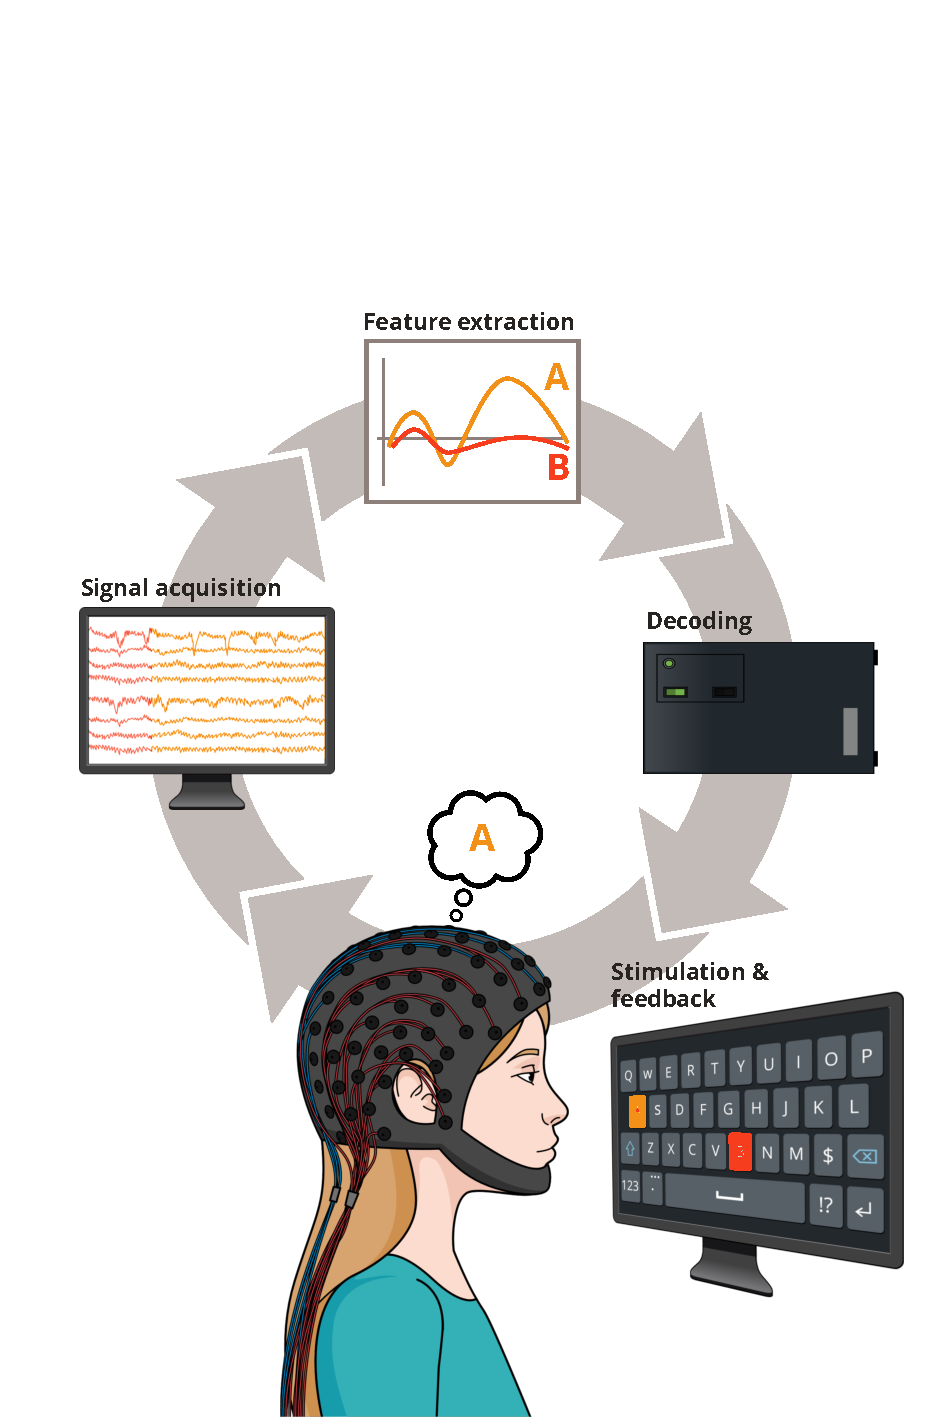
\includegraphics[width=\fullpagefigwidth]{figures/bci/bci_loop.pdf}
}{%
  \caption[The \acs{bci} loop.]{%
    The \ac{bci} loop.
    The user interacts with the \ac{bci} via a specific paradigm, in this case involving
    visual stimulation.
    Electrical neural signals are recorded, and neurophysiological features related to the
    paradigm are extracted.
    Using machine learning, a decision can then be made based on these features, which can
    be presented back to the user.
    In a closed-loop \ac{bci}, this feedback allows the user to adapt to the \ac{bci}.
  }
  \label{fig:bci/loop}
}

Let's break this definition down and focus on its separate parts.
First of all, we need to identify a signal that is a direct representation of what is
going on in the brain.
Multiple signals can be recorded from the brain, including blood flow and magnetic or
electrical activity.
For several reasons laid out in \cref{sec:bci-recording}, the electrical modality is
especially interesting.

The recorded brain activity forms only one part of the interaction scheme presented in
\cref{fig:bci/loop}.
It would be inefficient to search all brain activity randomly for the desired output.
Instead, knowing the specific activity to target would help significantly.
A \ac{bci} operates under a specified \emph{paradigm}, which defines how interaction
is conducted.
This typically means instructing the user to perform a task, like attending to a
flickering stimulus.
Background knowledge from neuroscience research allows us to couple specific brain
activity with the information or actions conveyed via the \ac{bci}.
The brain signal now \emph{modulates} this information.
In turn, detecting this signal can trigger an action, like typing the intended letter A
or B in \cref{fig:bci/loop}.
The \ac{bci} paradigm includes both the method of stimulation (if applicable) and the
user's task, and is often closely tied to the feedback mechanism in a closed-loop system.
As shown in \cref{sec:bci/paradigms}, \ac{bci} paradigms vary widely based on different
brain systems.

Another critical component of a successful \ac{bci} is identifying brain signatures
related to the paradigm within the recorded activity.
The brain's electrical activity is weak compared to environmental noise from electronic
devices and interference.
Additionally, the brain continuously processes information and carries out
`background tasks', which generate more brain activity.
The desired activity often originates from specific brain regions or networks.
This signal can be difficult to isolate from all other brain and environmental activity.
It is similar to trying to hear a single speaker at a noisy party where everyone is
shouting.
Some interference can be filtered out through \emph{preprocessing}
(see \cref{sec:bci/preprocessing}) and by selecting the correct signal representation
(i.e., \emph{feature extraction}), but retrieving or \emph{decoding} the relevant signal
remains challenging.
Supervised machine learning can help solve this.
The information encoded in the brain signal can be retrieved by the decoder and used
to determine the desired \ac{bci} output.
\Cref{sec:bci/decoding} reviews some common decoding techniques.

Finally, the loop can be closed by coupling this to a device or actuator.
There are two aspects to this.
On the one hand, the \ac{bci} gains its function by allowing the user to interact with
their environment.
For a communication system, this means coupling the decoded information to, e.g., a
virtual keyboard or speech synthesizer.
On the other hand, the actions performed by the \ac{bci} can themselves alter the user's
cognitive state or brain activity, creating an adaptive system.
This happens either directly through electrical neurostimulation, as is the
case for adaptive deep brain stimulation in Parkinson's disease or for the
cochlear implant as a hearing aide, or indirectly through sensory stimulation.
The latter involves specific, paradigm-related, sensory input, like tactile feedback for
movement \ac{bci}~\cite{Flesher2021}, or simply presenting selected actions back to the
user.
The user's brain will then adapt through learning, causing changes in
behavior or strategy.
Neuroplasticity, the brain's ability to adapt and reinforce specific neural pathways,
can have a positive impact on \ac{bci} performance and gives rise to rehabilitation
applications.

To summarize, a \ac{bci} can facilitate direct interaction with the central nervous
system.
To do this, information is modulated in the brain signal according to the \ac{bci}
paradigm by stimulating the user or having them perform a task.
Their brain signal is subsequently recorded and preprocessed to clean it.
Relevant features that contain aspects of the modulated signal are extracted, and the
modulated information is retrieved by the decoder, a machine learning model.
This information can then be acted on, and the loop is closed if this action affects the
user.
Let us take a look at each of these elements separately in the next section.

\section{Recording technologies}
\label{sec:bci-recording}

The brain's activity can be recorded using various neuroimaging technologies.
These can range from brain scans~\cite{Weiskopf2004} using functional magnetic resonance
imaging (fMRI) to more portable technologies like the acoustic signals obtained by
functional ultrasound imaging (fUS)~\cite{Zheng2023}, and functional near-infrared spectroscopy
(fNIRS)~\cite{Borgheai2020}.
These technologies all measure blood oxygen levels or blood flow, resulting in the
\emph{hemodynamic} signal.
This signal indirectly reflects brain activity through
metabolic reactions to an increas or decreas in activity.
Usually, it reacts too slowly to reflect the real-time activity that is of interest in
\ac{bci} for communication, and it carries little information other than the brain
region from where it is originating.

A better signal candidate is the neuronal electrical activity.
The brain contains 86 billion neurons, which are highly interconnected cells that are
the smallest units of information processing.
The \emph{action potential} and its related \emph{postsynaptic potential} are electrical
pulses occurring when a neuron receives input from other neurons and is activated.
The firing of a neuron, or the combined firing of groups of synchronized neurons, thus
generates an electrical field in and near the brain, which can be measured using
electrodes.
The related discipline is \emph{electrophysiology}.

Because of the desirable high temporal resolution~\cite{Easttom2021} and practicality of
electrophysiology, we will focus only on methods to record electromagnetic activity
originating from neuronal action potentials and postsynaptic potentials.
The magnetic field of the brain can be measured using magnetoencephalography
(MEG)~\cite{Mellinger2007}.
While MEG is non-invasive and results in high-quality signals, the necessary equipment
is rather expensive and impractical.
Recent advances have been made using optically pumped magnetometers
(OPM-MEG)~\cite{Wittevrongel2021}, but this technology still falters outside of lab
conditions.
As a consequence, the \ac{bci} field relies heavily on the electrical activity of the
brain.

\subsection{Invasive electrophysiology}

The \emph{invasiveness} of the technology forms an important concept in determining its
suitability for a given application and user.
As illustrated in \cref{fig:bci/recording}, invasive electrodes can often measure a
very specific brain region and can result in better signal quality, at the cost of the
risks involved with brain surgery.

\fullpagefig[caption.north]{%
  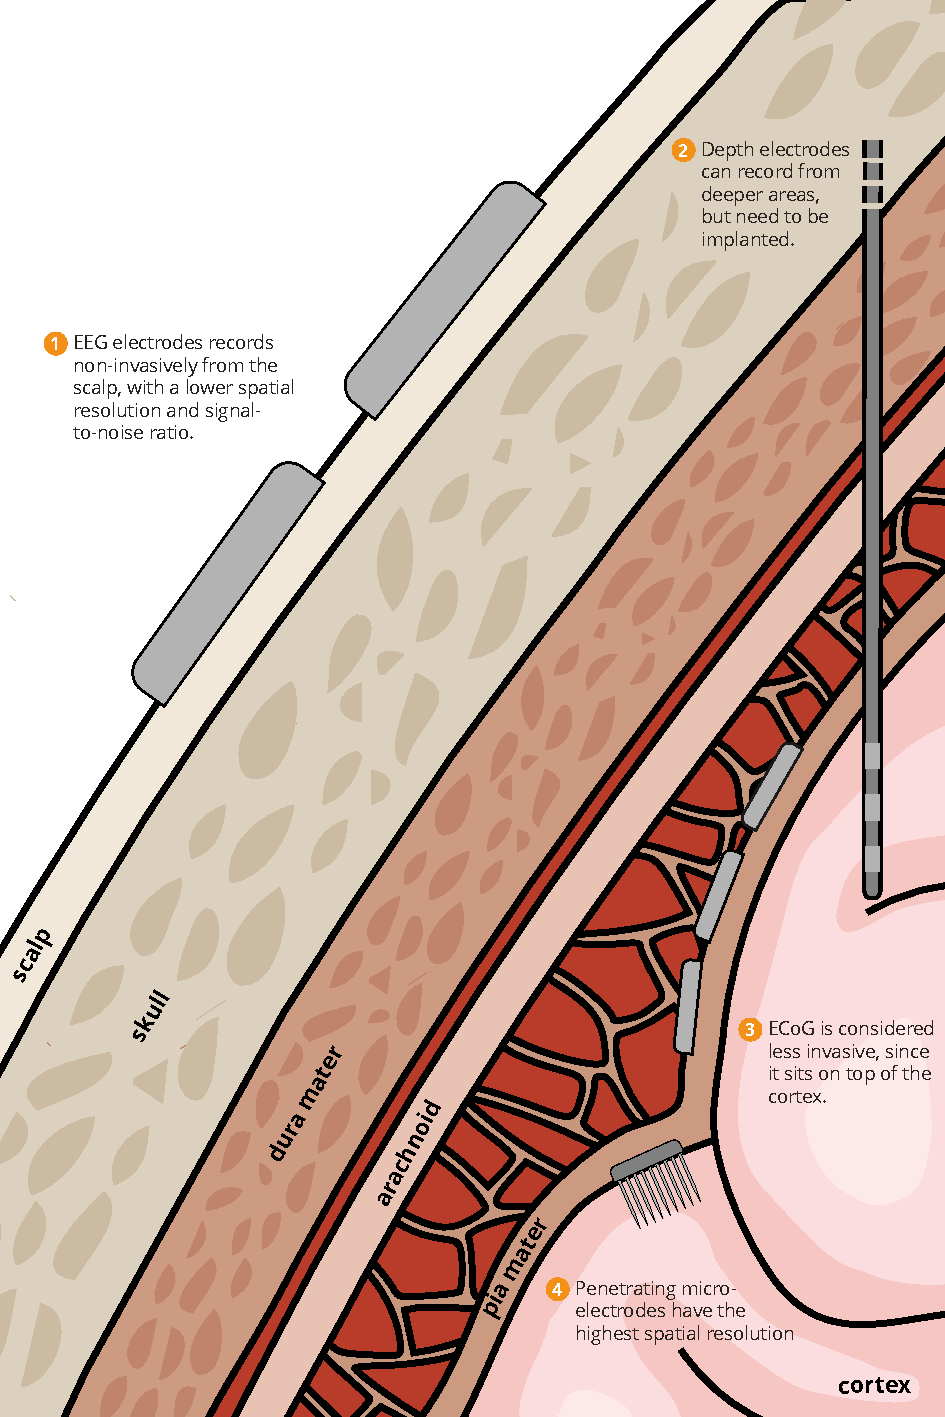
\includegraphics[width=\fullpagefigwidth]{figures/bci/recording_modalities.pdf}
}{%
  \caption[Various electrophysiology recording technologies.]{%
	  Various electrophysiology recording technologies and their respective position in a
	  cross-section of the skull.
	  There is a trade-off between invasiveness and spatial resolution.
  }
  \label{fig:bci/recording}
}

Specifically, invasive methods are less noisy and come with an increased \emph{spatial
resolution}, meaning they can extract a signal from a specific brain region or even a
set of neurons of interest.
This makes it easier to retrieve a signal with a known origin from the brain, which
might be leveraged by the paradigm to modulate information.
Generally, microelectrodes penetrating the cortex are considered to have the highest
spatial resolution.
These are needles with a diameter smaller than 10 µm and one or multiple electrodes that
extend several millimeters into the cortex.
Microelectrodes can measure the Local Field Potential (LFP), the extracellular potential
of a small group of neurons, or even intracellular single neuron action potential
spikes.
They come in single-electrode form, or, more popularly, in microelectrode arrays.
Well-known examples are the Utah array~\cite{Maynard1997}, the more recent NeuraLink
implant~\cite{Musk2019}, and IMEC's Neuropixels 2.0~\cite{Steinmetz2021}.

Larger implanted electrodes (usually a few millimeters in size) are referred to
as intracranial \ac{eeg} (i\ac{eeg}).
Depth electrodes, like those found in in stereo-\ac{eeg}, can be used for \ac{bci}~\cite{Wu2024}
 and other applications, like closed-loop adaptive control for Deep Brain Stimulation
 to mitigate Parkinson's disease
symptoms~\cite{Arlotti2018}.
Depth electrodes are longer rods with multiple electrodes that can extend deeper into
the brain.
Since these still penetrate the cortex, electrodes that sit on top of the cortex are
more popular, as they are considered less invasive.
\Ac{ecog} is a powerful method with many applications in \ac{bci}~\cite{Schalk2011} and
epilepsy diagnosis.
Newer developments like micro-ECoG (µECoG), with a higher
number of smaller electrodes per surface area (recording from sites with
diameter of 10s of micrometers instead of $\pm$ 1 cm)~\cite{Shokoueinejad2019},
allow for more precise measurements.

Some impressive recent breakthroughs in speech and motor \ac{bci} for communication have
been realized using invasive microelectrode arrays~\cite{Willett2021} and
µ\Ac{ecog}~\cite{Metzger2023}.
Furthermore, recent advances in recording technology focus on improving implant
durability and resolution~\cite{Steinmetz2021}, and on balancing the invasiveness
tradeoff by finding new, minimally invasive ways to record from closer to the cortex.
The Synchron Stentrode~\cite{Mitchell2023}, for instance, can be delivered through the
bloodstream via a catheter, removing the need for open brain surgery.
Nevertheless, surveys~\cite{Huggins2011, Huggins2015, Branco2021} in different
potential communication \ac{bci} user groups consistently show that non-invasive
technology is preferred over implanted electrodes, unless the added value of invasive
BCI is sufficiently large~\cite{Kageyama2020}.
This provides justification for focusing part of the current research effort on
non-invasive BCI.

\subsection{\Acl{eeg}}

\Ac{eeg} is the de facto non-invasive electrophysiology standard in clinical neurology
practice as well as in \ac{bci} research.
Developed since 1924~\cite{Berger1929}, it is cheap and relatively practical and offers
great temporal sampling resolution up to thousands of Hz.
\Ac{eeg} measures the electrical potential over time at a given electrode relative to a
reference electrode in volts (V), often on the scale of microvolts (µV).
As it is easily applicable on the outside of the scalp, many practical consumer-grade
\ac{eeg} headsets exist in the form of (often wireless) electrode caps or helmets.
Current consumer systems sometimes feature dry electrodes, but clinical and research
systems often use active electrodes with preamplifiers and electrolyte gel to reduce
impedance for improved signal quality, which slightly decreases practicality, since they
require a trained individual to properly administer.
Nevertheless, it is the most accessible \ac{bci} technology for both users and
researchers.

The major drawback of \ac{eeg} is its poor spatial resolution~\cite{Ferree2001}.
Since they sit on the outside of the scalp, electrodes are large and distant relative to
the neurons in the cortex they ought to measure.
Furthermore, the layers of skull and cerebrospinal fluid in between can attenuate the
signal and cause volume conduction~\cite{Broek1998}, which results in electrodes
measuring a mixture of activity from sources elsewhere in the brain.
This also has a negative effect on spectral resolution.
The noise problem mentioned earlier is also prominently present in \ac{eeg} recordings.
In addition to picking up brain activity other than that of the region of interest,
\ac{eeg} also records other artifacts from the environment, the power supply, nearby
electrical equipment, or the user's muscle movements~\cite{Urigueen2015}.
Combined, this means \ac{eeg} is inherently noisy.

Despite its noisy nature, \ac{eeg} is the recording methodology of choice for our
\ac{bci} because of its wide acceptance by users.
To counteract the noise present in our recording, we must on the one hand evoke strong,
informative brain activity using a suited \ac{bci} paradigm, and on the other hand pick
a suited decoder which can isolate the signal of interest and filter out the noise.


\section{Paradigms}
\label{sec:bci/paradigms}

\subsection{Active \& passive \acsp{bci}}

The \ac{bci} paradigm~\cite{Xu2021,Neeling2019} is the key to translating brain activity
into useful output actions, since it defines which neural responses will be elicited and
captured as features.
A paradigm can be loosely seen as \emph{a way of interacting with the \ac{bci}}.
According to \textcite{Zander2011}, they can be arranged by their reliance on external
stimulation and the engagement of the user as shown in \cref{fig:bci/paradigms}.

\fullpagefig{%
  \sffamily
\begin{tikzpicture}[
    scale=\textwidth/3cm,
  ]
  \useasboundingbox (-1,-1.25) rectangle (1,1);
  \pgfmathsetmacro{\margin}{.1}
  \pgfmathsetmacro{\center}{.5+.5*\margin}
  \pgfmathsetmacro{\textspacing}{.15}
  %\begin{scope}[shift={(1,1.2)}]
    % Draw axes
    \draw[darkgray, very thick, <->] ({-(1+\margin)}, 0) -- ({1+\margin},0);
    \draw[darkgray, very thick, <->] (0,{-(1+\margin)}) -- (0,{1+\margin});

    % Draw rectangles
    \draw[draw=accent1, fill=white, very thick] ({-\margin}, \margin) rectangle (-1,1);
    \draw[draw=accent2, fill=white, very thick] (\margin, \margin) rectangle (1,1);
    \draw[draw=accent3, fill=white, very thick] (-1, {-\margin}) rectangle (1,-1);

    %% Add text
    \node[color=accent1, align=left,font=\bfseries, anchor=north west, inner sep=2pt] at  (-1,1){active};
    \node[color=accent2, align=left,font=\bfseries, anchor=north east, inner sep=2pt] at  (1,1){reactive};
    \node[color=accent3, align=left,font=\bfseries, anchor=south west, inner sep=2pt] at  (-1,-1){passive};

    \node[color=darkgray, align=center,font=\bfseries, anchor=north] at
    (0,{-(1+\margin)}) {passive\\participation};
    \node[color=darkgray, align=center,font=\bfseries, anchor=south] at
    (0,{1+\margin}) {active\\participation};
    \node[color=darkgray, align=center,font=\bfseries, anchor=east] at ({-(1+\margin)}, 0) {stimulus\\independent};
    \node[color=darkgray, align=center,font=\bfseries, anchor=west] at ({1+\margin},0) {stimulus\\dependent};

    %% Text in rectangles
    \node[align=center,font=\small, color=muteblack] at ({-\center}, {\center+1.5*\textspacing}) {motor\\imagery};
    \node[align=center,font=\small, color=muteblack] at ({-\center}, {\center}) {imagined\\speech};
    \node[align=center,font=\small, color=muteblack] at ({-\center}, {\center-1.5*\textspacing}) {neurofeedback};

    \node[align=center,font=\small, color=muteblack] at ({\center+\textspacing}, {\center+\textspacing}) {P300};
    \node[align=center,font=\small, color=muteblack] at ({\center+\textspacing}, {\center-\textspacing}) {SSVEP};
    \node[align=center,font=\small, color=muteblack] at ({\center-\textspacing}, {\center+\textspacing}) {cVEP};
    \node[align=center,font=\small, color=muteblack] at ({\center-\textspacing}, {\center-\textspacing}) {mVEP};

    %% More text
    \node[align=center,font=\small, color=muteblack] at ({\center}, {-\center+\textspacing}) {error\\potentials};
    \node[align=center,font=\small, color=muteblack] at ({-\center}, {-\center+\textspacing}) {attention and \\ workload detection};
    \node[align=center,font=\small, color=muteblack] at ({-\center}, {-\center-\textspacing}) {clinical neuroimaging \\ and monitoring};
    \node[align=center,font=\small, color=muteblack] at ({+\center}, {-\center-\textspacing})  {emotion \\ detection};
  %\end{scope}
\end{tikzpicture}

}{%
  \caption[Overview of \acs{bci} paradigms.]{%
    A \ac{bci} paradigm defines which brain activity will be used for control.
    They can be categorized in active, reactive and passive paradigms, depending on their
    reliance on external stimulation and active participation required from the user.
    Adapted from~\textcite{Muehl2014}.
  }
  \label{fig:bci/paradigms}
}

In contrast to paradigms that require the user's active participation, for
instance through redirecting attention or initiating imagined actions,
pa\-ra\-digms free of this requirement are classified as \emph{passive \ac{bci}}.
From the user's point of view, this concept is probably the most attractive, since their
cognitive state would be inferred from just their brain activity.
However, without active user participation, it can be hard to establish reliable
communication or control.
Therefore, passive \ac{bci} are currently used for control tasks that require
input, like emotional affect~\cite{Torres2020,Libert2019, Muehl2014},
workload~\cite{Zanetti2021} or fatigue~\cite{Alimardani2020} detection,
or, more dependent on stimulation, error detection~\cite{SiMohammed2020}.
Aside from control, clinical applications are found in the diagnosis of a multitude of neurological
and psychological disorders through various forms of neuroimaging or monitoring,
in resting state or while performing a specific task.
Nevertheless, active participation facilitates training data collection for supervised
machine learning, since the conditions can be more easily controlled by the user or the
stimulation.

Paradigms that do require high active participation can be split up into \emph{active
\ac{bci}} and \emph{reactive \ac{bci}}.
Active \ac{bci} paradigms encode endogenous activity initiated by the user, such as
imagined movement or imagined speech.
These tasks can encode complex information, but current non-invasive communication
methods often limit the considered domain to a few movement directions to control a
cursor, or a few words~\cite{Panachakel2021}.
Invasive recordings are necessary for decoding more complex encoded activities like
natural speech~\cite{Metzger2023} or meaningful motor trajectories, like handwritten
symbols~\cite{Willett2021} or sign language~\cite{Branco2017}.
Active BCI also has clinical applications in the form of
neurofeedback~\cite{Hammond2011}, where the user adapts mental strategies to
perform active self-regulation of their brain activity which is presented to
them, causing a feedback loop.

Active paradigms are subject to large inter-subject variability due to the
complexity of the performed tasks.
They might require extensive user training and are sensitive to correct task
instruction.
Imagined speech or movements, or mental strategies in general, can be
performed in a multitude of ways, which can themselves have different neural
representations for separate individuals.
This can make it hard to adapt the \ac{bci} to specific individuals, causing poor
performance and giving rise to the concept of \ac{bci} illiteracy~\cite{Allison2010}\footnote{%
Recently, the concept of BCI illiteracy is increasingly being seen as outdated.
Instead of attributing poor performance to the user's inherent limitations, critiques
point out that the issue lies more with the design of the systems themselves.
BCI systems often fail to account for individual variability in brain anatomy and
cognitive strategies.
As a result, what has been labeled as `illiteracy' may, in fact, be a reflection of
systems that are not flexible enough to adapt to different users.
This perspective shifts the responsibility to the individual, rather than recognizing
that better, more adaptive systems could overcome many of these performance challenges,
thus standing in the way of progress.
Moreover, the term `illiteracy' itself carries negative connotations, implying a user
deficiency that reinforces normative assumptions, when in reality, a more inclusive
approach to design could enhance BCI accessibility for a wider range of
individuals.
This evolving view calls for a reframing of the problem, focusing on improving the
adaptability of BCIs rather than labeling users as illiterate~\cite{Becker2022,Thompson2019}.}.

\subsection{Reactive \acsp{bci}}
Reactive \ac{bci} take another approach by providing a discrete set of sensory
stimulations towards which the user's attention can be directed.
Compared to active \ac{bci}, reactive paradigms can more easily induce fatigue due to
the constant stimulation.
These paradigms are also somewhat less intuitive compared to, e.g., speech, and their
expressive power is limited by how many different stimuli can effectively be presented
and attended to within a reasonable timeframe.
Nevertheless, reactive \ac{bci} work well with \ac{eeg} recordings, and, most
importantly, they work for most people~\cite{Allison2010a,Edlinger2014}.

Reactive \ac{bci} can be realized in multiple ways, depending on the stimulation used.
Some examples include the following:
In the steady-state somatosensory evoked potentials paradigm~\cite{Petit2021}, the user
can attend to one of multiple vibrotactile stimulations in different limbs, which
encodes the information of the attended limb in the brain signal.
In auditory paradigms, information can be modulated by the volume, tone, pitch, or
spatial origin of presented sounds, to which the user can attend~\cite{Kaongoen2017}.
Most common are the visual paradigms.
These can be more performant since they allow the user to use their visual system, one
of the most evolved sensory systems in humans.

The major visual paradigms rely on \ac{ssvep}, \ac{cvep}, oddball, and \ac{mvep} brain
responses.
In \ac{ssvep}, information is modulated by the frequency of a stimulus attended among
many that each flicker continuously at different frequencies~\cite{Chen2021}.
In \ac{cvep}, the stimuli flicker instead with distinct on-off patterns, which can be
correlated with the brain activity to retrieve the attended stimulus~\cite{Sun2022}.
Instead of stimulating all possible selections at once, the oddball paradigm stimulates
them one by one with single flashes~\cite{Pan2022}.
Since the times of stimulation of each target are known, and time-points at which an
attention signature is detected can be correlated to selected targets.
\Ac{mvep} is usually similarly time-modulated, but stimuli make sudden movements in
specific directions instead of flashing.
Information is then also carried by movement direction~\cite{Libert2021a,Libert2022}.

The \ac{bci} paradigms mentioned above can also be combined to gain performance.
Straightforward examples are activating or deactivating \ac{ssvep} stimulation with a
motor command~\cite{Neeling2019}, or combining multiple visual pa\-ra\-digms by stimulating
along multiple dimensions at once.
\textcite{Han2023} recently used this strategy, combining frequency and phase coding in
\ac{ssvep} with the \ac{mvep} and oddball paradigms to develop an efficient \ac{bci}
where one of 200 targets can be accurately selected with only 800 ms of stimulation.

\section{Preprocessing}
\label{sec:bci/preprocessing}

\ac{eeg} preprocessing is a critical step in brain-computer interface (BCI) systems, as
it significantly improves the quality of the recorded data for subsequent analysis and
classification.
Common preprocessing techniques in BCI systems include rereferencing, band-pass and
notch filtering, and \ac{ica}.

Rereferencing is an essential first step, where the potential of each \ac{eeg} channel
is recalculated relative to a common reference point, such as the average of all
electrodes (common average reference) or a selected neutral set of electrodes.
This technique helps reduce noise common across all channels, improving signal clarity
and enhancing the accuracy of subsequent processing steps.

Band-pass filtering is then usually applied to isolate the frequency ranges of interest
by removing frequencies that are too high or too low to contain relevant neural signals.
Band-pass filters eliminate slow drifts and high-fre\-quen\-cy noise, such as muscle
artifacts or environmental electrical interference, improving the \ac{snr}.
Additionally, notch filtering can be used to remove strong power line interference\footnote{%
Typically at 50 Hz in Europe.}.
This interference can heavily contaminate \ac{eeg} recordings and even leak through when
outside the passband of a previous filter.
Notch filtering efficiently attenuates this narrowband noise without affecting the
surrounding frequencies.

Finally, to address artifacts like eye blinks and saccades that can significantly
distort the \ac{eeg} signal, \ac{ica} is performed~\cite{Delorme2007}.
\ac{ica} is a blind source separation technique that decomposes the \ac{eeg} data into
statistically independent components.
Components corresponding to eye movements, eye blinks, and other bodily or environmental
artifacts can be identified, either visually based on their characteristic topographies
and time courses, or statistically, and then removed.
This leads to cleaner data for subsequent processing, especially in the case of visual
\ac{bci} paradigms.
Since eye movement plays a role in the paradigm, it can strongly be present in the
signal and correlate with the task, forming a confounding factor for studying control
based solely on brain activity.

Together, these preprocessing steps ensure that only the relevant neural signals are
passed on to the feature extraction and classification stages in BCI applications,
improving the accuracy and reliability of the system.

\section{Decoders}
\label{sec:bci/decoding}

\subsection{Design principles}

After preprocessing and extracting features, machine learning algorithms can perform
\ac{bci} decoding.
Machine learning decoders use some training data for which the performed tasks are
known, and learn to recognize the activity elicited by the task in recorded data.
The training data can be either obtained from the \ac{bci} user themselves or from other
users.
In the first case, the user would perform a short calibration session before using the
\ac{bci}, where they are instructed to perform a known task.
This calibration session can be eliminated by training the decoder on preexisting
labeled data from other sessions and users, but this is harder due to the variability
between subjects and sessions.

If the goal is to eliminate the per-session calibration, one can also use a decoder
pre-trained on an existing dataset of the same task.
This is complicated by large variability in measured brain responses between subjects
and even between different sessions within the same subject~\cite{Guger2009,Saha2020}.
Therefore, pre-trained decoders must either be trained on a very large, diverse sample
of subjects, or some form of transfer learning must be applied.
Nevertheless, in practice, pre-trained models or models using transfer learning often
still require some per-session fine-tuning, which necessitates some calibration.
Instead, it is better to opt for keeping the calibration time as short as possible by
using an algorithm that can learn from very few training samples.
This can work well but requires strong regularization~\cite{VanDenKerchove2022}.

Decoder choice is heavily dependent on constraints set by the paradigm and the
application.
The number of output degrees of freedom, the serial or parallel nature of performed
tasks, and whether the paradigm is active or reactive, all need to be taken into
account.
One of these choices is whether to solve a \emph{regression} or \emph{classification}
problem.
In regression, a continuous output variable is predicted for a new sample, while
classification attempts to sort it into one of a set of discrete classes.
Regression can be useful in \acp{bci} for applications like mapping imagined movement to
an external robot arm.
For communication \acp{bci}, however, conveying information in a symbolic manner is
often of interest.
Many applications resemble virtual keyboards or map a user's actions to discrete words,
predefined actions, or letters for full control.
Hence, such problems often present themselves as classification tasks.

\subsection{Implementation \& evaluation}

\textcite{Lotte2018, Xu2021} present a relatively recent overview of state-of-the-art
classification algorithms for decoding.
Classic linear methods, such as \ac{csp} feature extraction for motor
imagery~\cite{Park2017} and \ac{cca} for \ac{ssvep}~\cite{Nakanishi2017}, and \ac{lda}
for \ac{erp} classification~\cite{Sosulski2022} still perform relatively well, given
some regularizing constraints or extensions.
Multi-linear techniques exploiting the tensor structure of neural signals are also
promising~\cite{Lotte2018}.
Riemannian Geometry~\cite{Barachant2014} is a popular and robust new strategy.
Furthermore, they lend themselves well to applications like adaptive
learning~\cite{Benaroch2021} or transfer learning~\cite{Zanini2017}.
Riemannian Geometry classifiers are often considered the current state-of-the-art.
Finally, deep learning~\cite{Bhuvaneshwari2021} is also sometimes considered, albeit
only when sufficiently large training datasets are available.
If decoders tailored to a specific user that keep the calibration session as short as
possible are of interest, not enough training data is available to properly train a deep
learning model.

Usually, a decoder makes a prediction for a given \emph{trial} while operating the
\ac{bci}.
A trial is the smallest unit on which a selection decision can be made, for instance,
one imagined movement or one repetition of flashing all targets in a visual \ac{erp}
\ac{bci}.
Accuracy is a valuable metric to assess decoder performance in the classification case.
Accuracy is calculated as the proportion of correct selections to all selections made.
It should be carefully interpreted in the presence of imbalanced data and always
compared to the random chance accuracy level in the presence of more than two possible
selections per trial.
Alternatively, \ac{rocauc} is also a measure of classifier predictive power but is more
suited for evaluation of classification of single epochs of data and in the presence of
imbalanced data, e.g., when comparing single \acp{erp}.
Higher \ac{rocauc} usually translates to a higher target selection accuracy.

Finally, an important concept in the evaluation of a \ac{bci} decoder, and of \acp{bci}
in general, is \ac{itr}.
\Ac{itr} reflects how fluently a \ac{bci} can be used for communication and can be
calculated as
\begin{equation}
  \ITR = Q\left(\log_2N+P\log_2P+(1-P)\log_2\frac{1-P}{N-1}\right)
\end{equation}
\Ac{itr} is expressed in bits/s and is dependent on $N$, the number of different options
that can be selected per trial\footnote{Given that selections are independent of each
other. This formula requires some adaptations in the case of sequential or hierarchical
selection.}, $P$, the selection accuracy of the decoder, and $Q$, the number of trials
per second.
The parameters $N$, $P$, and $Q$ of this formula give us some insight into the building
blocks of a successful, high-\ac{itr} \ac{bci}.
To improve performance, we can aim to
\begin{enumerate*}[label={\arabic*})]
\item increase $N$ by selecting a paradigm and interface that offer a broad range of
informative selections per trial,
\item increase $P$ by engineering more performant machine learning methods for decoding,
and
\item increase $Q$ by selecting a paradigm that allows fast stimulation or responses.
\end{enumerate*}

\section{A case study: the visual oddball \acs{bci}}

The visual oddball paradigm is a \emph{reactive}, \emph{stimulus-dependent},
\ac{bci} paradigm with all the benefits and drawbacks.
Nevertheless, it can score relatively high on the \ac{itr} parameters established above.
The brain response of interest is the visual \ac{erp}, which can be accurately measured
and decoded from non-invasive \ac{eeg} signals with a relatively low computational
effort and short calibration time.
First established by \textcite{Farwell1988} in 1988, it is well supported by literature and
has been proven to work for those with \acl{sspi} in day-to-day home use~\cite{Wolpaw2018}.

\subsection{Stimulation paradigm}

One by one, visual elements on a computer screen are \emph{intensified} for a short
period of time by changing in color, brightness, or size.
Intensifications of different targets are usually 100-200 ms apart and last for about
100 ms~\cite{Sellers2006a}.
On each flash observed by the user, specific brain activity is elicited.
If one of these intensified elements is rare with respect to the others, i.e., it is the
\emph{odd-one out} or \emph{oddball}, this brain activity is altered.
A stimulus can be rare either due to its inherent properties like color or location.
Crucially, this is also the case if it is `marked' as rare by the user, e.g., by paying
explicit attention to only a given stimulus and not the others or counting how many
times it occurs.
If these visual elements represent letters, and we know the timing of the
intensifications of each letter, we can now establish communication by detecting for
which letter an oddball response was present in the brain signal at its time of
intensification.

\Ac{itr} in the oddball paradigm is optimized by intensifying multiple targets at once
in a row-column strategy and using a sequence of selections, giving rise to the classic
matrix speller of \textcite{Farwell1988}.
Other optimizations increase response \ac{snr}, like using flashing face images as
intensifications~\cite{Jin2012} or adding distinct colors and shapes to the
stimuli~\cite{Treder2011}.
The number of targets in a visual oddball \ac{bci} is limited by the crowding effect,
which imposes a limit on how close targets can be to each other while not distracting
the user's attention~\cite{Sellers2006a,Li2010}.
This may be overcome by making hierarchical selections of stimuli representing groups
of selections~\cite{Treder2010}.

Together with \ac{ssvep}, oddball paradigms are most frequently used in visual \ac{bci}.
There are, however, indications that users prefer oddball stimulation over \ac{ssvep},
which can cause eye strain and fatigue due to the continuous oscillatory stimulation of
all targets at once~\cite{Xu2021}\footnote{
  Recent work mitigates this by making SSVEP stimulation
  more comfortable without compormising selection accuracy through
  high-frequency low-contrast stimulation~\cite{Ladouce2022}.
}.
Furthermore, \ac{ssvep} relies more on directing the gaze at the intended target than
oddball, detracting from the concept of control independent from muscle movement.

\begin{figure}[t]
  \begin{subfigure}[t]{.45\textwidth}
  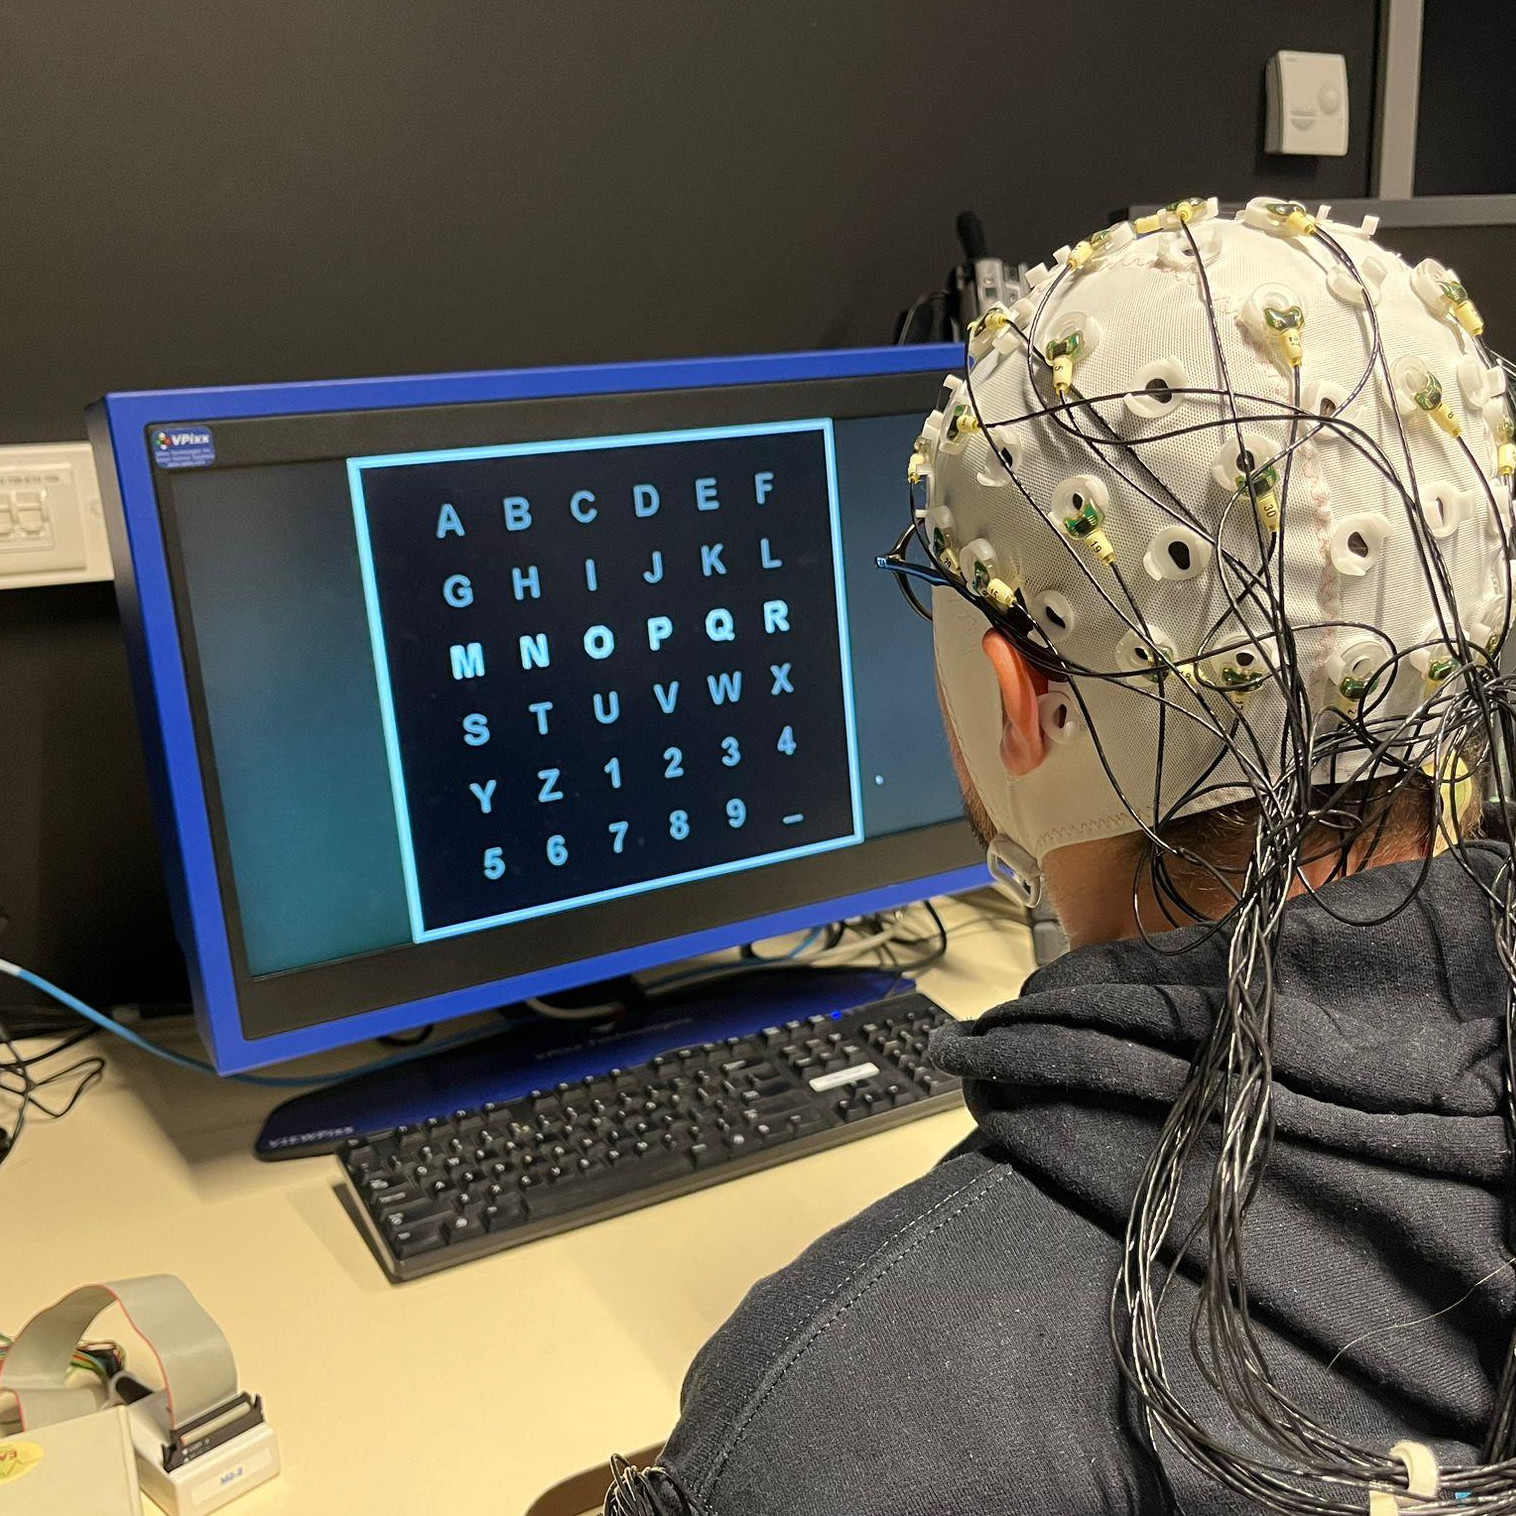
\includegraphics[width=\textwidth, height=\textwidth]{figures/bci/illustration}
    \caption{Stimuli are flashed while the \acs{eeg} is recorded.}
  \end{subfigure}\hfill%
  \begin{subfigure}[t]{.45\textwidth}
    %\resizebox{\textwidth}{\textwidth}{%
    \usetikzlibrary{matrix}

\begin{tikzpicture}
  \fill[color=muteblack] (0,0) rectangle (\textwidth, \textwidth);
  \matrix[
      matrix of nodes,
      fill=muteblack,
      nodes={
          minimum size={\textwidth/8},
          anchor=center,
          text=lightgray
      },
      row 3/.style={
          nodes={text=accent1}
      },
      column sep=0pt,
      row sep=0pt,
  ] (m) at (\textwidth/2, \textwidth/2) {
      A & B & C & D & E & F \\
      G & H & I & J & K & L \\
      M & N & O & P & Q & R \\
      S & T & U & V & W & X \\
      Y & Z & 0 & 1 & 2 & 3 \\
      4 & 5 & 6 & 7 & 8 & 9 \\
  };
\end{tikzpicture}%

    %}
    \caption{The P3 matrix speller interface. Entire rows or columns flash at once.}
  \end{subfigure}

  \bigskip

  \begin{subfigure}[t]{.45\textwidth}
    \begin{tikzpicture}[trim axis left]
    \begin{axis}[
        width=\textwidth,
        height=0.6180\textwidth,
        xlabel={Time (ms)},
        ylabel={Potential (µV)},
        axis lines=middle,
        ymin=-5, ymax=10,
        xmin=-100, xmax=800,
        ytick={-5,0,5}, % Y-ticks at -5, 0, 5
        xtick={200,400,600}, % X-ticks at 200, 400, 600, 800
      	ylabel near ticks,
      	xlabel near ticks,
    ]
      % ERP waveform using cubic splines for smooth connection
      \addplot[
          smooth,
          tension=0.5,
          style={very thick, accent1}, % Set the line color to accent1
      ] coordinates {%
          (-100, 0)  % Starting point
          (0, 0)     % Baseline
          (50, 0)    % Pre-P1
          (80, 2)    % P1
          (115, -3)  % N1
          (160, 3)   % P2
          (220, 1)   % N2
          (400, 7)   % P3
          (650, 1)   % LPP (Late Positive Potential)
          (800, 1)   % End point
      };

      % Annotations for the components
      \small
      \node[anchor=south, color=muteblack] at (axis cs:80,2) {P1};
      \node[anchor=north, color=muteblack] at (axis cs:115,-3) {N1};
      \node[anchor=south, color=muteblack] at (axis cs:160,3) {P2};
      \node[anchor=west, color=muteblack] at (axis cs:220,1) {N2};
      \node[anchor=south, color=muteblack] at (axis cs:400,7) {P3};
      \node[anchor=south west, color=muteblack] at (axis cs:650,1) {LPP};

    \end{axis}
\end{tikzpicture}%
%
    \caption{The idealized \ac{erp} evoked by an attended stimulation in a single
    channel.}%
    \label{fig:bci/erp}%
  \end{subfigure}\hfill%
  \begin{subfigure}[t]{.45\textwidth}
    \begin{tikzpicture}[trim axis left]
    \begin{axis}[
        width=\textwidth,
        height=0.6180\textwidth,
        xlabel={Time (ms)},
        %ylabel={Potential ($\mu$V)},
        axis lines=middle,
        ymin=-5, ymax=10,
        xmin=-100, xmax=800,
        ytick={-5,0,5}, % Y-ticks at -5, 0, 5
        xtick={200,400,600}, % X-ticks at 200, 400, 600, 800
      	ylabel near ticks,
      	xlabel near ticks,
    ]
      % ERP waveform using cubic splines for smooth connection
      \addplot[
          smooth,
          tension=0.5,
          style={very thick, darkgray},
      ] coordinates {%
          (-100, 0)  % Starting point
          (0, 0)     % Baseline
          (50, 0)    % Pre-P1
          (80, 1)    % P1
          (115, -2)  % N1
          (160, 2)   % P2
          (220, -1)   % N2
          (400, 2)   % P3
          (650, 0)   % LPP (Late Positive Potential)
          (800, 0)   % End point
      };


    \end{axis}
\end{tikzpicture}%

    \caption{The idealized \ac{erp} evoked by an unattended stimulation in a single
    channel.}%
    \label{fig:bci/erp}%
  \end{subfigure}%
\end{figure}

\subsection{The \acl{erp}}
\label{sec:bci/oddball/erp}

The time-domain response elicited immediately after the intensification of a stimulus is
known as the visual \ac{erp}~\cite{Luck2014}.
An \ac{erp} is a waveform consisting of multiple components.
Some of these components are modulated by whether the stimulus was an oddball or not.
These components appear as positive peaks and negative troughs in the \ac{erp} waveform.
They follow a naming scheme based on polarity (Negative or Positive) and latency (e.g.,
N2 or N200 for a negative component after $\pm200$ ms).
The component most prominently modulated by attention is called the P3 (positive
deflection after $\pm300$ ms).
Some \ac{bci}\footnote{In \ac{erp} analysis, components are sometimes referred to with
the timing around which they occur (e.g., N170, negative after 170 ms), or by their rank
in order of occurrence (N1, the first negative component).
The timing nomenclature is based on average latencies for neurotypical individuals, but
is seldom correct for specific \ac{bci} users due to the large variability across
\ac{erp} stimulation paradigms and subjects, and can also depend on the user's pathology.
Furthermore, as we will see later, this work focuses specifically on the intra-session
variability in \ac{erp} latency, explicitly assuming the latencies are not fixed.
Therefore, we adhere to the ranking nomenclature.
Fortunately, for the visual oddball paradigm, the rankings do roughly correspond to
their expected timings, i.e., P1=P100, N1=N100, etc.}.
Therefore, oddball paradigms are frequently referred to as P3(00) paradigms.
However, due to the equally important contributions of other \ac{erp} components in
decoding, as we will show later, this could be considered a misnomer.
Thus, we will adhere to the oddball paradigm naming.

The visual \ac{erp} components primarily include P1, N1, P2, N2, and P3.
Each component is characterized by specific latency, amplitude, and neural origins.
These factors influence the perception of visual stimuli and attentional
mechanisms~\cite{Luck2013}.

\paragraph{The P1 component} occurs approximately 100 ms after stimulus presentation.
This component reflects initial visual processing and is primarily linked to activity in
the primary visual cortex.
P1 is particularly sensitive to gaze fixation, where the gaze is directed toward a
stimulus.
When a stimulus is fixated on, the amplitude of P1 increases, reflecting the enhanced
processing of that visual input.
In contrast, P1 shows less modulation when stimuli are attended to via attention without
direct gaze.

\paragraph{The N1 component} peaks around 150 to 200 ms post-stimulus.
It represents an extension of sensory processing related to both gaze fixation and
attention.
For attended stimuli, the amplitude is greater, indicating prioritization for further
cognitive processing.
This highlights a more selective form of attention allocation, demonstrating the impact
of both types of attention on visual processing.

\paragraph{The P2 component} occurs between 200 to 300 ms.
It reflects higher-order processing, particularly in contexts demanding stimulus
evaluation and feature detection.
P2 is sensitive to attention.
When participants actively engage with specific features or categories of stimuli, P2
shows increased amplitude.
Conversely, P2 may be less responsive when gaze is not directed toward the stimulus but
attention is still maintained.

\paragraph{The N2 component} peaking around 200 to 350 ms is associated with cognitive
control processes such as conflict monitoring and inhibition.
It is particularly pronounced in tasks requiring differentiation between competing
stimuli.
N2 reflects the allocation of attentional resources required to resolve conflicts,
irrespective of whether the gaze is directly on the competing stimuli or not.
Higher amplitudes in N2 are seen when cognitive demands increase, indicating the
influence of attention strategies.

\paragraph{The P3 component} is elicited in oddball paradigms and peaks around 300 ms
post-stimulus.
It reflects attentional engagement and the processing of rare or unexpected events.
The P3 is typically subdivided into two subcomponents: P3a and P3b.
The P3a is associated with the allocation of attention to novel or unexpected stimuli,
indicating the initial detection of a change in the environment.
It is particularly responsive to stimuli that capture attention, whether through gaze
fixation or attention.
P3a typically exhibits a frontal distribution and peaks earlier than P3b.

Conversely, the P3b relates to the evaluation of the stimulus.
It involves the updating of cognitive resources in response to task relevance.
This subcomponent is typically observed over parietal regions.
P3b is elicited when participants must process the stimulus meaningfully, often
requiring a decision or response.
Both P3a and P3b amplitudes are sensitive to the probability of occurrence and the
participant's attentional focus, showing how attentional strategies affect cognitive
processing.

\paragraph{The late positive potential (LPP)} is a later component occurring beyond 400 ms.
Sustained attention and emotional processing of stimuli are reflected in the LPP.
Typically enhanced for emotionally salient or motivationally relevant information, the
LPP serves as an indicator of cognitive appraisal beyond mere recognition tasks.
This component can be influenced by attention when the participant evaluates the
emotional significance of stimuli, even if gaze is not directed at them.

In summary, \ac{erp} components such as P1, N1, P2, N2, P3, and LPP collectively
elucidate the neural underpinnings of visual processing and attentional mechanisms.
These components not only inform the design of an effective oddball \ac{bci} system but
also enhance our understanding of the cognitive processes involved in visual attention.
This includes both gaze fixation and attention.
Understanding these components is essential for optimizing \ac{bci} protocols and
improving user interaction, particularly in contexts involving visual oddball tasks.


\subsection{Preprocessing \& feature extraction}
For \ac{erp} analysis, the \ac{eeg} is usually band-pass filtered between 0.5 Hz and
16 Hz.
Re-referencing can be done to average mastoids to highlight the contribution of the P3
component.
In addition to the steps outlined in \cref{sec:bci/preprocessing}, the signal is
usually cut into \emph{epochs} for \ac{erp} analysis.
These are time windows surrounding the stimulus event.
They usually include some baseline interval before the stimulus, which can be used to
normalize the response.

The epochs contain values representing the voltage of a specific channel relative to the
reference at a specific time relative to the stimulus.
In \ac{erp} classification, they are usually directly used as features, by concatenating
all $C$ channels of length $S$ time samples in the matrix format epoch
$\mat{X}\in\mathbb{R}^{C\times S}$ into one feature vector
$\mat{x}\in\mathbb{R}^{CS}$ such that $\mat{x} = \text{vec}(\mat{X})$.

\subsection{Decoders}

Due to the unfavorable \ac{snr} of \acp{erp}, it is often not feasible to accurately
decode the encoded information based on just one example.
Therefore, classification algorithms are trained on a set of epochs but are often
evaluated on an average of multiple epochs.
These averages are constructed over multiple stimulations of the stimulus representing
a given selection, enhancing the \ac{snr}.
The drawback, however, is that performing these multiple stimulations takes more time.
To optimize the \ac{itr}, the trade-off between the number of repetitions, stimulation
speed, and decoding performance must be carefully balanced.
Performant classifiers can shift this balance to the benefit of \ac{itr}.
Several techniques are suited to decode \acp{erp}.
Below are some methods that can achieve state-of-the-art performance and are relevant to
this work.

\subsubsection{\Acf{lcmv} beamforming}

Linear decoding techniques such as the \ac{lcmv} beamformer~\cite{Wittevrongel2016}
generally work well for classifying \ac{erp} epochs.
\Ac{lcmv} beamforming learns a weight vector $\mat{w}\in\mathbb{R}^{CS}$ from
a set of epochs that can be multiplied with the feature vector $\mat{x}$ of a
new epoch to obtain a prediction score.
The weights are obtained by minimizing the variance of the output
\begin{equation}
  \argmin_\mat{w}\mat{w}^\intercal\mat{C}
	\mat{w}^\intercal
\end{equation}
under the linear constraint
\begin{equation}
	\mat{a}^\intercal\mat{w} = 1
\end{equation}
with \emph{activation pattern} $\mat{a}\in\mathbb{R}^{CS}$ the difference between the
average of feature vectors of the attended and non-attended epochs in the
training data,
and $\mat{C}\in\mathbb{R}^{CS\times CS}$ the background covariance matrix which
can be estimated empirically from the training data.
This is then solved by the method of Lagrange multipliers as
\begin{equation}
	\mat{w} =
  \frac{\mat{C}^{-1}\mat{a}^\intercal}
  {\mat{a}\mat{C}^{-1}\mat{a}^\intercal}
\end{equation}

\subsubsection{\Acf{lda}}

\Ac{lda} is a more well-known method that is, in fact, nearly equivalent to
\ac{lcmv} beamforming~\cite{Treder2016} under certain conditions.
It assumes normally distributed data with a different mean per class but a common
covariance.
Similar to \ac{lcmv} beamforming, \ac{lda} learns a weight vector
$\mat{w}\in\mathbb{R}^{CS}$ which satisfies
\begin{equation}
  \argmax_\mat{w}\frac{\mat{w}^\intercal\mat{S}_\text{b}\mat{w}}{\mat{w}^\intercal\mat{S}_\text{w}\mat{w}}
\end{equation}
The between-class scatter matrix $\mat{S}_\text{b}\in\mathbb{R}^{CS\times CS}$ models the variability between the
expected responses, while the within-class scatter matrix $\mat{S}_\text{w}\in\mathbb{R}^{CS\times CS}$ models the
expected noise.
The optimization criterion corresponds to finding a projection that maximizes the spread
between classes (signal) while minimizing the spread within classes (noise).
$\mat{w}$ can be obtained as the eigenvector of
$\mat{S}_\text{w}^{-1}\mat{S}_\text{b}$ corresponding to the largest eigenvalue.

There is one caveat with these linear methods, however:
the number of values ($=C\cdot S$) is usually relatively high compared to the
size of the training dataset, since calibration time should be kept minimal.
Therefore, strong regularization, such as covariance/scatter
shrinkage, should be applied.
Regularization can also be performed by retaining structure in the data, such as in the
case for the multilinear methods presented by~\textcite{Lotte2018}.

\subsubsection{\Acf{tlda}}

Another example of this is \ac{tlda}~\cite{Sosulski2022}, which assumes temporal
stationarity in the background noise to regularize the problem.
It does this by imposing a block-Toeplitz structure to the within-class
scatter $\mat{S}_\text{w}$ matrix of \ac{lda}.
This means
\begin{equation}
  \mat{S}_\text{w} = \begin{bmatrix}
    \mat{S}_\text{w}^{(1,1)} & \mat{S}_\text{w}^{(1,2)} & \cdots & \mat{S}_\text{w}^{(1,C)}\\
    \mat{S}_\text{w}^{(2,1)} & \mat{S}_\text{w}^{(2,2)} & \cdots & \mat{S}_\text{w}^{(2,C)}\\
    \vdots             & \vdots             & \ddots & \vdots            \\
    \mat{S}_\text{w}^{(C,1)} & \mat{S}_\text{w}^{(C,2)} & \cdots & \mat{S}_\text{w}^{(C,C)}\\
  \end{bmatrix}
\end{equation}
consists of $C\times C$ temporal scatter matrices
$\mat{S}_\text{w}^{(c_1,c_2)}\in\mathbb{R}^{S\times S}$
corresponding to a pair of channels $(c_1,c_2)$, such
that every temporal scatter matrix has the Toeplitz structure
\begin{equation}
  \mat{S}_\text{w}^{(c_1,c_2)} = \begin{bmatrix}
    s_1^{(c_1,c_2)}  & s_2^{(c_1,c_2)}  & \cdots & s_S^{(c_1,c_2)}  \\
    s_2^{(c_1,c_2)}  & s_1^{(c_1,c_2)}  & \cdots & s_{S-1}^{(c_1,c_2)}  \\
    \vdots & \vdots &  \ddots & \vdots \\
    s_S^{(c_1,c_2)}  & s_{S-1}^{(c_1,c_2)}  & \cdots & s_1^{(c_1,c_2)}
\end{bmatrix}
\end{equation}
The structuring is performed by setting all elements to the average of their
corresponding block-subdiagonal and subsequently applying shrinkage
regularization.
This method is simple yet effective, reaching state-of-the-art decoding performance.

\subsubsection{Riemannian geometry}

Alternative methods that currently work well include non-linear methods using Riemannian
geometry~\cite{Barachant2014}.
Methods leveraging Riemannian geometry use a different feature extraction method.
They do not use the raw epoch values but rather operate on the spatial covariance of an
epoch.
These covariance matrices $C_i$ are symmetric and should have only positive eigenvalues;
hence they lie on the Riemannian manifold of symmetric positive definite matrices, which
defines the distance metric
\begin{equation}
  \delta_\text{R}\left(\mat{C}_1,\mat{C}_2\right)
  =\left\lVert\log\left(\mat{C}_1^{-\frac{1}{2}} \mat{C}_2 \mat{C}_1^{-\frac{1}{2}}\right)\right\rVert
\end{equation}
This geodesic distance metric is naturally suited for this type of data and has some
desirable properties, like invariance to linear transformations, which result in a
robustness particularly useful for \ac{bci} applications~\cite{Barachant2011}.

With this distance defined, the epochs can either be directly classified on the
Riemannian manifold using a minimum distance to the mean classifier, or they can be
projected to the tangent space.
This is a Euclidean space that locally approximates the Riemannian distance, which
allows us to apply regular machine learning methods like an SVM or \ac{lda}.
%The tangent space is obtained\todo{tangent space}.
To enhance classifications of \acp{erp} which rely on time-domain information, which
would otherwise be lost in the spatial representation of the extracted feature, the
class averages can be concatenated as additional channels to the epochs, embedding the
temporal structure in the feature~\cite{Barachant2014}.
To improve performance even further, the \acp{erp} can be decomposed by a method like
XDAWN before calculating the extended covariances~\cite{Li2020}.

These decoders define the last building blocks of our visual oddball \ac{bci}.
Yet, the overview until now has been rather theoretical.
Interesting and complex challenges arise when applying these concepts outside of the lab
in augmented and assistive communication technologies for users with \acl{sspi}.

\section{The gaze-dependence problem}

In a nutshell, we can state that \acp{bci} decode brain activity with the aim to
establish a direct communication pathway bypassing speech and other forms of muscular
activity~\cite{Naci2012,Chaudhary2016}.
They have raised great hopes for individuals devoid of these abilities, for whom
\acp{bci} can provide a means to communicate or to control devices.

Furthermore, the \ac{eeg}-based visual event-related potential (\ac{erp})-based oddball
interface is an effective and proven method~\cite{Wolpaw2018,Severens2014}.
Targets are shown in short flashes on a computer screen that evoke an \ac{erp} when
observed, which can be detected in the \ac{eeg} signal.
The \ac{erp} consists of multiple components, some of which are modulated by perception
and the attention of the user.
Decoding this modulation allows for information transfer controlled by the user's brain
activity, as sketched in \cref{fig:bci/loop}.

However, when carefully examining the properties of the \ac{erp} components, we notice
that while attention plays a role in the modulation of specific components, some part is
also related to visual perception.
How a stimulus is perceived, and, as a consequence, which \ac{erp} components are
modulated, is directly related to whether the user gazes directly at it (i.e.,
\emph{fixates} their gaze on the target) or not.
Indeed, research has shown that visual oddball \ac{bci}s cannot operate efficiently when
the user does not direct their gaze onto the desired target~\cite{Brunner2010, Frenzel2011}.

This leads to a problem that is not often addressed:
a visual \ac{bci} is dependent on the gaze of the user, and hence on muscle control.
This is exactly what \acp{bci} for augmented and assistive technology try to avoid.
The \ac{bci} target population consists of individuals with severe physical
impairment due to  with various degrees
of paralysis, or even with \ac{lis}, the complete loss of muscle control with preserved
consciousness.
While \ac{bci}s are most attractive as a solution for individuals with \ac{sspi},
studies paradoxically often report poor performance in exactly this group.
This is caused by a multitude of factors, including diminished
electrophysiological responses and cognitive defects linked to the
pathophysiology, psychological factors such as the ``extinction of goal directed thinking''
phe\-no\-me\-non in complete impairment, and, importantly, sensory impairments such as vision and
oculomotor defects~\cite{Seguin2023}.
While visual \acp{bci} often rely on visual sensory functions, it is precisely this
group of patients that could benefit from them, that lacks adequate eye motor control.
Equally often, participants with gaze impairments were excluded from the study.

Different degrees of eye motor impairment can render visual \ac{bci}s uncomfortable or
outright impossible to use.
When operating a visual \ac{bci}, the usual rapid series of forced saccades followed by
fixation is tiring over time, even for healthy control subjects.
A suitable alternative would allow the user to keep their eyes in an at-rest position of
their choice while operating the \ac{bci}.
This points to the need for gaze-independent solutions, which we will explore further in
\cref{sec:gaze-independent} and the rest of this thesis.

\chapter{Gaze-independent visual \acsp{bci}}
\label{sec:gaze-independent}
\epigraph{%
  %\justifying
  ``\elide\ This begs the question: if a patient had reliable control
  over their eye gaze, why would one aim to facilitate communication with that
  patient via a BCI? It would be far simpler and more efficient to use an
  eye-tracking system.
  And even if a BCI were the preferred or only available option for some reason,
  designs requiring eye gaze control could not be used
  by patients with severe motor impairment, as these patients
  cannot direct their gaze.
  Because these are the patients who have the greatest need for BCIs, it is
  important that accurate gaze-independent BCIs exist.''
}{%
  \textcite{Egan2017}
}

\publicationnote{The last paragraph of \cref{sec:gaze-independence/sota},
\cref{sec:gaze-independence/oculomotor/gaze}, and the first paragraph of
\cref{sec:gaze-independence/objectives} were adapted from
\textcite{VanDenKerchove2024}.}

\section{Eye motor impairment in \acs{bci} users}%
\label{sec:gaze-dependence}

One of the goals of brain-computer interfacing is establishing a communication
channel that does not rely on speech or muscular activity, which in turn can
provide solutions to individuals with \ac{sspi}.
In the strictest interpretation, this means that an interface should not
rely on the control of eye muscles used to redirect the gaze or for blinking.
It is exactly this potential of \acp{bci} that makes them suitable as assistive
communication devices.

\subsection{Incidence of eye motor impairment}
\label{sec:gaze-independent/gaze-dependence/incidence}
\Ac{sspi} is often caused by damage to the central or peripheral nervous
system, either through congenital diseases (\ac{cp}, \ac{fa}, \ldots),
neurodegenerative (\ac{als}, \ac{ms}, \ldots) or acquired (stroke and
\ac{tbi}).
Many individuals in these groups are unfortunately also afflicted by some form
of eye motor impairment, requiring \acp{bci} adapted to their condition.
\Cref{tab:incidence} reports the relatively high frequencies of
eye motor impairment, which can range from minor (nystagmus,
\footnote{Involuntary, rhythmic, and repetitive eye movements recognizable by their
consistent directionality (horizontal, vertical, or rotational).},
other eye tremors
\footnote{These can include square-wave jerks, saccadic intrusions, microtremors, or
microsaccades while resting or fixating the gaze.},
gaze fixation fatigue or discomfort, \ldots), to severe (partial ophthalmoplegia
\footnote{Weakness or limited paralysis of one or more of the muscles that control eye
movement, leading to restricted eye motion, but not complete paralysis.
Often, a specific movement direction (up-down, left-right) is preserved.},
involuntary movements, impaired pursuit, \ldots), and even complete
ophthalmoplegia\footnote{Full eye movement paralysis.} or eye motor paresis.
This not only affects vision and coordination but also
their ability to operate a visual \ac{bci}~\cite{FriedOken2020}.

\begin{table}
  \centering
  \makebox[\textwidth][c]{%
  \small
\sffamily
\begin{tabularx}{\textwidth}{@{}Xccccccccc@{}}
\toprule
    & \bfseries \acs{als} & \bfseries \acs{ms}   & \bfseries Stroke
    & \bfseries \acs{cp} & \bfseries\acs{fa} & \bfseries \acs{dmd} & \bfseries \acs{sma} & \bfseries \acs{lis} \\ \midrule
    \bfseries Minor    & 50\% & 31\% & 40-70\% & + & 100\% & + & - &      \\
    \bfseries Severe   & 33\% & 3\%  & +       & 60-100\% & >5\% &  - & - & 98\% \\
    \bfseries Complete & 17\%\footnote{In late-stage \ac{als}.} & -    & +
    & -&- & - & - & 2\%  \\
\bottomrule
\end{tabularx}

  }
  \caption[Incidence of eye motor impairment in selected \acs{bci} user target
    populations.]{%
      Incidence of eye motor impairment in selected \ac{bci} user target
      populations. \acs{als}: \acl{als}, \acs{ms}: \acl{ms}, \acs{dmd}:
      \acl{dmd}, \acs{sma}: \acl{sma}, \acs{cp}: \acl{cp}, \acs{lis}: \acl{lis}.
      $+$: frequent, $-$: infrequent.
    }
    \label{tab:incidence}
\end{table}

Among the most affected are those recovering from stroke~\cite{Pollock2011,Rowe2019},
and most of all those with due to brainstem or cerebellar stroke~\cite{Moncayo2009,Bogousslavsky1987}.
Stroke can lead to the most severe severe or even complete eye motor impairment
from the onset of their condition, resulting in the~\ac{lis}.
However, case study reports~\cite{Patterson1986,Graber2016} show that even in individuals
with \ac{lis} due to stroke, the group with a complete lack of eye motor
control is very small.

\ac{als} is progressive disease affecting motor neurons.
This initially results in general weakness and loss of muscle tone, but
eventually leads to full body paralysis.
Although eye movement is often cited as one of the longest preserved
capabilities in \ac{als}, studies show that minor issues are still
fairly common~\cite{Kang2018, Guo2022,Moss2012}.
The bulbar-onset variant is characterized by an early loss of speech
and increased involvement of eye motor symptoms~\cite{Guo2022}.
Furthermore, \textcite{Hayashi1991} show that as \ac{als} progresses past
the point of independent breathing, symptoms will eventually also involve
eye muscle paralysis.
One of the goals of \ac{bci} has always been to support these individuals to
ensure quality of life.

Various forms of eye movement abnormalities also occur often in
\ac{ms}.
\Ac{ms} is a neurodegenerative disease involving demyelination of nerves.
Eye motor abnormalities are especially well
studied~\cite{Mueri1985,Prasad2010,Castelnovo2016,Serra2018,Polet2020} and
are often used as diagnostic tools.
These abnormalities can be minor or severe, seldom progressing to complete
paralysis.
However, \ac{ms} often comes with vision loss, further complicating interaction
with visual \acp{bci}.

\Ac{fa} is a neurodegenerative disease affecting the
spinal cord, peripheral nervous system, and cerebellum, resulting in an
impairing loss of muscle coordination.
This almost always heavily affects eye
movements~\cite{Fahey2008,Hocking2010,Furman1983,Cook2017}, with various forms of
involuntary movements and trouble pursuing or fixating on targets.
They also gradually have more trouble speaking but often retain some muscular
control.

Another group that is heavily affected, is \ac{cp}~\cite{Fazzi2012}.
Additionally, individuals with other neurodegenerative diseases like
\ac{sma}~\cite{Anagnostou2021} and \ac{dmd}~\cite{Lui2001} are
sometimes also interested in \ac{bci} use, but their eye motor capabilities are
mostly preserved.

\subsection{Gaze impairment and \acl{lis}}
\label{sec:gaze-independence/oculomotor/gaze}
\newcommand\fnlis{\footnote{Multiple definitions of \ac{lis} are encountered in
\ac{bci} and neurological literature.
Some definitions include only those with tetraplegy without eye movements used
for communications.
Others distinguish Complete Locked-in Syndrome (CLIS) with full body paralysis,
including no eye motor control at all, from a \ac{lis} state with some preserved eye
movements or minor motor output.
While some definitions only include stroke or \ac{tbi} with damage to
specific regions in the brain (midbrain, brainstem, or
cerebellum)~\cite{Smith2005}, it can also generally refer to the state of full body paralysis
or loss of muscle tone incurred in neurodegenerative diseases, combined with
the inability to speak, such as occurs in late-stage ALS.}}

\newcommand\fnwolpawcrit{\footnote{
``The first class consists of people who are truly totally locked-in (e.g.,
due to end-stage ALS or severe cerebral palsy), who have no remaining
useful neuromuscular control of any sort, including no eye movement.
\elide\ This class is very small. \elide\
The second class of potential \ac{bci} users comprises those who retain
a very limited capacity for neuromuscular control. This group includes
people who retain some useful eye movement or enough limb muscle
function to operate a single-switch system. Such control is often slow,
unreliable, or easily fatigued.
This group is much larger than the first.''~\cite{Wolpaw2006}}}

We believe it is generally not opportune to delve too deeply into the underlying
ophthalmological and neurological mechanisms for each of the specific
conditions, or even the exact symptoms.
In clinical reality, every \ac{bci} user has different symptoms, which lead to their own
unique set of preserved capabilities and visual skills.
From a solution-oriented \ac{bci} engineering point of view, the etiology of the symptoms can be abstracted away.
Instead of categorizing users by their etiology, we will refer to those who might benefit from
\ac{bci} assistive communication technology as having \ac{sspi}, in line with
the terminology used by~\textcite{FriedOken2020}.
If they have eye motor impairment that affects their use of visual \ac{bci} or
eye-tracking solutions, we use the term \ac{sspgi} (see \cref{fig:gaze-independence/venn}).

\begin{figure}
  \sffamily
\begin{tikzpicture}

    % Draw the outer lightgray box with ultra thick darkgray line
    \draw[fill=lightgray, draw=darkgray, ultra thick] (-4,-1.5) rectangle (4,5.5);
    % Label for the outer box in the top left corner
    \node[anchor=north west, text=darkgray] at (-4,5.5) {\textbf{\acs{bci} users}};

    % Draw the outermost circle for SSPI with ultra thick lines and bold text matching its line color
    \draw[ultra thick, accent1] (0,2) circle (3);
    \node[text=accent1] at (0,4) {\textbf{\acs{sspi}}};  % Centered bold text with line color

    % Draw the middle circle for SSPGI with ultra thick lines and bold text matching its line color
    \draw[ultra thick, accent2] (0,1) circle (2);
    \node[text=accent2] at (0,1.66) {\textbf{\acs{sspgi}}};  % Centered bold text with line color

    % Draw the innermost circle for LIS with ultra thick lines and bold text matching its line color
    \draw[ultra thick, accent3] (0,0) circle (1);
    \node[text=accent3] at (0,0) {\textbf{\acs{lis}}};  % Centered bold text with line color

\end{tikzpicture}

  \caption[Venn diagram of potential users of \acs{bci} assistive technology.]{%
    Venn diagram of potential users of assistive technology.
    Patients with \acf{sspi} are the general target population.
    If eye gaze-based solutions are not properly suited for an individual,
    they have \acf{sspgi}.
    Individuals with \ac{lis} have no muscular control left, or it is very limited,
    such as the ability to communicate through a binary switching system.
    \Acp{bci} are especially relevant for the last two groups, as they are not
    able to use eye tracking solutions.
  }
  \label{fig:gaze-independence/venn}
\end{figure}

The most severely impaired of the user groups above constitute the \ac{lis}
group, which forms one of the main \ac{bci} interest groups.
In this work, we use the term \ac{lis} for a situation of (near)
complete paralysis and difficulties or the inability to communicate independently,
even with assistive technology.
This corresponds to classes one and two defined by
\textcite{Wolpaw2006}\fnwolpawcrit.
Hence, some degree of severe or complete eye motor impairment is usually
necessary to qualify as locked-in\fnlis.

In general, the group of locked-in individuals with complete loss of eye motor
function is very small.
Hence, it would be interesting to focus \ac{bci} development efforts on the
larger population of individuals with \ac{sspgi} who currently slip through
the cracks of the assistive technology offerings.
These are individuals whose severe eye motor impairment prevents them from
using eye-tracking-based solutions.
They currently use their remaining motor control to
communicate by indicating symbols on a letterboard with great effort,
or signal with upward eye movements or blinks to confirm prompted letters.
They require a caregiver or relative to interpret their signals and crave
the ability to communicate independently, which is crucial to retaining an
acceptable quality of life.

This brings us back to the gaze-dependence problem in visual \ac{bci}:
Traditional visual \ac{bci} scenarios require the user to \emph{overtly} direct both their
\ac{vsa} and gaze toward the screen target they intend to select.
However, a critical challenge arises when users rely solely or in part on
\emph{covert} \ac{vsa}, which involves directing \ac{vsa} without corresponding
eye gaze.
In these cases, classical solutions often fall short of the widely accepted
80\% target selection accuracy threshold~\cite{Brunner2010,Frenzel2011,Treder2010,RonAngevin2019}
deemed necessary for a comfortable user experience~\cite{Neeling2019}, calling for alternative, gaze-independent
solutions.

In this work, we will use the term \emph{gaze-independent} to mean
\emph{`dealing explicitly with the fact that a user cannot control their
gaze.'}
In the context of a visual \ac{bci}, this means that the user's
visuospatial attention and their gaze do not necessarily coincide.
There are multiple approaches to implement gaze-independence in a \ac{bci}.
The next section highlights some noteworthy examples.

\section{State-of-the-art}
\label{sec:gaze-independence/sota}

\subsection{Gaze-independent modalities}
Gaze-independent \ac{erp}-based \acp{bci}~\cite{Riccio2012, Aloise2012} can be realized in three
ways.
Firstly, active \ac{bci} communication paradigms relying on endogenous activation from the user
do not rely on sensory stimulation.
Examples of this are imagined movement or imagined speech paradigms.
These paradigms can yield very high information transfer
rates~\cite{Willett2021,Metzger2023}, both due to their intuitiveness and the
complexity that can be captured in commands, but they often do so only when paired
with invasive recording.
Non-visual reactive paradigms that use, for example, auditory~\cite{Halder2010} and
somatosensory~\cite{Brouwer2010} stimulation do not rely on gaze redirection
but also result in lower \acp{itr} compared to visual paradigms.
A survey by \textcite{Riccio2012} from 2012 reported that \acp{itr} ranged between
1 and 10 bits/min for auditory paradigms and 0.5 and 5 bits/min for tactile~\cite{Riccio2012}.

On the tactile front, recent studies use steady-state somatosensory evoked
potentials~\cite{Petit2021} or tactile oddball paradigms~\cite{Waal2012}
These are analogous to the \ac{ssvep} and visuall oddball paradigms.
Instead of visual stimulation, however, they use physical vibrotactile pulses
stimulation at different spatial locations and/or frequencies~\cite{Han2020}.
Some noteworthy advancements have achieved an \ac{itr} of 14.77 bits/min~\cite{Liu2019}
and 20.73 bits/min~\cite{Herweg2016} with a tactile oddball paradigm through
highly optimized stimulation.
Still, other recent tactile \ac{bci} studies~\cite{Herweg2016a,Han2020,Jin2020,Li2019,Eidel2022}
fail to exceed 5 bits/min.

Auditory \acp{bci} are similarly implemented as paradigms oddball or
steady-state stimulation with spatial or tone modulation.
\textcite{Zhang2020} report that recent decoding methods can reach 16.99
bits/min \ac{itr}, but, in general, auditory \acp{bci} are also limited in
their speed and usually outperformed by visual paradigms~\cite{Rezeika2018}.

While auditory and somatosensory stimulation on their own might yield poor
\ac{itr}, \textcite{Yin2016} showed that these modalities can provide added
value in gaze-independent settings when coupled with visual oddball
stimulation in a hybrid paradigm.
Their solution using the P3 components of bimodal stimulation reached an \ac{itr} of 14.94 bits/min.
In general, their approach is interesting as it follows a philosophy that
relies on establishing as many communication pathways as possible.
Auditory and tactile stimulation can even be paired to create a fully
non-visual, hybrid \ac{bci}, with a reported \ac{itr} of 11.66 bits/min~\cite{Zhang2020}.

Yet, auditory and somatosensory \acp{bci} also suffer from increased mental effort in
operation and from user-dependent variability~\cite{Severens2014,Reichert2020b}.
\textcite{Severens2014} showed that the visual Hex-o-Spell~\cite{Treder2010}
outperformed a somatosensory alternative in participants with \ac{als} whose
eye motor capabilities were effectively impaired.
However, non-visual stimulation modalities are still valuable for developing
\acp{bci} for individuals affected with severe vision loss or
blindness~\cite{Nijboer2008,Rutkowski2015}, which can occur in some cases of
\ac{lis}~\cite{Patterson1986}.

\subsection{Gaze-independent visual stimulation}
\label{sec:gaze-independence/sota/visual}

This leads us to the second approach: current visual stimulation paradigms can be optimized so that
the stimuli are always present in the field of view, either overtly~\cite{Acqualagna2013, Won2018, Lin2018} or covertly~\cite{Pires2011,Lees2018}.
Some noteworthy examples include the GIBS Block Speller~\parencite{Pires2011},
the GeoSpell interface~\parencite{Aloise2012}, and the \ac{rsvp}
speller~\parencite{Acqualagna2011}.
The \ac{rsvp} paradigm, in particular, is a prime contender for a performant gaze-independent
\ac{bci}.
\textcite{Lin2018} reported an average online \ac{itr} of 20.259 bits/min using
a paradigm with subsequently flashing sets of three characters filling the user's field of view.

We make a distinction here between spatially organized interfaces, where
multiple targets are displayed at the same time at different spatial locations,
and temporally organized interfaces, like \ac{rsvp}, where targets or small
sets of targets (e.g. 3) are shown consecutively.
The Hex-o-Spell, GeoSpell, and GIBS Block Speller are spatially organized, while
variants of the \ac{rsvp} paradigm are temporally organized.
\textcite{Lin2018} follow the philosophy that spatially organized interfaces
have historically not performed well in the presence of gaze impairment.
However, we argue that spatially organized interfaces generally have a much higher
\ac{itr} in healthy controls.
For instance, a regular matrix-based speller can achieve an \ac{itr} of up to
30 bits/min.
With the right set of adaptations, spatial attention could potentially also
bring added value to individuals with \ac{sspgi}.
While spatial interfaces are indeed more gaze-dependent than temporal
interfaces, they also provide an extra channel that can be used to transfer
information, i.e., the location of the stimulus.

As an alternative to spatial attention, non-spatial visual attention (feature attention) can also be exploited, such as
attention to stimulus color, shape, or symbol~\cite{Zhang2010,Treder2011,Hwang2015}.
The \ac{rsvp} speller is already an example of this, relying on the user to
attend to the appearance of the intended character to type.
Visual stimulation paradigms relying on alternative types of attention
can modulate specific extra \ac{erp} components that either improve performance
because they embed extra information in the brain signal~\cite{Xu2022}
or because they are more sensitive to stimulation in the visual
periphery~\cite{Schaeff2012}.
Nevertheless, solely relying on alternative types of attention can also suffer from
reduced information transfer rates~\cite{Chennu2013}.
Furthermore, the previously mentioned systems were typically tested only in
settings where the user was required to focus on a central fixation point while
selecting peripheral targets.
This entails that they still rely to some extent on
eye motor control, often necessitating central gaze fixation.

\subsection{Gaze-independent decoding}
\label{sec:gaze-independence/sota/decoding}

Thirdly, stimuli can be presented in a standard \ac{bci} paradigm, but visuospatial
attention can be decoded separately from gaze direction.
\textcite{Aloise2012} aimed to bridge the performance gap between covert and
overt \ac{vsa} decoding performance.
They compared classical linear and non-linear \ac{erp} classifiers on a covert
attention oddball \ac{erp} paradigm dataset.
The results revealed no significant performance improvement in covert \ac{vsa}
decoding for any of the investigated decoders.

More recent work has made advances in decoding lateralized covert
\ac{vsa} by harnessing the N2pc \ac{erp}
component~\cite{Thiery2016,Reichert2020b,Wang2022}.
The amplitude of the N2pc component in the contralateral hemisphere is directly modulated
by the location of covert \ac{vsa}.
Another approach is directly decoding covert shifts in \ac{vsa} from spectral
content~\cite{Tonin2013}.
These methods are promising, but to date often require a slower stimulation pace or cannot display as
many targets as the classical \ac{erp} \ac{bci} paradigms.
As with the alternative modality approach, they are currently only helpful as
extra communication channels in a hybrid paradigm.
\textcite{Xu2016} reached an \ac{itr} of 23.56 bits/min by detecting the N2pc
component while performing \ac{ssvep} stimulation.
\textcite{Egan2017} also showed an increase in \ac{ssvep} performance by
concurrently decoding the covert \ac{vsa} shift from spectral content, but
their study only used two stimulation targets.
In general, we conclude that gaze-independent decoding in the fast-paced reactive
\ac{erp} paradigm leveraging spatial attention remains underexplored.

\section{Research objectives}
\label{sec:gaze-independence/objectives}

To summarize, for individuals with \ac{sspgi}, gazing directly at a screen target may
be uncomfortable, impractical, or even impossible.
Hence, assistive devices that rely on eye tracking are often inefficient for
them.
Consequently, while visual \acp{bci} hold great promise for these individuals,
if they do not suffer from severe vision loss, conventional
gaze-dependent \ac{bci} solutions do not meet their needs due to the absence of gaze
control.
Therefore, the development of decoding strategies that account for covert
\ac{vsa} becomes crucial in the pursuit of high-performance gaze-independent
\acp{bci}.

The general goal of this PhD is to tackle the gaze-dependence problem in the
visual oddball \ac{bci}.
\Cref{sec:gaze-independence/sota} showed that visual \ac{bci} paradigms are a
good candidate for a performant gaze-independent \ac{bci}.
While the central gaze fixation of most visual gaze-independent paradigms still
relies to some extent on eye motor control, we aim to circumvent this.
In such an interface, stimuli can be presented in a standard \ac{bci} paradigm, but
visuospatial attention can be decoded separately from gaze position, which do not necessarily need to coincide.

This leads us to adopt the following central hypothesis:
\emph{it is possible to improve the (gaze-independent) accuracy of a spatially
organized visual oddball \ac{erp}-based brain computer interface by using a
suited decoding strategy}.

To test this hypothesis, we chose a suitable interface, innovate on decoder
development and test if these innovations improve \ac{bci} performance in a
meaningful way.
Accordingly, we collected data from healthy control subjects to test proposed
decoders, and the findings have been verified in experiments with
individuals with \ac{sspgi}, including individuals with \ac{lis}, focusing
both accuracy and comfort.

The specific target of improving \ac{bci} performance under these conditions
is embedded within a broader goal of enabling effective communication for those with \ac{sspgi}.
Ultimately, we wish to design a comfortable interface that allows them to maximally exploit
their residual gaze capabilities.
We believe this can be done with a non-invasive, spatially
organized visual \acp{bci} with high \ac{itr}.
Finally, our efforts also aim to improve \ac{erp} decoding performance
in general, which will also contribute to their effectiveness in both gaze-dependent
and gaze-independent settings.


\section{Approach}

\subsection{Decoder design}

During this PhD, we explored different lines of decoding strategies,
trying to tackle several challenges, be they general problems in \ac{erp} decoding
or those that arise specifically from gaze-independence.
Examples of these challenges include the lack or decrease in the amplitude of specific \ac{erp} components, and the increased
non-stationarity of the signal.
As mentioned, state-of-the-art decoders have poor performance in covert attention
settings.
The general goal is thus to design a machine learning classifier that represents
the \ac{erp} signal in a way that makes it more robust to the problems
occurring in covert attention conditions.

\subsubsection{Regularized spatiotemporal beamforming}

Due to the decreased amplitude of the N1 and P3 components in covert attention
settings~\cite{Treder2010}, the \ac{snr} of
the \ac{erp} is lower than in overt attention settings.
Therefore, a straightforward way to reach satisfactory
gaze-independent decoding performance may be to increase overall \ac{erp}
decoding performance.

To address this, we improved upon an in-house developed, state-of-the-art \ac{erp}
decoder, the \ac{stbf}~\cite{Wittevrongel2016}, by reformulating
this classifier as a linear discrimination problem and
imposing regularizing constraints by structuring the noise covariance matrix
(\acs{stbf-struct}).
Furthermore, these regularizing constraints impose temporal stationarity on
the background noise, yielding insights for our next
efforts to cope with the non-stationarity of the P3 signal component.
This approach has been published by~\textcite{VanDenKerchove2022} and will be
described in \cref{sec:stbf-struct}.

\subsubsection{Tensor discriminant analysis}

In the context of \ac{bci} decoding, extracting robust and discriminative
features from multidimensional neural data is critical.
Tensor decoding methods offer a powerful approach by preserving the multiway structure
of \ac{eeg} data while optimizing class separability.
Unlike traditional methods that flatten data, TDA operates directly on tensors,
making it particularly suited for \ac{bci} applications, where signals are structured
across multiple channels and time points.

A relatively well-known example is \ac{hoda}~\cite{Phan2010}
It projects tensors onto subspaces optimized for class separation, similar to \ac{lda} but extended to multidimensional data.
\Ac{hoda} has been applied to various \ac{bci} tasks, including \ac{erp} and
\ac{mi} decoding, enabling the extraction of class-relevant features while reducing
the data's dimensionality.

While \ac{hoda} is effective, it is limited by its reliance on a rigid core
structure, which may not fully capture the complexity of neural data in some
scenarios. To address this, \ac{bttda}
introduces a more flexible block-term structure.
\ac{bttda} iteratively extracts multiple blocks of
discriminative information, which can help in capturing more complex patterns
in neural data.
While \ac{bttda} is not specifically tailored to
gaze-independent \ac{bci} decoding, specific tensorizations of neural data can
offer advantages in coping with several obstacles arising from
gaze-independence.
The proposed \ac{bttda} method will be discussed in \cref{sec:bttda}.

\subsubsection{Classifier-based Latency Estimation with Woody iterations}

The previous two methods did not yet yield specific results in gaze-independent
decoding.
The following approach is targeted at improving decoding performance in
gaze-independent settings by accounting for a known property of the covert
attention \ac{erp} response.

P3 latency generally falls between 350 ms and 600 ms~\cite{Luck2014}, but this
value is heavily dependent on the subject and the task and can vary from trial
to trial~\cite{Ouyang2017}.
The work of \cite{Arico2014} illustrates that the variation in single-trial P3
latencies is important in gaze-independent decoding and has been hampering covert
\ac{vsa} decoding performance.
We reprised their hypothesis, stating that jitter compensation through latency
estimation and alignment improves
covert \ac{vsa} performance and extended it by developing a decoder.

Existing latency estimation methods are either not applicable to the
classification problem of labeling unseen data, or are not robust enough to
deal with the low \ac{snr} of the \ac{erp}.
\Ac{cble}~\cite{Mowla2017} is a technique that can leverage
\ac{erp} latency estimation in a decoding setting, but our results show that it
yields no improvement in gaze-independent settings.
We improved upon this technique and extended it to a probabilistic, iterative
method named \ac{wcble}.
This approach has been published by~\textcite{VanDenKerchove2024} and is presented
and evaluated on simulated data in \cref{sec:wcble}.
We have also collected datasets to evaluate this approach on real \ac{erp} data
in gaze-independent settings.

\subsection{Data collection}

\subsubsection{The CVSA-ERP dataset}
\label{sec:gaze-independence/approach/cvsa-erp}

In the first series of experiments, we recorded data using this interface from healthy participants.
The goal of these experiments was to benchmark
gaze-independent \ac{erp} decoding algorithms.
We denote this dataset as the Covert Visuospatial Attention \ac{erp} dataset
(CVSA-\ac{erp}).
This study was approved by the Ethics Commission of University Hospital Leuven
(S62547).
To simulate the dissociation between the eye gaze and the
intended target (\ac{vsa}), which could occur in individuals with gaze
impairment, healthy participants were cued to operate the \ac{bci} in specific
\ac{vsa} conditions.

We chose a visual oddball interface to study and adapt
to the effects of eye motor impairment on the \ac{erp}, using both existing state-of-the-art
decoders and our own proposed decoders.
Using a hexagonal layout interface, similar to the visual Hex-o-Spell proposed by
\textcite{Treder2010}, we presented six flashing circular targets
(without letters or symbols) to the participant while the EEG and
electro-oculogram (EOG) were recorded, along with eye gaze using eye tracking.
The Hex-o-Spell was chosen since it is optimized for gaze-independent
performance and because it has already been tested in individuals with
\ac{sspi} by~\textcite{Severens2014}.

The interface can be operated in different \ac{vsa} conditions, as illustrated in
\cref{fig:gaze/vsa}.
\begin{figure}
  \begin{subfigure}[t]{.45\textwidth}
    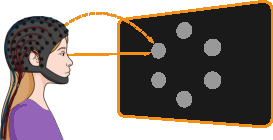
\includegraphics[width=\textwidth]{figures/gaze_independence/attention_overt.pdf}
    \caption[Overt \ac{vsa}]{%
      \emph{Overt} \ac{vsa}.
      Gaze and \ac{vsa} coincide on a target.
    }
    \label{fig:gaze/vsa/overt}
  \end{subfigure}\hfill%
  \begin{subfigure}[t]{.45\textwidth}
    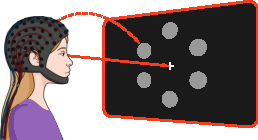
\includegraphics[width=\textwidth]{figures/gaze_independence/attention_covert.pdf}
    \caption[Covert \ac{vsa}]{%
      \emph{Covert} \ac{vsa}.
      Gaze rests on the center of the screen, while \ac{vsa} is directed towards a target.
    }
    \label{fig:gaze/vsa/covert}
  \end{subfigure}

  \begin{subfigure}[t]{.45\textwidth}
    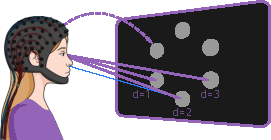
\includegraphics[width=\textwidth]{figures/gaze_independence/attention_split.pdf}
    \caption[Split \ac{vsa}]{%
      \emph{Split} \ac{vsa}.
      \Ac{vsa} is directed towards a target, while the gaze rests on another.
    }
    \label{fig:gaze/vsa/split}
  \end{subfigure}\hfill%
   \begin{subfigure}[t]{.45\textwidth}
    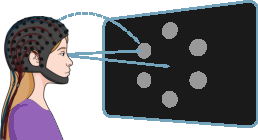
\includegraphics[width=\textwidth]{figures/gaze_independence/attention_free.pdf}
    \caption[Free \ac{vsa}]{%
      \emph{Free} \ac{vsa}.
      The user is free to direct their gaze as they deem most comfortable.
      All previous \ac{vsa} conditions are possible.
    }
    \label{fig:gaze/vsa/free}
  \end{subfigure}\hfill%
  \caption[\Ac{vsa} conditions]{%
    \Acf{vsa} conditions defined in our hexagonal spatial \ac{erp} paradigm
    interface. Full lines indicated gaze fixation, dashed lines \ac{vsa}.
  }
  \label{fig:gaze/vsa}
\end{figure}
In the overt case, users gazed at the cued
target they were also mentally attending; in the covert case, users
gazed at the center of the screen while mentally attending to the cued target.
We introduced a \ac{vsa} condition that is understudied in the context of
gaze-independent \ac{bci} development: split \ac{vsa}.
In split \ac{vsa}, the user mentally focuses on one cued target while gazing at
another (the distractor).
This last option has been scarcely studied but completes
the options to dissociate gaze and visuospatial attention, allowing us to
investigate the effect of (the lack of) gaze control on \ac{bci} performance.
This dataset and the performance of our proposed \ac{wcble} decoder have also been
published by \textcite{VanDenKerchove2024} and will be presented in
\cref{sec:covert-align}.
Performance is also evaluated on a publicly available dataset.

\subsubsection{Case studies with gaze-impaired individuals}
\label{sec:patients/approach/casestudies}

After collecting data from healthy participants and developing initial decoders, we conducted
a study with seven individuals with \ac{sspgi} to evaluate the impact of eye motor deficits
on \ac{bci} performance.
This study recruited participants from neurorehabilitation centers
and specialized care homes, including participants with conditions such as \ac{als}, \ac{fa},
and stroke.

The primary aim was to assess whether gaze-independent decoding strategies could improve
\ac{bci} performance in this group.
We used the visual Hex-o-Spell interface~\cite{Treder2010}, adapting the task by adding a
free \ac{vsa} setting, where participants could operate the interface without being required
to fixate their gaze.
This setting allowed us to investigate how participants with varying eye motor capabilities
naturally interacted with a \ac{bci}, compared to standard overt and covert \ac{vsa} tasks.

The hypothesis was that gaze-independent decoders, such as \ac{wcble}~\cite{VanDenKerchove2024},
would improve performance in covert and free \ac{vsa} conditions compared to standard
decoders like \ac{tlda}.
We aimed to determine if calibration in an overt \ac{vsa} setting could also enhance
performance in free and covert conditions, leveraging residual eye motor control during
calibration to improve overall \ac{bci} accuracy for gaze-impaired users.
The results of this study are presented in \cref{sec:patients}.


\part{Algorithms \& Decoders}
\chapter{Kronecker-structured linear decoding}
\label{sec:stbf-struct}
\newcommand{\pv}[1]{
	%\ifdim#1pt<0.05pt
	%	\cellcolor{black!20}
	%\fi
	%\ifdim#1pt<0.001pt
	%	$< 0.001$
	%\else
	%	\ifdim#1pt=1.000pt
	%		\multicolumn{1}{c}{--}
	%	\else
	%		$#1$
	%	\fi
	%\fi
	#1
}
\epigraph{%
  \justifying
  I journeyed to the market to purchase a cow, its price set at ninety-and-seven coins.
  Lacking this sum, I therefore borrowed fifty coins from each of two good friends.
  With these hundred coins, I paid for the beast and received three coins in change.
  Of the three, I returned one coin each to my companions, keeping one for myself.
  Now, I owe each friend forty-and-nine coins, a total debt of
  ninety-and-eight. And with mine one remaining, the
  total merely equals ninety-and-nine coins, short of the hundred I borrowed!
  Tell me then, kind stranger, whither hath the missing coin gone?
}{%
  Ancient Algerian riddle
}
% Kronecker-structured LDA ====================================================

  \publicationnote{This chapter, except
  \crefrange{tab:stbf-struct/accuracies/stbf-struct}{tab:stbf-struct/accuracies/xdawn-rg},
  was published as~\textcite{VanDenKerchove2022}.}

	\section{Introduction}

	%Brain-computer interfaces (\acp{bci}) establish a direct communication pathway
	%between the brain and an external device~\cite{Wolpaw2002}.
	%Severely disabled patients with impaired or absent communication capabilities
	%can benefit from \acp{bci} to restore normal functioning~\cite{Naci2012,Chaudhary2016}.
	%\acp{bci} can be implemented in multiple ways, using non-invasive recording
	%techniques such as electroencephalography (\ac{eeg})~\cite{Abiri2019},
	%magnetoencephalography (MEG)~\cite{Mellinger2007},
	%functional Near-Infrared Spectroscopy (fNIRS)~\cite{Hong2015}, and Optically Pumped
	%Magnetometers (OPM MEG)~\cite{Paek2020}, or semi-invasive and invasive methods such as
	%electrocorticography (ECoG)~\cite{Schalk2011} or microelectrode
	%arrays~\cite{Maynard1997} which require surgery to implant a recording device.
	%While invasive \acp{bci} yield the highest information transfer
	%rate~\cite{Willett2021}, non-invasive \acp{bci} are preferable for short-term use
	%since they are not susceptible to the risks that come with surgery.
	%Of the non-invasive options, \ac{eeg} is the most cost-effective and practical as it
	%is not limited to the same controlled settings as MEG and OPM MEG.

	%Besides the recording method, \acp{bci} differ in the communication paradigms used
	%for communication~\cite{Abiri2019}.
	%A popular class of \ac{bci} paradigms relies on the evocation
	%of Event-Related Potentials (\acp{erp}) in the brain in response to visual, auditory, or tactile stimulation, given their low decoding cost and generally short
	%calibration time before usage~\cite{Gao2014, Kapgate2015}.
	%The study we report on focuses on the visual P3 oddball \ac{erp} in response to a
	%rare but attended visual stimulus.
	%The decoder detects whether this \ac{erp} is present to determine which stimulus
	%the user attended.
	%The P3 paradigm has been used extensively in \ac{bci} development and is easy to
	%set up~\cite{Farwell1988, Sellers2006, Barachant2014, Philip2020}.

  There are multiple state-of-the-art P3 classification methods, like
  \acp{svm}~\cite{Tayeb2014}, deep
	learning models~\cite{Vareka2020,Borra2020}, and Riemannian Geometry
	classifiers~\cite{Barachant2014}.
	While these models often return a high classification accuracy, there is a need
	for lightweight models -- lightweight models lead to fast off-line analyses and can be transferred to consumer-grade hardware.
	When moving towards plug-and-play solutions, \ac{bci} calibration sessions should be short and model training times low.
  The \ac{stbf}~\cite{VanVliet2015, Wittevrongel2016} belongs to
	this class of \ac{erp} decoding models as it achieves state-of-the-art performance and is fast to train.
	Earlier work has shown that it is
	possible to apply the spatiotemporal beamformer to multiple time-locked visual
  \ac{bci} paradigms, including the P3 oddball paradigm, \ac{ssvep},
  \ac{cvep}~\cite{Wittevrongel2017a}, and the \ac{mvep}~\cite{Libert2021}.

	This work shows that the original spatiotemporal
	beamformer~\cite{Wittevrongel2016} can fall short in performance when \ac{bci}
	calibration data are restricted.
	We also show that the spatiotemporal beamformer does not scale well for
	higher spatial and temporal resolution cases.
	As a response to these issues, we introduce a regularization method that
	exploits prior knowledge about the spatiotemporal nature of the \ac{eeg} signal to
	improve the accuracy for low data availability settings and speed up the
	classifier training time, thereby considerably reducing memory usage.
	Similarly structured regularization approaches have been applied to other linear
	\ac{erp} classifiers~\cite{GonzalezNavarro2017, Vliet2020} and have shown
	significant increases in performance.
%	Additionally, we show that regularization results in an interpretable
%	classification model, which can aid in analyzing and developing spatiotemporal beamformer-based classifiers.

	\section{Materials \& methods}
	\subsection{Notation}
	We represent matrices with bold capital letters, vectors with bold
	lowercase letters, fixed scalars with uppercase cursive letters and variable
  scalars with cursive lowercase letters.
	The epoched \ac{eeg} data with $N$ epochs, $C$ channels, and $S$ samples are
  represented in epoch format as $\{\mat{X}_n\in\mathbb{R}^{C\times S}\}^N_{n=1}$
  or flattened vector format by concatenating all channels for each epoch.
	Flattening results in $\{\mat{x}_n\in\mathbb{R}^{CS}\}^N_{n=1}$ such that
  $\mat{x}_n = \vect(\mat{X}_n)$.
	The real covariance matrix of the epochs in vector format is
  denoted by $\mat{C}$, estimators thereof as $\hat{\mat{C}}$.

	\subsection{Spatiotemporal beamforming}
  \ac{lcmv}-beamforming was initially introduced to \ac{eeg} analysis as a filter for
  source localization~\cite{VanVeen1997} to enhance the \ac{snr}.
	\textcite{VanVliet2015} first applied the spatiotemporal
	\ac{lcmv}-beamformer as a method for the analysis of \acp{erp}.
	The extension to the combined spatiotemporal domain~\cite{VanVliet2015} and the
	data-driven approaches proposed by \textcite{Treder2016} and
	\textcite{Wittevrongel2016} allow for its application to classification problems.

	For the following analyses, we assume that all \ac{eeg} channels are normalized with zero mean and unit variance without loss of generality.
	Solving \cref{eq:stbf-struct/minimum-variance} under the linear constraint given by
  \cref{eq:stbf-struct/linear-constraint} returns the filter weights $\mat{w}$ defining the spatiotemporal \ac{lcmv}-beamformer.
	\begin{equation}
    \argmin_\mat{w}\mat{w}^\intercal \mat{C}
		\mat{w}^\intercal
		\label{eq:stbf-struct/minimum-variance}
	\end{equation}
	\begin{equation}
		\mat{a}^\intercal\mat{w} = 1
		\label{eq:stbf-struct/linear-constraint}
	\end{equation}
	These weights minimize the variance of the output of the filter while enhancing
	the signal characterized by the constraint.
  $\mat{a} = \vect(\mat{A})$ is the data-driven activation pattern, a template
	of the signal of interest maximizing the difference between two classes of
  epochs, here denoted as the `target' (T) and `non-target' (NT) class.
  The activation pattern is then determined as follows:
	\begin{equation}
		\mathbf{a} =
    \frac{1}{N_\mathrm{T}}\sum_\mathrm{T}\mathbf{x_n} -
    \frac{1}{N_\mathrm{NT}}\sum_\mathrm{NT}\mathbf{x_n}
		\label{eq:stbf-struct/ap}
	\end{equation}

	The method of Lagrange multipliers then gives the closed-form solution to the minimization problem posed by
	\cref{eq:stbf-struct/minimum-variance} and \cref{eq:stbf-struct/linear-constraint} as:
	\begin{equation}
		\mat{w} =
    \frac{\mat{C}^{-1}\mat{a}^\intercal}
    {\mat{a}\mat{C}^{-1}\mat{a}^\intercal}
		\label{eq:stbf-struct/closed-form}
	\end{equation}
	The beamformer can be applied to epochs (unseen or not) as:
	\begin{equation}
		y_n = \mathbf{w}\mathbf{x}_n
		\label{eq:stbf-struct/apply-bf}
	\end{equation}
	resulting in a scalar output per epoch.
	The linear constraint in \cref{eq:stbf-struct/linear-constraint} ensures that the
	beamformer maps epochs containing a target response to a score close to one
	and, conversely, epochs not containing a target response to a score close to
	zero.

	\subsection{Covariance matrix regularization}
	While the spatiotemporal beamformer, in theory, achieves optimal separation
	between target and non-target classes, in analogy to linear discriminant
  analysis~\cite{Treder2016}, it does not always perform well on unseen data.
	The main challenge is to find a good estimator for the inverse covariance
  matrix $\mat{C}^{-1}$ since the real underlying covariance matrix generating the data is, in principle, unknown.

	\subsubsection{Empirical covariance estimation}
	\label{sec:stbf-struct/methods/emp-cov}
	Earlier spatiotemporal beamformer studies~\cite{Wittevrongel2016,
		Wittevrongel2016a, Wittevrongel2017, Wittevrongel2017a} use the empirical
	covariance and inverse covariance calculated as follows:
	\begin{equation}
    \hat{\mat{C}}_\text{emp} =
		\frac{1}{N-1}\sum^{N}_{n=1}\mat{x}_n\mat{x}_i^\intercal
		\label{eq:stbf-struct/emp-cov}
	\end{equation}
	\begin{equation}
    \widehat{\mat{C}^{-1}}_\text{emp} = \hat{\mat{C}}_\text{emp}^+
		\label{eq:stbf-struct/emp-inv-cov}
	\end{equation}
	The Moore-Penrose pseudoinverse, $^+$, ensures a solution exists when
  $\hat{\mat{C}}_\text{emp}$ is singular.
	\cref{fig:kronlda-covs}a and \cref{fig:kronlda-covs}b respectively show examples of the
	empirical estimators of the covariance and the inverse covariance matrices.
	The empirical estimator suffers from performance and
	stability issues if the number of epochs $N$ used or estimation is not much larger than the number of features $CS$~\cite{Stein1956,Khatri1987}.

	\subsubsection{Shrunk covariance estimation}
	\label{sec:stbf-struct/methods/shrunk-cov}
	The shrinkage covariance estimator creates a better conditioned inversion matrix problem and generally performs better when applied to unseen data.
	The estimators for the covariance and inverse covariance are given by:
	\begin{equation}
    \hat{\mat{C}}_\alpha =
    (1-\alpha) \hat{\mat{C}}_\text{emp}
    + \alpha\frac{\Tr(\hat{\mat{C}}_\text{emp})}{CS}\mathbb{I}
		\label{eq:shrinkage}
	\end{equation}
	\begin{equation}
    \widehat{\mat{C}^{-1}}_\alpha =
    \hat{\mat{C}}^+_\alpha
		\label{eq:stbf-struct/shrinkage-inv}
	\end{equation}
	with $0<\alpha<1$.
	Analogous to $L_2$ regularization of the beamforming problem,
	shrinkage reduces the ratio between the smallest and largest eigenvalues
	of the covariance matrix by strengthening the diagonal.
	\cref{fig:kronlda-covs}c and \cref{fig:kronlda-covs}d respectively show examples of the
	shrunk estimator of the covariance and the inverse covariance matrices.

	Earlier work~\cite{Libert2021} applied shrinkage regularization to \ac{erp}
	decoding with the spatiotemporal beamformer and showed competitive performance
	compared to other state-of-the-art decoding techniques like stepwise LDA or SVM.
	The abovementioned work chooses the shrinkage coefficient $\alpha$ as a fixed hyperparameter.
	However, its optimal value depends on the number of training epochs, the
	covariance matrix's dimensionality, and the independence and variance of the
	data, which can vary across evaluation settings and per session.
	The optimal value for $\alpha$ can be found with a line search using cross-validation, but this can be a costly procedure.

	Methods exist to estimate an optimal shrinkage value from the data directly.
	Most notable among these are the Ledoit-Wolf procedure~\cite{Ledoit2004},
	Rao-Blackwell Ledoit-Wolf~\cite{Chen2010}, and Oracle Approximating Shrinkage~\cite{Chen2010}.
  A more recent estimation method~\cite{Tong2018} emulates a \ac{loocv} scheme expressed by the data-driven closed-form
	estimate:
	\begin{equation}
		  \alpha =
		  1-\frac{%
        \splitfrac{
          \frac{N}{N-1}\Tr(\hat{\mat{C}}_\text{emp}^2)
          - \frac{2}{CS}\left[\Tr(\hat{\mat{C}}_\text{emp})\right]^2
          + \frac{1}{CS}\Tr(\hat{\mat{C}}_\text{emp}^2)
        }{
		  	  - \frac{1}{N(N-1)}\sum_{n=1}^N||\mat{x}_n||_2^4
        }
		  }{%
        \splitfrac{
          \frac{N^2 -2N}{(N-1)^2}\Tr(\hat{\mat{C}}_\text{emp}^2)
          - \frac{2}{CS}\left[\Tr(\hat{\mat{C}}_\text{emp})\right]^2
          + \frac{1}{CS}\Tr(\hat{\mat{C}}_\text{emp}^2)
        }{%
		  	  + \frac{1}{N(N-1)^2}\sum_{n=1}^N||\mat{x}_n||_2^4
        }
		  }
		\label{eq:loocv}
	\end{equation}
	We opt for the \ac{loocv} shrinkage estimator because it avoids some of the
	assumptions made by \textcite{Ledoit2004} and \textcite{Chen2010} and
	because it generalizes to structured covariance estimation as described in
	\cref{sec:stbf-struct/methods/structured-estimation}.

	\subsubsection{Spatiotemporal beamforming with Kronecker-Toeplitz structured covariance}
	\label{sec:stbf-struct/methods/structured-estimation}
	Exploiting prior knowledge about the spatiotemporal structure of the \ac{eeg} signal leads to a more regularized estimator of the covariance.
	When viewing the example of empirical spatiotemporal \ac{eeg} covariance in
	\cref{fig:kronlda-covs}a, it becomes clear that this matrix consists of a block pattern of repeated, similar matrices.
	Due to the multi-channel nature of the signal, we assume that the covariance of spatiotemporal \ac{eeg} epochs is a Kronecker
	product of two smaller
	matrices~\cite{Munck1992,DeMunck1999,Huizenga2002}, as expressed
	by:
	\begin{equation}
    \hat{\mat{C}}_\text{struct} = \hat{\mat{S}} \otimes \hat{\mat{T}}
		\label{eq:kronecker}
	\end{equation}
	with $\otimes$ the Kronecker product operator.
  $\hat{\mat{S}} \in \mathbb{R}^{C\times C}$ and $\hat{\mat{T}} \in \mathbb{R}^{S\times S}$ respectively correspond to estimators of the spatial and temporal covariance of the data.
	Furthermore, because the temporal covariance of the \ac{eeg}-signal is
	stationary (i.e., it is only dependent on interval length between covarying
	time samples)~\cite{Bijma2003}, it is assumed to have a Toeplitz-matrix structure:
	\begin{equation}
    \hat{\mat{T}}_{i,j} = \hat{\mat{T}}_{i+1,j+1}
		\label{eq:toeplitz}
	\end{equation}
	\Cref{prop:stbf-struct/inverse-kronecker} then leads to
	\cref{eq:stbf-struct/cov-inverse-kronecker} to estimate the inverse
	covariance.

	\begin{property}
    $(\mat{U} \otimes \mat{V})^+ = \mat{U}^+ \otimes \mat{V}^+$ for any non-singular
    matrices $\mat{U}$ and $\mat{V}$~\cite{Langville2004}.
		\label{prop:stbf-struct/inverse-kronecker}
	\end{property}

	\begin{equation}
    \widehat{\mat{C}^{-1}}_\text{struct} = \hat{\mat{S}}^+ \otimes \hat{\mat{T}}^+
		\label{eq:stbf-struct/cov-inverse-kronecker}
	\end{equation}

	Finally, based on \cref{propr:stbf-struct/kron-multiplication},
	\cref{eq:stbf-struct/closed-form} can be reformulated more efficiently as
	\cref{eq:stbf-struct/closed-form-kron}.
	\begin{property}
    $(\mat{U}\otimes \mat{V})\cdot\vect(\mat{W}) =
    \vect(\mat{V}\mat{W}\mat{U}^\intercal)$
    for any matrices $\mat{U}\in\mathbb{R}^{P\times P}$,
    $\mat{V}\in\mathbb{R}^{Q\times Q}$ and $\mat{W}\in\mathbb{R}^{P\times Q}$~\cite{Loan2000}.
		\label{propr:stbf-struct/kron-multiplication}
	\end{property}

	\begin{equation}
		\hat{\mat{w}}_\text{struct} =
    \frac{\hat{\mat{S}}^+\mat{A}^\intercal\hat{\mat{T}}^+}
    {\mat{a}\cdot\vect\left(\hat{\mat{S}}^+A^\intercal\hat{\mat{T}}^+\right)}
		\label{eq:stbf-struct/closed-form-kron}
	\end{equation}

	Using \cref{eq:stbf-struct/closed-form-kron} removes the need to calculate the
  full, high dimensional Kronecker product $\hat{\mat{S}}^+\otimes
    \hat{\mat{T}}^+$.
	\Cref{fig:kronlda-covs}e and \cref{fig:kronlda-covs}f respectively show examples of the
	structured covariance and inverse covariance estimators,
	consisting of a spatial Kronecker factor (\cref{fig:kronlda-covs}g and
	\cref{fig:kronlda-covs}h) and a temporal component (\cref{fig:kronlda-covs}i and
	\cref{fig:kronlda-covs}j).

  \begin{figure}[t]
		%\includegraphics[width=\linewidth]{figures/stbf_struct/covs.eps}
    \begin{subfigure}{\textwidth/4}
		  
\includegraphics[width=\linewidth]{figures/stbf_struct/covs-0.eps}
      \caption{}
    \end{subfigure}\hfill%
    \begin{subfigure}{\textwidth/4}
		  
\includegraphics[width=\linewidth]{figures/stbf_struct/covs-1.eps}
      \caption{}
    \end{subfigure}\hfill%
    \begin{subfigure}{\textwidth/4}
		  
\includegraphics[width=\linewidth]{figures/stbf_struct/covs-2.eps}
      \caption{}
    \end{subfigure}\hfill%
    \begin{minipage}[b]{\textwidth/10}
      \begin{subfigure}{\textwidth}
  		  
\includegraphics[width=\linewidth]{figures/stbf_struct/covs-6.eps}
        \caption{}
      \end{subfigure}\vfill%
      \begin{subfigure}{\textwidth}
  		  
\includegraphics[width=\linewidth]{figures/stbf_struct/covs-7.eps}
        \caption{}
      \end{subfigure}\hfill%
    \end{minipage}

    \begin{subfigure}{\textwidth/4}
		  
\includegraphics[width=\linewidth]{figures/stbf_struct/covs-3.eps}
      \caption{}
    \end{subfigure}\hfill%
    \begin{subfigure}{\textwidth/4}
		  
\includegraphics[width=\linewidth]{figures/stbf_struct/covs-4.eps}
      \caption{}
    \end{subfigure}\hfill%
    \begin{subfigure}{\textwidth/4}
		  
\includegraphics[width=\linewidth]{figures/stbf_struct/covs-5.eps}
      \caption{}
    \end{subfigure}\hfill%
    \begin{minipage}[b]{\textwidth/10}
      \begin{subfigure}{\textwidth}
  		  
\includegraphics[width=\linewidth]{figures/stbf_struct/covs-8.eps}
        \caption{}
      \end{subfigure}\vfill%
      \begin{subfigure}{\textwidth}
  		  
\includegraphics[width=\linewidth]{figures/stbf_struct/covs-9.eps}
        \caption{}
      \end{subfigure}\hfill%
    \end{minipage}



    \caption[Estimated covariance and inverse covariance.]{Different estimators of the covariance and inverse covariance
			of 100 epochs of data from \textit{Subject 01} for channels
			\textit{Fz}, \textit{Cz}, \textit{Pz}, and \textit{Oz} and time samples between 0.1s and 0.6s.
			Regularized estimators of the inverse covariance exhibit less extreme values and have a sparser structure.
			(\textbf{a,f}) Empirical covariance and inverse covariance matrices.
			(\textbf{b,g}) Shrunk covariance and inverse covariance matrices with $\alpha=0.14$ as
			determined by the closed-form \ac{loocv} method. (\textbf{c,h}) Kronecker-Toeplitz
			structured covariance and inverse covariance matrices.
			(\textbf{d,e}) Spatial Kronecker factor of the Kronecker-Toeplitz structured shrunk estimator and its inverse.
			(\textbf{i,j}) Temporal Kronecker factor of the Kronecker-Toeplitz structured shrunk estimator and its inverse.}
		\label{fig:kronlda-covs}
	\end{figure}

	The Kronecker approach has shown significant performance yields in different linear spatiotemporal \ac{eeg} and MEG
	applications~\cite{DeMunck2002,Huizenga2002,Beltrachini2013,GonzalezNavarro2016,GonzalezNavarro2017}.
	\textcite{Vliet2020} have applied a Kronecker-structured covariance estimator to \ac{erp} classification with linear models in a post-hoc fashion.
	Our work goes further by embedding the Kronecker structure in the
	spatiotemporal beamformer training process, using a data-adaptive shrinkage
	method, and regularizing the covariance further by imposing a Toeplitz
	structure on the temporal covariance.

	\subsubsection{Kronecker-Toeplitz structured covariance estimation}
	\label{sec:stbf-struct/methods/struct-cov}
  The question remains how to estimate $\mat{\hat{S}}$ and $\mat{\hat{T}}$.
	While the Flip-Flop and Non-iterative Flip-Flop
	algorithms~\cite{Lu2005, Werner2008, Wirfaelt2010} can estimate Kronecker or Kronecker-Toeplitz structured covariances, new results show that a fixed point iteration is more efficient~\cite{Wiesel2012a,Wiesel2012}.
	After each iteration, the spatial and temporal covariances matrices are scaled to unit
	variance to ensure the fixed point iteration converges.
	Finally, shrinkage can also be introduced in the Fixed Point Iteration to
	improve stability and achieve more robust
	regularization~\cite{Wiesel2012,Greenewald2014,Beltrachini2013, Breloy2016}.
	The spatial and temporal covariance matrices are shrunk at every fixed-point
	iteration with shrinkage factors $\beta_k$ and $\gamma_k$ before matrix
	inversion in the
	next iteration.

	Combined, this leads to the iterative estimation algorithm described by the
	following equations:
	\begin{subequations}
		\begin{equation}
      \tilde{\mat{S}}_{k+1} =
			\frac{1}{N}
      \sum^N_{n=1}\mat{X}_n^\intercal\hat{\mat{T}}_k^+\mat{X}_n
			\label{eq:stbf-struct/fpi-spatial}
		\end{equation}
		\begin{equation}
      \tilde{\mat{T}}_{k+1} =
			\frac{1}{N}
      \sum^N_{n=1}\mat{X}_n\hat{\mat{S}}_k^+\mat{X}_n^\intercal
			\label{eq:stbf-struct/fpi-temporal}
		\end{equation}
	\end{subequations}
	\begin{subequations}
		\begin{equation}
      \tilde{\mat{S}}_{k+1}^{(\beta)} =
      (1-\beta_{k+1})\tilde{\mat{S}}_{k+1}
      +\beta_{k+1}\frac{\Tr(\tilde{\mat{S}}_{k+1})}{C}\mathbb{I}
			\label{eq:stbf-struct/fpi-spatial-shrunk}
		\end{equation}
		\begin{equation}
      \tilde{\mat{T}}_{k+1}^{(\gamma)} =
      (1-\gamma_{k+1})\tilde{\mat{T}}_{k+1}
      +\gamma_{k+1}\frac{\Tr(\tilde{\mat{T}}_{k+1})}{S}\mathbb{I}
			\label{eq:stbf-struct/fpi-temporal-shrunk}
		\end{equation}
	\end{subequations}
	\begin{subequations}
		\begin{equation}
      \hat{\mat{S}}_{k+1} =
      \frac{C}{\Tr\left[\tilde{\mat{S}}_{k+1}^{(\beta)}\right]}
      \tilde{\mat{S}}_{k+1}^{(\beta)}
			\label{eq:stbf-struct/fpi-spatial-norm}
		\end{equation}
		\begin{equation}
      \hat{\mat{T}}_{k+1} =
      \frac{S}{\Tr\left[\tilde{\mat{T}}_{k+1}^{(\gamma)}\right]}
      \tilde{\mat{T}}_{k+1}^{(\gamma)}
			\label{eq:stbf-struct/fpi-temporal-norm}
		\end{equation}
	\end{subequations}
  $\hat{\mat{S}}_0$ and $\hat{\mat{T}}_0$ can be initialized to any positive definite matrix.
	We choose to use the identity matrices $\mathbb{I}^{C\times C}$ and $\mathbb{I}^{S\times S}$.
  After each iteration, all diagonals of $\hat{\mat{R}}_{k+1}$ are set to their mean
  values to ensure that $\hat{\mat{R}}_{k+1}$ and $\hat{\mat{T}}_{k+1}$ are Toeplitz structured.

	\textcite{Xie2021} show that the \ac{loocv} estimates for the
	optimal values of $\beta_{k+1}$ and $\gamma_{k+1}$ also yield a closed-form
	solution for the Kronecker fixed-point-iteration algorithm:

	\begin{subequations}
		\begin{equation}
			\beta_{k+1} =
			1-
			\frac{
        \splitfrac{
          \frac{N}{N-1}\Tr(\tilde{\mat{\hat{\S}}}_{k+1}^2)
          - \frac{2}{C}\left[\Tr(\mat{\tilde{S}}_{k+1})\right]^2
          + \frac{1}{C}\Tr(\tilde{\mat{S}}_{k+1}^2)
        }{%
				  - \frac{1}{N(N-1)}\sum_{i=1}^N
          \left[\Tr(\mat{X}_i\hat{\mat{T}}_k^+\mat{X}_i^\intercal)^2\right]
        }
			}{
        \splitfrac{
          \frac{N^2-2N}{(N-1)^2}\Tr(\tilde{\mat{S}}_{k+1}^2)
          - \frac{2}{C}\left[\Tr(\tilde{\mat{S}}_{k+1})\right]^2
          + \frac{1}{C}\Tr(\tilde{\mat{S}}_{k+1}^2)
        }{%
				  + \frac{1}{N(N-1)^2}\sum_{i=1}^N
          \left[\Tr(\mat{X}_i\hat{\mat{T}}_k^+\mat{X}_i^\intercal)^2\right]
        }
			}
			\label{eq:stbf-struct/spatial-shrinkage}
		\end{equation}
		\begin{equation}
			\gamma_{k+1} =
			1-
			\frac{
        \splitfrac{
          \frac{N}{N-1}\Tr(\tilde{\mat{T}}_{k+1}^2)
          - \frac{2}{S}\left[\Tr(\tilde{\mat{T}}_{k+1})\right]^2
          + \frac{1}{S}\Tr(\tilde{\mat{T}}_{k+1}^2)
        }{%
				  - \frac{1}{N(N-1)}\sum_{n=1}^N
          \left[\Tr(\mat{X}_n^\intercal\mat{\mat{S}}_k^+\mat{X}_n)^2\right]
        }
			}{
        \splitfrac{
          \frac{N^2-2N}{(N-1)^2}\Tr(\tilde{\mat{T}}_{k+1}^2)
          - \frac{2}{S}\left[\Tr(\tilde{\mat{T}}_{k+1})\right]^2
          + \frac{1}{S}\Tr(\tilde{\mat{T}}_{k+1}^2)
        }{
				  + \frac{1}{N(N-1)^2}\sum_{n=1}^N
          \left[\Tr(\mat{X}_n^\intercal\hat{\mat{S}}_k^+\mat{X}_n)^2\right]
        }
			}
			\label{eq:stbf-struct/temporal-shrinkage}
		\end{equation}
	\end{subequations}
	The shrinkage parameters $0<\beta_{k+1}<1$ and $0<\gamma_{k+1}<1$ should be
	re-determined after each iteration.
	The Oracle Approximation Shrinkage method can also be used to determine
	$\beta_{k+1}$ and $\gamma_{k+1}$~\cite{Chen2010,Xie2021} but performs worse for spatiotemporal \ac{eeg} data since not all assumptions are met.

	\subsection{Dataset}
	We use the dataset from~\textcite{Wittevrongel2016}, containing P3 oddball \ac{eeg}
	recordings of 21 healthy subjects since it is a high-quality dataset with a high
	number (32) of electrodes and concurrently recorded EOG responses for ocular artifact rejection.
	Nine targets were arranged on a monitor before the subject during an
	experimental session.
	The subject was asked to pay attention to a cued target for a block
	of stimulations.
	The stimulations in a block are organized in 15 separate subsequent trials.
	A trial is defined as 9 stimulations in which each target is flashed
	precisely once per trial.
	Each target was cued four times, resulting in a dataset consisting of 36 blocks
	(4860 stimulations) per subject.
	Each stimulation will correspond to a single epoch in the preprocessed dataset.
	See~\textcite{Wittevrongel2016} for a complete description of the dataset and the recording procedure.

	\subsection{Software and preprocessing}
	Data processing and classifier analysis were performed in Python using
	Scikit-Learn (v1.0.1)~\cite{Pedregosa2011} and SciPy (version
	1.7.1)~\cite{Virtanen2020}.
	The preprocessing pipeline was implemented using the MNE-Python toolbox
	(v0.24.0)~\cite{Gramfort2013}.
	The dataset was converted to BIDS-\ac{eeg} format~\cite{Pernet2019} and managed and
	loaded with MNE-BIDS (version 0.9)~\cite{Appelhoff2019}.
	The Riemannian classifier from \cref{sec:riemannian} was implemented using
	pyRiemann (v0.2.7).
	Statistical tests were performed in R (v4.1.2).

	The \ac{eeg} recorded at 2048 Hz was re-referenced off-line to the average of the mastoids.
	The reference electrodes were dropped from the analysis.
	Data were subsequently filtered between 0.5 Hz and 16 Hz using forward-backward
	filtering with a fourth-order Butterworth IIR filter.
	The \ac{eeg} signal was corrected for ocular artifacts using Independent Component
	Analysis (ICA) by rejecting components that correlated with the bipolar EOG
  channels vEOG and hEOG using iterative Z-score thresholding.
  Components with a Z-scored pearson correlation coefficient
  exceeding  3 times the standard deviation of the Z-scored
  correlation coefficients of other components, were iteratively
  rejected until none that exceed the threshold remained.
  Finally, epochs were cut from 0.1s to 0.6s after stimulus onset.
	No baseline correction was performed since this affects the temporal covariance
	of the data, violating the Toeplitz structure assumption~\cite{Bijma2003}.

	\subsection{Classification}
	\subsubsection{Cross-validation scheme per subject}
	We use a variation of grouped fold cross-validation per subject to evaluate the classifiers.
	We apply 4-fold cross-validation by splitting the blocks of each subject into
	four continuous folds.
	Unlike regular cross-validation, we only use a single fold to train the
	classifiers while using the other three folds for validation.
	This scheme results in a training set of 9 blocks of 135 epochs each.
	We chose this approach since we are primarily interested in the performance of the classifiers in the case of low data availability.
	The classification task is to determine the cued target for each block.
	The fraction of correctly predicted cues provides the accuracy of a classifier.
	Data from all trials are used in the training fold, while classifier validation
	is performed multiple times per fold, each time using an increasing amount of
	trials (i.e., using the first trial, using the first two trials, etc. until all 15 trials
	are used).
	For each of the 9 stimulated targets, the averages over the corresponding epochs across
	the utilized trials are used to predict the cued target in that block.
	The target with the maximal classifier score was then chosen as the predicted
	cued target.
	Before training the classifiers, a Z-score normalization transformation was
	developed on the training data to scale all \ac{eeg} channels to unit variance.
	This transformation was then applied to the validation data.

  \subsubsection{\Acl{stbf} classifier}
	Before calculating the \ac{stbf}, the signal was downsampled to
	32 Hz or twice the low-pass frequency 16 Hz, resulting in 17 time samples
	between 0.1 and 0.6s. According to the Nyquist Theorem, more samples would not
	contain more information hence the minimum temporal resolution is chosen to reduce
	the dimensionality of the covariance and improve its condition number.
	The activation pattern is the difference between the averages of epochs in response to cued targets and the averages of those in response to non-cued targets.
	We constructed three variations of the spatiotemporal beamformer the \ac{stbf-emp} as in
	\cref{sec:stbf-struct/methods/emp-cov}, the \ac{stbf-shrunk} as in
	\cref{sec:stbf-struct/methods/shrunk-cov}, and the \ac{stbf-struct} with \ac{loocv} shrinkage for
	the Kronecker factors as in \cref{sec:stbf-struct/methods/struct-cov}.

	\subsubsection{Riemannian geometry classifier}
	\label{sec:riemannian}
	We opted for a Riemannian
	geometry-based classifier to compare our results.
	The Riemannian model (XDAWN+RG) uses the XDAWN spatial filter combined
  with Riemannian geometry in tangent space as implemented by
  \textcite{Barachant2014a}.
	This classifier uses four XDAWN spatial filters and each epoch's empirical spatial covariance matrix.
	The target with the maximum score is the prediction of the cued target.
	XDAWN+RG was trained and validated without downsampling using epochs
	at the original sample rate of 2048 Hz.
  Preliminary experimentation revealed that best performance in low and high
  data availability setting was achieved when no shrinkage was applied to the estimation of XDAWN filters or the subsequent
  covariance matrices for this specific dataset.
  Hence, no shrinkage regularization will be applied to XDAWN+RG in
  further experiments.

	\section{Results}
	\subsection{Minimum required fixed-point iterations}
	The fixed point iteration algorithm described
	in
  \crefrange{eq:stbf-struct/fpi-spatial}{eq:stbf-struct/fpi-temporal-norm}
  estimates the Kronecker-Toeplitz structured covariance for the
	\ac{stbf-struct} classifier.
	Fixed-point iteration is an iterative procedure starting from (in our case)
	non-informed initial guesses for the spatial and temporal covariance matrices.
	As a stopping criterion, one could impose a threshold on the difference in
	outcome of successive steps, e.g., based on the covariance norm or the
	classifier accuracy.
	However, few iterations or even just one~\cite{Castaneda2014} suffice to achieve satisfactory performance in practice.

	\cref{fig:iterations} confirms these results for the \ac{stbf-struct} classifier.
	Using more than one fixed-point iteration does not significantly improve the
	accuracy across the amounts of training data and the number of trials
  used for evaluation.
	Hence, only one iteration is used for the \ac{stbf-struct} classifier, leading to a drastic speed-up of
  the  training process.

  \begin{figure}[t]
    \begin{subfigure}{\linewidth}
      \hspace{-0.4623567780166823in}
%% Creator: Matplotlib, PGF backend
%%
%% To include the figure in your LaTeX document, write
%%   \input{<filename>.pgf}
%%
%% Make sure the required packages are loaded in your preamble
%%   \usepackage{pgf}
%%
%% Also ensure that all the required font packages are loaded; for instance,
%% the lmodern package is sometimes necessary when using math font.
%%   \usepackage{lmodern}
%%
%% Figures using additional raster images can only be included by \input if
%% they are in the same directory as the main LaTeX file. For loading figures
%% from other directories you can use the `import` package
%%   \usepackage{import}
%%
%% and then include the figures with
%%   \import{<path to file>}{<filename>.pgf}
%%
%% Matplotlib used the following preamble
%%
\begingroup%
\makeatletter%
\begin{pgfpicture}%
\pgfpathrectangle{\pgfpointorigin}{\pgfqpoint{4.788446in}{1.097570in}}%
\pgfusepath{use as bounding box, clip}%
\begin{pgfscope}%
\pgfsetbuttcap%
\pgfsetmiterjoin%
\definecolor{currentfill}{rgb}{1.000000,1.000000,1.000000}%
\pgfsetfillcolor{currentfill}%
\pgfsetlinewidth{0.000000pt}%
\definecolor{currentstroke}{rgb}{1.000000,1.000000,1.000000}%
\pgfsetstrokecolor{currentstroke}%
\pgfsetdash{}{0pt}%
\pgfpathmoveto{\pgfqpoint{0.000000in}{0.000000in}}%
\pgfpathlineto{\pgfqpoint{4.788446in}{0.000000in}}%
\pgfpathlineto{\pgfqpoint{4.788446in}{1.097570in}}%
\pgfpathlineto{\pgfqpoint{0.000000in}{1.097570in}}%
\pgfpathlineto{\pgfqpoint{0.000000in}{0.000000in}}%
\pgfpathclose%
\pgfusepath{fill}%
\end{pgfscope}%
\begin{pgfscope}%
\pgfsetbuttcap%
\pgfsetmiterjoin%
\definecolor{currentfill}{rgb}{1.000000,1.000000,1.000000}%
\pgfsetfillcolor{currentfill}%
\pgfsetlinewidth{0.000000pt}%
\definecolor{currentstroke}{rgb}{0.000000,0.000000,0.000000}%
\pgfsetstrokecolor{currentstroke}%
\pgfsetstrokeopacity{0.000000}%
\pgfsetdash{}{0pt}%
\pgfpathmoveto{\pgfqpoint{0.421874in}{0.067708in}}%
\pgfpathlineto{\pgfqpoint{1.821838in}{0.067708in}}%
\pgfpathlineto{\pgfqpoint{1.821838in}{0.927431in}}%
\pgfpathlineto{\pgfqpoint{0.421874in}{0.927431in}}%
\pgfpathlineto{\pgfqpoint{0.421874in}{0.067708in}}%
\pgfpathclose%
\pgfusepath{fill}%
\end{pgfscope}%
\begin{pgfscope}%
\pgfpathrectangle{\pgfqpoint{0.421874in}{0.067708in}}{\pgfqpoint{1.399964in}{0.859723in}}%
\pgfusepath{clip}%
\pgfsetbuttcap%
\pgfsetroundjoin%
\definecolor{currentfill}{rgb}{0.949020,0.564706,0.094118}%
\pgfsetfillcolor{currentfill}%
\pgfsetfillopacity{0.200000}%
\pgfsetlinewidth{1.003750pt}%
\definecolor{currentstroke}{rgb}{0.949020,0.564706,0.094118}%
\pgfsetstrokecolor{currentstroke}%
\pgfsetstrokeopacity{0.200000}%
\pgfsetdash{}{0pt}%
\pgfsys@defobject{currentmarker}{\pgfqpoint{0.485508in}{0.247765in}}{\pgfqpoint{1.758203in}{0.398254in}}{%
\pgfpathmoveto{\pgfqpoint{0.485508in}{0.288704in}}%
\pgfpathlineto{\pgfqpoint{0.485508in}{0.247765in}}%
\pgfpathlineto{\pgfqpoint{0.612778in}{0.336457in}}%
\pgfpathlineto{\pgfqpoint{0.740047in}{0.342911in}}%
\pgfpathlineto{\pgfqpoint{0.867317in}{0.337594in}}%
\pgfpathlineto{\pgfqpoint{0.994586in}{0.339120in}}%
\pgfpathlineto{\pgfqpoint{1.121856in}{0.338722in}}%
\pgfpathlineto{\pgfqpoint{1.249125in}{0.335301in}}%
\pgfpathlineto{\pgfqpoint{1.376395in}{0.335320in}}%
\pgfpathlineto{\pgfqpoint{1.503664in}{0.333434in}}%
\pgfpathlineto{\pgfqpoint{1.630934in}{0.334562in}}%
\pgfpathlineto{\pgfqpoint{1.758203in}{0.335708in}}%
\pgfpathlineto{\pgfqpoint{1.758203in}{0.393715in}}%
\pgfpathlineto{\pgfqpoint{1.758203in}{0.393715in}}%
\pgfpathlineto{\pgfqpoint{1.630934in}{0.390673in}}%
\pgfpathlineto{\pgfqpoint{1.503664in}{0.392957in}}%
\pgfpathlineto{\pgfqpoint{1.376395in}{0.394464in}}%
\pgfpathlineto{\pgfqpoint{1.249125in}{0.391810in}}%
\pgfpathlineto{\pgfqpoint{1.121856in}{0.394094in}}%
\pgfpathlineto{\pgfqpoint{0.994586in}{0.393326in}}%
\pgfpathlineto{\pgfqpoint{0.867317in}{0.394473in}}%
\pgfpathlineto{\pgfqpoint{0.740047in}{0.398254in}}%
\pgfpathlineto{\pgfqpoint{0.612778in}{0.395231in}}%
\pgfpathlineto{\pgfqpoint{0.485508in}{0.288704in}}%
\pgfpathlineto{\pgfqpoint{0.485508in}{0.288704in}}%
\pgfpathclose%
\pgfusepath{stroke,fill}%
}%
\begin{pgfscope}%
\pgfsys@transformshift{0.000000in}{0.000000in}%
\pgfsys@useobject{currentmarker}{}%
\end{pgfscope}%
\end{pgfscope}%
\begin{pgfscope}%
\pgfsetbuttcap%
\pgfsetroundjoin%
\definecolor{currentfill}{rgb}{0.552941,0.501961,0.478431}%
\pgfsetfillcolor{currentfill}%
\pgfsetlinewidth{0.803000pt}%
\definecolor{currentstroke}{rgb}{0.552941,0.501961,0.478431}%
\pgfsetstrokecolor{currentstroke}%
\pgfsetdash{}{0pt}%
\pgfsys@defobject{currentmarker}{\pgfqpoint{0.000000in}{0.000000in}}{\pgfqpoint{0.000000in}{0.041667in}}{%
\pgfpathmoveto{\pgfqpoint{0.000000in}{0.000000in}}%
\pgfpathlineto{\pgfqpoint{0.000000in}{0.041667in}}%
\pgfusepath{stroke,fill}%
}%
\begin{pgfscope}%
\pgfsys@transformshift{0.485508in}{0.067708in}%
\pgfsys@useobject{currentmarker}{}%
\end{pgfscope}%
\end{pgfscope}%
\begin{pgfscope}%
\pgfsetbuttcap%
\pgfsetroundjoin%
\definecolor{currentfill}{rgb}{0.552941,0.501961,0.478431}%
\pgfsetfillcolor{currentfill}%
\pgfsetlinewidth{0.803000pt}%
\definecolor{currentstroke}{rgb}{0.552941,0.501961,0.478431}%
\pgfsetstrokecolor{currentstroke}%
\pgfsetdash{}{0pt}%
\pgfsys@defobject{currentmarker}{\pgfqpoint{0.000000in}{0.000000in}}{\pgfqpoint{0.000000in}{0.041667in}}{%
\pgfpathmoveto{\pgfqpoint{0.000000in}{0.000000in}}%
\pgfpathlineto{\pgfqpoint{0.000000in}{0.041667in}}%
\pgfusepath{stroke,fill}%
}%
\begin{pgfscope}%
\pgfsys@transformshift{0.740047in}{0.067708in}%
\pgfsys@useobject{currentmarker}{}%
\end{pgfscope}%
\end{pgfscope}%
\begin{pgfscope}%
\pgfsetbuttcap%
\pgfsetroundjoin%
\definecolor{currentfill}{rgb}{0.552941,0.501961,0.478431}%
\pgfsetfillcolor{currentfill}%
\pgfsetlinewidth{0.803000pt}%
\definecolor{currentstroke}{rgb}{0.552941,0.501961,0.478431}%
\pgfsetstrokecolor{currentstroke}%
\pgfsetdash{}{0pt}%
\pgfsys@defobject{currentmarker}{\pgfqpoint{0.000000in}{0.000000in}}{\pgfqpoint{0.000000in}{0.041667in}}{%
\pgfpathmoveto{\pgfqpoint{0.000000in}{0.000000in}}%
\pgfpathlineto{\pgfqpoint{0.000000in}{0.041667in}}%
\pgfusepath{stroke,fill}%
}%
\begin{pgfscope}%
\pgfsys@transformshift{0.994586in}{0.067708in}%
\pgfsys@useobject{currentmarker}{}%
\end{pgfscope}%
\end{pgfscope}%
\begin{pgfscope}%
\pgfsetbuttcap%
\pgfsetroundjoin%
\definecolor{currentfill}{rgb}{0.552941,0.501961,0.478431}%
\pgfsetfillcolor{currentfill}%
\pgfsetlinewidth{0.803000pt}%
\definecolor{currentstroke}{rgb}{0.552941,0.501961,0.478431}%
\pgfsetstrokecolor{currentstroke}%
\pgfsetdash{}{0pt}%
\pgfsys@defobject{currentmarker}{\pgfqpoint{0.000000in}{0.000000in}}{\pgfqpoint{0.000000in}{0.041667in}}{%
\pgfpathmoveto{\pgfqpoint{0.000000in}{0.000000in}}%
\pgfpathlineto{\pgfqpoint{0.000000in}{0.041667in}}%
\pgfusepath{stroke,fill}%
}%
\begin{pgfscope}%
\pgfsys@transformshift{1.249125in}{0.067708in}%
\pgfsys@useobject{currentmarker}{}%
\end{pgfscope}%
\end{pgfscope}%
\begin{pgfscope}%
\pgfsetbuttcap%
\pgfsetroundjoin%
\definecolor{currentfill}{rgb}{0.552941,0.501961,0.478431}%
\pgfsetfillcolor{currentfill}%
\pgfsetlinewidth{0.803000pt}%
\definecolor{currentstroke}{rgb}{0.552941,0.501961,0.478431}%
\pgfsetstrokecolor{currentstroke}%
\pgfsetdash{}{0pt}%
\pgfsys@defobject{currentmarker}{\pgfqpoint{0.000000in}{0.000000in}}{\pgfqpoint{0.000000in}{0.041667in}}{%
\pgfpathmoveto{\pgfqpoint{0.000000in}{0.000000in}}%
\pgfpathlineto{\pgfqpoint{0.000000in}{0.041667in}}%
\pgfusepath{stroke,fill}%
}%
\begin{pgfscope}%
\pgfsys@transformshift{1.503664in}{0.067708in}%
\pgfsys@useobject{currentmarker}{}%
\end{pgfscope}%
\end{pgfscope}%
\begin{pgfscope}%
\pgfsetbuttcap%
\pgfsetroundjoin%
\definecolor{currentfill}{rgb}{0.552941,0.501961,0.478431}%
\pgfsetfillcolor{currentfill}%
\pgfsetlinewidth{0.803000pt}%
\definecolor{currentstroke}{rgb}{0.552941,0.501961,0.478431}%
\pgfsetstrokecolor{currentstroke}%
\pgfsetdash{}{0pt}%
\pgfsys@defobject{currentmarker}{\pgfqpoint{0.000000in}{0.000000in}}{\pgfqpoint{0.000000in}{0.041667in}}{%
\pgfpathmoveto{\pgfqpoint{0.000000in}{0.000000in}}%
\pgfpathlineto{\pgfqpoint{0.000000in}{0.041667in}}%
\pgfusepath{stroke,fill}%
}%
\begin{pgfscope}%
\pgfsys@transformshift{1.758203in}{0.067708in}%
\pgfsys@useobject{currentmarker}{}%
\end{pgfscope}%
\end{pgfscope}%
\begin{pgfscope}%
\pgfsetbuttcap%
\pgfsetroundjoin%
\definecolor{currentfill}{rgb}{0.552941,0.501961,0.478431}%
\pgfsetfillcolor{currentfill}%
\pgfsetlinewidth{0.803000pt}%
\definecolor{currentstroke}{rgb}{0.552941,0.501961,0.478431}%
\pgfsetstrokecolor{currentstroke}%
\pgfsetdash{}{0pt}%
\pgfsys@defobject{currentmarker}{\pgfqpoint{0.000000in}{0.000000in}}{\pgfqpoint{0.041667in}{0.000000in}}{%
\pgfpathmoveto{\pgfqpoint{0.000000in}{0.000000in}}%
\pgfpathlineto{\pgfqpoint{0.041667in}{0.000000in}}%
\pgfusepath{stroke,fill}%
}%
\begin{pgfscope}%
\pgfsys@transformshift{0.421874in}{0.067708in}%
\pgfsys@useobject{currentmarker}{}%
\end{pgfscope}%
\end{pgfscope}%
\begin{pgfscope}%
\definecolor{textcolor}{rgb}{0.552941,0.501961,0.478431}%
\pgfsetstrokecolor{textcolor}%
\pgfsetfillcolor{textcolor}%
\pgftext[x=0.309027in, y=0.024306in, left, base]{\color{textcolor}\sffamily\fontsize{9.000000}{10.800000}\selectfont 0}%
\end{pgfscope}%
\begin{pgfscope}%
\pgfsetbuttcap%
\pgfsetroundjoin%
\definecolor{currentfill}{rgb}{0.552941,0.501961,0.478431}%
\pgfsetfillcolor{currentfill}%
\pgfsetlinewidth{0.803000pt}%
\definecolor{currentstroke}{rgb}{0.552941,0.501961,0.478431}%
\pgfsetstrokecolor{currentstroke}%
\pgfsetdash{}{0pt}%
\pgfsys@defobject{currentmarker}{\pgfqpoint{0.000000in}{0.000000in}}{\pgfqpoint{0.041667in}{0.000000in}}{%
\pgfpathmoveto{\pgfqpoint{0.000000in}{0.000000in}}%
\pgfpathlineto{\pgfqpoint{0.041667in}{0.000000in}}%
\pgfusepath{stroke,fill}%
}%
\begin{pgfscope}%
\pgfsys@transformshift{0.421874in}{0.497570in}%
\pgfsys@useobject{currentmarker}{}%
\end{pgfscope}%
\end{pgfscope}%
\begin{pgfscope}%
\definecolor{textcolor}{rgb}{0.552941,0.501961,0.478431}%
\pgfsetstrokecolor{textcolor}%
\pgfsetfillcolor{textcolor}%
\pgftext[x=0.244791in, y=0.454167in, left, base]{\color{textcolor}\sffamily\fontsize{9.000000}{10.800000}\selectfont 50}%
\end{pgfscope}%
\begin{pgfscope}%
\pgfsetbuttcap%
\pgfsetroundjoin%
\definecolor{currentfill}{rgb}{0.552941,0.501961,0.478431}%
\pgfsetfillcolor{currentfill}%
\pgfsetlinewidth{0.803000pt}%
\definecolor{currentstroke}{rgb}{0.552941,0.501961,0.478431}%
\pgfsetstrokecolor{currentstroke}%
\pgfsetdash{}{0pt}%
\pgfsys@defobject{currentmarker}{\pgfqpoint{0.000000in}{0.000000in}}{\pgfqpoint{0.041667in}{0.000000in}}{%
\pgfpathmoveto{\pgfqpoint{0.000000in}{0.000000in}}%
\pgfpathlineto{\pgfqpoint{0.041667in}{0.000000in}}%
\pgfusepath{stroke,fill}%
}%
\begin{pgfscope}%
\pgfsys@transformshift{0.421874in}{0.927431in}%
\pgfsys@useobject{currentmarker}{}%
\end{pgfscope}%
\end{pgfscope}%
\begin{pgfscope}%
\definecolor{textcolor}{rgb}{0.552941,0.501961,0.478431}%
\pgfsetstrokecolor{textcolor}%
\pgfsetfillcolor{textcolor}%
\pgftext[x=0.180556in, y=0.884028in, left, base]{\color{textcolor}\sffamily\fontsize{9.000000}{10.800000}\selectfont 100}%
\end{pgfscope}%
\begin{pgfscope}%
\definecolor{textcolor}{rgb}{0.552941,0.501961,0.478431}%
\pgfsetstrokecolor{textcolor}%
\pgfsetfillcolor{textcolor}%
\pgftext[x=0.125000in,y=0.497570in,,bottom,rotate=90.000000]{\color{textcolor}\sffamily\fontsize{9.000000}{10.800000}\selectfont Accuracy (\%)}%
\end{pgfscope}%
\begin{pgfscope}%
\pgfpathrectangle{\pgfqpoint{0.421874in}{0.067708in}}{\pgfqpoint{1.399964in}{0.859723in}}%
\pgfusepath{clip}%
\pgfsetrectcap%
\pgfsetroundjoin%
\pgfsetlinewidth{1.505625pt}%
\definecolor{currentstroke}{rgb}{0.949020,0.564706,0.094118}%
\pgfsetstrokecolor{currentstroke}%
\pgfsetdash{}{0pt}%
\pgfpathmoveto{\pgfqpoint{0.485508in}{0.267476in}}%
\pgfpathlineto{\pgfqpoint{0.612778in}{0.366034in}}%
\pgfpathlineto{\pgfqpoint{0.740047in}{0.370582in}}%
\pgfpathlineto{\pgfqpoint{0.867317in}{0.366413in}}%
\pgfpathlineto{\pgfqpoint{0.994586in}{0.366792in}}%
\pgfpathlineto{\pgfqpoint{1.121856in}{0.365276in}}%
\pgfpathlineto{\pgfqpoint{1.249125in}{0.363759in}}%
\pgfpathlineto{\pgfqpoint{1.376395in}{0.363001in}}%
\pgfpathlineto{\pgfqpoint{1.503664in}{0.363001in}}%
\pgfpathlineto{\pgfqpoint{1.630934in}{0.363001in}}%
\pgfpathlineto{\pgfqpoint{1.758203in}{0.363380in}}%
\pgfusepath{stroke}%
\end{pgfscope}%
\begin{pgfscope}%
\pgfpathrectangle{\pgfqpoint{0.421874in}{0.067708in}}{\pgfqpoint{1.399964in}{0.859723in}}%
\pgfusepath{clip}%
\pgfsetbuttcap%
\pgfsetmiterjoin%
\definecolor{currentfill}{rgb}{0.949020,0.564706,0.094118}%
\pgfsetfillcolor{currentfill}%
\pgfsetlinewidth{0.000000pt}%
\definecolor{currentstroke}{rgb}{1.000000,1.000000,1.000000}%
\pgfsetstrokecolor{currentstroke}%
\pgfsetdash{}{0pt}%
\pgfsys@defobject{currentmarker}{\pgfqpoint{-0.020833in}{-0.020833in}}{\pgfqpoint{0.020833in}{0.020833in}}{%
\pgfpathmoveto{\pgfqpoint{-0.020833in}{-0.020833in}}%
\pgfpathlineto{\pgfqpoint{0.020833in}{-0.020833in}}%
\pgfpathlineto{\pgfqpoint{0.020833in}{0.020833in}}%
\pgfpathlineto{\pgfqpoint{-0.020833in}{0.020833in}}%
\pgfpathlineto{\pgfqpoint{-0.020833in}{-0.020833in}}%
\pgfpathclose%
\pgfusepath{fill}%
}%
\begin{pgfscope}%
\pgfsys@transformshift{0.485508in}{0.267476in}%
\pgfsys@useobject{currentmarker}{}%
\end{pgfscope}%
\begin{pgfscope}%
\pgfsys@transformshift{0.612778in}{0.366034in}%
\pgfsys@useobject{currentmarker}{}%
\end{pgfscope}%
\begin{pgfscope}%
\pgfsys@transformshift{0.740047in}{0.370582in}%
\pgfsys@useobject{currentmarker}{}%
\end{pgfscope}%
\begin{pgfscope}%
\pgfsys@transformshift{0.867317in}{0.366413in}%
\pgfsys@useobject{currentmarker}{}%
\end{pgfscope}%
\begin{pgfscope}%
\pgfsys@transformshift{0.994586in}{0.366792in}%
\pgfsys@useobject{currentmarker}{}%
\end{pgfscope}%
\begin{pgfscope}%
\pgfsys@transformshift{1.121856in}{0.365276in}%
\pgfsys@useobject{currentmarker}{}%
\end{pgfscope}%
\begin{pgfscope}%
\pgfsys@transformshift{1.249125in}{0.363759in}%
\pgfsys@useobject{currentmarker}{}%
\end{pgfscope}%
\begin{pgfscope}%
\pgfsys@transformshift{1.376395in}{0.363001in}%
\pgfsys@useobject{currentmarker}{}%
\end{pgfscope}%
\begin{pgfscope}%
\pgfsys@transformshift{1.503664in}{0.363001in}%
\pgfsys@useobject{currentmarker}{}%
\end{pgfscope}%
\begin{pgfscope}%
\pgfsys@transformshift{1.630934in}{0.363001in}%
\pgfsys@useobject{currentmarker}{}%
\end{pgfscope}%
\begin{pgfscope}%
\pgfsys@transformshift{1.758203in}{0.363380in}%
\pgfsys@useobject{currentmarker}{}%
\end{pgfscope}%
\end{pgfscope}%
\begin{pgfscope}%
\pgfpathrectangle{\pgfqpoint{0.421874in}{0.067708in}}{\pgfqpoint{1.399964in}{0.859723in}}%
\pgfusepath{clip}%
\pgfsetbuttcap%
\pgfsetroundjoin%
\pgfsetlinewidth{1.003750pt}%
\definecolor{currentstroke}{rgb}{0.878431,0.878431,0.878431}%
\pgfsetstrokecolor{currentstroke}%
\pgfsetdash{{3.700000pt}{1.600000pt}}{0.000000pt}%
\pgfpathmoveto{\pgfqpoint{0.421874in}{0.163233in}}%
\pgfpathlineto{\pgfqpoint{1.821838in}{0.163233in}}%
\pgfusepath{stroke}%
\end{pgfscope}%
\begin{pgfscope}%
\pgfsetrectcap%
\pgfsetmiterjoin%
\pgfsetlinewidth{0.803000pt}%
\definecolor{currentstroke}{rgb}{0.552941,0.501961,0.478431}%
\pgfsetstrokecolor{currentstroke}%
\pgfsetdash{}{0pt}%
\pgfpathmoveto{\pgfqpoint{0.421874in}{0.067708in}}%
\pgfpathlineto{\pgfqpoint{0.421874in}{0.927431in}}%
\pgfusepath{stroke}%
\end{pgfscope}%
\begin{pgfscope}%
\pgfsetrectcap%
\pgfsetmiterjoin%
\pgfsetlinewidth{0.803000pt}%
\definecolor{currentstroke}{rgb}{0.552941,0.501961,0.478431}%
\pgfsetstrokecolor{currentstroke}%
\pgfsetdash{}{0pt}%
\pgfpathmoveto{\pgfqpoint{1.821838in}{0.067708in}}%
\pgfpathlineto{\pgfqpoint{1.821838in}{0.927431in}}%
\pgfusepath{stroke}%
\end{pgfscope}%
\begin{pgfscope}%
\pgfsetrectcap%
\pgfsetmiterjoin%
\pgfsetlinewidth{0.803000pt}%
\definecolor{currentstroke}{rgb}{0.552941,0.501961,0.478431}%
\pgfsetstrokecolor{currentstroke}%
\pgfsetdash{}{0pt}%
\pgfpathmoveto{\pgfqpoint{0.421874in}{0.067708in}}%
\pgfpathlineto{\pgfqpoint{1.821838in}{0.067708in}}%
\pgfusepath{stroke}%
\end{pgfscope}%
\begin{pgfscope}%
\pgfsetrectcap%
\pgfsetmiterjoin%
\pgfsetlinewidth{0.803000pt}%
\definecolor{currentstroke}{rgb}{0.552941,0.501961,0.478431}%
\pgfsetstrokecolor{currentstroke}%
\pgfsetdash{}{0pt}%
\pgfpathmoveto{\pgfqpoint{0.421874in}{0.927431in}}%
\pgfpathlineto{\pgfqpoint{1.821838in}{0.927431in}}%
\pgfusepath{stroke}%
\end{pgfscope}%
\begin{pgfscope}%
\definecolor{textcolor}{rgb}{0.552941,0.501961,0.478431}%
\pgfsetstrokecolor{textcolor}%
\pgfsetfillcolor{textcolor}%
\pgftext[x=0.421874in,y=1.010765in,left,base]{\color{textcolor}\sffamily\fontsize{9.000000}{10.800000}\selectfont 1 trial}%
\end{pgfscope}%
\begin{pgfscope}%
\pgfsetbuttcap%
\pgfsetmiterjoin%
\definecolor{currentfill}{rgb}{1.000000,1.000000,1.000000}%
\pgfsetfillcolor{currentfill}%
\pgfsetlinewidth{0.000000pt}%
\definecolor{currentstroke}{rgb}{0.000000,0.000000,0.000000}%
\pgfsetstrokecolor{currentstroke}%
\pgfsetstrokeopacity{0.000000}%
\pgfsetdash{}{0pt}%
\pgfpathmoveto{\pgfqpoint{1.905178in}{0.067708in}}%
\pgfpathlineto{\pgfqpoint{3.305142in}{0.067708in}}%
\pgfpathlineto{\pgfqpoint{3.305142in}{0.927431in}}%
\pgfpathlineto{\pgfqpoint{1.905178in}{0.927431in}}%
\pgfpathlineto{\pgfqpoint{1.905178in}{0.067708in}}%
\pgfpathclose%
\pgfusepath{fill}%
\end{pgfscope}%
\begin{pgfscope}%
\pgfpathrectangle{\pgfqpoint{1.905178in}{0.067708in}}{\pgfqpoint{1.399964in}{0.859723in}}%
\pgfusepath{clip}%
\pgfsetbuttcap%
\pgfsetroundjoin%
\definecolor{currentfill}{rgb}{0.949020,0.564706,0.094118}%
\pgfsetfillcolor{currentfill}%
\pgfsetfillopacity{0.200000}%
\pgfsetlinewidth{1.003750pt}%
\definecolor{currentstroke}{rgb}{0.949020,0.564706,0.094118}%
\pgfsetstrokecolor{currentstroke}%
\pgfsetstrokeopacity{0.200000}%
\pgfsetdash{}{0pt}%
\pgfsys@defobject{currentmarker}{\pgfqpoint{1.968813in}{0.328885in}}{\pgfqpoint{3.241507in}{0.519177in}}{%
\pgfpathmoveto{\pgfqpoint{1.968813in}{0.390294in}}%
\pgfpathlineto{\pgfqpoint{1.968813in}{0.328885in}}%
\pgfpathlineto{\pgfqpoint{2.096082in}{0.451314in}}%
\pgfpathlineto{\pgfqpoint{2.223352in}{0.449798in}}%
\pgfpathlineto{\pgfqpoint{2.350621in}{0.448670in}}%
\pgfpathlineto{\pgfqpoint{2.477890in}{0.442605in}}%
\pgfpathlineto{\pgfqpoint{2.605160in}{0.438028in}}%
\pgfpathlineto{\pgfqpoint{2.732429in}{0.441089in}}%
\pgfpathlineto{\pgfqpoint{2.859699in}{0.441468in}}%
\pgfpathlineto{\pgfqpoint{2.986968in}{0.440331in}}%
\pgfpathlineto{\pgfqpoint{3.114238in}{0.440691in}}%
\pgfpathlineto{\pgfqpoint{3.241507in}{0.436919in}}%
\pgfpathlineto{\pgfqpoint{3.241507in}{0.513500in}}%
\pgfpathlineto{\pgfqpoint{3.241507in}{0.513500in}}%
\pgfpathlineto{\pgfqpoint{3.114238in}{0.509709in}}%
\pgfpathlineto{\pgfqpoint{2.986968in}{0.509700in}}%
\pgfpathlineto{\pgfqpoint{2.859699in}{0.510098in}}%
\pgfpathlineto{\pgfqpoint{2.732429in}{0.512353in}}%
\pgfpathlineto{\pgfqpoint{2.605160in}{0.511595in}}%
\pgfpathlineto{\pgfqpoint{2.477890in}{0.512742in}}%
\pgfpathlineto{\pgfqpoint{2.350621in}{0.514249in}}%
\pgfpathlineto{\pgfqpoint{2.223352in}{0.519177in}}%
\pgfpathlineto{\pgfqpoint{2.096082in}{0.516523in}}%
\pgfpathlineto{\pgfqpoint{1.968813in}{0.390294in}}%
\pgfpathlineto{\pgfqpoint{1.968813in}{0.390294in}}%
\pgfpathclose%
\pgfusepath{stroke,fill}%
}%
\begin{pgfscope}%
\pgfsys@transformshift{0.000000in}{0.000000in}%
\pgfsys@useobject{currentmarker}{}%
\end{pgfscope}%
\end{pgfscope}%
\begin{pgfscope}%
\pgfsetbuttcap%
\pgfsetroundjoin%
\definecolor{currentfill}{rgb}{0.552941,0.501961,0.478431}%
\pgfsetfillcolor{currentfill}%
\pgfsetlinewidth{0.803000pt}%
\definecolor{currentstroke}{rgb}{0.552941,0.501961,0.478431}%
\pgfsetstrokecolor{currentstroke}%
\pgfsetdash{}{0pt}%
\pgfsys@defobject{currentmarker}{\pgfqpoint{0.000000in}{0.000000in}}{\pgfqpoint{0.000000in}{0.041667in}}{%
\pgfpathmoveto{\pgfqpoint{0.000000in}{0.000000in}}%
\pgfpathlineto{\pgfqpoint{0.000000in}{0.041667in}}%
\pgfusepath{stroke,fill}%
}%
\begin{pgfscope}%
\pgfsys@transformshift{1.968813in}{0.067708in}%
\pgfsys@useobject{currentmarker}{}%
\end{pgfscope}%
\end{pgfscope}%
\begin{pgfscope}%
\pgfsetbuttcap%
\pgfsetroundjoin%
\definecolor{currentfill}{rgb}{0.552941,0.501961,0.478431}%
\pgfsetfillcolor{currentfill}%
\pgfsetlinewidth{0.803000pt}%
\definecolor{currentstroke}{rgb}{0.552941,0.501961,0.478431}%
\pgfsetstrokecolor{currentstroke}%
\pgfsetdash{}{0pt}%
\pgfsys@defobject{currentmarker}{\pgfqpoint{0.000000in}{0.000000in}}{\pgfqpoint{0.000000in}{0.041667in}}{%
\pgfpathmoveto{\pgfqpoint{0.000000in}{0.000000in}}%
\pgfpathlineto{\pgfqpoint{0.000000in}{0.041667in}}%
\pgfusepath{stroke,fill}%
}%
\begin{pgfscope}%
\pgfsys@transformshift{2.223352in}{0.067708in}%
\pgfsys@useobject{currentmarker}{}%
\end{pgfscope}%
\end{pgfscope}%
\begin{pgfscope}%
\pgfsetbuttcap%
\pgfsetroundjoin%
\definecolor{currentfill}{rgb}{0.552941,0.501961,0.478431}%
\pgfsetfillcolor{currentfill}%
\pgfsetlinewidth{0.803000pt}%
\definecolor{currentstroke}{rgb}{0.552941,0.501961,0.478431}%
\pgfsetstrokecolor{currentstroke}%
\pgfsetdash{}{0pt}%
\pgfsys@defobject{currentmarker}{\pgfqpoint{0.000000in}{0.000000in}}{\pgfqpoint{0.000000in}{0.041667in}}{%
\pgfpathmoveto{\pgfqpoint{0.000000in}{0.000000in}}%
\pgfpathlineto{\pgfqpoint{0.000000in}{0.041667in}}%
\pgfusepath{stroke,fill}%
}%
\begin{pgfscope}%
\pgfsys@transformshift{2.477890in}{0.067708in}%
\pgfsys@useobject{currentmarker}{}%
\end{pgfscope}%
\end{pgfscope}%
\begin{pgfscope}%
\pgfsetbuttcap%
\pgfsetroundjoin%
\definecolor{currentfill}{rgb}{0.552941,0.501961,0.478431}%
\pgfsetfillcolor{currentfill}%
\pgfsetlinewidth{0.803000pt}%
\definecolor{currentstroke}{rgb}{0.552941,0.501961,0.478431}%
\pgfsetstrokecolor{currentstroke}%
\pgfsetdash{}{0pt}%
\pgfsys@defobject{currentmarker}{\pgfqpoint{0.000000in}{0.000000in}}{\pgfqpoint{0.000000in}{0.041667in}}{%
\pgfpathmoveto{\pgfqpoint{0.000000in}{0.000000in}}%
\pgfpathlineto{\pgfqpoint{0.000000in}{0.041667in}}%
\pgfusepath{stroke,fill}%
}%
\begin{pgfscope}%
\pgfsys@transformshift{2.732429in}{0.067708in}%
\pgfsys@useobject{currentmarker}{}%
\end{pgfscope}%
\end{pgfscope}%
\begin{pgfscope}%
\pgfsetbuttcap%
\pgfsetroundjoin%
\definecolor{currentfill}{rgb}{0.552941,0.501961,0.478431}%
\pgfsetfillcolor{currentfill}%
\pgfsetlinewidth{0.803000pt}%
\definecolor{currentstroke}{rgb}{0.552941,0.501961,0.478431}%
\pgfsetstrokecolor{currentstroke}%
\pgfsetdash{}{0pt}%
\pgfsys@defobject{currentmarker}{\pgfqpoint{0.000000in}{0.000000in}}{\pgfqpoint{0.000000in}{0.041667in}}{%
\pgfpathmoveto{\pgfqpoint{0.000000in}{0.000000in}}%
\pgfpathlineto{\pgfqpoint{0.000000in}{0.041667in}}%
\pgfusepath{stroke,fill}%
}%
\begin{pgfscope}%
\pgfsys@transformshift{2.986968in}{0.067708in}%
\pgfsys@useobject{currentmarker}{}%
\end{pgfscope}%
\end{pgfscope}%
\begin{pgfscope}%
\pgfsetbuttcap%
\pgfsetroundjoin%
\definecolor{currentfill}{rgb}{0.552941,0.501961,0.478431}%
\pgfsetfillcolor{currentfill}%
\pgfsetlinewidth{0.803000pt}%
\definecolor{currentstroke}{rgb}{0.552941,0.501961,0.478431}%
\pgfsetstrokecolor{currentstroke}%
\pgfsetdash{}{0pt}%
\pgfsys@defobject{currentmarker}{\pgfqpoint{0.000000in}{0.000000in}}{\pgfqpoint{0.000000in}{0.041667in}}{%
\pgfpathmoveto{\pgfqpoint{0.000000in}{0.000000in}}%
\pgfpathlineto{\pgfqpoint{0.000000in}{0.041667in}}%
\pgfusepath{stroke,fill}%
}%
\begin{pgfscope}%
\pgfsys@transformshift{3.241507in}{0.067708in}%
\pgfsys@useobject{currentmarker}{}%
\end{pgfscope}%
\end{pgfscope}%
\begin{pgfscope}%
\pgfsetbuttcap%
\pgfsetroundjoin%
\definecolor{currentfill}{rgb}{0.552941,0.501961,0.478431}%
\pgfsetfillcolor{currentfill}%
\pgfsetlinewidth{0.803000pt}%
\definecolor{currentstroke}{rgb}{0.552941,0.501961,0.478431}%
\pgfsetstrokecolor{currentstroke}%
\pgfsetdash{}{0pt}%
\pgfsys@defobject{currentmarker}{\pgfqpoint{0.000000in}{0.000000in}}{\pgfqpoint{0.041667in}{0.000000in}}{%
\pgfpathmoveto{\pgfqpoint{0.000000in}{0.000000in}}%
\pgfpathlineto{\pgfqpoint{0.041667in}{0.000000in}}%
\pgfusepath{stroke,fill}%
}%
\begin{pgfscope}%
\pgfsys@transformshift{1.905178in}{0.067708in}%
\pgfsys@useobject{currentmarker}{}%
\end{pgfscope}%
\end{pgfscope}%
\begin{pgfscope}%
\pgfsetbuttcap%
\pgfsetroundjoin%
\definecolor{currentfill}{rgb}{0.552941,0.501961,0.478431}%
\pgfsetfillcolor{currentfill}%
\pgfsetlinewidth{0.803000pt}%
\definecolor{currentstroke}{rgb}{0.552941,0.501961,0.478431}%
\pgfsetstrokecolor{currentstroke}%
\pgfsetdash{}{0pt}%
\pgfsys@defobject{currentmarker}{\pgfqpoint{0.000000in}{0.000000in}}{\pgfqpoint{0.041667in}{0.000000in}}{%
\pgfpathmoveto{\pgfqpoint{0.000000in}{0.000000in}}%
\pgfpathlineto{\pgfqpoint{0.041667in}{0.000000in}}%
\pgfusepath{stroke,fill}%
}%
\begin{pgfscope}%
\pgfsys@transformshift{1.905178in}{0.497570in}%
\pgfsys@useobject{currentmarker}{}%
\end{pgfscope}%
\end{pgfscope}%
\begin{pgfscope}%
\pgfsetbuttcap%
\pgfsetroundjoin%
\definecolor{currentfill}{rgb}{0.552941,0.501961,0.478431}%
\pgfsetfillcolor{currentfill}%
\pgfsetlinewidth{0.803000pt}%
\definecolor{currentstroke}{rgb}{0.552941,0.501961,0.478431}%
\pgfsetstrokecolor{currentstroke}%
\pgfsetdash{}{0pt}%
\pgfsys@defobject{currentmarker}{\pgfqpoint{0.000000in}{0.000000in}}{\pgfqpoint{0.041667in}{0.000000in}}{%
\pgfpathmoveto{\pgfqpoint{0.000000in}{0.000000in}}%
\pgfpathlineto{\pgfqpoint{0.041667in}{0.000000in}}%
\pgfusepath{stroke,fill}%
}%
\begin{pgfscope}%
\pgfsys@transformshift{1.905178in}{0.927431in}%
\pgfsys@useobject{currentmarker}{}%
\end{pgfscope}%
\end{pgfscope}%
\begin{pgfscope}%
\pgfpathrectangle{\pgfqpoint{1.905178in}{0.067708in}}{\pgfqpoint{1.399964in}{0.859723in}}%
\pgfusepath{clip}%
\pgfsetrectcap%
\pgfsetroundjoin%
\pgfsetlinewidth{1.505625pt}%
\definecolor{currentstroke}{rgb}{0.949020,0.564706,0.094118}%
\pgfsetstrokecolor{currentstroke}%
\pgfsetdash{}{0pt}%
\pgfpathmoveto{\pgfqpoint{1.968813in}{0.359969in}}%
\pgfpathlineto{\pgfqpoint{2.096082in}{0.482786in}}%
\pgfpathlineto{\pgfqpoint{2.223352in}{0.482786in}}%
\pgfpathlineto{\pgfqpoint{2.350621in}{0.480891in}}%
\pgfpathlineto{\pgfqpoint{2.477890in}{0.477858in}}%
\pgfpathlineto{\pgfqpoint{2.605160in}{0.475205in}}%
\pgfpathlineto{\pgfqpoint{2.732429in}{0.476342in}}%
\pgfpathlineto{\pgfqpoint{2.859699in}{0.475584in}}%
\pgfpathlineto{\pgfqpoint{2.986968in}{0.475205in}}%
\pgfpathlineto{\pgfqpoint{3.114238in}{0.475205in}}%
\pgfpathlineto{\pgfqpoint{3.241507in}{0.475205in}}%
\pgfusepath{stroke}%
\end{pgfscope}%
\begin{pgfscope}%
\pgfpathrectangle{\pgfqpoint{1.905178in}{0.067708in}}{\pgfqpoint{1.399964in}{0.859723in}}%
\pgfusepath{clip}%
\pgfsetbuttcap%
\pgfsetmiterjoin%
\definecolor{currentfill}{rgb}{0.949020,0.564706,0.094118}%
\pgfsetfillcolor{currentfill}%
\pgfsetlinewidth{0.000000pt}%
\definecolor{currentstroke}{rgb}{1.000000,1.000000,1.000000}%
\pgfsetstrokecolor{currentstroke}%
\pgfsetdash{}{0pt}%
\pgfsys@defobject{currentmarker}{\pgfqpoint{-0.020833in}{-0.020833in}}{\pgfqpoint{0.020833in}{0.020833in}}{%
\pgfpathmoveto{\pgfqpoint{-0.020833in}{-0.020833in}}%
\pgfpathlineto{\pgfqpoint{0.020833in}{-0.020833in}}%
\pgfpathlineto{\pgfqpoint{0.020833in}{0.020833in}}%
\pgfpathlineto{\pgfqpoint{-0.020833in}{0.020833in}}%
\pgfpathlineto{\pgfqpoint{-0.020833in}{-0.020833in}}%
\pgfpathclose%
\pgfusepath{fill}%
}%
\begin{pgfscope}%
\pgfsys@transformshift{1.968813in}{0.359969in}%
\pgfsys@useobject{currentmarker}{}%
\end{pgfscope}%
\begin{pgfscope}%
\pgfsys@transformshift{2.096082in}{0.482786in}%
\pgfsys@useobject{currentmarker}{}%
\end{pgfscope}%
\begin{pgfscope}%
\pgfsys@transformshift{2.223352in}{0.482786in}%
\pgfsys@useobject{currentmarker}{}%
\end{pgfscope}%
\begin{pgfscope}%
\pgfsys@transformshift{2.350621in}{0.480891in}%
\pgfsys@useobject{currentmarker}{}%
\end{pgfscope}%
\begin{pgfscope}%
\pgfsys@transformshift{2.477890in}{0.477858in}%
\pgfsys@useobject{currentmarker}{}%
\end{pgfscope}%
\begin{pgfscope}%
\pgfsys@transformshift{2.605160in}{0.475205in}%
\pgfsys@useobject{currentmarker}{}%
\end{pgfscope}%
\begin{pgfscope}%
\pgfsys@transformshift{2.732429in}{0.476342in}%
\pgfsys@useobject{currentmarker}{}%
\end{pgfscope}%
\begin{pgfscope}%
\pgfsys@transformshift{2.859699in}{0.475584in}%
\pgfsys@useobject{currentmarker}{}%
\end{pgfscope}%
\begin{pgfscope}%
\pgfsys@transformshift{2.986968in}{0.475205in}%
\pgfsys@useobject{currentmarker}{}%
\end{pgfscope}%
\begin{pgfscope}%
\pgfsys@transformshift{3.114238in}{0.475205in}%
\pgfsys@useobject{currentmarker}{}%
\end{pgfscope}%
\begin{pgfscope}%
\pgfsys@transformshift{3.241507in}{0.475205in}%
\pgfsys@useobject{currentmarker}{}%
\end{pgfscope}%
\end{pgfscope}%
\begin{pgfscope}%
\pgfpathrectangle{\pgfqpoint{1.905178in}{0.067708in}}{\pgfqpoint{1.399964in}{0.859723in}}%
\pgfusepath{clip}%
\pgfsetbuttcap%
\pgfsetroundjoin%
\pgfsetlinewidth{1.003750pt}%
\definecolor{currentstroke}{rgb}{0.878431,0.878431,0.878431}%
\pgfsetstrokecolor{currentstroke}%
\pgfsetdash{{3.700000pt}{1.600000pt}}{0.000000pt}%
\pgfpathmoveto{\pgfqpoint{1.905178in}{0.163233in}}%
\pgfpathlineto{\pgfqpoint{3.305142in}{0.163233in}}%
\pgfusepath{stroke}%
\end{pgfscope}%
\begin{pgfscope}%
\pgfsetrectcap%
\pgfsetmiterjoin%
\pgfsetlinewidth{0.803000pt}%
\definecolor{currentstroke}{rgb}{0.552941,0.501961,0.478431}%
\pgfsetstrokecolor{currentstroke}%
\pgfsetdash{}{0pt}%
\pgfpathmoveto{\pgfqpoint{1.905178in}{0.067708in}}%
\pgfpathlineto{\pgfqpoint{1.905178in}{0.927431in}}%
\pgfusepath{stroke}%
\end{pgfscope}%
\begin{pgfscope}%
\pgfsetrectcap%
\pgfsetmiterjoin%
\pgfsetlinewidth{0.803000pt}%
\definecolor{currentstroke}{rgb}{0.552941,0.501961,0.478431}%
\pgfsetstrokecolor{currentstroke}%
\pgfsetdash{}{0pt}%
\pgfpathmoveto{\pgfqpoint{3.305142in}{0.067708in}}%
\pgfpathlineto{\pgfqpoint{3.305142in}{0.927431in}}%
\pgfusepath{stroke}%
\end{pgfscope}%
\begin{pgfscope}%
\pgfsetrectcap%
\pgfsetmiterjoin%
\pgfsetlinewidth{0.803000pt}%
\definecolor{currentstroke}{rgb}{0.552941,0.501961,0.478431}%
\pgfsetstrokecolor{currentstroke}%
\pgfsetdash{}{0pt}%
\pgfpathmoveto{\pgfqpoint{1.905178in}{0.067708in}}%
\pgfpathlineto{\pgfqpoint{3.305142in}{0.067708in}}%
\pgfusepath{stroke}%
\end{pgfscope}%
\begin{pgfscope}%
\pgfsetrectcap%
\pgfsetmiterjoin%
\pgfsetlinewidth{0.803000pt}%
\definecolor{currentstroke}{rgb}{0.552941,0.501961,0.478431}%
\pgfsetstrokecolor{currentstroke}%
\pgfsetdash{}{0pt}%
\pgfpathmoveto{\pgfqpoint{1.905178in}{0.927431in}}%
\pgfpathlineto{\pgfqpoint{3.305142in}{0.927431in}}%
\pgfusepath{stroke}%
\end{pgfscope}%
\begin{pgfscope}%
\definecolor{textcolor}{rgb}{0.552941,0.501961,0.478431}%
\pgfsetstrokecolor{textcolor}%
\pgfsetfillcolor{textcolor}%
\pgftext[x=1.905178in,y=1.010765in,left,base]{\color{textcolor}\sffamily\fontsize{9.000000}{10.800000}\selectfont 2 trials}%
\end{pgfscope}%
\begin{pgfscope}%
\pgfsetbuttcap%
\pgfsetmiterjoin%
\definecolor{currentfill}{rgb}{1.000000,1.000000,1.000000}%
\pgfsetfillcolor{currentfill}%
\pgfsetlinewidth{0.000000pt}%
\definecolor{currentstroke}{rgb}{0.000000,0.000000,0.000000}%
\pgfsetstrokecolor{currentstroke}%
\pgfsetstrokeopacity{0.000000}%
\pgfsetdash{}{0pt}%
\pgfpathmoveto{\pgfqpoint{3.388482in}{0.067708in}}%
\pgfpathlineto{\pgfqpoint{4.788446in}{0.067708in}}%
\pgfpathlineto{\pgfqpoint{4.788446in}{0.927431in}}%
\pgfpathlineto{\pgfqpoint{3.388482in}{0.927431in}}%
\pgfpathlineto{\pgfqpoint{3.388482in}{0.067708in}}%
\pgfpathclose%
\pgfusepath{fill}%
\end{pgfscope}%
\begin{pgfscope}%
\pgfpathrectangle{\pgfqpoint{3.388482in}{0.067708in}}{\pgfqpoint{1.399964in}{0.859723in}}%
\pgfusepath{clip}%
\pgfsetbuttcap%
\pgfsetroundjoin%
\definecolor{currentfill}{rgb}{0.949020,0.564706,0.094118}%
\pgfsetfillcolor{currentfill}%
\pgfsetfillopacity{0.200000}%
\pgfsetlinewidth{1.003750pt}%
\definecolor{currentstroke}{rgb}{0.949020,0.564706,0.094118}%
\pgfsetstrokecolor{currentstroke}%
\pgfsetstrokeopacity{0.200000}%
\pgfsetdash{}{0pt}%
\pgfsys@defobject{currentmarker}{\pgfqpoint{3.452117in}{0.488472in}}{\pgfqpoint{4.724811in}{0.700370in}}{%
\pgfpathmoveto{\pgfqpoint{3.452117in}{0.563537in}}%
\pgfpathlineto{\pgfqpoint{3.452117in}{0.488472in}}%
\pgfpathlineto{\pgfqpoint{3.579386in}{0.609773in}}%
\pgfpathlineto{\pgfqpoint{3.706656in}{0.619241in}}%
\pgfpathlineto{\pgfqpoint{3.833925in}{0.607859in}}%
\pgfpathlineto{\pgfqpoint{3.961195in}{0.599908in}}%
\pgfpathlineto{\pgfqpoint{4.088464in}{0.601804in}}%
\pgfpathlineto{\pgfqpoint{4.215734in}{0.599520in}}%
\pgfpathlineto{\pgfqpoint{4.343003in}{0.598022in}}%
\pgfpathlineto{\pgfqpoint{4.470272in}{0.601055in}}%
\pgfpathlineto{\pgfqpoint{4.597542in}{0.600666in}}%
\pgfpathlineto{\pgfqpoint{4.724811in}{0.601055in}}%
\pgfpathlineto{\pgfqpoint{4.724811in}{0.683312in}}%
\pgfpathlineto{\pgfqpoint{4.724811in}{0.683312in}}%
\pgfpathlineto{\pgfqpoint{4.597542in}{0.686345in}}%
\pgfpathlineto{\pgfqpoint{4.470272in}{0.680659in}}%
\pgfpathlineto{\pgfqpoint{4.343003in}{0.682554in}}%
\pgfpathlineto{\pgfqpoint{4.215734in}{0.681436in}}%
\pgfpathlineto{\pgfqpoint{4.088464in}{0.681796in}}%
\pgfpathlineto{\pgfqpoint{3.961195in}{0.685587in}}%
\pgfpathlineto{\pgfqpoint{3.833925in}{0.686364in}}%
\pgfpathlineto{\pgfqpoint{3.706656in}{0.700370in}}%
\pgfpathlineto{\pgfqpoint{3.579386in}{0.691652in}}%
\pgfpathlineto{\pgfqpoint{3.452117in}{0.563537in}}%
\pgfpathlineto{\pgfqpoint{3.452117in}{0.563537in}}%
\pgfpathclose%
\pgfusepath{stroke,fill}%
}%
\begin{pgfscope}%
\pgfsys@transformshift{0.000000in}{0.000000in}%
\pgfsys@useobject{currentmarker}{}%
\end{pgfscope}%
\end{pgfscope}%
\begin{pgfscope}%
\pgfsetbuttcap%
\pgfsetroundjoin%
\definecolor{currentfill}{rgb}{0.552941,0.501961,0.478431}%
\pgfsetfillcolor{currentfill}%
\pgfsetlinewidth{0.803000pt}%
\definecolor{currentstroke}{rgb}{0.552941,0.501961,0.478431}%
\pgfsetstrokecolor{currentstroke}%
\pgfsetdash{}{0pt}%
\pgfsys@defobject{currentmarker}{\pgfqpoint{0.000000in}{0.000000in}}{\pgfqpoint{0.000000in}{0.041667in}}{%
\pgfpathmoveto{\pgfqpoint{0.000000in}{0.000000in}}%
\pgfpathlineto{\pgfqpoint{0.000000in}{0.041667in}}%
\pgfusepath{stroke,fill}%
}%
\begin{pgfscope}%
\pgfsys@transformshift{3.452117in}{0.067708in}%
\pgfsys@useobject{currentmarker}{}%
\end{pgfscope}%
\end{pgfscope}%
\begin{pgfscope}%
\pgfsetbuttcap%
\pgfsetroundjoin%
\definecolor{currentfill}{rgb}{0.552941,0.501961,0.478431}%
\pgfsetfillcolor{currentfill}%
\pgfsetlinewidth{0.803000pt}%
\definecolor{currentstroke}{rgb}{0.552941,0.501961,0.478431}%
\pgfsetstrokecolor{currentstroke}%
\pgfsetdash{}{0pt}%
\pgfsys@defobject{currentmarker}{\pgfqpoint{0.000000in}{0.000000in}}{\pgfqpoint{0.000000in}{0.041667in}}{%
\pgfpathmoveto{\pgfqpoint{0.000000in}{0.000000in}}%
\pgfpathlineto{\pgfqpoint{0.000000in}{0.041667in}}%
\pgfusepath{stroke,fill}%
}%
\begin{pgfscope}%
\pgfsys@transformshift{3.706656in}{0.067708in}%
\pgfsys@useobject{currentmarker}{}%
\end{pgfscope}%
\end{pgfscope}%
\begin{pgfscope}%
\pgfsetbuttcap%
\pgfsetroundjoin%
\definecolor{currentfill}{rgb}{0.552941,0.501961,0.478431}%
\pgfsetfillcolor{currentfill}%
\pgfsetlinewidth{0.803000pt}%
\definecolor{currentstroke}{rgb}{0.552941,0.501961,0.478431}%
\pgfsetstrokecolor{currentstroke}%
\pgfsetdash{}{0pt}%
\pgfsys@defobject{currentmarker}{\pgfqpoint{0.000000in}{0.000000in}}{\pgfqpoint{0.000000in}{0.041667in}}{%
\pgfpathmoveto{\pgfqpoint{0.000000in}{0.000000in}}%
\pgfpathlineto{\pgfqpoint{0.000000in}{0.041667in}}%
\pgfusepath{stroke,fill}%
}%
\begin{pgfscope}%
\pgfsys@transformshift{3.961195in}{0.067708in}%
\pgfsys@useobject{currentmarker}{}%
\end{pgfscope}%
\end{pgfscope}%
\begin{pgfscope}%
\pgfsetbuttcap%
\pgfsetroundjoin%
\definecolor{currentfill}{rgb}{0.552941,0.501961,0.478431}%
\pgfsetfillcolor{currentfill}%
\pgfsetlinewidth{0.803000pt}%
\definecolor{currentstroke}{rgb}{0.552941,0.501961,0.478431}%
\pgfsetstrokecolor{currentstroke}%
\pgfsetdash{}{0pt}%
\pgfsys@defobject{currentmarker}{\pgfqpoint{0.000000in}{0.000000in}}{\pgfqpoint{0.000000in}{0.041667in}}{%
\pgfpathmoveto{\pgfqpoint{0.000000in}{0.000000in}}%
\pgfpathlineto{\pgfqpoint{0.000000in}{0.041667in}}%
\pgfusepath{stroke,fill}%
}%
\begin{pgfscope}%
\pgfsys@transformshift{4.215734in}{0.067708in}%
\pgfsys@useobject{currentmarker}{}%
\end{pgfscope}%
\end{pgfscope}%
\begin{pgfscope}%
\pgfsetbuttcap%
\pgfsetroundjoin%
\definecolor{currentfill}{rgb}{0.552941,0.501961,0.478431}%
\pgfsetfillcolor{currentfill}%
\pgfsetlinewidth{0.803000pt}%
\definecolor{currentstroke}{rgb}{0.552941,0.501961,0.478431}%
\pgfsetstrokecolor{currentstroke}%
\pgfsetdash{}{0pt}%
\pgfsys@defobject{currentmarker}{\pgfqpoint{0.000000in}{0.000000in}}{\pgfqpoint{0.000000in}{0.041667in}}{%
\pgfpathmoveto{\pgfqpoint{0.000000in}{0.000000in}}%
\pgfpathlineto{\pgfqpoint{0.000000in}{0.041667in}}%
\pgfusepath{stroke,fill}%
}%
\begin{pgfscope}%
\pgfsys@transformshift{4.470272in}{0.067708in}%
\pgfsys@useobject{currentmarker}{}%
\end{pgfscope}%
\end{pgfscope}%
\begin{pgfscope}%
\pgfsetbuttcap%
\pgfsetroundjoin%
\definecolor{currentfill}{rgb}{0.552941,0.501961,0.478431}%
\pgfsetfillcolor{currentfill}%
\pgfsetlinewidth{0.803000pt}%
\definecolor{currentstroke}{rgb}{0.552941,0.501961,0.478431}%
\pgfsetstrokecolor{currentstroke}%
\pgfsetdash{}{0pt}%
\pgfsys@defobject{currentmarker}{\pgfqpoint{0.000000in}{0.000000in}}{\pgfqpoint{0.000000in}{0.041667in}}{%
\pgfpathmoveto{\pgfqpoint{0.000000in}{0.000000in}}%
\pgfpathlineto{\pgfqpoint{0.000000in}{0.041667in}}%
\pgfusepath{stroke,fill}%
}%
\begin{pgfscope}%
\pgfsys@transformshift{4.724811in}{0.067708in}%
\pgfsys@useobject{currentmarker}{}%
\end{pgfscope}%
\end{pgfscope}%
\begin{pgfscope}%
\pgfsetbuttcap%
\pgfsetroundjoin%
\definecolor{currentfill}{rgb}{0.552941,0.501961,0.478431}%
\pgfsetfillcolor{currentfill}%
\pgfsetlinewidth{0.803000pt}%
\definecolor{currentstroke}{rgb}{0.552941,0.501961,0.478431}%
\pgfsetstrokecolor{currentstroke}%
\pgfsetdash{}{0pt}%
\pgfsys@defobject{currentmarker}{\pgfqpoint{0.000000in}{0.000000in}}{\pgfqpoint{0.041667in}{0.000000in}}{%
\pgfpathmoveto{\pgfqpoint{0.000000in}{0.000000in}}%
\pgfpathlineto{\pgfqpoint{0.041667in}{0.000000in}}%
\pgfusepath{stroke,fill}%
}%
\begin{pgfscope}%
\pgfsys@transformshift{3.388482in}{0.067708in}%
\pgfsys@useobject{currentmarker}{}%
\end{pgfscope}%
\end{pgfscope}%
\begin{pgfscope}%
\pgfsetbuttcap%
\pgfsetroundjoin%
\definecolor{currentfill}{rgb}{0.552941,0.501961,0.478431}%
\pgfsetfillcolor{currentfill}%
\pgfsetlinewidth{0.803000pt}%
\definecolor{currentstroke}{rgb}{0.552941,0.501961,0.478431}%
\pgfsetstrokecolor{currentstroke}%
\pgfsetdash{}{0pt}%
\pgfsys@defobject{currentmarker}{\pgfqpoint{0.000000in}{0.000000in}}{\pgfqpoint{0.041667in}{0.000000in}}{%
\pgfpathmoveto{\pgfqpoint{0.000000in}{0.000000in}}%
\pgfpathlineto{\pgfqpoint{0.041667in}{0.000000in}}%
\pgfusepath{stroke,fill}%
}%
\begin{pgfscope}%
\pgfsys@transformshift{3.388482in}{0.497570in}%
\pgfsys@useobject{currentmarker}{}%
\end{pgfscope}%
\end{pgfscope}%
\begin{pgfscope}%
\pgfsetbuttcap%
\pgfsetroundjoin%
\definecolor{currentfill}{rgb}{0.552941,0.501961,0.478431}%
\pgfsetfillcolor{currentfill}%
\pgfsetlinewidth{0.803000pt}%
\definecolor{currentstroke}{rgb}{0.552941,0.501961,0.478431}%
\pgfsetstrokecolor{currentstroke}%
\pgfsetdash{}{0pt}%
\pgfsys@defobject{currentmarker}{\pgfqpoint{0.000000in}{0.000000in}}{\pgfqpoint{0.041667in}{0.000000in}}{%
\pgfpathmoveto{\pgfqpoint{0.000000in}{0.000000in}}%
\pgfpathlineto{\pgfqpoint{0.041667in}{0.000000in}}%
\pgfusepath{stroke,fill}%
}%
\begin{pgfscope}%
\pgfsys@transformshift{3.388482in}{0.927431in}%
\pgfsys@useobject{currentmarker}{}%
\end{pgfscope}%
\end{pgfscope}%
\begin{pgfscope}%
\pgfpathrectangle{\pgfqpoint{3.388482in}{0.067708in}}{\pgfqpoint{1.399964in}{0.859723in}}%
\pgfusepath{clip}%
\pgfsetrectcap%
\pgfsetroundjoin%
\pgfsetlinewidth{1.505625pt}%
\definecolor{currentstroke}{rgb}{0.949020,0.564706,0.094118}%
\pgfsetstrokecolor{currentstroke}%
\pgfsetdash{}{0pt}%
\pgfpathmoveto{\pgfqpoint{3.452117in}{0.526379in}}%
\pgfpathlineto{\pgfqpoint{3.579386in}{0.651092in}}%
\pgfpathlineto{\pgfqpoint{3.706656in}{0.659431in}}%
\pgfpathlineto{\pgfqpoint{3.833925in}{0.648059in}}%
\pgfpathlineto{\pgfqpoint{3.961195in}{0.645406in}}%
\pgfpathlineto{\pgfqpoint{4.088464in}{0.644269in}}%
\pgfpathlineto{\pgfqpoint{4.215734in}{0.642752in}}%
\pgfpathlineto{\pgfqpoint{4.343003in}{0.643510in}}%
\pgfpathlineto{\pgfqpoint{4.470272in}{0.642752in}}%
\pgfpathlineto{\pgfqpoint{4.597542in}{0.643131in}}%
\pgfpathlineto{\pgfqpoint{4.724811in}{0.643131in}}%
\pgfusepath{stroke}%
\end{pgfscope}%
\begin{pgfscope}%
\pgfpathrectangle{\pgfqpoint{3.388482in}{0.067708in}}{\pgfqpoint{1.399964in}{0.859723in}}%
\pgfusepath{clip}%
\pgfsetbuttcap%
\pgfsetmiterjoin%
\definecolor{currentfill}{rgb}{0.949020,0.564706,0.094118}%
\pgfsetfillcolor{currentfill}%
\pgfsetlinewidth{0.000000pt}%
\definecolor{currentstroke}{rgb}{1.000000,1.000000,1.000000}%
\pgfsetstrokecolor{currentstroke}%
\pgfsetdash{}{0pt}%
\pgfsys@defobject{currentmarker}{\pgfqpoint{-0.020833in}{-0.020833in}}{\pgfqpoint{0.020833in}{0.020833in}}{%
\pgfpathmoveto{\pgfqpoint{-0.020833in}{-0.020833in}}%
\pgfpathlineto{\pgfqpoint{0.020833in}{-0.020833in}}%
\pgfpathlineto{\pgfqpoint{0.020833in}{0.020833in}}%
\pgfpathlineto{\pgfqpoint{-0.020833in}{0.020833in}}%
\pgfpathlineto{\pgfqpoint{-0.020833in}{-0.020833in}}%
\pgfpathclose%
\pgfusepath{fill}%
}%
\begin{pgfscope}%
\pgfsys@transformshift{3.452117in}{0.526379in}%
\pgfsys@useobject{currentmarker}{}%
\end{pgfscope}%
\begin{pgfscope}%
\pgfsys@transformshift{3.579386in}{0.651092in}%
\pgfsys@useobject{currentmarker}{}%
\end{pgfscope}%
\begin{pgfscope}%
\pgfsys@transformshift{3.706656in}{0.659431in}%
\pgfsys@useobject{currentmarker}{}%
\end{pgfscope}%
\begin{pgfscope}%
\pgfsys@transformshift{3.833925in}{0.648059in}%
\pgfsys@useobject{currentmarker}{}%
\end{pgfscope}%
\begin{pgfscope}%
\pgfsys@transformshift{3.961195in}{0.645406in}%
\pgfsys@useobject{currentmarker}{}%
\end{pgfscope}%
\begin{pgfscope}%
\pgfsys@transformshift{4.088464in}{0.644269in}%
\pgfsys@useobject{currentmarker}{}%
\end{pgfscope}%
\begin{pgfscope}%
\pgfsys@transformshift{4.215734in}{0.642752in}%
\pgfsys@useobject{currentmarker}{}%
\end{pgfscope}%
\begin{pgfscope}%
\pgfsys@transformshift{4.343003in}{0.643510in}%
\pgfsys@useobject{currentmarker}{}%
\end{pgfscope}%
\begin{pgfscope}%
\pgfsys@transformshift{4.470272in}{0.642752in}%
\pgfsys@useobject{currentmarker}{}%
\end{pgfscope}%
\begin{pgfscope}%
\pgfsys@transformshift{4.597542in}{0.643131in}%
\pgfsys@useobject{currentmarker}{}%
\end{pgfscope}%
\begin{pgfscope}%
\pgfsys@transformshift{4.724811in}{0.643131in}%
\pgfsys@useobject{currentmarker}{}%
\end{pgfscope}%
\end{pgfscope}%
\begin{pgfscope}%
\pgfpathrectangle{\pgfqpoint{3.388482in}{0.067708in}}{\pgfqpoint{1.399964in}{0.859723in}}%
\pgfusepath{clip}%
\pgfsetbuttcap%
\pgfsetroundjoin%
\pgfsetlinewidth{1.003750pt}%
\definecolor{currentstroke}{rgb}{0.878431,0.878431,0.878431}%
\pgfsetstrokecolor{currentstroke}%
\pgfsetdash{{3.700000pt}{1.600000pt}}{0.000000pt}%
\pgfpathmoveto{\pgfqpoint{3.388482in}{0.163233in}}%
\pgfpathlineto{\pgfqpoint{4.788446in}{0.163233in}}%
\pgfusepath{stroke}%
\end{pgfscope}%
\begin{pgfscope}%
\pgfsetrectcap%
\pgfsetmiterjoin%
\pgfsetlinewidth{0.803000pt}%
\definecolor{currentstroke}{rgb}{0.552941,0.501961,0.478431}%
\pgfsetstrokecolor{currentstroke}%
\pgfsetdash{}{0pt}%
\pgfpathmoveto{\pgfqpoint{3.388482in}{0.067708in}}%
\pgfpathlineto{\pgfqpoint{3.388482in}{0.927431in}}%
\pgfusepath{stroke}%
\end{pgfscope}%
\begin{pgfscope}%
\pgfsetrectcap%
\pgfsetmiterjoin%
\pgfsetlinewidth{0.803000pt}%
\definecolor{currentstroke}{rgb}{0.552941,0.501961,0.478431}%
\pgfsetstrokecolor{currentstroke}%
\pgfsetdash{}{0pt}%
\pgfpathmoveto{\pgfqpoint{4.788446in}{0.067708in}}%
\pgfpathlineto{\pgfqpoint{4.788446in}{0.927431in}}%
\pgfusepath{stroke}%
\end{pgfscope}%
\begin{pgfscope}%
\pgfsetrectcap%
\pgfsetmiterjoin%
\pgfsetlinewidth{0.803000pt}%
\definecolor{currentstroke}{rgb}{0.552941,0.501961,0.478431}%
\pgfsetstrokecolor{currentstroke}%
\pgfsetdash{}{0pt}%
\pgfpathmoveto{\pgfqpoint{3.388482in}{0.067708in}}%
\pgfpathlineto{\pgfqpoint{4.788446in}{0.067708in}}%
\pgfusepath{stroke}%
\end{pgfscope}%
\begin{pgfscope}%
\pgfsetrectcap%
\pgfsetmiterjoin%
\pgfsetlinewidth{0.803000pt}%
\definecolor{currentstroke}{rgb}{0.552941,0.501961,0.478431}%
\pgfsetstrokecolor{currentstroke}%
\pgfsetdash{}{0pt}%
\pgfpathmoveto{\pgfqpoint{3.388482in}{0.927431in}}%
\pgfpathlineto{\pgfqpoint{4.788446in}{0.927431in}}%
\pgfusepath{stroke}%
\end{pgfscope}%
\begin{pgfscope}%
\definecolor{textcolor}{rgb}{0.552941,0.501961,0.478431}%
\pgfsetstrokecolor{textcolor}%
\pgfsetfillcolor{textcolor}%
\pgftext[x=3.388482in,y=1.010765in,left,base]{\color{textcolor}\sffamily\fontsize{9.000000}{10.800000}\selectfont 5 trials}%
\end{pgfscope}%
\end{pgfpicture}%
\makeatother%
\endgroup%

      \caption{Results for 1, 2, and 5 trials using only the first block in each
      training fold for training.}
    \end{subfigure}
    \smallskip

    \begin{subfigure}{\linewidth}
      \hspace{-0.42007724304798855in}
%% Creator: Matplotlib, PGF backend
%%
%% To include the figure in your LaTeX document, write
%%   \input{<filename>.pgf}
%%
%% Make sure the required packages are loaded in your preamble
%%   \usepackage{pgf}
%%
%% Also ensure that all the required font packages are loaded; for instance,
%% the lmodern package is sometimes necessary when using math font.
%%   \usepackage{lmodern}
%%
%% Figures using additional raster images can only be included by \input if
%% they are in the same directory as the main LaTeX file. For loading figures
%% from other directories you can use the `import` package
%%   \usepackage{import}
%%
%% and then include the figures with
%%   \import{<path to file>}{<filename>.pgf}
%%
%% Matplotlib used the following preamble
%%
\begingroup%
\makeatletter%
\begin{pgfpicture}%
\pgfpathrectangle{\pgfpointorigin}{\pgfqpoint{5.110502in}{1.391835in}}%
\pgfusepath{use as bounding box, clip}%
\begin{pgfscope}%
\pgfsetbuttcap%
\pgfsetmiterjoin%
\definecolor{currentfill}{rgb}{1.000000,1.000000,1.000000}%
\pgfsetfillcolor{currentfill}%
\pgfsetlinewidth{0.000000pt}%
\definecolor{currentstroke}{rgb}{1.000000,1.000000,1.000000}%
\pgfsetstrokecolor{currentstroke}%
\pgfsetdash{}{0pt}%
\pgfpathmoveto{\pgfqpoint{0.000000in}{0.000000in}}%
\pgfpathlineto{\pgfqpoint{5.110502in}{0.000000in}}%
\pgfpathlineto{\pgfqpoint{5.110502in}{1.391835in}}%
\pgfpathlineto{\pgfqpoint{0.000000in}{1.391835in}}%
\pgfpathlineto{\pgfqpoint{0.000000in}{0.000000in}}%
\pgfpathclose%
\pgfusepath{fill}%
\end{pgfscope}%
\begin{pgfscope}%
\pgfsetbuttcap%
\pgfsetmiterjoin%
\definecolor{currentfill}{rgb}{1.000000,1.000000,1.000000}%
\pgfsetfillcolor{currentfill}%
\pgfsetlinewidth{0.000000pt}%
\definecolor{currentstroke}{rgb}{0.000000,0.000000,0.000000}%
\pgfsetstrokecolor{currentstroke}%
\pgfsetstrokeopacity{0.000000}%
\pgfsetdash{}{0pt}%
\pgfpathmoveto{\pgfqpoint{0.379436in}{0.326389in}}%
\pgfpathlineto{\pgfqpoint{1.900898in}{0.326389in}}%
\pgfpathlineto{\pgfqpoint{1.900898in}{1.221696in}}%
\pgfpathlineto{\pgfqpoint{0.379436in}{1.221696in}}%
\pgfpathlineto{\pgfqpoint{0.379436in}{0.326389in}}%
\pgfpathclose%
\pgfusepath{fill}%
\end{pgfscope}%
\begin{pgfscope}%
\pgfpathrectangle{\pgfqpoint{0.379436in}{0.326389in}}{\pgfqpoint{1.521462in}{0.895307in}}%
\pgfusepath{clip}%
\pgfsetbuttcap%
\pgfsetroundjoin%
\definecolor{currentfill}{rgb}{0.949020,0.564706,0.094118}%
\pgfsetfillcolor{currentfill}%
\pgfsetfillopacity{0.200000}%
\pgfsetlinewidth{1.003750pt}%
\definecolor{currentstroke}{rgb}{0.949020,0.564706,0.094118}%
\pgfsetstrokecolor{currentstroke}%
\pgfsetstrokeopacity{0.200000}%
\pgfsetdash{}{0pt}%
\pgfsys@defobject{currentmarker}{\pgfqpoint{0.448593in}{0.560469in}}{\pgfqpoint{1.831741in}{0.891285in}}{%
\pgfpathmoveto{\pgfqpoint{0.448593in}{0.597981in}}%
\pgfpathlineto{\pgfqpoint{0.448593in}{0.560469in}}%
\pgfpathlineto{\pgfqpoint{0.586908in}{0.817850in}}%
\pgfpathlineto{\pgfqpoint{0.725223in}{0.828114in}}%
\pgfpathlineto{\pgfqpoint{0.863537in}{0.818235in}}%
\pgfpathlineto{\pgfqpoint{1.001852in}{0.817456in}}%
\pgfpathlineto{\pgfqpoint{1.140167in}{0.810755in}}%
\pgfpathlineto{\pgfqpoint{1.278482in}{0.813113in}}%
\pgfpathlineto{\pgfqpoint{1.416796in}{0.814307in}}%
\pgfpathlineto{\pgfqpoint{1.555111in}{0.810360in}}%
\pgfpathlineto{\pgfqpoint{1.693426in}{0.815087in}}%
\pgfpathlineto{\pgfqpoint{1.831741in}{0.815097in}}%
\pgfpathlineto{\pgfqpoint{1.831741in}{0.874725in}}%
\pgfpathlineto{\pgfqpoint{1.831741in}{0.874725in}}%
\pgfpathlineto{\pgfqpoint{1.693426in}{0.874320in}}%
\pgfpathlineto{\pgfqpoint{1.555111in}{0.874320in}}%
\pgfpathlineto{\pgfqpoint{1.416796in}{0.875504in}}%
\pgfpathlineto{\pgfqpoint{1.278482in}{0.877083in}}%
\pgfpathlineto{\pgfqpoint{1.140167in}{0.877468in}}%
\pgfpathlineto{\pgfqpoint{1.001852in}{0.877863in}}%
\pgfpathlineto{\pgfqpoint{0.863537in}{0.878268in}}%
\pgfpathlineto{\pgfqpoint{0.725223in}{0.891285in}}%
\pgfpathlineto{\pgfqpoint{0.586908in}{0.882205in}}%
\pgfpathlineto{\pgfqpoint{0.448593in}{0.597981in}}%
\pgfpathlineto{\pgfqpoint{0.448593in}{0.597981in}}%
\pgfpathclose%
\pgfusepath{stroke,fill}%
}%
\begin{pgfscope}%
\pgfsys@transformshift{0.000000in}{0.000000in}%
\pgfsys@useobject{currentmarker}{}%
\end{pgfscope}%
\end{pgfscope}%
\begin{pgfscope}%
\pgfsetbuttcap%
\pgfsetroundjoin%
\definecolor{currentfill}{rgb}{0.552941,0.501961,0.478431}%
\pgfsetfillcolor{currentfill}%
\pgfsetlinewidth{0.803000pt}%
\definecolor{currentstroke}{rgb}{0.552941,0.501961,0.478431}%
\pgfsetstrokecolor{currentstroke}%
\pgfsetdash{}{0pt}%
\pgfsys@defobject{currentmarker}{\pgfqpoint{0.000000in}{0.000000in}}{\pgfqpoint{0.000000in}{0.041667in}}{%
\pgfpathmoveto{\pgfqpoint{0.000000in}{0.000000in}}%
\pgfpathlineto{\pgfqpoint{0.000000in}{0.041667in}}%
\pgfusepath{stroke,fill}%
}%
\begin{pgfscope}%
\pgfsys@transformshift{0.448593in}{0.326389in}%
\pgfsys@useobject{currentmarker}{}%
\end{pgfscope}%
\end{pgfscope}%
\begin{pgfscope}%
\definecolor{textcolor}{rgb}{0.552941,0.501961,0.478431}%
\pgfsetstrokecolor{textcolor}%
\pgfsetfillcolor{textcolor}%
\pgftext[x=0.448593in,y=0.277778in,,top]{\color{textcolor}\sffamily\fontsize{9.000000}{10.800000}\selectfont \(\displaystyle {0}\)}%
\end{pgfscope}%
\begin{pgfscope}%
\pgfsetbuttcap%
\pgfsetroundjoin%
\definecolor{currentfill}{rgb}{0.552941,0.501961,0.478431}%
\pgfsetfillcolor{currentfill}%
\pgfsetlinewidth{0.803000pt}%
\definecolor{currentstroke}{rgb}{0.552941,0.501961,0.478431}%
\pgfsetstrokecolor{currentstroke}%
\pgfsetdash{}{0pt}%
\pgfsys@defobject{currentmarker}{\pgfqpoint{0.000000in}{0.000000in}}{\pgfqpoint{0.000000in}{0.041667in}}{%
\pgfpathmoveto{\pgfqpoint{0.000000in}{0.000000in}}%
\pgfpathlineto{\pgfqpoint{0.000000in}{0.041667in}}%
\pgfusepath{stroke,fill}%
}%
\begin{pgfscope}%
\pgfsys@transformshift{0.725223in}{0.326389in}%
\pgfsys@useobject{currentmarker}{}%
\end{pgfscope}%
\end{pgfscope}%
\begin{pgfscope}%
\definecolor{textcolor}{rgb}{0.552941,0.501961,0.478431}%
\pgfsetstrokecolor{textcolor}%
\pgfsetfillcolor{textcolor}%
\pgftext[x=0.725223in,y=0.277778in,,top]{\color{textcolor}\sffamily\fontsize{9.000000}{10.800000}\selectfont \(\displaystyle {2}\)}%
\end{pgfscope}%
\begin{pgfscope}%
\pgfsetbuttcap%
\pgfsetroundjoin%
\definecolor{currentfill}{rgb}{0.552941,0.501961,0.478431}%
\pgfsetfillcolor{currentfill}%
\pgfsetlinewidth{0.803000pt}%
\definecolor{currentstroke}{rgb}{0.552941,0.501961,0.478431}%
\pgfsetstrokecolor{currentstroke}%
\pgfsetdash{}{0pt}%
\pgfsys@defobject{currentmarker}{\pgfqpoint{0.000000in}{0.000000in}}{\pgfqpoint{0.000000in}{0.041667in}}{%
\pgfpathmoveto{\pgfqpoint{0.000000in}{0.000000in}}%
\pgfpathlineto{\pgfqpoint{0.000000in}{0.041667in}}%
\pgfusepath{stroke,fill}%
}%
\begin{pgfscope}%
\pgfsys@transformshift{1.001852in}{0.326389in}%
\pgfsys@useobject{currentmarker}{}%
\end{pgfscope}%
\end{pgfscope}%
\begin{pgfscope}%
\definecolor{textcolor}{rgb}{0.552941,0.501961,0.478431}%
\pgfsetstrokecolor{textcolor}%
\pgfsetfillcolor{textcolor}%
\pgftext[x=1.001852in,y=0.277778in,,top]{\color{textcolor}\sffamily\fontsize{9.000000}{10.800000}\selectfont \(\displaystyle {4}\)}%
\end{pgfscope}%
\begin{pgfscope}%
\pgfsetbuttcap%
\pgfsetroundjoin%
\definecolor{currentfill}{rgb}{0.552941,0.501961,0.478431}%
\pgfsetfillcolor{currentfill}%
\pgfsetlinewidth{0.803000pt}%
\definecolor{currentstroke}{rgb}{0.552941,0.501961,0.478431}%
\pgfsetstrokecolor{currentstroke}%
\pgfsetdash{}{0pt}%
\pgfsys@defobject{currentmarker}{\pgfqpoint{0.000000in}{0.000000in}}{\pgfqpoint{0.000000in}{0.041667in}}{%
\pgfpathmoveto{\pgfqpoint{0.000000in}{0.000000in}}%
\pgfpathlineto{\pgfqpoint{0.000000in}{0.041667in}}%
\pgfusepath{stroke,fill}%
}%
\begin{pgfscope}%
\pgfsys@transformshift{1.278482in}{0.326389in}%
\pgfsys@useobject{currentmarker}{}%
\end{pgfscope}%
\end{pgfscope}%
\begin{pgfscope}%
\definecolor{textcolor}{rgb}{0.552941,0.501961,0.478431}%
\pgfsetstrokecolor{textcolor}%
\pgfsetfillcolor{textcolor}%
\pgftext[x=1.278482in,y=0.277778in,,top]{\color{textcolor}\sffamily\fontsize{9.000000}{10.800000}\selectfont \(\displaystyle {6}\)}%
\end{pgfscope}%
\begin{pgfscope}%
\pgfsetbuttcap%
\pgfsetroundjoin%
\definecolor{currentfill}{rgb}{0.552941,0.501961,0.478431}%
\pgfsetfillcolor{currentfill}%
\pgfsetlinewidth{0.803000pt}%
\definecolor{currentstroke}{rgb}{0.552941,0.501961,0.478431}%
\pgfsetstrokecolor{currentstroke}%
\pgfsetdash{}{0pt}%
\pgfsys@defobject{currentmarker}{\pgfqpoint{0.000000in}{0.000000in}}{\pgfqpoint{0.000000in}{0.041667in}}{%
\pgfpathmoveto{\pgfqpoint{0.000000in}{0.000000in}}%
\pgfpathlineto{\pgfqpoint{0.000000in}{0.041667in}}%
\pgfusepath{stroke,fill}%
}%
\begin{pgfscope}%
\pgfsys@transformshift{1.555111in}{0.326389in}%
\pgfsys@useobject{currentmarker}{}%
\end{pgfscope}%
\end{pgfscope}%
\begin{pgfscope}%
\definecolor{textcolor}{rgb}{0.552941,0.501961,0.478431}%
\pgfsetstrokecolor{textcolor}%
\pgfsetfillcolor{textcolor}%
\pgftext[x=1.555111in,y=0.277778in,,top]{\color{textcolor}\sffamily\fontsize{9.000000}{10.800000}\selectfont \(\displaystyle {8}\)}%
\end{pgfscope}%
\begin{pgfscope}%
\pgfsetbuttcap%
\pgfsetroundjoin%
\definecolor{currentfill}{rgb}{0.552941,0.501961,0.478431}%
\pgfsetfillcolor{currentfill}%
\pgfsetlinewidth{0.803000pt}%
\definecolor{currentstroke}{rgb}{0.552941,0.501961,0.478431}%
\pgfsetstrokecolor{currentstroke}%
\pgfsetdash{}{0pt}%
\pgfsys@defobject{currentmarker}{\pgfqpoint{0.000000in}{0.000000in}}{\pgfqpoint{0.000000in}{0.041667in}}{%
\pgfpathmoveto{\pgfqpoint{0.000000in}{0.000000in}}%
\pgfpathlineto{\pgfqpoint{0.000000in}{0.041667in}}%
\pgfusepath{stroke,fill}%
}%
\begin{pgfscope}%
\pgfsys@transformshift{1.831741in}{0.326389in}%
\pgfsys@useobject{currentmarker}{}%
\end{pgfscope}%
\end{pgfscope}%
\begin{pgfscope}%
\definecolor{textcolor}{rgb}{0.552941,0.501961,0.478431}%
\pgfsetstrokecolor{textcolor}%
\pgfsetfillcolor{textcolor}%
\pgftext[x=1.831741in,y=0.277778in,,top]{\color{textcolor}\sffamily\fontsize{9.000000}{10.800000}\selectfont \(\displaystyle {10}\)}%
\end{pgfscope}%
\begin{pgfscope}%
\definecolor{textcolor}{rgb}{0.552941,0.501961,0.478431}%
\pgfsetstrokecolor{textcolor}%
\pgfsetfillcolor{textcolor}%
\pgftext[x=1.140167in,y=0.111111in,,top]{\color{textcolor}\sffamily\fontsize{9.000000}{10.800000}\selectfont Fixed point iterations}%
\end{pgfscope}%
\begin{pgfscope}%
\pgfsetbuttcap%
\pgfsetroundjoin%
\definecolor{currentfill}{rgb}{0.552941,0.501961,0.478431}%
\pgfsetfillcolor{currentfill}%
\pgfsetlinewidth{0.803000pt}%
\definecolor{currentstroke}{rgb}{0.552941,0.501961,0.478431}%
\pgfsetstrokecolor{currentstroke}%
\pgfsetdash{}{0pt}%
\pgfsys@defobject{currentmarker}{\pgfqpoint{0.000000in}{0.000000in}}{\pgfqpoint{0.041667in}{0.000000in}}{%
\pgfpathmoveto{\pgfqpoint{0.000000in}{0.000000in}}%
\pgfpathlineto{\pgfqpoint{0.041667in}{0.000000in}}%
\pgfusepath{stroke,fill}%
}%
\begin{pgfscope}%
\pgfsys@transformshift{0.379436in}{0.326389in}%
\pgfsys@useobject{currentmarker}{}%
\end{pgfscope}%
\end{pgfscope}%
\begin{pgfscope}%
\definecolor{textcolor}{rgb}{0.552941,0.501961,0.478431}%
\pgfsetstrokecolor{textcolor}%
\pgfsetfillcolor{textcolor}%
\pgftext[x=0.166667in, y=0.282986in, left, base]{\color{textcolor}\sffamily\fontsize{9.000000}{10.800000}\selectfont \(\displaystyle {0.0}\)}%
\end{pgfscope}%
\begin{pgfscope}%
\pgfsetbuttcap%
\pgfsetroundjoin%
\definecolor{currentfill}{rgb}{0.552941,0.501961,0.478431}%
\pgfsetfillcolor{currentfill}%
\pgfsetlinewidth{0.803000pt}%
\definecolor{currentstroke}{rgb}{0.552941,0.501961,0.478431}%
\pgfsetstrokecolor{currentstroke}%
\pgfsetdash{}{0pt}%
\pgfsys@defobject{currentmarker}{\pgfqpoint{0.000000in}{0.000000in}}{\pgfqpoint{0.041667in}{0.000000in}}{%
\pgfpathmoveto{\pgfqpoint{0.000000in}{0.000000in}}%
\pgfpathlineto{\pgfqpoint{0.041667in}{0.000000in}}%
\pgfusepath{stroke,fill}%
}%
\begin{pgfscope}%
\pgfsys@transformshift{0.379436in}{0.774042in}%
\pgfsys@useobject{currentmarker}{}%
\end{pgfscope}%
\end{pgfscope}%
\begin{pgfscope}%
\definecolor{textcolor}{rgb}{0.552941,0.501961,0.478431}%
\pgfsetstrokecolor{textcolor}%
\pgfsetfillcolor{textcolor}%
\pgftext[x=0.166667in, y=0.730639in, left, base]{\color{textcolor}\sffamily\fontsize{9.000000}{10.800000}\selectfont \(\displaystyle {0.5}\)}%
\end{pgfscope}%
\begin{pgfscope}%
\pgfsetbuttcap%
\pgfsetroundjoin%
\definecolor{currentfill}{rgb}{0.552941,0.501961,0.478431}%
\pgfsetfillcolor{currentfill}%
\pgfsetlinewidth{0.803000pt}%
\definecolor{currentstroke}{rgb}{0.552941,0.501961,0.478431}%
\pgfsetstrokecolor{currentstroke}%
\pgfsetdash{}{0pt}%
\pgfsys@defobject{currentmarker}{\pgfqpoint{0.000000in}{0.000000in}}{\pgfqpoint{0.041667in}{0.000000in}}{%
\pgfpathmoveto{\pgfqpoint{0.000000in}{0.000000in}}%
\pgfpathlineto{\pgfqpoint{0.041667in}{0.000000in}}%
\pgfusepath{stroke,fill}%
}%
\begin{pgfscope}%
\pgfsys@transformshift{0.379436in}{1.221696in}%
\pgfsys@useobject{currentmarker}{}%
\end{pgfscope}%
\end{pgfscope}%
\begin{pgfscope}%
\definecolor{textcolor}{rgb}{0.552941,0.501961,0.478431}%
\pgfsetstrokecolor{textcolor}%
\pgfsetfillcolor{textcolor}%
\pgftext[x=0.166667in, y=1.178293in, left, base]{\color{textcolor}\sffamily\fontsize{9.000000}{10.800000}\selectfont \(\displaystyle {1.0}\)}%
\end{pgfscope}%
\begin{pgfscope}%
\definecolor{textcolor}{rgb}{0.552941,0.501961,0.478431}%
\pgfsetstrokecolor{textcolor}%
\pgfsetfillcolor{textcolor}%
\pgftext[x=0.111111in,y=0.774042in,,bottom,rotate=90.000000]{\color{textcolor}\sffamily\fontsize{9.000000}{10.800000}\selectfont Accuracy}%
\end{pgfscope}%
\begin{pgfscope}%
\pgfpathrectangle{\pgfqpoint{0.379436in}{0.326389in}}{\pgfqpoint{1.521462in}{0.895307in}}%
\pgfusepath{clip}%
\pgfsetrectcap%
\pgfsetroundjoin%
\pgfsetlinewidth{1.505625pt}%
\definecolor{currentstroke}{rgb}{0.949020,0.564706,0.094118}%
\pgfsetstrokecolor{currentstroke}%
\pgfsetdash{}{0pt}%
\pgfpathmoveto{\pgfqpoint{0.448593in}{0.579033in}}%
\pgfpathlineto{\pgfqpoint{0.586908in}{0.851020in}}%
\pgfpathlineto{\pgfqpoint{0.725223in}{0.858125in}}%
\pgfpathlineto{\pgfqpoint{0.863537in}{0.846677in}}%
\pgfpathlineto{\pgfqpoint{1.001852in}{0.846283in}}%
\pgfpathlineto{\pgfqpoint{1.140167in}{0.843519in}}%
\pgfpathlineto{\pgfqpoint{1.278482in}{0.843914in}}%
\pgfpathlineto{\pgfqpoint{1.416796in}{0.843914in}}%
\pgfpathlineto{\pgfqpoint{1.555111in}{0.843914in}}%
\pgfpathlineto{\pgfqpoint{1.693426in}{0.843914in}}%
\pgfpathlineto{\pgfqpoint{1.831741in}{0.843914in}}%
\pgfusepath{stroke}%
\end{pgfscope}%
\begin{pgfscope}%
\pgfpathrectangle{\pgfqpoint{0.379436in}{0.326389in}}{\pgfqpoint{1.521462in}{0.895307in}}%
\pgfusepath{clip}%
\pgfsetbuttcap%
\pgfsetmiterjoin%
\definecolor{currentfill}{rgb}{0.949020,0.564706,0.094118}%
\pgfsetfillcolor{currentfill}%
\pgfsetlinewidth{0.000000pt}%
\definecolor{currentstroke}{rgb}{1.000000,1.000000,1.000000}%
\pgfsetstrokecolor{currentstroke}%
\pgfsetdash{}{0pt}%
\pgfsys@defobject{currentmarker}{\pgfqpoint{-0.020833in}{-0.020833in}}{\pgfqpoint{0.020833in}{0.020833in}}{%
\pgfpathmoveto{\pgfqpoint{-0.020833in}{-0.020833in}}%
\pgfpathlineto{\pgfqpoint{0.020833in}{-0.020833in}}%
\pgfpathlineto{\pgfqpoint{0.020833in}{0.020833in}}%
\pgfpathlineto{\pgfqpoint{-0.020833in}{0.020833in}}%
\pgfpathlineto{\pgfqpoint{-0.020833in}{-0.020833in}}%
\pgfpathclose%
\pgfusepath{fill}%
}%
\begin{pgfscope}%
\pgfsys@transformshift{0.448593in}{0.579033in}%
\pgfsys@useobject{currentmarker}{}%
\end{pgfscope}%
\begin{pgfscope}%
\pgfsys@transformshift{0.586908in}{0.851020in}%
\pgfsys@useobject{currentmarker}{}%
\end{pgfscope}%
\begin{pgfscope}%
\pgfsys@transformshift{0.725223in}{0.858125in}%
\pgfsys@useobject{currentmarker}{}%
\end{pgfscope}%
\begin{pgfscope}%
\pgfsys@transformshift{0.863537in}{0.846677in}%
\pgfsys@useobject{currentmarker}{}%
\end{pgfscope}%
\begin{pgfscope}%
\pgfsys@transformshift{1.001852in}{0.846283in}%
\pgfsys@useobject{currentmarker}{}%
\end{pgfscope}%
\begin{pgfscope}%
\pgfsys@transformshift{1.140167in}{0.843519in}%
\pgfsys@useobject{currentmarker}{}%
\end{pgfscope}%
\begin{pgfscope}%
\pgfsys@transformshift{1.278482in}{0.843914in}%
\pgfsys@useobject{currentmarker}{}%
\end{pgfscope}%
\begin{pgfscope}%
\pgfsys@transformshift{1.416796in}{0.843914in}%
\pgfsys@useobject{currentmarker}{}%
\end{pgfscope}%
\begin{pgfscope}%
\pgfsys@transformshift{1.555111in}{0.843914in}%
\pgfsys@useobject{currentmarker}{}%
\end{pgfscope}%
\begin{pgfscope}%
\pgfsys@transformshift{1.693426in}{0.843914in}%
\pgfsys@useobject{currentmarker}{}%
\end{pgfscope}%
\begin{pgfscope}%
\pgfsys@transformshift{1.831741in}{0.843914in}%
\pgfsys@useobject{currentmarker}{}%
\end{pgfscope}%
\end{pgfscope}%
\begin{pgfscope}%
\pgfpathrectangle{\pgfqpoint{0.379436in}{0.326389in}}{\pgfqpoint{1.521462in}{0.895307in}}%
\pgfusepath{clip}%
\pgfsetbuttcap%
\pgfsetroundjoin%
\pgfsetlinewidth{1.003750pt}%
\definecolor{currentstroke}{rgb}{0.878431,0.878431,0.878431}%
\pgfsetstrokecolor{currentstroke}%
\pgfsetdash{{3.700000pt}{1.600000pt}}{0.000000pt}%
\pgfpathmoveto{\pgfqpoint{0.379436in}{0.425867in}}%
\pgfpathlineto{\pgfqpoint{1.900898in}{0.425867in}}%
\pgfusepath{stroke}%
\end{pgfscope}%
\begin{pgfscope}%
\pgfsetrectcap%
\pgfsetmiterjoin%
\pgfsetlinewidth{0.803000pt}%
\definecolor{currentstroke}{rgb}{0.552941,0.501961,0.478431}%
\pgfsetstrokecolor{currentstroke}%
\pgfsetdash{}{0pt}%
\pgfpathmoveto{\pgfqpoint{0.379436in}{0.326389in}}%
\pgfpathlineto{\pgfqpoint{0.379436in}{1.221696in}}%
\pgfusepath{stroke}%
\end{pgfscope}%
\begin{pgfscope}%
\pgfsetrectcap%
\pgfsetmiterjoin%
\pgfsetlinewidth{0.803000pt}%
\definecolor{currentstroke}{rgb}{0.552941,0.501961,0.478431}%
\pgfsetstrokecolor{currentstroke}%
\pgfsetdash{}{0pt}%
\pgfpathmoveto{\pgfqpoint{1.900898in}{0.326389in}}%
\pgfpathlineto{\pgfqpoint{1.900898in}{1.221696in}}%
\pgfusepath{stroke}%
\end{pgfscope}%
\begin{pgfscope}%
\pgfsetrectcap%
\pgfsetmiterjoin%
\pgfsetlinewidth{0.803000pt}%
\definecolor{currentstroke}{rgb}{0.552941,0.501961,0.478431}%
\pgfsetstrokecolor{currentstroke}%
\pgfsetdash{}{0pt}%
\pgfpathmoveto{\pgfqpoint{0.379436in}{0.326389in}}%
\pgfpathlineto{\pgfqpoint{1.900898in}{0.326389in}}%
\pgfusepath{stroke}%
\end{pgfscope}%
\begin{pgfscope}%
\pgfsetrectcap%
\pgfsetmiterjoin%
\pgfsetlinewidth{0.803000pt}%
\definecolor{currentstroke}{rgb}{0.552941,0.501961,0.478431}%
\pgfsetstrokecolor{currentstroke}%
\pgfsetdash{}{0pt}%
\pgfpathmoveto{\pgfqpoint{0.379436in}{1.221696in}}%
\pgfpathlineto{\pgfqpoint{1.900898in}{1.221696in}}%
\pgfusepath{stroke}%
\end{pgfscope}%
\begin{pgfscope}%
\definecolor{textcolor}{rgb}{0.552941,0.501961,0.478431}%
\pgfsetstrokecolor{textcolor}%
\pgfsetfillcolor{textcolor}%
\pgftext[x=0.379436in,y=1.305029in,left,base]{\color{textcolor}\sffamily\fontsize{9.000000}{10.800000}\selectfont 1 trial}%
\end{pgfscope}%
\begin{pgfscope}%
\pgfsetbuttcap%
\pgfsetmiterjoin%
\definecolor{currentfill}{rgb}{1.000000,1.000000,1.000000}%
\pgfsetfillcolor{currentfill}%
\pgfsetlinewidth{0.000000pt}%
\definecolor{currentstroke}{rgb}{0.000000,0.000000,0.000000}%
\pgfsetstrokecolor{currentstroke}%
\pgfsetstrokeopacity{0.000000}%
\pgfsetdash{}{0pt}%
\pgfpathmoveto{\pgfqpoint{1.984238in}{0.326389in}}%
\pgfpathlineto{\pgfqpoint{3.505700in}{0.326389in}}%
\pgfpathlineto{\pgfqpoint{3.505700in}{1.221696in}}%
\pgfpathlineto{\pgfqpoint{1.984238in}{1.221696in}}%
\pgfpathlineto{\pgfqpoint{1.984238in}{0.326389in}}%
\pgfpathclose%
\pgfusepath{fill}%
\end{pgfscope}%
\begin{pgfscope}%
\pgfpathrectangle{\pgfqpoint{1.984238in}{0.326389in}}{\pgfqpoint{1.521462in}{0.895307in}}%
\pgfusepath{clip}%
\pgfsetbuttcap%
\pgfsetroundjoin%
\definecolor{currentfill}{rgb}{0.949020,0.564706,0.094118}%
\pgfsetfillcolor{currentfill}%
\pgfsetfillopacity{0.200000}%
\pgfsetlinewidth{1.003750pt}%
\definecolor{currentstroke}{rgb}{0.949020,0.564706,0.094118}%
\pgfsetstrokecolor{currentstroke}%
\pgfsetstrokeopacity{0.200000}%
\pgfsetdash{}{0pt}%
\pgfsys@defobject{currentmarker}{\pgfqpoint{2.053395in}{0.674159in}}{\pgfqpoint{3.436543in}{1.071303in}}{%
\pgfpathmoveto{\pgfqpoint{2.053395in}{0.734182in}}%
\pgfpathlineto{\pgfqpoint{2.053395in}{0.674159in}}%
\pgfpathlineto{\pgfqpoint{2.191710in}{1.011261in}}%
\pgfpathlineto{\pgfqpoint{2.330025in}{1.018002in}}%
\pgfpathlineto{\pgfqpoint{2.468340in}{1.004580in}}%
\pgfpathlineto{\pgfqpoint{2.606654in}{1.002606in}}%
\pgfpathlineto{\pgfqpoint{2.744969in}{1.000622in}}%
\pgfpathlineto{\pgfqpoint{2.883284in}{0.999438in}}%
\pgfpathlineto{\pgfqpoint{3.021598in}{0.998254in}}%
\pgfpathlineto{\pgfqpoint{3.159913in}{0.999843in}}%
\pgfpathlineto{\pgfqpoint{3.298228in}{0.998254in}}%
\pgfpathlineto{\pgfqpoint{3.436543in}{0.999043in}}%
\pgfpathlineto{\pgfqpoint{3.436543in}{1.055918in}}%
\pgfpathlineto{\pgfqpoint{3.436543in}{1.055918in}}%
\pgfpathlineto{\pgfqpoint{3.298228in}{1.053934in}}%
\pgfpathlineto{\pgfqpoint{3.159913in}{1.053924in}}%
\pgfpathlineto{\pgfqpoint{3.021598in}{1.053944in}}%
\pgfpathlineto{\pgfqpoint{2.883284in}{1.055503in}}%
\pgfpathlineto{\pgfqpoint{2.744969in}{1.054319in}}%
\pgfpathlineto{\pgfqpoint{2.606654in}{1.056303in}}%
\pgfpathlineto{\pgfqpoint{2.468340in}{1.058681in}}%
\pgfpathlineto{\pgfqpoint{2.330025in}{1.071303in}}%
\pgfpathlineto{\pgfqpoint{2.191710in}{1.061839in}}%
\pgfpathlineto{\pgfqpoint{2.053395in}{0.734182in}}%
\pgfpathlineto{\pgfqpoint{2.053395in}{0.734182in}}%
\pgfpathclose%
\pgfusepath{stroke,fill}%
}%
\begin{pgfscope}%
\pgfsys@transformshift{0.000000in}{0.000000in}%
\pgfsys@useobject{currentmarker}{}%
\end{pgfscope}%
\end{pgfscope}%
\begin{pgfscope}%
\pgfsetbuttcap%
\pgfsetroundjoin%
\definecolor{currentfill}{rgb}{0.552941,0.501961,0.478431}%
\pgfsetfillcolor{currentfill}%
\pgfsetlinewidth{0.803000pt}%
\definecolor{currentstroke}{rgb}{0.552941,0.501961,0.478431}%
\pgfsetstrokecolor{currentstroke}%
\pgfsetdash{}{0pt}%
\pgfsys@defobject{currentmarker}{\pgfqpoint{0.000000in}{0.000000in}}{\pgfqpoint{0.000000in}{0.041667in}}{%
\pgfpathmoveto{\pgfqpoint{0.000000in}{0.000000in}}%
\pgfpathlineto{\pgfqpoint{0.000000in}{0.041667in}}%
\pgfusepath{stroke,fill}%
}%
\begin{pgfscope}%
\pgfsys@transformshift{2.053395in}{0.326389in}%
\pgfsys@useobject{currentmarker}{}%
\end{pgfscope}%
\end{pgfscope}%
\begin{pgfscope}%
\definecolor{textcolor}{rgb}{0.552941,0.501961,0.478431}%
\pgfsetstrokecolor{textcolor}%
\pgfsetfillcolor{textcolor}%
\pgftext[x=2.053395in,y=0.277778in,,top]{\color{textcolor}\sffamily\fontsize{9.000000}{10.800000}\selectfont \(\displaystyle {0}\)}%
\end{pgfscope}%
\begin{pgfscope}%
\pgfsetbuttcap%
\pgfsetroundjoin%
\definecolor{currentfill}{rgb}{0.552941,0.501961,0.478431}%
\pgfsetfillcolor{currentfill}%
\pgfsetlinewidth{0.803000pt}%
\definecolor{currentstroke}{rgb}{0.552941,0.501961,0.478431}%
\pgfsetstrokecolor{currentstroke}%
\pgfsetdash{}{0pt}%
\pgfsys@defobject{currentmarker}{\pgfqpoint{0.000000in}{0.000000in}}{\pgfqpoint{0.000000in}{0.041667in}}{%
\pgfpathmoveto{\pgfqpoint{0.000000in}{0.000000in}}%
\pgfpathlineto{\pgfqpoint{0.000000in}{0.041667in}}%
\pgfusepath{stroke,fill}%
}%
\begin{pgfscope}%
\pgfsys@transformshift{2.330025in}{0.326389in}%
\pgfsys@useobject{currentmarker}{}%
\end{pgfscope}%
\end{pgfscope}%
\begin{pgfscope}%
\definecolor{textcolor}{rgb}{0.552941,0.501961,0.478431}%
\pgfsetstrokecolor{textcolor}%
\pgfsetfillcolor{textcolor}%
\pgftext[x=2.330025in,y=0.277778in,,top]{\color{textcolor}\sffamily\fontsize{9.000000}{10.800000}\selectfont \(\displaystyle {2}\)}%
\end{pgfscope}%
\begin{pgfscope}%
\pgfsetbuttcap%
\pgfsetroundjoin%
\definecolor{currentfill}{rgb}{0.552941,0.501961,0.478431}%
\pgfsetfillcolor{currentfill}%
\pgfsetlinewidth{0.803000pt}%
\definecolor{currentstroke}{rgb}{0.552941,0.501961,0.478431}%
\pgfsetstrokecolor{currentstroke}%
\pgfsetdash{}{0pt}%
\pgfsys@defobject{currentmarker}{\pgfqpoint{0.000000in}{0.000000in}}{\pgfqpoint{0.000000in}{0.041667in}}{%
\pgfpathmoveto{\pgfqpoint{0.000000in}{0.000000in}}%
\pgfpathlineto{\pgfqpoint{0.000000in}{0.041667in}}%
\pgfusepath{stroke,fill}%
}%
\begin{pgfscope}%
\pgfsys@transformshift{2.606654in}{0.326389in}%
\pgfsys@useobject{currentmarker}{}%
\end{pgfscope}%
\end{pgfscope}%
\begin{pgfscope}%
\definecolor{textcolor}{rgb}{0.552941,0.501961,0.478431}%
\pgfsetstrokecolor{textcolor}%
\pgfsetfillcolor{textcolor}%
\pgftext[x=2.606654in,y=0.277778in,,top]{\color{textcolor}\sffamily\fontsize{9.000000}{10.800000}\selectfont \(\displaystyle {4}\)}%
\end{pgfscope}%
\begin{pgfscope}%
\pgfsetbuttcap%
\pgfsetroundjoin%
\definecolor{currentfill}{rgb}{0.552941,0.501961,0.478431}%
\pgfsetfillcolor{currentfill}%
\pgfsetlinewidth{0.803000pt}%
\definecolor{currentstroke}{rgb}{0.552941,0.501961,0.478431}%
\pgfsetstrokecolor{currentstroke}%
\pgfsetdash{}{0pt}%
\pgfsys@defobject{currentmarker}{\pgfqpoint{0.000000in}{0.000000in}}{\pgfqpoint{0.000000in}{0.041667in}}{%
\pgfpathmoveto{\pgfqpoint{0.000000in}{0.000000in}}%
\pgfpathlineto{\pgfqpoint{0.000000in}{0.041667in}}%
\pgfusepath{stroke,fill}%
}%
\begin{pgfscope}%
\pgfsys@transformshift{2.883284in}{0.326389in}%
\pgfsys@useobject{currentmarker}{}%
\end{pgfscope}%
\end{pgfscope}%
\begin{pgfscope}%
\definecolor{textcolor}{rgb}{0.552941,0.501961,0.478431}%
\pgfsetstrokecolor{textcolor}%
\pgfsetfillcolor{textcolor}%
\pgftext[x=2.883284in,y=0.277778in,,top]{\color{textcolor}\sffamily\fontsize{9.000000}{10.800000}\selectfont \(\displaystyle {6}\)}%
\end{pgfscope}%
\begin{pgfscope}%
\pgfsetbuttcap%
\pgfsetroundjoin%
\definecolor{currentfill}{rgb}{0.552941,0.501961,0.478431}%
\pgfsetfillcolor{currentfill}%
\pgfsetlinewidth{0.803000pt}%
\definecolor{currentstroke}{rgb}{0.552941,0.501961,0.478431}%
\pgfsetstrokecolor{currentstroke}%
\pgfsetdash{}{0pt}%
\pgfsys@defobject{currentmarker}{\pgfqpoint{0.000000in}{0.000000in}}{\pgfqpoint{0.000000in}{0.041667in}}{%
\pgfpathmoveto{\pgfqpoint{0.000000in}{0.000000in}}%
\pgfpathlineto{\pgfqpoint{0.000000in}{0.041667in}}%
\pgfusepath{stroke,fill}%
}%
\begin{pgfscope}%
\pgfsys@transformshift{3.159913in}{0.326389in}%
\pgfsys@useobject{currentmarker}{}%
\end{pgfscope}%
\end{pgfscope}%
\begin{pgfscope}%
\definecolor{textcolor}{rgb}{0.552941,0.501961,0.478431}%
\pgfsetstrokecolor{textcolor}%
\pgfsetfillcolor{textcolor}%
\pgftext[x=3.159913in,y=0.277778in,,top]{\color{textcolor}\sffamily\fontsize{9.000000}{10.800000}\selectfont \(\displaystyle {8}\)}%
\end{pgfscope}%
\begin{pgfscope}%
\pgfsetbuttcap%
\pgfsetroundjoin%
\definecolor{currentfill}{rgb}{0.552941,0.501961,0.478431}%
\pgfsetfillcolor{currentfill}%
\pgfsetlinewidth{0.803000pt}%
\definecolor{currentstroke}{rgb}{0.552941,0.501961,0.478431}%
\pgfsetstrokecolor{currentstroke}%
\pgfsetdash{}{0pt}%
\pgfsys@defobject{currentmarker}{\pgfqpoint{0.000000in}{0.000000in}}{\pgfqpoint{0.000000in}{0.041667in}}{%
\pgfpathmoveto{\pgfqpoint{0.000000in}{0.000000in}}%
\pgfpathlineto{\pgfqpoint{0.000000in}{0.041667in}}%
\pgfusepath{stroke,fill}%
}%
\begin{pgfscope}%
\pgfsys@transformshift{3.436543in}{0.326389in}%
\pgfsys@useobject{currentmarker}{}%
\end{pgfscope}%
\end{pgfscope}%
\begin{pgfscope}%
\definecolor{textcolor}{rgb}{0.552941,0.501961,0.478431}%
\pgfsetstrokecolor{textcolor}%
\pgfsetfillcolor{textcolor}%
\pgftext[x=3.436543in,y=0.277778in,,top]{\color{textcolor}\sffamily\fontsize{9.000000}{10.800000}\selectfont \(\displaystyle {10}\)}%
\end{pgfscope}%
\begin{pgfscope}%
\definecolor{textcolor}{rgb}{0.552941,0.501961,0.478431}%
\pgfsetstrokecolor{textcolor}%
\pgfsetfillcolor{textcolor}%
\pgftext[x=2.744969in,y=0.111111in,,top]{\color{textcolor}\sffamily\fontsize{9.000000}{10.800000}\selectfont Fixed point iterations}%
\end{pgfscope}%
\begin{pgfscope}%
\pgfsetbuttcap%
\pgfsetroundjoin%
\definecolor{currentfill}{rgb}{0.552941,0.501961,0.478431}%
\pgfsetfillcolor{currentfill}%
\pgfsetlinewidth{0.803000pt}%
\definecolor{currentstroke}{rgb}{0.552941,0.501961,0.478431}%
\pgfsetstrokecolor{currentstroke}%
\pgfsetdash{}{0pt}%
\pgfsys@defobject{currentmarker}{\pgfqpoint{0.000000in}{0.000000in}}{\pgfqpoint{0.041667in}{0.000000in}}{%
\pgfpathmoveto{\pgfqpoint{0.000000in}{0.000000in}}%
\pgfpathlineto{\pgfqpoint{0.041667in}{0.000000in}}%
\pgfusepath{stroke,fill}%
}%
\begin{pgfscope}%
\pgfsys@transformshift{1.984238in}{0.326389in}%
\pgfsys@useobject{currentmarker}{}%
\end{pgfscope}%
\end{pgfscope}%
\begin{pgfscope}%
\pgfsetbuttcap%
\pgfsetroundjoin%
\definecolor{currentfill}{rgb}{0.552941,0.501961,0.478431}%
\pgfsetfillcolor{currentfill}%
\pgfsetlinewidth{0.803000pt}%
\definecolor{currentstroke}{rgb}{0.552941,0.501961,0.478431}%
\pgfsetstrokecolor{currentstroke}%
\pgfsetdash{}{0pt}%
\pgfsys@defobject{currentmarker}{\pgfqpoint{0.000000in}{0.000000in}}{\pgfqpoint{0.041667in}{0.000000in}}{%
\pgfpathmoveto{\pgfqpoint{0.000000in}{0.000000in}}%
\pgfpathlineto{\pgfqpoint{0.041667in}{0.000000in}}%
\pgfusepath{stroke,fill}%
}%
\begin{pgfscope}%
\pgfsys@transformshift{1.984238in}{0.774042in}%
\pgfsys@useobject{currentmarker}{}%
\end{pgfscope}%
\end{pgfscope}%
\begin{pgfscope}%
\pgfsetbuttcap%
\pgfsetroundjoin%
\definecolor{currentfill}{rgb}{0.552941,0.501961,0.478431}%
\pgfsetfillcolor{currentfill}%
\pgfsetlinewidth{0.803000pt}%
\definecolor{currentstroke}{rgb}{0.552941,0.501961,0.478431}%
\pgfsetstrokecolor{currentstroke}%
\pgfsetdash{}{0pt}%
\pgfsys@defobject{currentmarker}{\pgfqpoint{0.000000in}{0.000000in}}{\pgfqpoint{0.041667in}{0.000000in}}{%
\pgfpathmoveto{\pgfqpoint{0.000000in}{0.000000in}}%
\pgfpathlineto{\pgfqpoint{0.041667in}{0.000000in}}%
\pgfusepath{stroke,fill}%
}%
\begin{pgfscope}%
\pgfsys@transformshift{1.984238in}{1.221696in}%
\pgfsys@useobject{currentmarker}{}%
\end{pgfscope}%
\end{pgfscope}%
\begin{pgfscope}%
\pgfpathrectangle{\pgfqpoint{1.984238in}{0.326389in}}{\pgfqpoint{1.521462in}{0.895307in}}%
\pgfusepath{clip}%
\pgfsetrectcap%
\pgfsetroundjoin%
\pgfsetlinewidth{1.505625pt}%
\definecolor{currentstroke}{rgb}{0.949020,0.564706,0.094118}%
\pgfsetstrokecolor{currentstroke}%
\pgfsetdash{}{0pt}%
\pgfpathmoveto{\pgfqpoint{2.053395in}{0.704565in}}%
\pgfpathlineto{\pgfqpoint{2.191710in}{1.037739in}}%
\pgfpathlineto{\pgfqpoint{2.330025in}{1.046029in}}%
\pgfpathlineto{\pgfqpoint{2.468340in}{1.034581in}}%
\pgfpathlineto{\pgfqpoint{2.606654in}{1.030239in}}%
\pgfpathlineto{\pgfqpoint{2.744969in}{1.027870in}}%
\pgfpathlineto{\pgfqpoint{2.883284in}{1.027476in}}%
\pgfpathlineto{\pgfqpoint{3.021598in}{1.027081in}}%
\pgfpathlineto{\pgfqpoint{3.159913in}{1.027081in}}%
\pgfpathlineto{\pgfqpoint{3.298228in}{1.027081in}}%
\pgfpathlineto{\pgfqpoint{3.436543in}{1.027081in}}%
\pgfusepath{stroke}%
\end{pgfscope}%
\begin{pgfscope}%
\pgfpathrectangle{\pgfqpoint{1.984238in}{0.326389in}}{\pgfqpoint{1.521462in}{0.895307in}}%
\pgfusepath{clip}%
\pgfsetbuttcap%
\pgfsetmiterjoin%
\definecolor{currentfill}{rgb}{0.949020,0.564706,0.094118}%
\pgfsetfillcolor{currentfill}%
\pgfsetlinewidth{0.000000pt}%
\definecolor{currentstroke}{rgb}{1.000000,1.000000,1.000000}%
\pgfsetstrokecolor{currentstroke}%
\pgfsetdash{}{0pt}%
\pgfsys@defobject{currentmarker}{\pgfqpoint{-0.020833in}{-0.020833in}}{\pgfqpoint{0.020833in}{0.020833in}}{%
\pgfpathmoveto{\pgfqpoint{-0.020833in}{-0.020833in}}%
\pgfpathlineto{\pgfqpoint{0.020833in}{-0.020833in}}%
\pgfpathlineto{\pgfqpoint{0.020833in}{0.020833in}}%
\pgfpathlineto{\pgfqpoint{-0.020833in}{0.020833in}}%
\pgfpathlineto{\pgfqpoint{-0.020833in}{-0.020833in}}%
\pgfpathclose%
\pgfusepath{fill}%
}%
\begin{pgfscope}%
\pgfsys@transformshift{2.053395in}{0.704565in}%
\pgfsys@useobject{currentmarker}{}%
\end{pgfscope}%
\begin{pgfscope}%
\pgfsys@transformshift{2.191710in}{1.037739in}%
\pgfsys@useobject{currentmarker}{}%
\end{pgfscope}%
\begin{pgfscope}%
\pgfsys@transformshift{2.330025in}{1.046029in}%
\pgfsys@useobject{currentmarker}{}%
\end{pgfscope}%
\begin{pgfscope}%
\pgfsys@transformshift{2.468340in}{1.034581in}%
\pgfsys@useobject{currentmarker}{}%
\end{pgfscope}%
\begin{pgfscope}%
\pgfsys@transformshift{2.606654in}{1.030239in}%
\pgfsys@useobject{currentmarker}{}%
\end{pgfscope}%
\begin{pgfscope}%
\pgfsys@transformshift{2.744969in}{1.027870in}%
\pgfsys@useobject{currentmarker}{}%
\end{pgfscope}%
\begin{pgfscope}%
\pgfsys@transformshift{2.883284in}{1.027476in}%
\pgfsys@useobject{currentmarker}{}%
\end{pgfscope}%
\begin{pgfscope}%
\pgfsys@transformshift{3.021598in}{1.027081in}%
\pgfsys@useobject{currentmarker}{}%
\end{pgfscope}%
\begin{pgfscope}%
\pgfsys@transformshift{3.159913in}{1.027081in}%
\pgfsys@useobject{currentmarker}{}%
\end{pgfscope}%
\begin{pgfscope}%
\pgfsys@transformshift{3.298228in}{1.027081in}%
\pgfsys@useobject{currentmarker}{}%
\end{pgfscope}%
\begin{pgfscope}%
\pgfsys@transformshift{3.436543in}{1.027081in}%
\pgfsys@useobject{currentmarker}{}%
\end{pgfscope}%
\end{pgfscope}%
\begin{pgfscope}%
\pgfpathrectangle{\pgfqpoint{1.984238in}{0.326389in}}{\pgfqpoint{1.521462in}{0.895307in}}%
\pgfusepath{clip}%
\pgfsetbuttcap%
\pgfsetroundjoin%
\pgfsetlinewidth{1.003750pt}%
\definecolor{currentstroke}{rgb}{0.878431,0.878431,0.878431}%
\pgfsetstrokecolor{currentstroke}%
\pgfsetdash{{3.700000pt}{1.600000pt}}{0.000000pt}%
\pgfpathmoveto{\pgfqpoint{1.984238in}{0.425867in}}%
\pgfpathlineto{\pgfqpoint{3.505700in}{0.425867in}}%
\pgfusepath{stroke}%
\end{pgfscope}%
\begin{pgfscope}%
\pgfsetrectcap%
\pgfsetmiterjoin%
\pgfsetlinewidth{0.803000pt}%
\definecolor{currentstroke}{rgb}{0.552941,0.501961,0.478431}%
\pgfsetstrokecolor{currentstroke}%
\pgfsetdash{}{0pt}%
\pgfpathmoveto{\pgfqpoint{1.984238in}{0.326389in}}%
\pgfpathlineto{\pgfqpoint{1.984238in}{1.221696in}}%
\pgfusepath{stroke}%
\end{pgfscope}%
\begin{pgfscope}%
\pgfsetrectcap%
\pgfsetmiterjoin%
\pgfsetlinewidth{0.803000pt}%
\definecolor{currentstroke}{rgb}{0.552941,0.501961,0.478431}%
\pgfsetstrokecolor{currentstroke}%
\pgfsetdash{}{0pt}%
\pgfpathmoveto{\pgfqpoint{3.505700in}{0.326389in}}%
\pgfpathlineto{\pgfqpoint{3.505700in}{1.221696in}}%
\pgfusepath{stroke}%
\end{pgfscope}%
\begin{pgfscope}%
\pgfsetrectcap%
\pgfsetmiterjoin%
\pgfsetlinewidth{0.803000pt}%
\definecolor{currentstroke}{rgb}{0.552941,0.501961,0.478431}%
\pgfsetstrokecolor{currentstroke}%
\pgfsetdash{}{0pt}%
\pgfpathmoveto{\pgfqpoint{1.984238in}{0.326389in}}%
\pgfpathlineto{\pgfqpoint{3.505700in}{0.326389in}}%
\pgfusepath{stroke}%
\end{pgfscope}%
\begin{pgfscope}%
\pgfsetrectcap%
\pgfsetmiterjoin%
\pgfsetlinewidth{0.803000pt}%
\definecolor{currentstroke}{rgb}{0.552941,0.501961,0.478431}%
\pgfsetstrokecolor{currentstroke}%
\pgfsetdash{}{0pt}%
\pgfpathmoveto{\pgfqpoint{1.984238in}{1.221696in}}%
\pgfpathlineto{\pgfqpoint{3.505700in}{1.221696in}}%
\pgfusepath{stroke}%
\end{pgfscope}%
\begin{pgfscope}%
\definecolor{textcolor}{rgb}{0.552941,0.501961,0.478431}%
\pgfsetstrokecolor{textcolor}%
\pgfsetfillcolor{textcolor}%
\pgftext[x=1.984238in,y=1.305029in,left,base]{\color{textcolor}\sffamily\fontsize{9.000000}{10.800000}\selectfont 2 trials}%
\end{pgfscope}%
\begin{pgfscope}%
\pgfsetbuttcap%
\pgfsetmiterjoin%
\definecolor{currentfill}{rgb}{1.000000,1.000000,1.000000}%
\pgfsetfillcolor{currentfill}%
\pgfsetlinewidth{0.000000pt}%
\definecolor{currentstroke}{rgb}{0.000000,0.000000,0.000000}%
\pgfsetstrokecolor{currentstroke}%
\pgfsetstrokeopacity{0.000000}%
\pgfsetdash{}{0pt}%
\pgfpathmoveto{\pgfqpoint{3.589040in}{0.326389in}}%
\pgfpathlineto{\pgfqpoint{5.110502in}{0.326389in}}%
\pgfpathlineto{\pgfqpoint{5.110502in}{1.221696in}}%
\pgfpathlineto{\pgfqpoint{3.589040in}{1.221696in}}%
\pgfpathlineto{\pgfqpoint{3.589040in}{0.326389in}}%
\pgfpathclose%
\pgfusepath{fill}%
\end{pgfscope}%
\begin{pgfscope}%
\pgfpathrectangle{\pgfqpoint{3.589040in}{0.326389in}}{\pgfqpoint{1.521462in}{0.895307in}}%
\pgfusepath{clip}%
\pgfsetbuttcap%
\pgfsetroundjoin%
\definecolor{currentfill}{rgb}{0.949020,0.564706,0.094118}%
\pgfsetfillcolor{currentfill}%
\pgfsetfillopacity{0.200000}%
\pgfsetlinewidth{1.003750pt}%
\definecolor{currentstroke}{rgb}{0.949020,0.564706,0.094118}%
\pgfsetstrokecolor{currentstroke}%
\pgfsetstrokeopacity{0.200000}%
\pgfsetdash{}{0pt}%
\pgfsys@defobject{currentmarker}{\pgfqpoint{3.658197in}{0.889696in}}{\pgfqpoint{5.041345in}{1.193273in}}{%
\pgfpathmoveto{\pgfqpoint{3.658197in}{0.954841in}}%
\pgfpathlineto{\pgfqpoint{3.658197in}{0.889696in}}%
\pgfpathlineto{\pgfqpoint{3.796512in}{1.165640in}}%
\pgfpathlineto{\pgfqpoint{3.934827in}{1.156551in}}%
\pgfpathlineto{\pgfqpoint{4.073142in}{1.154972in}}%
\pgfpathlineto{\pgfqpoint{4.211456in}{1.151034in}}%
\pgfpathlineto{\pgfqpoint{4.349771in}{1.151034in}}%
\pgfpathlineto{\pgfqpoint{4.488086in}{1.149061in}}%
\pgfpathlineto{\pgfqpoint{4.626401in}{1.149840in}}%
\pgfpathlineto{\pgfqpoint{4.764715in}{1.150235in}}%
\pgfpathlineto{\pgfqpoint{4.903030in}{1.149850in}}%
\pgfpathlineto{\pgfqpoint{5.041345in}{1.149850in}}%
\pgfpathlineto{\pgfqpoint{5.041345in}{1.182615in}}%
\pgfpathlineto{\pgfqpoint{5.041345in}{1.182615in}}%
\pgfpathlineto{\pgfqpoint{4.903030in}{1.182615in}}%
\pgfpathlineto{\pgfqpoint{4.764715in}{1.183404in}}%
\pgfpathlineto{\pgfqpoint{4.626401in}{1.182615in}}%
\pgfpathlineto{\pgfqpoint{4.488086in}{1.182220in}}%
\pgfpathlineto{\pgfqpoint{4.349771in}{1.183010in}}%
\pgfpathlineto{\pgfqpoint{4.211456in}{1.183414in}}%
\pgfpathlineto{\pgfqpoint{4.073142in}{1.184983in}}%
\pgfpathlineto{\pgfqpoint{3.934827in}{1.188151in}}%
\pgfpathlineto{\pgfqpoint{3.796512in}{1.193273in}}%
\pgfpathlineto{\pgfqpoint{3.658197in}{0.954841in}}%
\pgfpathlineto{\pgfqpoint{3.658197in}{0.954841in}}%
\pgfpathclose%
\pgfusepath{stroke,fill}%
}%
\begin{pgfscope}%
\pgfsys@transformshift{0.000000in}{0.000000in}%
\pgfsys@useobject{currentmarker}{}%
\end{pgfscope}%
\end{pgfscope}%
\begin{pgfscope}%
\pgfsetbuttcap%
\pgfsetroundjoin%
\definecolor{currentfill}{rgb}{0.552941,0.501961,0.478431}%
\pgfsetfillcolor{currentfill}%
\pgfsetlinewidth{0.803000pt}%
\definecolor{currentstroke}{rgb}{0.552941,0.501961,0.478431}%
\pgfsetstrokecolor{currentstroke}%
\pgfsetdash{}{0pt}%
\pgfsys@defobject{currentmarker}{\pgfqpoint{0.000000in}{0.000000in}}{\pgfqpoint{0.000000in}{0.041667in}}{%
\pgfpathmoveto{\pgfqpoint{0.000000in}{0.000000in}}%
\pgfpathlineto{\pgfqpoint{0.000000in}{0.041667in}}%
\pgfusepath{stroke,fill}%
}%
\begin{pgfscope}%
\pgfsys@transformshift{3.658197in}{0.326389in}%
\pgfsys@useobject{currentmarker}{}%
\end{pgfscope}%
\end{pgfscope}%
\begin{pgfscope}%
\definecolor{textcolor}{rgb}{0.552941,0.501961,0.478431}%
\pgfsetstrokecolor{textcolor}%
\pgfsetfillcolor{textcolor}%
\pgftext[x=3.658197in,y=0.277778in,,top]{\color{textcolor}\sffamily\fontsize{9.000000}{10.800000}\selectfont \(\displaystyle {0}\)}%
\end{pgfscope}%
\begin{pgfscope}%
\pgfsetbuttcap%
\pgfsetroundjoin%
\definecolor{currentfill}{rgb}{0.552941,0.501961,0.478431}%
\pgfsetfillcolor{currentfill}%
\pgfsetlinewidth{0.803000pt}%
\definecolor{currentstroke}{rgb}{0.552941,0.501961,0.478431}%
\pgfsetstrokecolor{currentstroke}%
\pgfsetdash{}{0pt}%
\pgfsys@defobject{currentmarker}{\pgfqpoint{0.000000in}{0.000000in}}{\pgfqpoint{0.000000in}{0.041667in}}{%
\pgfpathmoveto{\pgfqpoint{0.000000in}{0.000000in}}%
\pgfpathlineto{\pgfqpoint{0.000000in}{0.041667in}}%
\pgfusepath{stroke,fill}%
}%
\begin{pgfscope}%
\pgfsys@transformshift{3.934827in}{0.326389in}%
\pgfsys@useobject{currentmarker}{}%
\end{pgfscope}%
\end{pgfscope}%
\begin{pgfscope}%
\definecolor{textcolor}{rgb}{0.552941,0.501961,0.478431}%
\pgfsetstrokecolor{textcolor}%
\pgfsetfillcolor{textcolor}%
\pgftext[x=3.934827in,y=0.277778in,,top]{\color{textcolor}\sffamily\fontsize{9.000000}{10.800000}\selectfont \(\displaystyle {2}\)}%
\end{pgfscope}%
\begin{pgfscope}%
\pgfsetbuttcap%
\pgfsetroundjoin%
\definecolor{currentfill}{rgb}{0.552941,0.501961,0.478431}%
\pgfsetfillcolor{currentfill}%
\pgfsetlinewidth{0.803000pt}%
\definecolor{currentstroke}{rgb}{0.552941,0.501961,0.478431}%
\pgfsetstrokecolor{currentstroke}%
\pgfsetdash{}{0pt}%
\pgfsys@defobject{currentmarker}{\pgfqpoint{0.000000in}{0.000000in}}{\pgfqpoint{0.000000in}{0.041667in}}{%
\pgfpathmoveto{\pgfqpoint{0.000000in}{0.000000in}}%
\pgfpathlineto{\pgfqpoint{0.000000in}{0.041667in}}%
\pgfusepath{stroke,fill}%
}%
\begin{pgfscope}%
\pgfsys@transformshift{4.211456in}{0.326389in}%
\pgfsys@useobject{currentmarker}{}%
\end{pgfscope}%
\end{pgfscope}%
\begin{pgfscope}%
\definecolor{textcolor}{rgb}{0.552941,0.501961,0.478431}%
\pgfsetstrokecolor{textcolor}%
\pgfsetfillcolor{textcolor}%
\pgftext[x=4.211456in,y=0.277778in,,top]{\color{textcolor}\sffamily\fontsize{9.000000}{10.800000}\selectfont \(\displaystyle {4}\)}%
\end{pgfscope}%
\begin{pgfscope}%
\pgfsetbuttcap%
\pgfsetroundjoin%
\definecolor{currentfill}{rgb}{0.552941,0.501961,0.478431}%
\pgfsetfillcolor{currentfill}%
\pgfsetlinewidth{0.803000pt}%
\definecolor{currentstroke}{rgb}{0.552941,0.501961,0.478431}%
\pgfsetstrokecolor{currentstroke}%
\pgfsetdash{}{0pt}%
\pgfsys@defobject{currentmarker}{\pgfqpoint{0.000000in}{0.000000in}}{\pgfqpoint{0.000000in}{0.041667in}}{%
\pgfpathmoveto{\pgfqpoint{0.000000in}{0.000000in}}%
\pgfpathlineto{\pgfqpoint{0.000000in}{0.041667in}}%
\pgfusepath{stroke,fill}%
}%
\begin{pgfscope}%
\pgfsys@transformshift{4.488086in}{0.326389in}%
\pgfsys@useobject{currentmarker}{}%
\end{pgfscope}%
\end{pgfscope}%
\begin{pgfscope}%
\definecolor{textcolor}{rgb}{0.552941,0.501961,0.478431}%
\pgfsetstrokecolor{textcolor}%
\pgfsetfillcolor{textcolor}%
\pgftext[x=4.488086in,y=0.277778in,,top]{\color{textcolor}\sffamily\fontsize{9.000000}{10.800000}\selectfont \(\displaystyle {6}\)}%
\end{pgfscope}%
\begin{pgfscope}%
\pgfsetbuttcap%
\pgfsetroundjoin%
\definecolor{currentfill}{rgb}{0.552941,0.501961,0.478431}%
\pgfsetfillcolor{currentfill}%
\pgfsetlinewidth{0.803000pt}%
\definecolor{currentstroke}{rgb}{0.552941,0.501961,0.478431}%
\pgfsetstrokecolor{currentstroke}%
\pgfsetdash{}{0pt}%
\pgfsys@defobject{currentmarker}{\pgfqpoint{0.000000in}{0.000000in}}{\pgfqpoint{0.000000in}{0.041667in}}{%
\pgfpathmoveto{\pgfqpoint{0.000000in}{0.000000in}}%
\pgfpathlineto{\pgfqpoint{0.000000in}{0.041667in}}%
\pgfusepath{stroke,fill}%
}%
\begin{pgfscope}%
\pgfsys@transformshift{4.764715in}{0.326389in}%
\pgfsys@useobject{currentmarker}{}%
\end{pgfscope}%
\end{pgfscope}%
\begin{pgfscope}%
\definecolor{textcolor}{rgb}{0.552941,0.501961,0.478431}%
\pgfsetstrokecolor{textcolor}%
\pgfsetfillcolor{textcolor}%
\pgftext[x=4.764715in,y=0.277778in,,top]{\color{textcolor}\sffamily\fontsize{9.000000}{10.800000}\selectfont \(\displaystyle {8}\)}%
\end{pgfscope}%
\begin{pgfscope}%
\pgfsetbuttcap%
\pgfsetroundjoin%
\definecolor{currentfill}{rgb}{0.552941,0.501961,0.478431}%
\pgfsetfillcolor{currentfill}%
\pgfsetlinewidth{0.803000pt}%
\definecolor{currentstroke}{rgb}{0.552941,0.501961,0.478431}%
\pgfsetstrokecolor{currentstroke}%
\pgfsetdash{}{0pt}%
\pgfsys@defobject{currentmarker}{\pgfqpoint{0.000000in}{0.000000in}}{\pgfqpoint{0.000000in}{0.041667in}}{%
\pgfpathmoveto{\pgfqpoint{0.000000in}{0.000000in}}%
\pgfpathlineto{\pgfqpoint{0.000000in}{0.041667in}}%
\pgfusepath{stroke,fill}%
}%
\begin{pgfscope}%
\pgfsys@transformshift{5.041345in}{0.326389in}%
\pgfsys@useobject{currentmarker}{}%
\end{pgfscope}%
\end{pgfscope}%
\begin{pgfscope}%
\definecolor{textcolor}{rgb}{0.552941,0.501961,0.478431}%
\pgfsetstrokecolor{textcolor}%
\pgfsetfillcolor{textcolor}%
\pgftext[x=5.041345in,y=0.277778in,,top]{\color{textcolor}\sffamily\fontsize{9.000000}{10.800000}\selectfont \(\displaystyle {10}\)}%
\end{pgfscope}%
\begin{pgfscope}%
\definecolor{textcolor}{rgb}{0.552941,0.501961,0.478431}%
\pgfsetstrokecolor{textcolor}%
\pgfsetfillcolor{textcolor}%
\pgftext[x=4.349771in,y=0.111111in,,top]{\color{textcolor}\sffamily\fontsize{9.000000}{10.800000}\selectfont Fixed point iterations}%
\end{pgfscope}%
\begin{pgfscope}%
\pgfsetbuttcap%
\pgfsetroundjoin%
\definecolor{currentfill}{rgb}{0.552941,0.501961,0.478431}%
\pgfsetfillcolor{currentfill}%
\pgfsetlinewidth{0.803000pt}%
\definecolor{currentstroke}{rgb}{0.552941,0.501961,0.478431}%
\pgfsetstrokecolor{currentstroke}%
\pgfsetdash{}{0pt}%
\pgfsys@defobject{currentmarker}{\pgfqpoint{0.000000in}{0.000000in}}{\pgfqpoint{0.041667in}{0.000000in}}{%
\pgfpathmoveto{\pgfqpoint{0.000000in}{0.000000in}}%
\pgfpathlineto{\pgfqpoint{0.041667in}{0.000000in}}%
\pgfusepath{stroke,fill}%
}%
\begin{pgfscope}%
\pgfsys@transformshift{3.589040in}{0.326389in}%
\pgfsys@useobject{currentmarker}{}%
\end{pgfscope}%
\end{pgfscope}%
\begin{pgfscope}%
\pgfsetbuttcap%
\pgfsetroundjoin%
\definecolor{currentfill}{rgb}{0.552941,0.501961,0.478431}%
\pgfsetfillcolor{currentfill}%
\pgfsetlinewidth{0.803000pt}%
\definecolor{currentstroke}{rgb}{0.552941,0.501961,0.478431}%
\pgfsetstrokecolor{currentstroke}%
\pgfsetdash{}{0pt}%
\pgfsys@defobject{currentmarker}{\pgfqpoint{0.000000in}{0.000000in}}{\pgfqpoint{0.041667in}{0.000000in}}{%
\pgfpathmoveto{\pgfqpoint{0.000000in}{0.000000in}}%
\pgfpathlineto{\pgfqpoint{0.041667in}{0.000000in}}%
\pgfusepath{stroke,fill}%
}%
\begin{pgfscope}%
\pgfsys@transformshift{3.589040in}{0.774042in}%
\pgfsys@useobject{currentmarker}{}%
\end{pgfscope}%
\end{pgfscope}%
\begin{pgfscope}%
\pgfsetbuttcap%
\pgfsetroundjoin%
\definecolor{currentfill}{rgb}{0.552941,0.501961,0.478431}%
\pgfsetfillcolor{currentfill}%
\pgfsetlinewidth{0.803000pt}%
\definecolor{currentstroke}{rgb}{0.552941,0.501961,0.478431}%
\pgfsetstrokecolor{currentstroke}%
\pgfsetdash{}{0pt}%
\pgfsys@defobject{currentmarker}{\pgfqpoint{0.000000in}{0.000000in}}{\pgfqpoint{0.041667in}{0.000000in}}{%
\pgfpathmoveto{\pgfqpoint{0.000000in}{0.000000in}}%
\pgfpathlineto{\pgfqpoint{0.041667in}{0.000000in}}%
\pgfusepath{stroke,fill}%
}%
\begin{pgfscope}%
\pgfsys@transformshift{3.589040in}{1.221696in}%
\pgfsys@useobject{currentmarker}{}%
\end{pgfscope}%
\end{pgfscope}%
\begin{pgfscope}%
\pgfpathrectangle{\pgfqpoint{3.589040in}{0.326389in}}{\pgfqpoint{1.521462in}{0.895307in}}%
\pgfusepath{clip}%
\pgfsetrectcap%
\pgfsetroundjoin%
\pgfsetlinewidth{1.505625pt}%
\definecolor{currentstroke}{rgb}{0.949020,0.564706,0.094118}%
\pgfsetstrokecolor{currentstroke}%
\pgfsetdash{}{0pt}%
\pgfpathmoveto{\pgfqpoint{3.658197in}{0.923260in}}%
\pgfpathlineto{\pgfqpoint{3.796512in}{1.180641in}}%
\pgfpathlineto{\pgfqpoint{3.934827in}{1.173141in}}%
\pgfpathlineto{\pgfqpoint{4.073142in}{1.169983in}}%
\pgfpathlineto{\pgfqpoint{4.211456in}{1.167614in}}%
\pgfpathlineto{\pgfqpoint{4.349771in}{1.167614in}}%
\pgfpathlineto{\pgfqpoint{4.488086in}{1.166825in}}%
\pgfpathlineto{\pgfqpoint{4.626401in}{1.166825in}}%
\pgfpathlineto{\pgfqpoint{4.764715in}{1.167219in}}%
\pgfpathlineto{\pgfqpoint{4.903030in}{1.167219in}}%
\pgfpathlineto{\pgfqpoint{5.041345in}{1.167219in}}%
\pgfusepath{stroke}%
\end{pgfscope}%
\begin{pgfscope}%
\pgfpathrectangle{\pgfqpoint{3.589040in}{0.326389in}}{\pgfqpoint{1.521462in}{0.895307in}}%
\pgfusepath{clip}%
\pgfsetbuttcap%
\pgfsetmiterjoin%
\definecolor{currentfill}{rgb}{0.949020,0.564706,0.094118}%
\pgfsetfillcolor{currentfill}%
\pgfsetlinewidth{0.000000pt}%
\definecolor{currentstroke}{rgb}{1.000000,1.000000,1.000000}%
\pgfsetstrokecolor{currentstroke}%
\pgfsetdash{}{0pt}%
\pgfsys@defobject{currentmarker}{\pgfqpoint{-0.020833in}{-0.020833in}}{\pgfqpoint{0.020833in}{0.020833in}}{%
\pgfpathmoveto{\pgfqpoint{-0.020833in}{-0.020833in}}%
\pgfpathlineto{\pgfqpoint{0.020833in}{-0.020833in}}%
\pgfpathlineto{\pgfqpoint{0.020833in}{0.020833in}}%
\pgfpathlineto{\pgfqpoint{-0.020833in}{0.020833in}}%
\pgfpathlineto{\pgfqpoint{-0.020833in}{-0.020833in}}%
\pgfpathclose%
\pgfusepath{fill}%
}%
\begin{pgfscope}%
\pgfsys@transformshift{3.658197in}{0.923260in}%
\pgfsys@useobject{currentmarker}{}%
\end{pgfscope}%
\begin{pgfscope}%
\pgfsys@transformshift{3.796512in}{1.180641in}%
\pgfsys@useobject{currentmarker}{}%
\end{pgfscope}%
\begin{pgfscope}%
\pgfsys@transformshift{3.934827in}{1.173141in}%
\pgfsys@useobject{currentmarker}{}%
\end{pgfscope}%
\begin{pgfscope}%
\pgfsys@transformshift{4.073142in}{1.169983in}%
\pgfsys@useobject{currentmarker}{}%
\end{pgfscope}%
\begin{pgfscope}%
\pgfsys@transformshift{4.211456in}{1.167614in}%
\pgfsys@useobject{currentmarker}{}%
\end{pgfscope}%
\begin{pgfscope}%
\pgfsys@transformshift{4.349771in}{1.167614in}%
\pgfsys@useobject{currentmarker}{}%
\end{pgfscope}%
\begin{pgfscope}%
\pgfsys@transformshift{4.488086in}{1.166825in}%
\pgfsys@useobject{currentmarker}{}%
\end{pgfscope}%
\begin{pgfscope}%
\pgfsys@transformshift{4.626401in}{1.166825in}%
\pgfsys@useobject{currentmarker}{}%
\end{pgfscope}%
\begin{pgfscope}%
\pgfsys@transformshift{4.764715in}{1.167219in}%
\pgfsys@useobject{currentmarker}{}%
\end{pgfscope}%
\begin{pgfscope}%
\pgfsys@transformshift{4.903030in}{1.167219in}%
\pgfsys@useobject{currentmarker}{}%
\end{pgfscope}%
\begin{pgfscope}%
\pgfsys@transformshift{5.041345in}{1.167219in}%
\pgfsys@useobject{currentmarker}{}%
\end{pgfscope}%
\end{pgfscope}%
\begin{pgfscope}%
\pgfpathrectangle{\pgfqpoint{3.589040in}{0.326389in}}{\pgfqpoint{1.521462in}{0.895307in}}%
\pgfusepath{clip}%
\pgfsetbuttcap%
\pgfsetroundjoin%
\pgfsetlinewidth{1.003750pt}%
\definecolor{currentstroke}{rgb}{0.878431,0.878431,0.878431}%
\pgfsetstrokecolor{currentstroke}%
\pgfsetdash{{3.700000pt}{1.600000pt}}{0.000000pt}%
\pgfpathmoveto{\pgfqpoint{3.589040in}{0.425867in}}%
\pgfpathlineto{\pgfqpoint{5.110502in}{0.425867in}}%
\pgfusepath{stroke}%
\end{pgfscope}%
\begin{pgfscope}%
\pgfsetrectcap%
\pgfsetmiterjoin%
\pgfsetlinewidth{0.803000pt}%
\definecolor{currentstroke}{rgb}{0.552941,0.501961,0.478431}%
\pgfsetstrokecolor{currentstroke}%
\pgfsetdash{}{0pt}%
\pgfpathmoveto{\pgfqpoint{3.589040in}{0.326389in}}%
\pgfpathlineto{\pgfqpoint{3.589040in}{1.221696in}}%
\pgfusepath{stroke}%
\end{pgfscope}%
\begin{pgfscope}%
\pgfsetrectcap%
\pgfsetmiterjoin%
\pgfsetlinewidth{0.803000pt}%
\definecolor{currentstroke}{rgb}{0.552941,0.501961,0.478431}%
\pgfsetstrokecolor{currentstroke}%
\pgfsetdash{}{0pt}%
\pgfpathmoveto{\pgfqpoint{5.110502in}{0.326389in}}%
\pgfpathlineto{\pgfqpoint{5.110502in}{1.221696in}}%
\pgfusepath{stroke}%
\end{pgfscope}%
\begin{pgfscope}%
\pgfsetrectcap%
\pgfsetmiterjoin%
\pgfsetlinewidth{0.803000pt}%
\definecolor{currentstroke}{rgb}{0.552941,0.501961,0.478431}%
\pgfsetstrokecolor{currentstroke}%
\pgfsetdash{}{0pt}%
\pgfpathmoveto{\pgfqpoint{3.589040in}{0.326389in}}%
\pgfpathlineto{\pgfqpoint{5.110502in}{0.326389in}}%
\pgfusepath{stroke}%
\end{pgfscope}%
\begin{pgfscope}%
\pgfsetrectcap%
\pgfsetmiterjoin%
\pgfsetlinewidth{0.803000pt}%
\definecolor{currentstroke}{rgb}{0.552941,0.501961,0.478431}%
\pgfsetstrokecolor{currentstroke}%
\pgfsetdash{}{0pt}%
\pgfpathmoveto{\pgfqpoint{3.589040in}{1.221696in}}%
\pgfpathlineto{\pgfqpoint{5.110502in}{1.221696in}}%
\pgfusepath{stroke}%
\end{pgfscope}%
\begin{pgfscope}%
\pgfsetbuttcap%
\pgfsetmiterjoin%
\definecolor{currentfill}{rgb}{1.000000,1.000000,1.000000}%
\pgfsetfillcolor{currentfill}%
\pgfsetlinewidth{0.000000pt}%
\definecolor{currentstroke}{rgb}{0.000000,0.000000,0.000000}%
\pgfsetstrokecolor{currentstroke}%
\pgfsetdash{}{0pt}%
\pgfpathmoveto{\pgfqpoint{4.592618in}{0.395181in}}%
\pgfpathlineto{\pgfqpoint{4.958356in}{0.395181in}}%
\pgfpathlineto{\pgfqpoint{4.958356in}{0.506293in}}%
\pgfpathlineto{\pgfqpoint{4.592618in}{0.506293in}}%
\pgfpathlineto{\pgfqpoint{4.592618in}{0.395181in}}%
\pgfpathclose%
\pgfusepath{fill}%
\end{pgfscope}%
\begin{pgfscope}%
\definecolor{textcolor}{rgb}{0.552941,0.501961,0.478431}%
\pgfsetstrokecolor{textcolor}%
\pgfsetfillcolor{textcolor}%
\pgftext[x=4.958356in,y=0.450737in,right,]{\color{textcolor}\sffamily\fontsize{9.000000}{10.800000}\selectfont chance}%
\end{pgfscope}%
\begin{pgfscope}%
\definecolor{textcolor}{rgb}{0.552941,0.501961,0.478431}%
\pgfsetstrokecolor{textcolor}%
\pgfsetfillcolor{textcolor}%
\pgftext[x=3.589040in,y=1.305029in,left,base]{\color{textcolor}\sffamily\fontsize{9.000000}{10.800000}\selectfont 5 trials}%
\end{pgfscope}%
\end{pgfpicture}%
\makeatother%
\endgroup%

      \caption{Results for 1, 2, and 5 trials using all nine training blocks in
      the training folds.}
    \end{subfigure}
    \caption[Average cross-validated \acs{stbf-struct} accuracy]{%
      Average cross-validated \ac{stbf-struct} accuracy using
			one trial per block over all 21 subjects
			relative to the number of iterations used to estimate the Kronecker-Toeplitz structured shrunk
			covariance. Shaded area represents a 95\% confidenced interval obtained
      through 1000 bootstrapping iterations.
      Accuracy does not improve when using more than one iteration.}
		\label{fig:iterations}
	\end{figure}

	\subsection{Classifier accuracy for limited training data}
	It is of interest to keep the calibration time before \ac{bci}
	operation as short as possible.
	We mimic this problem by training the classifier with as few training epochs as possible.
	We evaluate the performance of all classifiers for different levels of
	available training data and apply the cross-validation procedure nine times (the number of blocks in the training fold) for all subjects, keeping the
	corresponding number of blocks in the training folds and dropping the rest.
  \Cref{fig:accuracy}, \cref{fig:stbf-struct/accuracy-ap} and
  \crefrange{tab:stbf-struct/accuracies/stbf-struct}{tab:stbf-struct/accuracies/xdawn-rg}
  shows each classifier's accuracy relative to the data availability and trials
  used for agveraging.
	We statistically compare the two newly proposed classifiers,
	\ac{stbf-struct} and \ac{stbf-shrunk} with different levels of training
	data availability using a one-sided Wilcoxon signed-rank test with Holm correction for the multiple pairwise comparisons between classifiers.
	Statistical comparisons were performed for trial
  \cref{tab:stbf-struct/p-values-1}, two \cref{tab:stbf-struct/p-values-2}
  and five trials \cref{tab:stbf-struct/p-values-5}.

  \begin{figure}
    %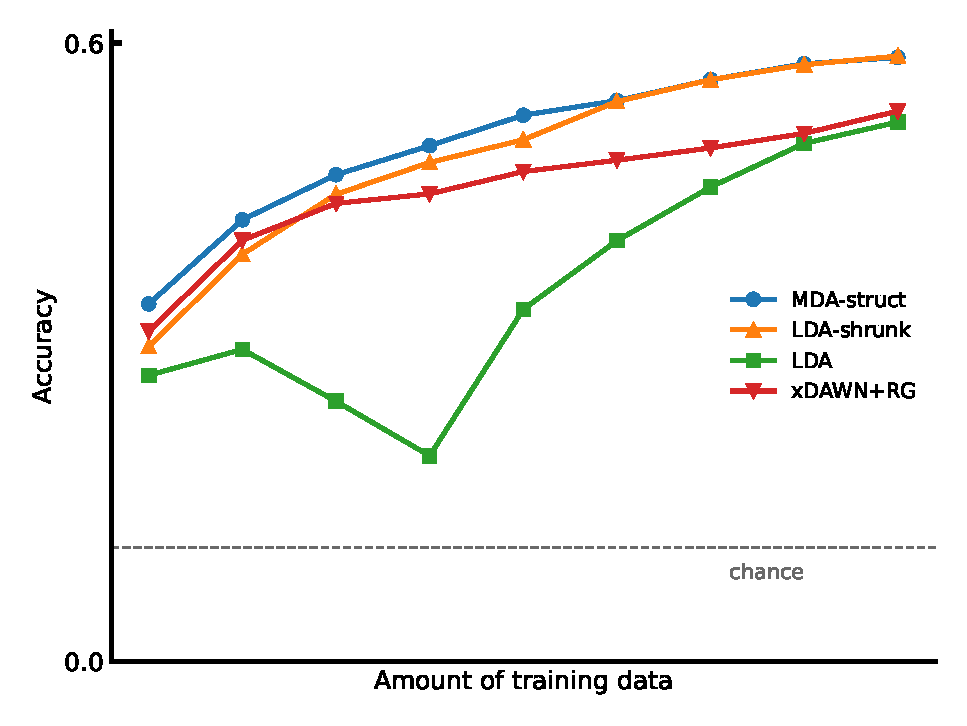
\includegraphics[width=.66\linewidth]{figures/stbf_struct/accuracy.eps}
    \sffamily
    \hspace{-0.4623567780166823in}
%% Creator: Matplotlib, PGF backend
%%
%% To include the figure in your LaTeX document, write
%%   \input{<filename>.pgf}
%%
%% Make sure the required packages are loaded in your preamble
%%   \usepackage{pgf}
%%
%% Also ensure that all the required font packages are loaded; for instance,
%% the lmodern package is sometimes necessary when using math font.
%%   \usepackage{lmodern}
%%
%% Figures using additional raster images can only be included by \input if
%% they are in the same directory as the main LaTeX file. For loading figures
%% from other directories you can use the `import` package
%%   \usepackage{import}
%%
%% and then include the figures with
%%   \import{<path to file>}{<filename>.pgf}
%%
%% Matplotlib used the following preamble
%%
\begingroup%
\makeatletter%
\begin{pgfpicture}%
\pgfpathrectangle{\pgfpointorigin}{\pgfqpoint{2.879017in}{1.916660in}}%
\pgfusepath{use as bounding box, clip}%
\begin{pgfscope}%
\pgfsetbuttcap%
\pgfsetmiterjoin%
\pgfsetlinewidth{0.000000pt}%
\definecolor{currentstroke}{rgb}{1.000000,1.000000,1.000000}%
\pgfsetstrokecolor{currentstroke}%
\pgfsetstrokeopacity{0.000000}%
\pgfsetdash{}{0pt}%
\pgfpathmoveto{\pgfqpoint{0.000000in}{0.000000in}}%
\pgfpathlineto{\pgfqpoint{2.879017in}{0.000000in}}%
\pgfpathlineto{\pgfqpoint{2.879017in}{1.916660in}}%
\pgfpathlineto{\pgfqpoint{0.000000in}{1.916660in}}%
\pgfpathlineto{\pgfqpoint{0.000000in}{0.000000in}}%
\pgfpathclose%
\pgfusepath{}%
\end{pgfscope}%
\begin{pgfscope}%
\pgfsetbuttcap%
\pgfsetmiterjoin%
\definecolor{currentfill}{rgb}{1.000000,1.000000,1.000000}%
\pgfsetfillcolor{currentfill}%
\pgfsetlinewidth{0.000000pt}%
\definecolor{currentstroke}{rgb}{0.000000,0.000000,0.000000}%
\pgfsetstrokecolor{currentstroke}%
\pgfsetstrokeopacity{0.000000}%
\pgfsetdash{}{0pt}%
\pgfpathmoveto{\pgfqpoint{0.421874in}{0.326389in}}%
\pgfpathlineto{\pgfqpoint{2.879017in}{0.326389in}}%
\pgfpathlineto{\pgfqpoint{2.879017in}{1.873257in}}%
\pgfpathlineto{\pgfqpoint{0.421874in}{1.873257in}}%
\pgfpathlineto{\pgfqpoint{0.421874in}{0.326389in}}%
\pgfpathclose%
\pgfusepath{fill}%
\end{pgfscope}%
\begin{pgfscope}%
\pgfsetbuttcap%
\pgfsetroundjoin%
\definecolor{currentfill}{rgb}{0.552941,0.501961,0.478431}%
\pgfsetfillcolor{currentfill}%
\pgfsetlinewidth{0.803000pt}%
\definecolor{currentstroke}{rgb}{0.552941,0.501961,0.478431}%
\pgfsetstrokecolor{currentstroke}%
\pgfsetdash{}{0pt}%
\pgfsys@defobject{currentmarker}{\pgfqpoint{0.000000in}{0.000000in}}{\pgfqpoint{0.000000in}{0.041667in}}{%
\pgfpathmoveto{\pgfqpoint{0.000000in}{0.000000in}}%
\pgfpathlineto{\pgfqpoint{0.000000in}{0.041667in}}%
\pgfusepath{stroke,fill}%
}%
\begin{pgfscope}%
\pgfsys@transformshift{0.812783in}{0.326389in}%
\pgfsys@useobject{currentmarker}{}%
\end{pgfscope}%
\end{pgfscope}%
\begin{pgfscope}%
\definecolor{textcolor}{rgb}{0.552941,0.501961,0.478431}%
\pgfsetstrokecolor{textcolor}%
\pgfsetfillcolor{textcolor}%
\pgftext[x=0.812783in,y=0.277778in,,top]{\color{textcolor}\sffamily\fontsize{9.000000}{10.800000}\selectfont 2}%
\end{pgfscope}%
\begin{pgfscope}%
\pgfsetbuttcap%
\pgfsetroundjoin%
\definecolor{currentfill}{rgb}{0.552941,0.501961,0.478431}%
\pgfsetfillcolor{currentfill}%
\pgfsetlinewidth{0.803000pt}%
\definecolor{currentstroke}{rgb}{0.552941,0.501961,0.478431}%
\pgfsetstrokecolor{currentstroke}%
\pgfsetdash{}{0pt}%
\pgfsys@defobject{currentmarker}{\pgfqpoint{0.000000in}{0.000000in}}{\pgfqpoint{0.000000in}{0.041667in}}{%
\pgfpathmoveto{\pgfqpoint{0.000000in}{0.000000in}}%
\pgfpathlineto{\pgfqpoint{0.000000in}{0.041667in}}%
\pgfusepath{stroke,fill}%
}%
\begin{pgfscope}%
\pgfsys@transformshift{1.371224in}{0.326389in}%
\pgfsys@useobject{currentmarker}{}%
\end{pgfscope}%
\end{pgfscope}%
\begin{pgfscope}%
\definecolor{textcolor}{rgb}{0.552941,0.501961,0.478431}%
\pgfsetstrokecolor{textcolor}%
\pgfsetfillcolor{textcolor}%
\pgftext[x=1.371224in,y=0.277778in,,top]{\color{textcolor}\sffamily\fontsize{9.000000}{10.800000}\selectfont 4}%
\end{pgfscope}%
\begin{pgfscope}%
\pgfsetbuttcap%
\pgfsetroundjoin%
\definecolor{currentfill}{rgb}{0.552941,0.501961,0.478431}%
\pgfsetfillcolor{currentfill}%
\pgfsetlinewidth{0.803000pt}%
\definecolor{currentstroke}{rgb}{0.552941,0.501961,0.478431}%
\pgfsetstrokecolor{currentstroke}%
\pgfsetdash{}{0pt}%
\pgfsys@defobject{currentmarker}{\pgfqpoint{0.000000in}{0.000000in}}{\pgfqpoint{0.000000in}{0.041667in}}{%
\pgfpathmoveto{\pgfqpoint{0.000000in}{0.000000in}}%
\pgfpathlineto{\pgfqpoint{0.000000in}{0.041667in}}%
\pgfusepath{stroke,fill}%
}%
\begin{pgfscope}%
\pgfsys@transformshift{1.929666in}{0.326389in}%
\pgfsys@useobject{currentmarker}{}%
\end{pgfscope}%
\end{pgfscope}%
\begin{pgfscope}%
\definecolor{textcolor}{rgb}{0.552941,0.501961,0.478431}%
\pgfsetstrokecolor{textcolor}%
\pgfsetfillcolor{textcolor}%
\pgftext[x=1.929666in,y=0.277778in,,top]{\color{textcolor}\sffamily\fontsize{9.000000}{10.800000}\selectfont 6}%
\end{pgfscope}%
\begin{pgfscope}%
\pgfsetbuttcap%
\pgfsetroundjoin%
\definecolor{currentfill}{rgb}{0.552941,0.501961,0.478431}%
\pgfsetfillcolor{currentfill}%
\pgfsetlinewidth{0.803000pt}%
\definecolor{currentstroke}{rgb}{0.552941,0.501961,0.478431}%
\pgfsetstrokecolor{currentstroke}%
\pgfsetdash{}{0pt}%
\pgfsys@defobject{currentmarker}{\pgfqpoint{0.000000in}{0.000000in}}{\pgfqpoint{0.000000in}{0.041667in}}{%
\pgfpathmoveto{\pgfqpoint{0.000000in}{0.000000in}}%
\pgfpathlineto{\pgfqpoint{0.000000in}{0.041667in}}%
\pgfusepath{stroke,fill}%
}%
\begin{pgfscope}%
\pgfsys@transformshift{2.488108in}{0.326389in}%
\pgfsys@useobject{currentmarker}{}%
\end{pgfscope}%
\end{pgfscope}%
\begin{pgfscope}%
\definecolor{textcolor}{rgb}{0.552941,0.501961,0.478431}%
\pgfsetstrokecolor{textcolor}%
\pgfsetfillcolor{textcolor}%
\pgftext[x=2.488108in,y=0.277778in,,top]{\color{textcolor}\sffamily\fontsize{9.000000}{10.800000}\selectfont 8}%
\end{pgfscope}%
\begin{pgfscope}%
\definecolor{textcolor}{rgb}{0.552941,0.501961,0.478431}%
\pgfsetstrokecolor{textcolor}%
\pgfsetfillcolor{textcolor}%
\pgftext[x=1.650445in,y=0.111111in,,top]{\color{textcolor}\sffamily\fontsize{9.000000}{10.800000}\selectfont Amount of training data}%
\end{pgfscope}%
\begin{pgfscope}%
\pgfsetbuttcap%
\pgfsetroundjoin%
\definecolor{currentfill}{rgb}{0.552941,0.501961,0.478431}%
\pgfsetfillcolor{currentfill}%
\pgfsetlinewidth{0.803000pt}%
\definecolor{currentstroke}{rgb}{0.552941,0.501961,0.478431}%
\pgfsetstrokecolor{currentstroke}%
\pgfsetdash{}{0pt}%
\pgfsys@defobject{currentmarker}{\pgfqpoint{0.000000in}{0.000000in}}{\pgfqpoint{0.041667in}{0.000000in}}{%
\pgfpathmoveto{\pgfqpoint{0.000000in}{0.000000in}}%
\pgfpathlineto{\pgfqpoint{0.041667in}{0.000000in}}%
\pgfusepath{stroke,fill}%
}%
\begin{pgfscope}%
\pgfsys@transformshift{0.421874in}{0.326389in}%
\pgfsys@useobject{currentmarker}{}%
\end{pgfscope}%
\end{pgfscope}%
\begin{pgfscope}%
\definecolor{textcolor}{rgb}{0.552941,0.501961,0.478431}%
\pgfsetstrokecolor{textcolor}%
\pgfsetfillcolor{textcolor}%
\pgftext[x=0.309027in, y=0.282986in, left, base]{\color{textcolor}\sffamily\fontsize{9.000000}{10.800000}\selectfont 0}%
\end{pgfscope}%
\begin{pgfscope}%
\pgfsetbuttcap%
\pgfsetroundjoin%
\definecolor{currentfill}{rgb}{0.552941,0.501961,0.478431}%
\pgfsetfillcolor{currentfill}%
\pgfsetlinewidth{0.803000pt}%
\definecolor{currentstroke}{rgb}{0.552941,0.501961,0.478431}%
\pgfsetstrokecolor{currentstroke}%
\pgfsetdash{}{0pt}%
\pgfsys@defobject{currentmarker}{\pgfqpoint{0.000000in}{0.000000in}}{\pgfqpoint{0.041667in}{0.000000in}}{%
\pgfpathmoveto{\pgfqpoint{0.000000in}{0.000000in}}%
\pgfpathlineto{\pgfqpoint{0.041667in}{0.000000in}}%
\pgfusepath{stroke,fill}%
}%
\begin{pgfscope}%
\pgfsys@transformshift{0.421874in}{0.635763in}%
\pgfsys@useobject{currentmarker}{}%
\end{pgfscope}%
\end{pgfscope}%
\begin{pgfscope}%
\definecolor{textcolor}{rgb}{0.552941,0.501961,0.478431}%
\pgfsetstrokecolor{textcolor}%
\pgfsetfillcolor{textcolor}%
\pgftext[x=0.244791in, y=0.592360in, left, base]{\color{textcolor}\sffamily\fontsize{9.000000}{10.800000}\selectfont 20}%
\end{pgfscope}%
\begin{pgfscope}%
\pgfsetbuttcap%
\pgfsetroundjoin%
\definecolor{currentfill}{rgb}{0.552941,0.501961,0.478431}%
\pgfsetfillcolor{currentfill}%
\pgfsetlinewidth{0.803000pt}%
\definecolor{currentstroke}{rgb}{0.552941,0.501961,0.478431}%
\pgfsetstrokecolor{currentstroke}%
\pgfsetdash{}{0pt}%
\pgfsys@defobject{currentmarker}{\pgfqpoint{0.000000in}{0.000000in}}{\pgfqpoint{0.041667in}{0.000000in}}{%
\pgfpathmoveto{\pgfqpoint{0.000000in}{0.000000in}}%
\pgfpathlineto{\pgfqpoint{0.041667in}{0.000000in}}%
\pgfusepath{stroke,fill}%
}%
\begin{pgfscope}%
\pgfsys@transformshift{0.421874in}{0.945136in}%
\pgfsys@useobject{currentmarker}{}%
\end{pgfscope}%
\end{pgfscope}%
\begin{pgfscope}%
\definecolor{textcolor}{rgb}{0.552941,0.501961,0.478431}%
\pgfsetstrokecolor{textcolor}%
\pgfsetfillcolor{textcolor}%
\pgftext[x=0.244791in, y=0.901733in, left, base]{\color{textcolor}\sffamily\fontsize{9.000000}{10.800000}\selectfont 40}%
\end{pgfscope}%
\begin{pgfscope}%
\pgfsetbuttcap%
\pgfsetroundjoin%
\definecolor{currentfill}{rgb}{0.552941,0.501961,0.478431}%
\pgfsetfillcolor{currentfill}%
\pgfsetlinewidth{0.803000pt}%
\definecolor{currentstroke}{rgb}{0.552941,0.501961,0.478431}%
\pgfsetstrokecolor{currentstroke}%
\pgfsetdash{}{0pt}%
\pgfsys@defobject{currentmarker}{\pgfqpoint{0.000000in}{0.000000in}}{\pgfqpoint{0.041667in}{0.000000in}}{%
\pgfpathmoveto{\pgfqpoint{0.000000in}{0.000000in}}%
\pgfpathlineto{\pgfqpoint{0.041667in}{0.000000in}}%
\pgfusepath{stroke,fill}%
}%
\begin{pgfscope}%
\pgfsys@transformshift{0.421874in}{1.254510in}%
\pgfsys@useobject{currentmarker}{}%
\end{pgfscope}%
\end{pgfscope}%
\begin{pgfscope}%
\definecolor{textcolor}{rgb}{0.552941,0.501961,0.478431}%
\pgfsetstrokecolor{textcolor}%
\pgfsetfillcolor{textcolor}%
\pgftext[x=0.244791in, y=1.211107in, left, base]{\color{textcolor}\sffamily\fontsize{9.000000}{10.800000}\selectfont 60}%
\end{pgfscope}%
\begin{pgfscope}%
\pgfsetbuttcap%
\pgfsetroundjoin%
\definecolor{currentfill}{rgb}{0.552941,0.501961,0.478431}%
\pgfsetfillcolor{currentfill}%
\pgfsetlinewidth{0.803000pt}%
\definecolor{currentstroke}{rgb}{0.552941,0.501961,0.478431}%
\pgfsetstrokecolor{currentstroke}%
\pgfsetdash{}{0pt}%
\pgfsys@defobject{currentmarker}{\pgfqpoint{0.000000in}{0.000000in}}{\pgfqpoint{0.041667in}{0.000000in}}{%
\pgfpathmoveto{\pgfqpoint{0.000000in}{0.000000in}}%
\pgfpathlineto{\pgfqpoint{0.041667in}{0.000000in}}%
\pgfusepath{stroke,fill}%
}%
\begin{pgfscope}%
\pgfsys@transformshift{0.421874in}{1.563884in}%
\pgfsys@useobject{currentmarker}{}%
\end{pgfscope}%
\end{pgfscope}%
\begin{pgfscope}%
\definecolor{textcolor}{rgb}{0.552941,0.501961,0.478431}%
\pgfsetstrokecolor{textcolor}%
\pgfsetfillcolor{textcolor}%
\pgftext[x=0.244791in, y=1.520481in, left, base]{\color{textcolor}\sffamily\fontsize{9.000000}{10.800000}\selectfont 80}%
\end{pgfscope}%
\begin{pgfscope}%
\pgfsetbuttcap%
\pgfsetroundjoin%
\definecolor{currentfill}{rgb}{0.552941,0.501961,0.478431}%
\pgfsetfillcolor{currentfill}%
\pgfsetlinewidth{0.803000pt}%
\definecolor{currentstroke}{rgb}{0.552941,0.501961,0.478431}%
\pgfsetstrokecolor{currentstroke}%
\pgfsetdash{}{0pt}%
\pgfsys@defobject{currentmarker}{\pgfqpoint{0.000000in}{0.000000in}}{\pgfqpoint{0.041667in}{0.000000in}}{%
\pgfpathmoveto{\pgfqpoint{0.000000in}{0.000000in}}%
\pgfpathlineto{\pgfqpoint{0.041667in}{0.000000in}}%
\pgfusepath{stroke,fill}%
}%
\begin{pgfscope}%
\pgfsys@transformshift{0.421874in}{1.873257in}%
\pgfsys@useobject{currentmarker}{}%
\end{pgfscope}%
\end{pgfscope}%
\begin{pgfscope}%
\definecolor{textcolor}{rgb}{0.552941,0.501961,0.478431}%
\pgfsetstrokecolor{textcolor}%
\pgfsetfillcolor{textcolor}%
\pgftext[x=0.180556in, y=1.829854in, left, base]{\color{textcolor}\sffamily\fontsize{9.000000}{10.800000}\selectfont 100}%
\end{pgfscope}%
\begin{pgfscope}%
\definecolor{textcolor}{rgb}{0.552941,0.501961,0.478431}%
\pgfsetstrokecolor{textcolor}%
\pgfsetfillcolor{textcolor}%
\pgftext[x=0.125000in,y=1.099823in,,bottom,rotate=90.000000]{\color{textcolor}\sffamily\fontsize{9.000000}{10.800000}\selectfont Accuracy (\%)}%
\end{pgfscope}%
\begin{pgfscope}%
\pgfpathrectangle{\pgfqpoint{0.421874in}{0.326389in}}{\pgfqpoint{2.457143in}{1.546868in}}%
\pgfusepath{clip}%
\pgfsetrectcap%
\pgfsetroundjoin%
\pgfsetlinewidth{1.505625pt}%
\definecolor{currentstroke}{rgb}{0.949020,0.564706,0.094118}%
\pgfsetstrokecolor{currentstroke}%
\pgfsetdash{}{0pt}%
\pgfpathmoveto{\pgfqpoint{0.533562in}{0.863155in}}%
\pgfpathlineto{\pgfqpoint{0.812783in}{0.989332in}}%
\pgfpathlineto{\pgfqpoint{1.092004in}{1.056854in}}%
\pgfpathlineto{\pgfqpoint{1.371224in}{1.100505in}}%
\pgfpathlineto{\pgfqpoint{1.650445in}{1.146202in}}%
\pgfpathlineto{\pgfqpoint{1.929666in}{1.168027in}}%
\pgfpathlineto{\pgfqpoint{2.208887in}{1.199401in}}%
\pgfpathlineto{\pgfqpoint{2.488108in}{1.223272in}}%
\pgfpathlineto{\pgfqpoint{2.767328in}{1.232821in}}%
\pgfusepath{stroke}%
\end{pgfscope}%
\begin{pgfscope}%
\pgfpathrectangle{\pgfqpoint{0.421874in}{0.326389in}}{\pgfqpoint{2.457143in}{1.546868in}}%
\pgfusepath{clip}%
\pgfsetbuttcap%
\pgfsetmiterjoin%
\definecolor{currentfill}{rgb}{0.949020,0.564706,0.094118}%
\pgfsetfillcolor{currentfill}%
\pgfsetlinewidth{0.000000pt}%
\definecolor{currentstroke}{rgb}{1.000000,1.000000,1.000000}%
\pgfsetstrokecolor{currentstroke}%
\pgfsetdash{}{0pt}%
\pgfsys@defobject{currentmarker}{\pgfqpoint{-0.020833in}{-0.020833in}}{\pgfqpoint{0.020833in}{0.020833in}}{%
\pgfpathmoveto{\pgfqpoint{-0.020833in}{-0.020833in}}%
\pgfpathlineto{\pgfqpoint{0.020833in}{-0.020833in}}%
\pgfpathlineto{\pgfqpoint{0.020833in}{0.020833in}}%
\pgfpathlineto{\pgfqpoint{-0.020833in}{0.020833in}}%
\pgfpathlineto{\pgfqpoint{-0.020833in}{-0.020833in}}%
\pgfpathclose%
\pgfusepath{fill}%
}%
\begin{pgfscope}%
\pgfsys@transformshift{0.533562in}{0.863155in}%
\pgfsys@useobject{currentmarker}{}%
\end{pgfscope}%
\begin{pgfscope}%
\pgfsys@transformshift{0.812783in}{0.989332in}%
\pgfsys@useobject{currentmarker}{}%
\end{pgfscope}%
\begin{pgfscope}%
\pgfsys@transformshift{1.092004in}{1.056854in}%
\pgfsys@useobject{currentmarker}{}%
\end{pgfscope}%
\begin{pgfscope}%
\pgfsys@transformshift{1.371224in}{1.100505in}%
\pgfsys@useobject{currentmarker}{}%
\end{pgfscope}%
\begin{pgfscope}%
\pgfsys@transformshift{1.650445in}{1.146202in}%
\pgfsys@useobject{currentmarker}{}%
\end{pgfscope}%
\begin{pgfscope}%
\pgfsys@transformshift{1.929666in}{1.168027in}%
\pgfsys@useobject{currentmarker}{}%
\end{pgfscope}%
\begin{pgfscope}%
\pgfsys@transformshift{2.208887in}{1.199401in}%
\pgfsys@useobject{currentmarker}{}%
\end{pgfscope}%
\begin{pgfscope}%
\pgfsys@transformshift{2.488108in}{1.223272in}%
\pgfsys@useobject{currentmarker}{}%
\end{pgfscope}%
\begin{pgfscope}%
\pgfsys@transformshift{2.767328in}{1.232821in}%
\pgfsys@useobject{currentmarker}{}%
\end{pgfscope}%
\end{pgfscope}%
\begin{pgfscope}%
\pgfpathrectangle{\pgfqpoint{0.421874in}{0.326389in}}{\pgfqpoint{2.457143in}{1.546868in}}%
\pgfusepath{clip}%
\pgfsetrectcap%
\pgfsetroundjoin%
\pgfsetlinewidth{1.505625pt}%
\definecolor{currentstroke}{rgb}{0.964706,0.239216,0.117647}%
\pgfsetstrokecolor{currentstroke}%
\pgfsetdash{}{0pt}%
\pgfpathmoveto{\pgfqpoint{0.533562in}{0.799043in}}%
\pgfpathlineto{\pgfqpoint{0.812783in}{0.937497in}}%
\pgfpathlineto{\pgfqpoint{1.092004in}{1.027527in}}%
\pgfpathlineto{\pgfqpoint{1.371224in}{1.075270in}}%
\pgfpathlineto{\pgfqpoint{1.650445in}{1.109372in}}%
\pgfpathlineto{\pgfqpoint{1.929666in}{1.166663in}}%
\pgfpathlineto{\pgfqpoint{2.208887in}{1.199401in}}%
\pgfpathlineto{\pgfqpoint{2.488108in}{1.221908in}}%
\pgfpathlineto{\pgfqpoint{2.767328in}{1.234867in}}%
\pgfusepath{stroke}%
\end{pgfscope}%
\begin{pgfscope}%
\pgfpathrectangle{\pgfqpoint{0.421874in}{0.326389in}}{\pgfqpoint{2.457143in}{1.546868in}}%
\pgfusepath{clip}%
\pgfsetbuttcap%
\pgfsetmiterjoin%
\definecolor{currentfill}{rgb}{0.964706,0.239216,0.117647}%
\pgfsetfillcolor{currentfill}%
\pgfsetlinewidth{0.000000pt}%
\definecolor{currentstroke}{rgb}{1.000000,1.000000,1.000000}%
\pgfsetstrokecolor{currentstroke}%
\pgfsetdash{}{0pt}%
\pgfsys@defobject{currentmarker}{\pgfqpoint{-0.029463in}{-0.029463in}}{\pgfqpoint{0.029463in}{0.029463in}}{%
\pgfpathmoveto{\pgfqpoint{-0.000000in}{-0.029463in}}%
\pgfpathlineto{\pgfqpoint{0.029463in}{0.000000in}}%
\pgfpathlineto{\pgfqpoint{0.000000in}{0.029463in}}%
\pgfpathlineto{\pgfqpoint{-0.029463in}{0.000000in}}%
\pgfpathlineto{\pgfqpoint{-0.000000in}{-0.029463in}}%
\pgfpathclose%
\pgfusepath{fill}%
}%
\begin{pgfscope}%
\pgfsys@transformshift{0.533562in}{0.799043in}%
\pgfsys@useobject{currentmarker}{}%
\end{pgfscope}%
\begin{pgfscope}%
\pgfsys@transformshift{0.812783in}{0.937497in}%
\pgfsys@useobject{currentmarker}{}%
\end{pgfscope}%
\begin{pgfscope}%
\pgfsys@transformshift{1.092004in}{1.027527in}%
\pgfsys@useobject{currentmarker}{}%
\end{pgfscope}%
\begin{pgfscope}%
\pgfsys@transformshift{1.371224in}{1.075270in}%
\pgfsys@useobject{currentmarker}{}%
\end{pgfscope}%
\begin{pgfscope}%
\pgfsys@transformshift{1.650445in}{1.109372in}%
\pgfsys@useobject{currentmarker}{}%
\end{pgfscope}%
\begin{pgfscope}%
\pgfsys@transformshift{1.929666in}{1.166663in}%
\pgfsys@useobject{currentmarker}{}%
\end{pgfscope}%
\begin{pgfscope}%
\pgfsys@transformshift{2.208887in}{1.199401in}%
\pgfsys@useobject{currentmarker}{}%
\end{pgfscope}%
\begin{pgfscope}%
\pgfsys@transformshift{2.488108in}{1.221908in}%
\pgfsys@useobject{currentmarker}{}%
\end{pgfscope}%
\begin{pgfscope}%
\pgfsys@transformshift{2.767328in}{1.234867in}%
\pgfsys@useobject{currentmarker}{}%
\end{pgfscope}%
\end{pgfscope}%
\begin{pgfscope}%
\pgfpathrectangle{\pgfqpoint{0.421874in}{0.326389in}}{\pgfqpoint{2.457143in}{1.546868in}}%
\pgfusepath{clip}%
\pgfsetrectcap%
\pgfsetroundjoin%
\pgfsetlinewidth{1.505625pt}%
\definecolor{currentstroke}{rgb}{0.470588,0.278431,0.615686}%
\pgfsetstrokecolor{currentstroke}%
\pgfsetdash{}{0pt}%
\pgfpathmoveto{\pgfqpoint{0.533562in}{0.756075in}}%
\pgfpathlineto{\pgfqpoint{0.812783in}{0.794951in}}%
\pgfpathlineto{\pgfqpoint{1.092004in}{0.717198in}}%
\pgfpathlineto{\pgfqpoint{1.371224in}{0.635353in}}%
\pgfpathlineto{\pgfqpoint{1.650445in}{0.854970in}}%
\pgfpathlineto{\pgfqpoint{1.929666in}{0.957959in}}%
\pgfpathlineto{\pgfqpoint{2.208887in}{1.038439in}}%
\pgfpathlineto{\pgfqpoint{2.488108in}{1.103915in}}%
\pgfpathlineto{\pgfqpoint{2.767328in}{1.135971in}}%
\pgfusepath{stroke}%
\end{pgfscope}%
\begin{pgfscope}%
\pgfpathrectangle{\pgfqpoint{0.421874in}{0.326389in}}{\pgfqpoint{2.457143in}{1.546868in}}%
\pgfusepath{clip}%
\pgfsetbuttcap%
\pgfsetroundjoin%
\definecolor{currentfill}{rgb}{0.470588,0.278431,0.615686}%
\pgfsetfillcolor{currentfill}%
\pgfsetlinewidth{0.000000pt}%
\definecolor{currentstroke}{rgb}{1.000000,1.000000,1.000000}%
\pgfsetstrokecolor{currentstroke}%
\pgfsetdash{}{0pt}%
\pgfsys@defobject{currentmarker}{\pgfqpoint{-0.020833in}{-0.020833in}}{\pgfqpoint{0.020833in}{0.020833in}}{%
\pgfpathmoveto{\pgfqpoint{0.000000in}{-0.020833in}}%
\pgfpathcurveto{\pgfqpoint{0.005525in}{-0.020833in}}{\pgfqpoint{0.010825in}{-0.018638in}}{\pgfqpoint{0.014731in}{-0.014731in}}%
\pgfpathcurveto{\pgfqpoint{0.018638in}{-0.010825in}}{\pgfqpoint{0.020833in}{-0.005525in}}{\pgfqpoint{0.020833in}{0.000000in}}%
\pgfpathcurveto{\pgfqpoint{0.020833in}{0.005525in}}{\pgfqpoint{0.018638in}{0.010825in}}{\pgfqpoint{0.014731in}{0.014731in}}%
\pgfpathcurveto{\pgfqpoint{0.010825in}{0.018638in}}{\pgfqpoint{0.005525in}{0.020833in}}{\pgfqpoint{0.000000in}{0.020833in}}%
\pgfpathcurveto{\pgfqpoint{-0.005525in}{0.020833in}}{\pgfqpoint{-0.010825in}{0.018638in}}{\pgfqpoint{-0.014731in}{0.014731in}}%
\pgfpathcurveto{\pgfqpoint{-0.018638in}{0.010825in}}{\pgfqpoint{-0.020833in}{0.005525in}}{\pgfqpoint{-0.020833in}{0.000000in}}%
\pgfpathcurveto{\pgfqpoint{-0.020833in}{-0.005525in}}{\pgfqpoint{-0.018638in}{-0.010825in}}{\pgfqpoint{-0.014731in}{-0.014731in}}%
\pgfpathcurveto{\pgfqpoint{-0.010825in}{-0.018638in}}{\pgfqpoint{-0.005525in}{-0.020833in}}{\pgfqpoint{0.000000in}{-0.020833in}}%
\pgfpathlineto{\pgfqpoint{0.000000in}{-0.020833in}}%
\pgfpathclose%
\pgfusepath{fill}%
}%
\begin{pgfscope}%
\pgfsys@transformshift{0.533562in}{0.756075in}%
\pgfsys@useobject{currentmarker}{}%
\end{pgfscope}%
\begin{pgfscope}%
\pgfsys@transformshift{0.812783in}{0.794951in}%
\pgfsys@useobject{currentmarker}{}%
\end{pgfscope}%
\begin{pgfscope}%
\pgfsys@transformshift{1.092004in}{0.717198in}%
\pgfsys@useobject{currentmarker}{}%
\end{pgfscope}%
\begin{pgfscope}%
\pgfsys@transformshift{1.371224in}{0.635353in}%
\pgfsys@useobject{currentmarker}{}%
\end{pgfscope}%
\begin{pgfscope}%
\pgfsys@transformshift{1.650445in}{0.854970in}%
\pgfsys@useobject{currentmarker}{}%
\end{pgfscope}%
\begin{pgfscope}%
\pgfsys@transformshift{1.929666in}{0.957959in}%
\pgfsys@useobject{currentmarker}{}%
\end{pgfscope}%
\begin{pgfscope}%
\pgfsys@transformshift{2.208887in}{1.038439in}%
\pgfsys@useobject{currentmarker}{}%
\end{pgfscope}%
\begin{pgfscope}%
\pgfsys@transformshift{2.488108in}{1.103915in}%
\pgfsys@useobject{currentmarker}{}%
\end{pgfscope}%
\begin{pgfscope}%
\pgfsys@transformshift{2.767328in}{1.135971in}%
\pgfsys@useobject{currentmarker}{}%
\end{pgfscope}%
\end{pgfscope}%
\begin{pgfscope}%
\pgfpathrectangle{\pgfqpoint{0.421874in}{0.326389in}}{\pgfqpoint{2.457143in}{1.546868in}}%
\pgfusepath{clip}%
\pgfsetrectcap%
\pgfsetroundjoin%
\pgfsetlinewidth{1.505625pt}%
\definecolor{currentstroke}{rgb}{0.454902,0.643137,0.737255}%
\pgfsetstrokecolor{currentstroke}%
\pgfsetdash{}{0pt}%
\pgfpathmoveto{\pgfqpoint{0.533562in}{0.822232in}}%
\pgfpathlineto{\pgfqpoint{0.812783in}{0.958641in}}%
\pgfpathlineto{\pgfqpoint{1.092004in}{1.013886in}}%
\pgfpathlineto{\pgfqpoint{1.371224in}{1.028209in}}%
\pgfpathlineto{\pgfqpoint{1.650445in}{1.061629in}}%
\pgfpathlineto{\pgfqpoint{1.929666in}{1.078680in}}%
\pgfpathlineto{\pgfqpoint{2.208887in}{1.097095in}}%
\pgfpathlineto{\pgfqpoint{2.488108in}{1.118920in}}%
\pgfpathlineto{\pgfqpoint{2.767328in}{1.152340in}}%
\pgfusepath{stroke}%
\end{pgfscope}%
\begin{pgfscope}%
\pgfpathrectangle{\pgfqpoint{0.421874in}{0.326389in}}{\pgfqpoint{2.457143in}{1.546868in}}%
\pgfusepath{clip}%
\pgfsetbuttcap%
\pgfsetmiterjoin%
\definecolor{currentfill}{rgb}{0.454902,0.643137,0.737255}%
\pgfsetfillcolor{currentfill}%
\pgfsetlinewidth{0.000000pt}%
\definecolor{currentstroke}{rgb}{1.000000,1.000000,1.000000}%
\pgfsetstrokecolor{currentstroke}%
\pgfsetdash{}{0pt}%
\pgfsys@defobject{currentmarker}{\pgfqpoint{-0.020833in}{-0.020833in}}{\pgfqpoint{0.020833in}{0.020833in}}{%
\pgfpathmoveto{\pgfqpoint{-0.006944in}{-0.020833in}}%
\pgfpathlineto{\pgfqpoint{0.006944in}{-0.020833in}}%
\pgfpathlineto{\pgfqpoint{0.006944in}{-0.006944in}}%
\pgfpathlineto{\pgfqpoint{0.020833in}{-0.006944in}}%
\pgfpathlineto{\pgfqpoint{0.020833in}{0.006944in}}%
\pgfpathlineto{\pgfqpoint{0.006944in}{0.006944in}}%
\pgfpathlineto{\pgfqpoint{0.006944in}{0.020833in}}%
\pgfpathlineto{\pgfqpoint{-0.006944in}{0.020833in}}%
\pgfpathlineto{\pgfqpoint{-0.006944in}{0.006944in}}%
\pgfpathlineto{\pgfqpoint{-0.020833in}{0.006944in}}%
\pgfpathlineto{\pgfqpoint{-0.020833in}{-0.006944in}}%
\pgfpathlineto{\pgfqpoint{-0.006944in}{-0.006944in}}%
\pgfpathlineto{\pgfqpoint{-0.006944in}{-0.020833in}}%
\pgfpathclose%
\pgfusepath{fill}%
}%
\begin{pgfscope}%
\pgfsys@transformshift{0.533562in}{0.822232in}%
\pgfsys@useobject{currentmarker}{}%
\end{pgfscope}%
\begin{pgfscope}%
\pgfsys@transformshift{0.812783in}{0.958641in}%
\pgfsys@useobject{currentmarker}{}%
\end{pgfscope}%
\begin{pgfscope}%
\pgfsys@transformshift{1.092004in}{1.013886in}%
\pgfsys@useobject{currentmarker}{}%
\end{pgfscope}%
\begin{pgfscope}%
\pgfsys@transformshift{1.371224in}{1.028209in}%
\pgfsys@useobject{currentmarker}{}%
\end{pgfscope}%
\begin{pgfscope}%
\pgfsys@transformshift{1.650445in}{1.061629in}%
\pgfsys@useobject{currentmarker}{}%
\end{pgfscope}%
\begin{pgfscope}%
\pgfsys@transformshift{1.929666in}{1.078680in}%
\pgfsys@useobject{currentmarker}{}%
\end{pgfscope}%
\begin{pgfscope}%
\pgfsys@transformshift{2.208887in}{1.097095in}%
\pgfsys@useobject{currentmarker}{}%
\end{pgfscope}%
\begin{pgfscope}%
\pgfsys@transformshift{2.488108in}{1.118920in}%
\pgfsys@useobject{currentmarker}{}%
\end{pgfscope}%
\begin{pgfscope}%
\pgfsys@transformshift{2.767328in}{1.152340in}%
\pgfsys@useobject{currentmarker}{}%
\end{pgfscope}%
\end{pgfscope}%
\begin{pgfscope}%
\pgfpathrectangle{\pgfqpoint{0.421874in}{0.326389in}}{\pgfqpoint{2.457143in}{1.546868in}}%
\pgfusepath{clip}%
\pgfsetbuttcap%
\pgfsetroundjoin%
\pgfsetlinewidth{1.003750pt}%
\definecolor{currentstroke}{rgb}{0.878431,0.878431,0.878431}%
\pgfsetstrokecolor{currentstroke}%
\pgfsetdash{{3.700000pt}{1.600000pt}}{0.000000pt}%
\pgfpathmoveto{\pgfqpoint{0.421874in}{0.498263in}}%
\pgfpathlineto{\pgfqpoint{2.879017in}{0.498263in}}%
\pgfusepath{stroke}%
\end{pgfscope}%
\begin{pgfscope}%
\pgfsetrectcap%
\pgfsetmiterjoin%
\pgfsetlinewidth{0.803000pt}%
\definecolor{currentstroke}{rgb}{0.552941,0.501961,0.478431}%
\pgfsetstrokecolor{currentstroke}%
\pgfsetdash{}{0pt}%
\pgfpathmoveto{\pgfqpoint{0.421874in}{0.326389in}}%
\pgfpathlineto{\pgfqpoint{0.421874in}{1.873257in}}%
\pgfusepath{stroke}%
\end{pgfscope}%
\begin{pgfscope}%
\pgfsetrectcap%
\pgfsetmiterjoin%
\pgfsetlinewidth{0.803000pt}%
\definecolor{currentstroke}{rgb}{0.552941,0.501961,0.478431}%
\pgfsetstrokecolor{currentstroke}%
\pgfsetdash{}{0pt}%
\pgfpathmoveto{\pgfqpoint{2.879017in}{0.326389in}}%
\pgfpathlineto{\pgfqpoint{2.879017in}{1.873257in}}%
\pgfusepath{stroke}%
\end{pgfscope}%
\begin{pgfscope}%
\pgfsetrectcap%
\pgfsetmiterjoin%
\pgfsetlinewidth{0.803000pt}%
\definecolor{currentstroke}{rgb}{0.552941,0.501961,0.478431}%
\pgfsetstrokecolor{currentstroke}%
\pgfsetdash{}{0pt}%
\pgfpathmoveto{\pgfqpoint{0.421874in}{0.326389in}}%
\pgfpathlineto{\pgfqpoint{2.879017in}{0.326389in}}%
\pgfusepath{stroke}%
\end{pgfscope}%
\begin{pgfscope}%
\pgfsetrectcap%
\pgfsetmiterjoin%
\pgfsetlinewidth{0.803000pt}%
\definecolor{currentstroke}{rgb}{0.552941,0.501961,0.478431}%
\pgfsetstrokecolor{currentstroke}%
\pgfsetdash{}{0pt}%
\pgfpathmoveto{\pgfqpoint{0.421874in}{1.873257in}}%
\pgfpathlineto{\pgfqpoint{2.879017in}{1.873257in}}%
\pgfusepath{stroke}%
\end{pgfscope}%
\begin{pgfscope}%
\pgfsetbuttcap%
\pgfsetmiterjoin%
\definecolor{currentfill}{rgb}{1.000000,1.000000,1.000000}%
\pgfsetfillcolor{currentfill}%
\pgfsetlinewidth{0.000000pt}%
\definecolor{currentstroke}{rgb}{0.000000,0.000000,0.000000}%
\pgfsetstrokecolor{currentstroke}%
\pgfsetdash{}{0pt}%
\pgfpathmoveto{\pgfqpoint{0.544731in}{0.532638in}}%
\pgfpathlineto{\pgfqpoint{0.910469in}{0.532638in}}%
\pgfpathlineto{\pgfqpoint{0.910469in}{0.643749in}}%
\pgfpathlineto{\pgfqpoint{0.544731in}{0.643749in}}%
\pgfpathlineto{\pgfqpoint{0.544731in}{0.532638in}}%
\pgfpathclose%
\pgfusepath{fill}%
\end{pgfscope}%
\begin{pgfscope}%
\definecolor{textcolor}{rgb}{0.552941,0.501961,0.478431}%
\pgfsetstrokecolor{textcolor}%
\pgfsetfillcolor{textcolor}%
\pgftext[x=0.544731in,y=0.532638in,left,bottom]{\color{textcolor}\sffamily\fontsize{9.000000}{10.800000}\selectfont chance}%
\end{pgfscope}%
\begin{pgfscope}%
\pgfsetbuttcap%
\pgfsetmiterjoin%
\pgfsetlinewidth{0.000000pt}%
\definecolor{currentstroke}{rgb}{0.000000,0.000000,0.000000}%
\pgfsetstrokecolor{currentstroke}%
\pgfsetstrokeopacity{0.000000}%
\pgfsetdash{}{0pt}%
\pgfpathmoveto{\pgfqpoint{0.509374in}{1.097641in}}%
\pgfpathlineto{\pgfqpoint{1.493896in}{1.097641in}}%
\pgfpathquadraticcurveto{\pgfqpoint{1.518896in}{1.097641in}}{\pgfqpoint{1.518896in}{1.122641in}}%
\pgfpathlineto{\pgfqpoint{1.518896in}{1.785757in}}%
\pgfpathquadraticcurveto{\pgfqpoint{1.518896in}{1.810757in}}{\pgfqpoint{1.493896in}{1.810757in}}%
\pgfpathlineto{\pgfqpoint{0.509374in}{1.810757in}}%
\pgfpathquadraticcurveto{\pgfqpoint{0.484374in}{1.810757in}}{\pgfqpoint{0.484374in}{1.785757in}}%
\pgfpathlineto{\pgfqpoint{0.484374in}{1.122641in}}%
\pgfpathquadraticcurveto{\pgfqpoint{0.484374in}{1.097641in}}{\pgfqpoint{0.509374in}{1.097641in}}%
\pgfpathlineto{\pgfqpoint{0.509374in}{1.097641in}}%
\pgfpathclose%
\pgfusepath{}%
\end{pgfscope}%
\begin{pgfscope}%
\pgfsetrectcap%
\pgfsetroundjoin%
\pgfsetlinewidth{1.505625pt}%
\definecolor{currentstroke}{rgb}{0.949020,0.564706,0.094118}%
\pgfsetstrokecolor{currentstroke}%
\pgfsetdash{}{0pt}%
\pgfpathmoveto{\pgfqpoint{0.534374in}{1.717007in}}%
\pgfpathlineto{\pgfqpoint{0.659374in}{1.717007in}}%
\pgfpathlineto{\pgfqpoint{0.784374in}{1.717007in}}%
\pgfusepath{stroke}%
\end{pgfscope}%
\begin{pgfscope}%
\pgfsetbuttcap%
\pgfsetmiterjoin%
\definecolor{currentfill}{rgb}{0.949020,0.564706,0.094118}%
\pgfsetfillcolor{currentfill}%
\pgfsetlinewidth{0.000000pt}%
\definecolor{currentstroke}{rgb}{1.000000,1.000000,1.000000}%
\pgfsetstrokecolor{currentstroke}%
\pgfsetdash{}{0pt}%
\pgfsys@defobject{currentmarker}{\pgfqpoint{-0.020833in}{-0.020833in}}{\pgfqpoint{0.020833in}{0.020833in}}{%
\pgfpathmoveto{\pgfqpoint{-0.020833in}{-0.020833in}}%
\pgfpathlineto{\pgfqpoint{0.020833in}{-0.020833in}}%
\pgfpathlineto{\pgfqpoint{0.020833in}{0.020833in}}%
\pgfpathlineto{\pgfqpoint{-0.020833in}{0.020833in}}%
\pgfpathlineto{\pgfqpoint{-0.020833in}{-0.020833in}}%
\pgfpathclose%
\pgfusepath{fill}%
}%
\begin{pgfscope}%
\pgfsys@transformshift{0.659374in}{1.717007in}%
\pgfsys@useobject{currentmarker}{}%
\end{pgfscope}%
\end{pgfscope}%
\begin{pgfscope}%
\definecolor{textcolor}{rgb}{0.552941,0.501961,0.478431}%
\pgfsetstrokecolor{textcolor}%
\pgfsetfillcolor{textcolor}%
\pgftext[x=0.884374in,y=1.673257in,left,base]{\color{textcolor}\sffamily\fontsize{7.000000}{8.400000}\selectfont STBF-struct}%
\end{pgfscope}%
\begin{pgfscope}%
\pgfsetrectcap%
\pgfsetroundjoin%
\pgfsetlinewidth{1.505625pt}%
\definecolor{currentstroke}{rgb}{0.964706,0.239216,0.117647}%
\pgfsetstrokecolor{currentstroke}%
\pgfsetdash{}{0pt}%
\pgfpathmoveto{\pgfqpoint{0.534374in}{1.548103in}}%
\pgfpathlineto{\pgfqpoint{0.659374in}{1.548103in}}%
\pgfpathlineto{\pgfqpoint{0.784374in}{1.548103in}}%
\pgfusepath{stroke}%
\end{pgfscope}%
\begin{pgfscope}%
\pgfsetbuttcap%
\pgfsetmiterjoin%
\definecolor{currentfill}{rgb}{0.964706,0.239216,0.117647}%
\pgfsetfillcolor{currentfill}%
\pgfsetlinewidth{0.000000pt}%
\definecolor{currentstroke}{rgb}{1.000000,1.000000,1.000000}%
\pgfsetstrokecolor{currentstroke}%
\pgfsetdash{}{0pt}%
\pgfsys@defobject{currentmarker}{\pgfqpoint{-0.029463in}{-0.029463in}}{\pgfqpoint{0.029463in}{0.029463in}}{%
\pgfpathmoveto{\pgfqpoint{-0.000000in}{-0.029463in}}%
\pgfpathlineto{\pgfqpoint{0.029463in}{0.000000in}}%
\pgfpathlineto{\pgfqpoint{0.000000in}{0.029463in}}%
\pgfpathlineto{\pgfqpoint{-0.029463in}{0.000000in}}%
\pgfpathlineto{\pgfqpoint{-0.000000in}{-0.029463in}}%
\pgfpathclose%
\pgfusepath{fill}%
}%
\begin{pgfscope}%
\pgfsys@transformshift{0.659374in}{1.548103in}%
\pgfsys@useobject{currentmarker}{}%
\end{pgfscope}%
\end{pgfscope}%
\begin{pgfscope}%
\definecolor{textcolor}{rgb}{0.552941,0.501961,0.478431}%
\pgfsetstrokecolor{textcolor}%
\pgfsetfillcolor{textcolor}%
\pgftext[x=0.884374in,y=1.504353in,left,base]{\color{textcolor}\sffamily\fontsize{7.000000}{8.400000}\selectfont STBF-shrunk}%
\end{pgfscope}%
\begin{pgfscope}%
\pgfsetrectcap%
\pgfsetroundjoin%
\pgfsetlinewidth{1.505625pt}%
\definecolor{currentstroke}{rgb}{0.470588,0.278431,0.615686}%
\pgfsetstrokecolor{currentstroke}%
\pgfsetdash{}{0pt}%
\pgfpathmoveto{\pgfqpoint{0.534374in}{1.379199in}}%
\pgfpathlineto{\pgfqpoint{0.659374in}{1.379199in}}%
\pgfpathlineto{\pgfqpoint{0.784374in}{1.379199in}}%
\pgfusepath{stroke}%
\end{pgfscope}%
\begin{pgfscope}%
\pgfsetbuttcap%
\pgfsetroundjoin%
\definecolor{currentfill}{rgb}{0.470588,0.278431,0.615686}%
\pgfsetfillcolor{currentfill}%
\pgfsetlinewidth{0.000000pt}%
\definecolor{currentstroke}{rgb}{1.000000,1.000000,1.000000}%
\pgfsetstrokecolor{currentstroke}%
\pgfsetdash{}{0pt}%
\pgfsys@defobject{currentmarker}{\pgfqpoint{-0.020833in}{-0.020833in}}{\pgfqpoint{0.020833in}{0.020833in}}{%
\pgfpathmoveto{\pgfqpoint{0.000000in}{-0.020833in}}%
\pgfpathcurveto{\pgfqpoint{0.005525in}{-0.020833in}}{\pgfqpoint{0.010825in}{-0.018638in}}{\pgfqpoint{0.014731in}{-0.014731in}}%
\pgfpathcurveto{\pgfqpoint{0.018638in}{-0.010825in}}{\pgfqpoint{0.020833in}{-0.005525in}}{\pgfqpoint{0.020833in}{0.000000in}}%
\pgfpathcurveto{\pgfqpoint{0.020833in}{0.005525in}}{\pgfqpoint{0.018638in}{0.010825in}}{\pgfqpoint{0.014731in}{0.014731in}}%
\pgfpathcurveto{\pgfqpoint{0.010825in}{0.018638in}}{\pgfqpoint{0.005525in}{0.020833in}}{\pgfqpoint{0.000000in}{0.020833in}}%
\pgfpathcurveto{\pgfqpoint{-0.005525in}{0.020833in}}{\pgfqpoint{-0.010825in}{0.018638in}}{\pgfqpoint{-0.014731in}{0.014731in}}%
\pgfpathcurveto{\pgfqpoint{-0.018638in}{0.010825in}}{\pgfqpoint{-0.020833in}{0.005525in}}{\pgfqpoint{-0.020833in}{0.000000in}}%
\pgfpathcurveto{\pgfqpoint{-0.020833in}{-0.005525in}}{\pgfqpoint{-0.018638in}{-0.010825in}}{\pgfqpoint{-0.014731in}{-0.014731in}}%
\pgfpathcurveto{\pgfqpoint{-0.010825in}{-0.018638in}}{\pgfqpoint{-0.005525in}{-0.020833in}}{\pgfqpoint{0.000000in}{-0.020833in}}%
\pgfpathlineto{\pgfqpoint{0.000000in}{-0.020833in}}%
\pgfpathclose%
\pgfusepath{fill}%
}%
\begin{pgfscope}%
\pgfsys@transformshift{0.659374in}{1.379199in}%
\pgfsys@useobject{currentmarker}{}%
\end{pgfscope}%
\end{pgfscope}%
\begin{pgfscope}%
\definecolor{textcolor}{rgb}{0.552941,0.501961,0.478431}%
\pgfsetstrokecolor{textcolor}%
\pgfsetfillcolor{textcolor}%
\pgftext[x=0.884374in,y=1.335449in,left,base]{\color{textcolor}\sffamily\fontsize{7.000000}{8.400000}\selectfont STBF-emp}%
\end{pgfscope}%
\begin{pgfscope}%
\pgfsetrectcap%
\pgfsetroundjoin%
\pgfsetlinewidth{1.505625pt}%
\definecolor{currentstroke}{rgb}{0.454902,0.643137,0.737255}%
\pgfsetstrokecolor{currentstroke}%
\pgfsetdash{}{0pt}%
\pgfpathmoveto{\pgfqpoint{0.534374in}{1.210295in}}%
\pgfpathlineto{\pgfqpoint{0.659374in}{1.210295in}}%
\pgfpathlineto{\pgfqpoint{0.784374in}{1.210295in}}%
\pgfusepath{stroke}%
\end{pgfscope}%
\begin{pgfscope}%
\pgfsetbuttcap%
\pgfsetmiterjoin%
\definecolor{currentfill}{rgb}{0.454902,0.643137,0.737255}%
\pgfsetfillcolor{currentfill}%
\pgfsetlinewidth{0.000000pt}%
\definecolor{currentstroke}{rgb}{1.000000,1.000000,1.000000}%
\pgfsetstrokecolor{currentstroke}%
\pgfsetdash{}{0pt}%
\pgfsys@defobject{currentmarker}{\pgfqpoint{-0.020833in}{-0.020833in}}{\pgfqpoint{0.020833in}{0.020833in}}{%
\pgfpathmoveto{\pgfqpoint{-0.006944in}{-0.020833in}}%
\pgfpathlineto{\pgfqpoint{0.006944in}{-0.020833in}}%
\pgfpathlineto{\pgfqpoint{0.006944in}{-0.006944in}}%
\pgfpathlineto{\pgfqpoint{0.020833in}{-0.006944in}}%
\pgfpathlineto{\pgfqpoint{0.020833in}{0.006944in}}%
\pgfpathlineto{\pgfqpoint{0.006944in}{0.006944in}}%
\pgfpathlineto{\pgfqpoint{0.006944in}{0.020833in}}%
\pgfpathlineto{\pgfqpoint{-0.006944in}{0.020833in}}%
\pgfpathlineto{\pgfqpoint{-0.006944in}{0.006944in}}%
\pgfpathlineto{\pgfqpoint{-0.020833in}{0.006944in}}%
\pgfpathlineto{\pgfqpoint{-0.020833in}{-0.006944in}}%
\pgfpathlineto{\pgfqpoint{-0.006944in}{-0.006944in}}%
\pgfpathlineto{\pgfqpoint{-0.006944in}{-0.020833in}}%
\pgfpathclose%
\pgfusepath{fill}%
}%
\begin{pgfscope}%
\pgfsys@transformshift{0.659374in}{1.210295in}%
\pgfsys@useobject{currentmarker}{}%
\end{pgfscope}%
\end{pgfscope}%
\begin{pgfscope}%
\definecolor{textcolor}{rgb}{0.552941,0.501961,0.478431}%
\pgfsetstrokecolor{textcolor}%
\pgfsetfillcolor{textcolor}%
\pgftext[x=0.884374in,y=1.166545in,left,base]{\color{textcolor}\sffamily\fontsize{7.000000}{8.400000}\selectfont XDAWN+RG}%
\end{pgfscope}%
\end{pgfpicture}%
\makeatother%
\endgroup%

    \caption[Clasifier accuracy in function of available training data.]{%
      Accuracy of the different classifiers for all 21 subjects relative to the
			number of blocks available for training. One block consists of 135
			epochs and corresponds to 27 seconds of stimulation. Accuracies
			are shown for the evaluation settings averaging over 1, 2, and
			3 trials of testing stimuli.
			\cref{fig:stbf-struct/accuracy-ap} contains results for all numbers of trials.
			While \ac{stbf-emp} is unstable when little training data
			are available,
			regularization of the covariance matrix (\ac{stbf-shrunk} and
			\ac{stbf-struct}) drastically improves performance.}
		\label{fig:accuracy}
	\end{figure}

	The tables show that \ac{stbf-struct} has a significant advantage over
  \ac{stbf-shrunk} when the number of training blocks is low, with
  significance $p=0.005$ and  an accuracy increase of 4,14$\%.$ for a single training block
  and testing trial.
  This effect is present for 1-, 2- and 5-trial evaluation, up to 3, 4 and 3
  blocks respectively, but the advantage decreases when adding more training blocks.
	Both \ac{stbf-struct} and \ac{stbf-shrunk} perform significantly better
  than \ac{stbf-emp} for all evaluated settings, with $p<0.001$ for all number
  of training blocks and testing trials, with accuracy
  increase of 6.92 and 2.78$\%.$ respectively for a single training block
  and testing trial.
	Compared to XDAWN+RG, \ac{stbf-struct} also has significantly
	higher accuracy in almost all evaluated settings, except when using only one
  training block, with significance $p<0.001$ and an accuracy increase of
  5.20$\%.$ when using all 9 training blocks and 1 testing trial.
	\ac{stbf-shrunk} does not outperform XDAWN+RG when training data
  is low (up to 3,3 and 2 blocks respectively for 1, 2 and 5 testing trials),
  but gains a significant advantage	when using more training data, with
  significange $p=0.001$ and an accuracy increase of 5.33$\%.$ when using all
  9 training blocks and 1 testing trial.

	\subsection{Classifier training time}
	In order to evaluate the training time of the investigated classifiers, the
	cross-validation scheme is run for each subject.
  For this analysis, downsampling to 32 Hz was also performed for the XDAWN+RG
  classifier for fair comparison.
  \cref{fig:stbf-struct/training-time} shows the measured training times.
	These results were obtained using a laptop with an Intel® Core™ i7-8750H CPU and 16GB of RAM.

  \begin{figure}[t]
		%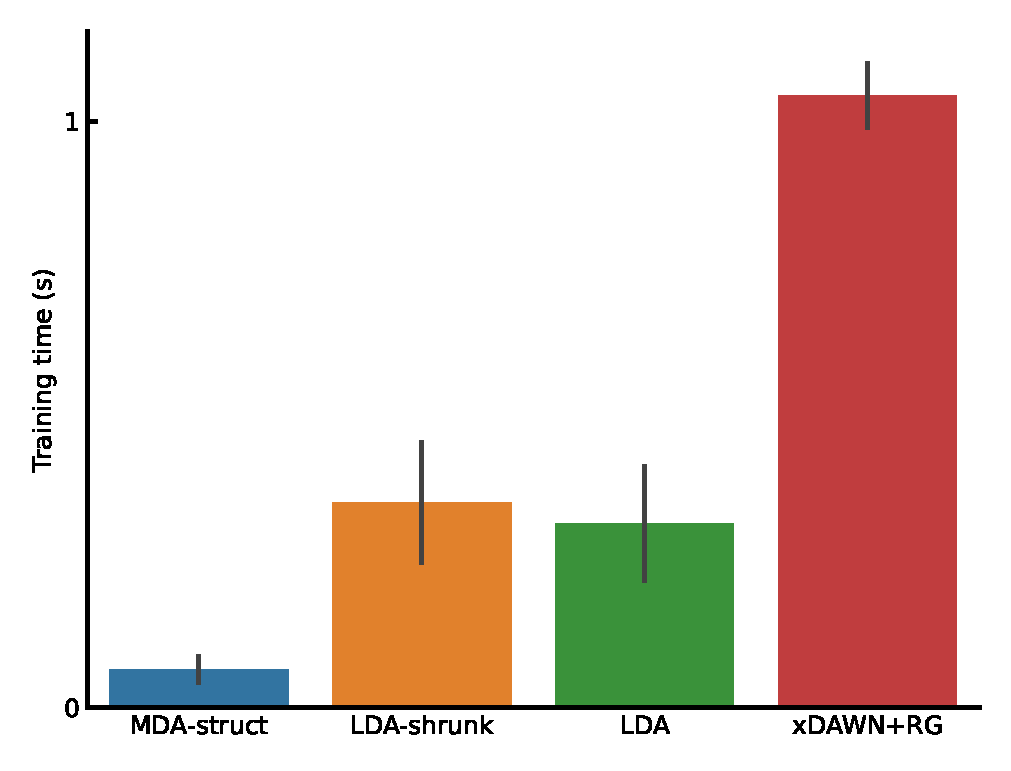
\includegraphics[width=.66\linewidth]{figures/stbf_struct/training_time.eps}
    \sffamily
    \hspace{-0.815469260193437in}
%% Creator: Matplotlib, PGF backend
%%
%% To include the figure in your LaTeX document, write
%%   \input{<filename>.pgf}
%%
%% Make sure the required packages are loaded in your preamble
%%   \usepackage{pgf}
%%
%% Also ensure that all the required font packages are loaded; for instance,
%% the lmodern package is sometimes necessary when using math font.
%%   \usepackage{lmodern}
%%
%% Figures using additional raster images can only be included by \input if
%% they are in the same directory as the main LaTeX file. For loading figures
%% from other directories you can use the `import` package
%%   \usepackage{import}
%%
%% and then include the figures with
%%   \import{<path to file>}{<filename>.pgf}
%%
%% Matplotlib used the following preamble
%%
\begingroup%
\makeatletter%
\begin{pgfpicture}%
\pgfpathrectangle{\pgfpointorigin}{\pgfqpoint{5.505894in}{1.391835in}}%
\pgfusepath{use as bounding box, clip}%
\begin{pgfscope}%
\pgfsetbuttcap%
\pgfsetmiterjoin%
\definecolor{currentfill}{rgb}{1.000000,1.000000,1.000000}%
\pgfsetfillcolor{currentfill}%
\pgfsetlinewidth{0.000000pt}%
\definecolor{currentstroke}{rgb}{1.000000,1.000000,1.000000}%
\pgfsetstrokecolor{currentstroke}%
\pgfsetdash{}{0pt}%
\pgfpathmoveto{\pgfqpoint{0.000000in}{0.000000in}}%
\pgfpathlineto{\pgfqpoint{5.505894in}{0.000000in}}%
\pgfpathlineto{\pgfqpoint{5.505894in}{1.391835in}}%
\pgfpathlineto{\pgfqpoint{0.000000in}{1.391835in}}%
\pgfpathlineto{\pgfqpoint{0.000000in}{0.000000in}}%
\pgfpathclose%
\pgfusepath{fill}%
\end{pgfscope}%
\begin{pgfscope}%
\pgfsetbuttcap%
\pgfsetmiterjoin%
\definecolor{currentfill}{rgb}{1.000000,1.000000,1.000000}%
\pgfsetfillcolor{currentfill}%
\pgfsetlinewidth{0.000000pt}%
\definecolor{currentstroke}{rgb}{0.000000,0.000000,0.000000}%
\pgfsetstrokecolor{currentstroke}%
\pgfsetstrokeopacity{0.000000}%
\pgfsetdash{}{0pt}%
\pgfpathmoveto{\pgfqpoint{0.776519in}{0.340278in}}%
\pgfpathlineto{\pgfqpoint{5.505894in}{0.340278in}}%
\pgfpathlineto{\pgfqpoint{5.505894in}{1.391835in}}%
\pgfpathlineto{\pgfqpoint{0.776519in}{1.391835in}}%
\pgfpathlineto{\pgfqpoint{0.776519in}{0.340278in}}%
\pgfpathclose%
\pgfusepath{fill}%
\end{pgfscope}%
\begin{pgfscope}%
\pgfpathrectangle{\pgfqpoint{0.776519in}{0.340278in}}{\pgfqpoint{4.729376in}{1.051557in}}%
\pgfusepath{clip}%
\pgfsetbuttcap%
\pgfsetroundjoin%
\definecolor{currentfill}{rgb}{0.949020,0.564706,0.094118}%
\pgfsetfillcolor{currentfill}%
\pgfsetlinewidth{0.000000pt}%
\definecolor{currentstroke}{rgb}{0.268235,0.268235,0.268235}%
\pgfsetstrokecolor{currentstroke}%
\pgfsetdash{}{0pt}%
\pgfpathmoveto{\pgfqpoint{1.074326in}{1.225427in}}%
\pgfpathcurveto{\pgfqpoint{1.078009in}{1.225427in}}{\pgfqpoint{1.081542in}{1.226891in}}{\pgfqpoint{1.084147in}{1.229495in}}%
\pgfpathcurveto{\pgfqpoint{1.086752in}{1.232100in}}{\pgfqpoint{1.088215in}{1.235633in}}{\pgfqpoint{1.088215in}{1.239316in}}%
\pgfpathcurveto{\pgfqpoint{1.088215in}{1.243000in}}{\pgfqpoint{1.086752in}{1.246533in}}{\pgfqpoint{1.084147in}{1.249137in}}%
\pgfpathcurveto{\pgfqpoint{1.081542in}{1.251742in}}{\pgfqpoint{1.078009in}{1.253205in}}{\pgfqpoint{1.074326in}{1.253205in}}%
\pgfpathcurveto{\pgfqpoint{1.070643in}{1.253205in}}{\pgfqpoint{1.067110in}{1.251742in}}{\pgfqpoint{1.064505in}{1.249137in}}%
\pgfpathcurveto{\pgfqpoint{1.061901in}{1.246533in}}{\pgfqpoint{1.060437in}{1.243000in}}{\pgfqpoint{1.060437in}{1.239316in}}%
\pgfpathcurveto{\pgfqpoint{1.060437in}{1.235633in}}{\pgfqpoint{1.061901in}{1.232100in}}{\pgfqpoint{1.064505in}{1.229495in}}%
\pgfpathcurveto{\pgfqpoint{1.067110in}{1.226891in}}{\pgfqpoint{1.070643in}{1.225427in}}{\pgfqpoint{1.074326in}{1.225427in}}%
\pgfpathlineto{\pgfqpoint{1.074326in}{1.225427in}}%
\pgfpathclose%
\pgfusepath{fill}%
\end{pgfscope}%
\begin{pgfscope}%
\pgfpathrectangle{\pgfqpoint{0.776519in}{0.340278in}}{\pgfqpoint{4.729376in}{1.051557in}}%
\pgfusepath{clip}%
\pgfsetbuttcap%
\pgfsetroundjoin%
\definecolor{currentfill}{rgb}{0.949020,0.564706,0.094118}%
\pgfsetfillcolor{currentfill}%
\pgfsetlinewidth{0.000000pt}%
\definecolor{currentstroke}{rgb}{0.268235,0.268235,0.268235}%
\pgfsetstrokecolor{currentstroke}%
\pgfsetdash{}{0pt}%
\pgfpathmoveto{\pgfqpoint{1.064702in}{1.230609in}}%
\pgfpathcurveto{\pgfqpoint{1.068385in}{1.230609in}}{\pgfqpoint{1.071918in}{1.232072in}}{\pgfqpoint{1.074523in}{1.234677in}}%
\pgfpathcurveto{\pgfqpoint{1.077127in}{1.237282in}}{\pgfqpoint{1.078591in}{1.240815in}}{\pgfqpoint{1.078591in}{1.244498in}}%
\pgfpathcurveto{\pgfqpoint{1.078591in}{1.248181in}}{\pgfqpoint{1.077127in}{1.251714in}}{\pgfqpoint{1.074523in}{1.254319in}}%
\pgfpathcurveto{\pgfqpoint{1.071918in}{1.256923in}}{\pgfqpoint{1.068385in}{1.258387in}}{\pgfqpoint{1.064702in}{1.258387in}}%
\pgfpathcurveto{\pgfqpoint{1.061018in}{1.258387in}}{\pgfqpoint{1.057485in}{1.256923in}}{\pgfqpoint{1.054881in}{1.254319in}}%
\pgfpathcurveto{\pgfqpoint{1.052276in}{1.251714in}}{\pgfqpoint{1.050813in}{1.248181in}}{\pgfqpoint{1.050813in}{1.244498in}}%
\pgfpathcurveto{\pgfqpoint{1.050813in}{1.240815in}}{\pgfqpoint{1.052276in}{1.237282in}}{\pgfqpoint{1.054881in}{1.234677in}}%
\pgfpathcurveto{\pgfqpoint{1.057485in}{1.232072in}}{\pgfqpoint{1.061018in}{1.230609in}}{\pgfqpoint{1.064702in}{1.230609in}}%
\pgfpathlineto{\pgfqpoint{1.064702in}{1.230609in}}%
\pgfpathclose%
\pgfusepath{fill}%
\end{pgfscope}%
\begin{pgfscope}%
\pgfpathrectangle{\pgfqpoint{0.776519in}{0.340278in}}{\pgfqpoint{4.729376in}{1.051557in}}%
\pgfusepath{clip}%
\pgfsetbuttcap%
\pgfsetroundjoin%
\definecolor{currentfill}{rgb}{0.949020,0.564706,0.094118}%
\pgfsetfillcolor{currentfill}%
\pgfsetlinewidth{0.000000pt}%
\definecolor{currentstroke}{rgb}{0.268235,0.268235,0.268235}%
\pgfsetstrokecolor{currentstroke}%
\pgfsetdash{}{0pt}%
\pgfpathmoveto{\pgfqpoint{1.129144in}{1.240384in}}%
\pgfpathcurveto{\pgfqpoint{1.132827in}{1.240384in}}{\pgfqpoint{1.136360in}{1.241847in}}{\pgfqpoint{1.138965in}{1.244452in}}%
\pgfpathcurveto{\pgfqpoint{1.141569in}{1.247056in}}{\pgfqpoint{1.143033in}{1.250589in}}{\pgfqpoint{1.143033in}{1.254272in}}%
\pgfpathcurveto{\pgfqpoint{1.143033in}{1.257956in}}{\pgfqpoint{1.141569in}{1.261489in}}{\pgfqpoint{1.138965in}{1.264093in}}%
\pgfpathcurveto{\pgfqpoint{1.136360in}{1.266698in}}{\pgfqpoint{1.132827in}{1.268161in}}{\pgfqpoint{1.129144in}{1.268161in}}%
\pgfpathcurveto{\pgfqpoint{1.125461in}{1.268161in}}{\pgfqpoint{1.121927in}{1.266698in}}{\pgfqpoint{1.119323in}{1.264093in}}%
\pgfpathcurveto{\pgfqpoint{1.116718in}{1.261489in}}{\pgfqpoint{1.115255in}{1.257956in}}{\pgfqpoint{1.115255in}{1.254272in}}%
\pgfpathcurveto{\pgfqpoint{1.115255in}{1.250589in}}{\pgfqpoint{1.116718in}{1.247056in}}{\pgfqpoint{1.119323in}{1.244452in}}%
\pgfpathcurveto{\pgfqpoint{1.121927in}{1.241847in}}{\pgfqpoint{1.125461in}{1.240384in}}{\pgfqpoint{1.129144in}{1.240384in}}%
\pgfpathlineto{\pgfqpoint{1.129144in}{1.240384in}}%
\pgfpathclose%
\pgfusepath{fill}%
\end{pgfscope}%
\begin{pgfscope}%
\pgfpathrectangle{\pgfqpoint{0.776519in}{0.340278in}}{\pgfqpoint{4.729376in}{1.051557in}}%
\pgfusepath{clip}%
\pgfsetbuttcap%
\pgfsetroundjoin%
\definecolor{currentfill}{rgb}{0.949020,0.564706,0.094118}%
\pgfsetfillcolor{currentfill}%
\pgfsetlinewidth{0.000000pt}%
\definecolor{currentstroke}{rgb}{0.268235,0.268235,0.268235}%
\pgfsetstrokecolor{currentstroke}%
\pgfsetdash{}{0pt}%
\pgfpathmoveto{\pgfqpoint{1.422570in}{1.263240in}}%
\pgfpathcurveto{\pgfqpoint{1.426254in}{1.263240in}}{\pgfqpoint{1.429787in}{1.264704in}}{\pgfqpoint{1.432391in}{1.267308in}}%
\pgfpathcurveto{\pgfqpoint{1.434996in}{1.269913in}}{\pgfqpoint{1.436459in}{1.273446in}}{\pgfqpoint{1.436459in}{1.277129in}}%
\pgfpathcurveto{\pgfqpoint{1.436459in}{1.280812in}}{\pgfqpoint{1.434996in}{1.284345in}}{\pgfqpoint{1.432391in}{1.286950in}}%
\pgfpathcurveto{\pgfqpoint{1.429787in}{1.289555in}}{\pgfqpoint{1.426254in}{1.291018in}}{\pgfqpoint{1.422570in}{1.291018in}}%
\pgfpathcurveto{\pgfqpoint{1.418887in}{1.291018in}}{\pgfqpoint{1.415354in}{1.289555in}}{\pgfqpoint{1.412749in}{1.286950in}}%
\pgfpathcurveto{\pgfqpoint{1.410145in}{1.284345in}}{\pgfqpoint{1.408681in}{1.280812in}}{\pgfqpoint{1.408681in}{1.277129in}}%
\pgfpathcurveto{\pgfqpoint{1.408681in}{1.273446in}}{\pgfqpoint{1.410145in}{1.269913in}}{\pgfqpoint{1.412749in}{1.267308in}}%
\pgfpathcurveto{\pgfqpoint{1.415354in}{1.264704in}}{\pgfqpoint{1.418887in}{1.263240in}}{\pgfqpoint{1.422570in}{1.263240in}}%
\pgfpathlineto{\pgfqpoint{1.422570in}{1.263240in}}%
\pgfpathclose%
\pgfusepath{fill}%
\end{pgfscope}%
\begin{pgfscope}%
\pgfpathrectangle{\pgfqpoint{0.776519in}{0.340278in}}{\pgfqpoint{4.729376in}{1.051557in}}%
\pgfusepath{clip}%
\pgfsetbuttcap%
\pgfsetroundjoin%
\definecolor{currentfill}{rgb}{0.949020,0.564706,0.094118}%
\pgfsetfillcolor{currentfill}%
\pgfsetlinewidth{0.000000pt}%
\definecolor{currentstroke}{rgb}{0.268235,0.268235,0.268235}%
\pgfsetstrokecolor{currentstroke}%
\pgfsetdash{}{0pt}%
\pgfpathmoveto{\pgfqpoint{1.034264in}{1.244351in}}%
\pgfpathcurveto{\pgfqpoint{1.037948in}{1.244351in}}{\pgfqpoint{1.041481in}{1.245814in}}{\pgfqpoint{1.044085in}{1.248419in}}%
\pgfpathcurveto{\pgfqpoint{1.046690in}{1.251023in}}{\pgfqpoint{1.048153in}{1.254556in}}{\pgfqpoint{1.048153in}{1.258239in}}%
\pgfpathcurveto{\pgfqpoint{1.048153in}{1.261923in}}{\pgfqpoint{1.046690in}{1.265456in}}{\pgfqpoint{1.044085in}{1.268060in}}%
\pgfpathcurveto{\pgfqpoint{1.041481in}{1.270665in}}{\pgfqpoint{1.037948in}{1.272128in}}{\pgfqpoint{1.034264in}{1.272128in}}%
\pgfpathcurveto{\pgfqpoint{1.030581in}{1.272128in}}{\pgfqpoint{1.027048in}{1.270665in}}{\pgfqpoint{1.024443in}{1.268060in}}%
\pgfpathcurveto{\pgfqpoint{1.021839in}{1.265456in}}{\pgfqpoint{1.020375in}{1.261923in}}{\pgfqpoint{1.020375in}{1.258239in}}%
\pgfpathcurveto{\pgfqpoint{1.020375in}{1.254556in}}{\pgfqpoint{1.021839in}{1.251023in}}{\pgfqpoint{1.024443in}{1.248419in}}%
\pgfpathcurveto{\pgfqpoint{1.027048in}{1.245814in}}{\pgfqpoint{1.030581in}{1.244351in}}{\pgfqpoint{1.034264in}{1.244351in}}%
\pgfpathlineto{\pgfqpoint{1.034264in}{1.244351in}}%
\pgfpathclose%
\pgfusepath{fill}%
\end{pgfscope}%
\begin{pgfscope}%
\pgfpathrectangle{\pgfqpoint{0.776519in}{0.340278in}}{\pgfqpoint{4.729376in}{1.051557in}}%
\pgfusepath{clip}%
\pgfsetbuttcap%
\pgfsetroundjoin%
\definecolor{currentfill}{rgb}{0.949020,0.564706,0.094118}%
\pgfsetfillcolor{currentfill}%
\pgfsetlinewidth{0.000000pt}%
\definecolor{currentstroke}{rgb}{0.268235,0.268235,0.268235}%
\pgfsetstrokecolor{currentstroke}%
\pgfsetdash{}{0pt}%
\pgfpathmoveto{\pgfqpoint{1.116293in}{1.242360in}}%
\pgfpathcurveto{\pgfqpoint{1.119976in}{1.242360in}}{\pgfqpoint{1.123509in}{1.243824in}}{\pgfqpoint{1.126113in}{1.246428in}}%
\pgfpathcurveto{\pgfqpoint{1.128718in}{1.249033in}}{\pgfqpoint{1.130181in}{1.252566in}}{\pgfqpoint{1.130181in}{1.256249in}}%
\pgfpathcurveto{\pgfqpoint{1.130181in}{1.259933in}}{\pgfqpoint{1.128718in}{1.263466in}}{\pgfqpoint{1.126113in}{1.266070in}}%
\pgfpathcurveto{\pgfqpoint{1.123509in}{1.268675in}}{\pgfqpoint{1.119976in}{1.270138in}}{\pgfqpoint{1.116293in}{1.270138in}}%
\pgfpathcurveto{\pgfqpoint{1.112609in}{1.270138in}}{\pgfqpoint{1.109076in}{1.268675in}}{\pgfqpoint{1.106472in}{1.266070in}}%
\pgfpathcurveto{\pgfqpoint{1.103867in}{1.263466in}}{\pgfqpoint{1.102404in}{1.259933in}}{\pgfqpoint{1.102404in}{1.256249in}}%
\pgfpathcurveto{\pgfqpoint{1.102404in}{1.252566in}}{\pgfqpoint{1.103867in}{1.249033in}}{\pgfqpoint{1.106472in}{1.246428in}}%
\pgfpathcurveto{\pgfqpoint{1.109076in}{1.243824in}}{\pgfqpoint{1.112609in}{1.242360in}}{\pgfqpoint{1.116293in}{1.242360in}}%
\pgfpathlineto{\pgfqpoint{1.116293in}{1.242360in}}%
\pgfpathclose%
\pgfusepath{fill}%
\end{pgfscope}%
\begin{pgfscope}%
\pgfpathrectangle{\pgfqpoint{0.776519in}{0.340278in}}{\pgfqpoint{4.729376in}{1.051557in}}%
\pgfusepath{clip}%
\pgfsetbuttcap%
\pgfsetroundjoin%
\definecolor{currentfill}{rgb}{0.949020,0.564706,0.094118}%
\pgfsetfillcolor{currentfill}%
\pgfsetlinewidth{0.000000pt}%
\definecolor{currentstroke}{rgb}{0.268235,0.268235,0.268235}%
\pgfsetstrokecolor{currentstroke}%
\pgfsetdash{}{0pt}%
\pgfpathmoveto{\pgfqpoint{1.120587in}{1.221468in}}%
\pgfpathcurveto{\pgfqpoint{1.124270in}{1.221468in}}{\pgfqpoint{1.127803in}{1.222931in}}{\pgfqpoint{1.130408in}{1.225536in}}%
\pgfpathcurveto{\pgfqpoint{1.133013in}{1.228140in}}{\pgfqpoint{1.134476in}{1.231673in}}{\pgfqpoint{1.134476in}{1.235356in}}%
\pgfpathcurveto{\pgfqpoint{1.134476in}{1.239040in}}{\pgfqpoint{1.133013in}{1.242573in}}{\pgfqpoint{1.130408in}{1.245177in}}%
\pgfpathcurveto{\pgfqpoint{1.127803in}{1.247782in}}{\pgfqpoint{1.124270in}{1.249245in}}{\pgfqpoint{1.120587in}{1.249245in}}%
\pgfpathcurveto{\pgfqpoint{1.116904in}{1.249245in}}{\pgfqpoint{1.113371in}{1.247782in}}{\pgfqpoint{1.110766in}{1.245177in}}%
\pgfpathcurveto{\pgfqpoint{1.108162in}{1.242573in}}{\pgfqpoint{1.106698in}{1.239040in}}{\pgfqpoint{1.106698in}{1.235356in}}%
\pgfpathcurveto{\pgfqpoint{1.106698in}{1.231673in}}{\pgfqpoint{1.108162in}{1.228140in}}{\pgfqpoint{1.110766in}{1.225536in}}%
\pgfpathcurveto{\pgfqpoint{1.113371in}{1.222931in}}{\pgfqpoint{1.116904in}{1.221468in}}{\pgfqpoint{1.120587in}{1.221468in}}%
\pgfpathlineto{\pgfqpoint{1.120587in}{1.221468in}}%
\pgfpathclose%
\pgfusepath{fill}%
\end{pgfscope}%
\begin{pgfscope}%
\pgfpathrectangle{\pgfqpoint{0.776519in}{0.340278in}}{\pgfqpoint{4.729376in}{1.051557in}}%
\pgfusepath{clip}%
\pgfsetbuttcap%
\pgfsetroundjoin%
\definecolor{currentfill}{rgb}{0.949020,0.564706,0.094118}%
\pgfsetfillcolor{currentfill}%
\pgfsetlinewidth{0.000000pt}%
\definecolor{currentstroke}{rgb}{0.268235,0.268235,0.268235}%
\pgfsetstrokecolor{currentstroke}%
\pgfsetdash{}{0pt}%
\pgfpathmoveto{\pgfqpoint{1.113086in}{1.237819in}}%
\pgfpathcurveto{\pgfqpoint{1.116770in}{1.237819in}}{\pgfqpoint{1.120303in}{1.239282in}}{\pgfqpoint{1.122907in}{1.241887in}}%
\pgfpathcurveto{\pgfqpoint{1.125512in}{1.244491in}}{\pgfqpoint{1.126975in}{1.248024in}}{\pgfqpoint{1.126975in}{1.251708in}}%
\pgfpathcurveto{\pgfqpoint{1.126975in}{1.255391in}}{\pgfqpoint{1.125512in}{1.258924in}}{\pgfqpoint{1.122907in}{1.261529in}}%
\pgfpathcurveto{\pgfqpoint{1.120303in}{1.264133in}}{\pgfqpoint{1.116770in}{1.265597in}}{\pgfqpoint{1.113086in}{1.265597in}}%
\pgfpathcurveto{\pgfqpoint{1.109403in}{1.265597in}}{\pgfqpoint{1.105870in}{1.264133in}}{\pgfqpoint{1.103265in}{1.261529in}}%
\pgfpathcurveto{\pgfqpoint{1.100661in}{1.258924in}}{\pgfqpoint{1.099197in}{1.255391in}}{\pgfqpoint{1.099197in}{1.251708in}}%
\pgfpathcurveto{\pgfqpoint{1.099197in}{1.248024in}}{\pgfqpoint{1.100661in}{1.244491in}}{\pgfqpoint{1.103265in}{1.241887in}}%
\pgfpathcurveto{\pgfqpoint{1.105870in}{1.239282in}}{\pgfqpoint{1.109403in}{1.237819in}}{\pgfqpoint{1.113086in}{1.237819in}}%
\pgfpathlineto{\pgfqpoint{1.113086in}{1.237819in}}%
\pgfpathclose%
\pgfusepath{fill}%
\end{pgfscope}%
\begin{pgfscope}%
\pgfpathrectangle{\pgfqpoint{0.776519in}{0.340278in}}{\pgfqpoint{4.729376in}{1.051557in}}%
\pgfusepath{clip}%
\pgfsetbuttcap%
\pgfsetroundjoin%
\definecolor{currentfill}{rgb}{0.949020,0.564706,0.094118}%
\pgfsetfillcolor{currentfill}%
\pgfsetlinewidth{0.000000pt}%
\definecolor{currentstroke}{rgb}{0.268235,0.268235,0.268235}%
\pgfsetstrokecolor{currentstroke}%
\pgfsetdash{}{0pt}%
\pgfpathmoveto{\pgfqpoint{1.005676in}{1.237285in}}%
\pgfpathcurveto{\pgfqpoint{1.009359in}{1.237285in}}{\pgfqpoint{1.012892in}{1.238749in}}{\pgfqpoint{1.015497in}{1.241353in}}%
\pgfpathcurveto{\pgfqpoint{1.018101in}{1.243958in}}{\pgfqpoint{1.019565in}{1.247491in}}{\pgfqpoint{1.019565in}{1.251174in}}%
\pgfpathcurveto{\pgfqpoint{1.019565in}{1.254857in}}{\pgfqpoint{1.018101in}{1.258390in}}{\pgfqpoint{1.015497in}{1.260995in}}%
\pgfpathcurveto{\pgfqpoint{1.012892in}{1.263600in}}{\pgfqpoint{1.009359in}{1.265063in}}{\pgfqpoint{1.005676in}{1.265063in}}%
\pgfpathcurveto{\pgfqpoint{1.001992in}{1.265063in}}{\pgfqpoint{0.998459in}{1.263600in}}{\pgfqpoint{0.995855in}{1.260995in}}%
\pgfpathcurveto{\pgfqpoint{0.993250in}{1.258390in}}{\pgfqpoint{0.991787in}{1.254857in}}{\pgfqpoint{0.991787in}{1.251174in}}%
\pgfpathcurveto{\pgfqpoint{0.991787in}{1.247491in}}{\pgfqpoint{0.993250in}{1.243958in}}{\pgfqpoint{0.995855in}{1.241353in}}%
\pgfpathcurveto{\pgfqpoint{0.998459in}{1.238749in}}{\pgfqpoint{1.001992in}{1.237285in}}{\pgfqpoint{1.005676in}{1.237285in}}%
\pgfpathlineto{\pgfqpoint{1.005676in}{1.237285in}}%
\pgfpathclose%
\pgfusepath{fill}%
\end{pgfscope}%
\begin{pgfscope}%
\pgfpathrectangle{\pgfqpoint{0.776519in}{0.340278in}}{\pgfqpoint{4.729376in}{1.051557in}}%
\pgfusepath{clip}%
\pgfsetbuttcap%
\pgfsetroundjoin%
\definecolor{currentfill}{rgb}{0.949020,0.564706,0.094118}%
\pgfsetfillcolor{currentfill}%
\pgfsetlinewidth{0.000000pt}%
\definecolor{currentstroke}{rgb}{0.268235,0.268235,0.268235}%
\pgfsetstrokecolor{currentstroke}%
\pgfsetdash{}{0pt}%
\pgfpathmoveto{\pgfqpoint{1.069484in}{1.237517in}}%
\pgfpathcurveto{\pgfqpoint{1.073168in}{1.237517in}}{\pgfqpoint{1.076701in}{1.238981in}}{\pgfqpoint{1.079305in}{1.241585in}}%
\pgfpathcurveto{\pgfqpoint{1.081910in}{1.244190in}}{\pgfqpoint{1.083373in}{1.247723in}}{\pgfqpoint{1.083373in}{1.251406in}}%
\pgfpathcurveto{\pgfqpoint{1.083373in}{1.255090in}}{\pgfqpoint{1.081910in}{1.258623in}}{\pgfqpoint{1.079305in}{1.261227in}}%
\pgfpathcurveto{\pgfqpoint{1.076701in}{1.263832in}}{\pgfqpoint{1.073168in}{1.265295in}}{\pgfqpoint{1.069484in}{1.265295in}}%
\pgfpathcurveto{\pgfqpoint{1.065801in}{1.265295in}}{\pgfqpoint{1.062268in}{1.263832in}}{\pgfqpoint{1.059663in}{1.261227in}}%
\pgfpathcurveto{\pgfqpoint{1.057059in}{1.258623in}}{\pgfqpoint{1.055595in}{1.255090in}}{\pgfqpoint{1.055595in}{1.251406in}}%
\pgfpathcurveto{\pgfqpoint{1.055595in}{1.247723in}}{\pgfqpoint{1.057059in}{1.244190in}}{\pgfqpoint{1.059663in}{1.241585in}}%
\pgfpathcurveto{\pgfqpoint{1.062268in}{1.238981in}}{\pgfqpoint{1.065801in}{1.237517in}}{\pgfqpoint{1.069484in}{1.237517in}}%
\pgfpathlineto{\pgfqpoint{1.069484in}{1.237517in}}%
\pgfpathclose%
\pgfusepath{fill}%
\end{pgfscope}%
\begin{pgfscope}%
\pgfpathrectangle{\pgfqpoint{0.776519in}{0.340278in}}{\pgfqpoint{4.729376in}{1.051557in}}%
\pgfusepath{clip}%
\pgfsetbuttcap%
\pgfsetroundjoin%
\definecolor{currentfill}{rgb}{0.949020,0.564706,0.094118}%
\pgfsetfillcolor{currentfill}%
\pgfsetlinewidth{0.000000pt}%
\definecolor{currentstroke}{rgb}{0.268235,0.268235,0.268235}%
\pgfsetstrokecolor{currentstroke}%
\pgfsetdash{}{0pt}%
\pgfpathmoveto{\pgfqpoint{1.082397in}{1.230423in}}%
\pgfpathcurveto{\pgfqpoint{1.086081in}{1.230423in}}{\pgfqpoint{1.089614in}{1.231886in}}{\pgfqpoint{1.092218in}{1.234491in}}%
\pgfpathcurveto{\pgfqpoint{1.094823in}{1.237095in}}{\pgfqpoint{1.096286in}{1.240628in}}{\pgfqpoint{1.096286in}{1.244311in}}%
\pgfpathcurveto{\pgfqpoint{1.096286in}{1.247995in}}{\pgfqpoint{1.094823in}{1.251528in}}{\pgfqpoint{1.092218in}{1.254132in}}%
\pgfpathcurveto{\pgfqpoint{1.089614in}{1.256737in}}{\pgfqpoint{1.086081in}{1.258200in}}{\pgfqpoint{1.082397in}{1.258200in}}%
\pgfpathcurveto{\pgfqpoint{1.078714in}{1.258200in}}{\pgfqpoint{1.075181in}{1.256737in}}{\pgfqpoint{1.072577in}{1.254132in}}%
\pgfpathcurveto{\pgfqpoint{1.069972in}{1.251528in}}{\pgfqpoint{1.068509in}{1.247995in}}{\pgfqpoint{1.068509in}{1.244311in}}%
\pgfpathcurveto{\pgfqpoint{1.068509in}{1.240628in}}{\pgfqpoint{1.069972in}{1.237095in}}{\pgfqpoint{1.072577in}{1.234491in}}%
\pgfpathcurveto{\pgfqpoint{1.075181in}{1.231886in}}{\pgfqpoint{1.078714in}{1.230423in}}{\pgfqpoint{1.082397in}{1.230423in}}%
\pgfpathlineto{\pgfqpoint{1.082397in}{1.230423in}}%
\pgfpathclose%
\pgfusepath{fill}%
\end{pgfscope}%
\begin{pgfscope}%
\pgfpathrectangle{\pgfqpoint{0.776519in}{0.340278in}}{\pgfqpoint{4.729376in}{1.051557in}}%
\pgfusepath{clip}%
\pgfsetbuttcap%
\pgfsetroundjoin%
\definecolor{currentfill}{rgb}{0.949020,0.564706,0.094118}%
\pgfsetfillcolor{currentfill}%
\pgfsetlinewidth{0.000000pt}%
\definecolor{currentstroke}{rgb}{0.268235,0.268235,0.268235}%
\pgfsetstrokecolor{currentstroke}%
\pgfsetdash{}{0pt}%
\pgfpathmoveto{\pgfqpoint{1.430721in}{1.231903in}}%
\pgfpathcurveto{\pgfqpoint{1.434405in}{1.231903in}}{\pgfqpoint{1.437938in}{1.233366in}}{\pgfqpoint{1.440542in}{1.235971in}}%
\pgfpathcurveto{\pgfqpoint{1.443147in}{1.238575in}}{\pgfqpoint{1.444610in}{1.242108in}}{\pgfqpoint{1.444610in}{1.245792in}}%
\pgfpathcurveto{\pgfqpoint{1.444610in}{1.249475in}}{\pgfqpoint{1.443147in}{1.253008in}}{\pgfqpoint{1.440542in}{1.255612in}}%
\pgfpathcurveto{\pgfqpoint{1.437938in}{1.258217in}}{\pgfqpoint{1.434405in}{1.259680in}}{\pgfqpoint{1.430721in}{1.259680in}}%
\pgfpathcurveto{\pgfqpoint{1.427038in}{1.259680in}}{\pgfqpoint{1.423505in}{1.258217in}}{\pgfqpoint{1.420901in}{1.255612in}}%
\pgfpathcurveto{\pgfqpoint{1.418296in}{1.253008in}}{\pgfqpoint{1.416833in}{1.249475in}}{\pgfqpoint{1.416833in}{1.245792in}}%
\pgfpathcurveto{\pgfqpoint{1.416833in}{1.242108in}}{\pgfqpoint{1.418296in}{1.238575in}}{\pgfqpoint{1.420901in}{1.235971in}}%
\pgfpathcurveto{\pgfqpoint{1.423505in}{1.233366in}}{\pgfqpoint{1.427038in}{1.231903in}}{\pgfqpoint{1.430721in}{1.231903in}}%
\pgfpathlineto{\pgfqpoint{1.430721in}{1.231903in}}%
\pgfpathclose%
\pgfusepath{fill}%
\end{pgfscope}%
\begin{pgfscope}%
\pgfpathrectangle{\pgfqpoint{0.776519in}{0.340278in}}{\pgfqpoint{4.729376in}{1.051557in}}%
\pgfusepath{clip}%
\pgfsetbuttcap%
\pgfsetroundjoin%
\definecolor{currentfill}{rgb}{0.949020,0.564706,0.094118}%
\pgfsetfillcolor{currentfill}%
\pgfsetlinewidth{0.000000pt}%
\definecolor{currentstroke}{rgb}{0.268235,0.268235,0.268235}%
\pgfsetstrokecolor{currentstroke}%
\pgfsetdash{}{0pt}%
\pgfpathmoveto{\pgfqpoint{1.040704in}{1.269728in}}%
\pgfpathcurveto{\pgfqpoint{1.044387in}{1.269728in}}{\pgfqpoint{1.047920in}{1.271191in}}{\pgfqpoint{1.050525in}{1.273796in}}%
\pgfpathcurveto{\pgfqpoint{1.053129in}{1.276400in}}{\pgfqpoint{1.054593in}{1.279933in}}{\pgfqpoint{1.054593in}{1.283617in}}%
\pgfpathcurveto{\pgfqpoint{1.054593in}{1.287300in}}{\pgfqpoint{1.053129in}{1.290833in}}{\pgfqpoint{1.050525in}{1.293438in}}%
\pgfpathcurveto{\pgfqpoint{1.047920in}{1.296042in}}{\pgfqpoint{1.044387in}{1.297506in}}{\pgfqpoint{1.040704in}{1.297506in}}%
\pgfpathcurveto{\pgfqpoint{1.037021in}{1.297506in}}{\pgfqpoint{1.033488in}{1.296042in}}{\pgfqpoint{1.030883in}{1.293438in}}%
\pgfpathcurveto{\pgfqpoint{1.028279in}{1.290833in}}{\pgfqpoint{1.026815in}{1.287300in}}{\pgfqpoint{1.026815in}{1.283617in}}%
\pgfpathcurveto{\pgfqpoint{1.026815in}{1.279933in}}{\pgfqpoint{1.028279in}{1.276400in}}{\pgfqpoint{1.030883in}{1.273796in}}%
\pgfpathcurveto{\pgfqpoint{1.033488in}{1.271191in}}{\pgfqpoint{1.037021in}{1.269728in}}{\pgfqpoint{1.040704in}{1.269728in}}%
\pgfpathlineto{\pgfqpoint{1.040704in}{1.269728in}}%
\pgfpathclose%
\pgfusepath{fill}%
\end{pgfscope}%
\begin{pgfscope}%
\pgfpathrectangle{\pgfqpoint{0.776519in}{0.340278in}}{\pgfqpoint{4.729376in}{1.051557in}}%
\pgfusepath{clip}%
\pgfsetbuttcap%
\pgfsetroundjoin%
\definecolor{currentfill}{rgb}{0.949020,0.564706,0.094118}%
\pgfsetfillcolor{currentfill}%
\pgfsetlinewidth{0.000000pt}%
\definecolor{currentstroke}{rgb}{0.268235,0.268235,0.268235}%
\pgfsetstrokecolor{currentstroke}%
\pgfsetdash{}{0pt}%
\pgfpathmoveto{\pgfqpoint{1.418670in}{1.257981in}}%
\pgfpathcurveto{\pgfqpoint{1.422353in}{1.257981in}}{\pgfqpoint{1.425886in}{1.259444in}}{\pgfqpoint{1.428491in}{1.262049in}}%
\pgfpathcurveto{\pgfqpoint{1.431095in}{1.264653in}}{\pgfqpoint{1.432559in}{1.268186in}}{\pgfqpoint{1.432559in}{1.271870in}}%
\pgfpathcurveto{\pgfqpoint{1.432559in}{1.275553in}}{\pgfqpoint{1.431095in}{1.279086in}}{\pgfqpoint{1.428491in}{1.281691in}}%
\pgfpathcurveto{\pgfqpoint{1.425886in}{1.284295in}}{\pgfqpoint{1.422353in}{1.285759in}}{\pgfqpoint{1.418670in}{1.285759in}}%
\pgfpathcurveto{\pgfqpoint{1.414986in}{1.285759in}}{\pgfqpoint{1.411453in}{1.284295in}}{\pgfqpoint{1.408849in}{1.281691in}}%
\pgfpathcurveto{\pgfqpoint{1.406244in}{1.279086in}}{\pgfqpoint{1.404781in}{1.275553in}}{\pgfqpoint{1.404781in}{1.271870in}}%
\pgfpathcurveto{\pgfqpoint{1.404781in}{1.268186in}}{\pgfqpoint{1.406244in}{1.264653in}}{\pgfqpoint{1.408849in}{1.262049in}}%
\pgfpathcurveto{\pgfqpoint{1.411453in}{1.259444in}}{\pgfqpoint{1.414986in}{1.257981in}}{\pgfqpoint{1.418670in}{1.257981in}}%
\pgfpathlineto{\pgfqpoint{1.418670in}{1.257981in}}%
\pgfpathclose%
\pgfusepath{fill}%
\end{pgfscope}%
\begin{pgfscope}%
\pgfpathrectangle{\pgfqpoint{0.776519in}{0.340278in}}{\pgfqpoint{4.729376in}{1.051557in}}%
\pgfusepath{clip}%
\pgfsetbuttcap%
\pgfsetroundjoin%
\definecolor{currentfill}{rgb}{0.949020,0.564706,0.094118}%
\pgfsetfillcolor{currentfill}%
\pgfsetlinewidth{0.000000pt}%
\definecolor{currentstroke}{rgb}{0.268235,0.268235,0.268235}%
\pgfsetstrokecolor{currentstroke}%
\pgfsetdash{}{0pt}%
\pgfpathmoveto{\pgfqpoint{1.076331in}{1.224250in}}%
\pgfpathcurveto{\pgfqpoint{1.080014in}{1.224250in}}{\pgfqpoint{1.083547in}{1.225713in}}{\pgfqpoint{1.086152in}{1.228318in}}%
\pgfpathcurveto{\pgfqpoint{1.088757in}{1.230922in}}{\pgfqpoint{1.090220in}{1.234455in}}{\pgfqpoint{1.090220in}{1.238139in}}%
\pgfpathcurveto{\pgfqpoint{1.090220in}{1.241822in}}{\pgfqpoint{1.088757in}{1.245355in}}{\pgfqpoint{1.086152in}{1.247960in}}%
\pgfpathcurveto{\pgfqpoint{1.083547in}{1.250564in}}{\pgfqpoint{1.080014in}{1.252028in}}{\pgfqpoint{1.076331in}{1.252028in}}%
\pgfpathcurveto{\pgfqpoint{1.072648in}{1.252028in}}{\pgfqpoint{1.069115in}{1.250564in}}{\pgfqpoint{1.066510in}{1.247960in}}%
\pgfpathcurveto{\pgfqpoint{1.063906in}{1.245355in}}{\pgfqpoint{1.062442in}{1.241822in}}{\pgfqpoint{1.062442in}{1.238139in}}%
\pgfpathcurveto{\pgfqpoint{1.062442in}{1.234455in}}{\pgfqpoint{1.063906in}{1.230922in}}{\pgfqpoint{1.066510in}{1.228318in}}%
\pgfpathcurveto{\pgfqpoint{1.069115in}{1.225713in}}{\pgfqpoint{1.072648in}{1.224250in}}{\pgfqpoint{1.076331in}{1.224250in}}%
\pgfpathlineto{\pgfqpoint{1.076331in}{1.224250in}}%
\pgfpathclose%
\pgfusepath{fill}%
\end{pgfscope}%
\begin{pgfscope}%
\pgfpathrectangle{\pgfqpoint{0.776519in}{0.340278in}}{\pgfqpoint{4.729376in}{1.051557in}}%
\pgfusepath{clip}%
\pgfsetbuttcap%
\pgfsetroundjoin%
\definecolor{currentfill}{rgb}{0.949020,0.564706,0.094118}%
\pgfsetfillcolor{currentfill}%
\pgfsetlinewidth{0.000000pt}%
\definecolor{currentstroke}{rgb}{0.268235,0.268235,0.268235}%
\pgfsetstrokecolor{currentstroke}%
\pgfsetdash{}{0pt}%
\pgfpathmoveto{\pgfqpoint{1.427116in}{1.224118in}}%
\pgfpathcurveto{\pgfqpoint{1.430799in}{1.224118in}}{\pgfqpoint{1.434332in}{1.225582in}}{\pgfqpoint{1.436937in}{1.228186in}}%
\pgfpathcurveto{\pgfqpoint{1.439541in}{1.230791in}}{\pgfqpoint{1.441005in}{1.234324in}}{\pgfqpoint{1.441005in}{1.238007in}}%
\pgfpathcurveto{\pgfqpoint{1.441005in}{1.241691in}}{\pgfqpoint{1.439541in}{1.245224in}}{\pgfqpoint{1.436937in}{1.247828in}}%
\pgfpathcurveto{\pgfqpoint{1.434332in}{1.250433in}}{\pgfqpoint{1.430799in}{1.251896in}}{\pgfqpoint{1.427116in}{1.251896in}}%
\pgfpathcurveto{\pgfqpoint{1.423432in}{1.251896in}}{\pgfqpoint{1.419899in}{1.250433in}}{\pgfqpoint{1.417295in}{1.247828in}}%
\pgfpathcurveto{\pgfqpoint{1.414690in}{1.245224in}}{\pgfqpoint{1.413227in}{1.241691in}}{\pgfqpoint{1.413227in}{1.238007in}}%
\pgfpathcurveto{\pgfqpoint{1.413227in}{1.234324in}}{\pgfqpoint{1.414690in}{1.230791in}}{\pgfqpoint{1.417295in}{1.228186in}}%
\pgfpathcurveto{\pgfqpoint{1.419899in}{1.225582in}}{\pgfqpoint{1.423432in}{1.224118in}}{\pgfqpoint{1.427116in}{1.224118in}}%
\pgfpathlineto{\pgfqpoint{1.427116in}{1.224118in}}%
\pgfpathclose%
\pgfusepath{fill}%
\end{pgfscope}%
\begin{pgfscope}%
\pgfpathrectangle{\pgfqpoint{0.776519in}{0.340278in}}{\pgfqpoint{4.729376in}{1.051557in}}%
\pgfusepath{clip}%
\pgfsetbuttcap%
\pgfsetroundjoin%
\definecolor{currentfill}{rgb}{0.949020,0.564706,0.094118}%
\pgfsetfillcolor{currentfill}%
\pgfsetlinewidth{0.000000pt}%
\definecolor{currentstroke}{rgb}{0.268235,0.268235,0.268235}%
\pgfsetstrokecolor{currentstroke}%
\pgfsetdash{}{0pt}%
\pgfpathmoveto{\pgfqpoint{1.044146in}{1.271035in}}%
\pgfpathcurveto{\pgfqpoint{1.047829in}{1.271035in}}{\pgfqpoint{1.051362in}{1.272498in}}{\pgfqpoint{1.053967in}{1.275103in}}%
\pgfpathcurveto{\pgfqpoint{1.056572in}{1.277707in}}{\pgfqpoint{1.058035in}{1.281240in}}{\pgfqpoint{1.058035in}{1.284923in}}%
\pgfpathcurveto{\pgfqpoint{1.058035in}{1.288607in}}{\pgfqpoint{1.056572in}{1.292140in}}{\pgfqpoint{1.053967in}{1.294744in}}%
\pgfpathcurveto{\pgfqpoint{1.051362in}{1.297349in}}{\pgfqpoint{1.047829in}{1.298812in}}{\pgfqpoint{1.044146in}{1.298812in}}%
\pgfpathcurveto{\pgfqpoint{1.040463in}{1.298812in}}{\pgfqpoint{1.036930in}{1.297349in}}{\pgfqpoint{1.034325in}{1.294744in}}%
\pgfpathcurveto{\pgfqpoint{1.031721in}{1.292140in}}{\pgfqpoint{1.030257in}{1.288607in}}{\pgfqpoint{1.030257in}{1.284923in}}%
\pgfpathcurveto{\pgfqpoint{1.030257in}{1.281240in}}{\pgfqpoint{1.031721in}{1.277707in}}{\pgfqpoint{1.034325in}{1.275103in}}%
\pgfpathcurveto{\pgfqpoint{1.036930in}{1.272498in}}{\pgfqpoint{1.040463in}{1.271035in}}{\pgfqpoint{1.044146in}{1.271035in}}%
\pgfpathlineto{\pgfqpoint{1.044146in}{1.271035in}}%
\pgfpathclose%
\pgfusepath{fill}%
\end{pgfscope}%
\begin{pgfscope}%
\pgfpathrectangle{\pgfqpoint{0.776519in}{0.340278in}}{\pgfqpoint{4.729376in}{1.051557in}}%
\pgfusepath{clip}%
\pgfsetbuttcap%
\pgfsetroundjoin%
\definecolor{currentfill}{rgb}{0.949020,0.564706,0.094118}%
\pgfsetfillcolor{currentfill}%
\pgfsetlinewidth{0.000000pt}%
\definecolor{currentstroke}{rgb}{0.268235,0.268235,0.268235}%
\pgfsetstrokecolor{currentstroke}%
\pgfsetdash{}{0pt}%
\pgfpathmoveto{\pgfqpoint{1.105339in}{1.249785in}}%
\pgfpathcurveto{\pgfqpoint{1.109023in}{1.249785in}}{\pgfqpoint{1.112556in}{1.251249in}}{\pgfqpoint{1.115160in}{1.253853in}}%
\pgfpathcurveto{\pgfqpoint{1.117765in}{1.256458in}}{\pgfqpoint{1.119228in}{1.259991in}}{\pgfqpoint{1.119228in}{1.263674in}}%
\pgfpathcurveto{\pgfqpoint{1.119228in}{1.267358in}}{\pgfqpoint{1.117765in}{1.270891in}}{\pgfqpoint{1.115160in}{1.273495in}}%
\pgfpathcurveto{\pgfqpoint{1.112556in}{1.276100in}}{\pgfqpoint{1.109023in}{1.277563in}}{\pgfqpoint{1.105339in}{1.277563in}}%
\pgfpathcurveto{\pgfqpoint{1.101656in}{1.277563in}}{\pgfqpoint{1.098123in}{1.276100in}}{\pgfqpoint{1.095518in}{1.273495in}}%
\pgfpathcurveto{\pgfqpoint{1.092914in}{1.270891in}}{\pgfqpoint{1.091450in}{1.267358in}}{\pgfqpoint{1.091450in}{1.263674in}}%
\pgfpathcurveto{\pgfqpoint{1.091450in}{1.259991in}}{\pgfqpoint{1.092914in}{1.256458in}}{\pgfqpoint{1.095518in}{1.253853in}}%
\pgfpathcurveto{\pgfqpoint{1.098123in}{1.251249in}}{\pgfqpoint{1.101656in}{1.249785in}}{\pgfqpoint{1.105339in}{1.249785in}}%
\pgfpathlineto{\pgfqpoint{1.105339in}{1.249785in}}%
\pgfpathclose%
\pgfusepath{fill}%
\end{pgfscope}%
\begin{pgfscope}%
\pgfpathrectangle{\pgfqpoint{0.776519in}{0.340278in}}{\pgfqpoint{4.729376in}{1.051557in}}%
\pgfusepath{clip}%
\pgfsetbuttcap%
\pgfsetroundjoin%
\definecolor{currentfill}{rgb}{0.949020,0.564706,0.094118}%
\pgfsetfillcolor{currentfill}%
\pgfsetlinewidth{0.000000pt}%
\definecolor{currentstroke}{rgb}{0.268235,0.268235,0.268235}%
\pgfsetstrokecolor{currentstroke}%
\pgfsetdash{}{0pt}%
\pgfpathmoveto{\pgfqpoint{1.118113in}{1.220818in}}%
\pgfpathcurveto{\pgfqpoint{1.121797in}{1.220818in}}{\pgfqpoint{1.125330in}{1.222282in}}{\pgfqpoint{1.127934in}{1.224886in}}%
\pgfpathcurveto{\pgfqpoint{1.130539in}{1.227491in}}{\pgfqpoint{1.132002in}{1.231024in}}{\pgfqpoint{1.132002in}{1.234707in}}%
\pgfpathcurveto{\pgfqpoint{1.132002in}{1.238391in}}{\pgfqpoint{1.130539in}{1.241924in}}{\pgfqpoint{1.127934in}{1.244528in}}%
\pgfpathcurveto{\pgfqpoint{1.125330in}{1.247133in}}{\pgfqpoint{1.121797in}{1.248596in}}{\pgfqpoint{1.118113in}{1.248596in}}%
\pgfpathcurveto{\pgfqpoint{1.114430in}{1.248596in}}{\pgfqpoint{1.110897in}{1.247133in}}{\pgfqpoint{1.108292in}{1.244528in}}%
\pgfpathcurveto{\pgfqpoint{1.105688in}{1.241924in}}{\pgfqpoint{1.104224in}{1.238391in}}{\pgfqpoint{1.104224in}{1.234707in}}%
\pgfpathcurveto{\pgfqpoint{1.104224in}{1.231024in}}{\pgfqpoint{1.105688in}{1.227491in}}{\pgfqpoint{1.108292in}{1.224886in}}%
\pgfpathcurveto{\pgfqpoint{1.110897in}{1.222282in}}{\pgfqpoint{1.114430in}{1.220818in}}{\pgfqpoint{1.118113in}{1.220818in}}%
\pgfpathlineto{\pgfqpoint{1.118113in}{1.220818in}}%
\pgfpathclose%
\pgfusepath{fill}%
\end{pgfscope}%
\begin{pgfscope}%
\pgfpathrectangle{\pgfqpoint{0.776519in}{0.340278in}}{\pgfqpoint{4.729376in}{1.051557in}}%
\pgfusepath{clip}%
\pgfsetbuttcap%
\pgfsetroundjoin%
\definecolor{currentfill}{rgb}{0.949020,0.564706,0.094118}%
\pgfsetfillcolor{currentfill}%
\pgfsetlinewidth{0.000000pt}%
\definecolor{currentstroke}{rgb}{0.268235,0.268235,0.268235}%
\pgfsetstrokecolor{currentstroke}%
\pgfsetdash{}{0pt}%
\pgfpathmoveto{\pgfqpoint{1.136390in}{1.227008in}}%
\pgfpathcurveto{\pgfqpoint{1.140073in}{1.227008in}}{\pgfqpoint{1.143606in}{1.228471in}}{\pgfqpoint{1.146211in}{1.231076in}}%
\pgfpathcurveto{\pgfqpoint{1.148815in}{1.233680in}}{\pgfqpoint{1.150279in}{1.237213in}}{\pgfqpoint{1.150279in}{1.240897in}}%
\pgfpathcurveto{\pgfqpoint{1.150279in}{1.244580in}}{\pgfqpoint{1.148815in}{1.248113in}}{\pgfqpoint{1.146211in}{1.250717in}}%
\pgfpathcurveto{\pgfqpoint{1.143606in}{1.253322in}}{\pgfqpoint{1.140073in}{1.254785in}}{\pgfqpoint{1.136390in}{1.254785in}}%
\pgfpathcurveto{\pgfqpoint{1.132706in}{1.254785in}}{\pgfqpoint{1.129173in}{1.253322in}}{\pgfqpoint{1.126569in}{1.250717in}}%
\pgfpathcurveto{\pgfqpoint{1.123964in}{1.248113in}}{\pgfqpoint{1.122501in}{1.244580in}}{\pgfqpoint{1.122501in}{1.240897in}}%
\pgfpathcurveto{\pgfqpoint{1.122501in}{1.237213in}}{\pgfqpoint{1.123964in}{1.233680in}}{\pgfqpoint{1.126569in}{1.231076in}}%
\pgfpathcurveto{\pgfqpoint{1.129173in}{1.228471in}}{\pgfqpoint{1.132706in}{1.227008in}}{\pgfqpoint{1.136390in}{1.227008in}}%
\pgfpathlineto{\pgfqpoint{1.136390in}{1.227008in}}%
\pgfpathclose%
\pgfusepath{fill}%
\end{pgfscope}%
\begin{pgfscope}%
\pgfpathrectangle{\pgfqpoint{0.776519in}{0.340278in}}{\pgfqpoint{4.729376in}{1.051557in}}%
\pgfusepath{clip}%
\pgfsetbuttcap%
\pgfsetroundjoin%
\definecolor{currentfill}{rgb}{0.949020,0.564706,0.094118}%
\pgfsetfillcolor{currentfill}%
\pgfsetlinewidth{0.000000pt}%
\definecolor{currentstroke}{rgb}{0.268235,0.268235,0.268235}%
\pgfsetstrokecolor{currentstroke}%
\pgfsetdash{}{0pt}%
\pgfpathmoveto{\pgfqpoint{0.994046in}{1.226690in}}%
\pgfpathcurveto{\pgfqpoint{0.997730in}{1.226690in}}{\pgfqpoint{1.001263in}{1.228153in}}{\pgfqpoint{1.003867in}{1.230758in}}%
\pgfpathcurveto{\pgfqpoint{1.006472in}{1.233362in}}{\pgfqpoint{1.007935in}{1.236895in}}{\pgfqpoint{1.007935in}{1.240579in}}%
\pgfpathcurveto{\pgfqpoint{1.007935in}{1.244262in}}{\pgfqpoint{1.006472in}{1.247795in}}{\pgfqpoint{1.003867in}{1.250400in}}%
\pgfpathcurveto{\pgfqpoint{1.001263in}{1.253004in}}{\pgfqpoint{0.997730in}{1.254468in}}{\pgfqpoint{0.994046in}{1.254468in}}%
\pgfpathcurveto{\pgfqpoint{0.990363in}{1.254468in}}{\pgfqpoint{0.986830in}{1.253004in}}{\pgfqpoint{0.984226in}{1.250400in}}%
\pgfpathcurveto{\pgfqpoint{0.981621in}{1.247795in}}{\pgfqpoint{0.980158in}{1.244262in}}{\pgfqpoint{0.980158in}{1.240579in}}%
\pgfpathcurveto{\pgfqpoint{0.980158in}{1.236895in}}{\pgfqpoint{0.981621in}{1.233362in}}{\pgfqpoint{0.984226in}{1.230758in}}%
\pgfpathcurveto{\pgfqpoint{0.986830in}{1.228153in}}{\pgfqpoint{0.990363in}{1.226690in}}{\pgfqpoint{0.994046in}{1.226690in}}%
\pgfpathlineto{\pgfqpoint{0.994046in}{1.226690in}}%
\pgfpathclose%
\pgfusepath{fill}%
\end{pgfscope}%
\begin{pgfscope}%
\pgfpathrectangle{\pgfqpoint{0.776519in}{0.340278in}}{\pgfqpoint{4.729376in}{1.051557in}}%
\pgfusepath{clip}%
\pgfsetbuttcap%
\pgfsetroundjoin%
\definecolor{currentfill}{rgb}{0.949020,0.564706,0.094118}%
\pgfsetfillcolor{currentfill}%
\pgfsetlinewidth{0.000000pt}%
\definecolor{currentstroke}{rgb}{0.268235,0.268235,0.268235}%
\pgfsetstrokecolor{currentstroke}%
\pgfsetdash{}{0pt}%
\pgfpathmoveto{\pgfqpoint{1.126487in}{1.244598in}}%
\pgfpathcurveto{\pgfqpoint{1.130171in}{1.244598in}}{\pgfqpoint{1.133704in}{1.246062in}}{\pgfqpoint{1.136308in}{1.248666in}}%
\pgfpathcurveto{\pgfqpoint{1.138913in}{1.251271in}}{\pgfqpoint{1.140376in}{1.254804in}}{\pgfqpoint{1.140376in}{1.258487in}}%
\pgfpathcurveto{\pgfqpoint{1.140376in}{1.262171in}}{\pgfqpoint{1.138913in}{1.265704in}}{\pgfqpoint{1.136308in}{1.268308in}}%
\pgfpathcurveto{\pgfqpoint{1.133704in}{1.270913in}}{\pgfqpoint{1.130171in}{1.272376in}}{\pgfqpoint{1.126487in}{1.272376in}}%
\pgfpathcurveto{\pgfqpoint{1.122804in}{1.272376in}}{\pgfqpoint{1.119271in}{1.270913in}}{\pgfqpoint{1.116666in}{1.268308in}}%
\pgfpathcurveto{\pgfqpoint{1.114062in}{1.265704in}}{\pgfqpoint{1.112598in}{1.262171in}}{\pgfqpoint{1.112598in}{1.258487in}}%
\pgfpathcurveto{\pgfqpoint{1.112598in}{1.254804in}}{\pgfqpoint{1.114062in}{1.251271in}}{\pgfqpoint{1.116666in}{1.248666in}}%
\pgfpathcurveto{\pgfqpoint{1.119271in}{1.246062in}}{\pgfqpoint{1.122804in}{1.244598in}}{\pgfqpoint{1.126487in}{1.244598in}}%
\pgfpathlineto{\pgfqpoint{1.126487in}{1.244598in}}%
\pgfpathclose%
\pgfusepath{fill}%
\end{pgfscope}%
\begin{pgfscope}%
\pgfpathrectangle{\pgfqpoint{0.776519in}{0.340278in}}{\pgfqpoint{4.729376in}{1.051557in}}%
\pgfusepath{clip}%
\pgfsetbuttcap%
\pgfsetroundjoin%
\definecolor{currentfill}{rgb}{0.949020,0.564706,0.094118}%
\pgfsetfillcolor{currentfill}%
\pgfsetlinewidth{0.000000pt}%
\definecolor{currentstroke}{rgb}{0.268235,0.268235,0.268235}%
\pgfsetstrokecolor{currentstroke}%
\pgfsetdash{}{0pt}%
\pgfpathmoveto{\pgfqpoint{1.136016in}{1.264818in}}%
\pgfpathcurveto{\pgfqpoint{1.139700in}{1.264818in}}{\pgfqpoint{1.143233in}{1.266281in}}{\pgfqpoint{1.145837in}{1.268886in}}%
\pgfpathcurveto{\pgfqpoint{1.148442in}{1.271491in}}{\pgfqpoint{1.149905in}{1.275024in}}{\pgfqpoint{1.149905in}{1.278707in}}%
\pgfpathcurveto{\pgfqpoint{1.149905in}{1.282390in}}{\pgfqpoint{1.148442in}{1.285923in}}{\pgfqpoint{1.145837in}{1.288528in}}%
\pgfpathcurveto{\pgfqpoint{1.143233in}{1.291132in}}{\pgfqpoint{1.139700in}{1.292596in}}{\pgfqpoint{1.136016in}{1.292596in}}%
\pgfpathcurveto{\pgfqpoint{1.132333in}{1.292596in}}{\pgfqpoint{1.128800in}{1.291132in}}{\pgfqpoint{1.126195in}{1.288528in}}%
\pgfpathcurveto{\pgfqpoint{1.123591in}{1.285923in}}{\pgfqpoint{1.122127in}{1.282390in}}{\pgfqpoint{1.122127in}{1.278707in}}%
\pgfpathcurveto{\pgfqpoint{1.122127in}{1.275024in}}{\pgfqpoint{1.123591in}{1.271491in}}{\pgfqpoint{1.126195in}{1.268886in}}%
\pgfpathcurveto{\pgfqpoint{1.128800in}{1.266281in}}{\pgfqpoint{1.132333in}{1.264818in}}{\pgfqpoint{1.136016in}{1.264818in}}%
\pgfpathlineto{\pgfqpoint{1.136016in}{1.264818in}}%
\pgfpathclose%
\pgfusepath{fill}%
\end{pgfscope}%
\begin{pgfscope}%
\pgfpathrectangle{\pgfqpoint{0.776519in}{0.340278in}}{\pgfqpoint{4.729376in}{1.051557in}}%
\pgfusepath{clip}%
\pgfsetbuttcap%
\pgfsetroundjoin%
\definecolor{currentfill}{rgb}{0.949020,0.564706,0.094118}%
\pgfsetfillcolor{currentfill}%
\pgfsetlinewidth{0.000000pt}%
\definecolor{currentstroke}{rgb}{0.268235,0.268235,0.268235}%
\pgfsetstrokecolor{currentstroke}%
\pgfsetdash{}{0pt}%
\pgfpathmoveto{\pgfqpoint{1.135716in}{1.271481in}}%
\pgfpathcurveto{\pgfqpoint{1.139400in}{1.271481in}}{\pgfqpoint{1.142933in}{1.272945in}}{\pgfqpoint{1.145537in}{1.275549in}}%
\pgfpathcurveto{\pgfqpoint{1.148142in}{1.278154in}}{\pgfqpoint{1.149605in}{1.281687in}}{\pgfqpoint{1.149605in}{1.285370in}}%
\pgfpathcurveto{\pgfqpoint{1.149605in}{1.289053in}}{\pgfqpoint{1.148142in}{1.292586in}}{\pgfqpoint{1.145537in}{1.295191in}}%
\pgfpathcurveto{\pgfqpoint{1.142933in}{1.297795in}}{\pgfqpoint{1.139400in}{1.299259in}}{\pgfqpoint{1.135716in}{1.299259in}}%
\pgfpathcurveto{\pgfqpoint{1.132033in}{1.299259in}}{\pgfqpoint{1.128500in}{1.297795in}}{\pgfqpoint{1.125895in}{1.295191in}}%
\pgfpathcurveto{\pgfqpoint{1.123291in}{1.292586in}}{\pgfqpoint{1.121827in}{1.289053in}}{\pgfqpoint{1.121827in}{1.285370in}}%
\pgfpathcurveto{\pgfqpoint{1.121827in}{1.281687in}}{\pgfqpoint{1.123291in}{1.278154in}}{\pgfqpoint{1.125895in}{1.275549in}}%
\pgfpathcurveto{\pgfqpoint{1.128500in}{1.272945in}}{\pgfqpoint{1.132033in}{1.271481in}}{\pgfqpoint{1.135716in}{1.271481in}}%
\pgfpathlineto{\pgfqpoint{1.135716in}{1.271481in}}%
\pgfpathclose%
\pgfusepath{fill}%
\end{pgfscope}%
\begin{pgfscope}%
\pgfpathrectangle{\pgfqpoint{0.776519in}{0.340278in}}{\pgfqpoint{4.729376in}{1.051557in}}%
\pgfusepath{clip}%
\pgfsetbuttcap%
\pgfsetroundjoin%
\definecolor{currentfill}{rgb}{0.949020,0.564706,0.094118}%
\pgfsetfillcolor{currentfill}%
\pgfsetlinewidth{0.000000pt}%
\definecolor{currentstroke}{rgb}{0.268235,0.268235,0.268235}%
\pgfsetstrokecolor{currentstroke}%
\pgfsetdash{}{0pt}%
\pgfpathmoveto{\pgfqpoint{0.995480in}{1.262276in}}%
\pgfpathcurveto{\pgfqpoint{0.999163in}{1.262276in}}{\pgfqpoint{1.002696in}{1.263740in}}{\pgfqpoint{1.005301in}{1.266344in}}%
\pgfpathcurveto{\pgfqpoint{1.007905in}{1.268949in}}{\pgfqpoint{1.009369in}{1.272482in}}{\pgfqpoint{1.009369in}{1.276165in}}%
\pgfpathcurveto{\pgfqpoint{1.009369in}{1.279848in}}{\pgfqpoint{1.007905in}{1.283381in}}{\pgfqpoint{1.005301in}{1.285986in}}%
\pgfpathcurveto{\pgfqpoint{1.002696in}{1.288591in}}{\pgfqpoint{0.999163in}{1.290054in}}{\pgfqpoint{0.995480in}{1.290054in}}%
\pgfpathcurveto{\pgfqpoint{0.991796in}{1.290054in}}{\pgfqpoint{0.988263in}{1.288591in}}{\pgfqpoint{0.985659in}{1.285986in}}%
\pgfpathcurveto{\pgfqpoint{0.983054in}{1.283381in}}{\pgfqpoint{0.981591in}{1.279848in}}{\pgfqpoint{0.981591in}{1.276165in}}%
\pgfpathcurveto{\pgfqpoint{0.981591in}{1.272482in}}{\pgfqpoint{0.983054in}{1.268949in}}{\pgfqpoint{0.985659in}{1.266344in}}%
\pgfpathcurveto{\pgfqpoint{0.988263in}{1.263740in}}{\pgfqpoint{0.991796in}{1.262276in}}{\pgfqpoint{0.995480in}{1.262276in}}%
\pgfpathlineto{\pgfqpoint{0.995480in}{1.262276in}}%
\pgfpathclose%
\pgfusepath{fill}%
\end{pgfscope}%
\begin{pgfscope}%
\pgfpathrectangle{\pgfqpoint{0.776519in}{0.340278in}}{\pgfqpoint{4.729376in}{1.051557in}}%
\pgfusepath{clip}%
\pgfsetbuttcap%
\pgfsetroundjoin%
\definecolor{currentfill}{rgb}{0.949020,0.564706,0.094118}%
\pgfsetfillcolor{currentfill}%
\pgfsetlinewidth{0.000000pt}%
\definecolor{currentstroke}{rgb}{0.268235,0.268235,0.268235}%
\pgfsetstrokecolor{currentstroke}%
\pgfsetdash{}{0pt}%
\pgfpathmoveto{\pgfqpoint{1.121223in}{1.231509in}}%
\pgfpathcurveto{\pgfqpoint{1.124907in}{1.231509in}}{\pgfqpoint{1.128440in}{1.232972in}}{\pgfqpoint{1.131044in}{1.235577in}}%
\pgfpathcurveto{\pgfqpoint{1.133649in}{1.238181in}}{\pgfqpoint{1.135112in}{1.241714in}}{\pgfqpoint{1.135112in}{1.245398in}}%
\pgfpathcurveto{\pgfqpoint{1.135112in}{1.249081in}}{\pgfqpoint{1.133649in}{1.252614in}}{\pgfqpoint{1.131044in}{1.255219in}}%
\pgfpathcurveto{\pgfqpoint{1.128440in}{1.257823in}}{\pgfqpoint{1.124907in}{1.259287in}}{\pgfqpoint{1.121223in}{1.259287in}}%
\pgfpathcurveto{\pgfqpoint{1.117540in}{1.259287in}}{\pgfqpoint{1.114007in}{1.257823in}}{\pgfqpoint{1.111402in}{1.255219in}}%
\pgfpathcurveto{\pgfqpoint{1.108798in}{1.252614in}}{\pgfqpoint{1.107334in}{1.249081in}}{\pgfqpoint{1.107334in}{1.245398in}}%
\pgfpathcurveto{\pgfqpoint{1.107334in}{1.241714in}}{\pgfqpoint{1.108798in}{1.238181in}}{\pgfqpoint{1.111402in}{1.235577in}}%
\pgfpathcurveto{\pgfqpoint{1.114007in}{1.232972in}}{\pgfqpoint{1.117540in}{1.231509in}}{\pgfqpoint{1.121223in}{1.231509in}}%
\pgfpathlineto{\pgfqpoint{1.121223in}{1.231509in}}%
\pgfpathclose%
\pgfusepath{fill}%
\end{pgfscope}%
\begin{pgfscope}%
\pgfpathrectangle{\pgfqpoint{0.776519in}{0.340278in}}{\pgfqpoint{4.729376in}{1.051557in}}%
\pgfusepath{clip}%
\pgfsetbuttcap%
\pgfsetroundjoin%
\definecolor{currentfill}{rgb}{0.949020,0.564706,0.094118}%
\pgfsetfillcolor{currentfill}%
\pgfsetlinewidth{0.000000pt}%
\definecolor{currentstroke}{rgb}{0.268235,0.268235,0.268235}%
\pgfsetstrokecolor{currentstroke}%
\pgfsetdash{}{0pt}%
\pgfpathmoveto{\pgfqpoint{1.130308in}{1.248461in}}%
\pgfpathcurveto{\pgfqpoint{1.133991in}{1.248461in}}{\pgfqpoint{1.137524in}{1.249924in}}{\pgfqpoint{1.140129in}{1.252529in}}%
\pgfpathcurveto{\pgfqpoint{1.142733in}{1.255133in}}{\pgfqpoint{1.144197in}{1.258666in}}{\pgfqpoint{1.144197in}{1.262350in}}%
\pgfpathcurveto{\pgfqpoint{1.144197in}{1.266033in}}{\pgfqpoint{1.142733in}{1.269566in}}{\pgfqpoint{1.140129in}{1.272170in}}%
\pgfpathcurveto{\pgfqpoint{1.137524in}{1.274775in}}{\pgfqpoint{1.133991in}{1.276238in}}{\pgfqpoint{1.130308in}{1.276238in}}%
\pgfpathcurveto{\pgfqpoint{1.126625in}{1.276238in}}{\pgfqpoint{1.123092in}{1.274775in}}{\pgfqpoint{1.120487in}{1.272170in}}%
\pgfpathcurveto{\pgfqpoint{1.117883in}{1.269566in}}{\pgfqpoint{1.116419in}{1.266033in}}{\pgfqpoint{1.116419in}{1.262350in}}%
\pgfpathcurveto{\pgfqpoint{1.116419in}{1.258666in}}{\pgfqpoint{1.117883in}{1.255133in}}{\pgfqpoint{1.120487in}{1.252529in}}%
\pgfpathcurveto{\pgfqpoint{1.123092in}{1.249924in}}{\pgfqpoint{1.126625in}{1.248461in}}{\pgfqpoint{1.130308in}{1.248461in}}%
\pgfpathlineto{\pgfqpoint{1.130308in}{1.248461in}}%
\pgfpathclose%
\pgfusepath{fill}%
\end{pgfscope}%
\begin{pgfscope}%
\pgfpathrectangle{\pgfqpoint{0.776519in}{0.340278in}}{\pgfqpoint{4.729376in}{1.051557in}}%
\pgfusepath{clip}%
\pgfsetbuttcap%
\pgfsetroundjoin%
\definecolor{currentfill}{rgb}{0.949020,0.564706,0.094118}%
\pgfsetfillcolor{currentfill}%
\pgfsetlinewidth{0.000000pt}%
\definecolor{currentstroke}{rgb}{0.268235,0.268235,0.268235}%
\pgfsetstrokecolor{currentstroke}%
\pgfsetdash{}{0pt}%
\pgfpathmoveto{\pgfqpoint{1.133912in}{1.259334in}}%
\pgfpathcurveto{\pgfqpoint{1.137596in}{1.259334in}}{\pgfqpoint{1.141129in}{1.260797in}}{\pgfqpoint{1.143733in}{1.263402in}}%
\pgfpathcurveto{\pgfqpoint{1.146338in}{1.266006in}}{\pgfqpoint{1.147801in}{1.269539in}}{\pgfqpoint{1.147801in}{1.273223in}}%
\pgfpathcurveto{\pgfqpoint{1.147801in}{1.276906in}}{\pgfqpoint{1.146338in}{1.280439in}}{\pgfqpoint{1.143733in}{1.283044in}}%
\pgfpathcurveto{\pgfqpoint{1.141129in}{1.285648in}}{\pgfqpoint{1.137596in}{1.287112in}}{\pgfqpoint{1.133912in}{1.287112in}}%
\pgfpathcurveto{\pgfqpoint{1.130229in}{1.287112in}}{\pgfqpoint{1.126696in}{1.285648in}}{\pgfqpoint{1.124091in}{1.283044in}}%
\pgfpathcurveto{\pgfqpoint{1.121487in}{1.280439in}}{\pgfqpoint{1.120023in}{1.276906in}}{\pgfqpoint{1.120023in}{1.273223in}}%
\pgfpathcurveto{\pgfqpoint{1.120023in}{1.269539in}}{\pgfqpoint{1.121487in}{1.266006in}}{\pgfqpoint{1.124091in}{1.263402in}}%
\pgfpathcurveto{\pgfqpoint{1.126696in}{1.260797in}}{\pgfqpoint{1.130229in}{1.259334in}}{\pgfqpoint{1.133912in}{1.259334in}}%
\pgfpathlineto{\pgfqpoint{1.133912in}{1.259334in}}%
\pgfpathclose%
\pgfusepath{fill}%
\end{pgfscope}%
\begin{pgfscope}%
\pgfpathrectangle{\pgfqpoint{0.776519in}{0.340278in}}{\pgfqpoint{4.729376in}{1.051557in}}%
\pgfusepath{clip}%
\pgfsetbuttcap%
\pgfsetroundjoin%
\definecolor{currentfill}{rgb}{0.949020,0.564706,0.094118}%
\pgfsetfillcolor{currentfill}%
\pgfsetlinewidth{0.000000pt}%
\definecolor{currentstroke}{rgb}{0.268235,0.268235,0.268235}%
\pgfsetstrokecolor{currentstroke}%
\pgfsetdash{}{0pt}%
\pgfpathmoveto{\pgfqpoint{0.994143in}{1.240830in}}%
\pgfpathcurveto{\pgfqpoint{0.997826in}{1.240830in}}{\pgfqpoint{1.001359in}{1.242294in}}{\pgfqpoint{1.003964in}{1.244898in}}%
\pgfpathcurveto{\pgfqpoint{1.006569in}{1.247503in}}{\pgfqpoint{1.008032in}{1.251036in}}{\pgfqpoint{1.008032in}{1.254719in}}%
\pgfpathcurveto{\pgfqpoint{1.008032in}{1.258403in}}{\pgfqpoint{1.006569in}{1.261936in}}{\pgfqpoint{1.003964in}{1.264540in}}%
\pgfpathcurveto{\pgfqpoint{1.001359in}{1.267145in}}{\pgfqpoint{0.997826in}{1.268608in}}{\pgfqpoint{0.994143in}{1.268608in}}%
\pgfpathcurveto{\pgfqpoint{0.990460in}{1.268608in}}{\pgfqpoint{0.986927in}{1.267145in}}{\pgfqpoint{0.984322in}{1.264540in}}%
\pgfpathcurveto{\pgfqpoint{0.981718in}{1.261936in}}{\pgfqpoint{0.980254in}{1.258403in}}{\pgfqpoint{0.980254in}{1.254719in}}%
\pgfpathcurveto{\pgfqpoint{0.980254in}{1.251036in}}{\pgfqpoint{0.981718in}{1.247503in}}{\pgfqpoint{0.984322in}{1.244898in}}%
\pgfpathcurveto{\pgfqpoint{0.986927in}{1.242294in}}{\pgfqpoint{0.990460in}{1.240830in}}{\pgfqpoint{0.994143in}{1.240830in}}%
\pgfpathlineto{\pgfqpoint{0.994143in}{1.240830in}}%
\pgfpathclose%
\pgfusepath{fill}%
\end{pgfscope}%
\begin{pgfscope}%
\pgfpathrectangle{\pgfqpoint{0.776519in}{0.340278in}}{\pgfqpoint{4.729376in}{1.051557in}}%
\pgfusepath{clip}%
\pgfsetbuttcap%
\pgfsetroundjoin%
\definecolor{currentfill}{rgb}{0.949020,0.564706,0.094118}%
\pgfsetfillcolor{currentfill}%
\pgfsetlinewidth{0.000000pt}%
\definecolor{currentstroke}{rgb}{0.268235,0.268235,0.268235}%
\pgfsetstrokecolor{currentstroke}%
\pgfsetdash{}{0pt}%
\pgfpathmoveto{\pgfqpoint{1.117446in}{1.245733in}}%
\pgfpathcurveto{\pgfqpoint{1.121130in}{1.245733in}}{\pgfqpoint{1.124663in}{1.247196in}}{\pgfqpoint{1.127267in}{1.249801in}}%
\pgfpathcurveto{\pgfqpoint{1.129872in}{1.252405in}}{\pgfqpoint{1.131335in}{1.255938in}}{\pgfqpoint{1.131335in}{1.259622in}}%
\pgfpathcurveto{\pgfqpoint{1.131335in}{1.263305in}}{\pgfqpoint{1.129872in}{1.266838in}}{\pgfqpoint{1.127267in}{1.269443in}}%
\pgfpathcurveto{\pgfqpoint{1.124663in}{1.272047in}}{\pgfqpoint{1.121130in}{1.273511in}}{\pgfqpoint{1.117446in}{1.273511in}}%
\pgfpathcurveto{\pgfqpoint{1.113763in}{1.273511in}}{\pgfqpoint{1.110230in}{1.272047in}}{\pgfqpoint{1.107625in}{1.269443in}}%
\pgfpathcurveto{\pgfqpoint{1.105021in}{1.266838in}}{\pgfqpoint{1.103557in}{1.263305in}}{\pgfqpoint{1.103557in}{1.259622in}}%
\pgfpathcurveto{\pgfqpoint{1.103557in}{1.255938in}}{\pgfqpoint{1.105021in}{1.252405in}}{\pgfqpoint{1.107625in}{1.249801in}}%
\pgfpathcurveto{\pgfqpoint{1.110230in}{1.247196in}}{\pgfqpoint{1.113763in}{1.245733in}}{\pgfqpoint{1.117446in}{1.245733in}}%
\pgfpathlineto{\pgfqpoint{1.117446in}{1.245733in}}%
\pgfpathclose%
\pgfusepath{fill}%
\end{pgfscope}%
\begin{pgfscope}%
\pgfpathrectangle{\pgfqpoint{0.776519in}{0.340278in}}{\pgfqpoint{4.729376in}{1.051557in}}%
\pgfusepath{clip}%
\pgfsetbuttcap%
\pgfsetroundjoin%
\definecolor{currentfill}{rgb}{0.949020,0.564706,0.094118}%
\pgfsetfillcolor{currentfill}%
\pgfsetlinewidth{0.000000pt}%
\definecolor{currentstroke}{rgb}{0.268235,0.268235,0.268235}%
\pgfsetstrokecolor{currentstroke}%
\pgfsetdash{}{0pt}%
\pgfpathmoveto{\pgfqpoint{1.128952in}{1.221876in}}%
\pgfpathcurveto{\pgfqpoint{1.132635in}{1.221876in}}{\pgfqpoint{1.136168in}{1.223340in}}{\pgfqpoint{1.138773in}{1.225944in}}%
\pgfpathcurveto{\pgfqpoint{1.141377in}{1.228549in}}{\pgfqpoint{1.142841in}{1.232082in}}{\pgfqpoint{1.142841in}{1.235765in}}%
\pgfpathcurveto{\pgfqpoint{1.142841in}{1.239448in}}{\pgfqpoint{1.141377in}{1.242981in}}{\pgfqpoint{1.138773in}{1.245586in}}%
\pgfpathcurveto{\pgfqpoint{1.136168in}{1.248191in}}{\pgfqpoint{1.132635in}{1.249654in}}{\pgfqpoint{1.128952in}{1.249654in}}%
\pgfpathcurveto{\pgfqpoint{1.125269in}{1.249654in}}{\pgfqpoint{1.121736in}{1.248191in}}{\pgfqpoint{1.119131in}{1.245586in}}%
\pgfpathcurveto{\pgfqpoint{1.116527in}{1.242981in}}{\pgfqpoint{1.115063in}{1.239448in}}{\pgfqpoint{1.115063in}{1.235765in}}%
\pgfpathcurveto{\pgfqpoint{1.115063in}{1.232082in}}{\pgfqpoint{1.116527in}{1.228549in}}{\pgfqpoint{1.119131in}{1.225944in}}%
\pgfpathcurveto{\pgfqpoint{1.121736in}{1.223340in}}{\pgfqpoint{1.125269in}{1.221876in}}{\pgfqpoint{1.128952in}{1.221876in}}%
\pgfpathlineto{\pgfqpoint{1.128952in}{1.221876in}}%
\pgfpathclose%
\pgfusepath{fill}%
\end{pgfscope}%
\begin{pgfscope}%
\pgfpathrectangle{\pgfqpoint{0.776519in}{0.340278in}}{\pgfqpoint{4.729376in}{1.051557in}}%
\pgfusepath{clip}%
\pgfsetbuttcap%
\pgfsetroundjoin%
\definecolor{currentfill}{rgb}{0.949020,0.564706,0.094118}%
\pgfsetfillcolor{currentfill}%
\pgfsetlinewidth{0.000000pt}%
\definecolor{currentstroke}{rgb}{0.268235,0.268235,0.268235}%
\pgfsetstrokecolor{currentstroke}%
\pgfsetdash{}{0pt}%
\pgfpathmoveto{\pgfqpoint{1.128270in}{1.225780in}}%
\pgfpathcurveto{\pgfqpoint{1.131953in}{1.225780in}}{\pgfqpoint{1.135486in}{1.227243in}}{\pgfqpoint{1.138090in}{1.229848in}}%
\pgfpathcurveto{\pgfqpoint{1.140695in}{1.232452in}}{\pgfqpoint{1.142158in}{1.235985in}}{\pgfqpoint{1.142158in}{1.239669in}}%
\pgfpathcurveto{\pgfqpoint{1.142158in}{1.243352in}}{\pgfqpoint{1.140695in}{1.246885in}}{\pgfqpoint{1.138090in}{1.249490in}}%
\pgfpathcurveto{\pgfqpoint{1.135486in}{1.252094in}}{\pgfqpoint{1.131953in}{1.253558in}}{\pgfqpoint{1.128270in}{1.253558in}}%
\pgfpathcurveto{\pgfqpoint{1.124586in}{1.253558in}}{\pgfqpoint{1.121053in}{1.252094in}}{\pgfqpoint{1.118449in}{1.249490in}}%
\pgfpathcurveto{\pgfqpoint{1.115844in}{1.246885in}}{\pgfqpoint{1.114381in}{1.243352in}}{\pgfqpoint{1.114381in}{1.239669in}}%
\pgfpathcurveto{\pgfqpoint{1.114381in}{1.235985in}}{\pgfqpoint{1.115844in}{1.232452in}}{\pgfqpoint{1.118449in}{1.229848in}}%
\pgfpathcurveto{\pgfqpoint{1.121053in}{1.227243in}}{\pgfqpoint{1.124586in}{1.225780in}}{\pgfqpoint{1.128270in}{1.225780in}}%
\pgfpathlineto{\pgfqpoint{1.128270in}{1.225780in}}%
\pgfpathclose%
\pgfusepath{fill}%
\end{pgfscope}%
\begin{pgfscope}%
\pgfpathrectangle{\pgfqpoint{0.776519in}{0.340278in}}{\pgfqpoint{4.729376in}{1.051557in}}%
\pgfusepath{clip}%
\pgfsetbuttcap%
\pgfsetroundjoin%
\definecolor{currentfill}{rgb}{0.949020,0.564706,0.094118}%
\pgfsetfillcolor{currentfill}%
\pgfsetlinewidth{0.000000pt}%
\definecolor{currentstroke}{rgb}{0.268235,0.268235,0.268235}%
\pgfsetstrokecolor{currentstroke}%
\pgfsetdash{}{0pt}%
\pgfpathmoveto{\pgfqpoint{0.998614in}{1.240356in}}%
\pgfpathcurveto{\pgfqpoint{1.002297in}{1.240356in}}{\pgfqpoint{1.005830in}{1.241819in}}{\pgfqpoint{1.008435in}{1.244424in}}%
\pgfpathcurveto{\pgfqpoint{1.011039in}{1.247028in}}{\pgfqpoint{1.012503in}{1.250561in}}{\pgfqpoint{1.012503in}{1.254245in}}%
\pgfpathcurveto{\pgfqpoint{1.012503in}{1.257928in}}{\pgfqpoint{1.011039in}{1.261461in}}{\pgfqpoint{1.008435in}{1.264066in}}%
\pgfpathcurveto{\pgfqpoint{1.005830in}{1.266670in}}{\pgfqpoint{1.002297in}{1.268134in}}{\pgfqpoint{0.998614in}{1.268134in}}%
\pgfpathcurveto{\pgfqpoint{0.994931in}{1.268134in}}{\pgfqpoint{0.991398in}{1.266670in}}{\pgfqpoint{0.988793in}{1.264066in}}%
\pgfpathcurveto{\pgfqpoint{0.986189in}{1.261461in}}{\pgfqpoint{0.984725in}{1.257928in}}{\pgfqpoint{0.984725in}{1.254245in}}%
\pgfpathcurveto{\pgfqpoint{0.984725in}{1.250561in}}{\pgfqpoint{0.986189in}{1.247028in}}{\pgfqpoint{0.988793in}{1.244424in}}%
\pgfpathcurveto{\pgfqpoint{0.991398in}{1.241819in}}{\pgfqpoint{0.994931in}{1.240356in}}{\pgfqpoint{0.998614in}{1.240356in}}%
\pgfpathlineto{\pgfqpoint{0.998614in}{1.240356in}}%
\pgfpathclose%
\pgfusepath{fill}%
\end{pgfscope}%
\begin{pgfscope}%
\pgfpathrectangle{\pgfqpoint{0.776519in}{0.340278in}}{\pgfqpoint{4.729376in}{1.051557in}}%
\pgfusepath{clip}%
\pgfsetbuttcap%
\pgfsetroundjoin%
\definecolor{currentfill}{rgb}{0.949020,0.564706,0.094118}%
\pgfsetfillcolor{currentfill}%
\pgfsetlinewidth{0.000000pt}%
\definecolor{currentstroke}{rgb}{0.268235,0.268235,0.268235}%
\pgfsetstrokecolor{currentstroke}%
\pgfsetdash{}{0pt}%
\pgfpathmoveto{\pgfqpoint{1.115016in}{1.223348in}}%
\pgfpathcurveto{\pgfqpoint{1.118700in}{1.223348in}}{\pgfqpoint{1.122233in}{1.224812in}}{\pgfqpoint{1.124837in}{1.227416in}}%
\pgfpathcurveto{\pgfqpoint{1.127442in}{1.230021in}}{\pgfqpoint{1.128905in}{1.233554in}}{\pgfqpoint{1.128905in}{1.237237in}}%
\pgfpathcurveto{\pgfqpoint{1.128905in}{1.240921in}}{\pgfqpoint{1.127442in}{1.244454in}}{\pgfqpoint{1.124837in}{1.247058in}}%
\pgfpathcurveto{\pgfqpoint{1.122233in}{1.249663in}}{\pgfqpoint{1.118700in}{1.251126in}}{\pgfqpoint{1.115016in}{1.251126in}}%
\pgfpathcurveto{\pgfqpoint{1.111333in}{1.251126in}}{\pgfqpoint{1.107800in}{1.249663in}}{\pgfqpoint{1.105195in}{1.247058in}}%
\pgfpathcurveto{\pgfqpoint{1.102591in}{1.244454in}}{\pgfqpoint{1.101128in}{1.240921in}}{\pgfqpoint{1.101128in}{1.237237in}}%
\pgfpathcurveto{\pgfqpoint{1.101128in}{1.233554in}}{\pgfqpoint{1.102591in}{1.230021in}}{\pgfqpoint{1.105195in}{1.227416in}}%
\pgfpathcurveto{\pgfqpoint{1.107800in}{1.224812in}}{\pgfqpoint{1.111333in}{1.223348in}}{\pgfqpoint{1.115016in}{1.223348in}}%
\pgfpathlineto{\pgfqpoint{1.115016in}{1.223348in}}%
\pgfpathclose%
\pgfusepath{fill}%
\end{pgfscope}%
\begin{pgfscope}%
\pgfpathrectangle{\pgfqpoint{0.776519in}{0.340278in}}{\pgfqpoint{4.729376in}{1.051557in}}%
\pgfusepath{clip}%
\pgfsetbuttcap%
\pgfsetroundjoin%
\definecolor{currentfill}{rgb}{0.949020,0.564706,0.094118}%
\pgfsetfillcolor{currentfill}%
\pgfsetlinewidth{0.000000pt}%
\definecolor{currentstroke}{rgb}{0.268235,0.268235,0.268235}%
\pgfsetstrokecolor{currentstroke}%
\pgfsetdash{}{0pt}%
\pgfpathmoveto{\pgfqpoint{1.124637in}{1.247776in}}%
\pgfpathcurveto{\pgfqpoint{1.128320in}{1.247776in}}{\pgfqpoint{1.131853in}{1.249239in}}{\pgfqpoint{1.134458in}{1.251844in}}%
\pgfpathcurveto{\pgfqpoint{1.137062in}{1.254448in}}{\pgfqpoint{1.138526in}{1.257981in}}{\pgfqpoint{1.138526in}{1.261664in}}%
\pgfpathcurveto{\pgfqpoint{1.138526in}{1.265348in}}{\pgfqpoint{1.137062in}{1.268881in}}{\pgfqpoint{1.134458in}{1.271485in}}%
\pgfpathcurveto{\pgfqpoint{1.131853in}{1.274090in}}{\pgfqpoint{1.128320in}{1.275553in}}{\pgfqpoint{1.124637in}{1.275553in}}%
\pgfpathcurveto{\pgfqpoint{1.120954in}{1.275553in}}{\pgfqpoint{1.117421in}{1.274090in}}{\pgfqpoint{1.114816in}{1.271485in}}%
\pgfpathcurveto{\pgfqpoint{1.112211in}{1.268881in}}{\pgfqpoint{1.110748in}{1.265348in}}{\pgfqpoint{1.110748in}{1.261664in}}%
\pgfpathcurveto{\pgfqpoint{1.110748in}{1.257981in}}{\pgfqpoint{1.112211in}{1.254448in}}{\pgfqpoint{1.114816in}{1.251844in}}%
\pgfpathcurveto{\pgfqpoint{1.117421in}{1.249239in}}{\pgfqpoint{1.120954in}{1.247776in}}{\pgfqpoint{1.124637in}{1.247776in}}%
\pgfpathlineto{\pgfqpoint{1.124637in}{1.247776in}}%
\pgfpathclose%
\pgfusepath{fill}%
\end{pgfscope}%
\begin{pgfscope}%
\pgfpathrectangle{\pgfqpoint{0.776519in}{0.340278in}}{\pgfqpoint{4.729376in}{1.051557in}}%
\pgfusepath{clip}%
\pgfsetbuttcap%
\pgfsetroundjoin%
\definecolor{currentfill}{rgb}{0.949020,0.564706,0.094118}%
\pgfsetfillcolor{currentfill}%
\pgfsetlinewidth{0.000000pt}%
\definecolor{currentstroke}{rgb}{0.268235,0.268235,0.268235}%
\pgfsetstrokecolor{currentstroke}%
\pgfsetdash{}{0pt}%
\pgfpathmoveto{\pgfqpoint{1.133583in}{1.241307in}}%
\pgfpathcurveto{\pgfqpoint{1.137266in}{1.241307in}}{\pgfqpoint{1.140799in}{1.242770in}}{\pgfqpoint{1.143404in}{1.245374in}}%
\pgfpathcurveto{\pgfqpoint{1.146008in}{1.247979in}}{\pgfqpoint{1.147472in}{1.251512in}}{\pgfqpoint{1.147472in}{1.255195in}}%
\pgfpathcurveto{\pgfqpoint{1.147472in}{1.258879in}}{\pgfqpoint{1.146008in}{1.262412in}}{\pgfqpoint{1.143404in}{1.265016in}}%
\pgfpathcurveto{\pgfqpoint{1.140799in}{1.267621in}}{\pgfqpoint{1.137266in}{1.269084in}}{\pgfqpoint{1.133583in}{1.269084in}}%
\pgfpathcurveto{\pgfqpoint{1.129899in}{1.269084in}}{\pgfqpoint{1.126366in}{1.267621in}}{\pgfqpoint{1.123762in}{1.265016in}}%
\pgfpathcurveto{\pgfqpoint{1.121157in}{1.262412in}}{\pgfqpoint{1.119694in}{1.258879in}}{\pgfqpoint{1.119694in}{1.255195in}}%
\pgfpathcurveto{\pgfqpoint{1.119694in}{1.251512in}}{\pgfqpoint{1.121157in}{1.247979in}}{\pgfqpoint{1.123762in}{1.245374in}}%
\pgfpathcurveto{\pgfqpoint{1.126366in}{1.242770in}}{\pgfqpoint{1.129899in}{1.241307in}}{\pgfqpoint{1.133583in}{1.241307in}}%
\pgfpathlineto{\pgfqpoint{1.133583in}{1.241307in}}%
\pgfpathclose%
\pgfusepath{fill}%
\end{pgfscope}%
\begin{pgfscope}%
\pgfpathrectangle{\pgfqpoint{0.776519in}{0.340278in}}{\pgfqpoint{4.729376in}{1.051557in}}%
\pgfusepath{clip}%
\pgfsetbuttcap%
\pgfsetroundjoin%
\definecolor{currentfill}{rgb}{0.949020,0.564706,0.094118}%
\pgfsetfillcolor{currentfill}%
\pgfsetlinewidth{0.000000pt}%
\definecolor{currentstroke}{rgb}{0.268235,0.268235,0.268235}%
\pgfsetstrokecolor{currentstroke}%
\pgfsetdash{}{0pt}%
\pgfpathmoveto{\pgfqpoint{0.991490in}{1.232319in}}%
\pgfpathcurveto{\pgfqpoint{0.995174in}{1.232319in}}{\pgfqpoint{0.998707in}{1.233782in}}{\pgfqpoint{1.001311in}{1.236387in}}%
\pgfpathcurveto{\pgfqpoint{1.003916in}{1.238991in}}{\pgfqpoint{1.005379in}{1.242524in}}{\pgfqpoint{1.005379in}{1.246207in}}%
\pgfpathcurveto{\pgfqpoint{1.005379in}{1.249891in}}{\pgfqpoint{1.003916in}{1.253424in}}{\pgfqpoint{1.001311in}{1.256028in}}%
\pgfpathcurveto{\pgfqpoint{0.998707in}{1.258633in}}{\pgfqpoint{0.995174in}{1.260096in}}{\pgfqpoint{0.991490in}{1.260096in}}%
\pgfpathcurveto{\pgfqpoint{0.987807in}{1.260096in}}{\pgfqpoint{0.984274in}{1.258633in}}{\pgfqpoint{0.981669in}{1.256028in}}%
\pgfpathcurveto{\pgfqpoint{0.979065in}{1.253424in}}{\pgfqpoint{0.977601in}{1.249891in}}{\pgfqpoint{0.977601in}{1.246207in}}%
\pgfpathcurveto{\pgfqpoint{0.977601in}{1.242524in}}{\pgfqpoint{0.979065in}{1.238991in}}{\pgfqpoint{0.981669in}{1.236387in}}%
\pgfpathcurveto{\pgfqpoint{0.984274in}{1.233782in}}{\pgfqpoint{0.987807in}{1.232319in}}{\pgfqpoint{0.991490in}{1.232319in}}%
\pgfpathlineto{\pgfqpoint{0.991490in}{1.232319in}}%
\pgfpathclose%
\pgfusepath{fill}%
\end{pgfscope}%
\begin{pgfscope}%
\pgfpathrectangle{\pgfqpoint{0.776519in}{0.340278in}}{\pgfqpoint{4.729376in}{1.051557in}}%
\pgfusepath{clip}%
\pgfsetbuttcap%
\pgfsetroundjoin%
\definecolor{currentfill}{rgb}{0.949020,0.564706,0.094118}%
\pgfsetfillcolor{currentfill}%
\pgfsetlinewidth{0.000000pt}%
\definecolor{currentstroke}{rgb}{0.268235,0.268235,0.268235}%
\pgfsetstrokecolor{currentstroke}%
\pgfsetdash{}{0pt}%
\pgfpathmoveto{\pgfqpoint{1.114548in}{1.263830in}}%
\pgfpathcurveto{\pgfqpoint{1.118231in}{1.263830in}}{\pgfqpoint{1.121764in}{1.265293in}}{\pgfqpoint{1.124369in}{1.267898in}}%
\pgfpathcurveto{\pgfqpoint{1.126973in}{1.270502in}}{\pgfqpoint{1.128437in}{1.274035in}}{\pgfqpoint{1.128437in}{1.277719in}}%
\pgfpathcurveto{\pgfqpoint{1.128437in}{1.281402in}}{\pgfqpoint{1.126973in}{1.284935in}}{\pgfqpoint{1.124369in}{1.287540in}}%
\pgfpathcurveto{\pgfqpoint{1.121764in}{1.290144in}}{\pgfqpoint{1.118231in}{1.291608in}}{\pgfqpoint{1.114548in}{1.291608in}}%
\pgfpathcurveto{\pgfqpoint{1.110864in}{1.291608in}}{\pgfqpoint{1.107331in}{1.290144in}}{\pgfqpoint{1.104727in}{1.287540in}}%
\pgfpathcurveto{\pgfqpoint{1.102122in}{1.284935in}}{\pgfqpoint{1.100659in}{1.281402in}}{\pgfqpoint{1.100659in}{1.277719in}}%
\pgfpathcurveto{\pgfqpoint{1.100659in}{1.274035in}}{\pgfqpoint{1.102122in}{1.270502in}}{\pgfqpoint{1.104727in}{1.267898in}}%
\pgfpathcurveto{\pgfqpoint{1.107331in}{1.265293in}}{\pgfqpoint{1.110864in}{1.263830in}}{\pgfqpoint{1.114548in}{1.263830in}}%
\pgfpathlineto{\pgfqpoint{1.114548in}{1.263830in}}%
\pgfpathclose%
\pgfusepath{fill}%
\end{pgfscope}%
\begin{pgfscope}%
\pgfpathrectangle{\pgfqpoint{0.776519in}{0.340278in}}{\pgfqpoint{4.729376in}{1.051557in}}%
\pgfusepath{clip}%
\pgfsetbuttcap%
\pgfsetroundjoin%
\definecolor{currentfill}{rgb}{0.949020,0.564706,0.094118}%
\pgfsetfillcolor{currentfill}%
\pgfsetlinewidth{0.000000pt}%
\definecolor{currentstroke}{rgb}{0.268235,0.268235,0.268235}%
\pgfsetstrokecolor{currentstroke}%
\pgfsetdash{}{0pt}%
\pgfpathmoveto{\pgfqpoint{1.123309in}{1.247335in}}%
\pgfpathcurveto{\pgfqpoint{1.126993in}{1.247335in}}{\pgfqpoint{1.130526in}{1.248798in}}{\pgfqpoint{1.133130in}{1.251403in}}%
\pgfpathcurveto{\pgfqpoint{1.135735in}{1.254007in}}{\pgfqpoint{1.137198in}{1.257540in}}{\pgfqpoint{1.137198in}{1.261224in}}%
\pgfpathcurveto{\pgfqpoint{1.137198in}{1.264907in}}{\pgfqpoint{1.135735in}{1.268440in}}{\pgfqpoint{1.133130in}{1.271045in}}%
\pgfpathcurveto{\pgfqpoint{1.130526in}{1.273649in}}{\pgfqpoint{1.126993in}{1.275113in}}{\pgfqpoint{1.123309in}{1.275113in}}%
\pgfpathcurveto{\pgfqpoint{1.119626in}{1.275113in}}{\pgfqpoint{1.116093in}{1.273649in}}{\pgfqpoint{1.113488in}{1.271045in}}%
\pgfpathcurveto{\pgfqpoint{1.110884in}{1.268440in}}{\pgfqpoint{1.109420in}{1.264907in}}{\pgfqpoint{1.109420in}{1.261224in}}%
\pgfpathcurveto{\pgfqpoint{1.109420in}{1.257540in}}{\pgfqpoint{1.110884in}{1.254007in}}{\pgfqpoint{1.113488in}{1.251403in}}%
\pgfpathcurveto{\pgfqpoint{1.116093in}{1.248798in}}{\pgfqpoint{1.119626in}{1.247335in}}{\pgfqpoint{1.123309in}{1.247335in}}%
\pgfpathlineto{\pgfqpoint{1.123309in}{1.247335in}}%
\pgfpathclose%
\pgfusepath{fill}%
\end{pgfscope}%
\begin{pgfscope}%
\pgfpathrectangle{\pgfqpoint{0.776519in}{0.340278in}}{\pgfqpoint{4.729376in}{1.051557in}}%
\pgfusepath{clip}%
\pgfsetbuttcap%
\pgfsetroundjoin%
\definecolor{currentfill}{rgb}{0.949020,0.564706,0.094118}%
\pgfsetfillcolor{currentfill}%
\pgfsetlinewidth{0.000000pt}%
\definecolor{currentstroke}{rgb}{0.268235,0.268235,0.268235}%
\pgfsetstrokecolor{currentstroke}%
\pgfsetdash{}{0pt}%
\pgfpathmoveto{\pgfqpoint{1.142532in}{1.253019in}}%
\pgfpathcurveto{\pgfqpoint{1.146216in}{1.253019in}}{\pgfqpoint{1.149749in}{1.254482in}}{\pgfqpoint{1.152353in}{1.257087in}}%
\pgfpathcurveto{\pgfqpoint{1.154958in}{1.259691in}}{\pgfqpoint{1.156421in}{1.263224in}}{\pgfqpoint{1.156421in}{1.266908in}}%
\pgfpathcurveto{\pgfqpoint{1.156421in}{1.270591in}}{\pgfqpoint{1.154958in}{1.274124in}}{\pgfqpoint{1.152353in}{1.276729in}}%
\pgfpathcurveto{\pgfqpoint{1.149749in}{1.279333in}}{\pgfqpoint{1.146216in}{1.280796in}}{\pgfqpoint{1.142532in}{1.280796in}}%
\pgfpathcurveto{\pgfqpoint{1.138849in}{1.280796in}}{\pgfqpoint{1.135316in}{1.279333in}}{\pgfqpoint{1.132711in}{1.276729in}}%
\pgfpathcurveto{\pgfqpoint{1.130107in}{1.274124in}}{\pgfqpoint{1.128643in}{1.270591in}}{\pgfqpoint{1.128643in}{1.266908in}}%
\pgfpathcurveto{\pgfqpoint{1.128643in}{1.263224in}}{\pgfqpoint{1.130107in}{1.259691in}}{\pgfqpoint{1.132711in}{1.257087in}}%
\pgfpathcurveto{\pgfqpoint{1.135316in}{1.254482in}}{\pgfqpoint{1.138849in}{1.253019in}}{\pgfqpoint{1.142532in}{1.253019in}}%
\pgfpathlineto{\pgfqpoint{1.142532in}{1.253019in}}%
\pgfpathclose%
\pgfusepath{fill}%
\end{pgfscope}%
\begin{pgfscope}%
\pgfpathrectangle{\pgfqpoint{0.776519in}{0.340278in}}{\pgfqpoint{4.729376in}{1.051557in}}%
\pgfusepath{clip}%
\pgfsetbuttcap%
\pgfsetroundjoin%
\definecolor{currentfill}{rgb}{0.949020,0.564706,0.094118}%
\pgfsetfillcolor{currentfill}%
\pgfsetlinewidth{0.000000pt}%
\definecolor{currentstroke}{rgb}{0.268235,0.268235,0.268235}%
\pgfsetstrokecolor{currentstroke}%
\pgfsetdash{}{0pt}%
\pgfpathmoveto{\pgfqpoint{1.020948in}{1.251722in}}%
\pgfpathcurveto{\pgfqpoint{1.024631in}{1.251722in}}{\pgfqpoint{1.028164in}{1.253186in}}{\pgfqpoint{1.030769in}{1.255790in}}%
\pgfpathcurveto{\pgfqpoint{1.033373in}{1.258395in}}{\pgfqpoint{1.034837in}{1.261928in}}{\pgfqpoint{1.034837in}{1.265611in}}%
\pgfpathcurveto{\pgfqpoint{1.034837in}{1.269294in}}{\pgfqpoint{1.033373in}{1.272827in}}{\pgfqpoint{1.030769in}{1.275432in}}%
\pgfpathcurveto{\pgfqpoint{1.028164in}{1.278036in}}{\pgfqpoint{1.024631in}{1.279500in}}{\pgfqpoint{1.020948in}{1.279500in}}%
\pgfpathcurveto{\pgfqpoint{1.017265in}{1.279500in}}{\pgfqpoint{1.013732in}{1.278036in}}{\pgfqpoint{1.011127in}{1.275432in}}%
\pgfpathcurveto{\pgfqpoint{1.008523in}{1.272827in}}{\pgfqpoint{1.007059in}{1.269294in}}{\pgfqpoint{1.007059in}{1.265611in}}%
\pgfpathcurveto{\pgfqpoint{1.007059in}{1.261928in}}{\pgfqpoint{1.008523in}{1.258395in}}{\pgfqpoint{1.011127in}{1.255790in}}%
\pgfpathcurveto{\pgfqpoint{1.013732in}{1.253186in}}{\pgfqpoint{1.017265in}{1.251722in}}{\pgfqpoint{1.020948in}{1.251722in}}%
\pgfpathlineto{\pgfqpoint{1.020948in}{1.251722in}}%
\pgfpathclose%
\pgfusepath{fill}%
\end{pgfscope}%
\begin{pgfscope}%
\pgfpathrectangle{\pgfqpoint{0.776519in}{0.340278in}}{\pgfqpoint{4.729376in}{1.051557in}}%
\pgfusepath{clip}%
\pgfsetbuttcap%
\pgfsetroundjoin%
\definecolor{currentfill}{rgb}{0.949020,0.564706,0.094118}%
\pgfsetfillcolor{currentfill}%
\pgfsetlinewidth{0.000000pt}%
\definecolor{currentstroke}{rgb}{0.268235,0.268235,0.268235}%
\pgfsetstrokecolor{currentstroke}%
\pgfsetdash{}{0pt}%
\pgfpathmoveto{\pgfqpoint{1.115495in}{1.224170in}}%
\pgfpathcurveto{\pgfqpoint{1.119179in}{1.224170in}}{\pgfqpoint{1.122712in}{1.225634in}}{\pgfqpoint{1.125316in}{1.228238in}}%
\pgfpathcurveto{\pgfqpoint{1.127921in}{1.230843in}}{\pgfqpoint{1.129384in}{1.234376in}}{\pgfqpoint{1.129384in}{1.238059in}}%
\pgfpathcurveto{\pgfqpoint{1.129384in}{1.241743in}}{\pgfqpoint{1.127921in}{1.245276in}}{\pgfqpoint{1.125316in}{1.247880in}}%
\pgfpathcurveto{\pgfqpoint{1.122712in}{1.250485in}}{\pgfqpoint{1.119179in}{1.251948in}}{\pgfqpoint{1.115495in}{1.251948in}}%
\pgfpathcurveto{\pgfqpoint{1.111812in}{1.251948in}}{\pgfqpoint{1.108279in}{1.250485in}}{\pgfqpoint{1.105675in}{1.247880in}}%
\pgfpathcurveto{\pgfqpoint{1.103070in}{1.245276in}}{\pgfqpoint{1.101607in}{1.241743in}}{\pgfqpoint{1.101607in}{1.238059in}}%
\pgfpathcurveto{\pgfqpoint{1.101607in}{1.234376in}}{\pgfqpoint{1.103070in}{1.230843in}}{\pgfqpoint{1.105675in}{1.228238in}}%
\pgfpathcurveto{\pgfqpoint{1.108279in}{1.225634in}}{\pgfqpoint{1.111812in}{1.224170in}}{\pgfqpoint{1.115495in}{1.224170in}}%
\pgfpathlineto{\pgfqpoint{1.115495in}{1.224170in}}%
\pgfpathclose%
\pgfusepath{fill}%
\end{pgfscope}%
\begin{pgfscope}%
\pgfpathrectangle{\pgfqpoint{0.776519in}{0.340278in}}{\pgfqpoint{4.729376in}{1.051557in}}%
\pgfusepath{clip}%
\pgfsetbuttcap%
\pgfsetroundjoin%
\definecolor{currentfill}{rgb}{0.949020,0.564706,0.094118}%
\pgfsetfillcolor{currentfill}%
\pgfsetlinewidth{0.000000pt}%
\definecolor{currentstroke}{rgb}{0.268235,0.268235,0.268235}%
\pgfsetstrokecolor{currentstroke}%
\pgfsetdash{}{0pt}%
\pgfpathmoveto{\pgfqpoint{1.145023in}{1.258798in}}%
\pgfpathcurveto{\pgfqpoint{1.148706in}{1.258798in}}{\pgfqpoint{1.152239in}{1.260261in}}{\pgfqpoint{1.154844in}{1.262866in}}%
\pgfpathcurveto{\pgfqpoint{1.157448in}{1.265470in}}{\pgfqpoint{1.158912in}{1.269003in}}{\pgfqpoint{1.158912in}{1.272687in}}%
\pgfpathcurveto{\pgfqpoint{1.158912in}{1.276370in}}{\pgfqpoint{1.157448in}{1.279903in}}{\pgfqpoint{1.154844in}{1.282507in}}%
\pgfpathcurveto{\pgfqpoint{1.152239in}{1.285112in}}{\pgfqpoint{1.148706in}{1.286575in}}{\pgfqpoint{1.145023in}{1.286575in}}%
\pgfpathcurveto{\pgfqpoint{1.141339in}{1.286575in}}{\pgfqpoint{1.137806in}{1.285112in}}{\pgfqpoint{1.135202in}{1.282507in}}%
\pgfpathcurveto{\pgfqpoint{1.132597in}{1.279903in}}{\pgfqpoint{1.131134in}{1.276370in}}{\pgfqpoint{1.131134in}{1.272687in}}%
\pgfpathcurveto{\pgfqpoint{1.131134in}{1.269003in}}{\pgfqpoint{1.132597in}{1.265470in}}{\pgfqpoint{1.135202in}{1.262866in}}%
\pgfpathcurveto{\pgfqpoint{1.137806in}{1.260261in}}{\pgfqpoint{1.141339in}{1.258798in}}{\pgfqpoint{1.145023in}{1.258798in}}%
\pgfpathlineto{\pgfqpoint{1.145023in}{1.258798in}}%
\pgfpathclose%
\pgfusepath{fill}%
\end{pgfscope}%
\begin{pgfscope}%
\pgfpathrectangle{\pgfqpoint{0.776519in}{0.340278in}}{\pgfqpoint{4.729376in}{1.051557in}}%
\pgfusepath{clip}%
\pgfsetbuttcap%
\pgfsetroundjoin%
\definecolor{currentfill}{rgb}{0.949020,0.564706,0.094118}%
\pgfsetfillcolor{currentfill}%
\pgfsetlinewidth{0.000000pt}%
\definecolor{currentstroke}{rgb}{0.268235,0.268235,0.268235}%
\pgfsetstrokecolor{currentstroke}%
\pgfsetdash{}{0pt}%
\pgfpathmoveto{\pgfqpoint{1.400239in}{1.255762in}}%
\pgfpathcurveto{\pgfqpoint{1.403922in}{1.255762in}}{\pgfqpoint{1.407455in}{1.257225in}}{\pgfqpoint{1.410060in}{1.259829in}}%
\pgfpathcurveto{\pgfqpoint{1.412664in}{1.262434in}}{\pgfqpoint{1.414128in}{1.265967in}}{\pgfqpoint{1.414128in}{1.269650in}}%
\pgfpathcurveto{\pgfqpoint{1.414128in}{1.273334in}}{\pgfqpoint{1.412664in}{1.276867in}}{\pgfqpoint{1.410060in}{1.279471in}}%
\pgfpathcurveto{\pgfqpoint{1.407455in}{1.282076in}}{\pgfqpoint{1.403922in}{1.283539in}}{\pgfqpoint{1.400239in}{1.283539in}}%
\pgfpathcurveto{\pgfqpoint{1.396555in}{1.283539in}}{\pgfqpoint{1.393022in}{1.282076in}}{\pgfqpoint{1.390418in}{1.279471in}}%
\pgfpathcurveto{\pgfqpoint{1.387813in}{1.276867in}}{\pgfqpoint{1.386350in}{1.273334in}}{\pgfqpoint{1.386350in}{1.269650in}}%
\pgfpathcurveto{\pgfqpoint{1.386350in}{1.265967in}}{\pgfqpoint{1.387813in}{1.262434in}}{\pgfqpoint{1.390418in}{1.259829in}}%
\pgfpathcurveto{\pgfqpoint{1.393022in}{1.257225in}}{\pgfqpoint{1.396555in}{1.255762in}}{\pgfqpoint{1.400239in}{1.255762in}}%
\pgfpathlineto{\pgfqpoint{1.400239in}{1.255762in}}%
\pgfpathclose%
\pgfusepath{fill}%
\end{pgfscope}%
\begin{pgfscope}%
\pgfpathrectangle{\pgfqpoint{0.776519in}{0.340278in}}{\pgfqpoint{4.729376in}{1.051557in}}%
\pgfusepath{clip}%
\pgfsetbuttcap%
\pgfsetroundjoin%
\definecolor{currentfill}{rgb}{0.949020,0.564706,0.094118}%
\pgfsetfillcolor{currentfill}%
\pgfsetlinewidth{0.000000pt}%
\definecolor{currentstroke}{rgb}{0.268235,0.268235,0.268235}%
\pgfsetstrokecolor{currentstroke}%
\pgfsetdash{}{0pt}%
\pgfpathmoveto{\pgfqpoint{1.040252in}{1.235654in}}%
\pgfpathcurveto{\pgfqpoint{1.043935in}{1.235654in}}{\pgfqpoint{1.047468in}{1.237117in}}{\pgfqpoint{1.050073in}{1.239722in}}%
\pgfpathcurveto{\pgfqpoint{1.052678in}{1.242326in}}{\pgfqpoint{1.054141in}{1.245859in}}{\pgfqpoint{1.054141in}{1.249543in}}%
\pgfpathcurveto{\pgfqpoint{1.054141in}{1.253226in}}{\pgfqpoint{1.052678in}{1.256759in}}{\pgfqpoint{1.050073in}{1.259364in}}%
\pgfpathcurveto{\pgfqpoint{1.047468in}{1.261968in}}{\pgfqpoint{1.043935in}{1.263432in}}{\pgfqpoint{1.040252in}{1.263432in}}%
\pgfpathcurveto{\pgfqpoint{1.036569in}{1.263432in}}{\pgfqpoint{1.033036in}{1.261968in}}{\pgfqpoint{1.030431in}{1.259364in}}%
\pgfpathcurveto{\pgfqpoint{1.027827in}{1.256759in}}{\pgfqpoint{1.026363in}{1.253226in}}{\pgfqpoint{1.026363in}{1.249543in}}%
\pgfpathcurveto{\pgfqpoint{1.026363in}{1.245859in}}{\pgfqpoint{1.027827in}{1.242326in}}{\pgfqpoint{1.030431in}{1.239722in}}%
\pgfpathcurveto{\pgfqpoint{1.033036in}{1.237117in}}{\pgfqpoint{1.036569in}{1.235654in}}{\pgfqpoint{1.040252in}{1.235654in}}%
\pgfpathlineto{\pgfqpoint{1.040252in}{1.235654in}}%
\pgfpathclose%
\pgfusepath{fill}%
\end{pgfscope}%
\begin{pgfscope}%
\pgfpathrectangle{\pgfqpoint{0.776519in}{0.340278in}}{\pgfqpoint{4.729376in}{1.051557in}}%
\pgfusepath{clip}%
\pgfsetbuttcap%
\pgfsetroundjoin%
\definecolor{currentfill}{rgb}{0.949020,0.564706,0.094118}%
\pgfsetfillcolor{currentfill}%
\pgfsetlinewidth{0.000000pt}%
\definecolor{currentstroke}{rgb}{0.268235,0.268235,0.268235}%
\pgfsetstrokecolor{currentstroke}%
\pgfsetdash{}{0pt}%
\pgfpathmoveto{\pgfqpoint{1.483139in}{1.221899in}}%
\pgfpathcurveto{\pgfqpoint{1.486822in}{1.221899in}}{\pgfqpoint{1.490355in}{1.223363in}}{\pgfqpoint{1.492960in}{1.225967in}}%
\pgfpathcurveto{\pgfqpoint{1.495564in}{1.228572in}}{\pgfqpoint{1.497028in}{1.232105in}}{\pgfqpoint{1.497028in}{1.235788in}}%
\pgfpathcurveto{\pgfqpoint{1.497028in}{1.239472in}}{\pgfqpoint{1.495564in}{1.243005in}}{\pgfqpoint{1.492960in}{1.245609in}}%
\pgfpathcurveto{\pgfqpoint{1.490355in}{1.248214in}}{\pgfqpoint{1.486822in}{1.249677in}}{\pgfqpoint{1.483139in}{1.249677in}}%
\pgfpathcurveto{\pgfqpoint{1.479456in}{1.249677in}}{\pgfqpoint{1.475923in}{1.248214in}}{\pgfqpoint{1.473318in}{1.245609in}}%
\pgfpathcurveto{\pgfqpoint{1.470713in}{1.243005in}}{\pgfqpoint{1.469250in}{1.239472in}}{\pgfqpoint{1.469250in}{1.235788in}}%
\pgfpathcurveto{\pgfqpoint{1.469250in}{1.232105in}}{\pgfqpoint{1.470713in}{1.228572in}}{\pgfqpoint{1.473318in}{1.225967in}}%
\pgfpathcurveto{\pgfqpoint{1.475923in}{1.223363in}}{\pgfqpoint{1.479456in}{1.221899in}}{\pgfqpoint{1.483139in}{1.221899in}}%
\pgfpathlineto{\pgfqpoint{1.483139in}{1.221899in}}%
\pgfpathclose%
\pgfusepath{fill}%
\end{pgfscope}%
\begin{pgfscope}%
\pgfpathrectangle{\pgfqpoint{0.776519in}{0.340278in}}{\pgfqpoint{4.729376in}{1.051557in}}%
\pgfusepath{clip}%
\pgfsetbuttcap%
\pgfsetroundjoin%
\definecolor{currentfill}{rgb}{0.949020,0.564706,0.094118}%
\pgfsetfillcolor{currentfill}%
\pgfsetlinewidth{0.000000pt}%
\definecolor{currentstroke}{rgb}{0.268235,0.268235,0.268235}%
\pgfsetstrokecolor{currentstroke}%
\pgfsetdash{}{0pt}%
\pgfpathmoveto{\pgfqpoint{1.211562in}{1.229573in}}%
\pgfpathcurveto{\pgfqpoint{1.215246in}{1.229573in}}{\pgfqpoint{1.218779in}{1.231036in}}{\pgfqpoint{1.221383in}{1.233641in}}%
\pgfpathcurveto{\pgfqpoint{1.223988in}{1.236245in}}{\pgfqpoint{1.225451in}{1.239778in}}{\pgfqpoint{1.225451in}{1.243461in}}%
\pgfpathcurveto{\pgfqpoint{1.225451in}{1.247145in}}{\pgfqpoint{1.223988in}{1.250678in}}{\pgfqpoint{1.221383in}{1.253282in}}%
\pgfpathcurveto{\pgfqpoint{1.218779in}{1.255887in}}{\pgfqpoint{1.215246in}{1.257350in}}{\pgfqpoint{1.211562in}{1.257350in}}%
\pgfpathcurveto{\pgfqpoint{1.207879in}{1.257350in}}{\pgfqpoint{1.204346in}{1.255887in}}{\pgfqpoint{1.201741in}{1.253282in}}%
\pgfpathcurveto{\pgfqpoint{1.199137in}{1.250678in}}{\pgfqpoint{1.197674in}{1.247145in}}{\pgfqpoint{1.197674in}{1.243461in}}%
\pgfpathcurveto{\pgfqpoint{1.197674in}{1.239778in}}{\pgfqpoint{1.199137in}{1.236245in}}{\pgfqpoint{1.201741in}{1.233641in}}%
\pgfpathcurveto{\pgfqpoint{1.204346in}{1.231036in}}{\pgfqpoint{1.207879in}{1.229573in}}{\pgfqpoint{1.211562in}{1.229573in}}%
\pgfpathlineto{\pgfqpoint{1.211562in}{1.229573in}}%
\pgfpathclose%
\pgfusepath{fill}%
\end{pgfscope}%
\begin{pgfscope}%
\pgfpathrectangle{\pgfqpoint{0.776519in}{0.340278in}}{\pgfqpoint{4.729376in}{1.051557in}}%
\pgfusepath{clip}%
\pgfsetbuttcap%
\pgfsetroundjoin%
\definecolor{currentfill}{rgb}{0.949020,0.564706,0.094118}%
\pgfsetfillcolor{currentfill}%
\pgfsetlinewidth{0.000000pt}%
\definecolor{currentstroke}{rgb}{0.268235,0.268235,0.268235}%
\pgfsetstrokecolor{currentstroke}%
\pgfsetdash{}{0pt}%
\pgfpathmoveto{\pgfqpoint{1.084608in}{1.234315in}}%
\pgfpathcurveto{\pgfqpoint{1.088292in}{1.234315in}}{\pgfqpoint{1.091825in}{1.235779in}}{\pgfqpoint{1.094429in}{1.238383in}}%
\pgfpathcurveto{\pgfqpoint{1.097034in}{1.240988in}}{\pgfqpoint{1.098497in}{1.244521in}}{\pgfqpoint{1.098497in}{1.248204in}}%
\pgfpathcurveto{\pgfqpoint{1.098497in}{1.251888in}}{\pgfqpoint{1.097034in}{1.255421in}}{\pgfqpoint{1.094429in}{1.258025in}}%
\pgfpathcurveto{\pgfqpoint{1.091825in}{1.260630in}}{\pgfqpoint{1.088292in}{1.262093in}}{\pgfqpoint{1.084608in}{1.262093in}}%
\pgfpathcurveto{\pgfqpoint{1.080925in}{1.262093in}}{\pgfqpoint{1.077392in}{1.260630in}}{\pgfqpoint{1.074788in}{1.258025in}}%
\pgfpathcurveto{\pgfqpoint{1.072183in}{1.255421in}}{\pgfqpoint{1.070720in}{1.251888in}}{\pgfqpoint{1.070720in}{1.248204in}}%
\pgfpathcurveto{\pgfqpoint{1.070720in}{1.244521in}}{\pgfqpoint{1.072183in}{1.240988in}}{\pgfqpoint{1.074788in}{1.238383in}}%
\pgfpathcurveto{\pgfqpoint{1.077392in}{1.235779in}}{\pgfqpoint{1.080925in}{1.234315in}}{\pgfqpoint{1.084608in}{1.234315in}}%
\pgfpathlineto{\pgfqpoint{1.084608in}{1.234315in}}%
\pgfpathclose%
\pgfusepath{fill}%
\end{pgfscope}%
\begin{pgfscope}%
\pgfpathrectangle{\pgfqpoint{0.776519in}{0.340278in}}{\pgfqpoint{4.729376in}{1.051557in}}%
\pgfusepath{clip}%
\pgfsetbuttcap%
\pgfsetroundjoin%
\definecolor{currentfill}{rgb}{0.949020,0.564706,0.094118}%
\pgfsetfillcolor{currentfill}%
\pgfsetlinewidth{0.000000pt}%
\definecolor{currentstroke}{rgb}{0.268235,0.268235,0.268235}%
\pgfsetstrokecolor{currentstroke}%
\pgfsetdash{}{0pt}%
\pgfpathmoveto{\pgfqpoint{1.041631in}{1.257177in}}%
\pgfpathcurveto{\pgfqpoint{1.045315in}{1.257177in}}{\pgfqpoint{1.048848in}{1.258640in}}{\pgfqpoint{1.051452in}{1.261245in}}%
\pgfpathcurveto{\pgfqpoint{1.054057in}{1.263849in}}{\pgfqpoint{1.055520in}{1.267382in}}{\pgfqpoint{1.055520in}{1.271066in}}%
\pgfpathcurveto{\pgfqpoint{1.055520in}{1.274749in}}{\pgfqpoint{1.054057in}{1.278282in}}{\pgfqpoint{1.051452in}{1.280886in}}%
\pgfpathcurveto{\pgfqpoint{1.048848in}{1.283491in}}{\pgfqpoint{1.045315in}{1.284954in}}{\pgfqpoint{1.041631in}{1.284954in}}%
\pgfpathcurveto{\pgfqpoint{1.037948in}{1.284954in}}{\pgfqpoint{1.034415in}{1.283491in}}{\pgfqpoint{1.031810in}{1.280886in}}%
\pgfpathcurveto{\pgfqpoint{1.029206in}{1.278282in}}{\pgfqpoint{1.027742in}{1.274749in}}{\pgfqpoint{1.027742in}{1.271066in}}%
\pgfpathcurveto{\pgfqpoint{1.027742in}{1.267382in}}{\pgfqpoint{1.029206in}{1.263849in}}{\pgfqpoint{1.031810in}{1.261245in}}%
\pgfpathcurveto{\pgfqpoint{1.034415in}{1.258640in}}{\pgfqpoint{1.037948in}{1.257177in}}{\pgfqpoint{1.041631in}{1.257177in}}%
\pgfpathlineto{\pgfqpoint{1.041631in}{1.257177in}}%
\pgfpathclose%
\pgfusepath{fill}%
\end{pgfscope}%
\begin{pgfscope}%
\pgfpathrectangle{\pgfqpoint{0.776519in}{0.340278in}}{\pgfqpoint{4.729376in}{1.051557in}}%
\pgfusepath{clip}%
\pgfsetbuttcap%
\pgfsetroundjoin%
\definecolor{currentfill}{rgb}{0.949020,0.564706,0.094118}%
\pgfsetfillcolor{currentfill}%
\pgfsetlinewidth{0.000000pt}%
\definecolor{currentstroke}{rgb}{0.268235,0.268235,0.268235}%
\pgfsetstrokecolor{currentstroke}%
\pgfsetdash{}{0pt}%
\pgfpathmoveto{\pgfqpoint{1.381915in}{1.256122in}}%
\pgfpathcurveto{\pgfqpoint{1.385598in}{1.256122in}}{\pgfqpoint{1.389131in}{1.257585in}}{\pgfqpoint{1.391736in}{1.260190in}}%
\pgfpathcurveto{\pgfqpoint{1.394340in}{1.262794in}}{\pgfqpoint{1.395804in}{1.266327in}}{\pgfqpoint{1.395804in}{1.270011in}}%
\pgfpathcurveto{\pgfqpoint{1.395804in}{1.273694in}}{\pgfqpoint{1.394340in}{1.277227in}}{\pgfqpoint{1.391736in}{1.279832in}}%
\pgfpathcurveto{\pgfqpoint{1.389131in}{1.282436in}}{\pgfqpoint{1.385598in}{1.283900in}}{\pgfqpoint{1.381915in}{1.283900in}}%
\pgfpathcurveto{\pgfqpoint{1.378231in}{1.283900in}}{\pgfqpoint{1.374698in}{1.282436in}}{\pgfqpoint{1.372094in}{1.279832in}}%
\pgfpathcurveto{\pgfqpoint{1.369489in}{1.277227in}}{\pgfqpoint{1.368026in}{1.273694in}}{\pgfqpoint{1.368026in}{1.270011in}}%
\pgfpathcurveto{\pgfqpoint{1.368026in}{1.266327in}}{\pgfqpoint{1.369489in}{1.262794in}}{\pgfqpoint{1.372094in}{1.260190in}}%
\pgfpathcurveto{\pgfqpoint{1.374698in}{1.257585in}}{\pgfqpoint{1.378231in}{1.256122in}}{\pgfqpoint{1.381915in}{1.256122in}}%
\pgfpathlineto{\pgfqpoint{1.381915in}{1.256122in}}%
\pgfpathclose%
\pgfusepath{fill}%
\end{pgfscope}%
\begin{pgfscope}%
\pgfpathrectangle{\pgfqpoint{0.776519in}{0.340278in}}{\pgfqpoint{4.729376in}{1.051557in}}%
\pgfusepath{clip}%
\pgfsetbuttcap%
\pgfsetroundjoin%
\definecolor{currentfill}{rgb}{0.949020,0.564706,0.094118}%
\pgfsetfillcolor{currentfill}%
\pgfsetlinewidth{0.000000pt}%
\definecolor{currentstroke}{rgb}{0.268235,0.268235,0.268235}%
\pgfsetstrokecolor{currentstroke}%
\pgfsetdash{}{0pt}%
\pgfpathmoveto{\pgfqpoint{1.358512in}{1.241177in}}%
\pgfpathcurveto{\pgfqpoint{1.362195in}{1.241177in}}{\pgfqpoint{1.365728in}{1.242640in}}{\pgfqpoint{1.368333in}{1.245245in}}%
\pgfpathcurveto{\pgfqpoint{1.370937in}{1.247849in}}{\pgfqpoint{1.372401in}{1.251382in}}{\pgfqpoint{1.372401in}{1.255066in}}%
\pgfpathcurveto{\pgfqpoint{1.372401in}{1.258749in}}{\pgfqpoint{1.370937in}{1.262282in}}{\pgfqpoint{1.368333in}{1.264887in}}%
\pgfpathcurveto{\pgfqpoint{1.365728in}{1.267491in}}{\pgfqpoint{1.362195in}{1.268955in}}{\pgfqpoint{1.358512in}{1.268955in}}%
\pgfpathcurveto{\pgfqpoint{1.354829in}{1.268955in}}{\pgfqpoint{1.351296in}{1.267491in}}{\pgfqpoint{1.348691in}{1.264887in}}%
\pgfpathcurveto{\pgfqpoint{1.346086in}{1.262282in}}{\pgfqpoint{1.344623in}{1.258749in}}{\pgfqpoint{1.344623in}{1.255066in}}%
\pgfpathcurveto{\pgfqpoint{1.344623in}{1.251382in}}{\pgfqpoint{1.346086in}{1.247849in}}{\pgfqpoint{1.348691in}{1.245245in}}%
\pgfpathcurveto{\pgfqpoint{1.351296in}{1.242640in}}{\pgfqpoint{1.354829in}{1.241177in}}{\pgfqpoint{1.358512in}{1.241177in}}%
\pgfpathlineto{\pgfqpoint{1.358512in}{1.241177in}}%
\pgfpathclose%
\pgfusepath{fill}%
\end{pgfscope}%
\begin{pgfscope}%
\pgfpathrectangle{\pgfqpoint{0.776519in}{0.340278in}}{\pgfqpoint{4.729376in}{1.051557in}}%
\pgfusepath{clip}%
\pgfsetbuttcap%
\pgfsetroundjoin%
\definecolor{currentfill}{rgb}{0.949020,0.564706,0.094118}%
\pgfsetfillcolor{currentfill}%
\pgfsetlinewidth{0.000000pt}%
\definecolor{currentstroke}{rgb}{0.268235,0.268235,0.268235}%
\pgfsetstrokecolor{currentstroke}%
\pgfsetdash{}{0pt}%
\pgfpathmoveto{\pgfqpoint{1.359803in}{1.264973in}}%
\pgfpathcurveto{\pgfqpoint{1.363487in}{1.264973in}}{\pgfqpoint{1.367020in}{1.266436in}}{\pgfqpoint{1.369624in}{1.269041in}}%
\pgfpathcurveto{\pgfqpoint{1.372229in}{1.271645in}}{\pgfqpoint{1.373692in}{1.275178in}}{\pgfqpoint{1.373692in}{1.278862in}}%
\pgfpathcurveto{\pgfqpoint{1.373692in}{1.282545in}}{\pgfqpoint{1.372229in}{1.286078in}}{\pgfqpoint{1.369624in}{1.288683in}}%
\pgfpathcurveto{\pgfqpoint{1.367020in}{1.291287in}}{\pgfqpoint{1.363487in}{1.292751in}}{\pgfqpoint{1.359803in}{1.292751in}}%
\pgfpathcurveto{\pgfqpoint{1.356120in}{1.292751in}}{\pgfqpoint{1.352587in}{1.291287in}}{\pgfqpoint{1.349983in}{1.288683in}}%
\pgfpathcurveto{\pgfqpoint{1.347378in}{1.286078in}}{\pgfqpoint{1.345915in}{1.282545in}}{\pgfqpoint{1.345915in}{1.278862in}}%
\pgfpathcurveto{\pgfqpoint{1.345915in}{1.275178in}}{\pgfqpoint{1.347378in}{1.271645in}}{\pgfqpoint{1.349983in}{1.269041in}}%
\pgfpathcurveto{\pgfqpoint{1.352587in}{1.266436in}}{\pgfqpoint{1.356120in}{1.264973in}}{\pgfqpoint{1.359803in}{1.264973in}}%
\pgfpathlineto{\pgfqpoint{1.359803in}{1.264973in}}%
\pgfpathclose%
\pgfusepath{fill}%
\end{pgfscope}%
\begin{pgfscope}%
\pgfpathrectangle{\pgfqpoint{0.776519in}{0.340278in}}{\pgfqpoint{4.729376in}{1.051557in}}%
\pgfusepath{clip}%
\pgfsetbuttcap%
\pgfsetroundjoin%
\definecolor{currentfill}{rgb}{0.949020,0.564706,0.094118}%
\pgfsetfillcolor{currentfill}%
\pgfsetlinewidth{0.000000pt}%
\definecolor{currentstroke}{rgb}{0.268235,0.268235,0.268235}%
\pgfsetstrokecolor{currentstroke}%
\pgfsetdash{}{0pt}%
\pgfpathmoveto{\pgfqpoint{1.088630in}{1.272154in}}%
\pgfpathcurveto{\pgfqpoint{1.092313in}{1.272154in}}{\pgfqpoint{1.095846in}{1.273618in}}{\pgfqpoint{1.098451in}{1.276222in}}%
\pgfpathcurveto{\pgfqpoint{1.101055in}{1.278827in}}{\pgfqpoint{1.102519in}{1.282360in}}{\pgfqpoint{1.102519in}{1.286043in}}%
\pgfpathcurveto{\pgfqpoint{1.102519in}{1.289726in}}{\pgfqpoint{1.101055in}{1.293259in}}{\pgfqpoint{1.098451in}{1.295864in}}%
\pgfpathcurveto{\pgfqpoint{1.095846in}{1.298468in}}{\pgfqpoint{1.092313in}{1.299932in}}{\pgfqpoint{1.088630in}{1.299932in}}%
\pgfpathcurveto{\pgfqpoint{1.084947in}{1.299932in}}{\pgfqpoint{1.081414in}{1.298468in}}{\pgfqpoint{1.078809in}{1.295864in}}%
\pgfpathcurveto{\pgfqpoint{1.076205in}{1.293259in}}{\pgfqpoint{1.074741in}{1.289726in}}{\pgfqpoint{1.074741in}{1.286043in}}%
\pgfpathcurveto{\pgfqpoint{1.074741in}{1.282360in}}{\pgfqpoint{1.076205in}{1.278827in}}{\pgfqpoint{1.078809in}{1.276222in}}%
\pgfpathcurveto{\pgfqpoint{1.081414in}{1.273618in}}{\pgfqpoint{1.084947in}{1.272154in}}{\pgfqpoint{1.088630in}{1.272154in}}%
\pgfpathlineto{\pgfqpoint{1.088630in}{1.272154in}}%
\pgfpathclose%
\pgfusepath{fill}%
\end{pgfscope}%
\begin{pgfscope}%
\pgfpathrectangle{\pgfqpoint{0.776519in}{0.340278in}}{\pgfqpoint{4.729376in}{1.051557in}}%
\pgfusepath{clip}%
\pgfsetbuttcap%
\pgfsetroundjoin%
\definecolor{currentfill}{rgb}{0.949020,0.564706,0.094118}%
\pgfsetfillcolor{currentfill}%
\pgfsetlinewidth{0.000000pt}%
\definecolor{currentstroke}{rgb}{0.268235,0.268235,0.268235}%
\pgfsetstrokecolor{currentstroke}%
\pgfsetdash{}{0pt}%
\pgfpathmoveto{\pgfqpoint{1.105192in}{1.221685in}}%
\pgfpathcurveto{\pgfqpoint{1.108876in}{1.221685in}}{\pgfqpoint{1.112409in}{1.223148in}}{\pgfqpoint{1.115013in}{1.225753in}}%
\pgfpathcurveto{\pgfqpoint{1.117618in}{1.228357in}}{\pgfqpoint{1.119081in}{1.231890in}}{\pgfqpoint{1.119081in}{1.235574in}}%
\pgfpathcurveto{\pgfqpoint{1.119081in}{1.239257in}}{\pgfqpoint{1.117618in}{1.242790in}}{\pgfqpoint{1.115013in}{1.245395in}}%
\pgfpathcurveto{\pgfqpoint{1.112409in}{1.247999in}}{\pgfqpoint{1.108876in}{1.249463in}}{\pgfqpoint{1.105192in}{1.249463in}}%
\pgfpathcurveto{\pgfqpoint{1.101509in}{1.249463in}}{\pgfqpoint{1.097976in}{1.247999in}}{\pgfqpoint{1.095372in}{1.245395in}}%
\pgfpathcurveto{\pgfqpoint{1.092767in}{1.242790in}}{\pgfqpoint{1.091304in}{1.239257in}}{\pgfqpoint{1.091304in}{1.235574in}}%
\pgfpathcurveto{\pgfqpoint{1.091304in}{1.231890in}}{\pgfqpoint{1.092767in}{1.228357in}}{\pgfqpoint{1.095372in}{1.225753in}}%
\pgfpathcurveto{\pgfqpoint{1.097976in}{1.223148in}}{\pgfqpoint{1.101509in}{1.221685in}}{\pgfqpoint{1.105192in}{1.221685in}}%
\pgfpathlineto{\pgfqpoint{1.105192in}{1.221685in}}%
\pgfpathclose%
\pgfusepath{fill}%
\end{pgfscope}%
\begin{pgfscope}%
\pgfpathrectangle{\pgfqpoint{0.776519in}{0.340278in}}{\pgfqpoint{4.729376in}{1.051557in}}%
\pgfusepath{clip}%
\pgfsetbuttcap%
\pgfsetroundjoin%
\definecolor{currentfill}{rgb}{0.949020,0.564706,0.094118}%
\pgfsetfillcolor{currentfill}%
\pgfsetlinewidth{0.000000pt}%
\definecolor{currentstroke}{rgb}{0.268235,0.268235,0.268235}%
\pgfsetstrokecolor{currentstroke}%
\pgfsetdash{}{0pt}%
\pgfpathmoveto{\pgfqpoint{1.369662in}{1.232098in}}%
\pgfpathcurveto{\pgfqpoint{1.373346in}{1.232098in}}{\pgfqpoint{1.376879in}{1.233562in}}{\pgfqpoint{1.379483in}{1.236166in}}%
\pgfpathcurveto{\pgfqpoint{1.382088in}{1.238771in}}{\pgfqpoint{1.383551in}{1.242304in}}{\pgfqpoint{1.383551in}{1.245987in}}%
\pgfpathcurveto{\pgfqpoint{1.383551in}{1.249670in}}{\pgfqpoint{1.382088in}{1.253203in}}{\pgfqpoint{1.379483in}{1.255808in}}%
\pgfpathcurveto{\pgfqpoint{1.376879in}{1.258412in}}{\pgfqpoint{1.373346in}{1.259876in}}{\pgfqpoint{1.369662in}{1.259876in}}%
\pgfpathcurveto{\pgfqpoint{1.365979in}{1.259876in}}{\pgfqpoint{1.362446in}{1.258412in}}{\pgfqpoint{1.359841in}{1.255808in}}%
\pgfpathcurveto{\pgfqpoint{1.357237in}{1.253203in}}{\pgfqpoint{1.355773in}{1.249670in}}{\pgfqpoint{1.355773in}{1.245987in}}%
\pgfpathcurveto{\pgfqpoint{1.355773in}{1.242304in}}{\pgfqpoint{1.357237in}{1.238771in}}{\pgfqpoint{1.359841in}{1.236166in}}%
\pgfpathcurveto{\pgfqpoint{1.362446in}{1.233562in}}{\pgfqpoint{1.365979in}{1.232098in}}{\pgfqpoint{1.369662in}{1.232098in}}%
\pgfpathlineto{\pgfqpoint{1.369662in}{1.232098in}}%
\pgfpathclose%
\pgfusepath{fill}%
\end{pgfscope}%
\begin{pgfscope}%
\pgfpathrectangle{\pgfqpoint{0.776519in}{0.340278in}}{\pgfqpoint{4.729376in}{1.051557in}}%
\pgfusepath{clip}%
\pgfsetbuttcap%
\pgfsetroundjoin%
\definecolor{currentfill}{rgb}{0.949020,0.564706,0.094118}%
\pgfsetfillcolor{currentfill}%
\pgfsetlinewidth{0.000000pt}%
\definecolor{currentstroke}{rgb}{0.268235,0.268235,0.268235}%
\pgfsetstrokecolor{currentstroke}%
\pgfsetdash{}{0pt}%
\pgfpathmoveto{\pgfqpoint{1.382168in}{1.240295in}}%
\pgfpathcurveto{\pgfqpoint{1.385852in}{1.240295in}}{\pgfqpoint{1.389385in}{1.241758in}}{\pgfqpoint{1.391989in}{1.244363in}}%
\pgfpathcurveto{\pgfqpoint{1.394594in}{1.246968in}}{\pgfqpoint{1.396057in}{1.250501in}}{\pgfqpoint{1.396057in}{1.254184in}}%
\pgfpathcurveto{\pgfqpoint{1.396057in}{1.257867in}}{\pgfqpoint{1.394594in}{1.261400in}}{\pgfqpoint{1.391989in}{1.264005in}}%
\pgfpathcurveto{\pgfqpoint{1.389385in}{1.266609in}}{\pgfqpoint{1.385852in}{1.268073in}}{\pgfqpoint{1.382168in}{1.268073in}}%
\pgfpathcurveto{\pgfqpoint{1.378485in}{1.268073in}}{\pgfqpoint{1.374952in}{1.266609in}}{\pgfqpoint{1.372347in}{1.264005in}}%
\pgfpathcurveto{\pgfqpoint{1.369743in}{1.261400in}}{\pgfqpoint{1.368280in}{1.257867in}}{\pgfqpoint{1.368280in}{1.254184in}}%
\pgfpathcurveto{\pgfqpoint{1.368280in}{1.250501in}}{\pgfqpoint{1.369743in}{1.246968in}}{\pgfqpoint{1.372347in}{1.244363in}}%
\pgfpathcurveto{\pgfqpoint{1.374952in}{1.241758in}}{\pgfqpoint{1.378485in}{1.240295in}}{\pgfqpoint{1.382168in}{1.240295in}}%
\pgfpathlineto{\pgfqpoint{1.382168in}{1.240295in}}%
\pgfpathclose%
\pgfusepath{fill}%
\end{pgfscope}%
\begin{pgfscope}%
\pgfpathrectangle{\pgfqpoint{0.776519in}{0.340278in}}{\pgfqpoint{4.729376in}{1.051557in}}%
\pgfusepath{clip}%
\pgfsetbuttcap%
\pgfsetroundjoin%
\definecolor{currentfill}{rgb}{0.949020,0.564706,0.094118}%
\pgfsetfillcolor{currentfill}%
\pgfsetlinewidth{0.000000pt}%
\definecolor{currentstroke}{rgb}{0.268235,0.268235,0.268235}%
\pgfsetstrokecolor{currentstroke}%
\pgfsetdash{}{0pt}%
\pgfpathmoveto{\pgfqpoint{0.996469in}{1.220854in}}%
\pgfpathcurveto{\pgfqpoint{1.000152in}{1.220854in}}{\pgfqpoint{1.003685in}{1.222317in}}{\pgfqpoint{1.006290in}{1.224922in}}%
\pgfpathcurveto{\pgfqpoint{1.008894in}{1.227526in}}{\pgfqpoint{1.010358in}{1.231059in}}{\pgfqpoint{1.010358in}{1.234743in}}%
\pgfpathcurveto{\pgfqpoint{1.010358in}{1.238426in}}{\pgfqpoint{1.008894in}{1.241959in}}{\pgfqpoint{1.006290in}{1.244564in}}%
\pgfpathcurveto{\pgfqpoint{1.003685in}{1.247168in}}{\pgfqpoint{1.000152in}{1.248632in}}{\pgfqpoint{0.996469in}{1.248632in}}%
\pgfpathcurveto{\pgfqpoint{0.992785in}{1.248632in}}{\pgfqpoint{0.989252in}{1.247168in}}{\pgfqpoint{0.986648in}{1.244564in}}%
\pgfpathcurveto{\pgfqpoint{0.984043in}{1.241959in}}{\pgfqpoint{0.982580in}{1.238426in}}{\pgfqpoint{0.982580in}{1.234743in}}%
\pgfpathcurveto{\pgfqpoint{0.982580in}{1.231059in}}{\pgfqpoint{0.984043in}{1.227526in}}{\pgfqpoint{0.986648in}{1.224922in}}%
\pgfpathcurveto{\pgfqpoint{0.989252in}{1.222317in}}{\pgfqpoint{0.992785in}{1.220854in}}{\pgfqpoint{0.996469in}{1.220854in}}%
\pgfpathlineto{\pgfqpoint{0.996469in}{1.220854in}}%
\pgfpathclose%
\pgfusepath{fill}%
\end{pgfscope}%
\begin{pgfscope}%
\pgfpathrectangle{\pgfqpoint{0.776519in}{0.340278in}}{\pgfqpoint{4.729376in}{1.051557in}}%
\pgfusepath{clip}%
\pgfsetbuttcap%
\pgfsetroundjoin%
\definecolor{currentfill}{rgb}{0.949020,0.564706,0.094118}%
\pgfsetfillcolor{currentfill}%
\pgfsetlinewidth{0.000000pt}%
\definecolor{currentstroke}{rgb}{0.268235,0.268235,0.268235}%
\pgfsetstrokecolor{currentstroke}%
\pgfsetdash{}{0pt}%
\pgfpathmoveto{\pgfqpoint{1.115606in}{1.228783in}}%
\pgfpathcurveto{\pgfqpoint{1.119290in}{1.228783in}}{\pgfqpoint{1.122823in}{1.230246in}}{\pgfqpoint{1.125427in}{1.232850in}}%
\pgfpathcurveto{\pgfqpoint{1.128032in}{1.235455in}}{\pgfqpoint{1.129495in}{1.238988in}}{\pgfqpoint{1.129495in}{1.242671in}}%
\pgfpathcurveto{\pgfqpoint{1.129495in}{1.246355in}}{\pgfqpoint{1.128032in}{1.249888in}}{\pgfqpoint{1.125427in}{1.252492in}}%
\pgfpathcurveto{\pgfqpoint{1.122823in}{1.255097in}}{\pgfqpoint{1.119290in}{1.256560in}}{\pgfqpoint{1.115606in}{1.256560in}}%
\pgfpathcurveto{\pgfqpoint{1.111923in}{1.256560in}}{\pgfqpoint{1.108390in}{1.255097in}}{\pgfqpoint{1.105785in}{1.252492in}}%
\pgfpathcurveto{\pgfqpoint{1.103181in}{1.249888in}}{\pgfqpoint{1.101717in}{1.246355in}}{\pgfqpoint{1.101717in}{1.242671in}}%
\pgfpathcurveto{\pgfqpoint{1.101717in}{1.238988in}}{\pgfqpoint{1.103181in}{1.235455in}}{\pgfqpoint{1.105785in}{1.232850in}}%
\pgfpathcurveto{\pgfqpoint{1.108390in}{1.230246in}}{\pgfqpoint{1.111923in}{1.228783in}}{\pgfqpoint{1.115606in}{1.228783in}}%
\pgfpathlineto{\pgfqpoint{1.115606in}{1.228783in}}%
\pgfpathclose%
\pgfusepath{fill}%
\end{pgfscope}%
\begin{pgfscope}%
\pgfpathrectangle{\pgfqpoint{0.776519in}{0.340278in}}{\pgfqpoint{4.729376in}{1.051557in}}%
\pgfusepath{clip}%
\pgfsetbuttcap%
\pgfsetroundjoin%
\definecolor{currentfill}{rgb}{0.949020,0.564706,0.094118}%
\pgfsetfillcolor{currentfill}%
\pgfsetlinewidth{0.000000pt}%
\definecolor{currentstroke}{rgb}{0.268235,0.268235,0.268235}%
\pgfsetstrokecolor{currentstroke}%
\pgfsetdash{}{0pt}%
\pgfpathmoveto{\pgfqpoint{1.140951in}{1.235802in}}%
\pgfpathcurveto{\pgfqpoint{1.144634in}{1.235802in}}{\pgfqpoint{1.148167in}{1.237266in}}{\pgfqpoint{1.150772in}{1.239870in}}%
\pgfpathcurveto{\pgfqpoint{1.153376in}{1.242475in}}{\pgfqpoint{1.154840in}{1.246008in}}{\pgfqpoint{1.154840in}{1.249691in}}%
\pgfpathcurveto{\pgfqpoint{1.154840in}{1.253375in}}{\pgfqpoint{1.153376in}{1.256908in}}{\pgfqpoint{1.150772in}{1.259512in}}%
\pgfpathcurveto{\pgfqpoint{1.148167in}{1.262117in}}{\pgfqpoint{1.144634in}{1.263580in}}{\pgfqpoint{1.140951in}{1.263580in}}%
\pgfpathcurveto{\pgfqpoint{1.137268in}{1.263580in}}{\pgfqpoint{1.133734in}{1.262117in}}{\pgfqpoint{1.131130in}{1.259512in}}%
\pgfpathcurveto{\pgfqpoint{1.128525in}{1.256908in}}{\pgfqpoint{1.127062in}{1.253375in}}{\pgfqpoint{1.127062in}{1.249691in}}%
\pgfpathcurveto{\pgfqpoint{1.127062in}{1.246008in}}{\pgfqpoint{1.128525in}{1.242475in}}{\pgfqpoint{1.131130in}{1.239870in}}%
\pgfpathcurveto{\pgfqpoint{1.133734in}{1.237266in}}{\pgfqpoint{1.137268in}{1.235802in}}{\pgfqpoint{1.140951in}{1.235802in}}%
\pgfpathlineto{\pgfqpoint{1.140951in}{1.235802in}}%
\pgfpathclose%
\pgfusepath{fill}%
\end{pgfscope}%
\begin{pgfscope}%
\pgfpathrectangle{\pgfqpoint{0.776519in}{0.340278in}}{\pgfqpoint{4.729376in}{1.051557in}}%
\pgfusepath{clip}%
\pgfsetbuttcap%
\pgfsetroundjoin%
\definecolor{currentfill}{rgb}{0.949020,0.564706,0.094118}%
\pgfsetfillcolor{currentfill}%
\pgfsetlinewidth{0.000000pt}%
\definecolor{currentstroke}{rgb}{0.268235,0.268235,0.268235}%
\pgfsetstrokecolor{currentstroke}%
\pgfsetdash{}{0pt}%
\pgfpathmoveto{\pgfqpoint{1.125941in}{1.265742in}}%
\pgfpathcurveto{\pgfqpoint{1.129625in}{1.265742in}}{\pgfqpoint{1.133158in}{1.267205in}}{\pgfqpoint{1.135762in}{1.269810in}}%
\pgfpathcurveto{\pgfqpoint{1.138367in}{1.272414in}}{\pgfqpoint{1.139830in}{1.275947in}}{\pgfqpoint{1.139830in}{1.279631in}}%
\pgfpathcurveto{\pgfqpoint{1.139830in}{1.283314in}}{\pgfqpoint{1.138367in}{1.286847in}}{\pgfqpoint{1.135762in}{1.289452in}}%
\pgfpathcurveto{\pgfqpoint{1.133158in}{1.292056in}}{\pgfqpoint{1.129625in}{1.293520in}}{\pgfqpoint{1.125941in}{1.293520in}}%
\pgfpathcurveto{\pgfqpoint{1.122258in}{1.293520in}}{\pgfqpoint{1.118725in}{1.292056in}}{\pgfqpoint{1.116120in}{1.289452in}}%
\pgfpathcurveto{\pgfqpoint{1.113516in}{1.286847in}}{\pgfqpoint{1.112052in}{1.283314in}}{\pgfqpoint{1.112052in}{1.279631in}}%
\pgfpathcurveto{\pgfqpoint{1.112052in}{1.275947in}}{\pgfqpoint{1.113516in}{1.272414in}}{\pgfqpoint{1.116120in}{1.269810in}}%
\pgfpathcurveto{\pgfqpoint{1.118725in}{1.267205in}}{\pgfqpoint{1.122258in}{1.265742in}}{\pgfqpoint{1.125941in}{1.265742in}}%
\pgfpathlineto{\pgfqpoint{1.125941in}{1.265742in}}%
\pgfpathclose%
\pgfusepath{fill}%
\end{pgfscope}%
\begin{pgfscope}%
\pgfpathrectangle{\pgfqpoint{0.776519in}{0.340278in}}{\pgfqpoint{4.729376in}{1.051557in}}%
\pgfusepath{clip}%
\pgfsetbuttcap%
\pgfsetroundjoin%
\definecolor{currentfill}{rgb}{0.949020,0.564706,0.094118}%
\pgfsetfillcolor{currentfill}%
\pgfsetlinewidth{0.000000pt}%
\definecolor{currentstroke}{rgb}{0.268235,0.268235,0.268235}%
\pgfsetstrokecolor{currentstroke}%
\pgfsetdash{}{0pt}%
\pgfpathmoveto{\pgfqpoint{1.072868in}{1.222119in}}%
\pgfpathcurveto{\pgfqpoint{1.076552in}{1.222119in}}{\pgfqpoint{1.080085in}{1.223582in}}{\pgfqpoint{1.082689in}{1.226187in}}%
\pgfpathcurveto{\pgfqpoint{1.085294in}{1.228791in}}{\pgfqpoint{1.086757in}{1.232324in}}{\pgfqpoint{1.086757in}{1.236008in}}%
\pgfpathcurveto{\pgfqpoint{1.086757in}{1.239691in}}{\pgfqpoint{1.085294in}{1.243224in}}{\pgfqpoint{1.082689in}{1.245829in}}%
\pgfpathcurveto{\pgfqpoint{1.080085in}{1.248433in}}{\pgfqpoint{1.076552in}{1.249897in}}{\pgfqpoint{1.072868in}{1.249897in}}%
\pgfpathcurveto{\pgfqpoint{1.069185in}{1.249897in}}{\pgfqpoint{1.065652in}{1.248433in}}{\pgfqpoint{1.063047in}{1.245829in}}%
\pgfpathcurveto{\pgfqpoint{1.060443in}{1.243224in}}{\pgfqpoint{1.058980in}{1.239691in}}{\pgfqpoint{1.058980in}{1.236008in}}%
\pgfpathcurveto{\pgfqpoint{1.058980in}{1.232324in}}{\pgfqpoint{1.060443in}{1.228791in}}{\pgfqpoint{1.063047in}{1.226187in}}%
\pgfpathcurveto{\pgfqpoint{1.065652in}{1.223582in}}{\pgfqpoint{1.069185in}{1.222119in}}{\pgfqpoint{1.072868in}{1.222119in}}%
\pgfpathlineto{\pgfqpoint{1.072868in}{1.222119in}}%
\pgfpathclose%
\pgfusepath{fill}%
\end{pgfscope}%
\begin{pgfscope}%
\pgfpathrectangle{\pgfqpoint{0.776519in}{0.340278in}}{\pgfqpoint{4.729376in}{1.051557in}}%
\pgfusepath{clip}%
\pgfsetbuttcap%
\pgfsetroundjoin%
\definecolor{currentfill}{rgb}{0.949020,0.564706,0.094118}%
\pgfsetfillcolor{currentfill}%
\pgfsetlinewidth{0.000000pt}%
\definecolor{currentstroke}{rgb}{0.268235,0.268235,0.268235}%
\pgfsetstrokecolor{currentstroke}%
\pgfsetdash{}{0pt}%
\pgfpathmoveto{\pgfqpoint{1.474515in}{1.260857in}}%
\pgfpathcurveto{\pgfqpoint{1.478199in}{1.260857in}}{\pgfqpoint{1.481732in}{1.262320in}}{\pgfqpoint{1.484336in}{1.264925in}}%
\pgfpathcurveto{\pgfqpoint{1.486941in}{1.267529in}}{\pgfqpoint{1.488404in}{1.271062in}}{\pgfqpoint{1.488404in}{1.274746in}}%
\pgfpathcurveto{\pgfqpoint{1.488404in}{1.278429in}}{\pgfqpoint{1.486941in}{1.281962in}}{\pgfqpoint{1.484336in}{1.284566in}}%
\pgfpathcurveto{\pgfqpoint{1.481732in}{1.287171in}}{\pgfqpoint{1.478199in}{1.288634in}}{\pgfqpoint{1.474515in}{1.288634in}}%
\pgfpathcurveto{\pgfqpoint{1.470832in}{1.288634in}}{\pgfqpoint{1.467299in}{1.287171in}}{\pgfqpoint{1.464694in}{1.284566in}}%
\pgfpathcurveto{\pgfqpoint{1.462090in}{1.281962in}}{\pgfqpoint{1.460626in}{1.278429in}}{\pgfqpoint{1.460626in}{1.274746in}}%
\pgfpathcurveto{\pgfqpoint{1.460626in}{1.271062in}}{\pgfqpoint{1.462090in}{1.267529in}}{\pgfqpoint{1.464694in}{1.264925in}}%
\pgfpathcurveto{\pgfqpoint{1.467299in}{1.262320in}}{\pgfqpoint{1.470832in}{1.260857in}}{\pgfqpoint{1.474515in}{1.260857in}}%
\pgfpathlineto{\pgfqpoint{1.474515in}{1.260857in}}%
\pgfpathclose%
\pgfusepath{fill}%
\end{pgfscope}%
\begin{pgfscope}%
\pgfpathrectangle{\pgfqpoint{0.776519in}{0.340278in}}{\pgfqpoint{4.729376in}{1.051557in}}%
\pgfusepath{clip}%
\pgfsetbuttcap%
\pgfsetroundjoin%
\definecolor{currentfill}{rgb}{0.949020,0.564706,0.094118}%
\pgfsetfillcolor{currentfill}%
\pgfsetlinewidth{0.000000pt}%
\definecolor{currentstroke}{rgb}{0.268235,0.268235,0.268235}%
\pgfsetstrokecolor{currentstroke}%
\pgfsetdash{}{0pt}%
\pgfpathmoveto{\pgfqpoint{1.081606in}{1.269821in}}%
\pgfpathcurveto{\pgfqpoint{1.085289in}{1.269821in}}{\pgfqpoint{1.088822in}{1.271285in}}{\pgfqpoint{1.091426in}{1.273889in}}%
\pgfpathcurveto{\pgfqpoint{1.094031in}{1.276494in}}{\pgfqpoint{1.095494in}{1.280027in}}{\pgfqpoint{1.095494in}{1.283710in}}%
\pgfpathcurveto{\pgfqpoint{1.095494in}{1.287393in}}{\pgfqpoint{1.094031in}{1.290926in}}{\pgfqpoint{1.091426in}{1.293531in}}%
\pgfpathcurveto{\pgfqpoint{1.088822in}{1.296136in}}{\pgfqpoint{1.085289in}{1.297599in}}{\pgfqpoint{1.081606in}{1.297599in}}%
\pgfpathcurveto{\pgfqpoint{1.077922in}{1.297599in}}{\pgfqpoint{1.074389in}{1.296136in}}{\pgfqpoint{1.071785in}{1.293531in}}%
\pgfpathcurveto{\pgfqpoint{1.069180in}{1.290926in}}{\pgfqpoint{1.067717in}{1.287393in}}{\pgfqpoint{1.067717in}{1.283710in}}%
\pgfpathcurveto{\pgfqpoint{1.067717in}{1.280027in}}{\pgfqpoint{1.069180in}{1.276494in}}{\pgfqpoint{1.071785in}{1.273889in}}%
\pgfpathcurveto{\pgfqpoint{1.074389in}{1.271285in}}{\pgfqpoint{1.077922in}{1.269821in}}{\pgfqpoint{1.081606in}{1.269821in}}%
\pgfpathlineto{\pgfqpoint{1.081606in}{1.269821in}}%
\pgfpathclose%
\pgfusepath{fill}%
\end{pgfscope}%
\begin{pgfscope}%
\pgfpathrectangle{\pgfqpoint{0.776519in}{0.340278in}}{\pgfqpoint{4.729376in}{1.051557in}}%
\pgfusepath{clip}%
\pgfsetbuttcap%
\pgfsetroundjoin%
\definecolor{currentfill}{rgb}{0.949020,0.564706,0.094118}%
\pgfsetfillcolor{currentfill}%
\pgfsetlinewidth{0.000000pt}%
\definecolor{currentstroke}{rgb}{0.268235,0.268235,0.268235}%
\pgfsetstrokecolor{currentstroke}%
\pgfsetdash{}{0pt}%
\pgfpathmoveto{\pgfqpoint{1.076943in}{1.265238in}}%
\pgfpathcurveto{\pgfqpoint{1.080626in}{1.265238in}}{\pgfqpoint{1.084159in}{1.266702in}}{\pgfqpoint{1.086764in}{1.269306in}}%
\pgfpathcurveto{\pgfqpoint{1.089368in}{1.271911in}}{\pgfqpoint{1.090832in}{1.275444in}}{\pgfqpoint{1.090832in}{1.279127in}}%
\pgfpathcurveto{\pgfqpoint{1.090832in}{1.282811in}}{\pgfqpoint{1.089368in}{1.286344in}}{\pgfqpoint{1.086764in}{1.288948in}}%
\pgfpathcurveto{\pgfqpoint{1.084159in}{1.291553in}}{\pgfqpoint{1.080626in}{1.293016in}}{\pgfqpoint{1.076943in}{1.293016in}}%
\pgfpathcurveto{\pgfqpoint{1.073259in}{1.293016in}}{\pgfqpoint{1.069726in}{1.291553in}}{\pgfqpoint{1.067122in}{1.288948in}}%
\pgfpathcurveto{\pgfqpoint{1.064517in}{1.286344in}}{\pgfqpoint{1.063054in}{1.282811in}}{\pgfqpoint{1.063054in}{1.279127in}}%
\pgfpathcurveto{\pgfqpoint{1.063054in}{1.275444in}}{\pgfqpoint{1.064517in}{1.271911in}}{\pgfqpoint{1.067122in}{1.269306in}}%
\pgfpathcurveto{\pgfqpoint{1.069726in}{1.266702in}}{\pgfqpoint{1.073259in}{1.265238in}}{\pgfqpoint{1.076943in}{1.265238in}}%
\pgfpathlineto{\pgfqpoint{1.076943in}{1.265238in}}%
\pgfpathclose%
\pgfusepath{fill}%
\end{pgfscope}%
\begin{pgfscope}%
\pgfpathrectangle{\pgfqpoint{0.776519in}{0.340278in}}{\pgfqpoint{4.729376in}{1.051557in}}%
\pgfusepath{clip}%
\pgfsetbuttcap%
\pgfsetroundjoin%
\definecolor{currentfill}{rgb}{0.949020,0.564706,0.094118}%
\pgfsetfillcolor{currentfill}%
\pgfsetlinewidth{0.000000pt}%
\definecolor{currentstroke}{rgb}{0.268235,0.268235,0.268235}%
\pgfsetstrokecolor{currentstroke}%
\pgfsetdash{}{0pt}%
\pgfpathmoveto{\pgfqpoint{1.070216in}{1.246857in}}%
\pgfpathcurveto{\pgfqpoint{1.073899in}{1.246857in}}{\pgfqpoint{1.077432in}{1.248321in}}{\pgfqpoint{1.080037in}{1.250925in}}%
\pgfpathcurveto{\pgfqpoint{1.082641in}{1.253530in}}{\pgfqpoint{1.084105in}{1.257063in}}{\pgfqpoint{1.084105in}{1.260746in}}%
\pgfpathcurveto{\pgfqpoint{1.084105in}{1.264430in}}{\pgfqpoint{1.082641in}{1.267963in}}{\pgfqpoint{1.080037in}{1.270567in}}%
\pgfpathcurveto{\pgfqpoint{1.077432in}{1.273172in}}{\pgfqpoint{1.073899in}{1.274635in}}{\pgfqpoint{1.070216in}{1.274635in}}%
\pgfpathcurveto{\pgfqpoint{1.066532in}{1.274635in}}{\pgfqpoint{1.062999in}{1.273172in}}{\pgfqpoint{1.060395in}{1.270567in}}%
\pgfpathcurveto{\pgfqpoint{1.057790in}{1.267963in}}{\pgfqpoint{1.056327in}{1.264430in}}{\pgfqpoint{1.056327in}{1.260746in}}%
\pgfpathcurveto{\pgfqpoint{1.056327in}{1.257063in}}{\pgfqpoint{1.057790in}{1.253530in}}{\pgfqpoint{1.060395in}{1.250925in}}%
\pgfpathcurveto{\pgfqpoint{1.062999in}{1.248321in}}{\pgfqpoint{1.066532in}{1.246857in}}{\pgfqpoint{1.070216in}{1.246857in}}%
\pgfpathlineto{\pgfqpoint{1.070216in}{1.246857in}}%
\pgfpathclose%
\pgfusepath{fill}%
\end{pgfscope}%
\begin{pgfscope}%
\pgfpathrectangle{\pgfqpoint{0.776519in}{0.340278in}}{\pgfqpoint{4.729376in}{1.051557in}}%
\pgfusepath{clip}%
\pgfsetbuttcap%
\pgfsetroundjoin%
\definecolor{currentfill}{rgb}{0.949020,0.564706,0.094118}%
\pgfsetfillcolor{currentfill}%
\pgfsetlinewidth{0.000000pt}%
\definecolor{currentstroke}{rgb}{0.268235,0.268235,0.268235}%
\pgfsetstrokecolor{currentstroke}%
\pgfsetdash{}{0pt}%
\pgfpathmoveto{\pgfqpoint{1.113975in}{1.263086in}}%
\pgfpathcurveto{\pgfqpoint{1.117658in}{1.263086in}}{\pgfqpoint{1.121191in}{1.264549in}}{\pgfqpoint{1.123796in}{1.267153in}}%
\pgfpathcurveto{\pgfqpoint{1.126400in}{1.269758in}}{\pgfqpoint{1.127864in}{1.273291in}}{\pgfqpoint{1.127864in}{1.276974in}}%
\pgfpathcurveto{\pgfqpoint{1.127864in}{1.280658in}}{\pgfqpoint{1.126400in}{1.284191in}}{\pgfqpoint{1.123796in}{1.286795in}}%
\pgfpathcurveto{\pgfqpoint{1.121191in}{1.289400in}}{\pgfqpoint{1.117658in}{1.290863in}}{\pgfqpoint{1.113975in}{1.290863in}}%
\pgfpathcurveto{\pgfqpoint{1.110291in}{1.290863in}}{\pgfqpoint{1.106758in}{1.289400in}}{\pgfqpoint{1.104154in}{1.286795in}}%
\pgfpathcurveto{\pgfqpoint{1.101549in}{1.284191in}}{\pgfqpoint{1.100086in}{1.280658in}}{\pgfqpoint{1.100086in}{1.276974in}}%
\pgfpathcurveto{\pgfqpoint{1.100086in}{1.273291in}}{\pgfqpoint{1.101549in}{1.269758in}}{\pgfqpoint{1.104154in}{1.267153in}}%
\pgfpathcurveto{\pgfqpoint{1.106758in}{1.264549in}}{\pgfqpoint{1.110291in}{1.263086in}}{\pgfqpoint{1.113975in}{1.263086in}}%
\pgfpathlineto{\pgfqpoint{1.113975in}{1.263086in}}%
\pgfpathclose%
\pgfusepath{fill}%
\end{pgfscope}%
\begin{pgfscope}%
\pgfpathrectangle{\pgfqpoint{0.776519in}{0.340278in}}{\pgfqpoint{4.729376in}{1.051557in}}%
\pgfusepath{clip}%
\pgfsetbuttcap%
\pgfsetroundjoin%
\definecolor{currentfill}{rgb}{0.949020,0.564706,0.094118}%
\pgfsetfillcolor{currentfill}%
\pgfsetlinewidth{0.000000pt}%
\definecolor{currentstroke}{rgb}{0.268235,0.268235,0.268235}%
\pgfsetstrokecolor{currentstroke}%
\pgfsetdash{}{0pt}%
\pgfpathmoveto{\pgfqpoint{1.142206in}{1.236980in}}%
\pgfpathcurveto{\pgfqpoint{1.145890in}{1.236980in}}{\pgfqpoint{1.149423in}{1.238443in}}{\pgfqpoint{1.152027in}{1.241048in}}%
\pgfpathcurveto{\pgfqpoint{1.154632in}{1.243652in}}{\pgfqpoint{1.156095in}{1.247185in}}{\pgfqpoint{1.156095in}{1.250869in}}%
\pgfpathcurveto{\pgfqpoint{1.156095in}{1.254552in}}{\pgfqpoint{1.154632in}{1.258085in}}{\pgfqpoint{1.152027in}{1.260690in}}%
\pgfpathcurveto{\pgfqpoint{1.149423in}{1.263294in}}{\pgfqpoint{1.145890in}{1.264758in}}{\pgfqpoint{1.142206in}{1.264758in}}%
\pgfpathcurveto{\pgfqpoint{1.138523in}{1.264758in}}{\pgfqpoint{1.134990in}{1.263294in}}{\pgfqpoint{1.132385in}{1.260690in}}%
\pgfpathcurveto{\pgfqpoint{1.129781in}{1.258085in}}{\pgfqpoint{1.128318in}{1.254552in}}{\pgfqpoint{1.128318in}{1.250869in}}%
\pgfpathcurveto{\pgfqpoint{1.128318in}{1.247185in}}{\pgfqpoint{1.129781in}{1.243652in}}{\pgfqpoint{1.132385in}{1.241048in}}%
\pgfpathcurveto{\pgfqpoint{1.134990in}{1.238443in}}{\pgfqpoint{1.138523in}{1.236980in}}{\pgfqpoint{1.142206in}{1.236980in}}%
\pgfpathlineto{\pgfqpoint{1.142206in}{1.236980in}}%
\pgfpathclose%
\pgfusepath{fill}%
\end{pgfscope}%
\begin{pgfscope}%
\pgfpathrectangle{\pgfqpoint{0.776519in}{0.340278in}}{\pgfqpoint{4.729376in}{1.051557in}}%
\pgfusepath{clip}%
\pgfsetbuttcap%
\pgfsetroundjoin%
\definecolor{currentfill}{rgb}{0.949020,0.564706,0.094118}%
\pgfsetfillcolor{currentfill}%
\pgfsetlinewidth{0.000000pt}%
\definecolor{currentstroke}{rgb}{0.268235,0.268235,0.268235}%
\pgfsetstrokecolor{currentstroke}%
\pgfsetdash{}{0pt}%
\pgfpathmoveto{\pgfqpoint{1.141541in}{1.223695in}}%
\pgfpathcurveto{\pgfqpoint{1.145224in}{1.223695in}}{\pgfqpoint{1.148757in}{1.225158in}}{\pgfqpoint{1.151362in}{1.227763in}}%
\pgfpathcurveto{\pgfqpoint{1.153966in}{1.230367in}}{\pgfqpoint{1.155430in}{1.233900in}}{\pgfqpoint{1.155430in}{1.237584in}}%
\pgfpathcurveto{\pgfqpoint{1.155430in}{1.241267in}}{\pgfqpoint{1.153966in}{1.244800in}}{\pgfqpoint{1.151362in}{1.247405in}}%
\pgfpathcurveto{\pgfqpoint{1.148757in}{1.250009in}}{\pgfqpoint{1.145224in}{1.251473in}}{\pgfqpoint{1.141541in}{1.251473in}}%
\pgfpathcurveto{\pgfqpoint{1.137857in}{1.251473in}}{\pgfqpoint{1.134324in}{1.250009in}}{\pgfqpoint{1.131720in}{1.247405in}}%
\pgfpathcurveto{\pgfqpoint{1.129115in}{1.244800in}}{\pgfqpoint{1.127652in}{1.241267in}}{\pgfqpoint{1.127652in}{1.237584in}}%
\pgfpathcurveto{\pgfqpoint{1.127652in}{1.233900in}}{\pgfqpoint{1.129115in}{1.230367in}}{\pgfqpoint{1.131720in}{1.227763in}}%
\pgfpathcurveto{\pgfqpoint{1.134324in}{1.225158in}}{\pgfqpoint{1.137857in}{1.223695in}}{\pgfqpoint{1.141541in}{1.223695in}}%
\pgfpathlineto{\pgfqpoint{1.141541in}{1.223695in}}%
\pgfpathclose%
\pgfusepath{fill}%
\end{pgfscope}%
\begin{pgfscope}%
\pgfpathrectangle{\pgfqpoint{0.776519in}{0.340278in}}{\pgfqpoint{4.729376in}{1.051557in}}%
\pgfusepath{clip}%
\pgfsetbuttcap%
\pgfsetroundjoin%
\definecolor{currentfill}{rgb}{0.949020,0.564706,0.094118}%
\pgfsetfillcolor{currentfill}%
\pgfsetlinewidth{0.000000pt}%
\definecolor{currentstroke}{rgb}{0.268235,0.268235,0.268235}%
\pgfsetstrokecolor{currentstroke}%
\pgfsetdash{}{0pt}%
\pgfpathmoveto{\pgfqpoint{1.078877in}{1.229795in}}%
\pgfpathcurveto{\pgfqpoint{1.082560in}{1.229795in}}{\pgfqpoint{1.086093in}{1.231259in}}{\pgfqpoint{1.088698in}{1.233863in}}%
\pgfpathcurveto{\pgfqpoint{1.091302in}{1.236468in}}{\pgfqpoint{1.092766in}{1.240001in}}{\pgfqpoint{1.092766in}{1.243684in}}%
\pgfpathcurveto{\pgfqpoint{1.092766in}{1.247367in}}{\pgfqpoint{1.091302in}{1.250900in}}{\pgfqpoint{1.088698in}{1.253505in}}%
\pgfpathcurveto{\pgfqpoint{1.086093in}{1.256109in}}{\pgfqpoint{1.082560in}{1.257573in}}{\pgfqpoint{1.078877in}{1.257573in}}%
\pgfpathcurveto{\pgfqpoint{1.075193in}{1.257573in}}{\pgfqpoint{1.071660in}{1.256109in}}{\pgfqpoint{1.069056in}{1.253505in}}%
\pgfpathcurveto{\pgfqpoint{1.066451in}{1.250900in}}{\pgfqpoint{1.064988in}{1.247367in}}{\pgfqpoint{1.064988in}{1.243684in}}%
\pgfpathcurveto{\pgfqpoint{1.064988in}{1.240001in}}{\pgfqpoint{1.066451in}{1.236468in}}{\pgfqpoint{1.069056in}{1.233863in}}%
\pgfpathcurveto{\pgfqpoint{1.071660in}{1.231259in}}{\pgfqpoint{1.075193in}{1.229795in}}{\pgfqpoint{1.078877in}{1.229795in}}%
\pgfpathlineto{\pgfqpoint{1.078877in}{1.229795in}}%
\pgfpathclose%
\pgfusepath{fill}%
\end{pgfscope}%
\begin{pgfscope}%
\pgfpathrectangle{\pgfqpoint{0.776519in}{0.340278in}}{\pgfqpoint{4.729376in}{1.051557in}}%
\pgfusepath{clip}%
\pgfsetbuttcap%
\pgfsetroundjoin%
\definecolor{currentfill}{rgb}{0.949020,0.564706,0.094118}%
\pgfsetfillcolor{currentfill}%
\pgfsetlinewidth{0.000000pt}%
\definecolor{currentstroke}{rgb}{0.268235,0.268235,0.268235}%
\pgfsetstrokecolor{currentstroke}%
\pgfsetdash{}{0pt}%
\pgfpathmoveto{\pgfqpoint{1.122946in}{1.252727in}}%
\pgfpathcurveto{\pgfqpoint{1.126630in}{1.252727in}}{\pgfqpoint{1.130163in}{1.254191in}}{\pgfqpoint{1.132767in}{1.256795in}}%
\pgfpathcurveto{\pgfqpoint{1.135372in}{1.259400in}}{\pgfqpoint{1.136835in}{1.262933in}}{\pgfqpoint{1.136835in}{1.266616in}}%
\pgfpathcurveto{\pgfqpoint{1.136835in}{1.270300in}}{\pgfqpoint{1.135372in}{1.273833in}}{\pgfqpoint{1.132767in}{1.276437in}}%
\pgfpathcurveto{\pgfqpoint{1.130163in}{1.279042in}}{\pgfqpoint{1.126630in}{1.280505in}}{\pgfqpoint{1.122946in}{1.280505in}}%
\pgfpathcurveto{\pgfqpoint{1.119263in}{1.280505in}}{\pgfqpoint{1.115730in}{1.279042in}}{\pgfqpoint{1.113125in}{1.276437in}}%
\pgfpathcurveto{\pgfqpoint{1.110521in}{1.273833in}}{\pgfqpoint{1.109057in}{1.270300in}}{\pgfqpoint{1.109057in}{1.266616in}}%
\pgfpathcurveto{\pgfqpoint{1.109057in}{1.262933in}}{\pgfqpoint{1.110521in}{1.259400in}}{\pgfqpoint{1.113125in}{1.256795in}}%
\pgfpathcurveto{\pgfqpoint{1.115730in}{1.254191in}}{\pgfqpoint{1.119263in}{1.252727in}}{\pgfqpoint{1.122946in}{1.252727in}}%
\pgfpathlineto{\pgfqpoint{1.122946in}{1.252727in}}%
\pgfpathclose%
\pgfusepath{fill}%
\end{pgfscope}%
\begin{pgfscope}%
\pgfpathrectangle{\pgfqpoint{0.776519in}{0.340278in}}{\pgfqpoint{4.729376in}{1.051557in}}%
\pgfusepath{clip}%
\pgfsetbuttcap%
\pgfsetroundjoin%
\definecolor{currentfill}{rgb}{0.949020,0.564706,0.094118}%
\pgfsetfillcolor{currentfill}%
\pgfsetlinewidth{0.000000pt}%
\definecolor{currentstroke}{rgb}{0.268235,0.268235,0.268235}%
\pgfsetstrokecolor{currentstroke}%
\pgfsetdash{}{0pt}%
\pgfpathmoveto{\pgfqpoint{1.153618in}{1.248395in}}%
\pgfpathcurveto{\pgfqpoint{1.157301in}{1.248395in}}{\pgfqpoint{1.160834in}{1.249859in}}{\pgfqpoint{1.163439in}{1.252463in}}%
\pgfpathcurveto{\pgfqpoint{1.166044in}{1.255068in}}{\pgfqpoint{1.167507in}{1.258601in}}{\pgfqpoint{1.167507in}{1.262284in}}%
\pgfpathcurveto{\pgfqpoint{1.167507in}{1.265968in}}{\pgfqpoint{1.166044in}{1.269501in}}{\pgfqpoint{1.163439in}{1.272105in}}%
\pgfpathcurveto{\pgfqpoint{1.160834in}{1.274710in}}{\pgfqpoint{1.157301in}{1.276173in}}{\pgfqpoint{1.153618in}{1.276173in}}%
\pgfpathcurveto{\pgfqpoint{1.149935in}{1.276173in}}{\pgfqpoint{1.146402in}{1.274710in}}{\pgfqpoint{1.143797in}{1.272105in}}%
\pgfpathcurveto{\pgfqpoint{1.141193in}{1.269501in}}{\pgfqpoint{1.139729in}{1.265968in}}{\pgfqpoint{1.139729in}{1.262284in}}%
\pgfpathcurveto{\pgfqpoint{1.139729in}{1.258601in}}{\pgfqpoint{1.141193in}{1.255068in}}{\pgfqpoint{1.143797in}{1.252463in}}%
\pgfpathcurveto{\pgfqpoint{1.146402in}{1.249859in}}{\pgfqpoint{1.149935in}{1.248395in}}{\pgfqpoint{1.153618in}{1.248395in}}%
\pgfpathlineto{\pgfqpoint{1.153618in}{1.248395in}}%
\pgfpathclose%
\pgfusepath{fill}%
\end{pgfscope}%
\begin{pgfscope}%
\pgfpathrectangle{\pgfqpoint{0.776519in}{0.340278in}}{\pgfqpoint{4.729376in}{1.051557in}}%
\pgfusepath{clip}%
\pgfsetbuttcap%
\pgfsetroundjoin%
\definecolor{currentfill}{rgb}{0.949020,0.564706,0.094118}%
\pgfsetfillcolor{currentfill}%
\pgfsetlinewidth{0.000000pt}%
\definecolor{currentstroke}{rgb}{0.268235,0.268235,0.268235}%
\pgfsetstrokecolor{currentstroke}%
\pgfsetdash{}{0pt}%
\pgfpathmoveto{\pgfqpoint{1.126321in}{1.247908in}}%
\pgfpathcurveto{\pgfqpoint{1.130005in}{1.247908in}}{\pgfqpoint{1.133538in}{1.249372in}}{\pgfqpoint{1.136142in}{1.251976in}}%
\pgfpathcurveto{\pgfqpoint{1.138747in}{1.254581in}}{\pgfqpoint{1.140210in}{1.258114in}}{\pgfqpoint{1.140210in}{1.261797in}}%
\pgfpathcurveto{\pgfqpoint{1.140210in}{1.265480in}}{\pgfqpoint{1.138747in}{1.269013in}}{\pgfqpoint{1.136142in}{1.271618in}}%
\pgfpathcurveto{\pgfqpoint{1.133538in}{1.274223in}}{\pgfqpoint{1.130005in}{1.275686in}}{\pgfqpoint{1.126321in}{1.275686in}}%
\pgfpathcurveto{\pgfqpoint{1.122638in}{1.275686in}}{\pgfqpoint{1.119105in}{1.274223in}}{\pgfqpoint{1.116500in}{1.271618in}}%
\pgfpathcurveto{\pgfqpoint{1.113896in}{1.269013in}}{\pgfqpoint{1.112432in}{1.265480in}}{\pgfqpoint{1.112432in}{1.261797in}}%
\pgfpathcurveto{\pgfqpoint{1.112432in}{1.258114in}}{\pgfqpoint{1.113896in}{1.254581in}}{\pgfqpoint{1.116500in}{1.251976in}}%
\pgfpathcurveto{\pgfqpoint{1.119105in}{1.249372in}}{\pgfqpoint{1.122638in}{1.247908in}}{\pgfqpoint{1.126321in}{1.247908in}}%
\pgfpathlineto{\pgfqpoint{1.126321in}{1.247908in}}%
\pgfpathclose%
\pgfusepath{fill}%
\end{pgfscope}%
\begin{pgfscope}%
\pgfpathrectangle{\pgfqpoint{0.776519in}{0.340278in}}{\pgfqpoint{4.729376in}{1.051557in}}%
\pgfusepath{clip}%
\pgfsetbuttcap%
\pgfsetroundjoin%
\definecolor{currentfill}{rgb}{0.949020,0.564706,0.094118}%
\pgfsetfillcolor{currentfill}%
\pgfsetlinewidth{0.000000pt}%
\definecolor{currentstroke}{rgb}{0.268235,0.268235,0.268235}%
\pgfsetstrokecolor{currentstroke}%
\pgfsetdash{}{0pt}%
\pgfpathmoveto{\pgfqpoint{1.001856in}{1.226165in}}%
\pgfpathcurveto{\pgfqpoint{1.005540in}{1.226165in}}{\pgfqpoint{1.009073in}{1.227629in}}{\pgfqpoint{1.011677in}{1.230233in}}%
\pgfpathcurveto{\pgfqpoint{1.014282in}{1.232838in}}{\pgfqpoint{1.015745in}{1.236371in}}{\pgfqpoint{1.015745in}{1.240054in}}%
\pgfpathcurveto{\pgfqpoint{1.015745in}{1.243738in}}{\pgfqpoint{1.014282in}{1.247271in}}{\pgfqpoint{1.011677in}{1.249875in}}%
\pgfpathcurveto{\pgfqpoint{1.009073in}{1.252480in}}{\pgfqpoint{1.005540in}{1.253943in}}{\pgfqpoint{1.001856in}{1.253943in}}%
\pgfpathcurveto{\pgfqpoint{0.998173in}{1.253943in}}{\pgfqpoint{0.994640in}{1.252480in}}{\pgfqpoint{0.992035in}{1.249875in}}%
\pgfpathcurveto{\pgfqpoint{0.989431in}{1.247271in}}{\pgfqpoint{0.987968in}{1.243738in}}{\pgfqpoint{0.987968in}{1.240054in}}%
\pgfpathcurveto{\pgfqpoint{0.987968in}{1.236371in}}{\pgfqpoint{0.989431in}{1.232838in}}{\pgfqpoint{0.992035in}{1.230233in}}%
\pgfpathcurveto{\pgfqpoint{0.994640in}{1.227629in}}{\pgfqpoint{0.998173in}{1.226165in}}{\pgfqpoint{1.001856in}{1.226165in}}%
\pgfpathlineto{\pgfqpoint{1.001856in}{1.226165in}}%
\pgfpathclose%
\pgfusepath{fill}%
\end{pgfscope}%
\begin{pgfscope}%
\pgfpathrectangle{\pgfqpoint{0.776519in}{0.340278in}}{\pgfqpoint{4.729376in}{1.051557in}}%
\pgfusepath{clip}%
\pgfsetbuttcap%
\pgfsetroundjoin%
\definecolor{currentfill}{rgb}{0.949020,0.564706,0.094118}%
\pgfsetfillcolor{currentfill}%
\pgfsetlinewidth{0.000000pt}%
\definecolor{currentstroke}{rgb}{0.268235,0.268235,0.268235}%
\pgfsetstrokecolor{currentstroke}%
\pgfsetdash{}{0pt}%
\pgfpathmoveto{\pgfqpoint{1.134953in}{1.266498in}}%
\pgfpathcurveto{\pgfqpoint{1.138636in}{1.266498in}}{\pgfqpoint{1.142169in}{1.267961in}}{\pgfqpoint{1.144774in}{1.270566in}}%
\pgfpathcurveto{\pgfqpoint{1.147378in}{1.273170in}}{\pgfqpoint{1.148842in}{1.276703in}}{\pgfqpoint{1.148842in}{1.280387in}}%
\pgfpathcurveto{\pgfqpoint{1.148842in}{1.284070in}}{\pgfqpoint{1.147378in}{1.287603in}}{\pgfqpoint{1.144774in}{1.290208in}}%
\pgfpathcurveto{\pgfqpoint{1.142169in}{1.292812in}}{\pgfqpoint{1.138636in}{1.294276in}}{\pgfqpoint{1.134953in}{1.294276in}}%
\pgfpathcurveto{\pgfqpoint{1.131269in}{1.294276in}}{\pgfqpoint{1.127736in}{1.292812in}}{\pgfqpoint{1.125132in}{1.290208in}}%
\pgfpathcurveto{\pgfqpoint{1.122527in}{1.287603in}}{\pgfqpoint{1.121064in}{1.284070in}}{\pgfqpoint{1.121064in}{1.280387in}}%
\pgfpathcurveto{\pgfqpoint{1.121064in}{1.276703in}}{\pgfqpoint{1.122527in}{1.273170in}}{\pgfqpoint{1.125132in}{1.270566in}}%
\pgfpathcurveto{\pgfqpoint{1.127736in}{1.267961in}}{\pgfqpoint{1.131269in}{1.266498in}}{\pgfqpoint{1.134953in}{1.266498in}}%
\pgfpathlineto{\pgfqpoint{1.134953in}{1.266498in}}%
\pgfpathclose%
\pgfusepath{fill}%
\end{pgfscope}%
\begin{pgfscope}%
\pgfpathrectangle{\pgfqpoint{0.776519in}{0.340278in}}{\pgfqpoint{4.729376in}{1.051557in}}%
\pgfusepath{clip}%
\pgfsetbuttcap%
\pgfsetroundjoin%
\definecolor{currentfill}{rgb}{0.949020,0.564706,0.094118}%
\pgfsetfillcolor{currentfill}%
\pgfsetlinewidth{0.000000pt}%
\definecolor{currentstroke}{rgb}{0.268235,0.268235,0.268235}%
\pgfsetstrokecolor{currentstroke}%
\pgfsetdash{}{0pt}%
\pgfpathmoveto{\pgfqpoint{1.138585in}{1.247615in}}%
\pgfpathcurveto{\pgfqpoint{1.142269in}{1.247615in}}{\pgfqpoint{1.145802in}{1.249078in}}{\pgfqpoint{1.148406in}{1.251683in}}%
\pgfpathcurveto{\pgfqpoint{1.151011in}{1.254287in}}{\pgfqpoint{1.152474in}{1.257820in}}{\pgfqpoint{1.152474in}{1.261503in}}%
\pgfpathcurveto{\pgfqpoint{1.152474in}{1.265187in}}{\pgfqpoint{1.151011in}{1.268720in}}{\pgfqpoint{1.148406in}{1.271324in}}%
\pgfpathcurveto{\pgfqpoint{1.145802in}{1.273929in}}{\pgfqpoint{1.142269in}{1.275392in}}{\pgfqpoint{1.138585in}{1.275392in}}%
\pgfpathcurveto{\pgfqpoint{1.134902in}{1.275392in}}{\pgfqpoint{1.131369in}{1.273929in}}{\pgfqpoint{1.128764in}{1.271324in}}%
\pgfpathcurveto{\pgfqpoint{1.126160in}{1.268720in}}{\pgfqpoint{1.124696in}{1.265187in}}{\pgfqpoint{1.124696in}{1.261503in}}%
\pgfpathcurveto{\pgfqpoint{1.124696in}{1.257820in}}{\pgfqpoint{1.126160in}{1.254287in}}{\pgfqpoint{1.128764in}{1.251683in}}%
\pgfpathcurveto{\pgfqpoint{1.131369in}{1.249078in}}{\pgfqpoint{1.134902in}{1.247615in}}{\pgfqpoint{1.138585in}{1.247615in}}%
\pgfpathlineto{\pgfqpoint{1.138585in}{1.247615in}}%
\pgfpathclose%
\pgfusepath{fill}%
\end{pgfscope}%
\begin{pgfscope}%
\pgfpathrectangle{\pgfqpoint{0.776519in}{0.340278in}}{\pgfqpoint{4.729376in}{1.051557in}}%
\pgfusepath{clip}%
\pgfsetbuttcap%
\pgfsetroundjoin%
\definecolor{currentfill}{rgb}{0.949020,0.564706,0.094118}%
\pgfsetfillcolor{currentfill}%
\pgfsetlinewidth{0.000000pt}%
\definecolor{currentstroke}{rgb}{0.268235,0.268235,0.268235}%
\pgfsetstrokecolor{currentstroke}%
\pgfsetdash{}{0pt}%
\pgfpathmoveto{\pgfqpoint{1.142724in}{1.255818in}}%
\pgfpathcurveto{\pgfqpoint{1.146407in}{1.255818in}}{\pgfqpoint{1.149940in}{1.257282in}}{\pgfqpoint{1.152545in}{1.259886in}}%
\pgfpathcurveto{\pgfqpoint{1.155150in}{1.262491in}}{\pgfqpoint{1.156613in}{1.266024in}}{\pgfqpoint{1.156613in}{1.269707in}}%
\pgfpathcurveto{\pgfqpoint{1.156613in}{1.273391in}}{\pgfqpoint{1.155150in}{1.276924in}}{\pgfqpoint{1.152545in}{1.279528in}}%
\pgfpathcurveto{\pgfqpoint{1.149940in}{1.282133in}}{\pgfqpoint{1.146407in}{1.283596in}}{\pgfqpoint{1.142724in}{1.283596in}}%
\pgfpathcurveto{\pgfqpoint{1.139041in}{1.283596in}}{\pgfqpoint{1.135508in}{1.282133in}}{\pgfqpoint{1.132903in}{1.279528in}}%
\pgfpathcurveto{\pgfqpoint{1.130299in}{1.276924in}}{\pgfqpoint{1.128835in}{1.273391in}}{\pgfqpoint{1.128835in}{1.269707in}}%
\pgfpathcurveto{\pgfqpoint{1.128835in}{1.266024in}}{\pgfqpoint{1.130299in}{1.262491in}}{\pgfqpoint{1.132903in}{1.259886in}}%
\pgfpathcurveto{\pgfqpoint{1.135508in}{1.257282in}}{\pgfqpoint{1.139041in}{1.255818in}}{\pgfqpoint{1.142724in}{1.255818in}}%
\pgfpathlineto{\pgfqpoint{1.142724in}{1.255818in}}%
\pgfpathclose%
\pgfusepath{fill}%
\end{pgfscope}%
\begin{pgfscope}%
\pgfpathrectangle{\pgfqpoint{0.776519in}{0.340278in}}{\pgfqpoint{4.729376in}{1.051557in}}%
\pgfusepath{clip}%
\pgfsetbuttcap%
\pgfsetroundjoin%
\definecolor{currentfill}{rgb}{0.949020,0.564706,0.094118}%
\pgfsetfillcolor{currentfill}%
\pgfsetlinewidth{0.000000pt}%
\definecolor{currentstroke}{rgb}{0.268235,0.268235,0.268235}%
\pgfsetstrokecolor{currentstroke}%
\pgfsetdash{}{0pt}%
\pgfpathmoveto{\pgfqpoint{1.006929in}{1.244347in}}%
\pgfpathcurveto{\pgfqpoint{1.010612in}{1.244347in}}{\pgfqpoint{1.014145in}{1.245810in}}{\pgfqpoint{1.016750in}{1.248415in}}%
\pgfpathcurveto{\pgfqpoint{1.019354in}{1.251019in}}{\pgfqpoint{1.020818in}{1.254552in}}{\pgfqpoint{1.020818in}{1.258236in}}%
\pgfpathcurveto{\pgfqpoint{1.020818in}{1.261919in}}{\pgfqpoint{1.019354in}{1.265452in}}{\pgfqpoint{1.016750in}{1.268057in}}%
\pgfpathcurveto{\pgfqpoint{1.014145in}{1.270661in}}{\pgfqpoint{1.010612in}{1.272125in}}{\pgfqpoint{1.006929in}{1.272125in}}%
\pgfpathcurveto{\pgfqpoint{1.003245in}{1.272125in}}{\pgfqpoint{0.999712in}{1.270661in}}{\pgfqpoint{0.997108in}{1.268057in}}%
\pgfpathcurveto{\pgfqpoint{0.994503in}{1.265452in}}{\pgfqpoint{0.993040in}{1.261919in}}{\pgfqpoint{0.993040in}{1.258236in}}%
\pgfpathcurveto{\pgfqpoint{0.993040in}{1.254552in}}{\pgfqpoint{0.994503in}{1.251019in}}{\pgfqpoint{0.997108in}{1.248415in}}%
\pgfpathcurveto{\pgfqpoint{0.999712in}{1.245810in}}{\pgfqpoint{1.003245in}{1.244347in}}{\pgfqpoint{1.006929in}{1.244347in}}%
\pgfpathlineto{\pgfqpoint{1.006929in}{1.244347in}}%
\pgfpathclose%
\pgfusepath{fill}%
\end{pgfscope}%
\begin{pgfscope}%
\pgfpathrectangle{\pgfqpoint{0.776519in}{0.340278in}}{\pgfqpoint{4.729376in}{1.051557in}}%
\pgfusepath{clip}%
\pgfsetbuttcap%
\pgfsetroundjoin%
\definecolor{currentfill}{rgb}{0.949020,0.564706,0.094118}%
\pgfsetfillcolor{currentfill}%
\pgfsetlinewidth{0.000000pt}%
\definecolor{currentstroke}{rgb}{0.268235,0.268235,0.268235}%
\pgfsetstrokecolor{currentstroke}%
\pgfsetdash{}{0pt}%
\pgfpathmoveto{\pgfqpoint{1.075074in}{1.263965in}}%
\pgfpathcurveto{\pgfqpoint{1.078758in}{1.263965in}}{\pgfqpoint{1.082291in}{1.265429in}}{\pgfqpoint{1.084895in}{1.268033in}}%
\pgfpathcurveto{\pgfqpoint{1.087500in}{1.270638in}}{\pgfqpoint{1.088963in}{1.274171in}}{\pgfqpoint{1.088963in}{1.277854in}}%
\pgfpathcurveto{\pgfqpoint{1.088963in}{1.281538in}}{\pgfqpoint{1.087500in}{1.285071in}}{\pgfqpoint{1.084895in}{1.287675in}}%
\pgfpathcurveto{\pgfqpoint{1.082291in}{1.290280in}}{\pgfqpoint{1.078758in}{1.291743in}}{\pgfqpoint{1.075074in}{1.291743in}}%
\pgfpathcurveto{\pgfqpoint{1.071391in}{1.291743in}}{\pgfqpoint{1.067858in}{1.290280in}}{\pgfqpoint{1.065253in}{1.287675in}}%
\pgfpathcurveto{\pgfqpoint{1.062649in}{1.285071in}}{\pgfqpoint{1.061185in}{1.281538in}}{\pgfqpoint{1.061185in}{1.277854in}}%
\pgfpathcurveto{\pgfqpoint{1.061185in}{1.274171in}}{\pgfqpoint{1.062649in}{1.270638in}}{\pgfqpoint{1.065253in}{1.268033in}}%
\pgfpathcurveto{\pgfqpoint{1.067858in}{1.265429in}}{\pgfqpoint{1.071391in}{1.263965in}}{\pgfqpoint{1.075074in}{1.263965in}}%
\pgfpathlineto{\pgfqpoint{1.075074in}{1.263965in}}%
\pgfpathclose%
\pgfusepath{fill}%
\end{pgfscope}%
\begin{pgfscope}%
\pgfpathrectangle{\pgfqpoint{0.776519in}{0.340278in}}{\pgfqpoint{4.729376in}{1.051557in}}%
\pgfusepath{clip}%
\pgfsetbuttcap%
\pgfsetroundjoin%
\definecolor{currentfill}{rgb}{0.949020,0.564706,0.094118}%
\pgfsetfillcolor{currentfill}%
\pgfsetlinewidth{0.000000pt}%
\definecolor{currentstroke}{rgb}{0.268235,0.268235,0.268235}%
\pgfsetstrokecolor{currentstroke}%
\pgfsetdash{}{0pt}%
\pgfpathmoveto{\pgfqpoint{1.081175in}{1.234350in}}%
\pgfpathcurveto{\pgfqpoint{1.084859in}{1.234350in}}{\pgfqpoint{1.088392in}{1.235813in}}{\pgfqpoint{1.090996in}{1.238418in}}%
\pgfpathcurveto{\pgfqpoint{1.093601in}{1.241022in}}{\pgfqpoint{1.095064in}{1.244555in}}{\pgfqpoint{1.095064in}{1.248239in}}%
\pgfpathcurveto{\pgfqpoint{1.095064in}{1.251922in}}{\pgfqpoint{1.093601in}{1.255455in}}{\pgfqpoint{1.090996in}{1.258060in}}%
\pgfpathcurveto{\pgfqpoint{1.088392in}{1.260664in}}{\pgfqpoint{1.084859in}{1.262128in}}{\pgfqpoint{1.081175in}{1.262128in}}%
\pgfpathcurveto{\pgfqpoint{1.077492in}{1.262128in}}{\pgfqpoint{1.073959in}{1.260664in}}{\pgfqpoint{1.071355in}{1.258060in}}%
\pgfpathcurveto{\pgfqpoint{1.068750in}{1.255455in}}{\pgfqpoint{1.067287in}{1.251922in}}{\pgfqpoint{1.067287in}{1.248239in}}%
\pgfpathcurveto{\pgfqpoint{1.067287in}{1.244555in}}{\pgfqpoint{1.068750in}{1.241022in}}{\pgfqpoint{1.071355in}{1.238418in}}%
\pgfpathcurveto{\pgfqpoint{1.073959in}{1.235813in}}{\pgfqpoint{1.077492in}{1.234350in}}{\pgfqpoint{1.081175in}{1.234350in}}%
\pgfpathlineto{\pgfqpoint{1.081175in}{1.234350in}}%
\pgfpathclose%
\pgfusepath{fill}%
\end{pgfscope}%
\begin{pgfscope}%
\pgfpathrectangle{\pgfqpoint{0.776519in}{0.340278in}}{\pgfqpoint{4.729376in}{1.051557in}}%
\pgfusepath{clip}%
\pgfsetbuttcap%
\pgfsetroundjoin%
\definecolor{currentfill}{rgb}{0.949020,0.564706,0.094118}%
\pgfsetfillcolor{currentfill}%
\pgfsetlinewidth{0.000000pt}%
\definecolor{currentstroke}{rgb}{0.268235,0.268235,0.268235}%
\pgfsetstrokecolor{currentstroke}%
\pgfsetdash{}{0pt}%
\pgfpathmoveto{\pgfqpoint{1.209463in}{1.258897in}}%
\pgfpathcurveto{\pgfqpoint{1.213147in}{1.258897in}}{\pgfqpoint{1.216680in}{1.260360in}}{\pgfqpoint{1.219284in}{1.262965in}}%
\pgfpathcurveto{\pgfqpoint{1.221889in}{1.265570in}}{\pgfqpoint{1.223352in}{1.269103in}}{\pgfqpoint{1.223352in}{1.272786in}}%
\pgfpathcurveto{\pgfqpoint{1.223352in}{1.276469in}}{\pgfqpoint{1.221889in}{1.280002in}}{\pgfqpoint{1.219284in}{1.282607in}}%
\pgfpathcurveto{\pgfqpoint{1.216680in}{1.285211in}}{\pgfqpoint{1.213147in}{1.286675in}}{\pgfqpoint{1.209463in}{1.286675in}}%
\pgfpathcurveto{\pgfqpoint{1.205780in}{1.286675in}}{\pgfqpoint{1.202247in}{1.285211in}}{\pgfqpoint{1.199643in}{1.282607in}}%
\pgfpathcurveto{\pgfqpoint{1.197038in}{1.280002in}}{\pgfqpoint{1.195575in}{1.276469in}}{\pgfqpoint{1.195575in}{1.272786in}}%
\pgfpathcurveto{\pgfqpoint{1.195575in}{1.269103in}}{\pgfqpoint{1.197038in}{1.265570in}}{\pgfqpoint{1.199643in}{1.262965in}}%
\pgfpathcurveto{\pgfqpoint{1.202247in}{1.260360in}}{\pgfqpoint{1.205780in}{1.258897in}}{\pgfqpoint{1.209463in}{1.258897in}}%
\pgfpathlineto{\pgfqpoint{1.209463in}{1.258897in}}%
\pgfpathclose%
\pgfusepath{fill}%
\end{pgfscope}%
\begin{pgfscope}%
\pgfpathrectangle{\pgfqpoint{0.776519in}{0.340278in}}{\pgfqpoint{4.729376in}{1.051557in}}%
\pgfusepath{clip}%
\pgfsetbuttcap%
\pgfsetroundjoin%
\definecolor{currentfill}{rgb}{0.949020,0.564706,0.094118}%
\pgfsetfillcolor{currentfill}%
\pgfsetlinewidth{0.000000pt}%
\definecolor{currentstroke}{rgb}{0.268235,0.268235,0.268235}%
\pgfsetstrokecolor{currentstroke}%
\pgfsetdash{}{0pt}%
\pgfpathmoveto{\pgfqpoint{1.000394in}{1.236834in}}%
\pgfpathcurveto{\pgfqpoint{1.004077in}{1.236834in}}{\pgfqpoint{1.007610in}{1.238298in}}{\pgfqpoint{1.010215in}{1.240902in}}%
\pgfpathcurveto{\pgfqpoint{1.012819in}{1.243507in}}{\pgfqpoint{1.014282in}{1.247040in}}{\pgfqpoint{1.014282in}{1.250723in}}%
\pgfpathcurveto{\pgfqpoint{1.014282in}{1.254407in}}{\pgfqpoint{1.012819in}{1.257940in}}{\pgfqpoint{1.010215in}{1.260544in}}%
\pgfpathcurveto{\pgfqpoint{1.007610in}{1.263149in}}{\pgfqpoint{1.004077in}{1.264612in}}{\pgfqpoint{1.000394in}{1.264612in}}%
\pgfpathcurveto{\pgfqpoint{0.996710in}{1.264612in}}{\pgfqpoint{0.993177in}{1.263149in}}{\pgfqpoint{0.990573in}{1.260544in}}%
\pgfpathcurveto{\pgfqpoint{0.987968in}{1.257940in}}{\pgfqpoint{0.986505in}{1.254407in}}{\pgfqpoint{0.986505in}{1.250723in}}%
\pgfpathcurveto{\pgfqpoint{0.986505in}{1.247040in}}{\pgfqpoint{0.987968in}{1.243507in}}{\pgfqpoint{0.990573in}{1.240902in}}%
\pgfpathcurveto{\pgfqpoint{0.993177in}{1.238298in}}{\pgfqpoint{0.996710in}{1.236834in}}{\pgfqpoint{1.000394in}{1.236834in}}%
\pgfpathlineto{\pgfqpoint{1.000394in}{1.236834in}}%
\pgfpathclose%
\pgfusepath{fill}%
\end{pgfscope}%
\begin{pgfscope}%
\pgfpathrectangle{\pgfqpoint{0.776519in}{0.340278in}}{\pgfqpoint{4.729376in}{1.051557in}}%
\pgfusepath{clip}%
\pgfsetbuttcap%
\pgfsetroundjoin%
\definecolor{currentfill}{rgb}{0.949020,0.564706,0.094118}%
\pgfsetfillcolor{currentfill}%
\pgfsetlinewidth{0.000000pt}%
\definecolor{currentstroke}{rgb}{0.268235,0.268235,0.268235}%
\pgfsetstrokecolor{currentstroke}%
\pgfsetdash{}{0pt}%
\pgfpathmoveto{\pgfqpoint{1.133646in}{1.220452in}}%
\pgfpathcurveto{\pgfqpoint{1.137329in}{1.220452in}}{\pgfqpoint{1.140862in}{1.221916in}}{\pgfqpoint{1.143467in}{1.224520in}}%
\pgfpathcurveto{\pgfqpoint{1.146071in}{1.227125in}}{\pgfqpoint{1.147535in}{1.230658in}}{\pgfqpoint{1.147535in}{1.234341in}}%
\pgfpathcurveto{\pgfqpoint{1.147535in}{1.238025in}}{\pgfqpoint{1.146071in}{1.241558in}}{\pgfqpoint{1.143467in}{1.244162in}}%
\pgfpathcurveto{\pgfqpoint{1.140862in}{1.246767in}}{\pgfqpoint{1.137329in}{1.248230in}}{\pgfqpoint{1.133646in}{1.248230in}}%
\pgfpathcurveto{\pgfqpoint{1.129962in}{1.248230in}}{\pgfqpoint{1.126429in}{1.246767in}}{\pgfqpoint{1.123825in}{1.244162in}}%
\pgfpathcurveto{\pgfqpoint{1.121220in}{1.241558in}}{\pgfqpoint{1.119757in}{1.238025in}}{\pgfqpoint{1.119757in}{1.234341in}}%
\pgfpathcurveto{\pgfqpoint{1.119757in}{1.230658in}}{\pgfqpoint{1.121220in}{1.227125in}}{\pgfqpoint{1.123825in}{1.224520in}}%
\pgfpathcurveto{\pgfqpoint{1.126429in}{1.221916in}}{\pgfqpoint{1.129962in}{1.220452in}}{\pgfqpoint{1.133646in}{1.220452in}}%
\pgfpathlineto{\pgfqpoint{1.133646in}{1.220452in}}%
\pgfpathclose%
\pgfusepath{fill}%
\end{pgfscope}%
\begin{pgfscope}%
\pgfpathrectangle{\pgfqpoint{0.776519in}{0.340278in}}{\pgfqpoint{4.729376in}{1.051557in}}%
\pgfusepath{clip}%
\pgfsetbuttcap%
\pgfsetroundjoin%
\definecolor{currentfill}{rgb}{0.949020,0.564706,0.094118}%
\pgfsetfillcolor{currentfill}%
\pgfsetlinewidth{0.000000pt}%
\definecolor{currentstroke}{rgb}{0.268235,0.268235,0.268235}%
\pgfsetstrokecolor{currentstroke}%
\pgfsetdash{}{0pt}%
\pgfpathmoveto{\pgfqpoint{1.173404in}{1.246904in}}%
\pgfpathcurveto{\pgfqpoint{1.177087in}{1.246904in}}{\pgfqpoint{1.180620in}{1.248368in}}{\pgfqpoint{1.183225in}{1.250972in}}%
\pgfpathcurveto{\pgfqpoint{1.185829in}{1.253577in}}{\pgfqpoint{1.187293in}{1.257110in}}{\pgfqpoint{1.187293in}{1.260793in}}%
\pgfpathcurveto{\pgfqpoint{1.187293in}{1.264477in}}{\pgfqpoint{1.185829in}{1.268010in}}{\pgfqpoint{1.183225in}{1.270614in}}%
\pgfpathcurveto{\pgfqpoint{1.180620in}{1.273219in}}{\pgfqpoint{1.177087in}{1.274682in}}{\pgfqpoint{1.173404in}{1.274682in}}%
\pgfpathcurveto{\pgfqpoint{1.169720in}{1.274682in}}{\pgfqpoint{1.166187in}{1.273219in}}{\pgfqpoint{1.163583in}{1.270614in}}%
\pgfpathcurveto{\pgfqpoint{1.160978in}{1.268010in}}{\pgfqpoint{1.159515in}{1.264477in}}{\pgfqpoint{1.159515in}{1.260793in}}%
\pgfpathcurveto{\pgfqpoint{1.159515in}{1.257110in}}{\pgfqpoint{1.160978in}{1.253577in}}{\pgfqpoint{1.163583in}{1.250972in}}%
\pgfpathcurveto{\pgfqpoint{1.166187in}{1.248368in}}{\pgfqpoint{1.169720in}{1.246904in}}{\pgfqpoint{1.173404in}{1.246904in}}%
\pgfpathlineto{\pgfqpoint{1.173404in}{1.246904in}}%
\pgfpathclose%
\pgfusepath{fill}%
\end{pgfscope}%
\begin{pgfscope}%
\pgfpathrectangle{\pgfqpoint{0.776519in}{0.340278in}}{\pgfqpoint{4.729376in}{1.051557in}}%
\pgfusepath{clip}%
\pgfsetbuttcap%
\pgfsetroundjoin%
\definecolor{currentfill}{rgb}{0.949020,0.564706,0.094118}%
\pgfsetfillcolor{currentfill}%
\pgfsetlinewidth{0.000000pt}%
\definecolor{currentstroke}{rgb}{0.268235,0.268235,0.268235}%
\pgfsetstrokecolor{currentstroke}%
\pgfsetdash{}{0pt}%
\pgfpathmoveto{\pgfqpoint{1.146872in}{1.265396in}}%
\pgfpathcurveto{\pgfqpoint{1.150555in}{1.265396in}}{\pgfqpoint{1.154088in}{1.266860in}}{\pgfqpoint{1.156693in}{1.269464in}}%
\pgfpathcurveto{\pgfqpoint{1.159297in}{1.272069in}}{\pgfqpoint{1.160761in}{1.275602in}}{\pgfqpoint{1.160761in}{1.279285in}}%
\pgfpathcurveto{\pgfqpoint{1.160761in}{1.282969in}}{\pgfqpoint{1.159297in}{1.286502in}}{\pgfqpoint{1.156693in}{1.289106in}}%
\pgfpathcurveto{\pgfqpoint{1.154088in}{1.291711in}}{\pgfqpoint{1.150555in}{1.293174in}}{\pgfqpoint{1.146872in}{1.293174in}}%
\pgfpathcurveto{\pgfqpoint{1.143188in}{1.293174in}}{\pgfqpoint{1.139655in}{1.291711in}}{\pgfqpoint{1.137051in}{1.289106in}}%
\pgfpathcurveto{\pgfqpoint{1.134446in}{1.286502in}}{\pgfqpoint{1.132983in}{1.282969in}}{\pgfqpoint{1.132983in}{1.279285in}}%
\pgfpathcurveto{\pgfqpoint{1.132983in}{1.275602in}}{\pgfqpoint{1.134446in}{1.272069in}}{\pgfqpoint{1.137051in}{1.269464in}}%
\pgfpathcurveto{\pgfqpoint{1.139655in}{1.266860in}}{\pgfqpoint{1.143188in}{1.265396in}}{\pgfqpoint{1.146872in}{1.265396in}}%
\pgfpathlineto{\pgfqpoint{1.146872in}{1.265396in}}%
\pgfpathclose%
\pgfusepath{fill}%
\end{pgfscope}%
\begin{pgfscope}%
\pgfpathrectangle{\pgfqpoint{0.776519in}{0.340278in}}{\pgfqpoint{4.729376in}{1.051557in}}%
\pgfusepath{clip}%
\pgfsetbuttcap%
\pgfsetroundjoin%
\definecolor{currentfill}{rgb}{0.964706,0.239216,0.117647}%
\pgfsetfillcolor{currentfill}%
\pgfsetlinewidth{0.000000pt}%
\definecolor{currentstroke}{rgb}{0.268235,0.268235,0.268235}%
\pgfsetstrokecolor{currentstroke}%
\pgfsetdash{}{0pt}%
\pgfpathmoveto{\pgfqpoint{2.346474in}{0.968642in}}%
\pgfpathcurveto{\pgfqpoint{2.350158in}{0.968642in}}{\pgfqpoint{2.353691in}{0.970105in}}{\pgfqpoint{2.356295in}{0.972710in}}%
\pgfpathcurveto{\pgfqpoint{2.358900in}{0.975315in}}{\pgfqpoint{2.360363in}{0.978848in}}{\pgfqpoint{2.360363in}{0.982531in}}%
\pgfpathcurveto{\pgfqpoint{2.360363in}{0.986214in}}{\pgfqpoint{2.358900in}{0.989747in}}{\pgfqpoint{2.356295in}{0.992352in}}%
\pgfpathcurveto{\pgfqpoint{2.353691in}{0.994956in}}{\pgfqpoint{2.350158in}{0.996420in}}{\pgfqpoint{2.346474in}{0.996420in}}%
\pgfpathcurveto{\pgfqpoint{2.342791in}{0.996420in}}{\pgfqpoint{2.339258in}{0.994956in}}{\pgfqpoint{2.336653in}{0.992352in}}%
\pgfpathcurveto{\pgfqpoint{2.334049in}{0.989747in}}{\pgfqpoint{2.332586in}{0.986214in}}{\pgfqpoint{2.332586in}{0.982531in}}%
\pgfpathcurveto{\pgfqpoint{2.332586in}{0.978848in}}{\pgfqpoint{2.334049in}{0.975315in}}{\pgfqpoint{2.336653in}{0.972710in}}%
\pgfpathcurveto{\pgfqpoint{2.339258in}{0.970105in}}{\pgfqpoint{2.342791in}{0.968642in}}{\pgfqpoint{2.346474in}{0.968642in}}%
\pgfpathlineto{\pgfqpoint{2.346474in}{0.968642in}}%
\pgfpathclose%
\pgfusepath{fill}%
\end{pgfscope}%
\begin{pgfscope}%
\pgfpathrectangle{\pgfqpoint{0.776519in}{0.340278in}}{\pgfqpoint{4.729376in}{1.051557in}}%
\pgfusepath{clip}%
\pgfsetbuttcap%
\pgfsetroundjoin%
\definecolor{currentfill}{rgb}{0.964706,0.239216,0.117647}%
\pgfsetfillcolor{currentfill}%
\pgfsetlinewidth{0.000000pt}%
\definecolor{currentstroke}{rgb}{0.268235,0.268235,0.268235}%
\pgfsetstrokecolor{currentstroke}%
\pgfsetdash{}{0pt}%
\pgfpathmoveto{\pgfqpoint{2.690307in}{1.006790in}}%
\pgfpathcurveto{\pgfqpoint{2.693990in}{1.006790in}}{\pgfqpoint{2.697523in}{1.008253in}}{\pgfqpoint{2.700128in}{1.010858in}}%
\pgfpathcurveto{\pgfqpoint{2.702732in}{1.013462in}}{\pgfqpoint{2.704196in}{1.016995in}}{\pgfqpoint{2.704196in}{1.020679in}}%
\pgfpathcurveto{\pgfqpoint{2.704196in}{1.024362in}}{\pgfqpoint{2.702732in}{1.027895in}}{\pgfqpoint{2.700128in}{1.030500in}}%
\pgfpathcurveto{\pgfqpoint{2.697523in}{1.033104in}}{\pgfqpoint{2.693990in}{1.034568in}}{\pgfqpoint{2.690307in}{1.034568in}}%
\pgfpathcurveto{\pgfqpoint{2.686623in}{1.034568in}}{\pgfqpoint{2.683090in}{1.033104in}}{\pgfqpoint{2.680486in}{1.030500in}}%
\pgfpathcurveto{\pgfqpoint{2.677881in}{1.027895in}}{\pgfqpoint{2.676418in}{1.024362in}}{\pgfqpoint{2.676418in}{1.020679in}}%
\pgfpathcurveto{\pgfqpoint{2.676418in}{1.016995in}}{\pgfqpoint{2.677881in}{1.013462in}}{\pgfqpoint{2.680486in}{1.010858in}}%
\pgfpathcurveto{\pgfqpoint{2.683090in}{1.008253in}}{\pgfqpoint{2.686623in}{1.006790in}}{\pgfqpoint{2.690307in}{1.006790in}}%
\pgfpathlineto{\pgfqpoint{2.690307in}{1.006790in}}%
\pgfpathclose%
\pgfusepath{fill}%
\end{pgfscope}%
\begin{pgfscope}%
\pgfpathrectangle{\pgfqpoint{0.776519in}{0.340278in}}{\pgfqpoint{4.729376in}{1.051557in}}%
\pgfusepath{clip}%
\pgfsetbuttcap%
\pgfsetroundjoin%
\definecolor{currentfill}{rgb}{0.964706,0.239216,0.117647}%
\pgfsetfillcolor{currentfill}%
\pgfsetlinewidth{0.000000pt}%
\definecolor{currentstroke}{rgb}{0.268235,0.268235,0.268235}%
\pgfsetstrokecolor{currentstroke}%
\pgfsetdash{}{0pt}%
\pgfpathmoveto{\pgfqpoint{2.544444in}{0.997842in}}%
\pgfpathcurveto{\pgfqpoint{2.548128in}{0.997842in}}{\pgfqpoint{2.551661in}{0.999305in}}{\pgfqpoint{2.554265in}{1.001910in}}%
\pgfpathcurveto{\pgfqpoint{2.556870in}{1.004514in}}{\pgfqpoint{2.558333in}{1.008047in}}{\pgfqpoint{2.558333in}{1.011731in}}%
\pgfpathcurveto{\pgfqpoint{2.558333in}{1.015414in}}{\pgfqpoint{2.556870in}{1.018947in}}{\pgfqpoint{2.554265in}{1.021552in}}%
\pgfpathcurveto{\pgfqpoint{2.551661in}{1.024156in}}{\pgfqpoint{2.548128in}{1.025620in}}{\pgfqpoint{2.544444in}{1.025620in}}%
\pgfpathcurveto{\pgfqpoint{2.540761in}{1.025620in}}{\pgfqpoint{2.537228in}{1.024156in}}{\pgfqpoint{2.534623in}{1.021552in}}%
\pgfpathcurveto{\pgfqpoint{2.532019in}{1.018947in}}{\pgfqpoint{2.530555in}{1.015414in}}{\pgfqpoint{2.530555in}{1.011731in}}%
\pgfpathcurveto{\pgfqpoint{2.530555in}{1.008047in}}{\pgfqpoint{2.532019in}{1.004514in}}{\pgfqpoint{2.534623in}{1.001910in}}%
\pgfpathcurveto{\pgfqpoint{2.537228in}{0.999305in}}{\pgfqpoint{2.540761in}{0.997842in}}{\pgfqpoint{2.544444in}{0.997842in}}%
\pgfpathlineto{\pgfqpoint{2.544444in}{0.997842in}}%
\pgfpathclose%
\pgfusepath{fill}%
\end{pgfscope}%
\begin{pgfscope}%
\pgfpathrectangle{\pgfqpoint{0.776519in}{0.340278in}}{\pgfqpoint{4.729376in}{1.051557in}}%
\pgfusepath{clip}%
\pgfsetbuttcap%
\pgfsetroundjoin%
\definecolor{currentfill}{rgb}{0.964706,0.239216,0.117647}%
\pgfsetfillcolor{currentfill}%
\pgfsetlinewidth{0.000000pt}%
\definecolor{currentstroke}{rgb}{0.268235,0.268235,0.268235}%
\pgfsetstrokecolor{currentstroke}%
\pgfsetdash{}{0pt}%
\pgfpathmoveto{\pgfqpoint{3.466076in}{0.980601in}}%
\pgfpathcurveto{\pgfqpoint{3.469759in}{0.980601in}}{\pgfqpoint{3.473292in}{0.982064in}}{\pgfqpoint{3.475896in}{0.984668in}}%
\pgfpathcurveto{\pgfqpoint{3.478501in}{0.987273in}}{\pgfqpoint{3.479964in}{0.990806in}}{\pgfqpoint{3.479964in}{0.994489in}}%
\pgfpathcurveto{\pgfqpoint{3.479964in}{0.998173in}}{\pgfqpoint{3.478501in}{1.001706in}}{\pgfqpoint{3.475896in}{1.004310in}}%
\pgfpathcurveto{\pgfqpoint{3.473292in}{1.006915in}}{\pgfqpoint{3.469759in}{1.008378in}}{\pgfqpoint{3.466076in}{1.008378in}}%
\pgfpathcurveto{\pgfqpoint{3.462392in}{1.008378in}}{\pgfqpoint{3.458859in}{1.006915in}}{\pgfqpoint{3.456255in}{1.004310in}}%
\pgfpathcurveto{\pgfqpoint{3.453650in}{1.001706in}}{\pgfqpoint{3.452187in}{0.998173in}}{\pgfqpoint{3.452187in}{0.994489in}}%
\pgfpathcurveto{\pgfqpoint{3.452187in}{0.990806in}}{\pgfqpoint{3.453650in}{0.987273in}}{\pgfqpoint{3.456255in}{0.984668in}}%
\pgfpathcurveto{\pgfqpoint{3.458859in}{0.982064in}}{\pgfqpoint{3.462392in}{0.980601in}}{\pgfqpoint{3.466076in}{0.980601in}}%
\pgfpathlineto{\pgfqpoint{3.466076in}{0.980601in}}%
\pgfpathclose%
\pgfusepath{fill}%
\end{pgfscope}%
\begin{pgfscope}%
\pgfpathrectangle{\pgfqpoint{0.776519in}{0.340278in}}{\pgfqpoint{4.729376in}{1.051557in}}%
\pgfusepath{clip}%
\pgfsetbuttcap%
\pgfsetroundjoin%
\definecolor{currentfill}{rgb}{0.964706,0.239216,0.117647}%
\pgfsetfillcolor{currentfill}%
\pgfsetlinewidth{0.000000pt}%
\definecolor{currentstroke}{rgb}{0.268235,0.268235,0.268235}%
\pgfsetstrokecolor{currentstroke}%
\pgfsetdash{}{0pt}%
\pgfpathmoveto{\pgfqpoint{2.144681in}{0.961839in}}%
\pgfpathcurveto{\pgfqpoint{2.148365in}{0.961839in}}{\pgfqpoint{2.151898in}{0.963302in}}{\pgfqpoint{2.154502in}{0.965907in}}%
\pgfpathcurveto{\pgfqpoint{2.157107in}{0.968512in}}{\pgfqpoint{2.158570in}{0.972045in}}{\pgfqpoint{2.158570in}{0.975728in}}%
\pgfpathcurveto{\pgfqpoint{2.158570in}{0.979411in}}{\pgfqpoint{2.157107in}{0.982944in}}{\pgfqpoint{2.154502in}{0.985549in}}%
\pgfpathcurveto{\pgfqpoint{2.151898in}{0.988153in}}{\pgfqpoint{2.148365in}{0.989617in}}{\pgfqpoint{2.144681in}{0.989617in}}%
\pgfpathcurveto{\pgfqpoint{2.140998in}{0.989617in}}{\pgfqpoint{2.137465in}{0.988153in}}{\pgfqpoint{2.134860in}{0.985549in}}%
\pgfpathcurveto{\pgfqpoint{2.132256in}{0.982944in}}{\pgfqpoint{2.130793in}{0.979411in}}{\pgfqpoint{2.130793in}{0.975728in}}%
\pgfpathcurveto{\pgfqpoint{2.130793in}{0.972045in}}{\pgfqpoint{2.132256in}{0.968512in}}{\pgfqpoint{2.134860in}{0.965907in}}%
\pgfpathcurveto{\pgfqpoint{2.137465in}{0.963302in}}{\pgfqpoint{2.140998in}{0.961839in}}{\pgfqpoint{2.144681in}{0.961839in}}%
\pgfpathlineto{\pgfqpoint{2.144681in}{0.961839in}}%
\pgfpathclose%
\pgfusepath{fill}%
\end{pgfscope}%
\begin{pgfscope}%
\pgfpathrectangle{\pgfqpoint{0.776519in}{0.340278in}}{\pgfqpoint{4.729376in}{1.051557in}}%
\pgfusepath{clip}%
\pgfsetbuttcap%
\pgfsetroundjoin%
\definecolor{currentfill}{rgb}{0.964706,0.239216,0.117647}%
\pgfsetfillcolor{currentfill}%
\pgfsetlinewidth{0.000000pt}%
\definecolor{currentstroke}{rgb}{0.268235,0.268235,0.268235}%
\pgfsetstrokecolor{currentstroke}%
\pgfsetdash{}{0pt}%
\pgfpathmoveto{\pgfqpoint{2.786479in}{0.999094in}}%
\pgfpathcurveto{\pgfqpoint{2.790163in}{0.999094in}}{\pgfqpoint{2.793696in}{1.000557in}}{\pgfqpoint{2.796300in}{1.003162in}}%
\pgfpathcurveto{\pgfqpoint{2.798905in}{1.005767in}}{\pgfqpoint{2.800368in}{1.009300in}}{\pgfqpoint{2.800368in}{1.012983in}}%
\pgfpathcurveto{\pgfqpoint{2.800368in}{1.016666in}}{\pgfqpoint{2.798905in}{1.020199in}}{\pgfqpoint{2.796300in}{1.022804in}}%
\pgfpathcurveto{\pgfqpoint{2.793696in}{1.025408in}}{\pgfqpoint{2.790163in}{1.026872in}}{\pgfqpoint{2.786479in}{1.026872in}}%
\pgfpathcurveto{\pgfqpoint{2.782796in}{1.026872in}}{\pgfqpoint{2.779263in}{1.025408in}}{\pgfqpoint{2.776658in}{1.022804in}}%
\pgfpathcurveto{\pgfqpoint{2.774054in}{1.020199in}}{\pgfqpoint{2.772591in}{1.016666in}}{\pgfqpoint{2.772591in}{1.012983in}}%
\pgfpathcurveto{\pgfqpoint{2.772591in}{1.009300in}}{\pgfqpoint{2.774054in}{1.005767in}}{\pgfqpoint{2.776658in}{1.003162in}}%
\pgfpathcurveto{\pgfqpoint{2.779263in}{1.000557in}}{\pgfqpoint{2.782796in}{0.999094in}}{\pgfqpoint{2.786479in}{0.999094in}}%
\pgfpathlineto{\pgfqpoint{2.786479in}{0.999094in}}%
\pgfpathclose%
\pgfusepath{fill}%
\end{pgfscope}%
\begin{pgfscope}%
\pgfpathrectangle{\pgfqpoint{0.776519in}{0.340278in}}{\pgfqpoint{4.729376in}{1.051557in}}%
\pgfusepath{clip}%
\pgfsetbuttcap%
\pgfsetroundjoin%
\definecolor{currentfill}{rgb}{0.964706,0.239216,0.117647}%
\pgfsetfillcolor{currentfill}%
\pgfsetlinewidth{0.000000pt}%
\definecolor{currentstroke}{rgb}{0.268235,0.268235,0.268235}%
\pgfsetstrokecolor{currentstroke}%
\pgfsetdash{}{0pt}%
\pgfpathmoveto{\pgfqpoint{2.345785in}{0.975679in}}%
\pgfpathcurveto{\pgfqpoint{2.349469in}{0.975679in}}{\pgfqpoint{2.353002in}{0.977142in}}{\pgfqpoint{2.355606in}{0.979747in}}%
\pgfpathcurveto{\pgfqpoint{2.358211in}{0.982351in}}{\pgfqpoint{2.359674in}{0.985884in}}{\pgfqpoint{2.359674in}{0.989567in}}%
\pgfpathcurveto{\pgfqpoint{2.359674in}{0.993251in}}{\pgfqpoint{2.358211in}{0.996784in}}{\pgfqpoint{2.355606in}{0.999388in}}%
\pgfpathcurveto{\pgfqpoint{2.353002in}{1.001993in}}{\pgfqpoint{2.349469in}{1.003456in}}{\pgfqpoint{2.345785in}{1.003456in}}%
\pgfpathcurveto{\pgfqpoint{2.342102in}{1.003456in}}{\pgfqpoint{2.338569in}{1.001993in}}{\pgfqpoint{2.335965in}{0.999388in}}%
\pgfpathcurveto{\pgfqpoint{2.333360in}{0.996784in}}{\pgfqpoint{2.331897in}{0.993251in}}{\pgfqpoint{2.331897in}{0.989567in}}%
\pgfpathcurveto{\pgfqpoint{2.331897in}{0.985884in}}{\pgfqpoint{2.333360in}{0.982351in}}{\pgfqpoint{2.335965in}{0.979747in}}%
\pgfpathcurveto{\pgfqpoint{2.338569in}{0.977142in}}{\pgfqpoint{2.342102in}{0.975679in}}{\pgfqpoint{2.345785in}{0.975679in}}%
\pgfpathlineto{\pgfqpoint{2.345785in}{0.975679in}}%
\pgfpathclose%
\pgfusepath{fill}%
\end{pgfscope}%
\begin{pgfscope}%
\pgfpathrectangle{\pgfqpoint{0.776519in}{0.340278in}}{\pgfqpoint{4.729376in}{1.051557in}}%
\pgfusepath{clip}%
\pgfsetbuttcap%
\pgfsetroundjoin%
\definecolor{currentfill}{rgb}{0.964706,0.239216,0.117647}%
\pgfsetfillcolor{currentfill}%
\pgfsetlinewidth{0.000000pt}%
\definecolor{currentstroke}{rgb}{0.268235,0.268235,0.268235}%
\pgfsetstrokecolor{currentstroke}%
\pgfsetdash{}{0pt}%
\pgfpathmoveto{\pgfqpoint{2.578007in}{0.999745in}}%
\pgfpathcurveto{\pgfqpoint{2.581690in}{0.999745in}}{\pgfqpoint{2.585223in}{1.001209in}}{\pgfqpoint{2.587828in}{1.003813in}}%
\pgfpathcurveto{\pgfqpoint{2.590433in}{1.006418in}}{\pgfqpoint{2.591896in}{1.009951in}}{\pgfqpoint{2.591896in}{1.013634in}}%
\pgfpathcurveto{\pgfqpoint{2.591896in}{1.017318in}}{\pgfqpoint{2.590433in}{1.020851in}}{\pgfqpoint{2.587828in}{1.023455in}}%
\pgfpathcurveto{\pgfqpoint{2.585223in}{1.026060in}}{\pgfqpoint{2.581690in}{1.027523in}}{\pgfqpoint{2.578007in}{1.027523in}}%
\pgfpathcurveto{\pgfqpoint{2.574324in}{1.027523in}}{\pgfqpoint{2.570791in}{1.026060in}}{\pgfqpoint{2.568186in}{1.023455in}}%
\pgfpathcurveto{\pgfqpoint{2.565582in}{1.020851in}}{\pgfqpoint{2.564118in}{1.017318in}}{\pgfqpoint{2.564118in}{1.013634in}}%
\pgfpathcurveto{\pgfqpoint{2.564118in}{1.009951in}}{\pgfqpoint{2.565582in}{1.006418in}}{\pgfqpoint{2.568186in}{1.003813in}}%
\pgfpathcurveto{\pgfqpoint{2.570791in}{1.001209in}}{\pgfqpoint{2.574324in}{0.999745in}}{\pgfqpoint{2.578007in}{0.999745in}}%
\pgfpathlineto{\pgfqpoint{2.578007in}{0.999745in}}%
\pgfpathclose%
\pgfusepath{fill}%
\end{pgfscope}%
\begin{pgfscope}%
\pgfpathrectangle{\pgfqpoint{0.776519in}{0.340278in}}{\pgfqpoint{4.729376in}{1.051557in}}%
\pgfusepath{clip}%
\pgfsetbuttcap%
\pgfsetroundjoin%
\definecolor{currentfill}{rgb}{0.964706,0.239216,0.117647}%
\pgfsetfillcolor{currentfill}%
\pgfsetlinewidth{0.000000pt}%
\definecolor{currentstroke}{rgb}{0.268235,0.268235,0.268235}%
\pgfsetstrokecolor{currentstroke}%
\pgfsetdash{}{0pt}%
\pgfpathmoveto{\pgfqpoint{2.666166in}{1.007444in}}%
\pgfpathcurveto{\pgfqpoint{2.669850in}{1.007444in}}{\pgfqpoint{2.673383in}{1.008907in}}{\pgfqpoint{2.675987in}{1.011512in}}%
\pgfpathcurveto{\pgfqpoint{2.678592in}{1.014116in}}{\pgfqpoint{2.680055in}{1.017649in}}{\pgfqpoint{2.680055in}{1.021332in}}%
\pgfpathcurveto{\pgfqpoint{2.680055in}{1.025016in}}{\pgfqpoint{2.678592in}{1.028549in}}{\pgfqpoint{2.675987in}{1.031153in}}%
\pgfpathcurveto{\pgfqpoint{2.673383in}{1.033758in}}{\pgfqpoint{2.669850in}{1.035221in}}{\pgfqpoint{2.666166in}{1.035221in}}%
\pgfpathcurveto{\pgfqpoint{2.662483in}{1.035221in}}{\pgfqpoint{2.658950in}{1.033758in}}{\pgfqpoint{2.656345in}{1.031153in}}%
\pgfpathcurveto{\pgfqpoint{2.653741in}{1.028549in}}{\pgfqpoint{2.652277in}{1.025016in}}{\pgfqpoint{2.652277in}{1.021332in}}%
\pgfpathcurveto{\pgfqpoint{2.652277in}{1.017649in}}{\pgfqpoint{2.653741in}{1.014116in}}{\pgfqpoint{2.656345in}{1.011512in}}%
\pgfpathcurveto{\pgfqpoint{2.658950in}{1.008907in}}{\pgfqpoint{2.662483in}{1.007444in}}{\pgfqpoint{2.666166in}{1.007444in}}%
\pgfpathlineto{\pgfqpoint{2.666166in}{1.007444in}}%
\pgfpathclose%
\pgfusepath{fill}%
\end{pgfscope}%
\begin{pgfscope}%
\pgfpathrectangle{\pgfqpoint{0.776519in}{0.340278in}}{\pgfqpoint{4.729376in}{1.051557in}}%
\pgfusepath{clip}%
\pgfsetbuttcap%
\pgfsetroundjoin%
\definecolor{currentfill}{rgb}{0.964706,0.239216,0.117647}%
\pgfsetfillcolor{currentfill}%
\pgfsetlinewidth{0.000000pt}%
\definecolor{currentstroke}{rgb}{0.268235,0.268235,0.268235}%
\pgfsetstrokecolor{currentstroke}%
\pgfsetdash{}{0pt}%
\pgfpathmoveto{\pgfqpoint{2.420054in}{0.966443in}}%
\pgfpathcurveto{\pgfqpoint{2.423737in}{0.966443in}}{\pgfqpoint{2.427270in}{0.967906in}}{\pgfqpoint{2.429875in}{0.970511in}}%
\pgfpathcurveto{\pgfqpoint{2.432480in}{0.973115in}}{\pgfqpoint{2.433943in}{0.976648in}}{\pgfqpoint{2.433943in}{0.980332in}}%
\pgfpathcurveto{\pgfqpoint{2.433943in}{0.984015in}}{\pgfqpoint{2.432480in}{0.987548in}}{\pgfqpoint{2.429875in}{0.990153in}}%
\pgfpathcurveto{\pgfqpoint{2.427270in}{0.992757in}}{\pgfqpoint{2.423737in}{0.994221in}}{\pgfqpoint{2.420054in}{0.994221in}}%
\pgfpathcurveto{\pgfqpoint{2.416371in}{0.994221in}}{\pgfqpoint{2.412838in}{0.992757in}}{\pgfqpoint{2.410233in}{0.990153in}}%
\pgfpathcurveto{\pgfqpoint{2.407629in}{0.987548in}}{\pgfqpoint{2.406165in}{0.984015in}}{\pgfqpoint{2.406165in}{0.980332in}}%
\pgfpathcurveto{\pgfqpoint{2.406165in}{0.976648in}}{\pgfqpoint{2.407629in}{0.973115in}}{\pgfqpoint{2.410233in}{0.970511in}}%
\pgfpathcurveto{\pgfqpoint{2.412838in}{0.967906in}}{\pgfqpoint{2.416371in}{0.966443in}}{\pgfqpoint{2.420054in}{0.966443in}}%
\pgfpathlineto{\pgfqpoint{2.420054in}{0.966443in}}%
\pgfpathclose%
\pgfusepath{fill}%
\end{pgfscope}%
\begin{pgfscope}%
\pgfpathrectangle{\pgfqpoint{0.776519in}{0.340278in}}{\pgfqpoint{4.729376in}{1.051557in}}%
\pgfusepath{clip}%
\pgfsetbuttcap%
\pgfsetroundjoin%
\definecolor{currentfill}{rgb}{0.964706,0.239216,0.117647}%
\pgfsetfillcolor{currentfill}%
\pgfsetlinewidth{0.000000pt}%
\definecolor{currentstroke}{rgb}{0.268235,0.268235,0.268235}%
\pgfsetstrokecolor{currentstroke}%
\pgfsetdash{}{0pt}%
\pgfpathmoveto{\pgfqpoint{3.144384in}{0.996826in}}%
\pgfpathcurveto{\pgfqpoint{3.148067in}{0.996826in}}{\pgfqpoint{3.151600in}{0.998290in}}{\pgfqpoint{3.154205in}{1.000894in}}%
\pgfpathcurveto{\pgfqpoint{3.156809in}{1.003499in}}{\pgfqpoint{3.158273in}{1.007032in}}{\pgfqpoint{3.158273in}{1.010715in}}%
\pgfpathcurveto{\pgfqpoint{3.158273in}{1.014398in}}{\pgfqpoint{3.156809in}{1.017931in}}{\pgfqpoint{3.154205in}{1.020536in}}%
\pgfpathcurveto{\pgfqpoint{3.151600in}{1.023141in}}{\pgfqpoint{3.148067in}{1.024604in}}{\pgfqpoint{3.144384in}{1.024604in}}%
\pgfpathcurveto{\pgfqpoint{3.140701in}{1.024604in}}{\pgfqpoint{3.137168in}{1.023141in}}{\pgfqpoint{3.134563in}{1.020536in}}%
\pgfpathcurveto{\pgfqpoint{3.131958in}{1.017931in}}{\pgfqpoint{3.130495in}{1.014398in}}{\pgfqpoint{3.130495in}{1.010715in}}%
\pgfpathcurveto{\pgfqpoint{3.130495in}{1.007032in}}{\pgfqpoint{3.131958in}{1.003499in}}{\pgfqpoint{3.134563in}{1.000894in}}%
\pgfpathcurveto{\pgfqpoint{3.137168in}{0.998290in}}{\pgfqpoint{3.140701in}{0.996826in}}{\pgfqpoint{3.144384in}{0.996826in}}%
\pgfpathlineto{\pgfqpoint{3.144384in}{0.996826in}}%
\pgfpathclose%
\pgfusepath{fill}%
\end{pgfscope}%
\begin{pgfscope}%
\pgfpathrectangle{\pgfqpoint{0.776519in}{0.340278in}}{\pgfqpoint{4.729376in}{1.051557in}}%
\pgfusepath{clip}%
\pgfsetbuttcap%
\pgfsetroundjoin%
\definecolor{currentfill}{rgb}{0.964706,0.239216,0.117647}%
\pgfsetfillcolor{currentfill}%
\pgfsetlinewidth{0.000000pt}%
\definecolor{currentstroke}{rgb}{0.268235,0.268235,0.268235}%
\pgfsetstrokecolor{currentstroke}%
\pgfsetdash{}{0pt}%
\pgfpathmoveto{\pgfqpoint{3.281938in}{0.970819in}}%
\pgfpathcurveto{\pgfqpoint{3.285622in}{0.970819in}}{\pgfqpoint{3.289155in}{0.972283in}}{\pgfqpoint{3.291759in}{0.974887in}}%
\pgfpathcurveto{\pgfqpoint{3.294364in}{0.977492in}}{\pgfqpoint{3.295827in}{0.981025in}}{\pgfqpoint{3.295827in}{0.984708in}}%
\pgfpathcurveto{\pgfqpoint{3.295827in}{0.988391in}}{\pgfqpoint{3.294364in}{0.991924in}}{\pgfqpoint{3.291759in}{0.994529in}}%
\pgfpathcurveto{\pgfqpoint{3.289155in}{0.997134in}}{\pgfqpoint{3.285622in}{0.998597in}}{\pgfqpoint{3.281938in}{0.998597in}}%
\pgfpathcurveto{\pgfqpoint{3.278255in}{0.998597in}}{\pgfqpoint{3.274722in}{0.997134in}}{\pgfqpoint{3.272117in}{0.994529in}}%
\pgfpathcurveto{\pgfqpoint{3.269513in}{0.991924in}}{\pgfqpoint{3.268049in}{0.988391in}}{\pgfqpoint{3.268049in}{0.984708in}}%
\pgfpathcurveto{\pgfqpoint{3.268049in}{0.981025in}}{\pgfqpoint{3.269513in}{0.977492in}}{\pgfqpoint{3.272117in}{0.974887in}}%
\pgfpathcurveto{\pgfqpoint{3.274722in}{0.972283in}}{\pgfqpoint{3.278255in}{0.970819in}}{\pgfqpoint{3.281938in}{0.970819in}}%
\pgfpathlineto{\pgfqpoint{3.281938in}{0.970819in}}%
\pgfpathclose%
\pgfusepath{fill}%
\end{pgfscope}%
\begin{pgfscope}%
\pgfpathrectangle{\pgfqpoint{0.776519in}{0.340278in}}{\pgfqpoint{4.729376in}{1.051557in}}%
\pgfusepath{clip}%
\pgfsetbuttcap%
\pgfsetroundjoin%
\definecolor{currentfill}{rgb}{0.964706,0.239216,0.117647}%
\pgfsetfillcolor{currentfill}%
\pgfsetlinewidth{0.000000pt}%
\definecolor{currentstroke}{rgb}{0.268235,0.268235,0.268235}%
\pgfsetstrokecolor{currentstroke}%
\pgfsetdash{}{0pt}%
\pgfpathmoveto{\pgfqpoint{1.913137in}{0.997724in}}%
\pgfpathcurveto{\pgfqpoint{1.916821in}{0.997724in}}{\pgfqpoint{1.920354in}{0.999188in}}{\pgfqpoint{1.922958in}{1.001792in}}%
\pgfpathcurveto{\pgfqpoint{1.925563in}{1.004397in}}{\pgfqpoint{1.927026in}{1.007930in}}{\pgfqpoint{1.927026in}{1.011613in}}%
\pgfpathcurveto{\pgfqpoint{1.927026in}{1.015297in}}{\pgfqpoint{1.925563in}{1.018830in}}{\pgfqpoint{1.922958in}{1.021434in}}%
\pgfpathcurveto{\pgfqpoint{1.920354in}{1.024039in}}{\pgfqpoint{1.916821in}{1.025502in}}{\pgfqpoint{1.913137in}{1.025502in}}%
\pgfpathcurveto{\pgfqpoint{1.909454in}{1.025502in}}{\pgfqpoint{1.905921in}{1.024039in}}{\pgfqpoint{1.903316in}{1.021434in}}%
\pgfpathcurveto{\pgfqpoint{1.900712in}{1.018830in}}{\pgfqpoint{1.899248in}{1.015297in}}{\pgfqpoint{1.899248in}{1.011613in}}%
\pgfpathcurveto{\pgfqpoint{1.899248in}{1.007930in}}{\pgfqpoint{1.900712in}{1.004397in}}{\pgfqpoint{1.903316in}{1.001792in}}%
\pgfpathcurveto{\pgfqpoint{1.905921in}{0.999188in}}{\pgfqpoint{1.909454in}{0.997724in}}{\pgfqpoint{1.913137in}{0.997724in}}%
\pgfpathlineto{\pgfqpoint{1.913137in}{0.997724in}}%
\pgfpathclose%
\pgfusepath{fill}%
\end{pgfscope}%
\begin{pgfscope}%
\pgfpathrectangle{\pgfqpoint{0.776519in}{0.340278in}}{\pgfqpoint{4.729376in}{1.051557in}}%
\pgfusepath{clip}%
\pgfsetbuttcap%
\pgfsetroundjoin%
\definecolor{currentfill}{rgb}{0.964706,0.239216,0.117647}%
\pgfsetfillcolor{currentfill}%
\pgfsetlinewidth{0.000000pt}%
\definecolor{currentstroke}{rgb}{0.268235,0.268235,0.268235}%
\pgfsetstrokecolor{currentstroke}%
\pgfsetdash{}{0pt}%
\pgfpathmoveto{\pgfqpoint{2.299312in}{0.977854in}}%
\pgfpathcurveto{\pgfqpoint{2.302995in}{0.977854in}}{\pgfqpoint{2.306528in}{0.979317in}}{\pgfqpoint{2.309133in}{0.981922in}}%
\pgfpathcurveto{\pgfqpoint{2.311738in}{0.984526in}}{\pgfqpoint{2.313201in}{0.988059in}}{\pgfqpoint{2.313201in}{0.991743in}}%
\pgfpathcurveto{\pgfqpoint{2.313201in}{0.995426in}}{\pgfqpoint{2.311738in}{0.998959in}}{\pgfqpoint{2.309133in}{1.001563in}}%
\pgfpathcurveto{\pgfqpoint{2.306528in}{1.004168in}}{\pgfqpoint{2.302995in}{1.005631in}}{\pgfqpoint{2.299312in}{1.005631in}}%
\pgfpathcurveto{\pgfqpoint{2.295629in}{1.005631in}}{\pgfqpoint{2.292096in}{1.004168in}}{\pgfqpoint{2.289491in}{1.001563in}}%
\pgfpathcurveto{\pgfqpoint{2.286887in}{0.998959in}}{\pgfqpoint{2.285423in}{0.995426in}}{\pgfqpoint{2.285423in}{0.991743in}}%
\pgfpathcurveto{\pgfqpoint{2.285423in}{0.988059in}}{\pgfqpoint{2.286887in}{0.984526in}}{\pgfqpoint{2.289491in}{0.981922in}}%
\pgfpathcurveto{\pgfqpoint{2.292096in}{0.979317in}}{\pgfqpoint{2.295629in}{0.977854in}}{\pgfqpoint{2.299312in}{0.977854in}}%
\pgfpathlineto{\pgfqpoint{2.299312in}{0.977854in}}%
\pgfpathclose%
\pgfusepath{fill}%
\end{pgfscope}%
\begin{pgfscope}%
\pgfpathrectangle{\pgfqpoint{0.776519in}{0.340278in}}{\pgfqpoint{4.729376in}{1.051557in}}%
\pgfusepath{clip}%
\pgfsetbuttcap%
\pgfsetroundjoin%
\definecolor{currentfill}{rgb}{0.964706,0.239216,0.117647}%
\pgfsetfillcolor{currentfill}%
\pgfsetlinewidth{0.000000pt}%
\definecolor{currentstroke}{rgb}{0.268235,0.268235,0.268235}%
\pgfsetstrokecolor{currentstroke}%
\pgfsetdash{}{0pt}%
\pgfpathmoveto{\pgfqpoint{2.692801in}{0.965979in}}%
\pgfpathcurveto{\pgfqpoint{2.696485in}{0.965979in}}{\pgfqpoint{2.700018in}{0.967443in}}{\pgfqpoint{2.702622in}{0.970047in}}%
\pgfpathcurveto{\pgfqpoint{2.705227in}{0.972652in}}{\pgfqpoint{2.706690in}{0.976185in}}{\pgfqpoint{2.706690in}{0.979868in}}%
\pgfpathcurveto{\pgfqpoint{2.706690in}{0.983552in}}{\pgfqpoint{2.705227in}{0.987085in}}{\pgfqpoint{2.702622in}{0.989689in}}%
\pgfpathcurveto{\pgfqpoint{2.700018in}{0.992294in}}{\pgfqpoint{2.696485in}{0.993757in}}{\pgfqpoint{2.692801in}{0.993757in}}%
\pgfpathcurveto{\pgfqpoint{2.689118in}{0.993757in}}{\pgfqpoint{2.685585in}{0.992294in}}{\pgfqpoint{2.682980in}{0.989689in}}%
\pgfpathcurveto{\pgfqpoint{2.680376in}{0.987085in}}{\pgfqpoint{2.678912in}{0.983552in}}{\pgfqpoint{2.678912in}{0.979868in}}%
\pgfpathcurveto{\pgfqpoint{2.678912in}{0.976185in}}{\pgfqpoint{2.680376in}{0.972652in}}{\pgfqpoint{2.682980in}{0.970047in}}%
\pgfpathcurveto{\pgfqpoint{2.685585in}{0.967443in}}{\pgfqpoint{2.689118in}{0.965979in}}{\pgfqpoint{2.692801in}{0.965979in}}%
\pgfpathlineto{\pgfqpoint{2.692801in}{0.965979in}}%
\pgfpathclose%
\pgfusepath{fill}%
\end{pgfscope}%
\begin{pgfscope}%
\pgfpathrectangle{\pgfqpoint{0.776519in}{0.340278in}}{\pgfqpoint{4.729376in}{1.051557in}}%
\pgfusepath{clip}%
\pgfsetbuttcap%
\pgfsetroundjoin%
\definecolor{currentfill}{rgb}{0.964706,0.239216,0.117647}%
\pgfsetfillcolor{currentfill}%
\pgfsetlinewidth{0.000000pt}%
\definecolor{currentstroke}{rgb}{0.268235,0.268235,0.268235}%
\pgfsetstrokecolor{currentstroke}%
\pgfsetdash{}{0pt}%
\pgfpathmoveto{\pgfqpoint{2.550534in}{0.960251in}}%
\pgfpathcurveto{\pgfqpoint{2.554217in}{0.960251in}}{\pgfqpoint{2.557750in}{0.961715in}}{\pgfqpoint{2.560355in}{0.964319in}}%
\pgfpathcurveto{\pgfqpoint{2.562959in}{0.966924in}}{\pgfqpoint{2.564423in}{0.970457in}}{\pgfqpoint{2.564423in}{0.974140in}}%
\pgfpathcurveto{\pgfqpoint{2.564423in}{0.977824in}}{\pgfqpoint{2.562959in}{0.981357in}}{\pgfqpoint{2.560355in}{0.983961in}}%
\pgfpathcurveto{\pgfqpoint{2.557750in}{0.986566in}}{\pgfqpoint{2.554217in}{0.988029in}}{\pgfqpoint{2.550534in}{0.988029in}}%
\pgfpathcurveto{\pgfqpoint{2.546850in}{0.988029in}}{\pgfqpoint{2.543317in}{0.986566in}}{\pgfqpoint{2.540713in}{0.983961in}}%
\pgfpathcurveto{\pgfqpoint{2.538108in}{0.981357in}}{\pgfqpoint{2.536645in}{0.977824in}}{\pgfqpoint{2.536645in}{0.974140in}}%
\pgfpathcurveto{\pgfqpoint{2.536645in}{0.970457in}}{\pgfqpoint{2.538108in}{0.966924in}}{\pgfqpoint{2.540713in}{0.964319in}}%
\pgfpathcurveto{\pgfqpoint{2.543317in}{0.961715in}}{\pgfqpoint{2.546850in}{0.960251in}}{\pgfqpoint{2.550534in}{0.960251in}}%
\pgfpathlineto{\pgfqpoint{2.550534in}{0.960251in}}%
\pgfpathclose%
\pgfusepath{fill}%
\end{pgfscope}%
\begin{pgfscope}%
\pgfpathrectangle{\pgfqpoint{0.776519in}{0.340278in}}{\pgfqpoint{4.729376in}{1.051557in}}%
\pgfusepath{clip}%
\pgfsetbuttcap%
\pgfsetroundjoin%
\definecolor{currentfill}{rgb}{0.964706,0.239216,0.117647}%
\pgfsetfillcolor{currentfill}%
\pgfsetlinewidth{0.000000pt}%
\definecolor{currentstroke}{rgb}{0.268235,0.268235,0.268235}%
\pgfsetstrokecolor{currentstroke}%
\pgfsetdash{}{0pt}%
\pgfpathmoveto{\pgfqpoint{2.355227in}{1.009024in}}%
\pgfpathcurveto{\pgfqpoint{2.358910in}{1.009024in}}{\pgfqpoint{2.362443in}{1.010488in}}{\pgfqpoint{2.365048in}{1.013092in}}%
\pgfpathcurveto{\pgfqpoint{2.367652in}{1.015697in}}{\pgfqpoint{2.369116in}{1.019230in}}{\pgfqpoint{2.369116in}{1.022913in}}%
\pgfpathcurveto{\pgfqpoint{2.369116in}{1.026597in}}{\pgfqpoint{2.367652in}{1.030130in}}{\pgfqpoint{2.365048in}{1.032734in}}%
\pgfpathcurveto{\pgfqpoint{2.362443in}{1.035339in}}{\pgfqpoint{2.358910in}{1.036802in}}{\pgfqpoint{2.355227in}{1.036802in}}%
\pgfpathcurveto{\pgfqpoint{2.351544in}{1.036802in}}{\pgfqpoint{2.348011in}{1.035339in}}{\pgfqpoint{2.345406in}{1.032734in}}%
\pgfpathcurveto{\pgfqpoint{2.342801in}{1.030130in}}{\pgfqpoint{2.341338in}{1.026597in}}{\pgfqpoint{2.341338in}{1.022913in}}%
\pgfpathcurveto{\pgfqpoint{2.341338in}{1.019230in}}{\pgfqpoint{2.342801in}{1.015697in}}{\pgfqpoint{2.345406in}{1.013092in}}%
\pgfpathcurveto{\pgfqpoint{2.348011in}{1.010488in}}{\pgfqpoint{2.351544in}{1.009024in}}{\pgfqpoint{2.355227in}{1.009024in}}%
\pgfpathlineto{\pgfqpoint{2.355227in}{1.009024in}}%
\pgfpathclose%
\pgfusepath{fill}%
\end{pgfscope}%
\begin{pgfscope}%
\pgfpathrectangle{\pgfqpoint{0.776519in}{0.340278in}}{\pgfqpoint{4.729376in}{1.051557in}}%
\pgfusepath{clip}%
\pgfsetbuttcap%
\pgfsetroundjoin%
\definecolor{currentfill}{rgb}{0.964706,0.239216,0.117647}%
\pgfsetfillcolor{currentfill}%
\pgfsetlinewidth{0.000000pt}%
\definecolor{currentstroke}{rgb}{0.268235,0.268235,0.268235}%
\pgfsetstrokecolor{currentstroke}%
\pgfsetdash{}{0pt}%
\pgfpathmoveto{\pgfqpoint{5.290923in}{0.982514in}}%
\pgfpathcurveto{\pgfqpoint{5.294606in}{0.982514in}}{\pgfqpoint{5.298139in}{0.983977in}}{\pgfqpoint{5.300744in}{0.986582in}}%
\pgfpathcurveto{\pgfqpoint{5.303348in}{0.989186in}}{\pgfqpoint{5.304812in}{0.992719in}}{\pgfqpoint{5.304812in}{0.996403in}}%
\pgfpathcurveto{\pgfqpoint{5.304812in}{1.000086in}}{\pgfqpoint{5.303348in}{1.003619in}}{\pgfqpoint{5.300744in}{1.006224in}}%
\pgfpathcurveto{\pgfqpoint{5.298139in}{1.008828in}}{\pgfqpoint{5.294606in}{1.010292in}}{\pgfqpoint{5.290923in}{1.010292in}}%
\pgfpathcurveto{\pgfqpoint{5.287239in}{1.010292in}}{\pgfqpoint{5.283706in}{1.008828in}}{\pgfqpoint{5.281102in}{1.006224in}}%
\pgfpathcurveto{\pgfqpoint{5.278497in}{1.003619in}}{\pgfqpoint{5.277034in}{1.000086in}}{\pgfqpoint{5.277034in}{0.996403in}}%
\pgfpathcurveto{\pgfqpoint{5.277034in}{0.992719in}}{\pgfqpoint{5.278497in}{0.989186in}}{\pgfqpoint{5.281102in}{0.986582in}}%
\pgfpathcurveto{\pgfqpoint{5.283706in}{0.983977in}}{\pgfqpoint{5.287239in}{0.982514in}}{\pgfqpoint{5.290923in}{0.982514in}}%
\pgfpathlineto{\pgfqpoint{5.290923in}{0.982514in}}%
\pgfpathclose%
\pgfusepath{fill}%
\end{pgfscope}%
\begin{pgfscope}%
\pgfpathrectangle{\pgfqpoint{0.776519in}{0.340278in}}{\pgfqpoint{4.729376in}{1.051557in}}%
\pgfusepath{clip}%
\pgfsetbuttcap%
\pgfsetroundjoin%
\definecolor{currentfill}{rgb}{0.964706,0.239216,0.117647}%
\pgfsetfillcolor{currentfill}%
\pgfsetlinewidth{0.000000pt}%
\definecolor{currentstroke}{rgb}{0.268235,0.268235,0.268235}%
\pgfsetstrokecolor{currentstroke}%
\pgfsetdash{}{0pt}%
\pgfpathmoveto{\pgfqpoint{2.639146in}{0.992434in}}%
\pgfpathcurveto{\pgfqpoint{2.642830in}{0.992434in}}{\pgfqpoint{2.646363in}{0.993898in}}{\pgfqpoint{2.648967in}{0.996502in}}%
\pgfpathcurveto{\pgfqpoint{2.651572in}{0.999107in}}{\pgfqpoint{2.653035in}{1.002640in}}{\pgfqpoint{2.653035in}{1.006323in}}%
\pgfpathcurveto{\pgfqpoint{2.653035in}{1.010007in}}{\pgfqpoint{2.651572in}{1.013540in}}{\pgfqpoint{2.648967in}{1.016144in}}%
\pgfpathcurveto{\pgfqpoint{2.646363in}{1.018749in}}{\pgfqpoint{2.642830in}{1.020212in}}{\pgfqpoint{2.639146in}{1.020212in}}%
\pgfpathcurveto{\pgfqpoint{2.635463in}{1.020212in}}{\pgfqpoint{2.631930in}{1.018749in}}{\pgfqpoint{2.629325in}{1.016144in}}%
\pgfpathcurveto{\pgfqpoint{2.626721in}{1.013540in}}{\pgfqpoint{2.625257in}{1.010007in}}{\pgfqpoint{2.625257in}{1.006323in}}%
\pgfpathcurveto{\pgfqpoint{2.625257in}{1.002640in}}{\pgfqpoint{2.626721in}{0.999107in}}{\pgfqpoint{2.629325in}{0.996502in}}%
\pgfpathcurveto{\pgfqpoint{2.631930in}{0.993898in}}{\pgfqpoint{2.635463in}{0.992434in}}{\pgfqpoint{2.639146in}{0.992434in}}%
\pgfpathlineto{\pgfqpoint{2.639146in}{0.992434in}}%
\pgfpathclose%
\pgfusepath{fill}%
\end{pgfscope}%
\begin{pgfscope}%
\pgfpathrectangle{\pgfqpoint{0.776519in}{0.340278in}}{\pgfqpoint{4.729376in}{1.051557in}}%
\pgfusepath{clip}%
\pgfsetbuttcap%
\pgfsetroundjoin%
\definecolor{currentfill}{rgb}{0.964706,0.239216,0.117647}%
\pgfsetfillcolor{currentfill}%
\pgfsetlinewidth{0.000000pt}%
\definecolor{currentstroke}{rgb}{0.268235,0.268235,0.268235}%
\pgfsetstrokecolor{currentstroke}%
\pgfsetdash{}{0pt}%
\pgfpathmoveto{\pgfqpoint{2.226898in}{0.995321in}}%
\pgfpathcurveto{\pgfqpoint{2.230581in}{0.995321in}}{\pgfqpoint{2.234114in}{0.996785in}}{\pgfqpoint{2.236719in}{0.999389in}}%
\pgfpathcurveto{\pgfqpoint{2.239323in}{1.001994in}}{\pgfqpoint{2.240787in}{1.005527in}}{\pgfqpoint{2.240787in}{1.009210in}}%
\pgfpathcurveto{\pgfqpoint{2.240787in}{1.012894in}}{\pgfqpoint{2.239323in}{1.016427in}}{\pgfqpoint{2.236719in}{1.019031in}}%
\pgfpathcurveto{\pgfqpoint{2.234114in}{1.021636in}}{\pgfqpoint{2.230581in}{1.023099in}}{\pgfqpoint{2.226898in}{1.023099in}}%
\pgfpathcurveto{\pgfqpoint{2.223214in}{1.023099in}}{\pgfqpoint{2.219681in}{1.021636in}}{\pgfqpoint{2.217077in}{1.019031in}}%
\pgfpathcurveto{\pgfqpoint{2.214472in}{1.016427in}}{\pgfqpoint{2.213009in}{1.012894in}}{\pgfqpoint{2.213009in}{1.009210in}}%
\pgfpathcurveto{\pgfqpoint{2.213009in}{1.005527in}}{\pgfqpoint{2.214472in}{1.001994in}}{\pgfqpoint{2.217077in}{0.999389in}}%
\pgfpathcurveto{\pgfqpoint{2.219681in}{0.996785in}}{\pgfqpoint{2.223214in}{0.995321in}}{\pgfqpoint{2.226898in}{0.995321in}}%
\pgfpathlineto{\pgfqpoint{2.226898in}{0.995321in}}%
\pgfpathclose%
\pgfusepath{fill}%
\end{pgfscope}%
\begin{pgfscope}%
\pgfpathrectangle{\pgfqpoint{0.776519in}{0.340278in}}{\pgfqpoint{4.729376in}{1.051557in}}%
\pgfusepath{clip}%
\pgfsetbuttcap%
\pgfsetroundjoin%
\definecolor{currentfill}{rgb}{0.964706,0.239216,0.117647}%
\pgfsetfillcolor{currentfill}%
\pgfsetlinewidth{0.000000pt}%
\definecolor{currentstroke}{rgb}{0.268235,0.268235,0.268235}%
\pgfsetstrokecolor{currentstroke}%
\pgfsetdash{}{0pt}%
\pgfpathmoveto{\pgfqpoint{2.474922in}{1.009258in}}%
\pgfpathcurveto{\pgfqpoint{2.478605in}{1.009258in}}{\pgfqpoint{2.482138in}{1.010722in}}{\pgfqpoint{2.484743in}{1.013326in}}%
\pgfpathcurveto{\pgfqpoint{2.487348in}{1.015931in}}{\pgfqpoint{2.488811in}{1.019464in}}{\pgfqpoint{2.488811in}{1.023147in}}%
\pgfpathcurveto{\pgfqpoint{2.488811in}{1.026830in}}{\pgfqpoint{2.487348in}{1.030363in}}{\pgfqpoint{2.484743in}{1.032968in}}%
\pgfpathcurveto{\pgfqpoint{2.482138in}{1.035572in}}{\pgfqpoint{2.478605in}{1.037036in}}{\pgfqpoint{2.474922in}{1.037036in}}%
\pgfpathcurveto{\pgfqpoint{2.471239in}{1.037036in}}{\pgfqpoint{2.467706in}{1.035572in}}{\pgfqpoint{2.465101in}{1.032968in}}%
\pgfpathcurveto{\pgfqpoint{2.462497in}{1.030363in}}{\pgfqpoint{2.461033in}{1.026830in}}{\pgfqpoint{2.461033in}{1.023147in}}%
\pgfpathcurveto{\pgfqpoint{2.461033in}{1.019464in}}{\pgfqpoint{2.462497in}{1.015931in}}{\pgfqpoint{2.465101in}{1.013326in}}%
\pgfpathcurveto{\pgfqpoint{2.467706in}{1.010722in}}{\pgfqpoint{2.471239in}{1.009258in}}{\pgfqpoint{2.474922in}{1.009258in}}%
\pgfpathlineto{\pgfqpoint{2.474922in}{1.009258in}}%
\pgfpathclose%
\pgfusepath{fill}%
\end{pgfscope}%
\begin{pgfscope}%
\pgfpathrectangle{\pgfqpoint{0.776519in}{0.340278in}}{\pgfqpoint{4.729376in}{1.051557in}}%
\pgfusepath{clip}%
\pgfsetbuttcap%
\pgfsetroundjoin%
\definecolor{currentfill}{rgb}{0.964706,0.239216,0.117647}%
\pgfsetfillcolor{currentfill}%
\pgfsetlinewidth{0.000000pt}%
\definecolor{currentstroke}{rgb}{0.268235,0.268235,0.268235}%
\pgfsetstrokecolor{currentstroke}%
\pgfsetdash{}{0pt}%
\pgfpathmoveto{\pgfqpoint{2.663480in}{0.979470in}}%
\pgfpathcurveto{\pgfqpoint{2.667163in}{0.979470in}}{\pgfqpoint{2.670696in}{0.980934in}}{\pgfqpoint{2.673301in}{0.983538in}}%
\pgfpathcurveto{\pgfqpoint{2.675905in}{0.986143in}}{\pgfqpoint{2.677369in}{0.989676in}}{\pgfqpoint{2.677369in}{0.993359in}}%
\pgfpathcurveto{\pgfqpoint{2.677369in}{0.997042in}}{\pgfqpoint{2.675905in}{1.000575in}}{\pgfqpoint{2.673301in}{1.003180in}}%
\pgfpathcurveto{\pgfqpoint{2.670696in}{1.005785in}}{\pgfqpoint{2.667163in}{1.007248in}}{\pgfqpoint{2.663480in}{1.007248in}}%
\pgfpathcurveto{\pgfqpoint{2.659797in}{1.007248in}}{\pgfqpoint{2.656264in}{1.005785in}}{\pgfqpoint{2.653659in}{1.003180in}}%
\pgfpathcurveto{\pgfqpoint{2.651055in}{1.000575in}}{\pgfqpoint{2.649591in}{0.997042in}}{\pgfqpoint{2.649591in}{0.993359in}}%
\pgfpathcurveto{\pgfqpoint{2.649591in}{0.989676in}}{\pgfqpoint{2.651055in}{0.986143in}}{\pgfqpoint{2.653659in}{0.983538in}}%
\pgfpathcurveto{\pgfqpoint{2.656264in}{0.980934in}}{\pgfqpoint{2.659797in}{0.979470in}}{\pgfqpoint{2.663480in}{0.979470in}}%
\pgfpathlineto{\pgfqpoint{2.663480in}{0.979470in}}%
\pgfpathclose%
\pgfusepath{fill}%
\end{pgfscope}%
\begin{pgfscope}%
\pgfpathrectangle{\pgfqpoint{0.776519in}{0.340278in}}{\pgfqpoint{4.729376in}{1.051557in}}%
\pgfusepath{clip}%
\pgfsetbuttcap%
\pgfsetroundjoin%
\definecolor{currentfill}{rgb}{0.964706,0.239216,0.117647}%
\pgfsetfillcolor{currentfill}%
\pgfsetlinewidth{0.000000pt}%
\definecolor{currentstroke}{rgb}{0.268235,0.268235,0.268235}%
\pgfsetstrokecolor{currentstroke}%
\pgfsetdash{}{0pt}%
\pgfpathmoveto{\pgfqpoint{2.518488in}{0.969463in}}%
\pgfpathcurveto{\pgfqpoint{2.522171in}{0.969463in}}{\pgfqpoint{2.525704in}{0.970926in}}{\pgfqpoint{2.528309in}{0.973531in}}%
\pgfpathcurveto{\pgfqpoint{2.530913in}{0.976135in}}{\pgfqpoint{2.532377in}{0.979668in}}{\pgfqpoint{2.532377in}{0.983352in}}%
\pgfpathcurveto{\pgfqpoint{2.532377in}{0.987035in}}{\pgfqpoint{2.530913in}{0.990568in}}{\pgfqpoint{2.528309in}{0.993173in}}%
\pgfpathcurveto{\pgfqpoint{2.525704in}{0.995777in}}{\pgfqpoint{2.522171in}{0.997240in}}{\pgfqpoint{2.518488in}{0.997240in}}%
\pgfpathcurveto{\pgfqpoint{2.514804in}{0.997240in}}{\pgfqpoint{2.511271in}{0.995777in}}{\pgfqpoint{2.508667in}{0.993173in}}%
\pgfpathcurveto{\pgfqpoint{2.506062in}{0.990568in}}{\pgfqpoint{2.504599in}{0.987035in}}{\pgfqpoint{2.504599in}{0.983352in}}%
\pgfpathcurveto{\pgfqpoint{2.504599in}{0.979668in}}{\pgfqpoint{2.506062in}{0.976135in}}{\pgfqpoint{2.508667in}{0.973531in}}%
\pgfpathcurveto{\pgfqpoint{2.511271in}{0.970926in}}{\pgfqpoint{2.514804in}{0.969463in}}{\pgfqpoint{2.518488in}{0.969463in}}%
\pgfpathlineto{\pgfqpoint{2.518488in}{0.969463in}}%
\pgfpathclose%
\pgfusepath{fill}%
\end{pgfscope}%
\begin{pgfscope}%
\pgfpathrectangle{\pgfqpoint{0.776519in}{0.340278in}}{\pgfqpoint{4.729376in}{1.051557in}}%
\pgfusepath{clip}%
\pgfsetbuttcap%
\pgfsetroundjoin%
\definecolor{currentfill}{rgb}{0.964706,0.239216,0.117647}%
\pgfsetfillcolor{currentfill}%
\pgfsetlinewidth{0.000000pt}%
\definecolor{currentstroke}{rgb}{0.268235,0.268235,0.268235}%
\pgfsetstrokecolor{currentstroke}%
\pgfsetdash{}{0pt}%
\pgfpathmoveto{\pgfqpoint{2.601709in}{0.999763in}}%
\pgfpathcurveto{\pgfqpoint{2.605392in}{0.999763in}}{\pgfqpoint{2.608925in}{1.001226in}}{\pgfqpoint{2.611530in}{1.003831in}}%
\pgfpathcurveto{\pgfqpoint{2.614134in}{1.006435in}}{\pgfqpoint{2.615598in}{1.009968in}}{\pgfqpoint{2.615598in}{1.013652in}}%
\pgfpathcurveto{\pgfqpoint{2.615598in}{1.017335in}}{\pgfqpoint{2.614134in}{1.020868in}}{\pgfqpoint{2.611530in}{1.023473in}}%
\pgfpathcurveto{\pgfqpoint{2.608925in}{1.026077in}}{\pgfqpoint{2.605392in}{1.027541in}}{\pgfqpoint{2.601709in}{1.027541in}}%
\pgfpathcurveto{\pgfqpoint{2.598025in}{1.027541in}}{\pgfqpoint{2.594492in}{1.026077in}}{\pgfqpoint{2.591888in}{1.023473in}}%
\pgfpathcurveto{\pgfqpoint{2.589283in}{1.020868in}}{\pgfqpoint{2.587820in}{1.017335in}}{\pgfqpoint{2.587820in}{1.013652in}}%
\pgfpathcurveto{\pgfqpoint{2.587820in}{1.009968in}}{\pgfqpoint{2.589283in}{1.006435in}}{\pgfqpoint{2.591888in}{1.003831in}}%
\pgfpathcurveto{\pgfqpoint{2.594492in}{1.001226in}}{\pgfqpoint{2.598025in}{0.999763in}}{\pgfqpoint{2.601709in}{0.999763in}}%
\pgfpathlineto{\pgfqpoint{2.601709in}{0.999763in}}%
\pgfpathclose%
\pgfusepath{fill}%
\end{pgfscope}%
\begin{pgfscope}%
\pgfpathrectangle{\pgfqpoint{0.776519in}{0.340278in}}{\pgfqpoint{4.729376in}{1.051557in}}%
\pgfusepath{clip}%
\pgfsetbuttcap%
\pgfsetroundjoin%
\definecolor{currentfill}{rgb}{0.964706,0.239216,0.117647}%
\pgfsetfillcolor{currentfill}%
\pgfsetlinewidth{0.000000pt}%
\definecolor{currentstroke}{rgb}{0.268235,0.268235,0.268235}%
\pgfsetstrokecolor{currentstroke}%
\pgfsetdash{}{0pt}%
\pgfpathmoveto{\pgfqpoint{3.479330in}{1.001699in}}%
\pgfpathcurveto{\pgfqpoint{3.483013in}{1.001699in}}{\pgfqpoint{3.486546in}{1.003162in}}{\pgfqpoint{3.489151in}{1.005767in}}%
\pgfpathcurveto{\pgfqpoint{3.491755in}{1.008372in}}{\pgfqpoint{3.493219in}{1.011905in}}{\pgfqpoint{3.493219in}{1.015588in}}%
\pgfpathcurveto{\pgfqpoint{3.493219in}{1.019271in}}{\pgfqpoint{3.491755in}{1.022804in}}{\pgfqpoint{3.489151in}{1.025409in}}%
\pgfpathcurveto{\pgfqpoint{3.486546in}{1.028013in}}{\pgfqpoint{3.483013in}{1.029477in}}{\pgfqpoint{3.479330in}{1.029477in}}%
\pgfpathcurveto{\pgfqpoint{3.475647in}{1.029477in}}{\pgfqpoint{3.472114in}{1.028013in}}{\pgfqpoint{3.469509in}{1.025409in}}%
\pgfpathcurveto{\pgfqpoint{3.466904in}{1.022804in}}{\pgfqpoint{3.465441in}{1.019271in}}{\pgfqpoint{3.465441in}{1.015588in}}%
\pgfpathcurveto{\pgfqpoint{3.465441in}{1.011905in}}{\pgfqpoint{3.466904in}{1.008372in}}{\pgfqpoint{3.469509in}{1.005767in}}%
\pgfpathcurveto{\pgfqpoint{3.472114in}{1.003162in}}{\pgfqpoint{3.475647in}{1.001699in}}{\pgfqpoint{3.479330in}{1.001699in}}%
\pgfpathlineto{\pgfqpoint{3.479330in}{1.001699in}}%
\pgfpathclose%
\pgfusepath{fill}%
\end{pgfscope}%
\begin{pgfscope}%
\pgfpathrectangle{\pgfqpoint{0.776519in}{0.340278in}}{\pgfqpoint{4.729376in}{1.051557in}}%
\pgfusepath{clip}%
\pgfsetbuttcap%
\pgfsetroundjoin%
\definecolor{currentfill}{rgb}{0.964706,0.239216,0.117647}%
\pgfsetfillcolor{currentfill}%
\pgfsetlinewidth{0.000000pt}%
\definecolor{currentstroke}{rgb}{0.268235,0.268235,0.268235}%
\pgfsetstrokecolor{currentstroke}%
\pgfsetdash{}{0pt}%
\pgfpathmoveto{\pgfqpoint{2.584989in}{1.008116in}}%
\pgfpathcurveto{\pgfqpoint{2.588672in}{1.008116in}}{\pgfqpoint{2.592205in}{1.009579in}}{\pgfqpoint{2.594810in}{1.012184in}}%
\pgfpathcurveto{\pgfqpoint{2.597414in}{1.014788in}}{\pgfqpoint{2.598878in}{1.018321in}}{\pgfqpoint{2.598878in}{1.022005in}}%
\pgfpathcurveto{\pgfqpoint{2.598878in}{1.025688in}}{\pgfqpoint{2.597414in}{1.029221in}}{\pgfqpoint{2.594810in}{1.031826in}}%
\pgfpathcurveto{\pgfqpoint{2.592205in}{1.034430in}}{\pgfqpoint{2.588672in}{1.035894in}}{\pgfqpoint{2.584989in}{1.035894in}}%
\pgfpathcurveto{\pgfqpoint{2.581306in}{1.035894in}}{\pgfqpoint{2.577773in}{1.034430in}}{\pgfqpoint{2.575168in}{1.031826in}}%
\pgfpathcurveto{\pgfqpoint{2.572564in}{1.029221in}}{\pgfqpoint{2.571100in}{1.025688in}}{\pgfqpoint{2.571100in}{1.022005in}}%
\pgfpathcurveto{\pgfqpoint{2.571100in}{1.018321in}}{\pgfqpoint{2.572564in}{1.014788in}}{\pgfqpoint{2.575168in}{1.012184in}}%
\pgfpathcurveto{\pgfqpoint{2.577773in}{1.009579in}}{\pgfqpoint{2.581306in}{1.008116in}}{\pgfqpoint{2.584989in}{1.008116in}}%
\pgfpathlineto{\pgfqpoint{2.584989in}{1.008116in}}%
\pgfpathclose%
\pgfusepath{fill}%
\end{pgfscope}%
\begin{pgfscope}%
\pgfpathrectangle{\pgfqpoint{0.776519in}{0.340278in}}{\pgfqpoint{4.729376in}{1.051557in}}%
\pgfusepath{clip}%
\pgfsetbuttcap%
\pgfsetroundjoin%
\definecolor{currentfill}{rgb}{0.964706,0.239216,0.117647}%
\pgfsetfillcolor{currentfill}%
\pgfsetlinewidth{0.000000pt}%
\definecolor{currentstroke}{rgb}{0.268235,0.268235,0.268235}%
\pgfsetstrokecolor{currentstroke}%
\pgfsetdash{}{0pt}%
\pgfpathmoveto{\pgfqpoint{2.633731in}{0.973907in}}%
\pgfpathcurveto{\pgfqpoint{2.637415in}{0.973907in}}{\pgfqpoint{2.640948in}{0.975370in}}{\pgfqpoint{2.643552in}{0.977975in}}%
\pgfpathcurveto{\pgfqpoint{2.646157in}{0.980579in}}{\pgfqpoint{2.647620in}{0.984112in}}{\pgfqpoint{2.647620in}{0.987796in}}%
\pgfpathcurveto{\pgfqpoint{2.647620in}{0.991479in}}{\pgfqpoint{2.646157in}{0.995012in}}{\pgfqpoint{2.643552in}{0.997617in}}%
\pgfpathcurveto{\pgfqpoint{2.640948in}{1.000221in}}{\pgfqpoint{2.637415in}{1.001685in}}{\pgfqpoint{2.633731in}{1.001685in}}%
\pgfpathcurveto{\pgfqpoint{2.630048in}{1.001685in}}{\pgfqpoint{2.626515in}{1.000221in}}{\pgfqpoint{2.623910in}{0.997617in}}%
\pgfpathcurveto{\pgfqpoint{2.621306in}{0.995012in}}{\pgfqpoint{2.619842in}{0.991479in}}{\pgfqpoint{2.619842in}{0.987796in}}%
\pgfpathcurveto{\pgfqpoint{2.619842in}{0.984112in}}{\pgfqpoint{2.621306in}{0.980579in}}{\pgfqpoint{2.623910in}{0.977975in}}%
\pgfpathcurveto{\pgfqpoint{2.626515in}{0.975370in}}{\pgfqpoint{2.630048in}{0.973907in}}{\pgfqpoint{2.633731in}{0.973907in}}%
\pgfpathlineto{\pgfqpoint{2.633731in}{0.973907in}}%
\pgfpathclose%
\pgfusepath{fill}%
\end{pgfscope}%
\begin{pgfscope}%
\pgfpathrectangle{\pgfqpoint{0.776519in}{0.340278in}}{\pgfqpoint{4.729376in}{1.051557in}}%
\pgfusepath{clip}%
\pgfsetbuttcap%
\pgfsetroundjoin%
\definecolor{currentfill}{rgb}{0.964706,0.239216,0.117647}%
\pgfsetfillcolor{currentfill}%
\pgfsetlinewidth{0.000000pt}%
\definecolor{currentstroke}{rgb}{0.268235,0.268235,0.268235}%
\pgfsetstrokecolor{currentstroke}%
\pgfsetdash{}{0pt}%
\pgfpathmoveto{\pgfqpoint{2.614926in}{0.980045in}}%
\pgfpathcurveto{\pgfqpoint{2.618609in}{0.980045in}}{\pgfqpoint{2.622142in}{0.981508in}}{\pgfqpoint{2.624747in}{0.984113in}}%
\pgfpathcurveto{\pgfqpoint{2.627351in}{0.986717in}}{\pgfqpoint{2.628815in}{0.990250in}}{\pgfqpoint{2.628815in}{0.993934in}}%
\pgfpathcurveto{\pgfqpoint{2.628815in}{0.997617in}}{\pgfqpoint{2.627351in}{1.001150in}}{\pgfqpoint{2.624747in}{1.003755in}}%
\pgfpathcurveto{\pgfqpoint{2.622142in}{1.006359in}}{\pgfqpoint{2.618609in}{1.007823in}}{\pgfqpoint{2.614926in}{1.007823in}}%
\pgfpathcurveto{\pgfqpoint{2.611242in}{1.007823in}}{\pgfqpoint{2.607709in}{1.006359in}}{\pgfqpoint{2.605105in}{1.003755in}}%
\pgfpathcurveto{\pgfqpoint{2.602500in}{1.001150in}}{\pgfqpoint{2.601037in}{0.997617in}}{\pgfqpoint{2.601037in}{0.993934in}}%
\pgfpathcurveto{\pgfqpoint{2.601037in}{0.990250in}}{\pgfqpoint{2.602500in}{0.986717in}}{\pgfqpoint{2.605105in}{0.984113in}}%
\pgfpathcurveto{\pgfqpoint{2.607709in}{0.981508in}}{\pgfqpoint{2.611242in}{0.980045in}}{\pgfqpoint{2.614926in}{0.980045in}}%
\pgfpathlineto{\pgfqpoint{2.614926in}{0.980045in}}%
\pgfpathclose%
\pgfusepath{fill}%
\end{pgfscope}%
\begin{pgfscope}%
\pgfpathrectangle{\pgfqpoint{0.776519in}{0.340278in}}{\pgfqpoint{4.729376in}{1.051557in}}%
\pgfusepath{clip}%
\pgfsetbuttcap%
\pgfsetroundjoin%
\definecolor{currentfill}{rgb}{0.964706,0.239216,0.117647}%
\pgfsetfillcolor{currentfill}%
\pgfsetlinewidth{0.000000pt}%
\definecolor{currentstroke}{rgb}{0.268235,0.268235,0.268235}%
\pgfsetstrokecolor{currentstroke}%
\pgfsetdash{}{0pt}%
\pgfpathmoveto{\pgfqpoint{2.160375in}{0.978931in}}%
\pgfpathcurveto{\pgfqpoint{2.164058in}{0.978931in}}{\pgfqpoint{2.167591in}{0.980394in}}{\pgfqpoint{2.170196in}{0.982999in}}%
\pgfpathcurveto{\pgfqpoint{2.172800in}{0.985603in}}{\pgfqpoint{2.174264in}{0.989136in}}{\pgfqpoint{2.174264in}{0.992820in}}%
\pgfpathcurveto{\pgfqpoint{2.174264in}{0.996503in}}{\pgfqpoint{2.172800in}{1.000036in}}{\pgfqpoint{2.170196in}{1.002641in}}%
\pgfpathcurveto{\pgfqpoint{2.167591in}{1.005245in}}{\pgfqpoint{2.164058in}{1.006709in}}{\pgfqpoint{2.160375in}{1.006709in}}%
\pgfpathcurveto{\pgfqpoint{2.156691in}{1.006709in}}{\pgfqpoint{2.153158in}{1.005245in}}{\pgfqpoint{2.150554in}{1.002641in}}%
\pgfpathcurveto{\pgfqpoint{2.147949in}{1.000036in}}{\pgfqpoint{2.146486in}{0.996503in}}{\pgfqpoint{2.146486in}{0.992820in}}%
\pgfpathcurveto{\pgfqpoint{2.146486in}{0.989136in}}{\pgfqpoint{2.147949in}{0.985603in}}{\pgfqpoint{2.150554in}{0.982999in}}%
\pgfpathcurveto{\pgfqpoint{2.153158in}{0.980394in}}{\pgfqpoint{2.156691in}{0.978931in}}{\pgfqpoint{2.160375in}{0.978931in}}%
\pgfpathlineto{\pgfqpoint{2.160375in}{0.978931in}}%
\pgfpathclose%
\pgfusepath{fill}%
\end{pgfscope}%
\begin{pgfscope}%
\pgfpathrectangle{\pgfqpoint{0.776519in}{0.340278in}}{\pgfqpoint{4.729376in}{1.051557in}}%
\pgfusepath{clip}%
\pgfsetbuttcap%
\pgfsetroundjoin%
\definecolor{currentfill}{rgb}{0.964706,0.239216,0.117647}%
\pgfsetfillcolor{currentfill}%
\pgfsetlinewidth{0.000000pt}%
\definecolor{currentstroke}{rgb}{0.268235,0.268235,0.268235}%
\pgfsetstrokecolor{currentstroke}%
\pgfsetdash{}{0pt}%
\pgfpathmoveto{\pgfqpoint{2.585639in}{1.007746in}}%
\pgfpathcurveto{\pgfqpoint{2.589323in}{1.007746in}}{\pgfqpoint{2.592856in}{1.009209in}}{\pgfqpoint{2.595460in}{1.011813in}}%
\pgfpathcurveto{\pgfqpoint{2.598065in}{1.014418in}}{\pgfqpoint{2.599528in}{1.017951in}}{\pgfqpoint{2.599528in}{1.021634in}}%
\pgfpathcurveto{\pgfqpoint{2.599528in}{1.025318in}}{\pgfqpoint{2.598065in}{1.028851in}}{\pgfqpoint{2.595460in}{1.031455in}}%
\pgfpathcurveto{\pgfqpoint{2.592856in}{1.034060in}}{\pgfqpoint{2.589323in}{1.035523in}}{\pgfqpoint{2.585639in}{1.035523in}}%
\pgfpathcurveto{\pgfqpoint{2.581956in}{1.035523in}}{\pgfqpoint{2.578423in}{1.034060in}}{\pgfqpoint{2.575818in}{1.031455in}}%
\pgfpathcurveto{\pgfqpoint{2.573214in}{1.028851in}}{\pgfqpoint{2.571750in}{1.025318in}}{\pgfqpoint{2.571750in}{1.021634in}}%
\pgfpathcurveto{\pgfqpoint{2.571750in}{1.017951in}}{\pgfqpoint{2.573214in}{1.014418in}}{\pgfqpoint{2.575818in}{1.011813in}}%
\pgfpathcurveto{\pgfqpoint{2.578423in}{1.009209in}}{\pgfqpoint{2.581956in}{1.007746in}}{\pgfqpoint{2.585639in}{1.007746in}}%
\pgfpathlineto{\pgfqpoint{2.585639in}{1.007746in}}%
\pgfpathclose%
\pgfusepath{fill}%
\end{pgfscope}%
\begin{pgfscope}%
\pgfpathrectangle{\pgfqpoint{0.776519in}{0.340278in}}{\pgfqpoint{4.729376in}{1.051557in}}%
\pgfusepath{clip}%
\pgfsetbuttcap%
\pgfsetroundjoin%
\definecolor{currentfill}{rgb}{0.964706,0.239216,0.117647}%
\pgfsetfillcolor{currentfill}%
\pgfsetlinewidth{0.000000pt}%
\definecolor{currentstroke}{rgb}{0.268235,0.268235,0.268235}%
\pgfsetstrokecolor{currentstroke}%
\pgfsetdash{}{0pt}%
\pgfpathmoveto{\pgfqpoint{2.737091in}{1.003004in}}%
\pgfpathcurveto{\pgfqpoint{2.740774in}{1.003004in}}{\pgfqpoint{2.744307in}{1.004468in}}{\pgfqpoint{2.746912in}{1.007072in}}%
\pgfpathcurveto{\pgfqpoint{2.749516in}{1.009677in}}{\pgfqpoint{2.750980in}{1.013210in}}{\pgfqpoint{2.750980in}{1.016893in}}%
\pgfpathcurveto{\pgfqpoint{2.750980in}{1.020576in}}{\pgfqpoint{2.749516in}{1.024109in}}{\pgfqpoint{2.746912in}{1.026714in}}%
\pgfpathcurveto{\pgfqpoint{2.744307in}{1.029319in}}{\pgfqpoint{2.740774in}{1.030782in}}{\pgfqpoint{2.737091in}{1.030782in}}%
\pgfpathcurveto{\pgfqpoint{2.733407in}{1.030782in}}{\pgfqpoint{2.729874in}{1.029319in}}{\pgfqpoint{2.727270in}{1.026714in}}%
\pgfpathcurveto{\pgfqpoint{2.724665in}{1.024109in}}{\pgfqpoint{2.723202in}{1.020576in}}{\pgfqpoint{2.723202in}{1.016893in}}%
\pgfpathcurveto{\pgfqpoint{2.723202in}{1.013210in}}{\pgfqpoint{2.724665in}{1.009677in}}{\pgfqpoint{2.727270in}{1.007072in}}%
\pgfpathcurveto{\pgfqpoint{2.729874in}{1.004468in}}{\pgfqpoint{2.733407in}{1.003004in}}{\pgfqpoint{2.737091in}{1.003004in}}%
\pgfpathlineto{\pgfqpoint{2.737091in}{1.003004in}}%
\pgfpathclose%
\pgfusepath{fill}%
\end{pgfscope}%
\begin{pgfscope}%
\pgfpathrectangle{\pgfqpoint{0.776519in}{0.340278in}}{\pgfqpoint{4.729376in}{1.051557in}}%
\pgfusepath{clip}%
\pgfsetbuttcap%
\pgfsetroundjoin%
\definecolor{currentfill}{rgb}{0.964706,0.239216,0.117647}%
\pgfsetfillcolor{currentfill}%
\pgfsetlinewidth{0.000000pt}%
\definecolor{currentstroke}{rgb}{0.268235,0.268235,0.268235}%
\pgfsetstrokecolor{currentstroke}%
\pgfsetdash{}{0pt}%
\pgfpathmoveto{\pgfqpoint{3.082945in}{0.967082in}}%
\pgfpathcurveto{\pgfqpoint{3.086628in}{0.967082in}}{\pgfqpoint{3.090161in}{0.968545in}}{\pgfqpoint{3.092766in}{0.971150in}}%
\pgfpathcurveto{\pgfqpoint{3.095370in}{0.973754in}}{\pgfqpoint{3.096834in}{0.977287in}}{\pgfqpoint{3.096834in}{0.980971in}}%
\pgfpathcurveto{\pgfqpoint{3.096834in}{0.984654in}}{\pgfqpoint{3.095370in}{0.988187in}}{\pgfqpoint{3.092766in}{0.990791in}}%
\pgfpathcurveto{\pgfqpoint{3.090161in}{0.993396in}}{\pgfqpoint{3.086628in}{0.994859in}}{\pgfqpoint{3.082945in}{0.994859in}}%
\pgfpathcurveto{\pgfqpoint{3.079261in}{0.994859in}}{\pgfqpoint{3.075728in}{0.993396in}}{\pgfqpoint{3.073124in}{0.990791in}}%
\pgfpathcurveto{\pgfqpoint{3.070519in}{0.988187in}}{\pgfqpoint{3.069056in}{0.984654in}}{\pgfqpoint{3.069056in}{0.980971in}}%
\pgfpathcurveto{\pgfqpoint{3.069056in}{0.977287in}}{\pgfqpoint{3.070519in}{0.973754in}}{\pgfqpoint{3.073124in}{0.971150in}}%
\pgfpathcurveto{\pgfqpoint{3.075728in}{0.968545in}}{\pgfqpoint{3.079261in}{0.967082in}}{\pgfqpoint{3.082945in}{0.967082in}}%
\pgfpathlineto{\pgfqpoint{3.082945in}{0.967082in}}%
\pgfpathclose%
\pgfusepath{fill}%
\end{pgfscope}%
\begin{pgfscope}%
\pgfpathrectangle{\pgfqpoint{0.776519in}{0.340278in}}{\pgfqpoint{4.729376in}{1.051557in}}%
\pgfusepath{clip}%
\pgfsetbuttcap%
\pgfsetroundjoin%
\definecolor{currentfill}{rgb}{0.964706,0.239216,0.117647}%
\pgfsetfillcolor{currentfill}%
\pgfsetlinewidth{0.000000pt}%
\definecolor{currentstroke}{rgb}{0.268235,0.268235,0.268235}%
\pgfsetstrokecolor{currentstroke}%
\pgfsetdash{}{0pt}%
\pgfpathmoveto{\pgfqpoint{2.742080in}{1.008155in}}%
\pgfpathcurveto{\pgfqpoint{2.745764in}{1.008155in}}{\pgfqpoint{2.749297in}{1.009618in}}{\pgfqpoint{2.751901in}{1.012223in}}%
\pgfpathcurveto{\pgfqpoint{2.754506in}{1.014827in}}{\pgfqpoint{2.755969in}{1.018360in}}{\pgfqpoint{2.755969in}{1.022044in}}%
\pgfpathcurveto{\pgfqpoint{2.755969in}{1.025727in}}{\pgfqpoint{2.754506in}{1.029260in}}{\pgfqpoint{2.751901in}{1.031864in}}%
\pgfpathcurveto{\pgfqpoint{2.749297in}{1.034469in}}{\pgfqpoint{2.745764in}{1.035932in}}{\pgfqpoint{2.742080in}{1.035932in}}%
\pgfpathcurveto{\pgfqpoint{2.738397in}{1.035932in}}{\pgfqpoint{2.734864in}{1.034469in}}{\pgfqpoint{2.732260in}{1.031864in}}%
\pgfpathcurveto{\pgfqpoint{2.729655in}{1.029260in}}{\pgfqpoint{2.728192in}{1.025727in}}{\pgfqpoint{2.728192in}{1.022044in}}%
\pgfpathcurveto{\pgfqpoint{2.728192in}{1.018360in}}{\pgfqpoint{2.729655in}{1.014827in}}{\pgfqpoint{2.732260in}{1.012223in}}%
\pgfpathcurveto{\pgfqpoint{2.734864in}{1.009618in}}{\pgfqpoint{2.738397in}{1.008155in}}{\pgfqpoint{2.742080in}{1.008155in}}%
\pgfpathlineto{\pgfqpoint{2.742080in}{1.008155in}}%
\pgfpathclose%
\pgfusepath{fill}%
\end{pgfscope}%
\begin{pgfscope}%
\pgfpathrectangle{\pgfqpoint{0.776519in}{0.340278in}}{\pgfqpoint{4.729376in}{1.051557in}}%
\pgfusepath{clip}%
\pgfsetbuttcap%
\pgfsetroundjoin%
\definecolor{currentfill}{rgb}{0.964706,0.239216,0.117647}%
\pgfsetfillcolor{currentfill}%
\pgfsetlinewidth{0.000000pt}%
\definecolor{currentstroke}{rgb}{0.268235,0.268235,0.268235}%
\pgfsetstrokecolor{currentstroke}%
\pgfsetdash{}{0pt}%
\pgfpathmoveto{\pgfqpoint{2.500470in}{0.976856in}}%
\pgfpathcurveto{\pgfqpoint{2.504154in}{0.976856in}}{\pgfqpoint{2.507687in}{0.978320in}}{\pgfqpoint{2.510291in}{0.980924in}}%
\pgfpathcurveto{\pgfqpoint{2.512896in}{0.983529in}}{\pgfqpoint{2.514359in}{0.987062in}}{\pgfqpoint{2.514359in}{0.990745in}}%
\pgfpathcurveto{\pgfqpoint{2.514359in}{0.994428in}}{\pgfqpoint{2.512896in}{0.997961in}}{\pgfqpoint{2.510291in}{1.000566in}}%
\pgfpathcurveto{\pgfqpoint{2.507687in}{1.003171in}}{\pgfqpoint{2.504154in}{1.004634in}}{\pgfqpoint{2.500470in}{1.004634in}}%
\pgfpathcurveto{\pgfqpoint{2.496787in}{1.004634in}}{\pgfqpoint{2.493254in}{1.003171in}}{\pgfqpoint{2.490649in}{1.000566in}}%
\pgfpathcurveto{\pgfqpoint{2.488045in}{0.997961in}}{\pgfqpoint{2.486581in}{0.994428in}}{\pgfqpoint{2.486581in}{0.990745in}}%
\pgfpathcurveto{\pgfqpoint{2.486581in}{0.987062in}}{\pgfqpoint{2.488045in}{0.983529in}}{\pgfqpoint{2.490649in}{0.980924in}}%
\pgfpathcurveto{\pgfqpoint{2.493254in}{0.978320in}}{\pgfqpoint{2.496787in}{0.976856in}}{\pgfqpoint{2.500470in}{0.976856in}}%
\pgfpathlineto{\pgfqpoint{2.500470in}{0.976856in}}%
\pgfpathclose%
\pgfusepath{fill}%
\end{pgfscope}%
\begin{pgfscope}%
\pgfpathrectangle{\pgfqpoint{0.776519in}{0.340278in}}{\pgfqpoint{4.729376in}{1.051557in}}%
\pgfusepath{clip}%
\pgfsetbuttcap%
\pgfsetroundjoin%
\definecolor{currentfill}{rgb}{0.964706,0.239216,0.117647}%
\pgfsetfillcolor{currentfill}%
\pgfsetlinewidth{0.000000pt}%
\definecolor{currentstroke}{rgb}{0.268235,0.268235,0.268235}%
\pgfsetstrokecolor{currentstroke}%
\pgfsetdash{}{0pt}%
\pgfpathmoveto{\pgfqpoint{2.627894in}{1.007380in}}%
\pgfpathcurveto{\pgfqpoint{2.631578in}{1.007380in}}{\pgfqpoint{2.635111in}{1.008843in}}{\pgfqpoint{2.637715in}{1.011448in}}%
\pgfpathcurveto{\pgfqpoint{2.640320in}{1.014052in}}{\pgfqpoint{2.641783in}{1.017585in}}{\pgfqpoint{2.641783in}{1.021269in}}%
\pgfpathcurveto{\pgfqpoint{2.641783in}{1.024952in}}{\pgfqpoint{2.640320in}{1.028485in}}{\pgfqpoint{2.637715in}{1.031090in}}%
\pgfpathcurveto{\pgfqpoint{2.635111in}{1.033694in}}{\pgfqpoint{2.631578in}{1.035158in}}{\pgfqpoint{2.627894in}{1.035158in}}%
\pgfpathcurveto{\pgfqpoint{2.624211in}{1.035158in}}{\pgfqpoint{2.620678in}{1.033694in}}{\pgfqpoint{2.618073in}{1.031090in}}%
\pgfpathcurveto{\pgfqpoint{2.615469in}{1.028485in}}{\pgfqpoint{2.614005in}{1.024952in}}{\pgfqpoint{2.614005in}{1.021269in}}%
\pgfpathcurveto{\pgfqpoint{2.614005in}{1.017585in}}{\pgfqpoint{2.615469in}{1.014052in}}{\pgfqpoint{2.618073in}{1.011448in}}%
\pgfpathcurveto{\pgfqpoint{2.620678in}{1.008843in}}{\pgfqpoint{2.624211in}{1.007380in}}{\pgfqpoint{2.627894in}{1.007380in}}%
\pgfpathlineto{\pgfqpoint{2.627894in}{1.007380in}}%
\pgfpathclose%
\pgfusepath{fill}%
\end{pgfscope}%
\begin{pgfscope}%
\pgfpathrectangle{\pgfqpoint{0.776519in}{0.340278in}}{\pgfqpoint{4.729376in}{1.051557in}}%
\pgfusepath{clip}%
\pgfsetbuttcap%
\pgfsetroundjoin%
\definecolor{currentfill}{rgb}{0.964706,0.239216,0.117647}%
\pgfsetfillcolor{currentfill}%
\pgfsetlinewidth{0.000000pt}%
\definecolor{currentstroke}{rgb}{0.268235,0.268235,0.268235}%
\pgfsetstrokecolor{currentstroke}%
\pgfsetdash{}{0pt}%
\pgfpathmoveto{\pgfqpoint{2.548922in}{1.003874in}}%
\pgfpathcurveto{\pgfqpoint{2.552605in}{1.003874in}}{\pgfqpoint{2.556138in}{1.005338in}}{\pgfqpoint{2.558742in}{1.007942in}}%
\pgfpathcurveto{\pgfqpoint{2.561347in}{1.010547in}}{\pgfqpoint{2.562810in}{1.014080in}}{\pgfqpoint{2.562810in}{1.017763in}}%
\pgfpathcurveto{\pgfqpoint{2.562810in}{1.021447in}}{\pgfqpoint{2.561347in}{1.024980in}}{\pgfqpoint{2.558742in}{1.027584in}}%
\pgfpathcurveto{\pgfqpoint{2.556138in}{1.030189in}}{\pgfqpoint{2.552605in}{1.031652in}}{\pgfqpoint{2.548922in}{1.031652in}}%
\pgfpathcurveto{\pgfqpoint{2.545238in}{1.031652in}}{\pgfqpoint{2.541705in}{1.030189in}}{\pgfqpoint{2.539101in}{1.027584in}}%
\pgfpathcurveto{\pgfqpoint{2.536496in}{1.024980in}}{\pgfqpoint{2.535033in}{1.021447in}}{\pgfqpoint{2.535033in}{1.017763in}}%
\pgfpathcurveto{\pgfqpoint{2.535033in}{1.014080in}}{\pgfqpoint{2.536496in}{1.010547in}}{\pgfqpoint{2.539101in}{1.007942in}}%
\pgfpathcurveto{\pgfqpoint{2.541705in}{1.005338in}}{\pgfqpoint{2.545238in}{1.003874in}}{\pgfqpoint{2.548922in}{1.003874in}}%
\pgfpathlineto{\pgfqpoint{2.548922in}{1.003874in}}%
\pgfpathclose%
\pgfusepath{fill}%
\end{pgfscope}%
\begin{pgfscope}%
\pgfpathrectangle{\pgfqpoint{0.776519in}{0.340278in}}{\pgfqpoint{4.729376in}{1.051557in}}%
\pgfusepath{clip}%
\pgfsetbuttcap%
\pgfsetroundjoin%
\definecolor{currentfill}{rgb}{0.964706,0.239216,0.117647}%
\pgfsetfillcolor{currentfill}%
\pgfsetlinewidth{0.000000pt}%
\definecolor{currentstroke}{rgb}{0.268235,0.268235,0.268235}%
\pgfsetstrokecolor{currentstroke}%
\pgfsetdash{}{0pt}%
\pgfpathmoveto{\pgfqpoint{2.145319in}{0.978787in}}%
\pgfpathcurveto{\pgfqpoint{2.149002in}{0.978787in}}{\pgfqpoint{2.152535in}{0.980251in}}{\pgfqpoint{2.155140in}{0.982855in}}%
\pgfpathcurveto{\pgfqpoint{2.157744in}{0.985460in}}{\pgfqpoint{2.159208in}{0.988993in}}{\pgfqpoint{2.159208in}{0.992676in}}%
\pgfpathcurveto{\pgfqpoint{2.159208in}{0.996360in}}{\pgfqpoint{2.157744in}{0.999893in}}{\pgfqpoint{2.155140in}{1.002497in}}%
\pgfpathcurveto{\pgfqpoint{2.152535in}{1.005102in}}{\pgfqpoint{2.149002in}{1.006565in}}{\pgfqpoint{2.145319in}{1.006565in}}%
\pgfpathcurveto{\pgfqpoint{2.141635in}{1.006565in}}{\pgfqpoint{2.138102in}{1.005102in}}{\pgfqpoint{2.135498in}{1.002497in}}%
\pgfpathcurveto{\pgfqpoint{2.132893in}{0.999893in}}{\pgfqpoint{2.131430in}{0.996360in}}{\pgfqpoint{2.131430in}{0.992676in}}%
\pgfpathcurveto{\pgfqpoint{2.131430in}{0.988993in}}{\pgfqpoint{2.132893in}{0.985460in}}{\pgfqpoint{2.135498in}{0.982855in}}%
\pgfpathcurveto{\pgfqpoint{2.138102in}{0.980251in}}{\pgfqpoint{2.141635in}{0.978787in}}{\pgfqpoint{2.145319in}{0.978787in}}%
\pgfpathlineto{\pgfqpoint{2.145319in}{0.978787in}}%
\pgfpathclose%
\pgfusepath{fill}%
\end{pgfscope}%
\begin{pgfscope}%
\pgfpathrectangle{\pgfqpoint{0.776519in}{0.340278in}}{\pgfqpoint{4.729376in}{1.051557in}}%
\pgfusepath{clip}%
\pgfsetbuttcap%
\pgfsetroundjoin%
\definecolor{currentfill}{rgb}{0.964706,0.239216,0.117647}%
\pgfsetfillcolor{currentfill}%
\pgfsetlinewidth{0.000000pt}%
\definecolor{currentstroke}{rgb}{0.268235,0.268235,0.268235}%
\pgfsetstrokecolor{currentstroke}%
\pgfsetdash{}{0pt}%
\pgfpathmoveto{\pgfqpoint{2.677743in}{0.995388in}}%
\pgfpathcurveto{\pgfqpoint{2.681426in}{0.995388in}}{\pgfqpoint{2.684959in}{0.996852in}}{\pgfqpoint{2.687564in}{0.999456in}}%
\pgfpathcurveto{\pgfqpoint{2.690168in}{1.002061in}}{\pgfqpoint{2.691632in}{1.005594in}}{\pgfqpoint{2.691632in}{1.009277in}}%
\pgfpathcurveto{\pgfqpoint{2.691632in}{1.012960in}}{\pgfqpoint{2.690168in}{1.016493in}}{\pgfqpoint{2.687564in}{1.019098in}}%
\pgfpathcurveto{\pgfqpoint{2.684959in}{1.021703in}}{\pgfqpoint{2.681426in}{1.023166in}}{\pgfqpoint{2.677743in}{1.023166in}}%
\pgfpathcurveto{\pgfqpoint{2.674059in}{1.023166in}}{\pgfqpoint{2.670526in}{1.021703in}}{\pgfqpoint{2.667922in}{1.019098in}}%
\pgfpathcurveto{\pgfqpoint{2.665317in}{1.016493in}}{\pgfqpoint{2.663854in}{1.012960in}}{\pgfqpoint{2.663854in}{1.009277in}}%
\pgfpathcurveto{\pgfqpoint{2.663854in}{1.005594in}}{\pgfqpoint{2.665317in}{1.002061in}}{\pgfqpoint{2.667922in}{0.999456in}}%
\pgfpathcurveto{\pgfqpoint{2.670526in}{0.996852in}}{\pgfqpoint{2.674059in}{0.995388in}}{\pgfqpoint{2.677743in}{0.995388in}}%
\pgfpathlineto{\pgfqpoint{2.677743in}{0.995388in}}%
\pgfpathclose%
\pgfusepath{fill}%
\end{pgfscope}%
\begin{pgfscope}%
\pgfpathrectangle{\pgfqpoint{0.776519in}{0.340278in}}{\pgfqpoint{4.729376in}{1.051557in}}%
\pgfusepath{clip}%
\pgfsetbuttcap%
\pgfsetroundjoin%
\definecolor{currentfill}{rgb}{0.964706,0.239216,0.117647}%
\pgfsetfillcolor{currentfill}%
\pgfsetlinewidth{0.000000pt}%
\definecolor{currentstroke}{rgb}{0.268235,0.268235,0.268235}%
\pgfsetstrokecolor{currentstroke}%
\pgfsetdash{}{0pt}%
\pgfpathmoveto{\pgfqpoint{2.603331in}{0.986893in}}%
\pgfpathcurveto{\pgfqpoint{2.607015in}{0.986893in}}{\pgfqpoint{2.610548in}{0.988356in}}{\pgfqpoint{2.613152in}{0.990961in}}%
\pgfpathcurveto{\pgfqpoint{2.615757in}{0.993565in}}{\pgfqpoint{2.617220in}{0.997098in}}{\pgfqpoint{2.617220in}{1.000782in}}%
\pgfpathcurveto{\pgfqpoint{2.617220in}{1.004465in}}{\pgfqpoint{2.615757in}{1.007998in}}{\pgfqpoint{2.613152in}{1.010603in}}%
\pgfpathcurveto{\pgfqpoint{2.610548in}{1.013207in}}{\pgfqpoint{2.607015in}{1.014670in}}{\pgfqpoint{2.603331in}{1.014670in}}%
\pgfpathcurveto{\pgfqpoint{2.599648in}{1.014670in}}{\pgfqpoint{2.596115in}{1.013207in}}{\pgfqpoint{2.593510in}{1.010603in}}%
\pgfpathcurveto{\pgfqpoint{2.590906in}{1.007998in}}{\pgfqpoint{2.589442in}{1.004465in}}{\pgfqpoint{2.589442in}{1.000782in}}%
\pgfpathcurveto{\pgfqpoint{2.589442in}{0.997098in}}{\pgfqpoint{2.590906in}{0.993565in}}{\pgfqpoint{2.593510in}{0.990961in}}%
\pgfpathcurveto{\pgfqpoint{2.596115in}{0.988356in}}{\pgfqpoint{2.599648in}{0.986893in}}{\pgfqpoint{2.603331in}{0.986893in}}%
\pgfpathlineto{\pgfqpoint{2.603331in}{0.986893in}}%
\pgfpathclose%
\pgfusepath{fill}%
\end{pgfscope}%
\begin{pgfscope}%
\pgfpathrectangle{\pgfqpoint{0.776519in}{0.340278in}}{\pgfqpoint{4.729376in}{1.051557in}}%
\pgfusepath{clip}%
\pgfsetbuttcap%
\pgfsetroundjoin%
\definecolor{currentfill}{rgb}{0.964706,0.239216,0.117647}%
\pgfsetfillcolor{currentfill}%
\pgfsetlinewidth{0.000000pt}%
\definecolor{currentstroke}{rgb}{0.268235,0.268235,0.268235}%
\pgfsetstrokecolor{currentstroke}%
\pgfsetdash{}{0pt}%
\pgfpathmoveto{\pgfqpoint{4.350947in}{0.979102in}}%
\pgfpathcurveto{\pgfqpoint{4.354630in}{0.979102in}}{\pgfqpoint{4.358163in}{0.980566in}}{\pgfqpoint{4.360768in}{0.983170in}}%
\pgfpathcurveto{\pgfqpoint{4.363372in}{0.985775in}}{\pgfqpoint{4.364836in}{0.989308in}}{\pgfqpoint{4.364836in}{0.992991in}}%
\pgfpathcurveto{\pgfqpoint{4.364836in}{0.996675in}}{\pgfqpoint{4.363372in}{1.000208in}}{\pgfqpoint{4.360768in}{1.002812in}}%
\pgfpathcurveto{\pgfqpoint{4.358163in}{1.005417in}}{\pgfqpoint{4.354630in}{1.006880in}}{\pgfqpoint{4.350947in}{1.006880in}}%
\pgfpathcurveto{\pgfqpoint{4.347263in}{1.006880in}}{\pgfqpoint{4.343730in}{1.005417in}}{\pgfqpoint{4.341126in}{1.002812in}}%
\pgfpathcurveto{\pgfqpoint{4.338521in}{1.000208in}}{\pgfqpoint{4.337058in}{0.996675in}}{\pgfqpoint{4.337058in}{0.992991in}}%
\pgfpathcurveto{\pgfqpoint{4.337058in}{0.989308in}}{\pgfqpoint{4.338521in}{0.985775in}}{\pgfqpoint{4.341126in}{0.983170in}}%
\pgfpathcurveto{\pgfqpoint{4.343730in}{0.980566in}}{\pgfqpoint{4.347263in}{0.979102in}}{\pgfqpoint{4.350947in}{0.979102in}}%
\pgfpathlineto{\pgfqpoint{4.350947in}{0.979102in}}%
\pgfpathclose%
\pgfusepath{fill}%
\end{pgfscope}%
\begin{pgfscope}%
\pgfpathrectangle{\pgfqpoint{0.776519in}{0.340278in}}{\pgfqpoint{4.729376in}{1.051557in}}%
\pgfusepath{clip}%
\pgfsetbuttcap%
\pgfsetroundjoin%
\definecolor{currentfill}{rgb}{0.964706,0.239216,0.117647}%
\pgfsetfillcolor{currentfill}%
\pgfsetlinewidth{0.000000pt}%
\definecolor{currentstroke}{rgb}{0.268235,0.268235,0.268235}%
\pgfsetstrokecolor{currentstroke}%
\pgfsetdash{}{0pt}%
\pgfpathmoveto{\pgfqpoint{2.057518in}{0.989177in}}%
\pgfpathcurveto{\pgfqpoint{2.061201in}{0.989177in}}{\pgfqpoint{2.064734in}{0.990640in}}{\pgfqpoint{2.067339in}{0.993245in}}%
\pgfpathcurveto{\pgfqpoint{2.069943in}{0.995849in}}{\pgfqpoint{2.071407in}{0.999382in}}{\pgfqpoint{2.071407in}{1.003066in}}%
\pgfpathcurveto{\pgfqpoint{2.071407in}{1.006749in}}{\pgfqpoint{2.069943in}{1.010282in}}{\pgfqpoint{2.067339in}{1.012886in}}%
\pgfpathcurveto{\pgfqpoint{2.064734in}{1.015491in}}{\pgfqpoint{2.061201in}{1.016954in}}{\pgfqpoint{2.057518in}{1.016954in}}%
\pgfpathcurveto{\pgfqpoint{2.053834in}{1.016954in}}{\pgfqpoint{2.050301in}{1.015491in}}{\pgfqpoint{2.047697in}{1.012886in}}%
\pgfpathcurveto{\pgfqpoint{2.045092in}{1.010282in}}{\pgfqpoint{2.043629in}{1.006749in}}{\pgfqpoint{2.043629in}{1.003066in}}%
\pgfpathcurveto{\pgfqpoint{2.043629in}{0.999382in}}{\pgfqpoint{2.045092in}{0.995849in}}{\pgfqpoint{2.047697in}{0.993245in}}%
\pgfpathcurveto{\pgfqpoint{2.050301in}{0.990640in}}{\pgfqpoint{2.053834in}{0.989177in}}{\pgfqpoint{2.057518in}{0.989177in}}%
\pgfpathlineto{\pgfqpoint{2.057518in}{0.989177in}}%
\pgfpathclose%
\pgfusepath{fill}%
\end{pgfscope}%
\begin{pgfscope}%
\pgfpathrectangle{\pgfqpoint{0.776519in}{0.340278in}}{\pgfqpoint{4.729376in}{1.051557in}}%
\pgfusepath{clip}%
\pgfsetbuttcap%
\pgfsetroundjoin%
\definecolor{currentfill}{rgb}{0.964706,0.239216,0.117647}%
\pgfsetfillcolor{currentfill}%
\pgfsetlinewidth{0.000000pt}%
\definecolor{currentstroke}{rgb}{0.268235,0.268235,0.268235}%
\pgfsetstrokecolor{currentstroke}%
\pgfsetdash{}{0pt}%
\pgfpathmoveto{\pgfqpoint{3.605997in}{0.960847in}}%
\pgfpathcurveto{\pgfqpoint{3.609680in}{0.960847in}}{\pgfqpoint{3.613213in}{0.962310in}}{\pgfqpoint{3.615818in}{0.964914in}}%
\pgfpathcurveto{\pgfqpoint{3.618422in}{0.967519in}}{\pgfqpoint{3.619886in}{0.971052in}}{\pgfqpoint{3.619886in}{0.974735in}}%
\pgfpathcurveto{\pgfqpoint{3.619886in}{0.978419in}}{\pgfqpoint{3.618422in}{0.981952in}}{\pgfqpoint{3.615818in}{0.984556in}}%
\pgfpathcurveto{\pgfqpoint{3.613213in}{0.987161in}}{\pgfqpoint{3.609680in}{0.988624in}}{\pgfqpoint{3.605997in}{0.988624in}}%
\pgfpathcurveto{\pgfqpoint{3.602313in}{0.988624in}}{\pgfqpoint{3.598780in}{0.987161in}}{\pgfqpoint{3.596176in}{0.984556in}}%
\pgfpathcurveto{\pgfqpoint{3.593571in}{0.981952in}}{\pgfqpoint{3.592108in}{0.978419in}}{\pgfqpoint{3.592108in}{0.974735in}}%
\pgfpathcurveto{\pgfqpoint{3.592108in}{0.971052in}}{\pgfqpoint{3.593571in}{0.967519in}}{\pgfqpoint{3.596176in}{0.964914in}}%
\pgfpathcurveto{\pgfqpoint{3.598780in}{0.962310in}}{\pgfqpoint{3.602313in}{0.960847in}}{\pgfqpoint{3.605997in}{0.960847in}}%
\pgfpathlineto{\pgfqpoint{3.605997in}{0.960847in}}%
\pgfpathclose%
\pgfusepath{fill}%
\end{pgfscope}%
\begin{pgfscope}%
\pgfpathrectangle{\pgfqpoint{0.776519in}{0.340278in}}{\pgfqpoint{4.729376in}{1.051557in}}%
\pgfusepath{clip}%
\pgfsetbuttcap%
\pgfsetroundjoin%
\definecolor{currentfill}{rgb}{0.964706,0.239216,0.117647}%
\pgfsetfillcolor{currentfill}%
\pgfsetlinewidth{0.000000pt}%
\definecolor{currentstroke}{rgb}{0.268235,0.268235,0.268235}%
\pgfsetstrokecolor{currentstroke}%
\pgfsetdash{}{0pt}%
\pgfpathmoveto{\pgfqpoint{2.313908in}{0.962620in}}%
\pgfpathcurveto{\pgfqpoint{2.317592in}{0.962620in}}{\pgfqpoint{2.321125in}{0.964084in}}{\pgfqpoint{2.323729in}{0.966688in}}%
\pgfpathcurveto{\pgfqpoint{2.326334in}{0.969293in}}{\pgfqpoint{2.327797in}{0.972826in}}{\pgfqpoint{2.327797in}{0.976509in}}%
\pgfpathcurveto{\pgfqpoint{2.327797in}{0.980193in}}{\pgfqpoint{2.326334in}{0.983726in}}{\pgfqpoint{2.323729in}{0.986330in}}%
\pgfpathcurveto{\pgfqpoint{2.321125in}{0.988935in}}{\pgfqpoint{2.317592in}{0.990398in}}{\pgfqpoint{2.313908in}{0.990398in}}%
\pgfpathcurveto{\pgfqpoint{2.310225in}{0.990398in}}{\pgfqpoint{2.306692in}{0.988935in}}{\pgfqpoint{2.304087in}{0.986330in}}%
\pgfpathcurveto{\pgfqpoint{2.301483in}{0.983726in}}{\pgfqpoint{2.300019in}{0.980193in}}{\pgfqpoint{2.300019in}{0.976509in}}%
\pgfpathcurveto{\pgfqpoint{2.300019in}{0.972826in}}{\pgfqpoint{2.301483in}{0.969293in}}{\pgfqpoint{2.304087in}{0.966688in}}%
\pgfpathcurveto{\pgfqpoint{2.306692in}{0.964084in}}{\pgfqpoint{2.310225in}{0.962620in}}{\pgfqpoint{2.313908in}{0.962620in}}%
\pgfpathlineto{\pgfqpoint{2.313908in}{0.962620in}}%
\pgfpathclose%
\pgfusepath{fill}%
\end{pgfscope}%
\begin{pgfscope}%
\pgfpathrectangle{\pgfqpoint{0.776519in}{0.340278in}}{\pgfqpoint{4.729376in}{1.051557in}}%
\pgfusepath{clip}%
\pgfsetbuttcap%
\pgfsetroundjoin%
\definecolor{currentfill}{rgb}{0.964706,0.239216,0.117647}%
\pgfsetfillcolor{currentfill}%
\pgfsetlinewidth{0.000000pt}%
\definecolor{currentstroke}{rgb}{0.268235,0.268235,0.268235}%
\pgfsetstrokecolor{currentstroke}%
\pgfsetdash{}{0pt}%
\pgfpathmoveto{\pgfqpoint{2.281191in}{0.972239in}}%
\pgfpathcurveto{\pgfqpoint{2.284875in}{0.972239in}}{\pgfqpoint{2.288408in}{0.973703in}}{\pgfqpoint{2.291012in}{0.976307in}}%
\pgfpathcurveto{\pgfqpoint{2.293617in}{0.978912in}}{\pgfqpoint{2.295080in}{0.982445in}}{\pgfqpoint{2.295080in}{0.986128in}}%
\pgfpathcurveto{\pgfqpoint{2.295080in}{0.989812in}}{\pgfqpoint{2.293617in}{0.993345in}}{\pgfqpoint{2.291012in}{0.995949in}}%
\pgfpathcurveto{\pgfqpoint{2.288408in}{0.998554in}}{\pgfqpoint{2.284875in}{1.000017in}}{\pgfqpoint{2.281191in}{1.000017in}}%
\pgfpathcurveto{\pgfqpoint{2.277508in}{1.000017in}}{\pgfqpoint{2.273975in}{0.998554in}}{\pgfqpoint{2.271370in}{0.995949in}}%
\pgfpathcurveto{\pgfqpoint{2.268766in}{0.993345in}}{\pgfqpoint{2.267303in}{0.989812in}}{\pgfqpoint{2.267303in}{0.986128in}}%
\pgfpathcurveto{\pgfqpoint{2.267303in}{0.982445in}}{\pgfqpoint{2.268766in}{0.978912in}}{\pgfqpoint{2.271370in}{0.976307in}}%
\pgfpathcurveto{\pgfqpoint{2.273975in}{0.973703in}}{\pgfqpoint{2.277508in}{0.972239in}}{\pgfqpoint{2.281191in}{0.972239in}}%
\pgfpathlineto{\pgfqpoint{2.281191in}{0.972239in}}%
\pgfpathclose%
\pgfusepath{fill}%
\end{pgfscope}%
\begin{pgfscope}%
\pgfpathrectangle{\pgfqpoint{0.776519in}{0.340278in}}{\pgfqpoint{4.729376in}{1.051557in}}%
\pgfusepath{clip}%
\pgfsetbuttcap%
\pgfsetroundjoin%
\definecolor{currentfill}{rgb}{0.964706,0.239216,0.117647}%
\pgfsetfillcolor{currentfill}%
\pgfsetlinewidth{0.000000pt}%
\definecolor{currentstroke}{rgb}{0.268235,0.268235,0.268235}%
\pgfsetstrokecolor{currentstroke}%
\pgfsetdash{}{0pt}%
\pgfpathmoveto{\pgfqpoint{2.152014in}{0.959583in}}%
\pgfpathcurveto{\pgfqpoint{2.155697in}{0.959583in}}{\pgfqpoint{2.159230in}{0.961046in}}{\pgfqpoint{2.161835in}{0.963651in}}%
\pgfpathcurveto{\pgfqpoint{2.164439in}{0.966255in}}{\pgfqpoint{2.165902in}{0.969788in}}{\pgfqpoint{2.165902in}{0.973472in}}%
\pgfpathcurveto{\pgfqpoint{2.165902in}{0.977155in}}{\pgfqpoint{2.164439in}{0.980688in}}{\pgfqpoint{2.161835in}{0.983293in}}%
\pgfpathcurveto{\pgfqpoint{2.159230in}{0.985897in}}{\pgfqpoint{2.155697in}{0.987361in}}{\pgfqpoint{2.152014in}{0.987361in}}%
\pgfpathcurveto{\pgfqpoint{2.148330in}{0.987361in}}{\pgfqpoint{2.144797in}{0.985897in}}{\pgfqpoint{2.142193in}{0.983293in}}%
\pgfpathcurveto{\pgfqpoint{2.139588in}{0.980688in}}{\pgfqpoint{2.138125in}{0.977155in}}{\pgfqpoint{2.138125in}{0.973472in}}%
\pgfpathcurveto{\pgfqpoint{2.138125in}{0.969788in}}{\pgfqpoint{2.139588in}{0.966255in}}{\pgfqpoint{2.142193in}{0.963651in}}%
\pgfpathcurveto{\pgfqpoint{2.144797in}{0.961046in}}{\pgfqpoint{2.148330in}{0.959583in}}{\pgfqpoint{2.152014in}{0.959583in}}%
\pgfpathlineto{\pgfqpoint{2.152014in}{0.959583in}}%
\pgfpathclose%
\pgfusepath{fill}%
\end{pgfscope}%
\begin{pgfscope}%
\pgfpathrectangle{\pgfqpoint{0.776519in}{0.340278in}}{\pgfqpoint{4.729376in}{1.051557in}}%
\pgfusepath{clip}%
\pgfsetbuttcap%
\pgfsetroundjoin%
\definecolor{currentfill}{rgb}{0.964706,0.239216,0.117647}%
\pgfsetfillcolor{currentfill}%
\pgfsetlinewidth{0.000000pt}%
\definecolor{currentstroke}{rgb}{0.268235,0.268235,0.268235}%
\pgfsetstrokecolor{currentstroke}%
\pgfsetdash{}{0pt}%
\pgfpathmoveto{\pgfqpoint{2.131645in}{0.987438in}}%
\pgfpathcurveto{\pgfqpoint{2.135328in}{0.987438in}}{\pgfqpoint{2.138861in}{0.988901in}}{\pgfqpoint{2.141466in}{0.991506in}}%
\pgfpathcurveto{\pgfqpoint{2.144070in}{0.994110in}}{\pgfqpoint{2.145534in}{0.997643in}}{\pgfqpoint{2.145534in}{1.001327in}}%
\pgfpathcurveto{\pgfqpoint{2.145534in}{1.005010in}}{\pgfqpoint{2.144070in}{1.008543in}}{\pgfqpoint{2.141466in}{1.011148in}}%
\pgfpathcurveto{\pgfqpoint{2.138861in}{1.013752in}}{\pgfqpoint{2.135328in}{1.015216in}}{\pgfqpoint{2.131645in}{1.015216in}}%
\pgfpathcurveto{\pgfqpoint{2.127961in}{1.015216in}}{\pgfqpoint{2.124428in}{1.013752in}}{\pgfqpoint{2.121824in}{1.011148in}}%
\pgfpathcurveto{\pgfqpoint{2.119219in}{1.008543in}}{\pgfqpoint{2.117756in}{1.005010in}}{\pgfqpoint{2.117756in}{1.001327in}}%
\pgfpathcurveto{\pgfqpoint{2.117756in}{0.997643in}}{\pgfqpoint{2.119219in}{0.994110in}}{\pgfqpoint{2.121824in}{0.991506in}}%
\pgfpathcurveto{\pgfqpoint{2.124428in}{0.988901in}}{\pgfqpoint{2.127961in}{0.987438in}}{\pgfqpoint{2.131645in}{0.987438in}}%
\pgfpathlineto{\pgfqpoint{2.131645in}{0.987438in}}%
\pgfpathclose%
\pgfusepath{fill}%
\end{pgfscope}%
\begin{pgfscope}%
\pgfpathrectangle{\pgfqpoint{0.776519in}{0.340278in}}{\pgfqpoint{4.729376in}{1.051557in}}%
\pgfusepath{clip}%
\pgfsetbuttcap%
\pgfsetroundjoin%
\definecolor{currentfill}{rgb}{0.964706,0.239216,0.117647}%
\pgfsetfillcolor{currentfill}%
\pgfsetlinewidth{0.000000pt}%
\definecolor{currentstroke}{rgb}{0.268235,0.268235,0.268235}%
\pgfsetstrokecolor{currentstroke}%
\pgfsetdash{}{0pt}%
\pgfpathmoveto{\pgfqpoint{3.438953in}{0.985152in}}%
\pgfpathcurveto{\pgfqpoint{3.442636in}{0.985152in}}{\pgfqpoint{3.446169in}{0.986616in}}{\pgfqpoint{3.448773in}{0.989220in}}%
\pgfpathcurveto{\pgfqpoint{3.451378in}{0.991825in}}{\pgfqpoint{3.452841in}{0.995358in}}{\pgfqpoint{3.452841in}{0.999041in}}%
\pgfpathcurveto{\pgfqpoint{3.452841in}{1.002724in}}{\pgfqpoint{3.451378in}{1.006257in}}{\pgfqpoint{3.448773in}{1.008862in}}%
\pgfpathcurveto{\pgfqpoint{3.446169in}{1.011466in}}{\pgfqpoint{3.442636in}{1.012930in}}{\pgfqpoint{3.438953in}{1.012930in}}%
\pgfpathcurveto{\pgfqpoint{3.435269in}{1.012930in}}{\pgfqpoint{3.431736in}{1.011466in}}{\pgfqpoint{3.429132in}{1.008862in}}%
\pgfpathcurveto{\pgfqpoint{3.426527in}{1.006257in}}{\pgfqpoint{3.425064in}{1.002724in}}{\pgfqpoint{3.425064in}{0.999041in}}%
\pgfpathcurveto{\pgfqpoint{3.425064in}{0.995358in}}{\pgfqpoint{3.426527in}{0.991825in}}{\pgfqpoint{3.429132in}{0.989220in}}%
\pgfpathcurveto{\pgfqpoint{3.431736in}{0.986616in}}{\pgfqpoint{3.435269in}{0.985152in}}{\pgfqpoint{3.438953in}{0.985152in}}%
\pgfpathlineto{\pgfqpoint{3.438953in}{0.985152in}}%
\pgfpathclose%
\pgfusepath{fill}%
\end{pgfscope}%
\begin{pgfscope}%
\pgfpathrectangle{\pgfqpoint{0.776519in}{0.340278in}}{\pgfqpoint{4.729376in}{1.051557in}}%
\pgfusepath{clip}%
\pgfsetbuttcap%
\pgfsetroundjoin%
\definecolor{currentfill}{rgb}{0.964706,0.239216,0.117647}%
\pgfsetfillcolor{currentfill}%
\pgfsetlinewidth{0.000000pt}%
\definecolor{currentstroke}{rgb}{0.268235,0.268235,0.268235}%
\pgfsetstrokecolor{currentstroke}%
\pgfsetdash{}{0pt}%
\pgfpathmoveto{\pgfqpoint{2.958783in}{0.967695in}}%
\pgfpathcurveto{\pgfqpoint{2.962466in}{0.967695in}}{\pgfqpoint{2.965999in}{0.969159in}}{\pgfqpoint{2.968604in}{0.971763in}}%
\pgfpathcurveto{\pgfqpoint{2.971208in}{0.974368in}}{\pgfqpoint{2.972671in}{0.977901in}}{\pgfqpoint{2.972671in}{0.981584in}}%
\pgfpathcurveto{\pgfqpoint{2.972671in}{0.985268in}}{\pgfqpoint{2.971208in}{0.988801in}}{\pgfqpoint{2.968604in}{0.991405in}}%
\pgfpathcurveto{\pgfqpoint{2.965999in}{0.994010in}}{\pgfqpoint{2.962466in}{0.995473in}}{\pgfqpoint{2.958783in}{0.995473in}}%
\pgfpathcurveto{\pgfqpoint{2.955099in}{0.995473in}}{\pgfqpoint{2.951566in}{0.994010in}}{\pgfqpoint{2.948962in}{0.991405in}}%
\pgfpathcurveto{\pgfqpoint{2.946357in}{0.988801in}}{\pgfqpoint{2.944894in}{0.985268in}}{\pgfqpoint{2.944894in}{0.981584in}}%
\pgfpathcurveto{\pgfqpoint{2.944894in}{0.977901in}}{\pgfqpoint{2.946357in}{0.974368in}}{\pgfqpoint{2.948962in}{0.971763in}}%
\pgfpathcurveto{\pgfqpoint{2.951566in}{0.969159in}}{\pgfqpoint{2.955099in}{0.967695in}}{\pgfqpoint{2.958783in}{0.967695in}}%
\pgfpathlineto{\pgfqpoint{2.958783in}{0.967695in}}%
\pgfpathclose%
\pgfusepath{fill}%
\end{pgfscope}%
\begin{pgfscope}%
\pgfpathrectangle{\pgfqpoint{0.776519in}{0.340278in}}{\pgfqpoint{4.729376in}{1.051557in}}%
\pgfusepath{clip}%
\pgfsetbuttcap%
\pgfsetroundjoin%
\definecolor{currentfill}{rgb}{0.964706,0.239216,0.117647}%
\pgfsetfillcolor{currentfill}%
\pgfsetlinewidth{0.000000pt}%
\definecolor{currentstroke}{rgb}{0.268235,0.268235,0.268235}%
\pgfsetstrokecolor{currentstroke}%
\pgfsetdash{}{0pt}%
\pgfpathmoveto{\pgfqpoint{2.164934in}{0.991922in}}%
\pgfpathcurveto{\pgfqpoint{2.168618in}{0.991922in}}{\pgfqpoint{2.172151in}{0.993386in}}{\pgfqpoint{2.174755in}{0.995990in}}%
\pgfpathcurveto{\pgfqpoint{2.177360in}{0.998595in}}{\pgfqpoint{2.178823in}{1.002128in}}{\pgfqpoint{2.178823in}{1.005811in}}%
\pgfpathcurveto{\pgfqpoint{2.178823in}{1.009495in}}{\pgfqpoint{2.177360in}{1.013028in}}{\pgfqpoint{2.174755in}{1.015632in}}%
\pgfpathcurveto{\pgfqpoint{2.172151in}{1.018237in}}{\pgfqpoint{2.168618in}{1.019700in}}{\pgfqpoint{2.164934in}{1.019700in}}%
\pgfpathcurveto{\pgfqpoint{2.161251in}{1.019700in}}{\pgfqpoint{2.157718in}{1.018237in}}{\pgfqpoint{2.155114in}{1.015632in}}%
\pgfpathcurveto{\pgfqpoint{2.152509in}{1.013028in}}{\pgfqpoint{2.151046in}{1.009495in}}{\pgfqpoint{2.151046in}{1.005811in}}%
\pgfpathcurveto{\pgfqpoint{2.151046in}{1.002128in}}{\pgfqpoint{2.152509in}{0.998595in}}{\pgfqpoint{2.155114in}{0.995990in}}%
\pgfpathcurveto{\pgfqpoint{2.157718in}{0.993386in}}{\pgfqpoint{2.161251in}{0.991922in}}{\pgfqpoint{2.164934in}{0.991922in}}%
\pgfpathlineto{\pgfqpoint{2.164934in}{0.991922in}}%
\pgfpathclose%
\pgfusepath{fill}%
\end{pgfscope}%
\begin{pgfscope}%
\pgfpathrectangle{\pgfqpoint{0.776519in}{0.340278in}}{\pgfqpoint{4.729376in}{1.051557in}}%
\pgfusepath{clip}%
\pgfsetbuttcap%
\pgfsetroundjoin%
\definecolor{currentfill}{rgb}{0.964706,0.239216,0.117647}%
\pgfsetfillcolor{currentfill}%
\pgfsetlinewidth{0.000000pt}%
\definecolor{currentstroke}{rgb}{0.268235,0.268235,0.268235}%
\pgfsetstrokecolor{currentstroke}%
\pgfsetdash{}{0pt}%
\pgfpathmoveto{\pgfqpoint{2.315839in}{0.964791in}}%
\pgfpathcurveto{\pgfqpoint{2.319522in}{0.964791in}}{\pgfqpoint{2.323055in}{0.966255in}}{\pgfqpoint{2.325659in}{0.968859in}}%
\pgfpathcurveto{\pgfqpoint{2.328264in}{0.971464in}}{\pgfqpoint{2.329727in}{0.974997in}}{\pgfqpoint{2.329727in}{0.978680in}}%
\pgfpathcurveto{\pgfqpoint{2.329727in}{0.982363in}}{\pgfqpoint{2.328264in}{0.985896in}}{\pgfqpoint{2.325659in}{0.988501in}}%
\pgfpathcurveto{\pgfqpoint{2.323055in}{0.991106in}}{\pgfqpoint{2.319522in}{0.992569in}}{\pgfqpoint{2.315839in}{0.992569in}}%
\pgfpathcurveto{\pgfqpoint{2.312155in}{0.992569in}}{\pgfqpoint{2.308622in}{0.991106in}}{\pgfqpoint{2.306018in}{0.988501in}}%
\pgfpathcurveto{\pgfqpoint{2.303413in}{0.985896in}}{\pgfqpoint{2.301950in}{0.982363in}}{\pgfqpoint{2.301950in}{0.978680in}}%
\pgfpathcurveto{\pgfqpoint{2.301950in}{0.974997in}}{\pgfqpoint{2.303413in}{0.971464in}}{\pgfqpoint{2.306018in}{0.968859in}}%
\pgfpathcurveto{\pgfqpoint{2.308622in}{0.966255in}}{\pgfqpoint{2.312155in}{0.964791in}}{\pgfqpoint{2.315839in}{0.964791in}}%
\pgfpathlineto{\pgfqpoint{2.315839in}{0.964791in}}%
\pgfpathclose%
\pgfusepath{fill}%
\end{pgfscope}%
\begin{pgfscope}%
\pgfpathrectangle{\pgfqpoint{0.776519in}{0.340278in}}{\pgfqpoint{4.729376in}{1.051557in}}%
\pgfusepath{clip}%
\pgfsetbuttcap%
\pgfsetroundjoin%
\definecolor{currentfill}{rgb}{0.964706,0.239216,0.117647}%
\pgfsetfillcolor{currentfill}%
\pgfsetlinewidth{0.000000pt}%
\definecolor{currentstroke}{rgb}{0.268235,0.268235,0.268235}%
\pgfsetstrokecolor{currentstroke}%
\pgfsetdash{}{0pt}%
\pgfpathmoveto{\pgfqpoint{2.511678in}{0.982961in}}%
\pgfpathcurveto{\pgfqpoint{2.515362in}{0.982961in}}{\pgfqpoint{2.518895in}{0.984424in}}{\pgfqpoint{2.521499in}{0.987029in}}%
\pgfpathcurveto{\pgfqpoint{2.524104in}{0.989633in}}{\pgfqpoint{2.525567in}{0.993166in}}{\pgfqpoint{2.525567in}{0.996850in}}%
\pgfpathcurveto{\pgfqpoint{2.525567in}{1.000533in}}{\pgfqpoint{2.524104in}{1.004066in}}{\pgfqpoint{2.521499in}{1.006671in}}%
\pgfpathcurveto{\pgfqpoint{2.518895in}{1.009275in}}{\pgfqpoint{2.515362in}{1.010739in}}{\pgfqpoint{2.511678in}{1.010739in}}%
\pgfpathcurveto{\pgfqpoint{2.507995in}{1.010739in}}{\pgfqpoint{2.504462in}{1.009275in}}{\pgfqpoint{2.501858in}{1.006671in}}%
\pgfpathcurveto{\pgfqpoint{2.499253in}{1.004066in}}{\pgfqpoint{2.497790in}{1.000533in}}{\pgfqpoint{2.497790in}{0.996850in}}%
\pgfpathcurveto{\pgfqpoint{2.497790in}{0.993166in}}{\pgfqpoint{2.499253in}{0.989633in}}{\pgfqpoint{2.501858in}{0.987029in}}%
\pgfpathcurveto{\pgfqpoint{2.504462in}{0.984424in}}{\pgfqpoint{2.507995in}{0.982961in}}{\pgfqpoint{2.511678in}{0.982961in}}%
\pgfpathlineto{\pgfqpoint{2.511678in}{0.982961in}}%
\pgfpathclose%
\pgfusepath{fill}%
\end{pgfscope}%
\begin{pgfscope}%
\pgfpathrectangle{\pgfqpoint{0.776519in}{0.340278in}}{\pgfqpoint{4.729376in}{1.051557in}}%
\pgfusepath{clip}%
\pgfsetbuttcap%
\pgfsetroundjoin%
\definecolor{currentfill}{rgb}{0.964706,0.239216,0.117647}%
\pgfsetfillcolor{currentfill}%
\pgfsetlinewidth{0.000000pt}%
\definecolor{currentstroke}{rgb}{0.268235,0.268235,0.268235}%
\pgfsetstrokecolor{currentstroke}%
\pgfsetdash{}{0pt}%
\pgfpathmoveto{\pgfqpoint{2.209654in}{0.983521in}}%
\pgfpathcurveto{\pgfqpoint{2.213337in}{0.983521in}}{\pgfqpoint{2.216870in}{0.984984in}}{\pgfqpoint{2.219475in}{0.987589in}}%
\pgfpathcurveto{\pgfqpoint{2.222080in}{0.990193in}}{\pgfqpoint{2.223543in}{0.993726in}}{\pgfqpoint{2.223543in}{0.997410in}}%
\pgfpathcurveto{\pgfqpoint{2.223543in}{1.001093in}}{\pgfqpoint{2.222080in}{1.004626in}}{\pgfqpoint{2.219475in}{1.007231in}}%
\pgfpathcurveto{\pgfqpoint{2.216870in}{1.009835in}}{\pgfqpoint{2.213337in}{1.011299in}}{\pgfqpoint{2.209654in}{1.011299in}}%
\pgfpathcurveto{\pgfqpoint{2.205971in}{1.011299in}}{\pgfqpoint{2.202438in}{1.009835in}}{\pgfqpoint{2.199833in}{1.007231in}}%
\pgfpathcurveto{\pgfqpoint{2.197229in}{1.004626in}}{\pgfqpoint{2.195765in}{1.001093in}}{\pgfqpoint{2.195765in}{0.997410in}}%
\pgfpathcurveto{\pgfqpoint{2.195765in}{0.993726in}}{\pgfqpoint{2.197229in}{0.990193in}}{\pgfqpoint{2.199833in}{0.987589in}}%
\pgfpathcurveto{\pgfqpoint{2.202438in}{0.984984in}}{\pgfqpoint{2.205971in}{0.983521in}}{\pgfqpoint{2.209654in}{0.983521in}}%
\pgfpathlineto{\pgfqpoint{2.209654in}{0.983521in}}%
\pgfpathclose%
\pgfusepath{fill}%
\end{pgfscope}%
\begin{pgfscope}%
\pgfpathrectangle{\pgfqpoint{0.776519in}{0.340278in}}{\pgfqpoint{4.729376in}{1.051557in}}%
\pgfusepath{clip}%
\pgfsetbuttcap%
\pgfsetroundjoin%
\definecolor{currentfill}{rgb}{0.964706,0.239216,0.117647}%
\pgfsetfillcolor{currentfill}%
\pgfsetlinewidth{0.000000pt}%
\definecolor{currentstroke}{rgb}{0.268235,0.268235,0.268235}%
\pgfsetstrokecolor{currentstroke}%
\pgfsetdash{}{0pt}%
\pgfpathmoveto{\pgfqpoint{2.502833in}{0.971573in}}%
\pgfpathcurveto{\pgfqpoint{2.506517in}{0.971573in}}{\pgfqpoint{2.510050in}{0.973037in}}{\pgfqpoint{2.512654in}{0.975641in}}%
\pgfpathcurveto{\pgfqpoint{2.515259in}{0.978246in}}{\pgfqpoint{2.516722in}{0.981779in}}{\pgfqpoint{2.516722in}{0.985462in}}%
\pgfpathcurveto{\pgfqpoint{2.516722in}{0.989146in}}{\pgfqpoint{2.515259in}{0.992679in}}{\pgfqpoint{2.512654in}{0.995283in}}%
\pgfpathcurveto{\pgfqpoint{2.510050in}{0.997888in}}{\pgfqpoint{2.506517in}{0.999351in}}{\pgfqpoint{2.502833in}{0.999351in}}%
\pgfpathcurveto{\pgfqpoint{2.499150in}{0.999351in}}{\pgfqpoint{2.495617in}{0.997888in}}{\pgfqpoint{2.493012in}{0.995283in}}%
\pgfpathcurveto{\pgfqpoint{2.490408in}{0.992679in}}{\pgfqpoint{2.488944in}{0.989146in}}{\pgfqpoint{2.488944in}{0.985462in}}%
\pgfpathcurveto{\pgfqpoint{2.488944in}{0.981779in}}{\pgfqpoint{2.490408in}{0.978246in}}{\pgfqpoint{2.493012in}{0.975641in}}%
\pgfpathcurveto{\pgfqpoint{2.495617in}{0.973037in}}{\pgfqpoint{2.499150in}{0.971573in}}{\pgfqpoint{2.502833in}{0.971573in}}%
\pgfpathlineto{\pgfqpoint{2.502833in}{0.971573in}}%
\pgfpathclose%
\pgfusepath{fill}%
\end{pgfscope}%
\begin{pgfscope}%
\pgfpathrectangle{\pgfqpoint{0.776519in}{0.340278in}}{\pgfqpoint{4.729376in}{1.051557in}}%
\pgfusepath{clip}%
\pgfsetbuttcap%
\pgfsetroundjoin%
\definecolor{currentfill}{rgb}{0.964706,0.239216,0.117647}%
\pgfsetfillcolor{currentfill}%
\pgfsetlinewidth{0.000000pt}%
\definecolor{currentstroke}{rgb}{0.268235,0.268235,0.268235}%
\pgfsetstrokecolor{currentstroke}%
\pgfsetdash{}{0pt}%
\pgfpathmoveto{\pgfqpoint{3.680780in}{1.008187in}}%
\pgfpathcurveto{\pgfqpoint{3.684464in}{1.008187in}}{\pgfqpoint{3.687997in}{1.009651in}}{\pgfqpoint{3.690601in}{1.012255in}}%
\pgfpathcurveto{\pgfqpoint{3.693206in}{1.014860in}}{\pgfqpoint{3.694669in}{1.018393in}}{\pgfqpoint{3.694669in}{1.022076in}}%
\pgfpathcurveto{\pgfqpoint{3.694669in}{1.025759in}}{\pgfqpoint{3.693206in}{1.029292in}}{\pgfqpoint{3.690601in}{1.031897in}}%
\pgfpathcurveto{\pgfqpoint{3.687997in}{1.034502in}}{\pgfqpoint{3.684464in}{1.035965in}}{\pgfqpoint{3.680780in}{1.035965in}}%
\pgfpathcurveto{\pgfqpoint{3.677097in}{1.035965in}}{\pgfqpoint{3.673564in}{1.034502in}}{\pgfqpoint{3.670959in}{1.031897in}}%
\pgfpathcurveto{\pgfqpoint{3.668355in}{1.029292in}}{\pgfqpoint{3.666892in}{1.025759in}}{\pgfqpoint{3.666892in}{1.022076in}}%
\pgfpathcurveto{\pgfqpoint{3.666892in}{1.018393in}}{\pgfqpoint{3.668355in}{1.014860in}}{\pgfqpoint{3.670959in}{1.012255in}}%
\pgfpathcurveto{\pgfqpoint{3.673564in}{1.009651in}}{\pgfqpoint{3.677097in}{1.008187in}}{\pgfqpoint{3.680780in}{1.008187in}}%
\pgfpathlineto{\pgfqpoint{3.680780in}{1.008187in}}%
\pgfpathclose%
\pgfusepath{fill}%
\end{pgfscope}%
\begin{pgfscope}%
\pgfpathrectangle{\pgfqpoint{0.776519in}{0.340278in}}{\pgfqpoint{4.729376in}{1.051557in}}%
\pgfusepath{clip}%
\pgfsetbuttcap%
\pgfsetroundjoin%
\definecolor{currentfill}{rgb}{0.964706,0.239216,0.117647}%
\pgfsetfillcolor{currentfill}%
\pgfsetlinewidth{0.000000pt}%
\definecolor{currentstroke}{rgb}{0.268235,0.268235,0.268235}%
\pgfsetstrokecolor{currentstroke}%
\pgfsetdash{}{0pt}%
\pgfpathmoveto{\pgfqpoint{2.597158in}{0.979154in}}%
\pgfpathcurveto{\pgfqpoint{2.600841in}{0.979154in}}{\pgfqpoint{2.604374in}{0.980618in}}{\pgfqpoint{2.606979in}{0.983222in}}%
\pgfpathcurveto{\pgfqpoint{2.609583in}{0.985827in}}{\pgfqpoint{2.611047in}{0.989360in}}{\pgfqpoint{2.611047in}{0.993043in}}%
\pgfpathcurveto{\pgfqpoint{2.611047in}{0.996726in}}{\pgfqpoint{2.609583in}{1.000259in}}{\pgfqpoint{2.606979in}{1.002864in}}%
\pgfpathcurveto{\pgfqpoint{2.604374in}{1.005469in}}{\pgfqpoint{2.600841in}{1.006932in}}{\pgfqpoint{2.597158in}{1.006932in}}%
\pgfpathcurveto{\pgfqpoint{2.593474in}{1.006932in}}{\pgfqpoint{2.589941in}{1.005469in}}{\pgfqpoint{2.587337in}{1.002864in}}%
\pgfpathcurveto{\pgfqpoint{2.584732in}{1.000259in}}{\pgfqpoint{2.583269in}{0.996726in}}{\pgfqpoint{2.583269in}{0.993043in}}%
\pgfpathcurveto{\pgfqpoint{2.583269in}{0.989360in}}{\pgfqpoint{2.584732in}{0.985827in}}{\pgfqpoint{2.587337in}{0.983222in}}%
\pgfpathcurveto{\pgfqpoint{2.589941in}{0.980618in}}{\pgfqpoint{2.593474in}{0.979154in}}{\pgfqpoint{2.597158in}{0.979154in}}%
\pgfpathlineto{\pgfqpoint{2.597158in}{0.979154in}}%
\pgfpathclose%
\pgfusepath{fill}%
\end{pgfscope}%
\begin{pgfscope}%
\pgfpathrectangle{\pgfqpoint{0.776519in}{0.340278in}}{\pgfqpoint{4.729376in}{1.051557in}}%
\pgfusepath{clip}%
\pgfsetbuttcap%
\pgfsetroundjoin%
\definecolor{currentfill}{rgb}{0.964706,0.239216,0.117647}%
\pgfsetfillcolor{currentfill}%
\pgfsetlinewidth{0.000000pt}%
\definecolor{currentstroke}{rgb}{0.268235,0.268235,0.268235}%
\pgfsetstrokecolor{currentstroke}%
\pgfsetdash{}{0pt}%
\pgfpathmoveto{\pgfqpoint{2.938121in}{0.998846in}}%
\pgfpathcurveto{\pgfqpoint{2.941805in}{0.998846in}}{\pgfqpoint{2.945338in}{1.000310in}}{\pgfqpoint{2.947942in}{1.002914in}}%
\pgfpathcurveto{\pgfqpoint{2.950547in}{1.005519in}}{\pgfqpoint{2.952010in}{1.009052in}}{\pgfqpoint{2.952010in}{1.012735in}}%
\pgfpathcurveto{\pgfqpoint{2.952010in}{1.016418in}}{\pgfqpoint{2.950547in}{1.019951in}}{\pgfqpoint{2.947942in}{1.022556in}}%
\pgfpathcurveto{\pgfqpoint{2.945338in}{1.025160in}}{\pgfqpoint{2.941805in}{1.026624in}}{\pgfqpoint{2.938121in}{1.026624in}}%
\pgfpathcurveto{\pgfqpoint{2.934438in}{1.026624in}}{\pgfqpoint{2.930905in}{1.025160in}}{\pgfqpoint{2.928300in}{1.022556in}}%
\pgfpathcurveto{\pgfqpoint{2.925696in}{1.019951in}}{\pgfqpoint{2.924232in}{1.016418in}}{\pgfqpoint{2.924232in}{1.012735in}}%
\pgfpathcurveto{\pgfqpoint{2.924232in}{1.009052in}}{\pgfqpoint{2.925696in}{1.005519in}}{\pgfqpoint{2.928300in}{1.002914in}}%
\pgfpathcurveto{\pgfqpoint{2.930905in}{1.000310in}}{\pgfqpoint{2.934438in}{0.998846in}}{\pgfqpoint{2.938121in}{0.998846in}}%
\pgfpathlineto{\pgfqpoint{2.938121in}{0.998846in}}%
\pgfpathclose%
\pgfusepath{fill}%
\end{pgfscope}%
\begin{pgfscope}%
\pgfpathrectangle{\pgfqpoint{0.776519in}{0.340278in}}{\pgfqpoint{4.729376in}{1.051557in}}%
\pgfusepath{clip}%
\pgfsetbuttcap%
\pgfsetroundjoin%
\definecolor{currentfill}{rgb}{0.964706,0.239216,0.117647}%
\pgfsetfillcolor{currentfill}%
\pgfsetlinewidth{0.000000pt}%
\definecolor{currentstroke}{rgb}{0.268235,0.268235,0.268235}%
\pgfsetstrokecolor{currentstroke}%
\pgfsetdash{}{0pt}%
\pgfpathmoveto{\pgfqpoint{1.854128in}{0.961676in}}%
\pgfpathcurveto{\pgfqpoint{1.857811in}{0.961676in}}{\pgfqpoint{1.861344in}{0.963140in}}{\pgfqpoint{1.863949in}{0.965744in}}%
\pgfpathcurveto{\pgfqpoint{1.866553in}{0.968349in}}{\pgfqpoint{1.868017in}{0.971882in}}{\pgfqpoint{1.868017in}{0.975565in}}%
\pgfpathcurveto{\pgfqpoint{1.868017in}{0.979249in}}{\pgfqpoint{1.866553in}{0.982782in}}{\pgfqpoint{1.863949in}{0.985386in}}%
\pgfpathcurveto{\pgfqpoint{1.861344in}{0.987991in}}{\pgfqpoint{1.857811in}{0.989454in}}{\pgfqpoint{1.854128in}{0.989454in}}%
\pgfpathcurveto{\pgfqpoint{1.850445in}{0.989454in}}{\pgfqpoint{1.846912in}{0.987991in}}{\pgfqpoint{1.844307in}{0.985386in}}%
\pgfpathcurveto{\pgfqpoint{1.841702in}{0.982782in}}{\pgfqpoint{1.840239in}{0.979249in}}{\pgfqpoint{1.840239in}{0.975565in}}%
\pgfpathcurveto{\pgfqpoint{1.840239in}{0.971882in}}{\pgfqpoint{1.841702in}{0.968349in}}{\pgfqpoint{1.844307in}{0.965744in}}%
\pgfpathcurveto{\pgfqpoint{1.846912in}{0.963140in}}{\pgfqpoint{1.850445in}{0.961676in}}{\pgfqpoint{1.854128in}{0.961676in}}%
\pgfpathlineto{\pgfqpoint{1.854128in}{0.961676in}}%
\pgfpathclose%
\pgfusepath{fill}%
\end{pgfscope}%
\begin{pgfscope}%
\pgfpathrectangle{\pgfqpoint{0.776519in}{0.340278in}}{\pgfqpoint{4.729376in}{1.051557in}}%
\pgfusepath{clip}%
\pgfsetbuttcap%
\pgfsetroundjoin%
\definecolor{currentfill}{rgb}{0.964706,0.239216,0.117647}%
\pgfsetfillcolor{currentfill}%
\pgfsetlinewidth{0.000000pt}%
\definecolor{currentstroke}{rgb}{0.268235,0.268235,0.268235}%
\pgfsetstrokecolor{currentstroke}%
\pgfsetdash{}{0pt}%
\pgfpathmoveto{\pgfqpoint{1.844676in}{0.970384in}}%
\pgfpathcurveto{\pgfqpoint{1.848359in}{0.970384in}}{\pgfqpoint{1.851892in}{0.971848in}}{\pgfqpoint{1.854497in}{0.974452in}}%
\pgfpathcurveto{\pgfqpoint{1.857102in}{0.977057in}}{\pgfqpoint{1.858565in}{0.980590in}}{\pgfqpoint{1.858565in}{0.984273in}}%
\pgfpathcurveto{\pgfqpoint{1.858565in}{0.987956in}}{\pgfqpoint{1.857102in}{0.991489in}}{\pgfqpoint{1.854497in}{0.994094in}}%
\pgfpathcurveto{\pgfqpoint{1.851892in}{0.996698in}}{\pgfqpoint{1.848359in}{0.998162in}}{\pgfqpoint{1.844676in}{0.998162in}}%
\pgfpathcurveto{\pgfqpoint{1.840993in}{0.998162in}}{\pgfqpoint{1.837460in}{0.996698in}}{\pgfqpoint{1.834855in}{0.994094in}}%
\pgfpathcurveto{\pgfqpoint{1.832251in}{0.991489in}}{\pgfqpoint{1.830787in}{0.987956in}}{\pgfqpoint{1.830787in}{0.984273in}}%
\pgfpathcurveto{\pgfqpoint{1.830787in}{0.980590in}}{\pgfqpoint{1.832251in}{0.977057in}}{\pgfqpoint{1.834855in}{0.974452in}}%
\pgfpathcurveto{\pgfqpoint{1.837460in}{0.971848in}}{\pgfqpoint{1.840993in}{0.970384in}}{\pgfqpoint{1.844676in}{0.970384in}}%
\pgfpathlineto{\pgfqpoint{1.844676in}{0.970384in}}%
\pgfpathclose%
\pgfusepath{fill}%
\end{pgfscope}%
\begin{pgfscope}%
\pgfpathrectangle{\pgfqpoint{0.776519in}{0.340278in}}{\pgfqpoint{4.729376in}{1.051557in}}%
\pgfusepath{clip}%
\pgfsetbuttcap%
\pgfsetroundjoin%
\definecolor{currentfill}{rgb}{0.964706,0.239216,0.117647}%
\pgfsetfillcolor{currentfill}%
\pgfsetlinewidth{0.000000pt}%
\definecolor{currentstroke}{rgb}{0.268235,0.268235,0.268235}%
\pgfsetstrokecolor{currentstroke}%
\pgfsetdash{}{0pt}%
\pgfpathmoveto{\pgfqpoint{2.858890in}{0.999548in}}%
\pgfpathcurveto{\pgfqpoint{2.862573in}{0.999548in}}{\pgfqpoint{2.866106in}{1.001011in}}{\pgfqpoint{2.868711in}{1.003616in}}%
\pgfpathcurveto{\pgfqpoint{2.871315in}{1.006220in}}{\pgfqpoint{2.872779in}{1.009753in}}{\pgfqpoint{2.872779in}{1.013437in}}%
\pgfpathcurveto{\pgfqpoint{2.872779in}{1.017120in}}{\pgfqpoint{2.871315in}{1.020653in}}{\pgfqpoint{2.868711in}{1.023258in}}%
\pgfpathcurveto{\pgfqpoint{2.866106in}{1.025862in}}{\pgfqpoint{2.862573in}{1.027326in}}{\pgfqpoint{2.858890in}{1.027326in}}%
\pgfpathcurveto{\pgfqpoint{2.855206in}{1.027326in}}{\pgfqpoint{2.851673in}{1.025862in}}{\pgfqpoint{2.849069in}{1.023258in}}%
\pgfpathcurveto{\pgfqpoint{2.846464in}{1.020653in}}{\pgfqpoint{2.845001in}{1.017120in}}{\pgfqpoint{2.845001in}{1.013437in}}%
\pgfpathcurveto{\pgfqpoint{2.845001in}{1.009753in}}{\pgfqpoint{2.846464in}{1.006220in}}{\pgfqpoint{2.849069in}{1.003616in}}%
\pgfpathcurveto{\pgfqpoint{2.851673in}{1.001011in}}{\pgfqpoint{2.855206in}{0.999548in}}{\pgfqpoint{2.858890in}{0.999548in}}%
\pgfpathlineto{\pgfqpoint{2.858890in}{0.999548in}}%
\pgfpathclose%
\pgfusepath{fill}%
\end{pgfscope}%
\begin{pgfscope}%
\pgfpathrectangle{\pgfqpoint{0.776519in}{0.340278in}}{\pgfqpoint{4.729376in}{1.051557in}}%
\pgfusepath{clip}%
\pgfsetbuttcap%
\pgfsetroundjoin%
\definecolor{currentfill}{rgb}{0.964706,0.239216,0.117647}%
\pgfsetfillcolor{currentfill}%
\pgfsetlinewidth{0.000000pt}%
\definecolor{currentstroke}{rgb}{0.268235,0.268235,0.268235}%
\pgfsetstrokecolor{currentstroke}%
\pgfsetdash{}{0pt}%
\pgfpathmoveto{\pgfqpoint{2.521770in}{1.000598in}}%
\pgfpathcurveto{\pgfqpoint{2.525454in}{1.000598in}}{\pgfqpoint{2.528987in}{1.002062in}}{\pgfqpoint{2.531591in}{1.004666in}}%
\pgfpathcurveto{\pgfqpoint{2.534196in}{1.007271in}}{\pgfqpoint{2.535659in}{1.010804in}}{\pgfqpoint{2.535659in}{1.014487in}}%
\pgfpathcurveto{\pgfqpoint{2.535659in}{1.018171in}}{\pgfqpoint{2.534196in}{1.021704in}}{\pgfqpoint{2.531591in}{1.024308in}}%
\pgfpathcurveto{\pgfqpoint{2.528987in}{1.026913in}}{\pgfqpoint{2.525454in}{1.028376in}}{\pgfqpoint{2.521770in}{1.028376in}}%
\pgfpathcurveto{\pgfqpoint{2.518087in}{1.028376in}}{\pgfqpoint{2.514554in}{1.026913in}}{\pgfqpoint{2.511949in}{1.024308in}}%
\pgfpathcurveto{\pgfqpoint{2.509345in}{1.021704in}}{\pgfqpoint{2.507881in}{1.018171in}}{\pgfqpoint{2.507881in}{1.014487in}}%
\pgfpathcurveto{\pgfqpoint{2.507881in}{1.010804in}}{\pgfqpoint{2.509345in}{1.007271in}}{\pgfqpoint{2.511949in}{1.004666in}}%
\pgfpathcurveto{\pgfqpoint{2.514554in}{1.002062in}}{\pgfqpoint{2.518087in}{1.000598in}}{\pgfqpoint{2.521770in}{1.000598in}}%
\pgfpathlineto{\pgfqpoint{2.521770in}{1.000598in}}%
\pgfpathclose%
\pgfusepath{fill}%
\end{pgfscope}%
\begin{pgfscope}%
\pgfpathrectangle{\pgfqpoint{0.776519in}{0.340278in}}{\pgfqpoint{4.729376in}{1.051557in}}%
\pgfusepath{clip}%
\pgfsetbuttcap%
\pgfsetroundjoin%
\definecolor{currentfill}{rgb}{0.964706,0.239216,0.117647}%
\pgfsetfillcolor{currentfill}%
\pgfsetlinewidth{0.000000pt}%
\definecolor{currentstroke}{rgb}{0.268235,0.268235,0.268235}%
\pgfsetstrokecolor{currentstroke}%
\pgfsetdash{}{0pt}%
\pgfpathmoveto{\pgfqpoint{3.635990in}{0.979611in}}%
\pgfpathcurveto{\pgfqpoint{3.639673in}{0.979611in}}{\pgfqpoint{3.643206in}{0.981074in}}{\pgfqpoint{3.645811in}{0.983679in}}%
\pgfpathcurveto{\pgfqpoint{3.648415in}{0.986283in}}{\pgfqpoint{3.649879in}{0.989817in}}{\pgfqpoint{3.649879in}{0.993500in}}%
\pgfpathcurveto{\pgfqpoint{3.649879in}{0.997183in}}{\pgfqpoint{3.648415in}{1.000716in}}{\pgfqpoint{3.645811in}{1.003321in}}%
\pgfpathcurveto{\pgfqpoint{3.643206in}{1.005925in}}{\pgfqpoint{3.639673in}{1.007389in}}{\pgfqpoint{3.635990in}{1.007389in}}%
\pgfpathcurveto{\pgfqpoint{3.632307in}{1.007389in}}{\pgfqpoint{3.628774in}{1.005925in}}{\pgfqpoint{3.626169in}{1.003321in}}%
\pgfpathcurveto{\pgfqpoint{3.623565in}{1.000716in}}{\pgfqpoint{3.622101in}{0.997183in}}{\pgfqpoint{3.622101in}{0.993500in}}%
\pgfpathcurveto{\pgfqpoint{3.622101in}{0.989817in}}{\pgfqpoint{3.623565in}{0.986283in}}{\pgfqpoint{3.626169in}{0.983679in}}%
\pgfpathcurveto{\pgfqpoint{3.628774in}{0.981074in}}{\pgfqpoint{3.632307in}{0.979611in}}{\pgfqpoint{3.635990in}{0.979611in}}%
\pgfpathlineto{\pgfqpoint{3.635990in}{0.979611in}}%
\pgfpathclose%
\pgfusepath{fill}%
\end{pgfscope}%
\begin{pgfscope}%
\pgfpathrectangle{\pgfqpoint{0.776519in}{0.340278in}}{\pgfqpoint{4.729376in}{1.051557in}}%
\pgfusepath{clip}%
\pgfsetbuttcap%
\pgfsetroundjoin%
\definecolor{currentfill}{rgb}{0.964706,0.239216,0.117647}%
\pgfsetfillcolor{currentfill}%
\pgfsetlinewidth{0.000000pt}%
\definecolor{currentstroke}{rgb}{0.268235,0.268235,0.268235}%
\pgfsetstrokecolor{currentstroke}%
\pgfsetdash{}{0pt}%
\pgfpathmoveto{\pgfqpoint{3.284760in}{0.974924in}}%
\pgfpathcurveto{\pgfqpoint{3.288443in}{0.974924in}}{\pgfqpoint{3.291976in}{0.976388in}}{\pgfqpoint{3.294581in}{0.978992in}}%
\pgfpathcurveto{\pgfqpoint{3.297185in}{0.981597in}}{\pgfqpoint{3.298649in}{0.985130in}}{\pgfqpoint{3.298649in}{0.988813in}}%
\pgfpathcurveto{\pgfqpoint{3.298649in}{0.992497in}}{\pgfqpoint{3.297185in}{0.996030in}}{\pgfqpoint{3.294581in}{0.998634in}}%
\pgfpathcurveto{\pgfqpoint{3.291976in}{1.001239in}}{\pgfqpoint{3.288443in}{1.002702in}}{\pgfqpoint{3.284760in}{1.002702in}}%
\pgfpathcurveto{\pgfqpoint{3.281076in}{1.002702in}}{\pgfqpoint{3.277543in}{1.001239in}}{\pgfqpoint{3.274939in}{0.998634in}}%
\pgfpathcurveto{\pgfqpoint{3.272334in}{0.996030in}}{\pgfqpoint{3.270871in}{0.992497in}}{\pgfqpoint{3.270871in}{0.988813in}}%
\pgfpathcurveto{\pgfqpoint{3.270871in}{0.985130in}}{\pgfqpoint{3.272334in}{0.981597in}}{\pgfqpoint{3.274939in}{0.978992in}}%
\pgfpathcurveto{\pgfqpoint{3.277543in}{0.976388in}}{\pgfqpoint{3.281076in}{0.974924in}}{\pgfqpoint{3.284760in}{0.974924in}}%
\pgfpathlineto{\pgfqpoint{3.284760in}{0.974924in}}%
\pgfpathclose%
\pgfusepath{fill}%
\end{pgfscope}%
\begin{pgfscope}%
\pgfpathrectangle{\pgfqpoint{0.776519in}{0.340278in}}{\pgfqpoint{4.729376in}{1.051557in}}%
\pgfusepath{clip}%
\pgfsetbuttcap%
\pgfsetroundjoin%
\definecolor{currentfill}{rgb}{0.964706,0.239216,0.117647}%
\pgfsetfillcolor{currentfill}%
\pgfsetlinewidth{0.000000pt}%
\definecolor{currentstroke}{rgb}{0.268235,0.268235,0.268235}%
\pgfsetstrokecolor{currentstroke}%
\pgfsetdash{}{0pt}%
\pgfpathmoveto{\pgfqpoint{2.597600in}{0.981423in}}%
\pgfpathcurveto{\pgfqpoint{2.601283in}{0.981423in}}{\pgfqpoint{2.604816in}{0.982887in}}{\pgfqpoint{2.607420in}{0.985491in}}%
\pgfpathcurveto{\pgfqpoint{2.610025in}{0.988096in}}{\pgfqpoint{2.611488in}{0.991629in}}{\pgfqpoint{2.611488in}{0.995312in}}%
\pgfpathcurveto{\pgfqpoint{2.611488in}{0.998996in}}{\pgfqpoint{2.610025in}{1.002529in}}{\pgfqpoint{2.607420in}{1.005133in}}%
\pgfpathcurveto{\pgfqpoint{2.604816in}{1.007738in}}{\pgfqpoint{2.601283in}{1.009201in}}{\pgfqpoint{2.597600in}{1.009201in}}%
\pgfpathcurveto{\pgfqpoint{2.593916in}{1.009201in}}{\pgfqpoint{2.590383in}{1.007738in}}{\pgfqpoint{2.587779in}{1.005133in}}%
\pgfpathcurveto{\pgfqpoint{2.585174in}{1.002529in}}{\pgfqpoint{2.583711in}{0.998996in}}{\pgfqpoint{2.583711in}{0.995312in}}%
\pgfpathcurveto{\pgfqpoint{2.583711in}{0.991629in}}{\pgfqpoint{2.585174in}{0.988096in}}{\pgfqpoint{2.587779in}{0.985491in}}%
\pgfpathcurveto{\pgfqpoint{2.590383in}{0.982887in}}{\pgfqpoint{2.593916in}{0.981423in}}{\pgfqpoint{2.597600in}{0.981423in}}%
\pgfpathlineto{\pgfqpoint{2.597600in}{0.981423in}}%
\pgfpathclose%
\pgfusepath{fill}%
\end{pgfscope}%
\begin{pgfscope}%
\pgfpathrectangle{\pgfqpoint{0.776519in}{0.340278in}}{\pgfqpoint{4.729376in}{1.051557in}}%
\pgfusepath{clip}%
\pgfsetbuttcap%
\pgfsetroundjoin%
\definecolor{currentfill}{rgb}{0.964706,0.239216,0.117647}%
\pgfsetfillcolor{currentfill}%
\pgfsetlinewidth{0.000000pt}%
\definecolor{currentstroke}{rgb}{0.268235,0.268235,0.268235}%
\pgfsetstrokecolor{currentstroke}%
\pgfsetdash{}{0pt}%
\pgfpathmoveto{\pgfqpoint{2.401257in}{0.960273in}}%
\pgfpathcurveto{\pgfqpoint{2.404941in}{0.960273in}}{\pgfqpoint{2.408474in}{0.961737in}}{\pgfqpoint{2.411078in}{0.964341in}}%
\pgfpathcurveto{\pgfqpoint{2.413683in}{0.966946in}}{\pgfqpoint{2.415146in}{0.970479in}}{\pgfqpoint{2.415146in}{0.974162in}}%
\pgfpathcurveto{\pgfqpoint{2.415146in}{0.977846in}}{\pgfqpoint{2.413683in}{0.981379in}}{\pgfqpoint{2.411078in}{0.983983in}}%
\pgfpathcurveto{\pgfqpoint{2.408474in}{0.986588in}}{\pgfqpoint{2.404941in}{0.988051in}}{\pgfqpoint{2.401257in}{0.988051in}}%
\pgfpathcurveto{\pgfqpoint{2.397574in}{0.988051in}}{\pgfqpoint{2.394041in}{0.986588in}}{\pgfqpoint{2.391436in}{0.983983in}}%
\pgfpathcurveto{\pgfqpoint{2.388832in}{0.981379in}}{\pgfqpoint{2.387369in}{0.977846in}}{\pgfqpoint{2.387369in}{0.974162in}}%
\pgfpathcurveto{\pgfqpoint{2.387369in}{0.970479in}}{\pgfqpoint{2.388832in}{0.966946in}}{\pgfqpoint{2.391436in}{0.964341in}}%
\pgfpathcurveto{\pgfqpoint{2.394041in}{0.961737in}}{\pgfqpoint{2.397574in}{0.960273in}}{\pgfqpoint{2.401257in}{0.960273in}}%
\pgfpathlineto{\pgfqpoint{2.401257in}{0.960273in}}%
\pgfpathclose%
\pgfusepath{fill}%
\end{pgfscope}%
\begin{pgfscope}%
\pgfpathrectangle{\pgfqpoint{0.776519in}{0.340278in}}{\pgfqpoint{4.729376in}{1.051557in}}%
\pgfusepath{clip}%
\pgfsetbuttcap%
\pgfsetroundjoin%
\definecolor{currentfill}{rgb}{0.964706,0.239216,0.117647}%
\pgfsetfillcolor{currentfill}%
\pgfsetlinewidth{0.000000pt}%
\definecolor{currentstroke}{rgb}{0.268235,0.268235,0.268235}%
\pgfsetstrokecolor{currentstroke}%
\pgfsetdash{}{0pt}%
\pgfpathmoveto{\pgfqpoint{2.016124in}{0.983763in}}%
\pgfpathcurveto{\pgfqpoint{2.019808in}{0.983763in}}{\pgfqpoint{2.023341in}{0.985226in}}{\pgfqpoint{2.025945in}{0.987831in}}%
\pgfpathcurveto{\pgfqpoint{2.028550in}{0.990435in}}{\pgfqpoint{2.030013in}{0.993968in}}{\pgfqpoint{2.030013in}{0.997652in}}%
\pgfpathcurveto{\pgfqpoint{2.030013in}{1.001335in}}{\pgfqpoint{2.028550in}{1.004868in}}{\pgfqpoint{2.025945in}{1.007473in}}%
\pgfpathcurveto{\pgfqpoint{2.023341in}{1.010077in}}{\pgfqpoint{2.019808in}{1.011541in}}{\pgfqpoint{2.016124in}{1.011541in}}%
\pgfpathcurveto{\pgfqpoint{2.012441in}{1.011541in}}{\pgfqpoint{2.008908in}{1.010077in}}{\pgfqpoint{2.006303in}{1.007473in}}%
\pgfpathcurveto{\pgfqpoint{2.003699in}{1.004868in}}{\pgfqpoint{2.002235in}{1.001335in}}{\pgfqpoint{2.002235in}{0.997652in}}%
\pgfpathcurveto{\pgfqpoint{2.002235in}{0.993968in}}{\pgfqpoint{2.003699in}{0.990435in}}{\pgfqpoint{2.006303in}{0.987831in}}%
\pgfpathcurveto{\pgfqpoint{2.008908in}{0.985226in}}{\pgfqpoint{2.012441in}{0.983763in}}{\pgfqpoint{2.016124in}{0.983763in}}%
\pgfpathlineto{\pgfqpoint{2.016124in}{0.983763in}}%
\pgfpathclose%
\pgfusepath{fill}%
\end{pgfscope}%
\begin{pgfscope}%
\pgfpathrectangle{\pgfqpoint{0.776519in}{0.340278in}}{\pgfqpoint{4.729376in}{1.051557in}}%
\pgfusepath{clip}%
\pgfsetbuttcap%
\pgfsetroundjoin%
\definecolor{currentfill}{rgb}{0.964706,0.239216,0.117647}%
\pgfsetfillcolor{currentfill}%
\pgfsetlinewidth{0.000000pt}%
\definecolor{currentstroke}{rgb}{0.268235,0.268235,0.268235}%
\pgfsetstrokecolor{currentstroke}%
\pgfsetdash{}{0pt}%
\pgfpathmoveto{\pgfqpoint{2.386829in}{0.992778in}}%
\pgfpathcurveto{\pgfqpoint{2.390512in}{0.992778in}}{\pgfqpoint{2.394045in}{0.994242in}}{\pgfqpoint{2.396650in}{0.996846in}}%
\pgfpathcurveto{\pgfqpoint{2.399254in}{0.999451in}}{\pgfqpoint{2.400718in}{1.002984in}}{\pgfqpoint{2.400718in}{1.006667in}}%
\pgfpathcurveto{\pgfqpoint{2.400718in}{1.010350in}}{\pgfqpoint{2.399254in}{1.013883in}}{\pgfqpoint{2.396650in}{1.016488in}}%
\pgfpathcurveto{\pgfqpoint{2.394045in}{1.019093in}}{\pgfqpoint{2.390512in}{1.020556in}}{\pgfqpoint{2.386829in}{1.020556in}}%
\pgfpathcurveto{\pgfqpoint{2.383145in}{1.020556in}}{\pgfqpoint{2.379612in}{1.019093in}}{\pgfqpoint{2.377008in}{1.016488in}}%
\pgfpathcurveto{\pgfqpoint{2.374403in}{1.013883in}}{\pgfqpoint{2.372940in}{1.010350in}}{\pgfqpoint{2.372940in}{1.006667in}}%
\pgfpathcurveto{\pgfqpoint{2.372940in}{1.002984in}}{\pgfqpoint{2.374403in}{0.999451in}}{\pgfqpoint{2.377008in}{0.996846in}}%
\pgfpathcurveto{\pgfqpoint{2.379612in}{0.994242in}}{\pgfqpoint{2.383145in}{0.992778in}}{\pgfqpoint{2.386829in}{0.992778in}}%
\pgfpathlineto{\pgfqpoint{2.386829in}{0.992778in}}%
\pgfpathclose%
\pgfusepath{fill}%
\end{pgfscope}%
\begin{pgfscope}%
\pgfpathrectangle{\pgfqpoint{0.776519in}{0.340278in}}{\pgfqpoint{4.729376in}{1.051557in}}%
\pgfusepath{clip}%
\pgfsetbuttcap%
\pgfsetroundjoin%
\definecolor{currentfill}{rgb}{0.964706,0.239216,0.117647}%
\pgfsetfillcolor{currentfill}%
\pgfsetlinewidth{0.000000pt}%
\definecolor{currentstroke}{rgb}{0.268235,0.268235,0.268235}%
\pgfsetstrokecolor{currentstroke}%
\pgfsetdash{}{0pt}%
\pgfpathmoveto{\pgfqpoint{2.847635in}{0.989227in}}%
\pgfpathcurveto{\pgfqpoint{2.851319in}{0.989227in}}{\pgfqpoint{2.854852in}{0.990691in}}{\pgfqpoint{2.857456in}{0.993295in}}%
\pgfpathcurveto{\pgfqpoint{2.860061in}{0.995900in}}{\pgfqpoint{2.861524in}{0.999433in}}{\pgfqpoint{2.861524in}{1.003116in}}%
\pgfpathcurveto{\pgfqpoint{2.861524in}{1.006800in}}{\pgfqpoint{2.860061in}{1.010333in}}{\pgfqpoint{2.857456in}{1.012937in}}%
\pgfpathcurveto{\pgfqpoint{2.854852in}{1.015542in}}{\pgfqpoint{2.851319in}{1.017005in}}{\pgfqpoint{2.847635in}{1.017005in}}%
\pgfpathcurveto{\pgfqpoint{2.843952in}{1.017005in}}{\pgfqpoint{2.840419in}{1.015542in}}{\pgfqpoint{2.837814in}{1.012937in}}%
\pgfpathcurveto{\pgfqpoint{2.835210in}{1.010333in}}{\pgfqpoint{2.833746in}{1.006800in}}{\pgfqpoint{2.833746in}{1.003116in}}%
\pgfpathcurveto{\pgfqpoint{2.833746in}{0.999433in}}{\pgfqpoint{2.835210in}{0.995900in}}{\pgfqpoint{2.837814in}{0.993295in}}%
\pgfpathcurveto{\pgfqpoint{2.840419in}{0.990691in}}{\pgfqpoint{2.843952in}{0.989227in}}{\pgfqpoint{2.847635in}{0.989227in}}%
\pgfpathlineto{\pgfqpoint{2.847635in}{0.989227in}}%
\pgfpathclose%
\pgfusepath{fill}%
\end{pgfscope}%
\begin{pgfscope}%
\pgfpathrectangle{\pgfqpoint{0.776519in}{0.340278in}}{\pgfqpoint{4.729376in}{1.051557in}}%
\pgfusepath{clip}%
\pgfsetbuttcap%
\pgfsetroundjoin%
\definecolor{currentfill}{rgb}{0.964706,0.239216,0.117647}%
\pgfsetfillcolor{currentfill}%
\pgfsetlinewidth{0.000000pt}%
\definecolor{currentstroke}{rgb}{0.268235,0.268235,0.268235}%
\pgfsetstrokecolor{currentstroke}%
\pgfsetdash{}{0pt}%
\pgfpathmoveto{\pgfqpoint{2.587024in}{0.965272in}}%
\pgfpathcurveto{\pgfqpoint{2.590707in}{0.965272in}}{\pgfqpoint{2.594240in}{0.966735in}}{\pgfqpoint{2.596845in}{0.969340in}}%
\pgfpathcurveto{\pgfqpoint{2.599449in}{0.971944in}}{\pgfqpoint{2.600912in}{0.975477in}}{\pgfqpoint{2.600912in}{0.979161in}}%
\pgfpathcurveto{\pgfqpoint{2.600912in}{0.982844in}}{\pgfqpoint{2.599449in}{0.986377in}}{\pgfqpoint{2.596845in}{0.988982in}}%
\pgfpathcurveto{\pgfqpoint{2.594240in}{0.991586in}}{\pgfqpoint{2.590707in}{0.993050in}}{\pgfqpoint{2.587024in}{0.993050in}}%
\pgfpathcurveto{\pgfqpoint{2.583340in}{0.993050in}}{\pgfqpoint{2.579807in}{0.991586in}}{\pgfqpoint{2.577203in}{0.988982in}}%
\pgfpathcurveto{\pgfqpoint{2.574598in}{0.986377in}}{\pgfqpoint{2.573135in}{0.982844in}}{\pgfqpoint{2.573135in}{0.979161in}}%
\pgfpathcurveto{\pgfqpoint{2.573135in}{0.975477in}}{\pgfqpoint{2.574598in}{0.971944in}}{\pgfqpoint{2.577203in}{0.969340in}}%
\pgfpathcurveto{\pgfqpoint{2.579807in}{0.966735in}}{\pgfqpoint{2.583340in}{0.965272in}}{\pgfqpoint{2.587024in}{0.965272in}}%
\pgfpathlineto{\pgfqpoint{2.587024in}{0.965272in}}%
\pgfpathclose%
\pgfusepath{fill}%
\end{pgfscope}%
\begin{pgfscope}%
\pgfpathrectangle{\pgfqpoint{0.776519in}{0.340278in}}{\pgfqpoint{4.729376in}{1.051557in}}%
\pgfusepath{clip}%
\pgfsetbuttcap%
\pgfsetroundjoin%
\definecolor{currentfill}{rgb}{0.964706,0.239216,0.117647}%
\pgfsetfillcolor{currentfill}%
\pgfsetlinewidth{0.000000pt}%
\definecolor{currentstroke}{rgb}{0.268235,0.268235,0.268235}%
\pgfsetstrokecolor{currentstroke}%
\pgfsetdash{}{0pt}%
\pgfpathmoveto{\pgfqpoint{2.397840in}{0.958000in}}%
\pgfpathcurveto{\pgfqpoint{2.401523in}{0.958000in}}{\pgfqpoint{2.405056in}{0.959463in}}{\pgfqpoint{2.407661in}{0.962068in}}%
\pgfpathcurveto{\pgfqpoint{2.410265in}{0.964672in}}{\pgfqpoint{2.411729in}{0.968205in}}{\pgfqpoint{2.411729in}{0.971889in}}%
\pgfpathcurveto{\pgfqpoint{2.411729in}{0.975572in}}{\pgfqpoint{2.410265in}{0.979105in}}{\pgfqpoint{2.407661in}{0.981710in}}%
\pgfpathcurveto{\pgfqpoint{2.405056in}{0.984314in}}{\pgfqpoint{2.401523in}{0.985778in}}{\pgfqpoint{2.397840in}{0.985778in}}%
\pgfpathcurveto{\pgfqpoint{2.394156in}{0.985778in}}{\pgfqpoint{2.390623in}{0.984314in}}{\pgfqpoint{2.388019in}{0.981710in}}%
\pgfpathcurveto{\pgfqpoint{2.385414in}{0.979105in}}{\pgfqpoint{2.383951in}{0.975572in}}{\pgfqpoint{2.383951in}{0.971889in}}%
\pgfpathcurveto{\pgfqpoint{2.383951in}{0.968205in}}{\pgfqpoint{2.385414in}{0.964672in}}{\pgfqpoint{2.388019in}{0.962068in}}%
\pgfpathcurveto{\pgfqpoint{2.390623in}{0.959463in}}{\pgfqpoint{2.394156in}{0.958000in}}{\pgfqpoint{2.397840in}{0.958000in}}%
\pgfpathlineto{\pgfqpoint{2.397840in}{0.958000in}}%
\pgfpathclose%
\pgfusepath{fill}%
\end{pgfscope}%
\begin{pgfscope}%
\pgfpathrectangle{\pgfqpoint{0.776519in}{0.340278in}}{\pgfqpoint{4.729376in}{1.051557in}}%
\pgfusepath{clip}%
\pgfsetbuttcap%
\pgfsetroundjoin%
\definecolor{currentfill}{rgb}{0.964706,0.239216,0.117647}%
\pgfsetfillcolor{currentfill}%
\pgfsetlinewidth{0.000000pt}%
\definecolor{currentstroke}{rgb}{0.268235,0.268235,0.268235}%
\pgfsetstrokecolor{currentstroke}%
\pgfsetdash{}{0pt}%
\pgfpathmoveto{\pgfqpoint{2.167806in}{0.990289in}}%
\pgfpathcurveto{\pgfqpoint{2.171489in}{0.990289in}}{\pgfqpoint{2.175022in}{0.991752in}}{\pgfqpoint{2.177627in}{0.994357in}}%
\pgfpathcurveto{\pgfqpoint{2.180232in}{0.996961in}}{\pgfqpoint{2.181695in}{1.000494in}}{\pgfqpoint{2.181695in}{1.004178in}}%
\pgfpathcurveto{\pgfqpoint{2.181695in}{1.007861in}}{\pgfqpoint{2.180232in}{1.011394in}}{\pgfqpoint{2.177627in}{1.013998in}}%
\pgfpathcurveto{\pgfqpoint{2.175022in}{1.016603in}}{\pgfqpoint{2.171489in}{1.018066in}}{\pgfqpoint{2.167806in}{1.018066in}}%
\pgfpathcurveto{\pgfqpoint{2.164123in}{1.018066in}}{\pgfqpoint{2.160590in}{1.016603in}}{\pgfqpoint{2.157985in}{1.013998in}}%
\pgfpathcurveto{\pgfqpoint{2.155381in}{1.011394in}}{\pgfqpoint{2.153917in}{1.007861in}}{\pgfqpoint{2.153917in}{1.004178in}}%
\pgfpathcurveto{\pgfqpoint{2.153917in}{1.000494in}}{\pgfqpoint{2.155381in}{0.996961in}}{\pgfqpoint{2.157985in}{0.994357in}}%
\pgfpathcurveto{\pgfqpoint{2.160590in}{0.991752in}}{\pgfqpoint{2.164123in}{0.990289in}}{\pgfqpoint{2.167806in}{0.990289in}}%
\pgfpathlineto{\pgfqpoint{2.167806in}{0.990289in}}%
\pgfpathclose%
\pgfusepath{fill}%
\end{pgfscope}%
\begin{pgfscope}%
\pgfpathrectangle{\pgfqpoint{0.776519in}{0.340278in}}{\pgfqpoint{4.729376in}{1.051557in}}%
\pgfusepath{clip}%
\pgfsetbuttcap%
\pgfsetroundjoin%
\definecolor{currentfill}{rgb}{0.964706,0.239216,0.117647}%
\pgfsetfillcolor{currentfill}%
\pgfsetlinewidth{0.000000pt}%
\definecolor{currentstroke}{rgb}{0.268235,0.268235,0.268235}%
\pgfsetstrokecolor{currentstroke}%
\pgfsetdash{}{0pt}%
\pgfpathmoveto{\pgfqpoint{2.519385in}{0.971477in}}%
\pgfpathcurveto{\pgfqpoint{2.523069in}{0.971477in}}{\pgfqpoint{2.526602in}{0.972940in}}{\pgfqpoint{2.529206in}{0.975545in}}%
\pgfpathcurveto{\pgfqpoint{2.531811in}{0.978149in}}{\pgfqpoint{2.533274in}{0.981682in}}{\pgfqpoint{2.533274in}{0.985365in}}%
\pgfpathcurveto{\pgfqpoint{2.533274in}{0.989049in}}{\pgfqpoint{2.531811in}{0.992582in}}{\pgfqpoint{2.529206in}{0.995186in}}%
\pgfpathcurveto{\pgfqpoint{2.526602in}{0.997791in}}{\pgfqpoint{2.523069in}{0.999254in}}{\pgfqpoint{2.519385in}{0.999254in}}%
\pgfpathcurveto{\pgfqpoint{2.515702in}{0.999254in}}{\pgfqpoint{2.512169in}{0.997791in}}{\pgfqpoint{2.509564in}{0.995186in}}%
\pgfpathcurveto{\pgfqpoint{2.506960in}{0.992582in}}{\pgfqpoint{2.505496in}{0.989049in}}{\pgfqpoint{2.505496in}{0.985365in}}%
\pgfpathcurveto{\pgfqpoint{2.505496in}{0.981682in}}{\pgfqpoint{2.506960in}{0.978149in}}{\pgfqpoint{2.509564in}{0.975545in}}%
\pgfpathcurveto{\pgfqpoint{2.512169in}{0.972940in}}{\pgfqpoint{2.515702in}{0.971477in}}{\pgfqpoint{2.519385in}{0.971477in}}%
\pgfpathlineto{\pgfqpoint{2.519385in}{0.971477in}}%
\pgfpathclose%
\pgfusepath{fill}%
\end{pgfscope}%
\begin{pgfscope}%
\pgfpathrectangle{\pgfqpoint{0.776519in}{0.340278in}}{\pgfqpoint{4.729376in}{1.051557in}}%
\pgfusepath{clip}%
\pgfsetbuttcap%
\pgfsetroundjoin%
\definecolor{currentfill}{rgb}{0.964706,0.239216,0.117647}%
\pgfsetfillcolor{currentfill}%
\pgfsetlinewidth{0.000000pt}%
\definecolor{currentstroke}{rgb}{0.268235,0.268235,0.268235}%
\pgfsetstrokecolor{currentstroke}%
\pgfsetdash{}{0pt}%
\pgfpathmoveto{\pgfqpoint{3.037325in}{0.999677in}}%
\pgfpathcurveto{\pgfqpoint{3.041008in}{0.999677in}}{\pgfqpoint{3.044542in}{1.001140in}}{\pgfqpoint{3.047146in}{1.003745in}}%
\pgfpathcurveto{\pgfqpoint{3.049751in}{1.006349in}}{\pgfqpoint{3.051214in}{1.009882in}}{\pgfqpoint{3.051214in}{1.013566in}}%
\pgfpathcurveto{\pgfqpoint{3.051214in}{1.017249in}}{\pgfqpoint{3.049751in}{1.020782in}}{\pgfqpoint{3.047146in}{1.023387in}}%
\pgfpathcurveto{\pgfqpoint{3.044542in}{1.025991in}}{\pgfqpoint{3.041008in}{1.027455in}}{\pgfqpoint{3.037325in}{1.027455in}}%
\pgfpathcurveto{\pgfqpoint{3.033642in}{1.027455in}}{\pgfqpoint{3.030109in}{1.025991in}}{\pgfqpoint{3.027504in}{1.023387in}}%
\pgfpathcurveto{\pgfqpoint{3.024900in}{1.020782in}}{\pgfqpoint{3.023436in}{1.017249in}}{\pgfqpoint{3.023436in}{1.013566in}}%
\pgfpathcurveto{\pgfqpoint{3.023436in}{1.009882in}}{\pgfqpoint{3.024900in}{1.006349in}}{\pgfqpoint{3.027504in}{1.003745in}}%
\pgfpathcurveto{\pgfqpoint{3.030109in}{1.001140in}}{\pgfqpoint{3.033642in}{0.999677in}}{\pgfqpoint{3.037325in}{0.999677in}}%
\pgfpathlineto{\pgfqpoint{3.037325in}{0.999677in}}%
\pgfpathclose%
\pgfusepath{fill}%
\end{pgfscope}%
\begin{pgfscope}%
\pgfpathrectangle{\pgfqpoint{0.776519in}{0.340278in}}{\pgfqpoint{4.729376in}{1.051557in}}%
\pgfusepath{clip}%
\pgfsetbuttcap%
\pgfsetroundjoin%
\definecolor{currentfill}{rgb}{0.964706,0.239216,0.117647}%
\pgfsetfillcolor{currentfill}%
\pgfsetlinewidth{0.000000pt}%
\definecolor{currentstroke}{rgb}{0.268235,0.268235,0.268235}%
\pgfsetstrokecolor{currentstroke}%
\pgfsetdash{}{0pt}%
\pgfpathmoveto{\pgfqpoint{2.227323in}{1.006409in}}%
\pgfpathcurveto{\pgfqpoint{2.231006in}{1.006409in}}{\pgfqpoint{2.234539in}{1.007872in}}{\pgfqpoint{2.237144in}{1.010477in}}%
\pgfpathcurveto{\pgfqpoint{2.239748in}{1.013081in}}{\pgfqpoint{2.241212in}{1.016614in}}{\pgfqpoint{2.241212in}{1.020298in}}%
\pgfpathcurveto{\pgfqpoint{2.241212in}{1.023981in}}{\pgfqpoint{2.239748in}{1.027514in}}{\pgfqpoint{2.237144in}{1.030119in}}%
\pgfpathcurveto{\pgfqpoint{2.234539in}{1.032723in}}{\pgfqpoint{2.231006in}{1.034187in}}{\pgfqpoint{2.227323in}{1.034187in}}%
\pgfpathcurveto{\pgfqpoint{2.223639in}{1.034187in}}{\pgfqpoint{2.220106in}{1.032723in}}{\pgfqpoint{2.217502in}{1.030119in}}%
\pgfpathcurveto{\pgfqpoint{2.214897in}{1.027514in}}{\pgfqpoint{2.213434in}{1.023981in}}{\pgfqpoint{2.213434in}{1.020298in}}%
\pgfpathcurveto{\pgfqpoint{2.213434in}{1.016614in}}{\pgfqpoint{2.214897in}{1.013081in}}{\pgfqpoint{2.217502in}{1.010477in}}%
\pgfpathcurveto{\pgfqpoint{2.220106in}{1.007872in}}{\pgfqpoint{2.223639in}{1.006409in}}{\pgfqpoint{2.227323in}{1.006409in}}%
\pgfpathlineto{\pgfqpoint{2.227323in}{1.006409in}}%
\pgfpathclose%
\pgfusepath{fill}%
\end{pgfscope}%
\begin{pgfscope}%
\pgfpathrectangle{\pgfqpoint{0.776519in}{0.340278in}}{\pgfqpoint{4.729376in}{1.051557in}}%
\pgfusepath{clip}%
\pgfsetbuttcap%
\pgfsetroundjoin%
\definecolor{currentfill}{rgb}{0.964706,0.239216,0.117647}%
\pgfsetfillcolor{currentfill}%
\pgfsetlinewidth{0.000000pt}%
\definecolor{currentstroke}{rgb}{0.268235,0.268235,0.268235}%
\pgfsetstrokecolor{currentstroke}%
\pgfsetdash{}{0pt}%
\pgfpathmoveto{\pgfqpoint{2.779819in}{0.980771in}}%
\pgfpathcurveto{\pgfqpoint{2.783503in}{0.980771in}}{\pgfqpoint{2.787036in}{0.982234in}}{\pgfqpoint{2.789640in}{0.984838in}}%
\pgfpathcurveto{\pgfqpoint{2.792245in}{0.987443in}}{\pgfqpoint{2.793708in}{0.990976in}}{\pgfqpoint{2.793708in}{0.994659in}}%
\pgfpathcurveto{\pgfqpoint{2.793708in}{0.998343in}}{\pgfqpoint{2.792245in}{1.001876in}}{\pgfqpoint{2.789640in}{1.004480in}}%
\pgfpathcurveto{\pgfqpoint{2.787036in}{1.007085in}}{\pgfqpoint{2.783503in}{1.008548in}}{\pgfqpoint{2.779819in}{1.008548in}}%
\pgfpathcurveto{\pgfqpoint{2.776136in}{1.008548in}}{\pgfqpoint{2.772603in}{1.007085in}}{\pgfqpoint{2.769998in}{1.004480in}}%
\pgfpathcurveto{\pgfqpoint{2.767394in}{1.001876in}}{\pgfqpoint{2.765930in}{0.998343in}}{\pgfqpoint{2.765930in}{0.994659in}}%
\pgfpathcurveto{\pgfqpoint{2.765930in}{0.990976in}}{\pgfqpoint{2.767394in}{0.987443in}}{\pgfqpoint{2.769998in}{0.984838in}}%
\pgfpathcurveto{\pgfqpoint{2.772603in}{0.982234in}}{\pgfqpoint{2.776136in}{0.980771in}}{\pgfqpoint{2.779819in}{0.980771in}}%
\pgfpathlineto{\pgfqpoint{2.779819in}{0.980771in}}%
\pgfpathclose%
\pgfusepath{fill}%
\end{pgfscope}%
\begin{pgfscope}%
\pgfpathrectangle{\pgfqpoint{0.776519in}{0.340278in}}{\pgfqpoint{4.729376in}{1.051557in}}%
\pgfusepath{clip}%
\pgfsetbuttcap%
\pgfsetroundjoin%
\definecolor{currentfill}{rgb}{0.964706,0.239216,0.117647}%
\pgfsetfillcolor{currentfill}%
\pgfsetlinewidth{0.000000pt}%
\definecolor{currentstroke}{rgb}{0.268235,0.268235,0.268235}%
\pgfsetstrokecolor{currentstroke}%
\pgfsetdash{}{0pt}%
\pgfpathmoveto{\pgfqpoint{2.767800in}{0.968388in}}%
\pgfpathcurveto{\pgfqpoint{2.771483in}{0.968388in}}{\pgfqpoint{2.775016in}{0.969851in}}{\pgfqpoint{2.777621in}{0.972456in}}%
\pgfpathcurveto{\pgfqpoint{2.780225in}{0.975060in}}{\pgfqpoint{2.781689in}{0.978593in}}{\pgfqpoint{2.781689in}{0.982277in}}%
\pgfpathcurveto{\pgfqpoint{2.781689in}{0.985960in}}{\pgfqpoint{2.780225in}{0.989493in}}{\pgfqpoint{2.777621in}{0.992098in}}%
\pgfpathcurveto{\pgfqpoint{2.775016in}{0.994702in}}{\pgfqpoint{2.771483in}{0.996166in}}{\pgfqpoint{2.767800in}{0.996166in}}%
\pgfpathcurveto{\pgfqpoint{2.764117in}{0.996166in}}{\pgfqpoint{2.760584in}{0.994702in}}{\pgfqpoint{2.757979in}{0.992098in}}%
\pgfpathcurveto{\pgfqpoint{2.755374in}{0.989493in}}{\pgfqpoint{2.753911in}{0.985960in}}{\pgfqpoint{2.753911in}{0.982277in}}%
\pgfpathcurveto{\pgfqpoint{2.753911in}{0.978593in}}{\pgfqpoint{2.755374in}{0.975060in}}{\pgfqpoint{2.757979in}{0.972456in}}%
\pgfpathcurveto{\pgfqpoint{2.760584in}{0.969851in}}{\pgfqpoint{2.764117in}{0.968388in}}{\pgfqpoint{2.767800in}{0.968388in}}%
\pgfpathlineto{\pgfqpoint{2.767800in}{0.968388in}}%
\pgfpathclose%
\pgfusepath{fill}%
\end{pgfscope}%
\begin{pgfscope}%
\pgfpathrectangle{\pgfqpoint{0.776519in}{0.340278in}}{\pgfqpoint{4.729376in}{1.051557in}}%
\pgfusepath{clip}%
\pgfsetbuttcap%
\pgfsetroundjoin%
\definecolor{currentfill}{rgb}{0.964706,0.239216,0.117647}%
\pgfsetfillcolor{currentfill}%
\pgfsetlinewidth{0.000000pt}%
\definecolor{currentstroke}{rgb}{0.268235,0.268235,0.268235}%
\pgfsetstrokecolor{currentstroke}%
\pgfsetdash{}{0pt}%
\pgfpathmoveto{\pgfqpoint{3.394278in}{0.975268in}}%
\pgfpathcurveto{\pgfqpoint{3.397961in}{0.975268in}}{\pgfqpoint{3.401494in}{0.976732in}}{\pgfqpoint{3.404099in}{0.979336in}}%
\pgfpathcurveto{\pgfqpoint{3.406704in}{0.981941in}}{\pgfqpoint{3.408167in}{0.985474in}}{\pgfqpoint{3.408167in}{0.989157in}}%
\pgfpathcurveto{\pgfqpoint{3.408167in}{0.992841in}}{\pgfqpoint{3.406704in}{0.996374in}}{\pgfqpoint{3.404099in}{0.998978in}}%
\pgfpathcurveto{\pgfqpoint{3.401494in}{1.001583in}}{\pgfqpoint{3.397961in}{1.003046in}}{\pgfqpoint{3.394278in}{1.003046in}}%
\pgfpathcurveto{\pgfqpoint{3.390595in}{1.003046in}}{\pgfqpoint{3.387062in}{1.001583in}}{\pgfqpoint{3.384457in}{0.998978in}}%
\pgfpathcurveto{\pgfqpoint{3.381853in}{0.996374in}}{\pgfqpoint{3.380389in}{0.992841in}}{\pgfqpoint{3.380389in}{0.989157in}}%
\pgfpathcurveto{\pgfqpoint{3.380389in}{0.985474in}}{\pgfqpoint{3.381853in}{0.981941in}}{\pgfqpoint{3.384457in}{0.979336in}}%
\pgfpathcurveto{\pgfqpoint{3.387062in}{0.976732in}}{\pgfqpoint{3.390595in}{0.975268in}}{\pgfqpoint{3.394278in}{0.975268in}}%
\pgfpathlineto{\pgfqpoint{3.394278in}{0.975268in}}%
\pgfpathclose%
\pgfusepath{fill}%
\end{pgfscope}%
\begin{pgfscope}%
\pgfpathrectangle{\pgfqpoint{0.776519in}{0.340278in}}{\pgfqpoint{4.729376in}{1.051557in}}%
\pgfusepath{clip}%
\pgfsetbuttcap%
\pgfsetroundjoin%
\definecolor{currentfill}{rgb}{0.964706,0.239216,0.117647}%
\pgfsetfillcolor{currentfill}%
\pgfsetlinewidth{0.000000pt}%
\definecolor{currentstroke}{rgb}{0.268235,0.268235,0.268235}%
\pgfsetstrokecolor{currentstroke}%
\pgfsetdash{}{0pt}%
\pgfpathmoveto{\pgfqpoint{2.553613in}{0.968395in}}%
\pgfpathcurveto{\pgfqpoint{2.557296in}{0.968395in}}{\pgfqpoint{2.560829in}{0.969859in}}{\pgfqpoint{2.563434in}{0.972463in}}%
\pgfpathcurveto{\pgfqpoint{2.566038in}{0.975068in}}{\pgfqpoint{2.567502in}{0.978601in}}{\pgfqpoint{2.567502in}{0.982284in}}%
\pgfpathcurveto{\pgfqpoint{2.567502in}{0.985968in}}{\pgfqpoint{2.566038in}{0.989501in}}{\pgfqpoint{2.563434in}{0.992105in}}%
\pgfpathcurveto{\pgfqpoint{2.560829in}{0.994710in}}{\pgfqpoint{2.557296in}{0.996173in}}{\pgfqpoint{2.553613in}{0.996173in}}%
\pgfpathcurveto{\pgfqpoint{2.549929in}{0.996173in}}{\pgfqpoint{2.546396in}{0.994710in}}{\pgfqpoint{2.543792in}{0.992105in}}%
\pgfpathcurveto{\pgfqpoint{2.541187in}{0.989501in}}{\pgfqpoint{2.539724in}{0.985968in}}{\pgfqpoint{2.539724in}{0.982284in}}%
\pgfpathcurveto{\pgfqpoint{2.539724in}{0.978601in}}{\pgfqpoint{2.541187in}{0.975068in}}{\pgfqpoint{2.543792in}{0.972463in}}%
\pgfpathcurveto{\pgfqpoint{2.546396in}{0.969859in}}{\pgfqpoint{2.549929in}{0.968395in}}{\pgfqpoint{2.553613in}{0.968395in}}%
\pgfpathlineto{\pgfqpoint{2.553613in}{0.968395in}}%
\pgfpathclose%
\pgfusepath{fill}%
\end{pgfscope}%
\begin{pgfscope}%
\pgfpathrectangle{\pgfqpoint{0.776519in}{0.340278in}}{\pgfqpoint{4.729376in}{1.051557in}}%
\pgfusepath{clip}%
\pgfsetbuttcap%
\pgfsetroundjoin%
\definecolor{currentfill}{rgb}{0.964706,0.239216,0.117647}%
\pgfsetfillcolor{currentfill}%
\pgfsetlinewidth{0.000000pt}%
\definecolor{currentstroke}{rgb}{0.268235,0.268235,0.268235}%
\pgfsetstrokecolor{currentstroke}%
\pgfsetdash{}{0pt}%
\pgfpathmoveto{\pgfqpoint{2.602629in}{0.999990in}}%
\pgfpathcurveto{\pgfqpoint{2.606313in}{0.999990in}}{\pgfqpoint{2.609846in}{1.001454in}}{\pgfqpoint{2.612450in}{1.004058in}}%
\pgfpathcurveto{\pgfqpoint{2.615055in}{1.006663in}}{\pgfqpoint{2.616518in}{1.010196in}}{\pgfqpoint{2.616518in}{1.013879in}}%
\pgfpathcurveto{\pgfqpoint{2.616518in}{1.017563in}}{\pgfqpoint{2.615055in}{1.021096in}}{\pgfqpoint{2.612450in}{1.023700in}}%
\pgfpathcurveto{\pgfqpoint{2.609846in}{1.026305in}}{\pgfqpoint{2.606313in}{1.027768in}}{\pgfqpoint{2.602629in}{1.027768in}}%
\pgfpathcurveto{\pgfqpoint{2.598946in}{1.027768in}}{\pgfqpoint{2.595413in}{1.026305in}}{\pgfqpoint{2.592808in}{1.023700in}}%
\pgfpathcurveto{\pgfqpoint{2.590204in}{1.021096in}}{\pgfqpoint{2.588740in}{1.017563in}}{\pgfqpoint{2.588740in}{1.013879in}}%
\pgfpathcurveto{\pgfqpoint{2.588740in}{1.010196in}}{\pgfqpoint{2.590204in}{1.006663in}}{\pgfqpoint{2.592808in}{1.004058in}}%
\pgfpathcurveto{\pgfqpoint{2.595413in}{1.001454in}}{\pgfqpoint{2.598946in}{0.999990in}}{\pgfqpoint{2.602629in}{0.999990in}}%
\pgfpathlineto{\pgfqpoint{2.602629in}{0.999990in}}%
\pgfpathclose%
\pgfusepath{fill}%
\end{pgfscope}%
\begin{pgfscope}%
\pgfpathrectangle{\pgfqpoint{0.776519in}{0.340278in}}{\pgfqpoint{4.729376in}{1.051557in}}%
\pgfusepath{clip}%
\pgfsetbuttcap%
\pgfsetroundjoin%
\definecolor{currentfill}{rgb}{0.964706,0.239216,0.117647}%
\pgfsetfillcolor{currentfill}%
\pgfsetlinewidth{0.000000pt}%
\definecolor{currentstroke}{rgb}{0.268235,0.268235,0.268235}%
\pgfsetstrokecolor{currentstroke}%
\pgfsetdash{}{0pt}%
\pgfpathmoveto{\pgfqpoint{3.286327in}{0.967556in}}%
\pgfpathcurveto{\pgfqpoint{3.290010in}{0.967556in}}{\pgfqpoint{3.293543in}{0.969019in}}{\pgfqpoint{3.296148in}{0.971624in}}%
\pgfpathcurveto{\pgfqpoint{3.298752in}{0.974228in}}{\pgfqpoint{3.300216in}{0.977761in}}{\pgfqpoint{3.300216in}{0.981445in}}%
\pgfpathcurveto{\pgfqpoint{3.300216in}{0.985128in}}{\pgfqpoint{3.298752in}{0.988661in}}{\pgfqpoint{3.296148in}{0.991266in}}%
\pgfpathcurveto{\pgfqpoint{3.293543in}{0.993870in}}{\pgfqpoint{3.290010in}{0.995334in}}{\pgfqpoint{3.286327in}{0.995334in}}%
\pgfpathcurveto{\pgfqpoint{3.282643in}{0.995334in}}{\pgfqpoint{3.279110in}{0.993870in}}{\pgfqpoint{3.276506in}{0.991266in}}%
\pgfpathcurveto{\pgfqpoint{3.273901in}{0.988661in}}{\pgfqpoint{3.272438in}{0.985128in}}{\pgfqpoint{3.272438in}{0.981445in}}%
\pgfpathcurveto{\pgfqpoint{3.272438in}{0.977761in}}{\pgfqpoint{3.273901in}{0.974228in}}{\pgfqpoint{3.276506in}{0.971624in}}%
\pgfpathcurveto{\pgfqpoint{3.279110in}{0.969019in}}{\pgfqpoint{3.282643in}{0.967556in}}{\pgfqpoint{3.286327in}{0.967556in}}%
\pgfpathlineto{\pgfqpoint{3.286327in}{0.967556in}}%
\pgfpathclose%
\pgfusepath{fill}%
\end{pgfscope}%
\begin{pgfscope}%
\pgfpathrectangle{\pgfqpoint{0.776519in}{0.340278in}}{\pgfqpoint{4.729376in}{1.051557in}}%
\pgfusepath{clip}%
\pgfsetbuttcap%
\pgfsetroundjoin%
\definecolor{currentfill}{rgb}{0.964706,0.239216,0.117647}%
\pgfsetfillcolor{currentfill}%
\pgfsetlinewidth{0.000000pt}%
\definecolor{currentstroke}{rgb}{0.268235,0.268235,0.268235}%
\pgfsetstrokecolor{currentstroke}%
\pgfsetdash{}{0pt}%
\pgfpathmoveto{\pgfqpoint{3.194785in}{0.979795in}}%
\pgfpathcurveto{\pgfqpoint{3.198468in}{0.979795in}}{\pgfqpoint{3.202001in}{0.981258in}}{\pgfqpoint{3.204606in}{0.983863in}}%
\pgfpathcurveto{\pgfqpoint{3.207210in}{0.986467in}}{\pgfqpoint{3.208674in}{0.990000in}}{\pgfqpoint{3.208674in}{0.993684in}}%
\pgfpathcurveto{\pgfqpoint{3.208674in}{0.997367in}}{\pgfqpoint{3.207210in}{1.000900in}}{\pgfqpoint{3.204606in}{1.003505in}}%
\pgfpathcurveto{\pgfqpoint{3.202001in}{1.006109in}}{\pgfqpoint{3.198468in}{1.007573in}}{\pgfqpoint{3.194785in}{1.007573in}}%
\pgfpathcurveto{\pgfqpoint{3.191102in}{1.007573in}}{\pgfqpoint{3.187568in}{1.006109in}}{\pgfqpoint{3.184964in}{1.003505in}}%
\pgfpathcurveto{\pgfqpoint{3.182359in}{1.000900in}}{\pgfqpoint{3.180896in}{0.997367in}}{\pgfqpoint{3.180896in}{0.993684in}}%
\pgfpathcurveto{\pgfqpoint{3.180896in}{0.990000in}}{\pgfqpoint{3.182359in}{0.986467in}}{\pgfqpoint{3.184964in}{0.983863in}}%
\pgfpathcurveto{\pgfqpoint{3.187568in}{0.981258in}}{\pgfqpoint{3.191102in}{0.979795in}}{\pgfqpoint{3.194785in}{0.979795in}}%
\pgfpathlineto{\pgfqpoint{3.194785in}{0.979795in}}%
\pgfpathclose%
\pgfusepath{fill}%
\end{pgfscope}%
\begin{pgfscope}%
\pgfpathrectangle{\pgfqpoint{0.776519in}{0.340278in}}{\pgfqpoint{4.729376in}{1.051557in}}%
\pgfusepath{clip}%
\pgfsetbuttcap%
\pgfsetroundjoin%
\definecolor{currentfill}{rgb}{0.964706,0.239216,0.117647}%
\pgfsetfillcolor{currentfill}%
\pgfsetlinewidth{0.000000pt}%
\definecolor{currentstroke}{rgb}{0.268235,0.268235,0.268235}%
\pgfsetstrokecolor{currentstroke}%
\pgfsetdash{}{0pt}%
\pgfpathmoveto{\pgfqpoint{2.212621in}{0.971620in}}%
\pgfpathcurveto{\pgfqpoint{2.216304in}{0.971620in}}{\pgfqpoint{2.219837in}{0.973083in}}{\pgfqpoint{2.222442in}{0.975688in}}%
\pgfpathcurveto{\pgfqpoint{2.225046in}{0.978292in}}{\pgfqpoint{2.226510in}{0.981825in}}{\pgfqpoint{2.226510in}{0.985508in}}%
\pgfpathcurveto{\pgfqpoint{2.226510in}{0.989192in}}{\pgfqpoint{2.225046in}{0.992725in}}{\pgfqpoint{2.222442in}{0.995329in}}%
\pgfpathcurveto{\pgfqpoint{2.219837in}{0.997934in}}{\pgfqpoint{2.216304in}{0.999397in}}{\pgfqpoint{2.212621in}{0.999397in}}%
\pgfpathcurveto{\pgfqpoint{2.208938in}{0.999397in}}{\pgfqpoint{2.205405in}{0.997934in}}{\pgfqpoint{2.202800in}{0.995329in}}%
\pgfpathcurveto{\pgfqpoint{2.200195in}{0.992725in}}{\pgfqpoint{2.198732in}{0.989192in}}{\pgfqpoint{2.198732in}{0.985508in}}%
\pgfpathcurveto{\pgfqpoint{2.198732in}{0.981825in}}{\pgfqpoint{2.200195in}{0.978292in}}{\pgfqpoint{2.202800in}{0.975688in}}%
\pgfpathcurveto{\pgfqpoint{2.205405in}{0.973083in}}{\pgfqpoint{2.208938in}{0.971620in}}{\pgfqpoint{2.212621in}{0.971620in}}%
\pgfpathlineto{\pgfqpoint{2.212621in}{0.971620in}}%
\pgfpathclose%
\pgfusepath{fill}%
\end{pgfscope}%
\begin{pgfscope}%
\pgfpathrectangle{\pgfqpoint{0.776519in}{0.340278in}}{\pgfqpoint{4.729376in}{1.051557in}}%
\pgfusepath{clip}%
\pgfsetbuttcap%
\pgfsetroundjoin%
\definecolor{currentfill}{rgb}{0.964706,0.239216,0.117647}%
\pgfsetfillcolor{currentfill}%
\pgfsetlinewidth{0.000000pt}%
\definecolor{currentstroke}{rgb}{0.268235,0.268235,0.268235}%
\pgfsetstrokecolor{currentstroke}%
\pgfsetdash{}{0pt}%
\pgfpathmoveto{\pgfqpoint{3.541407in}{1.001556in}}%
\pgfpathcurveto{\pgfqpoint{3.545090in}{1.001556in}}{\pgfqpoint{3.548623in}{1.003019in}}{\pgfqpoint{3.551227in}{1.005623in}}%
\pgfpathcurveto{\pgfqpoint{3.553832in}{1.008228in}}{\pgfqpoint{3.555295in}{1.011761in}}{\pgfqpoint{3.555295in}{1.015444in}}%
\pgfpathcurveto{\pgfqpoint{3.555295in}{1.019128in}}{\pgfqpoint{3.553832in}{1.022661in}}{\pgfqpoint{3.551227in}{1.025265in}}%
\pgfpathcurveto{\pgfqpoint{3.548623in}{1.027870in}}{\pgfqpoint{3.545090in}{1.029333in}}{\pgfqpoint{3.541407in}{1.029333in}}%
\pgfpathcurveto{\pgfqpoint{3.537723in}{1.029333in}}{\pgfqpoint{3.534190in}{1.027870in}}{\pgfqpoint{3.531586in}{1.025265in}}%
\pgfpathcurveto{\pgfqpoint{3.528981in}{1.022661in}}{\pgfqpoint{3.527518in}{1.019128in}}{\pgfqpoint{3.527518in}{1.015444in}}%
\pgfpathcurveto{\pgfqpoint{3.527518in}{1.011761in}}{\pgfqpoint{3.528981in}{1.008228in}}{\pgfqpoint{3.531586in}{1.005623in}}%
\pgfpathcurveto{\pgfqpoint{3.534190in}{1.003019in}}{\pgfqpoint{3.537723in}{1.001556in}}{\pgfqpoint{3.541407in}{1.001556in}}%
\pgfpathlineto{\pgfqpoint{3.541407in}{1.001556in}}%
\pgfpathclose%
\pgfusepath{fill}%
\end{pgfscope}%
\begin{pgfscope}%
\pgfpathrectangle{\pgfqpoint{0.776519in}{0.340278in}}{\pgfqpoint{4.729376in}{1.051557in}}%
\pgfusepath{clip}%
\pgfsetbuttcap%
\pgfsetroundjoin%
\definecolor{currentfill}{rgb}{0.964706,0.239216,0.117647}%
\pgfsetfillcolor{currentfill}%
\pgfsetlinewidth{0.000000pt}%
\definecolor{currentstroke}{rgb}{0.268235,0.268235,0.268235}%
\pgfsetstrokecolor{currentstroke}%
\pgfsetdash{}{0pt}%
\pgfpathmoveto{\pgfqpoint{2.939296in}{0.984574in}}%
\pgfpathcurveto{\pgfqpoint{2.942979in}{0.984574in}}{\pgfqpoint{2.946512in}{0.986037in}}{\pgfqpoint{2.949117in}{0.988642in}}%
\pgfpathcurveto{\pgfqpoint{2.951721in}{0.991247in}}{\pgfqpoint{2.953185in}{0.994780in}}{\pgfqpoint{2.953185in}{0.998463in}}%
\pgfpathcurveto{\pgfqpoint{2.953185in}{1.002146in}}{\pgfqpoint{2.951721in}{1.005679in}}{\pgfqpoint{2.949117in}{1.008284in}}%
\pgfpathcurveto{\pgfqpoint{2.946512in}{1.010888in}}{\pgfqpoint{2.942979in}{1.012352in}}{\pgfqpoint{2.939296in}{1.012352in}}%
\pgfpathcurveto{\pgfqpoint{2.935612in}{1.012352in}}{\pgfqpoint{2.932079in}{1.010888in}}{\pgfqpoint{2.929475in}{1.008284in}}%
\pgfpathcurveto{\pgfqpoint{2.926870in}{1.005679in}}{\pgfqpoint{2.925407in}{1.002146in}}{\pgfqpoint{2.925407in}{0.998463in}}%
\pgfpathcurveto{\pgfqpoint{2.925407in}{0.994780in}}{\pgfqpoint{2.926870in}{0.991247in}}{\pgfqpoint{2.929475in}{0.988642in}}%
\pgfpathcurveto{\pgfqpoint{2.932079in}{0.986037in}}{\pgfqpoint{2.935612in}{0.984574in}}{\pgfqpoint{2.939296in}{0.984574in}}%
\pgfpathlineto{\pgfqpoint{2.939296in}{0.984574in}}%
\pgfpathclose%
\pgfusepath{fill}%
\end{pgfscope}%
\begin{pgfscope}%
\pgfpathrectangle{\pgfqpoint{0.776519in}{0.340278in}}{\pgfqpoint{4.729376in}{1.051557in}}%
\pgfusepath{clip}%
\pgfsetbuttcap%
\pgfsetroundjoin%
\definecolor{currentfill}{rgb}{0.964706,0.239216,0.117647}%
\pgfsetfillcolor{currentfill}%
\pgfsetlinewidth{0.000000pt}%
\definecolor{currentstroke}{rgb}{0.268235,0.268235,0.268235}%
\pgfsetstrokecolor{currentstroke}%
\pgfsetdash{}{0pt}%
\pgfpathmoveto{\pgfqpoint{1.914682in}{0.982840in}}%
\pgfpathcurveto{\pgfqpoint{1.918366in}{0.982840in}}{\pgfqpoint{1.921899in}{0.984303in}}{\pgfqpoint{1.924503in}{0.986908in}}%
\pgfpathcurveto{\pgfqpoint{1.927108in}{0.989512in}}{\pgfqpoint{1.928571in}{0.993045in}}{\pgfqpoint{1.928571in}{0.996729in}}%
\pgfpathcurveto{\pgfqpoint{1.928571in}{1.000412in}}{\pgfqpoint{1.927108in}{1.003945in}}{\pgfqpoint{1.924503in}{1.006550in}}%
\pgfpathcurveto{\pgfqpoint{1.921899in}{1.009154in}}{\pgfqpoint{1.918366in}{1.010618in}}{\pgfqpoint{1.914682in}{1.010618in}}%
\pgfpathcurveto{\pgfqpoint{1.910999in}{1.010618in}}{\pgfqpoint{1.907466in}{1.009154in}}{\pgfqpoint{1.904861in}{1.006550in}}%
\pgfpathcurveto{\pgfqpoint{1.902257in}{1.003945in}}{\pgfqpoint{1.900794in}{1.000412in}}{\pgfqpoint{1.900794in}{0.996729in}}%
\pgfpathcurveto{\pgfqpoint{1.900794in}{0.993045in}}{\pgfqpoint{1.902257in}{0.989512in}}{\pgfqpoint{1.904861in}{0.986908in}}%
\pgfpathcurveto{\pgfqpoint{1.907466in}{0.984303in}}{\pgfqpoint{1.910999in}{0.982840in}}{\pgfqpoint{1.914682in}{0.982840in}}%
\pgfpathlineto{\pgfqpoint{1.914682in}{0.982840in}}%
\pgfpathclose%
\pgfusepath{fill}%
\end{pgfscope}%
\begin{pgfscope}%
\pgfpathrectangle{\pgfqpoint{0.776519in}{0.340278in}}{\pgfqpoint{4.729376in}{1.051557in}}%
\pgfusepath{clip}%
\pgfsetbuttcap%
\pgfsetroundjoin%
\definecolor{currentfill}{rgb}{0.470588,0.278431,0.615686}%
\pgfsetfillcolor{currentfill}%
\pgfsetlinewidth{0.000000pt}%
\definecolor{currentstroke}{rgb}{0.268235,0.268235,0.268235}%
\pgfsetstrokecolor{currentstroke}%
\pgfsetdash{}{0pt}%
\pgfpathmoveto{\pgfqpoint{2.074174in}{0.714809in}}%
\pgfpathcurveto{\pgfqpoint{2.077858in}{0.714809in}}{\pgfqpoint{2.081391in}{0.716273in}}{\pgfqpoint{2.083995in}{0.718877in}}%
\pgfpathcurveto{\pgfqpoint{2.086600in}{0.721482in}}{\pgfqpoint{2.088063in}{0.725015in}}{\pgfqpoint{2.088063in}{0.728698in}}%
\pgfpathcurveto{\pgfqpoint{2.088063in}{0.732382in}}{\pgfqpoint{2.086600in}{0.735915in}}{\pgfqpoint{2.083995in}{0.738519in}}%
\pgfpathcurveto{\pgfqpoint{2.081391in}{0.741124in}}{\pgfqpoint{2.077858in}{0.742587in}}{\pgfqpoint{2.074174in}{0.742587in}}%
\pgfpathcurveto{\pgfqpoint{2.070491in}{0.742587in}}{\pgfqpoint{2.066958in}{0.741124in}}{\pgfqpoint{2.064353in}{0.738519in}}%
\pgfpathcurveto{\pgfqpoint{2.061749in}{0.735915in}}{\pgfqpoint{2.060285in}{0.732382in}}{\pgfqpoint{2.060285in}{0.728698in}}%
\pgfpathcurveto{\pgfqpoint{2.060285in}{0.725015in}}{\pgfqpoint{2.061749in}{0.721482in}}{\pgfqpoint{2.064353in}{0.718877in}}%
\pgfpathcurveto{\pgfqpoint{2.066958in}{0.716273in}}{\pgfqpoint{2.070491in}{0.714809in}}{\pgfqpoint{2.074174in}{0.714809in}}%
\pgfpathlineto{\pgfqpoint{2.074174in}{0.714809in}}%
\pgfpathclose%
\pgfusepath{fill}%
\end{pgfscope}%
\begin{pgfscope}%
\pgfpathrectangle{\pgfqpoint{0.776519in}{0.340278in}}{\pgfqpoint{4.729376in}{1.051557in}}%
\pgfusepath{clip}%
\pgfsetbuttcap%
\pgfsetroundjoin%
\definecolor{currentfill}{rgb}{0.470588,0.278431,0.615686}%
\pgfsetfillcolor{currentfill}%
\pgfsetlinewidth{0.000000pt}%
\definecolor{currentstroke}{rgb}{0.268235,0.268235,0.268235}%
\pgfsetstrokecolor{currentstroke}%
\pgfsetdash{}{0pt}%
\pgfpathmoveto{\pgfqpoint{2.449883in}{0.734045in}}%
\pgfpathcurveto{\pgfqpoint{2.453566in}{0.734045in}}{\pgfqpoint{2.457099in}{0.735509in}}{\pgfqpoint{2.459704in}{0.738113in}}%
\pgfpathcurveto{\pgfqpoint{2.462308in}{0.740718in}}{\pgfqpoint{2.463771in}{0.744251in}}{\pgfqpoint{2.463771in}{0.747934in}}%
\pgfpathcurveto{\pgfqpoint{2.463771in}{0.751617in}}{\pgfqpoint{2.462308in}{0.755150in}}{\pgfqpoint{2.459704in}{0.757755in}}%
\pgfpathcurveto{\pgfqpoint{2.457099in}{0.760360in}}{\pgfqpoint{2.453566in}{0.761823in}}{\pgfqpoint{2.449883in}{0.761823in}}%
\pgfpathcurveto{\pgfqpoint{2.446199in}{0.761823in}}{\pgfqpoint{2.442666in}{0.760360in}}{\pgfqpoint{2.440062in}{0.757755in}}%
\pgfpathcurveto{\pgfqpoint{2.437457in}{0.755150in}}{\pgfqpoint{2.435994in}{0.751617in}}{\pgfqpoint{2.435994in}{0.747934in}}%
\pgfpathcurveto{\pgfqpoint{2.435994in}{0.744251in}}{\pgfqpoint{2.437457in}{0.740718in}}{\pgfqpoint{2.440062in}{0.738113in}}%
\pgfpathcurveto{\pgfqpoint{2.442666in}{0.735509in}}{\pgfqpoint{2.446199in}{0.734045in}}{\pgfqpoint{2.449883in}{0.734045in}}%
\pgfpathlineto{\pgfqpoint{2.449883in}{0.734045in}}%
\pgfpathclose%
\pgfusepath{fill}%
\end{pgfscope}%
\begin{pgfscope}%
\pgfpathrectangle{\pgfqpoint{0.776519in}{0.340278in}}{\pgfqpoint{4.729376in}{1.051557in}}%
\pgfusepath{clip}%
\pgfsetbuttcap%
\pgfsetroundjoin%
\definecolor{currentfill}{rgb}{0.470588,0.278431,0.615686}%
\pgfsetfillcolor{currentfill}%
\pgfsetlinewidth{0.000000pt}%
\definecolor{currentstroke}{rgb}{0.268235,0.268235,0.268235}%
\pgfsetstrokecolor{currentstroke}%
\pgfsetdash{}{0pt}%
\pgfpathmoveto{\pgfqpoint{2.264451in}{0.704654in}}%
\pgfpathcurveto{\pgfqpoint{2.268135in}{0.704654in}}{\pgfqpoint{2.271668in}{0.706117in}}{\pgfqpoint{2.274272in}{0.708721in}}%
\pgfpathcurveto{\pgfqpoint{2.276877in}{0.711326in}}{\pgfqpoint{2.278340in}{0.714859in}}{\pgfqpoint{2.278340in}{0.718542in}}%
\pgfpathcurveto{\pgfqpoint{2.278340in}{0.722226in}}{\pgfqpoint{2.276877in}{0.725759in}}{\pgfqpoint{2.274272in}{0.728363in}}%
\pgfpathcurveto{\pgfqpoint{2.271668in}{0.730968in}}{\pgfqpoint{2.268135in}{0.732431in}}{\pgfqpoint{2.264451in}{0.732431in}}%
\pgfpathcurveto{\pgfqpoint{2.260768in}{0.732431in}}{\pgfqpoint{2.257235in}{0.730968in}}{\pgfqpoint{2.254630in}{0.728363in}}%
\pgfpathcurveto{\pgfqpoint{2.252026in}{0.725759in}}{\pgfqpoint{2.250562in}{0.722226in}}{\pgfqpoint{2.250562in}{0.718542in}}%
\pgfpathcurveto{\pgfqpoint{2.250562in}{0.714859in}}{\pgfqpoint{2.252026in}{0.711326in}}{\pgfqpoint{2.254630in}{0.708721in}}%
\pgfpathcurveto{\pgfqpoint{2.257235in}{0.706117in}}{\pgfqpoint{2.260768in}{0.704654in}}{\pgfqpoint{2.264451in}{0.704654in}}%
\pgfpathlineto{\pgfqpoint{2.264451in}{0.704654in}}%
\pgfpathclose%
\pgfusepath{fill}%
\end{pgfscope}%
\begin{pgfscope}%
\pgfpathrectangle{\pgfqpoint{0.776519in}{0.340278in}}{\pgfqpoint{4.729376in}{1.051557in}}%
\pgfusepath{clip}%
\pgfsetbuttcap%
\pgfsetroundjoin%
\definecolor{currentfill}{rgb}{0.470588,0.278431,0.615686}%
\pgfsetfillcolor{currentfill}%
\pgfsetlinewidth{0.000000pt}%
\definecolor{currentstroke}{rgb}{0.268235,0.268235,0.268235}%
\pgfsetstrokecolor{currentstroke}%
\pgfsetdash{}{0pt}%
\pgfpathmoveto{\pgfqpoint{2.389226in}{0.707589in}}%
\pgfpathcurveto{\pgfqpoint{2.392910in}{0.707589in}}{\pgfqpoint{2.396443in}{0.709052in}}{\pgfqpoint{2.399047in}{0.711657in}}%
\pgfpathcurveto{\pgfqpoint{2.401652in}{0.714261in}}{\pgfqpoint{2.403115in}{0.717794in}}{\pgfqpoint{2.403115in}{0.721477in}}%
\pgfpathcurveto{\pgfqpoint{2.403115in}{0.725161in}}{\pgfqpoint{2.401652in}{0.728694in}}{\pgfqpoint{2.399047in}{0.731298in}}%
\pgfpathcurveto{\pgfqpoint{2.396443in}{0.733903in}}{\pgfqpoint{2.392910in}{0.735366in}}{\pgfqpoint{2.389226in}{0.735366in}}%
\pgfpathcurveto{\pgfqpoint{2.385543in}{0.735366in}}{\pgfqpoint{2.382010in}{0.733903in}}{\pgfqpoint{2.379405in}{0.731298in}}%
\pgfpathcurveto{\pgfqpoint{2.376801in}{0.728694in}}{\pgfqpoint{2.375337in}{0.725161in}}{\pgfqpoint{2.375337in}{0.721477in}}%
\pgfpathcurveto{\pgfqpoint{2.375337in}{0.717794in}}{\pgfqpoint{2.376801in}{0.714261in}}{\pgfqpoint{2.379405in}{0.711657in}}%
\pgfpathcurveto{\pgfqpoint{2.382010in}{0.709052in}}{\pgfqpoint{2.385543in}{0.707589in}}{\pgfqpoint{2.389226in}{0.707589in}}%
\pgfpathlineto{\pgfqpoint{2.389226in}{0.707589in}}%
\pgfpathclose%
\pgfusepath{fill}%
\end{pgfscope}%
\begin{pgfscope}%
\pgfpathrectangle{\pgfqpoint{0.776519in}{0.340278in}}{\pgfqpoint{4.729376in}{1.051557in}}%
\pgfusepath{clip}%
\pgfsetbuttcap%
\pgfsetroundjoin%
\definecolor{currentfill}{rgb}{0.470588,0.278431,0.615686}%
\pgfsetfillcolor{currentfill}%
\pgfsetlinewidth{0.000000pt}%
\definecolor{currentstroke}{rgb}{0.268235,0.268235,0.268235}%
\pgfsetstrokecolor{currentstroke}%
\pgfsetdash{}{0pt}%
\pgfpathmoveto{\pgfqpoint{3.123886in}{0.699230in}}%
\pgfpathcurveto{\pgfqpoint{3.127570in}{0.699230in}}{\pgfqpoint{3.131103in}{0.700693in}}{\pgfqpoint{3.133707in}{0.703298in}}%
\pgfpathcurveto{\pgfqpoint{3.136312in}{0.705902in}}{\pgfqpoint{3.137775in}{0.709435in}}{\pgfqpoint{3.137775in}{0.713119in}}%
\pgfpathcurveto{\pgfqpoint{3.137775in}{0.716802in}}{\pgfqpoint{3.136312in}{0.720335in}}{\pgfqpoint{3.133707in}{0.722940in}}%
\pgfpathcurveto{\pgfqpoint{3.131103in}{0.725544in}}{\pgfqpoint{3.127570in}{0.727008in}}{\pgfqpoint{3.123886in}{0.727008in}}%
\pgfpathcurveto{\pgfqpoint{3.120203in}{0.727008in}}{\pgfqpoint{3.116670in}{0.725544in}}{\pgfqpoint{3.114065in}{0.722940in}}%
\pgfpathcurveto{\pgfqpoint{3.111461in}{0.720335in}}{\pgfqpoint{3.109997in}{0.716802in}}{\pgfqpoint{3.109997in}{0.713119in}}%
\pgfpathcurveto{\pgfqpoint{3.109997in}{0.709435in}}{\pgfqpoint{3.111461in}{0.705902in}}{\pgfqpoint{3.114065in}{0.703298in}}%
\pgfpathcurveto{\pgfqpoint{3.116670in}{0.700693in}}{\pgfqpoint{3.120203in}{0.699230in}}{\pgfqpoint{3.123886in}{0.699230in}}%
\pgfpathlineto{\pgfqpoint{3.123886in}{0.699230in}}%
\pgfpathclose%
\pgfusepath{fill}%
\end{pgfscope}%
\begin{pgfscope}%
\pgfpathrectangle{\pgfqpoint{0.776519in}{0.340278in}}{\pgfqpoint{4.729376in}{1.051557in}}%
\pgfusepath{clip}%
\pgfsetbuttcap%
\pgfsetroundjoin%
\definecolor{currentfill}{rgb}{0.470588,0.278431,0.615686}%
\pgfsetfillcolor{currentfill}%
\pgfsetlinewidth{0.000000pt}%
\definecolor{currentstroke}{rgb}{0.268235,0.268235,0.268235}%
\pgfsetstrokecolor{currentstroke}%
\pgfsetdash{}{0pt}%
\pgfpathmoveto{\pgfqpoint{2.731516in}{0.725886in}}%
\pgfpathcurveto{\pgfqpoint{2.735200in}{0.725886in}}{\pgfqpoint{2.738733in}{0.727350in}}{\pgfqpoint{2.741337in}{0.729954in}}%
\pgfpathcurveto{\pgfqpoint{2.743942in}{0.732559in}}{\pgfqpoint{2.745405in}{0.736092in}}{\pgfqpoint{2.745405in}{0.739775in}}%
\pgfpathcurveto{\pgfqpoint{2.745405in}{0.743458in}}{\pgfqpoint{2.743942in}{0.746991in}}{\pgfqpoint{2.741337in}{0.749596in}}%
\pgfpathcurveto{\pgfqpoint{2.738733in}{0.752201in}}{\pgfqpoint{2.735200in}{0.753664in}}{\pgfqpoint{2.731516in}{0.753664in}}%
\pgfpathcurveto{\pgfqpoint{2.727833in}{0.753664in}}{\pgfqpoint{2.724300in}{0.752201in}}{\pgfqpoint{2.721695in}{0.749596in}}%
\pgfpathcurveto{\pgfqpoint{2.719091in}{0.746991in}}{\pgfqpoint{2.717627in}{0.743458in}}{\pgfqpoint{2.717627in}{0.739775in}}%
\pgfpathcurveto{\pgfqpoint{2.717627in}{0.736092in}}{\pgfqpoint{2.719091in}{0.732559in}}{\pgfqpoint{2.721695in}{0.729954in}}%
\pgfpathcurveto{\pgfqpoint{2.724300in}{0.727350in}}{\pgfqpoint{2.727833in}{0.725886in}}{\pgfqpoint{2.731516in}{0.725886in}}%
\pgfpathlineto{\pgfqpoint{2.731516in}{0.725886in}}%
\pgfpathclose%
\pgfusepath{fill}%
\end{pgfscope}%
\begin{pgfscope}%
\pgfpathrectangle{\pgfqpoint{0.776519in}{0.340278in}}{\pgfqpoint{4.729376in}{1.051557in}}%
\pgfusepath{clip}%
\pgfsetbuttcap%
\pgfsetroundjoin%
\definecolor{currentfill}{rgb}{0.470588,0.278431,0.615686}%
\pgfsetfillcolor{currentfill}%
\pgfsetlinewidth{0.000000pt}%
\definecolor{currentstroke}{rgb}{0.268235,0.268235,0.268235}%
\pgfsetstrokecolor{currentstroke}%
\pgfsetdash{}{0pt}%
\pgfpathmoveto{\pgfqpoint{2.563301in}{0.743095in}}%
\pgfpathcurveto{\pgfqpoint{2.566985in}{0.743095in}}{\pgfqpoint{2.570518in}{0.744558in}}{\pgfqpoint{2.573122in}{0.747163in}}%
\pgfpathcurveto{\pgfqpoint{2.575727in}{0.749767in}}{\pgfqpoint{2.577190in}{0.753300in}}{\pgfqpoint{2.577190in}{0.756983in}}%
\pgfpathcurveto{\pgfqpoint{2.577190in}{0.760667in}}{\pgfqpoint{2.575727in}{0.764200in}}{\pgfqpoint{2.573122in}{0.766804in}}%
\pgfpathcurveto{\pgfqpoint{2.570518in}{0.769409in}}{\pgfqpoint{2.566985in}{0.770872in}}{\pgfqpoint{2.563301in}{0.770872in}}%
\pgfpathcurveto{\pgfqpoint{2.559618in}{0.770872in}}{\pgfqpoint{2.556085in}{0.769409in}}{\pgfqpoint{2.553480in}{0.766804in}}%
\pgfpathcurveto{\pgfqpoint{2.550876in}{0.764200in}}{\pgfqpoint{2.549413in}{0.760667in}}{\pgfqpoint{2.549413in}{0.756983in}}%
\pgfpathcurveto{\pgfqpoint{2.549413in}{0.753300in}}{\pgfqpoint{2.550876in}{0.749767in}}{\pgfqpoint{2.553480in}{0.747163in}}%
\pgfpathcurveto{\pgfqpoint{2.556085in}{0.744558in}}{\pgfqpoint{2.559618in}{0.743095in}}{\pgfqpoint{2.563301in}{0.743095in}}%
\pgfpathlineto{\pgfqpoint{2.563301in}{0.743095in}}%
\pgfpathclose%
\pgfusepath{fill}%
\end{pgfscope}%
\begin{pgfscope}%
\pgfpathrectangle{\pgfqpoint{0.776519in}{0.340278in}}{\pgfqpoint{4.729376in}{1.051557in}}%
\pgfusepath{clip}%
\pgfsetbuttcap%
\pgfsetroundjoin%
\definecolor{currentfill}{rgb}{0.470588,0.278431,0.615686}%
\pgfsetfillcolor{currentfill}%
\pgfsetlinewidth{0.000000pt}%
\definecolor{currentstroke}{rgb}{0.268235,0.268235,0.268235}%
\pgfsetstrokecolor{currentstroke}%
\pgfsetdash{}{0pt}%
\pgfpathmoveto{\pgfqpoint{2.168876in}{0.737981in}}%
\pgfpathcurveto{\pgfqpoint{2.172560in}{0.737981in}}{\pgfqpoint{2.176093in}{0.739444in}}{\pgfqpoint{2.178697in}{0.742049in}}%
\pgfpathcurveto{\pgfqpoint{2.181302in}{0.744654in}}{\pgfqpoint{2.182765in}{0.748187in}}{\pgfqpoint{2.182765in}{0.751870in}}%
\pgfpathcurveto{\pgfqpoint{2.182765in}{0.755553in}}{\pgfqpoint{2.181302in}{0.759086in}}{\pgfqpoint{2.178697in}{0.761691in}}%
\pgfpathcurveto{\pgfqpoint{2.176093in}{0.764295in}}{\pgfqpoint{2.172560in}{0.765759in}}{\pgfqpoint{2.168876in}{0.765759in}}%
\pgfpathcurveto{\pgfqpoint{2.165193in}{0.765759in}}{\pgfqpoint{2.161660in}{0.764295in}}{\pgfqpoint{2.159055in}{0.761691in}}%
\pgfpathcurveto{\pgfqpoint{2.156451in}{0.759086in}}{\pgfqpoint{2.154987in}{0.755553in}}{\pgfqpoint{2.154987in}{0.751870in}}%
\pgfpathcurveto{\pgfqpoint{2.154987in}{0.748187in}}{\pgfqpoint{2.156451in}{0.744654in}}{\pgfqpoint{2.159055in}{0.742049in}}%
\pgfpathcurveto{\pgfqpoint{2.161660in}{0.739444in}}{\pgfqpoint{2.165193in}{0.737981in}}{\pgfqpoint{2.168876in}{0.737981in}}%
\pgfpathlineto{\pgfqpoint{2.168876in}{0.737981in}}%
\pgfpathclose%
\pgfusepath{fill}%
\end{pgfscope}%
\begin{pgfscope}%
\pgfpathrectangle{\pgfqpoint{0.776519in}{0.340278in}}{\pgfqpoint{4.729376in}{1.051557in}}%
\pgfusepath{clip}%
\pgfsetbuttcap%
\pgfsetroundjoin%
\definecolor{currentfill}{rgb}{0.470588,0.278431,0.615686}%
\pgfsetfillcolor{currentfill}%
\pgfsetlinewidth{0.000000pt}%
\definecolor{currentstroke}{rgb}{0.268235,0.268235,0.268235}%
\pgfsetstrokecolor{currentstroke}%
\pgfsetdash{}{0pt}%
\pgfpathmoveto{\pgfqpoint{1.895725in}{0.721609in}}%
\pgfpathcurveto{\pgfqpoint{1.899408in}{0.721609in}}{\pgfqpoint{1.902941in}{0.723072in}}{\pgfqpoint{1.905546in}{0.725677in}}%
\pgfpathcurveto{\pgfqpoint{1.908150in}{0.728281in}}{\pgfqpoint{1.909614in}{0.731814in}}{\pgfqpoint{1.909614in}{0.735497in}}%
\pgfpathcurveto{\pgfqpoint{1.909614in}{0.739181in}}{\pgfqpoint{1.908150in}{0.742714in}}{\pgfqpoint{1.905546in}{0.745318in}}%
\pgfpathcurveto{\pgfqpoint{1.902941in}{0.747923in}}{\pgfqpoint{1.899408in}{0.749386in}}{\pgfqpoint{1.895725in}{0.749386in}}%
\pgfpathcurveto{\pgfqpoint{1.892041in}{0.749386in}}{\pgfqpoint{1.888508in}{0.747923in}}{\pgfqpoint{1.885904in}{0.745318in}}%
\pgfpathcurveto{\pgfqpoint{1.883299in}{0.742714in}}{\pgfqpoint{1.881836in}{0.739181in}}{\pgfqpoint{1.881836in}{0.735497in}}%
\pgfpathcurveto{\pgfqpoint{1.881836in}{0.731814in}}{\pgfqpoint{1.883299in}{0.728281in}}{\pgfqpoint{1.885904in}{0.725677in}}%
\pgfpathcurveto{\pgfqpoint{1.888508in}{0.723072in}}{\pgfqpoint{1.892041in}{0.721609in}}{\pgfqpoint{1.895725in}{0.721609in}}%
\pgfpathlineto{\pgfqpoint{1.895725in}{0.721609in}}%
\pgfpathclose%
\pgfusepath{fill}%
\end{pgfscope}%
\begin{pgfscope}%
\pgfpathrectangle{\pgfqpoint{0.776519in}{0.340278in}}{\pgfqpoint{4.729376in}{1.051557in}}%
\pgfusepath{clip}%
\pgfsetbuttcap%
\pgfsetroundjoin%
\definecolor{currentfill}{rgb}{0.470588,0.278431,0.615686}%
\pgfsetfillcolor{currentfill}%
\pgfsetlinewidth{0.000000pt}%
\definecolor{currentstroke}{rgb}{0.268235,0.268235,0.268235}%
\pgfsetstrokecolor{currentstroke}%
\pgfsetdash{}{0pt}%
\pgfpathmoveto{\pgfqpoint{2.820770in}{0.737949in}}%
\pgfpathcurveto{\pgfqpoint{2.824453in}{0.737949in}}{\pgfqpoint{2.827986in}{0.739412in}}{\pgfqpoint{2.830591in}{0.742017in}}%
\pgfpathcurveto{\pgfqpoint{2.833195in}{0.744621in}}{\pgfqpoint{2.834659in}{0.748154in}}{\pgfqpoint{2.834659in}{0.751838in}}%
\pgfpathcurveto{\pgfqpoint{2.834659in}{0.755521in}}{\pgfqpoint{2.833195in}{0.759054in}}{\pgfqpoint{2.830591in}{0.761659in}}%
\pgfpathcurveto{\pgfqpoint{2.827986in}{0.764263in}}{\pgfqpoint{2.824453in}{0.765727in}}{\pgfqpoint{2.820770in}{0.765727in}}%
\pgfpathcurveto{\pgfqpoint{2.817086in}{0.765727in}}{\pgfqpoint{2.813553in}{0.764263in}}{\pgfqpoint{2.810949in}{0.761659in}}%
\pgfpathcurveto{\pgfqpoint{2.808344in}{0.759054in}}{\pgfqpoint{2.806881in}{0.755521in}}{\pgfqpoint{2.806881in}{0.751838in}}%
\pgfpathcurveto{\pgfqpoint{2.806881in}{0.748154in}}{\pgfqpoint{2.808344in}{0.744621in}}{\pgfqpoint{2.810949in}{0.742017in}}%
\pgfpathcurveto{\pgfqpoint{2.813553in}{0.739412in}}{\pgfqpoint{2.817086in}{0.737949in}}{\pgfqpoint{2.820770in}{0.737949in}}%
\pgfpathlineto{\pgfqpoint{2.820770in}{0.737949in}}%
\pgfpathclose%
\pgfusepath{fill}%
\end{pgfscope}%
\begin{pgfscope}%
\pgfpathrectangle{\pgfqpoint{0.776519in}{0.340278in}}{\pgfqpoint{4.729376in}{1.051557in}}%
\pgfusepath{clip}%
\pgfsetbuttcap%
\pgfsetroundjoin%
\definecolor{currentfill}{rgb}{0.470588,0.278431,0.615686}%
\pgfsetfillcolor{currentfill}%
\pgfsetlinewidth{0.000000pt}%
\definecolor{currentstroke}{rgb}{0.268235,0.268235,0.268235}%
\pgfsetstrokecolor{currentstroke}%
\pgfsetdash{}{0pt}%
\pgfpathmoveto{\pgfqpoint{2.135729in}{0.694445in}}%
\pgfpathcurveto{\pgfqpoint{2.139413in}{0.694445in}}{\pgfqpoint{2.142946in}{0.695909in}}{\pgfqpoint{2.145550in}{0.698513in}}%
\pgfpathcurveto{\pgfqpoint{2.148155in}{0.701118in}}{\pgfqpoint{2.149618in}{0.704651in}}{\pgfqpoint{2.149618in}{0.708334in}}%
\pgfpathcurveto{\pgfqpoint{2.149618in}{0.712017in}}{\pgfqpoint{2.148155in}{0.715550in}}{\pgfqpoint{2.145550in}{0.718155in}}%
\pgfpathcurveto{\pgfqpoint{2.142946in}{0.720759in}}{\pgfqpoint{2.139413in}{0.722223in}}{\pgfqpoint{2.135729in}{0.722223in}}%
\pgfpathcurveto{\pgfqpoint{2.132046in}{0.722223in}}{\pgfqpoint{2.128513in}{0.720759in}}{\pgfqpoint{2.125908in}{0.718155in}}%
\pgfpathcurveto{\pgfqpoint{2.123304in}{0.715550in}}{\pgfqpoint{2.121840in}{0.712017in}}{\pgfqpoint{2.121840in}{0.708334in}}%
\pgfpathcurveto{\pgfqpoint{2.121840in}{0.704651in}}{\pgfqpoint{2.123304in}{0.701118in}}{\pgfqpoint{2.125908in}{0.698513in}}%
\pgfpathcurveto{\pgfqpoint{2.128513in}{0.695909in}}{\pgfqpoint{2.132046in}{0.694445in}}{\pgfqpoint{2.135729in}{0.694445in}}%
\pgfpathlineto{\pgfqpoint{2.135729in}{0.694445in}}%
\pgfpathclose%
\pgfusepath{fill}%
\end{pgfscope}%
\begin{pgfscope}%
\pgfpathrectangle{\pgfqpoint{0.776519in}{0.340278in}}{\pgfqpoint{4.729376in}{1.051557in}}%
\pgfusepath{clip}%
\pgfsetbuttcap%
\pgfsetroundjoin%
\definecolor{currentfill}{rgb}{0.470588,0.278431,0.615686}%
\pgfsetfillcolor{currentfill}%
\pgfsetlinewidth{0.000000pt}%
\definecolor{currentstroke}{rgb}{0.268235,0.268235,0.268235}%
\pgfsetstrokecolor{currentstroke}%
\pgfsetdash{}{0pt}%
\pgfpathmoveto{\pgfqpoint{3.205884in}{0.736257in}}%
\pgfpathcurveto{\pgfqpoint{3.209567in}{0.736257in}}{\pgfqpoint{3.213100in}{0.737720in}}{\pgfqpoint{3.215705in}{0.740325in}}%
\pgfpathcurveto{\pgfqpoint{3.218309in}{0.742930in}}{\pgfqpoint{3.219773in}{0.746463in}}{\pgfqpoint{3.219773in}{0.750146in}}%
\pgfpathcurveto{\pgfqpoint{3.219773in}{0.753829in}}{\pgfqpoint{3.218309in}{0.757362in}}{\pgfqpoint{3.215705in}{0.759967in}}%
\pgfpathcurveto{\pgfqpoint{3.213100in}{0.762571in}}{\pgfqpoint{3.209567in}{0.764035in}}{\pgfqpoint{3.205884in}{0.764035in}}%
\pgfpathcurveto{\pgfqpoint{3.202200in}{0.764035in}}{\pgfqpoint{3.198667in}{0.762571in}}{\pgfqpoint{3.196063in}{0.759967in}}%
\pgfpathcurveto{\pgfqpoint{3.193458in}{0.757362in}}{\pgfqpoint{3.191995in}{0.753829in}}{\pgfqpoint{3.191995in}{0.750146in}}%
\pgfpathcurveto{\pgfqpoint{3.191995in}{0.746463in}}{\pgfqpoint{3.193458in}{0.742930in}}{\pgfqpoint{3.196063in}{0.740325in}}%
\pgfpathcurveto{\pgfqpoint{3.198667in}{0.737720in}}{\pgfqpoint{3.202200in}{0.736257in}}{\pgfqpoint{3.205884in}{0.736257in}}%
\pgfpathlineto{\pgfqpoint{3.205884in}{0.736257in}}%
\pgfpathclose%
\pgfusepath{fill}%
\end{pgfscope}%
\begin{pgfscope}%
\pgfpathrectangle{\pgfqpoint{0.776519in}{0.340278in}}{\pgfqpoint{4.729376in}{1.051557in}}%
\pgfusepath{clip}%
\pgfsetbuttcap%
\pgfsetroundjoin%
\definecolor{currentfill}{rgb}{0.470588,0.278431,0.615686}%
\pgfsetfillcolor{currentfill}%
\pgfsetlinewidth{0.000000pt}%
\definecolor{currentstroke}{rgb}{0.268235,0.268235,0.268235}%
\pgfsetstrokecolor{currentstroke}%
\pgfsetdash{}{0pt}%
\pgfpathmoveto{\pgfqpoint{2.139232in}{0.719677in}}%
\pgfpathcurveto{\pgfqpoint{2.142915in}{0.719677in}}{\pgfqpoint{2.146448in}{0.721140in}}{\pgfqpoint{2.149053in}{0.723745in}}%
\pgfpathcurveto{\pgfqpoint{2.151657in}{0.726349in}}{\pgfqpoint{2.153121in}{0.729882in}}{\pgfqpoint{2.153121in}{0.733565in}}%
\pgfpathcurveto{\pgfqpoint{2.153121in}{0.737249in}}{\pgfqpoint{2.151657in}{0.740782in}}{\pgfqpoint{2.149053in}{0.743386in}}%
\pgfpathcurveto{\pgfqpoint{2.146448in}{0.745991in}}{\pgfqpoint{2.142915in}{0.747454in}}{\pgfqpoint{2.139232in}{0.747454in}}%
\pgfpathcurveto{\pgfqpoint{2.135548in}{0.747454in}}{\pgfqpoint{2.132015in}{0.745991in}}{\pgfqpoint{2.129411in}{0.743386in}}%
\pgfpathcurveto{\pgfqpoint{2.126806in}{0.740782in}}{\pgfqpoint{2.125343in}{0.737249in}}{\pgfqpoint{2.125343in}{0.733565in}}%
\pgfpathcurveto{\pgfqpoint{2.125343in}{0.729882in}}{\pgfqpoint{2.126806in}{0.726349in}}{\pgfqpoint{2.129411in}{0.723745in}}%
\pgfpathcurveto{\pgfqpoint{2.132015in}{0.721140in}}{\pgfqpoint{2.135548in}{0.719677in}}{\pgfqpoint{2.139232in}{0.719677in}}%
\pgfpathlineto{\pgfqpoint{2.139232in}{0.719677in}}%
\pgfpathclose%
\pgfusepath{fill}%
\end{pgfscope}%
\begin{pgfscope}%
\pgfpathrectangle{\pgfqpoint{0.776519in}{0.340278in}}{\pgfqpoint{4.729376in}{1.051557in}}%
\pgfusepath{clip}%
\pgfsetbuttcap%
\pgfsetroundjoin%
\definecolor{currentfill}{rgb}{0.470588,0.278431,0.615686}%
\pgfsetfillcolor{currentfill}%
\pgfsetlinewidth{0.000000pt}%
\definecolor{currentstroke}{rgb}{0.268235,0.268235,0.268235}%
\pgfsetstrokecolor{currentstroke}%
\pgfsetdash{}{0pt}%
\pgfpathmoveto{\pgfqpoint{2.684611in}{0.728440in}}%
\pgfpathcurveto{\pgfqpoint{2.688295in}{0.728440in}}{\pgfqpoint{2.691828in}{0.729904in}}{\pgfqpoint{2.694432in}{0.732508in}}%
\pgfpathcurveto{\pgfqpoint{2.697037in}{0.735113in}}{\pgfqpoint{2.698500in}{0.738646in}}{\pgfqpoint{2.698500in}{0.742329in}}%
\pgfpathcurveto{\pgfqpoint{2.698500in}{0.746012in}}{\pgfqpoint{2.697037in}{0.749545in}}{\pgfqpoint{2.694432in}{0.752150in}}%
\pgfpathcurveto{\pgfqpoint{2.691828in}{0.754755in}}{\pgfqpoint{2.688295in}{0.756218in}}{\pgfqpoint{2.684611in}{0.756218in}}%
\pgfpathcurveto{\pgfqpoint{2.680928in}{0.756218in}}{\pgfqpoint{2.677395in}{0.754755in}}{\pgfqpoint{2.674790in}{0.752150in}}%
\pgfpathcurveto{\pgfqpoint{2.672186in}{0.749545in}}{\pgfqpoint{2.670722in}{0.746012in}}{\pgfqpoint{2.670722in}{0.742329in}}%
\pgfpathcurveto{\pgfqpoint{2.670722in}{0.738646in}}{\pgfqpoint{2.672186in}{0.735113in}}{\pgfqpoint{2.674790in}{0.732508in}}%
\pgfpathcurveto{\pgfqpoint{2.677395in}{0.729904in}}{\pgfqpoint{2.680928in}{0.728440in}}{\pgfqpoint{2.684611in}{0.728440in}}%
\pgfpathlineto{\pgfqpoint{2.684611in}{0.728440in}}%
\pgfpathclose%
\pgfusepath{fill}%
\end{pgfscope}%
\begin{pgfscope}%
\pgfpathrectangle{\pgfqpoint{0.776519in}{0.340278in}}{\pgfqpoint{4.729376in}{1.051557in}}%
\pgfusepath{clip}%
\pgfsetbuttcap%
\pgfsetroundjoin%
\definecolor{currentfill}{rgb}{0.470588,0.278431,0.615686}%
\pgfsetfillcolor{currentfill}%
\pgfsetlinewidth{0.000000pt}%
\definecolor{currentstroke}{rgb}{0.268235,0.268235,0.268235}%
\pgfsetstrokecolor{currentstroke}%
\pgfsetdash{}{0pt}%
\pgfpathmoveto{\pgfqpoint{2.438282in}{0.726272in}}%
\pgfpathcurveto{\pgfqpoint{2.441965in}{0.726272in}}{\pgfqpoint{2.445498in}{0.727736in}}{\pgfqpoint{2.448103in}{0.730340in}}%
\pgfpathcurveto{\pgfqpoint{2.450707in}{0.732945in}}{\pgfqpoint{2.452171in}{0.736478in}}{\pgfqpoint{2.452171in}{0.740161in}}%
\pgfpathcurveto{\pgfqpoint{2.452171in}{0.743845in}}{\pgfqpoint{2.450707in}{0.747378in}}{\pgfqpoint{2.448103in}{0.749982in}}%
\pgfpathcurveto{\pgfqpoint{2.445498in}{0.752587in}}{\pgfqpoint{2.441965in}{0.754050in}}{\pgfqpoint{2.438282in}{0.754050in}}%
\pgfpathcurveto{\pgfqpoint{2.434598in}{0.754050in}}{\pgfqpoint{2.431065in}{0.752587in}}{\pgfqpoint{2.428461in}{0.749982in}}%
\pgfpathcurveto{\pgfqpoint{2.425856in}{0.747378in}}{\pgfqpoint{2.424393in}{0.743845in}}{\pgfqpoint{2.424393in}{0.740161in}}%
\pgfpathcurveto{\pgfqpoint{2.424393in}{0.736478in}}{\pgfqpoint{2.425856in}{0.732945in}}{\pgfqpoint{2.428461in}{0.730340in}}%
\pgfpathcurveto{\pgfqpoint{2.431065in}{0.727736in}}{\pgfqpoint{2.434598in}{0.726272in}}{\pgfqpoint{2.438282in}{0.726272in}}%
\pgfpathlineto{\pgfqpoint{2.438282in}{0.726272in}}%
\pgfpathclose%
\pgfusepath{fill}%
\end{pgfscope}%
\begin{pgfscope}%
\pgfpathrectangle{\pgfqpoint{0.776519in}{0.340278in}}{\pgfqpoint{4.729376in}{1.051557in}}%
\pgfusepath{clip}%
\pgfsetbuttcap%
\pgfsetroundjoin%
\definecolor{currentfill}{rgb}{0.470588,0.278431,0.615686}%
\pgfsetfillcolor{currentfill}%
\pgfsetlinewidth{0.000000pt}%
\definecolor{currentstroke}{rgb}{0.268235,0.268235,0.268235}%
\pgfsetstrokecolor{currentstroke}%
\pgfsetdash{}{0pt}%
\pgfpathmoveto{\pgfqpoint{2.283554in}{0.721773in}}%
\pgfpathcurveto{\pgfqpoint{2.287238in}{0.721773in}}{\pgfqpoint{2.290771in}{0.723237in}}{\pgfqpoint{2.293375in}{0.725841in}}%
\pgfpathcurveto{\pgfqpoint{2.295980in}{0.728446in}}{\pgfqpoint{2.297443in}{0.731979in}}{\pgfqpoint{2.297443in}{0.735662in}}%
\pgfpathcurveto{\pgfqpoint{2.297443in}{0.739346in}}{\pgfqpoint{2.295980in}{0.742879in}}{\pgfqpoint{2.293375in}{0.745483in}}%
\pgfpathcurveto{\pgfqpoint{2.290771in}{0.748088in}}{\pgfqpoint{2.287238in}{0.749551in}}{\pgfqpoint{2.283554in}{0.749551in}}%
\pgfpathcurveto{\pgfqpoint{2.279871in}{0.749551in}}{\pgfqpoint{2.276338in}{0.748088in}}{\pgfqpoint{2.273733in}{0.745483in}}%
\pgfpathcurveto{\pgfqpoint{2.271129in}{0.742879in}}{\pgfqpoint{2.269665in}{0.739346in}}{\pgfqpoint{2.269665in}{0.735662in}}%
\pgfpathcurveto{\pgfqpoint{2.269665in}{0.731979in}}{\pgfqpoint{2.271129in}{0.728446in}}{\pgfqpoint{2.273733in}{0.725841in}}%
\pgfpathcurveto{\pgfqpoint{2.276338in}{0.723237in}}{\pgfqpoint{2.279871in}{0.721773in}}{\pgfqpoint{2.283554in}{0.721773in}}%
\pgfpathlineto{\pgfqpoint{2.283554in}{0.721773in}}%
\pgfpathclose%
\pgfusepath{fill}%
\end{pgfscope}%
\begin{pgfscope}%
\pgfpathrectangle{\pgfqpoint{0.776519in}{0.340278in}}{\pgfqpoint{4.729376in}{1.051557in}}%
\pgfusepath{clip}%
\pgfsetbuttcap%
\pgfsetroundjoin%
\definecolor{currentfill}{rgb}{0.470588,0.278431,0.615686}%
\pgfsetfillcolor{currentfill}%
\pgfsetlinewidth{0.000000pt}%
\definecolor{currentstroke}{rgb}{0.268235,0.268235,0.268235}%
\pgfsetstrokecolor{currentstroke}%
\pgfsetdash{}{0pt}%
\pgfpathmoveto{\pgfqpoint{2.149263in}{0.713840in}}%
\pgfpathcurveto{\pgfqpoint{2.152946in}{0.713840in}}{\pgfqpoint{2.156479in}{0.715304in}}{\pgfqpoint{2.159084in}{0.717908in}}%
\pgfpathcurveto{\pgfqpoint{2.161689in}{0.720513in}}{\pgfqpoint{2.163152in}{0.724046in}}{\pgfqpoint{2.163152in}{0.727729in}}%
\pgfpathcurveto{\pgfqpoint{2.163152in}{0.731412in}}{\pgfqpoint{2.161689in}{0.734945in}}{\pgfqpoint{2.159084in}{0.737550in}}%
\pgfpathcurveto{\pgfqpoint{2.156479in}{0.740155in}}{\pgfqpoint{2.152946in}{0.741618in}}{\pgfqpoint{2.149263in}{0.741618in}}%
\pgfpathcurveto{\pgfqpoint{2.145580in}{0.741618in}}{\pgfqpoint{2.142047in}{0.740155in}}{\pgfqpoint{2.139442in}{0.737550in}}%
\pgfpathcurveto{\pgfqpoint{2.136838in}{0.734945in}}{\pgfqpoint{2.135374in}{0.731412in}}{\pgfqpoint{2.135374in}{0.727729in}}%
\pgfpathcurveto{\pgfqpoint{2.135374in}{0.724046in}}{\pgfqpoint{2.136838in}{0.720513in}}{\pgfqpoint{2.139442in}{0.717908in}}%
\pgfpathcurveto{\pgfqpoint{2.142047in}{0.715304in}}{\pgfqpoint{2.145580in}{0.713840in}}{\pgfqpoint{2.149263in}{0.713840in}}%
\pgfpathlineto{\pgfqpoint{2.149263in}{0.713840in}}%
\pgfpathclose%
\pgfusepath{fill}%
\end{pgfscope}%
\begin{pgfscope}%
\pgfpathrectangle{\pgfqpoint{0.776519in}{0.340278in}}{\pgfqpoint{4.729376in}{1.051557in}}%
\pgfusepath{clip}%
\pgfsetbuttcap%
\pgfsetroundjoin%
\definecolor{currentfill}{rgb}{0.470588,0.278431,0.615686}%
\pgfsetfillcolor{currentfill}%
\pgfsetlinewidth{0.000000pt}%
\definecolor{currentstroke}{rgb}{0.268235,0.268235,0.268235}%
\pgfsetstrokecolor{currentstroke}%
\pgfsetdash{}{0pt}%
\pgfpathmoveto{\pgfqpoint{2.161660in}{0.719344in}}%
\pgfpathcurveto{\pgfqpoint{2.165343in}{0.719344in}}{\pgfqpoint{2.168876in}{0.720807in}}{\pgfqpoint{2.171481in}{0.723412in}}%
\pgfpathcurveto{\pgfqpoint{2.174085in}{0.726017in}}{\pgfqpoint{2.175549in}{0.729550in}}{\pgfqpoint{2.175549in}{0.733233in}}%
\pgfpathcurveto{\pgfqpoint{2.175549in}{0.736916in}}{\pgfqpoint{2.174085in}{0.740449in}}{\pgfqpoint{2.171481in}{0.743054in}}%
\pgfpathcurveto{\pgfqpoint{2.168876in}{0.745658in}}{\pgfqpoint{2.165343in}{0.747122in}}{\pgfqpoint{2.161660in}{0.747122in}}%
\pgfpathcurveto{\pgfqpoint{2.157976in}{0.747122in}}{\pgfqpoint{2.154443in}{0.745658in}}{\pgfqpoint{2.151839in}{0.743054in}}%
\pgfpathcurveto{\pgfqpoint{2.149234in}{0.740449in}}{\pgfqpoint{2.147771in}{0.736916in}}{\pgfqpoint{2.147771in}{0.733233in}}%
\pgfpathcurveto{\pgfqpoint{2.147771in}{0.729550in}}{\pgfqpoint{2.149234in}{0.726017in}}{\pgfqpoint{2.151839in}{0.723412in}}%
\pgfpathcurveto{\pgfqpoint{2.154443in}{0.720807in}}{\pgfqpoint{2.157976in}{0.719344in}}{\pgfqpoint{2.161660in}{0.719344in}}%
\pgfpathlineto{\pgfqpoint{2.161660in}{0.719344in}}%
\pgfpathclose%
\pgfusepath{fill}%
\end{pgfscope}%
\begin{pgfscope}%
\pgfpathrectangle{\pgfqpoint{0.776519in}{0.340278in}}{\pgfqpoint{4.729376in}{1.051557in}}%
\pgfusepath{clip}%
\pgfsetbuttcap%
\pgfsetroundjoin%
\definecolor{currentfill}{rgb}{0.470588,0.278431,0.615686}%
\pgfsetfillcolor{currentfill}%
\pgfsetlinewidth{0.000000pt}%
\definecolor{currentstroke}{rgb}{0.268235,0.268235,0.268235}%
\pgfsetstrokecolor{currentstroke}%
\pgfsetdash{}{0pt}%
\pgfpathmoveto{\pgfqpoint{2.875776in}{0.744686in}}%
\pgfpathcurveto{\pgfqpoint{2.879459in}{0.744686in}}{\pgfqpoint{2.882992in}{0.746150in}}{\pgfqpoint{2.885597in}{0.748754in}}%
\pgfpathcurveto{\pgfqpoint{2.888201in}{0.751359in}}{\pgfqpoint{2.889664in}{0.754892in}}{\pgfqpoint{2.889664in}{0.758575in}}%
\pgfpathcurveto{\pgfqpoint{2.889664in}{0.762259in}}{\pgfqpoint{2.888201in}{0.765792in}}{\pgfqpoint{2.885597in}{0.768396in}}%
\pgfpathcurveto{\pgfqpoint{2.882992in}{0.771001in}}{\pgfqpoint{2.879459in}{0.772464in}}{\pgfqpoint{2.875776in}{0.772464in}}%
\pgfpathcurveto{\pgfqpoint{2.872092in}{0.772464in}}{\pgfqpoint{2.868559in}{0.771001in}}{\pgfqpoint{2.865955in}{0.768396in}}%
\pgfpathcurveto{\pgfqpoint{2.863350in}{0.765792in}}{\pgfqpoint{2.861887in}{0.762259in}}{\pgfqpoint{2.861887in}{0.758575in}}%
\pgfpathcurveto{\pgfqpoint{2.861887in}{0.754892in}}{\pgfqpoint{2.863350in}{0.751359in}}{\pgfqpoint{2.865955in}{0.748754in}}%
\pgfpathcurveto{\pgfqpoint{2.868559in}{0.746150in}}{\pgfqpoint{2.872092in}{0.744686in}}{\pgfqpoint{2.875776in}{0.744686in}}%
\pgfpathlineto{\pgfqpoint{2.875776in}{0.744686in}}%
\pgfpathclose%
\pgfusepath{fill}%
\end{pgfscope}%
\begin{pgfscope}%
\pgfpathrectangle{\pgfqpoint{0.776519in}{0.340278in}}{\pgfqpoint{4.729376in}{1.051557in}}%
\pgfusepath{clip}%
\pgfsetbuttcap%
\pgfsetroundjoin%
\definecolor{currentfill}{rgb}{0.470588,0.278431,0.615686}%
\pgfsetfillcolor{currentfill}%
\pgfsetlinewidth{0.000000pt}%
\definecolor{currentstroke}{rgb}{0.268235,0.268235,0.268235}%
\pgfsetstrokecolor{currentstroke}%
\pgfsetdash{}{0pt}%
\pgfpathmoveto{\pgfqpoint{2.904097in}{0.719784in}}%
\pgfpathcurveto{\pgfqpoint{2.907781in}{0.719784in}}{\pgfqpoint{2.911314in}{0.721247in}}{\pgfqpoint{2.913918in}{0.723852in}}%
\pgfpathcurveto{\pgfqpoint{2.916523in}{0.726456in}}{\pgfqpoint{2.917986in}{0.729989in}}{\pgfqpoint{2.917986in}{0.733672in}}%
\pgfpathcurveto{\pgfqpoint{2.917986in}{0.737356in}}{\pgfqpoint{2.916523in}{0.740889in}}{\pgfqpoint{2.913918in}{0.743493in}}%
\pgfpathcurveto{\pgfqpoint{2.911314in}{0.746098in}}{\pgfqpoint{2.907781in}{0.747561in}}{\pgfqpoint{2.904097in}{0.747561in}}%
\pgfpathcurveto{\pgfqpoint{2.900414in}{0.747561in}}{\pgfqpoint{2.896881in}{0.746098in}}{\pgfqpoint{2.894277in}{0.743493in}}%
\pgfpathcurveto{\pgfqpoint{2.891672in}{0.740889in}}{\pgfqpoint{2.890209in}{0.737356in}}{\pgfqpoint{2.890209in}{0.733672in}}%
\pgfpathcurveto{\pgfqpoint{2.890209in}{0.729989in}}{\pgfqpoint{2.891672in}{0.726456in}}{\pgfqpoint{2.894277in}{0.723852in}}%
\pgfpathcurveto{\pgfqpoint{2.896881in}{0.721247in}}{\pgfqpoint{2.900414in}{0.719784in}}{\pgfqpoint{2.904097in}{0.719784in}}%
\pgfpathlineto{\pgfqpoint{2.904097in}{0.719784in}}%
\pgfpathclose%
\pgfusepath{fill}%
\end{pgfscope}%
\begin{pgfscope}%
\pgfpathrectangle{\pgfqpoint{0.776519in}{0.340278in}}{\pgfqpoint{4.729376in}{1.051557in}}%
\pgfusepath{clip}%
\pgfsetbuttcap%
\pgfsetroundjoin%
\definecolor{currentfill}{rgb}{0.470588,0.278431,0.615686}%
\pgfsetfillcolor{currentfill}%
\pgfsetlinewidth{0.000000pt}%
\definecolor{currentstroke}{rgb}{0.268235,0.268235,0.268235}%
\pgfsetstrokecolor{currentstroke}%
\pgfsetdash{}{0pt}%
\pgfpathmoveto{\pgfqpoint{1.986198in}{0.736519in}}%
\pgfpathcurveto{\pgfqpoint{1.989881in}{0.736519in}}{\pgfqpoint{1.993414in}{0.737982in}}{\pgfqpoint{1.996019in}{0.740587in}}%
\pgfpathcurveto{\pgfqpoint{1.998623in}{0.743192in}}{\pgfqpoint{2.000087in}{0.746725in}}{\pgfqpoint{2.000087in}{0.750408in}}%
\pgfpathcurveto{\pgfqpoint{2.000087in}{0.754091in}}{\pgfqpoint{1.998623in}{0.757624in}}{\pgfqpoint{1.996019in}{0.760229in}}%
\pgfpathcurveto{\pgfqpoint{1.993414in}{0.762833in}}{\pgfqpoint{1.989881in}{0.764297in}}{\pgfqpoint{1.986198in}{0.764297in}}%
\pgfpathcurveto{\pgfqpoint{1.982515in}{0.764297in}}{\pgfqpoint{1.978982in}{0.762833in}}{\pgfqpoint{1.976377in}{0.760229in}}%
\pgfpathcurveto{\pgfqpoint{1.973772in}{0.757624in}}{\pgfqpoint{1.972309in}{0.754091in}}{\pgfqpoint{1.972309in}{0.750408in}}%
\pgfpathcurveto{\pgfqpoint{1.972309in}{0.746725in}}{\pgfqpoint{1.973772in}{0.743192in}}{\pgfqpoint{1.976377in}{0.740587in}}%
\pgfpathcurveto{\pgfqpoint{1.978982in}{0.737982in}}{\pgfqpoint{1.982515in}{0.736519in}}{\pgfqpoint{1.986198in}{0.736519in}}%
\pgfpathlineto{\pgfqpoint{1.986198in}{0.736519in}}%
\pgfpathclose%
\pgfusepath{fill}%
\end{pgfscope}%
\begin{pgfscope}%
\pgfpathrectangle{\pgfqpoint{0.776519in}{0.340278in}}{\pgfqpoint{4.729376in}{1.051557in}}%
\pgfusepath{clip}%
\pgfsetbuttcap%
\pgfsetroundjoin%
\definecolor{currentfill}{rgb}{0.470588,0.278431,0.615686}%
\pgfsetfillcolor{currentfill}%
\pgfsetlinewidth{0.000000pt}%
\definecolor{currentstroke}{rgb}{0.268235,0.268235,0.268235}%
\pgfsetstrokecolor{currentstroke}%
\pgfsetdash{}{0pt}%
\pgfpathmoveto{\pgfqpoint{2.322818in}{0.745899in}}%
\pgfpathcurveto{\pgfqpoint{2.326501in}{0.745899in}}{\pgfqpoint{2.330034in}{0.747362in}}{\pgfqpoint{2.332639in}{0.749967in}}%
\pgfpathcurveto{\pgfqpoint{2.335243in}{0.752571in}}{\pgfqpoint{2.336707in}{0.756104in}}{\pgfqpoint{2.336707in}{0.759788in}}%
\pgfpathcurveto{\pgfqpoint{2.336707in}{0.763471in}}{\pgfqpoint{2.335243in}{0.767004in}}{\pgfqpoint{2.332639in}{0.769609in}}%
\pgfpathcurveto{\pgfqpoint{2.330034in}{0.772213in}}{\pgfqpoint{2.326501in}{0.773677in}}{\pgfqpoint{2.322818in}{0.773677in}}%
\pgfpathcurveto{\pgfqpoint{2.319135in}{0.773677in}}{\pgfqpoint{2.315602in}{0.772213in}}{\pgfqpoint{2.312997in}{0.769609in}}%
\pgfpathcurveto{\pgfqpoint{2.310392in}{0.767004in}}{\pgfqpoint{2.308929in}{0.763471in}}{\pgfqpoint{2.308929in}{0.759788in}}%
\pgfpathcurveto{\pgfqpoint{2.308929in}{0.756104in}}{\pgfqpoint{2.310392in}{0.752571in}}{\pgfqpoint{2.312997in}{0.749967in}}%
\pgfpathcurveto{\pgfqpoint{2.315602in}{0.747362in}}{\pgfqpoint{2.319135in}{0.745899in}}{\pgfqpoint{2.322818in}{0.745899in}}%
\pgfpathlineto{\pgfqpoint{2.322818in}{0.745899in}}%
\pgfpathclose%
\pgfusepath{fill}%
\end{pgfscope}%
\begin{pgfscope}%
\pgfpathrectangle{\pgfqpoint{0.776519in}{0.340278in}}{\pgfqpoint{4.729376in}{1.051557in}}%
\pgfusepath{clip}%
\pgfsetbuttcap%
\pgfsetroundjoin%
\definecolor{currentfill}{rgb}{0.470588,0.278431,0.615686}%
\pgfsetfillcolor{currentfill}%
\pgfsetlinewidth{0.000000pt}%
\definecolor{currentstroke}{rgb}{0.268235,0.268235,0.268235}%
\pgfsetstrokecolor{currentstroke}%
\pgfsetdash{}{0pt}%
\pgfpathmoveto{\pgfqpoint{2.433216in}{0.732247in}}%
\pgfpathcurveto{\pgfqpoint{2.436899in}{0.732247in}}{\pgfqpoint{2.440432in}{0.733710in}}{\pgfqpoint{2.443037in}{0.736315in}}%
\pgfpathcurveto{\pgfqpoint{2.445641in}{0.738919in}}{\pgfqpoint{2.447105in}{0.742452in}}{\pgfqpoint{2.447105in}{0.746136in}}%
\pgfpathcurveto{\pgfqpoint{2.447105in}{0.749819in}}{\pgfqpoint{2.445641in}{0.753352in}}{\pgfqpoint{2.443037in}{0.755957in}}%
\pgfpathcurveto{\pgfqpoint{2.440432in}{0.758561in}}{\pgfqpoint{2.436899in}{0.760025in}}{\pgfqpoint{2.433216in}{0.760025in}}%
\pgfpathcurveto{\pgfqpoint{2.429532in}{0.760025in}}{\pgfqpoint{2.425999in}{0.758561in}}{\pgfqpoint{2.423395in}{0.755957in}}%
\pgfpathcurveto{\pgfqpoint{2.420790in}{0.753352in}}{\pgfqpoint{2.419327in}{0.749819in}}{\pgfqpoint{2.419327in}{0.746136in}}%
\pgfpathcurveto{\pgfqpoint{2.419327in}{0.742452in}}{\pgfqpoint{2.420790in}{0.738919in}}{\pgfqpoint{2.423395in}{0.736315in}}%
\pgfpathcurveto{\pgfqpoint{2.425999in}{0.733710in}}{\pgfqpoint{2.429532in}{0.732247in}}{\pgfqpoint{2.433216in}{0.732247in}}%
\pgfpathlineto{\pgfqpoint{2.433216in}{0.732247in}}%
\pgfpathclose%
\pgfusepath{fill}%
\end{pgfscope}%
\begin{pgfscope}%
\pgfpathrectangle{\pgfqpoint{0.776519in}{0.340278in}}{\pgfqpoint{4.729376in}{1.051557in}}%
\pgfusepath{clip}%
\pgfsetbuttcap%
\pgfsetroundjoin%
\definecolor{currentfill}{rgb}{0.470588,0.278431,0.615686}%
\pgfsetfillcolor{currentfill}%
\pgfsetlinewidth{0.000000pt}%
\definecolor{currentstroke}{rgb}{0.268235,0.268235,0.268235}%
\pgfsetstrokecolor{currentstroke}%
\pgfsetdash{}{0pt}%
\pgfpathmoveto{\pgfqpoint{2.762930in}{0.719155in}}%
\pgfpathcurveto{\pgfqpoint{2.766613in}{0.719155in}}{\pgfqpoint{2.770146in}{0.720618in}}{\pgfqpoint{2.772751in}{0.723223in}}%
\pgfpathcurveto{\pgfqpoint{2.775355in}{0.725827in}}{\pgfqpoint{2.776819in}{0.729360in}}{\pgfqpoint{2.776819in}{0.733044in}}%
\pgfpathcurveto{\pgfqpoint{2.776819in}{0.736727in}}{\pgfqpoint{2.775355in}{0.740260in}}{\pgfqpoint{2.772751in}{0.742865in}}%
\pgfpathcurveto{\pgfqpoint{2.770146in}{0.745469in}}{\pgfqpoint{2.766613in}{0.746933in}}{\pgfqpoint{2.762930in}{0.746933in}}%
\pgfpathcurveto{\pgfqpoint{2.759246in}{0.746933in}}{\pgfqpoint{2.755713in}{0.745469in}}{\pgfqpoint{2.753109in}{0.742865in}}%
\pgfpathcurveto{\pgfqpoint{2.750504in}{0.740260in}}{\pgfqpoint{2.749041in}{0.736727in}}{\pgfqpoint{2.749041in}{0.733044in}}%
\pgfpathcurveto{\pgfqpoint{2.749041in}{0.729360in}}{\pgfqpoint{2.750504in}{0.725827in}}{\pgfqpoint{2.753109in}{0.723223in}}%
\pgfpathcurveto{\pgfqpoint{2.755713in}{0.720618in}}{\pgfqpoint{2.759246in}{0.719155in}}{\pgfqpoint{2.762930in}{0.719155in}}%
\pgfpathlineto{\pgfqpoint{2.762930in}{0.719155in}}%
\pgfpathclose%
\pgfusepath{fill}%
\end{pgfscope}%
\begin{pgfscope}%
\pgfpathrectangle{\pgfqpoint{0.776519in}{0.340278in}}{\pgfqpoint{4.729376in}{1.051557in}}%
\pgfusepath{clip}%
\pgfsetbuttcap%
\pgfsetroundjoin%
\definecolor{currentfill}{rgb}{0.470588,0.278431,0.615686}%
\pgfsetfillcolor{currentfill}%
\pgfsetlinewidth{0.000000pt}%
\definecolor{currentstroke}{rgb}{0.268235,0.268235,0.268235}%
\pgfsetstrokecolor{currentstroke}%
\pgfsetdash{}{0pt}%
\pgfpathmoveto{\pgfqpoint{2.134449in}{0.727394in}}%
\pgfpathcurveto{\pgfqpoint{2.138133in}{0.727394in}}{\pgfqpoint{2.141666in}{0.728858in}}{\pgfqpoint{2.144270in}{0.731462in}}%
\pgfpathcurveto{\pgfqpoint{2.146875in}{0.734067in}}{\pgfqpoint{2.148338in}{0.737600in}}{\pgfqpoint{2.148338in}{0.741283in}}%
\pgfpathcurveto{\pgfqpoint{2.148338in}{0.744967in}}{\pgfqpoint{2.146875in}{0.748500in}}{\pgfqpoint{2.144270in}{0.751104in}}%
\pgfpathcurveto{\pgfqpoint{2.141666in}{0.753709in}}{\pgfqpoint{2.138133in}{0.755172in}}{\pgfqpoint{2.134449in}{0.755172in}}%
\pgfpathcurveto{\pgfqpoint{2.130766in}{0.755172in}}{\pgfqpoint{2.127233in}{0.753709in}}{\pgfqpoint{2.124628in}{0.751104in}}%
\pgfpathcurveto{\pgfqpoint{2.122024in}{0.748500in}}{\pgfqpoint{2.120560in}{0.744967in}}{\pgfqpoint{2.120560in}{0.741283in}}%
\pgfpathcurveto{\pgfqpoint{2.120560in}{0.737600in}}{\pgfqpoint{2.122024in}{0.734067in}}{\pgfqpoint{2.124628in}{0.731462in}}%
\pgfpathcurveto{\pgfqpoint{2.127233in}{0.728858in}}{\pgfqpoint{2.130766in}{0.727394in}}{\pgfqpoint{2.134449in}{0.727394in}}%
\pgfpathlineto{\pgfqpoint{2.134449in}{0.727394in}}%
\pgfpathclose%
\pgfusepath{fill}%
\end{pgfscope}%
\begin{pgfscope}%
\pgfpathrectangle{\pgfqpoint{0.776519in}{0.340278in}}{\pgfqpoint{4.729376in}{1.051557in}}%
\pgfusepath{clip}%
\pgfsetbuttcap%
\pgfsetroundjoin%
\definecolor{currentfill}{rgb}{0.470588,0.278431,0.615686}%
\pgfsetfillcolor{currentfill}%
\pgfsetlinewidth{0.000000pt}%
\definecolor{currentstroke}{rgb}{0.268235,0.268235,0.268235}%
\pgfsetstrokecolor{currentstroke}%
\pgfsetdash{}{0pt}%
\pgfpathmoveto{\pgfqpoint{2.473289in}{0.734587in}}%
\pgfpathcurveto{\pgfqpoint{2.476973in}{0.734587in}}{\pgfqpoint{2.480506in}{0.736050in}}{\pgfqpoint{2.483110in}{0.738655in}}%
\pgfpathcurveto{\pgfqpoint{2.485715in}{0.741259in}}{\pgfqpoint{2.487178in}{0.744792in}}{\pgfqpoint{2.487178in}{0.748476in}}%
\pgfpathcurveto{\pgfqpoint{2.487178in}{0.752159in}}{\pgfqpoint{2.485715in}{0.755692in}}{\pgfqpoint{2.483110in}{0.758297in}}%
\pgfpathcurveto{\pgfqpoint{2.480506in}{0.760901in}}{\pgfqpoint{2.476973in}{0.762364in}}{\pgfqpoint{2.473289in}{0.762364in}}%
\pgfpathcurveto{\pgfqpoint{2.469606in}{0.762364in}}{\pgfqpoint{2.466073in}{0.760901in}}{\pgfqpoint{2.463468in}{0.758297in}}%
\pgfpathcurveto{\pgfqpoint{2.460864in}{0.755692in}}{\pgfqpoint{2.459400in}{0.752159in}}{\pgfqpoint{2.459400in}{0.748476in}}%
\pgfpathcurveto{\pgfqpoint{2.459400in}{0.744792in}}{\pgfqpoint{2.460864in}{0.741259in}}{\pgfqpoint{2.463468in}{0.738655in}}%
\pgfpathcurveto{\pgfqpoint{2.466073in}{0.736050in}}{\pgfqpoint{2.469606in}{0.734587in}}{\pgfqpoint{2.473289in}{0.734587in}}%
\pgfpathlineto{\pgfqpoint{2.473289in}{0.734587in}}%
\pgfpathclose%
\pgfusepath{fill}%
\end{pgfscope}%
\begin{pgfscope}%
\pgfpathrectangle{\pgfqpoint{0.776519in}{0.340278in}}{\pgfqpoint{4.729376in}{1.051557in}}%
\pgfusepath{clip}%
\pgfsetbuttcap%
\pgfsetroundjoin%
\definecolor{currentfill}{rgb}{0.470588,0.278431,0.615686}%
\pgfsetfillcolor{currentfill}%
\pgfsetlinewidth{0.000000pt}%
\definecolor{currentstroke}{rgb}{0.268235,0.268235,0.268235}%
\pgfsetstrokecolor{currentstroke}%
\pgfsetdash{}{0pt}%
\pgfpathmoveto{\pgfqpoint{4.806467in}{0.717463in}}%
\pgfpathcurveto{\pgfqpoint{4.810151in}{0.717463in}}{\pgfqpoint{4.813684in}{0.718926in}}{\pgfqpoint{4.816288in}{0.721531in}}%
\pgfpathcurveto{\pgfqpoint{4.818893in}{0.724135in}}{\pgfqpoint{4.820356in}{0.727668in}}{\pgfqpoint{4.820356in}{0.731352in}}%
\pgfpathcurveto{\pgfqpoint{4.820356in}{0.735035in}}{\pgfqpoint{4.818893in}{0.738568in}}{\pgfqpoint{4.816288in}{0.741173in}}%
\pgfpathcurveto{\pgfqpoint{4.813684in}{0.743777in}}{\pgfqpoint{4.810151in}{0.745241in}}{\pgfqpoint{4.806467in}{0.745241in}}%
\pgfpathcurveto{\pgfqpoint{4.802784in}{0.745241in}}{\pgfqpoint{4.799251in}{0.743777in}}{\pgfqpoint{4.796646in}{0.741173in}}%
\pgfpathcurveto{\pgfqpoint{4.794042in}{0.738568in}}{\pgfqpoint{4.792578in}{0.735035in}}{\pgfqpoint{4.792578in}{0.731352in}}%
\pgfpathcurveto{\pgfqpoint{4.792578in}{0.727668in}}{\pgfqpoint{4.794042in}{0.724135in}}{\pgfqpoint{4.796646in}{0.721531in}}%
\pgfpathcurveto{\pgfqpoint{4.799251in}{0.718926in}}{\pgfqpoint{4.802784in}{0.717463in}}{\pgfqpoint{4.806467in}{0.717463in}}%
\pgfpathlineto{\pgfqpoint{4.806467in}{0.717463in}}%
\pgfpathclose%
\pgfusepath{fill}%
\end{pgfscope}%
\begin{pgfscope}%
\pgfpathrectangle{\pgfqpoint{0.776519in}{0.340278in}}{\pgfqpoint{4.729376in}{1.051557in}}%
\pgfusepath{clip}%
\pgfsetbuttcap%
\pgfsetroundjoin%
\definecolor{currentfill}{rgb}{0.470588,0.278431,0.615686}%
\pgfsetfillcolor{currentfill}%
\pgfsetlinewidth{0.000000pt}%
\definecolor{currentstroke}{rgb}{0.268235,0.268235,0.268235}%
\pgfsetstrokecolor{currentstroke}%
\pgfsetdash{}{0pt}%
\pgfpathmoveto{\pgfqpoint{2.461672in}{0.720077in}}%
\pgfpathcurveto{\pgfqpoint{2.465355in}{0.720077in}}{\pgfqpoint{2.468888in}{0.721540in}}{\pgfqpoint{2.471492in}{0.724145in}}%
\pgfpathcurveto{\pgfqpoint{2.474097in}{0.726749in}}{\pgfqpoint{2.475560in}{0.730282in}}{\pgfqpoint{2.475560in}{0.733966in}}%
\pgfpathcurveto{\pgfqpoint{2.475560in}{0.737649in}}{\pgfqpoint{2.474097in}{0.741182in}}{\pgfqpoint{2.471492in}{0.743787in}}%
\pgfpathcurveto{\pgfqpoint{2.468888in}{0.746391in}}{\pgfqpoint{2.465355in}{0.747855in}}{\pgfqpoint{2.461672in}{0.747855in}}%
\pgfpathcurveto{\pgfqpoint{2.457988in}{0.747855in}}{\pgfqpoint{2.454455in}{0.746391in}}{\pgfqpoint{2.451851in}{0.743787in}}%
\pgfpathcurveto{\pgfqpoint{2.449246in}{0.741182in}}{\pgfqpoint{2.447783in}{0.737649in}}{\pgfqpoint{2.447783in}{0.733966in}}%
\pgfpathcurveto{\pgfqpoint{2.447783in}{0.730282in}}{\pgfqpoint{2.449246in}{0.726749in}}{\pgfqpoint{2.451851in}{0.724145in}}%
\pgfpathcurveto{\pgfqpoint{2.454455in}{0.721540in}}{\pgfqpoint{2.457988in}{0.720077in}}{\pgfqpoint{2.461672in}{0.720077in}}%
\pgfpathlineto{\pgfqpoint{2.461672in}{0.720077in}}%
\pgfpathclose%
\pgfusepath{fill}%
\end{pgfscope}%
\begin{pgfscope}%
\pgfpathrectangle{\pgfqpoint{0.776519in}{0.340278in}}{\pgfqpoint{4.729376in}{1.051557in}}%
\pgfusepath{clip}%
\pgfsetbuttcap%
\pgfsetroundjoin%
\definecolor{currentfill}{rgb}{0.470588,0.278431,0.615686}%
\pgfsetfillcolor{currentfill}%
\pgfsetlinewidth{0.000000pt}%
\definecolor{currentstroke}{rgb}{0.268235,0.268235,0.268235}%
\pgfsetstrokecolor{currentstroke}%
\pgfsetdash{}{0pt}%
\pgfpathmoveto{\pgfqpoint{2.040467in}{0.743234in}}%
\pgfpathcurveto{\pgfqpoint{2.044150in}{0.743234in}}{\pgfqpoint{2.047683in}{0.744697in}}{\pgfqpoint{2.050288in}{0.747302in}}%
\pgfpathcurveto{\pgfqpoint{2.052893in}{0.749907in}}{\pgfqpoint{2.054356in}{0.753440in}}{\pgfqpoint{2.054356in}{0.757123in}}%
\pgfpathcurveto{\pgfqpoint{2.054356in}{0.760806in}}{\pgfqpoint{2.052893in}{0.764339in}}{\pgfqpoint{2.050288in}{0.766944in}}%
\pgfpathcurveto{\pgfqpoint{2.047683in}{0.769548in}}{\pgfqpoint{2.044150in}{0.771012in}}{\pgfqpoint{2.040467in}{0.771012in}}%
\pgfpathcurveto{\pgfqpoint{2.036784in}{0.771012in}}{\pgfqpoint{2.033251in}{0.769548in}}{\pgfqpoint{2.030646in}{0.766944in}}%
\pgfpathcurveto{\pgfqpoint{2.028042in}{0.764339in}}{\pgfqpoint{2.026578in}{0.760806in}}{\pgfqpoint{2.026578in}{0.757123in}}%
\pgfpathcurveto{\pgfqpoint{2.026578in}{0.753440in}}{\pgfqpoint{2.028042in}{0.749907in}}{\pgfqpoint{2.030646in}{0.747302in}}%
\pgfpathcurveto{\pgfqpoint{2.033251in}{0.744697in}}{\pgfqpoint{2.036784in}{0.743234in}}{\pgfqpoint{2.040467in}{0.743234in}}%
\pgfpathlineto{\pgfqpoint{2.040467in}{0.743234in}}%
\pgfpathclose%
\pgfusepath{fill}%
\end{pgfscope}%
\begin{pgfscope}%
\pgfpathrectangle{\pgfqpoint{0.776519in}{0.340278in}}{\pgfqpoint{4.729376in}{1.051557in}}%
\pgfusepath{clip}%
\pgfsetbuttcap%
\pgfsetroundjoin%
\definecolor{currentfill}{rgb}{0.470588,0.278431,0.615686}%
\pgfsetfillcolor{currentfill}%
\pgfsetlinewidth{0.000000pt}%
\definecolor{currentstroke}{rgb}{0.268235,0.268235,0.268235}%
\pgfsetstrokecolor{currentstroke}%
\pgfsetdash{}{0pt}%
\pgfpathmoveto{\pgfqpoint{2.262983in}{0.712495in}}%
\pgfpathcurveto{\pgfqpoint{2.266667in}{0.712495in}}{\pgfqpoint{2.270200in}{0.713959in}}{\pgfqpoint{2.272804in}{0.716563in}}%
\pgfpathcurveto{\pgfqpoint{2.275409in}{0.719168in}}{\pgfqpoint{2.276872in}{0.722701in}}{\pgfqpoint{2.276872in}{0.726384in}}%
\pgfpathcurveto{\pgfqpoint{2.276872in}{0.730068in}}{\pgfqpoint{2.275409in}{0.733601in}}{\pgfqpoint{2.272804in}{0.736205in}}%
\pgfpathcurveto{\pgfqpoint{2.270200in}{0.738810in}}{\pgfqpoint{2.266667in}{0.740273in}}{\pgfqpoint{2.262983in}{0.740273in}}%
\pgfpathcurveto{\pgfqpoint{2.259300in}{0.740273in}}{\pgfqpoint{2.255767in}{0.738810in}}{\pgfqpoint{2.253162in}{0.736205in}}%
\pgfpathcurveto{\pgfqpoint{2.250558in}{0.733601in}}{\pgfqpoint{2.249094in}{0.730068in}}{\pgfqpoint{2.249094in}{0.726384in}}%
\pgfpathcurveto{\pgfqpoint{2.249094in}{0.722701in}}{\pgfqpoint{2.250558in}{0.719168in}}{\pgfqpoint{2.253162in}{0.716563in}}%
\pgfpathcurveto{\pgfqpoint{2.255767in}{0.713959in}}{\pgfqpoint{2.259300in}{0.712495in}}{\pgfqpoint{2.262983in}{0.712495in}}%
\pgfpathlineto{\pgfqpoint{2.262983in}{0.712495in}}%
\pgfpathclose%
\pgfusepath{fill}%
\end{pgfscope}%
\begin{pgfscope}%
\pgfpathrectangle{\pgfqpoint{0.776519in}{0.340278in}}{\pgfqpoint{4.729376in}{1.051557in}}%
\pgfusepath{clip}%
\pgfsetbuttcap%
\pgfsetroundjoin%
\definecolor{currentfill}{rgb}{0.470588,0.278431,0.615686}%
\pgfsetfillcolor{currentfill}%
\pgfsetlinewidth{0.000000pt}%
\definecolor{currentstroke}{rgb}{0.268235,0.268235,0.268235}%
\pgfsetstrokecolor{currentstroke}%
\pgfsetdash{}{0pt}%
\pgfpathmoveto{\pgfqpoint{2.076420in}{0.717768in}}%
\pgfpathcurveto{\pgfqpoint{2.080103in}{0.717768in}}{\pgfqpoint{2.083636in}{0.719231in}}{\pgfqpoint{2.086241in}{0.721836in}}%
\pgfpathcurveto{\pgfqpoint{2.088845in}{0.724440in}}{\pgfqpoint{2.090309in}{0.727973in}}{\pgfqpoint{2.090309in}{0.731656in}}%
\pgfpathcurveto{\pgfqpoint{2.090309in}{0.735340in}}{\pgfqpoint{2.088845in}{0.738873in}}{\pgfqpoint{2.086241in}{0.741477in}}%
\pgfpathcurveto{\pgfqpoint{2.083636in}{0.744082in}}{\pgfqpoint{2.080103in}{0.745545in}}{\pgfqpoint{2.076420in}{0.745545in}}%
\pgfpathcurveto{\pgfqpoint{2.072737in}{0.745545in}}{\pgfqpoint{2.069204in}{0.744082in}}{\pgfqpoint{2.066599in}{0.741477in}}%
\pgfpathcurveto{\pgfqpoint{2.063994in}{0.738873in}}{\pgfqpoint{2.062531in}{0.735340in}}{\pgfqpoint{2.062531in}{0.731656in}}%
\pgfpathcurveto{\pgfqpoint{2.062531in}{0.727973in}}{\pgfqpoint{2.063994in}{0.724440in}}{\pgfqpoint{2.066599in}{0.721836in}}%
\pgfpathcurveto{\pgfqpoint{2.069204in}{0.719231in}}{\pgfqpoint{2.072737in}{0.717768in}}{\pgfqpoint{2.076420in}{0.717768in}}%
\pgfpathlineto{\pgfqpoint{2.076420in}{0.717768in}}%
\pgfpathclose%
\pgfusepath{fill}%
\end{pgfscope}%
\begin{pgfscope}%
\pgfpathrectangle{\pgfqpoint{0.776519in}{0.340278in}}{\pgfqpoint{4.729376in}{1.051557in}}%
\pgfusepath{clip}%
\pgfsetbuttcap%
\pgfsetroundjoin%
\definecolor{currentfill}{rgb}{0.470588,0.278431,0.615686}%
\pgfsetfillcolor{currentfill}%
\pgfsetlinewidth{0.000000pt}%
\definecolor{currentstroke}{rgb}{0.268235,0.268235,0.268235}%
\pgfsetstrokecolor{currentstroke}%
\pgfsetdash{}{0pt}%
\pgfpathmoveto{\pgfqpoint{1.746545in}{0.696711in}}%
\pgfpathcurveto{\pgfqpoint{1.750228in}{0.696711in}}{\pgfqpoint{1.753761in}{0.698175in}}{\pgfqpoint{1.756366in}{0.700779in}}%
\pgfpathcurveto{\pgfqpoint{1.758970in}{0.703384in}}{\pgfqpoint{1.760434in}{0.706917in}}{\pgfqpoint{1.760434in}{0.710600in}}%
\pgfpathcurveto{\pgfqpoint{1.760434in}{0.714284in}}{\pgfqpoint{1.758970in}{0.717817in}}{\pgfqpoint{1.756366in}{0.720421in}}%
\pgfpathcurveto{\pgfqpoint{1.753761in}{0.723026in}}{\pgfqpoint{1.750228in}{0.724489in}}{\pgfqpoint{1.746545in}{0.724489in}}%
\pgfpathcurveto{\pgfqpoint{1.742862in}{0.724489in}}{\pgfqpoint{1.739329in}{0.723026in}}{\pgfqpoint{1.736724in}{0.720421in}}%
\pgfpathcurveto{\pgfqpoint{1.734119in}{0.717817in}}{\pgfqpoint{1.732656in}{0.714284in}}{\pgfqpoint{1.732656in}{0.710600in}}%
\pgfpathcurveto{\pgfqpoint{1.732656in}{0.706917in}}{\pgfqpoint{1.734119in}{0.703384in}}{\pgfqpoint{1.736724in}{0.700779in}}%
\pgfpathcurveto{\pgfqpoint{1.739329in}{0.698175in}}{\pgfqpoint{1.742862in}{0.696711in}}{\pgfqpoint{1.746545in}{0.696711in}}%
\pgfpathlineto{\pgfqpoint{1.746545in}{0.696711in}}%
\pgfpathclose%
\pgfusepath{fill}%
\end{pgfscope}%
\begin{pgfscope}%
\pgfpathrectangle{\pgfqpoint{0.776519in}{0.340278in}}{\pgfqpoint{4.729376in}{1.051557in}}%
\pgfusepath{clip}%
\pgfsetbuttcap%
\pgfsetroundjoin%
\definecolor{currentfill}{rgb}{0.470588,0.278431,0.615686}%
\pgfsetfillcolor{currentfill}%
\pgfsetlinewidth{0.000000pt}%
\definecolor{currentstroke}{rgb}{0.268235,0.268235,0.268235}%
\pgfsetstrokecolor{currentstroke}%
\pgfsetdash{}{0pt}%
\pgfpathmoveto{\pgfqpoint{1.525749in}{0.730716in}}%
\pgfpathcurveto{\pgfqpoint{1.529433in}{0.730716in}}{\pgfqpoint{1.532966in}{0.732179in}}{\pgfqpoint{1.535570in}{0.734784in}}%
\pgfpathcurveto{\pgfqpoint{1.538175in}{0.737388in}}{\pgfqpoint{1.539638in}{0.740921in}}{\pgfqpoint{1.539638in}{0.744605in}}%
\pgfpathcurveto{\pgfqpoint{1.539638in}{0.748288in}}{\pgfqpoint{1.538175in}{0.751821in}}{\pgfqpoint{1.535570in}{0.754426in}}%
\pgfpathcurveto{\pgfqpoint{1.532966in}{0.757030in}}{\pgfqpoint{1.529433in}{0.758494in}}{\pgfqpoint{1.525749in}{0.758494in}}%
\pgfpathcurveto{\pgfqpoint{1.522066in}{0.758494in}}{\pgfqpoint{1.518533in}{0.757030in}}{\pgfqpoint{1.515928in}{0.754426in}}%
\pgfpathcurveto{\pgfqpoint{1.513324in}{0.751821in}}{\pgfqpoint{1.511860in}{0.748288in}}{\pgfqpoint{1.511860in}{0.744605in}}%
\pgfpathcurveto{\pgfqpoint{1.511860in}{0.740921in}}{\pgfqpoint{1.513324in}{0.737388in}}{\pgfqpoint{1.515928in}{0.734784in}}%
\pgfpathcurveto{\pgfqpoint{1.518533in}{0.732179in}}{\pgfqpoint{1.522066in}{0.730716in}}{\pgfqpoint{1.525749in}{0.730716in}}%
\pgfpathlineto{\pgfqpoint{1.525749in}{0.730716in}}%
\pgfpathclose%
\pgfusepath{fill}%
\end{pgfscope}%
\begin{pgfscope}%
\pgfpathrectangle{\pgfqpoint{0.776519in}{0.340278in}}{\pgfqpoint{4.729376in}{1.051557in}}%
\pgfusepath{clip}%
\pgfsetbuttcap%
\pgfsetroundjoin%
\definecolor{currentfill}{rgb}{0.470588,0.278431,0.615686}%
\pgfsetfillcolor{currentfill}%
\pgfsetlinewidth{0.000000pt}%
\definecolor{currentstroke}{rgb}{0.268235,0.268235,0.268235}%
\pgfsetstrokecolor{currentstroke}%
\pgfsetdash{}{0pt}%
\pgfpathmoveto{\pgfqpoint{1.941785in}{0.709933in}}%
\pgfpathcurveto{\pgfqpoint{1.945468in}{0.709933in}}{\pgfqpoint{1.949001in}{0.711396in}}{\pgfqpoint{1.951606in}{0.714001in}}%
\pgfpathcurveto{\pgfqpoint{1.954210in}{0.716606in}}{\pgfqpoint{1.955674in}{0.720139in}}{\pgfqpoint{1.955674in}{0.723822in}}%
\pgfpathcurveto{\pgfqpoint{1.955674in}{0.727505in}}{\pgfqpoint{1.954210in}{0.731038in}}{\pgfqpoint{1.951606in}{0.733643in}}%
\pgfpathcurveto{\pgfqpoint{1.949001in}{0.736247in}}{\pgfqpoint{1.945468in}{0.737711in}}{\pgfqpoint{1.941785in}{0.737711in}}%
\pgfpathcurveto{\pgfqpoint{1.938101in}{0.737711in}}{\pgfqpoint{1.934568in}{0.736247in}}{\pgfqpoint{1.931964in}{0.733643in}}%
\pgfpathcurveto{\pgfqpoint{1.929359in}{0.731038in}}{\pgfqpoint{1.927896in}{0.727505in}}{\pgfqpoint{1.927896in}{0.723822in}}%
\pgfpathcurveto{\pgfqpoint{1.927896in}{0.720139in}}{\pgfqpoint{1.929359in}{0.716606in}}{\pgfqpoint{1.931964in}{0.714001in}}%
\pgfpathcurveto{\pgfqpoint{1.934568in}{0.711396in}}{\pgfqpoint{1.938101in}{0.709933in}}{\pgfqpoint{1.941785in}{0.709933in}}%
\pgfpathlineto{\pgfqpoint{1.941785in}{0.709933in}}%
\pgfpathclose%
\pgfusepath{fill}%
\end{pgfscope}%
\begin{pgfscope}%
\pgfpathrectangle{\pgfqpoint{0.776519in}{0.340278in}}{\pgfqpoint{4.729376in}{1.051557in}}%
\pgfusepath{clip}%
\pgfsetbuttcap%
\pgfsetroundjoin%
\definecolor{currentfill}{rgb}{0.470588,0.278431,0.615686}%
\pgfsetfillcolor{currentfill}%
\pgfsetlinewidth{0.000000pt}%
\definecolor{currentstroke}{rgb}{0.268235,0.268235,0.268235}%
\pgfsetstrokecolor{currentstroke}%
\pgfsetdash{}{0pt}%
\pgfpathmoveto{\pgfqpoint{4.609735in}{0.707669in}}%
\pgfpathcurveto{\pgfqpoint{4.613418in}{0.707669in}}{\pgfqpoint{4.616951in}{0.709133in}}{\pgfqpoint{4.619556in}{0.711737in}}%
\pgfpathcurveto{\pgfqpoint{4.622160in}{0.714342in}}{\pgfqpoint{4.623624in}{0.717875in}}{\pgfqpoint{4.623624in}{0.721558in}}%
\pgfpathcurveto{\pgfqpoint{4.623624in}{0.725242in}}{\pgfqpoint{4.622160in}{0.728775in}}{\pgfqpoint{4.619556in}{0.731379in}}%
\pgfpathcurveto{\pgfqpoint{4.616951in}{0.733984in}}{\pgfqpoint{4.613418in}{0.735447in}}{\pgfqpoint{4.609735in}{0.735447in}}%
\pgfpathcurveto{\pgfqpoint{4.606052in}{0.735447in}}{\pgfqpoint{4.602519in}{0.733984in}}{\pgfqpoint{4.599914in}{0.731379in}}%
\pgfpathcurveto{\pgfqpoint{4.597309in}{0.728775in}}{\pgfqpoint{4.595846in}{0.725242in}}{\pgfqpoint{4.595846in}{0.721558in}}%
\pgfpathcurveto{\pgfqpoint{4.595846in}{0.717875in}}{\pgfqpoint{4.597309in}{0.714342in}}{\pgfqpoint{4.599914in}{0.711737in}}%
\pgfpathcurveto{\pgfqpoint{4.602519in}{0.709133in}}{\pgfqpoint{4.606052in}{0.707669in}}{\pgfqpoint{4.609735in}{0.707669in}}%
\pgfpathlineto{\pgfqpoint{4.609735in}{0.707669in}}%
\pgfpathclose%
\pgfusepath{fill}%
\end{pgfscope}%
\begin{pgfscope}%
\pgfpathrectangle{\pgfqpoint{0.776519in}{0.340278in}}{\pgfqpoint{4.729376in}{1.051557in}}%
\pgfusepath{clip}%
\pgfsetbuttcap%
\pgfsetroundjoin%
\definecolor{currentfill}{rgb}{0.470588,0.278431,0.615686}%
\pgfsetfillcolor{currentfill}%
\pgfsetlinewidth{0.000000pt}%
\definecolor{currentstroke}{rgb}{0.268235,0.268235,0.268235}%
\pgfsetstrokecolor{currentstroke}%
\pgfsetdash{}{0pt}%
\pgfpathmoveto{\pgfqpoint{2.831720in}{0.699695in}}%
\pgfpathcurveto{\pgfqpoint{2.835404in}{0.699695in}}{\pgfqpoint{2.838937in}{0.701159in}}{\pgfqpoint{2.841541in}{0.703763in}}%
\pgfpathcurveto{\pgfqpoint{2.844146in}{0.706368in}}{\pgfqpoint{2.845609in}{0.709901in}}{\pgfqpoint{2.845609in}{0.713584in}}%
\pgfpathcurveto{\pgfqpoint{2.845609in}{0.717268in}}{\pgfqpoint{2.844146in}{0.720801in}}{\pgfqpoint{2.841541in}{0.723405in}}%
\pgfpathcurveto{\pgfqpoint{2.838937in}{0.726010in}}{\pgfqpoint{2.835404in}{0.727473in}}{\pgfqpoint{2.831720in}{0.727473in}}%
\pgfpathcurveto{\pgfqpoint{2.828037in}{0.727473in}}{\pgfqpoint{2.824504in}{0.726010in}}{\pgfqpoint{2.821900in}{0.723405in}}%
\pgfpathcurveto{\pgfqpoint{2.819295in}{0.720801in}}{\pgfqpoint{2.817832in}{0.717268in}}{\pgfqpoint{2.817832in}{0.713584in}}%
\pgfpathcurveto{\pgfqpoint{2.817832in}{0.709901in}}{\pgfqpoint{2.819295in}{0.706368in}}{\pgfqpoint{2.821900in}{0.703763in}}%
\pgfpathcurveto{\pgfqpoint{2.824504in}{0.701159in}}{\pgfqpoint{2.828037in}{0.699695in}}{\pgfqpoint{2.831720in}{0.699695in}}%
\pgfpathlineto{\pgfqpoint{2.831720in}{0.699695in}}%
\pgfpathclose%
\pgfusepath{fill}%
\end{pgfscope}%
\begin{pgfscope}%
\pgfpathrectangle{\pgfqpoint{0.776519in}{0.340278in}}{\pgfqpoint{4.729376in}{1.051557in}}%
\pgfusepath{clip}%
\pgfsetbuttcap%
\pgfsetroundjoin%
\definecolor{currentfill}{rgb}{0.470588,0.278431,0.615686}%
\pgfsetfillcolor{currentfill}%
\pgfsetlinewidth{0.000000pt}%
\definecolor{currentstroke}{rgb}{0.268235,0.268235,0.268235}%
\pgfsetstrokecolor{currentstroke}%
\pgfsetdash{}{0pt}%
\pgfpathmoveto{\pgfqpoint{1.971448in}{0.725388in}}%
\pgfpathcurveto{\pgfqpoint{1.975132in}{0.725388in}}{\pgfqpoint{1.978665in}{0.726852in}}{\pgfqpoint{1.981269in}{0.729456in}}%
\pgfpathcurveto{\pgfqpoint{1.983874in}{0.732061in}}{\pgfqpoint{1.985337in}{0.735594in}}{\pgfqpoint{1.985337in}{0.739277in}}%
\pgfpathcurveto{\pgfqpoint{1.985337in}{0.742960in}}{\pgfqpoint{1.983874in}{0.746493in}}{\pgfqpoint{1.981269in}{0.749098in}}%
\pgfpathcurveto{\pgfqpoint{1.978665in}{0.751703in}}{\pgfqpoint{1.975132in}{0.753166in}}{\pgfqpoint{1.971448in}{0.753166in}}%
\pgfpathcurveto{\pgfqpoint{1.967765in}{0.753166in}}{\pgfqpoint{1.964232in}{0.751703in}}{\pgfqpoint{1.961628in}{0.749098in}}%
\pgfpathcurveto{\pgfqpoint{1.959023in}{0.746493in}}{\pgfqpoint{1.957560in}{0.742960in}}{\pgfqpoint{1.957560in}{0.739277in}}%
\pgfpathcurveto{\pgfqpoint{1.957560in}{0.735594in}}{\pgfqpoint{1.959023in}{0.732061in}}{\pgfqpoint{1.961628in}{0.729456in}}%
\pgfpathcurveto{\pgfqpoint{1.964232in}{0.726852in}}{\pgfqpoint{1.967765in}{0.725388in}}{\pgfqpoint{1.971448in}{0.725388in}}%
\pgfpathlineto{\pgfqpoint{1.971448in}{0.725388in}}%
\pgfpathclose%
\pgfusepath{fill}%
\end{pgfscope}%
\begin{pgfscope}%
\pgfpathrectangle{\pgfqpoint{0.776519in}{0.340278in}}{\pgfqpoint{4.729376in}{1.051557in}}%
\pgfusepath{clip}%
\pgfsetbuttcap%
\pgfsetroundjoin%
\definecolor{currentfill}{rgb}{0.470588,0.278431,0.615686}%
\pgfsetfillcolor{currentfill}%
\pgfsetlinewidth{0.000000pt}%
\definecolor{currentstroke}{rgb}{0.268235,0.268235,0.268235}%
\pgfsetstrokecolor{currentstroke}%
\pgfsetdash{}{0pt}%
\pgfpathmoveto{\pgfqpoint{2.559214in}{0.720997in}}%
\pgfpathcurveto{\pgfqpoint{2.562898in}{0.720997in}}{\pgfqpoint{2.566431in}{0.722460in}}{\pgfqpoint{2.569035in}{0.725065in}}%
\pgfpathcurveto{\pgfqpoint{2.571640in}{0.727669in}}{\pgfqpoint{2.573103in}{0.731202in}}{\pgfqpoint{2.573103in}{0.734886in}}%
\pgfpathcurveto{\pgfqpoint{2.573103in}{0.738569in}}{\pgfqpoint{2.571640in}{0.742102in}}{\pgfqpoint{2.569035in}{0.744707in}}%
\pgfpathcurveto{\pgfqpoint{2.566431in}{0.747311in}}{\pgfqpoint{2.562898in}{0.748775in}}{\pgfqpoint{2.559214in}{0.748775in}}%
\pgfpathcurveto{\pgfqpoint{2.555531in}{0.748775in}}{\pgfqpoint{2.551998in}{0.747311in}}{\pgfqpoint{2.549393in}{0.744707in}}%
\pgfpathcurveto{\pgfqpoint{2.546789in}{0.742102in}}{\pgfqpoint{2.545325in}{0.738569in}}{\pgfqpoint{2.545325in}{0.734886in}}%
\pgfpathcurveto{\pgfqpoint{2.545325in}{0.731202in}}{\pgfqpoint{2.546789in}{0.727669in}}{\pgfqpoint{2.549393in}{0.725065in}}%
\pgfpathcurveto{\pgfqpoint{2.551998in}{0.722460in}}{\pgfqpoint{2.555531in}{0.720997in}}{\pgfqpoint{2.559214in}{0.720997in}}%
\pgfpathlineto{\pgfqpoint{2.559214in}{0.720997in}}%
\pgfpathclose%
\pgfusepath{fill}%
\end{pgfscope}%
\begin{pgfscope}%
\pgfpathrectangle{\pgfqpoint{0.776519in}{0.340278in}}{\pgfqpoint{4.729376in}{1.051557in}}%
\pgfusepath{clip}%
\pgfsetbuttcap%
\pgfsetroundjoin%
\definecolor{currentfill}{rgb}{0.470588,0.278431,0.615686}%
\pgfsetfillcolor{currentfill}%
\pgfsetlinewidth{0.000000pt}%
\definecolor{currentstroke}{rgb}{0.268235,0.268235,0.268235}%
\pgfsetstrokecolor{currentstroke}%
\pgfsetdash{}{0pt}%
\pgfpathmoveto{\pgfqpoint{2.283553in}{0.730746in}}%
\pgfpathcurveto{\pgfqpoint{2.287236in}{0.730746in}}{\pgfqpoint{2.290769in}{0.732209in}}{\pgfqpoint{2.293374in}{0.734814in}}%
\pgfpathcurveto{\pgfqpoint{2.295979in}{0.737418in}}{\pgfqpoint{2.297442in}{0.740951in}}{\pgfqpoint{2.297442in}{0.744634in}}%
\pgfpathcurveto{\pgfqpoint{2.297442in}{0.748318in}}{\pgfqpoint{2.295979in}{0.751851in}}{\pgfqpoint{2.293374in}{0.754455in}}%
\pgfpathcurveto{\pgfqpoint{2.290769in}{0.757060in}}{\pgfqpoint{2.287236in}{0.758523in}}{\pgfqpoint{2.283553in}{0.758523in}}%
\pgfpathcurveto{\pgfqpoint{2.279870in}{0.758523in}}{\pgfqpoint{2.276337in}{0.757060in}}{\pgfqpoint{2.273732in}{0.754455in}}%
\pgfpathcurveto{\pgfqpoint{2.271128in}{0.751851in}}{\pgfqpoint{2.269664in}{0.748318in}}{\pgfqpoint{2.269664in}{0.744634in}}%
\pgfpathcurveto{\pgfqpoint{2.269664in}{0.740951in}}{\pgfqpoint{2.271128in}{0.737418in}}{\pgfqpoint{2.273732in}{0.734814in}}%
\pgfpathcurveto{\pgfqpoint{2.276337in}{0.732209in}}{\pgfqpoint{2.279870in}{0.730746in}}{\pgfqpoint{2.283553in}{0.730746in}}%
\pgfpathlineto{\pgfqpoint{2.283553in}{0.730746in}}%
\pgfpathclose%
\pgfusepath{fill}%
\end{pgfscope}%
\begin{pgfscope}%
\pgfpathrectangle{\pgfqpoint{0.776519in}{0.340278in}}{\pgfqpoint{4.729376in}{1.051557in}}%
\pgfusepath{clip}%
\pgfsetbuttcap%
\pgfsetroundjoin%
\definecolor{currentfill}{rgb}{0.470588,0.278431,0.615686}%
\pgfsetfillcolor{currentfill}%
\pgfsetlinewidth{0.000000pt}%
\definecolor{currentstroke}{rgb}{0.268235,0.268235,0.268235}%
\pgfsetstrokecolor{currentstroke}%
\pgfsetdash{}{0pt}%
\pgfpathmoveto{\pgfqpoint{2.267316in}{0.714697in}}%
\pgfpathcurveto{\pgfqpoint{2.271000in}{0.714697in}}{\pgfqpoint{2.274533in}{0.716160in}}{\pgfqpoint{2.277137in}{0.718765in}}%
\pgfpathcurveto{\pgfqpoint{2.279742in}{0.721369in}}{\pgfqpoint{2.281205in}{0.724902in}}{\pgfqpoint{2.281205in}{0.728586in}}%
\pgfpathcurveto{\pgfqpoint{2.281205in}{0.732269in}}{\pgfqpoint{2.279742in}{0.735802in}}{\pgfqpoint{2.277137in}{0.738407in}}%
\pgfpathcurveto{\pgfqpoint{2.274533in}{0.741011in}}{\pgfqpoint{2.271000in}{0.742475in}}{\pgfqpoint{2.267316in}{0.742475in}}%
\pgfpathcurveto{\pgfqpoint{2.263633in}{0.742475in}}{\pgfqpoint{2.260100in}{0.741011in}}{\pgfqpoint{2.257495in}{0.738407in}}%
\pgfpathcurveto{\pgfqpoint{2.254891in}{0.735802in}}{\pgfqpoint{2.253427in}{0.732269in}}{\pgfqpoint{2.253427in}{0.728586in}}%
\pgfpathcurveto{\pgfqpoint{2.253427in}{0.724902in}}{\pgfqpoint{2.254891in}{0.721369in}}{\pgfqpoint{2.257495in}{0.718765in}}%
\pgfpathcurveto{\pgfqpoint{2.260100in}{0.716160in}}{\pgfqpoint{2.263633in}{0.714697in}}{\pgfqpoint{2.267316in}{0.714697in}}%
\pgfpathlineto{\pgfqpoint{2.267316in}{0.714697in}}%
\pgfpathclose%
\pgfusepath{fill}%
\end{pgfscope}%
\begin{pgfscope}%
\pgfpathrectangle{\pgfqpoint{0.776519in}{0.340278in}}{\pgfqpoint{4.729376in}{1.051557in}}%
\pgfusepath{clip}%
\pgfsetbuttcap%
\pgfsetroundjoin%
\definecolor{currentfill}{rgb}{0.470588,0.278431,0.615686}%
\pgfsetfillcolor{currentfill}%
\pgfsetlinewidth{0.000000pt}%
\definecolor{currentstroke}{rgb}{0.268235,0.268235,0.268235}%
\pgfsetstrokecolor{currentstroke}%
\pgfsetdash{}{0pt}%
\pgfpathmoveto{\pgfqpoint{2.066109in}{0.719210in}}%
\pgfpathcurveto{\pgfqpoint{2.069793in}{0.719210in}}{\pgfqpoint{2.073326in}{0.720673in}}{\pgfqpoint{2.075930in}{0.723278in}}%
\pgfpathcurveto{\pgfqpoint{2.078535in}{0.725882in}}{\pgfqpoint{2.079998in}{0.729415in}}{\pgfqpoint{2.079998in}{0.733099in}}%
\pgfpathcurveto{\pgfqpoint{2.079998in}{0.736782in}}{\pgfqpoint{2.078535in}{0.740315in}}{\pgfqpoint{2.075930in}{0.742920in}}%
\pgfpathcurveto{\pgfqpoint{2.073326in}{0.745524in}}{\pgfqpoint{2.069793in}{0.746988in}}{\pgfqpoint{2.066109in}{0.746988in}}%
\pgfpathcurveto{\pgfqpoint{2.062426in}{0.746988in}}{\pgfqpoint{2.058893in}{0.745524in}}{\pgfqpoint{2.056288in}{0.742920in}}%
\pgfpathcurveto{\pgfqpoint{2.053684in}{0.740315in}}{\pgfqpoint{2.052220in}{0.736782in}}{\pgfqpoint{2.052220in}{0.733099in}}%
\pgfpathcurveto{\pgfqpoint{2.052220in}{0.729415in}}{\pgfqpoint{2.053684in}{0.725882in}}{\pgfqpoint{2.056288in}{0.723278in}}%
\pgfpathcurveto{\pgfqpoint{2.058893in}{0.720673in}}{\pgfqpoint{2.062426in}{0.719210in}}{\pgfqpoint{2.066109in}{0.719210in}}%
\pgfpathlineto{\pgfqpoint{2.066109in}{0.719210in}}%
\pgfpathclose%
\pgfusepath{fill}%
\end{pgfscope}%
\begin{pgfscope}%
\pgfpathrectangle{\pgfqpoint{0.776519in}{0.340278in}}{\pgfqpoint{4.729376in}{1.051557in}}%
\pgfusepath{clip}%
\pgfsetbuttcap%
\pgfsetroundjoin%
\definecolor{currentfill}{rgb}{0.470588,0.278431,0.615686}%
\pgfsetfillcolor{currentfill}%
\pgfsetlinewidth{0.000000pt}%
\definecolor{currentstroke}{rgb}{0.268235,0.268235,0.268235}%
\pgfsetstrokecolor{currentstroke}%
\pgfsetdash{}{0pt}%
\pgfpathmoveto{\pgfqpoint{2.397251in}{0.720195in}}%
\pgfpathcurveto{\pgfqpoint{2.400935in}{0.720195in}}{\pgfqpoint{2.404468in}{0.721658in}}{\pgfqpoint{2.407072in}{0.724263in}}%
\pgfpathcurveto{\pgfqpoint{2.409677in}{0.726867in}}{\pgfqpoint{2.411140in}{0.730400in}}{\pgfqpoint{2.411140in}{0.734084in}}%
\pgfpathcurveto{\pgfqpoint{2.411140in}{0.737767in}}{\pgfqpoint{2.409677in}{0.741300in}}{\pgfqpoint{2.407072in}{0.743905in}}%
\pgfpathcurveto{\pgfqpoint{2.404468in}{0.746509in}}{\pgfqpoint{2.400935in}{0.747973in}}{\pgfqpoint{2.397251in}{0.747973in}}%
\pgfpathcurveto{\pgfqpoint{2.393568in}{0.747973in}}{\pgfqpoint{2.390035in}{0.746509in}}{\pgfqpoint{2.387430in}{0.743905in}}%
\pgfpathcurveto{\pgfqpoint{2.384826in}{0.741300in}}{\pgfqpoint{2.383362in}{0.737767in}}{\pgfqpoint{2.383362in}{0.734084in}}%
\pgfpathcurveto{\pgfqpoint{2.383362in}{0.730400in}}{\pgfqpoint{2.384826in}{0.726867in}}{\pgfqpoint{2.387430in}{0.724263in}}%
\pgfpathcurveto{\pgfqpoint{2.390035in}{0.721658in}}{\pgfqpoint{2.393568in}{0.720195in}}{\pgfqpoint{2.397251in}{0.720195in}}%
\pgfpathlineto{\pgfqpoint{2.397251in}{0.720195in}}%
\pgfpathclose%
\pgfusepath{fill}%
\end{pgfscope}%
\begin{pgfscope}%
\pgfpathrectangle{\pgfqpoint{0.776519in}{0.340278in}}{\pgfqpoint{4.729376in}{1.051557in}}%
\pgfusepath{clip}%
\pgfsetbuttcap%
\pgfsetroundjoin%
\definecolor{currentfill}{rgb}{0.470588,0.278431,0.615686}%
\pgfsetfillcolor{currentfill}%
\pgfsetlinewidth{0.000000pt}%
\definecolor{currentstroke}{rgb}{0.268235,0.268235,0.268235}%
\pgfsetstrokecolor{currentstroke}%
\pgfsetdash{}{0pt}%
\pgfpathmoveto{\pgfqpoint{2.607828in}{0.706716in}}%
\pgfpathcurveto{\pgfqpoint{2.611511in}{0.706716in}}{\pgfqpoint{2.615044in}{0.708180in}}{\pgfqpoint{2.617649in}{0.710784in}}%
\pgfpathcurveto{\pgfqpoint{2.620253in}{0.713389in}}{\pgfqpoint{2.621717in}{0.716922in}}{\pgfqpoint{2.621717in}{0.720605in}}%
\pgfpathcurveto{\pgfqpoint{2.621717in}{0.724289in}}{\pgfqpoint{2.620253in}{0.727822in}}{\pgfqpoint{2.617649in}{0.730426in}}%
\pgfpathcurveto{\pgfqpoint{2.615044in}{0.733031in}}{\pgfqpoint{2.611511in}{0.734494in}}{\pgfqpoint{2.607828in}{0.734494in}}%
\pgfpathcurveto{\pgfqpoint{2.604144in}{0.734494in}}{\pgfqpoint{2.600611in}{0.733031in}}{\pgfqpoint{2.598007in}{0.730426in}}%
\pgfpathcurveto{\pgfqpoint{2.595402in}{0.727822in}}{\pgfqpoint{2.593939in}{0.724289in}}{\pgfqpoint{2.593939in}{0.720605in}}%
\pgfpathcurveto{\pgfqpoint{2.593939in}{0.716922in}}{\pgfqpoint{2.595402in}{0.713389in}}{\pgfqpoint{2.598007in}{0.710784in}}%
\pgfpathcurveto{\pgfqpoint{2.600611in}{0.708180in}}{\pgfqpoint{2.604144in}{0.706716in}}{\pgfqpoint{2.607828in}{0.706716in}}%
\pgfpathlineto{\pgfqpoint{2.607828in}{0.706716in}}%
\pgfpathclose%
\pgfusepath{fill}%
\end{pgfscope}%
\begin{pgfscope}%
\pgfpathrectangle{\pgfqpoint{0.776519in}{0.340278in}}{\pgfqpoint{4.729376in}{1.051557in}}%
\pgfusepath{clip}%
\pgfsetbuttcap%
\pgfsetroundjoin%
\definecolor{currentfill}{rgb}{0.470588,0.278431,0.615686}%
\pgfsetfillcolor{currentfill}%
\pgfsetlinewidth{0.000000pt}%
\definecolor{currentstroke}{rgb}{0.268235,0.268235,0.268235}%
\pgfsetstrokecolor{currentstroke}%
\pgfsetdash{}{0pt}%
\pgfpathmoveto{\pgfqpoint{2.944269in}{0.695789in}}%
\pgfpathcurveto{\pgfqpoint{2.947952in}{0.695789in}}{\pgfqpoint{2.951485in}{0.697252in}}{\pgfqpoint{2.954090in}{0.699857in}}%
\pgfpathcurveto{\pgfqpoint{2.956694in}{0.702461in}}{\pgfqpoint{2.958158in}{0.705994in}}{\pgfqpoint{2.958158in}{0.709678in}}%
\pgfpathcurveto{\pgfqpoint{2.958158in}{0.713361in}}{\pgfqpoint{2.956694in}{0.716894in}}{\pgfqpoint{2.954090in}{0.719498in}}%
\pgfpathcurveto{\pgfqpoint{2.951485in}{0.722103in}}{\pgfqpoint{2.947952in}{0.723566in}}{\pgfqpoint{2.944269in}{0.723566in}}%
\pgfpathcurveto{\pgfqpoint{2.940585in}{0.723566in}}{\pgfqpoint{2.937052in}{0.722103in}}{\pgfqpoint{2.934448in}{0.719498in}}%
\pgfpathcurveto{\pgfqpoint{2.931843in}{0.716894in}}{\pgfqpoint{2.930380in}{0.713361in}}{\pgfqpoint{2.930380in}{0.709678in}}%
\pgfpathcurveto{\pgfqpoint{2.930380in}{0.705994in}}{\pgfqpoint{2.931843in}{0.702461in}}{\pgfqpoint{2.934448in}{0.699857in}}%
\pgfpathcurveto{\pgfqpoint{2.937052in}{0.697252in}}{\pgfqpoint{2.940585in}{0.695789in}}{\pgfqpoint{2.944269in}{0.695789in}}%
\pgfpathlineto{\pgfqpoint{2.944269in}{0.695789in}}%
\pgfpathclose%
\pgfusepath{fill}%
\end{pgfscope}%
\begin{pgfscope}%
\pgfpathrectangle{\pgfqpoint{0.776519in}{0.340278in}}{\pgfqpoint{4.729376in}{1.051557in}}%
\pgfusepath{clip}%
\pgfsetbuttcap%
\pgfsetroundjoin%
\definecolor{currentfill}{rgb}{0.470588,0.278431,0.615686}%
\pgfsetfillcolor{currentfill}%
\pgfsetlinewidth{0.000000pt}%
\definecolor{currentstroke}{rgb}{0.268235,0.268235,0.268235}%
\pgfsetstrokecolor{currentstroke}%
\pgfsetdash{}{0pt}%
\pgfpathmoveto{\pgfqpoint{1.970416in}{0.735196in}}%
\pgfpathcurveto{\pgfqpoint{1.974099in}{0.735196in}}{\pgfqpoint{1.977632in}{0.736659in}}{\pgfqpoint{1.980237in}{0.739264in}}%
\pgfpathcurveto{\pgfqpoint{1.982841in}{0.741868in}}{\pgfqpoint{1.984305in}{0.745401in}}{\pgfqpoint{1.984305in}{0.749084in}}%
\pgfpathcurveto{\pgfqpoint{1.984305in}{0.752768in}}{\pgfqpoint{1.982841in}{0.756301in}}{\pgfqpoint{1.980237in}{0.758905in}}%
\pgfpathcurveto{\pgfqpoint{1.977632in}{0.761510in}}{\pgfqpoint{1.974099in}{0.762973in}}{\pgfqpoint{1.970416in}{0.762973in}}%
\pgfpathcurveto{\pgfqpoint{1.966732in}{0.762973in}}{\pgfqpoint{1.963199in}{0.761510in}}{\pgfqpoint{1.960595in}{0.758905in}}%
\pgfpathcurveto{\pgfqpoint{1.957990in}{0.756301in}}{\pgfqpoint{1.956527in}{0.752768in}}{\pgfqpoint{1.956527in}{0.749084in}}%
\pgfpathcurveto{\pgfqpoint{1.956527in}{0.745401in}}{\pgfqpoint{1.957990in}{0.741868in}}{\pgfqpoint{1.960595in}{0.739264in}}%
\pgfpathcurveto{\pgfqpoint{1.963199in}{0.736659in}}{\pgfqpoint{1.966732in}{0.735196in}}{\pgfqpoint{1.970416in}{0.735196in}}%
\pgfpathlineto{\pgfqpoint{1.970416in}{0.735196in}}%
\pgfpathclose%
\pgfusepath{fill}%
\end{pgfscope}%
\begin{pgfscope}%
\pgfpathrectangle{\pgfqpoint{0.776519in}{0.340278in}}{\pgfqpoint{4.729376in}{1.051557in}}%
\pgfusepath{clip}%
\pgfsetbuttcap%
\pgfsetroundjoin%
\definecolor{currentfill}{rgb}{0.470588,0.278431,0.615686}%
\pgfsetfillcolor{currentfill}%
\pgfsetlinewidth{0.000000pt}%
\definecolor{currentstroke}{rgb}{0.268235,0.268235,0.268235}%
\pgfsetstrokecolor{currentstroke}%
\pgfsetdash{}{0pt}%
\pgfpathmoveto{\pgfqpoint{2.286972in}{0.695238in}}%
\pgfpathcurveto{\pgfqpoint{2.290655in}{0.695238in}}{\pgfqpoint{2.294188in}{0.696702in}}{\pgfqpoint{2.296793in}{0.699306in}}%
\pgfpathcurveto{\pgfqpoint{2.299397in}{0.701911in}}{\pgfqpoint{2.300861in}{0.705444in}}{\pgfqpoint{2.300861in}{0.709127in}}%
\pgfpathcurveto{\pgfqpoint{2.300861in}{0.712811in}}{\pgfqpoint{2.299397in}{0.716344in}}{\pgfqpoint{2.296793in}{0.718948in}}%
\pgfpathcurveto{\pgfqpoint{2.294188in}{0.721553in}}{\pgfqpoint{2.290655in}{0.723016in}}{\pgfqpoint{2.286972in}{0.723016in}}%
\pgfpathcurveto{\pgfqpoint{2.283289in}{0.723016in}}{\pgfqpoint{2.279756in}{0.721553in}}{\pgfqpoint{2.277151in}{0.718948in}}%
\pgfpathcurveto{\pgfqpoint{2.274546in}{0.716344in}}{\pgfqpoint{2.273083in}{0.712811in}}{\pgfqpoint{2.273083in}{0.709127in}}%
\pgfpathcurveto{\pgfqpoint{2.273083in}{0.705444in}}{\pgfqpoint{2.274546in}{0.701911in}}{\pgfqpoint{2.277151in}{0.699306in}}%
\pgfpathcurveto{\pgfqpoint{2.279756in}{0.696702in}}{\pgfqpoint{2.283289in}{0.695238in}}{\pgfqpoint{2.286972in}{0.695238in}}%
\pgfpathlineto{\pgfqpoint{2.286972in}{0.695238in}}%
\pgfpathclose%
\pgfusepath{fill}%
\end{pgfscope}%
\begin{pgfscope}%
\pgfpathrectangle{\pgfqpoint{0.776519in}{0.340278in}}{\pgfqpoint{4.729376in}{1.051557in}}%
\pgfusepath{clip}%
\pgfsetbuttcap%
\pgfsetroundjoin%
\definecolor{currentfill}{rgb}{0.470588,0.278431,0.615686}%
\pgfsetfillcolor{currentfill}%
\pgfsetlinewidth{0.000000pt}%
\definecolor{currentstroke}{rgb}{0.268235,0.268235,0.268235}%
\pgfsetstrokecolor{currentstroke}%
\pgfsetdash{}{0pt}%
\pgfpathmoveto{\pgfqpoint{2.600709in}{0.724789in}}%
\pgfpathcurveto{\pgfqpoint{2.604393in}{0.724789in}}{\pgfqpoint{2.607926in}{0.726253in}}{\pgfqpoint{2.610530in}{0.728857in}}%
\pgfpathcurveto{\pgfqpoint{2.613135in}{0.731462in}}{\pgfqpoint{2.614598in}{0.734995in}}{\pgfqpoint{2.614598in}{0.738678in}}%
\pgfpathcurveto{\pgfqpoint{2.614598in}{0.742361in}}{\pgfqpoint{2.613135in}{0.745894in}}{\pgfqpoint{2.610530in}{0.748499in}}%
\pgfpathcurveto{\pgfqpoint{2.607926in}{0.751103in}}{\pgfqpoint{2.604393in}{0.752567in}}{\pgfqpoint{2.600709in}{0.752567in}}%
\pgfpathcurveto{\pgfqpoint{2.597026in}{0.752567in}}{\pgfqpoint{2.593493in}{0.751103in}}{\pgfqpoint{2.590888in}{0.748499in}}%
\pgfpathcurveto{\pgfqpoint{2.588284in}{0.745894in}}{\pgfqpoint{2.586820in}{0.742361in}}{\pgfqpoint{2.586820in}{0.738678in}}%
\pgfpathcurveto{\pgfqpoint{2.586820in}{0.734995in}}{\pgfqpoint{2.588284in}{0.731462in}}{\pgfqpoint{2.590888in}{0.728857in}}%
\pgfpathcurveto{\pgfqpoint{2.593493in}{0.726253in}}{\pgfqpoint{2.597026in}{0.724789in}}{\pgfqpoint{2.600709in}{0.724789in}}%
\pgfpathlineto{\pgfqpoint{2.600709in}{0.724789in}}%
\pgfpathclose%
\pgfusepath{fill}%
\end{pgfscope}%
\begin{pgfscope}%
\pgfpathrectangle{\pgfqpoint{0.776519in}{0.340278in}}{\pgfqpoint{4.729376in}{1.051557in}}%
\pgfusepath{clip}%
\pgfsetbuttcap%
\pgfsetroundjoin%
\definecolor{currentfill}{rgb}{0.470588,0.278431,0.615686}%
\pgfsetfillcolor{currentfill}%
\pgfsetlinewidth{0.000000pt}%
\definecolor{currentstroke}{rgb}{0.268235,0.268235,0.268235}%
\pgfsetstrokecolor{currentstroke}%
\pgfsetdash{}{0pt}%
\pgfpathmoveto{\pgfqpoint{1.980994in}{0.725132in}}%
\pgfpathcurveto{\pgfqpoint{1.984678in}{0.725132in}}{\pgfqpoint{1.988211in}{0.726595in}}{\pgfqpoint{1.990815in}{0.729200in}}%
\pgfpathcurveto{\pgfqpoint{1.993420in}{0.731804in}}{\pgfqpoint{1.994883in}{0.735337in}}{\pgfqpoint{1.994883in}{0.739021in}}%
\pgfpathcurveto{\pgfqpoint{1.994883in}{0.742704in}}{\pgfqpoint{1.993420in}{0.746237in}}{\pgfqpoint{1.990815in}{0.748842in}}%
\pgfpathcurveto{\pgfqpoint{1.988211in}{0.751446in}}{\pgfqpoint{1.984678in}{0.752910in}}{\pgfqpoint{1.980994in}{0.752910in}}%
\pgfpathcurveto{\pgfqpoint{1.977311in}{0.752910in}}{\pgfqpoint{1.973778in}{0.751446in}}{\pgfqpoint{1.971173in}{0.748842in}}%
\pgfpathcurveto{\pgfqpoint{1.968569in}{0.746237in}}{\pgfqpoint{1.967105in}{0.742704in}}{\pgfqpoint{1.967105in}{0.739021in}}%
\pgfpathcurveto{\pgfqpoint{1.967105in}{0.735337in}}{\pgfqpoint{1.968569in}{0.731804in}}{\pgfqpoint{1.971173in}{0.729200in}}%
\pgfpathcurveto{\pgfqpoint{1.973778in}{0.726595in}}{\pgfqpoint{1.977311in}{0.725132in}}{\pgfqpoint{1.980994in}{0.725132in}}%
\pgfpathlineto{\pgfqpoint{1.980994in}{0.725132in}}%
\pgfpathclose%
\pgfusepath{fill}%
\end{pgfscope}%
\begin{pgfscope}%
\pgfpathrectangle{\pgfqpoint{0.776519in}{0.340278in}}{\pgfqpoint{4.729376in}{1.051557in}}%
\pgfusepath{clip}%
\pgfsetbuttcap%
\pgfsetroundjoin%
\definecolor{currentfill}{rgb}{0.470588,0.278431,0.615686}%
\pgfsetfillcolor{currentfill}%
\pgfsetlinewidth{0.000000pt}%
\definecolor{currentstroke}{rgb}{0.268235,0.268235,0.268235}%
\pgfsetstrokecolor{currentstroke}%
\pgfsetdash{}{0pt}%
\pgfpathmoveto{\pgfqpoint{1.704791in}{0.746844in}}%
\pgfpathcurveto{\pgfqpoint{1.708474in}{0.746844in}}{\pgfqpoint{1.712007in}{0.748308in}}{\pgfqpoint{1.714612in}{0.750912in}}%
\pgfpathcurveto{\pgfqpoint{1.717216in}{0.753517in}}{\pgfqpoint{1.718680in}{0.757050in}}{\pgfqpoint{1.718680in}{0.760733in}}%
\pgfpathcurveto{\pgfqpoint{1.718680in}{0.764417in}}{\pgfqpoint{1.717216in}{0.767950in}}{\pgfqpoint{1.714612in}{0.770554in}}%
\pgfpathcurveto{\pgfqpoint{1.712007in}{0.773159in}}{\pgfqpoint{1.708474in}{0.774622in}}{\pgfqpoint{1.704791in}{0.774622in}}%
\pgfpathcurveto{\pgfqpoint{1.701108in}{0.774622in}}{\pgfqpoint{1.697575in}{0.773159in}}{\pgfqpoint{1.694970in}{0.770554in}}%
\pgfpathcurveto{\pgfqpoint{1.692366in}{0.767950in}}{\pgfqpoint{1.690902in}{0.764417in}}{\pgfqpoint{1.690902in}{0.760733in}}%
\pgfpathcurveto{\pgfqpoint{1.690902in}{0.757050in}}{\pgfqpoint{1.692366in}{0.753517in}}{\pgfqpoint{1.694970in}{0.750912in}}%
\pgfpathcurveto{\pgfqpoint{1.697575in}{0.748308in}}{\pgfqpoint{1.701108in}{0.746844in}}{\pgfqpoint{1.704791in}{0.746844in}}%
\pgfpathlineto{\pgfqpoint{1.704791in}{0.746844in}}%
\pgfpathclose%
\pgfusepath{fill}%
\end{pgfscope}%
\begin{pgfscope}%
\pgfpathrectangle{\pgfqpoint{0.776519in}{0.340278in}}{\pgfqpoint{4.729376in}{1.051557in}}%
\pgfusepath{clip}%
\pgfsetbuttcap%
\pgfsetroundjoin%
\definecolor{currentfill}{rgb}{0.470588,0.278431,0.615686}%
\pgfsetfillcolor{currentfill}%
\pgfsetlinewidth{0.000000pt}%
\definecolor{currentstroke}{rgb}{0.268235,0.268235,0.268235}%
\pgfsetstrokecolor{currentstroke}%
\pgfsetdash{}{0pt}%
\pgfpathmoveto{\pgfqpoint{2.443422in}{0.736582in}}%
\pgfpathcurveto{\pgfqpoint{2.447106in}{0.736582in}}{\pgfqpoint{2.450639in}{0.738045in}}{\pgfqpoint{2.453243in}{0.740650in}}%
\pgfpathcurveto{\pgfqpoint{2.455848in}{0.743254in}}{\pgfqpoint{2.457311in}{0.746787in}}{\pgfqpoint{2.457311in}{0.750471in}}%
\pgfpathcurveto{\pgfqpoint{2.457311in}{0.754154in}}{\pgfqpoint{2.455848in}{0.757687in}}{\pgfqpoint{2.453243in}{0.760292in}}%
\pgfpathcurveto{\pgfqpoint{2.450639in}{0.762896in}}{\pgfqpoint{2.447106in}{0.764360in}}{\pgfqpoint{2.443422in}{0.764360in}}%
\pgfpathcurveto{\pgfqpoint{2.439739in}{0.764360in}}{\pgfqpoint{2.436206in}{0.762896in}}{\pgfqpoint{2.433601in}{0.760292in}}%
\pgfpathcurveto{\pgfqpoint{2.430997in}{0.757687in}}{\pgfqpoint{2.429533in}{0.754154in}}{\pgfqpoint{2.429533in}{0.750471in}}%
\pgfpathcurveto{\pgfqpoint{2.429533in}{0.746787in}}{\pgfqpoint{2.430997in}{0.743254in}}{\pgfqpoint{2.433601in}{0.740650in}}%
\pgfpathcurveto{\pgfqpoint{2.436206in}{0.738045in}}{\pgfqpoint{2.439739in}{0.736582in}}{\pgfqpoint{2.443422in}{0.736582in}}%
\pgfpathlineto{\pgfqpoint{2.443422in}{0.736582in}}%
\pgfpathclose%
\pgfusepath{fill}%
\end{pgfscope}%
\begin{pgfscope}%
\pgfpathrectangle{\pgfqpoint{0.776519in}{0.340278in}}{\pgfqpoint{4.729376in}{1.051557in}}%
\pgfusepath{clip}%
\pgfsetbuttcap%
\pgfsetroundjoin%
\definecolor{currentfill}{rgb}{0.470588,0.278431,0.615686}%
\pgfsetfillcolor{currentfill}%
\pgfsetlinewidth{0.000000pt}%
\definecolor{currentstroke}{rgb}{0.268235,0.268235,0.268235}%
\pgfsetstrokecolor{currentstroke}%
\pgfsetdash{}{0pt}%
\pgfpathmoveto{\pgfqpoint{3.234015in}{0.721257in}}%
\pgfpathcurveto{\pgfqpoint{3.237698in}{0.721257in}}{\pgfqpoint{3.241231in}{0.722720in}}{\pgfqpoint{3.243836in}{0.725325in}}%
\pgfpathcurveto{\pgfqpoint{3.246440in}{0.727929in}}{\pgfqpoint{3.247904in}{0.731462in}}{\pgfqpoint{3.247904in}{0.735146in}}%
\pgfpathcurveto{\pgfqpoint{3.247904in}{0.738829in}}{\pgfqpoint{3.246440in}{0.742362in}}{\pgfqpoint{3.243836in}{0.744967in}}%
\pgfpathcurveto{\pgfqpoint{3.241231in}{0.747571in}}{\pgfqpoint{3.237698in}{0.749035in}}{\pgfqpoint{3.234015in}{0.749035in}}%
\pgfpathcurveto{\pgfqpoint{3.230332in}{0.749035in}}{\pgfqpoint{3.226799in}{0.747571in}}{\pgfqpoint{3.224194in}{0.744967in}}%
\pgfpathcurveto{\pgfqpoint{3.221589in}{0.742362in}}{\pgfqpoint{3.220126in}{0.738829in}}{\pgfqpoint{3.220126in}{0.735146in}}%
\pgfpathcurveto{\pgfqpoint{3.220126in}{0.731462in}}{\pgfqpoint{3.221589in}{0.727929in}}{\pgfqpoint{3.224194in}{0.725325in}}%
\pgfpathcurveto{\pgfqpoint{3.226799in}{0.722720in}}{\pgfqpoint{3.230332in}{0.721257in}}{\pgfqpoint{3.234015in}{0.721257in}}%
\pgfpathlineto{\pgfqpoint{3.234015in}{0.721257in}}%
\pgfpathclose%
\pgfusepath{fill}%
\end{pgfscope}%
\begin{pgfscope}%
\pgfpathrectangle{\pgfqpoint{0.776519in}{0.340278in}}{\pgfqpoint{4.729376in}{1.051557in}}%
\pgfusepath{clip}%
\pgfsetbuttcap%
\pgfsetroundjoin%
\definecolor{currentfill}{rgb}{0.470588,0.278431,0.615686}%
\pgfsetfillcolor{currentfill}%
\pgfsetlinewidth{0.000000pt}%
\definecolor{currentstroke}{rgb}{0.268235,0.268235,0.268235}%
\pgfsetstrokecolor{currentstroke}%
\pgfsetdash{}{0pt}%
\pgfpathmoveto{\pgfqpoint{3.438883in}{0.732899in}}%
\pgfpathcurveto{\pgfqpoint{3.442566in}{0.732899in}}{\pgfqpoint{3.446099in}{0.734363in}}{\pgfqpoint{3.448704in}{0.736967in}}%
\pgfpathcurveto{\pgfqpoint{3.451308in}{0.739572in}}{\pgfqpoint{3.452772in}{0.743105in}}{\pgfqpoint{3.452772in}{0.746788in}}%
\pgfpathcurveto{\pgfqpoint{3.452772in}{0.750472in}}{\pgfqpoint{3.451308in}{0.754005in}}{\pgfqpoint{3.448704in}{0.756609in}}%
\pgfpathcurveto{\pgfqpoint{3.446099in}{0.759214in}}{\pgfqpoint{3.442566in}{0.760677in}}{\pgfqpoint{3.438883in}{0.760677in}}%
\pgfpathcurveto{\pgfqpoint{3.435200in}{0.760677in}}{\pgfqpoint{3.431667in}{0.759214in}}{\pgfqpoint{3.429062in}{0.756609in}}%
\pgfpathcurveto{\pgfqpoint{3.426458in}{0.754005in}}{\pgfqpoint{3.424994in}{0.750472in}}{\pgfqpoint{3.424994in}{0.746788in}}%
\pgfpathcurveto{\pgfqpoint{3.424994in}{0.743105in}}{\pgfqpoint{3.426458in}{0.739572in}}{\pgfqpoint{3.429062in}{0.736967in}}%
\pgfpathcurveto{\pgfqpoint{3.431667in}{0.734363in}}{\pgfqpoint{3.435200in}{0.732899in}}{\pgfqpoint{3.438883in}{0.732899in}}%
\pgfpathlineto{\pgfqpoint{3.438883in}{0.732899in}}%
\pgfpathclose%
\pgfusepath{fill}%
\end{pgfscope}%
\begin{pgfscope}%
\pgfpathrectangle{\pgfqpoint{0.776519in}{0.340278in}}{\pgfqpoint{4.729376in}{1.051557in}}%
\pgfusepath{clip}%
\pgfsetbuttcap%
\pgfsetroundjoin%
\definecolor{currentfill}{rgb}{0.470588,0.278431,0.615686}%
\pgfsetfillcolor{currentfill}%
\pgfsetlinewidth{0.000000pt}%
\definecolor{currentstroke}{rgb}{0.268235,0.268235,0.268235}%
\pgfsetstrokecolor{currentstroke}%
\pgfsetdash{}{0pt}%
\pgfpathmoveto{\pgfqpoint{2.349396in}{0.705067in}}%
\pgfpathcurveto{\pgfqpoint{2.353080in}{0.705067in}}{\pgfqpoint{2.356613in}{0.706531in}}{\pgfqpoint{2.359217in}{0.709135in}}%
\pgfpathcurveto{\pgfqpoint{2.361822in}{0.711740in}}{\pgfqpoint{2.363285in}{0.715273in}}{\pgfqpoint{2.363285in}{0.718956in}}%
\pgfpathcurveto{\pgfqpoint{2.363285in}{0.722640in}}{\pgfqpoint{2.361822in}{0.726173in}}{\pgfqpoint{2.359217in}{0.728777in}}%
\pgfpathcurveto{\pgfqpoint{2.356613in}{0.731382in}}{\pgfqpoint{2.353080in}{0.732845in}}{\pgfqpoint{2.349396in}{0.732845in}}%
\pgfpathcurveto{\pgfqpoint{2.345713in}{0.732845in}}{\pgfqpoint{2.342180in}{0.731382in}}{\pgfqpoint{2.339575in}{0.728777in}}%
\pgfpathcurveto{\pgfqpoint{2.336971in}{0.726173in}}{\pgfqpoint{2.335507in}{0.722640in}}{\pgfqpoint{2.335507in}{0.718956in}}%
\pgfpathcurveto{\pgfqpoint{2.335507in}{0.715273in}}{\pgfqpoint{2.336971in}{0.711740in}}{\pgfqpoint{2.339575in}{0.709135in}}%
\pgfpathcurveto{\pgfqpoint{2.342180in}{0.706531in}}{\pgfqpoint{2.345713in}{0.705067in}}{\pgfqpoint{2.349396in}{0.705067in}}%
\pgfpathlineto{\pgfqpoint{2.349396in}{0.705067in}}%
\pgfpathclose%
\pgfusepath{fill}%
\end{pgfscope}%
\begin{pgfscope}%
\pgfpathrectangle{\pgfqpoint{0.776519in}{0.340278in}}{\pgfqpoint{4.729376in}{1.051557in}}%
\pgfusepath{clip}%
\pgfsetbuttcap%
\pgfsetroundjoin%
\definecolor{currentfill}{rgb}{0.470588,0.278431,0.615686}%
\pgfsetfillcolor{currentfill}%
\pgfsetlinewidth{0.000000pt}%
\definecolor{currentstroke}{rgb}{0.268235,0.268235,0.268235}%
\pgfsetstrokecolor{currentstroke}%
\pgfsetdash{}{0pt}%
\pgfpathmoveto{\pgfqpoint{2.712548in}{0.726268in}}%
\pgfpathcurveto{\pgfqpoint{2.716232in}{0.726268in}}{\pgfqpoint{2.719765in}{0.727731in}}{\pgfqpoint{2.722369in}{0.730336in}}%
\pgfpathcurveto{\pgfqpoint{2.724974in}{0.732940in}}{\pgfqpoint{2.726437in}{0.736473in}}{\pgfqpoint{2.726437in}{0.740157in}}%
\pgfpathcurveto{\pgfqpoint{2.726437in}{0.743840in}}{\pgfqpoint{2.724974in}{0.747373in}}{\pgfqpoint{2.722369in}{0.749977in}}%
\pgfpathcurveto{\pgfqpoint{2.719765in}{0.752582in}}{\pgfqpoint{2.716232in}{0.754045in}}{\pgfqpoint{2.712548in}{0.754045in}}%
\pgfpathcurveto{\pgfqpoint{2.708865in}{0.754045in}}{\pgfqpoint{2.705332in}{0.752582in}}{\pgfqpoint{2.702727in}{0.749977in}}%
\pgfpathcurveto{\pgfqpoint{2.700123in}{0.747373in}}{\pgfqpoint{2.698659in}{0.743840in}}{\pgfqpoint{2.698659in}{0.740157in}}%
\pgfpathcurveto{\pgfqpoint{2.698659in}{0.736473in}}{\pgfqpoint{2.700123in}{0.732940in}}{\pgfqpoint{2.702727in}{0.730336in}}%
\pgfpathcurveto{\pgfqpoint{2.705332in}{0.727731in}}{\pgfqpoint{2.708865in}{0.726268in}}{\pgfqpoint{2.712548in}{0.726268in}}%
\pgfpathlineto{\pgfqpoint{2.712548in}{0.726268in}}%
\pgfpathclose%
\pgfusepath{fill}%
\end{pgfscope}%
\begin{pgfscope}%
\pgfpathrectangle{\pgfqpoint{0.776519in}{0.340278in}}{\pgfqpoint{4.729376in}{1.051557in}}%
\pgfusepath{clip}%
\pgfsetbuttcap%
\pgfsetroundjoin%
\definecolor{currentfill}{rgb}{0.470588,0.278431,0.615686}%
\pgfsetfillcolor{currentfill}%
\pgfsetlinewidth{0.000000pt}%
\definecolor{currentstroke}{rgb}{0.268235,0.268235,0.268235}%
\pgfsetstrokecolor{currentstroke}%
\pgfsetdash{}{0pt}%
\pgfpathmoveto{\pgfqpoint{2.493908in}{0.729458in}}%
\pgfpathcurveto{\pgfqpoint{2.497591in}{0.729458in}}{\pgfqpoint{2.501124in}{0.730921in}}{\pgfqpoint{2.503729in}{0.733526in}}%
\pgfpathcurveto{\pgfqpoint{2.506334in}{0.736130in}}{\pgfqpoint{2.507797in}{0.739663in}}{\pgfqpoint{2.507797in}{0.743347in}}%
\pgfpathcurveto{\pgfqpoint{2.507797in}{0.747030in}}{\pgfqpoint{2.506334in}{0.750563in}}{\pgfqpoint{2.503729in}{0.753168in}}%
\pgfpathcurveto{\pgfqpoint{2.501124in}{0.755772in}}{\pgfqpoint{2.497591in}{0.757236in}}{\pgfqpoint{2.493908in}{0.757236in}}%
\pgfpathcurveto{\pgfqpoint{2.490225in}{0.757236in}}{\pgfqpoint{2.486692in}{0.755772in}}{\pgfqpoint{2.484087in}{0.753168in}}%
\pgfpathcurveto{\pgfqpoint{2.481483in}{0.750563in}}{\pgfqpoint{2.480019in}{0.747030in}}{\pgfqpoint{2.480019in}{0.743347in}}%
\pgfpathcurveto{\pgfqpoint{2.480019in}{0.739663in}}{\pgfqpoint{2.481483in}{0.736130in}}{\pgfqpoint{2.484087in}{0.733526in}}%
\pgfpathcurveto{\pgfqpoint{2.486692in}{0.730921in}}{\pgfqpoint{2.490225in}{0.729458in}}{\pgfqpoint{2.493908in}{0.729458in}}%
\pgfpathlineto{\pgfqpoint{2.493908in}{0.729458in}}%
\pgfpathclose%
\pgfusepath{fill}%
\end{pgfscope}%
\begin{pgfscope}%
\pgfpathrectangle{\pgfqpoint{0.776519in}{0.340278in}}{\pgfqpoint{4.729376in}{1.051557in}}%
\pgfusepath{clip}%
\pgfsetbuttcap%
\pgfsetroundjoin%
\definecolor{currentfill}{rgb}{0.470588,0.278431,0.615686}%
\pgfsetfillcolor{currentfill}%
\pgfsetlinewidth{0.000000pt}%
\definecolor{currentstroke}{rgb}{0.268235,0.268235,0.268235}%
\pgfsetstrokecolor{currentstroke}%
\pgfsetdash{}{0pt}%
\pgfpathmoveto{\pgfqpoint{2.484929in}{0.735824in}}%
\pgfpathcurveto{\pgfqpoint{2.488612in}{0.735824in}}{\pgfqpoint{2.492145in}{0.737288in}}{\pgfqpoint{2.494750in}{0.739892in}}%
\pgfpathcurveto{\pgfqpoint{2.497354in}{0.742497in}}{\pgfqpoint{2.498818in}{0.746030in}}{\pgfqpoint{2.498818in}{0.749713in}}%
\pgfpathcurveto{\pgfqpoint{2.498818in}{0.753397in}}{\pgfqpoint{2.497354in}{0.756930in}}{\pgfqpoint{2.494750in}{0.759534in}}%
\pgfpathcurveto{\pgfqpoint{2.492145in}{0.762139in}}{\pgfqpoint{2.488612in}{0.763602in}}{\pgfqpoint{2.484929in}{0.763602in}}%
\pgfpathcurveto{\pgfqpoint{2.481245in}{0.763602in}}{\pgfqpoint{2.477712in}{0.762139in}}{\pgfqpoint{2.475108in}{0.759534in}}%
\pgfpathcurveto{\pgfqpoint{2.472503in}{0.756930in}}{\pgfqpoint{2.471040in}{0.753397in}}{\pgfqpoint{2.471040in}{0.749713in}}%
\pgfpathcurveto{\pgfqpoint{2.471040in}{0.746030in}}{\pgfqpoint{2.472503in}{0.742497in}}{\pgfqpoint{2.475108in}{0.739892in}}%
\pgfpathcurveto{\pgfqpoint{2.477712in}{0.737288in}}{\pgfqpoint{2.481245in}{0.735824in}}{\pgfqpoint{2.484929in}{0.735824in}}%
\pgfpathlineto{\pgfqpoint{2.484929in}{0.735824in}}%
\pgfpathclose%
\pgfusepath{fill}%
\end{pgfscope}%
\begin{pgfscope}%
\pgfpathrectangle{\pgfqpoint{0.776519in}{0.340278in}}{\pgfqpoint{4.729376in}{1.051557in}}%
\pgfusepath{clip}%
\pgfsetbuttcap%
\pgfsetroundjoin%
\definecolor{currentfill}{rgb}{0.470588,0.278431,0.615686}%
\pgfsetfillcolor{currentfill}%
\pgfsetlinewidth{0.000000pt}%
\definecolor{currentstroke}{rgb}{0.268235,0.268235,0.268235}%
\pgfsetstrokecolor{currentstroke}%
\pgfsetdash{}{0pt}%
\pgfpathmoveto{\pgfqpoint{1.894210in}{0.709884in}}%
\pgfpathcurveto{\pgfqpoint{1.897894in}{0.709884in}}{\pgfqpoint{1.901427in}{0.711347in}}{\pgfqpoint{1.904031in}{0.713952in}}%
\pgfpathcurveto{\pgfqpoint{1.906636in}{0.716557in}}{\pgfqpoint{1.908099in}{0.720090in}}{\pgfqpoint{1.908099in}{0.723773in}}%
\pgfpathcurveto{\pgfqpoint{1.908099in}{0.727456in}}{\pgfqpoint{1.906636in}{0.730989in}}{\pgfqpoint{1.904031in}{0.733594in}}%
\pgfpathcurveto{\pgfqpoint{1.901427in}{0.736198in}}{\pgfqpoint{1.897894in}{0.737662in}}{\pgfqpoint{1.894210in}{0.737662in}}%
\pgfpathcurveto{\pgfqpoint{1.890527in}{0.737662in}}{\pgfqpoint{1.886994in}{0.736198in}}{\pgfqpoint{1.884389in}{0.733594in}}%
\pgfpathcurveto{\pgfqpoint{1.881785in}{0.730989in}}{\pgfqpoint{1.880322in}{0.727456in}}{\pgfqpoint{1.880322in}{0.723773in}}%
\pgfpathcurveto{\pgfqpoint{1.880322in}{0.720090in}}{\pgfqpoint{1.881785in}{0.716557in}}{\pgfqpoint{1.884389in}{0.713952in}}%
\pgfpathcurveto{\pgfqpoint{1.886994in}{0.711347in}}{\pgfqpoint{1.890527in}{0.709884in}}{\pgfqpoint{1.894210in}{0.709884in}}%
\pgfpathlineto{\pgfqpoint{1.894210in}{0.709884in}}%
\pgfpathclose%
\pgfusepath{fill}%
\end{pgfscope}%
\begin{pgfscope}%
\pgfpathrectangle{\pgfqpoint{0.776519in}{0.340278in}}{\pgfqpoint{4.729376in}{1.051557in}}%
\pgfusepath{clip}%
\pgfsetbuttcap%
\pgfsetroundjoin%
\definecolor{currentfill}{rgb}{0.470588,0.278431,0.615686}%
\pgfsetfillcolor{currentfill}%
\pgfsetlinewidth{0.000000pt}%
\definecolor{currentstroke}{rgb}{0.268235,0.268235,0.268235}%
\pgfsetstrokecolor{currentstroke}%
\pgfsetdash{}{0pt}%
\pgfpathmoveto{\pgfqpoint{3.247173in}{0.731449in}}%
\pgfpathcurveto{\pgfqpoint{3.250856in}{0.731449in}}{\pgfqpoint{3.254389in}{0.732912in}}{\pgfqpoint{3.256994in}{0.735517in}}%
\pgfpathcurveto{\pgfqpoint{3.259598in}{0.738121in}}{\pgfqpoint{3.261062in}{0.741654in}}{\pgfqpoint{3.261062in}{0.745338in}}%
\pgfpathcurveto{\pgfqpoint{3.261062in}{0.749021in}}{\pgfqpoint{3.259598in}{0.752554in}}{\pgfqpoint{3.256994in}{0.755159in}}%
\pgfpathcurveto{\pgfqpoint{3.254389in}{0.757763in}}{\pgfqpoint{3.250856in}{0.759227in}}{\pgfqpoint{3.247173in}{0.759227in}}%
\pgfpathcurveto{\pgfqpoint{3.243489in}{0.759227in}}{\pgfqpoint{3.239956in}{0.757763in}}{\pgfqpoint{3.237352in}{0.755159in}}%
\pgfpathcurveto{\pgfqpoint{3.234747in}{0.752554in}}{\pgfqpoint{3.233284in}{0.749021in}}{\pgfqpoint{3.233284in}{0.745338in}}%
\pgfpathcurveto{\pgfqpoint{3.233284in}{0.741654in}}{\pgfqpoint{3.234747in}{0.738121in}}{\pgfqpoint{3.237352in}{0.735517in}}%
\pgfpathcurveto{\pgfqpoint{3.239956in}{0.732912in}}{\pgfqpoint{3.243489in}{0.731449in}}{\pgfqpoint{3.247173in}{0.731449in}}%
\pgfpathlineto{\pgfqpoint{3.247173in}{0.731449in}}%
\pgfpathclose%
\pgfusepath{fill}%
\end{pgfscope}%
\begin{pgfscope}%
\pgfpathrectangle{\pgfqpoint{0.776519in}{0.340278in}}{\pgfqpoint{4.729376in}{1.051557in}}%
\pgfusepath{clip}%
\pgfsetbuttcap%
\pgfsetroundjoin%
\definecolor{currentfill}{rgb}{0.470588,0.278431,0.615686}%
\pgfsetfillcolor{currentfill}%
\pgfsetlinewidth{0.000000pt}%
\definecolor{currentstroke}{rgb}{0.268235,0.268235,0.268235}%
\pgfsetstrokecolor{currentstroke}%
\pgfsetdash{}{0pt}%
\pgfpathmoveto{\pgfqpoint{2.421811in}{0.699206in}}%
\pgfpathcurveto{\pgfqpoint{2.425494in}{0.699206in}}{\pgfqpoint{2.429027in}{0.700670in}}{\pgfqpoint{2.431631in}{0.703274in}}%
\pgfpathcurveto{\pgfqpoint{2.434236in}{0.705879in}}{\pgfqpoint{2.435699in}{0.709412in}}{\pgfqpoint{2.435699in}{0.713095in}}%
\pgfpathcurveto{\pgfqpoint{2.435699in}{0.716779in}}{\pgfqpoint{2.434236in}{0.720312in}}{\pgfqpoint{2.431631in}{0.722916in}}%
\pgfpathcurveto{\pgfqpoint{2.429027in}{0.725521in}}{\pgfqpoint{2.425494in}{0.726984in}}{\pgfqpoint{2.421811in}{0.726984in}}%
\pgfpathcurveto{\pgfqpoint{2.418127in}{0.726984in}}{\pgfqpoint{2.414594in}{0.725521in}}{\pgfqpoint{2.411990in}{0.722916in}}%
\pgfpathcurveto{\pgfqpoint{2.409385in}{0.720312in}}{\pgfqpoint{2.407922in}{0.716779in}}{\pgfqpoint{2.407922in}{0.713095in}}%
\pgfpathcurveto{\pgfqpoint{2.407922in}{0.709412in}}{\pgfqpoint{2.409385in}{0.705879in}}{\pgfqpoint{2.411990in}{0.703274in}}%
\pgfpathcurveto{\pgfqpoint{2.414594in}{0.700670in}}{\pgfqpoint{2.418127in}{0.699206in}}{\pgfqpoint{2.421811in}{0.699206in}}%
\pgfpathlineto{\pgfqpoint{2.421811in}{0.699206in}}%
\pgfpathclose%
\pgfusepath{fill}%
\end{pgfscope}%
\begin{pgfscope}%
\pgfpathrectangle{\pgfqpoint{0.776519in}{0.340278in}}{\pgfqpoint{4.729376in}{1.051557in}}%
\pgfusepath{clip}%
\pgfsetbuttcap%
\pgfsetroundjoin%
\definecolor{currentfill}{rgb}{0.470588,0.278431,0.615686}%
\pgfsetfillcolor{currentfill}%
\pgfsetlinewidth{0.000000pt}%
\definecolor{currentstroke}{rgb}{0.268235,0.268235,0.268235}%
\pgfsetstrokecolor{currentstroke}%
\pgfsetdash{}{0pt}%
\pgfpathmoveto{\pgfqpoint{2.373837in}{0.724141in}}%
\pgfpathcurveto{\pgfqpoint{2.377520in}{0.724141in}}{\pgfqpoint{2.381053in}{0.725605in}}{\pgfqpoint{2.383658in}{0.728209in}}%
\pgfpathcurveto{\pgfqpoint{2.386262in}{0.730814in}}{\pgfqpoint{2.387726in}{0.734347in}}{\pgfqpoint{2.387726in}{0.738030in}}%
\pgfpathcurveto{\pgfqpoint{2.387726in}{0.741714in}}{\pgfqpoint{2.386262in}{0.745247in}}{\pgfqpoint{2.383658in}{0.747851in}}%
\pgfpathcurveto{\pgfqpoint{2.381053in}{0.750456in}}{\pgfqpoint{2.377520in}{0.751919in}}{\pgfqpoint{2.373837in}{0.751919in}}%
\pgfpathcurveto{\pgfqpoint{2.370154in}{0.751919in}}{\pgfqpoint{2.366621in}{0.750456in}}{\pgfqpoint{2.364016in}{0.747851in}}%
\pgfpathcurveto{\pgfqpoint{2.361411in}{0.745247in}}{\pgfqpoint{2.359948in}{0.741714in}}{\pgfqpoint{2.359948in}{0.738030in}}%
\pgfpathcurveto{\pgfqpoint{2.359948in}{0.734347in}}{\pgfqpoint{2.361411in}{0.730814in}}{\pgfqpoint{2.364016in}{0.728209in}}%
\pgfpathcurveto{\pgfqpoint{2.366621in}{0.725605in}}{\pgfqpoint{2.370154in}{0.724141in}}{\pgfqpoint{2.373837in}{0.724141in}}%
\pgfpathlineto{\pgfqpoint{2.373837in}{0.724141in}}%
\pgfpathclose%
\pgfusepath{fill}%
\end{pgfscope}%
\begin{pgfscope}%
\pgfpathrectangle{\pgfqpoint{0.776519in}{0.340278in}}{\pgfqpoint{4.729376in}{1.051557in}}%
\pgfusepath{clip}%
\pgfsetbuttcap%
\pgfsetroundjoin%
\definecolor{currentfill}{rgb}{0.470588,0.278431,0.615686}%
\pgfsetfillcolor{currentfill}%
\pgfsetlinewidth{0.000000pt}%
\definecolor{currentstroke}{rgb}{0.268235,0.268235,0.268235}%
\pgfsetstrokecolor{currentstroke}%
\pgfsetdash{}{0pt}%
\pgfpathmoveto{\pgfqpoint{2.197996in}{0.728874in}}%
\pgfpathcurveto{\pgfqpoint{2.201680in}{0.728874in}}{\pgfqpoint{2.205213in}{0.730337in}}{\pgfqpoint{2.207817in}{0.732942in}}%
\pgfpathcurveto{\pgfqpoint{2.210422in}{0.735547in}}{\pgfqpoint{2.211885in}{0.739080in}}{\pgfqpoint{2.211885in}{0.742763in}}%
\pgfpathcurveto{\pgfqpoint{2.211885in}{0.746446in}}{\pgfqpoint{2.210422in}{0.749979in}}{\pgfqpoint{2.207817in}{0.752584in}}%
\pgfpathcurveto{\pgfqpoint{2.205213in}{0.755188in}}{\pgfqpoint{2.201680in}{0.756652in}}{\pgfqpoint{2.197996in}{0.756652in}}%
\pgfpathcurveto{\pgfqpoint{2.194313in}{0.756652in}}{\pgfqpoint{2.190780in}{0.755188in}}{\pgfqpoint{2.188175in}{0.752584in}}%
\pgfpathcurveto{\pgfqpoint{2.185571in}{0.749979in}}{\pgfqpoint{2.184108in}{0.746446in}}{\pgfqpoint{2.184108in}{0.742763in}}%
\pgfpathcurveto{\pgfqpoint{2.184108in}{0.739080in}}{\pgfqpoint{2.185571in}{0.735547in}}{\pgfqpoint{2.188175in}{0.732942in}}%
\pgfpathcurveto{\pgfqpoint{2.190780in}{0.730337in}}{\pgfqpoint{2.194313in}{0.728874in}}{\pgfqpoint{2.197996in}{0.728874in}}%
\pgfpathlineto{\pgfqpoint{2.197996in}{0.728874in}}%
\pgfpathclose%
\pgfusepath{fill}%
\end{pgfscope}%
\begin{pgfscope}%
\pgfpathrectangle{\pgfqpoint{0.776519in}{0.340278in}}{\pgfqpoint{4.729376in}{1.051557in}}%
\pgfusepath{clip}%
\pgfsetbuttcap%
\pgfsetroundjoin%
\definecolor{currentfill}{rgb}{0.470588,0.278431,0.615686}%
\pgfsetfillcolor{currentfill}%
\pgfsetlinewidth{0.000000pt}%
\definecolor{currentstroke}{rgb}{0.268235,0.268235,0.268235}%
\pgfsetstrokecolor{currentstroke}%
\pgfsetdash{}{0pt}%
\pgfpathmoveto{\pgfqpoint{2.387917in}{0.709266in}}%
\pgfpathcurveto{\pgfqpoint{2.391600in}{0.709266in}}{\pgfqpoint{2.395133in}{0.710730in}}{\pgfqpoint{2.397738in}{0.713334in}}%
\pgfpathcurveto{\pgfqpoint{2.400342in}{0.715939in}}{\pgfqpoint{2.401806in}{0.719472in}}{\pgfqpoint{2.401806in}{0.723155in}}%
\pgfpathcurveto{\pgfqpoint{2.401806in}{0.726839in}}{\pgfqpoint{2.400342in}{0.730372in}}{\pgfqpoint{2.397738in}{0.732976in}}%
\pgfpathcurveto{\pgfqpoint{2.395133in}{0.735581in}}{\pgfqpoint{2.391600in}{0.737044in}}{\pgfqpoint{2.387917in}{0.737044in}}%
\pgfpathcurveto{\pgfqpoint{2.384233in}{0.737044in}}{\pgfqpoint{2.380700in}{0.735581in}}{\pgfqpoint{2.378096in}{0.732976in}}%
\pgfpathcurveto{\pgfqpoint{2.375491in}{0.730372in}}{\pgfqpoint{2.374028in}{0.726839in}}{\pgfqpoint{2.374028in}{0.723155in}}%
\pgfpathcurveto{\pgfqpoint{2.374028in}{0.719472in}}{\pgfqpoint{2.375491in}{0.715939in}}{\pgfqpoint{2.378096in}{0.713334in}}%
\pgfpathcurveto{\pgfqpoint{2.380700in}{0.710730in}}{\pgfqpoint{2.384233in}{0.709266in}}{\pgfqpoint{2.387917in}{0.709266in}}%
\pgfpathlineto{\pgfqpoint{2.387917in}{0.709266in}}%
\pgfpathclose%
\pgfusepath{fill}%
\end{pgfscope}%
\begin{pgfscope}%
\pgfpathrectangle{\pgfqpoint{0.776519in}{0.340278in}}{\pgfqpoint{4.729376in}{1.051557in}}%
\pgfusepath{clip}%
\pgfsetbuttcap%
\pgfsetroundjoin%
\definecolor{currentfill}{rgb}{0.470588,0.278431,0.615686}%
\pgfsetfillcolor{currentfill}%
\pgfsetlinewidth{0.000000pt}%
\definecolor{currentstroke}{rgb}{0.268235,0.268235,0.268235}%
\pgfsetstrokecolor{currentstroke}%
\pgfsetdash{}{0pt}%
\pgfpathmoveto{\pgfqpoint{2.471622in}{0.706516in}}%
\pgfpathcurveto{\pgfqpoint{2.475305in}{0.706516in}}{\pgfqpoint{2.478838in}{0.707980in}}{\pgfqpoint{2.481443in}{0.710584in}}%
\pgfpathcurveto{\pgfqpoint{2.484047in}{0.713189in}}{\pgfqpoint{2.485511in}{0.716722in}}{\pgfqpoint{2.485511in}{0.720405in}}%
\pgfpathcurveto{\pgfqpoint{2.485511in}{0.724089in}}{\pgfqpoint{2.484047in}{0.727622in}}{\pgfqpoint{2.481443in}{0.730226in}}%
\pgfpathcurveto{\pgfqpoint{2.478838in}{0.732831in}}{\pgfqpoint{2.475305in}{0.734294in}}{\pgfqpoint{2.471622in}{0.734294in}}%
\pgfpathcurveto{\pgfqpoint{2.467938in}{0.734294in}}{\pgfqpoint{2.464405in}{0.732831in}}{\pgfqpoint{2.461801in}{0.730226in}}%
\pgfpathcurveto{\pgfqpoint{2.459196in}{0.727622in}}{\pgfqpoint{2.457733in}{0.724089in}}{\pgfqpoint{2.457733in}{0.720405in}}%
\pgfpathcurveto{\pgfqpoint{2.457733in}{0.716722in}}{\pgfqpoint{2.459196in}{0.713189in}}{\pgfqpoint{2.461801in}{0.710584in}}%
\pgfpathcurveto{\pgfqpoint{2.464405in}{0.707980in}}{\pgfqpoint{2.467938in}{0.706516in}}{\pgfqpoint{2.471622in}{0.706516in}}%
\pgfpathlineto{\pgfqpoint{2.471622in}{0.706516in}}%
\pgfpathclose%
\pgfusepath{fill}%
\end{pgfscope}%
\begin{pgfscope}%
\pgfpathrectangle{\pgfqpoint{0.776519in}{0.340278in}}{\pgfqpoint{4.729376in}{1.051557in}}%
\pgfusepath{clip}%
\pgfsetbuttcap%
\pgfsetroundjoin%
\definecolor{currentfill}{rgb}{0.470588,0.278431,0.615686}%
\pgfsetfillcolor{currentfill}%
\pgfsetlinewidth{0.000000pt}%
\definecolor{currentstroke}{rgb}{0.268235,0.268235,0.268235}%
\pgfsetstrokecolor{currentstroke}%
\pgfsetdash{}{0pt}%
\pgfpathmoveto{\pgfqpoint{2.365623in}{0.722173in}}%
\pgfpathcurveto{\pgfqpoint{2.369306in}{0.722173in}}{\pgfqpoint{2.372839in}{0.723636in}}{\pgfqpoint{2.375444in}{0.726241in}}%
\pgfpathcurveto{\pgfqpoint{2.378048in}{0.728845in}}{\pgfqpoint{2.379512in}{0.732378in}}{\pgfqpoint{2.379512in}{0.736061in}}%
\pgfpathcurveto{\pgfqpoint{2.379512in}{0.739745in}}{\pgfqpoint{2.378048in}{0.743278in}}{\pgfqpoint{2.375444in}{0.745882in}}%
\pgfpathcurveto{\pgfqpoint{2.372839in}{0.748487in}}{\pgfqpoint{2.369306in}{0.749950in}}{\pgfqpoint{2.365623in}{0.749950in}}%
\pgfpathcurveto{\pgfqpoint{2.361939in}{0.749950in}}{\pgfqpoint{2.358406in}{0.748487in}}{\pgfqpoint{2.355802in}{0.745882in}}%
\pgfpathcurveto{\pgfqpoint{2.353197in}{0.743278in}}{\pgfqpoint{2.351734in}{0.739745in}}{\pgfqpoint{2.351734in}{0.736061in}}%
\pgfpathcurveto{\pgfqpoint{2.351734in}{0.732378in}}{\pgfqpoint{2.353197in}{0.728845in}}{\pgfqpoint{2.355802in}{0.726241in}}%
\pgfpathcurveto{\pgfqpoint{2.358406in}{0.723636in}}{\pgfqpoint{2.361939in}{0.722173in}}{\pgfqpoint{2.365623in}{0.722173in}}%
\pgfpathlineto{\pgfqpoint{2.365623in}{0.722173in}}%
\pgfpathclose%
\pgfusepath{fill}%
\end{pgfscope}%
\begin{pgfscope}%
\pgfpathrectangle{\pgfqpoint{0.776519in}{0.340278in}}{\pgfqpoint{4.729376in}{1.051557in}}%
\pgfusepath{clip}%
\pgfsetbuttcap%
\pgfsetroundjoin%
\definecolor{currentfill}{rgb}{0.470588,0.278431,0.615686}%
\pgfsetfillcolor{currentfill}%
\pgfsetlinewidth{0.000000pt}%
\definecolor{currentstroke}{rgb}{0.268235,0.268235,0.268235}%
\pgfsetstrokecolor{currentstroke}%
\pgfsetdash{}{0pt}%
\pgfpathmoveto{\pgfqpoint{3.909062in}{0.726287in}}%
\pgfpathcurveto{\pgfqpoint{3.912745in}{0.726287in}}{\pgfqpoint{3.916278in}{0.727751in}}{\pgfqpoint{3.918883in}{0.730355in}}%
\pgfpathcurveto{\pgfqpoint{3.921487in}{0.732960in}}{\pgfqpoint{3.922950in}{0.736493in}}{\pgfqpoint{3.922950in}{0.740176in}}%
\pgfpathcurveto{\pgfqpoint{3.922950in}{0.743860in}}{\pgfqpoint{3.921487in}{0.747393in}}{\pgfqpoint{3.918883in}{0.749997in}}%
\pgfpathcurveto{\pgfqpoint{3.916278in}{0.752602in}}{\pgfqpoint{3.912745in}{0.754065in}}{\pgfqpoint{3.909062in}{0.754065in}}%
\pgfpathcurveto{\pgfqpoint{3.905378in}{0.754065in}}{\pgfqpoint{3.901845in}{0.752602in}}{\pgfqpoint{3.899241in}{0.749997in}}%
\pgfpathcurveto{\pgfqpoint{3.896636in}{0.747393in}}{\pgfqpoint{3.895173in}{0.743860in}}{\pgfqpoint{3.895173in}{0.740176in}}%
\pgfpathcurveto{\pgfqpoint{3.895173in}{0.736493in}}{\pgfqpoint{3.896636in}{0.732960in}}{\pgfqpoint{3.899241in}{0.730355in}}%
\pgfpathcurveto{\pgfqpoint{3.901845in}{0.727751in}}{\pgfqpoint{3.905378in}{0.726287in}}{\pgfqpoint{3.909062in}{0.726287in}}%
\pgfpathlineto{\pgfqpoint{3.909062in}{0.726287in}}%
\pgfpathclose%
\pgfusepath{fill}%
\end{pgfscope}%
\begin{pgfscope}%
\pgfpathrectangle{\pgfqpoint{0.776519in}{0.340278in}}{\pgfqpoint{4.729376in}{1.051557in}}%
\pgfusepath{clip}%
\pgfsetbuttcap%
\pgfsetroundjoin%
\definecolor{currentfill}{rgb}{0.470588,0.278431,0.615686}%
\pgfsetfillcolor{currentfill}%
\pgfsetlinewidth{0.000000pt}%
\definecolor{currentstroke}{rgb}{0.268235,0.268235,0.268235}%
\pgfsetstrokecolor{currentstroke}%
\pgfsetdash{}{0pt}%
\pgfpathmoveto{\pgfqpoint{2.603009in}{0.727096in}}%
\pgfpathcurveto{\pgfqpoint{2.606693in}{0.727096in}}{\pgfqpoint{2.610226in}{0.728560in}}{\pgfqpoint{2.612830in}{0.731164in}}%
\pgfpathcurveto{\pgfqpoint{2.615435in}{0.733769in}}{\pgfqpoint{2.616898in}{0.737302in}}{\pgfqpoint{2.616898in}{0.740985in}}%
\pgfpathcurveto{\pgfqpoint{2.616898in}{0.744668in}}{\pgfqpoint{2.615435in}{0.748201in}}{\pgfqpoint{2.612830in}{0.750806in}}%
\pgfpathcurveto{\pgfqpoint{2.610226in}{0.753411in}}{\pgfqpoint{2.606693in}{0.754874in}}{\pgfqpoint{2.603009in}{0.754874in}}%
\pgfpathcurveto{\pgfqpoint{2.599326in}{0.754874in}}{\pgfqpoint{2.595793in}{0.753411in}}{\pgfqpoint{2.593188in}{0.750806in}}%
\pgfpathcurveto{\pgfqpoint{2.590584in}{0.748201in}}{\pgfqpoint{2.589120in}{0.744668in}}{\pgfqpoint{2.589120in}{0.740985in}}%
\pgfpathcurveto{\pgfqpoint{2.589120in}{0.737302in}}{\pgfqpoint{2.590584in}{0.733769in}}{\pgfqpoint{2.593188in}{0.731164in}}%
\pgfpathcurveto{\pgfqpoint{2.595793in}{0.728560in}}{\pgfqpoint{2.599326in}{0.727096in}}{\pgfqpoint{2.603009in}{0.727096in}}%
\pgfpathlineto{\pgfqpoint{2.603009in}{0.727096in}}%
\pgfpathclose%
\pgfusepath{fill}%
\end{pgfscope}%
\begin{pgfscope}%
\pgfpathrectangle{\pgfqpoint{0.776519in}{0.340278in}}{\pgfqpoint{4.729376in}{1.051557in}}%
\pgfusepath{clip}%
\pgfsetbuttcap%
\pgfsetroundjoin%
\definecolor{currentfill}{rgb}{0.470588,0.278431,0.615686}%
\pgfsetfillcolor{currentfill}%
\pgfsetlinewidth{0.000000pt}%
\definecolor{currentstroke}{rgb}{0.268235,0.268235,0.268235}%
\pgfsetstrokecolor{currentstroke}%
\pgfsetdash{}{0pt}%
\pgfpathmoveto{\pgfqpoint{2.538919in}{0.700725in}}%
\pgfpathcurveto{\pgfqpoint{2.542602in}{0.700725in}}{\pgfqpoint{2.546135in}{0.702188in}}{\pgfqpoint{2.548740in}{0.704793in}}%
\pgfpathcurveto{\pgfqpoint{2.551344in}{0.707397in}}{\pgfqpoint{2.552808in}{0.710930in}}{\pgfqpoint{2.552808in}{0.714614in}}%
\pgfpathcurveto{\pgfqpoint{2.552808in}{0.718297in}}{\pgfqpoint{2.551344in}{0.721830in}}{\pgfqpoint{2.548740in}{0.724435in}}%
\pgfpathcurveto{\pgfqpoint{2.546135in}{0.727039in}}{\pgfqpoint{2.542602in}{0.728502in}}{\pgfqpoint{2.538919in}{0.728502in}}%
\pgfpathcurveto{\pgfqpoint{2.535235in}{0.728502in}}{\pgfqpoint{2.531702in}{0.727039in}}{\pgfqpoint{2.529098in}{0.724435in}}%
\pgfpathcurveto{\pgfqpoint{2.526493in}{0.721830in}}{\pgfqpoint{2.525030in}{0.718297in}}{\pgfqpoint{2.525030in}{0.714614in}}%
\pgfpathcurveto{\pgfqpoint{2.525030in}{0.710930in}}{\pgfqpoint{2.526493in}{0.707397in}}{\pgfqpoint{2.529098in}{0.704793in}}%
\pgfpathcurveto{\pgfqpoint{2.531702in}{0.702188in}}{\pgfqpoint{2.535235in}{0.700725in}}{\pgfqpoint{2.538919in}{0.700725in}}%
\pgfpathlineto{\pgfqpoint{2.538919in}{0.700725in}}%
\pgfpathclose%
\pgfusepath{fill}%
\end{pgfscope}%
\begin{pgfscope}%
\pgfpathrectangle{\pgfqpoint{0.776519in}{0.340278in}}{\pgfqpoint{4.729376in}{1.051557in}}%
\pgfusepath{clip}%
\pgfsetbuttcap%
\pgfsetroundjoin%
\definecolor{currentfill}{rgb}{0.470588,0.278431,0.615686}%
\pgfsetfillcolor{currentfill}%
\pgfsetlinewidth{0.000000pt}%
\definecolor{currentstroke}{rgb}{0.268235,0.268235,0.268235}%
\pgfsetstrokecolor{currentstroke}%
\pgfsetdash{}{0pt}%
\pgfpathmoveto{\pgfqpoint{2.254399in}{0.727003in}}%
\pgfpathcurveto{\pgfqpoint{2.258083in}{0.727003in}}{\pgfqpoint{2.261616in}{0.728466in}}{\pgfqpoint{2.264220in}{0.731071in}}%
\pgfpathcurveto{\pgfqpoint{2.266825in}{0.733675in}}{\pgfqpoint{2.268288in}{0.737208in}}{\pgfqpoint{2.268288in}{0.740891in}}%
\pgfpathcurveto{\pgfqpoint{2.268288in}{0.744575in}}{\pgfqpoint{2.266825in}{0.748108in}}{\pgfqpoint{2.264220in}{0.750712in}}%
\pgfpathcurveto{\pgfqpoint{2.261616in}{0.753317in}}{\pgfqpoint{2.258083in}{0.754780in}}{\pgfqpoint{2.254399in}{0.754780in}}%
\pgfpathcurveto{\pgfqpoint{2.250716in}{0.754780in}}{\pgfqpoint{2.247183in}{0.753317in}}{\pgfqpoint{2.244578in}{0.750712in}}%
\pgfpathcurveto{\pgfqpoint{2.241974in}{0.748108in}}{\pgfqpoint{2.240510in}{0.744575in}}{\pgfqpoint{2.240510in}{0.740891in}}%
\pgfpathcurveto{\pgfqpoint{2.240510in}{0.737208in}}{\pgfqpoint{2.241974in}{0.733675in}}{\pgfqpoint{2.244578in}{0.731071in}}%
\pgfpathcurveto{\pgfqpoint{2.247183in}{0.728466in}}{\pgfqpoint{2.250716in}{0.727003in}}{\pgfqpoint{2.254399in}{0.727003in}}%
\pgfpathlineto{\pgfqpoint{2.254399in}{0.727003in}}%
\pgfpathclose%
\pgfusepath{fill}%
\end{pgfscope}%
\begin{pgfscope}%
\pgfpathrectangle{\pgfqpoint{0.776519in}{0.340278in}}{\pgfqpoint{4.729376in}{1.051557in}}%
\pgfusepath{clip}%
\pgfsetbuttcap%
\pgfsetroundjoin%
\definecolor{currentfill}{rgb}{0.470588,0.278431,0.615686}%
\pgfsetfillcolor{currentfill}%
\pgfsetlinewidth{0.000000pt}%
\definecolor{currentstroke}{rgb}{0.268235,0.268235,0.268235}%
\pgfsetstrokecolor{currentstroke}%
\pgfsetdash{}{0pt}%
\pgfpathmoveto{\pgfqpoint{2.020634in}{0.740162in}}%
\pgfpathcurveto{\pgfqpoint{2.024317in}{0.740162in}}{\pgfqpoint{2.027850in}{0.741625in}}{\pgfqpoint{2.030455in}{0.744230in}}%
\pgfpathcurveto{\pgfqpoint{2.033059in}{0.746834in}}{\pgfqpoint{2.034523in}{0.750367in}}{\pgfqpoint{2.034523in}{0.754051in}}%
\pgfpathcurveto{\pgfqpoint{2.034523in}{0.757734in}}{\pgfqpoint{2.033059in}{0.761267in}}{\pgfqpoint{2.030455in}{0.763872in}}%
\pgfpathcurveto{\pgfqpoint{2.027850in}{0.766476in}}{\pgfqpoint{2.024317in}{0.767940in}}{\pgfqpoint{2.020634in}{0.767940in}}%
\pgfpathcurveto{\pgfqpoint{2.016950in}{0.767940in}}{\pgfqpoint{2.013417in}{0.766476in}}{\pgfqpoint{2.010813in}{0.763872in}}%
\pgfpathcurveto{\pgfqpoint{2.008208in}{0.761267in}}{\pgfqpoint{2.006745in}{0.757734in}}{\pgfqpoint{2.006745in}{0.754051in}}%
\pgfpathcurveto{\pgfqpoint{2.006745in}{0.750367in}}{\pgfqpoint{2.008208in}{0.746834in}}{\pgfqpoint{2.010813in}{0.744230in}}%
\pgfpathcurveto{\pgfqpoint{2.013417in}{0.741625in}}{\pgfqpoint{2.016950in}{0.740162in}}{\pgfqpoint{2.020634in}{0.740162in}}%
\pgfpathlineto{\pgfqpoint{2.020634in}{0.740162in}}%
\pgfpathclose%
\pgfusepath{fill}%
\end{pgfscope}%
\begin{pgfscope}%
\pgfpathrectangle{\pgfqpoint{0.776519in}{0.340278in}}{\pgfqpoint{4.729376in}{1.051557in}}%
\pgfusepath{clip}%
\pgfsetbuttcap%
\pgfsetroundjoin%
\definecolor{currentfill}{rgb}{0.470588,0.278431,0.615686}%
\pgfsetfillcolor{currentfill}%
\pgfsetlinewidth{0.000000pt}%
\definecolor{currentstroke}{rgb}{0.268235,0.268235,0.268235}%
\pgfsetstrokecolor{currentstroke}%
\pgfsetdash{}{0pt}%
\pgfpathmoveto{\pgfqpoint{2.766189in}{0.739547in}}%
\pgfpathcurveto{\pgfqpoint{2.769872in}{0.739547in}}{\pgfqpoint{2.773405in}{0.741010in}}{\pgfqpoint{2.776010in}{0.743615in}}%
\pgfpathcurveto{\pgfqpoint{2.778614in}{0.746219in}}{\pgfqpoint{2.780078in}{0.749752in}}{\pgfqpoint{2.780078in}{0.753436in}}%
\pgfpathcurveto{\pgfqpoint{2.780078in}{0.757119in}}{\pgfqpoint{2.778614in}{0.760652in}}{\pgfqpoint{2.776010in}{0.763257in}}%
\pgfpathcurveto{\pgfqpoint{2.773405in}{0.765861in}}{\pgfqpoint{2.769872in}{0.767325in}}{\pgfqpoint{2.766189in}{0.767325in}}%
\pgfpathcurveto{\pgfqpoint{2.762506in}{0.767325in}}{\pgfqpoint{2.758973in}{0.765861in}}{\pgfqpoint{2.756368in}{0.763257in}}%
\pgfpathcurveto{\pgfqpoint{2.753764in}{0.760652in}}{\pgfqpoint{2.752300in}{0.757119in}}{\pgfqpoint{2.752300in}{0.753436in}}%
\pgfpathcurveto{\pgfqpoint{2.752300in}{0.749752in}}{\pgfqpoint{2.753764in}{0.746219in}}{\pgfqpoint{2.756368in}{0.743615in}}%
\pgfpathcurveto{\pgfqpoint{2.758973in}{0.741010in}}{\pgfqpoint{2.762506in}{0.739547in}}{\pgfqpoint{2.766189in}{0.739547in}}%
\pgfpathlineto{\pgfqpoint{2.766189in}{0.739547in}}%
\pgfpathclose%
\pgfusepath{fill}%
\end{pgfscope}%
\begin{pgfscope}%
\pgfpathrectangle{\pgfqpoint{0.776519in}{0.340278in}}{\pgfqpoint{4.729376in}{1.051557in}}%
\pgfusepath{clip}%
\pgfsetbuttcap%
\pgfsetroundjoin%
\definecolor{currentfill}{rgb}{0.470588,0.278431,0.615686}%
\pgfsetfillcolor{currentfill}%
\pgfsetlinewidth{0.000000pt}%
\definecolor{currentstroke}{rgb}{0.268235,0.268235,0.268235}%
\pgfsetstrokecolor{currentstroke}%
\pgfsetdash{}{0pt}%
\pgfpathmoveto{\pgfqpoint{2.323046in}{0.710407in}}%
\pgfpathcurveto{\pgfqpoint{2.326729in}{0.710407in}}{\pgfqpoint{2.330262in}{0.711870in}}{\pgfqpoint{2.332867in}{0.714475in}}%
\pgfpathcurveto{\pgfqpoint{2.335471in}{0.717079in}}{\pgfqpoint{2.336935in}{0.720612in}}{\pgfqpoint{2.336935in}{0.724296in}}%
\pgfpathcurveto{\pgfqpoint{2.336935in}{0.727979in}}{\pgfqpoint{2.335471in}{0.731512in}}{\pgfqpoint{2.332867in}{0.734116in}}%
\pgfpathcurveto{\pgfqpoint{2.330262in}{0.736721in}}{\pgfqpoint{2.326729in}{0.738184in}}{\pgfqpoint{2.323046in}{0.738184in}}%
\pgfpathcurveto{\pgfqpoint{2.319362in}{0.738184in}}{\pgfqpoint{2.315829in}{0.736721in}}{\pgfqpoint{2.313225in}{0.734116in}}%
\pgfpathcurveto{\pgfqpoint{2.310620in}{0.731512in}}{\pgfqpoint{2.309157in}{0.727979in}}{\pgfqpoint{2.309157in}{0.724296in}}%
\pgfpathcurveto{\pgfqpoint{2.309157in}{0.720612in}}{\pgfqpoint{2.310620in}{0.717079in}}{\pgfqpoint{2.313225in}{0.714475in}}%
\pgfpathcurveto{\pgfqpoint{2.315829in}{0.711870in}}{\pgfqpoint{2.319362in}{0.710407in}}{\pgfqpoint{2.323046in}{0.710407in}}%
\pgfpathlineto{\pgfqpoint{2.323046in}{0.710407in}}%
\pgfpathclose%
\pgfusepath{fill}%
\end{pgfscope}%
\begin{pgfscope}%
\pgfpathrectangle{\pgfqpoint{0.776519in}{0.340278in}}{\pgfqpoint{4.729376in}{1.051557in}}%
\pgfusepath{clip}%
\pgfsetbuttcap%
\pgfsetroundjoin%
\definecolor{currentfill}{rgb}{0.470588,0.278431,0.615686}%
\pgfsetfillcolor{currentfill}%
\pgfsetlinewidth{0.000000pt}%
\definecolor{currentstroke}{rgb}{0.268235,0.268235,0.268235}%
\pgfsetstrokecolor{currentstroke}%
\pgfsetdash{}{0pt}%
\pgfpathmoveto{\pgfqpoint{2.780543in}{0.730701in}}%
\pgfpathcurveto{\pgfqpoint{2.784226in}{0.730701in}}{\pgfqpoint{2.787759in}{0.732164in}}{\pgfqpoint{2.790364in}{0.734769in}}%
\pgfpathcurveto{\pgfqpoint{2.792969in}{0.737374in}}{\pgfqpoint{2.794432in}{0.740907in}}{\pgfqpoint{2.794432in}{0.744590in}}%
\pgfpathcurveto{\pgfqpoint{2.794432in}{0.748273in}}{\pgfqpoint{2.792969in}{0.751806in}}{\pgfqpoint{2.790364in}{0.754411in}}%
\pgfpathcurveto{\pgfqpoint{2.787759in}{0.757015in}}{\pgfqpoint{2.784226in}{0.758479in}}{\pgfqpoint{2.780543in}{0.758479in}}%
\pgfpathcurveto{\pgfqpoint{2.776860in}{0.758479in}}{\pgfqpoint{2.773327in}{0.757015in}}{\pgfqpoint{2.770722in}{0.754411in}}%
\pgfpathcurveto{\pgfqpoint{2.768118in}{0.751806in}}{\pgfqpoint{2.766654in}{0.748273in}}{\pgfqpoint{2.766654in}{0.744590in}}%
\pgfpathcurveto{\pgfqpoint{2.766654in}{0.740907in}}{\pgfqpoint{2.768118in}{0.737374in}}{\pgfqpoint{2.770722in}{0.734769in}}%
\pgfpathcurveto{\pgfqpoint{2.773327in}{0.732164in}}{\pgfqpoint{2.776860in}{0.730701in}}{\pgfqpoint{2.780543in}{0.730701in}}%
\pgfpathlineto{\pgfqpoint{2.780543in}{0.730701in}}%
\pgfpathclose%
\pgfusepath{fill}%
\end{pgfscope}%
\begin{pgfscope}%
\pgfpathrectangle{\pgfqpoint{0.776519in}{0.340278in}}{\pgfqpoint{4.729376in}{1.051557in}}%
\pgfusepath{clip}%
\pgfsetbuttcap%
\pgfsetroundjoin%
\definecolor{currentfill}{rgb}{0.470588,0.278431,0.615686}%
\pgfsetfillcolor{currentfill}%
\pgfsetlinewidth{0.000000pt}%
\definecolor{currentstroke}{rgb}{0.268235,0.268235,0.268235}%
\pgfsetstrokecolor{currentstroke}%
\pgfsetdash{}{0pt}%
\pgfpathmoveto{\pgfqpoint{2.614395in}{0.719668in}}%
\pgfpathcurveto{\pgfqpoint{2.618079in}{0.719668in}}{\pgfqpoint{2.621612in}{0.721131in}}{\pgfqpoint{2.624216in}{0.723736in}}%
\pgfpathcurveto{\pgfqpoint{2.626821in}{0.726340in}}{\pgfqpoint{2.628284in}{0.729873in}}{\pgfqpoint{2.628284in}{0.733557in}}%
\pgfpathcurveto{\pgfqpoint{2.628284in}{0.737240in}}{\pgfqpoint{2.626821in}{0.740773in}}{\pgfqpoint{2.624216in}{0.743378in}}%
\pgfpathcurveto{\pgfqpoint{2.621612in}{0.745982in}}{\pgfqpoint{2.618079in}{0.747446in}}{\pgfqpoint{2.614395in}{0.747446in}}%
\pgfpathcurveto{\pgfqpoint{2.610712in}{0.747446in}}{\pgfqpoint{2.607179in}{0.745982in}}{\pgfqpoint{2.604574in}{0.743378in}}%
\pgfpathcurveto{\pgfqpoint{2.601970in}{0.740773in}}{\pgfqpoint{2.600506in}{0.737240in}}{\pgfqpoint{2.600506in}{0.733557in}}%
\pgfpathcurveto{\pgfqpoint{2.600506in}{0.729873in}}{\pgfqpoint{2.601970in}{0.726340in}}{\pgfqpoint{2.604574in}{0.723736in}}%
\pgfpathcurveto{\pgfqpoint{2.607179in}{0.721131in}}{\pgfqpoint{2.610712in}{0.719668in}}{\pgfqpoint{2.614395in}{0.719668in}}%
\pgfpathlineto{\pgfqpoint{2.614395in}{0.719668in}}%
\pgfpathclose%
\pgfusepath{fill}%
\end{pgfscope}%
\begin{pgfscope}%
\pgfpathrectangle{\pgfqpoint{0.776519in}{0.340278in}}{\pgfqpoint{4.729376in}{1.051557in}}%
\pgfusepath{clip}%
\pgfsetbuttcap%
\pgfsetroundjoin%
\definecolor{currentfill}{rgb}{0.470588,0.278431,0.615686}%
\pgfsetfillcolor{currentfill}%
\pgfsetlinewidth{0.000000pt}%
\definecolor{currentstroke}{rgb}{0.268235,0.268235,0.268235}%
\pgfsetstrokecolor{currentstroke}%
\pgfsetdash{}{0pt}%
\pgfpathmoveto{\pgfqpoint{2.458315in}{0.716455in}}%
\pgfpathcurveto{\pgfqpoint{2.461998in}{0.716455in}}{\pgfqpoint{2.465531in}{0.717918in}}{\pgfqpoint{2.468135in}{0.720523in}}%
\pgfpathcurveto{\pgfqpoint{2.470740in}{0.723127in}}{\pgfqpoint{2.472203in}{0.726660in}}{\pgfqpoint{2.472203in}{0.730343in}}%
\pgfpathcurveto{\pgfqpoint{2.472203in}{0.734027in}}{\pgfqpoint{2.470740in}{0.737560in}}{\pgfqpoint{2.468135in}{0.740164in}}%
\pgfpathcurveto{\pgfqpoint{2.465531in}{0.742769in}}{\pgfqpoint{2.461998in}{0.744232in}}{\pgfqpoint{2.458315in}{0.744232in}}%
\pgfpathcurveto{\pgfqpoint{2.454631in}{0.744232in}}{\pgfqpoint{2.451098in}{0.742769in}}{\pgfqpoint{2.448494in}{0.740164in}}%
\pgfpathcurveto{\pgfqpoint{2.445889in}{0.737560in}}{\pgfqpoint{2.444426in}{0.734027in}}{\pgfqpoint{2.444426in}{0.730343in}}%
\pgfpathcurveto{\pgfqpoint{2.444426in}{0.726660in}}{\pgfqpoint{2.445889in}{0.723127in}}{\pgfqpoint{2.448494in}{0.720523in}}%
\pgfpathcurveto{\pgfqpoint{2.451098in}{0.717918in}}{\pgfqpoint{2.454631in}{0.716455in}}{\pgfqpoint{2.458315in}{0.716455in}}%
\pgfpathlineto{\pgfqpoint{2.458315in}{0.716455in}}%
\pgfpathclose%
\pgfusepath{fill}%
\end{pgfscope}%
\begin{pgfscope}%
\pgfpathrectangle{\pgfqpoint{0.776519in}{0.340278in}}{\pgfqpoint{4.729376in}{1.051557in}}%
\pgfusepath{clip}%
\pgfsetbuttcap%
\pgfsetroundjoin%
\definecolor{currentfill}{rgb}{0.470588,0.278431,0.615686}%
\pgfsetfillcolor{currentfill}%
\pgfsetlinewidth{0.000000pt}%
\definecolor{currentstroke}{rgb}{0.268235,0.268235,0.268235}%
\pgfsetstrokecolor{currentstroke}%
\pgfsetdash{}{0pt}%
\pgfpathmoveto{\pgfqpoint{2.416864in}{0.728000in}}%
\pgfpathcurveto{\pgfqpoint{2.420548in}{0.728000in}}{\pgfqpoint{2.424081in}{0.729464in}}{\pgfqpoint{2.426685in}{0.732068in}}%
\pgfpathcurveto{\pgfqpoint{2.429290in}{0.734673in}}{\pgfqpoint{2.430753in}{0.738206in}}{\pgfqpoint{2.430753in}{0.741889in}}%
\pgfpathcurveto{\pgfqpoint{2.430753in}{0.745573in}}{\pgfqpoint{2.429290in}{0.749106in}}{\pgfqpoint{2.426685in}{0.751710in}}%
\pgfpathcurveto{\pgfqpoint{2.424081in}{0.754315in}}{\pgfqpoint{2.420548in}{0.755778in}}{\pgfqpoint{2.416864in}{0.755778in}}%
\pgfpathcurveto{\pgfqpoint{2.413181in}{0.755778in}}{\pgfqpoint{2.409648in}{0.754315in}}{\pgfqpoint{2.407044in}{0.751710in}}%
\pgfpathcurveto{\pgfqpoint{2.404439in}{0.749106in}}{\pgfqpoint{2.402976in}{0.745573in}}{\pgfqpoint{2.402976in}{0.741889in}}%
\pgfpathcurveto{\pgfqpoint{2.402976in}{0.738206in}}{\pgfqpoint{2.404439in}{0.734673in}}{\pgfqpoint{2.407044in}{0.732068in}}%
\pgfpathcurveto{\pgfqpoint{2.409648in}{0.729464in}}{\pgfqpoint{2.413181in}{0.728000in}}{\pgfqpoint{2.416864in}{0.728000in}}%
\pgfpathlineto{\pgfqpoint{2.416864in}{0.728000in}}%
\pgfpathclose%
\pgfusepath{fill}%
\end{pgfscope}%
\begin{pgfscope}%
\pgfpathrectangle{\pgfqpoint{0.776519in}{0.340278in}}{\pgfqpoint{4.729376in}{1.051557in}}%
\pgfusepath{clip}%
\pgfsetbuttcap%
\pgfsetroundjoin%
\definecolor{currentfill}{rgb}{0.470588,0.278431,0.615686}%
\pgfsetfillcolor{currentfill}%
\pgfsetlinewidth{0.000000pt}%
\definecolor{currentstroke}{rgb}{0.268235,0.268235,0.268235}%
\pgfsetstrokecolor{currentstroke}%
\pgfsetdash{}{0pt}%
\pgfpathmoveto{\pgfqpoint{2.841497in}{0.717190in}}%
\pgfpathcurveto{\pgfqpoint{2.845180in}{0.717190in}}{\pgfqpoint{2.848713in}{0.718654in}}{\pgfqpoint{2.851318in}{0.721258in}}%
\pgfpathcurveto{\pgfqpoint{2.853922in}{0.723863in}}{\pgfqpoint{2.855386in}{0.727396in}}{\pgfqpoint{2.855386in}{0.731079in}}%
\pgfpathcurveto{\pgfqpoint{2.855386in}{0.734762in}}{\pgfqpoint{2.853922in}{0.738295in}}{\pgfqpoint{2.851318in}{0.740900in}}%
\pgfpathcurveto{\pgfqpoint{2.848713in}{0.743504in}}{\pgfqpoint{2.845180in}{0.744968in}}{\pgfqpoint{2.841497in}{0.744968in}}%
\pgfpathcurveto{\pgfqpoint{2.837813in}{0.744968in}}{\pgfqpoint{2.834280in}{0.743504in}}{\pgfqpoint{2.831676in}{0.740900in}}%
\pgfpathcurveto{\pgfqpoint{2.829071in}{0.738295in}}{\pgfqpoint{2.827608in}{0.734762in}}{\pgfqpoint{2.827608in}{0.731079in}}%
\pgfpathcurveto{\pgfqpoint{2.827608in}{0.727396in}}{\pgfqpoint{2.829071in}{0.723863in}}{\pgfqpoint{2.831676in}{0.721258in}}%
\pgfpathcurveto{\pgfqpoint{2.834280in}{0.718654in}}{\pgfqpoint{2.837813in}{0.717190in}}{\pgfqpoint{2.841497in}{0.717190in}}%
\pgfpathlineto{\pgfqpoint{2.841497in}{0.717190in}}%
\pgfpathclose%
\pgfusepath{fill}%
\end{pgfscope}%
\begin{pgfscope}%
\pgfpathrectangle{\pgfqpoint{0.776519in}{0.340278in}}{\pgfqpoint{4.729376in}{1.051557in}}%
\pgfusepath{clip}%
\pgfsetbuttcap%
\pgfsetroundjoin%
\definecolor{currentfill}{rgb}{0.470588,0.278431,0.615686}%
\pgfsetfillcolor{currentfill}%
\pgfsetlinewidth{0.000000pt}%
\definecolor{currentstroke}{rgb}{0.268235,0.268235,0.268235}%
\pgfsetstrokecolor{currentstroke}%
\pgfsetdash{}{0pt}%
\pgfpathmoveto{\pgfqpoint{1.984081in}{0.742141in}}%
\pgfpathcurveto{\pgfqpoint{1.987764in}{0.742141in}}{\pgfqpoint{1.991297in}{0.743604in}}{\pgfqpoint{1.993902in}{0.746209in}}%
\pgfpathcurveto{\pgfqpoint{1.996506in}{0.748813in}}{\pgfqpoint{1.997970in}{0.752346in}}{\pgfqpoint{1.997970in}{0.756030in}}%
\pgfpathcurveto{\pgfqpoint{1.997970in}{0.759713in}}{\pgfqpoint{1.996506in}{0.763246in}}{\pgfqpoint{1.993902in}{0.765851in}}%
\pgfpathcurveto{\pgfqpoint{1.991297in}{0.768455in}}{\pgfqpoint{1.987764in}{0.769919in}}{\pgfqpoint{1.984081in}{0.769919in}}%
\pgfpathcurveto{\pgfqpoint{1.980398in}{0.769919in}}{\pgfqpoint{1.976865in}{0.768455in}}{\pgfqpoint{1.974260in}{0.765851in}}%
\pgfpathcurveto{\pgfqpoint{1.971655in}{0.763246in}}{\pgfqpoint{1.970192in}{0.759713in}}{\pgfqpoint{1.970192in}{0.756030in}}%
\pgfpathcurveto{\pgfqpoint{1.970192in}{0.752346in}}{\pgfqpoint{1.971655in}{0.748813in}}{\pgfqpoint{1.974260in}{0.746209in}}%
\pgfpathcurveto{\pgfqpoint{1.976865in}{0.743604in}}{\pgfqpoint{1.980398in}{0.742141in}}{\pgfqpoint{1.984081in}{0.742141in}}%
\pgfpathlineto{\pgfqpoint{1.984081in}{0.742141in}}%
\pgfpathclose%
\pgfusepath{fill}%
\end{pgfscope}%
\begin{pgfscope}%
\pgfpathrectangle{\pgfqpoint{0.776519in}{0.340278in}}{\pgfqpoint{4.729376in}{1.051557in}}%
\pgfusepath{clip}%
\pgfsetbuttcap%
\pgfsetroundjoin%
\definecolor{currentfill}{rgb}{0.470588,0.278431,0.615686}%
\pgfsetfillcolor{currentfill}%
\pgfsetlinewidth{0.000000pt}%
\definecolor{currentstroke}{rgb}{0.268235,0.268235,0.268235}%
\pgfsetstrokecolor{currentstroke}%
\pgfsetdash{}{0pt}%
\pgfpathmoveto{\pgfqpoint{2.329763in}{0.700582in}}%
\pgfpathcurveto{\pgfqpoint{2.333446in}{0.700582in}}{\pgfqpoint{2.336979in}{0.702046in}}{\pgfqpoint{2.339583in}{0.704650in}}%
\pgfpathcurveto{\pgfqpoint{2.342188in}{0.707255in}}{\pgfqpoint{2.343651in}{0.710788in}}{\pgfqpoint{2.343651in}{0.714471in}}%
\pgfpathcurveto{\pgfqpoint{2.343651in}{0.718155in}}{\pgfqpoint{2.342188in}{0.721688in}}{\pgfqpoint{2.339583in}{0.724292in}}%
\pgfpathcurveto{\pgfqpoint{2.336979in}{0.726897in}}{\pgfqpoint{2.333446in}{0.728360in}}{\pgfqpoint{2.329763in}{0.728360in}}%
\pgfpathcurveto{\pgfqpoint{2.326079in}{0.728360in}}{\pgfqpoint{2.322546in}{0.726897in}}{\pgfqpoint{2.319942in}{0.724292in}}%
\pgfpathcurveto{\pgfqpoint{2.317337in}{0.721688in}}{\pgfqpoint{2.315874in}{0.718155in}}{\pgfqpoint{2.315874in}{0.714471in}}%
\pgfpathcurveto{\pgfqpoint{2.315874in}{0.710788in}}{\pgfqpoint{2.317337in}{0.707255in}}{\pgfqpoint{2.319942in}{0.704650in}}%
\pgfpathcurveto{\pgfqpoint{2.322546in}{0.702046in}}{\pgfqpoint{2.326079in}{0.700582in}}{\pgfqpoint{2.329763in}{0.700582in}}%
\pgfpathlineto{\pgfqpoint{2.329763in}{0.700582in}}%
\pgfpathclose%
\pgfusepath{fill}%
\end{pgfscope}%
\begin{pgfscope}%
\pgfpathrectangle{\pgfqpoint{0.776519in}{0.340278in}}{\pgfqpoint{4.729376in}{1.051557in}}%
\pgfusepath{clip}%
\pgfsetbuttcap%
\pgfsetroundjoin%
\definecolor{currentfill}{rgb}{0.470588,0.278431,0.615686}%
\pgfsetfillcolor{currentfill}%
\pgfsetlinewidth{0.000000pt}%
\definecolor{currentstroke}{rgb}{0.268235,0.268235,0.268235}%
\pgfsetstrokecolor{currentstroke}%
\pgfsetdash{}{0pt}%
\pgfpathmoveto{\pgfqpoint{2.133579in}{0.737951in}}%
\pgfpathcurveto{\pgfqpoint{2.137262in}{0.737951in}}{\pgfqpoint{2.140795in}{0.739414in}}{\pgfqpoint{2.143400in}{0.742019in}}%
\pgfpathcurveto{\pgfqpoint{2.146004in}{0.744623in}}{\pgfqpoint{2.147468in}{0.748156in}}{\pgfqpoint{2.147468in}{0.751840in}}%
\pgfpathcurveto{\pgfqpoint{2.147468in}{0.755523in}}{\pgfqpoint{2.146004in}{0.759056in}}{\pgfqpoint{2.143400in}{0.761660in}}%
\pgfpathcurveto{\pgfqpoint{2.140795in}{0.764265in}}{\pgfqpoint{2.137262in}{0.765728in}}{\pgfqpoint{2.133579in}{0.765728in}}%
\pgfpathcurveto{\pgfqpoint{2.129895in}{0.765728in}}{\pgfqpoint{2.126362in}{0.764265in}}{\pgfqpoint{2.123758in}{0.761660in}}%
\pgfpathcurveto{\pgfqpoint{2.121153in}{0.759056in}}{\pgfqpoint{2.119690in}{0.755523in}}{\pgfqpoint{2.119690in}{0.751840in}}%
\pgfpathcurveto{\pgfqpoint{2.119690in}{0.748156in}}{\pgfqpoint{2.121153in}{0.744623in}}{\pgfqpoint{2.123758in}{0.742019in}}%
\pgfpathcurveto{\pgfqpoint{2.126362in}{0.739414in}}{\pgfqpoint{2.129895in}{0.737951in}}{\pgfqpoint{2.133579in}{0.737951in}}%
\pgfpathlineto{\pgfqpoint{2.133579in}{0.737951in}}%
\pgfpathclose%
\pgfusepath{fill}%
\end{pgfscope}%
\begin{pgfscope}%
\pgfpathrectangle{\pgfqpoint{0.776519in}{0.340278in}}{\pgfqpoint{4.729376in}{1.051557in}}%
\pgfusepath{clip}%
\pgfsetbuttcap%
\pgfsetroundjoin%
\definecolor{currentfill}{rgb}{0.470588,0.278431,0.615686}%
\pgfsetfillcolor{currentfill}%
\pgfsetlinewidth{0.000000pt}%
\definecolor{currentstroke}{rgb}{0.268235,0.268235,0.268235}%
\pgfsetstrokecolor{currentstroke}%
\pgfsetdash{}{0pt}%
\pgfpathmoveto{\pgfqpoint{2.985961in}{0.719245in}}%
\pgfpathcurveto{\pgfqpoint{2.989644in}{0.719245in}}{\pgfqpoint{2.993177in}{0.720709in}}{\pgfqpoint{2.995782in}{0.723313in}}%
\pgfpathcurveto{\pgfqpoint{2.998386in}{0.725918in}}{\pgfqpoint{2.999850in}{0.729451in}}{\pgfqpoint{2.999850in}{0.733134in}}%
\pgfpathcurveto{\pgfqpoint{2.999850in}{0.736818in}}{\pgfqpoint{2.998386in}{0.740351in}}{\pgfqpoint{2.995782in}{0.742955in}}%
\pgfpathcurveto{\pgfqpoint{2.993177in}{0.745560in}}{\pgfqpoint{2.989644in}{0.747023in}}{\pgfqpoint{2.985961in}{0.747023in}}%
\pgfpathcurveto{\pgfqpoint{2.982278in}{0.747023in}}{\pgfqpoint{2.978745in}{0.745560in}}{\pgfqpoint{2.976140in}{0.742955in}}%
\pgfpathcurveto{\pgfqpoint{2.973536in}{0.740351in}}{\pgfqpoint{2.972072in}{0.736818in}}{\pgfqpoint{2.972072in}{0.733134in}}%
\pgfpathcurveto{\pgfqpoint{2.972072in}{0.729451in}}{\pgfqpoint{2.973536in}{0.725918in}}{\pgfqpoint{2.976140in}{0.723313in}}%
\pgfpathcurveto{\pgfqpoint{2.978745in}{0.720709in}}{\pgfqpoint{2.982278in}{0.719245in}}{\pgfqpoint{2.985961in}{0.719245in}}%
\pgfpathlineto{\pgfqpoint{2.985961in}{0.719245in}}%
\pgfpathclose%
\pgfusepath{fill}%
\end{pgfscope}%
\begin{pgfscope}%
\pgfpathrectangle{\pgfqpoint{0.776519in}{0.340278in}}{\pgfqpoint{4.729376in}{1.051557in}}%
\pgfusepath{clip}%
\pgfsetbuttcap%
\pgfsetroundjoin%
\definecolor{currentfill}{rgb}{0.470588,0.278431,0.615686}%
\pgfsetfillcolor{currentfill}%
\pgfsetlinewidth{0.000000pt}%
\definecolor{currentstroke}{rgb}{0.268235,0.268235,0.268235}%
\pgfsetstrokecolor{currentstroke}%
\pgfsetdash{}{0pt}%
\pgfpathmoveto{\pgfqpoint{2.585238in}{0.717190in}}%
\pgfpathcurveto{\pgfqpoint{2.588921in}{0.717190in}}{\pgfqpoint{2.592454in}{0.718654in}}{\pgfqpoint{2.595058in}{0.721258in}}%
\pgfpathcurveto{\pgfqpoint{2.597663in}{0.723863in}}{\pgfqpoint{2.599126in}{0.727396in}}{\pgfqpoint{2.599126in}{0.731079in}}%
\pgfpathcurveto{\pgfqpoint{2.599126in}{0.734763in}}{\pgfqpoint{2.597663in}{0.738296in}}{\pgfqpoint{2.595058in}{0.740900in}}%
\pgfpathcurveto{\pgfqpoint{2.592454in}{0.743505in}}{\pgfqpoint{2.588921in}{0.744968in}}{\pgfqpoint{2.585238in}{0.744968in}}%
\pgfpathcurveto{\pgfqpoint{2.581554in}{0.744968in}}{\pgfqpoint{2.578021in}{0.743505in}}{\pgfqpoint{2.575417in}{0.740900in}}%
\pgfpathcurveto{\pgfqpoint{2.572812in}{0.738296in}}{\pgfqpoint{2.571349in}{0.734763in}}{\pgfqpoint{2.571349in}{0.731079in}}%
\pgfpathcurveto{\pgfqpoint{2.571349in}{0.727396in}}{\pgfqpoint{2.572812in}{0.723863in}}{\pgfqpoint{2.575417in}{0.721258in}}%
\pgfpathcurveto{\pgfqpoint{2.578021in}{0.718654in}}{\pgfqpoint{2.581554in}{0.717190in}}{\pgfqpoint{2.585238in}{0.717190in}}%
\pgfpathlineto{\pgfqpoint{2.585238in}{0.717190in}}%
\pgfpathclose%
\pgfusepath{fill}%
\end{pgfscope}%
\begin{pgfscope}%
\pgfpathrectangle{\pgfqpoint{0.776519in}{0.340278in}}{\pgfqpoint{4.729376in}{1.051557in}}%
\pgfusepath{clip}%
\pgfsetbuttcap%
\pgfsetroundjoin%
\definecolor{currentfill}{rgb}{0.470588,0.278431,0.615686}%
\pgfsetfillcolor{currentfill}%
\pgfsetlinewidth{0.000000pt}%
\definecolor{currentstroke}{rgb}{0.268235,0.268235,0.268235}%
\pgfsetstrokecolor{currentstroke}%
\pgfsetdash{}{0pt}%
\pgfpathmoveto{\pgfqpoint{2.340927in}{0.703192in}}%
\pgfpathcurveto{\pgfqpoint{2.344610in}{0.703192in}}{\pgfqpoint{2.348143in}{0.704655in}}{\pgfqpoint{2.350748in}{0.707260in}}%
\pgfpathcurveto{\pgfqpoint{2.353352in}{0.709864in}}{\pgfqpoint{2.354816in}{0.713397in}}{\pgfqpoint{2.354816in}{0.717080in}}%
\pgfpathcurveto{\pgfqpoint{2.354816in}{0.720764in}}{\pgfqpoint{2.353352in}{0.724297in}}{\pgfqpoint{2.350748in}{0.726901in}}%
\pgfpathcurveto{\pgfqpoint{2.348143in}{0.729506in}}{\pgfqpoint{2.344610in}{0.730969in}}{\pgfqpoint{2.340927in}{0.730969in}}%
\pgfpathcurveto{\pgfqpoint{2.337244in}{0.730969in}}{\pgfqpoint{2.333711in}{0.729506in}}{\pgfqpoint{2.331106in}{0.726901in}}%
\pgfpathcurveto{\pgfqpoint{2.328501in}{0.724297in}}{\pgfqpoint{2.327038in}{0.720764in}}{\pgfqpoint{2.327038in}{0.717080in}}%
\pgfpathcurveto{\pgfqpoint{2.327038in}{0.713397in}}{\pgfqpoint{2.328501in}{0.709864in}}{\pgfqpoint{2.331106in}{0.707260in}}%
\pgfpathcurveto{\pgfqpoint{2.333711in}{0.704655in}}{\pgfqpoint{2.337244in}{0.703192in}}{\pgfqpoint{2.340927in}{0.703192in}}%
\pgfpathlineto{\pgfqpoint{2.340927in}{0.703192in}}%
\pgfpathclose%
\pgfusepath{fill}%
\end{pgfscope}%
\begin{pgfscope}%
\pgfpathrectangle{\pgfqpoint{0.776519in}{0.340278in}}{\pgfqpoint{4.729376in}{1.051557in}}%
\pgfusepath{clip}%
\pgfsetbuttcap%
\pgfsetroundjoin%
\definecolor{currentfill}{rgb}{0.470588,0.278431,0.615686}%
\pgfsetfillcolor{currentfill}%
\pgfsetlinewidth{0.000000pt}%
\definecolor{currentstroke}{rgb}{0.268235,0.268235,0.268235}%
\pgfsetstrokecolor{currentstroke}%
\pgfsetdash{}{0pt}%
\pgfpathmoveto{\pgfqpoint{2.333590in}{0.699101in}}%
\pgfpathcurveto{\pgfqpoint{2.337273in}{0.699101in}}{\pgfqpoint{2.340806in}{0.700565in}}{\pgfqpoint{2.343411in}{0.703169in}}%
\pgfpathcurveto{\pgfqpoint{2.346015in}{0.705774in}}{\pgfqpoint{2.347478in}{0.709307in}}{\pgfqpoint{2.347478in}{0.712990in}}%
\pgfpathcurveto{\pgfqpoint{2.347478in}{0.716673in}}{\pgfqpoint{2.346015in}{0.720206in}}{\pgfqpoint{2.343411in}{0.722811in}}%
\pgfpathcurveto{\pgfqpoint{2.340806in}{0.725415in}}{\pgfqpoint{2.337273in}{0.726879in}}{\pgfqpoint{2.333590in}{0.726879in}}%
\pgfpathcurveto{\pgfqpoint{2.329906in}{0.726879in}}{\pgfqpoint{2.326373in}{0.725415in}}{\pgfqpoint{2.323769in}{0.722811in}}%
\pgfpathcurveto{\pgfqpoint{2.321164in}{0.720206in}}{\pgfqpoint{2.319701in}{0.716673in}}{\pgfqpoint{2.319701in}{0.712990in}}%
\pgfpathcurveto{\pgfqpoint{2.319701in}{0.709307in}}{\pgfqpoint{2.321164in}{0.705774in}}{\pgfqpoint{2.323769in}{0.703169in}}%
\pgfpathcurveto{\pgfqpoint{2.326373in}{0.700565in}}{\pgfqpoint{2.329906in}{0.699101in}}{\pgfqpoint{2.333590in}{0.699101in}}%
\pgfpathlineto{\pgfqpoint{2.333590in}{0.699101in}}%
\pgfpathclose%
\pgfusepath{fill}%
\end{pgfscope}%
\begin{pgfscope}%
\pgfpathrectangle{\pgfqpoint{0.776519in}{0.340278in}}{\pgfqpoint{4.729376in}{1.051557in}}%
\pgfusepath{clip}%
\pgfsetbuttcap%
\pgfsetroundjoin%
\definecolor{currentfill}{rgb}{0.470588,0.278431,0.615686}%
\pgfsetfillcolor{currentfill}%
\pgfsetlinewidth{0.000000pt}%
\definecolor{currentstroke}{rgb}{0.268235,0.268235,0.268235}%
\pgfsetstrokecolor{currentstroke}%
\pgfsetdash{}{0pt}%
\pgfpathmoveto{\pgfqpoint{2.586897in}{0.724704in}}%
\pgfpathcurveto{\pgfqpoint{2.590581in}{0.724704in}}{\pgfqpoint{2.594114in}{0.726167in}}{\pgfqpoint{2.596718in}{0.728772in}}%
\pgfpathcurveto{\pgfqpoint{2.599323in}{0.731376in}}{\pgfqpoint{2.600786in}{0.734909in}}{\pgfqpoint{2.600786in}{0.738593in}}%
\pgfpathcurveto{\pgfqpoint{2.600786in}{0.742276in}}{\pgfqpoint{2.599323in}{0.745809in}}{\pgfqpoint{2.596718in}{0.748414in}}%
\pgfpathcurveto{\pgfqpoint{2.594114in}{0.751018in}}{\pgfqpoint{2.590581in}{0.752482in}}{\pgfqpoint{2.586897in}{0.752482in}}%
\pgfpathcurveto{\pgfqpoint{2.583214in}{0.752482in}}{\pgfqpoint{2.579681in}{0.751018in}}{\pgfqpoint{2.577076in}{0.748414in}}%
\pgfpathcurveto{\pgfqpoint{2.574472in}{0.745809in}}{\pgfqpoint{2.573009in}{0.742276in}}{\pgfqpoint{2.573009in}{0.738593in}}%
\pgfpathcurveto{\pgfqpoint{2.573009in}{0.734909in}}{\pgfqpoint{2.574472in}{0.731376in}}{\pgfqpoint{2.577076in}{0.728772in}}%
\pgfpathcurveto{\pgfqpoint{2.579681in}{0.726167in}}{\pgfqpoint{2.583214in}{0.724704in}}{\pgfqpoint{2.586897in}{0.724704in}}%
\pgfpathlineto{\pgfqpoint{2.586897in}{0.724704in}}%
\pgfpathclose%
\pgfusepath{fill}%
\end{pgfscope}%
\begin{pgfscope}%
\pgfpathrectangle{\pgfqpoint{0.776519in}{0.340278in}}{\pgfqpoint{4.729376in}{1.051557in}}%
\pgfusepath{clip}%
\pgfsetbuttcap%
\pgfsetroundjoin%
\definecolor{currentfill}{rgb}{0.454902,0.643137,0.737255}%
\pgfsetfillcolor{currentfill}%
\pgfsetlinewidth{0.000000pt}%
\definecolor{currentstroke}{rgb}{0.268235,0.268235,0.268235}%
\pgfsetstrokecolor{currentstroke}%
\pgfsetdash{}{0pt}%
\pgfpathmoveto{\pgfqpoint{1.567080in}{0.469643in}}%
\pgfpathcurveto{\pgfqpoint{1.570763in}{0.469643in}}{\pgfqpoint{1.574296in}{0.471106in}}{\pgfqpoint{1.576901in}{0.473711in}}%
\pgfpathcurveto{\pgfqpoint{1.579505in}{0.476316in}}{\pgfqpoint{1.580969in}{0.479849in}}{\pgfqpoint{1.580969in}{0.483532in}}%
\pgfpathcurveto{\pgfqpoint{1.580969in}{0.487215in}}{\pgfqpoint{1.579505in}{0.490748in}}{\pgfqpoint{1.576901in}{0.493353in}}%
\pgfpathcurveto{\pgfqpoint{1.574296in}{0.495957in}}{\pgfqpoint{1.570763in}{0.497421in}}{\pgfqpoint{1.567080in}{0.497421in}}%
\pgfpathcurveto{\pgfqpoint{1.563396in}{0.497421in}}{\pgfqpoint{1.559863in}{0.495957in}}{\pgfqpoint{1.557259in}{0.493353in}}%
\pgfpathcurveto{\pgfqpoint{1.554654in}{0.490748in}}{\pgfqpoint{1.553191in}{0.487215in}}{\pgfqpoint{1.553191in}{0.483532in}}%
\pgfpathcurveto{\pgfqpoint{1.553191in}{0.479849in}}{\pgfqpoint{1.554654in}{0.476316in}}{\pgfqpoint{1.557259in}{0.473711in}}%
\pgfpathcurveto{\pgfqpoint{1.559863in}{0.471106in}}{\pgfqpoint{1.563396in}{0.469643in}}{\pgfqpoint{1.567080in}{0.469643in}}%
\pgfpathlineto{\pgfqpoint{1.567080in}{0.469643in}}%
\pgfpathclose%
\pgfusepath{fill}%
\end{pgfscope}%
\begin{pgfscope}%
\pgfpathrectangle{\pgfqpoint{0.776519in}{0.340278in}}{\pgfqpoint{4.729376in}{1.051557in}}%
\pgfusepath{clip}%
\pgfsetbuttcap%
\pgfsetroundjoin%
\definecolor{currentfill}{rgb}{0.454902,0.643137,0.737255}%
\pgfsetfillcolor{currentfill}%
\pgfsetlinewidth{0.000000pt}%
\definecolor{currentstroke}{rgb}{0.268235,0.268235,0.268235}%
\pgfsetstrokecolor{currentstroke}%
\pgfsetdash{}{0pt}%
\pgfpathmoveto{\pgfqpoint{1.815998in}{0.444143in}}%
\pgfpathcurveto{\pgfqpoint{1.819681in}{0.444143in}}{\pgfqpoint{1.823214in}{0.445606in}}{\pgfqpoint{1.825819in}{0.448211in}}%
\pgfpathcurveto{\pgfqpoint{1.828423in}{0.450815in}}{\pgfqpoint{1.829887in}{0.454348in}}{\pgfqpoint{1.829887in}{0.458032in}}%
\pgfpathcurveto{\pgfqpoint{1.829887in}{0.461715in}}{\pgfqpoint{1.828423in}{0.465248in}}{\pgfqpoint{1.825819in}{0.467853in}}%
\pgfpathcurveto{\pgfqpoint{1.823214in}{0.470457in}}{\pgfqpoint{1.819681in}{0.471921in}}{\pgfqpoint{1.815998in}{0.471921in}}%
\pgfpathcurveto{\pgfqpoint{1.812314in}{0.471921in}}{\pgfqpoint{1.808781in}{0.470457in}}{\pgfqpoint{1.806177in}{0.467853in}}%
\pgfpathcurveto{\pgfqpoint{1.803572in}{0.465248in}}{\pgfqpoint{1.802109in}{0.461715in}}{\pgfqpoint{1.802109in}{0.458032in}}%
\pgfpathcurveto{\pgfqpoint{1.802109in}{0.454348in}}{\pgfqpoint{1.803572in}{0.450815in}}{\pgfqpoint{1.806177in}{0.448211in}}%
\pgfpathcurveto{\pgfqpoint{1.808781in}{0.445606in}}{\pgfqpoint{1.812314in}{0.444143in}}{\pgfqpoint{1.815998in}{0.444143in}}%
\pgfpathlineto{\pgfqpoint{1.815998in}{0.444143in}}%
\pgfpathclose%
\pgfusepath{fill}%
\end{pgfscope}%
\begin{pgfscope}%
\pgfpathrectangle{\pgfqpoint{0.776519in}{0.340278in}}{\pgfqpoint{4.729376in}{1.051557in}}%
\pgfusepath{clip}%
\pgfsetbuttcap%
\pgfsetroundjoin%
\definecolor{currentfill}{rgb}{0.454902,0.643137,0.737255}%
\pgfsetfillcolor{currentfill}%
\pgfsetlinewidth{0.000000pt}%
\definecolor{currentstroke}{rgb}{0.268235,0.268235,0.268235}%
\pgfsetstrokecolor{currentstroke}%
\pgfsetdash{}{0pt}%
\pgfpathmoveto{\pgfqpoint{2.137864in}{0.433684in}}%
\pgfpathcurveto{\pgfqpoint{2.141548in}{0.433684in}}{\pgfqpoint{2.145081in}{0.435147in}}{\pgfqpoint{2.147685in}{0.437752in}}%
\pgfpathcurveto{\pgfqpoint{2.150290in}{0.440356in}}{\pgfqpoint{2.151753in}{0.443889in}}{\pgfqpoint{2.151753in}{0.447573in}}%
\pgfpathcurveto{\pgfqpoint{2.151753in}{0.451256in}}{\pgfqpoint{2.150290in}{0.454789in}}{\pgfqpoint{2.147685in}{0.457394in}}%
\pgfpathcurveto{\pgfqpoint{2.145081in}{0.459998in}}{\pgfqpoint{2.141548in}{0.461462in}}{\pgfqpoint{2.137864in}{0.461462in}}%
\pgfpathcurveto{\pgfqpoint{2.134181in}{0.461462in}}{\pgfqpoint{2.130648in}{0.459998in}}{\pgfqpoint{2.128044in}{0.457394in}}%
\pgfpathcurveto{\pgfqpoint{2.125439in}{0.454789in}}{\pgfqpoint{2.123976in}{0.451256in}}{\pgfqpoint{2.123976in}{0.447573in}}%
\pgfpathcurveto{\pgfqpoint{2.123976in}{0.443889in}}{\pgfqpoint{2.125439in}{0.440356in}}{\pgfqpoint{2.128044in}{0.437752in}}%
\pgfpathcurveto{\pgfqpoint{2.130648in}{0.435147in}}{\pgfqpoint{2.134181in}{0.433684in}}{\pgfqpoint{2.137864in}{0.433684in}}%
\pgfpathlineto{\pgfqpoint{2.137864in}{0.433684in}}%
\pgfpathclose%
\pgfusepath{fill}%
\end{pgfscope}%
\begin{pgfscope}%
\pgfpathrectangle{\pgfqpoint{0.776519in}{0.340278in}}{\pgfqpoint{4.729376in}{1.051557in}}%
\pgfusepath{clip}%
\pgfsetbuttcap%
\pgfsetroundjoin%
\definecolor{currentfill}{rgb}{0.454902,0.643137,0.737255}%
\pgfsetfillcolor{currentfill}%
\pgfsetlinewidth{0.000000pt}%
\definecolor{currentstroke}{rgb}{0.268235,0.268235,0.268235}%
\pgfsetstrokecolor{currentstroke}%
\pgfsetdash{}{0pt}%
\pgfpathmoveto{\pgfqpoint{1.627346in}{0.472751in}}%
\pgfpathcurveto{\pgfqpoint{1.631029in}{0.472751in}}{\pgfqpoint{1.634562in}{0.474215in}}{\pgfqpoint{1.637167in}{0.476819in}}%
\pgfpathcurveto{\pgfqpoint{1.639771in}{0.479424in}}{\pgfqpoint{1.641235in}{0.482957in}}{\pgfqpoint{1.641235in}{0.486640in}}%
\pgfpathcurveto{\pgfqpoint{1.641235in}{0.490323in}}{\pgfqpoint{1.639771in}{0.493856in}}{\pgfqpoint{1.637167in}{0.496461in}}%
\pgfpathcurveto{\pgfqpoint{1.634562in}{0.499066in}}{\pgfqpoint{1.631029in}{0.500529in}}{\pgfqpoint{1.627346in}{0.500529in}}%
\pgfpathcurveto{\pgfqpoint{1.623662in}{0.500529in}}{\pgfqpoint{1.620129in}{0.499066in}}{\pgfqpoint{1.617525in}{0.496461in}}%
\pgfpathcurveto{\pgfqpoint{1.614920in}{0.493856in}}{\pgfqpoint{1.613457in}{0.490323in}}{\pgfqpoint{1.613457in}{0.486640in}}%
\pgfpathcurveto{\pgfqpoint{1.613457in}{0.482957in}}{\pgfqpoint{1.614920in}{0.479424in}}{\pgfqpoint{1.617525in}{0.476819in}}%
\pgfpathcurveto{\pgfqpoint{1.620129in}{0.474215in}}{\pgfqpoint{1.623662in}{0.472751in}}{\pgfqpoint{1.627346in}{0.472751in}}%
\pgfpathlineto{\pgfqpoint{1.627346in}{0.472751in}}%
\pgfpathclose%
\pgfusepath{fill}%
\end{pgfscope}%
\begin{pgfscope}%
\pgfpathrectangle{\pgfqpoint{0.776519in}{0.340278in}}{\pgfqpoint{4.729376in}{1.051557in}}%
\pgfusepath{clip}%
\pgfsetbuttcap%
\pgfsetroundjoin%
\definecolor{currentfill}{rgb}{0.454902,0.643137,0.737255}%
\pgfsetfillcolor{currentfill}%
\pgfsetlinewidth{0.000000pt}%
\definecolor{currentstroke}{rgb}{0.268235,0.268235,0.268235}%
\pgfsetstrokecolor{currentstroke}%
\pgfsetdash{}{0pt}%
\pgfpathmoveto{\pgfqpoint{1.331152in}{0.458146in}}%
\pgfpathcurveto{\pgfqpoint{1.334836in}{0.458146in}}{\pgfqpoint{1.338369in}{0.459609in}}{\pgfqpoint{1.340973in}{0.462214in}}%
\pgfpathcurveto{\pgfqpoint{1.343578in}{0.464818in}}{\pgfqpoint{1.345041in}{0.468351in}}{\pgfqpoint{1.345041in}{0.472035in}}%
\pgfpathcurveto{\pgfqpoint{1.345041in}{0.475718in}}{\pgfqpoint{1.343578in}{0.479251in}}{\pgfqpoint{1.340973in}{0.481855in}}%
\pgfpathcurveto{\pgfqpoint{1.338369in}{0.484460in}}{\pgfqpoint{1.334836in}{0.485923in}}{\pgfqpoint{1.331152in}{0.485923in}}%
\pgfpathcurveto{\pgfqpoint{1.327469in}{0.485923in}}{\pgfqpoint{1.323936in}{0.484460in}}{\pgfqpoint{1.321331in}{0.481855in}}%
\pgfpathcurveto{\pgfqpoint{1.318727in}{0.479251in}}{\pgfqpoint{1.317263in}{0.475718in}}{\pgfqpoint{1.317263in}{0.472035in}}%
\pgfpathcurveto{\pgfqpoint{1.317263in}{0.468351in}}{\pgfqpoint{1.318727in}{0.464818in}}{\pgfqpoint{1.321331in}{0.462214in}}%
\pgfpathcurveto{\pgfqpoint{1.323936in}{0.459609in}}{\pgfqpoint{1.327469in}{0.458146in}}{\pgfqpoint{1.331152in}{0.458146in}}%
\pgfpathlineto{\pgfqpoint{1.331152in}{0.458146in}}%
\pgfpathclose%
\pgfusepath{fill}%
\end{pgfscope}%
\begin{pgfscope}%
\pgfpathrectangle{\pgfqpoint{0.776519in}{0.340278in}}{\pgfqpoint{4.729376in}{1.051557in}}%
\pgfusepath{clip}%
\pgfsetbuttcap%
\pgfsetroundjoin%
\definecolor{currentfill}{rgb}{0.454902,0.643137,0.737255}%
\pgfsetfillcolor{currentfill}%
\pgfsetlinewidth{0.000000pt}%
\definecolor{currentstroke}{rgb}{0.268235,0.268235,0.268235}%
\pgfsetstrokecolor{currentstroke}%
\pgfsetdash{}{0pt}%
\pgfpathmoveto{\pgfqpoint{1.603186in}{0.471298in}}%
\pgfpathcurveto{\pgfqpoint{1.606869in}{0.471298in}}{\pgfqpoint{1.610402in}{0.472761in}}{\pgfqpoint{1.613007in}{0.475366in}}%
\pgfpathcurveto{\pgfqpoint{1.615611in}{0.477970in}}{\pgfqpoint{1.617075in}{0.481503in}}{\pgfqpoint{1.617075in}{0.485187in}}%
\pgfpathcurveto{\pgfqpoint{1.617075in}{0.488870in}}{\pgfqpoint{1.615611in}{0.492403in}}{\pgfqpoint{1.613007in}{0.495008in}}%
\pgfpathcurveto{\pgfqpoint{1.610402in}{0.497612in}}{\pgfqpoint{1.606869in}{0.499076in}}{\pgfqpoint{1.603186in}{0.499076in}}%
\pgfpathcurveto{\pgfqpoint{1.599502in}{0.499076in}}{\pgfqpoint{1.595969in}{0.497612in}}{\pgfqpoint{1.593365in}{0.495008in}}%
\pgfpathcurveto{\pgfqpoint{1.590760in}{0.492403in}}{\pgfqpoint{1.589297in}{0.488870in}}{\pgfqpoint{1.589297in}{0.485187in}}%
\pgfpathcurveto{\pgfqpoint{1.589297in}{0.481503in}}{\pgfqpoint{1.590760in}{0.477970in}}{\pgfqpoint{1.593365in}{0.475366in}}%
\pgfpathcurveto{\pgfqpoint{1.595969in}{0.472761in}}{\pgfqpoint{1.599502in}{0.471298in}}{\pgfqpoint{1.603186in}{0.471298in}}%
\pgfpathlineto{\pgfqpoint{1.603186in}{0.471298in}}%
\pgfpathclose%
\pgfusepath{fill}%
\end{pgfscope}%
\begin{pgfscope}%
\pgfpathrectangle{\pgfqpoint{0.776519in}{0.340278in}}{\pgfqpoint{4.729376in}{1.051557in}}%
\pgfusepath{clip}%
\pgfsetbuttcap%
\pgfsetroundjoin%
\definecolor{currentfill}{rgb}{0.454902,0.643137,0.737255}%
\pgfsetfillcolor{currentfill}%
\pgfsetlinewidth{0.000000pt}%
\definecolor{currentstroke}{rgb}{0.268235,0.268235,0.268235}%
\pgfsetstrokecolor{currentstroke}%
\pgfsetdash{}{0pt}%
\pgfpathmoveto{\pgfqpoint{1.664651in}{0.479939in}}%
\pgfpathcurveto{\pgfqpoint{1.668334in}{0.479939in}}{\pgfqpoint{1.671867in}{0.481402in}}{\pgfqpoint{1.674472in}{0.484007in}}%
\pgfpathcurveto{\pgfqpoint{1.677076in}{0.486611in}}{\pgfqpoint{1.678540in}{0.490144in}}{\pgfqpoint{1.678540in}{0.493828in}}%
\pgfpathcurveto{\pgfqpoint{1.678540in}{0.497511in}}{\pgfqpoint{1.677076in}{0.501044in}}{\pgfqpoint{1.674472in}{0.503649in}}%
\pgfpathcurveto{\pgfqpoint{1.671867in}{0.506253in}}{\pgfqpoint{1.668334in}{0.507717in}}{\pgfqpoint{1.664651in}{0.507717in}}%
\pgfpathcurveto{\pgfqpoint{1.660967in}{0.507717in}}{\pgfqpoint{1.657434in}{0.506253in}}{\pgfqpoint{1.654830in}{0.503649in}}%
\pgfpathcurveto{\pgfqpoint{1.652225in}{0.501044in}}{\pgfqpoint{1.650762in}{0.497511in}}{\pgfqpoint{1.650762in}{0.493828in}}%
\pgfpathcurveto{\pgfqpoint{1.650762in}{0.490144in}}{\pgfqpoint{1.652225in}{0.486611in}}{\pgfqpoint{1.654830in}{0.484007in}}%
\pgfpathcurveto{\pgfqpoint{1.657434in}{0.481402in}}{\pgfqpoint{1.660967in}{0.479939in}}{\pgfqpoint{1.664651in}{0.479939in}}%
\pgfpathlineto{\pgfqpoint{1.664651in}{0.479939in}}%
\pgfpathclose%
\pgfusepath{fill}%
\end{pgfscope}%
\begin{pgfscope}%
\pgfpathrectangle{\pgfqpoint{0.776519in}{0.340278in}}{\pgfqpoint{4.729376in}{1.051557in}}%
\pgfusepath{clip}%
\pgfsetbuttcap%
\pgfsetroundjoin%
\definecolor{currentfill}{rgb}{0.454902,0.643137,0.737255}%
\pgfsetfillcolor{currentfill}%
\pgfsetlinewidth{0.000000pt}%
\definecolor{currentstroke}{rgb}{0.268235,0.268235,0.268235}%
\pgfsetstrokecolor{currentstroke}%
\pgfsetdash{}{0pt}%
\pgfpathmoveto{\pgfqpoint{1.613551in}{0.433818in}}%
\pgfpathcurveto{\pgfqpoint{1.617234in}{0.433818in}}{\pgfqpoint{1.620767in}{0.435281in}}{\pgfqpoint{1.623372in}{0.437886in}}%
\pgfpathcurveto{\pgfqpoint{1.625976in}{0.440490in}}{\pgfqpoint{1.627439in}{0.444023in}}{\pgfqpoint{1.627439in}{0.447707in}}%
\pgfpathcurveto{\pgfqpoint{1.627439in}{0.451390in}}{\pgfqpoint{1.625976in}{0.454923in}}{\pgfqpoint{1.623372in}{0.457528in}}%
\pgfpathcurveto{\pgfqpoint{1.620767in}{0.460132in}}{\pgfqpoint{1.617234in}{0.461595in}}{\pgfqpoint{1.613551in}{0.461595in}}%
\pgfpathcurveto{\pgfqpoint{1.609867in}{0.461595in}}{\pgfqpoint{1.606334in}{0.460132in}}{\pgfqpoint{1.603730in}{0.457528in}}%
\pgfpathcurveto{\pgfqpoint{1.601125in}{0.454923in}}{\pgfqpoint{1.599662in}{0.451390in}}{\pgfqpoint{1.599662in}{0.447707in}}%
\pgfpathcurveto{\pgfqpoint{1.599662in}{0.444023in}}{\pgfqpoint{1.601125in}{0.440490in}}{\pgfqpoint{1.603730in}{0.437886in}}%
\pgfpathcurveto{\pgfqpoint{1.606334in}{0.435281in}}{\pgfqpoint{1.609867in}{0.433818in}}{\pgfqpoint{1.613551in}{0.433818in}}%
\pgfpathlineto{\pgfqpoint{1.613551in}{0.433818in}}%
\pgfpathclose%
\pgfusepath{fill}%
\end{pgfscope}%
\begin{pgfscope}%
\pgfpathrectangle{\pgfqpoint{0.776519in}{0.340278in}}{\pgfqpoint{4.729376in}{1.051557in}}%
\pgfusepath{clip}%
\pgfsetbuttcap%
\pgfsetroundjoin%
\definecolor{currentfill}{rgb}{0.454902,0.643137,0.737255}%
\pgfsetfillcolor{currentfill}%
\pgfsetlinewidth{0.000000pt}%
\definecolor{currentstroke}{rgb}{0.268235,0.268235,0.268235}%
\pgfsetstrokecolor{currentstroke}%
\pgfsetdash{}{0pt}%
\pgfpathmoveto{\pgfqpoint{1.887754in}{0.460894in}}%
\pgfpathcurveto{\pgfqpoint{1.891437in}{0.460894in}}{\pgfqpoint{1.894970in}{0.462357in}}{\pgfqpoint{1.897575in}{0.464962in}}%
\pgfpathcurveto{\pgfqpoint{1.900180in}{0.467566in}}{\pgfqpoint{1.901643in}{0.471099in}}{\pgfqpoint{1.901643in}{0.474783in}}%
\pgfpathcurveto{\pgfqpoint{1.901643in}{0.478466in}}{\pgfqpoint{1.900180in}{0.481999in}}{\pgfqpoint{1.897575in}{0.484604in}}%
\pgfpathcurveto{\pgfqpoint{1.894970in}{0.487208in}}{\pgfqpoint{1.891437in}{0.488672in}}{\pgfqpoint{1.887754in}{0.488672in}}%
\pgfpathcurveto{\pgfqpoint{1.884071in}{0.488672in}}{\pgfqpoint{1.880538in}{0.487208in}}{\pgfqpoint{1.877933in}{0.484604in}}%
\pgfpathcurveto{\pgfqpoint{1.875329in}{0.481999in}}{\pgfqpoint{1.873865in}{0.478466in}}{\pgfqpoint{1.873865in}{0.474783in}}%
\pgfpathcurveto{\pgfqpoint{1.873865in}{0.471099in}}{\pgfqpoint{1.875329in}{0.467566in}}{\pgfqpoint{1.877933in}{0.464962in}}%
\pgfpathcurveto{\pgfqpoint{1.880538in}{0.462357in}}{\pgfqpoint{1.884071in}{0.460894in}}{\pgfqpoint{1.887754in}{0.460894in}}%
\pgfpathlineto{\pgfqpoint{1.887754in}{0.460894in}}%
\pgfpathclose%
\pgfusepath{fill}%
\end{pgfscope}%
\begin{pgfscope}%
\pgfpathrectangle{\pgfqpoint{0.776519in}{0.340278in}}{\pgfqpoint{4.729376in}{1.051557in}}%
\pgfusepath{clip}%
\pgfsetbuttcap%
\pgfsetroundjoin%
\definecolor{currentfill}{rgb}{0.454902,0.643137,0.737255}%
\pgfsetfillcolor{currentfill}%
\pgfsetlinewidth{0.000000pt}%
\definecolor{currentstroke}{rgb}{0.268235,0.268235,0.268235}%
\pgfsetstrokecolor{currentstroke}%
\pgfsetdash{}{0pt}%
\pgfpathmoveto{\pgfqpoint{2.213579in}{0.447619in}}%
\pgfpathcurveto{\pgfqpoint{2.217263in}{0.447619in}}{\pgfqpoint{2.220796in}{0.449082in}}{\pgfqpoint{2.223400in}{0.451687in}}%
\pgfpathcurveto{\pgfqpoint{2.226005in}{0.454291in}}{\pgfqpoint{2.227468in}{0.457824in}}{\pgfqpoint{2.227468in}{0.461507in}}%
\pgfpathcurveto{\pgfqpoint{2.227468in}{0.465191in}}{\pgfqpoint{2.226005in}{0.468724in}}{\pgfqpoint{2.223400in}{0.471328in}}%
\pgfpathcurveto{\pgfqpoint{2.220796in}{0.473933in}}{\pgfqpoint{2.217263in}{0.475396in}}{\pgfqpoint{2.213579in}{0.475396in}}%
\pgfpathcurveto{\pgfqpoint{2.209896in}{0.475396in}}{\pgfqpoint{2.206363in}{0.473933in}}{\pgfqpoint{2.203758in}{0.471328in}}%
\pgfpathcurveto{\pgfqpoint{2.201154in}{0.468724in}}{\pgfqpoint{2.199690in}{0.465191in}}{\pgfqpoint{2.199690in}{0.461507in}}%
\pgfpathcurveto{\pgfqpoint{2.199690in}{0.457824in}}{\pgfqpoint{2.201154in}{0.454291in}}{\pgfqpoint{2.203758in}{0.451687in}}%
\pgfpathcurveto{\pgfqpoint{2.206363in}{0.449082in}}{\pgfqpoint{2.209896in}{0.447619in}}{\pgfqpoint{2.213579in}{0.447619in}}%
\pgfpathlineto{\pgfqpoint{2.213579in}{0.447619in}}%
\pgfpathclose%
\pgfusepath{fill}%
\end{pgfscope}%
\begin{pgfscope}%
\pgfpathrectangle{\pgfqpoint{0.776519in}{0.340278in}}{\pgfqpoint{4.729376in}{1.051557in}}%
\pgfusepath{clip}%
\pgfsetbuttcap%
\pgfsetroundjoin%
\definecolor{currentfill}{rgb}{0.454902,0.643137,0.737255}%
\pgfsetfillcolor{currentfill}%
\pgfsetlinewidth{0.000000pt}%
\definecolor{currentstroke}{rgb}{0.268235,0.268235,0.268235}%
\pgfsetstrokecolor{currentstroke}%
\pgfsetdash{}{0pt}%
\pgfpathmoveto{\pgfqpoint{2.094822in}{0.440317in}}%
\pgfpathcurveto{\pgfqpoint{2.098505in}{0.440317in}}{\pgfqpoint{2.102038in}{0.441781in}}{\pgfqpoint{2.104642in}{0.444385in}}%
\pgfpathcurveto{\pgfqpoint{2.107247in}{0.446990in}}{\pgfqpoint{2.108710in}{0.450523in}}{\pgfqpoint{2.108710in}{0.454206in}}%
\pgfpathcurveto{\pgfqpoint{2.108710in}{0.457889in}}{\pgfqpoint{2.107247in}{0.461422in}}{\pgfqpoint{2.104642in}{0.464027in}}%
\pgfpathcurveto{\pgfqpoint{2.102038in}{0.466631in}}{\pgfqpoint{2.098505in}{0.468095in}}{\pgfqpoint{2.094822in}{0.468095in}}%
\pgfpathcurveto{\pgfqpoint{2.091138in}{0.468095in}}{\pgfqpoint{2.087605in}{0.466631in}}{\pgfqpoint{2.085001in}{0.464027in}}%
\pgfpathcurveto{\pgfqpoint{2.082396in}{0.461422in}}{\pgfqpoint{2.080933in}{0.457889in}}{\pgfqpoint{2.080933in}{0.454206in}}%
\pgfpathcurveto{\pgfqpoint{2.080933in}{0.450523in}}{\pgfqpoint{2.082396in}{0.446990in}}{\pgfqpoint{2.085001in}{0.444385in}}%
\pgfpathcurveto{\pgfqpoint{2.087605in}{0.441781in}}{\pgfqpoint{2.091138in}{0.440317in}}{\pgfqpoint{2.094822in}{0.440317in}}%
\pgfpathlineto{\pgfqpoint{2.094822in}{0.440317in}}%
\pgfpathclose%
\pgfusepath{fill}%
\end{pgfscope}%
\begin{pgfscope}%
\pgfpathrectangle{\pgfqpoint{0.776519in}{0.340278in}}{\pgfqpoint{4.729376in}{1.051557in}}%
\pgfusepath{clip}%
\pgfsetbuttcap%
\pgfsetroundjoin%
\definecolor{currentfill}{rgb}{0.454902,0.643137,0.737255}%
\pgfsetfillcolor{currentfill}%
\pgfsetlinewidth{0.000000pt}%
\definecolor{currentstroke}{rgb}{0.268235,0.268235,0.268235}%
\pgfsetstrokecolor{currentstroke}%
\pgfsetdash{}{0pt}%
\pgfpathmoveto{\pgfqpoint{2.123653in}{0.476340in}}%
\pgfpathcurveto{\pgfqpoint{2.127337in}{0.476340in}}{\pgfqpoint{2.130870in}{0.477804in}}{\pgfqpoint{2.133474in}{0.480408in}}%
\pgfpathcurveto{\pgfqpoint{2.136079in}{0.483013in}}{\pgfqpoint{2.137542in}{0.486546in}}{\pgfqpoint{2.137542in}{0.490229in}}%
\pgfpathcurveto{\pgfqpoint{2.137542in}{0.493913in}}{\pgfqpoint{2.136079in}{0.497446in}}{\pgfqpoint{2.133474in}{0.500050in}}%
\pgfpathcurveto{\pgfqpoint{2.130870in}{0.502655in}}{\pgfqpoint{2.127337in}{0.504118in}}{\pgfqpoint{2.123653in}{0.504118in}}%
\pgfpathcurveto{\pgfqpoint{2.119970in}{0.504118in}}{\pgfqpoint{2.116437in}{0.502655in}}{\pgfqpoint{2.113832in}{0.500050in}}%
\pgfpathcurveto{\pgfqpoint{2.111228in}{0.497446in}}{\pgfqpoint{2.109764in}{0.493913in}}{\pgfqpoint{2.109764in}{0.490229in}}%
\pgfpathcurveto{\pgfqpoint{2.109764in}{0.486546in}}{\pgfqpoint{2.111228in}{0.483013in}}{\pgfqpoint{2.113832in}{0.480408in}}%
\pgfpathcurveto{\pgfqpoint{2.116437in}{0.477804in}}{\pgfqpoint{2.119970in}{0.476340in}}{\pgfqpoint{2.123653in}{0.476340in}}%
\pgfpathlineto{\pgfqpoint{2.123653in}{0.476340in}}%
\pgfpathclose%
\pgfusepath{fill}%
\end{pgfscope}%
\begin{pgfscope}%
\pgfpathrectangle{\pgfqpoint{0.776519in}{0.340278in}}{\pgfqpoint{4.729376in}{1.051557in}}%
\pgfusepath{clip}%
\pgfsetbuttcap%
\pgfsetroundjoin%
\definecolor{currentfill}{rgb}{0.454902,0.643137,0.737255}%
\pgfsetfillcolor{currentfill}%
\pgfsetlinewidth{0.000000pt}%
\definecolor{currentstroke}{rgb}{0.268235,0.268235,0.268235}%
\pgfsetstrokecolor{currentstroke}%
\pgfsetdash{}{0pt}%
\pgfpathmoveto{\pgfqpoint{1.403095in}{0.436975in}}%
\pgfpathcurveto{\pgfqpoint{1.406779in}{0.436975in}}{\pgfqpoint{1.410312in}{0.438439in}}{\pgfqpoint{1.412916in}{0.441043in}}%
\pgfpathcurveto{\pgfqpoint{1.415521in}{0.443648in}}{\pgfqpoint{1.416984in}{0.447181in}}{\pgfqpoint{1.416984in}{0.450864in}}%
\pgfpathcurveto{\pgfqpoint{1.416984in}{0.454548in}}{\pgfqpoint{1.415521in}{0.458081in}}{\pgfqpoint{1.412916in}{0.460685in}}%
\pgfpathcurveto{\pgfqpoint{1.410312in}{0.463290in}}{\pgfqpoint{1.406779in}{0.464753in}}{\pgfqpoint{1.403095in}{0.464753in}}%
\pgfpathcurveto{\pgfqpoint{1.399412in}{0.464753in}}{\pgfqpoint{1.395879in}{0.463290in}}{\pgfqpoint{1.393274in}{0.460685in}}%
\pgfpathcurveto{\pgfqpoint{1.390670in}{0.458081in}}{\pgfqpoint{1.389206in}{0.454548in}}{\pgfqpoint{1.389206in}{0.450864in}}%
\pgfpathcurveto{\pgfqpoint{1.389206in}{0.447181in}}{\pgfqpoint{1.390670in}{0.443648in}}{\pgfqpoint{1.393274in}{0.441043in}}%
\pgfpathcurveto{\pgfqpoint{1.395879in}{0.438439in}}{\pgfqpoint{1.399412in}{0.436975in}}{\pgfqpoint{1.403095in}{0.436975in}}%
\pgfpathlineto{\pgfqpoint{1.403095in}{0.436975in}}%
\pgfpathclose%
\pgfusepath{fill}%
\end{pgfscope}%
\begin{pgfscope}%
\pgfpathrectangle{\pgfqpoint{0.776519in}{0.340278in}}{\pgfqpoint{4.729376in}{1.051557in}}%
\pgfusepath{clip}%
\pgfsetbuttcap%
\pgfsetroundjoin%
\definecolor{currentfill}{rgb}{0.454902,0.643137,0.737255}%
\pgfsetfillcolor{currentfill}%
\pgfsetlinewidth{0.000000pt}%
\definecolor{currentstroke}{rgb}{0.268235,0.268235,0.268235}%
\pgfsetstrokecolor{currentstroke}%
\pgfsetdash{}{0pt}%
\pgfpathmoveto{\pgfqpoint{1.824820in}{0.463030in}}%
\pgfpathcurveto{\pgfqpoint{1.828503in}{0.463030in}}{\pgfqpoint{1.832036in}{0.464494in}}{\pgfqpoint{1.834641in}{0.467098in}}%
\pgfpathcurveto{\pgfqpoint{1.837245in}{0.469703in}}{\pgfqpoint{1.838709in}{0.473236in}}{\pgfqpoint{1.838709in}{0.476919in}}%
\pgfpathcurveto{\pgfqpoint{1.838709in}{0.480602in}}{\pgfqpoint{1.837245in}{0.484135in}}{\pgfqpoint{1.834641in}{0.486740in}}%
\pgfpathcurveto{\pgfqpoint{1.832036in}{0.489344in}}{\pgfqpoint{1.828503in}{0.490808in}}{\pgfqpoint{1.824820in}{0.490808in}}%
\pgfpathcurveto{\pgfqpoint{1.821136in}{0.490808in}}{\pgfqpoint{1.817603in}{0.489344in}}{\pgfqpoint{1.814999in}{0.486740in}}%
\pgfpathcurveto{\pgfqpoint{1.812394in}{0.484135in}}{\pgfqpoint{1.810931in}{0.480602in}}{\pgfqpoint{1.810931in}{0.476919in}}%
\pgfpathcurveto{\pgfqpoint{1.810931in}{0.473236in}}{\pgfqpoint{1.812394in}{0.469703in}}{\pgfqpoint{1.814999in}{0.467098in}}%
\pgfpathcurveto{\pgfqpoint{1.817603in}{0.464494in}}{\pgfqpoint{1.821136in}{0.463030in}}{\pgfqpoint{1.824820in}{0.463030in}}%
\pgfpathlineto{\pgfqpoint{1.824820in}{0.463030in}}%
\pgfpathclose%
\pgfusepath{fill}%
\end{pgfscope}%
\begin{pgfscope}%
\pgfpathrectangle{\pgfqpoint{0.776519in}{0.340278in}}{\pgfqpoint{4.729376in}{1.051557in}}%
\pgfusepath{clip}%
\pgfsetbuttcap%
\pgfsetroundjoin%
\definecolor{currentfill}{rgb}{0.454902,0.643137,0.737255}%
\pgfsetfillcolor{currentfill}%
\pgfsetlinewidth{0.000000pt}%
\definecolor{currentstroke}{rgb}{0.268235,0.268235,0.268235}%
\pgfsetstrokecolor{currentstroke}%
\pgfsetdash{}{0pt}%
\pgfpathmoveto{\pgfqpoint{1.605737in}{0.435398in}}%
\pgfpathcurveto{\pgfqpoint{1.609420in}{0.435398in}}{\pgfqpoint{1.612953in}{0.436862in}}{\pgfqpoint{1.615558in}{0.439466in}}%
\pgfpathcurveto{\pgfqpoint{1.618162in}{0.442071in}}{\pgfqpoint{1.619626in}{0.445604in}}{\pgfqpoint{1.619626in}{0.449287in}}%
\pgfpathcurveto{\pgfqpoint{1.619626in}{0.452971in}}{\pgfqpoint{1.618162in}{0.456504in}}{\pgfqpoint{1.615558in}{0.459108in}}%
\pgfpathcurveto{\pgfqpoint{1.612953in}{0.461713in}}{\pgfqpoint{1.609420in}{0.463176in}}{\pgfqpoint{1.605737in}{0.463176in}}%
\pgfpathcurveto{\pgfqpoint{1.602053in}{0.463176in}}{\pgfqpoint{1.598520in}{0.461713in}}{\pgfqpoint{1.595916in}{0.459108in}}%
\pgfpathcurveto{\pgfqpoint{1.593311in}{0.456504in}}{\pgfqpoint{1.591848in}{0.452971in}}{\pgfqpoint{1.591848in}{0.449287in}}%
\pgfpathcurveto{\pgfqpoint{1.591848in}{0.445604in}}{\pgfqpoint{1.593311in}{0.442071in}}{\pgfqpoint{1.595916in}{0.439466in}}%
\pgfpathcurveto{\pgfqpoint{1.598520in}{0.436862in}}{\pgfqpoint{1.602053in}{0.435398in}}{\pgfqpoint{1.605737in}{0.435398in}}%
\pgfpathlineto{\pgfqpoint{1.605737in}{0.435398in}}%
\pgfpathclose%
\pgfusepath{fill}%
\end{pgfscope}%
\begin{pgfscope}%
\pgfpathrectangle{\pgfqpoint{0.776519in}{0.340278in}}{\pgfqpoint{4.729376in}{1.051557in}}%
\pgfusepath{clip}%
\pgfsetbuttcap%
\pgfsetroundjoin%
\definecolor{currentfill}{rgb}{0.454902,0.643137,0.737255}%
\pgfsetfillcolor{currentfill}%
\pgfsetlinewidth{0.000000pt}%
\definecolor{currentstroke}{rgb}{0.268235,0.268235,0.268235}%
\pgfsetstrokecolor{currentstroke}%
\pgfsetdash{}{0pt}%
\pgfpathmoveto{\pgfqpoint{1.620727in}{0.443917in}}%
\pgfpathcurveto{\pgfqpoint{1.624410in}{0.443917in}}{\pgfqpoint{1.627943in}{0.445380in}}{\pgfqpoint{1.630548in}{0.447985in}}%
\pgfpathcurveto{\pgfqpoint{1.633152in}{0.450589in}}{\pgfqpoint{1.634616in}{0.454122in}}{\pgfqpoint{1.634616in}{0.457806in}}%
\pgfpathcurveto{\pgfqpoint{1.634616in}{0.461489in}}{\pgfqpoint{1.633152in}{0.465022in}}{\pgfqpoint{1.630548in}{0.467627in}}%
\pgfpathcurveto{\pgfqpoint{1.627943in}{0.470231in}}{\pgfqpoint{1.624410in}{0.471695in}}{\pgfqpoint{1.620727in}{0.471695in}}%
\pgfpathcurveto{\pgfqpoint{1.617044in}{0.471695in}}{\pgfqpoint{1.613511in}{0.470231in}}{\pgfqpoint{1.610906in}{0.467627in}}%
\pgfpathcurveto{\pgfqpoint{1.608302in}{0.465022in}}{\pgfqpoint{1.606838in}{0.461489in}}{\pgfqpoint{1.606838in}{0.457806in}}%
\pgfpathcurveto{\pgfqpoint{1.606838in}{0.454122in}}{\pgfqpoint{1.608302in}{0.450589in}}{\pgfqpoint{1.610906in}{0.447985in}}%
\pgfpathcurveto{\pgfqpoint{1.613511in}{0.445380in}}{\pgfqpoint{1.617044in}{0.443917in}}{\pgfqpoint{1.620727in}{0.443917in}}%
\pgfpathlineto{\pgfqpoint{1.620727in}{0.443917in}}%
\pgfpathclose%
\pgfusepath{fill}%
\end{pgfscope}%
\begin{pgfscope}%
\pgfpathrectangle{\pgfqpoint{0.776519in}{0.340278in}}{\pgfqpoint{4.729376in}{1.051557in}}%
\pgfusepath{clip}%
\pgfsetbuttcap%
\pgfsetroundjoin%
\definecolor{currentfill}{rgb}{0.454902,0.643137,0.737255}%
\pgfsetfillcolor{currentfill}%
\pgfsetlinewidth{0.000000pt}%
\definecolor{currentstroke}{rgb}{0.268235,0.268235,0.268235}%
\pgfsetstrokecolor{currentstroke}%
\pgfsetdash{}{0pt}%
\pgfpathmoveto{\pgfqpoint{1.868393in}{0.462575in}}%
\pgfpathcurveto{\pgfqpoint{1.872077in}{0.462575in}}{\pgfqpoint{1.875610in}{0.464038in}}{\pgfqpoint{1.878214in}{0.466643in}}%
\pgfpathcurveto{\pgfqpoint{1.880819in}{0.469247in}}{\pgfqpoint{1.882282in}{0.472780in}}{\pgfqpoint{1.882282in}{0.476464in}}%
\pgfpathcurveto{\pgfqpoint{1.882282in}{0.480147in}}{\pgfqpoint{1.880819in}{0.483680in}}{\pgfqpoint{1.878214in}{0.486284in}}%
\pgfpathcurveto{\pgfqpoint{1.875610in}{0.488889in}}{\pgfqpoint{1.872077in}{0.490352in}}{\pgfqpoint{1.868393in}{0.490352in}}%
\pgfpathcurveto{\pgfqpoint{1.864710in}{0.490352in}}{\pgfqpoint{1.861177in}{0.488889in}}{\pgfqpoint{1.858572in}{0.486284in}}%
\pgfpathcurveto{\pgfqpoint{1.855968in}{0.483680in}}{\pgfqpoint{1.854504in}{0.480147in}}{\pgfqpoint{1.854504in}{0.476464in}}%
\pgfpathcurveto{\pgfqpoint{1.854504in}{0.472780in}}{\pgfqpoint{1.855968in}{0.469247in}}{\pgfqpoint{1.858572in}{0.466643in}}%
\pgfpathcurveto{\pgfqpoint{1.861177in}{0.464038in}}{\pgfqpoint{1.864710in}{0.462575in}}{\pgfqpoint{1.868393in}{0.462575in}}%
\pgfpathlineto{\pgfqpoint{1.868393in}{0.462575in}}%
\pgfpathclose%
\pgfusepath{fill}%
\end{pgfscope}%
\begin{pgfscope}%
\pgfpathrectangle{\pgfqpoint{0.776519in}{0.340278in}}{\pgfqpoint{4.729376in}{1.051557in}}%
\pgfusepath{clip}%
\pgfsetbuttcap%
\pgfsetroundjoin%
\definecolor{currentfill}{rgb}{0.454902,0.643137,0.737255}%
\pgfsetfillcolor{currentfill}%
\pgfsetlinewidth{0.000000pt}%
\definecolor{currentstroke}{rgb}{0.268235,0.268235,0.268235}%
\pgfsetstrokecolor{currentstroke}%
\pgfsetdash{}{0pt}%
\pgfpathmoveto{\pgfqpoint{2.076609in}{0.448555in}}%
\pgfpathcurveto{\pgfqpoint{2.080293in}{0.448555in}}{\pgfqpoint{2.083826in}{0.450019in}}{\pgfqpoint{2.086430in}{0.452623in}}%
\pgfpathcurveto{\pgfqpoint{2.089035in}{0.455228in}}{\pgfqpoint{2.090498in}{0.458761in}}{\pgfqpoint{2.090498in}{0.462444in}}%
\pgfpathcurveto{\pgfqpoint{2.090498in}{0.466127in}}{\pgfqpoint{2.089035in}{0.469660in}}{\pgfqpoint{2.086430in}{0.472265in}}%
\pgfpathcurveto{\pgfqpoint{2.083826in}{0.474869in}}{\pgfqpoint{2.080293in}{0.476333in}}{\pgfqpoint{2.076609in}{0.476333in}}%
\pgfpathcurveto{\pgfqpoint{2.072926in}{0.476333in}}{\pgfqpoint{2.069393in}{0.474869in}}{\pgfqpoint{2.066789in}{0.472265in}}%
\pgfpathcurveto{\pgfqpoint{2.064184in}{0.469660in}}{\pgfqpoint{2.062721in}{0.466127in}}{\pgfqpoint{2.062721in}{0.462444in}}%
\pgfpathcurveto{\pgfqpoint{2.062721in}{0.458761in}}{\pgfqpoint{2.064184in}{0.455228in}}{\pgfqpoint{2.066789in}{0.452623in}}%
\pgfpathcurveto{\pgfqpoint{2.069393in}{0.450019in}}{\pgfqpoint{2.072926in}{0.448555in}}{\pgfqpoint{2.076609in}{0.448555in}}%
\pgfpathlineto{\pgfqpoint{2.076609in}{0.448555in}}%
\pgfpathclose%
\pgfusepath{fill}%
\end{pgfscope}%
\begin{pgfscope}%
\pgfpathrectangle{\pgfqpoint{0.776519in}{0.340278in}}{\pgfqpoint{4.729376in}{1.051557in}}%
\pgfusepath{clip}%
\pgfsetbuttcap%
\pgfsetroundjoin%
\definecolor{currentfill}{rgb}{0.454902,0.643137,0.737255}%
\pgfsetfillcolor{currentfill}%
\pgfsetlinewidth{0.000000pt}%
\definecolor{currentstroke}{rgb}{0.268235,0.268235,0.268235}%
\pgfsetstrokecolor{currentstroke}%
\pgfsetdash{}{0pt}%
\pgfpathmoveto{\pgfqpoint{2.076132in}{0.482180in}}%
\pgfpathcurveto{\pgfqpoint{2.079815in}{0.482180in}}{\pgfqpoint{2.083348in}{0.483644in}}{\pgfqpoint{2.085953in}{0.486248in}}%
\pgfpathcurveto{\pgfqpoint{2.088557in}{0.488853in}}{\pgfqpoint{2.090021in}{0.492386in}}{\pgfqpoint{2.090021in}{0.496069in}}%
\pgfpathcurveto{\pgfqpoint{2.090021in}{0.499753in}}{\pgfqpoint{2.088557in}{0.503286in}}{\pgfqpoint{2.085953in}{0.505890in}}%
\pgfpathcurveto{\pgfqpoint{2.083348in}{0.508495in}}{\pgfqpoint{2.079815in}{0.509958in}}{\pgfqpoint{2.076132in}{0.509958in}}%
\pgfpathcurveto{\pgfqpoint{2.072448in}{0.509958in}}{\pgfqpoint{2.068915in}{0.508495in}}{\pgfqpoint{2.066311in}{0.505890in}}%
\pgfpathcurveto{\pgfqpoint{2.063706in}{0.503286in}}{\pgfqpoint{2.062243in}{0.499753in}}{\pgfqpoint{2.062243in}{0.496069in}}%
\pgfpathcurveto{\pgfqpoint{2.062243in}{0.492386in}}{\pgfqpoint{2.063706in}{0.488853in}}{\pgfqpoint{2.066311in}{0.486248in}}%
\pgfpathcurveto{\pgfqpoint{2.068915in}{0.483644in}}{\pgfqpoint{2.072448in}{0.482180in}}{\pgfqpoint{2.076132in}{0.482180in}}%
\pgfpathlineto{\pgfqpoint{2.076132in}{0.482180in}}%
\pgfpathclose%
\pgfusepath{fill}%
\end{pgfscope}%
\begin{pgfscope}%
\pgfpathrectangle{\pgfqpoint{0.776519in}{0.340278in}}{\pgfqpoint{4.729376in}{1.051557in}}%
\pgfusepath{clip}%
\pgfsetbuttcap%
\pgfsetroundjoin%
\definecolor{currentfill}{rgb}{0.454902,0.643137,0.737255}%
\pgfsetfillcolor{currentfill}%
\pgfsetlinewidth{0.000000pt}%
\definecolor{currentstroke}{rgb}{0.268235,0.268235,0.268235}%
\pgfsetstrokecolor{currentstroke}%
\pgfsetdash{}{0pt}%
\pgfpathmoveto{\pgfqpoint{1.660336in}{0.478283in}}%
\pgfpathcurveto{\pgfqpoint{1.664019in}{0.478283in}}{\pgfqpoint{1.667552in}{0.479746in}}{\pgfqpoint{1.670157in}{0.482351in}}%
\pgfpathcurveto{\pgfqpoint{1.672761in}{0.484956in}}{\pgfqpoint{1.674225in}{0.488489in}}{\pgfqpoint{1.674225in}{0.492172in}}%
\pgfpathcurveto{\pgfqpoint{1.674225in}{0.495855in}}{\pgfqpoint{1.672761in}{0.499388in}}{\pgfqpoint{1.670157in}{0.501993in}}%
\pgfpathcurveto{\pgfqpoint{1.667552in}{0.504597in}}{\pgfqpoint{1.664019in}{0.506061in}}{\pgfqpoint{1.660336in}{0.506061in}}%
\pgfpathcurveto{\pgfqpoint{1.656652in}{0.506061in}}{\pgfqpoint{1.653119in}{0.504597in}}{\pgfqpoint{1.650515in}{0.501993in}}%
\pgfpathcurveto{\pgfqpoint{1.647910in}{0.499388in}}{\pgfqpoint{1.646447in}{0.495855in}}{\pgfqpoint{1.646447in}{0.492172in}}%
\pgfpathcurveto{\pgfqpoint{1.646447in}{0.488489in}}{\pgfqpoint{1.647910in}{0.484956in}}{\pgfqpoint{1.650515in}{0.482351in}}%
\pgfpathcurveto{\pgfqpoint{1.653119in}{0.479746in}}{\pgfqpoint{1.656652in}{0.478283in}}{\pgfqpoint{1.660336in}{0.478283in}}%
\pgfpathlineto{\pgfqpoint{1.660336in}{0.478283in}}%
\pgfpathclose%
\pgfusepath{fill}%
\end{pgfscope}%
\begin{pgfscope}%
\pgfpathrectangle{\pgfqpoint{0.776519in}{0.340278in}}{\pgfqpoint{4.729376in}{1.051557in}}%
\pgfusepath{clip}%
\pgfsetbuttcap%
\pgfsetroundjoin%
\definecolor{currentfill}{rgb}{0.454902,0.643137,0.737255}%
\pgfsetfillcolor{currentfill}%
\pgfsetlinewidth{0.000000pt}%
\definecolor{currentstroke}{rgb}{0.268235,0.268235,0.268235}%
\pgfsetstrokecolor{currentstroke}%
\pgfsetdash{}{0pt}%
\pgfpathmoveto{\pgfqpoint{1.425423in}{0.473920in}}%
\pgfpathcurveto{\pgfqpoint{1.429106in}{0.473920in}}{\pgfqpoint{1.432639in}{0.475383in}}{\pgfqpoint{1.435244in}{0.477988in}}%
\pgfpathcurveto{\pgfqpoint{1.437848in}{0.480593in}}{\pgfqpoint{1.439312in}{0.484126in}}{\pgfqpoint{1.439312in}{0.487809in}}%
\pgfpathcurveto{\pgfqpoint{1.439312in}{0.491492in}}{\pgfqpoint{1.437848in}{0.495025in}}{\pgfqpoint{1.435244in}{0.497630in}}%
\pgfpathcurveto{\pgfqpoint{1.432639in}{0.500234in}}{\pgfqpoint{1.429106in}{0.501698in}}{\pgfqpoint{1.425423in}{0.501698in}}%
\pgfpathcurveto{\pgfqpoint{1.421739in}{0.501698in}}{\pgfqpoint{1.418206in}{0.500234in}}{\pgfqpoint{1.415602in}{0.497630in}}%
\pgfpathcurveto{\pgfqpoint{1.412997in}{0.495025in}}{\pgfqpoint{1.411534in}{0.491492in}}{\pgfqpoint{1.411534in}{0.487809in}}%
\pgfpathcurveto{\pgfqpoint{1.411534in}{0.484126in}}{\pgfqpoint{1.412997in}{0.480593in}}{\pgfqpoint{1.415602in}{0.477988in}}%
\pgfpathcurveto{\pgfqpoint{1.418206in}{0.475383in}}{\pgfqpoint{1.421739in}{0.473920in}}{\pgfqpoint{1.425423in}{0.473920in}}%
\pgfpathlineto{\pgfqpoint{1.425423in}{0.473920in}}%
\pgfpathclose%
\pgfusepath{fill}%
\end{pgfscope}%
\begin{pgfscope}%
\pgfpathrectangle{\pgfqpoint{0.776519in}{0.340278in}}{\pgfqpoint{4.729376in}{1.051557in}}%
\pgfusepath{clip}%
\pgfsetbuttcap%
\pgfsetroundjoin%
\definecolor{currentfill}{rgb}{0.454902,0.643137,0.737255}%
\pgfsetfillcolor{currentfill}%
\pgfsetlinewidth{0.000000pt}%
\definecolor{currentstroke}{rgb}{0.268235,0.268235,0.268235}%
\pgfsetstrokecolor{currentstroke}%
\pgfsetdash{}{0pt}%
\pgfpathmoveto{\pgfqpoint{1.663644in}{0.461223in}}%
\pgfpathcurveto{\pgfqpoint{1.667327in}{0.461223in}}{\pgfqpoint{1.670860in}{0.462687in}}{\pgfqpoint{1.673465in}{0.465291in}}%
\pgfpathcurveto{\pgfqpoint{1.676069in}{0.467896in}}{\pgfqpoint{1.677533in}{0.471429in}}{\pgfqpoint{1.677533in}{0.475112in}}%
\pgfpathcurveto{\pgfqpoint{1.677533in}{0.478796in}}{\pgfqpoint{1.676069in}{0.482329in}}{\pgfqpoint{1.673465in}{0.484933in}}%
\pgfpathcurveto{\pgfqpoint{1.670860in}{0.487538in}}{\pgfqpoint{1.667327in}{0.489001in}}{\pgfqpoint{1.663644in}{0.489001in}}%
\pgfpathcurveto{\pgfqpoint{1.659960in}{0.489001in}}{\pgfqpoint{1.656427in}{0.487538in}}{\pgfqpoint{1.653823in}{0.484933in}}%
\pgfpathcurveto{\pgfqpoint{1.651218in}{0.482329in}}{\pgfqpoint{1.649755in}{0.478796in}}{\pgfqpoint{1.649755in}{0.475112in}}%
\pgfpathcurveto{\pgfqpoint{1.649755in}{0.471429in}}{\pgfqpoint{1.651218in}{0.467896in}}{\pgfqpoint{1.653823in}{0.465291in}}%
\pgfpathcurveto{\pgfqpoint{1.656427in}{0.462687in}}{\pgfqpoint{1.659960in}{0.461223in}}{\pgfqpoint{1.663644in}{0.461223in}}%
\pgfpathlineto{\pgfqpoint{1.663644in}{0.461223in}}%
\pgfpathclose%
\pgfusepath{fill}%
\end{pgfscope}%
\begin{pgfscope}%
\pgfpathrectangle{\pgfqpoint{0.776519in}{0.340278in}}{\pgfqpoint{4.729376in}{1.051557in}}%
\pgfusepath{clip}%
\pgfsetbuttcap%
\pgfsetroundjoin%
\definecolor{currentfill}{rgb}{0.454902,0.643137,0.737255}%
\pgfsetfillcolor{currentfill}%
\pgfsetlinewidth{0.000000pt}%
\definecolor{currentstroke}{rgb}{0.268235,0.268235,0.268235}%
\pgfsetstrokecolor{currentstroke}%
\pgfsetdash{}{0pt}%
\pgfpathmoveto{\pgfqpoint{1.630114in}{0.432910in}}%
\pgfpathcurveto{\pgfqpoint{1.633798in}{0.432910in}}{\pgfqpoint{1.637331in}{0.434374in}}{\pgfqpoint{1.639935in}{0.436978in}}%
\pgfpathcurveto{\pgfqpoint{1.642540in}{0.439583in}}{\pgfqpoint{1.644003in}{0.443116in}}{\pgfqpoint{1.644003in}{0.446799in}}%
\pgfpathcurveto{\pgfqpoint{1.644003in}{0.450482in}}{\pgfqpoint{1.642540in}{0.454016in}}{\pgfqpoint{1.639935in}{0.456620in}}%
\pgfpathcurveto{\pgfqpoint{1.637331in}{0.459225in}}{\pgfqpoint{1.633798in}{0.460688in}}{\pgfqpoint{1.630114in}{0.460688in}}%
\pgfpathcurveto{\pgfqpoint{1.626431in}{0.460688in}}{\pgfqpoint{1.622898in}{0.459225in}}{\pgfqpoint{1.620293in}{0.456620in}}%
\pgfpathcurveto{\pgfqpoint{1.617689in}{0.454016in}}{\pgfqpoint{1.616225in}{0.450482in}}{\pgfqpoint{1.616225in}{0.446799in}}%
\pgfpathcurveto{\pgfqpoint{1.616225in}{0.443116in}}{\pgfqpoint{1.617689in}{0.439583in}}{\pgfqpoint{1.620293in}{0.436978in}}%
\pgfpathcurveto{\pgfqpoint{1.622898in}{0.434374in}}{\pgfqpoint{1.626431in}{0.432910in}}{\pgfqpoint{1.630114in}{0.432910in}}%
\pgfpathlineto{\pgfqpoint{1.630114in}{0.432910in}}%
\pgfpathclose%
\pgfusepath{fill}%
\end{pgfscope}%
\begin{pgfscope}%
\pgfpathrectangle{\pgfqpoint{0.776519in}{0.340278in}}{\pgfqpoint{4.729376in}{1.051557in}}%
\pgfusepath{clip}%
\pgfsetbuttcap%
\pgfsetroundjoin%
\definecolor{currentfill}{rgb}{0.454902,0.643137,0.737255}%
\pgfsetfillcolor{currentfill}%
\pgfsetlinewidth{0.000000pt}%
\definecolor{currentstroke}{rgb}{0.268235,0.268235,0.268235}%
\pgfsetstrokecolor{currentstroke}%
\pgfsetdash{}{0pt}%
\pgfpathmoveto{\pgfqpoint{1.655996in}{0.463082in}}%
\pgfpathcurveto{\pgfqpoint{1.659679in}{0.463082in}}{\pgfqpoint{1.663212in}{0.464546in}}{\pgfqpoint{1.665817in}{0.467150in}}%
\pgfpathcurveto{\pgfqpoint{1.668422in}{0.469755in}}{\pgfqpoint{1.669885in}{0.473288in}}{\pgfqpoint{1.669885in}{0.476971in}}%
\pgfpathcurveto{\pgfqpoint{1.669885in}{0.480655in}}{\pgfqpoint{1.668422in}{0.484188in}}{\pgfqpoint{1.665817in}{0.486792in}}%
\pgfpathcurveto{\pgfqpoint{1.663212in}{0.489397in}}{\pgfqpoint{1.659679in}{0.490860in}}{\pgfqpoint{1.655996in}{0.490860in}}%
\pgfpathcurveto{\pgfqpoint{1.652313in}{0.490860in}}{\pgfqpoint{1.648780in}{0.489397in}}{\pgfqpoint{1.646175in}{0.486792in}}%
\pgfpathcurveto{\pgfqpoint{1.643571in}{0.484188in}}{\pgfqpoint{1.642107in}{0.480655in}}{\pgfqpoint{1.642107in}{0.476971in}}%
\pgfpathcurveto{\pgfqpoint{1.642107in}{0.473288in}}{\pgfqpoint{1.643571in}{0.469755in}}{\pgfqpoint{1.646175in}{0.467150in}}%
\pgfpathcurveto{\pgfqpoint{1.648780in}{0.464546in}}{\pgfqpoint{1.652313in}{0.463082in}}{\pgfqpoint{1.655996in}{0.463082in}}%
\pgfpathlineto{\pgfqpoint{1.655996in}{0.463082in}}%
\pgfpathclose%
\pgfusepath{fill}%
\end{pgfscope}%
\begin{pgfscope}%
\pgfpathrectangle{\pgfqpoint{0.776519in}{0.340278in}}{\pgfqpoint{4.729376in}{1.051557in}}%
\pgfusepath{clip}%
\pgfsetbuttcap%
\pgfsetroundjoin%
\definecolor{currentfill}{rgb}{0.454902,0.643137,0.737255}%
\pgfsetfillcolor{currentfill}%
\pgfsetlinewidth{0.000000pt}%
\definecolor{currentstroke}{rgb}{0.268235,0.268235,0.268235}%
\pgfsetstrokecolor{currentstroke}%
\pgfsetdash{}{0pt}%
\pgfpathmoveto{\pgfqpoint{1.421028in}{0.480301in}}%
\pgfpathcurveto{\pgfqpoint{1.424711in}{0.480301in}}{\pgfqpoint{1.428244in}{0.481764in}}{\pgfqpoint{1.430849in}{0.484369in}}%
\pgfpathcurveto{\pgfqpoint{1.433453in}{0.486973in}}{\pgfqpoint{1.434917in}{0.490506in}}{\pgfqpoint{1.434917in}{0.494190in}}%
\pgfpathcurveto{\pgfqpoint{1.434917in}{0.497873in}}{\pgfqpoint{1.433453in}{0.501406in}}{\pgfqpoint{1.430849in}{0.504010in}}%
\pgfpathcurveto{\pgfqpoint{1.428244in}{0.506615in}}{\pgfqpoint{1.424711in}{0.508078in}}{\pgfqpoint{1.421028in}{0.508078in}}%
\pgfpathcurveto{\pgfqpoint{1.417344in}{0.508078in}}{\pgfqpoint{1.413811in}{0.506615in}}{\pgfqpoint{1.411207in}{0.504010in}}%
\pgfpathcurveto{\pgfqpoint{1.408602in}{0.501406in}}{\pgfqpoint{1.407139in}{0.497873in}}{\pgfqpoint{1.407139in}{0.494190in}}%
\pgfpathcurveto{\pgfqpoint{1.407139in}{0.490506in}}{\pgfqpoint{1.408602in}{0.486973in}}{\pgfqpoint{1.411207in}{0.484369in}}%
\pgfpathcurveto{\pgfqpoint{1.413811in}{0.481764in}}{\pgfqpoint{1.417344in}{0.480301in}}{\pgfqpoint{1.421028in}{0.480301in}}%
\pgfpathlineto{\pgfqpoint{1.421028in}{0.480301in}}%
\pgfpathclose%
\pgfusepath{fill}%
\end{pgfscope}%
\begin{pgfscope}%
\pgfpathrectangle{\pgfqpoint{0.776519in}{0.340278in}}{\pgfqpoint{4.729376in}{1.051557in}}%
\pgfusepath{clip}%
\pgfsetbuttcap%
\pgfsetroundjoin%
\definecolor{currentfill}{rgb}{0.454902,0.643137,0.737255}%
\pgfsetfillcolor{currentfill}%
\pgfsetlinewidth{0.000000pt}%
\definecolor{currentstroke}{rgb}{0.268235,0.268235,0.268235}%
\pgfsetstrokecolor{currentstroke}%
\pgfsetdash{}{0pt}%
\pgfpathmoveto{\pgfqpoint{1.739197in}{0.477103in}}%
\pgfpathcurveto{\pgfqpoint{1.742881in}{0.477103in}}{\pgfqpoint{1.746414in}{0.478567in}}{\pgfqpoint{1.749018in}{0.481171in}}%
\pgfpathcurveto{\pgfqpoint{1.751623in}{0.483776in}}{\pgfqpoint{1.753086in}{0.487309in}}{\pgfqpoint{1.753086in}{0.490992in}}%
\pgfpathcurveto{\pgfqpoint{1.753086in}{0.494676in}}{\pgfqpoint{1.751623in}{0.498209in}}{\pgfqpoint{1.749018in}{0.500813in}}%
\pgfpathcurveto{\pgfqpoint{1.746414in}{0.503418in}}{\pgfqpoint{1.742881in}{0.504881in}}{\pgfqpoint{1.739197in}{0.504881in}}%
\pgfpathcurveto{\pgfqpoint{1.735514in}{0.504881in}}{\pgfqpoint{1.731981in}{0.503418in}}{\pgfqpoint{1.729377in}{0.500813in}}%
\pgfpathcurveto{\pgfqpoint{1.726772in}{0.498209in}}{\pgfqpoint{1.725309in}{0.494676in}}{\pgfqpoint{1.725309in}{0.490992in}}%
\pgfpathcurveto{\pgfqpoint{1.725309in}{0.487309in}}{\pgfqpoint{1.726772in}{0.483776in}}{\pgfqpoint{1.729377in}{0.481171in}}%
\pgfpathcurveto{\pgfqpoint{1.731981in}{0.478567in}}{\pgfqpoint{1.735514in}{0.477103in}}{\pgfqpoint{1.739197in}{0.477103in}}%
\pgfpathlineto{\pgfqpoint{1.739197in}{0.477103in}}%
\pgfpathclose%
\pgfusepath{fill}%
\end{pgfscope}%
\begin{pgfscope}%
\pgfpathrectangle{\pgfqpoint{0.776519in}{0.340278in}}{\pgfqpoint{4.729376in}{1.051557in}}%
\pgfusepath{clip}%
\pgfsetbuttcap%
\pgfsetroundjoin%
\definecolor{currentfill}{rgb}{0.454902,0.643137,0.737255}%
\pgfsetfillcolor{currentfill}%
\pgfsetlinewidth{0.000000pt}%
\definecolor{currentstroke}{rgb}{0.268235,0.268235,0.268235}%
\pgfsetstrokecolor{currentstroke}%
\pgfsetdash{}{0pt}%
\pgfpathmoveto{\pgfqpoint{1.659307in}{0.448480in}}%
\pgfpathcurveto{\pgfqpoint{1.662990in}{0.448480in}}{\pgfqpoint{1.666523in}{0.449944in}}{\pgfqpoint{1.669128in}{0.452548in}}%
\pgfpathcurveto{\pgfqpoint{1.671732in}{0.455153in}}{\pgfqpoint{1.673196in}{0.458686in}}{\pgfqpoint{1.673196in}{0.462369in}}%
\pgfpathcurveto{\pgfqpoint{1.673196in}{0.466053in}}{\pgfqpoint{1.671732in}{0.469586in}}{\pgfqpoint{1.669128in}{0.472190in}}%
\pgfpathcurveto{\pgfqpoint{1.666523in}{0.474795in}}{\pgfqpoint{1.662990in}{0.476258in}}{\pgfqpoint{1.659307in}{0.476258in}}%
\pgfpathcurveto{\pgfqpoint{1.655623in}{0.476258in}}{\pgfqpoint{1.652090in}{0.474795in}}{\pgfqpoint{1.649486in}{0.472190in}}%
\pgfpathcurveto{\pgfqpoint{1.646881in}{0.469586in}}{\pgfqpoint{1.645418in}{0.466053in}}{\pgfqpoint{1.645418in}{0.462369in}}%
\pgfpathcurveto{\pgfqpoint{1.645418in}{0.458686in}}{\pgfqpoint{1.646881in}{0.455153in}}{\pgfqpoint{1.649486in}{0.452548in}}%
\pgfpathcurveto{\pgfqpoint{1.652090in}{0.449944in}}{\pgfqpoint{1.655623in}{0.448480in}}{\pgfqpoint{1.659307in}{0.448480in}}%
\pgfpathlineto{\pgfqpoint{1.659307in}{0.448480in}}%
\pgfpathclose%
\pgfusepath{fill}%
\end{pgfscope}%
\begin{pgfscope}%
\pgfpathrectangle{\pgfqpoint{0.776519in}{0.340278in}}{\pgfqpoint{4.729376in}{1.051557in}}%
\pgfusepath{clip}%
\pgfsetbuttcap%
\pgfsetroundjoin%
\definecolor{currentfill}{rgb}{0.454902,0.643137,0.737255}%
\pgfsetfillcolor{currentfill}%
\pgfsetlinewidth{0.000000pt}%
\definecolor{currentstroke}{rgb}{0.268235,0.268235,0.268235}%
\pgfsetstrokecolor{currentstroke}%
\pgfsetdash{}{0pt}%
\pgfpathmoveto{\pgfqpoint{1.640948in}{0.456333in}}%
\pgfpathcurveto{\pgfqpoint{1.644631in}{0.456333in}}{\pgfqpoint{1.648164in}{0.457796in}}{\pgfqpoint{1.650769in}{0.460401in}}%
\pgfpathcurveto{\pgfqpoint{1.653373in}{0.463006in}}{\pgfqpoint{1.654837in}{0.466539in}}{\pgfqpoint{1.654837in}{0.470222in}}%
\pgfpathcurveto{\pgfqpoint{1.654837in}{0.473905in}}{\pgfqpoint{1.653373in}{0.477438in}}{\pgfqpoint{1.650769in}{0.480043in}}%
\pgfpathcurveto{\pgfqpoint{1.648164in}{0.482647in}}{\pgfqpoint{1.644631in}{0.484111in}}{\pgfqpoint{1.640948in}{0.484111in}}%
\pgfpathcurveto{\pgfqpoint{1.637265in}{0.484111in}}{\pgfqpoint{1.633731in}{0.482647in}}{\pgfqpoint{1.631127in}{0.480043in}}%
\pgfpathcurveto{\pgfqpoint{1.628522in}{0.477438in}}{\pgfqpoint{1.627059in}{0.473905in}}{\pgfqpoint{1.627059in}{0.470222in}}%
\pgfpathcurveto{\pgfqpoint{1.627059in}{0.466539in}}{\pgfqpoint{1.628522in}{0.463006in}}{\pgfqpoint{1.631127in}{0.460401in}}%
\pgfpathcurveto{\pgfqpoint{1.633731in}{0.457796in}}{\pgfqpoint{1.637265in}{0.456333in}}{\pgfqpoint{1.640948in}{0.456333in}}%
\pgfpathlineto{\pgfqpoint{1.640948in}{0.456333in}}%
\pgfpathclose%
\pgfusepath{fill}%
\end{pgfscope}%
\begin{pgfscope}%
\pgfpathrectangle{\pgfqpoint{0.776519in}{0.340278in}}{\pgfqpoint{4.729376in}{1.051557in}}%
\pgfusepath{clip}%
\pgfsetbuttcap%
\pgfsetroundjoin%
\definecolor{currentfill}{rgb}{0.454902,0.643137,0.737255}%
\pgfsetfillcolor{currentfill}%
\pgfsetlinewidth{0.000000pt}%
\definecolor{currentstroke}{rgb}{0.268235,0.268235,0.268235}%
\pgfsetstrokecolor{currentstroke}%
\pgfsetdash{}{0pt}%
\pgfpathmoveto{\pgfqpoint{1.947522in}{0.461199in}}%
\pgfpathcurveto{\pgfqpoint{1.951205in}{0.461199in}}{\pgfqpoint{1.954738in}{0.462662in}}{\pgfqpoint{1.957343in}{0.465267in}}%
\pgfpathcurveto{\pgfqpoint{1.959947in}{0.467871in}}{\pgfqpoint{1.961411in}{0.471404in}}{\pgfqpoint{1.961411in}{0.475088in}}%
\pgfpathcurveto{\pgfqpoint{1.961411in}{0.478771in}}{\pgfqpoint{1.959947in}{0.482304in}}{\pgfqpoint{1.957343in}{0.484909in}}%
\pgfpathcurveto{\pgfqpoint{1.954738in}{0.487513in}}{\pgfqpoint{1.951205in}{0.488977in}}{\pgfqpoint{1.947522in}{0.488977in}}%
\pgfpathcurveto{\pgfqpoint{1.943838in}{0.488977in}}{\pgfqpoint{1.940305in}{0.487513in}}{\pgfqpoint{1.937701in}{0.484909in}}%
\pgfpathcurveto{\pgfqpoint{1.935096in}{0.482304in}}{\pgfqpoint{1.933633in}{0.478771in}}{\pgfqpoint{1.933633in}{0.475088in}}%
\pgfpathcurveto{\pgfqpoint{1.933633in}{0.471404in}}{\pgfqpoint{1.935096in}{0.467871in}}{\pgfqpoint{1.937701in}{0.465267in}}%
\pgfpathcurveto{\pgfqpoint{1.940305in}{0.462662in}}{\pgfqpoint{1.943838in}{0.461199in}}{\pgfqpoint{1.947522in}{0.461199in}}%
\pgfpathlineto{\pgfqpoint{1.947522in}{0.461199in}}%
\pgfpathclose%
\pgfusepath{fill}%
\end{pgfscope}%
\begin{pgfscope}%
\pgfpathrectangle{\pgfqpoint{0.776519in}{0.340278in}}{\pgfqpoint{4.729376in}{1.051557in}}%
\pgfusepath{clip}%
\pgfsetbuttcap%
\pgfsetroundjoin%
\definecolor{currentfill}{rgb}{0.454902,0.643137,0.737255}%
\pgfsetfillcolor{currentfill}%
\pgfsetlinewidth{0.000000pt}%
\definecolor{currentstroke}{rgb}{0.268235,0.268235,0.268235}%
\pgfsetstrokecolor{currentstroke}%
\pgfsetdash{}{0pt}%
\pgfpathmoveto{\pgfqpoint{1.714046in}{0.467410in}}%
\pgfpathcurveto{\pgfqpoint{1.717729in}{0.467410in}}{\pgfqpoint{1.721262in}{0.468873in}}{\pgfqpoint{1.723867in}{0.471478in}}%
\pgfpathcurveto{\pgfqpoint{1.726471in}{0.474083in}}{\pgfqpoint{1.727935in}{0.477616in}}{\pgfqpoint{1.727935in}{0.481299in}}%
\pgfpathcurveto{\pgfqpoint{1.727935in}{0.484982in}}{\pgfqpoint{1.726471in}{0.488515in}}{\pgfqpoint{1.723867in}{0.491120in}}%
\pgfpathcurveto{\pgfqpoint{1.721262in}{0.493724in}}{\pgfqpoint{1.717729in}{0.495188in}}{\pgfqpoint{1.714046in}{0.495188in}}%
\pgfpathcurveto{\pgfqpoint{1.710363in}{0.495188in}}{\pgfqpoint{1.706830in}{0.493724in}}{\pgfqpoint{1.704225in}{0.491120in}}%
\pgfpathcurveto{\pgfqpoint{1.701620in}{0.488515in}}{\pgfqpoint{1.700157in}{0.484982in}}{\pgfqpoint{1.700157in}{0.481299in}}%
\pgfpathcurveto{\pgfqpoint{1.700157in}{0.477616in}}{\pgfqpoint{1.701620in}{0.474083in}}{\pgfqpoint{1.704225in}{0.471478in}}%
\pgfpathcurveto{\pgfqpoint{1.706830in}{0.468873in}}{\pgfqpoint{1.710363in}{0.467410in}}{\pgfqpoint{1.714046in}{0.467410in}}%
\pgfpathlineto{\pgfqpoint{1.714046in}{0.467410in}}%
\pgfpathclose%
\pgfusepath{fill}%
\end{pgfscope}%
\begin{pgfscope}%
\pgfpathrectangle{\pgfqpoint{0.776519in}{0.340278in}}{\pgfqpoint{4.729376in}{1.051557in}}%
\pgfusepath{clip}%
\pgfsetbuttcap%
\pgfsetroundjoin%
\definecolor{currentfill}{rgb}{0.454902,0.643137,0.737255}%
\pgfsetfillcolor{currentfill}%
\pgfsetlinewidth{0.000000pt}%
\definecolor{currentstroke}{rgb}{0.268235,0.268235,0.268235}%
\pgfsetstrokecolor{currentstroke}%
\pgfsetdash{}{0pt}%
\pgfpathmoveto{\pgfqpoint{2.172454in}{0.479043in}}%
\pgfpathcurveto{\pgfqpoint{2.176137in}{0.479043in}}{\pgfqpoint{2.179670in}{0.480506in}}{\pgfqpoint{2.182275in}{0.483111in}}%
\pgfpathcurveto{\pgfqpoint{2.184879in}{0.485715in}}{\pgfqpoint{2.186343in}{0.489248in}}{\pgfqpoint{2.186343in}{0.492932in}}%
\pgfpathcurveto{\pgfqpoint{2.186343in}{0.496615in}}{\pgfqpoint{2.184879in}{0.500148in}}{\pgfqpoint{2.182275in}{0.502752in}}%
\pgfpathcurveto{\pgfqpoint{2.179670in}{0.505357in}}{\pgfqpoint{2.176137in}{0.506820in}}{\pgfqpoint{2.172454in}{0.506820in}}%
\pgfpathcurveto{\pgfqpoint{2.168770in}{0.506820in}}{\pgfqpoint{2.165237in}{0.505357in}}{\pgfqpoint{2.162633in}{0.502752in}}%
\pgfpathcurveto{\pgfqpoint{2.160028in}{0.500148in}}{\pgfqpoint{2.158565in}{0.496615in}}{\pgfqpoint{2.158565in}{0.492932in}}%
\pgfpathcurveto{\pgfqpoint{2.158565in}{0.489248in}}{\pgfqpoint{2.160028in}{0.485715in}}{\pgfqpoint{2.162633in}{0.483111in}}%
\pgfpathcurveto{\pgfqpoint{2.165237in}{0.480506in}}{\pgfqpoint{2.168770in}{0.479043in}}{\pgfqpoint{2.172454in}{0.479043in}}%
\pgfpathlineto{\pgfqpoint{2.172454in}{0.479043in}}%
\pgfpathclose%
\pgfusepath{fill}%
\end{pgfscope}%
\begin{pgfscope}%
\pgfpathrectangle{\pgfqpoint{0.776519in}{0.340278in}}{\pgfqpoint{4.729376in}{1.051557in}}%
\pgfusepath{clip}%
\pgfsetbuttcap%
\pgfsetroundjoin%
\definecolor{currentfill}{rgb}{0.454902,0.643137,0.737255}%
\pgfsetfillcolor{currentfill}%
\pgfsetlinewidth{0.000000pt}%
\definecolor{currentstroke}{rgb}{0.268235,0.268235,0.268235}%
\pgfsetstrokecolor{currentstroke}%
\pgfsetdash{}{0pt}%
\pgfpathmoveto{\pgfqpoint{2.229243in}{0.454524in}}%
\pgfpathcurveto{\pgfqpoint{2.232926in}{0.454524in}}{\pgfqpoint{2.236459in}{0.455988in}}{\pgfqpoint{2.239064in}{0.458592in}}%
\pgfpathcurveto{\pgfqpoint{2.241668in}{0.461197in}}{\pgfqpoint{2.243132in}{0.464730in}}{\pgfqpoint{2.243132in}{0.468413in}}%
\pgfpathcurveto{\pgfqpoint{2.243132in}{0.472097in}}{\pgfqpoint{2.241668in}{0.475630in}}{\pgfqpoint{2.239064in}{0.478234in}}%
\pgfpathcurveto{\pgfqpoint{2.236459in}{0.480839in}}{\pgfqpoint{2.232926in}{0.482302in}}{\pgfqpoint{2.229243in}{0.482302in}}%
\pgfpathcurveto{\pgfqpoint{2.225559in}{0.482302in}}{\pgfqpoint{2.222026in}{0.480839in}}{\pgfqpoint{2.219422in}{0.478234in}}%
\pgfpathcurveto{\pgfqpoint{2.216817in}{0.475630in}}{\pgfqpoint{2.215354in}{0.472097in}}{\pgfqpoint{2.215354in}{0.468413in}}%
\pgfpathcurveto{\pgfqpoint{2.215354in}{0.464730in}}{\pgfqpoint{2.216817in}{0.461197in}}{\pgfqpoint{2.219422in}{0.458592in}}%
\pgfpathcurveto{\pgfqpoint{2.222026in}{0.455988in}}{\pgfqpoint{2.225559in}{0.454524in}}{\pgfqpoint{2.229243in}{0.454524in}}%
\pgfpathlineto{\pgfqpoint{2.229243in}{0.454524in}}%
\pgfpathclose%
\pgfusepath{fill}%
\end{pgfscope}%
\begin{pgfscope}%
\pgfpathrectangle{\pgfqpoint{0.776519in}{0.340278in}}{\pgfqpoint{4.729376in}{1.051557in}}%
\pgfusepath{clip}%
\pgfsetbuttcap%
\pgfsetroundjoin%
\definecolor{currentfill}{rgb}{0.454902,0.643137,0.737255}%
\pgfsetfillcolor{currentfill}%
\pgfsetlinewidth{0.000000pt}%
\definecolor{currentstroke}{rgb}{0.268235,0.268235,0.268235}%
\pgfsetstrokecolor{currentstroke}%
\pgfsetdash{}{0pt}%
\pgfpathmoveto{\pgfqpoint{2.226043in}{0.482085in}}%
\pgfpathcurveto{\pgfqpoint{2.229726in}{0.482085in}}{\pgfqpoint{2.233259in}{0.483548in}}{\pgfqpoint{2.235864in}{0.486153in}}%
\pgfpathcurveto{\pgfqpoint{2.238468in}{0.488757in}}{\pgfqpoint{2.239932in}{0.492290in}}{\pgfqpoint{2.239932in}{0.495974in}}%
\pgfpathcurveto{\pgfqpoint{2.239932in}{0.499657in}}{\pgfqpoint{2.238468in}{0.503190in}}{\pgfqpoint{2.235864in}{0.505795in}}%
\pgfpathcurveto{\pgfqpoint{2.233259in}{0.508399in}}{\pgfqpoint{2.229726in}{0.509862in}}{\pgfqpoint{2.226043in}{0.509862in}}%
\pgfpathcurveto{\pgfqpoint{2.222360in}{0.509862in}}{\pgfqpoint{2.218827in}{0.508399in}}{\pgfqpoint{2.216222in}{0.505795in}}%
\pgfpathcurveto{\pgfqpoint{2.213617in}{0.503190in}}{\pgfqpoint{2.212154in}{0.499657in}}{\pgfqpoint{2.212154in}{0.495974in}}%
\pgfpathcurveto{\pgfqpoint{2.212154in}{0.492290in}}{\pgfqpoint{2.213617in}{0.488757in}}{\pgfqpoint{2.216222in}{0.486153in}}%
\pgfpathcurveto{\pgfqpoint{2.218827in}{0.483548in}}{\pgfqpoint{2.222360in}{0.482085in}}{\pgfqpoint{2.226043in}{0.482085in}}%
\pgfpathlineto{\pgfqpoint{2.226043in}{0.482085in}}%
\pgfpathclose%
\pgfusepath{fill}%
\end{pgfscope}%
\begin{pgfscope}%
\pgfpathrectangle{\pgfqpoint{0.776519in}{0.340278in}}{\pgfqpoint{4.729376in}{1.051557in}}%
\pgfusepath{clip}%
\pgfsetbuttcap%
\pgfsetroundjoin%
\definecolor{currentfill}{rgb}{0.454902,0.643137,0.737255}%
\pgfsetfillcolor{currentfill}%
\pgfsetlinewidth{0.000000pt}%
\definecolor{currentstroke}{rgb}{0.268235,0.268235,0.268235}%
\pgfsetstrokecolor{currentstroke}%
\pgfsetdash{}{0pt}%
\pgfpathmoveto{\pgfqpoint{1.841523in}{0.436304in}}%
\pgfpathcurveto{\pgfqpoint{1.845206in}{0.436304in}}{\pgfqpoint{1.848739in}{0.437768in}}{\pgfqpoint{1.851344in}{0.440372in}}%
\pgfpathcurveto{\pgfqpoint{1.853948in}{0.442977in}}{\pgfqpoint{1.855412in}{0.446510in}}{\pgfqpoint{1.855412in}{0.450193in}}%
\pgfpathcurveto{\pgfqpoint{1.855412in}{0.453876in}}{\pgfqpoint{1.853948in}{0.457409in}}{\pgfqpoint{1.851344in}{0.460014in}}%
\pgfpathcurveto{\pgfqpoint{1.848739in}{0.462618in}}{\pgfqpoint{1.845206in}{0.464082in}}{\pgfqpoint{1.841523in}{0.464082in}}%
\pgfpathcurveto{\pgfqpoint{1.837839in}{0.464082in}}{\pgfqpoint{1.834306in}{0.462618in}}{\pgfqpoint{1.831702in}{0.460014in}}%
\pgfpathcurveto{\pgfqpoint{1.829097in}{0.457409in}}{\pgfqpoint{1.827634in}{0.453876in}}{\pgfqpoint{1.827634in}{0.450193in}}%
\pgfpathcurveto{\pgfqpoint{1.827634in}{0.446510in}}{\pgfqpoint{1.829097in}{0.442977in}}{\pgfqpoint{1.831702in}{0.440372in}}%
\pgfpathcurveto{\pgfqpoint{1.834306in}{0.437768in}}{\pgfqpoint{1.837839in}{0.436304in}}{\pgfqpoint{1.841523in}{0.436304in}}%
\pgfpathlineto{\pgfqpoint{1.841523in}{0.436304in}}%
\pgfpathclose%
\pgfusepath{fill}%
\end{pgfscope}%
\begin{pgfscope}%
\pgfpathrectangle{\pgfqpoint{0.776519in}{0.340278in}}{\pgfqpoint{4.729376in}{1.051557in}}%
\pgfusepath{clip}%
\pgfsetbuttcap%
\pgfsetroundjoin%
\definecolor{currentfill}{rgb}{0.454902,0.643137,0.737255}%
\pgfsetfillcolor{currentfill}%
\pgfsetlinewidth{0.000000pt}%
\definecolor{currentstroke}{rgb}{0.268235,0.268235,0.268235}%
\pgfsetstrokecolor{currentstroke}%
\pgfsetdash{}{0pt}%
\pgfpathmoveto{\pgfqpoint{1.818983in}{0.477460in}}%
\pgfpathcurveto{\pgfqpoint{1.822666in}{0.477460in}}{\pgfqpoint{1.826199in}{0.478923in}}{\pgfqpoint{1.828804in}{0.481528in}}%
\pgfpathcurveto{\pgfqpoint{1.831408in}{0.484132in}}{\pgfqpoint{1.832872in}{0.487665in}}{\pgfqpoint{1.832872in}{0.491349in}}%
\pgfpathcurveto{\pgfqpoint{1.832872in}{0.495032in}}{\pgfqpoint{1.831408in}{0.498565in}}{\pgfqpoint{1.828804in}{0.501170in}}%
\pgfpathcurveto{\pgfqpoint{1.826199in}{0.503774in}}{\pgfqpoint{1.822666in}{0.505238in}}{\pgfqpoint{1.818983in}{0.505238in}}%
\pgfpathcurveto{\pgfqpoint{1.815299in}{0.505238in}}{\pgfqpoint{1.811766in}{0.503774in}}{\pgfqpoint{1.809162in}{0.501170in}}%
\pgfpathcurveto{\pgfqpoint{1.806557in}{0.498565in}}{\pgfqpoint{1.805094in}{0.495032in}}{\pgfqpoint{1.805094in}{0.491349in}}%
\pgfpathcurveto{\pgfqpoint{1.805094in}{0.487665in}}{\pgfqpoint{1.806557in}{0.484132in}}{\pgfqpoint{1.809162in}{0.481528in}}%
\pgfpathcurveto{\pgfqpoint{1.811766in}{0.478923in}}{\pgfqpoint{1.815299in}{0.477460in}}{\pgfqpoint{1.818983in}{0.477460in}}%
\pgfpathlineto{\pgfqpoint{1.818983in}{0.477460in}}%
\pgfpathclose%
\pgfusepath{fill}%
\end{pgfscope}%
\begin{pgfscope}%
\pgfpathrectangle{\pgfqpoint{0.776519in}{0.340278in}}{\pgfqpoint{4.729376in}{1.051557in}}%
\pgfusepath{clip}%
\pgfsetbuttcap%
\pgfsetroundjoin%
\definecolor{currentfill}{rgb}{0.454902,0.643137,0.737255}%
\pgfsetfillcolor{currentfill}%
\pgfsetlinewidth{0.000000pt}%
\definecolor{currentstroke}{rgb}{0.268235,0.268235,0.268235}%
\pgfsetstrokecolor{currentstroke}%
\pgfsetdash{}{0pt}%
\pgfpathmoveto{\pgfqpoint{1.876214in}{0.457188in}}%
\pgfpathcurveto{\pgfqpoint{1.879897in}{0.457188in}}{\pgfqpoint{1.883430in}{0.458651in}}{\pgfqpoint{1.886035in}{0.461256in}}%
\pgfpathcurveto{\pgfqpoint{1.888639in}{0.463861in}}{\pgfqpoint{1.890102in}{0.467394in}}{\pgfqpoint{1.890102in}{0.471077in}}%
\pgfpathcurveto{\pgfqpoint{1.890102in}{0.474760in}}{\pgfqpoint{1.888639in}{0.478293in}}{\pgfqpoint{1.886035in}{0.480898in}}%
\pgfpathcurveto{\pgfqpoint{1.883430in}{0.483502in}}{\pgfqpoint{1.879897in}{0.484966in}}{\pgfqpoint{1.876214in}{0.484966in}}%
\pgfpathcurveto{\pgfqpoint{1.872530in}{0.484966in}}{\pgfqpoint{1.868997in}{0.483502in}}{\pgfqpoint{1.866393in}{0.480898in}}%
\pgfpathcurveto{\pgfqpoint{1.863788in}{0.478293in}}{\pgfqpoint{1.862325in}{0.474760in}}{\pgfqpoint{1.862325in}{0.471077in}}%
\pgfpathcurveto{\pgfqpoint{1.862325in}{0.467394in}}{\pgfqpoint{1.863788in}{0.463861in}}{\pgfqpoint{1.866393in}{0.461256in}}%
\pgfpathcurveto{\pgfqpoint{1.868997in}{0.458651in}}{\pgfqpoint{1.872530in}{0.457188in}}{\pgfqpoint{1.876214in}{0.457188in}}%
\pgfpathlineto{\pgfqpoint{1.876214in}{0.457188in}}%
\pgfpathclose%
\pgfusepath{fill}%
\end{pgfscope}%
\begin{pgfscope}%
\pgfpathrectangle{\pgfqpoint{0.776519in}{0.340278in}}{\pgfqpoint{4.729376in}{1.051557in}}%
\pgfusepath{clip}%
\pgfsetbuttcap%
\pgfsetroundjoin%
\definecolor{currentfill}{rgb}{0.454902,0.643137,0.737255}%
\pgfsetfillcolor{currentfill}%
\pgfsetlinewidth{0.000000pt}%
\definecolor{currentstroke}{rgb}{0.268235,0.268235,0.268235}%
\pgfsetstrokecolor{currentstroke}%
\pgfsetdash{}{0pt}%
\pgfpathmoveto{\pgfqpoint{2.055989in}{0.437444in}}%
\pgfpathcurveto{\pgfqpoint{2.059673in}{0.437444in}}{\pgfqpoint{2.063206in}{0.438908in}}{\pgfqpoint{2.065810in}{0.441512in}}%
\pgfpathcurveto{\pgfqpoint{2.068415in}{0.444117in}}{\pgfqpoint{2.069878in}{0.447650in}}{\pgfqpoint{2.069878in}{0.451333in}}%
\pgfpathcurveto{\pgfqpoint{2.069878in}{0.455016in}}{\pgfqpoint{2.068415in}{0.458549in}}{\pgfqpoint{2.065810in}{0.461154in}}%
\pgfpathcurveto{\pgfqpoint{2.063206in}{0.463759in}}{\pgfqpoint{2.059673in}{0.465222in}}{\pgfqpoint{2.055989in}{0.465222in}}%
\pgfpathcurveto{\pgfqpoint{2.052306in}{0.465222in}}{\pgfqpoint{2.048773in}{0.463759in}}{\pgfqpoint{2.046168in}{0.461154in}}%
\pgfpathcurveto{\pgfqpoint{2.043564in}{0.458549in}}{\pgfqpoint{2.042100in}{0.455016in}}{\pgfqpoint{2.042100in}{0.451333in}}%
\pgfpathcurveto{\pgfqpoint{2.042100in}{0.447650in}}{\pgfqpoint{2.043564in}{0.444117in}}{\pgfqpoint{2.046168in}{0.441512in}}%
\pgfpathcurveto{\pgfqpoint{2.048773in}{0.438908in}}{\pgfqpoint{2.052306in}{0.437444in}}{\pgfqpoint{2.055989in}{0.437444in}}%
\pgfpathlineto{\pgfqpoint{2.055989in}{0.437444in}}%
\pgfpathclose%
\pgfusepath{fill}%
\end{pgfscope}%
\begin{pgfscope}%
\pgfpathrectangle{\pgfqpoint{0.776519in}{0.340278in}}{\pgfqpoint{4.729376in}{1.051557in}}%
\pgfusepath{clip}%
\pgfsetbuttcap%
\pgfsetroundjoin%
\definecolor{currentfill}{rgb}{0.454902,0.643137,0.737255}%
\pgfsetfillcolor{currentfill}%
\pgfsetlinewidth{0.000000pt}%
\definecolor{currentstroke}{rgb}{0.268235,0.268235,0.268235}%
\pgfsetstrokecolor{currentstroke}%
\pgfsetdash{}{0pt}%
\pgfpathmoveto{\pgfqpoint{2.398382in}{0.475180in}}%
\pgfpathcurveto{\pgfqpoint{2.402066in}{0.475180in}}{\pgfqpoint{2.405599in}{0.476644in}}{\pgfqpoint{2.408203in}{0.479248in}}%
\pgfpathcurveto{\pgfqpoint{2.410808in}{0.481853in}}{\pgfqpoint{2.412271in}{0.485386in}}{\pgfqpoint{2.412271in}{0.489069in}}%
\pgfpathcurveto{\pgfqpoint{2.412271in}{0.492752in}}{\pgfqpoint{2.410808in}{0.496285in}}{\pgfqpoint{2.408203in}{0.498890in}}%
\pgfpathcurveto{\pgfqpoint{2.405599in}{0.501495in}}{\pgfqpoint{2.402066in}{0.502958in}}{\pgfqpoint{2.398382in}{0.502958in}}%
\pgfpathcurveto{\pgfqpoint{2.394699in}{0.502958in}}{\pgfqpoint{2.391166in}{0.501495in}}{\pgfqpoint{2.388561in}{0.498890in}}%
\pgfpathcurveto{\pgfqpoint{2.385957in}{0.496285in}}{\pgfqpoint{2.384493in}{0.492752in}}{\pgfqpoint{2.384493in}{0.489069in}}%
\pgfpathcurveto{\pgfqpoint{2.384493in}{0.485386in}}{\pgfqpoint{2.385957in}{0.481853in}}{\pgfqpoint{2.388561in}{0.479248in}}%
\pgfpathcurveto{\pgfqpoint{2.391166in}{0.476644in}}{\pgfqpoint{2.394699in}{0.475180in}}{\pgfqpoint{2.398382in}{0.475180in}}%
\pgfpathlineto{\pgfqpoint{2.398382in}{0.475180in}}%
\pgfpathclose%
\pgfusepath{fill}%
\end{pgfscope}%
\begin{pgfscope}%
\pgfpathrectangle{\pgfqpoint{0.776519in}{0.340278in}}{\pgfqpoint{4.729376in}{1.051557in}}%
\pgfusepath{clip}%
\pgfsetbuttcap%
\pgfsetroundjoin%
\definecolor{currentfill}{rgb}{0.454902,0.643137,0.737255}%
\pgfsetfillcolor{currentfill}%
\pgfsetlinewidth{0.000000pt}%
\definecolor{currentstroke}{rgb}{0.268235,0.268235,0.268235}%
\pgfsetstrokecolor{currentstroke}%
\pgfsetdash{}{0pt}%
\pgfpathmoveto{\pgfqpoint{2.382610in}{0.477501in}}%
\pgfpathcurveto{\pgfqpoint{2.386294in}{0.477501in}}{\pgfqpoint{2.389827in}{0.478964in}}{\pgfqpoint{2.392431in}{0.481569in}}%
\pgfpathcurveto{\pgfqpoint{2.395036in}{0.484174in}}{\pgfqpoint{2.396499in}{0.487707in}}{\pgfqpoint{2.396499in}{0.491390in}}%
\pgfpathcurveto{\pgfqpoint{2.396499in}{0.495073in}}{\pgfqpoint{2.395036in}{0.498606in}}{\pgfqpoint{2.392431in}{0.501211in}}%
\pgfpathcurveto{\pgfqpoint{2.389827in}{0.503815in}}{\pgfqpoint{2.386294in}{0.505279in}}{\pgfqpoint{2.382610in}{0.505279in}}%
\pgfpathcurveto{\pgfqpoint{2.378927in}{0.505279in}}{\pgfqpoint{2.375394in}{0.503815in}}{\pgfqpoint{2.372789in}{0.501211in}}%
\pgfpathcurveto{\pgfqpoint{2.370185in}{0.498606in}}{\pgfqpoint{2.368721in}{0.495073in}}{\pgfqpoint{2.368721in}{0.491390in}}%
\pgfpathcurveto{\pgfqpoint{2.368721in}{0.487707in}}{\pgfqpoint{2.370185in}{0.484174in}}{\pgfqpoint{2.372789in}{0.481569in}}%
\pgfpathcurveto{\pgfqpoint{2.375394in}{0.478964in}}{\pgfqpoint{2.378927in}{0.477501in}}{\pgfqpoint{2.382610in}{0.477501in}}%
\pgfpathlineto{\pgfqpoint{2.382610in}{0.477501in}}%
\pgfpathclose%
\pgfusepath{fill}%
\end{pgfscope}%
\begin{pgfscope}%
\pgfpathrectangle{\pgfqpoint{0.776519in}{0.340278in}}{\pgfqpoint{4.729376in}{1.051557in}}%
\pgfusepath{clip}%
\pgfsetbuttcap%
\pgfsetroundjoin%
\definecolor{currentfill}{rgb}{0.454902,0.643137,0.737255}%
\pgfsetfillcolor{currentfill}%
\pgfsetlinewidth{0.000000pt}%
\definecolor{currentstroke}{rgb}{0.268235,0.268235,0.268235}%
\pgfsetstrokecolor{currentstroke}%
\pgfsetdash{}{0pt}%
\pgfpathmoveto{\pgfqpoint{1.871596in}{0.476745in}}%
\pgfpathcurveto{\pgfqpoint{1.875279in}{0.476745in}}{\pgfqpoint{1.878812in}{0.478209in}}{\pgfqpoint{1.881417in}{0.480813in}}%
\pgfpathcurveto{\pgfqpoint{1.884021in}{0.483418in}}{\pgfqpoint{1.885485in}{0.486951in}}{\pgfqpoint{1.885485in}{0.490634in}}%
\pgfpathcurveto{\pgfqpoint{1.885485in}{0.494318in}}{\pgfqpoint{1.884021in}{0.497851in}}{\pgfqpoint{1.881417in}{0.500455in}}%
\pgfpathcurveto{\pgfqpoint{1.878812in}{0.503060in}}{\pgfqpoint{1.875279in}{0.504523in}}{\pgfqpoint{1.871596in}{0.504523in}}%
\pgfpathcurveto{\pgfqpoint{1.867912in}{0.504523in}}{\pgfqpoint{1.864379in}{0.503060in}}{\pgfqpoint{1.861775in}{0.500455in}}%
\pgfpathcurveto{\pgfqpoint{1.859170in}{0.497851in}}{\pgfqpoint{1.857707in}{0.494318in}}{\pgfqpoint{1.857707in}{0.490634in}}%
\pgfpathcurveto{\pgfqpoint{1.857707in}{0.486951in}}{\pgfqpoint{1.859170in}{0.483418in}}{\pgfqpoint{1.861775in}{0.480813in}}%
\pgfpathcurveto{\pgfqpoint{1.864379in}{0.478209in}}{\pgfqpoint{1.867912in}{0.476745in}}{\pgfqpoint{1.871596in}{0.476745in}}%
\pgfpathlineto{\pgfqpoint{1.871596in}{0.476745in}}%
\pgfpathclose%
\pgfusepath{fill}%
\end{pgfscope}%
\begin{pgfscope}%
\pgfpathrectangle{\pgfqpoint{0.776519in}{0.340278in}}{\pgfqpoint{4.729376in}{1.051557in}}%
\pgfusepath{clip}%
\pgfsetbuttcap%
\pgfsetroundjoin%
\definecolor{currentfill}{rgb}{0.454902,0.643137,0.737255}%
\pgfsetfillcolor{currentfill}%
\pgfsetlinewidth{0.000000pt}%
\definecolor{currentstroke}{rgb}{0.268235,0.268235,0.268235}%
\pgfsetstrokecolor{currentstroke}%
\pgfsetdash{}{0pt}%
\pgfpathmoveto{\pgfqpoint{1.612683in}{0.440952in}}%
\pgfpathcurveto{\pgfqpoint{1.616366in}{0.440952in}}{\pgfqpoint{1.619899in}{0.442416in}}{\pgfqpoint{1.622504in}{0.445020in}}%
\pgfpathcurveto{\pgfqpoint{1.625108in}{0.447625in}}{\pgfqpoint{1.626572in}{0.451158in}}{\pgfqpoint{1.626572in}{0.454841in}}%
\pgfpathcurveto{\pgfqpoint{1.626572in}{0.458524in}}{\pgfqpoint{1.625108in}{0.462057in}}{\pgfqpoint{1.622504in}{0.464662in}}%
\pgfpathcurveto{\pgfqpoint{1.619899in}{0.467267in}}{\pgfqpoint{1.616366in}{0.468730in}}{\pgfqpoint{1.612683in}{0.468730in}}%
\pgfpathcurveto{\pgfqpoint{1.608999in}{0.468730in}}{\pgfqpoint{1.605466in}{0.467267in}}{\pgfqpoint{1.602862in}{0.464662in}}%
\pgfpathcurveto{\pgfqpoint{1.600257in}{0.462057in}}{\pgfqpoint{1.598794in}{0.458524in}}{\pgfqpoint{1.598794in}{0.454841in}}%
\pgfpathcurveto{\pgfqpoint{1.598794in}{0.451158in}}{\pgfqpoint{1.600257in}{0.447625in}}{\pgfqpoint{1.602862in}{0.445020in}}%
\pgfpathcurveto{\pgfqpoint{1.605466in}{0.442416in}}{\pgfqpoint{1.608999in}{0.440952in}}{\pgfqpoint{1.612683in}{0.440952in}}%
\pgfpathlineto{\pgfqpoint{1.612683in}{0.440952in}}%
\pgfpathclose%
\pgfusepath{fill}%
\end{pgfscope}%
\begin{pgfscope}%
\pgfpathrectangle{\pgfqpoint{0.776519in}{0.340278in}}{\pgfqpoint{4.729376in}{1.051557in}}%
\pgfusepath{clip}%
\pgfsetbuttcap%
\pgfsetroundjoin%
\definecolor{currentfill}{rgb}{0.454902,0.643137,0.737255}%
\pgfsetfillcolor{currentfill}%
\pgfsetlinewidth{0.000000pt}%
\definecolor{currentstroke}{rgb}{0.268235,0.268235,0.268235}%
\pgfsetstrokecolor{currentstroke}%
\pgfsetdash{}{0pt}%
\pgfpathmoveto{\pgfqpoint{1.863331in}{0.473518in}}%
\pgfpathcurveto{\pgfqpoint{1.867015in}{0.473518in}}{\pgfqpoint{1.870548in}{0.474981in}}{\pgfqpoint{1.873152in}{0.477586in}}%
\pgfpathcurveto{\pgfqpoint{1.875757in}{0.480190in}}{\pgfqpoint{1.877220in}{0.483723in}}{\pgfqpoint{1.877220in}{0.487407in}}%
\pgfpathcurveto{\pgfqpoint{1.877220in}{0.491090in}}{\pgfqpoint{1.875757in}{0.494623in}}{\pgfqpoint{1.873152in}{0.497228in}}%
\pgfpathcurveto{\pgfqpoint{1.870548in}{0.499832in}}{\pgfqpoint{1.867015in}{0.501296in}}{\pgfqpoint{1.863331in}{0.501296in}}%
\pgfpathcurveto{\pgfqpoint{1.859648in}{0.501296in}}{\pgfqpoint{1.856115in}{0.499832in}}{\pgfqpoint{1.853510in}{0.497228in}}%
\pgfpathcurveto{\pgfqpoint{1.850906in}{0.494623in}}{\pgfqpoint{1.849442in}{0.491090in}}{\pgfqpoint{1.849442in}{0.487407in}}%
\pgfpathcurveto{\pgfqpoint{1.849442in}{0.483723in}}{\pgfqpoint{1.850906in}{0.480190in}}{\pgfqpoint{1.853510in}{0.477586in}}%
\pgfpathcurveto{\pgfqpoint{1.856115in}{0.474981in}}{\pgfqpoint{1.859648in}{0.473518in}}{\pgfqpoint{1.863331in}{0.473518in}}%
\pgfpathlineto{\pgfqpoint{1.863331in}{0.473518in}}%
\pgfpathclose%
\pgfusepath{fill}%
\end{pgfscope}%
\begin{pgfscope}%
\pgfpathrectangle{\pgfqpoint{0.776519in}{0.340278in}}{\pgfqpoint{4.729376in}{1.051557in}}%
\pgfusepath{clip}%
\pgfsetbuttcap%
\pgfsetroundjoin%
\definecolor{currentfill}{rgb}{0.454902,0.643137,0.737255}%
\pgfsetfillcolor{currentfill}%
\pgfsetlinewidth{0.000000pt}%
\definecolor{currentstroke}{rgb}{0.268235,0.268235,0.268235}%
\pgfsetstrokecolor{currentstroke}%
\pgfsetdash{}{0pt}%
\pgfpathmoveto{\pgfqpoint{1.956871in}{0.464327in}}%
\pgfpathcurveto{\pgfqpoint{1.960554in}{0.464327in}}{\pgfqpoint{1.964087in}{0.465790in}}{\pgfqpoint{1.966691in}{0.468395in}}%
\pgfpathcurveto{\pgfqpoint{1.969296in}{0.471000in}}{\pgfqpoint{1.970759in}{0.474533in}}{\pgfqpoint{1.970759in}{0.478216in}}%
\pgfpathcurveto{\pgfqpoint{1.970759in}{0.481899in}}{\pgfqpoint{1.969296in}{0.485432in}}{\pgfqpoint{1.966691in}{0.488037in}}%
\pgfpathcurveto{\pgfqpoint{1.964087in}{0.490641in}}{\pgfqpoint{1.960554in}{0.492105in}}{\pgfqpoint{1.956871in}{0.492105in}}%
\pgfpathcurveto{\pgfqpoint{1.953187in}{0.492105in}}{\pgfqpoint{1.949654in}{0.490641in}}{\pgfqpoint{1.947050in}{0.488037in}}%
\pgfpathcurveto{\pgfqpoint{1.944445in}{0.485432in}}{\pgfqpoint{1.942982in}{0.481899in}}{\pgfqpoint{1.942982in}{0.478216in}}%
\pgfpathcurveto{\pgfqpoint{1.942982in}{0.474533in}}{\pgfqpoint{1.944445in}{0.471000in}}{\pgfqpoint{1.947050in}{0.468395in}}%
\pgfpathcurveto{\pgfqpoint{1.949654in}{0.465790in}}{\pgfqpoint{1.953187in}{0.464327in}}{\pgfqpoint{1.956871in}{0.464327in}}%
\pgfpathlineto{\pgfqpoint{1.956871in}{0.464327in}}%
\pgfpathclose%
\pgfusepath{fill}%
\end{pgfscope}%
\begin{pgfscope}%
\pgfpathrectangle{\pgfqpoint{0.776519in}{0.340278in}}{\pgfqpoint{4.729376in}{1.051557in}}%
\pgfusepath{clip}%
\pgfsetbuttcap%
\pgfsetroundjoin%
\definecolor{currentfill}{rgb}{0.454902,0.643137,0.737255}%
\pgfsetfillcolor{currentfill}%
\pgfsetlinewidth{0.000000pt}%
\definecolor{currentstroke}{rgb}{0.268235,0.268235,0.268235}%
\pgfsetstrokecolor{currentstroke}%
\pgfsetdash{}{0pt}%
\pgfpathmoveto{\pgfqpoint{1.915396in}{0.483454in}}%
\pgfpathcurveto{\pgfqpoint{1.919079in}{0.483454in}}{\pgfqpoint{1.922612in}{0.484918in}}{\pgfqpoint{1.925217in}{0.487522in}}%
\pgfpathcurveto{\pgfqpoint{1.927821in}{0.490127in}}{\pgfqpoint{1.929285in}{0.493660in}}{\pgfqpoint{1.929285in}{0.497343in}}%
\pgfpathcurveto{\pgfqpoint{1.929285in}{0.501027in}}{\pgfqpoint{1.927821in}{0.504560in}}{\pgfqpoint{1.925217in}{0.507164in}}%
\pgfpathcurveto{\pgfqpoint{1.922612in}{0.509769in}}{\pgfqpoint{1.919079in}{0.511232in}}{\pgfqpoint{1.915396in}{0.511232in}}%
\pgfpathcurveto{\pgfqpoint{1.911713in}{0.511232in}}{\pgfqpoint{1.908180in}{0.509769in}}{\pgfqpoint{1.905575in}{0.507164in}}%
\pgfpathcurveto{\pgfqpoint{1.902971in}{0.504560in}}{\pgfqpoint{1.901507in}{0.501027in}}{\pgfqpoint{1.901507in}{0.497343in}}%
\pgfpathcurveto{\pgfqpoint{1.901507in}{0.493660in}}{\pgfqpoint{1.902971in}{0.490127in}}{\pgfqpoint{1.905575in}{0.487522in}}%
\pgfpathcurveto{\pgfqpoint{1.908180in}{0.484918in}}{\pgfqpoint{1.911713in}{0.483454in}}{\pgfqpoint{1.915396in}{0.483454in}}%
\pgfpathlineto{\pgfqpoint{1.915396in}{0.483454in}}%
\pgfpathclose%
\pgfusepath{fill}%
\end{pgfscope}%
\begin{pgfscope}%
\pgfpathrectangle{\pgfqpoint{0.776519in}{0.340278in}}{\pgfqpoint{4.729376in}{1.051557in}}%
\pgfusepath{clip}%
\pgfsetbuttcap%
\pgfsetroundjoin%
\definecolor{currentfill}{rgb}{0.454902,0.643137,0.737255}%
\pgfsetfillcolor{currentfill}%
\pgfsetlinewidth{0.000000pt}%
\definecolor{currentstroke}{rgb}{0.268235,0.268235,0.268235}%
\pgfsetstrokecolor{currentstroke}%
\pgfsetdash{}{0pt}%
\pgfpathmoveto{\pgfqpoint{1.593958in}{0.443154in}}%
\pgfpathcurveto{\pgfqpoint{1.597641in}{0.443154in}}{\pgfqpoint{1.601174in}{0.444618in}}{\pgfqpoint{1.603779in}{0.447222in}}%
\pgfpathcurveto{\pgfqpoint{1.606384in}{0.449827in}}{\pgfqpoint{1.607847in}{0.453360in}}{\pgfqpoint{1.607847in}{0.457043in}}%
\pgfpathcurveto{\pgfqpoint{1.607847in}{0.460727in}}{\pgfqpoint{1.606384in}{0.464260in}}{\pgfqpoint{1.603779in}{0.466864in}}%
\pgfpathcurveto{\pgfqpoint{1.601174in}{0.469469in}}{\pgfqpoint{1.597641in}{0.470932in}}{\pgfqpoint{1.593958in}{0.470932in}}%
\pgfpathcurveto{\pgfqpoint{1.590275in}{0.470932in}}{\pgfqpoint{1.586742in}{0.469469in}}{\pgfqpoint{1.584137in}{0.466864in}}%
\pgfpathcurveto{\pgfqpoint{1.581533in}{0.464260in}}{\pgfqpoint{1.580069in}{0.460727in}}{\pgfqpoint{1.580069in}{0.457043in}}%
\pgfpathcurveto{\pgfqpoint{1.580069in}{0.453360in}}{\pgfqpoint{1.581533in}{0.449827in}}{\pgfqpoint{1.584137in}{0.447222in}}%
\pgfpathcurveto{\pgfqpoint{1.586742in}{0.444618in}}{\pgfqpoint{1.590275in}{0.443154in}}{\pgfqpoint{1.593958in}{0.443154in}}%
\pgfpathlineto{\pgfqpoint{1.593958in}{0.443154in}}%
\pgfpathclose%
\pgfusepath{fill}%
\end{pgfscope}%
\begin{pgfscope}%
\pgfpathrectangle{\pgfqpoint{0.776519in}{0.340278in}}{\pgfqpoint{4.729376in}{1.051557in}}%
\pgfusepath{clip}%
\pgfsetbuttcap%
\pgfsetroundjoin%
\definecolor{currentfill}{rgb}{0.454902,0.643137,0.737255}%
\pgfsetfillcolor{currentfill}%
\pgfsetlinewidth{0.000000pt}%
\definecolor{currentstroke}{rgb}{0.268235,0.268235,0.268235}%
\pgfsetstrokecolor{currentstroke}%
\pgfsetdash{}{0pt}%
\pgfpathmoveto{\pgfqpoint{1.847848in}{0.471310in}}%
\pgfpathcurveto{\pgfqpoint{1.851531in}{0.471310in}}{\pgfqpoint{1.855064in}{0.472774in}}{\pgfqpoint{1.857669in}{0.475378in}}%
\pgfpathcurveto{\pgfqpoint{1.860273in}{0.477983in}}{\pgfqpoint{1.861737in}{0.481516in}}{\pgfqpoint{1.861737in}{0.485199in}}%
\pgfpathcurveto{\pgfqpoint{1.861737in}{0.488883in}}{\pgfqpoint{1.860273in}{0.492416in}}{\pgfqpoint{1.857669in}{0.495020in}}%
\pgfpathcurveto{\pgfqpoint{1.855064in}{0.497625in}}{\pgfqpoint{1.851531in}{0.499088in}}{\pgfqpoint{1.847848in}{0.499088in}}%
\pgfpathcurveto{\pgfqpoint{1.844165in}{0.499088in}}{\pgfqpoint{1.840632in}{0.497625in}}{\pgfqpoint{1.838027in}{0.495020in}}%
\pgfpathcurveto{\pgfqpoint{1.835422in}{0.492416in}}{\pgfqpoint{1.833959in}{0.488883in}}{\pgfqpoint{1.833959in}{0.485199in}}%
\pgfpathcurveto{\pgfqpoint{1.833959in}{0.481516in}}{\pgfqpoint{1.835422in}{0.477983in}}{\pgfqpoint{1.838027in}{0.475378in}}%
\pgfpathcurveto{\pgfqpoint{1.840632in}{0.472774in}}{\pgfqpoint{1.844165in}{0.471310in}}{\pgfqpoint{1.847848in}{0.471310in}}%
\pgfpathlineto{\pgfqpoint{1.847848in}{0.471310in}}%
\pgfpathclose%
\pgfusepath{fill}%
\end{pgfscope}%
\begin{pgfscope}%
\pgfpathrectangle{\pgfqpoint{0.776519in}{0.340278in}}{\pgfqpoint{4.729376in}{1.051557in}}%
\pgfusepath{clip}%
\pgfsetbuttcap%
\pgfsetroundjoin%
\definecolor{currentfill}{rgb}{0.454902,0.643137,0.737255}%
\pgfsetfillcolor{currentfill}%
\pgfsetlinewidth{0.000000pt}%
\definecolor{currentstroke}{rgb}{0.268235,0.268235,0.268235}%
\pgfsetstrokecolor{currentstroke}%
\pgfsetdash{}{0pt}%
\pgfpathmoveto{\pgfqpoint{2.366716in}{0.458586in}}%
\pgfpathcurveto{\pgfqpoint{2.370399in}{0.458586in}}{\pgfqpoint{2.373932in}{0.460050in}}{\pgfqpoint{2.376537in}{0.462654in}}%
\pgfpathcurveto{\pgfqpoint{2.379142in}{0.465259in}}{\pgfqpoint{2.380605in}{0.468792in}}{\pgfqpoint{2.380605in}{0.472475in}}%
\pgfpathcurveto{\pgfqpoint{2.380605in}{0.476158in}}{\pgfqpoint{2.379142in}{0.479692in}}{\pgfqpoint{2.376537in}{0.482296in}}%
\pgfpathcurveto{\pgfqpoint{2.373932in}{0.484901in}}{\pgfqpoint{2.370399in}{0.486364in}}{\pgfqpoint{2.366716in}{0.486364in}}%
\pgfpathcurveto{\pgfqpoint{2.363033in}{0.486364in}}{\pgfqpoint{2.359500in}{0.484901in}}{\pgfqpoint{2.356895in}{0.482296in}}%
\pgfpathcurveto{\pgfqpoint{2.354291in}{0.479692in}}{\pgfqpoint{2.352827in}{0.476158in}}{\pgfqpoint{2.352827in}{0.472475in}}%
\pgfpathcurveto{\pgfqpoint{2.352827in}{0.468792in}}{\pgfqpoint{2.354291in}{0.465259in}}{\pgfqpoint{2.356895in}{0.462654in}}%
\pgfpathcurveto{\pgfqpoint{2.359500in}{0.460050in}}{\pgfqpoint{2.363033in}{0.458586in}}{\pgfqpoint{2.366716in}{0.458586in}}%
\pgfpathlineto{\pgfqpoint{2.366716in}{0.458586in}}%
\pgfpathclose%
\pgfusepath{fill}%
\end{pgfscope}%
\begin{pgfscope}%
\pgfpathrectangle{\pgfqpoint{0.776519in}{0.340278in}}{\pgfqpoint{4.729376in}{1.051557in}}%
\pgfusepath{clip}%
\pgfsetbuttcap%
\pgfsetroundjoin%
\definecolor{currentfill}{rgb}{0.454902,0.643137,0.737255}%
\pgfsetfillcolor{currentfill}%
\pgfsetlinewidth{0.000000pt}%
\definecolor{currentstroke}{rgb}{0.268235,0.268235,0.268235}%
\pgfsetstrokecolor{currentstroke}%
\pgfsetdash{}{0pt}%
\pgfpathmoveto{\pgfqpoint{2.319831in}{0.465607in}}%
\pgfpathcurveto{\pgfqpoint{2.323514in}{0.465607in}}{\pgfqpoint{2.327047in}{0.467070in}}{\pgfqpoint{2.329652in}{0.469675in}}%
\pgfpathcurveto{\pgfqpoint{2.332256in}{0.472279in}}{\pgfqpoint{2.333720in}{0.475812in}}{\pgfqpoint{2.333720in}{0.479495in}}%
\pgfpathcurveto{\pgfqpoint{2.333720in}{0.483179in}}{\pgfqpoint{2.332256in}{0.486712in}}{\pgfqpoint{2.329652in}{0.489316in}}%
\pgfpathcurveto{\pgfqpoint{2.327047in}{0.491921in}}{\pgfqpoint{2.323514in}{0.493384in}}{\pgfqpoint{2.319831in}{0.493384in}}%
\pgfpathcurveto{\pgfqpoint{2.316147in}{0.493384in}}{\pgfqpoint{2.312614in}{0.491921in}}{\pgfqpoint{2.310010in}{0.489316in}}%
\pgfpathcurveto{\pgfqpoint{2.307405in}{0.486712in}}{\pgfqpoint{2.305942in}{0.483179in}}{\pgfqpoint{2.305942in}{0.479495in}}%
\pgfpathcurveto{\pgfqpoint{2.305942in}{0.475812in}}{\pgfqpoint{2.307405in}{0.472279in}}{\pgfqpoint{2.310010in}{0.469675in}}%
\pgfpathcurveto{\pgfqpoint{2.312614in}{0.467070in}}{\pgfqpoint{2.316147in}{0.465607in}}{\pgfqpoint{2.319831in}{0.465607in}}%
\pgfpathlineto{\pgfqpoint{2.319831in}{0.465607in}}%
\pgfpathclose%
\pgfusepath{fill}%
\end{pgfscope}%
\begin{pgfscope}%
\pgfpathrectangle{\pgfqpoint{0.776519in}{0.340278in}}{\pgfqpoint{4.729376in}{1.051557in}}%
\pgfusepath{clip}%
\pgfsetbuttcap%
\pgfsetroundjoin%
\definecolor{currentfill}{rgb}{0.454902,0.643137,0.737255}%
\pgfsetfillcolor{currentfill}%
\pgfsetlinewidth{0.000000pt}%
\definecolor{currentstroke}{rgb}{0.268235,0.268235,0.268235}%
\pgfsetstrokecolor{currentstroke}%
\pgfsetdash{}{0pt}%
\pgfpathmoveto{\pgfqpoint{1.521916in}{0.464021in}}%
\pgfpathcurveto{\pgfqpoint{1.525599in}{0.464021in}}{\pgfqpoint{1.529132in}{0.465485in}}{\pgfqpoint{1.531737in}{0.468089in}}%
\pgfpathcurveto{\pgfqpoint{1.534341in}{0.470694in}}{\pgfqpoint{1.535805in}{0.474227in}}{\pgfqpoint{1.535805in}{0.477910in}}%
\pgfpathcurveto{\pgfqpoint{1.535805in}{0.481593in}}{\pgfqpoint{1.534341in}{0.485126in}}{\pgfqpoint{1.531737in}{0.487731in}}%
\pgfpathcurveto{\pgfqpoint{1.529132in}{0.490336in}}{\pgfqpoint{1.525599in}{0.491799in}}{\pgfqpoint{1.521916in}{0.491799in}}%
\pgfpathcurveto{\pgfqpoint{1.518233in}{0.491799in}}{\pgfqpoint{1.514700in}{0.490336in}}{\pgfqpoint{1.512095in}{0.487731in}}%
\pgfpathcurveto{\pgfqpoint{1.509490in}{0.485126in}}{\pgfqpoint{1.508027in}{0.481593in}}{\pgfqpoint{1.508027in}{0.477910in}}%
\pgfpathcurveto{\pgfqpoint{1.508027in}{0.474227in}}{\pgfqpoint{1.509490in}{0.470694in}}{\pgfqpoint{1.512095in}{0.468089in}}%
\pgfpathcurveto{\pgfqpoint{1.514700in}{0.465485in}}{\pgfqpoint{1.518233in}{0.464021in}}{\pgfqpoint{1.521916in}{0.464021in}}%
\pgfpathlineto{\pgfqpoint{1.521916in}{0.464021in}}%
\pgfpathclose%
\pgfusepath{fill}%
\end{pgfscope}%
\begin{pgfscope}%
\pgfpathrectangle{\pgfqpoint{0.776519in}{0.340278in}}{\pgfqpoint{4.729376in}{1.051557in}}%
\pgfusepath{clip}%
\pgfsetbuttcap%
\pgfsetroundjoin%
\definecolor{currentfill}{rgb}{0.454902,0.643137,0.737255}%
\pgfsetfillcolor{currentfill}%
\pgfsetlinewidth{0.000000pt}%
\definecolor{currentstroke}{rgb}{0.268235,0.268235,0.268235}%
\pgfsetstrokecolor{currentstroke}%
\pgfsetdash{}{0pt}%
\pgfpathmoveto{\pgfqpoint{1.920206in}{0.476140in}}%
\pgfpathcurveto{\pgfqpoint{1.923889in}{0.476140in}}{\pgfqpoint{1.927422in}{0.477604in}}{\pgfqpoint{1.930027in}{0.480208in}}%
\pgfpathcurveto{\pgfqpoint{1.932631in}{0.482813in}}{\pgfqpoint{1.934094in}{0.486346in}}{\pgfqpoint{1.934094in}{0.490029in}}%
\pgfpathcurveto{\pgfqpoint{1.934094in}{0.493712in}}{\pgfqpoint{1.932631in}{0.497245in}}{\pgfqpoint{1.930027in}{0.499850in}}%
\pgfpathcurveto{\pgfqpoint{1.927422in}{0.502455in}}{\pgfqpoint{1.923889in}{0.503918in}}{\pgfqpoint{1.920206in}{0.503918in}}%
\pgfpathcurveto{\pgfqpoint{1.916522in}{0.503918in}}{\pgfqpoint{1.912989in}{0.502455in}}{\pgfqpoint{1.910385in}{0.499850in}}%
\pgfpathcurveto{\pgfqpoint{1.907780in}{0.497245in}}{\pgfqpoint{1.906317in}{0.493712in}}{\pgfqpoint{1.906317in}{0.490029in}}%
\pgfpathcurveto{\pgfqpoint{1.906317in}{0.486346in}}{\pgfqpoint{1.907780in}{0.482813in}}{\pgfqpoint{1.910385in}{0.480208in}}%
\pgfpathcurveto{\pgfqpoint{1.912989in}{0.477604in}}{\pgfqpoint{1.916522in}{0.476140in}}{\pgfqpoint{1.920206in}{0.476140in}}%
\pgfpathlineto{\pgfqpoint{1.920206in}{0.476140in}}%
\pgfpathclose%
\pgfusepath{fill}%
\end{pgfscope}%
\begin{pgfscope}%
\pgfpathrectangle{\pgfqpoint{0.776519in}{0.340278in}}{\pgfqpoint{4.729376in}{1.051557in}}%
\pgfusepath{clip}%
\pgfsetbuttcap%
\pgfsetroundjoin%
\definecolor{currentfill}{rgb}{0.454902,0.643137,0.737255}%
\pgfsetfillcolor{currentfill}%
\pgfsetlinewidth{0.000000pt}%
\definecolor{currentstroke}{rgb}{0.268235,0.268235,0.268235}%
\pgfsetstrokecolor{currentstroke}%
\pgfsetdash{}{0pt}%
\pgfpathmoveto{\pgfqpoint{1.835801in}{0.443946in}}%
\pgfpathcurveto{\pgfqpoint{1.839485in}{0.443946in}}{\pgfqpoint{1.843018in}{0.445409in}}{\pgfqpoint{1.845622in}{0.448014in}}%
\pgfpathcurveto{\pgfqpoint{1.848227in}{0.450618in}}{\pgfqpoint{1.849690in}{0.454151in}}{\pgfqpoint{1.849690in}{0.457835in}}%
\pgfpathcurveto{\pgfqpoint{1.849690in}{0.461518in}}{\pgfqpoint{1.848227in}{0.465051in}}{\pgfqpoint{1.845622in}{0.467656in}}%
\pgfpathcurveto{\pgfqpoint{1.843018in}{0.470260in}}{\pgfqpoint{1.839485in}{0.471724in}}{\pgfqpoint{1.835801in}{0.471724in}}%
\pgfpathcurveto{\pgfqpoint{1.832118in}{0.471724in}}{\pgfqpoint{1.828585in}{0.470260in}}{\pgfqpoint{1.825980in}{0.467656in}}%
\pgfpathcurveto{\pgfqpoint{1.823376in}{0.465051in}}{\pgfqpoint{1.821913in}{0.461518in}}{\pgfqpoint{1.821913in}{0.457835in}}%
\pgfpathcurveto{\pgfqpoint{1.821913in}{0.454151in}}{\pgfqpoint{1.823376in}{0.450618in}}{\pgfqpoint{1.825980in}{0.448014in}}%
\pgfpathcurveto{\pgfqpoint{1.828585in}{0.445409in}}{\pgfqpoint{1.832118in}{0.443946in}}{\pgfqpoint{1.835801in}{0.443946in}}%
\pgfpathlineto{\pgfqpoint{1.835801in}{0.443946in}}%
\pgfpathclose%
\pgfusepath{fill}%
\end{pgfscope}%
\begin{pgfscope}%
\pgfpathrectangle{\pgfqpoint{0.776519in}{0.340278in}}{\pgfqpoint{4.729376in}{1.051557in}}%
\pgfusepath{clip}%
\pgfsetbuttcap%
\pgfsetroundjoin%
\definecolor{currentfill}{rgb}{0.454902,0.643137,0.737255}%
\pgfsetfillcolor{currentfill}%
\pgfsetlinewidth{0.000000pt}%
\definecolor{currentstroke}{rgb}{0.268235,0.268235,0.268235}%
\pgfsetstrokecolor{currentstroke}%
\pgfsetdash{}{0pt}%
\pgfpathmoveto{\pgfqpoint{1.885179in}{0.434171in}}%
\pgfpathcurveto{\pgfqpoint{1.888862in}{0.434171in}}{\pgfqpoint{1.892395in}{0.435634in}}{\pgfqpoint{1.895000in}{0.438238in}}%
\pgfpathcurveto{\pgfqpoint{1.897604in}{0.440843in}}{\pgfqpoint{1.899068in}{0.444376in}}{\pgfqpoint{1.899068in}{0.448059in}}%
\pgfpathcurveto{\pgfqpoint{1.899068in}{0.451743in}}{\pgfqpoint{1.897604in}{0.455276in}}{\pgfqpoint{1.895000in}{0.457880in}}%
\pgfpathcurveto{\pgfqpoint{1.892395in}{0.460485in}}{\pgfqpoint{1.888862in}{0.461948in}}{\pgfqpoint{1.885179in}{0.461948in}}%
\pgfpathcurveto{\pgfqpoint{1.881495in}{0.461948in}}{\pgfqpoint{1.877962in}{0.460485in}}{\pgfqpoint{1.875358in}{0.457880in}}%
\pgfpathcurveto{\pgfqpoint{1.872753in}{0.455276in}}{\pgfqpoint{1.871290in}{0.451743in}}{\pgfqpoint{1.871290in}{0.448059in}}%
\pgfpathcurveto{\pgfqpoint{1.871290in}{0.444376in}}{\pgfqpoint{1.872753in}{0.440843in}}{\pgfqpoint{1.875358in}{0.438238in}}%
\pgfpathcurveto{\pgfqpoint{1.877962in}{0.435634in}}{\pgfqpoint{1.881495in}{0.434171in}}{\pgfqpoint{1.885179in}{0.434171in}}%
\pgfpathlineto{\pgfqpoint{1.885179in}{0.434171in}}%
\pgfpathclose%
\pgfusepath{fill}%
\end{pgfscope}%
\begin{pgfscope}%
\pgfpathrectangle{\pgfqpoint{0.776519in}{0.340278in}}{\pgfqpoint{4.729376in}{1.051557in}}%
\pgfusepath{clip}%
\pgfsetbuttcap%
\pgfsetroundjoin%
\definecolor{currentfill}{rgb}{0.454902,0.643137,0.737255}%
\pgfsetfillcolor{currentfill}%
\pgfsetlinewidth{0.000000pt}%
\definecolor{currentstroke}{rgb}{0.268235,0.268235,0.268235}%
\pgfsetstrokecolor{currentstroke}%
\pgfsetdash{}{0pt}%
\pgfpathmoveto{\pgfqpoint{1.556917in}{0.437005in}}%
\pgfpathcurveto{\pgfqpoint{1.560601in}{0.437005in}}{\pgfqpoint{1.564134in}{0.438469in}}{\pgfqpoint{1.566738in}{0.441073in}}%
\pgfpathcurveto{\pgfqpoint{1.569343in}{0.443678in}}{\pgfqpoint{1.570806in}{0.447211in}}{\pgfqpoint{1.570806in}{0.450894in}}%
\pgfpathcurveto{\pgfqpoint{1.570806in}{0.454578in}}{\pgfqpoint{1.569343in}{0.458111in}}{\pgfqpoint{1.566738in}{0.460715in}}%
\pgfpathcurveto{\pgfqpoint{1.564134in}{0.463320in}}{\pgfqpoint{1.560601in}{0.464783in}}{\pgfqpoint{1.556917in}{0.464783in}}%
\pgfpathcurveto{\pgfqpoint{1.553234in}{0.464783in}}{\pgfqpoint{1.549701in}{0.463320in}}{\pgfqpoint{1.547096in}{0.460715in}}%
\pgfpathcurveto{\pgfqpoint{1.544492in}{0.458111in}}{\pgfqpoint{1.543028in}{0.454578in}}{\pgfqpoint{1.543028in}{0.450894in}}%
\pgfpathcurveto{\pgfqpoint{1.543028in}{0.447211in}}{\pgfqpoint{1.544492in}{0.443678in}}{\pgfqpoint{1.547096in}{0.441073in}}%
\pgfpathcurveto{\pgfqpoint{1.549701in}{0.438469in}}{\pgfqpoint{1.553234in}{0.437005in}}{\pgfqpoint{1.556917in}{0.437005in}}%
\pgfpathlineto{\pgfqpoint{1.556917in}{0.437005in}}%
\pgfpathclose%
\pgfusepath{fill}%
\end{pgfscope}%
\begin{pgfscope}%
\pgfpathrectangle{\pgfqpoint{0.776519in}{0.340278in}}{\pgfqpoint{4.729376in}{1.051557in}}%
\pgfusepath{clip}%
\pgfsetbuttcap%
\pgfsetroundjoin%
\definecolor{currentfill}{rgb}{0.454902,0.643137,0.737255}%
\pgfsetfillcolor{currentfill}%
\pgfsetlinewidth{0.000000pt}%
\definecolor{currentstroke}{rgb}{0.268235,0.268235,0.268235}%
\pgfsetstrokecolor{currentstroke}%
\pgfsetdash{}{0pt}%
\pgfpathmoveto{\pgfqpoint{2.468610in}{0.446989in}}%
\pgfpathcurveto{\pgfqpoint{2.472293in}{0.446989in}}{\pgfqpoint{2.475826in}{0.448453in}}{\pgfqpoint{2.478431in}{0.451057in}}%
\pgfpathcurveto{\pgfqpoint{2.481035in}{0.453662in}}{\pgfqpoint{2.482499in}{0.457195in}}{\pgfqpoint{2.482499in}{0.460878in}}%
\pgfpathcurveto{\pgfqpoint{2.482499in}{0.464561in}}{\pgfqpoint{2.481035in}{0.468094in}}{\pgfqpoint{2.478431in}{0.470699in}}%
\pgfpathcurveto{\pgfqpoint{2.475826in}{0.473304in}}{\pgfqpoint{2.472293in}{0.474767in}}{\pgfqpoint{2.468610in}{0.474767in}}%
\pgfpathcurveto{\pgfqpoint{2.464927in}{0.474767in}}{\pgfqpoint{2.461394in}{0.473304in}}{\pgfqpoint{2.458789in}{0.470699in}}%
\pgfpathcurveto{\pgfqpoint{2.456184in}{0.468094in}}{\pgfqpoint{2.454721in}{0.464561in}}{\pgfqpoint{2.454721in}{0.460878in}}%
\pgfpathcurveto{\pgfqpoint{2.454721in}{0.457195in}}{\pgfqpoint{2.456184in}{0.453662in}}{\pgfqpoint{2.458789in}{0.451057in}}%
\pgfpathcurveto{\pgfqpoint{2.461394in}{0.448453in}}{\pgfqpoint{2.464927in}{0.446989in}}{\pgfqpoint{2.468610in}{0.446989in}}%
\pgfpathlineto{\pgfqpoint{2.468610in}{0.446989in}}%
\pgfpathclose%
\pgfusepath{fill}%
\end{pgfscope}%
\begin{pgfscope}%
\pgfpathrectangle{\pgfqpoint{0.776519in}{0.340278in}}{\pgfqpoint{4.729376in}{1.051557in}}%
\pgfusepath{clip}%
\pgfsetbuttcap%
\pgfsetroundjoin%
\definecolor{currentfill}{rgb}{0.454902,0.643137,0.737255}%
\pgfsetfillcolor{currentfill}%
\pgfsetlinewidth{0.000000pt}%
\definecolor{currentstroke}{rgb}{0.268235,0.268235,0.268235}%
\pgfsetstrokecolor{currentstroke}%
\pgfsetdash{}{0pt}%
\pgfpathmoveto{\pgfqpoint{2.319151in}{0.479474in}}%
\pgfpathcurveto{\pgfqpoint{2.322834in}{0.479474in}}{\pgfqpoint{2.326367in}{0.480937in}}{\pgfqpoint{2.328972in}{0.483542in}}%
\pgfpathcurveto{\pgfqpoint{2.331576in}{0.486146in}}{\pgfqpoint{2.333040in}{0.489679in}}{\pgfqpoint{2.333040in}{0.493362in}}%
\pgfpathcurveto{\pgfqpoint{2.333040in}{0.497046in}}{\pgfqpoint{2.331576in}{0.500579in}}{\pgfqpoint{2.328972in}{0.503183in}}%
\pgfpathcurveto{\pgfqpoint{2.326367in}{0.505788in}}{\pgfqpoint{2.322834in}{0.507251in}}{\pgfqpoint{2.319151in}{0.507251in}}%
\pgfpathcurveto{\pgfqpoint{2.315467in}{0.507251in}}{\pgfqpoint{2.311934in}{0.505788in}}{\pgfqpoint{2.309330in}{0.503183in}}%
\pgfpathcurveto{\pgfqpoint{2.306725in}{0.500579in}}{\pgfqpoint{2.305262in}{0.497046in}}{\pgfqpoint{2.305262in}{0.493362in}}%
\pgfpathcurveto{\pgfqpoint{2.305262in}{0.489679in}}{\pgfqpoint{2.306725in}{0.486146in}}{\pgfqpoint{2.309330in}{0.483542in}}%
\pgfpathcurveto{\pgfqpoint{2.311934in}{0.480937in}}{\pgfqpoint{2.315467in}{0.479474in}}{\pgfqpoint{2.319151in}{0.479474in}}%
\pgfpathlineto{\pgfqpoint{2.319151in}{0.479474in}}%
\pgfpathclose%
\pgfusepath{fill}%
\end{pgfscope}%
\begin{pgfscope}%
\pgfpathrectangle{\pgfqpoint{0.776519in}{0.340278in}}{\pgfqpoint{4.729376in}{1.051557in}}%
\pgfusepath{clip}%
\pgfsetbuttcap%
\pgfsetroundjoin%
\definecolor{currentfill}{rgb}{0.454902,0.643137,0.737255}%
\pgfsetfillcolor{currentfill}%
\pgfsetlinewidth{0.000000pt}%
\definecolor{currentstroke}{rgb}{0.268235,0.268235,0.268235}%
\pgfsetstrokecolor{currentstroke}%
\pgfsetdash{}{0pt}%
\pgfpathmoveto{\pgfqpoint{2.300372in}{0.452703in}}%
\pgfpathcurveto{\pgfqpoint{2.304055in}{0.452703in}}{\pgfqpoint{2.307588in}{0.454166in}}{\pgfqpoint{2.310193in}{0.456771in}}%
\pgfpathcurveto{\pgfqpoint{2.312798in}{0.459375in}}{\pgfqpoint{2.314261in}{0.462908in}}{\pgfqpoint{2.314261in}{0.466592in}}%
\pgfpathcurveto{\pgfqpoint{2.314261in}{0.470275in}}{\pgfqpoint{2.312798in}{0.473808in}}{\pgfqpoint{2.310193in}{0.476413in}}%
\pgfpathcurveto{\pgfqpoint{2.307588in}{0.479017in}}{\pgfqpoint{2.304055in}{0.480481in}}{\pgfqpoint{2.300372in}{0.480481in}}%
\pgfpathcurveto{\pgfqpoint{2.296689in}{0.480481in}}{\pgfqpoint{2.293156in}{0.479017in}}{\pgfqpoint{2.290551in}{0.476413in}}%
\pgfpathcurveto{\pgfqpoint{2.287947in}{0.473808in}}{\pgfqpoint{2.286483in}{0.470275in}}{\pgfqpoint{2.286483in}{0.466592in}}%
\pgfpathcurveto{\pgfqpoint{2.286483in}{0.462908in}}{\pgfqpoint{2.287947in}{0.459375in}}{\pgfqpoint{2.290551in}{0.456771in}}%
\pgfpathcurveto{\pgfqpoint{2.293156in}{0.454166in}}{\pgfqpoint{2.296689in}{0.452703in}}{\pgfqpoint{2.300372in}{0.452703in}}%
\pgfpathlineto{\pgfqpoint{2.300372in}{0.452703in}}%
\pgfpathclose%
\pgfusepath{fill}%
\end{pgfscope}%
\begin{pgfscope}%
\pgfpathrectangle{\pgfqpoint{0.776519in}{0.340278in}}{\pgfqpoint{4.729376in}{1.051557in}}%
\pgfusepath{clip}%
\pgfsetbuttcap%
\pgfsetroundjoin%
\definecolor{currentfill}{rgb}{0.454902,0.643137,0.737255}%
\pgfsetfillcolor{currentfill}%
\pgfsetlinewidth{0.000000pt}%
\definecolor{currentstroke}{rgb}{0.268235,0.268235,0.268235}%
\pgfsetstrokecolor{currentstroke}%
\pgfsetdash{}{0pt}%
\pgfpathmoveto{\pgfqpoint{1.776325in}{0.436798in}}%
\pgfpathcurveto{\pgfqpoint{1.780008in}{0.436798in}}{\pgfqpoint{1.783541in}{0.438262in}}{\pgfqpoint{1.786146in}{0.440866in}}%
\pgfpathcurveto{\pgfqpoint{1.788750in}{0.443471in}}{\pgfqpoint{1.790214in}{0.447004in}}{\pgfqpoint{1.790214in}{0.450687in}}%
\pgfpathcurveto{\pgfqpoint{1.790214in}{0.454370in}}{\pgfqpoint{1.788750in}{0.457903in}}{\pgfqpoint{1.786146in}{0.460508in}}%
\pgfpathcurveto{\pgfqpoint{1.783541in}{0.463112in}}{\pgfqpoint{1.780008in}{0.464576in}}{\pgfqpoint{1.776325in}{0.464576in}}%
\pgfpathcurveto{\pgfqpoint{1.772641in}{0.464576in}}{\pgfqpoint{1.769108in}{0.463112in}}{\pgfqpoint{1.766504in}{0.460508in}}%
\pgfpathcurveto{\pgfqpoint{1.763899in}{0.457903in}}{\pgfqpoint{1.762436in}{0.454370in}}{\pgfqpoint{1.762436in}{0.450687in}}%
\pgfpathcurveto{\pgfqpoint{1.762436in}{0.447004in}}{\pgfqpoint{1.763899in}{0.443471in}}{\pgfqpoint{1.766504in}{0.440866in}}%
\pgfpathcurveto{\pgfqpoint{1.769108in}{0.438262in}}{\pgfqpoint{1.772641in}{0.436798in}}{\pgfqpoint{1.776325in}{0.436798in}}%
\pgfpathlineto{\pgfqpoint{1.776325in}{0.436798in}}%
\pgfpathclose%
\pgfusepath{fill}%
\end{pgfscope}%
\begin{pgfscope}%
\pgfpathrectangle{\pgfqpoint{0.776519in}{0.340278in}}{\pgfqpoint{4.729376in}{1.051557in}}%
\pgfusepath{clip}%
\pgfsetbuttcap%
\pgfsetroundjoin%
\definecolor{currentfill}{rgb}{0.454902,0.643137,0.737255}%
\pgfsetfillcolor{currentfill}%
\pgfsetlinewidth{0.000000pt}%
\definecolor{currentstroke}{rgb}{0.268235,0.268235,0.268235}%
\pgfsetstrokecolor{currentstroke}%
\pgfsetdash{}{0pt}%
\pgfpathmoveto{\pgfqpoint{2.448787in}{0.446191in}}%
\pgfpathcurveto{\pgfqpoint{2.452470in}{0.446191in}}{\pgfqpoint{2.456003in}{0.447654in}}{\pgfqpoint{2.458608in}{0.450259in}}%
\pgfpathcurveto{\pgfqpoint{2.461212in}{0.452864in}}{\pgfqpoint{2.462676in}{0.456397in}}{\pgfqpoint{2.462676in}{0.460080in}}%
\pgfpathcurveto{\pgfqpoint{2.462676in}{0.463763in}}{\pgfqpoint{2.461212in}{0.467296in}}{\pgfqpoint{2.458608in}{0.469901in}}%
\pgfpathcurveto{\pgfqpoint{2.456003in}{0.472505in}}{\pgfqpoint{2.452470in}{0.473969in}}{\pgfqpoint{2.448787in}{0.473969in}}%
\pgfpathcurveto{\pgfqpoint{2.445104in}{0.473969in}}{\pgfqpoint{2.441571in}{0.472505in}}{\pgfqpoint{2.438966in}{0.469901in}}%
\pgfpathcurveto{\pgfqpoint{2.436361in}{0.467296in}}{\pgfqpoint{2.434898in}{0.463763in}}{\pgfqpoint{2.434898in}{0.460080in}}%
\pgfpathcurveto{\pgfqpoint{2.434898in}{0.456397in}}{\pgfqpoint{2.436361in}{0.452864in}}{\pgfqpoint{2.438966in}{0.450259in}}%
\pgfpathcurveto{\pgfqpoint{2.441571in}{0.447654in}}{\pgfqpoint{2.445104in}{0.446191in}}{\pgfqpoint{2.448787in}{0.446191in}}%
\pgfpathlineto{\pgfqpoint{2.448787in}{0.446191in}}%
\pgfpathclose%
\pgfusepath{fill}%
\end{pgfscope}%
\begin{pgfscope}%
\pgfpathrectangle{\pgfqpoint{0.776519in}{0.340278in}}{\pgfqpoint{4.729376in}{1.051557in}}%
\pgfusepath{clip}%
\pgfsetbuttcap%
\pgfsetroundjoin%
\definecolor{currentfill}{rgb}{0.454902,0.643137,0.737255}%
\pgfsetfillcolor{currentfill}%
\pgfsetlinewidth{0.000000pt}%
\definecolor{currentstroke}{rgb}{0.268235,0.268235,0.268235}%
\pgfsetstrokecolor{currentstroke}%
\pgfsetdash{}{0pt}%
\pgfpathmoveto{\pgfqpoint{2.059981in}{0.458639in}}%
\pgfpathcurveto{\pgfqpoint{2.063665in}{0.458639in}}{\pgfqpoint{2.067198in}{0.460103in}}{\pgfqpoint{2.069802in}{0.462707in}}%
\pgfpathcurveto{\pgfqpoint{2.072407in}{0.465312in}}{\pgfqpoint{2.073870in}{0.468845in}}{\pgfqpoint{2.073870in}{0.472528in}}%
\pgfpathcurveto{\pgfqpoint{2.073870in}{0.476211in}}{\pgfqpoint{2.072407in}{0.479744in}}{\pgfqpoint{2.069802in}{0.482349in}}%
\pgfpathcurveto{\pgfqpoint{2.067198in}{0.484954in}}{\pgfqpoint{2.063665in}{0.486417in}}{\pgfqpoint{2.059981in}{0.486417in}}%
\pgfpathcurveto{\pgfqpoint{2.056298in}{0.486417in}}{\pgfqpoint{2.052765in}{0.484954in}}{\pgfqpoint{2.050160in}{0.482349in}}%
\pgfpathcurveto{\pgfqpoint{2.047556in}{0.479744in}}{\pgfqpoint{2.046092in}{0.476211in}}{\pgfqpoint{2.046092in}{0.472528in}}%
\pgfpathcurveto{\pgfqpoint{2.046092in}{0.468845in}}{\pgfqpoint{2.047556in}{0.465312in}}{\pgfqpoint{2.050160in}{0.462707in}}%
\pgfpathcurveto{\pgfqpoint{2.052765in}{0.460103in}}{\pgfqpoint{2.056298in}{0.458639in}}{\pgfqpoint{2.059981in}{0.458639in}}%
\pgfpathlineto{\pgfqpoint{2.059981in}{0.458639in}}%
\pgfpathclose%
\pgfusepath{fill}%
\end{pgfscope}%
\begin{pgfscope}%
\pgfpathrectangle{\pgfqpoint{0.776519in}{0.340278in}}{\pgfqpoint{4.729376in}{1.051557in}}%
\pgfusepath{clip}%
\pgfsetbuttcap%
\pgfsetroundjoin%
\definecolor{currentfill}{rgb}{0.454902,0.643137,0.737255}%
\pgfsetfillcolor{currentfill}%
\pgfsetlinewidth{0.000000pt}%
\definecolor{currentstroke}{rgb}{0.268235,0.268235,0.268235}%
\pgfsetstrokecolor{currentstroke}%
\pgfsetdash{}{0pt}%
\pgfpathmoveto{\pgfqpoint{2.084311in}{0.431603in}}%
\pgfpathcurveto{\pgfqpoint{2.087995in}{0.431603in}}{\pgfqpoint{2.091528in}{0.433066in}}{\pgfqpoint{2.094132in}{0.435671in}}%
\pgfpathcurveto{\pgfqpoint{2.096737in}{0.438276in}}{\pgfqpoint{2.098200in}{0.441809in}}{\pgfqpoint{2.098200in}{0.445492in}}%
\pgfpathcurveto{\pgfqpoint{2.098200in}{0.449175in}}{\pgfqpoint{2.096737in}{0.452708in}}{\pgfqpoint{2.094132in}{0.455313in}}%
\pgfpathcurveto{\pgfqpoint{2.091528in}{0.457917in}}{\pgfqpoint{2.087995in}{0.459381in}}{\pgfqpoint{2.084311in}{0.459381in}}%
\pgfpathcurveto{\pgfqpoint{2.080628in}{0.459381in}}{\pgfqpoint{2.077095in}{0.457917in}}{\pgfqpoint{2.074490in}{0.455313in}}%
\pgfpathcurveto{\pgfqpoint{2.071886in}{0.452708in}}{\pgfqpoint{2.070422in}{0.449175in}}{\pgfqpoint{2.070422in}{0.445492in}}%
\pgfpathcurveto{\pgfqpoint{2.070422in}{0.441809in}}{\pgfqpoint{2.071886in}{0.438276in}}{\pgfqpoint{2.074490in}{0.435671in}}%
\pgfpathcurveto{\pgfqpoint{2.077095in}{0.433066in}}{\pgfqpoint{2.080628in}{0.431603in}}{\pgfqpoint{2.084311in}{0.431603in}}%
\pgfpathlineto{\pgfqpoint{2.084311in}{0.431603in}}%
\pgfpathclose%
\pgfusepath{fill}%
\end{pgfscope}%
\begin{pgfscope}%
\pgfpathrectangle{\pgfqpoint{0.776519in}{0.340278in}}{\pgfqpoint{4.729376in}{1.051557in}}%
\pgfusepath{clip}%
\pgfsetbuttcap%
\pgfsetroundjoin%
\definecolor{currentfill}{rgb}{0.454902,0.643137,0.737255}%
\pgfsetfillcolor{currentfill}%
\pgfsetlinewidth{0.000000pt}%
\definecolor{currentstroke}{rgb}{0.268235,0.268235,0.268235}%
\pgfsetstrokecolor{currentstroke}%
\pgfsetdash{}{0pt}%
\pgfpathmoveto{\pgfqpoint{2.259508in}{0.441876in}}%
\pgfpathcurveto{\pgfqpoint{2.263191in}{0.441876in}}{\pgfqpoint{2.266724in}{0.443339in}}{\pgfqpoint{2.269329in}{0.445943in}}%
\pgfpathcurveto{\pgfqpoint{2.271933in}{0.448548in}}{\pgfqpoint{2.273397in}{0.452081in}}{\pgfqpoint{2.273397in}{0.455764in}}%
\pgfpathcurveto{\pgfqpoint{2.273397in}{0.459448in}}{\pgfqpoint{2.271933in}{0.462981in}}{\pgfqpoint{2.269329in}{0.465585in}}%
\pgfpathcurveto{\pgfqpoint{2.266724in}{0.468190in}}{\pgfqpoint{2.263191in}{0.469653in}}{\pgfqpoint{2.259508in}{0.469653in}}%
\pgfpathcurveto{\pgfqpoint{2.255825in}{0.469653in}}{\pgfqpoint{2.252292in}{0.468190in}}{\pgfqpoint{2.249687in}{0.465585in}}%
\pgfpathcurveto{\pgfqpoint{2.247082in}{0.462981in}}{\pgfqpoint{2.245619in}{0.459448in}}{\pgfqpoint{2.245619in}{0.455764in}}%
\pgfpathcurveto{\pgfqpoint{2.245619in}{0.452081in}}{\pgfqpoint{2.247082in}{0.448548in}}{\pgfqpoint{2.249687in}{0.445943in}}%
\pgfpathcurveto{\pgfqpoint{2.252292in}{0.443339in}}{\pgfqpoint{2.255825in}{0.441876in}}{\pgfqpoint{2.259508in}{0.441876in}}%
\pgfpathlineto{\pgfqpoint{2.259508in}{0.441876in}}%
\pgfpathclose%
\pgfusepath{fill}%
\end{pgfscope}%
\begin{pgfscope}%
\pgfpathrectangle{\pgfqpoint{0.776519in}{0.340278in}}{\pgfqpoint{4.729376in}{1.051557in}}%
\pgfusepath{clip}%
\pgfsetbuttcap%
\pgfsetroundjoin%
\definecolor{currentfill}{rgb}{0.454902,0.643137,0.737255}%
\pgfsetfillcolor{currentfill}%
\pgfsetlinewidth{0.000000pt}%
\definecolor{currentstroke}{rgb}{0.268235,0.268235,0.268235}%
\pgfsetstrokecolor{currentstroke}%
\pgfsetdash{}{0pt}%
\pgfpathmoveto{\pgfqpoint{2.834843in}{0.451258in}}%
\pgfpathcurveto{\pgfqpoint{2.838527in}{0.451258in}}{\pgfqpoint{2.842060in}{0.452721in}}{\pgfqpoint{2.844664in}{0.455326in}}%
\pgfpathcurveto{\pgfqpoint{2.847269in}{0.457930in}}{\pgfqpoint{2.848732in}{0.461463in}}{\pgfqpoint{2.848732in}{0.465147in}}%
\pgfpathcurveto{\pgfqpoint{2.848732in}{0.468830in}}{\pgfqpoint{2.847269in}{0.472363in}}{\pgfqpoint{2.844664in}{0.474968in}}%
\pgfpathcurveto{\pgfqpoint{2.842060in}{0.477572in}}{\pgfqpoint{2.838527in}{0.479036in}}{\pgfqpoint{2.834843in}{0.479036in}}%
\pgfpathcurveto{\pgfqpoint{2.831160in}{0.479036in}}{\pgfqpoint{2.827627in}{0.477572in}}{\pgfqpoint{2.825022in}{0.474968in}}%
\pgfpathcurveto{\pgfqpoint{2.822418in}{0.472363in}}{\pgfqpoint{2.820954in}{0.468830in}}{\pgfqpoint{2.820954in}{0.465147in}}%
\pgfpathcurveto{\pgfqpoint{2.820954in}{0.461463in}}{\pgfqpoint{2.822418in}{0.457930in}}{\pgfqpoint{2.825022in}{0.455326in}}%
\pgfpathcurveto{\pgfqpoint{2.827627in}{0.452721in}}{\pgfqpoint{2.831160in}{0.451258in}}{\pgfqpoint{2.834843in}{0.451258in}}%
\pgfpathlineto{\pgfqpoint{2.834843in}{0.451258in}}%
\pgfpathclose%
\pgfusepath{fill}%
\end{pgfscope}%
\begin{pgfscope}%
\pgfpathrectangle{\pgfqpoint{0.776519in}{0.340278in}}{\pgfqpoint{4.729376in}{1.051557in}}%
\pgfusepath{clip}%
\pgfsetbuttcap%
\pgfsetroundjoin%
\definecolor{currentfill}{rgb}{0.454902,0.643137,0.737255}%
\pgfsetfillcolor{currentfill}%
\pgfsetlinewidth{0.000000pt}%
\definecolor{currentstroke}{rgb}{0.268235,0.268235,0.268235}%
\pgfsetstrokecolor{currentstroke}%
\pgfsetdash{}{0pt}%
\pgfpathmoveto{\pgfqpoint{2.008302in}{0.452391in}}%
\pgfpathcurveto{\pgfqpoint{2.011985in}{0.452391in}}{\pgfqpoint{2.015518in}{0.453854in}}{\pgfqpoint{2.018123in}{0.456459in}}%
\pgfpathcurveto{\pgfqpoint{2.020727in}{0.459063in}}{\pgfqpoint{2.022191in}{0.462596in}}{\pgfqpoint{2.022191in}{0.466279in}}%
\pgfpathcurveto{\pgfqpoint{2.022191in}{0.469963in}}{\pgfqpoint{2.020727in}{0.473496in}}{\pgfqpoint{2.018123in}{0.476100in}}%
\pgfpathcurveto{\pgfqpoint{2.015518in}{0.478705in}}{\pgfqpoint{2.011985in}{0.480168in}}{\pgfqpoint{2.008302in}{0.480168in}}%
\pgfpathcurveto{\pgfqpoint{2.004618in}{0.480168in}}{\pgfqpoint{2.001085in}{0.478705in}}{\pgfqpoint{1.998481in}{0.476100in}}%
\pgfpathcurveto{\pgfqpoint{1.995876in}{0.473496in}}{\pgfqpoint{1.994413in}{0.469963in}}{\pgfqpoint{1.994413in}{0.466279in}}%
\pgfpathcurveto{\pgfqpoint{1.994413in}{0.462596in}}{\pgfqpoint{1.995876in}{0.459063in}}{\pgfqpoint{1.998481in}{0.456459in}}%
\pgfpathcurveto{\pgfqpoint{2.001085in}{0.453854in}}{\pgfqpoint{2.004618in}{0.452391in}}{\pgfqpoint{2.008302in}{0.452391in}}%
\pgfpathlineto{\pgfqpoint{2.008302in}{0.452391in}}%
\pgfpathclose%
\pgfusepath{fill}%
\end{pgfscope}%
\begin{pgfscope}%
\pgfpathrectangle{\pgfqpoint{0.776519in}{0.340278in}}{\pgfqpoint{4.729376in}{1.051557in}}%
\pgfusepath{clip}%
\pgfsetbuttcap%
\pgfsetroundjoin%
\definecolor{currentfill}{rgb}{0.454902,0.643137,0.737255}%
\pgfsetfillcolor{currentfill}%
\pgfsetlinewidth{0.000000pt}%
\definecolor{currentstroke}{rgb}{0.268235,0.268235,0.268235}%
\pgfsetstrokecolor{currentstroke}%
\pgfsetdash{}{0pt}%
\pgfpathmoveto{\pgfqpoint{1.885301in}{0.443291in}}%
\pgfpathcurveto{\pgfqpoint{1.888984in}{0.443291in}}{\pgfqpoint{1.892517in}{0.444754in}}{\pgfqpoint{1.895122in}{0.447359in}}%
\pgfpathcurveto{\pgfqpoint{1.897726in}{0.449964in}}{\pgfqpoint{1.899190in}{0.453497in}}{\pgfqpoint{1.899190in}{0.457180in}}%
\pgfpathcurveto{\pgfqpoint{1.899190in}{0.460863in}}{\pgfqpoint{1.897726in}{0.464396in}}{\pgfqpoint{1.895122in}{0.467001in}}%
\pgfpathcurveto{\pgfqpoint{1.892517in}{0.469605in}}{\pgfqpoint{1.888984in}{0.471069in}}{\pgfqpoint{1.885301in}{0.471069in}}%
\pgfpathcurveto{\pgfqpoint{1.881618in}{0.471069in}}{\pgfqpoint{1.878085in}{0.469605in}}{\pgfqpoint{1.875480in}{0.467001in}}%
\pgfpathcurveto{\pgfqpoint{1.872875in}{0.464396in}}{\pgfqpoint{1.871412in}{0.460863in}}{\pgfqpoint{1.871412in}{0.457180in}}%
\pgfpathcurveto{\pgfqpoint{1.871412in}{0.453497in}}{\pgfqpoint{1.872875in}{0.449964in}}{\pgfqpoint{1.875480in}{0.447359in}}%
\pgfpathcurveto{\pgfqpoint{1.878085in}{0.444754in}}{\pgfqpoint{1.881618in}{0.443291in}}{\pgfqpoint{1.885301in}{0.443291in}}%
\pgfpathlineto{\pgfqpoint{1.885301in}{0.443291in}}%
\pgfpathclose%
\pgfusepath{fill}%
\end{pgfscope}%
\begin{pgfscope}%
\pgfpathrectangle{\pgfqpoint{0.776519in}{0.340278in}}{\pgfqpoint{4.729376in}{1.051557in}}%
\pgfusepath{clip}%
\pgfsetbuttcap%
\pgfsetroundjoin%
\definecolor{currentfill}{rgb}{0.454902,0.643137,0.737255}%
\pgfsetfillcolor{currentfill}%
\pgfsetlinewidth{0.000000pt}%
\definecolor{currentstroke}{rgb}{0.268235,0.268235,0.268235}%
\pgfsetstrokecolor{currentstroke}%
\pgfsetdash{}{0pt}%
\pgfpathmoveto{\pgfqpoint{1.575273in}{0.482226in}}%
\pgfpathcurveto{\pgfqpoint{1.578957in}{0.482226in}}{\pgfqpoint{1.582490in}{0.483690in}}{\pgfqpoint{1.585094in}{0.486294in}}%
\pgfpathcurveto{\pgfqpoint{1.587699in}{0.488899in}}{\pgfqpoint{1.589162in}{0.492432in}}{\pgfqpoint{1.589162in}{0.496115in}}%
\pgfpathcurveto{\pgfqpoint{1.589162in}{0.499799in}}{\pgfqpoint{1.587699in}{0.503332in}}{\pgfqpoint{1.585094in}{0.505936in}}%
\pgfpathcurveto{\pgfqpoint{1.582490in}{0.508541in}}{\pgfqpoint{1.578957in}{0.510004in}}{\pgfqpoint{1.575273in}{0.510004in}}%
\pgfpathcurveto{\pgfqpoint{1.571590in}{0.510004in}}{\pgfqpoint{1.568057in}{0.508541in}}{\pgfqpoint{1.565453in}{0.505936in}}%
\pgfpathcurveto{\pgfqpoint{1.562848in}{0.503332in}}{\pgfqpoint{1.561385in}{0.499799in}}{\pgfqpoint{1.561385in}{0.496115in}}%
\pgfpathcurveto{\pgfqpoint{1.561385in}{0.492432in}}{\pgfqpoint{1.562848in}{0.488899in}}{\pgfqpoint{1.565453in}{0.486294in}}%
\pgfpathcurveto{\pgfqpoint{1.568057in}{0.483690in}}{\pgfqpoint{1.571590in}{0.482226in}}{\pgfqpoint{1.575273in}{0.482226in}}%
\pgfpathlineto{\pgfqpoint{1.575273in}{0.482226in}}%
\pgfpathclose%
\pgfusepath{fill}%
\end{pgfscope}%
\begin{pgfscope}%
\pgfpathrectangle{\pgfqpoint{0.776519in}{0.340278in}}{\pgfqpoint{4.729376in}{1.051557in}}%
\pgfusepath{clip}%
\pgfsetbuttcap%
\pgfsetroundjoin%
\definecolor{currentfill}{rgb}{0.454902,0.643137,0.737255}%
\pgfsetfillcolor{currentfill}%
\pgfsetlinewidth{0.000000pt}%
\definecolor{currentstroke}{rgb}{0.268235,0.268235,0.268235}%
\pgfsetstrokecolor{currentstroke}%
\pgfsetdash{}{0pt}%
\pgfpathmoveto{\pgfqpoint{1.926356in}{0.435045in}}%
\pgfpathcurveto{\pgfqpoint{1.930039in}{0.435045in}}{\pgfqpoint{1.933572in}{0.436508in}}{\pgfqpoint{1.936177in}{0.439113in}}%
\pgfpathcurveto{\pgfqpoint{1.938781in}{0.441717in}}{\pgfqpoint{1.940245in}{0.445250in}}{\pgfqpoint{1.940245in}{0.448934in}}%
\pgfpathcurveto{\pgfqpoint{1.940245in}{0.452617in}}{\pgfqpoint{1.938781in}{0.456150in}}{\pgfqpoint{1.936177in}{0.458754in}}%
\pgfpathcurveto{\pgfqpoint{1.933572in}{0.461359in}}{\pgfqpoint{1.930039in}{0.462822in}}{\pgfqpoint{1.926356in}{0.462822in}}%
\pgfpathcurveto{\pgfqpoint{1.922672in}{0.462822in}}{\pgfqpoint{1.919139in}{0.461359in}}{\pgfqpoint{1.916535in}{0.458754in}}%
\pgfpathcurveto{\pgfqpoint{1.913930in}{0.456150in}}{\pgfqpoint{1.912467in}{0.452617in}}{\pgfqpoint{1.912467in}{0.448934in}}%
\pgfpathcurveto{\pgfqpoint{1.912467in}{0.445250in}}{\pgfqpoint{1.913930in}{0.441717in}}{\pgfqpoint{1.916535in}{0.439113in}}%
\pgfpathcurveto{\pgfqpoint{1.919139in}{0.436508in}}{\pgfqpoint{1.922672in}{0.435045in}}{\pgfqpoint{1.926356in}{0.435045in}}%
\pgfpathlineto{\pgfqpoint{1.926356in}{0.435045in}}%
\pgfpathclose%
\pgfusepath{fill}%
\end{pgfscope}%
\begin{pgfscope}%
\pgfpathrectangle{\pgfqpoint{0.776519in}{0.340278in}}{\pgfqpoint{4.729376in}{1.051557in}}%
\pgfusepath{clip}%
\pgfsetbuttcap%
\pgfsetroundjoin%
\definecolor{currentfill}{rgb}{0.454902,0.643137,0.737255}%
\pgfsetfillcolor{currentfill}%
\pgfsetlinewidth{0.000000pt}%
\definecolor{currentstroke}{rgb}{0.268235,0.268235,0.268235}%
\pgfsetstrokecolor{currentstroke}%
\pgfsetdash{}{0pt}%
\pgfpathmoveto{\pgfqpoint{2.014230in}{0.454514in}}%
\pgfpathcurveto{\pgfqpoint{2.017914in}{0.454514in}}{\pgfqpoint{2.021447in}{0.455978in}}{\pgfqpoint{2.024051in}{0.458582in}}%
\pgfpathcurveto{\pgfqpoint{2.026656in}{0.461187in}}{\pgfqpoint{2.028119in}{0.464720in}}{\pgfqpoint{2.028119in}{0.468403in}}%
\pgfpathcurveto{\pgfqpoint{2.028119in}{0.472087in}}{\pgfqpoint{2.026656in}{0.475620in}}{\pgfqpoint{2.024051in}{0.478224in}}%
\pgfpathcurveto{\pgfqpoint{2.021447in}{0.480829in}}{\pgfqpoint{2.017914in}{0.482292in}}{\pgfqpoint{2.014230in}{0.482292in}}%
\pgfpathcurveto{\pgfqpoint{2.010547in}{0.482292in}}{\pgfqpoint{2.007014in}{0.480829in}}{\pgfqpoint{2.004409in}{0.478224in}}%
\pgfpathcurveto{\pgfqpoint{2.001805in}{0.475620in}}{\pgfqpoint{2.000341in}{0.472087in}}{\pgfqpoint{2.000341in}{0.468403in}}%
\pgfpathcurveto{\pgfqpoint{2.000341in}{0.464720in}}{\pgfqpoint{2.001805in}{0.461187in}}{\pgfqpoint{2.004409in}{0.458582in}}%
\pgfpathcurveto{\pgfqpoint{2.007014in}{0.455978in}}{\pgfqpoint{2.010547in}{0.454514in}}{\pgfqpoint{2.014230in}{0.454514in}}%
\pgfpathlineto{\pgfqpoint{2.014230in}{0.454514in}}%
\pgfpathclose%
\pgfusepath{fill}%
\end{pgfscope}%
\begin{pgfscope}%
\pgfpathrectangle{\pgfqpoint{0.776519in}{0.340278in}}{\pgfqpoint{4.729376in}{1.051557in}}%
\pgfusepath{clip}%
\pgfsetbuttcap%
\pgfsetroundjoin%
\definecolor{currentfill}{rgb}{0.454902,0.643137,0.737255}%
\pgfsetfillcolor{currentfill}%
\pgfsetlinewidth{0.000000pt}%
\definecolor{currentstroke}{rgb}{0.268235,0.268235,0.268235}%
\pgfsetstrokecolor{currentstroke}%
\pgfsetdash{}{0pt}%
\pgfpathmoveto{\pgfqpoint{1.956782in}{0.448912in}}%
\pgfpathcurveto{\pgfqpoint{1.960465in}{0.448912in}}{\pgfqpoint{1.963998in}{0.450376in}}{\pgfqpoint{1.966603in}{0.452980in}}%
\pgfpathcurveto{\pgfqpoint{1.969207in}{0.455585in}}{\pgfqpoint{1.970671in}{0.459118in}}{\pgfqpoint{1.970671in}{0.462801in}}%
\pgfpathcurveto{\pgfqpoint{1.970671in}{0.466484in}}{\pgfqpoint{1.969207in}{0.470017in}}{\pgfqpoint{1.966603in}{0.472622in}}%
\pgfpathcurveto{\pgfqpoint{1.963998in}{0.475227in}}{\pgfqpoint{1.960465in}{0.476690in}}{\pgfqpoint{1.956782in}{0.476690in}}%
\pgfpathcurveto{\pgfqpoint{1.953098in}{0.476690in}}{\pgfqpoint{1.949565in}{0.475227in}}{\pgfqpoint{1.946961in}{0.472622in}}%
\pgfpathcurveto{\pgfqpoint{1.944356in}{0.470017in}}{\pgfqpoint{1.942893in}{0.466484in}}{\pgfqpoint{1.942893in}{0.462801in}}%
\pgfpathcurveto{\pgfqpoint{1.942893in}{0.459118in}}{\pgfqpoint{1.944356in}{0.455585in}}{\pgfqpoint{1.946961in}{0.452980in}}%
\pgfpathcurveto{\pgfqpoint{1.949565in}{0.450376in}}{\pgfqpoint{1.953098in}{0.448912in}}{\pgfqpoint{1.956782in}{0.448912in}}%
\pgfpathlineto{\pgfqpoint{1.956782in}{0.448912in}}%
\pgfpathclose%
\pgfusepath{fill}%
\end{pgfscope}%
\begin{pgfscope}%
\pgfpathrectangle{\pgfqpoint{0.776519in}{0.340278in}}{\pgfqpoint{4.729376in}{1.051557in}}%
\pgfusepath{clip}%
\pgfsetbuttcap%
\pgfsetroundjoin%
\definecolor{currentfill}{rgb}{0.454902,0.643137,0.737255}%
\pgfsetfillcolor{currentfill}%
\pgfsetlinewidth{0.000000pt}%
\definecolor{currentstroke}{rgb}{0.268235,0.268235,0.268235}%
\pgfsetstrokecolor{currentstroke}%
\pgfsetdash{}{0pt}%
\pgfpathmoveto{\pgfqpoint{1.593126in}{0.475173in}}%
\pgfpathcurveto{\pgfqpoint{1.596810in}{0.475173in}}{\pgfqpoint{1.600343in}{0.476636in}}{\pgfqpoint{1.602947in}{0.479241in}}%
\pgfpathcurveto{\pgfqpoint{1.605552in}{0.481845in}}{\pgfqpoint{1.607015in}{0.485378in}}{\pgfqpoint{1.607015in}{0.489061in}}%
\pgfpathcurveto{\pgfqpoint{1.607015in}{0.492745in}}{\pgfqpoint{1.605552in}{0.496278in}}{\pgfqpoint{1.602947in}{0.498882in}}%
\pgfpathcurveto{\pgfqpoint{1.600343in}{0.501487in}}{\pgfqpoint{1.596810in}{0.502950in}}{\pgfqpoint{1.593126in}{0.502950in}}%
\pgfpathcurveto{\pgfqpoint{1.589443in}{0.502950in}}{\pgfqpoint{1.585910in}{0.501487in}}{\pgfqpoint{1.583305in}{0.498882in}}%
\pgfpathcurveto{\pgfqpoint{1.580701in}{0.496278in}}{\pgfqpoint{1.579237in}{0.492745in}}{\pgfqpoint{1.579237in}{0.489061in}}%
\pgfpathcurveto{\pgfqpoint{1.579237in}{0.485378in}}{\pgfqpoint{1.580701in}{0.481845in}}{\pgfqpoint{1.583305in}{0.479241in}}%
\pgfpathcurveto{\pgfqpoint{1.585910in}{0.476636in}}{\pgfqpoint{1.589443in}{0.475173in}}{\pgfqpoint{1.593126in}{0.475173in}}%
\pgfpathlineto{\pgfqpoint{1.593126in}{0.475173in}}%
\pgfpathclose%
\pgfusepath{fill}%
\end{pgfscope}%
\begin{pgfscope}%
\pgfpathrectangle{\pgfqpoint{0.776519in}{0.340278in}}{\pgfqpoint{4.729376in}{1.051557in}}%
\pgfusepath{clip}%
\pgfsetbuttcap%
\pgfsetroundjoin%
\definecolor{currentfill}{rgb}{0.454902,0.643137,0.737255}%
\pgfsetfillcolor{currentfill}%
\pgfsetlinewidth{0.000000pt}%
\definecolor{currentstroke}{rgb}{0.268235,0.268235,0.268235}%
\pgfsetstrokecolor{currentstroke}%
\pgfsetdash{}{0pt}%
\pgfpathmoveto{\pgfqpoint{2.308003in}{0.475663in}}%
\pgfpathcurveto{\pgfqpoint{2.311686in}{0.475663in}}{\pgfqpoint{2.315219in}{0.477126in}}{\pgfqpoint{2.317824in}{0.479731in}}%
\pgfpathcurveto{\pgfqpoint{2.320428in}{0.482335in}}{\pgfqpoint{2.321892in}{0.485868in}}{\pgfqpoint{2.321892in}{0.489551in}}%
\pgfpathcurveto{\pgfqpoint{2.321892in}{0.493235in}}{\pgfqpoint{2.320428in}{0.496768in}}{\pgfqpoint{2.317824in}{0.499372in}}%
\pgfpathcurveto{\pgfqpoint{2.315219in}{0.501977in}}{\pgfqpoint{2.311686in}{0.503440in}}{\pgfqpoint{2.308003in}{0.503440in}}%
\pgfpathcurveto{\pgfqpoint{2.304320in}{0.503440in}}{\pgfqpoint{2.300787in}{0.501977in}}{\pgfqpoint{2.298182in}{0.499372in}}%
\pgfpathcurveto{\pgfqpoint{2.295578in}{0.496768in}}{\pgfqpoint{2.294114in}{0.493235in}}{\pgfqpoint{2.294114in}{0.489551in}}%
\pgfpathcurveto{\pgfqpoint{2.294114in}{0.485868in}}{\pgfqpoint{2.295578in}{0.482335in}}{\pgfqpoint{2.298182in}{0.479731in}}%
\pgfpathcurveto{\pgfqpoint{2.300787in}{0.477126in}}{\pgfqpoint{2.304320in}{0.475663in}}{\pgfqpoint{2.308003in}{0.475663in}}%
\pgfpathlineto{\pgfqpoint{2.308003in}{0.475663in}}%
\pgfpathclose%
\pgfusepath{fill}%
\end{pgfscope}%
\begin{pgfscope}%
\pgfpathrectangle{\pgfqpoint{0.776519in}{0.340278in}}{\pgfqpoint{4.729376in}{1.051557in}}%
\pgfusepath{clip}%
\pgfsetbuttcap%
\pgfsetroundjoin%
\definecolor{currentfill}{rgb}{0.454902,0.643137,0.737255}%
\pgfsetfillcolor{currentfill}%
\pgfsetlinewidth{0.000000pt}%
\definecolor{currentstroke}{rgb}{0.268235,0.268235,0.268235}%
\pgfsetstrokecolor{currentstroke}%
\pgfsetdash{}{0pt}%
\pgfpathmoveto{\pgfqpoint{2.391297in}{0.464990in}}%
\pgfpathcurveto{\pgfqpoint{2.394981in}{0.464990in}}{\pgfqpoint{2.398514in}{0.466454in}}{\pgfqpoint{2.401118in}{0.469058in}}%
\pgfpathcurveto{\pgfqpoint{2.403723in}{0.471663in}}{\pgfqpoint{2.405186in}{0.475196in}}{\pgfqpoint{2.405186in}{0.478879in}}%
\pgfpathcurveto{\pgfqpoint{2.405186in}{0.482563in}}{\pgfqpoint{2.403723in}{0.486096in}}{\pgfqpoint{2.401118in}{0.488700in}}%
\pgfpathcurveto{\pgfqpoint{2.398514in}{0.491305in}}{\pgfqpoint{2.394981in}{0.492768in}}{\pgfqpoint{2.391297in}{0.492768in}}%
\pgfpathcurveto{\pgfqpoint{2.387614in}{0.492768in}}{\pgfqpoint{2.384081in}{0.491305in}}{\pgfqpoint{2.381476in}{0.488700in}}%
\pgfpathcurveto{\pgfqpoint{2.378872in}{0.486096in}}{\pgfqpoint{2.377408in}{0.482563in}}{\pgfqpoint{2.377408in}{0.478879in}}%
\pgfpathcurveto{\pgfqpoint{2.377408in}{0.475196in}}{\pgfqpoint{2.378872in}{0.471663in}}{\pgfqpoint{2.381476in}{0.469058in}}%
\pgfpathcurveto{\pgfqpoint{2.384081in}{0.466454in}}{\pgfqpoint{2.387614in}{0.464990in}}{\pgfqpoint{2.391297in}{0.464990in}}%
\pgfpathlineto{\pgfqpoint{2.391297in}{0.464990in}}%
\pgfpathclose%
\pgfusepath{fill}%
\end{pgfscope}%
\begin{pgfscope}%
\pgfpathrectangle{\pgfqpoint{0.776519in}{0.340278in}}{\pgfqpoint{4.729376in}{1.051557in}}%
\pgfusepath{clip}%
\pgfsetbuttcap%
\pgfsetroundjoin%
\definecolor{currentfill}{rgb}{0.454902,0.643137,0.737255}%
\pgfsetfillcolor{currentfill}%
\pgfsetlinewidth{0.000000pt}%
\definecolor{currentstroke}{rgb}{0.268235,0.268235,0.268235}%
\pgfsetstrokecolor{currentstroke}%
\pgfsetdash{}{0pt}%
\pgfpathmoveto{\pgfqpoint{2.452059in}{0.472156in}}%
\pgfpathcurveto{\pgfqpoint{2.455742in}{0.472156in}}{\pgfqpoint{2.459275in}{0.473619in}}{\pgfqpoint{2.461880in}{0.476224in}}%
\pgfpathcurveto{\pgfqpoint{2.464484in}{0.478828in}}{\pgfqpoint{2.465948in}{0.482361in}}{\pgfqpoint{2.465948in}{0.486045in}}%
\pgfpathcurveto{\pgfqpoint{2.465948in}{0.489728in}}{\pgfqpoint{2.464484in}{0.493261in}}{\pgfqpoint{2.461880in}{0.495866in}}%
\pgfpathcurveto{\pgfqpoint{2.459275in}{0.498470in}}{\pgfqpoint{2.455742in}{0.499934in}}{\pgfqpoint{2.452059in}{0.499934in}}%
\pgfpathcurveto{\pgfqpoint{2.448376in}{0.499934in}}{\pgfqpoint{2.444843in}{0.498470in}}{\pgfqpoint{2.442238in}{0.495866in}}%
\pgfpathcurveto{\pgfqpoint{2.439634in}{0.493261in}}{\pgfqpoint{2.438170in}{0.489728in}}{\pgfqpoint{2.438170in}{0.486045in}}%
\pgfpathcurveto{\pgfqpoint{2.438170in}{0.482361in}}{\pgfqpoint{2.439634in}{0.478828in}}{\pgfqpoint{2.442238in}{0.476224in}}%
\pgfpathcurveto{\pgfqpoint{2.444843in}{0.473619in}}{\pgfqpoint{2.448376in}{0.472156in}}{\pgfqpoint{2.452059in}{0.472156in}}%
\pgfpathlineto{\pgfqpoint{2.452059in}{0.472156in}}%
\pgfpathclose%
\pgfusepath{fill}%
\end{pgfscope}%
\begin{pgfscope}%
\pgfpathrectangle{\pgfqpoint{0.776519in}{0.340278in}}{\pgfqpoint{4.729376in}{1.051557in}}%
\pgfusepath{clip}%
\pgfsetbuttcap%
\pgfsetroundjoin%
\definecolor{currentfill}{rgb}{0.454902,0.643137,0.737255}%
\pgfsetfillcolor{currentfill}%
\pgfsetlinewidth{0.000000pt}%
\definecolor{currentstroke}{rgb}{0.268235,0.268235,0.268235}%
\pgfsetstrokecolor{currentstroke}%
\pgfsetdash{}{0pt}%
\pgfpathmoveto{\pgfqpoint{1.841147in}{0.443434in}}%
\pgfpathcurveto{\pgfqpoint{1.844830in}{0.443434in}}{\pgfqpoint{1.848363in}{0.444898in}}{\pgfqpoint{1.850968in}{0.447502in}}%
\pgfpathcurveto{\pgfqpoint{1.853572in}{0.450107in}}{\pgfqpoint{1.855036in}{0.453640in}}{\pgfqpoint{1.855036in}{0.457323in}}%
\pgfpathcurveto{\pgfqpoint{1.855036in}{0.461007in}}{\pgfqpoint{1.853572in}{0.464540in}}{\pgfqpoint{1.850968in}{0.467144in}}%
\pgfpathcurveto{\pgfqpoint{1.848363in}{0.469749in}}{\pgfqpoint{1.844830in}{0.471212in}}{\pgfqpoint{1.841147in}{0.471212in}}%
\pgfpathcurveto{\pgfqpoint{1.837463in}{0.471212in}}{\pgfqpoint{1.833930in}{0.469749in}}{\pgfqpoint{1.831326in}{0.467144in}}%
\pgfpathcurveto{\pgfqpoint{1.828721in}{0.464540in}}{\pgfqpoint{1.827258in}{0.461007in}}{\pgfqpoint{1.827258in}{0.457323in}}%
\pgfpathcurveto{\pgfqpoint{1.827258in}{0.453640in}}{\pgfqpoint{1.828721in}{0.450107in}}{\pgfqpoint{1.831326in}{0.447502in}}%
\pgfpathcurveto{\pgfqpoint{1.833930in}{0.444898in}}{\pgfqpoint{1.837463in}{0.443434in}}{\pgfqpoint{1.841147in}{0.443434in}}%
\pgfpathlineto{\pgfqpoint{1.841147in}{0.443434in}}%
\pgfpathclose%
\pgfusepath{fill}%
\end{pgfscope}%
\begin{pgfscope}%
\pgfpathrectangle{\pgfqpoint{0.776519in}{0.340278in}}{\pgfqpoint{4.729376in}{1.051557in}}%
\pgfusepath{clip}%
\pgfsetbuttcap%
\pgfsetroundjoin%
\definecolor{currentfill}{rgb}{0.454902,0.643137,0.737255}%
\pgfsetfillcolor{currentfill}%
\pgfsetlinewidth{0.000000pt}%
\definecolor{currentstroke}{rgb}{0.268235,0.268235,0.268235}%
\pgfsetstrokecolor{currentstroke}%
\pgfsetdash{}{0pt}%
\pgfpathmoveto{\pgfqpoint{1.987513in}{0.444812in}}%
\pgfpathcurveto{\pgfqpoint{1.991196in}{0.444812in}}{\pgfqpoint{1.994729in}{0.446275in}}{\pgfqpoint{1.997334in}{0.448880in}}%
\pgfpathcurveto{\pgfqpoint{1.999938in}{0.451484in}}{\pgfqpoint{2.001402in}{0.455017in}}{\pgfqpoint{2.001402in}{0.458701in}}%
\pgfpathcurveto{\pgfqpoint{2.001402in}{0.462384in}}{\pgfqpoint{1.999938in}{0.465917in}}{\pgfqpoint{1.997334in}{0.468521in}}%
\pgfpathcurveto{\pgfqpoint{1.994729in}{0.471126in}}{\pgfqpoint{1.991196in}{0.472589in}}{\pgfqpoint{1.987513in}{0.472589in}}%
\pgfpathcurveto{\pgfqpoint{1.983829in}{0.472589in}}{\pgfqpoint{1.980296in}{0.471126in}}{\pgfqpoint{1.977692in}{0.468521in}}%
\pgfpathcurveto{\pgfqpoint{1.975087in}{0.465917in}}{\pgfqpoint{1.973624in}{0.462384in}}{\pgfqpoint{1.973624in}{0.458701in}}%
\pgfpathcurveto{\pgfqpoint{1.973624in}{0.455017in}}{\pgfqpoint{1.975087in}{0.451484in}}{\pgfqpoint{1.977692in}{0.448880in}}%
\pgfpathcurveto{\pgfqpoint{1.980296in}{0.446275in}}{\pgfqpoint{1.983829in}{0.444812in}}{\pgfqpoint{1.987513in}{0.444812in}}%
\pgfpathlineto{\pgfqpoint{1.987513in}{0.444812in}}%
\pgfpathclose%
\pgfusepath{fill}%
\end{pgfscope}%
\begin{pgfscope}%
\pgfpathrectangle{\pgfqpoint{0.776519in}{0.340278in}}{\pgfqpoint{4.729376in}{1.051557in}}%
\pgfusepath{clip}%
\pgfsetbuttcap%
\pgfsetroundjoin%
\definecolor{currentfill}{rgb}{0.454902,0.643137,0.737255}%
\pgfsetfillcolor{currentfill}%
\pgfsetlinewidth{0.000000pt}%
\definecolor{currentstroke}{rgb}{0.268235,0.268235,0.268235}%
\pgfsetstrokecolor{currentstroke}%
\pgfsetdash{}{0pt}%
\pgfpathmoveto{\pgfqpoint{1.972860in}{0.440203in}}%
\pgfpathcurveto{\pgfqpoint{1.976543in}{0.440203in}}{\pgfqpoint{1.980076in}{0.441667in}}{\pgfqpoint{1.982681in}{0.444271in}}%
\pgfpathcurveto{\pgfqpoint{1.985285in}{0.446876in}}{\pgfqpoint{1.986749in}{0.450409in}}{\pgfqpoint{1.986749in}{0.454092in}}%
\pgfpathcurveto{\pgfqpoint{1.986749in}{0.457776in}}{\pgfqpoint{1.985285in}{0.461309in}}{\pgfqpoint{1.982681in}{0.463913in}}%
\pgfpathcurveto{\pgfqpoint{1.980076in}{0.466518in}}{\pgfqpoint{1.976543in}{0.467981in}}{\pgfqpoint{1.972860in}{0.467981in}}%
\pgfpathcurveto{\pgfqpoint{1.969177in}{0.467981in}}{\pgfqpoint{1.965644in}{0.466518in}}{\pgfqpoint{1.963039in}{0.463913in}}%
\pgfpathcurveto{\pgfqpoint{1.960435in}{0.461309in}}{\pgfqpoint{1.958971in}{0.457776in}}{\pgfqpoint{1.958971in}{0.454092in}}%
\pgfpathcurveto{\pgfqpoint{1.958971in}{0.450409in}}{\pgfqpoint{1.960435in}{0.446876in}}{\pgfqpoint{1.963039in}{0.444271in}}%
\pgfpathcurveto{\pgfqpoint{1.965644in}{0.441667in}}{\pgfqpoint{1.969177in}{0.440203in}}{\pgfqpoint{1.972860in}{0.440203in}}%
\pgfpathlineto{\pgfqpoint{1.972860in}{0.440203in}}%
\pgfpathclose%
\pgfusepath{fill}%
\end{pgfscope}%
\begin{pgfscope}%
\pgfpathrectangle{\pgfqpoint{0.776519in}{0.340278in}}{\pgfqpoint{4.729376in}{1.051557in}}%
\pgfusepath{clip}%
\pgfsetbuttcap%
\pgfsetroundjoin%
\definecolor{currentfill}{rgb}{0.454902,0.643137,0.737255}%
\pgfsetfillcolor{currentfill}%
\pgfsetlinewidth{0.000000pt}%
\definecolor{currentstroke}{rgb}{0.268235,0.268235,0.268235}%
\pgfsetstrokecolor{currentstroke}%
\pgfsetdash{}{0pt}%
\pgfpathmoveto{\pgfqpoint{1.935398in}{0.475072in}}%
\pgfpathcurveto{\pgfqpoint{1.939081in}{0.475072in}}{\pgfqpoint{1.942614in}{0.476536in}}{\pgfqpoint{1.945219in}{0.479140in}}%
\pgfpathcurveto{\pgfqpoint{1.947823in}{0.481745in}}{\pgfqpoint{1.949287in}{0.485278in}}{\pgfqpoint{1.949287in}{0.488961in}}%
\pgfpathcurveto{\pgfqpoint{1.949287in}{0.492645in}}{\pgfqpoint{1.947823in}{0.496178in}}{\pgfqpoint{1.945219in}{0.498782in}}%
\pgfpathcurveto{\pgfqpoint{1.942614in}{0.501387in}}{\pgfqpoint{1.939081in}{0.502850in}}{\pgfqpoint{1.935398in}{0.502850in}}%
\pgfpathcurveto{\pgfqpoint{1.931715in}{0.502850in}}{\pgfqpoint{1.928182in}{0.501387in}}{\pgfqpoint{1.925577in}{0.498782in}}%
\pgfpathcurveto{\pgfqpoint{1.922973in}{0.496178in}}{\pgfqpoint{1.921509in}{0.492645in}}{\pgfqpoint{1.921509in}{0.488961in}}%
\pgfpathcurveto{\pgfqpoint{1.921509in}{0.485278in}}{\pgfqpoint{1.922973in}{0.481745in}}{\pgfqpoint{1.925577in}{0.479140in}}%
\pgfpathcurveto{\pgfqpoint{1.928182in}{0.476536in}}{\pgfqpoint{1.931715in}{0.475072in}}{\pgfqpoint{1.935398in}{0.475072in}}%
\pgfpathlineto{\pgfqpoint{1.935398in}{0.475072in}}%
\pgfpathclose%
\pgfusepath{fill}%
\end{pgfscope}%
\begin{pgfscope}%
\pgfpathrectangle{\pgfqpoint{0.776519in}{0.340278in}}{\pgfqpoint{4.729376in}{1.051557in}}%
\pgfusepath{clip}%
\pgfsetbuttcap%
\pgfsetroundjoin%
\definecolor{currentfill}{rgb}{0.454902,0.643137,0.737255}%
\pgfsetfillcolor{currentfill}%
\pgfsetlinewidth{0.000000pt}%
\definecolor{currentstroke}{rgb}{0.268235,0.268235,0.268235}%
\pgfsetstrokecolor{currentstroke}%
\pgfsetdash{}{0pt}%
\pgfpathmoveto{\pgfqpoint{1.629719in}{0.458821in}}%
\pgfpathcurveto{\pgfqpoint{1.633402in}{0.458821in}}{\pgfqpoint{1.636935in}{0.460284in}}{\pgfqpoint{1.639540in}{0.462889in}}%
\pgfpathcurveto{\pgfqpoint{1.642145in}{0.465493in}}{\pgfqpoint{1.643608in}{0.469026in}}{\pgfqpoint{1.643608in}{0.472709in}}%
\pgfpathcurveto{\pgfqpoint{1.643608in}{0.476393in}}{\pgfqpoint{1.642145in}{0.479926in}}{\pgfqpoint{1.639540in}{0.482530in}}%
\pgfpathcurveto{\pgfqpoint{1.636935in}{0.485135in}}{\pgfqpoint{1.633402in}{0.486598in}}{\pgfqpoint{1.629719in}{0.486598in}}%
\pgfpathcurveto{\pgfqpoint{1.626036in}{0.486598in}}{\pgfqpoint{1.622503in}{0.485135in}}{\pgfqpoint{1.619898in}{0.482530in}}%
\pgfpathcurveto{\pgfqpoint{1.617294in}{0.479926in}}{\pgfqpoint{1.615830in}{0.476393in}}{\pgfqpoint{1.615830in}{0.472709in}}%
\pgfpathcurveto{\pgfqpoint{1.615830in}{0.469026in}}{\pgfqpoint{1.617294in}{0.465493in}}{\pgfqpoint{1.619898in}{0.462889in}}%
\pgfpathcurveto{\pgfqpoint{1.622503in}{0.460284in}}{\pgfqpoint{1.626036in}{0.458821in}}{\pgfqpoint{1.629719in}{0.458821in}}%
\pgfpathlineto{\pgfqpoint{1.629719in}{0.458821in}}%
\pgfpathclose%
\pgfusepath{fill}%
\end{pgfscope}%
\begin{pgfscope}%
\pgfpathrectangle{\pgfqpoint{0.776519in}{0.340278in}}{\pgfqpoint{4.729376in}{1.051557in}}%
\pgfusepath{clip}%
\pgfsetbuttcap%
\pgfsetroundjoin%
\definecolor{currentfill}{rgb}{0.454902,0.643137,0.737255}%
\pgfsetfillcolor{currentfill}%
\pgfsetlinewidth{0.000000pt}%
\definecolor{currentstroke}{rgb}{0.268235,0.268235,0.268235}%
\pgfsetstrokecolor{currentstroke}%
\pgfsetdash{}{0pt}%
\pgfpathmoveto{\pgfqpoint{2.074840in}{0.465001in}}%
\pgfpathcurveto{\pgfqpoint{2.078524in}{0.465001in}}{\pgfqpoint{2.082057in}{0.466465in}}{\pgfqpoint{2.084661in}{0.469069in}}%
\pgfpathcurveto{\pgfqpoint{2.087266in}{0.471674in}}{\pgfqpoint{2.088729in}{0.475207in}}{\pgfqpoint{2.088729in}{0.478890in}}%
\pgfpathcurveto{\pgfqpoint{2.088729in}{0.482573in}}{\pgfqpoint{2.087266in}{0.486106in}}{\pgfqpoint{2.084661in}{0.488711in}}%
\pgfpathcurveto{\pgfqpoint{2.082057in}{0.491315in}}{\pgfqpoint{2.078524in}{0.492779in}}{\pgfqpoint{2.074840in}{0.492779in}}%
\pgfpathcurveto{\pgfqpoint{2.071157in}{0.492779in}}{\pgfqpoint{2.067624in}{0.491315in}}{\pgfqpoint{2.065019in}{0.488711in}}%
\pgfpathcurveto{\pgfqpoint{2.062415in}{0.486106in}}{\pgfqpoint{2.060951in}{0.482573in}}{\pgfqpoint{2.060951in}{0.478890in}}%
\pgfpathcurveto{\pgfqpoint{2.060951in}{0.475207in}}{\pgfqpoint{2.062415in}{0.471674in}}{\pgfqpoint{2.065019in}{0.469069in}}%
\pgfpathcurveto{\pgfqpoint{2.067624in}{0.466465in}}{\pgfqpoint{2.071157in}{0.465001in}}{\pgfqpoint{2.074840in}{0.465001in}}%
\pgfpathlineto{\pgfqpoint{2.074840in}{0.465001in}}%
\pgfpathclose%
\pgfusepath{fill}%
\end{pgfscope}%
\begin{pgfscope}%
\pgfpathrectangle{\pgfqpoint{0.776519in}{0.340278in}}{\pgfqpoint{4.729376in}{1.051557in}}%
\pgfusepath{clip}%
\pgfsetbuttcap%
\pgfsetroundjoin%
\definecolor{currentfill}{rgb}{0.454902,0.643137,0.737255}%
\pgfsetfillcolor{currentfill}%
\pgfsetlinewidth{0.000000pt}%
\definecolor{currentstroke}{rgb}{0.268235,0.268235,0.268235}%
\pgfsetstrokecolor{currentstroke}%
\pgfsetdash{}{0pt}%
\pgfpathmoveto{\pgfqpoint{1.894835in}{0.439344in}}%
\pgfpathcurveto{\pgfqpoint{1.898519in}{0.439344in}}{\pgfqpoint{1.902052in}{0.440807in}}{\pgfqpoint{1.904656in}{0.443412in}}%
\pgfpathcurveto{\pgfqpoint{1.907261in}{0.446016in}}{\pgfqpoint{1.908724in}{0.449549in}}{\pgfqpoint{1.908724in}{0.453233in}}%
\pgfpathcurveto{\pgfqpoint{1.908724in}{0.456916in}}{\pgfqpoint{1.907261in}{0.460449in}}{\pgfqpoint{1.904656in}{0.463053in}}%
\pgfpathcurveto{\pgfqpoint{1.902052in}{0.465658in}}{\pgfqpoint{1.898519in}{0.467121in}}{\pgfqpoint{1.894835in}{0.467121in}}%
\pgfpathcurveto{\pgfqpoint{1.891152in}{0.467121in}}{\pgfqpoint{1.887619in}{0.465658in}}{\pgfqpoint{1.885014in}{0.463053in}}%
\pgfpathcurveto{\pgfqpoint{1.882410in}{0.460449in}}{\pgfqpoint{1.880946in}{0.456916in}}{\pgfqpoint{1.880946in}{0.453233in}}%
\pgfpathcurveto{\pgfqpoint{1.880946in}{0.449549in}}{\pgfqpoint{1.882410in}{0.446016in}}{\pgfqpoint{1.885014in}{0.443412in}}%
\pgfpathcurveto{\pgfqpoint{1.887619in}{0.440807in}}{\pgfqpoint{1.891152in}{0.439344in}}{\pgfqpoint{1.894835in}{0.439344in}}%
\pgfpathlineto{\pgfqpoint{1.894835in}{0.439344in}}%
\pgfpathclose%
\pgfusepath{fill}%
\end{pgfscope}%
\begin{pgfscope}%
\pgfpathrectangle{\pgfqpoint{0.776519in}{0.340278in}}{\pgfqpoint{4.729376in}{1.051557in}}%
\pgfusepath{clip}%
\pgfsetbuttcap%
\pgfsetroundjoin%
\definecolor{currentfill}{rgb}{0.454902,0.643137,0.737255}%
\pgfsetfillcolor{currentfill}%
\pgfsetlinewidth{0.000000pt}%
\definecolor{currentstroke}{rgb}{0.268235,0.268235,0.268235}%
\pgfsetstrokecolor{currentstroke}%
\pgfsetdash{}{0pt}%
\pgfpathmoveto{\pgfqpoint{1.917496in}{0.438140in}}%
\pgfpathcurveto{\pgfqpoint{1.921180in}{0.438140in}}{\pgfqpoint{1.924713in}{0.439603in}}{\pgfqpoint{1.927317in}{0.442208in}}%
\pgfpathcurveto{\pgfqpoint{1.929922in}{0.444813in}}{\pgfqpoint{1.931385in}{0.448346in}}{\pgfqpoint{1.931385in}{0.452029in}}%
\pgfpathcurveto{\pgfqpoint{1.931385in}{0.455712in}}{\pgfqpoint{1.929922in}{0.459245in}}{\pgfqpoint{1.927317in}{0.461850in}}%
\pgfpathcurveto{\pgfqpoint{1.924713in}{0.464454in}}{\pgfqpoint{1.921180in}{0.465918in}}{\pgfqpoint{1.917496in}{0.465918in}}%
\pgfpathcurveto{\pgfqpoint{1.913813in}{0.465918in}}{\pgfqpoint{1.910280in}{0.464454in}}{\pgfqpoint{1.907675in}{0.461850in}}%
\pgfpathcurveto{\pgfqpoint{1.905071in}{0.459245in}}{\pgfqpoint{1.903607in}{0.455712in}}{\pgfqpoint{1.903607in}{0.452029in}}%
\pgfpathcurveto{\pgfqpoint{1.903607in}{0.448346in}}{\pgfqpoint{1.905071in}{0.444813in}}{\pgfqpoint{1.907675in}{0.442208in}}%
\pgfpathcurveto{\pgfqpoint{1.910280in}{0.439603in}}{\pgfqpoint{1.913813in}{0.438140in}}{\pgfqpoint{1.917496in}{0.438140in}}%
\pgfpathlineto{\pgfqpoint{1.917496in}{0.438140in}}%
\pgfpathclose%
\pgfusepath{fill}%
\end{pgfscope}%
\begin{pgfscope}%
\pgfpathrectangle{\pgfqpoint{0.776519in}{0.340278in}}{\pgfqpoint{4.729376in}{1.051557in}}%
\pgfusepath{clip}%
\pgfsetbuttcap%
\pgfsetroundjoin%
\definecolor{currentfill}{rgb}{0.454902,0.643137,0.737255}%
\pgfsetfillcolor{currentfill}%
\pgfsetlinewidth{0.000000pt}%
\definecolor{currentstroke}{rgb}{0.268235,0.268235,0.268235}%
\pgfsetstrokecolor{currentstroke}%
\pgfsetdash{}{0pt}%
\pgfpathmoveto{\pgfqpoint{1.603646in}{0.467169in}}%
\pgfpathcurveto{\pgfqpoint{1.607329in}{0.467169in}}{\pgfqpoint{1.610862in}{0.468632in}}{\pgfqpoint{1.613466in}{0.471237in}}%
\pgfpathcurveto{\pgfqpoint{1.616071in}{0.473841in}}{\pgfqpoint{1.617534in}{0.477374in}}{\pgfqpoint{1.617534in}{0.481058in}}%
\pgfpathcurveto{\pgfqpoint{1.617534in}{0.484741in}}{\pgfqpoint{1.616071in}{0.488274in}}{\pgfqpoint{1.613466in}{0.490879in}}%
\pgfpathcurveto{\pgfqpoint{1.610862in}{0.493483in}}{\pgfqpoint{1.607329in}{0.494947in}}{\pgfqpoint{1.603646in}{0.494947in}}%
\pgfpathcurveto{\pgfqpoint{1.599962in}{0.494947in}}{\pgfqpoint{1.596429in}{0.493483in}}{\pgfqpoint{1.593825in}{0.490879in}}%
\pgfpathcurveto{\pgfqpoint{1.591220in}{0.488274in}}{\pgfqpoint{1.589757in}{0.484741in}}{\pgfqpoint{1.589757in}{0.481058in}}%
\pgfpathcurveto{\pgfqpoint{1.589757in}{0.477374in}}{\pgfqpoint{1.591220in}{0.473841in}}{\pgfqpoint{1.593825in}{0.471237in}}%
\pgfpathcurveto{\pgfqpoint{1.596429in}{0.468632in}}{\pgfqpoint{1.599962in}{0.467169in}}{\pgfqpoint{1.603646in}{0.467169in}}%
\pgfpathlineto{\pgfqpoint{1.603646in}{0.467169in}}%
\pgfpathclose%
\pgfusepath{fill}%
\end{pgfscope}%
\begin{pgfscope}%
\pgfpathrectangle{\pgfqpoint{0.776519in}{0.340278in}}{\pgfqpoint{4.729376in}{1.051557in}}%
\pgfusepath{clip}%
\pgfsetbuttcap%
\pgfsetroundjoin%
\definecolor{currentfill}{rgb}{0.454902,0.643137,0.737255}%
\pgfsetfillcolor{currentfill}%
\pgfsetlinewidth{0.000000pt}%
\definecolor{currentstroke}{rgb}{0.268235,0.268235,0.268235}%
\pgfsetstrokecolor{currentstroke}%
\pgfsetdash{}{0pt}%
\pgfpathmoveto{\pgfqpoint{2.005628in}{0.478721in}}%
\pgfpathcurveto{\pgfqpoint{2.009312in}{0.478721in}}{\pgfqpoint{2.012845in}{0.480184in}}{\pgfqpoint{2.015449in}{0.482789in}}%
\pgfpathcurveto{\pgfqpoint{2.018054in}{0.485394in}}{\pgfqpoint{2.019517in}{0.488927in}}{\pgfqpoint{2.019517in}{0.492610in}}%
\pgfpathcurveto{\pgfqpoint{2.019517in}{0.496293in}}{\pgfqpoint{2.018054in}{0.499826in}}{\pgfqpoint{2.015449in}{0.502431in}}%
\pgfpathcurveto{\pgfqpoint{2.012845in}{0.505035in}}{\pgfqpoint{2.009312in}{0.506499in}}{\pgfqpoint{2.005628in}{0.506499in}}%
\pgfpathcurveto{\pgfqpoint{2.001945in}{0.506499in}}{\pgfqpoint{1.998412in}{0.505035in}}{\pgfqpoint{1.995807in}{0.502431in}}%
\pgfpathcurveto{\pgfqpoint{1.993203in}{0.499826in}}{\pgfqpoint{1.991739in}{0.496293in}}{\pgfqpoint{1.991739in}{0.492610in}}%
\pgfpathcurveto{\pgfqpoint{1.991739in}{0.488927in}}{\pgfqpoint{1.993203in}{0.485394in}}{\pgfqpoint{1.995807in}{0.482789in}}%
\pgfpathcurveto{\pgfqpoint{1.998412in}{0.480184in}}{\pgfqpoint{2.001945in}{0.478721in}}{\pgfqpoint{2.005628in}{0.478721in}}%
\pgfpathlineto{\pgfqpoint{2.005628in}{0.478721in}}%
\pgfpathclose%
\pgfusepath{fill}%
\end{pgfscope}%
\begin{pgfscope}%
\pgfpathrectangle{\pgfqpoint{0.776519in}{0.340278in}}{\pgfqpoint{4.729376in}{1.051557in}}%
\pgfusepath{clip}%
\pgfsetbuttcap%
\pgfsetroundjoin%
\definecolor{currentfill}{rgb}{0.454902,0.643137,0.737255}%
\pgfsetfillcolor{currentfill}%
\pgfsetlinewidth{0.000000pt}%
\definecolor{currentstroke}{rgb}{0.268235,0.268235,0.268235}%
\pgfsetstrokecolor{currentstroke}%
\pgfsetdash{}{0pt}%
\pgfpathmoveto{\pgfqpoint{1.975334in}{0.434756in}}%
\pgfpathcurveto{\pgfqpoint{1.979017in}{0.434756in}}{\pgfqpoint{1.982550in}{0.436220in}}{\pgfqpoint{1.985155in}{0.438824in}}%
\pgfpathcurveto{\pgfqpoint{1.987759in}{0.441429in}}{\pgfqpoint{1.989223in}{0.444962in}}{\pgfqpoint{1.989223in}{0.448645in}}%
\pgfpathcurveto{\pgfqpoint{1.989223in}{0.452329in}}{\pgfqpoint{1.987759in}{0.455862in}}{\pgfqpoint{1.985155in}{0.458466in}}%
\pgfpathcurveto{\pgfqpoint{1.982550in}{0.461071in}}{\pgfqpoint{1.979017in}{0.462534in}}{\pgfqpoint{1.975334in}{0.462534in}}%
\pgfpathcurveto{\pgfqpoint{1.971650in}{0.462534in}}{\pgfqpoint{1.968117in}{0.461071in}}{\pgfqpoint{1.965513in}{0.458466in}}%
\pgfpathcurveto{\pgfqpoint{1.962908in}{0.455862in}}{\pgfqpoint{1.961445in}{0.452329in}}{\pgfqpoint{1.961445in}{0.448645in}}%
\pgfpathcurveto{\pgfqpoint{1.961445in}{0.444962in}}{\pgfqpoint{1.962908in}{0.441429in}}{\pgfqpoint{1.965513in}{0.438824in}}%
\pgfpathcurveto{\pgfqpoint{1.968117in}{0.436220in}}{\pgfqpoint{1.971650in}{0.434756in}}{\pgfqpoint{1.975334in}{0.434756in}}%
\pgfpathlineto{\pgfqpoint{1.975334in}{0.434756in}}%
\pgfpathclose%
\pgfusepath{fill}%
\end{pgfscope}%
\begin{pgfscope}%
\pgfpathrectangle{\pgfqpoint{0.776519in}{0.340278in}}{\pgfqpoint{4.729376in}{1.051557in}}%
\pgfusepath{clip}%
\pgfsetbuttcap%
\pgfsetroundjoin%
\definecolor{currentfill}{rgb}{0.454902,0.643137,0.737255}%
\pgfsetfillcolor{currentfill}%
\pgfsetlinewidth{0.000000pt}%
\definecolor{currentstroke}{rgb}{0.268235,0.268235,0.268235}%
\pgfsetstrokecolor{currentstroke}%
\pgfsetdash{}{0pt}%
\pgfpathmoveto{\pgfqpoint{1.894634in}{0.441594in}}%
\pgfpathcurveto{\pgfqpoint{1.898318in}{0.441594in}}{\pgfqpoint{1.901851in}{0.443057in}}{\pgfqpoint{1.904455in}{0.445662in}}%
\pgfpathcurveto{\pgfqpoint{1.907060in}{0.448266in}}{\pgfqpoint{1.908523in}{0.451799in}}{\pgfqpoint{1.908523in}{0.455483in}}%
\pgfpathcurveto{\pgfqpoint{1.908523in}{0.459166in}}{\pgfqpoint{1.907060in}{0.462699in}}{\pgfqpoint{1.904455in}{0.465304in}}%
\pgfpathcurveto{\pgfqpoint{1.901851in}{0.467908in}}{\pgfqpoint{1.898318in}{0.469371in}}{\pgfqpoint{1.894634in}{0.469371in}}%
\pgfpathcurveto{\pgfqpoint{1.890951in}{0.469371in}}{\pgfqpoint{1.887418in}{0.467908in}}{\pgfqpoint{1.884813in}{0.465304in}}%
\pgfpathcurveto{\pgfqpoint{1.882209in}{0.462699in}}{\pgfqpoint{1.880745in}{0.459166in}}{\pgfqpoint{1.880745in}{0.455483in}}%
\pgfpathcurveto{\pgfqpoint{1.880745in}{0.451799in}}{\pgfqpoint{1.882209in}{0.448266in}}{\pgfqpoint{1.884813in}{0.445662in}}%
\pgfpathcurveto{\pgfqpoint{1.887418in}{0.443057in}}{\pgfqpoint{1.890951in}{0.441594in}}{\pgfqpoint{1.894634in}{0.441594in}}%
\pgfpathlineto{\pgfqpoint{1.894634in}{0.441594in}}%
\pgfpathclose%
\pgfusepath{fill}%
\end{pgfscope}%
\begin{pgfscope}%
\pgfpathrectangle{\pgfqpoint{0.776519in}{0.340278in}}{\pgfqpoint{4.729376in}{1.051557in}}%
\pgfusepath{clip}%
\pgfsetrectcap%
\pgfsetroundjoin%
\pgfsetlinewidth{1.003750pt}%
\definecolor{currentstroke}{rgb}{0.552941,0.501961,0.478431}%
\pgfsetstrokecolor{currentstroke}%
\pgfsetdash{}{0pt}%
\pgfpathmoveto{\pgfqpoint{1.074887in}{1.326112in}}%
\pgfpathlineto{\pgfqpoint{1.074887in}{1.194668in}}%
\pgfpathlineto{\pgfqpoint{1.141707in}{1.194668in}}%
\pgfpathlineto{\pgfqpoint{1.141707in}{1.326112in}}%
\pgfpathlineto{\pgfqpoint{1.074887in}{1.326112in}}%
\pgfusepath{stroke}%
\end{pgfscope}%
\begin{pgfscope}%
\pgfpathrectangle{\pgfqpoint{0.776519in}{0.340278in}}{\pgfqpoint{4.729376in}{1.051557in}}%
\pgfusepath{clip}%
\pgfsetbuttcap%
\pgfsetroundjoin%
\pgfsetlinewidth{1.003750pt}%
\definecolor{currentstroke}{rgb}{0.552941,0.501961,0.478431}%
\pgfsetstrokecolor{currentstroke}%
\pgfsetdash{}{0pt}%
\pgfpathmoveto{\pgfqpoint{1.074887in}{1.260390in}}%
\pgfpathlineto{\pgfqpoint{0.991490in}{1.260390in}}%
\pgfusepath{stroke}%
\end{pgfscope}%
\begin{pgfscope}%
\pgfpathrectangle{\pgfqpoint{0.776519in}{0.340278in}}{\pgfqpoint{4.729376in}{1.051557in}}%
\pgfusepath{clip}%
\pgfsetbuttcap%
\pgfsetroundjoin%
\pgfsetlinewidth{1.003750pt}%
\definecolor{currentstroke}{rgb}{0.552941,0.501961,0.478431}%
\pgfsetstrokecolor{currentstroke}%
\pgfsetdash{}{0pt}%
\pgfpathmoveto{\pgfqpoint{1.141707in}{1.260390in}}%
\pgfpathlineto{\pgfqpoint{1.211562in}{1.260390in}}%
\pgfusepath{stroke}%
\end{pgfscope}%
\begin{pgfscope}%
\pgfpathrectangle{\pgfqpoint{0.776519in}{0.340278in}}{\pgfqpoint{4.729376in}{1.051557in}}%
\pgfusepath{clip}%
\pgfsetrectcap%
\pgfsetroundjoin%
\pgfsetlinewidth{1.003750pt}%
\definecolor{currentstroke}{rgb}{0.552941,0.501961,0.478431}%
\pgfsetstrokecolor{currentstroke}%
\pgfsetdash{}{0pt}%
\pgfpathmoveto{\pgfqpoint{0.991490in}{1.293251in}}%
\pgfpathlineto{\pgfqpoint{0.991490in}{1.227529in}}%
\pgfusepath{stroke}%
\end{pgfscope}%
\begin{pgfscope}%
\pgfpathrectangle{\pgfqpoint{0.776519in}{0.340278in}}{\pgfqpoint{4.729376in}{1.051557in}}%
\pgfusepath{clip}%
\pgfsetrectcap%
\pgfsetroundjoin%
\pgfsetlinewidth{1.003750pt}%
\definecolor{currentstroke}{rgb}{0.552941,0.501961,0.478431}%
\pgfsetstrokecolor{currentstroke}%
\pgfsetdash{}{0pt}%
\pgfpathmoveto{\pgfqpoint{1.211562in}{1.293251in}}%
\pgfpathlineto{\pgfqpoint{1.211562in}{1.227529in}}%
\pgfusepath{stroke}%
\end{pgfscope}%
\begin{pgfscope}%
\pgfpathrectangle{\pgfqpoint{0.776519in}{0.340278in}}{\pgfqpoint{4.729376in}{1.051557in}}%
\pgfusepath{clip}%
\pgfsetrectcap%
\pgfsetroundjoin%
\pgfsetlinewidth{1.003750pt}%
\definecolor{currentstroke}{rgb}{0.552941,0.501961,0.478431}%
\pgfsetstrokecolor{currentstroke}%
\pgfsetdash{}{0pt}%
\pgfpathmoveto{\pgfqpoint{2.338299in}{1.063223in}}%
\pgfpathlineto{\pgfqpoint{2.338299in}{0.931778in}}%
\pgfpathlineto{\pgfqpoint{2.850449in}{0.931778in}}%
\pgfpathlineto{\pgfqpoint{2.850449in}{1.063223in}}%
\pgfpathlineto{\pgfqpoint{2.338299in}{1.063223in}}%
\pgfusepath{stroke}%
\end{pgfscope}%
\begin{pgfscope}%
\pgfpathrectangle{\pgfqpoint{0.776519in}{0.340278in}}{\pgfqpoint{4.729376in}{1.051557in}}%
\pgfusepath{clip}%
\pgfsetbuttcap%
\pgfsetroundjoin%
\pgfsetlinewidth{1.003750pt}%
\definecolor{currentstroke}{rgb}{0.552941,0.501961,0.478431}%
\pgfsetstrokecolor{currentstroke}%
\pgfsetdash{}{0pt}%
\pgfpathmoveto{\pgfqpoint{2.338299in}{0.997501in}}%
\pgfpathlineto{\pgfqpoint{1.844676in}{0.997501in}}%
\pgfusepath{stroke}%
\end{pgfscope}%
\begin{pgfscope}%
\pgfpathrectangle{\pgfqpoint{0.776519in}{0.340278in}}{\pgfqpoint{4.729376in}{1.051557in}}%
\pgfusepath{clip}%
\pgfsetbuttcap%
\pgfsetroundjoin%
\pgfsetlinewidth{1.003750pt}%
\definecolor{currentstroke}{rgb}{0.552941,0.501961,0.478431}%
\pgfsetstrokecolor{currentstroke}%
\pgfsetdash{}{0pt}%
\pgfpathmoveto{\pgfqpoint{2.850449in}{0.997501in}}%
\pgfpathlineto{\pgfqpoint{3.605997in}{0.997501in}}%
\pgfusepath{stroke}%
\end{pgfscope}%
\begin{pgfscope}%
\pgfpathrectangle{\pgfqpoint{0.776519in}{0.340278in}}{\pgfqpoint{4.729376in}{1.051557in}}%
\pgfusepath{clip}%
\pgfsetrectcap%
\pgfsetroundjoin%
\pgfsetlinewidth{1.003750pt}%
\definecolor{currentstroke}{rgb}{0.552941,0.501961,0.478431}%
\pgfsetstrokecolor{currentstroke}%
\pgfsetdash{}{0pt}%
\pgfpathmoveto{\pgfqpoint{1.844676in}{1.030362in}}%
\pgfpathlineto{\pgfqpoint{1.844676in}{0.964640in}}%
\pgfusepath{stroke}%
\end{pgfscope}%
\begin{pgfscope}%
\pgfpathrectangle{\pgfqpoint{0.776519in}{0.340278in}}{\pgfqpoint{4.729376in}{1.051557in}}%
\pgfusepath{clip}%
\pgfsetrectcap%
\pgfsetroundjoin%
\pgfsetlinewidth{1.003750pt}%
\definecolor{currentstroke}{rgb}{0.552941,0.501961,0.478431}%
\pgfsetstrokecolor{currentstroke}%
\pgfsetdash{}{0pt}%
\pgfpathmoveto{\pgfqpoint{3.605997in}{1.030362in}}%
\pgfpathlineto{\pgfqpoint{3.605997in}{0.964640in}}%
\pgfusepath{stroke}%
\end{pgfscope}%
\begin{pgfscope}%
\pgfpathrectangle{\pgfqpoint{0.776519in}{0.340278in}}{\pgfqpoint{4.729376in}{1.051557in}}%
\pgfusepath{clip}%
\pgfsetrectcap%
\pgfsetroundjoin%
\pgfsetlinewidth{1.003750pt}%
\definecolor{currentstroke}{rgb}{0.552941,0.501961,0.478431}%
\pgfsetstrokecolor{currentstroke}%
\pgfsetdash{}{0pt}%
\pgfpathmoveto{\pgfqpoint{2.158561in}{0.800334in}}%
\pgfpathlineto{\pgfqpoint{2.158561in}{0.668889in}}%
\pgfpathlineto{\pgfqpoint{2.631949in}{0.668889in}}%
\pgfpathlineto{\pgfqpoint{2.631949in}{0.800334in}}%
\pgfpathlineto{\pgfqpoint{2.158561in}{0.800334in}}%
\pgfusepath{stroke}%
\end{pgfscope}%
\begin{pgfscope}%
\pgfpathrectangle{\pgfqpoint{0.776519in}{0.340278in}}{\pgfqpoint{4.729376in}{1.051557in}}%
\pgfusepath{clip}%
\pgfsetbuttcap%
\pgfsetroundjoin%
\pgfsetlinewidth{1.003750pt}%
\definecolor{currentstroke}{rgb}{0.552941,0.501961,0.478431}%
\pgfsetstrokecolor{currentstroke}%
\pgfsetdash{}{0pt}%
\pgfpathmoveto{\pgfqpoint{2.158561in}{0.734612in}}%
\pgfpathlineto{\pgfqpoint{1.525749in}{0.734612in}}%
\pgfusepath{stroke}%
\end{pgfscope}%
\begin{pgfscope}%
\pgfpathrectangle{\pgfqpoint{0.776519in}{0.340278in}}{\pgfqpoint{4.729376in}{1.051557in}}%
\pgfusepath{clip}%
\pgfsetbuttcap%
\pgfsetroundjoin%
\pgfsetlinewidth{1.003750pt}%
\definecolor{currentstroke}{rgb}{0.552941,0.501961,0.478431}%
\pgfsetstrokecolor{currentstroke}%
\pgfsetdash{}{0pt}%
\pgfpathmoveto{\pgfqpoint{2.631949in}{0.734612in}}%
\pgfpathlineto{\pgfqpoint{3.247173in}{0.734612in}}%
\pgfusepath{stroke}%
\end{pgfscope}%
\begin{pgfscope}%
\pgfpathrectangle{\pgfqpoint{0.776519in}{0.340278in}}{\pgfqpoint{4.729376in}{1.051557in}}%
\pgfusepath{clip}%
\pgfsetrectcap%
\pgfsetroundjoin%
\pgfsetlinewidth{1.003750pt}%
\definecolor{currentstroke}{rgb}{0.552941,0.501961,0.478431}%
\pgfsetstrokecolor{currentstroke}%
\pgfsetdash{}{0pt}%
\pgfpathmoveto{\pgfqpoint{1.525749in}{0.767473in}}%
\pgfpathlineto{\pgfqpoint{1.525749in}{0.701750in}}%
\pgfusepath{stroke}%
\end{pgfscope}%
\begin{pgfscope}%
\pgfpathrectangle{\pgfqpoint{0.776519in}{0.340278in}}{\pgfqpoint{4.729376in}{1.051557in}}%
\pgfusepath{clip}%
\pgfsetrectcap%
\pgfsetroundjoin%
\pgfsetlinewidth{1.003750pt}%
\definecolor{currentstroke}{rgb}{0.552941,0.501961,0.478431}%
\pgfsetstrokecolor{currentstroke}%
\pgfsetdash{}{0pt}%
\pgfpathmoveto{\pgfqpoint{3.247173in}{0.767473in}}%
\pgfpathlineto{\pgfqpoint{3.247173in}{0.701750in}}%
\pgfusepath{stroke}%
\end{pgfscope}%
\begin{pgfscope}%
\pgfpathrectangle{\pgfqpoint{0.776519in}{0.340278in}}{\pgfqpoint{4.729376in}{1.051557in}}%
\pgfusepath{clip}%
\pgfsetrectcap%
\pgfsetroundjoin%
\pgfsetlinewidth{1.003750pt}%
\definecolor{currentstroke}{rgb}{0.552941,0.501961,0.478431}%
\pgfsetstrokecolor{currentstroke}%
\pgfsetdash{}{0pt}%
\pgfpathmoveto{\pgfqpoint{1.658479in}{0.537445in}}%
\pgfpathlineto{\pgfqpoint{1.658479in}{0.406000in}}%
\pgfpathlineto{\pgfqpoint{2.078535in}{0.406000in}}%
\pgfpathlineto{\pgfqpoint{2.078535in}{0.537445in}}%
\pgfpathlineto{\pgfqpoint{1.658479in}{0.537445in}}%
\pgfusepath{stroke}%
\end{pgfscope}%
\begin{pgfscope}%
\pgfpathrectangle{\pgfqpoint{0.776519in}{0.340278in}}{\pgfqpoint{4.729376in}{1.051557in}}%
\pgfusepath{clip}%
\pgfsetbuttcap%
\pgfsetroundjoin%
\pgfsetlinewidth{1.003750pt}%
\definecolor{currentstroke}{rgb}{0.552941,0.501961,0.478431}%
\pgfsetstrokecolor{currentstroke}%
\pgfsetdash{}{0pt}%
\pgfpathmoveto{\pgfqpoint{1.658479in}{0.471722in}}%
\pgfpathlineto{\pgfqpoint{1.331152in}{0.471722in}}%
\pgfusepath{stroke}%
\end{pgfscope}%
\begin{pgfscope}%
\pgfpathrectangle{\pgfqpoint{0.776519in}{0.340278in}}{\pgfqpoint{4.729376in}{1.051557in}}%
\pgfusepath{clip}%
\pgfsetbuttcap%
\pgfsetroundjoin%
\pgfsetlinewidth{1.003750pt}%
\definecolor{currentstroke}{rgb}{0.552941,0.501961,0.478431}%
\pgfsetstrokecolor{currentstroke}%
\pgfsetdash{}{0pt}%
\pgfpathmoveto{\pgfqpoint{2.078535in}{0.471722in}}%
\pgfpathlineto{\pgfqpoint{2.468610in}{0.471722in}}%
\pgfusepath{stroke}%
\end{pgfscope}%
\begin{pgfscope}%
\pgfpathrectangle{\pgfqpoint{0.776519in}{0.340278in}}{\pgfqpoint{4.729376in}{1.051557in}}%
\pgfusepath{clip}%
\pgfsetrectcap%
\pgfsetroundjoin%
\pgfsetlinewidth{1.003750pt}%
\definecolor{currentstroke}{rgb}{0.552941,0.501961,0.478431}%
\pgfsetstrokecolor{currentstroke}%
\pgfsetdash{}{0pt}%
\pgfpathmoveto{\pgfqpoint{1.331152in}{0.504584in}}%
\pgfpathlineto{\pgfqpoint{1.331152in}{0.438861in}}%
\pgfusepath{stroke}%
\end{pgfscope}%
\begin{pgfscope}%
\pgfpathrectangle{\pgfqpoint{0.776519in}{0.340278in}}{\pgfqpoint{4.729376in}{1.051557in}}%
\pgfusepath{clip}%
\pgfsetrectcap%
\pgfsetroundjoin%
\pgfsetlinewidth{1.003750pt}%
\definecolor{currentstroke}{rgb}{0.552941,0.501961,0.478431}%
\pgfsetstrokecolor{currentstroke}%
\pgfsetdash{}{0pt}%
\pgfpathmoveto{\pgfqpoint{2.468610in}{0.504584in}}%
\pgfpathlineto{\pgfqpoint{2.468610in}{0.438861in}}%
\pgfusepath{stroke}%
\end{pgfscope}%
\begin{pgfscope}%
\pgfpathrectangle{\pgfqpoint{0.776519in}{0.340278in}}{\pgfqpoint{4.729376in}{1.051557in}}%
\pgfusepath{clip}%
\pgfsetbuttcap%
\pgfsetroundjoin%
\pgfsetlinewidth{1.003750pt}%
\definecolor{currentstroke}{rgb}{0.552941,0.501961,0.478431}%
\pgfsetstrokecolor{currentstroke}%
\pgfsetdash{}{0pt}%
\pgfpathmoveto{\pgfqpoint{1.120905in}{1.326112in}}%
\pgfpathlineto{\pgfqpoint{1.120905in}{1.194668in}}%
\pgfusepath{stroke}%
\end{pgfscope}%
\begin{pgfscope}%
\pgfpathrectangle{\pgfqpoint{0.776519in}{0.340278in}}{\pgfqpoint{4.729376in}{1.051557in}}%
\pgfusepath{clip}%
\pgfsetbuttcap%
\pgfsetroundjoin%
\pgfsetlinewidth{1.003750pt}%
\definecolor{currentstroke}{rgb}{0.552941,0.501961,0.478431}%
\pgfsetstrokecolor{currentstroke}%
\pgfsetdash{}{0pt}%
\pgfpathmoveto{\pgfqpoint{2.586331in}{1.063223in}}%
\pgfpathlineto{\pgfqpoint{2.586331in}{0.931778in}}%
\pgfusepath{stroke}%
\end{pgfscope}%
\begin{pgfscope}%
\pgfpathrectangle{\pgfqpoint{0.776519in}{0.340278in}}{\pgfqpoint{4.729376in}{1.051557in}}%
\pgfusepath{clip}%
\pgfsetbuttcap%
\pgfsetroundjoin%
\pgfsetlinewidth{1.003750pt}%
\definecolor{currentstroke}{rgb}{0.552941,0.501961,0.478431}%
\pgfsetstrokecolor{currentstroke}%
\pgfsetdash{}{0pt}%
\pgfpathmoveto{\pgfqpoint{2.407058in}{0.800334in}}%
\pgfpathlineto{\pgfqpoint{2.407058in}{0.668889in}}%
\pgfusepath{stroke}%
\end{pgfscope}%
\begin{pgfscope}%
\pgfpathrectangle{\pgfqpoint{0.776519in}{0.340278in}}{\pgfqpoint{4.729376in}{1.051557in}}%
\pgfusepath{clip}%
\pgfsetbuttcap%
\pgfsetroundjoin%
\pgfsetlinewidth{1.003750pt}%
\definecolor{currentstroke}{rgb}{0.552941,0.501961,0.478431}%
\pgfsetstrokecolor{currentstroke}%
\pgfsetdash{}{0pt}%
\pgfpathmoveto{\pgfqpoint{1.891194in}{0.537445in}}%
\pgfpathlineto{\pgfqpoint{1.891194in}{0.406000in}}%
\pgfusepath{stroke}%
\end{pgfscope}%
\begin{pgfscope}%
\pgfsetbuttcap%
\pgfsetroundjoin%
\definecolor{currentfill}{rgb}{0.552941,0.501961,0.478431}%
\pgfsetfillcolor{currentfill}%
\pgfsetlinewidth{0.803000pt}%
\definecolor{currentstroke}{rgb}{0.552941,0.501961,0.478431}%
\pgfsetstrokecolor{currentstroke}%
\pgfsetdash{}{0pt}%
\pgfsys@defobject{currentmarker}{\pgfqpoint{0.000000in}{0.000000in}}{\pgfqpoint{0.000000in}{0.041667in}}{%
\pgfpathmoveto{\pgfqpoint{0.000000in}{0.000000in}}%
\pgfpathlineto{\pgfqpoint{0.000000in}{0.041667in}}%
\pgfusepath{stroke,fill}%
}%
\begin{pgfscope}%
\pgfsys@transformshift{0.785875in}{0.340278in}%
\pgfsys@useobject{currentmarker}{}%
\end{pgfscope}%
\end{pgfscope}%
\begin{pgfscope}%
\definecolor{textcolor}{rgb}{0.552941,0.501961,0.478431}%
\pgfsetstrokecolor{textcolor}%
\pgfsetfillcolor{textcolor}%
\pgftext[x=0.785875in,y=0.291667in,,top]{\color{textcolor}\sffamily\fontsize{9.000000}{10.800000}\selectfont \(\displaystyle {0.0}\)}%
\end{pgfscope}%
\begin{pgfscope}%
\pgfsetbuttcap%
\pgfsetroundjoin%
\definecolor{currentfill}{rgb}{0.552941,0.501961,0.478431}%
\pgfsetfillcolor{currentfill}%
\pgfsetlinewidth{0.803000pt}%
\definecolor{currentstroke}{rgb}{0.552941,0.501961,0.478431}%
\pgfsetstrokecolor{currentstroke}%
\pgfsetdash{}{0pt}%
\pgfsys@defobject{currentmarker}{\pgfqpoint{0.000000in}{0.000000in}}{\pgfqpoint{0.000000in}{0.041667in}}{%
\pgfpathmoveto{\pgfqpoint{0.000000in}{0.000000in}}%
\pgfpathlineto{\pgfqpoint{0.000000in}{0.041667in}}%
\pgfusepath{stroke,fill}%
}%
\begin{pgfscope}%
\pgfsys@transformshift{1.325980in}{0.340278in}%
\pgfsys@useobject{currentmarker}{}%
\end{pgfscope}%
\end{pgfscope}%
\begin{pgfscope}%
\definecolor{textcolor}{rgb}{0.552941,0.501961,0.478431}%
\pgfsetstrokecolor{textcolor}%
\pgfsetfillcolor{textcolor}%
\pgftext[x=1.325980in,y=0.291667in,,top]{\color{textcolor}\sffamily\fontsize{9.000000}{10.800000}\selectfont \(\displaystyle {0.1}\)}%
\end{pgfscope}%
\begin{pgfscope}%
\pgfsetbuttcap%
\pgfsetroundjoin%
\definecolor{currentfill}{rgb}{0.552941,0.501961,0.478431}%
\pgfsetfillcolor{currentfill}%
\pgfsetlinewidth{0.803000pt}%
\definecolor{currentstroke}{rgb}{0.552941,0.501961,0.478431}%
\pgfsetstrokecolor{currentstroke}%
\pgfsetdash{}{0pt}%
\pgfsys@defobject{currentmarker}{\pgfqpoint{0.000000in}{0.000000in}}{\pgfqpoint{0.000000in}{0.041667in}}{%
\pgfpathmoveto{\pgfqpoint{0.000000in}{0.000000in}}%
\pgfpathlineto{\pgfqpoint{0.000000in}{0.041667in}}%
\pgfusepath{stroke,fill}%
}%
\begin{pgfscope}%
\pgfsys@transformshift{1.866084in}{0.340278in}%
\pgfsys@useobject{currentmarker}{}%
\end{pgfscope}%
\end{pgfscope}%
\begin{pgfscope}%
\definecolor{textcolor}{rgb}{0.552941,0.501961,0.478431}%
\pgfsetstrokecolor{textcolor}%
\pgfsetfillcolor{textcolor}%
\pgftext[x=1.866084in,y=0.291667in,,top]{\color{textcolor}\sffamily\fontsize{9.000000}{10.800000}\selectfont \(\displaystyle {0.2}\)}%
\end{pgfscope}%
\begin{pgfscope}%
\pgfsetbuttcap%
\pgfsetroundjoin%
\definecolor{currentfill}{rgb}{0.552941,0.501961,0.478431}%
\pgfsetfillcolor{currentfill}%
\pgfsetlinewidth{0.803000pt}%
\definecolor{currentstroke}{rgb}{0.552941,0.501961,0.478431}%
\pgfsetstrokecolor{currentstroke}%
\pgfsetdash{}{0pt}%
\pgfsys@defobject{currentmarker}{\pgfqpoint{0.000000in}{0.000000in}}{\pgfqpoint{0.000000in}{0.041667in}}{%
\pgfpathmoveto{\pgfqpoint{0.000000in}{0.000000in}}%
\pgfpathlineto{\pgfqpoint{0.000000in}{0.041667in}}%
\pgfusepath{stroke,fill}%
}%
\begin{pgfscope}%
\pgfsys@transformshift{2.406188in}{0.340278in}%
\pgfsys@useobject{currentmarker}{}%
\end{pgfscope}%
\end{pgfscope}%
\begin{pgfscope}%
\definecolor{textcolor}{rgb}{0.552941,0.501961,0.478431}%
\pgfsetstrokecolor{textcolor}%
\pgfsetfillcolor{textcolor}%
\pgftext[x=2.406188in,y=0.291667in,,top]{\color{textcolor}\sffamily\fontsize{9.000000}{10.800000}\selectfont \(\displaystyle {0.3}\)}%
\end{pgfscope}%
\begin{pgfscope}%
\pgfsetbuttcap%
\pgfsetroundjoin%
\definecolor{currentfill}{rgb}{0.552941,0.501961,0.478431}%
\pgfsetfillcolor{currentfill}%
\pgfsetlinewidth{0.803000pt}%
\definecolor{currentstroke}{rgb}{0.552941,0.501961,0.478431}%
\pgfsetstrokecolor{currentstroke}%
\pgfsetdash{}{0pt}%
\pgfsys@defobject{currentmarker}{\pgfqpoint{0.000000in}{0.000000in}}{\pgfqpoint{0.000000in}{0.041667in}}{%
\pgfpathmoveto{\pgfqpoint{0.000000in}{0.000000in}}%
\pgfpathlineto{\pgfqpoint{0.000000in}{0.041667in}}%
\pgfusepath{stroke,fill}%
}%
\begin{pgfscope}%
\pgfsys@transformshift{2.946293in}{0.340278in}%
\pgfsys@useobject{currentmarker}{}%
\end{pgfscope}%
\end{pgfscope}%
\begin{pgfscope}%
\definecolor{textcolor}{rgb}{0.552941,0.501961,0.478431}%
\pgfsetstrokecolor{textcolor}%
\pgfsetfillcolor{textcolor}%
\pgftext[x=2.946293in,y=0.291667in,,top]{\color{textcolor}\sffamily\fontsize{9.000000}{10.800000}\selectfont \(\displaystyle {0.4}\)}%
\end{pgfscope}%
\begin{pgfscope}%
\pgfsetbuttcap%
\pgfsetroundjoin%
\definecolor{currentfill}{rgb}{0.552941,0.501961,0.478431}%
\pgfsetfillcolor{currentfill}%
\pgfsetlinewidth{0.803000pt}%
\definecolor{currentstroke}{rgb}{0.552941,0.501961,0.478431}%
\pgfsetstrokecolor{currentstroke}%
\pgfsetdash{}{0pt}%
\pgfsys@defobject{currentmarker}{\pgfqpoint{0.000000in}{0.000000in}}{\pgfqpoint{0.000000in}{0.041667in}}{%
\pgfpathmoveto{\pgfqpoint{0.000000in}{0.000000in}}%
\pgfpathlineto{\pgfqpoint{0.000000in}{0.041667in}}%
\pgfusepath{stroke,fill}%
}%
\begin{pgfscope}%
\pgfsys@transformshift{3.486397in}{0.340278in}%
\pgfsys@useobject{currentmarker}{}%
\end{pgfscope}%
\end{pgfscope}%
\begin{pgfscope}%
\definecolor{textcolor}{rgb}{0.552941,0.501961,0.478431}%
\pgfsetstrokecolor{textcolor}%
\pgfsetfillcolor{textcolor}%
\pgftext[x=3.486397in,y=0.291667in,,top]{\color{textcolor}\sffamily\fontsize{9.000000}{10.800000}\selectfont \(\displaystyle {0.5}\)}%
\end{pgfscope}%
\begin{pgfscope}%
\pgfsetbuttcap%
\pgfsetroundjoin%
\definecolor{currentfill}{rgb}{0.552941,0.501961,0.478431}%
\pgfsetfillcolor{currentfill}%
\pgfsetlinewidth{0.803000pt}%
\definecolor{currentstroke}{rgb}{0.552941,0.501961,0.478431}%
\pgfsetstrokecolor{currentstroke}%
\pgfsetdash{}{0pt}%
\pgfsys@defobject{currentmarker}{\pgfqpoint{0.000000in}{0.000000in}}{\pgfqpoint{0.000000in}{0.041667in}}{%
\pgfpathmoveto{\pgfqpoint{0.000000in}{0.000000in}}%
\pgfpathlineto{\pgfqpoint{0.000000in}{0.041667in}}%
\pgfusepath{stroke,fill}%
}%
\begin{pgfscope}%
\pgfsys@transformshift{4.026501in}{0.340278in}%
\pgfsys@useobject{currentmarker}{}%
\end{pgfscope}%
\end{pgfscope}%
\begin{pgfscope}%
\definecolor{textcolor}{rgb}{0.552941,0.501961,0.478431}%
\pgfsetstrokecolor{textcolor}%
\pgfsetfillcolor{textcolor}%
\pgftext[x=4.026501in,y=0.291667in,,top]{\color{textcolor}\sffamily\fontsize{9.000000}{10.800000}\selectfont \(\displaystyle {0.6}\)}%
\end{pgfscope}%
\begin{pgfscope}%
\pgfsetbuttcap%
\pgfsetroundjoin%
\definecolor{currentfill}{rgb}{0.552941,0.501961,0.478431}%
\pgfsetfillcolor{currentfill}%
\pgfsetlinewidth{0.803000pt}%
\definecolor{currentstroke}{rgb}{0.552941,0.501961,0.478431}%
\pgfsetstrokecolor{currentstroke}%
\pgfsetdash{}{0pt}%
\pgfsys@defobject{currentmarker}{\pgfqpoint{0.000000in}{0.000000in}}{\pgfqpoint{0.000000in}{0.041667in}}{%
\pgfpathmoveto{\pgfqpoint{0.000000in}{0.000000in}}%
\pgfpathlineto{\pgfqpoint{0.000000in}{0.041667in}}%
\pgfusepath{stroke,fill}%
}%
\begin{pgfscope}%
\pgfsys@transformshift{4.566605in}{0.340278in}%
\pgfsys@useobject{currentmarker}{}%
\end{pgfscope}%
\end{pgfscope}%
\begin{pgfscope}%
\definecolor{textcolor}{rgb}{0.552941,0.501961,0.478431}%
\pgfsetstrokecolor{textcolor}%
\pgfsetfillcolor{textcolor}%
\pgftext[x=4.566605in,y=0.291667in,,top]{\color{textcolor}\sffamily\fontsize{9.000000}{10.800000}\selectfont \(\displaystyle {0.7}\)}%
\end{pgfscope}%
\begin{pgfscope}%
\pgfsetbuttcap%
\pgfsetroundjoin%
\definecolor{currentfill}{rgb}{0.552941,0.501961,0.478431}%
\pgfsetfillcolor{currentfill}%
\pgfsetlinewidth{0.803000pt}%
\definecolor{currentstroke}{rgb}{0.552941,0.501961,0.478431}%
\pgfsetstrokecolor{currentstroke}%
\pgfsetdash{}{0pt}%
\pgfsys@defobject{currentmarker}{\pgfqpoint{0.000000in}{0.000000in}}{\pgfqpoint{0.000000in}{0.041667in}}{%
\pgfpathmoveto{\pgfqpoint{0.000000in}{0.000000in}}%
\pgfpathlineto{\pgfqpoint{0.000000in}{0.041667in}}%
\pgfusepath{stroke,fill}%
}%
\begin{pgfscope}%
\pgfsys@transformshift{5.106710in}{0.340278in}%
\pgfsys@useobject{currentmarker}{}%
\end{pgfscope}%
\end{pgfscope}%
\begin{pgfscope}%
\definecolor{textcolor}{rgb}{0.552941,0.501961,0.478431}%
\pgfsetstrokecolor{textcolor}%
\pgfsetfillcolor{textcolor}%
\pgftext[x=5.106710in,y=0.291667in,,top]{\color{textcolor}\sffamily\fontsize{9.000000}{10.800000}\selectfont \(\displaystyle {0.8}\)}%
\end{pgfscope}%
\begin{pgfscope}%
\definecolor{textcolor}{rgb}{0.552941,0.501961,0.478431}%
\pgfsetstrokecolor{textcolor}%
\pgfsetfillcolor{textcolor}%
\pgftext[x=3.141207in,y=0.125000in,,top]{\color{textcolor}\sffamily\fontsize{9.000000}{10.800000}\selectfont Training time (s)}%
\end{pgfscope}%
\begin{pgfscope}%
\pgfsetbuttcap%
\pgfsetroundjoin%
\definecolor{currentfill}{rgb}{0.552941,0.501961,0.478431}%
\pgfsetfillcolor{currentfill}%
\pgfsetlinewidth{0.803000pt}%
\definecolor{currentstroke}{rgb}{0.552941,0.501961,0.478431}%
\pgfsetstrokecolor{currentstroke}%
\pgfsetdash{}{0pt}%
\pgfsys@defobject{currentmarker}{\pgfqpoint{0.000000in}{0.000000in}}{\pgfqpoint{0.041667in}{0.000000in}}{%
\pgfpathmoveto{\pgfqpoint{0.000000in}{0.000000in}}%
\pgfpathlineto{\pgfqpoint{0.041667in}{0.000000in}}%
\pgfusepath{stroke,fill}%
}%
\begin{pgfscope}%
\pgfsys@transformshift{0.776519in}{1.260390in}%
\pgfsys@useobject{currentmarker}{}%
\end{pgfscope}%
\end{pgfscope}%
\begin{pgfscope}%
\definecolor{textcolor}{rgb}{0.552941,0.501961,0.478431}%
\pgfsetstrokecolor{textcolor}%
\pgfsetfillcolor{textcolor}%
\pgftext[x=0.057234in, y=1.216987in, left, base]{\color{textcolor}\sffamily\fontsize{9.000000}{10.800000}\selectfont STBF-struct}%
\end{pgfscope}%
\begin{pgfscope}%
\pgfsetbuttcap%
\pgfsetroundjoin%
\definecolor{currentfill}{rgb}{0.552941,0.501961,0.478431}%
\pgfsetfillcolor{currentfill}%
\pgfsetlinewidth{0.803000pt}%
\definecolor{currentstroke}{rgb}{0.552941,0.501961,0.478431}%
\pgfsetstrokecolor{currentstroke}%
\pgfsetdash{}{0pt}%
\pgfsys@defobject{currentmarker}{\pgfqpoint{0.000000in}{0.000000in}}{\pgfqpoint{0.041667in}{0.000000in}}{%
\pgfpathmoveto{\pgfqpoint{0.000000in}{0.000000in}}%
\pgfpathlineto{\pgfqpoint{0.041667in}{0.000000in}}%
\pgfusepath{stroke,fill}%
}%
\begin{pgfscope}%
\pgfsys@transformshift{0.776519in}{0.997501in}%
\pgfsys@useobject{currentmarker}{}%
\end{pgfscope}%
\end{pgfscope}%
\begin{pgfscope}%
\definecolor{textcolor}{rgb}{0.552941,0.501961,0.478431}%
\pgfsetstrokecolor{textcolor}%
\pgfsetfillcolor{textcolor}%
\pgftext[x=0.011614in, y=0.954098in, left, base]{\color{textcolor}\sffamily\fontsize{9.000000}{10.800000}\selectfont STBF-shrunk}%
\end{pgfscope}%
\begin{pgfscope}%
\pgfsetbuttcap%
\pgfsetroundjoin%
\definecolor{currentfill}{rgb}{0.552941,0.501961,0.478431}%
\pgfsetfillcolor{currentfill}%
\pgfsetlinewidth{0.803000pt}%
\definecolor{currentstroke}{rgb}{0.552941,0.501961,0.478431}%
\pgfsetstrokecolor{currentstroke}%
\pgfsetdash{}{0pt}%
\pgfsys@defobject{currentmarker}{\pgfqpoint{0.000000in}{0.000000in}}{\pgfqpoint{0.041667in}{0.000000in}}{%
\pgfpathmoveto{\pgfqpoint{0.000000in}{0.000000in}}%
\pgfpathlineto{\pgfqpoint{0.041667in}{0.000000in}}%
\pgfusepath{stroke,fill}%
}%
\begin{pgfscope}%
\pgfsys@transformshift{0.776519in}{0.734612in}%
\pgfsys@useobject{currentmarker}{}%
\end{pgfscope}%
\end{pgfscope}%
\begin{pgfscope}%
\definecolor{textcolor}{rgb}{0.552941,0.501961,0.478431}%
\pgfsetstrokecolor{textcolor}%
\pgfsetfillcolor{textcolor}%
\pgftext[x=0.141107in, y=0.691209in, left, base]{\color{textcolor}\sffamily\fontsize{9.000000}{10.800000}\selectfont STBF-emp}%
\end{pgfscope}%
\begin{pgfscope}%
\pgfsetbuttcap%
\pgfsetroundjoin%
\definecolor{currentfill}{rgb}{0.552941,0.501961,0.478431}%
\pgfsetfillcolor{currentfill}%
\pgfsetlinewidth{0.803000pt}%
\definecolor{currentstroke}{rgb}{0.552941,0.501961,0.478431}%
\pgfsetstrokecolor{currentstroke}%
\pgfsetdash{}{0pt}%
\pgfsys@defobject{currentmarker}{\pgfqpoint{0.000000in}{0.000000in}}{\pgfqpoint{0.041667in}{0.000000in}}{%
\pgfpathmoveto{\pgfqpoint{0.000000in}{0.000000in}}%
\pgfpathlineto{\pgfqpoint{0.041667in}{0.000000in}}%
\pgfusepath{stroke,fill}%
}%
\begin{pgfscope}%
\pgfsys@transformshift{0.776519in}{0.471722in}%
\pgfsys@useobject{currentmarker}{}%
\end{pgfscope}%
\end{pgfscope}%
\begin{pgfscope}%
\definecolor{textcolor}{rgb}{0.552941,0.501961,0.478431}%
\pgfsetstrokecolor{textcolor}%
\pgfsetfillcolor{textcolor}%
\pgftext[x=0.000000in, y=0.428320in, left, base]{\color{textcolor}\sffamily\fontsize{9.000000}{10.800000}\selectfont XDAWN+RG}%
\end{pgfscope}%
\begin{pgfscope}%
\pgfsetrectcap%
\pgfsetmiterjoin%
\pgfsetlinewidth{0.803000pt}%
\definecolor{currentstroke}{rgb}{0.552941,0.501961,0.478431}%
\pgfsetstrokecolor{currentstroke}%
\pgfsetdash{}{0pt}%
\pgfpathmoveto{\pgfqpoint{0.776519in}{0.340278in}}%
\pgfpathlineto{\pgfqpoint{0.776519in}{1.391835in}}%
\pgfusepath{stroke}%
\end{pgfscope}%
\begin{pgfscope}%
\pgfsetrectcap%
\pgfsetmiterjoin%
\pgfsetlinewidth{0.803000pt}%
\definecolor{currentstroke}{rgb}{0.552941,0.501961,0.478431}%
\pgfsetstrokecolor{currentstroke}%
\pgfsetdash{}{0pt}%
\pgfpathmoveto{\pgfqpoint{5.505894in}{0.340278in}}%
\pgfpathlineto{\pgfqpoint{5.505894in}{1.391835in}}%
\pgfusepath{stroke}%
\end{pgfscope}%
\begin{pgfscope}%
\pgfsetrectcap%
\pgfsetmiterjoin%
\pgfsetlinewidth{0.803000pt}%
\definecolor{currentstroke}{rgb}{0.552941,0.501961,0.478431}%
\pgfsetstrokecolor{currentstroke}%
\pgfsetdash{}{0pt}%
\pgfpathmoveto{\pgfqpoint{0.776519in}{0.340278in}}%
\pgfpathlineto{\pgfqpoint{5.505894in}{0.340278in}}%
\pgfusepath{stroke}%
\end{pgfscope}%
\begin{pgfscope}%
\pgfsetrectcap%
\pgfsetmiterjoin%
\pgfsetlinewidth{0.803000pt}%
\definecolor{currentstroke}{rgb}{0.552941,0.501961,0.478431}%
\pgfsetstrokecolor{currentstroke}%
\pgfsetdash{}{0pt}%
\pgfpathmoveto{\pgfqpoint{0.776519in}{1.391835in}}%
\pgfpathlineto{\pgfqpoint{5.505894in}{1.391835in}}%
\pgfusepath{stroke}%
\end{pgfscope}%
\end{pgfpicture}%
\makeatother%
\endgroup%

    \caption[Classifier training time.]{Training time boxplots of different
    classifiers and individual results for all training folds for all subjects
    using 32 channels and a sampling rate of 32 Hz. Using structured covariance estimation greatly reduces
    training time.}
		\label{fig:stbf-struct/training-time}
	\end{figure}

	\Cref{fig:stbf-struct/training-time} shows that the training time of
  \ac{stbf-struct} has a lower median training time (0.06 s) than
  \ac{stbf-shrunk} (0.33 s), \ac{stbf-emp} (0.30 s) and
  XDAWN+RG (0.20 s) when training
  on all available data and using 32 channels.

	\section{Discussion}

	\subsection{Classification accuracy}
	As evidenced by \cref{fig:accuracy} and \cref{tab:stbf-struct/p-values},
  the regularized classifiers \ac{stbf-shrunk}
	and \ac{stbf-struct} significantly improve the classification accuracy
	compared to the original \ac{stbf-emp} for all numbers of training blocks
  indicated.
	We believe there are three reasons for this.
	First and foremost, the empirical covariance matrix in \ac{stbf-emp} becomes
	ill-conditioned when the number of available training epochs is smaller than
	the number of features ($N<CS$), rendering its inversion with the
	Moore-Penrose pseudoinverse unstable.
	This is the case \ac{stbf-emp} when $N=CS=32*17=544$, after which the
	accuracy of \ac{stbf-emp} starts to increase.
	This effect is visible in \cref{fig:accuracy}, where the accuracy starts
	increasing when using more than four training blocks, amounting to 540 epochs.
	The noticeable dip in accuracy when using around 540 epochs can be explained by
	numerical effects in the pseudoinverse for very small
	eigenvalues~\cite{Blankertz2011, Raudys1998, Schaefer2004,
		Kraemer2009}.
	Regularization of the covariance matrix with shrinkage ensures that the
	covariance matrix is non-singular and better conditioned so it can stably be inverted.
	Second, covariance regularization introduces a trade-off between variance and bias of the model~\cite{Ledoit2004}.
	Better performance on unseen data can be achieved when some model variance is
	traded for extra bias.
	Regularization reduces extreme values present, as shown in
	\cref{fig:kronlda-covs}, resulting in a classifier with
	better generalization.
	Third, the true spatiotemporal covariance matrix may vary throughout \ac{bci}
	sessions, e.g., due to movement of the \ac{eeg}-cap, changing impedances of
	electrodes, subject fatigue, the introduction of new spatiotemporal noise
	sources, and other possible confounds.
	A regularized covariance matrix should better account for changes in true covariance.
	Note that the \ac{loocv} method in principle assumes that the covariances of
	the training data and unseen data are the same.
	Because the covariance might have changed for unseen data, the shrinkage
	estimate obtained with \ac{loocv} is probably still an
	underestimation of the optimal -- but unknown -- shrinkage coefficient that
	would yield the best classification accuracy for the unseen data.

	Another observation is the significantly better accuracy score of
	\ac{stbf-struct} over \ac{stbf-shrunk} when the amount of available
  training data is small ($<540$ epochs).
	This property is an attractive advantage in a \ac{bci} setting since it is desirable to keep the calibration (training) phase as short as possible without losing accuracy.
	The accuracy advantage of the structured estimator is a consequence of the
	Kronecker-Toeplitz covariance structure, which is informative for the
	underlying process generating the epochs, if it is assumed that the \ac{eeg} signal
	is a linear combination of stationary activity generated by random dipoles in
	the brain with added noise~\cite{Munck1992, DeMunck2002, GonzalezNavarro2017}.
	Hence, \ac{stbf-struct} can utilize this prior information to better estimate the inverse
	covariance.
  The increase in accuracy for small training set sizes can also be explained by the smaller number of parameters necessary to estimate the inverse covariance (see \cref{sec:stbf-struct/discussion/param-complex}), increasing the stability of matrix inversions.

	When compared to the state-of-the-art XDAWN+RG classifier, we conclude
	that \ac{stbf-struct} reaches similar accuracy when using only one block of
  training data, with accuracies of and 34.70\% 32.5\% respectively and $p=0.086$.
	The authors suspect this is due to both	classifiers having insufficient training
  information to reach satisfactory classification accuracy.
	When more data are available, \ac{stbf-struct} reaches significantly
  better accuracies.
	Combined with the benefits laid out in \cref{sec:stbf-struct/discussion/param-complex}, this
  makes it an attractive option for \ac{erp} classification.
	\ac{stbf-shrunk} does not show decisive accuracy improvements over
	XDAWN+RG using a few training blocks, but this improves as the
  training data increases.

	\subsection{Time and memory complexity}
	\label{sec:stbf-struct/discussion/param-complex}
	As mentioned above, inverting the full $CS \times CS$ dimensional covariance
	matrix to construct \ac{stbf-emp} and \ac{stbf-shrunk} can be costly
	and unstable, in particular in high-resolution settings with many \ac{eeg} channels or time samples.
	Constructing the full covariance and inverse covariance matrices also requires a considerable amount of memory.
	The structured covariance estimator of \ac{stbf-struct} has two advantages here.

	First, because of \cref{prop:stbf-struct/inverse-kronecker} and
	\cref{propr:stbf-struct/kron-multiplication} there is no need to calculate or keep in memory the full $cs\times cs$
	symmetric covariance and inverse covariance matrices for \ac{stbf-struct}; they can instead be replaced by two smaller symmetric matrices respectively of dimensions $c\times c$ and $s\times s$.
	Furthermore, since the temporal component of the Kronecker product is
	Toeplitz-structured, it only requires $s$ parameters to
	estimate.
	While the inverse covariance of \ac{stbf-emp} and \ac{stbf-shrunk} is
	defined by $\frac{CS(CS+1)}{2}=\frac{32\cdot17(32\cdot17+1)}{2}=\num{122128}$
	parameters accounting for the symmetric nature of
	covariance, the structured estimator only requires $\frac{C(C+1)}{2} + S =
		\frac{32(32+1)}{2} + 17=545$ unique parameters.
	This reduction in parameters to estimate reduces memory usage and contributes to the regularization effect for low data availability settings.
	The inverse covariances of \ac{stbf-emp} and
	\ac{stbf-struct}, represented as $32*17\times 32*17$ symmetric matrices of
	single-precision real floating point numbers for weight calculation,
	use 9.03MiB of memory.
	The $32\times 32$ and $17\times 17$ matrices of \ac{stbf-struct} only
	require 5.12KiB.

	Second, structured estimation has better time complexity.
	Covariance estimation and inversion occupy the largest part of the \ac{stbf} training time.
	For \ac{stbf-emp} and \ac{stbf-shrunk}, the time complexity of this process
  is described by $\mathcal{O}(NC^2S^2+C^3S^3)$.
	Thanks to Property~\ref{prop:stbf-struct/inverse-kronecker}, the complexity can be reduced to
	$\mathcal{O}(NS^2S^2+C^3+S^3)$ for the structured estimator of \ac{stbf-struct}.
	The results presented in \cref{fig:stbf-struct/training-time} confirm that
  \ac{stbf-struct} is much faster in operation than other classifiers.

	Since the training times of all \ac{stbf}-based classifiers are already in
	the order of tenths of seconds, the question arises whether the
	improvements achieved by using the structured estimator would be relevant in
	practice.
	However, the authors believe that these results could significantly impact some
	use cases of the spatiotemporal beamformer, like high spatial or temporal
  resolution \ac{erp} analyses (e.g., $C>>32, S>>256$).
	One example is single-trial \ac{erp} analysis with a high-temporal
	resolution to extract \ac{erp} time features.
	Such higher-resolution analyses can later be incorporated into an \ac{erp}
	classification framework.
	In addition, the speed-up provided by structured estimation yields a faster
	off-line evaluation of the \ac{stbf} \ac{erp} classifier, where often multiple cross-validation folds, subjects, and hyperparameter settings need to be explored, which can quickly increase runtime.
	Improvements in computation speed and memory usage can remove the need for dedicated computation hardware and enable running group analyses on a personal computer.

	%	\subsection{Interpreting the weights}
	%	\label{sec:interpretability}
	%	The weight matrix of the \ac{stbf} determines how each
	%	spatiotemporal feature of a given epoch should contribute to enhancing the SNR
	%	of the discriminating signal in the classification
	%	task.
	%	Alternatively, the activation pattern can be regarded as a forward \ac{eeg} model of
	%	the activity generating the discriminating signal and the weights as a
	%	backward model~\cite{Blankertz2011,Haufe2014}.
	%	Regularization enables a researcher to interpret better the distribution of the weight over space and time after reshaping the weight vector $\mathbf{w}$ to its spatiotemporal matrix equivalent $W$ such that $\text{vec}(W) = \mathbf{w}$.
	%	\cref{fig:interpret_weights} compares the weights calculated in
	%	\ac{stbf-emp} and \ac{stbf-shrunk} with the weights from
	%	\ac{stbf-struct}.
	%
	%	\begin{figure}
	%		%\includegraphics[width=\linewidth]{figures/weights.eps}
	%		\caption{Spatiotemporal beamformer weights calculated using four
	%			blocks of data (of 1215 epochs) from \textit{Subject 01} from
	%			0.2s before to 1.0s after stimulus onset.
	%			Regularized weights show an interpretable sparse pattern,
	%			while the empirical weights appear noisier.
	%			(\textbf{a}) Spatiotemporal activation pattern with spatial and temporal global field
	%			power.
	%			(\textbf{b}) \ac{stbf-struct} weights with spatial and temporal average of
	%			absolute values.
	%			(\textbf{c}) \ac{stbf-shrunk} weights. The shrinkage factor $\alpha=0.05$ was
	%			determined with the closed-form \ac{loocv}-method.
	%			(\textbf{d}) \ac{stbf-emp} weights.}
	%		\label{fig:interpret_weights}
	%	\end{figure}
	%
	%	Since the linear filter's noise suppression and signal amplification functions are deeply entangled, it is not necessarily true that features with a
	%	high filter weight directly correlate to features containing discriminatory
	%	information~\cite{Haufe2014}.
	%	However, it still is possible to interpret the weights in terms of which
	%	features contribute most to the classification process, be it through noise
	%	suppression, signal amplification, or -- most likely -- a combination of both.
	%	The weights obtained by \ac{stbf-emp} look randomly distributed over space
	%	and time; the regularized estimator used by \ac{stbf-shrunk} and
	%	\ac{stbf-struct} reveal a more interpretable weight distribution.
	%	The \ac{stbf-shrunk} weights show a sparse spatial distribution while
	%	the \ac{stbf-struct} weights show a sparse distribution in both space and in
	%	time.
	%
	%	As expected, \cref{fig:interpret_weights}b and d exhibit weight around
	%	the central and parietal regions, where the P3 \ac{erp} component is present.
	%	Especially the spatial weights of \ac{stbf-shrunk} in
	%	\cref{fig:interpret_weights}d correspond to the spatial activation pattern
	%	in \cref{fig:interpret_weights}a.
	%	This is not unsurprising, since shrinkage transforms the covariance matrix closer to the
	%	identity matrix and assuming identity covariance in \cref{eq:stbf-struct/closed-form} yields weights
	%	identical to the activation pattern (up to a scaling factor).
	%	Additionaly, \cref{fig:interpret_weights}b shows that weights in the baseline interval and after 0.6s, which should
	%	contain no response information, are close to zero for the structured estimator.
	%	Meanwhile, these weights are high in the occipital region between 0.1s and 0.2s,
	%	containing early visual components with relatively low SNR.
	%	This high weight for the early visual components confirms the results from Treder \& Blankertz~\cite{Treder2010}
	%	that state that, in addition to the P3, the early N1 and P2 \ac{erp} components
	%	are also modulated by oddball attention and contain discriminatory information between
	%	attended and non-attended stimuli.
	%
	%	Using an interpretable classification model has many advantages.
	%	For instance, one can use the weight matrix determine relevant time samples
	%	and \ac{eeg} channels for per-subject feature selection to refine the model further .
	%	The number of channels is also an important cost factor in practical \ac{bci}
	%	applications.
	%	Determining which channels do not contribute to the classification accuracy
	%	helps reduce the number of required electrodes.
	%	Spatially clustered weights indicate that some electrodes are not used by the
	%	classifier and can be discarded accordingly with no substantial accuracy
	%	reduction.
	%	As another example, information about the timing and spatial distribution of
	%	the discriminatory information in the response can be extracted from the
	%	weights
	%	and linked neurophysiological hypotheses.


	\section{Conclusion}
	While it is possible to regularize the spatiotemporal \ac{lcmv} beamformer
	classifier for \ac{erp} detection with other methods such as by employing feature selection,
	by adding regularizing penalties to the cost
	function beamforming problem, or by crafting a cleaner activation pattern, our work focused on
	estimation methods for the spatiotemporal covariance.
	We introduced a covariance estimator using adaptive shrinkage and an
	estimator exploiting prior knowledge about the spatiotemporal nature of the \ac{eeg}
	signal.
	We compared these estimators with the original spatiotemporal
	beamformer and a state-of-the-art method in an off-line P3 detection task.
	Our results show that the structured estimator performs better when training
  data are sparsely available and that it can be computed faster and with
  substantially less memory usage.
	Since these algorithms are not paradigm-specific,  the conclusions can be generalized to
	other \ac{erp}-based \ac{bci} settings.

	Future work should focus on introducing more robust regularization strategies using prior knowledge, such as shrinking the spatial covariance to a population mean or a priorly known matrix based on sensor geometry or characterizing the temporal covariance as a wavelet or autoregressive model.
	More accurate results could be obtained by expressing the covariance as the sum of multiple Kronecker products to account for spatial variation in temporal
	covariance.
	It could also be interesting to explore the impact of covariance regularization on transfer learning of the \ac{stbf} between subjects to alleviate calibration entirely.
	Finally, it could be insightful to evaluate the proposed algorithms in a
	real-world on-line \ac{bci} setting.


%\begin{equation}
%	\mat{C} = \mat{S}\otimes\mat{T}
%\end{equation}
%Tapering, Toeplitz and shrinkage
%\subsection{The Kronecker sum covariance model}
%\begin{equation}
%	\mat{C} = \sum_k^{CS}\mat{S}\otimes\mat{T}
%\end{equation}


\clearpage
\begin{subappendices}
  \section{\Acs{stbf-struct} selection accuracies}
  \begin{table}[!ht]
      \small
      \sffamily
	    \begin{tabular}{@{}lccccccccc@{}}
\toprule
\# training blocks & 1 & 2 & 3 & 4 & 5 & 6 & 7 & 8 & 9 \\
\# trials &  &  &  &  &  &  &  &  &  \\
\midrule
1 & 34.70 & 42.86 & 47.22 & 50.04 & 53.00 & 54.41 & 56.44 & 57.98 & 58.60 \\
2 & 48.28 & 61.51 & 66.89 & 71.03 & 74.87 & 76.32 & 77.25 & 78.62 & 79.45 \\
3 & 56.48 & 71.21 & 76.81 & 80.64 & 83.55 & 85.85 & 87.26 & 87.96 & 88.71 \\
4 & 62.83 & 78.22 & 82.80 & 84.74 & 88.01 & 89.73 & 91.18 & 92.28 & 92.99 \\
5 & 67.86 & 82.10 & 86.38 & 88.32 & 91.27 & 92.77 & 93.65 & 94.66 & 95.41 \\
6 & 72.18 & 85.63 & 88.62 & 91.09 & 93.17 & 94.22 & 95.06 & 95.94 & 96.52 \\
7 & 75.62 & 86.82 & 91.45 & 93.03 & 94.40 & 95.46 & 95.94 & 96.43 & 96.96 \\
8 & 76.76 & 87.39 & 91.89 & 93.92 & 95.06 & 96.34 & 96.56 & 96.91 & 97.18 \\
9 & 77.95 & 89.51 & 93.08 & 94.66 & 95.37 & 96.65 & 97.09 & 97.40 & 97.66 \\
10 & 79.81 & 90.17 & 93.52 & 95.11 & 95.81 & 96.69 & 97.00 & 97.27 & 97.62 \\
11 & 80.95 & 91.45 & 94.22 & 95.81 & 96.47 & 97.18 & 97.40 & 98.02 & 97.75 \\
12 & 82.28 & 92.33 & 94.49 & 95.94 & 96.52 & 97.27 & 97.53 & 97.62 & 97.75 \\
13 & 83.82 & 92.59 & 95.24 & 96.12 & 96.52 & 97.05 & 97.40 & 97.62 & 97.88 \\
14 & 84.26 & 92.99 & 95.50 & 96.25 & 96.83 & 97.44 & 97.80 & 97.97 & 97.93 \\
15 & 85.76 & 93.61 & 95.24 & 96.12 & 96.83 & 97.71 & 97.80 & 98.10 & 98.06 \\
\bottomrule
\end{tabular}

      \caption[Accuracies for \acs{stbf-struct}.]{Accuracies (\%) for \ac{stbf-struct}.}
      \label{tab:stbf-struct/accuracies/stbf-struct}
  \end{table}
  \clearpage
  \section{\Acs{stbf-shrunk} selection accuracies}
  \begin{table}[!ht]
      \small
      \sffamily
	    \begin{tabularx}{\textwidth}{@{}Xccccccccc@{}}
\toprule
\# train blocks & 1 & 2 & 3 & 4 & 5 & 6 & 7 & 8 & 9 \\
\# trials &  &  &  &  &  &  &  &  &  \\
\midrule
1 & 30.56 & 39.51 & 45.33 & 48.41 & 50.62 & 54.32 & 56.44 & 57.89 & 58.73 \\
2 & 44.36 & 57.45 & 63.80 & 68.30 & 71.83 & 75.62 & 76.68 & 79.54 & 80.34 \\
3 & 53.17 & 68.17 & 74.56 & 78.31 & 81.70 & 85.23 & 87.21 & 88.14 & 88.93 \\
4 & 59.83 & 74.96 & 80.25 & 84.44 & 87.87 & 89.68 & 91.27 & 92.37 & 93.25 \\
5 & 64.42 & 78.92 & 84.13 & 87.87 & 90.74 & 92.20 & 93.65 & 94.58 & 95.02 \\
6 & 68.52 & 82.36 & 86.60 & 90.43 & 92.50 & 93.78 & 95.37 & 96.16 & 96.47 \\
7 & 71.47 & 84.70 & 88.93 & 92.06 & 93.83 & 95.19 & 95.99 & 96.87 & 97.13 \\
8 & 73.46 & 87.21 & 90.52 & 93.12 & 94.80 & 96.34 & 97.00 & 97.27 & 97.31 \\
9 & 76.63 & 87.65 & 91.45 & 94.00 & 95.55 & 96.65 & 97.31 & 97.40 & 97.44 \\
10 & 78.09 & 88.49 & 92.15 & 94.14 & 95.81 & 96.74 & 97.31 & 97.49 & 97.53 \\
11 & 78.53 & 90.78 & 93.21 & 95.41 & 96.25 & 97.00 & 97.57 & 97.62 & 97.71 \\
12 & 79.32 & 91.40 & 93.25 & 95.41 & 96.25 & 97.40 & 97.44 & 97.66 & 97.62 \\
13 & 80.47 & 91.89 & 93.56 & 95.37 & 96.30 & 97.22 & 97.57 & 97.62 & 97.75 \\
14 & 81.35 & 92.72 & 94.14 & 95.68 & 96.16 & 97.35 & 97.75 & 97.75 & 97.88 \\
15 & 82.50 & 92.77 & 94.22 & 95.90 & 96.38 & 97.53 & 97.84 & 98.06 & 98.24 \\
\bottomrule
\end{tabularx}

      \caption[Accuracies for \acs{stbf-shrunk}.]{Accuracies (\%) for
      \ac{stbf-shrunk}.}
      \label{tab:stbf-struct/accuracies/stbf-shrunk}
  \end{table}
  \clearpage
  \section{\Acs{stbf-emp} selection accuracies}
  \begin{table}[!ht]
      \small
      \sffamily
	    \begin{tabularx}{\textwidth}{@{}Xrrrrrrrrr@{}}
\toprule
blocks & 1 & 2 & 3 & 4 & 5 & 6 & 7 & 8 & 9 \\
trials &  &  &  &  &  &  &  &  &  \\
\midrule
1 & 27.78 & 30.29 & 25.26 & 19.97 & 34.17 & 40.83 & 46.03 & 50.26 & 52.34 \\
2 & 39.90 & 42.15 & 33.99 & 26.37 & 46.52 & 56.48 & 63.49 & 68.30 & 71.74 \\
3 & 47.71 & 51.28 & 41.18 & 28.84 & 56.61 & 67.11 & 74.60 & 79.37 & 82.19 \\
4 & 54.76 & 58.16 & 45.90 & 34.44 & 62.65 & 74.38 & 81.00 & 84.92 & 87.83 \\
5 & 59.17 & 63.10 & 51.10 & 36.11 & 67.50 & 79.54 & 85.71 & 89.02 & 91.71 \\
6 & 63.23 & 67.90 & 54.63 & 38.80 & 71.38 & 83.20 & 88.14 & 91.36 & 93.47 \\
7 & 64.81 & 71.08 & 58.73 & 41.49 & 74.29 & 86.60 & 91.49 & 93.78 & 94.71 \\
8 & 67.77 & 73.46 & 60.98 & 42.55 & 77.69 & 88.49 & 92.42 & 94.71 & 95.37 \\
9 & 70.28 & 75.44 & 64.02 & 44.80 & 78.92 & 89.15 & 94.09 & 95.41 & 96.30 \\
10 & 72.49 & 77.47 & 65.34 & 46.87 & 80.91 & 91.31 & 94.53 & 96.21 & 96.65 \\
11 & 73.24 & 79.28 & 66.84 & 49.12 & 81.83 & 91.45 & 94.93 & 96.43 & 96.83 \\
12 & 74.34 & 80.47 & 69.49 & 50.00 & 83.86 & 92.11 & 95.02 & 96.56 & 96.91 \\
13 & 75.04 & 82.32 & 70.77 & 51.28 & 84.70 & 93.25 & 95.55 & 96.69 & 97.13 \\
14 & 76.37 & 83.16 & 71.43 & 51.63 & 86.99 & 93.43 & 95.94 & 97.05 & 97.18 \\
15 & 77.69 & 83.86 & 72.57 & 53.75 & 87.39 & 93.87 & 96.25 & 97.31 & 97.62 \\
\bottomrule
\end{tabularx}

      \caption[Accuracies for \acs{stbf-emp}.]{Accuracies (\%) for
      \ac{stbf-emp}.}
      \label{tab:stbf-struct/accuracies/stbf-emp}
  \end{table}
  \clearpage
  \section{XDAWN+RG selection accuracies}
  \begin{table}[!ht]
      \small
      \sffamily
	    \begin{tabularx}{\textwidth}{@{}Xccccccccc@{}}
\toprule
\# train blocks & 1 & 2 & 3 & 4 & 5 & 6 & 7 & 8 & 9 \\
\# trials &  &  &  &  &  &  &  &  &  \\
\midrule
1 & 32.05 & 40.87 & 44.44 & 45.37 & 47.53 & 48.63 & 49.82 & 51.23 & 53.40 \\
2 & 45.81 & 57.19 & 61.20 & 63.67 & 66.71 & 69.62 & 71.43 & 73.06 & 75.00 \\
3 & 54.94 & 66.45 & 72.09 & 73.81 & 76.54 & 78.62 & 80.91 & 82.76 & 84.04 \\
4 & 61.07 & 73.02 & 77.91 & 82.14 & 83.20 & 85.32 & 86.77 & 88.67 & 90.04 \\
5 & 65.30 & 78.26 & 81.88 & 83.55 & 86.64 & 88.45 & 89.73 & 92.28 & 93.08 \\
6 & 68.69 & 80.51 & 84.08 & 87.35 & 88.84 & 91.49 & 92.37 & 93.61 & 94.49 \\
7 & 71.78 & 83.38 & 87.08 & 89.15 & 90.56 & 92.90 & 93.69 & 94.44 & 95.77 \\
8 & 74.34 & 84.79 & 88.84 & 90.78 & 91.89 & 93.43 & 94.58 & 95.50 & 96.03 \\
9 & 77.16 & 86.07 & 89.81 & 92.28 & 93.25 & 94.49 & 95.37 & 95.81 & 96.65 \\
10 & 78.44 & 87.08 & 90.34 & 92.77 & 93.43 & 94.80 & 95.68 & 95.99 & 96.56 \\
11 & 79.45 & 89.02 & 90.96 & 93.34 & 94.58 & 95.59 & 96.47 & 96.56 & 97.31 \\
12 & 80.78 & 89.95 & 91.40 & 93.47 & 94.49 & 95.90 & 96.69 & 96.91 & 97.09 \\
13 & 82.23 & 90.65 & 91.75 & 94.00 & 95.06 & 95.86 & 96.56 & 97.00 & 97.31 \\
14 & 83.77 & 91.05 & 92.06 & 93.96 & 95.28 & 96.47 & 96.69 & 97.66 & 97.62 \\
15 & 84.30 & 91.18 & 92.72 & 94.62 & 95.63 & 96.03 & 96.74 & 97.44 & 97.44 \\
\bottomrule
\end{tabularx}

      \caption[Accuracies for XDAWN+RG.]{Accuracies (\%) for
      XDAWN+RG.}
      \label{tab:stbf-struct/accuracies/xdawn-rg}
  \end{table}

  \clearpage

  \fullpagefig[caption.south, anchor.north]{%
    \hspace{-0.4623567780166823in}
%% Creator: Matplotlib, PGF backend
%%
%% To include the figure in your LaTeX document, write
%%   \input{<filename>.pgf}
%%
%% Make sure the required packages are loaded in your preamble
%%   \usepackage{pgf}
%%
%% Also ensure that all the required font packages are loaded; for instance,
%% the lmodern package is sometimes necessary when using math font.
%%   \usepackage{lmodern}
%%
%% Figures using additional raster images can only be included by \input if
%% they are in the same directory as the main LaTeX file. For loading figures
%% from other directories you can use the `import` package
%%   \usepackage{import}
%%
%% and then include the figures with
%%   \import{<path to file>}{<filename>.pgf}
%%
%% Matplotlib used the following preamble
%%
\begingroup%
\makeatletter%
\begin{pgfpicture}%
\pgfpathrectangle{\pgfpointorigin}{\pgfqpoint{5.008918in}{7.547156in}}%
\pgfusepath{use as bounding box, clip}%
\begin{pgfscope}%
\pgfsetbuttcap%
\pgfsetmiterjoin%
\pgfsetlinewidth{0.000000pt}%
\definecolor{currentstroke}{rgb}{1.000000,1.000000,1.000000}%
\pgfsetstrokecolor{currentstroke}%
\pgfsetstrokeopacity{0.000000}%
\pgfsetdash{}{0pt}%
\pgfpathmoveto{\pgfqpoint{0.000000in}{0.000000in}}%
\pgfpathlineto{\pgfqpoint{5.008918in}{0.000000in}}%
\pgfpathlineto{\pgfqpoint{5.008918in}{7.547156in}}%
\pgfpathlineto{\pgfqpoint{0.000000in}{7.547156in}}%
\pgfpathlineto{\pgfqpoint{0.000000in}{0.000000in}}%
\pgfpathclose%
\pgfusepath{}%
\end{pgfscope}%
\begin{pgfscope}%
\pgfsetbuttcap%
\pgfsetmiterjoin%
\definecolor{currentfill}{rgb}{1.000000,1.000000,1.000000}%
\pgfsetfillcolor{currentfill}%
\pgfsetlinewidth{0.000000pt}%
\definecolor{currentstroke}{rgb}{0.000000,0.000000,0.000000}%
\pgfsetstrokecolor{currentstroke}%
\pgfsetstrokeopacity{0.000000}%
\pgfsetdash{}{0pt}%
\pgfpathmoveto{\pgfqpoint{0.421874in}{6.223841in}}%
\pgfpathlineto{\pgfqpoint{1.895328in}{6.223841in}}%
\pgfpathlineto{\pgfqpoint{1.895328in}{7.377017in}}%
\pgfpathlineto{\pgfqpoint{0.421874in}{7.377017in}}%
\pgfpathlineto{\pgfqpoint{0.421874in}{6.223841in}}%
\pgfpathclose%
\pgfusepath{fill}%
\end{pgfscope}%
\begin{pgfscope}%
\pgfsetbuttcap%
\pgfsetroundjoin%
\definecolor{currentfill}{rgb}{0.552941,0.501961,0.478431}%
\pgfsetfillcolor{currentfill}%
\pgfsetlinewidth{0.803000pt}%
\definecolor{currentstroke}{rgb}{0.552941,0.501961,0.478431}%
\pgfsetstrokecolor{currentstroke}%
\pgfsetdash{}{0pt}%
\pgfsys@defobject{currentmarker}{\pgfqpoint{0.000000in}{0.000000in}}{\pgfqpoint{0.000000in}{0.041667in}}{%
\pgfpathmoveto{\pgfqpoint{0.000000in}{0.000000in}}%
\pgfpathlineto{\pgfqpoint{0.000000in}{0.041667in}}%
\pgfusepath{stroke,fill}%
}%
\begin{pgfscope}%
\pgfsys@transformshift{0.656287in}{6.223841in}%
\pgfsys@useobject{currentmarker}{}%
\end{pgfscope}%
\end{pgfscope}%
\begin{pgfscope}%
\pgfsetbuttcap%
\pgfsetroundjoin%
\definecolor{currentfill}{rgb}{0.552941,0.501961,0.478431}%
\pgfsetfillcolor{currentfill}%
\pgfsetlinewidth{0.803000pt}%
\definecolor{currentstroke}{rgb}{0.552941,0.501961,0.478431}%
\pgfsetstrokecolor{currentstroke}%
\pgfsetdash{}{0pt}%
\pgfsys@defobject{currentmarker}{\pgfqpoint{0.000000in}{0.000000in}}{\pgfqpoint{0.000000in}{0.041667in}}{%
\pgfpathmoveto{\pgfqpoint{0.000000in}{0.000000in}}%
\pgfpathlineto{\pgfqpoint{0.000000in}{0.041667in}}%
\pgfusepath{stroke,fill}%
}%
\begin{pgfscope}%
\pgfsys@transformshift{0.991163in}{6.223841in}%
\pgfsys@useobject{currentmarker}{}%
\end{pgfscope}%
\end{pgfscope}%
\begin{pgfscope}%
\pgfsetbuttcap%
\pgfsetroundjoin%
\definecolor{currentfill}{rgb}{0.552941,0.501961,0.478431}%
\pgfsetfillcolor{currentfill}%
\pgfsetlinewidth{0.803000pt}%
\definecolor{currentstroke}{rgb}{0.552941,0.501961,0.478431}%
\pgfsetstrokecolor{currentstroke}%
\pgfsetdash{}{0pt}%
\pgfsys@defobject{currentmarker}{\pgfqpoint{0.000000in}{0.000000in}}{\pgfqpoint{0.000000in}{0.041667in}}{%
\pgfpathmoveto{\pgfqpoint{0.000000in}{0.000000in}}%
\pgfpathlineto{\pgfqpoint{0.000000in}{0.041667in}}%
\pgfusepath{stroke,fill}%
}%
\begin{pgfscope}%
\pgfsys@transformshift{1.326039in}{6.223841in}%
\pgfsys@useobject{currentmarker}{}%
\end{pgfscope}%
\end{pgfscope}%
\begin{pgfscope}%
\pgfsetbuttcap%
\pgfsetroundjoin%
\definecolor{currentfill}{rgb}{0.552941,0.501961,0.478431}%
\pgfsetfillcolor{currentfill}%
\pgfsetlinewidth{0.803000pt}%
\definecolor{currentstroke}{rgb}{0.552941,0.501961,0.478431}%
\pgfsetstrokecolor{currentstroke}%
\pgfsetdash{}{0pt}%
\pgfsys@defobject{currentmarker}{\pgfqpoint{0.000000in}{0.000000in}}{\pgfqpoint{0.000000in}{0.041667in}}{%
\pgfpathmoveto{\pgfqpoint{0.000000in}{0.000000in}}%
\pgfpathlineto{\pgfqpoint{0.000000in}{0.041667in}}%
\pgfusepath{stroke,fill}%
}%
\begin{pgfscope}%
\pgfsys@transformshift{1.660915in}{6.223841in}%
\pgfsys@useobject{currentmarker}{}%
\end{pgfscope}%
\end{pgfscope}%
\begin{pgfscope}%
\pgfsetbuttcap%
\pgfsetroundjoin%
\definecolor{currentfill}{rgb}{0.552941,0.501961,0.478431}%
\pgfsetfillcolor{currentfill}%
\pgfsetlinewidth{0.803000pt}%
\definecolor{currentstroke}{rgb}{0.552941,0.501961,0.478431}%
\pgfsetstrokecolor{currentstroke}%
\pgfsetdash{}{0pt}%
\pgfsys@defobject{currentmarker}{\pgfqpoint{0.000000in}{0.000000in}}{\pgfqpoint{0.041667in}{0.000000in}}{%
\pgfpathmoveto{\pgfqpoint{0.000000in}{0.000000in}}%
\pgfpathlineto{\pgfqpoint{0.041667in}{0.000000in}}%
\pgfusepath{stroke,fill}%
}%
\begin{pgfscope}%
\pgfsys@transformshift{0.421874in}{6.223841in}%
\pgfsys@useobject{currentmarker}{}%
\end{pgfscope}%
\end{pgfscope}%
\begin{pgfscope}%
\definecolor{textcolor}{rgb}{0.552941,0.501961,0.478431}%
\pgfsetstrokecolor{textcolor}%
\pgfsetfillcolor{textcolor}%
\pgftext[x=0.309027in, y=6.180439in, left, base]{\color{textcolor}\sffamily\fontsize{9.000000}{10.800000}\selectfont 0}%
\end{pgfscope}%
\begin{pgfscope}%
\pgfsetbuttcap%
\pgfsetroundjoin%
\definecolor{currentfill}{rgb}{0.552941,0.501961,0.478431}%
\pgfsetfillcolor{currentfill}%
\pgfsetlinewidth{0.803000pt}%
\definecolor{currentstroke}{rgb}{0.552941,0.501961,0.478431}%
\pgfsetstrokecolor{currentstroke}%
\pgfsetdash{}{0pt}%
\pgfsys@defobject{currentmarker}{\pgfqpoint{0.000000in}{0.000000in}}{\pgfqpoint{0.041667in}{0.000000in}}{%
\pgfpathmoveto{\pgfqpoint{0.000000in}{0.000000in}}%
\pgfpathlineto{\pgfqpoint{0.041667in}{0.000000in}}%
\pgfusepath{stroke,fill}%
}%
\begin{pgfscope}%
\pgfsys@transformshift{0.421874in}{6.512135in}%
\pgfsys@useobject{currentmarker}{}%
\end{pgfscope}%
\end{pgfscope}%
\begin{pgfscope}%
\definecolor{textcolor}{rgb}{0.552941,0.501961,0.478431}%
\pgfsetstrokecolor{textcolor}%
\pgfsetfillcolor{textcolor}%
\pgftext[x=0.244791in, y=6.468733in, left, base]{\color{textcolor}\sffamily\fontsize{9.000000}{10.800000}\selectfont 25}%
\end{pgfscope}%
\begin{pgfscope}%
\pgfsetbuttcap%
\pgfsetroundjoin%
\definecolor{currentfill}{rgb}{0.552941,0.501961,0.478431}%
\pgfsetfillcolor{currentfill}%
\pgfsetlinewidth{0.803000pt}%
\definecolor{currentstroke}{rgb}{0.552941,0.501961,0.478431}%
\pgfsetstrokecolor{currentstroke}%
\pgfsetdash{}{0pt}%
\pgfsys@defobject{currentmarker}{\pgfqpoint{0.000000in}{0.000000in}}{\pgfqpoint{0.041667in}{0.000000in}}{%
\pgfpathmoveto{\pgfqpoint{0.000000in}{0.000000in}}%
\pgfpathlineto{\pgfqpoint{0.041667in}{0.000000in}}%
\pgfusepath{stroke,fill}%
}%
\begin{pgfscope}%
\pgfsys@transformshift{0.421874in}{6.800429in}%
\pgfsys@useobject{currentmarker}{}%
\end{pgfscope}%
\end{pgfscope}%
\begin{pgfscope}%
\definecolor{textcolor}{rgb}{0.552941,0.501961,0.478431}%
\pgfsetstrokecolor{textcolor}%
\pgfsetfillcolor{textcolor}%
\pgftext[x=0.244791in, y=6.757027in, left, base]{\color{textcolor}\sffamily\fontsize{9.000000}{10.800000}\selectfont 50}%
\end{pgfscope}%
\begin{pgfscope}%
\pgfsetbuttcap%
\pgfsetroundjoin%
\definecolor{currentfill}{rgb}{0.552941,0.501961,0.478431}%
\pgfsetfillcolor{currentfill}%
\pgfsetlinewidth{0.803000pt}%
\definecolor{currentstroke}{rgb}{0.552941,0.501961,0.478431}%
\pgfsetstrokecolor{currentstroke}%
\pgfsetdash{}{0pt}%
\pgfsys@defobject{currentmarker}{\pgfqpoint{0.000000in}{0.000000in}}{\pgfqpoint{0.041667in}{0.000000in}}{%
\pgfpathmoveto{\pgfqpoint{0.000000in}{0.000000in}}%
\pgfpathlineto{\pgfqpoint{0.041667in}{0.000000in}}%
\pgfusepath{stroke,fill}%
}%
\begin{pgfscope}%
\pgfsys@transformshift{0.421874in}{7.088723in}%
\pgfsys@useobject{currentmarker}{}%
\end{pgfscope}%
\end{pgfscope}%
\begin{pgfscope}%
\definecolor{textcolor}{rgb}{0.552941,0.501961,0.478431}%
\pgfsetstrokecolor{textcolor}%
\pgfsetfillcolor{textcolor}%
\pgftext[x=0.244791in, y=7.045321in, left, base]{\color{textcolor}\sffamily\fontsize{9.000000}{10.800000}\selectfont 75}%
\end{pgfscope}%
\begin{pgfscope}%
\pgfsetbuttcap%
\pgfsetroundjoin%
\definecolor{currentfill}{rgb}{0.552941,0.501961,0.478431}%
\pgfsetfillcolor{currentfill}%
\pgfsetlinewidth{0.803000pt}%
\definecolor{currentstroke}{rgb}{0.552941,0.501961,0.478431}%
\pgfsetstrokecolor{currentstroke}%
\pgfsetdash{}{0pt}%
\pgfsys@defobject{currentmarker}{\pgfqpoint{0.000000in}{0.000000in}}{\pgfqpoint{0.041667in}{0.000000in}}{%
\pgfpathmoveto{\pgfqpoint{0.000000in}{0.000000in}}%
\pgfpathlineto{\pgfqpoint{0.041667in}{0.000000in}}%
\pgfusepath{stroke,fill}%
}%
\begin{pgfscope}%
\pgfsys@transformshift{0.421874in}{7.377017in}%
\pgfsys@useobject{currentmarker}{}%
\end{pgfscope}%
\end{pgfscope}%
\begin{pgfscope}%
\definecolor{textcolor}{rgb}{0.552941,0.501961,0.478431}%
\pgfsetstrokecolor{textcolor}%
\pgfsetfillcolor{textcolor}%
\pgftext[x=0.180556in, y=7.333615in, left, base]{\color{textcolor}\sffamily\fontsize{9.000000}{10.800000}\selectfont 100}%
\end{pgfscope}%
\begin{pgfscope}%
\definecolor{textcolor}{rgb}{0.552941,0.501961,0.478431}%
\pgfsetstrokecolor{textcolor}%
\pgfsetfillcolor{textcolor}%
\pgftext[x=0.125000in,y=6.800429in,,bottom,rotate=90.000000]{\color{textcolor}\sffamily\fontsize{9.000000}{10.800000}\selectfont Accuracy (\%)}%
\end{pgfscope}%
\begin{pgfscope}%
\pgfpathrectangle{\pgfqpoint{0.421874in}{6.223841in}}{\pgfqpoint{1.473455in}{1.153176in}}%
\pgfusepath{clip}%
\pgfsetrectcap%
\pgfsetroundjoin%
\pgfsetlinewidth{1.505625pt}%
\definecolor{currentstroke}{rgb}{0.949020,0.564706,0.094118}%
\pgfsetstrokecolor{currentstroke}%
\pgfsetdash{}{0pt}%
\pgfpathmoveto{\pgfqpoint{0.488849in}{6.623995in}}%
\pgfpathlineto{\pgfqpoint{0.656287in}{6.718060in}}%
\pgfpathlineto{\pgfqpoint{0.823725in}{6.768397in}}%
\pgfpathlineto{\pgfqpoint{0.991163in}{6.800938in}}%
\pgfpathlineto{\pgfqpoint{1.158601in}{6.835004in}}%
\pgfpathlineto{\pgfqpoint{1.326039in}{6.851275in}}%
\pgfpathlineto{\pgfqpoint{1.493477in}{6.874664in}}%
\pgfpathlineto{\pgfqpoint{1.660915in}{6.892460in}}%
\pgfpathlineto{\pgfqpoint{1.828353in}{6.899578in}}%
\pgfusepath{stroke}%
\end{pgfscope}%
\begin{pgfscope}%
\pgfpathrectangle{\pgfqpoint{0.421874in}{6.223841in}}{\pgfqpoint{1.473455in}{1.153176in}}%
\pgfusepath{clip}%
\pgfsetbuttcap%
\pgfsetmiterjoin%
\definecolor{currentfill}{rgb}{0.949020,0.564706,0.094118}%
\pgfsetfillcolor{currentfill}%
\pgfsetlinewidth{0.000000pt}%
\definecolor{currentstroke}{rgb}{1.000000,1.000000,1.000000}%
\pgfsetstrokecolor{currentstroke}%
\pgfsetdash{}{0pt}%
\pgfsys@defobject{currentmarker}{\pgfqpoint{-0.020833in}{-0.020833in}}{\pgfqpoint{0.020833in}{0.020833in}}{%
\pgfpathmoveto{\pgfqpoint{-0.020833in}{-0.020833in}}%
\pgfpathlineto{\pgfqpoint{0.020833in}{-0.020833in}}%
\pgfpathlineto{\pgfqpoint{0.020833in}{0.020833in}}%
\pgfpathlineto{\pgfqpoint{-0.020833in}{0.020833in}}%
\pgfpathlineto{\pgfqpoint{-0.020833in}{-0.020833in}}%
\pgfpathclose%
\pgfusepath{fill}%
}%
\begin{pgfscope}%
\pgfsys@transformshift{0.488849in}{6.623995in}%
\pgfsys@useobject{currentmarker}{}%
\end{pgfscope}%
\begin{pgfscope}%
\pgfsys@transformshift{0.656287in}{6.718060in}%
\pgfsys@useobject{currentmarker}{}%
\end{pgfscope}%
\begin{pgfscope}%
\pgfsys@transformshift{0.823725in}{6.768397in}%
\pgfsys@useobject{currentmarker}{}%
\end{pgfscope}%
\begin{pgfscope}%
\pgfsys@transformshift{0.991163in}{6.800938in}%
\pgfsys@useobject{currentmarker}{}%
\end{pgfscope}%
\begin{pgfscope}%
\pgfsys@transformshift{1.158601in}{6.835004in}%
\pgfsys@useobject{currentmarker}{}%
\end{pgfscope}%
\begin{pgfscope}%
\pgfsys@transformshift{1.326039in}{6.851275in}%
\pgfsys@useobject{currentmarker}{}%
\end{pgfscope}%
\begin{pgfscope}%
\pgfsys@transformshift{1.493477in}{6.874664in}%
\pgfsys@useobject{currentmarker}{}%
\end{pgfscope}%
\begin{pgfscope}%
\pgfsys@transformshift{1.660915in}{6.892460in}%
\pgfsys@useobject{currentmarker}{}%
\end{pgfscope}%
\begin{pgfscope}%
\pgfsys@transformshift{1.828353in}{6.899578in}%
\pgfsys@useobject{currentmarker}{}%
\end{pgfscope}%
\end{pgfscope}%
\begin{pgfscope}%
\pgfpathrectangle{\pgfqpoint{0.421874in}{6.223841in}}{\pgfqpoint{1.473455in}{1.153176in}}%
\pgfusepath{clip}%
\pgfsetrectcap%
\pgfsetroundjoin%
\pgfsetlinewidth{1.505625pt}%
\definecolor{currentstroke}{rgb}{0.964706,0.239216,0.117647}%
\pgfsetstrokecolor{currentstroke}%
\pgfsetdash{}{0pt}%
\pgfpathmoveto{\pgfqpoint{0.488849in}{6.576201in}}%
\pgfpathlineto{\pgfqpoint{0.656287in}{6.679417in}}%
\pgfpathlineto{\pgfqpoint{0.823725in}{6.746533in}}%
\pgfpathlineto{\pgfqpoint{0.991163in}{6.782125in}}%
\pgfpathlineto{\pgfqpoint{1.158601in}{6.807548in}}%
\pgfpathlineto{\pgfqpoint{1.326039in}{6.850258in}}%
\pgfpathlineto{\pgfqpoint{1.493477in}{6.874664in}}%
\pgfpathlineto{\pgfqpoint{1.660915in}{6.891443in}}%
\pgfpathlineto{\pgfqpoint{1.828353in}{6.901103in}}%
\pgfusepath{stroke}%
\end{pgfscope}%
\begin{pgfscope}%
\pgfpathrectangle{\pgfqpoint{0.421874in}{6.223841in}}{\pgfqpoint{1.473455in}{1.153176in}}%
\pgfusepath{clip}%
\pgfsetbuttcap%
\pgfsetmiterjoin%
\definecolor{currentfill}{rgb}{0.964706,0.239216,0.117647}%
\pgfsetfillcolor{currentfill}%
\pgfsetlinewidth{0.000000pt}%
\definecolor{currentstroke}{rgb}{1.000000,1.000000,1.000000}%
\pgfsetstrokecolor{currentstroke}%
\pgfsetdash{}{0pt}%
\pgfsys@defobject{currentmarker}{\pgfqpoint{-0.029463in}{-0.029463in}}{\pgfqpoint{0.029463in}{0.029463in}}{%
\pgfpathmoveto{\pgfqpoint{-0.000000in}{-0.029463in}}%
\pgfpathlineto{\pgfqpoint{0.029463in}{0.000000in}}%
\pgfpathlineto{\pgfqpoint{0.000000in}{0.029463in}}%
\pgfpathlineto{\pgfqpoint{-0.029463in}{0.000000in}}%
\pgfpathlineto{\pgfqpoint{-0.000000in}{-0.029463in}}%
\pgfpathclose%
\pgfusepath{fill}%
}%
\begin{pgfscope}%
\pgfsys@transformshift{0.488849in}{6.576201in}%
\pgfsys@useobject{currentmarker}{}%
\end{pgfscope}%
\begin{pgfscope}%
\pgfsys@transformshift{0.656287in}{6.679417in}%
\pgfsys@useobject{currentmarker}{}%
\end{pgfscope}%
\begin{pgfscope}%
\pgfsys@transformshift{0.823725in}{6.746533in}%
\pgfsys@useobject{currentmarker}{}%
\end{pgfscope}%
\begin{pgfscope}%
\pgfsys@transformshift{0.991163in}{6.782125in}%
\pgfsys@useobject{currentmarker}{}%
\end{pgfscope}%
\begin{pgfscope}%
\pgfsys@transformshift{1.158601in}{6.807548in}%
\pgfsys@useobject{currentmarker}{}%
\end{pgfscope}%
\begin{pgfscope}%
\pgfsys@transformshift{1.326039in}{6.850258in}%
\pgfsys@useobject{currentmarker}{}%
\end{pgfscope}%
\begin{pgfscope}%
\pgfsys@transformshift{1.493477in}{6.874664in}%
\pgfsys@useobject{currentmarker}{}%
\end{pgfscope}%
\begin{pgfscope}%
\pgfsys@transformshift{1.660915in}{6.891443in}%
\pgfsys@useobject{currentmarker}{}%
\end{pgfscope}%
\begin{pgfscope}%
\pgfsys@transformshift{1.828353in}{6.901103in}%
\pgfsys@useobject{currentmarker}{}%
\end{pgfscope}%
\end{pgfscope}%
\begin{pgfscope}%
\pgfpathrectangle{\pgfqpoint{0.421874in}{6.223841in}}{\pgfqpoint{1.473455in}{1.153176in}}%
\pgfusepath{clip}%
\pgfsetrectcap%
\pgfsetroundjoin%
\pgfsetlinewidth{1.505625pt}%
\definecolor{currentstroke}{rgb}{0.470588,0.278431,0.615686}%
\pgfsetstrokecolor{currentstroke}%
\pgfsetdash{}{0pt}%
\pgfpathmoveto{\pgfqpoint{0.488849in}{6.544168in}}%
\pgfpathlineto{\pgfqpoint{0.656287in}{6.573150in}}%
\pgfpathlineto{\pgfqpoint{0.823725in}{6.515186in}}%
\pgfpathlineto{\pgfqpoint{0.991163in}{6.454172in}}%
\pgfpathlineto{\pgfqpoint{1.158601in}{6.617894in}}%
\pgfpathlineto{\pgfqpoint{1.326039in}{6.694671in}}%
\pgfpathlineto{\pgfqpoint{1.493477in}{6.754668in}}%
\pgfpathlineto{\pgfqpoint{1.660915in}{6.803480in}}%
\pgfpathlineto{\pgfqpoint{1.828353in}{6.827377in}}%
\pgfusepath{stroke}%
\end{pgfscope}%
\begin{pgfscope}%
\pgfpathrectangle{\pgfqpoint{0.421874in}{6.223841in}}{\pgfqpoint{1.473455in}{1.153176in}}%
\pgfusepath{clip}%
\pgfsetbuttcap%
\pgfsetroundjoin%
\definecolor{currentfill}{rgb}{0.470588,0.278431,0.615686}%
\pgfsetfillcolor{currentfill}%
\pgfsetlinewidth{0.000000pt}%
\definecolor{currentstroke}{rgb}{1.000000,1.000000,1.000000}%
\pgfsetstrokecolor{currentstroke}%
\pgfsetdash{}{0pt}%
\pgfsys@defobject{currentmarker}{\pgfqpoint{-0.020833in}{-0.020833in}}{\pgfqpoint{0.020833in}{0.020833in}}{%
\pgfpathmoveto{\pgfqpoint{0.000000in}{-0.020833in}}%
\pgfpathcurveto{\pgfqpoint{0.005525in}{-0.020833in}}{\pgfqpoint{0.010825in}{-0.018638in}}{\pgfqpoint{0.014731in}{-0.014731in}}%
\pgfpathcurveto{\pgfqpoint{0.018638in}{-0.010825in}}{\pgfqpoint{0.020833in}{-0.005525in}}{\pgfqpoint{0.020833in}{0.000000in}}%
\pgfpathcurveto{\pgfqpoint{0.020833in}{0.005525in}}{\pgfqpoint{0.018638in}{0.010825in}}{\pgfqpoint{0.014731in}{0.014731in}}%
\pgfpathcurveto{\pgfqpoint{0.010825in}{0.018638in}}{\pgfqpoint{0.005525in}{0.020833in}}{\pgfqpoint{0.000000in}{0.020833in}}%
\pgfpathcurveto{\pgfqpoint{-0.005525in}{0.020833in}}{\pgfqpoint{-0.010825in}{0.018638in}}{\pgfqpoint{-0.014731in}{0.014731in}}%
\pgfpathcurveto{\pgfqpoint{-0.018638in}{0.010825in}}{\pgfqpoint{-0.020833in}{0.005525in}}{\pgfqpoint{-0.020833in}{0.000000in}}%
\pgfpathcurveto{\pgfqpoint{-0.020833in}{-0.005525in}}{\pgfqpoint{-0.018638in}{-0.010825in}}{\pgfqpoint{-0.014731in}{-0.014731in}}%
\pgfpathcurveto{\pgfqpoint{-0.010825in}{-0.018638in}}{\pgfqpoint{-0.005525in}{-0.020833in}}{\pgfqpoint{0.000000in}{-0.020833in}}%
\pgfpathlineto{\pgfqpoint{0.000000in}{-0.020833in}}%
\pgfpathclose%
\pgfusepath{fill}%
}%
\begin{pgfscope}%
\pgfsys@transformshift{0.488849in}{6.544168in}%
\pgfsys@useobject{currentmarker}{}%
\end{pgfscope}%
\begin{pgfscope}%
\pgfsys@transformshift{0.656287in}{6.573150in}%
\pgfsys@useobject{currentmarker}{}%
\end{pgfscope}%
\begin{pgfscope}%
\pgfsys@transformshift{0.823725in}{6.515186in}%
\pgfsys@useobject{currentmarker}{}%
\end{pgfscope}%
\begin{pgfscope}%
\pgfsys@transformshift{0.991163in}{6.454172in}%
\pgfsys@useobject{currentmarker}{}%
\end{pgfscope}%
\begin{pgfscope}%
\pgfsys@transformshift{1.158601in}{6.617894in}%
\pgfsys@useobject{currentmarker}{}%
\end{pgfscope}%
\begin{pgfscope}%
\pgfsys@transformshift{1.326039in}{6.694671in}%
\pgfsys@useobject{currentmarker}{}%
\end{pgfscope}%
\begin{pgfscope}%
\pgfsys@transformshift{1.493477in}{6.754668in}%
\pgfsys@useobject{currentmarker}{}%
\end{pgfscope}%
\begin{pgfscope}%
\pgfsys@transformshift{1.660915in}{6.803480in}%
\pgfsys@useobject{currentmarker}{}%
\end{pgfscope}%
\begin{pgfscope}%
\pgfsys@transformshift{1.828353in}{6.827377in}%
\pgfsys@useobject{currentmarker}{}%
\end{pgfscope}%
\end{pgfscope}%
\begin{pgfscope}%
\pgfpathrectangle{\pgfqpoint{0.421874in}{6.223841in}}{\pgfqpoint{1.473455in}{1.153176in}}%
\pgfusepath{clip}%
\pgfsetrectcap%
\pgfsetroundjoin%
\pgfsetlinewidth{1.505625pt}%
\definecolor{currentstroke}{rgb}{0.454902,0.643137,0.737255}%
\pgfsetstrokecolor{currentstroke}%
\pgfsetdash{}{0pt}%
\pgfpathmoveto{\pgfqpoint{0.488849in}{6.593488in}}%
\pgfpathlineto{\pgfqpoint{0.656287in}{6.695179in}}%
\pgfpathlineto{\pgfqpoint{0.823725in}{6.736364in}}%
\pgfpathlineto{\pgfqpoint{0.991163in}{6.747042in}}%
\pgfpathlineto{\pgfqpoint{1.158601in}{6.771956in}}%
\pgfpathlineto{\pgfqpoint{1.326039in}{6.784667in}}%
\pgfpathlineto{\pgfqpoint{1.493477in}{6.798396in}}%
\pgfpathlineto{\pgfqpoint{1.660915in}{6.814666in}}%
\pgfpathlineto{\pgfqpoint{1.828353in}{6.839580in}}%
\pgfusepath{stroke}%
\end{pgfscope}%
\begin{pgfscope}%
\pgfpathrectangle{\pgfqpoint{0.421874in}{6.223841in}}{\pgfqpoint{1.473455in}{1.153176in}}%
\pgfusepath{clip}%
\pgfsetbuttcap%
\pgfsetmiterjoin%
\definecolor{currentfill}{rgb}{0.454902,0.643137,0.737255}%
\pgfsetfillcolor{currentfill}%
\pgfsetlinewidth{0.000000pt}%
\definecolor{currentstroke}{rgb}{1.000000,1.000000,1.000000}%
\pgfsetstrokecolor{currentstroke}%
\pgfsetdash{}{0pt}%
\pgfsys@defobject{currentmarker}{\pgfqpoint{-0.020833in}{-0.020833in}}{\pgfqpoint{0.020833in}{0.020833in}}{%
\pgfpathmoveto{\pgfqpoint{-0.006944in}{-0.020833in}}%
\pgfpathlineto{\pgfqpoint{0.006944in}{-0.020833in}}%
\pgfpathlineto{\pgfqpoint{0.006944in}{-0.006944in}}%
\pgfpathlineto{\pgfqpoint{0.020833in}{-0.006944in}}%
\pgfpathlineto{\pgfqpoint{0.020833in}{0.006944in}}%
\pgfpathlineto{\pgfqpoint{0.006944in}{0.006944in}}%
\pgfpathlineto{\pgfqpoint{0.006944in}{0.020833in}}%
\pgfpathlineto{\pgfqpoint{-0.006944in}{0.020833in}}%
\pgfpathlineto{\pgfqpoint{-0.006944in}{0.006944in}}%
\pgfpathlineto{\pgfqpoint{-0.020833in}{0.006944in}}%
\pgfpathlineto{\pgfqpoint{-0.020833in}{-0.006944in}}%
\pgfpathlineto{\pgfqpoint{-0.006944in}{-0.006944in}}%
\pgfpathlineto{\pgfqpoint{-0.006944in}{-0.020833in}}%
\pgfpathclose%
\pgfusepath{fill}%
}%
\begin{pgfscope}%
\pgfsys@transformshift{0.488849in}{6.593488in}%
\pgfsys@useobject{currentmarker}{}%
\end{pgfscope}%
\begin{pgfscope}%
\pgfsys@transformshift{0.656287in}{6.695179in}%
\pgfsys@useobject{currentmarker}{}%
\end{pgfscope}%
\begin{pgfscope}%
\pgfsys@transformshift{0.823725in}{6.736364in}%
\pgfsys@useobject{currentmarker}{}%
\end{pgfscope}%
\begin{pgfscope}%
\pgfsys@transformshift{0.991163in}{6.747042in}%
\pgfsys@useobject{currentmarker}{}%
\end{pgfscope}%
\begin{pgfscope}%
\pgfsys@transformshift{1.158601in}{6.771956in}%
\pgfsys@useobject{currentmarker}{}%
\end{pgfscope}%
\begin{pgfscope}%
\pgfsys@transformshift{1.326039in}{6.784667in}%
\pgfsys@useobject{currentmarker}{}%
\end{pgfscope}%
\begin{pgfscope}%
\pgfsys@transformshift{1.493477in}{6.798396in}%
\pgfsys@useobject{currentmarker}{}%
\end{pgfscope}%
\begin{pgfscope}%
\pgfsys@transformshift{1.660915in}{6.814666in}%
\pgfsys@useobject{currentmarker}{}%
\end{pgfscope}%
\begin{pgfscope}%
\pgfsys@transformshift{1.828353in}{6.839580in}%
\pgfsys@useobject{currentmarker}{}%
\end{pgfscope}%
\end{pgfscope}%
\begin{pgfscope}%
\pgfpathrectangle{\pgfqpoint{0.421874in}{6.223841in}}{\pgfqpoint{1.473455in}{1.153176in}}%
\pgfusepath{clip}%
\pgfsetbuttcap%
\pgfsetroundjoin%
\pgfsetlinewidth{1.003750pt}%
\definecolor{currentstroke}{rgb}{0.878431,0.878431,0.878431}%
\pgfsetstrokecolor{currentstroke}%
\pgfsetdash{{3.700000pt}{1.600000pt}}{0.000000pt}%
\pgfpathmoveto{\pgfqpoint{0.421874in}{6.351972in}}%
\pgfpathlineto{\pgfqpoint{1.895328in}{6.351972in}}%
\pgfusepath{stroke}%
\end{pgfscope}%
\begin{pgfscope}%
\pgfsetrectcap%
\pgfsetmiterjoin%
\pgfsetlinewidth{0.803000pt}%
\definecolor{currentstroke}{rgb}{0.552941,0.501961,0.478431}%
\pgfsetstrokecolor{currentstroke}%
\pgfsetdash{}{0pt}%
\pgfpathmoveto{\pgfqpoint{0.421874in}{6.223841in}}%
\pgfpathlineto{\pgfqpoint{0.421874in}{7.377017in}}%
\pgfusepath{stroke}%
\end{pgfscope}%
\begin{pgfscope}%
\pgfsetrectcap%
\pgfsetmiterjoin%
\pgfsetlinewidth{0.803000pt}%
\definecolor{currentstroke}{rgb}{0.552941,0.501961,0.478431}%
\pgfsetstrokecolor{currentstroke}%
\pgfsetdash{}{0pt}%
\pgfpathmoveto{\pgfqpoint{1.895328in}{6.223841in}}%
\pgfpathlineto{\pgfqpoint{1.895328in}{7.377017in}}%
\pgfusepath{stroke}%
\end{pgfscope}%
\begin{pgfscope}%
\pgfsetrectcap%
\pgfsetmiterjoin%
\pgfsetlinewidth{0.803000pt}%
\definecolor{currentstroke}{rgb}{0.552941,0.501961,0.478431}%
\pgfsetstrokecolor{currentstroke}%
\pgfsetdash{}{0pt}%
\pgfpathmoveto{\pgfqpoint{0.421874in}{6.223841in}}%
\pgfpathlineto{\pgfqpoint{1.895328in}{6.223841in}}%
\pgfusepath{stroke}%
\end{pgfscope}%
\begin{pgfscope}%
\pgfsetrectcap%
\pgfsetmiterjoin%
\pgfsetlinewidth{0.803000pt}%
\definecolor{currentstroke}{rgb}{0.552941,0.501961,0.478431}%
\pgfsetstrokecolor{currentstroke}%
\pgfsetdash{}{0pt}%
\pgfpathmoveto{\pgfqpoint{0.421874in}{7.377017in}}%
\pgfpathlineto{\pgfqpoint{1.895328in}{7.377017in}}%
\pgfusepath{stroke}%
\end{pgfscope}%
\begin{pgfscope}%
\definecolor{textcolor}{rgb}{0.552941,0.501961,0.478431}%
\pgfsetstrokecolor{textcolor}%
\pgfsetfillcolor{textcolor}%
\pgftext[x=0.421874in,y=7.460351in,left,base]{\color{textcolor}\sffamily\fontsize{9.000000}{10.800000}\selectfont 1 trial}%
\end{pgfscope}%
\begin{pgfscope}%
\pgfsetbuttcap%
\pgfsetmiterjoin%
\definecolor{currentfill}{rgb}{1.000000,1.000000,1.000000}%
\pgfsetfillcolor{currentfill}%
\pgfsetlinewidth{0.000000pt}%
\definecolor{currentstroke}{rgb}{0.000000,0.000000,0.000000}%
\pgfsetstrokecolor{currentstroke}%
\pgfsetstrokeopacity{0.000000}%
\pgfsetdash{}{0pt}%
\pgfpathmoveto{\pgfqpoint{1.978668in}{6.223841in}}%
\pgfpathlineto{\pgfqpoint{3.452123in}{6.223841in}}%
\pgfpathlineto{\pgfqpoint{3.452123in}{7.377017in}}%
\pgfpathlineto{\pgfqpoint{1.978668in}{7.377017in}}%
\pgfpathlineto{\pgfqpoint{1.978668in}{6.223841in}}%
\pgfpathclose%
\pgfusepath{fill}%
\end{pgfscope}%
\begin{pgfscope}%
\pgfsetbuttcap%
\pgfsetroundjoin%
\definecolor{currentfill}{rgb}{0.552941,0.501961,0.478431}%
\pgfsetfillcolor{currentfill}%
\pgfsetlinewidth{0.803000pt}%
\definecolor{currentstroke}{rgb}{0.552941,0.501961,0.478431}%
\pgfsetstrokecolor{currentstroke}%
\pgfsetdash{}{0pt}%
\pgfsys@defobject{currentmarker}{\pgfqpoint{0.000000in}{0.000000in}}{\pgfqpoint{0.000000in}{0.041667in}}{%
\pgfpathmoveto{\pgfqpoint{0.000000in}{0.000000in}}%
\pgfpathlineto{\pgfqpoint{0.000000in}{0.041667in}}%
\pgfusepath{stroke,fill}%
}%
\begin{pgfscope}%
\pgfsys@transformshift{2.213082in}{6.223841in}%
\pgfsys@useobject{currentmarker}{}%
\end{pgfscope}%
\end{pgfscope}%
\begin{pgfscope}%
\pgfsetbuttcap%
\pgfsetroundjoin%
\definecolor{currentfill}{rgb}{0.552941,0.501961,0.478431}%
\pgfsetfillcolor{currentfill}%
\pgfsetlinewidth{0.803000pt}%
\definecolor{currentstroke}{rgb}{0.552941,0.501961,0.478431}%
\pgfsetstrokecolor{currentstroke}%
\pgfsetdash{}{0pt}%
\pgfsys@defobject{currentmarker}{\pgfqpoint{0.000000in}{0.000000in}}{\pgfqpoint{0.000000in}{0.041667in}}{%
\pgfpathmoveto{\pgfqpoint{0.000000in}{0.000000in}}%
\pgfpathlineto{\pgfqpoint{0.000000in}{0.041667in}}%
\pgfusepath{stroke,fill}%
}%
\begin{pgfscope}%
\pgfsys@transformshift{2.547958in}{6.223841in}%
\pgfsys@useobject{currentmarker}{}%
\end{pgfscope}%
\end{pgfscope}%
\begin{pgfscope}%
\pgfsetbuttcap%
\pgfsetroundjoin%
\definecolor{currentfill}{rgb}{0.552941,0.501961,0.478431}%
\pgfsetfillcolor{currentfill}%
\pgfsetlinewidth{0.803000pt}%
\definecolor{currentstroke}{rgb}{0.552941,0.501961,0.478431}%
\pgfsetstrokecolor{currentstroke}%
\pgfsetdash{}{0pt}%
\pgfsys@defobject{currentmarker}{\pgfqpoint{0.000000in}{0.000000in}}{\pgfqpoint{0.000000in}{0.041667in}}{%
\pgfpathmoveto{\pgfqpoint{0.000000in}{0.000000in}}%
\pgfpathlineto{\pgfqpoint{0.000000in}{0.041667in}}%
\pgfusepath{stroke,fill}%
}%
\begin{pgfscope}%
\pgfsys@transformshift{2.882834in}{6.223841in}%
\pgfsys@useobject{currentmarker}{}%
\end{pgfscope}%
\end{pgfscope}%
\begin{pgfscope}%
\pgfsetbuttcap%
\pgfsetroundjoin%
\definecolor{currentfill}{rgb}{0.552941,0.501961,0.478431}%
\pgfsetfillcolor{currentfill}%
\pgfsetlinewidth{0.803000pt}%
\definecolor{currentstroke}{rgb}{0.552941,0.501961,0.478431}%
\pgfsetstrokecolor{currentstroke}%
\pgfsetdash{}{0pt}%
\pgfsys@defobject{currentmarker}{\pgfqpoint{0.000000in}{0.000000in}}{\pgfqpoint{0.000000in}{0.041667in}}{%
\pgfpathmoveto{\pgfqpoint{0.000000in}{0.000000in}}%
\pgfpathlineto{\pgfqpoint{0.000000in}{0.041667in}}%
\pgfusepath{stroke,fill}%
}%
\begin{pgfscope}%
\pgfsys@transformshift{3.217710in}{6.223841in}%
\pgfsys@useobject{currentmarker}{}%
\end{pgfscope}%
\end{pgfscope}%
\begin{pgfscope}%
\pgfsetbuttcap%
\pgfsetroundjoin%
\definecolor{currentfill}{rgb}{0.552941,0.501961,0.478431}%
\pgfsetfillcolor{currentfill}%
\pgfsetlinewidth{0.803000pt}%
\definecolor{currentstroke}{rgb}{0.552941,0.501961,0.478431}%
\pgfsetstrokecolor{currentstroke}%
\pgfsetdash{}{0pt}%
\pgfsys@defobject{currentmarker}{\pgfqpoint{0.000000in}{0.000000in}}{\pgfqpoint{0.041667in}{0.000000in}}{%
\pgfpathmoveto{\pgfqpoint{0.000000in}{0.000000in}}%
\pgfpathlineto{\pgfqpoint{0.041667in}{0.000000in}}%
\pgfusepath{stroke,fill}%
}%
\begin{pgfscope}%
\pgfsys@transformshift{1.978668in}{6.223841in}%
\pgfsys@useobject{currentmarker}{}%
\end{pgfscope}%
\end{pgfscope}%
\begin{pgfscope}%
\pgfsetbuttcap%
\pgfsetroundjoin%
\definecolor{currentfill}{rgb}{0.552941,0.501961,0.478431}%
\pgfsetfillcolor{currentfill}%
\pgfsetlinewidth{0.803000pt}%
\definecolor{currentstroke}{rgb}{0.552941,0.501961,0.478431}%
\pgfsetstrokecolor{currentstroke}%
\pgfsetdash{}{0pt}%
\pgfsys@defobject{currentmarker}{\pgfqpoint{0.000000in}{0.000000in}}{\pgfqpoint{0.041667in}{0.000000in}}{%
\pgfpathmoveto{\pgfqpoint{0.000000in}{0.000000in}}%
\pgfpathlineto{\pgfqpoint{0.041667in}{0.000000in}}%
\pgfusepath{stroke,fill}%
}%
\begin{pgfscope}%
\pgfsys@transformshift{1.978668in}{6.512135in}%
\pgfsys@useobject{currentmarker}{}%
\end{pgfscope}%
\end{pgfscope}%
\begin{pgfscope}%
\pgfsetbuttcap%
\pgfsetroundjoin%
\definecolor{currentfill}{rgb}{0.552941,0.501961,0.478431}%
\pgfsetfillcolor{currentfill}%
\pgfsetlinewidth{0.803000pt}%
\definecolor{currentstroke}{rgb}{0.552941,0.501961,0.478431}%
\pgfsetstrokecolor{currentstroke}%
\pgfsetdash{}{0pt}%
\pgfsys@defobject{currentmarker}{\pgfqpoint{0.000000in}{0.000000in}}{\pgfqpoint{0.041667in}{0.000000in}}{%
\pgfpathmoveto{\pgfqpoint{0.000000in}{0.000000in}}%
\pgfpathlineto{\pgfqpoint{0.041667in}{0.000000in}}%
\pgfusepath{stroke,fill}%
}%
\begin{pgfscope}%
\pgfsys@transformshift{1.978668in}{6.800429in}%
\pgfsys@useobject{currentmarker}{}%
\end{pgfscope}%
\end{pgfscope}%
\begin{pgfscope}%
\pgfsetbuttcap%
\pgfsetroundjoin%
\definecolor{currentfill}{rgb}{0.552941,0.501961,0.478431}%
\pgfsetfillcolor{currentfill}%
\pgfsetlinewidth{0.803000pt}%
\definecolor{currentstroke}{rgb}{0.552941,0.501961,0.478431}%
\pgfsetstrokecolor{currentstroke}%
\pgfsetdash{}{0pt}%
\pgfsys@defobject{currentmarker}{\pgfqpoint{0.000000in}{0.000000in}}{\pgfqpoint{0.041667in}{0.000000in}}{%
\pgfpathmoveto{\pgfqpoint{0.000000in}{0.000000in}}%
\pgfpathlineto{\pgfqpoint{0.041667in}{0.000000in}}%
\pgfusepath{stroke,fill}%
}%
\begin{pgfscope}%
\pgfsys@transformshift{1.978668in}{7.088723in}%
\pgfsys@useobject{currentmarker}{}%
\end{pgfscope}%
\end{pgfscope}%
\begin{pgfscope}%
\pgfsetbuttcap%
\pgfsetroundjoin%
\definecolor{currentfill}{rgb}{0.552941,0.501961,0.478431}%
\pgfsetfillcolor{currentfill}%
\pgfsetlinewidth{0.803000pt}%
\definecolor{currentstroke}{rgb}{0.552941,0.501961,0.478431}%
\pgfsetstrokecolor{currentstroke}%
\pgfsetdash{}{0pt}%
\pgfsys@defobject{currentmarker}{\pgfqpoint{0.000000in}{0.000000in}}{\pgfqpoint{0.041667in}{0.000000in}}{%
\pgfpathmoveto{\pgfqpoint{0.000000in}{0.000000in}}%
\pgfpathlineto{\pgfqpoint{0.041667in}{0.000000in}}%
\pgfusepath{stroke,fill}%
}%
\begin{pgfscope}%
\pgfsys@transformshift{1.978668in}{7.377017in}%
\pgfsys@useobject{currentmarker}{}%
\end{pgfscope}%
\end{pgfscope}%
\begin{pgfscope}%
\pgfpathrectangle{\pgfqpoint{1.978668in}{6.223841in}}{\pgfqpoint{1.473455in}{1.153176in}}%
\pgfusepath{clip}%
\pgfsetrectcap%
\pgfsetroundjoin%
\pgfsetlinewidth{1.505625pt}%
\definecolor{currentstroke}{rgb}{0.949020,0.564706,0.094118}%
\pgfsetstrokecolor{currentstroke}%
\pgfsetdash{}{0pt}%
\pgfpathmoveto{\pgfqpoint{2.045644in}{6.780600in}}%
\pgfpathlineto{\pgfqpoint{2.213082in}{6.933136in}}%
\pgfpathlineto{\pgfqpoint{2.380520in}{6.995168in}}%
\pgfpathlineto{\pgfqpoint{2.547958in}{7.042962in}}%
\pgfpathlineto{\pgfqpoint{2.715396in}{7.087198in}}%
\pgfpathlineto{\pgfqpoint{2.882834in}{7.103977in}}%
\pgfpathlineto{\pgfqpoint{3.050272in}{7.114655in}}%
\pgfpathlineto{\pgfqpoint{3.217710in}{7.130417in}}%
\pgfpathlineto{\pgfqpoint{3.385148in}{7.140077in}}%
\pgfusepath{stroke}%
\end{pgfscope}%
\begin{pgfscope}%
\pgfpathrectangle{\pgfqpoint{1.978668in}{6.223841in}}{\pgfqpoint{1.473455in}{1.153176in}}%
\pgfusepath{clip}%
\pgfsetbuttcap%
\pgfsetmiterjoin%
\definecolor{currentfill}{rgb}{0.949020,0.564706,0.094118}%
\pgfsetfillcolor{currentfill}%
\pgfsetlinewidth{0.000000pt}%
\definecolor{currentstroke}{rgb}{1.000000,1.000000,1.000000}%
\pgfsetstrokecolor{currentstroke}%
\pgfsetdash{}{0pt}%
\pgfsys@defobject{currentmarker}{\pgfqpoint{-0.020833in}{-0.020833in}}{\pgfqpoint{0.020833in}{0.020833in}}{%
\pgfpathmoveto{\pgfqpoint{-0.020833in}{-0.020833in}}%
\pgfpathlineto{\pgfqpoint{0.020833in}{-0.020833in}}%
\pgfpathlineto{\pgfqpoint{0.020833in}{0.020833in}}%
\pgfpathlineto{\pgfqpoint{-0.020833in}{0.020833in}}%
\pgfpathlineto{\pgfqpoint{-0.020833in}{-0.020833in}}%
\pgfpathclose%
\pgfusepath{fill}%
}%
\begin{pgfscope}%
\pgfsys@transformshift{2.045644in}{6.780600in}%
\pgfsys@useobject{currentmarker}{}%
\end{pgfscope}%
\begin{pgfscope}%
\pgfsys@transformshift{2.213082in}{6.933136in}%
\pgfsys@useobject{currentmarker}{}%
\end{pgfscope}%
\begin{pgfscope}%
\pgfsys@transformshift{2.380520in}{6.995168in}%
\pgfsys@useobject{currentmarker}{}%
\end{pgfscope}%
\begin{pgfscope}%
\pgfsys@transformshift{2.547958in}{7.042962in}%
\pgfsys@useobject{currentmarker}{}%
\end{pgfscope}%
\begin{pgfscope}%
\pgfsys@transformshift{2.715396in}{7.087198in}%
\pgfsys@useobject{currentmarker}{}%
\end{pgfscope}%
\begin{pgfscope}%
\pgfsys@transformshift{2.882834in}{7.103977in}%
\pgfsys@useobject{currentmarker}{}%
\end{pgfscope}%
\begin{pgfscope}%
\pgfsys@transformshift{3.050272in}{7.114655in}%
\pgfsys@useobject{currentmarker}{}%
\end{pgfscope}%
\begin{pgfscope}%
\pgfsys@transformshift{3.217710in}{7.130417in}%
\pgfsys@useobject{currentmarker}{}%
\end{pgfscope}%
\begin{pgfscope}%
\pgfsys@transformshift{3.385148in}{7.140077in}%
\pgfsys@useobject{currentmarker}{}%
\end{pgfscope}%
\end{pgfscope}%
\begin{pgfscope}%
\pgfpathrectangle{\pgfqpoint{1.978668in}{6.223841in}}{\pgfqpoint{1.473455in}{1.153176in}}%
\pgfusepath{clip}%
\pgfsetrectcap%
\pgfsetroundjoin%
\pgfsetlinewidth{1.505625pt}%
\definecolor{currentstroke}{rgb}{0.964706,0.239216,0.117647}%
\pgfsetstrokecolor{currentstroke}%
\pgfsetdash{}{0pt}%
\pgfpathmoveto{\pgfqpoint{2.045644in}{6.735347in}}%
\pgfpathlineto{\pgfqpoint{2.213082in}{6.886358in}}%
\pgfpathlineto{\pgfqpoint{2.380520in}{6.959576in}}%
\pgfpathlineto{\pgfqpoint{2.547958in}{7.011438in}}%
\pgfpathlineto{\pgfqpoint{2.715396in}{7.052115in}}%
\pgfpathlineto{\pgfqpoint{2.882834in}{7.095842in}}%
\pgfpathlineto{\pgfqpoint{3.050272in}{7.108045in}}%
\pgfpathlineto{\pgfqpoint{3.217710in}{7.141094in}}%
\pgfpathlineto{\pgfqpoint{3.385148in}{7.150246in}}%
\pgfusepath{stroke}%
\end{pgfscope}%
\begin{pgfscope}%
\pgfpathrectangle{\pgfqpoint{1.978668in}{6.223841in}}{\pgfqpoint{1.473455in}{1.153176in}}%
\pgfusepath{clip}%
\pgfsetbuttcap%
\pgfsetmiterjoin%
\definecolor{currentfill}{rgb}{0.964706,0.239216,0.117647}%
\pgfsetfillcolor{currentfill}%
\pgfsetlinewidth{0.000000pt}%
\definecolor{currentstroke}{rgb}{1.000000,1.000000,1.000000}%
\pgfsetstrokecolor{currentstroke}%
\pgfsetdash{}{0pt}%
\pgfsys@defobject{currentmarker}{\pgfqpoint{-0.029463in}{-0.029463in}}{\pgfqpoint{0.029463in}{0.029463in}}{%
\pgfpathmoveto{\pgfqpoint{-0.000000in}{-0.029463in}}%
\pgfpathlineto{\pgfqpoint{0.029463in}{0.000000in}}%
\pgfpathlineto{\pgfqpoint{0.000000in}{0.029463in}}%
\pgfpathlineto{\pgfqpoint{-0.029463in}{0.000000in}}%
\pgfpathlineto{\pgfqpoint{-0.000000in}{-0.029463in}}%
\pgfpathclose%
\pgfusepath{fill}%
}%
\begin{pgfscope}%
\pgfsys@transformshift{2.045644in}{6.735347in}%
\pgfsys@useobject{currentmarker}{}%
\end{pgfscope}%
\begin{pgfscope}%
\pgfsys@transformshift{2.213082in}{6.886358in}%
\pgfsys@useobject{currentmarker}{}%
\end{pgfscope}%
\begin{pgfscope}%
\pgfsys@transformshift{2.380520in}{6.959576in}%
\pgfsys@useobject{currentmarker}{}%
\end{pgfscope}%
\begin{pgfscope}%
\pgfsys@transformshift{2.547958in}{7.011438in}%
\pgfsys@useobject{currentmarker}{}%
\end{pgfscope}%
\begin{pgfscope}%
\pgfsys@transformshift{2.715396in}{7.052115in}%
\pgfsys@useobject{currentmarker}{}%
\end{pgfscope}%
\begin{pgfscope}%
\pgfsys@transformshift{2.882834in}{7.095842in}%
\pgfsys@useobject{currentmarker}{}%
\end{pgfscope}%
\begin{pgfscope}%
\pgfsys@transformshift{3.050272in}{7.108045in}%
\pgfsys@useobject{currentmarker}{}%
\end{pgfscope}%
\begin{pgfscope}%
\pgfsys@transformshift{3.217710in}{7.141094in}%
\pgfsys@useobject{currentmarker}{}%
\end{pgfscope}%
\begin{pgfscope}%
\pgfsys@transformshift{3.385148in}{7.150246in}%
\pgfsys@useobject{currentmarker}{}%
\end{pgfscope}%
\end{pgfscope}%
\begin{pgfscope}%
\pgfpathrectangle{\pgfqpoint{1.978668in}{6.223841in}}{\pgfqpoint{1.473455in}{1.153176in}}%
\pgfusepath{clip}%
\pgfsetrectcap%
\pgfsetroundjoin%
\pgfsetlinewidth{1.505625pt}%
\definecolor{currentstroke}{rgb}{0.470588,0.278431,0.615686}%
\pgfsetstrokecolor{currentstroke}%
\pgfsetdash{}{0pt}%
\pgfpathmoveto{\pgfqpoint{2.045644in}{6.683993in}}%
\pgfpathlineto{\pgfqpoint{2.213082in}{6.709924in}}%
\pgfpathlineto{\pgfqpoint{2.380520in}{6.615860in}}%
\pgfpathlineto{\pgfqpoint{2.547958in}{6.527897in}}%
\pgfpathlineto{\pgfqpoint{2.715396in}{6.760261in}}%
\pgfpathlineto{\pgfqpoint{2.882834in}{6.875172in}}%
\pgfpathlineto{\pgfqpoint{3.050272in}{6.956017in}}%
\pgfpathlineto{\pgfqpoint{3.217710in}{7.011438in}}%
\pgfpathlineto{\pgfqpoint{3.385148in}{7.051098in}}%
\pgfusepath{stroke}%
\end{pgfscope}%
\begin{pgfscope}%
\pgfpathrectangle{\pgfqpoint{1.978668in}{6.223841in}}{\pgfqpoint{1.473455in}{1.153176in}}%
\pgfusepath{clip}%
\pgfsetbuttcap%
\pgfsetroundjoin%
\definecolor{currentfill}{rgb}{0.470588,0.278431,0.615686}%
\pgfsetfillcolor{currentfill}%
\pgfsetlinewidth{0.000000pt}%
\definecolor{currentstroke}{rgb}{1.000000,1.000000,1.000000}%
\pgfsetstrokecolor{currentstroke}%
\pgfsetdash{}{0pt}%
\pgfsys@defobject{currentmarker}{\pgfqpoint{-0.020833in}{-0.020833in}}{\pgfqpoint{0.020833in}{0.020833in}}{%
\pgfpathmoveto{\pgfqpoint{0.000000in}{-0.020833in}}%
\pgfpathcurveto{\pgfqpoint{0.005525in}{-0.020833in}}{\pgfqpoint{0.010825in}{-0.018638in}}{\pgfqpoint{0.014731in}{-0.014731in}}%
\pgfpathcurveto{\pgfqpoint{0.018638in}{-0.010825in}}{\pgfqpoint{0.020833in}{-0.005525in}}{\pgfqpoint{0.020833in}{0.000000in}}%
\pgfpathcurveto{\pgfqpoint{0.020833in}{0.005525in}}{\pgfqpoint{0.018638in}{0.010825in}}{\pgfqpoint{0.014731in}{0.014731in}}%
\pgfpathcurveto{\pgfqpoint{0.010825in}{0.018638in}}{\pgfqpoint{0.005525in}{0.020833in}}{\pgfqpoint{0.000000in}{0.020833in}}%
\pgfpathcurveto{\pgfqpoint{-0.005525in}{0.020833in}}{\pgfqpoint{-0.010825in}{0.018638in}}{\pgfqpoint{-0.014731in}{0.014731in}}%
\pgfpathcurveto{\pgfqpoint{-0.018638in}{0.010825in}}{\pgfqpoint{-0.020833in}{0.005525in}}{\pgfqpoint{-0.020833in}{0.000000in}}%
\pgfpathcurveto{\pgfqpoint{-0.020833in}{-0.005525in}}{\pgfqpoint{-0.018638in}{-0.010825in}}{\pgfqpoint{-0.014731in}{-0.014731in}}%
\pgfpathcurveto{\pgfqpoint{-0.010825in}{-0.018638in}}{\pgfqpoint{-0.005525in}{-0.020833in}}{\pgfqpoint{0.000000in}{-0.020833in}}%
\pgfpathlineto{\pgfqpoint{0.000000in}{-0.020833in}}%
\pgfpathclose%
\pgfusepath{fill}%
}%
\begin{pgfscope}%
\pgfsys@transformshift{2.045644in}{6.683993in}%
\pgfsys@useobject{currentmarker}{}%
\end{pgfscope}%
\begin{pgfscope}%
\pgfsys@transformshift{2.213082in}{6.709924in}%
\pgfsys@useobject{currentmarker}{}%
\end{pgfscope}%
\begin{pgfscope}%
\pgfsys@transformshift{2.380520in}{6.615860in}%
\pgfsys@useobject{currentmarker}{}%
\end{pgfscope}%
\begin{pgfscope}%
\pgfsys@transformshift{2.547958in}{6.527897in}%
\pgfsys@useobject{currentmarker}{}%
\end{pgfscope}%
\begin{pgfscope}%
\pgfsys@transformshift{2.715396in}{6.760261in}%
\pgfsys@useobject{currentmarker}{}%
\end{pgfscope}%
\begin{pgfscope}%
\pgfsys@transformshift{2.882834in}{6.875172in}%
\pgfsys@useobject{currentmarker}{}%
\end{pgfscope}%
\begin{pgfscope}%
\pgfsys@transformshift{3.050272in}{6.956017in}%
\pgfsys@useobject{currentmarker}{}%
\end{pgfscope}%
\begin{pgfscope}%
\pgfsys@transformshift{3.217710in}{7.011438in}%
\pgfsys@useobject{currentmarker}{}%
\end{pgfscope}%
\begin{pgfscope}%
\pgfsys@transformshift{3.385148in}{7.051098in}%
\pgfsys@useobject{currentmarker}{}%
\end{pgfscope}%
\end{pgfscope}%
\begin{pgfscope}%
\pgfpathrectangle{\pgfqpoint{1.978668in}{6.223841in}}{\pgfqpoint{1.473455in}{1.153176in}}%
\pgfusepath{clip}%
\pgfsetrectcap%
\pgfsetroundjoin%
\pgfsetlinewidth{1.505625pt}%
\definecolor{currentstroke}{rgb}{0.454902,0.643137,0.737255}%
\pgfsetstrokecolor{currentstroke}%
\pgfsetdash{}{0pt}%
\pgfpathmoveto{\pgfqpoint{2.045644in}{6.752126in}}%
\pgfpathlineto{\pgfqpoint{2.213082in}{6.883308in}}%
\pgfpathlineto{\pgfqpoint{2.380520in}{6.929577in}}%
\pgfpathlineto{\pgfqpoint{2.547958in}{6.958050in}}%
\pgfpathlineto{\pgfqpoint{2.715396in}{6.993134in}}%
\pgfpathlineto{\pgfqpoint{2.882834in}{7.026692in}}%
\pgfpathlineto{\pgfqpoint{3.050272in}{7.047538in}}%
\pgfpathlineto{\pgfqpoint{3.217710in}{7.066351in}}%
\pgfpathlineto{\pgfqpoint{3.385148in}{7.088723in}}%
\pgfusepath{stroke}%
\end{pgfscope}%
\begin{pgfscope}%
\pgfpathrectangle{\pgfqpoint{1.978668in}{6.223841in}}{\pgfqpoint{1.473455in}{1.153176in}}%
\pgfusepath{clip}%
\pgfsetbuttcap%
\pgfsetmiterjoin%
\definecolor{currentfill}{rgb}{0.454902,0.643137,0.737255}%
\pgfsetfillcolor{currentfill}%
\pgfsetlinewidth{0.000000pt}%
\definecolor{currentstroke}{rgb}{1.000000,1.000000,1.000000}%
\pgfsetstrokecolor{currentstroke}%
\pgfsetdash{}{0pt}%
\pgfsys@defobject{currentmarker}{\pgfqpoint{-0.020833in}{-0.020833in}}{\pgfqpoint{0.020833in}{0.020833in}}{%
\pgfpathmoveto{\pgfqpoint{-0.006944in}{-0.020833in}}%
\pgfpathlineto{\pgfqpoint{0.006944in}{-0.020833in}}%
\pgfpathlineto{\pgfqpoint{0.006944in}{-0.006944in}}%
\pgfpathlineto{\pgfqpoint{0.020833in}{-0.006944in}}%
\pgfpathlineto{\pgfqpoint{0.020833in}{0.006944in}}%
\pgfpathlineto{\pgfqpoint{0.006944in}{0.006944in}}%
\pgfpathlineto{\pgfqpoint{0.006944in}{0.020833in}}%
\pgfpathlineto{\pgfqpoint{-0.006944in}{0.020833in}}%
\pgfpathlineto{\pgfqpoint{-0.006944in}{0.006944in}}%
\pgfpathlineto{\pgfqpoint{-0.020833in}{0.006944in}}%
\pgfpathlineto{\pgfqpoint{-0.020833in}{-0.006944in}}%
\pgfpathlineto{\pgfqpoint{-0.006944in}{-0.006944in}}%
\pgfpathlineto{\pgfqpoint{-0.006944in}{-0.020833in}}%
\pgfpathclose%
\pgfusepath{fill}%
}%
\begin{pgfscope}%
\pgfsys@transformshift{2.045644in}{6.752126in}%
\pgfsys@useobject{currentmarker}{}%
\end{pgfscope}%
\begin{pgfscope}%
\pgfsys@transformshift{2.213082in}{6.883308in}%
\pgfsys@useobject{currentmarker}{}%
\end{pgfscope}%
\begin{pgfscope}%
\pgfsys@transformshift{2.380520in}{6.929577in}%
\pgfsys@useobject{currentmarker}{}%
\end{pgfscope}%
\begin{pgfscope}%
\pgfsys@transformshift{2.547958in}{6.958050in}%
\pgfsys@useobject{currentmarker}{}%
\end{pgfscope}%
\begin{pgfscope}%
\pgfsys@transformshift{2.715396in}{6.993134in}%
\pgfsys@useobject{currentmarker}{}%
\end{pgfscope}%
\begin{pgfscope}%
\pgfsys@transformshift{2.882834in}{7.026692in}%
\pgfsys@useobject{currentmarker}{}%
\end{pgfscope}%
\begin{pgfscope}%
\pgfsys@transformshift{3.050272in}{7.047538in}%
\pgfsys@useobject{currentmarker}{}%
\end{pgfscope}%
\begin{pgfscope}%
\pgfsys@transformshift{3.217710in}{7.066351in}%
\pgfsys@useobject{currentmarker}{}%
\end{pgfscope}%
\begin{pgfscope}%
\pgfsys@transformshift{3.385148in}{7.088723in}%
\pgfsys@useobject{currentmarker}{}%
\end{pgfscope}%
\end{pgfscope}%
\begin{pgfscope}%
\pgfpathrectangle{\pgfqpoint{1.978668in}{6.223841in}}{\pgfqpoint{1.473455in}{1.153176in}}%
\pgfusepath{clip}%
\pgfsetbuttcap%
\pgfsetroundjoin%
\pgfsetlinewidth{1.003750pt}%
\definecolor{currentstroke}{rgb}{0.878431,0.878431,0.878431}%
\pgfsetstrokecolor{currentstroke}%
\pgfsetdash{{3.700000pt}{1.600000pt}}{0.000000pt}%
\pgfpathmoveto{\pgfqpoint{1.978668in}{6.351972in}}%
\pgfpathlineto{\pgfqpoint{3.452123in}{6.351972in}}%
\pgfusepath{stroke}%
\end{pgfscope}%
\begin{pgfscope}%
\pgfsetrectcap%
\pgfsetmiterjoin%
\pgfsetlinewidth{0.803000pt}%
\definecolor{currentstroke}{rgb}{0.552941,0.501961,0.478431}%
\pgfsetstrokecolor{currentstroke}%
\pgfsetdash{}{0pt}%
\pgfpathmoveto{\pgfqpoint{1.978668in}{6.223841in}}%
\pgfpathlineto{\pgfqpoint{1.978668in}{7.377017in}}%
\pgfusepath{stroke}%
\end{pgfscope}%
\begin{pgfscope}%
\pgfsetrectcap%
\pgfsetmiterjoin%
\pgfsetlinewidth{0.803000pt}%
\definecolor{currentstroke}{rgb}{0.552941,0.501961,0.478431}%
\pgfsetstrokecolor{currentstroke}%
\pgfsetdash{}{0pt}%
\pgfpathmoveto{\pgfqpoint{3.452123in}{6.223841in}}%
\pgfpathlineto{\pgfqpoint{3.452123in}{7.377017in}}%
\pgfusepath{stroke}%
\end{pgfscope}%
\begin{pgfscope}%
\pgfsetrectcap%
\pgfsetmiterjoin%
\pgfsetlinewidth{0.803000pt}%
\definecolor{currentstroke}{rgb}{0.552941,0.501961,0.478431}%
\pgfsetstrokecolor{currentstroke}%
\pgfsetdash{}{0pt}%
\pgfpathmoveto{\pgfqpoint{1.978668in}{6.223841in}}%
\pgfpathlineto{\pgfqpoint{3.452123in}{6.223841in}}%
\pgfusepath{stroke}%
\end{pgfscope}%
\begin{pgfscope}%
\pgfsetrectcap%
\pgfsetmiterjoin%
\pgfsetlinewidth{0.803000pt}%
\definecolor{currentstroke}{rgb}{0.552941,0.501961,0.478431}%
\pgfsetstrokecolor{currentstroke}%
\pgfsetdash{}{0pt}%
\pgfpathmoveto{\pgfqpoint{1.978668in}{7.377017in}}%
\pgfpathlineto{\pgfqpoint{3.452123in}{7.377017in}}%
\pgfusepath{stroke}%
\end{pgfscope}%
\begin{pgfscope}%
\definecolor{textcolor}{rgb}{0.552941,0.501961,0.478431}%
\pgfsetstrokecolor{textcolor}%
\pgfsetfillcolor{textcolor}%
\pgftext[x=1.978668in,y=7.460351in,left,base]{\color{textcolor}\sffamily\fontsize{9.000000}{10.800000}\selectfont 2 trials}%
\end{pgfscope}%
\begin{pgfscope}%
\pgfsetbuttcap%
\pgfsetmiterjoin%
\definecolor{currentfill}{rgb}{1.000000,1.000000,1.000000}%
\pgfsetfillcolor{currentfill}%
\pgfsetlinewidth{0.000000pt}%
\definecolor{currentstroke}{rgb}{0.000000,0.000000,0.000000}%
\pgfsetstrokecolor{currentstroke}%
\pgfsetstrokeopacity{0.000000}%
\pgfsetdash{}{0pt}%
\pgfpathmoveto{\pgfqpoint{3.535463in}{6.223841in}}%
\pgfpathlineto{\pgfqpoint{5.008918in}{6.223841in}}%
\pgfpathlineto{\pgfqpoint{5.008918in}{7.377017in}}%
\pgfpathlineto{\pgfqpoint{3.535463in}{7.377017in}}%
\pgfpathlineto{\pgfqpoint{3.535463in}{6.223841in}}%
\pgfpathclose%
\pgfusepath{fill}%
\end{pgfscope}%
\begin{pgfscope}%
\pgfsetbuttcap%
\pgfsetroundjoin%
\definecolor{currentfill}{rgb}{0.552941,0.501961,0.478431}%
\pgfsetfillcolor{currentfill}%
\pgfsetlinewidth{0.803000pt}%
\definecolor{currentstroke}{rgb}{0.552941,0.501961,0.478431}%
\pgfsetstrokecolor{currentstroke}%
\pgfsetdash{}{0pt}%
\pgfsys@defobject{currentmarker}{\pgfqpoint{0.000000in}{0.000000in}}{\pgfqpoint{0.000000in}{0.041667in}}{%
\pgfpathmoveto{\pgfqpoint{0.000000in}{0.000000in}}%
\pgfpathlineto{\pgfqpoint{0.000000in}{0.041667in}}%
\pgfusepath{stroke,fill}%
}%
\begin{pgfscope}%
\pgfsys@transformshift{3.769876in}{6.223841in}%
\pgfsys@useobject{currentmarker}{}%
\end{pgfscope}%
\end{pgfscope}%
\begin{pgfscope}%
\pgfsetbuttcap%
\pgfsetroundjoin%
\definecolor{currentfill}{rgb}{0.552941,0.501961,0.478431}%
\pgfsetfillcolor{currentfill}%
\pgfsetlinewidth{0.803000pt}%
\definecolor{currentstroke}{rgb}{0.552941,0.501961,0.478431}%
\pgfsetstrokecolor{currentstroke}%
\pgfsetdash{}{0pt}%
\pgfsys@defobject{currentmarker}{\pgfqpoint{0.000000in}{0.000000in}}{\pgfqpoint{0.000000in}{0.041667in}}{%
\pgfpathmoveto{\pgfqpoint{0.000000in}{0.000000in}}%
\pgfpathlineto{\pgfqpoint{0.000000in}{0.041667in}}%
\pgfusepath{stroke,fill}%
}%
\begin{pgfscope}%
\pgfsys@transformshift{4.104752in}{6.223841in}%
\pgfsys@useobject{currentmarker}{}%
\end{pgfscope}%
\end{pgfscope}%
\begin{pgfscope}%
\pgfsetbuttcap%
\pgfsetroundjoin%
\definecolor{currentfill}{rgb}{0.552941,0.501961,0.478431}%
\pgfsetfillcolor{currentfill}%
\pgfsetlinewidth{0.803000pt}%
\definecolor{currentstroke}{rgb}{0.552941,0.501961,0.478431}%
\pgfsetstrokecolor{currentstroke}%
\pgfsetdash{}{0pt}%
\pgfsys@defobject{currentmarker}{\pgfqpoint{0.000000in}{0.000000in}}{\pgfqpoint{0.000000in}{0.041667in}}{%
\pgfpathmoveto{\pgfqpoint{0.000000in}{0.000000in}}%
\pgfpathlineto{\pgfqpoint{0.000000in}{0.041667in}}%
\pgfusepath{stroke,fill}%
}%
\begin{pgfscope}%
\pgfsys@transformshift{4.439628in}{6.223841in}%
\pgfsys@useobject{currentmarker}{}%
\end{pgfscope}%
\end{pgfscope}%
\begin{pgfscope}%
\pgfsetbuttcap%
\pgfsetroundjoin%
\definecolor{currentfill}{rgb}{0.552941,0.501961,0.478431}%
\pgfsetfillcolor{currentfill}%
\pgfsetlinewidth{0.803000pt}%
\definecolor{currentstroke}{rgb}{0.552941,0.501961,0.478431}%
\pgfsetstrokecolor{currentstroke}%
\pgfsetdash{}{0pt}%
\pgfsys@defobject{currentmarker}{\pgfqpoint{0.000000in}{0.000000in}}{\pgfqpoint{0.000000in}{0.041667in}}{%
\pgfpathmoveto{\pgfqpoint{0.000000in}{0.000000in}}%
\pgfpathlineto{\pgfqpoint{0.000000in}{0.041667in}}%
\pgfusepath{stroke,fill}%
}%
\begin{pgfscope}%
\pgfsys@transformshift{4.774504in}{6.223841in}%
\pgfsys@useobject{currentmarker}{}%
\end{pgfscope}%
\end{pgfscope}%
\begin{pgfscope}%
\pgfsetbuttcap%
\pgfsetroundjoin%
\definecolor{currentfill}{rgb}{0.552941,0.501961,0.478431}%
\pgfsetfillcolor{currentfill}%
\pgfsetlinewidth{0.803000pt}%
\definecolor{currentstroke}{rgb}{0.552941,0.501961,0.478431}%
\pgfsetstrokecolor{currentstroke}%
\pgfsetdash{}{0pt}%
\pgfsys@defobject{currentmarker}{\pgfqpoint{0.000000in}{0.000000in}}{\pgfqpoint{0.041667in}{0.000000in}}{%
\pgfpathmoveto{\pgfqpoint{0.000000in}{0.000000in}}%
\pgfpathlineto{\pgfqpoint{0.041667in}{0.000000in}}%
\pgfusepath{stroke,fill}%
}%
\begin{pgfscope}%
\pgfsys@transformshift{3.535463in}{6.223841in}%
\pgfsys@useobject{currentmarker}{}%
\end{pgfscope}%
\end{pgfscope}%
\begin{pgfscope}%
\pgfsetbuttcap%
\pgfsetroundjoin%
\definecolor{currentfill}{rgb}{0.552941,0.501961,0.478431}%
\pgfsetfillcolor{currentfill}%
\pgfsetlinewidth{0.803000pt}%
\definecolor{currentstroke}{rgb}{0.552941,0.501961,0.478431}%
\pgfsetstrokecolor{currentstroke}%
\pgfsetdash{}{0pt}%
\pgfsys@defobject{currentmarker}{\pgfqpoint{0.000000in}{0.000000in}}{\pgfqpoint{0.041667in}{0.000000in}}{%
\pgfpathmoveto{\pgfqpoint{0.000000in}{0.000000in}}%
\pgfpathlineto{\pgfqpoint{0.041667in}{0.000000in}}%
\pgfusepath{stroke,fill}%
}%
\begin{pgfscope}%
\pgfsys@transformshift{3.535463in}{6.512135in}%
\pgfsys@useobject{currentmarker}{}%
\end{pgfscope}%
\end{pgfscope}%
\begin{pgfscope}%
\pgfsetbuttcap%
\pgfsetroundjoin%
\definecolor{currentfill}{rgb}{0.552941,0.501961,0.478431}%
\pgfsetfillcolor{currentfill}%
\pgfsetlinewidth{0.803000pt}%
\definecolor{currentstroke}{rgb}{0.552941,0.501961,0.478431}%
\pgfsetstrokecolor{currentstroke}%
\pgfsetdash{}{0pt}%
\pgfsys@defobject{currentmarker}{\pgfqpoint{0.000000in}{0.000000in}}{\pgfqpoint{0.041667in}{0.000000in}}{%
\pgfpathmoveto{\pgfqpoint{0.000000in}{0.000000in}}%
\pgfpathlineto{\pgfqpoint{0.041667in}{0.000000in}}%
\pgfusepath{stroke,fill}%
}%
\begin{pgfscope}%
\pgfsys@transformshift{3.535463in}{6.800429in}%
\pgfsys@useobject{currentmarker}{}%
\end{pgfscope}%
\end{pgfscope}%
\begin{pgfscope}%
\pgfsetbuttcap%
\pgfsetroundjoin%
\definecolor{currentfill}{rgb}{0.552941,0.501961,0.478431}%
\pgfsetfillcolor{currentfill}%
\pgfsetlinewidth{0.803000pt}%
\definecolor{currentstroke}{rgb}{0.552941,0.501961,0.478431}%
\pgfsetstrokecolor{currentstroke}%
\pgfsetdash{}{0pt}%
\pgfsys@defobject{currentmarker}{\pgfqpoint{0.000000in}{0.000000in}}{\pgfqpoint{0.041667in}{0.000000in}}{%
\pgfpathmoveto{\pgfqpoint{0.000000in}{0.000000in}}%
\pgfpathlineto{\pgfqpoint{0.041667in}{0.000000in}}%
\pgfusepath{stroke,fill}%
}%
\begin{pgfscope}%
\pgfsys@transformshift{3.535463in}{7.088723in}%
\pgfsys@useobject{currentmarker}{}%
\end{pgfscope}%
\end{pgfscope}%
\begin{pgfscope}%
\pgfsetbuttcap%
\pgfsetroundjoin%
\definecolor{currentfill}{rgb}{0.552941,0.501961,0.478431}%
\pgfsetfillcolor{currentfill}%
\pgfsetlinewidth{0.803000pt}%
\definecolor{currentstroke}{rgb}{0.552941,0.501961,0.478431}%
\pgfsetstrokecolor{currentstroke}%
\pgfsetdash{}{0pt}%
\pgfsys@defobject{currentmarker}{\pgfqpoint{0.000000in}{0.000000in}}{\pgfqpoint{0.041667in}{0.000000in}}{%
\pgfpathmoveto{\pgfqpoint{0.000000in}{0.000000in}}%
\pgfpathlineto{\pgfqpoint{0.041667in}{0.000000in}}%
\pgfusepath{stroke,fill}%
}%
\begin{pgfscope}%
\pgfsys@transformshift{3.535463in}{7.377017in}%
\pgfsys@useobject{currentmarker}{}%
\end{pgfscope}%
\end{pgfscope}%
\begin{pgfscope}%
\pgfpathrectangle{\pgfqpoint{3.535463in}{6.223841in}}{\pgfqpoint{1.473455in}{1.153176in}}%
\pgfusepath{clip}%
\pgfsetrectcap%
\pgfsetroundjoin%
\pgfsetlinewidth{1.505625pt}%
\definecolor{currentstroke}{rgb}{0.949020,0.564706,0.094118}%
\pgfsetstrokecolor{currentstroke}%
\pgfsetdash{}{0pt}%
\pgfpathmoveto{\pgfqpoint{3.602438in}{6.875172in}}%
\pgfpathlineto{\pgfqpoint{3.769876in}{7.044996in}}%
\pgfpathlineto{\pgfqpoint{3.937314in}{7.109570in}}%
\pgfpathlineto{\pgfqpoint{4.104752in}{7.153806in}}%
\pgfpathlineto{\pgfqpoint{4.272190in}{7.187364in}}%
\pgfpathlineto{\pgfqpoint{4.439628in}{7.213803in}}%
\pgfpathlineto{\pgfqpoint{4.607066in}{7.230074in}}%
\pgfpathlineto{\pgfqpoint{4.774504in}{7.238209in}}%
\pgfpathlineto{\pgfqpoint{4.941942in}{7.246853in}}%
\pgfusepath{stroke}%
\end{pgfscope}%
\begin{pgfscope}%
\pgfpathrectangle{\pgfqpoint{3.535463in}{6.223841in}}{\pgfqpoint{1.473455in}{1.153176in}}%
\pgfusepath{clip}%
\pgfsetbuttcap%
\pgfsetmiterjoin%
\definecolor{currentfill}{rgb}{0.949020,0.564706,0.094118}%
\pgfsetfillcolor{currentfill}%
\pgfsetlinewidth{0.000000pt}%
\definecolor{currentstroke}{rgb}{1.000000,1.000000,1.000000}%
\pgfsetstrokecolor{currentstroke}%
\pgfsetdash{}{0pt}%
\pgfsys@defobject{currentmarker}{\pgfqpoint{-0.020833in}{-0.020833in}}{\pgfqpoint{0.020833in}{0.020833in}}{%
\pgfpathmoveto{\pgfqpoint{-0.020833in}{-0.020833in}}%
\pgfpathlineto{\pgfqpoint{0.020833in}{-0.020833in}}%
\pgfpathlineto{\pgfqpoint{0.020833in}{0.020833in}}%
\pgfpathlineto{\pgfqpoint{-0.020833in}{0.020833in}}%
\pgfpathlineto{\pgfqpoint{-0.020833in}{-0.020833in}}%
\pgfpathclose%
\pgfusepath{fill}%
}%
\begin{pgfscope}%
\pgfsys@transformshift{3.602438in}{6.875172in}%
\pgfsys@useobject{currentmarker}{}%
\end{pgfscope}%
\begin{pgfscope}%
\pgfsys@transformshift{3.769876in}{7.044996in}%
\pgfsys@useobject{currentmarker}{}%
\end{pgfscope}%
\begin{pgfscope}%
\pgfsys@transformshift{3.937314in}{7.109570in}%
\pgfsys@useobject{currentmarker}{}%
\end{pgfscope}%
\begin{pgfscope}%
\pgfsys@transformshift{4.104752in}{7.153806in}%
\pgfsys@useobject{currentmarker}{}%
\end{pgfscope}%
\begin{pgfscope}%
\pgfsys@transformshift{4.272190in}{7.187364in}%
\pgfsys@useobject{currentmarker}{}%
\end{pgfscope}%
\begin{pgfscope}%
\pgfsys@transformshift{4.439628in}{7.213803in}%
\pgfsys@useobject{currentmarker}{}%
\end{pgfscope}%
\begin{pgfscope}%
\pgfsys@transformshift{4.607066in}{7.230074in}%
\pgfsys@useobject{currentmarker}{}%
\end{pgfscope}%
\begin{pgfscope}%
\pgfsys@transformshift{4.774504in}{7.238209in}%
\pgfsys@useobject{currentmarker}{}%
\end{pgfscope}%
\begin{pgfscope}%
\pgfsys@transformshift{4.941942in}{7.246853in}%
\pgfsys@useobject{currentmarker}{}%
\end{pgfscope}%
\end{pgfscope}%
\begin{pgfscope}%
\pgfpathrectangle{\pgfqpoint{3.535463in}{6.223841in}}{\pgfqpoint{1.473455in}{1.153176in}}%
\pgfusepath{clip}%
\pgfsetrectcap%
\pgfsetroundjoin%
\pgfsetlinewidth{1.505625pt}%
\definecolor{currentstroke}{rgb}{0.964706,0.239216,0.117647}%
\pgfsetstrokecolor{currentstroke}%
\pgfsetdash{}{0pt}%
\pgfpathmoveto{\pgfqpoint{3.602438in}{6.837038in}}%
\pgfpathlineto{\pgfqpoint{3.769876in}{7.009913in}}%
\pgfpathlineto{\pgfqpoint{3.937314in}{7.083639in}}%
\pgfpathlineto{\pgfqpoint{4.104752in}{7.126857in}}%
\pgfpathlineto{\pgfqpoint{4.272190in}{7.166008in}}%
\pgfpathlineto{\pgfqpoint{4.439628in}{7.206685in}}%
\pgfpathlineto{\pgfqpoint{4.607066in}{7.229565in}}%
\pgfpathlineto{\pgfqpoint{4.774504in}{7.240243in}}%
\pgfpathlineto{\pgfqpoint{4.941942in}{7.249395in}}%
\pgfusepath{stroke}%
\end{pgfscope}%
\begin{pgfscope}%
\pgfpathrectangle{\pgfqpoint{3.535463in}{6.223841in}}{\pgfqpoint{1.473455in}{1.153176in}}%
\pgfusepath{clip}%
\pgfsetbuttcap%
\pgfsetmiterjoin%
\definecolor{currentfill}{rgb}{0.964706,0.239216,0.117647}%
\pgfsetfillcolor{currentfill}%
\pgfsetlinewidth{0.000000pt}%
\definecolor{currentstroke}{rgb}{1.000000,1.000000,1.000000}%
\pgfsetstrokecolor{currentstroke}%
\pgfsetdash{}{0pt}%
\pgfsys@defobject{currentmarker}{\pgfqpoint{-0.029463in}{-0.029463in}}{\pgfqpoint{0.029463in}{0.029463in}}{%
\pgfpathmoveto{\pgfqpoint{-0.000000in}{-0.029463in}}%
\pgfpathlineto{\pgfqpoint{0.029463in}{0.000000in}}%
\pgfpathlineto{\pgfqpoint{0.000000in}{0.029463in}}%
\pgfpathlineto{\pgfqpoint{-0.029463in}{0.000000in}}%
\pgfpathlineto{\pgfqpoint{-0.000000in}{-0.029463in}}%
\pgfpathclose%
\pgfusepath{fill}%
}%
\begin{pgfscope}%
\pgfsys@transformshift{3.602438in}{6.837038in}%
\pgfsys@useobject{currentmarker}{}%
\end{pgfscope}%
\begin{pgfscope}%
\pgfsys@transformshift{3.769876in}{7.009913in}%
\pgfsys@useobject{currentmarker}{}%
\end{pgfscope}%
\begin{pgfscope}%
\pgfsys@transformshift{3.937314in}{7.083639in}%
\pgfsys@useobject{currentmarker}{}%
\end{pgfscope}%
\begin{pgfscope}%
\pgfsys@transformshift{4.104752in}{7.126857in}%
\pgfsys@useobject{currentmarker}{}%
\end{pgfscope}%
\begin{pgfscope}%
\pgfsys@transformshift{4.272190in}{7.166008in}%
\pgfsys@useobject{currentmarker}{}%
\end{pgfscope}%
\begin{pgfscope}%
\pgfsys@transformshift{4.439628in}{7.206685in}%
\pgfsys@useobject{currentmarker}{}%
\end{pgfscope}%
\begin{pgfscope}%
\pgfsys@transformshift{4.607066in}{7.229565in}%
\pgfsys@useobject{currentmarker}{}%
\end{pgfscope}%
\begin{pgfscope}%
\pgfsys@transformshift{4.774504in}{7.240243in}%
\pgfsys@useobject{currentmarker}{}%
\end{pgfscope}%
\begin{pgfscope}%
\pgfsys@transformshift{4.941942in}{7.249395in}%
\pgfsys@useobject{currentmarker}{}%
\end{pgfscope}%
\end{pgfscope}%
\begin{pgfscope}%
\pgfpathrectangle{\pgfqpoint{3.535463in}{6.223841in}}{\pgfqpoint{1.473455in}{1.153176in}}%
\pgfusepath{clip}%
\pgfsetrectcap%
\pgfsetroundjoin%
\pgfsetlinewidth{1.505625pt}%
\definecolor{currentstroke}{rgb}{0.470588,0.278431,0.615686}%
\pgfsetstrokecolor{currentstroke}%
\pgfsetdash{}{0pt}%
\pgfpathmoveto{\pgfqpoint{3.602438in}{6.773990in}}%
\pgfpathlineto{\pgfqpoint{3.769876in}{6.815175in}}%
\pgfpathlineto{\pgfqpoint{3.937314in}{6.698738in}}%
\pgfpathlineto{\pgfqpoint{4.104752in}{6.556371in}}%
\pgfpathlineto{\pgfqpoint{4.272190in}{6.876698in}}%
\pgfpathlineto{\pgfqpoint{4.439628in}{6.997710in}}%
\pgfpathlineto{\pgfqpoint{4.607066in}{7.084147in}}%
\pgfpathlineto{\pgfqpoint{4.774504in}{7.139060in}}%
\pgfpathlineto{\pgfqpoint{4.941942in}{7.171602in}}%
\pgfusepath{stroke}%
\end{pgfscope}%
\begin{pgfscope}%
\pgfpathrectangle{\pgfqpoint{3.535463in}{6.223841in}}{\pgfqpoint{1.473455in}{1.153176in}}%
\pgfusepath{clip}%
\pgfsetbuttcap%
\pgfsetroundjoin%
\definecolor{currentfill}{rgb}{0.470588,0.278431,0.615686}%
\pgfsetfillcolor{currentfill}%
\pgfsetlinewidth{0.000000pt}%
\definecolor{currentstroke}{rgb}{1.000000,1.000000,1.000000}%
\pgfsetstrokecolor{currentstroke}%
\pgfsetdash{}{0pt}%
\pgfsys@defobject{currentmarker}{\pgfqpoint{-0.020833in}{-0.020833in}}{\pgfqpoint{0.020833in}{0.020833in}}{%
\pgfpathmoveto{\pgfqpoint{0.000000in}{-0.020833in}}%
\pgfpathcurveto{\pgfqpoint{0.005525in}{-0.020833in}}{\pgfqpoint{0.010825in}{-0.018638in}}{\pgfqpoint{0.014731in}{-0.014731in}}%
\pgfpathcurveto{\pgfqpoint{0.018638in}{-0.010825in}}{\pgfqpoint{0.020833in}{-0.005525in}}{\pgfqpoint{0.020833in}{0.000000in}}%
\pgfpathcurveto{\pgfqpoint{0.020833in}{0.005525in}}{\pgfqpoint{0.018638in}{0.010825in}}{\pgfqpoint{0.014731in}{0.014731in}}%
\pgfpathcurveto{\pgfqpoint{0.010825in}{0.018638in}}{\pgfqpoint{0.005525in}{0.020833in}}{\pgfqpoint{0.000000in}{0.020833in}}%
\pgfpathcurveto{\pgfqpoint{-0.005525in}{0.020833in}}{\pgfqpoint{-0.010825in}{0.018638in}}{\pgfqpoint{-0.014731in}{0.014731in}}%
\pgfpathcurveto{\pgfqpoint{-0.018638in}{0.010825in}}{\pgfqpoint{-0.020833in}{0.005525in}}{\pgfqpoint{-0.020833in}{0.000000in}}%
\pgfpathcurveto{\pgfqpoint{-0.020833in}{-0.005525in}}{\pgfqpoint{-0.018638in}{-0.010825in}}{\pgfqpoint{-0.014731in}{-0.014731in}}%
\pgfpathcurveto{\pgfqpoint{-0.010825in}{-0.018638in}}{\pgfqpoint{-0.005525in}{-0.020833in}}{\pgfqpoint{0.000000in}{-0.020833in}}%
\pgfpathlineto{\pgfqpoint{0.000000in}{-0.020833in}}%
\pgfpathclose%
\pgfusepath{fill}%
}%
\begin{pgfscope}%
\pgfsys@transformshift{3.602438in}{6.773990in}%
\pgfsys@useobject{currentmarker}{}%
\end{pgfscope}%
\begin{pgfscope}%
\pgfsys@transformshift{3.769876in}{6.815175in}%
\pgfsys@useobject{currentmarker}{}%
\end{pgfscope}%
\begin{pgfscope}%
\pgfsys@transformshift{3.937314in}{6.698738in}%
\pgfsys@useobject{currentmarker}{}%
\end{pgfscope}%
\begin{pgfscope}%
\pgfsys@transformshift{4.104752in}{6.556371in}%
\pgfsys@useobject{currentmarker}{}%
\end{pgfscope}%
\begin{pgfscope}%
\pgfsys@transformshift{4.272190in}{6.876698in}%
\pgfsys@useobject{currentmarker}{}%
\end{pgfscope}%
\begin{pgfscope}%
\pgfsys@transformshift{4.439628in}{6.997710in}%
\pgfsys@useobject{currentmarker}{}%
\end{pgfscope}%
\begin{pgfscope}%
\pgfsys@transformshift{4.607066in}{7.084147in}%
\pgfsys@useobject{currentmarker}{}%
\end{pgfscope}%
\begin{pgfscope}%
\pgfsys@transformshift{4.774504in}{7.139060in}%
\pgfsys@useobject{currentmarker}{}%
\end{pgfscope}%
\begin{pgfscope}%
\pgfsys@transformshift{4.941942in}{7.171602in}%
\pgfsys@useobject{currentmarker}{}%
\end{pgfscope}%
\end{pgfscope}%
\begin{pgfscope}%
\pgfpathrectangle{\pgfqpoint{3.535463in}{6.223841in}}{\pgfqpoint{1.473455in}{1.153176in}}%
\pgfusepath{clip}%
\pgfsetrectcap%
\pgfsetroundjoin%
\pgfsetlinewidth{1.505625pt}%
\definecolor{currentstroke}{rgb}{0.454902,0.643137,0.737255}%
\pgfsetstrokecolor{currentstroke}%
\pgfsetdash{}{0pt}%
\pgfpathmoveto{\pgfqpoint{3.602438in}{6.857376in}}%
\pgfpathlineto{\pgfqpoint{3.769876in}{6.990083in}}%
\pgfpathlineto{\pgfqpoint{3.937314in}{7.055165in}}%
\pgfpathlineto{\pgfqpoint{4.104752in}{7.074995in}}%
\pgfpathlineto{\pgfqpoint{4.272190in}{7.106519in}}%
\pgfpathlineto{\pgfqpoint{4.439628in}{7.130417in}}%
\pgfpathlineto{\pgfqpoint{4.607066in}{7.156856in}}%
\pgfpathlineto{\pgfqpoint{4.774504in}{7.178211in}}%
\pgfpathlineto{\pgfqpoint{4.941942in}{7.192957in}}%
\pgfusepath{stroke}%
\end{pgfscope}%
\begin{pgfscope}%
\pgfpathrectangle{\pgfqpoint{3.535463in}{6.223841in}}{\pgfqpoint{1.473455in}{1.153176in}}%
\pgfusepath{clip}%
\pgfsetbuttcap%
\pgfsetmiterjoin%
\definecolor{currentfill}{rgb}{0.454902,0.643137,0.737255}%
\pgfsetfillcolor{currentfill}%
\pgfsetlinewidth{0.000000pt}%
\definecolor{currentstroke}{rgb}{1.000000,1.000000,1.000000}%
\pgfsetstrokecolor{currentstroke}%
\pgfsetdash{}{0pt}%
\pgfsys@defobject{currentmarker}{\pgfqpoint{-0.020833in}{-0.020833in}}{\pgfqpoint{0.020833in}{0.020833in}}{%
\pgfpathmoveto{\pgfqpoint{-0.006944in}{-0.020833in}}%
\pgfpathlineto{\pgfqpoint{0.006944in}{-0.020833in}}%
\pgfpathlineto{\pgfqpoint{0.006944in}{-0.006944in}}%
\pgfpathlineto{\pgfqpoint{0.020833in}{-0.006944in}}%
\pgfpathlineto{\pgfqpoint{0.020833in}{0.006944in}}%
\pgfpathlineto{\pgfqpoint{0.006944in}{0.006944in}}%
\pgfpathlineto{\pgfqpoint{0.006944in}{0.020833in}}%
\pgfpathlineto{\pgfqpoint{-0.006944in}{0.020833in}}%
\pgfpathlineto{\pgfqpoint{-0.006944in}{0.006944in}}%
\pgfpathlineto{\pgfqpoint{-0.020833in}{0.006944in}}%
\pgfpathlineto{\pgfqpoint{-0.020833in}{-0.006944in}}%
\pgfpathlineto{\pgfqpoint{-0.006944in}{-0.006944in}}%
\pgfpathlineto{\pgfqpoint{-0.006944in}{-0.020833in}}%
\pgfpathclose%
\pgfusepath{fill}%
}%
\begin{pgfscope}%
\pgfsys@transformshift{3.602438in}{6.857376in}%
\pgfsys@useobject{currentmarker}{}%
\end{pgfscope}%
\begin{pgfscope}%
\pgfsys@transformshift{3.769876in}{6.990083in}%
\pgfsys@useobject{currentmarker}{}%
\end{pgfscope}%
\begin{pgfscope}%
\pgfsys@transformshift{3.937314in}{7.055165in}%
\pgfsys@useobject{currentmarker}{}%
\end{pgfscope}%
\begin{pgfscope}%
\pgfsys@transformshift{4.104752in}{7.074995in}%
\pgfsys@useobject{currentmarker}{}%
\end{pgfscope}%
\begin{pgfscope}%
\pgfsys@transformshift{4.272190in}{7.106519in}%
\pgfsys@useobject{currentmarker}{}%
\end{pgfscope}%
\begin{pgfscope}%
\pgfsys@transformshift{4.439628in}{7.130417in}%
\pgfsys@useobject{currentmarker}{}%
\end{pgfscope}%
\begin{pgfscope}%
\pgfsys@transformshift{4.607066in}{7.156856in}%
\pgfsys@useobject{currentmarker}{}%
\end{pgfscope}%
\begin{pgfscope}%
\pgfsys@transformshift{4.774504in}{7.178211in}%
\pgfsys@useobject{currentmarker}{}%
\end{pgfscope}%
\begin{pgfscope}%
\pgfsys@transformshift{4.941942in}{7.192957in}%
\pgfsys@useobject{currentmarker}{}%
\end{pgfscope}%
\end{pgfscope}%
\begin{pgfscope}%
\pgfpathrectangle{\pgfqpoint{3.535463in}{6.223841in}}{\pgfqpoint{1.473455in}{1.153176in}}%
\pgfusepath{clip}%
\pgfsetbuttcap%
\pgfsetroundjoin%
\pgfsetlinewidth{1.003750pt}%
\definecolor{currentstroke}{rgb}{0.878431,0.878431,0.878431}%
\pgfsetstrokecolor{currentstroke}%
\pgfsetdash{{3.700000pt}{1.600000pt}}{0.000000pt}%
\pgfpathmoveto{\pgfqpoint{3.535463in}{6.351972in}}%
\pgfpathlineto{\pgfqpoint{5.008918in}{6.351972in}}%
\pgfusepath{stroke}%
\end{pgfscope}%
\begin{pgfscope}%
\pgfsetrectcap%
\pgfsetmiterjoin%
\pgfsetlinewidth{0.803000pt}%
\definecolor{currentstroke}{rgb}{0.552941,0.501961,0.478431}%
\pgfsetstrokecolor{currentstroke}%
\pgfsetdash{}{0pt}%
\pgfpathmoveto{\pgfqpoint{3.535463in}{6.223841in}}%
\pgfpathlineto{\pgfqpoint{3.535463in}{7.377017in}}%
\pgfusepath{stroke}%
\end{pgfscope}%
\begin{pgfscope}%
\pgfsetrectcap%
\pgfsetmiterjoin%
\pgfsetlinewidth{0.803000pt}%
\definecolor{currentstroke}{rgb}{0.552941,0.501961,0.478431}%
\pgfsetstrokecolor{currentstroke}%
\pgfsetdash{}{0pt}%
\pgfpathmoveto{\pgfqpoint{5.008918in}{6.223841in}}%
\pgfpathlineto{\pgfqpoint{5.008918in}{7.377017in}}%
\pgfusepath{stroke}%
\end{pgfscope}%
\begin{pgfscope}%
\pgfsetrectcap%
\pgfsetmiterjoin%
\pgfsetlinewidth{0.803000pt}%
\definecolor{currentstroke}{rgb}{0.552941,0.501961,0.478431}%
\pgfsetstrokecolor{currentstroke}%
\pgfsetdash{}{0pt}%
\pgfpathmoveto{\pgfqpoint{3.535463in}{6.223841in}}%
\pgfpathlineto{\pgfqpoint{5.008918in}{6.223841in}}%
\pgfusepath{stroke}%
\end{pgfscope}%
\begin{pgfscope}%
\pgfsetrectcap%
\pgfsetmiterjoin%
\pgfsetlinewidth{0.803000pt}%
\definecolor{currentstroke}{rgb}{0.552941,0.501961,0.478431}%
\pgfsetstrokecolor{currentstroke}%
\pgfsetdash{}{0pt}%
\pgfpathmoveto{\pgfqpoint{3.535463in}{7.377017in}}%
\pgfpathlineto{\pgfqpoint{5.008918in}{7.377017in}}%
\pgfusepath{stroke}%
\end{pgfscope}%
\begin{pgfscope}%
\definecolor{textcolor}{rgb}{0.552941,0.501961,0.478431}%
\pgfsetstrokecolor{textcolor}%
\pgfsetfillcolor{textcolor}%
\pgftext[x=3.535463in,y=7.460351in,left,base]{\color{textcolor}\sffamily\fontsize{9.000000}{10.800000}\selectfont 3 trials}%
\end{pgfscope}%
\begin{pgfscope}%
\pgfsetbuttcap%
\pgfsetmiterjoin%
\definecolor{currentfill}{rgb}{1.000000,1.000000,1.000000}%
\pgfsetfillcolor{currentfill}%
\pgfsetlinewidth{0.000000pt}%
\definecolor{currentstroke}{rgb}{0.000000,0.000000,0.000000}%
\pgfsetstrokecolor{currentstroke}%
\pgfsetstrokeopacity{0.000000}%
\pgfsetdash{}{0pt}%
\pgfpathmoveto{\pgfqpoint{0.421874in}{4.749478in}}%
\pgfpathlineto{\pgfqpoint{1.895328in}{4.749478in}}%
\pgfpathlineto{\pgfqpoint{1.895328in}{5.902654in}}%
\pgfpathlineto{\pgfqpoint{0.421874in}{5.902654in}}%
\pgfpathlineto{\pgfqpoint{0.421874in}{4.749478in}}%
\pgfpathclose%
\pgfusepath{fill}%
\end{pgfscope}%
\begin{pgfscope}%
\pgfsetbuttcap%
\pgfsetroundjoin%
\definecolor{currentfill}{rgb}{0.552941,0.501961,0.478431}%
\pgfsetfillcolor{currentfill}%
\pgfsetlinewidth{0.803000pt}%
\definecolor{currentstroke}{rgb}{0.552941,0.501961,0.478431}%
\pgfsetstrokecolor{currentstroke}%
\pgfsetdash{}{0pt}%
\pgfsys@defobject{currentmarker}{\pgfqpoint{0.000000in}{0.000000in}}{\pgfqpoint{0.000000in}{0.041667in}}{%
\pgfpathmoveto{\pgfqpoint{0.000000in}{0.000000in}}%
\pgfpathlineto{\pgfqpoint{0.000000in}{0.041667in}}%
\pgfusepath{stroke,fill}%
}%
\begin{pgfscope}%
\pgfsys@transformshift{0.656287in}{4.749478in}%
\pgfsys@useobject{currentmarker}{}%
\end{pgfscope}%
\end{pgfscope}%
\begin{pgfscope}%
\pgfsetbuttcap%
\pgfsetroundjoin%
\definecolor{currentfill}{rgb}{0.552941,0.501961,0.478431}%
\pgfsetfillcolor{currentfill}%
\pgfsetlinewidth{0.803000pt}%
\definecolor{currentstroke}{rgb}{0.552941,0.501961,0.478431}%
\pgfsetstrokecolor{currentstroke}%
\pgfsetdash{}{0pt}%
\pgfsys@defobject{currentmarker}{\pgfqpoint{0.000000in}{0.000000in}}{\pgfqpoint{0.000000in}{0.041667in}}{%
\pgfpathmoveto{\pgfqpoint{0.000000in}{0.000000in}}%
\pgfpathlineto{\pgfqpoint{0.000000in}{0.041667in}}%
\pgfusepath{stroke,fill}%
}%
\begin{pgfscope}%
\pgfsys@transformshift{0.991163in}{4.749478in}%
\pgfsys@useobject{currentmarker}{}%
\end{pgfscope}%
\end{pgfscope}%
\begin{pgfscope}%
\pgfsetbuttcap%
\pgfsetroundjoin%
\definecolor{currentfill}{rgb}{0.552941,0.501961,0.478431}%
\pgfsetfillcolor{currentfill}%
\pgfsetlinewidth{0.803000pt}%
\definecolor{currentstroke}{rgb}{0.552941,0.501961,0.478431}%
\pgfsetstrokecolor{currentstroke}%
\pgfsetdash{}{0pt}%
\pgfsys@defobject{currentmarker}{\pgfqpoint{0.000000in}{0.000000in}}{\pgfqpoint{0.000000in}{0.041667in}}{%
\pgfpathmoveto{\pgfqpoint{0.000000in}{0.000000in}}%
\pgfpathlineto{\pgfqpoint{0.000000in}{0.041667in}}%
\pgfusepath{stroke,fill}%
}%
\begin{pgfscope}%
\pgfsys@transformshift{1.326039in}{4.749478in}%
\pgfsys@useobject{currentmarker}{}%
\end{pgfscope}%
\end{pgfscope}%
\begin{pgfscope}%
\pgfsetbuttcap%
\pgfsetroundjoin%
\definecolor{currentfill}{rgb}{0.552941,0.501961,0.478431}%
\pgfsetfillcolor{currentfill}%
\pgfsetlinewidth{0.803000pt}%
\definecolor{currentstroke}{rgb}{0.552941,0.501961,0.478431}%
\pgfsetstrokecolor{currentstroke}%
\pgfsetdash{}{0pt}%
\pgfsys@defobject{currentmarker}{\pgfqpoint{0.000000in}{0.000000in}}{\pgfqpoint{0.000000in}{0.041667in}}{%
\pgfpathmoveto{\pgfqpoint{0.000000in}{0.000000in}}%
\pgfpathlineto{\pgfqpoint{0.000000in}{0.041667in}}%
\pgfusepath{stroke,fill}%
}%
\begin{pgfscope}%
\pgfsys@transformshift{1.660915in}{4.749478in}%
\pgfsys@useobject{currentmarker}{}%
\end{pgfscope}%
\end{pgfscope}%
\begin{pgfscope}%
\pgfsetbuttcap%
\pgfsetroundjoin%
\definecolor{currentfill}{rgb}{0.552941,0.501961,0.478431}%
\pgfsetfillcolor{currentfill}%
\pgfsetlinewidth{0.803000pt}%
\definecolor{currentstroke}{rgb}{0.552941,0.501961,0.478431}%
\pgfsetstrokecolor{currentstroke}%
\pgfsetdash{}{0pt}%
\pgfsys@defobject{currentmarker}{\pgfqpoint{0.000000in}{0.000000in}}{\pgfqpoint{0.041667in}{0.000000in}}{%
\pgfpathmoveto{\pgfqpoint{0.000000in}{0.000000in}}%
\pgfpathlineto{\pgfqpoint{0.041667in}{0.000000in}}%
\pgfusepath{stroke,fill}%
}%
\begin{pgfscope}%
\pgfsys@transformshift{0.421874in}{4.749478in}%
\pgfsys@useobject{currentmarker}{}%
\end{pgfscope}%
\end{pgfscope}%
\begin{pgfscope}%
\definecolor{textcolor}{rgb}{0.552941,0.501961,0.478431}%
\pgfsetstrokecolor{textcolor}%
\pgfsetfillcolor{textcolor}%
\pgftext[x=0.309027in, y=4.706076in, left, base]{\color{textcolor}\sffamily\fontsize{9.000000}{10.800000}\selectfont 0}%
\end{pgfscope}%
\begin{pgfscope}%
\pgfsetbuttcap%
\pgfsetroundjoin%
\definecolor{currentfill}{rgb}{0.552941,0.501961,0.478431}%
\pgfsetfillcolor{currentfill}%
\pgfsetlinewidth{0.803000pt}%
\definecolor{currentstroke}{rgb}{0.552941,0.501961,0.478431}%
\pgfsetstrokecolor{currentstroke}%
\pgfsetdash{}{0pt}%
\pgfsys@defobject{currentmarker}{\pgfqpoint{0.000000in}{0.000000in}}{\pgfqpoint{0.041667in}{0.000000in}}{%
\pgfpathmoveto{\pgfqpoint{0.000000in}{0.000000in}}%
\pgfpathlineto{\pgfqpoint{0.041667in}{0.000000in}}%
\pgfusepath{stroke,fill}%
}%
\begin{pgfscope}%
\pgfsys@transformshift{0.421874in}{5.037772in}%
\pgfsys@useobject{currentmarker}{}%
\end{pgfscope}%
\end{pgfscope}%
\begin{pgfscope}%
\definecolor{textcolor}{rgb}{0.552941,0.501961,0.478431}%
\pgfsetstrokecolor{textcolor}%
\pgfsetfillcolor{textcolor}%
\pgftext[x=0.244791in, y=4.994369in, left, base]{\color{textcolor}\sffamily\fontsize{9.000000}{10.800000}\selectfont 25}%
\end{pgfscope}%
\begin{pgfscope}%
\pgfsetbuttcap%
\pgfsetroundjoin%
\definecolor{currentfill}{rgb}{0.552941,0.501961,0.478431}%
\pgfsetfillcolor{currentfill}%
\pgfsetlinewidth{0.803000pt}%
\definecolor{currentstroke}{rgb}{0.552941,0.501961,0.478431}%
\pgfsetstrokecolor{currentstroke}%
\pgfsetdash{}{0pt}%
\pgfsys@defobject{currentmarker}{\pgfqpoint{0.000000in}{0.000000in}}{\pgfqpoint{0.041667in}{0.000000in}}{%
\pgfpathmoveto{\pgfqpoint{0.000000in}{0.000000in}}%
\pgfpathlineto{\pgfqpoint{0.041667in}{0.000000in}}%
\pgfusepath{stroke,fill}%
}%
\begin{pgfscope}%
\pgfsys@transformshift{0.421874in}{5.326066in}%
\pgfsys@useobject{currentmarker}{}%
\end{pgfscope}%
\end{pgfscope}%
\begin{pgfscope}%
\definecolor{textcolor}{rgb}{0.552941,0.501961,0.478431}%
\pgfsetstrokecolor{textcolor}%
\pgfsetfillcolor{textcolor}%
\pgftext[x=0.244791in, y=5.282663in, left, base]{\color{textcolor}\sffamily\fontsize{9.000000}{10.800000}\selectfont 50}%
\end{pgfscope}%
\begin{pgfscope}%
\pgfsetbuttcap%
\pgfsetroundjoin%
\definecolor{currentfill}{rgb}{0.552941,0.501961,0.478431}%
\pgfsetfillcolor{currentfill}%
\pgfsetlinewidth{0.803000pt}%
\definecolor{currentstroke}{rgb}{0.552941,0.501961,0.478431}%
\pgfsetstrokecolor{currentstroke}%
\pgfsetdash{}{0pt}%
\pgfsys@defobject{currentmarker}{\pgfqpoint{0.000000in}{0.000000in}}{\pgfqpoint{0.041667in}{0.000000in}}{%
\pgfpathmoveto{\pgfqpoint{0.000000in}{0.000000in}}%
\pgfpathlineto{\pgfqpoint{0.041667in}{0.000000in}}%
\pgfusepath{stroke,fill}%
}%
\begin{pgfscope}%
\pgfsys@transformshift{0.421874in}{5.614360in}%
\pgfsys@useobject{currentmarker}{}%
\end{pgfscope}%
\end{pgfscope}%
\begin{pgfscope}%
\definecolor{textcolor}{rgb}{0.552941,0.501961,0.478431}%
\pgfsetstrokecolor{textcolor}%
\pgfsetfillcolor{textcolor}%
\pgftext[x=0.244791in, y=5.570957in, left, base]{\color{textcolor}\sffamily\fontsize{9.000000}{10.800000}\selectfont 75}%
\end{pgfscope}%
\begin{pgfscope}%
\pgfsetbuttcap%
\pgfsetroundjoin%
\definecolor{currentfill}{rgb}{0.552941,0.501961,0.478431}%
\pgfsetfillcolor{currentfill}%
\pgfsetlinewidth{0.803000pt}%
\definecolor{currentstroke}{rgb}{0.552941,0.501961,0.478431}%
\pgfsetstrokecolor{currentstroke}%
\pgfsetdash{}{0pt}%
\pgfsys@defobject{currentmarker}{\pgfqpoint{0.000000in}{0.000000in}}{\pgfqpoint{0.041667in}{0.000000in}}{%
\pgfpathmoveto{\pgfqpoint{0.000000in}{0.000000in}}%
\pgfpathlineto{\pgfqpoint{0.041667in}{0.000000in}}%
\pgfusepath{stroke,fill}%
}%
\begin{pgfscope}%
\pgfsys@transformshift{0.421874in}{5.902654in}%
\pgfsys@useobject{currentmarker}{}%
\end{pgfscope}%
\end{pgfscope}%
\begin{pgfscope}%
\definecolor{textcolor}{rgb}{0.552941,0.501961,0.478431}%
\pgfsetstrokecolor{textcolor}%
\pgfsetfillcolor{textcolor}%
\pgftext[x=0.180556in, y=5.859251in, left, base]{\color{textcolor}\sffamily\fontsize{9.000000}{10.800000}\selectfont 100}%
\end{pgfscope}%
\begin{pgfscope}%
\definecolor{textcolor}{rgb}{0.552941,0.501961,0.478431}%
\pgfsetstrokecolor{textcolor}%
\pgfsetfillcolor{textcolor}%
\pgftext[x=0.125000in,y=5.326066in,,bottom,rotate=90.000000]{\color{textcolor}\sffamily\fontsize{9.000000}{10.800000}\selectfont Accuracy (\%)}%
\end{pgfscope}%
\begin{pgfscope}%
\pgfpathrectangle{\pgfqpoint{0.421874in}{4.749478in}}{\pgfqpoint{1.473455in}{1.153176in}}%
\pgfusepath{clip}%
\pgfsetrectcap%
\pgfsetroundjoin%
\pgfsetlinewidth{1.505625pt}%
\definecolor{currentstroke}{rgb}{0.949020,0.564706,0.094118}%
\pgfsetstrokecolor{currentstroke}%
\pgfsetdash{}{0pt}%
\pgfpathmoveto{\pgfqpoint{0.488849in}{5.474027in}}%
\pgfpathlineto{\pgfqpoint{0.656287in}{5.651477in}}%
\pgfpathlineto{\pgfqpoint{0.823725in}{5.704357in}}%
\pgfpathlineto{\pgfqpoint{0.991163in}{5.726729in}}%
\pgfpathlineto{\pgfqpoint{1.158601in}{5.764354in}}%
\pgfpathlineto{\pgfqpoint{1.326039in}{5.784184in}}%
\pgfpathlineto{\pgfqpoint{1.493477in}{5.800963in}}%
\pgfpathlineto{\pgfqpoint{1.660915in}{5.813675in}}%
\pgfpathlineto{\pgfqpoint{1.828353in}{5.821810in}}%
\pgfusepath{stroke}%
\end{pgfscope}%
\begin{pgfscope}%
\pgfpathrectangle{\pgfqpoint{0.421874in}{4.749478in}}{\pgfqpoint{1.473455in}{1.153176in}}%
\pgfusepath{clip}%
\pgfsetbuttcap%
\pgfsetmiterjoin%
\definecolor{currentfill}{rgb}{0.949020,0.564706,0.094118}%
\pgfsetfillcolor{currentfill}%
\pgfsetlinewidth{0.000000pt}%
\definecolor{currentstroke}{rgb}{1.000000,1.000000,1.000000}%
\pgfsetstrokecolor{currentstroke}%
\pgfsetdash{}{0pt}%
\pgfsys@defobject{currentmarker}{\pgfqpoint{-0.020833in}{-0.020833in}}{\pgfqpoint{0.020833in}{0.020833in}}{%
\pgfpathmoveto{\pgfqpoint{-0.020833in}{-0.020833in}}%
\pgfpathlineto{\pgfqpoint{0.020833in}{-0.020833in}}%
\pgfpathlineto{\pgfqpoint{0.020833in}{0.020833in}}%
\pgfpathlineto{\pgfqpoint{-0.020833in}{0.020833in}}%
\pgfpathlineto{\pgfqpoint{-0.020833in}{-0.020833in}}%
\pgfpathclose%
\pgfusepath{fill}%
}%
\begin{pgfscope}%
\pgfsys@transformshift{0.488849in}{5.474027in}%
\pgfsys@useobject{currentmarker}{}%
\end{pgfscope}%
\begin{pgfscope}%
\pgfsys@transformshift{0.656287in}{5.651477in}%
\pgfsys@useobject{currentmarker}{}%
\end{pgfscope}%
\begin{pgfscope}%
\pgfsys@transformshift{0.823725in}{5.704357in}%
\pgfsys@useobject{currentmarker}{}%
\end{pgfscope}%
\begin{pgfscope}%
\pgfsys@transformshift{0.991163in}{5.726729in}%
\pgfsys@useobject{currentmarker}{}%
\end{pgfscope}%
\begin{pgfscope}%
\pgfsys@transformshift{1.158601in}{5.764354in}%
\pgfsys@useobject{currentmarker}{}%
\end{pgfscope}%
\begin{pgfscope}%
\pgfsys@transformshift{1.326039in}{5.784184in}%
\pgfsys@useobject{currentmarker}{}%
\end{pgfscope}%
\begin{pgfscope}%
\pgfsys@transformshift{1.493477in}{5.800963in}%
\pgfsys@useobject{currentmarker}{}%
\end{pgfscope}%
\begin{pgfscope}%
\pgfsys@transformshift{1.660915in}{5.813675in}%
\pgfsys@useobject{currentmarker}{}%
\end{pgfscope}%
\begin{pgfscope}%
\pgfsys@transformshift{1.828353in}{5.821810in}%
\pgfsys@useobject{currentmarker}{}%
\end{pgfscope}%
\end{pgfscope}%
\begin{pgfscope}%
\pgfpathrectangle{\pgfqpoint{0.421874in}{4.749478in}}{\pgfqpoint{1.473455in}{1.153176in}}%
\pgfusepath{clip}%
\pgfsetrectcap%
\pgfsetroundjoin%
\pgfsetlinewidth{1.505625pt}%
\definecolor{currentstroke}{rgb}{0.964706,0.239216,0.117647}%
\pgfsetstrokecolor{currentstroke}%
\pgfsetdash{}{0pt}%
\pgfpathmoveto{\pgfqpoint{0.488849in}{5.439452in}}%
\pgfpathlineto{\pgfqpoint{0.656287in}{5.613852in}}%
\pgfpathlineto{\pgfqpoint{0.823725in}{5.674866in}}%
\pgfpathlineto{\pgfqpoint{0.991163in}{5.723170in}}%
\pgfpathlineto{\pgfqpoint{1.158601in}{5.762829in}}%
\pgfpathlineto{\pgfqpoint{1.326039in}{5.783676in}}%
\pgfpathlineto{\pgfqpoint{1.493477in}{5.801980in}}%
\pgfpathlineto{\pgfqpoint{1.660915in}{5.814691in}}%
\pgfpathlineto{\pgfqpoint{1.828353in}{5.824861in}}%
\pgfusepath{stroke}%
\end{pgfscope}%
\begin{pgfscope}%
\pgfpathrectangle{\pgfqpoint{0.421874in}{4.749478in}}{\pgfqpoint{1.473455in}{1.153176in}}%
\pgfusepath{clip}%
\pgfsetbuttcap%
\pgfsetmiterjoin%
\definecolor{currentfill}{rgb}{0.964706,0.239216,0.117647}%
\pgfsetfillcolor{currentfill}%
\pgfsetlinewidth{0.000000pt}%
\definecolor{currentstroke}{rgb}{1.000000,1.000000,1.000000}%
\pgfsetstrokecolor{currentstroke}%
\pgfsetdash{}{0pt}%
\pgfsys@defobject{currentmarker}{\pgfqpoint{-0.029463in}{-0.029463in}}{\pgfqpoint{0.029463in}{0.029463in}}{%
\pgfpathmoveto{\pgfqpoint{-0.000000in}{-0.029463in}}%
\pgfpathlineto{\pgfqpoint{0.029463in}{0.000000in}}%
\pgfpathlineto{\pgfqpoint{0.000000in}{0.029463in}}%
\pgfpathlineto{\pgfqpoint{-0.029463in}{0.000000in}}%
\pgfpathlineto{\pgfqpoint{-0.000000in}{-0.029463in}}%
\pgfpathclose%
\pgfusepath{fill}%
}%
\begin{pgfscope}%
\pgfsys@transformshift{0.488849in}{5.439452in}%
\pgfsys@useobject{currentmarker}{}%
\end{pgfscope}%
\begin{pgfscope}%
\pgfsys@transformshift{0.656287in}{5.613852in}%
\pgfsys@useobject{currentmarker}{}%
\end{pgfscope}%
\begin{pgfscope}%
\pgfsys@transformshift{0.823725in}{5.674866in}%
\pgfsys@useobject{currentmarker}{}%
\end{pgfscope}%
\begin{pgfscope}%
\pgfsys@transformshift{0.991163in}{5.723170in}%
\pgfsys@useobject{currentmarker}{}%
\end{pgfscope}%
\begin{pgfscope}%
\pgfsys@transformshift{1.158601in}{5.762829in}%
\pgfsys@useobject{currentmarker}{}%
\end{pgfscope}%
\begin{pgfscope}%
\pgfsys@transformshift{1.326039in}{5.783676in}%
\pgfsys@useobject{currentmarker}{}%
\end{pgfscope}%
\begin{pgfscope}%
\pgfsys@transformshift{1.493477in}{5.801980in}%
\pgfsys@useobject{currentmarker}{}%
\end{pgfscope}%
\begin{pgfscope}%
\pgfsys@transformshift{1.660915in}{5.814691in}%
\pgfsys@useobject{currentmarker}{}%
\end{pgfscope}%
\begin{pgfscope}%
\pgfsys@transformshift{1.828353in}{5.824861in}%
\pgfsys@useobject{currentmarker}{}%
\end{pgfscope}%
\end{pgfscope}%
\begin{pgfscope}%
\pgfpathrectangle{\pgfqpoint{0.421874in}{4.749478in}}{\pgfqpoint{1.473455in}{1.153176in}}%
\pgfusepath{clip}%
\pgfsetrectcap%
\pgfsetroundjoin%
\pgfsetlinewidth{1.505625pt}%
\definecolor{currentstroke}{rgb}{0.470588,0.278431,0.615686}%
\pgfsetstrokecolor{currentstroke}%
\pgfsetdash{}{0pt}%
\pgfpathmoveto{\pgfqpoint{0.488849in}{5.380979in}}%
\pgfpathlineto{\pgfqpoint{0.656287in}{5.420130in}}%
\pgfpathlineto{\pgfqpoint{0.823725in}{5.278780in}}%
\pgfpathlineto{\pgfqpoint{0.991163in}{5.146582in}}%
\pgfpathlineto{\pgfqpoint{1.158601in}{5.471993in}}%
\pgfpathlineto{\pgfqpoint{1.326039in}{5.607242in}}%
\pgfpathlineto{\pgfqpoint{1.493477in}{5.683510in}}%
\pgfpathlineto{\pgfqpoint{1.660915in}{5.728763in}}%
\pgfpathlineto{\pgfqpoint{1.828353in}{5.762321in}}%
\pgfusepath{stroke}%
\end{pgfscope}%
\begin{pgfscope}%
\pgfpathrectangle{\pgfqpoint{0.421874in}{4.749478in}}{\pgfqpoint{1.473455in}{1.153176in}}%
\pgfusepath{clip}%
\pgfsetbuttcap%
\pgfsetroundjoin%
\definecolor{currentfill}{rgb}{0.470588,0.278431,0.615686}%
\pgfsetfillcolor{currentfill}%
\pgfsetlinewidth{0.000000pt}%
\definecolor{currentstroke}{rgb}{1.000000,1.000000,1.000000}%
\pgfsetstrokecolor{currentstroke}%
\pgfsetdash{}{0pt}%
\pgfsys@defobject{currentmarker}{\pgfqpoint{-0.020833in}{-0.020833in}}{\pgfqpoint{0.020833in}{0.020833in}}{%
\pgfpathmoveto{\pgfqpoint{0.000000in}{-0.020833in}}%
\pgfpathcurveto{\pgfqpoint{0.005525in}{-0.020833in}}{\pgfqpoint{0.010825in}{-0.018638in}}{\pgfqpoint{0.014731in}{-0.014731in}}%
\pgfpathcurveto{\pgfqpoint{0.018638in}{-0.010825in}}{\pgfqpoint{0.020833in}{-0.005525in}}{\pgfqpoint{0.020833in}{0.000000in}}%
\pgfpathcurveto{\pgfqpoint{0.020833in}{0.005525in}}{\pgfqpoint{0.018638in}{0.010825in}}{\pgfqpoint{0.014731in}{0.014731in}}%
\pgfpathcurveto{\pgfqpoint{0.010825in}{0.018638in}}{\pgfqpoint{0.005525in}{0.020833in}}{\pgfqpoint{0.000000in}{0.020833in}}%
\pgfpathcurveto{\pgfqpoint{-0.005525in}{0.020833in}}{\pgfqpoint{-0.010825in}{0.018638in}}{\pgfqpoint{-0.014731in}{0.014731in}}%
\pgfpathcurveto{\pgfqpoint{-0.018638in}{0.010825in}}{\pgfqpoint{-0.020833in}{0.005525in}}{\pgfqpoint{-0.020833in}{0.000000in}}%
\pgfpathcurveto{\pgfqpoint{-0.020833in}{-0.005525in}}{\pgfqpoint{-0.018638in}{-0.010825in}}{\pgfqpoint{-0.014731in}{-0.014731in}}%
\pgfpathcurveto{\pgfqpoint{-0.010825in}{-0.018638in}}{\pgfqpoint{-0.005525in}{-0.020833in}}{\pgfqpoint{0.000000in}{-0.020833in}}%
\pgfpathlineto{\pgfqpoint{0.000000in}{-0.020833in}}%
\pgfpathclose%
\pgfusepath{fill}%
}%
\begin{pgfscope}%
\pgfsys@transformshift{0.488849in}{5.380979in}%
\pgfsys@useobject{currentmarker}{}%
\end{pgfscope}%
\begin{pgfscope}%
\pgfsys@transformshift{0.656287in}{5.420130in}%
\pgfsys@useobject{currentmarker}{}%
\end{pgfscope}%
\begin{pgfscope}%
\pgfsys@transformshift{0.823725in}{5.278780in}%
\pgfsys@useobject{currentmarker}{}%
\end{pgfscope}%
\begin{pgfscope}%
\pgfsys@transformshift{0.991163in}{5.146582in}%
\pgfsys@useobject{currentmarker}{}%
\end{pgfscope}%
\begin{pgfscope}%
\pgfsys@transformshift{1.158601in}{5.471993in}%
\pgfsys@useobject{currentmarker}{}%
\end{pgfscope}%
\begin{pgfscope}%
\pgfsys@transformshift{1.326039in}{5.607242in}%
\pgfsys@useobject{currentmarker}{}%
\end{pgfscope}%
\begin{pgfscope}%
\pgfsys@transformshift{1.493477in}{5.683510in}%
\pgfsys@useobject{currentmarker}{}%
\end{pgfscope}%
\begin{pgfscope}%
\pgfsys@transformshift{1.660915in}{5.728763in}%
\pgfsys@useobject{currentmarker}{}%
\end{pgfscope}%
\begin{pgfscope}%
\pgfsys@transformshift{1.828353in}{5.762321in}%
\pgfsys@useobject{currentmarker}{}%
\end{pgfscope}%
\end{pgfscope}%
\begin{pgfscope}%
\pgfpathrectangle{\pgfqpoint{0.421874in}{4.749478in}}{\pgfqpoint{1.473455in}{1.153176in}}%
\pgfusepath{clip}%
\pgfsetrectcap%
\pgfsetroundjoin%
\pgfsetlinewidth{1.505625pt}%
\definecolor{currentstroke}{rgb}{0.454902,0.643137,0.737255}%
\pgfsetstrokecolor{currentstroke}%
\pgfsetdash{}{0pt}%
\pgfpathmoveto{\pgfqpoint{0.488849in}{5.453688in}}%
\pgfpathlineto{\pgfqpoint{0.656287in}{5.591480in}}%
\pgfpathlineto{\pgfqpoint{0.823725in}{5.647918in}}%
\pgfpathlineto{\pgfqpoint{0.991163in}{5.696730in}}%
\pgfpathlineto{\pgfqpoint{1.158601in}{5.708933in}}%
\pgfpathlineto{\pgfqpoint{1.326039in}{5.733339in}}%
\pgfpathlineto{\pgfqpoint{1.493477in}{5.750118in}}%
\pgfpathlineto{\pgfqpoint{1.660915in}{5.771981in}}%
\pgfpathlineto{\pgfqpoint{1.828353in}{5.787743in}}%
\pgfusepath{stroke}%
\end{pgfscope}%
\begin{pgfscope}%
\pgfpathrectangle{\pgfqpoint{0.421874in}{4.749478in}}{\pgfqpoint{1.473455in}{1.153176in}}%
\pgfusepath{clip}%
\pgfsetbuttcap%
\pgfsetmiterjoin%
\definecolor{currentfill}{rgb}{0.454902,0.643137,0.737255}%
\pgfsetfillcolor{currentfill}%
\pgfsetlinewidth{0.000000pt}%
\definecolor{currentstroke}{rgb}{1.000000,1.000000,1.000000}%
\pgfsetstrokecolor{currentstroke}%
\pgfsetdash{}{0pt}%
\pgfsys@defobject{currentmarker}{\pgfqpoint{-0.020833in}{-0.020833in}}{\pgfqpoint{0.020833in}{0.020833in}}{%
\pgfpathmoveto{\pgfqpoint{-0.006944in}{-0.020833in}}%
\pgfpathlineto{\pgfqpoint{0.006944in}{-0.020833in}}%
\pgfpathlineto{\pgfqpoint{0.006944in}{-0.006944in}}%
\pgfpathlineto{\pgfqpoint{0.020833in}{-0.006944in}}%
\pgfpathlineto{\pgfqpoint{0.020833in}{0.006944in}}%
\pgfpathlineto{\pgfqpoint{0.006944in}{0.006944in}}%
\pgfpathlineto{\pgfqpoint{0.006944in}{0.020833in}}%
\pgfpathlineto{\pgfqpoint{-0.006944in}{0.020833in}}%
\pgfpathlineto{\pgfqpoint{-0.006944in}{0.006944in}}%
\pgfpathlineto{\pgfqpoint{-0.020833in}{0.006944in}}%
\pgfpathlineto{\pgfqpoint{-0.020833in}{-0.006944in}}%
\pgfpathlineto{\pgfqpoint{-0.006944in}{-0.006944in}}%
\pgfpathlineto{\pgfqpoint{-0.006944in}{-0.020833in}}%
\pgfpathclose%
\pgfusepath{fill}%
}%
\begin{pgfscope}%
\pgfsys@transformshift{0.488849in}{5.453688in}%
\pgfsys@useobject{currentmarker}{}%
\end{pgfscope}%
\begin{pgfscope}%
\pgfsys@transformshift{0.656287in}{5.591480in}%
\pgfsys@useobject{currentmarker}{}%
\end{pgfscope}%
\begin{pgfscope}%
\pgfsys@transformshift{0.823725in}{5.647918in}%
\pgfsys@useobject{currentmarker}{}%
\end{pgfscope}%
\begin{pgfscope}%
\pgfsys@transformshift{0.991163in}{5.696730in}%
\pgfsys@useobject{currentmarker}{}%
\end{pgfscope}%
\begin{pgfscope}%
\pgfsys@transformshift{1.158601in}{5.708933in}%
\pgfsys@useobject{currentmarker}{}%
\end{pgfscope}%
\begin{pgfscope}%
\pgfsys@transformshift{1.326039in}{5.733339in}%
\pgfsys@useobject{currentmarker}{}%
\end{pgfscope}%
\begin{pgfscope}%
\pgfsys@transformshift{1.493477in}{5.750118in}%
\pgfsys@useobject{currentmarker}{}%
\end{pgfscope}%
\begin{pgfscope}%
\pgfsys@transformshift{1.660915in}{5.771981in}%
\pgfsys@useobject{currentmarker}{}%
\end{pgfscope}%
\begin{pgfscope}%
\pgfsys@transformshift{1.828353in}{5.787743in}%
\pgfsys@useobject{currentmarker}{}%
\end{pgfscope}%
\end{pgfscope}%
\begin{pgfscope}%
\pgfpathrectangle{\pgfqpoint{0.421874in}{4.749478in}}{\pgfqpoint{1.473455in}{1.153176in}}%
\pgfusepath{clip}%
\pgfsetbuttcap%
\pgfsetroundjoin%
\pgfsetlinewidth{1.003750pt}%
\definecolor{currentstroke}{rgb}{0.878431,0.878431,0.878431}%
\pgfsetstrokecolor{currentstroke}%
\pgfsetdash{{3.700000pt}{1.600000pt}}{0.000000pt}%
\pgfpathmoveto{\pgfqpoint{0.421874in}{4.877609in}}%
\pgfpathlineto{\pgfqpoint{1.895328in}{4.877609in}}%
\pgfusepath{stroke}%
\end{pgfscope}%
\begin{pgfscope}%
\pgfsetrectcap%
\pgfsetmiterjoin%
\pgfsetlinewidth{0.803000pt}%
\definecolor{currentstroke}{rgb}{0.552941,0.501961,0.478431}%
\pgfsetstrokecolor{currentstroke}%
\pgfsetdash{}{0pt}%
\pgfpathmoveto{\pgfqpoint{0.421874in}{4.749478in}}%
\pgfpathlineto{\pgfqpoint{0.421874in}{5.902654in}}%
\pgfusepath{stroke}%
\end{pgfscope}%
\begin{pgfscope}%
\pgfsetrectcap%
\pgfsetmiterjoin%
\pgfsetlinewidth{0.803000pt}%
\definecolor{currentstroke}{rgb}{0.552941,0.501961,0.478431}%
\pgfsetstrokecolor{currentstroke}%
\pgfsetdash{}{0pt}%
\pgfpathmoveto{\pgfqpoint{1.895328in}{4.749478in}}%
\pgfpathlineto{\pgfqpoint{1.895328in}{5.902654in}}%
\pgfusepath{stroke}%
\end{pgfscope}%
\begin{pgfscope}%
\pgfsetrectcap%
\pgfsetmiterjoin%
\pgfsetlinewidth{0.803000pt}%
\definecolor{currentstroke}{rgb}{0.552941,0.501961,0.478431}%
\pgfsetstrokecolor{currentstroke}%
\pgfsetdash{}{0pt}%
\pgfpathmoveto{\pgfqpoint{0.421874in}{4.749478in}}%
\pgfpathlineto{\pgfqpoint{1.895328in}{4.749478in}}%
\pgfusepath{stroke}%
\end{pgfscope}%
\begin{pgfscope}%
\pgfsetrectcap%
\pgfsetmiterjoin%
\pgfsetlinewidth{0.803000pt}%
\definecolor{currentstroke}{rgb}{0.552941,0.501961,0.478431}%
\pgfsetstrokecolor{currentstroke}%
\pgfsetdash{}{0pt}%
\pgfpathmoveto{\pgfqpoint{0.421874in}{5.902654in}}%
\pgfpathlineto{\pgfqpoint{1.895328in}{5.902654in}}%
\pgfusepath{stroke}%
\end{pgfscope}%
\begin{pgfscope}%
\definecolor{textcolor}{rgb}{0.552941,0.501961,0.478431}%
\pgfsetstrokecolor{textcolor}%
\pgfsetfillcolor{textcolor}%
\pgftext[x=0.421874in,y=5.985988in,left,base]{\color{textcolor}\sffamily\fontsize{9.000000}{10.800000}\selectfont 4 trials}%
\end{pgfscope}%
\begin{pgfscope}%
\pgfsetbuttcap%
\pgfsetmiterjoin%
\definecolor{currentfill}{rgb}{1.000000,1.000000,1.000000}%
\pgfsetfillcolor{currentfill}%
\pgfsetlinewidth{0.000000pt}%
\definecolor{currentstroke}{rgb}{0.000000,0.000000,0.000000}%
\pgfsetstrokecolor{currentstroke}%
\pgfsetstrokeopacity{0.000000}%
\pgfsetdash{}{0pt}%
\pgfpathmoveto{\pgfqpoint{1.978668in}{4.749478in}}%
\pgfpathlineto{\pgfqpoint{3.452123in}{4.749478in}}%
\pgfpathlineto{\pgfqpoint{3.452123in}{5.902654in}}%
\pgfpathlineto{\pgfqpoint{1.978668in}{5.902654in}}%
\pgfpathlineto{\pgfqpoint{1.978668in}{4.749478in}}%
\pgfpathclose%
\pgfusepath{fill}%
\end{pgfscope}%
\begin{pgfscope}%
\pgfsetbuttcap%
\pgfsetroundjoin%
\definecolor{currentfill}{rgb}{0.552941,0.501961,0.478431}%
\pgfsetfillcolor{currentfill}%
\pgfsetlinewidth{0.803000pt}%
\definecolor{currentstroke}{rgb}{0.552941,0.501961,0.478431}%
\pgfsetstrokecolor{currentstroke}%
\pgfsetdash{}{0pt}%
\pgfsys@defobject{currentmarker}{\pgfqpoint{0.000000in}{0.000000in}}{\pgfqpoint{0.000000in}{0.041667in}}{%
\pgfpathmoveto{\pgfqpoint{0.000000in}{0.000000in}}%
\pgfpathlineto{\pgfqpoint{0.000000in}{0.041667in}}%
\pgfusepath{stroke,fill}%
}%
\begin{pgfscope}%
\pgfsys@transformshift{2.213082in}{4.749478in}%
\pgfsys@useobject{currentmarker}{}%
\end{pgfscope}%
\end{pgfscope}%
\begin{pgfscope}%
\pgfsetbuttcap%
\pgfsetroundjoin%
\definecolor{currentfill}{rgb}{0.552941,0.501961,0.478431}%
\pgfsetfillcolor{currentfill}%
\pgfsetlinewidth{0.803000pt}%
\definecolor{currentstroke}{rgb}{0.552941,0.501961,0.478431}%
\pgfsetstrokecolor{currentstroke}%
\pgfsetdash{}{0pt}%
\pgfsys@defobject{currentmarker}{\pgfqpoint{0.000000in}{0.000000in}}{\pgfqpoint{0.000000in}{0.041667in}}{%
\pgfpathmoveto{\pgfqpoint{0.000000in}{0.000000in}}%
\pgfpathlineto{\pgfqpoint{0.000000in}{0.041667in}}%
\pgfusepath{stroke,fill}%
}%
\begin{pgfscope}%
\pgfsys@transformshift{2.547958in}{4.749478in}%
\pgfsys@useobject{currentmarker}{}%
\end{pgfscope}%
\end{pgfscope}%
\begin{pgfscope}%
\pgfsetbuttcap%
\pgfsetroundjoin%
\definecolor{currentfill}{rgb}{0.552941,0.501961,0.478431}%
\pgfsetfillcolor{currentfill}%
\pgfsetlinewidth{0.803000pt}%
\definecolor{currentstroke}{rgb}{0.552941,0.501961,0.478431}%
\pgfsetstrokecolor{currentstroke}%
\pgfsetdash{}{0pt}%
\pgfsys@defobject{currentmarker}{\pgfqpoint{0.000000in}{0.000000in}}{\pgfqpoint{0.000000in}{0.041667in}}{%
\pgfpathmoveto{\pgfqpoint{0.000000in}{0.000000in}}%
\pgfpathlineto{\pgfqpoint{0.000000in}{0.041667in}}%
\pgfusepath{stroke,fill}%
}%
\begin{pgfscope}%
\pgfsys@transformshift{2.882834in}{4.749478in}%
\pgfsys@useobject{currentmarker}{}%
\end{pgfscope}%
\end{pgfscope}%
\begin{pgfscope}%
\pgfsetbuttcap%
\pgfsetroundjoin%
\definecolor{currentfill}{rgb}{0.552941,0.501961,0.478431}%
\pgfsetfillcolor{currentfill}%
\pgfsetlinewidth{0.803000pt}%
\definecolor{currentstroke}{rgb}{0.552941,0.501961,0.478431}%
\pgfsetstrokecolor{currentstroke}%
\pgfsetdash{}{0pt}%
\pgfsys@defobject{currentmarker}{\pgfqpoint{0.000000in}{0.000000in}}{\pgfqpoint{0.000000in}{0.041667in}}{%
\pgfpathmoveto{\pgfqpoint{0.000000in}{0.000000in}}%
\pgfpathlineto{\pgfqpoint{0.000000in}{0.041667in}}%
\pgfusepath{stroke,fill}%
}%
\begin{pgfscope}%
\pgfsys@transformshift{3.217710in}{4.749478in}%
\pgfsys@useobject{currentmarker}{}%
\end{pgfscope}%
\end{pgfscope}%
\begin{pgfscope}%
\pgfsetbuttcap%
\pgfsetroundjoin%
\definecolor{currentfill}{rgb}{0.552941,0.501961,0.478431}%
\pgfsetfillcolor{currentfill}%
\pgfsetlinewidth{0.803000pt}%
\definecolor{currentstroke}{rgb}{0.552941,0.501961,0.478431}%
\pgfsetstrokecolor{currentstroke}%
\pgfsetdash{}{0pt}%
\pgfsys@defobject{currentmarker}{\pgfqpoint{0.000000in}{0.000000in}}{\pgfqpoint{0.041667in}{0.000000in}}{%
\pgfpathmoveto{\pgfqpoint{0.000000in}{0.000000in}}%
\pgfpathlineto{\pgfqpoint{0.041667in}{0.000000in}}%
\pgfusepath{stroke,fill}%
}%
\begin{pgfscope}%
\pgfsys@transformshift{1.978668in}{4.749478in}%
\pgfsys@useobject{currentmarker}{}%
\end{pgfscope}%
\end{pgfscope}%
\begin{pgfscope}%
\pgfsetbuttcap%
\pgfsetroundjoin%
\definecolor{currentfill}{rgb}{0.552941,0.501961,0.478431}%
\pgfsetfillcolor{currentfill}%
\pgfsetlinewidth{0.803000pt}%
\definecolor{currentstroke}{rgb}{0.552941,0.501961,0.478431}%
\pgfsetstrokecolor{currentstroke}%
\pgfsetdash{}{0pt}%
\pgfsys@defobject{currentmarker}{\pgfqpoint{0.000000in}{0.000000in}}{\pgfqpoint{0.041667in}{0.000000in}}{%
\pgfpathmoveto{\pgfqpoint{0.000000in}{0.000000in}}%
\pgfpathlineto{\pgfqpoint{0.041667in}{0.000000in}}%
\pgfusepath{stroke,fill}%
}%
\begin{pgfscope}%
\pgfsys@transformshift{1.978668in}{5.037772in}%
\pgfsys@useobject{currentmarker}{}%
\end{pgfscope}%
\end{pgfscope}%
\begin{pgfscope}%
\pgfsetbuttcap%
\pgfsetroundjoin%
\definecolor{currentfill}{rgb}{0.552941,0.501961,0.478431}%
\pgfsetfillcolor{currentfill}%
\pgfsetlinewidth{0.803000pt}%
\definecolor{currentstroke}{rgb}{0.552941,0.501961,0.478431}%
\pgfsetstrokecolor{currentstroke}%
\pgfsetdash{}{0pt}%
\pgfsys@defobject{currentmarker}{\pgfqpoint{0.000000in}{0.000000in}}{\pgfqpoint{0.041667in}{0.000000in}}{%
\pgfpathmoveto{\pgfqpoint{0.000000in}{0.000000in}}%
\pgfpathlineto{\pgfqpoint{0.041667in}{0.000000in}}%
\pgfusepath{stroke,fill}%
}%
\begin{pgfscope}%
\pgfsys@transformshift{1.978668in}{5.326066in}%
\pgfsys@useobject{currentmarker}{}%
\end{pgfscope}%
\end{pgfscope}%
\begin{pgfscope}%
\pgfsetbuttcap%
\pgfsetroundjoin%
\definecolor{currentfill}{rgb}{0.552941,0.501961,0.478431}%
\pgfsetfillcolor{currentfill}%
\pgfsetlinewidth{0.803000pt}%
\definecolor{currentstroke}{rgb}{0.552941,0.501961,0.478431}%
\pgfsetstrokecolor{currentstroke}%
\pgfsetdash{}{0pt}%
\pgfsys@defobject{currentmarker}{\pgfqpoint{0.000000in}{0.000000in}}{\pgfqpoint{0.041667in}{0.000000in}}{%
\pgfpathmoveto{\pgfqpoint{0.000000in}{0.000000in}}%
\pgfpathlineto{\pgfqpoint{0.041667in}{0.000000in}}%
\pgfusepath{stroke,fill}%
}%
\begin{pgfscope}%
\pgfsys@transformshift{1.978668in}{5.614360in}%
\pgfsys@useobject{currentmarker}{}%
\end{pgfscope}%
\end{pgfscope}%
\begin{pgfscope}%
\pgfsetbuttcap%
\pgfsetroundjoin%
\definecolor{currentfill}{rgb}{0.552941,0.501961,0.478431}%
\pgfsetfillcolor{currentfill}%
\pgfsetlinewidth{0.803000pt}%
\definecolor{currentstroke}{rgb}{0.552941,0.501961,0.478431}%
\pgfsetstrokecolor{currentstroke}%
\pgfsetdash{}{0pt}%
\pgfsys@defobject{currentmarker}{\pgfqpoint{0.000000in}{0.000000in}}{\pgfqpoint{0.041667in}{0.000000in}}{%
\pgfpathmoveto{\pgfqpoint{0.000000in}{0.000000in}}%
\pgfpathlineto{\pgfqpoint{0.041667in}{0.000000in}}%
\pgfusepath{stroke,fill}%
}%
\begin{pgfscope}%
\pgfsys@transformshift{1.978668in}{5.902654in}%
\pgfsys@useobject{currentmarker}{}%
\end{pgfscope}%
\end{pgfscope}%
\begin{pgfscope}%
\pgfpathrectangle{\pgfqpoint{1.978668in}{4.749478in}}{\pgfqpoint{1.473455in}{1.153176in}}%
\pgfusepath{clip}%
\pgfsetrectcap%
\pgfsetroundjoin%
\pgfsetlinewidth{1.505625pt}%
\definecolor{currentstroke}{rgb}{0.949020,0.564706,0.094118}%
\pgfsetstrokecolor{currentstroke}%
\pgfsetdash{}{0pt}%
\pgfpathmoveto{\pgfqpoint{2.045644in}{5.531991in}}%
\pgfpathlineto{\pgfqpoint{2.213082in}{5.696221in}}%
\pgfpathlineto{\pgfqpoint{2.380520in}{5.745542in}}%
\pgfpathlineto{\pgfqpoint{2.547958in}{5.767914in}}%
\pgfpathlineto{\pgfqpoint{2.715396in}{5.801980in}}%
\pgfpathlineto{\pgfqpoint{2.882834in}{5.819268in}}%
\pgfpathlineto{\pgfqpoint{3.050272in}{5.829437in}}%
\pgfpathlineto{\pgfqpoint{3.217710in}{5.841131in}}%
\pgfpathlineto{\pgfqpoint{3.385148in}{5.849775in}}%
\pgfusepath{stroke}%
\end{pgfscope}%
\begin{pgfscope}%
\pgfpathrectangle{\pgfqpoint{1.978668in}{4.749478in}}{\pgfqpoint{1.473455in}{1.153176in}}%
\pgfusepath{clip}%
\pgfsetbuttcap%
\pgfsetmiterjoin%
\definecolor{currentfill}{rgb}{0.949020,0.564706,0.094118}%
\pgfsetfillcolor{currentfill}%
\pgfsetlinewidth{0.000000pt}%
\definecolor{currentstroke}{rgb}{1.000000,1.000000,1.000000}%
\pgfsetstrokecolor{currentstroke}%
\pgfsetdash{}{0pt}%
\pgfsys@defobject{currentmarker}{\pgfqpoint{-0.020833in}{-0.020833in}}{\pgfqpoint{0.020833in}{0.020833in}}{%
\pgfpathmoveto{\pgfqpoint{-0.020833in}{-0.020833in}}%
\pgfpathlineto{\pgfqpoint{0.020833in}{-0.020833in}}%
\pgfpathlineto{\pgfqpoint{0.020833in}{0.020833in}}%
\pgfpathlineto{\pgfqpoint{-0.020833in}{0.020833in}}%
\pgfpathlineto{\pgfqpoint{-0.020833in}{-0.020833in}}%
\pgfpathclose%
\pgfusepath{fill}%
}%
\begin{pgfscope}%
\pgfsys@transformshift{2.045644in}{5.531991in}%
\pgfsys@useobject{currentmarker}{}%
\end{pgfscope}%
\begin{pgfscope}%
\pgfsys@transformshift{2.213082in}{5.696221in}%
\pgfsys@useobject{currentmarker}{}%
\end{pgfscope}%
\begin{pgfscope}%
\pgfsys@transformshift{2.380520in}{5.745542in}%
\pgfsys@useobject{currentmarker}{}%
\end{pgfscope}%
\begin{pgfscope}%
\pgfsys@transformshift{2.547958in}{5.767914in}%
\pgfsys@useobject{currentmarker}{}%
\end{pgfscope}%
\begin{pgfscope}%
\pgfsys@transformshift{2.715396in}{5.801980in}%
\pgfsys@useobject{currentmarker}{}%
\end{pgfscope}%
\begin{pgfscope}%
\pgfsys@transformshift{2.882834in}{5.819268in}%
\pgfsys@useobject{currentmarker}{}%
\end{pgfscope}%
\begin{pgfscope}%
\pgfsys@transformshift{3.050272in}{5.829437in}%
\pgfsys@useobject{currentmarker}{}%
\end{pgfscope}%
\begin{pgfscope}%
\pgfsys@transformshift{3.217710in}{5.841131in}%
\pgfsys@useobject{currentmarker}{}%
\end{pgfscope}%
\begin{pgfscope}%
\pgfsys@transformshift{3.385148in}{5.849775in}%
\pgfsys@useobject{currentmarker}{}%
\end{pgfscope}%
\end{pgfscope}%
\begin{pgfscope}%
\pgfpathrectangle{\pgfqpoint{1.978668in}{4.749478in}}{\pgfqpoint{1.473455in}{1.153176in}}%
\pgfusepath{clip}%
\pgfsetrectcap%
\pgfsetroundjoin%
\pgfsetlinewidth{1.505625pt}%
\definecolor{currentstroke}{rgb}{0.964706,0.239216,0.117647}%
\pgfsetstrokecolor{currentstroke}%
\pgfsetdash{}{0pt}%
\pgfpathmoveto{\pgfqpoint{2.045644in}{5.492331in}}%
\pgfpathlineto{\pgfqpoint{2.213082in}{5.659613in}}%
\pgfpathlineto{\pgfqpoint{2.380520in}{5.719610in}}%
\pgfpathlineto{\pgfqpoint{2.547958in}{5.762829in}}%
\pgfpathlineto{\pgfqpoint{2.715396in}{5.795879in}}%
\pgfpathlineto{\pgfqpoint{2.882834in}{5.812658in}}%
\pgfpathlineto{\pgfqpoint{3.050272in}{5.829437in}}%
\pgfpathlineto{\pgfqpoint{3.217710in}{5.840114in}}%
\pgfpathlineto{\pgfqpoint{3.385148in}{5.845199in}}%
\pgfusepath{stroke}%
\end{pgfscope}%
\begin{pgfscope}%
\pgfpathrectangle{\pgfqpoint{1.978668in}{4.749478in}}{\pgfqpoint{1.473455in}{1.153176in}}%
\pgfusepath{clip}%
\pgfsetbuttcap%
\pgfsetmiterjoin%
\definecolor{currentfill}{rgb}{0.964706,0.239216,0.117647}%
\pgfsetfillcolor{currentfill}%
\pgfsetlinewidth{0.000000pt}%
\definecolor{currentstroke}{rgb}{1.000000,1.000000,1.000000}%
\pgfsetstrokecolor{currentstroke}%
\pgfsetdash{}{0pt}%
\pgfsys@defobject{currentmarker}{\pgfqpoint{-0.029463in}{-0.029463in}}{\pgfqpoint{0.029463in}{0.029463in}}{%
\pgfpathmoveto{\pgfqpoint{-0.000000in}{-0.029463in}}%
\pgfpathlineto{\pgfqpoint{0.029463in}{0.000000in}}%
\pgfpathlineto{\pgfqpoint{0.000000in}{0.029463in}}%
\pgfpathlineto{\pgfqpoint{-0.029463in}{0.000000in}}%
\pgfpathlineto{\pgfqpoint{-0.000000in}{-0.029463in}}%
\pgfpathclose%
\pgfusepath{fill}%
}%
\begin{pgfscope}%
\pgfsys@transformshift{2.045644in}{5.492331in}%
\pgfsys@useobject{currentmarker}{}%
\end{pgfscope}%
\begin{pgfscope}%
\pgfsys@transformshift{2.213082in}{5.659613in}%
\pgfsys@useobject{currentmarker}{}%
\end{pgfscope}%
\begin{pgfscope}%
\pgfsys@transformshift{2.380520in}{5.719610in}%
\pgfsys@useobject{currentmarker}{}%
\end{pgfscope}%
\begin{pgfscope}%
\pgfsys@transformshift{2.547958in}{5.762829in}%
\pgfsys@useobject{currentmarker}{}%
\end{pgfscope}%
\begin{pgfscope}%
\pgfsys@transformshift{2.715396in}{5.795879in}%
\pgfsys@useobject{currentmarker}{}%
\end{pgfscope}%
\begin{pgfscope}%
\pgfsys@transformshift{2.882834in}{5.812658in}%
\pgfsys@useobject{currentmarker}{}%
\end{pgfscope}%
\begin{pgfscope}%
\pgfsys@transformshift{3.050272in}{5.829437in}%
\pgfsys@useobject{currentmarker}{}%
\end{pgfscope}%
\begin{pgfscope}%
\pgfsys@transformshift{3.217710in}{5.840114in}%
\pgfsys@useobject{currentmarker}{}%
\end{pgfscope}%
\begin{pgfscope}%
\pgfsys@transformshift{3.385148in}{5.845199in}%
\pgfsys@useobject{currentmarker}{}%
\end{pgfscope}%
\end{pgfscope}%
\begin{pgfscope}%
\pgfpathrectangle{\pgfqpoint{1.978668in}{4.749478in}}{\pgfqpoint{1.473455in}{1.153176in}}%
\pgfusepath{clip}%
\pgfsetrectcap%
\pgfsetroundjoin%
\pgfsetlinewidth{1.505625pt}%
\definecolor{currentstroke}{rgb}{0.470588,0.278431,0.615686}%
\pgfsetstrokecolor{currentstroke}%
\pgfsetdash{}{0pt}%
\pgfpathmoveto{\pgfqpoint{2.045644in}{5.431825in}}%
\pgfpathlineto{\pgfqpoint{2.213082in}{5.477077in}}%
\pgfpathlineto{\pgfqpoint{2.380520in}{5.338778in}}%
\pgfpathlineto{\pgfqpoint{2.547958in}{5.165903in}}%
\pgfpathlineto{\pgfqpoint{2.715396in}{5.527923in}}%
\pgfpathlineto{\pgfqpoint{2.882834in}{5.666731in}}%
\pgfpathlineto{\pgfqpoint{3.050272in}{5.737915in}}%
\pgfpathlineto{\pgfqpoint{3.217710in}{5.776049in}}%
\pgfpathlineto{\pgfqpoint{3.385148in}{5.807065in}}%
\pgfusepath{stroke}%
\end{pgfscope}%
\begin{pgfscope}%
\pgfpathrectangle{\pgfqpoint{1.978668in}{4.749478in}}{\pgfqpoint{1.473455in}{1.153176in}}%
\pgfusepath{clip}%
\pgfsetbuttcap%
\pgfsetroundjoin%
\definecolor{currentfill}{rgb}{0.470588,0.278431,0.615686}%
\pgfsetfillcolor{currentfill}%
\pgfsetlinewidth{0.000000pt}%
\definecolor{currentstroke}{rgb}{1.000000,1.000000,1.000000}%
\pgfsetstrokecolor{currentstroke}%
\pgfsetdash{}{0pt}%
\pgfsys@defobject{currentmarker}{\pgfqpoint{-0.020833in}{-0.020833in}}{\pgfqpoint{0.020833in}{0.020833in}}{%
\pgfpathmoveto{\pgfqpoint{0.000000in}{-0.020833in}}%
\pgfpathcurveto{\pgfqpoint{0.005525in}{-0.020833in}}{\pgfqpoint{0.010825in}{-0.018638in}}{\pgfqpoint{0.014731in}{-0.014731in}}%
\pgfpathcurveto{\pgfqpoint{0.018638in}{-0.010825in}}{\pgfqpoint{0.020833in}{-0.005525in}}{\pgfqpoint{0.020833in}{0.000000in}}%
\pgfpathcurveto{\pgfqpoint{0.020833in}{0.005525in}}{\pgfqpoint{0.018638in}{0.010825in}}{\pgfqpoint{0.014731in}{0.014731in}}%
\pgfpathcurveto{\pgfqpoint{0.010825in}{0.018638in}}{\pgfqpoint{0.005525in}{0.020833in}}{\pgfqpoint{0.000000in}{0.020833in}}%
\pgfpathcurveto{\pgfqpoint{-0.005525in}{0.020833in}}{\pgfqpoint{-0.010825in}{0.018638in}}{\pgfqpoint{-0.014731in}{0.014731in}}%
\pgfpathcurveto{\pgfqpoint{-0.018638in}{0.010825in}}{\pgfqpoint{-0.020833in}{0.005525in}}{\pgfqpoint{-0.020833in}{0.000000in}}%
\pgfpathcurveto{\pgfqpoint{-0.020833in}{-0.005525in}}{\pgfqpoint{-0.018638in}{-0.010825in}}{\pgfqpoint{-0.014731in}{-0.014731in}}%
\pgfpathcurveto{\pgfqpoint{-0.010825in}{-0.018638in}}{\pgfqpoint{-0.005525in}{-0.020833in}}{\pgfqpoint{0.000000in}{-0.020833in}}%
\pgfpathlineto{\pgfqpoint{0.000000in}{-0.020833in}}%
\pgfpathclose%
\pgfusepath{fill}%
}%
\begin{pgfscope}%
\pgfsys@transformshift{2.045644in}{5.431825in}%
\pgfsys@useobject{currentmarker}{}%
\end{pgfscope}%
\begin{pgfscope}%
\pgfsys@transformshift{2.213082in}{5.477077in}%
\pgfsys@useobject{currentmarker}{}%
\end{pgfscope}%
\begin{pgfscope}%
\pgfsys@transformshift{2.380520in}{5.338778in}%
\pgfsys@useobject{currentmarker}{}%
\end{pgfscope}%
\begin{pgfscope}%
\pgfsys@transformshift{2.547958in}{5.165903in}%
\pgfsys@useobject{currentmarker}{}%
\end{pgfscope}%
\begin{pgfscope}%
\pgfsys@transformshift{2.715396in}{5.527923in}%
\pgfsys@useobject{currentmarker}{}%
\end{pgfscope}%
\begin{pgfscope}%
\pgfsys@transformshift{2.882834in}{5.666731in}%
\pgfsys@useobject{currentmarker}{}%
\end{pgfscope}%
\begin{pgfscope}%
\pgfsys@transformshift{3.050272in}{5.737915in}%
\pgfsys@useobject{currentmarker}{}%
\end{pgfscope}%
\begin{pgfscope}%
\pgfsys@transformshift{3.217710in}{5.776049in}%
\pgfsys@useobject{currentmarker}{}%
\end{pgfscope}%
\begin{pgfscope}%
\pgfsys@transformshift{3.385148in}{5.807065in}%
\pgfsys@useobject{currentmarker}{}%
\end{pgfscope}%
\end{pgfscope}%
\begin{pgfscope}%
\pgfpathrectangle{\pgfqpoint{1.978668in}{4.749478in}}{\pgfqpoint{1.473455in}{1.153176in}}%
\pgfusepath{clip}%
\pgfsetrectcap%
\pgfsetroundjoin%
\pgfsetlinewidth{1.505625pt}%
\definecolor{currentstroke}{rgb}{0.454902,0.643137,0.737255}%
\pgfsetstrokecolor{currentstroke}%
\pgfsetdash{}{0pt}%
\pgfpathmoveto{\pgfqpoint{2.045644in}{5.502500in}}%
\pgfpathlineto{\pgfqpoint{2.213082in}{5.651986in}}%
\pgfpathlineto{\pgfqpoint{2.380520in}{5.693679in}}%
\pgfpathlineto{\pgfqpoint{2.547958in}{5.713000in}}%
\pgfpathlineto{\pgfqpoint{2.715396in}{5.748592in}}%
\pgfpathlineto{\pgfqpoint{2.882834in}{5.769439in}}%
\pgfpathlineto{\pgfqpoint{3.050272in}{5.784184in}}%
\pgfpathlineto{\pgfqpoint{3.217710in}{5.813675in}}%
\pgfpathlineto{\pgfqpoint{3.385148in}{5.822827in}}%
\pgfusepath{stroke}%
\end{pgfscope}%
\begin{pgfscope}%
\pgfpathrectangle{\pgfqpoint{1.978668in}{4.749478in}}{\pgfqpoint{1.473455in}{1.153176in}}%
\pgfusepath{clip}%
\pgfsetbuttcap%
\pgfsetmiterjoin%
\definecolor{currentfill}{rgb}{0.454902,0.643137,0.737255}%
\pgfsetfillcolor{currentfill}%
\pgfsetlinewidth{0.000000pt}%
\definecolor{currentstroke}{rgb}{1.000000,1.000000,1.000000}%
\pgfsetstrokecolor{currentstroke}%
\pgfsetdash{}{0pt}%
\pgfsys@defobject{currentmarker}{\pgfqpoint{-0.020833in}{-0.020833in}}{\pgfqpoint{0.020833in}{0.020833in}}{%
\pgfpathmoveto{\pgfqpoint{-0.006944in}{-0.020833in}}%
\pgfpathlineto{\pgfqpoint{0.006944in}{-0.020833in}}%
\pgfpathlineto{\pgfqpoint{0.006944in}{-0.006944in}}%
\pgfpathlineto{\pgfqpoint{0.020833in}{-0.006944in}}%
\pgfpathlineto{\pgfqpoint{0.020833in}{0.006944in}}%
\pgfpathlineto{\pgfqpoint{0.006944in}{0.006944in}}%
\pgfpathlineto{\pgfqpoint{0.006944in}{0.020833in}}%
\pgfpathlineto{\pgfqpoint{-0.006944in}{0.020833in}}%
\pgfpathlineto{\pgfqpoint{-0.006944in}{0.006944in}}%
\pgfpathlineto{\pgfqpoint{-0.020833in}{0.006944in}}%
\pgfpathlineto{\pgfqpoint{-0.020833in}{-0.006944in}}%
\pgfpathlineto{\pgfqpoint{-0.006944in}{-0.006944in}}%
\pgfpathlineto{\pgfqpoint{-0.006944in}{-0.020833in}}%
\pgfpathclose%
\pgfusepath{fill}%
}%
\begin{pgfscope}%
\pgfsys@transformshift{2.045644in}{5.502500in}%
\pgfsys@useobject{currentmarker}{}%
\end{pgfscope}%
\begin{pgfscope}%
\pgfsys@transformshift{2.213082in}{5.651986in}%
\pgfsys@useobject{currentmarker}{}%
\end{pgfscope}%
\begin{pgfscope}%
\pgfsys@transformshift{2.380520in}{5.693679in}%
\pgfsys@useobject{currentmarker}{}%
\end{pgfscope}%
\begin{pgfscope}%
\pgfsys@transformshift{2.547958in}{5.713000in}%
\pgfsys@useobject{currentmarker}{}%
\end{pgfscope}%
\begin{pgfscope}%
\pgfsys@transformshift{2.715396in}{5.748592in}%
\pgfsys@useobject{currentmarker}{}%
\end{pgfscope}%
\begin{pgfscope}%
\pgfsys@transformshift{2.882834in}{5.769439in}%
\pgfsys@useobject{currentmarker}{}%
\end{pgfscope}%
\begin{pgfscope}%
\pgfsys@transformshift{3.050272in}{5.784184in}%
\pgfsys@useobject{currentmarker}{}%
\end{pgfscope}%
\begin{pgfscope}%
\pgfsys@transformshift{3.217710in}{5.813675in}%
\pgfsys@useobject{currentmarker}{}%
\end{pgfscope}%
\begin{pgfscope}%
\pgfsys@transformshift{3.385148in}{5.822827in}%
\pgfsys@useobject{currentmarker}{}%
\end{pgfscope}%
\end{pgfscope}%
\begin{pgfscope}%
\pgfpathrectangle{\pgfqpoint{1.978668in}{4.749478in}}{\pgfqpoint{1.473455in}{1.153176in}}%
\pgfusepath{clip}%
\pgfsetbuttcap%
\pgfsetroundjoin%
\pgfsetlinewidth{1.003750pt}%
\definecolor{currentstroke}{rgb}{0.878431,0.878431,0.878431}%
\pgfsetstrokecolor{currentstroke}%
\pgfsetdash{{3.700000pt}{1.600000pt}}{0.000000pt}%
\pgfpathmoveto{\pgfqpoint{1.978668in}{4.877609in}}%
\pgfpathlineto{\pgfqpoint{3.452123in}{4.877609in}}%
\pgfusepath{stroke}%
\end{pgfscope}%
\begin{pgfscope}%
\pgfsetrectcap%
\pgfsetmiterjoin%
\pgfsetlinewidth{0.803000pt}%
\definecolor{currentstroke}{rgb}{0.552941,0.501961,0.478431}%
\pgfsetstrokecolor{currentstroke}%
\pgfsetdash{}{0pt}%
\pgfpathmoveto{\pgfqpoint{1.978668in}{4.749478in}}%
\pgfpathlineto{\pgfqpoint{1.978668in}{5.902654in}}%
\pgfusepath{stroke}%
\end{pgfscope}%
\begin{pgfscope}%
\pgfsetrectcap%
\pgfsetmiterjoin%
\pgfsetlinewidth{0.803000pt}%
\definecolor{currentstroke}{rgb}{0.552941,0.501961,0.478431}%
\pgfsetstrokecolor{currentstroke}%
\pgfsetdash{}{0pt}%
\pgfpathmoveto{\pgfqpoint{3.452123in}{4.749478in}}%
\pgfpathlineto{\pgfqpoint{3.452123in}{5.902654in}}%
\pgfusepath{stroke}%
\end{pgfscope}%
\begin{pgfscope}%
\pgfsetrectcap%
\pgfsetmiterjoin%
\pgfsetlinewidth{0.803000pt}%
\definecolor{currentstroke}{rgb}{0.552941,0.501961,0.478431}%
\pgfsetstrokecolor{currentstroke}%
\pgfsetdash{}{0pt}%
\pgfpathmoveto{\pgfqpoint{1.978668in}{4.749478in}}%
\pgfpathlineto{\pgfqpoint{3.452123in}{4.749478in}}%
\pgfusepath{stroke}%
\end{pgfscope}%
\begin{pgfscope}%
\pgfsetrectcap%
\pgfsetmiterjoin%
\pgfsetlinewidth{0.803000pt}%
\definecolor{currentstroke}{rgb}{0.552941,0.501961,0.478431}%
\pgfsetstrokecolor{currentstroke}%
\pgfsetdash{}{0pt}%
\pgfpathmoveto{\pgfqpoint{1.978668in}{5.902654in}}%
\pgfpathlineto{\pgfqpoint{3.452123in}{5.902654in}}%
\pgfusepath{stroke}%
\end{pgfscope}%
\begin{pgfscope}%
\definecolor{textcolor}{rgb}{0.552941,0.501961,0.478431}%
\pgfsetstrokecolor{textcolor}%
\pgfsetfillcolor{textcolor}%
\pgftext[x=1.978668in,y=5.985988in,left,base]{\color{textcolor}\sffamily\fontsize{9.000000}{10.800000}\selectfont 5 trials}%
\end{pgfscope}%
\begin{pgfscope}%
\pgfsetbuttcap%
\pgfsetmiterjoin%
\definecolor{currentfill}{rgb}{1.000000,1.000000,1.000000}%
\pgfsetfillcolor{currentfill}%
\pgfsetlinewidth{0.000000pt}%
\definecolor{currentstroke}{rgb}{0.000000,0.000000,0.000000}%
\pgfsetstrokecolor{currentstroke}%
\pgfsetstrokeopacity{0.000000}%
\pgfsetdash{}{0pt}%
\pgfpathmoveto{\pgfqpoint{3.535463in}{4.749478in}}%
\pgfpathlineto{\pgfqpoint{5.008918in}{4.749478in}}%
\pgfpathlineto{\pgfqpoint{5.008918in}{5.902654in}}%
\pgfpathlineto{\pgfqpoint{3.535463in}{5.902654in}}%
\pgfpathlineto{\pgfqpoint{3.535463in}{4.749478in}}%
\pgfpathclose%
\pgfusepath{fill}%
\end{pgfscope}%
\begin{pgfscope}%
\pgfsetbuttcap%
\pgfsetroundjoin%
\definecolor{currentfill}{rgb}{0.552941,0.501961,0.478431}%
\pgfsetfillcolor{currentfill}%
\pgfsetlinewidth{0.803000pt}%
\definecolor{currentstroke}{rgb}{0.552941,0.501961,0.478431}%
\pgfsetstrokecolor{currentstroke}%
\pgfsetdash{}{0pt}%
\pgfsys@defobject{currentmarker}{\pgfqpoint{0.000000in}{0.000000in}}{\pgfqpoint{0.000000in}{0.041667in}}{%
\pgfpathmoveto{\pgfqpoint{0.000000in}{0.000000in}}%
\pgfpathlineto{\pgfqpoint{0.000000in}{0.041667in}}%
\pgfusepath{stroke,fill}%
}%
\begin{pgfscope}%
\pgfsys@transformshift{3.769876in}{4.749478in}%
\pgfsys@useobject{currentmarker}{}%
\end{pgfscope}%
\end{pgfscope}%
\begin{pgfscope}%
\pgfsetbuttcap%
\pgfsetroundjoin%
\definecolor{currentfill}{rgb}{0.552941,0.501961,0.478431}%
\pgfsetfillcolor{currentfill}%
\pgfsetlinewidth{0.803000pt}%
\definecolor{currentstroke}{rgb}{0.552941,0.501961,0.478431}%
\pgfsetstrokecolor{currentstroke}%
\pgfsetdash{}{0pt}%
\pgfsys@defobject{currentmarker}{\pgfqpoint{0.000000in}{0.000000in}}{\pgfqpoint{0.000000in}{0.041667in}}{%
\pgfpathmoveto{\pgfqpoint{0.000000in}{0.000000in}}%
\pgfpathlineto{\pgfqpoint{0.000000in}{0.041667in}}%
\pgfusepath{stroke,fill}%
}%
\begin{pgfscope}%
\pgfsys@transformshift{4.104752in}{4.749478in}%
\pgfsys@useobject{currentmarker}{}%
\end{pgfscope}%
\end{pgfscope}%
\begin{pgfscope}%
\pgfsetbuttcap%
\pgfsetroundjoin%
\definecolor{currentfill}{rgb}{0.552941,0.501961,0.478431}%
\pgfsetfillcolor{currentfill}%
\pgfsetlinewidth{0.803000pt}%
\definecolor{currentstroke}{rgb}{0.552941,0.501961,0.478431}%
\pgfsetstrokecolor{currentstroke}%
\pgfsetdash{}{0pt}%
\pgfsys@defobject{currentmarker}{\pgfqpoint{0.000000in}{0.000000in}}{\pgfqpoint{0.000000in}{0.041667in}}{%
\pgfpathmoveto{\pgfqpoint{0.000000in}{0.000000in}}%
\pgfpathlineto{\pgfqpoint{0.000000in}{0.041667in}}%
\pgfusepath{stroke,fill}%
}%
\begin{pgfscope}%
\pgfsys@transformshift{4.439628in}{4.749478in}%
\pgfsys@useobject{currentmarker}{}%
\end{pgfscope}%
\end{pgfscope}%
\begin{pgfscope}%
\pgfsetbuttcap%
\pgfsetroundjoin%
\definecolor{currentfill}{rgb}{0.552941,0.501961,0.478431}%
\pgfsetfillcolor{currentfill}%
\pgfsetlinewidth{0.803000pt}%
\definecolor{currentstroke}{rgb}{0.552941,0.501961,0.478431}%
\pgfsetstrokecolor{currentstroke}%
\pgfsetdash{}{0pt}%
\pgfsys@defobject{currentmarker}{\pgfqpoint{0.000000in}{0.000000in}}{\pgfqpoint{0.000000in}{0.041667in}}{%
\pgfpathmoveto{\pgfqpoint{0.000000in}{0.000000in}}%
\pgfpathlineto{\pgfqpoint{0.000000in}{0.041667in}}%
\pgfusepath{stroke,fill}%
}%
\begin{pgfscope}%
\pgfsys@transformshift{4.774504in}{4.749478in}%
\pgfsys@useobject{currentmarker}{}%
\end{pgfscope}%
\end{pgfscope}%
\begin{pgfscope}%
\pgfsetbuttcap%
\pgfsetroundjoin%
\definecolor{currentfill}{rgb}{0.552941,0.501961,0.478431}%
\pgfsetfillcolor{currentfill}%
\pgfsetlinewidth{0.803000pt}%
\definecolor{currentstroke}{rgb}{0.552941,0.501961,0.478431}%
\pgfsetstrokecolor{currentstroke}%
\pgfsetdash{}{0pt}%
\pgfsys@defobject{currentmarker}{\pgfqpoint{0.000000in}{0.000000in}}{\pgfqpoint{0.041667in}{0.000000in}}{%
\pgfpathmoveto{\pgfqpoint{0.000000in}{0.000000in}}%
\pgfpathlineto{\pgfqpoint{0.041667in}{0.000000in}}%
\pgfusepath{stroke,fill}%
}%
\begin{pgfscope}%
\pgfsys@transformshift{3.535463in}{4.749478in}%
\pgfsys@useobject{currentmarker}{}%
\end{pgfscope}%
\end{pgfscope}%
\begin{pgfscope}%
\pgfsetbuttcap%
\pgfsetroundjoin%
\definecolor{currentfill}{rgb}{0.552941,0.501961,0.478431}%
\pgfsetfillcolor{currentfill}%
\pgfsetlinewidth{0.803000pt}%
\definecolor{currentstroke}{rgb}{0.552941,0.501961,0.478431}%
\pgfsetstrokecolor{currentstroke}%
\pgfsetdash{}{0pt}%
\pgfsys@defobject{currentmarker}{\pgfqpoint{0.000000in}{0.000000in}}{\pgfqpoint{0.041667in}{0.000000in}}{%
\pgfpathmoveto{\pgfqpoint{0.000000in}{0.000000in}}%
\pgfpathlineto{\pgfqpoint{0.041667in}{0.000000in}}%
\pgfusepath{stroke,fill}%
}%
\begin{pgfscope}%
\pgfsys@transformshift{3.535463in}{5.037772in}%
\pgfsys@useobject{currentmarker}{}%
\end{pgfscope}%
\end{pgfscope}%
\begin{pgfscope}%
\pgfsetbuttcap%
\pgfsetroundjoin%
\definecolor{currentfill}{rgb}{0.552941,0.501961,0.478431}%
\pgfsetfillcolor{currentfill}%
\pgfsetlinewidth{0.803000pt}%
\definecolor{currentstroke}{rgb}{0.552941,0.501961,0.478431}%
\pgfsetstrokecolor{currentstroke}%
\pgfsetdash{}{0pt}%
\pgfsys@defobject{currentmarker}{\pgfqpoint{0.000000in}{0.000000in}}{\pgfqpoint{0.041667in}{0.000000in}}{%
\pgfpathmoveto{\pgfqpoint{0.000000in}{0.000000in}}%
\pgfpathlineto{\pgfqpoint{0.041667in}{0.000000in}}%
\pgfusepath{stroke,fill}%
}%
\begin{pgfscope}%
\pgfsys@transformshift{3.535463in}{5.326066in}%
\pgfsys@useobject{currentmarker}{}%
\end{pgfscope}%
\end{pgfscope}%
\begin{pgfscope}%
\pgfsetbuttcap%
\pgfsetroundjoin%
\definecolor{currentfill}{rgb}{0.552941,0.501961,0.478431}%
\pgfsetfillcolor{currentfill}%
\pgfsetlinewidth{0.803000pt}%
\definecolor{currentstroke}{rgb}{0.552941,0.501961,0.478431}%
\pgfsetstrokecolor{currentstroke}%
\pgfsetdash{}{0pt}%
\pgfsys@defobject{currentmarker}{\pgfqpoint{0.000000in}{0.000000in}}{\pgfqpoint{0.041667in}{0.000000in}}{%
\pgfpathmoveto{\pgfqpoint{0.000000in}{0.000000in}}%
\pgfpathlineto{\pgfqpoint{0.041667in}{0.000000in}}%
\pgfusepath{stroke,fill}%
}%
\begin{pgfscope}%
\pgfsys@transformshift{3.535463in}{5.614360in}%
\pgfsys@useobject{currentmarker}{}%
\end{pgfscope}%
\end{pgfscope}%
\begin{pgfscope}%
\pgfsetbuttcap%
\pgfsetroundjoin%
\definecolor{currentfill}{rgb}{0.552941,0.501961,0.478431}%
\pgfsetfillcolor{currentfill}%
\pgfsetlinewidth{0.803000pt}%
\definecolor{currentstroke}{rgb}{0.552941,0.501961,0.478431}%
\pgfsetstrokecolor{currentstroke}%
\pgfsetdash{}{0pt}%
\pgfsys@defobject{currentmarker}{\pgfqpoint{0.000000in}{0.000000in}}{\pgfqpoint{0.041667in}{0.000000in}}{%
\pgfpathmoveto{\pgfqpoint{0.000000in}{0.000000in}}%
\pgfpathlineto{\pgfqpoint{0.041667in}{0.000000in}}%
\pgfusepath{stroke,fill}%
}%
\begin{pgfscope}%
\pgfsys@transformshift{3.535463in}{5.902654in}%
\pgfsys@useobject{currentmarker}{}%
\end{pgfscope}%
\end{pgfscope}%
\begin{pgfscope}%
\pgfpathrectangle{\pgfqpoint{3.535463in}{4.749478in}}{\pgfqpoint{1.473455in}{1.153176in}}%
\pgfusepath{clip}%
\pgfsetrectcap%
\pgfsetroundjoin%
\pgfsetlinewidth{1.505625pt}%
\definecolor{currentstroke}{rgb}{0.949020,0.564706,0.094118}%
\pgfsetstrokecolor{currentstroke}%
\pgfsetdash{}{0pt}%
\pgfpathmoveto{\pgfqpoint{3.602438in}{5.581819in}}%
\pgfpathlineto{\pgfqpoint{3.769876in}{5.736898in}}%
\pgfpathlineto{\pgfqpoint{3.937314in}{5.771473in}}%
\pgfpathlineto{\pgfqpoint{4.104752in}{5.799946in}}%
\pgfpathlineto{\pgfqpoint{4.272190in}{5.823844in}}%
\pgfpathlineto{\pgfqpoint{4.439628in}{5.836047in}}%
\pgfpathlineto{\pgfqpoint{4.607066in}{5.845707in}}%
\pgfpathlineto{\pgfqpoint{4.774504in}{5.855876in}}%
\pgfpathlineto{\pgfqpoint{4.941942in}{5.862486in}}%
\pgfusepath{stroke}%
\end{pgfscope}%
\begin{pgfscope}%
\pgfpathrectangle{\pgfqpoint{3.535463in}{4.749478in}}{\pgfqpoint{1.473455in}{1.153176in}}%
\pgfusepath{clip}%
\pgfsetbuttcap%
\pgfsetmiterjoin%
\definecolor{currentfill}{rgb}{0.949020,0.564706,0.094118}%
\pgfsetfillcolor{currentfill}%
\pgfsetlinewidth{0.000000pt}%
\definecolor{currentstroke}{rgb}{1.000000,1.000000,1.000000}%
\pgfsetstrokecolor{currentstroke}%
\pgfsetdash{}{0pt}%
\pgfsys@defobject{currentmarker}{\pgfqpoint{-0.020833in}{-0.020833in}}{\pgfqpoint{0.020833in}{0.020833in}}{%
\pgfpathmoveto{\pgfqpoint{-0.020833in}{-0.020833in}}%
\pgfpathlineto{\pgfqpoint{0.020833in}{-0.020833in}}%
\pgfpathlineto{\pgfqpoint{0.020833in}{0.020833in}}%
\pgfpathlineto{\pgfqpoint{-0.020833in}{0.020833in}}%
\pgfpathlineto{\pgfqpoint{-0.020833in}{-0.020833in}}%
\pgfpathclose%
\pgfusepath{fill}%
}%
\begin{pgfscope}%
\pgfsys@transformshift{3.602438in}{5.581819in}%
\pgfsys@useobject{currentmarker}{}%
\end{pgfscope}%
\begin{pgfscope}%
\pgfsys@transformshift{3.769876in}{5.736898in}%
\pgfsys@useobject{currentmarker}{}%
\end{pgfscope}%
\begin{pgfscope}%
\pgfsys@transformshift{3.937314in}{5.771473in}%
\pgfsys@useobject{currentmarker}{}%
\end{pgfscope}%
\begin{pgfscope}%
\pgfsys@transformshift{4.104752in}{5.799946in}%
\pgfsys@useobject{currentmarker}{}%
\end{pgfscope}%
\begin{pgfscope}%
\pgfsys@transformshift{4.272190in}{5.823844in}%
\pgfsys@useobject{currentmarker}{}%
\end{pgfscope}%
\begin{pgfscope}%
\pgfsys@transformshift{4.439628in}{5.836047in}%
\pgfsys@useobject{currentmarker}{}%
\end{pgfscope}%
\begin{pgfscope}%
\pgfsys@transformshift{4.607066in}{5.845707in}%
\pgfsys@useobject{currentmarker}{}%
\end{pgfscope}%
\begin{pgfscope}%
\pgfsys@transformshift{4.774504in}{5.855876in}%
\pgfsys@useobject{currentmarker}{}%
\end{pgfscope}%
\begin{pgfscope}%
\pgfsys@transformshift{4.941942in}{5.862486in}%
\pgfsys@useobject{currentmarker}{}%
\end{pgfscope}%
\end{pgfscope}%
\begin{pgfscope}%
\pgfpathrectangle{\pgfqpoint{3.535463in}{4.749478in}}{\pgfqpoint{1.473455in}{1.153176in}}%
\pgfusepath{clip}%
\pgfsetrectcap%
\pgfsetroundjoin%
\pgfsetlinewidth{1.505625pt}%
\definecolor{currentstroke}{rgb}{0.964706,0.239216,0.117647}%
\pgfsetstrokecolor{currentstroke}%
\pgfsetdash{}{0pt}%
\pgfpathmoveto{\pgfqpoint{3.602438in}{5.539617in}}%
\pgfpathlineto{\pgfqpoint{3.769876in}{5.699272in}}%
\pgfpathlineto{\pgfqpoint{3.937314in}{5.748084in}}%
\pgfpathlineto{\pgfqpoint{4.104752in}{5.792319in}}%
\pgfpathlineto{\pgfqpoint{4.272190in}{5.816217in}}%
\pgfpathlineto{\pgfqpoint{4.439628in}{5.830962in}}%
\pgfpathlineto{\pgfqpoint{4.607066in}{5.849266in}}%
\pgfpathlineto{\pgfqpoint{4.774504in}{5.858419in}}%
\pgfpathlineto{\pgfqpoint{4.941942in}{5.861978in}}%
\pgfusepath{stroke}%
\end{pgfscope}%
\begin{pgfscope}%
\pgfpathrectangle{\pgfqpoint{3.535463in}{4.749478in}}{\pgfqpoint{1.473455in}{1.153176in}}%
\pgfusepath{clip}%
\pgfsetbuttcap%
\pgfsetmiterjoin%
\definecolor{currentfill}{rgb}{0.964706,0.239216,0.117647}%
\pgfsetfillcolor{currentfill}%
\pgfsetlinewidth{0.000000pt}%
\definecolor{currentstroke}{rgb}{1.000000,1.000000,1.000000}%
\pgfsetstrokecolor{currentstroke}%
\pgfsetdash{}{0pt}%
\pgfsys@defobject{currentmarker}{\pgfqpoint{-0.029463in}{-0.029463in}}{\pgfqpoint{0.029463in}{0.029463in}}{%
\pgfpathmoveto{\pgfqpoint{-0.000000in}{-0.029463in}}%
\pgfpathlineto{\pgfqpoint{0.029463in}{0.000000in}}%
\pgfpathlineto{\pgfqpoint{0.000000in}{0.029463in}}%
\pgfpathlineto{\pgfqpoint{-0.029463in}{0.000000in}}%
\pgfpathlineto{\pgfqpoint{-0.000000in}{-0.029463in}}%
\pgfpathclose%
\pgfusepath{fill}%
}%
\begin{pgfscope}%
\pgfsys@transformshift{3.602438in}{5.539617in}%
\pgfsys@useobject{currentmarker}{}%
\end{pgfscope}%
\begin{pgfscope}%
\pgfsys@transformshift{3.769876in}{5.699272in}%
\pgfsys@useobject{currentmarker}{}%
\end{pgfscope}%
\begin{pgfscope}%
\pgfsys@transformshift{3.937314in}{5.748084in}%
\pgfsys@useobject{currentmarker}{}%
\end{pgfscope}%
\begin{pgfscope}%
\pgfsys@transformshift{4.104752in}{5.792319in}%
\pgfsys@useobject{currentmarker}{}%
\end{pgfscope}%
\begin{pgfscope}%
\pgfsys@transformshift{4.272190in}{5.816217in}%
\pgfsys@useobject{currentmarker}{}%
\end{pgfscope}%
\begin{pgfscope}%
\pgfsys@transformshift{4.439628in}{5.830962in}%
\pgfsys@useobject{currentmarker}{}%
\end{pgfscope}%
\begin{pgfscope}%
\pgfsys@transformshift{4.607066in}{5.849266in}%
\pgfsys@useobject{currentmarker}{}%
\end{pgfscope}%
\begin{pgfscope}%
\pgfsys@transformshift{4.774504in}{5.858419in}%
\pgfsys@useobject{currentmarker}{}%
\end{pgfscope}%
\begin{pgfscope}%
\pgfsys@transformshift{4.941942in}{5.861978in}%
\pgfsys@useobject{currentmarker}{}%
\end{pgfscope}%
\end{pgfscope}%
\begin{pgfscope}%
\pgfpathrectangle{\pgfqpoint{3.535463in}{4.749478in}}{\pgfqpoint{1.473455in}{1.153176in}}%
\pgfusepath{clip}%
\pgfsetrectcap%
\pgfsetroundjoin%
\pgfsetlinewidth{1.505625pt}%
\definecolor{currentstroke}{rgb}{0.470588,0.278431,0.615686}%
\pgfsetstrokecolor{currentstroke}%
\pgfsetdash{}{0pt}%
\pgfpathmoveto{\pgfqpoint{3.602438in}{5.478603in}}%
\pgfpathlineto{\pgfqpoint{3.769876in}{5.532499in}}%
\pgfpathlineto{\pgfqpoint{3.937314in}{5.379454in}}%
\pgfpathlineto{\pgfqpoint{4.104752in}{5.196919in}}%
\pgfpathlineto{\pgfqpoint{4.272190in}{5.572667in}}%
\pgfpathlineto{\pgfqpoint{4.439628in}{5.708933in}}%
\pgfpathlineto{\pgfqpoint{4.607066in}{5.765880in}}%
\pgfpathlineto{\pgfqpoint{4.774504in}{5.802997in}}%
\pgfpathlineto{\pgfqpoint{4.941942in}{5.827403in}}%
\pgfusepath{stroke}%
\end{pgfscope}%
\begin{pgfscope}%
\pgfpathrectangle{\pgfqpoint{3.535463in}{4.749478in}}{\pgfqpoint{1.473455in}{1.153176in}}%
\pgfusepath{clip}%
\pgfsetbuttcap%
\pgfsetroundjoin%
\definecolor{currentfill}{rgb}{0.470588,0.278431,0.615686}%
\pgfsetfillcolor{currentfill}%
\pgfsetlinewidth{0.000000pt}%
\definecolor{currentstroke}{rgb}{1.000000,1.000000,1.000000}%
\pgfsetstrokecolor{currentstroke}%
\pgfsetdash{}{0pt}%
\pgfsys@defobject{currentmarker}{\pgfqpoint{-0.020833in}{-0.020833in}}{\pgfqpoint{0.020833in}{0.020833in}}{%
\pgfpathmoveto{\pgfqpoint{0.000000in}{-0.020833in}}%
\pgfpathcurveto{\pgfqpoint{0.005525in}{-0.020833in}}{\pgfqpoint{0.010825in}{-0.018638in}}{\pgfqpoint{0.014731in}{-0.014731in}}%
\pgfpathcurveto{\pgfqpoint{0.018638in}{-0.010825in}}{\pgfqpoint{0.020833in}{-0.005525in}}{\pgfqpoint{0.020833in}{0.000000in}}%
\pgfpathcurveto{\pgfqpoint{0.020833in}{0.005525in}}{\pgfqpoint{0.018638in}{0.010825in}}{\pgfqpoint{0.014731in}{0.014731in}}%
\pgfpathcurveto{\pgfqpoint{0.010825in}{0.018638in}}{\pgfqpoint{0.005525in}{0.020833in}}{\pgfqpoint{0.000000in}{0.020833in}}%
\pgfpathcurveto{\pgfqpoint{-0.005525in}{0.020833in}}{\pgfqpoint{-0.010825in}{0.018638in}}{\pgfqpoint{-0.014731in}{0.014731in}}%
\pgfpathcurveto{\pgfqpoint{-0.018638in}{0.010825in}}{\pgfqpoint{-0.020833in}{0.005525in}}{\pgfqpoint{-0.020833in}{0.000000in}}%
\pgfpathcurveto{\pgfqpoint{-0.020833in}{-0.005525in}}{\pgfqpoint{-0.018638in}{-0.010825in}}{\pgfqpoint{-0.014731in}{-0.014731in}}%
\pgfpathcurveto{\pgfqpoint{-0.010825in}{-0.018638in}}{\pgfqpoint{-0.005525in}{-0.020833in}}{\pgfqpoint{0.000000in}{-0.020833in}}%
\pgfpathlineto{\pgfqpoint{0.000000in}{-0.020833in}}%
\pgfpathclose%
\pgfusepath{fill}%
}%
\begin{pgfscope}%
\pgfsys@transformshift{3.602438in}{5.478603in}%
\pgfsys@useobject{currentmarker}{}%
\end{pgfscope}%
\begin{pgfscope}%
\pgfsys@transformshift{3.769876in}{5.532499in}%
\pgfsys@useobject{currentmarker}{}%
\end{pgfscope}%
\begin{pgfscope}%
\pgfsys@transformshift{3.937314in}{5.379454in}%
\pgfsys@useobject{currentmarker}{}%
\end{pgfscope}%
\begin{pgfscope}%
\pgfsys@transformshift{4.104752in}{5.196919in}%
\pgfsys@useobject{currentmarker}{}%
\end{pgfscope}%
\begin{pgfscope}%
\pgfsys@transformshift{4.272190in}{5.572667in}%
\pgfsys@useobject{currentmarker}{}%
\end{pgfscope}%
\begin{pgfscope}%
\pgfsys@transformshift{4.439628in}{5.708933in}%
\pgfsys@useobject{currentmarker}{}%
\end{pgfscope}%
\begin{pgfscope}%
\pgfsys@transformshift{4.607066in}{5.765880in}%
\pgfsys@useobject{currentmarker}{}%
\end{pgfscope}%
\begin{pgfscope}%
\pgfsys@transformshift{4.774504in}{5.802997in}%
\pgfsys@useobject{currentmarker}{}%
\end{pgfscope}%
\begin{pgfscope}%
\pgfsys@transformshift{4.941942in}{5.827403in}%
\pgfsys@useobject{currentmarker}{}%
\end{pgfscope}%
\end{pgfscope}%
\begin{pgfscope}%
\pgfpathrectangle{\pgfqpoint{3.535463in}{4.749478in}}{\pgfqpoint{1.473455in}{1.153176in}}%
\pgfusepath{clip}%
\pgfsetrectcap%
\pgfsetroundjoin%
\pgfsetlinewidth{1.505625pt}%
\definecolor{currentstroke}{rgb}{0.454902,0.643137,0.737255}%
\pgfsetstrokecolor{currentstroke}%
\pgfsetdash{}{0pt}%
\pgfpathmoveto{\pgfqpoint{3.602438in}{5.541651in}}%
\pgfpathlineto{\pgfqpoint{3.769876in}{5.677917in}}%
\pgfpathlineto{\pgfqpoint{3.937314in}{5.719102in}}%
\pgfpathlineto{\pgfqpoint{4.104752in}{5.756728in}}%
\pgfpathlineto{\pgfqpoint{4.272190in}{5.774015in}}%
\pgfpathlineto{\pgfqpoint{4.439628in}{5.804522in}}%
\pgfpathlineto{\pgfqpoint{4.607066in}{5.814691in}}%
\pgfpathlineto{\pgfqpoint{4.774504in}{5.828928in}}%
\pgfpathlineto{\pgfqpoint{4.941942in}{5.839097in}}%
\pgfusepath{stroke}%
\end{pgfscope}%
\begin{pgfscope}%
\pgfpathrectangle{\pgfqpoint{3.535463in}{4.749478in}}{\pgfqpoint{1.473455in}{1.153176in}}%
\pgfusepath{clip}%
\pgfsetbuttcap%
\pgfsetmiterjoin%
\definecolor{currentfill}{rgb}{0.454902,0.643137,0.737255}%
\pgfsetfillcolor{currentfill}%
\pgfsetlinewidth{0.000000pt}%
\definecolor{currentstroke}{rgb}{1.000000,1.000000,1.000000}%
\pgfsetstrokecolor{currentstroke}%
\pgfsetdash{}{0pt}%
\pgfsys@defobject{currentmarker}{\pgfqpoint{-0.020833in}{-0.020833in}}{\pgfqpoint{0.020833in}{0.020833in}}{%
\pgfpathmoveto{\pgfqpoint{-0.006944in}{-0.020833in}}%
\pgfpathlineto{\pgfqpoint{0.006944in}{-0.020833in}}%
\pgfpathlineto{\pgfqpoint{0.006944in}{-0.006944in}}%
\pgfpathlineto{\pgfqpoint{0.020833in}{-0.006944in}}%
\pgfpathlineto{\pgfqpoint{0.020833in}{0.006944in}}%
\pgfpathlineto{\pgfqpoint{0.006944in}{0.006944in}}%
\pgfpathlineto{\pgfqpoint{0.006944in}{0.020833in}}%
\pgfpathlineto{\pgfqpoint{-0.006944in}{0.020833in}}%
\pgfpathlineto{\pgfqpoint{-0.006944in}{0.006944in}}%
\pgfpathlineto{\pgfqpoint{-0.020833in}{0.006944in}}%
\pgfpathlineto{\pgfqpoint{-0.020833in}{-0.006944in}}%
\pgfpathlineto{\pgfqpoint{-0.006944in}{-0.006944in}}%
\pgfpathlineto{\pgfqpoint{-0.006944in}{-0.020833in}}%
\pgfpathclose%
\pgfusepath{fill}%
}%
\begin{pgfscope}%
\pgfsys@transformshift{3.602438in}{5.541651in}%
\pgfsys@useobject{currentmarker}{}%
\end{pgfscope}%
\begin{pgfscope}%
\pgfsys@transformshift{3.769876in}{5.677917in}%
\pgfsys@useobject{currentmarker}{}%
\end{pgfscope}%
\begin{pgfscope}%
\pgfsys@transformshift{3.937314in}{5.719102in}%
\pgfsys@useobject{currentmarker}{}%
\end{pgfscope}%
\begin{pgfscope}%
\pgfsys@transformshift{4.104752in}{5.756728in}%
\pgfsys@useobject{currentmarker}{}%
\end{pgfscope}%
\begin{pgfscope}%
\pgfsys@transformshift{4.272190in}{5.774015in}%
\pgfsys@useobject{currentmarker}{}%
\end{pgfscope}%
\begin{pgfscope}%
\pgfsys@transformshift{4.439628in}{5.804522in}%
\pgfsys@useobject{currentmarker}{}%
\end{pgfscope}%
\begin{pgfscope}%
\pgfsys@transformshift{4.607066in}{5.814691in}%
\pgfsys@useobject{currentmarker}{}%
\end{pgfscope}%
\begin{pgfscope}%
\pgfsys@transformshift{4.774504in}{5.828928in}%
\pgfsys@useobject{currentmarker}{}%
\end{pgfscope}%
\begin{pgfscope}%
\pgfsys@transformshift{4.941942in}{5.839097in}%
\pgfsys@useobject{currentmarker}{}%
\end{pgfscope}%
\end{pgfscope}%
\begin{pgfscope}%
\pgfpathrectangle{\pgfqpoint{3.535463in}{4.749478in}}{\pgfqpoint{1.473455in}{1.153176in}}%
\pgfusepath{clip}%
\pgfsetbuttcap%
\pgfsetroundjoin%
\pgfsetlinewidth{1.003750pt}%
\definecolor{currentstroke}{rgb}{0.878431,0.878431,0.878431}%
\pgfsetstrokecolor{currentstroke}%
\pgfsetdash{{3.700000pt}{1.600000pt}}{0.000000pt}%
\pgfpathmoveto{\pgfqpoint{3.535463in}{4.877609in}}%
\pgfpathlineto{\pgfqpoint{5.008918in}{4.877609in}}%
\pgfusepath{stroke}%
\end{pgfscope}%
\begin{pgfscope}%
\pgfsetrectcap%
\pgfsetmiterjoin%
\pgfsetlinewidth{0.803000pt}%
\definecolor{currentstroke}{rgb}{0.552941,0.501961,0.478431}%
\pgfsetstrokecolor{currentstroke}%
\pgfsetdash{}{0pt}%
\pgfpathmoveto{\pgfqpoint{3.535463in}{4.749478in}}%
\pgfpathlineto{\pgfqpoint{3.535463in}{5.902654in}}%
\pgfusepath{stroke}%
\end{pgfscope}%
\begin{pgfscope}%
\pgfsetrectcap%
\pgfsetmiterjoin%
\pgfsetlinewidth{0.803000pt}%
\definecolor{currentstroke}{rgb}{0.552941,0.501961,0.478431}%
\pgfsetstrokecolor{currentstroke}%
\pgfsetdash{}{0pt}%
\pgfpathmoveto{\pgfqpoint{5.008918in}{4.749478in}}%
\pgfpathlineto{\pgfqpoint{5.008918in}{5.902654in}}%
\pgfusepath{stroke}%
\end{pgfscope}%
\begin{pgfscope}%
\pgfsetrectcap%
\pgfsetmiterjoin%
\pgfsetlinewidth{0.803000pt}%
\definecolor{currentstroke}{rgb}{0.552941,0.501961,0.478431}%
\pgfsetstrokecolor{currentstroke}%
\pgfsetdash{}{0pt}%
\pgfpathmoveto{\pgfqpoint{3.535463in}{4.749478in}}%
\pgfpathlineto{\pgfqpoint{5.008918in}{4.749478in}}%
\pgfusepath{stroke}%
\end{pgfscope}%
\begin{pgfscope}%
\pgfsetrectcap%
\pgfsetmiterjoin%
\pgfsetlinewidth{0.803000pt}%
\definecolor{currentstroke}{rgb}{0.552941,0.501961,0.478431}%
\pgfsetstrokecolor{currentstroke}%
\pgfsetdash{}{0pt}%
\pgfpathmoveto{\pgfqpoint{3.535463in}{5.902654in}}%
\pgfpathlineto{\pgfqpoint{5.008918in}{5.902654in}}%
\pgfusepath{stroke}%
\end{pgfscope}%
\begin{pgfscope}%
\definecolor{textcolor}{rgb}{0.552941,0.501961,0.478431}%
\pgfsetstrokecolor{textcolor}%
\pgfsetfillcolor{textcolor}%
\pgftext[x=3.535463in,y=5.985988in,left,base]{\color{textcolor}\sffamily\fontsize{9.000000}{10.800000}\selectfont 6 trials}%
\end{pgfscope}%
\begin{pgfscope}%
\pgfsetbuttcap%
\pgfsetmiterjoin%
\definecolor{currentfill}{rgb}{1.000000,1.000000,1.000000}%
\pgfsetfillcolor{currentfill}%
\pgfsetlinewidth{0.000000pt}%
\definecolor{currentstroke}{rgb}{0.000000,0.000000,0.000000}%
\pgfsetstrokecolor{currentstroke}%
\pgfsetstrokeopacity{0.000000}%
\pgfsetdash{}{0pt}%
\pgfpathmoveto{\pgfqpoint{0.421874in}{3.275115in}}%
\pgfpathlineto{\pgfqpoint{1.895328in}{3.275115in}}%
\pgfpathlineto{\pgfqpoint{1.895328in}{4.428291in}}%
\pgfpathlineto{\pgfqpoint{0.421874in}{4.428291in}}%
\pgfpathlineto{\pgfqpoint{0.421874in}{3.275115in}}%
\pgfpathclose%
\pgfusepath{fill}%
\end{pgfscope}%
\begin{pgfscope}%
\pgfsetbuttcap%
\pgfsetroundjoin%
\definecolor{currentfill}{rgb}{0.552941,0.501961,0.478431}%
\pgfsetfillcolor{currentfill}%
\pgfsetlinewidth{0.803000pt}%
\definecolor{currentstroke}{rgb}{0.552941,0.501961,0.478431}%
\pgfsetstrokecolor{currentstroke}%
\pgfsetdash{}{0pt}%
\pgfsys@defobject{currentmarker}{\pgfqpoint{0.000000in}{0.000000in}}{\pgfqpoint{0.000000in}{0.041667in}}{%
\pgfpathmoveto{\pgfqpoint{0.000000in}{0.000000in}}%
\pgfpathlineto{\pgfqpoint{0.000000in}{0.041667in}}%
\pgfusepath{stroke,fill}%
}%
\begin{pgfscope}%
\pgfsys@transformshift{0.656287in}{3.275115in}%
\pgfsys@useobject{currentmarker}{}%
\end{pgfscope}%
\end{pgfscope}%
\begin{pgfscope}%
\pgfsetbuttcap%
\pgfsetroundjoin%
\definecolor{currentfill}{rgb}{0.552941,0.501961,0.478431}%
\pgfsetfillcolor{currentfill}%
\pgfsetlinewidth{0.803000pt}%
\definecolor{currentstroke}{rgb}{0.552941,0.501961,0.478431}%
\pgfsetstrokecolor{currentstroke}%
\pgfsetdash{}{0pt}%
\pgfsys@defobject{currentmarker}{\pgfqpoint{0.000000in}{0.000000in}}{\pgfqpoint{0.000000in}{0.041667in}}{%
\pgfpathmoveto{\pgfqpoint{0.000000in}{0.000000in}}%
\pgfpathlineto{\pgfqpoint{0.000000in}{0.041667in}}%
\pgfusepath{stroke,fill}%
}%
\begin{pgfscope}%
\pgfsys@transformshift{0.991163in}{3.275115in}%
\pgfsys@useobject{currentmarker}{}%
\end{pgfscope}%
\end{pgfscope}%
\begin{pgfscope}%
\pgfsetbuttcap%
\pgfsetroundjoin%
\definecolor{currentfill}{rgb}{0.552941,0.501961,0.478431}%
\pgfsetfillcolor{currentfill}%
\pgfsetlinewidth{0.803000pt}%
\definecolor{currentstroke}{rgb}{0.552941,0.501961,0.478431}%
\pgfsetstrokecolor{currentstroke}%
\pgfsetdash{}{0pt}%
\pgfsys@defobject{currentmarker}{\pgfqpoint{0.000000in}{0.000000in}}{\pgfqpoint{0.000000in}{0.041667in}}{%
\pgfpathmoveto{\pgfqpoint{0.000000in}{0.000000in}}%
\pgfpathlineto{\pgfqpoint{0.000000in}{0.041667in}}%
\pgfusepath{stroke,fill}%
}%
\begin{pgfscope}%
\pgfsys@transformshift{1.326039in}{3.275115in}%
\pgfsys@useobject{currentmarker}{}%
\end{pgfscope}%
\end{pgfscope}%
\begin{pgfscope}%
\pgfsetbuttcap%
\pgfsetroundjoin%
\definecolor{currentfill}{rgb}{0.552941,0.501961,0.478431}%
\pgfsetfillcolor{currentfill}%
\pgfsetlinewidth{0.803000pt}%
\definecolor{currentstroke}{rgb}{0.552941,0.501961,0.478431}%
\pgfsetstrokecolor{currentstroke}%
\pgfsetdash{}{0pt}%
\pgfsys@defobject{currentmarker}{\pgfqpoint{0.000000in}{0.000000in}}{\pgfqpoint{0.000000in}{0.041667in}}{%
\pgfpathmoveto{\pgfqpoint{0.000000in}{0.000000in}}%
\pgfpathlineto{\pgfqpoint{0.000000in}{0.041667in}}%
\pgfusepath{stroke,fill}%
}%
\begin{pgfscope}%
\pgfsys@transformshift{1.660915in}{3.275115in}%
\pgfsys@useobject{currentmarker}{}%
\end{pgfscope}%
\end{pgfscope}%
\begin{pgfscope}%
\pgfsetbuttcap%
\pgfsetroundjoin%
\definecolor{currentfill}{rgb}{0.552941,0.501961,0.478431}%
\pgfsetfillcolor{currentfill}%
\pgfsetlinewidth{0.803000pt}%
\definecolor{currentstroke}{rgb}{0.552941,0.501961,0.478431}%
\pgfsetstrokecolor{currentstroke}%
\pgfsetdash{}{0pt}%
\pgfsys@defobject{currentmarker}{\pgfqpoint{0.000000in}{0.000000in}}{\pgfqpoint{0.041667in}{0.000000in}}{%
\pgfpathmoveto{\pgfqpoint{0.000000in}{0.000000in}}%
\pgfpathlineto{\pgfqpoint{0.041667in}{0.000000in}}%
\pgfusepath{stroke,fill}%
}%
\begin{pgfscope}%
\pgfsys@transformshift{0.421874in}{3.275115in}%
\pgfsys@useobject{currentmarker}{}%
\end{pgfscope}%
\end{pgfscope}%
\begin{pgfscope}%
\definecolor{textcolor}{rgb}{0.552941,0.501961,0.478431}%
\pgfsetstrokecolor{textcolor}%
\pgfsetfillcolor{textcolor}%
\pgftext[x=0.309027in, y=3.231712in, left, base]{\color{textcolor}\sffamily\fontsize{9.000000}{10.800000}\selectfont 0}%
\end{pgfscope}%
\begin{pgfscope}%
\pgfsetbuttcap%
\pgfsetroundjoin%
\definecolor{currentfill}{rgb}{0.552941,0.501961,0.478431}%
\pgfsetfillcolor{currentfill}%
\pgfsetlinewidth{0.803000pt}%
\definecolor{currentstroke}{rgb}{0.552941,0.501961,0.478431}%
\pgfsetstrokecolor{currentstroke}%
\pgfsetdash{}{0pt}%
\pgfsys@defobject{currentmarker}{\pgfqpoint{0.000000in}{0.000000in}}{\pgfqpoint{0.041667in}{0.000000in}}{%
\pgfpathmoveto{\pgfqpoint{0.000000in}{0.000000in}}%
\pgfpathlineto{\pgfqpoint{0.041667in}{0.000000in}}%
\pgfusepath{stroke,fill}%
}%
\begin{pgfscope}%
\pgfsys@transformshift{0.421874in}{3.563409in}%
\pgfsys@useobject{currentmarker}{}%
\end{pgfscope}%
\end{pgfscope}%
\begin{pgfscope}%
\definecolor{textcolor}{rgb}{0.552941,0.501961,0.478431}%
\pgfsetstrokecolor{textcolor}%
\pgfsetfillcolor{textcolor}%
\pgftext[x=0.244791in, y=3.520006in, left, base]{\color{textcolor}\sffamily\fontsize{9.000000}{10.800000}\selectfont 25}%
\end{pgfscope}%
\begin{pgfscope}%
\pgfsetbuttcap%
\pgfsetroundjoin%
\definecolor{currentfill}{rgb}{0.552941,0.501961,0.478431}%
\pgfsetfillcolor{currentfill}%
\pgfsetlinewidth{0.803000pt}%
\definecolor{currentstroke}{rgb}{0.552941,0.501961,0.478431}%
\pgfsetstrokecolor{currentstroke}%
\pgfsetdash{}{0pt}%
\pgfsys@defobject{currentmarker}{\pgfqpoint{0.000000in}{0.000000in}}{\pgfqpoint{0.041667in}{0.000000in}}{%
\pgfpathmoveto{\pgfqpoint{0.000000in}{0.000000in}}%
\pgfpathlineto{\pgfqpoint{0.041667in}{0.000000in}}%
\pgfusepath{stroke,fill}%
}%
\begin{pgfscope}%
\pgfsys@transformshift{0.421874in}{3.851703in}%
\pgfsys@useobject{currentmarker}{}%
\end{pgfscope}%
\end{pgfscope}%
\begin{pgfscope}%
\definecolor{textcolor}{rgb}{0.552941,0.501961,0.478431}%
\pgfsetstrokecolor{textcolor}%
\pgfsetfillcolor{textcolor}%
\pgftext[x=0.244791in, y=3.808300in, left, base]{\color{textcolor}\sffamily\fontsize{9.000000}{10.800000}\selectfont 50}%
\end{pgfscope}%
\begin{pgfscope}%
\pgfsetbuttcap%
\pgfsetroundjoin%
\definecolor{currentfill}{rgb}{0.552941,0.501961,0.478431}%
\pgfsetfillcolor{currentfill}%
\pgfsetlinewidth{0.803000pt}%
\definecolor{currentstroke}{rgb}{0.552941,0.501961,0.478431}%
\pgfsetstrokecolor{currentstroke}%
\pgfsetdash{}{0pt}%
\pgfsys@defobject{currentmarker}{\pgfqpoint{0.000000in}{0.000000in}}{\pgfqpoint{0.041667in}{0.000000in}}{%
\pgfpathmoveto{\pgfqpoint{0.000000in}{0.000000in}}%
\pgfpathlineto{\pgfqpoint{0.041667in}{0.000000in}}%
\pgfusepath{stroke,fill}%
}%
\begin{pgfscope}%
\pgfsys@transformshift{0.421874in}{4.139997in}%
\pgfsys@useobject{currentmarker}{}%
\end{pgfscope}%
\end{pgfscope}%
\begin{pgfscope}%
\definecolor{textcolor}{rgb}{0.552941,0.501961,0.478431}%
\pgfsetstrokecolor{textcolor}%
\pgfsetfillcolor{textcolor}%
\pgftext[x=0.244791in, y=4.096594in, left, base]{\color{textcolor}\sffamily\fontsize{9.000000}{10.800000}\selectfont 75}%
\end{pgfscope}%
\begin{pgfscope}%
\pgfsetbuttcap%
\pgfsetroundjoin%
\definecolor{currentfill}{rgb}{0.552941,0.501961,0.478431}%
\pgfsetfillcolor{currentfill}%
\pgfsetlinewidth{0.803000pt}%
\definecolor{currentstroke}{rgb}{0.552941,0.501961,0.478431}%
\pgfsetstrokecolor{currentstroke}%
\pgfsetdash{}{0pt}%
\pgfsys@defobject{currentmarker}{\pgfqpoint{0.000000in}{0.000000in}}{\pgfqpoint{0.041667in}{0.000000in}}{%
\pgfpathmoveto{\pgfqpoint{0.000000in}{0.000000in}}%
\pgfpathlineto{\pgfqpoint{0.041667in}{0.000000in}}%
\pgfusepath{stroke,fill}%
}%
\begin{pgfscope}%
\pgfsys@transformshift{0.421874in}{4.428291in}%
\pgfsys@useobject{currentmarker}{}%
\end{pgfscope}%
\end{pgfscope}%
\begin{pgfscope}%
\definecolor{textcolor}{rgb}{0.552941,0.501961,0.478431}%
\pgfsetstrokecolor{textcolor}%
\pgfsetfillcolor{textcolor}%
\pgftext[x=0.180556in, y=4.384888in, left, base]{\color{textcolor}\sffamily\fontsize{9.000000}{10.800000}\selectfont 100}%
\end{pgfscope}%
\begin{pgfscope}%
\definecolor{textcolor}{rgb}{0.552941,0.501961,0.478431}%
\pgfsetstrokecolor{textcolor}%
\pgfsetfillcolor{textcolor}%
\pgftext[x=0.125000in,y=3.851703in,,bottom,rotate=90.000000]{\color{textcolor}\sffamily\fontsize{9.000000}{10.800000}\selectfont Accuracy (\%)}%
\end{pgfscope}%
\begin{pgfscope}%
\pgfpathrectangle{\pgfqpoint{0.421874in}{3.275115in}}{\pgfqpoint{1.473455in}{1.153176in}}%
\pgfusepath{clip}%
\pgfsetrectcap%
\pgfsetroundjoin%
\pgfsetlinewidth{1.505625pt}%
\definecolor{currentstroke}{rgb}{0.949020,0.564706,0.094118}%
\pgfsetstrokecolor{currentstroke}%
\pgfsetdash{}{0pt}%
\pgfpathmoveto{\pgfqpoint{0.488849in}{4.147115in}}%
\pgfpathlineto{\pgfqpoint{0.656287in}{4.276263in}}%
\pgfpathlineto{\pgfqpoint{0.823725in}{4.329651in}}%
\pgfpathlineto{\pgfqpoint{0.991163in}{4.347955in}}%
\pgfpathlineto{\pgfqpoint{1.158601in}{4.363717in}}%
\pgfpathlineto{\pgfqpoint{1.326039in}{4.375920in}}%
\pgfpathlineto{\pgfqpoint{1.493477in}{4.381513in}}%
\pgfpathlineto{\pgfqpoint{1.660915in}{4.387106in}}%
\pgfpathlineto{\pgfqpoint{1.828353in}{4.393208in}}%
\pgfusepath{stroke}%
\end{pgfscope}%
\begin{pgfscope}%
\pgfpathrectangle{\pgfqpoint{0.421874in}{3.275115in}}{\pgfqpoint{1.473455in}{1.153176in}}%
\pgfusepath{clip}%
\pgfsetbuttcap%
\pgfsetmiterjoin%
\definecolor{currentfill}{rgb}{0.949020,0.564706,0.094118}%
\pgfsetfillcolor{currentfill}%
\pgfsetlinewidth{0.000000pt}%
\definecolor{currentstroke}{rgb}{1.000000,1.000000,1.000000}%
\pgfsetstrokecolor{currentstroke}%
\pgfsetdash{}{0pt}%
\pgfsys@defobject{currentmarker}{\pgfqpoint{-0.020833in}{-0.020833in}}{\pgfqpoint{0.020833in}{0.020833in}}{%
\pgfpathmoveto{\pgfqpoint{-0.020833in}{-0.020833in}}%
\pgfpathlineto{\pgfqpoint{0.020833in}{-0.020833in}}%
\pgfpathlineto{\pgfqpoint{0.020833in}{0.020833in}}%
\pgfpathlineto{\pgfqpoint{-0.020833in}{0.020833in}}%
\pgfpathlineto{\pgfqpoint{-0.020833in}{-0.020833in}}%
\pgfpathclose%
\pgfusepath{fill}%
}%
\begin{pgfscope}%
\pgfsys@transformshift{0.488849in}{4.147115in}%
\pgfsys@useobject{currentmarker}{}%
\end{pgfscope}%
\begin{pgfscope}%
\pgfsys@transformshift{0.656287in}{4.276263in}%
\pgfsys@useobject{currentmarker}{}%
\end{pgfscope}%
\begin{pgfscope}%
\pgfsys@transformshift{0.823725in}{4.329651in}%
\pgfsys@useobject{currentmarker}{}%
\end{pgfscope}%
\begin{pgfscope}%
\pgfsys@transformshift{0.991163in}{4.347955in}%
\pgfsys@useobject{currentmarker}{}%
\end{pgfscope}%
\begin{pgfscope}%
\pgfsys@transformshift{1.158601in}{4.363717in}%
\pgfsys@useobject{currentmarker}{}%
\end{pgfscope}%
\begin{pgfscope}%
\pgfsys@transformshift{1.326039in}{4.375920in}%
\pgfsys@useobject{currentmarker}{}%
\end{pgfscope}%
\begin{pgfscope}%
\pgfsys@transformshift{1.493477in}{4.381513in}%
\pgfsys@useobject{currentmarker}{}%
\end{pgfscope}%
\begin{pgfscope}%
\pgfsys@transformshift{1.660915in}{4.387106in}%
\pgfsys@useobject{currentmarker}{}%
\end{pgfscope}%
\begin{pgfscope}%
\pgfsys@transformshift{1.828353in}{4.393208in}%
\pgfsys@useobject{currentmarker}{}%
\end{pgfscope}%
\end{pgfscope}%
\begin{pgfscope}%
\pgfpathrectangle{\pgfqpoint{0.421874in}{3.275115in}}{\pgfqpoint{1.473455in}{1.153176in}}%
\pgfusepath{clip}%
\pgfsetrectcap%
\pgfsetroundjoin%
\pgfsetlinewidth{1.505625pt}%
\definecolor{currentstroke}{rgb}{0.964706,0.239216,0.117647}%
\pgfsetstrokecolor{currentstroke}%
\pgfsetdash{}{0pt}%
\pgfpathmoveto{\pgfqpoint{0.488849in}{4.099321in}}%
\pgfpathlineto{\pgfqpoint{0.656287in}{4.251857in}}%
\pgfpathlineto{\pgfqpoint{0.823725in}{4.300669in}}%
\pgfpathlineto{\pgfqpoint{0.991163in}{4.336769in}}%
\pgfpathlineto{\pgfqpoint{1.158601in}{4.357107in}}%
\pgfpathlineto{\pgfqpoint{1.326039in}{4.372869in}}%
\pgfpathlineto{\pgfqpoint{1.493477in}{4.382022in}}%
\pgfpathlineto{\pgfqpoint{1.660915in}{4.392191in}}%
\pgfpathlineto{\pgfqpoint{1.828353in}{4.395241in}}%
\pgfusepath{stroke}%
\end{pgfscope}%
\begin{pgfscope}%
\pgfpathrectangle{\pgfqpoint{0.421874in}{3.275115in}}{\pgfqpoint{1.473455in}{1.153176in}}%
\pgfusepath{clip}%
\pgfsetbuttcap%
\pgfsetmiterjoin%
\definecolor{currentfill}{rgb}{0.964706,0.239216,0.117647}%
\pgfsetfillcolor{currentfill}%
\pgfsetlinewidth{0.000000pt}%
\definecolor{currentstroke}{rgb}{1.000000,1.000000,1.000000}%
\pgfsetstrokecolor{currentstroke}%
\pgfsetdash{}{0pt}%
\pgfsys@defobject{currentmarker}{\pgfqpoint{-0.029463in}{-0.029463in}}{\pgfqpoint{0.029463in}{0.029463in}}{%
\pgfpathmoveto{\pgfqpoint{-0.000000in}{-0.029463in}}%
\pgfpathlineto{\pgfqpoint{0.029463in}{0.000000in}}%
\pgfpathlineto{\pgfqpoint{0.000000in}{0.029463in}}%
\pgfpathlineto{\pgfqpoint{-0.029463in}{0.000000in}}%
\pgfpathlineto{\pgfqpoint{-0.000000in}{-0.029463in}}%
\pgfpathclose%
\pgfusepath{fill}%
}%
\begin{pgfscope}%
\pgfsys@transformshift{0.488849in}{4.099321in}%
\pgfsys@useobject{currentmarker}{}%
\end{pgfscope}%
\begin{pgfscope}%
\pgfsys@transformshift{0.656287in}{4.251857in}%
\pgfsys@useobject{currentmarker}{}%
\end{pgfscope}%
\begin{pgfscope}%
\pgfsys@transformshift{0.823725in}{4.300669in}%
\pgfsys@useobject{currentmarker}{}%
\end{pgfscope}%
\begin{pgfscope}%
\pgfsys@transformshift{0.991163in}{4.336769in}%
\pgfsys@useobject{currentmarker}{}%
\end{pgfscope}%
\begin{pgfscope}%
\pgfsys@transformshift{1.158601in}{4.357107in}%
\pgfsys@useobject{currentmarker}{}%
\end{pgfscope}%
\begin{pgfscope}%
\pgfsys@transformshift{1.326039in}{4.372869in}%
\pgfsys@useobject{currentmarker}{}%
\end{pgfscope}%
\begin{pgfscope}%
\pgfsys@transformshift{1.493477in}{4.382022in}%
\pgfsys@useobject{currentmarker}{}%
\end{pgfscope}%
\begin{pgfscope}%
\pgfsys@transformshift{1.660915in}{4.392191in}%
\pgfsys@useobject{currentmarker}{}%
\end{pgfscope}%
\begin{pgfscope}%
\pgfsys@transformshift{1.828353in}{4.395241in}%
\pgfsys@useobject{currentmarker}{}%
\end{pgfscope}%
\end{pgfscope}%
\begin{pgfscope}%
\pgfpathrectangle{\pgfqpoint{0.421874in}{3.275115in}}{\pgfqpoint{1.473455in}{1.153176in}}%
\pgfusepath{clip}%
\pgfsetrectcap%
\pgfsetroundjoin%
\pgfsetlinewidth{1.505625pt}%
\definecolor{currentstroke}{rgb}{0.470588,0.278431,0.615686}%
\pgfsetstrokecolor{currentstroke}%
\pgfsetdash{}{0pt}%
\pgfpathmoveto{\pgfqpoint{0.488849in}{4.022544in}}%
\pgfpathlineto{\pgfqpoint{0.656287in}{4.094745in}}%
\pgfpathlineto{\pgfqpoint{0.823725in}{3.952377in}}%
\pgfpathlineto{\pgfqpoint{0.991163in}{3.753571in}}%
\pgfpathlineto{\pgfqpoint{1.158601in}{4.131862in}}%
\pgfpathlineto{\pgfqpoint{1.326039in}{4.273721in}}%
\pgfpathlineto{\pgfqpoint{1.493477in}{4.330159in}}%
\pgfpathlineto{\pgfqpoint{1.660915in}{4.356599in}}%
\pgfpathlineto{\pgfqpoint{1.828353in}{4.367276in}}%
\pgfusepath{stroke}%
\end{pgfscope}%
\begin{pgfscope}%
\pgfpathrectangle{\pgfqpoint{0.421874in}{3.275115in}}{\pgfqpoint{1.473455in}{1.153176in}}%
\pgfusepath{clip}%
\pgfsetbuttcap%
\pgfsetroundjoin%
\definecolor{currentfill}{rgb}{0.470588,0.278431,0.615686}%
\pgfsetfillcolor{currentfill}%
\pgfsetlinewidth{0.000000pt}%
\definecolor{currentstroke}{rgb}{1.000000,1.000000,1.000000}%
\pgfsetstrokecolor{currentstroke}%
\pgfsetdash{}{0pt}%
\pgfsys@defobject{currentmarker}{\pgfqpoint{-0.020833in}{-0.020833in}}{\pgfqpoint{0.020833in}{0.020833in}}{%
\pgfpathmoveto{\pgfqpoint{0.000000in}{-0.020833in}}%
\pgfpathcurveto{\pgfqpoint{0.005525in}{-0.020833in}}{\pgfqpoint{0.010825in}{-0.018638in}}{\pgfqpoint{0.014731in}{-0.014731in}}%
\pgfpathcurveto{\pgfqpoint{0.018638in}{-0.010825in}}{\pgfqpoint{0.020833in}{-0.005525in}}{\pgfqpoint{0.020833in}{0.000000in}}%
\pgfpathcurveto{\pgfqpoint{0.020833in}{0.005525in}}{\pgfqpoint{0.018638in}{0.010825in}}{\pgfqpoint{0.014731in}{0.014731in}}%
\pgfpathcurveto{\pgfqpoint{0.010825in}{0.018638in}}{\pgfqpoint{0.005525in}{0.020833in}}{\pgfqpoint{0.000000in}{0.020833in}}%
\pgfpathcurveto{\pgfqpoint{-0.005525in}{0.020833in}}{\pgfqpoint{-0.010825in}{0.018638in}}{\pgfqpoint{-0.014731in}{0.014731in}}%
\pgfpathcurveto{\pgfqpoint{-0.018638in}{0.010825in}}{\pgfqpoint{-0.020833in}{0.005525in}}{\pgfqpoint{-0.020833in}{0.000000in}}%
\pgfpathcurveto{\pgfqpoint{-0.020833in}{-0.005525in}}{\pgfqpoint{-0.018638in}{-0.010825in}}{\pgfqpoint{-0.014731in}{-0.014731in}}%
\pgfpathcurveto{\pgfqpoint{-0.010825in}{-0.018638in}}{\pgfqpoint{-0.005525in}{-0.020833in}}{\pgfqpoint{0.000000in}{-0.020833in}}%
\pgfpathlineto{\pgfqpoint{0.000000in}{-0.020833in}}%
\pgfpathclose%
\pgfusepath{fill}%
}%
\begin{pgfscope}%
\pgfsys@transformshift{0.488849in}{4.022544in}%
\pgfsys@useobject{currentmarker}{}%
\end{pgfscope}%
\begin{pgfscope}%
\pgfsys@transformshift{0.656287in}{4.094745in}%
\pgfsys@useobject{currentmarker}{}%
\end{pgfscope}%
\begin{pgfscope}%
\pgfsys@transformshift{0.823725in}{3.952377in}%
\pgfsys@useobject{currentmarker}{}%
\end{pgfscope}%
\begin{pgfscope}%
\pgfsys@transformshift{0.991163in}{3.753571in}%
\pgfsys@useobject{currentmarker}{}%
\end{pgfscope}%
\begin{pgfscope}%
\pgfsys@transformshift{1.158601in}{4.131862in}%
\pgfsys@useobject{currentmarker}{}%
\end{pgfscope}%
\begin{pgfscope}%
\pgfsys@transformshift{1.326039in}{4.273721in}%
\pgfsys@useobject{currentmarker}{}%
\end{pgfscope}%
\begin{pgfscope}%
\pgfsys@transformshift{1.493477in}{4.330159in}%
\pgfsys@useobject{currentmarker}{}%
\end{pgfscope}%
\begin{pgfscope}%
\pgfsys@transformshift{1.660915in}{4.356599in}%
\pgfsys@useobject{currentmarker}{}%
\end{pgfscope}%
\begin{pgfscope}%
\pgfsys@transformshift{1.828353in}{4.367276in}%
\pgfsys@useobject{currentmarker}{}%
\end{pgfscope}%
\end{pgfscope}%
\begin{pgfscope}%
\pgfpathrectangle{\pgfqpoint{0.421874in}{3.275115in}}{\pgfqpoint{1.473455in}{1.153176in}}%
\pgfusepath{clip}%
\pgfsetrectcap%
\pgfsetroundjoin%
\pgfsetlinewidth{1.505625pt}%
\definecolor{currentstroke}{rgb}{0.454902,0.643137,0.737255}%
\pgfsetstrokecolor{currentstroke}%
\pgfsetdash{}{0pt}%
\pgfpathmoveto{\pgfqpoint{0.488849in}{4.102880in}}%
\pgfpathlineto{\pgfqpoint{0.656287in}{4.236604in}}%
\pgfpathlineto{\pgfqpoint{0.823725in}{4.279314in}}%
\pgfpathlineto{\pgfqpoint{0.991163in}{4.303211in}}%
\pgfpathlineto{\pgfqpoint{1.158601in}{4.319482in}}%
\pgfpathlineto{\pgfqpoint{1.326039in}{4.346430in}}%
\pgfpathlineto{\pgfqpoint{1.493477in}{4.355582in}}%
\pgfpathlineto{\pgfqpoint{1.660915in}{4.364226in}}%
\pgfpathlineto{\pgfqpoint{1.828353in}{4.379479in}}%
\pgfusepath{stroke}%
\end{pgfscope}%
\begin{pgfscope}%
\pgfpathrectangle{\pgfqpoint{0.421874in}{3.275115in}}{\pgfqpoint{1.473455in}{1.153176in}}%
\pgfusepath{clip}%
\pgfsetbuttcap%
\pgfsetmiterjoin%
\definecolor{currentfill}{rgb}{0.454902,0.643137,0.737255}%
\pgfsetfillcolor{currentfill}%
\pgfsetlinewidth{0.000000pt}%
\definecolor{currentstroke}{rgb}{1.000000,1.000000,1.000000}%
\pgfsetstrokecolor{currentstroke}%
\pgfsetdash{}{0pt}%
\pgfsys@defobject{currentmarker}{\pgfqpoint{-0.020833in}{-0.020833in}}{\pgfqpoint{0.020833in}{0.020833in}}{%
\pgfpathmoveto{\pgfqpoint{-0.006944in}{-0.020833in}}%
\pgfpathlineto{\pgfqpoint{0.006944in}{-0.020833in}}%
\pgfpathlineto{\pgfqpoint{0.006944in}{-0.006944in}}%
\pgfpathlineto{\pgfqpoint{0.020833in}{-0.006944in}}%
\pgfpathlineto{\pgfqpoint{0.020833in}{0.006944in}}%
\pgfpathlineto{\pgfqpoint{0.006944in}{0.006944in}}%
\pgfpathlineto{\pgfqpoint{0.006944in}{0.020833in}}%
\pgfpathlineto{\pgfqpoint{-0.006944in}{0.020833in}}%
\pgfpathlineto{\pgfqpoint{-0.006944in}{0.006944in}}%
\pgfpathlineto{\pgfqpoint{-0.020833in}{0.006944in}}%
\pgfpathlineto{\pgfqpoint{-0.020833in}{-0.006944in}}%
\pgfpathlineto{\pgfqpoint{-0.006944in}{-0.006944in}}%
\pgfpathlineto{\pgfqpoint{-0.006944in}{-0.020833in}}%
\pgfpathclose%
\pgfusepath{fill}%
}%
\begin{pgfscope}%
\pgfsys@transformshift{0.488849in}{4.102880in}%
\pgfsys@useobject{currentmarker}{}%
\end{pgfscope}%
\begin{pgfscope}%
\pgfsys@transformshift{0.656287in}{4.236604in}%
\pgfsys@useobject{currentmarker}{}%
\end{pgfscope}%
\begin{pgfscope}%
\pgfsys@transformshift{0.823725in}{4.279314in}%
\pgfsys@useobject{currentmarker}{}%
\end{pgfscope}%
\begin{pgfscope}%
\pgfsys@transformshift{0.991163in}{4.303211in}%
\pgfsys@useobject{currentmarker}{}%
\end{pgfscope}%
\begin{pgfscope}%
\pgfsys@transformshift{1.158601in}{4.319482in}%
\pgfsys@useobject{currentmarker}{}%
\end{pgfscope}%
\begin{pgfscope}%
\pgfsys@transformshift{1.326039in}{4.346430in}%
\pgfsys@useobject{currentmarker}{}%
\end{pgfscope}%
\begin{pgfscope}%
\pgfsys@transformshift{1.493477in}{4.355582in}%
\pgfsys@useobject{currentmarker}{}%
\end{pgfscope}%
\begin{pgfscope}%
\pgfsys@transformshift{1.660915in}{4.364226in}%
\pgfsys@useobject{currentmarker}{}%
\end{pgfscope}%
\begin{pgfscope}%
\pgfsys@transformshift{1.828353in}{4.379479in}%
\pgfsys@useobject{currentmarker}{}%
\end{pgfscope}%
\end{pgfscope}%
\begin{pgfscope}%
\pgfpathrectangle{\pgfqpoint{0.421874in}{3.275115in}}{\pgfqpoint{1.473455in}{1.153176in}}%
\pgfusepath{clip}%
\pgfsetbuttcap%
\pgfsetroundjoin%
\pgfsetlinewidth{1.003750pt}%
\definecolor{currentstroke}{rgb}{0.878431,0.878431,0.878431}%
\pgfsetstrokecolor{currentstroke}%
\pgfsetdash{{3.700000pt}{1.600000pt}}{0.000000pt}%
\pgfpathmoveto{\pgfqpoint{0.421874in}{3.403246in}}%
\pgfpathlineto{\pgfqpoint{1.895328in}{3.403246in}}%
\pgfusepath{stroke}%
\end{pgfscope}%
\begin{pgfscope}%
\pgfsetrectcap%
\pgfsetmiterjoin%
\pgfsetlinewidth{0.803000pt}%
\definecolor{currentstroke}{rgb}{0.552941,0.501961,0.478431}%
\pgfsetstrokecolor{currentstroke}%
\pgfsetdash{}{0pt}%
\pgfpathmoveto{\pgfqpoint{0.421874in}{3.275115in}}%
\pgfpathlineto{\pgfqpoint{0.421874in}{4.428291in}}%
\pgfusepath{stroke}%
\end{pgfscope}%
\begin{pgfscope}%
\pgfsetrectcap%
\pgfsetmiterjoin%
\pgfsetlinewidth{0.803000pt}%
\definecolor{currentstroke}{rgb}{0.552941,0.501961,0.478431}%
\pgfsetstrokecolor{currentstroke}%
\pgfsetdash{}{0pt}%
\pgfpathmoveto{\pgfqpoint{1.895328in}{3.275115in}}%
\pgfpathlineto{\pgfqpoint{1.895328in}{4.428291in}}%
\pgfusepath{stroke}%
\end{pgfscope}%
\begin{pgfscope}%
\pgfsetrectcap%
\pgfsetmiterjoin%
\pgfsetlinewidth{0.803000pt}%
\definecolor{currentstroke}{rgb}{0.552941,0.501961,0.478431}%
\pgfsetstrokecolor{currentstroke}%
\pgfsetdash{}{0pt}%
\pgfpathmoveto{\pgfqpoint{0.421874in}{3.275115in}}%
\pgfpathlineto{\pgfqpoint{1.895328in}{3.275115in}}%
\pgfusepath{stroke}%
\end{pgfscope}%
\begin{pgfscope}%
\pgfsetrectcap%
\pgfsetmiterjoin%
\pgfsetlinewidth{0.803000pt}%
\definecolor{currentstroke}{rgb}{0.552941,0.501961,0.478431}%
\pgfsetstrokecolor{currentstroke}%
\pgfsetdash{}{0pt}%
\pgfpathmoveto{\pgfqpoint{0.421874in}{4.428291in}}%
\pgfpathlineto{\pgfqpoint{1.895328in}{4.428291in}}%
\pgfusepath{stroke}%
\end{pgfscope}%
\begin{pgfscope}%
\definecolor{textcolor}{rgb}{0.552941,0.501961,0.478431}%
\pgfsetstrokecolor{textcolor}%
\pgfsetfillcolor{textcolor}%
\pgftext[x=0.421874in,y=4.511624in,left,base]{\color{textcolor}\sffamily\fontsize{9.000000}{10.800000}\selectfont 7 trials}%
\end{pgfscope}%
\begin{pgfscope}%
\pgfsetbuttcap%
\pgfsetmiterjoin%
\definecolor{currentfill}{rgb}{1.000000,1.000000,1.000000}%
\pgfsetfillcolor{currentfill}%
\pgfsetlinewidth{0.000000pt}%
\definecolor{currentstroke}{rgb}{0.000000,0.000000,0.000000}%
\pgfsetstrokecolor{currentstroke}%
\pgfsetstrokeopacity{0.000000}%
\pgfsetdash{}{0pt}%
\pgfpathmoveto{\pgfqpoint{1.978668in}{3.275115in}}%
\pgfpathlineto{\pgfqpoint{3.452123in}{3.275115in}}%
\pgfpathlineto{\pgfqpoint{3.452123in}{4.428291in}}%
\pgfpathlineto{\pgfqpoint{1.978668in}{4.428291in}}%
\pgfpathlineto{\pgfqpoint{1.978668in}{3.275115in}}%
\pgfpathclose%
\pgfusepath{fill}%
\end{pgfscope}%
\begin{pgfscope}%
\pgfsetbuttcap%
\pgfsetroundjoin%
\definecolor{currentfill}{rgb}{0.552941,0.501961,0.478431}%
\pgfsetfillcolor{currentfill}%
\pgfsetlinewidth{0.803000pt}%
\definecolor{currentstroke}{rgb}{0.552941,0.501961,0.478431}%
\pgfsetstrokecolor{currentstroke}%
\pgfsetdash{}{0pt}%
\pgfsys@defobject{currentmarker}{\pgfqpoint{0.000000in}{0.000000in}}{\pgfqpoint{0.000000in}{0.041667in}}{%
\pgfpathmoveto{\pgfqpoint{0.000000in}{0.000000in}}%
\pgfpathlineto{\pgfqpoint{0.000000in}{0.041667in}}%
\pgfusepath{stroke,fill}%
}%
\begin{pgfscope}%
\pgfsys@transformshift{2.213082in}{3.275115in}%
\pgfsys@useobject{currentmarker}{}%
\end{pgfscope}%
\end{pgfscope}%
\begin{pgfscope}%
\pgfsetbuttcap%
\pgfsetroundjoin%
\definecolor{currentfill}{rgb}{0.552941,0.501961,0.478431}%
\pgfsetfillcolor{currentfill}%
\pgfsetlinewidth{0.803000pt}%
\definecolor{currentstroke}{rgb}{0.552941,0.501961,0.478431}%
\pgfsetstrokecolor{currentstroke}%
\pgfsetdash{}{0pt}%
\pgfsys@defobject{currentmarker}{\pgfqpoint{0.000000in}{0.000000in}}{\pgfqpoint{0.000000in}{0.041667in}}{%
\pgfpathmoveto{\pgfqpoint{0.000000in}{0.000000in}}%
\pgfpathlineto{\pgfqpoint{0.000000in}{0.041667in}}%
\pgfusepath{stroke,fill}%
}%
\begin{pgfscope}%
\pgfsys@transformshift{2.547958in}{3.275115in}%
\pgfsys@useobject{currentmarker}{}%
\end{pgfscope}%
\end{pgfscope}%
\begin{pgfscope}%
\pgfsetbuttcap%
\pgfsetroundjoin%
\definecolor{currentfill}{rgb}{0.552941,0.501961,0.478431}%
\pgfsetfillcolor{currentfill}%
\pgfsetlinewidth{0.803000pt}%
\definecolor{currentstroke}{rgb}{0.552941,0.501961,0.478431}%
\pgfsetstrokecolor{currentstroke}%
\pgfsetdash{}{0pt}%
\pgfsys@defobject{currentmarker}{\pgfqpoint{0.000000in}{0.000000in}}{\pgfqpoint{0.000000in}{0.041667in}}{%
\pgfpathmoveto{\pgfqpoint{0.000000in}{0.000000in}}%
\pgfpathlineto{\pgfqpoint{0.000000in}{0.041667in}}%
\pgfusepath{stroke,fill}%
}%
\begin{pgfscope}%
\pgfsys@transformshift{2.882834in}{3.275115in}%
\pgfsys@useobject{currentmarker}{}%
\end{pgfscope}%
\end{pgfscope}%
\begin{pgfscope}%
\pgfsetbuttcap%
\pgfsetroundjoin%
\definecolor{currentfill}{rgb}{0.552941,0.501961,0.478431}%
\pgfsetfillcolor{currentfill}%
\pgfsetlinewidth{0.803000pt}%
\definecolor{currentstroke}{rgb}{0.552941,0.501961,0.478431}%
\pgfsetstrokecolor{currentstroke}%
\pgfsetdash{}{0pt}%
\pgfsys@defobject{currentmarker}{\pgfqpoint{0.000000in}{0.000000in}}{\pgfqpoint{0.000000in}{0.041667in}}{%
\pgfpathmoveto{\pgfqpoint{0.000000in}{0.000000in}}%
\pgfpathlineto{\pgfqpoint{0.000000in}{0.041667in}}%
\pgfusepath{stroke,fill}%
}%
\begin{pgfscope}%
\pgfsys@transformshift{3.217710in}{3.275115in}%
\pgfsys@useobject{currentmarker}{}%
\end{pgfscope}%
\end{pgfscope}%
\begin{pgfscope}%
\pgfsetbuttcap%
\pgfsetroundjoin%
\definecolor{currentfill}{rgb}{0.552941,0.501961,0.478431}%
\pgfsetfillcolor{currentfill}%
\pgfsetlinewidth{0.803000pt}%
\definecolor{currentstroke}{rgb}{0.552941,0.501961,0.478431}%
\pgfsetstrokecolor{currentstroke}%
\pgfsetdash{}{0pt}%
\pgfsys@defobject{currentmarker}{\pgfqpoint{0.000000in}{0.000000in}}{\pgfqpoint{0.041667in}{0.000000in}}{%
\pgfpathmoveto{\pgfqpoint{0.000000in}{0.000000in}}%
\pgfpathlineto{\pgfqpoint{0.041667in}{0.000000in}}%
\pgfusepath{stroke,fill}%
}%
\begin{pgfscope}%
\pgfsys@transformshift{1.978668in}{3.275115in}%
\pgfsys@useobject{currentmarker}{}%
\end{pgfscope}%
\end{pgfscope}%
\begin{pgfscope}%
\pgfsetbuttcap%
\pgfsetroundjoin%
\definecolor{currentfill}{rgb}{0.552941,0.501961,0.478431}%
\pgfsetfillcolor{currentfill}%
\pgfsetlinewidth{0.803000pt}%
\definecolor{currentstroke}{rgb}{0.552941,0.501961,0.478431}%
\pgfsetstrokecolor{currentstroke}%
\pgfsetdash{}{0pt}%
\pgfsys@defobject{currentmarker}{\pgfqpoint{0.000000in}{0.000000in}}{\pgfqpoint{0.041667in}{0.000000in}}{%
\pgfpathmoveto{\pgfqpoint{0.000000in}{0.000000in}}%
\pgfpathlineto{\pgfqpoint{0.041667in}{0.000000in}}%
\pgfusepath{stroke,fill}%
}%
\begin{pgfscope}%
\pgfsys@transformshift{1.978668in}{3.563409in}%
\pgfsys@useobject{currentmarker}{}%
\end{pgfscope}%
\end{pgfscope}%
\begin{pgfscope}%
\pgfsetbuttcap%
\pgfsetroundjoin%
\definecolor{currentfill}{rgb}{0.552941,0.501961,0.478431}%
\pgfsetfillcolor{currentfill}%
\pgfsetlinewidth{0.803000pt}%
\definecolor{currentstroke}{rgb}{0.552941,0.501961,0.478431}%
\pgfsetstrokecolor{currentstroke}%
\pgfsetdash{}{0pt}%
\pgfsys@defobject{currentmarker}{\pgfqpoint{0.000000in}{0.000000in}}{\pgfqpoint{0.041667in}{0.000000in}}{%
\pgfpathmoveto{\pgfqpoint{0.000000in}{0.000000in}}%
\pgfpathlineto{\pgfqpoint{0.041667in}{0.000000in}}%
\pgfusepath{stroke,fill}%
}%
\begin{pgfscope}%
\pgfsys@transformshift{1.978668in}{3.851703in}%
\pgfsys@useobject{currentmarker}{}%
\end{pgfscope}%
\end{pgfscope}%
\begin{pgfscope}%
\pgfsetbuttcap%
\pgfsetroundjoin%
\definecolor{currentfill}{rgb}{0.552941,0.501961,0.478431}%
\pgfsetfillcolor{currentfill}%
\pgfsetlinewidth{0.803000pt}%
\definecolor{currentstroke}{rgb}{0.552941,0.501961,0.478431}%
\pgfsetstrokecolor{currentstroke}%
\pgfsetdash{}{0pt}%
\pgfsys@defobject{currentmarker}{\pgfqpoint{0.000000in}{0.000000in}}{\pgfqpoint{0.041667in}{0.000000in}}{%
\pgfpathmoveto{\pgfqpoint{0.000000in}{0.000000in}}%
\pgfpathlineto{\pgfqpoint{0.041667in}{0.000000in}}%
\pgfusepath{stroke,fill}%
}%
\begin{pgfscope}%
\pgfsys@transformshift{1.978668in}{4.139997in}%
\pgfsys@useobject{currentmarker}{}%
\end{pgfscope}%
\end{pgfscope}%
\begin{pgfscope}%
\pgfsetbuttcap%
\pgfsetroundjoin%
\definecolor{currentfill}{rgb}{0.552941,0.501961,0.478431}%
\pgfsetfillcolor{currentfill}%
\pgfsetlinewidth{0.803000pt}%
\definecolor{currentstroke}{rgb}{0.552941,0.501961,0.478431}%
\pgfsetstrokecolor{currentstroke}%
\pgfsetdash{}{0pt}%
\pgfsys@defobject{currentmarker}{\pgfqpoint{0.000000in}{0.000000in}}{\pgfqpoint{0.041667in}{0.000000in}}{%
\pgfpathmoveto{\pgfqpoint{0.000000in}{0.000000in}}%
\pgfpathlineto{\pgfqpoint{0.041667in}{0.000000in}}%
\pgfusepath{stroke,fill}%
}%
\begin{pgfscope}%
\pgfsys@transformshift{1.978668in}{4.428291in}%
\pgfsys@useobject{currentmarker}{}%
\end{pgfscope}%
\end{pgfscope}%
\begin{pgfscope}%
\pgfpathrectangle{\pgfqpoint{1.978668in}{3.275115in}}{\pgfqpoint{1.473455in}{1.153176in}}%
\pgfusepath{clip}%
\pgfsetrectcap%
\pgfsetroundjoin%
\pgfsetlinewidth{1.505625pt}%
\definecolor{currentstroke}{rgb}{0.949020,0.564706,0.094118}%
\pgfsetstrokecolor{currentstroke}%
\pgfsetdash{}{0pt}%
\pgfpathmoveto{\pgfqpoint{2.045644in}{4.160335in}}%
\pgfpathlineto{\pgfqpoint{2.213082in}{4.282873in}}%
\pgfpathlineto{\pgfqpoint{2.380520in}{4.334735in}}%
\pgfpathlineto{\pgfqpoint{2.547958in}{4.358124in}}%
\pgfpathlineto{\pgfqpoint{2.715396in}{4.371344in}}%
\pgfpathlineto{\pgfqpoint{2.882834in}{4.386089in}}%
\pgfpathlineto{\pgfqpoint{3.050272in}{4.388632in}}%
\pgfpathlineto{\pgfqpoint{3.217710in}{4.392699in}}%
\pgfpathlineto{\pgfqpoint{3.385148in}{4.395750in}}%
\pgfusepath{stroke}%
\end{pgfscope}%
\begin{pgfscope}%
\pgfpathrectangle{\pgfqpoint{1.978668in}{3.275115in}}{\pgfqpoint{1.473455in}{1.153176in}}%
\pgfusepath{clip}%
\pgfsetbuttcap%
\pgfsetmiterjoin%
\definecolor{currentfill}{rgb}{0.949020,0.564706,0.094118}%
\pgfsetfillcolor{currentfill}%
\pgfsetlinewidth{0.000000pt}%
\definecolor{currentstroke}{rgb}{1.000000,1.000000,1.000000}%
\pgfsetstrokecolor{currentstroke}%
\pgfsetdash{}{0pt}%
\pgfsys@defobject{currentmarker}{\pgfqpoint{-0.020833in}{-0.020833in}}{\pgfqpoint{0.020833in}{0.020833in}}{%
\pgfpathmoveto{\pgfqpoint{-0.020833in}{-0.020833in}}%
\pgfpathlineto{\pgfqpoint{0.020833in}{-0.020833in}}%
\pgfpathlineto{\pgfqpoint{0.020833in}{0.020833in}}%
\pgfpathlineto{\pgfqpoint{-0.020833in}{0.020833in}}%
\pgfpathlineto{\pgfqpoint{-0.020833in}{-0.020833in}}%
\pgfpathclose%
\pgfusepath{fill}%
}%
\begin{pgfscope}%
\pgfsys@transformshift{2.045644in}{4.160335in}%
\pgfsys@useobject{currentmarker}{}%
\end{pgfscope}%
\begin{pgfscope}%
\pgfsys@transformshift{2.213082in}{4.282873in}%
\pgfsys@useobject{currentmarker}{}%
\end{pgfscope}%
\begin{pgfscope}%
\pgfsys@transformshift{2.380520in}{4.334735in}%
\pgfsys@useobject{currentmarker}{}%
\end{pgfscope}%
\begin{pgfscope}%
\pgfsys@transformshift{2.547958in}{4.358124in}%
\pgfsys@useobject{currentmarker}{}%
\end{pgfscope}%
\begin{pgfscope}%
\pgfsys@transformshift{2.715396in}{4.371344in}%
\pgfsys@useobject{currentmarker}{}%
\end{pgfscope}%
\begin{pgfscope}%
\pgfsys@transformshift{2.882834in}{4.386089in}%
\pgfsys@useobject{currentmarker}{}%
\end{pgfscope}%
\begin{pgfscope}%
\pgfsys@transformshift{3.050272in}{4.388632in}%
\pgfsys@useobject{currentmarker}{}%
\end{pgfscope}%
\begin{pgfscope}%
\pgfsys@transformshift{3.217710in}{4.392699in}%
\pgfsys@useobject{currentmarker}{}%
\end{pgfscope}%
\begin{pgfscope}%
\pgfsys@transformshift{3.385148in}{4.395750in}%
\pgfsys@useobject{currentmarker}{}%
\end{pgfscope}%
\end{pgfscope}%
\begin{pgfscope}%
\pgfpathrectangle{\pgfqpoint{1.978668in}{3.275115in}}{\pgfqpoint{1.473455in}{1.153176in}}%
\pgfusepath{clip}%
\pgfsetrectcap%
\pgfsetroundjoin%
\pgfsetlinewidth{1.505625pt}%
\definecolor{currentstroke}{rgb}{0.964706,0.239216,0.117647}%
\pgfsetstrokecolor{currentstroke}%
\pgfsetdash{}{0pt}%
\pgfpathmoveto{\pgfqpoint{2.045644in}{4.122201in}}%
\pgfpathlineto{\pgfqpoint{2.213082in}{4.280839in}}%
\pgfpathlineto{\pgfqpoint{2.380520in}{4.318973in}}%
\pgfpathlineto{\pgfqpoint{2.547958in}{4.348972in}}%
\pgfpathlineto{\pgfqpoint{2.715396in}{4.368293in}}%
\pgfpathlineto{\pgfqpoint{2.882834in}{4.386089in}}%
\pgfpathlineto{\pgfqpoint{3.050272in}{4.393716in}}%
\pgfpathlineto{\pgfqpoint{3.217710in}{4.396767in}}%
\pgfpathlineto{\pgfqpoint{3.385148in}{4.397275in}}%
\pgfusepath{stroke}%
\end{pgfscope}%
\begin{pgfscope}%
\pgfpathrectangle{\pgfqpoint{1.978668in}{3.275115in}}{\pgfqpoint{1.473455in}{1.153176in}}%
\pgfusepath{clip}%
\pgfsetbuttcap%
\pgfsetmiterjoin%
\definecolor{currentfill}{rgb}{0.964706,0.239216,0.117647}%
\pgfsetfillcolor{currentfill}%
\pgfsetlinewidth{0.000000pt}%
\definecolor{currentstroke}{rgb}{1.000000,1.000000,1.000000}%
\pgfsetstrokecolor{currentstroke}%
\pgfsetdash{}{0pt}%
\pgfsys@defobject{currentmarker}{\pgfqpoint{-0.029463in}{-0.029463in}}{\pgfqpoint{0.029463in}{0.029463in}}{%
\pgfpathmoveto{\pgfqpoint{-0.000000in}{-0.029463in}}%
\pgfpathlineto{\pgfqpoint{0.029463in}{0.000000in}}%
\pgfpathlineto{\pgfqpoint{0.000000in}{0.029463in}}%
\pgfpathlineto{\pgfqpoint{-0.029463in}{0.000000in}}%
\pgfpathlineto{\pgfqpoint{-0.000000in}{-0.029463in}}%
\pgfpathclose%
\pgfusepath{fill}%
}%
\begin{pgfscope}%
\pgfsys@transformshift{2.045644in}{4.122201in}%
\pgfsys@useobject{currentmarker}{}%
\end{pgfscope}%
\begin{pgfscope}%
\pgfsys@transformshift{2.213082in}{4.280839in}%
\pgfsys@useobject{currentmarker}{}%
\end{pgfscope}%
\begin{pgfscope}%
\pgfsys@transformshift{2.380520in}{4.318973in}%
\pgfsys@useobject{currentmarker}{}%
\end{pgfscope}%
\begin{pgfscope}%
\pgfsys@transformshift{2.547958in}{4.348972in}%
\pgfsys@useobject{currentmarker}{}%
\end{pgfscope}%
\begin{pgfscope}%
\pgfsys@transformshift{2.715396in}{4.368293in}%
\pgfsys@useobject{currentmarker}{}%
\end{pgfscope}%
\begin{pgfscope}%
\pgfsys@transformshift{2.882834in}{4.386089in}%
\pgfsys@useobject{currentmarker}{}%
\end{pgfscope}%
\begin{pgfscope}%
\pgfsys@transformshift{3.050272in}{4.393716in}%
\pgfsys@useobject{currentmarker}{}%
\end{pgfscope}%
\begin{pgfscope}%
\pgfsys@transformshift{3.217710in}{4.396767in}%
\pgfsys@useobject{currentmarker}{}%
\end{pgfscope}%
\begin{pgfscope}%
\pgfsys@transformshift{3.385148in}{4.397275in}%
\pgfsys@useobject{currentmarker}{}%
\end{pgfscope}%
\end{pgfscope}%
\begin{pgfscope}%
\pgfpathrectangle{\pgfqpoint{1.978668in}{3.275115in}}{\pgfqpoint{1.473455in}{1.153176in}}%
\pgfusepath{clip}%
\pgfsetrectcap%
\pgfsetroundjoin%
\pgfsetlinewidth{1.505625pt}%
\definecolor{currentstroke}{rgb}{0.470588,0.278431,0.615686}%
\pgfsetstrokecolor{currentstroke}%
\pgfsetdash{}{0pt}%
\pgfpathmoveto{\pgfqpoint{2.045644in}{4.056610in}}%
\pgfpathlineto{\pgfqpoint{2.213082in}{4.122201in}}%
\pgfpathlineto{\pgfqpoint{2.380520in}{3.978308in}}%
\pgfpathlineto{\pgfqpoint{2.547958in}{3.765774in}}%
\pgfpathlineto{\pgfqpoint{2.715396in}{4.171013in}}%
\pgfpathlineto{\pgfqpoint{2.882834in}{4.295584in}}%
\pgfpathlineto{\pgfqpoint{3.050272in}{4.340837in}}%
\pgfpathlineto{\pgfqpoint{3.217710in}{4.367276in}}%
\pgfpathlineto{\pgfqpoint{3.385148in}{4.374903in}}%
\pgfusepath{stroke}%
\end{pgfscope}%
\begin{pgfscope}%
\pgfpathrectangle{\pgfqpoint{1.978668in}{3.275115in}}{\pgfqpoint{1.473455in}{1.153176in}}%
\pgfusepath{clip}%
\pgfsetbuttcap%
\pgfsetroundjoin%
\definecolor{currentfill}{rgb}{0.470588,0.278431,0.615686}%
\pgfsetfillcolor{currentfill}%
\pgfsetlinewidth{0.000000pt}%
\definecolor{currentstroke}{rgb}{1.000000,1.000000,1.000000}%
\pgfsetstrokecolor{currentstroke}%
\pgfsetdash{}{0pt}%
\pgfsys@defobject{currentmarker}{\pgfqpoint{-0.020833in}{-0.020833in}}{\pgfqpoint{0.020833in}{0.020833in}}{%
\pgfpathmoveto{\pgfqpoint{0.000000in}{-0.020833in}}%
\pgfpathcurveto{\pgfqpoint{0.005525in}{-0.020833in}}{\pgfqpoint{0.010825in}{-0.018638in}}{\pgfqpoint{0.014731in}{-0.014731in}}%
\pgfpathcurveto{\pgfqpoint{0.018638in}{-0.010825in}}{\pgfqpoint{0.020833in}{-0.005525in}}{\pgfqpoint{0.020833in}{0.000000in}}%
\pgfpathcurveto{\pgfqpoint{0.020833in}{0.005525in}}{\pgfqpoint{0.018638in}{0.010825in}}{\pgfqpoint{0.014731in}{0.014731in}}%
\pgfpathcurveto{\pgfqpoint{0.010825in}{0.018638in}}{\pgfqpoint{0.005525in}{0.020833in}}{\pgfqpoint{0.000000in}{0.020833in}}%
\pgfpathcurveto{\pgfqpoint{-0.005525in}{0.020833in}}{\pgfqpoint{-0.010825in}{0.018638in}}{\pgfqpoint{-0.014731in}{0.014731in}}%
\pgfpathcurveto{\pgfqpoint{-0.018638in}{0.010825in}}{\pgfqpoint{-0.020833in}{0.005525in}}{\pgfqpoint{-0.020833in}{0.000000in}}%
\pgfpathcurveto{\pgfqpoint{-0.020833in}{-0.005525in}}{\pgfqpoint{-0.018638in}{-0.010825in}}{\pgfqpoint{-0.014731in}{-0.014731in}}%
\pgfpathcurveto{\pgfqpoint{-0.010825in}{-0.018638in}}{\pgfqpoint{-0.005525in}{-0.020833in}}{\pgfqpoint{0.000000in}{-0.020833in}}%
\pgfpathlineto{\pgfqpoint{0.000000in}{-0.020833in}}%
\pgfpathclose%
\pgfusepath{fill}%
}%
\begin{pgfscope}%
\pgfsys@transformshift{2.045644in}{4.056610in}%
\pgfsys@useobject{currentmarker}{}%
\end{pgfscope}%
\begin{pgfscope}%
\pgfsys@transformshift{2.213082in}{4.122201in}%
\pgfsys@useobject{currentmarker}{}%
\end{pgfscope}%
\begin{pgfscope}%
\pgfsys@transformshift{2.380520in}{3.978308in}%
\pgfsys@useobject{currentmarker}{}%
\end{pgfscope}%
\begin{pgfscope}%
\pgfsys@transformshift{2.547958in}{3.765774in}%
\pgfsys@useobject{currentmarker}{}%
\end{pgfscope}%
\begin{pgfscope}%
\pgfsys@transformshift{2.715396in}{4.171013in}%
\pgfsys@useobject{currentmarker}{}%
\end{pgfscope}%
\begin{pgfscope}%
\pgfsys@transformshift{2.882834in}{4.295584in}%
\pgfsys@useobject{currentmarker}{}%
\end{pgfscope}%
\begin{pgfscope}%
\pgfsys@transformshift{3.050272in}{4.340837in}%
\pgfsys@useobject{currentmarker}{}%
\end{pgfscope}%
\begin{pgfscope}%
\pgfsys@transformshift{3.217710in}{4.367276in}%
\pgfsys@useobject{currentmarker}{}%
\end{pgfscope}%
\begin{pgfscope}%
\pgfsys@transformshift{3.385148in}{4.374903in}%
\pgfsys@useobject{currentmarker}{}%
\end{pgfscope}%
\end{pgfscope}%
\begin{pgfscope}%
\pgfpathrectangle{\pgfqpoint{1.978668in}{3.275115in}}{\pgfqpoint{1.473455in}{1.153176in}}%
\pgfusepath{clip}%
\pgfsetrectcap%
\pgfsetroundjoin%
\pgfsetlinewidth{1.505625pt}%
\definecolor{currentstroke}{rgb}{0.454902,0.643137,0.737255}%
\pgfsetstrokecolor{currentstroke}%
\pgfsetdash{}{0pt}%
\pgfpathmoveto{\pgfqpoint{2.045644in}{4.132370in}}%
\pgfpathlineto{\pgfqpoint{2.213082in}{4.252874in}}%
\pgfpathlineto{\pgfqpoint{2.380520in}{4.299652in}}%
\pgfpathlineto{\pgfqpoint{2.547958in}{4.322024in}}%
\pgfpathlineto{\pgfqpoint{2.715396in}{4.334735in}}%
\pgfpathlineto{\pgfqpoint{2.882834in}{4.352531in}}%
\pgfpathlineto{\pgfqpoint{3.050272in}{4.365751in}}%
\pgfpathlineto{\pgfqpoint{3.217710in}{4.376429in}}%
\pgfpathlineto{\pgfqpoint{3.385148in}{4.382530in}}%
\pgfusepath{stroke}%
\end{pgfscope}%
\begin{pgfscope}%
\pgfpathrectangle{\pgfqpoint{1.978668in}{3.275115in}}{\pgfqpoint{1.473455in}{1.153176in}}%
\pgfusepath{clip}%
\pgfsetbuttcap%
\pgfsetmiterjoin%
\definecolor{currentfill}{rgb}{0.454902,0.643137,0.737255}%
\pgfsetfillcolor{currentfill}%
\pgfsetlinewidth{0.000000pt}%
\definecolor{currentstroke}{rgb}{1.000000,1.000000,1.000000}%
\pgfsetstrokecolor{currentstroke}%
\pgfsetdash{}{0pt}%
\pgfsys@defobject{currentmarker}{\pgfqpoint{-0.020833in}{-0.020833in}}{\pgfqpoint{0.020833in}{0.020833in}}{%
\pgfpathmoveto{\pgfqpoint{-0.006944in}{-0.020833in}}%
\pgfpathlineto{\pgfqpoint{0.006944in}{-0.020833in}}%
\pgfpathlineto{\pgfqpoint{0.006944in}{-0.006944in}}%
\pgfpathlineto{\pgfqpoint{0.020833in}{-0.006944in}}%
\pgfpathlineto{\pgfqpoint{0.020833in}{0.006944in}}%
\pgfpathlineto{\pgfqpoint{0.006944in}{0.006944in}}%
\pgfpathlineto{\pgfqpoint{0.006944in}{0.020833in}}%
\pgfpathlineto{\pgfqpoint{-0.006944in}{0.020833in}}%
\pgfpathlineto{\pgfqpoint{-0.006944in}{0.006944in}}%
\pgfpathlineto{\pgfqpoint{-0.020833in}{0.006944in}}%
\pgfpathlineto{\pgfqpoint{-0.020833in}{-0.006944in}}%
\pgfpathlineto{\pgfqpoint{-0.006944in}{-0.006944in}}%
\pgfpathlineto{\pgfqpoint{-0.006944in}{-0.020833in}}%
\pgfpathclose%
\pgfusepath{fill}%
}%
\begin{pgfscope}%
\pgfsys@transformshift{2.045644in}{4.132370in}%
\pgfsys@useobject{currentmarker}{}%
\end{pgfscope}%
\begin{pgfscope}%
\pgfsys@transformshift{2.213082in}{4.252874in}%
\pgfsys@useobject{currentmarker}{}%
\end{pgfscope}%
\begin{pgfscope}%
\pgfsys@transformshift{2.380520in}{4.299652in}%
\pgfsys@useobject{currentmarker}{}%
\end{pgfscope}%
\begin{pgfscope}%
\pgfsys@transformshift{2.547958in}{4.322024in}%
\pgfsys@useobject{currentmarker}{}%
\end{pgfscope}%
\begin{pgfscope}%
\pgfsys@transformshift{2.715396in}{4.334735in}%
\pgfsys@useobject{currentmarker}{}%
\end{pgfscope}%
\begin{pgfscope}%
\pgfsys@transformshift{2.882834in}{4.352531in}%
\pgfsys@useobject{currentmarker}{}%
\end{pgfscope}%
\begin{pgfscope}%
\pgfsys@transformshift{3.050272in}{4.365751in}%
\pgfsys@useobject{currentmarker}{}%
\end{pgfscope}%
\begin{pgfscope}%
\pgfsys@transformshift{3.217710in}{4.376429in}%
\pgfsys@useobject{currentmarker}{}%
\end{pgfscope}%
\begin{pgfscope}%
\pgfsys@transformshift{3.385148in}{4.382530in}%
\pgfsys@useobject{currentmarker}{}%
\end{pgfscope}%
\end{pgfscope}%
\begin{pgfscope}%
\pgfpathrectangle{\pgfqpoint{1.978668in}{3.275115in}}{\pgfqpoint{1.473455in}{1.153176in}}%
\pgfusepath{clip}%
\pgfsetbuttcap%
\pgfsetroundjoin%
\pgfsetlinewidth{1.003750pt}%
\definecolor{currentstroke}{rgb}{0.878431,0.878431,0.878431}%
\pgfsetstrokecolor{currentstroke}%
\pgfsetdash{{3.700000pt}{1.600000pt}}{0.000000pt}%
\pgfpathmoveto{\pgfqpoint{1.978668in}{3.403246in}}%
\pgfpathlineto{\pgfqpoint{3.452123in}{3.403246in}}%
\pgfusepath{stroke}%
\end{pgfscope}%
\begin{pgfscope}%
\pgfsetrectcap%
\pgfsetmiterjoin%
\pgfsetlinewidth{0.803000pt}%
\definecolor{currentstroke}{rgb}{0.552941,0.501961,0.478431}%
\pgfsetstrokecolor{currentstroke}%
\pgfsetdash{}{0pt}%
\pgfpathmoveto{\pgfqpoint{1.978668in}{3.275115in}}%
\pgfpathlineto{\pgfqpoint{1.978668in}{4.428291in}}%
\pgfusepath{stroke}%
\end{pgfscope}%
\begin{pgfscope}%
\pgfsetrectcap%
\pgfsetmiterjoin%
\pgfsetlinewidth{0.803000pt}%
\definecolor{currentstroke}{rgb}{0.552941,0.501961,0.478431}%
\pgfsetstrokecolor{currentstroke}%
\pgfsetdash{}{0pt}%
\pgfpathmoveto{\pgfqpoint{3.452123in}{3.275115in}}%
\pgfpathlineto{\pgfqpoint{3.452123in}{4.428291in}}%
\pgfusepath{stroke}%
\end{pgfscope}%
\begin{pgfscope}%
\pgfsetrectcap%
\pgfsetmiterjoin%
\pgfsetlinewidth{0.803000pt}%
\definecolor{currentstroke}{rgb}{0.552941,0.501961,0.478431}%
\pgfsetstrokecolor{currentstroke}%
\pgfsetdash{}{0pt}%
\pgfpathmoveto{\pgfqpoint{1.978668in}{3.275115in}}%
\pgfpathlineto{\pgfqpoint{3.452123in}{3.275115in}}%
\pgfusepath{stroke}%
\end{pgfscope}%
\begin{pgfscope}%
\pgfsetrectcap%
\pgfsetmiterjoin%
\pgfsetlinewidth{0.803000pt}%
\definecolor{currentstroke}{rgb}{0.552941,0.501961,0.478431}%
\pgfsetstrokecolor{currentstroke}%
\pgfsetdash{}{0pt}%
\pgfpathmoveto{\pgfqpoint{1.978668in}{4.428291in}}%
\pgfpathlineto{\pgfqpoint{3.452123in}{4.428291in}}%
\pgfusepath{stroke}%
\end{pgfscope}%
\begin{pgfscope}%
\definecolor{textcolor}{rgb}{0.552941,0.501961,0.478431}%
\pgfsetstrokecolor{textcolor}%
\pgfsetfillcolor{textcolor}%
\pgftext[x=1.978668in,y=4.511624in,left,base]{\color{textcolor}\sffamily\fontsize{9.000000}{10.800000}\selectfont 8 trials}%
\end{pgfscope}%
\begin{pgfscope}%
\pgfsetbuttcap%
\pgfsetmiterjoin%
\definecolor{currentfill}{rgb}{1.000000,1.000000,1.000000}%
\pgfsetfillcolor{currentfill}%
\pgfsetlinewidth{0.000000pt}%
\definecolor{currentstroke}{rgb}{0.000000,0.000000,0.000000}%
\pgfsetstrokecolor{currentstroke}%
\pgfsetstrokeopacity{0.000000}%
\pgfsetdash{}{0pt}%
\pgfpathmoveto{\pgfqpoint{3.535463in}{3.275115in}}%
\pgfpathlineto{\pgfqpoint{5.008918in}{3.275115in}}%
\pgfpathlineto{\pgfqpoint{5.008918in}{4.428291in}}%
\pgfpathlineto{\pgfqpoint{3.535463in}{4.428291in}}%
\pgfpathlineto{\pgfqpoint{3.535463in}{3.275115in}}%
\pgfpathclose%
\pgfusepath{fill}%
\end{pgfscope}%
\begin{pgfscope}%
\pgfsetbuttcap%
\pgfsetroundjoin%
\definecolor{currentfill}{rgb}{0.552941,0.501961,0.478431}%
\pgfsetfillcolor{currentfill}%
\pgfsetlinewidth{0.803000pt}%
\definecolor{currentstroke}{rgb}{0.552941,0.501961,0.478431}%
\pgfsetstrokecolor{currentstroke}%
\pgfsetdash{}{0pt}%
\pgfsys@defobject{currentmarker}{\pgfqpoint{0.000000in}{0.000000in}}{\pgfqpoint{0.000000in}{0.041667in}}{%
\pgfpathmoveto{\pgfqpoint{0.000000in}{0.000000in}}%
\pgfpathlineto{\pgfqpoint{0.000000in}{0.041667in}}%
\pgfusepath{stroke,fill}%
}%
\begin{pgfscope}%
\pgfsys@transformshift{3.769876in}{3.275115in}%
\pgfsys@useobject{currentmarker}{}%
\end{pgfscope}%
\end{pgfscope}%
\begin{pgfscope}%
\pgfsetbuttcap%
\pgfsetroundjoin%
\definecolor{currentfill}{rgb}{0.552941,0.501961,0.478431}%
\pgfsetfillcolor{currentfill}%
\pgfsetlinewidth{0.803000pt}%
\definecolor{currentstroke}{rgb}{0.552941,0.501961,0.478431}%
\pgfsetstrokecolor{currentstroke}%
\pgfsetdash{}{0pt}%
\pgfsys@defobject{currentmarker}{\pgfqpoint{0.000000in}{0.000000in}}{\pgfqpoint{0.000000in}{0.041667in}}{%
\pgfpathmoveto{\pgfqpoint{0.000000in}{0.000000in}}%
\pgfpathlineto{\pgfqpoint{0.000000in}{0.041667in}}%
\pgfusepath{stroke,fill}%
}%
\begin{pgfscope}%
\pgfsys@transformshift{4.104752in}{3.275115in}%
\pgfsys@useobject{currentmarker}{}%
\end{pgfscope}%
\end{pgfscope}%
\begin{pgfscope}%
\pgfsetbuttcap%
\pgfsetroundjoin%
\definecolor{currentfill}{rgb}{0.552941,0.501961,0.478431}%
\pgfsetfillcolor{currentfill}%
\pgfsetlinewidth{0.803000pt}%
\definecolor{currentstroke}{rgb}{0.552941,0.501961,0.478431}%
\pgfsetstrokecolor{currentstroke}%
\pgfsetdash{}{0pt}%
\pgfsys@defobject{currentmarker}{\pgfqpoint{0.000000in}{0.000000in}}{\pgfqpoint{0.000000in}{0.041667in}}{%
\pgfpathmoveto{\pgfqpoint{0.000000in}{0.000000in}}%
\pgfpathlineto{\pgfqpoint{0.000000in}{0.041667in}}%
\pgfusepath{stroke,fill}%
}%
\begin{pgfscope}%
\pgfsys@transformshift{4.439628in}{3.275115in}%
\pgfsys@useobject{currentmarker}{}%
\end{pgfscope}%
\end{pgfscope}%
\begin{pgfscope}%
\pgfsetbuttcap%
\pgfsetroundjoin%
\definecolor{currentfill}{rgb}{0.552941,0.501961,0.478431}%
\pgfsetfillcolor{currentfill}%
\pgfsetlinewidth{0.803000pt}%
\definecolor{currentstroke}{rgb}{0.552941,0.501961,0.478431}%
\pgfsetstrokecolor{currentstroke}%
\pgfsetdash{}{0pt}%
\pgfsys@defobject{currentmarker}{\pgfqpoint{0.000000in}{0.000000in}}{\pgfqpoint{0.000000in}{0.041667in}}{%
\pgfpathmoveto{\pgfqpoint{0.000000in}{0.000000in}}%
\pgfpathlineto{\pgfqpoint{0.000000in}{0.041667in}}%
\pgfusepath{stroke,fill}%
}%
\begin{pgfscope}%
\pgfsys@transformshift{4.774504in}{3.275115in}%
\pgfsys@useobject{currentmarker}{}%
\end{pgfscope}%
\end{pgfscope}%
\begin{pgfscope}%
\pgfsetbuttcap%
\pgfsetroundjoin%
\definecolor{currentfill}{rgb}{0.552941,0.501961,0.478431}%
\pgfsetfillcolor{currentfill}%
\pgfsetlinewidth{0.803000pt}%
\definecolor{currentstroke}{rgb}{0.552941,0.501961,0.478431}%
\pgfsetstrokecolor{currentstroke}%
\pgfsetdash{}{0pt}%
\pgfsys@defobject{currentmarker}{\pgfqpoint{0.000000in}{0.000000in}}{\pgfqpoint{0.041667in}{0.000000in}}{%
\pgfpathmoveto{\pgfqpoint{0.000000in}{0.000000in}}%
\pgfpathlineto{\pgfqpoint{0.041667in}{0.000000in}}%
\pgfusepath{stroke,fill}%
}%
\begin{pgfscope}%
\pgfsys@transformshift{3.535463in}{3.275115in}%
\pgfsys@useobject{currentmarker}{}%
\end{pgfscope}%
\end{pgfscope}%
\begin{pgfscope}%
\pgfsetbuttcap%
\pgfsetroundjoin%
\definecolor{currentfill}{rgb}{0.552941,0.501961,0.478431}%
\pgfsetfillcolor{currentfill}%
\pgfsetlinewidth{0.803000pt}%
\definecolor{currentstroke}{rgb}{0.552941,0.501961,0.478431}%
\pgfsetstrokecolor{currentstroke}%
\pgfsetdash{}{0pt}%
\pgfsys@defobject{currentmarker}{\pgfqpoint{0.000000in}{0.000000in}}{\pgfqpoint{0.041667in}{0.000000in}}{%
\pgfpathmoveto{\pgfqpoint{0.000000in}{0.000000in}}%
\pgfpathlineto{\pgfqpoint{0.041667in}{0.000000in}}%
\pgfusepath{stroke,fill}%
}%
\begin{pgfscope}%
\pgfsys@transformshift{3.535463in}{3.563409in}%
\pgfsys@useobject{currentmarker}{}%
\end{pgfscope}%
\end{pgfscope}%
\begin{pgfscope}%
\pgfsetbuttcap%
\pgfsetroundjoin%
\definecolor{currentfill}{rgb}{0.552941,0.501961,0.478431}%
\pgfsetfillcolor{currentfill}%
\pgfsetlinewidth{0.803000pt}%
\definecolor{currentstroke}{rgb}{0.552941,0.501961,0.478431}%
\pgfsetstrokecolor{currentstroke}%
\pgfsetdash{}{0pt}%
\pgfsys@defobject{currentmarker}{\pgfqpoint{0.000000in}{0.000000in}}{\pgfqpoint{0.041667in}{0.000000in}}{%
\pgfpathmoveto{\pgfqpoint{0.000000in}{0.000000in}}%
\pgfpathlineto{\pgfqpoint{0.041667in}{0.000000in}}%
\pgfusepath{stroke,fill}%
}%
\begin{pgfscope}%
\pgfsys@transformshift{3.535463in}{3.851703in}%
\pgfsys@useobject{currentmarker}{}%
\end{pgfscope}%
\end{pgfscope}%
\begin{pgfscope}%
\pgfsetbuttcap%
\pgfsetroundjoin%
\definecolor{currentfill}{rgb}{0.552941,0.501961,0.478431}%
\pgfsetfillcolor{currentfill}%
\pgfsetlinewidth{0.803000pt}%
\definecolor{currentstroke}{rgb}{0.552941,0.501961,0.478431}%
\pgfsetstrokecolor{currentstroke}%
\pgfsetdash{}{0pt}%
\pgfsys@defobject{currentmarker}{\pgfqpoint{0.000000in}{0.000000in}}{\pgfqpoint{0.041667in}{0.000000in}}{%
\pgfpathmoveto{\pgfqpoint{0.000000in}{0.000000in}}%
\pgfpathlineto{\pgfqpoint{0.041667in}{0.000000in}}%
\pgfusepath{stroke,fill}%
}%
\begin{pgfscope}%
\pgfsys@transformshift{3.535463in}{4.139997in}%
\pgfsys@useobject{currentmarker}{}%
\end{pgfscope}%
\end{pgfscope}%
\begin{pgfscope}%
\pgfsetbuttcap%
\pgfsetroundjoin%
\definecolor{currentfill}{rgb}{0.552941,0.501961,0.478431}%
\pgfsetfillcolor{currentfill}%
\pgfsetlinewidth{0.803000pt}%
\definecolor{currentstroke}{rgb}{0.552941,0.501961,0.478431}%
\pgfsetstrokecolor{currentstroke}%
\pgfsetdash{}{0pt}%
\pgfsys@defobject{currentmarker}{\pgfqpoint{0.000000in}{0.000000in}}{\pgfqpoint{0.041667in}{0.000000in}}{%
\pgfpathmoveto{\pgfqpoint{0.000000in}{0.000000in}}%
\pgfpathlineto{\pgfqpoint{0.041667in}{0.000000in}}%
\pgfusepath{stroke,fill}%
}%
\begin{pgfscope}%
\pgfsys@transformshift{3.535463in}{4.428291in}%
\pgfsys@useobject{currentmarker}{}%
\end{pgfscope}%
\end{pgfscope}%
\begin{pgfscope}%
\pgfpathrectangle{\pgfqpoint{3.535463in}{3.275115in}}{\pgfqpoint{1.473455in}{1.153176in}}%
\pgfusepath{clip}%
\pgfsetrectcap%
\pgfsetroundjoin%
\pgfsetlinewidth{1.505625pt}%
\definecolor{currentstroke}{rgb}{0.949020,0.564706,0.094118}%
\pgfsetstrokecolor{currentstroke}%
\pgfsetdash{}{0pt}%
\pgfpathmoveto{\pgfqpoint{3.602438in}{4.174064in}}%
\pgfpathlineto{\pgfqpoint{3.769876in}{4.307279in}}%
\pgfpathlineto{\pgfqpoint{3.937314in}{4.348464in}}%
\pgfpathlineto{\pgfqpoint{4.104752in}{4.366768in}}%
\pgfpathlineto{\pgfqpoint{4.272190in}{4.374903in}}%
\pgfpathlineto{\pgfqpoint{4.439628in}{4.389648in}}%
\pgfpathlineto{\pgfqpoint{4.607066in}{4.394733in}}%
\pgfpathlineto{\pgfqpoint{4.774504in}{4.398292in}}%
\pgfpathlineto{\pgfqpoint{4.941942in}{4.401343in}}%
\pgfusepath{stroke}%
\end{pgfscope}%
\begin{pgfscope}%
\pgfpathrectangle{\pgfqpoint{3.535463in}{3.275115in}}{\pgfqpoint{1.473455in}{1.153176in}}%
\pgfusepath{clip}%
\pgfsetbuttcap%
\pgfsetmiterjoin%
\definecolor{currentfill}{rgb}{0.949020,0.564706,0.094118}%
\pgfsetfillcolor{currentfill}%
\pgfsetlinewidth{0.000000pt}%
\definecolor{currentstroke}{rgb}{1.000000,1.000000,1.000000}%
\pgfsetstrokecolor{currentstroke}%
\pgfsetdash{}{0pt}%
\pgfsys@defobject{currentmarker}{\pgfqpoint{-0.020833in}{-0.020833in}}{\pgfqpoint{0.020833in}{0.020833in}}{%
\pgfpathmoveto{\pgfqpoint{-0.020833in}{-0.020833in}}%
\pgfpathlineto{\pgfqpoint{0.020833in}{-0.020833in}}%
\pgfpathlineto{\pgfqpoint{0.020833in}{0.020833in}}%
\pgfpathlineto{\pgfqpoint{-0.020833in}{0.020833in}}%
\pgfpathlineto{\pgfqpoint{-0.020833in}{-0.020833in}}%
\pgfpathclose%
\pgfusepath{fill}%
}%
\begin{pgfscope}%
\pgfsys@transformshift{3.602438in}{4.174064in}%
\pgfsys@useobject{currentmarker}{}%
\end{pgfscope}%
\begin{pgfscope}%
\pgfsys@transformshift{3.769876in}{4.307279in}%
\pgfsys@useobject{currentmarker}{}%
\end{pgfscope}%
\begin{pgfscope}%
\pgfsys@transformshift{3.937314in}{4.348464in}%
\pgfsys@useobject{currentmarker}{}%
\end{pgfscope}%
\begin{pgfscope}%
\pgfsys@transformshift{4.104752in}{4.366768in}%
\pgfsys@useobject{currentmarker}{}%
\end{pgfscope}%
\begin{pgfscope}%
\pgfsys@transformshift{4.272190in}{4.374903in}%
\pgfsys@useobject{currentmarker}{}%
\end{pgfscope}%
\begin{pgfscope}%
\pgfsys@transformshift{4.439628in}{4.389648in}%
\pgfsys@useobject{currentmarker}{}%
\end{pgfscope}%
\begin{pgfscope}%
\pgfsys@transformshift{4.607066in}{4.394733in}%
\pgfsys@useobject{currentmarker}{}%
\end{pgfscope}%
\begin{pgfscope}%
\pgfsys@transformshift{4.774504in}{4.398292in}%
\pgfsys@useobject{currentmarker}{}%
\end{pgfscope}%
\begin{pgfscope}%
\pgfsys@transformshift{4.941942in}{4.401343in}%
\pgfsys@useobject{currentmarker}{}%
\end{pgfscope}%
\end{pgfscope}%
\begin{pgfscope}%
\pgfpathrectangle{\pgfqpoint{3.535463in}{3.275115in}}{\pgfqpoint{1.473455in}{1.153176in}}%
\pgfusepath{clip}%
\pgfsetrectcap%
\pgfsetroundjoin%
\pgfsetlinewidth{1.505625pt}%
\definecolor{currentstroke}{rgb}{0.964706,0.239216,0.117647}%
\pgfsetstrokecolor{currentstroke}%
\pgfsetdash{}{0pt}%
\pgfpathmoveto{\pgfqpoint{3.602438in}{4.158810in}}%
\pgfpathlineto{\pgfqpoint{3.769876in}{4.285924in}}%
\pgfpathlineto{\pgfqpoint{3.937314in}{4.329651in}}%
\pgfpathlineto{\pgfqpoint{4.104752in}{4.359141in}}%
\pgfpathlineto{\pgfqpoint{4.272190in}{4.376937in}}%
\pgfpathlineto{\pgfqpoint{4.439628in}{4.389648in}}%
\pgfpathlineto{\pgfqpoint{4.607066in}{4.397275in}}%
\pgfpathlineto{\pgfqpoint{4.774504in}{4.398292in}}%
\pgfpathlineto{\pgfqpoint{4.941942in}{4.398801in}}%
\pgfusepath{stroke}%
\end{pgfscope}%
\begin{pgfscope}%
\pgfpathrectangle{\pgfqpoint{3.535463in}{3.275115in}}{\pgfqpoint{1.473455in}{1.153176in}}%
\pgfusepath{clip}%
\pgfsetbuttcap%
\pgfsetmiterjoin%
\definecolor{currentfill}{rgb}{0.964706,0.239216,0.117647}%
\pgfsetfillcolor{currentfill}%
\pgfsetlinewidth{0.000000pt}%
\definecolor{currentstroke}{rgb}{1.000000,1.000000,1.000000}%
\pgfsetstrokecolor{currentstroke}%
\pgfsetdash{}{0pt}%
\pgfsys@defobject{currentmarker}{\pgfqpoint{-0.029463in}{-0.029463in}}{\pgfqpoint{0.029463in}{0.029463in}}{%
\pgfpathmoveto{\pgfqpoint{-0.000000in}{-0.029463in}}%
\pgfpathlineto{\pgfqpoint{0.029463in}{0.000000in}}%
\pgfpathlineto{\pgfqpoint{0.000000in}{0.029463in}}%
\pgfpathlineto{\pgfqpoint{-0.029463in}{0.000000in}}%
\pgfpathlineto{\pgfqpoint{-0.000000in}{-0.029463in}}%
\pgfpathclose%
\pgfusepath{fill}%
}%
\begin{pgfscope}%
\pgfsys@transformshift{3.602438in}{4.158810in}%
\pgfsys@useobject{currentmarker}{}%
\end{pgfscope}%
\begin{pgfscope}%
\pgfsys@transformshift{3.769876in}{4.285924in}%
\pgfsys@useobject{currentmarker}{}%
\end{pgfscope}%
\begin{pgfscope}%
\pgfsys@transformshift{3.937314in}{4.329651in}%
\pgfsys@useobject{currentmarker}{}%
\end{pgfscope}%
\begin{pgfscope}%
\pgfsys@transformshift{4.104752in}{4.359141in}%
\pgfsys@useobject{currentmarker}{}%
\end{pgfscope}%
\begin{pgfscope}%
\pgfsys@transformshift{4.272190in}{4.376937in}%
\pgfsys@useobject{currentmarker}{}%
\end{pgfscope}%
\begin{pgfscope}%
\pgfsys@transformshift{4.439628in}{4.389648in}%
\pgfsys@useobject{currentmarker}{}%
\end{pgfscope}%
\begin{pgfscope}%
\pgfsys@transformshift{4.607066in}{4.397275in}%
\pgfsys@useobject{currentmarker}{}%
\end{pgfscope}%
\begin{pgfscope}%
\pgfsys@transformshift{4.774504in}{4.398292in}%
\pgfsys@useobject{currentmarker}{}%
\end{pgfscope}%
\begin{pgfscope}%
\pgfsys@transformshift{4.941942in}{4.398801in}%
\pgfsys@useobject{currentmarker}{}%
\end{pgfscope}%
\end{pgfscope}%
\begin{pgfscope}%
\pgfpathrectangle{\pgfqpoint{3.535463in}{3.275115in}}{\pgfqpoint{1.473455in}{1.153176in}}%
\pgfusepath{clip}%
\pgfsetrectcap%
\pgfsetroundjoin%
\pgfsetlinewidth{1.505625pt}%
\definecolor{currentstroke}{rgb}{0.470588,0.278431,0.615686}%
\pgfsetstrokecolor{currentstroke}%
\pgfsetdash{}{0pt}%
\pgfpathmoveto{\pgfqpoint{3.602438in}{4.085592in}}%
\pgfpathlineto{\pgfqpoint{3.769876in}{4.145082in}}%
\pgfpathlineto{\pgfqpoint{3.937314in}{4.013392in}}%
\pgfpathlineto{\pgfqpoint{4.104752in}{3.791705in}}%
\pgfpathlineto{\pgfqpoint{4.272190in}{4.185250in}}%
\pgfpathlineto{\pgfqpoint{4.439628in}{4.303211in}}%
\pgfpathlineto{\pgfqpoint{4.607066in}{4.360158in}}%
\pgfpathlineto{\pgfqpoint{4.774504in}{4.375412in}}%
\pgfpathlineto{\pgfqpoint{4.941942in}{4.385581in}}%
\pgfusepath{stroke}%
\end{pgfscope}%
\begin{pgfscope}%
\pgfpathrectangle{\pgfqpoint{3.535463in}{3.275115in}}{\pgfqpoint{1.473455in}{1.153176in}}%
\pgfusepath{clip}%
\pgfsetbuttcap%
\pgfsetroundjoin%
\definecolor{currentfill}{rgb}{0.470588,0.278431,0.615686}%
\pgfsetfillcolor{currentfill}%
\pgfsetlinewidth{0.000000pt}%
\definecolor{currentstroke}{rgb}{1.000000,1.000000,1.000000}%
\pgfsetstrokecolor{currentstroke}%
\pgfsetdash{}{0pt}%
\pgfsys@defobject{currentmarker}{\pgfqpoint{-0.020833in}{-0.020833in}}{\pgfqpoint{0.020833in}{0.020833in}}{%
\pgfpathmoveto{\pgfqpoint{0.000000in}{-0.020833in}}%
\pgfpathcurveto{\pgfqpoint{0.005525in}{-0.020833in}}{\pgfqpoint{0.010825in}{-0.018638in}}{\pgfqpoint{0.014731in}{-0.014731in}}%
\pgfpathcurveto{\pgfqpoint{0.018638in}{-0.010825in}}{\pgfqpoint{0.020833in}{-0.005525in}}{\pgfqpoint{0.020833in}{0.000000in}}%
\pgfpathcurveto{\pgfqpoint{0.020833in}{0.005525in}}{\pgfqpoint{0.018638in}{0.010825in}}{\pgfqpoint{0.014731in}{0.014731in}}%
\pgfpathcurveto{\pgfqpoint{0.010825in}{0.018638in}}{\pgfqpoint{0.005525in}{0.020833in}}{\pgfqpoint{0.000000in}{0.020833in}}%
\pgfpathcurveto{\pgfqpoint{-0.005525in}{0.020833in}}{\pgfqpoint{-0.010825in}{0.018638in}}{\pgfqpoint{-0.014731in}{0.014731in}}%
\pgfpathcurveto{\pgfqpoint{-0.018638in}{0.010825in}}{\pgfqpoint{-0.020833in}{0.005525in}}{\pgfqpoint{-0.020833in}{0.000000in}}%
\pgfpathcurveto{\pgfqpoint{-0.020833in}{-0.005525in}}{\pgfqpoint{-0.018638in}{-0.010825in}}{\pgfqpoint{-0.014731in}{-0.014731in}}%
\pgfpathcurveto{\pgfqpoint{-0.010825in}{-0.018638in}}{\pgfqpoint{-0.005525in}{-0.020833in}}{\pgfqpoint{0.000000in}{-0.020833in}}%
\pgfpathlineto{\pgfqpoint{0.000000in}{-0.020833in}}%
\pgfpathclose%
\pgfusepath{fill}%
}%
\begin{pgfscope}%
\pgfsys@transformshift{3.602438in}{4.085592in}%
\pgfsys@useobject{currentmarker}{}%
\end{pgfscope}%
\begin{pgfscope}%
\pgfsys@transformshift{3.769876in}{4.145082in}%
\pgfsys@useobject{currentmarker}{}%
\end{pgfscope}%
\begin{pgfscope}%
\pgfsys@transformshift{3.937314in}{4.013392in}%
\pgfsys@useobject{currentmarker}{}%
\end{pgfscope}%
\begin{pgfscope}%
\pgfsys@transformshift{4.104752in}{3.791705in}%
\pgfsys@useobject{currentmarker}{}%
\end{pgfscope}%
\begin{pgfscope}%
\pgfsys@transformshift{4.272190in}{4.185250in}%
\pgfsys@useobject{currentmarker}{}%
\end{pgfscope}%
\begin{pgfscope}%
\pgfsys@transformshift{4.439628in}{4.303211in}%
\pgfsys@useobject{currentmarker}{}%
\end{pgfscope}%
\begin{pgfscope}%
\pgfsys@transformshift{4.607066in}{4.360158in}%
\pgfsys@useobject{currentmarker}{}%
\end{pgfscope}%
\begin{pgfscope}%
\pgfsys@transformshift{4.774504in}{4.375412in}%
\pgfsys@useobject{currentmarker}{}%
\end{pgfscope}%
\begin{pgfscope}%
\pgfsys@transformshift{4.941942in}{4.385581in}%
\pgfsys@useobject{currentmarker}{}%
\end{pgfscope}%
\end{pgfscope}%
\begin{pgfscope}%
\pgfpathrectangle{\pgfqpoint{3.535463in}{3.275115in}}{\pgfqpoint{1.473455in}{1.153176in}}%
\pgfusepath{clip}%
\pgfsetrectcap%
\pgfsetroundjoin%
\pgfsetlinewidth{1.505625pt}%
\definecolor{currentstroke}{rgb}{0.454902,0.643137,0.737255}%
\pgfsetstrokecolor{currentstroke}%
\pgfsetdash{}{0pt}%
\pgfpathmoveto{\pgfqpoint{3.602438in}{4.164911in}}%
\pgfpathlineto{\pgfqpoint{3.769876in}{4.267619in}}%
\pgfpathlineto{\pgfqpoint{3.937314in}{4.310838in}}%
\pgfpathlineto{\pgfqpoint{4.104752in}{4.339311in}}%
\pgfpathlineto{\pgfqpoint{4.272190in}{4.350497in}}%
\pgfpathlineto{\pgfqpoint{4.439628in}{4.364734in}}%
\pgfpathlineto{\pgfqpoint{4.607066in}{4.374903in}}%
\pgfpathlineto{\pgfqpoint{4.774504in}{4.379988in}}%
\pgfpathlineto{\pgfqpoint{4.941942in}{4.389648in}}%
\pgfusepath{stroke}%
\end{pgfscope}%
\begin{pgfscope}%
\pgfpathrectangle{\pgfqpoint{3.535463in}{3.275115in}}{\pgfqpoint{1.473455in}{1.153176in}}%
\pgfusepath{clip}%
\pgfsetbuttcap%
\pgfsetmiterjoin%
\definecolor{currentfill}{rgb}{0.454902,0.643137,0.737255}%
\pgfsetfillcolor{currentfill}%
\pgfsetlinewidth{0.000000pt}%
\definecolor{currentstroke}{rgb}{1.000000,1.000000,1.000000}%
\pgfsetstrokecolor{currentstroke}%
\pgfsetdash{}{0pt}%
\pgfsys@defobject{currentmarker}{\pgfqpoint{-0.020833in}{-0.020833in}}{\pgfqpoint{0.020833in}{0.020833in}}{%
\pgfpathmoveto{\pgfqpoint{-0.006944in}{-0.020833in}}%
\pgfpathlineto{\pgfqpoint{0.006944in}{-0.020833in}}%
\pgfpathlineto{\pgfqpoint{0.006944in}{-0.006944in}}%
\pgfpathlineto{\pgfqpoint{0.020833in}{-0.006944in}}%
\pgfpathlineto{\pgfqpoint{0.020833in}{0.006944in}}%
\pgfpathlineto{\pgfqpoint{0.006944in}{0.006944in}}%
\pgfpathlineto{\pgfqpoint{0.006944in}{0.020833in}}%
\pgfpathlineto{\pgfqpoint{-0.006944in}{0.020833in}}%
\pgfpathlineto{\pgfqpoint{-0.006944in}{0.006944in}}%
\pgfpathlineto{\pgfqpoint{-0.020833in}{0.006944in}}%
\pgfpathlineto{\pgfqpoint{-0.020833in}{-0.006944in}}%
\pgfpathlineto{\pgfqpoint{-0.006944in}{-0.006944in}}%
\pgfpathlineto{\pgfqpoint{-0.006944in}{-0.020833in}}%
\pgfpathclose%
\pgfusepath{fill}%
}%
\begin{pgfscope}%
\pgfsys@transformshift{3.602438in}{4.164911in}%
\pgfsys@useobject{currentmarker}{}%
\end{pgfscope}%
\begin{pgfscope}%
\pgfsys@transformshift{3.769876in}{4.267619in}%
\pgfsys@useobject{currentmarker}{}%
\end{pgfscope}%
\begin{pgfscope}%
\pgfsys@transformshift{3.937314in}{4.310838in}%
\pgfsys@useobject{currentmarker}{}%
\end{pgfscope}%
\begin{pgfscope}%
\pgfsys@transformshift{4.104752in}{4.339311in}%
\pgfsys@useobject{currentmarker}{}%
\end{pgfscope}%
\begin{pgfscope}%
\pgfsys@transformshift{4.272190in}{4.350497in}%
\pgfsys@useobject{currentmarker}{}%
\end{pgfscope}%
\begin{pgfscope}%
\pgfsys@transformshift{4.439628in}{4.364734in}%
\pgfsys@useobject{currentmarker}{}%
\end{pgfscope}%
\begin{pgfscope}%
\pgfsys@transformshift{4.607066in}{4.374903in}%
\pgfsys@useobject{currentmarker}{}%
\end{pgfscope}%
\begin{pgfscope}%
\pgfsys@transformshift{4.774504in}{4.379988in}%
\pgfsys@useobject{currentmarker}{}%
\end{pgfscope}%
\begin{pgfscope}%
\pgfsys@transformshift{4.941942in}{4.389648in}%
\pgfsys@useobject{currentmarker}{}%
\end{pgfscope}%
\end{pgfscope}%
\begin{pgfscope}%
\pgfpathrectangle{\pgfqpoint{3.535463in}{3.275115in}}{\pgfqpoint{1.473455in}{1.153176in}}%
\pgfusepath{clip}%
\pgfsetbuttcap%
\pgfsetroundjoin%
\pgfsetlinewidth{1.003750pt}%
\definecolor{currentstroke}{rgb}{0.878431,0.878431,0.878431}%
\pgfsetstrokecolor{currentstroke}%
\pgfsetdash{{3.700000pt}{1.600000pt}}{0.000000pt}%
\pgfpathmoveto{\pgfqpoint{3.535463in}{3.403246in}}%
\pgfpathlineto{\pgfqpoint{5.008918in}{3.403246in}}%
\pgfusepath{stroke}%
\end{pgfscope}%
\begin{pgfscope}%
\pgfsetrectcap%
\pgfsetmiterjoin%
\pgfsetlinewidth{0.803000pt}%
\definecolor{currentstroke}{rgb}{0.552941,0.501961,0.478431}%
\pgfsetstrokecolor{currentstroke}%
\pgfsetdash{}{0pt}%
\pgfpathmoveto{\pgfqpoint{3.535463in}{3.275115in}}%
\pgfpathlineto{\pgfqpoint{3.535463in}{4.428291in}}%
\pgfusepath{stroke}%
\end{pgfscope}%
\begin{pgfscope}%
\pgfsetrectcap%
\pgfsetmiterjoin%
\pgfsetlinewidth{0.803000pt}%
\definecolor{currentstroke}{rgb}{0.552941,0.501961,0.478431}%
\pgfsetstrokecolor{currentstroke}%
\pgfsetdash{}{0pt}%
\pgfpathmoveto{\pgfqpoint{5.008918in}{3.275115in}}%
\pgfpathlineto{\pgfqpoint{5.008918in}{4.428291in}}%
\pgfusepath{stroke}%
\end{pgfscope}%
\begin{pgfscope}%
\pgfsetrectcap%
\pgfsetmiterjoin%
\pgfsetlinewidth{0.803000pt}%
\definecolor{currentstroke}{rgb}{0.552941,0.501961,0.478431}%
\pgfsetstrokecolor{currentstroke}%
\pgfsetdash{}{0pt}%
\pgfpathmoveto{\pgfqpoint{3.535463in}{3.275115in}}%
\pgfpathlineto{\pgfqpoint{5.008918in}{3.275115in}}%
\pgfusepath{stroke}%
\end{pgfscope}%
\begin{pgfscope}%
\pgfsetrectcap%
\pgfsetmiterjoin%
\pgfsetlinewidth{0.803000pt}%
\definecolor{currentstroke}{rgb}{0.552941,0.501961,0.478431}%
\pgfsetstrokecolor{currentstroke}%
\pgfsetdash{}{0pt}%
\pgfpathmoveto{\pgfqpoint{3.535463in}{4.428291in}}%
\pgfpathlineto{\pgfqpoint{5.008918in}{4.428291in}}%
\pgfusepath{stroke}%
\end{pgfscope}%
\begin{pgfscope}%
\definecolor{textcolor}{rgb}{0.552941,0.501961,0.478431}%
\pgfsetstrokecolor{textcolor}%
\pgfsetfillcolor{textcolor}%
\pgftext[x=3.535463in,y=4.511624in,left,base]{\color{textcolor}\sffamily\fontsize{9.000000}{10.800000}\selectfont 9 trials}%
\end{pgfscope}%
\begin{pgfscope}%
\pgfsetbuttcap%
\pgfsetmiterjoin%
\definecolor{currentfill}{rgb}{1.000000,1.000000,1.000000}%
\pgfsetfillcolor{currentfill}%
\pgfsetlinewidth{0.000000pt}%
\definecolor{currentstroke}{rgb}{0.000000,0.000000,0.000000}%
\pgfsetstrokecolor{currentstroke}%
\pgfsetstrokeopacity{0.000000}%
\pgfsetdash{}{0pt}%
\pgfpathmoveto{\pgfqpoint{0.421874in}{1.800752in}}%
\pgfpathlineto{\pgfqpoint{1.895328in}{1.800752in}}%
\pgfpathlineto{\pgfqpoint{1.895328in}{2.953928in}}%
\pgfpathlineto{\pgfqpoint{0.421874in}{2.953928in}}%
\pgfpathlineto{\pgfqpoint{0.421874in}{1.800752in}}%
\pgfpathclose%
\pgfusepath{fill}%
\end{pgfscope}%
\begin{pgfscope}%
\pgfsetbuttcap%
\pgfsetroundjoin%
\definecolor{currentfill}{rgb}{0.552941,0.501961,0.478431}%
\pgfsetfillcolor{currentfill}%
\pgfsetlinewidth{0.803000pt}%
\definecolor{currentstroke}{rgb}{0.552941,0.501961,0.478431}%
\pgfsetstrokecolor{currentstroke}%
\pgfsetdash{}{0pt}%
\pgfsys@defobject{currentmarker}{\pgfqpoint{0.000000in}{0.000000in}}{\pgfqpoint{0.000000in}{0.041667in}}{%
\pgfpathmoveto{\pgfqpoint{0.000000in}{0.000000in}}%
\pgfpathlineto{\pgfqpoint{0.000000in}{0.041667in}}%
\pgfusepath{stroke,fill}%
}%
\begin{pgfscope}%
\pgfsys@transformshift{0.656287in}{1.800752in}%
\pgfsys@useobject{currentmarker}{}%
\end{pgfscope}%
\end{pgfscope}%
\begin{pgfscope}%
\pgfsetbuttcap%
\pgfsetroundjoin%
\definecolor{currentfill}{rgb}{0.552941,0.501961,0.478431}%
\pgfsetfillcolor{currentfill}%
\pgfsetlinewidth{0.803000pt}%
\definecolor{currentstroke}{rgb}{0.552941,0.501961,0.478431}%
\pgfsetstrokecolor{currentstroke}%
\pgfsetdash{}{0pt}%
\pgfsys@defobject{currentmarker}{\pgfqpoint{0.000000in}{0.000000in}}{\pgfqpoint{0.000000in}{0.041667in}}{%
\pgfpathmoveto{\pgfqpoint{0.000000in}{0.000000in}}%
\pgfpathlineto{\pgfqpoint{0.000000in}{0.041667in}}%
\pgfusepath{stroke,fill}%
}%
\begin{pgfscope}%
\pgfsys@transformshift{0.991163in}{1.800752in}%
\pgfsys@useobject{currentmarker}{}%
\end{pgfscope}%
\end{pgfscope}%
\begin{pgfscope}%
\pgfsetbuttcap%
\pgfsetroundjoin%
\definecolor{currentfill}{rgb}{0.552941,0.501961,0.478431}%
\pgfsetfillcolor{currentfill}%
\pgfsetlinewidth{0.803000pt}%
\definecolor{currentstroke}{rgb}{0.552941,0.501961,0.478431}%
\pgfsetstrokecolor{currentstroke}%
\pgfsetdash{}{0pt}%
\pgfsys@defobject{currentmarker}{\pgfqpoint{0.000000in}{0.000000in}}{\pgfqpoint{0.000000in}{0.041667in}}{%
\pgfpathmoveto{\pgfqpoint{0.000000in}{0.000000in}}%
\pgfpathlineto{\pgfqpoint{0.000000in}{0.041667in}}%
\pgfusepath{stroke,fill}%
}%
\begin{pgfscope}%
\pgfsys@transformshift{1.326039in}{1.800752in}%
\pgfsys@useobject{currentmarker}{}%
\end{pgfscope}%
\end{pgfscope}%
\begin{pgfscope}%
\pgfsetbuttcap%
\pgfsetroundjoin%
\definecolor{currentfill}{rgb}{0.552941,0.501961,0.478431}%
\pgfsetfillcolor{currentfill}%
\pgfsetlinewidth{0.803000pt}%
\definecolor{currentstroke}{rgb}{0.552941,0.501961,0.478431}%
\pgfsetstrokecolor{currentstroke}%
\pgfsetdash{}{0pt}%
\pgfsys@defobject{currentmarker}{\pgfqpoint{0.000000in}{0.000000in}}{\pgfqpoint{0.000000in}{0.041667in}}{%
\pgfpathmoveto{\pgfqpoint{0.000000in}{0.000000in}}%
\pgfpathlineto{\pgfqpoint{0.000000in}{0.041667in}}%
\pgfusepath{stroke,fill}%
}%
\begin{pgfscope}%
\pgfsys@transformshift{1.660915in}{1.800752in}%
\pgfsys@useobject{currentmarker}{}%
\end{pgfscope}%
\end{pgfscope}%
\begin{pgfscope}%
\pgfsetbuttcap%
\pgfsetroundjoin%
\definecolor{currentfill}{rgb}{0.552941,0.501961,0.478431}%
\pgfsetfillcolor{currentfill}%
\pgfsetlinewidth{0.803000pt}%
\definecolor{currentstroke}{rgb}{0.552941,0.501961,0.478431}%
\pgfsetstrokecolor{currentstroke}%
\pgfsetdash{}{0pt}%
\pgfsys@defobject{currentmarker}{\pgfqpoint{0.000000in}{0.000000in}}{\pgfqpoint{0.041667in}{0.000000in}}{%
\pgfpathmoveto{\pgfqpoint{0.000000in}{0.000000in}}%
\pgfpathlineto{\pgfqpoint{0.041667in}{0.000000in}}%
\pgfusepath{stroke,fill}%
}%
\begin{pgfscope}%
\pgfsys@transformshift{0.421874in}{1.800752in}%
\pgfsys@useobject{currentmarker}{}%
\end{pgfscope}%
\end{pgfscope}%
\begin{pgfscope}%
\definecolor{textcolor}{rgb}{0.552941,0.501961,0.478431}%
\pgfsetstrokecolor{textcolor}%
\pgfsetfillcolor{textcolor}%
\pgftext[x=0.309027in, y=1.757349in, left, base]{\color{textcolor}\sffamily\fontsize{9.000000}{10.800000}\selectfont 0}%
\end{pgfscope}%
\begin{pgfscope}%
\pgfsetbuttcap%
\pgfsetroundjoin%
\definecolor{currentfill}{rgb}{0.552941,0.501961,0.478431}%
\pgfsetfillcolor{currentfill}%
\pgfsetlinewidth{0.803000pt}%
\definecolor{currentstroke}{rgb}{0.552941,0.501961,0.478431}%
\pgfsetstrokecolor{currentstroke}%
\pgfsetdash{}{0pt}%
\pgfsys@defobject{currentmarker}{\pgfqpoint{0.000000in}{0.000000in}}{\pgfqpoint{0.041667in}{0.000000in}}{%
\pgfpathmoveto{\pgfqpoint{0.000000in}{0.000000in}}%
\pgfpathlineto{\pgfqpoint{0.041667in}{0.000000in}}%
\pgfusepath{stroke,fill}%
}%
\begin{pgfscope}%
\pgfsys@transformshift{0.421874in}{2.089046in}%
\pgfsys@useobject{currentmarker}{}%
\end{pgfscope}%
\end{pgfscope}%
\begin{pgfscope}%
\definecolor{textcolor}{rgb}{0.552941,0.501961,0.478431}%
\pgfsetstrokecolor{textcolor}%
\pgfsetfillcolor{textcolor}%
\pgftext[x=0.244791in, y=2.045643in, left, base]{\color{textcolor}\sffamily\fontsize{9.000000}{10.800000}\selectfont 25}%
\end{pgfscope}%
\begin{pgfscope}%
\pgfsetbuttcap%
\pgfsetroundjoin%
\definecolor{currentfill}{rgb}{0.552941,0.501961,0.478431}%
\pgfsetfillcolor{currentfill}%
\pgfsetlinewidth{0.803000pt}%
\definecolor{currentstroke}{rgb}{0.552941,0.501961,0.478431}%
\pgfsetstrokecolor{currentstroke}%
\pgfsetdash{}{0pt}%
\pgfsys@defobject{currentmarker}{\pgfqpoint{0.000000in}{0.000000in}}{\pgfqpoint{0.041667in}{0.000000in}}{%
\pgfpathmoveto{\pgfqpoint{0.000000in}{0.000000in}}%
\pgfpathlineto{\pgfqpoint{0.041667in}{0.000000in}}%
\pgfusepath{stroke,fill}%
}%
\begin{pgfscope}%
\pgfsys@transformshift{0.421874in}{2.377340in}%
\pgfsys@useobject{currentmarker}{}%
\end{pgfscope}%
\end{pgfscope}%
\begin{pgfscope}%
\definecolor{textcolor}{rgb}{0.552941,0.501961,0.478431}%
\pgfsetstrokecolor{textcolor}%
\pgfsetfillcolor{textcolor}%
\pgftext[x=0.244791in, y=2.333937in, left, base]{\color{textcolor}\sffamily\fontsize{9.000000}{10.800000}\selectfont 50}%
\end{pgfscope}%
\begin{pgfscope}%
\pgfsetbuttcap%
\pgfsetroundjoin%
\definecolor{currentfill}{rgb}{0.552941,0.501961,0.478431}%
\pgfsetfillcolor{currentfill}%
\pgfsetlinewidth{0.803000pt}%
\definecolor{currentstroke}{rgb}{0.552941,0.501961,0.478431}%
\pgfsetstrokecolor{currentstroke}%
\pgfsetdash{}{0pt}%
\pgfsys@defobject{currentmarker}{\pgfqpoint{0.000000in}{0.000000in}}{\pgfqpoint{0.041667in}{0.000000in}}{%
\pgfpathmoveto{\pgfqpoint{0.000000in}{0.000000in}}%
\pgfpathlineto{\pgfqpoint{0.041667in}{0.000000in}}%
\pgfusepath{stroke,fill}%
}%
\begin{pgfscope}%
\pgfsys@transformshift{0.421874in}{2.665634in}%
\pgfsys@useobject{currentmarker}{}%
\end{pgfscope}%
\end{pgfscope}%
\begin{pgfscope}%
\definecolor{textcolor}{rgb}{0.552941,0.501961,0.478431}%
\pgfsetstrokecolor{textcolor}%
\pgfsetfillcolor{textcolor}%
\pgftext[x=0.244791in, y=2.622231in, left, base]{\color{textcolor}\sffamily\fontsize{9.000000}{10.800000}\selectfont 75}%
\end{pgfscope}%
\begin{pgfscope}%
\pgfsetbuttcap%
\pgfsetroundjoin%
\definecolor{currentfill}{rgb}{0.552941,0.501961,0.478431}%
\pgfsetfillcolor{currentfill}%
\pgfsetlinewidth{0.803000pt}%
\definecolor{currentstroke}{rgb}{0.552941,0.501961,0.478431}%
\pgfsetstrokecolor{currentstroke}%
\pgfsetdash{}{0pt}%
\pgfsys@defobject{currentmarker}{\pgfqpoint{0.000000in}{0.000000in}}{\pgfqpoint{0.041667in}{0.000000in}}{%
\pgfpathmoveto{\pgfqpoint{0.000000in}{0.000000in}}%
\pgfpathlineto{\pgfqpoint{0.041667in}{0.000000in}}%
\pgfusepath{stroke,fill}%
}%
\begin{pgfscope}%
\pgfsys@transformshift{0.421874in}{2.953928in}%
\pgfsys@useobject{currentmarker}{}%
\end{pgfscope}%
\end{pgfscope}%
\begin{pgfscope}%
\definecolor{textcolor}{rgb}{0.552941,0.501961,0.478431}%
\pgfsetstrokecolor{textcolor}%
\pgfsetfillcolor{textcolor}%
\pgftext[x=0.180556in, y=2.910525in, left, base]{\color{textcolor}\sffamily\fontsize{9.000000}{10.800000}\selectfont 100}%
\end{pgfscope}%
\begin{pgfscope}%
\definecolor{textcolor}{rgb}{0.552941,0.501961,0.478431}%
\pgfsetstrokecolor{textcolor}%
\pgfsetfillcolor{textcolor}%
\pgftext[x=0.125000in,y=2.377340in,,bottom,rotate=90.000000]{\color{textcolor}\sffamily\fontsize{9.000000}{10.800000}\selectfont Accuracy (\%)}%
\end{pgfscope}%
\begin{pgfscope}%
\pgfpathrectangle{\pgfqpoint{0.421874in}{1.800752in}}{\pgfqpoint{1.473455in}{1.153176in}}%
\pgfusepath{clip}%
\pgfsetrectcap%
\pgfsetroundjoin%
\pgfsetlinewidth{1.505625pt}%
\definecolor{currentstroke}{rgb}{0.949020,0.564706,0.094118}%
\pgfsetstrokecolor{currentstroke}%
\pgfsetdash{}{0pt}%
\pgfpathmoveto{\pgfqpoint{0.488849in}{2.721056in}}%
\pgfpathlineto{\pgfqpoint{0.656287in}{2.840542in}}%
\pgfpathlineto{\pgfqpoint{0.823725in}{2.879185in}}%
\pgfpathlineto{\pgfqpoint{0.991163in}{2.897489in}}%
\pgfpathlineto{\pgfqpoint{1.158601in}{2.905625in}}%
\pgfpathlineto{\pgfqpoint{1.326039in}{2.915794in}}%
\pgfpathlineto{\pgfqpoint{1.493477in}{2.919353in}}%
\pgfpathlineto{\pgfqpoint{1.660915in}{2.922404in}}%
\pgfpathlineto{\pgfqpoint{1.828353in}{2.926471in}}%
\pgfusepath{stroke}%
\end{pgfscope}%
\begin{pgfscope}%
\pgfpathrectangle{\pgfqpoint{0.421874in}{1.800752in}}{\pgfqpoint{1.473455in}{1.153176in}}%
\pgfusepath{clip}%
\pgfsetbuttcap%
\pgfsetmiterjoin%
\definecolor{currentfill}{rgb}{0.949020,0.564706,0.094118}%
\pgfsetfillcolor{currentfill}%
\pgfsetlinewidth{0.000000pt}%
\definecolor{currentstroke}{rgb}{1.000000,1.000000,1.000000}%
\pgfsetstrokecolor{currentstroke}%
\pgfsetdash{}{0pt}%
\pgfsys@defobject{currentmarker}{\pgfqpoint{-0.020833in}{-0.020833in}}{\pgfqpoint{0.020833in}{0.020833in}}{%
\pgfpathmoveto{\pgfqpoint{-0.020833in}{-0.020833in}}%
\pgfpathlineto{\pgfqpoint{0.020833in}{-0.020833in}}%
\pgfpathlineto{\pgfqpoint{0.020833in}{0.020833in}}%
\pgfpathlineto{\pgfqpoint{-0.020833in}{0.020833in}}%
\pgfpathlineto{\pgfqpoint{-0.020833in}{-0.020833in}}%
\pgfpathclose%
\pgfusepath{fill}%
}%
\begin{pgfscope}%
\pgfsys@transformshift{0.488849in}{2.721056in}%
\pgfsys@useobject{currentmarker}{}%
\end{pgfscope}%
\begin{pgfscope}%
\pgfsys@transformshift{0.656287in}{2.840542in}%
\pgfsys@useobject{currentmarker}{}%
\end{pgfscope}%
\begin{pgfscope}%
\pgfsys@transformshift{0.823725in}{2.879185in}%
\pgfsys@useobject{currentmarker}{}%
\end{pgfscope}%
\begin{pgfscope}%
\pgfsys@transformshift{0.991163in}{2.897489in}%
\pgfsys@useobject{currentmarker}{}%
\end{pgfscope}%
\begin{pgfscope}%
\pgfsys@transformshift{1.158601in}{2.905625in}%
\pgfsys@useobject{currentmarker}{}%
\end{pgfscope}%
\begin{pgfscope}%
\pgfsys@transformshift{1.326039in}{2.915794in}%
\pgfsys@useobject{currentmarker}{}%
\end{pgfscope}%
\begin{pgfscope}%
\pgfsys@transformshift{1.493477in}{2.919353in}%
\pgfsys@useobject{currentmarker}{}%
\end{pgfscope}%
\begin{pgfscope}%
\pgfsys@transformshift{1.660915in}{2.922404in}%
\pgfsys@useobject{currentmarker}{}%
\end{pgfscope}%
\begin{pgfscope}%
\pgfsys@transformshift{1.828353in}{2.926471in}%
\pgfsys@useobject{currentmarker}{}%
\end{pgfscope}%
\end{pgfscope}%
\begin{pgfscope}%
\pgfpathrectangle{\pgfqpoint{0.421874in}{1.800752in}}{\pgfqpoint{1.473455in}{1.153176in}}%
\pgfusepath{clip}%
\pgfsetrectcap%
\pgfsetroundjoin%
\pgfsetlinewidth{1.505625pt}%
\definecolor{currentstroke}{rgb}{0.964706,0.239216,0.117647}%
\pgfsetstrokecolor{currentstroke}%
\pgfsetdash{}{0pt}%
\pgfpathmoveto{\pgfqpoint{0.488849in}{2.701226in}}%
\pgfpathlineto{\pgfqpoint{0.656287in}{2.821221in}}%
\pgfpathlineto{\pgfqpoint{0.823725in}{2.863423in}}%
\pgfpathlineto{\pgfqpoint{0.991163in}{2.886303in}}%
\pgfpathlineto{\pgfqpoint{1.158601in}{2.905625in}}%
\pgfpathlineto{\pgfqpoint{1.326039in}{2.916302in}}%
\pgfpathlineto{\pgfqpoint{1.493477in}{2.922912in}}%
\pgfpathlineto{\pgfqpoint{1.660915in}{2.924946in}}%
\pgfpathlineto{\pgfqpoint{1.828353in}{2.925454in}}%
\pgfusepath{stroke}%
\end{pgfscope}%
\begin{pgfscope}%
\pgfpathrectangle{\pgfqpoint{0.421874in}{1.800752in}}{\pgfqpoint{1.473455in}{1.153176in}}%
\pgfusepath{clip}%
\pgfsetbuttcap%
\pgfsetmiterjoin%
\definecolor{currentfill}{rgb}{0.964706,0.239216,0.117647}%
\pgfsetfillcolor{currentfill}%
\pgfsetlinewidth{0.000000pt}%
\definecolor{currentstroke}{rgb}{1.000000,1.000000,1.000000}%
\pgfsetstrokecolor{currentstroke}%
\pgfsetdash{}{0pt}%
\pgfsys@defobject{currentmarker}{\pgfqpoint{-0.029463in}{-0.029463in}}{\pgfqpoint{0.029463in}{0.029463in}}{%
\pgfpathmoveto{\pgfqpoint{-0.000000in}{-0.029463in}}%
\pgfpathlineto{\pgfqpoint{0.029463in}{0.000000in}}%
\pgfpathlineto{\pgfqpoint{0.000000in}{0.029463in}}%
\pgfpathlineto{\pgfqpoint{-0.029463in}{0.000000in}}%
\pgfpathlineto{\pgfqpoint{-0.000000in}{-0.029463in}}%
\pgfpathclose%
\pgfusepath{fill}%
}%
\begin{pgfscope}%
\pgfsys@transformshift{0.488849in}{2.701226in}%
\pgfsys@useobject{currentmarker}{}%
\end{pgfscope}%
\begin{pgfscope}%
\pgfsys@transformshift{0.656287in}{2.821221in}%
\pgfsys@useobject{currentmarker}{}%
\end{pgfscope}%
\begin{pgfscope}%
\pgfsys@transformshift{0.823725in}{2.863423in}%
\pgfsys@useobject{currentmarker}{}%
\end{pgfscope}%
\begin{pgfscope}%
\pgfsys@transformshift{0.991163in}{2.886303in}%
\pgfsys@useobject{currentmarker}{}%
\end{pgfscope}%
\begin{pgfscope}%
\pgfsys@transformshift{1.158601in}{2.905625in}%
\pgfsys@useobject{currentmarker}{}%
\end{pgfscope}%
\begin{pgfscope}%
\pgfsys@transformshift{1.326039in}{2.916302in}%
\pgfsys@useobject{currentmarker}{}%
\end{pgfscope}%
\begin{pgfscope}%
\pgfsys@transformshift{1.493477in}{2.922912in}%
\pgfsys@useobject{currentmarker}{}%
\end{pgfscope}%
\begin{pgfscope}%
\pgfsys@transformshift{1.660915in}{2.924946in}%
\pgfsys@useobject{currentmarker}{}%
\end{pgfscope}%
\begin{pgfscope}%
\pgfsys@transformshift{1.828353in}{2.925454in}%
\pgfsys@useobject{currentmarker}{}%
\end{pgfscope}%
\end{pgfscope}%
\begin{pgfscope}%
\pgfpathrectangle{\pgfqpoint{0.421874in}{1.800752in}}{\pgfqpoint{1.473455in}{1.153176in}}%
\pgfusepath{clip}%
\pgfsetrectcap%
\pgfsetroundjoin%
\pgfsetlinewidth{1.505625pt}%
\definecolor{currentstroke}{rgb}{0.470588,0.278431,0.615686}%
\pgfsetstrokecolor{currentstroke}%
\pgfsetdash{}{0pt}%
\pgfpathmoveto{\pgfqpoint{0.488849in}{2.636652in}}%
\pgfpathlineto{\pgfqpoint{0.656287in}{2.694107in}}%
\pgfpathlineto{\pgfqpoint{0.823725in}{2.554282in}}%
\pgfpathlineto{\pgfqpoint{0.991163in}{2.341240in}}%
\pgfpathlineto{\pgfqpoint{1.158601in}{2.733767in}}%
\pgfpathlineto{\pgfqpoint{1.326039in}{2.853762in}}%
\pgfpathlineto{\pgfqpoint{1.493477in}{2.890880in}}%
\pgfpathlineto{\pgfqpoint{1.660915in}{2.910201in}}%
\pgfpathlineto{\pgfqpoint{1.828353in}{2.915285in}}%
\pgfusepath{stroke}%
\end{pgfscope}%
\begin{pgfscope}%
\pgfpathrectangle{\pgfqpoint{0.421874in}{1.800752in}}{\pgfqpoint{1.473455in}{1.153176in}}%
\pgfusepath{clip}%
\pgfsetbuttcap%
\pgfsetroundjoin%
\definecolor{currentfill}{rgb}{0.470588,0.278431,0.615686}%
\pgfsetfillcolor{currentfill}%
\pgfsetlinewidth{0.000000pt}%
\definecolor{currentstroke}{rgb}{1.000000,1.000000,1.000000}%
\pgfsetstrokecolor{currentstroke}%
\pgfsetdash{}{0pt}%
\pgfsys@defobject{currentmarker}{\pgfqpoint{-0.020833in}{-0.020833in}}{\pgfqpoint{0.020833in}{0.020833in}}{%
\pgfpathmoveto{\pgfqpoint{0.000000in}{-0.020833in}}%
\pgfpathcurveto{\pgfqpoint{0.005525in}{-0.020833in}}{\pgfqpoint{0.010825in}{-0.018638in}}{\pgfqpoint{0.014731in}{-0.014731in}}%
\pgfpathcurveto{\pgfqpoint{0.018638in}{-0.010825in}}{\pgfqpoint{0.020833in}{-0.005525in}}{\pgfqpoint{0.020833in}{0.000000in}}%
\pgfpathcurveto{\pgfqpoint{0.020833in}{0.005525in}}{\pgfqpoint{0.018638in}{0.010825in}}{\pgfqpoint{0.014731in}{0.014731in}}%
\pgfpathcurveto{\pgfqpoint{0.010825in}{0.018638in}}{\pgfqpoint{0.005525in}{0.020833in}}{\pgfqpoint{0.000000in}{0.020833in}}%
\pgfpathcurveto{\pgfqpoint{-0.005525in}{0.020833in}}{\pgfqpoint{-0.010825in}{0.018638in}}{\pgfqpoint{-0.014731in}{0.014731in}}%
\pgfpathcurveto{\pgfqpoint{-0.018638in}{0.010825in}}{\pgfqpoint{-0.020833in}{0.005525in}}{\pgfqpoint{-0.020833in}{0.000000in}}%
\pgfpathcurveto{\pgfqpoint{-0.020833in}{-0.005525in}}{\pgfqpoint{-0.018638in}{-0.010825in}}{\pgfqpoint{-0.014731in}{-0.014731in}}%
\pgfpathcurveto{\pgfqpoint{-0.010825in}{-0.018638in}}{\pgfqpoint{-0.005525in}{-0.020833in}}{\pgfqpoint{0.000000in}{-0.020833in}}%
\pgfpathlineto{\pgfqpoint{0.000000in}{-0.020833in}}%
\pgfpathclose%
\pgfusepath{fill}%
}%
\begin{pgfscope}%
\pgfsys@transformshift{0.488849in}{2.636652in}%
\pgfsys@useobject{currentmarker}{}%
\end{pgfscope}%
\begin{pgfscope}%
\pgfsys@transformshift{0.656287in}{2.694107in}%
\pgfsys@useobject{currentmarker}{}%
\end{pgfscope}%
\begin{pgfscope}%
\pgfsys@transformshift{0.823725in}{2.554282in}%
\pgfsys@useobject{currentmarker}{}%
\end{pgfscope}%
\begin{pgfscope}%
\pgfsys@transformshift{0.991163in}{2.341240in}%
\pgfsys@useobject{currentmarker}{}%
\end{pgfscope}%
\begin{pgfscope}%
\pgfsys@transformshift{1.158601in}{2.733767in}%
\pgfsys@useobject{currentmarker}{}%
\end{pgfscope}%
\begin{pgfscope}%
\pgfsys@transformshift{1.326039in}{2.853762in}%
\pgfsys@useobject{currentmarker}{}%
\end{pgfscope}%
\begin{pgfscope}%
\pgfsys@transformshift{1.493477in}{2.890880in}%
\pgfsys@useobject{currentmarker}{}%
\end{pgfscope}%
\begin{pgfscope}%
\pgfsys@transformshift{1.660915in}{2.910201in}%
\pgfsys@useobject{currentmarker}{}%
\end{pgfscope}%
\begin{pgfscope}%
\pgfsys@transformshift{1.828353in}{2.915285in}%
\pgfsys@useobject{currentmarker}{}%
\end{pgfscope}%
\end{pgfscope}%
\begin{pgfscope}%
\pgfpathrectangle{\pgfqpoint{0.421874in}{1.800752in}}{\pgfqpoint{1.473455in}{1.153176in}}%
\pgfusepath{clip}%
\pgfsetrectcap%
\pgfsetroundjoin%
\pgfsetlinewidth{1.505625pt}%
\definecolor{currentstroke}{rgb}{0.454902,0.643137,0.737255}%
\pgfsetstrokecolor{currentstroke}%
\pgfsetdash{}{0pt}%
\pgfpathmoveto{\pgfqpoint{0.488849in}{2.705293in}}%
\pgfpathlineto{\pgfqpoint{0.656287in}{2.804951in}}%
\pgfpathlineto{\pgfqpoint{0.823725in}{2.842576in}}%
\pgfpathlineto{\pgfqpoint{0.991163in}{2.870541in}}%
\pgfpathlineto{\pgfqpoint{1.158601in}{2.878168in}}%
\pgfpathlineto{\pgfqpoint{1.326039in}{2.893930in}}%
\pgfpathlineto{\pgfqpoint{1.493477in}{2.904099in}}%
\pgfpathlineto{\pgfqpoint{1.660915in}{2.907659in}}%
\pgfpathlineto{\pgfqpoint{1.828353in}{2.914268in}}%
\pgfusepath{stroke}%
\end{pgfscope}%
\begin{pgfscope}%
\pgfpathrectangle{\pgfqpoint{0.421874in}{1.800752in}}{\pgfqpoint{1.473455in}{1.153176in}}%
\pgfusepath{clip}%
\pgfsetbuttcap%
\pgfsetmiterjoin%
\definecolor{currentfill}{rgb}{0.454902,0.643137,0.737255}%
\pgfsetfillcolor{currentfill}%
\pgfsetlinewidth{0.000000pt}%
\definecolor{currentstroke}{rgb}{1.000000,1.000000,1.000000}%
\pgfsetstrokecolor{currentstroke}%
\pgfsetdash{}{0pt}%
\pgfsys@defobject{currentmarker}{\pgfqpoint{-0.020833in}{-0.020833in}}{\pgfqpoint{0.020833in}{0.020833in}}{%
\pgfpathmoveto{\pgfqpoint{-0.006944in}{-0.020833in}}%
\pgfpathlineto{\pgfqpoint{0.006944in}{-0.020833in}}%
\pgfpathlineto{\pgfqpoint{0.006944in}{-0.006944in}}%
\pgfpathlineto{\pgfqpoint{0.020833in}{-0.006944in}}%
\pgfpathlineto{\pgfqpoint{0.020833in}{0.006944in}}%
\pgfpathlineto{\pgfqpoint{0.006944in}{0.006944in}}%
\pgfpathlineto{\pgfqpoint{0.006944in}{0.020833in}}%
\pgfpathlineto{\pgfqpoint{-0.006944in}{0.020833in}}%
\pgfpathlineto{\pgfqpoint{-0.006944in}{0.006944in}}%
\pgfpathlineto{\pgfqpoint{-0.020833in}{0.006944in}}%
\pgfpathlineto{\pgfqpoint{-0.020833in}{-0.006944in}}%
\pgfpathlineto{\pgfqpoint{-0.006944in}{-0.006944in}}%
\pgfpathlineto{\pgfqpoint{-0.006944in}{-0.020833in}}%
\pgfpathclose%
\pgfusepath{fill}%
}%
\begin{pgfscope}%
\pgfsys@transformshift{0.488849in}{2.705293in}%
\pgfsys@useobject{currentmarker}{}%
\end{pgfscope}%
\begin{pgfscope}%
\pgfsys@transformshift{0.656287in}{2.804951in}%
\pgfsys@useobject{currentmarker}{}%
\end{pgfscope}%
\begin{pgfscope}%
\pgfsys@transformshift{0.823725in}{2.842576in}%
\pgfsys@useobject{currentmarker}{}%
\end{pgfscope}%
\begin{pgfscope}%
\pgfsys@transformshift{0.991163in}{2.870541in}%
\pgfsys@useobject{currentmarker}{}%
\end{pgfscope}%
\begin{pgfscope}%
\pgfsys@transformshift{1.158601in}{2.878168in}%
\pgfsys@useobject{currentmarker}{}%
\end{pgfscope}%
\begin{pgfscope}%
\pgfsys@transformshift{1.326039in}{2.893930in}%
\pgfsys@useobject{currentmarker}{}%
\end{pgfscope}%
\begin{pgfscope}%
\pgfsys@transformshift{1.493477in}{2.904099in}%
\pgfsys@useobject{currentmarker}{}%
\end{pgfscope}%
\begin{pgfscope}%
\pgfsys@transformshift{1.660915in}{2.907659in}%
\pgfsys@useobject{currentmarker}{}%
\end{pgfscope}%
\begin{pgfscope}%
\pgfsys@transformshift{1.828353in}{2.914268in}%
\pgfsys@useobject{currentmarker}{}%
\end{pgfscope}%
\end{pgfscope}%
\begin{pgfscope}%
\pgfpathrectangle{\pgfqpoint{0.421874in}{1.800752in}}{\pgfqpoint{1.473455in}{1.153176in}}%
\pgfusepath{clip}%
\pgfsetbuttcap%
\pgfsetroundjoin%
\pgfsetlinewidth{1.003750pt}%
\definecolor{currentstroke}{rgb}{0.878431,0.878431,0.878431}%
\pgfsetstrokecolor{currentstroke}%
\pgfsetdash{{3.700000pt}{1.600000pt}}{0.000000pt}%
\pgfpathmoveto{\pgfqpoint{0.421874in}{1.928883in}}%
\pgfpathlineto{\pgfqpoint{1.895328in}{1.928883in}}%
\pgfusepath{stroke}%
\end{pgfscope}%
\begin{pgfscope}%
\pgfsetrectcap%
\pgfsetmiterjoin%
\pgfsetlinewidth{0.803000pt}%
\definecolor{currentstroke}{rgb}{0.552941,0.501961,0.478431}%
\pgfsetstrokecolor{currentstroke}%
\pgfsetdash{}{0pt}%
\pgfpathmoveto{\pgfqpoint{0.421874in}{1.800752in}}%
\pgfpathlineto{\pgfqpoint{0.421874in}{2.953928in}}%
\pgfusepath{stroke}%
\end{pgfscope}%
\begin{pgfscope}%
\pgfsetrectcap%
\pgfsetmiterjoin%
\pgfsetlinewidth{0.803000pt}%
\definecolor{currentstroke}{rgb}{0.552941,0.501961,0.478431}%
\pgfsetstrokecolor{currentstroke}%
\pgfsetdash{}{0pt}%
\pgfpathmoveto{\pgfqpoint{1.895328in}{1.800752in}}%
\pgfpathlineto{\pgfqpoint{1.895328in}{2.953928in}}%
\pgfusepath{stroke}%
\end{pgfscope}%
\begin{pgfscope}%
\pgfsetrectcap%
\pgfsetmiterjoin%
\pgfsetlinewidth{0.803000pt}%
\definecolor{currentstroke}{rgb}{0.552941,0.501961,0.478431}%
\pgfsetstrokecolor{currentstroke}%
\pgfsetdash{}{0pt}%
\pgfpathmoveto{\pgfqpoint{0.421874in}{1.800752in}}%
\pgfpathlineto{\pgfqpoint{1.895328in}{1.800752in}}%
\pgfusepath{stroke}%
\end{pgfscope}%
\begin{pgfscope}%
\pgfsetrectcap%
\pgfsetmiterjoin%
\pgfsetlinewidth{0.803000pt}%
\definecolor{currentstroke}{rgb}{0.552941,0.501961,0.478431}%
\pgfsetstrokecolor{currentstroke}%
\pgfsetdash{}{0pt}%
\pgfpathmoveto{\pgfqpoint{0.421874in}{2.953928in}}%
\pgfpathlineto{\pgfqpoint{1.895328in}{2.953928in}}%
\pgfusepath{stroke}%
\end{pgfscope}%
\begin{pgfscope}%
\definecolor{textcolor}{rgb}{0.552941,0.501961,0.478431}%
\pgfsetstrokecolor{textcolor}%
\pgfsetfillcolor{textcolor}%
\pgftext[x=0.421874in,y=3.037261in,left,base]{\color{textcolor}\sffamily\fontsize{9.000000}{10.800000}\selectfont 10 trials}%
\end{pgfscope}%
\begin{pgfscope}%
\pgfsetbuttcap%
\pgfsetmiterjoin%
\definecolor{currentfill}{rgb}{1.000000,1.000000,1.000000}%
\pgfsetfillcolor{currentfill}%
\pgfsetlinewidth{0.000000pt}%
\definecolor{currentstroke}{rgb}{0.000000,0.000000,0.000000}%
\pgfsetstrokecolor{currentstroke}%
\pgfsetstrokeopacity{0.000000}%
\pgfsetdash{}{0pt}%
\pgfpathmoveto{\pgfqpoint{1.978668in}{1.800752in}}%
\pgfpathlineto{\pgfqpoint{3.452123in}{1.800752in}}%
\pgfpathlineto{\pgfqpoint{3.452123in}{2.953928in}}%
\pgfpathlineto{\pgfqpoint{1.978668in}{2.953928in}}%
\pgfpathlineto{\pgfqpoint{1.978668in}{1.800752in}}%
\pgfpathclose%
\pgfusepath{fill}%
\end{pgfscope}%
\begin{pgfscope}%
\pgfsetbuttcap%
\pgfsetroundjoin%
\definecolor{currentfill}{rgb}{0.552941,0.501961,0.478431}%
\pgfsetfillcolor{currentfill}%
\pgfsetlinewidth{0.803000pt}%
\definecolor{currentstroke}{rgb}{0.552941,0.501961,0.478431}%
\pgfsetstrokecolor{currentstroke}%
\pgfsetdash{}{0pt}%
\pgfsys@defobject{currentmarker}{\pgfqpoint{0.000000in}{0.000000in}}{\pgfqpoint{0.000000in}{0.041667in}}{%
\pgfpathmoveto{\pgfqpoint{0.000000in}{0.000000in}}%
\pgfpathlineto{\pgfqpoint{0.000000in}{0.041667in}}%
\pgfusepath{stroke,fill}%
}%
\begin{pgfscope}%
\pgfsys@transformshift{2.213082in}{1.800752in}%
\pgfsys@useobject{currentmarker}{}%
\end{pgfscope}%
\end{pgfscope}%
\begin{pgfscope}%
\pgfsetbuttcap%
\pgfsetroundjoin%
\definecolor{currentfill}{rgb}{0.552941,0.501961,0.478431}%
\pgfsetfillcolor{currentfill}%
\pgfsetlinewidth{0.803000pt}%
\definecolor{currentstroke}{rgb}{0.552941,0.501961,0.478431}%
\pgfsetstrokecolor{currentstroke}%
\pgfsetdash{}{0pt}%
\pgfsys@defobject{currentmarker}{\pgfqpoint{0.000000in}{0.000000in}}{\pgfqpoint{0.000000in}{0.041667in}}{%
\pgfpathmoveto{\pgfqpoint{0.000000in}{0.000000in}}%
\pgfpathlineto{\pgfqpoint{0.000000in}{0.041667in}}%
\pgfusepath{stroke,fill}%
}%
\begin{pgfscope}%
\pgfsys@transformshift{2.547958in}{1.800752in}%
\pgfsys@useobject{currentmarker}{}%
\end{pgfscope}%
\end{pgfscope}%
\begin{pgfscope}%
\pgfsetbuttcap%
\pgfsetroundjoin%
\definecolor{currentfill}{rgb}{0.552941,0.501961,0.478431}%
\pgfsetfillcolor{currentfill}%
\pgfsetlinewidth{0.803000pt}%
\definecolor{currentstroke}{rgb}{0.552941,0.501961,0.478431}%
\pgfsetstrokecolor{currentstroke}%
\pgfsetdash{}{0pt}%
\pgfsys@defobject{currentmarker}{\pgfqpoint{0.000000in}{0.000000in}}{\pgfqpoint{0.000000in}{0.041667in}}{%
\pgfpathmoveto{\pgfqpoint{0.000000in}{0.000000in}}%
\pgfpathlineto{\pgfqpoint{0.000000in}{0.041667in}}%
\pgfusepath{stroke,fill}%
}%
\begin{pgfscope}%
\pgfsys@transformshift{2.882834in}{1.800752in}%
\pgfsys@useobject{currentmarker}{}%
\end{pgfscope}%
\end{pgfscope}%
\begin{pgfscope}%
\pgfsetbuttcap%
\pgfsetroundjoin%
\definecolor{currentfill}{rgb}{0.552941,0.501961,0.478431}%
\pgfsetfillcolor{currentfill}%
\pgfsetlinewidth{0.803000pt}%
\definecolor{currentstroke}{rgb}{0.552941,0.501961,0.478431}%
\pgfsetstrokecolor{currentstroke}%
\pgfsetdash{}{0pt}%
\pgfsys@defobject{currentmarker}{\pgfqpoint{0.000000in}{0.000000in}}{\pgfqpoint{0.000000in}{0.041667in}}{%
\pgfpathmoveto{\pgfqpoint{0.000000in}{0.000000in}}%
\pgfpathlineto{\pgfqpoint{0.000000in}{0.041667in}}%
\pgfusepath{stroke,fill}%
}%
\begin{pgfscope}%
\pgfsys@transformshift{3.217710in}{1.800752in}%
\pgfsys@useobject{currentmarker}{}%
\end{pgfscope}%
\end{pgfscope}%
\begin{pgfscope}%
\pgfsetbuttcap%
\pgfsetroundjoin%
\definecolor{currentfill}{rgb}{0.552941,0.501961,0.478431}%
\pgfsetfillcolor{currentfill}%
\pgfsetlinewidth{0.803000pt}%
\definecolor{currentstroke}{rgb}{0.552941,0.501961,0.478431}%
\pgfsetstrokecolor{currentstroke}%
\pgfsetdash{}{0pt}%
\pgfsys@defobject{currentmarker}{\pgfqpoint{0.000000in}{0.000000in}}{\pgfqpoint{0.041667in}{0.000000in}}{%
\pgfpathmoveto{\pgfqpoint{0.000000in}{0.000000in}}%
\pgfpathlineto{\pgfqpoint{0.041667in}{0.000000in}}%
\pgfusepath{stroke,fill}%
}%
\begin{pgfscope}%
\pgfsys@transformshift{1.978668in}{1.800752in}%
\pgfsys@useobject{currentmarker}{}%
\end{pgfscope}%
\end{pgfscope}%
\begin{pgfscope}%
\pgfsetbuttcap%
\pgfsetroundjoin%
\definecolor{currentfill}{rgb}{0.552941,0.501961,0.478431}%
\pgfsetfillcolor{currentfill}%
\pgfsetlinewidth{0.803000pt}%
\definecolor{currentstroke}{rgb}{0.552941,0.501961,0.478431}%
\pgfsetstrokecolor{currentstroke}%
\pgfsetdash{}{0pt}%
\pgfsys@defobject{currentmarker}{\pgfqpoint{0.000000in}{0.000000in}}{\pgfqpoint{0.041667in}{0.000000in}}{%
\pgfpathmoveto{\pgfqpoint{0.000000in}{0.000000in}}%
\pgfpathlineto{\pgfqpoint{0.041667in}{0.000000in}}%
\pgfusepath{stroke,fill}%
}%
\begin{pgfscope}%
\pgfsys@transformshift{1.978668in}{2.089046in}%
\pgfsys@useobject{currentmarker}{}%
\end{pgfscope}%
\end{pgfscope}%
\begin{pgfscope}%
\pgfsetbuttcap%
\pgfsetroundjoin%
\definecolor{currentfill}{rgb}{0.552941,0.501961,0.478431}%
\pgfsetfillcolor{currentfill}%
\pgfsetlinewidth{0.803000pt}%
\definecolor{currentstroke}{rgb}{0.552941,0.501961,0.478431}%
\pgfsetstrokecolor{currentstroke}%
\pgfsetdash{}{0pt}%
\pgfsys@defobject{currentmarker}{\pgfqpoint{0.000000in}{0.000000in}}{\pgfqpoint{0.041667in}{0.000000in}}{%
\pgfpathmoveto{\pgfqpoint{0.000000in}{0.000000in}}%
\pgfpathlineto{\pgfqpoint{0.041667in}{0.000000in}}%
\pgfusepath{stroke,fill}%
}%
\begin{pgfscope}%
\pgfsys@transformshift{1.978668in}{2.377340in}%
\pgfsys@useobject{currentmarker}{}%
\end{pgfscope}%
\end{pgfscope}%
\begin{pgfscope}%
\pgfsetbuttcap%
\pgfsetroundjoin%
\definecolor{currentfill}{rgb}{0.552941,0.501961,0.478431}%
\pgfsetfillcolor{currentfill}%
\pgfsetlinewidth{0.803000pt}%
\definecolor{currentstroke}{rgb}{0.552941,0.501961,0.478431}%
\pgfsetstrokecolor{currentstroke}%
\pgfsetdash{}{0pt}%
\pgfsys@defobject{currentmarker}{\pgfqpoint{0.000000in}{0.000000in}}{\pgfqpoint{0.041667in}{0.000000in}}{%
\pgfpathmoveto{\pgfqpoint{0.000000in}{0.000000in}}%
\pgfpathlineto{\pgfqpoint{0.041667in}{0.000000in}}%
\pgfusepath{stroke,fill}%
}%
\begin{pgfscope}%
\pgfsys@transformshift{1.978668in}{2.665634in}%
\pgfsys@useobject{currentmarker}{}%
\end{pgfscope}%
\end{pgfscope}%
\begin{pgfscope}%
\pgfsetbuttcap%
\pgfsetroundjoin%
\definecolor{currentfill}{rgb}{0.552941,0.501961,0.478431}%
\pgfsetfillcolor{currentfill}%
\pgfsetlinewidth{0.803000pt}%
\definecolor{currentstroke}{rgb}{0.552941,0.501961,0.478431}%
\pgfsetstrokecolor{currentstroke}%
\pgfsetdash{}{0pt}%
\pgfsys@defobject{currentmarker}{\pgfqpoint{0.000000in}{0.000000in}}{\pgfqpoint{0.041667in}{0.000000in}}{%
\pgfpathmoveto{\pgfqpoint{0.000000in}{0.000000in}}%
\pgfpathlineto{\pgfqpoint{0.041667in}{0.000000in}}%
\pgfusepath{stroke,fill}%
}%
\begin{pgfscope}%
\pgfsys@transformshift{1.978668in}{2.953928in}%
\pgfsys@useobject{currentmarker}{}%
\end{pgfscope}%
\end{pgfscope}%
\begin{pgfscope}%
\pgfpathrectangle{\pgfqpoint{1.978668in}{1.800752in}}{\pgfqpoint{1.473455in}{1.153176in}}%
\pgfusepath{clip}%
\pgfsetrectcap%
\pgfsetroundjoin%
\pgfsetlinewidth{1.505625pt}%
\definecolor{currentstroke}{rgb}{0.949020,0.564706,0.094118}%
\pgfsetstrokecolor{currentstroke}%
\pgfsetdash{}{0pt}%
\pgfpathmoveto{\pgfqpoint{2.045644in}{2.734275in}}%
\pgfpathlineto{\pgfqpoint{2.213082in}{2.855288in}}%
\pgfpathlineto{\pgfqpoint{2.380520in}{2.887320in}}%
\pgfpathlineto{\pgfqpoint{2.547958in}{2.905625in}}%
\pgfpathlineto{\pgfqpoint{2.715396in}{2.913252in}}%
\pgfpathlineto{\pgfqpoint{2.882834in}{2.921387in}}%
\pgfpathlineto{\pgfqpoint{3.050272in}{2.923929in}}%
\pgfpathlineto{\pgfqpoint{3.217710in}{2.931047in}}%
\pgfpathlineto{\pgfqpoint{3.385148in}{2.927997in}}%
\pgfusepath{stroke}%
\end{pgfscope}%
\begin{pgfscope}%
\pgfpathrectangle{\pgfqpoint{1.978668in}{1.800752in}}{\pgfqpoint{1.473455in}{1.153176in}}%
\pgfusepath{clip}%
\pgfsetbuttcap%
\pgfsetmiterjoin%
\definecolor{currentfill}{rgb}{0.949020,0.564706,0.094118}%
\pgfsetfillcolor{currentfill}%
\pgfsetlinewidth{0.000000pt}%
\definecolor{currentstroke}{rgb}{1.000000,1.000000,1.000000}%
\pgfsetstrokecolor{currentstroke}%
\pgfsetdash{}{0pt}%
\pgfsys@defobject{currentmarker}{\pgfqpoint{-0.020833in}{-0.020833in}}{\pgfqpoint{0.020833in}{0.020833in}}{%
\pgfpathmoveto{\pgfqpoint{-0.020833in}{-0.020833in}}%
\pgfpathlineto{\pgfqpoint{0.020833in}{-0.020833in}}%
\pgfpathlineto{\pgfqpoint{0.020833in}{0.020833in}}%
\pgfpathlineto{\pgfqpoint{-0.020833in}{0.020833in}}%
\pgfpathlineto{\pgfqpoint{-0.020833in}{-0.020833in}}%
\pgfpathclose%
\pgfusepath{fill}%
}%
\begin{pgfscope}%
\pgfsys@transformshift{2.045644in}{2.734275in}%
\pgfsys@useobject{currentmarker}{}%
\end{pgfscope}%
\begin{pgfscope}%
\pgfsys@transformshift{2.213082in}{2.855288in}%
\pgfsys@useobject{currentmarker}{}%
\end{pgfscope}%
\begin{pgfscope}%
\pgfsys@transformshift{2.380520in}{2.887320in}%
\pgfsys@useobject{currentmarker}{}%
\end{pgfscope}%
\begin{pgfscope}%
\pgfsys@transformshift{2.547958in}{2.905625in}%
\pgfsys@useobject{currentmarker}{}%
\end{pgfscope}%
\begin{pgfscope}%
\pgfsys@transformshift{2.715396in}{2.913252in}%
\pgfsys@useobject{currentmarker}{}%
\end{pgfscope}%
\begin{pgfscope}%
\pgfsys@transformshift{2.882834in}{2.921387in}%
\pgfsys@useobject{currentmarker}{}%
\end{pgfscope}%
\begin{pgfscope}%
\pgfsys@transformshift{3.050272in}{2.923929in}%
\pgfsys@useobject{currentmarker}{}%
\end{pgfscope}%
\begin{pgfscope}%
\pgfsys@transformshift{3.217710in}{2.931047in}%
\pgfsys@useobject{currentmarker}{}%
\end{pgfscope}%
\begin{pgfscope}%
\pgfsys@transformshift{3.385148in}{2.927997in}%
\pgfsys@useobject{currentmarker}{}%
\end{pgfscope}%
\end{pgfscope}%
\begin{pgfscope}%
\pgfpathrectangle{\pgfqpoint{1.978668in}{1.800752in}}{\pgfqpoint{1.473455in}{1.153176in}}%
\pgfusepath{clip}%
\pgfsetrectcap%
\pgfsetroundjoin%
\pgfsetlinewidth{1.505625pt}%
\definecolor{currentstroke}{rgb}{0.964706,0.239216,0.117647}%
\pgfsetstrokecolor{currentstroke}%
\pgfsetdash{}{0pt}%
\pgfpathmoveto{\pgfqpoint{2.045644in}{2.706310in}}%
\pgfpathlineto{\pgfqpoint{2.213082in}{2.847661in}}%
\pgfpathlineto{\pgfqpoint{2.380520in}{2.875626in}}%
\pgfpathlineto{\pgfqpoint{2.547958in}{2.901049in}}%
\pgfpathlineto{\pgfqpoint{2.715396in}{2.910709in}}%
\pgfpathlineto{\pgfqpoint{2.882834in}{2.919353in}}%
\pgfpathlineto{\pgfqpoint{3.050272in}{2.925963in}}%
\pgfpathlineto{\pgfqpoint{3.217710in}{2.926471in}}%
\pgfpathlineto{\pgfqpoint{3.385148in}{2.927488in}}%
\pgfusepath{stroke}%
\end{pgfscope}%
\begin{pgfscope}%
\pgfpathrectangle{\pgfqpoint{1.978668in}{1.800752in}}{\pgfqpoint{1.473455in}{1.153176in}}%
\pgfusepath{clip}%
\pgfsetbuttcap%
\pgfsetmiterjoin%
\definecolor{currentfill}{rgb}{0.964706,0.239216,0.117647}%
\pgfsetfillcolor{currentfill}%
\pgfsetlinewidth{0.000000pt}%
\definecolor{currentstroke}{rgb}{1.000000,1.000000,1.000000}%
\pgfsetstrokecolor{currentstroke}%
\pgfsetdash{}{0pt}%
\pgfsys@defobject{currentmarker}{\pgfqpoint{-0.029463in}{-0.029463in}}{\pgfqpoint{0.029463in}{0.029463in}}{%
\pgfpathmoveto{\pgfqpoint{-0.000000in}{-0.029463in}}%
\pgfpathlineto{\pgfqpoint{0.029463in}{0.000000in}}%
\pgfpathlineto{\pgfqpoint{0.000000in}{0.029463in}}%
\pgfpathlineto{\pgfqpoint{-0.029463in}{0.000000in}}%
\pgfpathlineto{\pgfqpoint{-0.000000in}{-0.029463in}}%
\pgfpathclose%
\pgfusepath{fill}%
}%
\begin{pgfscope}%
\pgfsys@transformshift{2.045644in}{2.706310in}%
\pgfsys@useobject{currentmarker}{}%
\end{pgfscope}%
\begin{pgfscope}%
\pgfsys@transformshift{2.213082in}{2.847661in}%
\pgfsys@useobject{currentmarker}{}%
\end{pgfscope}%
\begin{pgfscope}%
\pgfsys@transformshift{2.380520in}{2.875626in}%
\pgfsys@useobject{currentmarker}{}%
\end{pgfscope}%
\begin{pgfscope}%
\pgfsys@transformshift{2.547958in}{2.901049in}%
\pgfsys@useobject{currentmarker}{}%
\end{pgfscope}%
\begin{pgfscope}%
\pgfsys@transformshift{2.715396in}{2.910709in}%
\pgfsys@useobject{currentmarker}{}%
\end{pgfscope}%
\begin{pgfscope}%
\pgfsys@transformshift{2.882834in}{2.919353in}%
\pgfsys@useobject{currentmarker}{}%
\end{pgfscope}%
\begin{pgfscope}%
\pgfsys@transformshift{3.050272in}{2.925963in}%
\pgfsys@useobject{currentmarker}{}%
\end{pgfscope}%
\begin{pgfscope}%
\pgfsys@transformshift{3.217710in}{2.926471in}%
\pgfsys@useobject{currentmarker}{}%
\end{pgfscope}%
\begin{pgfscope}%
\pgfsys@transformshift{3.385148in}{2.927488in}%
\pgfsys@useobject{currentmarker}{}%
\end{pgfscope}%
\end{pgfscope}%
\begin{pgfscope}%
\pgfpathrectangle{\pgfqpoint{1.978668in}{1.800752in}}{\pgfqpoint{1.473455in}{1.153176in}}%
\pgfusepath{clip}%
\pgfsetrectcap%
\pgfsetroundjoin%
\pgfsetlinewidth{1.505625pt}%
\definecolor{currentstroke}{rgb}{0.470588,0.278431,0.615686}%
\pgfsetstrokecolor{currentstroke}%
\pgfsetdash{}{0pt}%
\pgfpathmoveto{\pgfqpoint{2.045644in}{2.645296in}}%
\pgfpathlineto{\pgfqpoint{2.213082in}{2.714954in}}%
\pgfpathlineto{\pgfqpoint{2.380520in}{2.571570in}}%
\pgfpathlineto{\pgfqpoint{2.547958in}{2.367171in}}%
\pgfpathlineto{\pgfqpoint{2.715396in}{2.744444in}}%
\pgfpathlineto{\pgfqpoint{2.882834in}{2.855288in}}%
\pgfpathlineto{\pgfqpoint{3.050272in}{2.895456in}}%
\pgfpathlineto{\pgfqpoint{3.217710in}{2.912743in}}%
\pgfpathlineto{\pgfqpoint{3.385148in}{2.917319in}}%
\pgfusepath{stroke}%
\end{pgfscope}%
\begin{pgfscope}%
\pgfpathrectangle{\pgfqpoint{1.978668in}{1.800752in}}{\pgfqpoint{1.473455in}{1.153176in}}%
\pgfusepath{clip}%
\pgfsetbuttcap%
\pgfsetroundjoin%
\definecolor{currentfill}{rgb}{0.470588,0.278431,0.615686}%
\pgfsetfillcolor{currentfill}%
\pgfsetlinewidth{0.000000pt}%
\definecolor{currentstroke}{rgb}{1.000000,1.000000,1.000000}%
\pgfsetstrokecolor{currentstroke}%
\pgfsetdash{}{0pt}%
\pgfsys@defobject{currentmarker}{\pgfqpoint{-0.020833in}{-0.020833in}}{\pgfqpoint{0.020833in}{0.020833in}}{%
\pgfpathmoveto{\pgfqpoint{0.000000in}{-0.020833in}}%
\pgfpathcurveto{\pgfqpoint{0.005525in}{-0.020833in}}{\pgfqpoint{0.010825in}{-0.018638in}}{\pgfqpoint{0.014731in}{-0.014731in}}%
\pgfpathcurveto{\pgfqpoint{0.018638in}{-0.010825in}}{\pgfqpoint{0.020833in}{-0.005525in}}{\pgfqpoint{0.020833in}{0.000000in}}%
\pgfpathcurveto{\pgfqpoint{0.020833in}{0.005525in}}{\pgfqpoint{0.018638in}{0.010825in}}{\pgfqpoint{0.014731in}{0.014731in}}%
\pgfpathcurveto{\pgfqpoint{0.010825in}{0.018638in}}{\pgfqpoint{0.005525in}{0.020833in}}{\pgfqpoint{0.000000in}{0.020833in}}%
\pgfpathcurveto{\pgfqpoint{-0.005525in}{0.020833in}}{\pgfqpoint{-0.010825in}{0.018638in}}{\pgfqpoint{-0.014731in}{0.014731in}}%
\pgfpathcurveto{\pgfqpoint{-0.018638in}{0.010825in}}{\pgfqpoint{-0.020833in}{0.005525in}}{\pgfqpoint{-0.020833in}{0.000000in}}%
\pgfpathcurveto{\pgfqpoint{-0.020833in}{-0.005525in}}{\pgfqpoint{-0.018638in}{-0.010825in}}{\pgfqpoint{-0.014731in}{-0.014731in}}%
\pgfpathcurveto{\pgfqpoint{-0.010825in}{-0.018638in}}{\pgfqpoint{-0.005525in}{-0.020833in}}{\pgfqpoint{0.000000in}{-0.020833in}}%
\pgfpathlineto{\pgfqpoint{0.000000in}{-0.020833in}}%
\pgfpathclose%
\pgfusepath{fill}%
}%
\begin{pgfscope}%
\pgfsys@transformshift{2.045644in}{2.645296in}%
\pgfsys@useobject{currentmarker}{}%
\end{pgfscope}%
\begin{pgfscope}%
\pgfsys@transformshift{2.213082in}{2.714954in}%
\pgfsys@useobject{currentmarker}{}%
\end{pgfscope}%
\begin{pgfscope}%
\pgfsys@transformshift{2.380520in}{2.571570in}%
\pgfsys@useobject{currentmarker}{}%
\end{pgfscope}%
\begin{pgfscope}%
\pgfsys@transformshift{2.547958in}{2.367171in}%
\pgfsys@useobject{currentmarker}{}%
\end{pgfscope}%
\begin{pgfscope}%
\pgfsys@transformshift{2.715396in}{2.744444in}%
\pgfsys@useobject{currentmarker}{}%
\end{pgfscope}%
\begin{pgfscope}%
\pgfsys@transformshift{2.882834in}{2.855288in}%
\pgfsys@useobject{currentmarker}{}%
\end{pgfscope}%
\begin{pgfscope}%
\pgfsys@transformshift{3.050272in}{2.895456in}%
\pgfsys@useobject{currentmarker}{}%
\end{pgfscope}%
\begin{pgfscope}%
\pgfsys@transformshift{3.217710in}{2.912743in}%
\pgfsys@useobject{currentmarker}{}%
\end{pgfscope}%
\begin{pgfscope}%
\pgfsys@transformshift{3.385148in}{2.917319in}%
\pgfsys@useobject{currentmarker}{}%
\end{pgfscope}%
\end{pgfscope}%
\begin{pgfscope}%
\pgfpathrectangle{\pgfqpoint{1.978668in}{1.800752in}}{\pgfqpoint{1.473455in}{1.153176in}}%
\pgfusepath{clip}%
\pgfsetrectcap%
\pgfsetroundjoin%
\pgfsetlinewidth{1.505625pt}%
\definecolor{currentstroke}{rgb}{0.454902,0.643137,0.737255}%
\pgfsetstrokecolor{currentstroke}%
\pgfsetdash{}{0pt}%
\pgfpathmoveto{\pgfqpoint{2.045644in}{2.716988in}}%
\pgfpathlineto{\pgfqpoint{2.213082in}{2.827323in}}%
\pgfpathlineto{\pgfqpoint{2.380520in}{2.849695in}}%
\pgfpathlineto{\pgfqpoint{2.547958in}{2.877151in}}%
\pgfpathlineto{\pgfqpoint{2.715396in}{2.891388in}}%
\pgfpathlineto{\pgfqpoint{2.882834in}{2.903082in}}%
\pgfpathlineto{\pgfqpoint{3.050272in}{2.913252in}}%
\pgfpathlineto{\pgfqpoint{3.217710in}{2.914268in}}%
\pgfpathlineto{\pgfqpoint{3.385148in}{2.922912in}}%
\pgfusepath{stroke}%
\end{pgfscope}%
\begin{pgfscope}%
\pgfpathrectangle{\pgfqpoint{1.978668in}{1.800752in}}{\pgfqpoint{1.473455in}{1.153176in}}%
\pgfusepath{clip}%
\pgfsetbuttcap%
\pgfsetmiterjoin%
\definecolor{currentfill}{rgb}{0.454902,0.643137,0.737255}%
\pgfsetfillcolor{currentfill}%
\pgfsetlinewidth{0.000000pt}%
\definecolor{currentstroke}{rgb}{1.000000,1.000000,1.000000}%
\pgfsetstrokecolor{currentstroke}%
\pgfsetdash{}{0pt}%
\pgfsys@defobject{currentmarker}{\pgfqpoint{-0.020833in}{-0.020833in}}{\pgfqpoint{0.020833in}{0.020833in}}{%
\pgfpathmoveto{\pgfqpoint{-0.006944in}{-0.020833in}}%
\pgfpathlineto{\pgfqpoint{0.006944in}{-0.020833in}}%
\pgfpathlineto{\pgfqpoint{0.006944in}{-0.006944in}}%
\pgfpathlineto{\pgfqpoint{0.020833in}{-0.006944in}}%
\pgfpathlineto{\pgfqpoint{0.020833in}{0.006944in}}%
\pgfpathlineto{\pgfqpoint{0.006944in}{0.006944in}}%
\pgfpathlineto{\pgfqpoint{0.006944in}{0.020833in}}%
\pgfpathlineto{\pgfqpoint{-0.006944in}{0.020833in}}%
\pgfpathlineto{\pgfqpoint{-0.006944in}{0.006944in}}%
\pgfpathlineto{\pgfqpoint{-0.020833in}{0.006944in}}%
\pgfpathlineto{\pgfqpoint{-0.020833in}{-0.006944in}}%
\pgfpathlineto{\pgfqpoint{-0.006944in}{-0.006944in}}%
\pgfpathlineto{\pgfqpoint{-0.006944in}{-0.020833in}}%
\pgfpathclose%
\pgfusepath{fill}%
}%
\begin{pgfscope}%
\pgfsys@transformshift{2.045644in}{2.716988in}%
\pgfsys@useobject{currentmarker}{}%
\end{pgfscope}%
\begin{pgfscope}%
\pgfsys@transformshift{2.213082in}{2.827323in}%
\pgfsys@useobject{currentmarker}{}%
\end{pgfscope}%
\begin{pgfscope}%
\pgfsys@transformshift{2.380520in}{2.849695in}%
\pgfsys@useobject{currentmarker}{}%
\end{pgfscope}%
\begin{pgfscope}%
\pgfsys@transformshift{2.547958in}{2.877151in}%
\pgfsys@useobject{currentmarker}{}%
\end{pgfscope}%
\begin{pgfscope}%
\pgfsys@transformshift{2.715396in}{2.891388in}%
\pgfsys@useobject{currentmarker}{}%
\end{pgfscope}%
\begin{pgfscope}%
\pgfsys@transformshift{2.882834in}{2.903082in}%
\pgfsys@useobject{currentmarker}{}%
\end{pgfscope}%
\begin{pgfscope}%
\pgfsys@transformshift{3.050272in}{2.913252in}%
\pgfsys@useobject{currentmarker}{}%
\end{pgfscope}%
\begin{pgfscope}%
\pgfsys@transformshift{3.217710in}{2.914268in}%
\pgfsys@useobject{currentmarker}{}%
\end{pgfscope}%
\begin{pgfscope}%
\pgfsys@transformshift{3.385148in}{2.922912in}%
\pgfsys@useobject{currentmarker}{}%
\end{pgfscope}%
\end{pgfscope}%
\begin{pgfscope}%
\pgfpathrectangle{\pgfqpoint{1.978668in}{1.800752in}}{\pgfqpoint{1.473455in}{1.153176in}}%
\pgfusepath{clip}%
\pgfsetbuttcap%
\pgfsetroundjoin%
\pgfsetlinewidth{1.003750pt}%
\definecolor{currentstroke}{rgb}{0.878431,0.878431,0.878431}%
\pgfsetstrokecolor{currentstroke}%
\pgfsetdash{{3.700000pt}{1.600000pt}}{0.000000pt}%
\pgfpathmoveto{\pgfqpoint{1.978668in}{1.928883in}}%
\pgfpathlineto{\pgfqpoint{3.452123in}{1.928883in}}%
\pgfusepath{stroke}%
\end{pgfscope}%
\begin{pgfscope}%
\pgfsetrectcap%
\pgfsetmiterjoin%
\pgfsetlinewidth{0.803000pt}%
\definecolor{currentstroke}{rgb}{0.552941,0.501961,0.478431}%
\pgfsetstrokecolor{currentstroke}%
\pgfsetdash{}{0pt}%
\pgfpathmoveto{\pgfqpoint{1.978668in}{1.800752in}}%
\pgfpathlineto{\pgfqpoint{1.978668in}{2.953928in}}%
\pgfusepath{stroke}%
\end{pgfscope}%
\begin{pgfscope}%
\pgfsetrectcap%
\pgfsetmiterjoin%
\pgfsetlinewidth{0.803000pt}%
\definecolor{currentstroke}{rgb}{0.552941,0.501961,0.478431}%
\pgfsetstrokecolor{currentstroke}%
\pgfsetdash{}{0pt}%
\pgfpathmoveto{\pgfqpoint{3.452123in}{1.800752in}}%
\pgfpathlineto{\pgfqpoint{3.452123in}{2.953928in}}%
\pgfusepath{stroke}%
\end{pgfscope}%
\begin{pgfscope}%
\pgfsetrectcap%
\pgfsetmiterjoin%
\pgfsetlinewidth{0.803000pt}%
\definecolor{currentstroke}{rgb}{0.552941,0.501961,0.478431}%
\pgfsetstrokecolor{currentstroke}%
\pgfsetdash{}{0pt}%
\pgfpathmoveto{\pgfqpoint{1.978668in}{1.800752in}}%
\pgfpathlineto{\pgfqpoint{3.452123in}{1.800752in}}%
\pgfusepath{stroke}%
\end{pgfscope}%
\begin{pgfscope}%
\pgfsetrectcap%
\pgfsetmiterjoin%
\pgfsetlinewidth{0.803000pt}%
\definecolor{currentstroke}{rgb}{0.552941,0.501961,0.478431}%
\pgfsetstrokecolor{currentstroke}%
\pgfsetdash{}{0pt}%
\pgfpathmoveto{\pgfqpoint{1.978668in}{2.953928in}}%
\pgfpathlineto{\pgfqpoint{3.452123in}{2.953928in}}%
\pgfusepath{stroke}%
\end{pgfscope}%
\begin{pgfscope}%
\definecolor{textcolor}{rgb}{0.552941,0.501961,0.478431}%
\pgfsetstrokecolor{textcolor}%
\pgfsetfillcolor{textcolor}%
\pgftext[x=1.978668in,y=3.037261in,left,base]{\color{textcolor}\sffamily\fontsize{9.000000}{10.800000}\selectfont 11 trials}%
\end{pgfscope}%
\begin{pgfscope}%
\pgfsetbuttcap%
\pgfsetmiterjoin%
\definecolor{currentfill}{rgb}{1.000000,1.000000,1.000000}%
\pgfsetfillcolor{currentfill}%
\pgfsetlinewidth{0.000000pt}%
\definecolor{currentstroke}{rgb}{0.000000,0.000000,0.000000}%
\pgfsetstrokecolor{currentstroke}%
\pgfsetstrokeopacity{0.000000}%
\pgfsetdash{}{0pt}%
\pgfpathmoveto{\pgfqpoint{3.535463in}{1.800752in}}%
\pgfpathlineto{\pgfqpoint{5.008918in}{1.800752in}}%
\pgfpathlineto{\pgfqpoint{5.008918in}{2.953928in}}%
\pgfpathlineto{\pgfqpoint{3.535463in}{2.953928in}}%
\pgfpathlineto{\pgfqpoint{3.535463in}{1.800752in}}%
\pgfpathclose%
\pgfusepath{fill}%
\end{pgfscope}%
\begin{pgfscope}%
\pgfsetbuttcap%
\pgfsetroundjoin%
\definecolor{currentfill}{rgb}{0.552941,0.501961,0.478431}%
\pgfsetfillcolor{currentfill}%
\pgfsetlinewidth{0.803000pt}%
\definecolor{currentstroke}{rgb}{0.552941,0.501961,0.478431}%
\pgfsetstrokecolor{currentstroke}%
\pgfsetdash{}{0pt}%
\pgfsys@defobject{currentmarker}{\pgfqpoint{0.000000in}{0.000000in}}{\pgfqpoint{0.000000in}{0.041667in}}{%
\pgfpathmoveto{\pgfqpoint{0.000000in}{0.000000in}}%
\pgfpathlineto{\pgfqpoint{0.000000in}{0.041667in}}%
\pgfusepath{stroke,fill}%
}%
\begin{pgfscope}%
\pgfsys@transformshift{3.769876in}{1.800752in}%
\pgfsys@useobject{currentmarker}{}%
\end{pgfscope}%
\end{pgfscope}%
\begin{pgfscope}%
\pgfsetbuttcap%
\pgfsetroundjoin%
\definecolor{currentfill}{rgb}{0.552941,0.501961,0.478431}%
\pgfsetfillcolor{currentfill}%
\pgfsetlinewidth{0.803000pt}%
\definecolor{currentstroke}{rgb}{0.552941,0.501961,0.478431}%
\pgfsetstrokecolor{currentstroke}%
\pgfsetdash{}{0pt}%
\pgfsys@defobject{currentmarker}{\pgfqpoint{0.000000in}{0.000000in}}{\pgfqpoint{0.000000in}{0.041667in}}{%
\pgfpathmoveto{\pgfqpoint{0.000000in}{0.000000in}}%
\pgfpathlineto{\pgfqpoint{0.000000in}{0.041667in}}%
\pgfusepath{stroke,fill}%
}%
\begin{pgfscope}%
\pgfsys@transformshift{4.104752in}{1.800752in}%
\pgfsys@useobject{currentmarker}{}%
\end{pgfscope}%
\end{pgfscope}%
\begin{pgfscope}%
\pgfsetbuttcap%
\pgfsetroundjoin%
\definecolor{currentfill}{rgb}{0.552941,0.501961,0.478431}%
\pgfsetfillcolor{currentfill}%
\pgfsetlinewidth{0.803000pt}%
\definecolor{currentstroke}{rgb}{0.552941,0.501961,0.478431}%
\pgfsetstrokecolor{currentstroke}%
\pgfsetdash{}{0pt}%
\pgfsys@defobject{currentmarker}{\pgfqpoint{0.000000in}{0.000000in}}{\pgfqpoint{0.000000in}{0.041667in}}{%
\pgfpathmoveto{\pgfqpoint{0.000000in}{0.000000in}}%
\pgfpathlineto{\pgfqpoint{0.000000in}{0.041667in}}%
\pgfusepath{stroke,fill}%
}%
\begin{pgfscope}%
\pgfsys@transformshift{4.439628in}{1.800752in}%
\pgfsys@useobject{currentmarker}{}%
\end{pgfscope}%
\end{pgfscope}%
\begin{pgfscope}%
\pgfsetbuttcap%
\pgfsetroundjoin%
\definecolor{currentfill}{rgb}{0.552941,0.501961,0.478431}%
\pgfsetfillcolor{currentfill}%
\pgfsetlinewidth{0.803000pt}%
\definecolor{currentstroke}{rgb}{0.552941,0.501961,0.478431}%
\pgfsetstrokecolor{currentstroke}%
\pgfsetdash{}{0pt}%
\pgfsys@defobject{currentmarker}{\pgfqpoint{0.000000in}{0.000000in}}{\pgfqpoint{0.000000in}{0.041667in}}{%
\pgfpathmoveto{\pgfqpoint{0.000000in}{0.000000in}}%
\pgfpathlineto{\pgfqpoint{0.000000in}{0.041667in}}%
\pgfusepath{stroke,fill}%
}%
\begin{pgfscope}%
\pgfsys@transformshift{4.774504in}{1.800752in}%
\pgfsys@useobject{currentmarker}{}%
\end{pgfscope}%
\end{pgfscope}%
\begin{pgfscope}%
\pgfsetbuttcap%
\pgfsetroundjoin%
\definecolor{currentfill}{rgb}{0.552941,0.501961,0.478431}%
\pgfsetfillcolor{currentfill}%
\pgfsetlinewidth{0.803000pt}%
\definecolor{currentstroke}{rgb}{0.552941,0.501961,0.478431}%
\pgfsetstrokecolor{currentstroke}%
\pgfsetdash{}{0pt}%
\pgfsys@defobject{currentmarker}{\pgfqpoint{0.000000in}{0.000000in}}{\pgfqpoint{0.041667in}{0.000000in}}{%
\pgfpathmoveto{\pgfqpoint{0.000000in}{0.000000in}}%
\pgfpathlineto{\pgfqpoint{0.041667in}{0.000000in}}%
\pgfusepath{stroke,fill}%
}%
\begin{pgfscope}%
\pgfsys@transformshift{3.535463in}{1.800752in}%
\pgfsys@useobject{currentmarker}{}%
\end{pgfscope}%
\end{pgfscope}%
\begin{pgfscope}%
\pgfsetbuttcap%
\pgfsetroundjoin%
\definecolor{currentfill}{rgb}{0.552941,0.501961,0.478431}%
\pgfsetfillcolor{currentfill}%
\pgfsetlinewidth{0.803000pt}%
\definecolor{currentstroke}{rgb}{0.552941,0.501961,0.478431}%
\pgfsetstrokecolor{currentstroke}%
\pgfsetdash{}{0pt}%
\pgfsys@defobject{currentmarker}{\pgfqpoint{0.000000in}{0.000000in}}{\pgfqpoint{0.041667in}{0.000000in}}{%
\pgfpathmoveto{\pgfqpoint{0.000000in}{0.000000in}}%
\pgfpathlineto{\pgfqpoint{0.041667in}{0.000000in}}%
\pgfusepath{stroke,fill}%
}%
\begin{pgfscope}%
\pgfsys@transformshift{3.535463in}{2.089046in}%
\pgfsys@useobject{currentmarker}{}%
\end{pgfscope}%
\end{pgfscope}%
\begin{pgfscope}%
\pgfsetbuttcap%
\pgfsetroundjoin%
\definecolor{currentfill}{rgb}{0.552941,0.501961,0.478431}%
\pgfsetfillcolor{currentfill}%
\pgfsetlinewidth{0.803000pt}%
\definecolor{currentstroke}{rgb}{0.552941,0.501961,0.478431}%
\pgfsetstrokecolor{currentstroke}%
\pgfsetdash{}{0pt}%
\pgfsys@defobject{currentmarker}{\pgfqpoint{0.000000in}{0.000000in}}{\pgfqpoint{0.041667in}{0.000000in}}{%
\pgfpathmoveto{\pgfqpoint{0.000000in}{0.000000in}}%
\pgfpathlineto{\pgfqpoint{0.041667in}{0.000000in}}%
\pgfusepath{stroke,fill}%
}%
\begin{pgfscope}%
\pgfsys@transformshift{3.535463in}{2.377340in}%
\pgfsys@useobject{currentmarker}{}%
\end{pgfscope}%
\end{pgfscope}%
\begin{pgfscope}%
\pgfsetbuttcap%
\pgfsetroundjoin%
\definecolor{currentfill}{rgb}{0.552941,0.501961,0.478431}%
\pgfsetfillcolor{currentfill}%
\pgfsetlinewidth{0.803000pt}%
\definecolor{currentstroke}{rgb}{0.552941,0.501961,0.478431}%
\pgfsetstrokecolor{currentstroke}%
\pgfsetdash{}{0pt}%
\pgfsys@defobject{currentmarker}{\pgfqpoint{0.000000in}{0.000000in}}{\pgfqpoint{0.041667in}{0.000000in}}{%
\pgfpathmoveto{\pgfqpoint{0.000000in}{0.000000in}}%
\pgfpathlineto{\pgfqpoint{0.041667in}{0.000000in}}%
\pgfusepath{stroke,fill}%
}%
\begin{pgfscope}%
\pgfsys@transformshift{3.535463in}{2.665634in}%
\pgfsys@useobject{currentmarker}{}%
\end{pgfscope}%
\end{pgfscope}%
\begin{pgfscope}%
\pgfsetbuttcap%
\pgfsetroundjoin%
\definecolor{currentfill}{rgb}{0.552941,0.501961,0.478431}%
\pgfsetfillcolor{currentfill}%
\pgfsetlinewidth{0.803000pt}%
\definecolor{currentstroke}{rgb}{0.552941,0.501961,0.478431}%
\pgfsetstrokecolor{currentstroke}%
\pgfsetdash{}{0pt}%
\pgfsys@defobject{currentmarker}{\pgfqpoint{0.000000in}{0.000000in}}{\pgfqpoint{0.041667in}{0.000000in}}{%
\pgfpathmoveto{\pgfqpoint{0.000000in}{0.000000in}}%
\pgfpathlineto{\pgfqpoint{0.041667in}{0.000000in}}%
\pgfusepath{stroke,fill}%
}%
\begin{pgfscope}%
\pgfsys@transformshift{3.535463in}{2.953928in}%
\pgfsys@useobject{currentmarker}{}%
\end{pgfscope}%
\end{pgfscope}%
\begin{pgfscope}%
\pgfpathrectangle{\pgfqpoint{3.535463in}{1.800752in}}{\pgfqpoint{1.473455in}{1.153176in}}%
\pgfusepath{clip}%
\pgfsetrectcap%
\pgfsetroundjoin%
\pgfsetlinewidth{1.505625pt}%
\definecolor{currentstroke}{rgb}{0.949020,0.564706,0.094118}%
\pgfsetstrokecolor{currentstroke}%
\pgfsetdash{}{0pt}%
\pgfpathmoveto{\pgfqpoint{3.602438in}{2.749529in}}%
\pgfpathlineto{\pgfqpoint{3.769876in}{2.865457in}}%
\pgfpathlineto{\pgfqpoint{3.937314in}{2.890371in}}%
\pgfpathlineto{\pgfqpoint{4.104752in}{2.907150in}}%
\pgfpathlineto{\pgfqpoint{4.272190in}{2.913760in}}%
\pgfpathlineto{\pgfqpoint{4.439628in}{2.922404in}}%
\pgfpathlineto{\pgfqpoint{4.607066in}{2.925454in}}%
\pgfpathlineto{\pgfqpoint{4.774504in}{2.926471in}}%
\pgfpathlineto{\pgfqpoint{4.941942in}{2.927997in}}%
\pgfusepath{stroke}%
\end{pgfscope}%
\begin{pgfscope}%
\pgfpathrectangle{\pgfqpoint{3.535463in}{1.800752in}}{\pgfqpoint{1.473455in}{1.153176in}}%
\pgfusepath{clip}%
\pgfsetbuttcap%
\pgfsetmiterjoin%
\definecolor{currentfill}{rgb}{0.949020,0.564706,0.094118}%
\pgfsetfillcolor{currentfill}%
\pgfsetlinewidth{0.000000pt}%
\definecolor{currentstroke}{rgb}{1.000000,1.000000,1.000000}%
\pgfsetstrokecolor{currentstroke}%
\pgfsetdash{}{0pt}%
\pgfsys@defobject{currentmarker}{\pgfqpoint{-0.020833in}{-0.020833in}}{\pgfqpoint{0.020833in}{0.020833in}}{%
\pgfpathmoveto{\pgfqpoint{-0.020833in}{-0.020833in}}%
\pgfpathlineto{\pgfqpoint{0.020833in}{-0.020833in}}%
\pgfpathlineto{\pgfqpoint{0.020833in}{0.020833in}}%
\pgfpathlineto{\pgfqpoint{-0.020833in}{0.020833in}}%
\pgfpathlineto{\pgfqpoint{-0.020833in}{-0.020833in}}%
\pgfpathclose%
\pgfusepath{fill}%
}%
\begin{pgfscope}%
\pgfsys@transformshift{3.602438in}{2.749529in}%
\pgfsys@useobject{currentmarker}{}%
\end{pgfscope}%
\begin{pgfscope}%
\pgfsys@transformshift{3.769876in}{2.865457in}%
\pgfsys@useobject{currentmarker}{}%
\end{pgfscope}%
\begin{pgfscope}%
\pgfsys@transformshift{3.937314in}{2.890371in}%
\pgfsys@useobject{currentmarker}{}%
\end{pgfscope}%
\begin{pgfscope}%
\pgfsys@transformshift{4.104752in}{2.907150in}%
\pgfsys@useobject{currentmarker}{}%
\end{pgfscope}%
\begin{pgfscope}%
\pgfsys@transformshift{4.272190in}{2.913760in}%
\pgfsys@useobject{currentmarker}{}%
\end{pgfscope}%
\begin{pgfscope}%
\pgfsys@transformshift{4.439628in}{2.922404in}%
\pgfsys@useobject{currentmarker}{}%
\end{pgfscope}%
\begin{pgfscope}%
\pgfsys@transformshift{4.607066in}{2.925454in}%
\pgfsys@useobject{currentmarker}{}%
\end{pgfscope}%
\begin{pgfscope}%
\pgfsys@transformshift{4.774504in}{2.926471in}%
\pgfsys@useobject{currentmarker}{}%
\end{pgfscope}%
\begin{pgfscope}%
\pgfsys@transformshift{4.941942in}{2.927997in}%
\pgfsys@useobject{currentmarker}{}%
\end{pgfscope}%
\end{pgfscope}%
\begin{pgfscope}%
\pgfpathrectangle{\pgfqpoint{3.535463in}{1.800752in}}{\pgfqpoint{1.473455in}{1.153176in}}%
\pgfusepath{clip}%
\pgfsetrectcap%
\pgfsetroundjoin%
\pgfsetlinewidth{1.505625pt}%
\definecolor{currentstroke}{rgb}{0.964706,0.239216,0.117647}%
\pgfsetstrokecolor{currentstroke}%
\pgfsetdash{}{0pt}%
\pgfpathmoveto{\pgfqpoint{3.602438in}{2.715463in}}%
\pgfpathlineto{\pgfqpoint{3.769876in}{2.854779in}}%
\pgfpathlineto{\pgfqpoint{3.937314in}{2.876134in}}%
\pgfpathlineto{\pgfqpoint{4.104752in}{2.901049in}}%
\pgfpathlineto{\pgfqpoint{4.272190in}{2.910709in}}%
\pgfpathlineto{\pgfqpoint{4.439628in}{2.923929in}}%
\pgfpathlineto{\pgfqpoint{4.607066in}{2.924438in}}%
\pgfpathlineto{\pgfqpoint{4.774504in}{2.926980in}}%
\pgfpathlineto{\pgfqpoint{4.941942in}{2.926471in}}%
\pgfusepath{stroke}%
\end{pgfscope}%
\begin{pgfscope}%
\pgfpathrectangle{\pgfqpoint{3.535463in}{1.800752in}}{\pgfqpoint{1.473455in}{1.153176in}}%
\pgfusepath{clip}%
\pgfsetbuttcap%
\pgfsetmiterjoin%
\definecolor{currentfill}{rgb}{0.964706,0.239216,0.117647}%
\pgfsetfillcolor{currentfill}%
\pgfsetlinewidth{0.000000pt}%
\definecolor{currentstroke}{rgb}{1.000000,1.000000,1.000000}%
\pgfsetstrokecolor{currentstroke}%
\pgfsetdash{}{0pt}%
\pgfsys@defobject{currentmarker}{\pgfqpoint{-0.029463in}{-0.029463in}}{\pgfqpoint{0.029463in}{0.029463in}}{%
\pgfpathmoveto{\pgfqpoint{-0.000000in}{-0.029463in}}%
\pgfpathlineto{\pgfqpoint{0.029463in}{0.000000in}}%
\pgfpathlineto{\pgfqpoint{0.000000in}{0.029463in}}%
\pgfpathlineto{\pgfqpoint{-0.029463in}{0.000000in}}%
\pgfpathlineto{\pgfqpoint{-0.000000in}{-0.029463in}}%
\pgfpathclose%
\pgfusepath{fill}%
}%
\begin{pgfscope}%
\pgfsys@transformshift{3.602438in}{2.715463in}%
\pgfsys@useobject{currentmarker}{}%
\end{pgfscope}%
\begin{pgfscope}%
\pgfsys@transformshift{3.769876in}{2.854779in}%
\pgfsys@useobject{currentmarker}{}%
\end{pgfscope}%
\begin{pgfscope}%
\pgfsys@transformshift{3.937314in}{2.876134in}%
\pgfsys@useobject{currentmarker}{}%
\end{pgfscope}%
\begin{pgfscope}%
\pgfsys@transformshift{4.104752in}{2.901049in}%
\pgfsys@useobject{currentmarker}{}%
\end{pgfscope}%
\begin{pgfscope}%
\pgfsys@transformshift{4.272190in}{2.910709in}%
\pgfsys@useobject{currentmarker}{}%
\end{pgfscope}%
\begin{pgfscope}%
\pgfsys@transformshift{4.439628in}{2.923929in}%
\pgfsys@useobject{currentmarker}{}%
\end{pgfscope}%
\begin{pgfscope}%
\pgfsys@transformshift{4.607066in}{2.924438in}%
\pgfsys@useobject{currentmarker}{}%
\end{pgfscope}%
\begin{pgfscope}%
\pgfsys@transformshift{4.774504in}{2.926980in}%
\pgfsys@useobject{currentmarker}{}%
\end{pgfscope}%
\begin{pgfscope}%
\pgfsys@transformshift{4.941942in}{2.926471in}%
\pgfsys@useobject{currentmarker}{}%
\end{pgfscope}%
\end{pgfscope}%
\begin{pgfscope}%
\pgfpathrectangle{\pgfqpoint{3.535463in}{1.800752in}}{\pgfqpoint{1.473455in}{1.153176in}}%
\pgfusepath{clip}%
\pgfsetrectcap%
\pgfsetroundjoin%
\pgfsetlinewidth{1.505625pt}%
\definecolor{currentstroke}{rgb}{0.470588,0.278431,0.615686}%
\pgfsetstrokecolor{currentstroke}%
\pgfsetdash{}{0pt}%
\pgfpathmoveto{\pgfqpoint{3.602438in}{2.658007in}}%
\pgfpathlineto{\pgfqpoint{3.769876in}{2.728682in}}%
\pgfpathlineto{\pgfqpoint{3.937314in}{2.602077in}}%
\pgfpathlineto{\pgfqpoint{4.104752in}{2.377340in}}%
\pgfpathlineto{\pgfqpoint{4.272190in}{2.767833in}}%
\pgfpathlineto{\pgfqpoint{4.439628in}{2.862914in}}%
\pgfpathlineto{\pgfqpoint{4.607066in}{2.896473in}}%
\pgfpathlineto{\pgfqpoint{4.774504in}{2.914268in}}%
\pgfpathlineto{\pgfqpoint{4.941942in}{2.918336in}}%
\pgfusepath{stroke}%
\end{pgfscope}%
\begin{pgfscope}%
\pgfpathrectangle{\pgfqpoint{3.535463in}{1.800752in}}{\pgfqpoint{1.473455in}{1.153176in}}%
\pgfusepath{clip}%
\pgfsetbuttcap%
\pgfsetroundjoin%
\definecolor{currentfill}{rgb}{0.470588,0.278431,0.615686}%
\pgfsetfillcolor{currentfill}%
\pgfsetlinewidth{0.000000pt}%
\definecolor{currentstroke}{rgb}{1.000000,1.000000,1.000000}%
\pgfsetstrokecolor{currentstroke}%
\pgfsetdash{}{0pt}%
\pgfsys@defobject{currentmarker}{\pgfqpoint{-0.020833in}{-0.020833in}}{\pgfqpoint{0.020833in}{0.020833in}}{%
\pgfpathmoveto{\pgfqpoint{0.000000in}{-0.020833in}}%
\pgfpathcurveto{\pgfqpoint{0.005525in}{-0.020833in}}{\pgfqpoint{0.010825in}{-0.018638in}}{\pgfqpoint{0.014731in}{-0.014731in}}%
\pgfpathcurveto{\pgfqpoint{0.018638in}{-0.010825in}}{\pgfqpoint{0.020833in}{-0.005525in}}{\pgfqpoint{0.020833in}{0.000000in}}%
\pgfpathcurveto{\pgfqpoint{0.020833in}{0.005525in}}{\pgfqpoint{0.018638in}{0.010825in}}{\pgfqpoint{0.014731in}{0.014731in}}%
\pgfpathcurveto{\pgfqpoint{0.010825in}{0.018638in}}{\pgfqpoint{0.005525in}{0.020833in}}{\pgfqpoint{0.000000in}{0.020833in}}%
\pgfpathcurveto{\pgfqpoint{-0.005525in}{0.020833in}}{\pgfqpoint{-0.010825in}{0.018638in}}{\pgfqpoint{-0.014731in}{0.014731in}}%
\pgfpathcurveto{\pgfqpoint{-0.018638in}{0.010825in}}{\pgfqpoint{-0.020833in}{0.005525in}}{\pgfqpoint{-0.020833in}{0.000000in}}%
\pgfpathcurveto{\pgfqpoint{-0.020833in}{-0.005525in}}{\pgfqpoint{-0.018638in}{-0.010825in}}{\pgfqpoint{-0.014731in}{-0.014731in}}%
\pgfpathcurveto{\pgfqpoint{-0.010825in}{-0.018638in}}{\pgfqpoint{-0.005525in}{-0.020833in}}{\pgfqpoint{0.000000in}{-0.020833in}}%
\pgfpathlineto{\pgfqpoint{0.000000in}{-0.020833in}}%
\pgfpathclose%
\pgfusepath{fill}%
}%
\begin{pgfscope}%
\pgfsys@transformshift{3.602438in}{2.658007in}%
\pgfsys@useobject{currentmarker}{}%
\end{pgfscope}%
\begin{pgfscope}%
\pgfsys@transformshift{3.769876in}{2.728682in}%
\pgfsys@useobject{currentmarker}{}%
\end{pgfscope}%
\begin{pgfscope}%
\pgfsys@transformshift{3.937314in}{2.602077in}%
\pgfsys@useobject{currentmarker}{}%
\end{pgfscope}%
\begin{pgfscope}%
\pgfsys@transformshift{4.104752in}{2.377340in}%
\pgfsys@useobject{currentmarker}{}%
\end{pgfscope}%
\begin{pgfscope}%
\pgfsys@transformshift{4.272190in}{2.767833in}%
\pgfsys@useobject{currentmarker}{}%
\end{pgfscope}%
\begin{pgfscope}%
\pgfsys@transformshift{4.439628in}{2.862914in}%
\pgfsys@useobject{currentmarker}{}%
\end{pgfscope}%
\begin{pgfscope}%
\pgfsys@transformshift{4.607066in}{2.896473in}%
\pgfsys@useobject{currentmarker}{}%
\end{pgfscope}%
\begin{pgfscope}%
\pgfsys@transformshift{4.774504in}{2.914268in}%
\pgfsys@useobject{currentmarker}{}%
\end{pgfscope}%
\begin{pgfscope}%
\pgfsys@transformshift{4.941942in}{2.918336in}%
\pgfsys@useobject{currentmarker}{}%
\end{pgfscope}%
\end{pgfscope}%
\begin{pgfscope}%
\pgfpathrectangle{\pgfqpoint{3.535463in}{1.800752in}}{\pgfqpoint{1.473455in}{1.153176in}}%
\pgfusepath{clip}%
\pgfsetrectcap%
\pgfsetroundjoin%
\pgfsetlinewidth{1.505625pt}%
\definecolor{currentstroke}{rgb}{0.454902,0.643137,0.737255}%
\pgfsetstrokecolor{currentstroke}%
\pgfsetdash{}{0pt}%
\pgfpathmoveto{\pgfqpoint{3.602438in}{2.732242in}}%
\pgfpathlineto{\pgfqpoint{3.769876in}{2.838000in}}%
\pgfpathlineto{\pgfqpoint{3.937314in}{2.854779in}}%
\pgfpathlineto{\pgfqpoint{4.104752in}{2.878677in}}%
\pgfpathlineto{\pgfqpoint{4.272190in}{2.890371in}}%
\pgfpathlineto{\pgfqpoint{4.439628in}{2.906642in}}%
\pgfpathlineto{\pgfqpoint{4.607066in}{2.915794in}}%
\pgfpathlineto{\pgfqpoint{4.774504in}{2.918336in}}%
\pgfpathlineto{\pgfqpoint{4.941942in}{2.920370in}}%
\pgfusepath{stroke}%
\end{pgfscope}%
\begin{pgfscope}%
\pgfpathrectangle{\pgfqpoint{3.535463in}{1.800752in}}{\pgfqpoint{1.473455in}{1.153176in}}%
\pgfusepath{clip}%
\pgfsetbuttcap%
\pgfsetmiterjoin%
\definecolor{currentfill}{rgb}{0.454902,0.643137,0.737255}%
\pgfsetfillcolor{currentfill}%
\pgfsetlinewidth{0.000000pt}%
\definecolor{currentstroke}{rgb}{1.000000,1.000000,1.000000}%
\pgfsetstrokecolor{currentstroke}%
\pgfsetdash{}{0pt}%
\pgfsys@defobject{currentmarker}{\pgfqpoint{-0.020833in}{-0.020833in}}{\pgfqpoint{0.020833in}{0.020833in}}{%
\pgfpathmoveto{\pgfqpoint{-0.006944in}{-0.020833in}}%
\pgfpathlineto{\pgfqpoint{0.006944in}{-0.020833in}}%
\pgfpathlineto{\pgfqpoint{0.006944in}{-0.006944in}}%
\pgfpathlineto{\pgfqpoint{0.020833in}{-0.006944in}}%
\pgfpathlineto{\pgfqpoint{0.020833in}{0.006944in}}%
\pgfpathlineto{\pgfqpoint{0.006944in}{0.006944in}}%
\pgfpathlineto{\pgfqpoint{0.006944in}{0.020833in}}%
\pgfpathlineto{\pgfqpoint{-0.006944in}{0.020833in}}%
\pgfpathlineto{\pgfqpoint{-0.006944in}{0.006944in}}%
\pgfpathlineto{\pgfqpoint{-0.020833in}{0.006944in}}%
\pgfpathlineto{\pgfqpoint{-0.020833in}{-0.006944in}}%
\pgfpathlineto{\pgfqpoint{-0.006944in}{-0.006944in}}%
\pgfpathlineto{\pgfqpoint{-0.006944in}{-0.020833in}}%
\pgfpathclose%
\pgfusepath{fill}%
}%
\begin{pgfscope}%
\pgfsys@transformshift{3.602438in}{2.732242in}%
\pgfsys@useobject{currentmarker}{}%
\end{pgfscope}%
\begin{pgfscope}%
\pgfsys@transformshift{3.769876in}{2.838000in}%
\pgfsys@useobject{currentmarker}{}%
\end{pgfscope}%
\begin{pgfscope}%
\pgfsys@transformshift{3.937314in}{2.854779in}%
\pgfsys@useobject{currentmarker}{}%
\end{pgfscope}%
\begin{pgfscope}%
\pgfsys@transformshift{4.104752in}{2.878677in}%
\pgfsys@useobject{currentmarker}{}%
\end{pgfscope}%
\begin{pgfscope}%
\pgfsys@transformshift{4.272190in}{2.890371in}%
\pgfsys@useobject{currentmarker}{}%
\end{pgfscope}%
\begin{pgfscope}%
\pgfsys@transformshift{4.439628in}{2.906642in}%
\pgfsys@useobject{currentmarker}{}%
\end{pgfscope}%
\begin{pgfscope}%
\pgfsys@transformshift{4.607066in}{2.915794in}%
\pgfsys@useobject{currentmarker}{}%
\end{pgfscope}%
\begin{pgfscope}%
\pgfsys@transformshift{4.774504in}{2.918336in}%
\pgfsys@useobject{currentmarker}{}%
\end{pgfscope}%
\begin{pgfscope}%
\pgfsys@transformshift{4.941942in}{2.920370in}%
\pgfsys@useobject{currentmarker}{}%
\end{pgfscope}%
\end{pgfscope}%
\begin{pgfscope}%
\pgfpathrectangle{\pgfqpoint{3.535463in}{1.800752in}}{\pgfqpoint{1.473455in}{1.153176in}}%
\pgfusepath{clip}%
\pgfsetbuttcap%
\pgfsetroundjoin%
\pgfsetlinewidth{1.003750pt}%
\definecolor{currentstroke}{rgb}{0.878431,0.878431,0.878431}%
\pgfsetstrokecolor{currentstroke}%
\pgfsetdash{{3.700000pt}{1.600000pt}}{0.000000pt}%
\pgfpathmoveto{\pgfqpoint{3.535463in}{1.928883in}}%
\pgfpathlineto{\pgfqpoint{5.008918in}{1.928883in}}%
\pgfusepath{stroke}%
\end{pgfscope}%
\begin{pgfscope}%
\pgfsetrectcap%
\pgfsetmiterjoin%
\pgfsetlinewidth{0.803000pt}%
\definecolor{currentstroke}{rgb}{0.552941,0.501961,0.478431}%
\pgfsetstrokecolor{currentstroke}%
\pgfsetdash{}{0pt}%
\pgfpathmoveto{\pgfqpoint{3.535463in}{1.800752in}}%
\pgfpathlineto{\pgfqpoint{3.535463in}{2.953928in}}%
\pgfusepath{stroke}%
\end{pgfscope}%
\begin{pgfscope}%
\pgfsetrectcap%
\pgfsetmiterjoin%
\pgfsetlinewidth{0.803000pt}%
\definecolor{currentstroke}{rgb}{0.552941,0.501961,0.478431}%
\pgfsetstrokecolor{currentstroke}%
\pgfsetdash{}{0pt}%
\pgfpathmoveto{\pgfqpoint{5.008918in}{1.800752in}}%
\pgfpathlineto{\pgfqpoint{5.008918in}{2.953928in}}%
\pgfusepath{stroke}%
\end{pgfscope}%
\begin{pgfscope}%
\pgfsetrectcap%
\pgfsetmiterjoin%
\pgfsetlinewidth{0.803000pt}%
\definecolor{currentstroke}{rgb}{0.552941,0.501961,0.478431}%
\pgfsetstrokecolor{currentstroke}%
\pgfsetdash{}{0pt}%
\pgfpathmoveto{\pgfqpoint{3.535463in}{1.800752in}}%
\pgfpathlineto{\pgfqpoint{5.008918in}{1.800752in}}%
\pgfusepath{stroke}%
\end{pgfscope}%
\begin{pgfscope}%
\pgfsetrectcap%
\pgfsetmiterjoin%
\pgfsetlinewidth{0.803000pt}%
\definecolor{currentstroke}{rgb}{0.552941,0.501961,0.478431}%
\pgfsetstrokecolor{currentstroke}%
\pgfsetdash{}{0pt}%
\pgfpathmoveto{\pgfqpoint{3.535463in}{2.953928in}}%
\pgfpathlineto{\pgfqpoint{5.008918in}{2.953928in}}%
\pgfusepath{stroke}%
\end{pgfscope}%
\begin{pgfscope}%
\definecolor{textcolor}{rgb}{0.552941,0.501961,0.478431}%
\pgfsetstrokecolor{textcolor}%
\pgfsetfillcolor{textcolor}%
\pgftext[x=3.535463in,y=3.037261in,left,base]{\color{textcolor}\sffamily\fontsize{9.000000}{10.800000}\selectfont 12 trials}%
\end{pgfscope}%
\begin{pgfscope}%
\pgfsetbuttcap%
\pgfsetmiterjoin%
\definecolor{currentfill}{rgb}{1.000000,1.000000,1.000000}%
\pgfsetfillcolor{currentfill}%
\pgfsetlinewidth{0.000000pt}%
\definecolor{currentstroke}{rgb}{0.000000,0.000000,0.000000}%
\pgfsetstrokecolor{currentstroke}%
\pgfsetstrokeopacity{0.000000}%
\pgfsetdash{}{0pt}%
\pgfpathmoveto{\pgfqpoint{0.421874in}{0.326389in}}%
\pgfpathlineto{\pgfqpoint{1.895328in}{0.326389in}}%
\pgfpathlineto{\pgfqpoint{1.895328in}{1.479565in}}%
\pgfpathlineto{\pgfqpoint{0.421874in}{1.479565in}}%
\pgfpathlineto{\pgfqpoint{0.421874in}{0.326389in}}%
\pgfpathclose%
\pgfusepath{fill}%
\end{pgfscope}%
\begin{pgfscope}%
\pgfsetbuttcap%
\pgfsetroundjoin%
\definecolor{currentfill}{rgb}{0.552941,0.501961,0.478431}%
\pgfsetfillcolor{currentfill}%
\pgfsetlinewidth{0.803000pt}%
\definecolor{currentstroke}{rgb}{0.552941,0.501961,0.478431}%
\pgfsetstrokecolor{currentstroke}%
\pgfsetdash{}{0pt}%
\pgfsys@defobject{currentmarker}{\pgfqpoint{0.000000in}{0.000000in}}{\pgfqpoint{0.000000in}{0.041667in}}{%
\pgfpathmoveto{\pgfqpoint{0.000000in}{0.000000in}}%
\pgfpathlineto{\pgfqpoint{0.000000in}{0.041667in}}%
\pgfusepath{stroke,fill}%
}%
\begin{pgfscope}%
\pgfsys@transformshift{0.656287in}{0.326389in}%
\pgfsys@useobject{currentmarker}{}%
\end{pgfscope}%
\end{pgfscope}%
\begin{pgfscope}%
\definecolor{textcolor}{rgb}{0.552941,0.501961,0.478431}%
\pgfsetstrokecolor{textcolor}%
\pgfsetfillcolor{textcolor}%
\pgftext[x=0.656287in,y=0.277778in,,top]{\color{textcolor}\sffamily\fontsize{9.000000}{10.800000}\selectfont 2}%
\end{pgfscope}%
\begin{pgfscope}%
\pgfsetbuttcap%
\pgfsetroundjoin%
\definecolor{currentfill}{rgb}{0.552941,0.501961,0.478431}%
\pgfsetfillcolor{currentfill}%
\pgfsetlinewidth{0.803000pt}%
\definecolor{currentstroke}{rgb}{0.552941,0.501961,0.478431}%
\pgfsetstrokecolor{currentstroke}%
\pgfsetdash{}{0pt}%
\pgfsys@defobject{currentmarker}{\pgfqpoint{0.000000in}{0.000000in}}{\pgfqpoint{0.000000in}{0.041667in}}{%
\pgfpathmoveto{\pgfqpoint{0.000000in}{0.000000in}}%
\pgfpathlineto{\pgfqpoint{0.000000in}{0.041667in}}%
\pgfusepath{stroke,fill}%
}%
\begin{pgfscope}%
\pgfsys@transformshift{0.991163in}{0.326389in}%
\pgfsys@useobject{currentmarker}{}%
\end{pgfscope}%
\end{pgfscope}%
\begin{pgfscope}%
\definecolor{textcolor}{rgb}{0.552941,0.501961,0.478431}%
\pgfsetstrokecolor{textcolor}%
\pgfsetfillcolor{textcolor}%
\pgftext[x=0.991163in,y=0.277778in,,top]{\color{textcolor}\sffamily\fontsize{9.000000}{10.800000}\selectfont 4}%
\end{pgfscope}%
\begin{pgfscope}%
\pgfsetbuttcap%
\pgfsetroundjoin%
\definecolor{currentfill}{rgb}{0.552941,0.501961,0.478431}%
\pgfsetfillcolor{currentfill}%
\pgfsetlinewidth{0.803000pt}%
\definecolor{currentstroke}{rgb}{0.552941,0.501961,0.478431}%
\pgfsetstrokecolor{currentstroke}%
\pgfsetdash{}{0pt}%
\pgfsys@defobject{currentmarker}{\pgfqpoint{0.000000in}{0.000000in}}{\pgfqpoint{0.000000in}{0.041667in}}{%
\pgfpathmoveto{\pgfqpoint{0.000000in}{0.000000in}}%
\pgfpathlineto{\pgfqpoint{0.000000in}{0.041667in}}%
\pgfusepath{stroke,fill}%
}%
\begin{pgfscope}%
\pgfsys@transformshift{1.326039in}{0.326389in}%
\pgfsys@useobject{currentmarker}{}%
\end{pgfscope}%
\end{pgfscope}%
\begin{pgfscope}%
\definecolor{textcolor}{rgb}{0.552941,0.501961,0.478431}%
\pgfsetstrokecolor{textcolor}%
\pgfsetfillcolor{textcolor}%
\pgftext[x=1.326039in,y=0.277778in,,top]{\color{textcolor}\sffamily\fontsize{9.000000}{10.800000}\selectfont 6}%
\end{pgfscope}%
\begin{pgfscope}%
\pgfsetbuttcap%
\pgfsetroundjoin%
\definecolor{currentfill}{rgb}{0.552941,0.501961,0.478431}%
\pgfsetfillcolor{currentfill}%
\pgfsetlinewidth{0.803000pt}%
\definecolor{currentstroke}{rgb}{0.552941,0.501961,0.478431}%
\pgfsetstrokecolor{currentstroke}%
\pgfsetdash{}{0pt}%
\pgfsys@defobject{currentmarker}{\pgfqpoint{0.000000in}{0.000000in}}{\pgfqpoint{0.000000in}{0.041667in}}{%
\pgfpathmoveto{\pgfqpoint{0.000000in}{0.000000in}}%
\pgfpathlineto{\pgfqpoint{0.000000in}{0.041667in}}%
\pgfusepath{stroke,fill}%
}%
\begin{pgfscope}%
\pgfsys@transformshift{1.660915in}{0.326389in}%
\pgfsys@useobject{currentmarker}{}%
\end{pgfscope}%
\end{pgfscope}%
\begin{pgfscope}%
\definecolor{textcolor}{rgb}{0.552941,0.501961,0.478431}%
\pgfsetstrokecolor{textcolor}%
\pgfsetfillcolor{textcolor}%
\pgftext[x=1.660915in,y=0.277778in,,top]{\color{textcolor}\sffamily\fontsize{9.000000}{10.800000}\selectfont 8}%
\end{pgfscope}%
\begin{pgfscope}%
\definecolor{textcolor}{rgb}{0.552941,0.501961,0.478431}%
\pgfsetstrokecolor{textcolor}%
\pgfsetfillcolor{textcolor}%
\pgftext[x=1.158601in,y=0.111111in,,top]{\color{textcolor}\sffamily\fontsize{9.000000}{10.800000}\selectfont Amount of training data}%
\end{pgfscope}%
\begin{pgfscope}%
\pgfsetbuttcap%
\pgfsetroundjoin%
\definecolor{currentfill}{rgb}{0.552941,0.501961,0.478431}%
\pgfsetfillcolor{currentfill}%
\pgfsetlinewidth{0.803000pt}%
\definecolor{currentstroke}{rgb}{0.552941,0.501961,0.478431}%
\pgfsetstrokecolor{currentstroke}%
\pgfsetdash{}{0pt}%
\pgfsys@defobject{currentmarker}{\pgfqpoint{0.000000in}{0.000000in}}{\pgfqpoint{0.041667in}{0.000000in}}{%
\pgfpathmoveto{\pgfqpoint{0.000000in}{0.000000in}}%
\pgfpathlineto{\pgfqpoint{0.041667in}{0.000000in}}%
\pgfusepath{stroke,fill}%
}%
\begin{pgfscope}%
\pgfsys@transformshift{0.421874in}{0.326389in}%
\pgfsys@useobject{currentmarker}{}%
\end{pgfscope}%
\end{pgfscope}%
\begin{pgfscope}%
\definecolor{textcolor}{rgb}{0.552941,0.501961,0.478431}%
\pgfsetstrokecolor{textcolor}%
\pgfsetfillcolor{textcolor}%
\pgftext[x=0.309027in, y=0.282986in, left, base]{\color{textcolor}\sffamily\fontsize{9.000000}{10.800000}\selectfont 0}%
\end{pgfscope}%
\begin{pgfscope}%
\pgfsetbuttcap%
\pgfsetroundjoin%
\definecolor{currentfill}{rgb}{0.552941,0.501961,0.478431}%
\pgfsetfillcolor{currentfill}%
\pgfsetlinewidth{0.803000pt}%
\definecolor{currentstroke}{rgb}{0.552941,0.501961,0.478431}%
\pgfsetstrokecolor{currentstroke}%
\pgfsetdash{}{0pt}%
\pgfsys@defobject{currentmarker}{\pgfqpoint{0.000000in}{0.000000in}}{\pgfqpoint{0.041667in}{0.000000in}}{%
\pgfpathmoveto{\pgfqpoint{0.000000in}{0.000000in}}%
\pgfpathlineto{\pgfqpoint{0.041667in}{0.000000in}}%
\pgfusepath{stroke,fill}%
}%
\begin{pgfscope}%
\pgfsys@transformshift{0.421874in}{0.614683in}%
\pgfsys@useobject{currentmarker}{}%
\end{pgfscope}%
\end{pgfscope}%
\begin{pgfscope}%
\definecolor{textcolor}{rgb}{0.552941,0.501961,0.478431}%
\pgfsetstrokecolor{textcolor}%
\pgfsetfillcolor{textcolor}%
\pgftext[x=0.244791in, y=0.571280in, left, base]{\color{textcolor}\sffamily\fontsize{9.000000}{10.800000}\selectfont 25}%
\end{pgfscope}%
\begin{pgfscope}%
\pgfsetbuttcap%
\pgfsetroundjoin%
\definecolor{currentfill}{rgb}{0.552941,0.501961,0.478431}%
\pgfsetfillcolor{currentfill}%
\pgfsetlinewidth{0.803000pt}%
\definecolor{currentstroke}{rgb}{0.552941,0.501961,0.478431}%
\pgfsetstrokecolor{currentstroke}%
\pgfsetdash{}{0pt}%
\pgfsys@defobject{currentmarker}{\pgfqpoint{0.000000in}{0.000000in}}{\pgfqpoint{0.041667in}{0.000000in}}{%
\pgfpathmoveto{\pgfqpoint{0.000000in}{0.000000in}}%
\pgfpathlineto{\pgfqpoint{0.041667in}{0.000000in}}%
\pgfusepath{stroke,fill}%
}%
\begin{pgfscope}%
\pgfsys@transformshift{0.421874in}{0.902977in}%
\pgfsys@useobject{currentmarker}{}%
\end{pgfscope}%
\end{pgfscope}%
\begin{pgfscope}%
\definecolor{textcolor}{rgb}{0.552941,0.501961,0.478431}%
\pgfsetstrokecolor{textcolor}%
\pgfsetfillcolor{textcolor}%
\pgftext[x=0.244791in, y=0.859574in, left, base]{\color{textcolor}\sffamily\fontsize{9.000000}{10.800000}\selectfont 50}%
\end{pgfscope}%
\begin{pgfscope}%
\pgfsetbuttcap%
\pgfsetroundjoin%
\definecolor{currentfill}{rgb}{0.552941,0.501961,0.478431}%
\pgfsetfillcolor{currentfill}%
\pgfsetlinewidth{0.803000pt}%
\definecolor{currentstroke}{rgb}{0.552941,0.501961,0.478431}%
\pgfsetstrokecolor{currentstroke}%
\pgfsetdash{}{0pt}%
\pgfsys@defobject{currentmarker}{\pgfqpoint{0.000000in}{0.000000in}}{\pgfqpoint{0.041667in}{0.000000in}}{%
\pgfpathmoveto{\pgfqpoint{0.000000in}{0.000000in}}%
\pgfpathlineto{\pgfqpoint{0.041667in}{0.000000in}}%
\pgfusepath{stroke,fill}%
}%
\begin{pgfscope}%
\pgfsys@transformshift{0.421874in}{1.191271in}%
\pgfsys@useobject{currentmarker}{}%
\end{pgfscope}%
\end{pgfscope}%
\begin{pgfscope}%
\definecolor{textcolor}{rgb}{0.552941,0.501961,0.478431}%
\pgfsetstrokecolor{textcolor}%
\pgfsetfillcolor{textcolor}%
\pgftext[x=0.244791in, y=1.147868in, left, base]{\color{textcolor}\sffamily\fontsize{9.000000}{10.800000}\selectfont 75}%
\end{pgfscope}%
\begin{pgfscope}%
\pgfsetbuttcap%
\pgfsetroundjoin%
\definecolor{currentfill}{rgb}{0.552941,0.501961,0.478431}%
\pgfsetfillcolor{currentfill}%
\pgfsetlinewidth{0.803000pt}%
\definecolor{currentstroke}{rgb}{0.552941,0.501961,0.478431}%
\pgfsetstrokecolor{currentstroke}%
\pgfsetdash{}{0pt}%
\pgfsys@defobject{currentmarker}{\pgfqpoint{0.000000in}{0.000000in}}{\pgfqpoint{0.041667in}{0.000000in}}{%
\pgfpathmoveto{\pgfqpoint{0.000000in}{0.000000in}}%
\pgfpathlineto{\pgfqpoint{0.041667in}{0.000000in}}%
\pgfusepath{stroke,fill}%
}%
\begin{pgfscope}%
\pgfsys@transformshift{0.421874in}{1.479565in}%
\pgfsys@useobject{currentmarker}{}%
\end{pgfscope}%
\end{pgfscope}%
\begin{pgfscope}%
\definecolor{textcolor}{rgb}{0.552941,0.501961,0.478431}%
\pgfsetstrokecolor{textcolor}%
\pgfsetfillcolor{textcolor}%
\pgftext[x=0.180556in, y=1.436162in, left, base]{\color{textcolor}\sffamily\fontsize{9.000000}{10.800000}\selectfont 100}%
\end{pgfscope}%
\begin{pgfscope}%
\definecolor{textcolor}{rgb}{0.552941,0.501961,0.478431}%
\pgfsetstrokecolor{textcolor}%
\pgfsetfillcolor{textcolor}%
\pgftext[x=0.125000in,y=0.902977in,,bottom,rotate=90.000000]{\color{textcolor}\sffamily\fontsize{9.000000}{10.800000}\selectfont Accuracy (\%)}%
\end{pgfscope}%
\begin{pgfscope}%
\pgfpathrectangle{\pgfqpoint{0.421874in}{0.326389in}}{\pgfqpoint{1.473455in}{1.153176in}}%
\pgfusepath{clip}%
\pgfsetrectcap%
\pgfsetroundjoin%
\pgfsetlinewidth{1.505625pt}%
\definecolor{currentstroke}{rgb}{0.949020,0.564706,0.094118}%
\pgfsetstrokecolor{currentstroke}%
\pgfsetdash{}{0pt}%
\pgfpathmoveto{\pgfqpoint{0.488849in}{1.292962in}}%
\pgfpathlineto{\pgfqpoint{0.656287in}{1.394144in}}%
\pgfpathlineto{\pgfqpoint{0.823725in}{1.424652in}}%
\pgfpathlineto{\pgfqpoint{0.991163in}{1.434821in}}%
\pgfpathlineto{\pgfqpoint{1.158601in}{1.439397in}}%
\pgfpathlineto{\pgfqpoint{1.326039in}{1.445498in}}%
\pgfpathlineto{\pgfqpoint{1.493477in}{1.449566in}}%
\pgfpathlineto{\pgfqpoint{1.660915in}{1.452108in}}%
\pgfpathlineto{\pgfqpoint{1.828353in}{1.455159in}}%
\pgfusepath{stroke}%
\end{pgfscope}%
\begin{pgfscope}%
\pgfpathrectangle{\pgfqpoint{0.421874in}{0.326389in}}{\pgfqpoint{1.473455in}{1.153176in}}%
\pgfusepath{clip}%
\pgfsetbuttcap%
\pgfsetmiterjoin%
\definecolor{currentfill}{rgb}{0.949020,0.564706,0.094118}%
\pgfsetfillcolor{currentfill}%
\pgfsetlinewidth{0.000000pt}%
\definecolor{currentstroke}{rgb}{1.000000,1.000000,1.000000}%
\pgfsetstrokecolor{currentstroke}%
\pgfsetdash{}{0pt}%
\pgfsys@defobject{currentmarker}{\pgfqpoint{-0.020833in}{-0.020833in}}{\pgfqpoint{0.020833in}{0.020833in}}{%
\pgfpathmoveto{\pgfqpoint{-0.020833in}{-0.020833in}}%
\pgfpathlineto{\pgfqpoint{0.020833in}{-0.020833in}}%
\pgfpathlineto{\pgfqpoint{0.020833in}{0.020833in}}%
\pgfpathlineto{\pgfqpoint{-0.020833in}{0.020833in}}%
\pgfpathlineto{\pgfqpoint{-0.020833in}{-0.020833in}}%
\pgfpathclose%
\pgfusepath{fill}%
}%
\begin{pgfscope}%
\pgfsys@transformshift{0.488849in}{1.292962in}%
\pgfsys@useobject{currentmarker}{}%
\end{pgfscope}%
\begin{pgfscope}%
\pgfsys@transformshift{0.656287in}{1.394144in}%
\pgfsys@useobject{currentmarker}{}%
\end{pgfscope}%
\begin{pgfscope}%
\pgfsys@transformshift{0.823725in}{1.424652in}%
\pgfsys@useobject{currentmarker}{}%
\end{pgfscope}%
\begin{pgfscope}%
\pgfsys@transformshift{0.991163in}{1.434821in}%
\pgfsys@useobject{currentmarker}{}%
\end{pgfscope}%
\begin{pgfscope}%
\pgfsys@transformshift{1.158601in}{1.439397in}%
\pgfsys@useobject{currentmarker}{}%
\end{pgfscope}%
\begin{pgfscope}%
\pgfsys@transformshift{1.326039in}{1.445498in}%
\pgfsys@useobject{currentmarker}{}%
\end{pgfscope}%
\begin{pgfscope}%
\pgfsys@transformshift{1.493477in}{1.449566in}%
\pgfsys@useobject{currentmarker}{}%
\end{pgfscope}%
\begin{pgfscope}%
\pgfsys@transformshift{1.660915in}{1.452108in}%
\pgfsys@useobject{currentmarker}{}%
\end{pgfscope}%
\begin{pgfscope}%
\pgfsys@transformshift{1.828353in}{1.455159in}%
\pgfsys@useobject{currentmarker}{}%
\end{pgfscope}%
\end{pgfscope}%
\begin{pgfscope}%
\pgfpathrectangle{\pgfqpoint{0.421874in}{0.326389in}}{\pgfqpoint{1.473455in}{1.153176in}}%
\pgfusepath{clip}%
\pgfsetrectcap%
\pgfsetroundjoin%
\pgfsetlinewidth{1.505625pt}%
\definecolor{currentstroke}{rgb}{0.964706,0.239216,0.117647}%
\pgfsetstrokecolor{currentstroke}%
\pgfsetdash{}{0pt}%
\pgfpathmoveto{\pgfqpoint{0.488849in}{1.254319in}}%
\pgfpathlineto{\pgfqpoint{0.656287in}{1.386009in}}%
\pgfpathlineto{\pgfqpoint{0.823725in}{1.405330in}}%
\pgfpathlineto{\pgfqpoint{0.991163in}{1.426177in}}%
\pgfpathlineto{\pgfqpoint{1.158601in}{1.436855in}}%
\pgfpathlineto{\pgfqpoint{1.326039in}{1.447532in}}%
\pgfpathlineto{\pgfqpoint{1.493477in}{1.451600in}}%
\pgfpathlineto{\pgfqpoint{1.660915in}{1.452108in}}%
\pgfpathlineto{\pgfqpoint{1.828353in}{1.453634in}}%
\pgfusepath{stroke}%
\end{pgfscope}%
\begin{pgfscope}%
\pgfpathrectangle{\pgfqpoint{0.421874in}{0.326389in}}{\pgfqpoint{1.473455in}{1.153176in}}%
\pgfusepath{clip}%
\pgfsetbuttcap%
\pgfsetmiterjoin%
\definecolor{currentfill}{rgb}{0.964706,0.239216,0.117647}%
\pgfsetfillcolor{currentfill}%
\pgfsetlinewidth{0.000000pt}%
\definecolor{currentstroke}{rgb}{1.000000,1.000000,1.000000}%
\pgfsetstrokecolor{currentstroke}%
\pgfsetdash{}{0pt}%
\pgfsys@defobject{currentmarker}{\pgfqpoint{-0.029463in}{-0.029463in}}{\pgfqpoint{0.029463in}{0.029463in}}{%
\pgfpathmoveto{\pgfqpoint{-0.000000in}{-0.029463in}}%
\pgfpathlineto{\pgfqpoint{0.029463in}{0.000000in}}%
\pgfpathlineto{\pgfqpoint{0.000000in}{0.029463in}}%
\pgfpathlineto{\pgfqpoint{-0.029463in}{0.000000in}}%
\pgfpathlineto{\pgfqpoint{-0.000000in}{-0.029463in}}%
\pgfpathclose%
\pgfusepath{fill}%
}%
\begin{pgfscope}%
\pgfsys@transformshift{0.488849in}{1.254319in}%
\pgfsys@useobject{currentmarker}{}%
\end{pgfscope}%
\begin{pgfscope}%
\pgfsys@transformshift{0.656287in}{1.386009in}%
\pgfsys@useobject{currentmarker}{}%
\end{pgfscope}%
\begin{pgfscope}%
\pgfsys@transformshift{0.823725in}{1.405330in}%
\pgfsys@useobject{currentmarker}{}%
\end{pgfscope}%
\begin{pgfscope}%
\pgfsys@transformshift{0.991163in}{1.426177in}%
\pgfsys@useobject{currentmarker}{}%
\end{pgfscope}%
\begin{pgfscope}%
\pgfsys@transformshift{1.158601in}{1.436855in}%
\pgfsys@useobject{currentmarker}{}%
\end{pgfscope}%
\begin{pgfscope}%
\pgfsys@transformshift{1.326039in}{1.447532in}%
\pgfsys@useobject{currentmarker}{}%
\end{pgfscope}%
\begin{pgfscope}%
\pgfsys@transformshift{1.493477in}{1.451600in}%
\pgfsys@useobject{currentmarker}{}%
\end{pgfscope}%
\begin{pgfscope}%
\pgfsys@transformshift{1.660915in}{1.452108in}%
\pgfsys@useobject{currentmarker}{}%
\end{pgfscope}%
\begin{pgfscope}%
\pgfsys@transformshift{1.828353in}{1.453634in}%
\pgfsys@useobject{currentmarker}{}%
\end{pgfscope}%
\end{pgfscope}%
\begin{pgfscope}%
\pgfpathrectangle{\pgfqpoint{0.421874in}{0.326389in}}{\pgfqpoint{1.473455in}{1.153176in}}%
\pgfusepath{clip}%
\pgfsetrectcap%
\pgfsetroundjoin%
\pgfsetlinewidth{1.505625pt}%
\definecolor{currentstroke}{rgb}{0.470588,0.278431,0.615686}%
\pgfsetstrokecolor{currentstroke}%
\pgfsetdash{}{0pt}%
\pgfpathmoveto{\pgfqpoint{0.488849in}{1.191779in}}%
\pgfpathlineto{\pgfqpoint{0.656287in}{1.275674in}}%
\pgfpathlineto{\pgfqpoint{0.823725in}{1.142459in}}%
\pgfpathlineto{\pgfqpoint{0.991163in}{0.917722in}}%
\pgfpathlineto{\pgfqpoint{1.158601in}{1.303131in}}%
\pgfpathlineto{\pgfqpoint{1.326039in}{1.401771in}}%
\pgfpathlineto{\pgfqpoint{1.493477in}{1.428211in}}%
\pgfpathlineto{\pgfqpoint{1.660915in}{1.441431in}}%
\pgfpathlineto{\pgfqpoint{1.828353in}{1.446515in}}%
\pgfusepath{stroke}%
\end{pgfscope}%
\begin{pgfscope}%
\pgfpathrectangle{\pgfqpoint{0.421874in}{0.326389in}}{\pgfqpoint{1.473455in}{1.153176in}}%
\pgfusepath{clip}%
\pgfsetbuttcap%
\pgfsetroundjoin%
\definecolor{currentfill}{rgb}{0.470588,0.278431,0.615686}%
\pgfsetfillcolor{currentfill}%
\pgfsetlinewidth{0.000000pt}%
\definecolor{currentstroke}{rgb}{1.000000,1.000000,1.000000}%
\pgfsetstrokecolor{currentstroke}%
\pgfsetdash{}{0pt}%
\pgfsys@defobject{currentmarker}{\pgfqpoint{-0.020833in}{-0.020833in}}{\pgfqpoint{0.020833in}{0.020833in}}{%
\pgfpathmoveto{\pgfqpoint{0.000000in}{-0.020833in}}%
\pgfpathcurveto{\pgfqpoint{0.005525in}{-0.020833in}}{\pgfqpoint{0.010825in}{-0.018638in}}{\pgfqpoint{0.014731in}{-0.014731in}}%
\pgfpathcurveto{\pgfqpoint{0.018638in}{-0.010825in}}{\pgfqpoint{0.020833in}{-0.005525in}}{\pgfqpoint{0.020833in}{0.000000in}}%
\pgfpathcurveto{\pgfqpoint{0.020833in}{0.005525in}}{\pgfqpoint{0.018638in}{0.010825in}}{\pgfqpoint{0.014731in}{0.014731in}}%
\pgfpathcurveto{\pgfqpoint{0.010825in}{0.018638in}}{\pgfqpoint{0.005525in}{0.020833in}}{\pgfqpoint{0.000000in}{0.020833in}}%
\pgfpathcurveto{\pgfqpoint{-0.005525in}{0.020833in}}{\pgfqpoint{-0.010825in}{0.018638in}}{\pgfqpoint{-0.014731in}{0.014731in}}%
\pgfpathcurveto{\pgfqpoint{-0.018638in}{0.010825in}}{\pgfqpoint{-0.020833in}{0.005525in}}{\pgfqpoint{-0.020833in}{0.000000in}}%
\pgfpathcurveto{\pgfqpoint{-0.020833in}{-0.005525in}}{\pgfqpoint{-0.018638in}{-0.010825in}}{\pgfqpoint{-0.014731in}{-0.014731in}}%
\pgfpathcurveto{\pgfqpoint{-0.010825in}{-0.018638in}}{\pgfqpoint{-0.005525in}{-0.020833in}}{\pgfqpoint{0.000000in}{-0.020833in}}%
\pgfpathlineto{\pgfqpoint{0.000000in}{-0.020833in}}%
\pgfpathclose%
\pgfusepath{fill}%
}%
\begin{pgfscope}%
\pgfsys@transformshift{0.488849in}{1.191779in}%
\pgfsys@useobject{currentmarker}{}%
\end{pgfscope}%
\begin{pgfscope}%
\pgfsys@transformshift{0.656287in}{1.275674in}%
\pgfsys@useobject{currentmarker}{}%
\end{pgfscope}%
\begin{pgfscope}%
\pgfsys@transformshift{0.823725in}{1.142459in}%
\pgfsys@useobject{currentmarker}{}%
\end{pgfscope}%
\begin{pgfscope}%
\pgfsys@transformshift{0.991163in}{0.917722in}%
\pgfsys@useobject{currentmarker}{}%
\end{pgfscope}%
\begin{pgfscope}%
\pgfsys@transformshift{1.158601in}{1.303131in}%
\pgfsys@useobject{currentmarker}{}%
\end{pgfscope}%
\begin{pgfscope}%
\pgfsys@transformshift{1.326039in}{1.401771in}%
\pgfsys@useobject{currentmarker}{}%
\end{pgfscope}%
\begin{pgfscope}%
\pgfsys@transformshift{1.493477in}{1.428211in}%
\pgfsys@useobject{currentmarker}{}%
\end{pgfscope}%
\begin{pgfscope}%
\pgfsys@transformshift{1.660915in}{1.441431in}%
\pgfsys@useobject{currentmarker}{}%
\end{pgfscope}%
\begin{pgfscope}%
\pgfsys@transformshift{1.828353in}{1.446515in}%
\pgfsys@useobject{currentmarker}{}%
\end{pgfscope}%
\end{pgfscope}%
\begin{pgfscope}%
\pgfpathrectangle{\pgfqpoint{0.421874in}{0.326389in}}{\pgfqpoint{1.473455in}{1.153176in}}%
\pgfusepath{clip}%
\pgfsetrectcap%
\pgfsetroundjoin%
\pgfsetlinewidth{1.505625pt}%
\definecolor{currentstroke}{rgb}{0.454902,0.643137,0.737255}%
\pgfsetstrokecolor{currentstroke}%
\pgfsetdash{}{0pt}%
\pgfpathmoveto{\pgfqpoint{0.488849in}{1.274657in}}%
\pgfpathlineto{\pgfqpoint{0.656287in}{1.371772in}}%
\pgfpathlineto{\pgfqpoint{0.823725in}{1.384484in}}%
\pgfpathlineto{\pgfqpoint{0.991163in}{1.410415in}}%
\pgfpathlineto{\pgfqpoint{1.158601in}{1.422618in}}%
\pgfpathlineto{\pgfqpoint{1.326039in}{1.431770in}}%
\pgfpathlineto{\pgfqpoint{1.493477in}{1.439905in}}%
\pgfpathlineto{\pgfqpoint{1.660915in}{1.444990in}}%
\pgfpathlineto{\pgfqpoint{1.828353in}{1.448549in}}%
\pgfusepath{stroke}%
\end{pgfscope}%
\begin{pgfscope}%
\pgfpathrectangle{\pgfqpoint{0.421874in}{0.326389in}}{\pgfqpoint{1.473455in}{1.153176in}}%
\pgfusepath{clip}%
\pgfsetbuttcap%
\pgfsetmiterjoin%
\definecolor{currentfill}{rgb}{0.454902,0.643137,0.737255}%
\pgfsetfillcolor{currentfill}%
\pgfsetlinewidth{0.000000pt}%
\definecolor{currentstroke}{rgb}{1.000000,1.000000,1.000000}%
\pgfsetstrokecolor{currentstroke}%
\pgfsetdash{}{0pt}%
\pgfsys@defobject{currentmarker}{\pgfqpoint{-0.020833in}{-0.020833in}}{\pgfqpoint{0.020833in}{0.020833in}}{%
\pgfpathmoveto{\pgfqpoint{-0.006944in}{-0.020833in}}%
\pgfpathlineto{\pgfqpoint{0.006944in}{-0.020833in}}%
\pgfpathlineto{\pgfqpoint{0.006944in}{-0.006944in}}%
\pgfpathlineto{\pgfqpoint{0.020833in}{-0.006944in}}%
\pgfpathlineto{\pgfqpoint{0.020833in}{0.006944in}}%
\pgfpathlineto{\pgfqpoint{0.006944in}{0.006944in}}%
\pgfpathlineto{\pgfqpoint{0.006944in}{0.020833in}}%
\pgfpathlineto{\pgfqpoint{-0.006944in}{0.020833in}}%
\pgfpathlineto{\pgfqpoint{-0.006944in}{0.006944in}}%
\pgfpathlineto{\pgfqpoint{-0.020833in}{0.006944in}}%
\pgfpathlineto{\pgfqpoint{-0.020833in}{-0.006944in}}%
\pgfpathlineto{\pgfqpoint{-0.006944in}{-0.006944in}}%
\pgfpathlineto{\pgfqpoint{-0.006944in}{-0.020833in}}%
\pgfpathclose%
\pgfusepath{fill}%
}%
\begin{pgfscope}%
\pgfsys@transformshift{0.488849in}{1.274657in}%
\pgfsys@useobject{currentmarker}{}%
\end{pgfscope}%
\begin{pgfscope}%
\pgfsys@transformshift{0.656287in}{1.371772in}%
\pgfsys@useobject{currentmarker}{}%
\end{pgfscope}%
\begin{pgfscope}%
\pgfsys@transformshift{0.823725in}{1.384484in}%
\pgfsys@useobject{currentmarker}{}%
\end{pgfscope}%
\begin{pgfscope}%
\pgfsys@transformshift{0.991163in}{1.410415in}%
\pgfsys@useobject{currentmarker}{}%
\end{pgfscope}%
\begin{pgfscope}%
\pgfsys@transformshift{1.158601in}{1.422618in}%
\pgfsys@useobject{currentmarker}{}%
\end{pgfscope}%
\begin{pgfscope}%
\pgfsys@transformshift{1.326039in}{1.431770in}%
\pgfsys@useobject{currentmarker}{}%
\end{pgfscope}%
\begin{pgfscope}%
\pgfsys@transformshift{1.493477in}{1.439905in}%
\pgfsys@useobject{currentmarker}{}%
\end{pgfscope}%
\begin{pgfscope}%
\pgfsys@transformshift{1.660915in}{1.444990in}%
\pgfsys@useobject{currentmarker}{}%
\end{pgfscope}%
\begin{pgfscope}%
\pgfsys@transformshift{1.828353in}{1.448549in}%
\pgfsys@useobject{currentmarker}{}%
\end{pgfscope}%
\end{pgfscope}%
\begin{pgfscope}%
\pgfpathrectangle{\pgfqpoint{0.421874in}{0.326389in}}{\pgfqpoint{1.473455in}{1.153176in}}%
\pgfusepath{clip}%
\pgfsetbuttcap%
\pgfsetroundjoin%
\pgfsetlinewidth{1.003750pt}%
\definecolor{currentstroke}{rgb}{0.878431,0.878431,0.878431}%
\pgfsetstrokecolor{currentstroke}%
\pgfsetdash{{3.700000pt}{1.600000pt}}{0.000000pt}%
\pgfpathmoveto{\pgfqpoint{0.421874in}{0.454520in}}%
\pgfpathlineto{\pgfqpoint{1.895328in}{0.454520in}}%
\pgfusepath{stroke}%
\end{pgfscope}%
\begin{pgfscope}%
\pgfsetrectcap%
\pgfsetmiterjoin%
\pgfsetlinewidth{0.803000pt}%
\definecolor{currentstroke}{rgb}{0.552941,0.501961,0.478431}%
\pgfsetstrokecolor{currentstroke}%
\pgfsetdash{}{0pt}%
\pgfpathmoveto{\pgfqpoint{0.421874in}{0.326389in}}%
\pgfpathlineto{\pgfqpoint{0.421874in}{1.479565in}}%
\pgfusepath{stroke}%
\end{pgfscope}%
\begin{pgfscope}%
\pgfsetrectcap%
\pgfsetmiterjoin%
\pgfsetlinewidth{0.803000pt}%
\definecolor{currentstroke}{rgb}{0.552941,0.501961,0.478431}%
\pgfsetstrokecolor{currentstroke}%
\pgfsetdash{}{0pt}%
\pgfpathmoveto{\pgfqpoint{1.895328in}{0.326389in}}%
\pgfpathlineto{\pgfqpoint{1.895328in}{1.479565in}}%
\pgfusepath{stroke}%
\end{pgfscope}%
\begin{pgfscope}%
\pgfsetrectcap%
\pgfsetmiterjoin%
\pgfsetlinewidth{0.803000pt}%
\definecolor{currentstroke}{rgb}{0.552941,0.501961,0.478431}%
\pgfsetstrokecolor{currentstroke}%
\pgfsetdash{}{0pt}%
\pgfpathmoveto{\pgfqpoint{0.421874in}{0.326389in}}%
\pgfpathlineto{\pgfqpoint{1.895328in}{0.326389in}}%
\pgfusepath{stroke}%
\end{pgfscope}%
\begin{pgfscope}%
\pgfsetrectcap%
\pgfsetmiterjoin%
\pgfsetlinewidth{0.803000pt}%
\definecolor{currentstroke}{rgb}{0.552941,0.501961,0.478431}%
\pgfsetstrokecolor{currentstroke}%
\pgfsetdash{}{0pt}%
\pgfpathmoveto{\pgfqpoint{0.421874in}{1.479565in}}%
\pgfpathlineto{\pgfqpoint{1.895328in}{1.479565in}}%
\pgfusepath{stroke}%
\end{pgfscope}%
\begin{pgfscope}%
\pgfsetbuttcap%
\pgfsetmiterjoin%
\definecolor{currentfill}{rgb}{1.000000,1.000000,1.000000}%
\pgfsetfillcolor{currentfill}%
\pgfsetlinewidth{0.000000pt}%
\definecolor{currentstroke}{rgb}{0.000000,0.000000,0.000000}%
\pgfsetstrokecolor{currentstroke}%
\pgfsetdash{}{0pt}%
\pgfpathmoveto{\pgfqpoint{0.495546in}{0.480146in}}%
\pgfpathlineto{\pgfqpoint{0.861284in}{0.480146in}}%
\pgfpathlineto{\pgfqpoint{0.861284in}{0.591257in}}%
\pgfpathlineto{\pgfqpoint{0.495546in}{0.591257in}}%
\pgfpathlineto{\pgfqpoint{0.495546in}{0.480146in}}%
\pgfpathclose%
\pgfusepath{fill}%
\end{pgfscope}%
\begin{pgfscope}%
\definecolor{textcolor}{rgb}{0.552941,0.501961,0.478431}%
\pgfsetstrokecolor{textcolor}%
\pgfsetfillcolor{textcolor}%
\pgftext[x=0.495546in,y=0.480146in,left,bottom]{\color{textcolor}\sffamily\fontsize{9.000000}{10.800000}\selectfont chance}%
\end{pgfscope}%
\begin{pgfscope}%
\definecolor{textcolor}{rgb}{0.552941,0.501961,0.478431}%
\pgfsetstrokecolor{textcolor}%
\pgfsetfillcolor{textcolor}%
\pgftext[x=0.421874in,y=1.562898in,left,base]{\color{textcolor}\sffamily\fontsize{9.000000}{10.800000}\selectfont 13 trials}%
\end{pgfscope}%
\begin{pgfscope}%
\pgfsetbuttcap%
\pgfsetmiterjoin%
\definecolor{currentfill}{rgb}{1.000000,1.000000,1.000000}%
\pgfsetfillcolor{currentfill}%
\pgfsetlinewidth{0.000000pt}%
\definecolor{currentstroke}{rgb}{0.000000,0.000000,0.000000}%
\pgfsetstrokecolor{currentstroke}%
\pgfsetstrokeopacity{0.000000}%
\pgfsetdash{}{0pt}%
\pgfpathmoveto{\pgfqpoint{1.978668in}{0.326389in}}%
\pgfpathlineto{\pgfqpoint{3.452123in}{0.326389in}}%
\pgfpathlineto{\pgfqpoint{3.452123in}{1.479565in}}%
\pgfpathlineto{\pgfqpoint{1.978668in}{1.479565in}}%
\pgfpathlineto{\pgfqpoint{1.978668in}{0.326389in}}%
\pgfpathclose%
\pgfusepath{fill}%
\end{pgfscope}%
\begin{pgfscope}%
\pgfsetbuttcap%
\pgfsetroundjoin%
\definecolor{currentfill}{rgb}{0.552941,0.501961,0.478431}%
\pgfsetfillcolor{currentfill}%
\pgfsetlinewidth{0.803000pt}%
\definecolor{currentstroke}{rgb}{0.552941,0.501961,0.478431}%
\pgfsetstrokecolor{currentstroke}%
\pgfsetdash{}{0pt}%
\pgfsys@defobject{currentmarker}{\pgfqpoint{0.000000in}{0.000000in}}{\pgfqpoint{0.000000in}{0.041667in}}{%
\pgfpathmoveto{\pgfqpoint{0.000000in}{0.000000in}}%
\pgfpathlineto{\pgfqpoint{0.000000in}{0.041667in}}%
\pgfusepath{stroke,fill}%
}%
\begin{pgfscope}%
\pgfsys@transformshift{2.213082in}{0.326389in}%
\pgfsys@useobject{currentmarker}{}%
\end{pgfscope}%
\end{pgfscope}%
\begin{pgfscope}%
\definecolor{textcolor}{rgb}{0.552941,0.501961,0.478431}%
\pgfsetstrokecolor{textcolor}%
\pgfsetfillcolor{textcolor}%
\pgftext[x=2.213082in,y=0.277778in,,top]{\color{textcolor}\sffamily\fontsize{9.000000}{10.800000}\selectfont 2}%
\end{pgfscope}%
\begin{pgfscope}%
\pgfsetbuttcap%
\pgfsetroundjoin%
\definecolor{currentfill}{rgb}{0.552941,0.501961,0.478431}%
\pgfsetfillcolor{currentfill}%
\pgfsetlinewidth{0.803000pt}%
\definecolor{currentstroke}{rgb}{0.552941,0.501961,0.478431}%
\pgfsetstrokecolor{currentstroke}%
\pgfsetdash{}{0pt}%
\pgfsys@defobject{currentmarker}{\pgfqpoint{0.000000in}{0.000000in}}{\pgfqpoint{0.000000in}{0.041667in}}{%
\pgfpathmoveto{\pgfqpoint{0.000000in}{0.000000in}}%
\pgfpathlineto{\pgfqpoint{0.000000in}{0.041667in}}%
\pgfusepath{stroke,fill}%
}%
\begin{pgfscope}%
\pgfsys@transformshift{2.547958in}{0.326389in}%
\pgfsys@useobject{currentmarker}{}%
\end{pgfscope}%
\end{pgfscope}%
\begin{pgfscope}%
\definecolor{textcolor}{rgb}{0.552941,0.501961,0.478431}%
\pgfsetstrokecolor{textcolor}%
\pgfsetfillcolor{textcolor}%
\pgftext[x=2.547958in,y=0.277778in,,top]{\color{textcolor}\sffamily\fontsize{9.000000}{10.800000}\selectfont 4}%
\end{pgfscope}%
\begin{pgfscope}%
\pgfsetbuttcap%
\pgfsetroundjoin%
\definecolor{currentfill}{rgb}{0.552941,0.501961,0.478431}%
\pgfsetfillcolor{currentfill}%
\pgfsetlinewidth{0.803000pt}%
\definecolor{currentstroke}{rgb}{0.552941,0.501961,0.478431}%
\pgfsetstrokecolor{currentstroke}%
\pgfsetdash{}{0pt}%
\pgfsys@defobject{currentmarker}{\pgfqpoint{0.000000in}{0.000000in}}{\pgfqpoint{0.000000in}{0.041667in}}{%
\pgfpathmoveto{\pgfqpoint{0.000000in}{0.000000in}}%
\pgfpathlineto{\pgfqpoint{0.000000in}{0.041667in}}%
\pgfusepath{stroke,fill}%
}%
\begin{pgfscope}%
\pgfsys@transformshift{2.882834in}{0.326389in}%
\pgfsys@useobject{currentmarker}{}%
\end{pgfscope}%
\end{pgfscope}%
\begin{pgfscope}%
\definecolor{textcolor}{rgb}{0.552941,0.501961,0.478431}%
\pgfsetstrokecolor{textcolor}%
\pgfsetfillcolor{textcolor}%
\pgftext[x=2.882834in,y=0.277778in,,top]{\color{textcolor}\sffamily\fontsize{9.000000}{10.800000}\selectfont 6}%
\end{pgfscope}%
\begin{pgfscope}%
\pgfsetbuttcap%
\pgfsetroundjoin%
\definecolor{currentfill}{rgb}{0.552941,0.501961,0.478431}%
\pgfsetfillcolor{currentfill}%
\pgfsetlinewidth{0.803000pt}%
\definecolor{currentstroke}{rgb}{0.552941,0.501961,0.478431}%
\pgfsetstrokecolor{currentstroke}%
\pgfsetdash{}{0pt}%
\pgfsys@defobject{currentmarker}{\pgfqpoint{0.000000in}{0.000000in}}{\pgfqpoint{0.000000in}{0.041667in}}{%
\pgfpathmoveto{\pgfqpoint{0.000000in}{0.000000in}}%
\pgfpathlineto{\pgfqpoint{0.000000in}{0.041667in}}%
\pgfusepath{stroke,fill}%
}%
\begin{pgfscope}%
\pgfsys@transformshift{3.217710in}{0.326389in}%
\pgfsys@useobject{currentmarker}{}%
\end{pgfscope}%
\end{pgfscope}%
\begin{pgfscope}%
\definecolor{textcolor}{rgb}{0.552941,0.501961,0.478431}%
\pgfsetstrokecolor{textcolor}%
\pgfsetfillcolor{textcolor}%
\pgftext[x=3.217710in,y=0.277778in,,top]{\color{textcolor}\sffamily\fontsize{9.000000}{10.800000}\selectfont 8}%
\end{pgfscope}%
\begin{pgfscope}%
\definecolor{textcolor}{rgb}{0.552941,0.501961,0.478431}%
\pgfsetstrokecolor{textcolor}%
\pgfsetfillcolor{textcolor}%
\pgftext[x=2.715396in,y=0.111111in,,top]{\color{textcolor}\sffamily\fontsize{9.000000}{10.800000}\selectfont Amount of training data}%
\end{pgfscope}%
\begin{pgfscope}%
\pgfsetbuttcap%
\pgfsetroundjoin%
\definecolor{currentfill}{rgb}{0.552941,0.501961,0.478431}%
\pgfsetfillcolor{currentfill}%
\pgfsetlinewidth{0.803000pt}%
\definecolor{currentstroke}{rgb}{0.552941,0.501961,0.478431}%
\pgfsetstrokecolor{currentstroke}%
\pgfsetdash{}{0pt}%
\pgfsys@defobject{currentmarker}{\pgfqpoint{0.000000in}{0.000000in}}{\pgfqpoint{0.041667in}{0.000000in}}{%
\pgfpathmoveto{\pgfqpoint{0.000000in}{0.000000in}}%
\pgfpathlineto{\pgfqpoint{0.041667in}{0.000000in}}%
\pgfusepath{stroke,fill}%
}%
\begin{pgfscope}%
\pgfsys@transformshift{1.978668in}{0.326389in}%
\pgfsys@useobject{currentmarker}{}%
\end{pgfscope}%
\end{pgfscope}%
\begin{pgfscope}%
\pgfsetbuttcap%
\pgfsetroundjoin%
\definecolor{currentfill}{rgb}{0.552941,0.501961,0.478431}%
\pgfsetfillcolor{currentfill}%
\pgfsetlinewidth{0.803000pt}%
\definecolor{currentstroke}{rgb}{0.552941,0.501961,0.478431}%
\pgfsetstrokecolor{currentstroke}%
\pgfsetdash{}{0pt}%
\pgfsys@defobject{currentmarker}{\pgfqpoint{0.000000in}{0.000000in}}{\pgfqpoint{0.041667in}{0.000000in}}{%
\pgfpathmoveto{\pgfqpoint{0.000000in}{0.000000in}}%
\pgfpathlineto{\pgfqpoint{0.041667in}{0.000000in}}%
\pgfusepath{stroke,fill}%
}%
\begin{pgfscope}%
\pgfsys@transformshift{1.978668in}{0.614683in}%
\pgfsys@useobject{currentmarker}{}%
\end{pgfscope}%
\end{pgfscope}%
\begin{pgfscope}%
\pgfsetbuttcap%
\pgfsetroundjoin%
\definecolor{currentfill}{rgb}{0.552941,0.501961,0.478431}%
\pgfsetfillcolor{currentfill}%
\pgfsetlinewidth{0.803000pt}%
\definecolor{currentstroke}{rgb}{0.552941,0.501961,0.478431}%
\pgfsetstrokecolor{currentstroke}%
\pgfsetdash{}{0pt}%
\pgfsys@defobject{currentmarker}{\pgfqpoint{0.000000in}{0.000000in}}{\pgfqpoint{0.041667in}{0.000000in}}{%
\pgfpathmoveto{\pgfqpoint{0.000000in}{0.000000in}}%
\pgfpathlineto{\pgfqpoint{0.041667in}{0.000000in}}%
\pgfusepath{stroke,fill}%
}%
\begin{pgfscope}%
\pgfsys@transformshift{1.978668in}{0.902977in}%
\pgfsys@useobject{currentmarker}{}%
\end{pgfscope}%
\end{pgfscope}%
\begin{pgfscope}%
\pgfsetbuttcap%
\pgfsetroundjoin%
\definecolor{currentfill}{rgb}{0.552941,0.501961,0.478431}%
\pgfsetfillcolor{currentfill}%
\pgfsetlinewidth{0.803000pt}%
\definecolor{currentstroke}{rgb}{0.552941,0.501961,0.478431}%
\pgfsetstrokecolor{currentstroke}%
\pgfsetdash{}{0pt}%
\pgfsys@defobject{currentmarker}{\pgfqpoint{0.000000in}{0.000000in}}{\pgfqpoint{0.041667in}{0.000000in}}{%
\pgfpathmoveto{\pgfqpoint{0.000000in}{0.000000in}}%
\pgfpathlineto{\pgfqpoint{0.041667in}{0.000000in}}%
\pgfusepath{stroke,fill}%
}%
\begin{pgfscope}%
\pgfsys@transformshift{1.978668in}{1.191271in}%
\pgfsys@useobject{currentmarker}{}%
\end{pgfscope}%
\end{pgfscope}%
\begin{pgfscope}%
\pgfsetbuttcap%
\pgfsetroundjoin%
\definecolor{currentfill}{rgb}{0.552941,0.501961,0.478431}%
\pgfsetfillcolor{currentfill}%
\pgfsetlinewidth{0.803000pt}%
\definecolor{currentstroke}{rgb}{0.552941,0.501961,0.478431}%
\pgfsetstrokecolor{currentstroke}%
\pgfsetdash{}{0pt}%
\pgfsys@defobject{currentmarker}{\pgfqpoint{0.000000in}{0.000000in}}{\pgfqpoint{0.041667in}{0.000000in}}{%
\pgfpathmoveto{\pgfqpoint{0.000000in}{0.000000in}}%
\pgfpathlineto{\pgfqpoint{0.041667in}{0.000000in}}%
\pgfusepath{stroke,fill}%
}%
\begin{pgfscope}%
\pgfsys@transformshift{1.978668in}{1.479565in}%
\pgfsys@useobject{currentmarker}{}%
\end{pgfscope}%
\end{pgfscope}%
\begin{pgfscope}%
\pgfpathrectangle{\pgfqpoint{1.978668in}{0.326389in}}{\pgfqpoint{1.473455in}{1.153176in}}%
\pgfusepath{clip}%
\pgfsetrectcap%
\pgfsetroundjoin%
\pgfsetlinewidth{1.505625pt}%
\definecolor{currentstroke}{rgb}{0.949020,0.564706,0.094118}%
\pgfsetstrokecolor{currentstroke}%
\pgfsetdash{}{0pt}%
\pgfpathmoveto{\pgfqpoint{2.045644in}{1.298046in}}%
\pgfpathlineto{\pgfqpoint{2.213082in}{1.398720in}}%
\pgfpathlineto{\pgfqpoint{2.380520in}{1.427702in}}%
\pgfpathlineto{\pgfqpoint{2.547958in}{1.436346in}}%
\pgfpathlineto{\pgfqpoint{2.715396in}{1.442956in}}%
\pgfpathlineto{\pgfqpoint{2.882834in}{1.450074in}}%
\pgfpathlineto{\pgfqpoint{3.050272in}{1.454142in}}%
\pgfpathlineto{\pgfqpoint{3.217710in}{1.456176in}}%
\pgfpathlineto{\pgfqpoint{3.385148in}{1.455667in}}%
\pgfusepath{stroke}%
\end{pgfscope}%
\begin{pgfscope}%
\pgfpathrectangle{\pgfqpoint{1.978668in}{0.326389in}}{\pgfqpoint{1.473455in}{1.153176in}}%
\pgfusepath{clip}%
\pgfsetbuttcap%
\pgfsetmiterjoin%
\definecolor{currentfill}{rgb}{0.949020,0.564706,0.094118}%
\pgfsetfillcolor{currentfill}%
\pgfsetlinewidth{0.000000pt}%
\definecolor{currentstroke}{rgb}{1.000000,1.000000,1.000000}%
\pgfsetstrokecolor{currentstroke}%
\pgfsetdash{}{0pt}%
\pgfsys@defobject{currentmarker}{\pgfqpoint{-0.020833in}{-0.020833in}}{\pgfqpoint{0.020833in}{0.020833in}}{%
\pgfpathmoveto{\pgfqpoint{-0.020833in}{-0.020833in}}%
\pgfpathlineto{\pgfqpoint{0.020833in}{-0.020833in}}%
\pgfpathlineto{\pgfqpoint{0.020833in}{0.020833in}}%
\pgfpathlineto{\pgfqpoint{-0.020833in}{0.020833in}}%
\pgfpathlineto{\pgfqpoint{-0.020833in}{-0.020833in}}%
\pgfpathclose%
\pgfusepath{fill}%
}%
\begin{pgfscope}%
\pgfsys@transformshift{2.045644in}{1.298046in}%
\pgfsys@useobject{currentmarker}{}%
\end{pgfscope}%
\begin{pgfscope}%
\pgfsys@transformshift{2.213082in}{1.398720in}%
\pgfsys@useobject{currentmarker}{}%
\end{pgfscope}%
\begin{pgfscope}%
\pgfsys@transformshift{2.380520in}{1.427702in}%
\pgfsys@useobject{currentmarker}{}%
\end{pgfscope}%
\begin{pgfscope}%
\pgfsys@transformshift{2.547958in}{1.436346in}%
\pgfsys@useobject{currentmarker}{}%
\end{pgfscope}%
\begin{pgfscope}%
\pgfsys@transformshift{2.715396in}{1.442956in}%
\pgfsys@useobject{currentmarker}{}%
\end{pgfscope}%
\begin{pgfscope}%
\pgfsys@transformshift{2.882834in}{1.450074in}%
\pgfsys@useobject{currentmarker}{}%
\end{pgfscope}%
\begin{pgfscope}%
\pgfsys@transformshift{3.050272in}{1.454142in}%
\pgfsys@useobject{currentmarker}{}%
\end{pgfscope}%
\begin{pgfscope}%
\pgfsys@transformshift{3.217710in}{1.456176in}%
\pgfsys@useobject{currentmarker}{}%
\end{pgfscope}%
\begin{pgfscope}%
\pgfsys@transformshift{3.385148in}{1.455667in}%
\pgfsys@useobject{currentmarker}{}%
\end{pgfscope}%
\end{pgfscope}%
\begin{pgfscope}%
\pgfpathrectangle{\pgfqpoint{1.978668in}{0.326389in}}{\pgfqpoint{1.473455in}{1.153176in}}%
\pgfusepath{clip}%
\pgfsetrectcap%
\pgfsetroundjoin%
\pgfsetlinewidth{1.505625pt}%
\definecolor{currentstroke}{rgb}{0.964706,0.239216,0.117647}%
\pgfsetstrokecolor{currentstroke}%
\pgfsetdash{}{0pt}%
\pgfpathmoveto{\pgfqpoint{2.045644in}{1.264488in}}%
\pgfpathlineto{\pgfqpoint{2.213082in}{1.395670in}}%
\pgfpathlineto{\pgfqpoint{2.380520in}{1.411940in}}%
\pgfpathlineto{\pgfqpoint{2.547958in}{1.429736in}}%
\pgfpathlineto{\pgfqpoint{2.715396in}{1.435329in}}%
\pgfpathlineto{\pgfqpoint{2.882834in}{1.449057in}}%
\pgfpathlineto{\pgfqpoint{3.050272in}{1.453634in}}%
\pgfpathlineto{\pgfqpoint{3.217710in}{1.453634in}}%
\pgfpathlineto{\pgfqpoint{3.385148in}{1.455159in}}%
\pgfusepath{stroke}%
\end{pgfscope}%
\begin{pgfscope}%
\pgfpathrectangle{\pgfqpoint{1.978668in}{0.326389in}}{\pgfqpoint{1.473455in}{1.153176in}}%
\pgfusepath{clip}%
\pgfsetbuttcap%
\pgfsetmiterjoin%
\definecolor{currentfill}{rgb}{0.964706,0.239216,0.117647}%
\pgfsetfillcolor{currentfill}%
\pgfsetlinewidth{0.000000pt}%
\definecolor{currentstroke}{rgb}{1.000000,1.000000,1.000000}%
\pgfsetstrokecolor{currentstroke}%
\pgfsetdash{}{0pt}%
\pgfsys@defobject{currentmarker}{\pgfqpoint{-0.029463in}{-0.029463in}}{\pgfqpoint{0.029463in}{0.029463in}}{%
\pgfpathmoveto{\pgfqpoint{-0.000000in}{-0.029463in}}%
\pgfpathlineto{\pgfqpoint{0.029463in}{0.000000in}}%
\pgfpathlineto{\pgfqpoint{0.000000in}{0.029463in}}%
\pgfpathlineto{\pgfqpoint{-0.029463in}{0.000000in}}%
\pgfpathlineto{\pgfqpoint{-0.000000in}{-0.029463in}}%
\pgfpathclose%
\pgfusepath{fill}%
}%
\begin{pgfscope}%
\pgfsys@transformshift{2.045644in}{1.264488in}%
\pgfsys@useobject{currentmarker}{}%
\end{pgfscope}%
\begin{pgfscope}%
\pgfsys@transformshift{2.213082in}{1.395670in}%
\pgfsys@useobject{currentmarker}{}%
\end{pgfscope}%
\begin{pgfscope}%
\pgfsys@transformshift{2.380520in}{1.411940in}%
\pgfsys@useobject{currentmarker}{}%
\end{pgfscope}%
\begin{pgfscope}%
\pgfsys@transformshift{2.547958in}{1.429736in}%
\pgfsys@useobject{currentmarker}{}%
\end{pgfscope}%
\begin{pgfscope}%
\pgfsys@transformshift{2.715396in}{1.435329in}%
\pgfsys@useobject{currentmarker}{}%
\end{pgfscope}%
\begin{pgfscope}%
\pgfsys@transformshift{2.882834in}{1.449057in}%
\pgfsys@useobject{currentmarker}{}%
\end{pgfscope}%
\begin{pgfscope}%
\pgfsys@transformshift{3.050272in}{1.453634in}%
\pgfsys@useobject{currentmarker}{}%
\end{pgfscope}%
\begin{pgfscope}%
\pgfsys@transformshift{3.217710in}{1.453634in}%
\pgfsys@useobject{currentmarker}{}%
\end{pgfscope}%
\begin{pgfscope}%
\pgfsys@transformshift{3.385148in}{1.455159in}%
\pgfsys@useobject{currentmarker}{}%
\end{pgfscope}%
\end{pgfscope}%
\begin{pgfscope}%
\pgfpathrectangle{\pgfqpoint{1.978668in}{0.326389in}}{\pgfqpoint{1.473455in}{1.153176in}}%
\pgfusepath{clip}%
\pgfsetrectcap%
\pgfsetroundjoin%
\pgfsetlinewidth{1.505625pt}%
\definecolor{currentstroke}{rgb}{0.470588,0.278431,0.615686}%
\pgfsetstrokecolor{currentstroke}%
\pgfsetdash{}{0pt}%
\pgfpathmoveto{\pgfqpoint{2.045644in}{1.207033in}}%
\pgfpathlineto{\pgfqpoint{2.213082in}{1.285335in}}%
\pgfpathlineto{\pgfqpoint{2.380520in}{1.150086in}}%
\pgfpathlineto{\pgfqpoint{2.547958in}{0.921790in}}%
\pgfpathlineto{\pgfqpoint{2.715396in}{1.329571in}}%
\pgfpathlineto{\pgfqpoint{2.882834in}{1.403805in}}%
\pgfpathlineto{\pgfqpoint{3.050272in}{1.432787in}}%
\pgfpathlineto{\pgfqpoint{3.217710in}{1.445498in}}%
\pgfpathlineto{\pgfqpoint{3.385148in}{1.447024in}}%
\pgfusepath{stroke}%
\end{pgfscope}%
\begin{pgfscope}%
\pgfpathrectangle{\pgfqpoint{1.978668in}{0.326389in}}{\pgfqpoint{1.473455in}{1.153176in}}%
\pgfusepath{clip}%
\pgfsetbuttcap%
\pgfsetroundjoin%
\definecolor{currentfill}{rgb}{0.470588,0.278431,0.615686}%
\pgfsetfillcolor{currentfill}%
\pgfsetlinewidth{0.000000pt}%
\definecolor{currentstroke}{rgb}{1.000000,1.000000,1.000000}%
\pgfsetstrokecolor{currentstroke}%
\pgfsetdash{}{0pt}%
\pgfsys@defobject{currentmarker}{\pgfqpoint{-0.020833in}{-0.020833in}}{\pgfqpoint{0.020833in}{0.020833in}}{%
\pgfpathmoveto{\pgfqpoint{0.000000in}{-0.020833in}}%
\pgfpathcurveto{\pgfqpoint{0.005525in}{-0.020833in}}{\pgfqpoint{0.010825in}{-0.018638in}}{\pgfqpoint{0.014731in}{-0.014731in}}%
\pgfpathcurveto{\pgfqpoint{0.018638in}{-0.010825in}}{\pgfqpoint{0.020833in}{-0.005525in}}{\pgfqpoint{0.020833in}{0.000000in}}%
\pgfpathcurveto{\pgfqpoint{0.020833in}{0.005525in}}{\pgfqpoint{0.018638in}{0.010825in}}{\pgfqpoint{0.014731in}{0.014731in}}%
\pgfpathcurveto{\pgfqpoint{0.010825in}{0.018638in}}{\pgfqpoint{0.005525in}{0.020833in}}{\pgfqpoint{0.000000in}{0.020833in}}%
\pgfpathcurveto{\pgfqpoint{-0.005525in}{0.020833in}}{\pgfqpoint{-0.010825in}{0.018638in}}{\pgfqpoint{-0.014731in}{0.014731in}}%
\pgfpathcurveto{\pgfqpoint{-0.018638in}{0.010825in}}{\pgfqpoint{-0.020833in}{0.005525in}}{\pgfqpoint{-0.020833in}{0.000000in}}%
\pgfpathcurveto{\pgfqpoint{-0.020833in}{-0.005525in}}{\pgfqpoint{-0.018638in}{-0.010825in}}{\pgfqpoint{-0.014731in}{-0.014731in}}%
\pgfpathcurveto{\pgfqpoint{-0.010825in}{-0.018638in}}{\pgfqpoint{-0.005525in}{-0.020833in}}{\pgfqpoint{0.000000in}{-0.020833in}}%
\pgfpathlineto{\pgfqpoint{0.000000in}{-0.020833in}}%
\pgfpathclose%
\pgfusepath{fill}%
}%
\begin{pgfscope}%
\pgfsys@transformshift{2.045644in}{1.207033in}%
\pgfsys@useobject{currentmarker}{}%
\end{pgfscope}%
\begin{pgfscope}%
\pgfsys@transformshift{2.213082in}{1.285335in}%
\pgfsys@useobject{currentmarker}{}%
\end{pgfscope}%
\begin{pgfscope}%
\pgfsys@transformshift{2.380520in}{1.150086in}%
\pgfsys@useobject{currentmarker}{}%
\end{pgfscope}%
\begin{pgfscope}%
\pgfsys@transformshift{2.547958in}{0.921790in}%
\pgfsys@useobject{currentmarker}{}%
\end{pgfscope}%
\begin{pgfscope}%
\pgfsys@transformshift{2.715396in}{1.329571in}%
\pgfsys@useobject{currentmarker}{}%
\end{pgfscope}%
\begin{pgfscope}%
\pgfsys@transformshift{2.882834in}{1.403805in}%
\pgfsys@useobject{currentmarker}{}%
\end{pgfscope}%
\begin{pgfscope}%
\pgfsys@transformshift{3.050272in}{1.432787in}%
\pgfsys@useobject{currentmarker}{}%
\end{pgfscope}%
\begin{pgfscope}%
\pgfsys@transformshift{3.217710in}{1.445498in}%
\pgfsys@useobject{currentmarker}{}%
\end{pgfscope}%
\begin{pgfscope}%
\pgfsys@transformshift{3.385148in}{1.447024in}%
\pgfsys@useobject{currentmarker}{}%
\end{pgfscope}%
\end{pgfscope}%
\begin{pgfscope}%
\pgfpathrectangle{\pgfqpoint{1.978668in}{0.326389in}}{\pgfqpoint{1.473455in}{1.153176in}}%
\pgfusepath{clip}%
\pgfsetrectcap%
\pgfsetroundjoin%
\pgfsetlinewidth{1.505625pt}%
\definecolor{currentstroke}{rgb}{0.454902,0.643137,0.737255}%
\pgfsetstrokecolor{currentstroke}%
\pgfsetdash{}{0pt}%
\pgfpathmoveto{\pgfqpoint{2.045644in}{1.292453in}}%
\pgfpathlineto{\pgfqpoint{2.213082in}{1.376348in}}%
\pgfpathlineto{\pgfqpoint{2.380520in}{1.388043in}}%
\pgfpathlineto{\pgfqpoint{2.547958in}{1.409906in}}%
\pgfpathlineto{\pgfqpoint{2.715396in}{1.425160in}}%
\pgfpathlineto{\pgfqpoint{2.882834in}{1.438888in}}%
\pgfpathlineto{\pgfqpoint{3.050272in}{1.441431in}}%
\pgfpathlineto{\pgfqpoint{3.217710in}{1.452617in}}%
\pgfpathlineto{\pgfqpoint{3.385148in}{1.452108in}}%
\pgfusepath{stroke}%
\end{pgfscope}%
\begin{pgfscope}%
\pgfpathrectangle{\pgfqpoint{1.978668in}{0.326389in}}{\pgfqpoint{1.473455in}{1.153176in}}%
\pgfusepath{clip}%
\pgfsetbuttcap%
\pgfsetmiterjoin%
\definecolor{currentfill}{rgb}{0.454902,0.643137,0.737255}%
\pgfsetfillcolor{currentfill}%
\pgfsetlinewidth{0.000000pt}%
\definecolor{currentstroke}{rgb}{1.000000,1.000000,1.000000}%
\pgfsetstrokecolor{currentstroke}%
\pgfsetdash{}{0pt}%
\pgfsys@defobject{currentmarker}{\pgfqpoint{-0.020833in}{-0.020833in}}{\pgfqpoint{0.020833in}{0.020833in}}{%
\pgfpathmoveto{\pgfqpoint{-0.006944in}{-0.020833in}}%
\pgfpathlineto{\pgfqpoint{0.006944in}{-0.020833in}}%
\pgfpathlineto{\pgfqpoint{0.006944in}{-0.006944in}}%
\pgfpathlineto{\pgfqpoint{0.020833in}{-0.006944in}}%
\pgfpathlineto{\pgfqpoint{0.020833in}{0.006944in}}%
\pgfpathlineto{\pgfqpoint{0.006944in}{0.006944in}}%
\pgfpathlineto{\pgfqpoint{0.006944in}{0.020833in}}%
\pgfpathlineto{\pgfqpoint{-0.006944in}{0.020833in}}%
\pgfpathlineto{\pgfqpoint{-0.006944in}{0.006944in}}%
\pgfpathlineto{\pgfqpoint{-0.020833in}{0.006944in}}%
\pgfpathlineto{\pgfqpoint{-0.020833in}{-0.006944in}}%
\pgfpathlineto{\pgfqpoint{-0.006944in}{-0.006944in}}%
\pgfpathlineto{\pgfqpoint{-0.006944in}{-0.020833in}}%
\pgfpathclose%
\pgfusepath{fill}%
}%
\begin{pgfscope}%
\pgfsys@transformshift{2.045644in}{1.292453in}%
\pgfsys@useobject{currentmarker}{}%
\end{pgfscope}%
\begin{pgfscope}%
\pgfsys@transformshift{2.213082in}{1.376348in}%
\pgfsys@useobject{currentmarker}{}%
\end{pgfscope}%
\begin{pgfscope}%
\pgfsys@transformshift{2.380520in}{1.388043in}%
\pgfsys@useobject{currentmarker}{}%
\end{pgfscope}%
\begin{pgfscope}%
\pgfsys@transformshift{2.547958in}{1.409906in}%
\pgfsys@useobject{currentmarker}{}%
\end{pgfscope}%
\begin{pgfscope}%
\pgfsys@transformshift{2.715396in}{1.425160in}%
\pgfsys@useobject{currentmarker}{}%
\end{pgfscope}%
\begin{pgfscope}%
\pgfsys@transformshift{2.882834in}{1.438888in}%
\pgfsys@useobject{currentmarker}{}%
\end{pgfscope}%
\begin{pgfscope}%
\pgfsys@transformshift{3.050272in}{1.441431in}%
\pgfsys@useobject{currentmarker}{}%
\end{pgfscope}%
\begin{pgfscope}%
\pgfsys@transformshift{3.217710in}{1.452617in}%
\pgfsys@useobject{currentmarker}{}%
\end{pgfscope}%
\begin{pgfscope}%
\pgfsys@transformshift{3.385148in}{1.452108in}%
\pgfsys@useobject{currentmarker}{}%
\end{pgfscope}%
\end{pgfscope}%
\begin{pgfscope}%
\pgfpathrectangle{\pgfqpoint{1.978668in}{0.326389in}}{\pgfqpoint{1.473455in}{1.153176in}}%
\pgfusepath{clip}%
\pgfsetbuttcap%
\pgfsetroundjoin%
\pgfsetlinewidth{1.003750pt}%
\definecolor{currentstroke}{rgb}{0.878431,0.878431,0.878431}%
\pgfsetstrokecolor{currentstroke}%
\pgfsetdash{{3.700000pt}{1.600000pt}}{0.000000pt}%
\pgfpathmoveto{\pgfqpoint{1.978668in}{0.454520in}}%
\pgfpathlineto{\pgfqpoint{3.452123in}{0.454520in}}%
\pgfusepath{stroke}%
\end{pgfscope}%
\begin{pgfscope}%
\pgfsetrectcap%
\pgfsetmiterjoin%
\pgfsetlinewidth{0.803000pt}%
\definecolor{currentstroke}{rgb}{0.552941,0.501961,0.478431}%
\pgfsetstrokecolor{currentstroke}%
\pgfsetdash{}{0pt}%
\pgfpathmoveto{\pgfqpoint{1.978668in}{0.326389in}}%
\pgfpathlineto{\pgfqpoint{1.978668in}{1.479565in}}%
\pgfusepath{stroke}%
\end{pgfscope}%
\begin{pgfscope}%
\pgfsetrectcap%
\pgfsetmiterjoin%
\pgfsetlinewidth{0.803000pt}%
\definecolor{currentstroke}{rgb}{0.552941,0.501961,0.478431}%
\pgfsetstrokecolor{currentstroke}%
\pgfsetdash{}{0pt}%
\pgfpathmoveto{\pgfqpoint{3.452123in}{0.326389in}}%
\pgfpathlineto{\pgfqpoint{3.452123in}{1.479565in}}%
\pgfusepath{stroke}%
\end{pgfscope}%
\begin{pgfscope}%
\pgfsetrectcap%
\pgfsetmiterjoin%
\pgfsetlinewidth{0.803000pt}%
\definecolor{currentstroke}{rgb}{0.552941,0.501961,0.478431}%
\pgfsetstrokecolor{currentstroke}%
\pgfsetdash{}{0pt}%
\pgfpathmoveto{\pgfqpoint{1.978668in}{0.326389in}}%
\pgfpathlineto{\pgfqpoint{3.452123in}{0.326389in}}%
\pgfusepath{stroke}%
\end{pgfscope}%
\begin{pgfscope}%
\pgfsetrectcap%
\pgfsetmiterjoin%
\pgfsetlinewidth{0.803000pt}%
\definecolor{currentstroke}{rgb}{0.552941,0.501961,0.478431}%
\pgfsetstrokecolor{currentstroke}%
\pgfsetdash{}{0pt}%
\pgfpathmoveto{\pgfqpoint{1.978668in}{1.479565in}}%
\pgfpathlineto{\pgfqpoint{3.452123in}{1.479565in}}%
\pgfusepath{stroke}%
\end{pgfscope}%
\begin{pgfscope}%
\definecolor{textcolor}{rgb}{0.552941,0.501961,0.478431}%
\pgfsetstrokecolor{textcolor}%
\pgfsetfillcolor{textcolor}%
\pgftext[x=1.978668in,y=1.562898in,left,base]{\color{textcolor}\sffamily\fontsize{9.000000}{10.800000}\selectfont 14 trials}%
\end{pgfscope}%
\begin{pgfscope}%
\pgfsetbuttcap%
\pgfsetmiterjoin%
\definecolor{currentfill}{rgb}{1.000000,1.000000,1.000000}%
\pgfsetfillcolor{currentfill}%
\pgfsetlinewidth{0.000000pt}%
\definecolor{currentstroke}{rgb}{0.000000,0.000000,0.000000}%
\pgfsetstrokecolor{currentstroke}%
\pgfsetstrokeopacity{0.000000}%
\pgfsetdash{}{0pt}%
\pgfpathmoveto{\pgfqpoint{3.535463in}{0.326389in}}%
\pgfpathlineto{\pgfqpoint{5.008918in}{0.326389in}}%
\pgfpathlineto{\pgfqpoint{5.008918in}{1.479565in}}%
\pgfpathlineto{\pgfqpoint{3.535463in}{1.479565in}}%
\pgfpathlineto{\pgfqpoint{3.535463in}{0.326389in}}%
\pgfpathclose%
\pgfusepath{fill}%
\end{pgfscope}%
\begin{pgfscope}%
\pgfsetbuttcap%
\pgfsetroundjoin%
\definecolor{currentfill}{rgb}{0.552941,0.501961,0.478431}%
\pgfsetfillcolor{currentfill}%
\pgfsetlinewidth{0.803000pt}%
\definecolor{currentstroke}{rgb}{0.552941,0.501961,0.478431}%
\pgfsetstrokecolor{currentstroke}%
\pgfsetdash{}{0pt}%
\pgfsys@defobject{currentmarker}{\pgfqpoint{0.000000in}{0.000000in}}{\pgfqpoint{0.000000in}{0.041667in}}{%
\pgfpathmoveto{\pgfqpoint{0.000000in}{0.000000in}}%
\pgfpathlineto{\pgfqpoint{0.000000in}{0.041667in}}%
\pgfusepath{stroke,fill}%
}%
\begin{pgfscope}%
\pgfsys@transformshift{3.769876in}{0.326389in}%
\pgfsys@useobject{currentmarker}{}%
\end{pgfscope}%
\end{pgfscope}%
\begin{pgfscope}%
\definecolor{textcolor}{rgb}{0.552941,0.501961,0.478431}%
\pgfsetstrokecolor{textcolor}%
\pgfsetfillcolor{textcolor}%
\pgftext[x=3.769876in,y=0.277778in,,top]{\color{textcolor}\sffamily\fontsize{9.000000}{10.800000}\selectfont 2}%
\end{pgfscope}%
\begin{pgfscope}%
\pgfsetbuttcap%
\pgfsetroundjoin%
\definecolor{currentfill}{rgb}{0.552941,0.501961,0.478431}%
\pgfsetfillcolor{currentfill}%
\pgfsetlinewidth{0.803000pt}%
\definecolor{currentstroke}{rgb}{0.552941,0.501961,0.478431}%
\pgfsetstrokecolor{currentstroke}%
\pgfsetdash{}{0pt}%
\pgfsys@defobject{currentmarker}{\pgfqpoint{0.000000in}{0.000000in}}{\pgfqpoint{0.000000in}{0.041667in}}{%
\pgfpathmoveto{\pgfqpoint{0.000000in}{0.000000in}}%
\pgfpathlineto{\pgfqpoint{0.000000in}{0.041667in}}%
\pgfusepath{stroke,fill}%
}%
\begin{pgfscope}%
\pgfsys@transformshift{4.104752in}{0.326389in}%
\pgfsys@useobject{currentmarker}{}%
\end{pgfscope}%
\end{pgfscope}%
\begin{pgfscope}%
\definecolor{textcolor}{rgb}{0.552941,0.501961,0.478431}%
\pgfsetstrokecolor{textcolor}%
\pgfsetfillcolor{textcolor}%
\pgftext[x=4.104752in,y=0.277778in,,top]{\color{textcolor}\sffamily\fontsize{9.000000}{10.800000}\selectfont 4}%
\end{pgfscope}%
\begin{pgfscope}%
\pgfsetbuttcap%
\pgfsetroundjoin%
\definecolor{currentfill}{rgb}{0.552941,0.501961,0.478431}%
\pgfsetfillcolor{currentfill}%
\pgfsetlinewidth{0.803000pt}%
\definecolor{currentstroke}{rgb}{0.552941,0.501961,0.478431}%
\pgfsetstrokecolor{currentstroke}%
\pgfsetdash{}{0pt}%
\pgfsys@defobject{currentmarker}{\pgfqpoint{0.000000in}{0.000000in}}{\pgfqpoint{0.000000in}{0.041667in}}{%
\pgfpathmoveto{\pgfqpoint{0.000000in}{0.000000in}}%
\pgfpathlineto{\pgfqpoint{0.000000in}{0.041667in}}%
\pgfusepath{stroke,fill}%
}%
\begin{pgfscope}%
\pgfsys@transformshift{4.439628in}{0.326389in}%
\pgfsys@useobject{currentmarker}{}%
\end{pgfscope}%
\end{pgfscope}%
\begin{pgfscope}%
\definecolor{textcolor}{rgb}{0.552941,0.501961,0.478431}%
\pgfsetstrokecolor{textcolor}%
\pgfsetfillcolor{textcolor}%
\pgftext[x=4.439628in,y=0.277778in,,top]{\color{textcolor}\sffamily\fontsize{9.000000}{10.800000}\selectfont 6}%
\end{pgfscope}%
\begin{pgfscope}%
\pgfsetbuttcap%
\pgfsetroundjoin%
\definecolor{currentfill}{rgb}{0.552941,0.501961,0.478431}%
\pgfsetfillcolor{currentfill}%
\pgfsetlinewidth{0.803000pt}%
\definecolor{currentstroke}{rgb}{0.552941,0.501961,0.478431}%
\pgfsetstrokecolor{currentstroke}%
\pgfsetdash{}{0pt}%
\pgfsys@defobject{currentmarker}{\pgfqpoint{0.000000in}{0.000000in}}{\pgfqpoint{0.000000in}{0.041667in}}{%
\pgfpathmoveto{\pgfqpoint{0.000000in}{0.000000in}}%
\pgfpathlineto{\pgfqpoint{0.000000in}{0.041667in}}%
\pgfusepath{stroke,fill}%
}%
\begin{pgfscope}%
\pgfsys@transformshift{4.774504in}{0.326389in}%
\pgfsys@useobject{currentmarker}{}%
\end{pgfscope}%
\end{pgfscope}%
\begin{pgfscope}%
\definecolor{textcolor}{rgb}{0.552941,0.501961,0.478431}%
\pgfsetstrokecolor{textcolor}%
\pgfsetfillcolor{textcolor}%
\pgftext[x=4.774504in,y=0.277778in,,top]{\color{textcolor}\sffamily\fontsize{9.000000}{10.800000}\selectfont 8}%
\end{pgfscope}%
\begin{pgfscope}%
\definecolor{textcolor}{rgb}{0.552941,0.501961,0.478431}%
\pgfsetstrokecolor{textcolor}%
\pgfsetfillcolor{textcolor}%
\pgftext[x=4.272190in,y=0.111111in,,top]{\color{textcolor}\sffamily\fontsize{9.000000}{10.800000}\selectfont Amount of training data}%
\end{pgfscope}%
\begin{pgfscope}%
\pgfsetbuttcap%
\pgfsetroundjoin%
\definecolor{currentfill}{rgb}{0.552941,0.501961,0.478431}%
\pgfsetfillcolor{currentfill}%
\pgfsetlinewidth{0.803000pt}%
\definecolor{currentstroke}{rgb}{0.552941,0.501961,0.478431}%
\pgfsetstrokecolor{currentstroke}%
\pgfsetdash{}{0pt}%
\pgfsys@defobject{currentmarker}{\pgfqpoint{0.000000in}{0.000000in}}{\pgfqpoint{0.041667in}{0.000000in}}{%
\pgfpathmoveto{\pgfqpoint{0.000000in}{0.000000in}}%
\pgfpathlineto{\pgfqpoint{0.041667in}{0.000000in}}%
\pgfusepath{stroke,fill}%
}%
\begin{pgfscope}%
\pgfsys@transformshift{3.535463in}{0.326389in}%
\pgfsys@useobject{currentmarker}{}%
\end{pgfscope}%
\end{pgfscope}%
\begin{pgfscope}%
\pgfsetbuttcap%
\pgfsetroundjoin%
\definecolor{currentfill}{rgb}{0.552941,0.501961,0.478431}%
\pgfsetfillcolor{currentfill}%
\pgfsetlinewidth{0.803000pt}%
\definecolor{currentstroke}{rgb}{0.552941,0.501961,0.478431}%
\pgfsetstrokecolor{currentstroke}%
\pgfsetdash{}{0pt}%
\pgfsys@defobject{currentmarker}{\pgfqpoint{0.000000in}{0.000000in}}{\pgfqpoint{0.041667in}{0.000000in}}{%
\pgfpathmoveto{\pgfqpoint{0.000000in}{0.000000in}}%
\pgfpathlineto{\pgfqpoint{0.041667in}{0.000000in}}%
\pgfusepath{stroke,fill}%
}%
\begin{pgfscope}%
\pgfsys@transformshift{3.535463in}{0.614683in}%
\pgfsys@useobject{currentmarker}{}%
\end{pgfscope}%
\end{pgfscope}%
\begin{pgfscope}%
\pgfsetbuttcap%
\pgfsetroundjoin%
\definecolor{currentfill}{rgb}{0.552941,0.501961,0.478431}%
\pgfsetfillcolor{currentfill}%
\pgfsetlinewidth{0.803000pt}%
\definecolor{currentstroke}{rgb}{0.552941,0.501961,0.478431}%
\pgfsetstrokecolor{currentstroke}%
\pgfsetdash{}{0pt}%
\pgfsys@defobject{currentmarker}{\pgfqpoint{0.000000in}{0.000000in}}{\pgfqpoint{0.041667in}{0.000000in}}{%
\pgfpathmoveto{\pgfqpoint{0.000000in}{0.000000in}}%
\pgfpathlineto{\pgfqpoint{0.041667in}{0.000000in}}%
\pgfusepath{stroke,fill}%
}%
\begin{pgfscope}%
\pgfsys@transformshift{3.535463in}{0.902977in}%
\pgfsys@useobject{currentmarker}{}%
\end{pgfscope}%
\end{pgfscope}%
\begin{pgfscope}%
\pgfsetbuttcap%
\pgfsetroundjoin%
\definecolor{currentfill}{rgb}{0.552941,0.501961,0.478431}%
\pgfsetfillcolor{currentfill}%
\pgfsetlinewidth{0.803000pt}%
\definecolor{currentstroke}{rgb}{0.552941,0.501961,0.478431}%
\pgfsetstrokecolor{currentstroke}%
\pgfsetdash{}{0pt}%
\pgfsys@defobject{currentmarker}{\pgfqpoint{0.000000in}{0.000000in}}{\pgfqpoint{0.041667in}{0.000000in}}{%
\pgfpathmoveto{\pgfqpoint{0.000000in}{0.000000in}}%
\pgfpathlineto{\pgfqpoint{0.041667in}{0.000000in}}%
\pgfusepath{stroke,fill}%
}%
\begin{pgfscope}%
\pgfsys@transformshift{3.535463in}{1.191271in}%
\pgfsys@useobject{currentmarker}{}%
\end{pgfscope}%
\end{pgfscope}%
\begin{pgfscope}%
\pgfsetbuttcap%
\pgfsetroundjoin%
\definecolor{currentfill}{rgb}{0.552941,0.501961,0.478431}%
\pgfsetfillcolor{currentfill}%
\pgfsetlinewidth{0.803000pt}%
\definecolor{currentstroke}{rgb}{0.552941,0.501961,0.478431}%
\pgfsetstrokecolor{currentstroke}%
\pgfsetdash{}{0pt}%
\pgfsys@defobject{currentmarker}{\pgfqpoint{0.000000in}{0.000000in}}{\pgfqpoint{0.041667in}{0.000000in}}{%
\pgfpathmoveto{\pgfqpoint{0.000000in}{0.000000in}}%
\pgfpathlineto{\pgfqpoint{0.041667in}{0.000000in}}%
\pgfusepath{stroke,fill}%
}%
\begin{pgfscope}%
\pgfsys@transformshift{3.535463in}{1.479565in}%
\pgfsys@useobject{currentmarker}{}%
\end{pgfscope}%
\end{pgfscope}%
\begin{pgfscope}%
\pgfpathrectangle{\pgfqpoint{3.535463in}{0.326389in}}{\pgfqpoint{1.473455in}{1.153176in}}%
\pgfusepath{clip}%
\pgfsetrectcap%
\pgfsetroundjoin%
\pgfsetlinewidth{1.505625pt}%
\definecolor{currentstroke}{rgb}{0.949020,0.564706,0.094118}%
\pgfsetstrokecolor{currentstroke}%
\pgfsetdash{}{0pt}%
\pgfpathmoveto{\pgfqpoint{3.602438in}{1.315334in}}%
\pgfpathlineto{\pgfqpoint{3.769876in}{1.405839in}}%
\pgfpathlineto{\pgfqpoint{3.937314in}{1.424652in}}%
\pgfpathlineto{\pgfqpoint{4.104752in}{1.434821in}}%
\pgfpathlineto{\pgfqpoint{4.272190in}{1.442956in}}%
\pgfpathlineto{\pgfqpoint{4.439628in}{1.453125in}}%
\pgfpathlineto{\pgfqpoint{4.607066in}{1.454142in}}%
\pgfpathlineto{\pgfqpoint{4.774504in}{1.457701in}}%
\pgfpathlineto{\pgfqpoint{4.941942in}{1.457193in}}%
\pgfusepath{stroke}%
\end{pgfscope}%
\begin{pgfscope}%
\pgfpathrectangle{\pgfqpoint{3.535463in}{0.326389in}}{\pgfqpoint{1.473455in}{1.153176in}}%
\pgfusepath{clip}%
\pgfsetbuttcap%
\pgfsetmiterjoin%
\definecolor{currentfill}{rgb}{0.949020,0.564706,0.094118}%
\pgfsetfillcolor{currentfill}%
\pgfsetlinewidth{0.000000pt}%
\definecolor{currentstroke}{rgb}{1.000000,1.000000,1.000000}%
\pgfsetstrokecolor{currentstroke}%
\pgfsetdash{}{0pt}%
\pgfsys@defobject{currentmarker}{\pgfqpoint{-0.020833in}{-0.020833in}}{\pgfqpoint{0.020833in}{0.020833in}}{%
\pgfpathmoveto{\pgfqpoint{-0.020833in}{-0.020833in}}%
\pgfpathlineto{\pgfqpoint{0.020833in}{-0.020833in}}%
\pgfpathlineto{\pgfqpoint{0.020833in}{0.020833in}}%
\pgfpathlineto{\pgfqpoint{-0.020833in}{0.020833in}}%
\pgfpathlineto{\pgfqpoint{-0.020833in}{-0.020833in}}%
\pgfpathclose%
\pgfusepath{fill}%
}%
\begin{pgfscope}%
\pgfsys@transformshift{3.602438in}{1.315334in}%
\pgfsys@useobject{currentmarker}{}%
\end{pgfscope}%
\begin{pgfscope}%
\pgfsys@transformshift{3.769876in}{1.405839in}%
\pgfsys@useobject{currentmarker}{}%
\end{pgfscope}%
\begin{pgfscope}%
\pgfsys@transformshift{3.937314in}{1.424652in}%
\pgfsys@useobject{currentmarker}{}%
\end{pgfscope}%
\begin{pgfscope}%
\pgfsys@transformshift{4.104752in}{1.434821in}%
\pgfsys@useobject{currentmarker}{}%
\end{pgfscope}%
\begin{pgfscope}%
\pgfsys@transformshift{4.272190in}{1.442956in}%
\pgfsys@useobject{currentmarker}{}%
\end{pgfscope}%
\begin{pgfscope}%
\pgfsys@transformshift{4.439628in}{1.453125in}%
\pgfsys@useobject{currentmarker}{}%
\end{pgfscope}%
\begin{pgfscope}%
\pgfsys@transformshift{4.607066in}{1.454142in}%
\pgfsys@useobject{currentmarker}{}%
\end{pgfscope}%
\begin{pgfscope}%
\pgfsys@transformshift{4.774504in}{1.457701in}%
\pgfsys@useobject{currentmarker}{}%
\end{pgfscope}%
\begin{pgfscope}%
\pgfsys@transformshift{4.941942in}{1.457193in}%
\pgfsys@useobject{currentmarker}{}%
\end{pgfscope}%
\end{pgfscope}%
\begin{pgfscope}%
\pgfpathrectangle{\pgfqpoint{3.535463in}{0.326389in}}{\pgfqpoint{1.473455in}{1.153176in}}%
\pgfusepath{clip}%
\pgfsetrectcap%
\pgfsetroundjoin%
\pgfsetlinewidth{1.505625pt}%
\definecolor{currentstroke}{rgb}{0.964706,0.239216,0.117647}%
\pgfsetstrokecolor{currentstroke}%
\pgfsetdash{}{0pt}%
\pgfpathmoveto{\pgfqpoint{3.602438in}{1.277708in}}%
\pgfpathlineto{\pgfqpoint{3.769876in}{1.396178in}}%
\pgfpathlineto{\pgfqpoint{3.937314in}{1.412957in}}%
\pgfpathlineto{\pgfqpoint{4.104752in}{1.432278in}}%
\pgfpathlineto{\pgfqpoint{4.272190in}{1.437871in}}%
\pgfpathlineto{\pgfqpoint{4.439628in}{1.451091in}}%
\pgfpathlineto{\pgfqpoint{4.607066in}{1.454651in}}%
\pgfpathlineto{\pgfqpoint{4.774504in}{1.457193in}}%
\pgfpathlineto{\pgfqpoint{4.941942in}{1.459227in}}%
\pgfusepath{stroke}%
\end{pgfscope}%
\begin{pgfscope}%
\pgfpathrectangle{\pgfqpoint{3.535463in}{0.326389in}}{\pgfqpoint{1.473455in}{1.153176in}}%
\pgfusepath{clip}%
\pgfsetbuttcap%
\pgfsetmiterjoin%
\definecolor{currentfill}{rgb}{0.964706,0.239216,0.117647}%
\pgfsetfillcolor{currentfill}%
\pgfsetlinewidth{0.000000pt}%
\definecolor{currentstroke}{rgb}{1.000000,1.000000,1.000000}%
\pgfsetstrokecolor{currentstroke}%
\pgfsetdash{}{0pt}%
\pgfsys@defobject{currentmarker}{\pgfqpoint{-0.029463in}{-0.029463in}}{\pgfqpoint{0.029463in}{0.029463in}}{%
\pgfpathmoveto{\pgfqpoint{-0.000000in}{-0.029463in}}%
\pgfpathlineto{\pgfqpoint{0.029463in}{0.000000in}}%
\pgfpathlineto{\pgfqpoint{0.000000in}{0.029463in}}%
\pgfpathlineto{\pgfqpoint{-0.029463in}{0.000000in}}%
\pgfpathlineto{\pgfqpoint{-0.000000in}{-0.029463in}}%
\pgfpathclose%
\pgfusepath{fill}%
}%
\begin{pgfscope}%
\pgfsys@transformshift{3.602438in}{1.277708in}%
\pgfsys@useobject{currentmarker}{}%
\end{pgfscope}%
\begin{pgfscope}%
\pgfsys@transformshift{3.769876in}{1.396178in}%
\pgfsys@useobject{currentmarker}{}%
\end{pgfscope}%
\begin{pgfscope}%
\pgfsys@transformshift{3.937314in}{1.412957in}%
\pgfsys@useobject{currentmarker}{}%
\end{pgfscope}%
\begin{pgfscope}%
\pgfsys@transformshift{4.104752in}{1.432278in}%
\pgfsys@useobject{currentmarker}{}%
\end{pgfscope}%
\begin{pgfscope}%
\pgfsys@transformshift{4.272190in}{1.437871in}%
\pgfsys@useobject{currentmarker}{}%
\end{pgfscope}%
\begin{pgfscope}%
\pgfsys@transformshift{4.439628in}{1.451091in}%
\pgfsys@useobject{currentmarker}{}%
\end{pgfscope}%
\begin{pgfscope}%
\pgfsys@transformshift{4.607066in}{1.454651in}%
\pgfsys@useobject{currentmarker}{}%
\end{pgfscope}%
\begin{pgfscope}%
\pgfsys@transformshift{4.774504in}{1.457193in}%
\pgfsys@useobject{currentmarker}{}%
\end{pgfscope}%
\begin{pgfscope}%
\pgfsys@transformshift{4.941942in}{1.459227in}%
\pgfsys@useobject{currentmarker}{}%
\end{pgfscope}%
\end{pgfscope}%
\begin{pgfscope}%
\pgfpathrectangle{\pgfqpoint{3.535463in}{0.326389in}}{\pgfqpoint{1.473455in}{1.153176in}}%
\pgfusepath{clip}%
\pgfsetrectcap%
\pgfsetroundjoin%
\pgfsetlinewidth{1.505625pt}%
\definecolor{currentstroke}{rgb}{0.470588,0.278431,0.615686}%
\pgfsetstrokecolor{currentstroke}%
\pgfsetdash{}{0pt}%
\pgfpathmoveto{\pgfqpoint{3.602438in}{1.222287in}}%
\pgfpathlineto{\pgfqpoint{3.769876in}{1.293470in}}%
\pgfpathlineto{\pgfqpoint{3.937314in}{1.163306in}}%
\pgfpathlineto{\pgfqpoint{4.104752in}{0.946196in}}%
\pgfpathlineto{\pgfqpoint{4.272190in}{1.334147in}}%
\pgfpathlineto{\pgfqpoint{4.439628in}{1.408890in}}%
\pgfpathlineto{\pgfqpoint{4.607066in}{1.436346in}}%
\pgfpathlineto{\pgfqpoint{4.774504in}{1.448549in}}%
\pgfpathlineto{\pgfqpoint{4.941942in}{1.452108in}}%
\pgfusepath{stroke}%
\end{pgfscope}%
\begin{pgfscope}%
\pgfpathrectangle{\pgfqpoint{3.535463in}{0.326389in}}{\pgfqpoint{1.473455in}{1.153176in}}%
\pgfusepath{clip}%
\pgfsetbuttcap%
\pgfsetroundjoin%
\definecolor{currentfill}{rgb}{0.470588,0.278431,0.615686}%
\pgfsetfillcolor{currentfill}%
\pgfsetlinewidth{0.000000pt}%
\definecolor{currentstroke}{rgb}{1.000000,1.000000,1.000000}%
\pgfsetstrokecolor{currentstroke}%
\pgfsetdash{}{0pt}%
\pgfsys@defobject{currentmarker}{\pgfqpoint{-0.020833in}{-0.020833in}}{\pgfqpoint{0.020833in}{0.020833in}}{%
\pgfpathmoveto{\pgfqpoint{0.000000in}{-0.020833in}}%
\pgfpathcurveto{\pgfqpoint{0.005525in}{-0.020833in}}{\pgfqpoint{0.010825in}{-0.018638in}}{\pgfqpoint{0.014731in}{-0.014731in}}%
\pgfpathcurveto{\pgfqpoint{0.018638in}{-0.010825in}}{\pgfqpoint{0.020833in}{-0.005525in}}{\pgfqpoint{0.020833in}{0.000000in}}%
\pgfpathcurveto{\pgfqpoint{0.020833in}{0.005525in}}{\pgfqpoint{0.018638in}{0.010825in}}{\pgfqpoint{0.014731in}{0.014731in}}%
\pgfpathcurveto{\pgfqpoint{0.010825in}{0.018638in}}{\pgfqpoint{0.005525in}{0.020833in}}{\pgfqpoint{0.000000in}{0.020833in}}%
\pgfpathcurveto{\pgfqpoint{-0.005525in}{0.020833in}}{\pgfqpoint{-0.010825in}{0.018638in}}{\pgfqpoint{-0.014731in}{0.014731in}}%
\pgfpathcurveto{\pgfqpoint{-0.018638in}{0.010825in}}{\pgfqpoint{-0.020833in}{0.005525in}}{\pgfqpoint{-0.020833in}{0.000000in}}%
\pgfpathcurveto{\pgfqpoint{-0.020833in}{-0.005525in}}{\pgfqpoint{-0.018638in}{-0.010825in}}{\pgfqpoint{-0.014731in}{-0.014731in}}%
\pgfpathcurveto{\pgfqpoint{-0.010825in}{-0.018638in}}{\pgfqpoint{-0.005525in}{-0.020833in}}{\pgfqpoint{0.000000in}{-0.020833in}}%
\pgfpathlineto{\pgfqpoint{0.000000in}{-0.020833in}}%
\pgfpathclose%
\pgfusepath{fill}%
}%
\begin{pgfscope}%
\pgfsys@transformshift{3.602438in}{1.222287in}%
\pgfsys@useobject{currentmarker}{}%
\end{pgfscope}%
\begin{pgfscope}%
\pgfsys@transformshift{3.769876in}{1.293470in}%
\pgfsys@useobject{currentmarker}{}%
\end{pgfscope}%
\begin{pgfscope}%
\pgfsys@transformshift{3.937314in}{1.163306in}%
\pgfsys@useobject{currentmarker}{}%
\end{pgfscope}%
\begin{pgfscope}%
\pgfsys@transformshift{4.104752in}{0.946196in}%
\pgfsys@useobject{currentmarker}{}%
\end{pgfscope}%
\begin{pgfscope}%
\pgfsys@transformshift{4.272190in}{1.334147in}%
\pgfsys@useobject{currentmarker}{}%
\end{pgfscope}%
\begin{pgfscope}%
\pgfsys@transformshift{4.439628in}{1.408890in}%
\pgfsys@useobject{currentmarker}{}%
\end{pgfscope}%
\begin{pgfscope}%
\pgfsys@transformshift{4.607066in}{1.436346in}%
\pgfsys@useobject{currentmarker}{}%
\end{pgfscope}%
\begin{pgfscope}%
\pgfsys@transformshift{4.774504in}{1.448549in}%
\pgfsys@useobject{currentmarker}{}%
\end{pgfscope}%
\begin{pgfscope}%
\pgfsys@transformshift{4.941942in}{1.452108in}%
\pgfsys@useobject{currentmarker}{}%
\end{pgfscope}%
\end{pgfscope}%
\begin{pgfscope}%
\pgfpathrectangle{\pgfqpoint{3.535463in}{0.326389in}}{\pgfqpoint{1.473455in}{1.153176in}}%
\pgfusepath{clip}%
\pgfsetrectcap%
\pgfsetroundjoin%
\pgfsetlinewidth{1.505625pt}%
\definecolor{currentstroke}{rgb}{0.454902,0.643137,0.737255}%
\pgfsetstrokecolor{currentstroke}%
\pgfsetdash{}{0pt}%
\pgfpathmoveto{\pgfqpoint{3.602438in}{1.298555in}}%
\pgfpathlineto{\pgfqpoint{3.769876in}{1.377874in}}%
\pgfpathlineto{\pgfqpoint{3.937314in}{1.395670in}}%
\pgfpathlineto{\pgfqpoint{4.104752in}{1.417533in}}%
\pgfpathlineto{\pgfqpoint{4.272190in}{1.429228in}}%
\pgfpathlineto{\pgfqpoint{4.439628in}{1.433804in}}%
\pgfpathlineto{\pgfqpoint{4.607066in}{1.441939in}}%
\pgfpathlineto{\pgfqpoint{4.774504in}{1.450074in}}%
\pgfpathlineto{\pgfqpoint{4.941942in}{1.450074in}}%
\pgfusepath{stroke}%
\end{pgfscope}%
\begin{pgfscope}%
\pgfpathrectangle{\pgfqpoint{3.535463in}{0.326389in}}{\pgfqpoint{1.473455in}{1.153176in}}%
\pgfusepath{clip}%
\pgfsetbuttcap%
\pgfsetmiterjoin%
\definecolor{currentfill}{rgb}{0.454902,0.643137,0.737255}%
\pgfsetfillcolor{currentfill}%
\pgfsetlinewidth{0.000000pt}%
\definecolor{currentstroke}{rgb}{1.000000,1.000000,1.000000}%
\pgfsetstrokecolor{currentstroke}%
\pgfsetdash{}{0pt}%
\pgfsys@defobject{currentmarker}{\pgfqpoint{-0.020833in}{-0.020833in}}{\pgfqpoint{0.020833in}{0.020833in}}{%
\pgfpathmoveto{\pgfqpoint{-0.006944in}{-0.020833in}}%
\pgfpathlineto{\pgfqpoint{0.006944in}{-0.020833in}}%
\pgfpathlineto{\pgfqpoint{0.006944in}{-0.006944in}}%
\pgfpathlineto{\pgfqpoint{0.020833in}{-0.006944in}}%
\pgfpathlineto{\pgfqpoint{0.020833in}{0.006944in}}%
\pgfpathlineto{\pgfqpoint{0.006944in}{0.006944in}}%
\pgfpathlineto{\pgfqpoint{0.006944in}{0.020833in}}%
\pgfpathlineto{\pgfqpoint{-0.006944in}{0.020833in}}%
\pgfpathlineto{\pgfqpoint{-0.006944in}{0.006944in}}%
\pgfpathlineto{\pgfqpoint{-0.020833in}{0.006944in}}%
\pgfpathlineto{\pgfqpoint{-0.020833in}{-0.006944in}}%
\pgfpathlineto{\pgfqpoint{-0.006944in}{-0.006944in}}%
\pgfpathlineto{\pgfqpoint{-0.006944in}{-0.020833in}}%
\pgfpathclose%
\pgfusepath{fill}%
}%
\begin{pgfscope}%
\pgfsys@transformshift{3.602438in}{1.298555in}%
\pgfsys@useobject{currentmarker}{}%
\end{pgfscope}%
\begin{pgfscope}%
\pgfsys@transformshift{3.769876in}{1.377874in}%
\pgfsys@useobject{currentmarker}{}%
\end{pgfscope}%
\begin{pgfscope}%
\pgfsys@transformshift{3.937314in}{1.395670in}%
\pgfsys@useobject{currentmarker}{}%
\end{pgfscope}%
\begin{pgfscope}%
\pgfsys@transformshift{4.104752in}{1.417533in}%
\pgfsys@useobject{currentmarker}{}%
\end{pgfscope}%
\begin{pgfscope}%
\pgfsys@transformshift{4.272190in}{1.429228in}%
\pgfsys@useobject{currentmarker}{}%
\end{pgfscope}%
\begin{pgfscope}%
\pgfsys@transformshift{4.439628in}{1.433804in}%
\pgfsys@useobject{currentmarker}{}%
\end{pgfscope}%
\begin{pgfscope}%
\pgfsys@transformshift{4.607066in}{1.441939in}%
\pgfsys@useobject{currentmarker}{}%
\end{pgfscope}%
\begin{pgfscope}%
\pgfsys@transformshift{4.774504in}{1.450074in}%
\pgfsys@useobject{currentmarker}{}%
\end{pgfscope}%
\begin{pgfscope}%
\pgfsys@transformshift{4.941942in}{1.450074in}%
\pgfsys@useobject{currentmarker}{}%
\end{pgfscope}%
\end{pgfscope}%
\begin{pgfscope}%
\pgfpathrectangle{\pgfqpoint{3.535463in}{0.326389in}}{\pgfqpoint{1.473455in}{1.153176in}}%
\pgfusepath{clip}%
\pgfsetbuttcap%
\pgfsetroundjoin%
\pgfsetlinewidth{1.003750pt}%
\definecolor{currentstroke}{rgb}{0.878431,0.878431,0.878431}%
\pgfsetstrokecolor{currentstroke}%
\pgfsetdash{{3.700000pt}{1.600000pt}}{0.000000pt}%
\pgfpathmoveto{\pgfqpoint{3.535463in}{0.454520in}}%
\pgfpathlineto{\pgfqpoint{5.008918in}{0.454520in}}%
\pgfusepath{stroke}%
\end{pgfscope}%
\begin{pgfscope}%
\pgfsetrectcap%
\pgfsetmiterjoin%
\pgfsetlinewidth{0.803000pt}%
\definecolor{currentstroke}{rgb}{0.552941,0.501961,0.478431}%
\pgfsetstrokecolor{currentstroke}%
\pgfsetdash{}{0pt}%
\pgfpathmoveto{\pgfqpoint{3.535463in}{0.326389in}}%
\pgfpathlineto{\pgfqpoint{3.535463in}{1.479565in}}%
\pgfusepath{stroke}%
\end{pgfscope}%
\begin{pgfscope}%
\pgfsetrectcap%
\pgfsetmiterjoin%
\pgfsetlinewidth{0.803000pt}%
\definecolor{currentstroke}{rgb}{0.552941,0.501961,0.478431}%
\pgfsetstrokecolor{currentstroke}%
\pgfsetdash{}{0pt}%
\pgfpathmoveto{\pgfqpoint{5.008918in}{0.326389in}}%
\pgfpathlineto{\pgfqpoint{5.008918in}{1.479565in}}%
\pgfusepath{stroke}%
\end{pgfscope}%
\begin{pgfscope}%
\pgfsetrectcap%
\pgfsetmiterjoin%
\pgfsetlinewidth{0.803000pt}%
\definecolor{currentstroke}{rgb}{0.552941,0.501961,0.478431}%
\pgfsetstrokecolor{currentstroke}%
\pgfsetdash{}{0pt}%
\pgfpathmoveto{\pgfqpoint{3.535463in}{0.326389in}}%
\pgfpathlineto{\pgfqpoint{5.008918in}{0.326389in}}%
\pgfusepath{stroke}%
\end{pgfscope}%
\begin{pgfscope}%
\pgfsetrectcap%
\pgfsetmiterjoin%
\pgfsetlinewidth{0.803000pt}%
\definecolor{currentstroke}{rgb}{0.552941,0.501961,0.478431}%
\pgfsetstrokecolor{currentstroke}%
\pgfsetdash{}{0pt}%
\pgfpathmoveto{\pgfqpoint{3.535463in}{1.479565in}}%
\pgfpathlineto{\pgfqpoint{5.008918in}{1.479565in}}%
\pgfusepath{stroke}%
\end{pgfscope}%
\begin{pgfscope}%
\definecolor{textcolor}{rgb}{0.552941,0.501961,0.478431}%
\pgfsetstrokecolor{textcolor}%
\pgfsetfillcolor{textcolor}%
\pgftext[x=3.535463in,y=1.562898in,left,base]{\color{textcolor}\sffamily\fontsize{9.000000}{10.800000}\selectfont 15 trials}%
\end{pgfscope}%
\begin{pgfscope}%
\pgfsetbuttcap%
\pgfsetmiterjoin%
\definecolor{currentfill}{rgb}{1.000000,1.000000,1.000000}%
\pgfsetfillcolor{currentfill}%
\pgfsetlinewidth{0.000000pt}%
\definecolor{currentstroke}{rgb}{0.000000,0.000000,0.000000}%
\pgfsetstrokecolor{currentstroke}%
\pgfsetdash{}{0pt}%
\pgfpathmoveto{\pgfqpoint{3.622963in}{0.388889in}}%
\pgfpathlineto{\pgfqpoint{4.607486in}{0.388889in}}%
\pgfpathquadraticcurveto{\pgfqpoint{4.632486in}{0.388889in}}{\pgfqpoint{4.632486in}{0.413889in}}%
\pgfpathlineto{\pgfqpoint{4.632486in}{1.077006in}}%
\pgfpathquadraticcurveto{\pgfqpoint{4.632486in}{1.102006in}}{\pgfqpoint{4.607486in}{1.102006in}}%
\pgfpathlineto{\pgfqpoint{3.622963in}{1.102006in}}%
\pgfpathquadraticcurveto{\pgfqpoint{3.597963in}{1.102006in}}{\pgfqpoint{3.597963in}{1.077006in}}%
\pgfpathlineto{\pgfqpoint{3.597963in}{0.413889in}}%
\pgfpathquadraticcurveto{\pgfqpoint{3.597963in}{0.388889in}}{\pgfqpoint{3.622963in}{0.388889in}}%
\pgfpathlineto{\pgfqpoint{3.622963in}{0.388889in}}%
\pgfpathclose%
\pgfusepath{fill}%
\end{pgfscope}%
\begin{pgfscope}%
\pgfsetrectcap%
\pgfsetroundjoin%
\pgfsetlinewidth{1.505625pt}%
\definecolor{currentstroke}{rgb}{0.949020,0.564706,0.094118}%
\pgfsetstrokecolor{currentstroke}%
\pgfsetdash{}{0pt}%
\pgfpathmoveto{\pgfqpoint{3.647963in}{1.008256in}}%
\pgfpathlineto{\pgfqpoint{3.772963in}{1.008256in}}%
\pgfpathlineto{\pgfqpoint{3.897963in}{1.008256in}}%
\pgfusepath{stroke}%
\end{pgfscope}%
\begin{pgfscope}%
\pgfsetbuttcap%
\pgfsetmiterjoin%
\definecolor{currentfill}{rgb}{0.949020,0.564706,0.094118}%
\pgfsetfillcolor{currentfill}%
\pgfsetlinewidth{0.000000pt}%
\definecolor{currentstroke}{rgb}{1.000000,1.000000,1.000000}%
\pgfsetstrokecolor{currentstroke}%
\pgfsetdash{}{0pt}%
\pgfsys@defobject{currentmarker}{\pgfqpoint{-0.020833in}{-0.020833in}}{\pgfqpoint{0.020833in}{0.020833in}}{%
\pgfpathmoveto{\pgfqpoint{-0.020833in}{-0.020833in}}%
\pgfpathlineto{\pgfqpoint{0.020833in}{-0.020833in}}%
\pgfpathlineto{\pgfqpoint{0.020833in}{0.020833in}}%
\pgfpathlineto{\pgfqpoint{-0.020833in}{0.020833in}}%
\pgfpathlineto{\pgfqpoint{-0.020833in}{-0.020833in}}%
\pgfpathclose%
\pgfusepath{fill}%
}%
\begin{pgfscope}%
\pgfsys@transformshift{3.772963in}{1.008256in}%
\pgfsys@useobject{currentmarker}{}%
\end{pgfscope}%
\end{pgfscope}%
\begin{pgfscope}%
\definecolor{textcolor}{rgb}{0.552941,0.501961,0.478431}%
\pgfsetstrokecolor{textcolor}%
\pgfsetfillcolor{textcolor}%
\pgftext[x=3.997963in,y=0.964506in,left,base]{\color{textcolor}\sffamily\fontsize{7.000000}{8.400000}\selectfont STBF-struct}%
\end{pgfscope}%
\begin{pgfscope}%
\pgfsetrectcap%
\pgfsetroundjoin%
\pgfsetlinewidth{1.505625pt}%
\definecolor{currentstroke}{rgb}{0.964706,0.239216,0.117647}%
\pgfsetstrokecolor{currentstroke}%
\pgfsetdash{}{0pt}%
\pgfpathmoveto{\pgfqpoint{3.647963in}{0.839351in}}%
\pgfpathlineto{\pgfqpoint{3.772963in}{0.839351in}}%
\pgfpathlineto{\pgfqpoint{3.897963in}{0.839351in}}%
\pgfusepath{stroke}%
\end{pgfscope}%
\begin{pgfscope}%
\pgfsetbuttcap%
\pgfsetmiterjoin%
\definecolor{currentfill}{rgb}{0.964706,0.239216,0.117647}%
\pgfsetfillcolor{currentfill}%
\pgfsetlinewidth{0.000000pt}%
\definecolor{currentstroke}{rgb}{1.000000,1.000000,1.000000}%
\pgfsetstrokecolor{currentstroke}%
\pgfsetdash{}{0pt}%
\pgfsys@defobject{currentmarker}{\pgfqpoint{-0.029463in}{-0.029463in}}{\pgfqpoint{0.029463in}{0.029463in}}{%
\pgfpathmoveto{\pgfqpoint{-0.000000in}{-0.029463in}}%
\pgfpathlineto{\pgfqpoint{0.029463in}{0.000000in}}%
\pgfpathlineto{\pgfqpoint{0.000000in}{0.029463in}}%
\pgfpathlineto{\pgfqpoint{-0.029463in}{0.000000in}}%
\pgfpathlineto{\pgfqpoint{-0.000000in}{-0.029463in}}%
\pgfpathclose%
\pgfusepath{fill}%
}%
\begin{pgfscope}%
\pgfsys@transformshift{3.772963in}{0.839351in}%
\pgfsys@useobject{currentmarker}{}%
\end{pgfscope}%
\end{pgfscope}%
\begin{pgfscope}%
\definecolor{textcolor}{rgb}{0.552941,0.501961,0.478431}%
\pgfsetstrokecolor{textcolor}%
\pgfsetfillcolor{textcolor}%
\pgftext[x=3.997963in,y=0.795601in,left,base]{\color{textcolor}\sffamily\fontsize{7.000000}{8.400000}\selectfont STBF-shrunk}%
\end{pgfscope}%
\begin{pgfscope}%
\pgfsetrectcap%
\pgfsetroundjoin%
\pgfsetlinewidth{1.505625pt}%
\definecolor{currentstroke}{rgb}{0.470588,0.278431,0.615686}%
\pgfsetstrokecolor{currentstroke}%
\pgfsetdash{}{0pt}%
\pgfpathmoveto{\pgfqpoint{3.647963in}{0.670447in}}%
\pgfpathlineto{\pgfqpoint{3.772963in}{0.670447in}}%
\pgfpathlineto{\pgfqpoint{3.897963in}{0.670447in}}%
\pgfusepath{stroke}%
\end{pgfscope}%
\begin{pgfscope}%
\pgfsetbuttcap%
\pgfsetroundjoin%
\definecolor{currentfill}{rgb}{0.470588,0.278431,0.615686}%
\pgfsetfillcolor{currentfill}%
\pgfsetlinewidth{0.000000pt}%
\definecolor{currentstroke}{rgb}{1.000000,1.000000,1.000000}%
\pgfsetstrokecolor{currentstroke}%
\pgfsetdash{}{0pt}%
\pgfsys@defobject{currentmarker}{\pgfqpoint{-0.020833in}{-0.020833in}}{\pgfqpoint{0.020833in}{0.020833in}}{%
\pgfpathmoveto{\pgfqpoint{0.000000in}{-0.020833in}}%
\pgfpathcurveto{\pgfqpoint{0.005525in}{-0.020833in}}{\pgfqpoint{0.010825in}{-0.018638in}}{\pgfqpoint{0.014731in}{-0.014731in}}%
\pgfpathcurveto{\pgfqpoint{0.018638in}{-0.010825in}}{\pgfqpoint{0.020833in}{-0.005525in}}{\pgfqpoint{0.020833in}{0.000000in}}%
\pgfpathcurveto{\pgfqpoint{0.020833in}{0.005525in}}{\pgfqpoint{0.018638in}{0.010825in}}{\pgfqpoint{0.014731in}{0.014731in}}%
\pgfpathcurveto{\pgfqpoint{0.010825in}{0.018638in}}{\pgfqpoint{0.005525in}{0.020833in}}{\pgfqpoint{0.000000in}{0.020833in}}%
\pgfpathcurveto{\pgfqpoint{-0.005525in}{0.020833in}}{\pgfqpoint{-0.010825in}{0.018638in}}{\pgfqpoint{-0.014731in}{0.014731in}}%
\pgfpathcurveto{\pgfqpoint{-0.018638in}{0.010825in}}{\pgfqpoint{-0.020833in}{0.005525in}}{\pgfqpoint{-0.020833in}{0.000000in}}%
\pgfpathcurveto{\pgfqpoint{-0.020833in}{-0.005525in}}{\pgfqpoint{-0.018638in}{-0.010825in}}{\pgfqpoint{-0.014731in}{-0.014731in}}%
\pgfpathcurveto{\pgfqpoint{-0.010825in}{-0.018638in}}{\pgfqpoint{-0.005525in}{-0.020833in}}{\pgfqpoint{0.000000in}{-0.020833in}}%
\pgfpathlineto{\pgfqpoint{0.000000in}{-0.020833in}}%
\pgfpathclose%
\pgfusepath{fill}%
}%
\begin{pgfscope}%
\pgfsys@transformshift{3.772963in}{0.670447in}%
\pgfsys@useobject{currentmarker}{}%
\end{pgfscope}%
\end{pgfscope}%
\begin{pgfscope}%
\definecolor{textcolor}{rgb}{0.552941,0.501961,0.478431}%
\pgfsetstrokecolor{textcolor}%
\pgfsetfillcolor{textcolor}%
\pgftext[x=3.997963in,y=0.626697in,left,base]{\color{textcolor}\sffamily\fontsize{7.000000}{8.400000}\selectfont STBF-emp}%
\end{pgfscope}%
\begin{pgfscope}%
\pgfsetrectcap%
\pgfsetroundjoin%
\pgfsetlinewidth{1.505625pt}%
\definecolor{currentstroke}{rgb}{0.454902,0.643137,0.737255}%
\pgfsetstrokecolor{currentstroke}%
\pgfsetdash{}{0pt}%
\pgfpathmoveto{\pgfqpoint{3.647963in}{0.501543in}}%
\pgfpathlineto{\pgfqpoint{3.772963in}{0.501543in}}%
\pgfpathlineto{\pgfqpoint{3.897963in}{0.501543in}}%
\pgfusepath{stroke}%
\end{pgfscope}%
\begin{pgfscope}%
\pgfsetbuttcap%
\pgfsetmiterjoin%
\definecolor{currentfill}{rgb}{0.454902,0.643137,0.737255}%
\pgfsetfillcolor{currentfill}%
\pgfsetlinewidth{0.000000pt}%
\definecolor{currentstroke}{rgb}{1.000000,1.000000,1.000000}%
\pgfsetstrokecolor{currentstroke}%
\pgfsetdash{}{0pt}%
\pgfsys@defobject{currentmarker}{\pgfqpoint{-0.020833in}{-0.020833in}}{\pgfqpoint{0.020833in}{0.020833in}}{%
\pgfpathmoveto{\pgfqpoint{-0.006944in}{-0.020833in}}%
\pgfpathlineto{\pgfqpoint{0.006944in}{-0.020833in}}%
\pgfpathlineto{\pgfqpoint{0.006944in}{-0.006944in}}%
\pgfpathlineto{\pgfqpoint{0.020833in}{-0.006944in}}%
\pgfpathlineto{\pgfqpoint{0.020833in}{0.006944in}}%
\pgfpathlineto{\pgfqpoint{0.006944in}{0.006944in}}%
\pgfpathlineto{\pgfqpoint{0.006944in}{0.020833in}}%
\pgfpathlineto{\pgfqpoint{-0.006944in}{0.020833in}}%
\pgfpathlineto{\pgfqpoint{-0.006944in}{0.006944in}}%
\pgfpathlineto{\pgfqpoint{-0.020833in}{0.006944in}}%
\pgfpathlineto{\pgfqpoint{-0.020833in}{-0.006944in}}%
\pgfpathlineto{\pgfqpoint{-0.006944in}{-0.006944in}}%
\pgfpathlineto{\pgfqpoint{-0.006944in}{-0.020833in}}%
\pgfpathclose%
\pgfusepath{fill}%
}%
\begin{pgfscope}%
\pgfsys@transformshift{3.772963in}{0.501543in}%
\pgfsys@useobject{currentmarker}{}%
\end{pgfscope}%
\end{pgfscope}%
\begin{pgfscope}%
\definecolor{textcolor}{rgb}{0.552941,0.501961,0.478431}%
\pgfsetstrokecolor{textcolor}%
\pgfsetfillcolor{textcolor}%
\pgftext[x=3.997963in,y=0.457793in,left,base]{\color{textcolor}\sffamily\fontsize{7.000000}{8.400000}\selectfont XDAWN+RG}%
\end{pgfscope}%
\end{pgfpicture}%
\makeatother%
\endgroup%

  }{%
    \caption[Accuracy averaging over different numbers of trials.]{%
      Accuracy of the different classifiers for all 21 subjects relative to the
		  number of blocks available for training. One block consists of 135
		  epochs and corresponds to 27 seconds of stimulation. Accuracies
		  are shown for the evaluation settings averaging over different
	    numbers of trials, ranging from 1 to 15.
    }
    \label{fig:stbf-struct/accuracy-ap}
  }

  \clearpage
  \section{Statistical comparisons}
  \vfill
  \begin{table}[!ht]
    \centering
    \begin{adjustbox}{angle=90}
      \begin{subtable}{\linewidth}
	      \small
\sffamily
		\begin{tabular}{@{}lrrrrrrrrr@{}}
			\toprule
      \# train blocks & 1                                          & 2          & 3          & 4          & 5          & 6          & 7          & 8          & 9          \\ \midrule
			\acs{stbf-struct} $>$ \acs{stbf-shrunk} & \pv{0.005}                                 & \pv{0.030} & \pv{0.015} & \pv{0.543} & \pv{0.284} & \pv{0.159} & \pv{1.000} & \pv{1.000} & \pv{0.952} \\
			\acs{stbf-struct} $>$ \acs{stbf-emp}    & \pv{0.000}                                 & \pv{0.000} & \pv{0.000} & \pv{0.000} & \pv{0.000} & \pv{0.000} & \pv{0.000} & \pv{0.000} & \pv{0.000} \\
			\acs{stbf-struct} $>$ XDAWN+RG    & \pv{0.086}                                 & \pv{0.002} & \pv{0.000} & \pv{0.000} & \pv{0.000} & \pv{0.000} & \pv{0.000} & \pv{0.000} & \pv{0.000} \\ \midrule
			\acs{stbf-shrunk} $>$ \acs{stbf-emp}    & \pv{0.000}                                 & \pv{0.000} & \pv{0.000} & \pv{0.000} & \pv{0.000} & \pv{0.000} & \pv{0.000} & \pv{0.000} & \pv{0.000} \\
			\acs{stbf-shrunk} $>$ XDAWN+RG    & \pv{1.000}                                 & \pv{0.499} & \pv{0.071} & \pv{0.000} & \pv{0.000} & \pv{0.000} & \pv{0.000} & \pv{0.001} & \pv{0.001} \\
			\bottomrule
		\end{tabular}

	      \caption{Evaluation on one testing trial.}
        \label{tab:stbf-struct/p-values-1}
      \end{subtable}
    \end{adjustbox}
    \begin{adjustbox}{angle=90}
      \begin{subtable}{\linewidth}
	      \small
\sffamily
		\begin{tabular}{@{}lrrrrrrrrr@{}}
			\toprule
      \# train blocks & 1                                          & 2          & 3          & 4          & 5          & 6          & 7          & 8          & 9          \\ \midrule
			\acs{stbf-struct} $>$ \acs{stbf-shrunk} & \pv{0.014}                                 & \pv{0.006} & \pv{0.040} & \pv{0.040} & \pv{0.004} & \pv{0.846} & \pv{0.888} & \pv{1.000} & \pv{1.000} \\
			\acs{stbf-struct} $>$ \acs{stbf-emp}    & \pv{0.000}                                 & \pv{0.000} & \pv{0.000} & \pv{0.000} & \pv{0.000} & \pv{0.000} & \pv{0.000} & \pv{0.000} & \pv{0.000} \\
			\acs{stbf-struct} $>$ XDAWN+RG   & \pv{0.103}                                 & \pv{0.004} & \pv{0.000} & \pv{0.000} & \pv{0.000} & \pv{0.000} & \pv{0.000} & \pv{0.000} & \pv{0.000} \\ \midrule
			\acs{stbf-shrunk} $>$ \acs{stbf-emp}    & \pv{0.000}                                 & \pv{0.000} & \pv{0.000} & \pv{0.000} & \pv{0.000} & \pv{0.000} & \pv{0.000} & \pv{0.000} & \pv{0.000} \\
			\acs{stbf-shrunk} $>$ XDAWN+RG    & \pv{1.000}                                 & \pv{1.000} & \pv{0.163} & \pv{0.001} & \pv{0.001} & \pv{0.000} & \pv{0.000} & \pv{0.000} & \pv{0.000} \\
			\bottomrule
		\end{tabular}

	      \caption{Evaluation averaging over two testing trials.}
	      \label{tab:stbf-struct/p-values-2}
      \end{subtable}
    \end{adjustbox}
    \begin{adjustbox}{angle=90}
      \begin{subtable}{\linewidth}
	      \footnotesize
\sffamily
		\begin{tabular}{@{}lrrrrrrrrr@{}}
			\toprule
			\# train blocks  & 1                                          & 2          & 3          & 4          & 5          & 6          & 7          & 8          & 9          \\ \midrule
			\acs{stbf-struct} $>$ \acs{stbf-shrunk} & \pv{0.005}                                 & \pv{0.030} & \pv{0.015} & \pv{0.543} & \pv{0.284} & \pv{0.159} & \pv{1.000} & \pv{1.000} & \pv{0.952} \\
			\acs{stbf-struct} $>$ \acs{stbf-emp}    & \pv{0.000}                                 & \pv{0.000} & \pv{0.000} & \pv{0.000} & \pv{0.000} & \pv{0.000} & \pv{0.000} & \pv{0.000} & \pv{0.000} \\
			\acs{stbf-struct} $>$ XDAWN+RG    & \pv{0.086}                                 & \pv{0.002} & \pv{0.000} & \pv{0.000} & \pv{0.000} & \pv{0.004} & \pv{0.006} & \pv{0.000} & \pv{0.000} \\ \midrule
			\acs{stbf-shrunk} $>$ \acs{stbf-emp}    & \pv{0.000}                                 & \pv{0.000} & \pv{0.000} & \pv{0.000} & \pv{0.000} & \pv{0.000} & \pv{0.000} & \pv{0.000} & \pv{0.000} \\
			\acs{stbf-shrunk} $>$ XDAWN+RG    & \pv{1.000}                                 & \pv{0.499} & \pv{0.000} & \pv{0.000} & \pv{0.000} & \pv{0.000} & \pv{0.000} & \pv{0.001} & \pv{0.001} \\
			\bottomrule
		\end{tabular}

	      \caption{Evaluation averaging over five testing trials.}
	      \label{tab:stbf-struct/p-values-5}
      \end{subtable}
    \end{adjustbox}
    \caption[Statistical significance of differences in classifier
    performance.]{%
        Statistical significance of differences in classifier performance.
        $p$-values calculated by one-sided Wilcoxon signed-rank test with
	    	Holm correction using one testing trial for different classifiers
	    	and levels of data availability. $p$-values $<0.05$ are considered
        significant.
    }
	  \label{tab:stbf-struct/p-values}
	\end{table}
  \vfill

\end{subappendices}


\chapter{Block-term tensor discriminant analysis}
\label{sec:bttda}
\newcommand{\Width}{2}
\newcommand{\Height}{2}
\newcommand{\Depth}{-2}
\newcommand{\TensorThree}[7]{
	\renewcommand{\Width}{#5}
	\renewcommand{\Height}{#6}
	\renewcommand{\Depth}{-#7}
  \coordinate (O) at (0,0,0);
  \coordinate (A) at (0,\Height,0);
  \coordinate (B) at (0,\Height,\Depth);
  \coordinate (C) at (0,0,\Depth);
  \coordinate (D) at (\Width,0,0);
  \coordinate (E) at (\Width,\Height,0);
  \coordinate (F) at (\Width,\Height,\Depth);
  \coordinate (G) at (\Width,0,\Depth);

  %\node at (O) {O};
  %\node at (A) {A};
  %\node at (B) {B};
  %\node at (C) {C};
  %\node at (D) {D};
  %\node at (E) {E};
  %\node at (F) {F};
  %\node at (G) {G};

	\node at (\fpeval{0.5*#5},\fpeval{0.5*#6},0) {#1};

	\draw (O) -- (A)node[midway,left] {#3};
	\draw (O) -- (C)node[midway,xshift=-.5em, yshift=.5em] {#2};
  \draw (O) -- (D);
	\draw[densely dotted] (F) -- (B);
	\draw (F) -- (E);
	\draw (F) -- (G);
	\draw[densely dotted] (A) -- (B);
	\draw (C) -- (G);
	\draw[densely dotted] (B) -- (C);
	\draw (G) -- (D);
	\draw (A) -- (E)node[midway,below] {#4};
	\draw (E) -- (D) ;
}

\newcommand{\TensorTwo}[5]{
	\renewcommand{\Width}{#4}
	\renewcommand{\Height}{#5}
	\coordinate (B) at (0,\Height,0);
	\coordinate (C) at (0,0,0);
	\coordinate (F) at (\Width,\Height,0);
	\coordinate (G) at (\Width,0,0);
	\node at (\fpeval{0.5*#4},\fpeval{0.5*#5},0) {#1};
	\draw (B) -- (C) node[midway, left] {#2};
	\draw (F) -- (B) node[midway, below] {#3};
	\draw (F) -- (G);
	\draw (C) -- (G);
}

\newcommand{\MatrixLeft}[5]{
	\renewcommand{\Width}{-#4}
	\renewcommand{\Height}{#5}
	\coordinate (B) at (0,\Height,0);
	\coordinate (C) at (0,0,0);
	\coordinate (F) at (\Width,\Height,0);
	\coordinate (G) at (\Width,0,0);
  \node at (\fpeval{-0.5*#4},\fpeval{0.5*#5},0) {#1};
	\draw (B) -- (C);
	\draw (F) -- (B) node[midway, below] {#3};
	\draw (F) -- (G)node[midway,left] {#2};
	\draw (C) -- (G);
}
\newcommand{\MatrixBelow}[5]{
	\renewcommand{\Width}{#4}
	\renewcommand{\Height}{#5}
	\coordinate (B) at (0,\Height,0);
	\coordinate (C) at (0,0,0);
	\coordinate (F) at (\Width,\Height,0);
	\coordinate (G) at (\Width,0,0);
  \node at (\fpeval{0.5*#4},\fpeval{0.5*#5},0) {#1};
	\draw (B) -- (C);
	\draw (F) -- (B) node[midway, below] {#2};
	\draw (F) -- (G)node[midway,right] {#3};
	\draw (C) -- (G);
}
\newcommand{\MatrixSkewed}[5]{
	\renewcommand{\Depth}{-#5}
	\coordinate (B) at (0,0, \Depth);
	\coordinate (C) at (0,0,0);
  \coordinate (F) at (\fpeval{-#4/1.414},\fpeval{-#4/1.414},\Depth);
	\coordinate (G) at (\fpeval{-#4/1.414},\fpeval{-#4/1.414},0);
	\node at (\fpeval{-0.5*#4/1.414},\fpeval{-0.5*#4/1.414},\fpeval{-0.5*#5}) {#1};
	\draw (B) -- (C);
	\draw (F) -- (B) node[midway,xshift=.5em, yshift=.5em] {#3};
	\draw (F) -- (G) node[midway,xshift=-.5em, yshift=.5em] {#2};
	\draw (C) -- (G);
}

\epigraph{
``Traveling through hyperspace ain't like dusting crops, boy!
Without precise calculations we could fly right through a star or bounce too
close to a supernova and that'd end your trip real quick, wouldn't it?''
}{Han Solo in \emph{Star Wars Episode IV: A New Hope}}
\publicationnote{This chapter was submitted for publication as~\textcite{VanDenKerchove2024a}.}

\section{Introduction}

\Acp{bci} have the potential to bypass
defective neural pathways by providing an alternative communication channel
between the brain and an external device.
These interfaces find applications in the development of neuroprosthetics and assistive
technologies, among other applications~\cite{Wolpaw2020}.
To achieve their functionality, \acp{bci} record and process neural data obtained through
a neuroimaging technique, with \ac{eeg} being the most popular.

\subsection{Tensors \& tensor methods}

Due to its multichannel time series structure, \ac{eeg} data, like most neural
signal acquisition modalities used for \acp{bci}, naturally exist as multiway data,
capturing information in both spatial and temporal domains.
Common preprocessing transformations, such as time-frequency transformation,
time-binning, or integrating information across multiple subjects or conditions,
can further expand the data into additional analytic domains.
This can result in high-dimensional datasets which are usually flattened into a
set of sample vectors, stripping the original data from its structure.
Yet, the intrinsic multiway structure of neural data~\cite{Erol2022} is
well-suited for representation as \emph{tensors}, or multiway arrays, where
each domain is represented as a tensor \emph{mode}.
Tensors provide a structured data representation for this highly dimensional
multiway data.
This in turn paves the way to the development of tensor methods which can
counteract some of the drawbacks of the dimensionality problem.
Tensor methods are machine learning techniques that consider each tensor mode
separately, reducing a given problem into partial, per-mode problems.

These tensor methods decompose a tensor into a lower dimensional structure of a
core tensor and factor tensors.
The most common approaches adhere to either the Tucker structure or the PARAFAC
structure.
A Tucker decomposition reduces an input tensor of size $(D_1,D_2,\ldots,D_K)$ to
a dense tensor of size $(r_1,r_2,\ldots,r_K)$ with $r_k \leq D_k$ using a
set of per-mode factor matrices.
Effective unsupervised tensor decomposition and approximation in the Tucker format can be achieved
using the \ac{hosvd}~\cite{DeLathauwer2000,SoleCasals2018}.
Alternatively, the PARAFAC structure can be used.
Here, the tensor is decomposed into a sum of rank-1 tensors, each the product
of a scalar and a vector per mode.
This is equivalent to a Tucker structured decomposition with all core elements
off the hyperdiagonal set to 0.
One way of obtaining an unsupervised PARAFAC decomposition is through the Canonical Polyadic
Decomposition~\cite{Hitchcock1927,Nazarpour2006}.

While commonly used, these Tucker or PARAFAC structures might still not be able to
efficiently represent relevant neural information in a compressed format.
The block-term tensor structure is a generalization of the Tucker and
PARAFAC structures.
It represents the tensor as a sum of Tucker structured terms.
If the number of terms is equal to 1, it is equivalent to the Tucker structure; if the rank of each term is equal to 1, it is equivalent to the PARAFAC
structure.
The generalized structure can be calculated in an unsupervised way using
the Block-Term Decomposition~\cite{DeLathauwer2008,DeLathauwer2008a,DeLathauwer2008b,Rontogiannis2021}.
Performance of methods leveraging either the Tucker and PARAFAC structures are
heavily dependent on the prior choice of hyperparameters describing
the multilinear rank or the number of rank-1 terms.
The block-term structure is more flexible than either the Tucker or the PARAFAC
structures, since it is not constrained to problems that cannot be expressed by
one of these structures and the chosen hyperparameters.
However, this increased flexibility also increases the number of
hyperparameters to both the number of terms and the multilinear rank of each term.

\subsection{Supervised tensor decomposition}

If the decompositions are not full rank, the Tucker, PARAFAC and block-term
structures are not unique and can be obtained by optimizing different criteria.
Given the low signal-to-noise ratio and specific, task-related output expected
in a BCI application, supervised feature extraction and machine learning techniques are
favored~\cite{Lotte2018} over the unsupervised decomposition methods presented
above.
A decomposition that is helpful for classification purposes should ideally optimize
the discriminability between classes in the resulting core tensors, which can
be considered as extracted features.
In this philosophy, the Tucker decomposition can also be obtained
using \ac{hoda}~\cite{Yan2005,Phan2010,Froelich2018}, which optimizes class separability in the Fisher sense, analogous to linear
discriminant analysis.
Extracted features can subsequently be further classified, most commonly
using \ac{lda} or a \ac{svm} to predict class labels.

Variants of \ac{hoda} have been applied to \ac{bci} problems such as
\ac{erp}~\cite{Onishi2012,Higashi2016} and \ac{mi}~\cite{Liu2015,Cai2021}
decoding with positive results~\cite{Lotte2018}.
Recent work proposes adaptations such as suited objective
functions and regularization~\cite{JamshidiIdaji2017,Jorajuria2022,Aghili2023}.
Discriminant tensor features have also been extracted
in the PARAFAC structure through manifold optimization~\cite{Froelich2018}.
However, it is not immediately obvious if either the Tucker or PARAFAC
structure are most suited to represent the neural data of interest for the
\ac{bci}
paradigm and for decoding.

Recent research has shown that supervised decoders adopting a more flexible structure
can improve \ac{bci} performance.
Promising results have been achieved for regression tasks using
Higher Order Partial Least Squares~\cite{Camarrone2018} and Block-Term Tensor
Regression (BTTR)~\cite{Faes2022,Faes2022a}.
BTTR has also been adapted into a classification variant~\cite{Camarrone2021}
but this leaves room for improvement.
Instead of optimizing features directly for class separability, a dummy
independent variable was regressed towards, and the method
cannot be extended to a multi-class setting.
Furthermore, structures employed in these regression approaches are still more constrained
than what could be achieved with a full block-term tensor structured decomposition
optimized for discriminability, since they rely on a low-rank common subspace
between the input and classification labels.
\textcite{Huang2020} propose a supervised approach for finding multiple discriminant
multilinear spectral filter terms and apply it to motor imagery BCI, but their
decomposition is also restricted in flexibility, since the solution can only
extract rank $(r_1,r_2,1)$ with mode 3 corresponding to the frequency domain.

\subsection{A block-term structured model for classification}

A block-term decomposition that is directly optimized for discriminability and with a
good choice of ranks and number of terms might better represent the behavior
of generators of neural activity through increased flexibility, or might
achieve better regularization through increased sparsity.
An alternative view on the same approach goes as follows:
If HODA with a well-chosen multilinear rank extracts some discriminant features
from the input tensor, it is likely that it does not yet retrieve all useful
information due to the restriction following from its Tucker structure.
Could we therefore not keep using HODA to extract discriminant Tucker structured
terms as long as decoding performance increases?

We propose to implement this idea as a new supervised feature
extraction tensor method that is a generalization of the aforementioned
\ac{hoda}
algorithm and is more suited for the extraction of discriminant
features while adhering to a flexible and efficient block-term tensor
structure.
This work features the following contributions:
\begin{enumerate*}[label={\arabic*)}]
  \item  We develop a forward model for \ac{hoda}. It can reconstruct a
	      given input tensor from the extracted features.
      \item This allows us to introduce a state-of-the-art \ac{bci} feature extraction
        method based on the block-term tensor structure, named \acf{bttda}.
      \item We evaluate a \ac{bci} decoder based on \ac{bttda} and its special
        PARAFAC-structured case on decoding tasks for both \ac{erp} and \ac{mi}
        paradigm \ac{bci} datasets.
\end{enumerate*}


\section{Methods}

\subsection{Notation}
Tensors are indicated by bold underlined letters $\ten{X}$, matrices by bold
letters $\mat{U}$, fixed scalars by uppercase letters $K$, and variable
scalars as lowercase letters $k$.
The $n^\text{th}$ sample of a tensor dataset with $N$ samples is written as
$\ten{X}(n)$.
A tensor $\ten{X}\in \mathbb{R}^{D_1\times D_2 \times \cdots \times D_K}$ can be
unfolded in mode $k$ to a matrix
$\mat{X}_k\in\mathbb{R}^{(D_k\times\prod_{j\neq k}^K D_j)}$, by concatenating
all mode $j\neq k$ fibers.
The tensor-matrix product of tensor $\ten{X}$ with matrix $\mat{U}$ along a
given mode $k$ is written as $\ten{X}\mpr{\mat{U}}{k}$. For ease of notation, let
$\ten{X}\mmpr{\mat{U}} =
	\ten{X}\mpr{\mat{U}}{1}\mpr{\mat{U}}{2}\cdots\mpr{\mat{U}}{K}$.
When skipping one of the modes $k$, this is
written as $\ten{X}\mmprs{\mat{U}}{k} =
	\ten{X}\mpr{\mat{U}}{1}\mpr{\mat{U}}{2}\cdots\mpr{\mat{U}}{k-1}\mpr{\mat{U}}{k+1}\ldots\mpr{\mat{U}}{K}$.

\subsection{\Acl{hoda}}
\Acl{hoda}~\cite{Phan2010} is a
supervised tensor-based feature extraction technique.
Let $\left\{\ten{X}(n)\in\mathbb{R}^{D_1\times D_2 \times \cdots \times
		D_K}\right\}_n^N$ be a set of $N$ tensors of order$K$. HODA finds projection matrices $\mat{U_k}$ for each mode $k$
that project a given $\ten{X}$ to a latent tensor
$\ten{G}\in\mathbb{R}^{r_1\times r_2\times\cdots\times r_K}$, usually with lower
dimensionality $(r_1\leq D_1,r_2\leq D_2,\ldots,r_K\leq D_K)$ using
tensor-matrix mode products:
\begin{equation}
	\ten{G}  = \ten{X}\mmpr{\mat{U}}
	\label{eq:HODA-backward}
\end{equation}
as visualized in \cref{fig:HODA-backward}.
\begin{figure}[t]
	\input{figures/bttda/HODA_backward.tikz.tex}
  \caption[A \acs{hoda} backward projection.]{%
    A visualization of the multilinear projection obtained by \acf{hoda} applied to a third-order tensor
    sample $\ten{X}$ with shape $(D_1,D_2, D_3)$.
		\Ac{hoda} finds projection matrices $\mat{U}_k$ such that maximal
		discriminability between classes is achieved in the projected latent tensors
		$\ten{G}$ with reduced dimensionality $(r_1,r_2,r_3)$.}
	\label{fig:HODA-backward}
\end{figure}

Analogous to the \ac{hosvd}, \ac{hoda} is a dimensionality
reduction decomposition that results in a dense latent tensor $\ten{G}$, and
imposes an orthogonality constraint on $\mat{U}_k$ to ensure uniqueness.
However, while for the \ac{hosvd} decomposition the projection matrices
are chosen to minimize the reconstruction error, the projection matrices
$\mat{U}_k$ of \ac{hoda} are optimized for maximal discriminability of tensors
$\ten{G}(n)$ belonging to classes with labels $c_n$.
This is a desirable property in a classification setting where samples are
high-dimensional tensors.

\Ac{hoda} optimizes discriminability in the Fisher sense, by optimizing the
Fisher ratio $\phi$ between the latent tensors $\ten{G}(n)$:
\begin{equation}
	\phi = \frac{\sum_c^CN_c\left\lVert\bar{\ten{G}}(c)-\bar{\bar{\ten{G}}}\right\rVert_F^2}
	{\sum_n^N\left\lVert\ten{G}(n)-\bar{\ten{G}}(c_n)\right\rVert_F^2}
	\label{eq:fisher}
\end{equation}
for $C$ classes with each $N_c$ samples. $\bar{\ten{G}}(c)$ is the mean of
latent tensors of class $c$, and $\bar{\bar{\ten{G}}}$ the mean of
these class mean latent tensors.
If the ranks $(r_1,r_2, \ldots,r_k)$ are set a priori, the goal is now to find the optimal projection matrices:
\begin{equation}
	\left\{\mat{U}^*\right\} = \argmax_{\{\mat{U}\}}\phi
\end{equation}
which is solved through the HODA algorithm.
To start, $\mat{U}_k$ are initialized to orthogonal matrices, e.g. as random
orthonormal matrices, by a per-mode Singular Value Decomposition (SVD),
or as the partial \ac{hosvd} of all stacked tensors in the dataset.
At each iteration, the algorithm loops through the modes and fixes all
projections but $\mat{U}_k$ corresponding to mode $k$.
It then finds a partial latent tensor:
\begin{equation}
	\ten{G}_{-k}=\ten{X}\mmprs{\mat{U}}{k}
\end{equation}
Subsequently, a new projection matrix $\mat{V}_k$ can be found analogous to Linear
Discriminant Analysis by constructing the within-class scatter matrix:
\begin{equation}
	\mat{S}_{-k,\text{w}} = \sum_n^N\tilde{\mat{G}}_{-k,k}(n)\cdot\tilde{\mat{G}}_{-k,k}^\intercal(n)
\end{equation}
with $\tilde{\ten{G}}_{-k}(n) = \ten{G}_{-k}(n) - \bar{\ten{G}}_{-k}(c_n)$,
and the between-class scatter matrix:
\begin{equation}
	\mat{S}_{-k,\text{b}} =
	\sum_c^CN_c\tilde{\bar{\mat{G}}}_{-k,k}(c)\cdot\tilde{\bar{\mat{G}}}_{-k,k}^\intercal(c)
\end{equation}
with $\tilde{\bar{\ten{G}}}_{-k}(c) = \bar{\ten{G}}_{-k}(c) - \bar{\bar{\ten{G}}}_{-k}$,
and solving for the $r_k$ leading eigenvectors in the eigenvalue problem:
\begin{equation}
	\mat{S}_{-k,\text{b}}-\varphi_k\mat{S}_{-k,\text{w}} =
	\mat{V}_k\mat{\Lambda}\mat{V}_k^\intercal
\end{equation}
with $\varphi_k=\Tr\left(\mat{U}_k^\intercal\mat{S}_{-k,\text{b}}\mat{U}_k\right)/\Tr\left(\mat{U}_k^\intercal\mat{S}_{-k,\text{w}}\mat{U}_k\right)$
using the $\mat{U}_k$ obtained in the previous iteration.
Finally, the orthogonal transformation invariant projections $\mat{U}_k$
are obtained by calculating the
per-mode total scatter matrices:
\begin{equation}
  \mat{S}_{k,\text{t}} = \sum_n^N\mat{X}_k(n)\cdot\mat{X}_k^\intercal(n)
\end{equation}
and finding the $r_k$ leading eigenvectors of:
\begin{equation}
	\mat{V}_k\mat{V}_k^\intercal\mat{S}_{k,\text{t}}\mat{V}_k\mat{V}_k^\intercal
	= \mat{U}_k\mat{\Lambda}\mat{U}_k^\intercal
\end{equation}
at each iteration~\cite{Wang2007}.
The iterative process halts after a fixed number of iterations, or when the
update of each $\mat{U}_k$ is lower than a predetermined threshold.
The full \ac{hoda} procedure is summarized in \cref{alg:HODA}.
\begin{algorithm}
  \sffamily
  \caption[A \acs{hoda} backward solution.]{The \acs{hoda} backward solution.}
	\label{alg:HODA}
	\input{chapters/bttda/alg_HODA.tex}
\end{algorithm}

To apply \ac{hoda} in a classification setting, the projections
are first learned on a training dataset with known class labels.
Next, these projections are used to extract latent tensors from the
tensors in the training dataset.
These latent training tensors are then reshaped (\emph{vectorized}) into feature vectors
$\mat{g} =  \vect(\ten{G})$ and used to train a decision classifier with the corresponding class labels.
At the evaluation stage, the projections learned from the training dataset are
used to extract latent tensors from an unseen test dataset with unknown class
labels, which can also be vectorized and passed on to the trained decision
classifier.

To avoid overfitting and improve performance in low sample size settings, the
HODA problem can be regularized by shrinking the partial
within-class scatter matrices~\cite{Phan2010} with a shrinkage factor
$\alpha_k$ at each step such that the eigenvalue problem becomes:
\begin{equation}
	\mat{S}_b^{(-k)} -
	\varphi\left[\left(1-\alpha_k\right)\mat{S}_{-k,\text{w}}+\alpha_k\mat{I}\right] =
	\mat{V}_k\mat{\Lambda}\mat{V}_k^\intercal
\end{equation}
As in Linear Discriminant Analysis, the shrinkage parameter $\alpha_k$ can
also be estimated in a data-driven way in HODA~\cite{Jorajuria2022},
e.g., using the Ledoit-Wolf procedure~\cite{Ledoit2003} at every iteration.

\subsection{A forward model for \acs{hoda}}
As a prerequisite to the proposed \ac{bttda} model, we must find a
way to reconstruct the original data tensor $\ten{X}$ as accurately as possible
from $\ten{G}$ after dimensionality reduction.
This is usually referred to as finding a corresponding \emph{forward model}.
While a \emph{backward model} extracts latent sources or properties from the observed
data based on some task-related criterion or on prior domain knowledge,
a forward model is a generative model that expresses the observed data in
terms of these latent properties or sources that are given.
Forward models are useful for, among other things, interpretability and data compression.

The \ac{hoda} projection in \cref{eq:HODA-backward} is an example
of a backward model.
A straightforward and computationally efficient candidate for a corresponding
forward model, visualized in \cref{fig:HODA-forward}, is given by:
\begin{equation}
  \ten{X} = \ten{G}\mmpr{\mat{A}^\intercal} + \ten{\mathbfcal{E}} =
  \hat{\ten{X}} + \ten{\mathbfcal{E}}
	\label{eq:HODA-forward}
\end{equation}
with \emph{activation patterns} $\mat{A}_k \in \mathbb{R}^{D_k\times r_k}$,
reconstructed tensor $\hat{\ten{X}}$, and error term $\ten{\mathbfcal{E}}$.
\begin{figure}[t]
	\input{figures/bttda/HODA_forward.tikz.tex}
  \caption[A forward projection for \acs{hoda}.]{The forward projection for HODA.
    By calculating activation patterns $\mat{A}_k$, the original tensor $\ten{X}$ can approximately be
    reconstructed as $\hat{\ten{X}}$ from projected latent tensor $\ten{G}$.
    The reconstruction is accurate up to an error term $\ten{\mathbfcal{E}}$,
    such that $\ten{X}=\hat{\ten{X}}+\ten{\mathbfcal{E}}$.
    $\mat{A}_k$ are chosen such that the variability captured in the latent tensor is
    maximally expressed in the reconstructed tensor $\hat{\ten{X}}$ and not in
    the error term $\ten{\mathbfcal{E}}$.}
	\label{fig:HODA-forward}
\end{figure}

A forward model should ensure that reconstruction error is minimized.
In other words, variation captured in the latent tensor should be maximally captured by the
reconstruction term $\hat{\ten{X}}= \ten{G}\mmpr{\mat{A}^\intercal}$, and not by the error term
$\ten{\mathbfcal{E}}$~\cite{Haufe2014}.
Hence, we aim to minimize the expected value of the cross-covariance between
the noise term and the extracted latent tensors:
\begin{equation}
	\left\{\mat{A}^*\right\}
  = \argmin_{\{\mat{A}\}}\text{E}\left[
      \text{vec}\left(\ten{\mathbfcal{E}}(n)\right)\text{vec}\left(\ten{G}(n)\right)
    \right]_n
\end{equation}
or, equivalently~\cite{Parra2005,Haufe2014},
\begin{align}
	\left\{\mat{A}^*\right\}
  &= \argmin_{\{\mat{A}\}}\sum_n^N\left[\ten{X}(n) - \hat{\ten{X}}(n)\right]^2  \\
  &= \argmin_{\{\mat{A}\}}\sum_n^N\left[\ten{X}(n) - \ten{G}(n)\mmpr{\mat{A}}\right]^2
\end{align}
This least squares tensor approximation problem can be solved efficiently using the
alternating least squares algorithm~\cite{Bentbib2022}, iteratively fixing all but one of the activation patterns such that:
\begin{equation}
	\mat{A}_k = \argmin_{\mat{A}_k}
	\sum_n^N\left[\mat{X}_k(n) -
		\mat{A}_k\left(\ten{G}(n)\mmprs{\mat{A}}{k}\right)_k\right]^2
\end{equation}
at every iteration, which can be solved directly by ordinary least squares.
The activation patterns are initialized to the weights $\{\mat{U}\}$ of the
backward model.
Similar to fitting the backward model, the iterative process for the forward
model halts after a fixed number of iterations or when the update of each
$\mat{A}_k$ is lower than a predetermined threshold.
The full algorithm to determine the HODA forward projection is listed
in \cref{alg:HODA-fw}.
\begin{algorithm}
  \sffamily
  \caption[A \acs{hoda} forward solution.]{The \acs{hoda} forward solution.}
	\label{alg:HODA-fw}
	\input{chapters/bttda/alg_HODA_fw.tex}
\end{algorithm}

The forward model could alternatively be specified in the classical manner by linear
regression or with the solution of \textcite{Haufe2014}, but this would require
vectorizing the tensor representation.
While the reconstruction error might be reduced, we would lose the computational
efficiency and regularizing constraints of the tensor form.
More efficiently, the forward model could be obtained through other tensor
regression methods, like Higher Order Partial
Least Squares.
This method still requires fitting more parameters than our
proposed model, on top of additional hyperparameters defining the
dimensionality of the common subspace.
An attractive property of our multilinear forward model for HODA is that it
estimates exactly as many parameters as the backward model, with the intuition that
it should not disproportionally contribute to overfitting.

\subsection{\Acl{bttda}}
After defining the forward model, we can construct our proposed block-term
tensor model.
Assuming the latent tensors $\ten{G}$
obtained by the backward projection of HODA do not achieve perfect
class separation, the error term $\ten{\mathbfcal{E}}$ in
\cref{eq:HODA-forward} should still contain some discriminative
information, which can be exploited to improve classifier
performance.
Useful features can still be extracted from $\ten{\mathbfcal{E}} = \ten{X} -
\hat{\ten{X}}$, so it is further projected onto another core tensor
$\ten{G}^{(2)}$ (assuming $\ten{G}$ as $\ten{G}^{(1)}).$

We thus extend the \ac{hoda} feature extraction scheme to \acf{bttda}.
\Ac{bttda} finds multiple discriminative blocks, such that its forward
model adheres to the block-term tensor structure:
\begin{align}
	\ten{X} & = \sum_b^B\ten{G}^{(b)}\mmpr{\mat{A}^{(b)}} + \ten{\mathbfcal{E}}
	\label{eq:BTTDA-forward}
\end{align}
for $B$ extracted latent tensors $\ten{G}^{(b)}$ and residual error term
$\ten{\mathbfcal{E}}$.
The BTTDA model is further illustrated by~\cref{fig:BTTDA}.
\begin{figure*}[t]
	\input{figures/bttda/BTTDA.tikz.tex}
  \caption[A forward model for \acs{bttda}.]{A forward model for \acf{bttda}.
    \Ac{bttda} can extract more features
    than \ac{hoda} by iteratively finding a latent tensor $\ten{G}^{(b)}$ in a
		deflation scheme.
    The \ac{hoda} backward projection is first applied. Next, the
		input data is reconstructed via the HODA forward model and the
		difference between the two is found.
		Finally, this process is repeated with this difference as input data, until a
		desired number of blocks $B$ has been found.}
	\label{fig:BTTDA}
\end{figure*}
The block-term structure of this model implies that it is a generalization of both
the Tucker-structured \ac{hoda} and PARAFAC-structured discriminant feature
extraction.
If $B$ in \cref{eq:BTTDA-forward} is set to one, \ac{bttda} is equivalent to
\ac{hoda}; if at each term $b$ the rank of the core tensor
$(r_1^{(b)}=r_2^{(b)}=\ldots=r_k^{(b)}=1)$, a PARAFAC structure is assumed.

Since \ac{bttda} is specified above as a forward model, a backward procedure
is required which finds the latent tensors $\ten{G}^{(b)}$ given $\ten{X}$ for
\ac{bttda} to be useful as a feature extraction method.
The extracted features represented by the latent tensors $\ten{G}^{(b)}$ can be
computed through a deflation scheme summarized in \cref{alg:BTTDA}.
\begin{algorithm}
  \sffamily
  \caption[A \acs{bttda} feature extraction.]{\Ac{bttda}.}
	\label{alg:BTTDA}
	\begin{algorithmic}[1]
  \Require $\{\ten{X}(n)\}_n^N$, $\{c_n\}_n^N$,
  $\{(r_1^{(b)},r_2^{(b)},\ldots,r_K^{(b)})\}_b^B$
  \State $\ten{\mathbfcal{E}}(n)\gets\ten{X}(n)\ \forall n$
  \For{$b=1,2,\ldots,B$}
  \State $\{\mat{U}^{(b)}\}\gets$ \parbox[t]{5cm}{\textsc{hoda} on $\{\ten{\mathbfcal{E}}(n)\}_n^N$ and
  $\{c_n\}_n^N$ with rank $(r_1^{(b)},r_2^{(b)},\ldots,r_K^{(b)})$}
  \State $\ten{G}^{(b)}(n)\gets\ten{\mathbfcal{E}}(n)\mmpri{\mat{U}^{(b)}}\
  \forall n$
  \State $\{\mat{A}^{(b)}\}\gets$ \parbox[t]{5cm}{Forward \textsc{hoda} on
  $\{\ten{G}^{(b)}(n)\}_n^N$ and $\ten{\mathbfcal{E}}$}
  \State
  $\hat{\ten{\mathbfcal{E}}}(n)\gets\ten{G}^{(b)}(n)\mmpri{\mat{A}^{\intercal(b)}}\
  \forall n$
  \State
  $\ten{\mathbfcal{E}}(n)\gets \ten{\mathbfcal{E}}(n) )
  \hat{\ten{\mathbfcal{E}}(n)} \forall n$

  \EndFor
\end{algorithmic}

\end{algorithm}
For each block $b$, the latent tensor is extracted using the HODA backward
projection in \cref{eq:HODA-backward} from the residual error term of the previous
block $\ten{\mathbfcal{E}}^{(b-1)}$:
\begin{equation}
	\ten{G}^{(b)} = \ten{\mathbfcal{E}}^{(b-1)}\mmpr{\mat{U}^{(b)}}
\end{equation}
This residual error term is calculated by finding the difference between the
previous error and its reconstruction after backward and forward \ac{hoda}
projection:
\begin{equation}
  \ten{\mathbfcal{E}}^{(b)}
  = \ten{\mathbfcal{E}}^{(b-1)} - \hat{\ten{\mathbfcal{E}}}^{(b-1)}
  = \ten{\mathbfcal{E}}^{(b-1)} - \ten{G}^{(b)}\mmpr{\mat{A}^{\intercal(b)}}
\end{equation}
with $\ten{\mathbfcal{E}}^{(0)}=\ten{X}$.

The resulting latent tensors can be vectorized and concatenated into
one single feature vector per input tensor:
\begin{equation}
	\mat{g}
	=\left[\vect\left(\ten{G}^{(1)}\right)\
		\vect\left(\ten{G}^{(2)}\right)\
		\cdots\
		\vect\left(\ten{G}^{(B)}\right)\right]
\end{equation}
so that they can be classified in a similar manner to HODA.


\subsection{Model and feature selection}
Similar to the unsupervised Block-Term Decomposition, the performance of
\ac{bttda} is
heavily dependent on the rank $(r_1^{(b)}, r_2^{(b)}, \ldots,
	r_K^{(b)})$ and on the number of blocks $B$.
If these are not known a priori, i.e., if they cannot be set based on insights into the
data generation process, a model selection step is necessary in order to
determine the optimal values for $r_k^{(b)}$ and $B$.

Furthermore, \ac{hoda}, and by extension \ac{bttda}, can extract a substantial amount
of redundant features, which can be dropped after projection and before proceeding to the classification
step~\cite{Phan2010}.
Specifically, in \ac{bttda} redundant features can accumulate over the number of
blocks, hampering performance.
Relevant features can be retained by calculating the
univariate Fisher score for all features.
The Fisher score $\phi(i)$ for feature $i$ is obtained as:
\begin{equation}
	\phi(i) = \frac
	{\sum_c^C N_c \left(\bar{g}_i(c)-\bar{\bar{g}}_i\right)^2}
	{\sum_n^N \left(g_i(n)-\bar{g}_i(c_n)\right)^2}
\end{equation}
The features can then either be sorted by $\phi(i)$, and a given number of
features retained for classification, or the decision to retain a feature can
be made by a threshold on the statistical $p$-values corresponding to the
$\phi(i)$.
We opted for the latter strategy since it does not require redetermining the
optimal number of features to retain at each block.

Combined, this results in hyperparameters $B$ for the number of blocks, the
threshold value for feature retention, and the ranks of the individual blocks.
While we can reasonably set the feature selection $p$-value threshold to $0.05$,
$B$ and the block ranks must be tuned to select a performant feature extraction
model.
While these hyperparameters can be set through cross-validation, this can be
computationally expensive.
To reduce the computational cost of model selection,
\cref{alg:model-selection} proposes a heuristic model selection
algorithm that leverages cross-validation in a greedy way per block, to
iteratively find the optimal rank for the next block given the ranks of the
previous block.
The \ac{rocauc}, or the accuracy in the case of a balanced multi-class problem,
of classification of extracted feature vectors after feature selection is used as
a cross-validation score.
\begin{algorithm}
  \sffamily
  \caption[Greedy model selection procedure.]{Greedy model selection.}
	\label{alg:model-selection}
	\begin{algorithmic}[1]
  \Require $\{\ten{X}(n)\}_n^N$, $\{c_n\}_n^N$,$B_\text{max}, \alpha$
  \For{$b = 1,2,\ldots,B_\text{max}$}

  \For{$\textstyle{r=1,2,4,\ldots,\max_kD_k}$}
  \State $r_k \gets \min(r, D_k) \quad \forall k$
  \State $\sigma^{(b)}_r \gets$ \parbox[t]{5cm}{Cross-validated BTTDA+LDA classification
  score for $\{\ten{X}(n)\}_n^N$ and $\{c_n\}_n^N$ with ranks
  $\{(r_1^{(c)},r_2^{(c)},\ldots,r_K^{(c)}) \forall\quad
c\leq b\}$ and features where $p(i)<\alpha$}
  \EndFor
  \State $\textstyle{\sigma^{(b)}_* \gets \max_r\sigma^{(b)}_r}$
  \State $\textstyle{r^{(b)}_* \gets \argmax_r\sigma^{(b)}_r}$
  \State $r_k^{(b)}\gets r^{(b)}_*\quad\forall k$
  \EndFor
  \State $\textstyle{B\gets\argmax_b\sigma^{(b)}_*}$
\end{algorithmic}

\end{algorithm}
Finally, the series of blocks can be truncated to the point with
the highest validation score to determine $B$.

Alternatively, a special case of \ac{bttda} can be constructed using only rank-one
blocks such that the resulting forward model adheres to the PA\-RA\-FAC structure.
The optimal number of rank-one blocks can be found by truncating as above.
We refer to this strategy as PARAFACDA.

\section{Experiments}
\subsection{Datasets and decoders}
We evaluated our proposed model in two offline EEG-based BCI decoding problems:
the event-related potential (ERP) and motor imagery (MI) pa\-ra\-digms using a
selection of the openly available MOABB benchmarking datasets~\cite{Aristimunha2023}.
Two ERP and two MI datasets were retained to reduce computational
demand.
Details about these datasets are found in \cref{tab:moabb}.
For the ERP datasets, the task is to distinguish target from non-target ERPs,
while the MI datasets consist of distinguishing different imagined limb
movements.
Within-session classification performance was assessed using stratified 5-fold
cross-validation to calculate the area under the receiver operating
characteristic curve (ROC-AUC).
\begin{table*}[t]
  \makebox[\textwidth][c]{
	  \begin{tabular}{@{}llrrrrrrrrr@{}}
  \toprule
  Dataset    &   Paradigm & \# Sub. & \# Chan. &\# Classes & \# Trials & \makecell{Epoch \\ len. (s)}  & \makecell{S. freq.\\(Hz)} & \# Sess.  & \# Runs & Ref. \\
  \midrule
  BNCI2014-008  & ERP & 8       & 8         & 2 & 3500/700 & 1                              & 256                         & 1             & 1      & \cite{Riccio2013}  \\
  BNCI2015-003  & ERP & 10      & 8         & 2 & 1500/300 & 0.8                           & 256                         & 1             & 1       & \cite{Guger2009} \\
  \midrule
  BNCI2014-001  & MI  & 9       & 22        & 4 & 144         & 4                             & 250                         & 2             & 6       & \cite{Tangermann2012} \\
  BNCI2014-004  & MI  & 9       & 3         & 2 & 180             & 5                             & 250                         & 5             & 1       & \cite{Leeb2007}\\
  \bottomrule
\end{tabular}

  }
  \caption[MOABB datasets used for evaluation.]{MOABB datasets used for evaluation, with the number of
		subjects (Sub.), the number of EEG channels (Chan.), the number of
    classes (Cls.), the number of trials or trials per class for ERP
    datasets (Trials), the epoch length (Epoch len.), the sampling
		frequency (S. freq.), the number of sessions per subject (Sess.) and the
		number of runs.
    Adapted from \textcite{Aristimunha2023} and \textcite{Chevallier2024}.}
	\label{tab:moabb}
\end{table*}

To use HODA as a decoder, it is paired with LDA to classify the
extracted feature (HODA+LDA), with hyperparameters $r_k$.
Similarly, we implemented BTTDA+LDA with the proposed BTTDA feature
extraction with hyperparameters $r_k^{(b)}$ for each block $b$ and the number of blocks
$1\leq B\leq16$.
Additionally, we also introduce PARAFACDA+LDA, which is the special case of
BTTDA+LDA where each $r_k^{(b)}=1$, with $B$ and the feature selection
threshold as only hyperparameters.
Hyperparameters were determined separately for each fold using nested
stratified 5-fold cross-validation, and, for BTTDA+LDA, in conjunction with the
greedy model selection algorithm in \cref{alg:model-selection}.
For HODA+LDA, as well as for the HODA blocks in BTTDA+LDA, we chose
$r=r_1=r_2=\ldots=r_K$ with possible values
$\textstyle{1,2,4,8,\ldots,\max_kD_k}$
to reduce computational cost.
Other HODA and BTTDA hyperparameters were set to
$B_\text{max}=10$, $\varepsilon=\num{1e-8}$ and $I_\text{max}=128$.

Furthermore, as additional comparison methods, we used the methods evaluated
by~\textcite{Chevallier2024}.
For the ERP datasets, these were the Riemannian Geometry-based methods
using augmented ERP covariance matrices with and without SVD dimensionality
reduction features for a Minimum Riemannian Distance to Mean classifier
(ERPCov+MDM and ERPCovSVD+MDM), augmented ERP covariance matrices after
XDAWN~\cite{Rivet2009}
filtering paired with a Riemannian Minimum Distance to Mean classifier or a
projection to tangent space and a support vector machine
(XDAWNCov+MDM and XDAWNCov+TS+SVM), and LDA applied after XDAWN filtering
(XDAWN+LDA).
For the MI datasets, the comparison methods were selected from Riemannian
methods.
These include projection onto the Riemannian tangent space combined with an
ElasticNet classifier (TS+EL), a Fisher Geodesic Minimum Riemannian Distance to
Mean classifier and the classification of augmented covariance matrices
projected onto the Riemannian tangent space with a support vector machine
(ACM+TS+SVM).
Additionally, we report the performance of the Common Spatial Patterns filter
and a frequency filterbank combined with a support vector machine (CSP+SVM and
FilterBank+SVM, respectively).
We refer to \textcite{Chevallier2024} for implementation details of these comparison
methods.

\subsection{Event-Related Potentials}
ERPs are spatiotemporal features, with each sample forming a $2^\text{nd}$
order tensor with $K=2$ modes (a matrix), representing EEG channels and time samples
per epoch.
EEG signals for the evaluated datasets were recorded at the sample rate given
by \cref{tab:moabb} and band-pass filtered between 1 Hz
and 24 Hz.
The signals were cut into epochs starting from stimulus onset with a
dataset-specific length given by \cref{tab:moabb}.
For HODA+LDA, PARAFACDA+LDA, and BTTDA+LDA decoders, epochs were downsampled to 48 Hz.
For the BNCI2014-008 and BNCI2015-003 datasets, this resulted in matrices of
dimensionality $(8,48)$ and $(8,38)$, respectively.

\Cref{tab:erp-score} lists the cross-validated ROC-AUC for all evaluated
decoders.
\begin{table}[t]
	\sffamily
\small
\begin{tabular}{@{}lrr@{}}
\toprule
      Pipelines &            BNCI2014-008 &            BNCI2015-003 \\
\midrule
     ERPCov+MDM &          74.30$\pm$9.77 &          76.79$\pm$10.95 \\
  ERPCovSVD+MDM &          75.42$\pm$9.91 &          76.93$\pm$11.26 \\
   XDAWNCov+MDM &          77.62$\pm$9.81 &          83.08$\pm$7.55 \\
      XDAWN+LDA &          82.24$\pm$5.26 &          78.62$\pm$7.19 \\
XDAWNCov+TS+SVM &          85.61$\pm$4.43 &          82.95$\pm$8.57 \\\midrule
       HODA+LDA &          83.25$\pm$6.25 &          82.57$\pm$7.52 \\
  PARAFACDA+LDA &          86.19$\pm$4.62 &          84.85$\pm$7.93 \\
      BTTDA+LDA & \textbf{86.43\boldmath$\pm$4.51} & \textbf{85.08\boldmath$\pm$7.36} \\
\bottomrule
\end{tabular}

  \caption[Within-session classification score for 2 \acs{erp}.]{Area under the receiver operating characteristic curve for
		cross-validated within-session evaluation for HODA and our proposed decoders
		PARAFACDA and BTTDA evaluated on 2 event-related potential datasets.
    Scores for other decoders were taken from \textcite{Chevallier2024}.
		BTTDA reaches the highest performance for both evaluated datasets, closely
		followed by PARAFACDA.
	}
	\label{tab:erp-score}
\end{table}
The highest performance is achieved with the proposed BTTDA+LDA.
One-sided Wilcoxon signed-rank tests with a significance level of $\alpha=0.05$
reveal that both PARAFACDA+LDA and BTTDA+LDA significantly outperform
HODA+LDA in both the BNCI2014-008 (PARAFACDA+LDA: $p=0.0039$, BTTDA+LDA:
$p=0.0039$) and the BNCI2015-003 (PA\-RA\-FAC\-DA+LDA: $p=0.0001$, BTTDA+LDA:
$p=0.0049$) datasets.
No significant difference was found between BTTDA+LDA and PA\-RA\-FAC\-DA+LDA.


\subsection{Motor Imagery}
For MI, discriminatory information is represented in the EEG data as
Event-Related Synchronizations/Desynchronizations (ERS/Ds).
Contrary to the time-domain analyses performed on ERPs, ERS/Ds are usually well
discerned in the time-frequency domain.
Hence, for the MI task, we transform the EEG signal into the
time-frequency domain, forming $3^\text{rd}$ order tensors, with $K=3$ modes
representing the channels, frequencies, and time bins.

The MI datasets listed in \cref{tab:moabb} were first band-pass filtered
between 8 and 30 Hz and cut into
epochs with time windows as specified by \cref{tab:moabb}.
Next, time-frequency transformation was performed using a complex Morlet wavelet
convolution, with 16 wavelet frequencies logarithmically spaced between 8 and
32 Hz.
The number of wavelet cycles $c$ varied with wavelet frequency $f$ as
$c=0.7*f$.
Features were extracted by taking the log-transformed envelope of the complex
wavelet transformation and averaging each epoch along the time axis into time bins of
length $1/4$s.
For the BNCI2014-001 and BNCI2014-004 datasets, this resulted in tensors of dimensionality
$(22, 4, 16)$ and $(3, 4, 18)$, respectively.

\cref{tab:mi-score} lists the cross-validated classification scores for
the evaluated motor imagery datasets.
Note that, in line with~\textcite{Chevallier2024}, accuracy is reported for the
multi-class classification problem in BNCI2014-001, while ROC-AUC was reported for the
binary classification problem in BNCI2014-004.
\begin{table}[t]
	\sffamily
\small
\begin{tabular}{@{}lcc@{}}
\toprule
     Pipelines &             BNCI2014-001 &             BNCI2014-004 \\
\midrule
       CSP+SVM &          66.88$\pm$15.22 &          79.27$\pm$15.68 \\
FilterBank+SVM &          66.53$\pm$12.05 &          80.39$\pm$16.05 \\
         FgMDM &          70.14$\pm$15.13 &          79.28$\pm$15.25 \\
         TS+EL &          72.38$\pm$14.85 &          79.75$\pm$15.44 \\
    ACM+TS+SVM & \textbf{77.82\boldmath$\pm$12.23} &  \textbf{82.67\boldmath$\pm$15.33} \\\midrule
      HODA+LDA &          53.51$\pm$15.32 &          80.88$\pm$16.78 \\
 PARAFACDA+LDA &          54.34$\pm$15.62 &          81.18$\pm$17.01 \\
     BTTDA+LDA &          55.13$\pm$15.22 &          80.60$\pm$16.71 \\
\bottomrule
\end{tabular}

  \caption[Within-session classification score for 2 \acs{mi} datasets.]{Classification score for
		cross-validated within-session evaluation for HODA+LDA and our proposed decoders
		PARAFACDA+LDA and BTTDA+LDA evaluated on 2 motor imagery datasets.
		Scores for other decoders were taken from \textcite{Chevallier2024}.
    Accuracy is listed for BNCI2014-001, and \ac{rocauc} for BNCI2014-004.
    BTTDA outperforms HODA and PARAFACDA for BNCI2014-001 but does not reach
    performance comparable to the current state-of-the-art.
    For BNCI2014-004, PARAFACDA and BTTDA perform
    approximately on par with HODA and the current state-of-the art.}
	\label{tab:mi-score}
\end{table}
For the BNCI2014-001 dataset, HODA+LDA and our proposed decoders do not reach
satisfactory performance compared to the comparison methods, yet both
PARAFACDA+LDA and BTTDA+LDA improve upon HODA+LDA, and for BTTDA+LDA this
difference is significant ($p=0.0269$).
For the BNCI2014-004 dataset, the performance gap with comparison methods is
smaller, but no significant differences were found between HODA+LDA,
PARAFACDA+LDA, and BTTDA+LDA.

\subsection{Block contribution}
To analyze the contribution of extra feature blocks extracted by BTTDA over
the first one found by HODA, we pick an ERP ($K=2$) dataset
(BNCI2014-008) and an MI ($K=3$) dataset (BNCI2014-001).
We report within-session ROC-AUC scores for training, validation, and test data as a function
of the number of blocks, shown in \cref{fig:blocks}.
Training and validation folds were taken from the model selection procedure.
Additionally, the Normalized Mean Squared Error (NMSE) is reported for the
reconstructed from the truncated BTTDA decomposition
$\textstyle{\hat{\ten{X}}^{(B)}=\sum_b^B\ten{G}^{(b)}\mmpr{\mat{U}^{(b)}}}$.
NMSE is calculated as:
\begin{equation}
  \nmse\left(\ten{X}, \hat{\ten{X}}^{(B)}\right) =
	\frac{\sum_n^N\left\lVert\ten{X}(n)-\ten{X}_\text{rec}^{(B)}(n)\right\rVert_F^2}
	{\sum_n^N\left\lVert\ten{X}(n)\right\rVert_F^2}
\end{equation}
\begin{figure*}[t]
  \sffamily
	%% Creator: Matplotlib, PGF backend
%%
%% To include the figure in your LaTeX document, write
%%   \input{<filename>.pgf}
%%
%% Make sure the required packages are loaded in your preamble
%%   \usepackage{pgf}
%%
%% Also ensure that all the required font packages are loaded; for instance,
%% the lmodern package is sometimes necessary when using math font.
%%   \usepackage{lmodern}
%%
%% Figures using additional raster images can only be included by \input if
%% they are in the same directory as the main LaTeX file. For loading figures
%% from other directories you can use the `import` package
%%   \usepackage{import}
%%
%% and then include the figures with
%%   \import{<path to file>}{<filename>.pgf}
%%
%% Matplotlib used the following preamble
%%   \def\mathdefault#1{#1}
%%   \everymath=\expandafter{\the\everymath\displaystyle}
%%   
%%   \ifdefined\pdftexversion\else  % non-pdftex case.
%%     \usepackage{fontspec}
%%     \setmainfont{DejaVuSans.ttf}[Path=\detokenize{/usr/local/lib/python3.12/dist-packages/matplotlib/mpl-data/fonts/ttf/}]
%%     \setsansfont{DejaVuSans.ttf}[Path=\detokenize{/usr/local/lib/python3.12/dist-packages/matplotlib/mpl-data/fonts/ttf/}]
%%     \setmonofont{DejaVuSansMono.ttf}[Path=\detokenize{/usr/local/lib/python3.12/dist-packages/matplotlib/mpl-data/fonts/ttf/}]
%%   \fi
%%   \makeatletter\@ifpackageloaded{underscore}{}{\usepackage[strings]{underscore}}\makeatother
%%
\begingroup%
\makeatletter%
\begin{pgfpicture}%
\pgfpathrectangle{\pgfpointorigin}{\pgfqpoint{6.271242in}{3.787794in}}%
\pgfusepath{use as bounding box, clip}%
\begin{pgfscope}%
\pgfsetbuttcap%
\pgfsetmiterjoin%
\definecolor{currentfill}{rgb}{1.000000,1.000000,1.000000}%
\pgfsetfillcolor{currentfill}%
\pgfsetlinewidth{0.000000pt}%
\definecolor{currentstroke}{rgb}{1.000000,1.000000,1.000000}%
\pgfsetstrokecolor{currentstroke}%
\pgfsetdash{}{0pt}%
\pgfpathmoveto{\pgfqpoint{-0.000000in}{-0.000000in}}%
\pgfpathlineto{\pgfqpoint{6.271242in}{-0.000000in}}%
\pgfpathlineto{\pgfqpoint{6.271242in}{3.787794in}}%
\pgfpathlineto{\pgfqpoint{-0.000000in}{3.787794in}}%
\pgfpathlineto{\pgfqpoint{-0.000000in}{-0.000000in}}%
\pgfpathclose%
\pgfusepath{fill}%
\end{pgfscope}%
\begin{pgfscope}%
\pgfsetbuttcap%
\pgfsetmiterjoin%
\definecolor{currentfill}{rgb}{1.000000,1.000000,1.000000}%
\pgfsetfillcolor{currentfill}%
\pgfsetlinewidth{0.000000pt}%
\definecolor{currentstroke}{rgb}{0.000000,0.000000,0.000000}%
\pgfsetstrokecolor{currentstroke}%
\pgfsetstrokeopacity{0.000000}%
\pgfsetdash{}{0pt}%
\pgfpathmoveto{\pgfqpoint{0.362548in}{2.144256in}}%
\pgfpathlineto{\pgfqpoint{3.042269in}{2.144256in}}%
\pgfpathlineto{\pgfqpoint{3.042269in}{3.787794in}}%
\pgfpathlineto{\pgfqpoint{0.362548in}{3.787794in}}%
\pgfpathlineto{\pgfqpoint{0.362548in}{2.144256in}}%
\pgfpathclose%
\pgfusepath{fill}%
\end{pgfscope}%
\begin{pgfscope}%
\pgfsetbuttcap%
\pgfsetroundjoin%
\definecolor{currentfill}{rgb}{0.000000,0.000000,0.000000}%
\pgfsetfillcolor{currentfill}%
\pgfsetlinewidth{0.501875pt}%
\definecolor{currentstroke}{rgb}{0.000000,0.000000,0.000000}%
\pgfsetstrokecolor{currentstroke}%
\pgfsetdash{}{0pt}%
\pgfsys@defobject{currentmarker}{\pgfqpoint{0.000000in}{0.000000in}}{\pgfqpoint{0.000000in}{0.041667in}}{%
\pgfpathmoveto{\pgfqpoint{0.000000in}{0.000000in}}%
\pgfpathlineto{\pgfqpoint{0.000000in}{0.041667in}}%
\pgfusepath{stroke,fill}%
}%
\begin{pgfscope}%
\pgfsys@transformshift{0.660295in}{2.144256in}%
\pgfsys@useobject{currentmarker}{}%
\end{pgfscope}%
\end{pgfscope}%
\begin{pgfscope}%
\pgfsetbuttcap%
\pgfsetroundjoin%
\definecolor{currentfill}{rgb}{0.000000,0.000000,0.000000}%
\pgfsetfillcolor{currentfill}%
\pgfsetlinewidth{0.501875pt}%
\definecolor{currentstroke}{rgb}{0.000000,0.000000,0.000000}%
\pgfsetstrokecolor{currentstroke}%
\pgfsetdash{}{0pt}%
\pgfsys@defobject{currentmarker}{\pgfqpoint{0.000000in}{-0.041667in}}{\pgfqpoint{0.000000in}{0.000000in}}{%
\pgfpathmoveto{\pgfqpoint{0.000000in}{0.000000in}}%
\pgfpathlineto{\pgfqpoint{0.000000in}{-0.041667in}}%
\pgfusepath{stroke,fill}%
}%
\begin{pgfscope}%
\pgfsys@transformshift{0.660295in}{3.787794in}%
\pgfsys@useobject{currentmarker}{}%
\end{pgfscope}%
\end{pgfscope}%
\begin{pgfscope}%
\pgfsetbuttcap%
\pgfsetroundjoin%
\definecolor{currentfill}{rgb}{0.000000,0.000000,0.000000}%
\pgfsetfillcolor{currentfill}%
\pgfsetlinewidth{0.501875pt}%
\definecolor{currentstroke}{rgb}{0.000000,0.000000,0.000000}%
\pgfsetstrokecolor{currentstroke}%
\pgfsetdash{}{0pt}%
\pgfsys@defobject{currentmarker}{\pgfqpoint{0.000000in}{0.000000in}}{\pgfqpoint{0.000000in}{0.041667in}}{%
\pgfpathmoveto{\pgfqpoint{0.000000in}{0.000000in}}%
\pgfpathlineto{\pgfqpoint{0.000000in}{0.041667in}}%
\pgfusepath{stroke,fill}%
}%
\begin{pgfscope}%
\pgfsys@transformshift{1.255788in}{2.144256in}%
\pgfsys@useobject{currentmarker}{}%
\end{pgfscope}%
\end{pgfscope}%
\begin{pgfscope}%
\pgfsetbuttcap%
\pgfsetroundjoin%
\definecolor{currentfill}{rgb}{0.000000,0.000000,0.000000}%
\pgfsetfillcolor{currentfill}%
\pgfsetlinewidth{0.501875pt}%
\definecolor{currentstroke}{rgb}{0.000000,0.000000,0.000000}%
\pgfsetstrokecolor{currentstroke}%
\pgfsetdash{}{0pt}%
\pgfsys@defobject{currentmarker}{\pgfqpoint{0.000000in}{-0.041667in}}{\pgfqpoint{0.000000in}{0.000000in}}{%
\pgfpathmoveto{\pgfqpoint{0.000000in}{0.000000in}}%
\pgfpathlineto{\pgfqpoint{0.000000in}{-0.041667in}}%
\pgfusepath{stroke,fill}%
}%
\begin{pgfscope}%
\pgfsys@transformshift{1.255788in}{3.787794in}%
\pgfsys@useobject{currentmarker}{}%
\end{pgfscope}%
\end{pgfscope}%
\begin{pgfscope}%
\pgfsetbuttcap%
\pgfsetroundjoin%
\definecolor{currentfill}{rgb}{0.000000,0.000000,0.000000}%
\pgfsetfillcolor{currentfill}%
\pgfsetlinewidth{0.501875pt}%
\definecolor{currentstroke}{rgb}{0.000000,0.000000,0.000000}%
\pgfsetstrokecolor{currentstroke}%
\pgfsetdash{}{0pt}%
\pgfsys@defobject{currentmarker}{\pgfqpoint{0.000000in}{0.000000in}}{\pgfqpoint{0.000000in}{0.041667in}}{%
\pgfpathmoveto{\pgfqpoint{0.000000in}{0.000000in}}%
\pgfpathlineto{\pgfqpoint{0.000000in}{0.041667in}}%
\pgfusepath{stroke,fill}%
}%
\begin{pgfscope}%
\pgfsys@transformshift{1.851282in}{2.144256in}%
\pgfsys@useobject{currentmarker}{}%
\end{pgfscope}%
\end{pgfscope}%
\begin{pgfscope}%
\pgfsetbuttcap%
\pgfsetroundjoin%
\definecolor{currentfill}{rgb}{0.000000,0.000000,0.000000}%
\pgfsetfillcolor{currentfill}%
\pgfsetlinewidth{0.501875pt}%
\definecolor{currentstroke}{rgb}{0.000000,0.000000,0.000000}%
\pgfsetstrokecolor{currentstroke}%
\pgfsetdash{}{0pt}%
\pgfsys@defobject{currentmarker}{\pgfqpoint{0.000000in}{-0.041667in}}{\pgfqpoint{0.000000in}{0.000000in}}{%
\pgfpathmoveto{\pgfqpoint{0.000000in}{0.000000in}}%
\pgfpathlineto{\pgfqpoint{0.000000in}{-0.041667in}}%
\pgfusepath{stroke,fill}%
}%
\begin{pgfscope}%
\pgfsys@transformshift{1.851282in}{3.787794in}%
\pgfsys@useobject{currentmarker}{}%
\end{pgfscope}%
\end{pgfscope}%
\begin{pgfscope}%
\pgfsetbuttcap%
\pgfsetroundjoin%
\definecolor{currentfill}{rgb}{0.000000,0.000000,0.000000}%
\pgfsetfillcolor{currentfill}%
\pgfsetlinewidth{0.501875pt}%
\definecolor{currentstroke}{rgb}{0.000000,0.000000,0.000000}%
\pgfsetstrokecolor{currentstroke}%
\pgfsetdash{}{0pt}%
\pgfsys@defobject{currentmarker}{\pgfqpoint{0.000000in}{0.000000in}}{\pgfqpoint{0.000000in}{0.041667in}}{%
\pgfpathmoveto{\pgfqpoint{0.000000in}{0.000000in}}%
\pgfpathlineto{\pgfqpoint{0.000000in}{0.041667in}}%
\pgfusepath{stroke,fill}%
}%
\begin{pgfscope}%
\pgfsys@transformshift{2.446775in}{2.144256in}%
\pgfsys@useobject{currentmarker}{}%
\end{pgfscope}%
\end{pgfscope}%
\begin{pgfscope}%
\pgfsetbuttcap%
\pgfsetroundjoin%
\definecolor{currentfill}{rgb}{0.000000,0.000000,0.000000}%
\pgfsetfillcolor{currentfill}%
\pgfsetlinewidth{0.501875pt}%
\definecolor{currentstroke}{rgb}{0.000000,0.000000,0.000000}%
\pgfsetstrokecolor{currentstroke}%
\pgfsetdash{}{0pt}%
\pgfsys@defobject{currentmarker}{\pgfqpoint{0.000000in}{-0.041667in}}{\pgfqpoint{0.000000in}{0.000000in}}{%
\pgfpathmoveto{\pgfqpoint{0.000000in}{0.000000in}}%
\pgfpathlineto{\pgfqpoint{0.000000in}{-0.041667in}}%
\pgfusepath{stroke,fill}%
}%
\begin{pgfscope}%
\pgfsys@transformshift{2.446775in}{3.787794in}%
\pgfsys@useobject{currentmarker}{}%
\end{pgfscope}%
\end{pgfscope}%
\begin{pgfscope}%
\pgfsetbuttcap%
\pgfsetroundjoin%
\definecolor{currentfill}{rgb}{0.000000,0.000000,0.000000}%
\pgfsetfillcolor{currentfill}%
\pgfsetlinewidth{0.501875pt}%
\definecolor{currentstroke}{rgb}{0.000000,0.000000,0.000000}%
\pgfsetstrokecolor{currentstroke}%
\pgfsetdash{}{0pt}%
\pgfsys@defobject{currentmarker}{\pgfqpoint{0.000000in}{0.000000in}}{\pgfqpoint{0.000000in}{0.041667in}}{%
\pgfpathmoveto{\pgfqpoint{0.000000in}{0.000000in}}%
\pgfpathlineto{\pgfqpoint{0.000000in}{0.041667in}}%
\pgfusepath{stroke,fill}%
}%
\begin{pgfscope}%
\pgfsys@transformshift{3.042269in}{2.144256in}%
\pgfsys@useobject{currentmarker}{}%
\end{pgfscope}%
\end{pgfscope}%
\begin{pgfscope}%
\pgfsetbuttcap%
\pgfsetroundjoin%
\definecolor{currentfill}{rgb}{0.000000,0.000000,0.000000}%
\pgfsetfillcolor{currentfill}%
\pgfsetlinewidth{0.501875pt}%
\definecolor{currentstroke}{rgb}{0.000000,0.000000,0.000000}%
\pgfsetstrokecolor{currentstroke}%
\pgfsetdash{}{0pt}%
\pgfsys@defobject{currentmarker}{\pgfqpoint{0.000000in}{-0.041667in}}{\pgfqpoint{0.000000in}{0.000000in}}{%
\pgfpathmoveto{\pgfqpoint{0.000000in}{0.000000in}}%
\pgfpathlineto{\pgfqpoint{0.000000in}{-0.041667in}}%
\pgfusepath{stroke,fill}%
}%
\begin{pgfscope}%
\pgfsys@transformshift{3.042269in}{3.787794in}%
\pgfsys@useobject{currentmarker}{}%
\end{pgfscope}%
\end{pgfscope}%
\begin{pgfscope}%
\pgfsetbuttcap%
\pgfsetroundjoin%
\definecolor{currentfill}{rgb}{0.000000,0.000000,0.000000}%
\pgfsetfillcolor{currentfill}%
\pgfsetlinewidth{0.501875pt}%
\definecolor{currentstroke}{rgb}{0.000000,0.000000,0.000000}%
\pgfsetstrokecolor{currentstroke}%
\pgfsetdash{}{0pt}%
\pgfsys@defobject{currentmarker}{\pgfqpoint{0.000000in}{0.000000in}}{\pgfqpoint{0.000000in}{0.020833in}}{%
\pgfpathmoveto{\pgfqpoint{0.000000in}{0.000000in}}%
\pgfpathlineto{\pgfqpoint{0.000000in}{0.020833in}}%
\pgfusepath{stroke,fill}%
}%
\begin{pgfscope}%
\pgfsys@transformshift{0.362548in}{2.144256in}%
\pgfsys@useobject{currentmarker}{}%
\end{pgfscope}%
\end{pgfscope}%
\begin{pgfscope}%
\pgfsetbuttcap%
\pgfsetroundjoin%
\definecolor{currentfill}{rgb}{0.000000,0.000000,0.000000}%
\pgfsetfillcolor{currentfill}%
\pgfsetlinewidth{0.501875pt}%
\definecolor{currentstroke}{rgb}{0.000000,0.000000,0.000000}%
\pgfsetstrokecolor{currentstroke}%
\pgfsetdash{}{0pt}%
\pgfsys@defobject{currentmarker}{\pgfqpoint{0.000000in}{-0.020833in}}{\pgfqpoint{0.000000in}{0.000000in}}{%
\pgfpathmoveto{\pgfqpoint{0.000000in}{0.000000in}}%
\pgfpathlineto{\pgfqpoint{0.000000in}{-0.020833in}}%
\pgfusepath{stroke,fill}%
}%
\begin{pgfscope}%
\pgfsys@transformshift{0.362548in}{3.787794in}%
\pgfsys@useobject{currentmarker}{}%
\end{pgfscope}%
\end{pgfscope}%
\begin{pgfscope}%
\pgfsetbuttcap%
\pgfsetroundjoin%
\definecolor{currentfill}{rgb}{0.000000,0.000000,0.000000}%
\pgfsetfillcolor{currentfill}%
\pgfsetlinewidth{0.501875pt}%
\definecolor{currentstroke}{rgb}{0.000000,0.000000,0.000000}%
\pgfsetstrokecolor{currentstroke}%
\pgfsetdash{}{0pt}%
\pgfsys@defobject{currentmarker}{\pgfqpoint{0.000000in}{0.000000in}}{\pgfqpoint{0.000000in}{0.020833in}}{%
\pgfpathmoveto{\pgfqpoint{0.000000in}{0.000000in}}%
\pgfpathlineto{\pgfqpoint{0.000000in}{0.020833in}}%
\pgfusepath{stroke,fill}%
}%
\begin{pgfscope}%
\pgfsys@transformshift{0.511421in}{2.144256in}%
\pgfsys@useobject{currentmarker}{}%
\end{pgfscope}%
\end{pgfscope}%
\begin{pgfscope}%
\pgfsetbuttcap%
\pgfsetroundjoin%
\definecolor{currentfill}{rgb}{0.000000,0.000000,0.000000}%
\pgfsetfillcolor{currentfill}%
\pgfsetlinewidth{0.501875pt}%
\definecolor{currentstroke}{rgb}{0.000000,0.000000,0.000000}%
\pgfsetstrokecolor{currentstroke}%
\pgfsetdash{}{0pt}%
\pgfsys@defobject{currentmarker}{\pgfqpoint{0.000000in}{-0.020833in}}{\pgfqpoint{0.000000in}{0.000000in}}{%
\pgfpathmoveto{\pgfqpoint{0.000000in}{0.000000in}}%
\pgfpathlineto{\pgfqpoint{0.000000in}{-0.020833in}}%
\pgfusepath{stroke,fill}%
}%
\begin{pgfscope}%
\pgfsys@transformshift{0.511421in}{3.787794in}%
\pgfsys@useobject{currentmarker}{}%
\end{pgfscope}%
\end{pgfscope}%
\begin{pgfscope}%
\pgfsetbuttcap%
\pgfsetroundjoin%
\definecolor{currentfill}{rgb}{0.000000,0.000000,0.000000}%
\pgfsetfillcolor{currentfill}%
\pgfsetlinewidth{0.501875pt}%
\definecolor{currentstroke}{rgb}{0.000000,0.000000,0.000000}%
\pgfsetstrokecolor{currentstroke}%
\pgfsetdash{}{0pt}%
\pgfsys@defobject{currentmarker}{\pgfqpoint{0.000000in}{0.000000in}}{\pgfqpoint{0.000000in}{0.020833in}}{%
\pgfpathmoveto{\pgfqpoint{0.000000in}{0.000000in}}%
\pgfpathlineto{\pgfqpoint{0.000000in}{0.020833in}}%
\pgfusepath{stroke,fill}%
}%
\begin{pgfscope}%
\pgfsys@transformshift{0.809168in}{2.144256in}%
\pgfsys@useobject{currentmarker}{}%
\end{pgfscope}%
\end{pgfscope}%
\begin{pgfscope}%
\pgfsetbuttcap%
\pgfsetroundjoin%
\definecolor{currentfill}{rgb}{0.000000,0.000000,0.000000}%
\pgfsetfillcolor{currentfill}%
\pgfsetlinewidth{0.501875pt}%
\definecolor{currentstroke}{rgb}{0.000000,0.000000,0.000000}%
\pgfsetstrokecolor{currentstroke}%
\pgfsetdash{}{0pt}%
\pgfsys@defobject{currentmarker}{\pgfqpoint{0.000000in}{-0.020833in}}{\pgfqpoint{0.000000in}{0.000000in}}{%
\pgfpathmoveto{\pgfqpoint{0.000000in}{0.000000in}}%
\pgfpathlineto{\pgfqpoint{0.000000in}{-0.020833in}}%
\pgfusepath{stroke,fill}%
}%
\begin{pgfscope}%
\pgfsys@transformshift{0.809168in}{3.787794in}%
\pgfsys@useobject{currentmarker}{}%
\end{pgfscope}%
\end{pgfscope}%
\begin{pgfscope}%
\pgfsetbuttcap%
\pgfsetroundjoin%
\definecolor{currentfill}{rgb}{0.000000,0.000000,0.000000}%
\pgfsetfillcolor{currentfill}%
\pgfsetlinewidth{0.501875pt}%
\definecolor{currentstroke}{rgb}{0.000000,0.000000,0.000000}%
\pgfsetstrokecolor{currentstroke}%
\pgfsetdash{}{0pt}%
\pgfsys@defobject{currentmarker}{\pgfqpoint{0.000000in}{0.000000in}}{\pgfqpoint{0.000000in}{0.020833in}}{%
\pgfpathmoveto{\pgfqpoint{0.000000in}{0.000000in}}%
\pgfpathlineto{\pgfqpoint{0.000000in}{0.020833in}}%
\pgfusepath{stroke,fill}%
}%
\begin{pgfscope}%
\pgfsys@transformshift{0.958041in}{2.144256in}%
\pgfsys@useobject{currentmarker}{}%
\end{pgfscope}%
\end{pgfscope}%
\begin{pgfscope}%
\pgfsetbuttcap%
\pgfsetroundjoin%
\definecolor{currentfill}{rgb}{0.000000,0.000000,0.000000}%
\pgfsetfillcolor{currentfill}%
\pgfsetlinewidth{0.501875pt}%
\definecolor{currentstroke}{rgb}{0.000000,0.000000,0.000000}%
\pgfsetstrokecolor{currentstroke}%
\pgfsetdash{}{0pt}%
\pgfsys@defobject{currentmarker}{\pgfqpoint{0.000000in}{-0.020833in}}{\pgfqpoint{0.000000in}{0.000000in}}{%
\pgfpathmoveto{\pgfqpoint{0.000000in}{0.000000in}}%
\pgfpathlineto{\pgfqpoint{0.000000in}{-0.020833in}}%
\pgfusepath{stroke,fill}%
}%
\begin{pgfscope}%
\pgfsys@transformshift{0.958041in}{3.787794in}%
\pgfsys@useobject{currentmarker}{}%
\end{pgfscope}%
\end{pgfscope}%
\begin{pgfscope}%
\pgfsetbuttcap%
\pgfsetroundjoin%
\definecolor{currentfill}{rgb}{0.000000,0.000000,0.000000}%
\pgfsetfillcolor{currentfill}%
\pgfsetlinewidth{0.501875pt}%
\definecolor{currentstroke}{rgb}{0.000000,0.000000,0.000000}%
\pgfsetstrokecolor{currentstroke}%
\pgfsetdash{}{0pt}%
\pgfsys@defobject{currentmarker}{\pgfqpoint{0.000000in}{0.000000in}}{\pgfqpoint{0.000000in}{0.020833in}}{%
\pgfpathmoveto{\pgfqpoint{0.000000in}{0.000000in}}%
\pgfpathlineto{\pgfqpoint{0.000000in}{0.020833in}}%
\pgfusepath{stroke,fill}%
}%
\begin{pgfscope}%
\pgfsys@transformshift{1.106915in}{2.144256in}%
\pgfsys@useobject{currentmarker}{}%
\end{pgfscope}%
\end{pgfscope}%
\begin{pgfscope}%
\pgfsetbuttcap%
\pgfsetroundjoin%
\definecolor{currentfill}{rgb}{0.000000,0.000000,0.000000}%
\pgfsetfillcolor{currentfill}%
\pgfsetlinewidth{0.501875pt}%
\definecolor{currentstroke}{rgb}{0.000000,0.000000,0.000000}%
\pgfsetstrokecolor{currentstroke}%
\pgfsetdash{}{0pt}%
\pgfsys@defobject{currentmarker}{\pgfqpoint{0.000000in}{-0.020833in}}{\pgfqpoint{0.000000in}{0.000000in}}{%
\pgfpathmoveto{\pgfqpoint{0.000000in}{0.000000in}}%
\pgfpathlineto{\pgfqpoint{0.000000in}{-0.020833in}}%
\pgfusepath{stroke,fill}%
}%
\begin{pgfscope}%
\pgfsys@transformshift{1.106915in}{3.787794in}%
\pgfsys@useobject{currentmarker}{}%
\end{pgfscope}%
\end{pgfscope}%
\begin{pgfscope}%
\pgfsetbuttcap%
\pgfsetroundjoin%
\definecolor{currentfill}{rgb}{0.000000,0.000000,0.000000}%
\pgfsetfillcolor{currentfill}%
\pgfsetlinewidth{0.501875pt}%
\definecolor{currentstroke}{rgb}{0.000000,0.000000,0.000000}%
\pgfsetstrokecolor{currentstroke}%
\pgfsetdash{}{0pt}%
\pgfsys@defobject{currentmarker}{\pgfqpoint{0.000000in}{0.000000in}}{\pgfqpoint{0.000000in}{0.020833in}}{%
\pgfpathmoveto{\pgfqpoint{0.000000in}{0.000000in}}%
\pgfpathlineto{\pgfqpoint{0.000000in}{0.020833in}}%
\pgfusepath{stroke,fill}%
}%
\begin{pgfscope}%
\pgfsys@transformshift{1.404662in}{2.144256in}%
\pgfsys@useobject{currentmarker}{}%
\end{pgfscope}%
\end{pgfscope}%
\begin{pgfscope}%
\pgfsetbuttcap%
\pgfsetroundjoin%
\definecolor{currentfill}{rgb}{0.000000,0.000000,0.000000}%
\pgfsetfillcolor{currentfill}%
\pgfsetlinewidth{0.501875pt}%
\definecolor{currentstroke}{rgb}{0.000000,0.000000,0.000000}%
\pgfsetstrokecolor{currentstroke}%
\pgfsetdash{}{0pt}%
\pgfsys@defobject{currentmarker}{\pgfqpoint{0.000000in}{-0.020833in}}{\pgfqpoint{0.000000in}{0.000000in}}{%
\pgfpathmoveto{\pgfqpoint{0.000000in}{0.000000in}}%
\pgfpathlineto{\pgfqpoint{0.000000in}{-0.020833in}}%
\pgfusepath{stroke,fill}%
}%
\begin{pgfscope}%
\pgfsys@transformshift{1.404662in}{3.787794in}%
\pgfsys@useobject{currentmarker}{}%
\end{pgfscope}%
\end{pgfscope}%
\begin{pgfscope}%
\pgfsetbuttcap%
\pgfsetroundjoin%
\definecolor{currentfill}{rgb}{0.000000,0.000000,0.000000}%
\pgfsetfillcolor{currentfill}%
\pgfsetlinewidth{0.501875pt}%
\definecolor{currentstroke}{rgb}{0.000000,0.000000,0.000000}%
\pgfsetstrokecolor{currentstroke}%
\pgfsetdash{}{0pt}%
\pgfsys@defobject{currentmarker}{\pgfqpoint{0.000000in}{0.000000in}}{\pgfqpoint{0.000000in}{0.020833in}}{%
\pgfpathmoveto{\pgfqpoint{0.000000in}{0.000000in}}%
\pgfpathlineto{\pgfqpoint{0.000000in}{0.020833in}}%
\pgfusepath{stroke,fill}%
}%
\begin{pgfscope}%
\pgfsys@transformshift{1.553535in}{2.144256in}%
\pgfsys@useobject{currentmarker}{}%
\end{pgfscope}%
\end{pgfscope}%
\begin{pgfscope}%
\pgfsetbuttcap%
\pgfsetroundjoin%
\definecolor{currentfill}{rgb}{0.000000,0.000000,0.000000}%
\pgfsetfillcolor{currentfill}%
\pgfsetlinewidth{0.501875pt}%
\definecolor{currentstroke}{rgb}{0.000000,0.000000,0.000000}%
\pgfsetstrokecolor{currentstroke}%
\pgfsetdash{}{0pt}%
\pgfsys@defobject{currentmarker}{\pgfqpoint{0.000000in}{-0.020833in}}{\pgfqpoint{0.000000in}{0.000000in}}{%
\pgfpathmoveto{\pgfqpoint{0.000000in}{0.000000in}}%
\pgfpathlineto{\pgfqpoint{0.000000in}{-0.020833in}}%
\pgfusepath{stroke,fill}%
}%
\begin{pgfscope}%
\pgfsys@transformshift{1.553535in}{3.787794in}%
\pgfsys@useobject{currentmarker}{}%
\end{pgfscope}%
\end{pgfscope}%
\begin{pgfscope}%
\pgfsetbuttcap%
\pgfsetroundjoin%
\definecolor{currentfill}{rgb}{0.000000,0.000000,0.000000}%
\pgfsetfillcolor{currentfill}%
\pgfsetlinewidth{0.501875pt}%
\definecolor{currentstroke}{rgb}{0.000000,0.000000,0.000000}%
\pgfsetstrokecolor{currentstroke}%
\pgfsetdash{}{0pt}%
\pgfsys@defobject{currentmarker}{\pgfqpoint{0.000000in}{0.000000in}}{\pgfqpoint{0.000000in}{0.020833in}}{%
\pgfpathmoveto{\pgfqpoint{0.000000in}{0.000000in}}%
\pgfpathlineto{\pgfqpoint{0.000000in}{0.020833in}}%
\pgfusepath{stroke,fill}%
}%
\begin{pgfscope}%
\pgfsys@transformshift{1.702408in}{2.144256in}%
\pgfsys@useobject{currentmarker}{}%
\end{pgfscope}%
\end{pgfscope}%
\begin{pgfscope}%
\pgfsetbuttcap%
\pgfsetroundjoin%
\definecolor{currentfill}{rgb}{0.000000,0.000000,0.000000}%
\pgfsetfillcolor{currentfill}%
\pgfsetlinewidth{0.501875pt}%
\definecolor{currentstroke}{rgb}{0.000000,0.000000,0.000000}%
\pgfsetstrokecolor{currentstroke}%
\pgfsetdash{}{0pt}%
\pgfsys@defobject{currentmarker}{\pgfqpoint{0.000000in}{-0.020833in}}{\pgfqpoint{0.000000in}{0.000000in}}{%
\pgfpathmoveto{\pgfqpoint{0.000000in}{0.000000in}}%
\pgfpathlineto{\pgfqpoint{0.000000in}{-0.020833in}}%
\pgfusepath{stroke,fill}%
}%
\begin{pgfscope}%
\pgfsys@transformshift{1.702408in}{3.787794in}%
\pgfsys@useobject{currentmarker}{}%
\end{pgfscope}%
\end{pgfscope}%
\begin{pgfscope}%
\pgfsetbuttcap%
\pgfsetroundjoin%
\definecolor{currentfill}{rgb}{0.000000,0.000000,0.000000}%
\pgfsetfillcolor{currentfill}%
\pgfsetlinewidth{0.501875pt}%
\definecolor{currentstroke}{rgb}{0.000000,0.000000,0.000000}%
\pgfsetstrokecolor{currentstroke}%
\pgfsetdash{}{0pt}%
\pgfsys@defobject{currentmarker}{\pgfqpoint{0.000000in}{0.000000in}}{\pgfqpoint{0.000000in}{0.020833in}}{%
\pgfpathmoveto{\pgfqpoint{0.000000in}{0.000000in}}%
\pgfpathlineto{\pgfqpoint{0.000000in}{0.020833in}}%
\pgfusepath{stroke,fill}%
}%
\begin{pgfscope}%
\pgfsys@transformshift{2.000155in}{2.144256in}%
\pgfsys@useobject{currentmarker}{}%
\end{pgfscope}%
\end{pgfscope}%
\begin{pgfscope}%
\pgfsetbuttcap%
\pgfsetroundjoin%
\definecolor{currentfill}{rgb}{0.000000,0.000000,0.000000}%
\pgfsetfillcolor{currentfill}%
\pgfsetlinewidth{0.501875pt}%
\definecolor{currentstroke}{rgb}{0.000000,0.000000,0.000000}%
\pgfsetstrokecolor{currentstroke}%
\pgfsetdash{}{0pt}%
\pgfsys@defobject{currentmarker}{\pgfqpoint{0.000000in}{-0.020833in}}{\pgfqpoint{0.000000in}{0.000000in}}{%
\pgfpathmoveto{\pgfqpoint{0.000000in}{0.000000in}}%
\pgfpathlineto{\pgfqpoint{0.000000in}{-0.020833in}}%
\pgfusepath{stroke,fill}%
}%
\begin{pgfscope}%
\pgfsys@transformshift{2.000155in}{3.787794in}%
\pgfsys@useobject{currentmarker}{}%
\end{pgfscope}%
\end{pgfscope}%
\begin{pgfscope}%
\pgfsetbuttcap%
\pgfsetroundjoin%
\definecolor{currentfill}{rgb}{0.000000,0.000000,0.000000}%
\pgfsetfillcolor{currentfill}%
\pgfsetlinewidth{0.501875pt}%
\definecolor{currentstroke}{rgb}{0.000000,0.000000,0.000000}%
\pgfsetstrokecolor{currentstroke}%
\pgfsetdash{}{0pt}%
\pgfsys@defobject{currentmarker}{\pgfqpoint{0.000000in}{0.000000in}}{\pgfqpoint{0.000000in}{0.020833in}}{%
\pgfpathmoveto{\pgfqpoint{0.000000in}{0.000000in}}%
\pgfpathlineto{\pgfqpoint{0.000000in}{0.020833in}}%
\pgfusepath{stroke,fill}%
}%
\begin{pgfscope}%
\pgfsys@transformshift{2.149028in}{2.144256in}%
\pgfsys@useobject{currentmarker}{}%
\end{pgfscope}%
\end{pgfscope}%
\begin{pgfscope}%
\pgfsetbuttcap%
\pgfsetroundjoin%
\definecolor{currentfill}{rgb}{0.000000,0.000000,0.000000}%
\pgfsetfillcolor{currentfill}%
\pgfsetlinewidth{0.501875pt}%
\definecolor{currentstroke}{rgb}{0.000000,0.000000,0.000000}%
\pgfsetstrokecolor{currentstroke}%
\pgfsetdash{}{0pt}%
\pgfsys@defobject{currentmarker}{\pgfqpoint{0.000000in}{-0.020833in}}{\pgfqpoint{0.000000in}{0.000000in}}{%
\pgfpathmoveto{\pgfqpoint{0.000000in}{0.000000in}}%
\pgfpathlineto{\pgfqpoint{0.000000in}{-0.020833in}}%
\pgfusepath{stroke,fill}%
}%
\begin{pgfscope}%
\pgfsys@transformshift{2.149028in}{3.787794in}%
\pgfsys@useobject{currentmarker}{}%
\end{pgfscope}%
\end{pgfscope}%
\begin{pgfscope}%
\pgfsetbuttcap%
\pgfsetroundjoin%
\definecolor{currentfill}{rgb}{0.000000,0.000000,0.000000}%
\pgfsetfillcolor{currentfill}%
\pgfsetlinewidth{0.501875pt}%
\definecolor{currentstroke}{rgb}{0.000000,0.000000,0.000000}%
\pgfsetstrokecolor{currentstroke}%
\pgfsetdash{}{0pt}%
\pgfsys@defobject{currentmarker}{\pgfqpoint{0.000000in}{0.000000in}}{\pgfqpoint{0.000000in}{0.020833in}}{%
\pgfpathmoveto{\pgfqpoint{0.000000in}{0.000000in}}%
\pgfpathlineto{\pgfqpoint{0.000000in}{0.020833in}}%
\pgfusepath{stroke,fill}%
}%
\begin{pgfscope}%
\pgfsys@transformshift{2.297902in}{2.144256in}%
\pgfsys@useobject{currentmarker}{}%
\end{pgfscope}%
\end{pgfscope}%
\begin{pgfscope}%
\pgfsetbuttcap%
\pgfsetroundjoin%
\definecolor{currentfill}{rgb}{0.000000,0.000000,0.000000}%
\pgfsetfillcolor{currentfill}%
\pgfsetlinewidth{0.501875pt}%
\definecolor{currentstroke}{rgb}{0.000000,0.000000,0.000000}%
\pgfsetstrokecolor{currentstroke}%
\pgfsetdash{}{0pt}%
\pgfsys@defobject{currentmarker}{\pgfqpoint{0.000000in}{-0.020833in}}{\pgfqpoint{0.000000in}{0.000000in}}{%
\pgfpathmoveto{\pgfqpoint{0.000000in}{0.000000in}}%
\pgfpathlineto{\pgfqpoint{0.000000in}{-0.020833in}}%
\pgfusepath{stroke,fill}%
}%
\begin{pgfscope}%
\pgfsys@transformshift{2.297902in}{3.787794in}%
\pgfsys@useobject{currentmarker}{}%
\end{pgfscope}%
\end{pgfscope}%
\begin{pgfscope}%
\pgfsetbuttcap%
\pgfsetroundjoin%
\definecolor{currentfill}{rgb}{0.000000,0.000000,0.000000}%
\pgfsetfillcolor{currentfill}%
\pgfsetlinewidth{0.501875pt}%
\definecolor{currentstroke}{rgb}{0.000000,0.000000,0.000000}%
\pgfsetstrokecolor{currentstroke}%
\pgfsetdash{}{0pt}%
\pgfsys@defobject{currentmarker}{\pgfqpoint{0.000000in}{0.000000in}}{\pgfqpoint{0.000000in}{0.020833in}}{%
\pgfpathmoveto{\pgfqpoint{0.000000in}{0.000000in}}%
\pgfpathlineto{\pgfqpoint{0.000000in}{0.020833in}}%
\pgfusepath{stroke,fill}%
}%
\begin{pgfscope}%
\pgfsys@transformshift{2.595649in}{2.144256in}%
\pgfsys@useobject{currentmarker}{}%
\end{pgfscope}%
\end{pgfscope}%
\begin{pgfscope}%
\pgfsetbuttcap%
\pgfsetroundjoin%
\definecolor{currentfill}{rgb}{0.000000,0.000000,0.000000}%
\pgfsetfillcolor{currentfill}%
\pgfsetlinewidth{0.501875pt}%
\definecolor{currentstroke}{rgb}{0.000000,0.000000,0.000000}%
\pgfsetstrokecolor{currentstroke}%
\pgfsetdash{}{0pt}%
\pgfsys@defobject{currentmarker}{\pgfqpoint{0.000000in}{-0.020833in}}{\pgfqpoint{0.000000in}{0.000000in}}{%
\pgfpathmoveto{\pgfqpoint{0.000000in}{0.000000in}}%
\pgfpathlineto{\pgfqpoint{0.000000in}{-0.020833in}}%
\pgfusepath{stroke,fill}%
}%
\begin{pgfscope}%
\pgfsys@transformshift{2.595649in}{3.787794in}%
\pgfsys@useobject{currentmarker}{}%
\end{pgfscope}%
\end{pgfscope}%
\begin{pgfscope}%
\pgfsetbuttcap%
\pgfsetroundjoin%
\definecolor{currentfill}{rgb}{0.000000,0.000000,0.000000}%
\pgfsetfillcolor{currentfill}%
\pgfsetlinewidth{0.501875pt}%
\definecolor{currentstroke}{rgb}{0.000000,0.000000,0.000000}%
\pgfsetstrokecolor{currentstroke}%
\pgfsetdash{}{0pt}%
\pgfsys@defobject{currentmarker}{\pgfqpoint{0.000000in}{0.000000in}}{\pgfqpoint{0.000000in}{0.020833in}}{%
\pgfpathmoveto{\pgfqpoint{0.000000in}{0.000000in}}%
\pgfpathlineto{\pgfqpoint{0.000000in}{0.020833in}}%
\pgfusepath{stroke,fill}%
}%
\begin{pgfscope}%
\pgfsys@transformshift{2.744522in}{2.144256in}%
\pgfsys@useobject{currentmarker}{}%
\end{pgfscope}%
\end{pgfscope}%
\begin{pgfscope}%
\pgfsetbuttcap%
\pgfsetroundjoin%
\definecolor{currentfill}{rgb}{0.000000,0.000000,0.000000}%
\pgfsetfillcolor{currentfill}%
\pgfsetlinewidth{0.501875pt}%
\definecolor{currentstroke}{rgb}{0.000000,0.000000,0.000000}%
\pgfsetstrokecolor{currentstroke}%
\pgfsetdash{}{0pt}%
\pgfsys@defobject{currentmarker}{\pgfqpoint{0.000000in}{-0.020833in}}{\pgfqpoint{0.000000in}{0.000000in}}{%
\pgfpathmoveto{\pgfqpoint{0.000000in}{0.000000in}}%
\pgfpathlineto{\pgfqpoint{0.000000in}{-0.020833in}}%
\pgfusepath{stroke,fill}%
}%
\begin{pgfscope}%
\pgfsys@transformshift{2.744522in}{3.787794in}%
\pgfsys@useobject{currentmarker}{}%
\end{pgfscope}%
\end{pgfscope}%
\begin{pgfscope}%
\pgfsetbuttcap%
\pgfsetroundjoin%
\definecolor{currentfill}{rgb}{0.000000,0.000000,0.000000}%
\pgfsetfillcolor{currentfill}%
\pgfsetlinewidth{0.501875pt}%
\definecolor{currentstroke}{rgb}{0.000000,0.000000,0.000000}%
\pgfsetstrokecolor{currentstroke}%
\pgfsetdash{}{0pt}%
\pgfsys@defobject{currentmarker}{\pgfqpoint{0.000000in}{0.000000in}}{\pgfqpoint{0.000000in}{0.020833in}}{%
\pgfpathmoveto{\pgfqpoint{0.000000in}{0.000000in}}%
\pgfpathlineto{\pgfqpoint{0.000000in}{0.020833in}}%
\pgfusepath{stroke,fill}%
}%
\begin{pgfscope}%
\pgfsys@transformshift{2.893395in}{2.144256in}%
\pgfsys@useobject{currentmarker}{}%
\end{pgfscope}%
\end{pgfscope}%
\begin{pgfscope}%
\pgfsetbuttcap%
\pgfsetroundjoin%
\definecolor{currentfill}{rgb}{0.000000,0.000000,0.000000}%
\pgfsetfillcolor{currentfill}%
\pgfsetlinewidth{0.501875pt}%
\definecolor{currentstroke}{rgb}{0.000000,0.000000,0.000000}%
\pgfsetstrokecolor{currentstroke}%
\pgfsetdash{}{0pt}%
\pgfsys@defobject{currentmarker}{\pgfqpoint{0.000000in}{-0.020833in}}{\pgfqpoint{0.000000in}{0.000000in}}{%
\pgfpathmoveto{\pgfqpoint{0.000000in}{0.000000in}}%
\pgfpathlineto{\pgfqpoint{0.000000in}{-0.020833in}}%
\pgfusepath{stroke,fill}%
}%
\begin{pgfscope}%
\pgfsys@transformshift{2.893395in}{3.787794in}%
\pgfsys@useobject{currentmarker}{}%
\end{pgfscope}%
\end{pgfscope}%
\begin{pgfscope}%
\pgfsetbuttcap%
\pgfsetroundjoin%
\definecolor{currentfill}{rgb}{0.000000,0.000000,0.000000}%
\pgfsetfillcolor{currentfill}%
\pgfsetlinewidth{0.501875pt}%
\definecolor{currentstroke}{rgb}{0.000000,0.000000,0.000000}%
\pgfsetstrokecolor{currentstroke}%
\pgfsetdash{}{0pt}%
\pgfsys@defobject{currentmarker}{\pgfqpoint{0.000000in}{0.000000in}}{\pgfqpoint{0.041667in}{0.000000in}}{%
\pgfpathmoveto{\pgfqpoint{0.000000in}{0.000000in}}%
\pgfpathlineto{\pgfqpoint{0.041667in}{0.000000in}}%
\pgfusepath{stroke,fill}%
}%
\begin{pgfscope}%
\pgfsys@transformshift{0.362548in}{2.327029in}%
\pgfsys@useobject{currentmarker}{}%
\end{pgfscope}%
\end{pgfscope}%
\begin{pgfscope}%
\pgfsetbuttcap%
\pgfsetroundjoin%
\definecolor{currentfill}{rgb}{0.000000,0.000000,0.000000}%
\pgfsetfillcolor{currentfill}%
\pgfsetlinewidth{0.501875pt}%
\definecolor{currentstroke}{rgb}{0.000000,0.000000,0.000000}%
\pgfsetstrokecolor{currentstroke}%
\pgfsetdash{}{0pt}%
\pgfsys@defobject{currentmarker}{\pgfqpoint{-0.041667in}{0.000000in}}{\pgfqpoint{-0.000000in}{0.000000in}}{%
\pgfpathmoveto{\pgfqpoint{-0.000000in}{0.000000in}}%
\pgfpathlineto{\pgfqpoint{-0.041667in}{0.000000in}}%
\pgfusepath{stroke,fill}%
}%
\begin{pgfscope}%
\pgfsys@transformshift{3.042269in}{2.327029in}%
\pgfsys@useobject{currentmarker}{}%
\end{pgfscope}%
\end{pgfscope}%
\begin{pgfscope}%
\definecolor{textcolor}{rgb}{0.000000,0.000000,0.000000}%
\pgfsetstrokecolor{textcolor}%
\pgfsetfillcolor{textcolor}%
\pgftext[x=0.163086in, y=2.284820in, left, base]{\color{textcolor}{\rmfamily\fontsize{8.000000}{9.600000}\selectfont\catcode`\^=\active\def^{\ifmmode\sp\else\^{}\fi}\catcode`\%=\active\def%{\%}$\mathdefault{0.1}$}}%
\end{pgfscope}%
\begin{pgfscope}%
\pgfsetbuttcap%
\pgfsetroundjoin%
\definecolor{currentfill}{rgb}{0.000000,0.000000,0.000000}%
\pgfsetfillcolor{currentfill}%
\pgfsetlinewidth{0.501875pt}%
\definecolor{currentstroke}{rgb}{0.000000,0.000000,0.000000}%
\pgfsetstrokecolor{currentstroke}%
\pgfsetdash{}{0pt}%
\pgfsys@defobject{currentmarker}{\pgfqpoint{0.000000in}{0.000000in}}{\pgfqpoint{0.041667in}{0.000000in}}{%
\pgfpathmoveto{\pgfqpoint{0.000000in}{0.000000in}}%
\pgfpathlineto{\pgfqpoint{0.041667in}{0.000000in}}%
\pgfusepath{stroke,fill}%
}%
\begin{pgfscope}%
\pgfsys@transformshift{0.362548in}{2.588055in}%
\pgfsys@useobject{currentmarker}{}%
\end{pgfscope}%
\end{pgfscope}%
\begin{pgfscope}%
\pgfsetbuttcap%
\pgfsetroundjoin%
\definecolor{currentfill}{rgb}{0.000000,0.000000,0.000000}%
\pgfsetfillcolor{currentfill}%
\pgfsetlinewidth{0.501875pt}%
\definecolor{currentstroke}{rgb}{0.000000,0.000000,0.000000}%
\pgfsetstrokecolor{currentstroke}%
\pgfsetdash{}{0pt}%
\pgfsys@defobject{currentmarker}{\pgfqpoint{-0.041667in}{0.000000in}}{\pgfqpoint{-0.000000in}{0.000000in}}{%
\pgfpathmoveto{\pgfqpoint{-0.000000in}{0.000000in}}%
\pgfpathlineto{\pgfqpoint{-0.041667in}{0.000000in}}%
\pgfusepath{stroke,fill}%
}%
\begin{pgfscope}%
\pgfsys@transformshift{3.042269in}{2.588055in}%
\pgfsys@useobject{currentmarker}{}%
\end{pgfscope}%
\end{pgfscope}%
\begin{pgfscope}%
\definecolor{textcolor}{rgb}{0.000000,0.000000,0.000000}%
\pgfsetstrokecolor{textcolor}%
\pgfsetfillcolor{textcolor}%
\pgftext[x=0.163086in, y=2.545845in, left, base]{\color{textcolor}{\rmfamily\fontsize{8.000000}{9.600000}\selectfont\catcode`\^=\active\def^{\ifmmode\sp\else\^{}\fi}\catcode`\%=\active\def%{\%}$\mathdefault{0.2}$}}%
\end{pgfscope}%
\begin{pgfscope}%
\pgfsetbuttcap%
\pgfsetroundjoin%
\definecolor{currentfill}{rgb}{0.000000,0.000000,0.000000}%
\pgfsetfillcolor{currentfill}%
\pgfsetlinewidth{0.501875pt}%
\definecolor{currentstroke}{rgb}{0.000000,0.000000,0.000000}%
\pgfsetstrokecolor{currentstroke}%
\pgfsetdash{}{0pt}%
\pgfsys@defobject{currentmarker}{\pgfqpoint{0.000000in}{0.000000in}}{\pgfqpoint{0.041667in}{0.000000in}}{%
\pgfpathmoveto{\pgfqpoint{0.000000in}{0.000000in}}%
\pgfpathlineto{\pgfqpoint{0.041667in}{0.000000in}}%
\pgfusepath{stroke,fill}%
}%
\begin{pgfscope}%
\pgfsys@transformshift{0.362548in}{2.849080in}%
\pgfsys@useobject{currentmarker}{}%
\end{pgfscope}%
\end{pgfscope}%
\begin{pgfscope}%
\pgfsetbuttcap%
\pgfsetroundjoin%
\definecolor{currentfill}{rgb}{0.000000,0.000000,0.000000}%
\pgfsetfillcolor{currentfill}%
\pgfsetlinewidth{0.501875pt}%
\definecolor{currentstroke}{rgb}{0.000000,0.000000,0.000000}%
\pgfsetstrokecolor{currentstroke}%
\pgfsetdash{}{0pt}%
\pgfsys@defobject{currentmarker}{\pgfqpoint{-0.041667in}{0.000000in}}{\pgfqpoint{-0.000000in}{0.000000in}}{%
\pgfpathmoveto{\pgfqpoint{-0.000000in}{0.000000in}}%
\pgfpathlineto{\pgfqpoint{-0.041667in}{0.000000in}}%
\pgfusepath{stroke,fill}%
}%
\begin{pgfscope}%
\pgfsys@transformshift{3.042269in}{2.849080in}%
\pgfsys@useobject{currentmarker}{}%
\end{pgfscope}%
\end{pgfscope}%
\begin{pgfscope}%
\definecolor{textcolor}{rgb}{0.000000,0.000000,0.000000}%
\pgfsetstrokecolor{textcolor}%
\pgfsetfillcolor{textcolor}%
\pgftext[x=0.163086in, y=2.806871in, left, base]{\color{textcolor}{\rmfamily\fontsize{8.000000}{9.600000}\selectfont\catcode`\^=\active\def^{\ifmmode\sp\else\^{}\fi}\catcode`\%=\active\def%{\%}$\mathdefault{0.3}$}}%
\end{pgfscope}%
\begin{pgfscope}%
\pgfsetbuttcap%
\pgfsetroundjoin%
\definecolor{currentfill}{rgb}{0.000000,0.000000,0.000000}%
\pgfsetfillcolor{currentfill}%
\pgfsetlinewidth{0.501875pt}%
\definecolor{currentstroke}{rgb}{0.000000,0.000000,0.000000}%
\pgfsetstrokecolor{currentstroke}%
\pgfsetdash{}{0pt}%
\pgfsys@defobject{currentmarker}{\pgfqpoint{0.000000in}{0.000000in}}{\pgfqpoint{0.041667in}{0.000000in}}{%
\pgfpathmoveto{\pgfqpoint{0.000000in}{0.000000in}}%
\pgfpathlineto{\pgfqpoint{0.041667in}{0.000000in}}%
\pgfusepath{stroke,fill}%
}%
\begin{pgfscope}%
\pgfsys@transformshift{0.362548in}{3.110106in}%
\pgfsys@useobject{currentmarker}{}%
\end{pgfscope}%
\end{pgfscope}%
\begin{pgfscope}%
\pgfsetbuttcap%
\pgfsetroundjoin%
\definecolor{currentfill}{rgb}{0.000000,0.000000,0.000000}%
\pgfsetfillcolor{currentfill}%
\pgfsetlinewidth{0.501875pt}%
\definecolor{currentstroke}{rgb}{0.000000,0.000000,0.000000}%
\pgfsetstrokecolor{currentstroke}%
\pgfsetdash{}{0pt}%
\pgfsys@defobject{currentmarker}{\pgfqpoint{-0.041667in}{0.000000in}}{\pgfqpoint{-0.000000in}{0.000000in}}{%
\pgfpathmoveto{\pgfqpoint{-0.000000in}{0.000000in}}%
\pgfpathlineto{\pgfqpoint{-0.041667in}{0.000000in}}%
\pgfusepath{stroke,fill}%
}%
\begin{pgfscope}%
\pgfsys@transformshift{3.042269in}{3.110106in}%
\pgfsys@useobject{currentmarker}{}%
\end{pgfscope}%
\end{pgfscope}%
\begin{pgfscope}%
\definecolor{textcolor}{rgb}{0.000000,0.000000,0.000000}%
\pgfsetstrokecolor{textcolor}%
\pgfsetfillcolor{textcolor}%
\pgftext[x=0.163086in, y=3.067897in, left, base]{\color{textcolor}{\rmfamily\fontsize{8.000000}{9.600000}\selectfont\catcode`\^=\active\def^{\ifmmode\sp\else\^{}\fi}\catcode`\%=\active\def%{\%}$\mathdefault{0.4}$}}%
\end{pgfscope}%
\begin{pgfscope}%
\pgfsetbuttcap%
\pgfsetroundjoin%
\definecolor{currentfill}{rgb}{0.000000,0.000000,0.000000}%
\pgfsetfillcolor{currentfill}%
\pgfsetlinewidth{0.501875pt}%
\definecolor{currentstroke}{rgb}{0.000000,0.000000,0.000000}%
\pgfsetstrokecolor{currentstroke}%
\pgfsetdash{}{0pt}%
\pgfsys@defobject{currentmarker}{\pgfqpoint{0.000000in}{0.000000in}}{\pgfqpoint{0.041667in}{0.000000in}}{%
\pgfpathmoveto{\pgfqpoint{0.000000in}{0.000000in}}%
\pgfpathlineto{\pgfqpoint{0.041667in}{0.000000in}}%
\pgfusepath{stroke,fill}%
}%
\begin{pgfscope}%
\pgfsys@transformshift{0.362548in}{3.371132in}%
\pgfsys@useobject{currentmarker}{}%
\end{pgfscope}%
\end{pgfscope}%
\begin{pgfscope}%
\pgfsetbuttcap%
\pgfsetroundjoin%
\definecolor{currentfill}{rgb}{0.000000,0.000000,0.000000}%
\pgfsetfillcolor{currentfill}%
\pgfsetlinewidth{0.501875pt}%
\definecolor{currentstroke}{rgb}{0.000000,0.000000,0.000000}%
\pgfsetstrokecolor{currentstroke}%
\pgfsetdash{}{0pt}%
\pgfsys@defobject{currentmarker}{\pgfqpoint{-0.041667in}{0.000000in}}{\pgfqpoint{-0.000000in}{0.000000in}}{%
\pgfpathmoveto{\pgfqpoint{-0.000000in}{0.000000in}}%
\pgfpathlineto{\pgfqpoint{-0.041667in}{0.000000in}}%
\pgfusepath{stroke,fill}%
}%
\begin{pgfscope}%
\pgfsys@transformshift{3.042269in}{3.371132in}%
\pgfsys@useobject{currentmarker}{}%
\end{pgfscope}%
\end{pgfscope}%
\begin{pgfscope}%
\definecolor{textcolor}{rgb}{0.000000,0.000000,0.000000}%
\pgfsetstrokecolor{textcolor}%
\pgfsetfillcolor{textcolor}%
\pgftext[x=0.163086in, y=3.328923in, left, base]{\color{textcolor}{\rmfamily\fontsize{8.000000}{9.600000}\selectfont\catcode`\^=\active\def^{\ifmmode\sp\else\^{}\fi}\catcode`\%=\active\def%{\%}$\mathdefault{0.5}$}}%
\end{pgfscope}%
\begin{pgfscope}%
\pgfsetbuttcap%
\pgfsetroundjoin%
\definecolor{currentfill}{rgb}{0.000000,0.000000,0.000000}%
\pgfsetfillcolor{currentfill}%
\pgfsetlinewidth{0.501875pt}%
\definecolor{currentstroke}{rgb}{0.000000,0.000000,0.000000}%
\pgfsetstrokecolor{currentstroke}%
\pgfsetdash{}{0pt}%
\pgfsys@defobject{currentmarker}{\pgfqpoint{0.000000in}{0.000000in}}{\pgfqpoint{0.041667in}{0.000000in}}{%
\pgfpathmoveto{\pgfqpoint{0.000000in}{0.000000in}}%
\pgfpathlineto{\pgfqpoint{0.041667in}{0.000000in}}%
\pgfusepath{stroke,fill}%
}%
\begin{pgfscope}%
\pgfsys@transformshift{0.362548in}{3.632158in}%
\pgfsys@useobject{currentmarker}{}%
\end{pgfscope}%
\end{pgfscope}%
\begin{pgfscope}%
\pgfsetbuttcap%
\pgfsetroundjoin%
\definecolor{currentfill}{rgb}{0.000000,0.000000,0.000000}%
\pgfsetfillcolor{currentfill}%
\pgfsetlinewidth{0.501875pt}%
\definecolor{currentstroke}{rgb}{0.000000,0.000000,0.000000}%
\pgfsetstrokecolor{currentstroke}%
\pgfsetdash{}{0pt}%
\pgfsys@defobject{currentmarker}{\pgfqpoint{-0.041667in}{0.000000in}}{\pgfqpoint{-0.000000in}{0.000000in}}{%
\pgfpathmoveto{\pgfqpoint{-0.000000in}{0.000000in}}%
\pgfpathlineto{\pgfqpoint{-0.041667in}{0.000000in}}%
\pgfusepath{stroke,fill}%
}%
\begin{pgfscope}%
\pgfsys@transformshift{3.042269in}{3.632158in}%
\pgfsys@useobject{currentmarker}{}%
\end{pgfscope}%
\end{pgfscope}%
\begin{pgfscope}%
\definecolor{textcolor}{rgb}{0.000000,0.000000,0.000000}%
\pgfsetstrokecolor{textcolor}%
\pgfsetfillcolor{textcolor}%
\pgftext[x=0.163086in, y=3.589948in, left, base]{\color{textcolor}{\rmfamily\fontsize{8.000000}{9.600000}\selectfont\catcode`\^=\active\def^{\ifmmode\sp\else\^{}\fi}\catcode`\%=\active\def%{\%}$\mathdefault{0.6}$}}%
\end{pgfscope}%
\begin{pgfscope}%
\pgfsetbuttcap%
\pgfsetroundjoin%
\definecolor{currentfill}{rgb}{0.000000,0.000000,0.000000}%
\pgfsetfillcolor{currentfill}%
\pgfsetlinewidth{0.501875pt}%
\definecolor{currentstroke}{rgb}{0.000000,0.000000,0.000000}%
\pgfsetstrokecolor{currentstroke}%
\pgfsetdash{}{0pt}%
\pgfsys@defobject{currentmarker}{\pgfqpoint{0.000000in}{0.000000in}}{\pgfqpoint{0.020833in}{0.000000in}}{%
\pgfpathmoveto{\pgfqpoint{0.000000in}{0.000000in}}%
\pgfpathlineto{\pgfqpoint{0.020833in}{0.000000in}}%
\pgfusepath{stroke,fill}%
}%
\begin{pgfscope}%
\pgfsys@transformshift{0.362548in}{2.170413in}%
\pgfsys@useobject{currentmarker}{}%
\end{pgfscope}%
\end{pgfscope}%
\begin{pgfscope}%
\pgfsetbuttcap%
\pgfsetroundjoin%
\definecolor{currentfill}{rgb}{0.000000,0.000000,0.000000}%
\pgfsetfillcolor{currentfill}%
\pgfsetlinewidth{0.501875pt}%
\definecolor{currentstroke}{rgb}{0.000000,0.000000,0.000000}%
\pgfsetstrokecolor{currentstroke}%
\pgfsetdash{}{0pt}%
\pgfsys@defobject{currentmarker}{\pgfqpoint{-0.020833in}{0.000000in}}{\pgfqpoint{-0.000000in}{0.000000in}}{%
\pgfpathmoveto{\pgfqpoint{-0.000000in}{0.000000in}}%
\pgfpathlineto{\pgfqpoint{-0.020833in}{0.000000in}}%
\pgfusepath{stroke,fill}%
}%
\begin{pgfscope}%
\pgfsys@transformshift{3.042269in}{2.170413in}%
\pgfsys@useobject{currentmarker}{}%
\end{pgfscope}%
\end{pgfscope}%
\begin{pgfscope}%
\pgfsetbuttcap%
\pgfsetroundjoin%
\definecolor{currentfill}{rgb}{0.000000,0.000000,0.000000}%
\pgfsetfillcolor{currentfill}%
\pgfsetlinewidth{0.501875pt}%
\definecolor{currentstroke}{rgb}{0.000000,0.000000,0.000000}%
\pgfsetstrokecolor{currentstroke}%
\pgfsetdash{}{0pt}%
\pgfsys@defobject{currentmarker}{\pgfqpoint{0.000000in}{0.000000in}}{\pgfqpoint{0.020833in}{0.000000in}}{%
\pgfpathmoveto{\pgfqpoint{0.000000in}{0.000000in}}%
\pgfpathlineto{\pgfqpoint{0.020833in}{0.000000in}}%
\pgfusepath{stroke,fill}%
}%
\begin{pgfscope}%
\pgfsys@transformshift{0.362548in}{2.222619in}%
\pgfsys@useobject{currentmarker}{}%
\end{pgfscope}%
\end{pgfscope}%
\begin{pgfscope}%
\pgfsetbuttcap%
\pgfsetroundjoin%
\definecolor{currentfill}{rgb}{0.000000,0.000000,0.000000}%
\pgfsetfillcolor{currentfill}%
\pgfsetlinewidth{0.501875pt}%
\definecolor{currentstroke}{rgb}{0.000000,0.000000,0.000000}%
\pgfsetstrokecolor{currentstroke}%
\pgfsetdash{}{0pt}%
\pgfsys@defobject{currentmarker}{\pgfqpoint{-0.020833in}{0.000000in}}{\pgfqpoint{-0.000000in}{0.000000in}}{%
\pgfpathmoveto{\pgfqpoint{-0.000000in}{0.000000in}}%
\pgfpathlineto{\pgfqpoint{-0.020833in}{0.000000in}}%
\pgfusepath{stroke,fill}%
}%
\begin{pgfscope}%
\pgfsys@transformshift{3.042269in}{2.222619in}%
\pgfsys@useobject{currentmarker}{}%
\end{pgfscope}%
\end{pgfscope}%
\begin{pgfscope}%
\pgfsetbuttcap%
\pgfsetroundjoin%
\definecolor{currentfill}{rgb}{0.000000,0.000000,0.000000}%
\pgfsetfillcolor{currentfill}%
\pgfsetlinewidth{0.501875pt}%
\definecolor{currentstroke}{rgb}{0.000000,0.000000,0.000000}%
\pgfsetstrokecolor{currentstroke}%
\pgfsetdash{}{0pt}%
\pgfsys@defobject{currentmarker}{\pgfqpoint{0.000000in}{0.000000in}}{\pgfqpoint{0.020833in}{0.000000in}}{%
\pgfpathmoveto{\pgfqpoint{0.000000in}{0.000000in}}%
\pgfpathlineto{\pgfqpoint{0.020833in}{0.000000in}}%
\pgfusepath{stroke,fill}%
}%
\begin{pgfscope}%
\pgfsys@transformshift{0.362548in}{2.274824in}%
\pgfsys@useobject{currentmarker}{}%
\end{pgfscope}%
\end{pgfscope}%
\begin{pgfscope}%
\pgfsetbuttcap%
\pgfsetroundjoin%
\definecolor{currentfill}{rgb}{0.000000,0.000000,0.000000}%
\pgfsetfillcolor{currentfill}%
\pgfsetlinewidth{0.501875pt}%
\definecolor{currentstroke}{rgb}{0.000000,0.000000,0.000000}%
\pgfsetstrokecolor{currentstroke}%
\pgfsetdash{}{0pt}%
\pgfsys@defobject{currentmarker}{\pgfqpoint{-0.020833in}{0.000000in}}{\pgfqpoint{-0.000000in}{0.000000in}}{%
\pgfpathmoveto{\pgfqpoint{-0.000000in}{0.000000in}}%
\pgfpathlineto{\pgfqpoint{-0.020833in}{0.000000in}}%
\pgfusepath{stroke,fill}%
}%
\begin{pgfscope}%
\pgfsys@transformshift{3.042269in}{2.274824in}%
\pgfsys@useobject{currentmarker}{}%
\end{pgfscope}%
\end{pgfscope}%
\begin{pgfscope}%
\pgfsetbuttcap%
\pgfsetroundjoin%
\definecolor{currentfill}{rgb}{0.000000,0.000000,0.000000}%
\pgfsetfillcolor{currentfill}%
\pgfsetlinewidth{0.501875pt}%
\definecolor{currentstroke}{rgb}{0.000000,0.000000,0.000000}%
\pgfsetstrokecolor{currentstroke}%
\pgfsetdash{}{0pt}%
\pgfsys@defobject{currentmarker}{\pgfqpoint{0.000000in}{0.000000in}}{\pgfqpoint{0.020833in}{0.000000in}}{%
\pgfpathmoveto{\pgfqpoint{0.000000in}{0.000000in}}%
\pgfpathlineto{\pgfqpoint{0.020833in}{0.000000in}}%
\pgfusepath{stroke,fill}%
}%
\begin{pgfscope}%
\pgfsys@transformshift{0.362548in}{2.379234in}%
\pgfsys@useobject{currentmarker}{}%
\end{pgfscope}%
\end{pgfscope}%
\begin{pgfscope}%
\pgfsetbuttcap%
\pgfsetroundjoin%
\definecolor{currentfill}{rgb}{0.000000,0.000000,0.000000}%
\pgfsetfillcolor{currentfill}%
\pgfsetlinewidth{0.501875pt}%
\definecolor{currentstroke}{rgb}{0.000000,0.000000,0.000000}%
\pgfsetstrokecolor{currentstroke}%
\pgfsetdash{}{0pt}%
\pgfsys@defobject{currentmarker}{\pgfqpoint{-0.020833in}{0.000000in}}{\pgfqpoint{-0.000000in}{0.000000in}}{%
\pgfpathmoveto{\pgfqpoint{-0.000000in}{0.000000in}}%
\pgfpathlineto{\pgfqpoint{-0.020833in}{0.000000in}}%
\pgfusepath{stroke,fill}%
}%
\begin{pgfscope}%
\pgfsys@transformshift{3.042269in}{2.379234in}%
\pgfsys@useobject{currentmarker}{}%
\end{pgfscope}%
\end{pgfscope}%
\begin{pgfscope}%
\pgfsetbuttcap%
\pgfsetroundjoin%
\definecolor{currentfill}{rgb}{0.000000,0.000000,0.000000}%
\pgfsetfillcolor{currentfill}%
\pgfsetlinewidth{0.501875pt}%
\definecolor{currentstroke}{rgb}{0.000000,0.000000,0.000000}%
\pgfsetstrokecolor{currentstroke}%
\pgfsetdash{}{0pt}%
\pgfsys@defobject{currentmarker}{\pgfqpoint{0.000000in}{0.000000in}}{\pgfqpoint{0.020833in}{0.000000in}}{%
\pgfpathmoveto{\pgfqpoint{0.000000in}{0.000000in}}%
\pgfpathlineto{\pgfqpoint{0.020833in}{0.000000in}}%
\pgfusepath{stroke,fill}%
}%
\begin{pgfscope}%
\pgfsys@transformshift{0.362548in}{2.431439in}%
\pgfsys@useobject{currentmarker}{}%
\end{pgfscope}%
\end{pgfscope}%
\begin{pgfscope}%
\pgfsetbuttcap%
\pgfsetroundjoin%
\definecolor{currentfill}{rgb}{0.000000,0.000000,0.000000}%
\pgfsetfillcolor{currentfill}%
\pgfsetlinewidth{0.501875pt}%
\definecolor{currentstroke}{rgb}{0.000000,0.000000,0.000000}%
\pgfsetstrokecolor{currentstroke}%
\pgfsetdash{}{0pt}%
\pgfsys@defobject{currentmarker}{\pgfqpoint{-0.020833in}{0.000000in}}{\pgfqpoint{-0.000000in}{0.000000in}}{%
\pgfpathmoveto{\pgfqpoint{-0.000000in}{0.000000in}}%
\pgfpathlineto{\pgfqpoint{-0.020833in}{0.000000in}}%
\pgfusepath{stroke,fill}%
}%
\begin{pgfscope}%
\pgfsys@transformshift{3.042269in}{2.431439in}%
\pgfsys@useobject{currentmarker}{}%
\end{pgfscope}%
\end{pgfscope}%
\begin{pgfscope}%
\pgfsetbuttcap%
\pgfsetroundjoin%
\definecolor{currentfill}{rgb}{0.000000,0.000000,0.000000}%
\pgfsetfillcolor{currentfill}%
\pgfsetlinewidth{0.501875pt}%
\definecolor{currentstroke}{rgb}{0.000000,0.000000,0.000000}%
\pgfsetstrokecolor{currentstroke}%
\pgfsetdash{}{0pt}%
\pgfsys@defobject{currentmarker}{\pgfqpoint{0.000000in}{0.000000in}}{\pgfqpoint{0.020833in}{0.000000in}}{%
\pgfpathmoveto{\pgfqpoint{0.000000in}{0.000000in}}%
\pgfpathlineto{\pgfqpoint{0.020833in}{0.000000in}}%
\pgfusepath{stroke,fill}%
}%
\begin{pgfscope}%
\pgfsys@transformshift{0.362548in}{2.483644in}%
\pgfsys@useobject{currentmarker}{}%
\end{pgfscope}%
\end{pgfscope}%
\begin{pgfscope}%
\pgfsetbuttcap%
\pgfsetroundjoin%
\definecolor{currentfill}{rgb}{0.000000,0.000000,0.000000}%
\pgfsetfillcolor{currentfill}%
\pgfsetlinewidth{0.501875pt}%
\definecolor{currentstroke}{rgb}{0.000000,0.000000,0.000000}%
\pgfsetstrokecolor{currentstroke}%
\pgfsetdash{}{0pt}%
\pgfsys@defobject{currentmarker}{\pgfqpoint{-0.020833in}{0.000000in}}{\pgfqpoint{-0.000000in}{0.000000in}}{%
\pgfpathmoveto{\pgfqpoint{-0.000000in}{0.000000in}}%
\pgfpathlineto{\pgfqpoint{-0.020833in}{0.000000in}}%
\pgfusepath{stroke,fill}%
}%
\begin{pgfscope}%
\pgfsys@transformshift{3.042269in}{2.483644in}%
\pgfsys@useobject{currentmarker}{}%
\end{pgfscope}%
\end{pgfscope}%
\begin{pgfscope}%
\pgfsetbuttcap%
\pgfsetroundjoin%
\definecolor{currentfill}{rgb}{0.000000,0.000000,0.000000}%
\pgfsetfillcolor{currentfill}%
\pgfsetlinewidth{0.501875pt}%
\definecolor{currentstroke}{rgb}{0.000000,0.000000,0.000000}%
\pgfsetstrokecolor{currentstroke}%
\pgfsetdash{}{0pt}%
\pgfsys@defobject{currentmarker}{\pgfqpoint{0.000000in}{0.000000in}}{\pgfqpoint{0.020833in}{0.000000in}}{%
\pgfpathmoveto{\pgfqpoint{0.000000in}{0.000000in}}%
\pgfpathlineto{\pgfqpoint{0.020833in}{0.000000in}}%
\pgfusepath{stroke,fill}%
}%
\begin{pgfscope}%
\pgfsys@transformshift{0.362548in}{2.535849in}%
\pgfsys@useobject{currentmarker}{}%
\end{pgfscope}%
\end{pgfscope}%
\begin{pgfscope}%
\pgfsetbuttcap%
\pgfsetroundjoin%
\definecolor{currentfill}{rgb}{0.000000,0.000000,0.000000}%
\pgfsetfillcolor{currentfill}%
\pgfsetlinewidth{0.501875pt}%
\definecolor{currentstroke}{rgb}{0.000000,0.000000,0.000000}%
\pgfsetstrokecolor{currentstroke}%
\pgfsetdash{}{0pt}%
\pgfsys@defobject{currentmarker}{\pgfqpoint{-0.020833in}{0.000000in}}{\pgfqpoint{-0.000000in}{0.000000in}}{%
\pgfpathmoveto{\pgfqpoint{-0.000000in}{0.000000in}}%
\pgfpathlineto{\pgfqpoint{-0.020833in}{0.000000in}}%
\pgfusepath{stroke,fill}%
}%
\begin{pgfscope}%
\pgfsys@transformshift{3.042269in}{2.535849in}%
\pgfsys@useobject{currentmarker}{}%
\end{pgfscope}%
\end{pgfscope}%
\begin{pgfscope}%
\pgfsetbuttcap%
\pgfsetroundjoin%
\definecolor{currentfill}{rgb}{0.000000,0.000000,0.000000}%
\pgfsetfillcolor{currentfill}%
\pgfsetlinewidth{0.501875pt}%
\definecolor{currentstroke}{rgb}{0.000000,0.000000,0.000000}%
\pgfsetstrokecolor{currentstroke}%
\pgfsetdash{}{0pt}%
\pgfsys@defobject{currentmarker}{\pgfqpoint{0.000000in}{0.000000in}}{\pgfqpoint{0.020833in}{0.000000in}}{%
\pgfpathmoveto{\pgfqpoint{0.000000in}{0.000000in}}%
\pgfpathlineto{\pgfqpoint{0.020833in}{0.000000in}}%
\pgfusepath{stroke,fill}%
}%
\begin{pgfscope}%
\pgfsys@transformshift{0.362548in}{2.640260in}%
\pgfsys@useobject{currentmarker}{}%
\end{pgfscope}%
\end{pgfscope}%
\begin{pgfscope}%
\pgfsetbuttcap%
\pgfsetroundjoin%
\definecolor{currentfill}{rgb}{0.000000,0.000000,0.000000}%
\pgfsetfillcolor{currentfill}%
\pgfsetlinewidth{0.501875pt}%
\definecolor{currentstroke}{rgb}{0.000000,0.000000,0.000000}%
\pgfsetstrokecolor{currentstroke}%
\pgfsetdash{}{0pt}%
\pgfsys@defobject{currentmarker}{\pgfqpoint{-0.020833in}{0.000000in}}{\pgfqpoint{-0.000000in}{0.000000in}}{%
\pgfpathmoveto{\pgfqpoint{-0.000000in}{0.000000in}}%
\pgfpathlineto{\pgfqpoint{-0.020833in}{0.000000in}}%
\pgfusepath{stroke,fill}%
}%
\begin{pgfscope}%
\pgfsys@transformshift{3.042269in}{2.640260in}%
\pgfsys@useobject{currentmarker}{}%
\end{pgfscope}%
\end{pgfscope}%
\begin{pgfscope}%
\pgfsetbuttcap%
\pgfsetroundjoin%
\definecolor{currentfill}{rgb}{0.000000,0.000000,0.000000}%
\pgfsetfillcolor{currentfill}%
\pgfsetlinewidth{0.501875pt}%
\definecolor{currentstroke}{rgb}{0.000000,0.000000,0.000000}%
\pgfsetstrokecolor{currentstroke}%
\pgfsetdash{}{0pt}%
\pgfsys@defobject{currentmarker}{\pgfqpoint{0.000000in}{0.000000in}}{\pgfqpoint{0.020833in}{0.000000in}}{%
\pgfpathmoveto{\pgfqpoint{0.000000in}{0.000000in}}%
\pgfpathlineto{\pgfqpoint{0.020833in}{0.000000in}}%
\pgfusepath{stroke,fill}%
}%
\begin{pgfscope}%
\pgfsys@transformshift{0.362548in}{2.692465in}%
\pgfsys@useobject{currentmarker}{}%
\end{pgfscope}%
\end{pgfscope}%
\begin{pgfscope}%
\pgfsetbuttcap%
\pgfsetroundjoin%
\definecolor{currentfill}{rgb}{0.000000,0.000000,0.000000}%
\pgfsetfillcolor{currentfill}%
\pgfsetlinewidth{0.501875pt}%
\definecolor{currentstroke}{rgb}{0.000000,0.000000,0.000000}%
\pgfsetstrokecolor{currentstroke}%
\pgfsetdash{}{0pt}%
\pgfsys@defobject{currentmarker}{\pgfqpoint{-0.020833in}{0.000000in}}{\pgfqpoint{-0.000000in}{0.000000in}}{%
\pgfpathmoveto{\pgfqpoint{-0.000000in}{0.000000in}}%
\pgfpathlineto{\pgfqpoint{-0.020833in}{0.000000in}}%
\pgfusepath{stroke,fill}%
}%
\begin{pgfscope}%
\pgfsys@transformshift{3.042269in}{2.692465in}%
\pgfsys@useobject{currentmarker}{}%
\end{pgfscope}%
\end{pgfscope}%
\begin{pgfscope}%
\pgfsetbuttcap%
\pgfsetroundjoin%
\definecolor{currentfill}{rgb}{0.000000,0.000000,0.000000}%
\pgfsetfillcolor{currentfill}%
\pgfsetlinewidth{0.501875pt}%
\definecolor{currentstroke}{rgb}{0.000000,0.000000,0.000000}%
\pgfsetstrokecolor{currentstroke}%
\pgfsetdash{}{0pt}%
\pgfsys@defobject{currentmarker}{\pgfqpoint{0.000000in}{0.000000in}}{\pgfqpoint{0.020833in}{0.000000in}}{%
\pgfpathmoveto{\pgfqpoint{0.000000in}{0.000000in}}%
\pgfpathlineto{\pgfqpoint{0.020833in}{0.000000in}}%
\pgfusepath{stroke,fill}%
}%
\begin{pgfscope}%
\pgfsys@transformshift{0.362548in}{2.744670in}%
\pgfsys@useobject{currentmarker}{}%
\end{pgfscope}%
\end{pgfscope}%
\begin{pgfscope}%
\pgfsetbuttcap%
\pgfsetroundjoin%
\definecolor{currentfill}{rgb}{0.000000,0.000000,0.000000}%
\pgfsetfillcolor{currentfill}%
\pgfsetlinewidth{0.501875pt}%
\definecolor{currentstroke}{rgb}{0.000000,0.000000,0.000000}%
\pgfsetstrokecolor{currentstroke}%
\pgfsetdash{}{0pt}%
\pgfsys@defobject{currentmarker}{\pgfqpoint{-0.020833in}{0.000000in}}{\pgfqpoint{-0.000000in}{0.000000in}}{%
\pgfpathmoveto{\pgfqpoint{-0.000000in}{0.000000in}}%
\pgfpathlineto{\pgfqpoint{-0.020833in}{0.000000in}}%
\pgfusepath{stroke,fill}%
}%
\begin{pgfscope}%
\pgfsys@transformshift{3.042269in}{2.744670in}%
\pgfsys@useobject{currentmarker}{}%
\end{pgfscope}%
\end{pgfscope}%
\begin{pgfscope}%
\pgfsetbuttcap%
\pgfsetroundjoin%
\definecolor{currentfill}{rgb}{0.000000,0.000000,0.000000}%
\pgfsetfillcolor{currentfill}%
\pgfsetlinewidth{0.501875pt}%
\definecolor{currentstroke}{rgb}{0.000000,0.000000,0.000000}%
\pgfsetstrokecolor{currentstroke}%
\pgfsetdash{}{0pt}%
\pgfsys@defobject{currentmarker}{\pgfqpoint{0.000000in}{0.000000in}}{\pgfqpoint{0.020833in}{0.000000in}}{%
\pgfpathmoveto{\pgfqpoint{0.000000in}{0.000000in}}%
\pgfpathlineto{\pgfqpoint{0.020833in}{0.000000in}}%
\pgfusepath{stroke,fill}%
}%
\begin{pgfscope}%
\pgfsys@transformshift{0.362548in}{2.796875in}%
\pgfsys@useobject{currentmarker}{}%
\end{pgfscope}%
\end{pgfscope}%
\begin{pgfscope}%
\pgfsetbuttcap%
\pgfsetroundjoin%
\definecolor{currentfill}{rgb}{0.000000,0.000000,0.000000}%
\pgfsetfillcolor{currentfill}%
\pgfsetlinewidth{0.501875pt}%
\definecolor{currentstroke}{rgb}{0.000000,0.000000,0.000000}%
\pgfsetstrokecolor{currentstroke}%
\pgfsetdash{}{0pt}%
\pgfsys@defobject{currentmarker}{\pgfqpoint{-0.020833in}{0.000000in}}{\pgfqpoint{-0.000000in}{0.000000in}}{%
\pgfpathmoveto{\pgfqpoint{-0.000000in}{0.000000in}}%
\pgfpathlineto{\pgfqpoint{-0.020833in}{0.000000in}}%
\pgfusepath{stroke,fill}%
}%
\begin{pgfscope}%
\pgfsys@transformshift{3.042269in}{2.796875in}%
\pgfsys@useobject{currentmarker}{}%
\end{pgfscope}%
\end{pgfscope}%
\begin{pgfscope}%
\pgfsetbuttcap%
\pgfsetroundjoin%
\definecolor{currentfill}{rgb}{0.000000,0.000000,0.000000}%
\pgfsetfillcolor{currentfill}%
\pgfsetlinewidth{0.501875pt}%
\definecolor{currentstroke}{rgb}{0.000000,0.000000,0.000000}%
\pgfsetstrokecolor{currentstroke}%
\pgfsetdash{}{0pt}%
\pgfsys@defobject{currentmarker}{\pgfqpoint{0.000000in}{0.000000in}}{\pgfqpoint{0.020833in}{0.000000in}}{%
\pgfpathmoveto{\pgfqpoint{0.000000in}{0.000000in}}%
\pgfpathlineto{\pgfqpoint{0.020833in}{0.000000in}}%
\pgfusepath{stroke,fill}%
}%
\begin{pgfscope}%
\pgfsys@transformshift{0.362548in}{2.901286in}%
\pgfsys@useobject{currentmarker}{}%
\end{pgfscope}%
\end{pgfscope}%
\begin{pgfscope}%
\pgfsetbuttcap%
\pgfsetroundjoin%
\definecolor{currentfill}{rgb}{0.000000,0.000000,0.000000}%
\pgfsetfillcolor{currentfill}%
\pgfsetlinewidth{0.501875pt}%
\definecolor{currentstroke}{rgb}{0.000000,0.000000,0.000000}%
\pgfsetstrokecolor{currentstroke}%
\pgfsetdash{}{0pt}%
\pgfsys@defobject{currentmarker}{\pgfqpoint{-0.020833in}{0.000000in}}{\pgfqpoint{-0.000000in}{0.000000in}}{%
\pgfpathmoveto{\pgfqpoint{-0.000000in}{0.000000in}}%
\pgfpathlineto{\pgfqpoint{-0.020833in}{0.000000in}}%
\pgfusepath{stroke,fill}%
}%
\begin{pgfscope}%
\pgfsys@transformshift{3.042269in}{2.901286in}%
\pgfsys@useobject{currentmarker}{}%
\end{pgfscope}%
\end{pgfscope}%
\begin{pgfscope}%
\pgfsetbuttcap%
\pgfsetroundjoin%
\definecolor{currentfill}{rgb}{0.000000,0.000000,0.000000}%
\pgfsetfillcolor{currentfill}%
\pgfsetlinewidth{0.501875pt}%
\definecolor{currentstroke}{rgb}{0.000000,0.000000,0.000000}%
\pgfsetstrokecolor{currentstroke}%
\pgfsetdash{}{0pt}%
\pgfsys@defobject{currentmarker}{\pgfqpoint{0.000000in}{0.000000in}}{\pgfqpoint{0.020833in}{0.000000in}}{%
\pgfpathmoveto{\pgfqpoint{0.000000in}{0.000000in}}%
\pgfpathlineto{\pgfqpoint{0.020833in}{0.000000in}}%
\pgfusepath{stroke,fill}%
}%
\begin{pgfscope}%
\pgfsys@transformshift{0.362548in}{2.953491in}%
\pgfsys@useobject{currentmarker}{}%
\end{pgfscope}%
\end{pgfscope}%
\begin{pgfscope}%
\pgfsetbuttcap%
\pgfsetroundjoin%
\definecolor{currentfill}{rgb}{0.000000,0.000000,0.000000}%
\pgfsetfillcolor{currentfill}%
\pgfsetlinewidth{0.501875pt}%
\definecolor{currentstroke}{rgb}{0.000000,0.000000,0.000000}%
\pgfsetstrokecolor{currentstroke}%
\pgfsetdash{}{0pt}%
\pgfsys@defobject{currentmarker}{\pgfqpoint{-0.020833in}{0.000000in}}{\pgfqpoint{-0.000000in}{0.000000in}}{%
\pgfpathmoveto{\pgfqpoint{-0.000000in}{0.000000in}}%
\pgfpathlineto{\pgfqpoint{-0.020833in}{0.000000in}}%
\pgfusepath{stroke,fill}%
}%
\begin{pgfscope}%
\pgfsys@transformshift{3.042269in}{2.953491in}%
\pgfsys@useobject{currentmarker}{}%
\end{pgfscope}%
\end{pgfscope}%
\begin{pgfscope}%
\pgfsetbuttcap%
\pgfsetroundjoin%
\definecolor{currentfill}{rgb}{0.000000,0.000000,0.000000}%
\pgfsetfillcolor{currentfill}%
\pgfsetlinewidth{0.501875pt}%
\definecolor{currentstroke}{rgb}{0.000000,0.000000,0.000000}%
\pgfsetstrokecolor{currentstroke}%
\pgfsetdash{}{0pt}%
\pgfsys@defobject{currentmarker}{\pgfqpoint{0.000000in}{0.000000in}}{\pgfqpoint{0.020833in}{0.000000in}}{%
\pgfpathmoveto{\pgfqpoint{0.000000in}{0.000000in}}%
\pgfpathlineto{\pgfqpoint{0.020833in}{0.000000in}}%
\pgfusepath{stroke,fill}%
}%
\begin{pgfscope}%
\pgfsys@transformshift{0.362548in}{3.005696in}%
\pgfsys@useobject{currentmarker}{}%
\end{pgfscope}%
\end{pgfscope}%
\begin{pgfscope}%
\pgfsetbuttcap%
\pgfsetroundjoin%
\definecolor{currentfill}{rgb}{0.000000,0.000000,0.000000}%
\pgfsetfillcolor{currentfill}%
\pgfsetlinewidth{0.501875pt}%
\definecolor{currentstroke}{rgb}{0.000000,0.000000,0.000000}%
\pgfsetstrokecolor{currentstroke}%
\pgfsetdash{}{0pt}%
\pgfsys@defobject{currentmarker}{\pgfqpoint{-0.020833in}{0.000000in}}{\pgfqpoint{-0.000000in}{0.000000in}}{%
\pgfpathmoveto{\pgfqpoint{-0.000000in}{0.000000in}}%
\pgfpathlineto{\pgfqpoint{-0.020833in}{0.000000in}}%
\pgfusepath{stroke,fill}%
}%
\begin{pgfscope}%
\pgfsys@transformshift{3.042269in}{3.005696in}%
\pgfsys@useobject{currentmarker}{}%
\end{pgfscope}%
\end{pgfscope}%
\begin{pgfscope}%
\pgfsetbuttcap%
\pgfsetroundjoin%
\definecolor{currentfill}{rgb}{0.000000,0.000000,0.000000}%
\pgfsetfillcolor{currentfill}%
\pgfsetlinewidth{0.501875pt}%
\definecolor{currentstroke}{rgb}{0.000000,0.000000,0.000000}%
\pgfsetstrokecolor{currentstroke}%
\pgfsetdash{}{0pt}%
\pgfsys@defobject{currentmarker}{\pgfqpoint{0.000000in}{0.000000in}}{\pgfqpoint{0.020833in}{0.000000in}}{%
\pgfpathmoveto{\pgfqpoint{0.000000in}{0.000000in}}%
\pgfpathlineto{\pgfqpoint{0.020833in}{0.000000in}}%
\pgfusepath{stroke,fill}%
}%
\begin{pgfscope}%
\pgfsys@transformshift{0.362548in}{3.057901in}%
\pgfsys@useobject{currentmarker}{}%
\end{pgfscope}%
\end{pgfscope}%
\begin{pgfscope}%
\pgfsetbuttcap%
\pgfsetroundjoin%
\definecolor{currentfill}{rgb}{0.000000,0.000000,0.000000}%
\pgfsetfillcolor{currentfill}%
\pgfsetlinewidth{0.501875pt}%
\definecolor{currentstroke}{rgb}{0.000000,0.000000,0.000000}%
\pgfsetstrokecolor{currentstroke}%
\pgfsetdash{}{0pt}%
\pgfsys@defobject{currentmarker}{\pgfqpoint{-0.020833in}{0.000000in}}{\pgfqpoint{-0.000000in}{0.000000in}}{%
\pgfpathmoveto{\pgfqpoint{-0.000000in}{0.000000in}}%
\pgfpathlineto{\pgfqpoint{-0.020833in}{0.000000in}}%
\pgfusepath{stroke,fill}%
}%
\begin{pgfscope}%
\pgfsys@transformshift{3.042269in}{3.057901in}%
\pgfsys@useobject{currentmarker}{}%
\end{pgfscope}%
\end{pgfscope}%
\begin{pgfscope}%
\pgfsetbuttcap%
\pgfsetroundjoin%
\definecolor{currentfill}{rgb}{0.000000,0.000000,0.000000}%
\pgfsetfillcolor{currentfill}%
\pgfsetlinewidth{0.501875pt}%
\definecolor{currentstroke}{rgb}{0.000000,0.000000,0.000000}%
\pgfsetstrokecolor{currentstroke}%
\pgfsetdash{}{0pt}%
\pgfsys@defobject{currentmarker}{\pgfqpoint{0.000000in}{0.000000in}}{\pgfqpoint{0.020833in}{0.000000in}}{%
\pgfpathmoveto{\pgfqpoint{0.000000in}{0.000000in}}%
\pgfpathlineto{\pgfqpoint{0.020833in}{0.000000in}}%
\pgfusepath{stroke,fill}%
}%
\begin{pgfscope}%
\pgfsys@transformshift{0.362548in}{3.162311in}%
\pgfsys@useobject{currentmarker}{}%
\end{pgfscope}%
\end{pgfscope}%
\begin{pgfscope}%
\pgfsetbuttcap%
\pgfsetroundjoin%
\definecolor{currentfill}{rgb}{0.000000,0.000000,0.000000}%
\pgfsetfillcolor{currentfill}%
\pgfsetlinewidth{0.501875pt}%
\definecolor{currentstroke}{rgb}{0.000000,0.000000,0.000000}%
\pgfsetstrokecolor{currentstroke}%
\pgfsetdash{}{0pt}%
\pgfsys@defobject{currentmarker}{\pgfqpoint{-0.020833in}{0.000000in}}{\pgfqpoint{-0.000000in}{0.000000in}}{%
\pgfpathmoveto{\pgfqpoint{-0.000000in}{0.000000in}}%
\pgfpathlineto{\pgfqpoint{-0.020833in}{0.000000in}}%
\pgfusepath{stroke,fill}%
}%
\begin{pgfscope}%
\pgfsys@transformshift{3.042269in}{3.162311in}%
\pgfsys@useobject{currentmarker}{}%
\end{pgfscope}%
\end{pgfscope}%
\begin{pgfscope}%
\pgfsetbuttcap%
\pgfsetroundjoin%
\definecolor{currentfill}{rgb}{0.000000,0.000000,0.000000}%
\pgfsetfillcolor{currentfill}%
\pgfsetlinewidth{0.501875pt}%
\definecolor{currentstroke}{rgb}{0.000000,0.000000,0.000000}%
\pgfsetstrokecolor{currentstroke}%
\pgfsetdash{}{0pt}%
\pgfsys@defobject{currentmarker}{\pgfqpoint{0.000000in}{0.000000in}}{\pgfqpoint{0.020833in}{0.000000in}}{%
\pgfpathmoveto{\pgfqpoint{0.000000in}{0.000000in}}%
\pgfpathlineto{\pgfqpoint{0.020833in}{0.000000in}}%
\pgfusepath{stroke,fill}%
}%
\begin{pgfscope}%
\pgfsys@transformshift{0.362548in}{3.214516in}%
\pgfsys@useobject{currentmarker}{}%
\end{pgfscope}%
\end{pgfscope}%
\begin{pgfscope}%
\pgfsetbuttcap%
\pgfsetroundjoin%
\definecolor{currentfill}{rgb}{0.000000,0.000000,0.000000}%
\pgfsetfillcolor{currentfill}%
\pgfsetlinewidth{0.501875pt}%
\definecolor{currentstroke}{rgb}{0.000000,0.000000,0.000000}%
\pgfsetstrokecolor{currentstroke}%
\pgfsetdash{}{0pt}%
\pgfsys@defobject{currentmarker}{\pgfqpoint{-0.020833in}{0.000000in}}{\pgfqpoint{-0.000000in}{0.000000in}}{%
\pgfpathmoveto{\pgfqpoint{-0.000000in}{0.000000in}}%
\pgfpathlineto{\pgfqpoint{-0.020833in}{0.000000in}}%
\pgfusepath{stroke,fill}%
}%
\begin{pgfscope}%
\pgfsys@transformshift{3.042269in}{3.214516in}%
\pgfsys@useobject{currentmarker}{}%
\end{pgfscope}%
\end{pgfscope}%
\begin{pgfscope}%
\pgfsetbuttcap%
\pgfsetroundjoin%
\definecolor{currentfill}{rgb}{0.000000,0.000000,0.000000}%
\pgfsetfillcolor{currentfill}%
\pgfsetlinewidth{0.501875pt}%
\definecolor{currentstroke}{rgb}{0.000000,0.000000,0.000000}%
\pgfsetstrokecolor{currentstroke}%
\pgfsetdash{}{0pt}%
\pgfsys@defobject{currentmarker}{\pgfqpoint{0.000000in}{0.000000in}}{\pgfqpoint{0.020833in}{0.000000in}}{%
\pgfpathmoveto{\pgfqpoint{0.000000in}{0.000000in}}%
\pgfpathlineto{\pgfqpoint{0.020833in}{0.000000in}}%
\pgfusepath{stroke,fill}%
}%
\begin{pgfscope}%
\pgfsys@transformshift{0.362548in}{3.266722in}%
\pgfsys@useobject{currentmarker}{}%
\end{pgfscope}%
\end{pgfscope}%
\begin{pgfscope}%
\pgfsetbuttcap%
\pgfsetroundjoin%
\definecolor{currentfill}{rgb}{0.000000,0.000000,0.000000}%
\pgfsetfillcolor{currentfill}%
\pgfsetlinewidth{0.501875pt}%
\definecolor{currentstroke}{rgb}{0.000000,0.000000,0.000000}%
\pgfsetstrokecolor{currentstroke}%
\pgfsetdash{}{0pt}%
\pgfsys@defobject{currentmarker}{\pgfqpoint{-0.020833in}{0.000000in}}{\pgfqpoint{-0.000000in}{0.000000in}}{%
\pgfpathmoveto{\pgfqpoint{-0.000000in}{0.000000in}}%
\pgfpathlineto{\pgfqpoint{-0.020833in}{0.000000in}}%
\pgfusepath{stroke,fill}%
}%
\begin{pgfscope}%
\pgfsys@transformshift{3.042269in}{3.266722in}%
\pgfsys@useobject{currentmarker}{}%
\end{pgfscope}%
\end{pgfscope}%
\begin{pgfscope}%
\pgfsetbuttcap%
\pgfsetroundjoin%
\definecolor{currentfill}{rgb}{0.000000,0.000000,0.000000}%
\pgfsetfillcolor{currentfill}%
\pgfsetlinewidth{0.501875pt}%
\definecolor{currentstroke}{rgb}{0.000000,0.000000,0.000000}%
\pgfsetstrokecolor{currentstroke}%
\pgfsetdash{}{0pt}%
\pgfsys@defobject{currentmarker}{\pgfqpoint{0.000000in}{0.000000in}}{\pgfqpoint{0.020833in}{0.000000in}}{%
\pgfpathmoveto{\pgfqpoint{0.000000in}{0.000000in}}%
\pgfpathlineto{\pgfqpoint{0.020833in}{0.000000in}}%
\pgfusepath{stroke,fill}%
}%
\begin{pgfscope}%
\pgfsys@transformshift{0.362548in}{3.318927in}%
\pgfsys@useobject{currentmarker}{}%
\end{pgfscope}%
\end{pgfscope}%
\begin{pgfscope}%
\pgfsetbuttcap%
\pgfsetroundjoin%
\definecolor{currentfill}{rgb}{0.000000,0.000000,0.000000}%
\pgfsetfillcolor{currentfill}%
\pgfsetlinewidth{0.501875pt}%
\definecolor{currentstroke}{rgb}{0.000000,0.000000,0.000000}%
\pgfsetstrokecolor{currentstroke}%
\pgfsetdash{}{0pt}%
\pgfsys@defobject{currentmarker}{\pgfqpoint{-0.020833in}{0.000000in}}{\pgfqpoint{-0.000000in}{0.000000in}}{%
\pgfpathmoveto{\pgfqpoint{-0.000000in}{0.000000in}}%
\pgfpathlineto{\pgfqpoint{-0.020833in}{0.000000in}}%
\pgfusepath{stroke,fill}%
}%
\begin{pgfscope}%
\pgfsys@transformshift{3.042269in}{3.318927in}%
\pgfsys@useobject{currentmarker}{}%
\end{pgfscope}%
\end{pgfscope}%
\begin{pgfscope}%
\pgfsetbuttcap%
\pgfsetroundjoin%
\definecolor{currentfill}{rgb}{0.000000,0.000000,0.000000}%
\pgfsetfillcolor{currentfill}%
\pgfsetlinewidth{0.501875pt}%
\definecolor{currentstroke}{rgb}{0.000000,0.000000,0.000000}%
\pgfsetstrokecolor{currentstroke}%
\pgfsetdash{}{0pt}%
\pgfsys@defobject{currentmarker}{\pgfqpoint{0.000000in}{0.000000in}}{\pgfqpoint{0.020833in}{0.000000in}}{%
\pgfpathmoveto{\pgfqpoint{0.000000in}{0.000000in}}%
\pgfpathlineto{\pgfqpoint{0.020833in}{0.000000in}}%
\pgfusepath{stroke,fill}%
}%
\begin{pgfscope}%
\pgfsys@transformshift{0.362548in}{3.423337in}%
\pgfsys@useobject{currentmarker}{}%
\end{pgfscope}%
\end{pgfscope}%
\begin{pgfscope}%
\pgfsetbuttcap%
\pgfsetroundjoin%
\definecolor{currentfill}{rgb}{0.000000,0.000000,0.000000}%
\pgfsetfillcolor{currentfill}%
\pgfsetlinewidth{0.501875pt}%
\definecolor{currentstroke}{rgb}{0.000000,0.000000,0.000000}%
\pgfsetstrokecolor{currentstroke}%
\pgfsetdash{}{0pt}%
\pgfsys@defobject{currentmarker}{\pgfqpoint{-0.020833in}{0.000000in}}{\pgfqpoint{-0.000000in}{0.000000in}}{%
\pgfpathmoveto{\pgfqpoint{-0.000000in}{0.000000in}}%
\pgfpathlineto{\pgfqpoint{-0.020833in}{0.000000in}}%
\pgfusepath{stroke,fill}%
}%
\begin{pgfscope}%
\pgfsys@transformshift{3.042269in}{3.423337in}%
\pgfsys@useobject{currentmarker}{}%
\end{pgfscope}%
\end{pgfscope}%
\begin{pgfscope}%
\pgfsetbuttcap%
\pgfsetroundjoin%
\definecolor{currentfill}{rgb}{0.000000,0.000000,0.000000}%
\pgfsetfillcolor{currentfill}%
\pgfsetlinewidth{0.501875pt}%
\definecolor{currentstroke}{rgb}{0.000000,0.000000,0.000000}%
\pgfsetstrokecolor{currentstroke}%
\pgfsetdash{}{0pt}%
\pgfsys@defobject{currentmarker}{\pgfqpoint{0.000000in}{0.000000in}}{\pgfqpoint{0.020833in}{0.000000in}}{%
\pgfpathmoveto{\pgfqpoint{0.000000in}{0.000000in}}%
\pgfpathlineto{\pgfqpoint{0.020833in}{0.000000in}}%
\pgfusepath{stroke,fill}%
}%
\begin{pgfscope}%
\pgfsys@transformshift{0.362548in}{3.475542in}%
\pgfsys@useobject{currentmarker}{}%
\end{pgfscope}%
\end{pgfscope}%
\begin{pgfscope}%
\pgfsetbuttcap%
\pgfsetroundjoin%
\definecolor{currentfill}{rgb}{0.000000,0.000000,0.000000}%
\pgfsetfillcolor{currentfill}%
\pgfsetlinewidth{0.501875pt}%
\definecolor{currentstroke}{rgb}{0.000000,0.000000,0.000000}%
\pgfsetstrokecolor{currentstroke}%
\pgfsetdash{}{0pt}%
\pgfsys@defobject{currentmarker}{\pgfqpoint{-0.020833in}{0.000000in}}{\pgfqpoint{-0.000000in}{0.000000in}}{%
\pgfpathmoveto{\pgfqpoint{-0.000000in}{0.000000in}}%
\pgfpathlineto{\pgfqpoint{-0.020833in}{0.000000in}}%
\pgfusepath{stroke,fill}%
}%
\begin{pgfscope}%
\pgfsys@transformshift{3.042269in}{3.475542in}%
\pgfsys@useobject{currentmarker}{}%
\end{pgfscope}%
\end{pgfscope}%
\begin{pgfscope}%
\pgfsetbuttcap%
\pgfsetroundjoin%
\definecolor{currentfill}{rgb}{0.000000,0.000000,0.000000}%
\pgfsetfillcolor{currentfill}%
\pgfsetlinewidth{0.501875pt}%
\definecolor{currentstroke}{rgb}{0.000000,0.000000,0.000000}%
\pgfsetstrokecolor{currentstroke}%
\pgfsetdash{}{0pt}%
\pgfsys@defobject{currentmarker}{\pgfqpoint{0.000000in}{0.000000in}}{\pgfqpoint{0.020833in}{0.000000in}}{%
\pgfpathmoveto{\pgfqpoint{0.000000in}{0.000000in}}%
\pgfpathlineto{\pgfqpoint{0.020833in}{0.000000in}}%
\pgfusepath{stroke,fill}%
}%
\begin{pgfscope}%
\pgfsys@transformshift{0.362548in}{3.527747in}%
\pgfsys@useobject{currentmarker}{}%
\end{pgfscope}%
\end{pgfscope}%
\begin{pgfscope}%
\pgfsetbuttcap%
\pgfsetroundjoin%
\definecolor{currentfill}{rgb}{0.000000,0.000000,0.000000}%
\pgfsetfillcolor{currentfill}%
\pgfsetlinewidth{0.501875pt}%
\definecolor{currentstroke}{rgb}{0.000000,0.000000,0.000000}%
\pgfsetstrokecolor{currentstroke}%
\pgfsetdash{}{0pt}%
\pgfsys@defobject{currentmarker}{\pgfqpoint{-0.020833in}{0.000000in}}{\pgfqpoint{-0.000000in}{0.000000in}}{%
\pgfpathmoveto{\pgfqpoint{-0.000000in}{0.000000in}}%
\pgfpathlineto{\pgfqpoint{-0.020833in}{0.000000in}}%
\pgfusepath{stroke,fill}%
}%
\begin{pgfscope}%
\pgfsys@transformshift{3.042269in}{3.527747in}%
\pgfsys@useobject{currentmarker}{}%
\end{pgfscope}%
\end{pgfscope}%
\begin{pgfscope}%
\pgfsetbuttcap%
\pgfsetroundjoin%
\definecolor{currentfill}{rgb}{0.000000,0.000000,0.000000}%
\pgfsetfillcolor{currentfill}%
\pgfsetlinewidth{0.501875pt}%
\definecolor{currentstroke}{rgb}{0.000000,0.000000,0.000000}%
\pgfsetstrokecolor{currentstroke}%
\pgfsetdash{}{0pt}%
\pgfsys@defobject{currentmarker}{\pgfqpoint{0.000000in}{0.000000in}}{\pgfqpoint{0.020833in}{0.000000in}}{%
\pgfpathmoveto{\pgfqpoint{0.000000in}{0.000000in}}%
\pgfpathlineto{\pgfqpoint{0.020833in}{0.000000in}}%
\pgfusepath{stroke,fill}%
}%
\begin{pgfscope}%
\pgfsys@transformshift{0.362548in}{3.579952in}%
\pgfsys@useobject{currentmarker}{}%
\end{pgfscope}%
\end{pgfscope}%
\begin{pgfscope}%
\pgfsetbuttcap%
\pgfsetroundjoin%
\definecolor{currentfill}{rgb}{0.000000,0.000000,0.000000}%
\pgfsetfillcolor{currentfill}%
\pgfsetlinewidth{0.501875pt}%
\definecolor{currentstroke}{rgb}{0.000000,0.000000,0.000000}%
\pgfsetstrokecolor{currentstroke}%
\pgfsetdash{}{0pt}%
\pgfsys@defobject{currentmarker}{\pgfqpoint{-0.020833in}{0.000000in}}{\pgfqpoint{-0.000000in}{0.000000in}}{%
\pgfpathmoveto{\pgfqpoint{-0.000000in}{0.000000in}}%
\pgfpathlineto{\pgfqpoint{-0.020833in}{0.000000in}}%
\pgfusepath{stroke,fill}%
}%
\begin{pgfscope}%
\pgfsys@transformshift{3.042269in}{3.579952in}%
\pgfsys@useobject{currentmarker}{}%
\end{pgfscope}%
\end{pgfscope}%
\begin{pgfscope}%
\pgfsetbuttcap%
\pgfsetroundjoin%
\definecolor{currentfill}{rgb}{0.000000,0.000000,0.000000}%
\pgfsetfillcolor{currentfill}%
\pgfsetlinewidth{0.501875pt}%
\definecolor{currentstroke}{rgb}{0.000000,0.000000,0.000000}%
\pgfsetstrokecolor{currentstroke}%
\pgfsetdash{}{0pt}%
\pgfsys@defobject{currentmarker}{\pgfqpoint{0.000000in}{0.000000in}}{\pgfqpoint{0.020833in}{0.000000in}}{%
\pgfpathmoveto{\pgfqpoint{0.000000in}{0.000000in}}%
\pgfpathlineto{\pgfqpoint{0.020833in}{0.000000in}}%
\pgfusepath{stroke,fill}%
}%
\begin{pgfscope}%
\pgfsys@transformshift{0.362548in}{3.684363in}%
\pgfsys@useobject{currentmarker}{}%
\end{pgfscope}%
\end{pgfscope}%
\begin{pgfscope}%
\pgfsetbuttcap%
\pgfsetroundjoin%
\definecolor{currentfill}{rgb}{0.000000,0.000000,0.000000}%
\pgfsetfillcolor{currentfill}%
\pgfsetlinewidth{0.501875pt}%
\definecolor{currentstroke}{rgb}{0.000000,0.000000,0.000000}%
\pgfsetstrokecolor{currentstroke}%
\pgfsetdash{}{0pt}%
\pgfsys@defobject{currentmarker}{\pgfqpoint{-0.020833in}{0.000000in}}{\pgfqpoint{-0.000000in}{0.000000in}}{%
\pgfpathmoveto{\pgfqpoint{-0.000000in}{0.000000in}}%
\pgfpathlineto{\pgfqpoint{-0.020833in}{0.000000in}}%
\pgfusepath{stroke,fill}%
}%
\begin{pgfscope}%
\pgfsys@transformshift{3.042269in}{3.684363in}%
\pgfsys@useobject{currentmarker}{}%
\end{pgfscope}%
\end{pgfscope}%
\begin{pgfscope}%
\pgfsetbuttcap%
\pgfsetroundjoin%
\definecolor{currentfill}{rgb}{0.000000,0.000000,0.000000}%
\pgfsetfillcolor{currentfill}%
\pgfsetlinewidth{0.501875pt}%
\definecolor{currentstroke}{rgb}{0.000000,0.000000,0.000000}%
\pgfsetstrokecolor{currentstroke}%
\pgfsetdash{}{0pt}%
\pgfsys@defobject{currentmarker}{\pgfqpoint{0.000000in}{0.000000in}}{\pgfqpoint{0.020833in}{0.000000in}}{%
\pgfpathmoveto{\pgfqpoint{0.000000in}{0.000000in}}%
\pgfpathlineto{\pgfqpoint{0.020833in}{0.000000in}}%
\pgfusepath{stroke,fill}%
}%
\begin{pgfscope}%
\pgfsys@transformshift{0.362548in}{3.736568in}%
\pgfsys@useobject{currentmarker}{}%
\end{pgfscope}%
\end{pgfscope}%
\begin{pgfscope}%
\pgfsetbuttcap%
\pgfsetroundjoin%
\definecolor{currentfill}{rgb}{0.000000,0.000000,0.000000}%
\pgfsetfillcolor{currentfill}%
\pgfsetlinewidth{0.501875pt}%
\definecolor{currentstroke}{rgb}{0.000000,0.000000,0.000000}%
\pgfsetstrokecolor{currentstroke}%
\pgfsetdash{}{0pt}%
\pgfsys@defobject{currentmarker}{\pgfqpoint{-0.020833in}{0.000000in}}{\pgfqpoint{-0.000000in}{0.000000in}}{%
\pgfpathmoveto{\pgfqpoint{-0.000000in}{0.000000in}}%
\pgfpathlineto{\pgfqpoint{-0.020833in}{0.000000in}}%
\pgfusepath{stroke,fill}%
}%
\begin{pgfscope}%
\pgfsys@transformshift{3.042269in}{3.736568in}%
\pgfsys@useobject{currentmarker}{}%
\end{pgfscope}%
\end{pgfscope}%
\begin{pgfscope}%
\definecolor{textcolor}{rgb}{0.000000,0.000000,0.000000}%
\pgfsetstrokecolor{textcolor}%
\pgfsetfillcolor{textcolor}%
\pgftext[x=0.107530in,y=2.966025in,,bottom,rotate=90.000000]{\color{textcolor}{\rmfamily\fontsize{8.000000}{9.600000}\selectfont\catcode`\^=\active\def^{\ifmmode\sp\else\^{}\fi}\catcode`\%=\active\def%{\%}NMSE}}%
\end{pgfscope}%
\begin{pgfscope}%
\pgfpathrectangle{\pgfqpoint{0.362548in}{2.144256in}}{\pgfqpoint{2.679721in}{1.643538in}}%
\pgfusepath{clip}%
\pgfsetrectcap%
\pgfsetroundjoin%
\pgfsetlinewidth{0.501875pt}%
\definecolor{currentstroke}{rgb}{0.000000,0.000000,0.000000}%
\pgfsetstrokecolor{currentstroke}%
\pgfsetdash{}{0pt}%
\pgfpathmoveto{\pgfqpoint{0.362548in}{3.000613in}}%
\pgfpathlineto{\pgfqpoint{0.660295in}{2.636240in}}%
\pgfpathlineto{\pgfqpoint{0.958041in}{2.372615in}}%
\pgfpathlineto{\pgfqpoint{1.255788in}{2.234837in}}%
\pgfpathlineto{\pgfqpoint{1.553535in}{2.234761in}}%
\pgfpathlineto{\pgfqpoint{1.851282in}{2.234430in}}%
\pgfpathlineto{\pgfqpoint{2.149028in}{2.232770in}}%
\pgfpathlineto{\pgfqpoint{2.446775in}{2.232597in}}%
\pgfpathlineto{\pgfqpoint{2.744522in}{2.219080in}}%
\pgfpathlineto{\pgfqpoint{3.042269in}{2.218962in}}%
\pgfusepath{stroke}%
\end{pgfscope}%
\begin{pgfscope}%
\pgfpathrectangle{\pgfqpoint{0.362548in}{2.144256in}}{\pgfqpoint{2.679721in}{1.643538in}}%
\pgfusepath{clip}%
\pgfsetrectcap%
\pgfsetroundjoin%
\pgfsetlinewidth{0.501875pt}%
\definecolor{currentstroke}{rgb}{1.000000,0.000000,0.000000}%
\pgfsetstrokecolor{currentstroke}%
\pgfsetdash{}{0pt}%
\pgfpathmoveto{\pgfqpoint{0.362548in}{3.713088in}}%
\pgfpathlineto{\pgfqpoint{0.660295in}{3.694064in}}%
\pgfpathlineto{\pgfqpoint{0.958041in}{3.347456in}}%
\pgfpathlineto{\pgfqpoint{1.255788in}{3.279129in}}%
\pgfpathlineto{\pgfqpoint{1.553535in}{2.937650in}}%
\pgfpathlineto{\pgfqpoint{1.851282in}{2.452793in}}%
\pgfpathlineto{\pgfqpoint{2.149028in}{2.394304in}}%
\pgfpathlineto{\pgfqpoint{2.446775in}{2.328772in}}%
\pgfpathlineto{\pgfqpoint{2.744522in}{2.236087in}}%
\pgfpathlineto{\pgfqpoint{3.042269in}{2.227900in}}%
\pgfusepath{stroke}%
\end{pgfscope}%
\begin{pgfscope}%
\pgfsetrectcap%
\pgfsetmiterjoin%
\pgfsetlinewidth{0.501875pt}%
\definecolor{currentstroke}{rgb}{0.000000,0.000000,0.000000}%
\pgfsetstrokecolor{currentstroke}%
\pgfsetdash{}{0pt}%
\pgfpathmoveto{\pgfqpoint{0.362548in}{2.144256in}}%
\pgfpathlineto{\pgfqpoint{0.362548in}{3.787794in}}%
\pgfusepath{stroke}%
\end{pgfscope}%
\begin{pgfscope}%
\pgfsetrectcap%
\pgfsetmiterjoin%
\pgfsetlinewidth{0.501875pt}%
\definecolor{currentstroke}{rgb}{0.000000,0.000000,0.000000}%
\pgfsetstrokecolor{currentstroke}%
\pgfsetdash{}{0pt}%
\pgfpathmoveto{\pgfqpoint{3.042269in}{2.144256in}}%
\pgfpathlineto{\pgfqpoint{3.042269in}{3.787794in}}%
\pgfusepath{stroke}%
\end{pgfscope}%
\begin{pgfscope}%
\pgfsetrectcap%
\pgfsetmiterjoin%
\pgfsetlinewidth{0.501875pt}%
\definecolor{currentstroke}{rgb}{0.000000,0.000000,0.000000}%
\pgfsetstrokecolor{currentstroke}%
\pgfsetdash{}{0pt}%
\pgfpathmoveto{\pgfqpoint{0.362548in}{2.144256in}}%
\pgfpathlineto{\pgfqpoint{3.042269in}{2.144256in}}%
\pgfusepath{stroke}%
\end{pgfscope}%
\begin{pgfscope}%
\pgfsetrectcap%
\pgfsetmiterjoin%
\pgfsetlinewidth{0.501875pt}%
\definecolor{currentstroke}{rgb}{0.000000,0.000000,0.000000}%
\pgfsetstrokecolor{currentstroke}%
\pgfsetdash{}{0pt}%
\pgfpathmoveto{\pgfqpoint{0.362548in}{3.787794in}}%
\pgfpathlineto{\pgfqpoint{3.042269in}{3.787794in}}%
\pgfusepath{stroke}%
\end{pgfscope}%
\begin{pgfscope}%
\definecolor{textcolor}{rgb}{0.000000,0.000000,0.000000}%
\pgfsetstrokecolor{textcolor}%
\pgfsetfillcolor{textcolor}%
\pgftext[x=2.174354in,y=3.603375in,left,base]{\color{textcolor}{\rmfamily\fontsize{8.000000}{9.600000}\selectfont\catcode`\^=\active\def^{\ifmmode\sp\else\^{}\fi}\catcode`\%=\active\def%{\%}dataset}}%
\end{pgfscope}%
\begin{pgfscope}%
\pgfsetbuttcap%
\pgfsetroundjoin%
\pgfsetlinewidth{0.501875pt}%
\definecolor{currentstroke}{rgb}{0.000000,0.000000,0.000000}%
\pgfsetstrokecolor{currentstroke}%
\pgfsetdash{{0.500000pt}{0.825000pt}}{0.000000pt}%
\pgfpathmoveto{\pgfqpoint{1.826524in}{3.479178in}}%
\pgfpathlineto{\pgfqpoint{1.937635in}{3.479178in}}%
\pgfpathlineto{\pgfqpoint{2.048747in}{3.479178in}}%
\pgfusepath{stroke}%
\end{pgfscope}%
\begin{pgfscope}%
\definecolor{textcolor}{rgb}{0.000000,0.000000,0.000000}%
\pgfsetstrokecolor{textcolor}%
\pgfsetfillcolor{textcolor}%
\pgftext[x=2.137635in,y=3.440290in,left,base]{\color{textcolor}{\rmfamily\fontsize{8.000000}{9.600000}\selectfont\catcode`\^=\active\def^{\ifmmode\sp\else\^{}\fi}\catcode`\%=\active\def%{\%}BNCI2014-008}}%
\end{pgfscope}%
\begin{pgfscope}%
\pgfsetbuttcap%
\pgfsetroundjoin%
\pgfsetlinewidth{0.501875pt}%
\definecolor{currentstroke}{rgb}{1.000000,0.000000,0.000000}%
\pgfsetstrokecolor{currentstroke}%
\pgfsetdash{{3.200000pt}{0.800000pt}{0.500000pt}{0.800000pt}}{0.000000pt}%
\pgfpathmoveto{\pgfqpoint{1.826524in}{3.316093in}}%
\pgfpathlineto{\pgfqpoint{1.937635in}{3.316093in}}%
\pgfpathlineto{\pgfqpoint{2.048747in}{3.316093in}}%
\pgfusepath{stroke}%
\end{pgfscope}%
\begin{pgfscope}%
\definecolor{textcolor}{rgb}{0.000000,0.000000,0.000000}%
\pgfsetstrokecolor{textcolor}%
\pgfsetfillcolor{textcolor}%
\pgftext[x=2.137635in,y=3.277204in,left,base]{\color{textcolor}{\rmfamily\fontsize{8.000000}{9.600000}\selectfont\catcode`\^=\active\def^{\ifmmode\sp\else\^{}\fi}\catcode`\%=\active\def%{\%}BNCI2015-003}}%
\end{pgfscope}%
\begin{pgfscope}%
\pgfsetbuttcap%
\pgfsetmiterjoin%
\definecolor{currentfill}{rgb}{1.000000,1.000000,1.000000}%
\pgfsetfillcolor{currentfill}%
\pgfsetlinewidth{0.000000pt}%
\definecolor{currentstroke}{rgb}{0.000000,0.000000,0.000000}%
\pgfsetstrokecolor{currentstroke}%
\pgfsetstrokeopacity{0.000000}%
\pgfsetdash{}{0pt}%
\pgfpathmoveto{\pgfqpoint{3.532492in}{2.144256in}}%
\pgfpathlineto{\pgfqpoint{6.212213in}{2.144256in}}%
\pgfpathlineto{\pgfqpoint{6.212213in}{3.787794in}}%
\pgfpathlineto{\pgfqpoint{3.532492in}{3.787794in}}%
\pgfpathlineto{\pgfqpoint{3.532492in}{2.144256in}}%
\pgfpathclose%
\pgfusepath{fill}%
\end{pgfscope}%
\begin{pgfscope}%
\pgfsetbuttcap%
\pgfsetroundjoin%
\definecolor{currentfill}{rgb}{0.000000,0.000000,0.000000}%
\pgfsetfillcolor{currentfill}%
\pgfsetlinewidth{0.501875pt}%
\definecolor{currentstroke}{rgb}{0.000000,0.000000,0.000000}%
\pgfsetstrokecolor{currentstroke}%
\pgfsetdash{}{0pt}%
\pgfsys@defobject{currentmarker}{\pgfqpoint{0.000000in}{0.000000in}}{\pgfqpoint{0.000000in}{0.041667in}}{%
\pgfpathmoveto{\pgfqpoint{0.000000in}{0.000000in}}%
\pgfpathlineto{\pgfqpoint{0.000000in}{0.041667in}}%
\pgfusepath{stroke,fill}%
}%
\begin{pgfscope}%
\pgfsys@transformshift{3.830239in}{2.144256in}%
\pgfsys@useobject{currentmarker}{}%
\end{pgfscope}%
\end{pgfscope}%
\begin{pgfscope}%
\pgfsetbuttcap%
\pgfsetroundjoin%
\definecolor{currentfill}{rgb}{0.000000,0.000000,0.000000}%
\pgfsetfillcolor{currentfill}%
\pgfsetlinewidth{0.501875pt}%
\definecolor{currentstroke}{rgb}{0.000000,0.000000,0.000000}%
\pgfsetstrokecolor{currentstroke}%
\pgfsetdash{}{0pt}%
\pgfsys@defobject{currentmarker}{\pgfqpoint{0.000000in}{-0.041667in}}{\pgfqpoint{0.000000in}{0.000000in}}{%
\pgfpathmoveto{\pgfqpoint{0.000000in}{0.000000in}}%
\pgfpathlineto{\pgfqpoint{0.000000in}{-0.041667in}}%
\pgfusepath{stroke,fill}%
}%
\begin{pgfscope}%
\pgfsys@transformshift{3.830239in}{3.787794in}%
\pgfsys@useobject{currentmarker}{}%
\end{pgfscope}%
\end{pgfscope}%
\begin{pgfscope}%
\pgfsetbuttcap%
\pgfsetroundjoin%
\definecolor{currentfill}{rgb}{0.000000,0.000000,0.000000}%
\pgfsetfillcolor{currentfill}%
\pgfsetlinewidth{0.501875pt}%
\definecolor{currentstroke}{rgb}{0.000000,0.000000,0.000000}%
\pgfsetstrokecolor{currentstroke}%
\pgfsetdash{}{0pt}%
\pgfsys@defobject{currentmarker}{\pgfqpoint{0.000000in}{0.000000in}}{\pgfqpoint{0.000000in}{0.041667in}}{%
\pgfpathmoveto{\pgfqpoint{0.000000in}{0.000000in}}%
\pgfpathlineto{\pgfqpoint{0.000000in}{0.041667in}}%
\pgfusepath{stroke,fill}%
}%
\begin{pgfscope}%
\pgfsys@transformshift{4.425733in}{2.144256in}%
\pgfsys@useobject{currentmarker}{}%
\end{pgfscope}%
\end{pgfscope}%
\begin{pgfscope}%
\pgfsetbuttcap%
\pgfsetroundjoin%
\definecolor{currentfill}{rgb}{0.000000,0.000000,0.000000}%
\pgfsetfillcolor{currentfill}%
\pgfsetlinewidth{0.501875pt}%
\definecolor{currentstroke}{rgb}{0.000000,0.000000,0.000000}%
\pgfsetstrokecolor{currentstroke}%
\pgfsetdash{}{0pt}%
\pgfsys@defobject{currentmarker}{\pgfqpoint{0.000000in}{-0.041667in}}{\pgfqpoint{0.000000in}{0.000000in}}{%
\pgfpathmoveto{\pgfqpoint{0.000000in}{0.000000in}}%
\pgfpathlineto{\pgfqpoint{0.000000in}{-0.041667in}}%
\pgfusepath{stroke,fill}%
}%
\begin{pgfscope}%
\pgfsys@transformshift{4.425733in}{3.787794in}%
\pgfsys@useobject{currentmarker}{}%
\end{pgfscope}%
\end{pgfscope}%
\begin{pgfscope}%
\pgfsetbuttcap%
\pgfsetroundjoin%
\definecolor{currentfill}{rgb}{0.000000,0.000000,0.000000}%
\pgfsetfillcolor{currentfill}%
\pgfsetlinewidth{0.501875pt}%
\definecolor{currentstroke}{rgb}{0.000000,0.000000,0.000000}%
\pgfsetstrokecolor{currentstroke}%
\pgfsetdash{}{0pt}%
\pgfsys@defobject{currentmarker}{\pgfqpoint{0.000000in}{0.000000in}}{\pgfqpoint{0.000000in}{0.041667in}}{%
\pgfpathmoveto{\pgfqpoint{0.000000in}{0.000000in}}%
\pgfpathlineto{\pgfqpoint{0.000000in}{0.041667in}}%
\pgfusepath{stroke,fill}%
}%
\begin{pgfscope}%
\pgfsys@transformshift{5.021226in}{2.144256in}%
\pgfsys@useobject{currentmarker}{}%
\end{pgfscope}%
\end{pgfscope}%
\begin{pgfscope}%
\pgfsetbuttcap%
\pgfsetroundjoin%
\definecolor{currentfill}{rgb}{0.000000,0.000000,0.000000}%
\pgfsetfillcolor{currentfill}%
\pgfsetlinewidth{0.501875pt}%
\definecolor{currentstroke}{rgb}{0.000000,0.000000,0.000000}%
\pgfsetstrokecolor{currentstroke}%
\pgfsetdash{}{0pt}%
\pgfsys@defobject{currentmarker}{\pgfqpoint{0.000000in}{-0.041667in}}{\pgfqpoint{0.000000in}{0.000000in}}{%
\pgfpathmoveto{\pgfqpoint{0.000000in}{0.000000in}}%
\pgfpathlineto{\pgfqpoint{0.000000in}{-0.041667in}}%
\pgfusepath{stroke,fill}%
}%
\begin{pgfscope}%
\pgfsys@transformshift{5.021226in}{3.787794in}%
\pgfsys@useobject{currentmarker}{}%
\end{pgfscope}%
\end{pgfscope}%
\begin{pgfscope}%
\pgfsetbuttcap%
\pgfsetroundjoin%
\definecolor{currentfill}{rgb}{0.000000,0.000000,0.000000}%
\pgfsetfillcolor{currentfill}%
\pgfsetlinewidth{0.501875pt}%
\definecolor{currentstroke}{rgb}{0.000000,0.000000,0.000000}%
\pgfsetstrokecolor{currentstroke}%
\pgfsetdash{}{0pt}%
\pgfsys@defobject{currentmarker}{\pgfqpoint{0.000000in}{0.000000in}}{\pgfqpoint{0.000000in}{0.041667in}}{%
\pgfpathmoveto{\pgfqpoint{0.000000in}{0.000000in}}%
\pgfpathlineto{\pgfqpoint{0.000000in}{0.041667in}}%
\pgfusepath{stroke,fill}%
}%
\begin{pgfscope}%
\pgfsys@transformshift{5.616720in}{2.144256in}%
\pgfsys@useobject{currentmarker}{}%
\end{pgfscope}%
\end{pgfscope}%
\begin{pgfscope}%
\pgfsetbuttcap%
\pgfsetroundjoin%
\definecolor{currentfill}{rgb}{0.000000,0.000000,0.000000}%
\pgfsetfillcolor{currentfill}%
\pgfsetlinewidth{0.501875pt}%
\definecolor{currentstroke}{rgb}{0.000000,0.000000,0.000000}%
\pgfsetstrokecolor{currentstroke}%
\pgfsetdash{}{0pt}%
\pgfsys@defobject{currentmarker}{\pgfqpoint{0.000000in}{-0.041667in}}{\pgfqpoint{0.000000in}{0.000000in}}{%
\pgfpathmoveto{\pgfqpoint{0.000000in}{0.000000in}}%
\pgfpathlineto{\pgfqpoint{0.000000in}{-0.041667in}}%
\pgfusepath{stroke,fill}%
}%
\begin{pgfscope}%
\pgfsys@transformshift{5.616720in}{3.787794in}%
\pgfsys@useobject{currentmarker}{}%
\end{pgfscope}%
\end{pgfscope}%
\begin{pgfscope}%
\pgfsetbuttcap%
\pgfsetroundjoin%
\definecolor{currentfill}{rgb}{0.000000,0.000000,0.000000}%
\pgfsetfillcolor{currentfill}%
\pgfsetlinewidth{0.501875pt}%
\definecolor{currentstroke}{rgb}{0.000000,0.000000,0.000000}%
\pgfsetstrokecolor{currentstroke}%
\pgfsetdash{}{0pt}%
\pgfsys@defobject{currentmarker}{\pgfqpoint{0.000000in}{0.000000in}}{\pgfqpoint{0.000000in}{0.041667in}}{%
\pgfpathmoveto{\pgfqpoint{0.000000in}{0.000000in}}%
\pgfpathlineto{\pgfqpoint{0.000000in}{0.041667in}}%
\pgfusepath{stroke,fill}%
}%
\begin{pgfscope}%
\pgfsys@transformshift{6.212213in}{2.144256in}%
\pgfsys@useobject{currentmarker}{}%
\end{pgfscope}%
\end{pgfscope}%
\begin{pgfscope}%
\pgfsetbuttcap%
\pgfsetroundjoin%
\definecolor{currentfill}{rgb}{0.000000,0.000000,0.000000}%
\pgfsetfillcolor{currentfill}%
\pgfsetlinewidth{0.501875pt}%
\definecolor{currentstroke}{rgb}{0.000000,0.000000,0.000000}%
\pgfsetstrokecolor{currentstroke}%
\pgfsetdash{}{0pt}%
\pgfsys@defobject{currentmarker}{\pgfqpoint{0.000000in}{-0.041667in}}{\pgfqpoint{0.000000in}{0.000000in}}{%
\pgfpathmoveto{\pgfqpoint{0.000000in}{0.000000in}}%
\pgfpathlineto{\pgfqpoint{0.000000in}{-0.041667in}}%
\pgfusepath{stroke,fill}%
}%
\begin{pgfscope}%
\pgfsys@transformshift{6.212213in}{3.787794in}%
\pgfsys@useobject{currentmarker}{}%
\end{pgfscope}%
\end{pgfscope}%
\begin{pgfscope}%
\pgfsetbuttcap%
\pgfsetroundjoin%
\definecolor{currentfill}{rgb}{0.000000,0.000000,0.000000}%
\pgfsetfillcolor{currentfill}%
\pgfsetlinewidth{0.501875pt}%
\definecolor{currentstroke}{rgb}{0.000000,0.000000,0.000000}%
\pgfsetstrokecolor{currentstroke}%
\pgfsetdash{}{0pt}%
\pgfsys@defobject{currentmarker}{\pgfqpoint{0.000000in}{0.000000in}}{\pgfqpoint{0.000000in}{0.020833in}}{%
\pgfpathmoveto{\pgfqpoint{0.000000in}{0.000000in}}%
\pgfpathlineto{\pgfqpoint{0.000000in}{0.020833in}}%
\pgfusepath{stroke,fill}%
}%
\begin{pgfscope}%
\pgfsys@transformshift{3.532492in}{2.144256in}%
\pgfsys@useobject{currentmarker}{}%
\end{pgfscope}%
\end{pgfscope}%
\begin{pgfscope}%
\pgfsetbuttcap%
\pgfsetroundjoin%
\definecolor{currentfill}{rgb}{0.000000,0.000000,0.000000}%
\pgfsetfillcolor{currentfill}%
\pgfsetlinewidth{0.501875pt}%
\definecolor{currentstroke}{rgb}{0.000000,0.000000,0.000000}%
\pgfsetstrokecolor{currentstroke}%
\pgfsetdash{}{0pt}%
\pgfsys@defobject{currentmarker}{\pgfqpoint{0.000000in}{-0.020833in}}{\pgfqpoint{0.000000in}{0.000000in}}{%
\pgfpathmoveto{\pgfqpoint{0.000000in}{0.000000in}}%
\pgfpathlineto{\pgfqpoint{0.000000in}{-0.020833in}}%
\pgfusepath{stroke,fill}%
}%
\begin{pgfscope}%
\pgfsys@transformshift{3.532492in}{3.787794in}%
\pgfsys@useobject{currentmarker}{}%
\end{pgfscope}%
\end{pgfscope}%
\begin{pgfscope}%
\pgfsetbuttcap%
\pgfsetroundjoin%
\definecolor{currentfill}{rgb}{0.000000,0.000000,0.000000}%
\pgfsetfillcolor{currentfill}%
\pgfsetlinewidth{0.501875pt}%
\definecolor{currentstroke}{rgb}{0.000000,0.000000,0.000000}%
\pgfsetstrokecolor{currentstroke}%
\pgfsetdash{}{0pt}%
\pgfsys@defobject{currentmarker}{\pgfqpoint{0.000000in}{0.000000in}}{\pgfqpoint{0.000000in}{0.020833in}}{%
\pgfpathmoveto{\pgfqpoint{0.000000in}{0.000000in}}%
\pgfpathlineto{\pgfqpoint{0.000000in}{0.020833in}}%
\pgfusepath{stroke,fill}%
}%
\begin{pgfscope}%
\pgfsys@transformshift{3.681366in}{2.144256in}%
\pgfsys@useobject{currentmarker}{}%
\end{pgfscope}%
\end{pgfscope}%
\begin{pgfscope}%
\pgfsetbuttcap%
\pgfsetroundjoin%
\definecolor{currentfill}{rgb}{0.000000,0.000000,0.000000}%
\pgfsetfillcolor{currentfill}%
\pgfsetlinewidth{0.501875pt}%
\definecolor{currentstroke}{rgb}{0.000000,0.000000,0.000000}%
\pgfsetstrokecolor{currentstroke}%
\pgfsetdash{}{0pt}%
\pgfsys@defobject{currentmarker}{\pgfqpoint{0.000000in}{-0.020833in}}{\pgfqpoint{0.000000in}{0.000000in}}{%
\pgfpathmoveto{\pgfqpoint{0.000000in}{0.000000in}}%
\pgfpathlineto{\pgfqpoint{0.000000in}{-0.020833in}}%
\pgfusepath{stroke,fill}%
}%
\begin{pgfscope}%
\pgfsys@transformshift{3.681366in}{3.787794in}%
\pgfsys@useobject{currentmarker}{}%
\end{pgfscope}%
\end{pgfscope}%
\begin{pgfscope}%
\pgfsetbuttcap%
\pgfsetroundjoin%
\definecolor{currentfill}{rgb}{0.000000,0.000000,0.000000}%
\pgfsetfillcolor{currentfill}%
\pgfsetlinewidth{0.501875pt}%
\definecolor{currentstroke}{rgb}{0.000000,0.000000,0.000000}%
\pgfsetstrokecolor{currentstroke}%
\pgfsetdash{}{0pt}%
\pgfsys@defobject{currentmarker}{\pgfqpoint{0.000000in}{0.000000in}}{\pgfqpoint{0.000000in}{0.020833in}}{%
\pgfpathmoveto{\pgfqpoint{0.000000in}{0.000000in}}%
\pgfpathlineto{\pgfqpoint{0.000000in}{0.020833in}}%
\pgfusepath{stroke,fill}%
}%
\begin{pgfscope}%
\pgfsys@transformshift{3.979113in}{2.144256in}%
\pgfsys@useobject{currentmarker}{}%
\end{pgfscope}%
\end{pgfscope}%
\begin{pgfscope}%
\pgfsetbuttcap%
\pgfsetroundjoin%
\definecolor{currentfill}{rgb}{0.000000,0.000000,0.000000}%
\pgfsetfillcolor{currentfill}%
\pgfsetlinewidth{0.501875pt}%
\definecolor{currentstroke}{rgb}{0.000000,0.000000,0.000000}%
\pgfsetstrokecolor{currentstroke}%
\pgfsetdash{}{0pt}%
\pgfsys@defobject{currentmarker}{\pgfqpoint{0.000000in}{-0.020833in}}{\pgfqpoint{0.000000in}{0.000000in}}{%
\pgfpathmoveto{\pgfqpoint{0.000000in}{0.000000in}}%
\pgfpathlineto{\pgfqpoint{0.000000in}{-0.020833in}}%
\pgfusepath{stroke,fill}%
}%
\begin{pgfscope}%
\pgfsys@transformshift{3.979113in}{3.787794in}%
\pgfsys@useobject{currentmarker}{}%
\end{pgfscope}%
\end{pgfscope}%
\begin{pgfscope}%
\pgfsetbuttcap%
\pgfsetroundjoin%
\definecolor{currentfill}{rgb}{0.000000,0.000000,0.000000}%
\pgfsetfillcolor{currentfill}%
\pgfsetlinewidth{0.501875pt}%
\definecolor{currentstroke}{rgb}{0.000000,0.000000,0.000000}%
\pgfsetstrokecolor{currentstroke}%
\pgfsetdash{}{0pt}%
\pgfsys@defobject{currentmarker}{\pgfqpoint{0.000000in}{0.000000in}}{\pgfqpoint{0.000000in}{0.020833in}}{%
\pgfpathmoveto{\pgfqpoint{0.000000in}{0.000000in}}%
\pgfpathlineto{\pgfqpoint{0.000000in}{0.020833in}}%
\pgfusepath{stroke,fill}%
}%
\begin{pgfscope}%
\pgfsys@transformshift{4.127986in}{2.144256in}%
\pgfsys@useobject{currentmarker}{}%
\end{pgfscope}%
\end{pgfscope}%
\begin{pgfscope}%
\pgfsetbuttcap%
\pgfsetroundjoin%
\definecolor{currentfill}{rgb}{0.000000,0.000000,0.000000}%
\pgfsetfillcolor{currentfill}%
\pgfsetlinewidth{0.501875pt}%
\definecolor{currentstroke}{rgb}{0.000000,0.000000,0.000000}%
\pgfsetstrokecolor{currentstroke}%
\pgfsetdash{}{0pt}%
\pgfsys@defobject{currentmarker}{\pgfqpoint{0.000000in}{-0.020833in}}{\pgfqpoint{0.000000in}{0.000000in}}{%
\pgfpathmoveto{\pgfqpoint{0.000000in}{0.000000in}}%
\pgfpathlineto{\pgfqpoint{0.000000in}{-0.020833in}}%
\pgfusepath{stroke,fill}%
}%
\begin{pgfscope}%
\pgfsys@transformshift{4.127986in}{3.787794in}%
\pgfsys@useobject{currentmarker}{}%
\end{pgfscope}%
\end{pgfscope}%
\begin{pgfscope}%
\pgfsetbuttcap%
\pgfsetroundjoin%
\definecolor{currentfill}{rgb}{0.000000,0.000000,0.000000}%
\pgfsetfillcolor{currentfill}%
\pgfsetlinewidth{0.501875pt}%
\definecolor{currentstroke}{rgb}{0.000000,0.000000,0.000000}%
\pgfsetstrokecolor{currentstroke}%
\pgfsetdash{}{0pt}%
\pgfsys@defobject{currentmarker}{\pgfqpoint{0.000000in}{0.000000in}}{\pgfqpoint{0.000000in}{0.020833in}}{%
\pgfpathmoveto{\pgfqpoint{0.000000in}{0.000000in}}%
\pgfpathlineto{\pgfqpoint{0.000000in}{0.020833in}}%
\pgfusepath{stroke,fill}%
}%
\begin{pgfscope}%
\pgfsys@transformshift{4.276859in}{2.144256in}%
\pgfsys@useobject{currentmarker}{}%
\end{pgfscope}%
\end{pgfscope}%
\begin{pgfscope}%
\pgfsetbuttcap%
\pgfsetroundjoin%
\definecolor{currentfill}{rgb}{0.000000,0.000000,0.000000}%
\pgfsetfillcolor{currentfill}%
\pgfsetlinewidth{0.501875pt}%
\definecolor{currentstroke}{rgb}{0.000000,0.000000,0.000000}%
\pgfsetstrokecolor{currentstroke}%
\pgfsetdash{}{0pt}%
\pgfsys@defobject{currentmarker}{\pgfqpoint{0.000000in}{-0.020833in}}{\pgfqpoint{0.000000in}{0.000000in}}{%
\pgfpathmoveto{\pgfqpoint{0.000000in}{0.000000in}}%
\pgfpathlineto{\pgfqpoint{0.000000in}{-0.020833in}}%
\pgfusepath{stroke,fill}%
}%
\begin{pgfscope}%
\pgfsys@transformshift{4.276859in}{3.787794in}%
\pgfsys@useobject{currentmarker}{}%
\end{pgfscope}%
\end{pgfscope}%
\begin{pgfscope}%
\pgfsetbuttcap%
\pgfsetroundjoin%
\definecolor{currentfill}{rgb}{0.000000,0.000000,0.000000}%
\pgfsetfillcolor{currentfill}%
\pgfsetlinewidth{0.501875pt}%
\definecolor{currentstroke}{rgb}{0.000000,0.000000,0.000000}%
\pgfsetstrokecolor{currentstroke}%
\pgfsetdash{}{0pt}%
\pgfsys@defobject{currentmarker}{\pgfqpoint{0.000000in}{0.000000in}}{\pgfqpoint{0.000000in}{0.020833in}}{%
\pgfpathmoveto{\pgfqpoint{0.000000in}{0.000000in}}%
\pgfpathlineto{\pgfqpoint{0.000000in}{0.020833in}}%
\pgfusepath{stroke,fill}%
}%
\begin{pgfscope}%
\pgfsys@transformshift{4.574606in}{2.144256in}%
\pgfsys@useobject{currentmarker}{}%
\end{pgfscope}%
\end{pgfscope}%
\begin{pgfscope}%
\pgfsetbuttcap%
\pgfsetroundjoin%
\definecolor{currentfill}{rgb}{0.000000,0.000000,0.000000}%
\pgfsetfillcolor{currentfill}%
\pgfsetlinewidth{0.501875pt}%
\definecolor{currentstroke}{rgb}{0.000000,0.000000,0.000000}%
\pgfsetstrokecolor{currentstroke}%
\pgfsetdash{}{0pt}%
\pgfsys@defobject{currentmarker}{\pgfqpoint{0.000000in}{-0.020833in}}{\pgfqpoint{0.000000in}{0.000000in}}{%
\pgfpathmoveto{\pgfqpoint{0.000000in}{0.000000in}}%
\pgfpathlineto{\pgfqpoint{0.000000in}{-0.020833in}}%
\pgfusepath{stroke,fill}%
}%
\begin{pgfscope}%
\pgfsys@transformshift{4.574606in}{3.787794in}%
\pgfsys@useobject{currentmarker}{}%
\end{pgfscope}%
\end{pgfscope}%
\begin{pgfscope}%
\pgfsetbuttcap%
\pgfsetroundjoin%
\definecolor{currentfill}{rgb}{0.000000,0.000000,0.000000}%
\pgfsetfillcolor{currentfill}%
\pgfsetlinewidth{0.501875pt}%
\definecolor{currentstroke}{rgb}{0.000000,0.000000,0.000000}%
\pgfsetstrokecolor{currentstroke}%
\pgfsetdash{}{0pt}%
\pgfsys@defobject{currentmarker}{\pgfqpoint{0.000000in}{0.000000in}}{\pgfqpoint{0.000000in}{0.020833in}}{%
\pgfpathmoveto{\pgfqpoint{0.000000in}{0.000000in}}%
\pgfpathlineto{\pgfqpoint{0.000000in}{0.020833in}}%
\pgfusepath{stroke,fill}%
}%
\begin{pgfscope}%
\pgfsys@transformshift{4.723479in}{2.144256in}%
\pgfsys@useobject{currentmarker}{}%
\end{pgfscope}%
\end{pgfscope}%
\begin{pgfscope}%
\pgfsetbuttcap%
\pgfsetroundjoin%
\definecolor{currentfill}{rgb}{0.000000,0.000000,0.000000}%
\pgfsetfillcolor{currentfill}%
\pgfsetlinewidth{0.501875pt}%
\definecolor{currentstroke}{rgb}{0.000000,0.000000,0.000000}%
\pgfsetstrokecolor{currentstroke}%
\pgfsetdash{}{0pt}%
\pgfsys@defobject{currentmarker}{\pgfqpoint{0.000000in}{-0.020833in}}{\pgfqpoint{0.000000in}{0.000000in}}{%
\pgfpathmoveto{\pgfqpoint{0.000000in}{0.000000in}}%
\pgfpathlineto{\pgfqpoint{0.000000in}{-0.020833in}}%
\pgfusepath{stroke,fill}%
}%
\begin{pgfscope}%
\pgfsys@transformshift{4.723479in}{3.787794in}%
\pgfsys@useobject{currentmarker}{}%
\end{pgfscope}%
\end{pgfscope}%
\begin{pgfscope}%
\pgfsetbuttcap%
\pgfsetroundjoin%
\definecolor{currentfill}{rgb}{0.000000,0.000000,0.000000}%
\pgfsetfillcolor{currentfill}%
\pgfsetlinewidth{0.501875pt}%
\definecolor{currentstroke}{rgb}{0.000000,0.000000,0.000000}%
\pgfsetstrokecolor{currentstroke}%
\pgfsetdash{}{0pt}%
\pgfsys@defobject{currentmarker}{\pgfqpoint{0.000000in}{0.000000in}}{\pgfqpoint{0.000000in}{0.020833in}}{%
\pgfpathmoveto{\pgfqpoint{0.000000in}{0.000000in}}%
\pgfpathlineto{\pgfqpoint{0.000000in}{0.020833in}}%
\pgfusepath{stroke,fill}%
}%
\begin{pgfscope}%
\pgfsys@transformshift{4.872353in}{2.144256in}%
\pgfsys@useobject{currentmarker}{}%
\end{pgfscope}%
\end{pgfscope}%
\begin{pgfscope}%
\pgfsetbuttcap%
\pgfsetroundjoin%
\definecolor{currentfill}{rgb}{0.000000,0.000000,0.000000}%
\pgfsetfillcolor{currentfill}%
\pgfsetlinewidth{0.501875pt}%
\definecolor{currentstroke}{rgb}{0.000000,0.000000,0.000000}%
\pgfsetstrokecolor{currentstroke}%
\pgfsetdash{}{0pt}%
\pgfsys@defobject{currentmarker}{\pgfqpoint{0.000000in}{-0.020833in}}{\pgfqpoint{0.000000in}{0.000000in}}{%
\pgfpathmoveto{\pgfqpoint{0.000000in}{0.000000in}}%
\pgfpathlineto{\pgfqpoint{0.000000in}{-0.020833in}}%
\pgfusepath{stroke,fill}%
}%
\begin{pgfscope}%
\pgfsys@transformshift{4.872353in}{3.787794in}%
\pgfsys@useobject{currentmarker}{}%
\end{pgfscope}%
\end{pgfscope}%
\begin{pgfscope}%
\pgfsetbuttcap%
\pgfsetroundjoin%
\definecolor{currentfill}{rgb}{0.000000,0.000000,0.000000}%
\pgfsetfillcolor{currentfill}%
\pgfsetlinewidth{0.501875pt}%
\definecolor{currentstroke}{rgb}{0.000000,0.000000,0.000000}%
\pgfsetstrokecolor{currentstroke}%
\pgfsetdash{}{0pt}%
\pgfsys@defobject{currentmarker}{\pgfqpoint{0.000000in}{0.000000in}}{\pgfqpoint{0.000000in}{0.020833in}}{%
\pgfpathmoveto{\pgfqpoint{0.000000in}{0.000000in}}%
\pgfpathlineto{\pgfqpoint{0.000000in}{0.020833in}}%
\pgfusepath{stroke,fill}%
}%
\begin{pgfscope}%
\pgfsys@transformshift{5.170100in}{2.144256in}%
\pgfsys@useobject{currentmarker}{}%
\end{pgfscope}%
\end{pgfscope}%
\begin{pgfscope}%
\pgfsetbuttcap%
\pgfsetroundjoin%
\definecolor{currentfill}{rgb}{0.000000,0.000000,0.000000}%
\pgfsetfillcolor{currentfill}%
\pgfsetlinewidth{0.501875pt}%
\definecolor{currentstroke}{rgb}{0.000000,0.000000,0.000000}%
\pgfsetstrokecolor{currentstroke}%
\pgfsetdash{}{0pt}%
\pgfsys@defobject{currentmarker}{\pgfqpoint{0.000000in}{-0.020833in}}{\pgfqpoint{0.000000in}{0.000000in}}{%
\pgfpathmoveto{\pgfqpoint{0.000000in}{0.000000in}}%
\pgfpathlineto{\pgfqpoint{0.000000in}{-0.020833in}}%
\pgfusepath{stroke,fill}%
}%
\begin{pgfscope}%
\pgfsys@transformshift{5.170100in}{3.787794in}%
\pgfsys@useobject{currentmarker}{}%
\end{pgfscope}%
\end{pgfscope}%
\begin{pgfscope}%
\pgfsetbuttcap%
\pgfsetroundjoin%
\definecolor{currentfill}{rgb}{0.000000,0.000000,0.000000}%
\pgfsetfillcolor{currentfill}%
\pgfsetlinewidth{0.501875pt}%
\definecolor{currentstroke}{rgb}{0.000000,0.000000,0.000000}%
\pgfsetstrokecolor{currentstroke}%
\pgfsetdash{}{0pt}%
\pgfsys@defobject{currentmarker}{\pgfqpoint{0.000000in}{0.000000in}}{\pgfqpoint{0.000000in}{0.020833in}}{%
\pgfpathmoveto{\pgfqpoint{0.000000in}{0.000000in}}%
\pgfpathlineto{\pgfqpoint{0.000000in}{0.020833in}}%
\pgfusepath{stroke,fill}%
}%
\begin{pgfscope}%
\pgfsys@transformshift{5.318973in}{2.144256in}%
\pgfsys@useobject{currentmarker}{}%
\end{pgfscope}%
\end{pgfscope}%
\begin{pgfscope}%
\pgfsetbuttcap%
\pgfsetroundjoin%
\definecolor{currentfill}{rgb}{0.000000,0.000000,0.000000}%
\pgfsetfillcolor{currentfill}%
\pgfsetlinewidth{0.501875pt}%
\definecolor{currentstroke}{rgb}{0.000000,0.000000,0.000000}%
\pgfsetstrokecolor{currentstroke}%
\pgfsetdash{}{0pt}%
\pgfsys@defobject{currentmarker}{\pgfqpoint{0.000000in}{-0.020833in}}{\pgfqpoint{0.000000in}{0.000000in}}{%
\pgfpathmoveto{\pgfqpoint{0.000000in}{0.000000in}}%
\pgfpathlineto{\pgfqpoint{0.000000in}{-0.020833in}}%
\pgfusepath{stroke,fill}%
}%
\begin{pgfscope}%
\pgfsys@transformshift{5.318973in}{3.787794in}%
\pgfsys@useobject{currentmarker}{}%
\end{pgfscope}%
\end{pgfscope}%
\begin{pgfscope}%
\pgfsetbuttcap%
\pgfsetroundjoin%
\definecolor{currentfill}{rgb}{0.000000,0.000000,0.000000}%
\pgfsetfillcolor{currentfill}%
\pgfsetlinewidth{0.501875pt}%
\definecolor{currentstroke}{rgb}{0.000000,0.000000,0.000000}%
\pgfsetstrokecolor{currentstroke}%
\pgfsetdash{}{0pt}%
\pgfsys@defobject{currentmarker}{\pgfqpoint{0.000000in}{0.000000in}}{\pgfqpoint{0.000000in}{0.020833in}}{%
\pgfpathmoveto{\pgfqpoint{0.000000in}{0.000000in}}%
\pgfpathlineto{\pgfqpoint{0.000000in}{0.020833in}}%
\pgfusepath{stroke,fill}%
}%
\begin{pgfscope}%
\pgfsys@transformshift{5.467846in}{2.144256in}%
\pgfsys@useobject{currentmarker}{}%
\end{pgfscope}%
\end{pgfscope}%
\begin{pgfscope}%
\pgfsetbuttcap%
\pgfsetroundjoin%
\definecolor{currentfill}{rgb}{0.000000,0.000000,0.000000}%
\pgfsetfillcolor{currentfill}%
\pgfsetlinewidth{0.501875pt}%
\definecolor{currentstroke}{rgb}{0.000000,0.000000,0.000000}%
\pgfsetstrokecolor{currentstroke}%
\pgfsetdash{}{0pt}%
\pgfsys@defobject{currentmarker}{\pgfqpoint{0.000000in}{-0.020833in}}{\pgfqpoint{0.000000in}{0.000000in}}{%
\pgfpathmoveto{\pgfqpoint{0.000000in}{0.000000in}}%
\pgfpathlineto{\pgfqpoint{0.000000in}{-0.020833in}}%
\pgfusepath{stroke,fill}%
}%
\begin{pgfscope}%
\pgfsys@transformshift{5.467846in}{3.787794in}%
\pgfsys@useobject{currentmarker}{}%
\end{pgfscope}%
\end{pgfscope}%
\begin{pgfscope}%
\pgfsetbuttcap%
\pgfsetroundjoin%
\definecolor{currentfill}{rgb}{0.000000,0.000000,0.000000}%
\pgfsetfillcolor{currentfill}%
\pgfsetlinewidth{0.501875pt}%
\definecolor{currentstroke}{rgb}{0.000000,0.000000,0.000000}%
\pgfsetstrokecolor{currentstroke}%
\pgfsetdash{}{0pt}%
\pgfsys@defobject{currentmarker}{\pgfqpoint{0.000000in}{0.000000in}}{\pgfqpoint{0.000000in}{0.020833in}}{%
\pgfpathmoveto{\pgfqpoint{0.000000in}{0.000000in}}%
\pgfpathlineto{\pgfqpoint{0.000000in}{0.020833in}}%
\pgfusepath{stroke,fill}%
}%
\begin{pgfscope}%
\pgfsys@transformshift{5.765593in}{2.144256in}%
\pgfsys@useobject{currentmarker}{}%
\end{pgfscope}%
\end{pgfscope}%
\begin{pgfscope}%
\pgfsetbuttcap%
\pgfsetroundjoin%
\definecolor{currentfill}{rgb}{0.000000,0.000000,0.000000}%
\pgfsetfillcolor{currentfill}%
\pgfsetlinewidth{0.501875pt}%
\definecolor{currentstroke}{rgb}{0.000000,0.000000,0.000000}%
\pgfsetstrokecolor{currentstroke}%
\pgfsetdash{}{0pt}%
\pgfsys@defobject{currentmarker}{\pgfqpoint{0.000000in}{-0.020833in}}{\pgfqpoint{0.000000in}{0.000000in}}{%
\pgfpathmoveto{\pgfqpoint{0.000000in}{0.000000in}}%
\pgfpathlineto{\pgfqpoint{0.000000in}{-0.020833in}}%
\pgfusepath{stroke,fill}%
}%
\begin{pgfscope}%
\pgfsys@transformshift{5.765593in}{3.787794in}%
\pgfsys@useobject{currentmarker}{}%
\end{pgfscope}%
\end{pgfscope}%
\begin{pgfscope}%
\pgfsetbuttcap%
\pgfsetroundjoin%
\definecolor{currentfill}{rgb}{0.000000,0.000000,0.000000}%
\pgfsetfillcolor{currentfill}%
\pgfsetlinewidth{0.501875pt}%
\definecolor{currentstroke}{rgb}{0.000000,0.000000,0.000000}%
\pgfsetstrokecolor{currentstroke}%
\pgfsetdash{}{0pt}%
\pgfsys@defobject{currentmarker}{\pgfqpoint{0.000000in}{0.000000in}}{\pgfqpoint{0.000000in}{0.020833in}}{%
\pgfpathmoveto{\pgfqpoint{0.000000in}{0.000000in}}%
\pgfpathlineto{\pgfqpoint{0.000000in}{0.020833in}}%
\pgfusepath{stroke,fill}%
}%
\begin{pgfscope}%
\pgfsys@transformshift{5.914466in}{2.144256in}%
\pgfsys@useobject{currentmarker}{}%
\end{pgfscope}%
\end{pgfscope}%
\begin{pgfscope}%
\pgfsetbuttcap%
\pgfsetroundjoin%
\definecolor{currentfill}{rgb}{0.000000,0.000000,0.000000}%
\pgfsetfillcolor{currentfill}%
\pgfsetlinewidth{0.501875pt}%
\definecolor{currentstroke}{rgb}{0.000000,0.000000,0.000000}%
\pgfsetstrokecolor{currentstroke}%
\pgfsetdash{}{0pt}%
\pgfsys@defobject{currentmarker}{\pgfqpoint{0.000000in}{-0.020833in}}{\pgfqpoint{0.000000in}{0.000000in}}{%
\pgfpathmoveto{\pgfqpoint{0.000000in}{0.000000in}}%
\pgfpathlineto{\pgfqpoint{0.000000in}{-0.020833in}}%
\pgfusepath{stroke,fill}%
}%
\begin{pgfscope}%
\pgfsys@transformshift{5.914466in}{3.787794in}%
\pgfsys@useobject{currentmarker}{}%
\end{pgfscope}%
\end{pgfscope}%
\begin{pgfscope}%
\pgfsetbuttcap%
\pgfsetroundjoin%
\definecolor{currentfill}{rgb}{0.000000,0.000000,0.000000}%
\pgfsetfillcolor{currentfill}%
\pgfsetlinewidth{0.501875pt}%
\definecolor{currentstroke}{rgb}{0.000000,0.000000,0.000000}%
\pgfsetstrokecolor{currentstroke}%
\pgfsetdash{}{0pt}%
\pgfsys@defobject{currentmarker}{\pgfqpoint{0.000000in}{0.000000in}}{\pgfqpoint{0.000000in}{0.020833in}}{%
\pgfpathmoveto{\pgfqpoint{0.000000in}{0.000000in}}%
\pgfpathlineto{\pgfqpoint{0.000000in}{0.020833in}}%
\pgfusepath{stroke,fill}%
}%
\begin{pgfscope}%
\pgfsys@transformshift{6.063340in}{2.144256in}%
\pgfsys@useobject{currentmarker}{}%
\end{pgfscope}%
\end{pgfscope}%
\begin{pgfscope}%
\pgfsetbuttcap%
\pgfsetroundjoin%
\definecolor{currentfill}{rgb}{0.000000,0.000000,0.000000}%
\pgfsetfillcolor{currentfill}%
\pgfsetlinewidth{0.501875pt}%
\definecolor{currentstroke}{rgb}{0.000000,0.000000,0.000000}%
\pgfsetstrokecolor{currentstroke}%
\pgfsetdash{}{0pt}%
\pgfsys@defobject{currentmarker}{\pgfqpoint{0.000000in}{-0.020833in}}{\pgfqpoint{0.000000in}{0.000000in}}{%
\pgfpathmoveto{\pgfqpoint{0.000000in}{0.000000in}}%
\pgfpathlineto{\pgfqpoint{0.000000in}{-0.020833in}}%
\pgfusepath{stroke,fill}%
}%
\begin{pgfscope}%
\pgfsys@transformshift{6.063340in}{3.787794in}%
\pgfsys@useobject{currentmarker}{}%
\end{pgfscope}%
\end{pgfscope}%
\begin{pgfscope}%
\pgfsetbuttcap%
\pgfsetroundjoin%
\definecolor{currentfill}{rgb}{0.000000,0.000000,0.000000}%
\pgfsetfillcolor{currentfill}%
\pgfsetlinewidth{0.501875pt}%
\definecolor{currentstroke}{rgb}{0.000000,0.000000,0.000000}%
\pgfsetstrokecolor{currentstroke}%
\pgfsetdash{}{0pt}%
\pgfsys@defobject{currentmarker}{\pgfqpoint{0.000000in}{0.000000in}}{\pgfqpoint{0.041667in}{0.000000in}}{%
\pgfpathmoveto{\pgfqpoint{0.000000in}{0.000000in}}%
\pgfpathlineto{\pgfqpoint{0.041667in}{0.000000in}}%
\pgfusepath{stroke,fill}%
}%
\begin{pgfscope}%
\pgfsys@transformshift{3.532492in}{2.144256in}%
\pgfsys@useobject{currentmarker}{}%
\end{pgfscope}%
\end{pgfscope}%
\begin{pgfscope}%
\pgfsetbuttcap%
\pgfsetroundjoin%
\definecolor{currentfill}{rgb}{0.000000,0.000000,0.000000}%
\pgfsetfillcolor{currentfill}%
\pgfsetlinewidth{0.501875pt}%
\definecolor{currentstroke}{rgb}{0.000000,0.000000,0.000000}%
\pgfsetstrokecolor{currentstroke}%
\pgfsetdash{}{0pt}%
\pgfsys@defobject{currentmarker}{\pgfqpoint{-0.041667in}{0.000000in}}{\pgfqpoint{-0.000000in}{0.000000in}}{%
\pgfpathmoveto{\pgfqpoint{-0.000000in}{0.000000in}}%
\pgfpathlineto{\pgfqpoint{-0.041667in}{0.000000in}}%
\pgfusepath{stroke,fill}%
}%
\begin{pgfscope}%
\pgfsys@transformshift{6.212213in}{2.144256in}%
\pgfsys@useobject{currentmarker}{}%
\end{pgfscope}%
\end{pgfscope}%
\begin{pgfscope}%
\definecolor{textcolor}{rgb}{0.000000,0.000000,0.000000}%
\pgfsetstrokecolor{textcolor}%
\pgfsetfillcolor{textcolor}%
\pgftext[x=3.424853in, y=2.102046in, left, base]{\color{textcolor}{\rmfamily\fontsize{8.000000}{9.600000}\selectfont\catcode`\^=\active\def^{\ifmmode\sp\else\^{}\fi}\catcode`\%=\active\def%{\%}$\mathdefault{0}$}}%
\end{pgfscope}%
\begin{pgfscope}%
\pgfsetbuttcap%
\pgfsetroundjoin%
\definecolor{currentfill}{rgb}{0.000000,0.000000,0.000000}%
\pgfsetfillcolor{currentfill}%
\pgfsetlinewidth{0.501875pt}%
\definecolor{currentstroke}{rgb}{0.000000,0.000000,0.000000}%
\pgfsetstrokecolor{currentstroke}%
\pgfsetdash{}{0pt}%
\pgfsys@defobject{currentmarker}{\pgfqpoint{0.000000in}{0.000000in}}{\pgfqpoint{0.041667in}{0.000000in}}{%
\pgfpathmoveto{\pgfqpoint{0.000000in}{0.000000in}}%
\pgfpathlineto{\pgfqpoint{0.041667in}{0.000000in}}%
\pgfusepath{stroke,fill}%
}%
\begin{pgfscope}%
\pgfsys@transformshift{3.532492in}{2.445209in}%
\pgfsys@useobject{currentmarker}{}%
\end{pgfscope}%
\end{pgfscope}%
\begin{pgfscope}%
\pgfsetbuttcap%
\pgfsetroundjoin%
\definecolor{currentfill}{rgb}{0.000000,0.000000,0.000000}%
\pgfsetfillcolor{currentfill}%
\pgfsetlinewidth{0.501875pt}%
\definecolor{currentstroke}{rgb}{0.000000,0.000000,0.000000}%
\pgfsetstrokecolor{currentstroke}%
\pgfsetdash{}{0pt}%
\pgfsys@defobject{currentmarker}{\pgfqpoint{-0.041667in}{0.000000in}}{\pgfqpoint{-0.000000in}{0.000000in}}{%
\pgfpathmoveto{\pgfqpoint{-0.000000in}{0.000000in}}%
\pgfpathlineto{\pgfqpoint{-0.041667in}{0.000000in}}%
\pgfusepath{stroke,fill}%
}%
\begin{pgfscope}%
\pgfsys@transformshift{6.212213in}{2.445209in}%
\pgfsys@useobject{currentmarker}{}%
\end{pgfscope}%
\end{pgfscope}%
\begin{pgfscope}%
\definecolor{textcolor}{rgb}{0.000000,0.000000,0.000000}%
\pgfsetstrokecolor{textcolor}%
\pgfsetfillcolor{textcolor}%
\pgftext[x=3.424853in, y=2.403000in, left, base]{\color{textcolor}{\rmfamily\fontsize{8.000000}{9.600000}\selectfont\catcode`\^=\active\def^{\ifmmode\sp\else\^{}\fi}\catcode`\%=\active\def%{\%}$\mathdefault{1}$}}%
\end{pgfscope}%
\begin{pgfscope}%
\pgfsetbuttcap%
\pgfsetroundjoin%
\definecolor{currentfill}{rgb}{0.000000,0.000000,0.000000}%
\pgfsetfillcolor{currentfill}%
\pgfsetlinewidth{0.501875pt}%
\definecolor{currentstroke}{rgb}{0.000000,0.000000,0.000000}%
\pgfsetstrokecolor{currentstroke}%
\pgfsetdash{}{0pt}%
\pgfsys@defobject{currentmarker}{\pgfqpoint{0.000000in}{0.000000in}}{\pgfqpoint{0.041667in}{0.000000in}}{%
\pgfpathmoveto{\pgfqpoint{0.000000in}{0.000000in}}%
\pgfpathlineto{\pgfqpoint{0.041667in}{0.000000in}}%
\pgfusepath{stroke,fill}%
}%
\begin{pgfscope}%
\pgfsys@transformshift{3.532492in}{2.746163in}%
\pgfsys@useobject{currentmarker}{}%
\end{pgfscope}%
\end{pgfscope}%
\begin{pgfscope}%
\pgfsetbuttcap%
\pgfsetroundjoin%
\definecolor{currentfill}{rgb}{0.000000,0.000000,0.000000}%
\pgfsetfillcolor{currentfill}%
\pgfsetlinewidth{0.501875pt}%
\definecolor{currentstroke}{rgb}{0.000000,0.000000,0.000000}%
\pgfsetstrokecolor{currentstroke}%
\pgfsetdash{}{0pt}%
\pgfsys@defobject{currentmarker}{\pgfqpoint{-0.041667in}{0.000000in}}{\pgfqpoint{-0.000000in}{0.000000in}}{%
\pgfpathmoveto{\pgfqpoint{-0.000000in}{0.000000in}}%
\pgfpathlineto{\pgfqpoint{-0.041667in}{0.000000in}}%
\pgfusepath{stroke,fill}%
}%
\begin{pgfscope}%
\pgfsys@transformshift{6.212213in}{2.746163in}%
\pgfsys@useobject{currentmarker}{}%
\end{pgfscope}%
\end{pgfscope}%
\begin{pgfscope}%
\definecolor{textcolor}{rgb}{0.000000,0.000000,0.000000}%
\pgfsetstrokecolor{textcolor}%
\pgfsetfillcolor{textcolor}%
\pgftext[x=3.424853in, y=2.703954in, left, base]{\color{textcolor}{\rmfamily\fontsize{8.000000}{9.600000}\selectfont\catcode`\^=\active\def^{\ifmmode\sp\else\^{}\fi}\catcode`\%=\active\def%{\%}$\mathdefault{2}$}}%
\end{pgfscope}%
\begin{pgfscope}%
\pgfsetbuttcap%
\pgfsetroundjoin%
\definecolor{currentfill}{rgb}{0.000000,0.000000,0.000000}%
\pgfsetfillcolor{currentfill}%
\pgfsetlinewidth{0.501875pt}%
\definecolor{currentstroke}{rgb}{0.000000,0.000000,0.000000}%
\pgfsetstrokecolor{currentstroke}%
\pgfsetdash{}{0pt}%
\pgfsys@defobject{currentmarker}{\pgfqpoint{0.000000in}{0.000000in}}{\pgfqpoint{0.041667in}{0.000000in}}{%
\pgfpathmoveto{\pgfqpoint{0.000000in}{0.000000in}}%
\pgfpathlineto{\pgfqpoint{0.041667in}{0.000000in}}%
\pgfusepath{stroke,fill}%
}%
\begin{pgfscope}%
\pgfsys@transformshift{3.532492in}{3.047117in}%
\pgfsys@useobject{currentmarker}{}%
\end{pgfscope}%
\end{pgfscope}%
\begin{pgfscope}%
\pgfsetbuttcap%
\pgfsetroundjoin%
\definecolor{currentfill}{rgb}{0.000000,0.000000,0.000000}%
\pgfsetfillcolor{currentfill}%
\pgfsetlinewidth{0.501875pt}%
\definecolor{currentstroke}{rgb}{0.000000,0.000000,0.000000}%
\pgfsetstrokecolor{currentstroke}%
\pgfsetdash{}{0pt}%
\pgfsys@defobject{currentmarker}{\pgfqpoint{-0.041667in}{0.000000in}}{\pgfqpoint{-0.000000in}{0.000000in}}{%
\pgfpathmoveto{\pgfqpoint{-0.000000in}{0.000000in}}%
\pgfpathlineto{\pgfqpoint{-0.041667in}{0.000000in}}%
\pgfusepath{stroke,fill}%
}%
\begin{pgfscope}%
\pgfsys@transformshift{6.212213in}{3.047117in}%
\pgfsys@useobject{currentmarker}{}%
\end{pgfscope}%
\end{pgfscope}%
\begin{pgfscope}%
\definecolor{textcolor}{rgb}{0.000000,0.000000,0.000000}%
\pgfsetstrokecolor{textcolor}%
\pgfsetfillcolor{textcolor}%
\pgftext[x=3.424853in, y=3.004907in, left, base]{\color{textcolor}{\rmfamily\fontsize{8.000000}{9.600000}\selectfont\catcode`\^=\active\def^{\ifmmode\sp\else\^{}\fi}\catcode`\%=\active\def%{\%}$\mathdefault{3}$}}%
\end{pgfscope}%
\begin{pgfscope}%
\pgfsetbuttcap%
\pgfsetroundjoin%
\definecolor{currentfill}{rgb}{0.000000,0.000000,0.000000}%
\pgfsetfillcolor{currentfill}%
\pgfsetlinewidth{0.501875pt}%
\definecolor{currentstroke}{rgb}{0.000000,0.000000,0.000000}%
\pgfsetstrokecolor{currentstroke}%
\pgfsetdash{}{0pt}%
\pgfsys@defobject{currentmarker}{\pgfqpoint{0.000000in}{0.000000in}}{\pgfqpoint{0.041667in}{0.000000in}}{%
\pgfpathmoveto{\pgfqpoint{0.000000in}{0.000000in}}%
\pgfpathlineto{\pgfqpoint{0.041667in}{0.000000in}}%
\pgfusepath{stroke,fill}%
}%
\begin{pgfscope}%
\pgfsys@transformshift{3.532492in}{3.348070in}%
\pgfsys@useobject{currentmarker}{}%
\end{pgfscope}%
\end{pgfscope}%
\begin{pgfscope}%
\pgfsetbuttcap%
\pgfsetroundjoin%
\definecolor{currentfill}{rgb}{0.000000,0.000000,0.000000}%
\pgfsetfillcolor{currentfill}%
\pgfsetlinewidth{0.501875pt}%
\definecolor{currentstroke}{rgb}{0.000000,0.000000,0.000000}%
\pgfsetstrokecolor{currentstroke}%
\pgfsetdash{}{0pt}%
\pgfsys@defobject{currentmarker}{\pgfqpoint{-0.041667in}{0.000000in}}{\pgfqpoint{-0.000000in}{0.000000in}}{%
\pgfpathmoveto{\pgfqpoint{-0.000000in}{0.000000in}}%
\pgfpathlineto{\pgfqpoint{-0.041667in}{0.000000in}}%
\pgfusepath{stroke,fill}%
}%
\begin{pgfscope}%
\pgfsys@transformshift{6.212213in}{3.348070in}%
\pgfsys@useobject{currentmarker}{}%
\end{pgfscope}%
\end{pgfscope}%
\begin{pgfscope}%
\definecolor{textcolor}{rgb}{0.000000,0.000000,0.000000}%
\pgfsetstrokecolor{textcolor}%
\pgfsetfillcolor{textcolor}%
\pgftext[x=3.424853in, y=3.305861in, left, base]{\color{textcolor}{\rmfamily\fontsize{8.000000}{9.600000}\selectfont\catcode`\^=\active\def^{\ifmmode\sp\else\^{}\fi}\catcode`\%=\active\def%{\%}$\mathdefault{4}$}}%
\end{pgfscope}%
\begin{pgfscope}%
\pgfsetbuttcap%
\pgfsetroundjoin%
\definecolor{currentfill}{rgb}{0.000000,0.000000,0.000000}%
\pgfsetfillcolor{currentfill}%
\pgfsetlinewidth{0.501875pt}%
\definecolor{currentstroke}{rgb}{0.000000,0.000000,0.000000}%
\pgfsetstrokecolor{currentstroke}%
\pgfsetdash{}{0pt}%
\pgfsys@defobject{currentmarker}{\pgfqpoint{0.000000in}{0.000000in}}{\pgfqpoint{0.041667in}{0.000000in}}{%
\pgfpathmoveto{\pgfqpoint{0.000000in}{0.000000in}}%
\pgfpathlineto{\pgfqpoint{0.041667in}{0.000000in}}%
\pgfusepath{stroke,fill}%
}%
\begin{pgfscope}%
\pgfsys@transformshift{3.532492in}{3.649024in}%
\pgfsys@useobject{currentmarker}{}%
\end{pgfscope}%
\end{pgfscope}%
\begin{pgfscope}%
\pgfsetbuttcap%
\pgfsetroundjoin%
\definecolor{currentfill}{rgb}{0.000000,0.000000,0.000000}%
\pgfsetfillcolor{currentfill}%
\pgfsetlinewidth{0.501875pt}%
\definecolor{currentstroke}{rgb}{0.000000,0.000000,0.000000}%
\pgfsetstrokecolor{currentstroke}%
\pgfsetdash{}{0pt}%
\pgfsys@defobject{currentmarker}{\pgfqpoint{-0.041667in}{0.000000in}}{\pgfqpoint{-0.000000in}{0.000000in}}{%
\pgfpathmoveto{\pgfqpoint{-0.000000in}{0.000000in}}%
\pgfpathlineto{\pgfqpoint{-0.041667in}{0.000000in}}%
\pgfusepath{stroke,fill}%
}%
\begin{pgfscope}%
\pgfsys@transformshift{6.212213in}{3.649024in}%
\pgfsys@useobject{currentmarker}{}%
\end{pgfscope}%
\end{pgfscope}%
\begin{pgfscope}%
\definecolor{textcolor}{rgb}{0.000000,0.000000,0.000000}%
\pgfsetstrokecolor{textcolor}%
\pgfsetfillcolor{textcolor}%
\pgftext[x=3.424853in, y=3.606815in, left, base]{\color{textcolor}{\rmfamily\fontsize{8.000000}{9.600000}\selectfont\catcode`\^=\active\def^{\ifmmode\sp\else\^{}\fi}\catcode`\%=\active\def%{\%}$\mathdefault{5}$}}%
\end{pgfscope}%
\begin{pgfscope}%
\pgfsetbuttcap%
\pgfsetroundjoin%
\definecolor{currentfill}{rgb}{0.000000,0.000000,0.000000}%
\pgfsetfillcolor{currentfill}%
\pgfsetlinewidth{0.501875pt}%
\definecolor{currentstroke}{rgb}{0.000000,0.000000,0.000000}%
\pgfsetstrokecolor{currentstroke}%
\pgfsetdash{}{0pt}%
\pgfsys@defobject{currentmarker}{\pgfqpoint{0.000000in}{0.000000in}}{\pgfqpoint{0.020833in}{0.000000in}}{%
\pgfpathmoveto{\pgfqpoint{0.000000in}{0.000000in}}%
\pgfpathlineto{\pgfqpoint{0.020833in}{0.000000in}}%
\pgfusepath{stroke,fill}%
}%
\begin{pgfscope}%
\pgfsys@transformshift{3.532492in}{2.204446in}%
\pgfsys@useobject{currentmarker}{}%
\end{pgfscope}%
\end{pgfscope}%
\begin{pgfscope}%
\pgfsetbuttcap%
\pgfsetroundjoin%
\definecolor{currentfill}{rgb}{0.000000,0.000000,0.000000}%
\pgfsetfillcolor{currentfill}%
\pgfsetlinewidth{0.501875pt}%
\definecolor{currentstroke}{rgb}{0.000000,0.000000,0.000000}%
\pgfsetstrokecolor{currentstroke}%
\pgfsetdash{}{0pt}%
\pgfsys@defobject{currentmarker}{\pgfqpoint{-0.020833in}{0.000000in}}{\pgfqpoint{-0.000000in}{0.000000in}}{%
\pgfpathmoveto{\pgfqpoint{-0.000000in}{0.000000in}}%
\pgfpathlineto{\pgfqpoint{-0.020833in}{0.000000in}}%
\pgfusepath{stroke,fill}%
}%
\begin{pgfscope}%
\pgfsys@transformshift{6.212213in}{2.204446in}%
\pgfsys@useobject{currentmarker}{}%
\end{pgfscope}%
\end{pgfscope}%
\begin{pgfscope}%
\pgfsetbuttcap%
\pgfsetroundjoin%
\definecolor{currentfill}{rgb}{0.000000,0.000000,0.000000}%
\pgfsetfillcolor{currentfill}%
\pgfsetlinewidth{0.501875pt}%
\definecolor{currentstroke}{rgb}{0.000000,0.000000,0.000000}%
\pgfsetstrokecolor{currentstroke}%
\pgfsetdash{}{0pt}%
\pgfsys@defobject{currentmarker}{\pgfqpoint{0.000000in}{0.000000in}}{\pgfqpoint{0.020833in}{0.000000in}}{%
\pgfpathmoveto{\pgfqpoint{0.000000in}{0.000000in}}%
\pgfpathlineto{\pgfqpoint{0.020833in}{0.000000in}}%
\pgfusepath{stroke,fill}%
}%
\begin{pgfscope}%
\pgfsys@transformshift{3.532492in}{2.264637in}%
\pgfsys@useobject{currentmarker}{}%
\end{pgfscope}%
\end{pgfscope}%
\begin{pgfscope}%
\pgfsetbuttcap%
\pgfsetroundjoin%
\definecolor{currentfill}{rgb}{0.000000,0.000000,0.000000}%
\pgfsetfillcolor{currentfill}%
\pgfsetlinewidth{0.501875pt}%
\definecolor{currentstroke}{rgb}{0.000000,0.000000,0.000000}%
\pgfsetstrokecolor{currentstroke}%
\pgfsetdash{}{0pt}%
\pgfsys@defobject{currentmarker}{\pgfqpoint{-0.020833in}{0.000000in}}{\pgfqpoint{-0.000000in}{0.000000in}}{%
\pgfpathmoveto{\pgfqpoint{-0.000000in}{0.000000in}}%
\pgfpathlineto{\pgfqpoint{-0.020833in}{0.000000in}}%
\pgfusepath{stroke,fill}%
}%
\begin{pgfscope}%
\pgfsys@transformshift{6.212213in}{2.264637in}%
\pgfsys@useobject{currentmarker}{}%
\end{pgfscope}%
\end{pgfscope}%
\begin{pgfscope}%
\pgfsetbuttcap%
\pgfsetroundjoin%
\definecolor{currentfill}{rgb}{0.000000,0.000000,0.000000}%
\pgfsetfillcolor{currentfill}%
\pgfsetlinewidth{0.501875pt}%
\definecolor{currentstroke}{rgb}{0.000000,0.000000,0.000000}%
\pgfsetstrokecolor{currentstroke}%
\pgfsetdash{}{0pt}%
\pgfsys@defobject{currentmarker}{\pgfqpoint{0.000000in}{0.000000in}}{\pgfqpoint{0.020833in}{0.000000in}}{%
\pgfpathmoveto{\pgfqpoint{0.000000in}{0.000000in}}%
\pgfpathlineto{\pgfqpoint{0.020833in}{0.000000in}}%
\pgfusepath{stroke,fill}%
}%
\begin{pgfscope}%
\pgfsys@transformshift{3.532492in}{2.324828in}%
\pgfsys@useobject{currentmarker}{}%
\end{pgfscope}%
\end{pgfscope}%
\begin{pgfscope}%
\pgfsetbuttcap%
\pgfsetroundjoin%
\definecolor{currentfill}{rgb}{0.000000,0.000000,0.000000}%
\pgfsetfillcolor{currentfill}%
\pgfsetlinewidth{0.501875pt}%
\definecolor{currentstroke}{rgb}{0.000000,0.000000,0.000000}%
\pgfsetstrokecolor{currentstroke}%
\pgfsetdash{}{0pt}%
\pgfsys@defobject{currentmarker}{\pgfqpoint{-0.020833in}{0.000000in}}{\pgfqpoint{-0.000000in}{0.000000in}}{%
\pgfpathmoveto{\pgfqpoint{-0.000000in}{0.000000in}}%
\pgfpathlineto{\pgfqpoint{-0.020833in}{0.000000in}}%
\pgfusepath{stroke,fill}%
}%
\begin{pgfscope}%
\pgfsys@transformshift{6.212213in}{2.324828in}%
\pgfsys@useobject{currentmarker}{}%
\end{pgfscope}%
\end{pgfscope}%
\begin{pgfscope}%
\pgfsetbuttcap%
\pgfsetroundjoin%
\definecolor{currentfill}{rgb}{0.000000,0.000000,0.000000}%
\pgfsetfillcolor{currentfill}%
\pgfsetlinewidth{0.501875pt}%
\definecolor{currentstroke}{rgb}{0.000000,0.000000,0.000000}%
\pgfsetstrokecolor{currentstroke}%
\pgfsetdash{}{0pt}%
\pgfsys@defobject{currentmarker}{\pgfqpoint{0.000000in}{0.000000in}}{\pgfqpoint{0.020833in}{0.000000in}}{%
\pgfpathmoveto{\pgfqpoint{0.000000in}{0.000000in}}%
\pgfpathlineto{\pgfqpoint{0.020833in}{0.000000in}}%
\pgfusepath{stroke,fill}%
}%
\begin{pgfscope}%
\pgfsys@transformshift{3.532492in}{2.385019in}%
\pgfsys@useobject{currentmarker}{}%
\end{pgfscope}%
\end{pgfscope}%
\begin{pgfscope}%
\pgfsetbuttcap%
\pgfsetroundjoin%
\definecolor{currentfill}{rgb}{0.000000,0.000000,0.000000}%
\pgfsetfillcolor{currentfill}%
\pgfsetlinewidth{0.501875pt}%
\definecolor{currentstroke}{rgb}{0.000000,0.000000,0.000000}%
\pgfsetstrokecolor{currentstroke}%
\pgfsetdash{}{0pt}%
\pgfsys@defobject{currentmarker}{\pgfqpoint{-0.020833in}{0.000000in}}{\pgfqpoint{-0.000000in}{0.000000in}}{%
\pgfpathmoveto{\pgfqpoint{-0.000000in}{0.000000in}}%
\pgfpathlineto{\pgfqpoint{-0.020833in}{0.000000in}}%
\pgfusepath{stroke,fill}%
}%
\begin{pgfscope}%
\pgfsys@transformshift{6.212213in}{2.385019in}%
\pgfsys@useobject{currentmarker}{}%
\end{pgfscope}%
\end{pgfscope}%
\begin{pgfscope}%
\pgfsetbuttcap%
\pgfsetroundjoin%
\definecolor{currentfill}{rgb}{0.000000,0.000000,0.000000}%
\pgfsetfillcolor{currentfill}%
\pgfsetlinewidth{0.501875pt}%
\definecolor{currentstroke}{rgb}{0.000000,0.000000,0.000000}%
\pgfsetstrokecolor{currentstroke}%
\pgfsetdash{}{0pt}%
\pgfsys@defobject{currentmarker}{\pgfqpoint{0.000000in}{0.000000in}}{\pgfqpoint{0.020833in}{0.000000in}}{%
\pgfpathmoveto{\pgfqpoint{0.000000in}{0.000000in}}%
\pgfpathlineto{\pgfqpoint{0.020833in}{0.000000in}}%
\pgfusepath{stroke,fill}%
}%
\begin{pgfscope}%
\pgfsys@transformshift{3.532492in}{2.505400in}%
\pgfsys@useobject{currentmarker}{}%
\end{pgfscope}%
\end{pgfscope}%
\begin{pgfscope}%
\pgfsetbuttcap%
\pgfsetroundjoin%
\definecolor{currentfill}{rgb}{0.000000,0.000000,0.000000}%
\pgfsetfillcolor{currentfill}%
\pgfsetlinewidth{0.501875pt}%
\definecolor{currentstroke}{rgb}{0.000000,0.000000,0.000000}%
\pgfsetstrokecolor{currentstroke}%
\pgfsetdash{}{0pt}%
\pgfsys@defobject{currentmarker}{\pgfqpoint{-0.020833in}{0.000000in}}{\pgfqpoint{-0.000000in}{0.000000in}}{%
\pgfpathmoveto{\pgfqpoint{-0.000000in}{0.000000in}}%
\pgfpathlineto{\pgfqpoint{-0.020833in}{0.000000in}}%
\pgfusepath{stroke,fill}%
}%
\begin{pgfscope}%
\pgfsys@transformshift{6.212213in}{2.505400in}%
\pgfsys@useobject{currentmarker}{}%
\end{pgfscope}%
\end{pgfscope}%
\begin{pgfscope}%
\pgfsetbuttcap%
\pgfsetroundjoin%
\definecolor{currentfill}{rgb}{0.000000,0.000000,0.000000}%
\pgfsetfillcolor{currentfill}%
\pgfsetlinewidth{0.501875pt}%
\definecolor{currentstroke}{rgb}{0.000000,0.000000,0.000000}%
\pgfsetstrokecolor{currentstroke}%
\pgfsetdash{}{0pt}%
\pgfsys@defobject{currentmarker}{\pgfqpoint{0.000000in}{0.000000in}}{\pgfqpoint{0.020833in}{0.000000in}}{%
\pgfpathmoveto{\pgfqpoint{0.000000in}{0.000000in}}%
\pgfpathlineto{\pgfqpoint{0.020833in}{0.000000in}}%
\pgfusepath{stroke,fill}%
}%
\begin{pgfscope}%
\pgfsys@transformshift{3.532492in}{2.565591in}%
\pgfsys@useobject{currentmarker}{}%
\end{pgfscope}%
\end{pgfscope}%
\begin{pgfscope}%
\pgfsetbuttcap%
\pgfsetroundjoin%
\definecolor{currentfill}{rgb}{0.000000,0.000000,0.000000}%
\pgfsetfillcolor{currentfill}%
\pgfsetlinewidth{0.501875pt}%
\definecolor{currentstroke}{rgb}{0.000000,0.000000,0.000000}%
\pgfsetstrokecolor{currentstroke}%
\pgfsetdash{}{0pt}%
\pgfsys@defobject{currentmarker}{\pgfqpoint{-0.020833in}{0.000000in}}{\pgfqpoint{-0.000000in}{0.000000in}}{%
\pgfpathmoveto{\pgfqpoint{-0.000000in}{0.000000in}}%
\pgfpathlineto{\pgfqpoint{-0.020833in}{0.000000in}}%
\pgfusepath{stroke,fill}%
}%
\begin{pgfscope}%
\pgfsys@transformshift{6.212213in}{2.565591in}%
\pgfsys@useobject{currentmarker}{}%
\end{pgfscope}%
\end{pgfscope}%
\begin{pgfscope}%
\pgfsetbuttcap%
\pgfsetroundjoin%
\definecolor{currentfill}{rgb}{0.000000,0.000000,0.000000}%
\pgfsetfillcolor{currentfill}%
\pgfsetlinewidth{0.501875pt}%
\definecolor{currentstroke}{rgb}{0.000000,0.000000,0.000000}%
\pgfsetstrokecolor{currentstroke}%
\pgfsetdash{}{0pt}%
\pgfsys@defobject{currentmarker}{\pgfqpoint{0.000000in}{0.000000in}}{\pgfqpoint{0.020833in}{0.000000in}}{%
\pgfpathmoveto{\pgfqpoint{0.000000in}{0.000000in}}%
\pgfpathlineto{\pgfqpoint{0.020833in}{0.000000in}}%
\pgfusepath{stroke,fill}%
}%
\begin{pgfscope}%
\pgfsys@transformshift{3.532492in}{2.625781in}%
\pgfsys@useobject{currentmarker}{}%
\end{pgfscope}%
\end{pgfscope}%
\begin{pgfscope}%
\pgfsetbuttcap%
\pgfsetroundjoin%
\definecolor{currentfill}{rgb}{0.000000,0.000000,0.000000}%
\pgfsetfillcolor{currentfill}%
\pgfsetlinewidth{0.501875pt}%
\definecolor{currentstroke}{rgb}{0.000000,0.000000,0.000000}%
\pgfsetstrokecolor{currentstroke}%
\pgfsetdash{}{0pt}%
\pgfsys@defobject{currentmarker}{\pgfqpoint{-0.020833in}{0.000000in}}{\pgfqpoint{-0.000000in}{0.000000in}}{%
\pgfpathmoveto{\pgfqpoint{-0.000000in}{0.000000in}}%
\pgfpathlineto{\pgfqpoint{-0.020833in}{0.000000in}}%
\pgfusepath{stroke,fill}%
}%
\begin{pgfscope}%
\pgfsys@transformshift{6.212213in}{2.625781in}%
\pgfsys@useobject{currentmarker}{}%
\end{pgfscope}%
\end{pgfscope}%
\begin{pgfscope}%
\pgfsetbuttcap%
\pgfsetroundjoin%
\definecolor{currentfill}{rgb}{0.000000,0.000000,0.000000}%
\pgfsetfillcolor{currentfill}%
\pgfsetlinewidth{0.501875pt}%
\definecolor{currentstroke}{rgb}{0.000000,0.000000,0.000000}%
\pgfsetstrokecolor{currentstroke}%
\pgfsetdash{}{0pt}%
\pgfsys@defobject{currentmarker}{\pgfqpoint{0.000000in}{0.000000in}}{\pgfqpoint{0.020833in}{0.000000in}}{%
\pgfpathmoveto{\pgfqpoint{0.000000in}{0.000000in}}%
\pgfpathlineto{\pgfqpoint{0.020833in}{0.000000in}}%
\pgfusepath{stroke,fill}%
}%
\begin{pgfscope}%
\pgfsys@transformshift{3.532492in}{2.685972in}%
\pgfsys@useobject{currentmarker}{}%
\end{pgfscope}%
\end{pgfscope}%
\begin{pgfscope}%
\pgfsetbuttcap%
\pgfsetroundjoin%
\definecolor{currentfill}{rgb}{0.000000,0.000000,0.000000}%
\pgfsetfillcolor{currentfill}%
\pgfsetlinewidth{0.501875pt}%
\definecolor{currentstroke}{rgb}{0.000000,0.000000,0.000000}%
\pgfsetstrokecolor{currentstroke}%
\pgfsetdash{}{0pt}%
\pgfsys@defobject{currentmarker}{\pgfqpoint{-0.020833in}{0.000000in}}{\pgfqpoint{-0.000000in}{0.000000in}}{%
\pgfpathmoveto{\pgfqpoint{-0.000000in}{0.000000in}}%
\pgfpathlineto{\pgfqpoint{-0.020833in}{0.000000in}}%
\pgfusepath{stroke,fill}%
}%
\begin{pgfscope}%
\pgfsys@transformshift{6.212213in}{2.685972in}%
\pgfsys@useobject{currentmarker}{}%
\end{pgfscope}%
\end{pgfscope}%
\begin{pgfscope}%
\pgfsetbuttcap%
\pgfsetroundjoin%
\definecolor{currentfill}{rgb}{0.000000,0.000000,0.000000}%
\pgfsetfillcolor{currentfill}%
\pgfsetlinewidth{0.501875pt}%
\definecolor{currentstroke}{rgb}{0.000000,0.000000,0.000000}%
\pgfsetstrokecolor{currentstroke}%
\pgfsetdash{}{0pt}%
\pgfsys@defobject{currentmarker}{\pgfqpoint{0.000000in}{0.000000in}}{\pgfqpoint{0.020833in}{0.000000in}}{%
\pgfpathmoveto{\pgfqpoint{0.000000in}{0.000000in}}%
\pgfpathlineto{\pgfqpoint{0.020833in}{0.000000in}}%
\pgfusepath{stroke,fill}%
}%
\begin{pgfscope}%
\pgfsys@transformshift{3.532492in}{2.806354in}%
\pgfsys@useobject{currentmarker}{}%
\end{pgfscope}%
\end{pgfscope}%
\begin{pgfscope}%
\pgfsetbuttcap%
\pgfsetroundjoin%
\definecolor{currentfill}{rgb}{0.000000,0.000000,0.000000}%
\pgfsetfillcolor{currentfill}%
\pgfsetlinewidth{0.501875pt}%
\definecolor{currentstroke}{rgb}{0.000000,0.000000,0.000000}%
\pgfsetstrokecolor{currentstroke}%
\pgfsetdash{}{0pt}%
\pgfsys@defobject{currentmarker}{\pgfqpoint{-0.020833in}{0.000000in}}{\pgfqpoint{-0.000000in}{0.000000in}}{%
\pgfpathmoveto{\pgfqpoint{-0.000000in}{0.000000in}}%
\pgfpathlineto{\pgfqpoint{-0.020833in}{0.000000in}}%
\pgfusepath{stroke,fill}%
}%
\begin{pgfscope}%
\pgfsys@transformshift{6.212213in}{2.806354in}%
\pgfsys@useobject{currentmarker}{}%
\end{pgfscope}%
\end{pgfscope}%
\begin{pgfscope}%
\pgfsetbuttcap%
\pgfsetroundjoin%
\definecolor{currentfill}{rgb}{0.000000,0.000000,0.000000}%
\pgfsetfillcolor{currentfill}%
\pgfsetlinewidth{0.501875pt}%
\definecolor{currentstroke}{rgb}{0.000000,0.000000,0.000000}%
\pgfsetstrokecolor{currentstroke}%
\pgfsetdash{}{0pt}%
\pgfsys@defobject{currentmarker}{\pgfqpoint{0.000000in}{0.000000in}}{\pgfqpoint{0.020833in}{0.000000in}}{%
\pgfpathmoveto{\pgfqpoint{0.000000in}{0.000000in}}%
\pgfpathlineto{\pgfqpoint{0.020833in}{0.000000in}}%
\pgfusepath{stroke,fill}%
}%
\begin{pgfscope}%
\pgfsys@transformshift{3.532492in}{2.866544in}%
\pgfsys@useobject{currentmarker}{}%
\end{pgfscope}%
\end{pgfscope}%
\begin{pgfscope}%
\pgfsetbuttcap%
\pgfsetroundjoin%
\definecolor{currentfill}{rgb}{0.000000,0.000000,0.000000}%
\pgfsetfillcolor{currentfill}%
\pgfsetlinewidth{0.501875pt}%
\definecolor{currentstroke}{rgb}{0.000000,0.000000,0.000000}%
\pgfsetstrokecolor{currentstroke}%
\pgfsetdash{}{0pt}%
\pgfsys@defobject{currentmarker}{\pgfqpoint{-0.020833in}{0.000000in}}{\pgfqpoint{-0.000000in}{0.000000in}}{%
\pgfpathmoveto{\pgfqpoint{-0.000000in}{0.000000in}}%
\pgfpathlineto{\pgfqpoint{-0.020833in}{0.000000in}}%
\pgfusepath{stroke,fill}%
}%
\begin{pgfscope}%
\pgfsys@transformshift{6.212213in}{2.866544in}%
\pgfsys@useobject{currentmarker}{}%
\end{pgfscope}%
\end{pgfscope}%
\begin{pgfscope}%
\pgfsetbuttcap%
\pgfsetroundjoin%
\definecolor{currentfill}{rgb}{0.000000,0.000000,0.000000}%
\pgfsetfillcolor{currentfill}%
\pgfsetlinewidth{0.501875pt}%
\definecolor{currentstroke}{rgb}{0.000000,0.000000,0.000000}%
\pgfsetstrokecolor{currentstroke}%
\pgfsetdash{}{0pt}%
\pgfsys@defobject{currentmarker}{\pgfqpoint{0.000000in}{0.000000in}}{\pgfqpoint{0.020833in}{0.000000in}}{%
\pgfpathmoveto{\pgfqpoint{0.000000in}{0.000000in}}%
\pgfpathlineto{\pgfqpoint{0.020833in}{0.000000in}}%
\pgfusepath{stroke,fill}%
}%
\begin{pgfscope}%
\pgfsys@transformshift{3.532492in}{2.926735in}%
\pgfsys@useobject{currentmarker}{}%
\end{pgfscope}%
\end{pgfscope}%
\begin{pgfscope}%
\pgfsetbuttcap%
\pgfsetroundjoin%
\definecolor{currentfill}{rgb}{0.000000,0.000000,0.000000}%
\pgfsetfillcolor{currentfill}%
\pgfsetlinewidth{0.501875pt}%
\definecolor{currentstroke}{rgb}{0.000000,0.000000,0.000000}%
\pgfsetstrokecolor{currentstroke}%
\pgfsetdash{}{0pt}%
\pgfsys@defobject{currentmarker}{\pgfqpoint{-0.020833in}{0.000000in}}{\pgfqpoint{-0.000000in}{0.000000in}}{%
\pgfpathmoveto{\pgfqpoint{-0.000000in}{0.000000in}}%
\pgfpathlineto{\pgfqpoint{-0.020833in}{0.000000in}}%
\pgfusepath{stroke,fill}%
}%
\begin{pgfscope}%
\pgfsys@transformshift{6.212213in}{2.926735in}%
\pgfsys@useobject{currentmarker}{}%
\end{pgfscope}%
\end{pgfscope}%
\begin{pgfscope}%
\pgfsetbuttcap%
\pgfsetroundjoin%
\definecolor{currentfill}{rgb}{0.000000,0.000000,0.000000}%
\pgfsetfillcolor{currentfill}%
\pgfsetlinewidth{0.501875pt}%
\definecolor{currentstroke}{rgb}{0.000000,0.000000,0.000000}%
\pgfsetstrokecolor{currentstroke}%
\pgfsetdash{}{0pt}%
\pgfsys@defobject{currentmarker}{\pgfqpoint{0.000000in}{0.000000in}}{\pgfqpoint{0.020833in}{0.000000in}}{%
\pgfpathmoveto{\pgfqpoint{0.000000in}{0.000000in}}%
\pgfpathlineto{\pgfqpoint{0.020833in}{0.000000in}}%
\pgfusepath{stroke,fill}%
}%
\begin{pgfscope}%
\pgfsys@transformshift{3.532492in}{2.986926in}%
\pgfsys@useobject{currentmarker}{}%
\end{pgfscope}%
\end{pgfscope}%
\begin{pgfscope}%
\pgfsetbuttcap%
\pgfsetroundjoin%
\definecolor{currentfill}{rgb}{0.000000,0.000000,0.000000}%
\pgfsetfillcolor{currentfill}%
\pgfsetlinewidth{0.501875pt}%
\definecolor{currentstroke}{rgb}{0.000000,0.000000,0.000000}%
\pgfsetstrokecolor{currentstroke}%
\pgfsetdash{}{0pt}%
\pgfsys@defobject{currentmarker}{\pgfqpoint{-0.020833in}{0.000000in}}{\pgfqpoint{-0.000000in}{0.000000in}}{%
\pgfpathmoveto{\pgfqpoint{-0.000000in}{0.000000in}}%
\pgfpathlineto{\pgfqpoint{-0.020833in}{0.000000in}}%
\pgfusepath{stroke,fill}%
}%
\begin{pgfscope}%
\pgfsys@transformshift{6.212213in}{2.986926in}%
\pgfsys@useobject{currentmarker}{}%
\end{pgfscope}%
\end{pgfscope}%
\begin{pgfscope}%
\pgfsetbuttcap%
\pgfsetroundjoin%
\definecolor{currentfill}{rgb}{0.000000,0.000000,0.000000}%
\pgfsetfillcolor{currentfill}%
\pgfsetlinewidth{0.501875pt}%
\definecolor{currentstroke}{rgb}{0.000000,0.000000,0.000000}%
\pgfsetstrokecolor{currentstroke}%
\pgfsetdash{}{0pt}%
\pgfsys@defobject{currentmarker}{\pgfqpoint{0.000000in}{0.000000in}}{\pgfqpoint{0.020833in}{0.000000in}}{%
\pgfpathmoveto{\pgfqpoint{0.000000in}{0.000000in}}%
\pgfpathlineto{\pgfqpoint{0.020833in}{0.000000in}}%
\pgfusepath{stroke,fill}%
}%
\begin{pgfscope}%
\pgfsys@transformshift{3.532492in}{3.107307in}%
\pgfsys@useobject{currentmarker}{}%
\end{pgfscope}%
\end{pgfscope}%
\begin{pgfscope}%
\pgfsetbuttcap%
\pgfsetroundjoin%
\definecolor{currentfill}{rgb}{0.000000,0.000000,0.000000}%
\pgfsetfillcolor{currentfill}%
\pgfsetlinewidth{0.501875pt}%
\definecolor{currentstroke}{rgb}{0.000000,0.000000,0.000000}%
\pgfsetstrokecolor{currentstroke}%
\pgfsetdash{}{0pt}%
\pgfsys@defobject{currentmarker}{\pgfqpoint{-0.020833in}{0.000000in}}{\pgfqpoint{-0.000000in}{0.000000in}}{%
\pgfpathmoveto{\pgfqpoint{-0.000000in}{0.000000in}}%
\pgfpathlineto{\pgfqpoint{-0.020833in}{0.000000in}}%
\pgfusepath{stroke,fill}%
}%
\begin{pgfscope}%
\pgfsys@transformshift{6.212213in}{3.107307in}%
\pgfsys@useobject{currentmarker}{}%
\end{pgfscope}%
\end{pgfscope}%
\begin{pgfscope}%
\pgfsetbuttcap%
\pgfsetroundjoin%
\definecolor{currentfill}{rgb}{0.000000,0.000000,0.000000}%
\pgfsetfillcolor{currentfill}%
\pgfsetlinewidth{0.501875pt}%
\definecolor{currentstroke}{rgb}{0.000000,0.000000,0.000000}%
\pgfsetstrokecolor{currentstroke}%
\pgfsetdash{}{0pt}%
\pgfsys@defobject{currentmarker}{\pgfqpoint{0.000000in}{0.000000in}}{\pgfqpoint{0.020833in}{0.000000in}}{%
\pgfpathmoveto{\pgfqpoint{0.000000in}{0.000000in}}%
\pgfpathlineto{\pgfqpoint{0.020833in}{0.000000in}}%
\pgfusepath{stroke,fill}%
}%
\begin{pgfscope}%
\pgfsys@transformshift{3.532492in}{3.167498in}%
\pgfsys@useobject{currentmarker}{}%
\end{pgfscope}%
\end{pgfscope}%
\begin{pgfscope}%
\pgfsetbuttcap%
\pgfsetroundjoin%
\definecolor{currentfill}{rgb}{0.000000,0.000000,0.000000}%
\pgfsetfillcolor{currentfill}%
\pgfsetlinewidth{0.501875pt}%
\definecolor{currentstroke}{rgb}{0.000000,0.000000,0.000000}%
\pgfsetstrokecolor{currentstroke}%
\pgfsetdash{}{0pt}%
\pgfsys@defobject{currentmarker}{\pgfqpoint{-0.020833in}{0.000000in}}{\pgfqpoint{-0.000000in}{0.000000in}}{%
\pgfpathmoveto{\pgfqpoint{-0.000000in}{0.000000in}}%
\pgfpathlineto{\pgfqpoint{-0.020833in}{0.000000in}}%
\pgfusepath{stroke,fill}%
}%
\begin{pgfscope}%
\pgfsys@transformshift{6.212213in}{3.167498in}%
\pgfsys@useobject{currentmarker}{}%
\end{pgfscope}%
\end{pgfscope}%
\begin{pgfscope}%
\pgfsetbuttcap%
\pgfsetroundjoin%
\definecolor{currentfill}{rgb}{0.000000,0.000000,0.000000}%
\pgfsetfillcolor{currentfill}%
\pgfsetlinewidth{0.501875pt}%
\definecolor{currentstroke}{rgb}{0.000000,0.000000,0.000000}%
\pgfsetstrokecolor{currentstroke}%
\pgfsetdash{}{0pt}%
\pgfsys@defobject{currentmarker}{\pgfqpoint{0.000000in}{0.000000in}}{\pgfqpoint{0.020833in}{0.000000in}}{%
\pgfpathmoveto{\pgfqpoint{0.000000in}{0.000000in}}%
\pgfpathlineto{\pgfqpoint{0.020833in}{0.000000in}}%
\pgfusepath{stroke,fill}%
}%
\begin{pgfscope}%
\pgfsys@transformshift{3.532492in}{3.227689in}%
\pgfsys@useobject{currentmarker}{}%
\end{pgfscope}%
\end{pgfscope}%
\begin{pgfscope}%
\pgfsetbuttcap%
\pgfsetroundjoin%
\definecolor{currentfill}{rgb}{0.000000,0.000000,0.000000}%
\pgfsetfillcolor{currentfill}%
\pgfsetlinewidth{0.501875pt}%
\definecolor{currentstroke}{rgb}{0.000000,0.000000,0.000000}%
\pgfsetstrokecolor{currentstroke}%
\pgfsetdash{}{0pt}%
\pgfsys@defobject{currentmarker}{\pgfqpoint{-0.020833in}{0.000000in}}{\pgfqpoint{-0.000000in}{0.000000in}}{%
\pgfpathmoveto{\pgfqpoint{-0.000000in}{0.000000in}}%
\pgfpathlineto{\pgfqpoint{-0.020833in}{0.000000in}}%
\pgfusepath{stroke,fill}%
}%
\begin{pgfscope}%
\pgfsys@transformshift{6.212213in}{3.227689in}%
\pgfsys@useobject{currentmarker}{}%
\end{pgfscope}%
\end{pgfscope}%
\begin{pgfscope}%
\pgfsetbuttcap%
\pgfsetroundjoin%
\definecolor{currentfill}{rgb}{0.000000,0.000000,0.000000}%
\pgfsetfillcolor{currentfill}%
\pgfsetlinewidth{0.501875pt}%
\definecolor{currentstroke}{rgb}{0.000000,0.000000,0.000000}%
\pgfsetstrokecolor{currentstroke}%
\pgfsetdash{}{0pt}%
\pgfsys@defobject{currentmarker}{\pgfqpoint{0.000000in}{0.000000in}}{\pgfqpoint{0.020833in}{0.000000in}}{%
\pgfpathmoveto{\pgfqpoint{0.000000in}{0.000000in}}%
\pgfpathlineto{\pgfqpoint{0.020833in}{0.000000in}}%
\pgfusepath{stroke,fill}%
}%
\begin{pgfscope}%
\pgfsys@transformshift{3.532492in}{3.287880in}%
\pgfsys@useobject{currentmarker}{}%
\end{pgfscope}%
\end{pgfscope}%
\begin{pgfscope}%
\pgfsetbuttcap%
\pgfsetroundjoin%
\definecolor{currentfill}{rgb}{0.000000,0.000000,0.000000}%
\pgfsetfillcolor{currentfill}%
\pgfsetlinewidth{0.501875pt}%
\definecolor{currentstroke}{rgb}{0.000000,0.000000,0.000000}%
\pgfsetstrokecolor{currentstroke}%
\pgfsetdash{}{0pt}%
\pgfsys@defobject{currentmarker}{\pgfqpoint{-0.020833in}{0.000000in}}{\pgfqpoint{-0.000000in}{0.000000in}}{%
\pgfpathmoveto{\pgfqpoint{-0.000000in}{0.000000in}}%
\pgfpathlineto{\pgfqpoint{-0.020833in}{0.000000in}}%
\pgfusepath{stroke,fill}%
}%
\begin{pgfscope}%
\pgfsys@transformshift{6.212213in}{3.287880in}%
\pgfsys@useobject{currentmarker}{}%
\end{pgfscope}%
\end{pgfscope}%
\begin{pgfscope}%
\pgfsetbuttcap%
\pgfsetroundjoin%
\definecolor{currentfill}{rgb}{0.000000,0.000000,0.000000}%
\pgfsetfillcolor{currentfill}%
\pgfsetlinewidth{0.501875pt}%
\definecolor{currentstroke}{rgb}{0.000000,0.000000,0.000000}%
\pgfsetstrokecolor{currentstroke}%
\pgfsetdash{}{0pt}%
\pgfsys@defobject{currentmarker}{\pgfqpoint{0.000000in}{0.000000in}}{\pgfqpoint{0.020833in}{0.000000in}}{%
\pgfpathmoveto{\pgfqpoint{0.000000in}{0.000000in}}%
\pgfpathlineto{\pgfqpoint{0.020833in}{0.000000in}}%
\pgfusepath{stroke,fill}%
}%
\begin{pgfscope}%
\pgfsys@transformshift{3.532492in}{3.408261in}%
\pgfsys@useobject{currentmarker}{}%
\end{pgfscope}%
\end{pgfscope}%
\begin{pgfscope}%
\pgfsetbuttcap%
\pgfsetroundjoin%
\definecolor{currentfill}{rgb}{0.000000,0.000000,0.000000}%
\pgfsetfillcolor{currentfill}%
\pgfsetlinewidth{0.501875pt}%
\definecolor{currentstroke}{rgb}{0.000000,0.000000,0.000000}%
\pgfsetstrokecolor{currentstroke}%
\pgfsetdash{}{0pt}%
\pgfsys@defobject{currentmarker}{\pgfqpoint{-0.020833in}{0.000000in}}{\pgfqpoint{-0.000000in}{0.000000in}}{%
\pgfpathmoveto{\pgfqpoint{-0.000000in}{0.000000in}}%
\pgfpathlineto{\pgfqpoint{-0.020833in}{0.000000in}}%
\pgfusepath{stroke,fill}%
}%
\begin{pgfscope}%
\pgfsys@transformshift{6.212213in}{3.408261in}%
\pgfsys@useobject{currentmarker}{}%
\end{pgfscope}%
\end{pgfscope}%
\begin{pgfscope}%
\pgfsetbuttcap%
\pgfsetroundjoin%
\definecolor{currentfill}{rgb}{0.000000,0.000000,0.000000}%
\pgfsetfillcolor{currentfill}%
\pgfsetlinewidth{0.501875pt}%
\definecolor{currentstroke}{rgb}{0.000000,0.000000,0.000000}%
\pgfsetstrokecolor{currentstroke}%
\pgfsetdash{}{0pt}%
\pgfsys@defobject{currentmarker}{\pgfqpoint{0.000000in}{0.000000in}}{\pgfqpoint{0.020833in}{0.000000in}}{%
\pgfpathmoveto{\pgfqpoint{0.000000in}{0.000000in}}%
\pgfpathlineto{\pgfqpoint{0.020833in}{0.000000in}}%
\pgfusepath{stroke,fill}%
}%
\begin{pgfscope}%
\pgfsys@transformshift{3.532492in}{3.468452in}%
\pgfsys@useobject{currentmarker}{}%
\end{pgfscope}%
\end{pgfscope}%
\begin{pgfscope}%
\pgfsetbuttcap%
\pgfsetroundjoin%
\definecolor{currentfill}{rgb}{0.000000,0.000000,0.000000}%
\pgfsetfillcolor{currentfill}%
\pgfsetlinewidth{0.501875pt}%
\definecolor{currentstroke}{rgb}{0.000000,0.000000,0.000000}%
\pgfsetstrokecolor{currentstroke}%
\pgfsetdash{}{0pt}%
\pgfsys@defobject{currentmarker}{\pgfqpoint{-0.020833in}{0.000000in}}{\pgfqpoint{-0.000000in}{0.000000in}}{%
\pgfpathmoveto{\pgfqpoint{-0.000000in}{0.000000in}}%
\pgfpathlineto{\pgfqpoint{-0.020833in}{0.000000in}}%
\pgfusepath{stroke,fill}%
}%
\begin{pgfscope}%
\pgfsys@transformshift{6.212213in}{3.468452in}%
\pgfsys@useobject{currentmarker}{}%
\end{pgfscope}%
\end{pgfscope}%
\begin{pgfscope}%
\pgfsetbuttcap%
\pgfsetroundjoin%
\definecolor{currentfill}{rgb}{0.000000,0.000000,0.000000}%
\pgfsetfillcolor{currentfill}%
\pgfsetlinewidth{0.501875pt}%
\definecolor{currentstroke}{rgb}{0.000000,0.000000,0.000000}%
\pgfsetstrokecolor{currentstroke}%
\pgfsetdash{}{0pt}%
\pgfsys@defobject{currentmarker}{\pgfqpoint{0.000000in}{0.000000in}}{\pgfqpoint{0.020833in}{0.000000in}}{%
\pgfpathmoveto{\pgfqpoint{0.000000in}{0.000000in}}%
\pgfpathlineto{\pgfqpoint{0.020833in}{0.000000in}}%
\pgfusepath{stroke,fill}%
}%
\begin{pgfscope}%
\pgfsys@transformshift{3.532492in}{3.528643in}%
\pgfsys@useobject{currentmarker}{}%
\end{pgfscope}%
\end{pgfscope}%
\begin{pgfscope}%
\pgfsetbuttcap%
\pgfsetroundjoin%
\definecolor{currentfill}{rgb}{0.000000,0.000000,0.000000}%
\pgfsetfillcolor{currentfill}%
\pgfsetlinewidth{0.501875pt}%
\definecolor{currentstroke}{rgb}{0.000000,0.000000,0.000000}%
\pgfsetstrokecolor{currentstroke}%
\pgfsetdash{}{0pt}%
\pgfsys@defobject{currentmarker}{\pgfqpoint{-0.020833in}{0.000000in}}{\pgfqpoint{-0.000000in}{0.000000in}}{%
\pgfpathmoveto{\pgfqpoint{-0.000000in}{0.000000in}}%
\pgfpathlineto{\pgfqpoint{-0.020833in}{0.000000in}}%
\pgfusepath{stroke,fill}%
}%
\begin{pgfscope}%
\pgfsys@transformshift{6.212213in}{3.528643in}%
\pgfsys@useobject{currentmarker}{}%
\end{pgfscope}%
\end{pgfscope}%
\begin{pgfscope}%
\pgfsetbuttcap%
\pgfsetroundjoin%
\definecolor{currentfill}{rgb}{0.000000,0.000000,0.000000}%
\pgfsetfillcolor{currentfill}%
\pgfsetlinewidth{0.501875pt}%
\definecolor{currentstroke}{rgb}{0.000000,0.000000,0.000000}%
\pgfsetstrokecolor{currentstroke}%
\pgfsetdash{}{0pt}%
\pgfsys@defobject{currentmarker}{\pgfqpoint{0.000000in}{0.000000in}}{\pgfqpoint{0.020833in}{0.000000in}}{%
\pgfpathmoveto{\pgfqpoint{0.000000in}{0.000000in}}%
\pgfpathlineto{\pgfqpoint{0.020833in}{0.000000in}}%
\pgfusepath{stroke,fill}%
}%
\begin{pgfscope}%
\pgfsys@transformshift{3.532492in}{3.588833in}%
\pgfsys@useobject{currentmarker}{}%
\end{pgfscope}%
\end{pgfscope}%
\begin{pgfscope}%
\pgfsetbuttcap%
\pgfsetroundjoin%
\definecolor{currentfill}{rgb}{0.000000,0.000000,0.000000}%
\pgfsetfillcolor{currentfill}%
\pgfsetlinewidth{0.501875pt}%
\definecolor{currentstroke}{rgb}{0.000000,0.000000,0.000000}%
\pgfsetstrokecolor{currentstroke}%
\pgfsetdash{}{0pt}%
\pgfsys@defobject{currentmarker}{\pgfqpoint{-0.020833in}{0.000000in}}{\pgfqpoint{-0.000000in}{0.000000in}}{%
\pgfpathmoveto{\pgfqpoint{-0.000000in}{0.000000in}}%
\pgfpathlineto{\pgfqpoint{-0.020833in}{0.000000in}}%
\pgfusepath{stroke,fill}%
}%
\begin{pgfscope}%
\pgfsys@transformshift{6.212213in}{3.588833in}%
\pgfsys@useobject{currentmarker}{}%
\end{pgfscope}%
\end{pgfscope}%
\begin{pgfscope}%
\pgfsetbuttcap%
\pgfsetroundjoin%
\definecolor{currentfill}{rgb}{0.000000,0.000000,0.000000}%
\pgfsetfillcolor{currentfill}%
\pgfsetlinewidth{0.501875pt}%
\definecolor{currentstroke}{rgb}{0.000000,0.000000,0.000000}%
\pgfsetstrokecolor{currentstroke}%
\pgfsetdash{}{0pt}%
\pgfsys@defobject{currentmarker}{\pgfqpoint{0.000000in}{0.000000in}}{\pgfqpoint{0.020833in}{0.000000in}}{%
\pgfpathmoveto{\pgfqpoint{0.000000in}{0.000000in}}%
\pgfpathlineto{\pgfqpoint{0.020833in}{0.000000in}}%
\pgfusepath{stroke,fill}%
}%
\begin{pgfscope}%
\pgfsys@transformshift{3.532492in}{3.709215in}%
\pgfsys@useobject{currentmarker}{}%
\end{pgfscope}%
\end{pgfscope}%
\begin{pgfscope}%
\pgfsetbuttcap%
\pgfsetroundjoin%
\definecolor{currentfill}{rgb}{0.000000,0.000000,0.000000}%
\pgfsetfillcolor{currentfill}%
\pgfsetlinewidth{0.501875pt}%
\definecolor{currentstroke}{rgb}{0.000000,0.000000,0.000000}%
\pgfsetstrokecolor{currentstroke}%
\pgfsetdash{}{0pt}%
\pgfsys@defobject{currentmarker}{\pgfqpoint{-0.020833in}{0.000000in}}{\pgfqpoint{-0.000000in}{0.000000in}}{%
\pgfpathmoveto{\pgfqpoint{-0.000000in}{0.000000in}}%
\pgfpathlineto{\pgfqpoint{-0.020833in}{0.000000in}}%
\pgfusepath{stroke,fill}%
}%
\begin{pgfscope}%
\pgfsys@transformshift{6.212213in}{3.709215in}%
\pgfsys@useobject{currentmarker}{}%
\end{pgfscope}%
\end{pgfscope}%
\begin{pgfscope}%
\pgfsetbuttcap%
\pgfsetroundjoin%
\definecolor{currentfill}{rgb}{0.000000,0.000000,0.000000}%
\pgfsetfillcolor{currentfill}%
\pgfsetlinewidth{0.501875pt}%
\definecolor{currentstroke}{rgb}{0.000000,0.000000,0.000000}%
\pgfsetstrokecolor{currentstroke}%
\pgfsetdash{}{0pt}%
\pgfsys@defobject{currentmarker}{\pgfqpoint{0.000000in}{0.000000in}}{\pgfqpoint{0.020833in}{0.000000in}}{%
\pgfpathmoveto{\pgfqpoint{0.000000in}{0.000000in}}%
\pgfpathlineto{\pgfqpoint{0.020833in}{0.000000in}}%
\pgfusepath{stroke,fill}%
}%
\begin{pgfscope}%
\pgfsys@transformshift{3.532492in}{3.769405in}%
\pgfsys@useobject{currentmarker}{}%
\end{pgfscope}%
\end{pgfscope}%
\begin{pgfscope}%
\pgfsetbuttcap%
\pgfsetroundjoin%
\definecolor{currentfill}{rgb}{0.000000,0.000000,0.000000}%
\pgfsetfillcolor{currentfill}%
\pgfsetlinewidth{0.501875pt}%
\definecolor{currentstroke}{rgb}{0.000000,0.000000,0.000000}%
\pgfsetstrokecolor{currentstroke}%
\pgfsetdash{}{0pt}%
\pgfsys@defobject{currentmarker}{\pgfqpoint{-0.020833in}{0.000000in}}{\pgfqpoint{-0.000000in}{0.000000in}}{%
\pgfpathmoveto{\pgfqpoint{-0.000000in}{0.000000in}}%
\pgfpathlineto{\pgfqpoint{-0.020833in}{0.000000in}}%
\pgfusepath{stroke,fill}%
}%
\begin{pgfscope}%
\pgfsys@transformshift{6.212213in}{3.769405in}%
\pgfsys@useobject{currentmarker}{}%
\end{pgfscope}%
\end{pgfscope}%
\begin{pgfscope}%
\definecolor{textcolor}{rgb}{0.000000,0.000000,0.000000}%
\pgfsetstrokecolor{textcolor}%
\pgfsetfillcolor{textcolor}%
\pgftext[x=3.369297in,y=2.966025in,,bottom,rotate=90.000000]{\color{textcolor}{\rmfamily\fontsize{8.000000}{9.600000}\selectfont\catcode`\^=\active\def^{\ifmmode\sp\else\^{}\fi}\catcode`\%=\active\def%{\%}$\Delta$ ROC-AUC (\%.)}}%
\end{pgfscope}%
\begin{pgfscope}%
\pgfpathrectangle{\pgfqpoint{3.532492in}{2.144256in}}{\pgfqpoint{2.679721in}{1.643538in}}%
\pgfusepath{clip}%
\pgfsetrectcap%
\pgfsetroundjoin%
\pgfsetlinewidth{0.501875pt}%
\definecolor{currentstroke}{rgb}{0.000000,0.000000,0.000000}%
\pgfsetstrokecolor{currentstroke}%
\pgfsetdash{}{0pt}%
\pgfpathmoveto{\pgfqpoint{3.532492in}{2.144256in}}%
\pgfpathlineto{\pgfqpoint{3.830239in}{2.594496in}}%
\pgfpathlineto{\pgfqpoint{4.127986in}{2.760396in}}%
\pgfpathlineto{\pgfqpoint{4.425733in}{2.861985in}}%
\pgfpathlineto{\pgfqpoint{4.723479in}{2.887706in}}%
\pgfpathlineto{\pgfqpoint{5.021226in}{2.936142in}}%
\pgfpathlineto{\pgfqpoint{5.318973in}{2.953189in}}%
\pgfpathlineto{\pgfqpoint{5.616720in}{2.969618in}}%
\pgfpathlineto{\pgfqpoint{5.914466in}{3.005906in}}%
\pgfpathlineto{\pgfqpoint{6.212213in}{3.021558in}}%
\pgfusepath{stroke}%
\end{pgfscope}%
\begin{pgfscope}%
\pgfpathrectangle{\pgfqpoint{3.532492in}{2.144256in}}{\pgfqpoint{2.679721in}{1.643538in}}%
\pgfusepath{clip}%
\pgfsetbuttcap%
\pgfsetroundjoin%
\pgfsetlinewidth{0.501875pt}%
\definecolor{currentstroke}{rgb}{0.000000,0.000000,0.000000}%
\pgfsetstrokecolor{currentstroke}%
\pgfsetdash{{2.000000pt}{0.750000pt}}{0.000000pt}%
\pgfpathmoveto{\pgfqpoint{3.532492in}{2.144256in}}%
\pgfpathlineto{\pgfqpoint{3.830239in}{2.452839in}}%
\pgfpathlineto{\pgfqpoint{4.127986in}{2.518120in}}%
\pgfpathlineto{\pgfqpoint{4.425733in}{2.547187in}}%
\pgfpathlineto{\pgfqpoint{4.723479in}{2.550617in}}%
\pgfpathlineto{\pgfqpoint{5.021226in}{2.561606in}}%
\pgfpathlineto{\pgfqpoint{5.318973in}{2.553377in}}%
\pgfpathlineto{\pgfqpoint{5.616720in}{2.548734in}}%
\pgfpathlineto{\pgfqpoint{5.914466in}{2.540325in}}%
\pgfpathlineto{\pgfqpoint{6.212213in}{2.532756in}}%
\pgfusepath{stroke}%
\end{pgfscope}%
\begin{pgfscope}%
\pgfpathrectangle{\pgfqpoint{3.532492in}{2.144256in}}{\pgfqpoint{2.679721in}{1.643538in}}%
\pgfusepath{clip}%
\pgfsetbuttcap%
\pgfsetroundjoin%
\pgfsetlinewidth{0.501875pt}%
\definecolor{currentstroke}{rgb}{0.000000,0.000000,0.000000}%
\pgfsetstrokecolor{currentstroke}%
\pgfsetdash{{0.500000pt}{0.500000pt}}{0.000000pt}%
\pgfpathmoveto{\pgfqpoint{3.532492in}{2.144256in}}%
\pgfpathlineto{\pgfqpoint{3.830239in}{2.421425in}}%
\pgfpathlineto{\pgfqpoint{4.127986in}{2.472088in}}%
\pgfpathlineto{\pgfqpoint{4.425733in}{2.447374in}}%
\pgfpathlineto{\pgfqpoint{4.723479in}{2.424442in}}%
\pgfpathlineto{\pgfqpoint{5.021226in}{2.441570in}}%
\pgfpathlineto{\pgfqpoint{5.318973in}{2.444096in}}%
\pgfpathlineto{\pgfqpoint{5.616720in}{2.442054in}}%
\pgfpathlineto{\pgfqpoint{5.914466in}{2.417694in}}%
\pgfpathlineto{\pgfqpoint{6.212213in}{2.417578in}}%
\pgfusepath{stroke}%
\end{pgfscope}%
\begin{pgfscope}%
\pgfpathrectangle{\pgfqpoint{3.532492in}{2.144256in}}{\pgfqpoint{2.679721in}{1.643538in}}%
\pgfusepath{clip}%
\pgfsetrectcap%
\pgfsetroundjoin%
\pgfsetlinewidth{0.501875pt}%
\definecolor{currentstroke}{rgb}{1.000000,0.000000,0.000000}%
\pgfsetstrokecolor{currentstroke}%
\pgfsetdash{}{0pt}%
\pgfpathmoveto{\pgfqpoint{3.532492in}{2.144256in}}%
\pgfpathlineto{\pgfqpoint{3.830239in}{2.830933in}}%
\pgfpathlineto{\pgfqpoint{4.127986in}{3.221378in}}%
\pgfpathlineto{\pgfqpoint{4.425733in}{3.391868in}}%
\pgfpathlineto{\pgfqpoint{4.723479in}{3.508117in}}%
\pgfpathlineto{\pgfqpoint{5.021226in}{3.566526in}}%
\pgfpathlineto{\pgfqpoint{5.318973in}{3.609939in}}%
\pgfpathlineto{\pgfqpoint{5.616720in}{3.649964in}}%
\pgfpathlineto{\pgfqpoint{5.914466in}{3.680353in}}%
\pgfpathlineto{\pgfqpoint{6.212213in}{3.709530in}}%
\pgfusepath{stroke}%
\end{pgfscope}%
\begin{pgfscope}%
\pgfpathrectangle{\pgfqpoint{3.532492in}{2.144256in}}{\pgfqpoint{2.679721in}{1.643538in}}%
\pgfusepath{clip}%
\pgfsetbuttcap%
\pgfsetroundjoin%
\pgfsetlinewidth{0.501875pt}%
\definecolor{currentstroke}{rgb}{1.000000,0.000000,0.000000}%
\pgfsetstrokecolor{currentstroke}%
\pgfsetdash{{2.000000pt}{0.750000pt}}{0.000000pt}%
\pgfpathmoveto{\pgfqpoint{3.532492in}{2.144256in}}%
\pgfpathlineto{\pgfqpoint{3.830239in}{2.561060in}}%
\pgfpathlineto{\pgfqpoint{4.127986in}{2.593962in}}%
\pgfpathlineto{\pgfqpoint{4.425733in}{2.538489in}}%
\pgfpathlineto{\pgfqpoint{4.723479in}{2.576503in}}%
\pgfpathlineto{\pgfqpoint{5.021226in}{2.582646in}}%
\pgfpathlineto{\pgfqpoint{5.318973in}{2.580056in}}%
\pgfpathlineto{\pgfqpoint{5.616720in}{2.560844in}}%
\pgfpathlineto{\pgfqpoint{5.914466in}{2.542571in}}%
\pgfpathlineto{\pgfqpoint{6.212213in}{2.528472in}}%
\pgfusepath{stroke}%
\end{pgfscope}%
\begin{pgfscope}%
\pgfpathrectangle{\pgfqpoint{3.532492in}{2.144256in}}{\pgfqpoint{2.679721in}{1.643538in}}%
\pgfusepath{clip}%
\pgfsetbuttcap%
\pgfsetroundjoin%
\pgfsetlinewidth{0.501875pt}%
\definecolor{currentstroke}{rgb}{1.000000,0.000000,0.000000}%
\pgfsetstrokecolor{currentstroke}%
\pgfsetdash{{0.500000pt}{0.500000pt}}{0.000000pt}%
\pgfpathmoveto{\pgfqpoint{3.532492in}{2.144256in}}%
\pgfpathlineto{\pgfqpoint{3.830239in}{2.352726in}}%
\pgfpathlineto{\pgfqpoint{4.127986in}{2.366861in}}%
\pgfpathlineto{\pgfqpoint{4.425733in}{2.257610in}}%
\pgfpathlineto{\pgfqpoint{4.723479in}{2.265554in}}%
\pgfpathlineto{\pgfqpoint{5.021226in}{2.239715in}}%
\pgfpathlineto{\pgfqpoint{5.318973in}{2.260839in}}%
\pgfpathlineto{\pgfqpoint{5.616720in}{2.230744in}}%
\pgfpathlineto{\pgfqpoint{5.914466in}{2.227290in}}%
\pgfpathlineto{\pgfqpoint{6.212213in}{2.192294in}}%
\pgfusepath{stroke}%
\end{pgfscope}%
\begin{pgfscope}%
\pgfsetrectcap%
\pgfsetmiterjoin%
\pgfsetlinewidth{0.501875pt}%
\definecolor{currentstroke}{rgb}{0.000000,0.000000,0.000000}%
\pgfsetstrokecolor{currentstroke}%
\pgfsetdash{}{0pt}%
\pgfpathmoveto{\pgfqpoint{3.532492in}{2.144256in}}%
\pgfpathlineto{\pgfqpoint{3.532492in}{3.787794in}}%
\pgfusepath{stroke}%
\end{pgfscope}%
\begin{pgfscope}%
\pgfsetrectcap%
\pgfsetmiterjoin%
\pgfsetlinewidth{0.501875pt}%
\definecolor{currentstroke}{rgb}{0.000000,0.000000,0.000000}%
\pgfsetstrokecolor{currentstroke}%
\pgfsetdash{}{0pt}%
\pgfpathmoveto{\pgfqpoint{6.212213in}{2.144256in}}%
\pgfpathlineto{\pgfqpoint{6.212213in}{3.787794in}}%
\pgfusepath{stroke}%
\end{pgfscope}%
\begin{pgfscope}%
\pgfsetrectcap%
\pgfsetmiterjoin%
\pgfsetlinewidth{0.501875pt}%
\definecolor{currentstroke}{rgb}{0.000000,0.000000,0.000000}%
\pgfsetstrokecolor{currentstroke}%
\pgfsetdash{}{0pt}%
\pgfpathmoveto{\pgfqpoint{3.532492in}{2.144256in}}%
\pgfpathlineto{\pgfqpoint{6.212213in}{2.144256in}}%
\pgfusepath{stroke}%
\end{pgfscope}%
\begin{pgfscope}%
\pgfsetrectcap%
\pgfsetmiterjoin%
\pgfsetlinewidth{0.501875pt}%
\definecolor{currentstroke}{rgb}{0.000000,0.000000,0.000000}%
\pgfsetstrokecolor{currentstroke}%
\pgfsetdash{}{0pt}%
\pgfpathmoveto{\pgfqpoint{3.532492in}{3.787794in}}%
\pgfpathlineto{\pgfqpoint{6.212213in}{3.787794in}}%
\pgfusepath{stroke}%
\end{pgfscope}%
\begin{pgfscope}%
\definecolor{textcolor}{rgb}{0.000000,0.000000,0.000000}%
\pgfsetstrokecolor{textcolor}%
\pgfsetfillcolor{textcolor}%
\pgftext[x=3.721381in,y=3.603375in,left,base]{\color{textcolor}{\rmfamily\fontsize{8.000000}{9.600000}\selectfont\catcode`\^=\active\def^{\ifmmode\sp\else\^{}\fi}\catcode`\%=\active\def%{\%}dataset}}%
\end{pgfscope}%
\begin{pgfscope}%
\pgfsetbuttcap%
\pgfsetroundjoin%
\pgfsetlinewidth{0.501875pt}%
\definecolor{currentstroke}{rgb}{0.000000,0.000000,0.000000}%
\pgfsetstrokecolor{currentstroke}%
\pgfsetdash{{3.200000pt}{0.800000pt}{0.500000pt}{0.800000pt}}{0.000000pt}%
\pgfpathmoveto{\pgfqpoint{3.632492in}{3.479178in}}%
\pgfpathlineto{\pgfqpoint{3.743603in}{3.479178in}}%
\pgfpathlineto{\pgfqpoint{3.854715in}{3.479178in}}%
\pgfusepath{stroke}%
\end{pgfscope}%
\begin{pgfscope}%
\definecolor{textcolor}{rgb}{0.000000,0.000000,0.000000}%
\pgfsetstrokecolor{textcolor}%
\pgfsetfillcolor{textcolor}%
\pgftext[x=3.943603in,y=3.440290in,left,base]{\color{textcolor}{\rmfamily\fontsize{8.000000}{9.600000}\selectfont\catcode`\^=\active\def^{\ifmmode\sp\else\^{}\fi}\catcode`\%=\active\def%{\%}BNCI2014-008}}%
\end{pgfscope}%
\begin{pgfscope}%
\pgfsetrectcap%
\pgfsetroundjoin%
\pgfsetlinewidth{0.501875pt}%
\definecolor{currentstroke}{rgb}{1.000000,0.000000,0.000000}%
\pgfsetstrokecolor{currentstroke}%
\pgfsetdash{}{0pt}%
\pgfpathmoveto{\pgfqpoint{3.632492in}{3.316093in}}%
\pgfpathlineto{\pgfqpoint{3.743603in}{3.316093in}}%
\pgfpathlineto{\pgfqpoint{3.854715in}{3.316093in}}%
\pgfusepath{stroke}%
\end{pgfscope}%
\begin{pgfscope}%
\definecolor{textcolor}{rgb}{0.000000,0.000000,0.000000}%
\pgfsetstrokecolor{textcolor}%
\pgfsetfillcolor{textcolor}%
\pgftext[x=3.943603in,y=3.277204in,left,base]{\color{textcolor}{\rmfamily\fontsize{8.000000}{9.600000}\selectfont\catcode`\^=\active\def^{\ifmmode\sp\else\^{}\fi}\catcode`\%=\active\def%{\%}BNCI2015-003}}%
\end{pgfscope}%
\begin{pgfscope}%
\definecolor{textcolor}{rgb}{0.000000,0.000000,0.000000}%
\pgfsetstrokecolor{textcolor}%
\pgfsetfillcolor{textcolor}%
\pgftext[x=3.721381in,y=3.114118in,left,base]{\color{textcolor}{\rmfamily\fontsize{8.000000}{9.600000}\selectfont\catcode`\^=\active\def^{\ifmmode\sp\else\^{}\fi}\catcode`\%=\active\def%{\%}split}}%
\end{pgfscope}%
\begin{pgfscope}%
\pgfsetrectcap%
\pgfsetroundjoin%
\pgfsetlinewidth{0.501875pt}%
\definecolor{currentstroke}{rgb}{0.200000,0.200000,0.200000}%
\pgfsetstrokecolor{currentstroke}%
\pgfsetdash{}{0pt}%
\pgfpathmoveto{\pgfqpoint{3.632492in}{2.989921in}}%
\pgfpathlineto{\pgfqpoint{3.743603in}{2.989921in}}%
\pgfpathlineto{\pgfqpoint{3.854715in}{2.989921in}}%
\pgfusepath{stroke}%
\end{pgfscope}%
\begin{pgfscope}%
\definecolor{textcolor}{rgb}{0.000000,0.000000,0.000000}%
\pgfsetstrokecolor{textcolor}%
\pgfsetfillcolor{textcolor}%
\pgftext[x=3.943603in,y=2.951032in,left,base]{\color{textcolor}{\rmfamily\fontsize{8.000000}{9.600000}\selectfont\catcode`\^=\active\def^{\ifmmode\sp\else\^{}\fi}\catcode`\%=\active\def%{\%}training}}%
\end{pgfscope}%
\begin{pgfscope}%
\pgfsetbuttcap%
\pgfsetroundjoin%
\pgfsetlinewidth{0.501875pt}%
\definecolor{currentstroke}{rgb}{0.200000,0.200000,0.200000}%
\pgfsetstrokecolor{currentstroke}%
\pgfsetdash{{2.000000pt}{0.750000pt}}{0.000000pt}%
\pgfpathmoveto{\pgfqpoint{3.632492in}{2.826835in}}%
\pgfpathlineto{\pgfqpoint{3.743603in}{2.826835in}}%
\pgfpathlineto{\pgfqpoint{3.854715in}{2.826835in}}%
\pgfusepath{stroke}%
\end{pgfscope}%
\begin{pgfscope}%
\definecolor{textcolor}{rgb}{0.000000,0.000000,0.000000}%
\pgfsetstrokecolor{textcolor}%
\pgfsetfillcolor{textcolor}%
\pgftext[x=3.943603in,y=2.787946in,left,base]{\color{textcolor}{\rmfamily\fontsize{8.000000}{9.600000}\selectfont\catcode`\^=\active\def^{\ifmmode\sp\else\^{}\fi}\catcode`\%=\active\def%{\%}validation}}%
\end{pgfscope}%
\begin{pgfscope}%
\pgfsetbuttcap%
\pgfsetroundjoin%
\pgfsetlinewidth{0.501875pt}%
\definecolor{currentstroke}{rgb}{0.200000,0.200000,0.200000}%
\pgfsetstrokecolor{currentstroke}%
\pgfsetdash{{0.500000pt}{0.500000pt}}{0.000000pt}%
\pgfpathmoveto{\pgfqpoint{3.632492in}{2.663749in}}%
\pgfpathlineto{\pgfqpoint{3.743603in}{2.663749in}}%
\pgfpathlineto{\pgfqpoint{3.854715in}{2.663749in}}%
\pgfusepath{stroke}%
\end{pgfscope}%
\begin{pgfscope}%
\definecolor{textcolor}{rgb}{0.000000,0.000000,0.000000}%
\pgfsetstrokecolor{textcolor}%
\pgfsetfillcolor{textcolor}%
\pgftext[x=3.943603in,y=2.624860in,left,base]{\color{textcolor}{\rmfamily\fontsize{8.000000}{9.600000}\selectfont\catcode`\^=\active\def^{\ifmmode\sp\else\^{}\fi}\catcode`\%=\active\def%{\%}test}}%
\end{pgfscope}%
\begin{pgfscope}%
\pgfsetbuttcap%
\pgfsetmiterjoin%
\definecolor{currentfill}{rgb}{1.000000,1.000000,1.000000}%
\pgfsetfillcolor{currentfill}%
\pgfsetlinewidth{0.000000pt}%
\definecolor{currentstroke}{rgb}{0.000000,0.000000,0.000000}%
\pgfsetstrokecolor{currentstroke}%
\pgfsetstrokeopacity{0.000000}%
\pgfsetdash{}{0pt}%
\pgfpathmoveto{\pgfqpoint{0.362548in}{0.319227in}}%
\pgfpathlineto{\pgfqpoint{3.042269in}{0.319227in}}%
\pgfpathlineto{\pgfqpoint{3.042269in}{1.962765in}}%
\pgfpathlineto{\pgfqpoint{0.362548in}{1.962765in}}%
\pgfpathlineto{\pgfqpoint{0.362548in}{0.319227in}}%
\pgfpathclose%
\pgfusepath{fill}%
\end{pgfscope}%
\begin{pgfscope}%
\pgfsetbuttcap%
\pgfsetroundjoin%
\definecolor{currentfill}{rgb}{0.000000,0.000000,0.000000}%
\pgfsetfillcolor{currentfill}%
\pgfsetlinewidth{0.501875pt}%
\definecolor{currentstroke}{rgb}{0.000000,0.000000,0.000000}%
\pgfsetstrokecolor{currentstroke}%
\pgfsetdash{}{0pt}%
\pgfsys@defobject{currentmarker}{\pgfqpoint{0.000000in}{0.000000in}}{\pgfqpoint{0.000000in}{0.041667in}}{%
\pgfpathmoveto{\pgfqpoint{0.000000in}{0.000000in}}%
\pgfpathlineto{\pgfqpoint{0.000000in}{0.041667in}}%
\pgfusepath{stroke,fill}%
}%
\begin{pgfscope}%
\pgfsys@transformshift{0.660295in}{0.319227in}%
\pgfsys@useobject{currentmarker}{}%
\end{pgfscope}%
\end{pgfscope}%
\begin{pgfscope}%
\pgfsetbuttcap%
\pgfsetroundjoin%
\definecolor{currentfill}{rgb}{0.000000,0.000000,0.000000}%
\pgfsetfillcolor{currentfill}%
\pgfsetlinewidth{0.501875pt}%
\definecolor{currentstroke}{rgb}{0.000000,0.000000,0.000000}%
\pgfsetstrokecolor{currentstroke}%
\pgfsetdash{}{0pt}%
\pgfsys@defobject{currentmarker}{\pgfqpoint{0.000000in}{-0.041667in}}{\pgfqpoint{0.000000in}{0.000000in}}{%
\pgfpathmoveto{\pgfqpoint{0.000000in}{0.000000in}}%
\pgfpathlineto{\pgfqpoint{0.000000in}{-0.041667in}}%
\pgfusepath{stroke,fill}%
}%
\begin{pgfscope}%
\pgfsys@transformshift{0.660295in}{1.962765in}%
\pgfsys@useobject{currentmarker}{}%
\end{pgfscope}%
\end{pgfscope}%
\begin{pgfscope}%
\definecolor{textcolor}{rgb}{0.000000,0.000000,0.000000}%
\pgfsetstrokecolor{textcolor}%
\pgfsetfillcolor{textcolor}%
\pgftext[x=0.660295in,y=0.270616in,,top]{\color{textcolor}{\rmfamily\fontsize{8.000000}{9.600000}\selectfont\catcode`\^=\active\def^{\ifmmode\sp\else\^{}\fi}\catcode`\%=\active\def%{\%}$\mathdefault{2}$}}%
\end{pgfscope}%
\begin{pgfscope}%
\pgfsetbuttcap%
\pgfsetroundjoin%
\definecolor{currentfill}{rgb}{0.000000,0.000000,0.000000}%
\pgfsetfillcolor{currentfill}%
\pgfsetlinewidth{0.501875pt}%
\definecolor{currentstroke}{rgb}{0.000000,0.000000,0.000000}%
\pgfsetstrokecolor{currentstroke}%
\pgfsetdash{}{0pt}%
\pgfsys@defobject{currentmarker}{\pgfqpoint{0.000000in}{0.000000in}}{\pgfqpoint{0.000000in}{0.041667in}}{%
\pgfpathmoveto{\pgfqpoint{0.000000in}{0.000000in}}%
\pgfpathlineto{\pgfqpoint{0.000000in}{0.041667in}}%
\pgfusepath{stroke,fill}%
}%
\begin{pgfscope}%
\pgfsys@transformshift{1.255788in}{0.319227in}%
\pgfsys@useobject{currentmarker}{}%
\end{pgfscope}%
\end{pgfscope}%
\begin{pgfscope}%
\pgfsetbuttcap%
\pgfsetroundjoin%
\definecolor{currentfill}{rgb}{0.000000,0.000000,0.000000}%
\pgfsetfillcolor{currentfill}%
\pgfsetlinewidth{0.501875pt}%
\definecolor{currentstroke}{rgb}{0.000000,0.000000,0.000000}%
\pgfsetstrokecolor{currentstroke}%
\pgfsetdash{}{0pt}%
\pgfsys@defobject{currentmarker}{\pgfqpoint{0.000000in}{-0.041667in}}{\pgfqpoint{0.000000in}{0.000000in}}{%
\pgfpathmoveto{\pgfqpoint{0.000000in}{0.000000in}}%
\pgfpathlineto{\pgfqpoint{0.000000in}{-0.041667in}}%
\pgfusepath{stroke,fill}%
}%
\begin{pgfscope}%
\pgfsys@transformshift{1.255788in}{1.962765in}%
\pgfsys@useobject{currentmarker}{}%
\end{pgfscope}%
\end{pgfscope}%
\begin{pgfscope}%
\definecolor{textcolor}{rgb}{0.000000,0.000000,0.000000}%
\pgfsetstrokecolor{textcolor}%
\pgfsetfillcolor{textcolor}%
\pgftext[x=1.255788in,y=0.270616in,,top]{\color{textcolor}{\rmfamily\fontsize{8.000000}{9.600000}\selectfont\catcode`\^=\active\def^{\ifmmode\sp\else\^{}\fi}\catcode`\%=\active\def%{\%}$\mathdefault{4}$}}%
\end{pgfscope}%
\begin{pgfscope}%
\pgfsetbuttcap%
\pgfsetroundjoin%
\definecolor{currentfill}{rgb}{0.000000,0.000000,0.000000}%
\pgfsetfillcolor{currentfill}%
\pgfsetlinewidth{0.501875pt}%
\definecolor{currentstroke}{rgb}{0.000000,0.000000,0.000000}%
\pgfsetstrokecolor{currentstroke}%
\pgfsetdash{}{0pt}%
\pgfsys@defobject{currentmarker}{\pgfqpoint{0.000000in}{0.000000in}}{\pgfqpoint{0.000000in}{0.041667in}}{%
\pgfpathmoveto{\pgfqpoint{0.000000in}{0.000000in}}%
\pgfpathlineto{\pgfqpoint{0.000000in}{0.041667in}}%
\pgfusepath{stroke,fill}%
}%
\begin{pgfscope}%
\pgfsys@transformshift{1.851282in}{0.319227in}%
\pgfsys@useobject{currentmarker}{}%
\end{pgfscope}%
\end{pgfscope}%
\begin{pgfscope}%
\pgfsetbuttcap%
\pgfsetroundjoin%
\definecolor{currentfill}{rgb}{0.000000,0.000000,0.000000}%
\pgfsetfillcolor{currentfill}%
\pgfsetlinewidth{0.501875pt}%
\definecolor{currentstroke}{rgb}{0.000000,0.000000,0.000000}%
\pgfsetstrokecolor{currentstroke}%
\pgfsetdash{}{0pt}%
\pgfsys@defobject{currentmarker}{\pgfqpoint{0.000000in}{-0.041667in}}{\pgfqpoint{0.000000in}{0.000000in}}{%
\pgfpathmoveto{\pgfqpoint{0.000000in}{0.000000in}}%
\pgfpathlineto{\pgfqpoint{0.000000in}{-0.041667in}}%
\pgfusepath{stroke,fill}%
}%
\begin{pgfscope}%
\pgfsys@transformshift{1.851282in}{1.962765in}%
\pgfsys@useobject{currentmarker}{}%
\end{pgfscope}%
\end{pgfscope}%
\begin{pgfscope}%
\definecolor{textcolor}{rgb}{0.000000,0.000000,0.000000}%
\pgfsetstrokecolor{textcolor}%
\pgfsetfillcolor{textcolor}%
\pgftext[x=1.851282in,y=0.270616in,,top]{\color{textcolor}{\rmfamily\fontsize{8.000000}{9.600000}\selectfont\catcode`\^=\active\def^{\ifmmode\sp\else\^{}\fi}\catcode`\%=\active\def%{\%}$\mathdefault{6}$}}%
\end{pgfscope}%
\begin{pgfscope}%
\pgfsetbuttcap%
\pgfsetroundjoin%
\definecolor{currentfill}{rgb}{0.000000,0.000000,0.000000}%
\pgfsetfillcolor{currentfill}%
\pgfsetlinewidth{0.501875pt}%
\definecolor{currentstroke}{rgb}{0.000000,0.000000,0.000000}%
\pgfsetstrokecolor{currentstroke}%
\pgfsetdash{}{0pt}%
\pgfsys@defobject{currentmarker}{\pgfqpoint{0.000000in}{0.000000in}}{\pgfqpoint{0.000000in}{0.041667in}}{%
\pgfpathmoveto{\pgfqpoint{0.000000in}{0.000000in}}%
\pgfpathlineto{\pgfqpoint{0.000000in}{0.041667in}}%
\pgfusepath{stroke,fill}%
}%
\begin{pgfscope}%
\pgfsys@transformshift{2.446775in}{0.319227in}%
\pgfsys@useobject{currentmarker}{}%
\end{pgfscope}%
\end{pgfscope}%
\begin{pgfscope}%
\pgfsetbuttcap%
\pgfsetroundjoin%
\definecolor{currentfill}{rgb}{0.000000,0.000000,0.000000}%
\pgfsetfillcolor{currentfill}%
\pgfsetlinewidth{0.501875pt}%
\definecolor{currentstroke}{rgb}{0.000000,0.000000,0.000000}%
\pgfsetstrokecolor{currentstroke}%
\pgfsetdash{}{0pt}%
\pgfsys@defobject{currentmarker}{\pgfqpoint{0.000000in}{-0.041667in}}{\pgfqpoint{0.000000in}{0.000000in}}{%
\pgfpathmoveto{\pgfqpoint{0.000000in}{0.000000in}}%
\pgfpathlineto{\pgfqpoint{0.000000in}{-0.041667in}}%
\pgfusepath{stroke,fill}%
}%
\begin{pgfscope}%
\pgfsys@transformshift{2.446775in}{1.962765in}%
\pgfsys@useobject{currentmarker}{}%
\end{pgfscope}%
\end{pgfscope}%
\begin{pgfscope}%
\definecolor{textcolor}{rgb}{0.000000,0.000000,0.000000}%
\pgfsetstrokecolor{textcolor}%
\pgfsetfillcolor{textcolor}%
\pgftext[x=2.446775in,y=0.270616in,,top]{\color{textcolor}{\rmfamily\fontsize{8.000000}{9.600000}\selectfont\catcode`\^=\active\def^{\ifmmode\sp\else\^{}\fi}\catcode`\%=\active\def%{\%}$\mathdefault{8}$}}%
\end{pgfscope}%
\begin{pgfscope}%
\pgfsetbuttcap%
\pgfsetroundjoin%
\definecolor{currentfill}{rgb}{0.000000,0.000000,0.000000}%
\pgfsetfillcolor{currentfill}%
\pgfsetlinewidth{0.501875pt}%
\definecolor{currentstroke}{rgb}{0.000000,0.000000,0.000000}%
\pgfsetstrokecolor{currentstroke}%
\pgfsetdash{}{0pt}%
\pgfsys@defobject{currentmarker}{\pgfqpoint{0.000000in}{0.000000in}}{\pgfqpoint{0.000000in}{0.041667in}}{%
\pgfpathmoveto{\pgfqpoint{0.000000in}{0.000000in}}%
\pgfpathlineto{\pgfqpoint{0.000000in}{0.041667in}}%
\pgfusepath{stroke,fill}%
}%
\begin{pgfscope}%
\pgfsys@transformshift{3.042269in}{0.319227in}%
\pgfsys@useobject{currentmarker}{}%
\end{pgfscope}%
\end{pgfscope}%
\begin{pgfscope}%
\pgfsetbuttcap%
\pgfsetroundjoin%
\definecolor{currentfill}{rgb}{0.000000,0.000000,0.000000}%
\pgfsetfillcolor{currentfill}%
\pgfsetlinewidth{0.501875pt}%
\definecolor{currentstroke}{rgb}{0.000000,0.000000,0.000000}%
\pgfsetstrokecolor{currentstroke}%
\pgfsetdash{}{0pt}%
\pgfsys@defobject{currentmarker}{\pgfqpoint{0.000000in}{-0.041667in}}{\pgfqpoint{0.000000in}{0.000000in}}{%
\pgfpathmoveto{\pgfqpoint{0.000000in}{0.000000in}}%
\pgfpathlineto{\pgfqpoint{0.000000in}{-0.041667in}}%
\pgfusepath{stroke,fill}%
}%
\begin{pgfscope}%
\pgfsys@transformshift{3.042269in}{1.962765in}%
\pgfsys@useobject{currentmarker}{}%
\end{pgfscope}%
\end{pgfscope}%
\begin{pgfscope}%
\definecolor{textcolor}{rgb}{0.000000,0.000000,0.000000}%
\pgfsetstrokecolor{textcolor}%
\pgfsetfillcolor{textcolor}%
\pgftext[x=3.042269in,y=0.270616in,,top]{\color{textcolor}{\rmfamily\fontsize{8.000000}{9.600000}\selectfont\catcode`\^=\active\def^{\ifmmode\sp\else\^{}\fi}\catcode`\%=\active\def%{\%}$\mathdefault{10}$}}%
\end{pgfscope}%
\begin{pgfscope}%
\pgfsetbuttcap%
\pgfsetroundjoin%
\definecolor{currentfill}{rgb}{0.000000,0.000000,0.000000}%
\pgfsetfillcolor{currentfill}%
\pgfsetlinewidth{0.501875pt}%
\definecolor{currentstroke}{rgb}{0.000000,0.000000,0.000000}%
\pgfsetstrokecolor{currentstroke}%
\pgfsetdash{}{0pt}%
\pgfsys@defobject{currentmarker}{\pgfqpoint{0.000000in}{0.000000in}}{\pgfqpoint{0.000000in}{0.020833in}}{%
\pgfpathmoveto{\pgfqpoint{0.000000in}{0.000000in}}%
\pgfpathlineto{\pgfqpoint{0.000000in}{0.020833in}}%
\pgfusepath{stroke,fill}%
}%
\begin{pgfscope}%
\pgfsys@transformshift{0.362548in}{0.319227in}%
\pgfsys@useobject{currentmarker}{}%
\end{pgfscope}%
\end{pgfscope}%
\begin{pgfscope}%
\pgfsetbuttcap%
\pgfsetroundjoin%
\definecolor{currentfill}{rgb}{0.000000,0.000000,0.000000}%
\pgfsetfillcolor{currentfill}%
\pgfsetlinewidth{0.501875pt}%
\definecolor{currentstroke}{rgb}{0.000000,0.000000,0.000000}%
\pgfsetstrokecolor{currentstroke}%
\pgfsetdash{}{0pt}%
\pgfsys@defobject{currentmarker}{\pgfqpoint{0.000000in}{-0.020833in}}{\pgfqpoint{0.000000in}{0.000000in}}{%
\pgfpathmoveto{\pgfqpoint{0.000000in}{0.000000in}}%
\pgfpathlineto{\pgfqpoint{0.000000in}{-0.020833in}}%
\pgfusepath{stroke,fill}%
}%
\begin{pgfscope}%
\pgfsys@transformshift{0.362548in}{1.962765in}%
\pgfsys@useobject{currentmarker}{}%
\end{pgfscope}%
\end{pgfscope}%
\begin{pgfscope}%
\pgfsetbuttcap%
\pgfsetroundjoin%
\definecolor{currentfill}{rgb}{0.000000,0.000000,0.000000}%
\pgfsetfillcolor{currentfill}%
\pgfsetlinewidth{0.501875pt}%
\definecolor{currentstroke}{rgb}{0.000000,0.000000,0.000000}%
\pgfsetstrokecolor{currentstroke}%
\pgfsetdash{}{0pt}%
\pgfsys@defobject{currentmarker}{\pgfqpoint{0.000000in}{0.000000in}}{\pgfqpoint{0.000000in}{0.020833in}}{%
\pgfpathmoveto{\pgfqpoint{0.000000in}{0.000000in}}%
\pgfpathlineto{\pgfqpoint{0.000000in}{0.020833in}}%
\pgfusepath{stroke,fill}%
}%
\begin{pgfscope}%
\pgfsys@transformshift{0.511421in}{0.319227in}%
\pgfsys@useobject{currentmarker}{}%
\end{pgfscope}%
\end{pgfscope}%
\begin{pgfscope}%
\pgfsetbuttcap%
\pgfsetroundjoin%
\definecolor{currentfill}{rgb}{0.000000,0.000000,0.000000}%
\pgfsetfillcolor{currentfill}%
\pgfsetlinewidth{0.501875pt}%
\definecolor{currentstroke}{rgb}{0.000000,0.000000,0.000000}%
\pgfsetstrokecolor{currentstroke}%
\pgfsetdash{}{0pt}%
\pgfsys@defobject{currentmarker}{\pgfqpoint{0.000000in}{-0.020833in}}{\pgfqpoint{0.000000in}{0.000000in}}{%
\pgfpathmoveto{\pgfqpoint{0.000000in}{0.000000in}}%
\pgfpathlineto{\pgfqpoint{0.000000in}{-0.020833in}}%
\pgfusepath{stroke,fill}%
}%
\begin{pgfscope}%
\pgfsys@transformshift{0.511421in}{1.962765in}%
\pgfsys@useobject{currentmarker}{}%
\end{pgfscope}%
\end{pgfscope}%
\begin{pgfscope}%
\pgfsetbuttcap%
\pgfsetroundjoin%
\definecolor{currentfill}{rgb}{0.000000,0.000000,0.000000}%
\pgfsetfillcolor{currentfill}%
\pgfsetlinewidth{0.501875pt}%
\definecolor{currentstroke}{rgb}{0.000000,0.000000,0.000000}%
\pgfsetstrokecolor{currentstroke}%
\pgfsetdash{}{0pt}%
\pgfsys@defobject{currentmarker}{\pgfqpoint{0.000000in}{0.000000in}}{\pgfqpoint{0.000000in}{0.020833in}}{%
\pgfpathmoveto{\pgfqpoint{0.000000in}{0.000000in}}%
\pgfpathlineto{\pgfqpoint{0.000000in}{0.020833in}}%
\pgfusepath{stroke,fill}%
}%
\begin{pgfscope}%
\pgfsys@transformshift{0.809168in}{0.319227in}%
\pgfsys@useobject{currentmarker}{}%
\end{pgfscope}%
\end{pgfscope}%
\begin{pgfscope}%
\pgfsetbuttcap%
\pgfsetroundjoin%
\definecolor{currentfill}{rgb}{0.000000,0.000000,0.000000}%
\pgfsetfillcolor{currentfill}%
\pgfsetlinewidth{0.501875pt}%
\definecolor{currentstroke}{rgb}{0.000000,0.000000,0.000000}%
\pgfsetstrokecolor{currentstroke}%
\pgfsetdash{}{0pt}%
\pgfsys@defobject{currentmarker}{\pgfqpoint{0.000000in}{-0.020833in}}{\pgfqpoint{0.000000in}{0.000000in}}{%
\pgfpathmoveto{\pgfqpoint{0.000000in}{0.000000in}}%
\pgfpathlineto{\pgfqpoint{0.000000in}{-0.020833in}}%
\pgfusepath{stroke,fill}%
}%
\begin{pgfscope}%
\pgfsys@transformshift{0.809168in}{1.962765in}%
\pgfsys@useobject{currentmarker}{}%
\end{pgfscope}%
\end{pgfscope}%
\begin{pgfscope}%
\pgfsetbuttcap%
\pgfsetroundjoin%
\definecolor{currentfill}{rgb}{0.000000,0.000000,0.000000}%
\pgfsetfillcolor{currentfill}%
\pgfsetlinewidth{0.501875pt}%
\definecolor{currentstroke}{rgb}{0.000000,0.000000,0.000000}%
\pgfsetstrokecolor{currentstroke}%
\pgfsetdash{}{0pt}%
\pgfsys@defobject{currentmarker}{\pgfqpoint{0.000000in}{0.000000in}}{\pgfqpoint{0.000000in}{0.020833in}}{%
\pgfpathmoveto{\pgfqpoint{0.000000in}{0.000000in}}%
\pgfpathlineto{\pgfqpoint{0.000000in}{0.020833in}}%
\pgfusepath{stroke,fill}%
}%
\begin{pgfscope}%
\pgfsys@transformshift{0.958041in}{0.319227in}%
\pgfsys@useobject{currentmarker}{}%
\end{pgfscope}%
\end{pgfscope}%
\begin{pgfscope}%
\pgfsetbuttcap%
\pgfsetroundjoin%
\definecolor{currentfill}{rgb}{0.000000,0.000000,0.000000}%
\pgfsetfillcolor{currentfill}%
\pgfsetlinewidth{0.501875pt}%
\definecolor{currentstroke}{rgb}{0.000000,0.000000,0.000000}%
\pgfsetstrokecolor{currentstroke}%
\pgfsetdash{}{0pt}%
\pgfsys@defobject{currentmarker}{\pgfqpoint{0.000000in}{-0.020833in}}{\pgfqpoint{0.000000in}{0.000000in}}{%
\pgfpathmoveto{\pgfqpoint{0.000000in}{0.000000in}}%
\pgfpathlineto{\pgfqpoint{0.000000in}{-0.020833in}}%
\pgfusepath{stroke,fill}%
}%
\begin{pgfscope}%
\pgfsys@transformshift{0.958041in}{1.962765in}%
\pgfsys@useobject{currentmarker}{}%
\end{pgfscope}%
\end{pgfscope}%
\begin{pgfscope}%
\pgfsetbuttcap%
\pgfsetroundjoin%
\definecolor{currentfill}{rgb}{0.000000,0.000000,0.000000}%
\pgfsetfillcolor{currentfill}%
\pgfsetlinewidth{0.501875pt}%
\definecolor{currentstroke}{rgb}{0.000000,0.000000,0.000000}%
\pgfsetstrokecolor{currentstroke}%
\pgfsetdash{}{0pt}%
\pgfsys@defobject{currentmarker}{\pgfqpoint{0.000000in}{0.000000in}}{\pgfqpoint{0.000000in}{0.020833in}}{%
\pgfpathmoveto{\pgfqpoint{0.000000in}{0.000000in}}%
\pgfpathlineto{\pgfqpoint{0.000000in}{0.020833in}}%
\pgfusepath{stroke,fill}%
}%
\begin{pgfscope}%
\pgfsys@transformshift{1.106915in}{0.319227in}%
\pgfsys@useobject{currentmarker}{}%
\end{pgfscope}%
\end{pgfscope}%
\begin{pgfscope}%
\pgfsetbuttcap%
\pgfsetroundjoin%
\definecolor{currentfill}{rgb}{0.000000,0.000000,0.000000}%
\pgfsetfillcolor{currentfill}%
\pgfsetlinewidth{0.501875pt}%
\definecolor{currentstroke}{rgb}{0.000000,0.000000,0.000000}%
\pgfsetstrokecolor{currentstroke}%
\pgfsetdash{}{0pt}%
\pgfsys@defobject{currentmarker}{\pgfqpoint{0.000000in}{-0.020833in}}{\pgfqpoint{0.000000in}{0.000000in}}{%
\pgfpathmoveto{\pgfqpoint{0.000000in}{0.000000in}}%
\pgfpathlineto{\pgfqpoint{0.000000in}{-0.020833in}}%
\pgfusepath{stroke,fill}%
}%
\begin{pgfscope}%
\pgfsys@transformshift{1.106915in}{1.962765in}%
\pgfsys@useobject{currentmarker}{}%
\end{pgfscope}%
\end{pgfscope}%
\begin{pgfscope}%
\pgfsetbuttcap%
\pgfsetroundjoin%
\definecolor{currentfill}{rgb}{0.000000,0.000000,0.000000}%
\pgfsetfillcolor{currentfill}%
\pgfsetlinewidth{0.501875pt}%
\definecolor{currentstroke}{rgb}{0.000000,0.000000,0.000000}%
\pgfsetstrokecolor{currentstroke}%
\pgfsetdash{}{0pt}%
\pgfsys@defobject{currentmarker}{\pgfqpoint{0.000000in}{0.000000in}}{\pgfqpoint{0.000000in}{0.020833in}}{%
\pgfpathmoveto{\pgfqpoint{0.000000in}{0.000000in}}%
\pgfpathlineto{\pgfqpoint{0.000000in}{0.020833in}}%
\pgfusepath{stroke,fill}%
}%
\begin{pgfscope}%
\pgfsys@transformshift{1.404662in}{0.319227in}%
\pgfsys@useobject{currentmarker}{}%
\end{pgfscope}%
\end{pgfscope}%
\begin{pgfscope}%
\pgfsetbuttcap%
\pgfsetroundjoin%
\definecolor{currentfill}{rgb}{0.000000,0.000000,0.000000}%
\pgfsetfillcolor{currentfill}%
\pgfsetlinewidth{0.501875pt}%
\definecolor{currentstroke}{rgb}{0.000000,0.000000,0.000000}%
\pgfsetstrokecolor{currentstroke}%
\pgfsetdash{}{0pt}%
\pgfsys@defobject{currentmarker}{\pgfqpoint{0.000000in}{-0.020833in}}{\pgfqpoint{0.000000in}{0.000000in}}{%
\pgfpathmoveto{\pgfqpoint{0.000000in}{0.000000in}}%
\pgfpathlineto{\pgfqpoint{0.000000in}{-0.020833in}}%
\pgfusepath{stroke,fill}%
}%
\begin{pgfscope}%
\pgfsys@transformshift{1.404662in}{1.962765in}%
\pgfsys@useobject{currentmarker}{}%
\end{pgfscope}%
\end{pgfscope}%
\begin{pgfscope}%
\pgfsetbuttcap%
\pgfsetroundjoin%
\definecolor{currentfill}{rgb}{0.000000,0.000000,0.000000}%
\pgfsetfillcolor{currentfill}%
\pgfsetlinewidth{0.501875pt}%
\definecolor{currentstroke}{rgb}{0.000000,0.000000,0.000000}%
\pgfsetstrokecolor{currentstroke}%
\pgfsetdash{}{0pt}%
\pgfsys@defobject{currentmarker}{\pgfqpoint{0.000000in}{0.000000in}}{\pgfqpoint{0.000000in}{0.020833in}}{%
\pgfpathmoveto{\pgfqpoint{0.000000in}{0.000000in}}%
\pgfpathlineto{\pgfqpoint{0.000000in}{0.020833in}}%
\pgfusepath{stroke,fill}%
}%
\begin{pgfscope}%
\pgfsys@transformshift{1.553535in}{0.319227in}%
\pgfsys@useobject{currentmarker}{}%
\end{pgfscope}%
\end{pgfscope}%
\begin{pgfscope}%
\pgfsetbuttcap%
\pgfsetroundjoin%
\definecolor{currentfill}{rgb}{0.000000,0.000000,0.000000}%
\pgfsetfillcolor{currentfill}%
\pgfsetlinewidth{0.501875pt}%
\definecolor{currentstroke}{rgb}{0.000000,0.000000,0.000000}%
\pgfsetstrokecolor{currentstroke}%
\pgfsetdash{}{0pt}%
\pgfsys@defobject{currentmarker}{\pgfqpoint{0.000000in}{-0.020833in}}{\pgfqpoint{0.000000in}{0.000000in}}{%
\pgfpathmoveto{\pgfqpoint{0.000000in}{0.000000in}}%
\pgfpathlineto{\pgfqpoint{0.000000in}{-0.020833in}}%
\pgfusepath{stroke,fill}%
}%
\begin{pgfscope}%
\pgfsys@transformshift{1.553535in}{1.962765in}%
\pgfsys@useobject{currentmarker}{}%
\end{pgfscope}%
\end{pgfscope}%
\begin{pgfscope}%
\pgfsetbuttcap%
\pgfsetroundjoin%
\definecolor{currentfill}{rgb}{0.000000,0.000000,0.000000}%
\pgfsetfillcolor{currentfill}%
\pgfsetlinewidth{0.501875pt}%
\definecolor{currentstroke}{rgb}{0.000000,0.000000,0.000000}%
\pgfsetstrokecolor{currentstroke}%
\pgfsetdash{}{0pt}%
\pgfsys@defobject{currentmarker}{\pgfqpoint{0.000000in}{0.000000in}}{\pgfqpoint{0.000000in}{0.020833in}}{%
\pgfpathmoveto{\pgfqpoint{0.000000in}{0.000000in}}%
\pgfpathlineto{\pgfqpoint{0.000000in}{0.020833in}}%
\pgfusepath{stroke,fill}%
}%
\begin{pgfscope}%
\pgfsys@transformshift{1.702408in}{0.319227in}%
\pgfsys@useobject{currentmarker}{}%
\end{pgfscope}%
\end{pgfscope}%
\begin{pgfscope}%
\pgfsetbuttcap%
\pgfsetroundjoin%
\definecolor{currentfill}{rgb}{0.000000,0.000000,0.000000}%
\pgfsetfillcolor{currentfill}%
\pgfsetlinewidth{0.501875pt}%
\definecolor{currentstroke}{rgb}{0.000000,0.000000,0.000000}%
\pgfsetstrokecolor{currentstroke}%
\pgfsetdash{}{0pt}%
\pgfsys@defobject{currentmarker}{\pgfqpoint{0.000000in}{-0.020833in}}{\pgfqpoint{0.000000in}{0.000000in}}{%
\pgfpathmoveto{\pgfqpoint{0.000000in}{0.000000in}}%
\pgfpathlineto{\pgfqpoint{0.000000in}{-0.020833in}}%
\pgfusepath{stroke,fill}%
}%
\begin{pgfscope}%
\pgfsys@transformshift{1.702408in}{1.962765in}%
\pgfsys@useobject{currentmarker}{}%
\end{pgfscope}%
\end{pgfscope}%
\begin{pgfscope}%
\pgfsetbuttcap%
\pgfsetroundjoin%
\definecolor{currentfill}{rgb}{0.000000,0.000000,0.000000}%
\pgfsetfillcolor{currentfill}%
\pgfsetlinewidth{0.501875pt}%
\definecolor{currentstroke}{rgb}{0.000000,0.000000,0.000000}%
\pgfsetstrokecolor{currentstroke}%
\pgfsetdash{}{0pt}%
\pgfsys@defobject{currentmarker}{\pgfqpoint{0.000000in}{0.000000in}}{\pgfqpoint{0.000000in}{0.020833in}}{%
\pgfpathmoveto{\pgfqpoint{0.000000in}{0.000000in}}%
\pgfpathlineto{\pgfqpoint{0.000000in}{0.020833in}}%
\pgfusepath{stroke,fill}%
}%
\begin{pgfscope}%
\pgfsys@transformshift{2.000155in}{0.319227in}%
\pgfsys@useobject{currentmarker}{}%
\end{pgfscope}%
\end{pgfscope}%
\begin{pgfscope}%
\pgfsetbuttcap%
\pgfsetroundjoin%
\definecolor{currentfill}{rgb}{0.000000,0.000000,0.000000}%
\pgfsetfillcolor{currentfill}%
\pgfsetlinewidth{0.501875pt}%
\definecolor{currentstroke}{rgb}{0.000000,0.000000,0.000000}%
\pgfsetstrokecolor{currentstroke}%
\pgfsetdash{}{0pt}%
\pgfsys@defobject{currentmarker}{\pgfqpoint{0.000000in}{-0.020833in}}{\pgfqpoint{0.000000in}{0.000000in}}{%
\pgfpathmoveto{\pgfqpoint{0.000000in}{0.000000in}}%
\pgfpathlineto{\pgfqpoint{0.000000in}{-0.020833in}}%
\pgfusepath{stroke,fill}%
}%
\begin{pgfscope}%
\pgfsys@transformshift{2.000155in}{1.962765in}%
\pgfsys@useobject{currentmarker}{}%
\end{pgfscope}%
\end{pgfscope}%
\begin{pgfscope}%
\pgfsetbuttcap%
\pgfsetroundjoin%
\definecolor{currentfill}{rgb}{0.000000,0.000000,0.000000}%
\pgfsetfillcolor{currentfill}%
\pgfsetlinewidth{0.501875pt}%
\definecolor{currentstroke}{rgb}{0.000000,0.000000,0.000000}%
\pgfsetstrokecolor{currentstroke}%
\pgfsetdash{}{0pt}%
\pgfsys@defobject{currentmarker}{\pgfqpoint{0.000000in}{0.000000in}}{\pgfqpoint{0.000000in}{0.020833in}}{%
\pgfpathmoveto{\pgfqpoint{0.000000in}{0.000000in}}%
\pgfpathlineto{\pgfqpoint{0.000000in}{0.020833in}}%
\pgfusepath{stroke,fill}%
}%
\begin{pgfscope}%
\pgfsys@transformshift{2.149028in}{0.319227in}%
\pgfsys@useobject{currentmarker}{}%
\end{pgfscope}%
\end{pgfscope}%
\begin{pgfscope}%
\pgfsetbuttcap%
\pgfsetroundjoin%
\definecolor{currentfill}{rgb}{0.000000,0.000000,0.000000}%
\pgfsetfillcolor{currentfill}%
\pgfsetlinewidth{0.501875pt}%
\definecolor{currentstroke}{rgb}{0.000000,0.000000,0.000000}%
\pgfsetstrokecolor{currentstroke}%
\pgfsetdash{}{0pt}%
\pgfsys@defobject{currentmarker}{\pgfqpoint{0.000000in}{-0.020833in}}{\pgfqpoint{0.000000in}{0.000000in}}{%
\pgfpathmoveto{\pgfqpoint{0.000000in}{0.000000in}}%
\pgfpathlineto{\pgfqpoint{0.000000in}{-0.020833in}}%
\pgfusepath{stroke,fill}%
}%
\begin{pgfscope}%
\pgfsys@transformshift{2.149028in}{1.962765in}%
\pgfsys@useobject{currentmarker}{}%
\end{pgfscope}%
\end{pgfscope}%
\begin{pgfscope}%
\pgfsetbuttcap%
\pgfsetroundjoin%
\definecolor{currentfill}{rgb}{0.000000,0.000000,0.000000}%
\pgfsetfillcolor{currentfill}%
\pgfsetlinewidth{0.501875pt}%
\definecolor{currentstroke}{rgb}{0.000000,0.000000,0.000000}%
\pgfsetstrokecolor{currentstroke}%
\pgfsetdash{}{0pt}%
\pgfsys@defobject{currentmarker}{\pgfqpoint{0.000000in}{0.000000in}}{\pgfqpoint{0.000000in}{0.020833in}}{%
\pgfpathmoveto{\pgfqpoint{0.000000in}{0.000000in}}%
\pgfpathlineto{\pgfqpoint{0.000000in}{0.020833in}}%
\pgfusepath{stroke,fill}%
}%
\begin{pgfscope}%
\pgfsys@transformshift{2.297902in}{0.319227in}%
\pgfsys@useobject{currentmarker}{}%
\end{pgfscope}%
\end{pgfscope}%
\begin{pgfscope}%
\pgfsetbuttcap%
\pgfsetroundjoin%
\definecolor{currentfill}{rgb}{0.000000,0.000000,0.000000}%
\pgfsetfillcolor{currentfill}%
\pgfsetlinewidth{0.501875pt}%
\definecolor{currentstroke}{rgb}{0.000000,0.000000,0.000000}%
\pgfsetstrokecolor{currentstroke}%
\pgfsetdash{}{0pt}%
\pgfsys@defobject{currentmarker}{\pgfqpoint{0.000000in}{-0.020833in}}{\pgfqpoint{0.000000in}{0.000000in}}{%
\pgfpathmoveto{\pgfqpoint{0.000000in}{0.000000in}}%
\pgfpathlineto{\pgfqpoint{0.000000in}{-0.020833in}}%
\pgfusepath{stroke,fill}%
}%
\begin{pgfscope}%
\pgfsys@transformshift{2.297902in}{1.962765in}%
\pgfsys@useobject{currentmarker}{}%
\end{pgfscope}%
\end{pgfscope}%
\begin{pgfscope}%
\pgfsetbuttcap%
\pgfsetroundjoin%
\definecolor{currentfill}{rgb}{0.000000,0.000000,0.000000}%
\pgfsetfillcolor{currentfill}%
\pgfsetlinewidth{0.501875pt}%
\definecolor{currentstroke}{rgb}{0.000000,0.000000,0.000000}%
\pgfsetstrokecolor{currentstroke}%
\pgfsetdash{}{0pt}%
\pgfsys@defobject{currentmarker}{\pgfqpoint{0.000000in}{0.000000in}}{\pgfqpoint{0.000000in}{0.020833in}}{%
\pgfpathmoveto{\pgfqpoint{0.000000in}{0.000000in}}%
\pgfpathlineto{\pgfqpoint{0.000000in}{0.020833in}}%
\pgfusepath{stroke,fill}%
}%
\begin{pgfscope}%
\pgfsys@transformshift{2.595649in}{0.319227in}%
\pgfsys@useobject{currentmarker}{}%
\end{pgfscope}%
\end{pgfscope}%
\begin{pgfscope}%
\pgfsetbuttcap%
\pgfsetroundjoin%
\definecolor{currentfill}{rgb}{0.000000,0.000000,0.000000}%
\pgfsetfillcolor{currentfill}%
\pgfsetlinewidth{0.501875pt}%
\definecolor{currentstroke}{rgb}{0.000000,0.000000,0.000000}%
\pgfsetstrokecolor{currentstroke}%
\pgfsetdash{}{0pt}%
\pgfsys@defobject{currentmarker}{\pgfqpoint{0.000000in}{-0.020833in}}{\pgfqpoint{0.000000in}{0.000000in}}{%
\pgfpathmoveto{\pgfqpoint{0.000000in}{0.000000in}}%
\pgfpathlineto{\pgfqpoint{0.000000in}{-0.020833in}}%
\pgfusepath{stroke,fill}%
}%
\begin{pgfscope}%
\pgfsys@transformshift{2.595649in}{1.962765in}%
\pgfsys@useobject{currentmarker}{}%
\end{pgfscope}%
\end{pgfscope}%
\begin{pgfscope}%
\pgfsetbuttcap%
\pgfsetroundjoin%
\definecolor{currentfill}{rgb}{0.000000,0.000000,0.000000}%
\pgfsetfillcolor{currentfill}%
\pgfsetlinewidth{0.501875pt}%
\definecolor{currentstroke}{rgb}{0.000000,0.000000,0.000000}%
\pgfsetstrokecolor{currentstroke}%
\pgfsetdash{}{0pt}%
\pgfsys@defobject{currentmarker}{\pgfqpoint{0.000000in}{0.000000in}}{\pgfqpoint{0.000000in}{0.020833in}}{%
\pgfpathmoveto{\pgfqpoint{0.000000in}{0.000000in}}%
\pgfpathlineto{\pgfqpoint{0.000000in}{0.020833in}}%
\pgfusepath{stroke,fill}%
}%
\begin{pgfscope}%
\pgfsys@transformshift{2.744522in}{0.319227in}%
\pgfsys@useobject{currentmarker}{}%
\end{pgfscope}%
\end{pgfscope}%
\begin{pgfscope}%
\pgfsetbuttcap%
\pgfsetroundjoin%
\definecolor{currentfill}{rgb}{0.000000,0.000000,0.000000}%
\pgfsetfillcolor{currentfill}%
\pgfsetlinewidth{0.501875pt}%
\definecolor{currentstroke}{rgb}{0.000000,0.000000,0.000000}%
\pgfsetstrokecolor{currentstroke}%
\pgfsetdash{}{0pt}%
\pgfsys@defobject{currentmarker}{\pgfqpoint{0.000000in}{-0.020833in}}{\pgfqpoint{0.000000in}{0.000000in}}{%
\pgfpathmoveto{\pgfqpoint{0.000000in}{0.000000in}}%
\pgfpathlineto{\pgfqpoint{0.000000in}{-0.020833in}}%
\pgfusepath{stroke,fill}%
}%
\begin{pgfscope}%
\pgfsys@transformshift{2.744522in}{1.962765in}%
\pgfsys@useobject{currentmarker}{}%
\end{pgfscope}%
\end{pgfscope}%
\begin{pgfscope}%
\pgfsetbuttcap%
\pgfsetroundjoin%
\definecolor{currentfill}{rgb}{0.000000,0.000000,0.000000}%
\pgfsetfillcolor{currentfill}%
\pgfsetlinewidth{0.501875pt}%
\definecolor{currentstroke}{rgb}{0.000000,0.000000,0.000000}%
\pgfsetstrokecolor{currentstroke}%
\pgfsetdash{}{0pt}%
\pgfsys@defobject{currentmarker}{\pgfqpoint{0.000000in}{0.000000in}}{\pgfqpoint{0.000000in}{0.020833in}}{%
\pgfpathmoveto{\pgfqpoint{0.000000in}{0.000000in}}%
\pgfpathlineto{\pgfqpoint{0.000000in}{0.020833in}}%
\pgfusepath{stroke,fill}%
}%
\begin{pgfscope}%
\pgfsys@transformshift{2.893395in}{0.319227in}%
\pgfsys@useobject{currentmarker}{}%
\end{pgfscope}%
\end{pgfscope}%
\begin{pgfscope}%
\pgfsetbuttcap%
\pgfsetroundjoin%
\definecolor{currentfill}{rgb}{0.000000,0.000000,0.000000}%
\pgfsetfillcolor{currentfill}%
\pgfsetlinewidth{0.501875pt}%
\definecolor{currentstroke}{rgb}{0.000000,0.000000,0.000000}%
\pgfsetstrokecolor{currentstroke}%
\pgfsetdash{}{0pt}%
\pgfsys@defobject{currentmarker}{\pgfqpoint{0.000000in}{-0.020833in}}{\pgfqpoint{0.000000in}{0.000000in}}{%
\pgfpathmoveto{\pgfqpoint{0.000000in}{0.000000in}}%
\pgfpathlineto{\pgfqpoint{0.000000in}{-0.020833in}}%
\pgfusepath{stroke,fill}%
}%
\begin{pgfscope}%
\pgfsys@transformshift{2.893395in}{1.962765in}%
\pgfsys@useobject{currentmarker}{}%
\end{pgfscope}%
\end{pgfscope}%
\begin{pgfscope}%
\definecolor{textcolor}{rgb}{0.000000,0.000000,0.000000}%
\pgfsetstrokecolor{textcolor}%
\pgfsetfillcolor{textcolor}%
\pgftext[x=1.702408in,y=0.107530in,,top]{\color{textcolor}{\rmfamily\fontsize{8.000000}{9.600000}\selectfont\catcode`\^=\active\def^{\ifmmode\sp\else\^{}\fi}\catcode`\%=\active\def%{\%}$b$}}%
\end{pgfscope}%
\begin{pgfscope}%
\pgfsetbuttcap%
\pgfsetroundjoin%
\definecolor{currentfill}{rgb}{0.000000,0.000000,0.000000}%
\pgfsetfillcolor{currentfill}%
\pgfsetlinewidth{0.501875pt}%
\definecolor{currentstroke}{rgb}{0.000000,0.000000,0.000000}%
\pgfsetstrokecolor{currentstroke}%
\pgfsetdash{}{0pt}%
\pgfsys@defobject{currentmarker}{\pgfqpoint{0.000000in}{0.000000in}}{\pgfqpoint{0.041667in}{0.000000in}}{%
\pgfpathmoveto{\pgfqpoint{0.000000in}{0.000000in}}%
\pgfpathlineto{\pgfqpoint{0.041667in}{0.000000in}}%
\pgfusepath{stroke,fill}%
}%
\begin{pgfscope}%
\pgfsys@transformshift{0.362548in}{0.732513in}%
\pgfsys@useobject{currentmarker}{}%
\end{pgfscope}%
\end{pgfscope}%
\begin{pgfscope}%
\pgfsetbuttcap%
\pgfsetroundjoin%
\definecolor{currentfill}{rgb}{0.000000,0.000000,0.000000}%
\pgfsetfillcolor{currentfill}%
\pgfsetlinewidth{0.501875pt}%
\definecolor{currentstroke}{rgb}{0.000000,0.000000,0.000000}%
\pgfsetstrokecolor{currentstroke}%
\pgfsetdash{}{0pt}%
\pgfsys@defobject{currentmarker}{\pgfqpoint{-0.041667in}{0.000000in}}{\pgfqpoint{-0.000000in}{0.000000in}}{%
\pgfpathmoveto{\pgfqpoint{-0.000000in}{0.000000in}}%
\pgfpathlineto{\pgfqpoint{-0.041667in}{0.000000in}}%
\pgfusepath{stroke,fill}%
}%
\begin{pgfscope}%
\pgfsys@transformshift{3.042269in}{0.732513in}%
\pgfsys@useobject{currentmarker}{}%
\end{pgfscope}%
\end{pgfscope}%
\begin{pgfscope}%
\definecolor{textcolor}{rgb}{0.000000,0.000000,0.000000}%
\pgfsetstrokecolor{textcolor}%
\pgfsetfillcolor{textcolor}%
\pgftext[x=0.163086in, y=0.690303in, left, base]{\color{textcolor}{\rmfamily\fontsize{8.000000}{9.600000}\selectfont\catcode`\^=\active\def^{\ifmmode\sp\else\^{}\fi}\catcode`\%=\active\def%{\%}$\mathdefault{0.2}$}}%
\end{pgfscope}%
\begin{pgfscope}%
\pgfsetbuttcap%
\pgfsetroundjoin%
\definecolor{currentfill}{rgb}{0.000000,0.000000,0.000000}%
\pgfsetfillcolor{currentfill}%
\pgfsetlinewidth{0.501875pt}%
\definecolor{currentstroke}{rgb}{0.000000,0.000000,0.000000}%
\pgfsetstrokecolor{currentstroke}%
\pgfsetdash{}{0pt}%
\pgfsys@defobject{currentmarker}{\pgfqpoint{0.000000in}{0.000000in}}{\pgfqpoint{0.041667in}{0.000000in}}{%
\pgfpathmoveto{\pgfqpoint{0.000000in}{0.000000in}}%
\pgfpathlineto{\pgfqpoint{0.041667in}{0.000000in}}%
\pgfusepath{stroke,fill}%
}%
\begin{pgfscope}%
\pgfsys@transformshift{0.362548in}{1.192140in}%
\pgfsys@useobject{currentmarker}{}%
\end{pgfscope}%
\end{pgfscope}%
\begin{pgfscope}%
\pgfsetbuttcap%
\pgfsetroundjoin%
\definecolor{currentfill}{rgb}{0.000000,0.000000,0.000000}%
\pgfsetfillcolor{currentfill}%
\pgfsetlinewidth{0.501875pt}%
\definecolor{currentstroke}{rgb}{0.000000,0.000000,0.000000}%
\pgfsetstrokecolor{currentstroke}%
\pgfsetdash{}{0pt}%
\pgfsys@defobject{currentmarker}{\pgfqpoint{-0.041667in}{0.000000in}}{\pgfqpoint{-0.000000in}{0.000000in}}{%
\pgfpathmoveto{\pgfqpoint{-0.000000in}{0.000000in}}%
\pgfpathlineto{\pgfqpoint{-0.041667in}{0.000000in}}%
\pgfusepath{stroke,fill}%
}%
\begin{pgfscope}%
\pgfsys@transformshift{3.042269in}{1.192140in}%
\pgfsys@useobject{currentmarker}{}%
\end{pgfscope}%
\end{pgfscope}%
\begin{pgfscope}%
\definecolor{textcolor}{rgb}{0.000000,0.000000,0.000000}%
\pgfsetstrokecolor{textcolor}%
\pgfsetfillcolor{textcolor}%
\pgftext[x=0.163086in, y=1.149931in, left, base]{\color{textcolor}{\rmfamily\fontsize{8.000000}{9.600000}\selectfont\catcode`\^=\active\def^{\ifmmode\sp\else\^{}\fi}\catcode`\%=\active\def%{\%}$\mathdefault{0.4}$}}%
\end{pgfscope}%
\begin{pgfscope}%
\pgfsetbuttcap%
\pgfsetroundjoin%
\definecolor{currentfill}{rgb}{0.000000,0.000000,0.000000}%
\pgfsetfillcolor{currentfill}%
\pgfsetlinewidth{0.501875pt}%
\definecolor{currentstroke}{rgb}{0.000000,0.000000,0.000000}%
\pgfsetstrokecolor{currentstroke}%
\pgfsetdash{}{0pt}%
\pgfsys@defobject{currentmarker}{\pgfqpoint{0.000000in}{0.000000in}}{\pgfqpoint{0.041667in}{0.000000in}}{%
\pgfpathmoveto{\pgfqpoint{0.000000in}{0.000000in}}%
\pgfpathlineto{\pgfqpoint{0.041667in}{0.000000in}}%
\pgfusepath{stroke,fill}%
}%
\begin{pgfscope}%
\pgfsys@transformshift{0.362548in}{1.651767in}%
\pgfsys@useobject{currentmarker}{}%
\end{pgfscope}%
\end{pgfscope}%
\begin{pgfscope}%
\pgfsetbuttcap%
\pgfsetroundjoin%
\definecolor{currentfill}{rgb}{0.000000,0.000000,0.000000}%
\pgfsetfillcolor{currentfill}%
\pgfsetlinewidth{0.501875pt}%
\definecolor{currentstroke}{rgb}{0.000000,0.000000,0.000000}%
\pgfsetstrokecolor{currentstroke}%
\pgfsetdash{}{0pt}%
\pgfsys@defobject{currentmarker}{\pgfqpoint{-0.041667in}{0.000000in}}{\pgfqpoint{-0.000000in}{0.000000in}}{%
\pgfpathmoveto{\pgfqpoint{-0.000000in}{0.000000in}}%
\pgfpathlineto{\pgfqpoint{-0.041667in}{0.000000in}}%
\pgfusepath{stroke,fill}%
}%
\begin{pgfscope}%
\pgfsys@transformshift{3.042269in}{1.651767in}%
\pgfsys@useobject{currentmarker}{}%
\end{pgfscope}%
\end{pgfscope}%
\begin{pgfscope}%
\definecolor{textcolor}{rgb}{0.000000,0.000000,0.000000}%
\pgfsetstrokecolor{textcolor}%
\pgfsetfillcolor{textcolor}%
\pgftext[x=0.163086in, y=1.609558in, left, base]{\color{textcolor}{\rmfamily\fontsize{8.000000}{9.600000}\selectfont\catcode`\^=\active\def^{\ifmmode\sp\else\^{}\fi}\catcode`\%=\active\def%{\%}$\mathdefault{0.6}$}}%
\end{pgfscope}%
\begin{pgfscope}%
\pgfsetbuttcap%
\pgfsetroundjoin%
\definecolor{currentfill}{rgb}{0.000000,0.000000,0.000000}%
\pgfsetfillcolor{currentfill}%
\pgfsetlinewidth{0.501875pt}%
\definecolor{currentstroke}{rgb}{0.000000,0.000000,0.000000}%
\pgfsetstrokecolor{currentstroke}%
\pgfsetdash{}{0pt}%
\pgfsys@defobject{currentmarker}{\pgfqpoint{0.000000in}{0.000000in}}{\pgfqpoint{0.020833in}{0.000000in}}{%
\pgfpathmoveto{\pgfqpoint{0.000000in}{0.000000in}}%
\pgfpathlineto{\pgfqpoint{0.020833in}{0.000000in}}%
\pgfusepath{stroke,fill}%
}%
\begin{pgfscope}%
\pgfsys@transformshift{0.362548in}{0.387792in}%
\pgfsys@useobject{currentmarker}{}%
\end{pgfscope}%
\end{pgfscope}%
\begin{pgfscope}%
\pgfsetbuttcap%
\pgfsetroundjoin%
\definecolor{currentfill}{rgb}{0.000000,0.000000,0.000000}%
\pgfsetfillcolor{currentfill}%
\pgfsetlinewidth{0.501875pt}%
\definecolor{currentstroke}{rgb}{0.000000,0.000000,0.000000}%
\pgfsetstrokecolor{currentstroke}%
\pgfsetdash{}{0pt}%
\pgfsys@defobject{currentmarker}{\pgfqpoint{-0.020833in}{0.000000in}}{\pgfqpoint{-0.000000in}{0.000000in}}{%
\pgfpathmoveto{\pgfqpoint{-0.000000in}{0.000000in}}%
\pgfpathlineto{\pgfqpoint{-0.020833in}{0.000000in}}%
\pgfusepath{stroke,fill}%
}%
\begin{pgfscope}%
\pgfsys@transformshift{3.042269in}{0.387792in}%
\pgfsys@useobject{currentmarker}{}%
\end{pgfscope}%
\end{pgfscope}%
\begin{pgfscope}%
\pgfsetbuttcap%
\pgfsetroundjoin%
\definecolor{currentfill}{rgb}{0.000000,0.000000,0.000000}%
\pgfsetfillcolor{currentfill}%
\pgfsetlinewidth{0.501875pt}%
\definecolor{currentstroke}{rgb}{0.000000,0.000000,0.000000}%
\pgfsetstrokecolor{currentstroke}%
\pgfsetdash{}{0pt}%
\pgfsys@defobject{currentmarker}{\pgfqpoint{0.000000in}{0.000000in}}{\pgfqpoint{0.020833in}{0.000000in}}{%
\pgfpathmoveto{\pgfqpoint{0.000000in}{0.000000in}}%
\pgfpathlineto{\pgfqpoint{0.020833in}{0.000000in}}%
\pgfusepath{stroke,fill}%
}%
\begin{pgfscope}%
\pgfsys@transformshift{0.362548in}{0.502699in}%
\pgfsys@useobject{currentmarker}{}%
\end{pgfscope}%
\end{pgfscope}%
\begin{pgfscope}%
\pgfsetbuttcap%
\pgfsetroundjoin%
\definecolor{currentfill}{rgb}{0.000000,0.000000,0.000000}%
\pgfsetfillcolor{currentfill}%
\pgfsetlinewidth{0.501875pt}%
\definecolor{currentstroke}{rgb}{0.000000,0.000000,0.000000}%
\pgfsetstrokecolor{currentstroke}%
\pgfsetdash{}{0pt}%
\pgfsys@defobject{currentmarker}{\pgfqpoint{-0.020833in}{0.000000in}}{\pgfqpoint{-0.000000in}{0.000000in}}{%
\pgfpathmoveto{\pgfqpoint{-0.000000in}{0.000000in}}%
\pgfpathlineto{\pgfqpoint{-0.020833in}{0.000000in}}%
\pgfusepath{stroke,fill}%
}%
\begin{pgfscope}%
\pgfsys@transformshift{3.042269in}{0.502699in}%
\pgfsys@useobject{currentmarker}{}%
\end{pgfscope}%
\end{pgfscope}%
\begin{pgfscope}%
\pgfsetbuttcap%
\pgfsetroundjoin%
\definecolor{currentfill}{rgb}{0.000000,0.000000,0.000000}%
\pgfsetfillcolor{currentfill}%
\pgfsetlinewidth{0.501875pt}%
\definecolor{currentstroke}{rgb}{0.000000,0.000000,0.000000}%
\pgfsetstrokecolor{currentstroke}%
\pgfsetdash{}{0pt}%
\pgfsys@defobject{currentmarker}{\pgfqpoint{0.000000in}{0.000000in}}{\pgfqpoint{0.020833in}{0.000000in}}{%
\pgfpathmoveto{\pgfqpoint{0.000000in}{0.000000in}}%
\pgfpathlineto{\pgfqpoint{0.020833in}{0.000000in}}%
\pgfusepath{stroke,fill}%
}%
\begin{pgfscope}%
\pgfsys@transformshift{0.362548in}{0.617606in}%
\pgfsys@useobject{currentmarker}{}%
\end{pgfscope}%
\end{pgfscope}%
\begin{pgfscope}%
\pgfsetbuttcap%
\pgfsetroundjoin%
\definecolor{currentfill}{rgb}{0.000000,0.000000,0.000000}%
\pgfsetfillcolor{currentfill}%
\pgfsetlinewidth{0.501875pt}%
\definecolor{currentstroke}{rgb}{0.000000,0.000000,0.000000}%
\pgfsetstrokecolor{currentstroke}%
\pgfsetdash{}{0pt}%
\pgfsys@defobject{currentmarker}{\pgfqpoint{-0.020833in}{0.000000in}}{\pgfqpoint{-0.000000in}{0.000000in}}{%
\pgfpathmoveto{\pgfqpoint{-0.000000in}{0.000000in}}%
\pgfpathlineto{\pgfqpoint{-0.020833in}{0.000000in}}%
\pgfusepath{stroke,fill}%
}%
\begin{pgfscope}%
\pgfsys@transformshift{3.042269in}{0.617606in}%
\pgfsys@useobject{currentmarker}{}%
\end{pgfscope}%
\end{pgfscope}%
\begin{pgfscope}%
\pgfsetbuttcap%
\pgfsetroundjoin%
\definecolor{currentfill}{rgb}{0.000000,0.000000,0.000000}%
\pgfsetfillcolor{currentfill}%
\pgfsetlinewidth{0.501875pt}%
\definecolor{currentstroke}{rgb}{0.000000,0.000000,0.000000}%
\pgfsetstrokecolor{currentstroke}%
\pgfsetdash{}{0pt}%
\pgfsys@defobject{currentmarker}{\pgfqpoint{0.000000in}{0.000000in}}{\pgfqpoint{0.020833in}{0.000000in}}{%
\pgfpathmoveto{\pgfqpoint{0.000000in}{0.000000in}}%
\pgfpathlineto{\pgfqpoint{0.020833in}{0.000000in}}%
\pgfusepath{stroke,fill}%
}%
\begin{pgfscope}%
\pgfsys@transformshift{0.362548in}{0.847419in}%
\pgfsys@useobject{currentmarker}{}%
\end{pgfscope}%
\end{pgfscope}%
\begin{pgfscope}%
\pgfsetbuttcap%
\pgfsetroundjoin%
\definecolor{currentfill}{rgb}{0.000000,0.000000,0.000000}%
\pgfsetfillcolor{currentfill}%
\pgfsetlinewidth{0.501875pt}%
\definecolor{currentstroke}{rgb}{0.000000,0.000000,0.000000}%
\pgfsetstrokecolor{currentstroke}%
\pgfsetdash{}{0pt}%
\pgfsys@defobject{currentmarker}{\pgfqpoint{-0.020833in}{0.000000in}}{\pgfqpoint{-0.000000in}{0.000000in}}{%
\pgfpathmoveto{\pgfqpoint{-0.000000in}{0.000000in}}%
\pgfpathlineto{\pgfqpoint{-0.020833in}{0.000000in}}%
\pgfusepath{stroke,fill}%
}%
\begin{pgfscope}%
\pgfsys@transformshift{3.042269in}{0.847419in}%
\pgfsys@useobject{currentmarker}{}%
\end{pgfscope}%
\end{pgfscope}%
\begin{pgfscope}%
\pgfsetbuttcap%
\pgfsetroundjoin%
\definecolor{currentfill}{rgb}{0.000000,0.000000,0.000000}%
\pgfsetfillcolor{currentfill}%
\pgfsetlinewidth{0.501875pt}%
\definecolor{currentstroke}{rgb}{0.000000,0.000000,0.000000}%
\pgfsetstrokecolor{currentstroke}%
\pgfsetdash{}{0pt}%
\pgfsys@defobject{currentmarker}{\pgfqpoint{0.000000in}{0.000000in}}{\pgfqpoint{0.020833in}{0.000000in}}{%
\pgfpathmoveto{\pgfqpoint{0.000000in}{0.000000in}}%
\pgfpathlineto{\pgfqpoint{0.020833in}{0.000000in}}%
\pgfusepath{stroke,fill}%
}%
\begin{pgfscope}%
\pgfsys@transformshift{0.362548in}{0.962326in}%
\pgfsys@useobject{currentmarker}{}%
\end{pgfscope}%
\end{pgfscope}%
\begin{pgfscope}%
\pgfsetbuttcap%
\pgfsetroundjoin%
\definecolor{currentfill}{rgb}{0.000000,0.000000,0.000000}%
\pgfsetfillcolor{currentfill}%
\pgfsetlinewidth{0.501875pt}%
\definecolor{currentstroke}{rgb}{0.000000,0.000000,0.000000}%
\pgfsetstrokecolor{currentstroke}%
\pgfsetdash{}{0pt}%
\pgfsys@defobject{currentmarker}{\pgfqpoint{-0.020833in}{0.000000in}}{\pgfqpoint{-0.000000in}{0.000000in}}{%
\pgfpathmoveto{\pgfqpoint{-0.000000in}{0.000000in}}%
\pgfpathlineto{\pgfqpoint{-0.020833in}{0.000000in}}%
\pgfusepath{stroke,fill}%
}%
\begin{pgfscope}%
\pgfsys@transformshift{3.042269in}{0.962326in}%
\pgfsys@useobject{currentmarker}{}%
\end{pgfscope}%
\end{pgfscope}%
\begin{pgfscope}%
\pgfsetbuttcap%
\pgfsetroundjoin%
\definecolor{currentfill}{rgb}{0.000000,0.000000,0.000000}%
\pgfsetfillcolor{currentfill}%
\pgfsetlinewidth{0.501875pt}%
\definecolor{currentstroke}{rgb}{0.000000,0.000000,0.000000}%
\pgfsetstrokecolor{currentstroke}%
\pgfsetdash{}{0pt}%
\pgfsys@defobject{currentmarker}{\pgfqpoint{0.000000in}{0.000000in}}{\pgfqpoint{0.020833in}{0.000000in}}{%
\pgfpathmoveto{\pgfqpoint{0.000000in}{0.000000in}}%
\pgfpathlineto{\pgfqpoint{0.020833in}{0.000000in}}%
\pgfusepath{stroke,fill}%
}%
\begin{pgfscope}%
\pgfsys@transformshift{0.362548in}{1.077233in}%
\pgfsys@useobject{currentmarker}{}%
\end{pgfscope}%
\end{pgfscope}%
\begin{pgfscope}%
\pgfsetbuttcap%
\pgfsetroundjoin%
\definecolor{currentfill}{rgb}{0.000000,0.000000,0.000000}%
\pgfsetfillcolor{currentfill}%
\pgfsetlinewidth{0.501875pt}%
\definecolor{currentstroke}{rgb}{0.000000,0.000000,0.000000}%
\pgfsetstrokecolor{currentstroke}%
\pgfsetdash{}{0pt}%
\pgfsys@defobject{currentmarker}{\pgfqpoint{-0.020833in}{0.000000in}}{\pgfqpoint{-0.000000in}{0.000000in}}{%
\pgfpathmoveto{\pgfqpoint{-0.000000in}{0.000000in}}%
\pgfpathlineto{\pgfqpoint{-0.020833in}{0.000000in}}%
\pgfusepath{stroke,fill}%
}%
\begin{pgfscope}%
\pgfsys@transformshift{3.042269in}{1.077233in}%
\pgfsys@useobject{currentmarker}{}%
\end{pgfscope}%
\end{pgfscope}%
\begin{pgfscope}%
\pgfsetbuttcap%
\pgfsetroundjoin%
\definecolor{currentfill}{rgb}{0.000000,0.000000,0.000000}%
\pgfsetfillcolor{currentfill}%
\pgfsetlinewidth{0.501875pt}%
\definecolor{currentstroke}{rgb}{0.000000,0.000000,0.000000}%
\pgfsetstrokecolor{currentstroke}%
\pgfsetdash{}{0pt}%
\pgfsys@defobject{currentmarker}{\pgfqpoint{0.000000in}{0.000000in}}{\pgfqpoint{0.020833in}{0.000000in}}{%
\pgfpathmoveto{\pgfqpoint{0.000000in}{0.000000in}}%
\pgfpathlineto{\pgfqpoint{0.020833in}{0.000000in}}%
\pgfusepath{stroke,fill}%
}%
\begin{pgfscope}%
\pgfsys@transformshift{0.362548in}{1.307047in}%
\pgfsys@useobject{currentmarker}{}%
\end{pgfscope}%
\end{pgfscope}%
\begin{pgfscope}%
\pgfsetbuttcap%
\pgfsetroundjoin%
\definecolor{currentfill}{rgb}{0.000000,0.000000,0.000000}%
\pgfsetfillcolor{currentfill}%
\pgfsetlinewidth{0.501875pt}%
\definecolor{currentstroke}{rgb}{0.000000,0.000000,0.000000}%
\pgfsetstrokecolor{currentstroke}%
\pgfsetdash{}{0pt}%
\pgfsys@defobject{currentmarker}{\pgfqpoint{-0.020833in}{0.000000in}}{\pgfqpoint{-0.000000in}{0.000000in}}{%
\pgfpathmoveto{\pgfqpoint{-0.000000in}{0.000000in}}%
\pgfpathlineto{\pgfqpoint{-0.020833in}{0.000000in}}%
\pgfusepath{stroke,fill}%
}%
\begin{pgfscope}%
\pgfsys@transformshift{3.042269in}{1.307047in}%
\pgfsys@useobject{currentmarker}{}%
\end{pgfscope}%
\end{pgfscope}%
\begin{pgfscope}%
\pgfsetbuttcap%
\pgfsetroundjoin%
\definecolor{currentfill}{rgb}{0.000000,0.000000,0.000000}%
\pgfsetfillcolor{currentfill}%
\pgfsetlinewidth{0.501875pt}%
\definecolor{currentstroke}{rgb}{0.000000,0.000000,0.000000}%
\pgfsetstrokecolor{currentstroke}%
\pgfsetdash{}{0pt}%
\pgfsys@defobject{currentmarker}{\pgfqpoint{0.000000in}{0.000000in}}{\pgfqpoint{0.020833in}{0.000000in}}{%
\pgfpathmoveto{\pgfqpoint{0.000000in}{0.000000in}}%
\pgfpathlineto{\pgfqpoint{0.020833in}{0.000000in}}%
\pgfusepath{stroke,fill}%
}%
\begin{pgfscope}%
\pgfsys@transformshift{0.362548in}{1.421954in}%
\pgfsys@useobject{currentmarker}{}%
\end{pgfscope}%
\end{pgfscope}%
\begin{pgfscope}%
\pgfsetbuttcap%
\pgfsetroundjoin%
\definecolor{currentfill}{rgb}{0.000000,0.000000,0.000000}%
\pgfsetfillcolor{currentfill}%
\pgfsetlinewidth{0.501875pt}%
\definecolor{currentstroke}{rgb}{0.000000,0.000000,0.000000}%
\pgfsetstrokecolor{currentstroke}%
\pgfsetdash{}{0pt}%
\pgfsys@defobject{currentmarker}{\pgfqpoint{-0.020833in}{0.000000in}}{\pgfqpoint{-0.000000in}{0.000000in}}{%
\pgfpathmoveto{\pgfqpoint{-0.000000in}{0.000000in}}%
\pgfpathlineto{\pgfqpoint{-0.020833in}{0.000000in}}%
\pgfusepath{stroke,fill}%
}%
\begin{pgfscope}%
\pgfsys@transformshift{3.042269in}{1.421954in}%
\pgfsys@useobject{currentmarker}{}%
\end{pgfscope}%
\end{pgfscope}%
\begin{pgfscope}%
\pgfsetbuttcap%
\pgfsetroundjoin%
\definecolor{currentfill}{rgb}{0.000000,0.000000,0.000000}%
\pgfsetfillcolor{currentfill}%
\pgfsetlinewidth{0.501875pt}%
\definecolor{currentstroke}{rgb}{0.000000,0.000000,0.000000}%
\pgfsetstrokecolor{currentstroke}%
\pgfsetdash{}{0pt}%
\pgfsys@defobject{currentmarker}{\pgfqpoint{0.000000in}{0.000000in}}{\pgfqpoint{0.020833in}{0.000000in}}{%
\pgfpathmoveto{\pgfqpoint{0.000000in}{0.000000in}}%
\pgfpathlineto{\pgfqpoint{0.020833in}{0.000000in}}%
\pgfusepath{stroke,fill}%
}%
\begin{pgfscope}%
\pgfsys@transformshift{0.362548in}{1.536860in}%
\pgfsys@useobject{currentmarker}{}%
\end{pgfscope}%
\end{pgfscope}%
\begin{pgfscope}%
\pgfsetbuttcap%
\pgfsetroundjoin%
\definecolor{currentfill}{rgb}{0.000000,0.000000,0.000000}%
\pgfsetfillcolor{currentfill}%
\pgfsetlinewidth{0.501875pt}%
\definecolor{currentstroke}{rgb}{0.000000,0.000000,0.000000}%
\pgfsetstrokecolor{currentstroke}%
\pgfsetdash{}{0pt}%
\pgfsys@defobject{currentmarker}{\pgfqpoint{-0.020833in}{0.000000in}}{\pgfqpoint{-0.000000in}{0.000000in}}{%
\pgfpathmoveto{\pgfqpoint{-0.000000in}{0.000000in}}%
\pgfpathlineto{\pgfqpoint{-0.020833in}{0.000000in}}%
\pgfusepath{stroke,fill}%
}%
\begin{pgfscope}%
\pgfsys@transformshift{3.042269in}{1.536860in}%
\pgfsys@useobject{currentmarker}{}%
\end{pgfscope}%
\end{pgfscope}%
\begin{pgfscope}%
\pgfsetbuttcap%
\pgfsetroundjoin%
\definecolor{currentfill}{rgb}{0.000000,0.000000,0.000000}%
\pgfsetfillcolor{currentfill}%
\pgfsetlinewidth{0.501875pt}%
\definecolor{currentstroke}{rgb}{0.000000,0.000000,0.000000}%
\pgfsetstrokecolor{currentstroke}%
\pgfsetdash{}{0pt}%
\pgfsys@defobject{currentmarker}{\pgfqpoint{0.000000in}{0.000000in}}{\pgfqpoint{0.020833in}{0.000000in}}{%
\pgfpathmoveto{\pgfqpoint{0.000000in}{0.000000in}}%
\pgfpathlineto{\pgfqpoint{0.020833in}{0.000000in}}%
\pgfusepath{stroke,fill}%
}%
\begin{pgfscope}%
\pgfsys@transformshift{0.362548in}{1.766674in}%
\pgfsys@useobject{currentmarker}{}%
\end{pgfscope}%
\end{pgfscope}%
\begin{pgfscope}%
\pgfsetbuttcap%
\pgfsetroundjoin%
\definecolor{currentfill}{rgb}{0.000000,0.000000,0.000000}%
\pgfsetfillcolor{currentfill}%
\pgfsetlinewidth{0.501875pt}%
\definecolor{currentstroke}{rgb}{0.000000,0.000000,0.000000}%
\pgfsetstrokecolor{currentstroke}%
\pgfsetdash{}{0pt}%
\pgfsys@defobject{currentmarker}{\pgfqpoint{-0.020833in}{0.000000in}}{\pgfqpoint{-0.000000in}{0.000000in}}{%
\pgfpathmoveto{\pgfqpoint{-0.000000in}{0.000000in}}%
\pgfpathlineto{\pgfqpoint{-0.020833in}{0.000000in}}%
\pgfusepath{stroke,fill}%
}%
\begin{pgfscope}%
\pgfsys@transformshift{3.042269in}{1.766674in}%
\pgfsys@useobject{currentmarker}{}%
\end{pgfscope}%
\end{pgfscope}%
\begin{pgfscope}%
\pgfsetbuttcap%
\pgfsetroundjoin%
\definecolor{currentfill}{rgb}{0.000000,0.000000,0.000000}%
\pgfsetfillcolor{currentfill}%
\pgfsetlinewidth{0.501875pt}%
\definecolor{currentstroke}{rgb}{0.000000,0.000000,0.000000}%
\pgfsetstrokecolor{currentstroke}%
\pgfsetdash{}{0pt}%
\pgfsys@defobject{currentmarker}{\pgfqpoint{0.000000in}{0.000000in}}{\pgfqpoint{0.020833in}{0.000000in}}{%
\pgfpathmoveto{\pgfqpoint{0.000000in}{0.000000in}}%
\pgfpathlineto{\pgfqpoint{0.020833in}{0.000000in}}%
\pgfusepath{stroke,fill}%
}%
\begin{pgfscope}%
\pgfsys@transformshift{0.362548in}{1.881581in}%
\pgfsys@useobject{currentmarker}{}%
\end{pgfscope}%
\end{pgfscope}%
\begin{pgfscope}%
\pgfsetbuttcap%
\pgfsetroundjoin%
\definecolor{currentfill}{rgb}{0.000000,0.000000,0.000000}%
\pgfsetfillcolor{currentfill}%
\pgfsetlinewidth{0.501875pt}%
\definecolor{currentstroke}{rgb}{0.000000,0.000000,0.000000}%
\pgfsetstrokecolor{currentstroke}%
\pgfsetdash{}{0pt}%
\pgfsys@defobject{currentmarker}{\pgfqpoint{-0.020833in}{0.000000in}}{\pgfqpoint{-0.000000in}{0.000000in}}{%
\pgfpathmoveto{\pgfqpoint{-0.000000in}{0.000000in}}%
\pgfpathlineto{\pgfqpoint{-0.020833in}{0.000000in}}%
\pgfusepath{stroke,fill}%
}%
\begin{pgfscope}%
\pgfsys@transformshift{3.042269in}{1.881581in}%
\pgfsys@useobject{currentmarker}{}%
\end{pgfscope}%
\end{pgfscope}%
\begin{pgfscope}%
\definecolor{textcolor}{rgb}{0.000000,0.000000,0.000000}%
\pgfsetstrokecolor{textcolor}%
\pgfsetfillcolor{textcolor}%
\pgftext[x=0.107530in,y=1.140996in,,bottom,rotate=90.000000]{\color{textcolor}{\rmfamily\fontsize{8.000000}{9.600000}\selectfont\catcode`\^=\active\def^{\ifmmode\sp\else\^{}\fi}\catcode`\%=\active\def%{\%}NMSE}}%
\end{pgfscope}%
\begin{pgfscope}%
\pgfpathrectangle{\pgfqpoint{0.362548in}{0.319227in}}{\pgfqpoint{2.679721in}{1.643538in}}%
\pgfusepath{clip}%
\pgfsetrectcap%
\pgfsetroundjoin%
\pgfsetlinewidth{0.501875pt}%
\definecolor{currentstroke}{rgb}{0.000000,0.000000,0.000000}%
\pgfsetstrokecolor{currentstroke}%
\pgfsetdash{}{0pt}%
\pgfpathmoveto{\pgfqpoint{0.362548in}{1.193259in}}%
\pgfpathlineto{\pgfqpoint{0.660295in}{1.020151in}}%
\pgfpathlineto{\pgfqpoint{0.958041in}{0.910489in}}%
\pgfpathlineto{\pgfqpoint{1.255788in}{0.893906in}}%
\pgfpathlineto{\pgfqpoint{1.553535in}{0.788946in}}%
\pgfpathlineto{\pgfqpoint{1.851282in}{0.784662in}}%
\pgfpathlineto{\pgfqpoint{2.149028in}{0.694330in}}%
\pgfpathlineto{\pgfqpoint{2.446775in}{0.691026in}}%
\pgfpathlineto{\pgfqpoint{2.744522in}{0.685550in}}%
\pgfpathlineto{\pgfqpoint{3.042269in}{0.649810in}}%
\pgfusepath{stroke}%
\end{pgfscope}%
\begin{pgfscope}%
\pgfpathrectangle{\pgfqpoint{0.362548in}{0.319227in}}{\pgfqpoint{2.679721in}{1.643538in}}%
\pgfusepath{clip}%
\pgfsetrectcap%
\pgfsetroundjoin%
\pgfsetlinewidth{0.501875pt}%
\definecolor{currentstroke}{rgb}{1.000000,0.000000,0.000000}%
\pgfsetstrokecolor{currentstroke}%
\pgfsetdash{}{0pt}%
\pgfpathmoveto{\pgfqpoint{0.362548in}{1.888059in}}%
\pgfpathlineto{\pgfqpoint{0.660295in}{1.260231in}}%
\pgfpathlineto{\pgfqpoint{0.958041in}{0.987384in}}%
\pgfpathlineto{\pgfqpoint{1.255788in}{0.775705in}}%
\pgfpathlineto{\pgfqpoint{1.553535in}{0.643391in}}%
\pgfpathlineto{\pgfqpoint{1.851282in}{0.561034in}}%
\pgfpathlineto{\pgfqpoint{2.149028in}{0.494433in}}%
\pgfpathlineto{\pgfqpoint{2.446775in}{0.422527in}}%
\pgfpathlineto{\pgfqpoint{2.744522in}{0.399314in}}%
\pgfpathlineto{\pgfqpoint{3.042269in}{0.393934in}}%
\pgfusepath{stroke}%
\end{pgfscope}%
\begin{pgfscope}%
\pgfsetrectcap%
\pgfsetmiterjoin%
\pgfsetlinewidth{0.501875pt}%
\definecolor{currentstroke}{rgb}{0.000000,0.000000,0.000000}%
\pgfsetstrokecolor{currentstroke}%
\pgfsetdash{}{0pt}%
\pgfpathmoveto{\pgfqpoint{0.362548in}{0.319227in}}%
\pgfpathlineto{\pgfqpoint{0.362548in}{1.962765in}}%
\pgfusepath{stroke}%
\end{pgfscope}%
\begin{pgfscope}%
\pgfsetrectcap%
\pgfsetmiterjoin%
\pgfsetlinewidth{0.501875pt}%
\definecolor{currentstroke}{rgb}{0.000000,0.000000,0.000000}%
\pgfsetstrokecolor{currentstroke}%
\pgfsetdash{}{0pt}%
\pgfpathmoveto{\pgfqpoint{3.042269in}{0.319227in}}%
\pgfpathlineto{\pgfqpoint{3.042269in}{1.962765in}}%
\pgfusepath{stroke}%
\end{pgfscope}%
\begin{pgfscope}%
\pgfsetrectcap%
\pgfsetmiterjoin%
\pgfsetlinewidth{0.501875pt}%
\definecolor{currentstroke}{rgb}{0.000000,0.000000,0.000000}%
\pgfsetstrokecolor{currentstroke}%
\pgfsetdash{}{0pt}%
\pgfpathmoveto{\pgfqpoint{0.362548in}{0.319227in}}%
\pgfpathlineto{\pgfqpoint{3.042269in}{0.319227in}}%
\pgfusepath{stroke}%
\end{pgfscope}%
\begin{pgfscope}%
\pgfsetrectcap%
\pgfsetmiterjoin%
\pgfsetlinewidth{0.501875pt}%
\definecolor{currentstroke}{rgb}{0.000000,0.000000,0.000000}%
\pgfsetstrokecolor{currentstroke}%
\pgfsetdash{}{0pt}%
\pgfpathmoveto{\pgfqpoint{0.362548in}{1.962765in}}%
\pgfpathlineto{\pgfqpoint{3.042269in}{1.962765in}}%
\pgfusepath{stroke}%
\end{pgfscope}%
\begin{pgfscope}%
\definecolor{textcolor}{rgb}{0.000000,0.000000,0.000000}%
\pgfsetstrokecolor{textcolor}%
\pgfsetfillcolor{textcolor}%
\pgftext[x=2.174354in,y=1.778347in,left,base]{\color{textcolor}{\rmfamily\fontsize{8.000000}{9.600000}\selectfont\catcode`\^=\active\def^{\ifmmode\sp\else\^{}\fi}\catcode`\%=\active\def%{\%}dataset}}%
\end{pgfscope}%
\begin{pgfscope}%
\pgfsetbuttcap%
\pgfsetroundjoin%
\pgfsetlinewidth{0.501875pt}%
\definecolor{currentstroke}{rgb}{0.000000,0.000000,0.000000}%
\pgfsetstrokecolor{currentstroke}%
\pgfsetdash{{0.500000pt}{0.825000pt}}{0.000000pt}%
\pgfpathmoveto{\pgfqpoint{1.826524in}{1.654150in}}%
\pgfpathlineto{\pgfqpoint{1.937635in}{1.654150in}}%
\pgfpathlineto{\pgfqpoint{2.048747in}{1.654150in}}%
\pgfusepath{stroke}%
\end{pgfscope}%
\begin{pgfscope}%
\definecolor{textcolor}{rgb}{0.000000,0.000000,0.000000}%
\pgfsetstrokecolor{textcolor}%
\pgfsetfillcolor{textcolor}%
\pgftext[x=2.137635in,y=1.615261in,left,base]{\color{textcolor}{\rmfamily\fontsize{8.000000}{9.600000}\selectfont\catcode`\^=\active\def^{\ifmmode\sp\else\^{}\fi}\catcode`\%=\active\def%{\%}BNCI2014-001}}%
\end{pgfscope}%
\begin{pgfscope}%
\pgfsetbuttcap%
\pgfsetroundjoin%
\pgfsetlinewidth{0.501875pt}%
\definecolor{currentstroke}{rgb}{1.000000,0.000000,0.000000}%
\pgfsetstrokecolor{currentstroke}%
\pgfsetdash{{3.200000pt}{0.800000pt}{0.500000pt}{0.800000pt}}{0.000000pt}%
\pgfpathmoveto{\pgfqpoint{1.826524in}{1.491064in}}%
\pgfpathlineto{\pgfqpoint{1.937635in}{1.491064in}}%
\pgfpathlineto{\pgfqpoint{2.048747in}{1.491064in}}%
\pgfusepath{stroke}%
\end{pgfscope}%
\begin{pgfscope}%
\definecolor{textcolor}{rgb}{0.000000,0.000000,0.000000}%
\pgfsetstrokecolor{textcolor}%
\pgfsetfillcolor{textcolor}%
\pgftext[x=2.137635in,y=1.452175in,left,base]{\color{textcolor}{\rmfamily\fontsize{8.000000}{9.600000}\selectfont\catcode`\^=\active\def^{\ifmmode\sp\else\^{}\fi}\catcode`\%=\active\def%{\%}BNCI2014-004}}%
\end{pgfscope}%
\begin{pgfscope}%
\pgfsetbuttcap%
\pgfsetmiterjoin%
\definecolor{currentfill}{rgb}{1.000000,1.000000,1.000000}%
\pgfsetfillcolor{currentfill}%
\pgfsetlinewidth{0.000000pt}%
\definecolor{currentstroke}{rgb}{0.000000,0.000000,0.000000}%
\pgfsetstrokecolor{currentstroke}%
\pgfsetstrokeopacity{0.000000}%
\pgfsetdash{}{0pt}%
\pgfpathmoveto{\pgfqpoint{3.532492in}{0.319227in}}%
\pgfpathlineto{\pgfqpoint{6.212213in}{0.319227in}}%
\pgfpathlineto{\pgfqpoint{6.212213in}{1.962765in}}%
\pgfpathlineto{\pgfqpoint{3.532492in}{1.962765in}}%
\pgfpathlineto{\pgfqpoint{3.532492in}{0.319227in}}%
\pgfpathclose%
\pgfusepath{fill}%
\end{pgfscope}%
\begin{pgfscope}%
\pgfsetbuttcap%
\pgfsetroundjoin%
\definecolor{currentfill}{rgb}{0.000000,0.000000,0.000000}%
\pgfsetfillcolor{currentfill}%
\pgfsetlinewidth{0.501875pt}%
\definecolor{currentstroke}{rgb}{0.000000,0.000000,0.000000}%
\pgfsetstrokecolor{currentstroke}%
\pgfsetdash{}{0pt}%
\pgfsys@defobject{currentmarker}{\pgfqpoint{0.000000in}{0.000000in}}{\pgfqpoint{0.000000in}{0.041667in}}{%
\pgfpathmoveto{\pgfqpoint{0.000000in}{0.000000in}}%
\pgfpathlineto{\pgfqpoint{0.000000in}{0.041667in}}%
\pgfusepath{stroke,fill}%
}%
\begin{pgfscope}%
\pgfsys@transformshift{3.830239in}{0.319227in}%
\pgfsys@useobject{currentmarker}{}%
\end{pgfscope}%
\end{pgfscope}%
\begin{pgfscope}%
\pgfsetbuttcap%
\pgfsetroundjoin%
\definecolor{currentfill}{rgb}{0.000000,0.000000,0.000000}%
\pgfsetfillcolor{currentfill}%
\pgfsetlinewidth{0.501875pt}%
\definecolor{currentstroke}{rgb}{0.000000,0.000000,0.000000}%
\pgfsetstrokecolor{currentstroke}%
\pgfsetdash{}{0pt}%
\pgfsys@defobject{currentmarker}{\pgfqpoint{0.000000in}{-0.041667in}}{\pgfqpoint{0.000000in}{0.000000in}}{%
\pgfpathmoveto{\pgfqpoint{0.000000in}{0.000000in}}%
\pgfpathlineto{\pgfqpoint{0.000000in}{-0.041667in}}%
\pgfusepath{stroke,fill}%
}%
\begin{pgfscope}%
\pgfsys@transformshift{3.830239in}{1.962765in}%
\pgfsys@useobject{currentmarker}{}%
\end{pgfscope}%
\end{pgfscope}%
\begin{pgfscope}%
\definecolor{textcolor}{rgb}{0.000000,0.000000,0.000000}%
\pgfsetstrokecolor{textcolor}%
\pgfsetfillcolor{textcolor}%
\pgftext[x=3.830239in,y=0.270616in,,top]{\color{textcolor}{\rmfamily\fontsize{8.000000}{9.600000}\selectfont\catcode`\^=\active\def^{\ifmmode\sp\else\^{}\fi}\catcode`\%=\active\def%{\%}$\mathdefault{2}$}}%
\end{pgfscope}%
\begin{pgfscope}%
\pgfsetbuttcap%
\pgfsetroundjoin%
\definecolor{currentfill}{rgb}{0.000000,0.000000,0.000000}%
\pgfsetfillcolor{currentfill}%
\pgfsetlinewidth{0.501875pt}%
\definecolor{currentstroke}{rgb}{0.000000,0.000000,0.000000}%
\pgfsetstrokecolor{currentstroke}%
\pgfsetdash{}{0pt}%
\pgfsys@defobject{currentmarker}{\pgfqpoint{0.000000in}{0.000000in}}{\pgfqpoint{0.000000in}{0.041667in}}{%
\pgfpathmoveto{\pgfqpoint{0.000000in}{0.000000in}}%
\pgfpathlineto{\pgfqpoint{0.000000in}{0.041667in}}%
\pgfusepath{stroke,fill}%
}%
\begin{pgfscope}%
\pgfsys@transformshift{4.425733in}{0.319227in}%
\pgfsys@useobject{currentmarker}{}%
\end{pgfscope}%
\end{pgfscope}%
\begin{pgfscope}%
\pgfsetbuttcap%
\pgfsetroundjoin%
\definecolor{currentfill}{rgb}{0.000000,0.000000,0.000000}%
\pgfsetfillcolor{currentfill}%
\pgfsetlinewidth{0.501875pt}%
\definecolor{currentstroke}{rgb}{0.000000,0.000000,0.000000}%
\pgfsetstrokecolor{currentstroke}%
\pgfsetdash{}{0pt}%
\pgfsys@defobject{currentmarker}{\pgfqpoint{0.000000in}{-0.041667in}}{\pgfqpoint{0.000000in}{0.000000in}}{%
\pgfpathmoveto{\pgfqpoint{0.000000in}{0.000000in}}%
\pgfpathlineto{\pgfqpoint{0.000000in}{-0.041667in}}%
\pgfusepath{stroke,fill}%
}%
\begin{pgfscope}%
\pgfsys@transformshift{4.425733in}{1.962765in}%
\pgfsys@useobject{currentmarker}{}%
\end{pgfscope}%
\end{pgfscope}%
\begin{pgfscope}%
\definecolor{textcolor}{rgb}{0.000000,0.000000,0.000000}%
\pgfsetstrokecolor{textcolor}%
\pgfsetfillcolor{textcolor}%
\pgftext[x=4.425733in,y=0.270616in,,top]{\color{textcolor}{\rmfamily\fontsize{8.000000}{9.600000}\selectfont\catcode`\^=\active\def^{\ifmmode\sp\else\^{}\fi}\catcode`\%=\active\def%{\%}$\mathdefault{4}$}}%
\end{pgfscope}%
\begin{pgfscope}%
\pgfsetbuttcap%
\pgfsetroundjoin%
\definecolor{currentfill}{rgb}{0.000000,0.000000,0.000000}%
\pgfsetfillcolor{currentfill}%
\pgfsetlinewidth{0.501875pt}%
\definecolor{currentstroke}{rgb}{0.000000,0.000000,0.000000}%
\pgfsetstrokecolor{currentstroke}%
\pgfsetdash{}{0pt}%
\pgfsys@defobject{currentmarker}{\pgfqpoint{0.000000in}{0.000000in}}{\pgfqpoint{0.000000in}{0.041667in}}{%
\pgfpathmoveto{\pgfqpoint{0.000000in}{0.000000in}}%
\pgfpathlineto{\pgfqpoint{0.000000in}{0.041667in}}%
\pgfusepath{stroke,fill}%
}%
\begin{pgfscope}%
\pgfsys@transformshift{5.021226in}{0.319227in}%
\pgfsys@useobject{currentmarker}{}%
\end{pgfscope}%
\end{pgfscope}%
\begin{pgfscope}%
\pgfsetbuttcap%
\pgfsetroundjoin%
\definecolor{currentfill}{rgb}{0.000000,0.000000,0.000000}%
\pgfsetfillcolor{currentfill}%
\pgfsetlinewidth{0.501875pt}%
\definecolor{currentstroke}{rgb}{0.000000,0.000000,0.000000}%
\pgfsetstrokecolor{currentstroke}%
\pgfsetdash{}{0pt}%
\pgfsys@defobject{currentmarker}{\pgfqpoint{0.000000in}{-0.041667in}}{\pgfqpoint{0.000000in}{0.000000in}}{%
\pgfpathmoveto{\pgfqpoint{0.000000in}{0.000000in}}%
\pgfpathlineto{\pgfqpoint{0.000000in}{-0.041667in}}%
\pgfusepath{stroke,fill}%
}%
\begin{pgfscope}%
\pgfsys@transformshift{5.021226in}{1.962765in}%
\pgfsys@useobject{currentmarker}{}%
\end{pgfscope}%
\end{pgfscope}%
\begin{pgfscope}%
\definecolor{textcolor}{rgb}{0.000000,0.000000,0.000000}%
\pgfsetstrokecolor{textcolor}%
\pgfsetfillcolor{textcolor}%
\pgftext[x=5.021226in,y=0.270616in,,top]{\color{textcolor}{\rmfamily\fontsize{8.000000}{9.600000}\selectfont\catcode`\^=\active\def^{\ifmmode\sp\else\^{}\fi}\catcode`\%=\active\def%{\%}$\mathdefault{6}$}}%
\end{pgfscope}%
\begin{pgfscope}%
\pgfsetbuttcap%
\pgfsetroundjoin%
\definecolor{currentfill}{rgb}{0.000000,0.000000,0.000000}%
\pgfsetfillcolor{currentfill}%
\pgfsetlinewidth{0.501875pt}%
\definecolor{currentstroke}{rgb}{0.000000,0.000000,0.000000}%
\pgfsetstrokecolor{currentstroke}%
\pgfsetdash{}{0pt}%
\pgfsys@defobject{currentmarker}{\pgfqpoint{0.000000in}{0.000000in}}{\pgfqpoint{0.000000in}{0.041667in}}{%
\pgfpathmoveto{\pgfqpoint{0.000000in}{0.000000in}}%
\pgfpathlineto{\pgfqpoint{0.000000in}{0.041667in}}%
\pgfusepath{stroke,fill}%
}%
\begin{pgfscope}%
\pgfsys@transformshift{5.616720in}{0.319227in}%
\pgfsys@useobject{currentmarker}{}%
\end{pgfscope}%
\end{pgfscope}%
\begin{pgfscope}%
\pgfsetbuttcap%
\pgfsetroundjoin%
\definecolor{currentfill}{rgb}{0.000000,0.000000,0.000000}%
\pgfsetfillcolor{currentfill}%
\pgfsetlinewidth{0.501875pt}%
\definecolor{currentstroke}{rgb}{0.000000,0.000000,0.000000}%
\pgfsetstrokecolor{currentstroke}%
\pgfsetdash{}{0pt}%
\pgfsys@defobject{currentmarker}{\pgfqpoint{0.000000in}{-0.041667in}}{\pgfqpoint{0.000000in}{0.000000in}}{%
\pgfpathmoveto{\pgfqpoint{0.000000in}{0.000000in}}%
\pgfpathlineto{\pgfqpoint{0.000000in}{-0.041667in}}%
\pgfusepath{stroke,fill}%
}%
\begin{pgfscope}%
\pgfsys@transformshift{5.616720in}{1.962765in}%
\pgfsys@useobject{currentmarker}{}%
\end{pgfscope}%
\end{pgfscope}%
\begin{pgfscope}%
\definecolor{textcolor}{rgb}{0.000000,0.000000,0.000000}%
\pgfsetstrokecolor{textcolor}%
\pgfsetfillcolor{textcolor}%
\pgftext[x=5.616720in,y=0.270616in,,top]{\color{textcolor}{\rmfamily\fontsize{8.000000}{9.600000}\selectfont\catcode`\^=\active\def^{\ifmmode\sp\else\^{}\fi}\catcode`\%=\active\def%{\%}$\mathdefault{8}$}}%
\end{pgfscope}%
\begin{pgfscope}%
\pgfsetbuttcap%
\pgfsetroundjoin%
\definecolor{currentfill}{rgb}{0.000000,0.000000,0.000000}%
\pgfsetfillcolor{currentfill}%
\pgfsetlinewidth{0.501875pt}%
\definecolor{currentstroke}{rgb}{0.000000,0.000000,0.000000}%
\pgfsetstrokecolor{currentstroke}%
\pgfsetdash{}{0pt}%
\pgfsys@defobject{currentmarker}{\pgfqpoint{0.000000in}{0.000000in}}{\pgfqpoint{0.000000in}{0.041667in}}{%
\pgfpathmoveto{\pgfqpoint{0.000000in}{0.000000in}}%
\pgfpathlineto{\pgfqpoint{0.000000in}{0.041667in}}%
\pgfusepath{stroke,fill}%
}%
\begin{pgfscope}%
\pgfsys@transformshift{6.212213in}{0.319227in}%
\pgfsys@useobject{currentmarker}{}%
\end{pgfscope}%
\end{pgfscope}%
\begin{pgfscope}%
\pgfsetbuttcap%
\pgfsetroundjoin%
\definecolor{currentfill}{rgb}{0.000000,0.000000,0.000000}%
\pgfsetfillcolor{currentfill}%
\pgfsetlinewidth{0.501875pt}%
\definecolor{currentstroke}{rgb}{0.000000,0.000000,0.000000}%
\pgfsetstrokecolor{currentstroke}%
\pgfsetdash{}{0pt}%
\pgfsys@defobject{currentmarker}{\pgfqpoint{0.000000in}{-0.041667in}}{\pgfqpoint{0.000000in}{0.000000in}}{%
\pgfpathmoveto{\pgfqpoint{0.000000in}{0.000000in}}%
\pgfpathlineto{\pgfqpoint{0.000000in}{-0.041667in}}%
\pgfusepath{stroke,fill}%
}%
\begin{pgfscope}%
\pgfsys@transformshift{6.212213in}{1.962765in}%
\pgfsys@useobject{currentmarker}{}%
\end{pgfscope}%
\end{pgfscope}%
\begin{pgfscope}%
\definecolor{textcolor}{rgb}{0.000000,0.000000,0.000000}%
\pgfsetstrokecolor{textcolor}%
\pgfsetfillcolor{textcolor}%
\pgftext[x=6.212213in,y=0.270616in,,top]{\color{textcolor}{\rmfamily\fontsize{8.000000}{9.600000}\selectfont\catcode`\^=\active\def^{\ifmmode\sp\else\^{}\fi}\catcode`\%=\active\def%{\%}$\mathdefault{10}$}}%
\end{pgfscope}%
\begin{pgfscope}%
\pgfsetbuttcap%
\pgfsetroundjoin%
\definecolor{currentfill}{rgb}{0.000000,0.000000,0.000000}%
\pgfsetfillcolor{currentfill}%
\pgfsetlinewidth{0.501875pt}%
\definecolor{currentstroke}{rgb}{0.000000,0.000000,0.000000}%
\pgfsetstrokecolor{currentstroke}%
\pgfsetdash{}{0pt}%
\pgfsys@defobject{currentmarker}{\pgfqpoint{0.000000in}{0.000000in}}{\pgfqpoint{0.000000in}{0.020833in}}{%
\pgfpathmoveto{\pgfqpoint{0.000000in}{0.000000in}}%
\pgfpathlineto{\pgfqpoint{0.000000in}{0.020833in}}%
\pgfusepath{stroke,fill}%
}%
\begin{pgfscope}%
\pgfsys@transformshift{3.532492in}{0.319227in}%
\pgfsys@useobject{currentmarker}{}%
\end{pgfscope}%
\end{pgfscope}%
\begin{pgfscope}%
\pgfsetbuttcap%
\pgfsetroundjoin%
\definecolor{currentfill}{rgb}{0.000000,0.000000,0.000000}%
\pgfsetfillcolor{currentfill}%
\pgfsetlinewidth{0.501875pt}%
\definecolor{currentstroke}{rgb}{0.000000,0.000000,0.000000}%
\pgfsetstrokecolor{currentstroke}%
\pgfsetdash{}{0pt}%
\pgfsys@defobject{currentmarker}{\pgfqpoint{0.000000in}{-0.020833in}}{\pgfqpoint{0.000000in}{0.000000in}}{%
\pgfpathmoveto{\pgfqpoint{0.000000in}{0.000000in}}%
\pgfpathlineto{\pgfqpoint{0.000000in}{-0.020833in}}%
\pgfusepath{stroke,fill}%
}%
\begin{pgfscope}%
\pgfsys@transformshift{3.532492in}{1.962765in}%
\pgfsys@useobject{currentmarker}{}%
\end{pgfscope}%
\end{pgfscope}%
\begin{pgfscope}%
\pgfsetbuttcap%
\pgfsetroundjoin%
\definecolor{currentfill}{rgb}{0.000000,0.000000,0.000000}%
\pgfsetfillcolor{currentfill}%
\pgfsetlinewidth{0.501875pt}%
\definecolor{currentstroke}{rgb}{0.000000,0.000000,0.000000}%
\pgfsetstrokecolor{currentstroke}%
\pgfsetdash{}{0pt}%
\pgfsys@defobject{currentmarker}{\pgfqpoint{0.000000in}{0.000000in}}{\pgfqpoint{0.000000in}{0.020833in}}{%
\pgfpathmoveto{\pgfqpoint{0.000000in}{0.000000in}}%
\pgfpathlineto{\pgfqpoint{0.000000in}{0.020833in}}%
\pgfusepath{stroke,fill}%
}%
\begin{pgfscope}%
\pgfsys@transformshift{3.681366in}{0.319227in}%
\pgfsys@useobject{currentmarker}{}%
\end{pgfscope}%
\end{pgfscope}%
\begin{pgfscope}%
\pgfsetbuttcap%
\pgfsetroundjoin%
\definecolor{currentfill}{rgb}{0.000000,0.000000,0.000000}%
\pgfsetfillcolor{currentfill}%
\pgfsetlinewidth{0.501875pt}%
\definecolor{currentstroke}{rgb}{0.000000,0.000000,0.000000}%
\pgfsetstrokecolor{currentstroke}%
\pgfsetdash{}{0pt}%
\pgfsys@defobject{currentmarker}{\pgfqpoint{0.000000in}{-0.020833in}}{\pgfqpoint{0.000000in}{0.000000in}}{%
\pgfpathmoveto{\pgfqpoint{0.000000in}{0.000000in}}%
\pgfpathlineto{\pgfqpoint{0.000000in}{-0.020833in}}%
\pgfusepath{stroke,fill}%
}%
\begin{pgfscope}%
\pgfsys@transformshift{3.681366in}{1.962765in}%
\pgfsys@useobject{currentmarker}{}%
\end{pgfscope}%
\end{pgfscope}%
\begin{pgfscope}%
\pgfsetbuttcap%
\pgfsetroundjoin%
\definecolor{currentfill}{rgb}{0.000000,0.000000,0.000000}%
\pgfsetfillcolor{currentfill}%
\pgfsetlinewidth{0.501875pt}%
\definecolor{currentstroke}{rgb}{0.000000,0.000000,0.000000}%
\pgfsetstrokecolor{currentstroke}%
\pgfsetdash{}{0pt}%
\pgfsys@defobject{currentmarker}{\pgfqpoint{0.000000in}{0.000000in}}{\pgfqpoint{0.000000in}{0.020833in}}{%
\pgfpathmoveto{\pgfqpoint{0.000000in}{0.000000in}}%
\pgfpathlineto{\pgfqpoint{0.000000in}{0.020833in}}%
\pgfusepath{stroke,fill}%
}%
\begin{pgfscope}%
\pgfsys@transformshift{3.979113in}{0.319227in}%
\pgfsys@useobject{currentmarker}{}%
\end{pgfscope}%
\end{pgfscope}%
\begin{pgfscope}%
\pgfsetbuttcap%
\pgfsetroundjoin%
\definecolor{currentfill}{rgb}{0.000000,0.000000,0.000000}%
\pgfsetfillcolor{currentfill}%
\pgfsetlinewidth{0.501875pt}%
\definecolor{currentstroke}{rgb}{0.000000,0.000000,0.000000}%
\pgfsetstrokecolor{currentstroke}%
\pgfsetdash{}{0pt}%
\pgfsys@defobject{currentmarker}{\pgfqpoint{0.000000in}{-0.020833in}}{\pgfqpoint{0.000000in}{0.000000in}}{%
\pgfpathmoveto{\pgfqpoint{0.000000in}{0.000000in}}%
\pgfpathlineto{\pgfqpoint{0.000000in}{-0.020833in}}%
\pgfusepath{stroke,fill}%
}%
\begin{pgfscope}%
\pgfsys@transformshift{3.979113in}{1.962765in}%
\pgfsys@useobject{currentmarker}{}%
\end{pgfscope}%
\end{pgfscope}%
\begin{pgfscope}%
\pgfsetbuttcap%
\pgfsetroundjoin%
\definecolor{currentfill}{rgb}{0.000000,0.000000,0.000000}%
\pgfsetfillcolor{currentfill}%
\pgfsetlinewidth{0.501875pt}%
\definecolor{currentstroke}{rgb}{0.000000,0.000000,0.000000}%
\pgfsetstrokecolor{currentstroke}%
\pgfsetdash{}{0pt}%
\pgfsys@defobject{currentmarker}{\pgfqpoint{0.000000in}{0.000000in}}{\pgfqpoint{0.000000in}{0.020833in}}{%
\pgfpathmoveto{\pgfqpoint{0.000000in}{0.000000in}}%
\pgfpathlineto{\pgfqpoint{0.000000in}{0.020833in}}%
\pgfusepath{stroke,fill}%
}%
\begin{pgfscope}%
\pgfsys@transformshift{4.127986in}{0.319227in}%
\pgfsys@useobject{currentmarker}{}%
\end{pgfscope}%
\end{pgfscope}%
\begin{pgfscope}%
\pgfsetbuttcap%
\pgfsetroundjoin%
\definecolor{currentfill}{rgb}{0.000000,0.000000,0.000000}%
\pgfsetfillcolor{currentfill}%
\pgfsetlinewidth{0.501875pt}%
\definecolor{currentstroke}{rgb}{0.000000,0.000000,0.000000}%
\pgfsetstrokecolor{currentstroke}%
\pgfsetdash{}{0pt}%
\pgfsys@defobject{currentmarker}{\pgfqpoint{0.000000in}{-0.020833in}}{\pgfqpoint{0.000000in}{0.000000in}}{%
\pgfpathmoveto{\pgfqpoint{0.000000in}{0.000000in}}%
\pgfpathlineto{\pgfqpoint{0.000000in}{-0.020833in}}%
\pgfusepath{stroke,fill}%
}%
\begin{pgfscope}%
\pgfsys@transformshift{4.127986in}{1.962765in}%
\pgfsys@useobject{currentmarker}{}%
\end{pgfscope}%
\end{pgfscope}%
\begin{pgfscope}%
\pgfsetbuttcap%
\pgfsetroundjoin%
\definecolor{currentfill}{rgb}{0.000000,0.000000,0.000000}%
\pgfsetfillcolor{currentfill}%
\pgfsetlinewidth{0.501875pt}%
\definecolor{currentstroke}{rgb}{0.000000,0.000000,0.000000}%
\pgfsetstrokecolor{currentstroke}%
\pgfsetdash{}{0pt}%
\pgfsys@defobject{currentmarker}{\pgfqpoint{0.000000in}{0.000000in}}{\pgfqpoint{0.000000in}{0.020833in}}{%
\pgfpathmoveto{\pgfqpoint{0.000000in}{0.000000in}}%
\pgfpathlineto{\pgfqpoint{0.000000in}{0.020833in}}%
\pgfusepath{stroke,fill}%
}%
\begin{pgfscope}%
\pgfsys@transformshift{4.276859in}{0.319227in}%
\pgfsys@useobject{currentmarker}{}%
\end{pgfscope}%
\end{pgfscope}%
\begin{pgfscope}%
\pgfsetbuttcap%
\pgfsetroundjoin%
\definecolor{currentfill}{rgb}{0.000000,0.000000,0.000000}%
\pgfsetfillcolor{currentfill}%
\pgfsetlinewidth{0.501875pt}%
\definecolor{currentstroke}{rgb}{0.000000,0.000000,0.000000}%
\pgfsetstrokecolor{currentstroke}%
\pgfsetdash{}{0pt}%
\pgfsys@defobject{currentmarker}{\pgfqpoint{0.000000in}{-0.020833in}}{\pgfqpoint{0.000000in}{0.000000in}}{%
\pgfpathmoveto{\pgfqpoint{0.000000in}{0.000000in}}%
\pgfpathlineto{\pgfqpoint{0.000000in}{-0.020833in}}%
\pgfusepath{stroke,fill}%
}%
\begin{pgfscope}%
\pgfsys@transformshift{4.276859in}{1.962765in}%
\pgfsys@useobject{currentmarker}{}%
\end{pgfscope}%
\end{pgfscope}%
\begin{pgfscope}%
\pgfsetbuttcap%
\pgfsetroundjoin%
\definecolor{currentfill}{rgb}{0.000000,0.000000,0.000000}%
\pgfsetfillcolor{currentfill}%
\pgfsetlinewidth{0.501875pt}%
\definecolor{currentstroke}{rgb}{0.000000,0.000000,0.000000}%
\pgfsetstrokecolor{currentstroke}%
\pgfsetdash{}{0pt}%
\pgfsys@defobject{currentmarker}{\pgfqpoint{0.000000in}{0.000000in}}{\pgfqpoint{0.000000in}{0.020833in}}{%
\pgfpathmoveto{\pgfqpoint{0.000000in}{0.000000in}}%
\pgfpathlineto{\pgfqpoint{0.000000in}{0.020833in}}%
\pgfusepath{stroke,fill}%
}%
\begin{pgfscope}%
\pgfsys@transformshift{4.574606in}{0.319227in}%
\pgfsys@useobject{currentmarker}{}%
\end{pgfscope}%
\end{pgfscope}%
\begin{pgfscope}%
\pgfsetbuttcap%
\pgfsetroundjoin%
\definecolor{currentfill}{rgb}{0.000000,0.000000,0.000000}%
\pgfsetfillcolor{currentfill}%
\pgfsetlinewidth{0.501875pt}%
\definecolor{currentstroke}{rgb}{0.000000,0.000000,0.000000}%
\pgfsetstrokecolor{currentstroke}%
\pgfsetdash{}{0pt}%
\pgfsys@defobject{currentmarker}{\pgfqpoint{0.000000in}{-0.020833in}}{\pgfqpoint{0.000000in}{0.000000in}}{%
\pgfpathmoveto{\pgfqpoint{0.000000in}{0.000000in}}%
\pgfpathlineto{\pgfqpoint{0.000000in}{-0.020833in}}%
\pgfusepath{stroke,fill}%
}%
\begin{pgfscope}%
\pgfsys@transformshift{4.574606in}{1.962765in}%
\pgfsys@useobject{currentmarker}{}%
\end{pgfscope}%
\end{pgfscope}%
\begin{pgfscope}%
\pgfsetbuttcap%
\pgfsetroundjoin%
\definecolor{currentfill}{rgb}{0.000000,0.000000,0.000000}%
\pgfsetfillcolor{currentfill}%
\pgfsetlinewidth{0.501875pt}%
\definecolor{currentstroke}{rgb}{0.000000,0.000000,0.000000}%
\pgfsetstrokecolor{currentstroke}%
\pgfsetdash{}{0pt}%
\pgfsys@defobject{currentmarker}{\pgfqpoint{0.000000in}{0.000000in}}{\pgfqpoint{0.000000in}{0.020833in}}{%
\pgfpathmoveto{\pgfqpoint{0.000000in}{0.000000in}}%
\pgfpathlineto{\pgfqpoint{0.000000in}{0.020833in}}%
\pgfusepath{stroke,fill}%
}%
\begin{pgfscope}%
\pgfsys@transformshift{4.723479in}{0.319227in}%
\pgfsys@useobject{currentmarker}{}%
\end{pgfscope}%
\end{pgfscope}%
\begin{pgfscope}%
\pgfsetbuttcap%
\pgfsetroundjoin%
\definecolor{currentfill}{rgb}{0.000000,0.000000,0.000000}%
\pgfsetfillcolor{currentfill}%
\pgfsetlinewidth{0.501875pt}%
\definecolor{currentstroke}{rgb}{0.000000,0.000000,0.000000}%
\pgfsetstrokecolor{currentstroke}%
\pgfsetdash{}{0pt}%
\pgfsys@defobject{currentmarker}{\pgfqpoint{0.000000in}{-0.020833in}}{\pgfqpoint{0.000000in}{0.000000in}}{%
\pgfpathmoveto{\pgfqpoint{0.000000in}{0.000000in}}%
\pgfpathlineto{\pgfqpoint{0.000000in}{-0.020833in}}%
\pgfusepath{stroke,fill}%
}%
\begin{pgfscope}%
\pgfsys@transformshift{4.723479in}{1.962765in}%
\pgfsys@useobject{currentmarker}{}%
\end{pgfscope}%
\end{pgfscope}%
\begin{pgfscope}%
\pgfsetbuttcap%
\pgfsetroundjoin%
\definecolor{currentfill}{rgb}{0.000000,0.000000,0.000000}%
\pgfsetfillcolor{currentfill}%
\pgfsetlinewidth{0.501875pt}%
\definecolor{currentstroke}{rgb}{0.000000,0.000000,0.000000}%
\pgfsetstrokecolor{currentstroke}%
\pgfsetdash{}{0pt}%
\pgfsys@defobject{currentmarker}{\pgfqpoint{0.000000in}{0.000000in}}{\pgfqpoint{0.000000in}{0.020833in}}{%
\pgfpathmoveto{\pgfqpoint{0.000000in}{0.000000in}}%
\pgfpathlineto{\pgfqpoint{0.000000in}{0.020833in}}%
\pgfusepath{stroke,fill}%
}%
\begin{pgfscope}%
\pgfsys@transformshift{4.872353in}{0.319227in}%
\pgfsys@useobject{currentmarker}{}%
\end{pgfscope}%
\end{pgfscope}%
\begin{pgfscope}%
\pgfsetbuttcap%
\pgfsetroundjoin%
\definecolor{currentfill}{rgb}{0.000000,0.000000,0.000000}%
\pgfsetfillcolor{currentfill}%
\pgfsetlinewidth{0.501875pt}%
\definecolor{currentstroke}{rgb}{0.000000,0.000000,0.000000}%
\pgfsetstrokecolor{currentstroke}%
\pgfsetdash{}{0pt}%
\pgfsys@defobject{currentmarker}{\pgfqpoint{0.000000in}{-0.020833in}}{\pgfqpoint{0.000000in}{0.000000in}}{%
\pgfpathmoveto{\pgfqpoint{0.000000in}{0.000000in}}%
\pgfpathlineto{\pgfqpoint{0.000000in}{-0.020833in}}%
\pgfusepath{stroke,fill}%
}%
\begin{pgfscope}%
\pgfsys@transformshift{4.872353in}{1.962765in}%
\pgfsys@useobject{currentmarker}{}%
\end{pgfscope}%
\end{pgfscope}%
\begin{pgfscope}%
\pgfsetbuttcap%
\pgfsetroundjoin%
\definecolor{currentfill}{rgb}{0.000000,0.000000,0.000000}%
\pgfsetfillcolor{currentfill}%
\pgfsetlinewidth{0.501875pt}%
\definecolor{currentstroke}{rgb}{0.000000,0.000000,0.000000}%
\pgfsetstrokecolor{currentstroke}%
\pgfsetdash{}{0pt}%
\pgfsys@defobject{currentmarker}{\pgfqpoint{0.000000in}{0.000000in}}{\pgfqpoint{0.000000in}{0.020833in}}{%
\pgfpathmoveto{\pgfqpoint{0.000000in}{0.000000in}}%
\pgfpathlineto{\pgfqpoint{0.000000in}{0.020833in}}%
\pgfusepath{stroke,fill}%
}%
\begin{pgfscope}%
\pgfsys@transformshift{5.170100in}{0.319227in}%
\pgfsys@useobject{currentmarker}{}%
\end{pgfscope}%
\end{pgfscope}%
\begin{pgfscope}%
\pgfsetbuttcap%
\pgfsetroundjoin%
\definecolor{currentfill}{rgb}{0.000000,0.000000,0.000000}%
\pgfsetfillcolor{currentfill}%
\pgfsetlinewidth{0.501875pt}%
\definecolor{currentstroke}{rgb}{0.000000,0.000000,0.000000}%
\pgfsetstrokecolor{currentstroke}%
\pgfsetdash{}{0pt}%
\pgfsys@defobject{currentmarker}{\pgfqpoint{0.000000in}{-0.020833in}}{\pgfqpoint{0.000000in}{0.000000in}}{%
\pgfpathmoveto{\pgfqpoint{0.000000in}{0.000000in}}%
\pgfpathlineto{\pgfqpoint{0.000000in}{-0.020833in}}%
\pgfusepath{stroke,fill}%
}%
\begin{pgfscope}%
\pgfsys@transformshift{5.170100in}{1.962765in}%
\pgfsys@useobject{currentmarker}{}%
\end{pgfscope}%
\end{pgfscope}%
\begin{pgfscope}%
\pgfsetbuttcap%
\pgfsetroundjoin%
\definecolor{currentfill}{rgb}{0.000000,0.000000,0.000000}%
\pgfsetfillcolor{currentfill}%
\pgfsetlinewidth{0.501875pt}%
\definecolor{currentstroke}{rgb}{0.000000,0.000000,0.000000}%
\pgfsetstrokecolor{currentstroke}%
\pgfsetdash{}{0pt}%
\pgfsys@defobject{currentmarker}{\pgfqpoint{0.000000in}{0.000000in}}{\pgfqpoint{0.000000in}{0.020833in}}{%
\pgfpathmoveto{\pgfqpoint{0.000000in}{0.000000in}}%
\pgfpathlineto{\pgfqpoint{0.000000in}{0.020833in}}%
\pgfusepath{stroke,fill}%
}%
\begin{pgfscope}%
\pgfsys@transformshift{5.318973in}{0.319227in}%
\pgfsys@useobject{currentmarker}{}%
\end{pgfscope}%
\end{pgfscope}%
\begin{pgfscope}%
\pgfsetbuttcap%
\pgfsetroundjoin%
\definecolor{currentfill}{rgb}{0.000000,0.000000,0.000000}%
\pgfsetfillcolor{currentfill}%
\pgfsetlinewidth{0.501875pt}%
\definecolor{currentstroke}{rgb}{0.000000,0.000000,0.000000}%
\pgfsetstrokecolor{currentstroke}%
\pgfsetdash{}{0pt}%
\pgfsys@defobject{currentmarker}{\pgfqpoint{0.000000in}{-0.020833in}}{\pgfqpoint{0.000000in}{0.000000in}}{%
\pgfpathmoveto{\pgfqpoint{0.000000in}{0.000000in}}%
\pgfpathlineto{\pgfqpoint{0.000000in}{-0.020833in}}%
\pgfusepath{stroke,fill}%
}%
\begin{pgfscope}%
\pgfsys@transformshift{5.318973in}{1.962765in}%
\pgfsys@useobject{currentmarker}{}%
\end{pgfscope}%
\end{pgfscope}%
\begin{pgfscope}%
\pgfsetbuttcap%
\pgfsetroundjoin%
\definecolor{currentfill}{rgb}{0.000000,0.000000,0.000000}%
\pgfsetfillcolor{currentfill}%
\pgfsetlinewidth{0.501875pt}%
\definecolor{currentstroke}{rgb}{0.000000,0.000000,0.000000}%
\pgfsetstrokecolor{currentstroke}%
\pgfsetdash{}{0pt}%
\pgfsys@defobject{currentmarker}{\pgfqpoint{0.000000in}{0.000000in}}{\pgfqpoint{0.000000in}{0.020833in}}{%
\pgfpathmoveto{\pgfqpoint{0.000000in}{0.000000in}}%
\pgfpathlineto{\pgfqpoint{0.000000in}{0.020833in}}%
\pgfusepath{stroke,fill}%
}%
\begin{pgfscope}%
\pgfsys@transformshift{5.467846in}{0.319227in}%
\pgfsys@useobject{currentmarker}{}%
\end{pgfscope}%
\end{pgfscope}%
\begin{pgfscope}%
\pgfsetbuttcap%
\pgfsetroundjoin%
\definecolor{currentfill}{rgb}{0.000000,0.000000,0.000000}%
\pgfsetfillcolor{currentfill}%
\pgfsetlinewidth{0.501875pt}%
\definecolor{currentstroke}{rgb}{0.000000,0.000000,0.000000}%
\pgfsetstrokecolor{currentstroke}%
\pgfsetdash{}{0pt}%
\pgfsys@defobject{currentmarker}{\pgfqpoint{0.000000in}{-0.020833in}}{\pgfqpoint{0.000000in}{0.000000in}}{%
\pgfpathmoveto{\pgfqpoint{0.000000in}{0.000000in}}%
\pgfpathlineto{\pgfqpoint{0.000000in}{-0.020833in}}%
\pgfusepath{stroke,fill}%
}%
\begin{pgfscope}%
\pgfsys@transformshift{5.467846in}{1.962765in}%
\pgfsys@useobject{currentmarker}{}%
\end{pgfscope}%
\end{pgfscope}%
\begin{pgfscope}%
\pgfsetbuttcap%
\pgfsetroundjoin%
\definecolor{currentfill}{rgb}{0.000000,0.000000,0.000000}%
\pgfsetfillcolor{currentfill}%
\pgfsetlinewidth{0.501875pt}%
\definecolor{currentstroke}{rgb}{0.000000,0.000000,0.000000}%
\pgfsetstrokecolor{currentstroke}%
\pgfsetdash{}{0pt}%
\pgfsys@defobject{currentmarker}{\pgfqpoint{0.000000in}{0.000000in}}{\pgfqpoint{0.000000in}{0.020833in}}{%
\pgfpathmoveto{\pgfqpoint{0.000000in}{0.000000in}}%
\pgfpathlineto{\pgfqpoint{0.000000in}{0.020833in}}%
\pgfusepath{stroke,fill}%
}%
\begin{pgfscope}%
\pgfsys@transformshift{5.765593in}{0.319227in}%
\pgfsys@useobject{currentmarker}{}%
\end{pgfscope}%
\end{pgfscope}%
\begin{pgfscope}%
\pgfsetbuttcap%
\pgfsetroundjoin%
\definecolor{currentfill}{rgb}{0.000000,0.000000,0.000000}%
\pgfsetfillcolor{currentfill}%
\pgfsetlinewidth{0.501875pt}%
\definecolor{currentstroke}{rgb}{0.000000,0.000000,0.000000}%
\pgfsetstrokecolor{currentstroke}%
\pgfsetdash{}{0pt}%
\pgfsys@defobject{currentmarker}{\pgfqpoint{0.000000in}{-0.020833in}}{\pgfqpoint{0.000000in}{0.000000in}}{%
\pgfpathmoveto{\pgfqpoint{0.000000in}{0.000000in}}%
\pgfpathlineto{\pgfqpoint{0.000000in}{-0.020833in}}%
\pgfusepath{stroke,fill}%
}%
\begin{pgfscope}%
\pgfsys@transformshift{5.765593in}{1.962765in}%
\pgfsys@useobject{currentmarker}{}%
\end{pgfscope}%
\end{pgfscope}%
\begin{pgfscope}%
\pgfsetbuttcap%
\pgfsetroundjoin%
\definecolor{currentfill}{rgb}{0.000000,0.000000,0.000000}%
\pgfsetfillcolor{currentfill}%
\pgfsetlinewidth{0.501875pt}%
\definecolor{currentstroke}{rgb}{0.000000,0.000000,0.000000}%
\pgfsetstrokecolor{currentstroke}%
\pgfsetdash{}{0pt}%
\pgfsys@defobject{currentmarker}{\pgfqpoint{0.000000in}{0.000000in}}{\pgfqpoint{0.000000in}{0.020833in}}{%
\pgfpathmoveto{\pgfqpoint{0.000000in}{0.000000in}}%
\pgfpathlineto{\pgfqpoint{0.000000in}{0.020833in}}%
\pgfusepath{stroke,fill}%
}%
\begin{pgfscope}%
\pgfsys@transformshift{5.914466in}{0.319227in}%
\pgfsys@useobject{currentmarker}{}%
\end{pgfscope}%
\end{pgfscope}%
\begin{pgfscope}%
\pgfsetbuttcap%
\pgfsetroundjoin%
\definecolor{currentfill}{rgb}{0.000000,0.000000,0.000000}%
\pgfsetfillcolor{currentfill}%
\pgfsetlinewidth{0.501875pt}%
\definecolor{currentstroke}{rgb}{0.000000,0.000000,0.000000}%
\pgfsetstrokecolor{currentstroke}%
\pgfsetdash{}{0pt}%
\pgfsys@defobject{currentmarker}{\pgfqpoint{0.000000in}{-0.020833in}}{\pgfqpoint{0.000000in}{0.000000in}}{%
\pgfpathmoveto{\pgfqpoint{0.000000in}{0.000000in}}%
\pgfpathlineto{\pgfqpoint{0.000000in}{-0.020833in}}%
\pgfusepath{stroke,fill}%
}%
\begin{pgfscope}%
\pgfsys@transformshift{5.914466in}{1.962765in}%
\pgfsys@useobject{currentmarker}{}%
\end{pgfscope}%
\end{pgfscope}%
\begin{pgfscope}%
\pgfsetbuttcap%
\pgfsetroundjoin%
\definecolor{currentfill}{rgb}{0.000000,0.000000,0.000000}%
\pgfsetfillcolor{currentfill}%
\pgfsetlinewidth{0.501875pt}%
\definecolor{currentstroke}{rgb}{0.000000,0.000000,0.000000}%
\pgfsetstrokecolor{currentstroke}%
\pgfsetdash{}{0pt}%
\pgfsys@defobject{currentmarker}{\pgfqpoint{0.000000in}{0.000000in}}{\pgfqpoint{0.000000in}{0.020833in}}{%
\pgfpathmoveto{\pgfqpoint{0.000000in}{0.000000in}}%
\pgfpathlineto{\pgfqpoint{0.000000in}{0.020833in}}%
\pgfusepath{stroke,fill}%
}%
\begin{pgfscope}%
\pgfsys@transformshift{6.063340in}{0.319227in}%
\pgfsys@useobject{currentmarker}{}%
\end{pgfscope}%
\end{pgfscope}%
\begin{pgfscope}%
\pgfsetbuttcap%
\pgfsetroundjoin%
\definecolor{currentfill}{rgb}{0.000000,0.000000,0.000000}%
\pgfsetfillcolor{currentfill}%
\pgfsetlinewidth{0.501875pt}%
\definecolor{currentstroke}{rgb}{0.000000,0.000000,0.000000}%
\pgfsetstrokecolor{currentstroke}%
\pgfsetdash{}{0pt}%
\pgfsys@defobject{currentmarker}{\pgfqpoint{0.000000in}{-0.020833in}}{\pgfqpoint{0.000000in}{0.000000in}}{%
\pgfpathmoveto{\pgfqpoint{0.000000in}{0.000000in}}%
\pgfpathlineto{\pgfqpoint{0.000000in}{-0.020833in}}%
\pgfusepath{stroke,fill}%
}%
\begin{pgfscope}%
\pgfsys@transformshift{6.063340in}{1.962765in}%
\pgfsys@useobject{currentmarker}{}%
\end{pgfscope}%
\end{pgfscope}%
\begin{pgfscope}%
\definecolor{textcolor}{rgb}{0.000000,0.000000,0.000000}%
\pgfsetstrokecolor{textcolor}%
\pgfsetfillcolor{textcolor}%
\pgftext[x=4.872353in,y=0.107530in,,top]{\color{textcolor}{\rmfamily\fontsize{8.000000}{9.600000}\selectfont\catcode`\^=\active\def^{\ifmmode\sp\else\^{}\fi}\catcode`\%=\active\def%{\%}$b$}}%
\end{pgfscope}%
\begin{pgfscope}%
\pgfsetbuttcap%
\pgfsetroundjoin%
\definecolor{currentfill}{rgb}{0.000000,0.000000,0.000000}%
\pgfsetfillcolor{currentfill}%
\pgfsetlinewidth{0.501875pt}%
\definecolor{currentstroke}{rgb}{0.000000,0.000000,0.000000}%
\pgfsetstrokecolor{currentstroke}%
\pgfsetdash{}{0pt}%
\pgfsys@defobject{currentmarker}{\pgfqpoint{0.000000in}{0.000000in}}{\pgfqpoint{0.041667in}{0.000000in}}{%
\pgfpathmoveto{\pgfqpoint{0.000000in}{0.000000in}}%
\pgfpathlineto{\pgfqpoint{0.041667in}{0.000000in}}%
\pgfusepath{stroke,fill}%
}%
\begin{pgfscope}%
\pgfsys@transformshift{3.532492in}{0.505085in}%
\pgfsys@useobject{currentmarker}{}%
\end{pgfscope}%
\end{pgfscope}%
\begin{pgfscope}%
\pgfsetbuttcap%
\pgfsetroundjoin%
\definecolor{currentfill}{rgb}{0.000000,0.000000,0.000000}%
\pgfsetfillcolor{currentfill}%
\pgfsetlinewidth{0.501875pt}%
\definecolor{currentstroke}{rgb}{0.000000,0.000000,0.000000}%
\pgfsetstrokecolor{currentstroke}%
\pgfsetdash{}{0pt}%
\pgfsys@defobject{currentmarker}{\pgfqpoint{-0.041667in}{0.000000in}}{\pgfqpoint{-0.000000in}{0.000000in}}{%
\pgfpathmoveto{\pgfqpoint{-0.000000in}{0.000000in}}%
\pgfpathlineto{\pgfqpoint{-0.041667in}{0.000000in}}%
\pgfusepath{stroke,fill}%
}%
\begin{pgfscope}%
\pgfsys@transformshift{6.212213in}{0.505085in}%
\pgfsys@useobject{currentmarker}{}%
\end{pgfscope}%
\end{pgfscope}%
\begin{pgfscope}%
\definecolor{textcolor}{rgb}{0.000000,0.000000,0.000000}%
\pgfsetstrokecolor{textcolor}%
\pgfsetfillcolor{textcolor}%
\pgftext[x=3.241208in, y=0.462876in, left, base]{\color{textcolor}{\rmfamily\fontsize{8.000000}{9.600000}\selectfont\catcode`\^=\active\def^{\ifmmode\sp\else\^{}\fi}\catcode`\%=\active\def%{\%}$\mathdefault{\ensuremath{-}2.5}$}}%
\end{pgfscope}%
\begin{pgfscope}%
\pgfsetbuttcap%
\pgfsetroundjoin%
\definecolor{currentfill}{rgb}{0.000000,0.000000,0.000000}%
\pgfsetfillcolor{currentfill}%
\pgfsetlinewidth{0.501875pt}%
\definecolor{currentstroke}{rgb}{0.000000,0.000000,0.000000}%
\pgfsetstrokecolor{currentstroke}%
\pgfsetdash{}{0pt}%
\pgfsys@defobject{currentmarker}{\pgfqpoint{0.000000in}{0.000000in}}{\pgfqpoint{0.041667in}{0.000000in}}{%
\pgfpathmoveto{\pgfqpoint{0.000000in}{0.000000in}}%
\pgfpathlineto{\pgfqpoint{0.041667in}{0.000000in}}%
\pgfusepath{stroke,fill}%
}%
\begin{pgfscope}%
\pgfsys@transformshift{3.532492in}{0.740994in}%
\pgfsys@useobject{currentmarker}{}%
\end{pgfscope}%
\end{pgfscope}%
\begin{pgfscope}%
\pgfsetbuttcap%
\pgfsetroundjoin%
\definecolor{currentfill}{rgb}{0.000000,0.000000,0.000000}%
\pgfsetfillcolor{currentfill}%
\pgfsetlinewidth{0.501875pt}%
\definecolor{currentstroke}{rgb}{0.000000,0.000000,0.000000}%
\pgfsetstrokecolor{currentstroke}%
\pgfsetdash{}{0pt}%
\pgfsys@defobject{currentmarker}{\pgfqpoint{-0.041667in}{0.000000in}}{\pgfqpoint{-0.000000in}{0.000000in}}{%
\pgfpathmoveto{\pgfqpoint{-0.000000in}{0.000000in}}%
\pgfpathlineto{\pgfqpoint{-0.041667in}{0.000000in}}%
\pgfusepath{stroke,fill}%
}%
\begin{pgfscope}%
\pgfsys@transformshift{6.212213in}{0.740994in}%
\pgfsys@useobject{currentmarker}{}%
\end{pgfscope}%
\end{pgfscope}%
\begin{pgfscope}%
\definecolor{textcolor}{rgb}{0.000000,0.000000,0.000000}%
\pgfsetstrokecolor{textcolor}%
\pgfsetfillcolor{textcolor}%
\pgftext[x=3.333030in, y=0.698785in, left, base]{\color{textcolor}{\rmfamily\fontsize{8.000000}{9.600000}\selectfont\catcode`\^=\active\def^{\ifmmode\sp\else\^{}\fi}\catcode`\%=\active\def%{\%}$\mathdefault{0.0}$}}%
\end{pgfscope}%
\begin{pgfscope}%
\pgfsetbuttcap%
\pgfsetroundjoin%
\definecolor{currentfill}{rgb}{0.000000,0.000000,0.000000}%
\pgfsetfillcolor{currentfill}%
\pgfsetlinewidth{0.501875pt}%
\definecolor{currentstroke}{rgb}{0.000000,0.000000,0.000000}%
\pgfsetstrokecolor{currentstroke}%
\pgfsetdash{}{0pt}%
\pgfsys@defobject{currentmarker}{\pgfqpoint{0.000000in}{0.000000in}}{\pgfqpoint{0.041667in}{0.000000in}}{%
\pgfpathmoveto{\pgfqpoint{0.000000in}{0.000000in}}%
\pgfpathlineto{\pgfqpoint{0.041667in}{0.000000in}}%
\pgfusepath{stroke,fill}%
}%
\begin{pgfscope}%
\pgfsys@transformshift{3.532492in}{0.976903in}%
\pgfsys@useobject{currentmarker}{}%
\end{pgfscope}%
\end{pgfscope}%
\begin{pgfscope}%
\pgfsetbuttcap%
\pgfsetroundjoin%
\definecolor{currentfill}{rgb}{0.000000,0.000000,0.000000}%
\pgfsetfillcolor{currentfill}%
\pgfsetlinewidth{0.501875pt}%
\definecolor{currentstroke}{rgb}{0.000000,0.000000,0.000000}%
\pgfsetstrokecolor{currentstroke}%
\pgfsetdash{}{0pt}%
\pgfsys@defobject{currentmarker}{\pgfqpoint{-0.041667in}{0.000000in}}{\pgfqpoint{-0.000000in}{0.000000in}}{%
\pgfpathmoveto{\pgfqpoint{-0.000000in}{0.000000in}}%
\pgfpathlineto{\pgfqpoint{-0.041667in}{0.000000in}}%
\pgfusepath{stroke,fill}%
}%
\begin{pgfscope}%
\pgfsys@transformshift{6.212213in}{0.976903in}%
\pgfsys@useobject{currentmarker}{}%
\end{pgfscope}%
\end{pgfscope}%
\begin{pgfscope}%
\definecolor{textcolor}{rgb}{0.000000,0.000000,0.000000}%
\pgfsetstrokecolor{textcolor}%
\pgfsetfillcolor{textcolor}%
\pgftext[x=3.333030in, y=0.934694in, left, base]{\color{textcolor}{\rmfamily\fontsize{8.000000}{9.600000}\selectfont\catcode`\^=\active\def^{\ifmmode\sp\else\^{}\fi}\catcode`\%=\active\def%{\%}$\mathdefault{2.5}$}}%
\end{pgfscope}%
\begin{pgfscope}%
\pgfsetbuttcap%
\pgfsetroundjoin%
\definecolor{currentfill}{rgb}{0.000000,0.000000,0.000000}%
\pgfsetfillcolor{currentfill}%
\pgfsetlinewidth{0.501875pt}%
\definecolor{currentstroke}{rgb}{0.000000,0.000000,0.000000}%
\pgfsetstrokecolor{currentstroke}%
\pgfsetdash{}{0pt}%
\pgfsys@defobject{currentmarker}{\pgfqpoint{0.000000in}{0.000000in}}{\pgfqpoint{0.041667in}{0.000000in}}{%
\pgfpathmoveto{\pgfqpoint{0.000000in}{0.000000in}}%
\pgfpathlineto{\pgfqpoint{0.041667in}{0.000000in}}%
\pgfusepath{stroke,fill}%
}%
\begin{pgfscope}%
\pgfsys@transformshift{3.532492in}{1.212812in}%
\pgfsys@useobject{currentmarker}{}%
\end{pgfscope}%
\end{pgfscope}%
\begin{pgfscope}%
\pgfsetbuttcap%
\pgfsetroundjoin%
\definecolor{currentfill}{rgb}{0.000000,0.000000,0.000000}%
\pgfsetfillcolor{currentfill}%
\pgfsetlinewidth{0.501875pt}%
\definecolor{currentstroke}{rgb}{0.000000,0.000000,0.000000}%
\pgfsetstrokecolor{currentstroke}%
\pgfsetdash{}{0pt}%
\pgfsys@defobject{currentmarker}{\pgfqpoint{-0.041667in}{0.000000in}}{\pgfqpoint{-0.000000in}{0.000000in}}{%
\pgfpathmoveto{\pgfqpoint{-0.000000in}{0.000000in}}%
\pgfpathlineto{\pgfqpoint{-0.041667in}{0.000000in}}%
\pgfusepath{stroke,fill}%
}%
\begin{pgfscope}%
\pgfsys@transformshift{6.212213in}{1.212812in}%
\pgfsys@useobject{currentmarker}{}%
\end{pgfscope}%
\end{pgfscope}%
\begin{pgfscope}%
\definecolor{textcolor}{rgb}{0.000000,0.000000,0.000000}%
\pgfsetstrokecolor{textcolor}%
\pgfsetfillcolor{textcolor}%
\pgftext[x=3.333030in, y=1.170603in, left, base]{\color{textcolor}{\rmfamily\fontsize{8.000000}{9.600000}\selectfont\catcode`\^=\active\def^{\ifmmode\sp\else\^{}\fi}\catcode`\%=\active\def%{\%}$\mathdefault{5.0}$}}%
\end{pgfscope}%
\begin{pgfscope}%
\pgfsetbuttcap%
\pgfsetroundjoin%
\definecolor{currentfill}{rgb}{0.000000,0.000000,0.000000}%
\pgfsetfillcolor{currentfill}%
\pgfsetlinewidth{0.501875pt}%
\definecolor{currentstroke}{rgb}{0.000000,0.000000,0.000000}%
\pgfsetstrokecolor{currentstroke}%
\pgfsetdash{}{0pt}%
\pgfsys@defobject{currentmarker}{\pgfqpoint{0.000000in}{0.000000in}}{\pgfqpoint{0.041667in}{0.000000in}}{%
\pgfpathmoveto{\pgfqpoint{0.000000in}{0.000000in}}%
\pgfpathlineto{\pgfqpoint{0.041667in}{0.000000in}}%
\pgfusepath{stroke,fill}%
}%
\begin{pgfscope}%
\pgfsys@transformshift{3.532492in}{1.448721in}%
\pgfsys@useobject{currentmarker}{}%
\end{pgfscope}%
\end{pgfscope}%
\begin{pgfscope}%
\pgfsetbuttcap%
\pgfsetroundjoin%
\definecolor{currentfill}{rgb}{0.000000,0.000000,0.000000}%
\pgfsetfillcolor{currentfill}%
\pgfsetlinewidth{0.501875pt}%
\definecolor{currentstroke}{rgb}{0.000000,0.000000,0.000000}%
\pgfsetstrokecolor{currentstroke}%
\pgfsetdash{}{0pt}%
\pgfsys@defobject{currentmarker}{\pgfqpoint{-0.041667in}{0.000000in}}{\pgfqpoint{-0.000000in}{0.000000in}}{%
\pgfpathmoveto{\pgfqpoint{-0.000000in}{0.000000in}}%
\pgfpathlineto{\pgfqpoint{-0.041667in}{0.000000in}}%
\pgfusepath{stroke,fill}%
}%
\begin{pgfscope}%
\pgfsys@transformshift{6.212213in}{1.448721in}%
\pgfsys@useobject{currentmarker}{}%
\end{pgfscope}%
\end{pgfscope}%
\begin{pgfscope}%
\definecolor{textcolor}{rgb}{0.000000,0.000000,0.000000}%
\pgfsetstrokecolor{textcolor}%
\pgfsetfillcolor{textcolor}%
\pgftext[x=3.333030in, y=1.406512in, left, base]{\color{textcolor}{\rmfamily\fontsize{8.000000}{9.600000}\selectfont\catcode`\^=\active\def^{\ifmmode\sp\else\^{}\fi}\catcode`\%=\active\def%{\%}$\mathdefault{7.5}$}}%
\end{pgfscope}%
\begin{pgfscope}%
\pgfsetbuttcap%
\pgfsetroundjoin%
\definecolor{currentfill}{rgb}{0.000000,0.000000,0.000000}%
\pgfsetfillcolor{currentfill}%
\pgfsetlinewidth{0.501875pt}%
\definecolor{currentstroke}{rgb}{0.000000,0.000000,0.000000}%
\pgfsetstrokecolor{currentstroke}%
\pgfsetdash{}{0pt}%
\pgfsys@defobject{currentmarker}{\pgfqpoint{0.000000in}{0.000000in}}{\pgfqpoint{0.041667in}{0.000000in}}{%
\pgfpathmoveto{\pgfqpoint{0.000000in}{0.000000in}}%
\pgfpathlineto{\pgfqpoint{0.041667in}{0.000000in}}%
\pgfusepath{stroke,fill}%
}%
\begin{pgfscope}%
\pgfsys@transformshift{3.532492in}{1.684630in}%
\pgfsys@useobject{currentmarker}{}%
\end{pgfscope}%
\end{pgfscope}%
\begin{pgfscope}%
\pgfsetbuttcap%
\pgfsetroundjoin%
\definecolor{currentfill}{rgb}{0.000000,0.000000,0.000000}%
\pgfsetfillcolor{currentfill}%
\pgfsetlinewidth{0.501875pt}%
\definecolor{currentstroke}{rgb}{0.000000,0.000000,0.000000}%
\pgfsetstrokecolor{currentstroke}%
\pgfsetdash{}{0pt}%
\pgfsys@defobject{currentmarker}{\pgfqpoint{-0.041667in}{0.000000in}}{\pgfqpoint{-0.000000in}{0.000000in}}{%
\pgfpathmoveto{\pgfqpoint{-0.000000in}{0.000000in}}%
\pgfpathlineto{\pgfqpoint{-0.041667in}{0.000000in}}%
\pgfusepath{stroke,fill}%
}%
\begin{pgfscope}%
\pgfsys@transformshift{6.212213in}{1.684630in}%
\pgfsys@useobject{currentmarker}{}%
\end{pgfscope}%
\end{pgfscope}%
\begin{pgfscope}%
\definecolor{textcolor}{rgb}{0.000000,0.000000,0.000000}%
\pgfsetstrokecolor{textcolor}%
\pgfsetfillcolor{textcolor}%
\pgftext[x=3.274002in, y=1.642421in, left, base]{\color{textcolor}{\rmfamily\fontsize{8.000000}{9.600000}\selectfont\catcode`\^=\active\def^{\ifmmode\sp\else\^{}\fi}\catcode`\%=\active\def%{\%}$\mathdefault{10.0}$}}%
\end{pgfscope}%
\begin{pgfscope}%
\pgfsetbuttcap%
\pgfsetroundjoin%
\definecolor{currentfill}{rgb}{0.000000,0.000000,0.000000}%
\pgfsetfillcolor{currentfill}%
\pgfsetlinewidth{0.501875pt}%
\definecolor{currentstroke}{rgb}{0.000000,0.000000,0.000000}%
\pgfsetstrokecolor{currentstroke}%
\pgfsetdash{}{0pt}%
\pgfsys@defobject{currentmarker}{\pgfqpoint{0.000000in}{0.000000in}}{\pgfqpoint{0.041667in}{0.000000in}}{%
\pgfpathmoveto{\pgfqpoint{0.000000in}{0.000000in}}%
\pgfpathlineto{\pgfqpoint{0.041667in}{0.000000in}}%
\pgfusepath{stroke,fill}%
}%
\begin{pgfscope}%
\pgfsys@transformshift{3.532492in}{1.920539in}%
\pgfsys@useobject{currentmarker}{}%
\end{pgfscope}%
\end{pgfscope}%
\begin{pgfscope}%
\pgfsetbuttcap%
\pgfsetroundjoin%
\definecolor{currentfill}{rgb}{0.000000,0.000000,0.000000}%
\pgfsetfillcolor{currentfill}%
\pgfsetlinewidth{0.501875pt}%
\definecolor{currentstroke}{rgb}{0.000000,0.000000,0.000000}%
\pgfsetstrokecolor{currentstroke}%
\pgfsetdash{}{0pt}%
\pgfsys@defobject{currentmarker}{\pgfqpoint{-0.041667in}{0.000000in}}{\pgfqpoint{-0.000000in}{0.000000in}}{%
\pgfpathmoveto{\pgfqpoint{-0.000000in}{0.000000in}}%
\pgfpathlineto{\pgfqpoint{-0.041667in}{0.000000in}}%
\pgfusepath{stroke,fill}%
}%
\begin{pgfscope}%
\pgfsys@transformshift{6.212213in}{1.920539in}%
\pgfsys@useobject{currentmarker}{}%
\end{pgfscope}%
\end{pgfscope}%
\begin{pgfscope}%
\definecolor{textcolor}{rgb}{0.000000,0.000000,0.000000}%
\pgfsetstrokecolor{textcolor}%
\pgfsetfillcolor{textcolor}%
\pgftext[x=3.274002in, y=1.878330in, left, base]{\color{textcolor}{\rmfamily\fontsize{8.000000}{9.600000}\selectfont\catcode`\^=\active\def^{\ifmmode\sp\else\^{}\fi}\catcode`\%=\active\def%{\%}$\mathdefault{12.5}$}}%
\end{pgfscope}%
\begin{pgfscope}%
\pgfsetbuttcap%
\pgfsetroundjoin%
\definecolor{currentfill}{rgb}{0.000000,0.000000,0.000000}%
\pgfsetfillcolor{currentfill}%
\pgfsetlinewidth{0.501875pt}%
\definecolor{currentstroke}{rgb}{0.000000,0.000000,0.000000}%
\pgfsetstrokecolor{currentstroke}%
\pgfsetdash{}{0pt}%
\pgfsys@defobject{currentmarker}{\pgfqpoint{0.000000in}{0.000000in}}{\pgfqpoint{0.020833in}{0.000000in}}{%
\pgfpathmoveto{\pgfqpoint{0.000000in}{0.000000in}}%
\pgfpathlineto{\pgfqpoint{0.020833in}{0.000000in}}%
\pgfusepath{stroke,fill}%
}%
\begin{pgfscope}%
\pgfsys@transformshift{3.532492in}{0.363540in}%
\pgfsys@useobject{currentmarker}{}%
\end{pgfscope}%
\end{pgfscope}%
\begin{pgfscope}%
\pgfsetbuttcap%
\pgfsetroundjoin%
\definecolor{currentfill}{rgb}{0.000000,0.000000,0.000000}%
\pgfsetfillcolor{currentfill}%
\pgfsetlinewidth{0.501875pt}%
\definecolor{currentstroke}{rgb}{0.000000,0.000000,0.000000}%
\pgfsetstrokecolor{currentstroke}%
\pgfsetdash{}{0pt}%
\pgfsys@defobject{currentmarker}{\pgfqpoint{-0.020833in}{0.000000in}}{\pgfqpoint{-0.000000in}{0.000000in}}{%
\pgfpathmoveto{\pgfqpoint{-0.000000in}{0.000000in}}%
\pgfpathlineto{\pgfqpoint{-0.020833in}{0.000000in}}%
\pgfusepath{stroke,fill}%
}%
\begin{pgfscope}%
\pgfsys@transformshift{6.212213in}{0.363540in}%
\pgfsys@useobject{currentmarker}{}%
\end{pgfscope}%
\end{pgfscope}%
\begin{pgfscope}%
\pgfsetbuttcap%
\pgfsetroundjoin%
\definecolor{currentfill}{rgb}{0.000000,0.000000,0.000000}%
\pgfsetfillcolor{currentfill}%
\pgfsetlinewidth{0.501875pt}%
\definecolor{currentstroke}{rgb}{0.000000,0.000000,0.000000}%
\pgfsetstrokecolor{currentstroke}%
\pgfsetdash{}{0pt}%
\pgfsys@defobject{currentmarker}{\pgfqpoint{0.000000in}{0.000000in}}{\pgfqpoint{0.020833in}{0.000000in}}{%
\pgfpathmoveto{\pgfqpoint{0.000000in}{0.000000in}}%
\pgfpathlineto{\pgfqpoint{0.020833in}{0.000000in}}%
\pgfusepath{stroke,fill}%
}%
\begin{pgfscope}%
\pgfsys@transformshift{3.532492in}{0.410722in}%
\pgfsys@useobject{currentmarker}{}%
\end{pgfscope}%
\end{pgfscope}%
\begin{pgfscope}%
\pgfsetbuttcap%
\pgfsetroundjoin%
\definecolor{currentfill}{rgb}{0.000000,0.000000,0.000000}%
\pgfsetfillcolor{currentfill}%
\pgfsetlinewidth{0.501875pt}%
\definecolor{currentstroke}{rgb}{0.000000,0.000000,0.000000}%
\pgfsetstrokecolor{currentstroke}%
\pgfsetdash{}{0pt}%
\pgfsys@defobject{currentmarker}{\pgfqpoint{-0.020833in}{0.000000in}}{\pgfqpoint{-0.000000in}{0.000000in}}{%
\pgfpathmoveto{\pgfqpoint{-0.000000in}{0.000000in}}%
\pgfpathlineto{\pgfqpoint{-0.020833in}{0.000000in}}%
\pgfusepath{stroke,fill}%
}%
\begin{pgfscope}%
\pgfsys@transformshift{6.212213in}{0.410722in}%
\pgfsys@useobject{currentmarker}{}%
\end{pgfscope}%
\end{pgfscope}%
\begin{pgfscope}%
\pgfsetbuttcap%
\pgfsetroundjoin%
\definecolor{currentfill}{rgb}{0.000000,0.000000,0.000000}%
\pgfsetfillcolor{currentfill}%
\pgfsetlinewidth{0.501875pt}%
\definecolor{currentstroke}{rgb}{0.000000,0.000000,0.000000}%
\pgfsetstrokecolor{currentstroke}%
\pgfsetdash{}{0pt}%
\pgfsys@defobject{currentmarker}{\pgfqpoint{0.000000in}{0.000000in}}{\pgfqpoint{0.020833in}{0.000000in}}{%
\pgfpathmoveto{\pgfqpoint{0.000000in}{0.000000in}}%
\pgfpathlineto{\pgfqpoint{0.020833in}{0.000000in}}%
\pgfusepath{stroke,fill}%
}%
\begin{pgfscope}%
\pgfsys@transformshift{3.532492in}{0.457904in}%
\pgfsys@useobject{currentmarker}{}%
\end{pgfscope}%
\end{pgfscope}%
\begin{pgfscope}%
\pgfsetbuttcap%
\pgfsetroundjoin%
\definecolor{currentfill}{rgb}{0.000000,0.000000,0.000000}%
\pgfsetfillcolor{currentfill}%
\pgfsetlinewidth{0.501875pt}%
\definecolor{currentstroke}{rgb}{0.000000,0.000000,0.000000}%
\pgfsetstrokecolor{currentstroke}%
\pgfsetdash{}{0pt}%
\pgfsys@defobject{currentmarker}{\pgfqpoint{-0.020833in}{0.000000in}}{\pgfqpoint{-0.000000in}{0.000000in}}{%
\pgfpathmoveto{\pgfqpoint{-0.000000in}{0.000000in}}%
\pgfpathlineto{\pgfqpoint{-0.020833in}{0.000000in}}%
\pgfusepath{stroke,fill}%
}%
\begin{pgfscope}%
\pgfsys@transformshift{6.212213in}{0.457904in}%
\pgfsys@useobject{currentmarker}{}%
\end{pgfscope}%
\end{pgfscope}%
\begin{pgfscope}%
\pgfsetbuttcap%
\pgfsetroundjoin%
\definecolor{currentfill}{rgb}{0.000000,0.000000,0.000000}%
\pgfsetfillcolor{currentfill}%
\pgfsetlinewidth{0.501875pt}%
\definecolor{currentstroke}{rgb}{0.000000,0.000000,0.000000}%
\pgfsetstrokecolor{currentstroke}%
\pgfsetdash{}{0pt}%
\pgfsys@defobject{currentmarker}{\pgfqpoint{0.000000in}{0.000000in}}{\pgfqpoint{0.020833in}{0.000000in}}{%
\pgfpathmoveto{\pgfqpoint{0.000000in}{0.000000in}}%
\pgfpathlineto{\pgfqpoint{0.020833in}{0.000000in}}%
\pgfusepath{stroke,fill}%
}%
\begin{pgfscope}%
\pgfsys@transformshift{3.532492in}{0.552267in}%
\pgfsys@useobject{currentmarker}{}%
\end{pgfscope}%
\end{pgfscope}%
\begin{pgfscope}%
\pgfsetbuttcap%
\pgfsetroundjoin%
\definecolor{currentfill}{rgb}{0.000000,0.000000,0.000000}%
\pgfsetfillcolor{currentfill}%
\pgfsetlinewidth{0.501875pt}%
\definecolor{currentstroke}{rgb}{0.000000,0.000000,0.000000}%
\pgfsetstrokecolor{currentstroke}%
\pgfsetdash{}{0pt}%
\pgfsys@defobject{currentmarker}{\pgfqpoint{-0.020833in}{0.000000in}}{\pgfqpoint{-0.000000in}{0.000000in}}{%
\pgfpathmoveto{\pgfqpoint{-0.000000in}{0.000000in}}%
\pgfpathlineto{\pgfqpoint{-0.020833in}{0.000000in}}%
\pgfusepath{stroke,fill}%
}%
\begin{pgfscope}%
\pgfsys@transformshift{6.212213in}{0.552267in}%
\pgfsys@useobject{currentmarker}{}%
\end{pgfscope}%
\end{pgfscope}%
\begin{pgfscope}%
\pgfsetbuttcap%
\pgfsetroundjoin%
\definecolor{currentfill}{rgb}{0.000000,0.000000,0.000000}%
\pgfsetfillcolor{currentfill}%
\pgfsetlinewidth{0.501875pt}%
\definecolor{currentstroke}{rgb}{0.000000,0.000000,0.000000}%
\pgfsetstrokecolor{currentstroke}%
\pgfsetdash{}{0pt}%
\pgfsys@defobject{currentmarker}{\pgfqpoint{0.000000in}{0.000000in}}{\pgfqpoint{0.020833in}{0.000000in}}{%
\pgfpathmoveto{\pgfqpoint{0.000000in}{0.000000in}}%
\pgfpathlineto{\pgfqpoint{0.020833in}{0.000000in}}%
\pgfusepath{stroke,fill}%
}%
\begin{pgfscope}%
\pgfsys@transformshift{3.532492in}{0.599449in}%
\pgfsys@useobject{currentmarker}{}%
\end{pgfscope}%
\end{pgfscope}%
\begin{pgfscope}%
\pgfsetbuttcap%
\pgfsetroundjoin%
\definecolor{currentfill}{rgb}{0.000000,0.000000,0.000000}%
\pgfsetfillcolor{currentfill}%
\pgfsetlinewidth{0.501875pt}%
\definecolor{currentstroke}{rgb}{0.000000,0.000000,0.000000}%
\pgfsetstrokecolor{currentstroke}%
\pgfsetdash{}{0pt}%
\pgfsys@defobject{currentmarker}{\pgfqpoint{-0.020833in}{0.000000in}}{\pgfqpoint{-0.000000in}{0.000000in}}{%
\pgfpathmoveto{\pgfqpoint{-0.000000in}{0.000000in}}%
\pgfpathlineto{\pgfqpoint{-0.020833in}{0.000000in}}%
\pgfusepath{stroke,fill}%
}%
\begin{pgfscope}%
\pgfsys@transformshift{6.212213in}{0.599449in}%
\pgfsys@useobject{currentmarker}{}%
\end{pgfscope}%
\end{pgfscope}%
\begin{pgfscope}%
\pgfsetbuttcap%
\pgfsetroundjoin%
\definecolor{currentfill}{rgb}{0.000000,0.000000,0.000000}%
\pgfsetfillcolor{currentfill}%
\pgfsetlinewidth{0.501875pt}%
\definecolor{currentstroke}{rgb}{0.000000,0.000000,0.000000}%
\pgfsetstrokecolor{currentstroke}%
\pgfsetdash{}{0pt}%
\pgfsys@defobject{currentmarker}{\pgfqpoint{0.000000in}{0.000000in}}{\pgfqpoint{0.020833in}{0.000000in}}{%
\pgfpathmoveto{\pgfqpoint{0.000000in}{0.000000in}}%
\pgfpathlineto{\pgfqpoint{0.020833in}{0.000000in}}%
\pgfusepath{stroke,fill}%
}%
\begin{pgfscope}%
\pgfsys@transformshift{3.532492in}{0.646631in}%
\pgfsys@useobject{currentmarker}{}%
\end{pgfscope}%
\end{pgfscope}%
\begin{pgfscope}%
\pgfsetbuttcap%
\pgfsetroundjoin%
\definecolor{currentfill}{rgb}{0.000000,0.000000,0.000000}%
\pgfsetfillcolor{currentfill}%
\pgfsetlinewidth{0.501875pt}%
\definecolor{currentstroke}{rgb}{0.000000,0.000000,0.000000}%
\pgfsetstrokecolor{currentstroke}%
\pgfsetdash{}{0pt}%
\pgfsys@defobject{currentmarker}{\pgfqpoint{-0.020833in}{0.000000in}}{\pgfqpoint{-0.000000in}{0.000000in}}{%
\pgfpathmoveto{\pgfqpoint{-0.000000in}{0.000000in}}%
\pgfpathlineto{\pgfqpoint{-0.020833in}{0.000000in}}%
\pgfusepath{stroke,fill}%
}%
\begin{pgfscope}%
\pgfsys@transformshift{6.212213in}{0.646631in}%
\pgfsys@useobject{currentmarker}{}%
\end{pgfscope}%
\end{pgfscope}%
\begin{pgfscope}%
\pgfsetbuttcap%
\pgfsetroundjoin%
\definecolor{currentfill}{rgb}{0.000000,0.000000,0.000000}%
\pgfsetfillcolor{currentfill}%
\pgfsetlinewidth{0.501875pt}%
\definecolor{currentstroke}{rgb}{0.000000,0.000000,0.000000}%
\pgfsetstrokecolor{currentstroke}%
\pgfsetdash{}{0pt}%
\pgfsys@defobject{currentmarker}{\pgfqpoint{0.000000in}{0.000000in}}{\pgfqpoint{0.020833in}{0.000000in}}{%
\pgfpathmoveto{\pgfqpoint{0.000000in}{0.000000in}}%
\pgfpathlineto{\pgfqpoint{0.020833in}{0.000000in}}%
\pgfusepath{stroke,fill}%
}%
\begin{pgfscope}%
\pgfsys@transformshift{3.532492in}{0.693813in}%
\pgfsys@useobject{currentmarker}{}%
\end{pgfscope}%
\end{pgfscope}%
\begin{pgfscope}%
\pgfsetbuttcap%
\pgfsetroundjoin%
\definecolor{currentfill}{rgb}{0.000000,0.000000,0.000000}%
\pgfsetfillcolor{currentfill}%
\pgfsetlinewidth{0.501875pt}%
\definecolor{currentstroke}{rgb}{0.000000,0.000000,0.000000}%
\pgfsetstrokecolor{currentstroke}%
\pgfsetdash{}{0pt}%
\pgfsys@defobject{currentmarker}{\pgfqpoint{-0.020833in}{0.000000in}}{\pgfqpoint{-0.000000in}{0.000000in}}{%
\pgfpathmoveto{\pgfqpoint{-0.000000in}{0.000000in}}%
\pgfpathlineto{\pgfqpoint{-0.020833in}{0.000000in}}%
\pgfusepath{stroke,fill}%
}%
\begin{pgfscope}%
\pgfsys@transformshift{6.212213in}{0.693813in}%
\pgfsys@useobject{currentmarker}{}%
\end{pgfscope}%
\end{pgfscope}%
\begin{pgfscope}%
\pgfsetbuttcap%
\pgfsetroundjoin%
\definecolor{currentfill}{rgb}{0.000000,0.000000,0.000000}%
\pgfsetfillcolor{currentfill}%
\pgfsetlinewidth{0.501875pt}%
\definecolor{currentstroke}{rgb}{0.000000,0.000000,0.000000}%
\pgfsetstrokecolor{currentstroke}%
\pgfsetdash{}{0pt}%
\pgfsys@defobject{currentmarker}{\pgfqpoint{0.000000in}{0.000000in}}{\pgfqpoint{0.020833in}{0.000000in}}{%
\pgfpathmoveto{\pgfqpoint{0.000000in}{0.000000in}}%
\pgfpathlineto{\pgfqpoint{0.020833in}{0.000000in}}%
\pgfusepath{stroke,fill}%
}%
\begin{pgfscope}%
\pgfsys@transformshift{3.532492in}{0.788176in}%
\pgfsys@useobject{currentmarker}{}%
\end{pgfscope}%
\end{pgfscope}%
\begin{pgfscope}%
\pgfsetbuttcap%
\pgfsetroundjoin%
\definecolor{currentfill}{rgb}{0.000000,0.000000,0.000000}%
\pgfsetfillcolor{currentfill}%
\pgfsetlinewidth{0.501875pt}%
\definecolor{currentstroke}{rgb}{0.000000,0.000000,0.000000}%
\pgfsetstrokecolor{currentstroke}%
\pgfsetdash{}{0pt}%
\pgfsys@defobject{currentmarker}{\pgfqpoint{-0.020833in}{0.000000in}}{\pgfqpoint{-0.000000in}{0.000000in}}{%
\pgfpathmoveto{\pgfqpoint{-0.000000in}{0.000000in}}%
\pgfpathlineto{\pgfqpoint{-0.020833in}{0.000000in}}%
\pgfusepath{stroke,fill}%
}%
\begin{pgfscope}%
\pgfsys@transformshift{6.212213in}{0.788176in}%
\pgfsys@useobject{currentmarker}{}%
\end{pgfscope}%
\end{pgfscope}%
\begin{pgfscope}%
\pgfsetbuttcap%
\pgfsetroundjoin%
\definecolor{currentfill}{rgb}{0.000000,0.000000,0.000000}%
\pgfsetfillcolor{currentfill}%
\pgfsetlinewidth{0.501875pt}%
\definecolor{currentstroke}{rgb}{0.000000,0.000000,0.000000}%
\pgfsetstrokecolor{currentstroke}%
\pgfsetdash{}{0pt}%
\pgfsys@defobject{currentmarker}{\pgfqpoint{0.000000in}{0.000000in}}{\pgfqpoint{0.020833in}{0.000000in}}{%
\pgfpathmoveto{\pgfqpoint{0.000000in}{0.000000in}}%
\pgfpathlineto{\pgfqpoint{0.020833in}{0.000000in}}%
\pgfusepath{stroke,fill}%
}%
\begin{pgfscope}%
\pgfsys@transformshift{3.532492in}{0.835358in}%
\pgfsys@useobject{currentmarker}{}%
\end{pgfscope}%
\end{pgfscope}%
\begin{pgfscope}%
\pgfsetbuttcap%
\pgfsetroundjoin%
\definecolor{currentfill}{rgb}{0.000000,0.000000,0.000000}%
\pgfsetfillcolor{currentfill}%
\pgfsetlinewidth{0.501875pt}%
\definecolor{currentstroke}{rgb}{0.000000,0.000000,0.000000}%
\pgfsetstrokecolor{currentstroke}%
\pgfsetdash{}{0pt}%
\pgfsys@defobject{currentmarker}{\pgfqpoint{-0.020833in}{0.000000in}}{\pgfqpoint{-0.000000in}{0.000000in}}{%
\pgfpathmoveto{\pgfqpoint{-0.000000in}{0.000000in}}%
\pgfpathlineto{\pgfqpoint{-0.020833in}{0.000000in}}%
\pgfusepath{stroke,fill}%
}%
\begin{pgfscope}%
\pgfsys@transformshift{6.212213in}{0.835358in}%
\pgfsys@useobject{currentmarker}{}%
\end{pgfscope}%
\end{pgfscope}%
\begin{pgfscope}%
\pgfsetbuttcap%
\pgfsetroundjoin%
\definecolor{currentfill}{rgb}{0.000000,0.000000,0.000000}%
\pgfsetfillcolor{currentfill}%
\pgfsetlinewidth{0.501875pt}%
\definecolor{currentstroke}{rgb}{0.000000,0.000000,0.000000}%
\pgfsetstrokecolor{currentstroke}%
\pgfsetdash{}{0pt}%
\pgfsys@defobject{currentmarker}{\pgfqpoint{0.000000in}{0.000000in}}{\pgfqpoint{0.020833in}{0.000000in}}{%
\pgfpathmoveto{\pgfqpoint{0.000000in}{0.000000in}}%
\pgfpathlineto{\pgfqpoint{0.020833in}{0.000000in}}%
\pgfusepath{stroke,fill}%
}%
\begin{pgfscope}%
\pgfsys@transformshift{3.532492in}{0.882540in}%
\pgfsys@useobject{currentmarker}{}%
\end{pgfscope}%
\end{pgfscope}%
\begin{pgfscope}%
\pgfsetbuttcap%
\pgfsetroundjoin%
\definecolor{currentfill}{rgb}{0.000000,0.000000,0.000000}%
\pgfsetfillcolor{currentfill}%
\pgfsetlinewidth{0.501875pt}%
\definecolor{currentstroke}{rgb}{0.000000,0.000000,0.000000}%
\pgfsetstrokecolor{currentstroke}%
\pgfsetdash{}{0pt}%
\pgfsys@defobject{currentmarker}{\pgfqpoint{-0.020833in}{0.000000in}}{\pgfqpoint{-0.000000in}{0.000000in}}{%
\pgfpathmoveto{\pgfqpoint{-0.000000in}{0.000000in}}%
\pgfpathlineto{\pgfqpoint{-0.020833in}{0.000000in}}%
\pgfusepath{stroke,fill}%
}%
\begin{pgfscope}%
\pgfsys@transformshift{6.212213in}{0.882540in}%
\pgfsys@useobject{currentmarker}{}%
\end{pgfscope}%
\end{pgfscope}%
\begin{pgfscope}%
\pgfsetbuttcap%
\pgfsetroundjoin%
\definecolor{currentfill}{rgb}{0.000000,0.000000,0.000000}%
\pgfsetfillcolor{currentfill}%
\pgfsetlinewidth{0.501875pt}%
\definecolor{currentstroke}{rgb}{0.000000,0.000000,0.000000}%
\pgfsetstrokecolor{currentstroke}%
\pgfsetdash{}{0pt}%
\pgfsys@defobject{currentmarker}{\pgfqpoint{0.000000in}{0.000000in}}{\pgfqpoint{0.020833in}{0.000000in}}{%
\pgfpathmoveto{\pgfqpoint{0.000000in}{0.000000in}}%
\pgfpathlineto{\pgfqpoint{0.020833in}{0.000000in}}%
\pgfusepath{stroke,fill}%
}%
\begin{pgfscope}%
\pgfsys@transformshift{3.532492in}{0.929722in}%
\pgfsys@useobject{currentmarker}{}%
\end{pgfscope}%
\end{pgfscope}%
\begin{pgfscope}%
\pgfsetbuttcap%
\pgfsetroundjoin%
\definecolor{currentfill}{rgb}{0.000000,0.000000,0.000000}%
\pgfsetfillcolor{currentfill}%
\pgfsetlinewidth{0.501875pt}%
\definecolor{currentstroke}{rgb}{0.000000,0.000000,0.000000}%
\pgfsetstrokecolor{currentstroke}%
\pgfsetdash{}{0pt}%
\pgfsys@defobject{currentmarker}{\pgfqpoint{-0.020833in}{0.000000in}}{\pgfqpoint{-0.000000in}{0.000000in}}{%
\pgfpathmoveto{\pgfqpoint{-0.000000in}{0.000000in}}%
\pgfpathlineto{\pgfqpoint{-0.020833in}{0.000000in}}%
\pgfusepath{stroke,fill}%
}%
\begin{pgfscope}%
\pgfsys@transformshift{6.212213in}{0.929722in}%
\pgfsys@useobject{currentmarker}{}%
\end{pgfscope}%
\end{pgfscope}%
\begin{pgfscope}%
\pgfsetbuttcap%
\pgfsetroundjoin%
\definecolor{currentfill}{rgb}{0.000000,0.000000,0.000000}%
\pgfsetfillcolor{currentfill}%
\pgfsetlinewidth{0.501875pt}%
\definecolor{currentstroke}{rgb}{0.000000,0.000000,0.000000}%
\pgfsetstrokecolor{currentstroke}%
\pgfsetdash{}{0pt}%
\pgfsys@defobject{currentmarker}{\pgfqpoint{0.000000in}{0.000000in}}{\pgfqpoint{0.020833in}{0.000000in}}{%
\pgfpathmoveto{\pgfqpoint{0.000000in}{0.000000in}}%
\pgfpathlineto{\pgfqpoint{0.020833in}{0.000000in}}%
\pgfusepath{stroke,fill}%
}%
\begin{pgfscope}%
\pgfsys@transformshift{3.532492in}{1.024085in}%
\pgfsys@useobject{currentmarker}{}%
\end{pgfscope}%
\end{pgfscope}%
\begin{pgfscope}%
\pgfsetbuttcap%
\pgfsetroundjoin%
\definecolor{currentfill}{rgb}{0.000000,0.000000,0.000000}%
\pgfsetfillcolor{currentfill}%
\pgfsetlinewidth{0.501875pt}%
\definecolor{currentstroke}{rgb}{0.000000,0.000000,0.000000}%
\pgfsetstrokecolor{currentstroke}%
\pgfsetdash{}{0pt}%
\pgfsys@defobject{currentmarker}{\pgfqpoint{-0.020833in}{0.000000in}}{\pgfqpoint{-0.000000in}{0.000000in}}{%
\pgfpathmoveto{\pgfqpoint{-0.000000in}{0.000000in}}%
\pgfpathlineto{\pgfqpoint{-0.020833in}{0.000000in}}%
\pgfusepath{stroke,fill}%
}%
\begin{pgfscope}%
\pgfsys@transformshift{6.212213in}{1.024085in}%
\pgfsys@useobject{currentmarker}{}%
\end{pgfscope}%
\end{pgfscope}%
\begin{pgfscope}%
\pgfsetbuttcap%
\pgfsetroundjoin%
\definecolor{currentfill}{rgb}{0.000000,0.000000,0.000000}%
\pgfsetfillcolor{currentfill}%
\pgfsetlinewidth{0.501875pt}%
\definecolor{currentstroke}{rgb}{0.000000,0.000000,0.000000}%
\pgfsetstrokecolor{currentstroke}%
\pgfsetdash{}{0pt}%
\pgfsys@defobject{currentmarker}{\pgfqpoint{0.000000in}{0.000000in}}{\pgfqpoint{0.020833in}{0.000000in}}{%
\pgfpathmoveto{\pgfqpoint{0.000000in}{0.000000in}}%
\pgfpathlineto{\pgfqpoint{0.020833in}{0.000000in}}%
\pgfusepath{stroke,fill}%
}%
\begin{pgfscope}%
\pgfsys@transformshift{3.532492in}{1.071267in}%
\pgfsys@useobject{currentmarker}{}%
\end{pgfscope}%
\end{pgfscope}%
\begin{pgfscope}%
\pgfsetbuttcap%
\pgfsetroundjoin%
\definecolor{currentfill}{rgb}{0.000000,0.000000,0.000000}%
\pgfsetfillcolor{currentfill}%
\pgfsetlinewidth{0.501875pt}%
\definecolor{currentstroke}{rgb}{0.000000,0.000000,0.000000}%
\pgfsetstrokecolor{currentstroke}%
\pgfsetdash{}{0pt}%
\pgfsys@defobject{currentmarker}{\pgfqpoint{-0.020833in}{0.000000in}}{\pgfqpoint{-0.000000in}{0.000000in}}{%
\pgfpathmoveto{\pgfqpoint{-0.000000in}{0.000000in}}%
\pgfpathlineto{\pgfqpoint{-0.020833in}{0.000000in}}%
\pgfusepath{stroke,fill}%
}%
\begin{pgfscope}%
\pgfsys@transformshift{6.212213in}{1.071267in}%
\pgfsys@useobject{currentmarker}{}%
\end{pgfscope}%
\end{pgfscope}%
\begin{pgfscope}%
\pgfsetbuttcap%
\pgfsetroundjoin%
\definecolor{currentfill}{rgb}{0.000000,0.000000,0.000000}%
\pgfsetfillcolor{currentfill}%
\pgfsetlinewidth{0.501875pt}%
\definecolor{currentstroke}{rgb}{0.000000,0.000000,0.000000}%
\pgfsetstrokecolor{currentstroke}%
\pgfsetdash{}{0pt}%
\pgfsys@defobject{currentmarker}{\pgfqpoint{0.000000in}{0.000000in}}{\pgfqpoint{0.020833in}{0.000000in}}{%
\pgfpathmoveto{\pgfqpoint{0.000000in}{0.000000in}}%
\pgfpathlineto{\pgfqpoint{0.020833in}{0.000000in}}%
\pgfusepath{stroke,fill}%
}%
\begin{pgfscope}%
\pgfsys@transformshift{3.532492in}{1.118449in}%
\pgfsys@useobject{currentmarker}{}%
\end{pgfscope}%
\end{pgfscope}%
\begin{pgfscope}%
\pgfsetbuttcap%
\pgfsetroundjoin%
\definecolor{currentfill}{rgb}{0.000000,0.000000,0.000000}%
\pgfsetfillcolor{currentfill}%
\pgfsetlinewidth{0.501875pt}%
\definecolor{currentstroke}{rgb}{0.000000,0.000000,0.000000}%
\pgfsetstrokecolor{currentstroke}%
\pgfsetdash{}{0pt}%
\pgfsys@defobject{currentmarker}{\pgfqpoint{-0.020833in}{0.000000in}}{\pgfqpoint{-0.000000in}{0.000000in}}{%
\pgfpathmoveto{\pgfqpoint{-0.000000in}{0.000000in}}%
\pgfpathlineto{\pgfqpoint{-0.020833in}{0.000000in}}%
\pgfusepath{stroke,fill}%
}%
\begin{pgfscope}%
\pgfsys@transformshift{6.212213in}{1.118449in}%
\pgfsys@useobject{currentmarker}{}%
\end{pgfscope}%
\end{pgfscope}%
\begin{pgfscope}%
\pgfsetbuttcap%
\pgfsetroundjoin%
\definecolor{currentfill}{rgb}{0.000000,0.000000,0.000000}%
\pgfsetfillcolor{currentfill}%
\pgfsetlinewidth{0.501875pt}%
\definecolor{currentstroke}{rgb}{0.000000,0.000000,0.000000}%
\pgfsetstrokecolor{currentstroke}%
\pgfsetdash{}{0pt}%
\pgfsys@defobject{currentmarker}{\pgfqpoint{0.000000in}{0.000000in}}{\pgfqpoint{0.020833in}{0.000000in}}{%
\pgfpathmoveto{\pgfqpoint{0.000000in}{0.000000in}}%
\pgfpathlineto{\pgfqpoint{0.020833in}{0.000000in}}%
\pgfusepath{stroke,fill}%
}%
\begin{pgfscope}%
\pgfsys@transformshift{3.532492in}{1.165631in}%
\pgfsys@useobject{currentmarker}{}%
\end{pgfscope}%
\end{pgfscope}%
\begin{pgfscope}%
\pgfsetbuttcap%
\pgfsetroundjoin%
\definecolor{currentfill}{rgb}{0.000000,0.000000,0.000000}%
\pgfsetfillcolor{currentfill}%
\pgfsetlinewidth{0.501875pt}%
\definecolor{currentstroke}{rgb}{0.000000,0.000000,0.000000}%
\pgfsetstrokecolor{currentstroke}%
\pgfsetdash{}{0pt}%
\pgfsys@defobject{currentmarker}{\pgfqpoint{-0.020833in}{0.000000in}}{\pgfqpoint{-0.000000in}{0.000000in}}{%
\pgfpathmoveto{\pgfqpoint{-0.000000in}{0.000000in}}%
\pgfpathlineto{\pgfqpoint{-0.020833in}{0.000000in}}%
\pgfusepath{stroke,fill}%
}%
\begin{pgfscope}%
\pgfsys@transformshift{6.212213in}{1.165631in}%
\pgfsys@useobject{currentmarker}{}%
\end{pgfscope}%
\end{pgfscope}%
\begin{pgfscope}%
\pgfsetbuttcap%
\pgfsetroundjoin%
\definecolor{currentfill}{rgb}{0.000000,0.000000,0.000000}%
\pgfsetfillcolor{currentfill}%
\pgfsetlinewidth{0.501875pt}%
\definecolor{currentstroke}{rgb}{0.000000,0.000000,0.000000}%
\pgfsetstrokecolor{currentstroke}%
\pgfsetdash{}{0pt}%
\pgfsys@defobject{currentmarker}{\pgfqpoint{0.000000in}{0.000000in}}{\pgfqpoint{0.020833in}{0.000000in}}{%
\pgfpathmoveto{\pgfqpoint{0.000000in}{0.000000in}}%
\pgfpathlineto{\pgfqpoint{0.020833in}{0.000000in}}%
\pgfusepath{stroke,fill}%
}%
\begin{pgfscope}%
\pgfsys@transformshift{3.532492in}{1.259994in}%
\pgfsys@useobject{currentmarker}{}%
\end{pgfscope}%
\end{pgfscope}%
\begin{pgfscope}%
\pgfsetbuttcap%
\pgfsetroundjoin%
\definecolor{currentfill}{rgb}{0.000000,0.000000,0.000000}%
\pgfsetfillcolor{currentfill}%
\pgfsetlinewidth{0.501875pt}%
\definecolor{currentstroke}{rgb}{0.000000,0.000000,0.000000}%
\pgfsetstrokecolor{currentstroke}%
\pgfsetdash{}{0pt}%
\pgfsys@defobject{currentmarker}{\pgfqpoint{-0.020833in}{0.000000in}}{\pgfqpoint{-0.000000in}{0.000000in}}{%
\pgfpathmoveto{\pgfqpoint{-0.000000in}{0.000000in}}%
\pgfpathlineto{\pgfqpoint{-0.020833in}{0.000000in}}%
\pgfusepath{stroke,fill}%
}%
\begin{pgfscope}%
\pgfsys@transformshift{6.212213in}{1.259994in}%
\pgfsys@useobject{currentmarker}{}%
\end{pgfscope}%
\end{pgfscope}%
\begin{pgfscope}%
\pgfsetbuttcap%
\pgfsetroundjoin%
\definecolor{currentfill}{rgb}{0.000000,0.000000,0.000000}%
\pgfsetfillcolor{currentfill}%
\pgfsetlinewidth{0.501875pt}%
\definecolor{currentstroke}{rgb}{0.000000,0.000000,0.000000}%
\pgfsetstrokecolor{currentstroke}%
\pgfsetdash{}{0pt}%
\pgfsys@defobject{currentmarker}{\pgfqpoint{0.000000in}{0.000000in}}{\pgfqpoint{0.020833in}{0.000000in}}{%
\pgfpathmoveto{\pgfqpoint{0.000000in}{0.000000in}}%
\pgfpathlineto{\pgfqpoint{0.020833in}{0.000000in}}%
\pgfusepath{stroke,fill}%
}%
\begin{pgfscope}%
\pgfsys@transformshift{3.532492in}{1.307176in}%
\pgfsys@useobject{currentmarker}{}%
\end{pgfscope}%
\end{pgfscope}%
\begin{pgfscope}%
\pgfsetbuttcap%
\pgfsetroundjoin%
\definecolor{currentfill}{rgb}{0.000000,0.000000,0.000000}%
\pgfsetfillcolor{currentfill}%
\pgfsetlinewidth{0.501875pt}%
\definecolor{currentstroke}{rgb}{0.000000,0.000000,0.000000}%
\pgfsetstrokecolor{currentstroke}%
\pgfsetdash{}{0pt}%
\pgfsys@defobject{currentmarker}{\pgfqpoint{-0.020833in}{0.000000in}}{\pgfqpoint{-0.000000in}{0.000000in}}{%
\pgfpathmoveto{\pgfqpoint{-0.000000in}{0.000000in}}%
\pgfpathlineto{\pgfqpoint{-0.020833in}{0.000000in}}%
\pgfusepath{stroke,fill}%
}%
\begin{pgfscope}%
\pgfsys@transformshift{6.212213in}{1.307176in}%
\pgfsys@useobject{currentmarker}{}%
\end{pgfscope}%
\end{pgfscope}%
\begin{pgfscope}%
\pgfsetbuttcap%
\pgfsetroundjoin%
\definecolor{currentfill}{rgb}{0.000000,0.000000,0.000000}%
\pgfsetfillcolor{currentfill}%
\pgfsetlinewidth{0.501875pt}%
\definecolor{currentstroke}{rgb}{0.000000,0.000000,0.000000}%
\pgfsetstrokecolor{currentstroke}%
\pgfsetdash{}{0pt}%
\pgfsys@defobject{currentmarker}{\pgfqpoint{0.000000in}{0.000000in}}{\pgfqpoint{0.020833in}{0.000000in}}{%
\pgfpathmoveto{\pgfqpoint{0.000000in}{0.000000in}}%
\pgfpathlineto{\pgfqpoint{0.020833in}{0.000000in}}%
\pgfusepath{stroke,fill}%
}%
\begin{pgfscope}%
\pgfsys@transformshift{3.532492in}{1.354358in}%
\pgfsys@useobject{currentmarker}{}%
\end{pgfscope}%
\end{pgfscope}%
\begin{pgfscope}%
\pgfsetbuttcap%
\pgfsetroundjoin%
\definecolor{currentfill}{rgb}{0.000000,0.000000,0.000000}%
\pgfsetfillcolor{currentfill}%
\pgfsetlinewidth{0.501875pt}%
\definecolor{currentstroke}{rgb}{0.000000,0.000000,0.000000}%
\pgfsetstrokecolor{currentstroke}%
\pgfsetdash{}{0pt}%
\pgfsys@defobject{currentmarker}{\pgfqpoint{-0.020833in}{0.000000in}}{\pgfqpoint{-0.000000in}{0.000000in}}{%
\pgfpathmoveto{\pgfqpoint{-0.000000in}{0.000000in}}%
\pgfpathlineto{\pgfqpoint{-0.020833in}{0.000000in}}%
\pgfusepath{stroke,fill}%
}%
\begin{pgfscope}%
\pgfsys@transformshift{6.212213in}{1.354358in}%
\pgfsys@useobject{currentmarker}{}%
\end{pgfscope}%
\end{pgfscope}%
\begin{pgfscope}%
\pgfsetbuttcap%
\pgfsetroundjoin%
\definecolor{currentfill}{rgb}{0.000000,0.000000,0.000000}%
\pgfsetfillcolor{currentfill}%
\pgfsetlinewidth{0.501875pt}%
\definecolor{currentstroke}{rgb}{0.000000,0.000000,0.000000}%
\pgfsetstrokecolor{currentstroke}%
\pgfsetdash{}{0pt}%
\pgfsys@defobject{currentmarker}{\pgfqpoint{0.000000in}{0.000000in}}{\pgfqpoint{0.020833in}{0.000000in}}{%
\pgfpathmoveto{\pgfqpoint{0.000000in}{0.000000in}}%
\pgfpathlineto{\pgfqpoint{0.020833in}{0.000000in}}%
\pgfusepath{stroke,fill}%
}%
\begin{pgfscope}%
\pgfsys@transformshift{3.532492in}{1.401540in}%
\pgfsys@useobject{currentmarker}{}%
\end{pgfscope}%
\end{pgfscope}%
\begin{pgfscope}%
\pgfsetbuttcap%
\pgfsetroundjoin%
\definecolor{currentfill}{rgb}{0.000000,0.000000,0.000000}%
\pgfsetfillcolor{currentfill}%
\pgfsetlinewidth{0.501875pt}%
\definecolor{currentstroke}{rgb}{0.000000,0.000000,0.000000}%
\pgfsetstrokecolor{currentstroke}%
\pgfsetdash{}{0pt}%
\pgfsys@defobject{currentmarker}{\pgfqpoint{-0.020833in}{0.000000in}}{\pgfqpoint{-0.000000in}{0.000000in}}{%
\pgfpathmoveto{\pgfqpoint{-0.000000in}{0.000000in}}%
\pgfpathlineto{\pgfqpoint{-0.020833in}{0.000000in}}%
\pgfusepath{stroke,fill}%
}%
\begin{pgfscope}%
\pgfsys@transformshift{6.212213in}{1.401540in}%
\pgfsys@useobject{currentmarker}{}%
\end{pgfscope}%
\end{pgfscope}%
\begin{pgfscope}%
\pgfsetbuttcap%
\pgfsetroundjoin%
\definecolor{currentfill}{rgb}{0.000000,0.000000,0.000000}%
\pgfsetfillcolor{currentfill}%
\pgfsetlinewidth{0.501875pt}%
\definecolor{currentstroke}{rgb}{0.000000,0.000000,0.000000}%
\pgfsetstrokecolor{currentstroke}%
\pgfsetdash{}{0pt}%
\pgfsys@defobject{currentmarker}{\pgfqpoint{0.000000in}{0.000000in}}{\pgfqpoint{0.020833in}{0.000000in}}{%
\pgfpathmoveto{\pgfqpoint{0.000000in}{0.000000in}}%
\pgfpathlineto{\pgfqpoint{0.020833in}{0.000000in}}%
\pgfusepath{stroke,fill}%
}%
\begin{pgfscope}%
\pgfsys@transformshift{3.532492in}{1.495903in}%
\pgfsys@useobject{currentmarker}{}%
\end{pgfscope}%
\end{pgfscope}%
\begin{pgfscope}%
\pgfsetbuttcap%
\pgfsetroundjoin%
\definecolor{currentfill}{rgb}{0.000000,0.000000,0.000000}%
\pgfsetfillcolor{currentfill}%
\pgfsetlinewidth{0.501875pt}%
\definecolor{currentstroke}{rgb}{0.000000,0.000000,0.000000}%
\pgfsetstrokecolor{currentstroke}%
\pgfsetdash{}{0pt}%
\pgfsys@defobject{currentmarker}{\pgfqpoint{-0.020833in}{0.000000in}}{\pgfqpoint{-0.000000in}{0.000000in}}{%
\pgfpathmoveto{\pgfqpoint{-0.000000in}{0.000000in}}%
\pgfpathlineto{\pgfqpoint{-0.020833in}{0.000000in}}%
\pgfusepath{stroke,fill}%
}%
\begin{pgfscope}%
\pgfsys@transformshift{6.212213in}{1.495903in}%
\pgfsys@useobject{currentmarker}{}%
\end{pgfscope}%
\end{pgfscope}%
\begin{pgfscope}%
\pgfsetbuttcap%
\pgfsetroundjoin%
\definecolor{currentfill}{rgb}{0.000000,0.000000,0.000000}%
\pgfsetfillcolor{currentfill}%
\pgfsetlinewidth{0.501875pt}%
\definecolor{currentstroke}{rgb}{0.000000,0.000000,0.000000}%
\pgfsetstrokecolor{currentstroke}%
\pgfsetdash{}{0pt}%
\pgfsys@defobject{currentmarker}{\pgfqpoint{0.000000in}{0.000000in}}{\pgfqpoint{0.020833in}{0.000000in}}{%
\pgfpathmoveto{\pgfqpoint{0.000000in}{0.000000in}}%
\pgfpathlineto{\pgfqpoint{0.020833in}{0.000000in}}%
\pgfusepath{stroke,fill}%
}%
\begin{pgfscope}%
\pgfsys@transformshift{3.532492in}{1.543085in}%
\pgfsys@useobject{currentmarker}{}%
\end{pgfscope}%
\end{pgfscope}%
\begin{pgfscope}%
\pgfsetbuttcap%
\pgfsetroundjoin%
\definecolor{currentfill}{rgb}{0.000000,0.000000,0.000000}%
\pgfsetfillcolor{currentfill}%
\pgfsetlinewidth{0.501875pt}%
\definecolor{currentstroke}{rgb}{0.000000,0.000000,0.000000}%
\pgfsetstrokecolor{currentstroke}%
\pgfsetdash{}{0pt}%
\pgfsys@defobject{currentmarker}{\pgfqpoint{-0.020833in}{0.000000in}}{\pgfqpoint{-0.000000in}{0.000000in}}{%
\pgfpathmoveto{\pgfqpoint{-0.000000in}{0.000000in}}%
\pgfpathlineto{\pgfqpoint{-0.020833in}{0.000000in}}%
\pgfusepath{stroke,fill}%
}%
\begin{pgfscope}%
\pgfsys@transformshift{6.212213in}{1.543085in}%
\pgfsys@useobject{currentmarker}{}%
\end{pgfscope}%
\end{pgfscope}%
\begin{pgfscope}%
\pgfsetbuttcap%
\pgfsetroundjoin%
\definecolor{currentfill}{rgb}{0.000000,0.000000,0.000000}%
\pgfsetfillcolor{currentfill}%
\pgfsetlinewidth{0.501875pt}%
\definecolor{currentstroke}{rgb}{0.000000,0.000000,0.000000}%
\pgfsetstrokecolor{currentstroke}%
\pgfsetdash{}{0pt}%
\pgfsys@defobject{currentmarker}{\pgfqpoint{0.000000in}{0.000000in}}{\pgfqpoint{0.020833in}{0.000000in}}{%
\pgfpathmoveto{\pgfqpoint{0.000000in}{0.000000in}}%
\pgfpathlineto{\pgfqpoint{0.020833in}{0.000000in}}%
\pgfusepath{stroke,fill}%
}%
\begin{pgfscope}%
\pgfsys@transformshift{3.532492in}{1.590267in}%
\pgfsys@useobject{currentmarker}{}%
\end{pgfscope}%
\end{pgfscope}%
\begin{pgfscope}%
\pgfsetbuttcap%
\pgfsetroundjoin%
\definecolor{currentfill}{rgb}{0.000000,0.000000,0.000000}%
\pgfsetfillcolor{currentfill}%
\pgfsetlinewidth{0.501875pt}%
\definecolor{currentstroke}{rgb}{0.000000,0.000000,0.000000}%
\pgfsetstrokecolor{currentstroke}%
\pgfsetdash{}{0pt}%
\pgfsys@defobject{currentmarker}{\pgfqpoint{-0.020833in}{0.000000in}}{\pgfqpoint{-0.000000in}{0.000000in}}{%
\pgfpathmoveto{\pgfqpoint{-0.000000in}{0.000000in}}%
\pgfpathlineto{\pgfqpoint{-0.020833in}{0.000000in}}%
\pgfusepath{stroke,fill}%
}%
\begin{pgfscope}%
\pgfsys@transformshift{6.212213in}{1.590267in}%
\pgfsys@useobject{currentmarker}{}%
\end{pgfscope}%
\end{pgfscope}%
\begin{pgfscope}%
\pgfsetbuttcap%
\pgfsetroundjoin%
\definecolor{currentfill}{rgb}{0.000000,0.000000,0.000000}%
\pgfsetfillcolor{currentfill}%
\pgfsetlinewidth{0.501875pt}%
\definecolor{currentstroke}{rgb}{0.000000,0.000000,0.000000}%
\pgfsetstrokecolor{currentstroke}%
\pgfsetdash{}{0pt}%
\pgfsys@defobject{currentmarker}{\pgfqpoint{0.000000in}{0.000000in}}{\pgfqpoint{0.020833in}{0.000000in}}{%
\pgfpathmoveto{\pgfqpoint{0.000000in}{0.000000in}}%
\pgfpathlineto{\pgfqpoint{0.020833in}{0.000000in}}%
\pgfusepath{stroke,fill}%
}%
\begin{pgfscope}%
\pgfsys@transformshift{3.532492in}{1.637449in}%
\pgfsys@useobject{currentmarker}{}%
\end{pgfscope}%
\end{pgfscope}%
\begin{pgfscope}%
\pgfsetbuttcap%
\pgfsetroundjoin%
\definecolor{currentfill}{rgb}{0.000000,0.000000,0.000000}%
\pgfsetfillcolor{currentfill}%
\pgfsetlinewidth{0.501875pt}%
\definecolor{currentstroke}{rgb}{0.000000,0.000000,0.000000}%
\pgfsetstrokecolor{currentstroke}%
\pgfsetdash{}{0pt}%
\pgfsys@defobject{currentmarker}{\pgfqpoint{-0.020833in}{0.000000in}}{\pgfqpoint{-0.000000in}{0.000000in}}{%
\pgfpathmoveto{\pgfqpoint{-0.000000in}{0.000000in}}%
\pgfpathlineto{\pgfqpoint{-0.020833in}{0.000000in}}%
\pgfusepath{stroke,fill}%
}%
\begin{pgfscope}%
\pgfsys@transformshift{6.212213in}{1.637449in}%
\pgfsys@useobject{currentmarker}{}%
\end{pgfscope}%
\end{pgfscope}%
\begin{pgfscope}%
\pgfsetbuttcap%
\pgfsetroundjoin%
\definecolor{currentfill}{rgb}{0.000000,0.000000,0.000000}%
\pgfsetfillcolor{currentfill}%
\pgfsetlinewidth{0.501875pt}%
\definecolor{currentstroke}{rgb}{0.000000,0.000000,0.000000}%
\pgfsetstrokecolor{currentstroke}%
\pgfsetdash{}{0pt}%
\pgfsys@defobject{currentmarker}{\pgfqpoint{0.000000in}{0.000000in}}{\pgfqpoint{0.020833in}{0.000000in}}{%
\pgfpathmoveto{\pgfqpoint{0.000000in}{0.000000in}}%
\pgfpathlineto{\pgfqpoint{0.020833in}{0.000000in}}%
\pgfusepath{stroke,fill}%
}%
\begin{pgfscope}%
\pgfsys@transformshift{3.532492in}{1.731812in}%
\pgfsys@useobject{currentmarker}{}%
\end{pgfscope}%
\end{pgfscope}%
\begin{pgfscope}%
\pgfsetbuttcap%
\pgfsetroundjoin%
\definecolor{currentfill}{rgb}{0.000000,0.000000,0.000000}%
\pgfsetfillcolor{currentfill}%
\pgfsetlinewidth{0.501875pt}%
\definecolor{currentstroke}{rgb}{0.000000,0.000000,0.000000}%
\pgfsetstrokecolor{currentstroke}%
\pgfsetdash{}{0pt}%
\pgfsys@defobject{currentmarker}{\pgfqpoint{-0.020833in}{0.000000in}}{\pgfqpoint{-0.000000in}{0.000000in}}{%
\pgfpathmoveto{\pgfqpoint{-0.000000in}{0.000000in}}%
\pgfpathlineto{\pgfqpoint{-0.020833in}{0.000000in}}%
\pgfusepath{stroke,fill}%
}%
\begin{pgfscope}%
\pgfsys@transformshift{6.212213in}{1.731812in}%
\pgfsys@useobject{currentmarker}{}%
\end{pgfscope}%
\end{pgfscope}%
\begin{pgfscope}%
\pgfsetbuttcap%
\pgfsetroundjoin%
\definecolor{currentfill}{rgb}{0.000000,0.000000,0.000000}%
\pgfsetfillcolor{currentfill}%
\pgfsetlinewidth{0.501875pt}%
\definecolor{currentstroke}{rgb}{0.000000,0.000000,0.000000}%
\pgfsetstrokecolor{currentstroke}%
\pgfsetdash{}{0pt}%
\pgfsys@defobject{currentmarker}{\pgfqpoint{0.000000in}{0.000000in}}{\pgfqpoint{0.020833in}{0.000000in}}{%
\pgfpathmoveto{\pgfqpoint{0.000000in}{0.000000in}}%
\pgfpathlineto{\pgfqpoint{0.020833in}{0.000000in}}%
\pgfusepath{stroke,fill}%
}%
\begin{pgfscope}%
\pgfsys@transformshift{3.532492in}{1.778994in}%
\pgfsys@useobject{currentmarker}{}%
\end{pgfscope}%
\end{pgfscope}%
\begin{pgfscope}%
\pgfsetbuttcap%
\pgfsetroundjoin%
\definecolor{currentfill}{rgb}{0.000000,0.000000,0.000000}%
\pgfsetfillcolor{currentfill}%
\pgfsetlinewidth{0.501875pt}%
\definecolor{currentstroke}{rgb}{0.000000,0.000000,0.000000}%
\pgfsetstrokecolor{currentstroke}%
\pgfsetdash{}{0pt}%
\pgfsys@defobject{currentmarker}{\pgfqpoint{-0.020833in}{0.000000in}}{\pgfqpoint{-0.000000in}{0.000000in}}{%
\pgfpathmoveto{\pgfqpoint{-0.000000in}{0.000000in}}%
\pgfpathlineto{\pgfqpoint{-0.020833in}{0.000000in}}%
\pgfusepath{stroke,fill}%
}%
\begin{pgfscope}%
\pgfsys@transformshift{6.212213in}{1.778994in}%
\pgfsys@useobject{currentmarker}{}%
\end{pgfscope}%
\end{pgfscope}%
\begin{pgfscope}%
\pgfsetbuttcap%
\pgfsetroundjoin%
\definecolor{currentfill}{rgb}{0.000000,0.000000,0.000000}%
\pgfsetfillcolor{currentfill}%
\pgfsetlinewidth{0.501875pt}%
\definecolor{currentstroke}{rgb}{0.000000,0.000000,0.000000}%
\pgfsetstrokecolor{currentstroke}%
\pgfsetdash{}{0pt}%
\pgfsys@defobject{currentmarker}{\pgfqpoint{0.000000in}{0.000000in}}{\pgfqpoint{0.020833in}{0.000000in}}{%
\pgfpathmoveto{\pgfqpoint{0.000000in}{0.000000in}}%
\pgfpathlineto{\pgfqpoint{0.020833in}{0.000000in}}%
\pgfusepath{stroke,fill}%
}%
\begin{pgfscope}%
\pgfsys@transformshift{3.532492in}{1.826176in}%
\pgfsys@useobject{currentmarker}{}%
\end{pgfscope}%
\end{pgfscope}%
\begin{pgfscope}%
\pgfsetbuttcap%
\pgfsetroundjoin%
\definecolor{currentfill}{rgb}{0.000000,0.000000,0.000000}%
\pgfsetfillcolor{currentfill}%
\pgfsetlinewidth{0.501875pt}%
\definecolor{currentstroke}{rgb}{0.000000,0.000000,0.000000}%
\pgfsetstrokecolor{currentstroke}%
\pgfsetdash{}{0pt}%
\pgfsys@defobject{currentmarker}{\pgfqpoint{-0.020833in}{0.000000in}}{\pgfqpoint{-0.000000in}{0.000000in}}{%
\pgfpathmoveto{\pgfqpoint{-0.000000in}{0.000000in}}%
\pgfpathlineto{\pgfqpoint{-0.020833in}{0.000000in}}%
\pgfusepath{stroke,fill}%
}%
\begin{pgfscope}%
\pgfsys@transformshift{6.212213in}{1.826176in}%
\pgfsys@useobject{currentmarker}{}%
\end{pgfscope}%
\end{pgfscope}%
\begin{pgfscope}%
\pgfsetbuttcap%
\pgfsetroundjoin%
\definecolor{currentfill}{rgb}{0.000000,0.000000,0.000000}%
\pgfsetfillcolor{currentfill}%
\pgfsetlinewidth{0.501875pt}%
\definecolor{currentstroke}{rgb}{0.000000,0.000000,0.000000}%
\pgfsetstrokecolor{currentstroke}%
\pgfsetdash{}{0pt}%
\pgfsys@defobject{currentmarker}{\pgfqpoint{0.000000in}{0.000000in}}{\pgfqpoint{0.020833in}{0.000000in}}{%
\pgfpathmoveto{\pgfqpoint{0.000000in}{0.000000in}}%
\pgfpathlineto{\pgfqpoint{0.020833in}{0.000000in}}%
\pgfusepath{stroke,fill}%
}%
\begin{pgfscope}%
\pgfsys@transformshift{3.532492in}{1.873358in}%
\pgfsys@useobject{currentmarker}{}%
\end{pgfscope}%
\end{pgfscope}%
\begin{pgfscope}%
\pgfsetbuttcap%
\pgfsetroundjoin%
\definecolor{currentfill}{rgb}{0.000000,0.000000,0.000000}%
\pgfsetfillcolor{currentfill}%
\pgfsetlinewidth{0.501875pt}%
\definecolor{currentstroke}{rgb}{0.000000,0.000000,0.000000}%
\pgfsetstrokecolor{currentstroke}%
\pgfsetdash{}{0pt}%
\pgfsys@defobject{currentmarker}{\pgfqpoint{-0.020833in}{0.000000in}}{\pgfqpoint{-0.000000in}{0.000000in}}{%
\pgfpathmoveto{\pgfqpoint{-0.000000in}{0.000000in}}%
\pgfpathlineto{\pgfqpoint{-0.020833in}{0.000000in}}%
\pgfusepath{stroke,fill}%
}%
\begin{pgfscope}%
\pgfsys@transformshift{6.212213in}{1.873358in}%
\pgfsys@useobject{currentmarker}{}%
\end{pgfscope}%
\end{pgfscope}%
\begin{pgfscope}%
\definecolor{textcolor}{rgb}{0.000000,0.000000,0.000000}%
\pgfsetstrokecolor{textcolor}%
\pgfsetfillcolor{textcolor}%
\pgftext[x=3.185653in,y=1.140996in,,bottom,rotate=90.000000]{\color{textcolor}{\rmfamily\fontsize{8.000000}{9.600000}\selectfont\catcode`\^=\active\def^{\ifmmode\sp\else\^{}\fi}\catcode`\%=\active\def%{\%}$\Delta$ accuracy (\%.)}}%
\end{pgfscope}%
\begin{pgfscope}%
\pgfpathrectangle{\pgfqpoint{3.532492in}{0.319227in}}{\pgfqpoint{2.679721in}{1.643538in}}%
\pgfusepath{clip}%
\pgfsetrectcap%
\pgfsetroundjoin%
\pgfsetlinewidth{0.501875pt}%
\definecolor{currentstroke}{rgb}{0.000000,0.000000,0.000000}%
\pgfsetstrokecolor{currentstroke}%
\pgfsetdash{}{0pt}%
\pgfpathmoveto{\pgfqpoint{3.532492in}{0.740994in}}%
\pgfpathlineto{\pgfqpoint{3.830239in}{1.206544in}}%
\pgfpathlineto{\pgfqpoint{4.127986in}{1.391739in}}%
\pgfpathlineto{\pgfqpoint{4.425733in}{1.545592in}}%
\pgfpathlineto{\pgfqpoint{4.723479in}{1.664117in}}%
\pgfpathlineto{\pgfqpoint{5.021226in}{1.710842in}}%
\pgfpathlineto{\pgfqpoint{5.318973in}{1.784920in}}%
\pgfpathlineto{\pgfqpoint{5.616720in}{1.827657in}}%
\pgfpathlineto{\pgfqpoint{5.914466in}{1.860138in}}%
\pgfpathlineto{\pgfqpoint{6.212213in}{1.888059in}}%
\pgfusepath{stroke}%
\end{pgfscope}%
\begin{pgfscope}%
\pgfpathrectangle{\pgfqpoint{3.532492in}{0.319227in}}{\pgfqpoint{2.679721in}{1.643538in}}%
\pgfusepath{clip}%
\pgfsetbuttcap%
\pgfsetroundjoin%
\pgfsetlinewidth{0.501875pt}%
\definecolor{currentstroke}{rgb}{0.000000,0.000000,0.000000}%
\pgfsetstrokecolor{currentstroke}%
\pgfsetdash{{2.000000pt}{0.750000pt}}{0.000000pt}%
\pgfpathmoveto{\pgfqpoint{3.532492in}{0.740994in}}%
\pgfpathlineto{\pgfqpoint{3.830239in}{1.000836in}}%
\pgfpathlineto{\pgfqpoint{4.127986in}{1.126198in}}%
\pgfpathlineto{\pgfqpoint{4.425733in}{1.126198in}}%
\pgfpathlineto{\pgfqpoint{4.723479in}{1.155830in}}%
\pgfpathlineto{\pgfqpoint{5.021226in}{1.130757in}}%
\pgfpathlineto{\pgfqpoint{5.318973in}{1.105685in}}%
\pgfpathlineto{\pgfqpoint{5.616720in}{1.046422in}}%
\pgfpathlineto{\pgfqpoint{5.914466in}{0.996278in}}%
\pgfpathlineto{\pgfqpoint{6.212213in}{0.973484in}}%
\pgfusepath{stroke}%
\end{pgfscope}%
\begin{pgfscope}%
\pgfpathrectangle{\pgfqpoint{3.532492in}{0.319227in}}{\pgfqpoint{2.679721in}{1.643538in}}%
\pgfusepath{clip}%
\pgfsetbuttcap%
\pgfsetroundjoin%
\pgfsetlinewidth{0.501875pt}%
\definecolor{currentstroke}{rgb}{0.000000,0.000000,0.000000}%
\pgfsetstrokecolor{currentstroke}%
\pgfsetdash{{0.500000pt}{0.500000pt}}{0.000000pt}%
\pgfpathmoveto{\pgfqpoint{3.532492in}{0.740994in}}%
\pgfpathlineto{\pgfqpoint{3.830239in}{1.012154in}}%
\pgfpathlineto{\pgfqpoint{4.127986in}{1.044693in}}%
\pgfpathlineto{\pgfqpoint{4.425733in}{1.017577in}}%
\pgfpathlineto{\pgfqpoint{4.723479in}{1.046501in}}%
\pgfpathlineto{\pgfqpoint{5.021226in}{0.994077in}}%
\pgfpathlineto{\pgfqpoint{5.318973in}{0.974192in}}%
\pgfpathlineto{\pgfqpoint{5.616720in}{0.957922in}}%
\pgfpathlineto{\pgfqpoint{5.914466in}{0.871151in}}%
\pgfpathlineto{\pgfqpoint{6.212213in}{0.804265in}}%
\pgfusepath{stroke}%
\end{pgfscope}%
\begin{pgfscope}%
\pgfpathrectangle{\pgfqpoint{3.532492in}{0.319227in}}{\pgfqpoint{2.679721in}{1.643538in}}%
\pgfusepath{clip}%
\pgfsetrectcap%
\pgfsetroundjoin%
\pgfsetlinewidth{0.501875pt}%
\definecolor{currentstroke}{rgb}{1.000000,0.000000,0.000000}%
\pgfsetstrokecolor{currentstroke}%
\pgfsetdash{}{0pt}%
\pgfpathmoveto{\pgfqpoint{3.532492in}{0.740994in}}%
\pgfpathlineto{\pgfqpoint{3.830239in}{1.111088in}}%
\pgfpathlineto{\pgfqpoint{4.127986in}{1.228947in}}%
\pgfpathlineto{\pgfqpoint{4.425733in}{1.309192in}}%
\pgfpathlineto{\pgfqpoint{4.723479in}{1.368605in}}%
\pgfpathlineto{\pgfqpoint{5.021226in}{1.404236in}}%
\pgfpathlineto{\pgfqpoint{5.318973in}{1.428424in}}%
\pgfpathlineto{\pgfqpoint{5.616720in}{1.448647in}}%
\pgfpathlineto{\pgfqpoint{5.914466in}{1.474584in}}%
\pgfpathlineto{\pgfqpoint{6.212213in}{1.497170in}}%
\pgfusepath{stroke}%
\end{pgfscope}%
\begin{pgfscope}%
\pgfpathrectangle{\pgfqpoint{3.532492in}{0.319227in}}{\pgfqpoint{2.679721in}{1.643538in}}%
\pgfusepath{clip}%
\pgfsetbuttcap%
\pgfsetroundjoin%
\pgfsetlinewidth{0.501875pt}%
\definecolor{currentstroke}{rgb}{1.000000,0.000000,0.000000}%
\pgfsetstrokecolor{currentstroke}%
\pgfsetdash{{2.000000pt}{0.750000pt}}{0.000000pt}%
\pgfpathmoveto{\pgfqpoint{3.532492in}{0.740994in}}%
\pgfpathlineto{\pgfqpoint{3.830239in}{0.644449in}}%
\pgfpathlineto{\pgfqpoint{4.127986in}{0.636028in}}%
\pgfpathlineto{\pgfqpoint{4.425733in}{0.627170in}}%
\pgfpathlineto{\pgfqpoint{4.723479in}{0.618222in}}%
\pgfpathlineto{\pgfqpoint{5.021226in}{0.576742in}}%
\pgfpathlineto{\pgfqpoint{5.318973in}{0.540402in}}%
\pgfpathlineto{\pgfqpoint{5.616720in}{0.509925in}}%
\pgfpathlineto{\pgfqpoint{5.914466in}{0.489438in}}%
\pgfpathlineto{\pgfqpoint{6.212213in}{0.441629in}}%
\pgfusepath{stroke}%
\end{pgfscope}%
\begin{pgfscope}%
\pgfpathrectangle{\pgfqpoint{3.532492in}{0.319227in}}{\pgfqpoint{2.679721in}{1.643538in}}%
\pgfusepath{clip}%
\pgfsetbuttcap%
\pgfsetroundjoin%
\pgfsetlinewidth{0.501875pt}%
\definecolor{currentstroke}{rgb}{1.000000,0.000000,0.000000}%
\pgfsetstrokecolor{currentstroke}%
\pgfsetdash{{0.500000pt}{0.500000pt}}{0.000000pt}%
\pgfpathmoveto{\pgfqpoint{3.532492in}{0.740994in}}%
\pgfpathlineto{\pgfqpoint{3.830239in}{0.662483in}}%
\pgfpathlineto{\pgfqpoint{4.127986in}{0.620606in}}%
\pgfpathlineto{\pgfqpoint{4.425733in}{0.535666in}}%
\pgfpathlineto{\pgfqpoint{4.723479in}{0.509891in}}%
\pgfpathlineto{\pgfqpoint{5.021226in}{0.497347in}}%
\pgfpathlineto{\pgfqpoint{5.318973in}{0.442364in}}%
\pgfpathlineto{\pgfqpoint{5.616720in}{0.436996in}}%
\pgfpathlineto{\pgfqpoint{5.914466in}{0.404294in}}%
\pgfpathlineto{\pgfqpoint{6.212213in}{0.393934in}}%
\pgfusepath{stroke}%
\end{pgfscope}%
\begin{pgfscope}%
\pgfsetrectcap%
\pgfsetmiterjoin%
\pgfsetlinewidth{0.501875pt}%
\definecolor{currentstroke}{rgb}{0.000000,0.000000,0.000000}%
\pgfsetstrokecolor{currentstroke}%
\pgfsetdash{}{0pt}%
\pgfpathmoveto{\pgfqpoint{3.532492in}{0.319227in}}%
\pgfpathlineto{\pgfqpoint{3.532492in}{1.962765in}}%
\pgfusepath{stroke}%
\end{pgfscope}%
\begin{pgfscope}%
\pgfsetrectcap%
\pgfsetmiterjoin%
\pgfsetlinewidth{0.501875pt}%
\definecolor{currentstroke}{rgb}{0.000000,0.000000,0.000000}%
\pgfsetstrokecolor{currentstroke}%
\pgfsetdash{}{0pt}%
\pgfpathmoveto{\pgfqpoint{6.212213in}{0.319227in}}%
\pgfpathlineto{\pgfqpoint{6.212213in}{1.962765in}}%
\pgfusepath{stroke}%
\end{pgfscope}%
\begin{pgfscope}%
\pgfsetrectcap%
\pgfsetmiterjoin%
\pgfsetlinewidth{0.501875pt}%
\definecolor{currentstroke}{rgb}{0.000000,0.000000,0.000000}%
\pgfsetstrokecolor{currentstroke}%
\pgfsetdash{}{0pt}%
\pgfpathmoveto{\pgfqpoint{3.532492in}{0.319227in}}%
\pgfpathlineto{\pgfqpoint{6.212213in}{0.319227in}}%
\pgfusepath{stroke}%
\end{pgfscope}%
\begin{pgfscope}%
\pgfsetrectcap%
\pgfsetmiterjoin%
\pgfsetlinewidth{0.501875pt}%
\definecolor{currentstroke}{rgb}{0.000000,0.000000,0.000000}%
\pgfsetstrokecolor{currentstroke}%
\pgfsetdash{}{0pt}%
\pgfpathmoveto{\pgfqpoint{3.532492in}{1.962765in}}%
\pgfpathlineto{\pgfqpoint{6.212213in}{1.962765in}}%
\pgfusepath{stroke}%
\end{pgfscope}%
\begin{pgfscope}%
\definecolor{textcolor}{rgb}{0.000000,0.000000,0.000000}%
\pgfsetstrokecolor{textcolor}%
\pgfsetfillcolor{textcolor}%
\pgftext[x=5.085358in,y=1.599601in,left,base]{\color{textcolor}{\rmfamily\fontsize{8.000000}{9.600000}\selectfont\catcode`\^=\active\def^{\ifmmode\sp\else\^{}\fi}\catcode`\%=\active\def%{\%}dataset}}%
\end{pgfscope}%
\begin{pgfscope}%
\pgfsetbuttcap%
\pgfsetroundjoin%
\pgfsetlinewidth{0.501875pt}%
\definecolor{currentstroke}{rgb}{0.000000,0.000000,0.000000}%
\pgfsetstrokecolor{currentstroke}%
\pgfsetdash{{3.200000pt}{0.800000pt}{0.500000pt}{0.800000pt}}{0.000000pt}%
\pgfpathmoveto{\pgfqpoint{4.996469in}{1.475404in}}%
\pgfpathlineto{\pgfqpoint{5.107580in}{1.475404in}}%
\pgfpathlineto{\pgfqpoint{5.218691in}{1.475404in}}%
\pgfusepath{stroke}%
\end{pgfscope}%
\begin{pgfscope}%
\definecolor{textcolor}{rgb}{0.000000,0.000000,0.000000}%
\pgfsetstrokecolor{textcolor}%
\pgfsetfillcolor{textcolor}%
\pgftext[x=5.307580in,y=1.436515in,left,base]{\color{textcolor}{\rmfamily\fontsize{8.000000}{9.600000}\selectfont\catcode`\^=\active\def^{\ifmmode\sp\else\^{}\fi}\catcode`\%=\active\def%{\%}BNCI2014-001}}%
\end{pgfscope}%
\begin{pgfscope}%
\pgfsetrectcap%
\pgfsetroundjoin%
\pgfsetlinewidth{0.501875pt}%
\definecolor{currentstroke}{rgb}{1.000000,0.000000,0.000000}%
\pgfsetstrokecolor{currentstroke}%
\pgfsetdash{}{0pt}%
\pgfpathmoveto{\pgfqpoint{4.996469in}{1.312318in}}%
\pgfpathlineto{\pgfqpoint{5.107580in}{1.312318in}}%
\pgfpathlineto{\pgfqpoint{5.218691in}{1.312318in}}%
\pgfusepath{stroke}%
\end{pgfscope}%
\begin{pgfscope}%
\definecolor{textcolor}{rgb}{0.000000,0.000000,0.000000}%
\pgfsetstrokecolor{textcolor}%
\pgfsetfillcolor{textcolor}%
\pgftext[x=5.307580in,y=1.273429in,left,base]{\color{textcolor}{\rmfamily\fontsize{8.000000}{9.600000}\selectfont\catcode`\^=\active\def^{\ifmmode\sp\else\^{}\fi}\catcode`\%=\active\def%{\%}BNCI2014-004}}%
\end{pgfscope}%
\begin{pgfscope}%
\definecolor{textcolor}{rgb}{0.000000,0.000000,0.000000}%
\pgfsetstrokecolor{textcolor}%
\pgfsetfillcolor{textcolor}%
\pgftext[x=5.085358in,y=1.110343in,left,base]{\color{textcolor}{\rmfamily\fontsize{8.000000}{9.600000}\selectfont\catcode`\^=\active\def^{\ifmmode\sp\else\^{}\fi}\catcode`\%=\active\def%{\%}split}}%
\end{pgfscope}%
\begin{pgfscope}%
\pgfsetrectcap%
\pgfsetroundjoin%
\pgfsetlinewidth{0.501875pt}%
\definecolor{currentstroke}{rgb}{0.200000,0.200000,0.200000}%
\pgfsetstrokecolor{currentstroke}%
\pgfsetdash{}{0pt}%
\pgfpathmoveto{\pgfqpoint{4.996469in}{0.986146in}}%
\pgfpathlineto{\pgfqpoint{5.107580in}{0.986146in}}%
\pgfpathlineto{\pgfqpoint{5.218691in}{0.986146in}}%
\pgfusepath{stroke}%
\end{pgfscope}%
\begin{pgfscope}%
\definecolor{textcolor}{rgb}{0.000000,0.000000,0.000000}%
\pgfsetstrokecolor{textcolor}%
\pgfsetfillcolor{textcolor}%
\pgftext[x=5.307580in,y=0.947257in,left,base]{\color{textcolor}{\rmfamily\fontsize{8.000000}{9.600000}\selectfont\catcode`\^=\active\def^{\ifmmode\sp\else\^{}\fi}\catcode`\%=\active\def%{\%}training}}%
\end{pgfscope}%
\begin{pgfscope}%
\pgfsetbuttcap%
\pgfsetroundjoin%
\pgfsetlinewidth{0.501875pt}%
\definecolor{currentstroke}{rgb}{0.200000,0.200000,0.200000}%
\pgfsetstrokecolor{currentstroke}%
\pgfsetdash{{2.000000pt}{0.750000pt}}{0.000000pt}%
\pgfpathmoveto{\pgfqpoint{4.996469in}{0.823060in}}%
\pgfpathlineto{\pgfqpoint{5.107580in}{0.823060in}}%
\pgfpathlineto{\pgfqpoint{5.218691in}{0.823060in}}%
\pgfusepath{stroke}%
\end{pgfscope}%
\begin{pgfscope}%
\definecolor{textcolor}{rgb}{0.000000,0.000000,0.000000}%
\pgfsetstrokecolor{textcolor}%
\pgfsetfillcolor{textcolor}%
\pgftext[x=5.307580in,y=0.784171in,left,base]{\color{textcolor}{\rmfamily\fontsize{8.000000}{9.600000}\selectfont\catcode`\^=\active\def^{\ifmmode\sp\else\^{}\fi}\catcode`\%=\active\def%{\%}validation}}%
\end{pgfscope}%
\begin{pgfscope}%
\pgfsetbuttcap%
\pgfsetroundjoin%
\pgfsetlinewidth{0.501875pt}%
\definecolor{currentstroke}{rgb}{0.200000,0.200000,0.200000}%
\pgfsetstrokecolor{currentstroke}%
\pgfsetdash{{0.500000pt}{0.500000pt}}{0.000000pt}%
\pgfpathmoveto{\pgfqpoint{4.996469in}{0.659974in}}%
\pgfpathlineto{\pgfqpoint{5.107580in}{0.659974in}}%
\pgfpathlineto{\pgfqpoint{5.218691in}{0.659974in}}%
\pgfusepath{stroke}%
\end{pgfscope}%
\begin{pgfscope}%
\definecolor{textcolor}{rgb}{0.000000,0.000000,0.000000}%
\pgfsetstrokecolor{textcolor}%
\pgfsetfillcolor{textcolor}%
\pgftext[x=5.307580in,y=0.621086in,left,base]{\color{textcolor}{\rmfamily\fontsize{8.000000}{9.600000}\selectfont\catcode`\^=\active\def^{\ifmmode\sp\else\^{}\fi}\catcode`\%=\active\def%{\%}test}}%
\end{pgfscope}%
\end{pgfpicture}%
\makeatother%
\endgroup%

  \caption[Analysis of NMSE and classification score per block.]{%
    Normalized Mean Square Error (NMSE) (left), and difference in
    classification score for the training and validation for the ERP datasets
    (top row) and the MI dataset (bottom row)	of the greedy model selection
    procedure (right), as a function of the number of BTTDA blocks $b$.
		While NMSE monotonically decreases for the evaluated datasets, better class
		separation will be achieved, but eventually overfitting occurs and validation
		and test scores will drop, or plateau due to feature selection.
	}
	\label{fig:blocks}
\end{figure*}

\section{Discussion}
\subsection{Contribution}
The results listed in \cref{tab:erp-score} and \autoref{tab:mi-score} show
that, for the tested ERP datasets, BTTDA+LDA and PARAFACDA+LDA reach state-of-the-art decoding performance by
exceeding all comparison methods for the two evaluated datasets, but
for MI datasets, results fall short of those of comparison methods.
Performance on the MI classification task could, however, be greatly influenced
by the exact tensorization method used, i.e., the time-frequency transform in
this case, which is not the main focus of this work.

Nevertheless, when considering the relative improvement over the original
HODA model, our results show that BTTDA+LDA performs consistently on par or
higher than HODA+LDA, with performances of respectively $86.43>83.25$ and
$85.08>82.57$ for \ac{erp} datasets and $55.13>53.51$ and $80.60<80.88$ for
\ac{mi} datasets.
The classification score obtained by BTTDA+LDA was also slightly
higher than that of the
restricted PA\-RA\-FAC\-DA+LDA for the ERP datasets ($86.43>86.19$ and $85.06>84.85$
respectively) and one of the MI datasets ($55.13>54.34$ and $80.60<80.88$
respectively), but these results were not significant, and further studies with
more datasets and subjects should show whether this holds.
\Cref{fig:blocks} shows that there is added value in finding extra blocks
over the first HODA block.
While no proof is given, we notice that NMSE monotonically decreases, indicating that
since the training score keeps increasing, this suggests that
eventually all the variation in the signal will be explained by the model
while still extracting features that are maximally discriminant.
Eventually, the number of blocks will reach a point of diminishing validation
score returns, when adding extra features to the decision classifier increases
its risk of overfitting instead of adding extra useful discriminatory
information.
Together with the improved classification scores presented, these results
point to the potential of our more flexible model block-term or
its special PARAFAC-structured case over a Tucker-structured model given proper block and
rank selection.
Since the optimal ranks for HODA+LDA were also determined through
cross-validation, BTTDA+LDA can improve over the first HODA block.
If validation shows that this is not possible, such as is the case for
BNCI2014-004, the BTTDA model is truncated to the first HODA block and little
performance is lost.

We assume the main benefit of BTTDA is that it can more easily discover relevant
features while
being more parsimonious due to its block-term structure compared to HODA's full
Tucker structure, as illustrated by \cref{fig:bttda/sparse}.
\begin{figure}
  \begin{tikzpicture}[x=\textwidth/13, y=-\textwidth/13]
    \useasboundingbox (0,-1) rectangle (13,3.5);
    \TensorThree{$\ten{G}$}{}{}{}{3}{3}{3}
    \node[anchor=north] at (1.5,3) {HODA};

    \begin{scope}[shift={(5,0)}]
      \TensorThree{}{}{}{}{3}{3}{3}
      \TensorThree{$\ten{G}^{(1)}$}{}{}{}{1}{1}{1}
      \node at (1.5,1.5,-1.5) {$\ddots$};
      \begin{scope}[shift={(2,2,-2)}]
      \TensorThree{$\ten{G}^{(B)}$}{}{}{}{1}{1}{1}
      \end{scope}
    \end{scope}
    \node[anchor=north] at (6.5,3) {BTTDA};

    {\footnotesize
    \begin{scope}[shift={(10,0)}]
      \TensorThree{}{}{}{}{3}{3}{3}
      \node at (.25,.3,-.25) {$g^{(1)}$};
      \node at (.75,.8,-.75) {$g^{(2)}$};
      \node at (1.5,1.5,-1.5) {$\ddots$};
      \node at (2.25,2.3,-2.25) {$g^{(B-1)}$};
      \node at (2.75,2.8, -2.75) {$g^{(B)}$};

      %\TensorThree{$g^{(1)}$}{}{}{}{.5}{.5}{.5}
      %\node at (1.5,1.5,-1.5) {$\ddots$};
      %\begin{scope}[shift={(.5,.5,-.5)}]
      %  \TensorThree{$g^{(2)}$}{}{}{}{.5}{.5}{.5}
      %\end{scope}
      %\begin{scope}[shift={(2,2,-2)}]
      %  \TensorThree{$g^{(B-1)}$}{}{}{}{.5}{.5}{.5}
      %\end{scope}
      %\begin{scope}[shift={(2.5,2.5,-2.5)}]
      %  \TensorThree{$g^{(B)}$}{}{}{}{.5}{.5}{.5}
      %\end{scope}
    \end{scope}
    }
    \node[anchor=north] at (11.5,3) {PARAFACDA};

\end{tikzpicture}

  \caption[Sparsity of BTTDA and PARAFACDA]{BTTDA and PARAFACDA can find a
  sparser expression of the discriminant information captured by the dense,
  Tucker-structured HODA algorithm.}
  \label{fig:bttda/sparse}
\end{figure}
The same discriminative information captured by a relatively large
Tucker-structured core tensor could be expressed more sparsely with a small
number of block-terms, while avoiding redundant features.
The PARAFAC structure employed in PARAFACDA is even more sparse, which could be
a benefit or a drawback depending on the amount of regularization required,
or on the true underlying structure of the data.

Alternatively, the enhanced performance could also stem from the modeled data
covariance.
Since HODA estimates one within-class scatter matrix
$\mat{S}_{-k,\text{w}}\in\mathbb{R}^{D_k\times D_k}$ per mode, its overall
model of the data scatter is determined by these per-mode scatter matrices as a
Kronecker product $\mat{S}_{-1,\text{w}}\otimes
\mat{S}_{-2,\text{w}}\otimes\cdots\otimes \mat{S}_{-K,\text{w}}$, which corresponds to the assumption that the EEG data is
drawn from a multilinear normal distribution~\cite{Ohlson2013}.
However, it is known that the EEG covariance cannot fully be expressed as a
single Kronecker product, but rather is more accurately modeled by a sum of
multiple Kronecker products~\cite{Bijma2005, Sosulski2022}.
Since BTTDA iteratively fits HODA models to the residual error, it will be able
to express the full covariance structure given sufficient blocks.

Additionally, the forward modeling step inherent to BTTDA results
in an interpretable model since we can use the activation patterns or the
forward projection to inspect the neural patterns corresponding to the
relevant discriminatory information at each block~\cite{Haufe2014}.
\Cref{fig:forward} shows the activation patterns
of two blocks obtained from the BNCI2014-008 dataset as well as the forward
projection of the difference between the averages of the mean latent tensor per
class (\emph{contrasts}) after forward projection.
While the weights of the backward projection are
uninterpretable~\cite{Haufe2014},
the activation patterns and contrasts after forward projection clearly show
that ERP components can be recognized and separated into different
BTTDA blocks.
\begin{figure*}[t]
  \begin{subfigure}[b]{\linewidth}
    \begin{minipage}[b]{.15\linewidth}
      \inputpgf{figures/bttda}{forward_block-0_ap-sp-0.pgf}
      \vspace{3em}
    \end{minipage}\hfill%
    \begin{minipage}[b]{.15\linewidth}
      \inputpgf{figures/bttda}{forward_block-0_ap-sp-1.pgf}
      \vspace{3em}
    \end{minipage}\hfill%
    \begin{minipage}[b]{.25\linewidth}
      \inputpgf{figures/bttda}{forward_block-0_ap-tmp.pgf}
    \end{minipage}\hfill%
    \begin{minipage}[b]{.3\linewidth}
      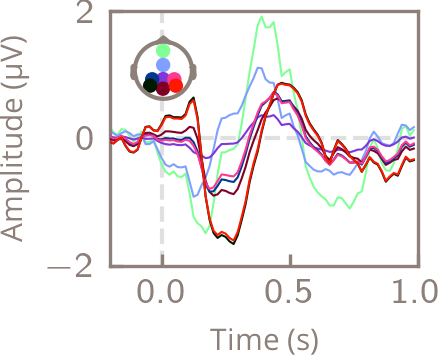
\includegraphics[width=\linewidth]{figures/bttda/forward_block-0_contrast.png}
    \end{minipage}
    %\vspace{-1em}
    \subcaption{The first block.}
  \end{subfigure}


  \begin{subfigure}[b]{\linewidth}
    \begin{minipage}[b]{.15\linewidth}
      \inputpgf{figures/bttda}{forward_block-1_ap-sp-0.pgf}
      \vspace{3em}
    \end{minipage}\hfill%
    \begin{minipage}[b]{.15\linewidth}
      \inputpgf{figures/bttda}{forward_block-1_ap-sp-1.pgf}
      \vspace{3em}
    \end{minipage}\hfill%
    \begin{minipage}[b]{.25\linewidth}
      \inputpgf{figures/bttda}{forward_block-1_ap-tmp.pgf}
    \end{minipage}\hfill%
    \begin{minipage}[b]{.3\linewidth}
      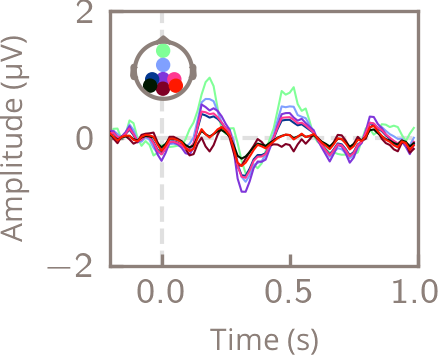
\includegraphics[width=\linewidth]{figures/bttda/forward_block-1_contrast.png}
    \end{minipage}
    %\vspace{-1em}
    \subcaption{The second block.}
  \end{subfigure}

	%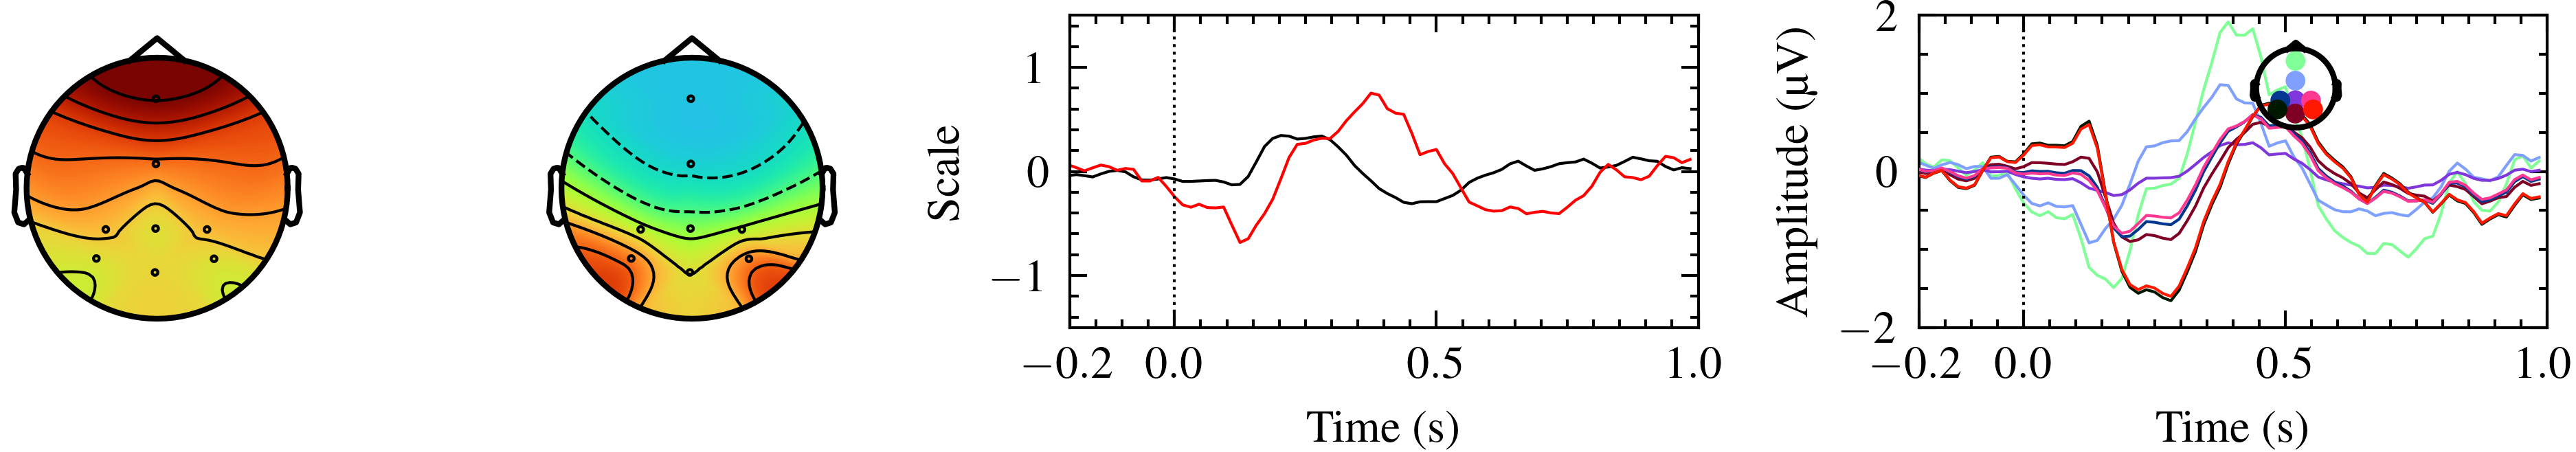
\includegraphics[width=\linewidth]{figures/bttda/forward_block-0.png}
	%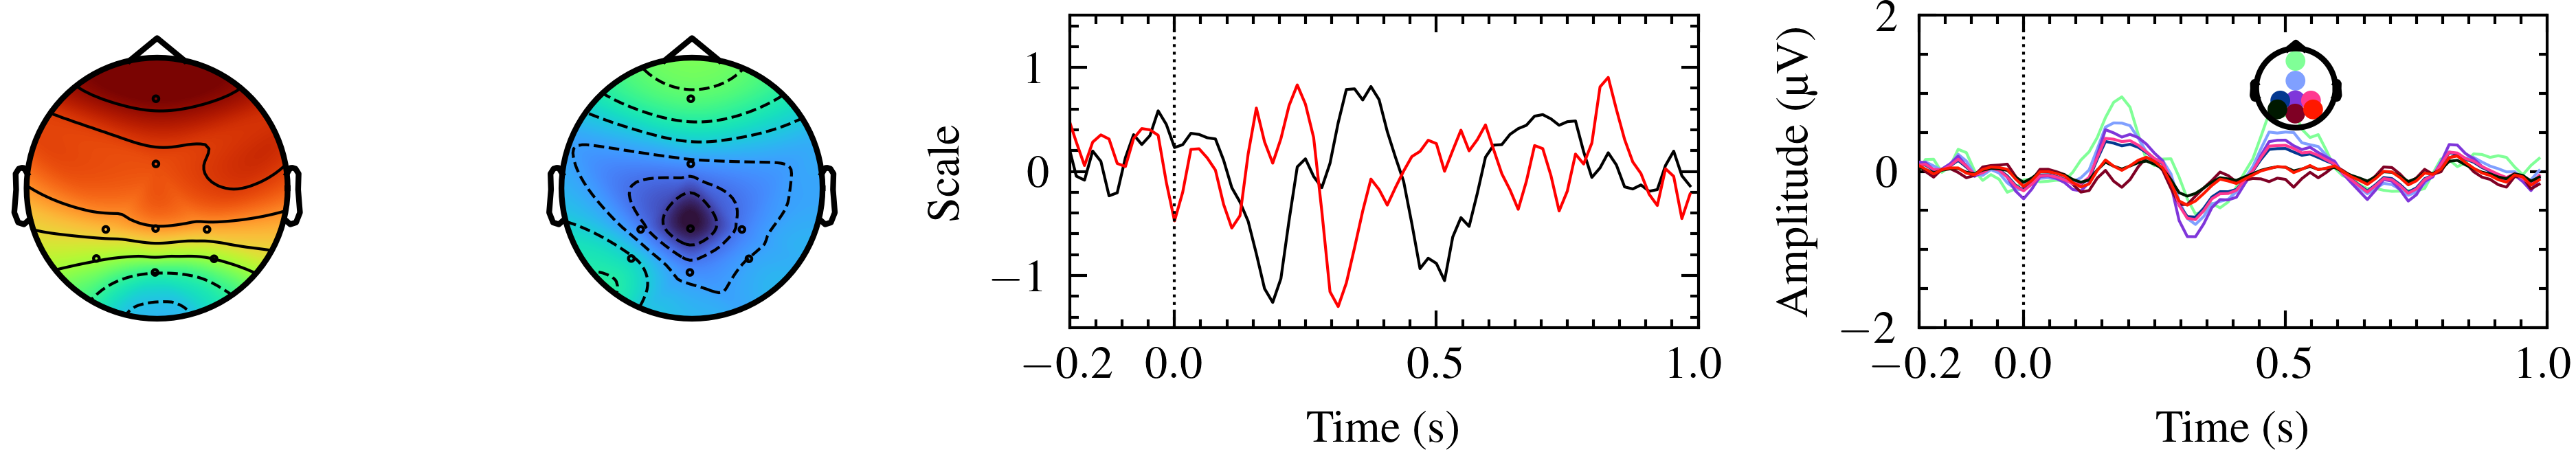
\includegraphics[width=\linewidth]{figures/bttda/forward_block-1.png}
  \caption[Extracted \acs{bttda} activation patterns.]{%
    Spatial (left two columns) and temporal (middle column) activation patterns and
		condition contrasts (right column) obtained after forward projection of the latent
    features for 2 blocks of rank $(2,2)$ of \ac{bttda}
    fit on the full dataset BNCI2014-008.
    The separate blocks approximately model different \ac{erp}
		components.}
	\label{fig:forward}
\end{figure*}
Given informed or correctly tuned hyperparameters, this method could be used to
e.g., separate \ac{erp} components or neural processes based on the task-related
information in the class labels.


\subsection{Model selection and dimensionality}

\Ac{bttda} trades in the rigid \ac{hoda} model for increased model complexity with more
hyperparameters to tune, which could open up a setting where performance can be
improved.
This turns tensor discriminant analysis into a model selection procedure
instead of a projection optimization procedure.
Despite favorable results in \ac{bci} decoding, the applications of the proposed
\ac{bttda} model are limited mainly by this model selection approach used
to determine the individual block ranks.
While our proposed greedy model selection algorithm is a step in the right
direction, the high computational cost of setting hyperparameters through cross
validation can still hinder the portability of decoders relying on
\ac{bttda}.

Due to its heuristic nature, the greedy algorithm does not always result in the
set of ranks with the highest achievable performance.
In combination with the fact that the feature selection cutoff parameter was
fixed somewhat arbitrarily, it is clear that thorough
hyperparameter optimization could improve performance.
Furthermore, it is clear that our proposed model selection procedure does not
necessarily result in an optimal set of blocks that group coherent projections
within the same block, according to some desirable metric.
Examples of this are sparsity, pattern interpretability, minimal or maximal
between- or within-block feature correlation, decreasing discriminability, etc.
Finally, the completeness of the presented results is limited by the artificial
restriction in hyperparameter choice.
We imposed $(r_1=r_2=\ldots=r_k)$ to reduce the computational demand of
the performed experiments.
In a sense, this goes against the proposition of increased model flexibility.
It might well be that \ac{bttda} in some cases offers little added value over the
Tucker-structured \ac{hoda}, when both are given free choice of rank.
Future efforts should focus on automatic parameter setting, e.g., using sparsity
or information criteria such as the ones used in Block-Term Tensor Regression~\cite{Faes2022}
or other statistical measures based on the model's application.

Another limitation is that \ac{bttda} might yield a disproportionate
improvement for datasets with a low number of features relative to sample size,
while being less effective for datasets with more features.
This is reflected in our \ac{erp} results (low dimensionality vs. high number of
trials) compared to the \ac{mi} results (higher dimensionality due to third-order
tensorization vs. lower number of trials).
We expect a dimensionality limit beyond which the forward modeling step cannot
accurately regress from the low-dimensional latent tensors to the high-
dimensional original tensors, introducing
error in the input data for the next block, which can stack up over blocks.
Since the forward multilinear least squares problem is underdetermined, it is
prone to numerical instability, which calls for regularization of the forward
modeling procedure, but this would introduce another hyperparameter.
It should also be thoroughly investigated what the impact is of going beyond
second- and third-order cases to higher-order tensors, since this could have a
large impact on the model.
Other tensorization methods of the \ac{eeg} data, like time-lagged Hankel
tensors~\cite{Papy2005}, or tensors across subjects or sliding windows, etc.,
could also be of interest if they are appropriately chosen based on prior
knowledge of the dataset.

\section{Conclusion}

We have introduced \acf{bttda}, a novel,
tensor-based, supervised dimensionality reduction technique optimized for class
discriminability, which adheres to the block-term tensor structure.
\ac{bttda} is a generalization of \acf{hoda} and can also be
applied as a special sum-of-rank-one tensors PA\-RA\-FAC\-DA model.
The model is obtained by iteratively fitting \ac{hoda} in a deflation scheme,
leveraging a novel forward modeling step.

Via an accompanying heuristic model selection procedure, \ac{bci} decoders using
\ac{bttda} feature extraction can significantly outperform decoders based on
\ac{hoda} and reach state-of-the-art decoding performance on event-related potential
problems (second-order tensors) and scores on par with or higher than \ac{hoda} in motor
imagery problems (third-order tensors).
Moving from the rigid Tucker tensor structure of \ac{hoda} to the more flexible
block-term structure shifts the problem from finding optimally constrained
multilinear projections to model and feature selection.

Introducing a flexible block-term tensor model as the underlying structure
reformulates tensor discriminant analysis as a model selection
problem.
This allows performance to be traded off for model complexity and the number of
features, to find a setting that is more effective for decoding.
Because of its general implementation and minimal assumptions on data structure,
BTTDA can equally be applied to classification for other neuroimaging modalities
(MEG, ECoG, fNIRS, fMRI, EMG, ...) or to tensor classification problems in other
fields.

%\section*{Acknowledgements}
%\todo{move to the end}
%We thank the Flemish Supercomputer Center (VSC) and the High-Performance
%Computing (HPC) center of the KU Leuven for allowing us to execute our
%computational experiments on their systems.
%We also wish to acknowledge dr.\ Axel Faes for his inspiration in conceptualizing this
%work.


\chapter{\Acs{erp} latency estimation and alignment}
\label{sec:wcble}
\emph{Sections~\ref{sec:wcble/literature/contrib} and~\ref{sec:wcble/methods} were published
as part of~\textcite{VanDenKerchove2024}}

\section{Introduction}
\label{sec:wcble/intro}

\Ac{eeg}-based visual oddball \acp{bci} establish communication with paralyzed
individuals by decoding \acp{erp} obtained from time-modulated flashing
stimuli (see~\cref{fig:bci/loop}).
These \acp{erp} consist of multiple \ac{erp}-components, peaks, and troughs in
\ac{erp} waveform (see \cref{fig:bci/erp}).
These components each have their own distinct amplitude and latency.
\Ac{erp} component latency can reflect a wide range of cognitive,
neurophysiological, and clinical properties, that can be confounding factors in
the development of \acp{bci}~\cite{Luck2014}.
Latency is often assessed as the timing of an \ac{erp} component peak, obtained
after averaging over trials.
Latencies of non-averaged, single-trial \acp{erp} should capture even more
relevant information, yet they are very hard to measure due to the low \ac{snr} of
single-trial \acp{erp}.
Within-session variability of \ac{erp} latency, called \ac{erp} latency
\emph{jitter}, has been shown to influence \ac{bci}
accuracy~\cite{Thompson2012}.
This effect is especially prominent when bringing \ac{bci} development from the
lab to the clinical setting with patients in the target population.
\textcite{Zisk2021} showed that patients with \ac{als} have significantly
increased \ac{erp} jitter.
\textcite{Arico2014} showed that latency jitter negatively affects \ac{bci}
performance, and disproportionately so when the user is not directly gazing at
intended targets, such as is the case for individuals with \ac{sspgi}.
Therefore, properly accounting for \ac{erp} latency jitter can contribute to
the development of gaze-independent visual \acp{bci}.


\subsection{Neural origins of \acs{erp} latency jitter}
While the classic \ac{erp} model assumes a constant \ac{erp} response over trials,
research has shown that cortical evoked potentials show significant
trial-to-trial jitter~\cite{Truccolo2002}.
Experiments show that latency jitter in \acp{erp} is the result of the interaction of
the evoked activity with ongoing dynamics in the brain~\cite{Hasenstaub2007,
	Kisley1999, Curto2009, Arieli1996}.
According to the Firefly model of event-related activity~\cite{Burgess2012},
the latency of an evoked potential results from a combination of the modulation
of oscillating activity that is time-locked, but not necessarily phase-locked to stimulus onset,
and a delay caused by ongoing neurophysiological processes that are not necessarily related to the task
\cite{Stokes2016,Mouraux2008}.
If these processes are related to the \ac{bci} task at hand, such as attention
and visual processing, jitter could have a significant impact on \ac{erp}
decoding.

\subsection{Implications for \acs{erp} analysis}

The presence of latency jitter introduces multiple issues to \ac{erp} analysis, the
most prominent of which is the smearing effect, as illustrated
in~\cref{fig:wcble/smearing}. In \ac{erp} analysis, single-trial \acp{erp} are usually
averaged per condition to cope with the unfavorable \ac{snr}.
When averaging over multiple identical responses with jittered latencies, the shape
and amplitude of the average do not reflect the properties
of the original signal.
Because the amplitude of the average is lower, the \ac{snr} will also be negatively impacted.
More generally, the smearing effect leads to difficulties interpreting \ac{erp}
results and making inferences about amplitude or latency effects because these
are entangled when using averaging~\cite{Luck2014}.

\begin{figure}
  \centering
  \sffamily
\sansmath
\begin{tikzpicture}   % First subplot (low jitter) positioned relative to center
    \begin{axis}[
        at={(0,0)}, % Adjust position to the left, closer to the center
        anchor=center,
        width=.45\textwidth, height=.309\textwidth,
        xmin=20, xmax=80,
        ymin=-0.1, ymax=1.1,
        axis lines=none, % Remove axes
        title={low jitter}, % Add title
        title style={yshift=-10pt, color=muteblack}, % Adjust title position to make it closer to the plot
        ]
        % Plot individual waveforms (low jitter) in darkgray
        \addplot[darkgray,domain=20:80,samples=100] {exp(-0.5*((x-50)/5)^2)};
        \addplot[darkgray,domain=20:80,samples=100] {exp(-0.5*((x-52)/5)^2)};
        \addplot[darkgray,domain=20:80,samples=100] {exp(-0.5*((x-48)/5)^2)};
        \addplot[darkgray,domain=20:80,samples=100] {exp(-0.5*((x-51)/5)^2)};
        \addplot[darkgray,domain=20:80,samples=100] {exp(-0.5*((x-49)/5)^2)};

        % Plot average waveform (low jitter) in accent1 color, very thick
        \addplot[ultra thick,accent1,domain=20:80,samples=100] {exp(-0.5*((x-50)/5)^2)};
    \end{axis}

   % Second subplot (high jitter) positioned relative to center
   \begin{axis}[
      at={(0.55\textwidth,0)}, % Adjust position to the left, closer to the center
       anchor=center,
        width=.45\textwidth, height=.309\textwidth,
       xmin=20, xmax=80,
       ymin=-0.1, ymax=1.1,
       axis lines=none, % Remove axes
       title={high jitter}, % Add title
       title style={yshift=-10pt, color=muteblack}, % Adjust title position to make it closer to the plot
       ]
       % Plot individual waveforms (high jitter) in darkgray
       \addplot[darkgray,domain=20:80,samples=100] {exp(-0.5*((x-45)/5)^2)};
       \addplot[darkgray,domain=20:80,samples=100] {exp(-0.5*((x-55)/5)^2)};
       \addplot[darkgray,domain=20:80,samples=100] {exp(-0.5*((x-40)/5)^2)};
       \addplot[darkgray,domain=20:80,samples=100] {exp(-0.5*((x-60)/5)^2)};
       \addplot[darkgray,domain=20:80,samples=100] {exp(-0.5*((x-50)/5)^2)};

       % Plot average waveform (high jitter) in accent1 color, very thick
       \addplot[ultra thick,accent1,domain=20:80,samples=100] {0.2*(exp(-0.5*((x-45)/5)^2) + exp(-0.5*((x-55)/5)^2) + exp(-0.5*((x-40)/5)^2) + exp(-0.5*((x-60)/5)^2) + exp(-0.5*((x-50)/5)^2))};
   \end{axis}

   % Unified legend positioned further below the center
   \node[anchor=center] at (.3\textwidth,-.2\textwidth) {\begin{tikzpicture}
       \begin{axis}[
           hide axis,
           xmin=0, xmax=0, ymin=0, ymax=0,
           legend style={
	   	draw=none, legend columns=2, /tikz/every even column/.append
	 style={column sep=2cm}
	 }
           ]
           \addlegendimage{darkgray,thick}
           \addlegendentry{Waveforms}
           \addlegendimage{accent1,ultra thick}
           \addlegendentry{Average}
       \end{axis}
   \end{tikzpicture}};
\end{tikzpicture}
%\vspace{-5cm}

  \caption[The smearing effect.]{The smearing effect. When obtaining an \ac{erp} template through
  averaging, high jitter causes a decrease in peak amplitude and a deformation
  of the shape of the waveform.}
  \label{fig:wcble/smearing}
\end{figure}

The smearing effect equally impacts the \ac{snr} of information captured by a
classifier's parameters when training with a procedure that does not account for
this jitter, and thus also affects its performance~\cite{Thompson2012}.
As an illustrative example, think of an \ac{lda} \ac{erp} classifier that uses
class averages over \ac{erp} epochs to construct its between-class scatter
matrix.
These per-class averages will be affected by the smearing effect and will be
less effective templates for \ac{erp} retrieval.
Similarly, the noise model in \ac{lda} assumes stationarity and subtracts
the class-wise averages from the signal to calculate
the within-class scatter matrix, which will then also be affected.
Hence, effective latency estimation and jitter compensation can contribute to higher
decoding performance.

\subsection{Benefits of latency estimation}
As we will see later, a common approach to counteract the smearing effect is to correct single-trial
\acp{erp} for jitter before averaging.
This can be done by estimating the latency of each
single-trial \ac{erp} and aligning them before averaging.
Latency estimation has multiple advantages:
\begin{enumerate*}[label={(\arabic*)}]
	\item Latency-based \ac{erp} alignment can help reveal the true shape and
	properties like peak amplitude and latency of \acp{erp} across
	experimental conditions. These are variables of interest for
	testing electrophysiological and behavioral hypotheses.
	Additionally, latency estimation allows for the extraction of
	other descriptors from a set of single-trial \acp{erp}, like
	amplitude or latency variance~\cite{Hultsch2004}, which can
	also be of interest as studied variables.
  For instance, in the work of \textcite{Saville2014}, the inter-trial latency
  variability itself is determined as a correlate of working memory performance.
	\item Counteracting the smearing effect will boost the signal-to-noise
	ratio of averaged \acp{erp} by increasing the amplitude of the
	\ac{erp} signal. This in turn can reveal smaller or more jittered \ac{erp}
  components which would otherwise be obscured or blurred due to desynchronization.
    These \emph{deblurred} templates can then be used for analysis of the \ac{erp}
	waveform, or as templates of the signal of interest in
	\acp{bci}~\cite{Arico2014}.
	%this enables decoders to take into account the relatively low amplitude
	%earlier components, leading to applications in settings where
	%information from other components than the P300 need to be exploited,
	%like covert visual attention paradigms~\cite{arico2014influence,
	%hardiansyah2020single}.\todo[inline]{rework this to latency features
	%because smaller visual components might not really be revealed
	%since they're already time-locked}
	\item Finally, the introduction of latency estimation and alignment generally
	improves \ac{bci} classification performance.
  Single-trial latencies can be used as features to improve
  classification~\cite{Hardiansyah2020}.
	Furthermore, compensating for inter-trial differences, especially when
	extended to inter-session or inter-subject differences, can aid in transfer learning or
	generalization across subjects and protocols~\cite{Iturrate2014}.
\end{enumerate*}


\section{Literature}

\subsection{Single-component approaches}
\label{sec:wcble/literature/single-comp}

The simplest method to estimate single-trial latency is
\emph{peak picking}.
Here, the latency of an \ac{erp} is determined as the
time-point of its maximum (or minimum) amplitude relative to stimulus
onset.
While straightforward, this method does not perform well in low
\ac{snr} conditions, unless combined with filtering.
Filtering can suppress the noise contaminating \ac{eeg} trials, lowering
the risk of picking a noise peak instead of a true peak of the \ac{erp}.
Several filtering approaches have been developed to be used in
conjunction with peak-picking, in the time domain~\cite{
  Carlton1980, McCarthy1981, Karjalainen1999, Nishida1999, Sparacino2002,
  Georgiadis2005, D’Avanzo2011}
and in the time-frequency domain~\cite{
  Quiroga2003, Wang2007, Hu2010}.
The aforementioned analysis and performance prediction method proposed
by \textcite{Arico2014} estimates the single-trial P3 latencies of attended
epochs by P3 peak-picking after filtering in the time-frequency domain and
corrects for jitter by temporally aligning all target epochs to the average
latency, i.e., by shifting the epochs in time such that the P3 peaks all fall
at the same time instance.
Filtering can
also be done in the spatial domain. The spatial filter can be constructed
using \ac{pca}~\cite{Ouyang2017}, \ac{ica}~\cite{Townsend1999, Jung2001,
	Milne2011}, or as a spatial LCMV beamformer~\cite{Treder2016}.

Template matching is generally preferred to peak picking.
The algorithm proposed by \textcite{Woody1967} in 1976 is a simple and elegant
latency estimation method that is still being used and is even
considered among the more performant techniques for
\acp{erp}~\cite{Thornton2008, Ouyang2017}.
It starts with an average \ac{erp} as a rough estimation of the aligned template
\ac{erp}, and iteratively refines this template by determining at each step the time point of maximum
cross-correlation of this template with all single-trial \acp{erp} and aligning them
on these time points to form the next template.
Similarly, cross-correlation template matching can be combined with filtering.
\textcite{Souloumiac2013} uses XDAWN to construct a spatial filter before
template matching the spatially filtered signal. \textcite{Iturrate2014} uses a
spatiotemporal filter. Instead of aligning the
latencies to obtain the template for the next iteration, weighted averaging can
also be used~\cite{Gasser1983}.

Despite good performance, the iterative scheme of Woody's algorithm has a risk of converging to a local
optimum.
To avoid this, a fitness function can be defined to jointly optimize
the set of single-trial \ac{erp} latencies, which can be optimized with a genetic algorithm~\cite{Pelo2018}.
Alternative methods are based on graph
optimization~\cite{Dimitriadis2018}, hidden process models~\cite{Kim2020}, or by fitting an \ac{erp} model with
maximum likelihood estimation~\cite{Gratton1989, Tuan1987, Moecks1988, Puce1994}.

\subsection{Multi-component approaches}
\label{sec:wcble/literature/multi-comp}
In the previous section, we have abstracted away the fact that \acp{erp} are
multi-component signals, which is not taken into account by the aforementioned
methods.
Multiple components can be time-locked to different events or neurophysiological
processes and therefore are not necessarily time-locked to each other. They
each can have different latency variabilities.
The presence of more than one component can hamper the
performance of some latency estimation algorithms, and it is often only possible to extract the latencies of the largest component present~\cite{Ouyang2017}. When aligning trials
to one component and averaging, this will introduce blurring in the other
components~\cite{Ouyang2020}.

Most of the algorithms above can be adapted to work on multiple \ac{erp} components
by carefully selecting peaks or pre-determined regions of interest.
\textcite{Hardiansyah2020} uses an \ac{snr} boosting method, applied to a specific
time-window for each \ac{erp} component to extract a latency per component.
Methods based on spatial decomposition filters like \ac{pca}, \ac{ica}, or XDAWN can be leveraged
to utilize multiple of their components as filters, resulting in multiple time
series where peak picking or Woody's algorithm can be applied. In general,
however, these algorithms lack an integrated approach to deal with multiple
\ac{erp} components. A clear evaluation of the performance of these
methods in multi-component settings is lacking.

Some algorithms separate components into stimulus- and response-locked component clusters based on their
latency distributions~\cite{Jung2001, Takeda2008, Zhang1998, Yin2009}.
These algorithms do, however, require a response
button trigger signal as input to determine the response time, which is
not always present or applicable in an \ac{erp} experiment, especially in
the case of \acp{bci}.
The RIDE algorithm~\cite{Ouyang2011, Ouyang2015, Wang2015, Ouyang2016, Ouyang2020}
is able to do this without entirely relying on the response time and can
separate stimulus-locked, response-locked, and multiple central component clusters.
Others, like spatial filtering methods that use decomposition methods to
determine the spatial filter, can be modified to separate
components~\cite{Ouyang2017}.

Finally, the smearing problem can also be overcome by algorithms that are not
based on \ac{erp} component latency estimation but use time-warping-based methods
to enhance the shape of the averaged template \ac{erp}, like Dynamic Time
Warping~\cite{Gupta1996, Wang2001, Zoumpoulaki2015}, Correlation-Optimized
Warping~\cite{Skov2006}, or Fast Variational
Alignment~\cite{Flotho2021}.
These methods work
fundamentally differently from the latency estimation methods, and cannot
directly be used to extract latency features.

\subsection{Contribution}
\label{sec:wcble/literature/contrib}

Most of these methods suffer from a common drawback: they cannot be used in a
decoding scheme to improve performance for incoming epochs with unknown
class labels that contain either a target or non-target \ac{erp} response.
They can be used offline on a set of labeled epochs for testing hypotheses
concerning latency and jitter, for aligning templates, or for \ac{bci} performance
prediction, but not for \ac{erp} classification.
While some of the aforementioned methods could be adapted to perform
classification tasks, few studies investigate how to exploit this latency estimation
for jitter-resistant decoding.
\textcite{Hardiansyah2020} incorporated single-trial latencies in
classification by peak-picking within a given
\ac{erp} time window, unaware of the class of the epoch under investigation.
The \ac{cble} algorithm introduced
by \textcite{Thompson2012} also explicitly applies latency estimation in a
decoding setting.
\textcite{Thompson2012} initially formulated \ac{cble} as an offline performance
prediction method.
Later, its output was successfully adapted to compensate for jitter to improve
decoder performance~\cite{Mowla2017, Zisk2022}.

Time-series classification algorithms~\cite{Abanda2019}
that are robust to jitter can be used in a decoding setting,
but, in general, have scarcely been applied to \ac{erp} decoding.
Data augmentation involving jittering the training
data~\cite{Krell2018, Zisk2022} and Riemannian Geometry methods using spatial
covariances as features~\cite{Aydarkhanov2020} have both been shown
to perform well in the presence of \ac{erp} jitter.
In this work, we opted to apply \ac{cble} because it has successfully been applied to
classify jittered \acs{erp}.
We adapt the \ac{cble} to an iterative method akin to Woody's scheme that can better
compensate for jitter, to improve covert VSA decoding performance.


\section{Methods}
\label{sec:wcble/methods}

\subsection{Classifier-based Latency Estimation}
\label{sec:wcble/methods/cble}

Consider a training set of $N$ EEG epochs with $C$ channels of $S$
samples $\{\mat{X}_n^\mathrm{train} \in \mathbb{R}^{C\times S}\}_{n=1}^N$
with corresponding training labels $\mathbf{l^\mathrm{train}} \in \{\mathrm{target},
	\textrm{non-target}\}_{n=1}^N$, and a
similar testing set of $M$ epochs $\{\mat{X}_m^\mathrm{test} \in
	\mathbb{R}^{C\times S}\}_{m=1}^M$.
We assume that the sampling period is $T$, i.e., that the sample with index $s$ is sampled at time $sT$.
In the following, we use the matrix slicing notation to denote row or column intervals extracted from a matrix.
For instance, $\mat{X}[:,s_1:s_2]$ denotes all columns of $\mat{X}$ with indices between $s_1$ (included) and $s_2$ (excluded).

\Ac{cble}, summarized in \cref{sec:wcble/app/cble-alg}, works by training a
\textit{first-stage} classifier $\mathcal{C}(\theta,f)$
defined within a time period $[s_1:s_2]$ with a set of parameters $\theta$ and a
decision function $f(\mat{X}[:,s_1:s_2],\theta) \rightarrow
y$ outputting a classification score $y\in\mathbb{R}$ for a given epoch $\mat{X}$,
such that
\begin{equation}
  \theta = \mathrm{train}_\mathcal{C}(\{\mat{X}_n^\mathrm{train}[:,s_1:s_2]\}_{n=1}^N,\mathbf{l}^\mathrm{train})
  \label{eq:cble-train}
\end{equation}
Then,
$f$ can be applied to all (possibly overlapping) slices of length $s_2-s_1$ of
an epoch $\mat{X}$, resulting in a vector of score values
$\mathbf{y}=[y_1\,\ldots\,y_R]^T \in\mathbb{R}^R$ such that
\begin{equation}
  y_s = f(\mat{X}[:,s:s+(s_2-s_1)],\theta)\quad \forall s\in 1,\ldots,R
	\label{eq:score}
\end{equation}
with $R = S-(s_2-s_1)$.
To leverage \ac{cble} for \ac{erp} classification, the score vectors $\mathbf{y}$ can be
arranged in matrices $\mat{Y}^\mathrm{train}\in\mathbb{R}^{N\times R}$ and $\mat{Y}^\mathrm{test}\in\mathbb{R}^{M\times R}$.
These can be further classified by training a \textit{second-stage} classifier on
$\mat{Y}^\mathrm{train}$ and class labels $\mathbf{l}^\mathrm{train}$.
However, the resulting score-over-time vectors per epoch still suffer from jitter.
For classification, we follow the approach of \cite{Mowla2017}, using a
maximum-level hierarchical Daubechies-4 wavelet transform to reduce
dimensionality before classification with the second-stage classifier.
In the \ac{cble}-decoder, it is this wavelet transform that decreases the sensitivity
to latency differences, actively compensating for \ac{erp} latency jitter.

When using a simple spatiotemporal linear classifier as first-stage classifier,
\ac{cble} is equivalent to the first iteration of Woody's algorithm with the
spatiotemporal classifier weights as template.
\textcite{Thompson2012}, \textcite{Mowla2017}, and \textcite{Mowla2020} show
that \ac{cble} is relatively independent of the first-stage classifier for \ac{bci}
accuracy prediction and for \ac{erp} classification.
Therefore, we opt to use the variant of Linear Discriminant Analysis with block-Toeplitz
regularized covariance matrix (tLDA) proposed by \textcite{Sosulski2022}, as the first-stage
classifier and logistic regression as second stage.

\subsection{Robust latency features}
\label{sec:robust-latency}
The \ac{erp} decoding method based on \ac{cble} introduced by \textcite{Mowla2017} does
not make use of the extracted latencies, only passing score matrix $\mat{Y}$ on
to the second-stage classifier.
Furthermore, previous \ac{cble} works~\cite{Thompson2012, Mowla2020} only used these
latencies to correlate them with neurophysiological processes or to predict
decoder performance.
We noticed that, while \ac{cble} performance was unaffected, the classification
performance of our proposed method can be improved if the estimated
latencies are also made available as features to the second-stage classifier,
after a square transform for linear separability~\cite{Thompson2012}.

However, including these latency features gives rise to the following issue when
classifying unseen data.
The \ac{cble} latency estimate is defined only for target epochs as
$s_\mathrm{target}=\argmax_s{y_s}$.
This is the point in time where the target class reaches the largest separation
from the background noise and non-target class, indicating the target \ac{erp} is
most likely to occur here.
However, in a classifier test phase, it is not known a priori whether an
unseen epoch is a target or a non-target epoch.
This problem is solved by defining an estimated latency per class
$s_\mathrm{target}$ and $s_\mathrm{non-target}$ for every epoch,
regardless of its actual class.
The estimated class latencies can then be used as features for training and
testing the second-stage classifier.
This way, the latencies of the testing data can be presented to the second-stage
classifier without knowledge of the testing data class labels, making them
useful in decoding.

In a similar manner to the target latency, the non-target latency could be defined
as~$s_\mathrm{non-target}=\argmin_s{y_s}$.
However, this is problematic since it is not evident how to estimate
the latency of, e.g., a P3 \ac{erp} component for a non-target epoch, since the
non-target class is characterized by the absence of this component.
\footnote{Depending on the stimulation and experimental design, \ac{erp} components can be present in one experimental
	condition or class and missing in another, or appear in multiple classes
	at different amplitudes. In the latter case, it could be possible
	to estimate the latency of an \ac{erp} in the conditions where it appears, but if
	its amplitude is lower or negligible in some conditions, latency estimates
	will be less accurate, hence this case is still problematic.}.
In fact, $y$ can have multiple local minima or entirely lack distinct peaks for
non-targets, rendering the minimum estimate meaningless.

Instead, we opt for a more robust, probabilistic definition of class latencies.
This robust estimation method yields latencies that
\begin{enumerate*}[label=(\arabic*)]
  \item are more meaningful as input for the second-stage
    classifier, and
  \item lead to smoother convergence in our proposed iterative alignment scheme
    for \ac{wcble}, which heavily relies on exact latency estimation.
\end{enumerate*}
Assume classifier $\mathcal{C}(\theta,f,\Pr)$ now can also output a probability
per class $\Pr(l|
\mat{X}[:,s_1:s_2)], \theta)$ for a given epoch $\mat{X}$, a feature of many
common classifiers.
Analogous to equation~\ref{eq:score}, we can now write
\begin{equation}
\Pr(\mat{X},\theta,l,s) = \frac{1}{R}\Pr(\mat{X}[:,s:s+(s_2-s_1)],\theta,l)
  \quad \forall s\in 1,\ldots,R
	\label{eq:prob}
\end{equation}
The latency features assuming the epoch belongs to a given class
$l\in\{\textrm{target},\textrm{non-target}\}$ are then defined as the median of
the corresponding distributions
\begin{equation}
  s_l =\mathrm{median}\left[\Pr(s|\mat{X},\theta,l) \right]
  \label{eq:prob-latency}
\end{equation}
Note that $\Pr(s|\mat{X},\theta,\textrm{non-target}) =1-
  \Pr(s|\mat{X},\theta,\mathrm{target})$.
The median of the probability distribution over time is more robust to
outliers and noise than the maximum or minimum score.
For the non-target case, the median approach tends towards the center of a
near-uniform distribution, resulting in a more consistent latency estimate over
trials as compared to the minimum approach.


\subsection{\acl{wcble}}
To improve performance over \ac{cble}, we propose a new algorithm inspired both by
\ac{cble} and the aforementioned Woody iteration scheme termed \ac{wcble}.
Instead of using \ac{cble} to estimate the features of a second-stage classifier
directly, \ac{cble} latency estimation is used as a step in a Woody iteration scheme.
While the Woody algorithm iteratively enhances the \ac{snr} of an \ac{erp} template to
cross-correlate with the data, \ac{wcble} iteratively re-estimates the parameters of
the first-stage classifier.
To improve convergence and perform well in a classification setting, \ac{wcble}
aligns both targets and non-targets to their corresponding estimated latencies.

The \ac{wcble} algorithm is presented in \cref{sec:wcble/app/wcble-alg}.
Its training phase is visualized in~\cref{fig:diagram-train}.
The initial training epochs $\{\mat{X}_n^{(1)}\}_{n=1}^N$ are set to $\{\mat{X}_n^\mathrm{train}\}_{n=1}^N$.
At every iteration, classifier $\mathcal{C}$ is trained like in \ac{cble}:
\begin{equation}
  \theta^{(i)} =
  \mathrm{train}_\mathcal{C}(\{\mat{X}^{(i-1)}_n[:,s_1:s_2]\}_{n=1}^N,\mathbf{l}^\mathrm{train})
\end{equation}
Next, latency $s_{l_n}^{(i)}$ is determined for every epoch $\mat{X}^{(i)}$ corresponding
to its class label $l_n$ using \cref{eq:prob-latency}.
Finally, the training epochs $\mat{X}^{(i+1)}$ for the next iteration are determined by aligning
each original training epoch to the latency $s_{l_n}^{(i)}$ corresponding to its respective class
label.
\begin{equation}
  \mat{X}^{(i+1)}_n = \mathrm{align}(\mat{X}_n^\mathrm{train}, s_{l_n}^{(i)}) \quad \forall n=1,\ldots,N
\end{equation}
Aligning is performed by shifting and zero-padding the signal to the right if
the latency is negative relative to the time window onset, and to the left if
positive, by the difference between the latency and the window onset.
\fullpagefig{%
  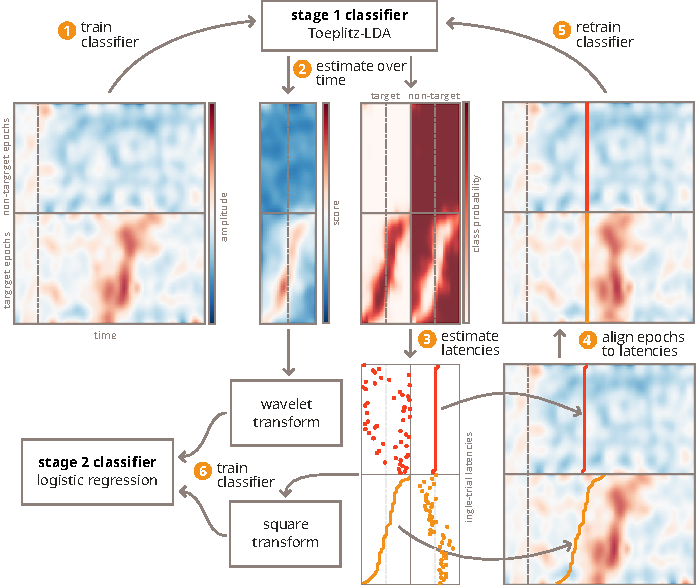
\includegraphics[width=\textwidth]{figures/wcble/figure1.pdf}
}{%
  Schematic representation of the \acs{wcble} training phase.
}{%
  Schematic representation of the \ac{wcble} training phase.
  (1) The first-stage spatiotemporal binary classifier is trained on a set of
  epochs.
  (2) It is then applied to time-shifted copies of the epochs to obtain scores
  and class probabilities over time.
  (3) The medians of these probability distributions are assumed as the class
  latencies.
  (4) The epochs are aligned to their corresponding class latencies by
  shifting in time such that all latencies fall at the same moment.
  (5) The spatiotemporal classifier is then retrained on the aligned epochs
  for the next iteration.
  (6) After the iterative process halts, the scores and latencies obtained
  from the last iteration are used to train the second-stage
  classifier.
}{%
  fig:diagram-train
}
The process halts after a fixed number of iterations or when the estimated set
of latencies has been encountered before, indicating it ended up in a loop.
In the end, the procedure should result in enhanced classifier parameters $\theta^*$,
closer to those when there would be no jitter between epochs.
Note that using the median approach for robust latency estimation results in a
smoother yet longer convergence process compared to the maximum/minimum approach.
We can then apply the classifier with enhanced parameters $\theta^*$ in a \ac{cble}
manner to unseen epochs as illustrated in \cref{fig:diagram-eval} to obtain a
vector of scores over time as in~\cref{sec:cble} and the estimated latencies as
in~\cref{sec:robust-latency}.
\fullpagefig{
  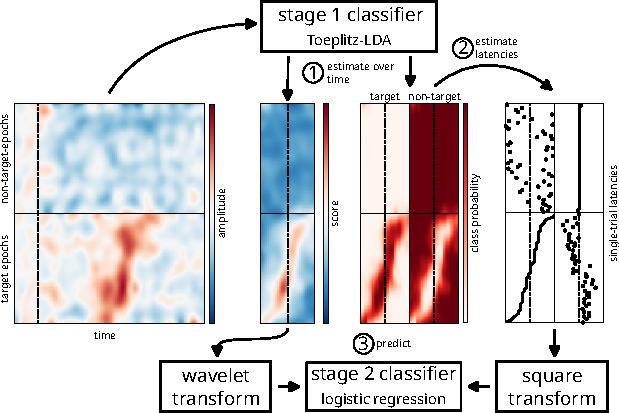
\includegraphics[width=\textwidth]{figures/wcble/figure2.pdf}

}{%
  Schematic representation of the \acs{wcble} test phase.
}{%
  Schematic representation of the Woody Classifier-Based Latency
  Estimation test phase. (1) The
	first-stage spatiotemporal binary classifier obtained from the training phase is
	applied to time-shifted copies of the epochs to obtain scores and class probabilities
	over time. (2) The medians of these probability distributions are assumed
	as the new class latencies. (3) The scores and class latencies are input to the
  trained second-stage classifier, which predicts the label of the epochs.
}{%
  fig:diagram-eval
}
\section{Results}
\label{sec:wcble/results}
Since it is hard to obtain ground truth measures of \ac{erp} latencies, we
first evaluate our approach with synthetic data.
In \cref{sec:covert-align}, the proposed algorithm will be applied to real
\ac{eeg} data.

\subsection{Synthetic data generation}
To verify our approach, we simulated synthetic 16 channel \ac{eeg} data with standard
10-20 electrode positions using the \texttt{simulate\_evoked} method of the
MNE (version 1.8)~\cite{Gramfort2013} software package.
\Acp{erp} were generated by projecting a sine wave pulse source time course in a dipole in the
left hemisphere to the scalp electrodes using a boundary element method forward
model~\cite{Mosher1999} and MNE's \texttt{fsaverage} source space and anatomy.
Pink temporal noise is generated by passing Gaussian noise through an infinite
impulse response filter with transfer function
$\frac{B(z)}{A(z)} = \frac{1}{1 -1z^{-1}+0.15z^{-2}}$.
Pink spatial noise is also added, using a noise covariance matrix constructed from the
cosine distances between electrode positions and scaling it by the inverse of
the resulting spatial covariance.
We refer to \textcite{Gramfort2014} for implementation details.

The source time course is defined by the following function:
\begin{equation}
  s(t,l) =
  \begin{cases}
    a\sin\left(2\pi f\left(t-l\right)\right) & \text{if  $l-\frac{1}{2f} < t < l-\frac{1}{2f}$} \\
    0 & \text{otherwise}
  \end{cases}
\end{equation}
over time $t$, with latency $l$, amplitude $a=\num{1e{-7}}$V, and frequency
$f=4$.

100 target epochs containing the evoked potential and noise and 100
non-target epochs containing only noise were simulated.
The target epochs were jittered by setting the latency offset $l$
of each target epoch to a random latency drawn from a normal distribution with 0 mean and standard
deviations of respectively $\sigma=0.1,0.2,0.3$s.
The noise was scaled at 32 different noise levels, with the \ac{snr} of a
target epoch ranging from 0 to -31dB, with
\begin{equation}
  \text{SNR} = 10\log_{10}\frac{\text{var}s(t,0)}{\text{var}\left(\text{noise}\right)}
\end{equation}

A sample of the simulated evoked data is displayed in \cref{fig:wcble/sim-sine}.
\fullpagefig{%
  \sffamily
  \sansmath
  \inputpgf{figures/wcble}{simulated-sine.pgf}
}{%
  Simulated target and non-target evoked data.
}{%
  Simulated target (bottom half of epochs) and non-target (top half of epochs) evoked data
  and their average (red: target, yellow: non-target, shaded area: standard
  deviation).
  Targets contain a sine wave pulse jittered by $\sigma$. 32 EEG channels with pink
  spatiotemporal noise were simulated using a forward head model, and channel C3 is
  plotted here.
}{fig:wcble/sim-sine}

\subsection{Latency estimation}
We compared our proposed \ac{wcble} algorithm to \ac{cble} on a latency
estimation task using the Pearson correlation coefficient $\rho$ at different
jitter and \ac{snr} levels.
For both \ac{cble} and \ac{wcble}, target latencies were extracted in a
10-fold cross-validation scheme using the robust median latency method after
fitting the model.
\Ac{wcble}'s maximum iteration number was set to 64.
Results are presented in \cref{fig:wcble/results/latency}.
A 95\% confidence interval on each measure was obtained through bootstrapping
with 1000 permutations.

\begin{figure}
  \sffamily\sansmath
  \hspace{-0.4200772430479885in}
%% Creator: Matplotlib, PGF backend
%%
%% To include the figure in your LaTeX document, write
%%   \input{<filename>.pgf}
%%
%% Make sure the required packages are loaded in your preamble
%%   \usepackage{pgf}
%%
%% Also ensure that all the required font packages are loaded; for instance,
%% the lmodern package is sometimes necessary when using math font.
%%   \usepackage{lmodern}
%%
%% Figures using additional raster images can only be included by \input if
%% they are in the same directory as the main LaTeX file. For loading figures
%% from other directories you can use the `import` package
%%   \usepackage{import}
%%
%% and then include the figures with
%%   \import{<path to file>}{<filename>.pgf}
%%
%% Matplotlib used the following preamble
%%
\begingroup%
\makeatletter%
\begin{pgfpicture}%
\pgfpathrectangle{\pgfpointorigin}{\pgfqpoint{5.044694in}{1.916660in}}%
\pgfusepath{use as bounding box, clip}%
\begin{pgfscope}%
\pgfsetbuttcap%
\pgfsetmiterjoin%
\definecolor{currentfill}{rgb}{1.000000,1.000000,1.000000}%
\pgfsetfillcolor{currentfill}%
\pgfsetlinewidth{0.000000pt}%
\definecolor{currentstroke}{rgb}{1.000000,1.000000,1.000000}%
\pgfsetstrokecolor{currentstroke}%
\pgfsetdash{}{0pt}%
\pgfpathmoveto{\pgfqpoint{0.000000in}{0.000000in}}%
\pgfpathlineto{\pgfqpoint{5.044694in}{0.000000in}}%
\pgfpathlineto{\pgfqpoint{5.044694in}{1.916660in}}%
\pgfpathlineto{\pgfqpoint{0.000000in}{1.916660in}}%
\pgfpathlineto{\pgfqpoint{0.000000in}{0.000000in}}%
\pgfpathclose%
\pgfusepath{fill}%
\end{pgfscope}%
\begin{pgfscope}%
\pgfsetbuttcap%
\pgfsetmiterjoin%
\definecolor{currentfill}{rgb}{1.000000,1.000000,1.000000}%
\pgfsetfillcolor{currentfill}%
\pgfsetlinewidth{0.000000pt}%
\definecolor{currentstroke}{rgb}{0.000000,0.000000,0.000000}%
\pgfsetstrokecolor{currentstroke}%
\pgfsetstrokeopacity{0.000000}%
\pgfsetdash{}{0pt}%
\pgfpathmoveto{\pgfqpoint{0.379436in}{0.340278in}}%
\pgfpathlineto{\pgfqpoint{1.813678in}{0.340278in}}%
\pgfpathlineto{\pgfqpoint{1.813678in}{1.746521in}}%
\pgfpathlineto{\pgfqpoint{0.379436in}{1.746521in}}%
\pgfpathlineto{\pgfqpoint{0.379436in}{0.340278in}}%
\pgfpathclose%
\pgfusepath{fill}%
\end{pgfscope}%
\begin{pgfscope}%
\pgfpathrectangle{\pgfqpoint{0.379436in}{0.340278in}}{\pgfqpoint{1.434242in}{1.406243in}}%
\pgfusepath{clip}%
\pgfsetbuttcap%
\pgfsetroundjoin%
\definecolor{currentfill}{rgb}{0.949020,0.564706,0.094118}%
\pgfsetfillcolor{currentfill}%
\pgfsetfillopacity{0.200000}%
\pgfsetlinewidth{1.003750pt}%
\definecolor{currentstroke}{rgb}{0.949020,0.564706,0.094118}%
\pgfsetstrokecolor{currentstroke}%
\pgfsetstrokeopacity{0.200000}%
\pgfsetdash{}{0pt}%
\pgfsys@defobject{currentmarker}{\pgfqpoint{0.379436in}{0.310708in}}{\pgfqpoint{1.813678in}{1.731938in}}{%
\pgfpathmoveto{\pgfqpoint{1.813678in}{0.996671in}}%
\pgfpathlineto{\pgfqpoint{1.813678in}{0.310708in}}%
\pgfpathlineto{\pgfqpoint{1.767412in}{0.364216in}}%
\pgfpathlineto{\pgfqpoint{1.721146in}{0.603474in}}%
\pgfpathlineto{\pgfqpoint{1.674880in}{0.615695in}}%
\pgfpathlineto{\pgfqpoint{1.628614in}{0.693728in}}%
\pgfpathlineto{\pgfqpoint{1.582349in}{0.886606in}}%
\pgfpathlineto{\pgfqpoint{1.536083in}{0.970807in}}%
\pgfpathlineto{\pgfqpoint{1.489817in}{1.260900in}}%
\pgfpathlineto{\pgfqpoint{1.443551in}{1.260729in}}%
\pgfpathlineto{\pgfqpoint{1.397285in}{1.448679in}}%
\pgfpathlineto{\pgfqpoint{1.351019in}{1.713175in}}%
\pgfpathlineto{\pgfqpoint{1.304753in}{1.712893in}}%
\pgfpathlineto{\pgfqpoint{1.258487in}{1.712078in}}%
\pgfpathlineto{\pgfqpoint{1.212221in}{1.704884in}}%
\pgfpathlineto{\pgfqpoint{1.165956in}{1.706809in}}%
\pgfpathlineto{\pgfqpoint{1.119690in}{1.715667in}}%
\pgfpathlineto{\pgfqpoint{1.073424in}{1.715873in}}%
\pgfpathlineto{\pgfqpoint{1.027158in}{1.708907in}}%
\pgfpathlineto{\pgfqpoint{0.980892in}{1.709132in}}%
\pgfpathlineto{\pgfqpoint{0.934626in}{1.709540in}}%
\pgfpathlineto{\pgfqpoint{0.888360in}{1.707735in}}%
\pgfpathlineto{\pgfqpoint{0.842094in}{1.707014in}}%
\pgfpathlineto{\pgfqpoint{0.795829in}{1.699105in}}%
\pgfpathlineto{\pgfqpoint{0.749563in}{1.697425in}}%
\pgfpathlineto{\pgfqpoint{0.703297in}{1.698764in}}%
\pgfpathlineto{\pgfqpoint{0.657031in}{1.697216in}}%
\pgfpathlineto{\pgfqpoint{0.610765in}{1.695488in}}%
\pgfpathlineto{\pgfqpoint{0.564499in}{1.694115in}}%
\pgfpathlineto{\pgfqpoint{0.518233in}{1.696814in}}%
\pgfpathlineto{\pgfqpoint{0.471967in}{1.698877in}}%
\pgfpathlineto{\pgfqpoint{0.425702in}{1.700372in}}%
\pgfpathlineto{\pgfqpoint{0.379436in}{1.695345in}}%
\pgfpathlineto{\pgfqpoint{0.379436in}{1.731938in}}%
\pgfpathlineto{\pgfqpoint{0.379436in}{1.731938in}}%
\pgfpathlineto{\pgfqpoint{0.425702in}{1.731507in}}%
\pgfpathlineto{\pgfqpoint{0.471967in}{1.730980in}}%
\pgfpathlineto{\pgfqpoint{0.518233in}{1.728367in}}%
\pgfpathlineto{\pgfqpoint{0.564499in}{1.727428in}}%
\pgfpathlineto{\pgfqpoint{0.610765in}{1.725772in}}%
\pgfpathlineto{\pgfqpoint{0.657031in}{1.727116in}}%
\pgfpathlineto{\pgfqpoint{0.703297in}{1.728619in}}%
\pgfpathlineto{\pgfqpoint{0.749563in}{1.728184in}}%
\pgfpathlineto{\pgfqpoint{0.795829in}{1.728516in}}%
\pgfpathlineto{\pgfqpoint{0.842094in}{1.728057in}}%
\pgfpathlineto{\pgfqpoint{0.888360in}{1.730355in}}%
\pgfpathlineto{\pgfqpoint{0.934626in}{1.729055in}}%
\pgfpathlineto{\pgfqpoint{0.980892in}{1.727923in}}%
\pgfpathlineto{\pgfqpoint{1.027158in}{1.728000in}}%
\pgfpathlineto{\pgfqpoint{1.073424in}{1.728189in}}%
\pgfpathlineto{\pgfqpoint{1.119690in}{1.728233in}}%
\pgfpathlineto{\pgfqpoint{1.165956in}{1.727383in}}%
\pgfpathlineto{\pgfqpoint{1.212221in}{1.727423in}}%
\pgfpathlineto{\pgfqpoint{1.258487in}{1.726426in}}%
\pgfpathlineto{\pgfqpoint{1.304753in}{1.727124in}}%
\pgfpathlineto{\pgfqpoint{1.351019in}{1.726077in}}%
\pgfpathlineto{\pgfqpoint{1.397285in}{1.719293in}}%
\pgfpathlineto{\pgfqpoint{1.443551in}{1.711587in}}%
\pgfpathlineto{\pgfqpoint{1.489817in}{1.706628in}}%
\pgfpathlineto{\pgfqpoint{1.536083in}{1.481127in}}%
\pgfpathlineto{\pgfqpoint{1.582349in}{1.347292in}}%
\pgfpathlineto{\pgfqpoint{1.628614in}{1.289590in}}%
\pgfpathlineto{\pgfqpoint{1.674880in}{1.292950in}}%
\pgfpathlineto{\pgfqpoint{1.721146in}{1.221543in}}%
\pgfpathlineto{\pgfqpoint{1.767412in}{1.036622in}}%
\pgfpathlineto{\pgfqpoint{1.813678in}{0.996671in}}%
\pgfpathlineto{\pgfqpoint{1.813678in}{0.996671in}}%
\pgfpathclose%
\pgfusepath{stroke,fill}%
}%
\begin{pgfscope}%
\pgfsys@transformshift{0.000000in}{0.000000in}%
\pgfsys@useobject{currentmarker}{}%
\end{pgfscope}%
\end{pgfscope}%
\begin{pgfscope}%
\pgfpathrectangle{\pgfqpoint{0.379436in}{0.340278in}}{\pgfqpoint{1.434242in}{1.406243in}}%
\pgfusepath{clip}%
\pgfsetbuttcap%
\pgfsetroundjoin%
\definecolor{currentfill}{rgb}{0.964706,0.239216,0.117647}%
\pgfsetfillcolor{currentfill}%
\pgfsetfillopacity{0.200000}%
\pgfsetlinewidth{1.003750pt}%
\definecolor{currentstroke}{rgb}{0.964706,0.239216,0.117647}%
\pgfsetstrokecolor{currentstroke}%
\pgfsetstrokeopacity{0.200000}%
\pgfsetdash{}{0pt}%
\pgfsys@defobject{currentmarker}{\pgfqpoint{0.379436in}{0.273053in}}{\pgfqpoint{1.813678in}{1.742931in}}{%
\pgfpathmoveto{\pgfqpoint{1.813678in}{0.973860in}}%
\pgfpathlineto{\pgfqpoint{1.813678in}{0.273053in}}%
\pgfpathlineto{\pgfqpoint{1.767412in}{0.515044in}}%
\pgfpathlineto{\pgfqpoint{1.721146in}{0.977493in}}%
\pgfpathlineto{\pgfqpoint{1.674880in}{1.246053in}}%
\pgfpathlineto{\pgfqpoint{1.628614in}{1.729359in}}%
\pgfpathlineto{\pgfqpoint{1.582349in}{1.725203in}}%
\pgfpathlineto{\pgfqpoint{1.536083in}{1.737484in}}%
\pgfpathlineto{\pgfqpoint{1.489817in}{1.735421in}}%
\pgfpathlineto{\pgfqpoint{1.443551in}{1.730685in}}%
\pgfpathlineto{\pgfqpoint{1.397285in}{1.731592in}}%
\pgfpathlineto{\pgfqpoint{1.351019in}{1.732060in}}%
\pgfpathlineto{\pgfqpoint{1.304753in}{1.734245in}}%
\pgfpathlineto{\pgfqpoint{1.258487in}{1.734602in}}%
\pgfpathlineto{\pgfqpoint{1.212221in}{1.734612in}}%
\pgfpathlineto{\pgfqpoint{1.165956in}{1.736272in}}%
\pgfpathlineto{\pgfqpoint{1.119690in}{1.735218in}}%
\pgfpathlineto{\pgfqpoint{1.073424in}{1.736560in}}%
\pgfpathlineto{\pgfqpoint{1.027158in}{1.738070in}}%
\pgfpathlineto{\pgfqpoint{0.980892in}{1.737329in}}%
\pgfpathlineto{\pgfqpoint{0.934626in}{1.736345in}}%
\pgfpathlineto{\pgfqpoint{0.888360in}{1.736872in}}%
\pgfpathlineto{\pgfqpoint{0.842094in}{1.737186in}}%
\pgfpathlineto{\pgfqpoint{0.795829in}{1.737594in}}%
\pgfpathlineto{\pgfqpoint{0.749563in}{1.736364in}}%
\pgfpathlineto{\pgfqpoint{0.703297in}{1.737428in}}%
\pgfpathlineto{\pgfqpoint{0.657031in}{1.735905in}}%
\pgfpathlineto{\pgfqpoint{0.610765in}{1.736924in}}%
\pgfpathlineto{\pgfqpoint{0.564499in}{1.737333in}}%
\pgfpathlineto{\pgfqpoint{0.518233in}{1.738663in}}%
\pgfpathlineto{\pgfqpoint{0.471967in}{1.738409in}}%
\pgfpathlineto{\pgfqpoint{0.425702in}{1.737462in}}%
\pgfpathlineto{\pgfqpoint{0.379436in}{1.738651in}}%
\pgfpathlineto{\pgfqpoint{0.379436in}{1.741626in}}%
\pgfpathlineto{\pgfqpoint{0.379436in}{1.741626in}}%
\pgfpathlineto{\pgfqpoint{0.425702in}{1.741143in}}%
\pgfpathlineto{\pgfqpoint{0.471967in}{1.741927in}}%
\pgfpathlineto{\pgfqpoint{0.518233in}{1.741414in}}%
\pgfpathlineto{\pgfqpoint{0.564499in}{1.741125in}}%
\pgfpathlineto{\pgfqpoint{0.610765in}{1.740495in}}%
\pgfpathlineto{\pgfqpoint{0.657031in}{1.740763in}}%
\pgfpathlineto{\pgfqpoint{0.703297in}{1.741520in}}%
\pgfpathlineto{\pgfqpoint{0.749563in}{1.741628in}}%
\pgfpathlineto{\pgfqpoint{0.795829in}{1.741195in}}%
\pgfpathlineto{\pgfqpoint{0.842094in}{1.740517in}}%
\pgfpathlineto{\pgfqpoint{0.888360in}{1.741177in}}%
\pgfpathlineto{\pgfqpoint{0.934626in}{1.741148in}}%
\pgfpathlineto{\pgfqpoint{0.980892in}{1.741656in}}%
\pgfpathlineto{\pgfqpoint{1.027158in}{1.742454in}}%
\pgfpathlineto{\pgfqpoint{1.073424in}{1.741452in}}%
\pgfpathlineto{\pgfqpoint{1.119690in}{1.740757in}}%
\pgfpathlineto{\pgfqpoint{1.165956in}{1.741672in}}%
\pgfpathlineto{\pgfqpoint{1.212221in}{1.742931in}}%
\pgfpathlineto{\pgfqpoint{1.258487in}{1.741771in}}%
\pgfpathlineto{\pgfqpoint{1.304753in}{1.739961in}}%
\pgfpathlineto{\pgfqpoint{1.351019in}{1.739724in}}%
\pgfpathlineto{\pgfqpoint{1.397285in}{1.739389in}}%
\pgfpathlineto{\pgfqpoint{1.443551in}{1.739612in}}%
\pgfpathlineto{\pgfqpoint{1.489817in}{1.739917in}}%
\pgfpathlineto{\pgfqpoint{1.536083in}{1.740916in}}%
\pgfpathlineto{\pgfqpoint{1.582349in}{1.736278in}}%
\pgfpathlineto{\pgfqpoint{1.628614in}{1.736577in}}%
\pgfpathlineto{\pgfqpoint{1.674880in}{1.704006in}}%
\pgfpathlineto{\pgfqpoint{1.721146in}{1.713796in}}%
\pgfpathlineto{\pgfqpoint{1.767412in}{1.288629in}}%
\pgfpathlineto{\pgfqpoint{1.813678in}{0.973860in}}%
\pgfpathlineto{\pgfqpoint{1.813678in}{0.973860in}}%
\pgfpathclose%
\pgfusepath{stroke,fill}%
}%
\begin{pgfscope}%
\pgfsys@transformshift{0.000000in}{0.000000in}%
\pgfsys@useobject{currentmarker}{}%
\end{pgfscope}%
\end{pgfscope}%
\begin{pgfscope}%
\pgfsetbuttcap%
\pgfsetroundjoin%
\definecolor{currentfill}{rgb}{0.552941,0.501961,0.478431}%
\pgfsetfillcolor{currentfill}%
\pgfsetlinewidth{0.803000pt}%
\definecolor{currentstroke}{rgb}{0.552941,0.501961,0.478431}%
\pgfsetstrokecolor{currentstroke}%
\pgfsetdash{}{0pt}%
\pgfsys@defobject{currentmarker}{\pgfqpoint{0.000000in}{0.000000in}}{\pgfqpoint{0.000000in}{0.041667in}}{%
\pgfpathmoveto{\pgfqpoint{0.000000in}{0.000000in}}%
\pgfpathlineto{\pgfqpoint{0.000000in}{0.041667in}}%
\pgfusepath{stroke,fill}%
}%
\begin{pgfscope}%
\pgfsys@transformshift{1.304753in}{0.340278in}%
\pgfsys@useobject{currentmarker}{}%
\end{pgfscope}%
\end{pgfscope}%
\begin{pgfscope}%
\definecolor{textcolor}{rgb}{0.552941,0.501961,0.478431}%
\pgfsetstrokecolor{textcolor}%
\pgfsetfillcolor{textcolor}%
\pgftext[x=1.304753in,y=0.291667in,,top]{\color{textcolor}\sffamily\fontsize{9.000000}{10.800000}\selectfont \(\displaystyle {\ensuremath{-}20}\)}%
\end{pgfscope}%
\begin{pgfscope}%
\pgfsetbuttcap%
\pgfsetroundjoin%
\definecolor{currentfill}{rgb}{0.552941,0.501961,0.478431}%
\pgfsetfillcolor{currentfill}%
\pgfsetlinewidth{0.803000pt}%
\definecolor{currentstroke}{rgb}{0.552941,0.501961,0.478431}%
\pgfsetstrokecolor{currentstroke}%
\pgfsetdash{}{0pt}%
\pgfsys@defobject{currentmarker}{\pgfqpoint{0.000000in}{0.000000in}}{\pgfqpoint{0.000000in}{0.041667in}}{%
\pgfpathmoveto{\pgfqpoint{0.000000in}{0.000000in}}%
\pgfpathlineto{\pgfqpoint{0.000000in}{0.041667in}}%
\pgfusepath{stroke,fill}%
}%
\begin{pgfscope}%
\pgfsys@transformshift{0.379436in}{0.340278in}%
\pgfsys@useobject{currentmarker}{}%
\end{pgfscope}%
\end{pgfscope}%
\begin{pgfscope}%
\definecolor{textcolor}{rgb}{0.552941,0.501961,0.478431}%
\pgfsetstrokecolor{textcolor}%
\pgfsetfillcolor{textcolor}%
\pgftext[x=0.379436in,y=0.291667in,,top]{\color{textcolor}\sffamily\fontsize{9.000000}{10.800000}\selectfont \(\displaystyle {0}\)}%
\end{pgfscope}%
\begin{pgfscope}%
\definecolor{textcolor}{rgb}{0.552941,0.501961,0.478431}%
\pgfsetstrokecolor{textcolor}%
\pgfsetfillcolor{textcolor}%
\pgftext[x=1.096557in,y=0.125000in,,top]{\color{textcolor}\sffamily\fontsize{9.000000}{10.800000}\selectfont SNR (dB)}%
\end{pgfscope}%
\begin{pgfscope}%
\pgfsetbuttcap%
\pgfsetroundjoin%
\definecolor{currentfill}{rgb}{0.552941,0.501961,0.478431}%
\pgfsetfillcolor{currentfill}%
\pgfsetlinewidth{0.803000pt}%
\definecolor{currentstroke}{rgb}{0.552941,0.501961,0.478431}%
\pgfsetstrokecolor{currentstroke}%
\pgfsetdash{}{0pt}%
\pgfsys@defobject{currentmarker}{\pgfqpoint{0.000000in}{0.000000in}}{\pgfqpoint{0.041667in}{0.000000in}}{%
\pgfpathmoveto{\pgfqpoint{0.000000in}{0.000000in}}%
\pgfpathlineto{\pgfqpoint{0.041667in}{0.000000in}}%
\pgfusepath{stroke,fill}%
}%
\begin{pgfscope}%
\pgfsys@transformshift{0.379436in}{0.340278in}%
\pgfsys@useobject{currentmarker}{}%
\end{pgfscope}%
\end{pgfscope}%
\begin{pgfscope}%
\definecolor{textcolor}{rgb}{0.552941,0.501961,0.478431}%
\pgfsetstrokecolor{textcolor}%
\pgfsetfillcolor{textcolor}%
\pgftext[x=0.166667in, y=0.296875in, left, base]{\color{textcolor}\sffamily\fontsize{9.000000}{10.800000}\selectfont \(\displaystyle {0.0}\)}%
\end{pgfscope}%
\begin{pgfscope}%
\pgfsetbuttcap%
\pgfsetroundjoin%
\definecolor{currentfill}{rgb}{0.552941,0.501961,0.478431}%
\pgfsetfillcolor{currentfill}%
\pgfsetlinewidth{0.803000pt}%
\definecolor{currentstroke}{rgb}{0.552941,0.501961,0.478431}%
\pgfsetstrokecolor{currentstroke}%
\pgfsetdash{}{0pt}%
\pgfsys@defobject{currentmarker}{\pgfqpoint{0.000000in}{0.000000in}}{\pgfqpoint{0.041667in}{0.000000in}}{%
\pgfpathmoveto{\pgfqpoint{0.000000in}{0.000000in}}%
\pgfpathlineto{\pgfqpoint{0.041667in}{0.000000in}}%
\pgfusepath{stroke,fill}%
}%
\begin{pgfscope}%
\pgfsys@transformshift{0.379436in}{0.621526in}%
\pgfsys@useobject{currentmarker}{}%
\end{pgfscope}%
\end{pgfscope}%
\begin{pgfscope}%
\definecolor{textcolor}{rgb}{0.552941,0.501961,0.478431}%
\pgfsetstrokecolor{textcolor}%
\pgfsetfillcolor{textcolor}%
\pgftext[x=0.166667in, y=0.578124in, left, base]{\color{textcolor}\sffamily\fontsize{9.000000}{10.800000}\selectfont \(\displaystyle {0.2}\)}%
\end{pgfscope}%
\begin{pgfscope}%
\pgfsetbuttcap%
\pgfsetroundjoin%
\definecolor{currentfill}{rgb}{0.552941,0.501961,0.478431}%
\pgfsetfillcolor{currentfill}%
\pgfsetlinewidth{0.803000pt}%
\definecolor{currentstroke}{rgb}{0.552941,0.501961,0.478431}%
\pgfsetstrokecolor{currentstroke}%
\pgfsetdash{}{0pt}%
\pgfsys@defobject{currentmarker}{\pgfqpoint{0.000000in}{0.000000in}}{\pgfqpoint{0.041667in}{0.000000in}}{%
\pgfpathmoveto{\pgfqpoint{0.000000in}{0.000000in}}%
\pgfpathlineto{\pgfqpoint{0.041667in}{0.000000in}}%
\pgfusepath{stroke,fill}%
}%
\begin{pgfscope}%
\pgfsys@transformshift{0.379436in}{0.902775in}%
\pgfsys@useobject{currentmarker}{}%
\end{pgfscope}%
\end{pgfscope}%
\begin{pgfscope}%
\definecolor{textcolor}{rgb}{0.552941,0.501961,0.478431}%
\pgfsetstrokecolor{textcolor}%
\pgfsetfillcolor{textcolor}%
\pgftext[x=0.166667in, y=0.859372in, left, base]{\color{textcolor}\sffamily\fontsize{9.000000}{10.800000}\selectfont \(\displaystyle {0.4}\)}%
\end{pgfscope}%
\begin{pgfscope}%
\pgfsetbuttcap%
\pgfsetroundjoin%
\definecolor{currentfill}{rgb}{0.552941,0.501961,0.478431}%
\pgfsetfillcolor{currentfill}%
\pgfsetlinewidth{0.803000pt}%
\definecolor{currentstroke}{rgb}{0.552941,0.501961,0.478431}%
\pgfsetstrokecolor{currentstroke}%
\pgfsetdash{}{0pt}%
\pgfsys@defobject{currentmarker}{\pgfqpoint{0.000000in}{0.000000in}}{\pgfqpoint{0.041667in}{0.000000in}}{%
\pgfpathmoveto{\pgfqpoint{0.000000in}{0.000000in}}%
\pgfpathlineto{\pgfqpoint{0.041667in}{0.000000in}}%
\pgfusepath{stroke,fill}%
}%
\begin{pgfscope}%
\pgfsys@transformshift{0.379436in}{1.184024in}%
\pgfsys@useobject{currentmarker}{}%
\end{pgfscope}%
\end{pgfscope}%
\begin{pgfscope}%
\definecolor{textcolor}{rgb}{0.552941,0.501961,0.478431}%
\pgfsetstrokecolor{textcolor}%
\pgfsetfillcolor{textcolor}%
\pgftext[x=0.166667in, y=1.140621in, left, base]{\color{textcolor}\sffamily\fontsize{9.000000}{10.800000}\selectfont \(\displaystyle {0.6}\)}%
\end{pgfscope}%
\begin{pgfscope}%
\pgfsetbuttcap%
\pgfsetroundjoin%
\definecolor{currentfill}{rgb}{0.552941,0.501961,0.478431}%
\pgfsetfillcolor{currentfill}%
\pgfsetlinewidth{0.803000pt}%
\definecolor{currentstroke}{rgb}{0.552941,0.501961,0.478431}%
\pgfsetstrokecolor{currentstroke}%
\pgfsetdash{}{0pt}%
\pgfsys@defobject{currentmarker}{\pgfqpoint{0.000000in}{0.000000in}}{\pgfqpoint{0.041667in}{0.000000in}}{%
\pgfpathmoveto{\pgfqpoint{0.000000in}{0.000000in}}%
\pgfpathlineto{\pgfqpoint{0.041667in}{0.000000in}}%
\pgfusepath{stroke,fill}%
}%
\begin{pgfscope}%
\pgfsys@transformshift{0.379436in}{1.465272in}%
\pgfsys@useobject{currentmarker}{}%
\end{pgfscope}%
\end{pgfscope}%
\begin{pgfscope}%
\definecolor{textcolor}{rgb}{0.552941,0.501961,0.478431}%
\pgfsetstrokecolor{textcolor}%
\pgfsetfillcolor{textcolor}%
\pgftext[x=0.166667in, y=1.421870in, left, base]{\color{textcolor}\sffamily\fontsize{9.000000}{10.800000}\selectfont \(\displaystyle {0.8}\)}%
\end{pgfscope}%
\begin{pgfscope}%
\pgfsetbuttcap%
\pgfsetroundjoin%
\definecolor{currentfill}{rgb}{0.552941,0.501961,0.478431}%
\pgfsetfillcolor{currentfill}%
\pgfsetlinewidth{0.803000pt}%
\definecolor{currentstroke}{rgb}{0.552941,0.501961,0.478431}%
\pgfsetstrokecolor{currentstroke}%
\pgfsetdash{}{0pt}%
\pgfsys@defobject{currentmarker}{\pgfqpoint{0.000000in}{0.000000in}}{\pgfqpoint{0.041667in}{0.000000in}}{%
\pgfpathmoveto{\pgfqpoint{0.000000in}{0.000000in}}%
\pgfpathlineto{\pgfqpoint{0.041667in}{0.000000in}}%
\pgfusepath{stroke,fill}%
}%
\begin{pgfscope}%
\pgfsys@transformshift{0.379436in}{1.746521in}%
\pgfsys@useobject{currentmarker}{}%
\end{pgfscope}%
\end{pgfscope}%
\begin{pgfscope}%
\definecolor{textcolor}{rgb}{0.552941,0.501961,0.478431}%
\pgfsetstrokecolor{textcolor}%
\pgfsetfillcolor{textcolor}%
\pgftext[x=0.166667in, y=1.703118in, left, base]{\color{textcolor}\sffamily\fontsize{9.000000}{10.800000}\selectfont \(\displaystyle {1.0}\)}%
\end{pgfscope}%
\begin{pgfscope}%
\definecolor{textcolor}{rgb}{0.552941,0.501961,0.478431}%
\pgfsetstrokecolor{textcolor}%
\pgfsetfillcolor{textcolor}%
\pgftext[x=0.111111in,y=1.043399in,,bottom,rotate=90.000000]{\color{textcolor}\sffamily\fontsize{9.000000}{10.800000}\selectfont \(\displaystyle \rho\)}%
\end{pgfscope}%
\begin{pgfscope}%
\pgfpathrectangle{\pgfqpoint{0.379436in}{0.340278in}}{\pgfqpoint{1.434242in}{1.406243in}}%
\pgfusepath{clip}%
\pgfsetrectcap%
\pgfsetroundjoin%
\pgfsetlinewidth{1.505625pt}%
\definecolor{currentstroke}{rgb}{0.949020,0.564706,0.094118}%
\pgfsetstrokecolor{currentstroke}%
\pgfsetdash{}{0pt}%
\pgfpathmoveto{\pgfqpoint{1.813678in}{0.672404in}}%
\pgfpathlineto{\pgfqpoint{1.767412in}{0.729313in}}%
\pgfpathlineto{\pgfqpoint{1.721146in}{0.909565in}}%
\pgfpathlineto{\pgfqpoint{1.674880in}{0.950345in}}%
\pgfpathlineto{\pgfqpoint{1.628614in}{0.998508in}}%
\pgfpathlineto{\pgfqpoint{1.582349in}{1.115479in}}%
\pgfpathlineto{\pgfqpoint{1.536083in}{1.235417in}}%
\pgfpathlineto{\pgfqpoint{1.489817in}{1.517308in}}%
\pgfpathlineto{\pgfqpoint{1.443551in}{1.521793in}}%
\pgfpathlineto{\pgfqpoint{1.397285in}{1.625651in}}%
\pgfpathlineto{\pgfqpoint{1.351019in}{1.719579in}}%
\pgfpathlineto{\pgfqpoint{1.304753in}{1.720365in}}%
\pgfpathlineto{\pgfqpoint{1.258487in}{1.719147in}}%
\pgfpathlineto{\pgfqpoint{1.212221in}{1.716681in}}%
\pgfpathlineto{\pgfqpoint{1.165956in}{1.717728in}}%
\pgfpathlineto{\pgfqpoint{1.119690in}{1.721615in}}%
\pgfpathlineto{\pgfqpoint{1.073424in}{1.721615in}}%
\pgfpathlineto{\pgfqpoint{1.027158in}{1.718766in}}%
\pgfpathlineto{\pgfqpoint{0.980892in}{1.719450in}}%
\pgfpathlineto{\pgfqpoint{0.934626in}{1.719563in}}%
\pgfpathlineto{\pgfqpoint{0.888360in}{1.719445in}}%
\pgfpathlineto{\pgfqpoint{0.842094in}{1.718346in}}%
\pgfpathlineto{\pgfqpoint{0.795829in}{1.716749in}}%
\pgfpathlineto{\pgfqpoint{0.749563in}{1.715665in}}%
\pgfpathlineto{\pgfqpoint{0.703297in}{1.715232in}}%
\pgfpathlineto{\pgfqpoint{0.657031in}{1.714244in}}%
\pgfpathlineto{\pgfqpoint{0.610765in}{1.712531in}}%
\pgfpathlineto{\pgfqpoint{0.564499in}{1.712531in}}%
\pgfpathlineto{\pgfqpoint{0.518233in}{1.714846in}}%
\pgfpathlineto{\pgfqpoint{0.471967in}{1.716535in}}%
\pgfpathlineto{\pgfqpoint{0.425702in}{1.716535in}}%
\pgfpathlineto{\pgfqpoint{0.379436in}{1.712777in}}%
\pgfusepath{stroke}%
\end{pgfscope}%
\begin{pgfscope}%
\pgfpathrectangle{\pgfqpoint{0.379436in}{0.340278in}}{\pgfqpoint{1.434242in}{1.406243in}}%
\pgfusepath{clip}%
\pgfsetrectcap%
\pgfsetroundjoin%
\pgfsetlinewidth{1.505625pt}%
\definecolor{currentstroke}{rgb}{0.964706,0.239216,0.117647}%
\pgfsetstrokecolor{currentstroke}%
\pgfsetdash{}{0pt}%
\pgfpathmoveto{\pgfqpoint{1.813678in}{0.600317in}}%
\pgfpathlineto{\pgfqpoint{1.767412in}{0.956872in}}%
\pgfpathlineto{\pgfqpoint{1.721146in}{1.347712in}}%
\pgfpathlineto{\pgfqpoint{1.674880in}{1.527937in}}%
\pgfpathlineto{\pgfqpoint{1.628614in}{1.733023in}}%
\pgfpathlineto{\pgfqpoint{1.582349in}{1.731111in}}%
\pgfpathlineto{\pgfqpoint{1.536083in}{1.739228in}}%
\pgfpathlineto{\pgfqpoint{1.489817in}{1.737853in}}%
\pgfpathlineto{\pgfqpoint{1.443551in}{1.735595in}}%
\pgfpathlineto{\pgfqpoint{1.397285in}{1.735377in}}%
\pgfpathlineto{\pgfqpoint{1.351019in}{1.735822in}}%
\pgfpathlineto{\pgfqpoint{1.304753in}{1.737250in}}%
\pgfpathlineto{\pgfqpoint{1.258487in}{1.739021in}}%
\pgfpathlineto{\pgfqpoint{1.212221in}{1.739505in}}%
\pgfpathlineto{\pgfqpoint{1.165956in}{1.739124in}}%
\pgfpathlineto{\pgfqpoint{1.119690in}{1.738038in}}%
\pgfpathlineto{\pgfqpoint{1.073424in}{1.739453in}}%
\pgfpathlineto{\pgfqpoint{1.027158in}{1.740394in}}%
\pgfpathlineto{\pgfqpoint{0.980892in}{1.739731in}}%
\pgfpathlineto{\pgfqpoint{0.934626in}{1.738821in}}%
\pgfpathlineto{\pgfqpoint{0.888360in}{1.739211in}}%
\pgfpathlineto{\pgfqpoint{0.842094in}{1.738812in}}%
\pgfpathlineto{\pgfqpoint{0.795829in}{1.739335in}}%
\pgfpathlineto{\pgfqpoint{0.749563in}{1.739129in}}%
\pgfpathlineto{\pgfqpoint{0.703297in}{1.739506in}}%
\pgfpathlineto{\pgfqpoint{0.657031in}{1.738593in}}%
\pgfpathlineto{\pgfqpoint{0.610765in}{1.738690in}}%
\pgfpathlineto{\pgfqpoint{0.564499in}{1.739350in}}%
\pgfpathlineto{\pgfqpoint{0.518233in}{1.740065in}}%
\pgfpathlineto{\pgfqpoint{0.471967in}{1.740239in}}%
\pgfpathlineto{\pgfqpoint{0.425702in}{1.739318in}}%
\pgfpathlineto{\pgfqpoint{0.379436in}{1.740144in}}%
\pgfusepath{stroke}%
\end{pgfscope}%
\begin{pgfscope}%
\pgfsetrectcap%
\pgfsetmiterjoin%
\pgfsetlinewidth{0.803000pt}%
\definecolor{currentstroke}{rgb}{0.552941,0.501961,0.478431}%
\pgfsetstrokecolor{currentstroke}%
\pgfsetdash{}{0pt}%
\pgfpathmoveto{\pgfqpoint{0.379436in}{0.340278in}}%
\pgfpathlineto{\pgfqpoint{0.379436in}{1.746521in}}%
\pgfusepath{stroke}%
\end{pgfscope}%
\begin{pgfscope}%
\pgfsetrectcap%
\pgfsetmiterjoin%
\pgfsetlinewidth{0.803000pt}%
\definecolor{currentstroke}{rgb}{0.552941,0.501961,0.478431}%
\pgfsetstrokecolor{currentstroke}%
\pgfsetdash{}{0pt}%
\pgfpathmoveto{\pgfqpoint{1.813678in}{0.340278in}}%
\pgfpathlineto{\pgfqpoint{1.813678in}{1.746521in}}%
\pgfusepath{stroke}%
\end{pgfscope}%
\begin{pgfscope}%
\pgfsetrectcap%
\pgfsetmiterjoin%
\pgfsetlinewidth{0.803000pt}%
\definecolor{currentstroke}{rgb}{0.552941,0.501961,0.478431}%
\pgfsetstrokecolor{currentstroke}%
\pgfsetdash{}{0pt}%
\pgfpathmoveto{\pgfqpoint{0.379436in}{0.340278in}}%
\pgfpathlineto{\pgfqpoint{1.813678in}{0.340278in}}%
\pgfusepath{stroke}%
\end{pgfscope}%
\begin{pgfscope}%
\pgfsetrectcap%
\pgfsetmiterjoin%
\pgfsetlinewidth{0.803000pt}%
\definecolor{currentstroke}{rgb}{0.552941,0.501961,0.478431}%
\pgfsetstrokecolor{currentstroke}%
\pgfsetdash{}{0pt}%
\pgfpathmoveto{\pgfqpoint{0.379436in}{1.746521in}}%
\pgfpathlineto{\pgfqpoint{1.813678in}{1.746521in}}%
\pgfusepath{stroke}%
\end{pgfscope}%
\begin{pgfscope}%
\definecolor{textcolor}{rgb}{0.552941,0.501961,0.478431}%
\pgfsetstrokecolor{textcolor}%
\pgfsetfillcolor{textcolor}%
\pgftext[x=0.379436in,y=1.829854in,left,base]{\color{textcolor}\sffamily\fontsize{9.000000}{10.800000}\selectfont \(\displaystyle \sigma=0.1\) s}%
\end{pgfscope}%
\begin{pgfscope}%
\definecolor{textcolor}{rgb}{0.552941,0.501961,0.478431}%
\pgfsetstrokecolor{textcolor}%
\pgfsetfillcolor{textcolor}%
\pgftext[x=0.663896in,y=1.537571in,left,base]{\color{textcolor}\sffamily\fontsize{10.000000}{12.000000}\selectfont method}%
\end{pgfscope}%
\begin{pgfscope}%
\pgfsetrectcap%
\pgfsetroundjoin%
\pgfsetlinewidth{1.505625pt}%
\definecolor{currentstroke}{rgb}{0.949020,0.564706,0.094118}%
\pgfsetstrokecolor{currentstroke}%
\pgfsetdash{}{0pt}%
\pgfpathmoveto{\pgfqpoint{0.491936in}{1.404314in}}%
\pgfpathlineto{\pgfqpoint{0.616936in}{1.404314in}}%
\pgfpathlineto{\pgfqpoint{0.741936in}{1.404314in}}%
\pgfusepath{stroke}%
\end{pgfscope}%
\begin{pgfscope}%
\definecolor{textcolor}{rgb}{0.552941,0.501961,0.478431}%
\pgfsetstrokecolor{textcolor}%
\pgfsetfillcolor{textcolor}%
\pgftext[x=0.841936in,y=1.360564in,left,base]{\color{textcolor}\sffamily\fontsize{9.000000}{10.800000}\selectfont CBLE}%
\end{pgfscope}%
\begin{pgfscope}%
\pgfsetrectcap%
\pgfsetroundjoin%
\pgfsetlinewidth{1.505625pt}%
\definecolor{currentstroke}{rgb}{0.964706,0.239216,0.117647}%
\pgfsetstrokecolor{currentstroke}%
\pgfsetdash{}{0pt}%
\pgfpathmoveto{\pgfqpoint{0.491936in}{1.230009in}}%
\pgfpathlineto{\pgfqpoint{0.616936in}{1.230009in}}%
\pgfpathlineto{\pgfqpoint{0.741936in}{1.230009in}}%
\pgfusepath{stroke}%
\end{pgfscope}%
\begin{pgfscope}%
\definecolor{textcolor}{rgb}{0.552941,0.501961,0.478431}%
\pgfsetstrokecolor{textcolor}%
\pgfsetfillcolor{textcolor}%
\pgftext[x=0.841936in,y=1.186259in,left,base]{\color{textcolor}\sffamily\fontsize{9.000000}{10.800000}\selectfont WCBLE}%
\end{pgfscope}%
\begin{pgfscope}%
\pgfsetbuttcap%
\pgfsetmiterjoin%
\definecolor{currentfill}{rgb}{1.000000,1.000000,1.000000}%
\pgfsetfillcolor{currentfill}%
\pgfsetlinewidth{0.000000pt}%
\definecolor{currentstroke}{rgb}{0.000000,0.000000,0.000000}%
\pgfsetstrokecolor{currentstroke}%
\pgfsetstrokeopacity{0.000000}%
\pgfsetdash{}{0pt}%
\pgfpathmoveto{\pgfqpoint{1.994944in}{0.340278in}}%
\pgfpathlineto{\pgfqpoint{3.429186in}{0.340278in}}%
\pgfpathlineto{\pgfqpoint{3.429186in}{1.746521in}}%
\pgfpathlineto{\pgfqpoint{1.994944in}{1.746521in}}%
\pgfpathlineto{\pgfqpoint{1.994944in}{0.340278in}}%
\pgfpathclose%
\pgfusepath{fill}%
\end{pgfscope}%
\begin{pgfscope}%
\pgfpathrectangle{\pgfqpoint{1.994944in}{0.340278in}}{\pgfqpoint{1.434242in}{1.406243in}}%
\pgfusepath{clip}%
\pgfsetbuttcap%
\pgfsetroundjoin%
\definecolor{currentfill}{rgb}{0.949020,0.564706,0.094118}%
\pgfsetfillcolor{currentfill}%
\pgfsetfillopacity{0.200000}%
\pgfsetlinewidth{1.003750pt}%
\definecolor{currentstroke}{rgb}{0.949020,0.564706,0.094118}%
\pgfsetstrokecolor{currentstroke}%
\pgfsetstrokeopacity{0.200000}%
\pgfsetdash{}{0pt}%
\pgfsys@defobject{currentmarker}{\pgfqpoint{1.994944in}{0.110656in}}{\pgfqpoint{3.429186in}{1.724406in}}{%
\pgfpathmoveto{\pgfqpoint{3.429186in}{0.715614in}}%
\pgfpathlineto{\pgfqpoint{3.429186in}{0.110656in}}%
\pgfpathlineto{\pgfqpoint{3.382920in}{0.126197in}}%
\pgfpathlineto{\pgfqpoint{3.336654in}{0.243169in}}%
\pgfpathlineto{\pgfqpoint{3.290388in}{0.323883in}}%
\pgfpathlineto{\pgfqpoint{3.244123in}{0.479948in}}%
\pgfpathlineto{\pgfqpoint{3.197857in}{0.523852in}}%
\pgfpathlineto{\pgfqpoint{3.151591in}{0.529093in}}%
\pgfpathlineto{\pgfqpoint{3.105325in}{0.683881in}}%
\pgfpathlineto{\pgfqpoint{3.059059in}{0.858493in}}%
\pgfpathlineto{\pgfqpoint{3.012793in}{0.914712in}}%
\pgfpathlineto{\pgfqpoint{2.966527in}{1.023407in}}%
\pgfpathlineto{\pgfqpoint{2.920261in}{1.111777in}}%
\pgfpathlineto{\pgfqpoint{2.873996in}{1.196140in}}%
\pgfpathlineto{\pgfqpoint{2.827730in}{1.542770in}}%
\pgfpathlineto{\pgfqpoint{2.781464in}{1.591059in}}%
\pgfpathlineto{\pgfqpoint{2.735198in}{1.573691in}}%
\pgfpathlineto{\pgfqpoint{2.688932in}{1.611010in}}%
\pgfpathlineto{\pgfqpoint{2.642666in}{1.609690in}}%
\pgfpathlineto{\pgfqpoint{2.596400in}{1.641634in}}%
\pgfpathlineto{\pgfqpoint{2.550134in}{1.637356in}}%
\pgfpathlineto{\pgfqpoint{2.503868in}{1.634446in}}%
\pgfpathlineto{\pgfqpoint{2.457603in}{1.639281in}}%
\pgfpathlineto{\pgfqpoint{2.411337in}{1.662401in}}%
\pgfpathlineto{\pgfqpoint{2.365071in}{1.665554in}}%
\pgfpathlineto{\pgfqpoint{2.318805in}{1.667067in}}%
\pgfpathlineto{\pgfqpoint{2.272539in}{1.670430in}}%
\pgfpathlineto{\pgfqpoint{2.226273in}{1.670842in}}%
\pgfpathlineto{\pgfqpoint{2.180007in}{1.669508in}}%
\pgfpathlineto{\pgfqpoint{2.133741in}{1.672253in}}%
\pgfpathlineto{\pgfqpoint{2.087476in}{1.675445in}}%
\pgfpathlineto{\pgfqpoint{2.041210in}{1.674066in}}%
\pgfpathlineto{\pgfqpoint{1.994944in}{1.671755in}}%
\pgfpathlineto{\pgfqpoint{1.994944in}{1.722462in}}%
\pgfpathlineto{\pgfqpoint{1.994944in}{1.722462in}}%
\pgfpathlineto{\pgfqpoint{2.041210in}{1.724406in}}%
\pgfpathlineto{\pgfqpoint{2.087476in}{1.717060in}}%
\pgfpathlineto{\pgfqpoint{2.133741in}{1.716123in}}%
\pgfpathlineto{\pgfqpoint{2.180007in}{1.711829in}}%
\pgfpathlineto{\pgfqpoint{2.226273in}{1.712418in}}%
\pgfpathlineto{\pgfqpoint{2.272539in}{1.717563in}}%
\pgfpathlineto{\pgfqpoint{2.318805in}{1.716243in}}%
\pgfpathlineto{\pgfqpoint{2.365071in}{1.716480in}}%
\pgfpathlineto{\pgfqpoint{2.411337in}{1.714985in}}%
\pgfpathlineto{\pgfqpoint{2.457603in}{1.704855in}}%
\pgfpathlineto{\pgfqpoint{2.503868in}{1.706221in}}%
\pgfpathlineto{\pgfqpoint{2.550134in}{1.705940in}}%
\pgfpathlineto{\pgfqpoint{2.596400in}{1.711196in}}%
\pgfpathlineto{\pgfqpoint{2.642666in}{1.708837in}}%
\pgfpathlineto{\pgfqpoint{2.688932in}{1.706465in}}%
\pgfpathlineto{\pgfqpoint{2.735198in}{1.702991in}}%
\pgfpathlineto{\pgfqpoint{2.781464in}{1.705139in}}%
\pgfpathlineto{\pgfqpoint{2.827730in}{1.692996in}}%
\pgfpathlineto{\pgfqpoint{2.873996in}{1.678714in}}%
\pgfpathlineto{\pgfqpoint{2.920261in}{1.643265in}}%
\pgfpathlineto{\pgfqpoint{2.966527in}{1.620163in}}%
\pgfpathlineto{\pgfqpoint{3.012793in}{1.514241in}}%
\pgfpathlineto{\pgfqpoint{3.059059in}{1.488221in}}%
\pgfpathlineto{\pgfqpoint{3.105325in}{1.251502in}}%
\pgfpathlineto{\pgfqpoint{3.151591in}{1.166190in}}%
\pgfpathlineto{\pgfqpoint{3.197857in}{1.064778in}}%
\pgfpathlineto{\pgfqpoint{3.244123in}{1.032336in}}%
\pgfpathlineto{\pgfqpoint{3.290388in}{0.844257in}}%
\pgfpathlineto{\pgfqpoint{3.336654in}{0.729862in}}%
\pgfpathlineto{\pgfqpoint{3.382920in}{0.737955in}}%
\pgfpathlineto{\pgfqpoint{3.429186in}{0.715614in}}%
\pgfpathlineto{\pgfqpoint{3.429186in}{0.715614in}}%
\pgfpathclose%
\pgfusepath{stroke,fill}%
}%
\begin{pgfscope}%
\pgfsys@transformshift{0.000000in}{0.000000in}%
\pgfsys@useobject{currentmarker}{}%
\end{pgfscope}%
\end{pgfscope}%
\begin{pgfscope}%
\pgfpathrectangle{\pgfqpoint{1.994944in}{0.340278in}}{\pgfqpoint{1.434242in}{1.406243in}}%
\pgfusepath{clip}%
\pgfsetbuttcap%
\pgfsetroundjoin%
\definecolor{currentfill}{rgb}{0.964706,0.239216,0.117647}%
\pgfsetfillcolor{currentfill}%
\pgfsetfillopacity{0.200000}%
\pgfsetlinewidth{1.003750pt}%
\definecolor{currentstroke}{rgb}{0.964706,0.239216,0.117647}%
\pgfsetstrokecolor{currentstroke}%
\pgfsetstrokeopacity{0.200000}%
\pgfsetdash{}{0pt}%
\pgfsys@defobject{currentmarker}{\pgfqpoint{1.994944in}{0.120933in}}{\pgfqpoint{3.429186in}{1.745414in}}{%
\pgfpathmoveto{\pgfqpoint{3.429186in}{0.624851in}}%
\pgfpathlineto{\pgfqpoint{3.429186in}{0.120933in}}%
\pgfpathlineto{\pgfqpoint{3.382920in}{0.609702in}}%
\pgfpathlineto{\pgfqpoint{3.336654in}{0.744834in}}%
\pgfpathlineto{\pgfqpoint{3.290388in}{1.317254in}}%
\pgfpathlineto{\pgfqpoint{3.244123in}{1.707358in}}%
\pgfpathlineto{\pgfqpoint{3.197857in}{1.740988in}}%
\pgfpathlineto{\pgfqpoint{3.151591in}{1.742115in}}%
\pgfpathlineto{\pgfqpoint{3.105325in}{1.742837in}}%
\pgfpathlineto{\pgfqpoint{3.059059in}{1.743179in}}%
\pgfpathlineto{\pgfqpoint{3.012793in}{1.743208in}}%
\pgfpathlineto{\pgfqpoint{2.966527in}{1.744039in}}%
\pgfpathlineto{\pgfqpoint{2.920261in}{1.742339in}}%
\pgfpathlineto{\pgfqpoint{2.873996in}{1.743121in}}%
\pgfpathlineto{\pgfqpoint{2.827730in}{1.743491in}}%
\pgfpathlineto{\pgfqpoint{2.781464in}{1.743752in}}%
\pgfpathlineto{\pgfqpoint{2.735198in}{1.744535in}}%
\pgfpathlineto{\pgfqpoint{2.688932in}{1.744218in}}%
\pgfpathlineto{\pgfqpoint{2.642666in}{1.744090in}}%
\pgfpathlineto{\pgfqpoint{2.596400in}{1.744726in}}%
\pgfpathlineto{\pgfqpoint{2.550134in}{1.744381in}}%
\pgfpathlineto{\pgfqpoint{2.503868in}{1.744619in}}%
\pgfpathlineto{\pgfqpoint{2.457603in}{1.744131in}}%
\pgfpathlineto{\pgfqpoint{2.411337in}{1.744171in}}%
\pgfpathlineto{\pgfqpoint{2.365071in}{1.744273in}}%
\pgfpathlineto{\pgfqpoint{2.318805in}{1.744325in}}%
\pgfpathlineto{\pgfqpoint{2.272539in}{1.744756in}}%
\pgfpathlineto{\pgfqpoint{2.226273in}{1.744202in}}%
\pgfpathlineto{\pgfqpoint{2.180007in}{1.744079in}}%
\pgfpathlineto{\pgfqpoint{2.133741in}{1.744506in}}%
\pgfpathlineto{\pgfqpoint{2.087476in}{1.743747in}}%
\pgfpathlineto{\pgfqpoint{2.041210in}{1.744258in}}%
\pgfpathlineto{\pgfqpoint{1.994944in}{1.744057in}}%
\pgfpathlineto{\pgfqpoint{1.994944in}{1.745019in}}%
\pgfpathlineto{\pgfqpoint{1.994944in}{1.745019in}}%
\pgfpathlineto{\pgfqpoint{2.041210in}{1.745047in}}%
\pgfpathlineto{\pgfqpoint{2.087476in}{1.745217in}}%
\pgfpathlineto{\pgfqpoint{2.133741in}{1.745154in}}%
\pgfpathlineto{\pgfqpoint{2.180007in}{1.745334in}}%
\pgfpathlineto{\pgfqpoint{2.226273in}{1.745289in}}%
\pgfpathlineto{\pgfqpoint{2.272539in}{1.745414in}}%
\pgfpathlineto{\pgfqpoint{2.318805in}{1.745294in}}%
\pgfpathlineto{\pgfqpoint{2.365071in}{1.745223in}}%
\pgfpathlineto{\pgfqpoint{2.411337in}{1.745227in}}%
\pgfpathlineto{\pgfqpoint{2.457603in}{1.745392in}}%
\pgfpathlineto{\pgfqpoint{2.503868in}{1.745274in}}%
\pgfpathlineto{\pgfqpoint{2.550134in}{1.745194in}}%
\pgfpathlineto{\pgfqpoint{2.596400in}{1.745372in}}%
\pgfpathlineto{\pgfqpoint{2.642666in}{1.745204in}}%
\pgfpathlineto{\pgfqpoint{2.688932in}{1.745077in}}%
\pgfpathlineto{\pgfqpoint{2.735198in}{1.745188in}}%
\pgfpathlineto{\pgfqpoint{2.781464in}{1.744680in}}%
\pgfpathlineto{\pgfqpoint{2.827730in}{1.745097in}}%
\pgfpathlineto{\pgfqpoint{2.873996in}{1.744803in}}%
\pgfpathlineto{\pgfqpoint{2.920261in}{1.744646in}}%
\pgfpathlineto{\pgfqpoint{2.966527in}{1.745079in}}%
\pgfpathlineto{\pgfqpoint{3.012793in}{1.744538in}}%
\pgfpathlineto{\pgfqpoint{3.059059in}{1.744866in}}%
\pgfpathlineto{\pgfqpoint{3.105325in}{1.744628in}}%
\pgfpathlineto{\pgfqpoint{3.151591in}{1.744452in}}%
\pgfpathlineto{\pgfqpoint{3.197857in}{1.743635in}}%
\pgfpathlineto{\pgfqpoint{3.244123in}{1.743196in}}%
\pgfpathlineto{\pgfqpoint{3.290388in}{1.650499in}}%
\pgfpathlineto{\pgfqpoint{3.336654in}{1.223864in}}%
\pgfpathlineto{\pgfqpoint{3.382920in}{1.212750in}}%
\pgfpathlineto{\pgfqpoint{3.429186in}{0.624851in}}%
\pgfpathlineto{\pgfqpoint{3.429186in}{0.624851in}}%
\pgfpathclose%
\pgfusepath{stroke,fill}%
}%
\begin{pgfscope}%
\pgfsys@transformshift{0.000000in}{0.000000in}%
\pgfsys@useobject{currentmarker}{}%
\end{pgfscope}%
\end{pgfscope}%
\begin{pgfscope}%
\pgfsetbuttcap%
\pgfsetroundjoin%
\definecolor{currentfill}{rgb}{0.552941,0.501961,0.478431}%
\pgfsetfillcolor{currentfill}%
\pgfsetlinewidth{0.803000pt}%
\definecolor{currentstroke}{rgb}{0.552941,0.501961,0.478431}%
\pgfsetstrokecolor{currentstroke}%
\pgfsetdash{}{0pt}%
\pgfsys@defobject{currentmarker}{\pgfqpoint{0.000000in}{0.000000in}}{\pgfqpoint{0.000000in}{0.041667in}}{%
\pgfpathmoveto{\pgfqpoint{0.000000in}{0.000000in}}%
\pgfpathlineto{\pgfqpoint{0.000000in}{0.041667in}}%
\pgfusepath{stroke,fill}%
}%
\begin{pgfscope}%
\pgfsys@transformshift{2.920261in}{0.340278in}%
\pgfsys@useobject{currentmarker}{}%
\end{pgfscope}%
\end{pgfscope}%
\begin{pgfscope}%
\definecolor{textcolor}{rgb}{0.552941,0.501961,0.478431}%
\pgfsetstrokecolor{textcolor}%
\pgfsetfillcolor{textcolor}%
\pgftext[x=2.920261in,y=0.291667in,,top]{\color{textcolor}\sffamily\fontsize{9.000000}{10.800000}\selectfont \(\displaystyle {\ensuremath{-}20}\)}%
\end{pgfscope}%
\begin{pgfscope}%
\pgfsetbuttcap%
\pgfsetroundjoin%
\definecolor{currentfill}{rgb}{0.552941,0.501961,0.478431}%
\pgfsetfillcolor{currentfill}%
\pgfsetlinewidth{0.803000pt}%
\definecolor{currentstroke}{rgb}{0.552941,0.501961,0.478431}%
\pgfsetstrokecolor{currentstroke}%
\pgfsetdash{}{0pt}%
\pgfsys@defobject{currentmarker}{\pgfqpoint{0.000000in}{0.000000in}}{\pgfqpoint{0.000000in}{0.041667in}}{%
\pgfpathmoveto{\pgfqpoint{0.000000in}{0.000000in}}%
\pgfpathlineto{\pgfqpoint{0.000000in}{0.041667in}}%
\pgfusepath{stroke,fill}%
}%
\begin{pgfscope}%
\pgfsys@transformshift{1.994944in}{0.340278in}%
\pgfsys@useobject{currentmarker}{}%
\end{pgfscope}%
\end{pgfscope}%
\begin{pgfscope}%
\definecolor{textcolor}{rgb}{0.552941,0.501961,0.478431}%
\pgfsetstrokecolor{textcolor}%
\pgfsetfillcolor{textcolor}%
\pgftext[x=1.994944in,y=0.291667in,,top]{\color{textcolor}\sffamily\fontsize{9.000000}{10.800000}\selectfont \(\displaystyle {0}\)}%
\end{pgfscope}%
\begin{pgfscope}%
\definecolor{textcolor}{rgb}{0.552941,0.501961,0.478431}%
\pgfsetstrokecolor{textcolor}%
\pgfsetfillcolor{textcolor}%
\pgftext[x=2.712065in,y=0.125000in,,top]{\color{textcolor}\sffamily\fontsize{9.000000}{10.800000}\selectfont SNR (dB)}%
\end{pgfscope}%
\begin{pgfscope}%
\pgfsetbuttcap%
\pgfsetroundjoin%
\definecolor{currentfill}{rgb}{0.552941,0.501961,0.478431}%
\pgfsetfillcolor{currentfill}%
\pgfsetlinewidth{0.803000pt}%
\definecolor{currentstroke}{rgb}{0.552941,0.501961,0.478431}%
\pgfsetstrokecolor{currentstroke}%
\pgfsetdash{}{0pt}%
\pgfsys@defobject{currentmarker}{\pgfqpoint{0.000000in}{0.000000in}}{\pgfqpoint{0.041667in}{0.000000in}}{%
\pgfpathmoveto{\pgfqpoint{0.000000in}{0.000000in}}%
\pgfpathlineto{\pgfqpoint{0.041667in}{0.000000in}}%
\pgfusepath{stroke,fill}%
}%
\begin{pgfscope}%
\pgfsys@transformshift{1.994944in}{0.340278in}%
\pgfsys@useobject{currentmarker}{}%
\end{pgfscope}%
\end{pgfscope}%
\begin{pgfscope}%
\pgfsetbuttcap%
\pgfsetroundjoin%
\definecolor{currentfill}{rgb}{0.552941,0.501961,0.478431}%
\pgfsetfillcolor{currentfill}%
\pgfsetlinewidth{0.803000pt}%
\definecolor{currentstroke}{rgb}{0.552941,0.501961,0.478431}%
\pgfsetstrokecolor{currentstroke}%
\pgfsetdash{}{0pt}%
\pgfsys@defobject{currentmarker}{\pgfqpoint{0.000000in}{0.000000in}}{\pgfqpoint{0.041667in}{0.000000in}}{%
\pgfpathmoveto{\pgfqpoint{0.000000in}{0.000000in}}%
\pgfpathlineto{\pgfqpoint{0.041667in}{0.000000in}}%
\pgfusepath{stroke,fill}%
}%
\begin{pgfscope}%
\pgfsys@transformshift{1.994944in}{0.621526in}%
\pgfsys@useobject{currentmarker}{}%
\end{pgfscope}%
\end{pgfscope}%
\begin{pgfscope}%
\pgfsetbuttcap%
\pgfsetroundjoin%
\definecolor{currentfill}{rgb}{0.552941,0.501961,0.478431}%
\pgfsetfillcolor{currentfill}%
\pgfsetlinewidth{0.803000pt}%
\definecolor{currentstroke}{rgb}{0.552941,0.501961,0.478431}%
\pgfsetstrokecolor{currentstroke}%
\pgfsetdash{}{0pt}%
\pgfsys@defobject{currentmarker}{\pgfqpoint{0.000000in}{0.000000in}}{\pgfqpoint{0.041667in}{0.000000in}}{%
\pgfpathmoveto{\pgfqpoint{0.000000in}{0.000000in}}%
\pgfpathlineto{\pgfqpoint{0.041667in}{0.000000in}}%
\pgfusepath{stroke,fill}%
}%
\begin{pgfscope}%
\pgfsys@transformshift{1.994944in}{0.902775in}%
\pgfsys@useobject{currentmarker}{}%
\end{pgfscope}%
\end{pgfscope}%
\begin{pgfscope}%
\pgfsetbuttcap%
\pgfsetroundjoin%
\definecolor{currentfill}{rgb}{0.552941,0.501961,0.478431}%
\pgfsetfillcolor{currentfill}%
\pgfsetlinewidth{0.803000pt}%
\definecolor{currentstroke}{rgb}{0.552941,0.501961,0.478431}%
\pgfsetstrokecolor{currentstroke}%
\pgfsetdash{}{0pt}%
\pgfsys@defobject{currentmarker}{\pgfqpoint{0.000000in}{0.000000in}}{\pgfqpoint{0.041667in}{0.000000in}}{%
\pgfpathmoveto{\pgfqpoint{0.000000in}{0.000000in}}%
\pgfpathlineto{\pgfqpoint{0.041667in}{0.000000in}}%
\pgfusepath{stroke,fill}%
}%
\begin{pgfscope}%
\pgfsys@transformshift{1.994944in}{1.184024in}%
\pgfsys@useobject{currentmarker}{}%
\end{pgfscope}%
\end{pgfscope}%
\begin{pgfscope}%
\pgfsetbuttcap%
\pgfsetroundjoin%
\definecolor{currentfill}{rgb}{0.552941,0.501961,0.478431}%
\pgfsetfillcolor{currentfill}%
\pgfsetlinewidth{0.803000pt}%
\definecolor{currentstroke}{rgb}{0.552941,0.501961,0.478431}%
\pgfsetstrokecolor{currentstroke}%
\pgfsetdash{}{0pt}%
\pgfsys@defobject{currentmarker}{\pgfqpoint{0.000000in}{0.000000in}}{\pgfqpoint{0.041667in}{0.000000in}}{%
\pgfpathmoveto{\pgfqpoint{0.000000in}{0.000000in}}%
\pgfpathlineto{\pgfqpoint{0.041667in}{0.000000in}}%
\pgfusepath{stroke,fill}%
}%
\begin{pgfscope}%
\pgfsys@transformshift{1.994944in}{1.465272in}%
\pgfsys@useobject{currentmarker}{}%
\end{pgfscope}%
\end{pgfscope}%
\begin{pgfscope}%
\pgfsetbuttcap%
\pgfsetroundjoin%
\definecolor{currentfill}{rgb}{0.552941,0.501961,0.478431}%
\pgfsetfillcolor{currentfill}%
\pgfsetlinewidth{0.803000pt}%
\definecolor{currentstroke}{rgb}{0.552941,0.501961,0.478431}%
\pgfsetstrokecolor{currentstroke}%
\pgfsetdash{}{0pt}%
\pgfsys@defobject{currentmarker}{\pgfqpoint{0.000000in}{0.000000in}}{\pgfqpoint{0.041667in}{0.000000in}}{%
\pgfpathmoveto{\pgfqpoint{0.000000in}{0.000000in}}%
\pgfpathlineto{\pgfqpoint{0.041667in}{0.000000in}}%
\pgfusepath{stroke,fill}%
}%
\begin{pgfscope}%
\pgfsys@transformshift{1.994944in}{1.746521in}%
\pgfsys@useobject{currentmarker}{}%
\end{pgfscope}%
\end{pgfscope}%
\begin{pgfscope}%
\pgfpathrectangle{\pgfqpoint{1.994944in}{0.340278in}}{\pgfqpoint{1.434242in}{1.406243in}}%
\pgfusepath{clip}%
\pgfsetrectcap%
\pgfsetroundjoin%
\pgfsetlinewidth{1.505625pt}%
\definecolor{currentstroke}{rgb}{0.949020,0.564706,0.094118}%
\pgfsetstrokecolor{currentstroke}%
\pgfsetdash{}{0pt}%
\pgfpathmoveto{\pgfqpoint{3.429186in}{0.418444in}}%
\pgfpathlineto{\pgfqpoint{3.382920in}{0.448076in}}%
\pgfpathlineto{\pgfqpoint{3.336654in}{0.480759in}}%
\pgfpathlineto{\pgfqpoint{3.290388in}{0.593095in}}%
\pgfpathlineto{\pgfqpoint{3.244123in}{0.781357in}}%
\pgfpathlineto{\pgfqpoint{3.197857in}{0.804563in}}%
\pgfpathlineto{\pgfqpoint{3.151591in}{0.858871in}}%
\pgfpathlineto{\pgfqpoint{3.105325in}{0.985744in}}%
\pgfpathlineto{\pgfqpoint{3.059059in}{1.190806in}}%
\pgfpathlineto{\pgfqpoint{3.012793in}{1.258762in}}%
\pgfpathlineto{\pgfqpoint{2.966527in}{1.369237in}}%
\pgfpathlineto{\pgfqpoint{2.920261in}{1.422226in}}%
\pgfpathlineto{\pgfqpoint{2.873996in}{1.481625in}}%
\pgfpathlineto{\pgfqpoint{2.827730in}{1.623486in}}%
\pgfpathlineto{\pgfqpoint{2.781464in}{1.653559in}}%
\pgfpathlineto{\pgfqpoint{2.735198in}{1.646943in}}%
\pgfpathlineto{\pgfqpoint{2.688932in}{1.664639in}}%
\pgfpathlineto{\pgfqpoint{2.642666in}{1.665872in}}%
\pgfpathlineto{\pgfqpoint{2.596400in}{1.676544in}}%
\pgfpathlineto{\pgfqpoint{2.550134in}{1.671477in}}%
\pgfpathlineto{\pgfqpoint{2.503868in}{1.671421in}}%
\pgfpathlineto{\pgfqpoint{2.457603in}{1.672503in}}%
\pgfpathlineto{\pgfqpoint{2.411337in}{1.689362in}}%
\pgfpathlineto{\pgfqpoint{2.365071in}{1.689926in}}%
\pgfpathlineto{\pgfqpoint{2.318805in}{1.691720in}}%
\pgfpathlineto{\pgfqpoint{2.272539in}{1.694438in}}%
\pgfpathlineto{\pgfqpoint{2.226273in}{1.692022in}}%
\pgfpathlineto{\pgfqpoint{2.180007in}{1.690093in}}%
\pgfpathlineto{\pgfqpoint{2.133741in}{1.695230in}}%
\pgfpathlineto{\pgfqpoint{2.087476in}{1.695444in}}%
\pgfpathlineto{\pgfqpoint{2.041210in}{1.699526in}}%
\pgfpathlineto{\pgfqpoint{1.994944in}{1.699469in}}%
\pgfusepath{stroke}%
\end{pgfscope}%
\begin{pgfscope}%
\pgfpathrectangle{\pgfqpoint{1.994944in}{0.340278in}}{\pgfqpoint{1.434242in}{1.406243in}}%
\pgfusepath{clip}%
\pgfsetrectcap%
\pgfsetroundjoin%
\pgfsetlinewidth{1.505625pt}%
\definecolor{currentstroke}{rgb}{0.964706,0.239216,0.117647}%
\pgfsetstrokecolor{currentstroke}%
\pgfsetdash{}{0pt}%
\pgfpathmoveto{\pgfqpoint{3.429186in}{0.375569in}}%
\pgfpathlineto{\pgfqpoint{3.382920in}{0.919851in}}%
\pgfpathlineto{\pgfqpoint{3.336654in}{1.022644in}}%
\pgfpathlineto{\pgfqpoint{3.290388in}{1.495056in}}%
\pgfpathlineto{\pgfqpoint{3.244123in}{1.730506in}}%
\pgfpathlineto{\pgfqpoint{3.197857in}{1.742391in}}%
\pgfpathlineto{\pgfqpoint{3.151591in}{1.743384in}}%
\pgfpathlineto{\pgfqpoint{3.105325in}{1.743788in}}%
\pgfpathlineto{\pgfqpoint{3.059059in}{1.744126in}}%
\pgfpathlineto{\pgfqpoint{3.012793in}{1.743969in}}%
\pgfpathlineto{\pgfqpoint{2.966527in}{1.744565in}}%
\pgfpathlineto{\pgfqpoint{2.920261in}{1.743511in}}%
\pgfpathlineto{\pgfqpoint{2.873996in}{1.744077in}}%
\pgfpathlineto{\pgfqpoint{2.827730in}{1.744406in}}%
\pgfpathlineto{\pgfqpoint{2.781464in}{1.744230in}}%
\pgfpathlineto{\pgfqpoint{2.735198in}{1.744906in}}%
\pgfpathlineto{\pgfqpoint{2.688932in}{1.744698in}}%
\pgfpathlineto{\pgfqpoint{2.642666in}{1.744687in}}%
\pgfpathlineto{\pgfqpoint{2.596400in}{1.745057in}}%
\pgfpathlineto{\pgfqpoint{2.550134in}{1.744824in}}%
\pgfpathlineto{\pgfqpoint{2.503868in}{1.744930in}}%
\pgfpathlineto{\pgfqpoint{2.457603in}{1.744833in}}%
\pgfpathlineto{\pgfqpoint{2.411337in}{1.744716in}}%
\pgfpathlineto{\pgfqpoint{2.365071in}{1.744757in}}%
\pgfpathlineto{\pgfqpoint{2.318805in}{1.744831in}}%
\pgfpathlineto{\pgfqpoint{2.272539in}{1.745065in}}%
\pgfpathlineto{\pgfqpoint{2.226273in}{1.744774in}}%
\pgfpathlineto{\pgfqpoint{2.180007in}{1.744790in}}%
\pgfpathlineto{\pgfqpoint{2.133741in}{1.744816in}}%
\pgfpathlineto{\pgfqpoint{2.087476in}{1.744643in}}%
\pgfpathlineto{\pgfqpoint{2.041210in}{1.744685in}}%
\pgfpathlineto{\pgfqpoint{1.994944in}{1.744557in}}%
\pgfusepath{stroke}%
\end{pgfscope}%
\begin{pgfscope}%
\pgfsetrectcap%
\pgfsetmiterjoin%
\pgfsetlinewidth{0.803000pt}%
\definecolor{currentstroke}{rgb}{0.552941,0.501961,0.478431}%
\pgfsetstrokecolor{currentstroke}%
\pgfsetdash{}{0pt}%
\pgfpathmoveto{\pgfqpoint{1.994944in}{0.340278in}}%
\pgfpathlineto{\pgfqpoint{1.994944in}{1.746521in}}%
\pgfusepath{stroke}%
\end{pgfscope}%
\begin{pgfscope}%
\pgfsetrectcap%
\pgfsetmiterjoin%
\pgfsetlinewidth{0.803000pt}%
\definecolor{currentstroke}{rgb}{0.552941,0.501961,0.478431}%
\pgfsetstrokecolor{currentstroke}%
\pgfsetdash{}{0pt}%
\pgfpathmoveto{\pgfqpoint{3.429186in}{0.340278in}}%
\pgfpathlineto{\pgfqpoint{3.429186in}{1.746521in}}%
\pgfusepath{stroke}%
\end{pgfscope}%
\begin{pgfscope}%
\pgfsetrectcap%
\pgfsetmiterjoin%
\pgfsetlinewidth{0.803000pt}%
\definecolor{currentstroke}{rgb}{0.552941,0.501961,0.478431}%
\pgfsetstrokecolor{currentstroke}%
\pgfsetdash{}{0pt}%
\pgfpathmoveto{\pgfqpoint{1.994944in}{0.340278in}}%
\pgfpathlineto{\pgfqpoint{3.429186in}{0.340278in}}%
\pgfusepath{stroke}%
\end{pgfscope}%
\begin{pgfscope}%
\pgfsetrectcap%
\pgfsetmiterjoin%
\pgfsetlinewidth{0.803000pt}%
\definecolor{currentstroke}{rgb}{0.552941,0.501961,0.478431}%
\pgfsetstrokecolor{currentstroke}%
\pgfsetdash{}{0pt}%
\pgfpathmoveto{\pgfqpoint{1.994944in}{1.746521in}}%
\pgfpathlineto{\pgfqpoint{3.429186in}{1.746521in}}%
\pgfusepath{stroke}%
\end{pgfscope}%
\begin{pgfscope}%
\definecolor{textcolor}{rgb}{0.552941,0.501961,0.478431}%
\pgfsetstrokecolor{textcolor}%
\pgfsetfillcolor{textcolor}%
\pgftext[x=1.994944in,y=1.829854in,left,base]{\color{textcolor}\sffamily\fontsize{9.000000}{10.800000}\selectfont \(\displaystyle \sigma=0.2\) s}%
\end{pgfscope}%
\begin{pgfscope}%
\pgfsetbuttcap%
\pgfsetmiterjoin%
\definecolor{currentfill}{rgb}{1.000000,1.000000,1.000000}%
\pgfsetfillcolor{currentfill}%
\pgfsetlinewidth{0.000000pt}%
\definecolor{currentstroke}{rgb}{0.000000,0.000000,0.000000}%
\pgfsetstrokecolor{currentstroke}%
\pgfsetstrokeopacity{0.000000}%
\pgfsetdash{}{0pt}%
\pgfpathmoveto{\pgfqpoint{3.610452in}{0.340278in}}%
\pgfpathlineto{\pgfqpoint{5.044694in}{0.340278in}}%
\pgfpathlineto{\pgfqpoint{5.044694in}{1.746521in}}%
\pgfpathlineto{\pgfqpoint{3.610452in}{1.746521in}}%
\pgfpathlineto{\pgfqpoint{3.610452in}{0.340278in}}%
\pgfpathclose%
\pgfusepath{fill}%
\end{pgfscope}%
\begin{pgfscope}%
\pgfpathrectangle{\pgfqpoint{3.610452in}{0.340278in}}{\pgfqpoint{1.434242in}{1.406243in}}%
\pgfusepath{clip}%
\pgfsetbuttcap%
\pgfsetroundjoin%
\definecolor{currentfill}{rgb}{0.949020,0.564706,0.094118}%
\pgfsetfillcolor{currentfill}%
\pgfsetfillopacity{0.200000}%
\pgfsetlinewidth{1.003750pt}%
\definecolor{currentstroke}{rgb}{0.949020,0.564706,0.094118}%
\pgfsetstrokecolor{currentstroke}%
\pgfsetstrokeopacity{0.200000}%
\pgfsetdash{}{0pt}%
\pgfsys@defobject{currentmarker}{\pgfqpoint{3.610452in}{-0.034528in}}{\pgfqpoint{5.044694in}{1.713624in}}{%
\pgfpathmoveto{\pgfqpoint{5.044694in}{0.688241in}}%
\pgfpathlineto{\pgfqpoint{5.044694in}{-0.034528in}}%
\pgfpathlineto{\pgfqpoint{4.998428in}{0.035820in}}%
\pgfpathlineto{\pgfqpoint{4.952162in}{0.155960in}}%
\pgfpathlineto{\pgfqpoint{4.905897in}{0.309661in}}%
\pgfpathlineto{\pgfqpoint{4.859631in}{0.451743in}}%
\pgfpathlineto{\pgfqpoint{4.813365in}{0.427258in}}%
\pgfpathlineto{\pgfqpoint{4.767099in}{0.490222in}}%
\pgfpathlineto{\pgfqpoint{4.720833in}{0.710768in}}%
\pgfpathlineto{\pgfqpoint{4.674567in}{0.809529in}}%
\pgfpathlineto{\pgfqpoint{4.628301in}{1.005010in}}%
\pgfpathlineto{\pgfqpoint{4.582035in}{1.013126in}}%
\pgfpathlineto{\pgfqpoint{4.535770in}{1.146541in}}%
\pgfpathlineto{\pgfqpoint{4.489504in}{1.208968in}}%
\pgfpathlineto{\pgfqpoint{4.443238in}{1.224101in}}%
\pgfpathlineto{\pgfqpoint{4.396972in}{1.360745in}}%
\pgfpathlineto{\pgfqpoint{4.350706in}{1.384155in}}%
\pgfpathlineto{\pgfqpoint{4.304440in}{1.553430in}}%
\pgfpathlineto{\pgfqpoint{4.258174in}{1.249732in}}%
\pgfpathlineto{\pgfqpoint{4.211908in}{1.255755in}}%
\pgfpathlineto{\pgfqpoint{4.165643in}{1.252433in}}%
\pgfpathlineto{\pgfqpoint{4.119377in}{1.243981in}}%
\pgfpathlineto{\pgfqpoint{4.073111in}{1.254806in}}%
\pgfpathlineto{\pgfqpoint{4.026845in}{1.251051in}}%
\pgfpathlineto{\pgfqpoint{3.980579in}{1.247500in}}%
\pgfpathlineto{\pgfqpoint{3.934313in}{1.244101in}}%
\pgfpathlineto{\pgfqpoint{3.888047in}{1.350231in}}%
\pgfpathlineto{\pgfqpoint{3.841781in}{1.334200in}}%
\pgfpathlineto{\pgfqpoint{3.795516in}{1.441702in}}%
\pgfpathlineto{\pgfqpoint{3.749250in}{1.437247in}}%
\pgfpathlineto{\pgfqpoint{3.702984in}{1.475787in}}%
\pgfpathlineto{\pgfqpoint{3.656718in}{1.480486in}}%
\pgfpathlineto{\pgfqpoint{3.610452in}{1.481456in}}%
\pgfpathlineto{\pgfqpoint{3.610452in}{1.713321in}}%
\pgfpathlineto{\pgfqpoint{3.610452in}{1.713321in}}%
\pgfpathlineto{\pgfqpoint{3.656718in}{1.710115in}}%
\pgfpathlineto{\pgfqpoint{3.702984in}{1.705963in}}%
\pgfpathlineto{\pgfqpoint{3.749250in}{1.703319in}}%
\pgfpathlineto{\pgfqpoint{3.795516in}{1.707122in}}%
\pgfpathlineto{\pgfqpoint{3.841781in}{1.710006in}}%
\pgfpathlineto{\pgfqpoint{3.888047in}{1.709613in}}%
\pgfpathlineto{\pgfqpoint{3.934313in}{1.713624in}}%
\pgfpathlineto{\pgfqpoint{3.980579in}{1.708372in}}%
\pgfpathlineto{\pgfqpoint{4.026845in}{1.707812in}}%
\pgfpathlineto{\pgfqpoint{4.073111in}{1.706180in}}%
\pgfpathlineto{\pgfqpoint{4.119377in}{1.699251in}}%
\pgfpathlineto{\pgfqpoint{4.165643in}{1.701355in}}%
\pgfpathlineto{\pgfqpoint{4.211908in}{1.702720in}}%
\pgfpathlineto{\pgfqpoint{4.258174in}{1.701242in}}%
\pgfpathlineto{\pgfqpoint{4.304440in}{1.701175in}}%
\pgfpathlineto{\pgfqpoint{4.350706in}{1.684610in}}%
\pgfpathlineto{\pgfqpoint{4.396972in}{1.651754in}}%
\pgfpathlineto{\pgfqpoint{4.443238in}{1.625827in}}%
\pgfpathlineto{\pgfqpoint{4.489504in}{1.588063in}}%
\pgfpathlineto{\pgfqpoint{4.535770in}{1.516958in}}%
\pgfpathlineto{\pgfqpoint{4.582035in}{1.470339in}}%
\pgfpathlineto{\pgfqpoint{4.628301in}{1.465526in}}%
\pgfpathlineto{\pgfqpoint{4.674567in}{1.316486in}}%
\pgfpathlineto{\pgfqpoint{4.720833in}{1.286794in}}%
\pgfpathlineto{\pgfqpoint{4.767099in}{1.200143in}}%
\pgfpathlineto{\pgfqpoint{4.813365in}{1.106012in}}%
\pgfpathlineto{\pgfqpoint{4.859631in}{1.073422in}}%
\pgfpathlineto{\pgfqpoint{4.905897in}{1.002854in}}%
\pgfpathlineto{\pgfqpoint{4.952162in}{0.966240in}}%
\pgfpathlineto{\pgfqpoint{4.998428in}{0.800981in}}%
\pgfpathlineto{\pgfqpoint{5.044694in}{0.688241in}}%
\pgfpathlineto{\pgfqpoint{5.044694in}{0.688241in}}%
\pgfpathclose%
\pgfusepath{stroke,fill}%
}%
\begin{pgfscope}%
\pgfsys@transformshift{0.000000in}{0.000000in}%
\pgfsys@useobject{currentmarker}{}%
\end{pgfscope}%
\end{pgfscope}%
\begin{pgfscope}%
\pgfpathrectangle{\pgfqpoint{3.610452in}{0.340278in}}{\pgfqpoint{1.434242in}{1.406243in}}%
\pgfusepath{clip}%
\pgfsetbuttcap%
\pgfsetroundjoin%
\definecolor{currentfill}{rgb}{0.964706,0.239216,0.117647}%
\pgfsetfillcolor{currentfill}%
\pgfsetfillopacity{0.200000}%
\pgfsetlinewidth{1.003750pt}%
\definecolor{currentstroke}{rgb}{0.964706,0.239216,0.117647}%
\pgfsetstrokecolor{currentstroke}%
\pgfsetstrokeopacity{0.200000}%
\pgfsetdash{}{0pt}%
\pgfsys@defobject{currentmarker}{\pgfqpoint{3.610452in}{0.127884in}}{\pgfqpoint{5.044694in}{1.745590in}}{%
\pgfpathmoveto{\pgfqpoint{5.044694in}{0.675353in}}%
\pgfpathlineto{\pgfqpoint{5.044694in}{0.127884in}}%
\pgfpathlineto{\pgfqpoint{4.998428in}{0.159223in}}%
\pgfpathlineto{\pgfqpoint{4.952162in}{0.254182in}}%
\pgfpathlineto{\pgfqpoint{4.905897in}{0.784324in}}%
\pgfpathlineto{\pgfqpoint{4.859631in}{1.212991in}}%
\pgfpathlineto{\pgfqpoint{4.813365in}{1.532338in}}%
\pgfpathlineto{\pgfqpoint{4.767099in}{1.618378in}}%
\pgfpathlineto{\pgfqpoint{4.720833in}{1.607415in}}%
\pgfpathlineto{\pgfqpoint{4.674567in}{1.602012in}}%
\pgfpathlineto{\pgfqpoint{4.628301in}{1.594519in}}%
\pgfpathlineto{\pgfqpoint{4.582035in}{1.475631in}}%
\pgfpathlineto{\pgfqpoint{4.535770in}{1.604470in}}%
\pgfpathlineto{\pgfqpoint{4.489504in}{1.608370in}}%
\pgfpathlineto{\pgfqpoint{4.443238in}{1.615562in}}%
\pgfpathlineto{\pgfqpoint{4.396972in}{1.612780in}}%
\pgfpathlineto{\pgfqpoint{4.350706in}{1.533172in}}%
\pgfpathlineto{\pgfqpoint{4.304440in}{1.313079in}}%
\pgfpathlineto{\pgfqpoint{4.258174in}{1.644888in}}%
\pgfpathlineto{\pgfqpoint{4.211908in}{1.313183in}}%
\pgfpathlineto{\pgfqpoint{4.165643in}{1.298631in}}%
\pgfpathlineto{\pgfqpoint{4.119377in}{1.253107in}}%
\pgfpathlineto{\pgfqpoint{4.073111in}{1.596386in}}%
\pgfpathlineto{\pgfqpoint{4.026845in}{1.673864in}}%
\pgfpathlineto{\pgfqpoint{3.980579in}{1.229545in}}%
\pgfpathlineto{\pgfqpoint{3.934313in}{1.313089in}}%
\pgfpathlineto{\pgfqpoint{3.888047in}{1.296910in}}%
\pgfpathlineto{\pgfqpoint{3.841781in}{1.274660in}}%
\pgfpathlineto{\pgfqpoint{3.795516in}{1.252214in}}%
\pgfpathlineto{\pgfqpoint{3.749250in}{1.297699in}}%
\pgfpathlineto{\pgfqpoint{3.702984in}{1.295220in}}%
\pgfpathlineto{\pgfqpoint{3.656718in}{1.394173in}}%
\pgfpathlineto{\pgfqpoint{3.610452in}{1.276036in}}%
\pgfpathlineto{\pgfqpoint{3.610452in}{1.745405in}}%
\pgfpathlineto{\pgfqpoint{3.610452in}{1.745405in}}%
\pgfpathlineto{\pgfqpoint{3.656718in}{1.745391in}}%
\pgfpathlineto{\pgfqpoint{3.702984in}{1.745449in}}%
\pgfpathlineto{\pgfqpoint{3.749250in}{1.745328in}}%
\pgfpathlineto{\pgfqpoint{3.795516in}{1.745270in}}%
\pgfpathlineto{\pgfqpoint{3.841781in}{1.745227in}}%
\pgfpathlineto{\pgfqpoint{3.888047in}{1.745460in}}%
\pgfpathlineto{\pgfqpoint{3.934313in}{1.745513in}}%
\pgfpathlineto{\pgfqpoint{3.980579in}{1.745222in}}%
\pgfpathlineto{\pgfqpoint{4.026845in}{1.745539in}}%
\pgfpathlineto{\pgfqpoint{4.073111in}{1.745246in}}%
\pgfpathlineto{\pgfqpoint{4.119377in}{1.745082in}}%
\pgfpathlineto{\pgfqpoint{4.165643in}{1.745104in}}%
\pgfpathlineto{\pgfqpoint{4.211908in}{1.745332in}}%
\pgfpathlineto{\pgfqpoint{4.258174in}{1.745566in}}%
\pgfpathlineto{\pgfqpoint{4.304440in}{1.745391in}}%
\pgfpathlineto{\pgfqpoint{4.350706in}{1.745298in}}%
\pgfpathlineto{\pgfqpoint{4.396972in}{1.745304in}}%
\pgfpathlineto{\pgfqpoint{4.443238in}{1.745590in}}%
\pgfpathlineto{\pgfqpoint{4.489504in}{1.745244in}}%
\pgfpathlineto{\pgfqpoint{4.535770in}{1.745506in}}%
\pgfpathlineto{\pgfqpoint{4.582035in}{1.707475in}}%
\pgfpathlineto{\pgfqpoint{4.628301in}{1.744750in}}%
\pgfpathlineto{\pgfqpoint{4.674567in}{1.744307in}}%
\pgfpathlineto{\pgfqpoint{4.720833in}{1.745260in}}%
\pgfpathlineto{\pgfqpoint{4.767099in}{1.744283in}}%
\pgfpathlineto{\pgfqpoint{4.813365in}{1.744042in}}%
\pgfpathlineto{\pgfqpoint{4.859631in}{1.686691in}}%
\pgfpathlineto{\pgfqpoint{4.905897in}{1.510210in}}%
\pgfpathlineto{\pgfqpoint{4.952162in}{1.071243in}}%
\pgfpathlineto{\pgfqpoint{4.998428in}{0.646868in}}%
\pgfpathlineto{\pgfqpoint{5.044694in}{0.675353in}}%
\pgfpathlineto{\pgfqpoint{5.044694in}{0.675353in}}%
\pgfpathclose%
\pgfusepath{stroke,fill}%
}%
\begin{pgfscope}%
\pgfsys@transformshift{0.000000in}{0.000000in}%
\pgfsys@useobject{currentmarker}{}%
\end{pgfscope}%
\end{pgfscope}%
\begin{pgfscope}%
\pgfsetbuttcap%
\pgfsetroundjoin%
\definecolor{currentfill}{rgb}{0.552941,0.501961,0.478431}%
\pgfsetfillcolor{currentfill}%
\pgfsetlinewidth{0.803000pt}%
\definecolor{currentstroke}{rgb}{0.552941,0.501961,0.478431}%
\pgfsetstrokecolor{currentstroke}%
\pgfsetdash{}{0pt}%
\pgfsys@defobject{currentmarker}{\pgfqpoint{0.000000in}{0.000000in}}{\pgfqpoint{0.000000in}{0.041667in}}{%
\pgfpathmoveto{\pgfqpoint{0.000000in}{0.000000in}}%
\pgfpathlineto{\pgfqpoint{0.000000in}{0.041667in}}%
\pgfusepath{stroke,fill}%
}%
\begin{pgfscope}%
\pgfsys@transformshift{4.535770in}{0.340278in}%
\pgfsys@useobject{currentmarker}{}%
\end{pgfscope}%
\end{pgfscope}%
\begin{pgfscope}%
\definecolor{textcolor}{rgb}{0.552941,0.501961,0.478431}%
\pgfsetstrokecolor{textcolor}%
\pgfsetfillcolor{textcolor}%
\pgftext[x=4.535770in,y=0.291667in,,top]{\color{textcolor}\sffamily\fontsize{9.000000}{10.800000}\selectfont \(\displaystyle {\ensuremath{-}20}\)}%
\end{pgfscope}%
\begin{pgfscope}%
\pgfsetbuttcap%
\pgfsetroundjoin%
\definecolor{currentfill}{rgb}{0.552941,0.501961,0.478431}%
\pgfsetfillcolor{currentfill}%
\pgfsetlinewidth{0.803000pt}%
\definecolor{currentstroke}{rgb}{0.552941,0.501961,0.478431}%
\pgfsetstrokecolor{currentstroke}%
\pgfsetdash{}{0pt}%
\pgfsys@defobject{currentmarker}{\pgfqpoint{0.000000in}{0.000000in}}{\pgfqpoint{0.000000in}{0.041667in}}{%
\pgfpathmoveto{\pgfqpoint{0.000000in}{0.000000in}}%
\pgfpathlineto{\pgfqpoint{0.000000in}{0.041667in}}%
\pgfusepath{stroke,fill}%
}%
\begin{pgfscope}%
\pgfsys@transformshift{3.610452in}{0.340278in}%
\pgfsys@useobject{currentmarker}{}%
\end{pgfscope}%
\end{pgfscope}%
\begin{pgfscope}%
\definecolor{textcolor}{rgb}{0.552941,0.501961,0.478431}%
\pgfsetstrokecolor{textcolor}%
\pgfsetfillcolor{textcolor}%
\pgftext[x=3.610452in,y=0.291667in,,top]{\color{textcolor}\sffamily\fontsize{9.000000}{10.800000}\selectfont \(\displaystyle {0}\)}%
\end{pgfscope}%
\begin{pgfscope}%
\definecolor{textcolor}{rgb}{0.552941,0.501961,0.478431}%
\pgfsetstrokecolor{textcolor}%
\pgfsetfillcolor{textcolor}%
\pgftext[x=4.327573in,y=0.125000in,,top]{\color{textcolor}\sffamily\fontsize{9.000000}{10.800000}\selectfont SNR (dB)}%
\end{pgfscope}%
\begin{pgfscope}%
\pgfsetbuttcap%
\pgfsetroundjoin%
\definecolor{currentfill}{rgb}{0.552941,0.501961,0.478431}%
\pgfsetfillcolor{currentfill}%
\pgfsetlinewidth{0.803000pt}%
\definecolor{currentstroke}{rgb}{0.552941,0.501961,0.478431}%
\pgfsetstrokecolor{currentstroke}%
\pgfsetdash{}{0pt}%
\pgfsys@defobject{currentmarker}{\pgfqpoint{0.000000in}{0.000000in}}{\pgfqpoint{0.041667in}{0.000000in}}{%
\pgfpathmoveto{\pgfqpoint{0.000000in}{0.000000in}}%
\pgfpathlineto{\pgfqpoint{0.041667in}{0.000000in}}%
\pgfusepath{stroke,fill}%
}%
\begin{pgfscope}%
\pgfsys@transformshift{3.610452in}{0.340278in}%
\pgfsys@useobject{currentmarker}{}%
\end{pgfscope}%
\end{pgfscope}%
\begin{pgfscope}%
\pgfsetbuttcap%
\pgfsetroundjoin%
\definecolor{currentfill}{rgb}{0.552941,0.501961,0.478431}%
\pgfsetfillcolor{currentfill}%
\pgfsetlinewidth{0.803000pt}%
\definecolor{currentstroke}{rgb}{0.552941,0.501961,0.478431}%
\pgfsetstrokecolor{currentstroke}%
\pgfsetdash{}{0pt}%
\pgfsys@defobject{currentmarker}{\pgfqpoint{0.000000in}{0.000000in}}{\pgfqpoint{0.041667in}{0.000000in}}{%
\pgfpathmoveto{\pgfqpoint{0.000000in}{0.000000in}}%
\pgfpathlineto{\pgfqpoint{0.041667in}{0.000000in}}%
\pgfusepath{stroke,fill}%
}%
\begin{pgfscope}%
\pgfsys@transformshift{3.610452in}{0.621526in}%
\pgfsys@useobject{currentmarker}{}%
\end{pgfscope}%
\end{pgfscope}%
\begin{pgfscope}%
\pgfsetbuttcap%
\pgfsetroundjoin%
\definecolor{currentfill}{rgb}{0.552941,0.501961,0.478431}%
\pgfsetfillcolor{currentfill}%
\pgfsetlinewidth{0.803000pt}%
\definecolor{currentstroke}{rgb}{0.552941,0.501961,0.478431}%
\pgfsetstrokecolor{currentstroke}%
\pgfsetdash{}{0pt}%
\pgfsys@defobject{currentmarker}{\pgfqpoint{0.000000in}{0.000000in}}{\pgfqpoint{0.041667in}{0.000000in}}{%
\pgfpathmoveto{\pgfqpoint{0.000000in}{0.000000in}}%
\pgfpathlineto{\pgfqpoint{0.041667in}{0.000000in}}%
\pgfusepath{stroke,fill}%
}%
\begin{pgfscope}%
\pgfsys@transformshift{3.610452in}{0.902775in}%
\pgfsys@useobject{currentmarker}{}%
\end{pgfscope}%
\end{pgfscope}%
\begin{pgfscope}%
\pgfsetbuttcap%
\pgfsetroundjoin%
\definecolor{currentfill}{rgb}{0.552941,0.501961,0.478431}%
\pgfsetfillcolor{currentfill}%
\pgfsetlinewidth{0.803000pt}%
\definecolor{currentstroke}{rgb}{0.552941,0.501961,0.478431}%
\pgfsetstrokecolor{currentstroke}%
\pgfsetdash{}{0pt}%
\pgfsys@defobject{currentmarker}{\pgfqpoint{0.000000in}{0.000000in}}{\pgfqpoint{0.041667in}{0.000000in}}{%
\pgfpathmoveto{\pgfqpoint{0.000000in}{0.000000in}}%
\pgfpathlineto{\pgfqpoint{0.041667in}{0.000000in}}%
\pgfusepath{stroke,fill}%
}%
\begin{pgfscope}%
\pgfsys@transformshift{3.610452in}{1.184024in}%
\pgfsys@useobject{currentmarker}{}%
\end{pgfscope}%
\end{pgfscope}%
\begin{pgfscope}%
\pgfsetbuttcap%
\pgfsetroundjoin%
\definecolor{currentfill}{rgb}{0.552941,0.501961,0.478431}%
\pgfsetfillcolor{currentfill}%
\pgfsetlinewidth{0.803000pt}%
\definecolor{currentstroke}{rgb}{0.552941,0.501961,0.478431}%
\pgfsetstrokecolor{currentstroke}%
\pgfsetdash{}{0pt}%
\pgfsys@defobject{currentmarker}{\pgfqpoint{0.000000in}{0.000000in}}{\pgfqpoint{0.041667in}{0.000000in}}{%
\pgfpathmoveto{\pgfqpoint{0.000000in}{0.000000in}}%
\pgfpathlineto{\pgfqpoint{0.041667in}{0.000000in}}%
\pgfusepath{stroke,fill}%
}%
\begin{pgfscope}%
\pgfsys@transformshift{3.610452in}{1.465272in}%
\pgfsys@useobject{currentmarker}{}%
\end{pgfscope}%
\end{pgfscope}%
\begin{pgfscope}%
\pgfsetbuttcap%
\pgfsetroundjoin%
\definecolor{currentfill}{rgb}{0.552941,0.501961,0.478431}%
\pgfsetfillcolor{currentfill}%
\pgfsetlinewidth{0.803000pt}%
\definecolor{currentstroke}{rgb}{0.552941,0.501961,0.478431}%
\pgfsetstrokecolor{currentstroke}%
\pgfsetdash{}{0pt}%
\pgfsys@defobject{currentmarker}{\pgfqpoint{0.000000in}{0.000000in}}{\pgfqpoint{0.041667in}{0.000000in}}{%
\pgfpathmoveto{\pgfqpoint{0.000000in}{0.000000in}}%
\pgfpathlineto{\pgfqpoint{0.041667in}{0.000000in}}%
\pgfusepath{stroke,fill}%
}%
\begin{pgfscope}%
\pgfsys@transformshift{3.610452in}{1.746521in}%
\pgfsys@useobject{currentmarker}{}%
\end{pgfscope}%
\end{pgfscope}%
\begin{pgfscope}%
\pgfpathrectangle{\pgfqpoint{3.610452in}{0.340278in}}{\pgfqpoint{1.434242in}{1.406243in}}%
\pgfusepath{clip}%
\pgfsetrectcap%
\pgfsetroundjoin%
\pgfsetlinewidth{1.505625pt}%
\definecolor{currentstroke}{rgb}{0.949020,0.564706,0.094118}%
\pgfsetstrokecolor{currentstroke}%
\pgfsetdash{}{0pt}%
\pgfpathmoveto{\pgfqpoint{5.043519in}{0.330278in}}%
\pgfpathlineto{\pgfqpoint{4.998428in}{0.450734in}}%
\pgfpathlineto{\pgfqpoint{4.952162in}{0.583483in}}%
\pgfpathlineto{\pgfqpoint{4.905897in}{0.682669in}}%
\pgfpathlineto{\pgfqpoint{4.859631in}{0.785280in}}%
\pgfpathlineto{\pgfqpoint{4.813365in}{0.791579in}}%
\pgfpathlineto{\pgfqpoint{4.767099in}{0.877980in}}%
\pgfpathlineto{\pgfqpoint{4.720833in}{0.997690in}}%
\pgfpathlineto{\pgfqpoint{4.674567in}{1.056958in}}%
\pgfpathlineto{\pgfqpoint{4.628301in}{1.246302in}}%
\pgfpathlineto{\pgfqpoint{4.582035in}{1.251126in}}%
\pgfpathlineto{\pgfqpoint{4.535770in}{1.334982in}}%
\pgfpathlineto{\pgfqpoint{4.489504in}{1.417347in}}%
\pgfpathlineto{\pgfqpoint{4.443238in}{1.448419in}}%
\pgfpathlineto{\pgfqpoint{4.396972in}{1.536223in}}%
\pgfpathlineto{\pgfqpoint{4.350706in}{1.563692in}}%
\pgfpathlineto{\pgfqpoint{4.304440in}{1.639363in}}%
\pgfpathlineto{\pgfqpoint{4.258174in}{1.539287in}}%
\pgfpathlineto{\pgfqpoint{4.211908in}{1.539115in}}%
\pgfpathlineto{\pgfqpoint{4.165643in}{1.538444in}}%
\pgfpathlineto{\pgfqpoint{4.119377in}{1.538386in}}%
\pgfpathlineto{\pgfqpoint{4.073111in}{1.542358in}}%
\pgfpathlineto{\pgfqpoint{4.026845in}{1.542358in}}%
\pgfpathlineto{\pgfqpoint{3.980579in}{1.538518in}}%
\pgfpathlineto{\pgfqpoint{3.934313in}{1.543875in}}%
\pgfpathlineto{\pgfqpoint{3.888047in}{1.575077in}}%
\pgfpathlineto{\pgfqpoint{3.841781in}{1.575512in}}%
\pgfpathlineto{\pgfqpoint{3.795516in}{1.605225in}}%
\pgfpathlineto{\pgfqpoint{3.749250in}{1.602905in}}%
\pgfpathlineto{\pgfqpoint{3.702984in}{1.617574in}}%
\pgfpathlineto{\pgfqpoint{3.656718in}{1.619559in}}%
\pgfpathlineto{\pgfqpoint{3.610452in}{1.627095in}}%
\pgfusepath{stroke}%
\end{pgfscope}%
\begin{pgfscope}%
\pgfpathrectangle{\pgfqpoint{3.610452in}{0.340278in}}{\pgfqpoint{1.434242in}{1.406243in}}%
\pgfusepath{clip}%
\pgfsetrectcap%
\pgfsetroundjoin%
\pgfsetlinewidth{1.505625pt}%
\definecolor{currentstroke}{rgb}{0.964706,0.239216,0.117647}%
\pgfsetstrokecolor{currentstroke}%
\pgfsetdash{}{0pt}%
\pgfpathmoveto{\pgfqpoint{5.044694in}{0.395011in}}%
\pgfpathlineto{\pgfqpoint{4.998428in}{0.391399in}}%
\pgfpathlineto{\pgfqpoint{4.952162in}{0.658454in}}%
\pgfpathlineto{\pgfqpoint{4.905897in}{1.156624in}}%
\pgfpathlineto{\pgfqpoint{4.859631in}{1.465365in}}%
\pgfpathlineto{\pgfqpoint{4.813365in}{1.646432in}}%
\pgfpathlineto{\pgfqpoint{4.767099in}{1.690099in}}%
\pgfpathlineto{\pgfqpoint{4.720833in}{1.686393in}}%
\pgfpathlineto{\pgfqpoint{4.674567in}{1.675518in}}%
\pgfpathlineto{\pgfqpoint{4.628301in}{1.669878in}}%
\pgfpathlineto{\pgfqpoint{4.582035in}{1.609510in}}%
\pgfpathlineto{\pgfqpoint{4.535770in}{1.691822in}}%
\pgfpathlineto{\pgfqpoint{4.489504in}{1.690395in}}%
\pgfpathlineto{\pgfqpoint{4.443238in}{1.690880in}}%
\pgfpathlineto{\pgfqpoint{4.396972in}{1.689648in}}%
\pgfpathlineto{\pgfqpoint{4.350706in}{1.645685in}}%
\pgfpathlineto{\pgfqpoint{4.304440in}{1.601061in}}%
\pgfpathlineto{\pgfqpoint{4.258174in}{1.705146in}}%
\pgfpathlineto{\pgfqpoint{4.211908in}{1.601089in}}%
\pgfpathlineto{\pgfqpoint{4.165643in}{1.596062in}}%
\pgfpathlineto{\pgfqpoint{4.119377in}{1.569496in}}%
\pgfpathlineto{\pgfqpoint{4.073111in}{1.687349in}}%
\pgfpathlineto{\pgfqpoint{4.026845in}{1.721252in}}%
\pgfpathlineto{\pgfqpoint{3.980579in}{1.561746in}}%
\pgfpathlineto{\pgfqpoint{3.934313in}{1.601157in}}%
\pgfpathlineto{\pgfqpoint{3.888047in}{1.595678in}}%
\pgfpathlineto{\pgfqpoint{3.841781in}{1.573808in}}%
\pgfpathlineto{\pgfqpoint{3.795516in}{1.566233in}}%
\pgfpathlineto{\pgfqpoint{3.749250in}{1.595803in}}%
\pgfpathlineto{\pgfqpoint{3.702984in}{1.595106in}}%
\pgfpathlineto{\pgfqpoint{3.656718in}{1.628072in}}%
\pgfpathlineto{\pgfqpoint{3.610452in}{1.588581in}}%
\pgfusepath{stroke}%
\end{pgfscope}%
\begin{pgfscope}%
\pgfsetrectcap%
\pgfsetmiterjoin%
\pgfsetlinewidth{0.803000pt}%
\definecolor{currentstroke}{rgb}{0.552941,0.501961,0.478431}%
\pgfsetstrokecolor{currentstroke}%
\pgfsetdash{}{0pt}%
\pgfpathmoveto{\pgfqpoint{3.610452in}{0.340278in}}%
\pgfpathlineto{\pgfqpoint{3.610452in}{1.746521in}}%
\pgfusepath{stroke}%
\end{pgfscope}%
\begin{pgfscope}%
\pgfsetrectcap%
\pgfsetmiterjoin%
\pgfsetlinewidth{0.803000pt}%
\definecolor{currentstroke}{rgb}{0.552941,0.501961,0.478431}%
\pgfsetstrokecolor{currentstroke}%
\pgfsetdash{}{0pt}%
\pgfpathmoveto{\pgfqpoint{5.044694in}{0.340278in}}%
\pgfpathlineto{\pgfqpoint{5.044694in}{1.746521in}}%
\pgfusepath{stroke}%
\end{pgfscope}%
\begin{pgfscope}%
\pgfsetrectcap%
\pgfsetmiterjoin%
\pgfsetlinewidth{0.803000pt}%
\definecolor{currentstroke}{rgb}{0.552941,0.501961,0.478431}%
\pgfsetstrokecolor{currentstroke}%
\pgfsetdash{}{0pt}%
\pgfpathmoveto{\pgfqpoint{3.610452in}{0.340278in}}%
\pgfpathlineto{\pgfqpoint{5.044694in}{0.340278in}}%
\pgfusepath{stroke}%
\end{pgfscope}%
\begin{pgfscope}%
\pgfsetrectcap%
\pgfsetmiterjoin%
\pgfsetlinewidth{0.803000pt}%
\definecolor{currentstroke}{rgb}{0.552941,0.501961,0.478431}%
\pgfsetstrokecolor{currentstroke}%
\pgfsetdash{}{0pt}%
\pgfpathmoveto{\pgfqpoint{3.610452in}{1.746521in}}%
\pgfpathlineto{\pgfqpoint{5.044694in}{1.746521in}}%
\pgfusepath{stroke}%
\end{pgfscope}%
\begin{pgfscope}%
\definecolor{textcolor}{rgb}{0.552941,0.501961,0.478431}%
\pgfsetstrokecolor{textcolor}%
\pgfsetfillcolor{textcolor}%
\pgftext[x=3.610452in,y=1.829854in,left,base]{\color{textcolor}\sffamily\fontsize{9.000000}{10.800000}\selectfont \(\displaystyle \sigma=0.3\) s}%
\end{pgfscope}%
\end{pgfpicture}%
\makeatother%
\endgroup%

  \caption[Synthetic latency estimation results]{Correctness of estimated
  latency for varying jitter ($\sigma$) and \ac{snr} introduced in synthetic evoked target
  data, measured as Pearson correlation coefficient $\rho$ between
  estimated and ground truth latencies.
  \Ac{wcble} estimates latencies more accurately in the presence of noise and
  high jitter.}
  \label{fig:wcble/results/latency}
\end{figure}

As the \ac{snr} decreases, both \ac{cble} and \ac{wcble} can accurately
estimate evoked potential latencies up to a given threshold. After this
threshold, correlation between estimated and ground-truth latencies will start
decreasing.
However, we notice that this threshold occurs later for \ac{wcble} than for
\ac{cble} for all evaluated jitter levels, indicating that \ac{wcble} is more
robust in the presence of pink spatiotemporal noise.
At around -28dB, \ac{wcble} does not significantly outperform \ac{cble}
anymore, and both methods get overtaken by the strong presence of noise.


\subsection{Classification}

Analogous to the previous experiment, 10-fold cross-validated classification
accuracy between target and non-target epochs was assessed.
Here, \ac{wcble} was compared to \ac{cble}, but both also to their base classifier
\ac{tlda}.
\Ac{cble} and \ac{wcble} classifiers were implemented as described
in \cref{sec:wcble/methods}, with both the wavelet-transformed score time series
and square-transformed latencies as input to a second-stage logistic regression
classifier with $L_2$-norm regularization ($C=0.2$).

\begin{figure}
  \sffamily\sansmath
  \hspace{-0.4623567780166823in}
%% Creator: Matplotlib, PGF backend
%%
%% To include the figure in your LaTeX document, write
%%   \input{<filename>.pgf}
%%
%% Make sure the required packages are loaded in your preamble
%%   \usepackage{pgf}
%%
%% Also ensure that all the required font packages are loaded; for instance,
%% the lmodern package is sometimes necessary when using math font.
%%   \usepackage{lmodern}
%%
%% Figures using additional raster images can only be included by \input if
%% they are in the same directory as the main LaTeX file. For loading figures
%% from other directories you can use the `import` package
%%   \usepackage{import}
%%
%% and then include the figures with
%%   \import{<path to file>}{<filename>.pgf}
%%
%% Matplotlib used the following preamble
%%
\begingroup%
\makeatletter%
\begin{pgfpicture}%
\pgfpathrectangle{\pgfpointorigin}{\pgfqpoint{5.152782in}{1.916660in}}%
\pgfusepath{use as bounding box, clip}%
\begin{pgfscope}%
\pgfsetbuttcap%
\pgfsetmiterjoin%
\definecolor{currentfill}{rgb}{1.000000,1.000000,1.000000}%
\pgfsetfillcolor{currentfill}%
\pgfsetlinewidth{0.000000pt}%
\definecolor{currentstroke}{rgb}{1.000000,1.000000,1.000000}%
\pgfsetstrokecolor{currentstroke}%
\pgfsetdash{}{0pt}%
\pgfpathmoveto{\pgfqpoint{0.000000in}{0.000000in}}%
\pgfpathlineto{\pgfqpoint{5.152782in}{0.000000in}}%
\pgfpathlineto{\pgfqpoint{5.152782in}{1.916660in}}%
\pgfpathlineto{\pgfqpoint{0.000000in}{1.916660in}}%
\pgfpathlineto{\pgfqpoint{0.000000in}{0.000000in}}%
\pgfpathclose%
\pgfusepath{fill}%
\end{pgfscope}%
\begin{pgfscope}%
\pgfsetbuttcap%
\pgfsetmiterjoin%
\definecolor{currentfill}{rgb}{1.000000,1.000000,1.000000}%
\pgfsetfillcolor{currentfill}%
\pgfsetlinewidth{0.000000pt}%
\definecolor{currentstroke}{rgb}{0.000000,0.000000,0.000000}%
\pgfsetstrokecolor{currentstroke}%
\pgfsetstrokeopacity{0.000000}%
\pgfsetdash{}{0pt}%
\pgfpathmoveto{\pgfqpoint{0.421874in}{0.340278in}}%
\pgfpathlineto{\pgfqpoint{1.921871in}{0.340278in}}%
\pgfpathlineto{\pgfqpoint{1.921871in}{1.746521in}}%
\pgfpathlineto{\pgfqpoint{0.421874in}{1.746521in}}%
\pgfpathlineto{\pgfqpoint{0.421874in}{0.340278in}}%
\pgfpathclose%
\pgfusepath{fill}%
\end{pgfscope}%
\begin{pgfscope}%
\pgfpathrectangle{\pgfqpoint{0.421874in}{0.340278in}}{\pgfqpoint{1.499997in}{1.406243in}}%
\pgfusepath{clip}%
\pgfsetbuttcap%
\pgfsetroundjoin%
\definecolor{currentfill}{rgb}{0.949020,0.564706,0.094118}%
\pgfsetfillcolor{currentfill}%
\pgfsetfillopacity{0.200000}%
\pgfsetlinewidth{1.003750pt}%
\definecolor{currentstroke}{rgb}{0.949020,0.564706,0.094118}%
\pgfsetstrokecolor{currentstroke}%
\pgfsetstrokeopacity{0.200000}%
\pgfsetdash{}{0pt}%
\pgfsys@defobject{currentmarker}{\pgfqpoint{0.421874in}{0.719788in}}{\pgfqpoint{1.921871in}{1.725427in}}{%
\pgfpathmoveto{\pgfqpoint{1.921871in}{0.846525in}}%
\pgfpathlineto{\pgfqpoint{1.921871in}{0.719788in}}%
\pgfpathlineto{\pgfqpoint{1.873484in}{0.839494in}}%
\pgfpathlineto{\pgfqpoint{1.825097in}{0.874650in}}%
\pgfpathlineto{\pgfqpoint{1.776710in}{0.902599in}}%
\pgfpathlineto{\pgfqpoint{1.728323in}{0.951994in}}%
\pgfpathlineto{\pgfqpoint{1.679936in}{1.001212in}}%
\pgfpathlineto{\pgfqpoint{1.631549in}{1.071524in}}%
\pgfpathlineto{\pgfqpoint{1.583162in}{1.148868in}}%
\pgfpathlineto{\pgfqpoint{1.534775in}{1.162930in}}%
\pgfpathlineto{\pgfqpoint{1.486388in}{1.205117in}}%
\pgfpathlineto{\pgfqpoint{1.438001in}{1.219180in}}%
\pgfpathlineto{\pgfqpoint{1.389614in}{1.261367in}}%
\pgfpathlineto{\pgfqpoint{1.341227in}{1.324648in}}%
\pgfpathlineto{\pgfqpoint{1.292840in}{1.380898in}}%
\pgfpathlineto{\pgfqpoint{1.244453in}{1.423085in}}%
\pgfpathlineto{\pgfqpoint{1.196066in}{1.465272in}}%
\pgfpathlineto{\pgfqpoint{1.147679in}{1.528553in}}%
\pgfpathlineto{\pgfqpoint{1.099292in}{1.549647in}}%
\pgfpathlineto{\pgfqpoint{1.050905in}{1.577772in}}%
\pgfpathlineto{\pgfqpoint{1.002518in}{1.626990in}}%
\pgfpathlineto{\pgfqpoint{0.954131in}{1.626990in}}%
\pgfpathlineto{\pgfqpoint{0.905744in}{1.634022in}}%
\pgfpathlineto{\pgfqpoint{0.857357in}{1.641053in}}%
\pgfpathlineto{\pgfqpoint{0.808970in}{1.655115in}}%
\pgfpathlineto{\pgfqpoint{0.760583in}{1.655115in}}%
\pgfpathlineto{\pgfqpoint{0.712196in}{1.662147in}}%
\pgfpathlineto{\pgfqpoint{0.663809in}{1.654940in}}%
\pgfpathlineto{\pgfqpoint{0.615422in}{1.648084in}}%
\pgfpathlineto{\pgfqpoint{0.567035in}{1.655115in}}%
\pgfpathlineto{\pgfqpoint{0.518648in}{1.655115in}}%
\pgfpathlineto{\pgfqpoint{0.470261in}{1.662147in}}%
\pgfpathlineto{\pgfqpoint{0.421874in}{1.662147in}}%
\pgfpathlineto{\pgfqpoint{0.421874in}{1.718396in}}%
\pgfpathlineto{\pgfqpoint{0.421874in}{1.718396in}}%
\pgfpathlineto{\pgfqpoint{0.470261in}{1.725427in}}%
\pgfpathlineto{\pgfqpoint{0.518648in}{1.718396in}}%
\pgfpathlineto{\pgfqpoint{0.567035in}{1.725427in}}%
\pgfpathlineto{\pgfqpoint{0.615422in}{1.711541in}}%
\pgfpathlineto{\pgfqpoint{0.663809in}{1.711365in}}%
\pgfpathlineto{\pgfqpoint{0.712196in}{1.704334in}}%
\pgfpathlineto{\pgfqpoint{0.760583in}{1.697303in}}%
\pgfpathlineto{\pgfqpoint{0.808970in}{1.697303in}}%
\pgfpathlineto{\pgfqpoint{0.857357in}{1.690271in}}%
\pgfpathlineto{\pgfqpoint{0.905744in}{1.690271in}}%
\pgfpathlineto{\pgfqpoint{0.954131in}{1.683240in}}%
\pgfpathlineto{\pgfqpoint{1.002518in}{1.683240in}}%
\pgfpathlineto{\pgfqpoint{1.050905in}{1.662147in}}%
\pgfpathlineto{\pgfqpoint{1.099292in}{1.648084in}}%
\pgfpathlineto{\pgfqpoint{1.147679in}{1.626990in}}%
\pgfpathlineto{\pgfqpoint{1.196066in}{1.563709in}}%
\pgfpathlineto{\pgfqpoint{1.244453in}{1.521522in}}%
\pgfpathlineto{\pgfqpoint{1.292840in}{1.493397in}}%
\pgfpathlineto{\pgfqpoint{1.341227in}{1.437148in}}%
\pgfpathlineto{\pgfqpoint{1.389614in}{1.381074in}}%
\pgfpathlineto{\pgfqpoint{1.438001in}{1.352773in}}%
\pgfpathlineto{\pgfqpoint{1.486388in}{1.338886in}}%
\pgfpathlineto{\pgfqpoint{1.534775in}{1.296523in}}%
\pgfpathlineto{\pgfqpoint{1.583162in}{1.275430in}}%
\pgfpathlineto{\pgfqpoint{1.631549in}{1.198086in}}%
\pgfpathlineto{\pgfqpoint{1.679936in}{1.134805in}}%
\pgfpathlineto{\pgfqpoint{1.728323in}{1.092618in}}%
\pgfpathlineto{\pgfqpoint{1.776710in}{1.043399in}}%
\pgfpathlineto{\pgfqpoint{1.825097in}{0.994181in}}%
\pgfpathlineto{\pgfqpoint{1.873484in}{0.944962in}}%
\pgfpathlineto{\pgfqpoint{1.921871in}{0.846525in}}%
\pgfpathlineto{\pgfqpoint{1.921871in}{0.846525in}}%
\pgfpathclose%
\pgfusepath{stroke,fill}%
}%
\begin{pgfscope}%
\pgfsys@transformshift{0.000000in}{0.000000in}%
\pgfsys@useobject{currentmarker}{}%
\end{pgfscope}%
\end{pgfscope}%
\begin{pgfscope}%
\pgfpathrectangle{\pgfqpoint{0.421874in}{0.340278in}}{\pgfqpoint{1.499997in}{1.406243in}}%
\pgfusepath{clip}%
\pgfsetbuttcap%
\pgfsetroundjoin%
\definecolor{currentfill}{rgb}{0.964706,0.239216,0.117647}%
\pgfsetfillcolor{currentfill}%
\pgfsetfillopacity{0.200000}%
\pgfsetlinewidth{1.003750pt}%
\definecolor{currentstroke}{rgb}{0.964706,0.239216,0.117647}%
\pgfsetstrokecolor{currentstroke}%
\pgfsetstrokeopacity{0.200000}%
\pgfsetdash{}{0pt}%
\pgfsys@defobject{currentmarker}{\pgfqpoint{0.421874in}{0.741057in}}{\pgfqpoint{1.921871in}{1.746521in}}{%
\pgfpathmoveto{\pgfqpoint{1.921871in}{0.860588in}}%
\pgfpathlineto{\pgfqpoint{1.921871in}{0.748088in}}%
\pgfpathlineto{\pgfqpoint{1.873484in}{0.741057in}}%
\pgfpathlineto{\pgfqpoint{1.825097in}{0.755120in}}%
\pgfpathlineto{\pgfqpoint{1.776710in}{0.944962in}}%
\pgfpathlineto{\pgfqpoint{1.728323in}{1.366835in}}%
\pgfpathlineto{\pgfqpoint{1.679936in}{1.359804in}}%
\pgfpathlineto{\pgfqpoint{1.631549in}{1.401991in}}%
\pgfpathlineto{\pgfqpoint{1.583162in}{1.451210in}}%
\pgfpathlineto{\pgfqpoint{1.534775in}{1.458241in}}%
\pgfpathlineto{\pgfqpoint{1.486388in}{1.451210in}}%
\pgfpathlineto{\pgfqpoint{1.438001in}{1.493397in}}%
\pgfpathlineto{\pgfqpoint{1.389614in}{1.535585in}}%
\pgfpathlineto{\pgfqpoint{1.341227in}{1.507284in}}%
\pgfpathlineto{\pgfqpoint{1.292840in}{1.535585in}}%
\pgfpathlineto{\pgfqpoint{1.244453in}{1.577772in}}%
\pgfpathlineto{\pgfqpoint{1.196066in}{1.619959in}}%
\pgfpathlineto{\pgfqpoint{1.147679in}{1.619959in}}%
\pgfpathlineto{\pgfqpoint{1.099292in}{1.648084in}}%
\pgfpathlineto{\pgfqpoint{1.050905in}{1.662147in}}%
\pgfpathlineto{\pgfqpoint{1.002518in}{1.676209in}}%
\pgfpathlineto{\pgfqpoint{0.954131in}{1.690271in}}%
\pgfpathlineto{\pgfqpoint{0.905744in}{1.697303in}}%
\pgfpathlineto{\pgfqpoint{0.857357in}{1.704334in}}%
\pgfpathlineto{\pgfqpoint{0.808970in}{1.711365in}}%
\pgfpathlineto{\pgfqpoint{0.760583in}{1.725427in}}%
\pgfpathlineto{\pgfqpoint{0.712196in}{1.725427in}}%
\pgfpathlineto{\pgfqpoint{0.663809in}{1.725427in}}%
\pgfpathlineto{\pgfqpoint{0.615422in}{1.725427in}}%
\pgfpathlineto{\pgfqpoint{0.567035in}{1.746521in}}%
\pgfpathlineto{\pgfqpoint{0.518648in}{1.746521in}}%
\pgfpathlineto{\pgfqpoint{0.470261in}{1.746521in}}%
\pgfpathlineto{\pgfqpoint{0.421874in}{1.746521in}}%
\pgfpathlineto{\pgfqpoint{0.421874in}{1.746521in}}%
\pgfpathlineto{\pgfqpoint{0.421874in}{1.746521in}}%
\pgfpathlineto{\pgfqpoint{0.470261in}{1.746521in}}%
\pgfpathlineto{\pgfqpoint{0.518648in}{1.746521in}}%
\pgfpathlineto{\pgfqpoint{0.567035in}{1.746521in}}%
\pgfpathlineto{\pgfqpoint{0.615422in}{1.746521in}}%
\pgfpathlineto{\pgfqpoint{0.663809in}{1.746521in}}%
\pgfpathlineto{\pgfqpoint{0.712196in}{1.746521in}}%
\pgfpathlineto{\pgfqpoint{0.760583in}{1.746521in}}%
\pgfpathlineto{\pgfqpoint{0.808970in}{1.746521in}}%
\pgfpathlineto{\pgfqpoint{0.857357in}{1.746521in}}%
\pgfpathlineto{\pgfqpoint{0.905744in}{1.739490in}}%
\pgfpathlineto{\pgfqpoint{0.954131in}{1.732459in}}%
\pgfpathlineto{\pgfqpoint{1.002518in}{1.739490in}}%
\pgfpathlineto{\pgfqpoint{1.050905in}{1.725427in}}%
\pgfpathlineto{\pgfqpoint{1.099292in}{1.718396in}}%
\pgfpathlineto{\pgfqpoint{1.147679in}{1.690271in}}%
\pgfpathlineto{\pgfqpoint{1.196066in}{1.718396in}}%
\pgfpathlineto{\pgfqpoint{1.244453in}{1.690271in}}%
\pgfpathlineto{\pgfqpoint{1.292840in}{1.669178in}}%
\pgfpathlineto{\pgfqpoint{1.341227in}{1.634022in}}%
\pgfpathlineto{\pgfqpoint{1.389614in}{1.648084in}}%
\pgfpathlineto{\pgfqpoint{1.438001in}{1.619959in}}%
\pgfpathlineto{\pgfqpoint{1.486388in}{1.599041in}}%
\pgfpathlineto{\pgfqpoint{1.534775in}{1.605897in}}%
\pgfpathlineto{\pgfqpoint{1.583162in}{1.598866in}}%
\pgfpathlineto{\pgfqpoint{1.631549in}{1.563709in}}%
\pgfpathlineto{\pgfqpoint{1.679936in}{1.521522in}}%
\pgfpathlineto{\pgfqpoint{1.728323in}{1.500429in}}%
\pgfpathlineto{\pgfqpoint{1.776710in}{1.156075in}}%
\pgfpathlineto{\pgfqpoint{1.825097in}{0.923869in}}%
\pgfpathlineto{\pgfqpoint{1.873484in}{0.881681in}}%
\pgfpathlineto{\pgfqpoint{1.921871in}{0.860588in}}%
\pgfpathlineto{\pgfqpoint{1.921871in}{0.860588in}}%
\pgfpathclose%
\pgfusepath{stroke,fill}%
}%
\begin{pgfscope}%
\pgfsys@transformshift{0.000000in}{0.000000in}%
\pgfsys@useobject{currentmarker}{}%
\end{pgfscope}%
\end{pgfscope}%
\begin{pgfscope}%
\pgfpathrectangle{\pgfqpoint{0.421874in}{0.340278in}}{\pgfqpoint{1.499997in}{1.406243in}}%
\pgfusepath{clip}%
\pgfsetbuttcap%
\pgfsetroundjoin%
\definecolor{currentfill}{rgb}{0.470588,0.278431,0.615686}%
\pgfsetfillcolor{currentfill}%
\pgfsetfillopacity{0.200000}%
\pgfsetlinewidth{1.003750pt}%
\definecolor{currentstroke}{rgb}{0.470588,0.278431,0.615686}%
\pgfsetstrokecolor{currentstroke}%
\pgfsetstrokeopacity{0.200000}%
\pgfsetdash{}{0pt}%
\pgfsys@defobject{currentmarker}{\pgfqpoint{0.421874in}{0.456205in}}{\pgfqpoint{1.921871in}{1.616444in}}{%
\pgfpathmoveto{\pgfqpoint{1.921871in}{0.526605in}}%
\pgfpathlineto{\pgfqpoint{1.921871in}{0.463324in}}%
\pgfpathlineto{\pgfqpoint{1.873484in}{0.463324in}}%
\pgfpathlineto{\pgfqpoint{1.825097in}{0.456205in}}%
\pgfpathlineto{\pgfqpoint{1.776710in}{0.456205in}}%
\pgfpathlineto{\pgfqpoint{1.728323in}{0.463324in}}%
\pgfpathlineto{\pgfqpoint{1.679936in}{0.463324in}}%
\pgfpathlineto{\pgfqpoint{1.631549in}{0.480902in}}%
\pgfpathlineto{\pgfqpoint{1.583162in}{0.487933in}}%
\pgfpathlineto{\pgfqpoint{1.534775in}{0.547699in}}%
\pgfpathlineto{\pgfqpoint{1.486388in}{0.568792in}}%
\pgfpathlineto{\pgfqpoint{1.438001in}{0.614495in}}%
\pgfpathlineto{\pgfqpoint{1.389614in}{0.653167in}}%
\pgfpathlineto{\pgfqpoint{1.341227in}{0.734026in}}%
\pgfpathlineto{\pgfqpoint{1.292840in}{0.758635in}}%
\pgfpathlineto{\pgfqpoint{1.244453in}{0.797307in}}%
\pgfpathlineto{\pgfqpoint{1.196066in}{0.871135in}}%
\pgfpathlineto{\pgfqpoint{1.147679in}{0.913322in}}%
\pgfpathlineto{\pgfqpoint{1.099292in}{0.976603in}}%
\pgfpathlineto{\pgfqpoint{1.050905in}{1.011759in}}%
\pgfpathlineto{\pgfqpoint{1.002518in}{1.110196in}}%
\pgfpathlineto{\pgfqpoint{0.954131in}{1.180508in}}%
\pgfpathlineto{\pgfqpoint{0.905744in}{1.268398in}}%
\pgfpathlineto{\pgfqpoint{0.857357in}{1.307070in}}%
\pgfpathlineto{\pgfqpoint{0.808970in}{1.359804in}}%
\pgfpathlineto{\pgfqpoint{0.760583in}{1.380898in}}%
\pgfpathlineto{\pgfqpoint{0.712196in}{1.405419in}}%
\pgfpathlineto{\pgfqpoint{0.663809in}{1.444179in}}%
\pgfpathlineto{\pgfqpoint{0.615422in}{1.458241in}}%
\pgfpathlineto{\pgfqpoint{0.567035in}{1.482850in}}%
\pgfpathlineto{\pgfqpoint{0.518648in}{1.510975in}}%
\pgfpathlineto{\pgfqpoint{0.470261in}{1.528553in}}%
\pgfpathlineto{\pgfqpoint{0.421874in}{1.556678in}}%
\pgfpathlineto{\pgfqpoint{0.421874in}{1.616444in}}%
\pgfpathlineto{\pgfqpoint{0.421874in}{1.616444in}}%
\pgfpathlineto{\pgfqpoint{0.470261in}{1.595350in}}%
\pgfpathlineto{\pgfqpoint{0.518648in}{1.584803in}}%
\pgfpathlineto{\pgfqpoint{0.567035in}{1.567225in}}%
\pgfpathlineto{\pgfqpoint{0.615422in}{1.556678in}}%
\pgfpathlineto{\pgfqpoint{0.663809in}{1.528553in}}%
\pgfpathlineto{\pgfqpoint{0.712196in}{1.482938in}}%
\pgfpathlineto{\pgfqpoint{0.760583in}{1.465272in}}%
\pgfpathlineto{\pgfqpoint{0.808970in}{1.447782in}}%
\pgfpathlineto{\pgfqpoint{0.857357in}{1.370351in}}%
\pgfpathlineto{\pgfqpoint{0.905744in}{1.331679in}}%
\pgfpathlineto{\pgfqpoint{0.954131in}{1.275430in}}%
\pgfpathlineto{\pgfqpoint{1.002518in}{1.187539in}}%
\pgfpathlineto{\pgfqpoint{1.050905in}{1.103165in}}%
\pgfpathlineto{\pgfqpoint{1.099292in}{1.068097in}}%
\pgfpathlineto{\pgfqpoint{1.147679in}{0.980206in}}%
\pgfpathlineto{\pgfqpoint{1.196066in}{0.951994in}}%
\pgfpathlineto{\pgfqpoint{1.244453in}{0.853557in}}%
\pgfpathlineto{\pgfqpoint{1.292840in}{0.821916in}}%
\pgfpathlineto{\pgfqpoint{1.341227in}{0.776213in}}%
\pgfpathlineto{\pgfqpoint{1.389614in}{0.705901in}}%
\pgfpathlineto{\pgfqpoint{1.438001in}{0.670745in}}%
\pgfpathlineto{\pgfqpoint{1.486388in}{0.621526in}}%
\pgfpathlineto{\pgfqpoint{1.534775in}{0.582855in}}%
\pgfpathlineto{\pgfqpoint{1.583162in}{0.544183in}}%
\pgfpathlineto{\pgfqpoint{1.631549in}{0.537152in}}%
\pgfpathlineto{\pgfqpoint{1.679936in}{0.530121in}}%
\pgfpathlineto{\pgfqpoint{1.728323in}{0.530121in}}%
\pgfpathlineto{\pgfqpoint{1.776710in}{0.523089in}}%
\pgfpathlineto{\pgfqpoint{1.825097in}{0.523089in}}%
\pgfpathlineto{\pgfqpoint{1.873484in}{0.530121in}}%
\pgfpathlineto{\pgfqpoint{1.921871in}{0.526605in}}%
\pgfpathlineto{\pgfqpoint{1.921871in}{0.526605in}}%
\pgfpathclose%
\pgfusepath{stroke,fill}%
}%
\begin{pgfscope}%
\pgfsys@transformshift{0.000000in}{0.000000in}%
\pgfsys@useobject{currentmarker}{}%
\end{pgfscope}%
\end{pgfscope}%
\begin{pgfscope}%
\pgfsetbuttcap%
\pgfsetroundjoin%
\definecolor{currentfill}{rgb}{0.552941,0.501961,0.478431}%
\pgfsetfillcolor{currentfill}%
\pgfsetlinewidth{0.803000pt}%
\definecolor{currentstroke}{rgb}{0.552941,0.501961,0.478431}%
\pgfsetstrokecolor{currentstroke}%
\pgfsetdash{}{0pt}%
\pgfsys@defobject{currentmarker}{\pgfqpoint{0.000000in}{0.000000in}}{\pgfqpoint{0.000000in}{0.041667in}}{%
\pgfpathmoveto{\pgfqpoint{0.000000in}{0.000000in}}%
\pgfpathlineto{\pgfqpoint{0.000000in}{0.041667in}}%
\pgfusepath{stroke,fill}%
}%
\begin{pgfscope}%
\pgfsys@transformshift{1.389614in}{0.340278in}%
\pgfsys@useobject{currentmarker}{}%
\end{pgfscope}%
\end{pgfscope}%
\begin{pgfscope}%
\definecolor{textcolor}{rgb}{0.552941,0.501961,0.478431}%
\pgfsetstrokecolor{textcolor}%
\pgfsetfillcolor{textcolor}%
\pgftext[x=1.389614in,y=0.291667in,,top]{\color{textcolor}\sffamily\fontsize{9.000000}{10.800000}\selectfont \(\displaystyle {\ensuremath{-}20}\)}%
\end{pgfscope}%
\begin{pgfscope}%
\pgfsetbuttcap%
\pgfsetroundjoin%
\definecolor{currentfill}{rgb}{0.552941,0.501961,0.478431}%
\pgfsetfillcolor{currentfill}%
\pgfsetlinewidth{0.803000pt}%
\definecolor{currentstroke}{rgb}{0.552941,0.501961,0.478431}%
\pgfsetstrokecolor{currentstroke}%
\pgfsetdash{}{0pt}%
\pgfsys@defobject{currentmarker}{\pgfqpoint{0.000000in}{0.000000in}}{\pgfqpoint{0.000000in}{0.041667in}}{%
\pgfpathmoveto{\pgfqpoint{0.000000in}{0.000000in}}%
\pgfpathlineto{\pgfqpoint{0.000000in}{0.041667in}}%
\pgfusepath{stroke,fill}%
}%
\begin{pgfscope}%
\pgfsys@transformshift{0.421874in}{0.340278in}%
\pgfsys@useobject{currentmarker}{}%
\end{pgfscope}%
\end{pgfscope}%
\begin{pgfscope}%
\definecolor{textcolor}{rgb}{0.552941,0.501961,0.478431}%
\pgfsetstrokecolor{textcolor}%
\pgfsetfillcolor{textcolor}%
\pgftext[x=0.421874in,y=0.291667in,,top]{\color{textcolor}\sffamily\fontsize{9.000000}{10.800000}\selectfont \(\displaystyle {0}\)}%
\end{pgfscope}%
\begin{pgfscope}%
\definecolor{textcolor}{rgb}{0.552941,0.501961,0.478431}%
\pgfsetstrokecolor{textcolor}%
\pgfsetfillcolor{textcolor}%
\pgftext[x=1.171872in,y=0.125000in,,top]{\color{textcolor}\sffamily\fontsize{9.000000}{10.800000}\selectfont SNR (dB)}%
\end{pgfscope}%
\begin{pgfscope}%
\pgfsetbuttcap%
\pgfsetroundjoin%
\definecolor{currentfill}{rgb}{0.552941,0.501961,0.478431}%
\pgfsetfillcolor{currentfill}%
\pgfsetlinewidth{0.803000pt}%
\definecolor{currentstroke}{rgb}{0.552941,0.501961,0.478431}%
\pgfsetstrokecolor{currentstroke}%
\pgfsetdash{}{0pt}%
\pgfsys@defobject{currentmarker}{\pgfqpoint{0.000000in}{0.000000in}}{\pgfqpoint{0.041667in}{0.000000in}}{%
\pgfpathmoveto{\pgfqpoint{0.000000in}{0.000000in}}%
\pgfpathlineto{\pgfqpoint{0.041667in}{0.000000in}}%
\pgfusepath{stroke,fill}%
}%
\begin{pgfscope}%
\pgfsys@transformshift{0.421874in}{0.340278in}%
\pgfsys@useobject{currentmarker}{}%
\end{pgfscope}%
\end{pgfscope}%
\begin{pgfscope}%
\definecolor{textcolor}{rgb}{0.552941,0.501961,0.478431}%
\pgfsetstrokecolor{textcolor}%
\pgfsetfillcolor{textcolor}%
\pgftext[x=0.309027in, y=0.296875in, left, base]{\color{textcolor}\sffamily\fontsize{9.000000}{10.800000}\selectfont \(\displaystyle {0}\)}%
\end{pgfscope}%
\begin{pgfscope}%
\pgfsetbuttcap%
\pgfsetroundjoin%
\definecolor{currentfill}{rgb}{0.552941,0.501961,0.478431}%
\pgfsetfillcolor{currentfill}%
\pgfsetlinewidth{0.803000pt}%
\definecolor{currentstroke}{rgb}{0.552941,0.501961,0.478431}%
\pgfsetstrokecolor{currentstroke}%
\pgfsetdash{}{0pt}%
\pgfsys@defobject{currentmarker}{\pgfqpoint{0.000000in}{0.000000in}}{\pgfqpoint{0.041667in}{0.000000in}}{%
\pgfpathmoveto{\pgfqpoint{0.000000in}{0.000000in}}%
\pgfpathlineto{\pgfqpoint{0.041667in}{0.000000in}}%
\pgfusepath{stroke,fill}%
}%
\begin{pgfscope}%
\pgfsys@transformshift{0.421874in}{0.621526in}%
\pgfsys@useobject{currentmarker}{}%
\end{pgfscope}%
\end{pgfscope}%
\begin{pgfscope}%
\definecolor{textcolor}{rgb}{0.552941,0.501961,0.478431}%
\pgfsetstrokecolor{textcolor}%
\pgfsetfillcolor{textcolor}%
\pgftext[x=0.244791in, y=0.578124in, left, base]{\color{textcolor}\sffamily\fontsize{9.000000}{10.800000}\selectfont \(\displaystyle {20}\)}%
\end{pgfscope}%
\begin{pgfscope}%
\pgfsetbuttcap%
\pgfsetroundjoin%
\definecolor{currentfill}{rgb}{0.552941,0.501961,0.478431}%
\pgfsetfillcolor{currentfill}%
\pgfsetlinewidth{0.803000pt}%
\definecolor{currentstroke}{rgb}{0.552941,0.501961,0.478431}%
\pgfsetstrokecolor{currentstroke}%
\pgfsetdash{}{0pt}%
\pgfsys@defobject{currentmarker}{\pgfqpoint{0.000000in}{0.000000in}}{\pgfqpoint{0.041667in}{0.000000in}}{%
\pgfpathmoveto{\pgfqpoint{0.000000in}{0.000000in}}%
\pgfpathlineto{\pgfqpoint{0.041667in}{0.000000in}}%
\pgfusepath{stroke,fill}%
}%
\begin{pgfscope}%
\pgfsys@transformshift{0.421874in}{0.902775in}%
\pgfsys@useobject{currentmarker}{}%
\end{pgfscope}%
\end{pgfscope}%
\begin{pgfscope}%
\definecolor{textcolor}{rgb}{0.552941,0.501961,0.478431}%
\pgfsetstrokecolor{textcolor}%
\pgfsetfillcolor{textcolor}%
\pgftext[x=0.244791in, y=0.859372in, left, base]{\color{textcolor}\sffamily\fontsize{9.000000}{10.800000}\selectfont \(\displaystyle {40}\)}%
\end{pgfscope}%
\begin{pgfscope}%
\pgfsetbuttcap%
\pgfsetroundjoin%
\definecolor{currentfill}{rgb}{0.552941,0.501961,0.478431}%
\pgfsetfillcolor{currentfill}%
\pgfsetlinewidth{0.803000pt}%
\definecolor{currentstroke}{rgb}{0.552941,0.501961,0.478431}%
\pgfsetstrokecolor{currentstroke}%
\pgfsetdash{}{0pt}%
\pgfsys@defobject{currentmarker}{\pgfqpoint{0.000000in}{0.000000in}}{\pgfqpoint{0.041667in}{0.000000in}}{%
\pgfpathmoveto{\pgfqpoint{0.000000in}{0.000000in}}%
\pgfpathlineto{\pgfqpoint{0.041667in}{0.000000in}}%
\pgfusepath{stroke,fill}%
}%
\begin{pgfscope}%
\pgfsys@transformshift{0.421874in}{1.184024in}%
\pgfsys@useobject{currentmarker}{}%
\end{pgfscope}%
\end{pgfscope}%
\begin{pgfscope}%
\definecolor{textcolor}{rgb}{0.552941,0.501961,0.478431}%
\pgfsetstrokecolor{textcolor}%
\pgfsetfillcolor{textcolor}%
\pgftext[x=0.244791in, y=1.140621in, left, base]{\color{textcolor}\sffamily\fontsize{9.000000}{10.800000}\selectfont \(\displaystyle {60}\)}%
\end{pgfscope}%
\begin{pgfscope}%
\pgfsetbuttcap%
\pgfsetroundjoin%
\definecolor{currentfill}{rgb}{0.552941,0.501961,0.478431}%
\pgfsetfillcolor{currentfill}%
\pgfsetlinewidth{0.803000pt}%
\definecolor{currentstroke}{rgb}{0.552941,0.501961,0.478431}%
\pgfsetstrokecolor{currentstroke}%
\pgfsetdash{}{0pt}%
\pgfsys@defobject{currentmarker}{\pgfqpoint{0.000000in}{0.000000in}}{\pgfqpoint{0.041667in}{0.000000in}}{%
\pgfpathmoveto{\pgfqpoint{0.000000in}{0.000000in}}%
\pgfpathlineto{\pgfqpoint{0.041667in}{0.000000in}}%
\pgfusepath{stroke,fill}%
}%
\begin{pgfscope}%
\pgfsys@transformshift{0.421874in}{1.465272in}%
\pgfsys@useobject{currentmarker}{}%
\end{pgfscope}%
\end{pgfscope}%
\begin{pgfscope}%
\definecolor{textcolor}{rgb}{0.552941,0.501961,0.478431}%
\pgfsetstrokecolor{textcolor}%
\pgfsetfillcolor{textcolor}%
\pgftext[x=0.244791in, y=1.421870in, left, base]{\color{textcolor}\sffamily\fontsize{9.000000}{10.800000}\selectfont \(\displaystyle {80}\)}%
\end{pgfscope}%
\begin{pgfscope}%
\pgfsetbuttcap%
\pgfsetroundjoin%
\definecolor{currentfill}{rgb}{0.552941,0.501961,0.478431}%
\pgfsetfillcolor{currentfill}%
\pgfsetlinewidth{0.803000pt}%
\definecolor{currentstroke}{rgb}{0.552941,0.501961,0.478431}%
\pgfsetstrokecolor{currentstroke}%
\pgfsetdash{}{0pt}%
\pgfsys@defobject{currentmarker}{\pgfqpoint{0.000000in}{0.000000in}}{\pgfqpoint{0.041667in}{0.000000in}}{%
\pgfpathmoveto{\pgfqpoint{0.000000in}{0.000000in}}%
\pgfpathlineto{\pgfqpoint{0.041667in}{0.000000in}}%
\pgfusepath{stroke,fill}%
}%
\begin{pgfscope}%
\pgfsys@transformshift{0.421874in}{1.746521in}%
\pgfsys@useobject{currentmarker}{}%
\end{pgfscope}%
\end{pgfscope}%
\begin{pgfscope}%
\definecolor{textcolor}{rgb}{0.552941,0.501961,0.478431}%
\pgfsetstrokecolor{textcolor}%
\pgfsetfillcolor{textcolor}%
\pgftext[x=0.180556in, y=1.703118in, left, base]{\color{textcolor}\sffamily\fontsize{9.000000}{10.800000}\selectfont \(\displaystyle {100}\)}%
\end{pgfscope}%
\begin{pgfscope}%
\definecolor{textcolor}{rgb}{0.552941,0.501961,0.478431}%
\pgfsetstrokecolor{textcolor}%
\pgfsetfillcolor{textcolor}%
\pgftext[x=0.125000in,y=1.043399in,,bottom,rotate=90.000000]{\color{textcolor}\sffamily\fontsize{9.000000}{10.800000}\selectfont accuracy (\%)}%
\end{pgfscope}%
\begin{pgfscope}%
\pgfpathrectangle{\pgfqpoint{0.421874in}{0.340278in}}{\pgfqpoint{1.499997in}{1.406243in}}%
\pgfusepath{clip}%
\pgfsetrectcap%
\pgfsetroundjoin%
\pgfsetlinewidth{1.505625pt}%
\definecolor{currentstroke}{rgb}{0.949020,0.564706,0.094118}%
\pgfsetstrokecolor{currentstroke}%
\pgfsetdash{}{0pt}%
\pgfpathmoveto{\pgfqpoint{1.921871in}{0.783244in}}%
\pgfpathlineto{\pgfqpoint{1.873484in}{0.888713in}}%
\pgfpathlineto{\pgfqpoint{1.825097in}{0.930900in}}%
\pgfpathlineto{\pgfqpoint{1.776710in}{0.973087in}}%
\pgfpathlineto{\pgfqpoint{1.728323in}{1.022306in}}%
\pgfpathlineto{\pgfqpoint{1.679936in}{1.071524in}}%
\pgfpathlineto{\pgfqpoint{1.631549in}{1.134805in}}%
\pgfpathlineto{\pgfqpoint{1.583162in}{1.212149in}}%
\pgfpathlineto{\pgfqpoint{1.534775in}{1.226211in}}%
\pgfpathlineto{\pgfqpoint{1.486388in}{1.275430in}}%
\pgfpathlineto{\pgfqpoint{1.438001in}{1.289492in}}%
\pgfpathlineto{\pgfqpoint{1.389614in}{1.324648in}}%
\pgfpathlineto{\pgfqpoint{1.341227in}{1.380898in}}%
\pgfpathlineto{\pgfqpoint{1.292840in}{1.437148in}}%
\pgfpathlineto{\pgfqpoint{1.244453in}{1.472304in}}%
\pgfpathlineto{\pgfqpoint{1.196066in}{1.514491in}}%
\pgfpathlineto{\pgfqpoint{1.147679in}{1.570741in}}%
\pgfpathlineto{\pgfqpoint{1.099292in}{1.598866in}}%
\pgfpathlineto{\pgfqpoint{1.050905in}{1.619959in}}%
\pgfpathlineto{\pgfqpoint{1.002518in}{1.655115in}}%
\pgfpathlineto{\pgfqpoint{0.954131in}{1.655115in}}%
\pgfpathlineto{\pgfqpoint{0.905744in}{1.662147in}}%
\pgfpathlineto{\pgfqpoint{0.857357in}{1.662147in}}%
\pgfpathlineto{\pgfqpoint{0.808970in}{1.676209in}}%
\pgfpathlineto{\pgfqpoint{0.760583in}{1.676209in}}%
\pgfpathlineto{\pgfqpoint{0.712196in}{1.683240in}}%
\pgfpathlineto{\pgfqpoint{0.663809in}{1.683240in}}%
\pgfpathlineto{\pgfqpoint{0.615422in}{1.683240in}}%
\pgfpathlineto{\pgfqpoint{0.567035in}{1.690271in}}%
\pgfpathlineto{\pgfqpoint{0.518648in}{1.690271in}}%
\pgfpathlineto{\pgfqpoint{0.470261in}{1.690271in}}%
\pgfpathlineto{\pgfqpoint{0.421874in}{1.690271in}}%
\pgfusepath{stroke}%
\end{pgfscope}%
\begin{pgfscope}%
\pgfpathrectangle{\pgfqpoint{0.421874in}{0.340278in}}{\pgfqpoint{1.499997in}{1.406243in}}%
\pgfusepath{clip}%
\pgfsetrectcap%
\pgfsetroundjoin%
\pgfsetlinewidth{1.505625pt}%
\definecolor{currentstroke}{rgb}{0.964706,0.239216,0.117647}%
\pgfsetstrokecolor{currentstroke}%
\pgfsetdash{}{0pt}%
\pgfpathmoveto{\pgfqpoint{1.921871in}{0.811369in}}%
\pgfpathlineto{\pgfqpoint{1.873484in}{0.804338in}}%
\pgfpathlineto{\pgfqpoint{1.825097in}{0.839494in}}%
\pgfpathlineto{\pgfqpoint{1.776710in}{1.050431in}}%
\pgfpathlineto{\pgfqpoint{1.728323in}{1.423085in}}%
\pgfpathlineto{\pgfqpoint{1.679936in}{1.437148in}}%
\pgfpathlineto{\pgfqpoint{1.631549in}{1.479335in}}%
\pgfpathlineto{\pgfqpoint{1.583162in}{1.521522in}}%
\pgfpathlineto{\pgfqpoint{1.534775in}{1.528553in}}%
\pgfpathlineto{\pgfqpoint{1.486388in}{1.528553in}}%
\pgfpathlineto{\pgfqpoint{1.438001in}{1.549647in}}%
\pgfpathlineto{\pgfqpoint{1.389614in}{1.591834in}}%
\pgfpathlineto{\pgfqpoint{1.341227in}{1.563709in}}%
\pgfpathlineto{\pgfqpoint{1.292840in}{1.598866in}}%
\pgfpathlineto{\pgfqpoint{1.244453in}{1.634022in}}%
\pgfpathlineto{\pgfqpoint{1.196066in}{1.669178in}}%
\pgfpathlineto{\pgfqpoint{1.147679in}{1.655115in}}%
\pgfpathlineto{\pgfqpoint{1.099292in}{1.683240in}}%
\pgfpathlineto{\pgfqpoint{1.050905in}{1.697303in}}%
\pgfpathlineto{\pgfqpoint{1.002518in}{1.711365in}}%
\pgfpathlineto{\pgfqpoint{0.954131in}{1.711365in}}%
\pgfpathlineto{\pgfqpoint{0.905744in}{1.718396in}}%
\pgfpathlineto{\pgfqpoint{0.857357in}{1.725427in}}%
\pgfpathlineto{\pgfqpoint{0.808970in}{1.732459in}}%
\pgfpathlineto{\pgfqpoint{0.760583in}{1.739490in}}%
\pgfpathlineto{\pgfqpoint{0.712196in}{1.739490in}}%
\pgfpathlineto{\pgfqpoint{0.663809in}{1.739490in}}%
\pgfpathlineto{\pgfqpoint{0.615422in}{1.739490in}}%
\pgfpathlineto{\pgfqpoint{0.567035in}{1.746521in}}%
\pgfpathlineto{\pgfqpoint{0.518648in}{1.746521in}}%
\pgfpathlineto{\pgfqpoint{0.470261in}{1.746521in}}%
\pgfpathlineto{\pgfqpoint{0.421874in}{1.746521in}}%
\pgfusepath{stroke}%
\end{pgfscope}%
\begin{pgfscope}%
\pgfpathrectangle{\pgfqpoint{0.421874in}{0.340278in}}{\pgfqpoint{1.499997in}{1.406243in}}%
\pgfusepath{clip}%
\pgfsetrectcap%
\pgfsetroundjoin%
\pgfsetlinewidth{1.505625pt}%
\definecolor{currentstroke}{rgb}{0.470588,0.278431,0.615686}%
\pgfsetstrokecolor{currentstroke}%
\pgfsetdash{}{0pt}%
\pgfpathmoveto{\pgfqpoint{1.921871in}{0.494965in}}%
\pgfpathlineto{\pgfqpoint{1.873484in}{0.494965in}}%
\pgfpathlineto{\pgfqpoint{1.825097in}{0.487933in}}%
\pgfpathlineto{\pgfqpoint{1.776710in}{0.487933in}}%
\pgfpathlineto{\pgfqpoint{1.728323in}{0.494965in}}%
\pgfpathlineto{\pgfqpoint{1.679936in}{0.494965in}}%
\pgfpathlineto{\pgfqpoint{1.631549in}{0.509027in}}%
\pgfpathlineto{\pgfqpoint{1.583162in}{0.516058in}}%
\pgfpathlineto{\pgfqpoint{1.534775in}{0.565277in}}%
\pgfpathlineto{\pgfqpoint{1.486388in}{0.593402in}}%
\pgfpathlineto{\pgfqpoint{1.438001in}{0.642620in}}%
\pgfpathlineto{\pgfqpoint{1.389614in}{0.677776in}}%
\pgfpathlineto{\pgfqpoint{1.341227in}{0.755120in}}%
\pgfpathlineto{\pgfqpoint{1.292840in}{0.790276in}}%
\pgfpathlineto{\pgfqpoint{1.244453in}{0.825432in}}%
\pgfpathlineto{\pgfqpoint{1.196066in}{0.909806in}}%
\pgfpathlineto{\pgfqpoint{1.147679in}{0.944962in}}%
\pgfpathlineto{\pgfqpoint{1.099292in}{1.022306in}}%
\pgfpathlineto{\pgfqpoint{1.050905in}{1.057462in}}%
\pgfpathlineto{\pgfqpoint{1.002518in}{1.148868in}}%
\pgfpathlineto{\pgfqpoint{0.954131in}{1.226211in}}%
\pgfpathlineto{\pgfqpoint{0.905744in}{1.296523in}}%
\pgfpathlineto{\pgfqpoint{0.857357in}{1.338711in}}%
\pgfpathlineto{\pgfqpoint{0.808970in}{1.401991in}}%
\pgfpathlineto{\pgfqpoint{0.760583in}{1.423085in}}%
\pgfpathlineto{\pgfqpoint{0.712196in}{1.444179in}}%
\pgfpathlineto{\pgfqpoint{0.663809in}{1.486366in}}%
\pgfpathlineto{\pgfqpoint{0.615422in}{1.507460in}}%
\pgfpathlineto{\pgfqpoint{0.567035in}{1.528553in}}%
\pgfpathlineto{\pgfqpoint{0.518648in}{1.549647in}}%
\pgfpathlineto{\pgfqpoint{0.470261in}{1.563709in}}%
\pgfpathlineto{\pgfqpoint{0.421874in}{1.584803in}}%
\pgfusepath{stroke}%
\end{pgfscope}%
\begin{pgfscope}%
\pgfsetrectcap%
\pgfsetmiterjoin%
\pgfsetlinewidth{0.803000pt}%
\definecolor{currentstroke}{rgb}{0.552941,0.501961,0.478431}%
\pgfsetstrokecolor{currentstroke}%
\pgfsetdash{}{0pt}%
\pgfpathmoveto{\pgfqpoint{0.421874in}{0.340278in}}%
\pgfpathlineto{\pgfqpoint{0.421874in}{1.746521in}}%
\pgfusepath{stroke}%
\end{pgfscope}%
\begin{pgfscope}%
\pgfsetrectcap%
\pgfsetmiterjoin%
\pgfsetlinewidth{0.803000pt}%
\definecolor{currentstroke}{rgb}{0.552941,0.501961,0.478431}%
\pgfsetstrokecolor{currentstroke}%
\pgfsetdash{}{0pt}%
\pgfpathmoveto{\pgfqpoint{1.921871in}{0.340278in}}%
\pgfpathlineto{\pgfqpoint{1.921871in}{1.746521in}}%
\pgfusepath{stroke}%
\end{pgfscope}%
\begin{pgfscope}%
\pgfsetrectcap%
\pgfsetmiterjoin%
\pgfsetlinewidth{0.803000pt}%
\definecolor{currentstroke}{rgb}{0.552941,0.501961,0.478431}%
\pgfsetstrokecolor{currentstroke}%
\pgfsetdash{}{0pt}%
\pgfpathmoveto{\pgfqpoint{0.421874in}{0.340278in}}%
\pgfpathlineto{\pgfqpoint{1.921871in}{0.340278in}}%
\pgfusepath{stroke}%
\end{pgfscope}%
\begin{pgfscope}%
\pgfsetrectcap%
\pgfsetmiterjoin%
\pgfsetlinewidth{0.803000pt}%
\definecolor{currentstroke}{rgb}{0.552941,0.501961,0.478431}%
\pgfsetstrokecolor{currentstroke}%
\pgfsetdash{}{0pt}%
\pgfpathmoveto{\pgfqpoint{0.421874in}{1.746521in}}%
\pgfpathlineto{\pgfqpoint{1.921871in}{1.746521in}}%
\pgfusepath{stroke}%
\end{pgfscope}%
\begin{pgfscope}%
\definecolor{textcolor}{rgb}{0.552941,0.501961,0.478431}%
\pgfsetstrokecolor{textcolor}%
\pgfsetfillcolor{textcolor}%
\pgftext[x=0.421874in,y=1.829854in,left,base]{\color{textcolor}\sffamily\fontsize{9.000000}{10.800000}\selectfont \(\displaystyle \sigma=0.1\) s}%
\end{pgfscope}%
\begin{pgfscope}%
\definecolor{textcolor}{rgb}{0.552941,0.501961,0.478431}%
\pgfsetstrokecolor{textcolor}%
\pgfsetfillcolor{textcolor}%
\pgftext[x=0.706334in,y=1.002701in,left,base]{\color{textcolor}\sffamily\fontsize{10.000000}{12.000000}\selectfont method}%
\end{pgfscope}%
\begin{pgfscope}%
\pgfsetrectcap%
\pgfsetroundjoin%
\pgfsetlinewidth{1.505625pt}%
\definecolor{currentstroke}{rgb}{0.949020,0.564706,0.094118}%
\pgfsetstrokecolor{currentstroke}%
\pgfsetdash{}{0pt}%
\pgfpathmoveto{\pgfqpoint{0.534374in}{0.869444in}}%
\pgfpathlineto{\pgfqpoint{0.659374in}{0.869444in}}%
\pgfpathlineto{\pgfqpoint{0.784374in}{0.869444in}}%
\pgfusepath{stroke}%
\end{pgfscope}%
\begin{pgfscope}%
\definecolor{textcolor}{rgb}{0.552941,0.501961,0.478431}%
\pgfsetstrokecolor{textcolor}%
\pgfsetfillcolor{textcolor}%
\pgftext[x=0.884374in,y=0.825694in,left,base]{\color{textcolor}\sffamily\fontsize{9.000000}{10.800000}\selectfont CBLE}%
\end{pgfscope}%
\begin{pgfscope}%
\pgfsetrectcap%
\pgfsetroundjoin%
\pgfsetlinewidth{1.505625pt}%
\definecolor{currentstroke}{rgb}{0.964706,0.239216,0.117647}%
\pgfsetstrokecolor{currentstroke}%
\pgfsetdash{}{0pt}%
\pgfpathmoveto{\pgfqpoint{0.534374in}{0.695139in}}%
\pgfpathlineto{\pgfqpoint{0.659374in}{0.695139in}}%
\pgfpathlineto{\pgfqpoint{0.784374in}{0.695139in}}%
\pgfusepath{stroke}%
\end{pgfscope}%
\begin{pgfscope}%
\definecolor{textcolor}{rgb}{0.552941,0.501961,0.478431}%
\pgfsetstrokecolor{textcolor}%
\pgfsetfillcolor{textcolor}%
\pgftext[x=0.884374in,y=0.651389in,left,base]{\color{textcolor}\sffamily\fontsize{9.000000}{10.800000}\selectfont WCBLE}%
\end{pgfscope}%
\begin{pgfscope}%
\pgfsetrectcap%
\pgfsetroundjoin%
\pgfsetlinewidth{1.505625pt}%
\definecolor{currentstroke}{rgb}{0.470588,0.278431,0.615686}%
\pgfsetstrokecolor{currentstroke}%
\pgfsetdash{}{0pt}%
\pgfpathmoveto{\pgfqpoint{0.534374in}{0.520833in}}%
\pgfpathlineto{\pgfqpoint{0.659374in}{0.520833in}}%
\pgfpathlineto{\pgfqpoint{0.784374in}{0.520833in}}%
\pgfusepath{stroke}%
\end{pgfscope}%
\begin{pgfscope}%
\definecolor{textcolor}{rgb}{0.552941,0.501961,0.478431}%
\pgfsetstrokecolor{textcolor}%
\pgfsetfillcolor{textcolor}%
\pgftext[x=0.884374in,y=0.477083in,left,base]{\color{textcolor}\sffamily\fontsize{9.000000}{10.800000}\selectfont tLDA}%
\end{pgfscope}%
\begin{pgfscope}%
\pgfsetbuttcap%
\pgfsetmiterjoin%
\definecolor{currentfill}{rgb}{1.000000,1.000000,1.000000}%
\pgfsetfillcolor{currentfill}%
\pgfsetlinewidth{0.000000pt}%
\definecolor{currentstroke}{rgb}{0.000000,0.000000,0.000000}%
\pgfsetstrokecolor{currentstroke}%
\pgfsetstrokeopacity{0.000000}%
\pgfsetdash{}{0pt}%
\pgfpathmoveto{\pgfqpoint{2.037329in}{0.340278in}}%
\pgfpathlineto{\pgfqpoint{3.537327in}{0.340278in}}%
\pgfpathlineto{\pgfqpoint{3.537327in}{1.746521in}}%
\pgfpathlineto{\pgfqpoint{2.037329in}{1.746521in}}%
\pgfpathlineto{\pgfqpoint{2.037329in}{0.340278in}}%
\pgfpathclose%
\pgfusepath{fill}%
\end{pgfscope}%
\begin{pgfscope}%
\pgfpathrectangle{\pgfqpoint{2.037329in}{0.340278in}}{\pgfqpoint{1.499997in}{1.406243in}}%
\pgfusepath{clip}%
\pgfsetbuttcap%
\pgfsetroundjoin%
\definecolor{currentfill}{rgb}{0.949020,0.564706,0.094118}%
\pgfsetfillcolor{currentfill}%
\pgfsetfillopacity{0.200000}%
\pgfsetlinewidth{1.003750pt}%
\definecolor{currentstroke}{rgb}{0.949020,0.564706,0.094118}%
\pgfsetstrokecolor{currentstroke}%
\pgfsetstrokeopacity{0.200000}%
\pgfsetdash{}{0pt}%
\pgfsys@defobject{currentmarker}{\pgfqpoint{2.037329in}{0.480902in}}{\pgfqpoint{3.537327in}{1.683240in}}{%
\pgfpathmoveto{\pgfqpoint{3.537327in}{0.565277in}}%
\pgfpathlineto{\pgfqpoint{3.537327in}{0.480902in}}%
\pgfpathlineto{\pgfqpoint{3.488940in}{0.509027in}}%
\pgfpathlineto{\pgfqpoint{3.440552in}{0.523089in}}%
\pgfpathlineto{\pgfqpoint{3.392165in}{0.572308in}}%
\pgfpathlineto{\pgfqpoint{3.343778in}{0.628558in}}%
\pgfpathlineto{\pgfqpoint{3.295391in}{0.677776in}}%
\pgfpathlineto{\pgfqpoint{3.247004in}{0.719963in}}%
\pgfpathlineto{\pgfqpoint{3.198617in}{0.741057in}}%
\pgfpathlineto{\pgfqpoint{3.150230in}{0.783244in}}%
\pgfpathlineto{\pgfqpoint{3.101843in}{0.846525in}}%
\pgfpathlineto{\pgfqpoint{3.053456in}{0.874650in}}%
\pgfpathlineto{\pgfqpoint{3.005069in}{0.923869in}}%
\pgfpathlineto{\pgfqpoint{2.956682in}{0.973087in}}%
\pgfpathlineto{\pgfqpoint{2.908295in}{1.001212in}}%
\pgfpathlineto{\pgfqpoint{2.859908in}{1.029337in}}%
\pgfpathlineto{\pgfqpoint{2.811521in}{1.050431in}}%
\pgfpathlineto{\pgfqpoint{2.763134in}{1.134805in}}%
\pgfpathlineto{\pgfqpoint{2.714747in}{1.169786in}}%
\pgfpathlineto{\pgfqpoint{2.666360in}{1.184024in}}%
\pgfpathlineto{\pgfqpoint{2.617973in}{1.240274in}}%
\pgfpathlineto{\pgfqpoint{2.569586in}{1.261367in}}%
\pgfpathlineto{\pgfqpoint{2.521199in}{1.331504in}}%
\pgfpathlineto{\pgfqpoint{2.472812in}{1.359804in}}%
\pgfpathlineto{\pgfqpoint{2.424425in}{1.423085in}}%
\pgfpathlineto{\pgfqpoint{2.376038in}{1.444179in}}%
\pgfpathlineto{\pgfqpoint{2.327651in}{1.472304in}}%
\pgfpathlineto{\pgfqpoint{2.279264in}{1.500429in}}%
\pgfpathlineto{\pgfqpoint{2.230877in}{1.521522in}}%
\pgfpathlineto{\pgfqpoint{2.182490in}{1.563709in}}%
\pgfpathlineto{\pgfqpoint{2.134103in}{1.577772in}}%
\pgfpathlineto{\pgfqpoint{2.085716in}{1.584803in}}%
\pgfpathlineto{\pgfqpoint{2.037329in}{1.591834in}}%
\pgfpathlineto{\pgfqpoint{2.037329in}{1.683240in}}%
\pgfpathlineto{\pgfqpoint{2.037329in}{1.683240in}}%
\pgfpathlineto{\pgfqpoint{2.085716in}{1.669178in}}%
\pgfpathlineto{\pgfqpoint{2.134103in}{1.662147in}}%
\pgfpathlineto{\pgfqpoint{2.182490in}{1.662147in}}%
\pgfpathlineto{\pgfqpoint{2.230877in}{1.634022in}}%
\pgfpathlineto{\pgfqpoint{2.279264in}{1.626990in}}%
\pgfpathlineto{\pgfqpoint{2.327651in}{1.605897in}}%
\pgfpathlineto{\pgfqpoint{2.376038in}{1.563709in}}%
\pgfpathlineto{\pgfqpoint{2.424425in}{1.549647in}}%
\pgfpathlineto{\pgfqpoint{2.472812in}{1.493397in}}%
\pgfpathlineto{\pgfqpoint{2.521199in}{1.444179in}}%
\pgfpathlineto{\pgfqpoint{2.569586in}{1.401991in}}%
\pgfpathlineto{\pgfqpoint{2.617973in}{1.366835in}}%
\pgfpathlineto{\pgfqpoint{2.666360in}{1.310586in}}%
\pgfpathlineto{\pgfqpoint{2.714747in}{1.289492in}}%
\pgfpathlineto{\pgfqpoint{2.763134in}{1.233242in}}%
\pgfpathlineto{\pgfqpoint{2.811521in}{1.184024in}}%
\pgfpathlineto{\pgfqpoint{2.859908in}{1.113712in}}%
\pgfpathlineto{\pgfqpoint{2.908295in}{1.099649in}}%
\pgfpathlineto{\pgfqpoint{2.956682in}{1.057638in}}%
\pgfpathlineto{\pgfqpoint{3.005069in}{1.029337in}}%
\pgfpathlineto{\pgfqpoint{3.053456in}{0.987150in}}%
\pgfpathlineto{\pgfqpoint{3.101843in}{0.973087in}}%
\pgfpathlineto{\pgfqpoint{3.150230in}{0.916838in}}%
\pgfpathlineto{\pgfqpoint{3.198617in}{0.853557in}}%
\pgfpathlineto{\pgfqpoint{3.247004in}{0.818401in}}%
\pgfpathlineto{\pgfqpoint{3.295391in}{0.769182in}}%
\pgfpathlineto{\pgfqpoint{3.343778in}{0.748088in}}%
\pgfpathlineto{\pgfqpoint{3.392165in}{0.670745in}}%
\pgfpathlineto{\pgfqpoint{3.440552in}{0.635589in}}%
\pgfpathlineto{\pgfqpoint{3.488940in}{0.614495in}}%
\pgfpathlineto{\pgfqpoint{3.537327in}{0.565277in}}%
\pgfpathlineto{\pgfqpoint{3.537327in}{0.565277in}}%
\pgfpathclose%
\pgfusepath{stroke,fill}%
}%
\begin{pgfscope}%
\pgfsys@transformshift{0.000000in}{0.000000in}%
\pgfsys@useobject{currentmarker}{}%
\end{pgfscope}%
\end{pgfscope}%
\begin{pgfscope}%
\pgfpathrectangle{\pgfqpoint{2.037329in}{0.340278in}}{\pgfqpoint{1.499997in}{1.406243in}}%
\pgfusepath{clip}%
\pgfsetbuttcap%
\pgfsetroundjoin%
\definecolor{currentfill}{rgb}{0.964706,0.239216,0.117647}%
\pgfsetfillcolor{currentfill}%
\pgfsetfillopacity{0.200000}%
\pgfsetlinewidth{1.003750pt}%
\definecolor{currentstroke}{rgb}{0.964706,0.239216,0.117647}%
\pgfsetstrokecolor{currentstroke}%
\pgfsetstrokeopacity{0.200000}%
\pgfsetdash{}{0pt}%
\pgfsys@defobject{currentmarker}{\pgfqpoint{2.037329in}{0.579339in}}{\pgfqpoint{3.537327in}{1.725427in}}{%
\pgfpathmoveto{\pgfqpoint{3.537327in}{0.691839in}}%
\pgfpathlineto{\pgfqpoint{3.537327in}{0.586370in}}%
\pgfpathlineto{\pgfqpoint{3.488940in}{0.579339in}}%
\pgfpathlineto{\pgfqpoint{3.440552in}{0.642620in}}%
\pgfpathlineto{\pgfqpoint{3.392165in}{0.663714in}}%
\pgfpathlineto{\pgfqpoint{3.343778in}{0.790276in}}%
\pgfpathlineto{\pgfqpoint{3.295391in}{0.895568in}}%
\pgfpathlineto{\pgfqpoint{3.247004in}{1.261367in}}%
\pgfpathlineto{\pgfqpoint{3.198617in}{1.352773in}}%
\pgfpathlineto{\pgfqpoint{3.150230in}{1.338711in}}%
\pgfpathlineto{\pgfqpoint{3.101843in}{1.387929in}}%
\pgfpathlineto{\pgfqpoint{3.053456in}{1.387929in}}%
\pgfpathlineto{\pgfqpoint{3.005069in}{1.359804in}}%
\pgfpathlineto{\pgfqpoint{2.956682in}{1.324648in}}%
\pgfpathlineto{\pgfqpoint{2.908295in}{1.352773in}}%
\pgfpathlineto{\pgfqpoint{2.859908in}{1.296523in}}%
\pgfpathlineto{\pgfqpoint{2.811521in}{1.317617in}}%
\pgfpathlineto{\pgfqpoint{2.763134in}{1.352773in}}%
\pgfpathlineto{\pgfqpoint{2.714747in}{1.394960in}}%
\pgfpathlineto{\pgfqpoint{2.666360in}{1.422909in}}%
\pgfpathlineto{\pgfqpoint{2.617973in}{1.479335in}}%
\pgfpathlineto{\pgfqpoint{2.569586in}{1.479159in}}%
\pgfpathlineto{\pgfqpoint{2.521199in}{1.528553in}}%
\pgfpathlineto{\pgfqpoint{2.472812in}{1.549647in}}%
\pgfpathlineto{\pgfqpoint{2.424425in}{1.563709in}}%
\pgfpathlineto{\pgfqpoint{2.376038in}{1.591834in}}%
\pgfpathlineto{\pgfqpoint{2.327651in}{1.605897in}}%
\pgfpathlineto{\pgfqpoint{2.279264in}{1.634022in}}%
\pgfpathlineto{\pgfqpoint{2.230877in}{1.634022in}}%
\pgfpathlineto{\pgfqpoint{2.182490in}{1.634022in}}%
\pgfpathlineto{\pgfqpoint{2.134103in}{1.634022in}}%
\pgfpathlineto{\pgfqpoint{2.085716in}{1.619959in}}%
\pgfpathlineto{\pgfqpoint{2.037329in}{1.634022in}}%
\pgfpathlineto{\pgfqpoint{2.037329in}{1.711365in}}%
\pgfpathlineto{\pgfqpoint{2.037329in}{1.711365in}}%
\pgfpathlineto{\pgfqpoint{2.085716in}{1.697303in}}%
\pgfpathlineto{\pgfqpoint{2.134103in}{1.718396in}}%
\pgfpathlineto{\pgfqpoint{2.182490in}{1.725427in}}%
\pgfpathlineto{\pgfqpoint{2.230877in}{1.725427in}}%
\pgfpathlineto{\pgfqpoint{2.279264in}{1.711365in}}%
\pgfpathlineto{\pgfqpoint{2.327651in}{1.718396in}}%
\pgfpathlineto{\pgfqpoint{2.376038in}{1.704334in}}%
\pgfpathlineto{\pgfqpoint{2.424425in}{1.676209in}}%
\pgfpathlineto{\pgfqpoint{2.472812in}{1.676209in}}%
\pgfpathlineto{\pgfqpoint{2.521199in}{1.662147in}}%
\pgfpathlineto{\pgfqpoint{2.569586in}{1.626990in}}%
\pgfpathlineto{\pgfqpoint{2.617973in}{1.612928in}}%
\pgfpathlineto{\pgfqpoint{2.666360in}{1.577772in}}%
\pgfpathlineto{\pgfqpoint{2.714747in}{1.549647in}}%
\pgfpathlineto{\pgfqpoint{2.763134in}{1.535585in}}%
\pgfpathlineto{\pgfqpoint{2.811521in}{1.535585in}}%
\pgfpathlineto{\pgfqpoint{2.859908in}{1.486366in}}%
\pgfpathlineto{\pgfqpoint{2.908295in}{1.521522in}}%
\pgfpathlineto{\pgfqpoint{2.956682in}{1.507460in}}%
\pgfpathlineto{\pgfqpoint{3.005069in}{1.542616in}}%
\pgfpathlineto{\pgfqpoint{3.053456in}{1.507460in}}%
\pgfpathlineto{\pgfqpoint{3.101843in}{1.542616in}}%
\pgfpathlineto{\pgfqpoint{3.150230in}{1.528553in}}%
\pgfpathlineto{\pgfqpoint{3.198617in}{1.514491in}}%
\pgfpathlineto{\pgfqpoint{3.247004in}{1.514491in}}%
\pgfpathlineto{\pgfqpoint{3.295391in}{1.261367in}}%
\pgfpathlineto{\pgfqpoint{3.343778in}{1.050606in}}%
\pgfpathlineto{\pgfqpoint{3.392165in}{0.776213in}}%
\pgfpathlineto{\pgfqpoint{3.440552in}{0.783244in}}%
\pgfpathlineto{\pgfqpoint{3.488940in}{0.698870in}}%
\pgfpathlineto{\pgfqpoint{3.537327in}{0.691839in}}%
\pgfpathlineto{\pgfqpoint{3.537327in}{0.691839in}}%
\pgfpathclose%
\pgfusepath{stroke,fill}%
}%
\begin{pgfscope}%
\pgfsys@transformshift{0.000000in}{0.000000in}%
\pgfsys@useobject{currentmarker}{}%
\end{pgfscope}%
\end{pgfscope}%
\begin{pgfscope}%
\pgfpathrectangle{\pgfqpoint{2.037329in}{0.340278in}}{\pgfqpoint{1.499997in}{1.406243in}}%
\pgfusepath{clip}%
\pgfsetbuttcap%
\pgfsetroundjoin%
\definecolor{currentfill}{rgb}{0.470588,0.278431,0.615686}%
\pgfsetfillcolor{currentfill}%
\pgfsetfillopacity{0.200000}%
\pgfsetlinewidth{1.003750pt}%
\definecolor{currentstroke}{rgb}{0.470588,0.278431,0.615686}%
\pgfsetstrokecolor{currentstroke}%
\pgfsetstrokeopacity{0.200000}%
\pgfsetdash{}{0pt}%
\pgfsys@defobject{currentmarker}{\pgfqpoint{2.037329in}{0.417621in}}{\pgfqpoint{3.537327in}{1.176993in}}{%
\pgfpathmoveto{\pgfqpoint{3.537327in}{0.494965in}}%
\pgfpathlineto{\pgfqpoint{3.537327in}{0.428168in}}%
\pgfpathlineto{\pgfqpoint{3.488940in}{0.431684in}}%
\pgfpathlineto{\pgfqpoint{3.440552in}{0.424564in}}%
\pgfpathlineto{\pgfqpoint{3.392165in}{0.421049in}}%
\pgfpathlineto{\pgfqpoint{3.343778in}{0.417621in}}%
\pgfpathlineto{\pgfqpoint{3.295391in}{0.428168in}}%
\pgfpathlineto{\pgfqpoint{3.247004in}{0.431684in}}%
\pgfpathlineto{\pgfqpoint{3.198617in}{0.431684in}}%
\pgfpathlineto{\pgfqpoint{3.150230in}{0.435199in}}%
\pgfpathlineto{\pgfqpoint{3.101843in}{0.442230in}}%
\pgfpathlineto{\pgfqpoint{3.053456in}{0.449174in}}%
\pgfpathlineto{\pgfqpoint{3.005069in}{0.449262in}}%
\pgfpathlineto{\pgfqpoint{2.956682in}{0.459808in}}%
\pgfpathlineto{\pgfqpoint{2.908295in}{0.466840in}}%
\pgfpathlineto{\pgfqpoint{2.859908in}{0.477387in}}%
\pgfpathlineto{\pgfqpoint{2.811521in}{0.480902in}}%
\pgfpathlineto{\pgfqpoint{2.763134in}{0.487933in}}%
\pgfpathlineto{\pgfqpoint{2.714747in}{0.487933in}}%
\pgfpathlineto{\pgfqpoint{2.666360in}{0.501996in}}%
\pgfpathlineto{\pgfqpoint{2.617973in}{0.544183in}}%
\pgfpathlineto{\pgfqpoint{2.569586in}{0.568792in}}%
\pgfpathlineto{\pgfqpoint{2.521199in}{0.586370in}}%
\pgfpathlineto{\pgfqpoint{2.472812in}{0.593402in}}%
\pgfpathlineto{\pgfqpoint{2.424425in}{0.625042in}}%
\pgfpathlineto{\pgfqpoint{2.376038in}{0.646136in}}%
\pgfpathlineto{\pgfqpoint{2.327651in}{0.716448in}}%
\pgfpathlineto{\pgfqpoint{2.279264in}{0.751604in}}%
\pgfpathlineto{\pgfqpoint{2.230877in}{0.839494in}}%
\pgfpathlineto{\pgfqpoint{2.182490in}{0.895744in}}%
\pgfpathlineto{\pgfqpoint{2.134103in}{0.937931in}}%
\pgfpathlineto{\pgfqpoint{2.085716in}{0.990577in}}%
\pgfpathlineto{\pgfqpoint{2.037329in}{1.068009in}}%
\pgfpathlineto{\pgfqpoint{2.037329in}{1.176993in}}%
\pgfpathlineto{\pgfqpoint{2.037329in}{1.176993in}}%
\pgfpathlineto{\pgfqpoint{2.085716in}{1.099649in}}%
\pgfpathlineto{\pgfqpoint{2.134103in}{1.054034in}}%
\pgfpathlineto{\pgfqpoint{2.182490in}{0.983634in}}%
\pgfpathlineto{\pgfqpoint{2.230877in}{0.916838in}}%
\pgfpathlineto{\pgfqpoint{2.279264in}{0.843010in}}%
\pgfpathlineto{\pgfqpoint{2.327651in}{0.800822in}}%
\pgfpathlineto{\pgfqpoint{2.376038in}{0.723479in}}%
\pgfpathlineto{\pgfqpoint{2.424425in}{0.688323in}}%
\pgfpathlineto{\pgfqpoint{2.472812in}{0.674261in}}%
\pgfpathlineto{\pgfqpoint{2.521199in}{0.653167in}}%
\pgfpathlineto{\pgfqpoint{2.569586in}{0.632073in}}%
\pgfpathlineto{\pgfqpoint{2.617973in}{0.600433in}}%
\pgfpathlineto{\pgfqpoint{2.666360in}{0.554730in}}%
\pgfpathlineto{\pgfqpoint{2.714747in}{0.544183in}}%
\pgfpathlineto{\pgfqpoint{2.763134in}{0.547699in}}%
\pgfpathlineto{\pgfqpoint{2.811521in}{0.540667in}}%
\pgfpathlineto{\pgfqpoint{2.859908in}{0.540667in}}%
\pgfpathlineto{\pgfqpoint{2.908295in}{0.537152in}}%
\pgfpathlineto{\pgfqpoint{2.956682in}{0.523089in}}%
\pgfpathlineto{\pgfqpoint{3.005069in}{0.512630in}}%
\pgfpathlineto{\pgfqpoint{3.053456in}{0.516058in}}%
\pgfpathlineto{\pgfqpoint{3.101843in}{0.505511in}}%
\pgfpathlineto{\pgfqpoint{3.150230in}{0.498480in}}%
\pgfpathlineto{\pgfqpoint{3.198617in}{0.491449in}}%
\pgfpathlineto{\pgfqpoint{3.247004in}{0.491449in}}%
\pgfpathlineto{\pgfqpoint{3.295391in}{0.477387in}}%
\pgfpathlineto{\pgfqpoint{3.343778in}{0.477387in}}%
\pgfpathlineto{\pgfqpoint{3.392165in}{0.484418in}}%
\pgfpathlineto{\pgfqpoint{3.440552in}{0.484418in}}%
\pgfpathlineto{\pgfqpoint{3.488940in}{0.505511in}}%
\pgfpathlineto{\pgfqpoint{3.537327in}{0.494965in}}%
\pgfpathlineto{\pgfqpoint{3.537327in}{0.494965in}}%
\pgfpathclose%
\pgfusepath{stroke,fill}%
}%
\begin{pgfscope}%
\pgfsys@transformshift{0.000000in}{0.000000in}%
\pgfsys@useobject{currentmarker}{}%
\end{pgfscope}%
\end{pgfscope}%
\begin{pgfscope}%
\pgfsetbuttcap%
\pgfsetroundjoin%
\definecolor{currentfill}{rgb}{0.552941,0.501961,0.478431}%
\pgfsetfillcolor{currentfill}%
\pgfsetlinewidth{0.803000pt}%
\definecolor{currentstroke}{rgb}{0.552941,0.501961,0.478431}%
\pgfsetstrokecolor{currentstroke}%
\pgfsetdash{}{0pt}%
\pgfsys@defobject{currentmarker}{\pgfqpoint{0.000000in}{0.000000in}}{\pgfqpoint{0.000000in}{0.041667in}}{%
\pgfpathmoveto{\pgfqpoint{0.000000in}{0.000000in}}%
\pgfpathlineto{\pgfqpoint{0.000000in}{0.041667in}}%
\pgfusepath{stroke,fill}%
}%
\begin{pgfscope}%
\pgfsys@transformshift{3.005069in}{0.340278in}%
\pgfsys@useobject{currentmarker}{}%
\end{pgfscope}%
\end{pgfscope}%
\begin{pgfscope}%
\definecolor{textcolor}{rgb}{0.552941,0.501961,0.478431}%
\pgfsetstrokecolor{textcolor}%
\pgfsetfillcolor{textcolor}%
\pgftext[x=3.005069in,y=0.291667in,,top]{\color{textcolor}\sffamily\fontsize{9.000000}{10.800000}\selectfont \(\displaystyle {\ensuremath{-}20}\)}%
\end{pgfscope}%
\begin{pgfscope}%
\pgfsetbuttcap%
\pgfsetroundjoin%
\definecolor{currentfill}{rgb}{0.552941,0.501961,0.478431}%
\pgfsetfillcolor{currentfill}%
\pgfsetlinewidth{0.803000pt}%
\definecolor{currentstroke}{rgb}{0.552941,0.501961,0.478431}%
\pgfsetstrokecolor{currentstroke}%
\pgfsetdash{}{0pt}%
\pgfsys@defobject{currentmarker}{\pgfqpoint{0.000000in}{0.000000in}}{\pgfqpoint{0.000000in}{0.041667in}}{%
\pgfpathmoveto{\pgfqpoint{0.000000in}{0.000000in}}%
\pgfpathlineto{\pgfqpoint{0.000000in}{0.041667in}}%
\pgfusepath{stroke,fill}%
}%
\begin{pgfscope}%
\pgfsys@transformshift{2.037329in}{0.340278in}%
\pgfsys@useobject{currentmarker}{}%
\end{pgfscope}%
\end{pgfscope}%
\begin{pgfscope}%
\definecolor{textcolor}{rgb}{0.552941,0.501961,0.478431}%
\pgfsetstrokecolor{textcolor}%
\pgfsetfillcolor{textcolor}%
\pgftext[x=2.037329in,y=0.291667in,,top]{\color{textcolor}\sffamily\fontsize{9.000000}{10.800000}\selectfont \(\displaystyle {0}\)}%
\end{pgfscope}%
\begin{pgfscope}%
\definecolor{textcolor}{rgb}{0.552941,0.501961,0.478431}%
\pgfsetstrokecolor{textcolor}%
\pgfsetfillcolor{textcolor}%
\pgftext[x=2.787328in,y=0.125000in,,top]{\color{textcolor}\sffamily\fontsize{9.000000}{10.800000}\selectfont SNR (dB)}%
\end{pgfscope}%
\begin{pgfscope}%
\pgfsetbuttcap%
\pgfsetroundjoin%
\definecolor{currentfill}{rgb}{0.552941,0.501961,0.478431}%
\pgfsetfillcolor{currentfill}%
\pgfsetlinewidth{0.803000pt}%
\definecolor{currentstroke}{rgb}{0.552941,0.501961,0.478431}%
\pgfsetstrokecolor{currentstroke}%
\pgfsetdash{}{0pt}%
\pgfsys@defobject{currentmarker}{\pgfqpoint{0.000000in}{0.000000in}}{\pgfqpoint{0.041667in}{0.000000in}}{%
\pgfpathmoveto{\pgfqpoint{0.000000in}{0.000000in}}%
\pgfpathlineto{\pgfqpoint{0.041667in}{0.000000in}}%
\pgfusepath{stroke,fill}%
}%
\begin{pgfscope}%
\pgfsys@transformshift{2.037329in}{0.340278in}%
\pgfsys@useobject{currentmarker}{}%
\end{pgfscope}%
\end{pgfscope}%
\begin{pgfscope}%
\pgfsetbuttcap%
\pgfsetroundjoin%
\definecolor{currentfill}{rgb}{0.552941,0.501961,0.478431}%
\pgfsetfillcolor{currentfill}%
\pgfsetlinewidth{0.803000pt}%
\definecolor{currentstroke}{rgb}{0.552941,0.501961,0.478431}%
\pgfsetstrokecolor{currentstroke}%
\pgfsetdash{}{0pt}%
\pgfsys@defobject{currentmarker}{\pgfqpoint{0.000000in}{0.000000in}}{\pgfqpoint{0.041667in}{0.000000in}}{%
\pgfpathmoveto{\pgfqpoint{0.000000in}{0.000000in}}%
\pgfpathlineto{\pgfqpoint{0.041667in}{0.000000in}}%
\pgfusepath{stroke,fill}%
}%
\begin{pgfscope}%
\pgfsys@transformshift{2.037329in}{0.621526in}%
\pgfsys@useobject{currentmarker}{}%
\end{pgfscope}%
\end{pgfscope}%
\begin{pgfscope}%
\pgfsetbuttcap%
\pgfsetroundjoin%
\definecolor{currentfill}{rgb}{0.552941,0.501961,0.478431}%
\pgfsetfillcolor{currentfill}%
\pgfsetlinewidth{0.803000pt}%
\definecolor{currentstroke}{rgb}{0.552941,0.501961,0.478431}%
\pgfsetstrokecolor{currentstroke}%
\pgfsetdash{}{0pt}%
\pgfsys@defobject{currentmarker}{\pgfqpoint{0.000000in}{0.000000in}}{\pgfqpoint{0.041667in}{0.000000in}}{%
\pgfpathmoveto{\pgfqpoint{0.000000in}{0.000000in}}%
\pgfpathlineto{\pgfqpoint{0.041667in}{0.000000in}}%
\pgfusepath{stroke,fill}%
}%
\begin{pgfscope}%
\pgfsys@transformshift{2.037329in}{0.902775in}%
\pgfsys@useobject{currentmarker}{}%
\end{pgfscope}%
\end{pgfscope}%
\begin{pgfscope}%
\pgfsetbuttcap%
\pgfsetroundjoin%
\definecolor{currentfill}{rgb}{0.552941,0.501961,0.478431}%
\pgfsetfillcolor{currentfill}%
\pgfsetlinewidth{0.803000pt}%
\definecolor{currentstroke}{rgb}{0.552941,0.501961,0.478431}%
\pgfsetstrokecolor{currentstroke}%
\pgfsetdash{}{0pt}%
\pgfsys@defobject{currentmarker}{\pgfqpoint{0.000000in}{0.000000in}}{\pgfqpoint{0.041667in}{0.000000in}}{%
\pgfpathmoveto{\pgfqpoint{0.000000in}{0.000000in}}%
\pgfpathlineto{\pgfqpoint{0.041667in}{0.000000in}}%
\pgfusepath{stroke,fill}%
}%
\begin{pgfscope}%
\pgfsys@transformshift{2.037329in}{1.184024in}%
\pgfsys@useobject{currentmarker}{}%
\end{pgfscope}%
\end{pgfscope}%
\begin{pgfscope}%
\pgfsetbuttcap%
\pgfsetroundjoin%
\definecolor{currentfill}{rgb}{0.552941,0.501961,0.478431}%
\pgfsetfillcolor{currentfill}%
\pgfsetlinewidth{0.803000pt}%
\definecolor{currentstroke}{rgb}{0.552941,0.501961,0.478431}%
\pgfsetstrokecolor{currentstroke}%
\pgfsetdash{}{0pt}%
\pgfsys@defobject{currentmarker}{\pgfqpoint{0.000000in}{0.000000in}}{\pgfqpoint{0.041667in}{0.000000in}}{%
\pgfpathmoveto{\pgfqpoint{0.000000in}{0.000000in}}%
\pgfpathlineto{\pgfqpoint{0.041667in}{0.000000in}}%
\pgfusepath{stroke,fill}%
}%
\begin{pgfscope}%
\pgfsys@transformshift{2.037329in}{1.465272in}%
\pgfsys@useobject{currentmarker}{}%
\end{pgfscope}%
\end{pgfscope}%
\begin{pgfscope}%
\pgfsetbuttcap%
\pgfsetroundjoin%
\definecolor{currentfill}{rgb}{0.552941,0.501961,0.478431}%
\pgfsetfillcolor{currentfill}%
\pgfsetlinewidth{0.803000pt}%
\definecolor{currentstroke}{rgb}{0.552941,0.501961,0.478431}%
\pgfsetstrokecolor{currentstroke}%
\pgfsetdash{}{0pt}%
\pgfsys@defobject{currentmarker}{\pgfqpoint{0.000000in}{0.000000in}}{\pgfqpoint{0.041667in}{0.000000in}}{%
\pgfpathmoveto{\pgfqpoint{0.000000in}{0.000000in}}%
\pgfpathlineto{\pgfqpoint{0.041667in}{0.000000in}}%
\pgfusepath{stroke,fill}%
}%
\begin{pgfscope}%
\pgfsys@transformshift{2.037329in}{1.746521in}%
\pgfsys@useobject{currentmarker}{}%
\end{pgfscope}%
\end{pgfscope}%
\begin{pgfscope}%
\pgfpathrectangle{\pgfqpoint{2.037329in}{0.340278in}}{\pgfqpoint{1.499997in}{1.406243in}}%
\pgfusepath{clip}%
\pgfsetrectcap%
\pgfsetroundjoin%
\pgfsetlinewidth{1.505625pt}%
\definecolor{currentstroke}{rgb}{0.949020,0.564706,0.094118}%
\pgfsetstrokecolor{currentstroke}%
\pgfsetdash{}{0pt}%
\pgfpathmoveto{\pgfqpoint{3.537327in}{0.523089in}}%
\pgfpathlineto{\pgfqpoint{3.488940in}{0.558245in}}%
\pgfpathlineto{\pgfqpoint{3.440552in}{0.579339in}}%
\pgfpathlineto{\pgfqpoint{3.392165in}{0.621526in}}%
\pgfpathlineto{\pgfqpoint{3.343778in}{0.684807in}}%
\pgfpathlineto{\pgfqpoint{3.295391in}{0.719963in}}%
\pgfpathlineto{\pgfqpoint{3.247004in}{0.769182in}}%
\pgfpathlineto{\pgfqpoint{3.198617in}{0.797307in}}%
\pgfpathlineto{\pgfqpoint{3.150230in}{0.846525in}}%
\pgfpathlineto{\pgfqpoint{3.101843in}{0.909806in}}%
\pgfpathlineto{\pgfqpoint{3.053456in}{0.930900in}}%
\pgfpathlineto{\pgfqpoint{3.005069in}{0.966056in}}%
\pgfpathlineto{\pgfqpoint{2.956682in}{1.015275in}}%
\pgfpathlineto{\pgfqpoint{2.908295in}{1.050431in}}%
\pgfpathlineto{\pgfqpoint{2.859908in}{1.071524in}}%
\pgfpathlineto{\pgfqpoint{2.811521in}{1.113712in}}%
\pgfpathlineto{\pgfqpoint{2.763134in}{1.184024in}}%
\pgfpathlineto{\pgfqpoint{2.714747in}{1.226211in}}%
\pgfpathlineto{\pgfqpoint{2.666360in}{1.247305in}}%
\pgfpathlineto{\pgfqpoint{2.617973in}{1.303554in}}%
\pgfpathlineto{\pgfqpoint{2.569586in}{1.338711in}}%
\pgfpathlineto{\pgfqpoint{2.521199in}{1.387929in}}%
\pgfpathlineto{\pgfqpoint{2.472812in}{1.430116in}}%
\pgfpathlineto{\pgfqpoint{2.424425in}{1.486366in}}%
\pgfpathlineto{\pgfqpoint{2.376038in}{1.507460in}}%
\pgfpathlineto{\pgfqpoint{2.327651in}{1.542616in}}%
\pgfpathlineto{\pgfqpoint{2.279264in}{1.563709in}}%
\pgfpathlineto{\pgfqpoint{2.230877in}{1.584803in}}%
\pgfpathlineto{\pgfqpoint{2.182490in}{1.612928in}}%
\pgfpathlineto{\pgfqpoint{2.134103in}{1.619959in}}%
\pgfpathlineto{\pgfqpoint{2.085716in}{1.626990in}}%
\pgfpathlineto{\pgfqpoint{2.037329in}{1.634022in}}%
\pgfusepath{stroke}%
\end{pgfscope}%
\begin{pgfscope}%
\pgfpathrectangle{\pgfqpoint{2.037329in}{0.340278in}}{\pgfqpoint{1.499997in}{1.406243in}}%
\pgfusepath{clip}%
\pgfsetrectcap%
\pgfsetroundjoin%
\pgfsetlinewidth{1.505625pt}%
\definecolor{currentstroke}{rgb}{0.964706,0.239216,0.117647}%
\pgfsetstrokecolor{currentstroke}%
\pgfsetdash{}{0pt}%
\pgfpathmoveto{\pgfqpoint{3.537327in}{0.642620in}}%
\pgfpathlineto{\pgfqpoint{3.488940in}{0.635589in}}%
\pgfpathlineto{\pgfqpoint{3.440552in}{0.712932in}}%
\pgfpathlineto{\pgfqpoint{3.392165in}{0.719963in}}%
\pgfpathlineto{\pgfqpoint{3.343778in}{0.902775in}}%
\pgfpathlineto{\pgfqpoint{3.295391in}{1.071524in}}%
\pgfpathlineto{\pgfqpoint{3.247004in}{1.394960in}}%
\pgfpathlineto{\pgfqpoint{3.198617in}{1.430116in}}%
\pgfpathlineto{\pgfqpoint{3.150230in}{1.437148in}}%
\pgfpathlineto{\pgfqpoint{3.101843in}{1.465272in}}%
\pgfpathlineto{\pgfqpoint{3.053456in}{1.451210in}}%
\pgfpathlineto{\pgfqpoint{3.005069in}{1.451210in}}%
\pgfpathlineto{\pgfqpoint{2.956682in}{1.423085in}}%
\pgfpathlineto{\pgfqpoint{2.908295in}{1.437148in}}%
\pgfpathlineto{\pgfqpoint{2.859908in}{1.394960in}}%
\pgfpathlineto{\pgfqpoint{2.811521in}{1.423085in}}%
\pgfpathlineto{\pgfqpoint{2.763134in}{1.437148in}}%
\pgfpathlineto{\pgfqpoint{2.714747in}{1.472304in}}%
\pgfpathlineto{\pgfqpoint{2.666360in}{1.500429in}}%
\pgfpathlineto{\pgfqpoint{2.617973in}{1.549647in}}%
\pgfpathlineto{\pgfqpoint{2.569586in}{1.549647in}}%
\pgfpathlineto{\pgfqpoint{2.521199in}{1.598866in}}%
\pgfpathlineto{\pgfqpoint{2.472812in}{1.612928in}}%
\pgfpathlineto{\pgfqpoint{2.424425in}{1.619959in}}%
\pgfpathlineto{\pgfqpoint{2.376038in}{1.648084in}}%
\pgfpathlineto{\pgfqpoint{2.327651in}{1.669178in}}%
\pgfpathlineto{\pgfqpoint{2.279264in}{1.676209in}}%
\pgfpathlineto{\pgfqpoint{2.230877in}{1.683240in}}%
\pgfpathlineto{\pgfqpoint{2.182490in}{1.683240in}}%
\pgfpathlineto{\pgfqpoint{2.134103in}{1.676209in}}%
\pgfpathlineto{\pgfqpoint{2.085716in}{1.662147in}}%
\pgfpathlineto{\pgfqpoint{2.037329in}{1.676209in}}%
\pgfusepath{stroke}%
\end{pgfscope}%
\begin{pgfscope}%
\pgfpathrectangle{\pgfqpoint{2.037329in}{0.340278in}}{\pgfqpoint{1.499997in}{1.406243in}}%
\pgfusepath{clip}%
\pgfsetrectcap%
\pgfsetroundjoin%
\pgfsetlinewidth{1.505625pt}%
\definecolor{currentstroke}{rgb}{0.470588,0.278431,0.615686}%
\pgfsetstrokecolor{currentstroke}%
\pgfsetdash{}{0pt}%
\pgfpathmoveto{\pgfqpoint{3.537327in}{0.459808in}}%
\pgfpathlineto{\pgfqpoint{3.488940in}{0.466840in}}%
\pgfpathlineto{\pgfqpoint{3.440552in}{0.452777in}}%
\pgfpathlineto{\pgfqpoint{3.392165in}{0.452777in}}%
\pgfpathlineto{\pgfqpoint{3.343778in}{0.445746in}}%
\pgfpathlineto{\pgfqpoint{3.295391in}{0.452777in}}%
\pgfpathlineto{\pgfqpoint{3.247004in}{0.459808in}}%
\pgfpathlineto{\pgfqpoint{3.198617in}{0.459808in}}%
\pgfpathlineto{\pgfqpoint{3.150230in}{0.466840in}}%
\pgfpathlineto{\pgfqpoint{3.101843in}{0.473871in}}%
\pgfpathlineto{\pgfqpoint{3.053456in}{0.480902in}}%
\pgfpathlineto{\pgfqpoint{3.005069in}{0.480902in}}%
\pgfpathlineto{\pgfqpoint{2.956682in}{0.494965in}}%
\pgfpathlineto{\pgfqpoint{2.908295in}{0.501996in}}%
\pgfpathlineto{\pgfqpoint{2.859908in}{0.509027in}}%
\pgfpathlineto{\pgfqpoint{2.811521in}{0.509027in}}%
\pgfpathlineto{\pgfqpoint{2.763134in}{0.516058in}}%
\pgfpathlineto{\pgfqpoint{2.714747in}{0.516058in}}%
\pgfpathlineto{\pgfqpoint{2.666360in}{0.530121in}}%
\pgfpathlineto{\pgfqpoint{2.617973in}{0.572308in}}%
\pgfpathlineto{\pgfqpoint{2.569586in}{0.600433in}}%
\pgfpathlineto{\pgfqpoint{2.521199in}{0.621526in}}%
\pgfpathlineto{\pgfqpoint{2.472812in}{0.635589in}}%
\pgfpathlineto{\pgfqpoint{2.424425in}{0.656683in}}%
\pgfpathlineto{\pgfqpoint{2.376038in}{0.684807in}}%
\pgfpathlineto{\pgfqpoint{2.327651in}{0.755120in}}%
\pgfpathlineto{\pgfqpoint{2.279264in}{0.797307in}}%
\pgfpathlineto{\pgfqpoint{2.230877in}{0.874650in}}%
\pgfpathlineto{\pgfqpoint{2.182490in}{0.937931in}}%
\pgfpathlineto{\pgfqpoint{2.134103in}{0.994181in}}%
\pgfpathlineto{\pgfqpoint{2.085716in}{1.043399in}}%
\pgfpathlineto{\pgfqpoint{2.037329in}{1.120743in}}%
\pgfusepath{stroke}%
\end{pgfscope}%
\begin{pgfscope}%
\pgfsetrectcap%
\pgfsetmiterjoin%
\pgfsetlinewidth{0.803000pt}%
\definecolor{currentstroke}{rgb}{0.552941,0.501961,0.478431}%
\pgfsetstrokecolor{currentstroke}%
\pgfsetdash{}{0pt}%
\pgfpathmoveto{\pgfqpoint{2.037329in}{0.340278in}}%
\pgfpathlineto{\pgfqpoint{2.037329in}{1.746521in}}%
\pgfusepath{stroke}%
\end{pgfscope}%
\begin{pgfscope}%
\pgfsetrectcap%
\pgfsetmiterjoin%
\pgfsetlinewidth{0.803000pt}%
\definecolor{currentstroke}{rgb}{0.552941,0.501961,0.478431}%
\pgfsetstrokecolor{currentstroke}%
\pgfsetdash{}{0pt}%
\pgfpathmoveto{\pgfqpoint{3.537327in}{0.340278in}}%
\pgfpathlineto{\pgfqpoint{3.537327in}{1.746521in}}%
\pgfusepath{stroke}%
\end{pgfscope}%
\begin{pgfscope}%
\pgfsetrectcap%
\pgfsetmiterjoin%
\pgfsetlinewidth{0.803000pt}%
\definecolor{currentstroke}{rgb}{0.552941,0.501961,0.478431}%
\pgfsetstrokecolor{currentstroke}%
\pgfsetdash{}{0pt}%
\pgfpathmoveto{\pgfqpoint{2.037329in}{0.340278in}}%
\pgfpathlineto{\pgfqpoint{3.537327in}{0.340278in}}%
\pgfusepath{stroke}%
\end{pgfscope}%
\begin{pgfscope}%
\pgfsetrectcap%
\pgfsetmiterjoin%
\pgfsetlinewidth{0.803000pt}%
\definecolor{currentstroke}{rgb}{0.552941,0.501961,0.478431}%
\pgfsetstrokecolor{currentstroke}%
\pgfsetdash{}{0pt}%
\pgfpathmoveto{\pgfqpoint{2.037329in}{1.746521in}}%
\pgfpathlineto{\pgfqpoint{3.537327in}{1.746521in}}%
\pgfusepath{stroke}%
\end{pgfscope}%
\begin{pgfscope}%
\definecolor{textcolor}{rgb}{0.552941,0.501961,0.478431}%
\pgfsetstrokecolor{textcolor}%
\pgfsetfillcolor{textcolor}%
\pgftext[x=2.037329in,y=1.829854in,left,base]{\color{textcolor}\sffamily\fontsize{9.000000}{10.800000}\selectfont \(\displaystyle \sigma=0.2\) s}%
\end{pgfscope}%
\begin{pgfscope}%
\pgfsetbuttcap%
\pgfsetmiterjoin%
\definecolor{currentfill}{rgb}{1.000000,1.000000,1.000000}%
\pgfsetfillcolor{currentfill}%
\pgfsetlinewidth{0.000000pt}%
\definecolor{currentstroke}{rgb}{0.000000,0.000000,0.000000}%
\pgfsetstrokecolor{currentstroke}%
\pgfsetstrokeopacity{0.000000}%
\pgfsetdash{}{0pt}%
\pgfpathmoveto{\pgfqpoint{3.652784in}{0.340278in}}%
\pgfpathlineto{\pgfqpoint{5.152782in}{0.340278in}}%
\pgfpathlineto{\pgfqpoint{5.152782in}{1.746521in}}%
\pgfpathlineto{\pgfqpoint{3.652784in}{1.746521in}}%
\pgfpathlineto{\pgfqpoint{3.652784in}{0.340278in}}%
\pgfpathclose%
\pgfusepath{fill}%
\end{pgfscope}%
\begin{pgfscope}%
\pgfpathrectangle{\pgfqpoint{3.652784in}{0.340278in}}{\pgfqpoint{1.499997in}{1.406243in}}%
\pgfusepath{clip}%
\pgfsetbuttcap%
\pgfsetroundjoin%
\definecolor{currentfill}{rgb}{0.949020,0.564706,0.094118}%
\pgfsetfillcolor{currentfill}%
\pgfsetfillopacity{0.200000}%
\pgfsetlinewidth{1.003750pt}%
\definecolor{currentstroke}{rgb}{0.949020,0.564706,0.094118}%
\pgfsetstrokecolor{currentstroke}%
\pgfsetstrokeopacity{0.200000}%
\pgfsetdash{}{0pt}%
\pgfsys@defobject{currentmarker}{\pgfqpoint{3.652784in}{0.424652in}}{\pgfqpoint{5.152782in}{1.584803in}}{%
\pgfpathmoveto{\pgfqpoint{5.152782in}{0.516058in}}%
\pgfpathlineto{\pgfqpoint{5.152782in}{0.424652in}}%
\pgfpathlineto{\pgfqpoint{5.104395in}{0.431684in}}%
\pgfpathlineto{\pgfqpoint{5.056008in}{0.452777in}}%
\pgfpathlineto{\pgfqpoint{5.007621in}{0.445746in}}%
\pgfpathlineto{\pgfqpoint{4.959234in}{0.466840in}}%
\pgfpathlineto{\pgfqpoint{4.910847in}{0.473871in}}%
\pgfpathlineto{\pgfqpoint{4.862460in}{0.480902in}}%
\pgfpathlineto{\pgfqpoint{4.814073in}{0.487933in}}%
\pgfpathlineto{\pgfqpoint{4.765686in}{0.537152in}}%
\pgfpathlineto{\pgfqpoint{4.717299in}{0.565277in}}%
\pgfpathlineto{\pgfqpoint{4.668912in}{0.593402in}}%
\pgfpathlineto{\pgfqpoint{4.620525in}{0.600433in}}%
\pgfpathlineto{\pgfqpoint{4.572138in}{0.642620in}}%
\pgfpathlineto{\pgfqpoint{4.523751in}{0.656683in}}%
\pgfpathlineto{\pgfqpoint{4.475364in}{0.705901in}}%
\pgfpathlineto{\pgfqpoint{4.426977in}{0.719963in}}%
\pgfpathlineto{\pgfqpoint{4.378590in}{0.769182in}}%
\pgfpathlineto{\pgfqpoint{4.330203in}{0.818401in}}%
\pgfpathlineto{\pgfqpoint{4.281816in}{0.853557in}}%
\pgfpathlineto{\pgfqpoint{4.233429in}{0.888713in}}%
\pgfpathlineto{\pgfqpoint{4.185042in}{0.937755in}}%
\pgfpathlineto{\pgfqpoint{4.136655in}{1.001212in}}%
\pgfpathlineto{\pgfqpoint{4.088267in}{1.071524in}}%
\pgfpathlineto{\pgfqpoint{4.039880in}{1.134629in}}%
\pgfpathlineto{\pgfqpoint{3.991493in}{1.141836in}}%
\pgfpathlineto{\pgfqpoint{3.943106in}{1.219180in}}%
\pgfpathlineto{\pgfqpoint{3.894719in}{1.275430in}}%
\pgfpathlineto{\pgfqpoint{3.846332in}{1.324648in}}%
\pgfpathlineto{\pgfqpoint{3.797945in}{1.338711in}}%
\pgfpathlineto{\pgfqpoint{3.749558in}{1.366835in}}%
\pgfpathlineto{\pgfqpoint{3.701171in}{1.430116in}}%
\pgfpathlineto{\pgfqpoint{3.652784in}{1.458241in}}%
\pgfpathlineto{\pgfqpoint{3.652784in}{1.570741in}}%
\pgfpathlineto{\pgfqpoint{3.652784in}{1.570741in}}%
\pgfpathlineto{\pgfqpoint{3.701171in}{1.584803in}}%
\pgfpathlineto{\pgfqpoint{3.749558in}{1.528553in}}%
\pgfpathlineto{\pgfqpoint{3.797945in}{1.514491in}}%
\pgfpathlineto{\pgfqpoint{3.846332in}{1.486366in}}%
\pgfpathlineto{\pgfqpoint{3.894719in}{1.437148in}}%
\pgfpathlineto{\pgfqpoint{3.943106in}{1.394960in}}%
\pgfpathlineto{\pgfqpoint{3.991493in}{1.352773in}}%
\pgfpathlineto{\pgfqpoint{4.039880in}{1.338711in}}%
\pgfpathlineto{\pgfqpoint{4.088267in}{1.289492in}}%
\pgfpathlineto{\pgfqpoint{4.136655in}{1.247305in}}%
\pgfpathlineto{\pgfqpoint{4.185042in}{1.149043in}}%
\pgfpathlineto{\pgfqpoint{4.233429in}{1.078731in}}%
\pgfpathlineto{\pgfqpoint{4.281816in}{1.001212in}}%
\pgfpathlineto{\pgfqpoint{4.330203in}{0.944962in}}%
\pgfpathlineto{\pgfqpoint{4.378590in}{0.909806in}}%
\pgfpathlineto{\pgfqpoint{4.426977in}{0.860588in}}%
\pgfpathlineto{\pgfqpoint{4.475364in}{0.825608in}}%
\pgfpathlineto{\pgfqpoint{4.523751in}{0.783420in}}%
\pgfpathlineto{\pgfqpoint{4.572138in}{0.748088in}}%
\pgfpathlineto{\pgfqpoint{4.620525in}{0.719963in}}%
\pgfpathlineto{\pgfqpoint{4.668912in}{0.684807in}}%
\pgfpathlineto{\pgfqpoint{4.717299in}{0.649651in}}%
\pgfpathlineto{\pgfqpoint{4.765686in}{0.621702in}}%
\pgfpathlineto{\pgfqpoint{4.814073in}{0.558245in}}%
\pgfpathlineto{\pgfqpoint{4.862460in}{0.551214in}}%
\pgfpathlineto{\pgfqpoint{4.910847in}{0.530121in}}%
\pgfpathlineto{\pgfqpoint{4.959234in}{0.551214in}}%
\pgfpathlineto{\pgfqpoint{5.007621in}{0.544183in}}%
\pgfpathlineto{\pgfqpoint{5.056008in}{0.551214in}}%
\pgfpathlineto{\pgfqpoint{5.104395in}{0.516058in}}%
\pgfpathlineto{\pgfqpoint{5.152782in}{0.516058in}}%
\pgfpathlineto{\pgfqpoint{5.152782in}{0.516058in}}%
\pgfpathclose%
\pgfusepath{stroke,fill}%
}%
\begin{pgfscope}%
\pgfsys@transformshift{0.000000in}{0.000000in}%
\pgfsys@useobject{currentmarker}{}%
\end{pgfscope}%
\end{pgfscope}%
\begin{pgfscope}%
\pgfpathrectangle{\pgfqpoint{3.652784in}{0.340278in}}{\pgfqpoint{1.499997in}{1.406243in}}%
\pgfusepath{clip}%
\pgfsetbuttcap%
\pgfsetroundjoin%
\definecolor{currentfill}{rgb}{0.964706,0.239216,0.117647}%
\pgfsetfillcolor{currentfill}%
\pgfsetfillopacity{0.200000}%
\pgfsetlinewidth{1.003750pt}%
\definecolor{currentstroke}{rgb}{0.964706,0.239216,0.117647}%
\pgfsetstrokecolor{currentstroke}%
\pgfsetstrokeopacity{0.200000}%
\pgfsetdash{}{0pt}%
\pgfsys@defobject{currentmarker}{\pgfqpoint{3.652784in}{0.523089in}}{\pgfqpoint{5.152782in}{1.669178in}}{%
\pgfpathmoveto{\pgfqpoint{5.152782in}{0.719963in}}%
\pgfpathlineto{\pgfqpoint{5.152782in}{0.586370in}}%
\pgfpathlineto{\pgfqpoint{5.104395in}{0.523089in}}%
\pgfpathlineto{\pgfqpoint{5.056008in}{0.551214in}}%
\pgfpathlineto{\pgfqpoint{5.007621in}{0.572308in}}%
\pgfpathlineto{\pgfqpoint{4.959234in}{0.635589in}}%
\pgfpathlineto{\pgfqpoint{4.910847in}{0.642620in}}%
\pgfpathlineto{\pgfqpoint{4.862460in}{0.755120in}}%
\pgfpathlineto{\pgfqpoint{4.814073in}{0.888713in}}%
\pgfpathlineto{\pgfqpoint{4.765686in}{1.345742in}}%
\pgfpathlineto{\pgfqpoint{4.717299in}{1.366835in}}%
\pgfpathlineto{\pgfqpoint{4.668912in}{1.338711in}}%
\pgfpathlineto{\pgfqpoint{4.620525in}{1.352773in}}%
\pgfpathlineto{\pgfqpoint{4.572138in}{1.324648in}}%
\pgfpathlineto{\pgfqpoint{4.523751in}{1.331679in}}%
\pgfpathlineto{\pgfqpoint{4.475364in}{1.352773in}}%
\pgfpathlineto{\pgfqpoint{4.426977in}{1.366835in}}%
\pgfpathlineto{\pgfqpoint{4.378590in}{1.324472in}}%
\pgfpathlineto{\pgfqpoint{4.330203in}{1.345742in}}%
\pgfpathlineto{\pgfqpoint{4.281816in}{1.359804in}}%
\pgfpathlineto{\pgfqpoint{4.233429in}{1.352773in}}%
\pgfpathlineto{\pgfqpoint{4.185042in}{1.338711in}}%
\pgfpathlineto{\pgfqpoint{4.136655in}{1.366835in}}%
\pgfpathlineto{\pgfqpoint{4.088267in}{1.338711in}}%
\pgfpathlineto{\pgfqpoint{4.039880in}{1.373867in}}%
\pgfpathlineto{\pgfqpoint{3.991493in}{1.380898in}}%
\pgfpathlineto{\pgfqpoint{3.943106in}{1.409023in}}%
\pgfpathlineto{\pgfqpoint{3.894719in}{1.401991in}}%
\pgfpathlineto{\pgfqpoint{3.846332in}{1.430116in}}%
\pgfpathlineto{\pgfqpoint{3.797945in}{1.465272in}}%
\pgfpathlineto{\pgfqpoint{3.749558in}{1.500429in}}%
\pgfpathlineto{\pgfqpoint{3.701171in}{1.458241in}}%
\pgfpathlineto{\pgfqpoint{3.652784in}{1.514491in}}%
\pgfpathlineto{\pgfqpoint{3.652784in}{1.669178in}}%
\pgfpathlineto{\pgfqpoint{3.652784in}{1.669178in}}%
\pgfpathlineto{\pgfqpoint{3.701171in}{1.655115in}}%
\pgfpathlineto{\pgfqpoint{3.749558in}{1.612928in}}%
\pgfpathlineto{\pgfqpoint{3.797945in}{1.598866in}}%
\pgfpathlineto{\pgfqpoint{3.846332in}{1.577772in}}%
\pgfpathlineto{\pgfqpoint{3.894719in}{1.563709in}}%
\pgfpathlineto{\pgfqpoint{3.943106in}{1.584803in}}%
\pgfpathlineto{\pgfqpoint{3.991493in}{1.556678in}}%
\pgfpathlineto{\pgfqpoint{4.039880in}{1.556678in}}%
\pgfpathlineto{\pgfqpoint{4.088267in}{1.493397in}}%
\pgfpathlineto{\pgfqpoint{4.136655in}{1.507460in}}%
\pgfpathlineto{\pgfqpoint{4.185042in}{1.500429in}}%
\pgfpathlineto{\pgfqpoint{4.233429in}{1.542616in}}%
\pgfpathlineto{\pgfqpoint{4.281816in}{1.563709in}}%
\pgfpathlineto{\pgfqpoint{4.330203in}{1.549647in}}%
\pgfpathlineto{\pgfqpoint{4.378590in}{1.563709in}}%
\pgfpathlineto{\pgfqpoint{4.426977in}{1.563709in}}%
\pgfpathlineto{\pgfqpoint{4.475364in}{1.570741in}}%
\pgfpathlineto{\pgfqpoint{4.523751in}{1.549647in}}%
\pgfpathlineto{\pgfqpoint{4.572138in}{1.549647in}}%
\pgfpathlineto{\pgfqpoint{4.620525in}{1.591834in}}%
\pgfpathlineto{\pgfqpoint{4.668912in}{1.549647in}}%
\pgfpathlineto{\pgfqpoint{4.717299in}{1.514491in}}%
\pgfpathlineto{\pgfqpoint{4.765686in}{1.521522in}}%
\pgfpathlineto{\pgfqpoint{4.814073in}{1.345742in}}%
\pgfpathlineto{\pgfqpoint{4.862460in}{1.057462in}}%
\pgfpathlineto{\pgfqpoint{4.910847in}{0.881681in}}%
\pgfpathlineto{\pgfqpoint{4.959234in}{0.755120in}}%
\pgfpathlineto{\pgfqpoint{5.007621in}{0.755120in}}%
\pgfpathlineto{\pgfqpoint{5.056008in}{0.684807in}}%
\pgfpathlineto{\pgfqpoint{5.104395in}{0.635589in}}%
\pgfpathlineto{\pgfqpoint{5.152782in}{0.719963in}}%
\pgfpathlineto{\pgfqpoint{5.152782in}{0.719963in}}%
\pgfpathclose%
\pgfusepath{stroke,fill}%
}%
\begin{pgfscope}%
\pgfsys@transformshift{0.000000in}{0.000000in}%
\pgfsys@useobject{currentmarker}{}%
\end{pgfscope}%
\end{pgfscope}%
\begin{pgfscope}%
\pgfpathrectangle{\pgfqpoint{3.652784in}{0.340278in}}{\pgfqpoint{1.499997in}{1.406243in}}%
\pgfusepath{clip}%
\pgfsetbuttcap%
\pgfsetroundjoin%
\definecolor{currentfill}{rgb}{0.470588,0.278431,0.615686}%
\pgfsetfillcolor{currentfill}%
\pgfsetfillopacity{0.200000}%
\pgfsetlinewidth{1.003750pt}%
\definecolor{currentstroke}{rgb}{0.470588,0.278431,0.615686}%
\pgfsetstrokecolor{currentstroke}%
\pgfsetstrokeopacity{0.200000}%
\pgfsetdash{}{0pt}%
\pgfsys@defobject{currentmarker}{\pgfqpoint{3.652784in}{0.421137in}}{\pgfqpoint{5.152782in}{0.762151in}}{%
\pgfpathmoveto{\pgfqpoint{5.152782in}{0.498480in}}%
\pgfpathlineto{\pgfqpoint{5.152782in}{0.421137in}}%
\pgfpathlineto{\pgfqpoint{5.104395in}{0.421137in}}%
\pgfpathlineto{\pgfqpoint{5.056008in}{0.421137in}}%
\pgfpathlineto{\pgfqpoint{5.007621in}{0.428080in}}%
\pgfpathlineto{\pgfqpoint{4.959234in}{0.431684in}}%
\pgfpathlineto{\pgfqpoint{4.910847in}{0.438715in}}%
\pgfpathlineto{\pgfqpoint{4.862460in}{0.435199in}}%
\pgfpathlineto{\pgfqpoint{4.814073in}{0.435199in}}%
\pgfpathlineto{\pgfqpoint{4.765686in}{0.438715in}}%
\pgfpathlineto{\pgfqpoint{4.717299in}{0.431684in}}%
\pgfpathlineto{\pgfqpoint{4.668912in}{0.442230in}}%
\pgfpathlineto{\pgfqpoint{4.620525in}{0.442143in}}%
\pgfpathlineto{\pgfqpoint{4.572138in}{0.442230in}}%
\pgfpathlineto{\pgfqpoint{4.523751in}{0.449174in}}%
\pgfpathlineto{\pgfqpoint{4.475364in}{0.449262in}}%
\pgfpathlineto{\pgfqpoint{4.426977in}{0.445746in}}%
\pgfpathlineto{\pgfqpoint{4.378590in}{0.445746in}}%
\pgfpathlineto{\pgfqpoint{4.330203in}{0.456293in}}%
\pgfpathlineto{\pgfqpoint{4.281816in}{0.452777in}}%
\pgfpathlineto{\pgfqpoint{4.233429in}{0.452777in}}%
\pgfpathlineto{\pgfqpoint{4.185042in}{0.452777in}}%
\pgfpathlineto{\pgfqpoint{4.136655in}{0.459808in}}%
\pgfpathlineto{\pgfqpoint{4.088267in}{0.477299in}}%
\pgfpathlineto{\pgfqpoint{4.039880in}{0.480902in}}%
\pgfpathlineto{\pgfqpoint{3.991493in}{0.498480in}}%
\pgfpathlineto{\pgfqpoint{3.943106in}{0.505511in}}%
\pgfpathlineto{\pgfqpoint{3.894719in}{0.505423in}}%
\pgfpathlineto{\pgfqpoint{3.846332in}{0.509027in}}%
\pgfpathlineto{\pgfqpoint{3.797945in}{0.547611in}}%
\pgfpathlineto{\pgfqpoint{3.749558in}{0.586282in}}%
\pgfpathlineto{\pgfqpoint{3.701171in}{0.628558in}}%
\pgfpathlineto{\pgfqpoint{3.652784in}{0.674261in}}%
\pgfpathlineto{\pgfqpoint{3.652784in}{0.762151in}}%
\pgfpathlineto{\pgfqpoint{3.652784in}{0.762151in}}%
\pgfpathlineto{\pgfqpoint{3.701171in}{0.730510in}}%
\pgfpathlineto{\pgfqpoint{3.749558in}{0.674261in}}%
\pgfpathlineto{\pgfqpoint{3.797945in}{0.621526in}}%
\pgfpathlineto{\pgfqpoint{3.846332in}{0.600433in}}%
\pgfpathlineto{\pgfqpoint{3.894719in}{0.596917in}}%
\pgfpathlineto{\pgfqpoint{3.943106in}{0.582855in}}%
\pgfpathlineto{\pgfqpoint{3.991493in}{0.579339in}}%
\pgfpathlineto{\pgfqpoint{4.039880in}{0.558245in}}%
\pgfpathlineto{\pgfqpoint{4.088267in}{0.544183in}}%
\pgfpathlineto{\pgfqpoint{4.136655in}{0.533636in}}%
\pgfpathlineto{\pgfqpoint{4.185042in}{0.523089in}}%
\pgfpathlineto{\pgfqpoint{4.233429in}{0.530121in}}%
\pgfpathlineto{\pgfqpoint{4.281816in}{0.523089in}}%
\pgfpathlineto{\pgfqpoint{4.330203in}{0.526605in}}%
\pgfpathlineto{\pgfqpoint{4.378590in}{0.519574in}}%
\pgfpathlineto{\pgfqpoint{4.426977in}{0.523089in}}%
\pgfpathlineto{\pgfqpoint{4.475364in}{0.516058in}}%
\pgfpathlineto{\pgfqpoint{4.523751in}{0.516058in}}%
\pgfpathlineto{\pgfqpoint{4.572138in}{0.505511in}}%
\pgfpathlineto{\pgfqpoint{4.620525in}{0.509027in}}%
\pgfpathlineto{\pgfqpoint{4.668912in}{0.505511in}}%
\pgfpathlineto{\pgfqpoint{4.717299in}{0.501996in}}%
\pgfpathlineto{\pgfqpoint{4.765686in}{0.509027in}}%
\pgfpathlineto{\pgfqpoint{4.814073in}{0.509027in}}%
\pgfpathlineto{\pgfqpoint{4.862460in}{0.512543in}}%
\pgfpathlineto{\pgfqpoint{4.910847in}{0.512543in}}%
\pgfpathlineto{\pgfqpoint{4.959234in}{0.501996in}}%
\pgfpathlineto{\pgfqpoint{5.007621in}{0.494965in}}%
\pgfpathlineto{\pgfqpoint{5.056008in}{0.487933in}}%
\pgfpathlineto{\pgfqpoint{5.104395in}{0.487933in}}%
\pgfpathlineto{\pgfqpoint{5.152782in}{0.498480in}}%
\pgfpathlineto{\pgfqpoint{5.152782in}{0.498480in}}%
\pgfpathclose%
\pgfusepath{stroke,fill}%
}%
\begin{pgfscope}%
\pgfsys@transformshift{0.000000in}{0.000000in}%
\pgfsys@useobject{currentmarker}{}%
\end{pgfscope}%
\end{pgfscope}%
\begin{pgfscope}%
\pgfsetbuttcap%
\pgfsetroundjoin%
\definecolor{currentfill}{rgb}{0.552941,0.501961,0.478431}%
\pgfsetfillcolor{currentfill}%
\pgfsetlinewidth{0.803000pt}%
\definecolor{currentstroke}{rgb}{0.552941,0.501961,0.478431}%
\pgfsetstrokecolor{currentstroke}%
\pgfsetdash{}{0pt}%
\pgfsys@defobject{currentmarker}{\pgfqpoint{0.000000in}{0.000000in}}{\pgfqpoint{0.000000in}{0.041667in}}{%
\pgfpathmoveto{\pgfqpoint{0.000000in}{0.000000in}}%
\pgfpathlineto{\pgfqpoint{0.000000in}{0.041667in}}%
\pgfusepath{stroke,fill}%
}%
\begin{pgfscope}%
\pgfsys@transformshift{4.620525in}{0.340278in}%
\pgfsys@useobject{currentmarker}{}%
\end{pgfscope}%
\end{pgfscope}%
\begin{pgfscope}%
\definecolor{textcolor}{rgb}{0.552941,0.501961,0.478431}%
\pgfsetstrokecolor{textcolor}%
\pgfsetfillcolor{textcolor}%
\pgftext[x=4.620525in,y=0.291667in,,top]{\color{textcolor}\sffamily\fontsize{9.000000}{10.800000}\selectfont \(\displaystyle {\ensuremath{-}20}\)}%
\end{pgfscope}%
\begin{pgfscope}%
\pgfsetbuttcap%
\pgfsetroundjoin%
\definecolor{currentfill}{rgb}{0.552941,0.501961,0.478431}%
\pgfsetfillcolor{currentfill}%
\pgfsetlinewidth{0.803000pt}%
\definecolor{currentstroke}{rgb}{0.552941,0.501961,0.478431}%
\pgfsetstrokecolor{currentstroke}%
\pgfsetdash{}{0pt}%
\pgfsys@defobject{currentmarker}{\pgfqpoint{0.000000in}{0.000000in}}{\pgfqpoint{0.000000in}{0.041667in}}{%
\pgfpathmoveto{\pgfqpoint{0.000000in}{0.000000in}}%
\pgfpathlineto{\pgfqpoint{0.000000in}{0.041667in}}%
\pgfusepath{stroke,fill}%
}%
\begin{pgfscope}%
\pgfsys@transformshift{3.652784in}{0.340278in}%
\pgfsys@useobject{currentmarker}{}%
\end{pgfscope}%
\end{pgfscope}%
\begin{pgfscope}%
\definecolor{textcolor}{rgb}{0.552941,0.501961,0.478431}%
\pgfsetstrokecolor{textcolor}%
\pgfsetfillcolor{textcolor}%
\pgftext[x=3.652784in,y=0.291667in,,top]{\color{textcolor}\sffamily\fontsize{9.000000}{10.800000}\selectfont \(\displaystyle {0}\)}%
\end{pgfscope}%
\begin{pgfscope}%
\definecolor{textcolor}{rgb}{0.552941,0.501961,0.478431}%
\pgfsetstrokecolor{textcolor}%
\pgfsetfillcolor{textcolor}%
\pgftext[x=4.402783in,y=0.125000in,,top]{\color{textcolor}\sffamily\fontsize{9.000000}{10.800000}\selectfont SNR (dB)}%
\end{pgfscope}%
\begin{pgfscope}%
\pgfsetbuttcap%
\pgfsetroundjoin%
\definecolor{currentfill}{rgb}{0.552941,0.501961,0.478431}%
\pgfsetfillcolor{currentfill}%
\pgfsetlinewidth{0.803000pt}%
\definecolor{currentstroke}{rgb}{0.552941,0.501961,0.478431}%
\pgfsetstrokecolor{currentstroke}%
\pgfsetdash{}{0pt}%
\pgfsys@defobject{currentmarker}{\pgfqpoint{0.000000in}{0.000000in}}{\pgfqpoint{0.041667in}{0.000000in}}{%
\pgfpathmoveto{\pgfqpoint{0.000000in}{0.000000in}}%
\pgfpathlineto{\pgfqpoint{0.041667in}{0.000000in}}%
\pgfusepath{stroke,fill}%
}%
\begin{pgfscope}%
\pgfsys@transformshift{3.652784in}{0.340278in}%
\pgfsys@useobject{currentmarker}{}%
\end{pgfscope}%
\end{pgfscope}%
\begin{pgfscope}%
\pgfsetbuttcap%
\pgfsetroundjoin%
\definecolor{currentfill}{rgb}{0.552941,0.501961,0.478431}%
\pgfsetfillcolor{currentfill}%
\pgfsetlinewidth{0.803000pt}%
\definecolor{currentstroke}{rgb}{0.552941,0.501961,0.478431}%
\pgfsetstrokecolor{currentstroke}%
\pgfsetdash{}{0pt}%
\pgfsys@defobject{currentmarker}{\pgfqpoint{0.000000in}{0.000000in}}{\pgfqpoint{0.041667in}{0.000000in}}{%
\pgfpathmoveto{\pgfqpoint{0.000000in}{0.000000in}}%
\pgfpathlineto{\pgfqpoint{0.041667in}{0.000000in}}%
\pgfusepath{stroke,fill}%
}%
\begin{pgfscope}%
\pgfsys@transformshift{3.652784in}{0.621526in}%
\pgfsys@useobject{currentmarker}{}%
\end{pgfscope}%
\end{pgfscope}%
\begin{pgfscope}%
\pgfsetbuttcap%
\pgfsetroundjoin%
\definecolor{currentfill}{rgb}{0.552941,0.501961,0.478431}%
\pgfsetfillcolor{currentfill}%
\pgfsetlinewidth{0.803000pt}%
\definecolor{currentstroke}{rgb}{0.552941,0.501961,0.478431}%
\pgfsetstrokecolor{currentstroke}%
\pgfsetdash{}{0pt}%
\pgfsys@defobject{currentmarker}{\pgfqpoint{0.000000in}{0.000000in}}{\pgfqpoint{0.041667in}{0.000000in}}{%
\pgfpathmoveto{\pgfqpoint{0.000000in}{0.000000in}}%
\pgfpathlineto{\pgfqpoint{0.041667in}{0.000000in}}%
\pgfusepath{stroke,fill}%
}%
\begin{pgfscope}%
\pgfsys@transformshift{3.652784in}{0.902775in}%
\pgfsys@useobject{currentmarker}{}%
\end{pgfscope}%
\end{pgfscope}%
\begin{pgfscope}%
\pgfsetbuttcap%
\pgfsetroundjoin%
\definecolor{currentfill}{rgb}{0.552941,0.501961,0.478431}%
\pgfsetfillcolor{currentfill}%
\pgfsetlinewidth{0.803000pt}%
\definecolor{currentstroke}{rgb}{0.552941,0.501961,0.478431}%
\pgfsetstrokecolor{currentstroke}%
\pgfsetdash{}{0pt}%
\pgfsys@defobject{currentmarker}{\pgfqpoint{0.000000in}{0.000000in}}{\pgfqpoint{0.041667in}{0.000000in}}{%
\pgfpathmoveto{\pgfqpoint{0.000000in}{0.000000in}}%
\pgfpathlineto{\pgfqpoint{0.041667in}{0.000000in}}%
\pgfusepath{stroke,fill}%
}%
\begin{pgfscope}%
\pgfsys@transformshift{3.652784in}{1.184024in}%
\pgfsys@useobject{currentmarker}{}%
\end{pgfscope}%
\end{pgfscope}%
\begin{pgfscope}%
\pgfsetbuttcap%
\pgfsetroundjoin%
\definecolor{currentfill}{rgb}{0.552941,0.501961,0.478431}%
\pgfsetfillcolor{currentfill}%
\pgfsetlinewidth{0.803000pt}%
\definecolor{currentstroke}{rgb}{0.552941,0.501961,0.478431}%
\pgfsetstrokecolor{currentstroke}%
\pgfsetdash{}{0pt}%
\pgfsys@defobject{currentmarker}{\pgfqpoint{0.000000in}{0.000000in}}{\pgfqpoint{0.041667in}{0.000000in}}{%
\pgfpathmoveto{\pgfqpoint{0.000000in}{0.000000in}}%
\pgfpathlineto{\pgfqpoint{0.041667in}{0.000000in}}%
\pgfusepath{stroke,fill}%
}%
\begin{pgfscope}%
\pgfsys@transformshift{3.652784in}{1.465272in}%
\pgfsys@useobject{currentmarker}{}%
\end{pgfscope}%
\end{pgfscope}%
\begin{pgfscope}%
\pgfsetbuttcap%
\pgfsetroundjoin%
\definecolor{currentfill}{rgb}{0.552941,0.501961,0.478431}%
\pgfsetfillcolor{currentfill}%
\pgfsetlinewidth{0.803000pt}%
\definecolor{currentstroke}{rgb}{0.552941,0.501961,0.478431}%
\pgfsetstrokecolor{currentstroke}%
\pgfsetdash{}{0pt}%
\pgfsys@defobject{currentmarker}{\pgfqpoint{0.000000in}{0.000000in}}{\pgfqpoint{0.041667in}{0.000000in}}{%
\pgfpathmoveto{\pgfqpoint{0.000000in}{0.000000in}}%
\pgfpathlineto{\pgfqpoint{0.041667in}{0.000000in}}%
\pgfusepath{stroke,fill}%
}%
\begin{pgfscope}%
\pgfsys@transformshift{3.652784in}{1.746521in}%
\pgfsys@useobject{currentmarker}{}%
\end{pgfscope}%
\end{pgfscope}%
\begin{pgfscope}%
\pgfpathrectangle{\pgfqpoint{3.652784in}{0.340278in}}{\pgfqpoint{1.499997in}{1.406243in}}%
\pgfusepath{clip}%
\pgfsetrectcap%
\pgfsetroundjoin%
\pgfsetlinewidth{1.505625pt}%
\definecolor{currentstroke}{rgb}{0.949020,0.564706,0.094118}%
\pgfsetstrokecolor{currentstroke}%
\pgfsetdash{}{0pt}%
\pgfpathmoveto{\pgfqpoint{5.152782in}{0.466840in}}%
\pgfpathlineto{\pgfqpoint{5.104395in}{0.466840in}}%
\pgfpathlineto{\pgfqpoint{5.056008in}{0.494965in}}%
\pgfpathlineto{\pgfqpoint{5.007621in}{0.487933in}}%
\pgfpathlineto{\pgfqpoint{4.959234in}{0.501996in}}%
\pgfpathlineto{\pgfqpoint{4.910847in}{0.501996in}}%
\pgfpathlineto{\pgfqpoint{4.862460in}{0.516058in}}%
\pgfpathlineto{\pgfqpoint{4.814073in}{0.530121in}}%
\pgfpathlineto{\pgfqpoint{4.765686in}{0.579339in}}%
\pgfpathlineto{\pgfqpoint{4.717299in}{0.607464in}}%
\pgfpathlineto{\pgfqpoint{4.668912in}{0.635589in}}%
\pgfpathlineto{\pgfqpoint{4.620525in}{0.663714in}}%
\pgfpathlineto{\pgfqpoint{4.572138in}{0.691839in}}%
\pgfpathlineto{\pgfqpoint{4.523751in}{0.719963in}}%
\pgfpathlineto{\pgfqpoint{4.475364in}{0.762151in}}%
\pgfpathlineto{\pgfqpoint{4.426977in}{0.790276in}}%
\pgfpathlineto{\pgfqpoint{4.378590in}{0.839494in}}%
\pgfpathlineto{\pgfqpoint{4.330203in}{0.881681in}}%
\pgfpathlineto{\pgfqpoint{4.281816in}{0.923869in}}%
\pgfpathlineto{\pgfqpoint{4.233429in}{0.980118in}}%
\pgfpathlineto{\pgfqpoint{4.185042in}{1.036368in}}%
\pgfpathlineto{\pgfqpoint{4.136655in}{1.120743in}}%
\pgfpathlineto{\pgfqpoint{4.088267in}{1.169961in}}%
\pgfpathlineto{\pgfqpoint{4.039880in}{1.226211in}}%
\pgfpathlineto{\pgfqpoint{3.991493in}{1.247305in}}%
\pgfpathlineto{\pgfqpoint{3.943106in}{1.303554in}}%
\pgfpathlineto{\pgfqpoint{3.894719in}{1.352773in}}%
\pgfpathlineto{\pgfqpoint{3.846332in}{1.401991in}}%
\pgfpathlineto{\pgfqpoint{3.797945in}{1.423085in}}%
\pgfpathlineto{\pgfqpoint{3.749558in}{1.444179in}}%
\pgfpathlineto{\pgfqpoint{3.701171in}{1.507460in}}%
\pgfpathlineto{\pgfqpoint{3.652784in}{1.514491in}}%
\pgfusepath{stroke}%
\end{pgfscope}%
\begin{pgfscope}%
\pgfpathrectangle{\pgfqpoint{3.652784in}{0.340278in}}{\pgfqpoint{1.499997in}{1.406243in}}%
\pgfusepath{clip}%
\pgfsetrectcap%
\pgfsetroundjoin%
\pgfsetlinewidth{1.505625pt}%
\definecolor{currentstroke}{rgb}{0.964706,0.239216,0.117647}%
\pgfsetstrokecolor{currentstroke}%
\pgfsetdash{}{0pt}%
\pgfpathmoveto{\pgfqpoint{5.152782in}{0.649651in}}%
\pgfpathlineto{\pgfqpoint{5.104395in}{0.579339in}}%
\pgfpathlineto{\pgfqpoint{5.056008in}{0.614495in}}%
\pgfpathlineto{\pgfqpoint{5.007621in}{0.649651in}}%
\pgfpathlineto{\pgfqpoint{4.959234in}{0.698870in}}%
\pgfpathlineto{\pgfqpoint{4.910847in}{0.741057in}}%
\pgfpathlineto{\pgfqpoint{4.862460in}{0.895744in}}%
\pgfpathlineto{\pgfqpoint{4.814073in}{1.106680in}}%
\pgfpathlineto{\pgfqpoint{4.765686in}{1.430116in}}%
\pgfpathlineto{\pgfqpoint{4.717299in}{1.437148in}}%
\pgfpathlineto{\pgfqpoint{4.668912in}{1.444179in}}%
\pgfpathlineto{\pgfqpoint{4.620525in}{1.472304in}}%
\pgfpathlineto{\pgfqpoint{4.572138in}{1.437148in}}%
\pgfpathlineto{\pgfqpoint{4.523751in}{1.437148in}}%
\pgfpathlineto{\pgfqpoint{4.475364in}{1.458241in}}%
\pgfpathlineto{\pgfqpoint{4.426977in}{1.465272in}}%
\pgfpathlineto{\pgfqpoint{4.378590in}{1.444179in}}%
\pgfpathlineto{\pgfqpoint{4.330203in}{1.458241in}}%
\pgfpathlineto{\pgfqpoint{4.281816in}{1.465272in}}%
\pgfpathlineto{\pgfqpoint{4.233429in}{1.451210in}}%
\pgfpathlineto{\pgfqpoint{4.185042in}{1.416054in}}%
\pgfpathlineto{\pgfqpoint{4.136655in}{1.444179in}}%
\pgfpathlineto{\pgfqpoint{4.088267in}{1.423085in}}%
\pgfpathlineto{\pgfqpoint{4.039880in}{1.472304in}}%
\pgfpathlineto{\pgfqpoint{3.991493in}{1.472304in}}%
\pgfpathlineto{\pgfqpoint{3.943106in}{1.500429in}}%
\pgfpathlineto{\pgfqpoint{3.894719in}{1.486366in}}%
\pgfpathlineto{\pgfqpoint{3.846332in}{1.507460in}}%
\pgfpathlineto{\pgfqpoint{3.797945in}{1.535585in}}%
\pgfpathlineto{\pgfqpoint{3.749558in}{1.556678in}}%
\pgfpathlineto{\pgfqpoint{3.701171in}{1.556678in}}%
\pgfpathlineto{\pgfqpoint{3.652784in}{1.598866in}}%
\pgfusepath{stroke}%
\end{pgfscope}%
\begin{pgfscope}%
\pgfpathrectangle{\pgfqpoint{3.652784in}{0.340278in}}{\pgfqpoint{1.499997in}{1.406243in}}%
\pgfusepath{clip}%
\pgfsetrectcap%
\pgfsetroundjoin%
\pgfsetlinewidth{1.505625pt}%
\definecolor{currentstroke}{rgb}{0.470588,0.278431,0.615686}%
\pgfsetstrokecolor{currentstroke}%
\pgfsetdash{}{0pt}%
\pgfpathmoveto{\pgfqpoint{5.152782in}{0.459808in}}%
\pgfpathlineto{\pgfqpoint{5.104395in}{0.452777in}}%
\pgfpathlineto{\pgfqpoint{5.056008in}{0.452777in}}%
\pgfpathlineto{\pgfqpoint{5.007621in}{0.459808in}}%
\pgfpathlineto{\pgfqpoint{4.959234in}{0.466840in}}%
\pgfpathlineto{\pgfqpoint{4.910847in}{0.473871in}}%
\pgfpathlineto{\pgfqpoint{4.862460in}{0.473871in}}%
\pgfpathlineto{\pgfqpoint{4.814073in}{0.473871in}}%
\pgfpathlineto{\pgfqpoint{4.765686in}{0.473871in}}%
\pgfpathlineto{\pgfqpoint{4.717299in}{0.466840in}}%
\pgfpathlineto{\pgfqpoint{4.668912in}{0.473871in}}%
\pgfpathlineto{\pgfqpoint{4.620525in}{0.473871in}}%
\pgfpathlineto{\pgfqpoint{4.572138in}{0.473871in}}%
\pgfpathlineto{\pgfqpoint{4.523751in}{0.480902in}}%
\pgfpathlineto{\pgfqpoint{4.475364in}{0.480902in}}%
\pgfpathlineto{\pgfqpoint{4.426977in}{0.480902in}}%
\pgfpathlineto{\pgfqpoint{4.378590in}{0.480902in}}%
\pgfpathlineto{\pgfqpoint{4.330203in}{0.487933in}}%
\pgfpathlineto{\pgfqpoint{4.281816in}{0.487933in}}%
\pgfpathlineto{\pgfqpoint{4.233429in}{0.487933in}}%
\pgfpathlineto{\pgfqpoint{4.185042in}{0.487933in}}%
\pgfpathlineto{\pgfqpoint{4.136655in}{0.494965in}}%
\pgfpathlineto{\pgfqpoint{4.088267in}{0.509027in}}%
\pgfpathlineto{\pgfqpoint{4.039880in}{0.516058in}}%
\pgfpathlineto{\pgfqpoint{3.991493in}{0.537152in}}%
\pgfpathlineto{\pgfqpoint{3.943106in}{0.544183in}}%
\pgfpathlineto{\pgfqpoint{3.894719in}{0.551214in}}%
\pgfpathlineto{\pgfqpoint{3.846332in}{0.551214in}}%
\pgfpathlineto{\pgfqpoint{3.797945in}{0.586370in}}%
\pgfpathlineto{\pgfqpoint{3.749558in}{0.628558in}}%
\pgfpathlineto{\pgfqpoint{3.701171in}{0.677776in}}%
\pgfpathlineto{\pgfqpoint{3.652784in}{0.719963in}}%
\pgfusepath{stroke}%
\end{pgfscope}%
\begin{pgfscope}%
\pgfsetrectcap%
\pgfsetmiterjoin%
\pgfsetlinewidth{0.803000pt}%
\definecolor{currentstroke}{rgb}{0.552941,0.501961,0.478431}%
\pgfsetstrokecolor{currentstroke}%
\pgfsetdash{}{0pt}%
\pgfpathmoveto{\pgfqpoint{3.652784in}{0.340278in}}%
\pgfpathlineto{\pgfqpoint{3.652784in}{1.746521in}}%
\pgfusepath{stroke}%
\end{pgfscope}%
\begin{pgfscope}%
\pgfsetrectcap%
\pgfsetmiterjoin%
\pgfsetlinewidth{0.803000pt}%
\definecolor{currentstroke}{rgb}{0.552941,0.501961,0.478431}%
\pgfsetstrokecolor{currentstroke}%
\pgfsetdash{}{0pt}%
\pgfpathmoveto{\pgfqpoint{5.152782in}{0.340278in}}%
\pgfpathlineto{\pgfqpoint{5.152782in}{1.746521in}}%
\pgfusepath{stroke}%
\end{pgfscope}%
\begin{pgfscope}%
\pgfsetrectcap%
\pgfsetmiterjoin%
\pgfsetlinewidth{0.803000pt}%
\definecolor{currentstroke}{rgb}{0.552941,0.501961,0.478431}%
\pgfsetstrokecolor{currentstroke}%
\pgfsetdash{}{0pt}%
\pgfpathmoveto{\pgfqpoint{3.652784in}{0.340278in}}%
\pgfpathlineto{\pgfqpoint{5.152782in}{0.340278in}}%
\pgfusepath{stroke}%
\end{pgfscope}%
\begin{pgfscope}%
\pgfsetrectcap%
\pgfsetmiterjoin%
\pgfsetlinewidth{0.803000pt}%
\definecolor{currentstroke}{rgb}{0.552941,0.501961,0.478431}%
\pgfsetstrokecolor{currentstroke}%
\pgfsetdash{}{0pt}%
\pgfpathmoveto{\pgfqpoint{3.652784in}{1.746521in}}%
\pgfpathlineto{\pgfqpoint{5.152782in}{1.746521in}}%
\pgfusepath{stroke}%
\end{pgfscope}%
\begin{pgfscope}%
\definecolor{textcolor}{rgb}{0.552941,0.501961,0.478431}%
\pgfsetstrokecolor{textcolor}%
\pgfsetfillcolor{textcolor}%
\pgftext[x=3.652784in,y=1.829854in,left,base]{\color{textcolor}\sffamily\fontsize{9.000000}{10.800000}\selectfont \(\displaystyle \sigma=0.3\) s}%
\end{pgfscope}%
\end{pgfpicture}%
\makeatother%
\endgroup%

  \caption[Synthetic decoding results]{Decoding performance, measured as binary
  classification accuracy, for \ac{cble}, \ac{wcble}, and their first stage
  classifier \ac{tlda} for varying introduced jitter ($\sigma$) and \ac{snr} in
  synthetic evoked target and non-target data.
  \Ac{wcble} decoding performance is robust to more noise and jitter than the other methods.}
  \label{fig:wcble/results/accuracy}
\end{figure}

\Cref{fig:wcble/results/accuracy} shows that the classification accuracy of both \ac{tlda} and \ac{cble} decreases with
$\sigma$ and \ac{snr}, but \ac{cble} outperforms \ac{tlda}.
This difference is particularly large when $\sigma$ is higher ($\sigma=0.2$
and $\sigma=0.3$) and \ac{snr} is not yet high.
\Ac{wcble} always scored better than \ac{cble} and \ac{tlda}, except for
$\sigma=0.1$ and $\text{\ac{snr}} < 27 \text{dB}$, at which point both \ac{cble}
and \ac{wcble} performed at chance level.
When considering the accuracy of \ac{wcble}, we see that it shows more of a
plateau as \ac{snr} increases.

\section{Discussion \& conclusion}

In this work, we introduced a new \ac{erp} latency estimation and decoding
method that applies a spatiotemporal classification iteratively along the time
dimension of the data, refining the dataset at each iteration by aligning
trials.
The algorithm combines \acf{cble} with Woody's template matching iteration
scheme and is therefore named \acf{wcble}.
Our method attempts to model the spatial and temporal activation of
each \ac{erp} component, as well as its latency distribution.
Through the first-stage classifier, it takes into account the
spatial and temporal structure of \ac{eeg} background noise and the trials from the
classes to discriminate.

The key finding of the simulation study presented
in \cref{sec:wcble/results} is that \ac{wcble} is robust to higher evoked
potential jitter and lower \ac{snr} than \ac{cble}.
It could therefore be a better candidate to apply in \ac{erp} analysis and
decoding in those cases where jittered \ac{erp} data is of interest.
At a certain noise threshold, both methods begin to fail, but \ac{wcble}
delivers higher accuracy at intermediate \ac{snr} levels than \ac{cble}, likely due to the iterative alignment process.

In general, noise beyond a certain level will overwhelm both \ac{cble} and
\ac{wcble} performance, making it impossible to accurately estimate latencies
or perform meaningful classification.
When latencies cannot be properly estimated, aligning epochs using \ac{wcble} does not help to improve classification.

As shown, the proposed method is suitable for \ac{bci} decoding settings
as well as single-trial \ac{erp} latency analyses.
In the case where there is only one data class present, the first-stage
classifier can be replaced by a spatiotemporal filter.
Instead of outputting a classification score, this filter should now output a
metric representing the presence of a template response in the signal.
A suitable candidate is the spatiotemporal
\ac{lcmv}-beamformer~\cite{VanVliet2015}, described in
\cref{sec:stbf-struct}.
The activation pattern can be set to the average of the set of trials to
analyze, and it can be refined at each \ac{wcble} iteration by taking the
average of aligned trials.

Finally, we argue that \ac{tlda} is a suitable first-stage classifier.
Firstly, imposing a Toeplitz-covariance structure strongly regularizes the
problem~\cite{Sosulski2022, VanDenKerchove2022}, benefiting decoding performance.
Secondly, this method has a synergy with \ac{cble} since both make the same
assumption about the short-time stationarity of the \ac{eeg} background noise
within an epoch.
\Ac{cble} does not retrain the first-stage classifier for each time shift but
rather trains it once within the given window.
After training, the classifier parameters represent some information about the
expected \ac{erp} waveform and background noise.
By applying the trained classifier to different time shifts, it assumes this
\ac{erp} waveform can be shifted in time, but since the classifier's information about
the background noise was only obtained from the initial window, \ac{cble} assumes
its properties do not vary throughout the epoch.
The block-Toeplitz covariance structure of \ac{tlda} also assumes that the
background noise represented by this covariance after subtracting the class
averages is stationary within the epoch~\cite{Sosulski2022}.

The main limitation of the proposed method is its lack of capacity to handle
multi-component \ac{erp} data.
In real \ac{erp} analysis settings, multiple components are usually present,
and each component has a distinct contribution to class discriminability and
latency distribution.
A single-component method will yield issues in interpretability and convergence
in the presence of other components, as it can `lock-on' to a given component
cluster and flatten out the others.
This can be avoided, however, by the choice of a proper region of interest
isolating solely the component of interest.
Current work focuses on extending \ac{wcble} to a multi-component setting, on
the one hand to improve latency estimation and decoding performance on real
\ac{erp} data, and on the other hand to apply it as an \ac{erp} component
separation method in the fashion of \textcite{Ouyang2017}.

The proposed implementation theoretically supports processing multi-class
data, but the convergence and correctness of the \ac{wcble} solution is yet to
be properly studied for this case.


\part{Experiments \& Applications}
\chapter{Compensating \acs{erp} jitter for gaze-independence}%
\label{sec:covert-align}
\epigraph{``You see, but you do not observe!''}{Sherlock Holmes in  \\ \emph{A
Scandal in Bohemia -- Sir Arthur Conan Doyle}}
\publicationnote{This chapter was published as part of~\textcite{VanDenKerchove2024}.}

\section{Introduction}

The decoding methods described in \cref{sec:stbf-struct} and
\cref{sec:bttda} are general attempts at increasing \ac{erp} decoding accuracy.
Given the problem statement of this work, we are also interested in targeted
methods that would specifically advance the development of gaze-independent
visual \acp{bci} (see \cref{sec:gaze-independence/sota}).
Methods that directly enhance gaze-in\-de\-pen\-dent decoding through optimizing
decoder design have not been widely studied (see
\cref{sec:gaze-independence/sota/decoding}).
We assume that advances in gaze-independent decoding can be made if properties
of covert \ac{vsa} that affect performance can be identified and accounted for.
The latency estimation and alignment approach proposed in \cref{sec:wcble}
was specifically designed for this purpose.

\textcite{Arico2014} observed higher variability in single-trial P3 peak
latencies relative to stimulus onset during covert \ac{vsa} (529 ms$^2$) compared to overt
\ac{vsa} (256$^2$ ms).
This latency variability contributes to reduced covert \ac{vsa} decoding performance.
While they proposed an analysis and performance prediction method, they did not provide a
decoding solution.
They suggested that compensating for latency jitter could enhance covert \ac{vsa}
decoding, but did not verify this hypothesis directly.
Additionally, \textcite{Hardiansyah2020} developed a classifier for
covert \ac{vsa} \acp{erp}, exploiting single-trial latency features in combination with
amplitude features for classification with a support vector machine.
They demonstrated the positive influence of single-trial \ac{erp} component latency
features on covert \ac{vsa} inference, yet did not attempt to correct the amplitude
features for these latencies.

Furthermore, as mentioned in \cref{sec:gaze-independence/sota/visual} and
\cref{sec:gaze-independence/approach/cvsa-erp},
our goal is also to explore more flexible gaze-independent settings than the
usual covert \ac{vsa} with central gaze fixation reported in most literature.
\textcite{Frenzel2011} introduced a similar protocol to the proposed split
\ac{vsa} setting (see~\cref{fig:gaze/vsa/free}).
They showed that it is possible to perform split \ac{vsa} and that, in this
case, visuospatial attention and gaze direction can be decoded separately using
classical \ac{erp} techniques.
To the best of our
knowledge, this is the sole study that investigated split attention in \ac{erp}-based \acp{bci}.
However, \textcite{Frenzel2011} considered their interface only for the case
where the user actively intends to select both targets determined by the gaze
and the \ac{vsa}.
In the split \ac{vsa} setting considered in our work, we instruct the participant to ignore
the distractor and only attend to the cued target, as we are interested in
decoding the visuospatial attention only.

\section{Materials \& methods}

\subsection{Data collection}
We evaluate our approach on a dataset specifically recorded for this study, designed to
probe different modalities of covert \ac{vsa}, and on the publicly available
BNCI2014-009 dataset~\cite{Aloise2012a}.

\subsubsection{CVSA-ERP dataset}%
\label{sec:covert-align/stimulation}

We recorded a dataset to validate our approach.
The Covert Visuospatial Attention \ac{erp} (CVSA-ERP) dataset
consists of 15 participants, mean age 26.34$\pm$3.04 years.
This study was approved by the Ethics Commission of University Hospital Leuven
(S62547).
Each subject performed different \ac{vsa} conditions (overt, covert, and split),
illustrated in Figure~\ref{fig:interface} (top row).
Using a hexagonal layout interface, similar to the visual Hex-o-Spell proposed
by \textcite{Treder2010}, we presented six flashing targets (without letters or
symbols) to the participant while the \ac{eeg}, electrooculogram (EOG), and the
participant's eye gaze using eye tracking were recorded.
The \ac{vsa} conditions described in the first row of Figure~\ref{fig:interface} are
considered.
\begin{figure*}[t]
		\includegraphics[width=\linewidth]{figures/covert_align/dataset_vsa.pdf}
    \caption[Dataset stimulation interfaces.]{%
    Interfaces and visuospatial attention (\ac{vsa})
    conditions in the CVSA-ERP and BNCI2014-009 datasets.
		In the CVSA-ERP oddball \ac{bci} interface, screen targets are intensified one after
    the other in pseudorandom order while the participant can either pay overt,
    covert, or split \ac{vsa} to the cued target.
		In the BNCI2014-009 overt \ac{vsa} interface, entire rows and columns are
		intensified at once. In its covert counterpart,
		groups of 6 letters are intensified one after the other, partly relying on
    feature attention.

    }%
		\label{fig:interface}
\end{figure*}
\begin{figure*}[t]
  \input{figures/covert_align/grand_avg.pfg}
	%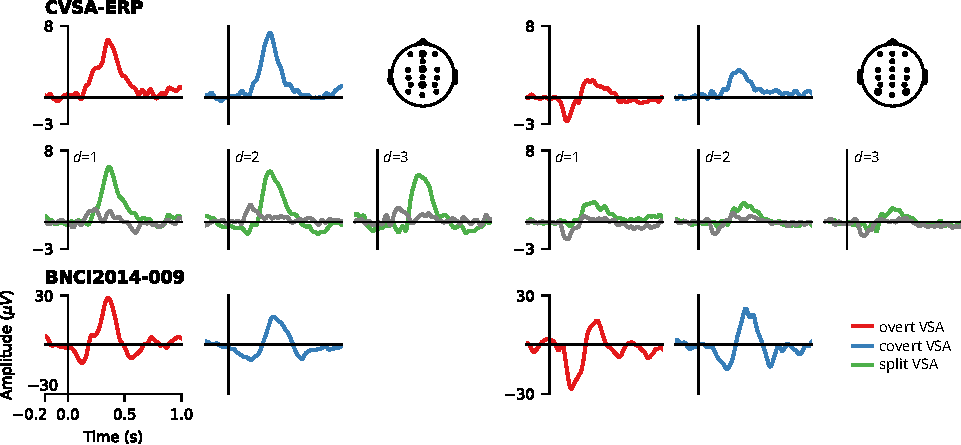
\includegraphics[width=\linewidth]{figures/covert_align/figure3b.pdf}
  \caption[Evoked \acs{erp} per dataset and condition.]{%
		Contrast between target (color) and non-target, and
    distractor (gray) and non-target grand average event-related potentials per \ac{vsa} condition and dataset.
    Overt \ac{vsa} yields a strong modulation of the N1 component in both datasets;
    the P3 amplitude decreases with the degree of split \ac{vsa}.
    In split \ac{vsa}, N1 and P2 are more prominently evoked by the distractor,
    while the P3 is evoked by the target.
	}
		\label{fig:erps}
\end{figure*}


In contrast to the protocol proposed by \textcite{Frenzel2011}, split \ac{vsa} was
performed by instructing the participant to attend to the intensifications of the
cued target and ignore the intensifications of the distractor target.
Since we assume there will be an effect depending on the distance between
the attended target and the distractor, we discern three split \ac{vsa} sub-conditions:
the distractor is either clockwise or counterclockwise directly next to the
attended target ($d=1$), there is one other target between the attended target and
the distractor ($d=2$), or the distractor is opposite the intended target
($d=3$).

\ac{eeg} for the CVSA-ERP dataset was recorded using a SynAmps RT amplifier
(Compumedics Neuroscan, Australia) at 2048 Hz and 62 Ag/AgCl active electrodes arranged in the
international 10-10 layout fitted to a standard electrode cap (EASYCAP GmbH,
Germany), with electrodes located at AFz and FCz as ground and reference, respectively.
Using electrolyte gel, electrode impedances were brought below 5k$\Omega$.
Electrodes TP9 and TP10, used for off-line re-referencing, were directly
attached to the skin using stickers for better contact.
The power line frequency in Belgium is 50 Hz.
The participant's eye gaze was registered using an EyeLink 1000 Plus eye tracker (SR Research,
Canada) in non-fixation mode.

Participants signed an informed consent form and were seated at a distance of
60 cm from a CRT-emulating monitor (VPixx
Technologies, Ca\-na\-da) operating at a refresh rate of 120 Hz, displaying 6
circular white targets with a diameter of 4.15° visual angle and laid out on a hexagon
with a radius of 12.28° of visual angle centered on the midpoint of the screen,
conforming to the interface proposed by \textcite{Treder2010}
(\cref{fig:covert-align/interface/interface}).
A hexagonal layout interface with an empty center and a low number of targets
counteracts target crowding, and as long as the subject’s gaze is within the hexagon of
targets, no other target can be between the subject’s gaze and a covertly
attended target.
Targets are full-contrast white and were intensified by scaling them to a
larger size (5.60° of visual angle, see \cref{fig:covert-align/interface/intensification})
instead of changing the contrast to avoid Troxler-fading\footnote{The optical illusion of disappearing unchanging stimuli
experienced when visually fixating~\cite{Troxler1804}.}~\cite{Treder2010} in the
peripheral visual field.
Stimuli were presented using PsychoPy (version 2023.1.3)~\cite{Peirce2019}.

\begin{figure}[t]
  \begin{subfigure}[t]{.45\textwidth}
    \begin{tikzpicture}[
    scale=\textwidth/5cm
]
% Rectangle background
\fill[muteblack] (-2.5,-2) rectangle (2.5,2);

% Hexagon vertices (white circles)
  \fill[white] (1,0) circle (.35);    % Right
  \fill[white] (-1,0) circle (.35);   % Left
\fill[white] (0.5,0.866) circle (.35); % Top-right
\fill[white] (-0.5,0.866) circle (.35); % Top-left
\fill[white] (0.5,-0.866) circle (.35); % Bottom-right
\fill[white] (-0.5,-0.866) circle (.35); % Bottom-left

\end{tikzpicture}

    \caption[The stimulation interface.]{The stimulation interface based on the visual Hex-o-Spell
    \acs{bci}~\cite{Treder2010}.}%
    \label{fig:covert-align/interface/interface}
  \end{subfigure}\hfill%
  \begin{subfigure}[t]{.45\textwidth}
    \begin{tikzpicture}[
    scale=\textwidth/5cm
]
% Rectangle background
\fill[muteblack] (-2.5,-2) rectangle (2.5,2);

% Hexagon vertices (white circles)
\fill[white] (1,0) circle (.35);    % Right
\fill[white] (-1,0) circle (.35);   % Left
\fill[white] (0.5,0.866) circle (.35); % Top-right
\fill[white] (-0.5,0.866) circle (.45); % Top-left
\fill[white] (0.5,-0.866) circle (.35); % Bottom-right
\fill[white] (-0.5,-0.866) circle (.35); % Bottom-left

\end{tikzpicture}%

    \caption[Intensification.]{When a target is intensified, it is enlarged for
    a very short time.}%
    \label{fig:covert-align/interface/intensification}
  \end{subfigure}

  \bigskip

  \begin{subfigure}[t]{.45\textwidth}
    \begin{tikzpicture}[
    scale=\textwidth/5cm
]
% Rectangle background
\fill[muteblack] (-2.5,-2) rectangle (2.5,2);

% Hexagon vertices (white circles)
\fill[white] (1,0) circle (.35);    % Right
\fill[white] (-1,0) circle (.35);   % Left
\fill[white] (0.5,0.866) circle (.35); % Top-right
\fill[white] (-0.5,0.866) circle (.35); % Top-left
\fill[white] (0.5,-0.866) circle (.35); % Bottom-right
\fill[white] (-0.5,-0.866) circle (.35); % Bottom-left
\draw[accent2, ultra thick] (0.9,0) -- (1.1,0);  % Shorter horizontal line
\draw[accent2, ultra thick] (1,-0.1) -- (1,0.1); % Shorter vertical line
\end{tikzpicture}%

    \caption[Gaze fixated on a target.]{In the overt and split \ac{vsa}
    settings, the
    participant is cued to fixate on one of the targets.}%
    \label{fig:covert-align/interface/overt}
  \end{subfigure}\hfill%
  \begin{subfigure}[t]{.45\textwidth}
    \begin{tikzpicture}[
    scale=\textwidth/5cm
]
% Rectangle background
\fill[muteblack] (-2.5,-2) rectangle (2.5,2);

% Hexagon vertices (white circles)
\fill[white] (1,0) circle (.35);    % Right
\fill[white] (-1,0) circle (.35);   % Left
\fill[white] (0.5,0.866) circle (.35); % Top-right
\fill[white] (-0.5,0.866) circle (.35); % Top-left
\fill[white] (0.5,-0.866) circle (.35); % Bottom-right
\fill[white] (-0.5,-0.866) circle (.35); % Bottom-left

% Plus symbol made of two shorter lines at the center (0,0)
\draw[accent2, ultra thick] (-0.1,0) -- (0.1,0);  % Shorter horizontal line
\draw[accent2, ultra thick] (0,-0.1) -- (0,0.1);  % Shorter vertical line
\end{tikzpicture}%

    \caption[Gaze fixated centrally.]{In the covert \ac{vsa} setting, the participant is
    cued to fixate at the center of the interface.}%
    \label{fig:covert-align/interface/covert}
  \end{subfigure}
  \caption[Stimulation interface layout.]{Layout and visual elements of the experimental stimulation
  interface used in recording the CVSA-ERP dataset.}
\end{figure}

The participant was instructed to press the space bar when ready for a block
of stimulations.
Then, one target was indicated as the cue, and the participant
was instructed to count the number of intensifications of the cued target
during the following block of stimulations.
After pressing the space bar again, a blue crosshair appeared, and the subject
was instructed to fixate their gaze on the blue crosshair for the duration of
the stimulation block (\cref{fig:covert-align/interface/overt} and
\cref{fig:covert-align/interface/covert}).
The position of this crosshair determined the \ac{vsa} condition for this trial:
overt \ac{vsa} when the crosshair was at the same location as the cued target,
covert \ac{vsa} when the crosshair appeared in the center of the screen, and split
\ac{vsa} when the crosshair appeared on a different target than the cued one.
After pressing the space bar again and a delay of 5 seconds, the stimulation block
started.

All targets were intensified for a duration of 100 ms in pseudorandom order.
The inter-stimulus-interval (\ac{isi}), the time between the onsets of subsequent intensifications,
was variable and consisted of a fixed 300 ms interval (of which 100 ms with an intensified target onscreen)
with 200 ms of uniform jitter added, resulting in an \ac{isi}
between 200 and 400 ms.
\Acp{isi} were jittered to counteract steady-state effects and residue in averaging. A
longer \ac{isi} will increase component amplitude and aid in counteracting temporal
autocorrelation for higher statistical test precision.
In a block of stimulations, each target was intensified a pseudorandom number of times between 10 and 15.
This led to stimulation blocks with an average duration of 26.25 seconds. After a block of stimulations, an
input prompt appeared to enter the mentally counted number of intensifications.
After inputting this number, the subject was allowed to pause until pressing the space bar again.
In total, six blocks were presented for overt \ac{vsa}, six blocks for covert \ac{vsa}, 12 blocks for
split ($d=1$) \ac{vsa}, 12 blocks for split ($d=2$) \ac{vsa}, and 6 blocks for split
($d=3$) \ac{vsa}, covering all possible combinations of \ac{vsa} conditions, cued targets, and
crosshair locations.

The experiment started with a sequence  of five non-recorded practice stimulation blocks, one for
each of the five \ac{vsa} conditions.
During these practice blocks, the participant received feedback about their gaze
position and counting accuracy.
Counting the instructions and the participant's response to the
input prompts, a block lasted about 30 seconds. In sum, the experiment featured approximately 45 minutes of
stimulation time.
After blocks 14 and 28, the participant was allowed to take a longer break.
Including these longer breaks, the experiment lasted approximately one hour.

\subsubsection{BNCI2014-009 dataset}
The BNCI2014-009\footnote{\url{https://bnci-horizon-2020.eu/database/data-sets}}
dataset~\cite{Aloise2012a} was used in the analysis performed
by \textcite{Arico2014}.
It contains data from 10 subjects (median age $24.5\pm1.9$
years) who performed two spelling tasks illustrated in the second row of
\cref{fig:interface}: using the P3 Matrix speller
interface to exploit overt \ac{vsa}, and the GeoSpell covert \ac{vsa} interface.
To use the GeoSpell interface, the participant gazes at the fixation point at the
center of the screen, while groups of characters flash simultaneously in a
circular layout around the fixation point.
The user directs their visuospatial attention to the location where the intended letter is expected
to appear, and when it does, a P3 \ac{erp} component is expected to be evoked.
This results in a specific setting where both visuospatial attention and
feature attention (the attended letter) are exploited.
For a detailed description of the paradigm and dataset, we refer
to \textcite{Aloise2012a}.

\subsection{Data processing and analysis}
\subsubsection{Preprocessing}
Analysis was performed using Python and the MNE software package (version
1.3.1)~\cite{Gramfort2013}.
All datasets were band-pass filtered between 0.1 Hz and 20 Hz with a 4th-order Butterworth filter.
Bad channels in the data were automatically detected using the RANSAC
method~\cite{Fischler1981} and rejected.
The recorded \ac{eeg} was re-referenced
offline to the average of the mastoid electrodes TP9 and TP10.
Next, the \ac{eeg} signals were corrected for eye movement artifacts using
Independent Component Analysis (ICA).
Since we have access to \ac{eog} data for the CVSA-ERP dataset, components correlating
significantly with the \ac{eog} were rejected.
For the BNCI2014-009 dataset, ICA components were manually rejected.
Finally, the \ac{eeg} signal was divided into epochs ranging from 100 ms before stimulus onset to 700 ms after stimulus onset and down-sampled to 128 Hz.
In both datasets, only 16 channels were kept for
analysis (Fz, FCz, Cz, CPz, Pz, Oz, F3, F4, C3, C4, CP3, CP4, P3, P4, PO7, and
PO8).

\subsubsection{Decoders}%
\label{sec:covert-align/methods/decoders}
We compared the two latency-based methods \ac{wcble} and \ac{cble} as described in
\cref{sec:wcble/methods}, with their base classifier \ac{tlda} and with
Riemannian Geometry approaches that rely on spatial covariance as features.
Together with \ac{tlda}, Riemannian Geometry generally achieves state-of-the-art decoding
performance~\cite{Lotte2018}.
We implemented two Riemannian Geometry pipelines.
The first estimates shrunk covariances from the \acp{erp} filtered with 6 XDAWN
filters, projects these covariances to a tangent space, and classifies the
result using $L_2$-regularized logistic regression
(XDAWNCov-TS-LR)~\cite{Cecotti2017}.
Secondly, we adopted the pipeline from \textcite{Aydarkhanov2020}, as their work shows
favorable performance in the presence of single-trial \ac{erp} latency jitter.
Shrunk spatial covariance matrices were estimated from epochs that were
augmented by concatenating the average target and average non-target \ac{erp} as
extra channels, projected to tangent space, and classified using
$L_2$-regularized logistic regression (ERPCov-TS-LR).

To evaluate performance, 6-fold cross-validation without shuffling was performed for both
datasets.
At each fold, classifiers were trained on five target selection blocks (300
epochs) and tested on one block (60 epochs) without overlap for CVSA-ERP.
For each subject and run in the BNCI2014-009 dataset, classifiers
were trained on five symbol selections (480 epochs) and tested on one symbol
selection (96 epochs) without overlap at each fold.
A window ranging from 0 ms to 600 ms after stimulus onset was used for \ac{cble} and \ac{wcble}.
With epochs ranging from -100 ms to 700 ms relative to stimulus onset, this
allows for extracting latencies ranging from -100 ms to +100 ms.


\section{Results}

\subsection{\Acs{bci} decoding performance}%
\label{sec:covert-align/results/bloc-acc}

We evaluated the \ac{bci} decoding performance in a single-trial classification
experiment, as well as in a target selection experiment reflecting \ac{bci}
operation.

\Cref{fig:covert-align/single-trial-roc-auc-diff} shows a comparison of \ac{rocauc}
for all pairs of \ac{tlda}, \ac{cble},
and \ac{wcble} for single-trial classification to investigate the contributions of
\ac{cble} and \ac{wcble} relative to their first-stage classifier \ac{tlda}.
For this evaluation, epochs were rejected when the peak-to-peak amplitude
exceeded 800 µV, and for the CVSA-ERP dataset, if the user's gaze differed by more than
10 degrees of visual angle from the fixation crosshair.
\begin{figure}[t]
	%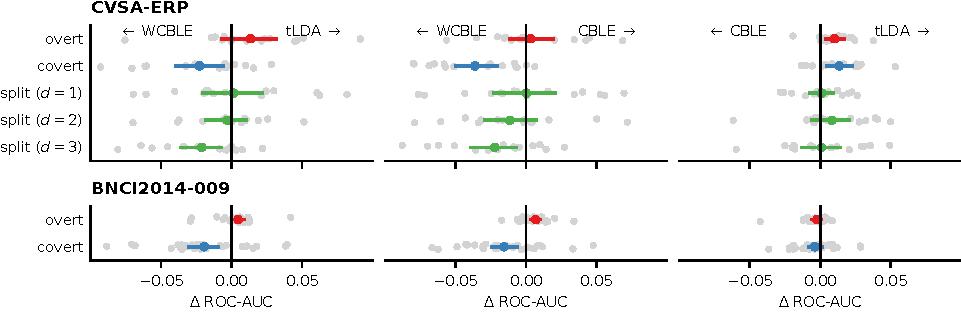
\includegraphics[width=\linewidth]{figures/covert_align/figure4a.pdf}
  \hspace{-0.6818736741559431in}
%%% Creator: Matplotlib, PGF backend
%%
%% To include the figure in your LaTeX document, write
%%   \input{<filename>.pgf}
%%
%% Make sure the required packages are loaded in your preamble
%%   \usepackage{pgf}
%%
%% Also ensure that all the required font packages are loaded; for instance,
%% the lmodern package is sometimes necessary when using math font.
%%   \usepackage{lmodern}
%%
%% Figures using additional raster images can only be included by \input if
%% they are in the same directory as the main LaTeX file. For loading figures
%% from other directories you can use the `import` package
%%   \usepackage{import}
%%
%% and then include the figures with
%%   \import{<path to file>}{<filename>.pgf}
%%
%% Matplotlib used the following preamble
%%   \def\mathdefault#1{#1}
%%   \everymath=\expandafter{\the\everymath\displaystyle}
%%   
%%   \ifdefined\pdftexversion\else  % non-pdftex case.
%%     \usepackage{fontspec}
%%   \fi
%%   \makeatletter\@ifpackageloaded{underscore}{}{\usepackage[strings]{underscore}}\makeatother
%%
\begingroup%
\makeatletter%
\begin{pgfpicture}%
\pgfpathrectangle{\pgfpointorigin}{\pgfqpoint{5.322943in}{1.863224in}}%
\pgfusepath{use as bounding box, clip}%
\begin{pgfscope}%
\pgfsetbuttcap%
\pgfsetmiterjoin%
\pgfsetlinewidth{0.000000pt}%
\definecolor{currentstroke}{rgb}{1.000000,1.000000,1.000000}%
\pgfsetstrokecolor{currentstroke}%
\pgfsetstrokeopacity{0.000000}%
\pgfsetdash{}{0pt}%
\pgfpathmoveto{\pgfqpoint{0.000000in}{0.000000in}}%
\pgfpathlineto{\pgfqpoint{5.322943in}{0.000000in}}%
\pgfpathlineto{\pgfqpoint{5.322943in}{1.863224in}}%
\pgfpathlineto{\pgfqpoint{0.000000in}{1.863224in}}%
\pgfpathlineto{\pgfqpoint{0.000000in}{0.000000in}}%
\pgfpathclose%
\pgfusepath{}%
\end{pgfscope}%
\begin{pgfscope}%
\pgfsetbuttcap%
\pgfsetmiterjoin%
\definecolor{currentfill}{rgb}{1.000000,1.000000,1.000000}%
\pgfsetfillcolor{currentfill}%
\pgfsetlinewidth{0.000000pt}%
\definecolor{currentstroke}{rgb}{0.000000,0.000000,0.000000}%
\pgfsetstrokecolor{currentstroke}%
\pgfsetstrokeopacity{0.000000}%
\pgfsetdash{}{0pt}%
\pgfpathmoveto{\pgfqpoint{0.716792in}{0.897930in}}%
\pgfpathlineto{\pgfqpoint{2.196615in}{0.897930in}}%
\pgfpathlineto{\pgfqpoint{2.196615in}{1.693085in}}%
\pgfpathlineto{\pgfqpoint{0.716792in}{1.693085in}}%
\pgfpathlineto{\pgfqpoint{0.716792in}{0.897930in}}%
\pgfpathclose%
\pgfusepath{fill}%
\end{pgfscope}%
\begin{pgfscope}%
\pgfpathrectangle{\pgfqpoint{0.716792in}{0.897930in}}{\pgfqpoint{1.479824in}{0.795155in}}%
\pgfusepath{clip}%
\pgfsetbuttcap%
\pgfsetroundjoin%
\pgfsetlinewidth{1.003750pt}%
\definecolor{currentstroke}{rgb}{0.878431,0.878431,0.878431}%
\pgfsetstrokecolor{currentstroke}%
\pgfsetdash{{3.700000pt}{1.600000pt}}{0.000000pt}%
\pgfpathmoveto{\pgfqpoint{1.456704in}{0.897930in}}%
\pgfpathlineto{\pgfqpoint{1.456704in}{1.693085in}}%
\pgfusepath{stroke}%
\end{pgfscope}%
\begin{pgfscope}%
\pgfpathrectangle{\pgfqpoint{0.716792in}{0.897930in}}{\pgfqpoint{1.479824in}{0.795155in}}%
\pgfusepath{clip}%
\pgfsetbuttcap%
\pgfsetroundjoin%
\definecolor{currentfill}{rgb}{0.827451,0.827451,0.827451}%
\pgfsetfillcolor{currentfill}%
\pgfsetlinewidth{0.000000pt}%
\definecolor{currentstroke}{rgb}{0.496471,0.496471,0.496471}%
\pgfsetstrokecolor{currentstroke}%
\pgfsetdash{}{0pt}%
\pgfsys@defobject{currentmarker}{\pgfqpoint{-0.020833in}{-0.020833in}}{\pgfqpoint{0.020833in}{0.020833in}}{%
\pgfpathmoveto{\pgfqpoint{0.000000in}{-0.020833in}}%
\pgfpathcurveto{\pgfqpoint{0.005525in}{-0.020833in}}{\pgfqpoint{0.010825in}{-0.018638in}}{\pgfqpoint{0.014731in}{-0.014731in}}%
\pgfpathcurveto{\pgfqpoint{0.018638in}{-0.010825in}}{\pgfqpoint{0.020833in}{-0.005525in}}{\pgfqpoint{0.020833in}{0.000000in}}%
\pgfpathcurveto{\pgfqpoint{0.020833in}{0.005525in}}{\pgfqpoint{0.018638in}{0.010825in}}{\pgfqpoint{0.014731in}{0.014731in}}%
\pgfpathcurveto{\pgfqpoint{0.010825in}{0.018638in}}{\pgfqpoint{0.005525in}{0.020833in}}{\pgfqpoint{0.000000in}{0.020833in}}%
\pgfpathcurveto{\pgfqpoint{-0.005525in}{0.020833in}}{\pgfqpoint{-0.010825in}{0.018638in}}{\pgfqpoint{-0.014731in}{0.014731in}}%
\pgfpathcurveto{\pgfqpoint{-0.018638in}{0.010825in}}{\pgfqpoint{-0.020833in}{0.005525in}}{\pgfqpoint{-0.020833in}{0.000000in}}%
\pgfpathcurveto{\pgfqpoint{-0.020833in}{-0.005525in}}{\pgfqpoint{-0.018638in}{-0.010825in}}{\pgfqpoint{-0.014731in}{-0.014731in}}%
\pgfpathcurveto{\pgfqpoint{-0.010825in}{-0.018638in}}{\pgfqpoint{-0.005525in}{-0.020833in}}{\pgfqpoint{0.000000in}{-0.020833in}}%
\pgfpathlineto{\pgfqpoint{0.000000in}{-0.020833in}}%
\pgfpathclose%
\pgfusepath{fill}%
}%
\begin{pgfscope}%
\pgfsys@transformshift{1.350650in}{1.608324in}%
\pgfsys@useobject{currentmarker}{}%
\end{pgfscope}%
\begin{pgfscope}%
\pgfsys@transformshift{1.801996in}{1.621642in}%
\pgfsys@useobject{currentmarker}{}%
\end{pgfscope}%
\begin{pgfscope}%
\pgfsys@transformshift{1.370381in}{1.613072in}%
\pgfsys@useobject{currentmarker}{}%
\end{pgfscope}%
\begin{pgfscope}%
\pgfsys@transformshift{1.834059in}{1.628159in}%
\pgfsys@useobject{currentmarker}{}%
\end{pgfscope}%
\begin{pgfscope}%
\pgfsys@transformshift{1.613897in}{1.607245in}%
\pgfsys@useobject{currentmarker}{}%
\end{pgfscope}%
\begin{pgfscope}%
\pgfsys@transformshift{1.459170in}{1.615064in}%
\pgfsys@useobject{currentmarker}{}%
\end{pgfscope}%
\begin{pgfscope}%
\pgfsys@transformshift{2.132490in}{1.599540in}%
\pgfsys@useobject{currentmarker}{}%
\end{pgfscope}%
\begin{pgfscope}%
\pgfsys@transformshift{1.789664in}{1.625868in}%
\pgfsys@useobject{currentmarker}{}%
\end{pgfscope}%
\begin{pgfscope}%
\pgfsys@transformshift{1.656480in}{1.610811in}%
\pgfsys@useobject{currentmarker}{}%
\end{pgfscope}%
\begin{pgfscope}%
\pgfsys@transformshift{1.454237in}{1.597740in}%
\pgfsys@useobject{currentmarker}{}%
\end{pgfscope}%
\begin{pgfscope}%
\pgfsys@transformshift{1.407376in}{1.617400in}%
\pgfsys@useobject{currentmarker}{}%
\end{pgfscope}%
\begin{pgfscope}%
\pgfsys@transformshift{1.417242in}{1.626332in}%
\pgfsys@useobject{currentmarker}{}%
\end{pgfscope}%
\begin{pgfscope}%
\pgfsys@transformshift{1.535628in}{1.606925in}%
\pgfsys@useobject{currentmarker}{}%
\end{pgfscope}%
\begin{pgfscope}%
\pgfsys@transformshift{0.896837in}{1.607830in}%
\pgfsys@useobject{currentmarker}{}%
\end{pgfscope}%
\begin{pgfscope}%
\pgfsys@transformshift{1.628544in}{1.611419in}%
\pgfsys@useobject{currentmarker}{}%
\end{pgfscope}%
\end{pgfscope}%
\begin{pgfscope}%
\pgfpathrectangle{\pgfqpoint{0.716792in}{0.897930in}}{\pgfqpoint{1.479824in}{0.795155in}}%
\pgfusepath{clip}%
\pgfsetbuttcap%
\pgfsetroundjoin%
\definecolor{currentfill}{rgb}{0.827451,0.827451,0.827451}%
\pgfsetfillcolor{currentfill}%
\pgfsetlinewidth{0.000000pt}%
\definecolor{currentstroke}{rgb}{0.496471,0.496471,0.496471}%
\pgfsetstrokecolor{currentstroke}%
\pgfsetdash{}{0pt}%
\pgfsys@defobject{currentmarker}{\pgfqpoint{-0.020833in}{-0.020833in}}{\pgfqpoint{0.020833in}{0.020833in}}{%
\pgfpathmoveto{\pgfqpoint{0.000000in}{-0.020833in}}%
\pgfpathcurveto{\pgfqpoint{0.005525in}{-0.020833in}}{\pgfqpoint{0.010825in}{-0.018638in}}{\pgfqpoint{0.014731in}{-0.014731in}}%
\pgfpathcurveto{\pgfqpoint{0.018638in}{-0.010825in}}{\pgfqpoint{0.020833in}{-0.005525in}}{\pgfqpoint{0.020833in}{0.000000in}}%
\pgfpathcurveto{\pgfqpoint{0.020833in}{0.005525in}}{\pgfqpoint{0.018638in}{0.010825in}}{\pgfqpoint{0.014731in}{0.014731in}}%
\pgfpathcurveto{\pgfqpoint{0.010825in}{0.018638in}}{\pgfqpoint{0.005525in}{0.020833in}}{\pgfqpoint{0.000000in}{0.020833in}}%
\pgfpathcurveto{\pgfqpoint{-0.005525in}{0.020833in}}{\pgfqpoint{-0.010825in}{0.018638in}}{\pgfqpoint{-0.014731in}{0.014731in}}%
\pgfpathcurveto{\pgfqpoint{-0.018638in}{0.010825in}}{\pgfqpoint{-0.020833in}{0.005525in}}{\pgfqpoint{-0.020833in}{0.000000in}}%
\pgfpathcurveto{\pgfqpoint{-0.020833in}{-0.005525in}}{\pgfqpoint{-0.018638in}{-0.010825in}}{\pgfqpoint{-0.014731in}{-0.014731in}}%
\pgfpathcurveto{\pgfqpoint{-0.010825in}{-0.018638in}}{\pgfqpoint{-0.005525in}{-0.020833in}}{\pgfqpoint{0.000000in}{-0.020833in}}%
\pgfpathlineto{\pgfqpoint{0.000000in}{-0.020833in}}%
\pgfpathclose%
\pgfusepath{fill}%
}%
\begin{pgfscope}%
\pgfsys@transformshift{1.392578in}{1.469402in}%
\pgfsys@useobject{currentmarker}{}%
\end{pgfscope}%
\begin{pgfscope}%
\pgfsys@transformshift{1.530695in}{1.444092in}%
\pgfsys@useobject{currentmarker}{}%
\end{pgfscope}%
\begin{pgfscope}%
\pgfsys@transformshift{1.215553in}{1.445313in}%
\pgfsys@useobject{currentmarker}{}%
\end{pgfscope}%
\begin{pgfscope}%
\pgfsys@transformshift{1.010290in}{1.462028in}%
\pgfsys@useobject{currentmarker}{}%
\end{pgfscope}%
\begin{pgfscope}%
\pgfsys@transformshift{1.432040in}{1.461547in}%
\pgfsys@useobject{currentmarker}{}%
\end{pgfscope}%
\begin{pgfscope}%
\pgfsys@transformshift{1.472106in}{1.458179in}%
\pgfsys@useobject{currentmarker}{}%
\end{pgfscope}%
\begin{pgfscope}%
\pgfsys@transformshift{1.422174in}{1.446094in}%
\pgfsys@useobject{currentmarker}{}%
\end{pgfscope}%
\begin{pgfscope}%
\pgfsys@transformshift{1.217465in}{1.465567in}%
\pgfsys@useobject{currentmarker}{}%
\end{pgfscope}%
\begin{pgfscope}%
\pgfsys@transformshift{1.666345in}{1.448502in}%
\pgfsys@useobject{currentmarker}{}%
\end{pgfscope}%
\begin{pgfscope}%
\pgfsys@transformshift{0.768586in}{1.466642in}%
\pgfsys@useobject{currentmarker}{}%
\end{pgfscope}%
\begin{pgfscope}%
\pgfsys@transformshift{1.572623in}{1.463696in}%
\pgfsys@useobject{currentmarker}{}%
\end{pgfscope}%
\begin{pgfscope}%
\pgfsys@transformshift{1.002891in}{1.448768in}%
\pgfsys@useobject{currentmarker}{}%
\end{pgfscope}%
\begin{pgfscope}%
\pgfsys@transformshift{1.264326in}{1.443837in}%
\pgfsys@useobject{currentmarker}{}%
\end{pgfscope}%
\begin{pgfscope}%
\pgfsys@transformshift{1.427107in}{1.461704in}%
\pgfsys@useobject{currentmarker}{}%
\end{pgfscope}%
\begin{pgfscope}%
\pgfsys@transformshift{0.933832in}{1.464865in}%
\pgfsys@useobject{currentmarker}{}%
\end{pgfscope}%
\end{pgfscope}%
\begin{pgfscope}%
\pgfpathrectangle{\pgfqpoint{0.716792in}{0.897930in}}{\pgfqpoint{1.479824in}{0.795155in}}%
\pgfusepath{clip}%
\pgfsetbuttcap%
\pgfsetroundjoin%
\definecolor{currentfill}{rgb}{0.827451,0.827451,0.827451}%
\pgfsetfillcolor{currentfill}%
\pgfsetlinewidth{0.000000pt}%
\definecolor{currentstroke}{rgb}{0.496471,0.496471,0.496471}%
\pgfsetstrokecolor{currentstroke}%
\pgfsetdash{}{0pt}%
\pgfsys@defobject{currentmarker}{\pgfqpoint{-0.020833in}{-0.020833in}}{\pgfqpoint{0.020833in}{0.020833in}}{%
\pgfpathmoveto{\pgfqpoint{0.000000in}{-0.020833in}}%
\pgfpathcurveto{\pgfqpoint{0.005525in}{-0.020833in}}{\pgfqpoint{0.010825in}{-0.018638in}}{\pgfqpoint{0.014731in}{-0.014731in}}%
\pgfpathcurveto{\pgfqpoint{0.018638in}{-0.010825in}}{\pgfqpoint{0.020833in}{-0.005525in}}{\pgfqpoint{0.020833in}{0.000000in}}%
\pgfpathcurveto{\pgfqpoint{0.020833in}{0.005525in}}{\pgfqpoint{0.018638in}{0.010825in}}{\pgfqpoint{0.014731in}{0.014731in}}%
\pgfpathcurveto{\pgfqpoint{0.010825in}{0.018638in}}{\pgfqpoint{0.005525in}{0.020833in}}{\pgfqpoint{0.000000in}{0.020833in}}%
\pgfpathcurveto{\pgfqpoint{-0.005525in}{0.020833in}}{\pgfqpoint{-0.010825in}{0.018638in}}{\pgfqpoint{-0.014731in}{0.014731in}}%
\pgfpathcurveto{\pgfqpoint{-0.018638in}{0.010825in}}{\pgfqpoint{-0.020833in}{0.005525in}}{\pgfqpoint{-0.020833in}{0.000000in}}%
\pgfpathcurveto{\pgfqpoint{-0.020833in}{-0.005525in}}{\pgfqpoint{-0.018638in}{-0.010825in}}{\pgfqpoint{-0.014731in}{-0.014731in}}%
\pgfpathcurveto{\pgfqpoint{-0.010825in}{-0.018638in}}{\pgfqpoint{-0.005525in}{-0.020833in}}{\pgfqpoint{0.000000in}{-0.020833in}}%
\pgfpathlineto{\pgfqpoint{0.000000in}{-0.020833in}}%
\pgfpathclose%
\pgfusepath{fill}%
}%
\begin{pgfscope}%
\pgfsys@transformshift{1.638119in}{1.301959in}%
\pgfsys@useobject{currentmarker}{}%
\end{pgfscope}%
\begin{pgfscope}%
\pgfsys@transformshift{1.362981in}{1.306413in}%
\pgfsys@useobject{currentmarker}{}%
\end{pgfscope}%
\begin{pgfscope}%
\pgfsys@transformshift{1.678677in}{1.290734in}%
\pgfsys@useobject{currentmarker}{}%
\end{pgfscope}%
\begin{pgfscope}%
\pgfsys@transformshift{0.941232in}{1.304977in}%
\pgfsys@useobject{currentmarker}{}%
\end{pgfscope}%
\begin{pgfscope}%
\pgfsys@transformshift{1.158272in}{1.291501in}%
\pgfsys@useobject{currentmarker}{}%
\end{pgfscope}%
\begin{pgfscope}%
\pgfsys@transformshift{1.007824in}{1.309793in}%
\pgfsys@useobject{currentmarker}{}%
\end{pgfscope}%
\begin{pgfscope}%
\pgfsys@transformshift{1.905583in}{1.296123in}%
\pgfsys@useobject{currentmarker}{}%
\end{pgfscope}%
\begin{pgfscope}%
\pgfsys@transformshift{1.321053in}{1.301076in}%
\pgfsys@useobject{currentmarker}{}%
\end{pgfscope}%
\begin{pgfscope}%
\pgfsys@transformshift{1.920382in}{1.305177in}%
\pgfsys@useobject{currentmarker}{}%
\end{pgfscope}%
\begin{pgfscope}%
\pgfsys@transformshift{2.063431in}{1.280525in}%
\pgfsys@useobject{currentmarker}{}%
\end{pgfscope}%
\begin{pgfscope}%
\pgfsys@transformshift{1.333385in}{1.297241in}%
\pgfsys@useobject{currentmarker}{}%
\end{pgfscope}%
\begin{pgfscope}%
\pgfsys@transformshift{1.311188in}{1.310060in}%
\pgfsys@useobject{currentmarker}{}%
\end{pgfscope}%
\begin{pgfscope}%
\pgfsys@transformshift{1.614551in}{1.300030in}%
\pgfsys@useobject{currentmarker}{}%
\end{pgfscope}%
\begin{pgfscope}%
\pgfsys@transformshift{1.423986in}{1.304732in}%
\pgfsys@useobject{currentmarker}{}%
\end{pgfscope}%
\begin{pgfscope}%
\pgfsys@transformshift{1.321053in}{1.292058in}%
\pgfsys@useobject{currentmarker}{}%
\end{pgfscope}%
\end{pgfscope}%
\begin{pgfscope}%
\pgfpathrectangle{\pgfqpoint{0.716792in}{0.897930in}}{\pgfqpoint{1.479824in}{0.795155in}}%
\pgfusepath{clip}%
\pgfsetbuttcap%
\pgfsetroundjoin%
\definecolor{currentfill}{rgb}{0.827451,0.827451,0.827451}%
\pgfsetfillcolor{currentfill}%
\pgfsetlinewidth{0.000000pt}%
\definecolor{currentstroke}{rgb}{0.496471,0.496471,0.496471}%
\pgfsetstrokecolor{currentstroke}%
\pgfsetdash{}{0pt}%
\pgfsys@defobject{currentmarker}{\pgfqpoint{-0.020833in}{-0.020833in}}{\pgfqpoint{0.020833in}{0.020833in}}{%
\pgfpathmoveto{\pgfqpoint{0.000000in}{-0.020833in}}%
\pgfpathcurveto{\pgfqpoint{0.005525in}{-0.020833in}}{\pgfqpoint{0.010825in}{-0.018638in}}{\pgfqpoint{0.014731in}{-0.014731in}}%
\pgfpathcurveto{\pgfqpoint{0.018638in}{-0.010825in}}{\pgfqpoint{0.020833in}{-0.005525in}}{\pgfqpoint{0.020833in}{0.000000in}}%
\pgfpathcurveto{\pgfqpoint{0.020833in}{0.005525in}}{\pgfqpoint{0.018638in}{0.010825in}}{\pgfqpoint{0.014731in}{0.014731in}}%
\pgfpathcurveto{\pgfqpoint{0.010825in}{0.018638in}}{\pgfqpoint{0.005525in}{0.020833in}}{\pgfqpoint{0.000000in}{0.020833in}}%
\pgfpathcurveto{\pgfqpoint{-0.005525in}{0.020833in}}{\pgfqpoint{-0.010825in}{0.018638in}}{\pgfqpoint{-0.014731in}{0.014731in}}%
\pgfpathcurveto{\pgfqpoint{-0.018638in}{0.010825in}}{\pgfqpoint{-0.020833in}{0.005525in}}{\pgfqpoint{-0.020833in}{0.000000in}}%
\pgfpathcurveto{\pgfqpoint{-0.020833in}{-0.005525in}}{\pgfqpoint{-0.018638in}{-0.010825in}}{\pgfqpoint{-0.014731in}{-0.014731in}}%
\pgfpathcurveto{\pgfqpoint{-0.010825in}{-0.018638in}}{\pgfqpoint{-0.005525in}{-0.020833in}}{\pgfqpoint{0.000000in}{-0.020833in}}%
\pgfpathlineto{\pgfqpoint{0.000000in}{-0.020833in}}%
\pgfpathclose%
\pgfusepath{fill}%
}%
\begin{pgfscope}%
\pgfsys@transformshift{1.180470in}{1.138119in}%
\pgfsys@useobject{currentmarker}{}%
\end{pgfscope}%
\begin{pgfscope}%
\pgfsys@transformshift{0.938765in}{1.132519in}%
\pgfsys@useobject{currentmarker}{}%
\end{pgfscope}%
\begin{pgfscope}%
\pgfsys@transformshift{1.459170in}{1.126488in}%
\pgfsys@useobject{currentmarker}{}%
\end{pgfscope}%
\begin{pgfscope}%
\pgfsys@transformshift{1.597287in}{1.148844in}%
\pgfsys@useobject{currentmarker}{}%
\end{pgfscope}%
\begin{pgfscope}%
\pgfsys@transformshift{1.533161in}{1.148513in}%
\pgfsys@useobject{currentmarker}{}%
\end{pgfscope}%
\begin{pgfscope}%
\pgfsys@transformshift{1.173071in}{1.145616in}%
\pgfsys@useobject{currentmarker}{}%
\end{pgfscope}%
\begin{pgfscope}%
\pgfsys@transformshift{1.525762in}{1.147518in}%
\pgfsys@useobject{currentmarker}{}%
\end{pgfscope}%
\begin{pgfscope}%
\pgfsys@transformshift{1.305600in}{1.126011in}%
\pgfsys@useobject{currentmarker}{}%
\end{pgfscope}%
\begin{pgfscope}%
\pgfsys@transformshift{1.836525in}{1.123810in}%
\pgfsys@useobject{currentmarker}{}%
\end{pgfscope}%
\begin{pgfscope}%
\pgfsys@transformshift{1.508497in}{1.126451in}%
\pgfsys@useobject{currentmarker}{}%
\end{pgfscope}%
\begin{pgfscope}%
\pgfsys@transformshift{1.434506in}{1.144208in}%
\pgfsys@useobject{currentmarker}{}%
\end{pgfscope}%
\begin{pgfscope}%
\pgfsys@transformshift{1.528228in}{1.129815in}%
\pgfsys@useobject{currentmarker}{}%
\end{pgfscope}%
\begin{pgfscope}%
\pgfsys@transformshift{1.646665in}{1.149155in}%
\pgfsys@useobject{currentmarker}{}%
\end{pgfscope}%
\begin{pgfscope}%
\pgfsys@transformshift{1.427107in}{1.122899in}%
\pgfsys@useobject{currentmarker}{}%
\end{pgfscope}%
\begin{pgfscope}%
\pgfsys@transformshift{1.414775in}{1.122380in}%
\pgfsys@useobject{currentmarker}{}%
\end{pgfscope}%
\end{pgfscope}%
\begin{pgfscope}%
\pgfpathrectangle{\pgfqpoint{0.716792in}{0.897930in}}{\pgfqpoint{1.479824in}{0.795155in}}%
\pgfusepath{clip}%
\pgfsetbuttcap%
\pgfsetroundjoin%
\definecolor{currentfill}{rgb}{0.827451,0.827451,0.827451}%
\pgfsetfillcolor{currentfill}%
\pgfsetlinewidth{0.000000pt}%
\definecolor{currentstroke}{rgb}{0.496471,0.496471,0.496471}%
\pgfsetstrokecolor{currentstroke}%
\pgfsetdash{}{0pt}%
\pgfsys@defobject{currentmarker}{\pgfqpoint{-0.020833in}{-0.020833in}}{\pgfqpoint{0.020833in}{0.020833in}}{%
\pgfpathmoveto{\pgfqpoint{0.000000in}{-0.020833in}}%
\pgfpathcurveto{\pgfqpoint{0.005525in}{-0.020833in}}{\pgfqpoint{0.010825in}{-0.018638in}}{\pgfqpoint{0.014731in}{-0.014731in}}%
\pgfpathcurveto{\pgfqpoint{0.018638in}{-0.010825in}}{\pgfqpoint{0.020833in}{-0.005525in}}{\pgfqpoint{0.020833in}{0.000000in}}%
\pgfpathcurveto{\pgfqpoint{0.020833in}{0.005525in}}{\pgfqpoint{0.018638in}{0.010825in}}{\pgfqpoint{0.014731in}{0.014731in}}%
\pgfpathcurveto{\pgfqpoint{0.010825in}{0.018638in}}{\pgfqpoint{0.005525in}{0.020833in}}{\pgfqpoint{0.000000in}{0.020833in}}%
\pgfpathcurveto{\pgfqpoint{-0.005525in}{0.020833in}}{\pgfqpoint{-0.010825in}{0.018638in}}{\pgfqpoint{-0.014731in}{0.014731in}}%
\pgfpathcurveto{\pgfqpoint{-0.018638in}{0.010825in}}{\pgfqpoint{-0.020833in}{0.005525in}}{\pgfqpoint{-0.020833in}{0.000000in}}%
\pgfpathcurveto{\pgfqpoint{-0.020833in}{-0.005525in}}{\pgfqpoint{-0.018638in}{-0.010825in}}{\pgfqpoint{-0.014731in}{-0.014731in}}%
\pgfpathcurveto{\pgfqpoint{-0.010825in}{-0.018638in}}{\pgfqpoint{-0.005525in}{-0.020833in}}{\pgfqpoint{0.000000in}{-0.020833in}}%
\pgfpathlineto{\pgfqpoint{0.000000in}{-0.020833in}}%
\pgfpathclose%
\pgfusepath{fill}%
}%
\begin{pgfscope}%
\pgfsys@transformshift{0.980694in}{0.989128in}%
\pgfsys@useobject{currentmarker}{}%
\end{pgfscope}%
\begin{pgfscope}%
\pgfsys@transformshift{1.461636in}{0.970015in}%
\pgfsys@useobject{currentmarker}{}%
\end{pgfscope}%
\begin{pgfscope}%
\pgfsys@transformshift{1.456704in}{0.991017in}%
\pgfsys@useobject{currentmarker}{}%
\end{pgfscope}%
\begin{pgfscope}%
\pgfsys@transformshift{1.395044in}{0.970838in}%
\pgfsys@useobject{currentmarker}{}%
\end{pgfscope}%
\begin{pgfscope}%
\pgfsys@transformshift{1.429573in}{0.980017in}%
\pgfsys@useobject{currentmarker}{}%
\end{pgfscope}%
\begin{pgfscope}%
\pgfsys@transformshift{1.481367in}{0.977780in}%
\pgfsys@useobject{currentmarker}{}%
\end{pgfscope}%
\begin{pgfscope}%
\pgfsys@transformshift{1.207600in}{0.991181in}%
\pgfsys@useobject{currentmarker}{}%
\end{pgfscope}%
\begin{pgfscope}%
\pgfsys@transformshift{1.203875in}{0.975256in}%
\pgfsys@useobject{currentmarker}{}%
\end{pgfscope}%
\begin{pgfscope}%
\pgfsys@transformshift{1.619484in}{0.974395in}%
\pgfsys@useobject{currentmarker}{}%
\end{pgfscope}%
\begin{pgfscope}%
\pgfsys@transformshift{1.279125in}{0.987946in}%
\pgfsys@useobject{currentmarker}{}%
\end{pgfscope}%
\begin{pgfscope}%
\pgfsys@transformshift{1.446838in}{0.962745in}%
\pgfsys@useobject{currentmarker}{}%
\end{pgfscope}%
\begin{pgfscope}%
\pgfsys@transformshift{1.121277in}{0.989257in}%
\pgfsys@useobject{currentmarker}{}%
\end{pgfscope}%
\begin{pgfscope}%
\pgfsys@transformshift{1.513430in}{0.991973in}%
\pgfsys@useobject{currentmarker}{}%
\end{pgfscope}%
\begin{pgfscope}%
\pgfsys@transformshift{0.859841in}{0.976195in}%
\pgfsys@useobject{currentmarker}{}%
\end{pgfscope}%
\begin{pgfscope}%
\pgfsys@transformshift{1.039283in}{0.977939in}%
\pgfsys@useobject{currentmarker}{}%
\end{pgfscope}%
\end{pgfscope}%
\begin{pgfscope}%
\pgfsetbuttcap%
\pgfsetroundjoin%
\definecolor{currentfill}{rgb}{0.552941,0.501961,0.478431}%
\pgfsetfillcolor{currentfill}%
\pgfsetlinewidth{0.803000pt}%
\definecolor{currentstroke}{rgb}{0.552941,0.501961,0.478431}%
\pgfsetstrokecolor{currentstroke}%
\pgfsetdash{}{0pt}%
\pgfsys@defobject{currentmarker}{\pgfqpoint{0.000000in}{0.000000in}}{\pgfqpoint{0.000000in}{0.041667in}}{%
\pgfpathmoveto{\pgfqpoint{0.000000in}{0.000000in}}%
\pgfpathlineto{\pgfqpoint{0.000000in}{0.041667in}}%
\pgfusepath{stroke,fill}%
}%
\begin{pgfscope}%
\pgfsys@transformshift{1.086748in}{0.897930in}%
\pgfsys@useobject{currentmarker}{}%
\end{pgfscope}%
\end{pgfscope}%
\begin{pgfscope}%
\pgfsetbuttcap%
\pgfsetroundjoin%
\definecolor{currentfill}{rgb}{0.552941,0.501961,0.478431}%
\pgfsetfillcolor{currentfill}%
\pgfsetlinewidth{0.803000pt}%
\definecolor{currentstroke}{rgb}{0.552941,0.501961,0.478431}%
\pgfsetstrokecolor{currentstroke}%
\pgfsetdash{}{0pt}%
\pgfsys@defobject{currentmarker}{\pgfqpoint{0.000000in}{0.000000in}}{\pgfqpoint{0.000000in}{0.041667in}}{%
\pgfpathmoveto{\pgfqpoint{0.000000in}{0.000000in}}%
\pgfpathlineto{\pgfqpoint{0.000000in}{0.041667in}}%
\pgfusepath{stroke,fill}%
}%
\begin{pgfscope}%
\pgfsys@transformshift{1.456704in}{0.897930in}%
\pgfsys@useobject{currentmarker}{}%
\end{pgfscope}%
\end{pgfscope}%
\begin{pgfscope}%
\pgfsetbuttcap%
\pgfsetroundjoin%
\definecolor{currentfill}{rgb}{0.552941,0.501961,0.478431}%
\pgfsetfillcolor{currentfill}%
\pgfsetlinewidth{0.803000pt}%
\definecolor{currentstroke}{rgb}{0.552941,0.501961,0.478431}%
\pgfsetstrokecolor{currentstroke}%
\pgfsetdash{}{0pt}%
\pgfsys@defobject{currentmarker}{\pgfqpoint{0.000000in}{0.000000in}}{\pgfqpoint{0.000000in}{0.041667in}}{%
\pgfpathmoveto{\pgfqpoint{0.000000in}{0.000000in}}%
\pgfpathlineto{\pgfqpoint{0.000000in}{0.041667in}}%
\pgfusepath{stroke,fill}%
}%
\begin{pgfscope}%
\pgfsys@transformshift{1.826660in}{0.897930in}%
\pgfsys@useobject{currentmarker}{}%
\end{pgfscope}%
\end{pgfscope}%
\begin{pgfscope}%
\definecolor{textcolor}{rgb}{0.552941,0.501961,0.478431}%
\pgfsetstrokecolor{textcolor}%
\pgfsetfillcolor{textcolor}%
\pgftext[x=0.397349in, y=1.570167in, left, base]{\color{textcolor}{\sffamily\fontsize{9.000000}{10.800000}\selectfont\catcode`\^=\active\def^{\ifmmode\sp\else\^{}\fi}\catcode`\%=\active\def%{\%}overt}}%
\end{pgfscope}%
\begin{pgfscope}%
\definecolor{textcolor}{rgb}{0.552941,0.501961,0.478431}%
\pgfsetstrokecolor{textcolor}%
\pgfsetfillcolor{textcolor}%
\pgftext[x=0.340251in, y=1.411136in, left, base]{\color{textcolor}{\sffamily\fontsize{9.000000}{10.800000}\selectfont\catcode`\^=\active\def^{\ifmmode\sp\else\^{}\fi}\catcode`\%=\active\def%{\%}covert}}%
\end{pgfscope}%
\begin{pgfscope}%
\definecolor{textcolor}{rgb}{0.552941,0.501961,0.478431}%
\pgfsetstrokecolor{textcolor}%
\pgfsetfillcolor{textcolor}%
\pgftext[x=0.000000in, y=1.248632in, left, base]{\color{textcolor}{\sffamily\fontsize{9.000000}{10.800000}\selectfont\catcode`\^=\active\def^{\ifmmode\sp\else\^{}\fi}\catcode`\%=\active\def%{\%}split ($d=1$)}}%
\end{pgfscope}%
\begin{pgfscope}%
\definecolor{textcolor}{rgb}{0.552941,0.501961,0.478431}%
\pgfsetstrokecolor{textcolor}%
\pgfsetfillcolor{textcolor}%
\pgftext[x=0.000000in, y=1.089601in, left, base]{\color{textcolor}{\sffamily\fontsize{9.000000}{10.800000}\selectfont\catcode`\^=\active\def^{\ifmmode\sp\else\^{}\fi}\catcode`\%=\active\def%{\%}split ($d=2$)}}%
\end{pgfscope}%
\begin{pgfscope}%
\definecolor{textcolor}{rgb}{0.552941,0.501961,0.478431}%
\pgfsetstrokecolor{textcolor}%
\pgfsetfillcolor{textcolor}%
\pgftext[x=0.000000in, y=0.930570in, left, base]{\color{textcolor}{\sffamily\fontsize{9.000000}{10.800000}\selectfont\catcode`\^=\active\def^{\ifmmode\sp\else\^{}\fi}\catcode`\%=\active\def%{\%}split ($d=3$)}}%
\end{pgfscope}%
\begin{pgfscope}%
\pgfpathrectangle{\pgfqpoint{0.716792in}{0.897930in}}{\pgfqpoint{1.479824in}{0.795155in}}%
\pgfusepath{clip}%
\pgfsetbuttcap%
\pgfsetroundjoin%
\definecolor{currentfill}{rgb}{0.949020,0.564706,0.094118}%
\pgfsetfillcolor{currentfill}%
\pgfsetlinewidth{0.948544pt}%
\definecolor{currentstroke}{rgb}{0.949020,0.564706,0.094118}%
\pgfsetstrokecolor{currentstroke}%
\pgfsetdash{}{0pt}%
\pgfsys@defobject{currentmarker}{\pgfqpoint{-0.021933in}{-0.021933in}}{\pgfqpoint{0.021933in}{0.021933in}}{%
\pgfpathmoveto{\pgfqpoint{0.000000in}{-0.021933in}}%
\pgfpathcurveto{\pgfqpoint{0.005817in}{-0.021933in}}{\pgfqpoint{0.011396in}{-0.019622in}}{\pgfqpoint{0.015509in}{-0.015509in}}%
\pgfpathcurveto{\pgfqpoint{0.019622in}{-0.011396in}}{\pgfqpoint{0.021933in}{-0.005817in}}{\pgfqpoint{0.021933in}{0.000000in}}%
\pgfpathcurveto{\pgfqpoint{0.021933in}{0.005817in}}{\pgfqpoint{0.019622in}{0.011396in}}{\pgfqpoint{0.015509in}{0.015509in}}%
\pgfpathcurveto{\pgfqpoint{0.011396in}{0.019622in}}{\pgfqpoint{0.005817in}{0.021933in}}{\pgfqpoint{0.000000in}{0.021933in}}%
\pgfpathcurveto{\pgfqpoint{-0.005817in}{0.021933in}}{\pgfqpoint{-0.011396in}{0.019622in}}{\pgfqpoint{-0.015509in}{0.015509in}}%
\pgfpathcurveto{\pgfqpoint{-0.019622in}{0.011396in}}{\pgfqpoint{-0.021933in}{0.005817in}}{\pgfqpoint{-0.021933in}{0.000000in}}%
\pgfpathcurveto{\pgfqpoint{-0.021933in}{-0.005817in}}{\pgfqpoint{-0.019622in}{-0.011396in}}{\pgfqpoint{-0.015509in}{-0.015509in}}%
\pgfpathcurveto{\pgfqpoint{-0.011396in}{-0.019622in}}{\pgfqpoint{-0.005817in}{-0.021933in}}{\pgfqpoint{0.000000in}{-0.021933in}}%
\pgfpathlineto{\pgfqpoint{0.000000in}{-0.021933in}}%
\pgfpathclose%
\pgfusepath{stroke,fill}%
}%
\begin{pgfscope}%
\pgfsys@transformshift{1.556577in}{1.613569in}%
\pgfsys@useobject{currentmarker}{}%
\end{pgfscope}%
\end{pgfscope}%
\begin{pgfscope}%
\pgfpathrectangle{\pgfqpoint{0.716792in}{0.897930in}}{\pgfqpoint{1.479824in}{0.795155in}}%
\pgfusepath{clip}%
\pgfsetrectcap%
\pgfsetroundjoin%
\pgfsetlinewidth{1.264725pt}%
\definecolor{currentstroke}{rgb}{0.949020,0.564706,0.094118}%
\pgfsetstrokecolor{currentstroke}%
\pgfsetdash{}{0pt}%
\pgfpathmoveto{\pgfqpoint{1.413241in}{1.613569in}}%
\pgfpathlineto{\pgfqpoint{1.697074in}{1.613569in}}%
\pgfusepath{stroke}%
\end{pgfscope}%
\begin{pgfscope}%
\pgfpathrectangle{\pgfqpoint{0.716792in}{0.897930in}}{\pgfqpoint{1.479824in}{0.795155in}}%
\pgfusepath{clip}%
\pgfsetrectcap%
\pgfsetroundjoin%
\pgfsetlinewidth{1.264725pt}%
\definecolor{currentstroke}{rgb}{0.949020,0.564706,0.094118}%
\pgfsetstrokecolor{currentstroke}%
\pgfsetdash{}{0pt}%
\pgfusepath{stroke}%
\end{pgfscope}%
\begin{pgfscope}%
\pgfpathrectangle{\pgfqpoint{0.716792in}{0.897930in}}{\pgfqpoint{1.479824in}{0.795155in}}%
\pgfusepath{clip}%
\pgfsetrectcap%
\pgfsetroundjoin%
\pgfsetlinewidth{1.264725pt}%
\definecolor{currentstroke}{rgb}{0.949020,0.564706,0.094118}%
\pgfsetstrokecolor{currentstroke}%
\pgfsetdash{}{0pt}%
\pgfusepath{stroke}%
\end{pgfscope}%
\begin{pgfscope}%
\pgfpathrectangle{\pgfqpoint{0.716792in}{0.897930in}}{\pgfqpoint{1.479824in}{0.795155in}}%
\pgfusepath{clip}%
\pgfsetrectcap%
\pgfsetroundjoin%
\pgfsetlinewidth{1.264725pt}%
\definecolor{currentstroke}{rgb}{0.949020,0.564706,0.094118}%
\pgfsetstrokecolor{currentstroke}%
\pgfsetdash{}{0pt}%
\pgfusepath{stroke}%
\end{pgfscope}%
\begin{pgfscope}%
\pgfpathrectangle{\pgfqpoint{0.716792in}{0.897930in}}{\pgfqpoint{1.479824in}{0.795155in}}%
\pgfusepath{clip}%
\pgfsetrectcap%
\pgfsetroundjoin%
\pgfsetlinewidth{1.264725pt}%
\definecolor{currentstroke}{rgb}{0.949020,0.564706,0.094118}%
\pgfsetstrokecolor{currentstroke}%
\pgfsetdash{}{0pt}%
\pgfusepath{stroke}%
\end{pgfscope}%
\begin{pgfscope}%
\pgfpathrectangle{\pgfqpoint{0.716792in}{0.897930in}}{\pgfqpoint{1.479824in}{0.795155in}}%
\pgfusepath{clip}%
\pgfsetbuttcap%
\pgfsetroundjoin%
\definecolor{currentfill}{rgb}{0.964706,0.239216,0.117647}%
\pgfsetfillcolor{currentfill}%
\pgfsetlinewidth{0.948544pt}%
\definecolor{currentstroke}{rgb}{0.964706,0.239216,0.117647}%
\pgfsetstrokecolor{currentstroke}%
\pgfsetdash{}{0pt}%
\pgfsys@defobject{currentmarker}{\pgfqpoint{-0.021933in}{-0.021933in}}{\pgfqpoint{0.021933in}{0.021933in}}{%
\pgfpathmoveto{\pgfqpoint{0.000000in}{-0.021933in}}%
\pgfpathcurveto{\pgfqpoint{0.005817in}{-0.021933in}}{\pgfqpoint{0.011396in}{-0.019622in}}{\pgfqpoint{0.015509in}{-0.015509in}}%
\pgfpathcurveto{\pgfqpoint{0.019622in}{-0.011396in}}{\pgfqpoint{0.021933in}{-0.005817in}}{\pgfqpoint{0.021933in}{0.000000in}}%
\pgfpathcurveto{\pgfqpoint{0.021933in}{0.005817in}}{\pgfqpoint{0.019622in}{0.011396in}}{\pgfqpoint{0.015509in}{0.015509in}}%
\pgfpathcurveto{\pgfqpoint{0.011396in}{0.019622in}}{\pgfqpoint{0.005817in}{0.021933in}}{\pgfqpoint{0.000000in}{0.021933in}}%
\pgfpathcurveto{\pgfqpoint{-0.005817in}{0.021933in}}{\pgfqpoint{-0.011396in}{0.019622in}}{\pgfqpoint{-0.015509in}{0.015509in}}%
\pgfpathcurveto{\pgfqpoint{-0.019622in}{0.011396in}}{\pgfqpoint{-0.021933in}{0.005817in}}{\pgfqpoint{-0.021933in}{0.000000in}}%
\pgfpathcurveto{\pgfqpoint{-0.021933in}{-0.005817in}}{\pgfqpoint{-0.019622in}{-0.011396in}}{\pgfqpoint{-0.015509in}{-0.015509in}}%
\pgfpathcurveto{\pgfqpoint{-0.011396in}{-0.019622in}}{\pgfqpoint{-0.005817in}{-0.021933in}}{\pgfqpoint{0.000000in}{-0.021933in}}%
\pgfpathlineto{\pgfqpoint{0.000000in}{-0.021933in}}%
\pgfpathclose%
\pgfusepath{stroke,fill}%
}%
\begin{pgfscope}%
\pgfsys@transformshift{1.288574in}{1.454538in}%
\pgfsys@useobject{currentmarker}{}%
\end{pgfscope}%
\end{pgfscope}%
\begin{pgfscope}%
\pgfpathrectangle{\pgfqpoint{0.716792in}{0.897930in}}{\pgfqpoint{1.479824in}{0.795155in}}%
\pgfusepath{clip}%
\pgfsetrectcap%
\pgfsetroundjoin%
\pgfsetlinewidth{1.264725pt}%
\definecolor{currentstroke}{rgb}{0.964706,0.239216,0.117647}%
\pgfsetstrokecolor{currentstroke}%
\pgfsetdash{}{0pt}%
\pgfusepath{stroke}%
\end{pgfscope}%
\begin{pgfscope}%
\pgfpathrectangle{\pgfqpoint{0.716792in}{0.897930in}}{\pgfqpoint{1.479824in}{0.795155in}}%
\pgfusepath{clip}%
\pgfsetrectcap%
\pgfsetroundjoin%
\pgfsetlinewidth{1.264725pt}%
\definecolor{currentstroke}{rgb}{0.964706,0.239216,0.117647}%
\pgfsetstrokecolor{currentstroke}%
\pgfsetdash{}{0pt}%
\pgfpathmoveto{\pgfqpoint{1.153601in}{1.454538in}}%
\pgfpathlineto{\pgfqpoint{1.412761in}{1.454538in}}%
\pgfusepath{stroke}%
\end{pgfscope}%
\begin{pgfscope}%
\pgfpathrectangle{\pgfqpoint{0.716792in}{0.897930in}}{\pgfqpoint{1.479824in}{0.795155in}}%
\pgfusepath{clip}%
\pgfsetrectcap%
\pgfsetroundjoin%
\pgfsetlinewidth{1.264725pt}%
\definecolor{currentstroke}{rgb}{0.964706,0.239216,0.117647}%
\pgfsetstrokecolor{currentstroke}%
\pgfsetdash{}{0pt}%
\pgfusepath{stroke}%
\end{pgfscope}%
\begin{pgfscope}%
\pgfpathrectangle{\pgfqpoint{0.716792in}{0.897930in}}{\pgfqpoint{1.479824in}{0.795155in}}%
\pgfusepath{clip}%
\pgfsetrectcap%
\pgfsetroundjoin%
\pgfsetlinewidth{1.264725pt}%
\definecolor{currentstroke}{rgb}{0.964706,0.239216,0.117647}%
\pgfsetstrokecolor{currentstroke}%
\pgfsetdash{}{0pt}%
\pgfusepath{stroke}%
\end{pgfscope}%
\begin{pgfscope}%
\pgfpathrectangle{\pgfqpoint{0.716792in}{0.897930in}}{\pgfqpoint{1.479824in}{0.795155in}}%
\pgfusepath{clip}%
\pgfsetrectcap%
\pgfsetroundjoin%
\pgfsetlinewidth{1.264725pt}%
\definecolor{currentstroke}{rgb}{0.964706,0.239216,0.117647}%
\pgfsetstrokecolor{currentstroke}%
\pgfsetdash{}{0pt}%
\pgfusepath{stroke}%
\end{pgfscope}%
\begin{pgfscope}%
\pgfpathrectangle{\pgfqpoint{0.716792in}{0.897930in}}{\pgfqpoint{1.479824in}{0.795155in}}%
\pgfusepath{clip}%
\pgfsetbuttcap%
\pgfsetroundjoin%
\definecolor{currentfill}{rgb}{0.470588,0.278431,0.615686}%
\pgfsetfillcolor{currentfill}%
\pgfsetlinewidth{0.948544pt}%
\definecolor{currentstroke}{rgb}{0.470588,0.278431,0.615686}%
\pgfsetstrokecolor{currentstroke}%
\pgfsetdash{}{0pt}%
\pgfsys@defobject{currentmarker}{\pgfqpoint{-0.021933in}{-0.021933in}}{\pgfqpoint{0.021933in}{0.021933in}}{%
\pgfpathmoveto{\pgfqpoint{0.000000in}{-0.021933in}}%
\pgfpathcurveto{\pgfqpoint{0.005817in}{-0.021933in}}{\pgfqpoint{0.011396in}{-0.019622in}}{\pgfqpoint{0.015509in}{-0.015509in}}%
\pgfpathcurveto{\pgfqpoint{0.019622in}{-0.011396in}}{\pgfqpoint{0.021933in}{-0.005817in}}{\pgfqpoint{0.021933in}{0.000000in}}%
\pgfpathcurveto{\pgfqpoint{0.021933in}{0.005817in}}{\pgfqpoint{0.019622in}{0.011396in}}{\pgfqpoint{0.015509in}{0.015509in}}%
\pgfpathcurveto{\pgfqpoint{0.011396in}{0.019622in}}{\pgfqpoint{0.005817in}{0.021933in}}{\pgfqpoint{0.000000in}{0.021933in}}%
\pgfpathcurveto{\pgfqpoint{-0.005817in}{0.021933in}}{\pgfqpoint{-0.011396in}{0.019622in}}{\pgfqpoint{-0.015509in}{0.015509in}}%
\pgfpathcurveto{\pgfqpoint{-0.019622in}{0.011396in}}{\pgfqpoint{-0.021933in}{0.005817in}}{\pgfqpoint{-0.021933in}{0.000000in}}%
\pgfpathcurveto{\pgfqpoint{-0.021933in}{-0.005817in}}{\pgfqpoint{-0.019622in}{-0.011396in}}{\pgfqpoint{-0.015509in}{-0.015509in}}%
\pgfpathcurveto{\pgfqpoint{-0.011396in}{-0.019622in}}{\pgfqpoint{-0.005817in}{-0.021933in}}{\pgfqpoint{0.000000in}{-0.021933in}}%
\pgfpathlineto{\pgfqpoint{0.000000in}{-0.021933in}}%
\pgfpathclose%
\pgfusepath{stroke,fill}%
}%
\begin{pgfscope}%
\pgfsys@transformshift{1.466781in}{1.295507in}%
\pgfsys@useobject{currentmarker}{}%
\end{pgfscope}%
\end{pgfscope}%
\begin{pgfscope}%
\pgfpathrectangle{\pgfqpoint{0.716792in}{0.897930in}}{\pgfqpoint{1.479824in}{0.795155in}}%
\pgfusepath{clip}%
\pgfsetrectcap%
\pgfsetroundjoin%
\pgfsetlinewidth{1.264725pt}%
\definecolor{currentstroke}{rgb}{0.470588,0.278431,0.615686}%
\pgfsetstrokecolor{currentstroke}%
\pgfsetdash{}{0pt}%
\pgfusepath{stroke}%
\end{pgfscope}%
\begin{pgfscope}%
\pgfpathrectangle{\pgfqpoint{0.716792in}{0.897930in}}{\pgfqpoint{1.479824in}{0.795155in}}%
\pgfusepath{clip}%
\pgfsetrectcap%
\pgfsetroundjoin%
\pgfsetlinewidth{1.264725pt}%
\definecolor{currentstroke}{rgb}{0.470588,0.278431,0.615686}%
\pgfsetstrokecolor{currentstroke}%
\pgfsetdash{}{0pt}%
\pgfusepath{stroke}%
\end{pgfscope}%
\begin{pgfscope}%
\pgfpathrectangle{\pgfqpoint{0.716792in}{0.897930in}}{\pgfqpoint{1.479824in}{0.795155in}}%
\pgfusepath{clip}%
\pgfsetrectcap%
\pgfsetroundjoin%
\pgfsetlinewidth{1.264725pt}%
\definecolor{currentstroke}{rgb}{0.470588,0.278431,0.615686}%
\pgfsetstrokecolor{currentstroke}%
\pgfsetdash{}{0pt}%
\pgfpathmoveto{\pgfqpoint{1.311661in}{1.295507in}}%
\pgfpathlineto{\pgfqpoint{1.625415in}{1.295507in}}%
\pgfusepath{stroke}%
\end{pgfscope}%
\begin{pgfscope}%
\pgfpathrectangle{\pgfqpoint{0.716792in}{0.897930in}}{\pgfqpoint{1.479824in}{0.795155in}}%
\pgfusepath{clip}%
\pgfsetrectcap%
\pgfsetroundjoin%
\pgfsetlinewidth{1.264725pt}%
\definecolor{currentstroke}{rgb}{0.470588,0.278431,0.615686}%
\pgfsetstrokecolor{currentstroke}%
\pgfsetdash{}{0pt}%
\pgfusepath{stroke}%
\end{pgfscope}%
\begin{pgfscope}%
\pgfpathrectangle{\pgfqpoint{0.716792in}{0.897930in}}{\pgfqpoint{1.479824in}{0.795155in}}%
\pgfusepath{clip}%
\pgfsetrectcap%
\pgfsetroundjoin%
\pgfsetlinewidth{1.264725pt}%
\definecolor{currentstroke}{rgb}{0.470588,0.278431,0.615686}%
\pgfsetstrokecolor{currentstroke}%
\pgfsetdash{}{0pt}%
\pgfusepath{stroke}%
\end{pgfscope}%
\begin{pgfscope}%
\pgfpathrectangle{\pgfqpoint{0.716792in}{0.897930in}}{\pgfqpoint{1.479824in}{0.795155in}}%
\pgfusepath{clip}%
\pgfsetbuttcap%
\pgfsetroundjoin%
\definecolor{currentfill}{rgb}{0.470588,0.278431,0.615686}%
\pgfsetfillcolor{currentfill}%
\pgfsetlinewidth{0.948544pt}%
\definecolor{currentstroke}{rgb}{0.470588,0.278431,0.615686}%
\pgfsetstrokecolor{currentstroke}%
\pgfsetdash{}{0pt}%
\pgfsys@defobject{currentmarker}{\pgfqpoint{-0.021933in}{-0.021933in}}{\pgfqpoint{0.021933in}{0.021933in}}{%
\pgfpathmoveto{\pgfqpoint{0.000000in}{-0.021933in}}%
\pgfpathcurveto{\pgfqpoint{0.005817in}{-0.021933in}}{\pgfqpoint{0.011396in}{-0.019622in}}{\pgfqpoint{0.015509in}{-0.015509in}}%
\pgfpathcurveto{\pgfqpoint{0.019622in}{-0.011396in}}{\pgfqpoint{0.021933in}{-0.005817in}}{\pgfqpoint{0.021933in}{0.000000in}}%
\pgfpathcurveto{\pgfqpoint{0.021933in}{0.005817in}}{\pgfqpoint{0.019622in}{0.011396in}}{\pgfqpoint{0.015509in}{0.015509in}}%
\pgfpathcurveto{\pgfqpoint{0.011396in}{0.019622in}}{\pgfqpoint{0.005817in}{0.021933in}}{\pgfqpoint{0.000000in}{0.021933in}}%
\pgfpathcurveto{\pgfqpoint{-0.005817in}{0.021933in}}{\pgfqpoint{-0.011396in}{0.019622in}}{\pgfqpoint{-0.015509in}{0.015509in}}%
\pgfpathcurveto{\pgfqpoint{-0.019622in}{0.011396in}}{\pgfqpoint{-0.021933in}{0.005817in}}{\pgfqpoint{-0.021933in}{0.000000in}}%
\pgfpathcurveto{\pgfqpoint{-0.021933in}{-0.005817in}}{\pgfqpoint{-0.019622in}{-0.011396in}}{\pgfqpoint{-0.015509in}{-0.015509in}}%
\pgfpathcurveto{\pgfqpoint{-0.011396in}{-0.019622in}}{\pgfqpoint{-0.005817in}{-0.021933in}}{\pgfqpoint{0.000000in}{-0.021933in}}%
\pgfpathlineto{\pgfqpoint{0.000000in}{-0.021933in}}%
\pgfpathclose%
\pgfusepath{stroke,fill}%
}%
\begin{pgfscope}%
\pgfsys@transformshift{1.433973in}{1.136476in}%
\pgfsys@useobject{currentmarker}{}%
\end{pgfscope}%
\end{pgfscope}%
\begin{pgfscope}%
\pgfpathrectangle{\pgfqpoint{0.716792in}{0.897930in}}{\pgfqpoint{1.479824in}{0.795155in}}%
\pgfusepath{clip}%
\pgfsetrectcap%
\pgfsetroundjoin%
\pgfsetlinewidth{1.264725pt}%
\definecolor{currentstroke}{rgb}{0.470588,0.278431,0.615686}%
\pgfsetstrokecolor{currentstroke}%
\pgfsetdash{}{0pt}%
\pgfusepath{stroke}%
\end{pgfscope}%
\begin{pgfscope}%
\pgfpathrectangle{\pgfqpoint{0.716792in}{0.897930in}}{\pgfqpoint{1.479824in}{0.795155in}}%
\pgfusepath{clip}%
\pgfsetrectcap%
\pgfsetroundjoin%
\pgfsetlinewidth{1.264725pt}%
\definecolor{currentstroke}{rgb}{0.470588,0.278431,0.615686}%
\pgfsetstrokecolor{currentstroke}%
\pgfsetdash{}{0pt}%
\pgfusepath{stroke}%
\end{pgfscope}%
\begin{pgfscope}%
\pgfpathrectangle{\pgfqpoint{0.716792in}{0.897930in}}{\pgfqpoint{1.479824in}{0.795155in}}%
\pgfusepath{clip}%
\pgfsetrectcap%
\pgfsetroundjoin%
\pgfsetlinewidth{1.264725pt}%
\definecolor{currentstroke}{rgb}{0.470588,0.278431,0.615686}%
\pgfsetstrokecolor{currentstroke}%
\pgfsetdash{}{0pt}%
\pgfusepath{stroke}%
\end{pgfscope}%
\begin{pgfscope}%
\pgfpathrectangle{\pgfqpoint{0.716792in}{0.897930in}}{\pgfqpoint{1.479824in}{0.795155in}}%
\pgfusepath{clip}%
\pgfsetrectcap%
\pgfsetroundjoin%
\pgfsetlinewidth{1.264725pt}%
\definecolor{currentstroke}{rgb}{0.470588,0.278431,0.615686}%
\pgfsetstrokecolor{currentstroke}%
\pgfsetdash{}{0pt}%
\pgfpathmoveto{\pgfqpoint{1.327210in}{1.136476in}}%
\pgfpathlineto{\pgfqpoint{1.539755in}{1.136476in}}%
\pgfusepath{stroke}%
\end{pgfscope}%
\begin{pgfscope}%
\pgfpathrectangle{\pgfqpoint{0.716792in}{0.897930in}}{\pgfqpoint{1.479824in}{0.795155in}}%
\pgfusepath{clip}%
\pgfsetrectcap%
\pgfsetroundjoin%
\pgfsetlinewidth{1.264725pt}%
\definecolor{currentstroke}{rgb}{0.470588,0.278431,0.615686}%
\pgfsetstrokecolor{currentstroke}%
\pgfsetdash{}{0pt}%
\pgfusepath{stroke}%
\end{pgfscope}%
\begin{pgfscope}%
\pgfpathrectangle{\pgfqpoint{0.716792in}{0.897930in}}{\pgfqpoint{1.479824in}{0.795155in}}%
\pgfusepath{clip}%
\pgfsetbuttcap%
\pgfsetroundjoin%
\definecolor{currentfill}{rgb}{0.470588,0.278431,0.615686}%
\pgfsetfillcolor{currentfill}%
\pgfsetlinewidth{0.948544pt}%
\definecolor{currentstroke}{rgb}{0.470588,0.278431,0.615686}%
\pgfsetstrokecolor{currentstroke}%
\pgfsetdash{}{0pt}%
\pgfsys@defobject{currentmarker}{\pgfqpoint{-0.021933in}{-0.021933in}}{\pgfqpoint{0.021933in}{0.021933in}}{%
\pgfpathmoveto{\pgfqpoint{0.000000in}{-0.021933in}}%
\pgfpathcurveto{\pgfqpoint{0.005817in}{-0.021933in}}{\pgfqpoint{0.011396in}{-0.019622in}}{\pgfqpoint{0.015509in}{-0.015509in}}%
\pgfpathcurveto{\pgfqpoint{0.019622in}{-0.011396in}}{\pgfqpoint{0.021933in}{-0.005817in}}{\pgfqpoint{0.021933in}{0.000000in}}%
\pgfpathcurveto{\pgfqpoint{0.021933in}{0.005817in}}{\pgfqpoint{0.019622in}{0.011396in}}{\pgfqpoint{0.015509in}{0.015509in}}%
\pgfpathcurveto{\pgfqpoint{0.011396in}{0.019622in}}{\pgfqpoint{0.005817in}{0.021933in}}{\pgfqpoint{0.000000in}{0.021933in}}%
\pgfpathcurveto{\pgfqpoint{-0.005817in}{0.021933in}}{\pgfqpoint{-0.011396in}{0.019622in}}{\pgfqpoint{-0.015509in}{0.015509in}}%
\pgfpathcurveto{\pgfqpoint{-0.019622in}{0.011396in}}{\pgfqpoint{-0.021933in}{0.005817in}}{\pgfqpoint{-0.021933in}{0.000000in}}%
\pgfpathcurveto{\pgfqpoint{-0.021933in}{-0.005817in}}{\pgfqpoint{-0.019622in}{-0.011396in}}{\pgfqpoint{-0.015509in}{-0.015509in}}%
\pgfpathcurveto{\pgfqpoint{-0.011396in}{-0.019622in}}{\pgfqpoint{-0.005817in}{-0.021933in}}{\pgfqpoint{0.000000in}{-0.021933in}}%
\pgfpathlineto{\pgfqpoint{0.000000in}{-0.021933in}}%
\pgfpathclose%
\pgfusepath{stroke,fill}%
}%
\begin{pgfscope}%
\pgfsys@transformshift{1.299718in}{0.977445in}%
\pgfsys@useobject{currentmarker}{}%
\end{pgfscope}%
\end{pgfscope}%
\begin{pgfscope}%
\pgfpathrectangle{\pgfqpoint{0.716792in}{0.897930in}}{\pgfqpoint{1.479824in}{0.795155in}}%
\pgfusepath{clip}%
\pgfsetrectcap%
\pgfsetroundjoin%
\pgfsetlinewidth{1.264725pt}%
\definecolor{currentstroke}{rgb}{0.470588,0.278431,0.615686}%
\pgfsetstrokecolor{currentstroke}%
\pgfsetdash{}{0pt}%
\pgfusepath{stroke}%
\end{pgfscope}%
\begin{pgfscope}%
\pgfpathrectangle{\pgfqpoint{0.716792in}{0.897930in}}{\pgfqpoint{1.479824in}{0.795155in}}%
\pgfusepath{clip}%
\pgfsetrectcap%
\pgfsetroundjoin%
\pgfsetlinewidth{1.264725pt}%
\definecolor{currentstroke}{rgb}{0.470588,0.278431,0.615686}%
\pgfsetstrokecolor{currentstroke}%
\pgfsetdash{}{0pt}%
\pgfusepath{stroke}%
\end{pgfscope}%
\begin{pgfscope}%
\pgfpathrectangle{\pgfqpoint{0.716792in}{0.897930in}}{\pgfqpoint{1.479824in}{0.795155in}}%
\pgfusepath{clip}%
\pgfsetrectcap%
\pgfsetroundjoin%
\pgfsetlinewidth{1.264725pt}%
\definecolor{currentstroke}{rgb}{0.470588,0.278431,0.615686}%
\pgfsetstrokecolor{currentstroke}%
\pgfsetdash{}{0pt}%
\pgfusepath{stroke}%
\end{pgfscope}%
\begin{pgfscope}%
\pgfpathrectangle{\pgfqpoint{0.716792in}{0.897930in}}{\pgfqpoint{1.479824in}{0.795155in}}%
\pgfusepath{clip}%
\pgfsetrectcap%
\pgfsetroundjoin%
\pgfsetlinewidth{1.264725pt}%
\definecolor{currentstroke}{rgb}{0.470588,0.278431,0.615686}%
\pgfsetstrokecolor{currentstroke}%
\pgfsetdash{}{0pt}%
\pgfusepath{stroke}%
\end{pgfscope}%
\begin{pgfscope}%
\pgfpathrectangle{\pgfqpoint{0.716792in}{0.897930in}}{\pgfqpoint{1.479824in}{0.795155in}}%
\pgfusepath{clip}%
\pgfsetrectcap%
\pgfsetroundjoin%
\pgfsetlinewidth{1.264725pt}%
\definecolor{currentstroke}{rgb}{0.470588,0.278431,0.615686}%
\pgfsetstrokecolor{currentstroke}%
\pgfsetdash{}{0pt}%
\pgfpathmoveto{\pgfqpoint{1.195718in}{0.977445in}}%
\pgfpathlineto{\pgfqpoint{1.401491in}{0.977445in}}%
\pgfusepath{stroke}%
\end{pgfscope}%
\begin{pgfscope}%
\pgfsetrectcap%
\pgfsetmiterjoin%
\pgfsetlinewidth{0.803000pt}%
\definecolor{currentstroke}{rgb}{0.552941,0.501961,0.478431}%
\pgfsetstrokecolor{currentstroke}%
\pgfsetdash{}{0pt}%
\pgfpathmoveto{\pgfqpoint{0.716792in}{0.897930in}}%
\pgfpathlineto{\pgfqpoint{0.716792in}{1.693085in}}%
\pgfusepath{stroke}%
\end{pgfscope}%
\begin{pgfscope}%
\pgfsetrectcap%
\pgfsetmiterjoin%
\pgfsetlinewidth{0.803000pt}%
\definecolor{currentstroke}{rgb}{0.552941,0.501961,0.478431}%
\pgfsetstrokecolor{currentstroke}%
\pgfsetdash{}{0pt}%
\pgfpathmoveto{\pgfqpoint{2.196615in}{0.897930in}}%
\pgfpathlineto{\pgfqpoint{2.196615in}{1.693085in}}%
\pgfusepath{stroke}%
\end{pgfscope}%
\begin{pgfscope}%
\pgfsetrectcap%
\pgfsetmiterjoin%
\pgfsetlinewidth{0.803000pt}%
\definecolor{currentstroke}{rgb}{0.552941,0.501961,0.478431}%
\pgfsetstrokecolor{currentstroke}%
\pgfsetdash{}{0pt}%
\pgfpathmoveto{\pgfqpoint{0.716792in}{0.897930in}}%
\pgfpathlineto{\pgfqpoint{2.196615in}{0.897930in}}%
\pgfusepath{stroke}%
\end{pgfscope}%
\begin{pgfscope}%
\pgfsetrectcap%
\pgfsetmiterjoin%
\pgfsetlinewidth{0.803000pt}%
\definecolor{currentstroke}{rgb}{0.552941,0.501961,0.478431}%
\pgfsetstrokecolor{currentstroke}%
\pgfsetdash{}{0pt}%
\pgfpathmoveto{\pgfqpoint{0.716792in}{1.693085in}}%
\pgfpathlineto{\pgfqpoint{2.196615in}{1.693085in}}%
\pgfusepath{stroke}%
\end{pgfscope}%
\begin{pgfscope}%
\definecolor{textcolor}{rgb}{0.552941,0.501961,0.478431}%
\pgfsetstrokecolor{textcolor}%
\pgfsetfillcolor{textcolor}%
\pgftext[x=0.746388in,y=1.685133in,left,top]{\color{textcolor}{\sffamily\fontsize{10.000000}{12.000000}\selectfont\catcode`\^=\active\def^{\ifmmode\sp\else\^{}\fi}\catcode`\%=\active\def%{\%}$\leftarrow$ WCBLE}}%
\end{pgfscope}%
\begin{pgfscope}%
\definecolor{textcolor}{rgb}{0.552941,0.501961,0.478431}%
\pgfsetstrokecolor{textcolor}%
\pgfsetfillcolor{textcolor}%
\pgftext[x=2.167019in,y=1.677182in,right,top]{\color{textcolor}{\sffamily\fontsize{10.000000}{12.000000}\selectfont\catcode`\^=\active\def^{\ifmmode\sp\else\^{}\fi}\catcode`\%=\active\def%{\%}tLDA $\rightarrow$}}%
\end{pgfscope}%
\begin{pgfscope}%
\definecolor{textcolor}{rgb}{0.552941,0.501961,0.478431}%
\pgfsetstrokecolor{textcolor}%
\pgfsetfillcolor{textcolor}%
\pgftext[x=0.716792in,y=1.776418in,left,base]{\color{textcolor}{\sffamily\fontsize{9.000000}{10.800000}\selectfont\catcode`\^=\active\def^{\ifmmode\sp\else\^{}\fi}\catcode`\%=\active\def%{\%}CVSA-ERP}}%
\end{pgfscope}%
\begin{pgfscope}%
\pgfsetbuttcap%
\pgfsetmiterjoin%
\definecolor{currentfill}{rgb}{1.000000,1.000000,1.000000}%
\pgfsetfillcolor{currentfill}%
\pgfsetlinewidth{0.000000pt}%
\definecolor{currentstroke}{rgb}{0.000000,0.000000,0.000000}%
\pgfsetstrokecolor{currentstroke}%
\pgfsetstrokeopacity{0.000000}%
\pgfsetdash{}{0pt}%
\pgfpathmoveto{\pgfqpoint{2.279955in}{0.897930in}}%
\pgfpathlineto{\pgfqpoint{3.759779in}{0.897930in}}%
\pgfpathlineto{\pgfqpoint{3.759779in}{1.693085in}}%
\pgfpathlineto{\pgfqpoint{2.279955in}{1.693085in}}%
\pgfpathlineto{\pgfqpoint{2.279955in}{0.897930in}}%
\pgfpathclose%
\pgfusepath{fill}%
\end{pgfscope}%
\begin{pgfscope}%
\pgfpathrectangle{\pgfqpoint{2.279955in}{0.897930in}}{\pgfqpoint{1.479824in}{0.795155in}}%
\pgfusepath{clip}%
\pgfsetbuttcap%
\pgfsetroundjoin%
\pgfsetlinewidth{1.003750pt}%
\definecolor{currentstroke}{rgb}{0.878431,0.878431,0.878431}%
\pgfsetstrokecolor{currentstroke}%
\pgfsetdash{{3.700000pt}{1.600000pt}}{0.000000pt}%
\pgfpathmoveto{\pgfqpoint{3.019867in}{0.897930in}}%
\pgfpathlineto{\pgfqpoint{3.019867in}{1.693085in}}%
\pgfusepath{stroke}%
\end{pgfscope}%
\begin{pgfscope}%
\pgfpathrectangle{\pgfqpoint{2.279955in}{0.897930in}}{\pgfqpoint{1.479824in}{0.795155in}}%
\pgfusepath{clip}%
\pgfsetbuttcap%
\pgfsetroundjoin%
\definecolor{currentfill}{rgb}{0.827451,0.827451,0.827451}%
\pgfsetfillcolor{currentfill}%
\pgfsetlinewidth{0.000000pt}%
\definecolor{currentstroke}{rgb}{0.496471,0.496471,0.496471}%
\pgfsetstrokecolor{currentstroke}%
\pgfsetdash{}{0pt}%
\pgfsys@defobject{currentmarker}{\pgfqpoint{-0.020833in}{-0.020833in}}{\pgfqpoint{0.020833in}{0.020833in}}{%
\pgfpathmoveto{\pgfqpoint{0.000000in}{-0.020833in}}%
\pgfpathcurveto{\pgfqpoint{0.005525in}{-0.020833in}}{\pgfqpoint{0.010825in}{-0.018638in}}{\pgfqpoint{0.014731in}{-0.014731in}}%
\pgfpathcurveto{\pgfqpoint{0.018638in}{-0.010825in}}{\pgfqpoint{0.020833in}{-0.005525in}}{\pgfqpoint{0.020833in}{0.000000in}}%
\pgfpathcurveto{\pgfqpoint{0.020833in}{0.005525in}}{\pgfqpoint{0.018638in}{0.010825in}}{\pgfqpoint{0.014731in}{0.014731in}}%
\pgfpathcurveto{\pgfqpoint{0.010825in}{0.018638in}}{\pgfqpoint{0.005525in}{0.020833in}}{\pgfqpoint{0.000000in}{0.020833in}}%
\pgfpathcurveto{\pgfqpoint{-0.005525in}{0.020833in}}{\pgfqpoint{-0.010825in}{0.018638in}}{\pgfqpoint{-0.014731in}{0.014731in}}%
\pgfpathcurveto{\pgfqpoint{-0.018638in}{0.010825in}}{\pgfqpoint{-0.020833in}{0.005525in}}{\pgfqpoint{-0.020833in}{0.000000in}}%
\pgfpathcurveto{\pgfqpoint{-0.020833in}{-0.005525in}}{\pgfqpoint{-0.018638in}{-0.010825in}}{\pgfqpoint{-0.014731in}{-0.014731in}}%
\pgfpathcurveto{\pgfqpoint{-0.010825in}{-0.018638in}}{\pgfqpoint{-0.005525in}{-0.020833in}}{\pgfqpoint{0.000000in}{-0.020833in}}%
\pgfpathlineto{\pgfqpoint{0.000000in}{-0.020833in}}%
\pgfpathclose%
\pgfusepath{fill}%
}%
\begin{pgfscope}%
\pgfsys@transformshift{2.760898in}{1.623294in}%
\pgfsys@useobject{currentmarker}{}%
\end{pgfscope}%
\begin{pgfscope}%
\pgfsys@transformshift{3.335563in}{1.611476in}%
\pgfsys@useobject{currentmarker}{}%
\end{pgfscope}%
\begin{pgfscope}%
\pgfsys@transformshift{2.871885in}{1.612317in}%
\pgfsys@useobject{currentmarker}{}%
\end{pgfscope}%
\begin{pgfscope}%
\pgfsys@transformshift{3.273904in}{1.615118in}%
\pgfsys@useobject{currentmarker}{}%
\end{pgfscope}%
\begin{pgfscope}%
\pgfsys@transformshift{2.995355in}{1.625645in}%
\pgfsys@useobject{currentmarker}{}%
\end{pgfscope}%
\begin{pgfscope}%
\pgfsys@transformshift{2.990271in}{1.627111in}%
\pgfsys@useobject{currentmarker}{}%
\end{pgfscope}%
\begin{pgfscope}%
\pgfsys@transformshift{3.527940in}{1.606324in}%
\pgfsys@useobject{currentmarker}{}%
\end{pgfscope}%
\begin{pgfscope}%
\pgfsys@transformshift{3.352828in}{1.617950in}%
\pgfsys@useobject{currentmarker}{}%
\end{pgfscope}%
\begin{pgfscope}%
\pgfsys@transformshift{3.019867in}{1.621745in}%
\pgfsys@useobject{currentmarker}{}%
\end{pgfscope}%
\begin{pgfscope}%
\pgfsys@transformshift{2.906414in}{1.621883in}%
\pgfsys@useobject{currentmarker}{}%
\end{pgfscope}%
\begin{pgfscope}%
\pgfsys@transformshift{2.943410in}{1.618064in}%
\pgfsys@useobject{currentmarker}{}%
\end{pgfscope}%
\begin{pgfscope}%
\pgfsys@transformshift{3.002603in}{1.606593in}%
\pgfsys@useobject{currentmarker}{}%
\end{pgfscope}%
\begin{pgfscope}%
\pgfsys@transformshift{2.603050in}{1.608701in}%
\pgfsys@useobject{currentmarker}{}%
\end{pgfscope}%
\begin{pgfscope}%
\pgfsys@transformshift{2.912505in}{1.602115in}%
\pgfsys@useobject{currentmarker}{}%
\end{pgfscope}%
\begin{pgfscope}%
\pgfsys@transformshift{3.170316in}{1.616273in}%
\pgfsys@useobject{currentmarker}{}%
\end{pgfscope}%
\end{pgfscope}%
\begin{pgfscope}%
\pgfpathrectangle{\pgfqpoint{2.279955in}{0.897930in}}{\pgfqpoint{1.479824in}{0.795155in}}%
\pgfusepath{clip}%
\pgfsetbuttcap%
\pgfsetroundjoin%
\definecolor{currentfill}{rgb}{0.827451,0.827451,0.827451}%
\pgfsetfillcolor{currentfill}%
\pgfsetlinewidth{0.000000pt}%
\definecolor{currentstroke}{rgb}{0.496471,0.496471,0.496471}%
\pgfsetstrokecolor{currentstroke}%
\pgfsetdash{}{0pt}%
\pgfsys@defobject{currentmarker}{\pgfqpoint{-0.020833in}{-0.020833in}}{\pgfqpoint{0.020833in}{0.020833in}}{%
\pgfpathmoveto{\pgfqpoint{0.000000in}{-0.020833in}}%
\pgfpathcurveto{\pgfqpoint{0.005525in}{-0.020833in}}{\pgfqpoint{0.010825in}{-0.018638in}}{\pgfqpoint{0.014731in}{-0.014731in}}%
\pgfpathcurveto{\pgfqpoint{0.018638in}{-0.010825in}}{\pgfqpoint{0.020833in}{-0.005525in}}{\pgfqpoint{0.020833in}{0.000000in}}%
\pgfpathcurveto{\pgfqpoint{0.020833in}{0.005525in}}{\pgfqpoint{0.018638in}{0.010825in}}{\pgfqpoint{0.014731in}{0.014731in}}%
\pgfpathcurveto{\pgfqpoint{0.010825in}{0.018638in}}{\pgfqpoint{0.005525in}{0.020833in}}{\pgfqpoint{0.000000in}{0.020833in}}%
\pgfpathcurveto{\pgfqpoint{-0.005525in}{0.020833in}}{\pgfqpoint{-0.010825in}{0.018638in}}{\pgfqpoint{-0.014731in}{0.014731in}}%
\pgfpathcurveto{\pgfqpoint{-0.018638in}{0.010825in}}{\pgfqpoint{-0.020833in}{0.005525in}}{\pgfqpoint{-0.020833in}{0.000000in}}%
\pgfpathcurveto{\pgfqpoint{-0.020833in}{-0.005525in}}{\pgfqpoint{-0.018638in}{-0.010825in}}{\pgfqpoint{-0.014731in}{-0.014731in}}%
\pgfpathcurveto{\pgfqpoint{-0.010825in}{-0.018638in}}{\pgfqpoint{-0.005525in}{-0.020833in}}{\pgfqpoint{0.000000in}{-0.020833in}}%
\pgfpathlineto{\pgfqpoint{0.000000in}{-0.020833in}}%
\pgfpathclose%
\pgfusepath{fill}%
}%
\begin{pgfscope}%
\pgfsys@transformshift{2.832423in}{1.463507in}%
\pgfsys@useobject{currentmarker}{}%
\end{pgfscope}%
\begin{pgfscope}%
\pgfsys@transformshift{2.597765in}{1.455028in}%
\pgfsys@useobject{currentmarker}{}%
\end{pgfscope}%
\begin{pgfscope}%
\pgfsys@transformshift{2.968074in}{1.463021in}%
\pgfsys@useobject{currentmarker}{}%
\end{pgfscope}%
\begin{pgfscope}%
\pgfsys@transformshift{2.511795in}{1.457563in}%
\pgfsys@useobject{currentmarker}{}%
\end{pgfscope}%
\begin{pgfscope}%
\pgfsys@transformshift{2.896549in}{1.459932in}%
\pgfsys@useobject{currentmarker}{}%
\end{pgfscope}%
\begin{pgfscope}%
\pgfsys@transformshift{2.538925in}{1.439182in}%
\pgfsys@useobject{currentmarker}{}%
\end{pgfscope}%
\begin{pgfscope}%
\pgfsys@transformshift{2.820393in}{1.465176in}%
\pgfsys@useobject{currentmarker}{}%
\end{pgfscope}%
\begin{pgfscope}%
\pgfsys@transformshift{2.973006in}{1.456184in}%
\pgfsys@useobject{currentmarker}{}%
\end{pgfscope}%
\begin{pgfscope}%
\pgfsys@transformshift{2.590718in}{1.465851in}%
\pgfsys@useobject{currentmarker}{}%
\end{pgfscope}%
\begin{pgfscope}%
\pgfsys@transformshift{3.022334in}{1.451246in}%
\pgfsys@useobject{currentmarker}{}%
\end{pgfscope}%
\begin{pgfscope}%
\pgfsys@transformshift{2.430404in}{1.464387in}%
\pgfsys@useobject{currentmarker}{}%
\end{pgfscope}%
\begin{pgfscope}%
\pgfsys@transformshift{3.066728in}{1.444347in}%
\pgfsys@useobject{currentmarker}{}%
\end{pgfscope}%
\begin{pgfscope}%
\pgfsys@transformshift{2.642512in}{1.444432in}%
\pgfsys@useobject{currentmarker}{}%
\end{pgfscope}%
\begin{pgfscope}%
\pgfsys@transformshift{2.432871in}{1.458897in}%
\pgfsys@useobject{currentmarker}{}%
\end{pgfscope}%
\begin{pgfscope}%
\pgfsys@transformshift{2.960674in}{1.468025in}%
\pgfsys@useobject{currentmarker}{}%
\end{pgfscope}%
\end{pgfscope}%
\begin{pgfscope}%
\pgfpathrectangle{\pgfqpoint{2.279955in}{0.897930in}}{\pgfqpoint{1.479824in}{0.795155in}}%
\pgfusepath{clip}%
\pgfsetbuttcap%
\pgfsetroundjoin%
\definecolor{currentfill}{rgb}{0.827451,0.827451,0.827451}%
\pgfsetfillcolor{currentfill}%
\pgfsetlinewidth{0.000000pt}%
\definecolor{currentstroke}{rgb}{0.496471,0.496471,0.496471}%
\pgfsetstrokecolor{currentstroke}%
\pgfsetdash{}{0pt}%
\pgfsys@defobject{currentmarker}{\pgfqpoint{-0.020833in}{-0.020833in}}{\pgfqpoint{0.020833in}{0.020833in}}{%
\pgfpathmoveto{\pgfqpoint{0.000000in}{-0.020833in}}%
\pgfpathcurveto{\pgfqpoint{0.005525in}{-0.020833in}}{\pgfqpoint{0.010825in}{-0.018638in}}{\pgfqpoint{0.014731in}{-0.014731in}}%
\pgfpathcurveto{\pgfqpoint{0.018638in}{-0.010825in}}{\pgfqpoint{0.020833in}{-0.005525in}}{\pgfqpoint{0.020833in}{0.000000in}}%
\pgfpathcurveto{\pgfqpoint{0.020833in}{0.005525in}}{\pgfqpoint{0.018638in}{0.010825in}}{\pgfqpoint{0.014731in}{0.014731in}}%
\pgfpathcurveto{\pgfqpoint{0.010825in}{0.018638in}}{\pgfqpoint{0.005525in}{0.020833in}}{\pgfqpoint{0.000000in}{0.020833in}}%
\pgfpathcurveto{\pgfqpoint{-0.005525in}{0.020833in}}{\pgfqpoint{-0.010825in}{0.018638in}}{\pgfqpoint{-0.014731in}{0.014731in}}%
\pgfpathcurveto{\pgfqpoint{-0.018638in}{0.010825in}}{\pgfqpoint{-0.020833in}{0.005525in}}{\pgfqpoint{-0.020833in}{0.000000in}}%
\pgfpathcurveto{\pgfqpoint{-0.020833in}{-0.005525in}}{\pgfqpoint{-0.018638in}{-0.010825in}}{\pgfqpoint{-0.014731in}{-0.014731in}}%
\pgfpathcurveto{\pgfqpoint{-0.010825in}{-0.018638in}}{\pgfqpoint{-0.005525in}{-0.020833in}}{\pgfqpoint{0.000000in}{-0.020833in}}%
\pgfpathlineto{\pgfqpoint{0.000000in}{-0.020833in}}%
\pgfpathclose%
\pgfusepath{fill}%
}%
\begin{pgfscope}%
\pgfsys@transformshift{3.273904in}{1.307902in}%
\pgfsys@useobject{currentmarker}{}%
\end{pgfscope}%
\begin{pgfscope}%
\pgfsys@transformshift{3.411199in}{1.305333in}%
\pgfsys@useobject{currentmarker}{}%
\end{pgfscope}%
\begin{pgfscope}%
\pgfsys@transformshift{2.487131in}{1.294646in}%
\pgfsys@useobject{currentmarker}{}%
\end{pgfscope}%
\begin{pgfscope}%
\pgfsys@transformshift{3.434218in}{1.306117in}%
\pgfsys@useobject{currentmarker}{}%
\end{pgfscope}%
\begin{pgfscope}%
\pgfsys@transformshift{2.455068in}{1.284732in}%
\pgfsys@useobject{currentmarker}{}%
\end{pgfscope}%
\begin{pgfscope}%
\pgfsys@transformshift{2.699239in}{1.295809in}%
\pgfsys@useobject{currentmarker}{}%
\end{pgfscope}%
\begin{pgfscope}%
\pgfsys@transformshift{2.958208in}{1.285004in}%
\pgfsys@useobject{currentmarker}{}%
\end{pgfscope}%
\begin{pgfscope}%
\pgfsys@transformshift{3.535339in}{1.281325in}%
\pgfsys@useobject{currentmarker}{}%
\end{pgfscope}%
\begin{pgfscope}%
\pgfsys@transformshift{3.318299in}{1.309687in}%
\pgfsys@useobject{currentmarker}{}%
\end{pgfscope}%
\begin{pgfscope}%
\pgfsys@transformshift{3.024800in}{1.285134in}%
\pgfsys@useobject{currentmarker}{}%
\end{pgfscope}%
\begin{pgfscope}%
\pgfsys@transformshift{2.838815in}{1.304380in}%
\pgfsys@useobject{currentmarker}{}%
\end{pgfscope}%
\begin{pgfscope}%
\pgfsys@transformshift{2.899015in}{1.302569in}%
\pgfsys@useobject{currentmarker}{}%
\end{pgfscope}%
\begin{pgfscope}%
\pgfsys@transformshift{3.135787in}{1.301624in}%
\pgfsys@useobject{currentmarker}{}%
\end{pgfscope}%
\begin{pgfscope}%
\pgfsys@transformshift{2.973006in}{1.285834in}%
\pgfsys@useobject{currentmarker}{}%
\end{pgfscope}%
\begin{pgfscope}%
\pgfsys@transformshift{2.889150in}{1.282090in}%
\pgfsys@useobject{currentmarker}{}%
\end{pgfscope}%
\end{pgfscope}%
\begin{pgfscope}%
\pgfpathrectangle{\pgfqpoint{2.279955in}{0.897930in}}{\pgfqpoint{1.479824in}{0.795155in}}%
\pgfusepath{clip}%
\pgfsetbuttcap%
\pgfsetroundjoin%
\definecolor{currentfill}{rgb}{0.827451,0.827451,0.827451}%
\pgfsetfillcolor{currentfill}%
\pgfsetlinewidth{0.000000pt}%
\definecolor{currentstroke}{rgb}{0.496471,0.496471,0.496471}%
\pgfsetstrokecolor{currentstroke}%
\pgfsetdash{}{0pt}%
\pgfsys@defobject{currentmarker}{\pgfqpoint{-0.020833in}{-0.020833in}}{\pgfqpoint{0.020833in}{0.020833in}}{%
\pgfpathmoveto{\pgfqpoint{0.000000in}{-0.020833in}}%
\pgfpathcurveto{\pgfqpoint{0.005525in}{-0.020833in}}{\pgfqpoint{0.010825in}{-0.018638in}}{\pgfqpoint{0.014731in}{-0.014731in}}%
\pgfpathcurveto{\pgfqpoint{0.018638in}{-0.010825in}}{\pgfqpoint{0.020833in}{-0.005525in}}{\pgfqpoint{0.020833in}{0.000000in}}%
\pgfpathcurveto{\pgfqpoint{0.020833in}{0.005525in}}{\pgfqpoint{0.018638in}{0.010825in}}{\pgfqpoint{0.014731in}{0.014731in}}%
\pgfpathcurveto{\pgfqpoint{0.010825in}{0.018638in}}{\pgfqpoint{0.005525in}{0.020833in}}{\pgfqpoint{0.000000in}{0.020833in}}%
\pgfpathcurveto{\pgfqpoint{-0.005525in}{0.020833in}}{\pgfqpoint{-0.010825in}{0.018638in}}{\pgfqpoint{-0.014731in}{0.014731in}}%
\pgfpathcurveto{\pgfqpoint{-0.018638in}{0.010825in}}{\pgfqpoint{-0.020833in}{0.005525in}}{\pgfqpoint{-0.020833in}{0.000000in}}%
\pgfpathcurveto{\pgfqpoint{-0.020833in}{-0.005525in}}{\pgfqpoint{-0.018638in}{-0.010825in}}{\pgfqpoint{-0.014731in}{-0.014731in}}%
\pgfpathcurveto{\pgfqpoint{-0.010825in}{-0.018638in}}{\pgfqpoint{-0.005525in}{-0.020833in}}{\pgfqpoint{0.000000in}{-0.020833in}}%
\pgfpathlineto{\pgfqpoint{0.000000in}{-0.020833in}}%
\pgfpathclose%
\pgfusepath{fill}%
}%
\begin{pgfscope}%
\pgfsys@transformshift{2.783096in}{1.123131in}%
\pgfsys@useobject{currentmarker}{}%
\end{pgfscope}%
\begin{pgfscope}%
\pgfsys@transformshift{3.392290in}{1.124785in}%
\pgfsys@useobject{currentmarker}{}%
\end{pgfscope}%
\begin{pgfscope}%
\pgfsys@transformshift{2.770764in}{1.130742in}%
\pgfsys@useobject{currentmarker}{}%
\end{pgfscope}%
\begin{pgfscope}%
\pgfsys@transformshift{2.871885in}{1.151792in}%
\pgfsys@useobject{currentmarker}{}%
\end{pgfscope}%
\begin{pgfscope}%
\pgfsys@transformshift{3.552604in}{1.128240in}%
\pgfsys@useobject{currentmarker}{}%
\end{pgfscope}%
\begin{pgfscope}%
\pgfsys@transformshift{2.435337in}{1.152197in}%
\pgfsys@useobject{currentmarker}{}%
\end{pgfscope}%
\begin{pgfscope}%
\pgfsys@transformshift{3.056863in}{1.126003in}%
\pgfsys@useobject{currentmarker}{}%
\end{pgfscope}%
\begin{pgfscope}%
\pgfsys@transformshift{2.897908in}{1.150982in}%
\pgfsys@useobject{currentmarker}{}%
\end{pgfscope}%
\begin{pgfscope}%
\pgfsys@transformshift{2.573454in}{1.133879in}%
\pgfsys@useobject{currentmarker}{}%
\end{pgfscope}%
\begin{pgfscope}%
\pgfsys@transformshift{2.701705in}{1.148198in}%
\pgfsys@useobject{currentmarker}{}%
\end{pgfscope}%
\begin{pgfscope}%
\pgfsys@transformshift{3.010002in}{1.146784in}%
\pgfsys@useobject{currentmarker}{}%
\end{pgfscope}%
\begin{pgfscope}%
\pgfsys@transformshift{3.140720in}{1.148845in}%
\pgfsys@useobject{currentmarker}{}%
\end{pgfscope}%
\begin{pgfscope}%
\pgfsys@transformshift{3.049363in}{1.120982in}%
\pgfsys@useobject{currentmarker}{}%
\end{pgfscope}%
\begin{pgfscope}%
\pgfsys@transformshift{3.010002in}{1.126113in}%
\pgfsys@useobject{currentmarker}{}%
\end{pgfscope}%
\begin{pgfscope}%
\pgfsys@transformshift{2.785562in}{1.128011in}%
\pgfsys@useobject{currentmarker}{}%
\end{pgfscope}%
\end{pgfscope}%
\begin{pgfscope}%
\pgfpathrectangle{\pgfqpoint{2.279955in}{0.897930in}}{\pgfqpoint{1.479824in}{0.795155in}}%
\pgfusepath{clip}%
\pgfsetbuttcap%
\pgfsetroundjoin%
\definecolor{currentfill}{rgb}{0.827451,0.827451,0.827451}%
\pgfsetfillcolor{currentfill}%
\pgfsetlinewidth{0.000000pt}%
\definecolor{currentstroke}{rgb}{0.496471,0.496471,0.496471}%
\pgfsetstrokecolor{currentstroke}%
\pgfsetdash{}{0pt}%
\pgfsys@defobject{currentmarker}{\pgfqpoint{-0.020833in}{-0.020833in}}{\pgfqpoint{0.020833in}{0.020833in}}{%
\pgfpathmoveto{\pgfqpoint{0.000000in}{-0.020833in}}%
\pgfpathcurveto{\pgfqpoint{0.005525in}{-0.020833in}}{\pgfqpoint{0.010825in}{-0.018638in}}{\pgfqpoint{0.014731in}{-0.014731in}}%
\pgfpathcurveto{\pgfqpoint{0.018638in}{-0.010825in}}{\pgfqpoint{0.020833in}{-0.005525in}}{\pgfqpoint{0.020833in}{0.000000in}}%
\pgfpathcurveto{\pgfqpoint{0.020833in}{0.005525in}}{\pgfqpoint{0.018638in}{0.010825in}}{\pgfqpoint{0.014731in}{0.014731in}}%
\pgfpathcurveto{\pgfqpoint{0.010825in}{0.018638in}}{\pgfqpoint{0.005525in}{0.020833in}}{\pgfqpoint{0.000000in}{0.020833in}}%
\pgfpathcurveto{\pgfqpoint{-0.005525in}{0.020833in}}{\pgfqpoint{-0.010825in}{0.018638in}}{\pgfqpoint{-0.014731in}{0.014731in}}%
\pgfpathcurveto{\pgfqpoint{-0.018638in}{0.010825in}}{\pgfqpoint{-0.020833in}{0.005525in}}{\pgfqpoint{-0.020833in}{0.000000in}}%
\pgfpathcurveto{\pgfqpoint{-0.020833in}{-0.005525in}}{\pgfqpoint{-0.018638in}{-0.010825in}}{\pgfqpoint{-0.014731in}{-0.014731in}}%
\pgfpathcurveto{\pgfqpoint{-0.010825in}{-0.018638in}}{\pgfqpoint{-0.005525in}{-0.020833in}}{\pgfqpoint{0.000000in}{-0.020833in}}%
\pgfpathlineto{\pgfqpoint{0.000000in}{-0.020833in}}%
\pgfpathclose%
\pgfusepath{fill}%
}%
\begin{pgfscope}%
\pgfsys@transformshift{2.370658in}{0.962235in}%
\pgfsys@useobject{currentmarker}{}%
\end{pgfscope}%
\begin{pgfscope}%
\pgfsys@transformshift{2.985338in}{0.992445in}%
\pgfsys@useobject{currentmarker}{}%
\end{pgfscope}%
\begin{pgfscope}%
\pgfsys@transformshift{3.222110in}{0.966641in}%
\pgfsys@useobject{currentmarker}{}%
\end{pgfscope}%
\begin{pgfscope}%
\pgfsys@transformshift{2.871885in}{0.976611in}%
\pgfsys@useobject{currentmarker}{}%
\end{pgfscope}%
\begin{pgfscope}%
\pgfsys@transformshift{3.056863in}{0.978034in}%
\pgfsys@useobject{currentmarker}{}%
\end{pgfscope}%
\begin{pgfscope}%
\pgfsys@transformshift{2.901481in}{0.983223in}%
\pgfsys@useobject{currentmarker}{}%
\end{pgfscope}%
\begin{pgfscope}%
\pgfsys@transformshift{3.093859in}{0.978631in}%
\pgfsys@useobject{currentmarker}{}%
\end{pgfscope}%
\begin{pgfscope}%
\pgfsys@transformshift{2.955742in}{0.963156in}%
\pgfsys@useobject{currentmarker}{}%
\end{pgfscope}%
\begin{pgfscope}%
\pgfsys@transformshift{2.503640in}{0.973867in}%
\pgfsys@useobject{currentmarker}{}%
\end{pgfscope}%
\begin{pgfscope}%
\pgfsys@transformshift{2.965607in}{0.987266in}%
\pgfsys@useobject{currentmarker}{}%
\end{pgfscope}%
\begin{pgfscope}%
\pgfsys@transformshift{3.125921in}{0.985937in}%
\pgfsys@useobject{currentmarker}{}%
\end{pgfscope}%
\begin{pgfscope}%
\pgfsys@transformshift{2.755965in}{0.991618in}%
\pgfsys@useobject{currentmarker}{}%
\end{pgfscope}%
\begin{pgfscope}%
\pgfsys@transformshift{2.644979in}{0.984587in}%
\pgfsys@useobject{currentmarker}{}%
\end{pgfscope}%
\begin{pgfscope}%
\pgfsys@transformshift{2.822558in}{0.967217in}%
\pgfsys@useobject{currentmarker}{}%
\end{pgfscope}%
\begin{pgfscope}%
\pgfsys@transformshift{2.561122in}{0.992149in}%
\pgfsys@useobject{currentmarker}{}%
\end{pgfscope}%
\end{pgfscope}%
\begin{pgfscope}%
\pgfsetbuttcap%
\pgfsetroundjoin%
\definecolor{currentfill}{rgb}{0.552941,0.501961,0.478431}%
\pgfsetfillcolor{currentfill}%
\pgfsetlinewidth{0.803000pt}%
\definecolor{currentstroke}{rgb}{0.552941,0.501961,0.478431}%
\pgfsetstrokecolor{currentstroke}%
\pgfsetdash{}{0pt}%
\pgfsys@defobject{currentmarker}{\pgfqpoint{0.000000in}{0.000000in}}{\pgfqpoint{0.000000in}{0.041667in}}{%
\pgfpathmoveto{\pgfqpoint{0.000000in}{0.000000in}}%
\pgfpathlineto{\pgfqpoint{0.000000in}{0.041667in}}%
\pgfusepath{stroke,fill}%
}%
\begin{pgfscope}%
\pgfsys@transformshift{2.649911in}{0.897930in}%
\pgfsys@useobject{currentmarker}{}%
\end{pgfscope}%
\end{pgfscope}%
\begin{pgfscope}%
\pgfsetbuttcap%
\pgfsetroundjoin%
\definecolor{currentfill}{rgb}{0.552941,0.501961,0.478431}%
\pgfsetfillcolor{currentfill}%
\pgfsetlinewidth{0.803000pt}%
\definecolor{currentstroke}{rgb}{0.552941,0.501961,0.478431}%
\pgfsetstrokecolor{currentstroke}%
\pgfsetdash{}{0pt}%
\pgfsys@defobject{currentmarker}{\pgfqpoint{0.000000in}{0.000000in}}{\pgfqpoint{0.000000in}{0.041667in}}{%
\pgfpathmoveto{\pgfqpoint{0.000000in}{0.000000in}}%
\pgfpathlineto{\pgfqpoint{0.000000in}{0.041667in}}%
\pgfusepath{stroke,fill}%
}%
\begin{pgfscope}%
\pgfsys@transformshift{3.019867in}{0.897930in}%
\pgfsys@useobject{currentmarker}{}%
\end{pgfscope}%
\end{pgfscope}%
\begin{pgfscope}%
\pgfsetbuttcap%
\pgfsetroundjoin%
\definecolor{currentfill}{rgb}{0.552941,0.501961,0.478431}%
\pgfsetfillcolor{currentfill}%
\pgfsetlinewidth{0.803000pt}%
\definecolor{currentstroke}{rgb}{0.552941,0.501961,0.478431}%
\pgfsetstrokecolor{currentstroke}%
\pgfsetdash{}{0pt}%
\pgfsys@defobject{currentmarker}{\pgfqpoint{0.000000in}{0.000000in}}{\pgfqpoint{0.000000in}{0.041667in}}{%
\pgfpathmoveto{\pgfqpoint{0.000000in}{0.000000in}}%
\pgfpathlineto{\pgfqpoint{0.000000in}{0.041667in}}%
\pgfusepath{stroke,fill}%
}%
\begin{pgfscope}%
\pgfsys@transformshift{3.389823in}{0.897930in}%
\pgfsys@useobject{currentmarker}{}%
\end{pgfscope}%
\end{pgfscope}%
\begin{pgfscope}%
\pgfpathrectangle{\pgfqpoint{2.279955in}{0.897930in}}{\pgfqpoint{1.479824in}{0.795155in}}%
\pgfusepath{clip}%
\pgfsetbuttcap%
\pgfsetroundjoin%
\definecolor{currentfill}{rgb}{0.949020,0.564706,0.094118}%
\pgfsetfillcolor{currentfill}%
\pgfsetlinewidth{0.948544pt}%
\definecolor{currentstroke}{rgb}{0.949020,0.564706,0.094118}%
\pgfsetstrokecolor{currentstroke}%
\pgfsetdash{}{0pt}%
\pgfsys@defobject{currentmarker}{\pgfqpoint{-0.021933in}{-0.021933in}}{\pgfqpoint{0.021933in}{0.021933in}}{%
\pgfpathmoveto{\pgfqpoint{0.000000in}{-0.021933in}}%
\pgfpathcurveto{\pgfqpoint{0.005817in}{-0.021933in}}{\pgfqpoint{0.011396in}{-0.019622in}}{\pgfqpoint{0.015509in}{-0.015509in}}%
\pgfpathcurveto{\pgfqpoint{0.019622in}{-0.011396in}}{\pgfqpoint{0.021933in}{-0.005817in}}{\pgfqpoint{0.021933in}{0.000000in}}%
\pgfpathcurveto{\pgfqpoint{0.021933in}{0.005817in}}{\pgfqpoint{0.019622in}{0.011396in}}{\pgfqpoint{0.015509in}{0.015509in}}%
\pgfpathcurveto{\pgfqpoint{0.011396in}{0.019622in}}{\pgfqpoint{0.005817in}{0.021933in}}{\pgfqpoint{0.000000in}{0.021933in}}%
\pgfpathcurveto{\pgfqpoint{-0.005817in}{0.021933in}}{\pgfqpoint{-0.011396in}{0.019622in}}{\pgfqpoint{-0.015509in}{0.015509in}}%
\pgfpathcurveto{\pgfqpoint{-0.019622in}{0.011396in}}{\pgfqpoint{-0.021933in}{0.005817in}}{\pgfqpoint{-0.021933in}{0.000000in}}%
\pgfpathcurveto{\pgfqpoint{-0.021933in}{-0.005817in}}{\pgfqpoint{-0.019622in}{-0.011396in}}{\pgfqpoint{-0.015509in}{-0.015509in}}%
\pgfpathcurveto{\pgfqpoint{-0.011396in}{-0.019622in}}{\pgfqpoint{-0.005817in}{-0.021933in}}{\pgfqpoint{0.000000in}{-0.021933in}}%
\pgfpathlineto{\pgfqpoint{0.000000in}{-0.021933in}}%
\pgfpathclose%
\pgfusepath{stroke,fill}%
}%
\begin{pgfscope}%
\pgfsys@transformshift{3.044454in}{1.613569in}%
\pgfsys@useobject{currentmarker}{}%
\end{pgfscope}%
\end{pgfscope}%
\begin{pgfscope}%
\pgfpathrectangle{\pgfqpoint{2.279955in}{0.897930in}}{\pgfqpoint{1.479824in}{0.795155in}}%
\pgfusepath{clip}%
\pgfsetrectcap%
\pgfsetroundjoin%
\pgfsetlinewidth{1.264725pt}%
\definecolor{currentstroke}{rgb}{0.949020,0.564706,0.094118}%
\pgfsetstrokecolor{currentstroke}%
\pgfsetdash{}{0pt}%
\pgfpathmoveto{\pgfqpoint{2.932215in}{1.613569in}}%
\pgfpathlineto{\pgfqpoint{3.158478in}{1.613569in}}%
\pgfusepath{stroke}%
\end{pgfscope}%
\begin{pgfscope}%
\pgfpathrectangle{\pgfqpoint{2.279955in}{0.897930in}}{\pgfqpoint{1.479824in}{0.795155in}}%
\pgfusepath{clip}%
\pgfsetrectcap%
\pgfsetroundjoin%
\pgfsetlinewidth{1.264725pt}%
\definecolor{currentstroke}{rgb}{0.949020,0.564706,0.094118}%
\pgfsetstrokecolor{currentstroke}%
\pgfsetdash{}{0pt}%
\pgfusepath{stroke}%
\end{pgfscope}%
\begin{pgfscope}%
\pgfpathrectangle{\pgfqpoint{2.279955in}{0.897930in}}{\pgfqpoint{1.479824in}{0.795155in}}%
\pgfusepath{clip}%
\pgfsetrectcap%
\pgfsetroundjoin%
\pgfsetlinewidth{1.264725pt}%
\definecolor{currentstroke}{rgb}{0.949020,0.564706,0.094118}%
\pgfsetstrokecolor{currentstroke}%
\pgfsetdash{}{0pt}%
\pgfusepath{stroke}%
\end{pgfscope}%
\begin{pgfscope}%
\pgfpathrectangle{\pgfqpoint{2.279955in}{0.897930in}}{\pgfqpoint{1.479824in}{0.795155in}}%
\pgfusepath{clip}%
\pgfsetrectcap%
\pgfsetroundjoin%
\pgfsetlinewidth{1.264725pt}%
\definecolor{currentstroke}{rgb}{0.949020,0.564706,0.094118}%
\pgfsetstrokecolor{currentstroke}%
\pgfsetdash{}{0pt}%
\pgfusepath{stroke}%
\end{pgfscope}%
\begin{pgfscope}%
\pgfpathrectangle{\pgfqpoint{2.279955in}{0.897930in}}{\pgfqpoint{1.479824in}{0.795155in}}%
\pgfusepath{clip}%
\pgfsetrectcap%
\pgfsetroundjoin%
\pgfsetlinewidth{1.264725pt}%
\definecolor{currentstroke}{rgb}{0.949020,0.564706,0.094118}%
\pgfsetstrokecolor{currentstroke}%
\pgfsetdash{}{0pt}%
\pgfusepath{stroke}%
\end{pgfscope}%
\begin{pgfscope}%
\pgfpathrectangle{\pgfqpoint{2.279955in}{0.897930in}}{\pgfqpoint{1.479824in}{0.795155in}}%
\pgfusepath{clip}%
\pgfsetbuttcap%
\pgfsetroundjoin%
\definecolor{currentfill}{rgb}{0.964706,0.239216,0.117647}%
\pgfsetfillcolor{currentfill}%
\pgfsetlinewidth{0.948544pt}%
\definecolor{currentstroke}{rgb}{0.964706,0.239216,0.117647}%
\pgfsetstrokecolor{currentstroke}%
\pgfsetdash{}{0pt}%
\pgfsys@defobject{currentmarker}{\pgfqpoint{-0.021933in}{-0.021933in}}{\pgfqpoint{0.021933in}{0.021933in}}{%
\pgfpathmoveto{\pgfqpoint{0.000000in}{-0.021933in}}%
\pgfpathcurveto{\pgfqpoint{0.005817in}{-0.021933in}}{\pgfqpoint{0.011396in}{-0.019622in}}{\pgfqpoint{0.015509in}{-0.015509in}}%
\pgfpathcurveto{\pgfqpoint{0.019622in}{-0.011396in}}{\pgfqpoint{0.021933in}{-0.005817in}}{\pgfqpoint{0.021933in}{0.000000in}}%
\pgfpathcurveto{\pgfqpoint{0.021933in}{0.005817in}}{\pgfqpoint{0.019622in}{0.011396in}}{\pgfqpoint{0.015509in}{0.015509in}}%
\pgfpathcurveto{\pgfqpoint{0.011396in}{0.019622in}}{\pgfqpoint{0.005817in}{0.021933in}}{\pgfqpoint{0.000000in}{0.021933in}}%
\pgfpathcurveto{\pgfqpoint{-0.005817in}{0.021933in}}{\pgfqpoint{-0.011396in}{0.019622in}}{\pgfqpoint{-0.015509in}{0.015509in}}%
\pgfpathcurveto{\pgfqpoint{-0.019622in}{0.011396in}}{\pgfqpoint{-0.021933in}{0.005817in}}{\pgfqpoint{-0.021933in}{0.000000in}}%
\pgfpathcurveto{\pgfqpoint{-0.021933in}{-0.005817in}}{\pgfqpoint{-0.019622in}{-0.011396in}}{\pgfqpoint{-0.015509in}{-0.015509in}}%
\pgfpathcurveto{\pgfqpoint{-0.011396in}{-0.019622in}}{\pgfqpoint{-0.005817in}{-0.021933in}}{\pgfqpoint{0.000000in}{-0.021933in}}%
\pgfpathlineto{\pgfqpoint{0.000000in}{-0.021933in}}%
\pgfpathclose%
\pgfusepath{stroke,fill}%
}%
\begin{pgfscope}%
\pgfsys@transformshift{2.752345in}{1.454538in}%
\pgfsys@useobject{currentmarker}{}%
\end{pgfscope}%
\end{pgfscope}%
\begin{pgfscope}%
\pgfpathrectangle{\pgfqpoint{2.279955in}{0.897930in}}{\pgfqpoint{1.479824in}{0.795155in}}%
\pgfusepath{clip}%
\pgfsetrectcap%
\pgfsetroundjoin%
\pgfsetlinewidth{1.264725pt}%
\definecolor{currentstroke}{rgb}{0.964706,0.239216,0.117647}%
\pgfsetstrokecolor{currentstroke}%
\pgfsetdash{}{0pt}%
\pgfusepath{stroke}%
\end{pgfscope}%
\begin{pgfscope}%
\pgfpathrectangle{\pgfqpoint{2.279955in}{0.897930in}}{\pgfqpoint{1.479824in}{0.795155in}}%
\pgfusepath{clip}%
\pgfsetrectcap%
\pgfsetroundjoin%
\pgfsetlinewidth{1.264725pt}%
\definecolor{currentstroke}{rgb}{0.964706,0.239216,0.117647}%
\pgfsetstrokecolor{currentstroke}%
\pgfsetdash{}{0pt}%
\pgfpathmoveto{\pgfqpoint{2.647565in}{1.454538in}}%
\pgfpathlineto{\pgfqpoint{2.864157in}{1.454538in}}%
\pgfusepath{stroke}%
\end{pgfscope}%
\begin{pgfscope}%
\pgfpathrectangle{\pgfqpoint{2.279955in}{0.897930in}}{\pgfqpoint{1.479824in}{0.795155in}}%
\pgfusepath{clip}%
\pgfsetrectcap%
\pgfsetroundjoin%
\pgfsetlinewidth{1.264725pt}%
\definecolor{currentstroke}{rgb}{0.964706,0.239216,0.117647}%
\pgfsetstrokecolor{currentstroke}%
\pgfsetdash{}{0pt}%
\pgfusepath{stroke}%
\end{pgfscope}%
\begin{pgfscope}%
\pgfpathrectangle{\pgfqpoint{2.279955in}{0.897930in}}{\pgfqpoint{1.479824in}{0.795155in}}%
\pgfusepath{clip}%
\pgfsetrectcap%
\pgfsetroundjoin%
\pgfsetlinewidth{1.264725pt}%
\definecolor{currentstroke}{rgb}{0.964706,0.239216,0.117647}%
\pgfsetstrokecolor{currentstroke}%
\pgfsetdash{}{0pt}%
\pgfusepath{stroke}%
\end{pgfscope}%
\begin{pgfscope}%
\pgfpathrectangle{\pgfqpoint{2.279955in}{0.897930in}}{\pgfqpoint{1.479824in}{0.795155in}}%
\pgfusepath{clip}%
\pgfsetrectcap%
\pgfsetroundjoin%
\pgfsetlinewidth{1.264725pt}%
\definecolor{currentstroke}{rgb}{0.964706,0.239216,0.117647}%
\pgfsetstrokecolor{currentstroke}%
\pgfsetdash{}{0pt}%
\pgfusepath{stroke}%
\end{pgfscope}%
\begin{pgfscope}%
\pgfpathrectangle{\pgfqpoint{2.279955in}{0.897930in}}{\pgfqpoint{1.479824in}{0.795155in}}%
\pgfusepath{clip}%
\pgfsetbuttcap%
\pgfsetroundjoin%
\definecolor{currentfill}{rgb}{0.470588,0.278431,0.615686}%
\pgfsetfillcolor{currentfill}%
\pgfsetlinewidth{0.948544pt}%
\definecolor{currentstroke}{rgb}{0.470588,0.278431,0.615686}%
\pgfsetstrokecolor{currentstroke}%
\pgfsetdash{}{0pt}%
\pgfsys@defobject{currentmarker}{\pgfqpoint{-0.021933in}{-0.021933in}}{\pgfqpoint{0.021933in}{0.021933in}}{%
\pgfpathmoveto{\pgfqpoint{0.000000in}{-0.021933in}}%
\pgfpathcurveto{\pgfqpoint{0.005817in}{-0.021933in}}{\pgfqpoint{0.011396in}{-0.019622in}}{\pgfqpoint{0.015509in}{-0.015509in}}%
\pgfpathcurveto{\pgfqpoint{0.019622in}{-0.011396in}}{\pgfqpoint{0.021933in}{-0.005817in}}{\pgfqpoint{0.021933in}{0.000000in}}%
\pgfpathcurveto{\pgfqpoint{0.021933in}{0.005817in}}{\pgfqpoint{0.019622in}{0.011396in}}{\pgfqpoint{0.015509in}{0.015509in}}%
\pgfpathcurveto{\pgfqpoint{0.011396in}{0.019622in}}{\pgfqpoint{0.005817in}{0.021933in}}{\pgfqpoint{0.000000in}{0.021933in}}%
\pgfpathcurveto{\pgfqpoint{-0.005817in}{0.021933in}}{\pgfqpoint{-0.011396in}{0.019622in}}{\pgfqpoint{-0.015509in}{0.015509in}}%
\pgfpathcurveto{\pgfqpoint{-0.019622in}{0.011396in}}{\pgfqpoint{-0.021933in}{0.005817in}}{\pgfqpoint{-0.021933in}{0.000000in}}%
\pgfpathcurveto{\pgfqpoint{-0.021933in}{-0.005817in}}{\pgfqpoint{-0.019622in}{-0.011396in}}{\pgfqpoint{-0.015509in}{-0.015509in}}%
\pgfpathcurveto{\pgfqpoint{-0.011396in}{-0.019622in}}{\pgfqpoint{-0.005817in}{-0.021933in}}{\pgfqpoint{0.000000in}{-0.021933in}}%
\pgfpathlineto{\pgfqpoint{0.000000in}{-0.021933in}}%
\pgfpathclose%
\pgfusepath{stroke,fill}%
}%
\begin{pgfscope}%
\pgfsys@transformshift{3.022212in}{1.295507in}%
\pgfsys@useobject{currentmarker}{}%
\end{pgfscope}%
\end{pgfscope}%
\begin{pgfscope}%
\pgfpathrectangle{\pgfqpoint{2.279955in}{0.897930in}}{\pgfqpoint{1.479824in}{0.795155in}}%
\pgfusepath{clip}%
\pgfsetrectcap%
\pgfsetroundjoin%
\pgfsetlinewidth{1.264725pt}%
\definecolor{currentstroke}{rgb}{0.470588,0.278431,0.615686}%
\pgfsetstrokecolor{currentstroke}%
\pgfsetdash{}{0pt}%
\pgfusepath{stroke}%
\end{pgfscope}%
\begin{pgfscope}%
\pgfpathrectangle{\pgfqpoint{2.279955in}{0.897930in}}{\pgfqpoint{1.479824in}{0.795155in}}%
\pgfusepath{clip}%
\pgfsetrectcap%
\pgfsetroundjoin%
\pgfsetlinewidth{1.264725pt}%
\definecolor{currentstroke}{rgb}{0.470588,0.278431,0.615686}%
\pgfsetstrokecolor{currentstroke}%
\pgfsetdash{}{0pt}%
\pgfusepath{stroke}%
\end{pgfscope}%
\begin{pgfscope}%
\pgfpathrectangle{\pgfqpoint{2.279955in}{0.897930in}}{\pgfqpoint{1.479824in}{0.795155in}}%
\pgfusepath{clip}%
\pgfsetrectcap%
\pgfsetroundjoin%
\pgfsetlinewidth{1.264725pt}%
\definecolor{currentstroke}{rgb}{0.470588,0.278431,0.615686}%
\pgfsetstrokecolor{currentstroke}%
\pgfsetdash{}{0pt}%
\pgfpathmoveto{\pgfqpoint{2.860187in}{1.295507in}}%
\pgfpathlineto{\pgfqpoint{3.173560in}{1.295507in}}%
\pgfusepath{stroke}%
\end{pgfscope}%
\begin{pgfscope}%
\pgfpathrectangle{\pgfqpoint{2.279955in}{0.897930in}}{\pgfqpoint{1.479824in}{0.795155in}}%
\pgfusepath{clip}%
\pgfsetrectcap%
\pgfsetroundjoin%
\pgfsetlinewidth{1.264725pt}%
\definecolor{currentstroke}{rgb}{0.470588,0.278431,0.615686}%
\pgfsetstrokecolor{currentstroke}%
\pgfsetdash{}{0pt}%
\pgfusepath{stroke}%
\end{pgfscope}%
\begin{pgfscope}%
\pgfpathrectangle{\pgfqpoint{2.279955in}{0.897930in}}{\pgfqpoint{1.479824in}{0.795155in}}%
\pgfusepath{clip}%
\pgfsetrectcap%
\pgfsetroundjoin%
\pgfsetlinewidth{1.264725pt}%
\definecolor{currentstroke}{rgb}{0.470588,0.278431,0.615686}%
\pgfsetstrokecolor{currentstroke}%
\pgfsetdash{}{0pt}%
\pgfusepath{stroke}%
\end{pgfscope}%
\begin{pgfscope}%
\pgfpathrectangle{\pgfqpoint{2.279955in}{0.897930in}}{\pgfqpoint{1.479824in}{0.795155in}}%
\pgfusepath{clip}%
\pgfsetbuttcap%
\pgfsetroundjoin%
\definecolor{currentfill}{rgb}{0.470588,0.278431,0.615686}%
\pgfsetfillcolor{currentfill}%
\pgfsetlinewidth{0.948544pt}%
\definecolor{currentstroke}{rgb}{0.470588,0.278431,0.615686}%
\pgfsetstrokecolor{currentstroke}%
\pgfsetdash{}{0pt}%
\pgfsys@defobject{currentmarker}{\pgfqpoint{-0.021933in}{-0.021933in}}{\pgfqpoint{0.021933in}{0.021933in}}{%
\pgfpathmoveto{\pgfqpoint{0.000000in}{-0.021933in}}%
\pgfpathcurveto{\pgfqpoint{0.005817in}{-0.021933in}}{\pgfqpoint{0.011396in}{-0.019622in}}{\pgfqpoint{0.015509in}{-0.015509in}}%
\pgfpathcurveto{\pgfqpoint{0.019622in}{-0.011396in}}{\pgfqpoint{0.021933in}{-0.005817in}}{\pgfqpoint{0.021933in}{0.000000in}}%
\pgfpathcurveto{\pgfqpoint{0.021933in}{0.005817in}}{\pgfqpoint{0.019622in}{0.011396in}}{\pgfqpoint{0.015509in}{0.015509in}}%
\pgfpathcurveto{\pgfqpoint{0.011396in}{0.019622in}}{\pgfqpoint{0.005817in}{0.021933in}}{\pgfqpoint{0.000000in}{0.021933in}}%
\pgfpathcurveto{\pgfqpoint{-0.005817in}{0.021933in}}{\pgfqpoint{-0.011396in}{0.019622in}}{\pgfqpoint{-0.015509in}{0.015509in}}%
\pgfpathcurveto{\pgfqpoint{-0.019622in}{0.011396in}}{\pgfqpoint{-0.021933in}{0.005817in}}{\pgfqpoint{-0.021933in}{0.000000in}}%
\pgfpathcurveto{\pgfqpoint{-0.021933in}{-0.005817in}}{\pgfqpoint{-0.019622in}{-0.011396in}}{\pgfqpoint{-0.015509in}{-0.015509in}}%
\pgfpathcurveto{\pgfqpoint{-0.011396in}{-0.019622in}}{\pgfqpoint{-0.005817in}{-0.021933in}}{\pgfqpoint{0.000000in}{-0.021933in}}%
\pgfpathlineto{\pgfqpoint{0.000000in}{-0.021933in}}%
\pgfpathclose%
\pgfusepath{stroke,fill}%
}%
\begin{pgfscope}%
\pgfsys@transformshift{2.935437in}{1.136476in}%
\pgfsys@useobject{currentmarker}{}%
\end{pgfscope}%
\end{pgfscope}%
\begin{pgfscope}%
\pgfpathrectangle{\pgfqpoint{2.279955in}{0.897930in}}{\pgfqpoint{1.479824in}{0.795155in}}%
\pgfusepath{clip}%
\pgfsetrectcap%
\pgfsetroundjoin%
\pgfsetlinewidth{1.264725pt}%
\definecolor{currentstroke}{rgb}{0.470588,0.278431,0.615686}%
\pgfsetstrokecolor{currentstroke}%
\pgfsetdash{}{0pt}%
\pgfusepath{stroke}%
\end{pgfscope}%
\begin{pgfscope}%
\pgfpathrectangle{\pgfqpoint{2.279955in}{0.897930in}}{\pgfqpoint{1.479824in}{0.795155in}}%
\pgfusepath{clip}%
\pgfsetrectcap%
\pgfsetroundjoin%
\pgfsetlinewidth{1.264725pt}%
\definecolor{currentstroke}{rgb}{0.470588,0.278431,0.615686}%
\pgfsetstrokecolor{currentstroke}%
\pgfsetdash{}{0pt}%
\pgfusepath{stroke}%
\end{pgfscope}%
\begin{pgfscope}%
\pgfpathrectangle{\pgfqpoint{2.279955in}{0.897930in}}{\pgfqpoint{1.479824in}{0.795155in}}%
\pgfusepath{clip}%
\pgfsetrectcap%
\pgfsetroundjoin%
\pgfsetlinewidth{1.264725pt}%
\definecolor{currentstroke}{rgb}{0.470588,0.278431,0.615686}%
\pgfsetstrokecolor{currentstroke}%
\pgfsetdash{}{0pt}%
\pgfusepath{stroke}%
\end{pgfscope}%
\begin{pgfscope}%
\pgfpathrectangle{\pgfqpoint{2.279955in}{0.897930in}}{\pgfqpoint{1.479824in}{0.795155in}}%
\pgfusepath{clip}%
\pgfsetrectcap%
\pgfsetroundjoin%
\pgfsetlinewidth{1.264725pt}%
\definecolor{currentstroke}{rgb}{0.470588,0.278431,0.615686}%
\pgfsetstrokecolor{currentstroke}%
\pgfsetdash{}{0pt}%
\pgfpathmoveto{\pgfqpoint{2.796372in}{1.136476in}}%
\pgfpathlineto{\pgfqpoint{3.081459in}{1.136476in}}%
\pgfusepath{stroke}%
\end{pgfscope}%
\begin{pgfscope}%
\pgfpathrectangle{\pgfqpoint{2.279955in}{0.897930in}}{\pgfqpoint{1.479824in}{0.795155in}}%
\pgfusepath{clip}%
\pgfsetrectcap%
\pgfsetroundjoin%
\pgfsetlinewidth{1.264725pt}%
\definecolor{currentstroke}{rgb}{0.470588,0.278431,0.615686}%
\pgfsetstrokecolor{currentstroke}%
\pgfsetdash{}{0pt}%
\pgfusepath{stroke}%
\end{pgfscope}%
\begin{pgfscope}%
\pgfpathrectangle{\pgfqpoint{2.279955in}{0.897930in}}{\pgfqpoint{1.479824in}{0.795155in}}%
\pgfusepath{clip}%
\pgfsetbuttcap%
\pgfsetroundjoin%
\definecolor{currentfill}{rgb}{0.470588,0.278431,0.615686}%
\pgfsetfillcolor{currentfill}%
\pgfsetlinewidth{0.948544pt}%
\definecolor{currentstroke}{rgb}{0.470588,0.278431,0.615686}%
\pgfsetstrokecolor{currentstroke}%
\pgfsetdash{}{0pt}%
\pgfsys@defobject{currentmarker}{\pgfqpoint{-0.021933in}{-0.021933in}}{\pgfqpoint{0.021933in}{0.021933in}}{%
\pgfpathmoveto{\pgfqpoint{0.000000in}{-0.021933in}}%
\pgfpathcurveto{\pgfqpoint{0.005817in}{-0.021933in}}{\pgfqpoint{0.011396in}{-0.019622in}}{\pgfqpoint{0.015509in}{-0.015509in}}%
\pgfpathcurveto{\pgfqpoint{0.019622in}{-0.011396in}}{\pgfqpoint{0.021933in}{-0.005817in}}{\pgfqpoint{0.021933in}{0.000000in}}%
\pgfpathcurveto{\pgfqpoint{0.021933in}{0.005817in}}{\pgfqpoint{0.019622in}{0.011396in}}{\pgfqpoint{0.015509in}{0.015509in}}%
\pgfpathcurveto{\pgfqpoint{0.011396in}{0.019622in}}{\pgfqpoint{0.005817in}{0.021933in}}{\pgfqpoint{0.000000in}{0.021933in}}%
\pgfpathcurveto{\pgfqpoint{-0.005817in}{0.021933in}}{\pgfqpoint{-0.011396in}{0.019622in}}{\pgfqpoint{-0.015509in}{0.015509in}}%
\pgfpathcurveto{\pgfqpoint{-0.019622in}{0.011396in}}{\pgfqpoint{-0.021933in}{0.005817in}}{\pgfqpoint{-0.021933in}{0.000000in}}%
\pgfpathcurveto{\pgfqpoint{-0.021933in}{-0.005817in}}{\pgfqpoint{-0.019622in}{-0.011396in}}{\pgfqpoint{-0.015509in}{-0.015509in}}%
\pgfpathcurveto{\pgfqpoint{-0.011396in}{-0.019622in}}{\pgfqpoint{-0.005817in}{-0.021933in}}{\pgfqpoint{0.000000in}{-0.021933in}}%
\pgfpathlineto{\pgfqpoint{0.000000in}{-0.021933in}}%
\pgfpathclose%
\pgfusepath{stroke,fill}%
}%
\begin{pgfscope}%
\pgfsys@transformshift{2.855849in}{0.977445in}%
\pgfsys@useobject{currentmarker}{}%
\end{pgfscope}%
\end{pgfscope}%
\begin{pgfscope}%
\pgfpathrectangle{\pgfqpoint{2.279955in}{0.897930in}}{\pgfqpoint{1.479824in}{0.795155in}}%
\pgfusepath{clip}%
\pgfsetrectcap%
\pgfsetroundjoin%
\pgfsetlinewidth{1.264725pt}%
\definecolor{currentstroke}{rgb}{0.470588,0.278431,0.615686}%
\pgfsetstrokecolor{currentstroke}%
\pgfsetdash{}{0pt}%
\pgfusepath{stroke}%
\end{pgfscope}%
\begin{pgfscope}%
\pgfpathrectangle{\pgfqpoint{2.279955in}{0.897930in}}{\pgfqpoint{1.479824in}{0.795155in}}%
\pgfusepath{clip}%
\pgfsetrectcap%
\pgfsetroundjoin%
\pgfsetlinewidth{1.264725pt}%
\definecolor{currentstroke}{rgb}{0.470588,0.278431,0.615686}%
\pgfsetstrokecolor{currentstroke}%
\pgfsetdash{}{0pt}%
\pgfusepath{stroke}%
\end{pgfscope}%
\begin{pgfscope}%
\pgfpathrectangle{\pgfqpoint{2.279955in}{0.897930in}}{\pgfqpoint{1.479824in}{0.795155in}}%
\pgfusepath{clip}%
\pgfsetrectcap%
\pgfsetroundjoin%
\pgfsetlinewidth{1.264725pt}%
\definecolor{currentstroke}{rgb}{0.470588,0.278431,0.615686}%
\pgfsetstrokecolor{currentstroke}%
\pgfsetdash{}{0pt}%
\pgfusepath{stroke}%
\end{pgfscope}%
\begin{pgfscope}%
\pgfpathrectangle{\pgfqpoint{2.279955in}{0.897930in}}{\pgfqpoint{1.479824in}{0.795155in}}%
\pgfusepath{clip}%
\pgfsetrectcap%
\pgfsetroundjoin%
\pgfsetlinewidth{1.264725pt}%
\definecolor{currentstroke}{rgb}{0.470588,0.278431,0.615686}%
\pgfsetstrokecolor{currentstroke}%
\pgfsetdash{}{0pt}%
\pgfusepath{stroke}%
\end{pgfscope}%
\begin{pgfscope}%
\pgfpathrectangle{\pgfqpoint{2.279955in}{0.897930in}}{\pgfqpoint{1.479824in}{0.795155in}}%
\pgfusepath{clip}%
\pgfsetrectcap%
\pgfsetroundjoin%
\pgfsetlinewidth{1.264725pt}%
\definecolor{currentstroke}{rgb}{0.470588,0.278431,0.615686}%
\pgfsetstrokecolor{currentstroke}%
\pgfsetdash{}{0pt}%
\pgfpathmoveto{\pgfqpoint{2.728782in}{0.977445in}}%
\pgfpathlineto{\pgfqpoint{2.974814in}{0.977445in}}%
\pgfusepath{stroke}%
\end{pgfscope}%
\begin{pgfscope}%
\pgfsetrectcap%
\pgfsetmiterjoin%
\pgfsetlinewidth{0.803000pt}%
\definecolor{currentstroke}{rgb}{0.552941,0.501961,0.478431}%
\pgfsetstrokecolor{currentstroke}%
\pgfsetdash{}{0pt}%
\pgfpathmoveto{\pgfqpoint{2.279955in}{0.897930in}}%
\pgfpathlineto{\pgfqpoint{2.279955in}{1.693085in}}%
\pgfusepath{stroke}%
\end{pgfscope}%
\begin{pgfscope}%
\pgfsetrectcap%
\pgfsetmiterjoin%
\pgfsetlinewidth{0.803000pt}%
\definecolor{currentstroke}{rgb}{0.552941,0.501961,0.478431}%
\pgfsetstrokecolor{currentstroke}%
\pgfsetdash{}{0pt}%
\pgfpathmoveto{\pgfqpoint{3.759779in}{0.897930in}}%
\pgfpathlineto{\pgfqpoint{3.759779in}{1.693085in}}%
\pgfusepath{stroke}%
\end{pgfscope}%
\begin{pgfscope}%
\pgfsetrectcap%
\pgfsetmiterjoin%
\pgfsetlinewidth{0.803000pt}%
\definecolor{currentstroke}{rgb}{0.552941,0.501961,0.478431}%
\pgfsetstrokecolor{currentstroke}%
\pgfsetdash{}{0pt}%
\pgfpathmoveto{\pgfqpoint{2.279955in}{0.897930in}}%
\pgfpathlineto{\pgfqpoint{3.759779in}{0.897930in}}%
\pgfusepath{stroke}%
\end{pgfscope}%
\begin{pgfscope}%
\pgfsetrectcap%
\pgfsetmiterjoin%
\pgfsetlinewidth{0.803000pt}%
\definecolor{currentstroke}{rgb}{0.552941,0.501961,0.478431}%
\pgfsetstrokecolor{currentstroke}%
\pgfsetdash{}{0pt}%
\pgfpathmoveto{\pgfqpoint{2.279955in}{1.693085in}}%
\pgfpathlineto{\pgfqpoint{3.759779in}{1.693085in}}%
\pgfusepath{stroke}%
\end{pgfscope}%
\begin{pgfscope}%
\definecolor{textcolor}{rgb}{0.552941,0.501961,0.478431}%
\pgfsetstrokecolor{textcolor}%
\pgfsetfillcolor{textcolor}%
\pgftext[x=2.309552in,y=1.685133in,left,top]{\color{textcolor}{\sffamily\fontsize{10.000000}{12.000000}\selectfont\catcode`\^=\active\def^{\ifmmode\sp\else\^{}\fi}\catcode`\%=\active\def%{\%}$\leftarrow$ WCBLE}}%
\end{pgfscope}%
\begin{pgfscope}%
\definecolor{textcolor}{rgb}{0.552941,0.501961,0.478431}%
\pgfsetstrokecolor{textcolor}%
\pgfsetfillcolor{textcolor}%
\pgftext[x=3.730183in,y=1.677182in,right,top]{\color{textcolor}{\sffamily\fontsize{10.000000}{12.000000}\selectfont\catcode`\^=\active\def^{\ifmmode\sp\else\^{}\fi}\catcode`\%=\active\def%{\%}CBLE $\rightarrow$}}%
\end{pgfscope}%
\begin{pgfscope}%
\pgfsetbuttcap%
\pgfsetmiterjoin%
\definecolor{currentfill}{rgb}{1.000000,1.000000,1.000000}%
\pgfsetfillcolor{currentfill}%
\pgfsetlinewidth{0.000000pt}%
\definecolor{currentstroke}{rgb}{0.000000,0.000000,0.000000}%
\pgfsetstrokecolor{currentstroke}%
\pgfsetstrokeopacity{0.000000}%
\pgfsetdash{}{0pt}%
\pgfpathmoveto{\pgfqpoint{3.843119in}{0.897930in}}%
\pgfpathlineto{\pgfqpoint{5.322943in}{0.897930in}}%
\pgfpathlineto{\pgfqpoint{5.322943in}{1.693085in}}%
\pgfpathlineto{\pgfqpoint{3.843119in}{1.693085in}}%
\pgfpathlineto{\pgfqpoint{3.843119in}{0.897930in}}%
\pgfpathclose%
\pgfusepath{fill}%
\end{pgfscope}%
\begin{pgfscope}%
\pgfpathrectangle{\pgfqpoint{3.843119in}{0.897930in}}{\pgfqpoint{1.479824in}{0.795155in}}%
\pgfusepath{clip}%
\pgfsetbuttcap%
\pgfsetroundjoin%
\pgfsetlinewidth{1.003750pt}%
\definecolor{currentstroke}{rgb}{0.878431,0.878431,0.878431}%
\pgfsetstrokecolor{currentstroke}%
\pgfsetdash{{3.700000pt}{1.600000pt}}{0.000000pt}%
\pgfpathmoveto{\pgfqpoint{4.583031in}{0.897930in}}%
\pgfpathlineto{\pgfqpoint{4.583031in}{1.693085in}}%
\pgfusepath{stroke}%
\end{pgfscope}%
\begin{pgfscope}%
\pgfpathrectangle{\pgfqpoint{3.843119in}{0.897930in}}{\pgfqpoint{1.479824in}{0.795155in}}%
\pgfusepath{clip}%
\pgfsetbuttcap%
\pgfsetroundjoin%
\definecolor{currentfill}{rgb}{0.827451,0.827451,0.827451}%
\pgfsetfillcolor{currentfill}%
\pgfsetlinewidth{0.000000pt}%
\definecolor{currentstroke}{rgb}{0.496471,0.496471,0.496471}%
\pgfsetstrokecolor{currentstroke}%
\pgfsetdash{}{0pt}%
\pgfsys@defobject{currentmarker}{\pgfqpoint{-0.020833in}{-0.020833in}}{\pgfqpoint{0.020833in}{0.020833in}}{%
\pgfpathmoveto{\pgfqpoint{0.000000in}{-0.020833in}}%
\pgfpathcurveto{\pgfqpoint{0.005525in}{-0.020833in}}{\pgfqpoint{0.010825in}{-0.018638in}}{\pgfqpoint{0.014731in}{-0.014731in}}%
\pgfpathcurveto{\pgfqpoint{0.018638in}{-0.010825in}}{\pgfqpoint{0.020833in}{-0.005525in}}{\pgfqpoint{0.020833in}{0.000000in}}%
\pgfpathcurveto{\pgfqpoint{0.020833in}{0.005525in}}{\pgfqpoint{0.018638in}{0.010825in}}{\pgfqpoint{0.014731in}{0.014731in}}%
\pgfpathcurveto{\pgfqpoint{0.010825in}{0.018638in}}{\pgfqpoint{0.005525in}{0.020833in}}{\pgfqpoint{0.000000in}{0.020833in}}%
\pgfpathcurveto{\pgfqpoint{-0.005525in}{0.020833in}}{\pgfqpoint{-0.010825in}{0.018638in}}{\pgfqpoint{-0.014731in}{0.014731in}}%
\pgfpathcurveto{\pgfqpoint{-0.018638in}{0.010825in}}{\pgfqpoint{-0.020833in}{0.005525in}}{\pgfqpoint{-0.020833in}{0.000000in}}%
\pgfpathcurveto{\pgfqpoint{-0.020833in}{-0.005525in}}{\pgfqpoint{-0.018638in}{-0.010825in}}{\pgfqpoint{-0.014731in}{-0.014731in}}%
\pgfpathcurveto{\pgfqpoint{-0.010825in}{-0.018638in}}{\pgfqpoint{-0.005525in}{-0.020833in}}{\pgfqpoint{0.000000in}{-0.020833in}}%
\pgfpathlineto{\pgfqpoint{0.000000in}{-0.020833in}}%
\pgfpathclose%
\pgfusepath{fill}%
}%
\begin{pgfscope}%
\pgfsys@transformshift{4.735946in}{1.597797in}%
\pgfsys@useobject{currentmarker}{}%
\end{pgfscope}%
\begin{pgfscope}%
\pgfsys@transformshift{4.612628in}{1.623777in}%
\pgfsys@useobject{currentmarker}{}%
\end{pgfscope}%
\begin{pgfscope}%
\pgfsys@transformshift{4.644691in}{1.603043in}%
\pgfsys@useobject{currentmarker}{}%
\end{pgfscope}%
\begin{pgfscope}%
\pgfsys@transformshift{4.706350in}{1.626680in}%
\pgfsys@useobject{currentmarker}{}%
\end{pgfscope}%
\begin{pgfscope}%
\pgfsys@transformshift{4.764737in}{1.613072in}%
\pgfsys@useobject{currentmarker}{}%
\end{pgfscope}%
\begin{pgfscope}%
\pgfsys@transformshift{4.615094in}{1.610611in}%
\pgfsys@useobject{currentmarker}{}%
\end{pgfscope}%
\begin{pgfscope}%
\pgfsys@transformshift{4.750745in}{1.599089in}%
\pgfsys@useobject{currentmarker}{}%
\end{pgfscope}%
\begin{pgfscope}%
\pgfsys@transformshift{4.583031in}{1.603496in}%
\pgfsys@useobject{currentmarker}{}%
\end{pgfscope}%
\begin{pgfscope}%
\pgfsys@transformshift{4.580565in}{1.627464in}%
\pgfsys@useobject{currentmarker}{}%
\end{pgfscope}%
\begin{pgfscope}%
\pgfsys@transformshift{4.647157in}{1.599832in}%
\pgfsys@useobject{currentmarker}{}%
\end{pgfscope}%
\begin{pgfscope}%
\pgfsys@transformshift{4.620027in}{1.606151in}%
\pgfsys@useobject{currentmarker}{}%
\end{pgfscope}%
\begin{pgfscope}%
\pgfsys@transformshift{4.679220in}{1.602960in}%
\pgfsys@useobject{currentmarker}{}%
\end{pgfscope}%
\begin{pgfscope}%
\pgfsys@transformshift{4.632359in}{1.606967in}%
\pgfsys@useobject{currentmarker}{}%
\end{pgfscope}%
\begin{pgfscope}%
\pgfsys@transformshift{4.439982in}{1.615304in}%
\pgfsys@useobject{currentmarker}{}%
\end{pgfscope}%
\begin{pgfscope}%
\pgfsys@transformshift{4.862235in}{1.604681in}%
\pgfsys@useobject{currentmarker}{}%
\end{pgfscope}%
\end{pgfscope}%
\begin{pgfscope}%
\pgfpathrectangle{\pgfqpoint{3.843119in}{0.897930in}}{\pgfqpoint{1.479824in}{0.795155in}}%
\pgfusepath{clip}%
\pgfsetbuttcap%
\pgfsetroundjoin%
\definecolor{currentfill}{rgb}{0.827451,0.827451,0.827451}%
\pgfsetfillcolor{currentfill}%
\pgfsetlinewidth{0.000000pt}%
\definecolor{currentstroke}{rgb}{0.496471,0.496471,0.496471}%
\pgfsetstrokecolor{currentstroke}%
\pgfsetdash{}{0pt}%
\pgfsys@defobject{currentmarker}{\pgfqpoint{-0.020833in}{-0.020833in}}{\pgfqpoint{0.020833in}{0.020833in}}{%
\pgfpathmoveto{\pgfqpoint{0.000000in}{-0.020833in}}%
\pgfpathcurveto{\pgfqpoint{0.005525in}{-0.020833in}}{\pgfqpoint{0.010825in}{-0.018638in}}{\pgfqpoint{0.014731in}{-0.014731in}}%
\pgfpathcurveto{\pgfqpoint{0.018638in}{-0.010825in}}{\pgfqpoint{0.020833in}{-0.005525in}}{\pgfqpoint{0.020833in}{0.000000in}}%
\pgfpathcurveto{\pgfqpoint{0.020833in}{0.005525in}}{\pgfqpoint{0.018638in}{0.010825in}}{\pgfqpoint{0.014731in}{0.014731in}}%
\pgfpathcurveto{\pgfqpoint{0.010825in}{0.018638in}}{\pgfqpoint{0.005525in}{0.020833in}}{\pgfqpoint{0.000000in}{0.020833in}}%
\pgfpathcurveto{\pgfqpoint{-0.005525in}{0.020833in}}{\pgfqpoint{-0.010825in}{0.018638in}}{\pgfqpoint{-0.014731in}{0.014731in}}%
\pgfpathcurveto{\pgfqpoint{-0.018638in}{0.010825in}}{\pgfqpoint{-0.020833in}{0.005525in}}{\pgfqpoint{-0.020833in}{0.000000in}}%
\pgfpathcurveto{\pgfqpoint{-0.020833in}{-0.005525in}}{\pgfqpoint{-0.018638in}{-0.010825in}}{\pgfqpoint{-0.014731in}{-0.014731in}}%
\pgfpathcurveto{\pgfqpoint{-0.010825in}{-0.018638in}}{\pgfqpoint{-0.005525in}{-0.020833in}}{\pgfqpoint{0.000000in}{-0.020833in}}%
\pgfpathlineto{\pgfqpoint{0.000000in}{-0.020833in}}%
\pgfpathclose%
\pgfusepath{fill}%
}%
\begin{pgfscope}%
\pgfsys@transformshift{4.780341in}{1.462057in}%
\pgfsys@useobject{currentmarker}{}%
\end{pgfscope}%
\begin{pgfscope}%
\pgfsys@transformshift{4.610161in}{1.468919in}%
\pgfsys@useobject{currentmarker}{}%
\end{pgfscope}%
\begin{pgfscope}%
\pgfsys@transformshift{4.644691in}{1.453848in}%
\pgfsys@useobject{currentmarker}{}%
\end{pgfscope}%
\begin{pgfscope}%
\pgfsys@transformshift{4.763982in}{1.445972in}%
\pgfsys@useobject{currentmarker}{}%
\end{pgfscope}%
\begin{pgfscope}%
\pgfsys@transformshift{4.506574in}{1.457647in}%
\pgfsys@useobject{currentmarker}{}%
\end{pgfscope}%
\begin{pgfscope}%
\pgfsys@transformshift{4.797908in}{1.441473in}%
\pgfsys@useobject{currentmarker}{}%
\end{pgfscope}%
\begin{pgfscope}%
\pgfsys@transformshift{4.595363in}{1.467688in}%
\pgfsys@useobject{currentmarker}{}%
\end{pgfscope}%
\begin{pgfscope}%
\pgfsys@transformshift{4.772942in}{1.449685in}%
\pgfsys@useobject{currentmarker}{}%
\end{pgfscope}%
\begin{pgfscope}%
\pgfsys@transformshift{4.790207in}{1.453953in}%
\pgfsys@useobject{currentmarker}{}%
\end{pgfscope}%
\begin{pgfscope}%
\pgfsys@transformshift{4.484376in}{1.469680in}%
\pgfsys@useobject{currentmarker}{}%
\end{pgfscope}%
\begin{pgfscope}%
\pgfsys@transformshift{4.652090in}{1.461714in}%
\pgfsys@useobject{currentmarker}{}%
\end{pgfscope}%
\begin{pgfscope}%
\pgfsys@transformshift{4.977651in}{1.463533in}%
\pgfsys@useobject{currentmarker}{}%
\end{pgfscope}%
\begin{pgfscope}%
\pgfsys@transformshift{4.612628in}{1.441307in}%
\pgfsys@useobject{currentmarker}{}%
\end{pgfscope}%
\begin{pgfscope}%
\pgfsys@transformshift{4.541103in}{1.466429in}%
\pgfsys@useobject{currentmarker}{}%
\end{pgfscope}%
\begin{pgfscope}%
\pgfsys@transformshift{4.706350in}{1.448472in}%
\pgfsys@useobject{currentmarker}{}%
\end{pgfscope}%
\end{pgfscope}%
\begin{pgfscope}%
\pgfpathrectangle{\pgfqpoint{3.843119in}{0.897930in}}{\pgfqpoint{1.479824in}{0.795155in}}%
\pgfusepath{clip}%
\pgfsetbuttcap%
\pgfsetroundjoin%
\definecolor{currentfill}{rgb}{0.827451,0.827451,0.827451}%
\pgfsetfillcolor{currentfill}%
\pgfsetlinewidth{0.000000pt}%
\definecolor{currentstroke}{rgb}{0.496471,0.496471,0.496471}%
\pgfsetstrokecolor{currentstroke}%
\pgfsetdash{}{0pt}%
\pgfsys@defobject{currentmarker}{\pgfqpoint{-0.020833in}{-0.020833in}}{\pgfqpoint{0.020833in}{0.020833in}}{%
\pgfpathmoveto{\pgfqpoint{0.000000in}{-0.020833in}}%
\pgfpathcurveto{\pgfqpoint{0.005525in}{-0.020833in}}{\pgfqpoint{0.010825in}{-0.018638in}}{\pgfqpoint{0.014731in}{-0.014731in}}%
\pgfpathcurveto{\pgfqpoint{0.018638in}{-0.010825in}}{\pgfqpoint{0.020833in}{-0.005525in}}{\pgfqpoint{0.020833in}{0.000000in}}%
\pgfpathcurveto{\pgfqpoint{0.020833in}{0.005525in}}{\pgfqpoint{0.018638in}{0.010825in}}{\pgfqpoint{0.014731in}{0.014731in}}%
\pgfpathcurveto{\pgfqpoint{0.010825in}{0.018638in}}{\pgfqpoint{0.005525in}{0.020833in}}{\pgfqpoint{0.000000in}{0.020833in}}%
\pgfpathcurveto{\pgfqpoint{-0.005525in}{0.020833in}}{\pgfqpoint{-0.010825in}{0.018638in}}{\pgfqpoint{-0.014731in}{0.014731in}}%
\pgfpathcurveto{\pgfqpoint{-0.018638in}{0.010825in}}{\pgfqpoint{-0.020833in}{0.005525in}}{\pgfqpoint{-0.020833in}{0.000000in}}%
\pgfpathcurveto{\pgfqpoint{-0.020833in}{-0.005525in}}{\pgfqpoint{-0.018638in}{-0.010825in}}{\pgfqpoint{-0.014731in}{-0.014731in}}%
\pgfpathcurveto{\pgfqpoint{-0.010825in}{-0.018638in}}{\pgfqpoint{-0.005525in}{-0.020833in}}{\pgfqpoint{0.000000in}{-0.020833in}}%
\pgfpathlineto{\pgfqpoint{0.000000in}{-0.020833in}}%
\pgfpathclose%
\pgfusepath{fill}%
}%
\begin{pgfscope}%
\pgfsys@transformshift{4.777875in}{1.284615in}%
\pgfsys@useobject{currentmarker}{}%
\end{pgfscope}%
\begin{pgfscope}%
\pgfsys@transformshift{4.373115in}{1.286455in}%
\pgfsys@useobject{currentmarker}{}%
\end{pgfscope}%
\begin{pgfscope}%
\pgfsys@transformshift{4.600296in}{1.286750in}%
\pgfsys@useobject{currentmarker}{}%
\end{pgfscope}%
\begin{pgfscope}%
\pgfsys@transformshift{4.390654in}{1.289889in}%
\pgfsys@useobject{currentmarker}{}%
\end{pgfscope}%
\begin{pgfscope}%
\pgfsys@transformshift{4.698951in}{1.304018in}%
\pgfsys@useobject{currentmarker}{}%
\end{pgfscope}%
\begin{pgfscope}%
\pgfsys@transformshift{4.605229in}{1.293733in}%
\pgfsys@useobject{currentmarker}{}%
\end{pgfscope}%
\begin{pgfscope}%
\pgfsys@transformshift{4.550968in}{1.282152in}%
\pgfsys@useobject{currentmarker}{}%
\end{pgfscope}%
\begin{pgfscope}%
\pgfsys@transformshift{4.578098in}{1.301893in}%
\pgfsys@useobject{currentmarker}{}%
\end{pgfscope}%
\begin{pgfscope}%
\pgfsys@transformshift{4.506574in}{1.285331in}%
\pgfsys@useobject{currentmarker}{}%
\end{pgfscope}%
\begin{pgfscope}%
\pgfsys@transformshift{4.748278in}{1.305834in}%
\pgfsys@useobject{currentmarker}{}%
\end{pgfscope}%
\begin{pgfscope}%
\pgfsys@transformshift{4.731366in}{1.290178in}%
\pgfsys@useobject{currentmarker}{}%
\end{pgfscope}%
\begin{pgfscope}%
\pgfsys@transformshift{4.674287in}{1.281050in}%
\pgfsys@useobject{currentmarker}{}%
\end{pgfscope}%
\begin{pgfscope}%
\pgfsys@transformshift{4.432582in}{1.291187in}%
\pgfsys@useobject{currentmarker}{}%
\end{pgfscope}%
\begin{pgfscope}%
\pgfsys@transformshift{4.624960in}{1.279606in}%
\pgfsys@useobject{currentmarker}{}%
\end{pgfscope}%
\begin{pgfscope}%
\pgfsys@transformshift{4.568233in}{1.291339in}%
\pgfsys@useobject{currentmarker}{}%
\end{pgfscope}%
\end{pgfscope}%
\begin{pgfscope}%
\pgfpathrectangle{\pgfqpoint{3.843119in}{0.897930in}}{\pgfqpoint{1.479824in}{0.795155in}}%
\pgfusepath{clip}%
\pgfsetbuttcap%
\pgfsetroundjoin%
\definecolor{currentfill}{rgb}{0.827451,0.827451,0.827451}%
\pgfsetfillcolor{currentfill}%
\pgfsetlinewidth{0.000000pt}%
\definecolor{currentstroke}{rgb}{0.496471,0.496471,0.496471}%
\pgfsetstrokecolor{currentstroke}%
\pgfsetdash{}{0pt}%
\pgfsys@defobject{currentmarker}{\pgfqpoint{-0.020833in}{-0.020833in}}{\pgfqpoint{0.020833in}{0.020833in}}{%
\pgfpathmoveto{\pgfqpoint{0.000000in}{-0.020833in}}%
\pgfpathcurveto{\pgfqpoint{0.005525in}{-0.020833in}}{\pgfqpoint{0.010825in}{-0.018638in}}{\pgfqpoint{0.014731in}{-0.014731in}}%
\pgfpathcurveto{\pgfqpoint{0.018638in}{-0.010825in}}{\pgfqpoint{0.020833in}{-0.005525in}}{\pgfqpoint{0.020833in}{0.000000in}}%
\pgfpathcurveto{\pgfqpoint{0.020833in}{0.005525in}}{\pgfqpoint{0.018638in}{0.010825in}}{\pgfqpoint{0.014731in}{0.014731in}}%
\pgfpathcurveto{\pgfqpoint{0.010825in}{0.018638in}}{\pgfqpoint{0.005525in}{0.020833in}}{\pgfqpoint{0.000000in}{0.020833in}}%
\pgfpathcurveto{\pgfqpoint{-0.005525in}{0.020833in}}{\pgfqpoint{-0.010825in}{0.018638in}}{\pgfqpoint{-0.014731in}{0.014731in}}%
\pgfpathcurveto{\pgfqpoint{-0.018638in}{0.010825in}}{\pgfqpoint{-0.020833in}{0.005525in}}{\pgfqpoint{-0.020833in}{0.000000in}}%
\pgfpathcurveto{\pgfqpoint{-0.020833in}{-0.005525in}}{\pgfqpoint{-0.018638in}{-0.010825in}}{\pgfqpoint{-0.014731in}{-0.014731in}}%
\pgfpathcurveto{\pgfqpoint{-0.010825in}{-0.018638in}}{\pgfqpoint{-0.005525in}{-0.020833in}}{\pgfqpoint{0.000000in}{-0.020833in}}%
\pgfpathlineto{\pgfqpoint{0.000000in}{-0.020833in}}%
\pgfpathclose%
\pgfusepath{fill}%
}%
\begin{pgfscope}%
\pgfsys@transformshift{4.555901in}{1.127951in}%
\pgfsys@useobject{currentmarker}{}%
\end{pgfscope}%
\begin{pgfscope}%
\pgfsys@transformshift{4.590430in}{1.132168in}%
\pgfsys@useobject{currentmarker}{}%
\end{pgfscope}%
\begin{pgfscope}%
\pgfsys@transformshift{4.871597in}{1.123534in}%
\pgfsys@useobject{currentmarker}{}%
\end{pgfscope}%
\begin{pgfscope}%
\pgfsys@transformshift{4.126752in}{1.150540in}%
\pgfsys@useobject{currentmarker}{}%
\end{pgfscope}%
\begin{pgfscope}%
\pgfsys@transformshift{4.883929in}{1.149818in}%
\pgfsys@useobject{currentmarker}{}%
\end{pgfscope}%
\begin{pgfscope}%
\pgfsys@transformshift{4.615094in}{1.139674in}%
\pgfsys@useobject{currentmarker}{}%
\end{pgfscope}%
\begin{pgfscope}%
\pgfsys@transformshift{4.553888in}{1.144712in}%
\pgfsys@useobject{currentmarker}{}%
\end{pgfscope}%
\begin{pgfscope}%
\pgfsys@transformshift{4.822269in}{1.136936in}%
\pgfsys@useobject{currentmarker}{}%
\end{pgfscope}%
\begin{pgfscope}%
\pgfsys@transformshift{4.743496in}{1.138541in}%
\pgfsys@useobject{currentmarker}{}%
\end{pgfscope}%
\begin{pgfscope}%
\pgfsys@transformshift{4.952987in}{1.124105in}%
\pgfsys@useobject{currentmarker}{}%
\end{pgfscope}%
\begin{pgfscope}%
\pgfsys@transformshift{4.570699in}{1.124001in}%
\pgfsys@useobject{currentmarker}{}%
\end{pgfscope}%
\begin{pgfscope}%
\pgfsys@transformshift{4.533704in}{1.147659in}%
\pgfsys@useobject{currentmarker}{}%
\end{pgfscope}%
\begin{pgfscope}%
\pgfsys@transformshift{4.787740in}{1.151386in}%
\pgfsys@useobject{currentmarker}{}%
\end{pgfscope}%
\begin{pgfscope}%
\pgfsys@transformshift{4.511506in}{1.134382in}%
\pgfsys@useobject{currentmarker}{}%
\end{pgfscope}%
\begin{pgfscope}%
\pgfsys@transformshift{4.550968in}{1.130815in}%
\pgfsys@useobject{currentmarker}{}%
\end{pgfscope}%
\end{pgfscope}%
\begin{pgfscope}%
\pgfpathrectangle{\pgfqpoint{3.843119in}{0.897930in}}{\pgfqpoint{1.479824in}{0.795155in}}%
\pgfusepath{clip}%
\pgfsetbuttcap%
\pgfsetroundjoin%
\definecolor{currentfill}{rgb}{0.827451,0.827451,0.827451}%
\pgfsetfillcolor{currentfill}%
\pgfsetlinewidth{0.000000pt}%
\definecolor{currentstroke}{rgb}{0.496471,0.496471,0.496471}%
\pgfsetstrokecolor{currentstroke}%
\pgfsetdash{}{0pt}%
\pgfsys@defobject{currentmarker}{\pgfqpoint{-0.020833in}{-0.020833in}}{\pgfqpoint{0.020833in}{0.020833in}}{%
\pgfpathmoveto{\pgfqpoint{0.000000in}{-0.020833in}}%
\pgfpathcurveto{\pgfqpoint{0.005525in}{-0.020833in}}{\pgfqpoint{0.010825in}{-0.018638in}}{\pgfqpoint{0.014731in}{-0.014731in}}%
\pgfpathcurveto{\pgfqpoint{0.018638in}{-0.010825in}}{\pgfqpoint{0.020833in}{-0.005525in}}{\pgfqpoint{0.020833in}{0.000000in}}%
\pgfpathcurveto{\pgfqpoint{0.020833in}{0.005525in}}{\pgfqpoint{0.018638in}{0.010825in}}{\pgfqpoint{0.014731in}{0.014731in}}%
\pgfpathcurveto{\pgfqpoint{0.010825in}{0.018638in}}{\pgfqpoint{0.005525in}{0.020833in}}{\pgfqpoint{0.000000in}{0.020833in}}%
\pgfpathcurveto{\pgfqpoint{-0.005525in}{0.020833in}}{\pgfqpoint{-0.010825in}{0.018638in}}{\pgfqpoint{-0.014731in}{0.014731in}}%
\pgfpathcurveto{\pgfqpoint{-0.018638in}{0.010825in}}{\pgfqpoint{-0.020833in}{0.005525in}}{\pgfqpoint{-0.020833in}{0.000000in}}%
\pgfpathcurveto{\pgfqpoint{-0.020833in}{-0.005525in}}{\pgfqpoint{-0.018638in}{-0.010825in}}{\pgfqpoint{-0.014731in}{-0.014731in}}%
\pgfpathcurveto{\pgfqpoint{-0.010825in}{-0.018638in}}{\pgfqpoint{-0.005525in}{-0.020833in}}{\pgfqpoint{0.000000in}{-0.020833in}}%
\pgfpathlineto{\pgfqpoint{0.000000in}{-0.020833in}}%
\pgfpathclose%
\pgfusepath{fill}%
}%
\begin{pgfscope}%
\pgfsys@transformshift{4.437515in}{0.983175in}%
\pgfsys@useobject{currentmarker}{}%
\end{pgfscope}%
\begin{pgfscope}%
\pgfsys@transformshift{4.735946in}{0.974206in}%
\pgfsys@useobject{currentmarker}{}%
\end{pgfscope}%
\begin{pgfscope}%
\pgfsys@transformshift{4.546036in}{0.967398in}%
\pgfsys@useobject{currentmarker}{}%
\end{pgfscope}%
\begin{pgfscope}%
\pgfsys@transformshift{4.639758in}{0.985560in}%
\pgfsys@useobject{currentmarker}{}%
\end{pgfscope}%
\begin{pgfscope}%
\pgfsys@transformshift{4.814820in}{0.982444in}%
\pgfsys@useobject{currentmarker}{}%
\end{pgfscope}%
\begin{pgfscope}%
\pgfsys@transformshift{4.141550in}{0.971220in}%
\pgfsys@useobject{currentmarker}{}%
\end{pgfscope}%
\begin{pgfscope}%
\pgfsys@transformshift{4.449847in}{0.975480in}%
\pgfsys@useobject{currentmarker}{}%
\end{pgfscope}%
\begin{pgfscope}%
\pgfsys@transformshift{4.444914in}{0.984488in}%
\pgfsys@useobject{currentmarker}{}%
\end{pgfscope}%
\begin{pgfscope}%
\pgfsys@transformshift{4.533704in}{0.975764in}%
\pgfsys@useobject{currentmarker}{}%
\end{pgfscope}%
\begin{pgfscope}%
\pgfsys@transformshift{4.398053in}{0.991154in}%
\pgfsys@useobject{currentmarker}{}%
\end{pgfscope}%
\begin{pgfscope}%
\pgfsys@transformshift{4.846430in}{0.991804in}%
\pgfsys@useobject{currentmarker}{}%
\end{pgfscope}%
\begin{pgfscope}%
\pgfsys@transformshift{4.800072in}{0.988381in}%
\pgfsys@useobject{currentmarker}{}%
\end{pgfscope}%
\begin{pgfscope}%
\pgfsys@transformshift{4.948054in}{0.983346in}%
\pgfsys@useobject{currentmarker}{}%
\end{pgfscope}%
\begin{pgfscope}%
\pgfsys@transformshift{4.444914in}{0.974881in}%
\pgfsys@useobject{currentmarker}{}%
\end{pgfscope}%
\begin{pgfscope}%
\pgfsys@transformshift{4.669354in}{0.969940in}%
\pgfsys@useobject{currentmarker}{}%
\end{pgfscope}%
\end{pgfscope}%
\begin{pgfscope}%
\pgfsetbuttcap%
\pgfsetroundjoin%
\definecolor{currentfill}{rgb}{0.552941,0.501961,0.478431}%
\pgfsetfillcolor{currentfill}%
\pgfsetlinewidth{0.803000pt}%
\definecolor{currentstroke}{rgb}{0.552941,0.501961,0.478431}%
\pgfsetstrokecolor{currentstroke}%
\pgfsetdash{}{0pt}%
\pgfsys@defobject{currentmarker}{\pgfqpoint{0.000000in}{0.000000in}}{\pgfqpoint{0.000000in}{0.041667in}}{%
\pgfpathmoveto{\pgfqpoint{0.000000in}{0.000000in}}%
\pgfpathlineto{\pgfqpoint{0.000000in}{0.041667in}}%
\pgfusepath{stroke,fill}%
}%
\begin{pgfscope}%
\pgfsys@transformshift{4.213075in}{0.897930in}%
\pgfsys@useobject{currentmarker}{}%
\end{pgfscope}%
\end{pgfscope}%
\begin{pgfscope}%
\pgfsetbuttcap%
\pgfsetroundjoin%
\definecolor{currentfill}{rgb}{0.552941,0.501961,0.478431}%
\pgfsetfillcolor{currentfill}%
\pgfsetlinewidth{0.803000pt}%
\definecolor{currentstroke}{rgb}{0.552941,0.501961,0.478431}%
\pgfsetstrokecolor{currentstroke}%
\pgfsetdash{}{0pt}%
\pgfsys@defobject{currentmarker}{\pgfqpoint{0.000000in}{0.000000in}}{\pgfqpoint{0.000000in}{0.041667in}}{%
\pgfpathmoveto{\pgfqpoint{0.000000in}{0.000000in}}%
\pgfpathlineto{\pgfqpoint{0.000000in}{0.041667in}}%
\pgfusepath{stroke,fill}%
}%
\begin{pgfscope}%
\pgfsys@transformshift{4.583031in}{0.897930in}%
\pgfsys@useobject{currentmarker}{}%
\end{pgfscope}%
\end{pgfscope}%
\begin{pgfscope}%
\pgfsetbuttcap%
\pgfsetroundjoin%
\definecolor{currentfill}{rgb}{0.552941,0.501961,0.478431}%
\pgfsetfillcolor{currentfill}%
\pgfsetlinewidth{0.803000pt}%
\definecolor{currentstroke}{rgb}{0.552941,0.501961,0.478431}%
\pgfsetstrokecolor{currentstroke}%
\pgfsetdash{}{0pt}%
\pgfsys@defobject{currentmarker}{\pgfqpoint{0.000000in}{0.000000in}}{\pgfqpoint{0.000000in}{0.041667in}}{%
\pgfpathmoveto{\pgfqpoint{0.000000in}{0.000000in}}%
\pgfpathlineto{\pgfqpoint{0.000000in}{0.041667in}}%
\pgfusepath{stroke,fill}%
}%
\begin{pgfscope}%
\pgfsys@transformshift{4.952987in}{0.897930in}%
\pgfsys@useobject{currentmarker}{}%
\end{pgfscope}%
\end{pgfscope}%
\begin{pgfscope}%
\pgfpathrectangle{\pgfqpoint{3.843119in}{0.897930in}}{\pgfqpoint{1.479824in}{0.795155in}}%
\pgfusepath{clip}%
\pgfsetbuttcap%
\pgfsetroundjoin%
\definecolor{currentfill}{rgb}{0.949020,0.564706,0.094118}%
\pgfsetfillcolor{currentfill}%
\pgfsetlinewidth{0.948544pt}%
\definecolor{currentstroke}{rgb}{0.949020,0.564706,0.094118}%
\pgfsetstrokecolor{currentstroke}%
\pgfsetdash{}{0pt}%
\pgfsys@defobject{currentmarker}{\pgfqpoint{-0.021933in}{-0.021933in}}{\pgfqpoint{0.021933in}{0.021933in}}{%
\pgfpathmoveto{\pgfqpoint{0.000000in}{-0.021933in}}%
\pgfpathcurveto{\pgfqpoint{0.005817in}{-0.021933in}}{\pgfqpoint{0.011396in}{-0.019622in}}{\pgfqpoint{0.015509in}{-0.015509in}}%
\pgfpathcurveto{\pgfqpoint{0.019622in}{-0.011396in}}{\pgfqpoint{0.021933in}{-0.005817in}}{\pgfqpoint{0.021933in}{0.000000in}}%
\pgfpathcurveto{\pgfqpoint{0.021933in}{0.005817in}}{\pgfqpoint{0.019622in}{0.011396in}}{\pgfqpoint{0.015509in}{0.015509in}}%
\pgfpathcurveto{\pgfqpoint{0.011396in}{0.019622in}}{\pgfqpoint{0.005817in}{0.021933in}}{\pgfqpoint{0.000000in}{0.021933in}}%
\pgfpathcurveto{\pgfqpoint{-0.005817in}{0.021933in}}{\pgfqpoint{-0.011396in}{0.019622in}}{\pgfqpoint{-0.015509in}{0.015509in}}%
\pgfpathcurveto{\pgfqpoint{-0.019622in}{0.011396in}}{\pgfqpoint{-0.021933in}{0.005817in}}{\pgfqpoint{-0.021933in}{0.000000in}}%
\pgfpathcurveto{\pgfqpoint{-0.021933in}{-0.005817in}}{\pgfqpoint{-0.019622in}{-0.011396in}}{\pgfqpoint{-0.015509in}{-0.015509in}}%
\pgfpathcurveto{\pgfqpoint{-0.011396in}{-0.019622in}}{\pgfqpoint{-0.005817in}{-0.021933in}}{\pgfqpoint{0.000000in}{-0.021933in}}%
\pgfpathlineto{\pgfqpoint{0.000000in}{-0.021933in}}%
\pgfpathclose%
\pgfusepath{stroke,fill}%
}%
\begin{pgfscope}%
\pgfsys@transformshift{4.658318in}{1.613569in}%
\pgfsys@useobject{currentmarker}{}%
\end{pgfscope}%
\end{pgfscope}%
\begin{pgfscope}%
\pgfpathrectangle{\pgfqpoint{3.843119in}{0.897930in}}{\pgfqpoint{1.479824in}{0.795155in}}%
\pgfusepath{clip}%
\pgfsetrectcap%
\pgfsetroundjoin%
\pgfsetlinewidth{1.264725pt}%
\definecolor{currentstroke}{rgb}{0.949020,0.564706,0.094118}%
\pgfsetstrokecolor{currentstroke}%
\pgfsetdash{}{0pt}%
\pgfpathmoveto{\pgfqpoint{4.610146in}{1.613569in}}%
\pgfpathlineto{\pgfqpoint{4.705836in}{1.613569in}}%
\pgfusepath{stroke}%
\end{pgfscope}%
\begin{pgfscope}%
\pgfpathrectangle{\pgfqpoint{3.843119in}{0.897930in}}{\pgfqpoint{1.479824in}{0.795155in}}%
\pgfusepath{clip}%
\pgfsetrectcap%
\pgfsetroundjoin%
\pgfsetlinewidth{1.264725pt}%
\definecolor{currentstroke}{rgb}{0.949020,0.564706,0.094118}%
\pgfsetstrokecolor{currentstroke}%
\pgfsetdash{}{0pt}%
\pgfusepath{stroke}%
\end{pgfscope}%
\begin{pgfscope}%
\pgfpathrectangle{\pgfqpoint{3.843119in}{0.897930in}}{\pgfqpoint{1.479824in}{0.795155in}}%
\pgfusepath{clip}%
\pgfsetrectcap%
\pgfsetroundjoin%
\pgfsetlinewidth{1.264725pt}%
\definecolor{currentstroke}{rgb}{0.949020,0.564706,0.094118}%
\pgfsetstrokecolor{currentstroke}%
\pgfsetdash{}{0pt}%
\pgfusepath{stroke}%
\end{pgfscope}%
\begin{pgfscope}%
\pgfpathrectangle{\pgfqpoint{3.843119in}{0.897930in}}{\pgfqpoint{1.479824in}{0.795155in}}%
\pgfusepath{clip}%
\pgfsetrectcap%
\pgfsetroundjoin%
\pgfsetlinewidth{1.264725pt}%
\definecolor{currentstroke}{rgb}{0.949020,0.564706,0.094118}%
\pgfsetstrokecolor{currentstroke}%
\pgfsetdash{}{0pt}%
\pgfusepath{stroke}%
\end{pgfscope}%
\begin{pgfscope}%
\pgfpathrectangle{\pgfqpoint{3.843119in}{0.897930in}}{\pgfqpoint{1.479824in}{0.795155in}}%
\pgfusepath{clip}%
\pgfsetrectcap%
\pgfsetroundjoin%
\pgfsetlinewidth{1.264725pt}%
\definecolor{currentstroke}{rgb}{0.949020,0.564706,0.094118}%
\pgfsetstrokecolor{currentstroke}%
\pgfsetdash{}{0pt}%
\pgfusepath{stroke}%
\end{pgfscope}%
\begin{pgfscope}%
\pgfpathrectangle{\pgfqpoint{3.843119in}{0.897930in}}{\pgfqpoint{1.479824in}{0.795155in}}%
\pgfusepath{clip}%
\pgfsetbuttcap%
\pgfsetroundjoin%
\definecolor{currentfill}{rgb}{0.964706,0.239216,0.117647}%
\pgfsetfillcolor{currentfill}%
\pgfsetlinewidth{0.948544pt}%
\definecolor{currentstroke}{rgb}{0.964706,0.239216,0.117647}%
\pgfsetstrokecolor{currentstroke}%
\pgfsetdash{}{0pt}%
\pgfsys@defobject{currentmarker}{\pgfqpoint{-0.021933in}{-0.021933in}}{\pgfqpoint{0.021933in}{0.021933in}}{%
\pgfpathmoveto{\pgfqpoint{0.000000in}{-0.021933in}}%
\pgfpathcurveto{\pgfqpoint{0.005817in}{-0.021933in}}{\pgfqpoint{0.011396in}{-0.019622in}}{\pgfqpoint{0.015509in}{-0.015509in}}%
\pgfpathcurveto{\pgfqpoint{0.019622in}{-0.011396in}}{\pgfqpoint{0.021933in}{-0.005817in}}{\pgfqpoint{0.021933in}{0.000000in}}%
\pgfpathcurveto{\pgfqpoint{0.021933in}{0.005817in}}{\pgfqpoint{0.019622in}{0.011396in}}{\pgfqpoint{0.015509in}{0.015509in}}%
\pgfpathcurveto{\pgfqpoint{0.011396in}{0.019622in}}{\pgfqpoint{0.005817in}{0.021933in}}{\pgfqpoint{0.000000in}{0.021933in}}%
\pgfpathcurveto{\pgfqpoint{-0.005817in}{0.021933in}}{\pgfqpoint{-0.011396in}{0.019622in}}{\pgfqpoint{-0.015509in}{0.015509in}}%
\pgfpathcurveto{\pgfqpoint{-0.019622in}{0.011396in}}{\pgfqpoint{-0.021933in}{0.005817in}}{\pgfqpoint{-0.021933in}{0.000000in}}%
\pgfpathcurveto{\pgfqpoint{-0.021933in}{-0.005817in}}{\pgfqpoint{-0.019622in}{-0.011396in}}{\pgfqpoint{-0.015509in}{-0.015509in}}%
\pgfpathcurveto{\pgfqpoint{-0.011396in}{-0.019622in}}{\pgfqpoint{-0.005817in}{-0.021933in}}{\pgfqpoint{0.000000in}{-0.021933in}}%
\pgfpathlineto{\pgfqpoint{0.000000in}{-0.021933in}}%
\pgfpathclose%
\pgfusepath{stroke,fill}%
}%
\begin{pgfscope}%
\pgfsys@transformshift{4.682424in}{1.454538in}%
\pgfsys@useobject{currentmarker}{}%
\end{pgfscope}%
\end{pgfscope}%
\begin{pgfscope}%
\pgfpathrectangle{\pgfqpoint{3.843119in}{0.897930in}}{\pgfqpoint{1.479824in}{0.795155in}}%
\pgfusepath{clip}%
\pgfsetrectcap%
\pgfsetroundjoin%
\pgfsetlinewidth{1.264725pt}%
\definecolor{currentstroke}{rgb}{0.964706,0.239216,0.117647}%
\pgfsetstrokecolor{currentstroke}%
\pgfsetdash{}{0pt}%
\pgfusepath{stroke}%
\end{pgfscope}%
\begin{pgfscope}%
\pgfpathrectangle{\pgfqpoint{3.843119in}{0.897930in}}{\pgfqpoint{1.479824in}{0.795155in}}%
\pgfusepath{clip}%
\pgfsetrectcap%
\pgfsetroundjoin%
\pgfsetlinewidth{1.264725pt}%
\definecolor{currentstroke}{rgb}{0.964706,0.239216,0.117647}%
\pgfsetstrokecolor{currentstroke}%
\pgfsetdash{}{0pt}%
\pgfpathmoveto{\pgfqpoint{4.619901in}{1.454538in}}%
\pgfpathlineto{\pgfqpoint{4.745162in}{1.454538in}}%
\pgfusepath{stroke}%
\end{pgfscope}%
\begin{pgfscope}%
\pgfpathrectangle{\pgfqpoint{3.843119in}{0.897930in}}{\pgfqpoint{1.479824in}{0.795155in}}%
\pgfusepath{clip}%
\pgfsetrectcap%
\pgfsetroundjoin%
\pgfsetlinewidth{1.264725pt}%
\definecolor{currentstroke}{rgb}{0.964706,0.239216,0.117647}%
\pgfsetstrokecolor{currentstroke}%
\pgfsetdash{}{0pt}%
\pgfusepath{stroke}%
\end{pgfscope}%
\begin{pgfscope}%
\pgfpathrectangle{\pgfqpoint{3.843119in}{0.897930in}}{\pgfqpoint{1.479824in}{0.795155in}}%
\pgfusepath{clip}%
\pgfsetrectcap%
\pgfsetroundjoin%
\pgfsetlinewidth{1.264725pt}%
\definecolor{currentstroke}{rgb}{0.964706,0.239216,0.117647}%
\pgfsetstrokecolor{currentstroke}%
\pgfsetdash{}{0pt}%
\pgfusepath{stroke}%
\end{pgfscope}%
\begin{pgfscope}%
\pgfpathrectangle{\pgfqpoint{3.843119in}{0.897930in}}{\pgfqpoint{1.479824in}{0.795155in}}%
\pgfusepath{clip}%
\pgfsetrectcap%
\pgfsetroundjoin%
\pgfsetlinewidth{1.264725pt}%
\definecolor{currentstroke}{rgb}{0.964706,0.239216,0.117647}%
\pgfsetstrokecolor{currentstroke}%
\pgfsetdash{}{0pt}%
\pgfusepath{stroke}%
\end{pgfscope}%
\begin{pgfscope}%
\pgfpathrectangle{\pgfqpoint{3.843119in}{0.897930in}}{\pgfqpoint{1.479824in}{0.795155in}}%
\pgfusepath{clip}%
\pgfsetbuttcap%
\pgfsetroundjoin%
\definecolor{currentfill}{rgb}{0.470588,0.278431,0.615686}%
\pgfsetfillcolor{currentfill}%
\pgfsetlinewidth{0.948544pt}%
\definecolor{currentstroke}{rgb}{0.470588,0.278431,0.615686}%
\pgfsetstrokecolor{currentstroke}%
\pgfsetdash{}{0pt}%
\pgfsys@defobject{currentmarker}{\pgfqpoint{-0.021933in}{-0.021933in}}{\pgfqpoint{0.021933in}{0.021933in}}{%
\pgfpathmoveto{\pgfqpoint{0.000000in}{-0.021933in}}%
\pgfpathcurveto{\pgfqpoint{0.005817in}{-0.021933in}}{\pgfqpoint{0.011396in}{-0.019622in}}{\pgfqpoint{0.015509in}{-0.015509in}}%
\pgfpathcurveto{\pgfqpoint{0.019622in}{-0.011396in}}{\pgfqpoint{0.021933in}{-0.005817in}}{\pgfqpoint{0.021933in}{0.000000in}}%
\pgfpathcurveto{\pgfqpoint{0.021933in}{0.005817in}}{\pgfqpoint{0.019622in}{0.011396in}}{\pgfqpoint{0.015509in}{0.015509in}}%
\pgfpathcurveto{\pgfqpoint{0.011396in}{0.019622in}}{\pgfqpoint{0.005817in}{0.021933in}}{\pgfqpoint{0.000000in}{0.021933in}}%
\pgfpathcurveto{\pgfqpoint{-0.005817in}{0.021933in}}{\pgfqpoint{-0.011396in}{0.019622in}}{\pgfqpoint{-0.015509in}{0.015509in}}%
\pgfpathcurveto{\pgfqpoint{-0.019622in}{0.011396in}}{\pgfqpoint{-0.021933in}{0.005817in}}{\pgfqpoint{-0.021933in}{0.000000in}}%
\pgfpathcurveto{\pgfqpoint{-0.021933in}{-0.005817in}}{\pgfqpoint{-0.019622in}{-0.011396in}}{\pgfqpoint{-0.015509in}{-0.015509in}}%
\pgfpathcurveto{\pgfqpoint{-0.011396in}{-0.019622in}}{\pgfqpoint{-0.005817in}{-0.021933in}}{\pgfqpoint{0.000000in}{-0.021933in}}%
\pgfpathlineto{\pgfqpoint{0.000000in}{-0.021933in}}%
\pgfpathclose%
\pgfusepath{stroke,fill}%
}%
\begin{pgfscope}%
\pgfsys@transformshift{4.590764in}{1.295507in}%
\pgfsys@useobject{currentmarker}{}%
\end{pgfscope}%
\end{pgfscope}%
\begin{pgfscope}%
\pgfpathrectangle{\pgfqpoint{3.843119in}{0.897930in}}{\pgfqpoint{1.479824in}{0.795155in}}%
\pgfusepath{clip}%
\pgfsetrectcap%
\pgfsetroundjoin%
\pgfsetlinewidth{1.264725pt}%
\definecolor{currentstroke}{rgb}{0.470588,0.278431,0.615686}%
\pgfsetstrokecolor{currentstroke}%
\pgfsetdash{}{0pt}%
\pgfusepath{stroke}%
\end{pgfscope}%
\begin{pgfscope}%
\pgfpathrectangle{\pgfqpoint{3.843119in}{0.897930in}}{\pgfqpoint{1.479824in}{0.795155in}}%
\pgfusepath{clip}%
\pgfsetrectcap%
\pgfsetroundjoin%
\pgfsetlinewidth{1.264725pt}%
\definecolor{currentstroke}{rgb}{0.470588,0.278431,0.615686}%
\pgfsetstrokecolor{currentstroke}%
\pgfsetdash{}{0pt}%
\pgfusepath{stroke}%
\end{pgfscope}%
\begin{pgfscope}%
\pgfpathrectangle{\pgfqpoint{3.843119in}{0.897930in}}{\pgfqpoint{1.479824in}{0.795155in}}%
\pgfusepath{clip}%
\pgfsetrectcap%
\pgfsetroundjoin%
\pgfsetlinewidth{1.264725pt}%
\definecolor{currentstroke}{rgb}{0.470588,0.278431,0.615686}%
\pgfsetstrokecolor{currentstroke}%
\pgfsetdash{}{0pt}%
\pgfpathmoveto{\pgfqpoint{4.530176in}{1.295507in}}%
\pgfpathlineto{\pgfqpoint{4.650308in}{1.295507in}}%
\pgfusepath{stroke}%
\end{pgfscope}%
\begin{pgfscope}%
\pgfpathrectangle{\pgfqpoint{3.843119in}{0.897930in}}{\pgfqpoint{1.479824in}{0.795155in}}%
\pgfusepath{clip}%
\pgfsetrectcap%
\pgfsetroundjoin%
\pgfsetlinewidth{1.264725pt}%
\definecolor{currentstroke}{rgb}{0.470588,0.278431,0.615686}%
\pgfsetstrokecolor{currentstroke}%
\pgfsetdash{}{0pt}%
\pgfusepath{stroke}%
\end{pgfscope}%
\begin{pgfscope}%
\pgfpathrectangle{\pgfqpoint{3.843119in}{0.897930in}}{\pgfqpoint{1.479824in}{0.795155in}}%
\pgfusepath{clip}%
\pgfsetrectcap%
\pgfsetroundjoin%
\pgfsetlinewidth{1.264725pt}%
\definecolor{currentstroke}{rgb}{0.470588,0.278431,0.615686}%
\pgfsetstrokecolor{currentstroke}%
\pgfsetdash{}{0pt}%
\pgfusepath{stroke}%
\end{pgfscope}%
\begin{pgfscope}%
\pgfpathrectangle{\pgfqpoint{3.843119in}{0.897930in}}{\pgfqpoint{1.479824in}{0.795155in}}%
\pgfusepath{clip}%
\pgfsetbuttcap%
\pgfsetroundjoin%
\definecolor{currentfill}{rgb}{0.470588,0.278431,0.615686}%
\pgfsetfillcolor{currentfill}%
\pgfsetlinewidth{0.948544pt}%
\definecolor{currentstroke}{rgb}{0.470588,0.278431,0.615686}%
\pgfsetstrokecolor{currentstroke}%
\pgfsetdash{}{0pt}%
\pgfsys@defobject{currentmarker}{\pgfqpoint{-0.021933in}{-0.021933in}}{\pgfqpoint{0.021933in}{0.021933in}}{%
\pgfpathmoveto{\pgfqpoint{0.000000in}{-0.021933in}}%
\pgfpathcurveto{\pgfqpoint{0.005817in}{-0.021933in}}{\pgfqpoint{0.011396in}{-0.019622in}}{\pgfqpoint{0.015509in}{-0.015509in}}%
\pgfpathcurveto{\pgfqpoint{0.019622in}{-0.011396in}}{\pgfqpoint{0.021933in}{-0.005817in}}{\pgfqpoint{0.021933in}{0.000000in}}%
\pgfpathcurveto{\pgfqpoint{0.021933in}{0.005817in}}{\pgfqpoint{0.019622in}{0.011396in}}{\pgfqpoint{0.015509in}{0.015509in}}%
\pgfpathcurveto{\pgfqpoint{0.011396in}{0.019622in}}{\pgfqpoint{0.005817in}{0.021933in}}{\pgfqpoint{0.000000in}{0.021933in}}%
\pgfpathcurveto{\pgfqpoint{-0.005817in}{0.021933in}}{\pgfqpoint{-0.011396in}{0.019622in}}{\pgfqpoint{-0.015509in}{0.015509in}}%
\pgfpathcurveto{\pgfqpoint{-0.019622in}{0.011396in}}{\pgfqpoint{-0.021933in}{0.005817in}}{\pgfqpoint{-0.021933in}{0.000000in}}%
\pgfpathcurveto{\pgfqpoint{-0.021933in}{-0.005817in}}{\pgfqpoint{-0.019622in}{-0.011396in}}{\pgfqpoint{-0.015509in}{-0.015509in}}%
\pgfpathcurveto{\pgfqpoint{-0.011396in}{-0.019622in}}{\pgfqpoint{-0.005817in}{-0.021933in}}{\pgfqpoint{0.000000in}{-0.021933in}}%
\pgfpathlineto{\pgfqpoint{0.000000in}{-0.021933in}}%
\pgfpathclose%
\pgfusepath{stroke,fill}%
}%
\begin{pgfscope}%
\pgfsys@transformshift{4.644731in}{1.136476in}%
\pgfsys@useobject{currentmarker}{}%
\end{pgfscope}%
\end{pgfscope}%
\begin{pgfscope}%
\pgfpathrectangle{\pgfqpoint{3.843119in}{0.897930in}}{\pgfqpoint{1.479824in}{0.795155in}}%
\pgfusepath{clip}%
\pgfsetrectcap%
\pgfsetroundjoin%
\pgfsetlinewidth{1.264725pt}%
\definecolor{currentstroke}{rgb}{0.470588,0.278431,0.615686}%
\pgfsetstrokecolor{currentstroke}%
\pgfsetdash{}{0pt}%
\pgfusepath{stroke}%
\end{pgfscope}%
\begin{pgfscope}%
\pgfpathrectangle{\pgfqpoint{3.843119in}{0.897930in}}{\pgfqpoint{1.479824in}{0.795155in}}%
\pgfusepath{clip}%
\pgfsetrectcap%
\pgfsetroundjoin%
\pgfsetlinewidth{1.264725pt}%
\definecolor{currentstroke}{rgb}{0.470588,0.278431,0.615686}%
\pgfsetstrokecolor{currentstroke}%
\pgfsetdash{}{0pt}%
\pgfusepath{stroke}%
\end{pgfscope}%
\begin{pgfscope}%
\pgfpathrectangle{\pgfqpoint{3.843119in}{0.897930in}}{\pgfqpoint{1.479824in}{0.795155in}}%
\pgfusepath{clip}%
\pgfsetrectcap%
\pgfsetroundjoin%
\pgfsetlinewidth{1.264725pt}%
\definecolor{currentstroke}{rgb}{0.470588,0.278431,0.615686}%
\pgfsetstrokecolor{currentstroke}%
\pgfsetdash{}{0pt}%
\pgfusepath{stroke}%
\end{pgfscope}%
\begin{pgfscope}%
\pgfpathrectangle{\pgfqpoint{3.843119in}{0.897930in}}{\pgfqpoint{1.479824in}{0.795155in}}%
\pgfusepath{clip}%
\pgfsetrectcap%
\pgfsetroundjoin%
\pgfsetlinewidth{1.264725pt}%
\definecolor{currentstroke}{rgb}{0.470588,0.278431,0.615686}%
\pgfsetstrokecolor{currentstroke}%
\pgfsetdash{}{0pt}%
\pgfpathmoveto{\pgfqpoint{4.542497in}{1.136476in}}%
\pgfpathlineto{\pgfqpoint{4.740463in}{1.136476in}}%
\pgfusepath{stroke}%
\end{pgfscope}%
\begin{pgfscope}%
\pgfpathrectangle{\pgfqpoint{3.843119in}{0.897930in}}{\pgfqpoint{1.479824in}{0.795155in}}%
\pgfusepath{clip}%
\pgfsetrectcap%
\pgfsetroundjoin%
\pgfsetlinewidth{1.264725pt}%
\definecolor{currentstroke}{rgb}{0.470588,0.278431,0.615686}%
\pgfsetstrokecolor{currentstroke}%
\pgfsetdash{}{0pt}%
\pgfusepath{stroke}%
\end{pgfscope}%
\begin{pgfscope}%
\pgfpathrectangle{\pgfqpoint{3.843119in}{0.897930in}}{\pgfqpoint{1.479824in}{0.795155in}}%
\pgfusepath{clip}%
\pgfsetbuttcap%
\pgfsetroundjoin%
\definecolor{currentfill}{rgb}{0.470588,0.278431,0.615686}%
\pgfsetfillcolor{currentfill}%
\pgfsetlinewidth{0.948544pt}%
\definecolor{currentstroke}{rgb}{0.470588,0.278431,0.615686}%
\pgfsetstrokecolor{currentstroke}%
\pgfsetdash{}{0pt}%
\pgfsys@defobject{currentmarker}{\pgfqpoint{-0.021933in}{-0.021933in}}{\pgfqpoint{0.021933in}{0.021933in}}{%
\pgfpathmoveto{\pgfqpoint{0.000000in}{-0.021933in}}%
\pgfpathcurveto{\pgfqpoint{0.005817in}{-0.021933in}}{\pgfqpoint{0.011396in}{-0.019622in}}{\pgfqpoint{0.015509in}{-0.015509in}}%
\pgfpathcurveto{\pgfqpoint{0.019622in}{-0.011396in}}{\pgfqpoint{0.021933in}{-0.005817in}}{\pgfqpoint{0.021933in}{0.000000in}}%
\pgfpathcurveto{\pgfqpoint{0.021933in}{0.005817in}}{\pgfqpoint{0.019622in}{0.011396in}}{\pgfqpoint{0.015509in}{0.015509in}}%
\pgfpathcurveto{\pgfqpoint{0.011396in}{0.019622in}}{\pgfqpoint{0.005817in}{0.021933in}}{\pgfqpoint{0.000000in}{0.021933in}}%
\pgfpathcurveto{\pgfqpoint{-0.005817in}{0.021933in}}{\pgfqpoint{-0.011396in}{0.019622in}}{\pgfqpoint{-0.015509in}{0.015509in}}%
\pgfpathcurveto{\pgfqpoint{-0.019622in}{0.011396in}}{\pgfqpoint{-0.021933in}{0.005817in}}{\pgfqpoint{-0.021933in}{0.000000in}}%
\pgfpathcurveto{\pgfqpoint{-0.021933in}{-0.005817in}}{\pgfqpoint{-0.019622in}{-0.011396in}}{\pgfqpoint{-0.015509in}{-0.015509in}}%
\pgfpathcurveto{\pgfqpoint{-0.011396in}{-0.019622in}}{\pgfqpoint{-0.005817in}{-0.021933in}}{\pgfqpoint{0.000000in}{-0.021933in}}%
\pgfpathlineto{\pgfqpoint{0.000000in}{-0.021933in}}%
\pgfpathclose%
\pgfusepath{stroke,fill}%
}%
\begin{pgfscope}%
\pgfsys@transformshift{4.590065in}{0.977445in}%
\pgfsys@useobject{currentmarker}{}%
\end{pgfscope}%
\end{pgfscope}%
\begin{pgfscope}%
\pgfpathrectangle{\pgfqpoint{3.843119in}{0.897930in}}{\pgfqpoint{1.479824in}{0.795155in}}%
\pgfusepath{clip}%
\pgfsetrectcap%
\pgfsetroundjoin%
\pgfsetlinewidth{1.264725pt}%
\definecolor{currentstroke}{rgb}{0.470588,0.278431,0.615686}%
\pgfsetstrokecolor{currentstroke}%
\pgfsetdash{}{0pt}%
\pgfusepath{stroke}%
\end{pgfscope}%
\begin{pgfscope}%
\pgfpathrectangle{\pgfqpoint{3.843119in}{0.897930in}}{\pgfqpoint{1.479824in}{0.795155in}}%
\pgfusepath{clip}%
\pgfsetrectcap%
\pgfsetroundjoin%
\pgfsetlinewidth{1.264725pt}%
\definecolor{currentstroke}{rgb}{0.470588,0.278431,0.615686}%
\pgfsetstrokecolor{currentstroke}%
\pgfsetdash{}{0pt}%
\pgfusepath{stroke}%
\end{pgfscope}%
\begin{pgfscope}%
\pgfpathrectangle{\pgfqpoint{3.843119in}{0.897930in}}{\pgfqpoint{1.479824in}{0.795155in}}%
\pgfusepath{clip}%
\pgfsetrectcap%
\pgfsetroundjoin%
\pgfsetlinewidth{1.264725pt}%
\definecolor{currentstroke}{rgb}{0.470588,0.278431,0.615686}%
\pgfsetstrokecolor{currentstroke}%
\pgfsetdash{}{0pt}%
\pgfusepath{stroke}%
\end{pgfscope}%
\begin{pgfscope}%
\pgfpathrectangle{\pgfqpoint{3.843119in}{0.897930in}}{\pgfqpoint{1.479824in}{0.795155in}}%
\pgfusepath{clip}%
\pgfsetrectcap%
\pgfsetroundjoin%
\pgfsetlinewidth{1.264725pt}%
\definecolor{currentstroke}{rgb}{0.470588,0.278431,0.615686}%
\pgfsetstrokecolor{currentstroke}%
\pgfsetdash{}{0pt}%
\pgfusepath{stroke}%
\end{pgfscope}%
\begin{pgfscope}%
\pgfpathrectangle{\pgfqpoint{3.843119in}{0.897930in}}{\pgfqpoint{1.479824in}{0.795155in}}%
\pgfusepath{clip}%
\pgfsetrectcap%
\pgfsetroundjoin%
\pgfsetlinewidth{1.264725pt}%
\definecolor{currentstroke}{rgb}{0.470588,0.278431,0.615686}%
\pgfsetstrokecolor{currentstroke}%
\pgfsetdash{}{0pt}%
\pgfpathmoveto{\pgfqpoint{4.483151in}{0.977445in}}%
\pgfpathlineto{\pgfqpoint{4.685398in}{0.977445in}}%
\pgfusepath{stroke}%
\end{pgfscope}%
\begin{pgfscope}%
\pgfsetrectcap%
\pgfsetmiterjoin%
\pgfsetlinewidth{0.803000pt}%
\definecolor{currentstroke}{rgb}{0.552941,0.501961,0.478431}%
\pgfsetstrokecolor{currentstroke}%
\pgfsetdash{}{0pt}%
\pgfpathmoveto{\pgfqpoint{3.843119in}{0.897930in}}%
\pgfpathlineto{\pgfqpoint{3.843119in}{1.693085in}}%
\pgfusepath{stroke}%
\end{pgfscope}%
\begin{pgfscope}%
\pgfsetrectcap%
\pgfsetmiterjoin%
\pgfsetlinewidth{0.803000pt}%
\definecolor{currentstroke}{rgb}{0.552941,0.501961,0.478431}%
\pgfsetstrokecolor{currentstroke}%
\pgfsetdash{}{0pt}%
\pgfpathmoveto{\pgfqpoint{5.322943in}{0.897930in}}%
\pgfpathlineto{\pgfqpoint{5.322943in}{1.693085in}}%
\pgfusepath{stroke}%
\end{pgfscope}%
\begin{pgfscope}%
\pgfsetrectcap%
\pgfsetmiterjoin%
\pgfsetlinewidth{0.803000pt}%
\definecolor{currentstroke}{rgb}{0.552941,0.501961,0.478431}%
\pgfsetstrokecolor{currentstroke}%
\pgfsetdash{}{0pt}%
\pgfpathmoveto{\pgfqpoint{3.843119in}{0.897930in}}%
\pgfpathlineto{\pgfqpoint{5.322943in}{0.897930in}}%
\pgfusepath{stroke}%
\end{pgfscope}%
\begin{pgfscope}%
\pgfsetrectcap%
\pgfsetmiterjoin%
\pgfsetlinewidth{0.803000pt}%
\definecolor{currentstroke}{rgb}{0.552941,0.501961,0.478431}%
\pgfsetstrokecolor{currentstroke}%
\pgfsetdash{}{0pt}%
\pgfpathmoveto{\pgfqpoint{3.843119in}{1.693085in}}%
\pgfpathlineto{\pgfqpoint{5.322943in}{1.693085in}}%
\pgfusepath{stroke}%
\end{pgfscope}%
\begin{pgfscope}%
\definecolor{textcolor}{rgb}{0.552941,0.501961,0.478431}%
\pgfsetstrokecolor{textcolor}%
\pgfsetfillcolor{textcolor}%
\pgftext[x=3.872716in,y=1.685133in,left,top]{\color{textcolor}{\sffamily\fontsize{10.000000}{12.000000}\selectfont\catcode`\^=\active\def^{\ifmmode\sp\else\^{}\fi}\catcode`\%=\active\def%{\%}$\leftarrow$ CBLE}}%
\end{pgfscope}%
\begin{pgfscope}%
\definecolor{textcolor}{rgb}{0.552941,0.501961,0.478431}%
\pgfsetstrokecolor{textcolor}%
\pgfsetfillcolor{textcolor}%
\pgftext[x=5.293347in,y=1.677182in,right,top]{\color{textcolor}{\sffamily\fontsize{10.000000}{12.000000}\selectfont\catcode`\^=\active\def^{\ifmmode\sp\else\^{}\fi}\catcode`\%=\active\def%{\%}tLDA $\rightarrow$}}%
\end{pgfscope}%
\begin{pgfscope}%
\pgfsetbuttcap%
\pgfsetmiterjoin%
\definecolor{currentfill}{rgb}{1.000000,1.000000,1.000000}%
\pgfsetfillcolor{currentfill}%
\pgfsetlinewidth{0.000000pt}%
\definecolor{currentstroke}{rgb}{0.000000,0.000000,0.000000}%
\pgfsetstrokecolor{currentstroke}%
\pgfsetstrokeopacity{0.000000}%
\pgfsetdash{}{0pt}%
\pgfpathmoveto{\pgfqpoint{0.716792in}{0.326389in}}%
\pgfpathlineto{\pgfqpoint{2.196615in}{0.326389in}}%
\pgfpathlineto{\pgfqpoint{2.196615in}{0.644451in}}%
\pgfpathlineto{\pgfqpoint{0.716792in}{0.644451in}}%
\pgfpathlineto{\pgfqpoint{0.716792in}{0.326389in}}%
\pgfpathclose%
\pgfusepath{fill}%
\end{pgfscope}%
\begin{pgfscope}%
\pgfpathrectangle{\pgfqpoint{0.716792in}{0.326389in}}{\pgfqpoint{1.479824in}{0.318062in}}%
\pgfusepath{clip}%
\pgfsetbuttcap%
\pgfsetroundjoin%
\pgfsetlinewidth{1.003750pt}%
\definecolor{currentstroke}{rgb}{0.878431,0.878431,0.878431}%
\pgfsetstrokecolor{currentstroke}%
\pgfsetdash{{3.700000pt}{1.600000pt}}{0.000000pt}%
\pgfpathmoveto{\pgfqpoint{1.456704in}{0.326389in}}%
\pgfpathlineto{\pgfqpoint{1.456704in}{0.644451in}}%
\pgfusepath{stroke}%
\end{pgfscope}%
\begin{pgfscope}%
\pgfpathrectangle{\pgfqpoint{0.716792in}{0.326389in}}{\pgfqpoint{1.479824in}{0.318062in}}%
\pgfusepath{clip}%
\pgfsetbuttcap%
\pgfsetroundjoin%
\definecolor{currentfill}{rgb}{0.827451,0.827451,0.827451}%
\pgfsetfillcolor{currentfill}%
\pgfsetlinewidth{0.000000pt}%
\definecolor{currentstroke}{rgb}{0.496471,0.496471,0.496471}%
\pgfsetstrokecolor{currentstroke}%
\pgfsetdash{}{0pt}%
\pgfsys@defobject{currentmarker}{\pgfqpoint{-0.020833in}{-0.020833in}}{\pgfqpoint{0.020833in}{0.020833in}}{%
\pgfpathmoveto{\pgfqpoint{0.000000in}{-0.020833in}}%
\pgfpathcurveto{\pgfqpoint{0.005525in}{-0.020833in}}{\pgfqpoint{0.010825in}{-0.018638in}}{\pgfqpoint{0.014731in}{-0.014731in}}%
\pgfpathcurveto{\pgfqpoint{0.018638in}{-0.010825in}}{\pgfqpoint{0.020833in}{-0.005525in}}{\pgfqpoint{0.020833in}{0.000000in}}%
\pgfpathcurveto{\pgfqpoint{0.020833in}{0.005525in}}{\pgfqpoint{0.018638in}{0.010825in}}{\pgfqpoint{0.014731in}{0.014731in}}%
\pgfpathcurveto{\pgfqpoint{0.010825in}{0.018638in}}{\pgfqpoint{0.005525in}{0.020833in}}{\pgfqpoint{0.000000in}{0.020833in}}%
\pgfpathcurveto{\pgfqpoint{-0.005525in}{0.020833in}}{\pgfqpoint{-0.010825in}{0.018638in}}{\pgfqpoint{-0.014731in}{0.014731in}}%
\pgfpathcurveto{\pgfqpoint{-0.018638in}{0.010825in}}{\pgfqpoint{-0.020833in}{0.005525in}}{\pgfqpoint{-0.020833in}{0.000000in}}%
\pgfpathcurveto{\pgfqpoint{-0.020833in}{-0.005525in}}{\pgfqpoint{-0.018638in}{-0.010825in}}{\pgfqpoint{-0.014731in}{-0.014731in}}%
\pgfpathcurveto{\pgfqpoint{-0.010825in}{-0.018638in}}{\pgfqpoint{-0.005525in}{-0.020833in}}{\pgfqpoint{0.000000in}{-0.020833in}}%
\pgfpathlineto{\pgfqpoint{0.000000in}{-0.020833in}}%
\pgfpathclose%
\pgfusepath{fill}%
}%
\begin{pgfscope}%
\pgfsys@transformshift{1.514734in}{0.551581in}%
\pgfsys@useobject{currentmarker}{}%
\end{pgfscope}%
\begin{pgfscope}%
\pgfsys@transformshift{1.548229in}{0.549729in}%
\pgfsys@useobject{currentmarker}{}%
\end{pgfscope}%
\begin{pgfscope}%
\pgfsys@transformshift{1.494241in}{0.563966in}%
\pgfsys@useobject{currentmarker}{}%
\end{pgfscope}%
\begin{pgfscope}%
\pgfsys@transformshift{1.549973in}{0.578389in}%
\pgfsys@useobject{currentmarker}{}%
\end{pgfscope}%
\begin{pgfscope}%
\pgfsys@transformshift{1.246351in}{0.565933in}%
\pgfsys@useobject{currentmarker}{}%
\end{pgfscope}%
\begin{pgfscope}%
\pgfsys@transformshift{1.524085in}{0.560142in}%
\pgfsys@useobject{currentmarker}{}%
\end{pgfscope}%
\begin{pgfscope}%
\pgfsys@transformshift{1.501021in}{0.562760in}%
\pgfsys@useobject{currentmarker}{}%
\end{pgfscope}%
\begin{pgfscope}%
\pgfsys@transformshift{1.766927in}{0.562601in}%
\pgfsys@useobject{currentmarker}{}%
\end{pgfscope}%
\begin{pgfscope}%
\pgfsys@transformshift{1.422020in}{0.576113in}%
\pgfsys@useobject{currentmarker}{}%
\end{pgfscope}%
\begin{pgfscope}%
\pgfsys@transformshift{1.545193in}{0.559577in}%
\pgfsys@useobject{currentmarker}{}%
\end{pgfscope}%
\begin{pgfscope}%
\pgfsys@transformshift{1.485944in}{0.552249in}%
\pgfsys@useobject{currentmarker}{}%
\end{pgfscope}%
\begin{pgfscope}%
\pgfsys@transformshift{1.485074in}{0.557246in}%
\pgfsys@useobject{currentmarker}{}%
\end{pgfscope}%
\begin{pgfscope}%
\pgfsys@transformshift{1.550400in}{0.573983in}%
\pgfsys@useobject{currentmarker}{}%
\end{pgfscope}%
\begin{pgfscope}%
\pgfsys@transformshift{1.464874in}{0.553640in}%
\pgfsys@useobject{currentmarker}{}%
\end{pgfscope}%
\begin{pgfscope}%
\pgfsys@transformshift{1.544026in}{0.568972in}%
\pgfsys@useobject{currentmarker}{}%
\end{pgfscope}%
\begin{pgfscope}%
\pgfsys@transformshift{1.496554in}{0.573394in}%
\pgfsys@useobject{currentmarker}{}%
\end{pgfscope}%
\begin{pgfscope}%
\pgfsys@transformshift{1.462350in}{0.565942in}%
\pgfsys@useobject{currentmarker}{}%
\end{pgfscope}%
\begin{pgfscope}%
\pgfsys@transformshift{1.461068in}{0.549465in}%
\pgfsys@useobject{currentmarker}{}%
\end{pgfscope}%
\begin{pgfscope}%
\pgfsys@transformshift{1.448996in}{0.554952in}%
\pgfsys@useobject{currentmarker}{}%
\end{pgfscope}%
\begin{pgfscope}%
\pgfsys@transformshift{1.508647in}{0.557285in}%
\pgfsys@useobject{currentmarker}{}%
\end{pgfscope}%
\begin{pgfscope}%
\pgfsys@transformshift{1.240143in}{0.556883in}%
\pgfsys@useobject{currentmarker}{}%
\end{pgfscope}%
\begin{pgfscope}%
\pgfsys@transformshift{1.551169in}{0.573353in}%
\pgfsys@useobject{currentmarker}{}%
\end{pgfscope}%
\begin{pgfscope}%
\pgfsys@transformshift{1.538595in}{0.569145in}%
\pgfsys@useobject{currentmarker}{}%
\end{pgfscope}%
\begin{pgfscope}%
\pgfsys@transformshift{1.521253in}{0.565197in}%
\pgfsys@useobject{currentmarker}{}%
\end{pgfscope}%
\begin{pgfscope}%
\pgfsys@transformshift{1.495241in}{0.550155in}%
\pgfsys@useobject{currentmarker}{}%
\end{pgfscope}%
\begin{pgfscope}%
\pgfsys@transformshift{1.522840in}{0.570940in}%
\pgfsys@useobject{currentmarker}{}%
\end{pgfscope}%
\begin{pgfscope}%
\pgfsys@transformshift{1.412670in}{0.567584in}%
\pgfsys@useobject{currentmarker}{}%
\end{pgfscope}%
\begin{pgfscope}%
\pgfsys@transformshift{1.513654in}{0.554815in}%
\pgfsys@useobject{currentmarker}{}%
\end{pgfscope}%
\begin{pgfscope}%
\pgfsys@transformshift{1.528961in}{0.569111in}%
\pgfsys@useobject{currentmarker}{}%
\end{pgfscope}%
\begin{pgfscope}%
\pgfsys@transformshift{1.379629in}{0.553116in}%
\pgfsys@useobject{currentmarker}{}%
\end{pgfscope}%
\end{pgfscope}%
\begin{pgfscope}%
\pgfpathrectangle{\pgfqpoint{0.716792in}{0.326389in}}{\pgfqpoint{1.479824in}{0.318062in}}%
\pgfusepath{clip}%
\pgfsetbuttcap%
\pgfsetroundjoin%
\definecolor{currentfill}{rgb}{0.827451,0.827451,0.827451}%
\pgfsetfillcolor{currentfill}%
\pgfsetlinewidth{0.000000pt}%
\definecolor{currentstroke}{rgb}{0.496471,0.496471,0.496471}%
\pgfsetstrokecolor{currentstroke}%
\pgfsetdash{}{0pt}%
\pgfsys@defobject{currentmarker}{\pgfqpoint{-0.020833in}{-0.020833in}}{\pgfqpoint{0.020833in}{0.020833in}}{%
\pgfpathmoveto{\pgfqpoint{0.000000in}{-0.020833in}}%
\pgfpathcurveto{\pgfqpoint{0.005525in}{-0.020833in}}{\pgfqpoint{0.010825in}{-0.018638in}}{\pgfqpoint{0.014731in}{-0.014731in}}%
\pgfpathcurveto{\pgfqpoint{0.018638in}{-0.010825in}}{\pgfqpoint{0.020833in}{-0.005525in}}{\pgfqpoint{0.020833in}{0.000000in}}%
\pgfpathcurveto{\pgfqpoint{0.020833in}{0.005525in}}{\pgfqpoint{0.018638in}{0.010825in}}{\pgfqpoint{0.014731in}{0.014731in}}%
\pgfpathcurveto{\pgfqpoint{0.010825in}{0.018638in}}{\pgfqpoint{0.005525in}{0.020833in}}{\pgfqpoint{0.000000in}{0.020833in}}%
\pgfpathcurveto{\pgfqpoint{-0.005525in}{0.020833in}}{\pgfqpoint{-0.010825in}{0.018638in}}{\pgfqpoint{-0.014731in}{0.014731in}}%
\pgfpathcurveto{\pgfqpoint{-0.018638in}{0.010825in}}{\pgfqpoint{-0.020833in}{0.005525in}}{\pgfqpoint{-0.020833in}{0.000000in}}%
\pgfpathcurveto{\pgfqpoint{-0.020833in}{-0.005525in}}{\pgfqpoint{-0.018638in}{-0.010825in}}{\pgfqpoint{-0.014731in}{-0.014731in}}%
\pgfpathcurveto{\pgfqpoint{-0.010825in}{-0.018638in}}{\pgfqpoint{-0.005525in}{-0.020833in}}{\pgfqpoint{0.000000in}{-0.020833in}}%
\pgfpathlineto{\pgfqpoint{0.000000in}{-0.020833in}}%
\pgfpathclose%
\pgfusepath{fill}%
}%
\begin{pgfscope}%
\pgfsys@transformshift{1.139979in}{0.390583in}%
\pgfsys@useobject{currentmarker}{}%
\end{pgfscope}%
\begin{pgfscope}%
\pgfsys@transformshift{1.323271in}{0.410923in}%
\pgfsys@useobject{currentmarker}{}%
\end{pgfscope}%
\begin{pgfscope}%
\pgfsys@transformshift{1.293814in}{0.398930in}%
\pgfsys@useobject{currentmarker}{}%
\end{pgfscope}%
\begin{pgfscope}%
\pgfsys@transformshift{1.220545in}{0.393281in}%
\pgfsys@useobject{currentmarker}{}%
\end{pgfscope}%
\begin{pgfscope}%
\pgfsys@transformshift{1.300289in}{0.399882in}%
\pgfsys@useobject{currentmarker}{}%
\end{pgfscope}%
\begin{pgfscope}%
\pgfsys@transformshift{1.747994in}{0.390280in}%
\pgfsys@useobject{currentmarker}{}%
\end{pgfscope}%
\begin{pgfscope}%
\pgfsys@transformshift{1.569571in}{0.391301in}%
\pgfsys@useobject{currentmarker}{}%
\end{pgfscope}%
\begin{pgfscope}%
\pgfsys@transformshift{1.535079in}{0.396833in}%
\pgfsys@useobject{currentmarker}{}%
\end{pgfscope}%
\begin{pgfscope}%
\pgfsys@transformshift{0.801573in}{0.403286in}%
\pgfsys@useobject{currentmarker}{}%
\end{pgfscope}%
\begin{pgfscope}%
\pgfsys@transformshift{1.262091in}{0.407122in}%
\pgfsys@useobject{currentmarker}{}%
\end{pgfscope}%
\begin{pgfscope}%
\pgfsys@transformshift{1.410459in}{0.399527in}%
\pgfsys@useobject{currentmarker}{}%
\end{pgfscope}%
\begin{pgfscope}%
\pgfsys@transformshift{1.299665in}{0.412669in}%
\pgfsys@useobject{currentmarker}{}%
\end{pgfscope}%
\begin{pgfscope}%
\pgfsys@transformshift{1.537631in}{0.395365in}%
\pgfsys@useobject{currentmarker}{}%
\end{pgfscope}%
\begin{pgfscope}%
\pgfsys@transformshift{1.308336in}{0.413566in}%
\pgfsys@useobject{currentmarker}{}%
\end{pgfscope}%
\begin{pgfscope}%
\pgfsys@transformshift{1.194651in}{0.411395in}%
\pgfsys@useobject{currentmarker}{}%
\end{pgfscope}%
\begin{pgfscope}%
\pgfsys@transformshift{1.587375in}{0.418179in}%
\pgfsys@useobject{currentmarker}{}%
\end{pgfscope}%
\begin{pgfscope}%
\pgfsys@transformshift{1.175262in}{0.401599in}%
\pgfsys@useobject{currentmarker}{}%
\end{pgfscope}%
\begin{pgfscope}%
\pgfsys@transformshift{1.279433in}{0.390122in}%
\pgfsys@useobject{currentmarker}{}%
\end{pgfscope}%
\begin{pgfscope}%
\pgfsys@transformshift{1.267506in}{0.413849in}%
\pgfsys@useobject{currentmarker}{}%
\end{pgfscope}%
\begin{pgfscope}%
\pgfsys@transformshift{1.248847in}{0.412194in}%
\pgfsys@useobject{currentmarker}{}%
\end{pgfscope}%
\begin{pgfscope}%
\pgfsys@transformshift{1.231107in}{0.413315in}%
\pgfsys@useobject{currentmarker}{}%
\end{pgfscope}%
\begin{pgfscope}%
\pgfsys@transformshift{1.513377in}{0.398997in}%
\pgfsys@useobject{currentmarker}{}%
\end{pgfscope}%
\begin{pgfscope}%
\pgfsys@transformshift{1.741183in}{0.418741in}%
\pgfsys@useobject{currentmarker}{}%
\end{pgfscope}%
\begin{pgfscope}%
\pgfsys@transformshift{0.932112in}{0.398882in}%
\pgfsys@useobject{currentmarker}{}%
\end{pgfscope}%
\begin{pgfscope}%
\pgfsys@transformshift{1.306604in}{0.392829in}%
\pgfsys@useobject{currentmarker}{}%
\end{pgfscope}%
\begin{pgfscope}%
\pgfsys@transformshift{1.427801in}{0.416641in}%
\pgfsys@useobject{currentmarker}{}%
\end{pgfscope}%
\begin{pgfscope}%
\pgfsys@transformshift{1.186944in}{0.418529in}%
\pgfsys@useobject{currentmarker}{}%
\end{pgfscope}%
\begin{pgfscope}%
\pgfsys@transformshift{0.950505in}{0.419917in}%
\pgfsys@useobject{currentmarker}{}%
\end{pgfscope}%
\begin{pgfscope}%
\pgfsys@transformshift{1.397646in}{0.407020in}%
\pgfsys@useobject{currentmarker}{}%
\end{pgfscope}%
\begin{pgfscope}%
\pgfsys@transformshift{1.196949in}{0.410279in}%
\pgfsys@useobject{currentmarker}{}%
\end{pgfscope}%
\end{pgfscope}%
\begin{pgfscope}%
\pgfsetbuttcap%
\pgfsetroundjoin%
\definecolor{currentfill}{rgb}{0.552941,0.501961,0.478431}%
\pgfsetfillcolor{currentfill}%
\pgfsetlinewidth{0.803000pt}%
\definecolor{currentstroke}{rgb}{0.552941,0.501961,0.478431}%
\pgfsetstrokecolor{currentstroke}%
\pgfsetdash{}{0pt}%
\pgfsys@defobject{currentmarker}{\pgfqpoint{0.000000in}{0.000000in}}{\pgfqpoint{0.000000in}{0.041667in}}{%
\pgfpathmoveto{\pgfqpoint{0.000000in}{0.000000in}}%
\pgfpathlineto{\pgfqpoint{0.000000in}{0.041667in}}%
\pgfusepath{stroke,fill}%
}%
\begin{pgfscope}%
\pgfsys@transformshift{1.086748in}{0.326389in}%
\pgfsys@useobject{currentmarker}{}%
\end{pgfscope}%
\end{pgfscope}%
\begin{pgfscope}%
\definecolor{textcolor}{rgb}{0.552941,0.501961,0.478431}%
\pgfsetstrokecolor{textcolor}%
\pgfsetfillcolor{textcolor}%
\pgftext[x=1.086748in,y=0.277778in,,top]{\color{textcolor}{\sffamily\fontsize{9.000000}{10.800000}\selectfont\catcode`\^=\active\def^{\ifmmode\sp\else\^{}\fi}\catcode`\%=\active\def%{\%}-5}}%
\end{pgfscope}%
\begin{pgfscope}%
\pgfsetbuttcap%
\pgfsetroundjoin%
\definecolor{currentfill}{rgb}{0.552941,0.501961,0.478431}%
\pgfsetfillcolor{currentfill}%
\pgfsetlinewidth{0.803000pt}%
\definecolor{currentstroke}{rgb}{0.552941,0.501961,0.478431}%
\pgfsetstrokecolor{currentstroke}%
\pgfsetdash{}{0pt}%
\pgfsys@defobject{currentmarker}{\pgfqpoint{0.000000in}{0.000000in}}{\pgfqpoint{0.000000in}{0.041667in}}{%
\pgfpathmoveto{\pgfqpoint{0.000000in}{0.000000in}}%
\pgfpathlineto{\pgfqpoint{0.000000in}{0.041667in}}%
\pgfusepath{stroke,fill}%
}%
\begin{pgfscope}%
\pgfsys@transformshift{1.456704in}{0.326389in}%
\pgfsys@useobject{currentmarker}{}%
\end{pgfscope}%
\end{pgfscope}%
\begin{pgfscope}%
\definecolor{textcolor}{rgb}{0.552941,0.501961,0.478431}%
\pgfsetstrokecolor{textcolor}%
\pgfsetfillcolor{textcolor}%
\pgftext[x=1.456704in,y=0.277778in,,top]{\color{textcolor}{\sffamily\fontsize{9.000000}{10.800000}\selectfont\catcode`\^=\active\def^{\ifmmode\sp\else\^{}\fi}\catcode`\%=\active\def%{\%}0}}%
\end{pgfscope}%
\begin{pgfscope}%
\pgfsetbuttcap%
\pgfsetroundjoin%
\definecolor{currentfill}{rgb}{0.552941,0.501961,0.478431}%
\pgfsetfillcolor{currentfill}%
\pgfsetlinewidth{0.803000pt}%
\definecolor{currentstroke}{rgb}{0.552941,0.501961,0.478431}%
\pgfsetstrokecolor{currentstroke}%
\pgfsetdash{}{0pt}%
\pgfsys@defobject{currentmarker}{\pgfqpoint{0.000000in}{0.000000in}}{\pgfqpoint{0.000000in}{0.041667in}}{%
\pgfpathmoveto{\pgfqpoint{0.000000in}{0.000000in}}%
\pgfpathlineto{\pgfqpoint{0.000000in}{0.041667in}}%
\pgfusepath{stroke,fill}%
}%
\begin{pgfscope}%
\pgfsys@transformshift{1.826660in}{0.326389in}%
\pgfsys@useobject{currentmarker}{}%
\end{pgfscope}%
\end{pgfscope}%
\begin{pgfscope}%
\definecolor{textcolor}{rgb}{0.552941,0.501961,0.478431}%
\pgfsetstrokecolor{textcolor}%
\pgfsetfillcolor{textcolor}%
\pgftext[x=1.826660in,y=0.277778in,,top]{\color{textcolor}{\sffamily\fontsize{9.000000}{10.800000}\selectfont\catcode`\^=\active\def^{\ifmmode\sp\else\^{}\fi}\catcode`\%=\active\def%{\%}5}}%
\end{pgfscope}%
\begin{pgfscope}%
\definecolor{textcolor}{rgb}{0.552941,0.501961,0.478431}%
\pgfsetstrokecolor{textcolor}%
\pgfsetfillcolor{textcolor}%
\pgftext[x=1.456704in,y=0.111111in,,top]{\color{textcolor}{\sffamily\fontsize{9.000000}{10.800000}\selectfont\catcode`\^=\active\def^{\ifmmode\sp\else\^{}\fi}\catcode`\%=\active\def%{\%}$\Delta$ ROC-AUC}}%
\end{pgfscope}%
\begin{pgfscope}%
\definecolor{textcolor}{rgb}{0.552941,0.501961,0.478431}%
\pgfsetstrokecolor{textcolor}%
\pgfsetfillcolor{textcolor}%
\pgftext[x=0.397349in, y=0.521533in, left, base]{\color{textcolor}{\sffamily\fontsize{9.000000}{10.800000}\selectfont\catcode`\^=\active\def^{\ifmmode\sp\else\^{}\fi}\catcode`\%=\active\def%{\%}overt}}%
\end{pgfscope}%
\begin{pgfscope}%
\definecolor{textcolor}{rgb}{0.552941,0.501961,0.478431}%
\pgfsetstrokecolor{textcolor}%
\pgfsetfillcolor{textcolor}%
\pgftext[x=0.340251in, y=0.362502in, left, base]{\color{textcolor}{\sffamily\fontsize{9.000000}{10.800000}\selectfont\catcode`\^=\active\def^{\ifmmode\sp\else\^{}\fi}\catcode`\%=\active\def%{\%}covert}}%
\end{pgfscope}%
\begin{pgfscope}%
\pgfpathrectangle{\pgfqpoint{0.716792in}{0.326389in}}{\pgfqpoint{1.479824in}{0.318062in}}%
\pgfusepath{clip}%
\pgfsetbuttcap%
\pgfsetroundjoin%
\definecolor{currentfill}{rgb}{0.949020,0.564706,0.094118}%
\pgfsetfillcolor{currentfill}%
\pgfsetlinewidth{0.948544pt}%
\definecolor{currentstroke}{rgb}{0.949020,0.564706,0.094118}%
\pgfsetstrokecolor{currentstroke}%
\pgfsetdash{}{0pt}%
\pgfsys@defobject{currentmarker}{\pgfqpoint{-0.021933in}{-0.021933in}}{\pgfqpoint{0.021933in}{0.021933in}}{%
\pgfpathmoveto{\pgfqpoint{0.000000in}{-0.021933in}}%
\pgfpathcurveto{\pgfqpoint{0.005817in}{-0.021933in}}{\pgfqpoint{0.011396in}{-0.019622in}}{\pgfqpoint{0.015509in}{-0.015509in}}%
\pgfpathcurveto{\pgfqpoint{0.019622in}{-0.011396in}}{\pgfqpoint{0.021933in}{-0.005817in}}{\pgfqpoint{0.021933in}{0.000000in}}%
\pgfpathcurveto{\pgfqpoint{0.021933in}{0.005817in}}{\pgfqpoint{0.019622in}{0.011396in}}{\pgfqpoint{0.015509in}{0.015509in}}%
\pgfpathcurveto{\pgfqpoint{0.011396in}{0.019622in}}{\pgfqpoint{0.005817in}{0.021933in}}{\pgfqpoint{0.000000in}{0.021933in}}%
\pgfpathcurveto{\pgfqpoint{-0.005817in}{0.021933in}}{\pgfqpoint{-0.011396in}{0.019622in}}{\pgfqpoint{-0.015509in}{0.015509in}}%
\pgfpathcurveto{\pgfqpoint{-0.019622in}{0.011396in}}{\pgfqpoint{-0.021933in}{0.005817in}}{\pgfqpoint{-0.021933in}{0.000000in}}%
\pgfpathcurveto{\pgfqpoint{-0.021933in}{-0.005817in}}{\pgfqpoint{-0.019622in}{-0.011396in}}{\pgfqpoint{-0.015509in}{-0.015509in}}%
\pgfpathcurveto{\pgfqpoint{-0.011396in}{-0.019622in}}{\pgfqpoint{-0.005817in}{-0.021933in}}{\pgfqpoint{0.000000in}{-0.021933in}}%
\pgfpathlineto{\pgfqpoint{0.000000in}{-0.021933in}}%
\pgfpathclose%
\pgfusepath{stroke,fill}%
}%
\begin{pgfscope}%
\pgfsys@transformshift{1.490829in}{0.564935in}%
\pgfsys@useobject{currentmarker}{}%
\end{pgfscope}%
\end{pgfscope}%
\begin{pgfscope}%
\pgfpathrectangle{\pgfqpoint{0.716792in}{0.326389in}}{\pgfqpoint{1.479824in}{0.318062in}}%
\pgfusepath{clip}%
\pgfsetrectcap%
\pgfsetroundjoin%
\pgfsetlinewidth{1.264725pt}%
\definecolor{currentstroke}{rgb}{0.949020,0.564706,0.094118}%
\pgfsetstrokecolor{currentstroke}%
\pgfsetdash{}{0pt}%
\pgfpathmoveto{\pgfqpoint{1.457940in}{0.564935in}}%
\pgfpathlineto{\pgfqpoint{1.523041in}{0.564935in}}%
\pgfusepath{stroke}%
\end{pgfscope}%
\begin{pgfscope}%
\pgfpathrectangle{\pgfqpoint{0.716792in}{0.326389in}}{\pgfqpoint{1.479824in}{0.318062in}}%
\pgfusepath{clip}%
\pgfsetrectcap%
\pgfsetroundjoin%
\pgfsetlinewidth{1.264725pt}%
\definecolor{currentstroke}{rgb}{0.949020,0.564706,0.094118}%
\pgfsetstrokecolor{currentstroke}%
\pgfsetdash{}{0pt}%
\pgfusepath{stroke}%
\end{pgfscope}%
\begin{pgfscope}%
\pgfpathrectangle{\pgfqpoint{0.716792in}{0.326389in}}{\pgfqpoint{1.479824in}{0.318062in}}%
\pgfusepath{clip}%
\pgfsetbuttcap%
\pgfsetroundjoin%
\definecolor{currentfill}{rgb}{0.964706,0.239216,0.117647}%
\pgfsetfillcolor{currentfill}%
\pgfsetlinewidth{0.948544pt}%
\definecolor{currentstroke}{rgb}{0.964706,0.239216,0.117647}%
\pgfsetstrokecolor{currentstroke}%
\pgfsetdash{}{0pt}%
\pgfsys@defobject{currentmarker}{\pgfqpoint{-0.021933in}{-0.021933in}}{\pgfqpoint{0.021933in}{0.021933in}}{%
\pgfpathmoveto{\pgfqpoint{0.000000in}{-0.021933in}}%
\pgfpathcurveto{\pgfqpoint{0.005817in}{-0.021933in}}{\pgfqpoint{0.011396in}{-0.019622in}}{\pgfqpoint{0.015509in}{-0.015509in}}%
\pgfpathcurveto{\pgfqpoint{0.019622in}{-0.011396in}}{\pgfqpoint{0.021933in}{-0.005817in}}{\pgfqpoint{0.021933in}{0.000000in}}%
\pgfpathcurveto{\pgfqpoint{0.021933in}{0.005817in}}{\pgfqpoint{0.019622in}{0.011396in}}{\pgfqpoint{0.015509in}{0.015509in}}%
\pgfpathcurveto{\pgfqpoint{0.011396in}{0.019622in}}{\pgfqpoint{0.005817in}{0.021933in}}{\pgfqpoint{0.000000in}{0.021933in}}%
\pgfpathcurveto{\pgfqpoint{-0.005817in}{0.021933in}}{\pgfqpoint{-0.011396in}{0.019622in}}{\pgfqpoint{-0.015509in}{0.015509in}}%
\pgfpathcurveto{\pgfqpoint{-0.019622in}{0.011396in}}{\pgfqpoint{-0.021933in}{0.005817in}}{\pgfqpoint{-0.021933in}{0.000000in}}%
\pgfpathcurveto{\pgfqpoint{-0.021933in}{-0.005817in}}{\pgfqpoint{-0.019622in}{-0.011396in}}{\pgfqpoint{-0.015509in}{-0.015509in}}%
\pgfpathcurveto{\pgfqpoint{-0.011396in}{-0.019622in}}{\pgfqpoint{-0.005817in}{-0.021933in}}{\pgfqpoint{0.000000in}{-0.021933in}}%
\pgfpathlineto{\pgfqpoint{0.000000in}{-0.021933in}}%
\pgfpathclose%
\pgfusepath{stroke,fill}%
}%
\begin{pgfscope}%
\pgfsys@transformshift{1.312920in}{0.405904in}%
\pgfsys@useobject{currentmarker}{}%
\end{pgfscope}%
\end{pgfscope}%
\begin{pgfscope}%
\pgfpathrectangle{\pgfqpoint{0.716792in}{0.326389in}}{\pgfqpoint{1.479824in}{0.318062in}}%
\pgfusepath{clip}%
\pgfsetrectcap%
\pgfsetroundjoin%
\pgfsetlinewidth{1.264725pt}%
\definecolor{currentstroke}{rgb}{0.964706,0.239216,0.117647}%
\pgfsetstrokecolor{currentstroke}%
\pgfsetdash{}{0pt}%
\pgfusepath{stroke}%
\end{pgfscope}%
\begin{pgfscope}%
\pgfpathrectangle{\pgfqpoint{0.716792in}{0.326389in}}{\pgfqpoint{1.479824in}{0.318062in}}%
\pgfusepath{clip}%
\pgfsetrectcap%
\pgfsetroundjoin%
\pgfsetlinewidth{1.264725pt}%
\definecolor{currentstroke}{rgb}{0.964706,0.239216,0.117647}%
\pgfsetstrokecolor{currentstroke}%
\pgfsetdash{}{0pt}%
\pgfpathmoveto{\pgfqpoint{1.237532in}{0.405904in}}%
\pgfpathlineto{\pgfqpoint{1.386935in}{0.405904in}}%
\pgfusepath{stroke}%
\end{pgfscope}%
\begin{pgfscope}%
\pgfsetrectcap%
\pgfsetmiterjoin%
\pgfsetlinewidth{0.803000pt}%
\definecolor{currentstroke}{rgb}{0.552941,0.501961,0.478431}%
\pgfsetstrokecolor{currentstroke}%
\pgfsetdash{}{0pt}%
\pgfpathmoveto{\pgfqpoint{0.716792in}{0.326389in}}%
\pgfpathlineto{\pgfqpoint{0.716792in}{0.644451in}}%
\pgfusepath{stroke}%
\end{pgfscope}%
\begin{pgfscope}%
\pgfsetrectcap%
\pgfsetmiterjoin%
\pgfsetlinewidth{0.803000pt}%
\definecolor{currentstroke}{rgb}{0.552941,0.501961,0.478431}%
\pgfsetstrokecolor{currentstroke}%
\pgfsetdash{}{0pt}%
\pgfpathmoveto{\pgfqpoint{2.196615in}{0.326389in}}%
\pgfpathlineto{\pgfqpoint{2.196615in}{0.644451in}}%
\pgfusepath{stroke}%
\end{pgfscope}%
\begin{pgfscope}%
\pgfsetrectcap%
\pgfsetmiterjoin%
\pgfsetlinewidth{0.803000pt}%
\definecolor{currentstroke}{rgb}{0.552941,0.501961,0.478431}%
\pgfsetstrokecolor{currentstroke}%
\pgfsetdash{}{0pt}%
\pgfpathmoveto{\pgfqpoint{0.716792in}{0.326389in}}%
\pgfpathlineto{\pgfqpoint{2.196615in}{0.326389in}}%
\pgfusepath{stroke}%
\end{pgfscope}%
\begin{pgfscope}%
\pgfsetrectcap%
\pgfsetmiterjoin%
\pgfsetlinewidth{0.803000pt}%
\definecolor{currentstroke}{rgb}{0.552941,0.501961,0.478431}%
\pgfsetstrokecolor{currentstroke}%
\pgfsetdash{}{0pt}%
\pgfpathmoveto{\pgfqpoint{0.716792in}{0.644451in}}%
\pgfpathlineto{\pgfqpoint{2.196615in}{0.644451in}}%
\pgfusepath{stroke}%
\end{pgfscope}%
\begin{pgfscope}%
\definecolor{textcolor}{rgb}{0.552941,0.501961,0.478431}%
\pgfsetstrokecolor{textcolor}%
\pgfsetfillcolor{textcolor}%
\pgftext[x=0.716792in,y=0.727784in,left,base]{\color{textcolor}{\sffamily\fontsize{9.000000}{10.800000}\selectfont\catcode`\^=\active\def^{\ifmmode\sp\else\^{}\fi}\catcode`\%=\active\def%{\%}BNCI2014-009}}%
\end{pgfscope}%
\begin{pgfscope}%
\pgfsetbuttcap%
\pgfsetmiterjoin%
\definecolor{currentfill}{rgb}{1.000000,1.000000,1.000000}%
\pgfsetfillcolor{currentfill}%
\pgfsetlinewidth{0.000000pt}%
\definecolor{currentstroke}{rgb}{0.000000,0.000000,0.000000}%
\pgfsetstrokecolor{currentstroke}%
\pgfsetstrokeopacity{0.000000}%
\pgfsetdash{}{0pt}%
\pgfpathmoveto{\pgfqpoint{2.279955in}{0.326389in}}%
\pgfpathlineto{\pgfqpoint{3.759779in}{0.326389in}}%
\pgfpathlineto{\pgfqpoint{3.759779in}{0.644451in}}%
\pgfpathlineto{\pgfqpoint{2.279955in}{0.644451in}}%
\pgfpathlineto{\pgfqpoint{2.279955in}{0.326389in}}%
\pgfpathclose%
\pgfusepath{fill}%
\end{pgfscope}%
\begin{pgfscope}%
\pgfpathrectangle{\pgfqpoint{2.279955in}{0.326389in}}{\pgfqpoint{1.479824in}{0.318062in}}%
\pgfusepath{clip}%
\pgfsetbuttcap%
\pgfsetroundjoin%
\pgfsetlinewidth{1.003750pt}%
\definecolor{currentstroke}{rgb}{0.878431,0.878431,0.878431}%
\pgfsetstrokecolor{currentstroke}%
\pgfsetdash{{3.700000pt}{1.600000pt}}{0.000000pt}%
\pgfpathmoveto{\pgfqpoint{3.019867in}{0.326389in}}%
\pgfpathlineto{\pgfqpoint{3.019867in}{0.644451in}}%
\pgfusepath{stroke}%
\end{pgfscope}%
\begin{pgfscope}%
\pgfpathrectangle{\pgfqpoint{2.279955in}{0.326389in}}{\pgfqpoint{1.479824in}{0.318062in}}%
\pgfusepath{clip}%
\pgfsetbuttcap%
\pgfsetroundjoin%
\definecolor{currentfill}{rgb}{0.827451,0.827451,0.827451}%
\pgfsetfillcolor{currentfill}%
\pgfsetlinewidth{0.000000pt}%
\definecolor{currentstroke}{rgb}{0.496471,0.496471,0.496471}%
\pgfsetstrokecolor{currentstroke}%
\pgfsetdash{}{0pt}%
\pgfsys@defobject{currentmarker}{\pgfqpoint{-0.020833in}{-0.020833in}}{\pgfqpoint{0.020833in}{0.020833in}}{%
\pgfpathmoveto{\pgfqpoint{0.000000in}{-0.020833in}}%
\pgfpathcurveto{\pgfqpoint{0.005525in}{-0.020833in}}{\pgfqpoint{0.010825in}{-0.018638in}}{\pgfqpoint{0.014731in}{-0.014731in}}%
\pgfpathcurveto{\pgfqpoint{0.018638in}{-0.010825in}}{\pgfqpoint{0.020833in}{-0.005525in}}{\pgfqpoint{0.020833in}{0.000000in}}%
\pgfpathcurveto{\pgfqpoint{0.020833in}{0.005525in}}{\pgfqpoint{0.018638in}{0.010825in}}{\pgfqpoint{0.014731in}{0.014731in}}%
\pgfpathcurveto{\pgfqpoint{0.010825in}{0.018638in}}{\pgfqpoint{0.005525in}{0.020833in}}{\pgfqpoint{0.000000in}{0.020833in}}%
\pgfpathcurveto{\pgfqpoint{-0.005525in}{0.020833in}}{\pgfqpoint{-0.010825in}{0.018638in}}{\pgfqpoint{-0.014731in}{0.014731in}}%
\pgfpathcurveto{\pgfqpoint{-0.018638in}{0.010825in}}{\pgfqpoint{-0.020833in}{0.005525in}}{\pgfqpoint{-0.020833in}{0.000000in}}%
\pgfpathcurveto{\pgfqpoint{-0.020833in}{-0.005525in}}{\pgfqpoint{-0.018638in}{-0.010825in}}{\pgfqpoint{-0.014731in}{-0.014731in}}%
\pgfpathcurveto{\pgfqpoint{-0.010825in}{-0.018638in}}{\pgfqpoint{-0.005525in}{-0.020833in}}{\pgfqpoint{0.000000in}{-0.020833in}}%
\pgfpathlineto{\pgfqpoint{0.000000in}{-0.020833in}}%
\pgfpathclose%
\pgfusepath{fill}%
}%
\begin{pgfscope}%
\pgfsys@transformshift{3.060844in}{0.571920in}%
\pgfsys@useobject{currentmarker}{}%
\end{pgfscope}%
\begin{pgfscope}%
\pgfsys@transformshift{3.134340in}{0.564304in}%
\pgfsys@useobject{currentmarker}{}%
\end{pgfscope}%
\begin{pgfscope}%
\pgfsys@transformshift{3.124419in}{0.564104in}%
\pgfsys@useobject{currentmarker}{}%
\end{pgfscope}%
\begin{pgfscope}%
\pgfsys@transformshift{3.123918in}{0.564524in}%
\pgfsys@useobject{currentmarker}{}%
\end{pgfscope}%
\begin{pgfscope}%
\pgfsys@transformshift{3.272285in}{0.557296in}%
\pgfsys@useobject{currentmarker}{}%
\end{pgfscope}%
\begin{pgfscope}%
\pgfsys@transformshift{3.082991in}{0.580235in}%
\pgfsys@useobject{currentmarker}{}%
\end{pgfscope}%
\begin{pgfscope}%
\pgfsys@transformshift{3.083699in}{0.573775in}%
\pgfsys@useobject{currentmarker}{}%
\end{pgfscope}%
\begin{pgfscope}%
\pgfsys@transformshift{3.090716in}{0.561409in}%
\pgfsys@useobject{currentmarker}{}%
\end{pgfscope}%
\begin{pgfscope}%
\pgfsys@transformshift{3.036246in}{0.565497in}%
\pgfsys@useobject{currentmarker}{}%
\end{pgfscope}%
\begin{pgfscope}%
\pgfsys@transformshift{3.074783in}{0.573609in}%
\pgfsys@useobject{currentmarker}{}%
\end{pgfscope}%
\begin{pgfscope}%
\pgfsys@transformshift{3.097344in}{0.564686in}%
\pgfsys@useobject{currentmarker}{}%
\end{pgfscope}%
\begin{pgfscope}%
\pgfsys@transformshift{3.023189in}{0.562200in}%
\pgfsys@useobject{currentmarker}{}%
\end{pgfscope}%
\begin{pgfscope}%
\pgfsys@transformshift{2.984939in}{0.558036in}%
\pgfsys@useobject{currentmarker}{}%
\end{pgfscope}%
\begin{pgfscope}%
\pgfsys@transformshift{3.118454in}{0.571815in}%
\pgfsys@useobject{currentmarker}{}%
\end{pgfscope}%
\begin{pgfscope}%
\pgfsys@transformshift{3.004453in}{0.570610in}%
\pgfsys@useobject{currentmarker}{}%
\end{pgfscope}%
\begin{pgfscope}%
\pgfsys@transformshift{3.102795in}{0.558011in}%
\pgfsys@useobject{currentmarker}{}%
\end{pgfscope}%
\begin{pgfscope}%
\pgfsys@transformshift{3.104825in}{0.575872in}%
\pgfsys@useobject{currentmarker}{}%
\end{pgfscope}%
\begin{pgfscope}%
\pgfsys@transformshift{3.091882in}{0.563339in}%
\pgfsys@useobject{currentmarker}{}%
\end{pgfscope}%
\begin{pgfscope}%
\pgfsys@transformshift{2.892564in}{0.574074in}%
\pgfsys@useobject{currentmarker}{}%
\end{pgfscope}%
\begin{pgfscope}%
\pgfsys@transformshift{3.098868in}{0.556462in}%
\pgfsys@useobject{currentmarker}{}%
\end{pgfscope}%
\begin{pgfscope}%
\pgfsys@transformshift{3.067075in}{0.552157in}%
\pgfsys@useobject{currentmarker}{}%
\end{pgfscope}%
\begin{pgfscope}%
\pgfsys@transformshift{3.059368in}{0.571973in}%
\pgfsys@useobject{currentmarker}{}%
\end{pgfscope}%
\begin{pgfscope}%
\pgfsys@transformshift{3.054442in}{0.559245in}%
\pgfsys@useobject{currentmarker}{}%
\end{pgfscope}%
\begin{pgfscope}%
\pgfsys@transformshift{3.171249in}{0.572803in}%
\pgfsys@useobject{currentmarker}{}%
\end{pgfscope}%
\begin{pgfscope}%
\pgfsys@transformshift{3.002526in}{0.552819in}%
\pgfsys@useobject{currentmarker}{}%
\end{pgfscope}%
\begin{pgfscope}%
\pgfsys@transformshift{3.001526in}{0.573695in}%
\pgfsys@useobject{currentmarker}{}%
\end{pgfscope}%
\begin{pgfscope}%
\pgfsys@transformshift{3.060656in}{0.553929in}%
\pgfsys@useobject{currentmarker}{}%
\end{pgfscope}%
\begin{pgfscope}%
\pgfsys@transformshift{3.077182in}{0.558997in}%
\pgfsys@useobject{currentmarker}{}%
\end{pgfscope}%
\begin{pgfscope}%
\pgfsys@transformshift{3.056478in}{0.564134in}%
\pgfsys@useobject{currentmarker}{}%
\end{pgfscope}%
\begin{pgfscope}%
\pgfsys@transformshift{2.974586in}{0.561114in}%
\pgfsys@useobject{currentmarker}{}%
\end{pgfscope}%
\end{pgfscope}%
\begin{pgfscope}%
\pgfpathrectangle{\pgfqpoint{2.279955in}{0.326389in}}{\pgfqpoint{1.479824in}{0.318062in}}%
\pgfusepath{clip}%
\pgfsetbuttcap%
\pgfsetroundjoin%
\definecolor{currentfill}{rgb}{0.827451,0.827451,0.827451}%
\pgfsetfillcolor{currentfill}%
\pgfsetlinewidth{0.000000pt}%
\definecolor{currentstroke}{rgb}{0.496471,0.496471,0.496471}%
\pgfsetstrokecolor{currentstroke}%
\pgfsetdash{}{0pt}%
\pgfsys@defobject{currentmarker}{\pgfqpoint{-0.020833in}{-0.020833in}}{\pgfqpoint{0.020833in}{0.020833in}}{%
\pgfpathmoveto{\pgfqpoint{0.000000in}{-0.020833in}}%
\pgfpathcurveto{\pgfqpoint{0.005525in}{-0.020833in}}{\pgfqpoint{0.010825in}{-0.018638in}}{\pgfqpoint{0.014731in}{-0.014731in}}%
\pgfpathcurveto{\pgfqpoint{0.018638in}{-0.010825in}}{\pgfqpoint{0.020833in}{-0.005525in}}{\pgfqpoint{0.020833in}{0.000000in}}%
\pgfpathcurveto{\pgfqpoint{0.020833in}{0.005525in}}{\pgfqpoint{0.018638in}{0.010825in}}{\pgfqpoint{0.014731in}{0.014731in}}%
\pgfpathcurveto{\pgfqpoint{0.010825in}{0.018638in}}{\pgfqpoint{0.005525in}{0.020833in}}{\pgfqpoint{0.000000in}{0.020833in}}%
\pgfpathcurveto{\pgfqpoint{-0.005525in}{0.020833in}}{\pgfqpoint{-0.010825in}{0.018638in}}{\pgfqpoint{-0.014731in}{0.014731in}}%
\pgfpathcurveto{\pgfqpoint{-0.018638in}{0.010825in}}{\pgfqpoint{-0.020833in}{0.005525in}}{\pgfqpoint{-0.020833in}{0.000000in}}%
\pgfpathcurveto{\pgfqpoint{-0.020833in}{-0.005525in}}{\pgfqpoint{-0.018638in}{-0.010825in}}{\pgfqpoint{-0.014731in}{-0.014731in}}%
\pgfpathcurveto{\pgfqpoint{-0.010825in}{-0.018638in}}{\pgfqpoint{-0.005525in}{-0.020833in}}{\pgfqpoint{0.000000in}{-0.020833in}}%
\pgfpathlineto{\pgfqpoint{0.000000in}{-0.020833in}}%
\pgfpathclose%
\pgfusepath{fill}%
}%
\begin{pgfscope}%
\pgfsys@transformshift{3.106717in}{0.420164in}%
\pgfsys@useobject{currentmarker}{}%
\end{pgfscope}%
\begin{pgfscope}%
\pgfsys@transformshift{2.997220in}{0.410729in}%
\pgfsys@useobject{currentmarker}{}%
\end{pgfscope}%
\begin{pgfscope}%
\pgfsys@transformshift{2.924106in}{0.417299in}%
\pgfsys@useobject{currentmarker}{}%
\end{pgfscope}%
\begin{pgfscope}%
\pgfsys@transformshift{2.797398in}{0.408887in}%
\pgfsys@useobject{currentmarker}{}%
\end{pgfscope}%
\begin{pgfscope}%
\pgfsys@transformshift{3.373343in}{0.395096in}%
\pgfsys@useobject{currentmarker}{}%
\end{pgfscope}%
\begin{pgfscope}%
\pgfsys@transformshift{3.079650in}{0.390595in}%
\pgfsys@useobject{currentmarker}{}%
\end{pgfscope}%
\begin{pgfscope}%
\pgfsys@transformshift{3.029272in}{0.393422in}%
\pgfsys@useobject{currentmarker}{}%
\end{pgfscope}%
\begin{pgfscope}%
\pgfsys@transformshift{2.527556in}{0.403251in}%
\pgfsys@useobject{currentmarker}{}%
\end{pgfscope}%
\begin{pgfscope}%
\pgfsys@transformshift{2.875890in}{0.391979in}%
\pgfsys@useobject{currentmarker}{}%
\end{pgfscope}%
\begin{pgfscope}%
\pgfsys@transformshift{2.795324in}{0.413983in}%
\pgfsys@useobject{currentmarker}{}%
\end{pgfscope}%
\begin{pgfscope}%
\pgfsys@transformshift{3.095015in}{0.418803in}%
\pgfsys@useobject{currentmarker}{}%
\end{pgfscope}%
\begin{pgfscope}%
\pgfsys@transformshift{2.976513in}{0.416895in}%
\pgfsys@useobject{currentmarker}{}%
\end{pgfscope}%
\begin{pgfscope}%
\pgfsys@transformshift{2.953391in}{0.404560in}%
\pgfsys@useobject{currentmarker}{}%
\end{pgfscope}%
\begin{pgfscope}%
\pgfsys@transformshift{2.888841in}{0.396359in}%
\pgfsys@useobject{currentmarker}{}%
\end{pgfscope}%
\begin{pgfscope}%
\pgfsys@transformshift{2.915817in}{0.397965in}%
\pgfsys@useobject{currentmarker}{}%
\end{pgfscope}%
\begin{pgfscope}%
\pgfsys@transformshift{2.887878in}{0.417477in}%
\pgfsys@useobject{currentmarker}{}%
\end{pgfscope}%
\begin{pgfscope}%
\pgfsys@transformshift{3.062275in}{0.390946in}%
\pgfsys@useobject{currentmarker}{}%
\end{pgfscope}%
\begin{pgfscope}%
\pgfsys@transformshift{2.859939in}{0.408277in}%
\pgfsys@useobject{currentmarker}{}%
\end{pgfscope}%
\begin{pgfscope}%
\pgfsys@transformshift{2.809365in}{0.402925in}%
\pgfsys@useobject{currentmarker}{}%
\end{pgfscope}%
\begin{pgfscope}%
\pgfsys@transformshift{2.857874in}{0.418839in}%
\pgfsys@useobject{currentmarker}{}%
\end{pgfscope}%
\begin{pgfscope}%
\pgfsys@transformshift{3.058404in}{0.404530in}%
\pgfsys@useobject{currentmarker}{}%
\end{pgfscope}%
\begin{pgfscope}%
\pgfsys@transformshift{2.949732in}{0.412809in}%
\pgfsys@useobject{currentmarker}{}%
\end{pgfscope}%
\begin{pgfscope}%
\pgfsys@transformshift{3.266944in}{0.418453in}%
\pgfsys@useobject{currentmarker}{}%
\end{pgfscope}%
\begin{pgfscope}%
\pgfsys@transformshift{2.863630in}{0.407784in}%
\pgfsys@useobject{currentmarker}{}%
\end{pgfscope}%
\begin{pgfscope}%
\pgfsys@transformshift{2.704572in}{0.420591in}%
\pgfsys@useobject{currentmarker}{}%
\end{pgfscope}%
\begin{pgfscope}%
\pgfsys@transformshift{2.795389in}{0.402738in}%
\pgfsys@useobject{currentmarker}{}%
\end{pgfscope}%
\begin{pgfscope}%
\pgfsys@transformshift{2.658114in}{0.403089in}%
\pgfsys@useobject{currentmarker}{}%
\end{pgfscope}%
\begin{pgfscope}%
\pgfsys@transformshift{2.559055in}{0.403669in}%
\pgfsys@useobject{currentmarker}{}%
\end{pgfscope}%
\begin{pgfscope}%
\pgfsys@transformshift{2.751116in}{0.400076in}%
\pgfsys@useobject{currentmarker}{}%
\end{pgfscope}%
\begin{pgfscope}%
\pgfsys@transformshift{2.712066in}{0.390493in}%
\pgfsys@useobject{currentmarker}{}%
\end{pgfscope}%
\end{pgfscope}%
\begin{pgfscope}%
\pgfsetbuttcap%
\pgfsetroundjoin%
\definecolor{currentfill}{rgb}{0.552941,0.501961,0.478431}%
\pgfsetfillcolor{currentfill}%
\pgfsetlinewidth{0.803000pt}%
\definecolor{currentstroke}{rgb}{0.552941,0.501961,0.478431}%
\pgfsetstrokecolor{currentstroke}%
\pgfsetdash{}{0pt}%
\pgfsys@defobject{currentmarker}{\pgfqpoint{0.000000in}{0.000000in}}{\pgfqpoint{0.000000in}{0.041667in}}{%
\pgfpathmoveto{\pgfqpoint{0.000000in}{0.000000in}}%
\pgfpathlineto{\pgfqpoint{0.000000in}{0.041667in}}%
\pgfusepath{stroke,fill}%
}%
\begin{pgfscope}%
\pgfsys@transformshift{2.649911in}{0.326389in}%
\pgfsys@useobject{currentmarker}{}%
\end{pgfscope}%
\end{pgfscope}%
\begin{pgfscope}%
\definecolor{textcolor}{rgb}{0.552941,0.501961,0.478431}%
\pgfsetstrokecolor{textcolor}%
\pgfsetfillcolor{textcolor}%
\pgftext[x=2.649911in,y=0.277778in,,top]{\color{textcolor}{\sffamily\fontsize{9.000000}{10.800000}\selectfont\catcode`\^=\active\def^{\ifmmode\sp\else\^{}\fi}\catcode`\%=\active\def%{\%}-5}}%
\end{pgfscope}%
\begin{pgfscope}%
\pgfsetbuttcap%
\pgfsetroundjoin%
\definecolor{currentfill}{rgb}{0.552941,0.501961,0.478431}%
\pgfsetfillcolor{currentfill}%
\pgfsetlinewidth{0.803000pt}%
\definecolor{currentstroke}{rgb}{0.552941,0.501961,0.478431}%
\pgfsetstrokecolor{currentstroke}%
\pgfsetdash{}{0pt}%
\pgfsys@defobject{currentmarker}{\pgfqpoint{0.000000in}{0.000000in}}{\pgfqpoint{0.000000in}{0.041667in}}{%
\pgfpathmoveto{\pgfqpoint{0.000000in}{0.000000in}}%
\pgfpathlineto{\pgfqpoint{0.000000in}{0.041667in}}%
\pgfusepath{stroke,fill}%
}%
\begin{pgfscope}%
\pgfsys@transformshift{3.019867in}{0.326389in}%
\pgfsys@useobject{currentmarker}{}%
\end{pgfscope}%
\end{pgfscope}%
\begin{pgfscope}%
\definecolor{textcolor}{rgb}{0.552941,0.501961,0.478431}%
\pgfsetstrokecolor{textcolor}%
\pgfsetfillcolor{textcolor}%
\pgftext[x=3.019867in,y=0.277778in,,top]{\color{textcolor}{\sffamily\fontsize{9.000000}{10.800000}\selectfont\catcode`\^=\active\def^{\ifmmode\sp\else\^{}\fi}\catcode`\%=\active\def%{\%}0}}%
\end{pgfscope}%
\begin{pgfscope}%
\pgfsetbuttcap%
\pgfsetroundjoin%
\definecolor{currentfill}{rgb}{0.552941,0.501961,0.478431}%
\pgfsetfillcolor{currentfill}%
\pgfsetlinewidth{0.803000pt}%
\definecolor{currentstroke}{rgb}{0.552941,0.501961,0.478431}%
\pgfsetstrokecolor{currentstroke}%
\pgfsetdash{}{0pt}%
\pgfsys@defobject{currentmarker}{\pgfqpoint{0.000000in}{0.000000in}}{\pgfqpoint{0.000000in}{0.041667in}}{%
\pgfpathmoveto{\pgfqpoint{0.000000in}{0.000000in}}%
\pgfpathlineto{\pgfqpoint{0.000000in}{0.041667in}}%
\pgfusepath{stroke,fill}%
}%
\begin{pgfscope}%
\pgfsys@transformshift{3.389823in}{0.326389in}%
\pgfsys@useobject{currentmarker}{}%
\end{pgfscope}%
\end{pgfscope}%
\begin{pgfscope}%
\definecolor{textcolor}{rgb}{0.552941,0.501961,0.478431}%
\pgfsetstrokecolor{textcolor}%
\pgfsetfillcolor{textcolor}%
\pgftext[x=3.389823in,y=0.277778in,,top]{\color{textcolor}{\sffamily\fontsize{9.000000}{10.800000}\selectfont\catcode`\^=\active\def^{\ifmmode\sp\else\^{}\fi}\catcode`\%=\active\def%{\%}5}}%
\end{pgfscope}%
\begin{pgfscope}%
\definecolor{textcolor}{rgb}{0.552941,0.501961,0.478431}%
\pgfsetstrokecolor{textcolor}%
\pgfsetfillcolor{textcolor}%
\pgftext[x=3.019867in,y=0.111111in,,top]{\color{textcolor}{\sffamily\fontsize{9.000000}{10.800000}\selectfont\catcode`\^=\active\def^{\ifmmode\sp\else\^{}\fi}\catcode`\%=\active\def%{\%}$\Delta$ ROC-AUC}}%
\end{pgfscope}%
\begin{pgfscope}%
\pgfpathrectangle{\pgfqpoint{2.279955in}{0.326389in}}{\pgfqpoint{1.479824in}{0.318062in}}%
\pgfusepath{clip}%
\pgfsetbuttcap%
\pgfsetroundjoin%
\definecolor{currentfill}{rgb}{0.949020,0.564706,0.094118}%
\pgfsetfillcolor{currentfill}%
\pgfsetlinewidth{0.948544pt}%
\definecolor{currentstroke}{rgb}{0.949020,0.564706,0.094118}%
\pgfsetstrokecolor{currentstroke}%
\pgfsetdash{}{0pt}%
\pgfsys@defobject{currentmarker}{\pgfqpoint{-0.021933in}{-0.021933in}}{\pgfqpoint{0.021933in}{0.021933in}}{%
\pgfpathmoveto{\pgfqpoint{0.000000in}{-0.021933in}}%
\pgfpathcurveto{\pgfqpoint{0.005817in}{-0.021933in}}{\pgfqpoint{0.011396in}{-0.019622in}}{\pgfqpoint{0.015509in}{-0.015509in}}%
\pgfpathcurveto{\pgfqpoint{0.019622in}{-0.011396in}}{\pgfqpoint{0.021933in}{-0.005817in}}{\pgfqpoint{0.021933in}{0.000000in}}%
\pgfpathcurveto{\pgfqpoint{0.021933in}{0.005817in}}{\pgfqpoint{0.019622in}{0.011396in}}{\pgfqpoint{0.015509in}{0.015509in}}%
\pgfpathcurveto{\pgfqpoint{0.011396in}{0.019622in}}{\pgfqpoint{0.005817in}{0.021933in}}{\pgfqpoint{0.000000in}{0.021933in}}%
\pgfpathcurveto{\pgfqpoint{-0.005817in}{0.021933in}}{\pgfqpoint{-0.011396in}{0.019622in}}{\pgfqpoint{-0.015509in}{0.015509in}}%
\pgfpathcurveto{\pgfqpoint{-0.019622in}{0.011396in}}{\pgfqpoint{-0.021933in}{0.005817in}}{\pgfqpoint{-0.021933in}{0.000000in}}%
\pgfpathcurveto{\pgfqpoint{-0.021933in}{-0.005817in}}{\pgfqpoint{-0.019622in}{-0.011396in}}{\pgfqpoint{-0.015509in}{-0.015509in}}%
\pgfpathcurveto{\pgfqpoint{-0.011396in}{-0.019622in}}{\pgfqpoint{-0.005817in}{-0.021933in}}{\pgfqpoint{0.000000in}{-0.021933in}}%
\pgfpathlineto{\pgfqpoint{0.000000in}{-0.021933in}}%
\pgfpathclose%
\pgfusepath{stroke,fill}%
}%
\begin{pgfscope}%
\pgfsys@transformshift{3.070955in}{0.564935in}%
\pgfsys@useobject{currentmarker}{}%
\end{pgfscope}%
\end{pgfscope}%
\begin{pgfscope}%
\pgfpathrectangle{\pgfqpoint{2.279955in}{0.326389in}}{\pgfqpoint{1.479824in}{0.318062in}}%
\pgfusepath{clip}%
\pgfsetrectcap%
\pgfsetroundjoin%
\pgfsetlinewidth{1.264725pt}%
\definecolor{currentstroke}{rgb}{0.949020,0.564706,0.094118}%
\pgfsetstrokecolor{currentstroke}%
\pgfsetdash{}{0pt}%
\pgfpathmoveto{\pgfqpoint{3.046408in}{0.564935in}}%
\pgfpathlineto{\pgfqpoint{3.097268in}{0.564935in}}%
\pgfusepath{stroke}%
\end{pgfscope}%
\begin{pgfscope}%
\pgfpathrectangle{\pgfqpoint{2.279955in}{0.326389in}}{\pgfqpoint{1.479824in}{0.318062in}}%
\pgfusepath{clip}%
\pgfsetrectcap%
\pgfsetroundjoin%
\pgfsetlinewidth{1.264725pt}%
\definecolor{currentstroke}{rgb}{0.949020,0.564706,0.094118}%
\pgfsetstrokecolor{currentstroke}%
\pgfsetdash{}{0pt}%
\pgfusepath{stroke}%
\end{pgfscope}%
\begin{pgfscope}%
\pgfpathrectangle{\pgfqpoint{2.279955in}{0.326389in}}{\pgfqpoint{1.479824in}{0.318062in}}%
\pgfusepath{clip}%
\pgfsetbuttcap%
\pgfsetroundjoin%
\definecolor{currentfill}{rgb}{0.964706,0.239216,0.117647}%
\pgfsetfillcolor{currentfill}%
\pgfsetlinewidth{0.948544pt}%
\definecolor{currentstroke}{rgb}{0.964706,0.239216,0.117647}%
\pgfsetstrokecolor{currentstroke}%
\pgfsetdash{}{0pt}%
\pgfsys@defobject{currentmarker}{\pgfqpoint{-0.021933in}{-0.021933in}}{\pgfqpoint{0.021933in}{0.021933in}}{%
\pgfpathmoveto{\pgfqpoint{0.000000in}{-0.021933in}}%
\pgfpathcurveto{\pgfqpoint{0.005817in}{-0.021933in}}{\pgfqpoint{0.011396in}{-0.019622in}}{\pgfqpoint{0.015509in}{-0.015509in}}%
\pgfpathcurveto{\pgfqpoint{0.019622in}{-0.011396in}}{\pgfqpoint{0.021933in}{-0.005817in}}{\pgfqpoint{0.021933in}{0.000000in}}%
\pgfpathcurveto{\pgfqpoint{0.021933in}{0.005817in}}{\pgfqpoint{0.019622in}{0.011396in}}{\pgfqpoint{0.015509in}{0.015509in}}%
\pgfpathcurveto{\pgfqpoint{0.011396in}{0.019622in}}{\pgfqpoint{0.005817in}{0.021933in}}{\pgfqpoint{0.000000in}{0.021933in}}%
\pgfpathcurveto{\pgfqpoint{-0.005817in}{0.021933in}}{\pgfqpoint{-0.011396in}{0.019622in}}{\pgfqpoint{-0.015509in}{0.015509in}}%
\pgfpathcurveto{\pgfqpoint{-0.019622in}{0.011396in}}{\pgfqpoint{-0.021933in}{0.005817in}}{\pgfqpoint{-0.021933in}{0.000000in}}%
\pgfpathcurveto{\pgfqpoint{-0.021933in}{-0.005817in}}{\pgfqpoint{-0.019622in}{-0.011396in}}{\pgfqpoint{-0.015509in}{-0.015509in}}%
\pgfpathcurveto{\pgfqpoint{-0.011396in}{-0.019622in}}{\pgfqpoint{-0.005817in}{-0.021933in}}{\pgfqpoint{0.000000in}{-0.021933in}}%
\pgfpathlineto{\pgfqpoint{0.000000in}{-0.021933in}}%
\pgfpathclose%
\pgfusepath{stroke,fill}%
}%
\begin{pgfscope}%
\pgfsys@transformshift{2.904414in}{0.405904in}%
\pgfsys@useobject{currentmarker}{}%
\end{pgfscope}%
\end{pgfscope}%
\begin{pgfscope}%
\pgfpathrectangle{\pgfqpoint{2.279955in}{0.326389in}}{\pgfqpoint{1.479824in}{0.318062in}}%
\pgfusepath{clip}%
\pgfsetrectcap%
\pgfsetroundjoin%
\pgfsetlinewidth{1.264725pt}%
\definecolor{currentstroke}{rgb}{0.964706,0.239216,0.117647}%
\pgfsetstrokecolor{currentstroke}%
\pgfsetdash{}{0pt}%
\pgfusepath{stroke}%
\end{pgfscope}%
\begin{pgfscope}%
\pgfpathrectangle{\pgfqpoint{2.279955in}{0.326389in}}{\pgfqpoint{1.479824in}{0.318062in}}%
\pgfusepath{clip}%
\pgfsetrectcap%
\pgfsetroundjoin%
\pgfsetlinewidth{1.264725pt}%
\definecolor{currentstroke}{rgb}{0.964706,0.239216,0.117647}%
\pgfsetstrokecolor{currentstroke}%
\pgfsetdash{}{0pt}%
\pgfpathmoveto{\pgfqpoint{2.841622in}{0.405904in}}%
\pgfpathlineto{\pgfqpoint{2.974383in}{0.405904in}}%
\pgfusepath{stroke}%
\end{pgfscope}%
\begin{pgfscope}%
\pgfsetrectcap%
\pgfsetmiterjoin%
\pgfsetlinewidth{0.803000pt}%
\definecolor{currentstroke}{rgb}{0.552941,0.501961,0.478431}%
\pgfsetstrokecolor{currentstroke}%
\pgfsetdash{}{0pt}%
\pgfpathmoveto{\pgfqpoint{2.279955in}{0.326389in}}%
\pgfpathlineto{\pgfqpoint{2.279955in}{0.644451in}}%
\pgfusepath{stroke}%
\end{pgfscope}%
\begin{pgfscope}%
\pgfsetrectcap%
\pgfsetmiterjoin%
\pgfsetlinewidth{0.803000pt}%
\definecolor{currentstroke}{rgb}{0.552941,0.501961,0.478431}%
\pgfsetstrokecolor{currentstroke}%
\pgfsetdash{}{0pt}%
\pgfpathmoveto{\pgfqpoint{3.759779in}{0.326389in}}%
\pgfpathlineto{\pgfqpoint{3.759779in}{0.644451in}}%
\pgfusepath{stroke}%
\end{pgfscope}%
\begin{pgfscope}%
\pgfsetrectcap%
\pgfsetmiterjoin%
\pgfsetlinewidth{0.803000pt}%
\definecolor{currentstroke}{rgb}{0.552941,0.501961,0.478431}%
\pgfsetstrokecolor{currentstroke}%
\pgfsetdash{}{0pt}%
\pgfpathmoveto{\pgfqpoint{2.279955in}{0.326389in}}%
\pgfpathlineto{\pgfqpoint{3.759779in}{0.326389in}}%
\pgfusepath{stroke}%
\end{pgfscope}%
\begin{pgfscope}%
\pgfsetrectcap%
\pgfsetmiterjoin%
\pgfsetlinewidth{0.803000pt}%
\definecolor{currentstroke}{rgb}{0.552941,0.501961,0.478431}%
\pgfsetstrokecolor{currentstroke}%
\pgfsetdash{}{0pt}%
\pgfpathmoveto{\pgfqpoint{2.279955in}{0.644451in}}%
\pgfpathlineto{\pgfqpoint{3.759779in}{0.644451in}}%
\pgfusepath{stroke}%
\end{pgfscope}%
\begin{pgfscope}%
\pgfsetbuttcap%
\pgfsetmiterjoin%
\definecolor{currentfill}{rgb}{1.000000,1.000000,1.000000}%
\pgfsetfillcolor{currentfill}%
\pgfsetlinewidth{0.000000pt}%
\definecolor{currentstroke}{rgb}{0.000000,0.000000,0.000000}%
\pgfsetstrokecolor{currentstroke}%
\pgfsetstrokeopacity{0.000000}%
\pgfsetdash{}{0pt}%
\pgfpathmoveto{\pgfqpoint{3.843119in}{0.326389in}}%
\pgfpathlineto{\pgfqpoint{5.322943in}{0.326389in}}%
\pgfpathlineto{\pgfqpoint{5.322943in}{0.644451in}}%
\pgfpathlineto{\pgfqpoint{3.843119in}{0.644451in}}%
\pgfpathlineto{\pgfqpoint{3.843119in}{0.326389in}}%
\pgfpathclose%
\pgfusepath{fill}%
\end{pgfscope}%
\begin{pgfscope}%
\pgfpathrectangle{\pgfqpoint{3.843119in}{0.326389in}}{\pgfqpoint{1.479824in}{0.318062in}}%
\pgfusepath{clip}%
\pgfsetbuttcap%
\pgfsetroundjoin%
\pgfsetlinewidth{1.003750pt}%
\definecolor{currentstroke}{rgb}{0.878431,0.878431,0.878431}%
\pgfsetstrokecolor{currentstroke}%
\pgfsetdash{{3.700000pt}{1.600000pt}}{0.000000pt}%
\pgfpathmoveto{\pgfqpoint{4.583031in}{0.326389in}}%
\pgfpathlineto{\pgfqpoint{4.583031in}{0.644451in}}%
\pgfusepath{stroke}%
\end{pgfscope}%
\begin{pgfscope}%
\pgfpathrectangle{\pgfqpoint{3.843119in}{0.326389in}}{\pgfqpoint{1.479824in}{0.318062in}}%
\pgfusepath{clip}%
\pgfsetbuttcap%
\pgfsetroundjoin%
\definecolor{currentfill}{rgb}{0.827451,0.827451,0.827451}%
\pgfsetfillcolor{currentfill}%
\pgfsetlinewidth{0.000000pt}%
\definecolor{currentstroke}{rgb}{0.496471,0.496471,0.496471}%
\pgfsetstrokecolor{currentstroke}%
\pgfsetdash{}{0pt}%
\pgfsys@defobject{currentmarker}{\pgfqpoint{-0.020833in}{-0.020833in}}{\pgfqpoint{0.020833in}{0.020833in}}{%
\pgfpathmoveto{\pgfqpoint{0.000000in}{-0.020833in}}%
\pgfpathcurveto{\pgfqpoint{0.005525in}{-0.020833in}}{\pgfqpoint{0.010825in}{-0.018638in}}{\pgfqpoint{0.014731in}{-0.014731in}}%
\pgfpathcurveto{\pgfqpoint{0.018638in}{-0.010825in}}{\pgfqpoint{0.020833in}{-0.005525in}}{\pgfqpoint{0.020833in}{0.000000in}}%
\pgfpathcurveto{\pgfqpoint{0.020833in}{0.005525in}}{\pgfqpoint{0.018638in}{0.010825in}}{\pgfqpoint{0.014731in}{0.014731in}}%
\pgfpathcurveto{\pgfqpoint{0.010825in}{0.018638in}}{\pgfqpoint{0.005525in}{0.020833in}}{\pgfqpoint{0.000000in}{0.020833in}}%
\pgfpathcurveto{\pgfqpoint{-0.005525in}{0.020833in}}{\pgfqpoint{-0.010825in}{0.018638in}}{\pgfqpoint{-0.014731in}{0.014731in}}%
\pgfpathcurveto{\pgfqpoint{-0.018638in}{0.010825in}}{\pgfqpoint{-0.020833in}{0.005525in}}{\pgfqpoint{-0.020833in}{0.000000in}}%
\pgfpathcurveto{\pgfqpoint{-0.020833in}{-0.005525in}}{\pgfqpoint{-0.018638in}{-0.010825in}}{\pgfqpoint{-0.014731in}{-0.014731in}}%
\pgfpathcurveto{\pgfqpoint{-0.010825in}{-0.018638in}}{\pgfqpoint{-0.005525in}{-0.020833in}}{\pgfqpoint{0.000000in}{-0.020833in}}%
\pgfpathlineto{\pgfqpoint{0.000000in}{-0.020833in}}%
\pgfpathclose%
\pgfusepath{fill}%
}%
\begin{pgfscope}%
\pgfsys@transformshift{4.579592in}{0.569870in}%
\pgfsys@useobject{currentmarker}{}%
\end{pgfscope}%
\begin{pgfscope}%
\pgfsys@transformshift{4.561828in}{0.549595in}%
\pgfsys@useobject{currentmarker}{}%
\end{pgfscope}%
\begin{pgfscope}%
\pgfsys@transformshift{4.268127in}{0.554066in}%
\pgfsys@useobject{currentmarker}{}%
\end{pgfscope}%
\begin{pgfscope}%
\pgfsys@transformshift{4.570507in}{0.558459in}%
\pgfsys@useobject{currentmarker}{}%
\end{pgfscope}%
\begin{pgfscope}%
\pgfsys@transformshift{4.577230in}{0.553062in}%
\pgfsys@useobject{currentmarker}{}%
\end{pgfscope}%
\begin{pgfscope}%
\pgfsys@transformshift{4.610971in}{0.572634in}%
\pgfsys@useobject{currentmarker}{}%
\end{pgfscope}%
\begin{pgfscope}%
\pgfsys@transformshift{4.640837in}{0.575888in}%
\pgfsys@useobject{currentmarker}{}%
\end{pgfscope}%
\begin{pgfscope}%
\pgfsys@transformshift{4.493432in}{0.563727in}%
\pgfsys@useobject{currentmarker}{}%
\end{pgfscope}%
\begin{pgfscope}%
\pgfsys@transformshift{4.608950in}{0.573701in}%
\pgfsys@useobject{currentmarker}{}%
\end{pgfscope}%
\begin{pgfscope}%
\pgfsys@transformshift{4.646330in}{0.555965in}%
\pgfsys@useobject{currentmarker}{}%
\end{pgfscope}%
\begin{pgfscope}%
\pgfsys@transformshift{4.516547in}{0.560262in}%
\pgfsys@useobject{currentmarker}{}%
\end{pgfscope}%
\begin{pgfscope}%
\pgfsys@transformshift{4.594044in}{0.579409in}%
\pgfsys@useobject{currentmarker}{}%
\end{pgfscope}%
\begin{pgfscope}%
\pgfsys@transformshift{4.578141in}{0.561506in}%
\pgfsys@useobject{currentmarker}{}%
\end{pgfscope}%
\begin{pgfscope}%
\pgfsys@transformshift{4.606617in}{0.549450in}%
\pgfsys@useobject{currentmarker}{}%
\end{pgfscope}%
\begin{pgfscope}%
\pgfsys@transformshift{4.539954in}{0.565915in}%
\pgfsys@useobject{currentmarker}{}%
\end{pgfscope}%
\begin{pgfscope}%
\pgfsys@transformshift{4.587288in}{0.565067in}%
\pgfsys@useobject{currentmarker}{}%
\end{pgfscope}%
\begin{pgfscope}%
\pgfsys@transformshift{4.585395in}{0.557939in}%
\pgfsys@useobject{currentmarker}{}%
\end{pgfscope}%
\begin{pgfscope}%
\pgfsys@transformshift{4.554103in}{0.561444in}%
\pgfsys@useobject{currentmarker}{}%
\end{pgfscope}%
\begin{pgfscope}%
\pgfsys@transformshift{4.526115in}{0.565513in}%
\pgfsys@useobject{currentmarker}{}%
\end{pgfscope}%
\begin{pgfscope}%
\pgfsys@transformshift{4.562960in}{0.551710in}%
\pgfsys@useobject{currentmarker}{}%
\end{pgfscope}%
\begin{pgfscope}%
\pgfsys@transformshift{4.493774in}{0.556001in}%
\pgfsys@useobject{currentmarker}{}%
\end{pgfscope}%
\begin{pgfscope}%
\pgfsys@transformshift{4.600373in}{0.564150in}%
\pgfsys@useobject{currentmarker}{}%
\end{pgfscope}%
\begin{pgfscope}%
\pgfsys@transformshift{4.592665in}{0.576577in}%
\pgfsys@useobject{currentmarker}{}%
\end{pgfscope}%
\begin{pgfscope}%
\pgfsys@transformshift{4.582068in}{0.551870in}%
\pgfsys@useobject{currentmarker}{}%
\end{pgfscope}%
\begin{pgfscope}%
\pgfsys@transformshift{4.585921in}{0.565648in}%
\pgfsys@useobject{currentmarker}{}%
\end{pgfscope}%
\begin{pgfscope}%
\pgfsys@transformshift{4.557340in}{0.573582in}%
\pgfsys@useobject{currentmarker}{}%
\end{pgfscope}%
\begin{pgfscope}%
\pgfsys@transformshift{4.551238in}{0.555175in}%
\pgfsys@useobject{currentmarker}{}%
\end{pgfscope}%
\begin{pgfscope}%
\pgfsys@transformshift{4.608379in}{0.550236in}%
\pgfsys@useobject{currentmarker}{}%
\end{pgfscope}%
\begin{pgfscope}%
\pgfsys@transformshift{4.582667in}{0.568144in}%
\pgfsys@useobject{currentmarker}{}%
\end{pgfscope}%
\begin{pgfscope}%
\pgfsys@transformshift{4.618678in}{0.576346in}%
\pgfsys@useobject{currentmarker}{}%
\end{pgfscope}%
\end{pgfscope}%
\begin{pgfscope}%
\pgfpathrectangle{\pgfqpoint{3.843119in}{0.326389in}}{\pgfqpoint{1.479824in}{0.318062in}}%
\pgfusepath{clip}%
\pgfsetbuttcap%
\pgfsetroundjoin%
\definecolor{currentfill}{rgb}{0.827451,0.827451,0.827451}%
\pgfsetfillcolor{currentfill}%
\pgfsetlinewidth{0.000000pt}%
\definecolor{currentstroke}{rgb}{0.496471,0.496471,0.496471}%
\pgfsetstrokecolor{currentstroke}%
\pgfsetdash{}{0pt}%
\pgfsys@defobject{currentmarker}{\pgfqpoint{-0.020833in}{-0.020833in}}{\pgfqpoint{0.020833in}{0.020833in}}{%
\pgfpathmoveto{\pgfqpoint{0.000000in}{-0.020833in}}%
\pgfpathcurveto{\pgfqpoint{0.005525in}{-0.020833in}}{\pgfqpoint{0.010825in}{-0.018638in}}{\pgfqpoint{0.014731in}{-0.014731in}}%
\pgfpathcurveto{\pgfqpoint{0.018638in}{-0.010825in}}{\pgfqpoint{0.020833in}{-0.005525in}}{\pgfqpoint{0.020833in}{0.000000in}}%
\pgfpathcurveto{\pgfqpoint{0.020833in}{0.005525in}}{\pgfqpoint{0.018638in}{0.010825in}}{\pgfqpoint{0.014731in}{0.014731in}}%
\pgfpathcurveto{\pgfqpoint{0.010825in}{0.018638in}}{\pgfqpoint{0.005525in}{0.020833in}}{\pgfqpoint{0.000000in}{0.020833in}}%
\pgfpathcurveto{\pgfqpoint{-0.005525in}{0.020833in}}{\pgfqpoint{-0.010825in}{0.018638in}}{\pgfqpoint{-0.014731in}{0.014731in}}%
\pgfpathcurveto{\pgfqpoint{-0.018638in}{0.010825in}}{\pgfqpoint{-0.020833in}{0.005525in}}{\pgfqpoint{-0.020833in}{0.000000in}}%
\pgfpathcurveto{\pgfqpoint{-0.020833in}{-0.005525in}}{\pgfqpoint{-0.018638in}{-0.010825in}}{\pgfqpoint{-0.014731in}{-0.014731in}}%
\pgfpathcurveto{\pgfqpoint{-0.010825in}{-0.018638in}}{\pgfqpoint{-0.005525in}{-0.020833in}}{\pgfqpoint{0.000000in}{-0.020833in}}%
\pgfpathlineto{\pgfqpoint{0.000000in}{-0.020833in}}%
\pgfpathclose%
\pgfusepath{fill}%
}%
\begin{pgfscope}%
\pgfsys@transformshift{4.313272in}{0.402845in}%
\pgfsys@useobject{currentmarker}{}%
\end{pgfscope}%
\begin{pgfscope}%
\pgfsys@transformshift{4.442789in}{0.414306in}%
\pgfsys@useobject{currentmarker}{}%
\end{pgfscope}%
\begin{pgfscope}%
\pgfsys@transformshift{4.442634in}{0.405399in}%
\pgfsys@useobject{currentmarker}{}%
\end{pgfscope}%
\begin{pgfscope}%
\pgfsys@transformshift{4.649086in}{0.407790in}%
\pgfsys@useobject{currentmarker}{}%
\end{pgfscope}%
\begin{pgfscope}%
\pgfsys@transformshift{4.520847in}{0.398514in}%
\pgfsys@useobject{currentmarker}{}%
\end{pgfscope}%
\begin{pgfscope}%
\pgfsys@transformshift{4.636116in}{0.409969in}%
\pgfsys@useobject{currentmarker}{}%
\end{pgfscope}%
\begin{pgfscope}%
\pgfsys@transformshift{4.652001in}{0.393709in}%
\pgfsys@useobject{currentmarker}{}%
\end{pgfscope}%
\begin{pgfscope}%
\pgfsys@transformshift{4.593576in}{0.390505in}%
\pgfsys@useobject{currentmarker}{}%
\end{pgfscope}%
\begin{pgfscope}%
\pgfsys@transformshift{4.580141in}{0.414900in}%
\pgfsys@useobject{currentmarker}{}%
\end{pgfscope}%
\begin{pgfscope}%
\pgfsys@transformshift{4.492469in}{0.399470in}%
\pgfsys@useobject{currentmarker}{}%
\end{pgfscope}%
\begin{pgfscope}%
\pgfsys@transformshift{4.794985in}{0.391775in}%
\pgfsys@useobject{currentmarker}{}%
\end{pgfscope}%
\begin{pgfscope}%
\pgfsys@transformshift{4.538714in}{0.394616in}%
\pgfsys@useobject{currentmarker}{}%
\end{pgfscope}%
\begin{pgfscope}%
\pgfsys@transformshift{4.452969in}{0.397622in}%
\pgfsys@useobject{currentmarker}{}%
\end{pgfscope}%
\begin{pgfscope}%
\pgfsys@transformshift{4.671295in}{0.397043in}%
\pgfsys@useobject{currentmarker}{}%
\end{pgfscope}%
\begin{pgfscope}%
\pgfsys@transformshift{4.526132in}{0.390973in}%
\pgfsys@useobject{currentmarker}{}%
\end{pgfscope}%
\begin{pgfscope}%
\pgfsys@transformshift{4.515591in}{0.393811in}%
\pgfsys@useobject{currentmarker}{}%
\end{pgfscope}%
\begin{pgfscope}%
\pgfsys@transformshift{4.420212in}{0.419926in}%
\pgfsys@useobject{currentmarker}{}%
\end{pgfscope}%
\begin{pgfscope}%
\pgfsys@transformshift{4.565690in}{0.420645in}%
\pgfsys@useobject{currentmarker}{}%
\end{pgfscope}%
\begin{pgfscope}%
\pgfsys@transformshift{4.604336in}{0.395321in}%
\pgfsys@useobject{currentmarker}{}%
\end{pgfscope}%
\begin{pgfscope}%
\pgfsys@transformshift{4.519428in}{0.399512in}%
\pgfsys@useobject{currentmarker}{}%
\end{pgfscope}%
\begin{pgfscope}%
\pgfsys@transformshift{4.531412in}{0.412815in}%
\pgfsys@useobject{currentmarker}{}%
\end{pgfscope}%
\begin{pgfscope}%
\pgfsys@transformshift{4.552856in}{0.415897in}%
\pgfsys@useobject{currentmarker}{}%
\end{pgfscope}%
\begin{pgfscope}%
\pgfsys@transformshift{4.620434in}{0.394466in}%
\pgfsys@useobject{currentmarker}{}%
\end{pgfscope}%
\begin{pgfscope}%
\pgfsys@transformshift{4.503067in}{0.394010in}%
\pgfsys@useobject{currentmarker}{}%
\end{pgfscope}%
\begin{pgfscope}%
\pgfsys@transformshift{4.420192in}{0.409472in}%
\pgfsys@useobject{currentmarker}{}%
\end{pgfscope}%
\begin{pgfscope}%
\pgfsys@transformshift{4.581603in}{0.405865in}%
\pgfsys@useobject{currentmarker}{}%
\end{pgfscope}%
\begin{pgfscope}%
\pgfsys@transformshift{4.537750in}{0.419626in}%
\pgfsys@useobject{currentmarker}{}%
\end{pgfscope}%
\begin{pgfscope}%
\pgfsys@transformshift{4.537646in}{0.390027in}%
\pgfsys@useobject{currentmarker}{}%
\end{pgfscope}%
\begin{pgfscope}%
\pgfsys@transformshift{4.631077in}{0.391205in}%
\pgfsys@useobject{currentmarker}{}%
\end{pgfscope}%
\begin{pgfscope}%
\pgfsys@transformshift{4.792725in}{0.409299in}%
\pgfsys@useobject{currentmarker}{}%
\end{pgfscope}%
\end{pgfscope}%
\begin{pgfscope}%
\pgfsetbuttcap%
\pgfsetroundjoin%
\definecolor{currentfill}{rgb}{0.552941,0.501961,0.478431}%
\pgfsetfillcolor{currentfill}%
\pgfsetlinewidth{0.803000pt}%
\definecolor{currentstroke}{rgb}{0.552941,0.501961,0.478431}%
\pgfsetstrokecolor{currentstroke}%
\pgfsetdash{}{0pt}%
\pgfsys@defobject{currentmarker}{\pgfqpoint{0.000000in}{0.000000in}}{\pgfqpoint{0.000000in}{0.041667in}}{%
\pgfpathmoveto{\pgfqpoint{0.000000in}{0.000000in}}%
\pgfpathlineto{\pgfqpoint{0.000000in}{0.041667in}}%
\pgfusepath{stroke,fill}%
}%
\begin{pgfscope}%
\pgfsys@transformshift{4.213075in}{0.326389in}%
\pgfsys@useobject{currentmarker}{}%
\end{pgfscope}%
\end{pgfscope}%
\begin{pgfscope}%
\definecolor{textcolor}{rgb}{0.552941,0.501961,0.478431}%
\pgfsetstrokecolor{textcolor}%
\pgfsetfillcolor{textcolor}%
\pgftext[x=4.213075in,y=0.277778in,,top]{\color{textcolor}{\sffamily\fontsize{9.000000}{10.800000}\selectfont\catcode`\^=\active\def^{\ifmmode\sp\else\^{}\fi}\catcode`\%=\active\def%{\%}-5}}%
\end{pgfscope}%
\begin{pgfscope}%
\pgfsetbuttcap%
\pgfsetroundjoin%
\definecolor{currentfill}{rgb}{0.552941,0.501961,0.478431}%
\pgfsetfillcolor{currentfill}%
\pgfsetlinewidth{0.803000pt}%
\definecolor{currentstroke}{rgb}{0.552941,0.501961,0.478431}%
\pgfsetstrokecolor{currentstroke}%
\pgfsetdash{}{0pt}%
\pgfsys@defobject{currentmarker}{\pgfqpoint{0.000000in}{0.000000in}}{\pgfqpoint{0.000000in}{0.041667in}}{%
\pgfpathmoveto{\pgfqpoint{0.000000in}{0.000000in}}%
\pgfpathlineto{\pgfqpoint{0.000000in}{0.041667in}}%
\pgfusepath{stroke,fill}%
}%
\begin{pgfscope}%
\pgfsys@transformshift{4.583031in}{0.326389in}%
\pgfsys@useobject{currentmarker}{}%
\end{pgfscope}%
\end{pgfscope}%
\begin{pgfscope}%
\definecolor{textcolor}{rgb}{0.552941,0.501961,0.478431}%
\pgfsetstrokecolor{textcolor}%
\pgfsetfillcolor{textcolor}%
\pgftext[x=4.583031in,y=0.277778in,,top]{\color{textcolor}{\sffamily\fontsize{9.000000}{10.800000}\selectfont\catcode`\^=\active\def^{\ifmmode\sp\else\^{}\fi}\catcode`\%=\active\def%{\%}0}}%
\end{pgfscope}%
\begin{pgfscope}%
\pgfsetbuttcap%
\pgfsetroundjoin%
\definecolor{currentfill}{rgb}{0.552941,0.501961,0.478431}%
\pgfsetfillcolor{currentfill}%
\pgfsetlinewidth{0.803000pt}%
\definecolor{currentstroke}{rgb}{0.552941,0.501961,0.478431}%
\pgfsetstrokecolor{currentstroke}%
\pgfsetdash{}{0pt}%
\pgfsys@defobject{currentmarker}{\pgfqpoint{0.000000in}{0.000000in}}{\pgfqpoint{0.000000in}{0.041667in}}{%
\pgfpathmoveto{\pgfqpoint{0.000000in}{0.000000in}}%
\pgfpathlineto{\pgfqpoint{0.000000in}{0.041667in}}%
\pgfusepath{stroke,fill}%
}%
\begin{pgfscope}%
\pgfsys@transformshift{4.952987in}{0.326389in}%
\pgfsys@useobject{currentmarker}{}%
\end{pgfscope}%
\end{pgfscope}%
\begin{pgfscope}%
\definecolor{textcolor}{rgb}{0.552941,0.501961,0.478431}%
\pgfsetstrokecolor{textcolor}%
\pgfsetfillcolor{textcolor}%
\pgftext[x=4.952987in,y=0.277778in,,top]{\color{textcolor}{\sffamily\fontsize{9.000000}{10.800000}\selectfont\catcode`\^=\active\def^{\ifmmode\sp\else\^{}\fi}\catcode`\%=\active\def%{\%}5}}%
\end{pgfscope}%
\begin{pgfscope}%
\definecolor{textcolor}{rgb}{0.552941,0.501961,0.478431}%
\pgfsetstrokecolor{textcolor}%
\pgfsetfillcolor{textcolor}%
\pgftext[x=4.583031in,y=0.111111in,,top]{\color{textcolor}{\sffamily\fontsize{9.000000}{10.800000}\selectfont\catcode`\^=\active\def^{\ifmmode\sp\else\^{}\fi}\catcode`\%=\active\def%{\%}$\Delta$ ROC-AUC}}%
\end{pgfscope}%
\begin{pgfscope}%
\pgfpathrectangle{\pgfqpoint{3.843119in}{0.326389in}}{\pgfqpoint{1.479824in}{0.318062in}}%
\pgfusepath{clip}%
\pgfsetbuttcap%
\pgfsetroundjoin%
\definecolor{currentfill}{rgb}{0.949020,0.564706,0.094118}%
\pgfsetfillcolor{currentfill}%
\pgfsetlinewidth{0.948544pt}%
\definecolor{currentstroke}{rgb}{0.949020,0.564706,0.094118}%
\pgfsetstrokecolor{currentstroke}%
\pgfsetdash{}{0pt}%
\pgfsys@defobject{currentmarker}{\pgfqpoint{-0.021933in}{-0.021933in}}{\pgfqpoint{0.021933in}{0.021933in}}{%
\pgfpathmoveto{\pgfqpoint{0.000000in}{-0.021933in}}%
\pgfpathcurveto{\pgfqpoint{0.005817in}{-0.021933in}}{\pgfqpoint{0.011396in}{-0.019622in}}{\pgfqpoint{0.015509in}{-0.015509in}}%
\pgfpathcurveto{\pgfqpoint{0.019622in}{-0.011396in}}{\pgfqpoint{0.021933in}{-0.005817in}}{\pgfqpoint{0.021933in}{0.000000in}}%
\pgfpathcurveto{\pgfqpoint{0.021933in}{0.005817in}}{\pgfqpoint{0.019622in}{0.011396in}}{\pgfqpoint{0.015509in}{0.015509in}}%
\pgfpathcurveto{\pgfqpoint{0.011396in}{0.019622in}}{\pgfqpoint{0.005817in}{0.021933in}}{\pgfqpoint{0.000000in}{0.021933in}}%
\pgfpathcurveto{\pgfqpoint{-0.005817in}{0.021933in}}{\pgfqpoint{-0.011396in}{0.019622in}}{\pgfqpoint{-0.015509in}{0.015509in}}%
\pgfpathcurveto{\pgfqpoint{-0.019622in}{0.011396in}}{\pgfqpoint{-0.021933in}{0.005817in}}{\pgfqpoint{-0.021933in}{0.000000in}}%
\pgfpathcurveto{\pgfqpoint{-0.021933in}{-0.005817in}}{\pgfqpoint{-0.019622in}{-0.011396in}}{\pgfqpoint{-0.015509in}{-0.015509in}}%
\pgfpathcurveto{\pgfqpoint{-0.011396in}{-0.019622in}}{\pgfqpoint{-0.005817in}{-0.021933in}}{\pgfqpoint{0.000000in}{-0.021933in}}%
\pgfpathlineto{\pgfqpoint{0.000000in}{-0.021933in}}%
\pgfpathclose%
\pgfusepath{stroke,fill}%
}%
\begin{pgfscope}%
\pgfsys@transformshift{4.566069in}{0.564935in}%
\pgfsys@useobject{currentmarker}{}%
\end{pgfscope}%
\end{pgfscope}%
\begin{pgfscope}%
\pgfpathrectangle{\pgfqpoint{3.843119in}{0.326389in}}{\pgfqpoint{1.479824in}{0.318062in}}%
\pgfusepath{clip}%
\pgfsetrectcap%
\pgfsetroundjoin%
\pgfsetlinewidth{1.264725pt}%
\definecolor{currentstroke}{rgb}{0.949020,0.564706,0.094118}%
\pgfsetstrokecolor{currentstroke}%
\pgfsetdash{}{0pt}%
\pgfpathmoveto{\pgfqpoint{4.538388in}{0.564935in}}%
\pgfpathlineto{\pgfqpoint{4.585739in}{0.564935in}}%
\pgfusepath{stroke}%
\end{pgfscope}%
\begin{pgfscope}%
\pgfpathrectangle{\pgfqpoint{3.843119in}{0.326389in}}{\pgfqpoint{1.479824in}{0.318062in}}%
\pgfusepath{clip}%
\pgfsetrectcap%
\pgfsetroundjoin%
\pgfsetlinewidth{1.264725pt}%
\definecolor{currentstroke}{rgb}{0.949020,0.564706,0.094118}%
\pgfsetstrokecolor{currentstroke}%
\pgfsetdash{}{0pt}%
\pgfusepath{stroke}%
\end{pgfscope}%
\begin{pgfscope}%
\pgfpathrectangle{\pgfqpoint{3.843119in}{0.326389in}}{\pgfqpoint{1.479824in}{0.318062in}}%
\pgfusepath{clip}%
\pgfsetbuttcap%
\pgfsetroundjoin%
\definecolor{currentfill}{rgb}{0.964706,0.239216,0.117647}%
\pgfsetfillcolor{currentfill}%
\pgfsetlinewidth{0.948544pt}%
\definecolor{currentstroke}{rgb}{0.964706,0.239216,0.117647}%
\pgfsetstrokecolor{currentstroke}%
\pgfsetdash{}{0pt}%
\pgfsys@defobject{currentmarker}{\pgfqpoint{-0.021933in}{-0.021933in}}{\pgfqpoint{0.021933in}{0.021933in}}{%
\pgfpathmoveto{\pgfqpoint{0.000000in}{-0.021933in}}%
\pgfpathcurveto{\pgfqpoint{0.005817in}{-0.021933in}}{\pgfqpoint{0.011396in}{-0.019622in}}{\pgfqpoint{0.015509in}{-0.015509in}}%
\pgfpathcurveto{\pgfqpoint{0.019622in}{-0.011396in}}{\pgfqpoint{0.021933in}{-0.005817in}}{\pgfqpoint{0.021933in}{0.000000in}}%
\pgfpathcurveto{\pgfqpoint{0.021933in}{0.005817in}}{\pgfqpoint{0.019622in}{0.011396in}}{\pgfqpoint{0.015509in}{0.015509in}}%
\pgfpathcurveto{\pgfqpoint{0.011396in}{0.019622in}}{\pgfqpoint{0.005817in}{0.021933in}}{\pgfqpoint{0.000000in}{0.021933in}}%
\pgfpathcurveto{\pgfqpoint{-0.005817in}{0.021933in}}{\pgfqpoint{-0.011396in}{0.019622in}}{\pgfqpoint{-0.015509in}{0.015509in}}%
\pgfpathcurveto{\pgfqpoint{-0.019622in}{0.011396in}}{\pgfqpoint{-0.021933in}{0.005817in}}{\pgfqpoint{-0.021933in}{0.000000in}}%
\pgfpathcurveto{\pgfqpoint{-0.021933in}{-0.005817in}}{\pgfqpoint{-0.019622in}{-0.011396in}}{\pgfqpoint{-0.015509in}{-0.015509in}}%
\pgfpathcurveto{\pgfqpoint{-0.011396in}{-0.019622in}}{\pgfqpoint{-0.005817in}{-0.021933in}}{\pgfqpoint{0.000000in}{-0.021933in}}%
\pgfpathlineto{\pgfqpoint{0.000000in}{-0.021933in}}%
\pgfpathclose%
\pgfusepath{stroke,fill}%
}%
\begin{pgfscope}%
\pgfsys@transformshift{4.554701in}{0.405904in}%
\pgfsys@useobject{currentmarker}{}%
\end{pgfscope}%
\end{pgfscope}%
\begin{pgfscope}%
\pgfpathrectangle{\pgfqpoint{3.843119in}{0.326389in}}{\pgfqpoint{1.479824in}{0.318062in}}%
\pgfusepath{clip}%
\pgfsetrectcap%
\pgfsetroundjoin%
\pgfsetlinewidth{1.264725pt}%
\definecolor{currentstroke}{rgb}{0.964706,0.239216,0.117647}%
\pgfsetstrokecolor{currentstroke}%
\pgfsetdash{}{0pt}%
\pgfusepath{stroke}%
\end{pgfscope}%
\begin{pgfscope}%
\pgfpathrectangle{\pgfqpoint{3.843119in}{0.326389in}}{\pgfqpoint{1.479824in}{0.318062in}}%
\pgfusepath{clip}%
\pgfsetrectcap%
\pgfsetroundjoin%
\pgfsetlinewidth{1.264725pt}%
\definecolor{currentstroke}{rgb}{0.964706,0.239216,0.117647}%
\pgfsetstrokecolor{currentstroke}%
\pgfsetdash{}{0pt}%
\pgfpathmoveto{\pgfqpoint{4.519185in}{0.405904in}}%
\pgfpathlineto{\pgfqpoint{4.588339in}{0.405904in}}%
\pgfusepath{stroke}%
\end{pgfscope}%
\begin{pgfscope}%
\pgfsetrectcap%
\pgfsetmiterjoin%
\pgfsetlinewidth{0.803000pt}%
\definecolor{currentstroke}{rgb}{0.552941,0.501961,0.478431}%
\pgfsetstrokecolor{currentstroke}%
\pgfsetdash{}{0pt}%
\pgfpathmoveto{\pgfqpoint{3.843119in}{0.326389in}}%
\pgfpathlineto{\pgfqpoint{3.843119in}{0.644451in}}%
\pgfusepath{stroke}%
\end{pgfscope}%
\begin{pgfscope}%
\pgfsetrectcap%
\pgfsetmiterjoin%
\pgfsetlinewidth{0.803000pt}%
\definecolor{currentstroke}{rgb}{0.552941,0.501961,0.478431}%
\pgfsetstrokecolor{currentstroke}%
\pgfsetdash{}{0pt}%
\pgfpathmoveto{\pgfqpoint{5.322943in}{0.326389in}}%
\pgfpathlineto{\pgfqpoint{5.322943in}{0.644451in}}%
\pgfusepath{stroke}%
\end{pgfscope}%
\begin{pgfscope}%
\pgfsetrectcap%
\pgfsetmiterjoin%
\pgfsetlinewidth{0.803000pt}%
\definecolor{currentstroke}{rgb}{0.552941,0.501961,0.478431}%
\pgfsetstrokecolor{currentstroke}%
\pgfsetdash{}{0pt}%
\pgfpathmoveto{\pgfqpoint{3.843119in}{0.326389in}}%
\pgfpathlineto{\pgfqpoint{5.322943in}{0.326389in}}%
\pgfusepath{stroke}%
\end{pgfscope}%
\begin{pgfscope}%
\pgfsetrectcap%
\pgfsetmiterjoin%
\pgfsetlinewidth{0.803000pt}%
\definecolor{currentstroke}{rgb}{0.552941,0.501961,0.478431}%
\pgfsetstrokecolor{currentstroke}%
\pgfsetdash{}{0pt}%
\pgfpathmoveto{\pgfqpoint{3.843119in}{0.644451in}}%
\pgfpathlineto{\pgfqpoint{5.322943in}{0.644451in}}%
\pgfusepath{stroke}%
\end{pgfscope}%
\end{pgfpicture}%
\makeatother%
\endgroup%

  \caption[Difference in classification \acs{rocauc}.]{%
    Difference in cross-validated
    single-trial classification \acl{rocauc} (\%.)
    between \ac{cble}, \ac{wcble}, and their first-stage classifier \ac{tlda}.
    95\% confidence intervals were determined using $k=1000$ bootstrapping.
    Our proposed \ac{wcble} decoder outperforms \ac{tlda} and \ac{cble} for covert and split
    ($d=3$)	\ac{vsa}. \ac{cble} scores on par with \ac{tlda}.
    }
		\label{fig:covert-align/single-trial-roc-auc-diff}%
\end{figure}

Wilcoxon signed-rank tests controlled for multiple comparisons by Benjamini
and Hochberg's False Discovery Rate procedure (FDR) revealed that
for the BNCI2014-009 dataset, \ac{wcble} significantly outperformed \ac{tlda}
($\Delta\mathrm{ROC-AUC} = 0.019$, $p=0.004$) and \ac{cble}
($\Delta\mathrm{ROC-AUC} = 0.016$, $p=0.036$) for covert \ac{vsa},
but was significantly outperformed by \ac{tlda} in overt \ac{vsa} decoding
($\Delta\mathrm{ROC-AUC}=-0.004$, $p=0.040$).
For the CVSA-ERP dataset, \ac{wcble}
also achieved significantly better covert \ac{vsa} performance than \ac{tlda} ($\Delta\mathrm{ROC-AUC}
	= 0.023$, $p=0.041$) and \ac{cble} ($\Delta\mathrm{ROC-AUC}
	= 0.036$, $p=0.024$).
We found no significant difference in \ac{wcble} performance over \ac{tlda} in the split
\ac{vsa} conditions in the CVSA-ERP dataset, but results show a clear trend of
increased \ac{wcble} performance over \ac{tlda} and \ac{cble} as $d$ increases.
\ac{cble} failed to significantly outperform its first-stage classifier \ac{tlda} in all
evaluated \ac{vsa} conditions.
\Cref{tab:covert-align/results/single-trial} reports all single-trial classification scores for all considered models, datasets, and conditions.


\Cref{fig:covert-align/block-eval} shows the cross-validated \ac{bci} selection
accuracy on the BNCI2014-009 and the CVSA-ERP datasets for all investigated
decoders.
Accuracy was determined by, for each block, selecting the character with the
highest (stage-two if applicable) classifier score and comparing it to the cued target.
Significance was calculated using one-sided Wilcoxon signed-rank tests ($p=0.05$)
corrected for FDR over decoders.
For this evaluation, no epochs were rejected to keep the trial-based structure
of \ac{bci} operation intact.
For all datasets and \ac{vsa} conditions, \ac{cble} scores approximately on par with \ac{tlda}.
Yet, \ac{wcble} yields an improved decoding accuracy for covert \ac{vsa} in both
datasets, which is greatest for smaller numbers of repetitions and
decreases as the number of repetitions increases.
This covert \ac{vsa} accuracy increase over \ac{tlda} is significant in the
BNCI2014-009 dataset for 1 and 3 repetitions, and in CVSA-ERP for 1-5 and 10 repetitions.
Furthermore, while we reported a relative decrease in single-trial \ac{rocauc} for
\ac{wcble} in overt \ac{vsa}, this does not seem to result in a consistent decrease in target
selection accuracy.
No significant increase of \ac{wcble} over other methods was found in split \ac{vsa}.
While Riemannian methods are significantly outperformed by \ac{tlda}, \ac{cble}, and \ac{wcble}
in the BNCI2014-009 dataset, they perform approximately on par with \ac{tlda} and
\ac{wcble} in CVSA-ERP.
\begin{figure}[t]
		\label{fig:covert-align/block-eval}%
		%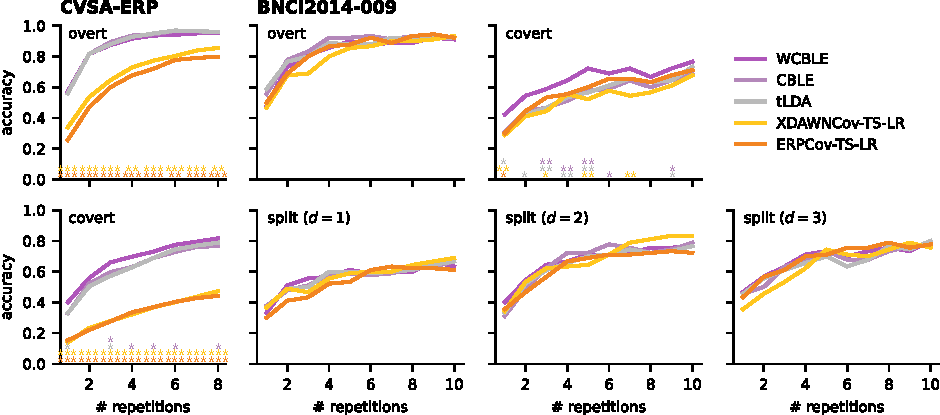
\includegraphics[width=\linewidth]{figures/covert_align/figure4b.pdf}
    \hspace{-0.41662707185564984in}
%%% Creator: Matplotlib, PGF backend
%%
%% To include the figure in your LaTeX document, write
%%   \input{<filename>.pgf}
%%
%% Make sure the required packages are loaded in your preamble
%%   \usepackage{pgf}
%%
%% Also ensure that all the required font packages are loaded; for instance,
%% the lmodern package is sometimes necessary when using math font.
%%   \usepackage{lmodern}
%%
%% Figures using additional raster images can only be included by \input if
%% they are in the same directory as the main LaTeX file. For loading figures
%% from other directories you can use the `import` package
%%   \usepackage{import}
%%
%% and then include the figures with
%%   \import{<path to file>}{<filename>.pgf}
%%
%% Matplotlib used the following preamble
%%   \def\mathdefault#1{#1}
%%   \everymath=\expandafter{\the\everymath\displaystyle}
%%   
%%   \ifdefined\pdftexversion\else  % non-pdftex case.
%%     \usepackage{fontspec}
%%   \fi
%%   \makeatletter\@ifpackageloaded{underscore}{}{\usepackage[strings]{underscore}}\makeatother
%%
\begingroup%
\makeatletter%
\begin{pgfpicture}%
\pgfpathrectangle{\pgfpointorigin}{\pgfqpoint{5.057692in}{2.836506in}}%
\pgfusepath{use as bounding box, clip}%
\begin{pgfscope}%
\pgfsetbuttcap%
\pgfsetmiterjoin%
\pgfsetlinewidth{0.000000pt}%
\definecolor{currentstroke}{rgb}{1.000000,1.000000,1.000000}%
\pgfsetstrokecolor{currentstroke}%
\pgfsetstrokeopacity{0.000000}%
\pgfsetdash{}{0pt}%
\pgfpathmoveto{\pgfqpoint{0.000000in}{0.000000in}}%
\pgfpathlineto{\pgfqpoint{5.057692in}{0.000000in}}%
\pgfpathlineto{\pgfqpoint{5.057692in}{2.836506in}}%
\pgfpathlineto{\pgfqpoint{0.000000in}{2.836506in}}%
\pgfpathlineto{\pgfqpoint{0.000000in}{0.000000in}}%
\pgfpathclose%
\pgfusepath{}%
\end{pgfscope}%
\begin{pgfscope}%
\pgfsetbuttcap%
\pgfsetmiterjoin%
\definecolor{currentfill}{rgb}{1.000000,1.000000,1.000000}%
\pgfsetfillcolor{currentfill}%
\pgfsetlinewidth{0.000000pt}%
\definecolor{currentstroke}{rgb}{0.000000,0.000000,0.000000}%
\pgfsetstrokecolor{currentstroke}%
\pgfsetstrokeopacity{0.000000}%
\pgfsetdash{}{0pt}%
\pgfpathmoveto{\pgfqpoint{0.421874in}{1.593603in}}%
\pgfpathlineto{\pgfqpoint{1.337485in}{1.593603in}}%
\pgfpathlineto{\pgfqpoint{1.337485in}{2.666367in}}%
\pgfpathlineto{\pgfqpoint{0.421874in}{2.666367in}}%
\pgfpathlineto{\pgfqpoint{0.421874in}{1.593603in}}%
\pgfpathclose%
\pgfusepath{fill}%
\end{pgfscope}%
\begin{pgfscope}%
\pgfsetbuttcap%
\pgfsetroundjoin%
\definecolor{currentfill}{rgb}{0.552941,0.501961,0.478431}%
\pgfsetfillcolor{currentfill}%
\pgfsetlinewidth{0.803000pt}%
\definecolor{currentstroke}{rgb}{0.552941,0.501961,0.478431}%
\pgfsetstrokecolor{currentstroke}%
\pgfsetdash{}{0pt}%
\pgfsys@defobject{currentmarker}{\pgfqpoint{0.000000in}{0.000000in}}{\pgfqpoint{0.000000in}{0.041667in}}{%
\pgfpathmoveto{\pgfqpoint{0.000000in}{0.000000in}}%
\pgfpathlineto{\pgfqpoint{0.000000in}{0.041667in}}%
\pgfusepath{stroke,fill}%
}%
\begin{pgfscope}%
\pgfsys@transformshift{0.582403in}{1.593603in}%
\pgfsys@useobject{currentmarker}{}%
\end{pgfscope}%
\end{pgfscope}%
\begin{pgfscope}%
\pgfsetbuttcap%
\pgfsetroundjoin%
\definecolor{currentfill}{rgb}{0.552941,0.501961,0.478431}%
\pgfsetfillcolor{currentfill}%
\pgfsetlinewidth{0.803000pt}%
\definecolor{currentstroke}{rgb}{0.552941,0.501961,0.478431}%
\pgfsetstrokecolor{currentstroke}%
\pgfsetdash{}{0pt}%
\pgfsys@defobject{currentmarker}{\pgfqpoint{0.000000in}{0.000000in}}{\pgfqpoint{0.000000in}{0.041667in}}{%
\pgfpathmoveto{\pgfqpoint{0.000000in}{0.000000in}}%
\pgfpathlineto{\pgfqpoint{0.000000in}{0.041667in}}%
\pgfusepath{stroke,fill}%
}%
\begin{pgfscope}%
\pgfsys@transformshift{0.820224in}{1.593603in}%
\pgfsys@useobject{currentmarker}{}%
\end{pgfscope}%
\end{pgfscope}%
\begin{pgfscope}%
\pgfsetbuttcap%
\pgfsetroundjoin%
\definecolor{currentfill}{rgb}{0.552941,0.501961,0.478431}%
\pgfsetfillcolor{currentfill}%
\pgfsetlinewidth{0.803000pt}%
\definecolor{currentstroke}{rgb}{0.552941,0.501961,0.478431}%
\pgfsetstrokecolor{currentstroke}%
\pgfsetdash{}{0pt}%
\pgfsys@defobject{currentmarker}{\pgfqpoint{0.000000in}{0.000000in}}{\pgfqpoint{0.000000in}{0.041667in}}{%
\pgfpathmoveto{\pgfqpoint{0.000000in}{0.000000in}}%
\pgfpathlineto{\pgfqpoint{0.000000in}{0.041667in}}%
\pgfusepath{stroke,fill}%
}%
\begin{pgfscope}%
\pgfsys@transformshift{1.058045in}{1.593603in}%
\pgfsys@useobject{currentmarker}{}%
\end{pgfscope}%
\end{pgfscope}%
\begin{pgfscope}%
\pgfsetbuttcap%
\pgfsetroundjoin%
\definecolor{currentfill}{rgb}{0.552941,0.501961,0.478431}%
\pgfsetfillcolor{currentfill}%
\pgfsetlinewidth{0.803000pt}%
\definecolor{currentstroke}{rgb}{0.552941,0.501961,0.478431}%
\pgfsetstrokecolor{currentstroke}%
\pgfsetdash{}{0pt}%
\pgfsys@defobject{currentmarker}{\pgfqpoint{0.000000in}{0.000000in}}{\pgfqpoint{0.000000in}{0.041667in}}{%
\pgfpathmoveto{\pgfqpoint{0.000000in}{0.000000in}}%
\pgfpathlineto{\pgfqpoint{0.000000in}{0.041667in}}%
\pgfusepath{stroke,fill}%
}%
\begin{pgfscope}%
\pgfsys@transformshift{1.295866in}{1.593603in}%
\pgfsys@useobject{currentmarker}{}%
\end{pgfscope}%
\end{pgfscope}%
\begin{pgfscope}%
\pgfsetbuttcap%
\pgfsetroundjoin%
\definecolor{currentfill}{rgb}{0.552941,0.501961,0.478431}%
\pgfsetfillcolor{currentfill}%
\pgfsetlinewidth{0.803000pt}%
\definecolor{currentstroke}{rgb}{0.552941,0.501961,0.478431}%
\pgfsetstrokecolor{currentstroke}%
\pgfsetdash{}{0pt}%
\pgfsys@defobject{currentmarker}{\pgfqpoint{0.000000in}{0.000000in}}{\pgfqpoint{0.041667in}{0.000000in}}{%
\pgfpathmoveto{\pgfqpoint{0.000000in}{0.000000in}}%
\pgfpathlineto{\pgfqpoint{0.041667in}{0.000000in}}%
\pgfusepath{stroke,fill}%
}%
\begin{pgfscope}%
\pgfsys@transformshift{0.421874in}{1.593603in}%
\pgfsys@useobject{currentmarker}{}%
\end{pgfscope}%
\end{pgfscope}%
\begin{pgfscope}%
\definecolor{textcolor}{rgb}{0.552941,0.501961,0.478431}%
\pgfsetstrokecolor{textcolor}%
\pgfsetfillcolor{textcolor}%
\pgftext[x=0.309027in, y=1.550201in, left, base]{\color{textcolor}{\sffamily\fontsize{9.000000}{10.800000}\selectfont\catcode`\^=\active\def^{\ifmmode\sp\else\^{}\fi}\catcode`\%=\active\def%{\%}0}}%
\end{pgfscope}%
\begin{pgfscope}%
\pgfsetbuttcap%
\pgfsetroundjoin%
\definecolor{currentfill}{rgb}{0.552941,0.501961,0.478431}%
\pgfsetfillcolor{currentfill}%
\pgfsetlinewidth{0.803000pt}%
\definecolor{currentstroke}{rgb}{0.552941,0.501961,0.478431}%
\pgfsetstrokecolor{currentstroke}%
\pgfsetdash{}{0pt}%
\pgfsys@defobject{currentmarker}{\pgfqpoint{0.000000in}{0.000000in}}{\pgfqpoint{0.041667in}{0.000000in}}{%
\pgfpathmoveto{\pgfqpoint{0.000000in}{0.000000in}}%
\pgfpathlineto{\pgfqpoint{0.041667in}{0.000000in}}%
\pgfusepath{stroke,fill}%
}%
\begin{pgfscope}%
\pgfsys@transformshift{0.421874in}{1.861794in}%
\pgfsys@useobject{currentmarker}{}%
\end{pgfscope}%
\end{pgfscope}%
\begin{pgfscope}%
\definecolor{textcolor}{rgb}{0.552941,0.501961,0.478431}%
\pgfsetstrokecolor{textcolor}%
\pgfsetfillcolor{textcolor}%
\pgftext[x=0.244791in, y=1.818391in, left, base]{\color{textcolor}{\sffamily\fontsize{9.000000}{10.800000}\selectfont\catcode`\^=\active\def^{\ifmmode\sp\else\^{}\fi}\catcode`\%=\active\def%{\%}25}}%
\end{pgfscope}%
\begin{pgfscope}%
\pgfsetbuttcap%
\pgfsetroundjoin%
\definecolor{currentfill}{rgb}{0.552941,0.501961,0.478431}%
\pgfsetfillcolor{currentfill}%
\pgfsetlinewidth{0.803000pt}%
\definecolor{currentstroke}{rgb}{0.552941,0.501961,0.478431}%
\pgfsetstrokecolor{currentstroke}%
\pgfsetdash{}{0pt}%
\pgfsys@defobject{currentmarker}{\pgfqpoint{0.000000in}{0.000000in}}{\pgfqpoint{0.041667in}{0.000000in}}{%
\pgfpathmoveto{\pgfqpoint{0.000000in}{0.000000in}}%
\pgfpathlineto{\pgfqpoint{0.041667in}{0.000000in}}%
\pgfusepath{stroke,fill}%
}%
\begin{pgfscope}%
\pgfsys@transformshift{0.421874in}{2.129985in}%
\pgfsys@useobject{currentmarker}{}%
\end{pgfscope}%
\end{pgfscope}%
\begin{pgfscope}%
\definecolor{textcolor}{rgb}{0.552941,0.501961,0.478431}%
\pgfsetstrokecolor{textcolor}%
\pgfsetfillcolor{textcolor}%
\pgftext[x=0.244791in, y=2.086582in, left, base]{\color{textcolor}{\sffamily\fontsize{9.000000}{10.800000}\selectfont\catcode`\^=\active\def^{\ifmmode\sp\else\^{}\fi}\catcode`\%=\active\def%{\%}50}}%
\end{pgfscope}%
\begin{pgfscope}%
\pgfsetbuttcap%
\pgfsetroundjoin%
\definecolor{currentfill}{rgb}{0.552941,0.501961,0.478431}%
\pgfsetfillcolor{currentfill}%
\pgfsetlinewidth{0.803000pt}%
\definecolor{currentstroke}{rgb}{0.552941,0.501961,0.478431}%
\pgfsetstrokecolor{currentstroke}%
\pgfsetdash{}{0pt}%
\pgfsys@defobject{currentmarker}{\pgfqpoint{0.000000in}{0.000000in}}{\pgfqpoint{0.041667in}{0.000000in}}{%
\pgfpathmoveto{\pgfqpoint{0.000000in}{0.000000in}}%
\pgfpathlineto{\pgfqpoint{0.041667in}{0.000000in}}%
\pgfusepath{stroke,fill}%
}%
\begin{pgfscope}%
\pgfsys@transformshift{0.421874in}{2.398176in}%
\pgfsys@useobject{currentmarker}{}%
\end{pgfscope}%
\end{pgfscope}%
\begin{pgfscope}%
\definecolor{textcolor}{rgb}{0.552941,0.501961,0.478431}%
\pgfsetstrokecolor{textcolor}%
\pgfsetfillcolor{textcolor}%
\pgftext[x=0.244791in, y=2.354773in, left, base]{\color{textcolor}{\sffamily\fontsize{9.000000}{10.800000}\selectfont\catcode`\^=\active\def^{\ifmmode\sp\else\^{}\fi}\catcode`\%=\active\def%{\%}75}}%
\end{pgfscope}%
\begin{pgfscope}%
\pgfsetbuttcap%
\pgfsetroundjoin%
\definecolor{currentfill}{rgb}{0.552941,0.501961,0.478431}%
\pgfsetfillcolor{currentfill}%
\pgfsetlinewidth{0.803000pt}%
\definecolor{currentstroke}{rgb}{0.552941,0.501961,0.478431}%
\pgfsetstrokecolor{currentstroke}%
\pgfsetdash{}{0pt}%
\pgfsys@defobject{currentmarker}{\pgfqpoint{0.000000in}{0.000000in}}{\pgfqpoint{0.041667in}{0.000000in}}{%
\pgfpathmoveto{\pgfqpoint{0.000000in}{0.000000in}}%
\pgfpathlineto{\pgfqpoint{0.041667in}{0.000000in}}%
\pgfusepath{stroke,fill}%
}%
\begin{pgfscope}%
\pgfsys@transformshift{0.421874in}{2.666367in}%
\pgfsys@useobject{currentmarker}{}%
\end{pgfscope}%
\end{pgfscope}%
\begin{pgfscope}%
\definecolor{textcolor}{rgb}{0.552941,0.501961,0.478431}%
\pgfsetstrokecolor{textcolor}%
\pgfsetfillcolor{textcolor}%
\pgftext[x=0.180556in, y=2.622964in, left, base]{\color{textcolor}{\sffamily\fontsize{9.000000}{10.800000}\selectfont\catcode`\^=\active\def^{\ifmmode\sp\else\^{}\fi}\catcode`\%=\active\def%{\%}100}}%
\end{pgfscope}%
\begin{pgfscope}%
\definecolor{textcolor}{rgb}{0.552941,0.501961,0.478431}%
\pgfsetstrokecolor{textcolor}%
\pgfsetfillcolor{textcolor}%
\pgftext[x=0.125000in,y=2.129985in,,bottom,rotate=90.000000]{\color{textcolor}{\sffamily\fontsize{9.000000}{10.800000}\selectfont\catcode`\^=\active\def^{\ifmmode\sp\else\^{}\fi}\catcode`\%=\active\def%{\%}Accuracy (\%)}}%
\end{pgfscope}%
\begin{pgfscope}%
\pgfpathrectangle{\pgfqpoint{0.421874in}{1.593603in}}{\pgfqpoint{0.915611in}{1.072763in}}%
\pgfusepath{clip}%
\pgfsetrectcap%
\pgfsetroundjoin%
\pgfsetlinewidth{1.505625pt}%
\definecolor{currentstroke}{rgb}{0.470588,0.278431,0.615686}%
\pgfsetstrokecolor{currentstroke}%
\pgfsetdash{}{0pt}%
\pgfpathmoveto{\pgfqpoint{0.463492in}{2.207462in}}%
\pgfpathlineto{\pgfqpoint{0.582403in}{2.469693in}}%
\pgfpathlineto{\pgfqpoint{0.701314in}{2.532271in}}%
\pgfpathlineto{\pgfqpoint{0.820224in}{2.576970in}}%
\pgfpathlineto{\pgfqpoint{0.939135in}{2.597829in}}%
\pgfpathlineto{\pgfqpoint{1.058045in}{2.603789in}}%
\pgfpathlineto{\pgfqpoint{1.176956in}{2.612729in}}%
\pgfpathlineto{\pgfqpoint{1.295866in}{2.618688in}}%
\pgfusepath{stroke}%
\end{pgfscope}%
\begin{pgfscope}%
\pgfpathrectangle{\pgfqpoint{0.421874in}{1.593603in}}{\pgfqpoint{0.915611in}{1.072763in}}%
\pgfusepath{clip}%
\pgfsetrectcap%
\pgfsetroundjoin%
\pgfsetlinewidth{1.505625pt}%
\definecolor{currentstroke}{rgb}{0.807843,0.701961,0.886275}%
\pgfsetstrokecolor{currentstroke}%
\pgfsetdash{}{0pt}%
\pgfpathmoveto{\pgfqpoint{0.463492in}{2.195543in}}%
\pgfpathlineto{\pgfqpoint{0.582403in}{2.469693in}}%
\pgfpathlineto{\pgfqpoint{0.701314in}{2.553131in}}%
\pgfpathlineto{\pgfqpoint{0.820224in}{2.597829in}}%
\pgfpathlineto{\pgfqpoint{0.939135in}{2.606769in}}%
\pgfpathlineto{\pgfqpoint{1.058045in}{2.630608in}}%
\pgfpathlineto{\pgfqpoint{1.176956in}{2.627628in}}%
\pgfpathlineto{\pgfqpoint{1.295866in}{2.621668in}}%
\pgfusepath{stroke}%
\end{pgfscope}%
\begin{pgfscope}%
\pgfpathrectangle{\pgfqpoint{0.421874in}{1.593603in}}{\pgfqpoint{0.915611in}{1.072763in}}%
\pgfusepath{clip}%
\pgfsetrectcap%
\pgfsetroundjoin%
\pgfsetlinewidth{1.505625pt}%
\definecolor{currentstroke}{rgb}{0.552941,0.501961,0.478431}%
\pgfsetstrokecolor{currentstroke}%
\pgfsetdash{}{0pt}%
\pgfpathmoveto{\pgfqpoint{0.463492in}{2.195543in}}%
\pgfpathlineto{\pgfqpoint{0.582403in}{2.469693in}}%
\pgfpathlineto{\pgfqpoint{0.701314in}{2.538231in}}%
\pgfpathlineto{\pgfqpoint{0.820224in}{2.588889in}}%
\pgfpathlineto{\pgfqpoint{0.939135in}{2.612729in}}%
\pgfpathlineto{\pgfqpoint{1.058045in}{2.633588in}}%
\pgfpathlineto{\pgfqpoint{1.176956in}{2.627628in}}%
\pgfpathlineto{\pgfqpoint{1.295866in}{2.624648in}}%
\pgfusepath{stroke}%
\end{pgfscope}%
\begin{pgfscope}%
\pgfpathrectangle{\pgfqpoint{0.421874in}{1.593603in}}{\pgfqpoint{0.915611in}{1.072763in}}%
\pgfusepath{clip}%
\pgfsetrectcap%
\pgfsetroundjoin%
\pgfsetlinewidth{1.505625pt}%
\definecolor{currentstroke}{rgb}{0.949020,0.564706,0.094118}%
\pgfsetstrokecolor{currentstroke}%
\pgfsetdash{}{0pt}%
\pgfpathmoveto{\pgfqpoint{0.463492in}{1.957151in}}%
\pgfpathlineto{\pgfqpoint{0.582403in}{2.168128in}}%
\pgfpathlineto{\pgfqpoint{0.701314in}{2.287324in}}%
\pgfpathlineto{\pgfqpoint{0.820224in}{2.375529in}}%
\pgfpathlineto{\pgfqpoint{0.939135in}{2.423207in}}%
\pgfpathlineto{\pgfqpoint{1.058045in}{2.455390in}}%
\pgfpathlineto{\pgfqpoint{1.176956in}{2.493533in}}%
\pgfpathlineto{\pgfqpoint{1.295866in}{2.511412in}}%
\pgfusepath{stroke}%
\end{pgfscope}%
\begin{pgfscope}%
\pgfpathrectangle{\pgfqpoint{0.421874in}{1.593603in}}{\pgfqpoint{0.915611in}{1.072763in}}%
\pgfusepath{clip}%
\pgfsetrectcap%
\pgfsetroundjoin%
\pgfsetlinewidth{1.505625pt}%
\definecolor{currentstroke}{rgb}{0.964706,0.239216,0.117647}%
\pgfsetstrokecolor{currentstroke}%
\pgfsetdash{}{0pt}%
\pgfpathmoveto{\pgfqpoint{0.463492in}{1.868946in}}%
\pgfpathlineto{\pgfqpoint{0.582403in}{2.097802in}}%
\pgfpathlineto{\pgfqpoint{0.701314in}{2.238453in}}%
\pgfpathlineto{\pgfqpoint{0.820224in}{2.319507in}}%
\pgfpathlineto{\pgfqpoint{0.939135in}{2.365993in}}%
\pgfpathlineto{\pgfqpoint{1.058045in}{2.427975in}}%
\pgfpathlineto{\pgfqpoint{1.176956in}{2.441086in}}%
\pgfpathlineto{\pgfqpoint{1.295866in}{2.450622in}}%
\pgfusepath{stroke}%
\end{pgfscope}%
\begin{pgfscope}%
\pgfsetrectcap%
\pgfsetmiterjoin%
\pgfsetlinewidth{0.803000pt}%
\definecolor{currentstroke}{rgb}{0.552941,0.501961,0.478431}%
\pgfsetstrokecolor{currentstroke}%
\pgfsetdash{}{0pt}%
\pgfpathmoveto{\pgfqpoint{0.421874in}{1.593603in}}%
\pgfpathlineto{\pgfqpoint{0.421874in}{2.666367in}}%
\pgfusepath{stroke}%
\end{pgfscope}%
\begin{pgfscope}%
\pgfsetrectcap%
\pgfsetmiterjoin%
\pgfsetlinewidth{0.803000pt}%
\definecolor{currentstroke}{rgb}{0.552941,0.501961,0.478431}%
\pgfsetstrokecolor{currentstroke}%
\pgfsetdash{}{0pt}%
\pgfpathmoveto{\pgfqpoint{1.337485in}{1.593603in}}%
\pgfpathlineto{\pgfqpoint{1.337485in}{2.666367in}}%
\pgfusepath{stroke}%
\end{pgfscope}%
\begin{pgfscope}%
\pgfsetrectcap%
\pgfsetmiterjoin%
\pgfsetlinewidth{0.803000pt}%
\definecolor{currentstroke}{rgb}{0.552941,0.501961,0.478431}%
\pgfsetstrokecolor{currentstroke}%
\pgfsetdash{}{0pt}%
\pgfpathmoveto{\pgfqpoint{0.421874in}{1.593603in}}%
\pgfpathlineto{\pgfqpoint{1.337485in}{1.593603in}}%
\pgfusepath{stroke}%
\end{pgfscope}%
\begin{pgfscope}%
\pgfsetrectcap%
\pgfsetmiterjoin%
\pgfsetlinewidth{0.803000pt}%
\definecolor{currentstroke}{rgb}{0.552941,0.501961,0.478431}%
\pgfsetstrokecolor{currentstroke}%
\pgfsetdash{}{0pt}%
\pgfpathmoveto{\pgfqpoint{0.421874in}{2.666367in}}%
\pgfpathlineto{\pgfqpoint{1.337485in}{2.666367in}}%
\pgfusepath{stroke}%
\end{pgfscope}%
\begin{pgfscope}%
\definecolor{textcolor}{rgb}{0.552941,0.501961,0.478431}%
\pgfsetstrokecolor{textcolor}%
\pgfsetfillcolor{textcolor}%
\pgftext[x=1.291704in,y=1.647242in,right,bottom]{\color{textcolor}{\sffamily\fontsize{10.000000}{12.000000}\selectfont\catcode`\^=\active\def^{\ifmmode\sp\else\^{}\fi}\catcode`\%=\active\def%{\%}overt}}%
\end{pgfscope}%
\begin{pgfscope}%
\definecolor{textcolor}{rgb}{0.552941,0.501961,0.478431}%
\pgfsetstrokecolor{textcolor}%
\pgfsetfillcolor{textcolor}%
\pgftext[x=0.421874in,y=2.749700in,left,base]{\color{textcolor}{\sffamily\fontsize{9.000000}{10.800000}\selectfont\catcode`\^=\active\def^{\ifmmode\sp\else\^{}\fi}\catcode`\%=\active\def%{\%}CVSA-ERP}}%
\end{pgfscope}%
\begin{pgfscope}%
\pgfsetbuttcap%
\pgfsetmiterjoin%
\definecolor{currentfill}{rgb}{1.000000,1.000000,1.000000}%
\pgfsetfillcolor{currentfill}%
\pgfsetlinewidth{0.000000pt}%
\definecolor{currentstroke}{rgb}{0.000000,0.000000,0.000000}%
\pgfsetstrokecolor{currentstroke}%
\pgfsetstrokeopacity{0.000000}%
\pgfsetdash{}{0pt}%
\pgfpathmoveto{\pgfqpoint{1.420825in}{1.593603in}}%
\pgfpathlineto{\pgfqpoint{2.565339in}{1.593603in}}%
\pgfpathlineto{\pgfqpoint{2.565339in}{2.666367in}}%
\pgfpathlineto{\pgfqpoint{1.420825in}{2.666367in}}%
\pgfpathlineto{\pgfqpoint{1.420825in}{1.593603in}}%
\pgfpathclose%
\pgfusepath{fill}%
\end{pgfscope}%
\begin{pgfscope}%
\pgfsetbuttcap%
\pgfsetroundjoin%
\definecolor{currentfill}{rgb}{0.552941,0.501961,0.478431}%
\pgfsetfillcolor{currentfill}%
\pgfsetlinewidth{0.803000pt}%
\definecolor{currentstroke}{rgb}{0.552941,0.501961,0.478431}%
\pgfsetstrokecolor{currentstroke}%
\pgfsetdash{}{0pt}%
\pgfsys@defobject{currentmarker}{\pgfqpoint{0.000000in}{0.000000in}}{\pgfqpoint{0.000000in}{0.041667in}}{%
\pgfpathmoveto{\pgfqpoint{0.000000in}{0.000000in}}%
\pgfpathlineto{\pgfqpoint{0.000000in}{0.041667in}}%
\pgfusepath{stroke,fill}%
}%
\begin{pgfscope}%
\pgfsys@transformshift{1.588456in}{1.593603in}%
\pgfsys@useobject{currentmarker}{}%
\end{pgfscope}%
\end{pgfscope}%
\begin{pgfscope}%
\pgfsetbuttcap%
\pgfsetroundjoin%
\definecolor{currentfill}{rgb}{0.552941,0.501961,0.478431}%
\pgfsetfillcolor{currentfill}%
\pgfsetlinewidth{0.803000pt}%
\definecolor{currentstroke}{rgb}{0.552941,0.501961,0.478431}%
\pgfsetstrokecolor{currentstroke}%
\pgfsetdash{}{0pt}%
\pgfsys@defobject{currentmarker}{\pgfqpoint{0.000000in}{0.000000in}}{\pgfqpoint{0.000000in}{0.041667in}}{%
\pgfpathmoveto{\pgfqpoint{0.000000in}{0.000000in}}%
\pgfpathlineto{\pgfqpoint{0.000000in}{0.041667in}}%
\pgfusepath{stroke,fill}%
}%
\begin{pgfscope}%
\pgfsys@transformshift{1.819671in}{1.593603in}%
\pgfsys@useobject{currentmarker}{}%
\end{pgfscope}%
\end{pgfscope}%
\begin{pgfscope}%
\pgfsetbuttcap%
\pgfsetroundjoin%
\definecolor{currentfill}{rgb}{0.552941,0.501961,0.478431}%
\pgfsetfillcolor{currentfill}%
\pgfsetlinewidth{0.803000pt}%
\definecolor{currentstroke}{rgb}{0.552941,0.501961,0.478431}%
\pgfsetstrokecolor{currentstroke}%
\pgfsetdash{}{0pt}%
\pgfsys@defobject{currentmarker}{\pgfqpoint{0.000000in}{0.000000in}}{\pgfqpoint{0.000000in}{0.041667in}}{%
\pgfpathmoveto{\pgfqpoint{0.000000in}{0.000000in}}%
\pgfpathlineto{\pgfqpoint{0.000000in}{0.041667in}}%
\pgfusepath{stroke,fill}%
}%
\begin{pgfscope}%
\pgfsys@transformshift{2.050886in}{1.593603in}%
\pgfsys@useobject{currentmarker}{}%
\end{pgfscope}%
\end{pgfscope}%
\begin{pgfscope}%
\pgfsetbuttcap%
\pgfsetroundjoin%
\definecolor{currentfill}{rgb}{0.552941,0.501961,0.478431}%
\pgfsetfillcolor{currentfill}%
\pgfsetlinewidth{0.803000pt}%
\definecolor{currentstroke}{rgb}{0.552941,0.501961,0.478431}%
\pgfsetstrokecolor{currentstroke}%
\pgfsetdash{}{0pt}%
\pgfsys@defobject{currentmarker}{\pgfqpoint{0.000000in}{0.000000in}}{\pgfqpoint{0.000000in}{0.041667in}}{%
\pgfpathmoveto{\pgfqpoint{0.000000in}{0.000000in}}%
\pgfpathlineto{\pgfqpoint{0.000000in}{0.041667in}}%
\pgfusepath{stroke,fill}%
}%
\begin{pgfscope}%
\pgfsys@transformshift{2.282101in}{1.593603in}%
\pgfsys@useobject{currentmarker}{}%
\end{pgfscope}%
\end{pgfscope}%
\begin{pgfscope}%
\pgfsetbuttcap%
\pgfsetroundjoin%
\definecolor{currentfill}{rgb}{0.552941,0.501961,0.478431}%
\pgfsetfillcolor{currentfill}%
\pgfsetlinewidth{0.803000pt}%
\definecolor{currentstroke}{rgb}{0.552941,0.501961,0.478431}%
\pgfsetstrokecolor{currentstroke}%
\pgfsetdash{}{0pt}%
\pgfsys@defobject{currentmarker}{\pgfqpoint{0.000000in}{0.000000in}}{\pgfqpoint{0.000000in}{0.041667in}}{%
\pgfpathmoveto{\pgfqpoint{0.000000in}{0.000000in}}%
\pgfpathlineto{\pgfqpoint{0.000000in}{0.041667in}}%
\pgfusepath{stroke,fill}%
}%
\begin{pgfscope}%
\pgfsys@transformshift{2.513316in}{1.593603in}%
\pgfsys@useobject{currentmarker}{}%
\end{pgfscope}%
\end{pgfscope}%
\begin{pgfscope}%
\pgfsetbuttcap%
\pgfsetroundjoin%
\definecolor{currentfill}{rgb}{0.552941,0.501961,0.478431}%
\pgfsetfillcolor{currentfill}%
\pgfsetlinewidth{0.803000pt}%
\definecolor{currentstroke}{rgb}{0.552941,0.501961,0.478431}%
\pgfsetstrokecolor{currentstroke}%
\pgfsetdash{}{0pt}%
\pgfsys@defobject{currentmarker}{\pgfqpoint{0.000000in}{0.000000in}}{\pgfqpoint{0.041667in}{0.000000in}}{%
\pgfpathmoveto{\pgfqpoint{0.000000in}{0.000000in}}%
\pgfpathlineto{\pgfqpoint{0.041667in}{0.000000in}}%
\pgfusepath{stroke,fill}%
}%
\begin{pgfscope}%
\pgfsys@transformshift{1.420825in}{1.593603in}%
\pgfsys@useobject{currentmarker}{}%
\end{pgfscope}%
\end{pgfscope}%
\begin{pgfscope}%
\pgfsetbuttcap%
\pgfsetroundjoin%
\definecolor{currentfill}{rgb}{0.552941,0.501961,0.478431}%
\pgfsetfillcolor{currentfill}%
\pgfsetlinewidth{0.803000pt}%
\definecolor{currentstroke}{rgb}{0.552941,0.501961,0.478431}%
\pgfsetstrokecolor{currentstroke}%
\pgfsetdash{}{0pt}%
\pgfsys@defobject{currentmarker}{\pgfqpoint{0.000000in}{0.000000in}}{\pgfqpoint{0.041667in}{0.000000in}}{%
\pgfpathmoveto{\pgfqpoint{0.000000in}{0.000000in}}%
\pgfpathlineto{\pgfqpoint{0.041667in}{0.000000in}}%
\pgfusepath{stroke,fill}%
}%
\begin{pgfscope}%
\pgfsys@transformshift{1.420825in}{1.861794in}%
\pgfsys@useobject{currentmarker}{}%
\end{pgfscope}%
\end{pgfscope}%
\begin{pgfscope}%
\pgfsetbuttcap%
\pgfsetroundjoin%
\definecolor{currentfill}{rgb}{0.552941,0.501961,0.478431}%
\pgfsetfillcolor{currentfill}%
\pgfsetlinewidth{0.803000pt}%
\definecolor{currentstroke}{rgb}{0.552941,0.501961,0.478431}%
\pgfsetstrokecolor{currentstroke}%
\pgfsetdash{}{0pt}%
\pgfsys@defobject{currentmarker}{\pgfqpoint{0.000000in}{0.000000in}}{\pgfqpoint{0.041667in}{0.000000in}}{%
\pgfpathmoveto{\pgfqpoint{0.000000in}{0.000000in}}%
\pgfpathlineto{\pgfqpoint{0.041667in}{0.000000in}}%
\pgfusepath{stroke,fill}%
}%
\begin{pgfscope}%
\pgfsys@transformshift{1.420825in}{2.129985in}%
\pgfsys@useobject{currentmarker}{}%
\end{pgfscope}%
\end{pgfscope}%
\begin{pgfscope}%
\pgfsetbuttcap%
\pgfsetroundjoin%
\definecolor{currentfill}{rgb}{0.552941,0.501961,0.478431}%
\pgfsetfillcolor{currentfill}%
\pgfsetlinewidth{0.803000pt}%
\definecolor{currentstroke}{rgb}{0.552941,0.501961,0.478431}%
\pgfsetstrokecolor{currentstroke}%
\pgfsetdash{}{0pt}%
\pgfsys@defobject{currentmarker}{\pgfqpoint{0.000000in}{0.000000in}}{\pgfqpoint{0.041667in}{0.000000in}}{%
\pgfpathmoveto{\pgfqpoint{0.000000in}{0.000000in}}%
\pgfpathlineto{\pgfqpoint{0.041667in}{0.000000in}}%
\pgfusepath{stroke,fill}%
}%
\begin{pgfscope}%
\pgfsys@transformshift{1.420825in}{2.398176in}%
\pgfsys@useobject{currentmarker}{}%
\end{pgfscope}%
\end{pgfscope}%
\begin{pgfscope}%
\pgfsetbuttcap%
\pgfsetroundjoin%
\definecolor{currentfill}{rgb}{0.552941,0.501961,0.478431}%
\pgfsetfillcolor{currentfill}%
\pgfsetlinewidth{0.803000pt}%
\definecolor{currentstroke}{rgb}{0.552941,0.501961,0.478431}%
\pgfsetstrokecolor{currentstroke}%
\pgfsetdash{}{0pt}%
\pgfsys@defobject{currentmarker}{\pgfqpoint{0.000000in}{0.000000in}}{\pgfqpoint{0.041667in}{0.000000in}}{%
\pgfpathmoveto{\pgfqpoint{0.000000in}{0.000000in}}%
\pgfpathlineto{\pgfqpoint{0.041667in}{0.000000in}}%
\pgfusepath{stroke,fill}%
}%
\begin{pgfscope}%
\pgfsys@transformshift{1.420825in}{2.666367in}%
\pgfsys@useobject{currentmarker}{}%
\end{pgfscope}%
\end{pgfscope}%
\begin{pgfscope}%
\pgfpathrectangle{\pgfqpoint{1.420825in}{1.593603in}}{\pgfqpoint{1.144514in}{1.072763in}}%
\pgfusepath{clip}%
\pgfsetrectcap%
\pgfsetroundjoin%
\pgfsetlinewidth{1.505625pt}%
\definecolor{currentstroke}{rgb}{0.470588,0.278431,0.615686}%
\pgfsetstrokecolor{currentstroke}%
\pgfsetdash{}{0pt}%
\pgfpathmoveto{\pgfqpoint{1.472848in}{2.106146in}}%
\pgfpathlineto{\pgfqpoint{1.588456in}{2.380296in}}%
\pgfpathlineto{\pgfqpoint{1.704063in}{2.463734in}}%
\pgfpathlineto{\pgfqpoint{1.819671in}{2.511412in}}%
\pgfpathlineto{\pgfqpoint{1.935278in}{2.559090in}}%
\pgfpathlineto{\pgfqpoint{2.050886in}{2.535251in}}%
\pgfpathlineto{\pgfqpoint{2.166493in}{2.547171in}}%
\pgfpathlineto{\pgfqpoint{2.282101in}{2.547171in}}%
\pgfpathlineto{\pgfqpoint{2.397708in}{2.582930in}}%
\pgfpathlineto{\pgfqpoint{2.513316in}{2.571010in}}%
\pgfusepath{stroke}%
\end{pgfscope}%
\begin{pgfscope}%
\pgfpathrectangle{\pgfqpoint{1.420825in}{1.593603in}}{\pgfqpoint{1.144514in}{1.072763in}}%
\pgfusepath{clip}%
\pgfsetrectcap%
\pgfsetroundjoin%
\pgfsetlinewidth{1.505625pt}%
\definecolor{currentstroke}{rgb}{0.807843,0.701961,0.886275}%
\pgfsetstrokecolor{currentstroke}%
\pgfsetdash{}{0pt}%
\pgfpathmoveto{\pgfqpoint{1.472848in}{2.189583in}}%
\pgfpathlineto{\pgfqpoint{1.588456in}{2.427975in}}%
\pgfpathlineto{\pgfqpoint{1.704063in}{2.487573in}}%
\pgfpathlineto{\pgfqpoint{1.819671in}{2.582930in}}%
\pgfpathlineto{\pgfqpoint{1.935278in}{2.582930in}}%
\pgfpathlineto{\pgfqpoint{2.050886in}{2.594849in}}%
\pgfpathlineto{\pgfqpoint{2.166493in}{2.571010in}}%
\pgfpathlineto{\pgfqpoint{2.282101in}{2.594849in}}%
\pgfpathlineto{\pgfqpoint{2.397708in}{2.594849in}}%
\pgfpathlineto{\pgfqpoint{2.513316in}{2.582930in}}%
\pgfusepath{stroke}%
\end{pgfscope}%
\begin{pgfscope}%
\pgfpathrectangle{\pgfqpoint{1.420825in}{1.593603in}}{\pgfqpoint{1.144514in}{1.072763in}}%
\pgfusepath{clip}%
\pgfsetrectcap%
\pgfsetroundjoin%
\pgfsetlinewidth{1.505625pt}%
\definecolor{currentstroke}{rgb}{0.552941,0.501961,0.478431}%
\pgfsetstrokecolor{currentstroke}%
\pgfsetdash{}{0pt}%
\pgfpathmoveto{\pgfqpoint{1.472848in}{2.225342in}}%
\pgfpathlineto{\pgfqpoint{1.588456in}{2.416055in}}%
\pgfpathlineto{\pgfqpoint{1.704063in}{2.451814in}}%
\pgfpathlineto{\pgfqpoint{1.819671in}{2.547171in}}%
\pgfpathlineto{\pgfqpoint{1.935278in}{2.535251in}}%
\pgfpathlineto{\pgfqpoint{2.050886in}{2.535251in}}%
\pgfpathlineto{\pgfqpoint{2.166493in}{2.582930in}}%
\pgfpathlineto{\pgfqpoint{2.282101in}{2.571010in}}%
\pgfpathlineto{\pgfqpoint{2.397708in}{2.582930in}}%
\pgfpathlineto{\pgfqpoint{2.513316in}{2.582930in}}%
\pgfusepath{stroke}%
\end{pgfscope}%
\begin{pgfscope}%
\pgfpathrectangle{\pgfqpoint{1.420825in}{1.593603in}}{\pgfqpoint{1.144514in}{1.072763in}}%
\pgfusepath{clip}%
\pgfsetrectcap%
\pgfsetroundjoin%
\pgfsetlinewidth{1.505625pt}%
\definecolor{currentstroke}{rgb}{0.949020,0.564706,0.094118}%
\pgfsetstrokecolor{currentstroke}%
\pgfsetdash{}{0pt}%
\pgfpathmoveto{\pgfqpoint{1.472848in}{2.094226in}}%
\pgfpathlineto{\pgfqpoint{1.588456in}{2.320699in}}%
\pgfpathlineto{\pgfqpoint{1.704063in}{2.332618in}}%
\pgfpathlineto{\pgfqpoint{1.819671in}{2.451814in}}%
\pgfpathlineto{\pgfqpoint{1.935278in}{2.511412in}}%
\pgfpathlineto{\pgfqpoint{2.050886in}{2.523332in}}%
\pgfpathlineto{\pgfqpoint{2.166493in}{2.559090in}}%
\pgfpathlineto{\pgfqpoint{2.282101in}{2.559090in}}%
\pgfpathlineto{\pgfqpoint{2.397708in}{2.571010in}}%
\pgfpathlineto{\pgfqpoint{2.513316in}{2.594849in}}%
\pgfusepath{stroke}%
\end{pgfscope}%
\begin{pgfscope}%
\pgfpathrectangle{\pgfqpoint{1.420825in}{1.593603in}}{\pgfqpoint{1.144514in}{1.072763in}}%
\pgfusepath{clip}%
\pgfsetrectcap%
\pgfsetroundjoin%
\pgfsetlinewidth{1.505625pt}%
\definecolor{currentstroke}{rgb}{0.964706,0.239216,0.117647}%
\pgfsetstrokecolor{currentstroke}%
\pgfsetdash{}{0pt}%
\pgfpathmoveto{\pgfqpoint{1.472848in}{2.129985in}}%
\pgfpathlineto{\pgfqpoint{1.588456in}{2.332618in}}%
\pgfpathlineto{\pgfqpoint{1.704063in}{2.451814in}}%
\pgfpathlineto{\pgfqpoint{1.819671in}{2.523332in}}%
\pgfpathlineto{\pgfqpoint{1.935278in}{2.535251in}}%
\pgfpathlineto{\pgfqpoint{2.050886in}{2.582930in}}%
\pgfpathlineto{\pgfqpoint{2.166493in}{2.547171in}}%
\pgfpathlineto{\pgfqpoint{2.282101in}{2.594849in}}%
\pgfpathlineto{\pgfqpoint{2.397708in}{2.606769in}}%
\pgfpathlineto{\pgfqpoint{2.513316in}{2.582930in}}%
\pgfusepath{stroke}%
\end{pgfscope}%
\begin{pgfscope}%
\pgfsetrectcap%
\pgfsetmiterjoin%
\pgfsetlinewidth{0.803000pt}%
\definecolor{currentstroke}{rgb}{0.552941,0.501961,0.478431}%
\pgfsetstrokecolor{currentstroke}%
\pgfsetdash{}{0pt}%
\pgfpathmoveto{\pgfqpoint{1.420825in}{1.593603in}}%
\pgfpathlineto{\pgfqpoint{1.420825in}{2.666367in}}%
\pgfusepath{stroke}%
\end{pgfscope}%
\begin{pgfscope}%
\pgfsetrectcap%
\pgfsetmiterjoin%
\pgfsetlinewidth{0.803000pt}%
\definecolor{currentstroke}{rgb}{0.552941,0.501961,0.478431}%
\pgfsetstrokecolor{currentstroke}%
\pgfsetdash{}{0pt}%
\pgfpathmoveto{\pgfqpoint{2.565339in}{1.593603in}}%
\pgfpathlineto{\pgfqpoint{2.565339in}{2.666367in}}%
\pgfusepath{stroke}%
\end{pgfscope}%
\begin{pgfscope}%
\pgfsetrectcap%
\pgfsetmiterjoin%
\pgfsetlinewidth{0.803000pt}%
\definecolor{currentstroke}{rgb}{0.552941,0.501961,0.478431}%
\pgfsetstrokecolor{currentstroke}%
\pgfsetdash{}{0pt}%
\pgfpathmoveto{\pgfqpoint{1.420825in}{1.593603in}}%
\pgfpathlineto{\pgfqpoint{2.565339in}{1.593603in}}%
\pgfusepath{stroke}%
\end{pgfscope}%
\begin{pgfscope}%
\pgfsetrectcap%
\pgfsetmiterjoin%
\pgfsetlinewidth{0.803000pt}%
\definecolor{currentstroke}{rgb}{0.552941,0.501961,0.478431}%
\pgfsetstrokecolor{currentstroke}%
\pgfsetdash{}{0pt}%
\pgfpathmoveto{\pgfqpoint{1.420825in}{2.666367in}}%
\pgfpathlineto{\pgfqpoint{2.565339in}{2.666367in}}%
\pgfusepath{stroke}%
\end{pgfscope}%
\begin{pgfscope}%
\definecolor{textcolor}{rgb}{0.552941,0.501961,0.478431}%
\pgfsetstrokecolor{textcolor}%
\pgfsetfillcolor{textcolor}%
\pgftext[x=2.508113in,y=1.647242in,right,bottom]{\color{textcolor}{\sffamily\fontsize{10.000000}{12.000000}\selectfont\catcode`\^=\active\def^{\ifmmode\sp\else\^{}\fi}\catcode`\%=\active\def%{\%}overt}}%
\end{pgfscope}%
\begin{pgfscope}%
\definecolor{textcolor}{rgb}{0.552941,0.501961,0.478431}%
\pgfsetstrokecolor{textcolor}%
\pgfsetfillcolor{textcolor}%
\pgftext[x=1.420825in,y=2.749700in,left,base]{\color{textcolor}{\sffamily\fontsize{9.000000}{10.800000}\selectfont\catcode`\^=\active\def^{\ifmmode\sp\else\^{}\fi}\catcode`\%=\active\def%{\%}BNCI2014-009}}%
\end{pgfscope}%
\begin{pgfscope}%
\pgfsetbuttcap%
\pgfsetmiterjoin%
\definecolor{currentfill}{rgb}{1.000000,1.000000,1.000000}%
\pgfsetfillcolor{currentfill}%
\pgfsetlinewidth{0.000000pt}%
\definecolor{currentstroke}{rgb}{0.000000,0.000000,0.000000}%
\pgfsetstrokecolor{currentstroke}%
\pgfsetstrokeopacity{0.000000}%
\pgfsetdash{}{0pt}%
\pgfpathmoveto{\pgfqpoint{2.660895in}{1.593603in}}%
\pgfpathlineto{\pgfqpoint{3.805409in}{1.593603in}}%
\pgfpathlineto{\pgfqpoint{3.805409in}{2.666367in}}%
\pgfpathlineto{\pgfqpoint{2.660895in}{2.666367in}}%
\pgfpathlineto{\pgfqpoint{2.660895in}{1.593603in}}%
\pgfpathclose%
\pgfusepath{fill}%
\end{pgfscope}%
\begin{pgfscope}%
\pgfsetbuttcap%
\pgfsetroundjoin%
\definecolor{currentfill}{rgb}{0.552941,0.501961,0.478431}%
\pgfsetfillcolor{currentfill}%
\pgfsetlinewidth{0.803000pt}%
\definecolor{currentstroke}{rgb}{0.552941,0.501961,0.478431}%
\pgfsetstrokecolor{currentstroke}%
\pgfsetdash{}{0pt}%
\pgfsys@defobject{currentmarker}{\pgfqpoint{0.000000in}{0.000000in}}{\pgfqpoint{0.000000in}{0.041667in}}{%
\pgfpathmoveto{\pgfqpoint{0.000000in}{0.000000in}}%
\pgfpathlineto{\pgfqpoint{0.000000in}{0.041667in}}%
\pgfusepath{stroke,fill}%
}%
\begin{pgfscope}%
\pgfsys@transformshift{2.828526in}{1.593603in}%
\pgfsys@useobject{currentmarker}{}%
\end{pgfscope}%
\end{pgfscope}%
\begin{pgfscope}%
\pgfsetbuttcap%
\pgfsetroundjoin%
\definecolor{currentfill}{rgb}{0.552941,0.501961,0.478431}%
\pgfsetfillcolor{currentfill}%
\pgfsetlinewidth{0.803000pt}%
\definecolor{currentstroke}{rgb}{0.552941,0.501961,0.478431}%
\pgfsetstrokecolor{currentstroke}%
\pgfsetdash{}{0pt}%
\pgfsys@defobject{currentmarker}{\pgfqpoint{0.000000in}{0.000000in}}{\pgfqpoint{0.000000in}{0.041667in}}{%
\pgfpathmoveto{\pgfqpoint{0.000000in}{0.000000in}}%
\pgfpathlineto{\pgfqpoint{0.000000in}{0.041667in}}%
\pgfusepath{stroke,fill}%
}%
\begin{pgfscope}%
\pgfsys@transformshift{3.059741in}{1.593603in}%
\pgfsys@useobject{currentmarker}{}%
\end{pgfscope}%
\end{pgfscope}%
\begin{pgfscope}%
\pgfsetbuttcap%
\pgfsetroundjoin%
\definecolor{currentfill}{rgb}{0.552941,0.501961,0.478431}%
\pgfsetfillcolor{currentfill}%
\pgfsetlinewidth{0.803000pt}%
\definecolor{currentstroke}{rgb}{0.552941,0.501961,0.478431}%
\pgfsetstrokecolor{currentstroke}%
\pgfsetdash{}{0pt}%
\pgfsys@defobject{currentmarker}{\pgfqpoint{0.000000in}{0.000000in}}{\pgfqpoint{0.000000in}{0.041667in}}{%
\pgfpathmoveto{\pgfqpoint{0.000000in}{0.000000in}}%
\pgfpathlineto{\pgfqpoint{0.000000in}{0.041667in}}%
\pgfusepath{stroke,fill}%
}%
\begin{pgfscope}%
\pgfsys@transformshift{3.290956in}{1.593603in}%
\pgfsys@useobject{currentmarker}{}%
\end{pgfscope}%
\end{pgfscope}%
\begin{pgfscope}%
\pgfsetbuttcap%
\pgfsetroundjoin%
\definecolor{currentfill}{rgb}{0.552941,0.501961,0.478431}%
\pgfsetfillcolor{currentfill}%
\pgfsetlinewidth{0.803000pt}%
\definecolor{currentstroke}{rgb}{0.552941,0.501961,0.478431}%
\pgfsetstrokecolor{currentstroke}%
\pgfsetdash{}{0pt}%
\pgfsys@defobject{currentmarker}{\pgfqpoint{0.000000in}{0.000000in}}{\pgfqpoint{0.000000in}{0.041667in}}{%
\pgfpathmoveto{\pgfqpoint{0.000000in}{0.000000in}}%
\pgfpathlineto{\pgfqpoint{0.000000in}{0.041667in}}%
\pgfusepath{stroke,fill}%
}%
\begin{pgfscope}%
\pgfsys@transformshift{3.522171in}{1.593603in}%
\pgfsys@useobject{currentmarker}{}%
\end{pgfscope}%
\end{pgfscope}%
\begin{pgfscope}%
\pgfsetbuttcap%
\pgfsetroundjoin%
\definecolor{currentfill}{rgb}{0.552941,0.501961,0.478431}%
\pgfsetfillcolor{currentfill}%
\pgfsetlinewidth{0.803000pt}%
\definecolor{currentstroke}{rgb}{0.552941,0.501961,0.478431}%
\pgfsetstrokecolor{currentstroke}%
\pgfsetdash{}{0pt}%
\pgfsys@defobject{currentmarker}{\pgfqpoint{0.000000in}{0.000000in}}{\pgfqpoint{0.000000in}{0.041667in}}{%
\pgfpathmoveto{\pgfqpoint{0.000000in}{0.000000in}}%
\pgfpathlineto{\pgfqpoint{0.000000in}{0.041667in}}%
\pgfusepath{stroke,fill}%
}%
\begin{pgfscope}%
\pgfsys@transformshift{3.753386in}{1.593603in}%
\pgfsys@useobject{currentmarker}{}%
\end{pgfscope}%
\end{pgfscope}%
\begin{pgfscope}%
\pgfsetbuttcap%
\pgfsetroundjoin%
\definecolor{currentfill}{rgb}{0.552941,0.501961,0.478431}%
\pgfsetfillcolor{currentfill}%
\pgfsetlinewidth{0.803000pt}%
\definecolor{currentstroke}{rgb}{0.552941,0.501961,0.478431}%
\pgfsetstrokecolor{currentstroke}%
\pgfsetdash{}{0pt}%
\pgfsys@defobject{currentmarker}{\pgfqpoint{0.000000in}{0.000000in}}{\pgfqpoint{0.041667in}{0.000000in}}{%
\pgfpathmoveto{\pgfqpoint{0.000000in}{0.000000in}}%
\pgfpathlineto{\pgfqpoint{0.041667in}{0.000000in}}%
\pgfusepath{stroke,fill}%
}%
\begin{pgfscope}%
\pgfsys@transformshift{2.660895in}{1.593603in}%
\pgfsys@useobject{currentmarker}{}%
\end{pgfscope}%
\end{pgfscope}%
\begin{pgfscope}%
\pgfsetbuttcap%
\pgfsetroundjoin%
\definecolor{currentfill}{rgb}{0.552941,0.501961,0.478431}%
\pgfsetfillcolor{currentfill}%
\pgfsetlinewidth{0.803000pt}%
\definecolor{currentstroke}{rgb}{0.552941,0.501961,0.478431}%
\pgfsetstrokecolor{currentstroke}%
\pgfsetdash{}{0pt}%
\pgfsys@defobject{currentmarker}{\pgfqpoint{0.000000in}{0.000000in}}{\pgfqpoint{0.041667in}{0.000000in}}{%
\pgfpathmoveto{\pgfqpoint{0.000000in}{0.000000in}}%
\pgfpathlineto{\pgfqpoint{0.041667in}{0.000000in}}%
\pgfusepath{stroke,fill}%
}%
\begin{pgfscope}%
\pgfsys@transformshift{2.660895in}{1.861794in}%
\pgfsys@useobject{currentmarker}{}%
\end{pgfscope}%
\end{pgfscope}%
\begin{pgfscope}%
\pgfsetbuttcap%
\pgfsetroundjoin%
\definecolor{currentfill}{rgb}{0.552941,0.501961,0.478431}%
\pgfsetfillcolor{currentfill}%
\pgfsetlinewidth{0.803000pt}%
\definecolor{currentstroke}{rgb}{0.552941,0.501961,0.478431}%
\pgfsetstrokecolor{currentstroke}%
\pgfsetdash{}{0pt}%
\pgfsys@defobject{currentmarker}{\pgfqpoint{0.000000in}{0.000000in}}{\pgfqpoint{0.041667in}{0.000000in}}{%
\pgfpathmoveto{\pgfqpoint{0.000000in}{0.000000in}}%
\pgfpathlineto{\pgfqpoint{0.041667in}{0.000000in}}%
\pgfusepath{stroke,fill}%
}%
\begin{pgfscope}%
\pgfsys@transformshift{2.660895in}{2.129985in}%
\pgfsys@useobject{currentmarker}{}%
\end{pgfscope}%
\end{pgfscope}%
\begin{pgfscope}%
\pgfsetbuttcap%
\pgfsetroundjoin%
\definecolor{currentfill}{rgb}{0.552941,0.501961,0.478431}%
\pgfsetfillcolor{currentfill}%
\pgfsetlinewidth{0.803000pt}%
\definecolor{currentstroke}{rgb}{0.552941,0.501961,0.478431}%
\pgfsetstrokecolor{currentstroke}%
\pgfsetdash{}{0pt}%
\pgfsys@defobject{currentmarker}{\pgfqpoint{0.000000in}{0.000000in}}{\pgfqpoint{0.041667in}{0.000000in}}{%
\pgfpathmoveto{\pgfqpoint{0.000000in}{0.000000in}}%
\pgfpathlineto{\pgfqpoint{0.041667in}{0.000000in}}%
\pgfusepath{stroke,fill}%
}%
\begin{pgfscope}%
\pgfsys@transformshift{2.660895in}{2.398176in}%
\pgfsys@useobject{currentmarker}{}%
\end{pgfscope}%
\end{pgfscope}%
\begin{pgfscope}%
\pgfsetbuttcap%
\pgfsetroundjoin%
\definecolor{currentfill}{rgb}{0.552941,0.501961,0.478431}%
\pgfsetfillcolor{currentfill}%
\pgfsetlinewidth{0.803000pt}%
\definecolor{currentstroke}{rgb}{0.552941,0.501961,0.478431}%
\pgfsetstrokecolor{currentstroke}%
\pgfsetdash{}{0pt}%
\pgfsys@defobject{currentmarker}{\pgfqpoint{0.000000in}{0.000000in}}{\pgfqpoint{0.041667in}{0.000000in}}{%
\pgfpathmoveto{\pgfqpoint{0.000000in}{0.000000in}}%
\pgfpathlineto{\pgfqpoint{0.041667in}{0.000000in}}%
\pgfusepath{stroke,fill}%
}%
\begin{pgfscope}%
\pgfsys@transformshift{2.660895in}{2.666367in}%
\pgfsys@useobject{currentmarker}{}%
\end{pgfscope}%
\end{pgfscope}%
\begin{pgfscope}%
\pgfpathrectangle{\pgfqpoint{2.660895in}{1.593603in}}{\pgfqpoint{1.144514in}{1.072763in}}%
\pgfusepath{clip}%
\pgfsetrectcap%
\pgfsetroundjoin%
\pgfsetlinewidth{1.505625pt}%
\definecolor{currentstroke}{rgb}{0.470588,0.278431,0.615686}%
\pgfsetstrokecolor{currentstroke}%
\pgfsetdash{}{0pt}%
\pgfpathmoveto{\pgfqpoint{2.712919in}{2.046548in}}%
\pgfpathlineto{\pgfqpoint{2.828526in}{2.177663in}}%
\pgfpathlineto{\pgfqpoint{2.944134in}{2.225342in}}%
\pgfpathlineto{\pgfqpoint{3.059741in}{2.284940in}}%
\pgfpathlineto{\pgfqpoint{3.175349in}{2.368377in}}%
\pgfpathlineto{\pgfqpoint{3.290956in}{2.332618in}}%
\pgfpathlineto{\pgfqpoint{3.406564in}{2.368377in}}%
\pgfpathlineto{\pgfqpoint{3.522171in}{2.308779in}}%
\pgfpathlineto{\pgfqpoint{3.637779in}{2.368377in}}%
\pgfpathlineto{\pgfqpoint{3.753386in}{2.416055in}}%
\pgfusepath{stroke}%
\end{pgfscope}%
\begin{pgfscope}%
\pgfpathrectangle{\pgfqpoint{2.660895in}{1.593603in}}{\pgfqpoint{1.144514in}{1.072763in}}%
\pgfusepath{clip}%
\pgfsetrectcap%
\pgfsetroundjoin%
\pgfsetlinewidth{1.505625pt}%
\definecolor{currentstroke}{rgb}{0.807843,0.701961,0.886275}%
\pgfsetstrokecolor{currentstroke}%
\pgfsetdash{}{0pt}%
\pgfpathmoveto{\pgfqpoint{2.712919in}{1.927352in}}%
\pgfpathlineto{\pgfqpoint{2.828526in}{2.070387in}}%
\pgfpathlineto{\pgfqpoint{2.944134in}{2.094226in}}%
\pgfpathlineto{\pgfqpoint{3.059741in}{2.141905in}}%
\pgfpathlineto{\pgfqpoint{3.175349in}{2.213422in}}%
\pgfpathlineto{\pgfqpoint{3.290956in}{2.225342in}}%
\pgfpathlineto{\pgfqpoint{3.406564in}{2.284940in}}%
\pgfpathlineto{\pgfqpoint{3.522171in}{2.237261in}}%
\pgfpathlineto{\pgfqpoint{3.637779in}{2.284940in}}%
\pgfpathlineto{\pgfqpoint{3.753386in}{2.332618in}}%
\pgfusepath{stroke}%
\end{pgfscope}%
\begin{pgfscope}%
\pgfpathrectangle{\pgfqpoint{2.660895in}{1.593603in}}{\pgfqpoint{1.144514in}{1.072763in}}%
\pgfusepath{clip}%
\pgfsetrectcap%
\pgfsetroundjoin%
\pgfsetlinewidth{1.505625pt}%
\definecolor{currentstroke}{rgb}{0.552941,0.501961,0.478431}%
\pgfsetstrokecolor{currentstroke}%
\pgfsetdash{}{0pt}%
\pgfpathmoveto{\pgfqpoint{2.712919in}{1.915432in}}%
\pgfpathlineto{\pgfqpoint{2.828526in}{2.046548in}}%
\pgfpathlineto{\pgfqpoint{2.944134in}{2.094226in}}%
\pgfpathlineto{\pgfqpoint{3.059741in}{2.165744in}}%
\pgfpathlineto{\pgfqpoint{3.175349in}{2.201503in}}%
\pgfpathlineto{\pgfqpoint{3.290956in}{2.249181in}}%
\pgfpathlineto{\pgfqpoint{3.406564in}{2.296859in}}%
\pgfpathlineto{\pgfqpoint{3.522171in}{2.273020in}}%
\pgfpathlineto{\pgfqpoint{3.637779in}{2.284940in}}%
\pgfpathlineto{\pgfqpoint{3.753386in}{2.380296in}}%
\pgfusepath{stroke}%
\end{pgfscope}%
\begin{pgfscope}%
\pgfpathrectangle{\pgfqpoint{2.660895in}{1.593603in}}{\pgfqpoint{1.144514in}{1.072763in}}%
\pgfusepath{clip}%
\pgfsetrectcap%
\pgfsetroundjoin%
\pgfsetlinewidth{1.505625pt}%
\definecolor{currentstroke}{rgb}{0.949020,0.564706,0.094118}%
\pgfsetstrokecolor{currentstroke}%
\pgfsetdash{}{0pt}%
\pgfpathmoveto{\pgfqpoint{2.712919in}{1.903513in}}%
\pgfpathlineto{\pgfqpoint{2.828526in}{2.034628in}}%
\pgfpathlineto{\pgfqpoint{2.944134in}{2.070387in}}%
\pgfpathlineto{\pgfqpoint{3.059741in}{2.189583in}}%
\pgfpathlineto{\pgfqpoint{3.175349in}{2.153824in}}%
\pgfpathlineto{\pgfqpoint{3.290956in}{2.213422in}}%
\pgfpathlineto{\pgfqpoint{3.406564in}{2.177663in}}%
\pgfpathlineto{\pgfqpoint{3.522171in}{2.201503in}}%
\pgfpathlineto{\pgfqpoint{3.637779in}{2.249181in}}%
\pgfpathlineto{\pgfqpoint{3.753386in}{2.320699in}}%
\pgfusepath{stroke}%
\end{pgfscope}%
\begin{pgfscope}%
\pgfpathrectangle{\pgfqpoint{2.660895in}{1.593603in}}{\pgfqpoint{1.144514in}{1.072763in}}%
\pgfusepath{clip}%
\pgfsetrectcap%
\pgfsetroundjoin%
\pgfsetlinewidth{1.505625pt}%
\definecolor{currentstroke}{rgb}{0.964706,0.239216,0.117647}%
\pgfsetstrokecolor{currentstroke}%
\pgfsetdash{}{0pt}%
\pgfpathmoveto{\pgfqpoint{2.712919in}{1.915432in}}%
\pgfpathlineto{\pgfqpoint{2.828526in}{2.070387in}}%
\pgfpathlineto{\pgfqpoint{2.944134in}{2.165744in}}%
\pgfpathlineto{\pgfqpoint{3.059741in}{2.189583in}}%
\pgfpathlineto{\pgfqpoint{3.175349in}{2.237261in}}%
\pgfpathlineto{\pgfqpoint{3.290956in}{2.296859in}}%
\pgfpathlineto{\pgfqpoint{3.406564in}{2.296859in}}%
\pgfpathlineto{\pgfqpoint{3.522171in}{2.273020in}}%
\pgfpathlineto{\pgfqpoint{3.637779in}{2.320699in}}%
\pgfpathlineto{\pgfqpoint{3.753386in}{2.356457in}}%
\pgfusepath{stroke}%
\end{pgfscope}%
\begin{pgfscope}%
\pgfsetrectcap%
\pgfsetmiterjoin%
\pgfsetlinewidth{0.803000pt}%
\definecolor{currentstroke}{rgb}{0.552941,0.501961,0.478431}%
\pgfsetstrokecolor{currentstroke}%
\pgfsetdash{}{0pt}%
\pgfpathmoveto{\pgfqpoint{2.660895in}{1.593603in}}%
\pgfpathlineto{\pgfqpoint{2.660895in}{2.666367in}}%
\pgfusepath{stroke}%
\end{pgfscope}%
\begin{pgfscope}%
\pgfsetrectcap%
\pgfsetmiterjoin%
\pgfsetlinewidth{0.803000pt}%
\definecolor{currentstroke}{rgb}{0.552941,0.501961,0.478431}%
\pgfsetstrokecolor{currentstroke}%
\pgfsetdash{}{0pt}%
\pgfpathmoveto{\pgfqpoint{3.805409in}{1.593603in}}%
\pgfpathlineto{\pgfqpoint{3.805409in}{2.666367in}}%
\pgfusepath{stroke}%
\end{pgfscope}%
\begin{pgfscope}%
\pgfsetrectcap%
\pgfsetmiterjoin%
\pgfsetlinewidth{0.803000pt}%
\definecolor{currentstroke}{rgb}{0.552941,0.501961,0.478431}%
\pgfsetstrokecolor{currentstroke}%
\pgfsetdash{}{0pt}%
\pgfpathmoveto{\pgfqpoint{2.660895in}{1.593603in}}%
\pgfpathlineto{\pgfqpoint{3.805409in}{1.593603in}}%
\pgfusepath{stroke}%
\end{pgfscope}%
\begin{pgfscope}%
\pgfsetrectcap%
\pgfsetmiterjoin%
\pgfsetlinewidth{0.803000pt}%
\definecolor{currentstroke}{rgb}{0.552941,0.501961,0.478431}%
\pgfsetstrokecolor{currentstroke}%
\pgfsetdash{}{0pt}%
\pgfpathmoveto{\pgfqpoint{2.660895in}{2.666367in}}%
\pgfpathlineto{\pgfqpoint{3.805409in}{2.666367in}}%
\pgfusepath{stroke}%
\end{pgfscope}%
\begin{pgfscope}%
\definecolor{textcolor}{rgb}{0.552941,0.501961,0.478431}%
\pgfsetstrokecolor{textcolor}%
\pgfsetfillcolor{textcolor}%
\pgftext[x=3.748184in,y=1.647242in,right,bottom]{\color{textcolor}{\sffamily\fontsize{10.000000}{12.000000}\selectfont\catcode`\^=\active\def^{\ifmmode\sp\else\^{}\fi}\catcode`\%=\active\def%{\%}covert}}%
\end{pgfscope}%
\begin{pgfscope}%
\pgfsetrectcap%
\pgfsetroundjoin%
\pgfsetlinewidth{1.505625pt}%
\definecolor{currentstroke}{rgb}{0.470588,0.278431,0.615686}%
\pgfsetstrokecolor{currentstroke}%
\pgfsetdash{}{0pt}%
\pgfpathmoveto{\pgfqpoint{4.032361in}{2.490749in}}%
\pgfpathlineto{\pgfqpoint{4.157361in}{2.490749in}}%
\pgfpathlineto{\pgfqpoint{4.282361in}{2.490749in}}%
\pgfusepath{stroke}%
\end{pgfscope}%
\begin{pgfscope}%
\definecolor{textcolor}{rgb}{0.552941,0.501961,0.478431}%
\pgfsetstrokecolor{textcolor}%
\pgfsetfillcolor{textcolor}%
\pgftext[x=4.382361in,y=2.446999in,left,base]{\color{textcolor}{\sffamily\fontsize{9.000000}{10.800000}\selectfont\catcode`\^=\active\def^{\ifmmode\sp\else\^{}\fi}\catcode`\%=\active\def%{\%}WCBLE}}%
\end{pgfscope}%
\begin{pgfscope}%
\pgfsetrectcap%
\pgfsetroundjoin%
\pgfsetlinewidth{1.505625pt}%
\definecolor{currentstroke}{rgb}{0.807843,0.701961,0.886275}%
\pgfsetstrokecolor{currentstroke}%
\pgfsetdash{}{0pt}%
\pgfpathmoveto{\pgfqpoint{4.032361in}{2.316443in}}%
\pgfpathlineto{\pgfqpoint{4.157361in}{2.316443in}}%
\pgfpathlineto{\pgfqpoint{4.282361in}{2.316443in}}%
\pgfusepath{stroke}%
\end{pgfscope}%
\begin{pgfscope}%
\definecolor{textcolor}{rgb}{0.552941,0.501961,0.478431}%
\pgfsetstrokecolor{textcolor}%
\pgfsetfillcolor{textcolor}%
\pgftext[x=4.382361in,y=2.272693in,left,base]{\color{textcolor}{\sffamily\fontsize{9.000000}{10.800000}\selectfont\catcode`\^=\active\def^{\ifmmode\sp\else\^{}\fi}\catcode`\%=\active\def%{\%}CBLE}}%
\end{pgfscope}%
\begin{pgfscope}%
\pgfsetrectcap%
\pgfsetroundjoin%
\pgfsetlinewidth{1.505625pt}%
\definecolor{currentstroke}{rgb}{0.552941,0.501961,0.478431}%
\pgfsetstrokecolor{currentstroke}%
\pgfsetdash{}{0pt}%
\pgfpathmoveto{\pgfqpoint{4.032361in}{2.142138in}}%
\pgfpathlineto{\pgfqpoint{4.157361in}{2.142138in}}%
\pgfpathlineto{\pgfqpoint{4.282361in}{2.142138in}}%
\pgfusepath{stroke}%
\end{pgfscope}%
\begin{pgfscope}%
\definecolor{textcolor}{rgb}{0.552941,0.501961,0.478431}%
\pgfsetstrokecolor{textcolor}%
\pgfsetfillcolor{textcolor}%
\pgftext[x=4.382361in,y=2.098388in,left,base]{\color{textcolor}{\sffamily\fontsize{9.000000}{10.800000}\selectfont\catcode`\^=\active\def^{\ifmmode\sp\else\^{}\fi}\catcode`\%=\active\def%{\%}tLDA}}%
\end{pgfscope}%
\begin{pgfscope}%
\pgfsetrectcap%
\pgfsetroundjoin%
\pgfsetlinewidth{1.505625pt}%
\definecolor{currentstroke}{rgb}{0.949020,0.564706,0.094118}%
\pgfsetstrokecolor{currentstroke}%
\pgfsetdash{}{0pt}%
\pgfpathmoveto{\pgfqpoint{4.032361in}{1.967832in}}%
\pgfpathlineto{\pgfqpoint{4.157361in}{1.967832in}}%
\pgfpathlineto{\pgfqpoint{4.282361in}{1.967832in}}%
\pgfusepath{stroke}%
\end{pgfscope}%
\begin{pgfscope}%
\definecolor{textcolor}{rgb}{0.552941,0.501961,0.478431}%
\pgfsetstrokecolor{textcolor}%
\pgfsetfillcolor{textcolor}%
\pgftext[x=4.382361in,y=1.924082in,left,base]{\color{textcolor}{\sffamily\fontsize{9.000000}{10.800000}\selectfont\catcode`\^=\active\def^{\ifmmode\sp\else\^{}\fi}\catcode`\%=\active\def%{\%}XDAWNCov-TS-LR}}%
\end{pgfscope}%
\begin{pgfscope}%
\pgfsetrectcap%
\pgfsetroundjoin%
\pgfsetlinewidth{1.505625pt}%
\definecolor{currentstroke}{rgb}{0.964706,0.239216,0.117647}%
\pgfsetstrokecolor{currentstroke}%
\pgfsetdash{}{0pt}%
\pgfpathmoveto{\pgfqpoint{4.032361in}{1.793527in}}%
\pgfpathlineto{\pgfqpoint{4.157361in}{1.793527in}}%
\pgfpathlineto{\pgfqpoint{4.282361in}{1.793527in}}%
\pgfusepath{stroke}%
\end{pgfscope}%
\begin{pgfscope}%
\definecolor{textcolor}{rgb}{0.552941,0.501961,0.478431}%
\pgfsetstrokecolor{textcolor}%
\pgfsetfillcolor{textcolor}%
\pgftext[x=4.382361in,y=1.749777in,left,base]{\color{textcolor}{\sffamily\fontsize{9.000000}{10.800000}\selectfont\catcode`\^=\active\def^{\ifmmode\sp\else\^{}\fi}\catcode`\%=\active\def%{\%}ERPCov-TS-LR}}%
\end{pgfscope}%
\begin{pgfscope}%
\pgfsetbuttcap%
\pgfsetmiterjoin%
\definecolor{currentfill}{rgb}{1.000000,1.000000,1.000000}%
\pgfsetfillcolor{currentfill}%
\pgfsetlinewidth{0.000000pt}%
\definecolor{currentstroke}{rgb}{0.000000,0.000000,0.000000}%
\pgfsetstrokecolor{currentstroke}%
\pgfsetstrokeopacity{0.000000}%
\pgfsetdash{}{0pt}%
\pgfpathmoveto{\pgfqpoint{0.421874in}{0.326389in}}%
\pgfpathlineto{\pgfqpoint{1.337485in}{0.326389in}}%
\pgfpathlineto{\pgfqpoint{1.337485in}{1.399152in}}%
\pgfpathlineto{\pgfqpoint{0.421874in}{1.399152in}}%
\pgfpathlineto{\pgfqpoint{0.421874in}{0.326389in}}%
\pgfpathclose%
\pgfusepath{fill}%
\end{pgfscope}%
\begin{pgfscope}%
\pgfsetbuttcap%
\pgfsetroundjoin%
\definecolor{currentfill}{rgb}{0.552941,0.501961,0.478431}%
\pgfsetfillcolor{currentfill}%
\pgfsetlinewidth{0.803000pt}%
\definecolor{currentstroke}{rgb}{0.552941,0.501961,0.478431}%
\pgfsetstrokecolor{currentstroke}%
\pgfsetdash{}{0pt}%
\pgfsys@defobject{currentmarker}{\pgfqpoint{0.000000in}{0.000000in}}{\pgfqpoint{0.000000in}{0.041667in}}{%
\pgfpathmoveto{\pgfqpoint{0.000000in}{0.000000in}}%
\pgfpathlineto{\pgfqpoint{0.000000in}{0.041667in}}%
\pgfusepath{stroke,fill}%
}%
\begin{pgfscope}%
\pgfsys@transformshift{0.582403in}{0.326389in}%
\pgfsys@useobject{currentmarker}{}%
\end{pgfscope}%
\end{pgfscope}%
\begin{pgfscope}%
\definecolor{textcolor}{rgb}{0.552941,0.501961,0.478431}%
\pgfsetstrokecolor{textcolor}%
\pgfsetfillcolor{textcolor}%
\pgftext[x=0.582403in,y=0.277778in,,top]{\color{textcolor}{\sffamily\fontsize{9.000000}{10.800000}\selectfont\catcode`\^=\active\def^{\ifmmode\sp\else\^{}\fi}\catcode`\%=\active\def%{\%}2}}%
\end{pgfscope}%
\begin{pgfscope}%
\pgfsetbuttcap%
\pgfsetroundjoin%
\definecolor{currentfill}{rgb}{0.552941,0.501961,0.478431}%
\pgfsetfillcolor{currentfill}%
\pgfsetlinewidth{0.803000pt}%
\definecolor{currentstroke}{rgb}{0.552941,0.501961,0.478431}%
\pgfsetstrokecolor{currentstroke}%
\pgfsetdash{}{0pt}%
\pgfsys@defobject{currentmarker}{\pgfqpoint{0.000000in}{0.000000in}}{\pgfqpoint{0.000000in}{0.041667in}}{%
\pgfpathmoveto{\pgfqpoint{0.000000in}{0.000000in}}%
\pgfpathlineto{\pgfqpoint{0.000000in}{0.041667in}}%
\pgfusepath{stroke,fill}%
}%
\begin{pgfscope}%
\pgfsys@transformshift{0.820224in}{0.326389in}%
\pgfsys@useobject{currentmarker}{}%
\end{pgfscope}%
\end{pgfscope}%
\begin{pgfscope}%
\definecolor{textcolor}{rgb}{0.552941,0.501961,0.478431}%
\pgfsetstrokecolor{textcolor}%
\pgfsetfillcolor{textcolor}%
\pgftext[x=0.820224in,y=0.277778in,,top]{\color{textcolor}{\sffamily\fontsize{9.000000}{10.800000}\selectfont\catcode`\^=\active\def^{\ifmmode\sp\else\^{}\fi}\catcode`\%=\active\def%{\%}4}}%
\end{pgfscope}%
\begin{pgfscope}%
\pgfsetbuttcap%
\pgfsetroundjoin%
\definecolor{currentfill}{rgb}{0.552941,0.501961,0.478431}%
\pgfsetfillcolor{currentfill}%
\pgfsetlinewidth{0.803000pt}%
\definecolor{currentstroke}{rgb}{0.552941,0.501961,0.478431}%
\pgfsetstrokecolor{currentstroke}%
\pgfsetdash{}{0pt}%
\pgfsys@defobject{currentmarker}{\pgfqpoint{0.000000in}{0.000000in}}{\pgfqpoint{0.000000in}{0.041667in}}{%
\pgfpathmoveto{\pgfqpoint{0.000000in}{0.000000in}}%
\pgfpathlineto{\pgfqpoint{0.000000in}{0.041667in}}%
\pgfusepath{stroke,fill}%
}%
\begin{pgfscope}%
\pgfsys@transformshift{1.058045in}{0.326389in}%
\pgfsys@useobject{currentmarker}{}%
\end{pgfscope}%
\end{pgfscope}%
\begin{pgfscope}%
\definecolor{textcolor}{rgb}{0.552941,0.501961,0.478431}%
\pgfsetstrokecolor{textcolor}%
\pgfsetfillcolor{textcolor}%
\pgftext[x=1.058045in,y=0.277778in,,top]{\color{textcolor}{\sffamily\fontsize{9.000000}{10.800000}\selectfont\catcode`\^=\active\def^{\ifmmode\sp\else\^{}\fi}\catcode`\%=\active\def%{\%}6}}%
\end{pgfscope}%
\begin{pgfscope}%
\pgfsetbuttcap%
\pgfsetroundjoin%
\definecolor{currentfill}{rgb}{0.552941,0.501961,0.478431}%
\pgfsetfillcolor{currentfill}%
\pgfsetlinewidth{0.803000pt}%
\definecolor{currentstroke}{rgb}{0.552941,0.501961,0.478431}%
\pgfsetstrokecolor{currentstroke}%
\pgfsetdash{}{0pt}%
\pgfsys@defobject{currentmarker}{\pgfqpoint{0.000000in}{0.000000in}}{\pgfqpoint{0.000000in}{0.041667in}}{%
\pgfpathmoveto{\pgfqpoint{0.000000in}{0.000000in}}%
\pgfpathlineto{\pgfqpoint{0.000000in}{0.041667in}}%
\pgfusepath{stroke,fill}%
}%
\begin{pgfscope}%
\pgfsys@transformshift{1.295866in}{0.326389in}%
\pgfsys@useobject{currentmarker}{}%
\end{pgfscope}%
\end{pgfscope}%
\begin{pgfscope}%
\definecolor{textcolor}{rgb}{0.552941,0.501961,0.478431}%
\pgfsetstrokecolor{textcolor}%
\pgfsetfillcolor{textcolor}%
\pgftext[x=1.295866in,y=0.277778in,,top]{\color{textcolor}{\sffamily\fontsize{9.000000}{10.800000}\selectfont\catcode`\^=\active\def^{\ifmmode\sp\else\^{}\fi}\catcode`\%=\active\def%{\%}8}}%
\end{pgfscope}%
\begin{pgfscope}%
\definecolor{textcolor}{rgb}{0.552941,0.501961,0.478431}%
\pgfsetstrokecolor{textcolor}%
\pgfsetfillcolor{textcolor}%
\pgftext[x=0.879679in,y=0.111111in,,top]{\color{textcolor}{\sffamily\fontsize{9.000000}{10.800000}\selectfont\catcode`\^=\active\def^{\ifmmode\sp\else\^{}\fi}\catcode`\%=\active\def%{\%}\# repetitions}}%
\end{pgfscope}%
\begin{pgfscope}%
\pgfsetbuttcap%
\pgfsetroundjoin%
\definecolor{currentfill}{rgb}{0.552941,0.501961,0.478431}%
\pgfsetfillcolor{currentfill}%
\pgfsetlinewidth{0.803000pt}%
\definecolor{currentstroke}{rgb}{0.552941,0.501961,0.478431}%
\pgfsetstrokecolor{currentstroke}%
\pgfsetdash{}{0pt}%
\pgfsys@defobject{currentmarker}{\pgfqpoint{0.000000in}{0.000000in}}{\pgfqpoint{0.041667in}{0.000000in}}{%
\pgfpathmoveto{\pgfqpoint{0.000000in}{0.000000in}}%
\pgfpathlineto{\pgfqpoint{0.041667in}{0.000000in}}%
\pgfusepath{stroke,fill}%
}%
\begin{pgfscope}%
\pgfsys@transformshift{0.421874in}{0.326389in}%
\pgfsys@useobject{currentmarker}{}%
\end{pgfscope}%
\end{pgfscope}%
\begin{pgfscope}%
\definecolor{textcolor}{rgb}{0.552941,0.501961,0.478431}%
\pgfsetstrokecolor{textcolor}%
\pgfsetfillcolor{textcolor}%
\pgftext[x=0.309027in, y=0.282986in, left, base]{\color{textcolor}{\sffamily\fontsize{9.000000}{10.800000}\selectfont\catcode`\^=\active\def^{\ifmmode\sp\else\^{}\fi}\catcode`\%=\active\def%{\%}0}}%
\end{pgfscope}%
\begin{pgfscope}%
\pgfsetbuttcap%
\pgfsetroundjoin%
\definecolor{currentfill}{rgb}{0.552941,0.501961,0.478431}%
\pgfsetfillcolor{currentfill}%
\pgfsetlinewidth{0.803000pt}%
\definecolor{currentstroke}{rgb}{0.552941,0.501961,0.478431}%
\pgfsetstrokecolor{currentstroke}%
\pgfsetdash{}{0pt}%
\pgfsys@defobject{currentmarker}{\pgfqpoint{0.000000in}{0.000000in}}{\pgfqpoint{0.041667in}{0.000000in}}{%
\pgfpathmoveto{\pgfqpoint{0.000000in}{0.000000in}}%
\pgfpathlineto{\pgfqpoint{0.041667in}{0.000000in}}%
\pgfusepath{stroke,fill}%
}%
\begin{pgfscope}%
\pgfsys@transformshift{0.421874in}{0.594580in}%
\pgfsys@useobject{currentmarker}{}%
\end{pgfscope}%
\end{pgfscope}%
\begin{pgfscope}%
\definecolor{textcolor}{rgb}{0.552941,0.501961,0.478431}%
\pgfsetstrokecolor{textcolor}%
\pgfsetfillcolor{textcolor}%
\pgftext[x=0.244791in, y=0.551177in, left, base]{\color{textcolor}{\sffamily\fontsize{9.000000}{10.800000}\selectfont\catcode`\^=\active\def^{\ifmmode\sp\else\^{}\fi}\catcode`\%=\active\def%{\%}25}}%
\end{pgfscope}%
\begin{pgfscope}%
\pgfsetbuttcap%
\pgfsetroundjoin%
\definecolor{currentfill}{rgb}{0.552941,0.501961,0.478431}%
\pgfsetfillcolor{currentfill}%
\pgfsetlinewidth{0.803000pt}%
\definecolor{currentstroke}{rgb}{0.552941,0.501961,0.478431}%
\pgfsetstrokecolor{currentstroke}%
\pgfsetdash{}{0pt}%
\pgfsys@defobject{currentmarker}{\pgfqpoint{0.000000in}{0.000000in}}{\pgfqpoint{0.041667in}{0.000000in}}{%
\pgfpathmoveto{\pgfqpoint{0.000000in}{0.000000in}}%
\pgfpathlineto{\pgfqpoint{0.041667in}{0.000000in}}%
\pgfusepath{stroke,fill}%
}%
\begin{pgfscope}%
\pgfsys@transformshift{0.421874in}{0.862771in}%
\pgfsys@useobject{currentmarker}{}%
\end{pgfscope}%
\end{pgfscope}%
\begin{pgfscope}%
\definecolor{textcolor}{rgb}{0.552941,0.501961,0.478431}%
\pgfsetstrokecolor{textcolor}%
\pgfsetfillcolor{textcolor}%
\pgftext[x=0.244791in, y=0.819368in, left, base]{\color{textcolor}{\sffamily\fontsize{9.000000}{10.800000}\selectfont\catcode`\^=\active\def^{\ifmmode\sp\else\^{}\fi}\catcode`\%=\active\def%{\%}50}}%
\end{pgfscope}%
\begin{pgfscope}%
\pgfsetbuttcap%
\pgfsetroundjoin%
\definecolor{currentfill}{rgb}{0.552941,0.501961,0.478431}%
\pgfsetfillcolor{currentfill}%
\pgfsetlinewidth{0.803000pt}%
\definecolor{currentstroke}{rgb}{0.552941,0.501961,0.478431}%
\pgfsetstrokecolor{currentstroke}%
\pgfsetdash{}{0pt}%
\pgfsys@defobject{currentmarker}{\pgfqpoint{0.000000in}{0.000000in}}{\pgfqpoint{0.041667in}{0.000000in}}{%
\pgfpathmoveto{\pgfqpoint{0.000000in}{0.000000in}}%
\pgfpathlineto{\pgfqpoint{0.041667in}{0.000000in}}%
\pgfusepath{stroke,fill}%
}%
\begin{pgfscope}%
\pgfsys@transformshift{0.421874in}{1.130961in}%
\pgfsys@useobject{currentmarker}{}%
\end{pgfscope}%
\end{pgfscope}%
\begin{pgfscope}%
\definecolor{textcolor}{rgb}{0.552941,0.501961,0.478431}%
\pgfsetstrokecolor{textcolor}%
\pgfsetfillcolor{textcolor}%
\pgftext[x=0.244791in, y=1.087559in, left, base]{\color{textcolor}{\sffamily\fontsize{9.000000}{10.800000}\selectfont\catcode`\^=\active\def^{\ifmmode\sp\else\^{}\fi}\catcode`\%=\active\def%{\%}75}}%
\end{pgfscope}%
\begin{pgfscope}%
\pgfsetbuttcap%
\pgfsetroundjoin%
\definecolor{currentfill}{rgb}{0.552941,0.501961,0.478431}%
\pgfsetfillcolor{currentfill}%
\pgfsetlinewidth{0.803000pt}%
\definecolor{currentstroke}{rgb}{0.552941,0.501961,0.478431}%
\pgfsetstrokecolor{currentstroke}%
\pgfsetdash{}{0pt}%
\pgfsys@defobject{currentmarker}{\pgfqpoint{0.000000in}{0.000000in}}{\pgfqpoint{0.041667in}{0.000000in}}{%
\pgfpathmoveto{\pgfqpoint{0.000000in}{0.000000in}}%
\pgfpathlineto{\pgfqpoint{0.041667in}{0.000000in}}%
\pgfusepath{stroke,fill}%
}%
\begin{pgfscope}%
\pgfsys@transformshift{0.421874in}{1.399152in}%
\pgfsys@useobject{currentmarker}{}%
\end{pgfscope}%
\end{pgfscope}%
\begin{pgfscope}%
\definecolor{textcolor}{rgb}{0.552941,0.501961,0.478431}%
\pgfsetstrokecolor{textcolor}%
\pgfsetfillcolor{textcolor}%
\pgftext[x=0.180556in, y=1.355749in, left, base]{\color{textcolor}{\sffamily\fontsize{9.000000}{10.800000}\selectfont\catcode`\^=\active\def^{\ifmmode\sp\else\^{}\fi}\catcode`\%=\active\def%{\%}100}}%
\end{pgfscope}%
\begin{pgfscope}%
\definecolor{textcolor}{rgb}{0.552941,0.501961,0.478431}%
\pgfsetstrokecolor{textcolor}%
\pgfsetfillcolor{textcolor}%
\pgftext[x=0.125000in,y=0.862771in,,bottom,rotate=90.000000]{\color{textcolor}{\sffamily\fontsize{9.000000}{10.800000}\selectfont\catcode`\^=\active\def^{\ifmmode\sp\else\^{}\fi}\catcode`\%=\active\def%{\%}Accuracy (\%)}}%
\end{pgfscope}%
\begin{pgfscope}%
\pgfpathrectangle{\pgfqpoint{0.421874in}{0.326389in}}{\pgfqpoint{0.915611in}{1.072763in}}%
\pgfusepath{clip}%
\pgfsetrectcap%
\pgfsetroundjoin%
\pgfsetlinewidth{1.505625pt}%
\definecolor{currentstroke}{rgb}{0.470588,0.278431,0.615686}%
\pgfsetstrokecolor{currentstroke}%
\pgfsetdash{}{0pt}%
\pgfpathmoveto{\pgfqpoint{0.463492in}{0.755494in}}%
\pgfpathlineto{\pgfqpoint{0.582403in}{0.925348in}}%
\pgfpathlineto{\pgfqpoint{0.701314in}{1.035605in}}%
\pgfpathlineto{\pgfqpoint{0.820224in}{1.074343in}}%
\pgfpathlineto{\pgfqpoint{0.939135in}{1.110102in}}%
\pgfpathlineto{\pgfqpoint{1.058045in}{1.157780in}}%
\pgfpathlineto{\pgfqpoint{1.176956in}{1.178640in}}%
\pgfpathlineto{\pgfqpoint{1.295866in}{1.202479in}}%
\pgfusepath{stroke}%
\end{pgfscope}%
\begin{pgfscope}%
\pgfpathrectangle{\pgfqpoint{0.421874in}{0.326389in}}{\pgfqpoint{0.915611in}{1.072763in}}%
\pgfusepath{clip}%
\pgfsetrectcap%
\pgfsetroundjoin%
\pgfsetlinewidth{1.505625pt}%
\definecolor{currentstroke}{rgb}{0.807843,0.701961,0.886275}%
\pgfsetstrokecolor{currentstroke}%
\pgfsetdash{}{0pt}%
\pgfpathmoveto{\pgfqpoint{0.463492in}{0.678017in}}%
\pgfpathlineto{\pgfqpoint{0.582403in}{0.886610in}}%
\pgfpathlineto{\pgfqpoint{0.701314in}{0.967067in}}%
\pgfpathlineto{\pgfqpoint{0.820224in}{1.002826in}}%
\pgfpathlineto{\pgfqpoint{0.939135in}{1.065404in}}%
\pgfpathlineto{\pgfqpoint{1.058045in}{1.107122in}}%
\pgfpathlineto{\pgfqpoint{1.176956in}{1.142881in}}%
\pgfpathlineto{\pgfqpoint{1.295866in}{1.148841in}}%
\pgfusepath{stroke}%
\end{pgfscope}%
\begin{pgfscope}%
\pgfpathrectangle{\pgfqpoint{0.421874in}{0.326389in}}{\pgfqpoint{0.915611in}{1.072763in}}%
\pgfusepath{clip}%
\pgfsetrectcap%
\pgfsetroundjoin%
\pgfsetlinewidth{1.505625pt}%
\definecolor{currentstroke}{rgb}{0.552941,0.501961,0.478431}%
\pgfsetstrokecolor{currentstroke}%
\pgfsetdash{}{0pt}%
\pgfpathmoveto{\pgfqpoint{0.463492in}{0.680997in}}%
\pgfpathlineto{\pgfqpoint{0.582403in}{0.865750in}}%
\pgfpathlineto{\pgfqpoint{0.701314in}{0.940248in}}%
\pgfpathlineto{\pgfqpoint{0.820224in}{0.999846in}}%
\pgfpathlineto{\pgfqpoint{0.939135in}{1.065404in}}%
\pgfpathlineto{\pgfqpoint{1.058045in}{1.125002in}}%
\pgfpathlineto{\pgfqpoint{1.176956in}{1.151821in}}%
\pgfpathlineto{\pgfqpoint{1.295866in}{1.172680in}}%
\pgfusepath{stroke}%
\end{pgfscope}%
\begin{pgfscope}%
\pgfpathrectangle{\pgfqpoint{0.421874in}{0.326389in}}{\pgfqpoint{0.915611in}{1.072763in}}%
\pgfusepath{clip}%
\pgfsetrectcap%
\pgfsetroundjoin%
\pgfsetlinewidth{1.505625pt}%
\definecolor{currentstroke}{rgb}{0.949020,0.564706,0.094118}%
\pgfsetstrokecolor{currentstroke}%
\pgfsetdash{}{0pt}%
\pgfpathmoveto{\pgfqpoint{0.463492in}{0.475384in}}%
\pgfpathlineto{\pgfqpoint{0.582403in}{0.576700in}}%
\pgfpathlineto{\pgfqpoint{0.701314in}{0.625571in}}%
\pgfpathlineto{\pgfqpoint{0.820224in}{0.672057in}}%
\pgfpathlineto{\pgfqpoint{0.939135in}{0.720927in}}%
\pgfpathlineto{\pgfqpoint{1.058045in}{0.756686in}}%
\pgfpathlineto{\pgfqpoint{1.176956in}{0.794829in}}%
\pgfpathlineto{\pgfqpoint{1.295866in}{0.832972in}}%
\pgfusepath{stroke}%
\end{pgfscope}%
\begin{pgfscope}%
\pgfpathrectangle{\pgfqpoint{0.421874in}{0.326389in}}{\pgfqpoint{0.915611in}{1.072763in}}%
\pgfusepath{clip}%
\pgfsetrectcap%
\pgfsetroundjoin%
\pgfsetlinewidth{1.505625pt}%
\definecolor{currentstroke}{rgb}{0.964706,0.239216,0.117647}%
\pgfsetstrokecolor{currentstroke}%
\pgfsetdash{}{0pt}%
\pgfpathmoveto{\pgfqpoint{0.463492in}{0.490879in}}%
\pgfpathlineto{\pgfqpoint{0.582403in}{0.562397in}}%
\pgfpathlineto{\pgfqpoint{0.701314in}{0.623187in}}%
\pgfpathlineto{\pgfqpoint{0.820224in}{0.686361in}}%
\pgfpathlineto{\pgfqpoint{0.939135in}{0.722119in}}%
\pgfpathlineto{\pgfqpoint{1.058045in}{0.759070in}}%
\pgfpathlineto{\pgfqpoint{1.176956in}{0.785293in}}%
\pgfpathlineto{\pgfqpoint{1.295866in}{0.800789in}}%
\pgfusepath{stroke}%
\end{pgfscope}%
\begin{pgfscope}%
\pgfsetrectcap%
\pgfsetmiterjoin%
\pgfsetlinewidth{0.803000pt}%
\definecolor{currentstroke}{rgb}{0.552941,0.501961,0.478431}%
\pgfsetstrokecolor{currentstroke}%
\pgfsetdash{}{0pt}%
\pgfpathmoveto{\pgfqpoint{0.421874in}{0.326389in}}%
\pgfpathlineto{\pgfqpoint{0.421874in}{1.399152in}}%
\pgfusepath{stroke}%
\end{pgfscope}%
\begin{pgfscope}%
\pgfsetrectcap%
\pgfsetmiterjoin%
\pgfsetlinewidth{0.803000pt}%
\definecolor{currentstroke}{rgb}{0.552941,0.501961,0.478431}%
\pgfsetstrokecolor{currentstroke}%
\pgfsetdash{}{0pt}%
\pgfpathmoveto{\pgfqpoint{1.337485in}{0.326389in}}%
\pgfpathlineto{\pgfqpoint{1.337485in}{1.399152in}}%
\pgfusepath{stroke}%
\end{pgfscope}%
\begin{pgfscope}%
\pgfsetrectcap%
\pgfsetmiterjoin%
\pgfsetlinewidth{0.803000pt}%
\definecolor{currentstroke}{rgb}{0.552941,0.501961,0.478431}%
\pgfsetstrokecolor{currentstroke}%
\pgfsetdash{}{0pt}%
\pgfpathmoveto{\pgfqpoint{0.421874in}{0.326389in}}%
\pgfpathlineto{\pgfqpoint{1.337485in}{0.326389in}}%
\pgfusepath{stroke}%
\end{pgfscope}%
\begin{pgfscope}%
\pgfsetrectcap%
\pgfsetmiterjoin%
\pgfsetlinewidth{0.803000pt}%
\definecolor{currentstroke}{rgb}{0.552941,0.501961,0.478431}%
\pgfsetstrokecolor{currentstroke}%
\pgfsetdash{}{0pt}%
\pgfpathmoveto{\pgfqpoint{0.421874in}{1.399152in}}%
\pgfpathlineto{\pgfqpoint{1.337485in}{1.399152in}}%
\pgfusepath{stroke}%
\end{pgfscope}%
\begin{pgfscope}%
\definecolor{textcolor}{rgb}{0.552941,0.501961,0.478431}%
\pgfsetstrokecolor{textcolor}%
\pgfsetfillcolor{textcolor}%
\pgftext[x=1.291704in,y=0.380027in,right,bottom]{\color{textcolor}{\sffamily\fontsize{10.000000}{12.000000}\selectfont\catcode`\^=\active\def^{\ifmmode\sp\else\^{}\fi}\catcode`\%=\active\def%{\%}covert}}%
\end{pgfscope}%
\begin{pgfscope}%
\pgfsetbuttcap%
\pgfsetmiterjoin%
\definecolor{currentfill}{rgb}{1.000000,1.000000,1.000000}%
\pgfsetfillcolor{currentfill}%
\pgfsetlinewidth{0.000000pt}%
\definecolor{currentstroke}{rgb}{0.000000,0.000000,0.000000}%
\pgfsetstrokecolor{currentstroke}%
\pgfsetstrokeopacity{0.000000}%
\pgfsetdash{}{0pt}%
\pgfpathmoveto{\pgfqpoint{1.420825in}{0.326389in}}%
\pgfpathlineto{\pgfqpoint{2.565339in}{0.326389in}}%
\pgfpathlineto{\pgfqpoint{2.565339in}{1.399152in}}%
\pgfpathlineto{\pgfqpoint{1.420825in}{1.399152in}}%
\pgfpathlineto{\pgfqpoint{1.420825in}{0.326389in}}%
\pgfpathclose%
\pgfusepath{fill}%
\end{pgfscope}%
\begin{pgfscope}%
\pgfsetbuttcap%
\pgfsetroundjoin%
\definecolor{currentfill}{rgb}{0.552941,0.501961,0.478431}%
\pgfsetfillcolor{currentfill}%
\pgfsetlinewidth{0.803000pt}%
\definecolor{currentstroke}{rgb}{0.552941,0.501961,0.478431}%
\pgfsetstrokecolor{currentstroke}%
\pgfsetdash{}{0pt}%
\pgfsys@defobject{currentmarker}{\pgfqpoint{0.000000in}{0.000000in}}{\pgfqpoint{0.000000in}{0.041667in}}{%
\pgfpathmoveto{\pgfqpoint{0.000000in}{0.000000in}}%
\pgfpathlineto{\pgfqpoint{0.000000in}{0.041667in}}%
\pgfusepath{stroke,fill}%
}%
\begin{pgfscope}%
\pgfsys@transformshift{1.588456in}{0.326389in}%
\pgfsys@useobject{currentmarker}{}%
\end{pgfscope}%
\end{pgfscope}%
\begin{pgfscope}%
\definecolor{textcolor}{rgb}{0.552941,0.501961,0.478431}%
\pgfsetstrokecolor{textcolor}%
\pgfsetfillcolor{textcolor}%
\pgftext[x=1.588456in,y=0.277778in,,top]{\color{textcolor}{\sffamily\fontsize{9.000000}{10.800000}\selectfont\catcode`\^=\active\def^{\ifmmode\sp\else\^{}\fi}\catcode`\%=\active\def%{\%}2}}%
\end{pgfscope}%
\begin{pgfscope}%
\pgfsetbuttcap%
\pgfsetroundjoin%
\definecolor{currentfill}{rgb}{0.552941,0.501961,0.478431}%
\pgfsetfillcolor{currentfill}%
\pgfsetlinewidth{0.803000pt}%
\definecolor{currentstroke}{rgb}{0.552941,0.501961,0.478431}%
\pgfsetstrokecolor{currentstroke}%
\pgfsetdash{}{0pt}%
\pgfsys@defobject{currentmarker}{\pgfqpoint{0.000000in}{0.000000in}}{\pgfqpoint{0.000000in}{0.041667in}}{%
\pgfpathmoveto{\pgfqpoint{0.000000in}{0.000000in}}%
\pgfpathlineto{\pgfqpoint{0.000000in}{0.041667in}}%
\pgfusepath{stroke,fill}%
}%
\begin{pgfscope}%
\pgfsys@transformshift{1.819671in}{0.326389in}%
\pgfsys@useobject{currentmarker}{}%
\end{pgfscope}%
\end{pgfscope}%
\begin{pgfscope}%
\definecolor{textcolor}{rgb}{0.552941,0.501961,0.478431}%
\pgfsetstrokecolor{textcolor}%
\pgfsetfillcolor{textcolor}%
\pgftext[x=1.819671in,y=0.277778in,,top]{\color{textcolor}{\sffamily\fontsize{9.000000}{10.800000}\selectfont\catcode`\^=\active\def^{\ifmmode\sp\else\^{}\fi}\catcode`\%=\active\def%{\%}4}}%
\end{pgfscope}%
\begin{pgfscope}%
\pgfsetbuttcap%
\pgfsetroundjoin%
\definecolor{currentfill}{rgb}{0.552941,0.501961,0.478431}%
\pgfsetfillcolor{currentfill}%
\pgfsetlinewidth{0.803000pt}%
\definecolor{currentstroke}{rgb}{0.552941,0.501961,0.478431}%
\pgfsetstrokecolor{currentstroke}%
\pgfsetdash{}{0pt}%
\pgfsys@defobject{currentmarker}{\pgfqpoint{0.000000in}{0.000000in}}{\pgfqpoint{0.000000in}{0.041667in}}{%
\pgfpathmoveto{\pgfqpoint{0.000000in}{0.000000in}}%
\pgfpathlineto{\pgfqpoint{0.000000in}{0.041667in}}%
\pgfusepath{stroke,fill}%
}%
\begin{pgfscope}%
\pgfsys@transformshift{2.050886in}{0.326389in}%
\pgfsys@useobject{currentmarker}{}%
\end{pgfscope}%
\end{pgfscope}%
\begin{pgfscope}%
\definecolor{textcolor}{rgb}{0.552941,0.501961,0.478431}%
\pgfsetstrokecolor{textcolor}%
\pgfsetfillcolor{textcolor}%
\pgftext[x=2.050886in,y=0.277778in,,top]{\color{textcolor}{\sffamily\fontsize{9.000000}{10.800000}\selectfont\catcode`\^=\active\def^{\ifmmode\sp\else\^{}\fi}\catcode`\%=\active\def%{\%}6}}%
\end{pgfscope}%
\begin{pgfscope}%
\pgfsetbuttcap%
\pgfsetroundjoin%
\definecolor{currentfill}{rgb}{0.552941,0.501961,0.478431}%
\pgfsetfillcolor{currentfill}%
\pgfsetlinewidth{0.803000pt}%
\definecolor{currentstroke}{rgb}{0.552941,0.501961,0.478431}%
\pgfsetstrokecolor{currentstroke}%
\pgfsetdash{}{0pt}%
\pgfsys@defobject{currentmarker}{\pgfqpoint{0.000000in}{0.000000in}}{\pgfqpoint{0.000000in}{0.041667in}}{%
\pgfpathmoveto{\pgfqpoint{0.000000in}{0.000000in}}%
\pgfpathlineto{\pgfqpoint{0.000000in}{0.041667in}}%
\pgfusepath{stroke,fill}%
}%
\begin{pgfscope}%
\pgfsys@transformshift{2.282101in}{0.326389in}%
\pgfsys@useobject{currentmarker}{}%
\end{pgfscope}%
\end{pgfscope}%
\begin{pgfscope}%
\definecolor{textcolor}{rgb}{0.552941,0.501961,0.478431}%
\pgfsetstrokecolor{textcolor}%
\pgfsetfillcolor{textcolor}%
\pgftext[x=2.282101in,y=0.277778in,,top]{\color{textcolor}{\sffamily\fontsize{9.000000}{10.800000}\selectfont\catcode`\^=\active\def^{\ifmmode\sp\else\^{}\fi}\catcode`\%=\active\def%{\%}8}}%
\end{pgfscope}%
\begin{pgfscope}%
\pgfsetbuttcap%
\pgfsetroundjoin%
\definecolor{currentfill}{rgb}{0.552941,0.501961,0.478431}%
\pgfsetfillcolor{currentfill}%
\pgfsetlinewidth{0.803000pt}%
\definecolor{currentstroke}{rgb}{0.552941,0.501961,0.478431}%
\pgfsetstrokecolor{currentstroke}%
\pgfsetdash{}{0pt}%
\pgfsys@defobject{currentmarker}{\pgfqpoint{0.000000in}{0.000000in}}{\pgfqpoint{0.000000in}{0.041667in}}{%
\pgfpathmoveto{\pgfqpoint{0.000000in}{0.000000in}}%
\pgfpathlineto{\pgfqpoint{0.000000in}{0.041667in}}%
\pgfusepath{stroke,fill}%
}%
\begin{pgfscope}%
\pgfsys@transformshift{2.513316in}{0.326389in}%
\pgfsys@useobject{currentmarker}{}%
\end{pgfscope}%
\end{pgfscope}%
\begin{pgfscope}%
\definecolor{textcolor}{rgb}{0.552941,0.501961,0.478431}%
\pgfsetstrokecolor{textcolor}%
\pgfsetfillcolor{textcolor}%
\pgftext[x=2.513316in,y=0.277778in,,top]{\color{textcolor}{\sffamily\fontsize{9.000000}{10.800000}\selectfont\catcode`\^=\active\def^{\ifmmode\sp\else\^{}\fi}\catcode`\%=\active\def%{\%}10}}%
\end{pgfscope}%
\begin{pgfscope}%
\definecolor{textcolor}{rgb}{0.552941,0.501961,0.478431}%
\pgfsetstrokecolor{textcolor}%
\pgfsetfillcolor{textcolor}%
\pgftext[x=1.993082in,y=0.111111in,,top]{\color{textcolor}{\sffamily\fontsize{9.000000}{10.800000}\selectfont\catcode`\^=\active\def^{\ifmmode\sp\else\^{}\fi}\catcode`\%=\active\def%{\%}\# repetitions}}%
\end{pgfscope}%
\begin{pgfscope}%
\pgfsetbuttcap%
\pgfsetroundjoin%
\definecolor{currentfill}{rgb}{0.552941,0.501961,0.478431}%
\pgfsetfillcolor{currentfill}%
\pgfsetlinewidth{0.803000pt}%
\definecolor{currentstroke}{rgb}{0.552941,0.501961,0.478431}%
\pgfsetstrokecolor{currentstroke}%
\pgfsetdash{}{0pt}%
\pgfsys@defobject{currentmarker}{\pgfqpoint{0.000000in}{0.000000in}}{\pgfqpoint{0.041667in}{0.000000in}}{%
\pgfpathmoveto{\pgfqpoint{0.000000in}{0.000000in}}%
\pgfpathlineto{\pgfqpoint{0.041667in}{0.000000in}}%
\pgfusepath{stroke,fill}%
}%
\begin{pgfscope}%
\pgfsys@transformshift{1.420825in}{0.326389in}%
\pgfsys@useobject{currentmarker}{}%
\end{pgfscope}%
\end{pgfscope}%
\begin{pgfscope}%
\pgfsetbuttcap%
\pgfsetroundjoin%
\definecolor{currentfill}{rgb}{0.552941,0.501961,0.478431}%
\pgfsetfillcolor{currentfill}%
\pgfsetlinewidth{0.803000pt}%
\definecolor{currentstroke}{rgb}{0.552941,0.501961,0.478431}%
\pgfsetstrokecolor{currentstroke}%
\pgfsetdash{}{0pt}%
\pgfsys@defobject{currentmarker}{\pgfqpoint{0.000000in}{0.000000in}}{\pgfqpoint{0.041667in}{0.000000in}}{%
\pgfpathmoveto{\pgfqpoint{0.000000in}{0.000000in}}%
\pgfpathlineto{\pgfqpoint{0.041667in}{0.000000in}}%
\pgfusepath{stroke,fill}%
}%
\begin{pgfscope}%
\pgfsys@transformshift{1.420825in}{0.594580in}%
\pgfsys@useobject{currentmarker}{}%
\end{pgfscope}%
\end{pgfscope}%
\begin{pgfscope}%
\pgfsetbuttcap%
\pgfsetroundjoin%
\definecolor{currentfill}{rgb}{0.552941,0.501961,0.478431}%
\pgfsetfillcolor{currentfill}%
\pgfsetlinewidth{0.803000pt}%
\definecolor{currentstroke}{rgb}{0.552941,0.501961,0.478431}%
\pgfsetstrokecolor{currentstroke}%
\pgfsetdash{}{0pt}%
\pgfsys@defobject{currentmarker}{\pgfqpoint{0.000000in}{0.000000in}}{\pgfqpoint{0.041667in}{0.000000in}}{%
\pgfpathmoveto{\pgfqpoint{0.000000in}{0.000000in}}%
\pgfpathlineto{\pgfqpoint{0.041667in}{0.000000in}}%
\pgfusepath{stroke,fill}%
}%
\begin{pgfscope}%
\pgfsys@transformshift{1.420825in}{0.862771in}%
\pgfsys@useobject{currentmarker}{}%
\end{pgfscope}%
\end{pgfscope}%
\begin{pgfscope}%
\pgfsetbuttcap%
\pgfsetroundjoin%
\definecolor{currentfill}{rgb}{0.552941,0.501961,0.478431}%
\pgfsetfillcolor{currentfill}%
\pgfsetlinewidth{0.803000pt}%
\definecolor{currentstroke}{rgb}{0.552941,0.501961,0.478431}%
\pgfsetstrokecolor{currentstroke}%
\pgfsetdash{}{0pt}%
\pgfsys@defobject{currentmarker}{\pgfqpoint{0.000000in}{0.000000in}}{\pgfqpoint{0.041667in}{0.000000in}}{%
\pgfpathmoveto{\pgfqpoint{0.000000in}{0.000000in}}%
\pgfpathlineto{\pgfqpoint{0.041667in}{0.000000in}}%
\pgfusepath{stroke,fill}%
}%
\begin{pgfscope}%
\pgfsys@transformshift{1.420825in}{1.130961in}%
\pgfsys@useobject{currentmarker}{}%
\end{pgfscope}%
\end{pgfscope}%
\begin{pgfscope}%
\pgfsetbuttcap%
\pgfsetroundjoin%
\definecolor{currentfill}{rgb}{0.552941,0.501961,0.478431}%
\pgfsetfillcolor{currentfill}%
\pgfsetlinewidth{0.803000pt}%
\definecolor{currentstroke}{rgb}{0.552941,0.501961,0.478431}%
\pgfsetstrokecolor{currentstroke}%
\pgfsetdash{}{0pt}%
\pgfsys@defobject{currentmarker}{\pgfqpoint{0.000000in}{0.000000in}}{\pgfqpoint{0.041667in}{0.000000in}}{%
\pgfpathmoveto{\pgfqpoint{0.000000in}{0.000000in}}%
\pgfpathlineto{\pgfqpoint{0.041667in}{0.000000in}}%
\pgfusepath{stroke,fill}%
}%
\begin{pgfscope}%
\pgfsys@transformshift{1.420825in}{1.399152in}%
\pgfsys@useobject{currentmarker}{}%
\end{pgfscope}%
\end{pgfscope}%
\begin{pgfscope}%
\pgfpathrectangle{\pgfqpoint{1.420825in}{0.326389in}}{\pgfqpoint{1.144514in}{1.072763in}}%
\pgfusepath{clip}%
\pgfsetrectcap%
\pgfsetroundjoin%
\pgfsetlinewidth{1.505625pt}%
\definecolor{currentstroke}{rgb}{0.470588,0.278431,0.615686}%
\pgfsetstrokecolor{currentstroke}%
\pgfsetdash{}{0pt}%
\pgfpathmoveto{\pgfqpoint{1.472848in}{0.683977in}}%
\pgfpathlineto{\pgfqpoint{1.588456in}{0.874690in}}%
\pgfpathlineto{\pgfqpoint{1.704063in}{0.922369in}}%
\pgfpathlineto{\pgfqpoint{1.819671in}{0.934288in}}%
\pgfpathlineto{\pgfqpoint{1.935278in}{0.981966in}}%
\pgfpathlineto{\pgfqpoint{2.050886in}{0.958127in}}%
\pgfpathlineto{\pgfqpoint{2.166493in}{0.970047in}}%
\pgfpathlineto{\pgfqpoint{2.282101in}{0.970047in}}%
\pgfpathlineto{\pgfqpoint{2.397708in}{1.041564in}}%
\pgfpathlineto{\pgfqpoint{2.513316in}{1.005806in}}%
\pgfusepath{stroke}%
\end{pgfscope}%
\begin{pgfscope}%
\pgfpathrectangle{\pgfqpoint{1.420825in}{0.326389in}}{\pgfqpoint{1.144514in}{1.072763in}}%
\pgfusepath{clip}%
\pgfsetrectcap%
\pgfsetroundjoin%
\pgfsetlinewidth{1.505625pt}%
\definecolor{currentstroke}{rgb}{0.807843,0.701961,0.886275}%
\pgfsetstrokecolor{currentstroke}%
\pgfsetdash{}{0pt}%
\pgfpathmoveto{\pgfqpoint{1.472848in}{0.731655in}}%
\pgfpathlineto{\pgfqpoint{1.588456in}{0.838931in}}%
\pgfpathlineto{\pgfqpoint{1.704063in}{0.874690in}}%
\pgfpathlineto{\pgfqpoint{1.819671in}{0.946208in}}%
\pgfpathlineto{\pgfqpoint{1.935278in}{0.958127in}}%
\pgfpathlineto{\pgfqpoint{2.050886in}{0.946208in}}%
\pgfpathlineto{\pgfqpoint{2.166493in}{0.958127in}}%
\pgfpathlineto{\pgfqpoint{2.282101in}{0.993886in}}%
\pgfpathlineto{\pgfqpoint{2.397708in}{1.005806in}}%
\pgfpathlineto{\pgfqpoint{2.513316in}{1.041564in}}%
\pgfusepath{stroke}%
\end{pgfscope}%
\begin{pgfscope}%
\pgfpathrectangle{\pgfqpoint{1.420825in}{0.326389in}}{\pgfqpoint{1.144514in}{1.072763in}}%
\pgfusepath{clip}%
\pgfsetrectcap%
\pgfsetroundjoin%
\pgfsetlinewidth{1.505625pt}%
\definecolor{currentstroke}{rgb}{0.552941,0.501961,0.478431}%
\pgfsetstrokecolor{currentstroke}%
\pgfsetdash{}{0pt}%
\pgfpathmoveto{\pgfqpoint{1.472848in}{0.719735in}}%
\pgfpathlineto{\pgfqpoint{1.588456in}{0.850851in}}%
\pgfpathlineto{\pgfqpoint{1.704063in}{0.862771in}}%
\pgfpathlineto{\pgfqpoint{1.819671in}{0.970047in}}%
\pgfpathlineto{\pgfqpoint{1.935278in}{0.970047in}}%
\pgfpathlineto{\pgfqpoint{2.050886in}{0.958127in}}%
\pgfpathlineto{\pgfqpoint{2.166493in}{0.970047in}}%
\pgfpathlineto{\pgfqpoint{2.282101in}{0.981966in}}%
\pgfpathlineto{\pgfqpoint{2.397708in}{1.017725in}}%
\pgfpathlineto{\pgfqpoint{2.513316in}{1.041564in}}%
\pgfusepath{stroke}%
\end{pgfscope}%
\begin{pgfscope}%
\pgfpathrectangle{\pgfqpoint{1.420825in}{0.326389in}}{\pgfqpoint{1.144514in}{1.072763in}}%
\pgfusepath{clip}%
\pgfsetrectcap%
\pgfsetroundjoin%
\pgfsetlinewidth{1.505625pt}%
\definecolor{currentstroke}{rgb}{0.949020,0.564706,0.094118}%
\pgfsetstrokecolor{currentstroke}%
\pgfsetdash{}{0pt}%
\pgfpathmoveto{\pgfqpoint{1.472848in}{0.719735in}}%
\pgfpathlineto{\pgfqpoint{1.588456in}{0.850851in}}%
\pgfpathlineto{\pgfqpoint{1.704063in}{0.827012in}}%
\pgfpathlineto{\pgfqpoint{1.819671in}{0.922369in}}%
\pgfpathlineto{\pgfqpoint{1.935278in}{0.958127in}}%
\pgfpathlineto{\pgfqpoint{2.050886in}{0.970047in}}%
\pgfpathlineto{\pgfqpoint{2.166493in}{0.970047in}}%
\pgfpathlineto{\pgfqpoint{2.282101in}{1.017725in}}%
\pgfpathlineto{\pgfqpoint{2.397708in}{1.041564in}}%
\pgfpathlineto{\pgfqpoint{2.513316in}{1.065404in}}%
\pgfusepath{stroke}%
\end{pgfscope}%
\begin{pgfscope}%
\pgfpathrectangle{\pgfqpoint{1.420825in}{0.326389in}}{\pgfqpoint{1.144514in}{1.072763in}}%
\pgfusepath{clip}%
\pgfsetrectcap%
\pgfsetroundjoin%
\pgfsetlinewidth{1.505625pt}%
\definecolor{currentstroke}{rgb}{0.964706,0.239216,0.117647}%
\pgfsetstrokecolor{currentstroke}%
\pgfsetdash{}{0pt}%
\pgfpathmoveto{\pgfqpoint{1.472848in}{0.648218in}}%
\pgfpathlineto{\pgfqpoint{1.588456in}{0.767414in}}%
\pgfpathlineto{\pgfqpoint{1.704063in}{0.791253in}}%
\pgfpathlineto{\pgfqpoint{1.819671in}{0.886610in}}%
\pgfpathlineto{\pgfqpoint{1.935278in}{0.898529in}}%
\pgfpathlineto{\pgfqpoint{2.050886in}{0.981966in}}%
\pgfpathlineto{\pgfqpoint{2.166493in}{1.005806in}}%
\pgfpathlineto{\pgfqpoint{2.282101in}{0.993886in}}%
\pgfpathlineto{\pgfqpoint{2.397708in}{0.993886in}}%
\pgfpathlineto{\pgfqpoint{2.513316in}{0.981966in}}%
\pgfusepath{stroke}%
\end{pgfscope}%
\begin{pgfscope}%
\pgfsetrectcap%
\pgfsetmiterjoin%
\pgfsetlinewidth{0.803000pt}%
\definecolor{currentstroke}{rgb}{0.552941,0.501961,0.478431}%
\pgfsetstrokecolor{currentstroke}%
\pgfsetdash{}{0pt}%
\pgfpathmoveto{\pgfqpoint{1.420825in}{0.326389in}}%
\pgfpathlineto{\pgfqpoint{1.420825in}{1.399152in}}%
\pgfusepath{stroke}%
\end{pgfscope}%
\begin{pgfscope}%
\pgfsetrectcap%
\pgfsetmiterjoin%
\pgfsetlinewidth{0.803000pt}%
\definecolor{currentstroke}{rgb}{0.552941,0.501961,0.478431}%
\pgfsetstrokecolor{currentstroke}%
\pgfsetdash{}{0pt}%
\pgfpathmoveto{\pgfqpoint{2.565339in}{0.326389in}}%
\pgfpathlineto{\pgfqpoint{2.565339in}{1.399152in}}%
\pgfusepath{stroke}%
\end{pgfscope}%
\begin{pgfscope}%
\pgfsetrectcap%
\pgfsetmiterjoin%
\pgfsetlinewidth{0.803000pt}%
\definecolor{currentstroke}{rgb}{0.552941,0.501961,0.478431}%
\pgfsetstrokecolor{currentstroke}%
\pgfsetdash{}{0pt}%
\pgfpathmoveto{\pgfqpoint{1.420825in}{0.326389in}}%
\pgfpathlineto{\pgfqpoint{2.565339in}{0.326389in}}%
\pgfusepath{stroke}%
\end{pgfscope}%
\begin{pgfscope}%
\pgfsetrectcap%
\pgfsetmiterjoin%
\pgfsetlinewidth{0.803000pt}%
\definecolor{currentstroke}{rgb}{0.552941,0.501961,0.478431}%
\pgfsetstrokecolor{currentstroke}%
\pgfsetdash{}{0pt}%
\pgfpathmoveto{\pgfqpoint{1.420825in}{1.399152in}}%
\pgfpathlineto{\pgfqpoint{2.565339in}{1.399152in}}%
\pgfusepath{stroke}%
\end{pgfscope}%
\begin{pgfscope}%
\definecolor{textcolor}{rgb}{0.552941,0.501961,0.478431}%
\pgfsetstrokecolor{textcolor}%
\pgfsetfillcolor{textcolor}%
\pgftext[x=2.508113in,y=0.380027in,right,bottom]{\color{textcolor}{\sffamily\fontsize{10.000000}{12.000000}\selectfont\catcode`\^=\active\def^{\ifmmode\sp\else\^{}\fi}\catcode`\%=\active\def%{\%}split ($d=1$)}}%
\end{pgfscope}%
\begin{pgfscope}%
\pgfsetbuttcap%
\pgfsetmiterjoin%
\definecolor{currentfill}{rgb}{1.000000,1.000000,1.000000}%
\pgfsetfillcolor{currentfill}%
\pgfsetlinewidth{0.000000pt}%
\definecolor{currentstroke}{rgb}{0.000000,0.000000,0.000000}%
\pgfsetstrokecolor{currentstroke}%
\pgfsetstrokeopacity{0.000000}%
\pgfsetdash{}{0pt}%
\pgfpathmoveto{\pgfqpoint{2.660895in}{0.326389in}}%
\pgfpathlineto{\pgfqpoint{3.805409in}{0.326389in}}%
\pgfpathlineto{\pgfqpoint{3.805409in}{1.399152in}}%
\pgfpathlineto{\pgfqpoint{2.660895in}{1.399152in}}%
\pgfpathlineto{\pgfqpoint{2.660895in}{0.326389in}}%
\pgfpathclose%
\pgfusepath{fill}%
\end{pgfscope}%
\begin{pgfscope}%
\pgfsetbuttcap%
\pgfsetroundjoin%
\definecolor{currentfill}{rgb}{0.552941,0.501961,0.478431}%
\pgfsetfillcolor{currentfill}%
\pgfsetlinewidth{0.803000pt}%
\definecolor{currentstroke}{rgb}{0.552941,0.501961,0.478431}%
\pgfsetstrokecolor{currentstroke}%
\pgfsetdash{}{0pt}%
\pgfsys@defobject{currentmarker}{\pgfqpoint{0.000000in}{0.000000in}}{\pgfqpoint{0.000000in}{0.041667in}}{%
\pgfpathmoveto{\pgfqpoint{0.000000in}{0.000000in}}%
\pgfpathlineto{\pgfqpoint{0.000000in}{0.041667in}}%
\pgfusepath{stroke,fill}%
}%
\begin{pgfscope}%
\pgfsys@transformshift{2.828526in}{0.326389in}%
\pgfsys@useobject{currentmarker}{}%
\end{pgfscope}%
\end{pgfscope}%
\begin{pgfscope}%
\definecolor{textcolor}{rgb}{0.552941,0.501961,0.478431}%
\pgfsetstrokecolor{textcolor}%
\pgfsetfillcolor{textcolor}%
\pgftext[x=2.828526in,y=0.277778in,,top]{\color{textcolor}{\sffamily\fontsize{9.000000}{10.800000}\selectfont\catcode`\^=\active\def^{\ifmmode\sp\else\^{}\fi}\catcode`\%=\active\def%{\%}2}}%
\end{pgfscope}%
\begin{pgfscope}%
\pgfsetbuttcap%
\pgfsetroundjoin%
\definecolor{currentfill}{rgb}{0.552941,0.501961,0.478431}%
\pgfsetfillcolor{currentfill}%
\pgfsetlinewidth{0.803000pt}%
\definecolor{currentstroke}{rgb}{0.552941,0.501961,0.478431}%
\pgfsetstrokecolor{currentstroke}%
\pgfsetdash{}{0pt}%
\pgfsys@defobject{currentmarker}{\pgfqpoint{0.000000in}{0.000000in}}{\pgfqpoint{0.000000in}{0.041667in}}{%
\pgfpathmoveto{\pgfqpoint{0.000000in}{0.000000in}}%
\pgfpathlineto{\pgfqpoint{0.000000in}{0.041667in}}%
\pgfusepath{stroke,fill}%
}%
\begin{pgfscope}%
\pgfsys@transformshift{3.059741in}{0.326389in}%
\pgfsys@useobject{currentmarker}{}%
\end{pgfscope}%
\end{pgfscope}%
\begin{pgfscope}%
\definecolor{textcolor}{rgb}{0.552941,0.501961,0.478431}%
\pgfsetstrokecolor{textcolor}%
\pgfsetfillcolor{textcolor}%
\pgftext[x=3.059741in,y=0.277778in,,top]{\color{textcolor}{\sffamily\fontsize{9.000000}{10.800000}\selectfont\catcode`\^=\active\def^{\ifmmode\sp\else\^{}\fi}\catcode`\%=\active\def%{\%}4}}%
\end{pgfscope}%
\begin{pgfscope}%
\pgfsetbuttcap%
\pgfsetroundjoin%
\definecolor{currentfill}{rgb}{0.552941,0.501961,0.478431}%
\pgfsetfillcolor{currentfill}%
\pgfsetlinewidth{0.803000pt}%
\definecolor{currentstroke}{rgb}{0.552941,0.501961,0.478431}%
\pgfsetstrokecolor{currentstroke}%
\pgfsetdash{}{0pt}%
\pgfsys@defobject{currentmarker}{\pgfqpoint{0.000000in}{0.000000in}}{\pgfqpoint{0.000000in}{0.041667in}}{%
\pgfpathmoveto{\pgfqpoint{0.000000in}{0.000000in}}%
\pgfpathlineto{\pgfqpoint{0.000000in}{0.041667in}}%
\pgfusepath{stroke,fill}%
}%
\begin{pgfscope}%
\pgfsys@transformshift{3.290956in}{0.326389in}%
\pgfsys@useobject{currentmarker}{}%
\end{pgfscope}%
\end{pgfscope}%
\begin{pgfscope}%
\definecolor{textcolor}{rgb}{0.552941,0.501961,0.478431}%
\pgfsetstrokecolor{textcolor}%
\pgfsetfillcolor{textcolor}%
\pgftext[x=3.290956in,y=0.277778in,,top]{\color{textcolor}{\sffamily\fontsize{9.000000}{10.800000}\selectfont\catcode`\^=\active\def^{\ifmmode\sp\else\^{}\fi}\catcode`\%=\active\def%{\%}6}}%
\end{pgfscope}%
\begin{pgfscope}%
\pgfsetbuttcap%
\pgfsetroundjoin%
\definecolor{currentfill}{rgb}{0.552941,0.501961,0.478431}%
\pgfsetfillcolor{currentfill}%
\pgfsetlinewidth{0.803000pt}%
\definecolor{currentstroke}{rgb}{0.552941,0.501961,0.478431}%
\pgfsetstrokecolor{currentstroke}%
\pgfsetdash{}{0pt}%
\pgfsys@defobject{currentmarker}{\pgfqpoint{0.000000in}{0.000000in}}{\pgfqpoint{0.000000in}{0.041667in}}{%
\pgfpathmoveto{\pgfqpoint{0.000000in}{0.000000in}}%
\pgfpathlineto{\pgfqpoint{0.000000in}{0.041667in}}%
\pgfusepath{stroke,fill}%
}%
\begin{pgfscope}%
\pgfsys@transformshift{3.522171in}{0.326389in}%
\pgfsys@useobject{currentmarker}{}%
\end{pgfscope}%
\end{pgfscope}%
\begin{pgfscope}%
\definecolor{textcolor}{rgb}{0.552941,0.501961,0.478431}%
\pgfsetstrokecolor{textcolor}%
\pgfsetfillcolor{textcolor}%
\pgftext[x=3.522171in,y=0.277778in,,top]{\color{textcolor}{\sffamily\fontsize{9.000000}{10.800000}\selectfont\catcode`\^=\active\def^{\ifmmode\sp\else\^{}\fi}\catcode`\%=\active\def%{\%}8}}%
\end{pgfscope}%
\begin{pgfscope}%
\pgfsetbuttcap%
\pgfsetroundjoin%
\definecolor{currentfill}{rgb}{0.552941,0.501961,0.478431}%
\pgfsetfillcolor{currentfill}%
\pgfsetlinewidth{0.803000pt}%
\definecolor{currentstroke}{rgb}{0.552941,0.501961,0.478431}%
\pgfsetstrokecolor{currentstroke}%
\pgfsetdash{}{0pt}%
\pgfsys@defobject{currentmarker}{\pgfqpoint{0.000000in}{0.000000in}}{\pgfqpoint{0.000000in}{0.041667in}}{%
\pgfpathmoveto{\pgfqpoint{0.000000in}{0.000000in}}%
\pgfpathlineto{\pgfqpoint{0.000000in}{0.041667in}}%
\pgfusepath{stroke,fill}%
}%
\begin{pgfscope}%
\pgfsys@transformshift{3.753386in}{0.326389in}%
\pgfsys@useobject{currentmarker}{}%
\end{pgfscope}%
\end{pgfscope}%
\begin{pgfscope}%
\definecolor{textcolor}{rgb}{0.552941,0.501961,0.478431}%
\pgfsetstrokecolor{textcolor}%
\pgfsetfillcolor{textcolor}%
\pgftext[x=3.753386in,y=0.277778in,,top]{\color{textcolor}{\sffamily\fontsize{9.000000}{10.800000}\selectfont\catcode`\^=\active\def^{\ifmmode\sp\else\^{}\fi}\catcode`\%=\active\def%{\%}10}}%
\end{pgfscope}%
\begin{pgfscope}%
\definecolor{textcolor}{rgb}{0.552941,0.501961,0.478431}%
\pgfsetstrokecolor{textcolor}%
\pgfsetfillcolor{textcolor}%
\pgftext[x=3.233152in,y=0.111111in,,top]{\color{textcolor}{\sffamily\fontsize{9.000000}{10.800000}\selectfont\catcode`\^=\active\def^{\ifmmode\sp\else\^{}\fi}\catcode`\%=\active\def%{\%}\# repetitions}}%
\end{pgfscope}%
\begin{pgfscope}%
\pgfsetbuttcap%
\pgfsetroundjoin%
\definecolor{currentfill}{rgb}{0.552941,0.501961,0.478431}%
\pgfsetfillcolor{currentfill}%
\pgfsetlinewidth{0.803000pt}%
\definecolor{currentstroke}{rgb}{0.552941,0.501961,0.478431}%
\pgfsetstrokecolor{currentstroke}%
\pgfsetdash{}{0pt}%
\pgfsys@defobject{currentmarker}{\pgfqpoint{0.000000in}{0.000000in}}{\pgfqpoint{0.041667in}{0.000000in}}{%
\pgfpathmoveto{\pgfqpoint{0.000000in}{0.000000in}}%
\pgfpathlineto{\pgfqpoint{0.041667in}{0.000000in}}%
\pgfusepath{stroke,fill}%
}%
\begin{pgfscope}%
\pgfsys@transformshift{2.660895in}{0.326389in}%
\pgfsys@useobject{currentmarker}{}%
\end{pgfscope}%
\end{pgfscope}%
\begin{pgfscope}%
\pgfsetbuttcap%
\pgfsetroundjoin%
\definecolor{currentfill}{rgb}{0.552941,0.501961,0.478431}%
\pgfsetfillcolor{currentfill}%
\pgfsetlinewidth{0.803000pt}%
\definecolor{currentstroke}{rgb}{0.552941,0.501961,0.478431}%
\pgfsetstrokecolor{currentstroke}%
\pgfsetdash{}{0pt}%
\pgfsys@defobject{currentmarker}{\pgfqpoint{0.000000in}{0.000000in}}{\pgfqpoint{0.041667in}{0.000000in}}{%
\pgfpathmoveto{\pgfqpoint{0.000000in}{0.000000in}}%
\pgfpathlineto{\pgfqpoint{0.041667in}{0.000000in}}%
\pgfusepath{stroke,fill}%
}%
\begin{pgfscope}%
\pgfsys@transformshift{2.660895in}{0.594580in}%
\pgfsys@useobject{currentmarker}{}%
\end{pgfscope}%
\end{pgfscope}%
\begin{pgfscope}%
\pgfsetbuttcap%
\pgfsetroundjoin%
\definecolor{currentfill}{rgb}{0.552941,0.501961,0.478431}%
\pgfsetfillcolor{currentfill}%
\pgfsetlinewidth{0.803000pt}%
\definecolor{currentstroke}{rgb}{0.552941,0.501961,0.478431}%
\pgfsetstrokecolor{currentstroke}%
\pgfsetdash{}{0pt}%
\pgfsys@defobject{currentmarker}{\pgfqpoint{0.000000in}{0.000000in}}{\pgfqpoint{0.041667in}{0.000000in}}{%
\pgfpathmoveto{\pgfqpoint{0.000000in}{0.000000in}}%
\pgfpathlineto{\pgfqpoint{0.041667in}{0.000000in}}%
\pgfusepath{stroke,fill}%
}%
\begin{pgfscope}%
\pgfsys@transformshift{2.660895in}{0.862771in}%
\pgfsys@useobject{currentmarker}{}%
\end{pgfscope}%
\end{pgfscope}%
\begin{pgfscope}%
\pgfsetbuttcap%
\pgfsetroundjoin%
\definecolor{currentfill}{rgb}{0.552941,0.501961,0.478431}%
\pgfsetfillcolor{currentfill}%
\pgfsetlinewidth{0.803000pt}%
\definecolor{currentstroke}{rgb}{0.552941,0.501961,0.478431}%
\pgfsetstrokecolor{currentstroke}%
\pgfsetdash{}{0pt}%
\pgfsys@defobject{currentmarker}{\pgfqpoint{0.000000in}{0.000000in}}{\pgfqpoint{0.041667in}{0.000000in}}{%
\pgfpathmoveto{\pgfqpoint{0.000000in}{0.000000in}}%
\pgfpathlineto{\pgfqpoint{0.041667in}{0.000000in}}%
\pgfusepath{stroke,fill}%
}%
\begin{pgfscope}%
\pgfsys@transformshift{2.660895in}{1.130961in}%
\pgfsys@useobject{currentmarker}{}%
\end{pgfscope}%
\end{pgfscope}%
\begin{pgfscope}%
\pgfsetbuttcap%
\pgfsetroundjoin%
\definecolor{currentfill}{rgb}{0.552941,0.501961,0.478431}%
\pgfsetfillcolor{currentfill}%
\pgfsetlinewidth{0.803000pt}%
\definecolor{currentstroke}{rgb}{0.552941,0.501961,0.478431}%
\pgfsetstrokecolor{currentstroke}%
\pgfsetdash{}{0pt}%
\pgfsys@defobject{currentmarker}{\pgfqpoint{0.000000in}{0.000000in}}{\pgfqpoint{0.041667in}{0.000000in}}{%
\pgfpathmoveto{\pgfqpoint{0.000000in}{0.000000in}}%
\pgfpathlineto{\pgfqpoint{0.041667in}{0.000000in}}%
\pgfusepath{stroke,fill}%
}%
\begin{pgfscope}%
\pgfsys@transformshift{2.660895in}{1.399152in}%
\pgfsys@useobject{currentmarker}{}%
\end{pgfscope}%
\end{pgfscope}%
\begin{pgfscope}%
\pgfpathrectangle{\pgfqpoint{2.660895in}{0.326389in}}{\pgfqpoint{1.144514in}{1.072763in}}%
\pgfusepath{clip}%
\pgfsetrectcap%
\pgfsetroundjoin%
\pgfsetlinewidth{1.505625pt}%
\definecolor{currentstroke}{rgb}{0.470588,0.278431,0.615686}%
\pgfsetstrokecolor{currentstroke}%
\pgfsetdash{}{0pt}%
\pgfpathmoveto{\pgfqpoint{2.712919in}{0.755494in}}%
\pgfpathlineto{\pgfqpoint{2.828526in}{0.910449in}}%
\pgfpathlineto{\pgfqpoint{2.944134in}{1.017725in}}%
\pgfpathlineto{\pgfqpoint{3.059741in}{1.041564in}}%
\pgfpathlineto{\pgfqpoint{3.175349in}{1.089243in}}%
\pgfpathlineto{\pgfqpoint{3.290956in}{1.089243in}}%
\pgfpathlineto{\pgfqpoint{3.406564in}{1.101162in}}%
\pgfpathlineto{\pgfqpoint{3.522171in}{1.136921in}}%
\pgfpathlineto{\pgfqpoint{3.637779in}{1.136921in}}%
\pgfpathlineto{\pgfqpoint{3.753386in}{1.148841in}}%
\pgfusepath{stroke}%
\end{pgfscope}%
\begin{pgfscope}%
\pgfpathrectangle{\pgfqpoint{2.660895in}{0.326389in}}{\pgfqpoint{1.144514in}{1.072763in}}%
\pgfusepath{clip}%
\pgfsetrectcap%
\pgfsetroundjoin%
\pgfsetlinewidth{1.505625pt}%
\definecolor{currentstroke}{rgb}{0.807843,0.701961,0.886275}%
\pgfsetstrokecolor{currentstroke}%
\pgfsetdash{}{0pt}%
\pgfpathmoveto{\pgfqpoint{2.712919in}{0.660137in}}%
\pgfpathlineto{\pgfqpoint{2.828526in}{0.850851in}}%
\pgfpathlineto{\pgfqpoint{2.944134in}{0.993886in}}%
\pgfpathlineto{\pgfqpoint{3.059741in}{1.101162in}}%
\pgfpathlineto{\pgfqpoint{3.175349in}{1.101162in}}%
\pgfpathlineto{\pgfqpoint{3.290956in}{1.160760in}}%
\pgfpathlineto{\pgfqpoint{3.406564in}{1.136921in}}%
\pgfpathlineto{\pgfqpoint{3.522171in}{1.101162in}}%
\pgfpathlineto{\pgfqpoint{3.637779in}{1.125002in}}%
\pgfpathlineto{\pgfqpoint{3.753386in}{1.172680in}}%
\pgfusepath{stroke}%
\end{pgfscope}%
\begin{pgfscope}%
\pgfpathrectangle{\pgfqpoint{2.660895in}{0.326389in}}{\pgfqpoint{1.144514in}{1.072763in}}%
\pgfusepath{clip}%
\pgfsetrectcap%
\pgfsetroundjoin%
\pgfsetlinewidth{1.505625pt}%
\definecolor{currentstroke}{rgb}{0.552941,0.501961,0.478431}%
\pgfsetstrokecolor{currentstroke}%
\pgfsetdash{}{0pt}%
\pgfpathmoveto{\pgfqpoint{2.712919in}{0.683977in}}%
\pgfpathlineto{\pgfqpoint{2.828526in}{0.886610in}}%
\pgfpathlineto{\pgfqpoint{2.944134in}{0.981966in}}%
\pgfpathlineto{\pgfqpoint{3.059741in}{1.029645in}}%
\pgfpathlineto{\pgfqpoint{3.175349in}{1.077323in}}%
\pgfpathlineto{\pgfqpoint{3.290956in}{1.089243in}}%
\pgfpathlineto{\pgfqpoint{3.406564in}{1.125002in}}%
\pgfpathlineto{\pgfqpoint{3.522171in}{1.101162in}}%
\pgfpathlineto{\pgfqpoint{3.637779in}{1.113082in}}%
\pgfpathlineto{\pgfqpoint{3.753386in}{1.148841in}}%
\pgfusepath{stroke}%
\end{pgfscope}%
\begin{pgfscope}%
\pgfpathrectangle{\pgfqpoint{2.660895in}{0.326389in}}{\pgfqpoint{1.144514in}{1.072763in}}%
\pgfusepath{clip}%
\pgfsetrectcap%
\pgfsetroundjoin%
\pgfsetlinewidth{1.505625pt}%
\definecolor{currentstroke}{rgb}{0.949020,0.564706,0.094118}%
\pgfsetstrokecolor{currentstroke}%
\pgfsetdash{}{0pt}%
\pgfpathmoveto{\pgfqpoint{2.712919in}{0.695896in}}%
\pgfpathlineto{\pgfqpoint{2.828526in}{0.898529in}}%
\pgfpathlineto{\pgfqpoint{2.944134in}{0.993886in}}%
\pgfpathlineto{\pgfqpoint{3.059741in}{1.005806in}}%
\pgfpathlineto{\pgfqpoint{3.175349in}{1.017725in}}%
\pgfpathlineto{\pgfqpoint{3.290956in}{1.089243in}}%
\pgfpathlineto{\pgfqpoint{3.406564in}{1.172680in}}%
\pgfpathlineto{\pgfqpoint{3.522171in}{1.196519in}}%
\pgfpathlineto{\pgfqpoint{3.637779in}{1.220358in}}%
\pgfpathlineto{\pgfqpoint{3.753386in}{1.220358in}}%
\pgfusepath{stroke}%
\end{pgfscope}%
\begin{pgfscope}%
\pgfpathrectangle{\pgfqpoint{2.660895in}{0.326389in}}{\pgfqpoint{1.144514in}{1.072763in}}%
\pgfusepath{clip}%
\pgfsetrectcap%
\pgfsetroundjoin%
\pgfsetlinewidth{1.505625pt}%
\definecolor{currentstroke}{rgb}{0.964706,0.239216,0.117647}%
\pgfsetstrokecolor{currentstroke}%
\pgfsetdash{}{0pt}%
\pgfpathmoveto{\pgfqpoint{2.712919in}{0.707816in}}%
\pgfpathlineto{\pgfqpoint{2.828526in}{0.827012in}}%
\pgfpathlineto{\pgfqpoint{2.944134in}{0.934288in}}%
\pgfpathlineto{\pgfqpoint{3.059741in}{1.041564in}}%
\pgfpathlineto{\pgfqpoint{3.175349in}{1.065404in}}%
\pgfpathlineto{\pgfqpoint{3.290956in}{1.089243in}}%
\pgfpathlineto{\pgfqpoint{3.406564in}{1.089243in}}%
\pgfpathlineto{\pgfqpoint{3.522171in}{1.101162in}}%
\pgfpathlineto{\pgfqpoint{3.637779in}{1.113082in}}%
\pgfpathlineto{\pgfqpoint{3.753386in}{1.101162in}}%
\pgfusepath{stroke}%
\end{pgfscope}%
\begin{pgfscope}%
\pgfsetrectcap%
\pgfsetmiterjoin%
\pgfsetlinewidth{0.803000pt}%
\definecolor{currentstroke}{rgb}{0.552941,0.501961,0.478431}%
\pgfsetstrokecolor{currentstroke}%
\pgfsetdash{}{0pt}%
\pgfpathmoveto{\pgfqpoint{2.660895in}{0.326389in}}%
\pgfpathlineto{\pgfqpoint{2.660895in}{1.399152in}}%
\pgfusepath{stroke}%
\end{pgfscope}%
\begin{pgfscope}%
\pgfsetrectcap%
\pgfsetmiterjoin%
\pgfsetlinewidth{0.803000pt}%
\definecolor{currentstroke}{rgb}{0.552941,0.501961,0.478431}%
\pgfsetstrokecolor{currentstroke}%
\pgfsetdash{}{0pt}%
\pgfpathmoveto{\pgfqpoint{3.805409in}{0.326389in}}%
\pgfpathlineto{\pgfqpoint{3.805409in}{1.399152in}}%
\pgfusepath{stroke}%
\end{pgfscope}%
\begin{pgfscope}%
\pgfsetrectcap%
\pgfsetmiterjoin%
\pgfsetlinewidth{0.803000pt}%
\definecolor{currentstroke}{rgb}{0.552941,0.501961,0.478431}%
\pgfsetstrokecolor{currentstroke}%
\pgfsetdash{}{0pt}%
\pgfpathmoveto{\pgfqpoint{2.660895in}{0.326389in}}%
\pgfpathlineto{\pgfqpoint{3.805409in}{0.326389in}}%
\pgfusepath{stroke}%
\end{pgfscope}%
\begin{pgfscope}%
\pgfsetrectcap%
\pgfsetmiterjoin%
\pgfsetlinewidth{0.803000pt}%
\definecolor{currentstroke}{rgb}{0.552941,0.501961,0.478431}%
\pgfsetstrokecolor{currentstroke}%
\pgfsetdash{}{0pt}%
\pgfpathmoveto{\pgfqpoint{2.660895in}{1.399152in}}%
\pgfpathlineto{\pgfqpoint{3.805409in}{1.399152in}}%
\pgfusepath{stroke}%
\end{pgfscope}%
\begin{pgfscope}%
\definecolor{textcolor}{rgb}{0.552941,0.501961,0.478431}%
\pgfsetstrokecolor{textcolor}%
\pgfsetfillcolor{textcolor}%
\pgftext[x=3.748184in,y=0.380027in,right,bottom]{\color{textcolor}{\sffamily\fontsize{10.000000}{12.000000}\selectfont\catcode`\^=\active\def^{\ifmmode\sp\else\^{}\fi}\catcode`\%=\active\def%{\%}split ($d=2$)}}%
\end{pgfscope}%
\begin{pgfscope}%
\pgfsetbuttcap%
\pgfsetmiterjoin%
\definecolor{currentfill}{rgb}{1.000000,1.000000,1.000000}%
\pgfsetfillcolor{currentfill}%
\pgfsetlinewidth{0.000000pt}%
\definecolor{currentstroke}{rgb}{0.000000,0.000000,0.000000}%
\pgfsetstrokecolor{currentstroke}%
\pgfsetstrokeopacity{0.000000}%
\pgfsetdash{}{0pt}%
\pgfpathmoveto{\pgfqpoint{3.900966in}{0.326389in}}%
\pgfpathlineto{\pgfqpoint{5.045480in}{0.326389in}}%
\pgfpathlineto{\pgfqpoint{5.045480in}{1.399152in}}%
\pgfpathlineto{\pgfqpoint{3.900966in}{1.399152in}}%
\pgfpathlineto{\pgfqpoint{3.900966in}{0.326389in}}%
\pgfpathclose%
\pgfusepath{fill}%
\end{pgfscope}%
\begin{pgfscope}%
\pgfsetbuttcap%
\pgfsetroundjoin%
\definecolor{currentfill}{rgb}{0.552941,0.501961,0.478431}%
\pgfsetfillcolor{currentfill}%
\pgfsetlinewidth{0.803000pt}%
\definecolor{currentstroke}{rgb}{0.552941,0.501961,0.478431}%
\pgfsetstrokecolor{currentstroke}%
\pgfsetdash{}{0pt}%
\pgfsys@defobject{currentmarker}{\pgfqpoint{0.000000in}{0.000000in}}{\pgfqpoint{0.000000in}{0.041667in}}{%
\pgfpathmoveto{\pgfqpoint{0.000000in}{0.000000in}}%
\pgfpathlineto{\pgfqpoint{0.000000in}{0.041667in}}%
\pgfusepath{stroke,fill}%
}%
\begin{pgfscope}%
\pgfsys@transformshift{4.068597in}{0.326389in}%
\pgfsys@useobject{currentmarker}{}%
\end{pgfscope}%
\end{pgfscope}%
\begin{pgfscope}%
\definecolor{textcolor}{rgb}{0.552941,0.501961,0.478431}%
\pgfsetstrokecolor{textcolor}%
\pgfsetfillcolor{textcolor}%
\pgftext[x=4.068597in,y=0.277778in,,top]{\color{textcolor}{\sffamily\fontsize{9.000000}{10.800000}\selectfont\catcode`\^=\active\def^{\ifmmode\sp\else\^{}\fi}\catcode`\%=\active\def%{\%}2}}%
\end{pgfscope}%
\begin{pgfscope}%
\pgfsetbuttcap%
\pgfsetroundjoin%
\definecolor{currentfill}{rgb}{0.552941,0.501961,0.478431}%
\pgfsetfillcolor{currentfill}%
\pgfsetlinewidth{0.803000pt}%
\definecolor{currentstroke}{rgb}{0.552941,0.501961,0.478431}%
\pgfsetstrokecolor{currentstroke}%
\pgfsetdash{}{0pt}%
\pgfsys@defobject{currentmarker}{\pgfqpoint{0.000000in}{0.000000in}}{\pgfqpoint{0.000000in}{0.041667in}}{%
\pgfpathmoveto{\pgfqpoint{0.000000in}{0.000000in}}%
\pgfpathlineto{\pgfqpoint{0.000000in}{0.041667in}}%
\pgfusepath{stroke,fill}%
}%
\begin{pgfscope}%
\pgfsys@transformshift{4.299812in}{0.326389in}%
\pgfsys@useobject{currentmarker}{}%
\end{pgfscope}%
\end{pgfscope}%
\begin{pgfscope}%
\definecolor{textcolor}{rgb}{0.552941,0.501961,0.478431}%
\pgfsetstrokecolor{textcolor}%
\pgfsetfillcolor{textcolor}%
\pgftext[x=4.299812in,y=0.277778in,,top]{\color{textcolor}{\sffamily\fontsize{9.000000}{10.800000}\selectfont\catcode`\^=\active\def^{\ifmmode\sp\else\^{}\fi}\catcode`\%=\active\def%{\%}4}}%
\end{pgfscope}%
\begin{pgfscope}%
\pgfsetbuttcap%
\pgfsetroundjoin%
\definecolor{currentfill}{rgb}{0.552941,0.501961,0.478431}%
\pgfsetfillcolor{currentfill}%
\pgfsetlinewidth{0.803000pt}%
\definecolor{currentstroke}{rgb}{0.552941,0.501961,0.478431}%
\pgfsetstrokecolor{currentstroke}%
\pgfsetdash{}{0pt}%
\pgfsys@defobject{currentmarker}{\pgfqpoint{0.000000in}{0.000000in}}{\pgfqpoint{0.000000in}{0.041667in}}{%
\pgfpathmoveto{\pgfqpoint{0.000000in}{0.000000in}}%
\pgfpathlineto{\pgfqpoint{0.000000in}{0.041667in}}%
\pgfusepath{stroke,fill}%
}%
\begin{pgfscope}%
\pgfsys@transformshift{4.531027in}{0.326389in}%
\pgfsys@useobject{currentmarker}{}%
\end{pgfscope}%
\end{pgfscope}%
\begin{pgfscope}%
\definecolor{textcolor}{rgb}{0.552941,0.501961,0.478431}%
\pgfsetstrokecolor{textcolor}%
\pgfsetfillcolor{textcolor}%
\pgftext[x=4.531027in,y=0.277778in,,top]{\color{textcolor}{\sffamily\fontsize{9.000000}{10.800000}\selectfont\catcode`\^=\active\def^{\ifmmode\sp\else\^{}\fi}\catcode`\%=\active\def%{\%}6}}%
\end{pgfscope}%
\begin{pgfscope}%
\pgfsetbuttcap%
\pgfsetroundjoin%
\definecolor{currentfill}{rgb}{0.552941,0.501961,0.478431}%
\pgfsetfillcolor{currentfill}%
\pgfsetlinewidth{0.803000pt}%
\definecolor{currentstroke}{rgb}{0.552941,0.501961,0.478431}%
\pgfsetstrokecolor{currentstroke}%
\pgfsetdash{}{0pt}%
\pgfsys@defobject{currentmarker}{\pgfqpoint{0.000000in}{0.000000in}}{\pgfqpoint{0.000000in}{0.041667in}}{%
\pgfpathmoveto{\pgfqpoint{0.000000in}{0.000000in}}%
\pgfpathlineto{\pgfqpoint{0.000000in}{0.041667in}}%
\pgfusepath{stroke,fill}%
}%
\begin{pgfscope}%
\pgfsys@transformshift{4.762242in}{0.326389in}%
\pgfsys@useobject{currentmarker}{}%
\end{pgfscope}%
\end{pgfscope}%
\begin{pgfscope}%
\definecolor{textcolor}{rgb}{0.552941,0.501961,0.478431}%
\pgfsetstrokecolor{textcolor}%
\pgfsetfillcolor{textcolor}%
\pgftext[x=4.762242in,y=0.277778in,,top]{\color{textcolor}{\sffamily\fontsize{9.000000}{10.800000}\selectfont\catcode`\^=\active\def^{\ifmmode\sp\else\^{}\fi}\catcode`\%=\active\def%{\%}8}}%
\end{pgfscope}%
\begin{pgfscope}%
\pgfsetbuttcap%
\pgfsetroundjoin%
\definecolor{currentfill}{rgb}{0.552941,0.501961,0.478431}%
\pgfsetfillcolor{currentfill}%
\pgfsetlinewidth{0.803000pt}%
\definecolor{currentstroke}{rgb}{0.552941,0.501961,0.478431}%
\pgfsetstrokecolor{currentstroke}%
\pgfsetdash{}{0pt}%
\pgfsys@defobject{currentmarker}{\pgfqpoint{0.000000in}{0.000000in}}{\pgfqpoint{0.000000in}{0.041667in}}{%
\pgfpathmoveto{\pgfqpoint{0.000000in}{0.000000in}}%
\pgfpathlineto{\pgfqpoint{0.000000in}{0.041667in}}%
\pgfusepath{stroke,fill}%
}%
\begin{pgfscope}%
\pgfsys@transformshift{4.993457in}{0.326389in}%
\pgfsys@useobject{currentmarker}{}%
\end{pgfscope}%
\end{pgfscope}%
\begin{pgfscope}%
\definecolor{textcolor}{rgb}{0.552941,0.501961,0.478431}%
\pgfsetstrokecolor{textcolor}%
\pgfsetfillcolor{textcolor}%
\pgftext[x=4.993457in,y=0.277778in,,top]{\color{textcolor}{\sffamily\fontsize{9.000000}{10.800000}\selectfont\catcode`\^=\active\def^{\ifmmode\sp\else\^{}\fi}\catcode`\%=\active\def%{\%}10}}%
\end{pgfscope}%
\begin{pgfscope}%
\definecolor{textcolor}{rgb}{0.552941,0.501961,0.478431}%
\pgfsetstrokecolor{textcolor}%
\pgfsetfillcolor{textcolor}%
\pgftext[x=4.473223in,y=0.111111in,,top]{\color{textcolor}{\sffamily\fontsize{9.000000}{10.800000}\selectfont\catcode`\^=\active\def^{\ifmmode\sp\else\^{}\fi}\catcode`\%=\active\def%{\%}\# repetitions}}%
\end{pgfscope}%
\begin{pgfscope}%
\pgfsetbuttcap%
\pgfsetroundjoin%
\definecolor{currentfill}{rgb}{0.552941,0.501961,0.478431}%
\pgfsetfillcolor{currentfill}%
\pgfsetlinewidth{0.803000pt}%
\definecolor{currentstroke}{rgb}{0.552941,0.501961,0.478431}%
\pgfsetstrokecolor{currentstroke}%
\pgfsetdash{}{0pt}%
\pgfsys@defobject{currentmarker}{\pgfqpoint{0.000000in}{0.000000in}}{\pgfqpoint{0.041667in}{0.000000in}}{%
\pgfpathmoveto{\pgfqpoint{0.000000in}{0.000000in}}%
\pgfpathlineto{\pgfqpoint{0.041667in}{0.000000in}}%
\pgfusepath{stroke,fill}%
}%
\begin{pgfscope}%
\pgfsys@transformshift{3.900966in}{0.326389in}%
\pgfsys@useobject{currentmarker}{}%
\end{pgfscope}%
\end{pgfscope}%
\begin{pgfscope}%
\pgfsetbuttcap%
\pgfsetroundjoin%
\definecolor{currentfill}{rgb}{0.552941,0.501961,0.478431}%
\pgfsetfillcolor{currentfill}%
\pgfsetlinewidth{0.803000pt}%
\definecolor{currentstroke}{rgb}{0.552941,0.501961,0.478431}%
\pgfsetstrokecolor{currentstroke}%
\pgfsetdash{}{0pt}%
\pgfsys@defobject{currentmarker}{\pgfqpoint{0.000000in}{0.000000in}}{\pgfqpoint{0.041667in}{0.000000in}}{%
\pgfpathmoveto{\pgfqpoint{0.000000in}{0.000000in}}%
\pgfpathlineto{\pgfqpoint{0.041667in}{0.000000in}}%
\pgfusepath{stroke,fill}%
}%
\begin{pgfscope}%
\pgfsys@transformshift{3.900966in}{0.594580in}%
\pgfsys@useobject{currentmarker}{}%
\end{pgfscope}%
\end{pgfscope}%
\begin{pgfscope}%
\pgfsetbuttcap%
\pgfsetroundjoin%
\definecolor{currentfill}{rgb}{0.552941,0.501961,0.478431}%
\pgfsetfillcolor{currentfill}%
\pgfsetlinewidth{0.803000pt}%
\definecolor{currentstroke}{rgb}{0.552941,0.501961,0.478431}%
\pgfsetstrokecolor{currentstroke}%
\pgfsetdash{}{0pt}%
\pgfsys@defobject{currentmarker}{\pgfqpoint{0.000000in}{0.000000in}}{\pgfqpoint{0.041667in}{0.000000in}}{%
\pgfpathmoveto{\pgfqpoint{0.000000in}{0.000000in}}%
\pgfpathlineto{\pgfqpoint{0.041667in}{0.000000in}}%
\pgfusepath{stroke,fill}%
}%
\begin{pgfscope}%
\pgfsys@transformshift{3.900966in}{0.862771in}%
\pgfsys@useobject{currentmarker}{}%
\end{pgfscope}%
\end{pgfscope}%
\begin{pgfscope}%
\pgfsetbuttcap%
\pgfsetroundjoin%
\definecolor{currentfill}{rgb}{0.552941,0.501961,0.478431}%
\pgfsetfillcolor{currentfill}%
\pgfsetlinewidth{0.803000pt}%
\definecolor{currentstroke}{rgb}{0.552941,0.501961,0.478431}%
\pgfsetstrokecolor{currentstroke}%
\pgfsetdash{}{0pt}%
\pgfsys@defobject{currentmarker}{\pgfqpoint{0.000000in}{0.000000in}}{\pgfqpoint{0.041667in}{0.000000in}}{%
\pgfpathmoveto{\pgfqpoint{0.000000in}{0.000000in}}%
\pgfpathlineto{\pgfqpoint{0.041667in}{0.000000in}}%
\pgfusepath{stroke,fill}%
}%
\begin{pgfscope}%
\pgfsys@transformshift{3.900966in}{1.130961in}%
\pgfsys@useobject{currentmarker}{}%
\end{pgfscope}%
\end{pgfscope}%
\begin{pgfscope}%
\pgfsetbuttcap%
\pgfsetroundjoin%
\definecolor{currentfill}{rgb}{0.552941,0.501961,0.478431}%
\pgfsetfillcolor{currentfill}%
\pgfsetlinewidth{0.803000pt}%
\definecolor{currentstroke}{rgb}{0.552941,0.501961,0.478431}%
\pgfsetstrokecolor{currentstroke}%
\pgfsetdash{}{0pt}%
\pgfsys@defobject{currentmarker}{\pgfqpoint{0.000000in}{0.000000in}}{\pgfqpoint{0.041667in}{0.000000in}}{%
\pgfpathmoveto{\pgfqpoint{0.000000in}{0.000000in}}%
\pgfpathlineto{\pgfqpoint{0.041667in}{0.000000in}}%
\pgfusepath{stroke,fill}%
}%
\begin{pgfscope}%
\pgfsys@transformshift{3.900966in}{1.399152in}%
\pgfsys@useobject{currentmarker}{}%
\end{pgfscope}%
\end{pgfscope}%
\begin{pgfscope}%
\pgfpathrectangle{\pgfqpoint{3.900966in}{0.326389in}}{\pgfqpoint{1.144514in}{1.072763in}}%
\pgfusepath{clip}%
\pgfsetrectcap%
\pgfsetroundjoin%
\pgfsetlinewidth{1.505625pt}%
\definecolor{currentstroke}{rgb}{0.470588,0.278431,0.615686}%
\pgfsetstrokecolor{currentstroke}%
\pgfsetdash{}{0pt}%
\pgfpathmoveto{\pgfqpoint{3.952989in}{0.827012in}}%
\pgfpathlineto{\pgfqpoint{4.068597in}{0.934288in}}%
\pgfpathlineto{\pgfqpoint{4.184204in}{1.005806in}}%
\pgfpathlineto{\pgfqpoint{4.299812in}{1.089243in}}%
\pgfpathlineto{\pgfqpoint{4.415419in}{1.113082in}}%
\pgfpathlineto{\pgfqpoint{4.531027in}{1.077323in}}%
\pgfpathlineto{\pgfqpoint{4.646634in}{1.113082in}}%
\pgfpathlineto{\pgfqpoint{4.762242in}{1.136921in}}%
\pgfpathlineto{\pgfqpoint{4.877849in}{1.113082in}}%
\pgfpathlineto{\pgfqpoint{4.993457in}{1.184600in}}%
\pgfusepath{stroke}%
\end{pgfscope}%
\begin{pgfscope}%
\pgfpathrectangle{\pgfqpoint{3.900966in}{0.326389in}}{\pgfqpoint{1.144514in}{1.072763in}}%
\pgfusepath{clip}%
\pgfsetrectcap%
\pgfsetroundjoin%
\pgfsetlinewidth{1.505625pt}%
\definecolor{currentstroke}{rgb}{0.807843,0.701961,0.886275}%
\pgfsetstrokecolor{currentstroke}%
\pgfsetdash{}{0pt}%
\pgfpathmoveto{\pgfqpoint{3.952989in}{0.815092in}}%
\pgfpathlineto{\pgfqpoint{4.068597in}{0.862771in}}%
\pgfpathlineto{\pgfqpoint{4.184204in}{1.005806in}}%
\pgfpathlineto{\pgfqpoint{4.299812in}{1.053484in}}%
\pgfpathlineto{\pgfqpoint{4.415419in}{1.113082in}}%
\pgfpathlineto{\pgfqpoint{4.531027in}{1.053484in}}%
\pgfpathlineto{\pgfqpoint{4.646634in}{1.053484in}}%
\pgfpathlineto{\pgfqpoint{4.762242in}{1.113082in}}%
\pgfpathlineto{\pgfqpoint{4.877849in}{1.148841in}}%
\pgfpathlineto{\pgfqpoint{4.993457in}{1.160760in}}%
\pgfusepath{stroke}%
\end{pgfscope}%
\begin{pgfscope}%
\pgfpathrectangle{\pgfqpoint{3.900966in}{0.326389in}}{\pgfqpoint{1.144514in}{1.072763in}}%
\pgfusepath{clip}%
\pgfsetrectcap%
\pgfsetroundjoin%
\pgfsetlinewidth{1.505625pt}%
\definecolor{currentstroke}{rgb}{0.552941,0.501961,0.478431}%
\pgfsetstrokecolor{currentstroke}%
\pgfsetdash{}{0pt}%
\pgfpathmoveto{\pgfqpoint{3.952989in}{0.815092in}}%
\pgfpathlineto{\pgfqpoint{4.068597in}{0.922369in}}%
\pgfpathlineto{\pgfqpoint{4.184204in}{0.981966in}}%
\pgfpathlineto{\pgfqpoint{4.299812in}{1.029645in}}%
\pgfpathlineto{\pgfqpoint{4.415419in}{1.077323in}}%
\pgfpathlineto{\pgfqpoint{4.531027in}{1.005806in}}%
\pgfpathlineto{\pgfqpoint{4.646634in}{1.053484in}}%
\pgfpathlineto{\pgfqpoint{4.762242in}{1.148841in}}%
\pgfpathlineto{\pgfqpoint{4.877849in}{1.125002in}}%
\pgfpathlineto{\pgfqpoint{4.993457in}{1.184600in}}%
\pgfusepath{stroke}%
\end{pgfscope}%
\begin{pgfscope}%
\pgfpathrectangle{\pgfqpoint{3.900966in}{0.326389in}}{\pgfqpoint{1.144514in}{1.072763in}}%
\pgfusepath{clip}%
\pgfsetrectcap%
\pgfsetroundjoin%
\pgfsetlinewidth{1.505625pt}%
\definecolor{currentstroke}{rgb}{0.949020,0.564706,0.094118}%
\pgfsetstrokecolor{currentstroke}%
\pgfsetdash{}{0pt}%
\pgfpathmoveto{\pgfqpoint{3.952989in}{0.707816in}}%
\pgfpathlineto{\pgfqpoint{4.068597in}{0.815092in}}%
\pgfpathlineto{\pgfqpoint{4.184204in}{0.898529in}}%
\pgfpathlineto{\pgfqpoint{4.299812in}{0.993886in}}%
\pgfpathlineto{\pgfqpoint{4.415419in}{1.125002in}}%
\pgfpathlineto{\pgfqpoint{4.531027in}{1.089243in}}%
\pgfpathlineto{\pgfqpoint{4.646634in}{1.077323in}}%
\pgfpathlineto{\pgfqpoint{4.762242in}{1.125002in}}%
\pgfpathlineto{\pgfqpoint{4.877849in}{1.172680in}}%
\pgfpathlineto{\pgfqpoint{4.993457in}{1.136921in}}%
\pgfusepath{stroke}%
\end{pgfscope}%
\begin{pgfscope}%
\pgfpathrectangle{\pgfqpoint{3.900966in}{0.326389in}}{\pgfqpoint{1.144514in}{1.072763in}}%
\pgfusepath{clip}%
\pgfsetrectcap%
\pgfsetroundjoin%
\pgfsetlinewidth{1.505625pt}%
\definecolor{currentstroke}{rgb}{0.964706,0.239216,0.117647}%
\pgfsetstrokecolor{currentstroke}%
\pgfsetdash{}{0pt}%
\pgfpathmoveto{\pgfqpoint{3.952989in}{0.791253in}}%
\pgfpathlineto{\pgfqpoint{4.068597in}{0.934288in}}%
\pgfpathlineto{\pgfqpoint{4.184204in}{0.981966in}}%
\pgfpathlineto{\pgfqpoint{4.299812in}{1.077323in}}%
\pgfpathlineto{\pgfqpoint{4.415419in}{1.089243in}}%
\pgfpathlineto{\pgfqpoint{4.531027in}{1.136921in}}%
\pgfpathlineto{\pgfqpoint{4.646634in}{1.136921in}}%
\pgfpathlineto{\pgfqpoint{4.762242in}{1.172680in}}%
\pgfpathlineto{\pgfqpoint{4.877849in}{1.136921in}}%
\pgfpathlineto{\pgfqpoint{4.993457in}{1.160760in}}%
\pgfusepath{stroke}%
\end{pgfscope}%
\begin{pgfscope}%
\pgfsetrectcap%
\pgfsetmiterjoin%
\pgfsetlinewidth{0.803000pt}%
\definecolor{currentstroke}{rgb}{0.552941,0.501961,0.478431}%
\pgfsetstrokecolor{currentstroke}%
\pgfsetdash{}{0pt}%
\pgfpathmoveto{\pgfqpoint{3.900966in}{0.326389in}}%
\pgfpathlineto{\pgfqpoint{3.900966in}{1.399152in}}%
\pgfusepath{stroke}%
\end{pgfscope}%
\begin{pgfscope}%
\pgfsetrectcap%
\pgfsetmiterjoin%
\pgfsetlinewidth{0.803000pt}%
\definecolor{currentstroke}{rgb}{0.552941,0.501961,0.478431}%
\pgfsetstrokecolor{currentstroke}%
\pgfsetdash{}{0pt}%
\pgfpathmoveto{\pgfqpoint{5.045480in}{0.326389in}}%
\pgfpathlineto{\pgfqpoint{5.045480in}{1.399152in}}%
\pgfusepath{stroke}%
\end{pgfscope}%
\begin{pgfscope}%
\pgfsetrectcap%
\pgfsetmiterjoin%
\pgfsetlinewidth{0.803000pt}%
\definecolor{currentstroke}{rgb}{0.552941,0.501961,0.478431}%
\pgfsetstrokecolor{currentstroke}%
\pgfsetdash{}{0pt}%
\pgfpathmoveto{\pgfqpoint{3.900966in}{0.326389in}}%
\pgfpathlineto{\pgfqpoint{5.045480in}{0.326389in}}%
\pgfusepath{stroke}%
\end{pgfscope}%
\begin{pgfscope}%
\pgfsetrectcap%
\pgfsetmiterjoin%
\pgfsetlinewidth{0.803000pt}%
\definecolor{currentstroke}{rgb}{0.552941,0.501961,0.478431}%
\pgfsetstrokecolor{currentstroke}%
\pgfsetdash{}{0pt}%
\pgfpathmoveto{\pgfqpoint{3.900966in}{1.399152in}}%
\pgfpathlineto{\pgfqpoint{5.045480in}{1.399152in}}%
\pgfusepath{stroke}%
\end{pgfscope}%
\begin{pgfscope}%
\definecolor{textcolor}{rgb}{0.552941,0.501961,0.478431}%
\pgfsetstrokecolor{textcolor}%
\pgfsetfillcolor{textcolor}%
\pgftext[x=4.988254in,y=0.380027in,right,bottom]{\color{textcolor}{\sffamily\fontsize{10.000000}{12.000000}\selectfont\catcode`\^=\active\def^{\ifmmode\sp\else\^{}\fi}\catcode`\%=\active\def%{\%}split ($d=3$)}}%
\end{pgfscope}%
\end{pgfpicture}%
\makeatother%
\endgroup%

  \caption[Selection accuracy.]{%
		Cross-validated target selection accuracy for
    all decoders plotted as a function of the number of test repetitions in
    different VSA conditions. \ac{wcble} generally achieves the highest
    covert \ac{vsa} target selection accuracy.}
\end{figure}


Overall, we observed a 5.10\%pt. accuracy increase with \ac{wcble} over
\ac{tlda} for covert \ac{vsa} in the BNCI2014-009 dataset and 5.55\%pt. in the CVSA-ERP dataset.
These results compare to the performance gain reported by \textcite{Zisk2022}.
They observed a 5.63\%pt. accuracy increase with 1-10 selection repetitions over
step-wise Linear Discriminant Analysis  (SWLDA) for 6 participants with
\ac{als}, whose SWLDA performance also suffered from jitter.
Note that interpretation of this comparison may be challenging due to differences in
interface design (number of targets, \ac{isi}), subject population,
\ac{eeg} recording procedure, and available training data.

\subsection{Gaze-independence through cross-condition transfer}
\label{sec:covert-align/results/cross}
To further back our claim of gaze-independence in the case where eye motor
control cannot be assumed, we evaluate our proposed decoder in a transfer
learning setting between \ac{vsa} conditions.
While performing overt attention requires gaze redirection for each target
selection, performing covert or split \ac{vsa} continuously still requires
sustained gaze fixation, which might be impaired in those who
could benefit from such an application.
Studying the transfer between conditions simulates what happens
when the user performs different \ac{vsa} conditions throughout the
experimental session.
Furthermore, if our decoder performs well in transfer-learning settings,
it must capture some information about the \ac{erp} responses that is independent of
the \ac{vsa} condition, and hence does not depend on gaze redirection to perform
these conditions.
We introduce an additional setting of interest here, namely a combination of \ac{vsa}
conditions, which represents those cases where the user cannot
redirect their gaze and hence can be in any one of the \ac{vsa} conditions depending on the
target they attend to.
For BNCI2014-009, this is implemented as an equal mix of overt and
covert \ac{vsa}; for CVSA-ERP, the combined condition represents an equal mix of overt,
covert, and split \ac{vsa}, disregarding parameter $d$.

\Cref{fig:covert-align/covert-cross-eval} and \cref{fig:covert-align/aloise2012-cross-eval} show
the pairwise differences in area under the ROC curve ($\Delta$ROC-AUC)
between the investigated decoders.
In this evaluation, bad epochs were rejected as in \cref{sec:covert-align/results/bloc-acc}.
\begin{figure}[t!]
  \sffamily
  \footnotesize
	\begin{subfigure}{\textwidth}
		%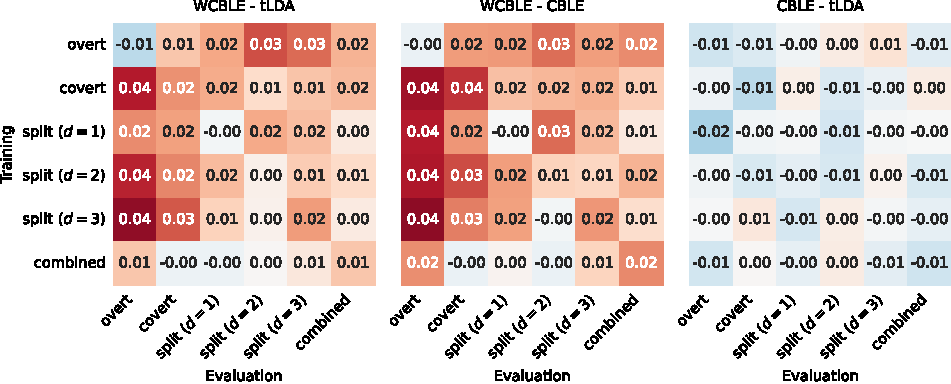
\includegraphics[width=\linewidth]{figures/covert_align/figure5a.pdf}
    \hspace{-.5in}%% Creator: Matplotlib, PGF backend
%%
%% To include the figure in your LaTeX document, write
%%   \input{<filename>.pgf}
%%
%% Make sure the required packages are loaded in your preamble
%%   \usepackage{pgf}
%%
%% Also ensure that all the required font packages are loaded; for instance,
%% the lmodern package is sometimes necessary when using math font.
%%   \usepackage{lmodern}
%%
%% Figures using additional raster images can only be included by \input if
%% they are in the same directory as the main LaTeX file. For loading figures
%% from other directories you can use the `import` package
%%   \usepackage{import}
%%
%% and then include the figures with
%%   \import{<path to file>}{<filename>.pgf}
%%
%% Matplotlib used the following preamble
%%   \def\mathdefault#1{#1}
%%   \everymath=\expandafter{\the\everymath\displaystyle}
%%   
%%   \ifdefined\pdftexversion\else  % non-pdftex case.
%%     \usepackage{fontspec}
%%   \fi
%%   \makeatletter\@ifpackageloaded{underscore}{}{\usepackage[strings]{underscore}}\makeatother
%%
\begingroup%
\makeatletter%
\begin{pgfpicture}%
\pgfpathrectangle{\pgfpointorigin}{\pgfqpoint{5.138109in}{2.271425in}}%
\pgfusepath{use as bounding box, clip}%
\begin{pgfscope}%
\pgfsetbuttcap%
\pgfsetmiterjoin%
\pgfsetlinewidth{0.000000pt}%
\definecolor{currentstroke}{rgb}{0.000000,0.000000,0.000000}%
\pgfsetstrokecolor{currentstroke}%
\pgfsetstrokeopacity{0.000000}%
\pgfsetdash{}{0pt}%
\pgfpathmoveto{\pgfqpoint{0.000000in}{0.000000in}}%
\pgfpathlineto{\pgfqpoint{5.138109in}{0.000000in}}%
\pgfpathlineto{\pgfqpoint{5.138109in}{2.271425in}}%
\pgfpathlineto{\pgfqpoint{0.000000in}{2.271425in}}%
\pgfpathlineto{\pgfqpoint{0.000000in}{0.000000in}}%
\pgfpathclose%
\pgfusepath{}%
\end{pgfscope}%
\begin{pgfscope}%
\pgfsetbuttcap%
\pgfsetmiterjoin%
\pgfsetlinewidth{0.000000pt}%
\definecolor{currentstroke}{rgb}{0.000000,0.000000,0.000000}%
\pgfsetstrokecolor{currentstroke}%
\pgfsetstrokeopacity{0.000000}%
\pgfsetdash{}{0pt}%
\pgfpathmoveto{\pgfqpoint{0.883458in}{0.776141in}}%
\pgfpathlineto{\pgfqpoint{2.208603in}{0.776141in}}%
\pgfpathlineto{\pgfqpoint{2.208603in}{2.101286in}}%
\pgfpathlineto{\pgfqpoint{0.883458in}{2.101286in}}%
\pgfpathlineto{\pgfqpoint{0.883458in}{0.776141in}}%
\pgfpathclose%
\pgfusepath{}%
\end{pgfscope}%
\begin{pgfscope}%
\pgfpathrectangle{\pgfqpoint{0.883458in}{0.776141in}}{\pgfqpoint{1.325145in}{1.325145in}}%
\pgfusepath{clip}%
\pgfsetbuttcap%
\pgfsetroundjoin%
\definecolor{currentfill}{rgb}{0.805075,0.916955,0.951788}%
\pgfsetfillcolor{currentfill}%
\pgfsetlinewidth{0.000000pt}%
\definecolor{currentstroke}{rgb}{1.000000,1.000000,1.000000}%
\pgfsetstrokecolor{currentstroke}%
\pgfsetdash{}{0pt}%
\pgfpathmoveto{\pgfqpoint{0.883458in}{2.101286in}}%
\pgfpathlineto{\pgfqpoint{1.104316in}{2.101286in}}%
\pgfpathlineto{\pgfqpoint{1.104316in}{1.880429in}}%
\pgfpathlineto{\pgfqpoint{0.883458in}{1.880429in}}%
\pgfpathlineto{\pgfqpoint{0.883458in}{2.101286in}}%
\pgfusepath{fill}%
\end{pgfscope}%
\begin{pgfscope}%
\pgfpathrectangle{\pgfqpoint{0.883458in}{0.776141in}}{\pgfqpoint{1.325145in}{1.325145in}}%
\pgfusepath{clip}%
\pgfsetbuttcap%
\pgfsetroundjoin%
\definecolor{currentfill}{rgb}{0.994541,0.801538,0.492426}%
\pgfsetfillcolor{currentfill}%
\pgfsetlinewidth{0.000000pt}%
\definecolor{currentstroke}{rgb}{1.000000,1.000000,1.000000}%
\pgfsetstrokecolor{currentstroke}%
\pgfsetdash{}{0pt}%
\pgfpathmoveto{\pgfqpoint{1.104316in}{2.101286in}}%
\pgfpathlineto{\pgfqpoint{1.325173in}{2.101286in}}%
\pgfpathlineto{\pgfqpoint{1.325173in}{1.880429in}}%
\pgfpathlineto{\pgfqpoint{1.104316in}{1.880429in}}%
\pgfpathlineto{\pgfqpoint{1.104316in}{2.101286in}}%
\pgfusepath{fill}%
\end{pgfscope}%
\begin{pgfscope}%
\pgfpathrectangle{\pgfqpoint{0.883458in}{0.776141in}}{\pgfqpoint{1.325145in}{1.325145in}}%
\pgfusepath{clip}%
\pgfsetbuttcap%
\pgfsetroundjoin%
\definecolor{currentfill}{rgb}{0.992388,0.693887,0.391234}%
\pgfsetfillcolor{currentfill}%
\pgfsetlinewidth{0.000000pt}%
\definecolor{currentstroke}{rgb}{1.000000,1.000000,1.000000}%
\pgfsetstrokecolor{currentstroke}%
\pgfsetdash{}{0pt}%
\pgfpathmoveto{\pgfqpoint{1.325173in}{2.101286in}}%
\pgfpathlineto{\pgfqpoint{1.546031in}{2.101286in}}%
\pgfpathlineto{\pgfqpoint{1.546031in}{1.880429in}}%
\pgfpathlineto{\pgfqpoint{1.325173in}{1.880429in}}%
\pgfpathlineto{\pgfqpoint{1.325173in}{2.101286in}}%
\pgfusepath{fill}%
\end{pgfscope}%
\begin{pgfscope}%
\pgfpathrectangle{\pgfqpoint{0.883458in}{0.776141in}}{\pgfqpoint{1.325145in}{1.325145in}}%
\pgfusepath{clip}%
\pgfsetbuttcap%
\pgfsetroundjoin%
\definecolor{currentfill}{rgb}{0.930104,0.371165,0.236909}%
\pgfsetfillcolor{currentfill}%
\pgfsetlinewidth{0.000000pt}%
\definecolor{currentstroke}{rgb}{1.000000,1.000000,1.000000}%
\pgfsetstrokecolor{currentstroke}%
\pgfsetdash{}{0pt}%
\pgfpathmoveto{\pgfqpoint{1.546031in}{2.101286in}}%
\pgfpathlineto{\pgfqpoint{1.766888in}{2.101286in}}%
\pgfpathlineto{\pgfqpoint{1.766888in}{1.880429in}}%
\pgfpathlineto{\pgfqpoint{1.546031in}{1.880429in}}%
\pgfpathlineto{\pgfqpoint{1.546031in}{2.101286in}}%
\pgfusepath{fill}%
\end{pgfscope}%
\begin{pgfscope}%
\pgfpathrectangle{\pgfqpoint{0.883458in}{0.776141in}}{\pgfqpoint{1.325145in}{1.325145in}}%
\pgfusepath{clip}%
\pgfsetbuttcap%
\pgfsetroundjoin%
\definecolor{currentfill}{rgb}{0.962399,0.467436,0.281200}%
\pgfsetfillcolor{currentfill}%
\pgfsetlinewidth{0.000000pt}%
\definecolor{currentstroke}{rgb}{1.000000,1.000000,1.000000}%
\pgfsetstrokecolor{currentstroke}%
\pgfsetdash{}{0pt}%
\pgfpathmoveto{\pgfqpoint{1.766888in}{2.101286in}}%
\pgfpathlineto{\pgfqpoint{1.987746in}{2.101286in}}%
\pgfpathlineto{\pgfqpoint{1.987746in}{1.880429in}}%
\pgfpathlineto{\pgfqpoint{1.766888in}{1.880429in}}%
\pgfpathlineto{\pgfqpoint{1.766888in}{2.101286in}}%
\pgfusepath{fill}%
\end{pgfscope}%
\begin{pgfscope}%
\pgfpathrectangle{\pgfqpoint{0.883458in}{0.776141in}}{\pgfqpoint{1.325145in}{1.325145in}}%
\pgfusepath{clip}%
\pgfsetbuttcap%
\pgfsetroundjoin%
\definecolor{currentfill}{rgb}{0.993156,0.732334,0.427374}%
\pgfsetfillcolor{currentfill}%
\pgfsetlinewidth{0.000000pt}%
\definecolor{currentstroke}{rgb}{1.000000,1.000000,1.000000}%
\pgfsetstrokecolor{currentstroke}%
\pgfsetdash{}{0pt}%
\pgfpathmoveto{\pgfqpoint{1.987746in}{2.101286in}}%
\pgfpathlineto{\pgfqpoint{2.208603in}{2.101286in}}%
\pgfpathlineto{\pgfqpoint{2.208603in}{1.880429in}}%
\pgfpathlineto{\pgfqpoint{1.987746in}{1.880429in}}%
\pgfpathlineto{\pgfqpoint{1.987746in}{2.101286in}}%
\pgfusepath{fill}%
\end{pgfscope}%
\begin{pgfscope}%
\pgfpathrectangle{\pgfqpoint{0.883458in}{0.776141in}}{\pgfqpoint{1.325145in}{1.325145in}}%
\pgfusepath{clip}%
\pgfsetbuttcap%
\pgfsetroundjoin%
\definecolor{currentfill}{rgb}{0.845367,0.192926,0.155094}%
\pgfsetfillcolor{currentfill}%
\pgfsetlinewidth{0.000000pt}%
\definecolor{currentstroke}{rgb}{1.000000,1.000000,1.000000}%
\pgfsetstrokecolor{currentstroke}%
\pgfsetdash{}{0pt}%
\pgfpathmoveto{\pgfqpoint{0.883458in}{1.880429in}}%
\pgfpathlineto{\pgfqpoint{1.104316in}{1.880429in}}%
\pgfpathlineto{\pgfqpoint{1.104316in}{1.659571in}}%
\pgfpathlineto{\pgfqpoint{0.883458in}{1.659571in}}%
\pgfpathlineto{\pgfqpoint{0.883458in}{1.880429in}}%
\pgfusepath{fill}%
\end{pgfscope}%
\begin{pgfscope}%
\pgfpathrectangle{\pgfqpoint{0.883458in}{0.776141in}}{\pgfqpoint{1.325145in}{1.325145in}}%
\pgfusepath{clip}%
\pgfsetbuttcap%
\pgfsetroundjoin%
\definecolor{currentfill}{rgb}{0.981776,0.607382,0.345790}%
\pgfsetfillcolor{currentfill}%
\pgfsetlinewidth{0.000000pt}%
\definecolor{currentstroke}{rgb}{1.000000,1.000000,1.000000}%
\pgfsetstrokecolor{currentstroke}%
\pgfsetdash{}{0pt}%
\pgfpathmoveto{\pgfqpoint{1.104316in}{1.880429in}}%
\pgfpathlineto{\pgfqpoint{1.325173in}{1.880429in}}%
\pgfpathlineto{\pgfqpoint{1.325173in}{1.659571in}}%
\pgfpathlineto{\pgfqpoint{1.104316in}{1.659571in}}%
\pgfpathlineto{\pgfqpoint{1.104316in}{1.880429in}}%
\pgfusepath{fill}%
\end{pgfscope}%
\begin{pgfscope}%
\pgfpathrectangle{\pgfqpoint{0.883458in}{0.776141in}}{\pgfqpoint{1.325145in}{1.325145in}}%
\pgfusepath{clip}%
\pgfsetbuttcap%
\pgfsetroundjoin%
\definecolor{currentfill}{rgb}{0.992695,0.709266,0.405690}%
\pgfsetfillcolor{currentfill}%
\pgfsetlinewidth{0.000000pt}%
\definecolor{currentstroke}{rgb}{1.000000,1.000000,1.000000}%
\pgfsetstrokecolor{currentstroke}%
\pgfsetdash{}{0pt}%
\pgfpathmoveto{\pgfqpoint{1.325173in}{1.880429in}}%
\pgfpathlineto{\pgfqpoint{1.546031in}{1.880429in}}%
\pgfpathlineto{\pgfqpoint{1.546031in}{1.659571in}}%
\pgfpathlineto{\pgfqpoint{1.325173in}{1.659571in}}%
\pgfpathlineto{\pgfqpoint{1.325173in}{1.880429in}}%
\pgfusepath{fill}%
\end{pgfscope}%
\begin{pgfscope}%
\pgfpathrectangle{\pgfqpoint{0.883458in}{0.776141in}}{\pgfqpoint{1.325145in}{1.325145in}}%
\pgfusepath{clip}%
\pgfsetbuttcap%
\pgfsetroundjoin%
\definecolor{currentfill}{rgb}{0.996386,0.887966,0.579162}%
\pgfsetfillcolor{currentfill}%
\pgfsetlinewidth{0.000000pt}%
\definecolor{currentstroke}{rgb}{1.000000,1.000000,1.000000}%
\pgfsetstrokecolor{currentstroke}%
\pgfsetdash{}{0pt}%
\pgfpathmoveto{\pgfqpoint{1.546031in}{1.880429in}}%
\pgfpathlineto{\pgfqpoint{1.766888in}{1.880429in}}%
\pgfpathlineto{\pgfqpoint{1.766888in}{1.659571in}}%
\pgfpathlineto{\pgfqpoint{1.546031in}{1.659571in}}%
\pgfpathlineto{\pgfqpoint{1.546031in}{1.880429in}}%
\pgfusepath{fill}%
\end{pgfscope}%
\begin{pgfscope}%
\pgfpathrectangle{\pgfqpoint{0.883458in}{0.776141in}}{\pgfqpoint{1.325145in}{1.325145in}}%
\pgfusepath{clip}%
\pgfsetbuttcap%
\pgfsetroundjoin%
\definecolor{currentfill}{rgb}{0.994387,0.793849,0.485198}%
\pgfsetfillcolor{currentfill}%
\pgfsetlinewidth{0.000000pt}%
\definecolor{currentstroke}{rgb}{1.000000,1.000000,1.000000}%
\pgfsetstrokecolor{currentstroke}%
\pgfsetdash{}{0pt}%
\pgfpathmoveto{\pgfqpoint{1.766888in}{1.880429in}}%
\pgfpathlineto{\pgfqpoint{1.987746in}{1.880429in}}%
\pgfpathlineto{\pgfqpoint{1.987746in}{1.659571in}}%
\pgfpathlineto{\pgfqpoint{1.766888in}{1.659571in}}%
\pgfpathlineto{\pgfqpoint{1.766888in}{1.880429in}}%
\pgfusepath{fill}%
\end{pgfscope}%
\begin{pgfscope}%
\pgfpathrectangle{\pgfqpoint{0.883458in}{0.776141in}}{\pgfqpoint{1.325145in}{1.325145in}}%
\pgfusepath{clip}%
\pgfsetbuttcap%
\pgfsetroundjoin%
\definecolor{currentfill}{rgb}{0.993618,0.755402,0.449058}%
\pgfsetfillcolor{currentfill}%
\pgfsetlinewidth{0.000000pt}%
\definecolor{currentstroke}{rgb}{1.000000,1.000000,1.000000}%
\pgfsetstrokecolor{currentstroke}%
\pgfsetdash{}{0pt}%
\pgfpathmoveto{\pgfqpoint{1.987746in}{1.880429in}}%
\pgfpathlineto{\pgfqpoint{2.208603in}{1.880429in}}%
\pgfpathlineto{\pgfqpoint{2.208603in}{1.659571in}}%
\pgfpathlineto{\pgfqpoint{1.987746in}{1.659571in}}%
\pgfpathlineto{\pgfqpoint{1.987746in}{1.880429in}}%
\pgfusepath{fill}%
\end{pgfscope}%
\begin{pgfscope}%
\pgfpathrectangle{\pgfqpoint{0.883458in}{0.776141in}}{\pgfqpoint{1.325145in}{1.325145in}}%
\pgfusepath{clip}%
\pgfsetbuttcap%
\pgfsetroundjoin%
\definecolor{currentfill}{rgb}{0.979008,0.587389,0.336563}%
\pgfsetfillcolor{currentfill}%
\pgfsetlinewidth{0.000000pt}%
\definecolor{currentstroke}{rgb}{1.000000,1.000000,1.000000}%
\pgfsetstrokecolor{currentstroke}%
\pgfsetdash{}{0pt}%
\pgfpathmoveto{\pgfqpoint{0.883458in}{1.659571in}}%
\pgfpathlineto{\pgfqpoint{1.104316in}{1.659571in}}%
\pgfpathlineto{\pgfqpoint{1.104316in}{1.438714in}}%
\pgfpathlineto{\pgfqpoint{0.883458in}{1.438714in}}%
\pgfpathlineto{\pgfqpoint{0.883458in}{1.659571in}}%
\pgfusepath{fill}%
\end{pgfscope}%
\begin{pgfscope}%
\pgfpathrectangle{\pgfqpoint{0.883458in}{0.776141in}}{\pgfqpoint{1.325145in}{1.325145in}}%
\pgfusepath{clip}%
\pgfsetbuttcap%
\pgfsetroundjoin%
\definecolor{currentfill}{rgb}{0.990081,0.667359,0.373472}%
\pgfsetfillcolor{currentfill}%
\pgfsetlinewidth{0.000000pt}%
\definecolor{currentstroke}{rgb}{1.000000,1.000000,1.000000}%
\pgfsetstrokecolor{currentstroke}%
\pgfsetdash{}{0pt}%
\pgfpathmoveto{\pgfqpoint{1.104316in}{1.659571in}}%
\pgfpathlineto{\pgfqpoint{1.325173in}{1.659571in}}%
\pgfpathlineto{\pgfqpoint{1.325173in}{1.438714in}}%
\pgfpathlineto{\pgfqpoint{1.104316in}{1.438714in}}%
\pgfpathlineto{\pgfqpoint{1.104316in}{1.659571in}}%
\pgfusepath{fill}%
\end{pgfscope}%
\begin{pgfscope}%
\pgfpathrectangle{\pgfqpoint{0.883458in}{0.776141in}}{\pgfqpoint{1.325145in}{1.325145in}}%
\pgfusepath{clip}%
\pgfsetbuttcap%
\pgfsetroundjoin%
\definecolor{currentfill}{rgb}{0.983314,0.993541,0.779700}%
\pgfsetfillcolor{currentfill}%
\pgfsetlinewidth{0.000000pt}%
\definecolor{currentstroke}{rgb}{1.000000,1.000000,1.000000}%
\pgfsetstrokecolor{currentstroke}%
\pgfsetdash{}{0pt}%
\pgfpathmoveto{\pgfqpoint{1.325173in}{1.659571in}}%
\pgfpathlineto{\pgfqpoint{1.546031in}{1.659571in}}%
\pgfpathlineto{\pgfqpoint{1.546031in}{1.438714in}}%
\pgfpathlineto{\pgfqpoint{1.325173in}{1.438714in}}%
\pgfpathlineto{\pgfqpoint{1.325173in}{1.659571in}}%
\pgfusepath{fill}%
\end{pgfscope}%
\begin{pgfscope}%
\pgfpathrectangle{\pgfqpoint{0.883458in}{0.776141in}}{\pgfqpoint{1.325145in}{1.325145in}}%
\pgfusepath{clip}%
\pgfsetbuttcap%
\pgfsetroundjoin%
\definecolor{currentfill}{rgb}{0.992541,0.701576,0.398462}%
\pgfsetfillcolor{currentfill}%
\pgfsetlinewidth{0.000000pt}%
\definecolor{currentstroke}{rgb}{1.000000,1.000000,1.000000}%
\pgfsetstrokecolor{currentstroke}%
\pgfsetdash{}{0pt}%
\pgfpathmoveto{\pgfqpoint{1.546031in}{1.659571in}}%
\pgfpathlineto{\pgfqpoint{1.766888in}{1.659571in}}%
\pgfpathlineto{\pgfqpoint{1.766888in}{1.438714in}}%
\pgfpathlineto{\pgfqpoint{1.546031in}{1.438714in}}%
\pgfpathlineto{\pgfqpoint{1.546031in}{1.659571in}}%
\pgfusepath{fill}%
\end{pgfscope}%
\begin{pgfscope}%
\pgfpathrectangle{\pgfqpoint{0.883458in}{0.776141in}}{\pgfqpoint{1.325145in}{1.325145in}}%
\pgfusepath{clip}%
\pgfsetbuttcap%
\pgfsetroundjoin%
\definecolor{currentfill}{rgb}{0.993925,0.770780,0.463514}%
\pgfsetfillcolor{currentfill}%
\pgfsetlinewidth{0.000000pt}%
\definecolor{currentstroke}{rgb}{1.000000,1.000000,1.000000}%
\pgfsetstrokecolor{currentstroke}%
\pgfsetdash{}{0pt}%
\pgfpathmoveto{\pgfqpoint{1.766888in}{1.659571in}}%
\pgfpathlineto{\pgfqpoint{1.987746in}{1.659571in}}%
\pgfpathlineto{\pgfqpoint{1.987746in}{1.438714in}}%
\pgfpathlineto{\pgfqpoint{1.766888in}{1.438714in}}%
\pgfpathlineto{\pgfqpoint{1.766888in}{1.659571in}}%
\pgfusepath{fill}%
\end{pgfscope}%
\begin{pgfscope}%
\pgfpathrectangle{\pgfqpoint{0.883458in}{0.776141in}}{\pgfqpoint{1.325145in}{1.325145in}}%
\pgfusepath{clip}%
\pgfsetbuttcap%
\pgfsetroundjoin%
\definecolor{currentfill}{rgb}{0.998078,0.940408,0.658670}%
\pgfsetfillcolor{currentfill}%
\pgfsetlinewidth{0.000000pt}%
\definecolor{currentstroke}{rgb}{1.000000,1.000000,1.000000}%
\pgfsetstrokecolor{currentstroke}%
\pgfsetdash{}{0pt}%
\pgfpathmoveto{\pgfqpoint{1.987746in}{1.659571in}}%
\pgfpathlineto{\pgfqpoint{2.208603in}{1.659571in}}%
\pgfpathlineto{\pgfqpoint{2.208603in}{1.438714in}}%
\pgfpathlineto{\pgfqpoint{1.987746in}{1.438714in}}%
\pgfpathlineto{\pgfqpoint{1.987746in}{1.659571in}}%
\pgfusepath{fill}%
\end{pgfscope}%
\begin{pgfscope}%
\pgfpathrectangle{\pgfqpoint{0.883458in}{0.776141in}}{\pgfqpoint{1.325145in}{1.325145in}}%
\pgfusepath{clip}%
\pgfsetbuttcap%
\pgfsetroundjoin%
\definecolor{currentfill}{rgb}{0.858747,0.221069,0.168012}%
\pgfsetfillcolor{currentfill}%
\pgfsetlinewidth{0.000000pt}%
\definecolor{currentstroke}{rgb}{1.000000,1.000000,1.000000}%
\pgfsetstrokecolor{currentstroke}%
\pgfsetdash{}{0pt}%
\pgfpathmoveto{\pgfqpoint{0.883458in}{1.438714in}}%
\pgfpathlineto{\pgfqpoint{1.104316in}{1.438714in}}%
\pgfpathlineto{\pgfqpoint{1.104316in}{1.217856in}}%
\pgfpathlineto{\pgfqpoint{0.883458in}{1.217856in}}%
\pgfpathlineto{\pgfqpoint{0.883458in}{1.438714in}}%
\pgfusepath{fill}%
\end{pgfscope}%
\begin{pgfscope}%
\pgfpathrectangle{\pgfqpoint{0.883458in}{0.776141in}}{\pgfqpoint{1.325145in}{1.325145in}}%
\pgfusepath{clip}%
\pgfsetbuttcap%
\pgfsetroundjoin%
\definecolor{currentfill}{rgb}{0.976240,0.567397,0.327336}%
\pgfsetfillcolor{currentfill}%
\pgfsetlinewidth{0.000000pt}%
\definecolor{currentstroke}{rgb}{1.000000,1.000000,1.000000}%
\pgfsetstrokecolor{currentstroke}%
\pgfsetdash{}{0pt}%
\pgfpathmoveto{\pgfqpoint{1.104316in}{1.438714in}}%
\pgfpathlineto{\pgfqpoint{1.325173in}{1.438714in}}%
\pgfpathlineto{\pgfqpoint{1.325173in}{1.217856in}}%
\pgfpathlineto{\pgfqpoint{1.104316in}{1.217856in}}%
\pgfpathlineto{\pgfqpoint{1.104316in}{1.438714in}}%
\pgfusepath{fill}%
\end{pgfscope}%
\begin{pgfscope}%
\pgfpathrectangle{\pgfqpoint{0.883458in}{0.776141in}}{\pgfqpoint{1.325145in}{1.325145in}}%
\pgfusepath{clip}%
\pgfsetbuttcap%
\pgfsetroundjoin%
\definecolor{currentfill}{rgb}{0.993772,0.763091,0.456286}%
\pgfsetfillcolor{currentfill}%
\pgfsetlinewidth{0.000000pt}%
\definecolor{currentstroke}{rgb}{1.000000,1.000000,1.000000}%
\pgfsetstrokecolor{currentstroke}%
\pgfsetdash{}{0pt}%
\pgfpathmoveto{\pgfqpoint{1.325173in}{1.438714in}}%
\pgfpathlineto{\pgfqpoint{1.546031in}{1.438714in}}%
\pgfpathlineto{\pgfqpoint{1.546031in}{1.217856in}}%
\pgfpathlineto{\pgfqpoint{1.325173in}{1.217856in}}%
\pgfpathlineto{\pgfqpoint{1.325173in}{1.438714in}}%
\pgfusepath{fill}%
\end{pgfscope}%
\begin{pgfscope}%
\pgfpathrectangle{\pgfqpoint{0.883458in}{0.776141in}}{\pgfqpoint{1.325145in}{1.325145in}}%
\pgfusepath{clip}%
\pgfsetbuttcap%
\pgfsetroundjoin%
\definecolor{currentfill}{rgb}{0.998847,0.964245,0.694810}%
\pgfsetfillcolor{currentfill}%
\pgfsetlinewidth{0.000000pt}%
\definecolor{currentstroke}{rgb}{1.000000,1.000000,1.000000}%
\pgfsetstrokecolor{currentstroke}%
\pgfsetdash{}{0pt}%
\pgfpathmoveto{\pgfqpoint{1.546031in}{1.438714in}}%
\pgfpathlineto{\pgfqpoint{1.766888in}{1.438714in}}%
\pgfpathlineto{\pgfqpoint{1.766888in}{1.217856in}}%
\pgfpathlineto{\pgfqpoint{1.546031in}{1.217856in}}%
\pgfpathlineto{\pgfqpoint{1.546031in}{1.438714in}}%
\pgfusepath{fill}%
\end{pgfscope}%
\begin{pgfscope}%
\pgfpathrectangle{\pgfqpoint{0.883458in}{0.776141in}}{\pgfqpoint{1.325145in}{1.325145in}}%
\pgfusepath{clip}%
\pgfsetbuttcap%
\pgfsetroundjoin%
\definecolor{currentfill}{rgb}{0.995002,0.824606,0.514110}%
\pgfsetfillcolor{currentfill}%
\pgfsetlinewidth{0.000000pt}%
\definecolor{currentstroke}{rgb}{1.000000,1.000000,1.000000}%
\pgfsetstrokecolor{currentstroke}%
\pgfsetdash{}{0pt}%
\pgfpathmoveto{\pgfqpoint{1.766888in}{1.438714in}}%
\pgfpathlineto{\pgfqpoint{1.987746in}{1.438714in}}%
\pgfpathlineto{\pgfqpoint{1.987746in}{1.217856in}}%
\pgfpathlineto{\pgfqpoint{1.766888in}{1.217856in}}%
\pgfpathlineto{\pgfqpoint{1.766888in}{1.438714in}}%
\pgfusepath{fill}%
\end{pgfscope}%
\begin{pgfscope}%
\pgfpathrectangle{\pgfqpoint{0.883458in}{0.776141in}}{\pgfqpoint{1.325145in}{1.325145in}}%
\pgfusepath{clip}%
\pgfsetbuttcap%
\pgfsetroundjoin%
\definecolor{currentfill}{rgb}{0.996232,0.883199,0.571934}%
\pgfsetfillcolor{currentfill}%
\pgfsetlinewidth{0.000000pt}%
\definecolor{currentstroke}{rgb}{1.000000,1.000000,1.000000}%
\pgfsetstrokecolor{currentstroke}%
\pgfsetdash{}{0pt}%
\pgfpathmoveto{\pgfqpoint{1.987746in}{1.438714in}}%
\pgfpathlineto{\pgfqpoint{2.208603in}{1.438714in}}%
\pgfpathlineto{\pgfqpoint{2.208603in}{1.217856in}}%
\pgfpathlineto{\pgfqpoint{1.987746in}{1.217856in}}%
\pgfpathlineto{\pgfqpoint{1.987746in}{1.438714in}}%
\pgfusepath{fill}%
\end{pgfscope}%
\begin{pgfscope}%
\pgfpathrectangle{\pgfqpoint{0.883458in}{0.776141in}}{\pgfqpoint{1.325145in}{1.325145in}}%
\pgfusepath{clip}%
\pgfsetbuttcap%
\pgfsetroundjoin%
\definecolor{currentfill}{rgb}{0.754710,0.103345,0.151173}%
\pgfsetfillcolor{currentfill}%
\pgfsetlinewidth{0.000000pt}%
\definecolor{currentstroke}{rgb}{1.000000,1.000000,1.000000}%
\pgfsetstrokecolor{currentstroke}%
\pgfsetdash{}{0pt}%
\pgfpathmoveto{\pgfqpoint{0.883458in}{1.217856in}}%
\pgfpathlineto{\pgfqpoint{1.104316in}{1.217856in}}%
\pgfpathlineto{\pgfqpoint{1.104316in}{0.996999in}}%
\pgfpathlineto{\pgfqpoint{0.883458in}{0.996999in}}%
\pgfpathlineto{\pgfqpoint{0.883458in}{1.217856in}}%
\pgfusepath{fill}%
\end{pgfscope}%
\begin{pgfscope}%
\pgfpathrectangle{\pgfqpoint{0.883458in}{0.776141in}}{\pgfqpoint{1.325145in}{1.325145in}}%
\pgfusepath{clip}%
\pgfsetbuttcap%
\pgfsetroundjoin%
\definecolor{currentfill}{rgb}{0.943483,0.399308,0.249827}%
\pgfsetfillcolor{currentfill}%
\pgfsetlinewidth{0.000000pt}%
\definecolor{currentstroke}{rgb}{1.000000,1.000000,1.000000}%
\pgfsetstrokecolor{currentstroke}%
\pgfsetdash{}{0pt}%
\pgfpathmoveto{\pgfqpoint{1.104316in}{1.217856in}}%
\pgfpathlineto{\pgfqpoint{1.325173in}{1.217856in}}%
\pgfpathlineto{\pgfqpoint{1.325173in}{0.996999in}}%
\pgfpathlineto{\pgfqpoint{1.104316in}{0.996999in}}%
\pgfpathlineto{\pgfqpoint{1.104316in}{1.217856in}}%
\pgfusepath{fill}%
\end{pgfscope}%
\begin{pgfscope}%
\pgfpathrectangle{\pgfqpoint{0.883458in}{0.776141in}}{\pgfqpoint{1.325145in}{1.325145in}}%
\pgfusepath{clip}%
\pgfsetbuttcap%
\pgfsetroundjoin%
\definecolor{currentfill}{rgb}{0.995463,0.847674,0.535794}%
\pgfsetfillcolor{currentfill}%
\pgfsetlinewidth{0.000000pt}%
\definecolor{currentstroke}{rgb}{1.000000,1.000000,1.000000}%
\pgfsetstrokecolor{currentstroke}%
\pgfsetdash{}{0pt}%
\pgfpathmoveto{\pgfqpoint{1.325173in}{1.217856in}}%
\pgfpathlineto{\pgfqpoint{1.546031in}{1.217856in}}%
\pgfpathlineto{\pgfqpoint{1.546031in}{0.996999in}}%
\pgfpathlineto{\pgfqpoint{1.325173in}{0.996999in}}%
\pgfpathlineto{\pgfqpoint{1.325173in}{1.217856in}}%
\pgfusepath{fill}%
\end{pgfscope}%
\begin{pgfscope}%
\pgfpathrectangle{\pgfqpoint{0.883458in}{0.776141in}}{\pgfqpoint{1.325145in}{1.325145in}}%
\pgfusepath{clip}%
\pgfsetbuttcap%
\pgfsetroundjoin%
\definecolor{currentfill}{rgb}{0.999000,0.969012,0.702038}%
\pgfsetfillcolor{currentfill}%
\pgfsetlinewidth{0.000000pt}%
\definecolor{currentstroke}{rgb}{1.000000,1.000000,1.000000}%
\pgfsetstrokecolor{currentstroke}%
\pgfsetdash{}{0pt}%
\pgfpathmoveto{\pgfqpoint{1.546031in}{1.217856in}}%
\pgfpathlineto{\pgfqpoint{1.766888in}{1.217856in}}%
\pgfpathlineto{\pgfqpoint{1.766888in}{0.996999in}}%
\pgfpathlineto{\pgfqpoint{1.546031in}{0.996999in}}%
\pgfpathlineto{\pgfqpoint{1.546031in}{1.217856in}}%
\pgfusepath{fill}%
\end{pgfscope}%
\begin{pgfscope}%
\pgfpathrectangle{\pgfqpoint{0.883458in}{0.776141in}}{\pgfqpoint{1.325145in}{1.325145in}}%
\pgfusepath{clip}%
\pgfsetbuttcap%
\pgfsetroundjoin%
\definecolor{currentfill}{rgb}{0.987313,0.647366,0.364245}%
\pgfsetfillcolor{currentfill}%
\pgfsetlinewidth{0.000000pt}%
\definecolor{currentstroke}{rgb}{1.000000,1.000000,1.000000}%
\pgfsetstrokecolor{currentstroke}%
\pgfsetdash{}{0pt}%
\pgfpathmoveto{\pgfqpoint{1.766888in}{1.217856in}}%
\pgfpathlineto{\pgfqpoint{1.987746in}{1.217856in}}%
\pgfpathlineto{\pgfqpoint{1.987746in}{0.996999in}}%
\pgfpathlineto{\pgfqpoint{1.766888in}{0.996999in}}%
\pgfpathlineto{\pgfqpoint{1.766888in}{1.217856in}}%
\pgfusepath{fill}%
\end{pgfscope}%
\begin{pgfscope}%
\pgfpathrectangle{\pgfqpoint{0.883458in}{0.776141in}}{\pgfqpoint{1.325145in}{1.325145in}}%
\pgfusepath{clip}%
\pgfsetbuttcap%
\pgfsetroundjoin%
\definecolor{currentfill}{rgb}{0.998231,0.945175,0.665898}%
\pgfsetfillcolor{currentfill}%
\pgfsetlinewidth{0.000000pt}%
\definecolor{currentstroke}{rgb}{1.000000,1.000000,1.000000}%
\pgfsetstrokecolor{currentstroke}%
\pgfsetdash{}{0pt}%
\pgfpathmoveto{\pgfqpoint{1.987746in}{1.217856in}}%
\pgfpathlineto{\pgfqpoint{2.208603in}{1.217856in}}%
\pgfpathlineto{\pgfqpoint{2.208603in}{0.996999in}}%
\pgfpathlineto{\pgfqpoint{1.987746in}{0.996999in}}%
\pgfpathlineto{\pgfqpoint{1.987746in}{1.217856in}}%
\pgfusepath{fill}%
\end{pgfscope}%
\begin{pgfscope}%
\pgfpathrectangle{\pgfqpoint{0.883458in}{0.776141in}}{\pgfqpoint{1.325145in}{1.325145in}}%
\pgfusepath{clip}%
\pgfsetbuttcap%
\pgfsetroundjoin%
\definecolor{currentfill}{rgb}{0.994541,0.801538,0.492426}%
\pgfsetfillcolor{currentfill}%
\pgfsetlinewidth{0.000000pt}%
\definecolor{currentstroke}{rgb}{1.000000,1.000000,1.000000}%
\pgfsetstrokecolor{currentstroke}%
\pgfsetdash{}{0pt}%
\pgfpathmoveto{\pgfqpoint{0.883458in}{0.996999in}}%
\pgfpathlineto{\pgfqpoint{1.104316in}{0.996999in}}%
\pgfpathlineto{\pgfqpoint{1.104316in}{0.776141in}}%
\pgfpathlineto{\pgfqpoint{0.883458in}{0.776141in}}%
\pgfpathlineto{\pgfqpoint{0.883458in}{0.996999in}}%
\pgfusepath{fill}%
\end{pgfscope}%
\begin{pgfscope}%
\pgfpathrectangle{\pgfqpoint{0.883458in}{0.776141in}}{\pgfqpoint{1.325145in}{1.325145in}}%
\pgfusepath{clip}%
\pgfsetbuttcap%
\pgfsetroundjoin%
\definecolor{currentfill}{rgb}{0.964245,0.986159,0.814764}%
\pgfsetfillcolor{currentfill}%
\pgfsetlinewidth{0.000000pt}%
\definecolor{currentstroke}{rgb}{1.000000,1.000000,1.000000}%
\pgfsetstrokecolor{currentstroke}%
\pgfsetdash{}{0pt}%
\pgfpathmoveto{\pgfqpoint{1.104316in}{0.996999in}}%
\pgfpathlineto{\pgfqpoint{1.325173in}{0.996999in}}%
\pgfpathlineto{\pgfqpoint{1.325173in}{0.776141in}}%
\pgfpathlineto{\pgfqpoint{1.104316in}{0.776141in}}%
\pgfpathlineto{\pgfqpoint{1.104316in}{0.996999in}}%
\pgfusepath{fill}%
\end{pgfscope}%
\begin{pgfscope}%
\pgfpathrectangle{\pgfqpoint{0.883458in}{0.776141in}}{\pgfqpoint{1.325145in}{1.325145in}}%
\pgfusepath{clip}%
\pgfsetbuttcap%
\pgfsetroundjoin%
\definecolor{currentfill}{rgb}{0.964245,0.986159,0.814764}%
\pgfsetfillcolor{currentfill}%
\pgfsetlinewidth{0.000000pt}%
\definecolor{currentstroke}{rgb}{1.000000,1.000000,1.000000}%
\pgfsetstrokecolor{currentstroke}%
\pgfsetdash{}{0pt}%
\pgfpathmoveto{\pgfqpoint{1.325173in}{0.996999in}}%
\pgfpathlineto{\pgfqpoint{1.546031in}{0.996999in}}%
\pgfpathlineto{\pgfqpoint{1.546031in}{0.776141in}}%
\pgfpathlineto{\pgfqpoint{1.325173in}{0.776141in}}%
\pgfpathlineto{\pgfqpoint{1.325173in}{0.996999in}}%
\pgfusepath{fill}%
\end{pgfscope}%
\begin{pgfscope}%
\pgfpathrectangle{\pgfqpoint{0.883458in}{0.776141in}}{\pgfqpoint{1.325145in}{1.325145in}}%
\pgfusepath{clip}%
\pgfsetbuttcap%
\pgfsetroundjoin%
\definecolor{currentfill}{rgb}{0.999769,0.992849,0.738178}%
\pgfsetfillcolor{currentfill}%
\pgfsetlinewidth{0.000000pt}%
\definecolor{currentstroke}{rgb}{1.000000,1.000000,1.000000}%
\pgfsetstrokecolor{currentstroke}%
\pgfsetdash{}{0pt}%
\pgfpathmoveto{\pgfqpoint{1.546031in}{0.996999in}}%
\pgfpathlineto{\pgfqpoint{1.766888in}{0.996999in}}%
\pgfpathlineto{\pgfqpoint{1.766888in}{0.776141in}}%
\pgfpathlineto{\pgfqpoint{1.546031in}{0.776141in}}%
\pgfpathlineto{\pgfqpoint{1.546031in}{0.996999in}}%
\pgfusepath{fill}%
\end{pgfscope}%
\begin{pgfscope}%
\pgfpathrectangle{\pgfqpoint{0.883458in}{0.776141in}}{\pgfqpoint{1.325145in}{1.325145in}}%
\pgfusepath{clip}%
\pgfsetbuttcap%
\pgfsetroundjoin%
\definecolor{currentfill}{rgb}{0.997770,0.930873,0.644214}%
\pgfsetfillcolor{currentfill}%
\pgfsetlinewidth{0.000000pt}%
\definecolor{currentstroke}{rgb}{1.000000,1.000000,1.000000}%
\pgfsetstrokecolor{currentstroke}%
\pgfsetdash{}{0pt}%
\pgfpathmoveto{\pgfqpoint{1.766888in}{0.996999in}}%
\pgfpathlineto{\pgfqpoint{1.987746in}{0.996999in}}%
\pgfpathlineto{\pgfqpoint{1.987746in}{0.776141in}}%
\pgfpathlineto{\pgfqpoint{1.766888in}{0.776141in}}%
\pgfpathlineto{\pgfqpoint{1.766888in}{0.996999in}}%
\pgfusepath{fill}%
\end{pgfscope}%
\begin{pgfscope}%
\pgfpathrectangle{\pgfqpoint{0.883458in}{0.776141in}}{\pgfqpoint{1.325145in}{1.325145in}}%
\pgfusepath{clip}%
\pgfsetbuttcap%
\pgfsetroundjoin%
\definecolor{currentfill}{rgb}{0.994541,0.801538,0.492426}%
\pgfsetfillcolor{currentfill}%
\pgfsetlinewidth{0.000000pt}%
\definecolor{currentstroke}{rgb}{1.000000,1.000000,1.000000}%
\pgfsetstrokecolor{currentstroke}%
\pgfsetdash{}{0pt}%
\pgfpathmoveto{\pgfqpoint{1.987746in}{0.996999in}}%
\pgfpathlineto{\pgfqpoint{2.208603in}{0.996999in}}%
\pgfpathlineto{\pgfqpoint{2.208603in}{0.776141in}}%
\pgfpathlineto{\pgfqpoint{1.987746in}{0.776141in}}%
\pgfpathlineto{\pgfqpoint{1.987746in}{0.996999in}}%
\pgfusepath{fill}%
\end{pgfscope}%
\begin{pgfscope}%
\definecolor{textcolor}{rgb}{0.552941,0.501961,0.478431}%
\pgfsetstrokecolor{textcolor}%
\pgfsetfillcolor{textcolor}%
\pgftext[x=0.785194in, y=0.474643in, left, base,rotate=45.000000]{\color{textcolor}{\sffamily\fontsize{9.000000}{10.800000}\selectfont\catcode`\^=\active\def^{\ifmmode\sp\else\^{}\fi}\catcode`\%=\active\def%{\%}overt}}%
\end{pgfscope}%
\begin{pgfscope}%
\definecolor{textcolor}{rgb}{0.552941,0.501961,0.478431}%
\pgfsetstrokecolor{textcolor}%
\pgfsetfillcolor{textcolor}%
\pgftext[x=0.965677in, y=0.434268in, left, base,rotate=45.000000]{\color{textcolor}{\sffamily\fontsize{9.000000}{10.800000}\selectfont\catcode`\^=\active\def^{\ifmmode\sp\else\^{}\fi}\catcode`\%=\active\def%{\%}covert}}%
\end{pgfscope}%
\begin{pgfscope}%
\definecolor{textcolor}{rgb}{0.552941,0.501961,0.478431}%
\pgfsetstrokecolor{textcolor}%
\pgfsetfillcolor{textcolor}%
\pgftext[x=0.941030in, y=0.188764in, left, base,rotate=45.000000]{\color{textcolor}{\sffamily\fontsize{9.000000}{10.800000}\selectfont\catcode`\^=\active\def^{\ifmmode\sp\else\^{}\fi}\catcode`\%=\active\def%{\%}split ($d=1$)}}%
\end{pgfscope}%
\begin{pgfscope}%
\definecolor{textcolor}{rgb}{0.552941,0.501961,0.478431}%
\pgfsetstrokecolor{textcolor}%
\pgfsetfillcolor{textcolor}%
\pgftext[x=1.161887in, y=0.188764in, left, base,rotate=45.000000]{\color{textcolor}{\sffamily\fontsize{9.000000}{10.800000}\selectfont\catcode`\^=\active\def^{\ifmmode\sp\else\^{}\fi}\catcode`\%=\active\def%{\%}split ($d=2$)}}%
\end{pgfscope}%
\begin{pgfscope}%
\definecolor{textcolor}{rgb}{0.552941,0.501961,0.478431}%
\pgfsetstrokecolor{textcolor}%
\pgfsetfillcolor{textcolor}%
\pgftext[x=1.382745in, y=0.188764in, left, base,rotate=45.000000]{\color{textcolor}{\sffamily\fontsize{9.000000}{10.800000}\selectfont\catcode`\^=\active\def^{\ifmmode\sp\else\^{}\fi}\catcode`\%=\active\def%{\%}split ($d=3$)}}%
\end{pgfscope}%
\begin{pgfscope}%
\definecolor{textcolor}{rgb}{0.552941,0.501961,0.478431}%
\pgfsetstrokecolor{textcolor}%
\pgfsetfillcolor{textcolor}%
\pgftext[x=1.720208in, y=0.305370in, left, base,rotate=45.000000]{\color{textcolor}{\sffamily\fontsize{9.000000}{10.800000}\selectfont\catcode`\^=\active\def^{\ifmmode\sp\else\^{}\fi}\catcode`\%=\active\def%{\%}combined}}%
\end{pgfscope}%
\begin{pgfscope}%
\definecolor{textcolor}{rgb}{0.552941,0.501961,0.478431}%
\pgfsetstrokecolor{textcolor}%
\pgfsetfillcolor{textcolor}%
\pgftext[x=1.546031in,y=0.111111in,,top]{\color{textcolor}{\sffamily\fontsize{9.000000}{10.800000}\selectfont\catcode`\^=\active\def^{\ifmmode\sp\else\^{}\fi}\catcode`\%=\active\def%{\%}Evaluation}}%
\end{pgfscope}%
\begin{pgfscope}%
\definecolor{textcolor}{rgb}{0.552941,0.501961,0.478431}%
\pgfsetstrokecolor{textcolor}%
\pgfsetfillcolor{textcolor}%
\pgftext[x=0.834847in,y=1.990857in,right,]{\color{textcolor}{\sffamily\fontsize{9.000000}{10.800000}\selectfont\catcode`\^=\active\def^{\ifmmode\sp\else\^{}\fi}\catcode`\%=\active\def%{\%}overt}}%
\end{pgfscope}%
\begin{pgfscope}%
\definecolor{textcolor}{rgb}{0.552941,0.501961,0.478431}%
\pgfsetstrokecolor{textcolor}%
\pgfsetfillcolor{textcolor}%
\pgftext[x=0.834847in,y=1.770000in,right,]{\color{textcolor}{\sffamily\fontsize{9.000000}{10.800000}\selectfont\catcode`\^=\active\def^{\ifmmode\sp\else\^{}\fi}\catcode`\%=\active\def%{\%}covert}}%
\end{pgfscope}%
\begin{pgfscope}%
\definecolor{textcolor}{rgb}{0.552941,0.501961,0.478431}%
\pgfsetstrokecolor{textcolor}%
\pgfsetfillcolor{textcolor}%
\pgftext[x=0.834847in,y=1.549142in,right,]{\color{textcolor}{\sffamily\fontsize{9.000000}{10.800000}\selectfont\catcode`\^=\active\def^{\ifmmode\sp\else\^{}\fi}\catcode`\%=\active\def%{\%}split ($d=1$)}}%
\end{pgfscope}%
\begin{pgfscope}%
\definecolor{textcolor}{rgb}{0.552941,0.501961,0.478431}%
\pgfsetstrokecolor{textcolor}%
\pgfsetfillcolor{textcolor}%
\pgftext[x=0.834847in,y=1.328285in,right,]{\color{textcolor}{\sffamily\fontsize{9.000000}{10.800000}\selectfont\catcode`\^=\active\def^{\ifmmode\sp\else\^{}\fi}\catcode`\%=\active\def%{\%}split ($d=2$)}}%
\end{pgfscope}%
\begin{pgfscope}%
\definecolor{textcolor}{rgb}{0.552941,0.501961,0.478431}%
\pgfsetstrokecolor{textcolor}%
\pgfsetfillcolor{textcolor}%
\pgftext[x=0.834847in,y=1.107427in,right,]{\color{textcolor}{\sffamily\fontsize{9.000000}{10.800000}\selectfont\catcode`\^=\active\def^{\ifmmode\sp\else\^{}\fi}\catcode`\%=\active\def%{\%}split ($d=3$)}}%
\end{pgfscope}%
\begin{pgfscope}%
\definecolor{textcolor}{rgb}{0.552941,0.501961,0.478431}%
\pgfsetstrokecolor{textcolor}%
\pgfsetfillcolor{textcolor}%
\pgftext[x=0.834847in,y=0.886570in,right,]{\color{textcolor}{\sffamily\fontsize{9.000000}{10.800000}\selectfont\catcode`\^=\active\def^{\ifmmode\sp\else\^{}\fi}\catcode`\%=\active\def%{\%}combined}}%
\end{pgfscope}%
\begin{pgfscope}%
\definecolor{textcolor}{rgb}{0.552941,0.501961,0.478431}%
\pgfsetstrokecolor{textcolor}%
\pgfsetfillcolor{textcolor}%
\pgftext[x=0.111111in,y=1.438714in,,bottom,rotate=90.000000]{\color{textcolor}{\sffamily\fontsize{9.000000}{10.800000}\selectfont\catcode`\^=\active\def^{\ifmmode\sp\else\^{}\fi}\catcode`\%=\active\def%{\%}Training}}%
\end{pgfscope}%
\begin{pgfscope}%
\pgfsetrectcap%
\pgfsetmiterjoin%
\pgfsetlinewidth{0.803000pt}%
\definecolor{currentstroke}{rgb}{0.552941,0.501961,0.478431}%
\pgfsetstrokecolor{currentstroke}%
\pgfsetdash{}{0pt}%
\pgfpathmoveto{\pgfqpoint{0.883458in}{0.776141in}}%
\pgfpathlineto{\pgfqpoint{0.883458in}{2.101286in}}%
\pgfusepath{stroke}%
\end{pgfscope}%
\begin{pgfscope}%
\pgfsetrectcap%
\pgfsetmiterjoin%
\pgfsetlinewidth{0.803000pt}%
\definecolor{currentstroke}{rgb}{0.552941,0.501961,0.478431}%
\pgfsetstrokecolor{currentstroke}%
\pgfsetdash{}{0pt}%
\pgfpathmoveto{\pgfqpoint{2.208603in}{0.776141in}}%
\pgfpathlineto{\pgfqpoint{2.208603in}{2.101286in}}%
\pgfusepath{stroke}%
\end{pgfscope}%
\begin{pgfscope}%
\pgfsetrectcap%
\pgfsetmiterjoin%
\pgfsetlinewidth{0.803000pt}%
\definecolor{currentstroke}{rgb}{0.552941,0.501961,0.478431}%
\pgfsetstrokecolor{currentstroke}%
\pgfsetdash{}{0pt}%
\pgfpathmoveto{\pgfqpoint{0.883458in}{0.776141in}}%
\pgfpathlineto{\pgfqpoint{2.208603in}{0.776141in}}%
\pgfusepath{stroke}%
\end{pgfscope}%
\begin{pgfscope}%
\pgfsetrectcap%
\pgfsetmiterjoin%
\pgfsetlinewidth{0.803000pt}%
\definecolor{currentstroke}{rgb}{0.552941,0.501961,0.478431}%
\pgfsetstrokecolor{currentstroke}%
\pgfsetdash{}{0pt}%
\pgfpathmoveto{\pgfqpoint{0.883458in}{2.101286in}}%
\pgfpathlineto{\pgfqpoint{2.208603in}{2.101286in}}%
\pgfusepath{stroke}%
\end{pgfscope}%
\begin{pgfscope}%
\definecolor{textcolor}{rgb}{0.150000,0.150000,0.150000}%
\pgfsetstrokecolor{textcolor}%
\pgfsetfillcolor{textcolor}%
\pgftext[x=0.993887in,y=1.990857in,,]{\color{textcolor}{\sffamily\fontsize{8.000000}{9.600000}\selectfont\catcode`\^=\active\def^{\ifmmode\sp\else\^{}\fi}\catcode`\%=\active\def%{\%}-1.35}}%
\end{pgfscope}%
\begin{pgfscope}%
\definecolor{textcolor}{rgb}{0.150000,0.150000,0.150000}%
\pgfsetstrokecolor{textcolor}%
\pgfsetfillcolor{textcolor}%
\pgftext[x=1.214745in,y=1.990857in,,]{\color{textcolor}{\sffamily\fontsize{8.000000}{9.600000}\selectfont\catcode`\^=\active\def^{\ifmmode\sp\else\^{}\fi}\catcode`\%=\active\def%{\%}1.40}}%
\end{pgfscope}%
\begin{pgfscope}%
\definecolor{textcolor}{rgb}{0.150000,0.150000,0.150000}%
\pgfsetstrokecolor{textcolor}%
\pgfsetfillcolor{textcolor}%
\pgftext[x=1.435602in,y=1.990857in,,]{\color{textcolor}{\sffamily\fontsize{8.000000}{9.600000}\selectfont\catcode`\^=\active\def^{\ifmmode\sp\else\^{}\fi}\catcode`\%=\active\def%{\%}1.92}}%
\end{pgfscope}%
\begin{pgfscope}%
\definecolor{textcolor}{rgb}{1.000000,1.000000,1.000000}%
\pgfsetstrokecolor{textcolor}%
\pgfsetfillcolor{textcolor}%
\pgftext[x=1.656460in,y=1.990857in,,]{\color{textcolor}{\sffamily\fontsize{8.000000}{9.600000}\selectfont\catcode`\^=\active\def^{\ifmmode\sp\else\^{}\fi}\catcode`\%=\active\def%{\%}3.22}}%
\end{pgfscope}%
\begin{pgfscope}%
\definecolor{textcolor}{rgb}{1.000000,1.000000,1.000000}%
\pgfsetstrokecolor{textcolor}%
\pgfsetfillcolor{textcolor}%
\pgftext[x=1.877317in,y=1.990857in,,]{\color{textcolor}{\sffamily\fontsize{8.000000}{9.600000}\selectfont\catcode`\^=\active\def^{\ifmmode\sp\else\^{}\fi}\catcode`\%=\active\def%{\%}2.83}}%
\end{pgfscope}%
\begin{pgfscope}%
\definecolor{textcolor}{rgb}{0.150000,0.150000,0.150000}%
\pgfsetstrokecolor{textcolor}%
\pgfsetfillcolor{textcolor}%
\pgftext[x=2.098174in,y=1.990857in,,]{\color{textcolor}{\sffamily\fontsize{8.000000}{9.600000}\selectfont\catcode`\^=\active\def^{\ifmmode\sp\else\^{}\fi}\catcode`\%=\active\def%{\%}1.75}}%
\end{pgfscope}%
\begin{pgfscope}%
\definecolor{textcolor}{rgb}{1.000000,1.000000,1.000000}%
\pgfsetstrokecolor{textcolor}%
\pgfsetfillcolor{textcolor}%
\pgftext[x=0.993887in,y=1.770000in,,]{\color{textcolor}{\sffamily\fontsize{8.000000}{9.600000}\selectfont\catcode`\^=\active\def^{\ifmmode\sp\else\^{}\fi}\catcode`\%=\active\def%{\%}3.97}}%
\end{pgfscope}%
\begin{pgfscope}%
\definecolor{textcolor}{rgb}{0.150000,0.150000,0.150000}%
\pgfsetstrokecolor{textcolor}%
\pgfsetfillcolor{textcolor}%
\pgftext[x=1.214745in,y=1.770000in,,]{\color{textcolor}{\sffamily\fontsize{8.000000}{9.600000}\selectfont\catcode`\^=\active\def^{\ifmmode\sp\else\^{}\fi}\catcode`\%=\active\def%{\%}2.27}}%
\end{pgfscope}%
\begin{pgfscope}%
\definecolor{textcolor}{rgb}{0.150000,0.150000,0.150000}%
\pgfsetstrokecolor{textcolor}%
\pgfsetfillcolor{textcolor}%
\pgftext[x=1.435602in,y=1.770000in,,]{\color{textcolor}{\sffamily\fontsize{8.000000}{9.600000}\selectfont\catcode`\^=\active\def^{\ifmmode\sp\else\^{}\fi}\catcode`\%=\active\def%{\%}1.85}}%
\end{pgfscope}%
\begin{pgfscope}%
\definecolor{textcolor}{rgb}{0.150000,0.150000,0.150000}%
\pgfsetstrokecolor{textcolor}%
\pgfsetfillcolor{textcolor}%
\pgftext[x=1.656460in,y=1.770000in,,]{\color{textcolor}{\sffamily\fontsize{8.000000}{9.600000}\selectfont\catcode`\^=\active\def^{\ifmmode\sp\else\^{}\fi}\catcode`\%=\active\def%{\%}0.91}}%
\end{pgfscope}%
\begin{pgfscope}%
\definecolor{textcolor}{rgb}{0.150000,0.150000,0.150000}%
\pgfsetstrokecolor{textcolor}%
\pgfsetfillcolor{textcolor}%
\pgftext[x=1.877317in,y=1.770000in,,]{\color{textcolor}{\sffamily\fontsize{8.000000}{9.600000}\selectfont\catcode`\^=\active\def^{\ifmmode\sp\else\^{}\fi}\catcode`\%=\active\def%{\%}1.42}}%
\end{pgfscope}%
\begin{pgfscope}%
\definecolor{textcolor}{rgb}{0.150000,0.150000,0.150000}%
\pgfsetstrokecolor{textcolor}%
\pgfsetfillcolor{textcolor}%
\pgftext[x=2.098174in,y=1.770000in,,]{\color{textcolor}{\sffamily\fontsize{8.000000}{9.600000}\selectfont\catcode`\^=\active\def^{\ifmmode\sp\else\^{}\fi}\catcode`\%=\active\def%{\%}1.61}}%
\end{pgfscope}%
\begin{pgfscope}%
\definecolor{textcolor}{rgb}{0.150000,0.150000,0.150000}%
\pgfsetstrokecolor{textcolor}%
\pgfsetfillcolor{textcolor}%
\pgftext[x=0.993887in,y=1.549142in,,]{\color{textcolor}{\sffamily\fontsize{8.000000}{9.600000}\selectfont\catcode`\^=\active\def^{\ifmmode\sp\else\^{}\fi}\catcode`\%=\active\def%{\%}2.35}}%
\end{pgfscope}%
\begin{pgfscope}%
\definecolor{textcolor}{rgb}{0.150000,0.150000,0.150000}%
\pgfsetstrokecolor{textcolor}%
\pgfsetfillcolor{textcolor}%
\pgftext[x=1.214745in,y=1.549142in,,]{\color{textcolor}{\sffamily\fontsize{8.000000}{9.600000}\selectfont\catcode`\^=\active\def^{\ifmmode\sp\else\^{}\fi}\catcode`\%=\active\def%{\%}2.03}}%
\end{pgfscope}%
\begin{pgfscope}%
\definecolor{textcolor}{rgb}{0.150000,0.150000,0.150000}%
\pgfsetstrokecolor{textcolor}%
\pgfsetfillcolor{textcolor}%
\pgftext[x=1.435602in,y=1.549142in,,]{\color{textcolor}{\sffamily\fontsize{8.000000}{9.600000}\selectfont\catcode`\^=\active\def^{\ifmmode\sp\else\^{}\fi}\catcode`\%=\active\def%{\%}-0.14}}%
\end{pgfscope}%
\begin{pgfscope}%
\definecolor{textcolor}{rgb}{0.150000,0.150000,0.150000}%
\pgfsetstrokecolor{textcolor}%
\pgfsetfillcolor{textcolor}%
\pgftext[x=1.656460in,y=1.549142in,,]{\color{textcolor}{\sffamily\fontsize{8.000000}{9.600000}\selectfont\catcode`\^=\active\def^{\ifmmode\sp\else\^{}\fi}\catcode`\%=\active\def%{\%}1.90}}%
\end{pgfscope}%
\begin{pgfscope}%
\definecolor{textcolor}{rgb}{0.150000,0.150000,0.150000}%
\pgfsetstrokecolor{textcolor}%
\pgfsetfillcolor{textcolor}%
\pgftext[x=1.877317in,y=1.549142in,,]{\color{textcolor}{\sffamily\fontsize{8.000000}{9.600000}\selectfont\catcode`\^=\active\def^{\ifmmode\sp\else\^{}\fi}\catcode`\%=\active\def%{\%}1.53}}%
\end{pgfscope}%
\begin{pgfscope}%
\definecolor{textcolor}{rgb}{0.150000,0.150000,0.150000}%
\pgfsetstrokecolor{textcolor}%
\pgfsetfillcolor{textcolor}%
\pgftext[x=2.098174in,y=1.549142in,,]{\color{textcolor}{\sffamily\fontsize{8.000000}{9.600000}\selectfont\catcode`\^=\active\def^{\ifmmode\sp\else\^{}\fi}\catcode`\%=\active\def%{\%}0.50}}%
\end{pgfscope}%
\begin{pgfscope}%
\definecolor{textcolor}{rgb}{1.000000,1.000000,1.000000}%
\pgfsetstrokecolor{textcolor}%
\pgfsetfillcolor{textcolor}%
\pgftext[x=0.993887in,y=1.328285in,,]{\color{textcolor}{\sffamily\fontsize{8.000000}{9.600000}\selectfont\catcode`\^=\active\def^{\ifmmode\sp\else\^{}\fi}\catcode`\%=\active\def%{\%}3.83}}%
\end{pgfscope}%
\begin{pgfscope}%
\definecolor{textcolor}{rgb}{0.150000,0.150000,0.150000}%
\pgfsetstrokecolor{textcolor}%
\pgfsetfillcolor{textcolor}%
\pgftext[x=1.214745in,y=1.328285in,,]{\color{textcolor}{\sffamily\fontsize{8.000000}{9.600000}\selectfont\catcode`\^=\active\def^{\ifmmode\sp\else\^{}\fi}\catcode`\%=\active\def%{\%}2.44}}%
\end{pgfscope}%
\begin{pgfscope}%
\definecolor{textcolor}{rgb}{0.150000,0.150000,0.150000}%
\pgfsetstrokecolor{textcolor}%
\pgfsetfillcolor{textcolor}%
\pgftext[x=1.435602in,y=1.328285in,,]{\color{textcolor}{\sffamily\fontsize{8.000000}{9.600000}\selectfont\catcode`\^=\active\def^{\ifmmode\sp\else\^{}\fi}\catcode`\%=\active\def%{\%}1.59}}%
\end{pgfscope}%
\begin{pgfscope}%
\definecolor{textcolor}{rgb}{0.150000,0.150000,0.150000}%
\pgfsetstrokecolor{textcolor}%
\pgfsetfillcolor{textcolor}%
\pgftext[x=1.656460in,y=1.328285in,,]{\color{textcolor}{\sffamily\fontsize{8.000000}{9.600000}\selectfont\catcode`\^=\active\def^{\ifmmode\sp\else\^{}\fi}\catcode`\%=\active\def%{\%}0.31}}%
\end{pgfscope}%
\begin{pgfscope}%
\definecolor{textcolor}{rgb}{0.150000,0.150000,0.150000}%
\pgfsetstrokecolor{textcolor}%
\pgfsetfillcolor{textcolor}%
\pgftext[x=1.877317in,y=1.328285in,,]{\color{textcolor}{\sffamily\fontsize{8.000000}{9.600000}\selectfont\catcode`\^=\active\def^{\ifmmode\sp\else\^{}\fi}\catcode`\%=\active\def%{\%}1.28}}%
\end{pgfscope}%
\begin{pgfscope}%
\definecolor{textcolor}{rgb}{0.150000,0.150000,0.150000}%
\pgfsetstrokecolor{textcolor}%
\pgfsetfillcolor{textcolor}%
\pgftext[x=2.098174in,y=1.328285in,,]{\color{textcolor}{\sffamily\fontsize{8.000000}{9.600000}\selectfont\catcode`\^=\active\def^{\ifmmode\sp\else\^{}\fi}\catcode`\%=\active\def%{\%}0.95}}%
\end{pgfscope}%
\begin{pgfscope}%
\definecolor{textcolor}{rgb}{1.000000,1.000000,1.000000}%
\pgfsetstrokecolor{textcolor}%
\pgfsetfillcolor{textcolor}%
\pgftext[x=0.993887in,y=1.107427in,,]{\color{textcolor}{\sffamily\fontsize{8.000000}{9.600000}\selectfont\catcode`\^=\active\def^{\ifmmode\sp\else\^{}\fi}\catcode`\%=\active\def%{\%}4.42}}%
\end{pgfscope}%
\begin{pgfscope}%
\definecolor{textcolor}{rgb}{1.000000,1.000000,1.000000}%
\pgfsetstrokecolor{textcolor}%
\pgfsetfillcolor{textcolor}%
\pgftext[x=1.214745in,y=1.107427in,,]{\color{textcolor}{\sffamily\fontsize{8.000000}{9.600000}\selectfont\catcode`\^=\active\def^{\ifmmode\sp\else\^{}\fi}\catcode`\%=\active\def%{\%}3.11}}%
\end{pgfscope}%
\begin{pgfscope}%
\definecolor{textcolor}{rgb}{0.150000,0.150000,0.150000}%
\pgfsetstrokecolor{textcolor}%
\pgfsetfillcolor{textcolor}%
\pgftext[x=1.435602in,y=1.107427in,,]{\color{textcolor}{\sffamily\fontsize{8.000000}{9.600000}\selectfont\catcode`\^=\active\def^{\ifmmode\sp\else\^{}\fi}\catcode`\%=\active\def%{\%}1.17}}%
\end{pgfscope}%
\begin{pgfscope}%
\definecolor{textcolor}{rgb}{0.150000,0.150000,0.150000}%
\pgfsetstrokecolor{textcolor}%
\pgfsetfillcolor{textcolor}%
\pgftext[x=1.656460in,y=1.107427in,,]{\color{textcolor}{\sffamily\fontsize{8.000000}{9.600000}\selectfont\catcode`\^=\active\def^{\ifmmode\sp\else\^{}\fi}\catcode`\%=\active\def%{\%}0.24}}%
\end{pgfscope}%
\begin{pgfscope}%
\definecolor{textcolor}{rgb}{0.150000,0.150000,0.150000}%
\pgfsetstrokecolor{textcolor}%
\pgfsetfillcolor{textcolor}%
\pgftext[x=1.877317in,y=1.107427in,,]{\color{textcolor}{\sffamily\fontsize{8.000000}{9.600000}\selectfont\catcode`\^=\active\def^{\ifmmode\sp\else\^{}\fi}\catcode`\%=\active\def%{\%}2.12}}%
\end{pgfscope}%
\begin{pgfscope}%
\definecolor{textcolor}{rgb}{0.150000,0.150000,0.150000}%
\pgfsetstrokecolor{textcolor}%
\pgfsetfillcolor{textcolor}%
\pgftext[x=2.098174in,y=1.107427in,,]{\color{textcolor}{\sffamily\fontsize{8.000000}{9.600000}\selectfont\catcode`\^=\active\def^{\ifmmode\sp\else\^{}\fi}\catcode`\%=\active\def%{\%}0.44}}%
\end{pgfscope}%
\begin{pgfscope}%
\definecolor{textcolor}{rgb}{0.150000,0.150000,0.150000}%
\pgfsetstrokecolor{textcolor}%
\pgfsetfillcolor{textcolor}%
\pgftext[x=0.993887in,y=0.886570in,,]{\color{textcolor}{\sffamily\fontsize{8.000000}{9.600000}\selectfont\catcode`\^=\active\def^{\ifmmode\sp\else\^{}\fi}\catcode`\%=\active\def%{\%}1.38}}%
\end{pgfscope}%
\begin{pgfscope}%
\definecolor{textcolor}{rgb}{0.150000,0.150000,0.150000}%
\pgfsetstrokecolor{textcolor}%
\pgfsetfillcolor{textcolor}%
\pgftext[x=1.214745in,y=0.886570in,,]{\color{textcolor}{\sffamily\fontsize{8.000000}{9.600000}\selectfont\catcode`\^=\active\def^{\ifmmode\sp\else\^{}\fi}\catcode`\%=\active\def%{\%}-0.28}}%
\end{pgfscope}%
\begin{pgfscope}%
\definecolor{textcolor}{rgb}{0.150000,0.150000,0.150000}%
\pgfsetstrokecolor{textcolor}%
\pgfsetfillcolor{textcolor}%
\pgftext[x=1.435602in,y=0.886570in,,]{\color{textcolor}{\sffamily\fontsize{8.000000}{9.600000}\selectfont\catcode`\^=\active\def^{\ifmmode\sp\else\^{}\fi}\catcode`\%=\active\def%{\%}-0.29}}%
\end{pgfscope}%
\begin{pgfscope}%
\definecolor{textcolor}{rgb}{0.150000,0.150000,0.150000}%
\pgfsetstrokecolor{textcolor}%
\pgfsetfillcolor{textcolor}%
\pgftext[x=1.656460in,y=0.886570in,,]{\color{textcolor}{\sffamily\fontsize{8.000000}{9.600000}\selectfont\catcode`\^=\active\def^{\ifmmode\sp\else\^{}\fi}\catcode`\%=\active\def%{\%}0.07}}%
\end{pgfscope}%
\begin{pgfscope}%
\definecolor{textcolor}{rgb}{0.150000,0.150000,0.150000}%
\pgfsetstrokecolor{textcolor}%
\pgfsetfillcolor{textcolor}%
\pgftext[x=1.877317in,y=0.886570in,,]{\color{textcolor}{\sffamily\fontsize{8.000000}{9.600000}\selectfont\catcode`\^=\active\def^{\ifmmode\sp\else\^{}\fi}\catcode`\%=\active\def%{\%}0.58}}%
\end{pgfscope}%
\begin{pgfscope}%
\definecolor{textcolor}{rgb}{0.150000,0.150000,0.150000}%
\pgfsetstrokecolor{textcolor}%
\pgfsetfillcolor{textcolor}%
\pgftext[x=2.098174in,y=0.886570in,,]{\color{textcolor}{\sffamily\fontsize{8.000000}{9.600000}\selectfont\catcode`\^=\active\def^{\ifmmode\sp\else\^{}\fi}\catcode`\%=\active\def%{\%}1.37}}%
\end{pgfscope}%
\begin{pgfscope}%
\definecolor{textcolor}{rgb}{0.552941,0.501961,0.478431}%
\pgfsetstrokecolor{textcolor}%
\pgfsetfillcolor{textcolor}%
\pgftext[x=0.883458in,y=2.184619in,left,base]{\color{textcolor}{\sffamily\fontsize{9.000000}{10.800000}\selectfont\catcode`\^=\active\def^{\ifmmode\sp\else\^{}\fi}\catcode`\%=\active\def%{\%}WCBLE - tLDA}}%
\end{pgfscope}%
\begin{pgfscope}%
\pgfsetbuttcap%
\pgfsetmiterjoin%
\pgfsetlinewidth{0.000000pt}%
\definecolor{currentstroke}{rgb}{0.000000,0.000000,0.000000}%
\pgfsetstrokecolor{currentstroke}%
\pgfsetstrokeopacity{0.000000}%
\pgfsetdash{}{0pt}%
\pgfpathmoveto{\pgfqpoint{2.341118in}{0.776141in}}%
\pgfpathlineto{\pgfqpoint{3.666263in}{0.776141in}}%
\pgfpathlineto{\pgfqpoint{3.666263in}{2.101286in}}%
\pgfpathlineto{\pgfqpoint{2.341118in}{2.101286in}}%
\pgfpathlineto{\pgfqpoint{2.341118in}{0.776141in}}%
\pgfpathclose%
\pgfusepath{}%
\end{pgfscope}%
\begin{pgfscope}%
\pgfpathrectangle{\pgfqpoint{2.341118in}{0.776141in}}{\pgfqpoint{1.325145in}{1.325145in}}%
\pgfusepath{clip}%
\pgfsetbuttcap%
\pgfsetroundjoin%
\definecolor{currentfill}{rgb}{0.959477,0.984314,0.823529}%
\pgfsetfillcolor{currentfill}%
\pgfsetlinewidth{0.000000pt}%
\definecolor{currentstroke}{rgb}{1.000000,1.000000,1.000000}%
\pgfsetstrokecolor{currentstroke}%
\pgfsetdash{}{0pt}%
\pgfpathmoveto{\pgfqpoint{2.341118in}{2.101286in}}%
\pgfpathlineto{\pgfqpoint{2.561975in}{2.101286in}}%
\pgfpathlineto{\pgfqpoint{2.561975in}{1.880429in}}%
\pgfpathlineto{\pgfqpoint{2.341118in}{1.880429in}}%
\pgfpathlineto{\pgfqpoint{2.341118in}{2.101286in}}%
\pgfusepath{fill}%
\end{pgfscope}%
\begin{pgfscope}%
\pgfpathrectangle{\pgfqpoint{2.341118in}{0.776141in}}{\pgfqpoint{1.325145in}{1.325145in}}%
\pgfusepath{clip}%
\pgfsetbuttcap%
\pgfsetroundjoin%
\definecolor{currentfill}{rgb}{0.987313,0.647366,0.364245}%
\pgfsetfillcolor{currentfill}%
\pgfsetlinewidth{0.000000pt}%
\definecolor{currentstroke}{rgb}{1.000000,1.000000,1.000000}%
\pgfsetstrokecolor{currentstroke}%
\pgfsetdash{}{0pt}%
\pgfpathmoveto{\pgfqpoint{2.561975in}{2.101286in}}%
\pgfpathlineto{\pgfqpoint{2.782833in}{2.101286in}}%
\pgfpathlineto{\pgfqpoint{2.782833in}{1.880429in}}%
\pgfpathlineto{\pgfqpoint{2.561975in}{1.880429in}}%
\pgfpathlineto{\pgfqpoint{2.561975in}{2.101286in}}%
\pgfusepath{fill}%
\end{pgfscope}%
\begin{pgfscope}%
\pgfpathrectangle{\pgfqpoint{2.341118in}{0.776141in}}{\pgfqpoint{1.325145in}{1.325145in}}%
\pgfusepath{clip}%
\pgfsetbuttcap%
\pgfsetroundjoin%
\definecolor{currentfill}{rgb}{0.985928,0.637370,0.359631}%
\pgfsetfillcolor{currentfill}%
\pgfsetlinewidth{0.000000pt}%
\definecolor{currentstroke}{rgb}{1.000000,1.000000,1.000000}%
\pgfsetstrokecolor{currentstroke}%
\pgfsetdash{}{0pt}%
\pgfpathmoveto{\pgfqpoint{2.782833in}{2.101286in}}%
\pgfpathlineto{\pgfqpoint{3.003690in}{2.101286in}}%
\pgfpathlineto{\pgfqpoint{3.003690in}{1.880429in}}%
\pgfpathlineto{\pgfqpoint{2.782833in}{1.880429in}}%
\pgfpathlineto{\pgfqpoint{2.782833in}{2.101286in}}%
\pgfusepath{fill}%
\end{pgfscope}%
\begin{pgfscope}%
\pgfpathrectangle{\pgfqpoint{2.341118in}{0.776141in}}{\pgfqpoint{1.325145in}{1.325145in}}%
\pgfusepath{clip}%
\pgfsetbuttcap%
\pgfsetroundjoin%
\definecolor{currentfill}{rgb}{0.963783,0.477432,0.285813}%
\pgfsetfillcolor{currentfill}%
\pgfsetlinewidth{0.000000pt}%
\definecolor{currentstroke}{rgb}{1.000000,1.000000,1.000000}%
\pgfsetstrokecolor{currentstroke}%
\pgfsetdash{}{0pt}%
\pgfpathmoveto{\pgfqpoint{3.003690in}{2.101286in}}%
\pgfpathlineto{\pgfqpoint{3.224548in}{2.101286in}}%
\pgfpathlineto{\pgfqpoint{3.224548in}{1.880429in}}%
\pgfpathlineto{\pgfqpoint{3.003690in}{1.880429in}}%
\pgfpathlineto{\pgfqpoint{3.003690in}{2.101286in}}%
\pgfusepath{fill}%
\end{pgfscope}%
\begin{pgfscope}%
\pgfpathrectangle{\pgfqpoint{2.341118in}{0.776141in}}{\pgfqpoint{1.325145in}{1.325145in}}%
\pgfusepath{clip}%
\pgfsetbuttcap%
\pgfsetroundjoin%
\definecolor{currentfill}{rgb}{0.988697,0.657363,0.368858}%
\pgfsetfillcolor{currentfill}%
\pgfsetlinewidth{0.000000pt}%
\definecolor{currentstroke}{rgb}{1.000000,1.000000,1.000000}%
\pgfsetstrokecolor{currentstroke}%
\pgfsetdash{}{0pt}%
\pgfpathmoveto{\pgfqpoint{3.224548in}{2.101286in}}%
\pgfpathlineto{\pgfqpoint{3.445405in}{2.101286in}}%
\pgfpathlineto{\pgfqpoint{3.445405in}{1.880429in}}%
\pgfpathlineto{\pgfqpoint{3.224548in}{1.880429in}}%
\pgfpathlineto{\pgfqpoint{3.224548in}{2.101286in}}%
\pgfusepath{fill}%
\end{pgfscope}%
\begin{pgfscope}%
\pgfpathrectangle{\pgfqpoint{2.341118in}{0.776141in}}{\pgfqpoint{1.325145in}{1.325145in}}%
\pgfusepath{clip}%
\pgfsetbuttcap%
\pgfsetroundjoin%
\definecolor{currentfill}{rgb}{0.979008,0.587389,0.336563}%
\pgfsetfillcolor{currentfill}%
\pgfsetlinewidth{0.000000pt}%
\definecolor{currentstroke}{rgb}{1.000000,1.000000,1.000000}%
\pgfsetstrokecolor{currentstroke}%
\pgfsetdash{}{0pt}%
\pgfpathmoveto{\pgfqpoint{3.445405in}{2.101286in}}%
\pgfpathlineto{\pgfqpoint{3.666263in}{2.101286in}}%
\pgfpathlineto{\pgfqpoint{3.666263in}{1.880429in}}%
\pgfpathlineto{\pgfqpoint{3.445405in}{1.880429in}}%
\pgfpathlineto{\pgfqpoint{3.445405in}{2.101286in}}%
\pgfusepath{fill}%
\end{pgfscope}%
\begin{pgfscope}%
\pgfpathrectangle{\pgfqpoint{2.341118in}{0.776141in}}{\pgfqpoint{1.325145in}{1.325145in}}%
\pgfusepath{clip}%
\pgfsetbuttcap%
\pgfsetroundjoin%
\definecolor{currentfill}{rgb}{0.793156,0.140254,0.151942}%
\pgfsetfillcolor{currentfill}%
\pgfsetlinewidth{0.000000pt}%
\definecolor{currentstroke}{rgb}{1.000000,1.000000,1.000000}%
\pgfsetstrokecolor{currentstroke}%
\pgfsetdash{}{0pt}%
\pgfpathmoveto{\pgfqpoint{2.341118in}{1.880429in}}%
\pgfpathlineto{\pgfqpoint{2.561975in}{1.880429in}}%
\pgfpathlineto{\pgfqpoint{2.561975in}{1.659571in}}%
\pgfpathlineto{\pgfqpoint{2.341118in}{1.659571in}}%
\pgfpathlineto{\pgfqpoint{2.341118in}{1.880429in}}%
\pgfusepath{fill}%
\end{pgfscope}%
\begin{pgfscope}%
\pgfpathrectangle{\pgfqpoint{2.341118in}{0.776141in}}{\pgfqpoint{1.325145in}{1.325145in}}%
\pgfusepath{clip}%
\pgfsetbuttcap%
\pgfsetroundjoin%
\definecolor{currentfill}{rgb}{0.885506,0.277355,0.193849}%
\pgfsetfillcolor{currentfill}%
\pgfsetlinewidth{0.000000pt}%
\definecolor{currentstroke}{rgb}{1.000000,1.000000,1.000000}%
\pgfsetstrokecolor{currentstroke}%
\pgfsetdash{}{0pt}%
\pgfpathmoveto{\pgfqpoint{2.561975in}{1.880429in}}%
\pgfpathlineto{\pgfqpoint{2.782833in}{1.880429in}}%
\pgfpathlineto{\pgfqpoint{2.782833in}{1.659571in}}%
\pgfpathlineto{\pgfqpoint{2.561975in}{1.659571in}}%
\pgfpathlineto{\pgfqpoint{2.561975in}{1.880429in}}%
\pgfusepath{fill}%
\end{pgfscope}%
\begin{pgfscope}%
\pgfpathrectangle{\pgfqpoint{2.341118in}{0.776141in}}{\pgfqpoint{1.325145in}{1.325145in}}%
\pgfusepath{clip}%
\pgfsetbuttcap%
\pgfsetroundjoin%
\definecolor{currentfill}{rgb}{0.994079,0.778470,0.470742}%
\pgfsetfillcolor{currentfill}%
\pgfsetlinewidth{0.000000pt}%
\definecolor{currentstroke}{rgb}{1.000000,1.000000,1.000000}%
\pgfsetstrokecolor{currentstroke}%
\pgfsetdash{}{0pt}%
\pgfpathmoveto{\pgfqpoint{2.782833in}{1.880429in}}%
\pgfpathlineto{\pgfqpoint{3.003690in}{1.880429in}}%
\pgfpathlineto{\pgfqpoint{3.003690in}{1.659571in}}%
\pgfpathlineto{\pgfqpoint{2.782833in}{1.659571in}}%
\pgfpathlineto{\pgfqpoint{2.782833in}{1.880429in}}%
\pgfusepath{fill}%
\end{pgfscope}%
\begin{pgfscope}%
\pgfpathrectangle{\pgfqpoint{2.341118in}{0.776141in}}{\pgfqpoint{1.325145in}{1.325145in}}%
\pgfusepath{clip}%
\pgfsetbuttcap%
\pgfsetroundjoin%
\definecolor{currentfill}{rgb}{0.993464,0.747712,0.441830}%
\pgfsetfillcolor{currentfill}%
\pgfsetlinewidth{0.000000pt}%
\definecolor{currentstroke}{rgb}{1.000000,1.000000,1.000000}%
\pgfsetstrokecolor{currentstroke}%
\pgfsetdash{}{0pt}%
\pgfpathmoveto{\pgfqpoint{3.003690in}{1.880429in}}%
\pgfpathlineto{\pgfqpoint{3.224548in}{1.880429in}}%
\pgfpathlineto{\pgfqpoint{3.224548in}{1.659571in}}%
\pgfpathlineto{\pgfqpoint{3.003690in}{1.659571in}}%
\pgfpathlineto{\pgfqpoint{3.003690in}{1.880429in}}%
\pgfusepath{fill}%
\end{pgfscope}%
\begin{pgfscope}%
\pgfpathrectangle{\pgfqpoint{2.341118in}{0.776141in}}{\pgfqpoint{1.325145in}{1.325145in}}%
\pgfusepath{clip}%
\pgfsetbuttcap%
\pgfsetroundjoin%
\definecolor{currentfill}{rgb}{0.993003,0.724644,0.420146}%
\pgfsetfillcolor{currentfill}%
\pgfsetlinewidth{0.000000pt}%
\definecolor{currentstroke}{rgb}{1.000000,1.000000,1.000000}%
\pgfsetstrokecolor{currentstroke}%
\pgfsetdash{}{0pt}%
\pgfpathmoveto{\pgfqpoint{3.224548in}{1.880429in}}%
\pgfpathlineto{\pgfqpoint{3.445405in}{1.880429in}}%
\pgfpathlineto{\pgfqpoint{3.445405in}{1.659571in}}%
\pgfpathlineto{\pgfqpoint{3.224548in}{1.659571in}}%
\pgfpathlineto{\pgfqpoint{3.224548in}{1.880429in}}%
\pgfusepath{fill}%
\end{pgfscope}%
\begin{pgfscope}%
\pgfpathrectangle{\pgfqpoint{2.341118in}{0.776141in}}{\pgfqpoint{1.325145in}{1.325145in}}%
\pgfusepath{clip}%
\pgfsetbuttcap%
\pgfsetroundjoin%
\definecolor{currentfill}{rgb}{0.995156,0.832295,0.521338}%
\pgfsetfillcolor{currentfill}%
\pgfsetlinewidth{0.000000pt}%
\definecolor{currentstroke}{rgb}{1.000000,1.000000,1.000000}%
\pgfsetstrokecolor{currentstroke}%
\pgfsetdash{}{0pt}%
\pgfpathmoveto{\pgfqpoint{3.445405in}{1.880429in}}%
\pgfpathlineto{\pgfqpoint{3.666263in}{1.880429in}}%
\pgfpathlineto{\pgfqpoint{3.666263in}{1.659571in}}%
\pgfpathlineto{\pgfqpoint{3.445405in}{1.659571in}}%
\pgfpathlineto{\pgfqpoint{3.445405in}{1.880429in}}%
\pgfusepath{fill}%
\end{pgfscope}%
\begin{pgfscope}%
\pgfpathrectangle{\pgfqpoint{2.341118in}{0.776141in}}{\pgfqpoint{1.325145in}{1.325145in}}%
\pgfusepath{clip}%
\pgfsetbuttcap%
\pgfsetroundjoin%
\definecolor{currentfill}{rgb}{0.845367,0.192926,0.155094}%
\pgfsetfillcolor{currentfill}%
\pgfsetlinewidth{0.000000pt}%
\definecolor{currentstroke}{rgb}{1.000000,1.000000,1.000000}%
\pgfsetstrokecolor{currentstroke}%
\pgfsetdash{}{0pt}%
\pgfpathmoveto{\pgfqpoint{2.341118in}{1.659571in}}%
\pgfpathlineto{\pgfqpoint{2.561975in}{1.659571in}}%
\pgfpathlineto{\pgfqpoint{2.561975in}{1.438714in}}%
\pgfpathlineto{\pgfqpoint{2.341118in}{1.438714in}}%
\pgfpathlineto{\pgfqpoint{2.341118in}{1.659571in}}%
\pgfusepath{fill}%
\end{pgfscope}%
\begin{pgfscope}%
\pgfpathrectangle{\pgfqpoint{2.341118in}{0.776141in}}{\pgfqpoint{1.325145in}{1.325145in}}%
\pgfusepath{clip}%
\pgfsetbuttcap%
\pgfsetroundjoin%
\definecolor{currentfill}{rgb}{0.984544,0.627374,0.355017}%
\pgfsetfillcolor{currentfill}%
\pgfsetlinewidth{0.000000pt}%
\definecolor{currentstroke}{rgb}{1.000000,1.000000,1.000000}%
\pgfsetstrokecolor{currentstroke}%
\pgfsetdash{}{0pt}%
\pgfpathmoveto{\pgfqpoint{2.561975in}{1.659571in}}%
\pgfpathlineto{\pgfqpoint{2.782833in}{1.659571in}}%
\pgfpathlineto{\pgfqpoint{2.782833in}{1.438714in}}%
\pgfpathlineto{\pgfqpoint{2.561975in}{1.438714in}}%
\pgfpathlineto{\pgfqpoint{2.561975in}{1.659571in}}%
\pgfusepath{fill}%
\end{pgfscope}%
\begin{pgfscope}%
\pgfpathrectangle{\pgfqpoint{2.341118in}{0.776141in}}{\pgfqpoint{1.325145in}{1.325145in}}%
\pgfusepath{clip}%
\pgfsetbuttcap%
\pgfsetroundjoin%
\definecolor{currentfill}{rgb}{0.997616,0.999077,0.753403}%
\pgfsetfillcolor{currentfill}%
\pgfsetlinewidth{0.000000pt}%
\definecolor{currentstroke}{rgb}{1.000000,1.000000,1.000000}%
\pgfsetstrokecolor{currentstroke}%
\pgfsetdash{}{0pt}%
\pgfpathmoveto{\pgfqpoint{2.782833in}{1.659571in}}%
\pgfpathlineto{\pgfqpoint{3.003690in}{1.659571in}}%
\pgfpathlineto{\pgfqpoint{3.003690in}{1.438714in}}%
\pgfpathlineto{\pgfqpoint{2.782833in}{1.438714in}}%
\pgfpathlineto{\pgfqpoint{2.782833in}{1.659571in}}%
\pgfusepath{fill}%
\end{pgfscope}%
\begin{pgfscope}%
\pgfpathrectangle{\pgfqpoint{2.341118in}{0.776141in}}{\pgfqpoint{1.325145in}{1.325145in}}%
\pgfusepath{clip}%
\pgfsetbuttcap%
\pgfsetroundjoin%
\definecolor{currentfill}{rgb}{0.962399,0.467436,0.281200}%
\pgfsetfillcolor{currentfill}%
\pgfsetlinewidth{0.000000pt}%
\definecolor{currentstroke}{rgb}{1.000000,1.000000,1.000000}%
\pgfsetstrokecolor{currentstroke}%
\pgfsetdash{}{0pt}%
\pgfpathmoveto{\pgfqpoint{3.003690in}{1.659571in}}%
\pgfpathlineto{\pgfqpoint{3.224548in}{1.659571in}}%
\pgfpathlineto{\pgfqpoint{3.224548in}{1.438714in}}%
\pgfpathlineto{\pgfqpoint{3.003690in}{1.438714in}}%
\pgfpathlineto{\pgfqpoint{3.003690in}{1.659571in}}%
\pgfusepath{fill}%
\end{pgfscope}%
\begin{pgfscope}%
\pgfpathrectangle{\pgfqpoint{2.341118in}{0.776141in}}{\pgfqpoint{1.325145in}{1.325145in}}%
\pgfusepath{clip}%
\pgfsetbuttcap%
\pgfsetroundjoin%
\definecolor{currentfill}{rgb}{0.993618,0.755402,0.449058}%
\pgfsetfillcolor{currentfill}%
\pgfsetlinewidth{0.000000pt}%
\definecolor{currentstroke}{rgb}{1.000000,1.000000,1.000000}%
\pgfsetstrokecolor{currentstroke}%
\pgfsetdash{}{0pt}%
\pgfpathmoveto{\pgfqpoint{3.224548in}{1.659571in}}%
\pgfpathlineto{\pgfqpoint{3.445405in}{1.659571in}}%
\pgfpathlineto{\pgfqpoint{3.445405in}{1.438714in}}%
\pgfpathlineto{\pgfqpoint{3.224548in}{1.438714in}}%
\pgfpathlineto{\pgfqpoint{3.224548in}{1.659571in}}%
\pgfusepath{fill}%
\end{pgfscope}%
\begin{pgfscope}%
\pgfpathrectangle{\pgfqpoint{2.341118in}{0.776141in}}{\pgfqpoint{1.325145in}{1.325145in}}%
\pgfusepath{clip}%
\pgfsetbuttcap%
\pgfsetroundjoin%
\definecolor{currentfill}{rgb}{0.997924,0.935640,0.651442}%
\pgfsetfillcolor{currentfill}%
\pgfsetlinewidth{0.000000pt}%
\definecolor{currentstroke}{rgb}{1.000000,1.000000,1.000000}%
\pgfsetstrokecolor{currentstroke}%
\pgfsetdash{}{0pt}%
\pgfpathmoveto{\pgfqpoint{3.445405in}{1.659571in}}%
\pgfpathlineto{\pgfqpoint{3.666263in}{1.659571in}}%
\pgfpathlineto{\pgfqpoint{3.666263in}{1.438714in}}%
\pgfpathlineto{\pgfqpoint{3.445405in}{1.438714in}}%
\pgfpathlineto{\pgfqpoint{3.445405in}{1.659571in}}%
\pgfusepath{fill}%
\end{pgfscope}%
\begin{pgfscope}%
\pgfpathrectangle{\pgfqpoint{2.341118in}{0.776141in}}{\pgfqpoint{1.325145in}{1.325145in}}%
\pgfusepath{clip}%
\pgfsetbuttcap%
\pgfsetroundjoin%
\definecolor{currentfill}{rgb}{0.831603,0.177163,0.152710}%
\pgfsetfillcolor{currentfill}%
\pgfsetlinewidth{0.000000pt}%
\definecolor{currentstroke}{rgb}{1.000000,1.000000,1.000000}%
\pgfsetstrokecolor{currentstroke}%
\pgfsetdash{}{0pt}%
\pgfpathmoveto{\pgfqpoint{2.341118in}{1.438714in}}%
\pgfpathlineto{\pgfqpoint{2.561975in}{1.438714in}}%
\pgfpathlineto{\pgfqpoint{2.561975in}{1.217856in}}%
\pgfpathlineto{\pgfqpoint{2.341118in}{1.217856in}}%
\pgfpathlineto{\pgfqpoint{2.341118in}{1.438714in}}%
\pgfusepath{fill}%
\end{pgfscope}%
\begin{pgfscope}%
\pgfpathrectangle{\pgfqpoint{2.341118in}{0.776141in}}{\pgfqpoint{1.325145in}{1.325145in}}%
\pgfusepath{clip}%
\pgfsetbuttcap%
\pgfsetroundjoin%
\definecolor{currentfill}{rgb}{0.925644,0.361784,0.232603}%
\pgfsetfillcolor{currentfill}%
\pgfsetlinewidth{0.000000pt}%
\definecolor{currentstroke}{rgb}{1.000000,1.000000,1.000000}%
\pgfsetstrokecolor{currentstroke}%
\pgfsetdash{}{0pt}%
\pgfpathmoveto{\pgfqpoint{2.561975in}{1.438714in}}%
\pgfpathlineto{\pgfqpoint{2.782833in}{1.438714in}}%
\pgfpathlineto{\pgfqpoint{2.782833in}{1.217856in}}%
\pgfpathlineto{\pgfqpoint{2.561975in}{1.217856in}}%
\pgfpathlineto{\pgfqpoint{2.561975in}{1.438714in}}%
\pgfusepath{fill}%
\end{pgfscope}%
\begin{pgfscope}%
\pgfpathrectangle{\pgfqpoint{2.341118in}{0.776141in}}{\pgfqpoint{1.325145in}{1.325145in}}%
\pgfusepath{clip}%
\pgfsetbuttcap%
\pgfsetroundjoin%
\definecolor{currentfill}{rgb}{0.988697,0.657363,0.368858}%
\pgfsetfillcolor{currentfill}%
\pgfsetlinewidth{0.000000pt}%
\definecolor{currentstroke}{rgb}{1.000000,1.000000,1.000000}%
\pgfsetstrokecolor{currentstroke}%
\pgfsetdash{}{0pt}%
\pgfpathmoveto{\pgfqpoint{2.782833in}{1.438714in}}%
\pgfpathlineto{\pgfqpoint{3.003690in}{1.438714in}}%
\pgfpathlineto{\pgfqpoint{3.003690in}{1.217856in}}%
\pgfpathlineto{\pgfqpoint{2.782833in}{1.217856in}}%
\pgfpathlineto{\pgfqpoint{2.782833in}{1.438714in}}%
\pgfusepath{fill}%
\end{pgfscope}%
\begin{pgfscope}%
\pgfpathrectangle{\pgfqpoint{2.341118in}{0.776141in}}{\pgfqpoint{1.325145in}{1.325145in}}%
\pgfusepath{clip}%
\pgfsetbuttcap%
\pgfsetroundjoin%
\definecolor{currentfill}{rgb}{0.995463,0.847674,0.535794}%
\pgfsetfillcolor{currentfill}%
\pgfsetlinewidth{0.000000pt}%
\definecolor{currentstroke}{rgb}{1.000000,1.000000,1.000000}%
\pgfsetstrokecolor{currentstroke}%
\pgfsetdash{}{0pt}%
\pgfpathmoveto{\pgfqpoint{3.003690in}{1.438714in}}%
\pgfpathlineto{\pgfqpoint{3.224548in}{1.438714in}}%
\pgfpathlineto{\pgfqpoint{3.224548in}{1.217856in}}%
\pgfpathlineto{\pgfqpoint{3.003690in}{1.217856in}}%
\pgfpathlineto{\pgfqpoint{3.003690in}{1.438714in}}%
\pgfusepath{fill}%
\end{pgfscope}%
\begin{pgfscope}%
\pgfpathrectangle{\pgfqpoint{2.341118in}{0.776141in}}{\pgfqpoint{1.325145in}{1.325145in}}%
\pgfusepath{clip}%
\pgfsetbuttcap%
\pgfsetroundjoin%
\definecolor{currentfill}{rgb}{0.995771,0.863053,0.550250}%
\pgfsetfillcolor{currentfill}%
\pgfsetlinewidth{0.000000pt}%
\definecolor{currentstroke}{rgb}{1.000000,1.000000,1.000000}%
\pgfsetstrokecolor{currentstroke}%
\pgfsetdash{}{0pt}%
\pgfpathmoveto{\pgfqpoint{3.224548in}{1.438714in}}%
\pgfpathlineto{\pgfqpoint{3.445405in}{1.438714in}}%
\pgfpathlineto{\pgfqpoint{3.445405in}{1.217856in}}%
\pgfpathlineto{\pgfqpoint{3.224548in}{1.217856in}}%
\pgfpathlineto{\pgfqpoint{3.224548in}{1.438714in}}%
\pgfusepath{fill}%
\end{pgfscope}%
\begin{pgfscope}%
\pgfpathrectangle{\pgfqpoint{2.341118in}{0.776141in}}{\pgfqpoint{1.325145in}{1.325145in}}%
\pgfusepath{clip}%
\pgfsetbuttcap%
\pgfsetroundjoin%
\definecolor{currentfill}{rgb}{0.993156,0.732334,0.427374}%
\pgfsetfillcolor{currentfill}%
\pgfsetlinewidth{0.000000pt}%
\definecolor{currentstroke}{rgb}{1.000000,1.000000,1.000000}%
\pgfsetstrokecolor{currentstroke}%
\pgfsetdash{}{0pt}%
\pgfpathmoveto{\pgfqpoint{3.445405in}{1.438714in}}%
\pgfpathlineto{\pgfqpoint{3.666263in}{1.438714in}}%
\pgfpathlineto{\pgfqpoint{3.666263in}{1.217856in}}%
\pgfpathlineto{\pgfqpoint{3.445405in}{1.217856in}}%
\pgfpathlineto{\pgfqpoint{3.445405in}{1.438714in}}%
\pgfusepath{fill}%
\end{pgfscope}%
\begin{pgfscope}%
\pgfpathrectangle{\pgfqpoint{2.341118in}{0.776141in}}{\pgfqpoint{1.325145in}{1.325145in}}%
\pgfusepath{clip}%
\pgfsetbuttcap%
\pgfsetroundjoin%
\definecolor{currentfill}{rgb}{0.747020,0.095963,0.151019}%
\pgfsetfillcolor{currentfill}%
\pgfsetlinewidth{0.000000pt}%
\definecolor{currentstroke}{rgb}{1.000000,1.000000,1.000000}%
\pgfsetstrokecolor{currentstroke}%
\pgfsetdash{}{0pt}%
\pgfpathmoveto{\pgfqpoint{2.341118in}{1.217856in}}%
\pgfpathlineto{\pgfqpoint{2.561975in}{1.217856in}}%
\pgfpathlineto{\pgfqpoint{2.561975in}{0.996999in}}%
\pgfpathlineto{\pgfqpoint{2.341118in}{0.996999in}}%
\pgfpathlineto{\pgfqpoint{2.341118in}{1.217856in}}%
\pgfusepath{fill}%
\end{pgfscope}%
\begin{pgfscope}%
\pgfpathrectangle{\pgfqpoint{2.341118in}{0.776141in}}{\pgfqpoint{1.325145in}{1.325145in}}%
\pgfusepath{clip}%
\pgfsetbuttcap%
\pgfsetroundjoin%
\definecolor{currentfill}{rgb}{0.972088,0.537409,0.313495}%
\pgfsetfillcolor{currentfill}%
\pgfsetlinewidth{0.000000pt}%
\definecolor{currentstroke}{rgb}{1.000000,1.000000,1.000000}%
\pgfsetstrokecolor{currentstroke}%
\pgfsetdash{}{0pt}%
\pgfpathmoveto{\pgfqpoint{2.561975in}{1.217856in}}%
\pgfpathlineto{\pgfqpoint{2.782833in}{1.217856in}}%
\pgfpathlineto{\pgfqpoint{2.782833in}{0.996999in}}%
\pgfpathlineto{\pgfqpoint{2.561975in}{0.996999in}}%
\pgfpathlineto{\pgfqpoint{2.561975in}{1.217856in}}%
\pgfusepath{fill}%
\end{pgfscope}%
\begin{pgfscope}%
\pgfpathrectangle{\pgfqpoint{2.341118in}{0.776141in}}{\pgfqpoint{1.325145in}{1.325145in}}%
\pgfusepath{clip}%
\pgfsetbuttcap%
\pgfsetroundjoin%
\definecolor{currentfill}{rgb}{0.990081,0.667359,0.373472}%
\pgfsetfillcolor{currentfill}%
\pgfsetlinewidth{0.000000pt}%
\definecolor{currentstroke}{rgb}{1.000000,1.000000,1.000000}%
\pgfsetstrokecolor{currentstroke}%
\pgfsetdash{}{0pt}%
\pgfpathmoveto{\pgfqpoint{2.782833in}{1.217856in}}%
\pgfpathlineto{\pgfqpoint{3.003690in}{1.217856in}}%
\pgfpathlineto{\pgfqpoint{3.003690in}{0.996999in}}%
\pgfpathlineto{\pgfqpoint{2.782833in}{0.996999in}}%
\pgfpathlineto{\pgfqpoint{2.782833in}{1.217856in}}%
\pgfusepath{fill}%
\end{pgfscope}%
\begin{pgfscope}%
\pgfpathrectangle{\pgfqpoint{2.341118in}{0.776141in}}{\pgfqpoint{1.325145in}{1.325145in}}%
\pgfusepath{clip}%
\pgfsetbuttcap%
\pgfsetroundjoin%
\definecolor{currentfill}{rgb}{0.983314,0.993541,0.779700}%
\pgfsetfillcolor{currentfill}%
\pgfsetlinewidth{0.000000pt}%
\definecolor{currentstroke}{rgb}{1.000000,1.000000,1.000000}%
\pgfsetstrokecolor{currentstroke}%
\pgfsetdash{}{0pt}%
\pgfpathmoveto{\pgfqpoint{3.003690in}{1.217856in}}%
\pgfpathlineto{\pgfqpoint{3.224548in}{1.217856in}}%
\pgfpathlineto{\pgfqpoint{3.224548in}{0.996999in}}%
\pgfpathlineto{\pgfqpoint{3.003690in}{0.996999in}}%
\pgfpathlineto{\pgfqpoint{3.003690in}{1.217856in}}%
\pgfusepath{fill}%
\end{pgfscope}%
\begin{pgfscope}%
\pgfpathrectangle{\pgfqpoint{2.341118in}{0.776141in}}{\pgfqpoint{1.325145in}{1.325145in}}%
\pgfusepath{clip}%
\pgfsetbuttcap%
\pgfsetroundjoin%
\definecolor{currentfill}{rgb}{0.984544,0.627374,0.355017}%
\pgfsetfillcolor{currentfill}%
\pgfsetlinewidth{0.000000pt}%
\definecolor{currentstroke}{rgb}{1.000000,1.000000,1.000000}%
\pgfsetstrokecolor{currentstroke}%
\pgfsetdash{}{0pt}%
\pgfpathmoveto{\pgfqpoint{3.224548in}{1.217856in}}%
\pgfpathlineto{\pgfqpoint{3.445405in}{1.217856in}}%
\pgfpathlineto{\pgfqpoint{3.445405in}{0.996999in}}%
\pgfpathlineto{\pgfqpoint{3.224548in}{0.996999in}}%
\pgfpathlineto{\pgfqpoint{3.224548in}{1.217856in}}%
\pgfusepath{fill}%
\end{pgfscope}%
\begin{pgfscope}%
\pgfpathrectangle{\pgfqpoint{2.341118in}{0.776141in}}{\pgfqpoint{1.325145in}{1.325145in}}%
\pgfusepath{clip}%
\pgfsetbuttcap%
\pgfsetroundjoin%
\definecolor{currentfill}{rgb}{0.996540,0.892734,0.586390}%
\pgfsetfillcolor{currentfill}%
\pgfsetlinewidth{0.000000pt}%
\definecolor{currentstroke}{rgb}{1.000000,1.000000,1.000000}%
\pgfsetstrokecolor{currentstroke}%
\pgfsetdash{}{0pt}%
\pgfpathmoveto{\pgfqpoint{3.445405in}{1.217856in}}%
\pgfpathlineto{\pgfqpoint{3.666263in}{1.217856in}}%
\pgfpathlineto{\pgfqpoint{3.666263in}{0.996999in}}%
\pgfpathlineto{\pgfqpoint{3.445405in}{0.996999in}}%
\pgfpathlineto{\pgfqpoint{3.445405in}{1.217856in}}%
\pgfusepath{fill}%
\end{pgfscope}%
\begin{pgfscope}%
\pgfpathrectangle{\pgfqpoint{2.341118in}{0.776141in}}{\pgfqpoint{1.325145in}{1.325145in}}%
\pgfusepath{clip}%
\pgfsetbuttcap%
\pgfsetroundjoin%
\definecolor{currentfill}{rgb}{0.980392,0.597386,0.341176}%
\pgfsetfillcolor{currentfill}%
\pgfsetlinewidth{0.000000pt}%
\definecolor{currentstroke}{rgb}{1.000000,1.000000,1.000000}%
\pgfsetstrokecolor{currentstroke}%
\pgfsetdash{}{0pt}%
\pgfpathmoveto{\pgfqpoint{2.341118in}{0.996999in}}%
\pgfpathlineto{\pgfqpoint{2.561975in}{0.996999in}}%
\pgfpathlineto{\pgfqpoint{2.561975in}{0.776141in}}%
\pgfpathlineto{\pgfqpoint{2.341118in}{0.776141in}}%
\pgfpathlineto{\pgfqpoint{2.341118in}{0.996999in}}%
\pgfusepath{fill}%
\end{pgfscope}%
\begin{pgfscope}%
\pgfpathrectangle{\pgfqpoint{2.341118in}{0.776141in}}{\pgfqpoint{1.325145in}{1.325145in}}%
\pgfusepath{clip}%
\pgfsetbuttcap%
\pgfsetroundjoin%
\definecolor{currentfill}{rgb}{0.959477,0.984314,0.823529}%
\pgfsetfillcolor{currentfill}%
\pgfsetlinewidth{0.000000pt}%
\definecolor{currentstroke}{rgb}{1.000000,1.000000,1.000000}%
\pgfsetstrokecolor{currentstroke}%
\pgfsetdash{}{0pt}%
\pgfpathmoveto{\pgfqpoint{2.561975in}{0.996999in}}%
\pgfpathlineto{\pgfqpoint{2.782833in}{0.996999in}}%
\pgfpathlineto{\pgfqpoint{2.782833in}{0.776141in}}%
\pgfpathlineto{\pgfqpoint{2.561975in}{0.776141in}}%
\pgfpathlineto{\pgfqpoint{2.561975in}{0.996999in}}%
\pgfusepath{fill}%
\end{pgfscope}%
\begin{pgfscope}%
\pgfpathrectangle{\pgfqpoint{2.341118in}{0.776141in}}{\pgfqpoint{1.325145in}{1.325145in}}%
\pgfusepath{clip}%
\pgfsetbuttcap%
\pgfsetroundjoin%
\definecolor{currentfill}{rgb}{0.999308,0.978547,0.716494}%
\pgfsetfillcolor{currentfill}%
\pgfsetlinewidth{0.000000pt}%
\definecolor{currentstroke}{rgb}{1.000000,1.000000,1.000000}%
\pgfsetstrokecolor{currentstroke}%
\pgfsetdash{}{0pt}%
\pgfpathmoveto{\pgfqpoint{2.782833in}{0.996999in}}%
\pgfpathlineto{\pgfqpoint{3.003690in}{0.996999in}}%
\pgfpathlineto{\pgfqpoint{3.003690in}{0.776141in}}%
\pgfpathlineto{\pgfqpoint{2.782833in}{0.776141in}}%
\pgfpathlineto{\pgfqpoint{2.782833in}{0.996999in}}%
\pgfusepath{fill}%
\end{pgfscope}%
\begin{pgfscope}%
\pgfpathrectangle{\pgfqpoint{2.341118in}{0.776141in}}{\pgfqpoint{1.325145in}{1.325145in}}%
\pgfusepath{clip}%
\pgfsetbuttcap%
\pgfsetroundjoin%
\definecolor{currentfill}{rgb}{0.959477,0.984314,0.823529}%
\pgfsetfillcolor{currentfill}%
\pgfsetlinewidth{0.000000pt}%
\definecolor{currentstroke}{rgb}{1.000000,1.000000,1.000000}%
\pgfsetstrokecolor{currentstroke}%
\pgfsetdash{}{0pt}%
\pgfpathmoveto{\pgfqpoint{3.003690in}{0.996999in}}%
\pgfpathlineto{\pgfqpoint{3.224548in}{0.996999in}}%
\pgfpathlineto{\pgfqpoint{3.224548in}{0.776141in}}%
\pgfpathlineto{\pgfqpoint{3.003690in}{0.776141in}}%
\pgfpathlineto{\pgfqpoint{3.003690in}{0.996999in}}%
\pgfusepath{fill}%
\end{pgfscope}%
\begin{pgfscope}%
\pgfpathrectangle{\pgfqpoint{2.341118in}{0.776141in}}{\pgfqpoint{1.325145in}{1.325145in}}%
\pgfusepath{clip}%
\pgfsetbuttcap%
\pgfsetroundjoin%
\definecolor{currentfill}{rgb}{0.995617,0.855363,0.543022}%
\pgfsetfillcolor{currentfill}%
\pgfsetlinewidth{0.000000pt}%
\definecolor{currentstroke}{rgb}{1.000000,1.000000,1.000000}%
\pgfsetstrokecolor{currentstroke}%
\pgfsetdash{}{0pt}%
\pgfpathmoveto{\pgfqpoint{3.224548in}{0.996999in}}%
\pgfpathlineto{\pgfqpoint{3.445405in}{0.996999in}}%
\pgfpathlineto{\pgfqpoint{3.445405in}{0.776141in}}%
\pgfpathlineto{\pgfqpoint{3.224548in}{0.776141in}}%
\pgfpathlineto{\pgfqpoint{3.224548in}{0.996999in}}%
\pgfusepath{fill}%
\end{pgfscope}%
\begin{pgfscope}%
\pgfpathrectangle{\pgfqpoint{2.341118in}{0.776141in}}{\pgfqpoint{1.325145in}{1.325145in}}%
\pgfusepath{clip}%
\pgfsetbuttcap%
\pgfsetroundjoin%
\definecolor{currentfill}{rgb}{0.977624,0.577393,0.331949}%
\pgfsetfillcolor{currentfill}%
\pgfsetlinewidth{0.000000pt}%
\definecolor{currentstroke}{rgb}{1.000000,1.000000,1.000000}%
\pgfsetstrokecolor{currentstroke}%
\pgfsetdash{}{0pt}%
\pgfpathmoveto{\pgfqpoint{3.445405in}{0.996999in}}%
\pgfpathlineto{\pgfqpoint{3.666263in}{0.996999in}}%
\pgfpathlineto{\pgfqpoint{3.666263in}{0.776141in}}%
\pgfpathlineto{\pgfqpoint{3.445405in}{0.776141in}}%
\pgfpathlineto{\pgfqpoint{3.445405in}{0.996999in}}%
\pgfusepath{fill}%
\end{pgfscope}%
\begin{pgfscope}%
\definecolor{textcolor}{rgb}{0.552941,0.501961,0.478431}%
\pgfsetstrokecolor{textcolor}%
\pgfsetfillcolor{textcolor}%
\pgftext[x=2.242853in, y=0.474643in, left, base,rotate=45.000000]{\color{textcolor}{\sffamily\fontsize{9.000000}{10.800000}\selectfont\catcode`\^=\active\def^{\ifmmode\sp\else\^{}\fi}\catcode`\%=\active\def%{\%}overt}}%
\end{pgfscope}%
\begin{pgfscope}%
\definecolor{textcolor}{rgb}{0.552941,0.501961,0.478431}%
\pgfsetstrokecolor{textcolor}%
\pgfsetfillcolor{textcolor}%
\pgftext[x=2.423336in, y=0.434268in, left, base,rotate=45.000000]{\color{textcolor}{\sffamily\fontsize{9.000000}{10.800000}\selectfont\catcode`\^=\active\def^{\ifmmode\sp\else\^{}\fi}\catcode`\%=\active\def%{\%}covert}}%
\end{pgfscope}%
\begin{pgfscope}%
\definecolor{textcolor}{rgb}{0.552941,0.501961,0.478431}%
\pgfsetstrokecolor{textcolor}%
\pgfsetfillcolor{textcolor}%
\pgftext[x=2.398689in, y=0.188764in, left, base,rotate=45.000000]{\color{textcolor}{\sffamily\fontsize{9.000000}{10.800000}\selectfont\catcode`\^=\active\def^{\ifmmode\sp\else\^{}\fi}\catcode`\%=\active\def%{\%}split ($d=1$)}}%
\end{pgfscope}%
\begin{pgfscope}%
\definecolor{textcolor}{rgb}{0.552941,0.501961,0.478431}%
\pgfsetstrokecolor{textcolor}%
\pgfsetfillcolor{textcolor}%
\pgftext[x=2.619547in, y=0.188764in, left, base,rotate=45.000000]{\color{textcolor}{\sffamily\fontsize{9.000000}{10.800000}\selectfont\catcode`\^=\active\def^{\ifmmode\sp\else\^{}\fi}\catcode`\%=\active\def%{\%}split ($d=2$)}}%
\end{pgfscope}%
\begin{pgfscope}%
\definecolor{textcolor}{rgb}{0.552941,0.501961,0.478431}%
\pgfsetstrokecolor{textcolor}%
\pgfsetfillcolor{textcolor}%
\pgftext[x=2.840404in, y=0.188764in, left, base,rotate=45.000000]{\color{textcolor}{\sffamily\fontsize{9.000000}{10.800000}\selectfont\catcode`\^=\active\def^{\ifmmode\sp\else\^{}\fi}\catcode`\%=\active\def%{\%}split ($d=3$)}}%
\end{pgfscope}%
\begin{pgfscope}%
\definecolor{textcolor}{rgb}{0.552941,0.501961,0.478431}%
\pgfsetstrokecolor{textcolor}%
\pgfsetfillcolor{textcolor}%
\pgftext[x=3.177868in, y=0.305370in, left, base,rotate=45.000000]{\color{textcolor}{\sffamily\fontsize{9.000000}{10.800000}\selectfont\catcode`\^=\active\def^{\ifmmode\sp\else\^{}\fi}\catcode`\%=\active\def%{\%}combined}}%
\end{pgfscope}%
\begin{pgfscope}%
\definecolor{textcolor}{rgb}{0.552941,0.501961,0.478431}%
\pgfsetstrokecolor{textcolor}%
\pgfsetfillcolor{textcolor}%
\pgftext[x=3.003690in,y=0.111111in,,top]{\color{textcolor}{\sffamily\fontsize{9.000000}{10.800000}\selectfont\catcode`\^=\active\def^{\ifmmode\sp\else\^{}\fi}\catcode`\%=\active\def%{\%}Evaluation}}%
\end{pgfscope}%
\begin{pgfscope}%
\pgfsetrectcap%
\pgfsetmiterjoin%
\pgfsetlinewidth{0.803000pt}%
\definecolor{currentstroke}{rgb}{0.552941,0.501961,0.478431}%
\pgfsetstrokecolor{currentstroke}%
\pgfsetdash{}{0pt}%
\pgfpathmoveto{\pgfqpoint{2.341118in}{0.776141in}}%
\pgfpathlineto{\pgfqpoint{2.341118in}{2.101286in}}%
\pgfusepath{stroke}%
\end{pgfscope}%
\begin{pgfscope}%
\pgfsetrectcap%
\pgfsetmiterjoin%
\pgfsetlinewidth{0.803000pt}%
\definecolor{currentstroke}{rgb}{0.552941,0.501961,0.478431}%
\pgfsetstrokecolor{currentstroke}%
\pgfsetdash{}{0pt}%
\pgfpathmoveto{\pgfqpoint{3.666263in}{0.776141in}}%
\pgfpathlineto{\pgfqpoint{3.666263in}{2.101286in}}%
\pgfusepath{stroke}%
\end{pgfscope}%
\begin{pgfscope}%
\pgfsetrectcap%
\pgfsetmiterjoin%
\pgfsetlinewidth{0.803000pt}%
\definecolor{currentstroke}{rgb}{0.552941,0.501961,0.478431}%
\pgfsetstrokecolor{currentstroke}%
\pgfsetdash{}{0pt}%
\pgfpathmoveto{\pgfqpoint{2.341118in}{0.776141in}}%
\pgfpathlineto{\pgfqpoint{3.666263in}{0.776141in}}%
\pgfusepath{stroke}%
\end{pgfscope}%
\begin{pgfscope}%
\pgfsetrectcap%
\pgfsetmiterjoin%
\pgfsetlinewidth{0.803000pt}%
\definecolor{currentstroke}{rgb}{0.552941,0.501961,0.478431}%
\pgfsetstrokecolor{currentstroke}%
\pgfsetdash{}{0pt}%
\pgfpathmoveto{\pgfqpoint{2.341118in}{2.101286in}}%
\pgfpathlineto{\pgfqpoint{3.666263in}{2.101286in}}%
\pgfusepath{stroke}%
\end{pgfscope}%
\begin{pgfscope}%
\definecolor{textcolor}{rgb}{0.150000,0.150000,0.150000}%
\pgfsetstrokecolor{textcolor}%
\pgfsetfillcolor{textcolor}%
\pgftext[x=2.451546in,y=1.990857in,,]{\color{textcolor}{\sffamily\fontsize{8.000000}{9.600000}\selectfont\catcode`\^=\active\def^{\ifmmode\sp\else\^{}\fi}\catcode`\%=\active\def%{\%}-0.33}}%
\end{pgfscope}%
\begin{pgfscope}%
\definecolor{textcolor}{rgb}{0.150000,0.150000,0.150000}%
\pgfsetstrokecolor{textcolor}%
\pgfsetfillcolor{textcolor}%
\pgftext[x=2.672404in,y=1.990857in,,]{\color{textcolor}{\sffamily\fontsize{8.000000}{9.600000}\selectfont\catcode`\^=\active\def^{\ifmmode\sp\else\^{}\fi}\catcode`\%=\active\def%{\%}2.12}}%
\end{pgfscope}%
\begin{pgfscope}%
\definecolor{textcolor}{rgb}{0.150000,0.150000,0.150000}%
\pgfsetstrokecolor{textcolor}%
\pgfsetfillcolor{textcolor}%
\pgftext[x=2.893261in,y=1.990857in,,]{\color{textcolor}{\sffamily\fontsize{8.000000}{9.600000}\selectfont\catcode`\^=\active\def^{\ifmmode\sp\else\^{}\fi}\catcode`\%=\active\def%{\%}2.15}}%
\end{pgfscope}%
\begin{pgfscope}%
\definecolor{textcolor}{rgb}{1.000000,1.000000,1.000000}%
\pgfsetstrokecolor{textcolor}%
\pgfsetfillcolor{textcolor}%
\pgftext[x=3.114119in,y=1.990857in,,]{\color{textcolor}{\sffamily\fontsize{8.000000}{9.600000}\selectfont\catcode`\^=\active\def^{\ifmmode\sp\else\^{}\fi}\catcode`\%=\active\def%{\%}2.80}}%
\end{pgfscope}%
\begin{pgfscope}%
\definecolor{textcolor}{rgb}{0.150000,0.150000,0.150000}%
\pgfsetstrokecolor{textcolor}%
\pgfsetfillcolor{textcolor}%
\pgftext[x=3.334976in,y=1.990857in,,]{\color{textcolor}{\sffamily\fontsize{8.000000}{9.600000}\selectfont\catcode`\^=\active\def^{\ifmmode\sp\else\^{}\fi}\catcode`\%=\active\def%{\%}2.11}}%
\end{pgfscope}%
\begin{pgfscope}%
\definecolor{textcolor}{rgb}{0.150000,0.150000,0.150000}%
\pgfsetstrokecolor{textcolor}%
\pgfsetfillcolor{textcolor}%
\pgftext[x=3.555834in,y=1.990857in,,]{\color{textcolor}{\sffamily\fontsize{8.000000}{9.600000}\selectfont\catcode`\^=\active\def^{\ifmmode\sp\else\^{}\fi}\catcode`\%=\active\def%{\%}2.35}}%
\end{pgfscope}%
\begin{pgfscope}%
\definecolor{textcolor}{rgb}{1.000000,1.000000,1.000000}%
\pgfsetstrokecolor{textcolor}%
\pgfsetfillcolor{textcolor}%
\pgftext[x=2.451546in,y=1.770000in,,]{\color{textcolor}{\sffamily\fontsize{8.000000}{9.600000}\selectfont\catcode`\^=\active\def^{\ifmmode\sp\else\^{}\fi}\catcode`\%=\active\def%{\%}4.24}}%
\end{pgfscope}%
\begin{pgfscope}%
\definecolor{textcolor}{rgb}{1.000000,1.000000,1.000000}%
\pgfsetstrokecolor{textcolor}%
\pgfsetfillcolor{textcolor}%
\pgftext[x=2.672404in,y=1.770000in,,]{\color{textcolor}{\sffamily\fontsize{8.000000}{9.600000}\selectfont\catcode`\^=\active\def^{\ifmmode\sp\else\^{}\fi}\catcode`\%=\active\def%{\%}3.62}}%
\end{pgfscope}%
\begin{pgfscope}%
\definecolor{textcolor}{rgb}{0.150000,0.150000,0.150000}%
\pgfsetstrokecolor{textcolor}%
\pgfsetfillcolor{textcolor}%
\pgftext[x=2.893261in,y=1.770000in,,]{\color{textcolor}{\sffamily\fontsize{8.000000}{9.600000}\selectfont\catcode`\^=\active\def^{\ifmmode\sp\else\^{}\fi}\catcode`\%=\active\def%{\%}1.50}}%
\end{pgfscope}%
\begin{pgfscope}%
\definecolor{textcolor}{rgb}{0.150000,0.150000,0.150000}%
\pgfsetstrokecolor{textcolor}%
\pgfsetfillcolor{textcolor}%
\pgftext[x=3.114119in,y=1.770000in,,]{\color{textcolor}{\sffamily\fontsize{8.000000}{9.600000}\selectfont\catcode`\^=\active\def^{\ifmmode\sp\else\^{}\fi}\catcode`\%=\active\def%{\%}1.65}}%
\end{pgfscope}%
\begin{pgfscope}%
\definecolor{textcolor}{rgb}{0.150000,0.150000,0.150000}%
\pgfsetstrokecolor{textcolor}%
\pgfsetfillcolor{textcolor}%
\pgftext[x=3.334976in,y=1.770000in,,]{\color{textcolor}{\sffamily\fontsize{8.000000}{9.600000}\selectfont\catcode`\^=\active\def^{\ifmmode\sp\else\^{}\fi}\catcode`\%=\active\def%{\%}1.78}}%
\end{pgfscope}%
\begin{pgfscope}%
\definecolor{textcolor}{rgb}{0.150000,0.150000,0.150000}%
\pgfsetstrokecolor{textcolor}%
\pgfsetfillcolor{textcolor}%
\pgftext[x=3.555834in,y=1.770000in,,]{\color{textcolor}{\sffamily\fontsize{8.000000}{9.600000}\selectfont\catcode`\^=\active\def^{\ifmmode\sp\else\^{}\fi}\catcode`\%=\active\def%{\%}1.21}}%
\end{pgfscope}%
\begin{pgfscope}%
\definecolor{textcolor}{rgb}{1.000000,1.000000,1.000000}%
\pgfsetstrokecolor{textcolor}%
\pgfsetfillcolor{textcolor}%
\pgftext[x=2.451546in,y=1.549142in,,]{\color{textcolor}{\sffamily\fontsize{8.000000}{9.600000}\selectfont\catcode`\^=\active\def^{\ifmmode\sp\else\^{}\fi}\catcode`\%=\active\def%{\%}3.96}}%
\end{pgfscope}%
\begin{pgfscope}%
\definecolor{textcolor}{rgb}{0.150000,0.150000,0.150000}%
\pgfsetstrokecolor{textcolor}%
\pgfsetfillcolor{textcolor}%
\pgftext[x=2.672404in,y=1.549142in,,]{\color{textcolor}{\sffamily\fontsize{8.000000}{9.600000}\selectfont\catcode`\^=\active\def^{\ifmmode\sp\else\^{}\fi}\catcode`\%=\active\def%{\%}2.22}}%
\end{pgfscope}%
\begin{pgfscope}%
\definecolor{textcolor}{rgb}{0.150000,0.150000,0.150000}%
\pgfsetstrokecolor{textcolor}%
\pgfsetfillcolor{textcolor}%
\pgftext[x=2.893261in,y=1.549142in,,]{\color{textcolor}{\sffamily\fontsize{8.000000}{9.600000}\selectfont\catcode`\^=\active\def^{\ifmmode\sp\else\^{}\fi}\catcode`\%=\active\def%{\%}-0.03}}%
\end{pgfscope}%
\begin{pgfscope}%
\definecolor{textcolor}{rgb}{1.000000,1.000000,1.000000}%
\pgfsetstrokecolor{textcolor}%
\pgfsetfillcolor{textcolor}%
\pgftext[x=3.114119in,y=1.549142in,,]{\color{textcolor}{\sffamily\fontsize{8.000000}{9.600000}\selectfont\catcode`\^=\active\def^{\ifmmode\sp\else\^{}\fi}\catcode`\%=\active\def%{\%}2.83}}%
\end{pgfscope}%
\begin{pgfscope}%
\definecolor{textcolor}{rgb}{0.150000,0.150000,0.150000}%
\pgfsetstrokecolor{textcolor}%
\pgfsetfillcolor{textcolor}%
\pgftext[x=3.334976in,y=1.549142in,,]{\color{textcolor}{\sffamily\fontsize{8.000000}{9.600000}\selectfont\catcode`\^=\active\def^{\ifmmode\sp\else\^{}\fi}\catcode`\%=\active\def%{\%}1.62}}%
\end{pgfscope}%
\begin{pgfscope}%
\definecolor{textcolor}{rgb}{0.150000,0.150000,0.150000}%
\pgfsetstrokecolor{textcolor}%
\pgfsetfillcolor{textcolor}%
\pgftext[x=3.555834in,y=1.549142in,,]{\color{textcolor}{\sffamily\fontsize{8.000000}{9.600000}\selectfont\catcode`\^=\active\def^{\ifmmode\sp\else\^{}\fi}\catcode`\%=\active\def%{\%}0.53}}%
\end{pgfscope}%
\begin{pgfscope}%
\definecolor{textcolor}{rgb}{1.000000,1.000000,1.000000}%
\pgfsetstrokecolor{textcolor}%
\pgfsetfillcolor{textcolor}%
\pgftext[x=2.451546in,y=1.328285in,,]{\color{textcolor}{\sffamily\fontsize{8.000000}{9.600000}\selectfont\catcode`\^=\active\def^{\ifmmode\sp\else\^{}\fi}\catcode`\%=\active\def%{\%}4.05}}%
\end{pgfscope}%
\begin{pgfscope}%
\definecolor{textcolor}{rgb}{1.000000,1.000000,1.000000}%
\pgfsetstrokecolor{textcolor}%
\pgfsetfillcolor{textcolor}%
\pgftext[x=2.672404in,y=1.328285in,,]{\color{textcolor}{\sffamily\fontsize{8.000000}{9.600000}\selectfont\catcode`\^=\active\def^{\ifmmode\sp\else\^{}\fi}\catcode`\%=\active\def%{\%}3.25}}%
\end{pgfscope}%
\begin{pgfscope}%
\definecolor{textcolor}{rgb}{0.150000,0.150000,0.150000}%
\pgfsetstrokecolor{textcolor}%
\pgfsetfillcolor{textcolor}%
\pgftext[x=2.893261in,y=1.328285in,,]{\color{textcolor}{\sffamily\fontsize{8.000000}{9.600000}\selectfont\catcode`\^=\active\def^{\ifmmode\sp\else\^{}\fi}\catcode`\%=\active\def%{\%}2.08}}%
\end{pgfscope}%
\begin{pgfscope}%
\definecolor{textcolor}{rgb}{0.150000,0.150000,0.150000}%
\pgfsetstrokecolor{textcolor}%
\pgfsetfillcolor{textcolor}%
\pgftext[x=3.114119in,y=1.328285in,,]{\color{textcolor}{\sffamily\fontsize{8.000000}{9.600000}\selectfont\catcode`\^=\active\def^{\ifmmode\sp\else\^{}\fi}\catcode`\%=\active\def%{\%}1.14}}%
\end{pgfscope}%
\begin{pgfscope}%
\definecolor{textcolor}{rgb}{0.150000,0.150000,0.150000}%
\pgfsetstrokecolor{textcolor}%
\pgfsetfillcolor{textcolor}%
\pgftext[x=3.334976in,y=1.328285in,,]{\color{textcolor}{\sffamily\fontsize{8.000000}{9.600000}\selectfont\catcode`\^=\active\def^{\ifmmode\sp\else\^{}\fi}\catcode`\%=\active\def%{\%}1.09}}%
\end{pgfscope}%
\begin{pgfscope}%
\definecolor{textcolor}{rgb}{0.150000,0.150000,0.150000}%
\pgfsetstrokecolor{textcolor}%
\pgfsetfillcolor{textcolor}%
\pgftext[x=3.555834in,y=1.328285in,,]{\color{textcolor}{\sffamily\fontsize{8.000000}{9.600000}\selectfont\catcode`\^=\active\def^{\ifmmode\sp\else\^{}\fi}\catcode`\%=\active\def%{\%}1.74}}%
\end{pgfscope}%
\begin{pgfscope}%
\definecolor{textcolor}{rgb}{1.000000,1.000000,1.000000}%
\pgfsetstrokecolor{textcolor}%
\pgfsetfillcolor{textcolor}%
\pgftext[x=2.451546in,y=1.107427in,,]{\color{textcolor}{\sffamily\fontsize{8.000000}{9.600000}\selectfont\catcode`\^=\active\def^{\ifmmode\sp\else\^{}\fi}\catcode`\%=\active\def%{\%}4.48}}%
\end{pgfscope}%
\begin{pgfscope}%
\definecolor{textcolor}{rgb}{1.000000,1.000000,1.000000}%
\pgfsetstrokecolor{textcolor}%
\pgfsetfillcolor{textcolor}%
\pgftext[x=2.672404in,y=1.107427in,,]{\color{textcolor}{\sffamily\fontsize{8.000000}{9.600000}\selectfont\catcode`\^=\active\def^{\ifmmode\sp\else\^{}\fi}\catcode`\%=\active\def%{\%}2.55}}%
\end{pgfscope}%
\begin{pgfscope}%
\definecolor{textcolor}{rgb}{0.150000,0.150000,0.150000}%
\pgfsetstrokecolor{textcolor}%
\pgfsetfillcolor{textcolor}%
\pgftext[x=2.893261in,y=1.107427in,,]{\color{textcolor}{\sffamily\fontsize{8.000000}{9.600000}\selectfont\catcode`\^=\active\def^{\ifmmode\sp\else\^{}\fi}\catcode`\%=\active\def%{\%}2.06}}%
\end{pgfscope}%
\begin{pgfscope}%
\definecolor{textcolor}{rgb}{0.150000,0.150000,0.150000}%
\pgfsetstrokecolor{textcolor}%
\pgfsetfillcolor{textcolor}%
\pgftext[x=3.114119in,y=1.107427in,,]{\color{textcolor}{\sffamily\fontsize{8.000000}{9.600000}\selectfont\catcode`\^=\active\def^{\ifmmode\sp\else\^{}\fi}\catcode`\%=\active\def%{\%}-0.14}}%
\end{pgfscope}%
\begin{pgfscope}%
\definecolor{textcolor}{rgb}{0.150000,0.150000,0.150000}%
\pgfsetstrokecolor{textcolor}%
\pgfsetfillcolor{textcolor}%
\pgftext[x=3.334976in,y=1.107427in,,]{\color{textcolor}{\sffamily\fontsize{8.000000}{9.600000}\selectfont\catcode`\^=\active\def^{\ifmmode\sp\else\^{}\fi}\catcode`\%=\active\def%{\%}2.22}}%
\end{pgfscope}%
\begin{pgfscope}%
\definecolor{textcolor}{rgb}{0.150000,0.150000,0.150000}%
\pgfsetstrokecolor{textcolor}%
\pgfsetfillcolor{textcolor}%
\pgftext[x=3.555834in,y=1.107427in,,]{\color{textcolor}{\sffamily\fontsize{8.000000}{9.600000}\selectfont\catcode`\^=\active\def^{\ifmmode\sp\else\^{}\fi}\catcode`\%=\active\def%{\%}0.87}}%
\end{pgfscope}%
\begin{pgfscope}%
\definecolor{textcolor}{rgb}{0.150000,0.150000,0.150000}%
\pgfsetstrokecolor{textcolor}%
\pgfsetfillcolor{textcolor}%
\pgftext[x=2.451546in,y=0.886570in,,]{\color{textcolor}{\sffamily\fontsize{8.000000}{9.600000}\selectfont\catcode`\^=\active\def^{\ifmmode\sp\else\^{}\fi}\catcode`\%=\active\def%{\%}2.32}}%
\end{pgfscope}%
\begin{pgfscope}%
\definecolor{textcolor}{rgb}{0.150000,0.150000,0.150000}%
\pgfsetstrokecolor{textcolor}%
\pgfsetfillcolor{textcolor}%
\pgftext[x=2.672404in,y=0.886570in,,]{\color{textcolor}{\sffamily\fontsize{8.000000}{9.600000}\selectfont\catcode`\^=\active\def^{\ifmmode\sp\else\^{}\fi}\catcode`\%=\active\def%{\%}-0.35}}%
\end{pgfscope}%
\begin{pgfscope}%
\definecolor{textcolor}{rgb}{0.150000,0.150000,0.150000}%
\pgfsetstrokecolor{textcolor}%
\pgfsetfillcolor{textcolor}%
\pgftext[x=2.893261in,y=0.886570in,,]{\color{textcolor}{\sffamily\fontsize{8.000000}{9.600000}\selectfont\catcode`\^=\active\def^{\ifmmode\sp\else\^{}\fi}\catcode`\%=\active\def%{\%}0.16}}%
\end{pgfscope}%
\begin{pgfscope}%
\definecolor{textcolor}{rgb}{0.150000,0.150000,0.150000}%
\pgfsetstrokecolor{textcolor}%
\pgfsetfillcolor{textcolor}%
\pgftext[x=3.114119in,y=0.886570in,,]{\color{textcolor}{\sffamily\fontsize{8.000000}{9.600000}\selectfont\catcode`\^=\active\def^{\ifmmode\sp\else\^{}\fi}\catcode`\%=\active\def%{\%}-0.33}}%
\end{pgfscope}%
\begin{pgfscope}%
\definecolor{textcolor}{rgb}{0.150000,0.150000,0.150000}%
\pgfsetstrokecolor{textcolor}%
\pgfsetfillcolor{textcolor}%
\pgftext[x=3.334976in,y=0.886570in,,]{\color{textcolor}{\sffamily\fontsize{8.000000}{9.600000}\selectfont\catcode`\^=\active\def^{\ifmmode\sp\else\^{}\fi}\catcode`\%=\active\def%{\%}1.12}}%
\end{pgfscope}%
\begin{pgfscope}%
\definecolor{textcolor}{rgb}{0.150000,0.150000,0.150000}%
\pgfsetstrokecolor{textcolor}%
\pgfsetfillcolor{textcolor}%
\pgftext[x=3.555834in,y=0.886570in,,]{\color{textcolor}{\sffamily\fontsize{8.000000}{9.600000}\selectfont\catcode`\^=\active\def^{\ifmmode\sp\else\^{}\fi}\catcode`\%=\active\def%{\%}2.42}}%
\end{pgfscope}%
\begin{pgfscope}%
\definecolor{textcolor}{rgb}{0.552941,0.501961,0.478431}%
\pgfsetstrokecolor{textcolor}%
\pgfsetfillcolor{textcolor}%
\pgftext[x=2.341118in,y=2.184619in,left,base]{\color{textcolor}{\sffamily\fontsize{9.000000}{10.800000}\selectfont\catcode`\^=\active\def^{\ifmmode\sp\else\^{}\fi}\catcode`\%=\active\def%{\%}WCBLE - CBLE}}%
\end{pgfscope}%
\begin{pgfscope}%
\pgfsetbuttcap%
\pgfsetmiterjoin%
\pgfsetlinewidth{0.000000pt}%
\definecolor{currentstroke}{rgb}{0.000000,0.000000,0.000000}%
\pgfsetstrokecolor{currentstroke}%
\pgfsetstrokeopacity{0.000000}%
\pgfsetdash{}{0pt}%
\pgfpathmoveto{\pgfqpoint{3.798777in}{0.776141in}}%
\pgfpathlineto{\pgfqpoint{5.123922in}{0.776141in}}%
\pgfpathlineto{\pgfqpoint{5.123922in}{2.101286in}}%
\pgfpathlineto{\pgfqpoint{3.798777in}{2.101286in}}%
\pgfpathlineto{\pgfqpoint{3.798777in}{0.776141in}}%
\pgfpathclose%
\pgfusepath{}%
\end{pgfscope}%
\begin{pgfscope}%
\pgfpathrectangle{\pgfqpoint{3.798777in}{0.776141in}}{\pgfqpoint{1.325145in}{1.325145in}}%
\pgfusepath{clip}%
\pgfsetbuttcap%
\pgfsetroundjoin%
\definecolor{currentfill}{rgb}{0.870281,0.948943,0.970242}%
\pgfsetfillcolor{currentfill}%
\pgfsetlinewidth{0.000000pt}%
\definecolor{currentstroke}{rgb}{1.000000,1.000000,1.000000}%
\pgfsetstrokecolor{currentstroke}%
\pgfsetdash{}{0pt}%
\pgfpathmoveto{\pgfqpoint{3.798777in}{2.101286in}}%
\pgfpathlineto{\pgfqpoint{4.019635in}{2.101286in}}%
\pgfpathlineto{\pgfqpoint{4.019635in}{1.880429in}}%
\pgfpathlineto{\pgfqpoint{3.798777in}{1.880429in}}%
\pgfpathlineto{\pgfqpoint{3.798777in}{2.101286in}}%
\pgfusepath{fill}%
\end{pgfscope}%
\begin{pgfscope}%
\pgfpathrectangle{\pgfqpoint{3.798777in}{0.776141in}}{\pgfqpoint{1.325145in}{1.325145in}}%
\pgfusepath{clip}%
\pgfsetbuttcap%
\pgfsetroundjoin%
\definecolor{currentfill}{rgb}{0.911803,0.965859,0.911188}%
\pgfsetfillcolor{currentfill}%
\pgfsetlinewidth{0.000000pt}%
\definecolor{currentstroke}{rgb}{1.000000,1.000000,1.000000}%
\pgfsetstrokecolor{currentstroke}%
\pgfsetdash{}{0pt}%
\pgfpathmoveto{\pgfqpoint{4.019635in}{2.101286in}}%
\pgfpathlineto{\pgfqpoint{4.240492in}{2.101286in}}%
\pgfpathlineto{\pgfqpoint{4.240492in}{1.880429in}}%
\pgfpathlineto{\pgfqpoint{4.019635in}{1.880429in}}%
\pgfpathlineto{\pgfqpoint{4.019635in}{2.101286in}}%
\pgfusepath{fill}%
\end{pgfscope}%
\begin{pgfscope}%
\pgfpathrectangle{\pgfqpoint{3.798777in}{0.776141in}}{\pgfqpoint{1.325145in}{1.325145in}}%
\pgfusepath{clip}%
\pgfsetbuttcap%
\pgfsetroundjoin%
\definecolor{currentfill}{rgb}{0.973779,0.989850,0.797232}%
\pgfsetfillcolor{currentfill}%
\pgfsetlinewidth{0.000000pt}%
\definecolor{currentstroke}{rgb}{1.000000,1.000000,1.000000}%
\pgfsetstrokecolor{currentstroke}%
\pgfsetdash{}{0pt}%
\pgfpathmoveto{\pgfqpoint{4.240492in}{2.101286in}}%
\pgfpathlineto{\pgfqpoint{4.461350in}{2.101286in}}%
\pgfpathlineto{\pgfqpoint{4.461350in}{1.880429in}}%
\pgfpathlineto{\pgfqpoint{4.240492in}{1.880429in}}%
\pgfpathlineto{\pgfqpoint{4.240492in}{2.101286in}}%
\pgfusepath{fill}%
\end{pgfscope}%
\begin{pgfscope}%
\pgfpathrectangle{\pgfqpoint{3.798777in}{0.776141in}}{\pgfqpoint{1.325145in}{1.325145in}}%
\pgfusepath{clip}%
\pgfsetbuttcap%
\pgfsetroundjoin%
\definecolor{currentfill}{rgb}{0.998385,0.949942,0.673126}%
\pgfsetfillcolor{currentfill}%
\pgfsetlinewidth{0.000000pt}%
\definecolor{currentstroke}{rgb}{1.000000,1.000000,1.000000}%
\pgfsetstrokecolor{currentstroke}%
\pgfsetdash{}{0pt}%
\pgfpathmoveto{\pgfqpoint{4.461350in}{2.101286in}}%
\pgfpathlineto{\pgfqpoint{4.682207in}{2.101286in}}%
\pgfpathlineto{\pgfqpoint{4.682207in}{1.880429in}}%
\pgfpathlineto{\pgfqpoint{4.461350in}{1.880429in}}%
\pgfpathlineto{\pgfqpoint{4.461350in}{2.101286in}}%
\pgfusepath{fill}%
\end{pgfscope}%
\begin{pgfscope}%
\pgfpathrectangle{\pgfqpoint{3.798777in}{0.776141in}}{\pgfqpoint{1.325145in}{1.325145in}}%
\pgfusepath{clip}%
\pgfsetbuttcap%
\pgfsetroundjoin%
\definecolor{currentfill}{rgb}{0.997155,0.911803,0.615302}%
\pgfsetfillcolor{currentfill}%
\pgfsetlinewidth{0.000000pt}%
\definecolor{currentstroke}{rgb}{1.000000,1.000000,1.000000}%
\pgfsetstrokecolor{currentstroke}%
\pgfsetdash{}{0pt}%
\pgfpathmoveto{\pgfqpoint{4.682207in}{2.101286in}}%
\pgfpathlineto{\pgfqpoint{4.903065in}{2.101286in}}%
\pgfpathlineto{\pgfqpoint{4.903065in}{1.880429in}}%
\pgfpathlineto{\pgfqpoint{4.682207in}{1.880429in}}%
\pgfpathlineto{\pgfqpoint{4.682207in}{2.101286in}}%
\pgfusepath{fill}%
\end{pgfscope}%
\begin{pgfscope}%
\pgfpathrectangle{\pgfqpoint{3.798777in}{0.776141in}}{\pgfqpoint{1.325145in}{1.325145in}}%
\pgfusepath{clip}%
\pgfsetbuttcap%
\pgfsetroundjoin%
\definecolor{currentfill}{rgb}{0.926105,0.971396,0.884890}%
\pgfsetfillcolor{currentfill}%
\pgfsetlinewidth{0.000000pt}%
\definecolor{currentstroke}{rgb}{1.000000,1.000000,1.000000}%
\pgfsetstrokecolor{currentstroke}%
\pgfsetdash{}{0pt}%
\pgfpathmoveto{\pgfqpoint{4.903065in}{2.101286in}}%
\pgfpathlineto{\pgfqpoint{5.123922in}{2.101286in}}%
\pgfpathlineto{\pgfqpoint{5.123922in}{1.880429in}}%
\pgfpathlineto{\pgfqpoint{4.903065in}{1.880429in}}%
\pgfpathlineto{\pgfqpoint{4.903065in}{2.101286in}}%
\pgfusepath{fill}%
\end{pgfscope}%
\begin{pgfscope}%
\pgfpathrectangle{\pgfqpoint{3.798777in}{0.776141in}}{\pgfqpoint{1.325145in}{1.325145in}}%
\pgfusepath{clip}%
\pgfsetbuttcap%
\pgfsetroundjoin%
\definecolor{currentfill}{rgb}{0.969012,0.988005,0.805998}%
\pgfsetfillcolor{currentfill}%
\pgfsetlinewidth{0.000000pt}%
\definecolor{currentstroke}{rgb}{1.000000,1.000000,1.000000}%
\pgfsetstrokecolor{currentstroke}%
\pgfsetdash{}{0pt}%
\pgfpathmoveto{\pgfqpoint{3.798777in}{1.880429in}}%
\pgfpathlineto{\pgfqpoint{4.019635in}{1.880429in}}%
\pgfpathlineto{\pgfqpoint{4.019635in}{1.659571in}}%
\pgfpathlineto{\pgfqpoint{3.798777in}{1.659571in}}%
\pgfpathlineto{\pgfqpoint{3.798777in}{1.880429in}}%
\pgfusepath{fill}%
\end{pgfscope}%
\begin{pgfscope}%
\pgfpathrectangle{\pgfqpoint{3.798777in}{0.776141in}}{\pgfqpoint{1.325145in}{1.325145in}}%
\pgfusepath{clip}%
\pgfsetbuttcap%
\pgfsetroundjoin%
\definecolor{currentfill}{rgb}{0.805075,0.916955,0.951788}%
\pgfsetfillcolor{currentfill}%
\pgfsetlinewidth{0.000000pt}%
\definecolor{currentstroke}{rgb}{1.000000,1.000000,1.000000}%
\pgfsetstrokecolor{currentstroke}%
\pgfsetdash{}{0pt}%
\pgfpathmoveto{\pgfqpoint{4.019635in}{1.880429in}}%
\pgfpathlineto{\pgfqpoint{4.240492in}{1.880429in}}%
\pgfpathlineto{\pgfqpoint{4.240492in}{1.659571in}}%
\pgfpathlineto{\pgfqpoint{4.019635in}{1.659571in}}%
\pgfpathlineto{\pgfqpoint{4.019635in}{1.880429in}}%
\pgfusepath{fill}%
\end{pgfscope}%
\begin{pgfscope}%
\pgfpathrectangle{\pgfqpoint{3.798777in}{0.776141in}}{\pgfqpoint{1.325145in}{1.325145in}}%
\pgfusepath{clip}%
\pgfsetbuttcap%
\pgfsetroundjoin%
\definecolor{currentfill}{rgb}{0.998693,0.959477,0.687582}%
\pgfsetfillcolor{currentfill}%
\pgfsetlinewidth{0.000000pt}%
\definecolor{currentstroke}{rgb}{1.000000,1.000000,1.000000}%
\pgfsetstrokecolor{currentstroke}%
\pgfsetdash{}{0pt}%
\pgfpathmoveto{\pgfqpoint{4.240492in}{1.880429in}}%
\pgfpathlineto{\pgfqpoint{4.461350in}{1.880429in}}%
\pgfpathlineto{\pgfqpoint{4.461350in}{1.659571in}}%
\pgfpathlineto{\pgfqpoint{4.240492in}{1.659571in}}%
\pgfpathlineto{\pgfqpoint{4.240492in}{1.880429in}}%
\pgfusepath{fill}%
\end{pgfscope}%
\begin{pgfscope}%
\pgfpathrectangle{\pgfqpoint{3.798777in}{0.776141in}}{\pgfqpoint{1.325145in}{1.325145in}}%
\pgfusepath{clip}%
\pgfsetbuttcap%
\pgfsetroundjoin%
\definecolor{currentfill}{rgb}{0.907036,0.964014,0.919954}%
\pgfsetfillcolor{currentfill}%
\pgfsetlinewidth{0.000000pt}%
\definecolor{currentstroke}{rgb}{1.000000,1.000000,1.000000}%
\pgfsetstrokecolor{currentstroke}%
\pgfsetdash{}{0pt}%
\pgfpathmoveto{\pgfqpoint{4.461350in}{1.880429in}}%
\pgfpathlineto{\pgfqpoint{4.682207in}{1.880429in}}%
\pgfpathlineto{\pgfqpoint{4.682207in}{1.659571in}}%
\pgfpathlineto{\pgfqpoint{4.461350in}{1.659571in}}%
\pgfpathlineto{\pgfqpoint{4.461350in}{1.880429in}}%
\pgfusepath{fill}%
\end{pgfscope}%
\begin{pgfscope}%
\pgfpathrectangle{\pgfqpoint{3.798777in}{0.776141in}}{\pgfqpoint{1.325145in}{1.325145in}}%
\pgfusepath{clip}%
\pgfsetbuttcap%
\pgfsetroundjoin%
\definecolor{currentfill}{rgb}{0.954710,0.982468,0.832295}%
\pgfsetfillcolor{currentfill}%
\pgfsetlinewidth{0.000000pt}%
\definecolor{currentstroke}{rgb}{1.000000,1.000000,1.000000}%
\pgfsetstrokecolor{currentstroke}%
\pgfsetdash{}{0pt}%
\pgfpathmoveto{\pgfqpoint{4.682207in}{1.880429in}}%
\pgfpathlineto{\pgfqpoint{4.903065in}{1.880429in}}%
\pgfpathlineto{\pgfqpoint{4.903065in}{1.659571in}}%
\pgfpathlineto{\pgfqpoint{4.682207in}{1.659571in}}%
\pgfpathlineto{\pgfqpoint{4.682207in}{1.880429in}}%
\pgfusepath{fill}%
\end{pgfscope}%
\begin{pgfscope}%
\pgfpathrectangle{\pgfqpoint{3.798777in}{0.776141in}}{\pgfqpoint{1.325145in}{1.325145in}}%
\pgfusepath{clip}%
\pgfsetbuttcap%
\pgfsetroundjoin%
\definecolor{currentfill}{rgb}{0.998385,0.949942,0.673126}%
\pgfsetfillcolor{currentfill}%
\pgfsetlinewidth{0.000000pt}%
\definecolor{currentstroke}{rgb}{1.000000,1.000000,1.000000}%
\pgfsetstrokecolor{currentstroke}%
\pgfsetdash{}{0pt}%
\pgfpathmoveto{\pgfqpoint{4.903065in}{1.880429in}}%
\pgfpathlineto{\pgfqpoint{5.123922in}{1.880429in}}%
\pgfpathlineto{\pgfqpoint{5.123922in}{1.659571in}}%
\pgfpathlineto{\pgfqpoint{4.903065in}{1.659571in}}%
\pgfpathlineto{\pgfqpoint{4.903065in}{1.880429in}}%
\pgfusepath{fill}%
\end{pgfscope}%
\begin{pgfscope}%
\pgfpathrectangle{\pgfqpoint{3.798777in}{0.776141in}}{\pgfqpoint{1.325145in}{1.325145in}}%
\pgfusepath{clip}%
\pgfsetbuttcap%
\pgfsetroundjoin%
\definecolor{currentfill}{rgb}{0.748020,0.888966,0.935640}%
\pgfsetfillcolor{currentfill}%
\pgfsetlinewidth{0.000000pt}%
\definecolor{currentstroke}{rgb}{1.000000,1.000000,1.000000}%
\pgfsetstrokecolor{currentstroke}%
\pgfsetdash{}{0pt}%
\pgfpathmoveto{\pgfqpoint{3.798777in}{1.659571in}}%
\pgfpathlineto{\pgfqpoint{4.019635in}{1.659571in}}%
\pgfpathlineto{\pgfqpoint{4.019635in}{1.438714in}}%
\pgfpathlineto{\pgfqpoint{3.798777in}{1.438714in}}%
\pgfpathlineto{\pgfqpoint{3.798777in}{1.659571in}}%
\pgfusepath{fill}%
\end{pgfscope}%
\begin{pgfscope}%
\pgfpathrectangle{\pgfqpoint{3.798777in}{0.776141in}}{\pgfqpoint{1.325145in}{1.325145in}}%
\pgfusepath{clip}%
\pgfsetbuttcap%
\pgfsetroundjoin%
\definecolor{currentfill}{rgb}{0.978547,0.991696,0.788466}%
\pgfsetfillcolor{currentfill}%
\pgfsetlinewidth{0.000000pt}%
\definecolor{currentstroke}{rgb}{1.000000,1.000000,1.000000}%
\pgfsetstrokecolor{currentstroke}%
\pgfsetdash{}{0pt}%
\pgfpathmoveto{\pgfqpoint{4.019635in}{1.659571in}}%
\pgfpathlineto{\pgfqpoint{4.240492in}{1.659571in}}%
\pgfpathlineto{\pgfqpoint{4.240492in}{1.438714in}}%
\pgfpathlineto{\pgfqpoint{4.019635in}{1.438714in}}%
\pgfpathlineto{\pgfqpoint{4.019635in}{1.659571in}}%
\pgfusepath{fill}%
\end{pgfscope}%
\begin{pgfscope}%
\pgfpathrectangle{\pgfqpoint{3.798777in}{0.776141in}}{\pgfqpoint{1.325145in}{1.325145in}}%
\pgfusepath{clip}%
\pgfsetbuttcap%
\pgfsetroundjoin%
\definecolor{currentfill}{rgb}{0.988082,0.995386,0.770934}%
\pgfsetfillcolor{currentfill}%
\pgfsetlinewidth{0.000000pt}%
\definecolor{currentstroke}{rgb}{1.000000,1.000000,1.000000}%
\pgfsetstrokecolor{currentstroke}%
\pgfsetdash{}{0pt}%
\pgfpathmoveto{\pgfqpoint{4.240492in}{1.659571in}}%
\pgfpathlineto{\pgfqpoint{4.461350in}{1.659571in}}%
\pgfpathlineto{\pgfqpoint{4.461350in}{1.438714in}}%
\pgfpathlineto{\pgfqpoint{4.240492in}{1.438714in}}%
\pgfpathlineto{\pgfqpoint{4.240492in}{1.659571in}}%
\pgfusepath{fill}%
\end{pgfscope}%
\begin{pgfscope}%
\pgfpathrectangle{\pgfqpoint{3.798777in}{0.776141in}}{\pgfqpoint{1.325145in}{1.325145in}}%
\pgfusepath{clip}%
\pgfsetbuttcap%
\pgfsetroundjoin%
\definecolor{currentfill}{rgb}{0.887966,0.956632,0.955017}%
\pgfsetfillcolor{currentfill}%
\pgfsetlinewidth{0.000000pt}%
\definecolor{currentstroke}{rgb}{1.000000,1.000000,1.000000}%
\pgfsetstrokecolor{currentstroke}%
\pgfsetdash{}{0pt}%
\pgfpathmoveto{\pgfqpoint{4.461350in}{1.659571in}}%
\pgfpathlineto{\pgfqpoint{4.682207in}{1.659571in}}%
\pgfpathlineto{\pgfqpoint{4.682207in}{1.438714in}}%
\pgfpathlineto{\pgfqpoint{4.461350in}{1.438714in}}%
\pgfpathlineto{\pgfqpoint{4.461350in}{1.659571in}}%
\pgfusepath{fill}%
\end{pgfscope}%
\begin{pgfscope}%
\pgfpathrectangle{\pgfqpoint{3.798777in}{0.776141in}}{\pgfqpoint{1.325145in}{1.325145in}}%
\pgfusepath{clip}%
\pgfsetbuttcap%
\pgfsetroundjoin%
\definecolor{currentfill}{rgb}{0.988082,0.995386,0.770934}%
\pgfsetfillcolor{currentfill}%
\pgfsetlinewidth{0.000000pt}%
\definecolor{currentstroke}{rgb}{1.000000,1.000000,1.000000}%
\pgfsetstrokecolor{currentstroke}%
\pgfsetdash{}{0pt}%
\pgfpathmoveto{\pgfqpoint{4.682207in}{1.659571in}}%
\pgfpathlineto{\pgfqpoint{4.903065in}{1.659571in}}%
\pgfpathlineto{\pgfqpoint{4.903065in}{1.438714in}}%
\pgfpathlineto{\pgfqpoint{4.682207in}{1.438714in}}%
\pgfpathlineto{\pgfqpoint{4.682207in}{1.659571in}}%
\pgfusepath{fill}%
\end{pgfscope}%
\begin{pgfscope}%
\pgfpathrectangle{\pgfqpoint{3.798777in}{0.776141in}}{\pgfqpoint{1.325145in}{1.325145in}}%
\pgfusepath{clip}%
\pgfsetbuttcap%
\pgfsetroundjoin%
\definecolor{currentfill}{rgb}{0.997616,0.999077,0.753403}%
\pgfsetfillcolor{currentfill}%
\pgfsetlinewidth{0.000000pt}%
\definecolor{currentstroke}{rgb}{1.000000,1.000000,1.000000}%
\pgfsetstrokecolor{currentstroke}%
\pgfsetdash{}{0pt}%
\pgfpathmoveto{\pgfqpoint{4.903065in}{1.659571in}}%
\pgfpathlineto{\pgfqpoint{5.123922in}{1.659571in}}%
\pgfpathlineto{\pgfqpoint{5.123922in}{1.438714in}}%
\pgfpathlineto{\pgfqpoint{4.903065in}{1.438714in}}%
\pgfpathlineto{\pgfqpoint{4.903065in}{1.659571in}}%
\pgfusepath{fill}%
\end{pgfscope}%
\begin{pgfscope}%
\pgfpathrectangle{\pgfqpoint{3.798777in}{0.776141in}}{\pgfqpoint{1.325145in}{1.325145in}}%
\pgfusepath{clip}%
\pgfsetbuttcap%
\pgfsetroundjoin%
\definecolor{currentfill}{rgb}{0.973779,0.989850,0.797232}%
\pgfsetfillcolor{currentfill}%
\pgfsetlinewidth{0.000000pt}%
\definecolor{currentstroke}{rgb}{1.000000,1.000000,1.000000}%
\pgfsetstrokecolor{currentstroke}%
\pgfsetdash{}{0pt}%
\pgfpathmoveto{\pgfqpoint{3.798777in}{1.438714in}}%
\pgfpathlineto{\pgfqpoint{4.019635in}{1.438714in}}%
\pgfpathlineto{\pgfqpoint{4.019635in}{1.217856in}}%
\pgfpathlineto{\pgfqpoint{3.798777in}{1.217856in}}%
\pgfpathlineto{\pgfqpoint{3.798777in}{1.438714in}}%
\pgfusepath{fill}%
\end{pgfscope}%
\begin{pgfscope}%
\pgfpathrectangle{\pgfqpoint{3.798777in}{0.776141in}}{\pgfqpoint{1.325145in}{1.325145in}}%
\pgfusepath{clip}%
\pgfsetbuttcap%
\pgfsetroundjoin%
\definecolor{currentfill}{rgb}{0.902268,0.962168,0.928720}%
\pgfsetfillcolor{currentfill}%
\pgfsetlinewidth{0.000000pt}%
\definecolor{currentstroke}{rgb}{1.000000,1.000000,1.000000}%
\pgfsetstrokecolor{currentstroke}%
\pgfsetdash{}{0pt}%
\pgfpathmoveto{\pgfqpoint{4.019635in}{1.438714in}}%
\pgfpathlineto{\pgfqpoint{4.240492in}{1.438714in}}%
\pgfpathlineto{\pgfqpoint{4.240492in}{1.217856in}}%
\pgfpathlineto{\pgfqpoint{4.019635in}{1.217856in}}%
\pgfpathlineto{\pgfqpoint{4.019635in}{1.438714in}}%
\pgfusepath{fill}%
\end{pgfscope}%
\begin{pgfscope}%
\pgfpathrectangle{\pgfqpoint{3.798777in}{0.776141in}}{\pgfqpoint{1.325145in}{1.325145in}}%
\pgfusepath{clip}%
\pgfsetbuttcap%
\pgfsetroundjoin%
\definecolor{currentfill}{rgb}{0.940408,0.976932,0.858593}%
\pgfsetfillcolor{currentfill}%
\pgfsetlinewidth{0.000000pt}%
\definecolor{currentstroke}{rgb}{1.000000,1.000000,1.000000}%
\pgfsetstrokecolor{currentstroke}%
\pgfsetdash{}{0pt}%
\pgfpathmoveto{\pgfqpoint{4.240492in}{1.438714in}}%
\pgfpathlineto{\pgfqpoint{4.461350in}{1.438714in}}%
\pgfpathlineto{\pgfqpoint{4.461350in}{1.217856in}}%
\pgfpathlineto{\pgfqpoint{4.240492in}{1.217856in}}%
\pgfpathlineto{\pgfqpoint{4.240492in}{1.438714in}}%
\pgfusepath{fill}%
\end{pgfscope}%
\begin{pgfscope}%
\pgfpathrectangle{\pgfqpoint{3.798777in}{0.776141in}}{\pgfqpoint{1.325145in}{1.325145in}}%
\pgfusepath{clip}%
\pgfsetbuttcap%
\pgfsetroundjoin%
\definecolor{currentfill}{rgb}{0.897501,0.960323,0.937486}%
\pgfsetfillcolor{currentfill}%
\pgfsetlinewidth{0.000000pt}%
\definecolor{currentstroke}{rgb}{1.000000,1.000000,1.000000}%
\pgfsetstrokecolor{currentstroke}%
\pgfsetdash{}{0pt}%
\pgfpathmoveto{\pgfqpoint{4.461350in}{1.438714in}}%
\pgfpathlineto{\pgfqpoint{4.682207in}{1.438714in}}%
\pgfpathlineto{\pgfqpoint{4.682207in}{1.217856in}}%
\pgfpathlineto{\pgfqpoint{4.461350in}{1.217856in}}%
\pgfpathlineto{\pgfqpoint{4.461350in}{1.438714in}}%
\pgfusepath{fill}%
\end{pgfscope}%
\begin{pgfscope}%
\pgfpathrectangle{\pgfqpoint{3.798777in}{0.776141in}}{\pgfqpoint{1.325145in}{1.325145in}}%
\pgfusepath{clip}%
\pgfsetbuttcap%
\pgfsetroundjoin%
\definecolor{currentfill}{rgb}{0.999154,0.973779,0.709266}%
\pgfsetfillcolor{currentfill}%
\pgfsetlinewidth{0.000000pt}%
\definecolor{currentstroke}{rgb}{1.000000,1.000000,1.000000}%
\pgfsetstrokecolor{currentstroke}%
\pgfsetdash{}{0pt}%
\pgfpathmoveto{\pgfqpoint{4.682207in}{1.438714in}}%
\pgfpathlineto{\pgfqpoint{4.903065in}{1.438714in}}%
\pgfpathlineto{\pgfqpoint{4.903065in}{1.217856in}}%
\pgfpathlineto{\pgfqpoint{4.682207in}{1.217856in}}%
\pgfpathlineto{\pgfqpoint{4.682207in}{1.438714in}}%
\pgfusepath{fill}%
\end{pgfscope}%
\begin{pgfscope}%
\pgfpathrectangle{\pgfqpoint{3.798777in}{0.776141in}}{\pgfqpoint{1.325145in}{1.325145in}}%
\pgfusepath{clip}%
\pgfsetbuttcap%
\pgfsetroundjoin%
\definecolor{currentfill}{rgb}{0.902268,0.962168,0.928720}%
\pgfsetfillcolor{currentfill}%
\pgfsetlinewidth{0.000000pt}%
\definecolor{currentstroke}{rgb}{1.000000,1.000000,1.000000}%
\pgfsetstrokecolor{currentstroke}%
\pgfsetdash{}{0pt}%
\pgfpathmoveto{\pgfqpoint{4.903065in}{1.438714in}}%
\pgfpathlineto{\pgfqpoint{5.123922in}{1.438714in}}%
\pgfpathlineto{\pgfqpoint{5.123922in}{1.217856in}}%
\pgfpathlineto{\pgfqpoint{4.903065in}{1.217856in}}%
\pgfpathlineto{\pgfqpoint{4.903065in}{1.438714in}}%
\pgfusepath{fill}%
\end{pgfscope}%
\begin{pgfscope}%
\pgfpathrectangle{\pgfqpoint{3.798777in}{0.776141in}}{\pgfqpoint{1.325145in}{1.325145in}}%
\pgfusepath{clip}%
\pgfsetbuttcap%
\pgfsetroundjoin%
\definecolor{currentfill}{rgb}{0.992849,0.997232,0.762168}%
\pgfsetfillcolor{currentfill}%
\pgfsetlinewidth{0.000000pt}%
\definecolor{currentstroke}{rgb}{1.000000,1.000000,1.000000}%
\pgfsetstrokecolor{currentstroke}%
\pgfsetdash{}{0pt}%
\pgfpathmoveto{\pgfqpoint{3.798777in}{1.217856in}}%
\pgfpathlineto{\pgfqpoint{4.019635in}{1.217856in}}%
\pgfpathlineto{\pgfqpoint{4.019635in}{0.996999in}}%
\pgfpathlineto{\pgfqpoint{3.798777in}{0.996999in}}%
\pgfpathlineto{\pgfqpoint{3.798777in}{1.217856in}}%
\pgfusepath{fill}%
\end{pgfscope}%
\begin{pgfscope}%
\pgfpathrectangle{\pgfqpoint{3.798777in}{0.776141in}}{\pgfqpoint{1.325145in}{1.325145in}}%
\pgfusepath{clip}%
\pgfsetbuttcap%
\pgfsetroundjoin%
\definecolor{currentfill}{rgb}{0.997770,0.930873,0.644214}%
\pgfsetfillcolor{currentfill}%
\pgfsetlinewidth{0.000000pt}%
\definecolor{currentstroke}{rgb}{1.000000,1.000000,1.000000}%
\pgfsetstrokecolor{currentstroke}%
\pgfsetdash{}{0pt}%
\pgfpathmoveto{\pgfqpoint{4.019635in}{1.217856in}}%
\pgfpathlineto{\pgfqpoint{4.240492in}{1.217856in}}%
\pgfpathlineto{\pgfqpoint{4.240492in}{0.996999in}}%
\pgfpathlineto{\pgfqpoint{4.019635in}{0.996999in}}%
\pgfpathlineto{\pgfqpoint{4.019635in}{1.217856in}}%
\pgfusepath{fill}%
\end{pgfscope}%
\begin{pgfscope}%
\pgfpathrectangle{\pgfqpoint{3.798777in}{0.776141in}}{\pgfqpoint{1.325145in}{1.325145in}}%
\pgfusepath{clip}%
\pgfsetbuttcap%
\pgfsetroundjoin%
\definecolor{currentfill}{rgb}{0.892734,0.958478,0.946251}%
\pgfsetfillcolor{currentfill}%
\pgfsetlinewidth{0.000000pt}%
\definecolor{currentstroke}{rgb}{1.000000,1.000000,1.000000}%
\pgfsetstrokecolor{currentstroke}%
\pgfsetdash{}{0pt}%
\pgfpathmoveto{\pgfqpoint{4.240492in}{1.217856in}}%
\pgfpathlineto{\pgfqpoint{4.461350in}{1.217856in}}%
\pgfpathlineto{\pgfqpoint{4.461350in}{0.996999in}}%
\pgfpathlineto{\pgfqpoint{4.240492in}{0.996999in}}%
\pgfpathlineto{\pgfqpoint{4.240492in}{1.217856in}}%
\pgfusepath{fill}%
\end{pgfscope}%
\begin{pgfscope}%
\pgfpathrectangle{\pgfqpoint{3.798777in}{0.776141in}}{\pgfqpoint{1.325145in}{1.325145in}}%
\pgfusepath{clip}%
\pgfsetbuttcap%
\pgfsetroundjoin%
\definecolor{currentfill}{rgb}{0.998539,0.954710,0.680354}%
\pgfsetfillcolor{currentfill}%
\pgfsetlinewidth{0.000000pt}%
\definecolor{currentstroke}{rgb}{1.000000,1.000000,1.000000}%
\pgfsetstrokecolor{currentstroke}%
\pgfsetdash{}{0pt}%
\pgfpathmoveto{\pgfqpoint{4.461350in}{1.217856in}}%
\pgfpathlineto{\pgfqpoint{4.682207in}{1.217856in}}%
\pgfpathlineto{\pgfqpoint{4.682207in}{0.996999in}}%
\pgfpathlineto{\pgfqpoint{4.461350in}{0.996999in}}%
\pgfpathlineto{\pgfqpoint{4.461350in}{1.217856in}}%
\pgfusepath{fill}%
\end{pgfscope}%
\begin{pgfscope}%
\pgfpathrectangle{\pgfqpoint{3.798777in}{0.776141in}}{\pgfqpoint{1.325145in}{1.325145in}}%
\pgfusepath{clip}%
\pgfsetbuttcap%
\pgfsetroundjoin%
\definecolor{currentfill}{rgb}{0.988082,0.995386,0.770934}%
\pgfsetfillcolor{currentfill}%
\pgfsetlinewidth{0.000000pt}%
\definecolor{currentstroke}{rgb}{1.000000,1.000000,1.000000}%
\pgfsetstrokecolor{currentstroke}%
\pgfsetdash{}{0pt}%
\pgfpathmoveto{\pgfqpoint{4.682207in}{1.217856in}}%
\pgfpathlineto{\pgfqpoint{4.903065in}{1.217856in}}%
\pgfpathlineto{\pgfqpoint{4.903065in}{0.996999in}}%
\pgfpathlineto{\pgfqpoint{4.682207in}{0.996999in}}%
\pgfpathlineto{\pgfqpoint{4.682207in}{1.217856in}}%
\pgfusepath{fill}%
\end{pgfscope}%
\begin{pgfscope}%
\pgfpathrectangle{\pgfqpoint{3.798777in}{0.776141in}}{\pgfqpoint{1.325145in}{1.325145in}}%
\pgfusepath{clip}%
\pgfsetbuttcap%
\pgfsetroundjoin%
\definecolor{currentfill}{rgb}{0.945175,0.978777,0.849827}%
\pgfsetfillcolor{currentfill}%
\pgfsetlinewidth{0.000000pt}%
\definecolor{currentstroke}{rgb}{1.000000,1.000000,1.000000}%
\pgfsetstrokecolor{currentstroke}%
\pgfsetdash{}{0pt}%
\pgfpathmoveto{\pgfqpoint{4.903065in}{1.217856in}}%
\pgfpathlineto{\pgfqpoint{5.123922in}{1.217856in}}%
\pgfpathlineto{\pgfqpoint{5.123922in}{0.996999in}}%
\pgfpathlineto{\pgfqpoint{4.903065in}{0.996999in}}%
\pgfpathlineto{\pgfqpoint{4.903065in}{1.217856in}}%
\pgfusepath{fill}%
\end{pgfscope}%
\begin{pgfscope}%
\pgfpathrectangle{\pgfqpoint{3.798777in}{0.776141in}}{\pgfqpoint{1.325145in}{1.325145in}}%
\pgfusepath{clip}%
\pgfsetbuttcap%
\pgfsetroundjoin%
\definecolor{currentfill}{rgb}{0.883199,0.954787,0.963783}%
\pgfsetfillcolor{currentfill}%
\pgfsetlinewidth{0.000000pt}%
\definecolor{currentstroke}{rgb}{1.000000,1.000000,1.000000}%
\pgfsetstrokecolor{currentstroke}%
\pgfsetdash{}{0pt}%
\pgfpathmoveto{\pgfqpoint{3.798777in}{0.996999in}}%
\pgfpathlineto{\pgfqpoint{4.019635in}{0.996999in}}%
\pgfpathlineto{\pgfqpoint{4.019635in}{0.776141in}}%
\pgfpathlineto{\pgfqpoint{3.798777in}{0.776141in}}%
\pgfpathlineto{\pgfqpoint{3.798777in}{0.996999in}}%
\pgfusepath{fill}%
\end{pgfscope}%
\begin{pgfscope}%
\pgfpathrectangle{\pgfqpoint{3.798777in}{0.776141in}}{\pgfqpoint{1.325145in}{1.325145in}}%
\pgfusepath{clip}%
\pgfsetbuttcap%
\pgfsetroundjoin%
\definecolor{currentfill}{rgb}{0.999769,0.992849,0.738178}%
\pgfsetfillcolor{currentfill}%
\pgfsetlinewidth{0.000000pt}%
\definecolor{currentstroke}{rgb}{1.000000,1.000000,1.000000}%
\pgfsetstrokecolor{currentstroke}%
\pgfsetdash{}{0pt}%
\pgfpathmoveto{\pgfqpoint{4.019635in}{0.996999in}}%
\pgfpathlineto{\pgfqpoint{4.240492in}{0.996999in}}%
\pgfpathlineto{\pgfqpoint{4.240492in}{0.776141in}}%
\pgfpathlineto{\pgfqpoint{4.019635in}{0.776141in}}%
\pgfpathlineto{\pgfqpoint{4.019635in}{0.996999in}}%
\pgfusepath{fill}%
\end{pgfscope}%
\begin{pgfscope}%
\pgfpathrectangle{\pgfqpoint{3.798777in}{0.776141in}}{\pgfqpoint{1.325145in}{1.325145in}}%
\pgfusepath{clip}%
\pgfsetbuttcap%
\pgfsetroundjoin%
\definecolor{currentfill}{rgb}{0.945175,0.978777,0.849827}%
\pgfsetfillcolor{currentfill}%
\pgfsetlinewidth{0.000000pt}%
\definecolor{currentstroke}{rgb}{1.000000,1.000000,1.000000}%
\pgfsetstrokecolor{currentstroke}%
\pgfsetdash{}{0pt}%
\pgfpathmoveto{\pgfqpoint{4.240492in}{0.996999in}}%
\pgfpathlineto{\pgfqpoint{4.461350in}{0.996999in}}%
\pgfpathlineto{\pgfqpoint{4.461350in}{0.776141in}}%
\pgfpathlineto{\pgfqpoint{4.240492in}{0.776141in}}%
\pgfpathlineto{\pgfqpoint{4.240492in}{0.996999in}}%
\pgfusepath{fill}%
\end{pgfscope}%
\begin{pgfscope}%
\pgfpathrectangle{\pgfqpoint{3.798777in}{0.776141in}}{\pgfqpoint{1.325145in}{1.325145in}}%
\pgfusepath{clip}%
\pgfsetbuttcap%
\pgfsetroundjoin%
\definecolor{currentfill}{rgb}{0.998385,0.949942,0.673126}%
\pgfsetfillcolor{currentfill}%
\pgfsetlinewidth{0.000000pt}%
\definecolor{currentstroke}{rgb}{1.000000,1.000000,1.000000}%
\pgfsetstrokecolor{currentstroke}%
\pgfsetdash{}{0pt}%
\pgfpathmoveto{\pgfqpoint{4.461350in}{0.996999in}}%
\pgfpathlineto{\pgfqpoint{4.682207in}{0.996999in}}%
\pgfpathlineto{\pgfqpoint{4.682207in}{0.776141in}}%
\pgfpathlineto{\pgfqpoint{4.461350in}{0.776141in}}%
\pgfpathlineto{\pgfqpoint{4.461350in}{0.996999in}}%
\pgfusepath{fill}%
\end{pgfscope}%
\begin{pgfscope}%
\pgfpathrectangle{\pgfqpoint{3.798777in}{0.776141in}}{\pgfqpoint{1.325145in}{1.325145in}}%
\pgfusepath{clip}%
\pgfsetbuttcap%
\pgfsetroundjoin%
\definecolor{currentfill}{rgb}{0.935640,0.975087,0.867359}%
\pgfsetfillcolor{currentfill}%
\pgfsetlinewidth{0.000000pt}%
\definecolor{currentstroke}{rgb}{1.000000,1.000000,1.000000}%
\pgfsetstrokecolor{currentstroke}%
\pgfsetdash{}{0pt}%
\pgfpathmoveto{\pgfqpoint{4.682207in}{0.996999in}}%
\pgfpathlineto{\pgfqpoint{4.903065in}{0.996999in}}%
\pgfpathlineto{\pgfqpoint{4.903065in}{0.776141in}}%
\pgfpathlineto{\pgfqpoint{4.682207in}{0.776141in}}%
\pgfpathlineto{\pgfqpoint{4.682207in}{0.996999in}}%
\pgfusepath{fill}%
\end{pgfscope}%
\begin{pgfscope}%
\pgfpathrectangle{\pgfqpoint{3.798777in}{0.776141in}}{\pgfqpoint{1.325145in}{1.325145in}}%
\pgfusepath{clip}%
\pgfsetbuttcap%
\pgfsetroundjoin%
\definecolor{currentfill}{rgb}{0.870281,0.948943,0.970242}%
\pgfsetfillcolor{currentfill}%
\pgfsetlinewidth{0.000000pt}%
\definecolor{currentstroke}{rgb}{1.000000,1.000000,1.000000}%
\pgfsetstrokecolor{currentstroke}%
\pgfsetdash{}{0pt}%
\pgfpathmoveto{\pgfqpoint{4.903065in}{0.996999in}}%
\pgfpathlineto{\pgfqpoint{5.123922in}{0.996999in}}%
\pgfpathlineto{\pgfqpoint{5.123922in}{0.776141in}}%
\pgfpathlineto{\pgfqpoint{4.903065in}{0.776141in}}%
\pgfpathlineto{\pgfqpoint{4.903065in}{0.996999in}}%
\pgfusepath{fill}%
\end{pgfscope}%
\begin{pgfscope}%
\definecolor{textcolor}{rgb}{0.552941,0.501961,0.478431}%
\pgfsetstrokecolor{textcolor}%
\pgfsetfillcolor{textcolor}%
\pgftext[x=3.700513in, y=0.474643in, left, base,rotate=45.000000]{\color{textcolor}{\sffamily\fontsize{9.000000}{10.800000}\selectfont\catcode`\^=\active\def^{\ifmmode\sp\else\^{}\fi}\catcode`\%=\active\def%{\%}overt}}%
\end{pgfscope}%
\begin{pgfscope}%
\definecolor{textcolor}{rgb}{0.552941,0.501961,0.478431}%
\pgfsetstrokecolor{textcolor}%
\pgfsetfillcolor{textcolor}%
\pgftext[x=3.880995in, y=0.434268in, left, base,rotate=45.000000]{\color{textcolor}{\sffamily\fontsize{9.000000}{10.800000}\selectfont\catcode`\^=\active\def^{\ifmmode\sp\else\^{}\fi}\catcode`\%=\active\def%{\%}covert}}%
\end{pgfscope}%
\begin{pgfscope}%
\definecolor{textcolor}{rgb}{0.552941,0.501961,0.478431}%
\pgfsetstrokecolor{textcolor}%
\pgfsetfillcolor{textcolor}%
\pgftext[x=3.856349in, y=0.188764in, left, base,rotate=45.000000]{\color{textcolor}{\sffamily\fontsize{9.000000}{10.800000}\selectfont\catcode`\^=\active\def^{\ifmmode\sp\else\^{}\fi}\catcode`\%=\active\def%{\%}split ($d=1$)}}%
\end{pgfscope}%
\begin{pgfscope}%
\definecolor{textcolor}{rgb}{0.552941,0.501961,0.478431}%
\pgfsetstrokecolor{textcolor}%
\pgfsetfillcolor{textcolor}%
\pgftext[x=4.077206in, y=0.188764in, left, base,rotate=45.000000]{\color{textcolor}{\sffamily\fontsize{9.000000}{10.800000}\selectfont\catcode`\^=\active\def^{\ifmmode\sp\else\^{}\fi}\catcode`\%=\active\def%{\%}split ($d=2$)}}%
\end{pgfscope}%
\begin{pgfscope}%
\definecolor{textcolor}{rgb}{0.552941,0.501961,0.478431}%
\pgfsetstrokecolor{textcolor}%
\pgfsetfillcolor{textcolor}%
\pgftext[x=4.298064in, y=0.188764in, left, base,rotate=45.000000]{\color{textcolor}{\sffamily\fontsize{9.000000}{10.800000}\selectfont\catcode`\^=\active\def^{\ifmmode\sp\else\^{}\fi}\catcode`\%=\active\def%{\%}split ($d=3$)}}%
\end{pgfscope}%
\begin{pgfscope}%
\definecolor{textcolor}{rgb}{0.552941,0.501961,0.478431}%
\pgfsetstrokecolor{textcolor}%
\pgfsetfillcolor{textcolor}%
\pgftext[x=4.635527in, y=0.305370in, left, base,rotate=45.000000]{\color{textcolor}{\sffamily\fontsize{9.000000}{10.800000}\selectfont\catcode`\^=\active\def^{\ifmmode\sp\else\^{}\fi}\catcode`\%=\active\def%{\%}combined}}%
\end{pgfscope}%
\begin{pgfscope}%
\definecolor{textcolor}{rgb}{0.552941,0.501961,0.478431}%
\pgfsetstrokecolor{textcolor}%
\pgfsetfillcolor{textcolor}%
\pgftext[x=4.461350in,y=0.111111in,,top]{\color{textcolor}{\sffamily\fontsize{9.000000}{10.800000}\selectfont\catcode`\^=\active\def^{\ifmmode\sp\else\^{}\fi}\catcode`\%=\active\def%{\%}Evaluation}}%
\end{pgfscope}%
\begin{pgfscope}%
\pgfsetrectcap%
\pgfsetmiterjoin%
\pgfsetlinewidth{0.803000pt}%
\definecolor{currentstroke}{rgb}{0.552941,0.501961,0.478431}%
\pgfsetstrokecolor{currentstroke}%
\pgfsetdash{}{0pt}%
\pgfpathmoveto{\pgfqpoint{3.798777in}{0.776141in}}%
\pgfpathlineto{\pgfqpoint{3.798777in}{2.101286in}}%
\pgfusepath{stroke}%
\end{pgfscope}%
\begin{pgfscope}%
\pgfsetrectcap%
\pgfsetmiterjoin%
\pgfsetlinewidth{0.803000pt}%
\definecolor{currentstroke}{rgb}{0.552941,0.501961,0.478431}%
\pgfsetstrokecolor{currentstroke}%
\pgfsetdash{}{0pt}%
\pgfpathmoveto{\pgfqpoint{5.123922in}{0.776141in}}%
\pgfpathlineto{\pgfqpoint{5.123922in}{2.101286in}}%
\pgfusepath{stroke}%
\end{pgfscope}%
\begin{pgfscope}%
\pgfsetrectcap%
\pgfsetmiterjoin%
\pgfsetlinewidth{0.803000pt}%
\definecolor{currentstroke}{rgb}{0.552941,0.501961,0.478431}%
\pgfsetstrokecolor{currentstroke}%
\pgfsetdash{}{0pt}%
\pgfpathmoveto{\pgfqpoint{3.798777in}{0.776141in}}%
\pgfpathlineto{\pgfqpoint{5.123922in}{0.776141in}}%
\pgfusepath{stroke}%
\end{pgfscope}%
\begin{pgfscope}%
\pgfsetrectcap%
\pgfsetmiterjoin%
\pgfsetlinewidth{0.803000pt}%
\definecolor{currentstroke}{rgb}{0.552941,0.501961,0.478431}%
\pgfsetstrokecolor{currentstroke}%
\pgfsetdash{}{0pt}%
\pgfpathmoveto{\pgfqpoint{3.798777in}{2.101286in}}%
\pgfpathlineto{\pgfqpoint{5.123922in}{2.101286in}}%
\pgfusepath{stroke}%
\end{pgfscope}%
\begin{pgfscope}%
\definecolor{textcolor}{rgb}{0.150000,0.150000,0.150000}%
\pgfsetstrokecolor{textcolor}%
\pgfsetfillcolor{textcolor}%
\pgftext[x=3.909206in,y=1.990857in,,]{\color{textcolor}{\sffamily\fontsize{8.000000}{9.600000}\selectfont\catcode`\^=\active\def^{\ifmmode\sp\else\^{}\fi}\catcode`\%=\active\def%{\%}-1.02}}%
\end{pgfscope}%
\begin{pgfscope}%
\definecolor{textcolor}{rgb}{0.150000,0.150000,0.150000}%
\pgfsetstrokecolor{textcolor}%
\pgfsetfillcolor{textcolor}%
\pgftext[x=4.130063in,y=1.990857in,,]{\color{textcolor}{\sffamily\fontsize{8.000000}{9.600000}\selectfont\catcode`\^=\active\def^{\ifmmode\sp\else\^{}\fi}\catcode`\%=\active\def%{\%}-0.72}}%
\end{pgfscope}%
\begin{pgfscope}%
\definecolor{textcolor}{rgb}{0.150000,0.150000,0.150000}%
\pgfsetstrokecolor{textcolor}%
\pgfsetfillcolor{textcolor}%
\pgftext[x=4.350921in,y=1.990857in,,]{\color{textcolor}{\sffamily\fontsize{8.000000}{9.600000}\selectfont\catcode`\^=\active\def^{\ifmmode\sp\else\^{}\fi}\catcode`\%=\active\def%{\%}-0.23}}%
\end{pgfscope}%
\begin{pgfscope}%
\definecolor{textcolor}{rgb}{0.150000,0.150000,0.150000}%
\pgfsetstrokecolor{textcolor}%
\pgfsetfillcolor{textcolor}%
\pgftext[x=4.571778in,y=1.990857in,,]{\color{textcolor}{\sffamily\fontsize{8.000000}{9.600000}\selectfont\catcode`\^=\active\def^{\ifmmode\sp\else\^{}\fi}\catcode`\%=\active\def%{\%}0.42}}%
\end{pgfscope}%
\begin{pgfscope}%
\definecolor{textcolor}{rgb}{0.150000,0.150000,0.150000}%
\pgfsetstrokecolor{textcolor}%
\pgfsetfillcolor{textcolor}%
\pgftext[x=4.792636in,y=1.990857in,,]{\color{textcolor}{\sffamily\fontsize{8.000000}{9.600000}\selectfont\catcode`\^=\active\def^{\ifmmode\sp\else\^{}\fi}\catcode`\%=\active\def%{\%}0.72}}%
\end{pgfscope}%
\begin{pgfscope}%
\definecolor{textcolor}{rgb}{0.150000,0.150000,0.150000}%
\pgfsetstrokecolor{textcolor}%
\pgfsetfillcolor{textcolor}%
\pgftext[x=5.013493in,y=1.990857in,,]{\color{textcolor}{\sffamily\fontsize{8.000000}{9.600000}\selectfont\catcode`\^=\active\def^{\ifmmode\sp\else\^{}\fi}\catcode`\%=\active\def%{\%}-0.60}}%
\end{pgfscope}%
\begin{pgfscope}%
\definecolor{textcolor}{rgb}{0.150000,0.150000,0.150000}%
\pgfsetstrokecolor{textcolor}%
\pgfsetfillcolor{textcolor}%
\pgftext[x=3.909206in,y=1.770000in,,]{\color{textcolor}{\sffamily\fontsize{8.000000}{9.600000}\selectfont\catcode`\^=\active\def^{\ifmmode\sp\else\^{}\fi}\catcode`\%=\active\def%{\%}-0.27}}%
\end{pgfscope}%
\begin{pgfscope}%
\definecolor{textcolor}{rgb}{0.150000,0.150000,0.150000}%
\pgfsetstrokecolor{textcolor}%
\pgfsetfillcolor{textcolor}%
\pgftext[x=4.130063in,y=1.770000in,,]{\color{textcolor}{\sffamily\fontsize{8.000000}{9.600000}\selectfont\catcode`\^=\active\def^{\ifmmode\sp\else\^{}\fi}\catcode`\%=\active\def%{\%}-1.34}}%
\end{pgfscope}%
\begin{pgfscope}%
\definecolor{textcolor}{rgb}{0.150000,0.150000,0.150000}%
\pgfsetstrokecolor{textcolor}%
\pgfsetfillcolor{textcolor}%
\pgftext[x=4.350921in,y=1.770000in,,]{\color{textcolor}{\sffamily\fontsize{8.000000}{9.600000}\selectfont\catcode`\^=\active\def^{\ifmmode\sp\else\^{}\fi}\catcode`\%=\active\def%{\%}0.35}}%
\end{pgfscope}%
\begin{pgfscope}%
\definecolor{textcolor}{rgb}{0.150000,0.150000,0.150000}%
\pgfsetstrokecolor{textcolor}%
\pgfsetfillcolor{textcolor}%
\pgftext[x=4.571778in,y=1.770000in,,]{\color{textcolor}{\sffamily\fontsize{8.000000}{9.600000}\selectfont\catcode`\^=\active\def^{\ifmmode\sp\else\^{}\fi}\catcode`\%=\active\def%{\%}-0.75}}%
\end{pgfscope}%
\begin{pgfscope}%
\definecolor{textcolor}{rgb}{0.150000,0.150000,0.150000}%
\pgfsetstrokecolor{textcolor}%
\pgfsetfillcolor{textcolor}%
\pgftext[x=4.792636in,y=1.770000in,,]{\color{textcolor}{\sffamily\fontsize{8.000000}{9.600000}\selectfont\catcode`\^=\active\def^{\ifmmode\sp\else\^{}\fi}\catcode`\%=\active\def%{\%}-0.36}}%
\end{pgfscope}%
\begin{pgfscope}%
\definecolor{textcolor}{rgb}{0.150000,0.150000,0.150000}%
\pgfsetstrokecolor{textcolor}%
\pgfsetfillcolor{textcolor}%
\pgftext[x=5.013493in,y=1.770000in,,]{\color{textcolor}{\sffamily\fontsize{8.000000}{9.600000}\selectfont\catcode`\^=\active\def^{\ifmmode\sp\else\^{}\fi}\catcode`\%=\active\def%{\%}0.40}}%
\end{pgfscope}%
\begin{pgfscope}%
\definecolor{textcolor}{rgb}{0.150000,0.150000,0.150000}%
\pgfsetstrokecolor{textcolor}%
\pgfsetfillcolor{textcolor}%
\pgftext[x=3.909206in,y=1.549142in,,]{\color{textcolor}{\sffamily\fontsize{8.000000}{9.600000}\selectfont\catcode`\^=\active\def^{\ifmmode\sp\else\^{}\fi}\catcode`\%=\active\def%{\%}-1.61}}%
\end{pgfscope}%
\begin{pgfscope}%
\definecolor{textcolor}{rgb}{0.150000,0.150000,0.150000}%
\pgfsetstrokecolor{textcolor}%
\pgfsetfillcolor{textcolor}%
\pgftext[x=4.130063in,y=1.549142in,,]{\color{textcolor}{\sffamily\fontsize{8.000000}{9.600000}\selectfont\catcode`\^=\active\def^{\ifmmode\sp\else\^{}\fi}\catcode`\%=\active\def%{\%}-0.19}}%
\end{pgfscope}%
\begin{pgfscope}%
\definecolor{textcolor}{rgb}{0.150000,0.150000,0.150000}%
\pgfsetstrokecolor{textcolor}%
\pgfsetfillcolor{textcolor}%
\pgftext[x=4.350921in,y=1.549142in,,]{\color{textcolor}{\sffamily\fontsize{8.000000}{9.600000}\selectfont\catcode`\^=\active\def^{\ifmmode\sp\else\^{}\fi}\catcode`\%=\active\def%{\%}-0.10}}%
\end{pgfscope}%
\begin{pgfscope}%
\definecolor{textcolor}{rgb}{0.150000,0.150000,0.150000}%
\pgfsetstrokecolor{textcolor}%
\pgfsetfillcolor{textcolor}%
\pgftext[x=4.571778in,y=1.549142in,,]{\color{textcolor}{\sffamily\fontsize{8.000000}{9.600000}\selectfont\catcode`\^=\active\def^{\ifmmode\sp\else\^{}\fi}\catcode`\%=\active\def%{\%}-0.93}}%
\end{pgfscope}%
\begin{pgfscope}%
\definecolor{textcolor}{rgb}{0.150000,0.150000,0.150000}%
\pgfsetstrokecolor{textcolor}%
\pgfsetfillcolor{textcolor}%
\pgftext[x=4.792636in,y=1.549142in,,]{\color{textcolor}{\sffamily\fontsize{8.000000}{9.600000}\selectfont\catcode`\^=\active\def^{\ifmmode\sp\else\^{}\fi}\catcode`\%=\active\def%{\%}-0.08}}%
\end{pgfscope}%
\begin{pgfscope}%
\definecolor{textcolor}{rgb}{0.150000,0.150000,0.150000}%
\pgfsetstrokecolor{textcolor}%
\pgfsetfillcolor{textcolor}%
\pgftext[x=5.013493in,y=1.549142in,,]{\color{textcolor}{\sffamily\fontsize{8.000000}{9.600000}\selectfont\catcode`\^=\active\def^{\ifmmode\sp\else\^{}\fi}\catcode`\%=\active\def%{\%}-0.03}}%
\end{pgfscope}%
\begin{pgfscope}%
\definecolor{textcolor}{rgb}{0.150000,0.150000,0.150000}%
\pgfsetstrokecolor{textcolor}%
\pgfsetfillcolor{textcolor}%
\pgftext[x=3.909206in,y=1.328285in,,]{\color{textcolor}{\sffamily\fontsize{8.000000}{9.600000}\selectfont\catcode`\^=\active\def^{\ifmmode\sp\else\^{}\fi}\catcode`\%=\active\def%{\%}-0.22}}%
\end{pgfscope}%
\begin{pgfscope}%
\definecolor{textcolor}{rgb}{0.150000,0.150000,0.150000}%
\pgfsetstrokecolor{textcolor}%
\pgfsetfillcolor{textcolor}%
\pgftext[x=4.130063in,y=1.328285in,,]{\color{textcolor}{\sffamily\fontsize{8.000000}{9.600000}\selectfont\catcode`\^=\active\def^{\ifmmode\sp\else\^{}\fi}\catcode`\%=\active\def%{\%}-0.81}}%
\end{pgfscope}%
\begin{pgfscope}%
\definecolor{textcolor}{rgb}{0.150000,0.150000,0.150000}%
\pgfsetstrokecolor{textcolor}%
\pgfsetfillcolor{textcolor}%
\pgftext[x=4.350921in,y=1.328285in,,]{\color{textcolor}{\sffamily\fontsize{8.000000}{9.600000}\selectfont\catcode`\^=\active\def^{\ifmmode\sp\else\^{}\fi}\catcode`\%=\active\def%{\%}-0.49}}%
\end{pgfscope}%
\begin{pgfscope}%
\definecolor{textcolor}{rgb}{0.150000,0.150000,0.150000}%
\pgfsetstrokecolor{textcolor}%
\pgfsetfillcolor{textcolor}%
\pgftext[x=4.571778in,y=1.328285in,,]{\color{textcolor}{\sffamily\fontsize{8.000000}{9.600000}\selectfont\catcode`\^=\active\def^{\ifmmode\sp\else\^{}\fi}\catcode`\%=\active\def%{\%}-0.83}}%
\end{pgfscope}%
\begin{pgfscope}%
\definecolor{textcolor}{rgb}{0.150000,0.150000,0.150000}%
\pgfsetstrokecolor{textcolor}%
\pgfsetfillcolor{textcolor}%
\pgftext[x=4.792636in,y=1.328285in,,]{\color{textcolor}{\sffamily\fontsize{8.000000}{9.600000}\selectfont\catcode`\^=\active\def^{\ifmmode\sp\else\^{}\fi}\catcode`\%=\active\def%{\%}0.20}}%
\end{pgfscope}%
\begin{pgfscope}%
\definecolor{textcolor}{rgb}{0.150000,0.150000,0.150000}%
\pgfsetstrokecolor{textcolor}%
\pgfsetfillcolor{textcolor}%
\pgftext[x=5.013493in,y=1.328285in,,]{\color{textcolor}{\sffamily\fontsize{8.000000}{9.600000}\selectfont\catcode`\^=\active\def^{\ifmmode\sp\else\^{}\fi}\catcode`\%=\active\def%{\%}-0.79}}%
\end{pgfscope}%
\begin{pgfscope}%
\definecolor{textcolor}{rgb}{0.150000,0.150000,0.150000}%
\pgfsetstrokecolor{textcolor}%
\pgfsetfillcolor{textcolor}%
\pgftext[x=3.909206in,y=1.107427in,,]{\color{textcolor}{\sffamily\fontsize{8.000000}{9.600000}\selectfont\catcode`\^=\active\def^{\ifmmode\sp\else\^{}\fi}\catcode`\%=\active\def%{\%}-0.05}}%
\end{pgfscope}%
\begin{pgfscope}%
\definecolor{textcolor}{rgb}{0.150000,0.150000,0.150000}%
\pgfsetstrokecolor{textcolor}%
\pgfsetfillcolor{textcolor}%
\pgftext[x=4.130063in,y=1.107427in,,]{\color{textcolor}{\sffamily\fontsize{8.000000}{9.600000}\selectfont\catcode`\^=\active\def^{\ifmmode\sp\else\^{}\fi}\catcode`\%=\active\def%{\%}0.56}}%
\end{pgfscope}%
\begin{pgfscope}%
\definecolor{textcolor}{rgb}{0.150000,0.150000,0.150000}%
\pgfsetstrokecolor{textcolor}%
\pgfsetfillcolor{textcolor}%
\pgftext[x=4.350921in,y=1.107427in,,]{\color{textcolor}{\sffamily\fontsize{8.000000}{9.600000}\selectfont\catcode`\^=\active\def^{\ifmmode\sp\else\^{}\fi}\catcode`\%=\active\def%{\%}-0.89}}%
\end{pgfscope}%
\begin{pgfscope}%
\definecolor{textcolor}{rgb}{0.150000,0.150000,0.150000}%
\pgfsetstrokecolor{textcolor}%
\pgfsetfillcolor{textcolor}%
\pgftext[x=4.571778in,y=1.107427in,,]{\color{textcolor}{\sffamily\fontsize{8.000000}{9.600000}\selectfont\catcode`\^=\active\def^{\ifmmode\sp\else\^{}\fi}\catcode`\%=\active\def%{\%}0.38}}%
\end{pgfscope}%
\begin{pgfscope}%
\definecolor{textcolor}{rgb}{0.150000,0.150000,0.150000}%
\pgfsetstrokecolor{textcolor}%
\pgfsetfillcolor{textcolor}%
\pgftext[x=4.792636in,y=1.107427in,,]{\color{textcolor}{\sffamily\fontsize{8.000000}{9.600000}\selectfont\catcode`\^=\active\def^{\ifmmode\sp\else\^{}\fi}\catcode`\%=\active\def%{\%}-0.10}}%
\end{pgfscope}%
\begin{pgfscope}%
\definecolor{textcolor}{rgb}{0.150000,0.150000,0.150000}%
\pgfsetstrokecolor{textcolor}%
\pgfsetfillcolor{textcolor}%
\pgftext[x=5.013493in,y=1.107427in,,]{\color{textcolor}{\sffamily\fontsize{8.000000}{9.600000}\selectfont\catcode`\^=\active\def^{\ifmmode\sp\else\^{}\fi}\catcode`\%=\active\def%{\%}-0.43}}%
\end{pgfscope}%
\begin{pgfscope}%
\definecolor{textcolor}{rgb}{0.150000,0.150000,0.150000}%
\pgfsetstrokecolor{textcolor}%
\pgfsetfillcolor{textcolor}%
\pgftext[x=3.909206in,y=0.886570in,,]{\color{textcolor}{\sffamily\fontsize{8.000000}{9.600000}\selectfont\catcode`\^=\active\def^{\ifmmode\sp\else\^{}\fi}\catcode`\%=\active\def%{\%}-0.94}}%
\end{pgfscope}%
\begin{pgfscope}%
\definecolor{textcolor}{rgb}{0.150000,0.150000,0.150000}%
\pgfsetstrokecolor{textcolor}%
\pgfsetfillcolor{textcolor}%
\pgftext[x=4.130063in,y=0.886570in,,]{\color{textcolor}{\sffamily\fontsize{8.000000}{9.600000}\selectfont\catcode`\^=\active\def^{\ifmmode\sp\else\^{}\fi}\catcode`\%=\active\def%{\%}0.07}}%
\end{pgfscope}%
\begin{pgfscope}%
\definecolor{textcolor}{rgb}{0.150000,0.150000,0.150000}%
\pgfsetstrokecolor{textcolor}%
\pgfsetfillcolor{textcolor}%
\pgftext[x=4.350921in,y=0.886570in,,]{\color{textcolor}{\sffamily\fontsize{8.000000}{9.600000}\selectfont\catcode`\^=\active\def^{\ifmmode\sp\else\^{}\fi}\catcode`\%=\active\def%{\%}-0.45}}%
\end{pgfscope}%
\begin{pgfscope}%
\definecolor{textcolor}{rgb}{0.150000,0.150000,0.150000}%
\pgfsetstrokecolor{textcolor}%
\pgfsetfillcolor{textcolor}%
\pgftext[x=4.571778in,y=0.886570in,,]{\color{textcolor}{\sffamily\fontsize{8.000000}{9.600000}\selectfont\catcode`\^=\active\def^{\ifmmode\sp\else\^{}\fi}\catcode`\%=\active\def%{\%}0.40}}%
\end{pgfscope}%
\begin{pgfscope}%
\definecolor{textcolor}{rgb}{0.150000,0.150000,0.150000}%
\pgfsetstrokecolor{textcolor}%
\pgfsetfillcolor{textcolor}%
\pgftext[x=4.792636in,y=0.886570in,,]{\color{textcolor}{\sffamily\fontsize{8.000000}{9.600000}\selectfont\catcode`\^=\active\def^{\ifmmode\sp\else\^{}\fi}\catcode`\%=\active\def%{\%}-0.54}}%
\end{pgfscope}%
\begin{pgfscope}%
\definecolor{textcolor}{rgb}{0.150000,0.150000,0.150000}%
\pgfsetstrokecolor{textcolor}%
\pgfsetfillcolor{textcolor}%
\pgftext[x=5.013493in,y=0.886570in,,]{\color{textcolor}{\sffamily\fontsize{8.000000}{9.600000}\selectfont\catcode`\^=\active\def^{\ifmmode\sp\else\^{}\fi}\catcode`\%=\active\def%{\%}-1.05}}%
\end{pgfscope}%
\begin{pgfscope}%
\definecolor{textcolor}{rgb}{0.552941,0.501961,0.478431}%
\pgfsetstrokecolor{textcolor}%
\pgfsetfillcolor{textcolor}%
\pgftext[x=3.798777in,y=2.184619in,left,base]{\color{textcolor}{\sffamily\fontsize{9.000000}{10.800000}\selectfont\catcode`\^=\active\def^{\ifmmode\sp\else\^{}\fi}\catcode`\%=\active\def%{\%}CBLE - tLDA}}%
\end{pgfscope}%
\end{pgfpicture}%
\makeatother%
\endgroup%

		\caption{Cross-condition performance for CVSA-ERP}
		\label{fig:covert-align/covert-cross-eval}
	\end{subfigure}
	\begin{subfigure}{\textwidth}
		%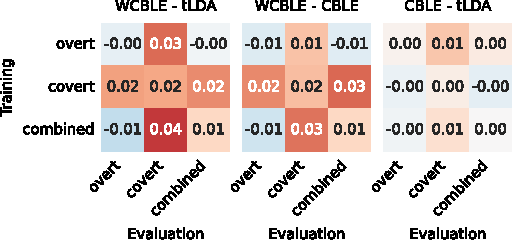
\includegraphics[width=\linewidth]{figures/covert_align/figure5b.pdf}
    \hspace{-.5in}%% Creator: Matplotlib, PGF backend
%%
%% To include the figure in your LaTeX document, write
%%   \input{<filename>.pgf}
%%
%% Make sure the required packages are loaded in your preamble
%%   \usepackage{pgf}
%%
%% Also ensure that all the required font packages are loaded; for instance,
%% the lmodern package is sometimes necessary when using math font.
%%   \usepackage{lmodern}
%%
%% Figures using additional raster images can only be included by \input if
%% they are in the same directory as the main LaTeX file. For loading figures
%% from other directories you can use the `import` package
%%   \usepackage{import}
%%
%% and then include the figures with
%%   \import{<path to file>}{<filename>.pgf}
%%
%% Matplotlib used the following preamble
%%   \def\mathdefault#1{#1}
%%   \everymath=\expandafter{\the\everymath\displaystyle}
%%   
%%   \ifdefined\pdftexversion\else  % non-pdftex case.
%%     \usepackage{fontspec}
%%   \fi
%%   \makeatletter\@ifpackageloaded{underscore}{}{\usepackage[strings]{underscore}}\makeatother
%%
\begingroup%
\makeatletter%
\begin{pgfpicture}%
\pgfpathrectangle{\pgfpointorigin}{\pgfqpoint{3.190173in}{1.594975in}}%
\pgfusepath{use as bounding box, clip}%
\begin{pgfscope}%
\pgfsetbuttcap%
\pgfsetmiterjoin%
\pgfsetlinewidth{0.000000pt}%
\definecolor{currentstroke}{rgb}{0.000000,0.000000,0.000000}%
\pgfsetstrokecolor{currentstroke}%
\pgfsetstrokeopacity{0.000000}%
\pgfsetdash{}{0pt}%
\pgfpathmoveto{\pgfqpoint{0.000000in}{0.000000in}}%
\pgfpathlineto{\pgfqpoint{3.190173in}{0.000000in}}%
\pgfpathlineto{\pgfqpoint{3.190173in}{1.594975in}}%
\pgfpathlineto{\pgfqpoint{0.000000in}{1.594975in}}%
\pgfpathlineto{\pgfqpoint{0.000000in}{0.000000in}}%
\pgfpathclose%
\pgfusepath{}%
\end{pgfscope}%
\begin{pgfscope}%
\pgfsetbuttcap%
\pgfsetmiterjoin%
\pgfsetlinewidth{0.000000pt}%
\definecolor{currentstroke}{rgb}{0.000000,0.000000,0.000000}%
\pgfsetstrokecolor{currentstroke}%
\pgfsetstrokeopacity{0.000000}%
\pgfsetdash{}{0pt}%
\pgfpathmoveto{\pgfqpoint{0.725497in}{0.654625in}}%
\pgfpathlineto{\pgfqpoint{1.495708in}{0.654625in}}%
\pgfpathlineto{\pgfqpoint{1.495708in}{1.424836in}}%
\pgfpathlineto{\pgfqpoint{0.725497in}{1.424836in}}%
\pgfpathlineto{\pgfqpoint{0.725497in}{0.654625in}}%
\pgfpathclose%
\pgfusepath{}%
\end{pgfscope}%
\begin{pgfscope}%
\pgfpathrectangle{\pgfqpoint{0.725497in}{0.654625in}}{\pgfqpoint{0.770211in}{0.770211in}}%
\pgfusepath{clip}%
\pgfsetbuttcap%
\pgfsetroundjoin%
\definecolor{currentfill}{rgb}{0.945175,0.978777,0.849827}%
\pgfsetfillcolor{currentfill}%
\pgfsetlinewidth{0.000000pt}%
\definecolor{currentstroke}{rgb}{1.000000,1.000000,1.000000}%
\pgfsetstrokecolor{currentstroke}%
\pgfsetdash{}{0pt}%
\pgfpathmoveto{\pgfqpoint{0.725497in}{1.424836in}}%
\pgfpathlineto{\pgfqpoint{0.982234in}{1.424836in}}%
\pgfpathlineto{\pgfqpoint{0.982234in}{1.168099in}}%
\pgfpathlineto{\pgfqpoint{0.725497in}{1.168099in}}%
\pgfpathlineto{\pgfqpoint{0.725497in}{1.424836in}}%
\pgfusepath{fill}%
\end{pgfscope}%
\begin{pgfscope}%
\pgfpathrectangle{\pgfqpoint{0.725497in}{0.654625in}}{\pgfqpoint{0.770211in}{0.770211in}}%
\pgfusepath{clip}%
\pgfsetbuttcap%
\pgfsetroundjoin%
\definecolor{currentfill}{rgb}{0.962399,0.467436,0.281200}%
\pgfsetfillcolor{currentfill}%
\pgfsetlinewidth{0.000000pt}%
\definecolor{currentstroke}{rgb}{1.000000,1.000000,1.000000}%
\pgfsetstrokecolor{currentstroke}%
\pgfsetdash{}{0pt}%
\pgfpathmoveto{\pgfqpoint{0.982234in}{1.424836in}}%
\pgfpathlineto{\pgfqpoint{1.238971in}{1.424836in}}%
\pgfpathlineto{\pgfqpoint{1.238971in}{1.168099in}}%
\pgfpathlineto{\pgfqpoint{0.982234in}{1.168099in}}%
\pgfpathlineto{\pgfqpoint{0.982234in}{1.424836in}}%
\pgfusepath{fill}%
\end{pgfscope}%
\begin{pgfscope}%
\pgfpathrectangle{\pgfqpoint{0.725497in}{0.654625in}}{\pgfqpoint{0.770211in}{0.770211in}}%
\pgfusepath{clip}%
\pgfsetbuttcap%
\pgfsetroundjoin%
\definecolor{currentfill}{rgb}{0.978547,0.991696,0.788466}%
\pgfsetfillcolor{currentfill}%
\pgfsetlinewidth{0.000000pt}%
\definecolor{currentstroke}{rgb}{1.000000,1.000000,1.000000}%
\pgfsetstrokecolor{currentstroke}%
\pgfsetdash{}{0pt}%
\pgfpathmoveto{\pgfqpoint{1.238971in}{1.424836in}}%
\pgfpathlineto{\pgfqpoint{1.495708in}{1.424836in}}%
\pgfpathlineto{\pgfqpoint{1.495708in}{1.168099in}}%
\pgfpathlineto{\pgfqpoint{1.238971in}{1.168099in}}%
\pgfpathlineto{\pgfqpoint{1.238971in}{1.424836in}}%
\pgfusepath{fill}%
\end{pgfscope}%
\begin{pgfscope}%
\pgfpathrectangle{\pgfqpoint{0.725497in}{0.654625in}}{\pgfqpoint{0.770211in}{0.770211in}}%
\pgfusepath{clip}%
\pgfsetbuttcap%
\pgfsetroundjoin%
\definecolor{currentfill}{rgb}{0.990081,0.667359,0.373472}%
\pgfsetfillcolor{currentfill}%
\pgfsetlinewidth{0.000000pt}%
\definecolor{currentstroke}{rgb}{1.000000,1.000000,1.000000}%
\pgfsetstrokecolor{currentstroke}%
\pgfsetdash{}{0pt}%
\pgfpathmoveto{\pgfqpoint{0.725497in}{1.168099in}}%
\pgfpathlineto{\pgfqpoint{0.982234in}{1.168099in}}%
\pgfpathlineto{\pgfqpoint{0.982234in}{0.911362in}}%
\pgfpathlineto{\pgfqpoint{0.725497in}{0.911362in}}%
\pgfpathlineto{\pgfqpoint{0.725497in}{1.168099in}}%
\pgfusepath{fill}%
\end{pgfscope}%
\begin{pgfscope}%
\pgfpathrectangle{\pgfqpoint{0.725497in}{0.654625in}}{\pgfqpoint{0.770211in}{0.770211in}}%
\pgfusepath{clip}%
\pgfsetbuttcap%
\pgfsetroundjoin%
\definecolor{currentfill}{rgb}{0.992388,0.693887,0.391234}%
\pgfsetfillcolor{currentfill}%
\pgfsetlinewidth{0.000000pt}%
\definecolor{currentstroke}{rgb}{1.000000,1.000000,1.000000}%
\pgfsetstrokecolor{currentstroke}%
\pgfsetdash{}{0pt}%
\pgfpathmoveto{\pgfqpoint{0.982234in}{1.168099in}}%
\pgfpathlineto{\pgfqpoint{1.238971in}{1.168099in}}%
\pgfpathlineto{\pgfqpoint{1.238971in}{0.911362in}}%
\pgfpathlineto{\pgfqpoint{0.982234in}{0.911362in}}%
\pgfpathlineto{\pgfqpoint{0.982234in}{1.168099in}}%
\pgfusepath{fill}%
\end{pgfscope}%
\begin{pgfscope}%
\pgfpathrectangle{\pgfqpoint{0.725497in}{0.654625in}}{\pgfqpoint{0.770211in}{0.770211in}}%
\pgfusepath{clip}%
\pgfsetbuttcap%
\pgfsetroundjoin%
\definecolor{currentfill}{rgb}{0.979008,0.587389,0.336563}%
\pgfsetfillcolor{currentfill}%
\pgfsetlinewidth{0.000000pt}%
\definecolor{currentstroke}{rgb}{1.000000,1.000000,1.000000}%
\pgfsetstrokecolor{currentstroke}%
\pgfsetdash{}{0pt}%
\pgfpathmoveto{\pgfqpoint{1.238971in}{1.168099in}}%
\pgfpathlineto{\pgfqpoint{1.495708in}{1.168099in}}%
\pgfpathlineto{\pgfqpoint{1.495708in}{0.911362in}}%
\pgfpathlineto{\pgfqpoint{1.238971in}{0.911362in}}%
\pgfpathlineto{\pgfqpoint{1.238971in}{1.168099in}}%
\pgfusepath{fill}%
\end{pgfscope}%
\begin{pgfscope}%
\pgfpathrectangle{\pgfqpoint{0.725497in}{0.654625in}}{\pgfqpoint{0.770211in}{0.770211in}}%
\pgfusepath{clip}%
\pgfsetbuttcap%
\pgfsetroundjoin%
\definecolor{currentfill}{rgb}{0.829527,0.928950,0.958708}%
\pgfsetfillcolor{currentfill}%
\pgfsetlinewidth{0.000000pt}%
\definecolor{currentstroke}{rgb}{1.000000,1.000000,1.000000}%
\pgfsetstrokecolor{currentstroke}%
\pgfsetdash{}{0pt}%
\pgfpathmoveto{\pgfqpoint{0.725497in}{0.911362in}}%
\pgfpathlineto{\pgfqpoint{0.982234in}{0.911362in}}%
\pgfpathlineto{\pgfqpoint{0.982234in}{0.654625in}}%
\pgfpathlineto{\pgfqpoint{0.725497in}{0.654625in}}%
\pgfpathlineto{\pgfqpoint{0.725497in}{0.911362in}}%
\pgfusepath{fill}%
\end{pgfscope}%
\begin{pgfscope}%
\pgfpathrectangle{\pgfqpoint{0.725497in}{0.654625in}}{\pgfqpoint{0.770211in}{0.770211in}}%
\pgfusepath{clip}%
\pgfsetbuttcap%
\pgfsetroundjoin%
\definecolor{currentfill}{rgb}{0.894425,0.296117,0.202461}%
\pgfsetfillcolor{currentfill}%
\pgfsetlinewidth{0.000000pt}%
\definecolor{currentstroke}{rgb}{1.000000,1.000000,1.000000}%
\pgfsetstrokecolor{currentstroke}%
\pgfsetdash{}{0pt}%
\pgfpathmoveto{\pgfqpoint{0.982234in}{0.911362in}}%
\pgfpathlineto{\pgfqpoint{1.238971in}{0.911362in}}%
\pgfpathlineto{\pgfqpoint{1.238971in}{0.654625in}}%
\pgfpathlineto{\pgfqpoint{0.982234in}{0.654625in}}%
\pgfpathlineto{\pgfqpoint{0.982234in}{0.911362in}}%
\pgfusepath{fill}%
\end{pgfscope}%
\begin{pgfscope}%
\pgfpathrectangle{\pgfqpoint{0.725497in}{0.654625in}}{\pgfqpoint{0.770211in}{0.770211in}}%
\pgfusepath{clip}%
\pgfsetbuttcap%
\pgfsetroundjoin%
\definecolor{currentfill}{rgb}{0.995925,0.870742,0.557478}%
\pgfsetfillcolor{currentfill}%
\pgfsetlinewidth{0.000000pt}%
\definecolor{currentstroke}{rgb}{1.000000,1.000000,1.000000}%
\pgfsetstrokecolor{currentstroke}%
\pgfsetdash{}{0pt}%
\pgfpathmoveto{\pgfqpoint{1.238971in}{0.911362in}}%
\pgfpathlineto{\pgfqpoint{1.495708in}{0.911362in}}%
\pgfpathlineto{\pgfqpoint{1.495708in}{0.654625in}}%
\pgfpathlineto{\pgfqpoint{1.238971in}{0.654625in}}%
\pgfpathlineto{\pgfqpoint{1.238971in}{0.911362in}}%
\pgfusepath{fill}%
\end{pgfscope}%
\begin{pgfscope}%
\definecolor{textcolor}{rgb}{0.552941,0.501961,0.478431}%
\pgfsetstrokecolor{textcolor}%
\pgfsetfillcolor{textcolor}%
\pgftext[x=0.645172in, y=0.353126in, left, base,rotate=45.000000]{\color{textcolor}{\sffamily\fontsize{9.000000}{10.800000}\selectfont\catcode`\^=\active\def^{\ifmmode\sp\else\^{}\fi}\catcode`\%=\active\def%{\%}overt}}%
\end{pgfscope}%
\begin{pgfscope}%
\definecolor{textcolor}{rgb}{0.552941,0.501961,0.478431}%
\pgfsetstrokecolor{textcolor}%
\pgfsetfillcolor{textcolor}%
\pgftext[x=0.861535in, y=0.312751in, left, base,rotate=45.000000]{\color{textcolor}{\sffamily\fontsize{9.000000}{10.800000}\selectfont\catcode`\^=\active\def^{\ifmmode\sp\else\^{}\fi}\catcode`\%=\active\def%{\%}covert}}%
\end{pgfscope}%
\begin{pgfscope}%
\definecolor{textcolor}{rgb}{0.552941,0.501961,0.478431}%
\pgfsetstrokecolor{textcolor}%
\pgfsetfillcolor{textcolor}%
\pgftext[x=0.989374in, y=0.183853in, left, base,rotate=45.000000]{\color{textcolor}{\sffamily\fontsize{9.000000}{10.800000}\selectfont\catcode`\^=\active\def^{\ifmmode\sp\else\^{}\fi}\catcode`\%=\active\def%{\%}combined}}%
\end{pgfscope}%
\begin{pgfscope}%
\definecolor{textcolor}{rgb}{0.552941,0.501961,0.478431}%
\pgfsetstrokecolor{textcolor}%
\pgfsetfillcolor{textcolor}%
\pgftext[x=1.110603in,y=0.111111in,,top]{\color{textcolor}{\sffamily\fontsize{9.000000}{10.800000}\selectfont\catcode`\^=\active\def^{\ifmmode\sp\else\^{}\fi}\catcode`\%=\active\def%{\%}Evaluation}}%
\end{pgfscope}%
\begin{pgfscope}%
\definecolor{textcolor}{rgb}{0.552941,0.501961,0.478431}%
\pgfsetstrokecolor{textcolor}%
\pgfsetfillcolor{textcolor}%
\pgftext[x=0.676886in,y=1.296467in,right,]{\color{textcolor}{\sffamily\fontsize{9.000000}{10.800000}\selectfont\catcode`\^=\active\def^{\ifmmode\sp\else\^{}\fi}\catcode`\%=\active\def%{\%}overt}}%
\end{pgfscope}%
\begin{pgfscope}%
\definecolor{textcolor}{rgb}{0.552941,0.501961,0.478431}%
\pgfsetstrokecolor{textcolor}%
\pgfsetfillcolor{textcolor}%
\pgftext[x=0.676886in,y=1.039730in,right,]{\color{textcolor}{\sffamily\fontsize{9.000000}{10.800000}\selectfont\catcode`\^=\active\def^{\ifmmode\sp\else\^{}\fi}\catcode`\%=\active\def%{\%}covert}}%
\end{pgfscope}%
\begin{pgfscope}%
\definecolor{textcolor}{rgb}{0.552941,0.501961,0.478431}%
\pgfsetstrokecolor{textcolor}%
\pgfsetfillcolor{textcolor}%
\pgftext[x=0.676886in,y=0.782993in,right,]{\color{textcolor}{\sffamily\fontsize{9.000000}{10.800000}\selectfont\catcode`\^=\active\def^{\ifmmode\sp\else\^{}\fi}\catcode`\%=\active\def%{\%}combined}}%
\end{pgfscope}%
\begin{pgfscope}%
\definecolor{textcolor}{rgb}{0.552941,0.501961,0.478431}%
\pgfsetstrokecolor{textcolor}%
\pgfsetfillcolor{textcolor}%
\pgftext[x=0.111111in,y=1.039730in,,bottom,rotate=90.000000]{\color{textcolor}{\sffamily\fontsize{9.000000}{10.800000}\selectfont\catcode`\^=\active\def^{\ifmmode\sp\else\^{}\fi}\catcode`\%=\active\def%{\%}Training}}%
\end{pgfscope}%
\begin{pgfscope}%
\pgfsetrectcap%
\pgfsetmiterjoin%
\pgfsetlinewidth{0.803000pt}%
\definecolor{currentstroke}{rgb}{0.552941,0.501961,0.478431}%
\pgfsetstrokecolor{currentstroke}%
\pgfsetdash{}{0pt}%
\pgfpathmoveto{\pgfqpoint{0.725497in}{0.654625in}}%
\pgfpathlineto{\pgfqpoint{0.725497in}{1.424836in}}%
\pgfusepath{stroke}%
\end{pgfscope}%
\begin{pgfscope}%
\pgfsetrectcap%
\pgfsetmiterjoin%
\pgfsetlinewidth{0.803000pt}%
\definecolor{currentstroke}{rgb}{0.552941,0.501961,0.478431}%
\pgfsetstrokecolor{currentstroke}%
\pgfsetdash{}{0pt}%
\pgfpathmoveto{\pgfqpoint{1.495708in}{0.654625in}}%
\pgfpathlineto{\pgfqpoint{1.495708in}{1.424836in}}%
\pgfusepath{stroke}%
\end{pgfscope}%
\begin{pgfscope}%
\pgfsetrectcap%
\pgfsetmiterjoin%
\pgfsetlinewidth{0.803000pt}%
\definecolor{currentstroke}{rgb}{0.552941,0.501961,0.478431}%
\pgfsetstrokecolor{currentstroke}%
\pgfsetdash{}{0pt}%
\pgfpathmoveto{\pgfqpoint{0.725497in}{0.654625in}}%
\pgfpathlineto{\pgfqpoint{1.495708in}{0.654625in}}%
\pgfusepath{stroke}%
\end{pgfscope}%
\begin{pgfscope}%
\pgfsetrectcap%
\pgfsetmiterjoin%
\pgfsetlinewidth{0.803000pt}%
\definecolor{currentstroke}{rgb}{0.552941,0.501961,0.478431}%
\pgfsetstrokecolor{currentstroke}%
\pgfsetdash{}{0pt}%
\pgfpathmoveto{\pgfqpoint{0.725497in}{1.424836in}}%
\pgfpathlineto{\pgfqpoint{1.495708in}{1.424836in}}%
\pgfusepath{stroke}%
\end{pgfscope}%
\begin{pgfscope}%
\definecolor{textcolor}{rgb}{0.150000,0.150000,0.150000}%
\pgfsetstrokecolor{textcolor}%
\pgfsetfillcolor{textcolor}%
\pgftext[x=0.853866in,y=1.296467in,,]{\color{textcolor}{\sffamily\fontsize{8.000000}{9.600000}\selectfont\catcode`\^=\active\def^{\ifmmode\sp\else\^{}\fi}\catcode`\%=\active\def%{\%}-0.46}}%
\end{pgfscope}%
\begin{pgfscope}%
\definecolor{textcolor}{rgb}{1.000000,1.000000,1.000000}%
\pgfsetstrokecolor{textcolor}%
\pgfsetfillcolor{textcolor}%
\pgftext[x=1.110603in,y=1.296467in,,]{\color{textcolor}{\sffamily\fontsize{8.000000}{9.600000}\selectfont\catcode`\^=\active\def^{\ifmmode\sp\else\^{}\fi}\catcode`\%=\active\def%{\%}2.82}}%
\end{pgfscope}%
\begin{pgfscope}%
\definecolor{textcolor}{rgb}{0.150000,0.150000,0.150000}%
\pgfsetstrokecolor{textcolor}%
\pgfsetfillcolor{textcolor}%
\pgftext[x=1.367340in,y=1.296467in,,]{\color{textcolor}{\sffamily\fontsize{8.000000}{9.600000}\selectfont\catcode`\^=\active\def^{\ifmmode\sp\else\^{}\fi}\catcode`\%=\active\def%{\%}-0.18}}%
\end{pgfscope}%
\begin{pgfscope}%
\definecolor{textcolor}{rgb}{0.150000,0.150000,0.150000}%
\pgfsetstrokecolor{textcolor}%
\pgfsetfillcolor{textcolor}%
\pgftext[x=0.853866in,y=1.039730in,,]{\color{textcolor}{\sffamily\fontsize{8.000000}{9.600000}\selectfont\catcode`\^=\active\def^{\ifmmode\sp\else\^{}\fi}\catcode`\%=\active\def%{\%}2.06}}%
\end{pgfscope}%
\begin{pgfscope}%
\definecolor{textcolor}{rgb}{0.150000,0.150000,0.150000}%
\pgfsetstrokecolor{textcolor}%
\pgfsetfillcolor{textcolor}%
\pgftext[x=1.110603in,y=1.039730in,,]{\color{textcolor}{\sffamily\fontsize{8.000000}{9.600000}\selectfont\catcode`\^=\active\def^{\ifmmode\sp\else\^{}\fi}\catcode`\%=\active\def%{\%}1.94}}%
\end{pgfscope}%
\begin{pgfscope}%
\definecolor{textcolor}{rgb}{0.150000,0.150000,0.150000}%
\pgfsetstrokecolor{textcolor}%
\pgfsetfillcolor{textcolor}%
\pgftext[x=1.367340in,y=1.039730in,,]{\color{textcolor}{\sffamily\fontsize{8.000000}{9.600000}\selectfont\catcode`\^=\active\def^{\ifmmode\sp\else\^{}\fi}\catcode`\%=\active\def%{\%}2.36}}%
\end{pgfscope}%
\begin{pgfscope}%
\definecolor{textcolor}{rgb}{0.150000,0.150000,0.150000}%
\pgfsetstrokecolor{textcolor}%
\pgfsetfillcolor{textcolor}%
\pgftext[x=0.853866in,y=0.782993in,,]{\color{textcolor}{\sffamily\fontsize{8.000000}{9.600000}\selectfont\catcode`\^=\active\def^{\ifmmode\sp\else\^{}\fi}\catcode`\%=\active\def%{\%}-1.24}}%
\end{pgfscope}%
\begin{pgfscope}%
\definecolor{textcolor}{rgb}{1.000000,1.000000,1.000000}%
\pgfsetstrokecolor{textcolor}%
\pgfsetfillcolor{textcolor}%
\pgftext[x=1.110603in,y=0.782993in,,]{\color{textcolor}{\sffamily\fontsize{8.000000}{9.600000}\selectfont\catcode`\^=\active\def^{\ifmmode\sp\else\^{}\fi}\catcode`\%=\active\def%{\%}3.55}}%
\end{pgfscope}%
\begin{pgfscope}%
\definecolor{textcolor}{rgb}{0.150000,0.150000,0.150000}%
\pgfsetstrokecolor{textcolor}%
\pgfsetfillcolor{textcolor}%
\pgftext[x=1.367340in,y=0.782993in,,]{\color{textcolor}{\sffamily\fontsize{8.000000}{9.600000}\selectfont\catcode`\^=\active\def^{\ifmmode\sp\else\^{}\fi}\catcode`\%=\active\def%{\%}1.03}}%
\end{pgfscope}%
\begin{pgfscope}%
\definecolor{textcolor}{rgb}{0.552941,0.501961,0.478431}%
\pgfsetstrokecolor{textcolor}%
\pgfsetfillcolor{textcolor}%
\pgftext[x=0.725497in,y=1.508169in,left,base]{\color{textcolor}{\sffamily\fontsize{9.000000}{10.800000}\selectfont\catcode`\^=\active\def^{\ifmmode\sp\else\^{}\fi}\catcode`\%=\active\def%{\%}WCBLE - tLDA}}%
\end{pgfscope}%
\begin{pgfscope}%
\pgfsetbuttcap%
\pgfsetmiterjoin%
\pgfsetlinewidth{0.000000pt}%
\definecolor{currentstroke}{rgb}{0.000000,0.000000,0.000000}%
\pgfsetstrokecolor{currentstroke}%
\pgfsetstrokeopacity{0.000000}%
\pgfsetdash{}{0pt}%
\pgfpathmoveto{\pgfqpoint{1.572729in}{0.654625in}}%
\pgfpathlineto{\pgfqpoint{2.342941in}{0.654625in}}%
\pgfpathlineto{\pgfqpoint{2.342941in}{1.424836in}}%
\pgfpathlineto{\pgfqpoint{1.572729in}{1.424836in}}%
\pgfpathlineto{\pgfqpoint{1.572729in}{0.654625in}}%
\pgfpathclose%
\pgfusepath{}%
\end{pgfscope}%
\begin{pgfscope}%
\pgfpathrectangle{\pgfqpoint{1.572729in}{0.654625in}}{\pgfqpoint{0.770211in}{0.770211in}}%
\pgfusepath{clip}%
\pgfsetbuttcap%
\pgfsetroundjoin%
\definecolor{currentfill}{rgb}{0.916571,0.967705,0.902422}%
\pgfsetfillcolor{currentfill}%
\pgfsetlinewidth{0.000000pt}%
\definecolor{currentstroke}{rgb}{1.000000,1.000000,1.000000}%
\pgfsetstrokecolor{currentstroke}%
\pgfsetdash{}{0pt}%
\pgfpathmoveto{\pgfqpoint{1.572729in}{1.424836in}}%
\pgfpathlineto{\pgfqpoint{1.829467in}{1.424836in}}%
\pgfpathlineto{\pgfqpoint{1.829467in}{1.168099in}}%
\pgfpathlineto{\pgfqpoint{1.572729in}{1.168099in}}%
\pgfpathlineto{\pgfqpoint{1.572729in}{1.424836in}}%
\pgfusepath{fill}%
\end{pgfscope}%
\begin{pgfscope}%
\pgfpathrectangle{\pgfqpoint{1.572729in}{0.654625in}}{\pgfqpoint{0.770211in}{0.770211in}}%
\pgfusepath{clip}%
\pgfsetbuttcap%
\pgfsetroundjoin%
\definecolor{currentfill}{rgb}{0.994233,0.786159,0.477970}%
\pgfsetfillcolor{currentfill}%
\pgfsetlinewidth{0.000000pt}%
\definecolor{currentstroke}{rgb}{1.000000,1.000000,1.000000}%
\pgfsetstrokecolor{currentstroke}%
\pgfsetdash{}{0pt}%
\pgfpathmoveto{\pgfqpoint{1.829467in}{1.424836in}}%
\pgfpathlineto{\pgfqpoint{2.086204in}{1.424836in}}%
\pgfpathlineto{\pgfqpoint{2.086204in}{1.168099in}}%
\pgfpathlineto{\pgfqpoint{1.829467in}{1.168099in}}%
\pgfpathlineto{\pgfqpoint{1.829467in}{1.424836in}}%
\pgfusepath{fill}%
\end{pgfscope}%
\begin{pgfscope}%
\pgfpathrectangle{\pgfqpoint{1.572729in}{0.654625in}}{\pgfqpoint{0.770211in}{0.770211in}}%
\pgfusepath{clip}%
\pgfsetbuttcap%
\pgfsetroundjoin%
\definecolor{currentfill}{rgb}{0.926105,0.971396,0.884890}%
\pgfsetfillcolor{currentfill}%
\pgfsetlinewidth{0.000000pt}%
\definecolor{currentstroke}{rgb}{1.000000,1.000000,1.000000}%
\pgfsetstrokecolor{currentstroke}%
\pgfsetdash{}{0pt}%
\pgfpathmoveto{\pgfqpoint{2.086204in}{1.424836in}}%
\pgfpathlineto{\pgfqpoint{2.342941in}{1.424836in}}%
\pgfpathlineto{\pgfqpoint{2.342941in}{1.168099in}}%
\pgfpathlineto{\pgfqpoint{2.086204in}{1.168099in}}%
\pgfpathlineto{\pgfqpoint{2.086204in}{1.424836in}}%
\pgfusepath{fill}%
\end{pgfscope}%
\begin{pgfscope}%
\pgfpathrectangle{\pgfqpoint{1.572729in}{0.654625in}}{\pgfqpoint{0.770211in}{0.770211in}}%
\pgfusepath{clip}%
\pgfsetbuttcap%
\pgfsetroundjoin%
\definecolor{currentfill}{rgb}{0.977624,0.577393,0.331949}%
\pgfsetfillcolor{currentfill}%
\pgfsetlinewidth{0.000000pt}%
\definecolor{currentstroke}{rgb}{1.000000,1.000000,1.000000}%
\pgfsetstrokecolor{currentstroke}%
\pgfsetdash{}{0pt}%
\pgfpathmoveto{\pgfqpoint{1.572729in}{1.168099in}}%
\pgfpathlineto{\pgfqpoint{1.829467in}{1.168099in}}%
\pgfpathlineto{\pgfqpoint{1.829467in}{0.911362in}}%
\pgfpathlineto{\pgfqpoint{1.572729in}{0.911362in}}%
\pgfpathlineto{\pgfqpoint{1.572729in}{1.168099in}}%
\pgfusepath{fill}%
\end{pgfscope}%
\begin{pgfscope}%
\pgfpathrectangle{\pgfqpoint{1.572729in}{0.654625in}}{\pgfqpoint{0.770211in}{0.770211in}}%
\pgfusepath{clip}%
\pgfsetbuttcap%
\pgfsetroundjoin%
\definecolor{currentfill}{rgb}{0.993925,0.770780,0.463514}%
\pgfsetfillcolor{currentfill}%
\pgfsetlinewidth{0.000000pt}%
\definecolor{currentstroke}{rgb}{1.000000,1.000000,1.000000}%
\pgfsetstrokecolor{currentstroke}%
\pgfsetdash{}{0pt}%
\pgfpathmoveto{\pgfqpoint{1.829467in}{1.168099in}}%
\pgfpathlineto{\pgfqpoint{2.086204in}{1.168099in}}%
\pgfpathlineto{\pgfqpoint{2.086204in}{0.911362in}}%
\pgfpathlineto{\pgfqpoint{1.829467in}{0.911362in}}%
\pgfpathlineto{\pgfqpoint{1.829467in}{1.168099in}}%
\pgfusepath{fill}%
\end{pgfscope}%
\begin{pgfscope}%
\pgfpathrectangle{\pgfqpoint{1.572729in}{0.654625in}}{\pgfqpoint{0.770211in}{0.770211in}}%
\pgfusepath{clip}%
\pgfsetbuttcap%
\pgfsetroundjoin%
\definecolor{currentfill}{rgb}{0.961015,0.457439,0.276586}%
\pgfsetfillcolor{currentfill}%
\pgfsetlinewidth{0.000000pt}%
\definecolor{currentstroke}{rgb}{1.000000,1.000000,1.000000}%
\pgfsetstrokecolor{currentstroke}%
\pgfsetdash{}{0pt}%
\pgfpathmoveto{\pgfqpoint{2.086204in}{1.168099in}}%
\pgfpathlineto{\pgfqpoint{2.342941in}{1.168099in}}%
\pgfpathlineto{\pgfqpoint{2.342941in}{0.911362in}}%
\pgfpathlineto{\pgfqpoint{2.086204in}{0.911362in}}%
\pgfpathlineto{\pgfqpoint{2.086204in}{1.168099in}}%
\pgfusepath{fill}%
\end{pgfscope}%
\begin{pgfscope}%
\pgfpathrectangle{\pgfqpoint{1.572729in}{0.654625in}}{\pgfqpoint{0.770211in}{0.770211in}}%
\pgfusepath{clip}%
\pgfsetbuttcap%
\pgfsetroundjoin%
\definecolor{currentfill}{rgb}{0.870281,0.948943,0.970242}%
\pgfsetfillcolor{currentfill}%
\pgfsetlinewidth{0.000000pt}%
\definecolor{currentstroke}{rgb}{1.000000,1.000000,1.000000}%
\pgfsetstrokecolor{currentstroke}%
\pgfsetdash{}{0pt}%
\pgfpathmoveto{\pgfqpoint{1.572729in}{0.911362in}}%
\pgfpathlineto{\pgfqpoint{1.829467in}{0.911362in}}%
\pgfpathlineto{\pgfqpoint{1.829467in}{0.654625in}}%
\pgfpathlineto{\pgfqpoint{1.572729in}{0.654625in}}%
\pgfpathlineto{\pgfqpoint{1.572729in}{0.911362in}}%
\pgfusepath{fill}%
\end{pgfscope}%
\begin{pgfscope}%
\pgfpathrectangle{\pgfqpoint{1.572729in}{0.654625in}}{\pgfqpoint{0.770211in}{0.770211in}}%
\pgfusepath{clip}%
\pgfsetbuttcap%
\pgfsetroundjoin%
\definecolor{currentfill}{rgb}{0.966551,0.497424,0.295040}%
\pgfsetfillcolor{currentfill}%
\pgfsetlinewidth{0.000000pt}%
\definecolor{currentstroke}{rgb}{1.000000,1.000000,1.000000}%
\pgfsetstrokecolor{currentstroke}%
\pgfsetdash{}{0pt}%
\pgfpathmoveto{\pgfqpoint{1.829467in}{0.911362in}}%
\pgfpathlineto{\pgfqpoint{2.086204in}{0.911362in}}%
\pgfpathlineto{\pgfqpoint{2.086204in}{0.654625in}}%
\pgfpathlineto{\pgfqpoint{1.829467in}{0.654625in}}%
\pgfpathlineto{\pgfqpoint{1.829467in}{0.911362in}}%
\pgfusepath{fill}%
\end{pgfscope}%
\begin{pgfscope}%
\pgfpathrectangle{\pgfqpoint{1.572729in}{0.654625in}}{\pgfqpoint{0.770211in}{0.770211in}}%
\pgfusepath{clip}%
\pgfsetbuttcap%
\pgfsetroundjoin%
\definecolor{currentfill}{rgb}{0.995925,0.870742,0.557478}%
\pgfsetfillcolor{currentfill}%
\pgfsetlinewidth{0.000000pt}%
\definecolor{currentstroke}{rgb}{1.000000,1.000000,1.000000}%
\pgfsetstrokecolor{currentstroke}%
\pgfsetdash{}{0pt}%
\pgfpathmoveto{\pgfqpoint{2.086204in}{0.911362in}}%
\pgfpathlineto{\pgfqpoint{2.342941in}{0.911362in}}%
\pgfpathlineto{\pgfqpoint{2.342941in}{0.654625in}}%
\pgfpathlineto{\pgfqpoint{2.086204in}{0.654625in}}%
\pgfpathlineto{\pgfqpoint{2.086204in}{0.911362in}}%
\pgfusepath{fill}%
\end{pgfscope}%
\begin{pgfscope}%
\definecolor{textcolor}{rgb}{0.552941,0.501961,0.478431}%
\pgfsetstrokecolor{textcolor}%
\pgfsetfillcolor{textcolor}%
\pgftext[x=1.492405in, y=0.353126in, left, base,rotate=45.000000]{\color{textcolor}{\sffamily\fontsize{9.000000}{10.800000}\selectfont\catcode`\^=\active\def^{\ifmmode\sp\else\^{}\fi}\catcode`\%=\active\def%{\%}overt}}%
\end{pgfscope}%
\begin{pgfscope}%
\definecolor{textcolor}{rgb}{0.552941,0.501961,0.478431}%
\pgfsetstrokecolor{textcolor}%
\pgfsetfillcolor{textcolor}%
\pgftext[x=1.708767in, y=0.312751in, left, base,rotate=45.000000]{\color{textcolor}{\sffamily\fontsize{9.000000}{10.800000}\selectfont\catcode`\^=\active\def^{\ifmmode\sp\else\^{}\fi}\catcode`\%=\active\def%{\%}covert}}%
\end{pgfscope}%
\begin{pgfscope}%
\definecolor{textcolor}{rgb}{0.552941,0.501961,0.478431}%
\pgfsetstrokecolor{textcolor}%
\pgfsetfillcolor{textcolor}%
\pgftext[x=1.836606in, y=0.183853in, left, base,rotate=45.000000]{\color{textcolor}{\sffamily\fontsize{9.000000}{10.800000}\selectfont\catcode`\^=\active\def^{\ifmmode\sp\else\^{}\fi}\catcode`\%=\active\def%{\%}combined}}%
\end{pgfscope}%
\begin{pgfscope}%
\definecolor{textcolor}{rgb}{0.552941,0.501961,0.478431}%
\pgfsetstrokecolor{textcolor}%
\pgfsetfillcolor{textcolor}%
\pgftext[x=1.957835in,y=0.111111in,,top]{\color{textcolor}{\sffamily\fontsize{9.000000}{10.800000}\selectfont\catcode`\^=\active\def^{\ifmmode\sp\else\^{}\fi}\catcode`\%=\active\def%{\%}Evaluation}}%
\end{pgfscope}%
\begin{pgfscope}%
\pgfsetrectcap%
\pgfsetmiterjoin%
\pgfsetlinewidth{0.803000pt}%
\definecolor{currentstroke}{rgb}{0.552941,0.501961,0.478431}%
\pgfsetstrokecolor{currentstroke}%
\pgfsetdash{}{0pt}%
\pgfpathmoveto{\pgfqpoint{1.572729in}{0.654625in}}%
\pgfpathlineto{\pgfqpoint{1.572729in}{1.424836in}}%
\pgfusepath{stroke}%
\end{pgfscope}%
\begin{pgfscope}%
\pgfsetrectcap%
\pgfsetmiterjoin%
\pgfsetlinewidth{0.803000pt}%
\definecolor{currentstroke}{rgb}{0.552941,0.501961,0.478431}%
\pgfsetstrokecolor{currentstroke}%
\pgfsetdash{}{0pt}%
\pgfpathmoveto{\pgfqpoint{2.342941in}{0.654625in}}%
\pgfpathlineto{\pgfqpoint{2.342941in}{1.424836in}}%
\pgfusepath{stroke}%
\end{pgfscope}%
\begin{pgfscope}%
\pgfsetrectcap%
\pgfsetmiterjoin%
\pgfsetlinewidth{0.803000pt}%
\definecolor{currentstroke}{rgb}{0.552941,0.501961,0.478431}%
\pgfsetstrokecolor{currentstroke}%
\pgfsetdash{}{0pt}%
\pgfpathmoveto{\pgfqpoint{1.572729in}{0.654625in}}%
\pgfpathlineto{\pgfqpoint{2.342941in}{0.654625in}}%
\pgfusepath{stroke}%
\end{pgfscope}%
\begin{pgfscope}%
\pgfsetrectcap%
\pgfsetmiterjoin%
\pgfsetlinewidth{0.803000pt}%
\definecolor{currentstroke}{rgb}{0.552941,0.501961,0.478431}%
\pgfsetstrokecolor{currentstroke}%
\pgfsetdash{}{0pt}%
\pgfpathmoveto{\pgfqpoint{1.572729in}{1.424836in}}%
\pgfpathlineto{\pgfqpoint{2.342941in}{1.424836in}}%
\pgfusepath{stroke}%
\end{pgfscope}%
\begin{pgfscope}%
\definecolor{textcolor}{rgb}{0.150000,0.150000,0.150000}%
\pgfsetstrokecolor{textcolor}%
\pgfsetfillcolor{textcolor}%
\pgftext[x=1.701098in,y=1.296467in,,]{\color{textcolor}{\sffamily\fontsize{8.000000}{9.600000}\selectfont\catcode`\^=\active\def^{\ifmmode\sp\else\^{}\fi}\catcode`\%=\active\def%{\%}-0.69}}%
\end{pgfscope}%
\begin{pgfscope}%
\definecolor{textcolor}{rgb}{0.150000,0.150000,0.150000}%
\pgfsetstrokecolor{textcolor}%
\pgfsetfillcolor{textcolor}%
\pgftext[x=1.957835in,y=1.296467in,,]{\color{textcolor}{\sffamily\fontsize{8.000000}{9.600000}\selectfont\catcode`\^=\active\def^{\ifmmode\sp\else\^{}\fi}\catcode`\%=\active\def%{\%}1.45}}%
\end{pgfscope}%
\begin{pgfscope}%
\definecolor{textcolor}{rgb}{0.150000,0.150000,0.150000}%
\pgfsetstrokecolor{textcolor}%
\pgfsetfillcolor{textcolor}%
\pgftext[x=2.214572in,y=1.296467in,,]{\color{textcolor}{\sffamily\fontsize{8.000000}{9.600000}\selectfont\catcode`\^=\active\def^{\ifmmode\sp\else\^{}\fi}\catcode`\%=\active\def%{\%}-0.62}}%
\end{pgfscope}%
\begin{pgfscope}%
\definecolor{textcolor}{rgb}{0.150000,0.150000,0.150000}%
\pgfsetstrokecolor{textcolor}%
\pgfsetfillcolor{textcolor}%
\pgftext[x=1.701098in,y=1.039730in,,]{\color{textcolor}{\sffamily\fontsize{8.000000}{9.600000}\selectfont\catcode`\^=\active\def^{\ifmmode\sp\else\^{}\fi}\catcode`\%=\active\def%{\%}2.40}}%
\end{pgfscope}%
\begin{pgfscope}%
\definecolor{textcolor}{rgb}{0.150000,0.150000,0.150000}%
\pgfsetstrokecolor{textcolor}%
\pgfsetfillcolor{textcolor}%
\pgftext[x=1.957835in,y=1.039730in,,]{\color{textcolor}{\sffamily\fontsize{8.000000}{9.600000}\selectfont\catcode`\^=\active\def^{\ifmmode\sp\else\^{}\fi}\catcode`\%=\active\def%{\%}1.56}}%
\end{pgfscope}%
\begin{pgfscope}%
\definecolor{textcolor}{rgb}{1.000000,1.000000,1.000000}%
\pgfsetstrokecolor{textcolor}%
\pgfsetfillcolor{textcolor}%
\pgftext[x=2.214572in,y=1.039730in,,]{\color{textcolor}{\sffamily\fontsize{8.000000}{9.600000}\selectfont\catcode`\^=\active\def^{\ifmmode\sp\else\^{}\fi}\catcode`\%=\active\def%{\%}2.85}}%
\end{pgfscope}%
\begin{pgfscope}%
\definecolor{textcolor}{rgb}{0.150000,0.150000,0.150000}%
\pgfsetstrokecolor{textcolor}%
\pgfsetfillcolor{textcolor}%
\pgftext[x=1.701098in,y=0.782993in,,]{\color{textcolor}{\sffamily\fontsize{8.000000}{9.600000}\selectfont\catcode`\^=\active\def^{\ifmmode\sp\else\^{}\fi}\catcode`\%=\active\def%{\%}-1.04}}%
\end{pgfscope}%
\begin{pgfscope}%
\definecolor{textcolor}{rgb}{1.000000,1.000000,1.000000}%
\pgfsetstrokecolor{textcolor}%
\pgfsetfillcolor{textcolor}%
\pgftext[x=1.957835in,y=0.782993in,,]{\color{textcolor}{\sffamily\fontsize{8.000000}{9.600000}\selectfont\catcode`\^=\active\def^{\ifmmode\sp\else\^{}\fi}\catcode`\%=\active\def%{\%}2.73}}%
\end{pgfscope}%
\begin{pgfscope}%
\definecolor{textcolor}{rgb}{0.150000,0.150000,0.150000}%
\pgfsetstrokecolor{textcolor}%
\pgfsetfillcolor{textcolor}%
\pgftext[x=2.214572in,y=0.782993in,,]{\color{textcolor}{\sffamily\fontsize{8.000000}{9.600000}\selectfont\catcode`\^=\active\def^{\ifmmode\sp\else\^{}\fi}\catcode`\%=\active\def%{\%}1.03}}%
\end{pgfscope}%
\begin{pgfscope}%
\definecolor{textcolor}{rgb}{0.552941,0.501961,0.478431}%
\pgfsetstrokecolor{textcolor}%
\pgfsetfillcolor{textcolor}%
\pgftext[x=1.572729in,y=1.508169in,left,base]{\color{textcolor}{\sffamily\fontsize{9.000000}{10.800000}\selectfont\catcode`\^=\active\def^{\ifmmode\sp\else\^{}\fi}\catcode`\%=\active\def%{\%}WCBLE - CBLE}}%
\end{pgfscope}%
\begin{pgfscope}%
\pgfsetbuttcap%
\pgfsetmiterjoin%
\pgfsetlinewidth{0.000000pt}%
\definecolor{currentstroke}{rgb}{0.000000,0.000000,0.000000}%
\pgfsetstrokecolor{currentstroke}%
\pgfsetstrokeopacity{0.000000}%
\pgfsetdash{}{0pt}%
\pgfpathmoveto{\pgfqpoint{2.419962in}{0.654625in}}%
\pgfpathlineto{\pgfqpoint{3.190173in}{0.654625in}}%
\pgfpathlineto{\pgfqpoint{3.190173in}{1.424836in}}%
\pgfpathlineto{\pgfqpoint{2.419962in}{1.424836in}}%
\pgfpathlineto{\pgfqpoint{2.419962in}{0.654625in}}%
\pgfpathclose%
\pgfusepath{}%
\end{pgfscope}%
\begin{pgfscope}%
\pgfpathrectangle{\pgfqpoint{2.419962in}{0.654625in}}{\pgfqpoint{0.770211in}{0.770211in}}%
\pgfusepath{clip}%
\pgfsetbuttcap%
\pgfsetroundjoin%
\definecolor{currentfill}{rgb}{0.999154,0.973779,0.709266}%
\pgfsetfillcolor{currentfill}%
\pgfsetlinewidth{0.000000pt}%
\definecolor{currentstroke}{rgb}{1.000000,1.000000,1.000000}%
\pgfsetstrokecolor{currentstroke}%
\pgfsetdash{}{0pt}%
\pgfpathmoveto{\pgfqpoint{2.419962in}{1.424836in}}%
\pgfpathlineto{\pgfqpoint{2.676699in}{1.424836in}}%
\pgfpathlineto{\pgfqpoint{2.676699in}{1.168099in}}%
\pgfpathlineto{\pgfqpoint{2.419962in}{1.168099in}}%
\pgfpathlineto{\pgfqpoint{2.419962in}{1.424836in}}%
\pgfusepath{fill}%
\end{pgfscope}%
\begin{pgfscope}%
\pgfpathrectangle{\pgfqpoint{2.419962in}{0.654625in}}{\pgfqpoint{0.770211in}{0.770211in}}%
\pgfusepath{clip}%
\pgfsetbuttcap%
\pgfsetroundjoin%
\definecolor{currentfill}{rgb}{0.994541,0.801538,0.492426}%
\pgfsetfillcolor{currentfill}%
\pgfsetlinewidth{0.000000pt}%
\definecolor{currentstroke}{rgb}{1.000000,1.000000,1.000000}%
\pgfsetstrokecolor{currentstroke}%
\pgfsetdash{}{0pt}%
\pgfpathmoveto{\pgfqpoint{2.676699in}{1.424836in}}%
\pgfpathlineto{\pgfqpoint{2.933436in}{1.424836in}}%
\pgfpathlineto{\pgfqpoint{2.933436in}{1.168099in}}%
\pgfpathlineto{\pgfqpoint{2.676699in}{1.168099in}}%
\pgfpathlineto{\pgfqpoint{2.676699in}{1.424836in}}%
\pgfusepath{fill}%
\end{pgfscope}%
\begin{pgfscope}%
\pgfpathrectangle{\pgfqpoint{2.419962in}{0.654625in}}{\pgfqpoint{0.770211in}{0.770211in}}%
\pgfusepath{clip}%
\pgfsetbuttcap%
\pgfsetroundjoin%
\definecolor{currentfill}{rgb}{0.998231,0.945175,0.665898}%
\pgfsetfillcolor{currentfill}%
\pgfsetlinewidth{0.000000pt}%
\definecolor{currentstroke}{rgb}{1.000000,1.000000,1.000000}%
\pgfsetstrokecolor{currentstroke}%
\pgfsetdash{}{0pt}%
\pgfpathmoveto{\pgfqpoint{2.933436in}{1.424836in}}%
\pgfpathlineto{\pgfqpoint{3.190173in}{1.424836in}}%
\pgfpathlineto{\pgfqpoint{3.190173in}{1.168099in}}%
\pgfpathlineto{\pgfqpoint{2.933436in}{1.168099in}}%
\pgfpathlineto{\pgfqpoint{2.933436in}{1.424836in}}%
\pgfusepath{fill}%
\end{pgfscope}%
\begin{pgfscope}%
\pgfpathrectangle{\pgfqpoint{2.419962in}{0.654625in}}{\pgfqpoint{0.770211in}{0.770211in}}%
\pgfusepath{clip}%
\pgfsetbuttcap%
\pgfsetroundjoin%
\definecolor{currentfill}{rgb}{0.959477,0.984314,0.823529}%
\pgfsetfillcolor{currentfill}%
\pgfsetlinewidth{0.000000pt}%
\definecolor{currentstroke}{rgb}{1.000000,1.000000,1.000000}%
\pgfsetstrokecolor{currentstroke}%
\pgfsetdash{}{0pt}%
\pgfpathmoveto{\pgfqpoint{2.419962in}{1.168099in}}%
\pgfpathlineto{\pgfqpoint{2.676699in}{1.168099in}}%
\pgfpathlineto{\pgfqpoint{2.676699in}{0.911362in}}%
\pgfpathlineto{\pgfqpoint{2.419962in}{0.911362in}}%
\pgfpathlineto{\pgfqpoint{2.419962in}{1.168099in}}%
\pgfusepath{fill}%
\end{pgfscope}%
\begin{pgfscope}%
\pgfpathrectangle{\pgfqpoint{2.419962in}{0.654625in}}{\pgfqpoint{0.770211in}{0.770211in}}%
\pgfusepath{clip}%
\pgfsetbuttcap%
\pgfsetroundjoin%
\definecolor{currentfill}{rgb}{0.998539,0.954710,0.680354}%
\pgfsetfillcolor{currentfill}%
\pgfsetlinewidth{0.000000pt}%
\definecolor{currentstroke}{rgb}{1.000000,1.000000,1.000000}%
\pgfsetstrokecolor{currentstroke}%
\pgfsetdash{}{0pt}%
\pgfpathmoveto{\pgfqpoint{2.676699in}{1.168099in}}%
\pgfpathlineto{\pgfqpoint{2.933436in}{1.168099in}}%
\pgfpathlineto{\pgfqpoint{2.933436in}{0.911362in}}%
\pgfpathlineto{\pgfqpoint{2.676699in}{0.911362in}}%
\pgfpathlineto{\pgfqpoint{2.676699in}{1.168099in}}%
\pgfusepath{fill}%
\end{pgfscope}%
\begin{pgfscope}%
\pgfpathrectangle{\pgfqpoint{2.419962in}{0.654625in}}{\pgfqpoint{0.770211in}{0.770211in}}%
\pgfusepath{clip}%
\pgfsetbuttcap%
\pgfsetroundjoin%
\definecolor{currentfill}{rgb}{0.940408,0.976932,0.858593}%
\pgfsetfillcolor{currentfill}%
\pgfsetlinewidth{0.000000pt}%
\definecolor{currentstroke}{rgb}{1.000000,1.000000,1.000000}%
\pgfsetstrokecolor{currentstroke}%
\pgfsetdash{}{0pt}%
\pgfpathmoveto{\pgfqpoint{2.933436in}{1.168099in}}%
\pgfpathlineto{\pgfqpoint{3.190173in}{1.168099in}}%
\pgfpathlineto{\pgfqpoint{3.190173in}{0.911362in}}%
\pgfpathlineto{\pgfqpoint{2.933436in}{0.911362in}}%
\pgfpathlineto{\pgfqpoint{2.933436in}{1.168099in}}%
\pgfusepath{fill}%
\end{pgfscope}%
\begin{pgfscope}%
\pgfpathrectangle{\pgfqpoint{2.419962in}{0.654625in}}{\pgfqpoint{0.770211in}{0.770211in}}%
\pgfusepath{clip}%
\pgfsetbuttcap%
\pgfsetroundjoin%
\definecolor{currentfill}{rgb}{0.973779,0.989850,0.797232}%
\pgfsetfillcolor{currentfill}%
\pgfsetlinewidth{0.000000pt}%
\definecolor{currentstroke}{rgb}{1.000000,1.000000,1.000000}%
\pgfsetstrokecolor{currentstroke}%
\pgfsetdash{}{0pt}%
\pgfpathmoveto{\pgfqpoint{2.419962in}{0.911362in}}%
\pgfpathlineto{\pgfqpoint{2.676699in}{0.911362in}}%
\pgfpathlineto{\pgfqpoint{2.676699in}{0.654625in}}%
\pgfpathlineto{\pgfqpoint{2.419962in}{0.654625in}}%
\pgfpathlineto{\pgfqpoint{2.419962in}{0.911362in}}%
\pgfusepath{fill}%
\end{pgfscope}%
\begin{pgfscope}%
\pgfpathrectangle{\pgfqpoint{2.419962in}{0.654625in}}{\pgfqpoint{0.770211in}{0.770211in}}%
\pgfusepath{clip}%
\pgfsetbuttcap%
\pgfsetroundjoin%
\definecolor{currentfill}{rgb}{0.996847,0.902268,0.600846}%
\pgfsetfillcolor{currentfill}%
\pgfsetlinewidth{0.000000pt}%
\definecolor{currentstroke}{rgb}{1.000000,1.000000,1.000000}%
\pgfsetstrokecolor{currentstroke}%
\pgfsetdash{}{0pt}%
\pgfpathmoveto{\pgfqpoint{2.676699in}{0.911362in}}%
\pgfpathlineto{\pgfqpoint{2.933436in}{0.911362in}}%
\pgfpathlineto{\pgfqpoint{2.933436in}{0.654625in}}%
\pgfpathlineto{\pgfqpoint{2.676699in}{0.654625in}}%
\pgfpathlineto{\pgfqpoint{2.676699in}{0.911362in}}%
\pgfusepath{fill}%
\end{pgfscope}%
\begin{pgfscope}%
\pgfpathrectangle{\pgfqpoint{2.419962in}{0.654625in}}{\pgfqpoint{0.770211in}{0.770211in}}%
\pgfusepath{clip}%
\pgfsetbuttcap%
\pgfsetroundjoin%
\definecolor{currentfill}{rgb}{0.999923,0.997616,0.745406}%
\pgfsetfillcolor{currentfill}%
\pgfsetlinewidth{0.000000pt}%
\definecolor{currentstroke}{rgb}{1.000000,1.000000,1.000000}%
\pgfsetstrokecolor{currentstroke}%
\pgfsetdash{}{0pt}%
\pgfpathmoveto{\pgfqpoint{2.933436in}{0.911362in}}%
\pgfpathlineto{\pgfqpoint{3.190173in}{0.911362in}}%
\pgfpathlineto{\pgfqpoint{3.190173in}{0.654625in}}%
\pgfpathlineto{\pgfqpoint{2.933436in}{0.654625in}}%
\pgfpathlineto{\pgfqpoint{2.933436in}{0.911362in}}%
\pgfusepath{fill}%
\end{pgfscope}%
\begin{pgfscope}%
\definecolor{textcolor}{rgb}{0.552941,0.501961,0.478431}%
\pgfsetstrokecolor{textcolor}%
\pgfsetfillcolor{textcolor}%
\pgftext[x=2.339637in, y=0.353126in, left, base,rotate=45.000000]{\color{textcolor}{\sffamily\fontsize{9.000000}{10.800000}\selectfont\catcode`\^=\active\def^{\ifmmode\sp\else\^{}\fi}\catcode`\%=\active\def%{\%}overt}}%
\end{pgfscope}%
\begin{pgfscope}%
\definecolor{textcolor}{rgb}{0.552941,0.501961,0.478431}%
\pgfsetstrokecolor{textcolor}%
\pgfsetfillcolor{textcolor}%
\pgftext[x=2.556000in, y=0.312751in, left, base,rotate=45.000000]{\color{textcolor}{\sffamily\fontsize{9.000000}{10.800000}\selectfont\catcode`\^=\active\def^{\ifmmode\sp\else\^{}\fi}\catcode`\%=\active\def%{\%}covert}}%
\end{pgfscope}%
\begin{pgfscope}%
\definecolor{textcolor}{rgb}{0.552941,0.501961,0.478431}%
\pgfsetstrokecolor{textcolor}%
\pgfsetfillcolor{textcolor}%
\pgftext[x=2.683839in, y=0.183853in, left, base,rotate=45.000000]{\color{textcolor}{\sffamily\fontsize{9.000000}{10.800000}\selectfont\catcode`\^=\active\def^{\ifmmode\sp\else\^{}\fi}\catcode`\%=\active\def%{\%}combined}}%
\end{pgfscope}%
\begin{pgfscope}%
\definecolor{textcolor}{rgb}{0.552941,0.501961,0.478431}%
\pgfsetstrokecolor{textcolor}%
\pgfsetfillcolor{textcolor}%
\pgftext[x=2.805068in,y=0.111111in,,top]{\color{textcolor}{\sffamily\fontsize{9.000000}{10.800000}\selectfont\catcode`\^=\active\def^{\ifmmode\sp\else\^{}\fi}\catcode`\%=\active\def%{\%}Evaluation}}%
\end{pgfscope}%
\begin{pgfscope}%
\pgfsetrectcap%
\pgfsetmiterjoin%
\pgfsetlinewidth{0.803000pt}%
\definecolor{currentstroke}{rgb}{0.552941,0.501961,0.478431}%
\pgfsetstrokecolor{currentstroke}%
\pgfsetdash{}{0pt}%
\pgfpathmoveto{\pgfqpoint{2.419962in}{0.654625in}}%
\pgfpathlineto{\pgfqpoint{2.419962in}{1.424836in}}%
\pgfusepath{stroke}%
\end{pgfscope}%
\begin{pgfscope}%
\pgfsetrectcap%
\pgfsetmiterjoin%
\pgfsetlinewidth{0.803000pt}%
\definecolor{currentstroke}{rgb}{0.552941,0.501961,0.478431}%
\pgfsetstrokecolor{currentstroke}%
\pgfsetdash{}{0pt}%
\pgfpathmoveto{\pgfqpoint{3.190173in}{0.654625in}}%
\pgfpathlineto{\pgfqpoint{3.190173in}{1.424836in}}%
\pgfusepath{stroke}%
\end{pgfscope}%
\begin{pgfscope}%
\pgfsetrectcap%
\pgfsetmiterjoin%
\pgfsetlinewidth{0.803000pt}%
\definecolor{currentstroke}{rgb}{0.552941,0.501961,0.478431}%
\pgfsetstrokecolor{currentstroke}%
\pgfsetdash{}{0pt}%
\pgfpathmoveto{\pgfqpoint{2.419962in}{0.654625in}}%
\pgfpathlineto{\pgfqpoint{3.190173in}{0.654625in}}%
\pgfusepath{stroke}%
\end{pgfscope}%
\begin{pgfscope}%
\pgfsetrectcap%
\pgfsetmiterjoin%
\pgfsetlinewidth{0.803000pt}%
\definecolor{currentstroke}{rgb}{0.552941,0.501961,0.478431}%
\pgfsetstrokecolor{currentstroke}%
\pgfsetdash{}{0pt}%
\pgfpathmoveto{\pgfqpoint{2.419962in}{1.424836in}}%
\pgfpathlineto{\pgfqpoint{3.190173in}{1.424836in}}%
\pgfusepath{stroke}%
\end{pgfscope}%
\begin{pgfscope}%
\definecolor{textcolor}{rgb}{0.150000,0.150000,0.150000}%
\pgfsetstrokecolor{textcolor}%
\pgfsetfillcolor{textcolor}%
\pgftext[x=2.548330in,y=1.296467in,,]{\color{textcolor}{\sffamily\fontsize{8.000000}{9.600000}\selectfont\catcode`\^=\active\def^{\ifmmode\sp\else\^{}\fi}\catcode`\%=\active\def%{\%}0.23}}%
\end{pgfscope}%
\begin{pgfscope}%
\definecolor{textcolor}{rgb}{0.150000,0.150000,0.150000}%
\pgfsetstrokecolor{textcolor}%
\pgfsetfillcolor{textcolor}%
\pgftext[x=2.805068in,y=1.296467in,,]{\color{textcolor}{\sffamily\fontsize{8.000000}{9.600000}\selectfont\catcode`\^=\active\def^{\ifmmode\sp\else\^{}\fi}\catcode`\%=\active\def%{\%}1.38}}%
\end{pgfscope}%
\begin{pgfscope}%
\definecolor{textcolor}{rgb}{0.150000,0.150000,0.150000}%
\pgfsetstrokecolor{textcolor}%
\pgfsetfillcolor{textcolor}%
\pgftext[x=3.061805in,y=1.296467in,,]{\color{textcolor}{\sffamily\fontsize{8.000000}{9.600000}\selectfont\catcode`\^=\active\def^{\ifmmode\sp\else\^{}\fi}\catcode`\%=\active\def%{\%}0.43}}%
\end{pgfscope}%
\begin{pgfscope}%
\definecolor{textcolor}{rgb}{0.150000,0.150000,0.150000}%
\pgfsetstrokecolor{textcolor}%
\pgfsetfillcolor{textcolor}%
\pgftext[x=2.548330in,y=1.039730in,,]{\color{textcolor}{\sffamily\fontsize{8.000000}{9.600000}\selectfont\catcode`\^=\active\def^{\ifmmode\sp\else\^{}\fi}\catcode`\%=\active\def%{\%}-0.35}}%
\end{pgfscope}%
\begin{pgfscope}%
\definecolor{textcolor}{rgb}{0.150000,0.150000,0.150000}%
\pgfsetstrokecolor{textcolor}%
\pgfsetfillcolor{textcolor}%
\pgftext[x=2.805068in,y=1.039730in,,]{\color{textcolor}{\sffamily\fontsize{8.000000}{9.600000}\selectfont\catcode`\^=\active\def^{\ifmmode\sp\else\^{}\fi}\catcode`\%=\active\def%{\%}0.38}}%
\end{pgfscope}%
\begin{pgfscope}%
\definecolor{textcolor}{rgb}{0.150000,0.150000,0.150000}%
\pgfsetstrokecolor{textcolor}%
\pgfsetfillcolor{textcolor}%
\pgftext[x=3.061805in,y=1.039730in,,]{\color{textcolor}{\sffamily\fontsize{8.000000}{9.600000}\selectfont\catcode`\^=\active\def^{\ifmmode\sp\else\^{}\fi}\catcode`\%=\active\def%{\%}-0.49}}%
\end{pgfscope}%
\begin{pgfscope}%
\definecolor{textcolor}{rgb}{0.150000,0.150000,0.150000}%
\pgfsetstrokecolor{textcolor}%
\pgfsetfillcolor{textcolor}%
\pgftext[x=2.548330in,y=0.782993in,,]{\color{textcolor}{\sffamily\fontsize{8.000000}{9.600000}\selectfont\catcode`\^=\active\def^{\ifmmode\sp\else\^{}\fi}\catcode`\%=\active\def%{\%}-0.20}}%
\end{pgfscope}%
\begin{pgfscope}%
\definecolor{textcolor}{rgb}{0.150000,0.150000,0.150000}%
\pgfsetstrokecolor{textcolor}%
\pgfsetfillcolor{textcolor}%
\pgftext[x=2.805068in,y=0.782993in,,]{\color{textcolor}{\sffamily\fontsize{8.000000}{9.600000}\selectfont\catcode`\^=\active\def^{\ifmmode\sp\else\^{}\fi}\catcode`\%=\active\def%{\%}0.81}}%
\end{pgfscope}%
\begin{pgfscope}%
\definecolor{textcolor}{rgb}{0.150000,0.150000,0.150000}%
\pgfsetstrokecolor{textcolor}%
\pgfsetfillcolor{textcolor}%
\pgftext[x=3.061805in,y=0.782993in,,]{\color{textcolor}{\sffamily\fontsize{8.000000}{9.600000}\selectfont\catcode`\^=\active\def^{\ifmmode\sp\else\^{}\fi}\catcode`\%=\active\def%{\%}0.00}}%
\end{pgfscope}%
\begin{pgfscope}%
\definecolor{textcolor}{rgb}{0.552941,0.501961,0.478431}%
\pgfsetstrokecolor{textcolor}%
\pgfsetfillcolor{textcolor}%
\pgftext[x=2.419962in,y=1.508169in,left,base]{\color{textcolor}{\sffamily\fontsize{9.000000}{10.800000}\selectfont\catcode`\^=\active\def^{\ifmmode\sp\else\^{}\fi}\catcode`\%=\active\def%{\%}CBLE - tLDA}}%
\end{pgfscope}%
\end{pgfpicture}%
\makeatother%
\endgroup%

		\caption{Cross-condition performance for BNCI2014-009}
		\label{fig:covert-align/aloise2012-cross-eval}
	\end{subfigure}%
  \caption[Cross-condition classifier performance]{
    Difference in cross-validated  \ac{rocauc} (\%.) between Classifier-based Latency Estimation
    (CBLE) and Woody CBLE (WCBLE) across conditions for the CVSA-ERP and
    BNCI2014-009 datasets, respectively.
    A decoder is each	time trained on a visuospatial attention (VSA) condition
    and tested on all VSA conditions.
    WCBLE yields an improvement in most
		non-overt \ac{vsa} settings, indicating it is more invariant to eye gaze than
    CBLE and \ac{tlda}.
  }
\end{figure}
When comparing \ac{cble} and \ac{tlda}, we do not observe large differences in any of the
evaluated settings, similar to the within-subject conditions, with the greatest
\ac{rocauc} difference -2\% for training in split $(d=2)$ \ac{vsa} and overt \ac{vsa}.
On the contrary, when considering the comparisons between \ac{wcble} and \ac{tlda}, we
see that performance is on par or greater using \ac{wcble} for most conditions,
except for within-overt \ac{vsa} decoding, with the greatest \ac{rocauc}
difference +4\% for training in split ($d=2$) \ac{vsa} and testing in overt
\ac{vsa}.


\subsection{Jitter analysis}
\label{sec:covert-align/results/jitter}
Finally, an analysis is performed to quantify the jitter presence in the
different \ac{vsa} conditions.
To obtain comparable results across \ac{vsa} conditions, \ac{wcble} was
evaluated per session and trained on all combined \ac{vsa} conditions as in
\cref{sec:covert-align/results/cross}.
Since all conditions have the P3 in common, the estimated latencies can be
interpreted as P3 latencies.
Results are shown in \cref{fig:jitter}.
\begin{figure}[t!]
		%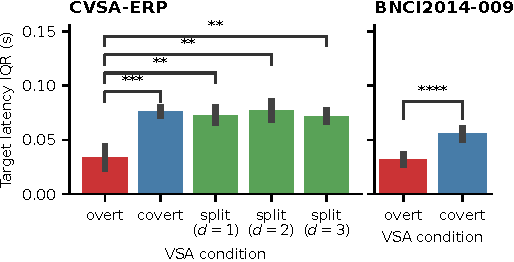
\includegraphics[width=\linewidth]{figures/covert_align/figure5c.pdf}
    \hspace{-0.24572736754045163in}
%%% Creator: Matplotlib, PGF backend
%%
%% To include the figure in your LaTeX document, write
%%   \input{<filename>.pgf}
%%
%% Make sure the required packages are loaded in your preamble
%%   \usepackage{pgf}
%%
%% Also ensure that all the required font packages are loaded; for instance,
%% the lmodern package is sometimes necessary when using math font.
%%   \usepackage{lmodern}
%%
%% Figures using additional raster images can only be included by \input if
%% they are in the same directory as the main LaTeX file. For loading figures
%% from other directories you can use the `import` package
%%   \usepackage{import}
%%
%% and then include the figures with
%%   \import{<path to file>}{<filename>.pgf}
%%
%% Matplotlib used the following preamble
%%   \def\mathdefault#1{#1}
%%   \everymath=\expandafter{\the\everymath\displaystyle}
%%   
%%   \ifdefined\pdftexversion\else  % non-pdftex case.
%%     \usepackage{fontspec}
%%   \fi
%%   \makeatletter\@ifpackageloaded{underscore}{}{\usepackage[strings]{underscore}}\makeatother
%%
\begingroup%
\makeatletter%
\begin{pgfpicture}%
\pgfpathrectangle{\pgfpointorigin}{\pgfqpoint{2.997033in}{1.668849in}}%
\pgfusepath{use as bounding box, clip}%
\begin{pgfscope}%
\pgfsetbuttcap%
\pgfsetmiterjoin%
\pgfsetlinewidth{0.000000pt}%
\definecolor{currentstroke}{rgb}{1.000000,1.000000,1.000000}%
\pgfsetstrokecolor{currentstroke}%
\pgfsetstrokeopacity{0.000000}%
\pgfsetdash{}{0pt}%
\pgfpathmoveto{\pgfqpoint{0.000000in}{0.000000in}}%
\pgfpathlineto{\pgfqpoint{2.997033in}{0.000000in}}%
\pgfpathlineto{\pgfqpoint{2.997033in}{1.668849in}}%
\pgfpathlineto{\pgfqpoint{0.000000in}{1.668849in}}%
\pgfpathlineto{\pgfqpoint{0.000000in}{0.000000in}}%
\pgfpathclose%
\pgfusepath{}%
\end{pgfscope}%
\begin{pgfscope}%
\pgfsetbuttcap%
\pgfsetmiterjoin%
\definecolor{currentfill}{rgb}{1.000000,1.000000,1.000000}%
\pgfsetfillcolor{currentfill}%
\pgfsetlinewidth{0.000000pt}%
\definecolor{currentstroke}{rgb}{0.000000,0.000000,0.000000}%
\pgfsetstrokecolor{currentstroke}%
\pgfsetstrokeopacity{0.000000}%
\pgfsetdash{}{0pt}%
\pgfpathmoveto{\pgfqpoint{0.229167in}{0.470139in}}%
\pgfpathlineto{\pgfqpoint{2.146685in}{0.470139in}}%
\pgfpathlineto{\pgfqpoint{2.146685in}{1.608911in}}%
\pgfpathlineto{\pgfqpoint{0.229167in}{1.608911in}}%
\pgfpathlineto{\pgfqpoint{0.229167in}{0.470139in}}%
\pgfpathclose%
\pgfusepath{fill}%
\end{pgfscope}%
\begin{pgfscope}%
\pgfpathrectangle{\pgfqpoint{0.229167in}{0.470139in}}{\pgfqpoint{1.917519in}{1.138772in}}%
\pgfusepath{clip}%
\pgfsetbuttcap%
\pgfsetmiterjoin%
\definecolor{currentfill}{rgb}{0.842157,0.553922,0.200980}%
\pgfsetfillcolor{currentfill}%
\pgfsetlinewidth{0.000000pt}%
\definecolor{currentstroke}{rgb}{0.000000,0.000000,0.000000}%
\pgfsetstrokecolor{currentstroke}%
\pgfsetstrokeopacity{0.000000}%
\pgfsetdash{}{0pt}%
\pgfpathmoveto{\pgfqpoint{0.316327in}{0.470139in}}%
\pgfpathlineto{\pgfqpoint{0.606860in}{0.470139in}}%
\pgfpathlineto{\pgfqpoint{0.606860in}{0.705246in}}%
\pgfpathlineto{\pgfqpoint{0.316327in}{0.705246in}}%
\pgfpathlineto{\pgfqpoint{0.316327in}{0.470139in}}%
\pgfpathclose%
\pgfusepath{fill}%
\end{pgfscope}%
\begin{pgfscope}%
\pgfpathrectangle{\pgfqpoint{0.229167in}{0.470139in}}{\pgfqpoint{1.917519in}{1.138772in}}%
\pgfusepath{clip}%
\pgfsetbuttcap%
\pgfsetmiterjoin%
\definecolor{currentfill}{rgb}{0.858824,0.314706,0.223529}%
\pgfsetfillcolor{currentfill}%
\pgfsetlinewidth{0.000000pt}%
\definecolor{currentstroke}{rgb}{0.000000,0.000000,0.000000}%
\pgfsetstrokecolor{currentstroke}%
\pgfsetstrokeopacity{0.000000}%
\pgfsetdash{}{0pt}%
\pgfpathmoveto{\pgfqpoint{0.679493in}{0.470139in}}%
\pgfpathlineto{\pgfqpoint{0.970026in}{0.470139in}}%
\pgfpathlineto{\pgfqpoint{0.970026in}{1.007696in}}%
\pgfpathlineto{\pgfqpoint{0.679493in}{1.007696in}}%
\pgfpathlineto{\pgfqpoint{0.679493in}{0.470139in}}%
\pgfpathclose%
\pgfusepath{fill}%
\end{pgfscope}%
\begin{pgfscope}%
\pgfpathrectangle{\pgfqpoint{0.229167in}{0.470139in}}{\pgfqpoint{1.917519in}{1.138772in}}%
\pgfusepath{clip}%
\pgfsetbuttcap%
\pgfsetmiterjoin%
\definecolor{currentfill}{rgb}{0.464706,0.320588,0.573529}%
\pgfsetfillcolor{currentfill}%
\pgfsetlinewidth{0.000000pt}%
\definecolor{currentstroke}{rgb}{0.000000,0.000000,0.000000}%
\pgfsetstrokecolor{currentstroke}%
\pgfsetstrokeopacity{0.000000}%
\pgfsetdash{}{0pt}%
\pgfpathmoveto{\pgfqpoint{1.042660in}{0.470139in}}%
\pgfpathlineto{\pgfqpoint{1.333193in}{0.470139in}}%
\pgfpathlineto{\pgfqpoint{1.333193in}{0.979341in}}%
\pgfpathlineto{\pgfqpoint{1.042660in}{0.979341in}}%
\pgfpathlineto{\pgfqpoint{1.042660in}{0.470139in}}%
\pgfpathclose%
\pgfusepath{fill}%
\end{pgfscope}%
\begin{pgfscope}%
\pgfpathrectangle{\pgfqpoint{0.229167in}{0.470139in}}{\pgfqpoint{1.917519in}{1.138772in}}%
\pgfusepath{clip}%
\pgfsetbuttcap%
\pgfsetmiterjoin%
\definecolor{currentfill}{rgb}{0.464706,0.320588,0.573529}%
\pgfsetfillcolor{currentfill}%
\pgfsetlinewidth{0.000000pt}%
\definecolor{currentstroke}{rgb}{0.000000,0.000000,0.000000}%
\pgfsetstrokecolor{currentstroke}%
\pgfsetstrokeopacity{0.000000}%
\pgfsetdash{}{0pt}%
\pgfpathmoveto{\pgfqpoint{1.405826in}{0.470139in}}%
\pgfpathlineto{\pgfqpoint{1.696359in}{0.470139in}}%
\pgfpathlineto{\pgfqpoint{1.696359in}{1.012421in}}%
\pgfpathlineto{\pgfqpoint{1.405826in}{1.012421in}}%
\pgfpathlineto{\pgfqpoint{1.405826in}{0.470139in}}%
\pgfpathclose%
\pgfusepath{fill}%
\end{pgfscope}%
\begin{pgfscope}%
\pgfpathrectangle{\pgfqpoint{0.229167in}{0.470139in}}{\pgfqpoint{1.917519in}{1.138772in}}%
\pgfusepath{clip}%
\pgfsetbuttcap%
\pgfsetmiterjoin%
\definecolor{currentfill}{rgb}{0.464706,0.320588,0.573529}%
\pgfsetfillcolor{currentfill}%
\pgfsetlinewidth{0.000000pt}%
\definecolor{currentstroke}{rgb}{0.000000,0.000000,0.000000}%
\pgfsetstrokecolor{currentstroke}%
\pgfsetstrokeopacity{0.000000}%
\pgfsetdash{}{0pt}%
\pgfpathmoveto{\pgfqpoint{1.768992in}{0.470139in}}%
\pgfpathlineto{\pgfqpoint{2.059526in}{0.470139in}}%
\pgfpathlineto{\pgfqpoint{2.059526in}{0.975797in}}%
\pgfpathlineto{\pgfqpoint{1.768992in}{0.975797in}}%
\pgfpathlineto{\pgfqpoint{1.768992in}{0.470139in}}%
\pgfpathclose%
\pgfusepath{fill}%
\end{pgfscope}%
\begin{pgfscope}%
\pgfsetbuttcap%
\pgfsetroundjoin%
\definecolor{currentfill}{rgb}{0.552941,0.501961,0.478431}%
\pgfsetfillcolor{currentfill}%
\pgfsetlinewidth{0.803000pt}%
\definecolor{currentstroke}{rgb}{0.552941,0.501961,0.478431}%
\pgfsetstrokecolor{currentstroke}%
\pgfsetdash{}{0pt}%
\pgfsys@defobject{currentmarker}{\pgfqpoint{0.000000in}{0.000000in}}{\pgfqpoint{0.000000in}{0.041667in}}{%
\pgfpathmoveto{\pgfqpoint{0.000000in}{0.000000in}}%
\pgfpathlineto{\pgfqpoint{0.000000in}{0.041667in}}%
\pgfusepath{stroke,fill}%
}%
\begin{pgfscope}%
\pgfsys@transformshift{0.461593in}{0.470139in}%
\pgfsys@useobject{currentmarker}{}%
\end{pgfscope}%
\end{pgfscope}%
\begin{pgfscope}%
\definecolor{textcolor}{rgb}{0.552941,0.501961,0.478431}%
\pgfsetstrokecolor{textcolor}%
\pgfsetfillcolor{textcolor}%
\pgftext[x=0.461593in,y=0.421528in,,top]{\color{textcolor}{\sffamily\fontsize{9.000000}{10.800000}\selectfont\catcode`\^=\active\def^{\ifmmode\sp\else\^{}\fi}\catcode`\%=\active\def%{\%}overt}}%
\end{pgfscope}%
\begin{pgfscope}%
\pgfsetbuttcap%
\pgfsetroundjoin%
\definecolor{currentfill}{rgb}{0.552941,0.501961,0.478431}%
\pgfsetfillcolor{currentfill}%
\pgfsetlinewidth{0.803000pt}%
\definecolor{currentstroke}{rgb}{0.552941,0.501961,0.478431}%
\pgfsetstrokecolor{currentstroke}%
\pgfsetdash{}{0pt}%
\pgfsys@defobject{currentmarker}{\pgfqpoint{0.000000in}{0.000000in}}{\pgfqpoint{0.000000in}{0.041667in}}{%
\pgfpathmoveto{\pgfqpoint{0.000000in}{0.000000in}}%
\pgfpathlineto{\pgfqpoint{0.000000in}{0.041667in}}%
\pgfusepath{stroke,fill}%
}%
\begin{pgfscope}%
\pgfsys@transformshift{0.824760in}{0.470139in}%
\pgfsys@useobject{currentmarker}{}%
\end{pgfscope}%
\end{pgfscope}%
\begin{pgfscope}%
\definecolor{textcolor}{rgb}{0.552941,0.501961,0.478431}%
\pgfsetstrokecolor{textcolor}%
\pgfsetfillcolor{textcolor}%
\pgftext[x=0.824760in,y=0.421528in,,top]{\color{textcolor}{\sffamily\fontsize{9.000000}{10.800000}\selectfont\catcode`\^=\active\def^{\ifmmode\sp\else\^{}\fi}\catcode`\%=\active\def%{\%}covert}}%
\end{pgfscope}%
\begin{pgfscope}%
\pgfsetbuttcap%
\pgfsetroundjoin%
\definecolor{currentfill}{rgb}{0.552941,0.501961,0.478431}%
\pgfsetfillcolor{currentfill}%
\pgfsetlinewidth{0.803000pt}%
\definecolor{currentstroke}{rgb}{0.552941,0.501961,0.478431}%
\pgfsetstrokecolor{currentstroke}%
\pgfsetdash{}{0pt}%
\pgfsys@defobject{currentmarker}{\pgfqpoint{0.000000in}{0.000000in}}{\pgfqpoint{0.000000in}{0.041667in}}{%
\pgfpathmoveto{\pgfqpoint{0.000000in}{0.000000in}}%
\pgfpathlineto{\pgfqpoint{0.000000in}{0.041667in}}%
\pgfusepath{stroke,fill}%
}%
\begin{pgfscope}%
\pgfsys@transformshift{1.187926in}{0.470139in}%
\pgfsys@useobject{currentmarker}{}%
\end{pgfscope}%
\end{pgfscope}%
\begin{pgfscope}%
\definecolor{textcolor}{rgb}{0.552941,0.501961,0.478431}%
\pgfsetstrokecolor{textcolor}%
\pgfsetfillcolor{textcolor}%
\pgftext[x=1.076257in, y=0.334722in, left, base]{\color{textcolor}{\sffamily\fontsize{9.000000}{10.800000}\selectfont\catcode`\^=\active\def^{\ifmmode\sp\else\^{}\fi}\catcode`\%=\active\def%{\%}split}}%
\end{pgfscope}%
\begin{pgfscope}%
\definecolor{textcolor}{rgb}{0.552941,0.501961,0.478431}%
\pgfsetstrokecolor{textcolor}%
\pgfsetfillcolor{textcolor}%
\pgftext[x=0.986917in, y=0.197917in, left, base]{\color{textcolor}{\sffamily\fontsize{9.000000}{10.800000}\selectfont\catcode`\^=\active\def^{\ifmmode\sp\else\^{}\fi}\catcode`\%=\active\def%{\%}($d=1$)}}%
\end{pgfscope}%
\begin{pgfscope}%
\pgfsetbuttcap%
\pgfsetroundjoin%
\definecolor{currentfill}{rgb}{0.552941,0.501961,0.478431}%
\pgfsetfillcolor{currentfill}%
\pgfsetlinewidth{0.803000pt}%
\definecolor{currentstroke}{rgb}{0.552941,0.501961,0.478431}%
\pgfsetstrokecolor{currentstroke}%
\pgfsetdash{}{0pt}%
\pgfsys@defobject{currentmarker}{\pgfqpoint{0.000000in}{0.000000in}}{\pgfqpoint{0.000000in}{0.041667in}}{%
\pgfpathmoveto{\pgfqpoint{0.000000in}{0.000000in}}%
\pgfpathlineto{\pgfqpoint{0.000000in}{0.041667in}}%
\pgfusepath{stroke,fill}%
}%
\begin{pgfscope}%
\pgfsys@transformshift{1.551093in}{0.470139in}%
\pgfsys@useobject{currentmarker}{}%
\end{pgfscope}%
\end{pgfscope}%
\begin{pgfscope}%
\definecolor{textcolor}{rgb}{0.552941,0.501961,0.478431}%
\pgfsetstrokecolor{textcolor}%
\pgfsetfillcolor{textcolor}%
\pgftext[x=1.439423in, y=0.334722in, left, base]{\color{textcolor}{\sffamily\fontsize{9.000000}{10.800000}\selectfont\catcode`\^=\active\def^{\ifmmode\sp\else\^{}\fi}\catcode`\%=\active\def%{\%}split}}%
\end{pgfscope}%
\begin{pgfscope}%
\definecolor{textcolor}{rgb}{0.552941,0.501961,0.478431}%
\pgfsetstrokecolor{textcolor}%
\pgfsetfillcolor{textcolor}%
\pgftext[x=1.350083in, y=0.197917in, left, base]{\color{textcolor}{\sffamily\fontsize{9.000000}{10.800000}\selectfont\catcode`\^=\active\def^{\ifmmode\sp\else\^{}\fi}\catcode`\%=\active\def%{\%}($d=2$)}}%
\end{pgfscope}%
\begin{pgfscope}%
\pgfsetbuttcap%
\pgfsetroundjoin%
\definecolor{currentfill}{rgb}{0.552941,0.501961,0.478431}%
\pgfsetfillcolor{currentfill}%
\pgfsetlinewidth{0.803000pt}%
\definecolor{currentstroke}{rgb}{0.552941,0.501961,0.478431}%
\pgfsetstrokecolor{currentstroke}%
\pgfsetdash{}{0pt}%
\pgfsys@defobject{currentmarker}{\pgfqpoint{0.000000in}{0.000000in}}{\pgfqpoint{0.000000in}{0.041667in}}{%
\pgfpathmoveto{\pgfqpoint{0.000000in}{0.000000in}}%
\pgfpathlineto{\pgfqpoint{0.000000in}{0.041667in}}%
\pgfusepath{stroke,fill}%
}%
\begin{pgfscope}%
\pgfsys@transformshift{1.914259in}{0.470139in}%
\pgfsys@useobject{currentmarker}{}%
\end{pgfscope}%
\end{pgfscope}%
\begin{pgfscope}%
\definecolor{textcolor}{rgb}{0.552941,0.501961,0.478431}%
\pgfsetstrokecolor{textcolor}%
\pgfsetfillcolor{textcolor}%
\pgftext[x=1.802590in, y=0.334722in, left, base]{\color{textcolor}{\sffamily\fontsize{9.000000}{10.800000}\selectfont\catcode`\^=\active\def^{\ifmmode\sp\else\^{}\fi}\catcode`\%=\active\def%{\%}split}}%
\end{pgfscope}%
\begin{pgfscope}%
\definecolor{textcolor}{rgb}{0.552941,0.501961,0.478431}%
\pgfsetstrokecolor{textcolor}%
\pgfsetfillcolor{textcolor}%
\pgftext[x=1.713250in, y=0.197917in, left, base]{\color{textcolor}{\sffamily\fontsize{9.000000}{10.800000}\selectfont\catcode`\^=\active\def^{\ifmmode\sp\else\^{}\fi}\catcode`\%=\active\def%{\%}($d=3$)}}%
\end{pgfscope}%
\begin{pgfscope}%
\definecolor{textcolor}{rgb}{0.552941,0.501961,0.478431}%
\pgfsetstrokecolor{textcolor}%
\pgfsetfillcolor{textcolor}%
\pgftext[x=1.187926in,y=0.111111in,,top]{\color{textcolor}{\sffamily\fontsize{9.000000}{10.800000}\selectfont\catcode`\^=\active\def^{\ifmmode\sp\else\^{}\fi}\catcode`\%=\active\def%{\%}VSA condition}}%
\end{pgfscope}%
\begin{pgfscope}%
\pgfsetbuttcap%
\pgfsetroundjoin%
\definecolor{currentfill}{rgb}{0.552941,0.501961,0.478431}%
\pgfsetfillcolor{currentfill}%
\pgfsetlinewidth{0.803000pt}%
\definecolor{currentstroke}{rgb}{0.552941,0.501961,0.478431}%
\pgfsetstrokecolor{currentstroke}%
\pgfsetdash{}{0pt}%
\pgfsys@defobject{currentmarker}{\pgfqpoint{0.000000in}{0.000000in}}{\pgfqpoint{0.041667in}{0.000000in}}{%
\pgfpathmoveto{\pgfqpoint{0.000000in}{0.000000in}}%
\pgfpathlineto{\pgfqpoint{0.041667in}{0.000000in}}%
\pgfusepath{stroke,fill}%
}%
\begin{pgfscope}%
\pgfsys@transformshift{0.229167in}{0.470139in}%
\pgfsys@useobject{currentmarker}{}%
\end{pgfscope}%
\end{pgfscope}%
\begin{pgfscope}%
\pgfsetbuttcap%
\pgfsetroundjoin%
\definecolor{currentfill}{rgb}{0.552941,0.501961,0.478431}%
\pgfsetfillcolor{currentfill}%
\pgfsetlinewidth{0.803000pt}%
\definecolor{currentstroke}{rgb}{0.552941,0.501961,0.478431}%
\pgfsetstrokecolor{currentstroke}%
\pgfsetdash{}{0pt}%
\pgfsys@defobject{currentmarker}{\pgfqpoint{0.000000in}{0.000000in}}{\pgfqpoint{0.041667in}{0.000000in}}{%
\pgfpathmoveto{\pgfqpoint{0.000000in}{0.000000in}}%
\pgfpathlineto{\pgfqpoint{0.041667in}{0.000000in}}%
\pgfusepath{stroke,fill}%
}%
\begin{pgfscope}%
\pgfsys@transformshift{0.229167in}{0.821371in}%
\pgfsys@useobject{currentmarker}{}%
\end{pgfscope}%
\end{pgfscope}%
\begin{pgfscope}%
\pgfsetbuttcap%
\pgfsetroundjoin%
\definecolor{currentfill}{rgb}{0.552941,0.501961,0.478431}%
\pgfsetfillcolor{currentfill}%
\pgfsetlinewidth{0.803000pt}%
\definecolor{currentstroke}{rgb}{0.552941,0.501961,0.478431}%
\pgfsetstrokecolor{currentstroke}%
\pgfsetdash{}{0pt}%
\pgfsys@defobject{currentmarker}{\pgfqpoint{0.000000in}{0.000000in}}{\pgfqpoint{0.041667in}{0.000000in}}{%
\pgfpathmoveto{\pgfqpoint{0.000000in}{0.000000in}}%
\pgfpathlineto{\pgfqpoint{0.041667in}{0.000000in}}%
\pgfusepath{stroke,fill}%
}%
\begin{pgfscope}%
\pgfsys@transformshift{0.229167in}{1.172602in}%
\pgfsys@useobject{currentmarker}{}%
\end{pgfscope}%
\end{pgfscope}%
\begin{pgfscope}%
\pgfsetbuttcap%
\pgfsetroundjoin%
\definecolor{currentfill}{rgb}{0.552941,0.501961,0.478431}%
\pgfsetfillcolor{currentfill}%
\pgfsetlinewidth{0.803000pt}%
\definecolor{currentstroke}{rgb}{0.552941,0.501961,0.478431}%
\pgfsetstrokecolor{currentstroke}%
\pgfsetdash{}{0pt}%
\pgfsys@defobject{currentmarker}{\pgfqpoint{0.000000in}{0.000000in}}{\pgfqpoint{0.041667in}{0.000000in}}{%
\pgfpathmoveto{\pgfqpoint{0.000000in}{0.000000in}}%
\pgfpathlineto{\pgfqpoint{0.041667in}{0.000000in}}%
\pgfusepath{stroke,fill}%
}%
\begin{pgfscope}%
\pgfsys@transformshift{0.229167in}{1.523834in}%
\pgfsys@useobject{currentmarker}{}%
\end{pgfscope}%
\end{pgfscope}%
\begin{pgfscope}%
\definecolor{textcolor}{rgb}{0.552941,0.501961,0.478431}%
\pgfsetstrokecolor{textcolor}%
\pgfsetfillcolor{textcolor}%
\pgftext[x=0.125000in,y=1.039525in,,bottom,rotate=90.000000]{\color{textcolor}{\sffamily\fontsize{9.000000}{10.800000}\selectfont\catcode`\^=\active\def^{\ifmmode\sp\else\^{}\fi}\catcode`\%=\active\def%{\%}Target latency IQR (s)}}%
\end{pgfscope}%
\begin{pgfscope}%
\pgfpathrectangle{\pgfqpoint{0.229167in}{0.470139in}}{\pgfqpoint{1.917519in}{1.138772in}}%
\pgfusepath{clip}%
\pgfsetrectcap%
\pgfsetroundjoin%
\pgfsetlinewidth{2.258437pt}%
\definecolor{currentstroke}{rgb}{0.260000,0.260000,0.260000}%
\pgfsetstrokecolor{currentstroke}%
\pgfsetdash{}{0pt}%
\pgfpathmoveto{\pgfqpoint{0.461593in}{0.635541in}}%
\pgfpathlineto{\pgfqpoint{0.461593in}{0.784403in}}%
\pgfusepath{stroke}%
\end{pgfscope}%
\begin{pgfscope}%
\pgfpathrectangle{\pgfqpoint{0.229167in}{0.470139in}}{\pgfqpoint{1.917519in}{1.138772in}}%
\pgfusepath{clip}%
\pgfsetrectcap%
\pgfsetroundjoin%
\pgfsetlinewidth{2.258437pt}%
\definecolor{currentstroke}{rgb}{0.260000,0.260000,0.260000}%
\pgfsetstrokecolor{currentstroke}%
\pgfsetdash{}{0pt}%
\pgfpathmoveto{\pgfqpoint{0.824760in}{0.978159in}}%
\pgfpathlineto{\pgfqpoint{0.824760in}{1.033687in}}%
\pgfusepath{stroke}%
\end{pgfscope}%
\begin{pgfscope}%
\pgfpathrectangle{\pgfqpoint{0.229167in}{0.470139in}}{\pgfqpoint{1.917519in}{1.138772in}}%
\pgfusepath{clip}%
\pgfsetrectcap%
\pgfsetroundjoin%
\pgfsetlinewidth{2.258437pt}%
\definecolor{currentstroke}{rgb}{0.260000,0.260000,0.260000}%
\pgfsetstrokecolor{currentstroke}%
\pgfsetdash{}{0pt}%
\pgfpathmoveto{\pgfqpoint{1.187926in}{0.928539in}}%
\pgfpathlineto{\pgfqpoint{1.187926in}{1.028961in}}%
\pgfusepath{stroke}%
\end{pgfscope}%
\begin{pgfscope}%
\pgfpathrectangle{\pgfqpoint{0.229167in}{0.470139in}}{\pgfqpoint{1.917519in}{1.138772in}}%
\pgfusepath{clip}%
\pgfsetrectcap%
\pgfsetroundjoin%
\pgfsetlinewidth{2.258437pt}%
\definecolor{currentstroke}{rgb}{0.260000,0.260000,0.260000}%
\pgfsetstrokecolor{currentstroke}%
\pgfsetdash{}{0pt}%
\pgfpathmoveto{\pgfqpoint{1.551093in}{0.954531in}}%
\pgfpathlineto{\pgfqpoint{1.551093in}{1.083308in}}%
\pgfusepath{stroke}%
\end{pgfscope}%
\begin{pgfscope}%
\pgfpathrectangle{\pgfqpoint{0.229167in}{0.470139in}}{\pgfqpoint{1.917519in}{1.138772in}}%
\pgfusepath{clip}%
\pgfsetrectcap%
\pgfsetroundjoin%
\pgfsetlinewidth{2.258437pt}%
\definecolor{currentstroke}{rgb}{0.260000,0.260000,0.260000}%
\pgfsetstrokecolor{currentstroke}%
\pgfsetdash{}{0pt}%
\pgfpathmoveto{\pgfqpoint{1.914259in}{0.940353in}}%
\pgfpathlineto{\pgfqpoint{1.914259in}{1.010088in}}%
\pgfusepath{stroke}%
\end{pgfscope}%
\begin{pgfscope}%
\pgfsetrectcap%
\pgfsetroundjoin%
\pgfsetlinewidth{1.003750pt}%
\definecolor{currentstroke}{rgb}{0.200000,0.200000,0.200000}%
\pgfsetstrokecolor{currentstroke}%
\pgfsetdash{}{0pt}%
\pgfpathmoveto{\pgfqpoint{0.461593in}{1.072317in}}%
\pgfpathlineto{\pgfqpoint{0.461593in}{1.136700in}}%
\pgfpathlineto{\pgfqpoint{0.824760in}{1.136700in}}%
\pgfpathlineto{\pgfqpoint{0.824760in}{1.072317in}}%
\pgfusepath{stroke}%
\end{pgfscope}%
\begin{pgfscope}%
\pgfsetrectcap%
\pgfsetroundjoin%
\pgfsetlinewidth{1.003750pt}%
\definecolor{currentstroke}{rgb}{0.200000,0.200000,0.200000}%
\pgfsetstrokecolor{currentstroke}%
\pgfsetdash{}{0pt}%
\pgfpathmoveto{\pgfqpoint{0.461593in}{1.203918in}}%
\pgfpathlineto{\pgfqpoint{0.461593in}{1.268301in}}%
\pgfpathlineto{\pgfqpoint{1.187926in}{1.268301in}}%
\pgfpathlineto{\pgfqpoint{1.187926in}{1.203918in}}%
\pgfusepath{stroke}%
\end{pgfscope}%
\begin{pgfscope}%
\pgfsetrectcap%
\pgfsetroundjoin%
\pgfsetlinewidth{1.003750pt}%
\definecolor{currentstroke}{rgb}{0.200000,0.200000,0.200000}%
\pgfsetstrokecolor{currentstroke}%
\pgfsetdash{}{0pt}%
\pgfpathmoveto{\pgfqpoint{0.461593in}{1.335519in}}%
\pgfpathlineto{\pgfqpoint{0.461593in}{1.399902in}}%
\pgfpathlineto{\pgfqpoint{1.551093in}{1.399902in}}%
\pgfpathlineto{\pgfqpoint{1.551093in}{1.335519in}}%
\pgfusepath{stroke}%
\end{pgfscope}%
\begin{pgfscope}%
\pgfsetrectcap%
\pgfsetroundjoin%
\pgfsetlinewidth{1.003750pt}%
\definecolor{currentstroke}{rgb}{0.200000,0.200000,0.200000}%
\pgfsetstrokecolor{currentstroke}%
\pgfsetdash{}{0pt}%
\pgfpathmoveto{\pgfqpoint{0.461593in}{1.467120in}}%
\pgfpathlineto{\pgfqpoint{0.461593in}{1.531503in}}%
\pgfpathlineto{\pgfqpoint{1.914259in}{1.531503in}}%
\pgfpathlineto{\pgfqpoint{1.914259in}{1.467120in}}%
\pgfusepath{stroke}%
\end{pgfscope}%
\begin{pgfscope}%
\pgfsetrectcap%
\pgfsetmiterjoin%
\pgfsetlinewidth{0.803000pt}%
\definecolor{currentstroke}{rgb}{0.552941,0.501961,0.478431}%
\pgfsetstrokecolor{currentstroke}%
\pgfsetdash{}{0pt}%
\pgfpathmoveto{\pgfqpoint{0.229167in}{0.470139in}}%
\pgfpathlineto{\pgfqpoint{0.229167in}{1.608911in}}%
\pgfusepath{stroke}%
\end{pgfscope}%
\begin{pgfscope}%
\pgfsetrectcap%
\pgfsetmiterjoin%
\pgfsetlinewidth{0.803000pt}%
\definecolor{currentstroke}{rgb}{0.552941,0.501961,0.478431}%
\pgfsetstrokecolor{currentstroke}%
\pgfsetdash{}{0pt}%
\pgfpathmoveto{\pgfqpoint{0.229167in}{0.470139in}}%
\pgfpathlineto{\pgfqpoint{2.146685in}{0.470139in}}%
\pgfusepath{stroke}%
\end{pgfscope}%
\begin{pgfscope}%
\definecolor{textcolor}{rgb}{0.552941,0.501961,0.478431}%
\pgfsetstrokecolor{textcolor}%
\pgfsetfillcolor{textcolor}%
\pgftext[x=0.643176in,y=1.150589in,,bottom]{\color{textcolor}{\sffamily\fontsize{10.000000}{12.000000}\selectfont\catcode`\^=\active\def^{\ifmmode\sp\else\^{}\fi}\catcode`\%=\active\def%{\%}***}}%
\end{pgfscope}%
\begin{pgfscope}%
\definecolor{textcolor}{rgb}{0.552941,0.501961,0.478431}%
\pgfsetstrokecolor{textcolor}%
\pgfsetfillcolor{textcolor}%
\pgftext[x=0.824760in,y=1.282190in,,bottom]{\color{textcolor}{\sffamily\fontsize{10.000000}{12.000000}\selectfont\catcode`\^=\active\def^{\ifmmode\sp\else\^{}\fi}\catcode`\%=\active\def%{\%}**}}%
\end{pgfscope}%
\begin{pgfscope}%
\definecolor{textcolor}{rgb}{0.552941,0.501961,0.478431}%
\pgfsetstrokecolor{textcolor}%
\pgfsetfillcolor{textcolor}%
\pgftext[x=1.006343in,y=1.413791in,,bottom]{\color{textcolor}{\sffamily\fontsize{10.000000}{12.000000}\selectfont\catcode`\^=\active\def^{\ifmmode\sp\else\^{}\fi}\catcode`\%=\active\def%{\%}**}}%
\end{pgfscope}%
\begin{pgfscope}%
\definecolor{textcolor}{rgb}{0.552941,0.501961,0.478431}%
\pgfsetstrokecolor{textcolor}%
\pgfsetfillcolor{textcolor}%
\pgftext[x=1.187926in,y=1.545392in,,bottom]{\color{textcolor}{\sffamily\fontsize{10.000000}{12.000000}\selectfont\catcode`\^=\active\def^{\ifmmode\sp\else\^{}\fi}\catcode`\%=\active\def%{\%}**}}%
\end{pgfscope}%
\begin{pgfscope}%
\pgfsetbuttcap%
\pgfsetmiterjoin%
\definecolor{currentfill}{rgb}{1.000000,1.000000,1.000000}%
\pgfsetfillcolor{currentfill}%
\pgfsetlinewidth{0.000000pt}%
\definecolor{currentstroke}{rgb}{0.000000,0.000000,0.000000}%
\pgfsetstrokecolor{currentstroke}%
\pgfsetstrokeopacity{0.000000}%
\pgfsetdash{}{0pt}%
\pgfpathmoveto{\pgfqpoint{2.230025in}{0.470139in}}%
\pgfpathlineto{\pgfqpoint{2.997033in}{0.470139in}}%
\pgfpathlineto{\pgfqpoint{2.997033in}{1.608911in}}%
\pgfpathlineto{\pgfqpoint{2.230025in}{1.608911in}}%
\pgfpathlineto{\pgfqpoint{2.230025in}{0.470139in}}%
\pgfpathclose%
\pgfusepath{fill}%
\end{pgfscope}%
\begin{pgfscope}%
\pgfpathrectangle{\pgfqpoint{2.230025in}{0.470139in}}{\pgfqpoint{0.767008in}{1.138772in}}%
\pgfusepath{clip}%
\pgfsetbuttcap%
\pgfsetmiterjoin%
\definecolor{currentfill}{rgb}{0.842157,0.553922,0.200980}%
\pgfsetfillcolor{currentfill}%
\pgfsetlinewidth{0.000000pt}%
\definecolor{currentstroke}{rgb}{0.000000,0.000000,0.000000}%
\pgfsetstrokecolor{currentstroke}%
\pgfsetstrokeopacity{0.000000}%
\pgfsetdash{}{0pt}%
\pgfpathmoveto{\pgfqpoint{2.264889in}{0.470139in}}%
\pgfpathlineto{\pgfqpoint{2.574792in}{0.470139in}}%
\pgfpathlineto{\pgfqpoint{2.574792in}{0.693995in}}%
\pgfpathlineto{\pgfqpoint{2.264889in}{0.693995in}}%
\pgfpathlineto{\pgfqpoint{2.264889in}{0.470139in}}%
\pgfpathclose%
\pgfusepath{fill}%
\end{pgfscope}%
\begin{pgfscope}%
\pgfpathrectangle{\pgfqpoint{2.230025in}{0.470139in}}{\pgfqpoint{0.767008in}{1.138772in}}%
\pgfusepath{clip}%
\pgfsetbuttcap%
\pgfsetmiterjoin%
\definecolor{currentfill}{rgb}{0.858824,0.314706,0.223529}%
\pgfsetfillcolor{currentfill}%
\pgfsetlinewidth{0.000000pt}%
\definecolor{currentstroke}{rgb}{0.000000,0.000000,0.000000}%
\pgfsetstrokecolor{currentstroke}%
\pgfsetstrokeopacity{0.000000}%
\pgfsetdash{}{0pt}%
\pgfpathmoveto{\pgfqpoint{2.652267in}{0.470139in}}%
\pgfpathlineto{\pgfqpoint{2.962169in}{0.470139in}}%
\pgfpathlineto{\pgfqpoint{2.962169in}{0.862361in}}%
\pgfpathlineto{\pgfqpoint{2.652267in}{0.862361in}}%
\pgfpathlineto{\pgfqpoint{2.652267in}{0.470139in}}%
\pgfpathclose%
\pgfusepath{fill}%
\end{pgfscope}%
\begin{pgfscope}%
\pgfsetbuttcap%
\pgfsetroundjoin%
\definecolor{currentfill}{rgb}{0.552941,0.501961,0.478431}%
\pgfsetfillcolor{currentfill}%
\pgfsetlinewidth{0.803000pt}%
\definecolor{currentstroke}{rgb}{0.552941,0.501961,0.478431}%
\pgfsetstrokecolor{currentstroke}%
\pgfsetdash{}{0pt}%
\pgfsys@defobject{currentmarker}{\pgfqpoint{0.000000in}{0.000000in}}{\pgfqpoint{0.000000in}{0.041667in}}{%
\pgfpathmoveto{\pgfqpoint{0.000000in}{0.000000in}}%
\pgfpathlineto{\pgfqpoint{0.000000in}{0.041667in}}%
\pgfusepath{stroke,fill}%
}%
\begin{pgfscope}%
\pgfsys@transformshift{2.419840in}{0.470139in}%
\pgfsys@useobject{currentmarker}{}%
\end{pgfscope}%
\end{pgfscope}%
\begin{pgfscope}%
\definecolor{textcolor}{rgb}{0.552941,0.501961,0.478431}%
\pgfsetstrokecolor{textcolor}%
\pgfsetfillcolor{textcolor}%
\pgftext[x=2.419840in,y=0.421528in,,top]{\color{textcolor}{\sffamily\fontsize{9.000000}{10.800000}\selectfont\catcode`\^=\active\def^{\ifmmode\sp\else\^{}\fi}\catcode`\%=\active\def%{\%}overt}}%
\end{pgfscope}%
\begin{pgfscope}%
\pgfsetbuttcap%
\pgfsetroundjoin%
\definecolor{currentfill}{rgb}{0.552941,0.501961,0.478431}%
\pgfsetfillcolor{currentfill}%
\pgfsetlinewidth{0.803000pt}%
\definecolor{currentstroke}{rgb}{0.552941,0.501961,0.478431}%
\pgfsetstrokecolor{currentstroke}%
\pgfsetdash{}{0pt}%
\pgfsys@defobject{currentmarker}{\pgfqpoint{0.000000in}{0.000000in}}{\pgfqpoint{0.000000in}{0.041667in}}{%
\pgfpathmoveto{\pgfqpoint{0.000000in}{0.000000in}}%
\pgfpathlineto{\pgfqpoint{0.000000in}{0.041667in}}%
\pgfusepath{stroke,fill}%
}%
\begin{pgfscope}%
\pgfsys@transformshift{2.807218in}{0.470139in}%
\pgfsys@useobject{currentmarker}{}%
\end{pgfscope}%
\end{pgfscope}%
\begin{pgfscope}%
\definecolor{textcolor}{rgb}{0.552941,0.501961,0.478431}%
\pgfsetstrokecolor{textcolor}%
\pgfsetfillcolor{textcolor}%
\pgftext[x=2.807218in,y=0.421528in,,top]{\color{textcolor}{\sffamily\fontsize{9.000000}{10.800000}\selectfont\catcode`\^=\active\def^{\ifmmode\sp\else\^{}\fi}\catcode`\%=\active\def%{\%}covert}}%
\end{pgfscope}%
\begin{pgfscope}%
\definecolor{textcolor}{rgb}{0.552941,0.501961,0.478431}%
\pgfsetstrokecolor{textcolor}%
\pgfsetfillcolor{textcolor}%
\pgftext[x=2.613529in,y=0.254861in,,top]{\color{textcolor}{\sffamily\fontsize{9.000000}{10.800000}\selectfont\catcode`\^=\active\def^{\ifmmode\sp\else\^{}\fi}\catcode`\%=\active\def%{\%}VSA condition}}%
\end{pgfscope}%
\begin{pgfscope}%
\pgfsetbuttcap%
\pgfsetroundjoin%
\definecolor{currentfill}{rgb}{0.552941,0.501961,0.478431}%
\pgfsetfillcolor{currentfill}%
\pgfsetlinewidth{0.803000pt}%
\definecolor{currentstroke}{rgb}{0.552941,0.501961,0.478431}%
\pgfsetstrokecolor{currentstroke}%
\pgfsetdash{}{0pt}%
\pgfsys@defobject{currentmarker}{\pgfqpoint{0.000000in}{0.000000in}}{\pgfqpoint{0.041667in}{0.000000in}}{%
\pgfpathmoveto{\pgfqpoint{0.000000in}{0.000000in}}%
\pgfpathlineto{\pgfqpoint{0.041667in}{0.000000in}}%
\pgfusepath{stroke,fill}%
}%
\begin{pgfscope}%
\pgfsys@transformshift{2.230025in}{0.470139in}%
\pgfsys@useobject{currentmarker}{}%
\end{pgfscope}%
\end{pgfscope}%
\begin{pgfscope}%
\pgfsetbuttcap%
\pgfsetroundjoin%
\definecolor{currentfill}{rgb}{0.552941,0.501961,0.478431}%
\pgfsetfillcolor{currentfill}%
\pgfsetlinewidth{0.803000pt}%
\definecolor{currentstroke}{rgb}{0.552941,0.501961,0.478431}%
\pgfsetstrokecolor{currentstroke}%
\pgfsetdash{}{0pt}%
\pgfsys@defobject{currentmarker}{\pgfqpoint{0.000000in}{0.000000in}}{\pgfqpoint{0.041667in}{0.000000in}}{%
\pgfpathmoveto{\pgfqpoint{0.000000in}{0.000000in}}%
\pgfpathlineto{\pgfqpoint{0.041667in}{0.000000in}}%
\pgfusepath{stroke,fill}%
}%
\begin{pgfscope}%
\pgfsys@transformshift{2.230025in}{0.821371in}%
\pgfsys@useobject{currentmarker}{}%
\end{pgfscope}%
\end{pgfscope}%
\begin{pgfscope}%
\pgfsetbuttcap%
\pgfsetroundjoin%
\definecolor{currentfill}{rgb}{0.552941,0.501961,0.478431}%
\pgfsetfillcolor{currentfill}%
\pgfsetlinewidth{0.803000pt}%
\definecolor{currentstroke}{rgb}{0.552941,0.501961,0.478431}%
\pgfsetstrokecolor{currentstroke}%
\pgfsetdash{}{0pt}%
\pgfsys@defobject{currentmarker}{\pgfqpoint{0.000000in}{0.000000in}}{\pgfqpoint{0.041667in}{0.000000in}}{%
\pgfpathmoveto{\pgfqpoint{0.000000in}{0.000000in}}%
\pgfpathlineto{\pgfqpoint{0.041667in}{0.000000in}}%
\pgfusepath{stroke,fill}%
}%
\begin{pgfscope}%
\pgfsys@transformshift{2.230025in}{1.172602in}%
\pgfsys@useobject{currentmarker}{}%
\end{pgfscope}%
\end{pgfscope}%
\begin{pgfscope}%
\pgfsetbuttcap%
\pgfsetroundjoin%
\definecolor{currentfill}{rgb}{0.552941,0.501961,0.478431}%
\pgfsetfillcolor{currentfill}%
\pgfsetlinewidth{0.803000pt}%
\definecolor{currentstroke}{rgb}{0.552941,0.501961,0.478431}%
\pgfsetstrokecolor{currentstroke}%
\pgfsetdash{}{0pt}%
\pgfsys@defobject{currentmarker}{\pgfqpoint{0.000000in}{0.000000in}}{\pgfqpoint{0.041667in}{0.000000in}}{%
\pgfpathmoveto{\pgfqpoint{0.000000in}{0.000000in}}%
\pgfpathlineto{\pgfqpoint{0.041667in}{0.000000in}}%
\pgfusepath{stroke,fill}%
}%
\begin{pgfscope}%
\pgfsys@transformshift{2.230025in}{1.523834in}%
\pgfsys@useobject{currentmarker}{}%
\end{pgfscope}%
\end{pgfscope}%
\begin{pgfscope}%
\pgfpathrectangle{\pgfqpoint{2.230025in}{0.470139in}}{\pgfqpoint{0.767008in}{1.138772in}}%
\pgfusepath{clip}%
\pgfsetrectcap%
\pgfsetroundjoin%
\pgfsetlinewidth{2.258437pt}%
\definecolor{currentstroke}{rgb}{0.260000,0.260000,0.260000}%
\pgfsetstrokecolor{currentstroke}%
\pgfsetdash{}{0pt}%
\pgfpathmoveto{\pgfqpoint{2.419840in}{0.661733in}}%
\pgfpathlineto{\pgfqpoint{2.419840in}{0.729103in}}%
\pgfusepath{stroke}%
\end{pgfscope}%
\begin{pgfscope}%
\pgfpathrectangle{\pgfqpoint{2.230025in}{0.470139in}}{\pgfqpoint{0.767008in}{1.138772in}}%
\pgfusepath{clip}%
\pgfsetrectcap%
\pgfsetroundjoin%
\pgfsetlinewidth{2.258437pt}%
\definecolor{currentstroke}{rgb}{0.260000,0.260000,0.260000}%
\pgfsetstrokecolor{currentstroke}%
\pgfsetdash{}{0pt}%
\pgfpathmoveto{\pgfqpoint{2.807218in}{0.829162in}}%
\pgfpathlineto{\pgfqpoint{2.807218in}{0.901263in}}%
\pgfusepath{stroke}%
\end{pgfscope}%
\begin{pgfscope}%
\pgfsetrectcap%
\pgfsetroundjoin%
\pgfsetlinewidth{1.003750pt}%
\definecolor{currentstroke}{rgb}{0.200000,0.200000,0.200000}%
\pgfsetstrokecolor{currentstroke}%
\pgfsetdash{}{0pt}%
\pgfpathmoveto{\pgfqpoint{2.419840in}{0.969590in}}%
\pgfpathlineto{\pgfqpoint{2.419840in}{1.083467in}}%
\pgfpathlineto{\pgfqpoint{2.807218in}{1.083467in}}%
\pgfpathlineto{\pgfqpoint{2.807218in}{0.969590in}}%
\pgfusepath{stroke}%
\end{pgfscope}%
\begin{pgfscope}%
\pgfsetrectcap%
\pgfsetmiterjoin%
\pgfsetlinewidth{0.803000pt}%
\definecolor{currentstroke}{rgb}{0.552941,0.501961,0.478431}%
\pgfsetstrokecolor{currentstroke}%
\pgfsetdash{}{0pt}%
\pgfpathmoveto{\pgfqpoint{2.230025in}{0.470139in}}%
\pgfpathlineto{\pgfqpoint{2.230025in}{1.608911in}}%
\pgfusepath{stroke}%
\end{pgfscope}%
\begin{pgfscope}%
\pgfsetrectcap%
\pgfsetmiterjoin%
\pgfsetlinewidth{0.803000pt}%
\definecolor{currentstroke}{rgb}{0.552941,0.501961,0.478431}%
\pgfsetstrokecolor{currentstroke}%
\pgfsetdash{}{0pt}%
\pgfpathmoveto{\pgfqpoint{2.230025in}{0.470139in}}%
\pgfpathlineto{\pgfqpoint{2.997033in}{0.470139in}}%
\pgfusepath{stroke}%
\end{pgfscope}%
\begin{pgfscope}%
\definecolor{textcolor}{rgb}{0.552941,0.501961,0.478431}%
\pgfsetstrokecolor{textcolor}%
\pgfsetfillcolor{textcolor}%
\pgftext[x=2.613529in,y=1.097356in,,bottom]{\color{textcolor}{\sffamily\fontsize{10.000000}{12.000000}\selectfont\catcode`\^=\active\def^{\ifmmode\sp\else\^{}\fi}\catcode`\%=\active\def%{\%}****}}%
\end{pgfscope}%
\end{pgfpicture}%
\makeatother%
\endgroup%

    \caption[Estimated jitter]{ Jitter characterized as the interquartile range (IQR)
	of target epochs for different \ac{vsa} conditions. Overt \ac{vsa} exhibits lower
   jitter than other conditions.
   Significance of differences
   was determined with two-sided Wilcoxon signed-rank tests with False Discovery
   Rate correction on per-subject jitter ($*= p<0.05$, $**=p<0.01$,
   $***=p<0.001$, $****=p<0.0001$).}
		\label{fig:jitter}
\end{figure}


Two-sided Wilcoxon rank-sum tests on jitter, expressed as the interquartile
range (IQR) of the estimated latencies of target trials, revealed that overt
\ac{vsa} exhibited significantly lower jitter than all other conditions for
both datasets, with jitter equal to overt: 32 ms and covert:
56 ms ($p<0.001$) for BNCI2014-009, and overt: 33 ms, covert: 77 ms ($p<0.001$),
split ($d=1$): 72 ms ($p=0.006$),
split ($d=2$): 77 ms ($p=0.002$)
and split ($d=3$): 72 ms ($p=0.002$)
for CVSA-ERP.
No other significant differences were found.
$p$-values were corrected for the family-wise error rate using Bonferroni
correction.

\section{Discussion}

\Cref{fig:covert-align/single-trial-roc-auc-diff} shows that \ac{wcble} significantly improves
covert \ac{vsa} decoding.
This is advantageous for the development of a class of \ac{erp}-\ac{bci} interfaces for
users who prefer to rest their gaze on a fixation cross on the screen,
avoiding the effort of redirecting their eye gaze for every selection.
Furthermore, the performance gain over the first-stage classifier in split
\ac{vsa} ($d=3$) and between-\ac{vsa} condition transfer settings are promising for
users with even less eye motor control who may experience involuntary eye
movements or fixation fatigue and hence cannot keep their gaze fixed throughout an
entire \ac{bci} operation session.
\ac{wcble} would allow them to operate a \ac{bci} comfortably while directing
their gaze to whichever portion of the screen they prefer, even when there is
another target present or this location varies during the
course of operation.
Although \ac{wcble} did not significantly improve overt \ac{vsa} single-trial decoding,
\cref{fig:covert-align/block-eval} shows that this does not negatively impact target
selection accuracy.
While target selection accuracy also did not improve for split \ac{vsa}, the
increase in single-trial performance in split ($d=3$) shows that an iterative
alignment procedure has the potential to improve over \ac{cble} and its first-stage
classifier in this case as well.


We believe the relative increase in performance of our proposed decoder in covert and
split \ac{vsa}, and the lack thereof in overt \ac{vsa}, could stem from the following:
\begin{enumerate*}[label=(\arabic*)]
  \item Covert and split \ac{vsa} exhibit higher P3 jitter than overt \ac{vsa}.
        In covert and split \ac{vsa}, participants have to execute a dual task by
        dissociating their visuospatial attention and gaze fixation.
        Evidence shows that \ac{erp} latency variability is
        higher when attention is divided~\cite{Polich2007,Arico2014}.
        \textcite{Arico2014} also partly attribute higher latency jitter to the covert \ac{vsa}
        task performed in the BNCI2014-009 dataset, since the GeoSpell interface
        requires both spatial and feature attention.
  \item In overt \ac{vsa}, the first-stage classifier can rely mostly on the modulation
        of early visually evoked potentials (VEPs) like N1 rather than on the
        P3~\cite{Treder2010}.
        These VEPs are closely related to visual processing, hence exhibit
        lower jitter, contrary to P3, which is more prone to the effects of
        attention and workload~\cite{Hu2010}, reducing the contribution of
        alignment.
  \item This property can also result in the estimation of VEP latencies
        instead of the P3 latency, and \ac{wcble} would in this case fail to
        increase the P3 \ac{snr}, which still could be somewhat jittered in overt
        \ac{vsa}.
  \item Aligning to the P3 will lower the \ac{snr} of early VEPs, while aligning to
        VEPs will lower P3 \ac{snr}, since they are not time-locked to each other.
	\item Covert and split \ac{vsa} \acp{erp} may exhibit lower \ac{snr} than overt
        \ac{vsa} due to lower P3 amplitudes or even due to the presence of higher P3
        jitter itself.
        Higher \ac{snr} in overt \ac{vsa} results in higher decoding performance of
        state-of-the-art classifiers, leaving less room for relative improvement
        in this case.
\end{enumerate*}

Although it is not immediately clear if \ac{wcble} actively corrects for higher P3 jitter
present in covert and split \ac{vsa} compared to overt \ac{vsa},
we justify our approach in a similar manner to \textcite{Hardiansyah2020} by
observing that the increased discrimination performance of a machine-learning
model accounting for jitter forgoes the need for characterizing the underlying
physiological processes, while still objectively quantifying the presence of
jitter between data classes.
Furthermore, some evidence points toward higher P3 jitter as the main
contributing factor.
While \autoref{fig:erps} shows no visible smearing effect in
the shape of the \acp{erp}, the more quantitative analysis on latencies
presented in \cref{sec:covert-align/results/jitter}
indicates the opposite.
Additionally, \textcite{Arico2014} prove that P3 jitter does play a
non-negligible role in covert \ac{vsa} by comparing performance between
overt and covert \ac{vsa}, while including or excluding early VEPs.
This analysis showed that the absence of the N1 and other early VEPs is not the
only factor hampering covert \ac{vsa} decoding performance.
However, the large increase in accuracy for covert \ac{vsa} reported by
\textcite{Arico2014} (60\% to 95\% with a window focusing on only the P3
component) could also be explained by overfitting on artifacts amplified by
aligning, since their method is not evaluated on unseen data, as opposed to ours.

We also argue that \ac{wcble} does not only enhance the P3 signal, but effectively reduces the
negative impact of noise that would otherwise mask the \ac{erp} response, thereby increasing the
discriminative ability of the decoder.
This process likely results in more reliable feature extraction, especially in conditions
with high jitter.

We found that \ac{cble} did not improve gaze-independent decoding performance
significantly and also did not increase performance over its first-stage
classifier in overt \ac{vsa}, contrary to what was reported by \textcite{Mowla2017}.
While they report that \ac{cble} is relatively independent of the
first-stage classifiers evaluated in their work, it is evident here that
applying any given classifier in the \ac{cble} scheme does not necessarily increase
its performance.
In our case, this could be due to characteristics of the tested dataset, e.g.,
the presence of jitter or the generally higher performance of \ac{tlda} compared to the
first-stage classifiers tested by \textcite{Mowla2017}, leaving less
performance to be gained.

\textcite{Thompson2012} already attempted applying \ac{cble} in an iterative scheme
but did not report any results due to convergence issues.
We mitigated this by combining the robust latency estimation presented in
\cref{sec:robust-latency} with the alignment of both target and non-target
epochs.
Aligning only the target epochs containing the jittered P3 component is prone to
overfitting by aligning non-discriminative noise that is present in both
classes, such as environment noise, oscillatory background rhythms, or
non-modulated VEPs.
If \ac{snr} is low, residual noise varying slightly between classes could dominate
the expected response of the first-stage classifier and subsequently dominate
\ac{wcble} from the start, preventing convergence to a meaningful solution.
Our procedure circumvents this problem by aligning both classes to the time
points where the expected separation between classes is greatest.
This way, noise of which the latencies are estimated in a given iteration will be
perfectly time-locked in all classes in the next
iteration.
The first-stage classifier can then more easily suppress this noise since it is
now clear it is present in both classes and non-discriminative.
This aids the method in converging to a more robust classifier by iteratively
increasing \ac{snr} for both classes and class separation over time.

\textcite{Zisk2022} addressed P3 jitter inparticipants \ac{als} by augmenting the
training data once with time-shifted copies based on \ac{cble}-estimated jitter.
While we aim to train the first-stage classifier without the effects of jitter
in its parameters, they do the opposite by intentionally jittering the
training data.
As their focus was on \ac{als} and inter-session stability, they
did not assess how their method interacts with visuospatial attention.
We achieved a similar performance gain with our jitter compensation method, but
argue that our method can cope with more granular latency differences, as
\textcite{Zisk2022} augment the data with just one positive and negative time
shift.

\textcite{Hardiansyah2020} decoded covert \ac{vsa} more effectively by
contributing single-trial latency and amplitude features for decoding.
Contrary to our approach, they did not correct these amplitude
features for the jitter in their latencies by, e.g., aligning trials to achieve
better separability.
Hence, their approach would not, in principle, render the classifier more robust
to jitter.
Furthermore, we incorporated estimated latency features in both \ac{cble} and \ac{wcble},
yet only \ac{wcble} improved covert \ac{vsa} performance.
This shows that the incorporation of latency features is not the only driver of
covert \ac{vsa} decoding performance increase.

Despite encouraging results, our study faces some limitations that we plan to
tackle in the future.
Firstly, multiple \ac{erp} components can be time-locked to different neural
processes, each with its own jitter, hampering the performance of
single-trial latency estimation and their interpretability.
Adaptations could be made to incorporate prior time windows or probability
distributions on the latency of specific \ac{erp} components or to simultaneously
estimate a set of multiple component (clusters) latencies per \ac{erp}, such as in Residue Iteration
Decomposition~\cite{Ouyang2017}.
Future efforts should investigate how strong
spatiotemporal filtering can be combined with methods that allow for a more
flexible non-stationarity of the \ac{erp}, like Dynamic Time Warping (DTW) or other
techniques borrowed from time series classification, or methods that explicitly model multiple time
displacements present in one \ac{erp}.


Secondly, performance might be improved by venturing beyond the classical
target/non-target binary classification problem.
Due to, for example, the perifoveal stimulus cruciform model~\cite{Vanegas2013}, covert and split \ac{vsa}
responses might differ based on the relative position in the field of view of
their related stimulus, which could be exploited in a multi-class classification
problem.
Similarly, explicitly taking into account the characteristics of the distractor \ac{erp}
response might have a beneficial effect.
Thirdly, results were obtained in an offline and within-session evaluation,
which does not reflect true \ac{bci} operation.
Using multiple sessions with online feedback, the user could optimize their
performance over time by controlling attention or gaze.
Finally, since this work was conducted with applications for individuals with
\ac{sspgi} in mind, we
should highlight that the gaze of participants in the conducted experiments was
cued and fixed, which is per definition impossible for the end user group we consider.
In \cref{sec:patients}, we present a study to further investigate whether the
studied \ac{vsa} conditions are appropriate and to what extent they occur when
individuals with \ac{sspgi} operate a \ac{bci}.

\section{Conclusion}

Our aim was to improve gaze-independent \ac{bci} performance for spatially
organized visual event-related potential (\ac{erp}) paradigms by using a suitable
decoder.
Earlier results on \ac{bci} performance in covert visuospatial attention
(\ac{vsa}) performance prediction have shown that accounting for single-trial
latency jitter could improve gaze-independent decoding performance.
We applied Classifier-based Latency Estimation (\ac{cble}) as a decoder robust to latency
jitter, but found no increase in gaze-independent decoding performance.
To remedy this, we improved \ac{cble} by adapting it into \ac{cble} with Woody
iterations (\ac{wcble}), an iterative scheme using probabilistic latency estimation.
Results for \ac{wcble} within and across \ac{vsa} condition decoding show that
gaze-independent \ac{bci} performance can be improved at the decoding stage.
Overt decoding performance was not improved, but our proposed method can
provide added value for users who are unable to operate a visual \ac{bci} in overt
attention mode.
Later studies should confirm whether our findings hold in individuals with
severe physical impairment and a variety of eye-motor impairments, and develop a
solution that is capable of properly handling multiple non-time-locked \ac{erp}
components.

\clearpage
\begin{subappendices}
  \section{Single-trial classification performances}
  \begin{table}[ht]
  \begin{tabular}{lccccccc}
\toprule
dataset & \multicolumn{2}{c}{BNCI2014-009} & \multicolumn{5}{c}{CVSA-ERP} \\
\cmidrule(lr){2-3} \cmidrule(lr){4-8}
VSA condition & overt & covert & overt & covert & split ($d=1$) & split ($d=2$) & split ($d=3$) \\
\midrule
ERPCov-TS-LR    & 0.9000     & 0.7450        & 0.7956     & 0.6880      & 0.6690      & 0.7252      & 0.7214 \\
XDAWNCov-TS-LR  & 0.9044     & 0.7464        & 0.8113     & 0.6780      & 0.6683      & 0.7259      & 0.7136 \\
tLDA            & 0.9474     & 0.7890        & 0.\bf 8660 & 0.7111      & \bf 0.7097      & 0.7550      & 0.7474 \\
CBLE            & \bf 0.9497 & 0.7928        & 0.8559     & 0.6977      & 0.7087  & 0.7467      & 0.7465 \\
WCBLE           & 0.9428     & \bf 0.8084    & 0.8525     & \bf 0.7338  & 0.7084      & \bf 0.7581  & \bf 0.7687 \\
\bottomrule
\end{tabular}

    \caption[Classification performances.]{Cross-validated single-trial
    classification \ac{rocauc} (\%) for all evaluated models, visuospatial attention conditions, and
    datasets.}
    \label{tab:covert-align/results/single-trial}
  \end{table}
  \clearpage
  \section{Cross-condition transfer classification performances}
  \begin{table}[ht]
      \sffamily
\small
\begin{tabularx}{\textwidth}{@{}XXrrrrrr@{}}
\toprule
  & test & overt & covert & \makecell[r]{split \\ ($d=1$)} & \makecell[r]{split
  \\($d=2$)} & \makecell[r]{split \\ ($d=3$)} & combined \\
classifier & train &  &  &  &  &  &  \\
\midrule
\multirow[t]{6}{*}{CBLE} & overt & 85.59 & 66.68 & 63.92 & 60.22 & 60.11 & 66.25 \\
 & covert & 68.51 & 69.77 & 70.52 & 68.50 & 70.29 & 75.08 \\
 & split ($d=1$) & 64.11 & 67.81 & 70.87 & 69.60 & 69.44 & 75.04 \\
 & split ($d=2$) & 60.48 & 67.59 & 69.99 & 74.67 & 72.88 & 75.96 \\
 & split ($d=3$) & 59.32 & 69.66 & 68.51 & 72.95 & 74.65 & 75.18 \\
 & combined & 68.77 & 73.71 & 74.36 & 76.41 & 75.14 & 72.73 \\
\midrule
\multirow[t]{6}{*}{tLDA} & overt & 86.60 & 67.40 & 64.15 & 59.80 & 59.39 & 66.85 \\
 & covert & 68.78 & 71.11 & 70.17 & 69.25 & 70.64 & 74.69 \\
 & split ($d=1$) & 65.72 & 68.00 & 70.97 & 70.53 & 69.52 & 75.07 \\
 & split ($d=2$) & 60.69 & 68.40 & 70.48 & 75.50 & 72.69 & 76.75 \\
 & split ($d=3$) & 59.37 & 69.10 & 69.40 & 72.56 & 74.74 & 75.61 \\
 & combined & 69.71 & 73.64 & 74.81 & 76.01 & 75.68 & 73.78 \\
\midrule
\multirow[t]{6}{*}{WCBLE} & overt & 85.25 & 68.80 & 66.07 & 63.02 & 62.22 & 68.60 \\
 & covert & 72.75 & 73.38 & 72.02 & 70.16 & 72.06 & 76.30 \\
 & split ($d=1$) & 68.07 & 70.04 & 70.84 & 72.42 & 71.05 & 75.56 \\
 & split ($d=2$) & 64.53 & 70.84 & 72.07 & 75.81 & 73.97 & 77.70 \\
 & split ($d=3$) & 63.79 & 72.21 & 70.57 & 72.80 & 76.87 & 76.05 \\
 & combined & 71.09 & 73.36 & 74.53 & 76.07 & 76.26 & 75.15 \\
\bottomrule
\end{tabularx}

      \caption[Transfer learning results for CVSA-ERP]{Cross-condition transfer
      classification performance (cross-validated \ac{rocauc})
      for all evaluated models in the CVSA-ERP dataset. Each decoder is trained
      on one \ac{vsa} condition and tested across all
      \ac{vsa}
      conditions to evaluate gaze-independence and transfer learning
      performance.}
  \end{table}
  \clearpage
  \begin{table}[ht]
      \sffamily
\small
\begin{tabular}{@{}llrrr@{}}
\toprule
 & test & overt & covert & combined \\
classifier & train &  &  &  \\
\midrule
\multirow[t]{3}{*}{CBLE} & overt & 94.97 & 63.59 & 83.13 \\
 & covert & 67.00 & 79.28 & 73.01 \\
 & combined & 93.81 & 73.36 & 83.17 \\
\midrule
\multirow[t]{3}{*}{tLDA} & overt & 94.74 & 62.22 & 82.70 \\
 & covert & 67.34 & 78.90 & 73.51 \\
 & combined & 94.01 & 72.55 & 83.16 \\
 \midrule
\multirow[t]{3}{*}{WCBLE} & overt & 94.28 & 65.04 & 82.51 \\
 & covert & 69.40 & 80.84 & 75.87 \\
 & combined & 92.77 & 76.10 & 84.20 \\
\bottomrule
\end{tabular}

      \caption[Transfer learning results for BNCI2014-009]{Cross-condition transfer
      classification performance (cross-validated \ac{rocauc})
      for all evaluated models in the CVSA-ERP dataset. Each decoder is trained
      on one \ac{vsa} condition and tested across all \ac{vsa}
      conditions to evaluate gaze-independence and transfer learning
      performance.}
  \end{table}
\end{subappendices}


\chapter{Case studies}
\label{sec:patients}
\section{Introduction}

\Acp{bci} for communication assistive technology~\cite{Millan2010}
target individuals with \acf{sspi}~\cite{Peters2022}.
Visual \acp{bci}, which rely on the interpretation of visual stimuli by the user,
offer several advantages in this context.
They can work with non-invasive recording technology and can use rapid
stimulation.
This makes them well-suited for real-time communication tasks.

Yet, there is a large comorbidity between \ac{sspi} and eye motor impairment~\cite{FriedOken2020}.
Impairments such as nystagmus (uncontrolled eye movements), diplopia (double
vision), and ophthalmoplegia (eye paralysis) can significantly hinder
the ability to use visual BCIs. These impairments make it difficult for
\ac{bci} users to focus on or track visual stimuli accurately, reducing their
performance with BCIs that rely on visual cues~\cite{McCane2014,FriedOken2020,Pasqualotto2015}.
Unfortunately, it is again for this group that eye tracking solutions also
perform poorly, making them more reliant on potential developments in \ac{bci}
that do not rely on eye gaze.

Eye motor impairments are presumed to reduce performance in operating visual
oddball \ac{bci}s (see \cref{sec:gaze-independent} for an overview), since users
cannot comfortably redirect their gaze at the desired target,
i.e., perform overt \ac{vsa}.
This is usually circumvented by designing gaze-independent~
\acp{bci}~\cite{Riccio2012}.
These interfaces either avoid visual stimulation or exploit some form of
covert \ac{vsa}, where the gaze and \ac{vsa} do not coincide.

Several studies with visual oddball \acp{bci} show that performance drops when not fixating the intended
target~\cite{Brunner2010, Treder2010, RonAngevin2019}, necessitating
gaze-independent solutions.
These studies build on the assumption that \ac{bci} users with \ac{sspgi}
would feel comfortable operating an interface in pure covert \ac{vsa} with
central fixation.
One could argue that a \ac{bci} that is only verified to work when central
fixation is maintained could also be considered gaze-dependent.
This does not account for the residual eye motor capabilities of most people
with \ac{sspi}, the (dis)comfort they experience while
performing gaze fixation and other confounding factors resulting from their eye
motility.

It is a striking constatation that studies reporting on
gaze-independent visual \ac{bci} with people with \ac{sspi} and eye-motor
impaired are very few.
Results are usually different from those obtained with healthy control
participants in the lab, due to difference in capabilities, brain
response, equipment and environment.

\textcite{Lesenfants2014} tested a gaze-independent \ac{ssvep} \ac{bci} in six
participants with \ac{lis} yet only exceeded chance level accuracy in two.
More recently, \textcite{Peters2020} performed a trial with two
participants with late-stage \ac{als} and visual impairment.
Their \ac{ssvep} interface was not optimized for gaze-independence, but the
system showed high accuracy, outperforming an eye tracking alternative.
It would be of interest to verify if such results can be replicated with
participants with other conditions, and with a visual oddball \acp{bci}.

\textcite{Orhan2012} and \textcite{Oken2014} tested the \ac{rsvp} speller with
individuals with \ac{lis}.

\textcite{Severens2014} evaluated the visual Hex-o-Spell~\cite{Treder2010} on 5
participants with \ac{als} and showed that this visual oddball interface optimized
for gaze-independence can outperform a tactile \ac{bci}.
While this speaks to the power of visual paradigms even in groups that are
expected to have eye motor impairment, they did not verify the gaze direction
of participants during the experiment.
It was suggested that participants were performing overtly.
Participants with \ac{als} also had a substantially lower accuracy than healthy
controls (58\% vs 88\%).

Our previous study, presented in \cref{sec:covert-align} also used the
visual Hex-o-Spell interface~\cite{VanDenKerchove2024}.
This work partially accounted for the idea that \ac{bci} users with \ac{sspgi} might
not fully rely on central gaze fixation and evaluated settings that are not
strictly dependent on this.
We showed gaze-independent performance can be improved in healthy subjects
using a suited decoding strategy that accounts for latency jitter in covert \ac{vsa} responses.
Yet, there is a strong need for verification of these results in an applied
setting with people with \ac{sspi}.

Eventually, one of the end goals of this research line is to develop
gaze-independent \ac{bci} for people that are fully locked-in and have no option left than to use a \ac{bci}.
However, this group is very small and it is often a challenge to recruit them
into a study and perform experiments with them~\cite{Wolpaw2006}.
Individuals with less severe paralysis or in less progressed disease stages that struggle with
eye-tracking technology could also benefit from
solutions tailored to their specific situation.
Therefore, we aim to apply the concepts from earlier work and literature to
people with \ac{sspi} and various degrees of motor impairment in a visual oddball
\ac{bci}.
The objectives of this case study are as follows:
\begin{enumerate*}
  \item Explore capabilities and experienced comfort of individuals with
    \ac{sspgi}, when operating a visual \ac{bci},
  \item evaluate the performance of a gaze-independent visual \ac{bci} for this
    group,
  \item verify if this performance can be improved with a suitable decoding
    strategy.
\end{enumerate*}


\section{Materials \& methods}
\subsection{Recruitment}
Participants were recruited from across the Neuromuscular Reference center at
University Hospital Leuven (Leuven, Belgium), TRAINM Neuro Rehab Clinics
(Antwerp, Belgium), the Neurorehabilitation Unit at University Hospital Lille
(Lille, France), and a specialized care home (France).
Experiments were performed under the supervision of their treating physician.
Participants were recruited based on the following criteria.
To qualify for inclusion, participants must:
\begin{enumerate}
	\item be at least 18 years old and no older than 60
	years,
  \item belong to class 2 or 3 according to the \ac{bci}	user selection criteria
    presented by~\textcite{Wolpaw2006},\label{item:patients/inclusion/wolpaw}
  \item have limitations to the extent or comfort of their eye motor control\label{item:patients/inclusion/oculomotor}
\end{enumerate}
Participants were excluded if they:
\begin{enumerate}
  \item have a diagnosis of a major medical condition, including any major
    neurological or psychiatric disorder other than those of interest based on
    inclusion criteria~\ref{item:patients/inclusion/wolpaw},
    and~\ref{item:patients/inclusion/oculomotor}\label{item:patients/exclusion/medical}
  \item have a predisposition to or have a history of any kind of epileptic seizures,
    including photosensitive epilepsy,\label{item:patients/exclusion/epilepsy}
  \item have a severe loss in vision or hearing that would significantly impair
        participation in the experiment,\label{item:patients/exclusion/vision}
  \item are currently using specific psychoactive medications or substances that could affect the outcome.\label{item:patients/exclusion/cognitive}
  \item be unable to understand the experiment instructions and cooperate,
  \item have any other limitations preventing them from performing the given task.
\end{enumerate}

In total, 11 individuals were contacted, of which one person with \ac{ms} was excluded based on
criterion~\ref{item:patients/exclusion/vision}, one person recovering from
\ac{tbi} on
both~\ref{item:patients/exclusion/epilepsy}
and~\ref{item:patients/exclusion/cognitive}, and one person recovering from
stroke based
on~\ref{item:patients/exclusion/medical}.
One further person recovering from a stroke was excluded due to technical
difficulties during the experimental session.
Vision was assessed using a LogMAR chart~\cite{Bailey1976}.

Ultimately, 7 participants were retained.
Of these, one participant was diagnosed with bulbar-onset \ac{als}, three with
\ac{fa} an three were recovering from stroke.
We refer to \cref{sec:gaze-independent/gaze-dependence/incidence} for a short
description of these conditions.
Table~\ref{tab:patients/patients} lists the included participants and their
diagnoses.

\newcommand{\fnkuebler}{%
  \footnote{
``With minor degree of impairment,
we refer to patients who had only slightly impaired limb movement
and normal speech. Under the category moderate impairment, we
summarized those patients with restricted limb movement (wheelchair-bound) and
unaffected speech or intact limb movement without speech (such as the bulbar form of ALS which first affects speech
and swallowing). Patients who were almost tetraplegic with restricted speech were considered majorly impaired. Categories four
and five were the LIS and the CLIS, respectively."~\cite{Kuebler2008}
  }
}
\begin{table}[t]
  \centering
  \makebox[\textwidth][c]{%
  \footnotesize
  \begin{tabular}{llllllllr}
  \toprule
  \textbf{ID}  & \textbf{Age} & \textbf{Sex} & \textbf{Hand.} &
  \textbf{Diagnosis}
  & \textbf{Speech}     & \textbf{Trach.} & \textbf{Communication}          &
  \textbf{Cls.} \\ \midrule
  PA1 & 58  & M   & L     & bulbar-onset \acs{als} & anarthric  & no          & tablet                 & 3  \\
  PB1 & 41  & M   & L     & \acs{fa} & dysarthric & no          & verbal                 & 3  \\
  PB2 & 43  & F   & R     & \acs{fa} & dysarthric & no          & verbal                 & 3  \\
  PB4 & 48  & M   & R     & \acs{fa} & dysarthric & no          & verbal                 & 3  \\
  PC2 & 43  & M   & R     & brainstem stroke & anarthric  & yes         & \makecell[l]{prompting\\+eye movement} & 2 \\
  PC3 & 43  & F   & R     & brainstem stroke & anarthric  & yes         & letterboard            & 2 \\
  PC4 & 54  & M   & R     & \makecell[l]{left cerebellar stroke \\ (trombosis of the basilar artery)} & anarthric  & yes & letterboard & 2 \\
  \bottomrule
\end{tabular}

  }
  \caption[Included participants with their diagnosis and
  capabilities.]{Included participants with their diagnosis and
  capabilities.
  Trach.: underwent a tracheostomy, Cls. W: classification according
  to~\textcite{Wolpaw2006}, Cls. KB: classification according
  to~\textcite{Kuebler2008}\fnkuebler.
  }
  \label{tab:patients/patients}
\end{table}
%\todo{include years since diagnosis}


\subsection{Visual skills and eye tracking and eye motor examination}

Self-reported eye motor and visual abnormalities were recorded according to the
relevant visual \ac{bci} skills presented by~\textcite{FriedOken2020}.
These include visual acuity, visual fixation, eyelid function, ocular motility,
binocular vision, and field of vision.
Additionally, participants and their caregivers were asked about eye tremors
(nystagmus or other) and other involuntary eye movements.

As an objective metric, we implemented and performed the automated NeuroEye eye movement
test proposed by~\textcite{Hassan2022} using calibration-free eye tracking to
check if it revealed any further eye motor abnormalities.
This was not the case.

Table~\ref{tab:patients/eye} details the eye motor impairments and vision of
the included participants.
All participants reported some degree of fatigue or discomfort when fixating.
Participant PA1 had the mildest impairment, only reporting fatigue when fixating
for prolonged times.
The \ac{fa} participants were mostly affected by eye tremors and impaired pursuit.
PB2 suffered from especially severe horizontal oscillating involuntary eye
movements.
Eye motor function of participants PC2, PC3, and PC4 was most severely affected.
Participant PC2 was only able to look up and down and had a deviation in the
left eye causing diplopia, but this was corrected by a prism glass.
Participant PC3 only retained partial motility of the right eye, while the left eye was permanently closed.
Participant PC4 had one deviated eye with a corneal abscess affecting the motility
and vision in the right eye, and reducing motility in the left.

\begin{table}[t]
  \centering
  \footnotesize
  % \begin{tabular}{lll}
%  \toprule
%  \textbf{ID} & \textbf{Oculomotor impairment} & \textbf{Vision (LogMAR)} \\ \midrule
%  PA1  & fixation fatigue & 0.0 \\
%  PB1  & impaired pursuit, fixation fatigue, fixation discomfort, tremor & 0.0 \\
%  PB2  & fixation fatigue, fixation discomfort, tremor & 0.6 \\
%  PB4  & impaired pursuit, fixation fatigue, fixation discomfort, tremor & 0.2 \\
%  PC2  & \makecell[l]{partial ophthalmoplegia (up-down preserved), \\ fixation
%  fatigue, fixation discomfort, tremor} & \makecell[l]{0.0, diplopia corrected \\ with prism glass)} \\
%  PC3  & \makecell[l]{right ophthalmoplegia, left partial ophthalmoplegia, \\ fixation fatigue, fixation discomfort, tremor} & 0.7, right eye closed \\
%  PC4  & deviation of the left eye & 0.6 \\
%  \bottomrule
%\end{tabular}
\footnotesize
\let\oldarraystretch\arraystretch
\renewcommand{\arraystretch}{2}
\newcommand{\skill}{\cellcolor{lightgray}}
\newcommand{\noskill}{\cellcolor{accent1}\textcolor{muteblack}{\BigCross}}
\newcommand{\snoskill}{\cellcolor{accent2}\textcolor{muteblack}{\BigDiamondshape}}
\begin{tabular}{r|ccccccc}
                          & PA1      & PB1      & PB2       & PB4      & PC2       & PC3       & PC4 \\ \hline
  Visual fixation         & \noskill & \noskill & \noskill  & \noskill & \noskill  & \noskill  & \noskill \\
  Eyelid function         & \skill   & \skill   & \skill    & \skill   & \noskill  & \noskill  & \skill \\
  Ocular motility         & \skill   & \noskill & \skill    & \noskill & \snoskill & \snoskill & \noskill\\
  Binocular vision        & \skill   & \skill   & \skill    & \skill   & \noskill  & \snoskill & \snoskill \\
  Field of vision         & \skill   & \skill   & \skill    & \skill   & \skill    & \noskill  & \noskill \\
  Involuntary movement    & \skill   & \noskill & \noskill  & \noskill & \noskill  & \noskill  & \skill \\ \hline
  Visual acuity   & 0.0      & 0.0      & 0.6       & 0.2      & 0.0       & 0.7  & 0.6\\
\end{tabular}

  \caption[Visual skills of the included participants.]{%
  Visual skills of the included participants.
  Visual~\ac{bci} skills~\cite{FriedOken2020}
  were assessed with a combination of self-reported issues
  by the subject and the NeuroEye~\cite{Hassan2022} test. \BigCross\
  impaired, \BigDiamondshape\ severely impaired.
  logMAR: lower is better.}
  \label{tab:patients/eye}
\end{table}
\todo{where these values corrected for distance?}

Finally, we also recorded gaze position throughout the experimental session to
register the participant's gaze relative to the stimulated \ac{bci} targets.

\subsection{\Ac{bci} stimulation}

The \ac{bci} stimulation procedure was based on the
Hex-o-Spell~\cite{Treder2010} implementation presented
by~\textcite{VanDenKerchove2024}.
Similar to this study, the task consists of counting the flashes of a cued
target among 6 round, flashing targets laid out in a hexagonal pattern in the
field of view of the user.
We refer to \cref{sec:covert-align/stimulation} for implementation details.

Three different \ac{vsa} settings were explored.
In the overt \ac{vsa} setting, the participant was instructed to fixate on the cued target or
try to the maximum extent of their visual skill, even if experiencing slight
discomfort.
In the covert \ac{vsa} setting, the participant was instructed to fixate on the center of the
screen, to the extent of their ability.
An additional \emph{free \ac{vsa}} setting was introduced.
Here, the participant was instructed to perform the task as they deemed most
comfortable.
This allowed us to investigate the user's natural way of operating the \ac{bci}
given their individual set of visual skills.
If the participant was not fully paralyzed, they were instructed not to move their head.
The cued \emph{split attention} setting proposed
by~\textcite{VanDenKerchove2024} was not studied here, as we were interested
in natural \ac{vsa} operation settings for gaze-impaired individuals.

To make the interface suitable for use by individuals with
\ac{sspi}~\cite{FriedOken2020}, the
number of blocks was decreased to 6 per \ac{vsa} setting.
\Ac{isi} was increased to $200\pm50$ms to decrease task difficulty.
The experiment also started with a training block in each condition, where the
participant was instructed with feedback on their performance to ensure they
understood and were able to perform the task.

\begin{figure}
  \begin{minipage}{.45\textwidth}
    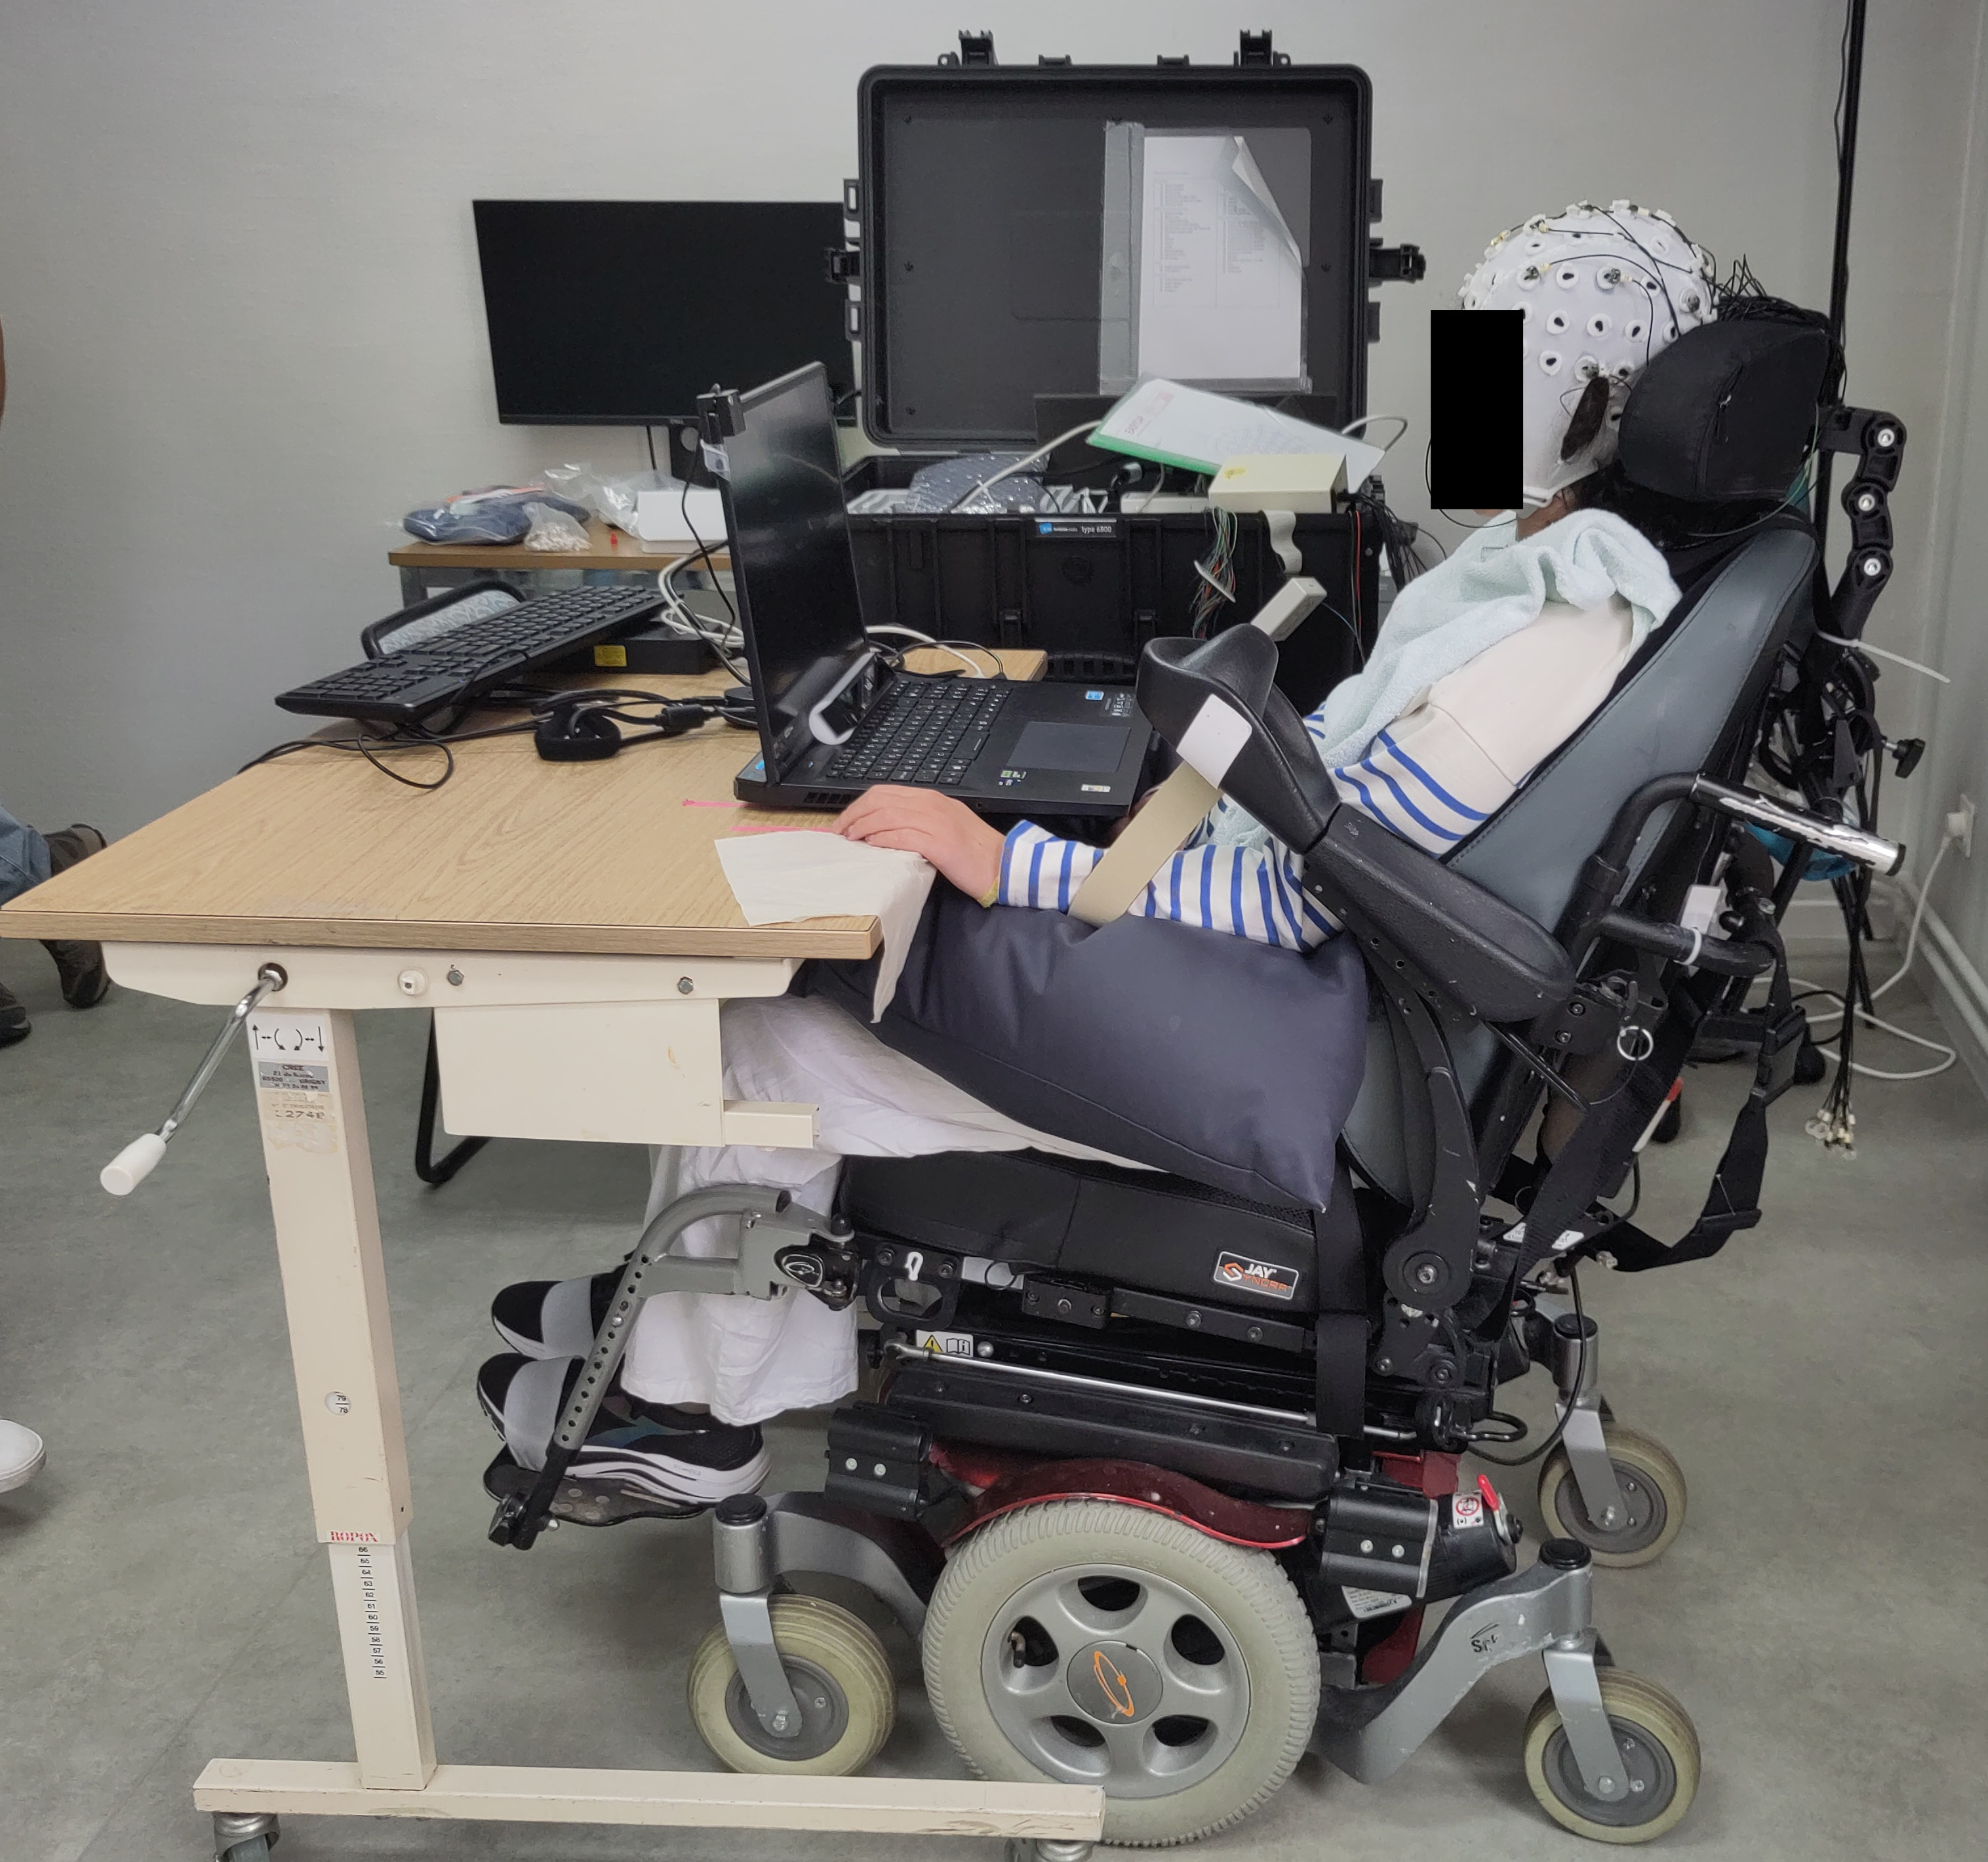
\includegraphics[width=\textwidth]{figures/patients/PD01a-obfuscated.jpg}
  \end{minipage}\hfill%
  \begin{minipage}{.45\textwidth}
    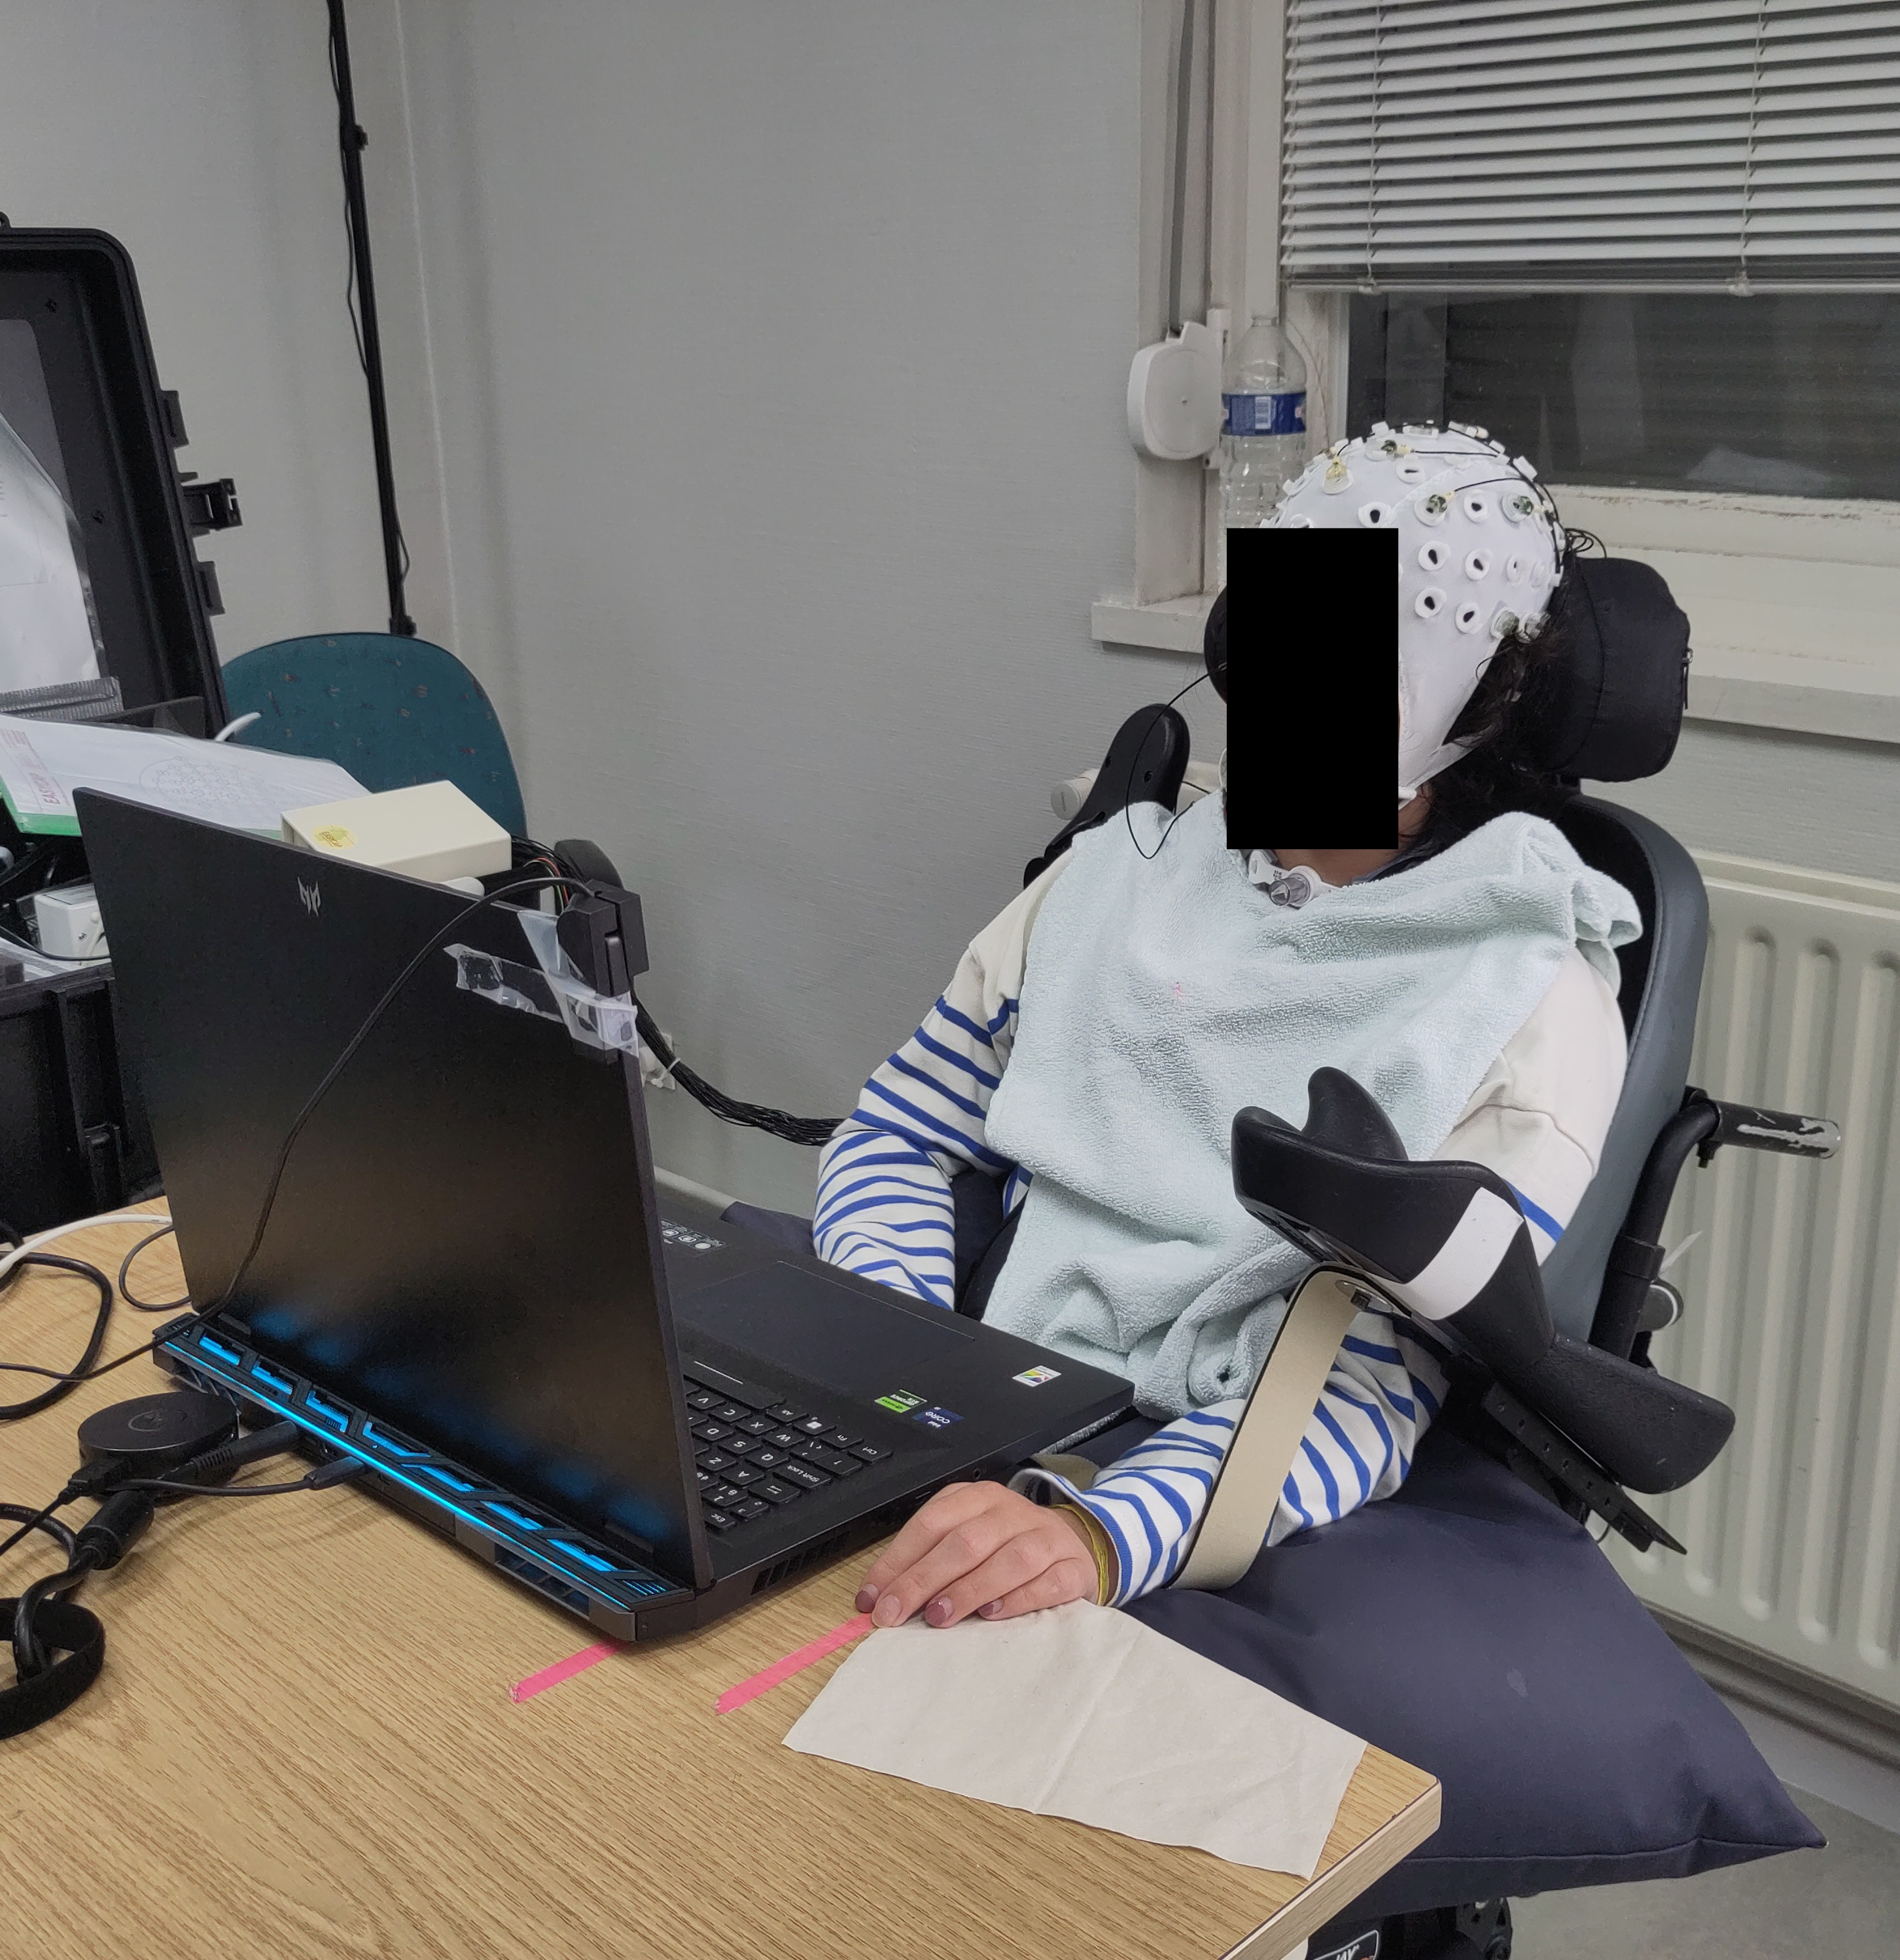
\includegraphics[width=\textwidth]{figures/patients/PD01b-obfuscated.jpg}
  \end{minipage}
  \caption{A participant with the stimulation and recording setup.}
\end{figure}

\subsection{Data collection \& preprocessing}

During the recording session, participants were positioned in their wheelchair in front of a table.
Stimuli were presented on an Acer Predator Helios laptop with an 18" screen (Acer,
Inc., Taiwan) placed at a 60 cm distance.
A Cedrus StimTracker (Cedrus Corp., CA, USA) ensured synchronization of stimuli with the
recorded \ac{eeg}.
Eye tracking was performed throughout using the Tobii X2-30 Compact (Tobii
Technology AB, Sweden) portable eye tracker placed at the bottom of the laptop screen.

\Ac{eeg} was recorded at 1000 Hz using the Neuroscan Neuvo portable amplifier (Compumedics Neuroscan,
Australia) connected to a second laptop for registration.
The \ac{eeg} headset used 18 active AgCl electrodes (EASYCAP GmbH, Germany) placed on a cap
according to the international 10-20 layout.
Using electrolyte gel, electrode impedances were reduced below 10k$\Omega$.
Additionally, the \ac{eog} was recorded.

The \ac{eeg} was band-pass filtered between 0.5 and 16 Hz.
Bad channels were rejected using the RANSAC algorithm~\cite{Fischler1981}
and visual inspection.
Next, the \ac{eeg} was re-referenced to the average of mastoid electrodes TP9
and TP10, and \ac{ica} was performed to reject artifactual components based on
correlation with the \ac{eog} or by visual inspection.
Epochs were cut from -0.1 to 0.9s relative to stimulus onset, and no baseline
correction was performed.

Eye tracking data was cleaned by fusing left and right gaze into one channel
for the horizontal and vertical gaze position.
If both were present for a given sample, the fused channel was the mean of both
values.
If at a given sample either the left or the right eye was not detected for a
given channel, the value of the other one was adopted.
If both were missing, the gaze position remained unset at that time point, and no
interpolation was performed.

\subsection{\Acs{bci} decoding}

We evaluated the recorded data using the \ac{wcble}~\cite{VanDenKerchove2024}
and \ac{tlda}~\cite{Sosulski2022}
classifiers, as well as the Riemannian XDAWNCov+TS+LDA~\cite{Cecotti2017}.
For \ac{wcble}, a region of interest from 0 ms to 800 ms relative to stimulus
onset was used while the epoch was cropped to -100 ms to 900 ms. For the other
decoders, the epoch was cropped between 0 ms and 800 ms, which resulted in maximal
performance.
Decoding scores were obtained using 6-fold cross-validation where folds corresponded to
stimulation blocks.

\section{Outcomes}

\subsection{Eye tracking analysis}
\label{sec:patients/outcomes/gaze}

First, we aimed to shed more light on the actual capabilities of individuals
with \ac{sspgi} regarding performing overt \ac{vsa} and central gaze
fixation, as well as to investigate how relevant these two settings are when the
gaze is not cued.
\Cref{fig:patients/gaze} maps gaze position relative to the stimuli
across conditions.
These results should be interpreted with care, as the eye tracker to some
degree relies on functioning eye motility.
The participant's position relative to the eye tracker might have shifted
throughout the experimental session despite our best efforts, e.g., because they needed aspiration of their
tracheostomy.

\fullpagefig{%
  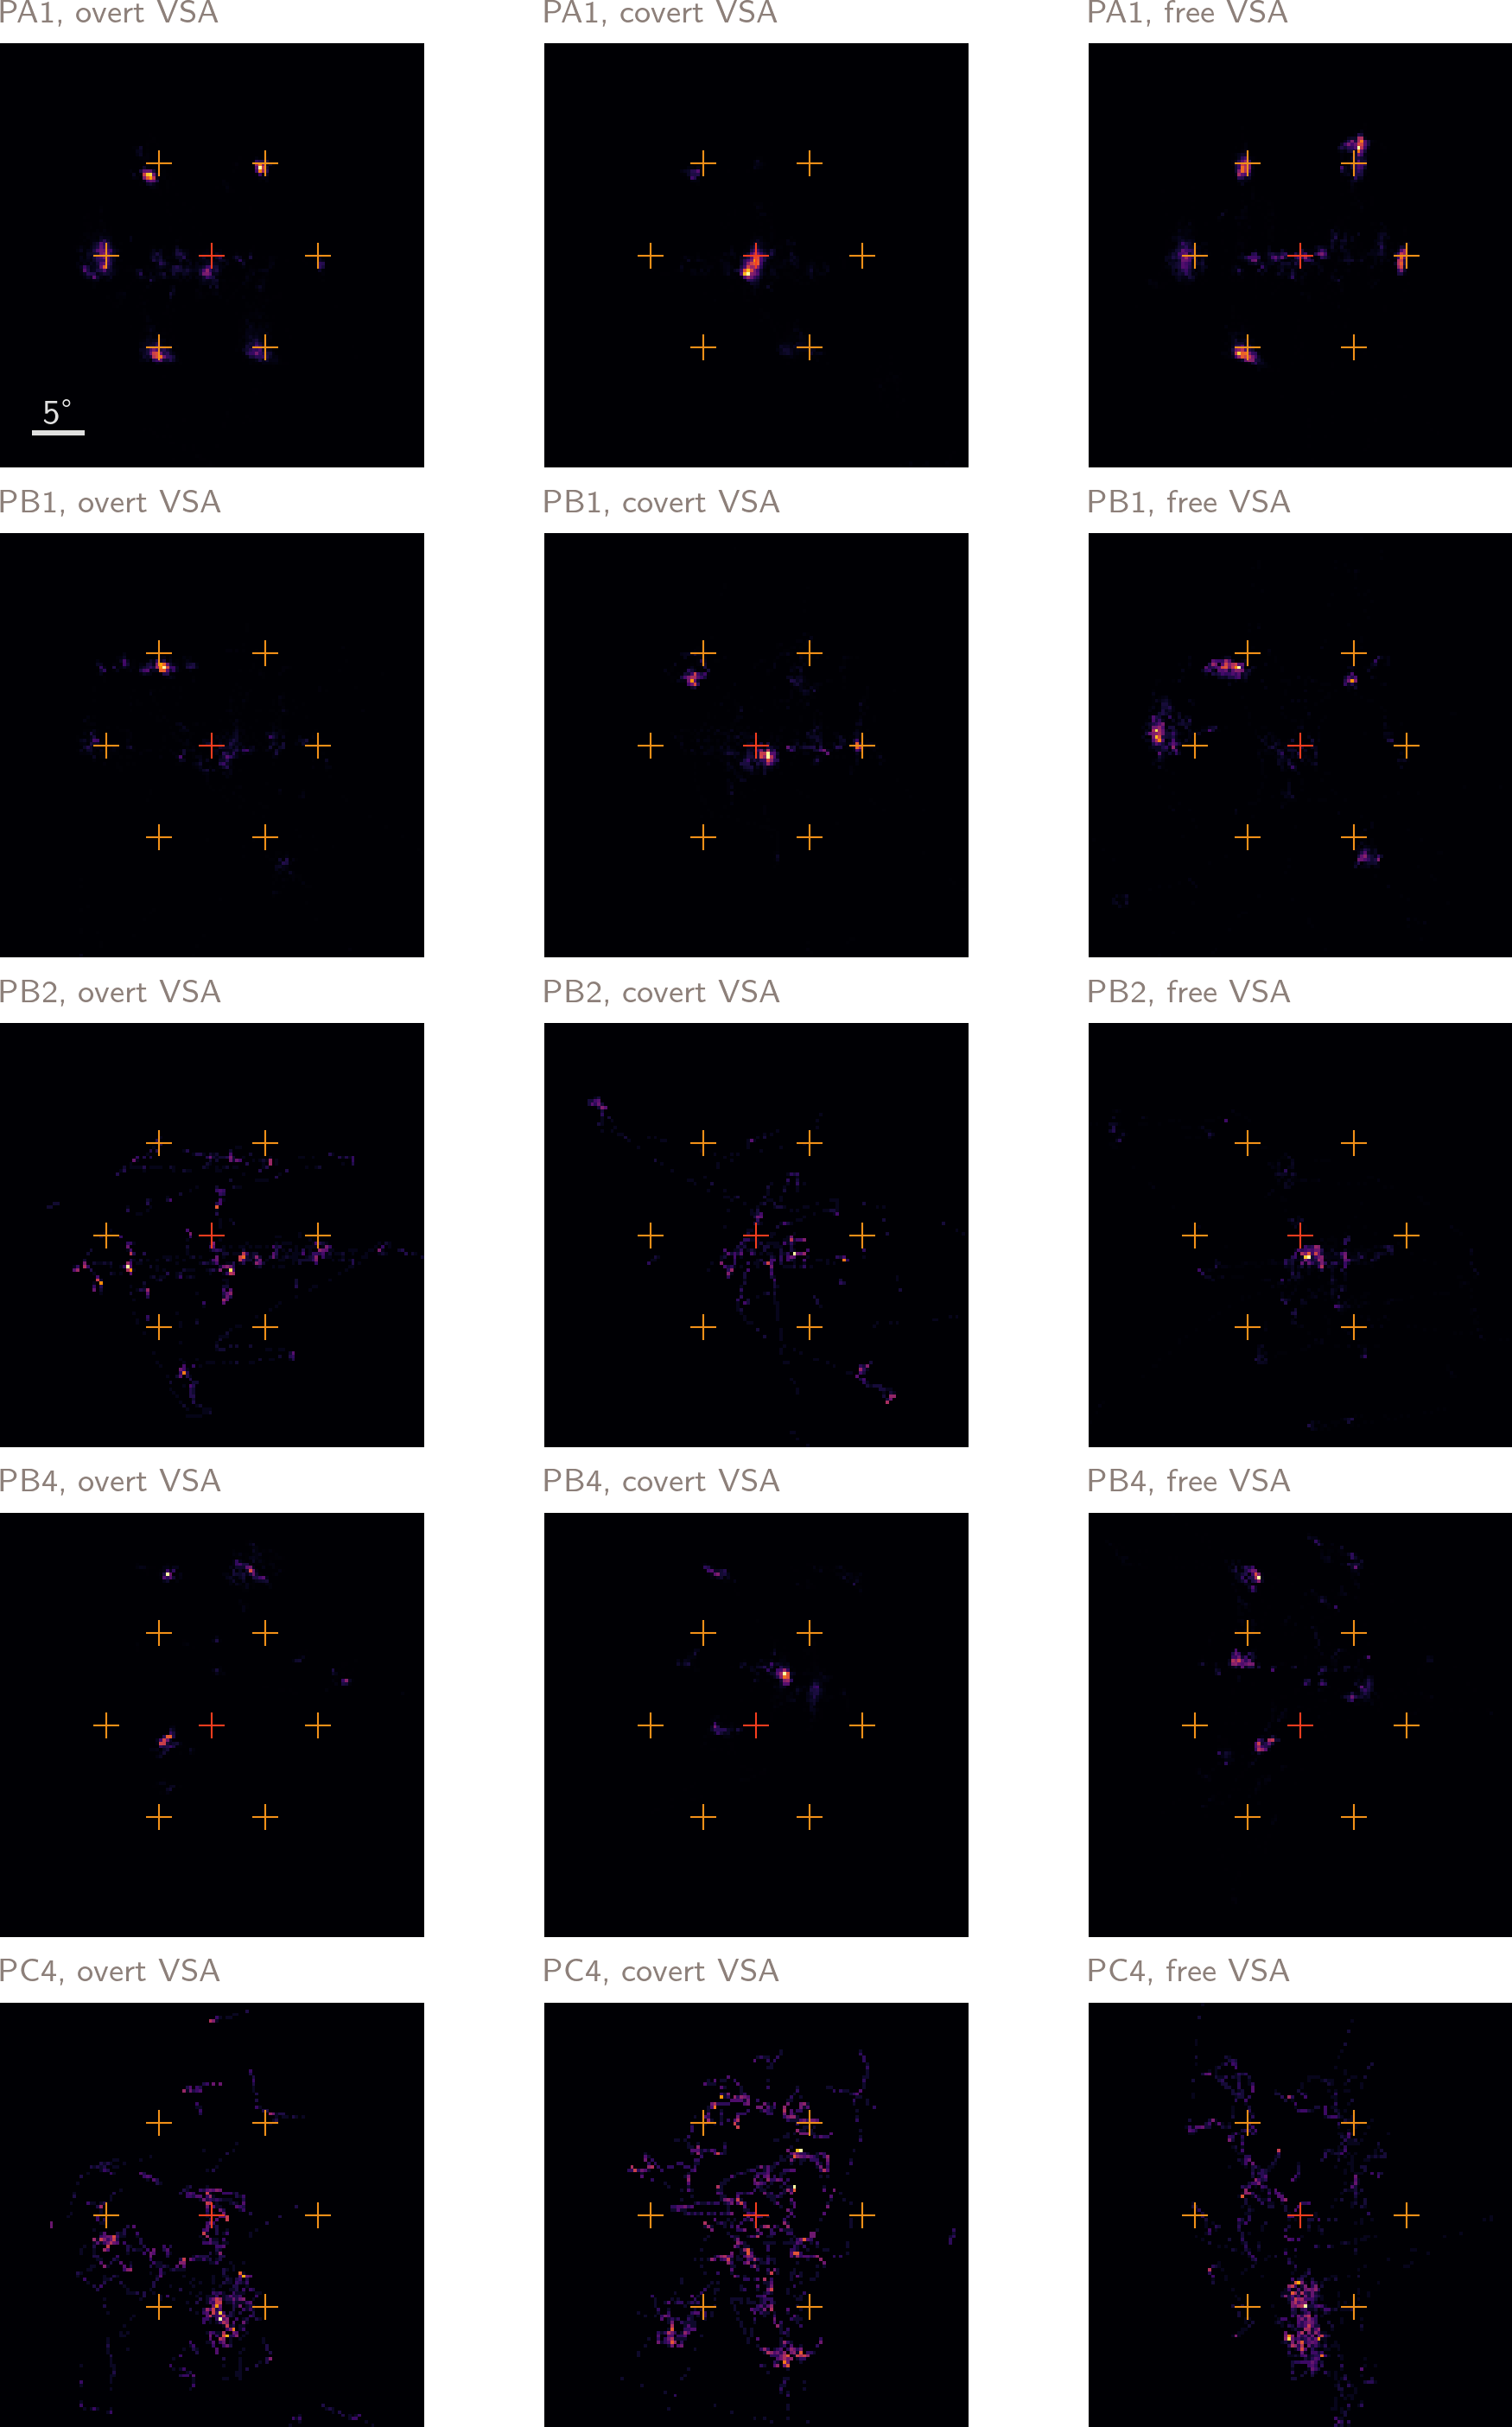
\includegraphics[width=\textwidth]{figures/patients/fig_gaze.png}
}{%
  Distribution of the recorded gaze position.
}{%
  Distribution of the recorded gaze position during the experimental session in the three \ac{vsa}
  conditions.
  Crosshairs represent stimulus positions, with the orange ones cued during
  the given condition.
  Subjects PB2 and PC4 preferred covert \ac{bci} operation, with PB2 resting gaze
  near the middle of the screen, and PC4 near the bottom.
}{fig:patients/gaze}

PA1 had relatively intact gaze control and was able to correctly perform the
cued overt and covert settings.
When gaze was uncued, he fixated on the cued target.
This was also mostly the case for PB1, although eye tracking revealed that he
chose not to perform central gaze fixation when cued in at least one of the
stimulation blocks. We were unable to record his gaze near the bottom-left
stimulus position, either due to eye tracker failure or because the participant
was not comfortable fixating on this position.
Eye tracker calibration did not succeed for subject PB4, but given
transformation of gaze positions to the stimulus space, they were assumed to
be overtly performing the free task.

PB2 was able to perform overt \ac{vsa} and central fixation to some extent,
yet eye tracking shows a larger spread in gaze position compared to
PA1 and PB1.
In the free \ac{vsa} condition, however, she preferred to attend
stimuli covertly when the gaze was uncued.
This was confirmed by the participant.

The overt and central gaze fixation settings were also not properly adapted to
participant PC4.
In the free \ac{vsa} condition, eye tracker results show that his gaze was usually near the
bottom two targets, indicating some degree of covert or split \ac{vsa}.

It was technically impossible to register gaze position with the Tobii X2-30
Compact for participants PC2 and PC3 since they both had one eye that was
occluded respectively by the prism glass and the eyelid.
Both participants reported they could not fixate on some of the
stimuli.

\subsection{\Acs{bci} decoding performance}

\Cref{fig:patients/decode} shows single-trial
\ac{rocauc} in the evaluated \ac{vsa} settings for the different decoders.

\begin{figure}[t]
  \hspace{-0.16816613518892673in}
%% Creator: Matplotlib, PGF backend
%%
%% To include the figure in your LaTeX document, write
%%   \input{<filename>.pgf}
%%
%% Make sure the required packages are loaded in your preamble
%%   \usepackage{pgf}
%%
%% Also ensure that all the required font packages are loaded; for instance,
%% the lmodern package is sometimes necessary when using math font.
%%   \usepackage{lmodern}
%%
%% Figures using additional raster images can only be included by \input if
%% they are in the same directory as the main LaTeX file. For loading figures
%% from other directories you can use the `import` package
%%   \usepackage{import}
%%
%% and then include the figures with
%%   \import{<path to file>}{<filename>.pgf}
%%
%% Matplotlib used the following preamble
%%
\begingroup%
\makeatletter%
\begin{pgfpicture}%
\pgfpathrectangle{\pgfpointorigin}{\pgfqpoint{4.941931in}{2.000000in}}%
\pgfusepath{use as bounding box, clip}%
\begin{pgfscope}%
\pgfsetbuttcap%
\pgfsetmiterjoin%
\definecolor{currentfill}{rgb}{1.000000,1.000000,1.000000}%
\pgfsetfillcolor{currentfill}%
\pgfsetlinewidth{0.000000pt}%
\definecolor{currentstroke}{rgb}{1.000000,1.000000,1.000000}%
\pgfsetstrokecolor{currentstroke}%
\pgfsetdash{}{0pt}%
\pgfpathmoveto{\pgfqpoint{0.000000in}{0.000000in}}%
\pgfpathlineto{\pgfqpoint{4.941931in}{0.000000in}}%
\pgfpathlineto{\pgfqpoint{4.941931in}{2.000000in}}%
\pgfpathlineto{\pgfqpoint{0.000000in}{2.000000in}}%
\pgfpathlineto{\pgfqpoint{0.000000in}{0.000000in}}%
\pgfpathclose%
\pgfusepath{fill}%
\end{pgfscope}%
\begin{pgfscope}%
\pgfsetbuttcap%
\pgfsetmiterjoin%
\definecolor{currentfill}{rgb}{1.000000,1.000000,1.000000}%
\pgfsetfillcolor{currentfill}%
\pgfsetlinewidth{0.000000pt}%
\definecolor{currentstroke}{rgb}{0.000000,0.000000,0.000000}%
\pgfsetstrokecolor{currentstroke}%
\pgfsetstrokeopacity{0.000000}%
\pgfsetdash{}{0pt}%
\pgfpathmoveto{\pgfqpoint{0.174090in}{0.190223in}}%
\pgfpathlineto{\pgfqpoint{1.713951in}{0.190223in}}%
\pgfpathlineto{\pgfqpoint{1.713951in}{1.872074in}}%
\pgfpathlineto{\pgfqpoint{0.174090in}{1.872074in}}%
\pgfpathlineto{\pgfqpoint{0.174090in}{0.190223in}}%
\pgfpathclose%
\pgfusepath{fill}%
\end{pgfscope}%
\begin{pgfscope}%
\pgfpathrectangle{\pgfqpoint{0.174090in}{0.190223in}}{\pgfqpoint{1.539861in}{1.681851in}}%
\pgfusepath{clip}%
\pgfsetbuttcap%
\pgfsetmiterjoin%
\definecolor{currentfill}{rgb}{0.842157,0.553922,0.200980}%
\pgfsetfillcolor{currentfill}%
\pgfsetlinewidth{0.000000pt}%
\definecolor{currentstroke}{rgb}{0.000000,0.000000,0.000000}%
\pgfsetstrokecolor{currentstroke}%
\pgfsetstrokeopacity{0.000000}%
\pgfsetdash{}{0pt}%
\pgfpathmoveto{\pgfqpoint{0.193338in}{0.190223in}}%
\pgfpathlineto{\pgfqpoint{0.244667in}{0.190223in}}%
\pgfpathlineto{\pgfqpoint{0.244667in}{1.317977in}}%
\pgfpathlineto{\pgfqpoint{0.193338in}{1.317977in}}%
\pgfpathlineto{\pgfqpoint{0.193338in}{0.190223in}}%
\pgfpathclose%
\pgfusepath{fill}%
\end{pgfscope}%
\begin{pgfscope}%
\pgfpathrectangle{\pgfqpoint{0.174090in}{0.190223in}}{\pgfqpoint{1.539861in}{1.681851in}}%
\pgfusepath{clip}%
\pgfsetbuttcap%
\pgfsetmiterjoin%
\definecolor{currentfill}{rgb}{0.842157,0.553922,0.200980}%
\pgfsetfillcolor{currentfill}%
\pgfsetlinewidth{0.000000pt}%
\definecolor{currentstroke}{rgb}{0.000000,0.000000,0.000000}%
\pgfsetstrokecolor{currentstroke}%
\pgfsetstrokeopacity{0.000000}%
\pgfsetdash{}{0pt}%
\pgfpathmoveto{\pgfqpoint{0.385821in}{0.190223in}}%
\pgfpathlineto{\pgfqpoint{0.437150in}{0.190223in}}%
\pgfpathlineto{\pgfqpoint{0.437150in}{1.717496in}}%
\pgfpathlineto{\pgfqpoint{0.385821in}{1.717496in}}%
\pgfpathlineto{\pgfqpoint{0.385821in}{0.190223in}}%
\pgfpathclose%
\pgfusepath{fill}%
\end{pgfscope}%
\begin{pgfscope}%
\pgfpathrectangle{\pgfqpoint{0.174090in}{0.190223in}}{\pgfqpoint{1.539861in}{1.681851in}}%
\pgfusepath{clip}%
\pgfsetbuttcap%
\pgfsetmiterjoin%
\definecolor{currentfill}{rgb}{0.842157,0.553922,0.200980}%
\pgfsetfillcolor{currentfill}%
\pgfsetlinewidth{0.000000pt}%
\definecolor{currentstroke}{rgb}{0.000000,0.000000,0.000000}%
\pgfsetstrokecolor{currentstroke}%
\pgfsetstrokeopacity{0.000000}%
\pgfsetdash{}{0pt}%
\pgfpathmoveto{\pgfqpoint{0.578304in}{0.190223in}}%
\pgfpathlineto{\pgfqpoint{0.629632in}{0.190223in}}%
\pgfpathlineto{\pgfqpoint{0.629632in}{1.589719in}}%
\pgfpathlineto{\pgfqpoint{0.578304in}{1.589719in}}%
\pgfpathlineto{\pgfqpoint{0.578304in}{0.190223in}}%
\pgfpathclose%
\pgfusepath{fill}%
\end{pgfscope}%
\begin{pgfscope}%
\pgfpathrectangle{\pgfqpoint{0.174090in}{0.190223in}}{\pgfqpoint{1.539861in}{1.681851in}}%
\pgfusepath{clip}%
\pgfsetbuttcap%
\pgfsetmiterjoin%
\definecolor{currentfill}{rgb}{0.842157,0.553922,0.200980}%
\pgfsetfillcolor{currentfill}%
\pgfsetlinewidth{0.000000pt}%
\definecolor{currentstroke}{rgb}{0.000000,0.000000,0.000000}%
\pgfsetstrokecolor{currentstroke}%
\pgfsetstrokeopacity{0.000000}%
\pgfsetdash{}{0pt}%
\pgfpathmoveto{\pgfqpoint{0.770786in}{0.190223in}}%
\pgfpathlineto{\pgfqpoint{0.822115in}{0.190223in}}%
\pgfpathlineto{\pgfqpoint{0.822115in}{1.589345in}}%
\pgfpathlineto{\pgfqpoint{0.770786in}{1.589345in}}%
\pgfpathlineto{\pgfqpoint{0.770786in}{0.190223in}}%
\pgfpathclose%
\pgfusepath{fill}%
\end{pgfscope}%
\begin{pgfscope}%
\pgfpathrectangle{\pgfqpoint{0.174090in}{0.190223in}}{\pgfqpoint{1.539861in}{1.681851in}}%
\pgfusepath{clip}%
\pgfsetbuttcap%
\pgfsetmiterjoin%
\definecolor{currentfill}{rgb}{0.842157,0.553922,0.200980}%
\pgfsetfillcolor{currentfill}%
\pgfsetlinewidth{0.000000pt}%
\definecolor{currentstroke}{rgb}{0.000000,0.000000,0.000000}%
\pgfsetstrokecolor{currentstroke}%
\pgfsetstrokeopacity{0.000000}%
\pgfsetdash{}{0pt}%
\pgfpathmoveto{\pgfqpoint{0.963269in}{0.190223in}}%
\pgfpathlineto{\pgfqpoint{1.014598in}{0.190223in}}%
\pgfpathlineto{\pgfqpoint{1.014598in}{1.384946in}}%
\pgfpathlineto{\pgfqpoint{0.963269in}{1.384946in}}%
\pgfpathlineto{\pgfqpoint{0.963269in}{0.190223in}}%
\pgfpathclose%
\pgfusepath{fill}%
\end{pgfscope}%
\begin{pgfscope}%
\pgfpathrectangle{\pgfqpoint{0.174090in}{0.190223in}}{\pgfqpoint{1.539861in}{1.681851in}}%
\pgfusepath{clip}%
\pgfsetbuttcap%
\pgfsetmiterjoin%
\definecolor{currentfill}{rgb}{0.842157,0.553922,0.200980}%
\pgfsetfillcolor{currentfill}%
\pgfsetlinewidth{0.000000pt}%
\definecolor{currentstroke}{rgb}{0.000000,0.000000,0.000000}%
\pgfsetstrokecolor{currentstroke}%
\pgfsetstrokeopacity{0.000000}%
\pgfsetdash{}{0pt}%
\pgfpathmoveto{\pgfqpoint{1.155752in}{0.190223in}}%
\pgfpathlineto{\pgfqpoint{1.207080in}{0.190223in}}%
\pgfpathlineto{\pgfqpoint{1.207080in}{1.375840in}}%
\pgfpathlineto{\pgfqpoint{1.155752in}{1.375840in}}%
\pgfpathlineto{\pgfqpoint{1.155752in}{0.190223in}}%
\pgfpathclose%
\pgfusepath{fill}%
\end{pgfscope}%
\begin{pgfscope}%
\pgfpathrectangle{\pgfqpoint{0.174090in}{0.190223in}}{\pgfqpoint{1.539861in}{1.681851in}}%
\pgfusepath{clip}%
\pgfsetbuttcap%
\pgfsetmiterjoin%
\definecolor{currentfill}{rgb}{0.842157,0.553922,0.200980}%
\pgfsetfillcolor{currentfill}%
\pgfsetlinewidth{0.000000pt}%
\definecolor{currentstroke}{rgb}{0.000000,0.000000,0.000000}%
\pgfsetstrokecolor{currentstroke}%
\pgfsetstrokeopacity{0.000000}%
\pgfsetdash{}{0pt}%
\pgfpathmoveto{\pgfqpoint{1.348234in}{0.190223in}}%
\pgfpathlineto{\pgfqpoint{1.399563in}{0.190223in}}%
\pgfpathlineto{\pgfqpoint{1.399563in}{1.302232in}}%
\pgfpathlineto{\pgfqpoint{1.348234in}{1.302232in}}%
\pgfpathlineto{\pgfqpoint{1.348234in}{0.190223in}}%
\pgfpathclose%
\pgfusepath{fill}%
\end{pgfscope}%
\begin{pgfscope}%
\pgfpathrectangle{\pgfqpoint{0.174090in}{0.190223in}}{\pgfqpoint{1.539861in}{1.681851in}}%
\pgfusepath{clip}%
\pgfsetbuttcap%
\pgfsetmiterjoin%
\definecolor{currentfill}{rgb}{0.842157,0.553922,0.200980}%
\pgfsetfillcolor{currentfill}%
\pgfsetlinewidth{0.000000pt}%
\definecolor{currentstroke}{rgb}{0.000000,0.000000,0.000000}%
\pgfsetstrokecolor{currentstroke}%
\pgfsetstrokeopacity{0.000000}%
\pgfsetdash{}{0pt}%
\pgfpathmoveto{\pgfqpoint{1.540717in}{0.190223in}}%
\pgfpathlineto{\pgfqpoint{1.592046in}{0.190223in}}%
\pgfpathlineto{\pgfqpoint{1.592046in}{1.468222in}}%
\pgfpathlineto{\pgfqpoint{1.540717in}{1.468222in}}%
\pgfpathlineto{\pgfqpoint{1.540717in}{0.190223in}}%
\pgfpathclose%
\pgfusepath{fill}%
\end{pgfscope}%
\begin{pgfscope}%
\pgfpathrectangle{\pgfqpoint{0.174090in}{0.190223in}}{\pgfqpoint{1.539861in}{1.681851in}}%
\pgfusepath{clip}%
\pgfsetbuttcap%
\pgfsetmiterjoin%
\definecolor{currentfill}{rgb}{0.858824,0.314706,0.223529}%
\pgfsetfillcolor{currentfill}%
\pgfsetlinewidth{0.000000pt}%
\definecolor{currentstroke}{rgb}{0.000000,0.000000,0.000000}%
\pgfsetstrokecolor{currentstroke}%
\pgfsetstrokeopacity{0.000000}%
\pgfsetdash{}{0pt}%
\pgfpathmoveto{\pgfqpoint{0.244667in}{0.190223in}}%
\pgfpathlineto{\pgfqpoint{0.295996in}{0.190223in}}%
\pgfpathlineto{\pgfqpoint{0.295996in}{1.393596in}}%
\pgfpathlineto{\pgfqpoint{0.244667in}{1.393596in}}%
\pgfpathlineto{\pgfqpoint{0.244667in}{0.190223in}}%
\pgfpathclose%
\pgfusepath{fill}%
\end{pgfscope}%
\begin{pgfscope}%
\pgfpathrectangle{\pgfqpoint{0.174090in}{0.190223in}}{\pgfqpoint{1.539861in}{1.681851in}}%
\pgfusepath{clip}%
\pgfsetbuttcap%
\pgfsetmiterjoin%
\definecolor{currentfill}{rgb}{0.858824,0.314706,0.223529}%
\pgfsetfillcolor{currentfill}%
\pgfsetlinewidth{0.000000pt}%
\definecolor{currentstroke}{rgb}{0.000000,0.000000,0.000000}%
\pgfsetstrokecolor{currentstroke}%
\pgfsetstrokeopacity{0.000000}%
\pgfsetdash{}{0pt}%
\pgfpathmoveto{\pgfqpoint{0.437150in}{0.190223in}}%
\pgfpathlineto{\pgfqpoint{0.488478in}{0.190223in}}%
\pgfpathlineto{\pgfqpoint{0.488478in}{1.695290in}}%
\pgfpathlineto{\pgfqpoint{0.437150in}{1.695290in}}%
\pgfpathlineto{\pgfqpoint{0.437150in}{0.190223in}}%
\pgfpathclose%
\pgfusepath{fill}%
\end{pgfscope}%
\begin{pgfscope}%
\pgfpathrectangle{\pgfqpoint{0.174090in}{0.190223in}}{\pgfqpoint{1.539861in}{1.681851in}}%
\pgfusepath{clip}%
\pgfsetbuttcap%
\pgfsetmiterjoin%
\definecolor{currentfill}{rgb}{0.858824,0.314706,0.223529}%
\pgfsetfillcolor{currentfill}%
\pgfsetlinewidth{0.000000pt}%
\definecolor{currentstroke}{rgb}{0.000000,0.000000,0.000000}%
\pgfsetstrokecolor{currentstroke}%
\pgfsetstrokeopacity{0.000000}%
\pgfsetdash{}{0pt}%
\pgfpathmoveto{\pgfqpoint{0.629632in}{0.190223in}}%
\pgfpathlineto{\pgfqpoint{0.680961in}{0.190223in}}%
\pgfpathlineto{\pgfqpoint{0.680961in}{1.582085in}}%
\pgfpathlineto{\pgfqpoint{0.629632in}{1.582085in}}%
\pgfpathlineto{\pgfqpoint{0.629632in}{0.190223in}}%
\pgfpathclose%
\pgfusepath{fill}%
\end{pgfscope}%
\begin{pgfscope}%
\pgfpathrectangle{\pgfqpoint{0.174090in}{0.190223in}}{\pgfqpoint{1.539861in}{1.681851in}}%
\pgfusepath{clip}%
\pgfsetbuttcap%
\pgfsetmiterjoin%
\definecolor{currentfill}{rgb}{0.858824,0.314706,0.223529}%
\pgfsetfillcolor{currentfill}%
\pgfsetlinewidth{0.000000pt}%
\definecolor{currentstroke}{rgb}{0.000000,0.000000,0.000000}%
\pgfsetstrokecolor{currentstroke}%
\pgfsetstrokeopacity{0.000000}%
\pgfsetdash{}{0pt}%
\pgfpathmoveto{\pgfqpoint{0.822115in}{0.190223in}}%
\pgfpathlineto{\pgfqpoint{0.873444in}{0.190223in}}%
\pgfpathlineto{\pgfqpoint{0.873444in}{1.544680in}}%
\pgfpathlineto{\pgfqpoint{0.822115in}{1.544680in}}%
\pgfpathlineto{\pgfqpoint{0.822115in}{0.190223in}}%
\pgfpathclose%
\pgfusepath{fill}%
\end{pgfscope}%
\begin{pgfscope}%
\pgfpathrectangle{\pgfqpoint{0.174090in}{0.190223in}}{\pgfqpoint{1.539861in}{1.681851in}}%
\pgfusepath{clip}%
\pgfsetbuttcap%
\pgfsetmiterjoin%
\definecolor{currentfill}{rgb}{0.858824,0.314706,0.223529}%
\pgfsetfillcolor{currentfill}%
\pgfsetlinewidth{0.000000pt}%
\definecolor{currentstroke}{rgb}{0.000000,0.000000,0.000000}%
\pgfsetstrokecolor{currentstroke}%
\pgfsetstrokeopacity{0.000000}%
\pgfsetdash{}{0pt}%
\pgfpathmoveto{\pgfqpoint{1.014598in}{0.190223in}}%
\pgfpathlineto{\pgfqpoint{1.065926in}{0.190223in}}%
\pgfpathlineto{\pgfqpoint{1.065926in}{1.346833in}}%
\pgfpathlineto{\pgfqpoint{1.014598in}{1.346833in}}%
\pgfpathlineto{\pgfqpoint{1.014598in}{0.190223in}}%
\pgfpathclose%
\pgfusepath{fill}%
\end{pgfscope}%
\begin{pgfscope}%
\pgfpathrectangle{\pgfqpoint{0.174090in}{0.190223in}}{\pgfqpoint{1.539861in}{1.681851in}}%
\pgfusepath{clip}%
\pgfsetbuttcap%
\pgfsetmiterjoin%
\definecolor{currentfill}{rgb}{0.858824,0.314706,0.223529}%
\pgfsetfillcolor{currentfill}%
\pgfsetlinewidth{0.000000pt}%
\definecolor{currentstroke}{rgb}{0.000000,0.000000,0.000000}%
\pgfsetstrokecolor{currentstroke}%
\pgfsetstrokeopacity{0.000000}%
\pgfsetdash{}{0pt}%
\pgfpathmoveto{\pgfqpoint{1.207080in}{0.190223in}}%
\pgfpathlineto{\pgfqpoint{1.258409in}{0.190223in}}%
\pgfpathlineto{\pgfqpoint{1.258409in}{1.372747in}}%
\pgfpathlineto{\pgfqpoint{1.207080in}{1.372747in}}%
\pgfpathlineto{\pgfqpoint{1.207080in}{0.190223in}}%
\pgfpathclose%
\pgfusepath{fill}%
\end{pgfscope}%
\begin{pgfscope}%
\pgfpathrectangle{\pgfqpoint{0.174090in}{0.190223in}}{\pgfqpoint{1.539861in}{1.681851in}}%
\pgfusepath{clip}%
\pgfsetbuttcap%
\pgfsetmiterjoin%
\definecolor{currentfill}{rgb}{0.858824,0.314706,0.223529}%
\pgfsetfillcolor{currentfill}%
\pgfsetlinewidth{0.000000pt}%
\definecolor{currentstroke}{rgb}{0.000000,0.000000,0.000000}%
\pgfsetstrokecolor{currentstroke}%
\pgfsetstrokeopacity{0.000000}%
\pgfsetdash{}{0pt}%
\pgfpathmoveto{\pgfqpoint{1.399563in}{0.190223in}}%
\pgfpathlineto{\pgfqpoint{1.450892in}{0.190223in}}%
\pgfpathlineto{\pgfqpoint{1.450892in}{1.294360in}}%
\pgfpathlineto{\pgfqpoint{1.399563in}{1.294360in}}%
\pgfpathlineto{\pgfqpoint{1.399563in}{0.190223in}}%
\pgfpathclose%
\pgfusepath{fill}%
\end{pgfscope}%
\begin{pgfscope}%
\pgfpathrectangle{\pgfqpoint{0.174090in}{0.190223in}}{\pgfqpoint{1.539861in}{1.681851in}}%
\pgfusepath{clip}%
\pgfsetbuttcap%
\pgfsetmiterjoin%
\definecolor{currentfill}{rgb}{0.858824,0.314706,0.223529}%
\pgfsetfillcolor{currentfill}%
\pgfsetlinewidth{0.000000pt}%
\definecolor{currentstroke}{rgb}{0.000000,0.000000,0.000000}%
\pgfsetstrokecolor{currentstroke}%
\pgfsetstrokeopacity{0.000000}%
\pgfsetdash{}{0pt}%
\pgfpathmoveto{\pgfqpoint{1.592046in}{0.190223in}}%
\pgfpathlineto{\pgfqpoint{1.643374in}{0.190223in}}%
\pgfpathlineto{\pgfqpoint{1.643374in}{1.461370in}}%
\pgfpathlineto{\pgfqpoint{1.592046in}{1.461370in}}%
\pgfpathlineto{\pgfqpoint{1.592046in}{0.190223in}}%
\pgfpathclose%
\pgfusepath{fill}%
\end{pgfscope}%
\begin{pgfscope}%
\pgfpathrectangle{\pgfqpoint{0.174090in}{0.190223in}}{\pgfqpoint{1.539861in}{1.681851in}}%
\pgfusepath{clip}%
\pgfsetbuttcap%
\pgfsetmiterjoin%
\definecolor{currentfill}{rgb}{0.464706,0.320588,0.573529}%
\pgfsetfillcolor{currentfill}%
\pgfsetlinewidth{0.000000pt}%
\definecolor{currentstroke}{rgb}{0.000000,0.000000,0.000000}%
\pgfsetstrokecolor{currentstroke}%
\pgfsetstrokeopacity{0.000000}%
\pgfsetdash{}{0pt}%
\pgfpathmoveto{\pgfqpoint{0.295996in}{0.190223in}}%
\pgfpathlineto{\pgfqpoint{0.347325in}{0.190223in}}%
\pgfpathlineto{\pgfqpoint{0.347325in}{1.332130in}}%
\pgfpathlineto{\pgfqpoint{0.295996in}{1.332130in}}%
\pgfpathlineto{\pgfqpoint{0.295996in}{0.190223in}}%
\pgfpathclose%
\pgfusepath{fill}%
\end{pgfscope}%
\begin{pgfscope}%
\pgfpathrectangle{\pgfqpoint{0.174090in}{0.190223in}}{\pgfqpoint{1.539861in}{1.681851in}}%
\pgfusepath{clip}%
\pgfsetbuttcap%
\pgfsetmiterjoin%
\definecolor{currentfill}{rgb}{0.464706,0.320588,0.573529}%
\pgfsetfillcolor{currentfill}%
\pgfsetlinewidth{0.000000pt}%
\definecolor{currentstroke}{rgb}{0.000000,0.000000,0.000000}%
\pgfsetstrokecolor{currentstroke}%
\pgfsetstrokeopacity{0.000000}%
\pgfsetdash{}{0pt}%
\pgfpathmoveto{\pgfqpoint{0.488478in}{0.190223in}}%
\pgfpathlineto{\pgfqpoint{0.539807in}{0.190223in}}%
\pgfpathlineto{\pgfqpoint{0.539807in}{1.696667in}}%
\pgfpathlineto{\pgfqpoint{0.488478in}{1.696667in}}%
\pgfpathlineto{\pgfqpoint{0.488478in}{0.190223in}}%
\pgfpathclose%
\pgfusepath{fill}%
\end{pgfscope}%
\begin{pgfscope}%
\pgfpathrectangle{\pgfqpoint{0.174090in}{0.190223in}}{\pgfqpoint{1.539861in}{1.681851in}}%
\pgfusepath{clip}%
\pgfsetbuttcap%
\pgfsetmiterjoin%
\definecolor{currentfill}{rgb}{0.464706,0.320588,0.573529}%
\pgfsetfillcolor{currentfill}%
\pgfsetlinewidth{0.000000pt}%
\definecolor{currentstroke}{rgb}{0.000000,0.000000,0.000000}%
\pgfsetstrokecolor{currentstroke}%
\pgfsetstrokeopacity{0.000000}%
\pgfsetdash{}{0pt}%
\pgfpathmoveto{\pgfqpoint{0.680961in}{0.190223in}}%
\pgfpathlineto{\pgfqpoint{0.732290in}{0.190223in}}%
\pgfpathlineto{\pgfqpoint{0.732290in}{1.548223in}}%
\pgfpathlineto{\pgfqpoint{0.680961in}{1.548223in}}%
\pgfpathlineto{\pgfqpoint{0.680961in}{0.190223in}}%
\pgfpathclose%
\pgfusepath{fill}%
\end{pgfscope}%
\begin{pgfscope}%
\pgfpathrectangle{\pgfqpoint{0.174090in}{0.190223in}}{\pgfqpoint{1.539861in}{1.681851in}}%
\pgfusepath{clip}%
\pgfsetbuttcap%
\pgfsetmiterjoin%
\definecolor{currentfill}{rgb}{0.464706,0.320588,0.573529}%
\pgfsetfillcolor{currentfill}%
\pgfsetlinewidth{0.000000pt}%
\definecolor{currentstroke}{rgb}{0.000000,0.000000,0.000000}%
\pgfsetstrokecolor{currentstroke}%
\pgfsetstrokeopacity{0.000000}%
\pgfsetdash{}{0pt}%
\pgfpathmoveto{\pgfqpoint{0.873444in}{0.190223in}}%
\pgfpathlineto{\pgfqpoint{0.924772in}{0.190223in}}%
\pgfpathlineto{\pgfqpoint{0.924772in}{1.582413in}}%
\pgfpathlineto{\pgfqpoint{0.873444in}{1.582413in}}%
\pgfpathlineto{\pgfqpoint{0.873444in}{0.190223in}}%
\pgfpathclose%
\pgfusepath{fill}%
\end{pgfscope}%
\begin{pgfscope}%
\pgfpathrectangle{\pgfqpoint{0.174090in}{0.190223in}}{\pgfqpoint{1.539861in}{1.681851in}}%
\pgfusepath{clip}%
\pgfsetbuttcap%
\pgfsetmiterjoin%
\definecolor{currentfill}{rgb}{0.464706,0.320588,0.573529}%
\pgfsetfillcolor{currentfill}%
\pgfsetlinewidth{0.000000pt}%
\definecolor{currentstroke}{rgb}{0.000000,0.000000,0.000000}%
\pgfsetstrokecolor{currentstroke}%
\pgfsetstrokeopacity{0.000000}%
\pgfsetdash{}{0pt}%
\pgfpathmoveto{\pgfqpoint{1.065926in}{0.190223in}}%
\pgfpathlineto{\pgfqpoint{1.117255in}{0.190223in}}%
\pgfpathlineto{\pgfqpoint{1.117255in}{1.389045in}}%
\pgfpathlineto{\pgfqpoint{1.065926in}{1.389045in}}%
\pgfpathlineto{\pgfqpoint{1.065926in}{0.190223in}}%
\pgfpathclose%
\pgfusepath{fill}%
\end{pgfscope}%
\begin{pgfscope}%
\pgfpathrectangle{\pgfqpoint{0.174090in}{0.190223in}}{\pgfqpoint{1.539861in}{1.681851in}}%
\pgfusepath{clip}%
\pgfsetbuttcap%
\pgfsetmiterjoin%
\definecolor{currentfill}{rgb}{0.464706,0.320588,0.573529}%
\pgfsetfillcolor{currentfill}%
\pgfsetlinewidth{0.000000pt}%
\definecolor{currentstroke}{rgb}{0.000000,0.000000,0.000000}%
\pgfsetstrokecolor{currentstroke}%
\pgfsetstrokeopacity{0.000000}%
\pgfsetdash{}{0pt}%
\pgfpathmoveto{\pgfqpoint{1.258409in}{0.190223in}}%
\pgfpathlineto{\pgfqpoint{1.309738in}{0.190223in}}%
\pgfpathlineto{\pgfqpoint{1.309738in}{1.289552in}}%
\pgfpathlineto{\pgfqpoint{1.258409in}{1.289552in}}%
\pgfpathlineto{\pgfqpoint{1.258409in}{0.190223in}}%
\pgfpathclose%
\pgfusepath{fill}%
\end{pgfscope}%
\begin{pgfscope}%
\pgfpathrectangle{\pgfqpoint{0.174090in}{0.190223in}}{\pgfqpoint{1.539861in}{1.681851in}}%
\pgfusepath{clip}%
\pgfsetbuttcap%
\pgfsetmiterjoin%
\definecolor{currentfill}{rgb}{0.464706,0.320588,0.573529}%
\pgfsetfillcolor{currentfill}%
\pgfsetlinewidth{0.000000pt}%
\definecolor{currentstroke}{rgb}{0.000000,0.000000,0.000000}%
\pgfsetstrokecolor{currentstroke}%
\pgfsetstrokeopacity{0.000000}%
\pgfsetdash{}{0pt}%
\pgfpathmoveto{\pgfqpoint{1.450892in}{0.190223in}}%
\pgfpathlineto{\pgfqpoint{1.502220in}{0.190223in}}%
\pgfpathlineto{\pgfqpoint{1.502220in}{1.233230in}}%
\pgfpathlineto{\pgfqpoint{1.450892in}{1.233230in}}%
\pgfpathlineto{\pgfqpoint{1.450892in}{0.190223in}}%
\pgfpathclose%
\pgfusepath{fill}%
\end{pgfscope}%
\begin{pgfscope}%
\pgfpathrectangle{\pgfqpoint{0.174090in}{0.190223in}}{\pgfqpoint{1.539861in}{1.681851in}}%
\pgfusepath{clip}%
\pgfsetbuttcap%
\pgfsetmiterjoin%
\definecolor{currentfill}{rgb}{0.464706,0.320588,0.573529}%
\pgfsetfillcolor{currentfill}%
\pgfsetlinewidth{0.000000pt}%
\definecolor{currentstroke}{rgb}{0.000000,0.000000,0.000000}%
\pgfsetstrokecolor{currentstroke}%
\pgfsetstrokeopacity{0.000000}%
\pgfsetdash{}{0pt}%
\pgfpathmoveto{\pgfqpoint{1.643374in}{0.190223in}}%
\pgfpathlineto{\pgfqpoint{1.694703in}{0.190223in}}%
\pgfpathlineto{\pgfqpoint{1.694703in}{1.438751in}}%
\pgfpathlineto{\pgfqpoint{1.643374in}{1.438751in}}%
\pgfpathlineto{\pgfqpoint{1.643374in}{0.190223in}}%
\pgfpathclose%
\pgfusepath{fill}%
\end{pgfscope}%
\begin{pgfscope}%
\pgfsetbuttcap%
\pgfsetroundjoin%
\definecolor{currentfill}{rgb}{0.552941,0.501961,0.478431}%
\pgfsetfillcolor{currentfill}%
\pgfsetlinewidth{0.803000pt}%
\definecolor{currentstroke}{rgb}{0.552941,0.501961,0.478431}%
\pgfsetstrokecolor{currentstroke}%
\pgfsetdash{}{0pt}%
\pgfsys@defobject{currentmarker}{\pgfqpoint{0.000000in}{0.000000in}}{\pgfqpoint{0.000000in}{0.041667in}}{%
\pgfpathmoveto{\pgfqpoint{0.000000in}{0.000000in}}%
\pgfpathlineto{\pgfqpoint{0.000000in}{0.041667in}}%
\pgfusepath{stroke,fill}%
}%
\begin{pgfscope}%
\pgfsys@transformshift{0.270331in}{0.190223in}%
\pgfsys@useobject{currentmarker}{}%
\end{pgfscope}%
\end{pgfscope}%
\begin{pgfscope}%
\definecolor{textcolor}{rgb}{0.552941,0.501961,0.478431}%
\pgfsetstrokecolor{textcolor}%
\pgfsetfillcolor{textcolor}%
\pgftext[x=0.301581in, y=-0.079933in, left, base,rotate=90.000000]{\color{textcolor}\sffamily\fontsize{9.000000}{10.800000}\selectfont PA1}%
\end{pgfscope}%
\begin{pgfscope}%
\pgfsetbuttcap%
\pgfsetroundjoin%
\definecolor{currentfill}{rgb}{0.552941,0.501961,0.478431}%
\pgfsetfillcolor{currentfill}%
\pgfsetlinewidth{0.803000pt}%
\definecolor{currentstroke}{rgb}{0.552941,0.501961,0.478431}%
\pgfsetstrokecolor{currentstroke}%
\pgfsetdash{}{0pt}%
\pgfsys@defobject{currentmarker}{\pgfqpoint{0.000000in}{0.000000in}}{\pgfqpoint{0.000000in}{0.041667in}}{%
\pgfpathmoveto{\pgfqpoint{0.000000in}{0.000000in}}%
\pgfpathlineto{\pgfqpoint{0.000000in}{0.041667in}}%
\pgfusepath{stroke,fill}%
}%
\begin{pgfscope}%
\pgfsys@transformshift{0.462814in}{0.190223in}%
\pgfsys@useobject{currentmarker}{}%
\end{pgfscope}%
\end{pgfscope}%
\begin{pgfscope}%
\definecolor{textcolor}{rgb}{0.552941,0.501961,0.478431}%
\pgfsetstrokecolor{textcolor}%
\pgfsetfillcolor{textcolor}%
\pgftext[x=0.494064in, y=-0.090543in, left, base,rotate=90.000000]{\color{textcolor}\sffamily\fontsize{9.000000}{10.800000}\selectfont PB1}%
\end{pgfscope}%
\begin{pgfscope}%
\pgfsetbuttcap%
\pgfsetroundjoin%
\definecolor{currentfill}{rgb}{0.552941,0.501961,0.478431}%
\pgfsetfillcolor{currentfill}%
\pgfsetlinewidth{0.803000pt}%
\definecolor{currentstroke}{rgb}{0.552941,0.501961,0.478431}%
\pgfsetstrokecolor{currentstroke}%
\pgfsetdash{}{0pt}%
\pgfsys@defobject{currentmarker}{\pgfqpoint{0.000000in}{0.000000in}}{\pgfqpoint{0.000000in}{0.041667in}}{%
\pgfpathmoveto{\pgfqpoint{0.000000in}{0.000000in}}%
\pgfpathlineto{\pgfqpoint{0.000000in}{0.041667in}}%
\pgfusepath{stroke,fill}%
}%
\begin{pgfscope}%
\pgfsys@transformshift{0.655297in}{0.190223in}%
\pgfsys@useobject{currentmarker}{}%
\end{pgfscope}%
\end{pgfscope}%
\begin{pgfscope}%
\definecolor{textcolor}{rgb}{0.552941,0.501961,0.478431}%
\pgfsetstrokecolor{textcolor}%
\pgfsetfillcolor{textcolor}%
\pgftext[x=0.686547in, y=-0.090543in, left, base,rotate=90.000000]{\color{textcolor}\sffamily\fontsize{9.000000}{10.800000}\selectfont PB2}%
\end{pgfscope}%
\begin{pgfscope}%
\pgfsetbuttcap%
\pgfsetroundjoin%
\definecolor{currentfill}{rgb}{0.552941,0.501961,0.478431}%
\pgfsetfillcolor{currentfill}%
\pgfsetlinewidth{0.803000pt}%
\definecolor{currentstroke}{rgb}{0.552941,0.501961,0.478431}%
\pgfsetstrokecolor{currentstroke}%
\pgfsetdash{}{0pt}%
\pgfsys@defobject{currentmarker}{\pgfqpoint{0.000000in}{0.000000in}}{\pgfqpoint{0.000000in}{0.041667in}}{%
\pgfpathmoveto{\pgfqpoint{0.000000in}{0.000000in}}%
\pgfpathlineto{\pgfqpoint{0.000000in}{0.041667in}}%
\pgfusepath{stroke,fill}%
}%
\begin{pgfscope}%
\pgfsys@transformshift{0.847779in}{0.190223in}%
\pgfsys@useobject{currentmarker}{}%
\end{pgfscope}%
\end{pgfscope}%
\begin{pgfscope}%
\definecolor{textcolor}{rgb}{0.552941,0.501961,0.478431}%
\pgfsetstrokecolor{textcolor}%
\pgfsetfillcolor{textcolor}%
\pgftext[x=0.879029in, y=-0.090543in, left, base,rotate=90.000000]{\color{textcolor}\sffamily\fontsize{9.000000}{10.800000}\selectfont PB4}%
\end{pgfscope}%
\begin{pgfscope}%
\pgfsetbuttcap%
\pgfsetroundjoin%
\definecolor{currentfill}{rgb}{0.552941,0.501961,0.478431}%
\pgfsetfillcolor{currentfill}%
\pgfsetlinewidth{0.803000pt}%
\definecolor{currentstroke}{rgb}{0.552941,0.501961,0.478431}%
\pgfsetstrokecolor{currentstroke}%
\pgfsetdash{}{0pt}%
\pgfsys@defobject{currentmarker}{\pgfqpoint{0.000000in}{0.000000in}}{\pgfqpoint{0.000000in}{0.041667in}}{%
\pgfpathmoveto{\pgfqpoint{0.000000in}{0.000000in}}%
\pgfpathlineto{\pgfqpoint{0.000000in}{0.041667in}}%
\pgfusepath{stroke,fill}%
}%
\begin{pgfscope}%
\pgfsys@transformshift{1.040262in}{0.190223in}%
\pgfsys@useobject{currentmarker}{}%
\end{pgfscope}%
\end{pgfscope}%
\begin{pgfscope}%
\definecolor{textcolor}{rgb}{0.552941,0.501961,0.478431}%
\pgfsetstrokecolor{textcolor}%
\pgfsetfillcolor{textcolor}%
\pgftext[x=1.071512in, y=-0.086878in, left, base,rotate=90.000000]{\color{textcolor}\sffamily\fontsize{9.000000}{10.800000}\selectfont PC2}%
\end{pgfscope}%
\begin{pgfscope}%
\pgfsetbuttcap%
\pgfsetroundjoin%
\definecolor{currentfill}{rgb}{0.552941,0.501961,0.478431}%
\pgfsetfillcolor{currentfill}%
\pgfsetlinewidth{0.803000pt}%
\definecolor{currentstroke}{rgb}{0.552941,0.501961,0.478431}%
\pgfsetstrokecolor{currentstroke}%
\pgfsetdash{}{0pt}%
\pgfsys@defobject{currentmarker}{\pgfqpoint{0.000000in}{0.000000in}}{\pgfqpoint{0.000000in}{0.041667in}}{%
\pgfpathmoveto{\pgfqpoint{0.000000in}{0.000000in}}%
\pgfpathlineto{\pgfqpoint{0.000000in}{0.041667in}}%
\pgfusepath{stroke,fill}%
}%
\begin{pgfscope}%
\pgfsys@transformshift{1.232745in}{0.190223in}%
\pgfsys@useobject{currentmarker}{}%
\end{pgfscope}%
\end{pgfscope}%
\begin{pgfscope}%
\definecolor{textcolor}{rgb}{0.552941,0.501961,0.478431}%
\pgfsetstrokecolor{textcolor}%
\pgfsetfillcolor{textcolor}%
\pgftext[x=1.263995in, y=-0.086878in, left, base,rotate=90.000000]{\color{textcolor}\sffamily\fontsize{9.000000}{10.800000}\selectfont PC3}%
\end{pgfscope}%
\begin{pgfscope}%
\pgfsetbuttcap%
\pgfsetroundjoin%
\definecolor{currentfill}{rgb}{0.552941,0.501961,0.478431}%
\pgfsetfillcolor{currentfill}%
\pgfsetlinewidth{0.803000pt}%
\definecolor{currentstroke}{rgb}{0.552941,0.501961,0.478431}%
\pgfsetstrokecolor{currentstroke}%
\pgfsetdash{}{0pt}%
\pgfsys@defobject{currentmarker}{\pgfqpoint{0.000000in}{0.000000in}}{\pgfqpoint{0.000000in}{0.041667in}}{%
\pgfpathmoveto{\pgfqpoint{0.000000in}{0.000000in}}%
\pgfpathlineto{\pgfqpoint{0.000000in}{0.041667in}}%
\pgfusepath{stroke,fill}%
}%
\begin{pgfscope}%
\pgfsys@transformshift{1.425227in}{0.190223in}%
\pgfsys@useobject{currentmarker}{}%
\end{pgfscope}%
\end{pgfscope}%
\begin{pgfscope}%
\definecolor{textcolor}{rgb}{0.552941,0.501961,0.478431}%
\pgfsetstrokecolor{textcolor}%
\pgfsetfillcolor{textcolor}%
\pgftext[x=1.456477in, y=-0.086878in, left, base,rotate=90.000000]{\color{textcolor}\sffamily\fontsize{9.000000}{10.800000}\selectfont PC4}%
\end{pgfscope}%
\begin{pgfscope}%
\pgfsetbuttcap%
\pgfsetroundjoin%
\definecolor{currentfill}{rgb}{0.552941,0.501961,0.478431}%
\pgfsetfillcolor{currentfill}%
\pgfsetlinewidth{0.803000pt}%
\definecolor{currentstroke}{rgb}{0.552941,0.501961,0.478431}%
\pgfsetstrokecolor{currentstroke}%
\pgfsetdash{}{0pt}%
\pgfsys@defobject{currentmarker}{\pgfqpoint{0.000000in}{0.000000in}}{\pgfqpoint{0.000000in}{0.041667in}}{%
\pgfpathmoveto{\pgfqpoint{0.000000in}{0.000000in}}%
\pgfpathlineto{\pgfqpoint{0.000000in}{0.041667in}}%
\pgfusepath{stroke,fill}%
}%
\begin{pgfscope}%
\pgfsys@transformshift{1.617710in}{0.190223in}%
\pgfsys@useobject{currentmarker}{}%
\end{pgfscope}%
\end{pgfscope}%
\begin{pgfscope}%
\definecolor{textcolor}{rgb}{0.552941,0.501961,0.478431}%
\pgfsetstrokecolor{textcolor}%
\pgfsetfillcolor{textcolor}%
\pgftext[x=1.648960in, y=-0.079258in, left, base,rotate=90.000000]{\color{textcolor}\sffamily\fontsize{9.000000}{10.800000}\selectfont avg.}%
\end{pgfscope}%
\begin{pgfscope}%
\definecolor{textcolor}{rgb}{0.552941,0.501961,0.478431}%
\pgfsetstrokecolor{textcolor}%
\pgfsetfillcolor{textcolor}%
\pgftext[x=0.944021in,y=-0.146098in,,top]{\color{textcolor}\sffamily\fontsize{9.000000}{10.800000}\selectfont patient}%
\end{pgfscope}%
\begin{pgfscope}%
\pgfsetbuttcap%
\pgfsetroundjoin%
\definecolor{currentfill}{rgb}{0.552941,0.501961,0.478431}%
\pgfsetfillcolor{currentfill}%
\pgfsetlinewidth{0.803000pt}%
\definecolor{currentstroke}{rgb}{0.552941,0.501961,0.478431}%
\pgfsetstrokecolor{currentstroke}%
\pgfsetdash{}{0pt}%
\pgfsys@defobject{currentmarker}{\pgfqpoint{0.000000in}{0.000000in}}{\pgfqpoint{0.041667in}{0.000000in}}{%
\pgfpathmoveto{\pgfqpoint{0.000000in}{0.000000in}}%
\pgfpathlineto{\pgfqpoint{0.041667in}{0.000000in}}%
\pgfusepath{stroke,fill}%
}%
\begin{pgfscope}%
\pgfsys@transformshift{0.174090in}{0.190223in}%
\pgfsys@useobject{currentmarker}{}%
\end{pgfscope}%
\end{pgfscope}%
\begin{pgfscope}%
\definecolor{textcolor}{rgb}{0.552941,0.501961,0.478431}%
\pgfsetstrokecolor{textcolor}%
\pgfsetfillcolor{textcolor}%
\pgftext[x=-0.038679in, y=0.146821in, left, base]{\color{textcolor}\sffamily\fontsize{9.000000}{10.800000}\selectfont \(\displaystyle {0.0}\)}%
\end{pgfscope}%
\begin{pgfscope}%
\pgfsetbuttcap%
\pgfsetroundjoin%
\definecolor{currentfill}{rgb}{0.552941,0.501961,0.478431}%
\pgfsetfillcolor{currentfill}%
\pgfsetlinewidth{0.803000pt}%
\definecolor{currentstroke}{rgb}{0.552941,0.501961,0.478431}%
\pgfsetstrokecolor{currentstroke}%
\pgfsetdash{}{0pt}%
\pgfsys@defobject{currentmarker}{\pgfqpoint{0.000000in}{0.000000in}}{\pgfqpoint{0.041667in}{0.000000in}}{%
\pgfpathmoveto{\pgfqpoint{0.000000in}{0.000000in}}%
\pgfpathlineto{\pgfqpoint{0.041667in}{0.000000in}}%
\pgfusepath{stroke,fill}%
}%
\begin{pgfscope}%
\pgfsys@transformshift{0.174090in}{0.526594in}%
\pgfsys@useobject{currentmarker}{}%
\end{pgfscope}%
\end{pgfscope}%
\begin{pgfscope}%
\definecolor{textcolor}{rgb}{0.552941,0.501961,0.478431}%
\pgfsetstrokecolor{textcolor}%
\pgfsetfillcolor{textcolor}%
\pgftext[x=-0.038679in, y=0.483191in, left, base]{\color{textcolor}\sffamily\fontsize{9.000000}{10.800000}\selectfont \(\displaystyle {0.2}\)}%
\end{pgfscope}%
\begin{pgfscope}%
\pgfsetbuttcap%
\pgfsetroundjoin%
\definecolor{currentfill}{rgb}{0.552941,0.501961,0.478431}%
\pgfsetfillcolor{currentfill}%
\pgfsetlinewidth{0.803000pt}%
\definecolor{currentstroke}{rgb}{0.552941,0.501961,0.478431}%
\pgfsetstrokecolor{currentstroke}%
\pgfsetdash{}{0pt}%
\pgfsys@defobject{currentmarker}{\pgfqpoint{0.000000in}{0.000000in}}{\pgfqpoint{0.041667in}{0.000000in}}{%
\pgfpathmoveto{\pgfqpoint{0.000000in}{0.000000in}}%
\pgfpathlineto{\pgfqpoint{0.041667in}{0.000000in}}%
\pgfusepath{stroke,fill}%
}%
\begin{pgfscope}%
\pgfsys@transformshift{0.174090in}{0.862964in}%
\pgfsys@useobject{currentmarker}{}%
\end{pgfscope}%
\end{pgfscope}%
\begin{pgfscope}%
\definecolor{textcolor}{rgb}{0.552941,0.501961,0.478431}%
\pgfsetstrokecolor{textcolor}%
\pgfsetfillcolor{textcolor}%
\pgftext[x=-0.038679in, y=0.819561in, left, base]{\color{textcolor}\sffamily\fontsize{9.000000}{10.800000}\selectfont \(\displaystyle {0.4}\)}%
\end{pgfscope}%
\begin{pgfscope}%
\pgfsetbuttcap%
\pgfsetroundjoin%
\definecolor{currentfill}{rgb}{0.552941,0.501961,0.478431}%
\pgfsetfillcolor{currentfill}%
\pgfsetlinewidth{0.803000pt}%
\definecolor{currentstroke}{rgb}{0.552941,0.501961,0.478431}%
\pgfsetstrokecolor{currentstroke}%
\pgfsetdash{}{0pt}%
\pgfsys@defobject{currentmarker}{\pgfqpoint{0.000000in}{0.000000in}}{\pgfqpoint{0.041667in}{0.000000in}}{%
\pgfpathmoveto{\pgfqpoint{0.000000in}{0.000000in}}%
\pgfpathlineto{\pgfqpoint{0.041667in}{0.000000in}}%
\pgfusepath{stroke,fill}%
}%
\begin{pgfscope}%
\pgfsys@transformshift{0.174090in}{1.199334in}%
\pgfsys@useobject{currentmarker}{}%
\end{pgfscope}%
\end{pgfscope}%
\begin{pgfscope}%
\definecolor{textcolor}{rgb}{0.552941,0.501961,0.478431}%
\pgfsetstrokecolor{textcolor}%
\pgfsetfillcolor{textcolor}%
\pgftext[x=-0.038679in, y=1.155931in, left, base]{\color{textcolor}\sffamily\fontsize{9.000000}{10.800000}\selectfont \(\displaystyle {0.6}\)}%
\end{pgfscope}%
\begin{pgfscope}%
\pgfsetbuttcap%
\pgfsetroundjoin%
\definecolor{currentfill}{rgb}{0.552941,0.501961,0.478431}%
\pgfsetfillcolor{currentfill}%
\pgfsetlinewidth{0.803000pt}%
\definecolor{currentstroke}{rgb}{0.552941,0.501961,0.478431}%
\pgfsetstrokecolor{currentstroke}%
\pgfsetdash{}{0pt}%
\pgfsys@defobject{currentmarker}{\pgfqpoint{0.000000in}{0.000000in}}{\pgfqpoint{0.041667in}{0.000000in}}{%
\pgfpathmoveto{\pgfqpoint{0.000000in}{0.000000in}}%
\pgfpathlineto{\pgfqpoint{0.041667in}{0.000000in}}%
\pgfusepath{stroke,fill}%
}%
\begin{pgfscope}%
\pgfsys@transformshift{0.174090in}{1.535704in}%
\pgfsys@useobject{currentmarker}{}%
\end{pgfscope}%
\end{pgfscope}%
\begin{pgfscope}%
\definecolor{textcolor}{rgb}{0.552941,0.501961,0.478431}%
\pgfsetstrokecolor{textcolor}%
\pgfsetfillcolor{textcolor}%
\pgftext[x=-0.038679in, y=1.492301in, left, base]{\color{textcolor}\sffamily\fontsize{9.000000}{10.800000}\selectfont \(\displaystyle {0.8}\)}%
\end{pgfscope}%
\begin{pgfscope}%
\pgfsetbuttcap%
\pgfsetroundjoin%
\definecolor{currentfill}{rgb}{0.552941,0.501961,0.478431}%
\pgfsetfillcolor{currentfill}%
\pgfsetlinewidth{0.803000pt}%
\definecolor{currentstroke}{rgb}{0.552941,0.501961,0.478431}%
\pgfsetstrokecolor{currentstroke}%
\pgfsetdash{}{0pt}%
\pgfsys@defobject{currentmarker}{\pgfqpoint{0.000000in}{0.000000in}}{\pgfqpoint{0.041667in}{0.000000in}}{%
\pgfpathmoveto{\pgfqpoint{0.000000in}{0.000000in}}%
\pgfpathlineto{\pgfqpoint{0.041667in}{0.000000in}}%
\pgfusepath{stroke,fill}%
}%
\begin{pgfscope}%
\pgfsys@transformshift{0.174090in}{1.872074in}%
\pgfsys@useobject{currentmarker}{}%
\end{pgfscope}%
\end{pgfscope}%
\begin{pgfscope}%
\definecolor{textcolor}{rgb}{0.552941,0.501961,0.478431}%
\pgfsetstrokecolor{textcolor}%
\pgfsetfillcolor{textcolor}%
\pgftext[x=-0.038679in, y=1.828671in, left, base]{\color{textcolor}\sffamily\fontsize{9.000000}{10.800000}\selectfont \(\displaystyle {1.0}\)}%
\end{pgfscope}%
\begin{pgfscope}%
\definecolor{textcolor}{rgb}{0.552941,0.501961,0.478431}%
\pgfsetstrokecolor{textcolor}%
\pgfsetfillcolor{textcolor}%
\pgftext[x=-0.094234in,y=1.031149in,,bottom,rotate=90.000000]{\color{textcolor}\sffamily\fontsize{9.000000}{10.800000}\selectfont ROC-AUC}%
\end{pgfscope}%
\begin{pgfscope}%
\pgfpathrectangle{\pgfqpoint{0.174090in}{0.190223in}}{\pgfqpoint{1.539861in}{1.681851in}}%
\pgfusepath{clip}%
\pgfsetrectcap%
\pgfsetroundjoin%
\pgfsetlinewidth{2.258437pt}%
\definecolor{currentstroke}{rgb}{0.260000,0.260000,0.260000}%
\pgfsetstrokecolor{currentstroke}%
\pgfsetdash{}{0pt}%
\pgfpathmoveto{\pgfqpoint{0.219003in}{1.205531in}}%
\pgfpathlineto{\pgfqpoint{0.219003in}{1.447961in}}%
\pgfusepath{stroke}%
\end{pgfscope}%
\begin{pgfscope}%
\pgfpathrectangle{\pgfqpoint{0.174090in}{0.190223in}}{\pgfqpoint{1.539861in}{1.681851in}}%
\pgfusepath{clip}%
\pgfsetrectcap%
\pgfsetroundjoin%
\pgfsetlinewidth{2.258437pt}%
\definecolor{currentstroke}{rgb}{0.260000,0.260000,0.260000}%
\pgfsetstrokecolor{currentstroke}%
\pgfsetdash{}{0pt}%
\pgfpathmoveto{\pgfqpoint{0.411485in}{1.643846in}}%
\pgfpathlineto{\pgfqpoint{0.411485in}{1.785970in}}%
\pgfusepath{stroke}%
\end{pgfscope}%
\begin{pgfscope}%
\pgfpathrectangle{\pgfqpoint{0.174090in}{0.190223in}}{\pgfqpoint{1.539861in}{1.681851in}}%
\pgfusepath{clip}%
\pgfsetrectcap%
\pgfsetroundjoin%
\pgfsetlinewidth{2.258437pt}%
\definecolor{currentstroke}{rgb}{0.260000,0.260000,0.260000}%
\pgfsetstrokecolor{currentstroke}%
\pgfsetdash{}{0pt}%
\pgfpathmoveto{\pgfqpoint{0.603968in}{1.496744in}}%
\pgfpathlineto{\pgfqpoint{0.603968in}{1.677855in}}%
\pgfusepath{stroke}%
\end{pgfscope}%
\begin{pgfscope}%
\pgfpathrectangle{\pgfqpoint{0.174090in}{0.190223in}}{\pgfqpoint{1.539861in}{1.681851in}}%
\pgfusepath{clip}%
\pgfsetrectcap%
\pgfsetroundjoin%
\pgfsetlinewidth{2.258437pt}%
\definecolor{currentstroke}{rgb}{0.260000,0.260000,0.260000}%
\pgfsetstrokecolor{currentstroke}%
\pgfsetdash{}{0pt}%
\pgfpathmoveto{\pgfqpoint{0.796451in}{1.547550in}}%
\pgfpathlineto{\pgfqpoint{0.796451in}{1.628529in}}%
\pgfusepath{stroke}%
\end{pgfscope}%
\begin{pgfscope}%
\pgfpathrectangle{\pgfqpoint{0.174090in}{0.190223in}}{\pgfqpoint{1.539861in}{1.681851in}}%
\pgfusepath{clip}%
\pgfsetrectcap%
\pgfsetroundjoin%
\pgfsetlinewidth{2.258437pt}%
\definecolor{currentstroke}{rgb}{0.260000,0.260000,0.260000}%
\pgfsetstrokecolor{currentstroke}%
\pgfsetdash{}{0pt}%
\pgfpathmoveto{\pgfqpoint{0.988933in}{1.255106in}}%
\pgfpathlineto{\pgfqpoint{0.988933in}{1.491482in}}%
\pgfusepath{stroke}%
\end{pgfscope}%
\begin{pgfscope}%
\pgfpathrectangle{\pgfqpoint{0.174090in}{0.190223in}}{\pgfqpoint{1.539861in}{1.681851in}}%
\pgfusepath{clip}%
\pgfsetrectcap%
\pgfsetroundjoin%
\pgfsetlinewidth{2.258437pt}%
\definecolor{currentstroke}{rgb}{0.260000,0.260000,0.260000}%
\pgfsetstrokecolor{currentstroke}%
\pgfsetdash{}{0pt}%
\pgfpathmoveto{\pgfqpoint{1.181416in}{1.307258in}}%
\pgfpathlineto{\pgfqpoint{1.181416in}{1.465435in}}%
\pgfusepath{stroke}%
\end{pgfscope}%
\begin{pgfscope}%
\pgfpathrectangle{\pgfqpoint{0.174090in}{0.190223in}}{\pgfqpoint{1.539861in}{1.681851in}}%
\pgfusepath{clip}%
\pgfsetrectcap%
\pgfsetroundjoin%
\pgfsetlinewidth{2.258437pt}%
\definecolor{currentstroke}{rgb}{0.260000,0.260000,0.260000}%
\pgfsetstrokecolor{currentstroke}%
\pgfsetdash{}{0pt}%
\pgfpathmoveto{\pgfqpoint{1.373899in}{1.202050in}}%
\pgfpathlineto{\pgfqpoint{1.373899in}{1.406443in}}%
\pgfusepath{stroke}%
\end{pgfscope}%
\begin{pgfscope}%
\pgfpathrectangle{\pgfqpoint{0.174090in}{0.190223in}}{\pgfqpoint{1.539861in}{1.681851in}}%
\pgfusepath{clip}%
\pgfsetrectcap%
\pgfsetroundjoin%
\pgfsetlinewidth{2.258437pt}%
\definecolor{currentstroke}{rgb}{0.260000,0.260000,0.260000}%
\pgfsetstrokecolor{currentstroke}%
\pgfsetdash{}{0pt}%
\pgfpathmoveto{\pgfqpoint{1.566381in}{1.419069in}}%
\pgfpathlineto{\pgfqpoint{1.566381in}{1.519186in}}%
\pgfusepath{stroke}%
\end{pgfscope}%
\begin{pgfscope}%
\pgfpathrectangle{\pgfqpoint{0.174090in}{0.190223in}}{\pgfqpoint{1.539861in}{1.681851in}}%
\pgfusepath{clip}%
\pgfsetrectcap%
\pgfsetroundjoin%
\pgfsetlinewidth{2.258437pt}%
\definecolor{currentstroke}{rgb}{0.260000,0.260000,0.260000}%
\pgfsetstrokecolor{currentstroke}%
\pgfsetdash{}{0pt}%
\pgfpathmoveto{\pgfqpoint{0.270331in}{1.265130in}}%
\pgfpathlineto{\pgfqpoint{0.270331in}{1.527436in}}%
\pgfusepath{stroke}%
\end{pgfscope}%
\begin{pgfscope}%
\pgfpathrectangle{\pgfqpoint{0.174090in}{0.190223in}}{\pgfqpoint{1.539861in}{1.681851in}}%
\pgfusepath{clip}%
\pgfsetrectcap%
\pgfsetroundjoin%
\pgfsetlinewidth{2.258437pt}%
\definecolor{currentstroke}{rgb}{0.260000,0.260000,0.260000}%
\pgfsetstrokecolor{currentstroke}%
\pgfsetdash{}{0pt}%
\pgfpathmoveto{\pgfqpoint{0.462814in}{1.622801in}}%
\pgfpathlineto{\pgfqpoint{0.462814in}{1.761646in}}%
\pgfusepath{stroke}%
\end{pgfscope}%
\begin{pgfscope}%
\pgfpathrectangle{\pgfqpoint{0.174090in}{0.190223in}}{\pgfqpoint{1.539861in}{1.681851in}}%
\pgfusepath{clip}%
\pgfsetrectcap%
\pgfsetroundjoin%
\pgfsetlinewidth{2.258437pt}%
\definecolor{currentstroke}{rgb}{0.260000,0.260000,0.260000}%
\pgfsetstrokecolor{currentstroke}%
\pgfsetdash{}{0pt}%
\pgfpathmoveto{\pgfqpoint{0.655297in}{1.475311in}}%
\pgfpathlineto{\pgfqpoint{0.655297in}{1.673255in}}%
\pgfusepath{stroke}%
\end{pgfscope}%
\begin{pgfscope}%
\pgfpathrectangle{\pgfqpoint{0.174090in}{0.190223in}}{\pgfqpoint{1.539861in}{1.681851in}}%
\pgfusepath{clip}%
\pgfsetrectcap%
\pgfsetroundjoin%
\pgfsetlinewidth{2.258437pt}%
\definecolor{currentstroke}{rgb}{0.260000,0.260000,0.260000}%
\pgfsetstrokecolor{currentstroke}%
\pgfsetdash{}{0pt}%
\pgfpathmoveto{\pgfqpoint{0.847779in}{1.476490in}}%
\pgfpathlineto{\pgfqpoint{0.847779in}{1.605011in}}%
\pgfusepath{stroke}%
\end{pgfscope}%
\begin{pgfscope}%
\pgfpathrectangle{\pgfqpoint{0.174090in}{0.190223in}}{\pgfqpoint{1.539861in}{1.681851in}}%
\pgfusepath{clip}%
\pgfsetrectcap%
\pgfsetroundjoin%
\pgfsetlinewidth{2.258437pt}%
\definecolor{currentstroke}{rgb}{0.260000,0.260000,0.260000}%
\pgfsetstrokecolor{currentstroke}%
\pgfsetdash{}{0pt}%
\pgfpathmoveto{\pgfqpoint{1.040262in}{1.188112in}}%
\pgfpathlineto{\pgfqpoint{1.040262in}{1.469768in}}%
\pgfusepath{stroke}%
\end{pgfscope}%
\begin{pgfscope}%
\pgfpathrectangle{\pgfqpoint{0.174090in}{0.190223in}}{\pgfqpoint{1.539861in}{1.681851in}}%
\pgfusepath{clip}%
\pgfsetrectcap%
\pgfsetroundjoin%
\pgfsetlinewidth{2.258437pt}%
\definecolor{currentstroke}{rgb}{0.260000,0.260000,0.260000}%
\pgfsetstrokecolor{currentstroke}%
\pgfsetdash{}{0pt}%
\pgfpathmoveto{\pgfqpoint{1.232745in}{1.291143in}}%
\pgfpathlineto{\pgfqpoint{1.232745in}{1.469965in}}%
\pgfusepath{stroke}%
\end{pgfscope}%
\begin{pgfscope}%
\pgfpathrectangle{\pgfqpoint{0.174090in}{0.190223in}}{\pgfqpoint{1.539861in}{1.681851in}}%
\pgfusepath{clip}%
\pgfsetrectcap%
\pgfsetroundjoin%
\pgfsetlinewidth{2.258437pt}%
\definecolor{currentstroke}{rgb}{0.260000,0.260000,0.260000}%
\pgfsetstrokecolor{currentstroke}%
\pgfsetdash{}{0pt}%
\pgfpathmoveto{\pgfqpoint{1.425227in}{1.193245in}}%
\pgfpathlineto{\pgfqpoint{1.425227in}{1.393681in}}%
\pgfusepath{stroke}%
\end{pgfscope}%
\begin{pgfscope}%
\pgfpathrectangle{\pgfqpoint{0.174090in}{0.190223in}}{\pgfqpoint{1.539861in}{1.681851in}}%
\pgfusepath{clip}%
\pgfsetrectcap%
\pgfsetroundjoin%
\pgfsetlinewidth{2.258437pt}%
\definecolor{currentstroke}{rgb}{0.260000,0.260000,0.260000}%
\pgfsetstrokecolor{currentstroke}%
\pgfsetdash{}{0pt}%
\pgfpathmoveto{\pgfqpoint{1.617710in}{1.412224in}}%
\pgfpathlineto{\pgfqpoint{1.617710in}{1.515859in}}%
\pgfusepath{stroke}%
\end{pgfscope}%
\begin{pgfscope}%
\pgfpathrectangle{\pgfqpoint{0.174090in}{0.190223in}}{\pgfqpoint{1.539861in}{1.681851in}}%
\pgfusepath{clip}%
\pgfsetrectcap%
\pgfsetroundjoin%
\pgfsetlinewidth{2.258437pt}%
\definecolor{currentstroke}{rgb}{0.260000,0.260000,0.260000}%
\pgfsetstrokecolor{currentstroke}%
\pgfsetdash{}{0pt}%
\pgfpathmoveto{\pgfqpoint{0.321660in}{1.256817in}}%
\pgfpathlineto{\pgfqpoint{0.321660in}{1.398046in}}%
\pgfusepath{stroke}%
\end{pgfscope}%
\begin{pgfscope}%
\pgfpathrectangle{\pgfqpoint{0.174090in}{0.190223in}}{\pgfqpoint{1.539861in}{1.681851in}}%
\pgfusepath{clip}%
\pgfsetrectcap%
\pgfsetroundjoin%
\pgfsetlinewidth{2.258437pt}%
\definecolor{currentstroke}{rgb}{0.260000,0.260000,0.260000}%
\pgfsetstrokecolor{currentstroke}%
\pgfsetdash{}{0pt}%
\pgfpathmoveto{\pgfqpoint{0.514143in}{1.627278in}}%
\pgfpathlineto{\pgfqpoint{0.514143in}{1.760551in}}%
\pgfusepath{stroke}%
\end{pgfscope}%
\begin{pgfscope}%
\pgfpathrectangle{\pgfqpoint{0.174090in}{0.190223in}}{\pgfqpoint{1.539861in}{1.681851in}}%
\pgfusepath{clip}%
\pgfsetrectcap%
\pgfsetroundjoin%
\pgfsetlinewidth{2.258437pt}%
\definecolor{currentstroke}{rgb}{0.260000,0.260000,0.260000}%
\pgfsetstrokecolor{currentstroke}%
\pgfsetdash{}{0pt}%
\pgfpathmoveto{\pgfqpoint{0.706625in}{1.441349in}}%
\pgfpathlineto{\pgfqpoint{0.706625in}{1.639032in}}%
\pgfusepath{stroke}%
\end{pgfscope}%
\begin{pgfscope}%
\pgfpathrectangle{\pgfqpoint{0.174090in}{0.190223in}}{\pgfqpoint{1.539861in}{1.681851in}}%
\pgfusepath{clip}%
\pgfsetrectcap%
\pgfsetroundjoin%
\pgfsetlinewidth{2.258437pt}%
\definecolor{currentstroke}{rgb}{0.260000,0.260000,0.260000}%
\pgfsetstrokecolor{currentstroke}%
\pgfsetdash{}{0pt}%
\pgfpathmoveto{\pgfqpoint{0.899108in}{1.495346in}}%
\pgfpathlineto{\pgfqpoint{0.899108in}{1.639700in}}%
\pgfusepath{stroke}%
\end{pgfscope}%
\begin{pgfscope}%
\pgfpathrectangle{\pgfqpoint{0.174090in}{0.190223in}}{\pgfqpoint{1.539861in}{1.681851in}}%
\pgfusepath{clip}%
\pgfsetrectcap%
\pgfsetroundjoin%
\pgfsetlinewidth{2.258437pt}%
\definecolor{currentstroke}{rgb}{0.260000,0.260000,0.260000}%
\pgfsetstrokecolor{currentstroke}%
\pgfsetdash{}{0pt}%
\pgfpathmoveto{\pgfqpoint{1.091591in}{1.255161in}}%
\pgfpathlineto{\pgfqpoint{1.091591in}{1.523753in}}%
\pgfusepath{stroke}%
\end{pgfscope}%
\begin{pgfscope}%
\pgfpathrectangle{\pgfqpoint{0.174090in}{0.190223in}}{\pgfqpoint{1.539861in}{1.681851in}}%
\pgfusepath{clip}%
\pgfsetrectcap%
\pgfsetroundjoin%
\pgfsetlinewidth{2.258437pt}%
\definecolor{currentstroke}{rgb}{0.260000,0.260000,0.260000}%
\pgfsetstrokecolor{currentstroke}%
\pgfsetdash{}{0pt}%
\pgfpathmoveto{\pgfqpoint{1.284073in}{1.153173in}}%
\pgfpathlineto{\pgfqpoint{1.284073in}{1.404272in}}%
\pgfusepath{stroke}%
\end{pgfscope}%
\begin{pgfscope}%
\pgfpathrectangle{\pgfqpoint{0.174090in}{0.190223in}}{\pgfqpoint{1.539861in}{1.681851in}}%
\pgfusepath{clip}%
\pgfsetrectcap%
\pgfsetroundjoin%
\pgfsetlinewidth{2.258437pt}%
\definecolor{currentstroke}{rgb}{0.260000,0.260000,0.260000}%
\pgfsetstrokecolor{currentstroke}%
\pgfsetdash{}{0pt}%
\pgfpathmoveto{\pgfqpoint{1.476556in}{1.119661in}}%
\pgfpathlineto{\pgfqpoint{1.476556in}{1.331451in}}%
\pgfusepath{stroke}%
\end{pgfscope}%
\begin{pgfscope}%
\pgfpathrectangle{\pgfqpoint{0.174090in}{0.190223in}}{\pgfqpoint{1.539861in}{1.681851in}}%
\pgfusepath{clip}%
\pgfsetrectcap%
\pgfsetroundjoin%
\pgfsetlinewidth{2.258437pt}%
\definecolor{currentstroke}{rgb}{0.260000,0.260000,0.260000}%
\pgfsetstrokecolor{currentstroke}%
\pgfsetdash{}{0pt}%
\pgfpathmoveto{\pgfqpoint{1.669039in}{1.387061in}}%
\pgfpathlineto{\pgfqpoint{1.669039in}{1.489844in}}%
\pgfusepath{stroke}%
\end{pgfscope}%
\begin{pgfscope}%
\pgfpathrectangle{\pgfqpoint{0.174090in}{0.190223in}}{\pgfqpoint{1.539861in}{1.681851in}}%
\pgfusepath{clip}%
\pgfsetbuttcap%
\pgfsetroundjoin%
\pgfsetlinewidth{1.003750pt}%
\definecolor{currentstroke}{rgb}{0.552941,0.501961,0.478431}%
\pgfsetstrokecolor{currentstroke}%
\pgfsetdash{{3.700000pt}{1.600000pt}}{0.000000pt}%
\pgfpathmoveto{\pgfqpoint{0.174090in}{1.031149in}}%
\pgfpathlineto{\pgfqpoint{1.713951in}{1.031149in}}%
\pgfusepath{stroke}%
\end{pgfscope}%
\begin{pgfscope}%
\pgfsetrectcap%
\pgfsetmiterjoin%
\pgfsetlinewidth{0.803000pt}%
\definecolor{currentstroke}{rgb}{0.552941,0.501961,0.478431}%
\pgfsetstrokecolor{currentstroke}%
\pgfsetdash{}{0pt}%
\pgfpathmoveto{\pgfqpoint{0.174090in}{0.190223in}}%
\pgfpathlineto{\pgfqpoint{0.174090in}{1.872074in}}%
\pgfusepath{stroke}%
\end{pgfscope}%
\begin{pgfscope}%
\pgfsetrectcap%
\pgfsetmiterjoin%
\pgfsetlinewidth{0.803000pt}%
\definecolor{currentstroke}{rgb}{0.552941,0.501961,0.478431}%
\pgfsetstrokecolor{currentstroke}%
\pgfsetdash{}{0pt}%
\pgfpathmoveto{\pgfqpoint{0.174090in}{0.190223in}}%
\pgfpathlineto{\pgfqpoint{1.713951in}{0.190223in}}%
\pgfusepath{stroke}%
\end{pgfscope}%
\begin{pgfscope}%
\definecolor{textcolor}{rgb}{0.552941,0.501961,0.478431}%
\pgfsetstrokecolor{textcolor}%
\pgfsetfillcolor{textcolor}%
\pgftext[x=0.174090in,y=1.955407in,left,base]{\color{textcolor}\sffamily\fontsize{9.000000}{10.800000}\selectfont overt VSA}%
\end{pgfscope}%
\begin{pgfscope}%
\pgfsetbuttcap%
\pgfsetmiterjoin%
\definecolor{currentfill}{rgb}{1.000000,1.000000,1.000000}%
\pgfsetfillcolor{currentfill}%
\pgfsetlinewidth{0.000000pt}%
\definecolor{currentstroke}{rgb}{0.000000,0.000000,0.000000}%
\pgfsetstrokecolor{currentstroke}%
\pgfsetstrokeopacity{0.000000}%
\pgfsetdash{}{0pt}%
\pgfpathmoveto{\pgfqpoint{1.763370in}{0.190223in}}%
\pgfpathlineto{\pgfqpoint{3.303232in}{0.190223in}}%
\pgfpathlineto{\pgfqpoint{3.303232in}{1.872074in}}%
\pgfpathlineto{\pgfqpoint{1.763370in}{1.872074in}}%
\pgfpathlineto{\pgfqpoint{1.763370in}{0.190223in}}%
\pgfpathclose%
\pgfusepath{fill}%
\end{pgfscope}%
\begin{pgfscope}%
\pgfpathrectangle{\pgfqpoint{1.763370in}{0.190223in}}{\pgfqpoint{1.539861in}{1.681851in}}%
\pgfusepath{clip}%
\pgfsetbuttcap%
\pgfsetmiterjoin%
\definecolor{currentfill}{rgb}{0.842157,0.553922,0.200980}%
\pgfsetfillcolor{currentfill}%
\pgfsetlinewidth{0.000000pt}%
\definecolor{currentstroke}{rgb}{0.000000,0.000000,0.000000}%
\pgfsetstrokecolor{currentstroke}%
\pgfsetstrokeopacity{0.000000}%
\pgfsetdash{}{0pt}%
\pgfpathmoveto{\pgfqpoint{1.782619in}{0.190223in}}%
\pgfpathlineto{\pgfqpoint{1.833947in}{0.190223in}}%
\pgfpathlineto{\pgfqpoint{1.833947in}{1.201136in}}%
\pgfpathlineto{\pgfqpoint{1.782619in}{1.201136in}}%
\pgfpathlineto{\pgfqpoint{1.782619in}{0.190223in}}%
\pgfpathclose%
\pgfusepath{fill}%
\end{pgfscope}%
\begin{pgfscope}%
\pgfpathrectangle{\pgfqpoint{1.763370in}{0.190223in}}{\pgfqpoint{1.539861in}{1.681851in}}%
\pgfusepath{clip}%
\pgfsetbuttcap%
\pgfsetmiterjoin%
\definecolor{currentfill}{rgb}{0.842157,0.553922,0.200980}%
\pgfsetfillcolor{currentfill}%
\pgfsetlinewidth{0.000000pt}%
\definecolor{currentstroke}{rgb}{0.000000,0.000000,0.000000}%
\pgfsetstrokecolor{currentstroke}%
\pgfsetstrokeopacity{0.000000}%
\pgfsetdash{}{0pt}%
\pgfpathmoveto{\pgfqpoint{1.975101in}{0.190223in}}%
\pgfpathlineto{\pgfqpoint{2.026430in}{0.190223in}}%
\pgfpathlineto{\pgfqpoint{2.026430in}{1.367309in}}%
\pgfpathlineto{\pgfqpoint{1.975101in}{1.367309in}}%
\pgfpathlineto{\pgfqpoint{1.975101in}{0.190223in}}%
\pgfpathclose%
\pgfusepath{fill}%
\end{pgfscope}%
\begin{pgfscope}%
\pgfpathrectangle{\pgfqpoint{1.763370in}{0.190223in}}{\pgfqpoint{1.539861in}{1.681851in}}%
\pgfusepath{clip}%
\pgfsetbuttcap%
\pgfsetmiterjoin%
\definecolor{currentfill}{rgb}{0.842157,0.553922,0.200980}%
\pgfsetfillcolor{currentfill}%
\pgfsetlinewidth{0.000000pt}%
\definecolor{currentstroke}{rgb}{0.000000,0.000000,0.000000}%
\pgfsetstrokecolor{currentstroke}%
\pgfsetstrokeopacity{0.000000}%
\pgfsetdash{}{0pt}%
\pgfpathmoveto{\pgfqpoint{2.167584in}{0.190223in}}%
\pgfpathlineto{\pgfqpoint{2.218913in}{0.190223in}}%
\pgfpathlineto{\pgfqpoint{2.218913in}{1.230314in}}%
\pgfpathlineto{\pgfqpoint{2.167584in}{1.230314in}}%
\pgfpathlineto{\pgfqpoint{2.167584in}{0.190223in}}%
\pgfpathclose%
\pgfusepath{fill}%
\end{pgfscope}%
\begin{pgfscope}%
\pgfpathrectangle{\pgfqpoint{1.763370in}{0.190223in}}{\pgfqpoint{1.539861in}{1.681851in}}%
\pgfusepath{clip}%
\pgfsetbuttcap%
\pgfsetmiterjoin%
\definecolor{currentfill}{rgb}{0.842157,0.553922,0.200980}%
\pgfsetfillcolor{currentfill}%
\pgfsetlinewidth{0.000000pt}%
\definecolor{currentstroke}{rgb}{0.000000,0.000000,0.000000}%
\pgfsetstrokecolor{currentstroke}%
\pgfsetstrokeopacity{0.000000}%
\pgfsetdash{}{0pt}%
\pgfpathmoveto{\pgfqpoint{2.360067in}{0.190223in}}%
\pgfpathlineto{\pgfqpoint{2.411395in}{0.190223in}}%
\pgfpathlineto{\pgfqpoint{2.411395in}{1.062139in}}%
\pgfpathlineto{\pgfqpoint{2.360067in}{1.062139in}}%
\pgfpathlineto{\pgfqpoint{2.360067in}{0.190223in}}%
\pgfpathclose%
\pgfusepath{fill}%
\end{pgfscope}%
\begin{pgfscope}%
\pgfpathrectangle{\pgfqpoint{1.763370in}{0.190223in}}{\pgfqpoint{1.539861in}{1.681851in}}%
\pgfusepath{clip}%
\pgfsetbuttcap%
\pgfsetmiterjoin%
\definecolor{currentfill}{rgb}{0.842157,0.553922,0.200980}%
\pgfsetfillcolor{currentfill}%
\pgfsetlinewidth{0.000000pt}%
\definecolor{currentstroke}{rgb}{0.000000,0.000000,0.000000}%
\pgfsetstrokecolor{currentstroke}%
\pgfsetstrokeopacity{0.000000}%
\pgfsetdash{}{0pt}%
\pgfpathmoveto{\pgfqpoint{2.552549in}{0.190223in}}%
\pgfpathlineto{\pgfqpoint{2.603878in}{0.190223in}}%
\pgfpathlineto{\pgfqpoint{2.603878in}{1.164554in}}%
\pgfpathlineto{\pgfqpoint{2.552549in}{1.164554in}}%
\pgfpathlineto{\pgfqpoint{2.552549in}{0.190223in}}%
\pgfpathclose%
\pgfusepath{fill}%
\end{pgfscope}%
\begin{pgfscope}%
\pgfpathrectangle{\pgfqpoint{1.763370in}{0.190223in}}{\pgfqpoint{1.539861in}{1.681851in}}%
\pgfusepath{clip}%
\pgfsetbuttcap%
\pgfsetmiterjoin%
\definecolor{currentfill}{rgb}{0.842157,0.553922,0.200980}%
\pgfsetfillcolor{currentfill}%
\pgfsetlinewidth{0.000000pt}%
\definecolor{currentstroke}{rgb}{0.000000,0.000000,0.000000}%
\pgfsetstrokecolor{currentstroke}%
\pgfsetstrokeopacity{0.000000}%
\pgfsetdash{}{0pt}%
\pgfpathmoveto{\pgfqpoint{2.745032in}{0.190223in}}%
\pgfpathlineto{\pgfqpoint{2.796361in}{0.190223in}}%
\pgfpathlineto{\pgfqpoint{2.796361in}{1.025449in}}%
\pgfpathlineto{\pgfqpoint{2.745032in}{1.025449in}}%
\pgfpathlineto{\pgfqpoint{2.745032in}{0.190223in}}%
\pgfpathclose%
\pgfusepath{fill}%
\end{pgfscope}%
\begin{pgfscope}%
\pgfpathrectangle{\pgfqpoint{1.763370in}{0.190223in}}{\pgfqpoint{1.539861in}{1.681851in}}%
\pgfusepath{clip}%
\pgfsetbuttcap%
\pgfsetmiterjoin%
\definecolor{currentfill}{rgb}{0.842157,0.553922,0.200980}%
\pgfsetfillcolor{currentfill}%
\pgfsetlinewidth{0.000000pt}%
\definecolor{currentstroke}{rgb}{0.000000,0.000000,0.000000}%
\pgfsetstrokecolor{currentstroke}%
\pgfsetstrokeopacity{0.000000}%
\pgfsetdash{}{0pt}%
\pgfpathmoveto{\pgfqpoint{2.937515in}{0.190223in}}%
\pgfpathlineto{\pgfqpoint{2.988843in}{0.190223in}}%
\pgfpathlineto{\pgfqpoint{2.988843in}{1.232323in}}%
\pgfpathlineto{\pgfqpoint{2.937515in}{1.232323in}}%
\pgfpathlineto{\pgfqpoint{2.937515in}{0.190223in}}%
\pgfpathclose%
\pgfusepath{fill}%
\end{pgfscope}%
\begin{pgfscope}%
\pgfpathrectangle{\pgfqpoint{1.763370in}{0.190223in}}{\pgfqpoint{1.539861in}{1.681851in}}%
\pgfusepath{clip}%
\pgfsetbuttcap%
\pgfsetmiterjoin%
\definecolor{currentfill}{rgb}{0.842157,0.553922,0.200980}%
\pgfsetfillcolor{currentfill}%
\pgfsetlinewidth{0.000000pt}%
\definecolor{currentstroke}{rgb}{0.000000,0.000000,0.000000}%
\pgfsetstrokecolor{currentstroke}%
\pgfsetstrokeopacity{0.000000}%
\pgfsetdash{}{0pt}%
\pgfpathmoveto{\pgfqpoint{3.129997in}{0.190223in}}%
\pgfpathlineto{\pgfqpoint{3.181326in}{0.190223in}}%
\pgfpathlineto{\pgfqpoint{3.181326in}{1.183318in}}%
\pgfpathlineto{\pgfqpoint{3.129997in}{1.183318in}}%
\pgfpathlineto{\pgfqpoint{3.129997in}{0.190223in}}%
\pgfpathclose%
\pgfusepath{fill}%
\end{pgfscope}%
\begin{pgfscope}%
\pgfpathrectangle{\pgfqpoint{1.763370in}{0.190223in}}{\pgfqpoint{1.539861in}{1.681851in}}%
\pgfusepath{clip}%
\pgfsetbuttcap%
\pgfsetmiterjoin%
\definecolor{currentfill}{rgb}{0.858824,0.314706,0.223529}%
\pgfsetfillcolor{currentfill}%
\pgfsetlinewidth{0.000000pt}%
\definecolor{currentstroke}{rgb}{0.000000,0.000000,0.000000}%
\pgfsetstrokecolor{currentstroke}%
\pgfsetstrokeopacity{0.000000}%
\pgfsetdash{}{0pt}%
\pgfpathmoveto{\pgfqpoint{1.833947in}{0.190223in}}%
\pgfpathlineto{\pgfqpoint{1.885276in}{0.190223in}}%
\pgfpathlineto{\pgfqpoint{1.885276in}{1.225875in}}%
\pgfpathlineto{\pgfqpoint{1.833947in}{1.225875in}}%
\pgfpathlineto{\pgfqpoint{1.833947in}{0.190223in}}%
\pgfpathclose%
\pgfusepath{fill}%
\end{pgfscope}%
\begin{pgfscope}%
\pgfpathrectangle{\pgfqpoint{1.763370in}{0.190223in}}{\pgfqpoint{1.539861in}{1.681851in}}%
\pgfusepath{clip}%
\pgfsetbuttcap%
\pgfsetmiterjoin%
\definecolor{currentfill}{rgb}{0.858824,0.314706,0.223529}%
\pgfsetfillcolor{currentfill}%
\pgfsetlinewidth{0.000000pt}%
\definecolor{currentstroke}{rgb}{0.000000,0.000000,0.000000}%
\pgfsetstrokecolor{currentstroke}%
\pgfsetstrokeopacity{0.000000}%
\pgfsetdash{}{0pt}%
\pgfpathmoveto{\pgfqpoint{2.026430in}{0.190223in}}%
\pgfpathlineto{\pgfqpoint{2.077759in}{0.190223in}}%
\pgfpathlineto{\pgfqpoint{2.077759in}{1.448061in}}%
\pgfpathlineto{\pgfqpoint{2.026430in}{1.448061in}}%
\pgfpathlineto{\pgfqpoint{2.026430in}{0.190223in}}%
\pgfpathclose%
\pgfusepath{fill}%
\end{pgfscope}%
\begin{pgfscope}%
\pgfpathrectangle{\pgfqpoint{1.763370in}{0.190223in}}{\pgfqpoint{1.539861in}{1.681851in}}%
\pgfusepath{clip}%
\pgfsetbuttcap%
\pgfsetmiterjoin%
\definecolor{currentfill}{rgb}{0.858824,0.314706,0.223529}%
\pgfsetfillcolor{currentfill}%
\pgfsetlinewidth{0.000000pt}%
\definecolor{currentstroke}{rgb}{0.000000,0.000000,0.000000}%
\pgfsetstrokecolor{currentstroke}%
\pgfsetstrokeopacity{0.000000}%
\pgfsetdash{}{0pt}%
\pgfpathmoveto{\pgfqpoint{2.218913in}{0.190223in}}%
\pgfpathlineto{\pgfqpoint{2.270241in}{0.190223in}}%
\pgfpathlineto{\pgfqpoint{2.270241in}{1.372480in}}%
\pgfpathlineto{\pgfqpoint{2.218913in}{1.372480in}}%
\pgfpathlineto{\pgfqpoint{2.218913in}{0.190223in}}%
\pgfpathclose%
\pgfusepath{fill}%
\end{pgfscope}%
\begin{pgfscope}%
\pgfpathrectangle{\pgfqpoint{1.763370in}{0.190223in}}{\pgfqpoint{1.539861in}{1.681851in}}%
\pgfusepath{clip}%
\pgfsetbuttcap%
\pgfsetmiterjoin%
\definecolor{currentfill}{rgb}{0.858824,0.314706,0.223529}%
\pgfsetfillcolor{currentfill}%
\pgfsetlinewidth{0.000000pt}%
\definecolor{currentstroke}{rgb}{0.000000,0.000000,0.000000}%
\pgfsetstrokecolor{currentstroke}%
\pgfsetstrokeopacity{0.000000}%
\pgfsetdash{}{0pt}%
\pgfpathmoveto{\pgfqpoint{2.411395in}{0.190223in}}%
\pgfpathlineto{\pgfqpoint{2.462724in}{0.190223in}}%
\pgfpathlineto{\pgfqpoint{2.462724in}{1.003399in}}%
\pgfpathlineto{\pgfqpoint{2.411395in}{1.003399in}}%
\pgfpathlineto{\pgfqpoint{2.411395in}{0.190223in}}%
\pgfpathclose%
\pgfusepath{fill}%
\end{pgfscope}%
\begin{pgfscope}%
\pgfpathrectangle{\pgfqpoint{1.763370in}{0.190223in}}{\pgfqpoint{1.539861in}{1.681851in}}%
\pgfusepath{clip}%
\pgfsetbuttcap%
\pgfsetmiterjoin%
\definecolor{currentfill}{rgb}{0.858824,0.314706,0.223529}%
\pgfsetfillcolor{currentfill}%
\pgfsetlinewidth{0.000000pt}%
\definecolor{currentstroke}{rgb}{0.000000,0.000000,0.000000}%
\pgfsetstrokecolor{currentstroke}%
\pgfsetstrokeopacity{0.000000}%
\pgfsetdash{}{0pt}%
\pgfpathmoveto{\pgfqpoint{2.603878in}{0.190223in}}%
\pgfpathlineto{\pgfqpoint{2.655207in}{0.190223in}}%
\pgfpathlineto{\pgfqpoint{2.655207in}{1.244324in}}%
\pgfpathlineto{\pgfqpoint{2.603878in}{1.244324in}}%
\pgfpathlineto{\pgfqpoint{2.603878in}{0.190223in}}%
\pgfpathclose%
\pgfusepath{fill}%
\end{pgfscope}%
\begin{pgfscope}%
\pgfpathrectangle{\pgfqpoint{1.763370in}{0.190223in}}{\pgfqpoint{1.539861in}{1.681851in}}%
\pgfusepath{clip}%
\pgfsetbuttcap%
\pgfsetmiterjoin%
\definecolor{currentfill}{rgb}{0.858824,0.314706,0.223529}%
\pgfsetfillcolor{currentfill}%
\pgfsetlinewidth{0.000000pt}%
\definecolor{currentstroke}{rgb}{0.000000,0.000000,0.000000}%
\pgfsetstrokecolor{currentstroke}%
\pgfsetstrokeopacity{0.000000}%
\pgfsetdash{}{0pt}%
\pgfpathmoveto{\pgfqpoint{2.796361in}{0.190223in}}%
\pgfpathlineto{\pgfqpoint{2.847689in}{0.190223in}}%
\pgfpathlineto{\pgfqpoint{2.847689in}{1.089985in}}%
\pgfpathlineto{\pgfqpoint{2.796361in}{1.089985in}}%
\pgfpathlineto{\pgfqpoint{2.796361in}{0.190223in}}%
\pgfpathclose%
\pgfusepath{fill}%
\end{pgfscope}%
\begin{pgfscope}%
\pgfpathrectangle{\pgfqpoint{1.763370in}{0.190223in}}{\pgfqpoint{1.539861in}{1.681851in}}%
\pgfusepath{clip}%
\pgfsetbuttcap%
\pgfsetmiterjoin%
\definecolor{currentfill}{rgb}{0.858824,0.314706,0.223529}%
\pgfsetfillcolor{currentfill}%
\pgfsetlinewidth{0.000000pt}%
\definecolor{currentstroke}{rgb}{0.000000,0.000000,0.000000}%
\pgfsetstrokecolor{currentstroke}%
\pgfsetstrokeopacity{0.000000}%
\pgfsetdash{}{0pt}%
\pgfpathmoveto{\pgfqpoint{2.988843in}{0.190223in}}%
\pgfpathlineto{\pgfqpoint{3.040172in}{0.190223in}}%
\pgfpathlineto{\pgfqpoint{3.040172in}{1.304484in}}%
\pgfpathlineto{\pgfqpoint{2.988843in}{1.304484in}}%
\pgfpathlineto{\pgfqpoint{2.988843in}{0.190223in}}%
\pgfpathclose%
\pgfusepath{fill}%
\end{pgfscope}%
\begin{pgfscope}%
\pgfpathrectangle{\pgfqpoint{1.763370in}{0.190223in}}{\pgfqpoint{1.539861in}{1.681851in}}%
\pgfusepath{clip}%
\pgfsetbuttcap%
\pgfsetmiterjoin%
\definecolor{currentfill}{rgb}{0.858824,0.314706,0.223529}%
\pgfsetfillcolor{currentfill}%
\pgfsetlinewidth{0.000000pt}%
\definecolor{currentstroke}{rgb}{0.000000,0.000000,0.000000}%
\pgfsetstrokecolor{currentstroke}%
\pgfsetstrokeopacity{0.000000}%
\pgfsetdash{}{0pt}%
\pgfpathmoveto{\pgfqpoint{3.181326in}{0.190223in}}%
\pgfpathlineto{\pgfqpoint{3.232655in}{0.190223in}}%
\pgfpathlineto{\pgfqpoint{3.232655in}{1.241230in}}%
\pgfpathlineto{\pgfqpoint{3.181326in}{1.241230in}}%
\pgfpathlineto{\pgfqpoint{3.181326in}{0.190223in}}%
\pgfpathclose%
\pgfusepath{fill}%
\end{pgfscope}%
\begin{pgfscope}%
\pgfpathrectangle{\pgfqpoint{1.763370in}{0.190223in}}{\pgfqpoint{1.539861in}{1.681851in}}%
\pgfusepath{clip}%
\pgfsetbuttcap%
\pgfsetmiterjoin%
\definecolor{currentfill}{rgb}{0.464706,0.320588,0.573529}%
\pgfsetfillcolor{currentfill}%
\pgfsetlinewidth{0.000000pt}%
\definecolor{currentstroke}{rgb}{0.000000,0.000000,0.000000}%
\pgfsetstrokecolor{currentstroke}%
\pgfsetstrokeopacity{0.000000}%
\pgfsetdash{}{0pt}%
\pgfpathmoveto{\pgfqpoint{1.885276in}{0.190223in}}%
\pgfpathlineto{\pgfqpoint{1.936605in}{0.190223in}}%
\pgfpathlineto{\pgfqpoint{1.936605in}{1.239290in}}%
\pgfpathlineto{\pgfqpoint{1.885276in}{1.239290in}}%
\pgfpathlineto{\pgfqpoint{1.885276in}{0.190223in}}%
\pgfpathclose%
\pgfusepath{fill}%
\end{pgfscope}%
\begin{pgfscope}%
\pgfpathrectangle{\pgfqpoint{1.763370in}{0.190223in}}{\pgfqpoint{1.539861in}{1.681851in}}%
\pgfusepath{clip}%
\pgfsetbuttcap%
\pgfsetmiterjoin%
\definecolor{currentfill}{rgb}{0.464706,0.320588,0.573529}%
\pgfsetfillcolor{currentfill}%
\pgfsetlinewidth{0.000000pt}%
\definecolor{currentstroke}{rgb}{0.000000,0.000000,0.000000}%
\pgfsetstrokecolor{currentstroke}%
\pgfsetstrokeopacity{0.000000}%
\pgfsetdash{}{0pt}%
\pgfpathmoveto{\pgfqpoint{2.077759in}{0.190223in}}%
\pgfpathlineto{\pgfqpoint{2.129087in}{0.190223in}}%
\pgfpathlineto{\pgfqpoint{2.129087in}{1.384037in}}%
\pgfpathlineto{\pgfqpoint{2.077759in}{1.384037in}}%
\pgfpathlineto{\pgfqpoint{2.077759in}{0.190223in}}%
\pgfpathclose%
\pgfusepath{fill}%
\end{pgfscope}%
\begin{pgfscope}%
\pgfpathrectangle{\pgfqpoint{1.763370in}{0.190223in}}{\pgfqpoint{1.539861in}{1.681851in}}%
\pgfusepath{clip}%
\pgfsetbuttcap%
\pgfsetmiterjoin%
\definecolor{currentfill}{rgb}{0.464706,0.320588,0.573529}%
\pgfsetfillcolor{currentfill}%
\pgfsetlinewidth{0.000000pt}%
\definecolor{currentstroke}{rgb}{0.000000,0.000000,0.000000}%
\pgfsetstrokecolor{currentstroke}%
\pgfsetstrokeopacity{0.000000}%
\pgfsetdash{}{0pt}%
\pgfpathmoveto{\pgfqpoint{2.270241in}{0.190223in}}%
\pgfpathlineto{\pgfqpoint{2.321570in}{0.190223in}}%
\pgfpathlineto{\pgfqpoint{2.321570in}{1.302709in}}%
\pgfpathlineto{\pgfqpoint{2.270241in}{1.302709in}}%
\pgfpathlineto{\pgfqpoint{2.270241in}{0.190223in}}%
\pgfpathclose%
\pgfusepath{fill}%
\end{pgfscope}%
\begin{pgfscope}%
\pgfpathrectangle{\pgfqpoint{1.763370in}{0.190223in}}{\pgfqpoint{1.539861in}{1.681851in}}%
\pgfusepath{clip}%
\pgfsetbuttcap%
\pgfsetmiterjoin%
\definecolor{currentfill}{rgb}{0.464706,0.320588,0.573529}%
\pgfsetfillcolor{currentfill}%
\pgfsetlinewidth{0.000000pt}%
\definecolor{currentstroke}{rgb}{0.000000,0.000000,0.000000}%
\pgfsetstrokecolor{currentstroke}%
\pgfsetstrokeopacity{0.000000}%
\pgfsetdash{}{0pt}%
\pgfpathmoveto{\pgfqpoint{2.462724in}{0.190223in}}%
\pgfpathlineto{\pgfqpoint{2.514053in}{0.190223in}}%
\pgfpathlineto{\pgfqpoint{2.514053in}{0.981721in}}%
\pgfpathlineto{\pgfqpoint{2.462724in}{0.981721in}}%
\pgfpathlineto{\pgfqpoint{2.462724in}{0.190223in}}%
\pgfpathclose%
\pgfusepath{fill}%
\end{pgfscope}%
\begin{pgfscope}%
\pgfpathrectangle{\pgfqpoint{1.763370in}{0.190223in}}{\pgfqpoint{1.539861in}{1.681851in}}%
\pgfusepath{clip}%
\pgfsetbuttcap%
\pgfsetmiterjoin%
\definecolor{currentfill}{rgb}{0.464706,0.320588,0.573529}%
\pgfsetfillcolor{currentfill}%
\pgfsetlinewidth{0.000000pt}%
\definecolor{currentstroke}{rgb}{0.000000,0.000000,0.000000}%
\pgfsetstrokecolor{currentstroke}%
\pgfsetstrokeopacity{0.000000}%
\pgfsetdash{}{0pt}%
\pgfpathmoveto{\pgfqpoint{2.655207in}{0.190223in}}%
\pgfpathlineto{\pgfqpoint{2.706535in}{0.190223in}}%
\pgfpathlineto{\pgfqpoint{2.706535in}{1.182186in}}%
\pgfpathlineto{\pgfqpoint{2.655207in}{1.182186in}}%
\pgfpathlineto{\pgfqpoint{2.655207in}{0.190223in}}%
\pgfpathclose%
\pgfusepath{fill}%
\end{pgfscope}%
\begin{pgfscope}%
\pgfpathrectangle{\pgfqpoint{1.763370in}{0.190223in}}{\pgfqpoint{1.539861in}{1.681851in}}%
\pgfusepath{clip}%
\pgfsetbuttcap%
\pgfsetmiterjoin%
\definecolor{currentfill}{rgb}{0.464706,0.320588,0.573529}%
\pgfsetfillcolor{currentfill}%
\pgfsetlinewidth{0.000000pt}%
\definecolor{currentstroke}{rgb}{0.000000,0.000000,0.000000}%
\pgfsetstrokecolor{currentstroke}%
\pgfsetstrokeopacity{0.000000}%
\pgfsetdash{}{0pt}%
\pgfpathmoveto{\pgfqpoint{2.847689in}{0.190223in}}%
\pgfpathlineto{\pgfqpoint{2.899018in}{0.190223in}}%
\pgfpathlineto{\pgfqpoint{2.899018in}{1.092463in}}%
\pgfpathlineto{\pgfqpoint{2.847689in}{1.092463in}}%
\pgfpathlineto{\pgfqpoint{2.847689in}{0.190223in}}%
\pgfpathclose%
\pgfusepath{fill}%
\end{pgfscope}%
\begin{pgfscope}%
\pgfpathrectangle{\pgfqpoint{1.763370in}{0.190223in}}{\pgfqpoint{1.539861in}{1.681851in}}%
\pgfusepath{clip}%
\pgfsetbuttcap%
\pgfsetmiterjoin%
\definecolor{currentfill}{rgb}{0.464706,0.320588,0.573529}%
\pgfsetfillcolor{currentfill}%
\pgfsetlinewidth{0.000000pt}%
\definecolor{currentstroke}{rgb}{0.000000,0.000000,0.000000}%
\pgfsetstrokecolor{currentstroke}%
\pgfsetstrokeopacity{0.000000}%
\pgfsetdash{}{0pt}%
\pgfpathmoveto{\pgfqpoint{3.040172in}{0.190223in}}%
\pgfpathlineto{\pgfqpoint{3.091501in}{0.190223in}}%
\pgfpathlineto{\pgfqpoint{3.091501in}{1.145119in}}%
\pgfpathlineto{\pgfqpoint{3.040172in}{1.145119in}}%
\pgfpathlineto{\pgfqpoint{3.040172in}{0.190223in}}%
\pgfpathclose%
\pgfusepath{fill}%
\end{pgfscope}%
\begin{pgfscope}%
\pgfpathrectangle{\pgfqpoint{1.763370in}{0.190223in}}{\pgfqpoint{1.539861in}{1.681851in}}%
\pgfusepath{clip}%
\pgfsetbuttcap%
\pgfsetmiterjoin%
\definecolor{currentfill}{rgb}{0.464706,0.320588,0.573529}%
\pgfsetfillcolor{currentfill}%
\pgfsetlinewidth{0.000000pt}%
\definecolor{currentstroke}{rgb}{0.000000,0.000000,0.000000}%
\pgfsetstrokecolor{currentstroke}%
\pgfsetstrokeopacity{0.000000}%
\pgfsetdash{}{0pt}%
\pgfpathmoveto{\pgfqpoint{3.232655in}{0.190223in}}%
\pgfpathlineto{\pgfqpoint{3.283983in}{0.190223in}}%
\pgfpathlineto{\pgfqpoint{3.283983in}{1.189646in}}%
\pgfpathlineto{\pgfqpoint{3.232655in}{1.189646in}}%
\pgfpathlineto{\pgfqpoint{3.232655in}{0.190223in}}%
\pgfpathclose%
\pgfusepath{fill}%
\end{pgfscope}%
\begin{pgfscope}%
\pgfsetbuttcap%
\pgfsetroundjoin%
\definecolor{currentfill}{rgb}{0.552941,0.501961,0.478431}%
\pgfsetfillcolor{currentfill}%
\pgfsetlinewidth{0.803000pt}%
\definecolor{currentstroke}{rgb}{0.552941,0.501961,0.478431}%
\pgfsetstrokecolor{currentstroke}%
\pgfsetdash{}{0pt}%
\pgfsys@defobject{currentmarker}{\pgfqpoint{0.000000in}{0.000000in}}{\pgfqpoint{0.000000in}{0.041667in}}{%
\pgfpathmoveto{\pgfqpoint{0.000000in}{0.000000in}}%
\pgfpathlineto{\pgfqpoint{0.000000in}{0.041667in}}%
\pgfusepath{stroke,fill}%
}%
\begin{pgfscope}%
\pgfsys@transformshift{1.859612in}{0.190223in}%
\pgfsys@useobject{currentmarker}{}%
\end{pgfscope}%
\end{pgfscope}%
\begin{pgfscope}%
\definecolor{textcolor}{rgb}{0.552941,0.501961,0.478431}%
\pgfsetstrokecolor{textcolor}%
\pgfsetfillcolor{textcolor}%
\pgftext[x=1.890862in, y=-0.079933in, left, base,rotate=90.000000]{\color{textcolor}\sffamily\fontsize{9.000000}{10.800000}\selectfont PA1}%
\end{pgfscope}%
\begin{pgfscope}%
\pgfsetbuttcap%
\pgfsetroundjoin%
\definecolor{currentfill}{rgb}{0.552941,0.501961,0.478431}%
\pgfsetfillcolor{currentfill}%
\pgfsetlinewidth{0.803000pt}%
\definecolor{currentstroke}{rgb}{0.552941,0.501961,0.478431}%
\pgfsetstrokecolor{currentstroke}%
\pgfsetdash{}{0pt}%
\pgfsys@defobject{currentmarker}{\pgfqpoint{0.000000in}{0.000000in}}{\pgfqpoint{0.000000in}{0.041667in}}{%
\pgfpathmoveto{\pgfqpoint{0.000000in}{0.000000in}}%
\pgfpathlineto{\pgfqpoint{0.000000in}{0.041667in}}%
\pgfusepath{stroke,fill}%
}%
\begin{pgfscope}%
\pgfsys@transformshift{2.052094in}{0.190223in}%
\pgfsys@useobject{currentmarker}{}%
\end{pgfscope}%
\end{pgfscope}%
\begin{pgfscope}%
\definecolor{textcolor}{rgb}{0.552941,0.501961,0.478431}%
\pgfsetstrokecolor{textcolor}%
\pgfsetfillcolor{textcolor}%
\pgftext[x=2.083344in, y=-0.090543in, left, base,rotate=90.000000]{\color{textcolor}\sffamily\fontsize{9.000000}{10.800000}\selectfont PB1}%
\end{pgfscope}%
\begin{pgfscope}%
\pgfsetbuttcap%
\pgfsetroundjoin%
\definecolor{currentfill}{rgb}{0.552941,0.501961,0.478431}%
\pgfsetfillcolor{currentfill}%
\pgfsetlinewidth{0.803000pt}%
\definecolor{currentstroke}{rgb}{0.552941,0.501961,0.478431}%
\pgfsetstrokecolor{currentstroke}%
\pgfsetdash{}{0pt}%
\pgfsys@defobject{currentmarker}{\pgfqpoint{0.000000in}{0.000000in}}{\pgfqpoint{0.000000in}{0.041667in}}{%
\pgfpathmoveto{\pgfqpoint{0.000000in}{0.000000in}}%
\pgfpathlineto{\pgfqpoint{0.000000in}{0.041667in}}%
\pgfusepath{stroke,fill}%
}%
\begin{pgfscope}%
\pgfsys@transformshift{2.244577in}{0.190223in}%
\pgfsys@useobject{currentmarker}{}%
\end{pgfscope}%
\end{pgfscope}%
\begin{pgfscope}%
\definecolor{textcolor}{rgb}{0.552941,0.501961,0.478431}%
\pgfsetstrokecolor{textcolor}%
\pgfsetfillcolor{textcolor}%
\pgftext[x=2.275827in, y=-0.090543in, left, base,rotate=90.000000]{\color{textcolor}\sffamily\fontsize{9.000000}{10.800000}\selectfont PB2}%
\end{pgfscope}%
\begin{pgfscope}%
\pgfsetbuttcap%
\pgfsetroundjoin%
\definecolor{currentfill}{rgb}{0.552941,0.501961,0.478431}%
\pgfsetfillcolor{currentfill}%
\pgfsetlinewidth{0.803000pt}%
\definecolor{currentstroke}{rgb}{0.552941,0.501961,0.478431}%
\pgfsetstrokecolor{currentstroke}%
\pgfsetdash{}{0pt}%
\pgfsys@defobject{currentmarker}{\pgfqpoint{0.000000in}{0.000000in}}{\pgfqpoint{0.000000in}{0.041667in}}{%
\pgfpathmoveto{\pgfqpoint{0.000000in}{0.000000in}}%
\pgfpathlineto{\pgfqpoint{0.000000in}{0.041667in}}%
\pgfusepath{stroke,fill}%
}%
\begin{pgfscope}%
\pgfsys@transformshift{2.437060in}{0.190223in}%
\pgfsys@useobject{currentmarker}{}%
\end{pgfscope}%
\end{pgfscope}%
\begin{pgfscope}%
\definecolor{textcolor}{rgb}{0.552941,0.501961,0.478431}%
\pgfsetstrokecolor{textcolor}%
\pgfsetfillcolor{textcolor}%
\pgftext[x=2.468310in, y=-0.090543in, left, base,rotate=90.000000]{\color{textcolor}\sffamily\fontsize{9.000000}{10.800000}\selectfont PB4}%
\end{pgfscope}%
\begin{pgfscope}%
\pgfsetbuttcap%
\pgfsetroundjoin%
\definecolor{currentfill}{rgb}{0.552941,0.501961,0.478431}%
\pgfsetfillcolor{currentfill}%
\pgfsetlinewidth{0.803000pt}%
\definecolor{currentstroke}{rgb}{0.552941,0.501961,0.478431}%
\pgfsetstrokecolor{currentstroke}%
\pgfsetdash{}{0pt}%
\pgfsys@defobject{currentmarker}{\pgfqpoint{0.000000in}{0.000000in}}{\pgfqpoint{0.000000in}{0.041667in}}{%
\pgfpathmoveto{\pgfqpoint{0.000000in}{0.000000in}}%
\pgfpathlineto{\pgfqpoint{0.000000in}{0.041667in}}%
\pgfusepath{stroke,fill}%
}%
\begin{pgfscope}%
\pgfsys@transformshift{2.629542in}{0.190223in}%
\pgfsys@useobject{currentmarker}{}%
\end{pgfscope}%
\end{pgfscope}%
\begin{pgfscope}%
\definecolor{textcolor}{rgb}{0.552941,0.501961,0.478431}%
\pgfsetstrokecolor{textcolor}%
\pgfsetfillcolor{textcolor}%
\pgftext[x=2.660792in, y=-0.086878in, left, base,rotate=90.000000]{\color{textcolor}\sffamily\fontsize{9.000000}{10.800000}\selectfont PC2}%
\end{pgfscope}%
\begin{pgfscope}%
\pgfsetbuttcap%
\pgfsetroundjoin%
\definecolor{currentfill}{rgb}{0.552941,0.501961,0.478431}%
\pgfsetfillcolor{currentfill}%
\pgfsetlinewidth{0.803000pt}%
\definecolor{currentstroke}{rgb}{0.552941,0.501961,0.478431}%
\pgfsetstrokecolor{currentstroke}%
\pgfsetdash{}{0pt}%
\pgfsys@defobject{currentmarker}{\pgfqpoint{0.000000in}{0.000000in}}{\pgfqpoint{0.000000in}{0.041667in}}{%
\pgfpathmoveto{\pgfqpoint{0.000000in}{0.000000in}}%
\pgfpathlineto{\pgfqpoint{0.000000in}{0.041667in}}%
\pgfusepath{stroke,fill}%
}%
\begin{pgfscope}%
\pgfsys@transformshift{2.822025in}{0.190223in}%
\pgfsys@useobject{currentmarker}{}%
\end{pgfscope}%
\end{pgfscope}%
\begin{pgfscope}%
\definecolor{textcolor}{rgb}{0.552941,0.501961,0.478431}%
\pgfsetstrokecolor{textcolor}%
\pgfsetfillcolor{textcolor}%
\pgftext[x=2.853275in, y=-0.086878in, left, base,rotate=90.000000]{\color{textcolor}\sffamily\fontsize{9.000000}{10.800000}\selectfont PC3}%
\end{pgfscope}%
\begin{pgfscope}%
\pgfsetbuttcap%
\pgfsetroundjoin%
\definecolor{currentfill}{rgb}{0.552941,0.501961,0.478431}%
\pgfsetfillcolor{currentfill}%
\pgfsetlinewidth{0.803000pt}%
\definecolor{currentstroke}{rgb}{0.552941,0.501961,0.478431}%
\pgfsetstrokecolor{currentstroke}%
\pgfsetdash{}{0pt}%
\pgfsys@defobject{currentmarker}{\pgfqpoint{0.000000in}{0.000000in}}{\pgfqpoint{0.000000in}{0.041667in}}{%
\pgfpathmoveto{\pgfqpoint{0.000000in}{0.000000in}}%
\pgfpathlineto{\pgfqpoint{0.000000in}{0.041667in}}%
\pgfusepath{stroke,fill}%
}%
\begin{pgfscope}%
\pgfsys@transformshift{3.014508in}{0.190223in}%
\pgfsys@useobject{currentmarker}{}%
\end{pgfscope}%
\end{pgfscope}%
\begin{pgfscope}%
\definecolor{textcolor}{rgb}{0.552941,0.501961,0.478431}%
\pgfsetstrokecolor{textcolor}%
\pgfsetfillcolor{textcolor}%
\pgftext[x=3.045758in, y=-0.086878in, left, base,rotate=90.000000]{\color{textcolor}\sffamily\fontsize{9.000000}{10.800000}\selectfont PC4}%
\end{pgfscope}%
\begin{pgfscope}%
\pgfsetbuttcap%
\pgfsetroundjoin%
\definecolor{currentfill}{rgb}{0.552941,0.501961,0.478431}%
\pgfsetfillcolor{currentfill}%
\pgfsetlinewidth{0.803000pt}%
\definecolor{currentstroke}{rgb}{0.552941,0.501961,0.478431}%
\pgfsetstrokecolor{currentstroke}%
\pgfsetdash{}{0pt}%
\pgfsys@defobject{currentmarker}{\pgfqpoint{0.000000in}{0.000000in}}{\pgfqpoint{0.000000in}{0.041667in}}{%
\pgfpathmoveto{\pgfqpoint{0.000000in}{0.000000in}}%
\pgfpathlineto{\pgfqpoint{0.000000in}{0.041667in}}%
\pgfusepath{stroke,fill}%
}%
\begin{pgfscope}%
\pgfsys@transformshift{3.206990in}{0.190223in}%
\pgfsys@useobject{currentmarker}{}%
\end{pgfscope}%
\end{pgfscope}%
\begin{pgfscope}%
\definecolor{textcolor}{rgb}{0.552941,0.501961,0.478431}%
\pgfsetstrokecolor{textcolor}%
\pgfsetfillcolor{textcolor}%
\pgftext[x=3.238240in, y=-0.079258in, left, base,rotate=90.000000]{\color{textcolor}\sffamily\fontsize{9.000000}{10.800000}\selectfont avg.}%
\end{pgfscope}%
\begin{pgfscope}%
\definecolor{textcolor}{rgb}{0.552941,0.501961,0.478431}%
\pgfsetstrokecolor{textcolor}%
\pgfsetfillcolor{textcolor}%
\pgftext[x=2.533301in,y=-0.146098in,,top]{\color{textcolor}\sffamily\fontsize{9.000000}{10.800000}\selectfont patient}%
\end{pgfscope}%
\begin{pgfscope}%
\pgfsetbuttcap%
\pgfsetroundjoin%
\definecolor{currentfill}{rgb}{0.552941,0.501961,0.478431}%
\pgfsetfillcolor{currentfill}%
\pgfsetlinewidth{0.803000pt}%
\definecolor{currentstroke}{rgb}{0.552941,0.501961,0.478431}%
\pgfsetstrokecolor{currentstroke}%
\pgfsetdash{}{0pt}%
\pgfsys@defobject{currentmarker}{\pgfqpoint{0.000000in}{0.000000in}}{\pgfqpoint{0.041667in}{0.000000in}}{%
\pgfpathmoveto{\pgfqpoint{0.000000in}{0.000000in}}%
\pgfpathlineto{\pgfqpoint{0.041667in}{0.000000in}}%
\pgfusepath{stroke,fill}%
}%
\begin{pgfscope}%
\pgfsys@transformshift{1.763370in}{0.190223in}%
\pgfsys@useobject{currentmarker}{}%
\end{pgfscope}%
\end{pgfscope}%
\begin{pgfscope}%
\pgfsetbuttcap%
\pgfsetroundjoin%
\definecolor{currentfill}{rgb}{0.552941,0.501961,0.478431}%
\pgfsetfillcolor{currentfill}%
\pgfsetlinewidth{0.803000pt}%
\definecolor{currentstroke}{rgb}{0.552941,0.501961,0.478431}%
\pgfsetstrokecolor{currentstroke}%
\pgfsetdash{}{0pt}%
\pgfsys@defobject{currentmarker}{\pgfqpoint{0.000000in}{0.000000in}}{\pgfqpoint{0.041667in}{0.000000in}}{%
\pgfpathmoveto{\pgfqpoint{0.000000in}{0.000000in}}%
\pgfpathlineto{\pgfqpoint{0.041667in}{0.000000in}}%
\pgfusepath{stroke,fill}%
}%
\begin{pgfscope}%
\pgfsys@transformshift{1.763370in}{0.526594in}%
\pgfsys@useobject{currentmarker}{}%
\end{pgfscope}%
\end{pgfscope}%
\begin{pgfscope}%
\pgfsetbuttcap%
\pgfsetroundjoin%
\definecolor{currentfill}{rgb}{0.552941,0.501961,0.478431}%
\pgfsetfillcolor{currentfill}%
\pgfsetlinewidth{0.803000pt}%
\definecolor{currentstroke}{rgb}{0.552941,0.501961,0.478431}%
\pgfsetstrokecolor{currentstroke}%
\pgfsetdash{}{0pt}%
\pgfsys@defobject{currentmarker}{\pgfqpoint{0.000000in}{0.000000in}}{\pgfqpoint{0.041667in}{0.000000in}}{%
\pgfpathmoveto{\pgfqpoint{0.000000in}{0.000000in}}%
\pgfpathlineto{\pgfqpoint{0.041667in}{0.000000in}}%
\pgfusepath{stroke,fill}%
}%
\begin{pgfscope}%
\pgfsys@transformshift{1.763370in}{0.862964in}%
\pgfsys@useobject{currentmarker}{}%
\end{pgfscope}%
\end{pgfscope}%
\begin{pgfscope}%
\pgfsetbuttcap%
\pgfsetroundjoin%
\definecolor{currentfill}{rgb}{0.552941,0.501961,0.478431}%
\pgfsetfillcolor{currentfill}%
\pgfsetlinewidth{0.803000pt}%
\definecolor{currentstroke}{rgb}{0.552941,0.501961,0.478431}%
\pgfsetstrokecolor{currentstroke}%
\pgfsetdash{}{0pt}%
\pgfsys@defobject{currentmarker}{\pgfqpoint{0.000000in}{0.000000in}}{\pgfqpoint{0.041667in}{0.000000in}}{%
\pgfpathmoveto{\pgfqpoint{0.000000in}{0.000000in}}%
\pgfpathlineto{\pgfqpoint{0.041667in}{0.000000in}}%
\pgfusepath{stroke,fill}%
}%
\begin{pgfscope}%
\pgfsys@transformshift{1.763370in}{1.199334in}%
\pgfsys@useobject{currentmarker}{}%
\end{pgfscope}%
\end{pgfscope}%
\begin{pgfscope}%
\pgfsetbuttcap%
\pgfsetroundjoin%
\definecolor{currentfill}{rgb}{0.552941,0.501961,0.478431}%
\pgfsetfillcolor{currentfill}%
\pgfsetlinewidth{0.803000pt}%
\definecolor{currentstroke}{rgb}{0.552941,0.501961,0.478431}%
\pgfsetstrokecolor{currentstroke}%
\pgfsetdash{}{0pt}%
\pgfsys@defobject{currentmarker}{\pgfqpoint{0.000000in}{0.000000in}}{\pgfqpoint{0.041667in}{0.000000in}}{%
\pgfpathmoveto{\pgfqpoint{0.000000in}{0.000000in}}%
\pgfpathlineto{\pgfqpoint{0.041667in}{0.000000in}}%
\pgfusepath{stroke,fill}%
}%
\begin{pgfscope}%
\pgfsys@transformshift{1.763370in}{1.535704in}%
\pgfsys@useobject{currentmarker}{}%
\end{pgfscope}%
\end{pgfscope}%
\begin{pgfscope}%
\pgfsetbuttcap%
\pgfsetroundjoin%
\definecolor{currentfill}{rgb}{0.552941,0.501961,0.478431}%
\pgfsetfillcolor{currentfill}%
\pgfsetlinewidth{0.803000pt}%
\definecolor{currentstroke}{rgb}{0.552941,0.501961,0.478431}%
\pgfsetstrokecolor{currentstroke}%
\pgfsetdash{}{0pt}%
\pgfsys@defobject{currentmarker}{\pgfqpoint{0.000000in}{0.000000in}}{\pgfqpoint{0.041667in}{0.000000in}}{%
\pgfpathmoveto{\pgfqpoint{0.000000in}{0.000000in}}%
\pgfpathlineto{\pgfqpoint{0.041667in}{0.000000in}}%
\pgfusepath{stroke,fill}%
}%
\begin{pgfscope}%
\pgfsys@transformshift{1.763370in}{1.872074in}%
\pgfsys@useobject{currentmarker}{}%
\end{pgfscope}%
\end{pgfscope}%
\begin{pgfscope}%
\pgfpathrectangle{\pgfqpoint{1.763370in}{0.190223in}}{\pgfqpoint{1.539861in}{1.681851in}}%
\pgfusepath{clip}%
\pgfsetrectcap%
\pgfsetroundjoin%
\pgfsetlinewidth{2.258437pt}%
\definecolor{currentstroke}{rgb}{0.260000,0.260000,0.260000}%
\pgfsetstrokecolor{currentstroke}%
\pgfsetdash{}{0pt}%
\pgfpathmoveto{\pgfqpoint{1.808283in}{1.096193in}}%
\pgfpathlineto{\pgfqpoint{1.808283in}{1.306181in}}%
\pgfusepath{stroke}%
\end{pgfscope}%
\begin{pgfscope}%
\pgfpathrectangle{\pgfqpoint{1.763370in}{0.190223in}}{\pgfqpoint{1.539861in}{1.681851in}}%
\pgfusepath{clip}%
\pgfsetrectcap%
\pgfsetroundjoin%
\pgfsetlinewidth{2.258437pt}%
\definecolor{currentstroke}{rgb}{0.260000,0.260000,0.260000}%
\pgfsetstrokecolor{currentstroke}%
\pgfsetdash{}{0pt}%
\pgfpathmoveto{\pgfqpoint{2.000766in}{1.266351in}}%
\pgfpathlineto{\pgfqpoint{2.000766in}{1.446807in}}%
\pgfusepath{stroke}%
\end{pgfscope}%
\begin{pgfscope}%
\pgfpathrectangle{\pgfqpoint{1.763370in}{0.190223in}}{\pgfqpoint{1.539861in}{1.681851in}}%
\pgfusepath{clip}%
\pgfsetrectcap%
\pgfsetroundjoin%
\pgfsetlinewidth{2.258437pt}%
\definecolor{currentstroke}{rgb}{0.260000,0.260000,0.260000}%
\pgfsetstrokecolor{currentstroke}%
\pgfsetdash{}{0pt}%
\pgfpathmoveto{\pgfqpoint{2.193248in}{1.127163in}}%
\pgfpathlineto{\pgfqpoint{2.193248in}{1.324931in}}%
\pgfusepath{stroke}%
\end{pgfscope}%
\begin{pgfscope}%
\pgfpathrectangle{\pgfqpoint{1.763370in}{0.190223in}}{\pgfqpoint{1.539861in}{1.681851in}}%
\pgfusepath{clip}%
\pgfsetrectcap%
\pgfsetroundjoin%
\pgfsetlinewidth{2.258437pt}%
\definecolor{currentstroke}{rgb}{0.260000,0.260000,0.260000}%
\pgfsetstrokecolor{currentstroke}%
\pgfsetdash{}{0pt}%
\pgfpathmoveto{\pgfqpoint{2.385731in}{0.967503in}}%
\pgfpathlineto{\pgfqpoint{2.385731in}{1.157165in}}%
\pgfusepath{stroke}%
\end{pgfscope}%
\begin{pgfscope}%
\pgfpathrectangle{\pgfqpoint{1.763370in}{0.190223in}}{\pgfqpoint{1.539861in}{1.681851in}}%
\pgfusepath{clip}%
\pgfsetrectcap%
\pgfsetroundjoin%
\pgfsetlinewidth{2.258437pt}%
\definecolor{currentstroke}{rgb}{0.260000,0.260000,0.260000}%
\pgfsetstrokecolor{currentstroke}%
\pgfsetdash{}{0pt}%
\pgfpathmoveto{\pgfqpoint{2.578214in}{1.084782in}}%
\pgfpathlineto{\pgfqpoint{2.578214in}{1.256143in}}%
\pgfusepath{stroke}%
\end{pgfscope}%
\begin{pgfscope}%
\pgfpathrectangle{\pgfqpoint{1.763370in}{0.190223in}}{\pgfqpoint{1.539861in}{1.681851in}}%
\pgfusepath{clip}%
\pgfsetrectcap%
\pgfsetroundjoin%
\pgfsetlinewidth{2.258437pt}%
\definecolor{currentstroke}{rgb}{0.260000,0.260000,0.260000}%
\pgfsetstrokecolor{currentstroke}%
\pgfsetdash{}{0pt}%
\pgfpathmoveto{\pgfqpoint{2.770696in}{0.901989in}}%
\pgfpathlineto{\pgfqpoint{2.770696in}{1.133968in}}%
\pgfusepath{stroke}%
\end{pgfscope}%
\begin{pgfscope}%
\pgfpathrectangle{\pgfqpoint{1.763370in}{0.190223in}}{\pgfqpoint{1.539861in}{1.681851in}}%
\pgfusepath{clip}%
\pgfsetrectcap%
\pgfsetroundjoin%
\pgfsetlinewidth{2.258437pt}%
\definecolor{currentstroke}{rgb}{0.260000,0.260000,0.260000}%
\pgfsetstrokecolor{currentstroke}%
\pgfsetdash{}{0pt}%
\pgfpathmoveto{\pgfqpoint{2.963179in}{1.166056in}}%
\pgfpathlineto{\pgfqpoint{2.963179in}{1.301196in}}%
\pgfusepath{stroke}%
\end{pgfscope}%
\begin{pgfscope}%
\pgfpathrectangle{\pgfqpoint{1.763370in}{0.190223in}}{\pgfqpoint{1.539861in}{1.681851in}}%
\pgfusepath{clip}%
\pgfsetrectcap%
\pgfsetroundjoin%
\pgfsetlinewidth{2.258437pt}%
\definecolor{currentstroke}{rgb}{0.260000,0.260000,0.260000}%
\pgfsetstrokecolor{currentstroke}%
\pgfsetdash{}{0pt}%
\pgfpathmoveto{\pgfqpoint{3.155662in}{1.138406in}}%
\pgfpathlineto{\pgfqpoint{3.155662in}{1.228717in}}%
\pgfusepath{stroke}%
\end{pgfscope}%
\begin{pgfscope}%
\pgfpathrectangle{\pgfqpoint{1.763370in}{0.190223in}}{\pgfqpoint{1.539861in}{1.681851in}}%
\pgfusepath{clip}%
\pgfsetrectcap%
\pgfsetroundjoin%
\pgfsetlinewidth{2.258437pt}%
\definecolor{currentstroke}{rgb}{0.260000,0.260000,0.260000}%
\pgfsetstrokecolor{currentstroke}%
\pgfsetdash{}{0pt}%
\pgfpathmoveto{\pgfqpoint{1.859612in}{1.119522in}}%
\pgfpathlineto{\pgfqpoint{1.859612in}{1.337394in}}%
\pgfusepath{stroke}%
\end{pgfscope}%
\begin{pgfscope}%
\pgfpathrectangle{\pgfqpoint{1.763370in}{0.190223in}}{\pgfqpoint{1.539861in}{1.681851in}}%
\pgfusepath{clip}%
\pgfsetrectcap%
\pgfsetroundjoin%
\pgfsetlinewidth{2.258437pt}%
\definecolor{currentstroke}{rgb}{0.260000,0.260000,0.260000}%
\pgfsetstrokecolor{currentstroke}%
\pgfsetdash{}{0pt}%
\pgfpathmoveto{\pgfqpoint{2.052094in}{1.354174in}}%
\pgfpathlineto{\pgfqpoint{2.052094in}{1.532962in}}%
\pgfusepath{stroke}%
\end{pgfscope}%
\begin{pgfscope}%
\pgfpathrectangle{\pgfqpoint{1.763370in}{0.190223in}}{\pgfqpoint{1.539861in}{1.681851in}}%
\pgfusepath{clip}%
\pgfsetrectcap%
\pgfsetroundjoin%
\pgfsetlinewidth{2.258437pt}%
\definecolor{currentstroke}{rgb}{0.260000,0.260000,0.260000}%
\pgfsetstrokecolor{currentstroke}%
\pgfsetdash{}{0pt}%
\pgfpathmoveto{\pgfqpoint{2.244577in}{1.279890in}}%
\pgfpathlineto{\pgfqpoint{2.244577in}{1.491001in}}%
\pgfusepath{stroke}%
\end{pgfscope}%
\begin{pgfscope}%
\pgfpathrectangle{\pgfqpoint{1.763370in}{0.190223in}}{\pgfqpoint{1.539861in}{1.681851in}}%
\pgfusepath{clip}%
\pgfsetrectcap%
\pgfsetroundjoin%
\pgfsetlinewidth{2.258437pt}%
\definecolor{currentstroke}{rgb}{0.260000,0.260000,0.260000}%
\pgfsetstrokecolor{currentstroke}%
\pgfsetdash{}{0pt}%
\pgfpathmoveto{\pgfqpoint{2.437060in}{0.893562in}}%
\pgfpathlineto{\pgfqpoint{2.437060in}{1.120606in}}%
\pgfusepath{stroke}%
\end{pgfscope}%
\begin{pgfscope}%
\pgfpathrectangle{\pgfqpoint{1.763370in}{0.190223in}}{\pgfqpoint{1.539861in}{1.681851in}}%
\pgfusepath{clip}%
\pgfsetrectcap%
\pgfsetroundjoin%
\pgfsetlinewidth{2.258437pt}%
\definecolor{currentstroke}{rgb}{0.260000,0.260000,0.260000}%
\pgfsetstrokecolor{currentstroke}%
\pgfsetdash{}{0pt}%
\pgfpathmoveto{\pgfqpoint{2.629542in}{1.151165in}}%
\pgfpathlineto{\pgfqpoint{2.629542in}{1.331004in}}%
\pgfusepath{stroke}%
\end{pgfscope}%
\begin{pgfscope}%
\pgfpathrectangle{\pgfqpoint{1.763370in}{0.190223in}}{\pgfqpoint{1.539861in}{1.681851in}}%
\pgfusepath{clip}%
\pgfsetrectcap%
\pgfsetroundjoin%
\pgfsetlinewidth{2.258437pt}%
\definecolor{currentstroke}{rgb}{0.260000,0.260000,0.260000}%
\pgfsetstrokecolor{currentstroke}%
\pgfsetdash{}{0pt}%
\pgfpathmoveto{\pgfqpoint{2.822025in}{0.946388in}}%
\pgfpathlineto{\pgfqpoint{2.822025in}{1.213801in}}%
\pgfusepath{stroke}%
\end{pgfscope}%
\begin{pgfscope}%
\pgfpathrectangle{\pgfqpoint{1.763370in}{0.190223in}}{\pgfqpoint{1.539861in}{1.681851in}}%
\pgfusepath{clip}%
\pgfsetrectcap%
\pgfsetroundjoin%
\pgfsetlinewidth{2.258437pt}%
\definecolor{currentstroke}{rgb}{0.260000,0.260000,0.260000}%
\pgfsetstrokecolor{currentstroke}%
\pgfsetdash{}{0pt}%
\pgfpathmoveto{\pgfqpoint{3.014508in}{1.188415in}}%
\pgfpathlineto{\pgfqpoint{3.014508in}{1.411361in}}%
\pgfusepath{stroke}%
\end{pgfscope}%
\begin{pgfscope}%
\pgfpathrectangle{\pgfqpoint{1.763370in}{0.190223in}}{\pgfqpoint{1.539861in}{1.681851in}}%
\pgfusepath{clip}%
\pgfsetrectcap%
\pgfsetroundjoin%
\pgfsetlinewidth{2.258437pt}%
\definecolor{currentstroke}{rgb}{0.260000,0.260000,0.260000}%
\pgfsetstrokecolor{currentstroke}%
\pgfsetdash{}{0pt}%
\pgfpathmoveto{\pgfqpoint{3.206990in}{1.190284in}}%
\pgfpathlineto{\pgfqpoint{3.206990in}{1.293742in}}%
\pgfusepath{stroke}%
\end{pgfscope}%
\begin{pgfscope}%
\pgfpathrectangle{\pgfqpoint{1.763370in}{0.190223in}}{\pgfqpoint{1.539861in}{1.681851in}}%
\pgfusepath{clip}%
\pgfsetrectcap%
\pgfsetroundjoin%
\pgfsetlinewidth{2.258437pt}%
\definecolor{currentstroke}{rgb}{0.260000,0.260000,0.260000}%
\pgfsetstrokecolor{currentstroke}%
\pgfsetdash{}{0pt}%
\pgfpathmoveto{\pgfqpoint{1.910941in}{1.133574in}}%
\pgfpathlineto{\pgfqpoint{1.910941in}{1.349532in}}%
\pgfusepath{stroke}%
\end{pgfscope}%
\begin{pgfscope}%
\pgfpathrectangle{\pgfqpoint{1.763370in}{0.190223in}}{\pgfqpoint{1.539861in}{1.681851in}}%
\pgfusepath{clip}%
\pgfsetrectcap%
\pgfsetroundjoin%
\pgfsetlinewidth{2.258437pt}%
\definecolor{currentstroke}{rgb}{0.260000,0.260000,0.260000}%
\pgfsetstrokecolor{currentstroke}%
\pgfsetdash{}{0pt}%
\pgfpathmoveto{\pgfqpoint{2.103423in}{1.229628in}}%
\pgfpathlineto{\pgfqpoint{2.103423in}{1.482565in}}%
\pgfusepath{stroke}%
\end{pgfscope}%
\begin{pgfscope}%
\pgfpathrectangle{\pgfqpoint{1.763370in}{0.190223in}}{\pgfqpoint{1.539861in}{1.681851in}}%
\pgfusepath{clip}%
\pgfsetrectcap%
\pgfsetroundjoin%
\pgfsetlinewidth{2.258437pt}%
\definecolor{currentstroke}{rgb}{0.260000,0.260000,0.260000}%
\pgfsetstrokecolor{currentstroke}%
\pgfsetdash{}{0pt}%
\pgfpathmoveto{\pgfqpoint{2.295906in}{1.188328in}}%
\pgfpathlineto{\pgfqpoint{2.295906in}{1.419478in}}%
\pgfusepath{stroke}%
\end{pgfscope}%
\begin{pgfscope}%
\pgfpathrectangle{\pgfqpoint{1.763370in}{0.190223in}}{\pgfqpoint{1.539861in}{1.681851in}}%
\pgfusepath{clip}%
\pgfsetrectcap%
\pgfsetroundjoin%
\pgfsetlinewidth{2.258437pt}%
\definecolor{currentstroke}{rgb}{0.260000,0.260000,0.260000}%
\pgfsetstrokecolor{currentstroke}%
\pgfsetdash{}{0pt}%
\pgfpathmoveto{\pgfqpoint{2.488388in}{0.888173in}}%
\pgfpathlineto{\pgfqpoint{2.488388in}{1.075081in}}%
\pgfusepath{stroke}%
\end{pgfscope}%
\begin{pgfscope}%
\pgfpathrectangle{\pgfqpoint{1.763370in}{0.190223in}}{\pgfqpoint{1.539861in}{1.681851in}}%
\pgfusepath{clip}%
\pgfsetrectcap%
\pgfsetroundjoin%
\pgfsetlinewidth{2.258437pt}%
\definecolor{currentstroke}{rgb}{0.260000,0.260000,0.260000}%
\pgfsetstrokecolor{currentstroke}%
\pgfsetdash{}{0pt}%
\pgfpathmoveto{\pgfqpoint{2.680871in}{1.077542in}}%
\pgfpathlineto{\pgfqpoint{2.680871in}{1.281373in}}%
\pgfusepath{stroke}%
\end{pgfscope}%
\begin{pgfscope}%
\pgfpathrectangle{\pgfqpoint{1.763370in}{0.190223in}}{\pgfqpoint{1.539861in}{1.681851in}}%
\pgfusepath{clip}%
\pgfsetrectcap%
\pgfsetroundjoin%
\pgfsetlinewidth{2.258437pt}%
\definecolor{currentstroke}{rgb}{0.260000,0.260000,0.260000}%
\pgfsetstrokecolor{currentstroke}%
\pgfsetdash{}{0pt}%
\pgfpathmoveto{\pgfqpoint{2.873354in}{0.917790in}}%
\pgfpathlineto{\pgfqpoint{2.873354in}{1.242960in}}%
\pgfusepath{stroke}%
\end{pgfscope}%
\begin{pgfscope}%
\pgfpathrectangle{\pgfqpoint{1.763370in}{0.190223in}}{\pgfqpoint{1.539861in}{1.681851in}}%
\pgfusepath{clip}%
\pgfsetrectcap%
\pgfsetroundjoin%
\pgfsetlinewidth{2.258437pt}%
\definecolor{currentstroke}{rgb}{0.260000,0.260000,0.260000}%
\pgfsetstrokecolor{currentstroke}%
\pgfsetdash{}{0pt}%
\pgfpathmoveto{\pgfqpoint{3.065836in}{1.045094in}}%
\pgfpathlineto{\pgfqpoint{3.065836in}{1.221984in}}%
\pgfusepath{stroke}%
\end{pgfscope}%
\begin{pgfscope}%
\pgfpathrectangle{\pgfqpoint{1.763370in}{0.190223in}}{\pgfqpoint{1.539861in}{1.681851in}}%
\pgfusepath{clip}%
\pgfsetrectcap%
\pgfsetroundjoin%
\pgfsetlinewidth{2.258437pt}%
\definecolor{currentstroke}{rgb}{0.260000,0.260000,0.260000}%
\pgfsetstrokecolor{currentstroke}%
\pgfsetdash{}{0pt}%
\pgfpathmoveto{\pgfqpoint{3.258319in}{1.135002in}}%
\pgfpathlineto{\pgfqpoint{3.258319in}{1.245661in}}%
\pgfusepath{stroke}%
\end{pgfscope}%
\begin{pgfscope}%
\pgfpathrectangle{\pgfqpoint{1.763370in}{0.190223in}}{\pgfqpoint{1.539861in}{1.681851in}}%
\pgfusepath{clip}%
\pgfsetbuttcap%
\pgfsetroundjoin%
\pgfsetlinewidth{1.003750pt}%
\definecolor{currentstroke}{rgb}{0.552941,0.501961,0.478431}%
\pgfsetstrokecolor{currentstroke}%
\pgfsetdash{{3.700000pt}{1.600000pt}}{0.000000pt}%
\pgfpathmoveto{\pgfqpoint{1.763370in}{1.031149in}}%
\pgfpathlineto{\pgfqpoint{3.303232in}{1.031149in}}%
\pgfusepath{stroke}%
\end{pgfscope}%
\begin{pgfscope}%
\pgfsetrectcap%
\pgfsetmiterjoin%
\pgfsetlinewidth{0.803000pt}%
\definecolor{currentstroke}{rgb}{0.552941,0.501961,0.478431}%
\pgfsetstrokecolor{currentstroke}%
\pgfsetdash{}{0pt}%
\pgfpathmoveto{\pgfqpoint{1.763370in}{0.190223in}}%
\pgfpathlineto{\pgfqpoint{1.763370in}{1.872074in}}%
\pgfusepath{stroke}%
\end{pgfscope}%
\begin{pgfscope}%
\pgfsetrectcap%
\pgfsetmiterjoin%
\pgfsetlinewidth{0.803000pt}%
\definecolor{currentstroke}{rgb}{0.552941,0.501961,0.478431}%
\pgfsetstrokecolor{currentstroke}%
\pgfsetdash{}{0pt}%
\pgfpathmoveto{\pgfqpoint{1.763370in}{0.190223in}}%
\pgfpathlineto{\pgfqpoint{3.303232in}{0.190223in}}%
\pgfusepath{stroke}%
\end{pgfscope}%
\begin{pgfscope}%
\definecolor{textcolor}{rgb}{0.552941,0.501961,0.478431}%
\pgfsetstrokecolor{textcolor}%
\pgfsetfillcolor{textcolor}%
\pgftext[x=1.763370in,y=1.955407in,left,base]{\color{textcolor}\sffamily\fontsize{9.000000}{10.800000}\selectfont covert VSA}%
\end{pgfscope}%
\begin{pgfscope}%
\pgfsetbuttcap%
\pgfsetmiterjoin%
\definecolor{currentfill}{rgb}{1.000000,1.000000,1.000000}%
\pgfsetfillcolor{currentfill}%
\pgfsetlinewidth{0.000000pt}%
\definecolor{currentstroke}{rgb}{0.000000,0.000000,0.000000}%
\pgfsetstrokecolor{currentstroke}%
\pgfsetstrokeopacity{0.000000}%
\pgfsetdash{}{0pt}%
\pgfpathmoveto{\pgfqpoint{3.352651in}{0.190223in}}%
\pgfpathlineto{\pgfqpoint{4.892512in}{0.190223in}}%
\pgfpathlineto{\pgfqpoint{4.892512in}{1.872074in}}%
\pgfpathlineto{\pgfqpoint{3.352651in}{1.872074in}}%
\pgfpathlineto{\pgfqpoint{3.352651in}{0.190223in}}%
\pgfpathclose%
\pgfusepath{fill}%
\end{pgfscope}%
\begin{pgfscope}%
\pgfpathrectangle{\pgfqpoint{3.352651in}{0.190223in}}{\pgfqpoint{1.539861in}{1.681851in}}%
\pgfusepath{clip}%
\pgfsetbuttcap%
\pgfsetmiterjoin%
\definecolor{currentfill}{rgb}{0.842157,0.553922,0.200980}%
\pgfsetfillcolor{currentfill}%
\pgfsetlinewidth{0.000000pt}%
\definecolor{currentstroke}{rgb}{0.000000,0.000000,0.000000}%
\pgfsetstrokecolor{currentstroke}%
\pgfsetstrokeopacity{0.000000}%
\pgfsetdash{}{0pt}%
\pgfpathmoveto{\pgfqpoint{3.371899in}{0.190223in}}%
\pgfpathlineto{\pgfqpoint{3.423228in}{0.190223in}}%
\pgfpathlineto{\pgfqpoint{3.423228in}{1.363136in}}%
\pgfpathlineto{\pgfqpoint{3.371899in}{1.363136in}}%
\pgfpathlineto{\pgfqpoint{3.371899in}{0.190223in}}%
\pgfpathclose%
\pgfusepath{fill}%
\end{pgfscope}%
\begin{pgfscope}%
\pgfpathrectangle{\pgfqpoint{3.352651in}{0.190223in}}{\pgfqpoint{1.539861in}{1.681851in}}%
\pgfusepath{clip}%
\pgfsetbuttcap%
\pgfsetmiterjoin%
\definecolor{currentfill}{rgb}{0.842157,0.553922,0.200980}%
\pgfsetfillcolor{currentfill}%
\pgfsetlinewidth{0.000000pt}%
\definecolor{currentstroke}{rgb}{0.000000,0.000000,0.000000}%
\pgfsetstrokecolor{currentstroke}%
\pgfsetstrokeopacity{0.000000}%
\pgfsetdash{}{0pt}%
\pgfpathmoveto{\pgfqpoint{3.564382in}{0.190223in}}%
\pgfpathlineto{\pgfqpoint{3.615710in}{0.190223in}}%
\pgfpathlineto{\pgfqpoint{3.615710in}{1.739565in}}%
\pgfpathlineto{\pgfqpoint{3.564382in}{1.739565in}}%
\pgfpathlineto{\pgfqpoint{3.564382in}{0.190223in}}%
\pgfpathclose%
\pgfusepath{fill}%
\end{pgfscope}%
\begin{pgfscope}%
\pgfpathrectangle{\pgfqpoint{3.352651in}{0.190223in}}{\pgfqpoint{1.539861in}{1.681851in}}%
\pgfusepath{clip}%
\pgfsetbuttcap%
\pgfsetmiterjoin%
\definecolor{currentfill}{rgb}{0.842157,0.553922,0.200980}%
\pgfsetfillcolor{currentfill}%
\pgfsetlinewidth{0.000000pt}%
\definecolor{currentstroke}{rgb}{0.000000,0.000000,0.000000}%
\pgfsetstrokecolor{currentstroke}%
\pgfsetstrokeopacity{0.000000}%
\pgfsetdash{}{0pt}%
\pgfpathmoveto{\pgfqpoint{3.756864in}{0.190223in}}%
\pgfpathlineto{\pgfqpoint{3.808193in}{0.190223in}}%
\pgfpathlineto{\pgfqpoint{3.808193in}{1.516241in}}%
\pgfpathlineto{\pgfqpoint{3.756864in}{1.516241in}}%
\pgfpathlineto{\pgfqpoint{3.756864in}{0.190223in}}%
\pgfpathclose%
\pgfusepath{fill}%
\end{pgfscope}%
\begin{pgfscope}%
\pgfpathrectangle{\pgfqpoint{3.352651in}{0.190223in}}{\pgfqpoint{1.539861in}{1.681851in}}%
\pgfusepath{clip}%
\pgfsetbuttcap%
\pgfsetmiterjoin%
\definecolor{currentfill}{rgb}{0.842157,0.553922,0.200980}%
\pgfsetfillcolor{currentfill}%
\pgfsetlinewidth{0.000000pt}%
\definecolor{currentstroke}{rgb}{0.000000,0.000000,0.000000}%
\pgfsetstrokecolor{currentstroke}%
\pgfsetstrokeopacity{0.000000}%
\pgfsetdash{}{0pt}%
\pgfpathmoveto{\pgfqpoint{3.949347in}{0.190223in}}%
\pgfpathlineto{\pgfqpoint{4.000676in}{0.190223in}}%
\pgfpathlineto{\pgfqpoint{4.000676in}{1.635326in}}%
\pgfpathlineto{\pgfqpoint{3.949347in}{1.635326in}}%
\pgfpathlineto{\pgfqpoint{3.949347in}{0.190223in}}%
\pgfpathclose%
\pgfusepath{fill}%
\end{pgfscope}%
\begin{pgfscope}%
\pgfpathrectangle{\pgfqpoint{3.352651in}{0.190223in}}{\pgfqpoint{1.539861in}{1.681851in}}%
\pgfusepath{clip}%
\pgfsetbuttcap%
\pgfsetmiterjoin%
\definecolor{currentfill}{rgb}{0.842157,0.553922,0.200980}%
\pgfsetfillcolor{currentfill}%
\pgfsetlinewidth{0.000000pt}%
\definecolor{currentstroke}{rgb}{0.000000,0.000000,0.000000}%
\pgfsetstrokecolor{currentstroke}%
\pgfsetstrokeopacity{0.000000}%
\pgfsetdash{}{0pt}%
\pgfpathmoveto{\pgfqpoint{4.141830in}{0.190223in}}%
\pgfpathlineto{\pgfqpoint{4.193158in}{0.190223in}}%
\pgfpathlineto{\pgfqpoint{4.193158in}{1.408404in}}%
\pgfpathlineto{\pgfqpoint{4.141830in}{1.408404in}}%
\pgfpathlineto{\pgfqpoint{4.141830in}{0.190223in}}%
\pgfpathclose%
\pgfusepath{fill}%
\end{pgfscope}%
\begin{pgfscope}%
\pgfpathrectangle{\pgfqpoint{3.352651in}{0.190223in}}{\pgfqpoint{1.539861in}{1.681851in}}%
\pgfusepath{clip}%
\pgfsetbuttcap%
\pgfsetmiterjoin%
\definecolor{currentfill}{rgb}{0.842157,0.553922,0.200980}%
\pgfsetfillcolor{currentfill}%
\pgfsetlinewidth{0.000000pt}%
\definecolor{currentstroke}{rgb}{0.000000,0.000000,0.000000}%
\pgfsetstrokecolor{currentstroke}%
\pgfsetstrokeopacity{0.000000}%
\pgfsetdash{}{0pt}%
\pgfpathmoveto{\pgfqpoint{4.334312in}{0.190223in}}%
\pgfpathlineto{\pgfqpoint{4.385641in}{0.190223in}}%
\pgfpathlineto{\pgfqpoint{4.385641in}{1.262548in}}%
\pgfpathlineto{\pgfqpoint{4.334312in}{1.262548in}}%
\pgfpathlineto{\pgfqpoint{4.334312in}{0.190223in}}%
\pgfpathclose%
\pgfusepath{fill}%
\end{pgfscope}%
\begin{pgfscope}%
\pgfpathrectangle{\pgfqpoint{3.352651in}{0.190223in}}{\pgfqpoint{1.539861in}{1.681851in}}%
\pgfusepath{clip}%
\pgfsetbuttcap%
\pgfsetmiterjoin%
\definecolor{currentfill}{rgb}{0.842157,0.553922,0.200980}%
\pgfsetfillcolor{currentfill}%
\pgfsetlinewidth{0.000000pt}%
\definecolor{currentstroke}{rgb}{0.000000,0.000000,0.000000}%
\pgfsetstrokecolor{currentstroke}%
\pgfsetstrokeopacity{0.000000}%
\pgfsetdash{}{0pt}%
\pgfpathmoveto{\pgfqpoint{4.526795in}{0.190223in}}%
\pgfpathlineto{\pgfqpoint{4.578124in}{0.190223in}}%
\pgfpathlineto{\pgfqpoint{4.578124in}{1.150280in}}%
\pgfpathlineto{\pgfqpoint{4.526795in}{1.150280in}}%
\pgfpathlineto{\pgfqpoint{4.526795in}{0.190223in}}%
\pgfpathclose%
\pgfusepath{fill}%
\end{pgfscope}%
\begin{pgfscope}%
\pgfpathrectangle{\pgfqpoint{3.352651in}{0.190223in}}{\pgfqpoint{1.539861in}{1.681851in}}%
\pgfusepath{clip}%
\pgfsetbuttcap%
\pgfsetmiterjoin%
\definecolor{currentfill}{rgb}{0.842157,0.553922,0.200980}%
\pgfsetfillcolor{currentfill}%
\pgfsetlinewidth{0.000000pt}%
\definecolor{currentstroke}{rgb}{0.000000,0.000000,0.000000}%
\pgfsetstrokecolor{currentstroke}%
\pgfsetstrokeopacity{0.000000}%
\pgfsetdash{}{0pt}%
\pgfpathmoveto{\pgfqpoint{4.719278in}{0.190223in}}%
\pgfpathlineto{\pgfqpoint{4.770606in}{0.190223in}}%
\pgfpathlineto{\pgfqpoint{4.770606in}{1.439357in}}%
\pgfpathlineto{\pgfqpoint{4.719278in}{1.439357in}}%
\pgfpathlineto{\pgfqpoint{4.719278in}{0.190223in}}%
\pgfpathclose%
\pgfusepath{fill}%
\end{pgfscope}%
\begin{pgfscope}%
\pgfpathrectangle{\pgfqpoint{3.352651in}{0.190223in}}{\pgfqpoint{1.539861in}{1.681851in}}%
\pgfusepath{clip}%
\pgfsetbuttcap%
\pgfsetmiterjoin%
\definecolor{currentfill}{rgb}{0.858824,0.314706,0.223529}%
\pgfsetfillcolor{currentfill}%
\pgfsetlinewidth{0.000000pt}%
\definecolor{currentstroke}{rgb}{0.000000,0.000000,0.000000}%
\pgfsetstrokecolor{currentstroke}%
\pgfsetstrokeopacity{0.000000}%
\pgfsetdash{}{0pt}%
\pgfpathmoveto{\pgfqpoint{3.423228in}{0.190223in}}%
\pgfpathlineto{\pgfqpoint{3.474557in}{0.190223in}}%
\pgfpathlineto{\pgfqpoint{3.474557in}{1.399187in}}%
\pgfpathlineto{\pgfqpoint{3.423228in}{1.399187in}}%
\pgfpathlineto{\pgfqpoint{3.423228in}{0.190223in}}%
\pgfpathclose%
\pgfusepath{fill}%
\end{pgfscope}%
\begin{pgfscope}%
\pgfpathrectangle{\pgfqpoint{3.352651in}{0.190223in}}{\pgfqpoint{1.539861in}{1.681851in}}%
\pgfusepath{clip}%
\pgfsetbuttcap%
\pgfsetmiterjoin%
\definecolor{currentfill}{rgb}{0.858824,0.314706,0.223529}%
\pgfsetfillcolor{currentfill}%
\pgfsetlinewidth{0.000000pt}%
\definecolor{currentstroke}{rgb}{0.000000,0.000000,0.000000}%
\pgfsetstrokecolor{currentstroke}%
\pgfsetstrokeopacity{0.000000}%
\pgfsetdash{}{0pt}%
\pgfpathmoveto{\pgfqpoint{3.615710in}{0.190223in}}%
\pgfpathlineto{\pgfqpoint{3.667039in}{0.190223in}}%
\pgfpathlineto{\pgfqpoint{3.667039in}{1.713445in}}%
\pgfpathlineto{\pgfqpoint{3.615710in}{1.713445in}}%
\pgfpathlineto{\pgfqpoint{3.615710in}{0.190223in}}%
\pgfpathclose%
\pgfusepath{fill}%
\end{pgfscope}%
\begin{pgfscope}%
\pgfpathrectangle{\pgfqpoint{3.352651in}{0.190223in}}{\pgfqpoint{1.539861in}{1.681851in}}%
\pgfusepath{clip}%
\pgfsetbuttcap%
\pgfsetmiterjoin%
\definecolor{currentfill}{rgb}{0.858824,0.314706,0.223529}%
\pgfsetfillcolor{currentfill}%
\pgfsetlinewidth{0.000000pt}%
\definecolor{currentstroke}{rgb}{0.000000,0.000000,0.000000}%
\pgfsetstrokecolor{currentstroke}%
\pgfsetstrokeopacity{0.000000}%
\pgfsetdash{}{0pt}%
\pgfpathmoveto{\pgfqpoint{3.808193in}{0.190223in}}%
\pgfpathlineto{\pgfqpoint{3.859522in}{0.190223in}}%
\pgfpathlineto{\pgfqpoint{3.859522in}{1.516923in}}%
\pgfpathlineto{\pgfqpoint{3.808193in}{1.516923in}}%
\pgfpathlineto{\pgfqpoint{3.808193in}{0.190223in}}%
\pgfpathclose%
\pgfusepath{fill}%
\end{pgfscope}%
\begin{pgfscope}%
\pgfpathrectangle{\pgfqpoint{3.352651in}{0.190223in}}{\pgfqpoint{1.539861in}{1.681851in}}%
\pgfusepath{clip}%
\pgfsetbuttcap%
\pgfsetmiterjoin%
\definecolor{currentfill}{rgb}{0.858824,0.314706,0.223529}%
\pgfsetfillcolor{currentfill}%
\pgfsetlinewidth{0.000000pt}%
\definecolor{currentstroke}{rgb}{0.000000,0.000000,0.000000}%
\pgfsetstrokecolor{currentstroke}%
\pgfsetstrokeopacity{0.000000}%
\pgfsetdash{}{0pt}%
\pgfpathmoveto{\pgfqpoint{4.000676in}{0.190223in}}%
\pgfpathlineto{\pgfqpoint{4.052004in}{0.190223in}}%
\pgfpathlineto{\pgfqpoint{4.052004in}{1.642796in}}%
\pgfpathlineto{\pgfqpoint{4.000676in}{1.642796in}}%
\pgfpathlineto{\pgfqpoint{4.000676in}{0.190223in}}%
\pgfpathclose%
\pgfusepath{fill}%
\end{pgfscope}%
\begin{pgfscope}%
\pgfpathrectangle{\pgfqpoint{3.352651in}{0.190223in}}{\pgfqpoint{1.539861in}{1.681851in}}%
\pgfusepath{clip}%
\pgfsetbuttcap%
\pgfsetmiterjoin%
\definecolor{currentfill}{rgb}{0.858824,0.314706,0.223529}%
\pgfsetfillcolor{currentfill}%
\pgfsetlinewidth{0.000000pt}%
\definecolor{currentstroke}{rgb}{0.000000,0.000000,0.000000}%
\pgfsetstrokecolor{currentstroke}%
\pgfsetstrokeopacity{0.000000}%
\pgfsetdash{}{0pt}%
\pgfpathmoveto{\pgfqpoint{4.193158in}{0.190223in}}%
\pgfpathlineto{\pgfqpoint{4.244487in}{0.190223in}}%
\pgfpathlineto{\pgfqpoint{4.244487in}{1.426365in}}%
\pgfpathlineto{\pgfqpoint{4.193158in}{1.426365in}}%
\pgfpathlineto{\pgfqpoint{4.193158in}{0.190223in}}%
\pgfpathclose%
\pgfusepath{fill}%
\end{pgfscope}%
\begin{pgfscope}%
\pgfpathrectangle{\pgfqpoint{3.352651in}{0.190223in}}{\pgfqpoint{1.539861in}{1.681851in}}%
\pgfusepath{clip}%
\pgfsetbuttcap%
\pgfsetmiterjoin%
\definecolor{currentfill}{rgb}{0.858824,0.314706,0.223529}%
\pgfsetfillcolor{currentfill}%
\pgfsetlinewidth{0.000000pt}%
\definecolor{currentstroke}{rgb}{0.000000,0.000000,0.000000}%
\pgfsetstrokecolor{currentstroke}%
\pgfsetstrokeopacity{0.000000}%
\pgfsetdash{}{0pt}%
\pgfpathmoveto{\pgfqpoint{4.385641in}{0.190223in}}%
\pgfpathlineto{\pgfqpoint{4.436970in}{0.190223in}}%
\pgfpathlineto{\pgfqpoint{4.436970in}{1.235335in}}%
\pgfpathlineto{\pgfqpoint{4.385641in}{1.235335in}}%
\pgfpathlineto{\pgfqpoint{4.385641in}{0.190223in}}%
\pgfpathclose%
\pgfusepath{fill}%
\end{pgfscope}%
\begin{pgfscope}%
\pgfpathrectangle{\pgfqpoint{3.352651in}{0.190223in}}{\pgfqpoint{1.539861in}{1.681851in}}%
\pgfusepath{clip}%
\pgfsetbuttcap%
\pgfsetmiterjoin%
\definecolor{currentfill}{rgb}{0.858824,0.314706,0.223529}%
\pgfsetfillcolor{currentfill}%
\pgfsetlinewidth{0.000000pt}%
\definecolor{currentstroke}{rgb}{0.000000,0.000000,0.000000}%
\pgfsetstrokecolor{currentstroke}%
\pgfsetstrokeopacity{0.000000}%
\pgfsetdash{}{0pt}%
\pgfpathmoveto{\pgfqpoint{4.578124in}{0.190223in}}%
\pgfpathlineto{\pgfqpoint{4.629452in}{0.190223in}}%
\pgfpathlineto{\pgfqpoint{4.629452in}{1.127261in}}%
\pgfpathlineto{\pgfqpoint{4.578124in}{1.127261in}}%
\pgfpathlineto{\pgfqpoint{4.578124in}{0.190223in}}%
\pgfpathclose%
\pgfusepath{fill}%
\end{pgfscope}%
\begin{pgfscope}%
\pgfpathrectangle{\pgfqpoint{3.352651in}{0.190223in}}{\pgfqpoint{1.539861in}{1.681851in}}%
\pgfusepath{clip}%
\pgfsetbuttcap%
\pgfsetmiterjoin%
\definecolor{currentfill}{rgb}{0.858824,0.314706,0.223529}%
\pgfsetfillcolor{currentfill}%
\pgfsetlinewidth{0.000000pt}%
\definecolor{currentstroke}{rgb}{0.000000,0.000000,0.000000}%
\pgfsetstrokecolor{currentstroke}%
\pgfsetstrokeopacity{0.000000}%
\pgfsetdash{}{0pt}%
\pgfpathmoveto{\pgfqpoint{4.770606in}{0.190223in}}%
\pgfpathlineto{\pgfqpoint{4.821935in}{0.190223in}}%
\pgfpathlineto{\pgfqpoint{4.821935in}{1.437330in}}%
\pgfpathlineto{\pgfqpoint{4.770606in}{1.437330in}}%
\pgfpathlineto{\pgfqpoint{4.770606in}{0.190223in}}%
\pgfpathclose%
\pgfusepath{fill}%
\end{pgfscope}%
\begin{pgfscope}%
\pgfpathrectangle{\pgfqpoint{3.352651in}{0.190223in}}{\pgfqpoint{1.539861in}{1.681851in}}%
\pgfusepath{clip}%
\pgfsetbuttcap%
\pgfsetmiterjoin%
\definecolor{currentfill}{rgb}{0.464706,0.320588,0.573529}%
\pgfsetfillcolor{currentfill}%
\pgfsetlinewidth{0.000000pt}%
\definecolor{currentstroke}{rgb}{0.000000,0.000000,0.000000}%
\pgfsetstrokecolor{currentstroke}%
\pgfsetstrokeopacity{0.000000}%
\pgfsetdash{}{0pt}%
\pgfpathmoveto{\pgfqpoint{3.474557in}{0.190223in}}%
\pgfpathlineto{\pgfqpoint{3.525885in}{0.190223in}}%
\pgfpathlineto{\pgfqpoint{3.525885in}{1.307219in}}%
\pgfpathlineto{\pgfqpoint{3.474557in}{1.307219in}}%
\pgfpathlineto{\pgfqpoint{3.474557in}{0.190223in}}%
\pgfpathclose%
\pgfusepath{fill}%
\end{pgfscope}%
\begin{pgfscope}%
\pgfpathrectangle{\pgfqpoint{3.352651in}{0.190223in}}{\pgfqpoint{1.539861in}{1.681851in}}%
\pgfusepath{clip}%
\pgfsetbuttcap%
\pgfsetmiterjoin%
\definecolor{currentfill}{rgb}{0.464706,0.320588,0.573529}%
\pgfsetfillcolor{currentfill}%
\pgfsetlinewidth{0.000000pt}%
\definecolor{currentstroke}{rgb}{0.000000,0.000000,0.000000}%
\pgfsetstrokecolor{currentstroke}%
\pgfsetstrokeopacity{0.000000}%
\pgfsetdash{}{0pt}%
\pgfpathmoveto{\pgfqpoint{3.667039in}{0.190223in}}%
\pgfpathlineto{\pgfqpoint{3.718368in}{0.190223in}}%
\pgfpathlineto{\pgfqpoint{3.718368in}{1.688175in}}%
\pgfpathlineto{\pgfqpoint{3.667039in}{1.688175in}}%
\pgfpathlineto{\pgfqpoint{3.667039in}{0.190223in}}%
\pgfpathclose%
\pgfusepath{fill}%
\end{pgfscope}%
\begin{pgfscope}%
\pgfpathrectangle{\pgfqpoint{3.352651in}{0.190223in}}{\pgfqpoint{1.539861in}{1.681851in}}%
\pgfusepath{clip}%
\pgfsetbuttcap%
\pgfsetmiterjoin%
\definecolor{currentfill}{rgb}{0.464706,0.320588,0.573529}%
\pgfsetfillcolor{currentfill}%
\pgfsetlinewidth{0.000000pt}%
\definecolor{currentstroke}{rgb}{0.000000,0.000000,0.000000}%
\pgfsetstrokecolor{currentstroke}%
\pgfsetstrokeopacity{0.000000}%
\pgfsetdash{}{0pt}%
\pgfpathmoveto{\pgfqpoint{3.859522in}{0.190223in}}%
\pgfpathlineto{\pgfqpoint{3.910850in}{0.190223in}}%
\pgfpathlineto{\pgfqpoint{3.910850in}{1.501928in}}%
\pgfpathlineto{\pgfqpoint{3.859522in}{1.501928in}}%
\pgfpathlineto{\pgfqpoint{3.859522in}{0.190223in}}%
\pgfpathclose%
\pgfusepath{fill}%
\end{pgfscope}%
\begin{pgfscope}%
\pgfpathrectangle{\pgfqpoint{3.352651in}{0.190223in}}{\pgfqpoint{1.539861in}{1.681851in}}%
\pgfusepath{clip}%
\pgfsetbuttcap%
\pgfsetmiterjoin%
\definecolor{currentfill}{rgb}{0.464706,0.320588,0.573529}%
\pgfsetfillcolor{currentfill}%
\pgfsetlinewidth{0.000000pt}%
\definecolor{currentstroke}{rgb}{0.000000,0.000000,0.000000}%
\pgfsetstrokecolor{currentstroke}%
\pgfsetstrokeopacity{0.000000}%
\pgfsetdash{}{0pt}%
\pgfpathmoveto{\pgfqpoint{4.052004in}{0.190223in}}%
\pgfpathlineto{\pgfqpoint{4.103333in}{0.190223in}}%
\pgfpathlineto{\pgfqpoint{4.103333in}{1.573346in}}%
\pgfpathlineto{\pgfqpoint{4.052004in}{1.573346in}}%
\pgfpathlineto{\pgfqpoint{4.052004in}{0.190223in}}%
\pgfpathclose%
\pgfusepath{fill}%
\end{pgfscope}%
\begin{pgfscope}%
\pgfpathrectangle{\pgfqpoint{3.352651in}{0.190223in}}{\pgfqpoint{1.539861in}{1.681851in}}%
\pgfusepath{clip}%
\pgfsetbuttcap%
\pgfsetmiterjoin%
\definecolor{currentfill}{rgb}{0.464706,0.320588,0.573529}%
\pgfsetfillcolor{currentfill}%
\pgfsetlinewidth{0.000000pt}%
\definecolor{currentstroke}{rgb}{0.000000,0.000000,0.000000}%
\pgfsetstrokecolor{currentstroke}%
\pgfsetstrokeopacity{0.000000}%
\pgfsetdash{}{0pt}%
\pgfpathmoveto{\pgfqpoint{4.244487in}{0.190223in}}%
\pgfpathlineto{\pgfqpoint{4.295816in}{0.190223in}}%
\pgfpathlineto{\pgfqpoint{4.295816in}{1.394936in}}%
\pgfpathlineto{\pgfqpoint{4.244487in}{1.394936in}}%
\pgfpathlineto{\pgfqpoint{4.244487in}{0.190223in}}%
\pgfpathclose%
\pgfusepath{fill}%
\end{pgfscope}%
\begin{pgfscope}%
\pgfpathrectangle{\pgfqpoint{3.352651in}{0.190223in}}{\pgfqpoint{1.539861in}{1.681851in}}%
\pgfusepath{clip}%
\pgfsetbuttcap%
\pgfsetmiterjoin%
\definecolor{currentfill}{rgb}{0.464706,0.320588,0.573529}%
\pgfsetfillcolor{currentfill}%
\pgfsetlinewidth{0.000000pt}%
\definecolor{currentstroke}{rgb}{0.000000,0.000000,0.000000}%
\pgfsetstrokecolor{currentstroke}%
\pgfsetstrokeopacity{0.000000}%
\pgfsetdash{}{0pt}%
\pgfpathmoveto{\pgfqpoint{4.436970in}{0.190223in}}%
\pgfpathlineto{\pgfqpoint{4.488298in}{0.190223in}}%
\pgfpathlineto{\pgfqpoint{4.488298in}{1.235985in}}%
\pgfpathlineto{\pgfqpoint{4.436970in}{1.235985in}}%
\pgfpathlineto{\pgfqpoint{4.436970in}{0.190223in}}%
\pgfpathclose%
\pgfusepath{fill}%
\end{pgfscope}%
\begin{pgfscope}%
\pgfpathrectangle{\pgfqpoint{3.352651in}{0.190223in}}{\pgfqpoint{1.539861in}{1.681851in}}%
\pgfusepath{clip}%
\pgfsetbuttcap%
\pgfsetmiterjoin%
\definecolor{currentfill}{rgb}{0.464706,0.320588,0.573529}%
\pgfsetfillcolor{currentfill}%
\pgfsetlinewidth{0.000000pt}%
\definecolor{currentstroke}{rgb}{0.000000,0.000000,0.000000}%
\pgfsetstrokecolor{currentstroke}%
\pgfsetstrokeopacity{0.000000}%
\pgfsetdash{}{0pt}%
\pgfpathmoveto{\pgfqpoint{4.629452in}{0.190223in}}%
\pgfpathlineto{\pgfqpoint{4.680781in}{0.190223in}}%
\pgfpathlineto{\pgfqpoint{4.680781in}{1.102500in}}%
\pgfpathlineto{\pgfqpoint{4.629452in}{1.102500in}}%
\pgfpathlineto{\pgfqpoint{4.629452in}{0.190223in}}%
\pgfpathclose%
\pgfusepath{fill}%
\end{pgfscope}%
\begin{pgfscope}%
\pgfpathrectangle{\pgfqpoint{3.352651in}{0.190223in}}{\pgfqpoint{1.539861in}{1.681851in}}%
\pgfusepath{clip}%
\pgfsetbuttcap%
\pgfsetmiterjoin%
\definecolor{currentfill}{rgb}{0.464706,0.320588,0.573529}%
\pgfsetfillcolor{currentfill}%
\pgfsetlinewidth{0.000000pt}%
\definecolor{currentstroke}{rgb}{0.000000,0.000000,0.000000}%
\pgfsetstrokecolor{currentstroke}%
\pgfsetstrokeopacity{0.000000}%
\pgfsetdash{}{0pt}%
\pgfpathmoveto{\pgfqpoint{4.821935in}{0.190223in}}%
\pgfpathlineto{\pgfqpoint{4.873264in}{0.190223in}}%
\pgfpathlineto{\pgfqpoint{4.873264in}{1.399115in}}%
\pgfpathlineto{\pgfqpoint{4.821935in}{1.399115in}}%
\pgfpathlineto{\pgfqpoint{4.821935in}{0.190223in}}%
\pgfpathclose%
\pgfusepath{fill}%
\end{pgfscope}%
\begin{pgfscope}%
\pgfpathrectangle{\pgfqpoint{3.352651in}{0.190223in}}{\pgfqpoint{1.539861in}{1.681851in}}%
\pgfusepath{clip}%
\pgfsetbuttcap%
\pgfsetmiterjoin%
\definecolor{currentfill}{rgb}{0.842157,0.553922,0.200980}%
\pgfsetfillcolor{currentfill}%
\pgfsetlinewidth{0.000000pt}%
\definecolor{currentstroke}{rgb}{0.000000,0.000000,0.000000}%
\pgfsetstrokecolor{currentstroke}%
\pgfsetstrokeopacity{0.000000}%
\pgfsetdash{}{0pt}%
\pgfpathmoveto{\pgfqpoint{3.448892in}{0.190223in}}%
\pgfpathlineto{\pgfqpoint{3.448892in}{0.190223in}}%
\pgfpathlineto{\pgfqpoint{3.448892in}{0.190223in}}%
\pgfpathlineto{\pgfqpoint{3.448892in}{0.190223in}}%
\pgfpathlineto{\pgfqpoint{3.448892in}{0.190223in}}%
\pgfpathclose%
\pgfusepath{fill}%
\end{pgfscope}%
\begin{pgfscope}%
\pgfpathrectangle{\pgfqpoint{3.352651in}{0.190223in}}{\pgfqpoint{1.539861in}{1.681851in}}%
\pgfusepath{clip}%
\pgfsetbuttcap%
\pgfsetmiterjoin%
\definecolor{currentfill}{rgb}{0.858824,0.314706,0.223529}%
\pgfsetfillcolor{currentfill}%
\pgfsetlinewidth{0.000000pt}%
\definecolor{currentstroke}{rgb}{0.000000,0.000000,0.000000}%
\pgfsetstrokecolor{currentstroke}%
\pgfsetstrokeopacity{0.000000}%
\pgfsetdash{}{0pt}%
\pgfpathmoveto{\pgfqpoint{3.448892in}{0.190223in}}%
\pgfpathlineto{\pgfqpoint{3.448892in}{0.190223in}}%
\pgfpathlineto{\pgfqpoint{3.448892in}{0.190223in}}%
\pgfpathlineto{\pgfqpoint{3.448892in}{0.190223in}}%
\pgfpathlineto{\pgfqpoint{3.448892in}{0.190223in}}%
\pgfpathclose%
\pgfusepath{fill}%
\end{pgfscope}%
\begin{pgfscope}%
\pgfpathrectangle{\pgfqpoint{3.352651in}{0.190223in}}{\pgfqpoint{1.539861in}{1.681851in}}%
\pgfusepath{clip}%
\pgfsetbuttcap%
\pgfsetmiterjoin%
\definecolor{currentfill}{rgb}{0.464706,0.320588,0.573529}%
\pgfsetfillcolor{currentfill}%
\pgfsetlinewidth{0.000000pt}%
\definecolor{currentstroke}{rgb}{0.000000,0.000000,0.000000}%
\pgfsetstrokecolor{currentstroke}%
\pgfsetstrokeopacity{0.000000}%
\pgfsetdash{}{0pt}%
\pgfpathmoveto{\pgfqpoint{3.448892in}{0.190223in}}%
\pgfpathlineto{\pgfqpoint{3.448892in}{0.190223in}}%
\pgfpathlineto{\pgfqpoint{3.448892in}{0.190223in}}%
\pgfpathlineto{\pgfqpoint{3.448892in}{0.190223in}}%
\pgfpathlineto{\pgfqpoint{3.448892in}{0.190223in}}%
\pgfpathclose%
\pgfusepath{fill}%
\end{pgfscope}%
\begin{pgfscope}%
\pgfsetbuttcap%
\pgfsetroundjoin%
\definecolor{currentfill}{rgb}{0.552941,0.501961,0.478431}%
\pgfsetfillcolor{currentfill}%
\pgfsetlinewidth{0.803000pt}%
\definecolor{currentstroke}{rgb}{0.552941,0.501961,0.478431}%
\pgfsetstrokecolor{currentstroke}%
\pgfsetdash{}{0pt}%
\pgfsys@defobject{currentmarker}{\pgfqpoint{0.000000in}{0.000000in}}{\pgfqpoint{0.000000in}{0.041667in}}{%
\pgfpathmoveto{\pgfqpoint{0.000000in}{0.000000in}}%
\pgfpathlineto{\pgfqpoint{0.000000in}{0.041667in}}%
\pgfusepath{stroke,fill}%
}%
\begin{pgfscope}%
\pgfsys@transformshift{3.448892in}{0.190223in}%
\pgfsys@useobject{currentmarker}{}%
\end{pgfscope}%
\end{pgfscope}%
\begin{pgfscope}%
\definecolor{textcolor}{rgb}{0.552941,0.501961,0.478431}%
\pgfsetstrokecolor{textcolor}%
\pgfsetfillcolor{textcolor}%
\pgftext[x=3.480142in, y=-0.079933in, left, base,rotate=90.000000]{\color{textcolor}\sffamily\fontsize{9.000000}{10.800000}\selectfont PA1}%
\end{pgfscope}%
\begin{pgfscope}%
\pgfsetbuttcap%
\pgfsetroundjoin%
\definecolor{currentfill}{rgb}{0.552941,0.501961,0.478431}%
\pgfsetfillcolor{currentfill}%
\pgfsetlinewidth{0.803000pt}%
\definecolor{currentstroke}{rgb}{0.552941,0.501961,0.478431}%
\pgfsetstrokecolor{currentstroke}%
\pgfsetdash{}{0pt}%
\pgfsys@defobject{currentmarker}{\pgfqpoint{0.000000in}{0.000000in}}{\pgfqpoint{0.000000in}{0.041667in}}{%
\pgfpathmoveto{\pgfqpoint{0.000000in}{0.000000in}}%
\pgfpathlineto{\pgfqpoint{0.000000in}{0.041667in}}%
\pgfusepath{stroke,fill}%
}%
\begin{pgfscope}%
\pgfsys@transformshift{3.641375in}{0.190223in}%
\pgfsys@useobject{currentmarker}{}%
\end{pgfscope}%
\end{pgfscope}%
\begin{pgfscope}%
\definecolor{textcolor}{rgb}{0.552941,0.501961,0.478431}%
\pgfsetstrokecolor{textcolor}%
\pgfsetfillcolor{textcolor}%
\pgftext[x=3.672625in, y=-0.090543in, left, base,rotate=90.000000]{\color{textcolor}\sffamily\fontsize{9.000000}{10.800000}\selectfont PB1}%
\end{pgfscope}%
\begin{pgfscope}%
\pgfsetbuttcap%
\pgfsetroundjoin%
\definecolor{currentfill}{rgb}{0.552941,0.501961,0.478431}%
\pgfsetfillcolor{currentfill}%
\pgfsetlinewidth{0.803000pt}%
\definecolor{currentstroke}{rgb}{0.552941,0.501961,0.478431}%
\pgfsetstrokecolor{currentstroke}%
\pgfsetdash{}{0pt}%
\pgfsys@defobject{currentmarker}{\pgfqpoint{0.000000in}{0.000000in}}{\pgfqpoint{0.000000in}{0.041667in}}{%
\pgfpathmoveto{\pgfqpoint{0.000000in}{0.000000in}}%
\pgfpathlineto{\pgfqpoint{0.000000in}{0.041667in}}%
\pgfusepath{stroke,fill}%
}%
\begin{pgfscope}%
\pgfsys@transformshift{3.833857in}{0.190223in}%
\pgfsys@useobject{currentmarker}{}%
\end{pgfscope}%
\end{pgfscope}%
\begin{pgfscope}%
\definecolor{textcolor}{rgb}{0.552941,0.501961,0.478431}%
\pgfsetstrokecolor{textcolor}%
\pgfsetfillcolor{textcolor}%
\pgftext[x=3.865107in, y=-0.090543in, left, base,rotate=90.000000]{\color{textcolor}\sffamily\fontsize{9.000000}{10.800000}\selectfont PB2}%
\end{pgfscope}%
\begin{pgfscope}%
\pgfsetbuttcap%
\pgfsetroundjoin%
\definecolor{currentfill}{rgb}{0.552941,0.501961,0.478431}%
\pgfsetfillcolor{currentfill}%
\pgfsetlinewidth{0.803000pt}%
\definecolor{currentstroke}{rgb}{0.552941,0.501961,0.478431}%
\pgfsetstrokecolor{currentstroke}%
\pgfsetdash{}{0pt}%
\pgfsys@defobject{currentmarker}{\pgfqpoint{0.000000in}{0.000000in}}{\pgfqpoint{0.000000in}{0.041667in}}{%
\pgfpathmoveto{\pgfqpoint{0.000000in}{0.000000in}}%
\pgfpathlineto{\pgfqpoint{0.000000in}{0.041667in}}%
\pgfusepath{stroke,fill}%
}%
\begin{pgfscope}%
\pgfsys@transformshift{4.026340in}{0.190223in}%
\pgfsys@useobject{currentmarker}{}%
\end{pgfscope}%
\end{pgfscope}%
\begin{pgfscope}%
\definecolor{textcolor}{rgb}{0.552941,0.501961,0.478431}%
\pgfsetstrokecolor{textcolor}%
\pgfsetfillcolor{textcolor}%
\pgftext[x=4.057590in, y=-0.090543in, left, base,rotate=90.000000]{\color{textcolor}\sffamily\fontsize{9.000000}{10.800000}\selectfont PB4}%
\end{pgfscope}%
\begin{pgfscope}%
\pgfsetbuttcap%
\pgfsetroundjoin%
\definecolor{currentfill}{rgb}{0.552941,0.501961,0.478431}%
\pgfsetfillcolor{currentfill}%
\pgfsetlinewidth{0.803000pt}%
\definecolor{currentstroke}{rgb}{0.552941,0.501961,0.478431}%
\pgfsetstrokecolor{currentstroke}%
\pgfsetdash{}{0pt}%
\pgfsys@defobject{currentmarker}{\pgfqpoint{0.000000in}{0.000000in}}{\pgfqpoint{0.000000in}{0.041667in}}{%
\pgfpathmoveto{\pgfqpoint{0.000000in}{0.000000in}}%
\pgfpathlineto{\pgfqpoint{0.000000in}{0.041667in}}%
\pgfusepath{stroke,fill}%
}%
\begin{pgfscope}%
\pgfsys@transformshift{4.218823in}{0.190223in}%
\pgfsys@useobject{currentmarker}{}%
\end{pgfscope}%
\end{pgfscope}%
\begin{pgfscope}%
\definecolor{textcolor}{rgb}{0.552941,0.501961,0.478431}%
\pgfsetstrokecolor{textcolor}%
\pgfsetfillcolor{textcolor}%
\pgftext[x=4.250073in, y=-0.086878in, left, base,rotate=90.000000]{\color{textcolor}\sffamily\fontsize{9.000000}{10.800000}\selectfont PC2}%
\end{pgfscope}%
\begin{pgfscope}%
\pgfsetbuttcap%
\pgfsetroundjoin%
\definecolor{currentfill}{rgb}{0.552941,0.501961,0.478431}%
\pgfsetfillcolor{currentfill}%
\pgfsetlinewidth{0.803000pt}%
\definecolor{currentstroke}{rgb}{0.552941,0.501961,0.478431}%
\pgfsetstrokecolor{currentstroke}%
\pgfsetdash{}{0pt}%
\pgfsys@defobject{currentmarker}{\pgfqpoint{0.000000in}{0.000000in}}{\pgfqpoint{0.000000in}{0.041667in}}{%
\pgfpathmoveto{\pgfqpoint{0.000000in}{0.000000in}}%
\pgfpathlineto{\pgfqpoint{0.000000in}{0.041667in}}%
\pgfusepath{stroke,fill}%
}%
\begin{pgfscope}%
\pgfsys@transformshift{4.411305in}{0.190223in}%
\pgfsys@useobject{currentmarker}{}%
\end{pgfscope}%
\end{pgfscope}%
\begin{pgfscope}%
\definecolor{textcolor}{rgb}{0.552941,0.501961,0.478431}%
\pgfsetstrokecolor{textcolor}%
\pgfsetfillcolor{textcolor}%
\pgftext[x=4.442555in, y=-0.086878in, left, base,rotate=90.000000]{\color{textcolor}\sffamily\fontsize{9.000000}{10.800000}\selectfont PC3}%
\end{pgfscope}%
\begin{pgfscope}%
\pgfsetbuttcap%
\pgfsetroundjoin%
\definecolor{currentfill}{rgb}{0.552941,0.501961,0.478431}%
\pgfsetfillcolor{currentfill}%
\pgfsetlinewidth{0.803000pt}%
\definecolor{currentstroke}{rgb}{0.552941,0.501961,0.478431}%
\pgfsetstrokecolor{currentstroke}%
\pgfsetdash{}{0pt}%
\pgfsys@defobject{currentmarker}{\pgfqpoint{0.000000in}{0.000000in}}{\pgfqpoint{0.000000in}{0.041667in}}{%
\pgfpathmoveto{\pgfqpoint{0.000000in}{0.000000in}}%
\pgfpathlineto{\pgfqpoint{0.000000in}{0.041667in}}%
\pgfusepath{stroke,fill}%
}%
\begin{pgfscope}%
\pgfsys@transformshift{4.603788in}{0.190223in}%
\pgfsys@useobject{currentmarker}{}%
\end{pgfscope}%
\end{pgfscope}%
\begin{pgfscope}%
\definecolor{textcolor}{rgb}{0.552941,0.501961,0.478431}%
\pgfsetstrokecolor{textcolor}%
\pgfsetfillcolor{textcolor}%
\pgftext[x=4.635038in, y=-0.086878in, left, base,rotate=90.000000]{\color{textcolor}\sffamily\fontsize{9.000000}{10.800000}\selectfont PC4}%
\end{pgfscope}%
\begin{pgfscope}%
\pgfsetbuttcap%
\pgfsetroundjoin%
\definecolor{currentfill}{rgb}{0.552941,0.501961,0.478431}%
\pgfsetfillcolor{currentfill}%
\pgfsetlinewidth{0.803000pt}%
\definecolor{currentstroke}{rgb}{0.552941,0.501961,0.478431}%
\pgfsetstrokecolor{currentstroke}%
\pgfsetdash{}{0pt}%
\pgfsys@defobject{currentmarker}{\pgfqpoint{0.000000in}{0.000000in}}{\pgfqpoint{0.000000in}{0.041667in}}{%
\pgfpathmoveto{\pgfqpoint{0.000000in}{0.000000in}}%
\pgfpathlineto{\pgfqpoint{0.000000in}{0.041667in}}%
\pgfusepath{stroke,fill}%
}%
\begin{pgfscope}%
\pgfsys@transformshift{4.796271in}{0.190223in}%
\pgfsys@useobject{currentmarker}{}%
\end{pgfscope}%
\end{pgfscope}%
\begin{pgfscope}%
\definecolor{textcolor}{rgb}{0.552941,0.501961,0.478431}%
\pgfsetstrokecolor{textcolor}%
\pgfsetfillcolor{textcolor}%
\pgftext[x=4.827521in, y=-0.079258in, left, base,rotate=90.000000]{\color{textcolor}\sffamily\fontsize{9.000000}{10.800000}\selectfont avg.}%
\end{pgfscope}%
\begin{pgfscope}%
\definecolor{textcolor}{rgb}{0.552941,0.501961,0.478431}%
\pgfsetstrokecolor{textcolor}%
\pgfsetfillcolor{textcolor}%
\pgftext[x=4.122581in,y=-0.146098in,,top]{\color{textcolor}\sffamily\fontsize{9.000000}{10.800000}\selectfont patient}%
\end{pgfscope}%
\begin{pgfscope}%
\pgfsetbuttcap%
\pgfsetroundjoin%
\definecolor{currentfill}{rgb}{0.552941,0.501961,0.478431}%
\pgfsetfillcolor{currentfill}%
\pgfsetlinewidth{0.803000pt}%
\definecolor{currentstroke}{rgb}{0.552941,0.501961,0.478431}%
\pgfsetstrokecolor{currentstroke}%
\pgfsetdash{}{0pt}%
\pgfsys@defobject{currentmarker}{\pgfqpoint{0.000000in}{0.000000in}}{\pgfqpoint{0.041667in}{0.000000in}}{%
\pgfpathmoveto{\pgfqpoint{0.000000in}{0.000000in}}%
\pgfpathlineto{\pgfqpoint{0.041667in}{0.000000in}}%
\pgfusepath{stroke,fill}%
}%
\begin{pgfscope}%
\pgfsys@transformshift{3.352651in}{0.190223in}%
\pgfsys@useobject{currentmarker}{}%
\end{pgfscope}%
\end{pgfscope}%
\begin{pgfscope}%
\pgfsetbuttcap%
\pgfsetroundjoin%
\definecolor{currentfill}{rgb}{0.552941,0.501961,0.478431}%
\pgfsetfillcolor{currentfill}%
\pgfsetlinewidth{0.803000pt}%
\definecolor{currentstroke}{rgb}{0.552941,0.501961,0.478431}%
\pgfsetstrokecolor{currentstroke}%
\pgfsetdash{}{0pt}%
\pgfsys@defobject{currentmarker}{\pgfqpoint{0.000000in}{0.000000in}}{\pgfqpoint{0.041667in}{0.000000in}}{%
\pgfpathmoveto{\pgfqpoint{0.000000in}{0.000000in}}%
\pgfpathlineto{\pgfqpoint{0.041667in}{0.000000in}}%
\pgfusepath{stroke,fill}%
}%
\begin{pgfscope}%
\pgfsys@transformshift{3.352651in}{0.526594in}%
\pgfsys@useobject{currentmarker}{}%
\end{pgfscope}%
\end{pgfscope}%
\begin{pgfscope}%
\pgfsetbuttcap%
\pgfsetroundjoin%
\definecolor{currentfill}{rgb}{0.552941,0.501961,0.478431}%
\pgfsetfillcolor{currentfill}%
\pgfsetlinewidth{0.803000pt}%
\definecolor{currentstroke}{rgb}{0.552941,0.501961,0.478431}%
\pgfsetstrokecolor{currentstroke}%
\pgfsetdash{}{0pt}%
\pgfsys@defobject{currentmarker}{\pgfqpoint{0.000000in}{0.000000in}}{\pgfqpoint{0.041667in}{0.000000in}}{%
\pgfpathmoveto{\pgfqpoint{0.000000in}{0.000000in}}%
\pgfpathlineto{\pgfqpoint{0.041667in}{0.000000in}}%
\pgfusepath{stroke,fill}%
}%
\begin{pgfscope}%
\pgfsys@transformshift{3.352651in}{0.862964in}%
\pgfsys@useobject{currentmarker}{}%
\end{pgfscope}%
\end{pgfscope}%
\begin{pgfscope}%
\pgfsetbuttcap%
\pgfsetroundjoin%
\definecolor{currentfill}{rgb}{0.552941,0.501961,0.478431}%
\pgfsetfillcolor{currentfill}%
\pgfsetlinewidth{0.803000pt}%
\definecolor{currentstroke}{rgb}{0.552941,0.501961,0.478431}%
\pgfsetstrokecolor{currentstroke}%
\pgfsetdash{}{0pt}%
\pgfsys@defobject{currentmarker}{\pgfqpoint{0.000000in}{0.000000in}}{\pgfqpoint{0.041667in}{0.000000in}}{%
\pgfpathmoveto{\pgfqpoint{0.000000in}{0.000000in}}%
\pgfpathlineto{\pgfqpoint{0.041667in}{0.000000in}}%
\pgfusepath{stroke,fill}%
}%
\begin{pgfscope}%
\pgfsys@transformshift{3.352651in}{1.199334in}%
\pgfsys@useobject{currentmarker}{}%
\end{pgfscope}%
\end{pgfscope}%
\begin{pgfscope}%
\pgfsetbuttcap%
\pgfsetroundjoin%
\definecolor{currentfill}{rgb}{0.552941,0.501961,0.478431}%
\pgfsetfillcolor{currentfill}%
\pgfsetlinewidth{0.803000pt}%
\definecolor{currentstroke}{rgb}{0.552941,0.501961,0.478431}%
\pgfsetstrokecolor{currentstroke}%
\pgfsetdash{}{0pt}%
\pgfsys@defobject{currentmarker}{\pgfqpoint{0.000000in}{0.000000in}}{\pgfqpoint{0.041667in}{0.000000in}}{%
\pgfpathmoveto{\pgfqpoint{0.000000in}{0.000000in}}%
\pgfpathlineto{\pgfqpoint{0.041667in}{0.000000in}}%
\pgfusepath{stroke,fill}%
}%
\begin{pgfscope}%
\pgfsys@transformshift{3.352651in}{1.535704in}%
\pgfsys@useobject{currentmarker}{}%
\end{pgfscope}%
\end{pgfscope}%
\begin{pgfscope}%
\pgfsetbuttcap%
\pgfsetroundjoin%
\definecolor{currentfill}{rgb}{0.552941,0.501961,0.478431}%
\pgfsetfillcolor{currentfill}%
\pgfsetlinewidth{0.803000pt}%
\definecolor{currentstroke}{rgb}{0.552941,0.501961,0.478431}%
\pgfsetstrokecolor{currentstroke}%
\pgfsetdash{}{0pt}%
\pgfsys@defobject{currentmarker}{\pgfqpoint{0.000000in}{0.000000in}}{\pgfqpoint{0.041667in}{0.000000in}}{%
\pgfpathmoveto{\pgfqpoint{0.000000in}{0.000000in}}%
\pgfpathlineto{\pgfqpoint{0.041667in}{0.000000in}}%
\pgfusepath{stroke,fill}%
}%
\begin{pgfscope}%
\pgfsys@transformshift{3.352651in}{1.872074in}%
\pgfsys@useobject{currentmarker}{}%
\end{pgfscope}%
\end{pgfscope}%
\begin{pgfscope}%
\pgfpathrectangle{\pgfqpoint{3.352651in}{0.190223in}}{\pgfqpoint{1.539861in}{1.681851in}}%
\pgfusepath{clip}%
\pgfsetrectcap%
\pgfsetroundjoin%
\pgfsetlinewidth{2.258437pt}%
\definecolor{currentstroke}{rgb}{0.260000,0.260000,0.260000}%
\pgfsetstrokecolor{currentstroke}%
\pgfsetdash{}{0pt}%
\pgfpathmoveto{\pgfqpoint{3.397563in}{1.265914in}}%
\pgfpathlineto{\pgfqpoint{3.397563in}{1.459110in}}%
\pgfusepath{stroke}%
\end{pgfscope}%
\begin{pgfscope}%
\pgfpathrectangle{\pgfqpoint{3.352651in}{0.190223in}}{\pgfqpoint{1.539861in}{1.681851in}}%
\pgfusepath{clip}%
\pgfsetrectcap%
\pgfsetroundjoin%
\pgfsetlinewidth{2.258437pt}%
\definecolor{currentstroke}{rgb}{0.260000,0.260000,0.260000}%
\pgfsetstrokecolor{currentstroke}%
\pgfsetdash{}{0pt}%
\pgfpathmoveto{\pgfqpoint{3.590046in}{1.646370in}}%
\pgfpathlineto{\pgfqpoint{3.590046in}{1.799449in}}%
\pgfusepath{stroke}%
\end{pgfscope}%
\begin{pgfscope}%
\pgfpathrectangle{\pgfqpoint{3.352651in}{0.190223in}}{\pgfqpoint{1.539861in}{1.681851in}}%
\pgfusepath{clip}%
\pgfsetrectcap%
\pgfsetroundjoin%
\pgfsetlinewidth{2.258437pt}%
\definecolor{currentstroke}{rgb}{0.260000,0.260000,0.260000}%
\pgfsetstrokecolor{currentstroke}%
\pgfsetdash{}{0pt}%
\pgfpathmoveto{\pgfqpoint{3.782529in}{1.408815in}}%
\pgfpathlineto{\pgfqpoint{3.782529in}{1.601681in}}%
\pgfusepath{stroke}%
\end{pgfscope}%
\begin{pgfscope}%
\pgfpathrectangle{\pgfqpoint{3.352651in}{0.190223in}}{\pgfqpoint{1.539861in}{1.681851in}}%
\pgfusepath{clip}%
\pgfsetrectcap%
\pgfsetroundjoin%
\pgfsetlinewidth{2.258437pt}%
\definecolor{currentstroke}{rgb}{0.260000,0.260000,0.260000}%
\pgfsetstrokecolor{currentstroke}%
\pgfsetdash{}{0pt}%
\pgfpathmoveto{\pgfqpoint{3.975011in}{1.548356in}}%
\pgfpathlineto{\pgfqpoint{3.975011in}{1.717496in}}%
\pgfusepath{stroke}%
\end{pgfscope}%
\begin{pgfscope}%
\pgfpathrectangle{\pgfqpoint{3.352651in}{0.190223in}}{\pgfqpoint{1.539861in}{1.681851in}}%
\pgfusepath{clip}%
\pgfsetrectcap%
\pgfsetroundjoin%
\pgfsetlinewidth{2.258437pt}%
\definecolor{currentstroke}{rgb}{0.260000,0.260000,0.260000}%
\pgfsetstrokecolor{currentstroke}%
\pgfsetdash{}{0pt}%
\pgfpathmoveto{\pgfqpoint{4.167494in}{1.300660in}}%
\pgfpathlineto{\pgfqpoint{4.167494in}{1.515018in}}%
\pgfusepath{stroke}%
\end{pgfscope}%
\begin{pgfscope}%
\pgfpathrectangle{\pgfqpoint{3.352651in}{0.190223in}}{\pgfqpoint{1.539861in}{1.681851in}}%
\pgfusepath{clip}%
\pgfsetrectcap%
\pgfsetroundjoin%
\pgfsetlinewidth{2.258437pt}%
\definecolor{currentstroke}{rgb}{0.260000,0.260000,0.260000}%
\pgfsetstrokecolor{currentstroke}%
\pgfsetdash{}{0pt}%
\pgfpathmoveto{\pgfqpoint{4.359977in}{1.190448in}}%
\pgfpathlineto{\pgfqpoint{4.359977in}{1.345163in}}%
\pgfusepath{stroke}%
\end{pgfscope}%
\begin{pgfscope}%
\pgfpathrectangle{\pgfqpoint{3.352651in}{0.190223in}}{\pgfqpoint{1.539861in}{1.681851in}}%
\pgfusepath{clip}%
\pgfsetrectcap%
\pgfsetroundjoin%
\pgfsetlinewidth{2.258437pt}%
\definecolor{currentstroke}{rgb}{0.260000,0.260000,0.260000}%
\pgfsetstrokecolor{currentstroke}%
\pgfsetdash{}{0pt}%
\pgfpathmoveto{\pgfqpoint{4.552459in}{1.047439in}}%
\pgfpathlineto{\pgfqpoint{4.552459in}{1.241648in}}%
\pgfusepath{stroke}%
\end{pgfscope}%
\begin{pgfscope}%
\pgfpathrectangle{\pgfqpoint{3.352651in}{0.190223in}}{\pgfqpoint{1.539861in}{1.681851in}}%
\pgfusepath{clip}%
\pgfsetrectcap%
\pgfsetroundjoin%
\pgfsetlinewidth{2.258437pt}%
\definecolor{currentstroke}{rgb}{0.260000,0.260000,0.260000}%
\pgfsetstrokecolor{currentstroke}%
\pgfsetdash{}{0pt}%
\pgfpathmoveto{\pgfqpoint{4.744942in}{1.386504in}}%
\pgfpathlineto{\pgfqpoint{4.744942in}{1.498013in}}%
\pgfusepath{stroke}%
\end{pgfscope}%
\begin{pgfscope}%
\pgfpathrectangle{\pgfqpoint{3.352651in}{0.190223in}}{\pgfqpoint{1.539861in}{1.681851in}}%
\pgfusepath{clip}%
\pgfsetrectcap%
\pgfsetroundjoin%
\pgfsetlinewidth{2.258437pt}%
\definecolor{currentstroke}{rgb}{0.260000,0.260000,0.260000}%
\pgfsetstrokecolor{currentstroke}%
\pgfsetdash{}{0pt}%
\pgfpathmoveto{\pgfqpoint{3.448892in}{1.306282in}}%
\pgfpathlineto{\pgfqpoint{3.448892in}{1.507118in}}%
\pgfusepath{stroke}%
\end{pgfscope}%
\begin{pgfscope}%
\pgfpathrectangle{\pgfqpoint{3.352651in}{0.190223in}}{\pgfqpoint{1.539861in}{1.681851in}}%
\pgfusepath{clip}%
\pgfsetrectcap%
\pgfsetroundjoin%
\pgfsetlinewidth{2.258437pt}%
\definecolor{currentstroke}{rgb}{0.260000,0.260000,0.260000}%
\pgfsetstrokecolor{currentstroke}%
\pgfsetdash{}{0pt}%
\pgfpathmoveto{\pgfqpoint{3.641375in}{1.637380in}}%
\pgfpathlineto{\pgfqpoint{3.641375in}{1.774668in}}%
\pgfusepath{stroke}%
\end{pgfscope}%
\begin{pgfscope}%
\pgfpathrectangle{\pgfqpoint{3.352651in}{0.190223in}}{\pgfqpoint{1.539861in}{1.681851in}}%
\pgfusepath{clip}%
\pgfsetrectcap%
\pgfsetroundjoin%
\pgfsetlinewidth{2.258437pt}%
\definecolor{currentstroke}{rgb}{0.260000,0.260000,0.260000}%
\pgfsetstrokecolor{currentstroke}%
\pgfsetdash{}{0pt}%
\pgfpathmoveto{\pgfqpoint{3.833857in}{1.412361in}}%
\pgfpathlineto{\pgfqpoint{3.833857in}{1.608232in}}%
\pgfusepath{stroke}%
\end{pgfscope}%
\begin{pgfscope}%
\pgfpathrectangle{\pgfqpoint{3.352651in}{0.190223in}}{\pgfqpoint{1.539861in}{1.681851in}}%
\pgfusepath{clip}%
\pgfsetrectcap%
\pgfsetroundjoin%
\pgfsetlinewidth{2.258437pt}%
\definecolor{currentstroke}{rgb}{0.260000,0.260000,0.260000}%
\pgfsetstrokecolor{currentstroke}%
\pgfsetdash{}{0pt}%
\pgfpathmoveto{\pgfqpoint{4.026340in}{1.525034in}}%
\pgfpathlineto{\pgfqpoint{4.026340in}{1.745226in}}%
\pgfusepath{stroke}%
\end{pgfscope}%
\begin{pgfscope}%
\pgfpathrectangle{\pgfqpoint{3.352651in}{0.190223in}}{\pgfqpoint{1.539861in}{1.681851in}}%
\pgfusepath{clip}%
\pgfsetrectcap%
\pgfsetroundjoin%
\pgfsetlinewidth{2.258437pt}%
\definecolor{currentstroke}{rgb}{0.260000,0.260000,0.260000}%
\pgfsetstrokecolor{currentstroke}%
\pgfsetdash{}{0pt}%
\pgfpathmoveto{\pgfqpoint{4.218823in}{1.309744in}}%
\pgfpathlineto{\pgfqpoint{4.218823in}{1.538162in}}%
\pgfusepath{stroke}%
\end{pgfscope}%
\begin{pgfscope}%
\pgfpathrectangle{\pgfqpoint{3.352651in}{0.190223in}}{\pgfqpoint{1.539861in}{1.681851in}}%
\pgfusepath{clip}%
\pgfsetrectcap%
\pgfsetroundjoin%
\pgfsetlinewidth{2.258437pt}%
\definecolor{currentstroke}{rgb}{0.260000,0.260000,0.260000}%
\pgfsetstrokecolor{currentstroke}%
\pgfsetdash{}{0pt}%
\pgfpathmoveto{\pgfqpoint{4.411305in}{1.167242in}}%
\pgfpathlineto{\pgfqpoint{4.411305in}{1.319258in}}%
\pgfusepath{stroke}%
\end{pgfscope}%
\begin{pgfscope}%
\pgfpathrectangle{\pgfqpoint{3.352651in}{0.190223in}}{\pgfqpoint{1.539861in}{1.681851in}}%
\pgfusepath{clip}%
\pgfsetrectcap%
\pgfsetroundjoin%
\pgfsetlinewidth{2.258437pt}%
\definecolor{currentstroke}{rgb}{0.260000,0.260000,0.260000}%
\pgfsetstrokecolor{currentstroke}%
\pgfsetdash{}{0pt}%
\pgfpathmoveto{\pgfqpoint{4.603788in}{1.010705in}}%
\pgfpathlineto{\pgfqpoint{4.603788in}{1.229975in}}%
\pgfusepath{stroke}%
\end{pgfscope}%
\begin{pgfscope}%
\pgfpathrectangle{\pgfqpoint{3.352651in}{0.190223in}}{\pgfqpoint{1.539861in}{1.681851in}}%
\pgfusepath{clip}%
\pgfsetrectcap%
\pgfsetroundjoin%
\pgfsetlinewidth{2.258437pt}%
\definecolor{currentstroke}{rgb}{0.260000,0.260000,0.260000}%
\pgfsetstrokecolor{currentstroke}%
\pgfsetdash{}{0pt}%
\pgfpathmoveto{\pgfqpoint{4.796271in}{1.377407in}}%
\pgfpathlineto{\pgfqpoint{4.796271in}{1.499657in}}%
\pgfusepath{stroke}%
\end{pgfscope}%
\begin{pgfscope}%
\pgfpathrectangle{\pgfqpoint{3.352651in}{0.190223in}}{\pgfqpoint{1.539861in}{1.681851in}}%
\pgfusepath{clip}%
\pgfsetrectcap%
\pgfsetroundjoin%
\pgfsetlinewidth{2.258437pt}%
\definecolor{currentstroke}{rgb}{0.260000,0.260000,0.260000}%
\pgfsetstrokecolor{currentstroke}%
\pgfsetdash{}{0pt}%
\pgfpathmoveto{\pgfqpoint{3.500221in}{1.225655in}}%
\pgfpathlineto{\pgfqpoint{3.500221in}{1.396695in}}%
\pgfusepath{stroke}%
\end{pgfscope}%
\begin{pgfscope}%
\pgfpathrectangle{\pgfqpoint{3.352651in}{0.190223in}}{\pgfqpoint{1.539861in}{1.681851in}}%
\pgfusepath{clip}%
\pgfsetrectcap%
\pgfsetroundjoin%
\pgfsetlinewidth{2.258437pt}%
\definecolor{currentstroke}{rgb}{0.260000,0.260000,0.260000}%
\pgfsetstrokecolor{currentstroke}%
\pgfsetdash{}{0pt}%
\pgfpathmoveto{\pgfqpoint{3.692703in}{1.597485in}}%
\pgfpathlineto{\pgfqpoint{3.692703in}{1.767433in}}%
\pgfusepath{stroke}%
\end{pgfscope}%
\begin{pgfscope}%
\pgfpathrectangle{\pgfqpoint{3.352651in}{0.190223in}}{\pgfqpoint{1.539861in}{1.681851in}}%
\pgfusepath{clip}%
\pgfsetrectcap%
\pgfsetroundjoin%
\pgfsetlinewidth{2.258437pt}%
\definecolor{currentstroke}{rgb}{0.260000,0.260000,0.260000}%
\pgfsetstrokecolor{currentstroke}%
\pgfsetdash{}{0pt}%
\pgfpathmoveto{\pgfqpoint{3.885186in}{1.365932in}}%
\pgfpathlineto{\pgfqpoint{3.885186in}{1.606128in}}%
\pgfusepath{stroke}%
\end{pgfscope}%
\begin{pgfscope}%
\pgfpathrectangle{\pgfqpoint{3.352651in}{0.190223in}}{\pgfqpoint{1.539861in}{1.681851in}}%
\pgfusepath{clip}%
\pgfsetrectcap%
\pgfsetroundjoin%
\pgfsetlinewidth{2.258437pt}%
\definecolor{currentstroke}{rgb}{0.260000,0.260000,0.260000}%
\pgfsetstrokecolor{currentstroke}%
\pgfsetdash{}{0pt}%
\pgfpathmoveto{\pgfqpoint{4.077669in}{1.422737in}}%
\pgfpathlineto{\pgfqpoint{4.077669in}{1.687491in}}%
\pgfusepath{stroke}%
\end{pgfscope}%
\begin{pgfscope}%
\pgfpathrectangle{\pgfqpoint{3.352651in}{0.190223in}}{\pgfqpoint{1.539861in}{1.681851in}}%
\pgfusepath{clip}%
\pgfsetrectcap%
\pgfsetroundjoin%
\pgfsetlinewidth{2.258437pt}%
\definecolor{currentstroke}{rgb}{0.260000,0.260000,0.260000}%
\pgfsetstrokecolor{currentstroke}%
\pgfsetdash{}{0pt}%
\pgfpathmoveto{\pgfqpoint{4.270151in}{1.300199in}}%
\pgfpathlineto{\pgfqpoint{4.270151in}{1.505858in}}%
\pgfusepath{stroke}%
\end{pgfscope}%
\begin{pgfscope}%
\pgfpathrectangle{\pgfqpoint{3.352651in}{0.190223in}}{\pgfqpoint{1.539861in}{1.681851in}}%
\pgfusepath{clip}%
\pgfsetrectcap%
\pgfsetroundjoin%
\pgfsetlinewidth{2.258437pt}%
\definecolor{currentstroke}{rgb}{0.260000,0.260000,0.260000}%
\pgfsetstrokecolor{currentstroke}%
\pgfsetdash{}{0pt}%
\pgfpathmoveto{\pgfqpoint{4.462634in}{1.139136in}}%
\pgfpathlineto{\pgfqpoint{4.462634in}{1.330948in}}%
\pgfusepath{stroke}%
\end{pgfscope}%
\begin{pgfscope}%
\pgfpathrectangle{\pgfqpoint{3.352651in}{0.190223in}}{\pgfqpoint{1.539861in}{1.681851in}}%
\pgfusepath{clip}%
\pgfsetrectcap%
\pgfsetroundjoin%
\pgfsetlinewidth{2.258437pt}%
\definecolor{currentstroke}{rgb}{0.260000,0.260000,0.260000}%
\pgfsetstrokecolor{currentstroke}%
\pgfsetdash{}{0pt}%
\pgfpathmoveto{\pgfqpoint{4.655117in}{1.010103in}}%
\pgfpathlineto{\pgfqpoint{4.655117in}{1.212852in}}%
\pgfusepath{stroke}%
\end{pgfscope}%
\begin{pgfscope}%
\pgfpathrectangle{\pgfqpoint{3.352651in}{0.190223in}}{\pgfqpoint{1.539861in}{1.681851in}}%
\pgfusepath{clip}%
\pgfsetrectcap%
\pgfsetroundjoin%
\pgfsetlinewidth{2.258437pt}%
\definecolor{currentstroke}{rgb}{0.260000,0.260000,0.260000}%
\pgfsetstrokecolor{currentstroke}%
\pgfsetdash{}{0pt}%
\pgfpathmoveto{\pgfqpoint{4.847599in}{1.337561in}}%
\pgfpathlineto{\pgfqpoint{4.847599in}{1.456068in}}%
\pgfusepath{stroke}%
\end{pgfscope}%
\begin{pgfscope}%
\pgfpathrectangle{\pgfqpoint{3.352651in}{0.190223in}}{\pgfqpoint{1.539861in}{1.681851in}}%
\pgfusepath{clip}%
\pgfsetbuttcap%
\pgfsetroundjoin%
\pgfsetlinewidth{1.003750pt}%
\definecolor{currentstroke}{rgb}{0.552941,0.501961,0.478431}%
\pgfsetstrokecolor{currentstroke}%
\pgfsetdash{{3.700000pt}{1.600000pt}}{0.000000pt}%
\pgfpathmoveto{\pgfqpoint{3.352651in}{1.031149in}}%
\pgfpathlineto{\pgfqpoint{4.892512in}{1.031149in}}%
\pgfusepath{stroke}%
\end{pgfscope}%
\begin{pgfscope}%
\pgfsetrectcap%
\pgfsetmiterjoin%
\pgfsetlinewidth{0.803000pt}%
\definecolor{currentstroke}{rgb}{0.552941,0.501961,0.478431}%
\pgfsetstrokecolor{currentstroke}%
\pgfsetdash{}{0pt}%
\pgfpathmoveto{\pgfqpoint{3.352651in}{0.190223in}}%
\pgfpathlineto{\pgfqpoint{3.352651in}{1.872074in}}%
\pgfusepath{stroke}%
\end{pgfscope}%
\begin{pgfscope}%
\pgfsetrectcap%
\pgfsetmiterjoin%
\pgfsetlinewidth{0.803000pt}%
\definecolor{currentstroke}{rgb}{0.552941,0.501961,0.478431}%
\pgfsetstrokecolor{currentstroke}%
\pgfsetdash{}{0pt}%
\pgfpathmoveto{\pgfqpoint{3.352651in}{0.190223in}}%
\pgfpathlineto{\pgfqpoint{4.892512in}{0.190223in}}%
\pgfusepath{stroke}%
\end{pgfscope}%
\begin{pgfscope}%
\definecolor{textcolor}{rgb}{0.552941,0.501961,0.478431}%
\pgfsetstrokecolor{textcolor}%
\pgfsetfillcolor{textcolor}%
\pgftext[x=3.352651in,y=1.955407in,left,base]{\color{textcolor}\sffamily\fontsize{9.000000}{10.800000}\selectfont free VSA}%
\end{pgfscope}%
\begin{pgfscope}%
\pgfsetbuttcap%
\pgfsetmiterjoin%
\definecolor{currentfill}{rgb}{0.842157,0.553922,0.200980}%
\pgfsetfillcolor{currentfill}%
\pgfsetlinewidth{0.000000pt}%
\definecolor{currentstroke}{rgb}{0.000000,0.000000,0.000000}%
\pgfsetstrokecolor{currentstroke}%
\pgfsetstrokeopacity{0.000000}%
\pgfsetdash{}{0pt}%
\pgfpathmoveto{\pgfqpoint{0.965041in}{-0.514332in}}%
\pgfpathlineto{\pgfqpoint{1.215041in}{-0.514332in}}%
\pgfpathlineto{\pgfqpoint{1.215041in}{-0.426832in}}%
\pgfpathlineto{\pgfqpoint{0.965041in}{-0.426832in}}%
\pgfpathlineto{\pgfqpoint{0.965041in}{-0.514332in}}%
\pgfpathclose%
\pgfusepath{fill}%
\end{pgfscope}%
\begin{pgfscope}%
\definecolor{textcolor}{rgb}{0.552941,0.501961,0.478431}%
\pgfsetstrokecolor{textcolor}%
\pgfsetfillcolor{textcolor}%
\pgftext[x=1.315041in,y=-0.514332in,left,base]{\color{textcolor}\sffamily\fontsize{9.000000}{10.800000}\selectfont tLDA}%
\end{pgfscope}%
\begin{pgfscope}%
\pgfsetbuttcap%
\pgfsetmiterjoin%
\definecolor{currentfill}{rgb}{0.858824,0.314706,0.223529}%
\pgfsetfillcolor{currentfill}%
\pgfsetlinewidth{0.000000pt}%
\definecolor{currentstroke}{rgb}{0.000000,0.000000,0.000000}%
\pgfsetstrokecolor{currentstroke}%
\pgfsetstrokeopacity{0.000000}%
\pgfsetdash{}{0pt}%
\pgfpathmoveto{\pgfqpoint{1.856609in}{-0.514332in}}%
\pgfpathlineto{\pgfqpoint{2.106609in}{-0.514332in}}%
\pgfpathlineto{\pgfqpoint{2.106609in}{-0.426832in}}%
\pgfpathlineto{\pgfqpoint{1.856609in}{-0.426832in}}%
\pgfpathlineto{\pgfqpoint{1.856609in}{-0.514332in}}%
\pgfpathclose%
\pgfusepath{fill}%
\end{pgfscope}%
\begin{pgfscope}%
\definecolor{textcolor}{rgb}{0.552941,0.501961,0.478431}%
\pgfsetstrokecolor{textcolor}%
\pgfsetfillcolor{textcolor}%
\pgftext[x=2.206609in,y=-0.514332in,left,base]{\color{textcolor}\sffamily\fontsize{9.000000}{10.800000}\selectfont WCBLE}%
\end{pgfscope}%
\begin{pgfscope}%
\pgfsetbuttcap%
\pgfsetmiterjoin%
\definecolor{currentfill}{rgb}{0.464706,0.320588,0.573529}%
\pgfsetfillcolor{currentfill}%
\pgfsetlinewidth{0.000000pt}%
\definecolor{currentstroke}{rgb}{0.000000,0.000000,0.000000}%
\pgfsetstrokecolor{currentstroke}%
\pgfsetstrokeopacity{0.000000}%
\pgfsetdash{}{0pt}%
\pgfpathmoveto{\pgfqpoint{2.889573in}{-0.514332in}}%
\pgfpathlineto{\pgfqpoint{3.139573in}{-0.514332in}}%
\pgfpathlineto{\pgfqpoint{3.139573in}{-0.426832in}}%
\pgfpathlineto{\pgfqpoint{2.889573in}{-0.426832in}}%
\pgfpathlineto{\pgfqpoint{2.889573in}{-0.514332in}}%
\pgfpathclose%
\pgfusepath{fill}%
\end{pgfscope}%
\begin{pgfscope}%
\definecolor{textcolor}{rgb}{0.552941,0.501961,0.478431}%
\pgfsetstrokecolor{textcolor}%
\pgfsetfillcolor{textcolor}%
\pgftext[x=3.239573in,y=-0.514332in,left,base]{\color{textcolor}\sffamily\fontsize{9.000000}{10.800000}\selectfont XDAWNCov+TS+LDA}%
\end{pgfscope}%
\end{pgfpicture}%
\makeatother%
\endgroup%

  \caption[%
    Decoding performance in different \acs{vsa} settings.
  ]{%
    Decoding performance in different \ac{vsa} settings reported as
    single-trial \ac{rocauc}.
    Free \ac{vsa} is generally on par with performance in the overt \ac{vsa}
    setting.
    Performance in the covert \ac{vsa} setting with central gaze fixation is lower, but can
    be improved with the \ac{wcble} decoder.
    95\% confidence intervals were calculated using 1000 bootstrapping
    repetitions.
  }
  \label{fig:patients/decode}
\end{figure}

In the overt \ac{vsa} setting, the evaluated decoders performed similarly on average
(\ac{wcble} 75.58\%, XDAWNCov+TS+LDA 74.24\%, \ac{tlda} 75.99\%).
In the covert \ac{vsa} setting with cued central gaze fixation, performance deteriorated,
but \ac{wcble} significantly improved performance over the base classifier
\ac{tlda} in this condition
(\ac{wcble} 62.49\%, XDAWNCov+TS+LDA 59.42\%, \ac{tlda} 59.05\%).
Decoding performance for this task was at chance level for participants PB4 and
PC3.

However, \ac{wcble} did not improve \ac{tlda} performance in the free \ac{vsa} setting, but
XDAWNCov+TS+LDA performance was slightly lower here (though not
significantly).
(\ac{wcble} 74.15\%, XDAWNCov+TS+LDA 71.88\%, \ac{tlda} 74.27\%).
More interestingly, we noticed that performances of the decoders in free
\ac{vsa} were close to those in the overt \ac{vsa}.
A substantial decrease in performance from the overt setting to the free
setting was observed for
subjects PC3 and PC4.
For PB2, who also relied on covert \ac{vsa} during the uncued free \ac{vsa}
setting, there was no decrease in performance.

\subsection{Cross-condition calibration}
\label{sec:patients/outcomes/cross}

As an alternative approach to selecting the most suitable decoder, we used
\ac{tlda} as the base decoder and verified whether performance could be improved
if \ac{bci} users with gaze impairment performed the calibration session relying
maximally on their residual gaze control.

\Cref{fig:patients/cross} shows that, on average, covert \ac{vsa} decoding
improved when training with overt \ac{vsa}.
This was especially true for participants PA1, PB2, and PC3.
Note that, according to eye tracking data, participants PB1, PB4, and PC4 did not
always perform cued central gaze fixation in the covert \ac{vsa} setting,
which might have affected the results.

\begin{figure}[t]
  \hspace{-0.19022346755223474in}
%% Creator: Matplotlib, PGF backend
%%
%% To include the figure in your LaTeX document, write
%%   \input{<filename>.pgf}
%%
%% Make sure the required packages are loaded in your preamble
%%   \usepackage{pgf}
%%
%% Also ensure that all the required font packages are loaded; for instance,
%% the lmodern package is sometimes necessary when using math font.
%%   \usepackage{lmodern}
%%
%% Figures using additional raster images can only be included by \input if
%% they are in the same directory as the main LaTeX file. For loading figures
%% from other directories you can use the `import` package
%%   \usepackage{import}
%%
%% and then include the figures with
%%   \import{<path to file>}{<filename>.pgf}
%%
%% Matplotlib used the following preamble
%%
\begingroup%
\makeatletter%
\begin{pgfpicture}%
\pgfpathrectangle{\pgfpointorigin}{\pgfqpoint{5.118917in}{2.299422in}}%
\pgfusepath{use as bounding box, clip}%
\begin{pgfscope}%
\pgfsetbuttcap%
\pgfsetmiterjoin%
\definecolor{currentfill}{rgb}{1.000000,1.000000,1.000000}%
\pgfsetfillcolor{currentfill}%
\pgfsetlinewidth{0.000000pt}%
\definecolor{currentstroke}{rgb}{1.000000,1.000000,1.000000}%
\pgfsetstrokecolor{currentstroke}%
\pgfsetdash{}{0pt}%
\pgfpathmoveto{\pgfqpoint{0.000000in}{0.000000in}}%
\pgfpathlineto{\pgfqpoint{5.118917in}{0.000000in}}%
\pgfpathlineto{\pgfqpoint{5.118917in}{2.299422in}}%
\pgfpathlineto{\pgfqpoint{0.000000in}{2.299422in}}%
\pgfpathlineto{\pgfqpoint{0.000000in}{0.000000in}}%
\pgfpathclose%
\pgfusepath{fill}%
\end{pgfscope}%
\begin{pgfscope}%
\pgfsetbuttcap%
\pgfsetmiterjoin%
\definecolor{currentfill}{rgb}{1.000000,1.000000,1.000000}%
\pgfsetfillcolor{currentfill}%
\pgfsetlinewidth{0.000000pt}%
\definecolor{currentstroke}{rgb}{0.000000,0.000000,0.000000}%
\pgfsetstrokecolor{currentstroke}%
\pgfsetstrokeopacity{0.000000}%
\pgfsetdash{}{0pt}%
\pgfpathmoveto{\pgfqpoint{0.379436in}{0.447433in}}%
\pgfpathlineto{\pgfqpoint{1.926170in}{0.447433in}}%
\pgfpathlineto{\pgfqpoint{1.926170in}{2.129283in}}%
\pgfpathlineto{\pgfqpoint{0.379436in}{2.129283in}}%
\pgfpathlineto{\pgfqpoint{0.379436in}{0.447433in}}%
\pgfpathclose%
\pgfusepath{fill}%
\end{pgfscope}%
\begin{pgfscope}%
\pgfpathrectangle{\pgfqpoint{0.379436in}{0.447433in}}{\pgfqpoint{1.546734in}{1.681851in}}%
\pgfusepath{clip}%
\pgfsetbuttcap%
\pgfsetmiterjoin%
\definecolor{currentfill}{rgb}{0.842157,0.553922,0.200980}%
\pgfsetfillcolor{currentfill}%
\pgfsetlinewidth{0.000000pt}%
\definecolor{currentstroke}{rgb}{0.000000,0.000000,0.000000}%
\pgfsetstrokecolor{currentstroke}%
\pgfsetstrokeopacity{0.000000}%
\pgfsetdash{}{0pt}%
\pgfpathmoveto{\pgfqpoint{0.398770in}{0.447433in}}%
\pgfpathlineto{\pgfqpoint{0.450328in}{0.447433in}}%
\pgfpathlineto{\pgfqpoint{0.450328in}{1.733256in}}%
\pgfpathlineto{\pgfqpoint{0.398770in}{1.733256in}}%
\pgfpathlineto{\pgfqpoint{0.398770in}{0.447433in}}%
\pgfpathclose%
\pgfusepath{fill}%
\end{pgfscope}%
\begin{pgfscope}%
\pgfpathrectangle{\pgfqpoint{0.379436in}{0.447433in}}{\pgfqpoint{1.546734in}{1.681851in}}%
\pgfusepath{clip}%
\pgfsetbuttcap%
\pgfsetmiterjoin%
\definecolor{currentfill}{rgb}{0.842157,0.553922,0.200980}%
\pgfsetfillcolor{currentfill}%
\pgfsetlinewidth{0.000000pt}%
\definecolor{currentstroke}{rgb}{0.000000,0.000000,0.000000}%
\pgfsetstrokecolor{currentstroke}%
\pgfsetstrokeopacity{0.000000}%
\pgfsetdash{}{0pt}%
\pgfpathmoveto{\pgfqpoint{0.592112in}{0.447433in}}%
\pgfpathlineto{\pgfqpoint{0.643669in}{0.447433in}}%
\pgfpathlineto{\pgfqpoint{0.643669in}{1.958061in}}%
\pgfpathlineto{\pgfqpoint{0.592112in}{1.958061in}}%
\pgfpathlineto{\pgfqpoint{0.592112in}{0.447433in}}%
\pgfpathclose%
\pgfusepath{fill}%
\end{pgfscope}%
\begin{pgfscope}%
\pgfpathrectangle{\pgfqpoint{0.379436in}{0.447433in}}{\pgfqpoint{1.546734in}{1.681851in}}%
\pgfusepath{clip}%
\pgfsetbuttcap%
\pgfsetmiterjoin%
\definecolor{currentfill}{rgb}{0.842157,0.553922,0.200980}%
\pgfsetfillcolor{currentfill}%
\pgfsetlinewidth{0.000000pt}%
\definecolor{currentstroke}{rgb}{0.000000,0.000000,0.000000}%
\pgfsetstrokecolor{currentstroke}%
\pgfsetstrokeopacity{0.000000}%
\pgfsetdash{}{0pt}%
\pgfpathmoveto{\pgfqpoint{0.785453in}{0.447433in}}%
\pgfpathlineto{\pgfqpoint{0.837011in}{0.447433in}}%
\pgfpathlineto{\pgfqpoint{0.837011in}{1.812663in}}%
\pgfpathlineto{\pgfqpoint{0.785453in}{1.812663in}}%
\pgfpathlineto{\pgfqpoint{0.785453in}{0.447433in}}%
\pgfpathclose%
\pgfusepath{fill}%
\end{pgfscope}%
\begin{pgfscope}%
\pgfpathrectangle{\pgfqpoint{0.379436in}{0.447433in}}{\pgfqpoint{1.546734in}{1.681851in}}%
\pgfusepath{clip}%
\pgfsetbuttcap%
\pgfsetmiterjoin%
\definecolor{currentfill}{rgb}{0.842157,0.553922,0.200980}%
\pgfsetfillcolor{currentfill}%
\pgfsetlinewidth{0.000000pt}%
\definecolor{currentstroke}{rgb}{0.000000,0.000000,0.000000}%
\pgfsetstrokecolor{currentstroke}%
\pgfsetstrokeopacity{0.000000}%
\pgfsetdash{}{0pt}%
\pgfpathmoveto{\pgfqpoint{0.978795in}{0.447433in}}%
\pgfpathlineto{\pgfqpoint{1.030353in}{0.447433in}}%
\pgfpathlineto{\pgfqpoint{1.030353in}{1.865703in}}%
\pgfpathlineto{\pgfqpoint{0.978795in}{1.865703in}}%
\pgfpathlineto{\pgfqpoint{0.978795in}{0.447433in}}%
\pgfpathclose%
\pgfusepath{fill}%
\end{pgfscope}%
\begin{pgfscope}%
\pgfpathrectangle{\pgfqpoint{0.379436in}{0.447433in}}{\pgfqpoint{1.546734in}{1.681851in}}%
\pgfusepath{clip}%
\pgfsetbuttcap%
\pgfsetmiterjoin%
\definecolor{currentfill}{rgb}{0.842157,0.553922,0.200980}%
\pgfsetfillcolor{currentfill}%
\pgfsetlinewidth{0.000000pt}%
\definecolor{currentstroke}{rgb}{0.000000,0.000000,0.000000}%
\pgfsetstrokecolor{currentstroke}%
\pgfsetstrokeopacity{0.000000}%
\pgfsetdash{}{0pt}%
\pgfpathmoveto{\pgfqpoint{1.172137in}{0.447433in}}%
\pgfpathlineto{\pgfqpoint{1.223695in}{0.447433in}}%
\pgfpathlineto{\pgfqpoint{1.223695in}{1.583950in}}%
\pgfpathlineto{\pgfqpoint{1.172137in}{1.583950in}}%
\pgfpathlineto{\pgfqpoint{1.172137in}{0.447433in}}%
\pgfpathclose%
\pgfusepath{fill}%
\end{pgfscope}%
\begin{pgfscope}%
\pgfpathrectangle{\pgfqpoint{0.379436in}{0.447433in}}{\pgfqpoint{1.546734in}{1.681851in}}%
\pgfusepath{clip}%
\pgfsetbuttcap%
\pgfsetmiterjoin%
\definecolor{currentfill}{rgb}{0.842157,0.553922,0.200980}%
\pgfsetfillcolor{currentfill}%
\pgfsetlinewidth{0.000000pt}%
\definecolor{currentstroke}{rgb}{0.000000,0.000000,0.000000}%
\pgfsetstrokecolor{currentstroke}%
\pgfsetstrokeopacity{0.000000}%
\pgfsetdash{}{0pt}%
\pgfpathmoveto{\pgfqpoint{1.365479in}{0.447433in}}%
\pgfpathlineto{\pgfqpoint{1.417036in}{0.447433in}}%
\pgfpathlineto{\pgfqpoint{1.417036in}{1.578129in}}%
\pgfpathlineto{\pgfqpoint{1.365479in}{1.578129in}}%
\pgfpathlineto{\pgfqpoint{1.365479in}{0.447433in}}%
\pgfpathclose%
\pgfusepath{fill}%
\end{pgfscope}%
\begin{pgfscope}%
\pgfpathrectangle{\pgfqpoint{0.379436in}{0.447433in}}{\pgfqpoint{1.546734in}{1.681851in}}%
\pgfusepath{clip}%
\pgfsetbuttcap%
\pgfsetmiterjoin%
\definecolor{currentfill}{rgb}{0.842157,0.553922,0.200980}%
\pgfsetfillcolor{currentfill}%
\pgfsetlinewidth{0.000000pt}%
\definecolor{currentstroke}{rgb}{0.000000,0.000000,0.000000}%
\pgfsetstrokecolor{currentstroke}%
\pgfsetstrokeopacity{0.000000}%
\pgfsetdash{}{0pt}%
\pgfpathmoveto{\pgfqpoint{1.558820in}{0.447433in}}%
\pgfpathlineto{\pgfqpoint{1.610378in}{0.447433in}}%
\pgfpathlineto{\pgfqpoint{1.610378in}{1.290284in}}%
\pgfpathlineto{\pgfqpoint{1.558820in}{1.290284in}}%
\pgfpathlineto{\pgfqpoint{1.558820in}{0.447433in}}%
\pgfpathclose%
\pgfusepath{fill}%
\end{pgfscope}%
\begin{pgfscope}%
\pgfpathrectangle{\pgfqpoint{0.379436in}{0.447433in}}{\pgfqpoint{1.546734in}{1.681851in}}%
\pgfusepath{clip}%
\pgfsetbuttcap%
\pgfsetmiterjoin%
\definecolor{currentfill}{rgb}{0.842157,0.553922,0.200980}%
\pgfsetfillcolor{currentfill}%
\pgfsetlinewidth{0.000000pt}%
\definecolor{currentstroke}{rgb}{0.000000,0.000000,0.000000}%
\pgfsetstrokecolor{currentstroke}%
\pgfsetstrokeopacity{0.000000}%
\pgfsetdash{}{0pt}%
\pgfpathmoveto{\pgfqpoint{1.752162in}{0.447433in}}%
\pgfpathlineto{\pgfqpoint{1.803720in}{0.447433in}}%
\pgfpathlineto{\pgfqpoint{1.803720in}{1.688864in}}%
\pgfpathlineto{\pgfqpoint{1.752162in}{1.688864in}}%
\pgfpathlineto{\pgfqpoint{1.752162in}{0.447433in}}%
\pgfpathclose%
\pgfusepath{fill}%
\end{pgfscope}%
\begin{pgfscope}%
\pgfpathrectangle{\pgfqpoint{0.379436in}{0.447433in}}{\pgfqpoint{1.546734in}{1.681851in}}%
\pgfusepath{clip}%
\pgfsetbuttcap%
\pgfsetmiterjoin%
\definecolor{currentfill}{rgb}{0.858824,0.314706,0.223529}%
\pgfsetfillcolor{currentfill}%
\pgfsetlinewidth{0.000000pt}%
\definecolor{currentstroke}{rgb}{0.000000,0.000000,0.000000}%
\pgfsetstrokecolor{currentstroke}%
\pgfsetstrokeopacity{0.000000}%
\pgfsetdash{}{0pt}%
\pgfpathmoveto{\pgfqpoint{0.450328in}{0.447433in}}%
\pgfpathlineto{\pgfqpoint{0.501885in}{0.447433in}}%
\pgfpathlineto{\pgfqpoint{0.501885in}{1.575186in}}%
\pgfpathlineto{\pgfqpoint{0.450328in}{1.575186in}}%
\pgfpathlineto{\pgfqpoint{0.450328in}{0.447433in}}%
\pgfpathclose%
\pgfusepath{fill}%
\end{pgfscope}%
\begin{pgfscope}%
\pgfpathrectangle{\pgfqpoint{0.379436in}{0.447433in}}{\pgfqpoint{1.546734in}{1.681851in}}%
\pgfusepath{clip}%
\pgfsetbuttcap%
\pgfsetmiterjoin%
\definecolor{currentfill}{rgb}{0.858824,0.314706,0.223529}%
\pgfsetfillcolor{currentfill}%
\pgfsetlinewidth{0.000000pt}%
\definecolor{currentstroke}{rgb}{0.000000,0.000000,0.000000}%
\pgfsetstrokecolor{currentstroke}%
\pgfsetstrokeopacity{0.000000}%
\pgfsetdash{}{0pt}%
\pgfpathmoveto{\pgfqpoint{0.643669in}{0.447433in}}%
\pgfpathlineto{\pgfqpoint{0.695227in}{0.447433in}}%
\pgfpathlineto{\pgfqpoint{0.695227in}{1.974705in}}%
\pgfpathlineto{\pgfqpoint{0.643669in}{1.974705in}}%
\pgfpathlineto{\pgfqpoint{0.643669in}{0.447433in}}%
\pgfpathclose%
\pgfusepath{fill}%
\end{pgfscope}%
\begin{pgfscope}%
\pgfpathrectangle{\pgfqpoint{0.379436in}{0.447433in}}{\pgfqpoint{1.546734in}{1.681851in}}%
\pgfusepath{clip}%
\pgfsetbuttcap%
\pgfsetmiterjoin%
\definecolor{currentfill}{rgb}{0.858824,0.314706,0.223529}%
\pgfsetfillcolor{currentfill}%
\pgfsetlinewidth{0.000000pt}%
\definecolor{currentstroke}{rgb}{0.000000,0.000000,0.000000}%
\pgfsetstrokecolor{currentstroke}%
\pgfsetstrokeopacity{0.000000}%
\pgfsetdash{}{0pt}%
\pgfpathmoveto{\pgfqpoint{0.837011in}{0.447433in}}%
\pgfpathlineto{\pgfqpoint{0.888569in}{0.447433in}}%
\pgfpathlineto{\pgfqpoint{0.888569in}{1.846928in}}%
\pgfpathlineto{\pgfqpoint{0.837011in}{1.846928in}}%
\pgfpathlineto{\pgfqpoint{0.837011in}{0.447433in}}%
\pgfpathclose%
\pgfusepath{fill}%
\end{pgfscope}%
\begin{pgfscope}%
\pgfpathrectangle{\pgfqpoint{0.379436in}{0.447433in}}{\pgfqpoint{1.546734in}{1.681851in}}%
\pgfusepath{clip}%
\pgfsetbuttcap%
\pgfsetmiterjoin%
\definecolor{currentfill}{rgb}{0.858824,0.314706,0.223529}%
\pgfsetfillcolor{currentfill}%
\pgfsetlinewidth{0.000000pt}%
\definecolor{currentstroke}{rgb}{0.000000,0.000000,0.000000}%
\pgfsetstrokecolor{currentstroke}%
\pgfsetstrokeopacity{0.000000}%
\pgfsetdash{}{0pt}%
\pgfpathmoveto{\pgfqpoint{1.030353in}{0.447433in}}%
\pgfpathlineto{\pgfqpoint{1.081911in}{0.447433in}}%
\pgfpathlineto{\pgfqpoint{1.081911in}{1.846554in}}%
\pgfpathlineto{\pgfqpoint{1.030353in}{1.846554in}}%
\pgfpathlineto{\pgfqpoint{1.030353in}{0.447433in}}%
\pgfpathclose%
\pgfusepath{fill}%
\end{pgfscope}%
\begin{pgfscope}%
\pgfpathrectangle{\pgfqpoint{0.379436in}{0.447433in}}{\pgfqpoint{1.546734in}{1.681851in}}%
\pgfusepath{clip}%
\pgfsetbuttcap%
\pgfsetmiterjoin%
\definecolor{currentfill}{rgb}{0.858824,0.314706,0.223529}%
\pgfsetfillcolor{currentfill}%
\pgfsetlinewidth{0.000000pt}%
\definecolor{currentstroke}{rgb}{0.000000,0.000000,0.000000}%
\pgfsetstrokecolor{currentstroke}%
\pgfsetstrokeopacity{0.000000}%
\pgfsetdash{}{0pt}%
\pgfpathmoveto{\pgfqpoint{1.223695in}{0.447433in}}%
\pgfpathlineto{\pgfqpoint{1.275252in}{0.447433in}}%
\pgfpathlineto{\pgfqpoint{1.275252in}{1.642155in}}%
\pgfpathlineto{\pgfqpoint{1.223695in}{1.642155in}}%
\pgfpathlineto{\pgfqpoint{1.223695in}{0.447433in}}%
\pgfpathclose%
\pgfusepath{fill}%
\end{pgfscope}%
\begin{pgfscope}%
\pgfpathrectangle{\pgfqpoint{0.379436in}{0.447433in}}{\pgfqpoint{1.546734in}{1.681851in}}%
\pgfusepath{clip}%
\pgfsetbuttcap%
\pgfsetmiterjoin%
\definecolor{currentfill}{rgb}{0.858824,0.314706,0.223529}%
\pgfsetfillcolor{currentfill}%
\pgfsetlinewidth{0.000000pt}%
\definecolor{currentstroke}{rgb}{0.000000,0.000000,0.000000}%
\pgfsetstrokecolor{currentstroke}%
\pgfsetstrokeopacity{0.000000}%
\pgfsetdash{}{0pt}%
\pgfpathmoveto{\pgfqpoint{1.417036in}{0.447433in}}%
\pgfpathlineto{\pgfqpoint{1.468594in}{0.447433in}}%
\pgfpathlineto{\pgfqpoint{1.468594in}{1.633050in}}%
\pgfpathlineto{\pgfqpoint{1.417036in}{1.633050in}}%
\pgfpathlineto{\pgfqpoint{1.417036in}{0.447433in}}%
\pgfpathclose%
\pgfusepath{fill}%
\end{pgfscope}%
\begin{pgfscope}%
\pgfpathrectangle{\pgfqpoint{0.379436in}{0.447433in}}{\pgfqpoint{1.546734in}{1.681851in}}%
\pgfusepath{clip}%
\pgfsetbuttcap%
\pgfsetmiterjoin%
\definecolor{currentfill}{rgb}{0.858824,0.314706,0.223529}%
\pgfsetfillcolor{currentfill}%
\pgfsetlinewidth{0.000000pt}%
\definecolor{currentstroke}{rgb}{0.000000,0.000000,0.000000}%
\pgfsetstrokecolor{currentstroke}%
\pgfsetstrokeopacity{0.000000}%
\pgfsetdash{}{0pt}%
\pgfpathmoveto{\pgfqpoint{1.610378in}{0.447433in}}%
\pgfpathlineto{\pgfqpoint{1.661936in}{0.447433in}}%
\pgfpathlineto{\pgfqpoint{1.661936in}{1.559441in}}%
\pgfpathlineto{\pgfqpoint{1.610378in}{1.559441in}}%
\pgfpathlineto{\pgfqpoint{1.610378in}{0.447433in}}%
\pgfpathclose%
\pgfusepath{fill}%
\end{pgfscope}%
\begin{pgfscope}%
\pgfpathrectangle{\pgfqpoint{0.379436in}{0.447433in}}{\pgfqpoint{1.546734in}{1.681851in}}%
\pgfusepath{clip}%
\pgfsetbuttcap%
\pgfsetmiterjoin%
\definecolor{currentfill}{rgb}{0.858824,0.314706,0.223529}%
\pgfsetfillcolor{currentfill}%
\pgfsetlinewidth{0.000000pt}%
\definecolor{currentstroke}{rgb}{0.000000,0.000000,0.000000}%
\pgfsetstrokecolor{currentstroke}%
\pgfsetstrokeopacity{0.000000}%
\pgfsetdash{}{0pt}%
\pgfpathmoveto{\pgfqpoint{1.803720in}{0.447433in}}%
\pgfpathlineto{\pgfqpoint{1.855278in}{0.447433in}}%
\pgfpathlineto{\pgfqpoint{1.855278in}{1.725431in}}%
\pgfpathlineto{\pgfqpoint{1.803720in}{1.725431in}}%
\pgfpathlineto{\pgfqpoint{1.803720in}{0.447433in}}%
\pgfpathclose%
\pgfusepath{fill}%
\end{pgfscope}%
\begin{pgfscope}%
\pgfpathrectangle{\pgfqpoint{0.379436in}{0.447433in}}{\pgfqpoint{1.546734in}{1.681851in}}%
\pgfusepath{clip}%
\pgfsetbuttcap%
\pgfsetmiterjoin%
\definecolor{currentfill}{rgb}{0.464706,0.320588,0.573529}%
\pgfsetfillcolor{currentfill}%
\pgfsetlinewidth{0.000000pt}%
\definecolor{currentstroke}{rgb}{0.000000,0.000000,0.000000}%
\pgfsetstrokecolor{currentstroke}%
\pgfsetstrokeopacity{0.000000}%
\pgfsetdash{}{0pt}%
\pgfpathmoveto{\pgfqpoint{0.501885in}{0.447433in}}%
\pgfpathlineto{\pgfqpoint{0.553443in}{0.447433in}}%
\pgfpathlineto{\pgfqpoint{0.553443in}{1.463392in}}%
\pgfpathlineto{\pgfqpoint{0.501885in}{1.463392in}}%
\pgfpathlineto{\pgfqpoint{0.501885in}{0.447433in}}%
\pgfpathclose%
\pgfusepath{fill}%
\end{pgfscope}%
\begin{pgfscope}%
\pgfpathrectangle{\pgfqpoint{0.379436in}{0.447433in}}{\pgfqpoint{1.546734in}{1.681851in}}%
\pgfusepath{clip}%
\pgfsetbuttcap%
\pgfsetmiterjoin%
\definecolor{currentfill}{rgb}{0.464706,0.320588,0.573529}%
\pgfsetfillcolor{currentfill}%
\pgfsetlinewidth{0.000000pt}%
\definecolor{currentstroke}{rgb}{0.000000,0.000000,0.000000}%
\pgfsetstrokecolor{currentstroke}%
\pgfsetstrokeopacity{0.000000}%
\pgfsetdash{}{0pt}%
\pgfpathmoveto{\pgfqpoint{0.695227in}{0.447433in}}%
\pgfpathlineto{\pgfqpoint{0.746785in}{0.447433in}}%
\pgfpathlineto{\pgfqpoint{0.746785in}{1.851459in}}%
\pgfpathlineto{\pgfqpoint{0.695227in}{1.851459in}}%
\pgfpathlineto{\pgfqpoint{0.695227in}{0.447433in}}%
\pgfpathclose%
\pgfusepath{fill}%
\end{pgfscope}%
\begin{pgfscope}%
\pgfpathrectangle{\pgfqpoint{0.379436in}{0.447433in}}{\pgfqpoint{1.546734in}{1.681851in}}%
\pgfusepath{clip}%
\pgfsetbuttcap%
\pgfsetmiterjoin%
\definecolor{currentfill}{rgb}{0.464706,0.320588,0.573529}%
\pgfsetfillcolor{currentfill}%
\pgfsetlinewidth{0.000000pt}%
\definecolor{currentstroke}{rgb}{0.000000,0.000000,0.000000}%
\pgfsetstrokecolor{currentstroke}%
\pgfsetstrokeopacity{0.000000}%
\pgfsetdash{}{0pt}%
\pgfpathmoveto{\pgfqpoint{0.888569in}{0.447433in}}%
\pgfpathlineto{\pgfqpoint{0.940127in}{0.447433in}}%
\pgfpathlineto{\pgfqpoint{0.940127in}{1.598761in}}%
\pgfpathlineto{\pgfqpoint{0.888569in}{1.598761in}}%
\pgfpathlineto{\pgfqpoint{0.888569in}{0.447433in}}%
\pgfpathclose%
\pgfusepath{fill}%
\end{pgfscope}%
\begin{pgfscope}%
\pgfpathrectangle{\pgfqpoint{0.379436in}{0.447433in}}{\pgfqpoint{1.546734in}{1.681851in}}%
\pgfusepath{clip}%
\pgfsetbuttcap%
\pgfsetmiterjoin%
\definecolor{currentfill}{rgb}{0.464706,0.320588,0.573529}%
\pgfsetfillcolor{currentfill}%
\pgfsetlinewidth{0.000000pt}%
\definecolor{currentstroke}{rgb}{0.000000,0.000000,0.000000}%
\pgfsetstrokecolor{currentstroke}%
\pgfsetstrokeopacity{0.000000}%
\pgfsetdash{}{0pt}%
\pgfpathmoveto{\pgfqpoint{1.081911in}{0.447433in}}%
\pgfpathlineto{\pgfqpoint{1.133468in}{0.447433in}}%
\pgfpathlineto{\pgfqpoint{1.133468in}{1.435124in}}%
\pgfpathlineto{\pgfqpoint{1.081911in}{1.435124in}}%
\pgfpathlineto{\pgfqpoint{1.081911in}{0.447433in}}%
\pgfpathclose%
\pgfusepath{fill}%
\end{pgfscope}%
\begin{pgfscope}%
\pgfpathrectangle{\pgfqpoint{0.379436in}{0.447433in}}{\pgfqpoint{1.546734in}{1.681851in}}%
\pgfusepath{clip}%
\pgfsetbuttcap%
\pgfsetmiterjoin%
\definecolor{currentfill}{rgb}{0.464706,0.320588,0.573529}%
\pgfsetfillcolor{currentfill}%
\pgfsetlinewidth{0.000000pt}%
\definecolor{currentstroke}{rgb}{0.000000,0.000000,0.000000}%
\pgfsetstrokecolor{currentstroke}%
\pgfsetstrokeopacity{0.000000}%
\pgfsetdash{}{0pt}%
\pgfpathmoveto{\pgfqpoint{1.275252in}{0.447433in}}%
\pgfpathlineto{\pgfqpoint{1.326810in}{0.447433in}}%
\pgfpathlineto{\pgfqpoint{1.326810in}{1.479895in}}%
\pgfpathlineto{\pgfqpoint{1.275252in}{1.479895in}}%
\pgfpathlineto{\pgfqpoint{1.275252in}{0.447433in}}%
\pgfpathclose%
\pgfusepath{fill}%
\end{pgfscope}%
\begin{pgfscope}%
\pgfpathrectangle{\pgfqpoint{0.379436in}{0.447433in}}{\pgfqpoint{1.546734in}{1.681851in}}%
\pgfusepath{clip}%
\pgfsetbuttcap%
\pgfsetmiterjoin%
\definecolor{currentfill}{rgb}{0.464706,0.320588,0.573529}%
\pgfsetfillcolor{currentfill}%
\pgfsetlinewidth{0.000000pt}%
\definecolor{currentstroke}{rgb}{0.000000,0.000000,0.000000}%
\pgfsetstrokecolor{currentstroke}%
\pgfsetstrokeopacity{0.000000}%
\pgfsetdash{}{0pt}%
\pgfpathmoveto{\pgfqpoint{1.468594in}{0.447433in}}%
\pgfpathlineto{\pgfqpoint{1.520152in}{0.447433in}}%
\pgfpathlineto{\pgfqpoint{1.520152in}{1.394732in}}%
\pgfpathlineto{\pgfqpoint{1.468594in}{1.394732in}}%
\pgfpathlineto{\pgfqpoint{1.468594in}{0.447433in}}%
\pgfpathclose%
\pgfusepath{fill}%
\end{pgfscope}%
\begin{pgfscope}%
\pgfpathrectangle{\pgfqpoint{0.379436in}{0.447433in}}{\pgfqpoint{1.546734in}{1.681851in}}%
\pgfusepath{clip}%
\pgfsetbuttcap%
\pgfsetmiterjoin%
\definecolor{currentfill}{rgb}{0.464706,0.320588,0.573529}%
\pgfsetfillcolor{currentfill}%
\pgfsetlinewidth{0.000000pt}%
\definecolor{currentstroke}{rgb}{0.000000,0.000000,0.000000}%
\pgfsetstrokecolor{currentstroke}%
\pgfsetstrokeopacity{0.000000}%
\pgfsetdash{}{0pt}%
\pgfpathmoveto{\pgfqpoint{1.661936in}{0.447433in}}%
\pgfpathlineto{\pgfqpoint{1.713494in}{0.447433in}}%
\pgfpathlineto{\pgfqpoint{1.713494in}{1.500772in}}%
\pgfpathlineto{\pgfqpoint{1.661936in}{1.500772in}}%
\pgfpathlineto{\pgfqpoint{1.661936in}{0.447433in}}%
\pgfpathclose%
\pgfusepath{fill}%
\end{pgfscope}%
\begin{pgfscope}%
\pgfpathrectangle{\pgfqpoint{0.379436in}{0.447433in}}{\pgfqpoint{1.546734in}{1.681851in}}%
\pgfusepath{clip}%
\pgfsetbuttcap%
\pgfsetmiterjoin%
\definecolor{currentfill}{rgb}{0.464706,0.320588,0.573529}%
\pgfsetfillcolor{currentfill}%
\pgfsetlinewidth{0.000000pt}%
\definecolor{currentstroke}{rgb}{0.000000,0.000000,0.000000}%
\pgfsetstrokecolor{currentstroke}%
\pgfsetstrokeopacity{0.000000}%
\pgfsetdash{}{0pt}%
\pgfpathmoveto{\pgfqpoint{1.855278in}{0.447433in}}%
\pgfpathlineto{\pgfqpoint{1.906835in}{0.447433in}}%
\pgfpathlineto{\pgfqpoint{1.906835in}{1.532020in}}%
\pgfpathlineto{\pgfqpoint{1.855278in}{1.532020in}}%
\pgfpathlineto{\pgfqpoint{1.855278in}{0.447433in}}%
\pgfpathclose%
\pgfusepath{fill}%
\end{pgfscope}%
\begin{pgfscope}%
\pgfsetbuttcap%
\pgfsetroundjoin%
\definecolor{currentfill}{rgb}{0.552941,0.501961,0.478431}%
\pgfsetfillcolor{currentfill}%
\pgfsetlinewidth{0.803000pt}%
\definecolor{currentstroke}{rgb}{0.552941,0.501961,0.478431}%
\pgfsetstrokecolor{currentstroke}%
\pgfsetdash{}{0pt}%
\pgfsys@defobject{currentmarker}{\pgfqpoint{0.000000in}{0.000000in}}{\pgfqpoint{0.000000in}{0.041667in}}{%
\pgfpathmoveto{\pgfqpoint{0.000000in}{0.000000in}}%
\pgfpathlineto{\pgfqpoint{0.000000in}{0.041667in}}%
\pgfusepath{stroke,fill}%
}%
\begin{pgfscope}%
\pgfsys@transformshift{0.476107in}{0.447433in}%
\pgfsys@useobject{currentmarker}{}%
\end{pgfscope}%
\end{pgfscope}%
\begin{pgfscope}%
\definecolor{textcolor}{rgb}{0.552941,0.501961,0.478431}%
\pgfsetstrokecolor{textcolor}%
\pgfsetfillcolor{textcolor}%
\pgftext[x=0.507357in, y=0.177276in, left, base,rotate=90.000000]{\color{textcolor}\sffamily\fontsize{9.000000}{10.800000}\selectfont PA1}%
\end{pgfscope}%
\begin{pgfscope}%
\pgfsetbuttcap%
\pgfsetroundjoin%
\definecolor{currentfill}{rgb}{0.552941,0.501961,0.478431}%
\pgfsetfillcolor{currentfill}%
\pgfsetlinewidth{0.803000pt}%
\definecolor{currentstroke}{rgb}{0.552941,0.501961,0.478431}%
\pgfsetstrokecolor{currentstroke}%
\pgfsetdash{}{0pt}%
\pgfsys@defobject{currentmarker}{\pgfqpoint{0.000000in}{0.000000in}}{\pgfqpoint{0.000000in}{0.041667in}}{%
\pgfpathmoveto{\pgfqpoint{0.000000in}{0.000000in}}%
\pgfpathlineto{\pgfqpoint{0.000000in}{0.041667in}}%
\pgfusepath{stroke,fill}%
}%
\begin{pgfscope}%
\pgfsys@transformshift{0.669448in}{0.447433in}%
\pgfsys@useobject{currentmarker}{}%
\end{pgfscope}%
\end{pgfscope}%
\begin{pgfscope}%
\definecolor{textcolor}{rgb}{0.552941,0.501961,0.478431}%
\pgfsetstrokecolor{textcolor}%
\pgfsetfillcolor{textcolor}%
\pgftext[x=0.700698in, y=0.166667in, left, base,rotate=90.000000]{\color{textcolor}\sffamily\fontsize{9.000000}{10.800000}\selectfont PB1}%
\end{pgfscope}%
\begin{pgfscope}%
\pgfsetbuttcap%
\pgfsetroundjoin%
\definecolor{currentfill}{rgb}{0.552941,0.501961,0.478431}%
\pgfsetfillcolor{currentfill}%
\pgfsetlinewidth{0.803000pt}%
\definecolor{currentstroke}{rgb}{0.552941,0.501961,0.478431}%
\pgfsetstrokecolor{currentstroke}%
\pgfsetdash{}{0pt}%
\pgfsys@defobject{currentmarker}{\pgfqpoint{0.000000in}{0.000000in}}{\pgfqpoint{0.000000in}{0.041667in}}{%
\pgfpathmoveto{\pgfqpoint{0.000000in}{0.000000in}}%
\pgfpathlineto{\pgfqpoint{0.000000in}{0.041667in}}%
\pgfusepath{stroke,fill}%
}%
\begin{pgfscope}%
\pgfsys@transformshift{0.862790in}{0.447433in}%
\pgfsys@useobject{currentmarker}{}%
\end{pgfscope}%
\end{pgfscope}%
\begin{pgfscope}%
\definecolor{textcolor}{rgb}{0.552941,0.501961,0.478431}%
\pgfsetstrokecolor{textcolor}%
\pgfsetfillcolor{textcolor}%
\pgftext[x=0.894040in, y=0.166667in, left, base,rotate=90.000000]{\color{textcolor}\sffamily\fontsize{9.000000}{10.800000}\selectfont PB2}%
\end{pgfscope}%
\begin{pgfscope}%
\pgfsetbuttcap%
\pgfsetroundjoin%
\definecolor{currentfill}{rgb}{0.552941,0.501961,0.478431}%
\pgfsetfillcolor{currentfill}%
\pgfsetlinewidth{0.803000pt}%
\definecolor{currentstroke}{rgb}{0.552941,0.501961,0.478431}%
\pgfsetstrokecolor{currentstroke}%
\pgfsetdash{}{0pt}%
\pgfsys@defobject{currentmarker}{\pgfqpoint{0.000000in}{0.000000in}}{\pgfqpoint{0.000000in}{0.041667in}}{%
\pgfpathmoveto{\pgfqpoint{0.000000in}{0.000000in}}%
\pgfpathlineto{\pgfqpoint{0.000000in}{0.041667in}}%
\pgfusepath{stroke,fill}%
}%
\begin{pgfscope}%
\pgfsys@transformshift{1.056132in}{0.447433in}%
\pgfsys@useobject{currentmarker}{}%
\end{pgfscope}%
\end{pgfscope}%
\begin{pgfscope}%
\definecolor{textcolor}{rgb}{0.552941,0.501961,0.478431}%
\pgfsetstrokecolor{textcolor}%
\pgfsetfillcolor{textcolor}%
\pgftext[x=1.087382in, y=0.166667in, left, base,rotate=90.000000]{\color{textcolor}\sffamily\fontsize{9.000000}{10.800000}\selectfont PB4}%
\end{pgfscope}%
\begin{pgfscope}%
\pgfsetbuttcap%
\pgfsetroundjoin%
\definecolor{currentfill}{rgb}{0.552941,0.501961,0.478431}%
\pgfsetfillcolor{currentfill}%
\pgfsetlinewidth{0.803000pt}%
\definecolor{currentstroke}{rgb}{0.552941,0.501961,0.478431}%
\pgfsetstrokecolor{currentstroke}%
\pgfsetdash{}{0pt}%
\pgfsys@defobject{currentmarker}{\pgfqpoint{0.000000in}{0.000000in}}{\pgfqpoint{0.000000in}{0.041667in}}{%
\pgfpathmoveto{\pgfqpoint{0.000000in}{0.000000in}}%
\pgfpathlineto{\pgfqpoint{0.000000in}{0.041667in}}%
\pgfusepath{stroke,fill}%
}%
\begin{pgfscope}%
\pgfsys@transformshift{1.249474in}{0.447433in}%
\pgfsys@useobject{currentmarker}{}%
\end{pgfscope}%
\end{pgfscope}%
\begin{pgfscope}%
\definecolor{textcolor}{rgb}{0.552941,0.501961,0.478431}%
\pgfsetstrokecolor{textcolor}%
\pgfsetfillcolor{textcolor}%
\pgftext[x=1.280724in, y=0.170332in, left, base,rotate=90.000000]{\color{textcolor}\sffamily\fontsize{9.000000}{10.800000}\selectfont PC2}%
\end{pgfscope}%
\begin{pgfscope}%
\pgfsetbuttcap%
\pgfsetroundjoin%
\definecolor{currentfill}{rgb}{0.552941,0.501961,0.478431}%
\pgfsetfillcolor{currentfill}%
\pgfsetlinewidth{0.803000pt}%
\definecolor{currentstroke}{rgb}{0.552941,0.501961,0.478431}%
\pgfsetstrokecolor{currentstroke}%
\pgfsetdash{}{0pt}%
\pgfsys@defobject{currentmarker}{\pgfqpoint{0.000000in}{0.000000in}}{\pgfqpoint{0.000000in}{0.041667in}}{%
\pgfpathmoveto{\pgfqpoint{0.000000in}{0.000000in}}%
\pgfpathlineto{\pgfqpoint{0.000000in}{0.041667in}}%
\pgfusepath{stroke,fill}%
}%
\begin{pgfscope}%
\pgfsys@transformshift{1.442815in}{0.447433in}%
\pgfsys@useobject{currentmarker}{}%
\end{pgfscope}%
\end{pgfscope}%
\begin{pgfscope}%
\definecolor{textcolor}{rgb}{0.552941,0.501961,0.478431}%
\pgfsetstrokecolor{textcolor}%
\pgfsetfillcolor{textcolor}%
\pgftext[x=1.474065in, y=0.170332in, left, base,rotate=90.000000]{\color{textcolor}\sffamily\fontsize{9.000000}{10.800000}\selectfont PC3}%
\end{pgfscope}%
\begin{pgfscope}%
\pgfsetbuttcap%
\pgfsetroundjoin%
\definecolor{currentfill}{rgb}{0.552941,0.501961,0.478431}%
\pgfsetfillcolor{currentfill}%
\pgfsetlinewidth{0.803000pt}%
\definecolor{currentstroke}{rgb}{0.552941,0.501961,0.478431}%
\pgfsetstrokecolor{currentstroke}%
\pgfsetdash{}{0pt}%
\pgfsys@defobject{currentmarker}{\pgfqpoint{0.000000in}{0.000000in}}{\pgfqpoint{0.000000in}{0.041667in}}{%
\pgfpathmoveto{\pgfqpoint{0.000000in}{0.000000in}}%
\pgfpathlineto{\pgfqpoint{0.000000in}{0.041667in}}%
\pgfusepath{stroke,fill}%
}%
\begin{pgfscope}%
\pgfsys@transformshift{1.636157in}{0.447433in}%
\pgfsys@useobject{currentmarker}{}%
\end{pgfscope}%
\end{pgfscope}%
\begin{pgfscope}%
\definecolor{textcolor}{rgb}{0.552941,0.501961,0.478431}%
\pgfsetstrokecolor{textcolor}%
\pgfsetfillcolor{textcolor}%
\pgftext[x=1.667407in, y=0.170332in, left, base,rotate=90.000000]{\color{textcolor}\sffamily\fontsize{9.000000}{10.800000}\selectfont PC4}%
\end{pgfscope}%
\begin{pgfscope}%
\pgfsetbuttcap%
\pgfsetroundjoin%
\definecolor{currentfill}{rgb}{0.552941,0.501961,0.478431}%
\pgfsetfillcolor{currentfill}%
\pgfsetlinewidth{0.803000pt}%
\definecolor{currentstroke}{rgb}{0.552941,0.501961,0.478431}%
\pgfsetstrokecolor{currentstroke}%
\pgfsetdash{}{0pt}%
\pgfsys@defobject{currentmarker}{\pgfqpoint{0.000000in}{0.000000in}}{\pgfqpoint{0.000000in}{0.041667in}}{%
\pgfpathmoveto{\pgfqpoint{0.000000in}{0.000000in}}%
\pgfpathlineto{\pgfqpoint{0.000000in}{0.041667in}}%
\pgfusepath{stroke,fill}%
}%
\begin{pgfscope}%
\pgfsys@transformshift{1.829499in}{0.447433in}%
\pgfsys@useobject{currentmarker}{}%
\end{pgfscope}%
\end{pgfscope}%
\begin{pgfscope}%
\definecolor{textcolor}{rgb}{0.552941,0.501961,0.478431}%
\pgfsetstrokecolor{textcolor}%
\pgfsetfillcolor{textcolor}%
\pgftext[x=1.860749in, y=0.177952in, left, base,rotate=90.000000]{\color{textcolor}\sffamily\fontsize{9.000000}{10.800000}\selectfont avg.}%
\end{pgfscope}%
\begin{pgfscope}%
\definecolor{textcolor}{rgb}{0.552941,0.501961,0.478431}%
\pgfsetstrokecolor{textcolor}%
\pgfsetfillcolor{textcolor}%
\pgftext[x=1.152803in,y=0.111111in,,top]{\color{textcolor}\sffamily\fontsize{9.000000}{10.800000}\selectfont patient}%
\end{pgfscope}%
\begin{pgfscope}%
\pgfsetbuttcap%
\pgfsetroundjoin%
\definecolor{currentfill}{rgb}{0.552941,0.501961,0.478431}%
\pgfsetfillcolor{currentfill}%
\pgfsetlinewidth{0.803000pt}%
\definecolor{currentstroke}{rgb}{0.552941,0.501961,0.478431}%
\pgfsetstrokecolor{currentstroke}%
\pgfsetdash{}{0pt}%
\pgfsys@defobject{currentmarker}{\pgfqpoint{0.000000in}{0.000000in}}{\pgfqpoint{0.041667in}{0.000000in}}{%
\pgfpathmoveto{\pgfqpoint{0.000000in}{0.000000in}}%
\pgfpathlineto{\pgfqpoint{0.041667in}{0.000000in}}%
\pgfusepath{stroke,fill}%
}%
\begin{pgfscope}%
\pgfsys@transformshift{0.379436in}{0.447433in}%
\pgfsys@useobject{currentmarker}{}%
\end{pgfscope}%
\end{pgfscope}%
\begin{pgfscope}%
\definecolor{textcolor}{rgb}{0.552941,0.501961,0.478431}%
\pgfsetstrokecolor{textcolor}%
\pgfsetfillcolor{textcolor}%
\pgftext[x=0.166667in, y=0.404030in, left, base]{\color{textcolor}\sffamily\fontsize{9.000000}{10.800000}\selectfont \(\displaystyle {0.0}\)}%
\end{pgfscope}%
\begin{pgfscope}%
\pgfsetbuttcap%
\pgfsetroundjoin%
\definecolor{currentfill}{rgb}{0.552941,0.501961,0.478431}%
\pgfsetfillcolor{currentfill}%
\pgfsetlinewidth{0.803000pt}%
\definecolor{currentstroke}{rgb}{0.552941,0.501961,0.478431}%
\pgfsetstrokecolor{currentstroke}%
\pgfsetdash{}{0pt}%
\pgfsys@defobject{currentmarker}{\pgfqpoint{0.000000in}{0.000000in}}{\pgfqpoint{0.041667in}{0.000000in}}{%
\pgfpathmoveto{\pgfqpoint{0.000000in}{0.000000in}}%
\pgfpathlineto{\pgfqpoint{0.041667in}{0.000000in}}%
\pgfusepath{stroke,fill}%
}%
\begin{pgfscope}%
\pgfsys@transformshift{0.379436in}{0.783803in}%
\pgfsys@useobject{currentmarker}{}%
\end{pgfscope}%
\end{pgfscope}%
\begin{pgfscope}%
\definecolor{textcolor}{rgb}{0.552941,0.501961,0.478431}%
\pgfsetstrokecolor{textcolor}%
\pgfsetfillcolor{textcolor}%
\pgftext[x=0.166667in, y=0.740400in, left, base]{\color{textcolor}\sffamily\fontsize{9.000000}{10.800000}\selectfont \(\displaystyle {0.2}\)}%
\end{pgfscope}%
\begin{pgfscope}%
\pgfsetbuttcap%
\pgfsetroundjoin%
\definecolor{currentfill}{rgb}{0.552941,0.501961,0.478431}%
\pgfsetfillcolor{currentfill}%
\pgfsetlinewidth{0.803000pt}%
\definecolor{currentstroke}{rgb}{0.552941,0.501961,0.478431}%
\pgfsetstrokecolor{currentstroke}%
\pgfsetdash{}{0pt}%
\pgfsys@defobject{currentmarker}{\pgfqpoint{0.000000in}{0.000000in}}{\pgfqpoint{0.041667in}{0.000000in}}{%
\pgfpathmoveto{\pgfqpoint{0.000000in}{0.000000in}}%
\pgfpathlineto{\pgfqpoint{0.041667in}{0.000000in}}%
\pgfusepath{stroke,fill}%
}%
\begin{pgfscope}%
\pgfsys@transformshift{0.379436in}{1.120173in}%
\pgfsys@useobject{currentmarker}{}%
\end{pgfscope}%
\end{pgfscope}%
\begin{pgfscope}%
\definecolor{textcolor}{rgb}{0.552941,0.501961,0.478431}%
\pgfsetstrokecolor{textcolor}%
\pgfsetfillcolor{textcolor}%
\pgftext[x=0.166667in, y=1.076770in, left, base]{\color{textcolor}\sffamily\fontsize{9.000000}{10.800000}\selectfont \(\displaystyle {0.4}\)}%
\end{pgfscope}%
\begin{pgfscope}%
\pgfsetbuttcap%
\pgfsetroundjoin%
\definecolor{currentfill}{rgb}{0.552941,0.501961,0.478431}%
\pgfsetfillcolor{currentfill}%
\pgfsetlinewidth{0.803000pt}%
\definecolor{currentstroke}{rgb}{0.552941,0.501961,0.478431}%
\pgfsetstrokecolor{currentstroke}%
\pgfsetdash{}{0pt}%
\pgfsys@defobject{currentmarker}{\pgfqpoint{0.000000in}{0.000000in}}{\pgfqpoint{0.041667in}{0.000000in}}{%
\pgfpathmoveto{\pgfqpoint{0.000000in}{0.000000in}}%
\pgfpathlineto{\pgfqpoint{0.041667in}{0.000000in}}%
\pgfusepath{stroke,fill}%
}%
\begin{pgfscope}%
\pgfsys@transformshift{0.379436in}{1.456543in}%
\pgfsys@useobject{currentmarker}{}%
\end{pgfscope}%
\end{pgfscope}%
\begin{pgfscope}%
\definecolor{textcolor}{rgb}{0.552941,0.501961,0.478431}%
\pgfsetstrokecolor{textcolor}%
\pgfsetfillcolor{textcolor}%
\pgftext[x=0.166667in, y=1.413140in, left, base]{\color{textcolor}\sffamily\fontsize{9.000000}{10.800000}\selectfont \(\displaystyle {0.6}\)}%
\end{pgfscope}%
\begin{pgfscope}%
\pgfsetbuttcap%
\pgfsetroundjoin%
\definecolor{currentfill}{rgb}{0.552941,0.501961,0.478431}%
\pgfsetfillcolor{currentfill}%
\pgfsetlinewidth{0.803000pt}%
\definecolor{currentstroke}{rgb}{0.552941,0.501961,0.478431}%
\pgfsetstrokecolor{currentstroke}%
\pgfsetdash{}{0pt}%
\pgfsys@defobject{currentmarker}{\pgfqpoint{0.000000in}{0.000000in}}{\pgfqpoint{0.041667in}{0.000000in}}{%
\pgfpathmoveto{\pgfqpoint{0.000000in}{0.000000in}}%
\pgfpathlineto{\pgfqpoint{0.041667in}{0.000000in}}%
\pgfusepath{stroke,fill}%
}%
\begin{pgfscope}%
\pgfsys@transformshift{0.379436in}{1.792913in}%
\pgfsys@useobject{currentmarker}{}%
\end{pgfscope}%
\end{pgfscope}%
\begin{pgfscope}%
\definecolor{textcolor}{rgb}{0.552941,0.501961,0.478431}%
\pgfsetstrokecolor{textcolor}%
\pgfsetfillcolor{textcolor}%
\pgftext[x=0.166667in, y=1.749511in, left, base]{\color{textcolor}\sffamily\fontsize{9.000000}{10.800000}\selectfont \(\displaystyle {0.8}\)}%
\end{pgfscope}%
\begin{pgfscope}%
\pgfsetbuttcap%
\pgfsetroundjoin%
\definecolor{currentfill}{rgb}{0.552941,0.501961,0.478431}%
\pgfsetfillcolor{currentfill}%
\pgfsetlinewidth{0.803000pt}%
\definecolor{currentstroke}{rgb}{0.552941,0.501961,0.478431}%
\pgfsetstrokecolor{currentstroke}%
\pgfsetdash{}{0pt}%
\pgfsys@defobject{currentmarker}{\pgfqpoint{0.000000in}{0.000000in}}{\pgfqpoint{0.041667in}{0.000000in}}{%
\pgfpathmoveto{\pgfqpoint{0.000000in}{0.000000in}}%
\pgfpathlineto{\pgfqpoint{0.041667in}{0.000000in}}%
\pgfusepath{stroke,fill}%
}%
\begin{pgfscope}%
\pgfsys@transformshift{0.379436in}{2.129283in}%
\pgfsys@useobject{currentmarker}{}%
\end{pgfscope}%
\end{pgfscope}%
\begin{pgfscope}%
\definecolor{textcolor}{rgb}{0.552941,0.501961,0.478431}%
\pgfsetstrokecolor{textcolor}%
\pgfsetfillcolor{textcolor}%
\pgftext[x=0.166667in, y=2.085881in, left, base]{\color{textcolor}\sffamily\fontsize{9.000000}{10.800000}\selectfont \(\displaystyle {1.0}\)}%
\end{pgfscope}%
\begin{pgfscope}%
\definecolor{textcolor}{rgb}{0.552941,0.501961,0.478431}%
\pgfsetstrokecolor{textcolor}%
\pgfsetfillcolor{textcolor}%
\pgftext[x=0.111111in,y=1.288358in,,bottom,rotate=90.000000]{\color{textcolor}\sffamily\fontsize{9.000000}{10.800000}\selectfont ROC-AUC}%
\end{pgfscope}%
\begin{pgfscope}%
\pgfpathrectangle{\pgfqpoint{0.379436in}{0.447433in}}{\pgfqpoint{1.546734in}{1.681851in}}%
\pgfusepath{clip}%
\pgfsetrectcap%
\pgfsetroundjoin%
\pgfsetlinewidth{2.258437pt}%
\definecolor{currentstroke}{rgb}{0.260000,0.260000,0.260000}%
\pgfsetstrokecolor{currentstroke}%
\pgfsetdash{}{0pt}%
\pgfpathmoveto{\pgfqpoint{0.424549in}{1.676828in}}%
\pgfpathlineto{\pgfqpoint{0.424549in}{1.787534in}}%
\pgfusepath{stroke}%
\end{pgfscope}%
\begin{pgfscope}%
\pgfpathrectangle{\pgfqpoint{0.379436in}{0.447433in}}{\pgfqpoint{1.546734in}{1.681851in}}%
\pgfusepath{clip}%
\pgfsetrectcap%
\pgfsetroundjoin%
\pgfsetlinewidth{2.258437pt}%
\definecolor{currentstroke}{rgb}{0.260000,0.260000,0.260000}%
\pgfsetstrokecolor{currentstroke}%
\pgfsetdash{}{0pt}%
\pgfpathmoveto{\pgfqpoint{0.617891in}{1.867097in}}%
\pgfpathlineto{\pgfqpoint{0.617891in}{2.036965in}}%
\pgfusepath{stroke}%
\end{pgfscope}%
\begin{pgfscope}%
\pgfpathrectangle{\pgfqpoint{0.379436in}{0.447433in}}{\pgfqpoint{1.546734in}{1.681851in}}%
\pgfusepath{clip}%
\pgfsetrectcap%
\pgfsetroundjoin%
\pgfsetlinewidth{2.258437pt}%
\definecolor{currentstroke}{rgb}{0.260000,0.260000,0.260000}%
\pgfsetstrokecolor{currentstroke}%
\pgfsetdash{}{0pt}%
\pgfpathmoveto{\pgfqpoint{0.811232in}{1.728410in}}%
\pgfpathlineto{\pgfqpoint{0.811232in}{1.897123in}}%
\pgfusepath{stroke}%
\end{pgfscope}%
\begin{pgfscope}%
\pgfpathrectangle{\pgfqpoint{0.379436in}{0.447433in}}{\pgfqpoint{1.546734in}{1.681851in}}%
\pgfusepath{clip}%
\pgfsetrectcap%
\pgfsetroundjoin%
\pgfsetlinewidth{2.258437pt}%
\definecolor{currentstroke}{rgb}{0.260000,0.260000,0.260000}%
\pgfsetstrokecolor{currentstroke}%
\pgfsetdash{}{0pt}%
\pgfpathmoveto{\pgfqpoint{1.004574in}{1.784170in}}%
\pgfpathlineto{\pgfqpoint{1.004574in}{1.935343in}}%
\pgfusepath{stroke}%
\end{pgfscope}%
\begin{pgfscope}%
\pgfpathrectangle{\pgfqpoint{0.379436in}{0.447433in}}{\pgfqpoint{1.546734in}{1.681851in}}%
\pgfusepath{clip}%
\pgfsetrectcap%
\pgfsetroundjoin%
\pgfsetlinewidth{2.258437pt}%
\definecolor{currentstroke}{rgb}{0.260000,0.260000,0.260000}%
\pgfsetstrokecolor{currentstroke}%
\pgfsetdash{}{0pt}%
\pgfpathmoveto{\pgfqpoint{1.197916in}{1.524043in}}%
\pgfpathlineto{\pgfqpoint{1.197916in}{1.643538in}}%
\pgfusepath{stroke}%
\end{pgfscope}%
\begin{pgfscope}%
\pgfpathrectangle{\pgfqpoint{0.379436in}{0.447433in}}{\pgfqpoint{1.546734in}{1.681851in}}%
\pgfusepath{clip}%
\pgfsetrectcap%
\pgfsetroundjoin%
\pgfsetlinewidth{2.258437pt}%
\definecolor{currentstroke}{rgb}{0.260000,0.260000,0.260000}%
\pgfsetstrokecolor{currentstroke}%
\pgfsetdash{}{0pt}%
\pgfpathmoveto{\pgfqpoint{1.391257in}{1.481940in}}%
\pgfpathlineto{\pgfqpoint{1.391257in}{1.681992in}}%
\pgfusepath{stroke}%
\end{pgfscope}%
\begin{pgfscope}%
\pgfpathrectangle{\pgfqpoint{0.379436in}{0.447433in}}{\pgfqpoint{1.546734in}{1.681851in}}%
\pgfusepath{clip}%
\pgfsetrectcap%
\pgfsetroundjoin%
\pgfsetlinewidth{2.258437pt}%
\definecolor{currentstroke}{rgb}{0.260000,0.260000,0.260000}%
\pgfsetstrokecolor{currentstroke}%
\pgfsetdash{}{0pt}%
\pgfpathmoveto{\pgfqpoint{1.584599in}{1.195531in}}%
\pgfpathlineto{\pgfqpoint{1.584599in}{1.374995in}}%
\pgfusepath{stroke}%
\end{pgfscope}%
\begin{pgfscope}%
\pgfpathrectangle{\pgfqpoint{0.379436in}{0.447433in}}{\pgfqpoint{1.546734in}{1.681851in}}%
\pgfusepath{clip}%
\pgfsetrectcap%
\pgfsetroundjoin%
\pgfsetlinewidth{2.258437pt}%
\definecolor{currentstroke}{rgb}{0.260000,0.260000,0.260000}%
\pgfsetstrokecolor{currentstroke}%
\pgfsetdash{}{0pt}%
\pgfpathmoveto{\pgfqpoint{1.777941in}{1.629729in}}%
\pgfpathlineto{\pgfqpoint{1.777941in}{1.742237in}}%
\pgfusepath{stroke}%
\end{pgfscope}%
\begin{pgfscope}%
\pgfpathrectangle{\pgfqpoint{0.379436in}{0.447433in}}{\pgfqpoint{1.546734in}{1.681851in}}%
\pgfusepath{clip}%
\pgfsetrectcap%
\pgfsetroundjoin%
\pgfsetlinewidth{2.258437pt}%
\definecolor{currentstroke}{rgb}{0.260000,0.260000,0.260000}%
\pgfsetstrokecolor{currentstroke}%
\pgfsetdash{}{0pt}%
\pgfpathmoveto{\pgfqpoint{0.476107in}{1.463308in}}%
\pgfpathlineto{\pgfqpoint{0.476107in}{1.698995in}}%
\pgfusepath{stroke}%
\end{pgfscope}%
\begin{pgfscope}%
\pgfpathrectangle{\pgfqpoint{0.379436in}{0.447433in}}{\pgfqpoint{1.546734in}{1.681851in}}%
\pgfusepath{clip}%
\pgfsetrectcap%
\pgfsetroundjoin%
\pgfsetlinewidth{2.258437pt}%
\definecolor{currentstroke}{rgb}{0.260000,0.260000,0.260000}%
\pgfsetstrokecolor{currentstroke}%
\pgfsetdash{}{0pt}%
\pgfpathmoveto{\pgfqpoint{0.669448in}{1.896263in}}%
\pgfpathlineto{\pgfqpoint{0.669448in}{2.048619in}}%
\pgfusepath{stroke}%
\end{pgfscope}%
\begin{pgfscope}%
\pgfpathrectangle{\pgfqpoint{0.379436in}{0.447433in}}{\pgfqpoint{1.546734in}{1.681851in}}%
\pgfusepath{clip}%
\pgfsetrectcap%
\pgfsetroundjoin%
\pgfsetlinewidth{2.258437pt}%
\definecolor{currentstroke}{rgb}{0.260000,0.260000,0.260000}%
\pgfsetstrokecolor{currentstroke}%
\pgfsetdash{}{0pt}%
\pgfpathmoveto{\pgfqpoint{0.862790in}{1.755945in}}%
\pgfpathlineto{\pgfqpoint{0.862790in}{1.926471in}}%
\pgfusepath{stroke}%
\end{pgfscope}%
\begin{pgfscope}%
\pgfpathrectangle{\pgfqpoint{0.379436in}{0.447433in}}{\pgfqpoint{1.546734in}{1.681851in}}%
\pgfusepath{clip}%
\pgfsetrectcap%
\pgfsetroundjoin%
\pgfsetlinewidth{2.258437pt}%
\definecolor{currentstroke}{rgb}{0.260000,0.260000,0.260000}%
\pgfsetstrokecolor{currentstroke}%
\pgfsetdash{}{0pt}%
\pgfpathmoveto{\pgfqpoint{1.056132in}{1.805306in}}%
\pgfpathlineto{\pgfqpoint{1.056132in}{1.881214in}}%
\pgfusepath{stroke}%
\end{pgfscope}%
\begin{pgfscope}%
\pgfpathrectangle{\pgfqpoint{0.379436in}{0.447433in}}{\pgfqpoint{1.546734in}{1.681851in}}%
\pgfusepath{clip}%
\pgfsetrectcap%
\pgfsetroundjoin%
\pgfsetlinewidth{2.258437pt}%
\definecolor{currentstroke}{rgb}{0.260000,0.260000,0.260000}%
\pgfsetstrokecolor{currentstroke}%
\pgfsetdash{}{0pt}%
\pgfpathmoveto{\pgfqpoint{1.249474in}{1.520593in}}%
\pgfpathlineto{\pgfqpoint{1.249474in}{1.749436in}}%
\pgfusepath{stroke}%
\end{pgfscope}%
\begin{pgfscope}%
\pgfpathrectangle{\pgfqpoint{0.379436in}{0.447433in}}{\pgfqpoint{1.546734in}{1.681851in}}%
\pgfusepath{clip}%
\pgfsetrectcap%
\pgfsetroundjoin%
\pgfsetlinewidth{2.258437pt}%
\definecolor{currentstroke}{rgb}{0.260000,0.260000,0.260000}%
\pgfsetstrokecolor{currentstroke}%
\pgfsetdash{}{0pt}%
\pgfpathmoveto{\pgfqpoint{1.442815in}{1.563573in}}%
\pgfpathlineto{\pgfqpoint{1.442815in}{1.719624in}}%
\pgfusepath{stroke}%
\end{pgfscope}%
\begin{pgfscope}%
\pgfpathrectangle{\pgfqpoint{0.379436in}{0.447433in}}{\pgfqpoint{1.546734in}{1.681851in}}%
\pgfusepath{clip}%
\pgfsetrectcap%
\pgfsetroundjoin%
\pgfsetlinewidth{2.258437pt}%
\definecolor{currentstroke}{rgb}{0.260000,0.260000,0.260000}%
\pgfsetstrokecolor{currentstroke}%
\pgfsetdash{}{0pt}%
\pgfpathmoveto{\pgfqpoint{1.636157in}{1.451476in}}%
\pgfpathlineto{\pgfqpoint{1.636157in}{1.665402in}}%
\pgfusepath{stroke}%
\end{pgfscope}%
\begin{pgfscope}%
\pgfpathrectangle{\pgfqpoint{0.379436in}{0.447433in}}{\pgfqpoint{1.546734in}{1.681851in}}%
\pgfusepath{clip}%
\pgfsetrectcap%
\pgfsetroundjoin%
\pgfsetlinewidth{2.258437pt}%
\definecolor{currentstroke}{rgb}{0.260000,0.260000,0.260000}%
\pgfsetstrokecolor{currentstroke}%
\pgfsetdash{}{0pt}%
\pgfpathmoveto{\pgfqpoint{1.829499in}{1.676775in}}%
\pgfpathlineto{\pgfqpoint{1.829499in}{1.775843in}}%
\pgfusepath{stroke}%
\end{pgfscope}%
\begin{pgfscope}%
\pgfpathrectangle{\pgfqpoint{0.379436in}{0.447433in}}{\pgfqpoint{1.546734in}{1.681851in}}%
\pgfusepath{clip}%
\pgfsetrectcap%
\pgfsetroundjoin%
\pgfsetlinewidth{2.258437pt}%
\definecolor{currentstroke}{rgb}{0.260000,0.260000,0.260000}%
\pgfsetstrokecolor{currentstroke}%
\pgfsetdash{}{0pt}%
\pgfpathmoveto{\pgfqpoint{0.527664in}{1.286142in}}%
\pgfpathlineto{\pgfqpoint{0.527664in}{1.624100in}}%
\pgfusepath{stroke}%
\end{pgfscope}%
\begin{pgfscope}%
\pgfpathrectangle{\pgfqpoint{0.379436in}{0.447433in}}{\pgfqpoint{1.546734in}{1.681851in}}%
\pgfusepath{clip}%
\pgfsetrectcap%
\pgfsetroundjoin%
\pgfsetlinewidth{2.258437pt}%
\definecolor{currentstroke}{rgb}{0.260000,0.260000,0.260000}%
\pgfsetstrokecolor{currentstroke}%
\pgfsetdash{}{0pt}%
\pgfpathmoveto{\pgfqpoint{0.721006in}{1.727500in}}%
\pgfpathlineto{\pgfqpoint{0.721006in}{1.952293in}}%
\pgfusepath{stroke}%
\end{pgfscope}%
\begin{pgfscope}%
\pgfpathrectangle{\pgfqpoint{0.379436in}{0.447433in}}{\pgfqpoint{1.546734in}{1.681851in}}%
\pgfusepath{clip}%
\pgfsetrectcap%
\pgfsetroundjoin%
\pgfsetlinewidth{2.258437pt}%
\definecolor{currentstroke}{rgb}{0.260000,0.260000,0.260000}%
\pgfsetstrokecolor{currentstroke}%
\pgfsetdash{}{0pt}%
\pgfpathmoveto{\pgfqpoint{0.914348in}{1.434883in}}%
\pgfpathlineto{\pgfqpoint{0.914348in}{1.764047in}}%
\pgfusepath{stroke}%
\end{pgfscope}%
\begin{pgfscope}%
\pgfpathrectangle{\pgfqpoint{0.379436in}{0.447433in}}{\pgfqpoint{1.546734in}{1.681851in}}%
\pgfusepath{clip}%
\pgfsetrectcap%
\pgfsetroundjoin%
\pgfsetlinewidth{2.258437pt}%
\definecolor{currentstroke}{rgb}{0.260000,0.260000,0.260000}%
\pgfsetstrokecolor{currentstroke}%
\pgfsetdash{}{0pt}%
\pgfpathmoveto{\pgfqpoint{1.107690in}{1.324468in}}%
\pgfpathlineto{\pgfqpoint{1.107690in}{1.573512in}}%
\pgfusepath{stroke}%
\end{pgfscope}%
\begin{pgfscope}%
\pgfpathrectangle{\pgfqpoint{0.379436in}{0.447433in}}{\pgfqpoint{1.546734in}{1.681851in}}%
\pgfusepath{clip}%
\pgfsetrectcap%
\pgfsetroundjoin%
\pgfsetlinewidth{2.258437pt}%
\definecolor{currentstroke}{rgb}{0.260000,0.260000,0.260000}%
\pgfsetstrokecolor{currentstroke}%
\pgfsetdash{}{0pt}%
\pgfpathmoveto{\pgfqpoint{1.301031in}{1.334366in}}%
\pgfpathlineto{\pgfqpoint{1.301031in}{1.640965in}}%
\pgfusepath{stroke}%
\end{pgfscope}%
\begin{pgfscope}%
\pgfpathrectangle{\pgfqpoint{0.379436in}{0.447433in}}{\pgfqpoint{1.546734in}{1.681851in}}%
\pgfusepath{clip}%
\pgfsetrectcap%
\pgfsetroundjoin%
\pgfsetlinewidth{2.258437pt}%
\definecolor{currentstroke}{rgb}{0.260000,0.260000,0.260000}%
\pgfsetstrokecolor{currentstroke}%
\pgfsetdash{}{0pt}%
\pgfpathmoveto{\pgfqpoint{1.494373in}{1.298699in}}%
\pgfpathlineto{\pgfqpoint{1.494373in}{1.484070in}}%
\pgfusepath{stroke}%
\end{pgfscope}%
\begin{pgfscope}%
\pgfpathrectangle{\pgfqpoint{0.379436in}{0.447433in}}{\pgfqpoint{1.546734in}{1.681851in}}%
\pgfusepath{clip}%
\pgfsetrectcap%
\pgfsetroundjoin%
\pgfsetlinewidth{2.258437pt}%
\definecolor{currentstroke}{rgb}{0.260000,0.260000,0.260000}%
\pgfsetstrokecolor{currentstroke}%
\pgfsetdash{}{0pt}%
\pgfpathmoveto{\pgfqpoint{1.687715in}{1.375943in}}%
\pgfpathlineto{\pgfqpoint{1.687715in}{1.635877in}}%
\pgfusepath{stroke}%
\end{pgfscope}%
\begin{pgfscope}%
\pgfpathrectangle{\pgfqpoint{0.379436in}{0.447433in}}{\pgfqpoint{1.546734in}{1.681851in}}%
\pgfusepath{clip}%
\pgfsetrectcap%
\pgfsetroundjoin%
\pgfsetlinewidth{2.258437pt}%
\definecolor{currentstroke}{rgb}{0.260000,0.260000,0.260000}%
\pgfsetstrokecolor{currentstroke}%
\pgfsetdash{}{0pt}%
\pgfpathmoveto{\pgfqpoint{1.881057in}{1.473177in}}%
\pgfpathlineto{\pgfqpoint{1.881057in}{1.593719in}}%
\pgfusepath{stroke}%
\end{pgfscope}%
\begin{pgfscope}%
\pgfpathrectangle{\pgfqpoint{0.379436in}{0.447433in}}{\pgfqpoint{1.546734in}{1.681851in}}%
\pgfusepath{clip}%
\pgfsetbuttcap%
\pgfsetroundjoin%
\pgfsetlinewidth{1.003750pt}%
\definecolor{currentstroke}{rgb}{0.552941,0.501961,0.478431}%
\pgfsetstrokecolor{currentstroke}%
\pgfsetdash{{3.700000pt}{1.600000pt}}{0.000000pt}%
\pgfpathmoveto{\pgfqpoint{0.379436in}{1.288358in}}%
\pgfpathlineto{\pgfqpoint{1.926170in}{1.288358in}}%
\pgfusepath{stroke}%
\end{pgfscope}%
\begin{pgfscope}%
\pgfsetrectcap%
\pgfsetmiterjoin%
\pgfsetlinewidth{0.803000pt}%
\definecolor{currentstroke}{rgb}{0.552941,0.501961,0.478431}%
\pgfsetstrokecolor{currentstroke}%
\pgfsetdash{}{0pt}%
\pgfpathmoveto{\pgfqpoint{0.379436in}{0.447433in}}%
\pgfpathlineto{\pgfqpoint{0.379436in}{2.129283in}}%
\pgfusepath{stroke}%
\end{pgfscope}%
\begin{pgfscope}%
\pgfsetrectcap%
\pgfsetmiterjoin%
\pgfsetlinewidth{0.803000pt}%
\definecolor{currentstroke}{rgb}{0.552941,0.501961,0.478431}%
\pgfsetstrokecolor{currentstroke}%
\pgfsetdash{}{0pt}%
\pgfpathmoveto{\pgfqpoint{0.379436in}{0.447433in}}%
\pgfpathlineto{\pgfqpoint{1.926170in}{0.447433in}}%
\pgfusepath{stroke}%
\end{pgfscope}%
\begin{pgfscope}%
\definecolor{textcolor}{rgb}{0.552941,0.501961,0.478431}%
\pgfsetstrokecolor{textcolor}%
\pgfsetfillcolor{textcolor}%
\pgftext[x=0.379436in,y=2.212617in,left,base]{\color{textcolor}\sffamily\fontsize{9.000000}{10.800000}\selectfont overt VSA}%
\end{pgfscope}%
\begin{pgfscope}%
\pgfsetbuttcap%
\pgfsetmiterjoin%
\definecolor{currentfill}{rgb}{1.000000,1.000000,1.000000}%
\pgfsetfillcolor{currentfill}%
\pgfsetlinewidth{1.003750pt}%
\definecolor{currentstroke}{rgb}{0.800000,0.800000,0.800000}%
\pgfsetstrokecolor{currentstroke}%
\pgfsetdash{}{0pt}%
\pgfpathmoveto{\pgfqpoint{0.466936in}{0.509933in}}%
\pgfpathlineto{\pgfqpoint{1.480743in}{0.509933in}}%
\pgfpathquadraticcurveto{\pgfqpoint{1.505743in}{0.509933in}}{\pgfqpoint{1.505743in}{0.534933in}}%
\pgfpathlineto{\pgfqpoint{1.505743in}{1.231306in}}%
\pgfpathquadraticcurveto{\pgfqpoint{1.505743in}{1.256306in}}{\pgfqpoint{1.480743in}{1.256306in}}%
\pgfpathlineto{\pgfqpoint{0.466936in}{1.256306in}}%
\pgfpathquadraticcurveto{\pgfqpoint{0.441936in}{1.256306in}}{\pgfqpoint{0.441936in}{1.231306in}}%
\pgfpathlineto{\pgfqpoint{0.441936in}{0.534933in}}%
\pgfpathquadraticcurveto{\pgfqpoint{0.441936in}{0.509933in}}{\pgfqpoint{0.466936in}{0.509933in}}%
\pgfpathlineto{\pgfqpoint{0.466936in}{0.509933in}}%
\pgfpathclose%
\pgfusepath{stroke,fill}%
\end{pgfscope}%
\begin{pgfscope}%
\definecolor{textcolor}{rgb}{0.552941,0.501961,0.478431}%
\pgfsetstrokecolor{textcolor}%
\pgfsetfillcolor{textcolor}%
\pgftext[x=0.621216in,y=1.109856in,left,base]{\color{textcolor}\sffamily\fontsize{10.000000}{12.000000}\selectfont train setting}%
\end{pgfscope}%
\begin{pgfscope}%
\pgfsetbuttcap%
\pgfsetmiterjoin%
\definecolor{currentfill}{rgb}{0.842157,0.553922,0.200980}%
\pgfsetfillcolor{currentfill}%
\pgfsetlinewidth{0.000000pt}%
\definecolor{currentstroke}{rgb}{0.000000,0.000000,0.000000}%
\pgfsetstrokecolor{currentstroke}%
\pgfsetstrokeopacity{0.000000}%
\pgfsetdash{}{0pt}%
\pgfpathmoveto{\pgfqpoint{0.491936in}{0.932849in}}%
\pgfpathlineto{\pgfqpoint{0.741936in}{0.932849in}}%
\pgfpathlineto{\pgfqpoint{0.741936in}{1.020349in}}%
\pgfpathlineto{\pgfqpoint{0.491936in}{1.020349in}}%
\pgfpathlineto{\pgfqpoint{0.491936in}{0.932849in}}%
\pgfpathclose%
\pgfusepath{fill}%
\end{pgfscope}%
\begin{pgfscope}%
\definecolor{textcolor}{rgb}{0.552941,0.501961,0.478431}%
\pgfsetstrokecolor{textcolor}%
\pgfsetfillcolor{textcolor}%
\pgftext[x=0.841936in,y=0.932849in,left,base]{\color{textcolor}\sffamily\fontsize{9.000000}{10.800000}\selectfont free VSA}%
\end{pgfscope}%
\begin{pgfscope}%
\pgfsetbuttcap%
\pgfsetmiterjoin%
\definecolor{currentfill}{rgb}{0.858824,0.314706,0.223529}%
\pgfsetfillcolor{currentfill}%
\pgfsetlinewidth{0.000000pt}%
\definecolor{currentstroke}{rgb}{0.000000,0.000000,0.000000}%
\pgfsetstrokecolor{currentstroke}%
\pgfsetstrokeopacity{0.000000}%
\pgfsetdash{}{0pt}%
\pgfpathmoveto{\pgfqpoint{0.491936in}{0.758544in}}%
\pgfpathlineto{\pgfqpoint{0.741936in}{0.758544in}}%
\pgfpathlineto{\pgfqpoint{0.741936in}{0.846044in}}%
\pgfpathlineto{\pgfqpoint{0.491936in}{0.846044in}}%
\pgfpathlineto{\pgfqpoint{0.491936in}{0.758544in}}%
\pgfpathclose%
\pgfusepath{fill}%
\end{pgfscope}%
\begin{pgfscope}%
\definecolor{textcolor}{rgb}{0.552941,0.501961,0.478431}%
\pgfsetstrokecolor{textcolor}%
\pgfsetfillcolor{textcolor}%
\pgftext[x=0.841936in,y=0.758544in,left,base]{\color{textcolor}\sffamily\fontsize{9.000000}{10.800000}\selectfont overt VSA}%
\end{pgfscope}%
\begin{pgfscope}%
\pgfsetbuttcap%
\pgfsetmiterjoin%
\definecolor{currentfill}{rgb}{0.464706,0.320588,0.573529}%
\pgfsetfillcolor{currentfill}%
\pgfsetlinewidth{0.000000pt}%
\definecolor{currentstroke}{rgb}{0.000000,0.000000,0.000000}%
\pgfsetstrokecolor{currentstroke}%
\pgfsetstrokeopacity{0.000000}%
\pgfsetdash{}{0pt}%
\pgfpathmoveto{\pgfqpoint{0.491936in}{0.584238in}}%
\pgfpathlineto{\pgfqpoint{0.741936in}{0.584238in}}%
\pgfpathlineto{\pgfqpoint{0.741936in}{0.671738in}}%
\pgfpathlineto{\pgfqpoint{0.491936in}{0.671738in}}%
\pgfpathlineto{\pgfqpoint{0.491936in}{0.584238in}}%
\pgfpathclose%
\pgfusepath{fill}%
\end{pgfscope}%
\begin{pgfscope}%
\definecolor{textcolor}{rgb}{0.552941,0.501961,0.478431}%
\pgfsetstrokecolor{textcolor}%
\pgfsetfillcolor{textcolor}%
\pgftext[x=0.841936in,y=0.584238in,left,base]{\color{textcolor}\sffamily\fontsize{9.000000}{10.800000}\selectfont covert VSA}%
\end{pgfscope}%
\begin{pgfscope}%
\pgfsetbuttcap%
\pgfsetmiterjoin%
\definecolor{currentfill}{rgb}{1.000000,1.000000,1.000000}%
\pgfsetfillcolor{currentfill}%
\pgfsetlinewidth{0.000000pt}%
\definecolor{currentstroke}{rgb}{0.000000,0.000000,0.000000}%
\pgfsetstrokecolor{currentstroke}%
\pgfsetstrokeopacity{0.000000}%
\pgfsetdash{}{0pt}%
\pgfpathmoveto{\pgfqpoint{1.975809in}{0.447433in}}%
\pgfpathlineto{\pgfqpoint{3.522543in}{0.447433in}}%
\pgfpathlineto{\pgfqpoint{3.522543in}{2.129283in}}%
\pgfpathlineto{\pgfqpoint{1.975809in}{2.129283in}}%
\pgfpathlineto{\pgfqpoint{1.975809in}{0.447433in}}%
\pgfpathclose%
\pgfusepath{fill}%
\end{pgfscope}%
\begin{pgfscope}%
\pgfpathrectangle{\pgfqpoint{1.975809in}{0.447433in}}{\pgfqpoint{1.546734in}{1.681851in}}%
\pgfusepath{clip}%
\pgfsetbuttcap%
\pgfsetmiterjoin%
\definecolor{currentfill}{rgb}{0.842157,0.553922,0.200980}%
\pgfsetfillcolor{currentfill}%
\pgfsetlinewidth{0.000000pt}%
\definecolor{currentstroke}{rgb}{0.000000,0.000000,0.000000}%
\pgfsetstrokecolor{currentstroke}%
\pgfsetstrokeopacity{0.000000}%
\pgfsetdash{}{0pt}%
\pgfpathmoveto{\pgfqpoint{1.995144in}{0.447433in}}%
\pgfpathlineto{\pgfqpoint{2.046701in}{0.447433in}}%
\pgfpathlineto{\pgfqpoint{2.046701in}{1.315117in}}%
\pgfpathlineto{\pgfqpoint{1.995144in}{1.315117in}}%
\pgfpathlineto{\pgfqpoint{1.995144in}{0.447433in}}%
\pgfpathclose%
\pgfusepath{fill}%
\end{pgfscope}%
\begin{pgfscope}%
\pgfpathrectangle{\pgfqpoint{1.975809in}{0.447433in}}{\pgfqpoint{1.546734in}{1.681851in}}%
\pgfusepath{clip}%
\pgfsetbuttcap%
\pgfsetmiterjoin%
\definecolor{currentfill}{rgb}{0.842157,0.553922,0.200980}%
\pgfsetfillcolor{currentfill}%
\pgfsetlinewidth{0.000000pt}%
\definecolor{currentstroke}{rgb}{0.000000,0.000000,0.000000}%
\pgfsetstrokecolor{currentstroke}%
\pgfsetstrokeopacity{0.000000}%
\pgfsetdash{}{0pt}%
\pgfpathmoveto{\pgfqpoint{2.188485in}{0.447433in}}%
\pgfpathlineto{\pgfqpoint{2.240043in}{0.447433in}}%
\pgfpathlineto{\pgfqpoint{2.240043in}{1.707807in}}%
\pgfpathlineto{\pgfqpoint{2.188485in}{1.707807in}}%
\pgfpathlineto{\pgfqpoint{2.188485in}{0.447433in}}%
\pgfpathclose%
\pgfusepath{fill}%
\end{pgfscope}%
\begin{pgfscope}%
\pgfpathrectangle{\pgfqpoint{1.975809in}{0.447433in}}{\pgfqpoint{1.546734in}{1.681851in}}%
\pgfusepath{clip}%
\pgfsetbuttcap%
\pgfsetmiterjoin%
\definecolor{currentfill}{rgb}{0.842157,0.553922,0.200980}%
\pgfsetfillcolor{currentfill}%
\pgfsetlinewidth{0.000000pt}%
\definecolor{currentstroke}{rgb}{0.000000,0.000000,0.000000}%
\pgfsetstrokecolor{currentstroke}%
\pgfsetstrokeopacity{0.000000}%
\pgfsetdash{}{0pt}%
\pgfpathmoveto{\pgfqpoint{2.381827in}{0.447433in}}%
\pgfpathlineto{\pgfqpoint{2.433385in}{0.447433in}}%
\pgfpathlineto{\pgfqpoint{2.433385in}{1.579510in}}%
\pgfpathlineto{\pgfqpoint{2.381827in}{1.579510in}}%
\pgfpathlineto{\pgfqpoint{2.381827in}{0.447433in}}%
\pgfpathclose%
\pgfusepath{fill}%
\end{pgfscope}%
\begin{pgfscope}%
\pgfpathrectangle{\pgfqpoint{1.975809in}{0.447433in}}{\pgfqpoint{1.546734in}{1.681851in}}%
\pgfusepath{clip}%
\pgfsetbuttcap%
\pgfsetmiterjoin%
\definecolor{currentfill}{rgb}{0.842157,0.553922,0.200980}%
\pgfsetfillcolor{currentfill}%
\pgfsetlinewidth{0.000000pt}%
\definecolor{currentstroke}{rgb}{0.000000,0.000000,0.000000}%
\pgfsetstrokecolor{currentstroke}%
\pgfsetstrokeopacity{0.000000}%
\pgfsetdash{}{0pt}%
\pgfpathmoveto{\pgfqpoint{2.575169in}{0.447433in}}%
\pgfpathlineto{\pgfqpoint{2.626727in}{0.447433in}}%
\pgfpathlineto{\pgfqpoint{2.626727in}{1.385667in}}%
\pgfpathlineto{\pgfqpoint{2.575169in}{1.385667in}}%
\pgfpathlineto{\pgfqpoint{2.575169in}{0.447433in}}%
\pgfpathclose%
\pgfusepath{fill}%
\end{pgfscope}%
\begin{pgfscope}%
\pgfpathrectangle{\pgfqpoint{1.975809in}{0.447433in}}{\pgfqpoint{1.546734in}{1.681851in}}%
\pgfusepath{clip}%
\pgfsetbuttcap%
\pgfsetmiterjoin%
\definecolor{currentfill}{rgb}{0.842157,0.553922,0.200980}%
\pgfsetfillcolor{currentfill}%
\pgfsetlinewidth{0.000000pt}%
\definecolor{currentstroke}{rgb}{0.000000,0.000000,0.000000}%
\pgfsetstrokecolor{currentstroke}%
\pgfsetstrokeopacity{0.000000}%
\pgfsetdash{}{0pt}%
\pgfpathmoveto{\pgfqpoint{2.768511in}{0.447433in}}%
\pgfpathlineto{\pgfqpoint{2.820068in}{0.447433in}}%
\pgfpathlineto{\pgfqpoint{2.820068in}{1.435055in}}%
\pgfpathlineto{\pgfqpoint{2.768511in}{1.435055in}}%
\pgfpathlineto{\pgfqpoint{2.768511in}{0.447433in}}%
\pgfpathclose%
\pgfusepath{fill}%
\end{pgfscope}%
\begin{pgfscope}%
\pgfpathrectangle{\pgfqpoint{1.975809in}{0.447433in}}{\pgfqpoint{1.546734in}{1.681851in}}%
\pgfusepath{clip}%
\pgfsetbuttcap%
\pgfsetmiterjoin%
\definecolor{currentfill}{rgb}{0.842157,0.553922,0.200980}%
\pgfsetfillcolor{currentfill}%
\pgfsetlinewidth{0.000000pt}%
\definecolor{currentstroke}{rgb}{0.000000,0.000000,0.000000}%
\pgfsetstrokecolor{currentstroke}%
\pgfsetstrokeopacity{0.000000}%
\pgfsetdash{}{0pt}%
\pgfpathmoveto{\pgfqpoint{2.961852in}{0.447433in}}%
\pgfpathlineto{\pgfqpoint{3.013410in}{0.447433in}}%
\pgfpathlineto{\pgfqpoint{3.013410in}{1.344564in}}%
\pgfpathlineto{\pgfqpoint{2.961852in}{1.344564in}}%
\pgfpathlineto{\pgfqpoint{2.961852in}{0.447433in}}%
\pgfpathclose%
\pgfusepath{fill}%
\end{pgfscope}%
\begin{pgfscope}%
\pgfpathrectangle{\pgfqpoint{1.975809in}{0.447433in}}{\pgfqpoint{1.546734in}{1.681851in}}%
\pgfusepath{clip}%
\pgfsetbuttcap%
\pgfsetmiterjoin%
\definecolor{currentfill}{rgb}{0.842157,0.553922,0.200980}%
\pgfsetfillcolor{currentfill}%
\pgfsetlinewidth{0.000000pt}%
\definecolor{currentstroke}{rgb}{0.000000,0.000000,0.000000}%
\pgfsetstrokecolor{currentstroke}%
\pgfsetstrokeopacity{0.000000}%
\pgfsetdash{}{0pt}%
\pgfpathmoveto{\pgfqpoint{3.155194in}{0.447433in}}%
\pgfpathlineto{\pgfqpoint{3.206752in}{0.447433in}}%
\pgfpathlineto{\pgfqpoint{3.206752in}{1.201339in}}%
\pgfpathlineto{\pgfqpoint{3.155194in}{1.201339in}}%
\pgfpathlineto{\pgfqpoint{3.155194in}{0.447433in}}%
\pgfpathclose%
\pgfusepath{fill}%
\end{pgfscope}%
\begin{pgfscope}%
\pgfpathrectangle{\pgfqpoint{1.975809in}{0.447433in}}{\pgfqpoint{1.546734in}{1.681851in}}%
\pgfusepath{clip}%
\pgfsetbuttcap%
\pgfsetmiterjoin%
\definecolor{currentfill}{rgb}{0.842157,0.553922,0.200980}%
\pgfsetfillcolor{currentfill}%
\pgfsetlinewidth{0.000000pt}%
\definecolor{currentstroke}{rgb}{0.000000,0.000000,0.000000}%
\pgfsetstrokecolor{currentstroke}%
\pgfsetstrokeopacity{0.000000}%
\pgfsetdash{}{0pt}%
\pgfpathmoveto{\pgfqpoint{3.348536in}{0.447433in}}%
\pgfpathlineto{\pgfqpoint{3.400094in}{0.447433in}}%
\pgfpathlineto{\pgfqpoint{3.400094in}{1.424151in}}%
\pgfpathlineto{\pgfqpoint{3.348536in}{1.424151in}}%
\pgfpathlineto{\pgfqpoint{3.348536in}{0.447433in}}%
\pgfpathclose%
\pgfusepath{fill}%
\end{pgfscope}%
\begin{pgfscope}%
\pgfpathrectangle{\pgfqpoint{1.975809in}{0.447433in}}{\pgfqpoint{1.546734in}{1.681851in}}%
\pgfusepath{clip}%
\pgfsetbuttcap%
\pgfsetmiterjoin%
\definecolor{currentfill}{rgb}{0.858824,0.314706,0.223529}%
\pgfsetfillcolor{currentfill}%
\pgfsetlinewidth{0.000000pt}%
\definecolor{currentstroke}{rgb}{0.000000,0.000000,0.000000}%
\pgfsetstrokecolor{currentstroke}%
\pgfsetstrokeopacity{0.000000}%
\pgfsetdash{}{0pt}%
\pgfpathmoveto{\pgfqpoint{2.046701in}{0.447433in}}%
\pgfpathlineto{\pgfqpoint{2.098259in}{0.447433in}}%
\pgfpathlineto{\pgfqpoint{2.098259in}{1.465664in}}%
\pgfpathlineto{\pgfqpoint{2.046701in}{1.465664in}}%
\pgfpathlineto{\pgfqpoint{2.046701in}{0.447433in}}%
\pgfpathclose%
\pgfusepath{fill}%
\end{pgfscope}%
\begin{pgfscope}%
\pgfpathrectangle{\pgfqpoint{1.975809in}{0.447433in}}{\pgfqpoint{1.546734in}{1.681851in}}%
\pgfusepath{clip}%
\pgfsetbuttcap%
\pgfsetmiterjoin%
\definecolor{currentfill}{rgb}{0.858824,0.314706,0.223529}%
\pgfsetfillcolor{currentfill}%
\pgfsetlinewidth{0.000000pt}%
\definecolor{currentstroke}{rgb}{0.000000,0.000000,0.000000}%
\pgfsetstrokecolor{currentstroke}%
\pgfsetstrokeopacity{0.000000}%
\pgfsetdash{}{0pt}%
\pgfpathmoveto{\pgfqpoint{2.240043in}{0.447433in}}%
\pgfpathlineto{\pgfqpoint{2.291601in}{0.447433in}}%
\pgfpathlineto{\pgfqpoint{2.291601in}{1.728168in}}%
\pgfpathlineto{\pgfqpoint{2.240043in}{1.728168in}}%
\pgfpathlineto{\pgfqpoint{2.240043in}{0.447433in}}%
\pgfpathclose%
\pgfusepath{fill}%
\end{pgfscope}%
\begin{pgfscope}%
\pgfpathrectangle{\pgfqpoint{1.975809in}{0.447433in}}{\pgfqpoint{1.546734in}{1.681851in}}%
\pgfusepath{clip}%
\pgfsetbuttcap%
\pgfsetmiterjoin%
\definecolor{currentfill}{rgb}{0.858824,0.314706,0.223529}%
\pgfsetfillcolor{currentfill}%
\pgfsetlinewidth{0.000000pt}%
\definecolor{currentstroke}{rgb}{0.000000,0.000000,0.000000}%
\pgfsetstrokecolor{currentstroke}%
\pgfsetstrokeopacity{0.000000}%
\pgfsetdash{}{0pt}%
\pgfpathmoveto{\pgfqpoint{2.433385in}{0.447433in}}%
\pgfpathlineto{\pgfqpoint{2.484943in}{0.447433in}}%
\pgfpathlineto{\pgfqpoint{2.484943in}{1.562607in}}%
\pgfpathlineto{\pgfqpoint{2.433385in}{1.562607in}}%
\pgfpathlineto{\pgfqpoint{2.433385in}{0.447433in}}%
\pgfpathclose%
\pgfusepath{fill}%
\end{pgfscope}%
\begin{pgfscope}%
\pgfpathrectangle{\pgfqpoint{1.975809in}{0.447433in}}{\pgfqpoint{1.546734in}{1.681851in}}%
\pgfusepath{clip}%
\pgfsetbuttcap%
\pgfsetmiterjoin%
\definecolor{currentfill}{rgb}{0.858824,0.314706,0.223529}%
\pgfsetfillcolor{currentfill}%
\pgfsetlinewidth{0.000000pt}%
\definecolor{currentstroke}{rgb}{0.000000,0.000000,0.000000}%
\pgfsetstrokecolor{currentstroke}%
\pgfsetstrokeopacity{0.000000}%
\pgfsetdash{}{0pt}%
\pgfpathmoveto{\pgfqpoint{2.626727in}{0.447433in}}%
\pgfpathlineto{\pgfqpoint{2.678284in}{0.447433in}}%
\pgfpathlineto{\pgfqpoint{2.678284in}{1.373372in}}%
\pgfpathlineto{\pgfqpoint{2.626727in}{1.373372in}}%
\pgfpathlineto{\pgfqpoint{2.626727in}{0.447433in}}%
\pgfpathclose%
\pgfusepath{fill}%
\end{pgfscope}%
\begin{pgfscope}%
\pgfpathrectangle{\pgfqpoint{1.975809in}{0.447433in}}{\pgfqpoint{1.546734in}{1.681851in}}%
\pgfusepath{clip}%
\pgfsetbuttcap%
\pgfsetmiterjoin%
\definecolor{currentfill}{rgb}{0.858824,0.314706,0.223529}%
\pgfsetfillcolor{currentfill}%
\pgfsetlinewidth{0.000000pt}%
\definecolor{currentstroke}{rgb}{0.000000,0.000000,0.000000}%
\pgfsetstrokecolor{currentstroke}%
\pgfsetstrokeopacity{0.000000}%
\pgfsetdash{}{0pt}%
\pgfpathmoveto{\pgfqpoint{2.820068in}{0.447433in}}%
\pgfpathlineto{\pgfqpoint{2.871626in}{0.447433in}}%
\pgfpathlineto{\pgfqpoint{2.871626in}{1.456088in}}%
\pgfpathlineto{\pgfqpoint{2.820068in}{1.456088in}}%
\pgfpathlineto{\pgfqpoint{2.820068in}{0.447433in}}%
\pgfpathclose%
\pgfusepath{fill}%
\end{pgfscope}%
\begin{pgfscope}%
\pgfpathrectangle{\pgfqpoint{1.975809in}{0.447433in}}{\pgfqpoint{1.546734in}{1.681851in}}%
\pgfusepath{clip}%
\pgfsetbuttcap%
\pgfsetmiterjoin%
\definecolor{currentfill}{rgb}{0.858824,0.314706,0.223529}%
\pgfsetfillcolor{currentfill}%
\pgfsetlinewidth{0.000000pt}%
\definecolor{currentstroke}{rgb}{0.000000,0.000000,0.000000}%
\pgfsetstrokecolor{currentstroke}%
\pgfsetstrokeopacity{0.000000}%
\pgfsetdash{}{0pt}%
\pgfpathmoveto{\pgfqpoint{3.013410in}{0.447433in}}%
\pgfpathlineto{\pgfqpoint{3.064968in}{0.447433in}}%
\pgfpathlineto{\pgfqpoint{3.064968in}{1.380798in}}%
\pgfpathlineto{\pgfqpoint{3.013410in}{1.380798in}}%
\pgfpathlineto{\pgfqpoint{3.013410in}{0.447433in}}%
\pgfpathclose%
\pgfusepath{fill}%
\end{pgfscope}%
\begin{pgfscope}%
\pgfpathrectangle{\pgfqpoint{1.975809in}{0.447433in}}{\pgfqpoint{1.546734in}{1.681851in}}%
\pgfusepath{clip}%
\pgfsetbuttcap%
\pgfsetmiterjoin%
\definecolor{currentfill}{rgb}{0.858824,0.314706,0.223529}%
\pgfsetfillcolor{currentfill}%
\pgfsetlinewidth{0.000000pt}%
\definecolor{currentstroke}{rgb}{0.000000,0.000000,0.000000}%
\pgfsetstrokecolor{currentstroke}%
\pgfsetstrokeopacity{0.000000}%
\pgfsetdash{}{0pt}%
\pgfpathmoveto{\pgfqpoint{3.206752in}{0.447433in}}%
\pgfpathlineto{\pgfqpoint{3.258310in}{0.447433in}}%
\pgfpathlineto{\pgfqpoint{3.258310in}{1.457498in}}%
\pgfpathlineto{\pgfqpoint{3.206752in}{1.457498in}}%
\pgfpathlineto{\pgfqpoint{3.206752in}{0.447433in}}%
\pgfpathclose%
\pgfusepath{fill}%
\end{pgfscope}%
\begin{pgfscope}%
\pgfpathrectangle{\pgfqpoint{1.975809in}{0.447433in}}{\pgfqpoint{1.546734in}{1.681851in}}%
\pgfusepath{clip}%
\pgfsetbuttcap%
\pgfsetmiterjoin%
\definecolor{currentfill}{rgb}{0.858824,0.314706,0.223529}%
\pgfsetfillcolor{currentfill}%
\pgfsetlinewidth{0.000000pt}%
\definecolor{currentstroke}{rgb}{0.000000,0.000000,0.000000}%
\pgfsetstrokecolor{currentstroke}%
\pgfsetstrokeopacity{0.000000}%
\pgfsetdash{}{0pt}%
\pgfpathmoveto{\pgfqpoint{3.400094in}{0.447433in}}%
\pgfpathlineto{\pgfqpoint{3.451651in}{0.447433in}}%
\pgfpathlineto{\pgfqpoint{3.451651in}{1.489171in}}%
\pgfpathlineto{\pgfqpoint{3.400094in}{1.489171in}}%
\pgfpathlineto{\pgfqpoint{3.400094in}{0.447433in}}%
\pgfpathclose%
\pgfusepath{fill}%
\end{pgfscope}%
\begin{pgfscope}%
\pgfpathrectangle{\pgfqpoint{1.975809in}{0.447433in}}{\pgfqpoint{1.546734in}{1.681851in}}%
\pgfusepath{clip}%
\pgfsetbuttcap%
\pgfsetmiterjoin%
\definecolor{currentfill}{rgb}{0.464706,0.320588,0.573529}%
\pgfsetfillcolor{currentfill}%
\pgfsetlinewidth{0.000000pt}%
\definecolor{currentstroke}{rgb}{0.000000,0.000000,0.000000}%
\pgfsetstrokecolor{currentstroke}%
\pgfsetstrokeopacity{0.000000}%
\pgfsetdash{}{0pt}%
\pgfpathmoveto{\pgfqpoint{2.098259in}{0.447433in}}%
\pgfpathlineto{\pgfqpoint{2.149817in}{0.447433in}}%
\pgfpathlineto{\pgfqpoint{2.149817in}{1.458346in}}%
\pgfpathlineto{\pgfqpoint{2.098259in}{1.458346in}}%
\pgfpathlineto{\pgfqpoint{2.098259in}{0.447433in}}%
\pgfpathclose%
\pgfusepath{fill}%
\end{pgfscope}%
\begin{pgfscope}%
\pgfpathrectangle{\pgfqpoint{1.975809in}{0.447433in}}{\pgfqpoint{1.546734in}{1.681851in}}%
\pgfusepath{clip}%
\pgfsetbuttcap%
\pgfsetmiterjoin%
\definecolor{currentfill}{rgb}{0.464706,0.320588,0.573529}%
\pgfsetfillcolor{currentfill}%
\pgfsetlinewidth{0.000000pt}%
\definecolor{currentstroke}{rgb}{0.000000,0.000000,0.000000}%
\pgfsetstrokecolor{currentstroke}%
\pgfsetstrokeopacity{0.000000}%
\pgfsetdash{}{0pt}%
\pgfpathmoveto{\pgfqpoint{2.291601in}{0.447433in}}%
\pgfpathlineto{\pgfqpoint{2.343159in}{0.447433in}}%
\pgfpathlineto{\pgfqpoint{2.343159in}{1.624519in}}%
\pgfpathlineto{\pgfqpoint{2.291601in}{1.624519in}}%
\pgfpathlineto{\pgfqpoint{2.291601in}{0.447433in}}%
\pgfpathclose%
\pgfusepath{fill}%
\end{pgfscope}%
\begin{pgfscope}%
\pgfpathrectangle{\pgfqpoint{1.975809in}{0.447433in}}{\pgfqpoint{1.546734in}{1.681851in}}%
\pgfusepath{clip}%
\pgfsetbuttcap%
\pgfsetmiterjoin%
\definecolor{currentfill}{rgb}{0.464706,0.320588,0.573529}%
\pgfsetfillcolor{currentfill}%
\pgfsetlinewidth{0.000000pt}%
\definecolor{currentstroke}{rgb}{0.000000,0.000000,0.000000}%
\pgfsetstrokecolor{currentstroke}%
\pgfsetstrokeopacity{0.000000}%
\pgfsetdash{}{0pt}%
\pgfpathmoveto{\pgfqpoint{2.484943in}{0.447433in}}%
\pgfpathlineto{\pgfqpoint{2.536501in}{0.447433in}}%
\pgfpathlineto{\pgfqpoint{2.536501in}{1.487523in}}%
\pgfpathlineto{\pgfqpoint{2.484943in}{1.487523in}}%
\pgfpathlineto{\pgfqpoint{2.484943in}{0.447433in}}%
\pgfpathclose%
\pgfusepath{fill}%
\end{pgfscope}%
\begin{pgfscope}%
\pgfpathrectangle{\pgfqpoint{1.975809in}{0.447433in}}{\pgfqpoint{1.546734in}{1.681851in}}%
\pgfusepath{clip}%
\pgfsetbuttcap%
\pgfsetmiterjoin%
\definecolor{currentfill}{rgb}{0.464706,0.320588,0.573529}%
\pgfsetfillcolor{currentfill}%
\pgfsetlinewidth{0.000000pt}%
\definecolor{currentstroke}{rgb}{0.000000,0.000000,0.000000}%
\pgfsetstrokecolor{currentstroke}%
\pgfsetstrokeopacity{0.000000}%
\pgfsetdash{}{0pt}%
\pgfpathmoveto{\pgfqpoint{2.678284in}{0.447433in}}%
\pgfpathlineto{\pgfqpoint{2.729842in}{0.447433in}}%
\pgfpathlineto{\pgfqpoint{2.729842in}{1.319349in}}%
\pgfpathlineto{\pgfqpoint{2.678284in}{1.319349in}}%
\pgfpathlineto{\pgfqpoint{2.678284in}{0.447433in}}%
\pgfpathclose%
\pgfusepath{fill}%
\end{pgfscope}%
\begin{pgfscope}%
\pgfpathrectangle{\pgfqpoint{1.975809in}{0.447433in}}{\pgfqpoint{1.546734in}{1.681851in}}%
\pgfusepath{clip}%
\pgfsetbuttcap%
\pgfsetmiterjoin%
\definecolor{currentfill}{rgb}{0.464706,0.320588,0.573529}%
\pgfsetfillcolor{currentfill}%
\pgfsetlinewidth{0.000000pt}%
\definecolor{currentstroke}{rgb}{0.000000,0.000000,0.000000}%
\pgfsetstrokecolor{currentstroke}%
\pgfsetstrokeopacity{0.000000}%
\pgfsetdash{}{0pt}%
\pgfpathmoveto{\pgfqpoint{2.871626in}{0.447433in}}%
\pgfpathlineto{\pgfqpoint{2.923184in}{0.447433in}}%
\pgfpathlineto{\pgfqpoint{2.923184in}{1.421763in}}%
\pgfpathlineto{\pgfqpoint{2.871626in}{1.421763in}}%
\pgfpathlineto{\pgfqpoint{2.871626in}{0.447433in}}%
\pgfpathclose%
\pgfusepath{fill}%
\end{pgfscope}%
\begin{pgfscope}%
\pgfpathrectangle{\pgfqpoint{1.975809in}{0.447433in}}{\pgfqpoint{1.546734in}{1.681851in}}%
\pgfusepath{clip}%
\pgfsetbuttcap%
\pgfsetmiterjoin%
\definecolor{currentfill}{rgb}{0.464706,0.320588,0.573529}%
\pgfsetfillcolor{currentfill}%
\pgfsetlinewidth{0.000000pt}%
\definecolor{currentstroke}{rgb}{0.000000,0.000000,0.000000}%
\pgfsetstrokecolor{currentstroke}%
\pgfsetstrokeopacity{0.000000}%
\pgfsetdash{}{0pt}%
\pgfpathmoveto{\pgfqpoint{3.064968in}{0.447433in}}%
\pgfpathlineto{\pgfqpoint{3.116526in}{0.447433in}}%
\pgfpathlineto{\pgfqpoint{3.116526in}{1.282658in}}%
\pgfpathlineto{\pgfqpoint{3.064968in}{1.282658in}}%
\pgfpathlineto{\pgfqpoint{3.064968in}{0.447433in}}%
\pgfpathclose%
\pgfusepath{fill}%
\end{pgfscope}%
\begin{pgfscope}%
\pgfpathrectangle{\pgfqpoint{1.975809in}{0.447433in}}{\pgfqpoint{1.546734in}{1.681851in}}%
\pgfusepath{clip}%
\pgfsetbuttcap%
\pgfsetmiterjoin%
\definecolor{currentfill}{rgb}{0.464706,0.320588,0.573529}%
\pgfsetfillcolor{currentfill}%
\pgfsetlinewidth{0.000000pt}%
\definecolor{currentstroke}{rgb}{0.000000,0.000000,0.000000}%
\pgfsetstrokecolor{currentstroke}%
\pgfsetstrokeopacity{0.000000}%
\pgfsetdash{}{0pt}%
\pgfpathmoveto{\pgfqpoint{3.258310in}{0.447433in}}%
\pgfpathlineto{\pgfqpoint{3.309867in}{0.447433in}}%
\pgfpathlineto{\pgfqpoint{3.309867in}{1.489532in}}%
\pgfpathlineto{\pgfqpoint{3.258310in}{1.489532in}}%
\pgfpathlineto{\pgfqpoint{3.258310in}{0.447433in}}%
\pgfpathclose%
\pgfusepath{fill}%
\end{pgfscope}%
\begin{pgfscope}%
\pgfpathrectangle{\pgfqpoint{1.975809in}{0.447433in}}{\pgfqpoint{1.546734in}{1.681851in}}%
\pgfusepath{clip}%
\pgfsetbuttcap%
\pgfsetmiterjoin%
\definecolor{currentfill}{rgb}{0.464706,0.320588,0.573529}%
\pgfsetfillcolor{currentfill}%
\pgfsetlinewidth{0.000000pt}%
\definecolor{currentstroke}{rgb}{0.000000,0.000000,0.000000}%
\pgfsetstrokecolor{currentstroke}%
\pgfsetstrokeopacity{0.000000}%
\pgfsetdash{}{0pt}%
\pgfpathmoveto{\pgfqpoint{3.451651in}{0.447433in}}%
\pgfpathlineto{\pgfqpoint{3.503209in}{0.447433in}}%
\pgfpathlineto{\pgfqpoint{3.503209in}{1.440527in}}%
\pgfpathlineto{\pgfqpoint{3.451651in}{1.440527in}}%
\pgfpathlineto{\pgfqpoint{3.451651in}{0.447433in}}%
\pgfpathclose%
\pgfusepath{fill}%
\end{pgfscope}%
\begin{pgfscope}%
\pgfsetbuttcap%
\pgfsetroundjoin%
\definecolor{currentfill}{rgb}{0.552941,0.501961,0.478431}%
\pgfsetfillcolor{currentfill}%
\pgfsetlinewidth{0.803000pt}%
\definecolor{currentstroke}{rgb}{0.552941,0.501961,0.478431}%
\pgfsetstrokecolor{currentstroke}%
\pgfsetdash{}{0pt}%
\pgfsys@defobject{currentmarker}{\pgfqpoint{0.000000in}{0.000000in}}{\pgfqpoint{0.000000in}{0.041667in}}{%
\pgfpathmoveto{\pgfqpoint{0.000000in}{0.000000in}}%
\pgfpathlineto{\pgfqpoint{0.000000in}{0.041667in}}%
\pgfusepath{stroke,fill}%
}%
\begin{pgfscope}%
\pgfsys@transformshift{2.072480in}{0.447433in}%
\pgfsys@useobject{currentmarker}{}%
\end{pgfscope}%
\end{pgfscope}%
\begin{pgfscope}%
\definecolor{textcolor}{rgb}{0.552941,0.501961,0.478431}%
\pgfsetstrokecolor{textcolor}%
\pgfsetfillcolor{textcolor}%
\pgftext[x=2.103730in, y=0.177276in, left, base,rotate=90.000000]{\color{textcolor}\sffamily\fontsize{9.000000}{10.800000}\selectfont PA1}%
\end{pgfscope}%
\begin{pgfscope}%
\pgfsetbuttcap%
\pgfsetroundjoin%
\definecolor{currentfill}{rgb}{0.552941,0.501961,0.478431}%
\pgfsetfillcolor{currentfill}%
\pgfsetlinewidth{0.803000pt}%
\definecolor{currentstroke}{rgb}{0.552941,0.501961,0.478431}%
\pgfsetstrokecolor{currentstroke}%
\pgfsetdash{}{0pt}%
\pgfsys@defobject{currentmarker}{\pgfqpoint{0.000000in}{0.000000in}}{\pgfqpoint{0.000000in}{0.041667in}}{%
\pgfpathmoveto{\pgfqpoint{0.000000in}{0.000000in}}%
\pgfpathlineto{\pgfqpoint{0.000000in}{0.041667in}}%
\pgfusepath{stroke,fill}%
}%
\begin{pgfscope}%
\pgfsys@transformshift{2.265822in}{0.447433in}%
\pgfsys@useobject{currentmarker}{}%
\end{pgfscope}%
\end{pgfscope}%
\begin{pgfscope}%
\definecolor{textcolor}{rgb}{0.552941,0.501961,0.478431}%
\pgfsetstrokecolor{textcolor}%
\pgfsetfillcolor{textcolor}%
\pgftext[x=2.297072in, y=0.166667in, left, base,rotate=90.000000]{\color{textcolor}\sffamily\fontsize{9.000000}{10.800000}\selectfont PB1}%
\end{pgfscope}%
\begin{pgfscope}%
\pgfsetbuttcap%
\pgfsetroundjoin%
\definecolor{currentfill}{rgb}{0.552941,0.501961,0.478431}%
\pgfsetfillcolor{currentfill}%
\pgfsetlinewidth{0.803000pt}%
\definecolor{currentstroke}{rgb}{0.552941,0.501961,0.478431}%
\pgfsetstrokecolor{currentstroke}%
\pgfsetdash{}{0pt}%
\pgfsys@defobject{currentmarker}{\pgfqpoint{0.000000in}{0.000000in}}{\pgfqpoint{0.000000in}{0.041667in}}{%
\pgfpathmoveto{\pgfqpoint{0.000000in}{0.000000in}}%
\pgfpathlineto{\pgfqpoint{0.000000in}{0.041667in}}%
\pgfusepath{stroke,fill}%
}%
\begin{pgfscope}%
\pgfsys@transformshift{2.459164in}{0.447433in}%
\pgfsys@useobject{currentmarker}{}%
\end{pgfscope}%
\end{pgfscope}%
\begin{pgfscope}%
\definecolor{textcolor}{rgb}{0.552941,0.501961,0.478431}%
\pgfsetstrokecolor{textcolor}%
\pgfsetfillcolor{textcolor}%
\pgftext[x=2.490414in, y=0.166667in, left, base,rotate=90.000000]{\color{textcolor}\sffamily\fontsize{9.000000}{10.800000}\selectfont PB2}%
\end{pgfscope}%
\begin{pgfscope}%
\pgfsetbuttcap%
\pgfsetroundjoin%
\definecolor{currentfill}{rgb}{0.552941,0.501961,0.478431}%
\pgfsetfillcolor{currentfill}%
\pgfsetlinewidth{0.803000pt}%
\definecolor{currentstroke}{rgb}{0.552941,0.501961,0.478431}%
\pgfsetstrokecolor{currentstroke}%
\pgfsetdash{}{0pt}%
\pgfsys@defobject{currentmarker}{\pgfqpoint{0.000000in}{0.000000in}}{\pgfqpoint{0.000000in}{0.041667in}}{%
\pgfpathmoveto{\pgfqpoint{0.000000in}{0.000000in}}%
\pgfpathlineto{\pgfqpoint{0.000000in}{0.041667in}}%
\pgfusepath{stroke,fill}%
}%
\begin{pgfscope}%
\pgfsys@transformshift{2.652506in}{0.447433in}%
\pgfsys@useobject{currentmarker}{}%
\end{pgfscope}%
\end{pgfscope}%
\begin{pgfscope}%
\definecolor{textcolor}{rgb}{0.552941,0.501961,0.478431}%
\pgfsetstrokecolor{textcolor}%
\pgfsetfillcolor{textcolor}%
\pgftext[x=2.683756in, y=0.166667in, left, base,rotate=90.000000]{\color{textcolor}\sffamily\fontsize{9.000000}{10.800000}\selectfont PB4}%
\end{pgfscope}%
\begin{pgfscope}%
\pgfsetbuttcap%
\pgfsetroundjoin%
\definecolor{currentfill}{rgb}{0.552941,0.501961,0.478431}%
\pgfsetfillcolor{currentfill}%
\pgfsetlinewidth{0.803000pt}%
\definecolor{currentstroke}{rgb}{0.552941,0.501961,0.478431}%
\pgfsetstrokecolor{currentstroke}%
\pgfsetdash{}{0pt}%
\pgfsys@defobject{currentmarker}{\pgfqpoint{0.000000in}{0.000000in}}{\pgfqpoint{0.000000in}{0.041667in}}{%
\pgfpathmoveto{\pgfqpoint{0.000000in}{0.000000in}}%
\pgfpathlineto{\pgfqpoint{0.000000in}{0.041667in}}%
\pgfusepath{stroke,fill}%
}%
\begin{pgfscope}%
\pgfsys@transformshift{2.845847in}{0.447433in}%
\pgfsys@useobject{currentmarker}{}%
\end{pgfscope}%
\end{pgfscope}%
\begin{pgfscope}%
\definecolor{textcolor}{rgb}{0.552941,0.501961,0.478431}%
\pgfsetstrokecolor{textcolor}%
\pgfsetfillcolor{textcolor}%
\pgftext[x=2.877097in, y=0.170332in, left, base,rotate=90.000000]{\color{textcolor}\sffamily\fontsize{9.000000}{10.800000}\selectfont PC2}%
\end{pgfscope}%
\begin{pgfscope}%
\pgfsetbuttcap%
\pgfsetroundjoin%
\definecolor{currentfill}{rgb}{0.552941,0.501961,0.478431}%
\pgfsetfillcolor{currentfill}%
\pgfsetlinewidth{0.803000pt}%
\definecolor{currentstroke}{rgb}{0.552941,0.501961,0.478431}%
\pgfsetstrokecolor{currentstroke}%
\pgfsetdash{}{0pt}%
\pgfsys@defobject{currentmarker}{\pgfqpoint{0.000000in}{0.000000in}}{\pgfqpoint{0.000000in}{0.041667in}}{%
\pgfpathmoveto{\pgfqpoint{0.000000in}{0.000000in}}%
\pgfpathlineto{\pgfqpoint{0.000000in}{0.041667in}}%
\pgfusepath{stroke,fill}%
}%
\begin{pgfscope}%
\pgfsys@transformshift{3.039189in}{0.447433in}%
\pgfsys@useobject{currentmarker}{}%
\end{pgfscope}%
\end{pgfscope}%
\begin{pgfscope}%
\definecolor{textcolor}{rgb}{0.552941,0.501961,0.478431}%
\pgfsetstrokecolor{textcolor}%
\pgfsetfillcolor{textcolor}%
\pgftext[x=3.070439in, y=0.170332in, left, base,rotate=90.000000]{\color{textcolor}\sffamily\fontsize{9.000000}{10.800000}\selectfont PC3}%
\end{pgfscope}%
\begin{pgfscope}%
\pgfsetbuttcap%
\pgfsetroundjoin%
\definecolor{currentfill}{rgb}{0.552941,0.501961,0.478431}%
\pgfsetfillcolor{currentfill}%
\pgfsetlinewidth{0.803000pt}%
\definecolor{currentstroke}{rgb}{0.552941,0.501961,0.478431}%
\pgfsetstrokecolor{currentstroke}%
\pgfsetdash{}{0pt}%
\pgfsys@defobject{currentmarker}{\pgfqpoint{0.000000in}{0.000000in}}{\pgfqpoint{0.000000in}{0.041667in}}{%
\pgfpathmoveto{\pgfqpoint{0.000000in}{0.000000in}}%
\pgfpathlineto{\pgfqpoint{0.000000in}{0.041667in}}%
\pgfusepath{stroke,fill}%
}%
\begin{pgfscope}%
\pgfsys@transformshift{3.232531in}{0.447433in}%
\pgfsys@useobject{currentmarker}{}%
\end{pgfscope}%
\end{pgfscope}%
\begin{pgfscope}%
\definecolor{textcolor}{rgb}{0.552941,0.501961,0.478431}%
\pgfsetstrokecolor{textcolor}%
\pgfsetfillcolor{textcolor}%
\pgftext[x=3.263781in, y=0.170332in, left, base,rotate=90.000000]{\color{textcolor}\sffamily\fontsize{9.000000}{10.800000}\selectfont PC4}%
\end{pgfscope}%
\begin{pgfscope}%
\pgfsetbuttcap%
\pgfsetroundjoin%
\definecolor{currentfill}{rgb}{0.552941,0.501961,0.478431}%
\pgfsetfillcolor{currentfill}%
\pgfsetlinewidth{0.803000pt}%
\definecolor{currentstroke}{rgb}{0.552941,0.501961,0.478431}%
\pgfsetstrokecolor{currentstroke}%
\pgfsetdash{}{0pt}%
\pgfsys@defobject{currentmarker}{\pgfqpoint{0.000000in}{0.000000in}}{\pgfqpoint{0.000000in}{0.041667in}}{%
\pgfpathmoveto{\pgfqpoint{0.000000in}{0.000000in}}%
\pgfpathlineto{\pgfqpoint{0.000000in}{0.041667in}}%
\pgfusepath{stroke,fill}%
}%
\begin{pgfscope}%
\pgfsys@transformshift{3.425873in}{0.447433in}%
\pgfsys@useobject{currentmarker}{}%
\end{pgfscope}%
\end{pgfscope}%
\begin{pgfscope}%
\definecolor{textcolor}{rgb}{0.552941,0.501961,0.478431}%
\pgfsetstrokecolor{textcolor}%
\pgfsetfillcolor{textcolor}%
\pgftext[x=3.457123in, y=0.177952in, left, base,rotate=90.000000]{\color{textcolor}\sffamily\fontsize{9.000000}{10.800000}\selectfont avg.}%
\end{pgfscope}%
\begin{pgfscope}%
\definecolor{textcolor}{rgb}{0.552941,0.501961,0.478431}%
\pgfsetstrokecolor{textcolor}%
\pgfsetfillcolor{textcolor}%
\pgftext[x=2.749176in,y=0.111111in,,top]{\color{textcolor}\sffamily\fontsize{9.000000}{10.800000}\selectfont patient}%
\end{pgfscope}%
\begin{pgfscope}%
\pgfsetbuttcap%
\pgfsetroundjoin%
\definecolor{currentfill}{rgb}{0.552941,0.501961,0.478431}%
\pgfsetfillcolor{currentfill}%
\pgfsetlinewidth{0.803000pt}%
\definecolor{currentstroke}{rgb}{0.552941,0.501961,0.478431}%
\pgfsetstrokecolor{currentstroke}%
\pgfsetdash{}{0pt}%
\pgfsys@defobject{currentmarker}{\pgfqpoint{0.000000in}{0.000000in}}{\pgfqpoint{0.041667in}{0.000000in}}{%
\pgfpathmoveto{\pgfqpoint{0.000000in}{0.000000in}}%
\pgfpathlineto{\pgfqpoint{0.041667in}{0.000000in}}%
\pgfusepath{stroke,fill}%
}%
\begin{pgfscope}%
\pgfsys@transformshift{1.975809in}{0.447433in}%
\pgfsys@useobject{currentmarker}{}%
\end{pgfscope}%
\end{pgfscope}%
\begin{pgfscope}%
\pgfsetbuttcap%
\pgfsetroundjoin%
\definecolor{currentfill}{rgb}{0.552941,0.501961,0.478431}%
\pgfsetfillcolor{currentfill}%
\pgfsetlinewidth{0.803000pt}%
\definecolor{currentstroke}{rgb}{0.552941,0.501961,0.478431}%
\pgfsetstrokecolor{currentstroke}%
\pgfsetdash{}{0pt}%
\pgfsys@defobject{currentmarker}{\pgfqpoint{0.000000in}{0.000000in}}{\pgfqpoint{0.041667in}{0.000000in}}{%
\pgfpathmoveto{\pgfqpoint{0.000000in}{0.000000in}}%
\pgfpathlineto{\pgfqpoint{0.041667in}{0.000000in}}%
\pgfusepath{stroke,fill}%
}%
\begin{pgfscope}%
\pgfsys@transformshift{1.975809in}{0.783803in}%
\pgfsys@useobject{currentmarker}{}%
\end{pgfscope}%
\end{pgfscope}%
\begin{pgfscope}%
\pgfsetbuttcap%
\pgfsetroundjoin%
\definecolor{currentfill}{rgb}{0.552941,0.501961,0.478431}%
\pgfsetfillcolor{currentfill}%
\pgfsetlinewidth{0.803000pt}%
\definecolor{currentstroke}{rgb}{0.552941,0.501961,0.478431}%
\pgfsetstrokecolor{currentstroke}%
\pgfsetdash{}{0pt}%
\pgfsys@defobject{currentmarker}{\pgfqpoint{0.000000in}{0.000000in}}{\pgfqpoint{0.041667in}{0.000000in}}{%
\pgfpathmoveto{\pgfqpoint{0.000000in}{0.000000in}}%
\pgfpathlineto{\pgfqpoint{0.041667in}{0.000000in}}%
\pgfusepath{stroke,fill}%
}%
\begin{pgfscope}%
\pgfsys@transformshift{1.975809in}{1.120173in}%
\pgfsys@useobject{currentmarker}{}%
\end{pgfscope}%
\end{pgfscope}%
\begin{pgfscope}%
\pgfsetbuttcap%
\pgfsetroundjoin%
\definecolor{currentfill}{rgb}{0.552941,0.501961,0.478431}%
\pgfsetfillcolor{currentfill}%
\pgfsetlinewidth{0.803000pt}%
\definecolor{currentstroke}{rgb}{0.552941,0.501961,0.478431}%
\pgfsetstrokecolor{currentstroke}%
\pgfsetdash{}{0pt}%
\pgfsys@defobject{currentmarker}{\pgfqpoint{0.000000in}{0.000000in}}{\pgfqpoint{0.041667in}{0.000000in}}{%
\pgfpathmoveto{\pgfqpoint{0.000000in}{0.000000in}}%
\pgfpathlineto{\pgfqpoint{0.041667in}{0.000000in}}%
\pgfusepath{stroke,fill}%
}%
\begin{pgfscope}%
\pgfsys@transformshift{1.975809in}{1.456543in}%
\pgfsys@useobject{currentmarker}{}%
\end{pgfscope}%
\end{pgfscope}%
\begin{pgfscope}%
\pgfsetbuttcap%
\pgfsetroundjoin%
\definecolor{currentfill}{rgb}{0.552941,0.501961,0.478431}%
\pgfsetfillcolor{currentfill}%
\pgfsetlinewidth{0.803000pt}%
\definecolor{currentstroke}{rgb}{0.552941,0.501961,0.478431}%
\pgfsetstrokecolor{currentstroke}%
\pgfsetdash{}{0pt}%
\pgfsys@defobject{currentmarker}{\pgfqpoint{0.000000in}{0.000000in}}{\pgfqpoint{0.041667in}{0.000000in}}{%
\pgfpathmoveto{\pgfqpoint{0.000000in}{0.000000in}}%
\pgfpathlineto{\pgfqpoint{0.041667in}{0.000000in}}%
\pgfusepath{stroke,fill}%
}%
\begin{pgfscope}%
\pgfsys@transformshift{1.975809in}{1.792913in}%
\pgfsys@useobject{currentmarker}{}%
\end{pgfscope}%
\end{pgfscope}%
\begin{pgfscope}%
\pgfsetbuttcap%
\pgfsetroundjoin%
\definecolor{currentfill}{rgb}{0.552941,0.501961,0.478431}%
\pgfsetfillcolor{currentfill}%
\pgfsetlinewidth{0.803000pt}%
\definecolor{currentstroke}{rgb}{0.552941,0.501961,0.478431}%
\pgfsetstrokecolor{currentstroke}%
\pgfsetdash{}{0pt}%
\pgfsys@defobject{currentmarker}{\pgfqpoint{0.000000in}{0.000000in}}{\pgfqpoint{0.041667in}{0.000000in}}{%
\pgfpathmoveto{\pgfqpoint{0.000000in}{0.000000in}}%
\pgfpathlineto{\pgfqpoint{0.041667in}{0.000000in}}%
\pgfusepath{stroke,fill}%
}%
\begin{pgfscope}%
\pgfsys@transformshift{1.975809in}{2.129283in}%
\pgfsys@useobject{currentmarker}{}%
\end{pgfscope}%
\end{pgfscope}%
\begin{pgfscope}%
\pgfpathrectangle{\pgfqpoint{1.975809in}{0.447433in}}{\pgfqpoint{1.546734in}{1.681851in}}%
\pgfusepath{clip}%
\pgfsetrectcap%
\pgfsetroundjoin%
\pgfsetlinewidth{2.258437pt}%
\definecolor{currentstroke}{rgb}{0.260000,0.260000,0.260000}%
\pgfsetstrokecolor{currentstroke}%
\pgfsetdash{}{0pt}%
\pgfpathmoveto{\pgfqpoint{2.020923in}{1.212282in}}%
\pgfpathlineto{\pgfqpoint{2.020923in}{1.417609in}}%
\pgfusepath{stroke}%
\end{pgfscope}%
\begin{pgfscope}%
\pgfpathrectangle{\pgfqpoint{1.975809in}{0.447433in}}{\pgfqpoint{1.546734in}{1.681851in}}%
\pgfusepath{clip}%
\pgfsetrectcap%
\pgfsetroundjoin%
\pgfsetlinewidth{2.258437pt}%
\definecolor{currentstroke}{rgb}{0.260000,0.260000,0.260000}%
\pgfsetstrokecolor{currentstroke}%
\pgfsetdash{}{0pt}%
\pgfpathmoveto{\pgfqpoint{2.214264in}{1.601699in}}%
\pgfpathlineto{\pgfqpoint{2.214264in}{1.813317in}}%
\pgfusepath{stroke}%
\end{pgfscope}%
\begin{pgfscope}%
\pgfpathrectangle{\pgfqpoint{1.975809in}{0.447433in}}{\pgfqpoint{1.546734in}{1.681851in}}%
\pgfusepath{clip}%
\pgfsetrectcap%
\pgfsetroundjoin%
\pgfsetlinewidth{2.258437pt}%
\definecolor{currentstroke}{rgb}{0.260000,0.260000,0.260000}%
\pgfsetstrokecolor{currentstroke}%
\pgfsetdash{}{0pt}%
\pgfpathmoveto{\pgfqpoint{2.407606in}{1.464529in}}%
\pgfpathlineto{\pgfqpoint{2.407606in}{1.705945in}}%
\pgfusepath{stroke}%
\end{pgfscope}%
\begin{pgfscope}%
\pgfpathrectangle{\pgfqpoint{1.975809in}{0.447433in}}{\pgfqpoint{1.546734in}{1.681851in}}%
\pgfusepath{clip}%
\pgfsetrectcap%
\pgfsetroundjoin%
\pgfsetlinewidth{2.258437pt}%
\definecolor{currentstroke}{rgb}{0.260000,0.260000,0.260000}%
\pgfsetstrokecolor{currentstroke}%
\pgfsetdash{}{0pt}%
\pgfpathmoveto{\pgfqpoint{2.600948in}{1.298384in}}%
\pgfpathlineto{\pgfqpoint{2.600948in}{1.467175in}}%
\pgfusepath{stroke}%
\end{pgfscope}%
\begin{pgfscope}%
\pgfpathrectangle{\pgfqpoint{1.975809in}{0.447433in}}{\pgfqpoint{1.546734in}{1.681851in}}%
\pgfusepath{clip}%
\pgfsetrectcap%
\pgfsetroundjoin%
\pgfsetlinewidth{2.258437pt}%
\definecolor{currentstroke}{rgb}{0.260000,0.260000,0.260000}%
\pgfsetstrokecolor{currentstroke}%
\pgfsetdash{}{0pt}%
\pgfpathmoveto{\pgfqpoint{2.794289in}{1.343287in}}%
\pgfpathlineto{\pgfqpoint{2.794289in}{1.525664in}}%
\pgfusepath{stroke}%
\end{pgfscope}%
\begin{pgfscope}%
\pgfpathrectangle{\pgfqpoint{1.975809in}{0.447433in}}{\pgfqpoint{1.546734in}{1.681851in}}%
\pgfusepath{clip}%
\pgfsetrectcap%
\pgfsetroundjoin%
\pgfsetlinewidth{2.258437pt}%
\definecolor{currentstroke}{rgb}{0.260000,0.260000,0.260000}%
\pgfsetstrokecolor{currentstroke}%
\pgfsetdash{}{0pt}%
\pgfpathmoveto{\pgfqpoint{2.987631in}{1.208821in}}%
\pgfpathlineto{\pgfqpoint{2.987631in}{1.470179in}}%
\pgfusepath{stroke}%
\end{pgfscope}%
\begin{pgfscope}%
\pgfpathrectangle{\pgfqpoint{1.975809in}{0.447433in}}{\pgfqpoint{1.546734in}{1.681851in}}%
\pgfusepath{clip}%
\pgfsetrectcap%
\pgfsetroundjoin%
\pgfsetlinewidth{2.258437pt}%
\definecolor{currentstroke}{rgb}{0.260000,0.260000,0.260000}%
\pgfsetstrokecolor{currentstroke}%
\pgfsetdash{}{0pt}%
\pgfpathmoveto{\pgfqpoint{3.180973in}{1.093525in}}%
\pgfpathlineto{\pgfqpoint{3.180973in}{1.304590in}}%
\pgfusepath{stroke}%
\end{pgfscope}%
\begin{pgfscope}%
\pgfpathrectangle{\pgfqpoint{1.975809in}{0.447433in}}{\pgfqpoint{1.546734in}{1.681851in}}%
\pgfusepath{clip}%
\pgfsetrectcap%
\pgfsetroundjoin%
\pgfsetlinewidth{2.258437pt}%
\definecolor{currentstroke}{rgb}{0.260000,0.260000,0.260000}%
\pgfsetstrokecolor{currentstroke}%
\pgfsetdash{}{0pt}%
\pgfpathmoveto{\pgfqpoint{3.374315in}{1.372006in}}%
\pgfpathlineto{\pgfqpoint{3.374315in}{1.479022in}}%
\pgfusepath{stroke}%
\end{pgfscope}%
\begin{pgfscope}%
\pgfpathrectangle{\pgfqpoint{1.975809in}{0.447433in}}{\pgfqpoint{1.546734in}{1.681851in}}%
\pgfusepath{clip}%
\pgfsetrectcap%
\pgfsetroundjoin%
\pgfsetlinewidth{2.258437pt}%
\definecolor{currentstroke}{rgb}{0.260000,0.260000,0.260000}%
\pgfsetstrokecolor{currentstroke}%
\pgfsetdash{}{0pt}%
\pgfpathmoveto{\pgfqpoint{2.072480in}{1.365667in}}%
\pgfpathlineto{\pgfqpoint{2.072480in}{1.571267in}}%
\pgfusepath{stroke}%
\end{pgfscope}%
\begin{pgfscope}%
\pgfpathrectangle{\pgfqpoint{1.975809in}{0.447433in}}{\pgfqpoint{1.546734in}{1.681851in}}%
\pgfusepath{clip}%
\pgfsetrectcap%
\pgfsetroundjoin%
\pgfsetlinewidth{2.258437pt}%
\definecolor{currentstroke}{rgb}{0.260000,0.260000,0.260000}%
\pgfsetstrokecolor{currentstroke}%
\pgfsetdash{}{0pt}%
\pgfpathmoveto{\pgfqpoint{2.265822in}{1.613078in}}%
\pgfpathlineto{\pgfqpoint{2.265822in}{1.839232in}}%
\pgfusepath{stroke}%
\end{pgfscope}%
\begin{pgfscope}%
\pgfpathrectangle{\pgfqpoint{1.975809in}{0.447433in}}{\pgfqpoint{1.546734in}{1.681851in}}%
\pgfusepath{clip}%
\pgfsetrectcap%
\pgfsetroundjoin%
\pgfsetlinewidth{2.258437pt}%
\definecolor{currentstroke}{rgb}{0.260000,0.260000,0.260000}%
\pgfsetstrokecolor{currentstroke}%
\pgfsetdash{}{0pt}%
\pgfpathmoveto{\pgfqpoint{2.459164in}{1.436123in}}%
\pgfpathlineto{\pgfqpoint{2.459164in}{1.694363in}}%
\pgfusepath{stroke}%
\end{pgfscope}%
\begin{pgfscope}%
\pgfpathrectangle{\pgfqpoint{1.975809in}{0.447433in}}{\pgfqpoint{1.546734in}{1.681851in}}%
\pgfusepath{clip}%
\pgfsetrectcap%
\pgfsetroundjoin%
\pgfsetlinewidth{2.258437pt}%
\definecolor{currentstroke}{rgb}{0.260000,0.260000,0.260000}%
\pgfsetstrokecolor{currentstroke}%
\pgfsetdash{}{0pt}%
\pgfpathmoveto{\pgfqpoint{2.652506in}{1.259696in}}%
\pgfpathlineto{\pgfqpoint{2.652506in}{1.513339in}}%
\pgfusepath{stroke}%
\end{pgfscope}%
\begin{pgfscope}%
\pgfpathrectangle{\pgfqpoint{1.975809in}{0.447433in}}{\pgfqpoint{1.546734in}{1.681851in}}%
\pgfusepath{clip}%
\pgfsetrectcap%
\pgfsetroundjoin%
\pgfsetlinewidth{2.258437pt}%
\definecolor{currentstroke}{rgb}{0.260000,0.260000,0.260000}%
\pgfsetstrokecolor{currentstroke}%
\pgfsetdash{}{0pt}%
\pgfpathmoveto{\pgfqpoint{2.845847in}{1.359873in}}%
\pgfpathlineto{\pgfqpoint{2.845847in}{1.563481in}}%
\pgfusepath{stroke}%
\end{pgfscope}%
\begin{pgfscope}%
\pgfpathrectangle{\pgfqpoint{1.975809in}{0.447433in}}{\pgfqpoint{1.546734in}{1.681851in}}%
\pgfusepath{clip}%
\pgfsetrectcap%
\pgfsetroundjoin%
\pgfsetlinewidth{2.258437pt}%
\definecolor{currentstroke}{rgb}{0.260000,0.260000,0.260000}%
\pgfsetstrokecolor{currentstroke}%
\pgfsetdash{}{0pt}%
\pgfpathmoveto{\pgfqpoint{3.039189in}{1.270192in}}%
\pgfpathlineto{\pgfqpoint{3.039189in}{1.469151in}}%
\pgfusepath{stroke}%
\end{pgfscope}%
\begin{pgfscope}%
\pgfpathrectangle{\pgfqpoint{1.975809in}{0.447433in}}{\pgfqpoint{1.546734in}{1.681851in}}%
\pgfusepath{clip}%
\pgfsetrectcap%
\pgfsetroundjoin%
\pgfsetlinewidth{2.258437pt}%
\definecolor{currentstroke}{rgb}{0.260000,0.260000,0.260000}%
\pgfsetstrokecolor{currentstroke}%
\pgfsetdash{}{0pt}%
\pgfpathmoveto{\pgfqpoint{3.232531in}{1.392564in}}%
\pgfpathlineto{\pgfqpoint{3.232531in}{1.518820in}}%
\pgfusepath{stroke}%
\end{pgfscope}%
\begin{pgfscope}%
\pgfpathrectangle{\pgfqpoint{1.975809in}{0.447433in}}{\pgfqpoint{1.546734in}{1.681851in}}%
\pgfusepath{clip}%
\pgfsetrectcap%
\pgfsetroundjoin%
\pgfsetlinewidth{2.258437pt}%
\definecolor{currentstroke}{rgb}{0.260000,0.260000,0.260000}%
\pgfsetstrokecolor{currentstroke}%
\pgfsetdash{}{0pt}%
\pgfpathmoveto{\pgfqpoint{3.425873in}{1.439406in}}%
\pgfpathlineto{\pgfqpoint{3.425873in}{1.536575in}}%
\pgfusepath{stroke}%
\end{pgfscope}%
\begin{pgfscope}%
\pgfpathrectangle{\pgfqpoint{1.975809in}{0.447433in}}{\pgfqpoint{1.546734in}{1.681851in}}%
\pgfusepath{clip}%
\pgfsetrectcap%
\pgfsetroundjoin%
\pgfsetlinewidth{2.258437pt}%
\definecolor{currentstroke}{rgb}{0.260000,0.260000,0.260000}%
\pgfsetstrokecolor{currentstroke}%
\pgfsetdash{}{0pt}%
\pgfpathmoveto{\pgfqpoint{2.124038in}{1.349848in}}%
\pgfpathlineto{\pgfqpoint{2.124038in}{1.564739in}}%
\pgfusepath{stroke}%
\end{pgfscope}%
\begin{pgfscope}%
\pgfpathrectangle{\pgfqpoint{1.975809in}{0.447433in}}{\pgfqpoint{1.546734in}{1.681851in}}%
\pgfusepath{clip}%
\pgfsetrectcap%
\pgfsetroundjoin%
\pgfsetlinewidth{2.258437pt}%
\definecolor{currentstroke}{rgb}{0.260000,0.260000,0.260000}%
\pgfsetstrokecolor{currentstroke}%
\pgfsetdash{}{0pt}%
\pgfpathmoveto{\pgfqpoint{2.317380in}{1.520660in}}%
\pgfpathlineto{\pgfqpoint{2.317380in}{1.699078in}}%
\pgfusepath{stroke}%
\end{pgfscope}%
\begin{pgfscope}%
\pgfpathrectangle{\pgfqpoint{1.975809in}{0.447433in}}{\pgfqpoint{1.546734in}{1.681851in}}%
\pgfusepath{clip}%
\pgfsetrectcap%
\pgfsetroundjoin%
\pgfsetlinewidth{2.258437pt}%
\definecolor{currentstroke}{rgb}{0.260000,0.260000,0.260000}%
\pgfsetstrokecolor{currentstroke}%
\pgfsetdash{}{0pt}%
\pgfpathmoveto{\pgfqpoint{2.510722in}{1.383495in}}%
\pgfpathlineto{\pgfqpoint{2.510722in}{1.588369in}}%
\pgfusepath{stroke}%
\end{pgfscope}%
\begin{pgfscope}%
\pgfpathrectangle{\pgfqpoint{1.975809in}{0.447433in}}{\pgfqpoint{1.546734in}{1.681851in}}%
\pgfusepath{clip}%
\pgfsetrectcap%
\pgfsetroundjoin%
\pgfsetlinewidth{2.258437pt}%
\definecolor{currentstroke}{rgb}{0.260000,0.260000,0.260000}%
\pgfsetstrokecolor{currentstroke}%
\pgfsetdash{}{0pt}%
\pgfpathmoveto{\pgfqpoint{2.704063in}{1.231465in}}%
\pgfpathlineto{\pgfqpoint{2.704063in}{1.409352in}}%
\pgfusepath{stroke}%
\end{pgfscope}%
\begin{pgfscope}%
\pgfpathrectangle{\pgfqpoint{1.975809in}{0.447433in}}{\pgfqpoint{1.546734in}{1.681851in}}%
\pgfusepath{clip}%
\pgfsetrectcap%
\pgfsetroundjoin%
\pgfsetlinewidth{2.258437pt}%
\definecolor{currentstroke}{rgb}{0.260000,0.260000,0.260000}%
\pgfsetstrokecolor{currentstroke}%
\pgfsetdash{}{0pt}%
\pgfpathmoveto{\pgfqpoint{2.897405in}{1.336202in}}%
\pgfpathlineto{\pgfqpoint{2.897405in}{1.511064in}}%
\pgfusepath{stroke}%
\end{pgfscope}%
\begin{pgfscope}%
\pgfpathrectangle{\pgfqpoint{1.975809in}{0.447433in}}{\pgfqpoint{1.546734in}{1.681851in}}%
\pgfusepath{clip}%
\pgfsetrectcap%
\pgfsetroundjoin%
\pgfsetlinewidth{2.258437pt}%
\definecolor{currentstroke}{rgb}{0.260000,0.260000,0.260000}%
\pgfsetstrokecolor{currentstroke}%
\pgfsetdash{}{0pt}%
\pgfpathmoveto{\pgfqpoint{3.090747in}{1.176720in}}%
\pgfpathlineto{\pgfqpoint{3.090747in}{1.393422in}}%
\pgfusepath{stroke}%
\end{pgfscope}%
\begin{pgfscope}%
\pgfpathrectangle{\pgfqpoint{1.975809in}{0.447433in}}{\pgfqpoint{1.546734in}{1.681851in}}%
\pgfusepath{clip}%
\pgfsetrectcap%
\pgfsetroundjoin%
\pgfsetlinewidth{2.258437pt}%
\definecolor{currentstroke}{rgb}{0.260000,0.260000,0.260000}%
\pgfsetstrokecolor{currentstroke}%
\pgfsetdash{}{0pt}%
\pgfpathmoveto{\pgfqpoint{3.284089in}{1.422861in}}%
\pgfpathlineto{\pgfqpoint{3.284089in}{1.558793in}}%
\pgfusepath{stroke}%
\end{pgfscope}%
\begin{pgfscope}%
\pgfpathrectangle{\pgfqpoint{1.975809in}{0.447433in}}{\pgfqpoint{1.546734in}{1.681851in}}%
\pgfusepath{clip}%
\pgfsetrectcap%
\pgfsetroundjoin%
\pgfsetlinewidth{2.258437pt}%
\definecolor{currentstroke}{rgb}{0.260000,0.260000,0.260000}%
\pgfsetstrokecolor{currentstroke}%
\pgfsetdash{}{0pt}%
\pgfpathmoveto{\pgfqpoint{3.477430in}{1.394641in}}%
\pgfpathlineto{\pgfqpoint{3.477430in}{1.484231in}}%
\pgfusepath{stroke}%
\end{pgfscope}%
\begin{pgfscope}%
\pgfpathrectangle{\pgfqpoint{1.975809in}{0.447433in}}{\pgfqpoint{1.546734in}{1.681851in}}%
\pgfusepath{clip}%
\pgfsetbuttcap%
\pgfsetroundjoin%
\pgfsetlinewidth{1.003750pt}%
\definecolor{currentstroke}{rgb}{0.552941,0.501961,0.478431}%
\pgfsetstrokecolor{currentstroke}%
\pgfsetdash{{3.700000pt}{1.600000pt}}{0.000000pt}%
\pgfpathmoveto{\pgfqpoint{1.975809in}{1.288358in}}%
\pgfpathlineto{\pgfqpoint{3.522543in}{1.288358in}}%
\pgfusepath{stroke}%
\end{pgfscope}%
\begin{pgfscope}%
\pgfsetrectcap%
\pgfsetmiterjoin%
\pgfsetlinewidth{0.803000pt}%
\definecolor{currentstroke}{rgb}{0.552941,0.501961,0.478431}%
\pgfsetstrokecolor{currentstroke}%
\pgfsetdash{}{0pt}%
\pgfpathmoveto{\pgfqpoint{1.975809in}{0.447433in}}%
\pgfpathlineto{\pgfqpoint{1.975809in}{2.129283in}}%
\pgfusepath{stroke}%
\end{pgfscope}%
\begin{pgfscope}%
\pgfsetrectcap%
\pgfsetmiterjoin%
\pgfsetlinewidth{0.803000pt}%
\definecolor{currentstroke}{rgb}{0.552941,0.501961,0.478431}%
\pgfsetstrokecolor{currentstroke}%
\pgfsetdash{}{0pt}%
\pgfpathmoveto{\pgfqpoint{1.975809in}{0.447433in}}%
\pgfpathlineto{\pgfqpoint{3.522543in}{0.447433in}}%
\pgfusepath{stroke}%
\end{pgfscope}%
\begin{pgfscope}%
\definecolor{textcolor}{rgb}{0.552941,0.501961,0.478431}%
\pgfsetstrokecolor{textcolor}%
\pgfsetfillcolor{textcolor}%
\pgftext[x=1.975809in,y=2.212617in,left,base]{\color{textcolor}\sffamily\fontsize{9.000000}{10.800000}\selectfont covert VSA}%
\end{pgfscope}%
\begin{pgfscope}%
\pgfsetbuttcap%
\pgfsetmiterjoin%
\definecolor{currentfill}{rgb}{1.000000,1.000000,1.000000}%
\pgfsetfillcolor{currentfill}%
\pgfsetlinewidth{0.000000pt}%
\definecolor{currentstroke}{rgb}{0.000000,0.000000,0.000000}%
\pgfsetstrokecolor{currentstroke}%
\pgfsetstrokeopacity{0.000000}%
\pgfsetdash{}{0pt}%
\pgfpathmoveto{\pgfqpoint{3.572183in}{0.447433in}}%
\pgfpathlineto{\pgfqpoint{5.118917in}{0.447433in}}%
\pgfpathlineto{\pgfqpoint{5.118917in}{2.129283in}}%
\pgfpathlineto{\pgfqpoint{3.572183in}{2.129283in}}%
\pgfpathlineto{\pgfqpoint{3.572183in}{0.447433in}}%
\pgfpathclose%
\pgfusepath{fill}%
\end{pgfscope}%
\begin{pgfscope}%
\pgfpathrectangle{\pgfqpoint{3.572183in}{0.447433in}}{\pgfqpoint{1.546734in}{1.681851in}}%
\pgfusepath{clip}%
\pgfsetbuttcap%
\pgfsetmiterjoin%
\definecolor{currentfill}{rgb}{0.842157,0.553922,0.200980}%
\pgfsetfillcolor{currentfill}%
\pgfsetlinewidth{0.000000pt}%
\definecolor{currentstroke}{rgb}{0.000000,0.000000,0.000000}%
\pgfsetstrokecolor{currentstroke}%
\pgfsetstrokeopacity{0.000000}%
\pgfsetdash{}{0pt}%
\pgfpathmoveto{\pgfqpoint{3.591517in}{0.447433in}}%
\pgfpathlineto{\pgfqpoint{3.643075in}{0.447433in}}%
\pgfpathlineto{\pgfqpoint{3.643075in}{1.620345in}}%
\pgfpathlineto{\pgfqpoint{3.591517in}{1.620345in}}%
\pgfpathlineto{\pgfqpoint{3.591517in}{0.447433in}}%
\pgfpathclose%
\pgfusepath{fill}%
\end{pgfscope}%
\begin{pgfscope}%
\pgfpathrectangle{\pgfqpoint{3.572183in}{0.447433in}}{\pgfqpoint{1.546734in}{1.681851in}}%
\pgfusepath{clip}%
\pgfsetbuttcap%
\pgfsetmiterjoin%
\definecolor{currentfill}{rgb}{0.842157,0.553922,0.200980}%
\pgfsetfillcolor{currentfill}%
\pgfsetlinewidth{0.000000pt}%
\definecolor{currentstroke}{rgb}{0.000000,0.000000,0.000000}%
\pgfsetstrokecolor{currentstroke}%
\pgfsetstrokeopacity{0.000000}%
\pgfsetdash{}{0pt}%
\pgfpathmoveto{\pgfqpoint{3.784859in}{0.447433in}}%
\pgfpathlineto{\pgfqpoint{3.836417in}{0.447433in}}%
\pgfpathlineto{\pgfqpoint{3.836417in}{1.996774in}}%
\pgfpathlineto{\pgfqpoint{3.784859in}{1.996774in}}%
\pgfpathlineto{\pgfqpoint{3.784859in}{0.447433in}}%
\pgfpathclose%
\pgfusepath{fill}%
\end{pgfscope}%
\begin{pgfscope}%
\pgfpathrectangle{\pgfqpoint{3.572183in}{0.447433in}}{\pgfqpoint{1.546734in}{1.681851in}}%
\pgfusepath{clip}%
\pgfsetbuttcap%
\pgfsetmiterjoin%
\definecolor{currentfill}{rgb}{0.842157,0.553922,0.200980}%
\pgfsetfillcolor{currentfill}%
\pgfsetlinewidth{0.000000pt}%
\definecolor{currentstroke}{rgb}{0.000000,0.000000,0.000000}%
\pgfsetstrokecolor{currentstroke}%
\pgfsetstrokeopacity{0.000000}%
\pgfsetdash{}{0pt}%
\pgfpathmoveto{\pgfqpoint{3.978201in}{0.447433in}}%
\pgfpathlineto{\pgfqpoint{4.029759in}{0.447433in}}%
\pgfpathlineto{\pgfqpoint{4.029759in}{1.773451in}}%
\pgfpathlineto{\pgfqpoint{3.978201in}{1.773451in}}%
\pgfpathlineto{\pgfqpoint{3.978201in}{0.447433in}}%
\pgfpathclose%
\pgfusepath{fill}%
\end{pgfscope}%
\begin{pgfscope}%
\pgfpathrectangle{\pgfqpoint{3.572183in}{0.447433in}}{\pgfqpoint{1.546734in}{1.681851in}}%
\pgfusepath{clip}%
\pgfsetbuttcap%
\pgfsetmiterjoin%
\definecolor{currentfill}{rgb}{0.842157,0.553922,0.200980}%
\pgfsetfillcolor{currentfill}%
\pgfsetlinewidth{0.000000pt}%
\definecolor{currentstroke}{rgb}{0.000000,0.000000,0.000000}%
\pgfsetstrokecolor{currentstroke}%
\pgfsetstrokeopacity{0.000000}%
\pgfsetdash{}{0pt}%
\pgfpathmoveto{\pgfqpoint{4.171543in}{0.447433in}}%
\pgfpathlineto{\pgfqpoint{4.223100in}{0.447433in}}%
\pgfpathlineto{\pgfqpoint{4.223100in}{1.892535in}}%
\pgfpathlineto{\pgfqpoint{4.171543in}{1.892535in}}%
\pgfpathlineto{\pgfqpoint{4.171543in}{0.447433in}}%
\pgfpathclose%
\pgfusepath{fill}%
\end{pgfscope}%
\begin{pgfscope}%
\pgfpathrectangle{\pgfqpoint{3.572183in}{0.447433in}}{\pgfqpoint{1.546734in}{1.681851in}}%
\pgfusepath{clip}%
\pgfsetbuttcap%
\pgfsetmiterjoin%
\definecolor{currentfill}{rgb}{0.842157,0.553922,0.200980}%
\pgfsetfillcolor{currentfill}%
\pgfsetlinewidth{0.000000pt}%
\definecolor{currentstroke}{rgb}{0.000000,0.000000,0.000000}%
\pgfsetstrokecolor{currentstroke}%
\pgfsetstrokeopacity{0.000000}%
\pgfsetdash{}{0pt}%
\pgfpathmoveto{\pgfqpoint{4.364884in}{0.447433in}}%
\pgfpathlineto{\pgfqpoint{4.416442in}{0.447433in}}%
\pgfpathlineto{\pgfqpoint{4.416442in}{1.665614in}}%
\pgfpathlineto{\pgfqpoint{4.364884in}{1.665614in}}%
\pgfpathlineto{\pgfqpoint{4.364884in}{0.447433in}}%
\pgfpathclose%
\pgfusepath{fill}%
\end{pgfscope}%
\begin{pgfscope}%
\pgfpathrectangle{\pgfqpoint{3.572183in}{0.447433in}}{\pgfqpoint{1.546734in}{1.681851in}}%
\pgfusepath{clip}%
\pgfsetbuttcap%
\pgfsetmiterjoin%
\definecolor{currentfill}{rgb}{0.842157,0.553922,0.200980}%
\pgfsetfillcolor{currentfill}%
\pgfsetlinewidth{0.000000pt}%
\definecolor{currentstroke}{rgb}{0.000000,0.000000,0.000000}%
\pgfsetstrokecolor{currentstroke}%
\pgfsetstrokeopacity{0.000000}%
\pgfsetdash{}{0pt}%
\pgfpathmoveto{\pgfqpoint{4.558226in}{0.447433in}}%
\pgfpathlineto{\pgfqpoint{4.609784in}{0.447433in}}%
\pgfpathlineto{\pgfqpoint{4.609784in}{1.519757in}}%
\pgfpathlineto{\pgfqpoint{4.558226in}{1.519757in}}%
\pgfpathlineto{\pgfqpoint{4.558226in}{0.447433in}}%
\pgfpathclose%
\pgfusepath{fill}%
\end{pgfscope}%
\begin{pgfscope}%
\pgfpathrectangle{\pgfqpoint{3.572183in}{0.447433in}}{\pgfqpoint{1.546734in}{1.681851in}}%
\pgfusepath{clip}%
\pgfsetbuttcap%
\pgfsetmiterjoin%
\definecolor{currentfill}{rgb}{0.842157,0.553922,0.200980}%
\pgfsetfillcolor{currentfill}%
\pgfsetlinewidth{0.000000pt}%
\definecolor{currentstroke}{rgb}{0.000000,0.000000,0.000000}%
\pgfsetstrokecolor{currentstroke}%
\pgfsetstrokeopacity{0.000000}%
\pgfsetdash{}{0pt}%
\pgfpathmoveto{\pgfqpoint{4.751568in}{0.447433in}}%
\pgfpathlineto{\pgfqpoint{4.803126in}{0.447433in}}%
\pgfpathlineto{\pgfqpoint{4.803126in}{1.407489in}}%
\pgfpathlineto{\pgfqpoint{4.751568in}{1.407489in}}%
\pgfpathlineto{\pgfqpoint{4.751568in}{0.447433in}}%
\pgfpathclose%
\pgfusepath{fill}%
\end{pgfscope}%
\begin{pgfscope}%
\pgfpathrectangle{\pgfqpoint{3.572183in}{0.447433in}}{\pgfqpoint{1.546734in}{1.681851in}}%
\pgfusepath{clip}%
\pgfsetbuttcap%
\pgfsetmiterjoin%
\definecolor{currentfill}{rgb}{0.842157,0.553922,0.200980}%
\pgfsetfillcolor{currentfill}%
\pgfsetlinewidth{0.000000pt}%
\definecolor{currentstroke}{rgb}{0.000000,0.000000,0.000000}%
\pgfsetstrokecolor{currentstroke}%
\pgfsetstrokeopacity{0.000000}%
\pgfsetdash{}{0pt}%
\pgfpathmoveto{\pgfqpoint{4.944910in}{0.447433in}}%
\pgfpathlineto{\pgfqpoint{4.996467in}{0.447433in}}%
\pgfpathlineto{\pgfqpoint{4.996467in}{1.696566in}}%
\pgfpathlineto{\pgfqpoint{4.944910in}{1.696566in}}%
\pgfpathlineto{\pgfqpoint{4.944910in}{0.447433in}}%
\pgfpathclose%
\pgfusepath{fill}%
\end{pgfscope}%
\begin{pgfscope}%
\pgfpathrectangle{\pgfqpoint{3.572183in}{0.447433in}}{\pgfqpoint{1.546734in}{1.681851in}}%
\pgfusepath{clip}%
\pgfsetbuttcap%
\pgfsetmiterjoin%
\definecolor{currentfill}{rgb}{0.858824,0.314706,0.223529}%
\pgfsetfillcolor{currentfill}%
\pgfsetlinewidth{0.000000pt}%
\definecolor{currentstroke}{rgb}{0.000000,0.000000,0.000000}%
\pgfsetstrokecolor{currentstroke}%
\pgfsetstrokeopacity{0.000000}%
\pgfsetdash{}{0pt}%
\pgfpathmoveto{\pgfqpoint{3.643075in}{0.447433in}}%
\pgfpathlineto{\pgfqpoint{3.694633in}{0.447433in}}%
\pgfpathlineto{\pgfqpoint{3.694633in}{1.736940in}}%
\pgfpathlineto{\pgfqpoint{3.643075in}{1.736940in}}%
\pgfpathlineto{\pgfqpoint{3.643075in}{0.447433in}}%
\pgfpathclose%
\pgfusepath{fill}%
\end{pgfscope}%
\begin{pgfscope}%
\pgfpathrectangle{\pgfqpoint{3.572183in}{0.447433in}}{\pgfqpoint{1.546734in}{1.681851in}}%
\pgfusepath{clip}%
\pgfsetbuttcap%
\pgfsetmiterjoin%
\definecolor{currentfill}{rgb}{0.858824,0.314706,0.223529}%
\pgfsetfillcolor{currentfill}%
\pgfsetlinewidth{0.000000pt}%
\definecolor{currentstroke}{rgb}{0.000000,0.000000,0.000000}%
\pgfsetstrokecolor{currentstroke}%
\pgfsetstrokeopacity{0.000000}%
\pgfsetdash{}{0pt}%
\pgfpathmoveto{\pgfqpoint{3.836417in}{0.447433in}}%
\pgfpathlineto{\pgfqpoint{3.887975in}{0.447433in}}%
\pgfpathlineto{\pgfqpoint{3.887975in}{1.983461in}}%
\pgfpathlineto{\pgfqpoint{3.836417in}{1.983461in}}%
\pgfpathlineto{\pgfqpoint{3.836417in}{0.447433in}}%
\pgfpathclose%
\pgfusepath{fill}%
\end{pgfscope}%
\begin{pgfscope}%
\pgfpathrectangle{\pgfqpoint{3.572183in}{0.447433in}}{\pgfqpoint{1.546734in}{1.681851in}}%
\pgfusepath{clip}%
\pgfsetbuttcap%
\pgfsetmiterjoin%
\definecolor{currentfill}{rgb}{0.858824,0.314706,0.223529}%
\pgfsetfillcolor{currentfill}%
\pgfsetlinewidth{0.000000pt}%
\definecolor{currentstroke}{rgb}{0.000000,0.000000,0.000000}%
\pgfsetstrokecolor{currentstroke}%
\pgfsetstrokeopacity{0.000000}%
\pgfsetdash{}{0pt}%
\pgfpathmoveto{\pgfqpoint{4.029759in}{0.447433in}}%
\pgfpathlineto{\pgfqpoint{4.081317in}{0.447433in}}%
\pgfpathlineto{\pgfqpoint{4.081317in}{1.722926in}}%
\pgfpathlineto{\pgfqpoint{4.029759in}{1.722926in}}%
\pgfpathlineto{\pgfqpoint{4.029759in}{0.447433in}}%
\pgfpathclose%
\pgfusepath{fill}%
\end{pgfscope}%
\begin{pgfscope}%
\pgfpathrectangle{\pgfqpoint{3.572183in}{0.447433in}}{\pgfqpoint{1.546734in}{1.681851in}}%
\pgfusepath{clip}%
\pgfsetbuttcap%
\pgfsetmiterjoin%
\definecolor{currentfill}{rgb}{0.858824,0.314706,0.223529}%
\pgfsetfillcolor{currentfill}%
\pgfsetlinewidth{0.000000pt}%
\definecolor{currentstroke}{rgb}{0.000000,0.000000,0.000000}%
\pgfsetstrokecolor{currentstroke}%
\pgfsetstrokeopacity{0.000000}%
\pgfsetdash{}{0pt}%
\pgfpathmoveto{\pgfqpoint{4.223100in}{0.447433in}}%
\pgfpathlineto{\pgfqpoint{4.274658in}{0.447433in}}%
\pgfpathlineto{\pgfqpoint{4.274658in}{1.879098in}}%
\pgfpathlineto{\pgfqpoint{4.223100in}{1.879098in}}%
\pgfpathlineto{\pgfqpoint{4.223100in}{0.447433in}}%
\pgfpathclose%
\pgfusepath{fill}%
\end{pgfscope}%
\begin{pgfscope}%
\pgfpathrectangle{\pgfqpoint{3.572183in}{0.447433in}}{\pgfqpoint{1.546734in}{1.681851in}}%
\pgfusepath{clip}%
\pgfsetbuttcap%
\pgfsetmiterjoin%
\definecolor{currentfill}{rgb}{0.858824,0.314706,0.223529}%
\pgfsetfillcolor{currentfill}%
\pgfsetlinewidth{0.000000pt}%
\definecolor{currentstroke}{rgb}{0.000000,0.000000,0.000000}%
\pgfsetstrokecolor{currentstroke}%
\pgfsetstrokeopacity{0.000000}%
\pgfsetdash{}{0pt}%
\pgfpathmoveto{\pgfqpoint{4.416442in}{0.447433in}}%
\pgfpathlineto{\pgfqpoint{4.468000in}{0.447433in}}%
\pgfpathlineto{\pgfqpoint{4.468000in}{1.592954in}}%
\pgfpathlineto{\pgfqpoint{4.416442in}{1.592954in}}%
\pgfpathlineto{\pgfqpoint{4.416442in}{0.447433in}}%
\pgfpathclose%
\pgfusepath{fill}%
\end{pgfscope}%
\begin{pgfscope}%
\pgfpathrectangle{\pgfqpoint{3.572183in}{0.447433in}}{\pgfqpoint{1.546734in}{1.681851in}}%
\pgfusepath{clip}%
\pgfsetbuttcap%
\pgfsetmiterjoin%
\definecolor{currentfill}{rgb}{0.858824,0.314706,0.223529}%
\pgfsetfillcolor{currentfill}%
\pgfsetlinewidth{0.000000pt}%
\definecolor{currentstroke}{rgb}{0.000000,0.000000,0.000000}%
\pgfsetstrokecolor{currentstroke}%
\pgfsetstrokeopacity{0.000000}%
\pgfsetdash{}{0pt}%
\pgfpathmoveto{\pgfqpoint{4.609784in}{0.447433in}}%
\pgfpathlineto{\pgfqpoint{4.661342in}{0.447433in}}%
\pgfpathlineto{\pgfqpoint{4.661342in}{1.490435in}}%
\pgfpathlineto{\pgfqpoint{4.609784in}{1.490435in}}%
\pgfpathlineto{\pgfqpoint{4.609784in}{0.447433in}}%
\pgfpathclose%
\pgfusepath{fill}%
\end{pgfscope}%
\begin{pgfscope}%
\pgfpathrectangle{\pgfqpoint{3.572183in}{0.447433in}}{\pgfqpoint{1.546734in}{1.681851in}}%
\pgfusepath{clip}%
\pgfsetbuttcap%
\pgfsetmiterjoin%
\definecolor{currentfill}{rgb}{0.858824,0.314706,0.223529}%
\pgfsetfillcolor{currentfill}%
\pgfsetlinewidth{0.000000pt}%
\definecolor{currentstroke}{rgb}{0.000000,0.000000,0.000000}%
\pgfsetstrokecolor{currentstroke}%
\pgfsetstrokeopacity{0.000000}%
\pgfsetdash{}{0pt}%
\pgfpathmoveto{\pgfqpoint{4.803126in}{0.447433in}}%
\pgfpathlineto{\pgfqpoint{4.854683in}{0.447433in}}%
\pgfpathlineto{\pgfqpoint{4.854683in}{1.281302in}}%
\pgfpathlineto{\pgfqpoint{4.803126in}{1.281302in}}%
\pgfpathlineto{\pgfqpoint{4.803126in}{0.447433in}}%
\pgfpathclose%
\pgfusepath{fill}%
\end{pgfscope}%
\begin{pgfscope}%
\pgfpathrectangle{\pgfqpoint{3.572183in}{0.447433in}}{\pgfqpoint{1.546734in}{1.681851in}}%
\pgfusepath{clip}%
\pgfsetbuttcap%
\pgfsetmiterjoin%
\definecolor{currentfill}{rgb}{0.858824,0.314706,0.223529}%
\pgfsetfillcolor{currentfill}%
\pgfsetlinewidth{0.000000pt}%
\definecolor{currentstroke}{rgb}{0.000000,0.000000,0.000000}%
\pgfsetstrokecolor{currentstroke}%
\pgfsetstrokeopacity{0.000000}%
\pgfsetdash{}{0pt}%
\pgfpathmoveto{\pgfqpoint{4.996467in}{0.447433in}}%
\pgfpathlineto{\pgfqpoint{5.048025in}{0.447433in}}%
\pgfpathlineto{\pgfqpoint{5.048025in}{1.669588in}}%
\pgfpathlineto{\pgfqpoint{4.996467in}{1.669588in}}%
\pgfpathlineto{\pgfqpoint{4.996467in}{0.447433in}}%
\pgfpathclose%
\pgfusepath{fill}%
\end{pgfscope}%
\begin{pgfscope}%
\pgfpathrectangle{\pgfqpoint{3.572183in}{0.447433in}}{\pgfqpoint{1.546734in}{1.681851in}}%
\pgfusepath{clip}%
\pgfsetbuttcap%
\pgfsetmiterjoin%
\definecolor{currentfill}{rgb}{0.464706,0.320588,0.573529}%
\pgfsetfillcolor{currentfill}%
\pgfsetlinewidth{0.000000pt}%
\definecolor{currentstroke}{rgb}{0.000000,0.000000,0.000000}%
\pgfsetstrokecolor{currentstroke}%
\pgfsetstrokeopacity{0.000000}%
\pgfsetdash{}{0pt}%
\pgfpathmoveto{\pgfqpoint{3.694633in}{0.447433in}}%
\pgfpathlineto{\pgfqpoint{3.746191in}{0.447433in}}%
\pgfpathlineto{\pgfqpoint{3.746191in}{1.326855in}}%
\pgfpathlineto{\pgfqpoint{3.694633in}{1.326855in}}%
\pgfpathlineto{\pgfqpoint{3.694633in}{0.447433in}}%
\pgfpathclose%
\pgfusepath{fill}%
\end{pgfscope}%
\begin{pgfscope}%
\pgfpathrectangle{\pgfqpoint{3.572183in}{0.447433in}}{\pgfqpoint{1.546734in}{1.681851in}}%
\pgfusepath{clip}%
\pgfsetbuttcap%
\pgfsetmiterjoin%
\definecolor{currentfill}{rgb}{0.464706,0.320588,0.573529}%
\pgfsetfillcolor{currentfill}%
\pgfsetlinewidth{0.000000pt}%
\definecolor{currentstroke}{rgb}{0.000000,0.000000,0.000000}%
\pgfsetstrokecolor{currentstroke}%
\pgfsetstrokeopacity{0.000000}%
\pgfsetdash{}{0pt}%
\pgfpathmoveto{\pgfqpoint{3.887975in}{0.447433in}}%
\pgfpathlineto{\pgfqpoint{3.939533in}{0.447433in}}%
\pgfpathlineto{\pgfqpoint{3.939533in}{1.870881in}}%
\pgfpathlineto{\pgfqpoint{3.887975in}{1.870881in}}%
\pgfpathlineto{\pgfqpoint{3.887975in}{0.447433in}}%
\pgfpathclose%
\pgfusepath{fill}%
\end{pgfscope}%
\begin{pgfscope}%
\pgfpathrectangle{\pgfqpoint{3.572183in}{0.447433in}}{\pgfqpoint{1.546734in}{1.681851in}}%
\pgfusepath{clip}%
\pgfsetbuttcap%
\pgfsetmiterjoin%
\definecolor{currentfill}{rgb}{0.464706,0.320588,0.573529}%
\pgfsetfillcolor{currentfill}%
\pgfsetlinewidth{0.000000pt}%
\definecolor{currentstroke}{rgb}{0.000000,0.000000,0.000000}%
\pgfsetstrokecolor{currentstroke}%
\pgfsetstrokeopacity{0.000000}%
\pgfsetdash{}{0pt}%
\pgfpathmoveto{\pgfqpoint{4.081317in}{0.447433in}}%
\pgfpathlineto{\pgfqpoint{4.132874in}{0.447433in}}%
\pgfpathlineto{\pgfqpoint{4.132874in}{1.601657in}}%
\pgfpathlineto{\pgfqpoint{4.081317in}{1.601657in}}%
\pgfpathlineto{\pgfqpoint{4.081317in}{0.447433in}}%
\pgfpathclose%
\pgfusepath{fill}%
\end{pgfscope}%
\begin{pgfscope}%
\pgfpathrectangle{\pgfqpoint{3.572183in}{0.447433in}}{\pgfqpoint{1.546734in}{1.681851in}}%
\pgfusepath{clip}%
\pgfsetbuttcap%
\pgfsetmiterjoin%
\definecolor{currentfill}{rgb}{0.464706,0.320588,0.573529}%
\pgfsetfillcolor{currentfill}%
\pgfsetlinewidth{0.000000pt}%
\definecolor{currentstroke}{rgb}{0.000000,0.000000,0.000000}%
\pgfsetstrokecolor{currentstroke}%
\pgfsetstrokeopacity{0.000000}%
\pgfsetdash{}{0pt}%
\pgfpathmoveto{\pgfqpoint{4.274658in}{0.447433in}}%
\pgfpathlineto{\pgfqpoint{4.326216in}{0.447433in}}%
\pgfpathlineto{\pgfqpoint{4.326216in}{1.501031in}}%
\pgfpathlineto{\pgfqpoint{4.274658in}{1.501031in}}%
\pgfpathlineto{\pgfqpoint{4.274658in}{0.447433in}}%
\pgfpathclose%
\pgfusepath{fill}%
\end{pgfscope}%
\begin{pgfscope}%
\pgfpathrectangle{\pgfqpoint{3.572183in}{0.447433in}}{\pgfqpoint{1.546734in}{1.681851in}}%
\pgfusepath{clip}%
\pgfsetbuttcap%
\pgfsetmiterjoin%
\definecolor{currentfill}{rgb}{0.464706,0.320588,0.573529}%
\pgfsetfillcolor{currentfill}%
\pgfsetlinewidth{0.000000pt}%
\definecolor{currentstroke}{rgb}{0.000000,0.000000,0.000000}%
\pgfsetstrokecolor{currentstroke}%
\pgfsetstrokeopacity{0.000000}%
\pgfsetdash{}{0pt}%
\pgfpathmoveto{\pgfqpoint{4.468000in}{0.447433in}}%
\pgfpathlineto{\pgfqpoint{4.519558in}{0.447433in}}%
\pgfpathlineto{\pgfqpoint{4.519558in}{1.439420in}}%
\pgfpathlineto{\pgfqpoint{4.468000in}{1.439420in}}%
\pgfpathlineto{\pgfqpoint{4.468000in}{0.447433in}}%
\pgfpathclose%
\pgfusepath{fill}%
\end{pgfscope}%
\begin{pgfscope}%
\pgfpathrectangle{\pgfqpoint{3.572183in}{0.447433in}}{\pgfqpoint{1.546734in}{1.681851in}}%
\pgfusepath{clip}%
\pgfsetbuttcap%
\pgfsetmiterjoin%
\definecolor{currentfill}{rgb}{0.464706,0.320588,0.573529}%
\pgfsetfillcolor{currentfill}%
\pgfsetlinewidth{0.000000pt}%
\definecolor{currentstroke}{rgb}{0.000000,0.000000,0.000000}%
\pgfsetstrokecolor{currentstroke}%
\pgfsetstrokeopacity{0.000000}%
\pgfsetdash{}{0pt}%
\pgfpathmoveto{\pgfqpoint{4.661342in}{0.447433in}}%
\pgfpathlineto{\pgfqpoint{4.712900in}{0.447433in}}%
\pgfpathlineto{\pgfqpoint{4.712900in}{1.304495in}}%
\pgfpathlineto{\pgfqpoint{4.661342in}{1.304495in}}%
\pgfpathlineto{\pgfqpoint{4.661342in}{0.447433in}}%
\pgfpathclose%
\pgfusepath{fill}%
\end{pgfscope}%
\begin{pgfscope}%
\pgfpathrectangle{\pgfqpoint{3.572183in}{0.447433in}}{\pgfqpoint{1.546734in}{1.681851in}}%
\pgfusepath{clip}%
\pgfsetbuttcap%
\pgfsetmiterjoin%
\definecolor{currentfill}{rgb}{0.464706,0.320588,0.573529}%
\pgfsetfillcolor{currentfill}%
\pgfsetlinewidth{0.000000pt}%
\definecolor{currentstroke}{rgb}{0.000000,0.000000,0.000000}%
\pgfsetstrokecolor{currentstroke}%
\pgfsetstrokeopacity{0.000000}%
\pgfsetdash{}{0pt}%
\pgfpathmoveto{\pgfqpoint{4.854683in}{0.447433in}}%
\pgfpathlineto{\pgfqpoint{4.906241in}{0.447433in}}%
\pgfpathlineto{\pgfqpoint{4.906241in}{1.214954in}}%
\pgfpathlineto{\pgfqpoint{4.854683in}{1.214954in}}%
\pgfpathlineto{\pgfqpoint{4.854683in}{0.447433in}}%
\pgfpathclose%
\pgfusepath{fill}%
\end{pgfscope}%
\begin{pgfscope}%
\pgfpathrectangle{\pgfqpoint{3.572183in}{0.447433in}}{\pgfqpoint{1.546734in}{1.681851in}}%
\pgfusepath{clip}%
\pgfsetbuttcap%
\pgfsetmiterjoin%
\definecolor{currentfill}{rgb}{0.464706,0.320588,0.573529}%
\pgfsetfillcolor{currentfill}%
\pgfsetlinewidth{0.000000pt}%
\definecolor{currentstroke}{rgb}{0.000000,0.000000,0.000000}%
\pgfsetstrokecolor{currentstroke}%
\pgfsetstrokeopacity{0.000000}%
\pgfsetdash{}{0pt}%
\pgfpathmoveto{\pgfqpoint{5.048025in}{0.447433in}}%
\pgfpathlineto{\pgfqpoint{5.099583in}{0.447433in}}%
\pgfpathlineto{\pgfqpoint{5.099583in}{1.465613in}}%
\pgfpathlineto{\pgfqpoint{5.048025in}{1.465613in}}%
\pgfpathlineto{\pgfqpoint{5.048025in}{0.447433in}}%
\pgfpathclose%
\pgfusepath{fill}%
\end{pgfscope}%
\begin{pgfscope}%
\pgfpathrectangle{\pgfqpoint{3.572183in}{0.447433in}}{\pgfqpoint{1.546734in}{1.681851in}}%
\pgfusepath{clip}%
\pgfsetbuttcap%
\pgfsetmiterjoin%
\definecolor{currentfill}{rgb}{0.842157,0.553922,0.200980}%
\pgfsetfillcolor{currentfill}%
\pgfsetlinewidth{0.000000pt}%
\definecolor{currentstroke}{rgb}{0.000000,0.000000,0.000000}%
\pgfsetstrokecolor{currentstroke}%
\pgfsetstrokeopacity{0.000000}%
\pgfsetdash{}{0pt}%
\pgfpathmoveto{\pgfqpoint{3.668854in}{0.447433in}}%
\pgfpathlineto{\pgfqpoint{3.668854in}{0.447433in}}%
\pgfpathlineto{\pgfqpoint{3.668854in}{0.447433in}}%
\pgfpathlineto{\pgfqpoint{3.668854in}{0.447433in}}%
\pgfpathlineto{\pgfqpoint{3.668854in}{0.447433in}}%
\pgfpathclose%
\pgfusepath{fill}%
\end{pgfscope}%
\begin{pgfscope}%
\pgfpathrectangle{\pgfqpoint{3.572183in}{0.447433in}}{\pgfqpoint{1.546734in}{1.681851in}}%
\pgfusepath{clip}%
\pgfsetbuttcap%
\pgfsetmiterjoin%
\definecolor{currentfill}{rgb}{0.858824,0.314706,0.223529}%
\pgfsetfillcolor{currentfill}%
\pgfsetlinewidth{0.000000pt}%
\definecolor{currentstroke}{rgb}{0.000000,0.000000,0.000000}%
\pgfsetstrokecolor{currentstroke}%
\pgfsetstrokeopacity{0.000000}%
\pgfsetdash{}{0pt}%
\pgfpathmoveto{\pgfqpoint{3.668854in}{0.447433in}}%
\pgfpathlineto{\pgfqpoint{3.668854in}{0.447433in}}%
\pgfpathlineto{\pgfqpoint{3.668854in}{0.447433in}}%
\pgfpathlineto{\pgfqpoint{3.668854in}{0.447433in}}%
\pgfpathlineto{\pgfqpoint{3.668854in}{0.447433in}}%
\pgfpathclose%
\pgfusepath{fill}%
\end{pgfscope}%
\begin{pgfscope}%
\pgfpathrectangle{\pgfqpoint{3.572183in}{0.447433in}}{\pgfqpoint{1.546734in}{1.681851in}}%
\pgfusepath{clip}%
\pgfsetbuttcap%
\pgfsetmiterjoin%
\definecolor{currentfill}{rgb}{0.464706,0.320588,0.573529}%
\pgfsetfillcolor{currentfill}%
\pgfsetlinewidth{0.000000pt}%
\definecolor{currentstroke}{rgb}{0.000000,0.000000,0.000000}%
\pgfsetstrokecolor{currentstroke}%
\pgfsetstrokeopacity{0.000000}%
\pgfsetdash{}{0pt}%
\pgfpathmoveto{\pgfqpoint{3.668854in}{0.447433in}}%
\pgfpathlineto{\pgfqpoint{3.668854in}{0.447433in}}%
\pgfpathlineto{\pgfqpoint{3.668854in}{0.447433in}}%
\pgfpathlineto{\pgfqpoint{3.668854in}{0.447433in}}%
\pgfpathlineto{\pgfqpoint{3.668854in}{0.447433in}}%
\pgfpathclose%
\pgfusepath{fill}%
\end{pgfscope}%
\begin{pgfscope}%
\pgfsetbuttcap%
\pgfsetroundjoin%
\definecolor{currentfill}{rgb}{0.552941,0.501961,0.478431}%
\pgfsetfillcolor{currentfill}%
\pgfsetlinewidth{0.803000pt}%
\definecolor{currentstroke}{rgb}{0.552941,0.501961,0.478431}%
\pgfsetstrokecolor{currentstroke}%
\pgfsetdash{}{0pt}%
\pgfsys@defobject{currentmarker}{\pgfqpoint{0.000000in}{0.000000in}}{\pgfqpoint{0.000000in}{0.041667in}}{%
\pgfpathmoveto{\pgfqpoint{0.000000in}{0.000000in}}%
\pgfpathlineto{\pgfqpoint{0.000000in}{0.041667in}}%
\pgfusepath{stroke,fill}%
}%
\begin{pgfscope}%
\pgfsys@transformshift{3.668854in}{0.447433in}%
\pgfsys@useobject{currentmarker}{}%
\end{pgfscope}%
\end{pgfscope}%
\begin{pgfscope}%
\definecolor{textcolor}{rgb}{0.552941,0.501961,0.478431}%
\pgfsetstrokecolor{textcolor}%
\pgfsetfillcolor{textcolor}%
\pgftext[x=3.700104in, y=0.177276in, left, base,rotate=90.000000]{\color{textcolor}\sffamily\fontsize{9.000000}{10.800000}\selectfont PA1}%
\end{pgfscope}%
\begin{pgfscope}%
\pgfsetbuttcap%
\pgfsetroundjoin%
\definecolor{currentfill}{rgb}{0.552941,0.501961,0.478431}%
\pgfsetfillcolor{currentfill}%
\pgfsetlinewidth{0.803000pt}%
\definecolor{currentstroke}{rgb}{0.552941,0.501961,0.478431}%
\pgfsetstrokecolor{currentstroke}%
\pgfsetdash{}{0pt}%
\pgfsys@defobject{currentmarker}{\pgfqpoint{0.000000in}{0.000000in}}{\pgfqpoint{0.000000in}{0.041667in}}{%
\pgfpathmoveto{\pgfqpoint{0.000000in}{0.000000in}}%
\pgfpathlineto{\pgfqpoint{0.000000in}{0.041667in}}%
\pgfusepath{stroke,fill}%
}%
\begin{pgfscope}%
\pgfsys@transformshift{3.862196in}{0.447433in}%
\pgfsys@useobject{currentmarker}{}%
\end{pgfscope}%
\end{pgfscope}%
\begin{pgfscope}%
\definecolor{textcolor}{rgb}{0.552941,0.501961,0.478431}%
\pgfsetstrokecolor{textcolor}%
\pgfsetfillcolor{textcolor}%
\pgftext[x=3.893446in, y=0.166667in, left, base,rotate=90.000000]{\color{textcolor}\sffamily\fontsize{9.000000}{10.800000}\selectfont PB1}%
\end{pgfscope}%
\begin{pgfscope}%
\pgfsetbuttcap%
\pgfsetroundjoin%
\definecolor{currentfill}{rgb}{0.552941,0.501961,0.478431}%
\pgfsetfillcolor{currentfill}%
\pgfsetlinewidth{0.803000pt}%
\definecolor{currentstroke}{rgb}{0.552941,0.501961,0.478431}%
\pgfsetstrokecolor{currentstroke}%
\pgfsetdash{}{0pt}%
\pgfsys@defobject{currentmarker}{\pgfqpoint{0.000000in}{0.000000in}}{\pgfqpoint{0.000000in}{0.041667in}}{%
\pgfpathmoveto{\pgfqpoint{0.000000in}{0.000000in}}%
\pgfpathlineto{\pgfqpoint{0.000000in}{0.041667in}}%
\pgfusepath{stroke,fill}%
}%
\begin{pgfscope}%
\pgfsys@transformshift{4.055538in}{0.447433in}%
\pgfsys@useobject{currentmarker}{}%
\end{pgfscope}%
\end{pgfscope}%
\begin{pgfscope}%
\definecolor{textcolor}{rgb}{0.552941,0.501961,0.478431}%
\pgfsetstrokecolor{textcolor}%
\pgfsetfillcolor{textcolor}%
\pgftext[x=4.086788in, y=0.166667in, left, base,rotate=90.000000]{\color{textcolor}\sffamily\fontsize{9.000000}{10.800000}\selectfont PB2}%
\end{pgfscope}%
\begin{pgfscope}%
\pgfsetbuttcap%
\pgfsetroundjoin%
\definecolor{currentfill}{rgb}{0.552941,0.501961,0.478431}%
\pgfsetfillcolor{currentfill}%
\pgfsetlinewidth{0.803000pt}%
\definecolor{currentstroke}{rgb}{0.552941,0.501961,0.478431}%
\pgfsetstrokecolor{currentstroke}%
\pgfsetdash{}{0pt}%
\pgfsys@defobject{currentmarker}{\pgfqpoint{0.000000in}{0.000000in}}{\pgfqpoint{0.000000in}{0.041667in}}{%
\pgfpathmoveto{\pgfqpoint{0.000000in}{0.000000in}}%
\pgfpathlineto{\pgfqpoint{0.000000in}{0.041667in}}%
\pgfusepath{stroke,fill}%
}%
\begin{pgfscope}%
\pgfsys@transformshift{4.248879in}{0.447433in}%
\pgfsys@useobject{currentmarker}{}%
\end{pgfscope}%
\end{pgfscope}%
\begin{pgfscope}%
\definecolor{textcolor}{rgb}{0.552941,0.501961,0.478431}%
\pgfsetstrokecolor{textcolor}%
\pgfsetfillcolor{textcolor}%
\pgftext[x=4.280129in, y=0.166667in, left, base,rotate=90.000000]{\color{textcolor}\sffamily\fontsize{9.000000}{10.800000}\selectfont PB4}%
\end{pgfscope}%
\begin{pgfscope}%
\pgfsetbuttcap%
\pgfsetroundjoin%
\definecolor{currentfill}{rgb}{0.552941,0.501961,0.478431}%
\pgfsetfillcolor{currentfill}%
\pgfsetlinewidth{0.803000pt}%
\definecolor{currentstroke}{rgb}{0.552941,0.501961,0.478431}%
\pgfsetstrokecolor{currentstroke}%
\pgfsetdash{}{0pt}%
\pgfsys@defobject{currentmarker}{\pgfqpoint{0.000000in}{0.000000in}}{\pgfqpoint{0.000000in}{0.041667in}}{%
\pgfpathmoveto{\pgfqpoint{0.000000in}{0.000000in}}%
\pgfpathlineto{\pgfqpoint{0.000000in}{0.041667in}}%
\pgfusepath{stroke,fill}%
}%
\begin{pgfscope}%
\pgfsys@transformshift{4.442221in}{0.447433in}%
\pgfsys@useobject{currentmarker}{}%
\end{pgfscope}%
\end{pgfscope}%
\begin{pgfscope}%
\definecolor{textcolor}{rgb}{0.552941,0.501961,0.478431}%
\pgfsetstrokecolor{textcolor}%
\pgfsetfillcolor{textcolor}%
\pgftext[x=4.473471in, y=0.170332in, left, base,rotate=90.000000]{\color{textcolor}\sffamily\fontsize{9.000000}{10.800000}\selectfont PC2}%
\end{pgfscope}%
\begin{pgfscope}%
\pgfsetbuttcap%
\pgfsetroundjoin%
\definecolor{currentfill}{rgb}{0.552941,0.501961,0.478431}%
\pgfsetfillcolor{currentfill}%
\pgfsetlinewidth{0.803000pt}%
\definecolor{currentstroke}{rgb}{0.552941,0.501961,0.478431}%
\pgfsetstrokecolor{currentstroke}%
\pgfsetdash{}{0pt}%
\pgfsys@defobject{currentmarker}{\pgfqpoint{0.000000in}{0.000000in}}{\pgfqpoint{0.000000in}{0.041667in}}{%
\pgfpathmoveto{\pgfqpoint{0.000000in}{0.000000in}}%
\pgfpathlineto{\pgfqpoint{0.000000in}{0.041667in}}%
\pgfusepath{stroke,fill}%
}%
\begin{pgfscope}%
\pgfsys@transformshift{4.635563in}{0.447433in}%
\pgfsys@useobject{currentmarker}{}%
\end{pgfscope}%
\end{pgfscope}%
\begin{pgfscope}%
\definecolor{textcolor}{rgb}{0.552941,0.501961,0.478431}%
\pgfsetstrokecolor{textcolor}%
\pgfsetfillcolor{textcolor}%
\pgftext[x=4.666813in, y=0.170332in, left, base,rotate=90.000000]{\color{textcolor}\sffamily\fontsize{9.000000}{10.800000}\selectfont PC3}%
\end{pgfscope}%
\begin{pgfscope}%
\pgfsetbuttcap%
\pgfsetroundjoin%
\definecolor{currentfill}{rgb}{0.552941,0.501961,0.478431}%
\pgfsetfillcolor{currentfill}%
\pgfsetlinewidth{0.803000pt}%
\definecolor{currentstroke}{rgb}{0.552941,0.501961,0.478431}%
\pgfsetstrokecolor{currentstroke}%
\pgfsetdash{}{0pt}%
\pgfsys@defobject{currentmarker}{\pgfqpoint{0.000000in}{0.000000in}}{\pgfqpoint{0.000000in}{0.041667in}}{%
\pgfpathmoveto{\pgfqpoint{0.000000in}{0.000000in}}%
\pgfpathlineto{\pgfqpoint{0.000000in}{0.041667in}}%
\pgfusepath{stroke,fill}%
}%
\begin{pgfscope}%
\pgfsys@transformshift{4.828905in}{0.447433in}%
\pgfsys@useobject{currentmarker}{}%
\end{pgfscope}%
\end{pgfscope}%
\begin{pgfscope}%
\definecolor{textcolor}{rgb}{0.552941,0.501961,0.478431}%
\pgfsetstrokecolor{textcolor}%
\pgfsetfillcolor{textcolor}%
\pgftext[x=4.860155in, y=0.170332in, left, base,rotate=90.000000]{\color{textcolor}\sffamily\fontsize{9.000000}{10.800000}\selectfont PC4}%
\end{pgfscope}%
\begin{pgfscope}%
\pgfsetbuttcap%
\pgfsetroundjoin%
\definecolor{currentfill}{rgb}{0.552941,0.501961,0.478431}%
\pgfsetfillcolor{currentfill}%
\pgfsetlinewidth{0.803000pt}%
\definecolor{currentstroke}{rgb}{0.552941,0.501961,0.478431}%
\pgfsetstrokecolor{currentstroke}%
\pgfsetdash{}{0pt}%
\pgfsys@defobject{currentmarker}{\pgfqpoint{0.000000in}{0.000000in}}{\pgfqpoint{0.000000in}{0.041667in}}{%
\pgfpathmoveto{\pgfqpoint{0.000000in}{0.000000in}}%
\pgfpathlineto{\pgfqpoint{0.000000in}{0.041667in}}%
\pgfusepath{stroke,fill}%
}%
\begin{pgfscope}%
\pgfsys@transformshift{5.022246in}{0.447433in}%
\pgfsys@useobject{currentmarker}{}%
\end{pgfscope}%
\end{pgfscope}%
\begin{pgfscope}%
\definecolor{textcolor}{rgb}{0.552941,0.501961,0.478431}%
\pgfsetstrokecolor{textcolor}%
\pgfsetfillcolor{textcolor}%
\pgftext[x=5.053496in, y=0.177952in, left, base,rotate=90.000000]{\color{textcolor}\sffamily\fontsize{9.000000}{10.800000}\selectfont avg.}%
\end{pgfscope}%
\begin{pgfscope}%
\definecolor{textcolor}{rgb}{0.552941,0.501961,0.478431}%
\pgfsetstrokecolor{textcolor}%
\pgfsetfillcolor{textcolor}%
\pgftext[x=4.345550in,y=0.111111in,,top]{\color{textcolor}\sffamily\fontsize{9.000000}{10.800000}\selectfont patient}%
\end{pgfscope}%
\begin{pgfscope}%
\pgfsetbuttcap%
\pgfsetroundjoin%
\definecolor{currentfill}{rgb}{0.552941,0.501961,0.478431}%
\pgfsetfillcolor{currentfill}%
\pgfsetlinewidth{0.803000pt}%
\definecolor{currentstroke}{rgb}{0.552941,0.501961,0.478431}%
\pgfsetstrokecolor{currentstroke}%
\pgfsetdash{}{0pt}%
\pgfsys@defobject{currentmarker}{\pgfqpoint{0.000000in}{0.000000in}}{\pgfqpoint{0.041667in}{0.000000in}}{%
\pgfpathmoveto{\pgfqpoint{0.000000in}{0.000000in}}%
\pgfpathlineto{\pgfqpoint{0.041667in}{0.000000in}}%
\pgfusepath{stroke,fill}%
}%
\begin{pgfscope}%
\pgfsys@transformshift{3.572183in}{0.447433in}%
\pgfsys@useobject{currentmarker}{}%
\end{pgfscope}%
\end{pgfscope}%
\begin{pgfscope}%
\pgfsetbuttcap%
\pgfsetroundjoin%
\definecolor{currentfill}{rgb}{0.552941,0.501961,0.478431}%
\pgfsetfillcolor{currentfill}%
\pgfsetlinewidth{0.803000pt}%
\definecolor{currentstroke}{rgb}{0.552941,0.501961,0.478431}%
\pgfsetstrokecolor{currentstroke}%
\pgfsetdash{}{0pt}%
\pgfsys@defobject{currentmarker}{\pgfqpoint{0.000000in}{0.000000in}}{\pgfqpoint{0.041667in}{0.000000in}}{%
\pgfpathmoveto{\pgfqpoint{0.000000in}{0.000000in}}%
\pgfpathlineto{\pgfqpoint{0.041667in}{0.000000in}}%
\pgfusepath{stroke,fill}%
}%
\begin{pgfscope}%
\pgfsys@transformshift{3.572183in}{0.783803in}%
\pgfsys@useobject{currentmarker}{}%
\end{pgfscope}%
\end{pgfscope}%
\begin{pgfscope}%
\pgfsetbuttcap%
\pgfsetroundjoin%
\definecolor{currentfill}{rgb}{0.552941,0.501961,0.478431}%
\pgfsetfillcolor{currentfill}%
\pgfsetlinewidth{0.803000pt}%
\definecolor{currentstroke}{rgb}{0.552941,0.501961,0.478431}%
\pgfsetstrokecolor{currentstroke}%
\pgfsetdash{}{0pt}%
\pgfsys@defobject{currentmarker}{\pgfqpoint{0.000000in}{0.000000in}}{\pgfqpoint{0.041667in}{0.000000in}}{%
\pgfpathmoveto{\pgfqpoint{0.000000in}{0.000000in}}%
\pgfpathlineto{\pgfqpoint{0.041667in}{0.000000in}}%
\pgfusepath{stroke,fill}%
}%
\begin{pgfscope}%
\pgfsys@transformshift{3.572183in}{1.120173in}%
\pgfsys@useobject{currentmarker}{}%
\end{pgfscope}%
\end{pgfscope}%
\begin{pgfscope}%
\pgfsetbuttcap%
\pgfsetroundjoin%
\definecolor{currentfill}{rgb}{0.552941,0.501961,0.478431}%
\pgfsetfillcolor{currentfill}%
\pgfsetlinewidth{0.803000pt}%
\definecolor{currentstroke}{rgb}{0.552941,0.501961,0.478431}%
\pgfsetstrokecolor{currentstroke}%
\pgfsetdash{}{0pt}%
\pgfsys@defobject{currentmarker}{\pgfqpoint{0.000000in}{0.000000in}}{\pgfqpoint{0.041667in}{0.000000in}}{%
\pgfpathmoveto{\pgfqpoint{0.000000in}{0.000000in}}%
\pgfpathlineto{\pgfqpoint{0.041667in}{0.000000in}}%
\pgfusepath{stroke,fill}%
}%
\begin{pgfscope}%
\pgfsys@transformshift{3.572183in}{1.456543in}%
\pgfsys@useobject{currentmarker}{}%
\end{pgfscope}%
\end{pgfscope}%
\begin{pgfscope}%
\pgfsetbuttcap%
\pgfsetroundjoin%
\definecolor{currentfill}{rgb}{0.552941,0.501961,0.478431}%
\pgfsetfillcolor{currentfill}%
\pgfsetlinewidth{0.803000pt}%
\definecolor{currentstroke}{rgb}{0.552941,0.501961,0.478431}%
\pgfsetstrokecolor{currentstroke}%
\pgfsetdash{}{0pt}%
\pgfsys@defobject{currentmarker}{\pgfqpoint{0.000000in}{0.000000in}}{\pgfqpoint{0.041667in}{0.000000in}}{%
\pgfpathmoveto{\pgfqpoint{0.000000in}{0.000000in}}%
\pgfpathlineto{\pgfqpoint{0.041667in}{0.000000in}}%
\pgfusepath{stroke,fill}%
}%
\begin{pgfscope}%
\pgfsys@transformshift{3.572183in}{1.792913in}%
\pgfsys@useobject{currentmarker}{}%
\end{pgfscope}%
\end{pgfscope}%
\begin{pgfscope}%
\pgfsetbuttcap%
\pgfsetroundjoin%
\definecolor{currentfill}{rgb}{0.552941,0.501961,0.478431}%
\pgfsetfillcolor{currentfill}%
\pgfsetlinewidth{0.803000pt}%
\definecolor{currentstroke}{rgb}{0.552941,0.501961,0.478431}%
\pgfsetstrokecolor{currentstroke}%
\pgfsetdash{}{0pt}%
\pgfsys@defobject{currentmarker}{\pgfqpoint{0.000000in}{0.000000in}}{\pgfqpoint{0.041667in}{0.000000in}}{%
\pgfpathmoveto{\pgfqpoint{0.000000in}{0.000000in}}%
\pgfpathlineto{\pgfqpoint{0.041667in}{0.000000in}}%
\pgfusepath{stroke,fill}%
}%
\begin{pgfscope}%
\pgfsys@transformshift{3.572183in}{2.129283in}%
\pgfsys@useobject{currentmarker}{}%
\end{pgfscope}%
\end{pgfscope}%
\begin{pgfscope}%
\pgfpathrectangle{\pgfqpoint{3.572183in}{0.447433in}}{\pgfqpoint{1.546734in}{1.681851in}}%
\pgfusepath{clip}%
\pgfsetrectcap%
\pgfsetroundjoin%
\pgfsetlinewidth{2.258437pt}%
\definecolor{currentstroke}{rgb}{0.260000,0.260000,0.260000}%
\pgfsetstrokecolor{currentstroke}%
\pgfsetdash{}{0pt}%
\pgfpathmoveto{\pgfqpoint{3.617296in}{1.532363in}}%
\pgfpathlineto{\pgfqpoint{3.617296in}{1.715158in}}%
\pgfusepath{stroke}%
\end{pgfscope}%
\begin{pgfscope}%
\pgfpathrectangle{\pgfqpoint{3.572183in}{0.447433in}}{\pgfqpoint{1.546734in}{1.681851in}}%
\pgfusepath{clip}%
\pgfsetrectcap%
\pgfsetroundjoin%
\pgfsetlinewidth{2.258437pt}%
\definecolor{currentstroke}{rgb}{0.260000,0.260000,0.260000}%
\pgfsetstrokecolor{currentstroke}%
\pgfsetdash{}{0pt}%
\pgfpathmoveto{\pgfqpoint{3.810638in}{1.913525in}}%
\pgfpathlineto{\pgfqpoint{3.810638in}{2.057431in}}%
\pgfusepath{stroke}%
\end{pgfscope}%
\begin{pgfscope}%
\pgfpathrectangle{\pgfqpoint{3.572183in}{0.447433in}}{\pgfqpoint{1.546734in}{1.681851in}}%
\pgfusepath{clip}%
\pgfsetrectcap%
\pgfsetroundjoin%
\pgfsetlinewidth{2.258437pt}%
\definecolor{currentstroke}{rgb}{0.260000,0.260000,0.260000}%
\pgfsetstrokecolor{currentstroke}%
\pgfsetdash{}{0pt}%
\pgfpathmoveto{\pgfqpoint{4.003980in}{1.671377in}}%
\pgfpathlineto{\pgfqpoint{4.003980in}{1.859642in}}%
\pgfusepath{stroke}%
\end{pgfscope}%
\begin{pgfscope}%
\pgfpathrectangle{\pgfqpoint{3.572183in}{0.447433in}}{\pgfqpoint{1.546734in}{1.681851in}}%
\pgfusepath{clip}%
\pgfsetrectcap%
\pgfsetroundjoin%
\pgfsetlinewidth{2.258437pt}%
\definecolor{currentstroke}{rgb}{0.260000,0.260000,0.260000}%
\pgfsetstrokecolor{currentstroke}%
\pgfsetdash{}{0pt}%
\pgfpathmoveto{\pgfqpoint{4.197322in}{1.811765in}}%
\pgfpathlineto{\pgfqpoint{4.197322in}{1.981770in}}%
\pgfusepath{stroke}%
\end{pgfscope}%
\begin{pgfscope}%
\pgfpathrectangle{\pgfqpoint{3.572183in}{0.447433in}}{\pgfqpoint{1.546734in}{1.681851in}}%
\pgfusepath{clip}%
\pgfsetrectcap%
\pgfsetroundjoin%
\pgfsetlinewidth{2.258437pt}%
\definecolor{currentstroke}{rgb}{0.260000,0.260000,0.260000}%
\pgfsetstrokecolor{currentstroke}%
\pgfsetdash{}{0pt}%
\pgfpathmoveto{\pgfqpoint{4.390663in}{1.565040in}}%
\pgfpathlineto{\pgfqpoint{4.390663in}{1.768618in}}%
\pgfusepath{stroke}%
\end{pgfscope}%
\begin{pgfscope}%
\pgfpathrectangle{\pgfqpoint{3.572183in}{0.447433in}}{\pgfqpoint{1.546734in}{1.681851in}}%
\pgfusepath{clip}%
\pgfsetrectcap%
\pgfsetroundjoin%
\pgfsetlinewidth{2.258437pt}%
\definecolor{currentstroke}{rgb}{0.260000,0.260000,0.260000}%
\pgfsetstrokecolor{currentstroke}%
\pgfsetdash{}{0pt}%
\pgfpathmoveto{\pgfqpoint{4.584005in}{1.445295in}}%
\pgfpathlineto{\pgfqpoint{4.584005in}{1.597205in}}%
\pgfusepath{stroke}%
\end{pgfscope}%
\begin{pgfscope}%
\pgfpathrectangle{\pgfqpoint{3.572183in}{0.447433in}}{\pgfqpoint{1.546734in}{1.681851in}}%
\pgfusepath{clip}%
\pgfsetrectcap%
\pgfsetroundjoin%
\pgfsetlinewidth{2.258437pt}%
\definecolor{currentstroke}{rgb}{0.260000,0.260000,0.260000}%
\pgfsetstrokecolor{currentstroke}%
\pgfsetdash{}{0pt}%
\pgfpathmoveto{\pgfqpoint{4.777347in}{1.310143in}}%
\pgfpathlineto{\pgfqpoint{4.777347in}{1.504100in}}%
\pgfusepath{stroke}%
\end{pgfscope}%
\begin{pgfscope}%
\pgfpathrectangle{\pgfqpoint{3.572183in}{0.447433in}}{\pgfqpoint{1.546734in}{1.681851in}}%
\pgfusepath{clip}%
\pgfsetrectcap%
\pgfsetroundjoin%
\pgfsetlinewidth{2.258437pt}%
\definecolor{currentstroke}{rgb}{0.260000,0.260000,0.260000}%
\pgfsetstrokecolor{currentstroke}%
\pgfsetdash{}{0pt}%
\pgfpathmoveto{\pgfqpoint{4.970688in}{1.644235in}}%
\pgfpathlineto{\pgfqpoint{4.970688in}{1.747937in}}%
\pgfusepath{stroke}%
\end{pgfscope}%
\begin{pgfscope}%
\pgfpathrectangle{\pgfqpoint{3.572183in}{0.447433in}}{\pgfqpoint{1.546734in}{1.681851in}}%
\pgfusepath{clip}%
\pgfsetrectcap%
\pgfsetroundjoin%
\pgfsetlinewidth{2.258437pt}%
\definecolor{currentstroke}{rgb}{0.260000,0.260000,0.260000}%
\pgfsetstrokecolor{currentstroke}%
\pgfsetdash{}{0pt}%
\pgfpathmoveto{\pgfqpoint{3.668854in}{1.660359in}}%
\pgfpathlineto{\pgfqpoint{3.668854in}{1.814945in}}%
\pgfusepath{stroke}%
\end{pgfscope}%
\begin{pgfscope}%
\pgfpathrectangle{\pgfqpoint{3.572183in}{0.447433in}}{\pgfqpoint{1.546734in}{1.681851in}}%
\pgfusepath{clip}%
\pgfsetrectcap%
\pgfsetroundjoin%
\pgfsetlinewidth{2.258437pt}%
\definecolor{currentstroke}{rgb}{0.260000,0.260000,0.260000}%
\pgfsetstrokecolor{currentstroke}%
\pgfsetdash{}{0pt}%
\pgfpathmoveto{\pgfqpoint{3.862196in}{1.911509in}}%
\pgfpathlineto{\pgfqpoint{3.862196in}{2.040062in}}%
\pgfusepath{stroke}%
\end{pgfscope}%
\begin{pgfscope}%
\pgfpathrectangle{\pgfqpoint{3.572183in}{0.447433in}}{\pgfqpoint{1.546734in}{1.681851in}}%
\pgfusepath{clip}%
\pgfsetrectcap%
\pgfsetroundjoin%
\pgfsetlinewidth{2.258437pt}%
\definecolor{currentstroke}{rgb}{0.260000,0.260000,0.260000}%
\pgfsetstrokecolor{currentstroke}%
\pgfsetdash{}{0pt}%
\pgfpathmoveto{\pgfqpoint{4.055538in}{1.616324in}}%
\pgfpathlineto{\pgfqpoint{4.055538in}{1.821040in}}%
\pgfusepath{stroke}%
\end{pgfscope}%
\begin{pgfscope}%
\pgfpathrectangle{\pgfqpoint{3.572183in}{0.447433in}}{\pgfqpoint{1.546734in}{1.681851in}}%
\pgfusepath{clip}%
\pgfsetrectcap%
\pgfsetroundjoin%
\pgfsetlinewidth{2.258437pt}%
\definecolor{currentstroke}{rgb}{0.260000,0.260000,0.260000}%
\pgfsetstrokecolor{currentstroke}%
\pgfsetdash{}{0pt}%
\pgfpathmoveto{\pgfqpoint{4.248879in}{1.792239in}}%
\pgfpathlineto{\pgfqpoint{4.248879in}{1.964818in}}%
\pgfusepath{stroke}%
\end{pgfscope}%
\begin{pgfscope}%
\pgfpathrectangle{\pgfqpoint{3.572183in}{0.447433in}}{\pgfqpoint{1.546734in}{1.681851in}}%
\pgfusepath{clip}%
\pgfsetrectcap%
\pgfsetroundjoin%
\pgfsetlinewidth{2.258437pt}%
\definecolor{currentstroke}{rgb}{0.260000,0.260000,0.260000}%
\pgfsetstrokecolor{currentstroke}%
\pgfsetdash{}{0pt}%
\pgfpathmoveto{\pgfqpoint{4.442221in}{1.477633in}}%
\pgfpathlineto{\pgfqpoint{4.442221in}{1.700245in}}%
\pgfusepath{stroke}%
\end{pgfscope}%
\begin{pgfscope}%
\pgfpathrectangle{\pgfqpoint{3.572183in}{0.447433in}}{\pgfqpoint{1.546734in}{1.681851in}}%
\pgfusepath{clip}%
\pgfsetrectcap%
\pgfsetroundjoin%
\pgfsetlinewidth{2.258437pt}%
\definecolor{currentstroke}{rgb}{0.260000,0.260000,0.260000}%
\pgfsetstrokecolor{currentstroke}%
\pgfsetdash{}{0pt}%
\pgfpathmoveto{\pgfqpoint{4.635563in}{1.390005in}}%
\pgfpathlineto{\pgfqpoint{4.635563in}{1.571387in}}%
\pgfusepath{stroke}%
\end{pgfscope}%
\begin{pgfscope}%
\pgfpathrectangle{\pgfqpoint{3.572183in}{0.447433in}}{\pgfqpoint{1.546734in}{1.681851in}}%
\pgfusepath{clip}%
\pgfsetrectcap%
\pgfsetroundjoin%
\pgfsetlinewidth{2.258437pt}%
\definecolor{currentstroke}{rgb}{0.260000,0.260000,0.260000}%
\pgfsetstrokecolor{currentstroke}%
\pgfsetdash{}{0pt}%
\pgfpathmoveto{\pgfqpoint{4.828905in}{1.183215in}}%
\pgfpathlineto{\pgfqpoint{4.828905in}{1.388033in}}%
\pgfusepath{stroke}%
\end{pgfscope}%
\begin{pgfscope}%
\pgfpathrectangle{\pgfqpoint{3.572183in}{0.447433in}}{\pgfqpoint{1.546734in}{1.681851in}}%
\pgfusepath{clip}%
\pgfsetrectcap%
\pgfsetroundjoin%
\pgfsetlinewidth{2.258437pt}%
\definecolor{currentstroke}{rgb}{0.260000,0.260000,0.260000}%
\pgfsetstrokecolor{currentstroke}%
\pgfsetdash{}{0pt}%
\pgfpathmoveto{\pgfqpoint{5.022246in}{1.608122in}}%
\pgfpathlineto{\pgfqpoint{5.022246in}{1.729186in}}%
\pgfusepath{stroke}%
\end{pgfscope}%
\begin{pgfscope}%
\pgfpathrectangle{\pgfqpoint{3.572183in}{0.447433in}}{\pgfqpoint{1.546734in}{1.681851in}}%
\pgfusepath{clip}%
\pgfsetrectcap%
\pgfsetroundjoin%
\pgfsetlinewidth{2.258437pt}%
\definecolor{currentstroke}{rgb}{0.260000,0.260000,0.260000}%
\pgfsetstrokecolor{currentstroke}%
\pgfsetdash{}{0pt}%
\pgfpathmoveto{\pgfqpoint{3.720412in}{1.209847in}}%
\pgfpathlineto{\pgfqpoint{3.720412in}{1.457767in}}%
\pgfusepath{stroke}%
\end{pgfscope}%
\begin{pgfscope}%
\pgfpathrectangle{\pgfqpoint{3.572183in}{0.447433in}}{\pgfqpoint{1.546734in}{1.681851in}}%
\pgfusepath{clip}%
\pgfsetrectcap%
\pgfsetroundjoin%
\pgfsetlinewidth{2.258437pt}%
\definecolor{currentstroke}{rgb}{0.260000,0.260000,0.260000}%
\pgfsetstrokecolor{currentstroke}%
\pgfsetdash{}{0pt}%
\pgfpathmoveto{\pgfqpoint{3.913754in}{1.800252in}}%
\pgfpathlineto{\pgfqpoint{3.913754in}{1.939260in}}%
\pgfusepath{stroke}%
\end{pgfscope}%
\begin{pgfscope}%
\pgfpathrectangle{\pgfqpoint{3.572183in}{0.447433in}}{\pgfqpoint{1.546734in}{1.681851in}}%
\pgfusepath{clip}%
\pgfsetrectcap%
\pgfsetroundjoin%
\pgfsetlinewidth{2.258437pt}%
\definecolor{currentstroke}{rgb}{0.260000,0.260000,0.260000}%
\pgfsetstrokecolor{currentstroke}%
\pgfsetdash{}{0pt}%
\pgfpathmoveto{\pgfqpoint{4.107095in}{1.384898in}}%
\pgfpathlineto{\pgfqpoint{4.107095in}{1.756687in}}%
\pgfusepath{stroke}%
\end{pgfscope}%
\begin{pgfscope}%
\pgfpathrectangle{\pgfqpoint{3.572183in}{0.447433in}}{\pgfqpoint{1.546734in}{1.681851in}}%
\pgfusepath{clip}%
\pgfsetrectcap%
\pgfsetroundjoin%
\pgfsetlinewidth{2.258437pt}%
\definecolor{currentstroke}{rgb}{0.260000,0.260000,0.260000}%
\pgfsetstrokecolor{currentstroke}%
\pgfsetdash{}{0pt}%
\pgfpathmoveto{\pgfqpoint{4.300437in}{1.335469in}}%
\pgfpathlineto{\pgfqpoint{4.300437in}{1.648936in}}%
\pgfusepath{stroke}%
\end{pgfscope}%
\begin{pgfscope}%
\pgfpathrectangle{\pgfqpoint{3.572183in}{0.447433in}}{\pgfqpoint{1.546734in}{1.681851in}}%
\pgfusepath{clip}%
\pgfsetrectcap%
\pgfsetroundjoin%
\pgfsetlinewidth{2.258437pt}%
\definecolor{currentstroke}{rgb}{0.260000,0.260000,0.260000}%
\pgfsetstrokecolor{currentstroke}%
\pgfsetdash{}{0pt}%
\pgfpathmoveto{\pgfqpoint{4.493779in}{1.313081in}}%
\pgfpathlineto{\pgfqpoint{4.493779in}{1.568281in}}%
\pgfusepath{stroke}%
\end{pgfscope}%
\begin{pgfscope}%
\pgfpathrectangle{\pgfqpoint{3.572183in}{0.447433in}}{\pgfqpoint{1.546734in}{1.681851in}}%
\pgfusepath{clip}%
\pgfsetrectcap%
\pgfsetroundjoin%
\pgfsetlinewidth{2.258437pt}%
\definecolor{currentstroke}{rgb}{0.260000,0.260000,0.260000}%
\pgfsetstrokecolor{currentstroke}%
\pgfsetdash{}{0pt}%
\pgfpathmoveto{\pgfqpoint{4.687121in}{1.203671in}}%
\pgfpathlineto{\pgfqpoint{4.687121in}{1.402305in}}%
\pgfusepath{stroke}%
\end{pgfscope}%
\begin{pgfscope}%
\pgfpathrectangle{\pgfqpoint{3.572183in}{0.447433in}}{\pgfqpoint{1.546734in}{1.681851in}}%
\pgfusepath{clip}%
\pgfsetrectcap%
\pgfsetroundjoin%
\pgfsetlinewidth{2.258437pt}%
\definecolor{currentstroke}{rgb}{0.260000,0.260000,0.260000}%
\pgfsetstrokecolor{currentstroke}%
\pgfsetdash{}{0pt}%
\pgfpathmoveto{\pgfqpoint{4.880462in}{1.096879in}}%
\pgfpathlineto{\pgfqpoint{4.880462in}{1.323214in}}%
\pgfusepath{stroke}%
\end{pgfscope}%
\begin{pgfscope}%
\pgfpathrectangle{\pgfqpoint{3.572183in}{0.447433in}}{\pgfqpoint{1.546734in}{1.681851in}}%
\pgfusepath{clip}%
\pgfsetrectcap%
\pgfsetroundjoin%
\pgfsetlinewidth{2.258437pt}%
\definecolor{currentstroke}{rgb}{0.260000,0.260000,0.260000}%
\pgfsetstrokecolor{currentstroke}%
\pgfsetdash{}{0pt}%
\pgfpathmoveto{\pgfqpoint{5.073804in}{1.399560in}}%
\pgfpathlineto{\pgfqpoint{5.073804in}{1.537320in}}%
\pgfusepath{stroke}%
\end{pgfscope}%
\begin{pgfscope}%
\pgfpathrectangle{\pgfqpoint{3.572183in}{0.447433in}}{\pgfqpoint{1.546734in}{1.681851in}}%
\pgfusepath{clip}%
\pgfsetbuttcap%
\pgfsetroundjoin%
\pgfsetlinewidth{1.003750pt}%
\definecolor{currentstroke}{rgb}{0.552941,0.501961,0.478431}%
\pgfsetstrokecolor{currentstroke}%
\pgfsetdash{{3.700000pt}{1.600000pt}}{0.000000pt}%
\pgfpathmoveto{\pgfqpoint{3.572183in}{1.288358in}}%
\pgfpathlineto{\pgfqpoint{5.118917in}{1.288358in}}%
\pgfusepath{stroke}%
\end{pgfscope}%
\begin{pgfscope}%
\pgfsetrectcap%
\pgfsetmiterjoin%
\pgfsetlinewidth{0.803000pt}%
\definecolor{currentstroke}{rgb}{0.552941,0.501961,0.478431}%
\pgfsetstrokecolor{currentstroke}%
\pgfsetdash{}{0pt}%
\pgfpathmoveto{\pgfqpoint{3.572183in}{0.447433in}}%
\pgfpathlineto{\pgfqpoint{3.572183in}{2.129283in}}%
\pgfusepath{stroke}%
\end{pgfscope}%
\begin{pgfscope}%
\pgfsetrectcap%
\pgfsetmiterjoin%
\pgfsetlinewidth{0.803000pt}%
\definecolor{currentstroke}{rgb}{0.552941,0.501961,0.478431}%
\pgfsetstrokecolor{currentstroke}%
\pgfsetdash{}{0pt}%
\pgfpathmoveto{\pgfqpoint{3.572183in}{0.447433in}}%
\pgfpathlineto{\pgfqpoint{5.118917in}{0.447433in}}%
\pgfusepath{stroke}%
\end{pgfscope}%
\begin{pgfscope}%
\definecolor{textcolor}{rgb}{0.552941,0.501961,0.478431}%
\pgfsetstrokecolor{textcolor}%
\pgfsetfillcolor{textcolor}%
\pgftext[x=3.572183in,y=2.212617in,left,base]{\color{textcolor}\sffamily\fontsize{9.000000}{10.800000}\selectfont free VSA}%
\end{pgfscope}%
\end{pgfpicture}%
\makeatother%
\endgroup%

  \caption[Cross-setting calibration and decoding performance.]{
    Decoding performance when calibrating the \ac{tlda} decoder in a given \ac{vsa}
    setting, and evaluating it in another, reported as
    single-trial \ac{rocauc}.
    For participant PA1, free \ac{vsa} performance improved when
    calibrated with overt gaze fixation.
    For participants PA1, PB2, and PC3, performance in the covert \ac{vsa} setting with central gaze fixation
    improved when calibrating with overt gaze fixation.
  }
  \label{fig:patients/cross}
\end{figure}

\section{Discussion}

Due to the heterogeneous nature of the participants' conditions, it is difficult to
draw general conclusions.
This study should therefore be seen as a collection of case studies,
highlighting different obstacles encountered in developing gaze-independent
visual oddball \acp{bci} for individuals with \ac{sspgi}.
Nevertheless, we would like to highlight some aspects that might be
of interest for the further development of this class of \acp{bci}.

True gaze-independent visual \acp{bci} should not rely on gaze fixation.
Hence, our analysis centers around the free \ac{vsa} condition.
Eye tracking results presented in \cref{sec:patients/outcomes/gaze}
confirm our assumption that voluntary covert \ac{vsa} can
occur in individuals with \ac{sspgi}.
We also confirmed part of the results from~\textcite{VanDenKerchove2024}
presented in \cref{sec:covert-align}, which state that decoding of covert \ac{vsa} with central gaze
fixation can be improved by accounting for latency jitter. We showed that this
also holds for individuals with \ac{sspgi}.

Contrary to our assumptions, however, we have shown that this does not
necessarily improve covert \ac{vsa} when gaze fixation is not cued.
One possible explanation is that actively performing central gaze fixation
increases task load.
This, in turn, can reduce overall performance, even though the participant might
have otherwise performed covert \ac{vsa}, but would not be occupied with
maintaining strict central gaze fixation.
This extra task demand is not present in the free \ac{vsa} condition, so
there is less performance to be gained.
Furthermore, cued central gaze fixation combined with counting flashing stimuli
in the visual periphery is an explicit example of a dual task.
Dual tasks have been shown to increase P3 latency
jitter~\cite{Polich2007,Arico2014, VanDenKerchove2024},
which is what \ac{wcble} accounts for.
Hence, increased P3 jitter might be more related to maintaining central gaze fixation
than to the actual covert \ac{vsa} aspect.

The seemingly stable performance across overt and free \ac{vsa} could be
misinterpreted as an indication that the Hex-o-Spell \ac{bci} already works
well for individuals with \ac{sspgi}, and no optimization is
needed.
However, we assume that overt \ac{vsa} performance was also decreased in some
subjects or for some blocks if the participant was not able to comfortably
perform the task.
Nevertheless, the large difference between the free \ac{vsa} setting and the
covert \ac{vsa} setting
with central gaze fixation is food for thought about the applicability of
solutions developed with central fixation in mind.

Individuals with all but the most severe gaze impairments will likely retain
some degree of gaze direction in visual \ac{bci} operation, which can
drastically boost performance.
Subject PB2 exemplifies this: his free \ac{vsa} performance is on par with his
overt \ac{vsa} performance, although eye tracking showed that he relied mostly
on overt \ac{vsa} when cued to do so, and mostly on covert \ac{vsa} when
gaze was uncued.
This is also supported by our results on cross-condition calibration presented
in \cref{sec:patients/outcomes/cross}, which show that leveraging residual
eye motor control to fixate targets during the calibration phase can improve
performance in some settings.
This is likely due to the increased P3 component amplitude in overt \ac{vsa},
which improves the discriminative power of a classifier trained on this data.
Cueing this overt gaze fixation only during the calibration phase leaves the user
free to operate in the manner that is most comfortable for them in the
operation phase.
Early VEPs in the training data could also contribute in those cases where the participant was not
able to perform covert \ac{vsa} with central gaze fixation.

\section{Limitations}

Despite results that prompt interesting reflections on gaze-independent \ac{bci} approaches,
there are some limitations to the presented results that need to be
addressed in current and future work.

First and foremost, this study works with a limited sample size, which
does not represent the full spectrum of individuals with \ac{sspi} and
\ac{sspgi}, and their specific symptoms and skills.
Individuals with \ac{fa} met the inclusion criteria, but they are usually not
considered one of the typical interest groups for \ac{bci} communication assistive
technology, partly due to the rarity of the disease and partly due to its
progression.
It would be most interesting to verify these results with individuals with
\ac{lis} and no eye movement capability at all.

Another limiting factor is the difficulty in correctly interpreting eye
tracker results in studies with individuals with gaze impairments.
If eye tracking is possible at all, it is not guaranteed that the user is able
to successfully perform the calibration procedure.
Further experiments should be carried out with a stationary eye tracker with
more advanced capabilities, although systems using a head fixator or headrest
should be avoided.
This is not practical when working with
wheelchair-bound individuals who might have undergone a tracheostomy and may
suffer from spasticity.

In this study, user comfort in the different conditions was not objectively
measured.
Instead, it was assumed that participants operated most comfortably in the free
\ac{vsa} condition.
To properly contextualize performance results, they should be coupled
with a measure of user comfort and perceived effort, like the NASA Task Load
Index~\cite{Hart2006}.
Performance might, after all, be traded off for user comfort.
Eye motor disability could also have been assessed more
objectively~\cite{FriedOken2020}, using, e.g.,
the Revised Coma Recovery Scale~\cite{Giacino2004} or the NSUCO
oculomotor~\cite{Maples1992}.

Finally, the stimulation procedure parameters
from~\textcite{VanDenKerchove2024} were adapted to make the counting task
accessible to the \ac{bci} users with \ac{sspgi}.
However, the number of repetitions and \ac{isi} were not optimized to achieve
maximal \ac{itr}.
An interface that aims to maximize \ac{itr} could necessitate more and faster
gaze redirections, which might result in different conclusions regarding the
comfort and the effect of visual skill.

\todo{https://sci-hub.ru/https://ieeexplore.ieee.org/abstract/document/1642754}
\todo{https://www.sciencedirect.com/science/article/abs/pii/B9780444639349000020}
\todo{BCI principles and practice chapter 19}
\todo{https://www.nature.com/articles/s44222-024-00239-5}

\section{Contributions}

\todo{come back on hypothesis}


\subsection{Developed \Ac{erp} decoders}
We introduced a covariance estimator using adaptive shrinkage (STBF-shrunk) and an estimator
exploiting prior knowledge about the spatiotemporal nature of the EEG signal
(STBF-struct).
We compared these estimators with the original formulation of the
spatiotemporal (STBF-emp)
beamformer and a state-of-the-art Riemannian Geometry method (XDAWN+RG) in an off-line P3 detection task on
an existing dataset.
Our results show that the structured estimator results in higher accuracy in
general, and specifically when training data are sparsely available.
Results can be computed faster and with
substantially less memory usage.
Since these algorithms are not paradigm-specific, the conclusions can be
generalized to other ERP-based BCI settings.
These results have been published in~\cite{VanDenKerchove2022}.

We have tested our proposed methods and similar methods in gaze-independent and
covert VSA settings, but we did not observe a relative increase in performance
in these settings.

\todo{tensor}
\todo{wcble}

%* Preliminary results: BTTDA better than HODA, on par with other state of the
%art methods and in some situations better (data availability, noise structure)

\subsection{Gathered datasets}
The CVSA-ERP dataset consists of recordings of 15 healthy participants, mean age
$26.38\pm3.15$ years.
This dataset gives us insight in the ERP dynamics in overt, covert and the
novel split VSA condition, and confirms our hypothesis that P3 jitter has a
significant impact on performance in covert and split VSA, as well as that the
amplitude effect\todomvh{not the right word, maybe the effect of covert VSA on
ERP...} observed for covert VSA also holds for split VSA.

\todo{describe patients dataset}



\subsection{Investigated gaze-independence visual \acp{bci}}

We have evaluated our proposed wCBLE algorithm, the baseline CBLE algorithm and
a state-of-the-art algorithm (tLDA)~\cite{Sosulski2022} that uses similar techniques as our
proposed STBF-struct method on this dataset as well as a publicly available
dataset~\cite{Aloise2012} that also contains the overt and covert VSA conditions.
We evaluated the BCI decoding performance in a single-trial classification experiment,
as well as in a target selection experiment reflecting BCI operation.
Performance was significantly different between decoders, but this
result was significantly dependent on the VSA condition and the dataset.
While CBLE performed overall on par with the state-of-the art method for both datasets, wCBLE was
outperformed by tLDA in overt VSA decoding but outperformed
tLDA for covert VSA.
For the split attention conditions in the CVSA-ERP
dataset, wCBLE yielded a significant improvement over CBLE and the
state-of-the-art method only for d = 1 and d = 3.
These results were corroborated by analyzing selection accuracy and information
transfer rate, which showed similar behavior for both datasets, except in overt
VSA, where accuracy and information transfer rate were not harmed by the lower
single-trial selection performance of wCBLE.

To further study the gaze-independent performance of these algorithms, transfer
learning between VSA conditions is studied to simulate conditions where a patient
can end up in different VSA settings within a BCI operation session due to their
lack of eye motor control.
When trained and evaluated on overt VSA data, our proposed wCBLE algorithm results in a significant decrease in performance
over the state-of-the art tLDA decoder, consistent with the within VSA
condition results.
For all other pairs of training and evaluation VSA condition, however, wCBLE
never yields a significant decrease in performance and often significantly
outperforms the other methods.




These results show that there is an interest in developing a new class of ERP-BCI
interfaces for patients that prefer to rest their eyes on a chosen point on the
screen, so as to avoid the effort of redirecting their eye gaze at different spatial locations on
the stimulation screen. Furthermore, the performance gain in the split VSA conditions
and in the between-VSA condition transfer settings are promising for patients with even
less eye motor control, such as patients experiencing involuntary saccades or
fatigue. An accurate decoder would allow them to comfortably operate a BCI while
resting their eyes on whichever portion of the screen they prefer, even when there is
another target present at that location or this location varies during the course of the
experiment. Our results show that whenever the eye gaze is directed at a different
spatial location other than that of the mentally attended target, the wCBLE decoder can
more accurately discern the locus of mental attention, promoting in this way accurate
gaze-independent decoding. This comes, however, at the cost of a decreased performance
compared to overt VSA operation.

\todo{. Coincidentally, this also
builds towards a solution for the Midas Touch Problem in BCI, where a BCI user sometimes accidentally
selects a target while not wanting to give any input. Decoding of mental attention independent of eye
gaze, with the option of having visual attention without mental attention,
would counteract this.}


\section{Limitations}

hard to evaluate experience in long term home use
unify clinical side and bci development side

very small group of interest, but available right now, no implantation needed,

even if it is the most suited strategy for a patient, it will probably be
improved if a combination of eye tracking, residual motor control and other
biosensors are used.

true power in the future is probably focused on
invasive, active paradigms if recording technology and surgical methods
improve lowering the risk. orders of magnitude higher itr and more natural
communication.
characterized by publication date, but might indicate it is of interest to
heavily focus this research now on applied 'vraagstukken' with patients


\section{Recommendations}

\subsection{Decoding: keep it linear}

keep it linear
use linear methods, but impose specific structure on them reflecting properties
of the signal, either to make them better regularized or more robust to some
types of variation

\subsection{Working \emph{with} individuals \acs{sspi}}

this work focused on classification methods, and solving problem through
decoding

classification performance is not everything

ITR in on-line operation is the ultimate goal
, and, ultimately, user satisfaction, which depends on performance, comfort and perception
also do advance calculations of what the information transfer rate would be
given reasonable accuracy, so that you can go in with a reasonable interface
that has state-of-the-art ITR

classification performance is convenient since you can do a single data
collection and iterate offline.
this constricts you to decoder development
it is a better approach to only go there after optimizing the interface
experimentally and with patients with an existing
decoder, and only moving there once the options for progress are depleted

performance and abilities are probably so user dependent that it is not said that
findings from a population study with healthy controls will hold for a given
user with \ac{sspi}.
Incremental gains in performance in decoding for a specific paradigm will be
outweighed by how well that paradigm is adapted to the user, factoring in,
skills and abilities.

best approach should be everything working together, such as is advocated
by~\textcite{Pan2022} and \textcite{Fouad2020}

instead of decoder > data > patients > online
go other way
online > patients > data > decoder
this is unfortunately also the least practical way to do it for a 4-year
research project.

It is therefore important that research labs keep a working, long-term collaboration with
patient centers such that new projects can immediately be tested by the target
population, and that patients with bci experience can compare multiple systems
and guide development
The fact that a user has previous bci experience is often seen as a confounding
factor, while it is a strength that can help you gain insight into what works
and doesn't work for them, and where research efforts should be focused.

also maintain a working, on-line system that can be iterated upon

in a phase that is heavily dependent on user experimentation

not best approach for all research projects, but
Visual oddball bci field is advanced enough to do this


\subsection{Working with patients}
gaze independent visual, can be good current existing solution
take into accounrecommendations of \textcite{FriedOken2020}

immediately move to patients and on-line implementation, to be able to report
interpretable metrics
permanent working collaboration as a lab

In a mature field like visual bci, start from patients.
avoid situations where a problem is solved that doesn't pose itself in a
patient population
use all available capabilities and signals

Have attention for the personal aspect


\section{Current \& future work}
kronecker-sum lda
multicomponent alignment approach
hankel tensors to cope with jitter
select best classifier using eye tracking
expand on patient experiemnts

\section{Conclusion}


%% Back matter =================================================================
\backmatter%
\chapter*{Personal contribution}
Arne Van Den Kerchove conceptualized the works and performed the analyses in
this thesis, under supervision and in consultation with prof. Hakim Si-Mohammed,
prof. Marc Van Hulle and prof. François Cabestaing.
Dr. Arno Libert and Dr. Benjamin Wittevrongel consulted on the analyses performed in
\autoref{sec:stbf-struct}
Data collection was performed by Arne Van Den Kerchove for the dataset
presented in \autoref{sec:covert-align} and by Arne Van Den Kerchove and
Juliette Meunier for the dataset presented in \autoref{sec:patients}.
Participant recruitment at TRAINM was performed by Alixe Willemssens under
supervision of dr. Edward Schietekatte, at Fondation Partage et Vie by Marie de
Moura under supervision of prof. Etienne Allart and at UZ Leuven Neuromuscular reference
center under supervision of prof. Kristl Claeys and prof. Philip Van Damme.
Prof. Etienne allart provided clinical consultation.

\chapter*{Acknowledgments}
We thank Arno Libert,
Tjaša Mlinarič, Yide Li, Qiang Sun and Mani Mirsaeedi for their help in collecting data
for the works presented in \cref{sec:covert-align} and
\cref{sec:patients}.
We would also like to thank the other colleagues at the KU Leuven Computational
Neurosciences group at KU Leuven and the BCI team at the University of Lille,
for their general support.
Furthermore, we thank the teams at TRAINM Neuro Rehab Clinics Antwerp,
the UZ Leuven Neuromuscular Reference Renter and the Fondation Partage et Vie.
Finally, we wish to acknowledge dr.\ Axel Faes for his inspiration in conceptualizing
the work presented in~\cref{sec:bttda}.
We thank the Flemish Supercomputer Center (VSC) and the High-Performance
Computing (HPC) center of the KU Leuven for allowing us to execute our
computational experiments on their systems.

\chapter*{Conflict of interest \& funding}
The authors declare no conflict of interest.

Arne Van Den Kerchove is funded by a bilateral cooperation program between KU
Leuven (special research fund of the KU Leuven GPUDL/20/031) and the University
of Lille under the Global PhD Partnership program.

Prof. Marc Van Hulle is supported by research grants received from
the European Union’s Horizon Europe Marie Sklodowska-Curie Action program
(grant agreement No. 101118964), the European Union’s Horizon 2020 research and
innovation program (grant agreement No. 857375), the special research fund of
the KU Leuven (C24/18/098), the Belgian Fund for Scientific Research – Flanders
(G0A4118N, G0A4321N, G0C1522N), and the Hercules
Foundation (AKUL 043).

The authors also acknowledge the support by the RITMEA project co-financed by the
European Union with the European Regional Development Fund, the French state,
and the Hauts-de-France Region Council.

% Structure

\newenvironment{cvlist}{
	\begin{description}[font=\normalfont]%\setlength\itemsep{0em}
}{
  \end{description}
}

\newcommand{\cvitem}[2]{\item[#1,] #2}


%Preamble


%\begin{minipage}[b]{.7\linewidth}
%	\Large \textbf{Arne Van Den Kerchove}\\
%	\normalsize Doctoral Researcher Computational Neuroscience\\
%	KU Leuven, University of Lille
%  \bigskip
%
%  \texttt{arne.vandenkerchove@kuleuven.be \\
%  arne.vandenkerchove@univ-lille.fr \\
%  arne@vandenkerchove.com \\
%  +32 473 32 78 71 \\
%	\url{https://arne.vandenkerchove.com}\\
%	\url{https://orcid.org/0000-0002-9367-2986} \\
%  \url{https://linkedin.com/in/arnevdk} \\}
%
%%	\begin{tabular}{@{}c l}
%%		\faAt        & arne.vandenkerchove@kuleuven.be             \\
%%		\faAt        & arne.vandenkerchove@univ-lille.fr           \\
%%		\faAt        & arne@vandenkerchove.com                     \\
%%		\faPhone     & +32 473 32 78 71                            \\
%%		\faMapMarker & Leuven, Belgium                             \\
%%		\faMapMarker & Laboratory for Neuro- and Psychophysiology  \\
%%		             & KU Leuven-Campus Gasthuisberg             \\
%%		             & ON II-Herestraat 49-box 1021            \\
%%		             & BE-3000 Leuven                              \\
%%		\faMapMarker & UMR CRIStAL                                 \\
%%		             & Université de Lille-Campus scientifique   \\
%%		             & Bâtiment ESPRIT-Avenue Henri Poincaré     \\
%%		             & FR-59655 Villeneuve d'Ascq                  \\
%%		\faGlobe     & \url{https://arne.vandenkerchove.com}       \\
%%		\aiOrcid     & \url{https://orcid.org/0000-0002-9367-2986} \\
%%		\faLinkedin  & \url{https://linkedin.com/in/arnevdk}
%%	\end{tabular}
%\end{minipage}%
%\begin{minipage}[b]{.29\linewidth}
%	\includegraphics[width=\linewidth]{photo.jpg}
%\end{minipage}

% Curriculum vitae =============================================================
\chapter{Curriculum vit\ae}
\todo{contact details}
\subsection*{About me}
I am a Ph.D. candidate\todo{change} at KU Leuven Laboratory for Neuro- and Psychophysiology
and the University of Lille Research Center for Informatics, Signal Processing,
and Control Science. My research is centered on developing brain-computer
interface (BCI) technologies with a primary focus on assisting individuals with
severe disabilities, especially those with motor and eye movement impairments.
My goal is to enhance their quality of life by creating accurate and
user-friendly BCIs. Combining my expertise in machine learning, signal
processing, and user interface design with insights from neurophysiology, my
Ph.D. centers around the development of an event-related potential BCI system
using EEG for real-time communication. I strongly believe in the potential of
innovative neurotechnology to empower individuals and patients, enabling them
to lead more independent and fulfilling lives.

\subsection*{Keywords}
brain-computer interfaces, event-related
potentials, (multi)linear classification, covert visual attention

\subsection*{Education}

\begin{cvlist}
	\cvitem{Ph.D.\ in Biomedical Sciences}{KU Leuven, 2024}
	\cvitem{Ph.D.\ in Control Science and Signal Processing}{University of
		Lille, 2024}
	\cvitem{M.Sc.\ in Engineering Science: Computer Science}{KU Leuven, 2024}
	\cvitem{B.Sc.\ in Informatics}{KU Leuven, 2017}
\end{cvlist}

\subsection*{Publications}
\todomvh{author list in full}
\nocite{%
	VanDenKerchove2020,
	Libert2022,
	VanDenKerchove2022,
	VanDenKerchove2024,
}
\printbibliography[heading=none, resetnumbers=true]
\todomvh{include submitted paper}

\subsection*{Awards \& funding}
\begin{cvlist}
	\cvitem{Clinical Trial Sponsorship Program}{Zeto, 2024 \\
		Our research project titled ``A gaze-independent Visual Brain-Computer
		Interface for use by patients with limited or no eye control'' won a spot in
		the Zeto Clinical Trial Sponsorship Program, granting us the resources to conduct research
		with the Zeto EEG headset.
	}
	\cvitem{Student BCI competition 4th place worldwide}{NeuroTechX, 2022 \\
		Our NeuroTechLeuven BrainBrowsR project, a plug-and-play BCI system that lets you control
		social media applications  trough SSVEP-BCI was awarded 90 out of 100 points by
		the jury of the NeuroTechX international student club competition.
	}
	\cvitem{Global Ph.D. Partnership Grant}{KU Leuven and University of Lille, 2021--2024}
\end{cvlist}

\subsection*{Conferences and presentations}
\begin{cvlist}
	\cvitem{CORTICO Days}{CORTICO, Nancy, 2024 \\
		Poster presentation on covert visual attention BCIs for patients with
		oculomotor impairment.}
	\cvitem{10th International BCI Meeting}{BCI Society, Brussels, 2023\\
		Poster presentation on classifier-based latency estimation for
		gaze-independent BCIs.}
	\cvitem{Leuven.AI Scientific Workshop 2022}{Leuven.AI, Leuven, 2022\\
		Poster presentation on (multi-)Kronecker-structured linear discriminant
		analysis for low sample size event-related potential classification.}
	\cvitem{CORTICO Days}{CORTICO, Grenoble, 2022\\
		Presentation on Kronecker-structured LCMV-beamforming for event-related potential
		classification.}
	\cvitem{CORTICO Days}{CORTICO, 2021\\
		Presentation on a multi-component approach
		to spatiotemporal beamforming decoding of event-related potentials.}
	\cvitem{BCI \& Neurotechnology Spring School 2024}{g.tec, 2024}
	\cvitem{Closed Loop Neurotechnologies Autumn School}{NeurotechEU, Lille, 2023}
	\cvitem{CORTICO Days}{CORTICO, Paris, 2023}
	\cvitem{BCI \& Neurotechnology Spring School 2023}{g.tec, 2023}
	\cvitem{BCI \& Neurotechnology Masterclass Belgium}{g.tec, 2022}
	\cvitem{BCI \& Neurotechnology Spring School 2022}{g.tec, 2022}
\end{cvlist}

\subsection*{Teaching Experience}
\subsubsection*{Classes}
\begin{cvlist}
	\cvitem{Teaching Assistant Brain-Computer Interfaces}{KU Leuven, 2022--2024\\
		Teaching exercise sessions in BCI design and signal processing to students in
		the Master of Bioengineering and Advanced Master of Artificial
		Intelligence.}
	\cvitem{Teaching Assistant Fundamentals of Computer Science}{KU Leuven,
		2022 \\
		Teaching exercise sessions in Python programming and algorithmic reasoning to
		students in the Bachelor of	Engineering Sciences.}
\end{cvlist}

\subsubsection{Master theses and internships supervised}
\begin{cvlist}
	\cvitem{Eye-tracker and ERP data fusion for gaze-independent visual
		BCI}{\ \\ Juliette  Meunier, University of Lille, 2024}
	\cvitem{LDA in	the combined
		space-time-frequency domain for BCI decoding}{\ \\Lunkyadi Sucipto, KU Leuven,
		2023--2023}
	\cvitem{Tackling the Midas Touch problem in eye tracking with a
		BCI}{\ \\Reniflal Ebenezer Sundaralal, KU Leuven, 2023--2023}
	\cvitem{An EEG connectivity analysis of Alzheimer’s Disease
		and Frontotemporal Dementia}{Zoe Barinaga, KU Leuven, 2023--2024}
	\cvitem{Single-trial ERP latencies as a predictor for the mode
		of visual attention}{\ \\Yildiz Dilara Parry, KU Leuven, 2023}
	\cvitem{A hybrid P300-gaze BCI alternative for navigating virtual
		spaces}{\ \\Gijs Claes, KU Leuven, 2021--2022}
\end{cvlist}

\subsubsection*{Extracurricular}
\begin{cvlist}
	\cvitem{Project supervisor}{NeuroTech Leuven, 2022--ongoing\\
		Project supervisor and technical advisor for extracurricular
		neurotechnology student projects and a student team competing in the
		annual NeuroTechX BCI competition.}
	\cvitem{PAL tutor Principles of Computer Programming}{KU Leuven, 2015--2016\\
		Organizing and teaching peer-assisted learning sessions in Python programming for first year students.}
\end{cvlist}

\subsection*{Professional experience}
\begin{cvlist}
	\cvitem{Ambulance EMT}{Red Cross, FAST	vzw, 2022-ongoing}
	\cvitem{Python developer}{Mindspeller, 2019
		Python Flask developer in a KU Leuven spin-off that provides neuromarketing services based on
		scientifically validated neuroscience and AI research.}
	\cvitem{Freelance full-stack web developer}{self-employed,
		2014--2020}
\end{cvlist}

\subsection*{Licenses and certifications}
\begin{cvlist}
	\cvitem{ICH Good Clinical Practice}{E6 TransCelerate BioPharma Inc.}
	\cvitem{Ambulance EMT}{FOD Volksgezondheid}
\end{cvlist}

\subsection*{Languages}
\begin{cvlist}
	\cvitem{Dutch}{native}
	\cvitem{English}{fully proficient}
	\cvitem{French}{advanced}
	\cvitem{German}{intermediate}
\end{cvlist}


\printbibliography%
\end{document}
